\chapter{Basic Concepts}

This section explains an array of concepts that can be used to segment an image into multiple areas. In the ``Results'' chapter (\ref{ch:results}), the performance of all the mentioned algorithms is compared, using the same data set each time.
	
	\section{Thresholding}
\textbf{TODO: Mehr über Otsu, FIGURE}\\
\label{sec:thresholding}

Thresholding is the simplest segmentation algorithm there is: Given an input image with dimensions $x \times y$ and intensity values $z$ (for instance, $[0, 255]$ at 8-bit color depth), defined as a function 

\[I(x, y) \to z, \text{ for } x, y, z \in \mathbb{N}_0,\]

\noindent the thresholding function is defined as follows:

\[ T(I(x, y), \theta) =  \begin{cases}
				1 \text{ if } I(x, y) \, \geq \, \theta \\
			           0 \text{ otherwise}
			     \end{cases}
\]


\noindent This yields a binary segmentation of the image into two classes, given that $\theta$ is chosen properly. The choice of $\theta$ is therefore crucial for the success of the segmentation. One way to find a suitable threshold parameter is (automated) image histogram analysis, such as in Otsu's method.\cite{Otsu}

Otsu's method iterates through all possible values for $\theta$ and calculates the ``between-class variance'' ${\sigma^{2}}_B$ for each $\theta$, defined as

\[ {\sigma^2}_{B} = W_b W_f (\mu_b - \mu_f)^2,\]

\noindent where $W_b$ and $W_f$ are the weights - the sum of pixels in all bins belonging to either the background or foreground class, as determined by $\theta$, divided by the total number of pixels - and $\mu_b$ and $\mu_f$ are the statistical mean values for the background and foreground classes. The threshold with the maximum \textbf{between}-class variance corresponds to a segmentation in which the pixels of each class have minimum \textbf{within}-class variance: Intuitively, this means that the pixels of each class are very much alike.

However, this approach doesn't work as well for images whose histograms are not bimodal at all - for example, due to excessive noise - and also, while possible, doesn't perform well for cases in which a large number of classes is to be segmented.\\

\noindent This thresholding mechanism is called ``global thresholding'' because the same threshold is applied to the entire image. However, there are also local thresholding algorithms which segment different parts of the image with different thresholds. The need for such algorithms often arises when the illumination of the input image is irregular, for example when cast shadows overlay part of the image (see \ref{fig:illumination}). One approach is to calculate a threshold for each pixel of the image while examining a neighborhood of size $L \times L$ around the pixel in question, using the mean, the mean of the maximum and minimum values or the median of the resulting local pixel intensity distribution to determine a local threshold.

Local thresholding, however, also depends on choosing $L$ so that the local neighborhoods contain enough pixels of either class, or otherwise the local thresholds won't be chosen well\cite[pp.~84--93]{machine_vision}.


	\section{K-Means}
K-Means \cite{kmeans} is a general-purpose data clustering algorithm whose aim is to create $k$ data clusters from all $n$-dimensional data points $d = (f_1, f_2, \dots, f_n)$ so that the squared distance from each data point in the cluster to the cluster mean is minimized overall. Mathematically, this means calculating

\[ \argmin \limits_{C} \sum \limits_{i=1}^{k} \sum \limits_{d \in C_i} || d - \mu_i||^2 ,\]

\noindent where $C_{i \dots k}$ are the $k$ clusters and $\mu_{i \dots k}$ is the mean of the respective cluster. Viewed graphically, this is equal to computing a higher-order Voronoi diagram for the data, using the $k$ cluster centroids as the Voronoi cell centers (see Figure \ref{fig:kmeans}).

The algorithm is initialized with $k$ either random or differently selected cluster centers. Then, the algorithm executes the two steps described in \ref{alg:kmeans_pseudo} alternatingly until either a set number of iterations is reached or the overall difference between the current and the last centroid positions falls below a threshold $\epsilon$.

\begin {algorithm}
	\caption{K-Means ($\epsilon$, iter\_max)}\label{alg:kmeans_pseudo}
	\begin {algorithmic}[1]
		\State iter = 0
		\State Assign each data point to exactly one of the $k$ clusters by selecting the cluster that has the closest mean distance as defined above.
		\State Calculate new cluster centers by recalculating the mean of all elements assigned to each cluster and calculate difference $\Delta$ compared to previous iteration.
		\If {$\Delta < \epsilon$ \textbf{or} iter == iter\_max}
			\State \textbf{end}
		\Else
			\State iter += 1
			\State \textbf{goto} step 2
		\EndIf
	\end{algorithmic}
\end{algorithm}

\begin {figure}[!ht]
	\begin {center}
		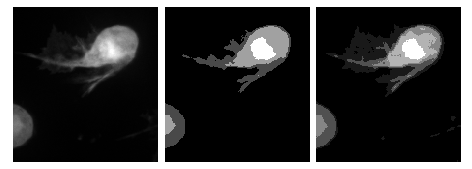
\includegraphics[scale=0.65]{img/fig_kmeans}
	\end{center}
	\caption{Application of the K-Means algorithm to a test image. \textbf{Top left}: Input image. \textbf{Top right}: Ground truth labels of the input image. \textbf{Bottom left}: K-means results with $k=4$,  using arbitrary colors for the labels. \textbf{Bottom right}: Results with $k=6$. It is noteworthy that while the results for $k=4$ are reasonable, the nearly transparent lamellopodium pixels are labelled as background values, while the cell proper is segmented into two parts.}
	\label{fig:kmeans}
\end {figure}

\noindent Obviously, this algorithm can also be used to segment images into $k$ different classes, but since K-Means assigns classes to data by using the distance from the mean, the algorithm output favors segmentations in which the classes have roughly the same size, which isn't necessarily the correct way to classify pixels in arbitrary image data.

	\section{Canny Edge Detection}
\label{sec:canny}
The \textit{Canny Edge Detector} \cite{canny} is one of the most famous edge-detection algorithms and actually is a composite algorithm that returns a binary segmentation of an image into edges and non-edges.\\

\noindent First, a Gaussian convolution filter is applied to try and subdue noise in the image. A \textit{convolution} is a matrix operation often used in image processing: A matrix $A$, describing the pixel values of an image, is convolved pixel-wise with a convolution matrix $B$ with dimensions $n \times n$ - that is, for each pixel $p$ of $A$, the pixel's $n \times n$-neighborhood pixel values are summed up while being weighted according to corresponding value in $B$. The resulting sum is then assigned to the output matrix in place of the previous value of the center pixel, which intuitively assumes the distance-weighted average value of its neighborhood. In the case of pixels that lie on the edge of the matrix to be convoluted, out-of-bounds considerations have to be made: A constant value such as zero can be assumed for the pixels in the neighborhood that would lie ``outside'' of the image, the existing image values can be mirrored or clamped to provide a torus-like out-of-bounds handling, or the convolution can be done only on those pixels whose neighborhood fully lies inside of the image, resulting in smaller output images.

The aforementioned ``Gaussian filter'' or ``kernel'' is a matrix whose values are defined so that performing a convolution using that matrix approximates the behavior of the two-dimensional Gaussian function with uniform variances for its $x$- and $y$-dimensions:

\[ f(x, y) = \exp \left(- \left( \frac{\left(x - p_x \right)^2}{2\sigma^2} + \frac{ \left(y - p_y \right)^2}{2\sigma^2} \right) \right), \]

\noindent where $p$ is the center pixel of the current neighborhood. Subsequently, $p_x$ and $p_y$ are the coordinates of this pixel within the matrix and $\sigma$, the standard variance, acts as the smoothing constant. The higher this constant is, the stronger the blur effect becomes.

In Gaussian filters, the $\sigma$ constant is expressed through the dimensions of the matrix - the larger the filter matrix, the stronger the blur effect. An example for a $3 \times 3$ Gaussian filter is the following matrix:

\[ \frac{1}{16} \left [ \begin{tabular}{ccc}
				1& 2& 1\\
				2& 4& 2\\
				1& 2& 1 
			   \end{tabular} \right ]\]

\noindent The coefficient $\frac{1}{16}$ is equal to the sum of the matrix values and ensures that the convolution does not change the average image value. \cite[p. 41]{machine_vision}\\

\noindent As the second step, an gradient-based edge detector filter is applied to the smoothed image. The most famous of these is the \textit{Sobel filter} \cite{sobel}, which approximates the local partial derivatives $\frac{\partial I}{\partial x}$ and $\frac{\partial I}{\partial y}$ of each pixel of the image function $I(x, y)$, using the $3 \times 3$ neighborhood of that pixel. It is given by the following matrices\cite[pp. 113 -- 114]{machine_vision}:

\[ \text{Sobel}_x = \left [ \begin{tabular}{ccc}
				-1& 0& 1\\
				-2& 0& 2\\
				-1& 0& 1 
			   \end{tabular} \right ] \text{ and } 
\text{Sobel}_y = \left [ \begin{tabular}{ccc}
				1& 2& 1\\
				0& 0& 0\\
				-1& -2& 1 
			   \end{tabular} \right ] 
\]

\noindent The result of these convolutions are two images, $G_x$ and $G_y$, which represent the partial local derivatives of each pixel. The gradient image of the original input image $I$ is then defined as

\[G = |\nabla I| = \sqrt{{G_x}^2 + {G_y}^2}.\]

\noindent Additionally, the gradient direction of each pixel can be calculated from the derivative images by measuring the angle between the x-axis and the gradient pixel coordinates by employing the atan2 function:

\[G_\phi = \text{atan2}(G_y, G_x) \]

\noindent Using $G_\phi$, edge thinning via non-maximum suppression is applied to the gradient image as the third step in the algorithm: For each pixel, the gradient direction acts as a criterion to decide which two neighboring pixels, that are each on opposite sides (positive and negative direction of the gradient), should be compared to the current pixel. If the value of the current pixel is not larger than the two neighbors' values, the pixel's value is not a local maximum and is set to zero. The gradient direction angles can either be rounded so that each angle represents one of the north-south, west-east directions and so forth, or linear interpolation can be used.

In the final step, a hysteresis threshold is applied. This process consists of defining two thresholds, $\theta_{high}$ and $\theta_{low}$. The definition for the thresholding function as given in \ref{sec:thresholding} is slightly altered:

\[ T(I(x, y), \theta_{high}, \theta_{low}) =  \begin{cases}
							2 \text{ if } I(x, y) \, \geq \, \theta_{high} \\
							1 \text{ if } I(x, y) \, \geq \, \theta_{low} \text{ and } < \theta_{high} \\
			          				0 \text{ otherwise}
			   			        \end{cases}
\]

\noindent Pixels that have a value of $2$ are called strong pixels because they had values larger than the high threshold, whereas pixels with a value of $1$ are called weak pixels. Finally, the algorithm checks for each pixel if an 8-connected path between that pixel and a strong pixel exists - if not, then the pixel is dropped. This can be done with the help of connected component-finding algorithms by dropping each ``$1$''-component which is not connected to at least one ``2''-value.\\

\noindent The thresholds $\theta_{high}$ and $\theta_{low}$ have to be set by the user, although there exists the possibility to set these by using the Otsu threshold described in \ref{sec:thresholding} . Using this combination approach, $\theta_{high}$ is set to the Otsu threshold value for $I(x, y)$, and $\theta_{low}$ is set to $0.5 * \theta_{high}$.\cite{otsu_combine}


	\section{Gaussian Mixture Models}
Gaussian Mixtures Models (GMMs) are a subclass of mixture models, that is, probabilistic models which are combined with other models of the same distribution type to form a more complex model that is able to model the distribution of a data set more accurately than a simple model could. In the case of GMMs, the base distributions are often $n$-multivariate Gaussian distributions:

\[ pdf(x) = \mathcal{N}_n (x\,|\,\mu,\, \Sigma) \]

\noindent Here, $pdf(x)$ denotes the probability, or density, of an $n$-dimensional piece of data $x$, while $\mu$ and $\Sigma$ are the $n$-dimensional mean vector and the $n \times n$ covariance matrix of the distribution. Since the shape such a distribution can take is limited, a single Gaussian cannot accurately model a multimodal distribution (see Figure \ref{fig:normal_vs_gmm}). Instead, a weighted combination of multiple Gaussians can be used instead: \cite[pp. 430]{bishop_pattern}

\[ pdf_m (x) = \sum \limits_{k=1}^{K} \pi_k \, \mathcal{N}_n (x\,|\, \mu_k, \Sigma_k) \]

\noindent A mixture model consists of $K$ models that each have different parameters $\mu$ and $\Sigma$ and are weighted by weights $\pi_k \in \mathbb{R}$, $1 > \pi_k > 0$, with $\sum_{i=1}^{k} \pi_i = 1$.

\begin {figure}[!ht]
	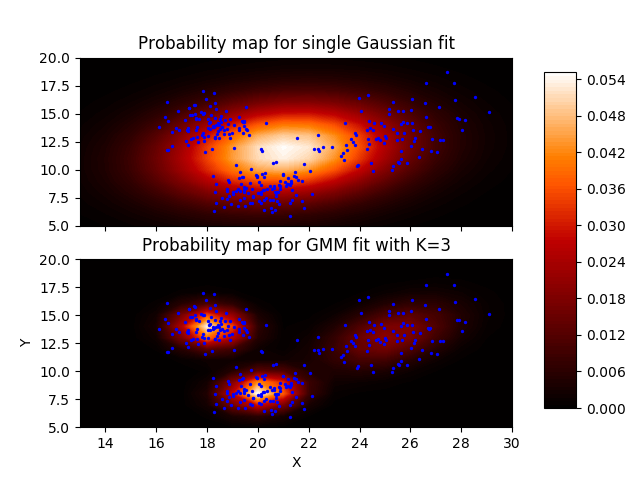
\includegraphics{img/fig_normal_vs_gmm}
	\caption{Comparison of a single Gaussian fit (upper) with a GMM fit, using $K=3$, on a two-dimensional dataset randomly sampled from three Gaussian distributions. The single Gaussian fails to capture the structure of the data, while the GMM succeeds.}
	\label{fig:normal_vs_gmm}
\end {figure}

\noindent The parameters of such a mixture model can be calculated by applying the Expectation-Maximization (EM) algorithm, which can additionally be combined with a K-Means initialization to avoid shallow local minima.\cite{em_algorithm} GMMs can also be used for segmenting images: Grayscale images are simply three-dimensional data in which each pixel coordinate corresponds to an intensity value. If the number of components to be found in the image is known beforehand, as it is in the case of cell segmentation, the intensity values can be segmented according to the fitted GMM (see Figure \ref{fig:gmm_vs_gt}). To do this, for each pixel in the image the posterior probabilities for that pixel in respect to each of the Gaussians is calculated and the Gaussian with the highest probability is chosen as the ``source'' of the pixel:

\[ label_x = \argmax \limits_{k} \, p(\mu_k, \Sigma_k\, | \, x) \]

\begin {figure}[!ht]
	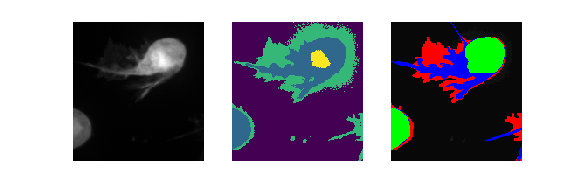
\includegraphics{img/fig_gmm_vs_gt}
	\caption{From left to right: Input image, pseudo-color labels assigned by a $K=4$ GMM fit to the input image and the ground truth labels for the input image.}
	\label{fig:gmm_vs_gt}
\end {figure}


	\section{Graph Cuts}



	\section{Multi-layer Perceptrons}
\textit{Multi-layer Perceptrons} (MLPs) or \textit{Feedforward Artificial Neuronal Networks} (ANNs) are mathematical functions that try to emulate the way neurons in the brain process information, typically to classify data or perform regression on it. ANNs have recently achieved impressing results on various tasks, such as image classification, sound analysis and regression, typically achieved by very deep networks that used lots of artificial neurons and were fed large datasets exceeding one million samples. In this section, the concepts behind optimization of functions via Gradient Descent, neuronal networks and training of those networks using the Backpropagation algorithm are explained. 



	\subsection {Gradient Descent}
\label{subsec:grad_desc}

\textit{Gradient Descent} or is a standard, analytic first-order technique that iteratively optimizes at least once-differentiable, continuous functions, that is, that calculates a vector of parameters $\Theta$ for a function $f$ so that

\[ \Theta = \argmin \limits_{i} f(i) \]

\noindent To find values for $\Theta$, the approach takes advantage of the fact that the negative gradient vector $\nabla_f = [ \frac{\partial f}{\partial \Theta_0}, \dots, \frac{\partial f}{\partial \Theta_n} ]$, the vector of all first partial derivatives of $f$, points into the direction of the fastest change, or put graphically, the ``steepest slope''. By taking steps into the direction of this gradient, the function value is minimized step by step, while maximization works the same, only that the function is negated and then minimized, which results in parameters that maximize the original function. The parameter $\eta$ depicts the step size and is typically a value in the range $(0.0, 1.0]$. \cite[pp. 40--42]{optimization_book}

The algorithm starts with a guess for the parameters in $\Theta$ and then iteratively evaluates the gradient and updates the parameters accordingly until convergence within arbitrary precision is reached (see algorithm \ref{alg:grad_desc}).

\begin {algorithm}
	\begin {algorithmic}[1]
		\State $\Theta_0$ = random
		\While {$|f(\Theta_i) - f(\Theta_{i - 1})| > \epsilon$}
			\State $\Theta_i = \Theta_{i-1} - \eta \nabla_f$ 
		\EndWhile
	\end{algorithmic}
	\caption{Gradient Descent scheme for optimizing differentiable functions.}
	\label{alg:grad_desc}
\end{algorithm}

\noindent For convex functions, Gradient Descent always finds the global minimum. For non-convex functions however, the algorithm may get stuck in a local minimum or at saddle points, called ``false minima' (see figure \ref{fig:grad_desc}). Therefore, running the algorithm multiple times with random values or even informed guesses given knowledge about the form of the function to be optimized is advised. The step size $\eta$ has to be chosen depending on the shape of the function to minimize; if $\eta$ is too large, the algorithm will overshoot the minimum and will never converge even if the minimum exists, and if $\eta$ is too small, convergence will take a long time.

\begin {figure}[!ht]
	\begin{center}
		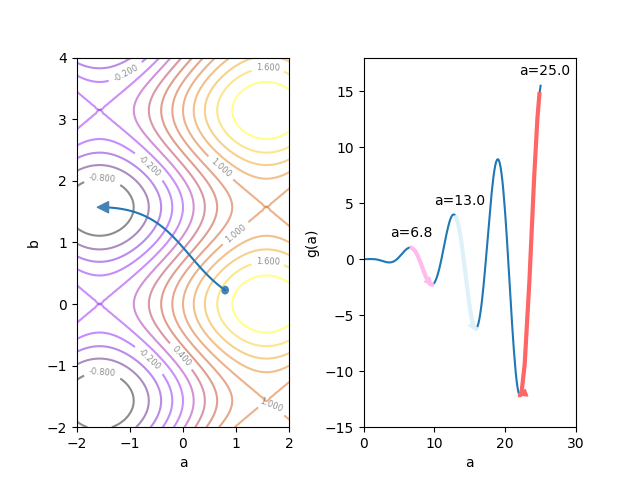
\includegraphics[scale=0.9]{img/fig_grad_desc}
	\end{center}
	\caption{\textbf{Left:} A contour plot of Gradient Descent minimization of $f(a, b) = \sin(a) + \cos^2(b)$. The blue line shows the search path of the algorithm along the negative gradient while estimating the optimal $\Theta$. \textbf{Right}: Effect of the initial guess for $\Theta$ on the optimization. The function $f(a) = \frac{1}{40}a^2 * \frac{1}{2} \cos(a)$ has multiple local minima in the interval [0, 25]. Only the third guess $a=25$ leads to finding the global minimum, while the other two optimization runs get trapped in local minima.}
	\label{fig:grad_desc}
\end {figure}

\noindent However, a more interesting application of the Gradient Descent algorithm exists in the context of machine learning, where the function to optimize often has fixed parameters in addition to $\Theta$, such as data from a dataset that is related to the function is some way. In such cases, one can consider one of the subtypes of Gradient Descent; either, evaluating the average gradient using all available data samples (\textit{Batch Gradient Descent}) at once or using single data points only - as an approximation of the entire dataset - to perform the updates. This is called \textit{Stochastic Gradient Descent} (SGD) and is preferable if working with datasets that are too large to fit into memory. Alternatively, one can use the average gradient of a subset of data points - this method is often referred to as \textit{Mini-Batch} Gradient Descent. For example, considering the function

\[ f(\Theta) =  \theta_1 x_1 + \theta_2 x_2\]

\noindent with fixed $x_1$, $x_2$ from some dataset $X$. To minimize this function $f$ with respect to the variable parameters $\Theta$ using the dataset and SGD, the algorithm is modified to only take into consideration a single datapoint $x_i = [x_{i1}, x_{i2}]$ at a time chosen at random from $X$. Then, updating $\Theta$ is done by the formula

\[ \Theta_i = \Theta_{i-1} - \eta \nabla_{f_i} \]

\noindent where $f_i$ is the function $f$ evaluated for $x_i$ and $\Theta_{i-1}$, while the number of steps that it takes to consider all datapoints in the dataset is called an \textit{epoch}. Similarily, to use Mini-Batch SGD with a batch size of $n$, an average over the gradients for $n$ datapoints is used:

\[ \Theta_i = \Theta_{i-1} - \eta \left ( \frac{1}{n} \sum \limits_{i=1}^{n} \nabla_{f_i} \right ) \]

\noindent The price that is paid for the relaxed memory cost of SGD is that the traversion towards the minimum becomes noisy for small $n$, as the algorithm approximates the gradient by using only a part of the dataset. For functions with minima in shallow ``valleys'', SGD starts moving in a wild zig-zag pattern near the optimum, further increasing the number of steps the algorithm takes until covergence. To address these problems, a number of optimizations were proposed.


	\subsubsection {Momentum}
\text{Momentum} is an optimization for the Gradient Descent that adds an additional factor to the update step which is dependent on the steepness of the traversed function in previous updates. Using the analogy of a marble rolling down a slope, momentum refers to the inertia of the marble that allows it to jump over saddle points or small holes (local minima) on the bowl's surface rather than stopping abruptly once such a location is reached. This changes the SGD update formula to

\begin {align}
	& v_i = \gamma v_ {i-1} + \eta \nabla_f\\ 
	& \Theta_i = \Theta_{i-1} - v_i
\end {align}

\noindent where $v$ is the momentum vector with one entry per gradient element and $\gamma$ is a modifier that changes the influence of the momentum on the update.

	\begin {figure}[!ht]
		\begin{center}
			\scalebox{0.75}{%% Creator: Matplotlib, PGF backend
%%
%% To include the figure in your LaTeX document, write
%%   \input{<filename>.pgf}
%%
%% Make sure the required packages are loaded in your preamble
%%   \usepackage{pgf}
%%
%% Figures using additional raster images can only be included by \input if
%% they are in the same directory as the main LaTeX file. For loading figures
%% from other directories you can use the `import` package
%%   \usepackage{import}
%% and then include the figures with
%%   \import{<path to file>}{<filename>.pgf}
%%
%% Matplotlib used the following preamble
%%   \usepackage{fontspec}
%%   \setmainfont{DejaVu Serif}
%%   \setsansfont{DejaVu Sans}
%%   \setmonofont{DejaVu Sans Mono}
%%
\begingroup%
\makeatletter%
\begin{pgfpicture}%
\pgfpathrectangle{\pgfpointorigin}{\pgfqpoint{6.400000in}{4.800000in}}%
\pgfusepath{use as bounding box, clip}%
\begin{pgfscope}%
\pgfsetbuttcap%
\pgfsetmiterjoin%
\definecolor{currentfill}{rgb}{1.000000,1.000000,1.000000}%
\pgfsetfillcolor{currentfill}%
\pgfsetlinewidth{0.000000pt}%
\definecolor{currentstroke}{rgb}{1.000000,1.000000,1.000000}%
\pgfsetstrokecolor{currentstroke}%
\pgfsetdash{}{0pt}%
\pgfpathmoveto{\pgfqpoint{0.000000in}{0.000000in}}%
\pgfpathlineto{\pgfqpoint{6.400000in}{0.000000in}}%
\pgfpathlineto{\pgfqpoint{6.400000in}{4.800000in}}%
\pgfpathlineto{\pgfqpoint{0.000000in}{4.800000in}}%
\pgfpathclose%
\pgfusepath{fill}%
\end{pgfscope}%
\begin{pgfscope}%
\pgfsetbuttcap%
\pgfsetmiterjoin%
\definecolor{currentfill}{rgb}{1.000000,1.000000,1.000000}%
\pgfsetfillcolor{currentfill}%
\pgfsetlinewidth{0.000000pt}%
\definecolor{currentstroke}{rgb}{0.000000,0.000000,0.000000}%
\pgfsetstrokecolor{currentstroke}%
\pgfsetstrokeopacity{0.000000}%
\pgfsetdash{}{0pt}%
\pgfpathmoveto{\pgfqpoint{0.800000in}{0.528000in}}%
\pgfpathlineto{\pgfqpoint{2.763636in}{0.528000in}}%
\pgfpathlineto{\pgfqpoint{2.763636in}{4.224000in}}%
\pgfpathlineto{\pgfqpoint{0.800000in}{4.224000in}}%
\pgfpathclose%
\pgfusepath{fill}%
\end{pgfscope}%
\begin{pgfscope}%
\pgfpathrectangle{\pgfqpoint{0.800000in}{0.528000in}}{\pgfqpoint{1.963636in}{3.696000in}} %
\pgfusepath{clip}%
\pgfsetbuttcap%
\pgfsetroundjoin%
\definecolor{currentfill}{rgb}{0.050383,0.029803,0.527975}%
\pgfsetfillcolor{currentfill}%
\pgfsetlinewidth{0.000000pt}%
\definecolor{currentstroke}{rgb}{0.000000,0.000000,0.000000}%
\pgfsetstrokecolor{currentstroke}%
\pgfsetdash{}{0pt}%
\pgfpathmoveto{\pgfqpoint{1.315702in}{2.586655in}}%
\pgfpathlineto{\pgfqpoint{1.315708in}{2.586667in}}%
\pgfpathlineto{\pgfqpoint{1.315702in}{2.586679in}}%
\pgfpathlineto{\pgfqpoint{1.315697in}{2.586667in}}%
\pgfpathclose%
\pgfusepath{fill}%
\end{pgfscope}%
\begin{pgfscope}%
\pgfpathrectangle{\pgfqpoint{0.800000in}{0.528000in}}{\pgfqpoint{1.963636in}{3.696000in}} %
\pgfusepath{clip}%
\pgfsetbuttcap%
\pgfsetroundjoin%
\definecolor{currentfill}{rgb}{0.050383,0.029803,0.527975}%
\pgfsetfillcolor{currentfill}%
\pgfsetlinewidth{0.000000pt}%
\definecolor{currentstroke}{rgb}{0.000000,0.000000,0.000000}%
\pgfsetstrokecolor{currentstroke}%
\pgfsetdash{}{0pt}%
\pgfpathmoveto{\pgfqpoint{1.266116in}{2.693321in}}%
\pgfpathlineto{\pgfqpoint{1.266121in}{2.693333in}}%
\pgfpathlineto{\pgfqpoint{1.266116in}{2.693345in}}%
\pgfpathlineto{\pgfqpoint{1.266110in}{2.693333in}}%
\pgfpathclose%
\pgfusepath{fill}%
\end{pgfscope}%
\begin{pgfscope}%
\pgfpathrectangle{\pgfqpoint{0.800000in}{0.528000in}}{\pgfqpoint{1.963636in}{3.696000in}} %
\pgfusepath{clip}%
\pgfsetbuttcap%
\pgfsetroundjoin%
\definecolor{currentfill}{rgb}{0.050383,0.029803,0.527975}%
\pgfsetfillcolor{currentfill}%
\pgfsetlinewidth{0.000000pt}%
\definecolor{currentstroke}{rgb}{0.000000,0.000000,0.000000}%
\pgfsetstrokecolor{currentstroke}%
\pgfsetdash{}{0pt}%
\pgfpathmoveto{\pgfqpoint{1.365289in}{2.479880in}}%
\pgfpathlineto{\pgfqpoint{1.365354in}{2.480000in}}%
\pgfpathlineto{\pgfqpoint{1.365289in}{2.480134in}}%
\pgfpathlineto{\pgfqpoint{1.365231in}{2.480000in}}%
\pgfpathclose%
\pgfusepath{fill}%
\end{pgfscope}%
\begin{pgfscope}%
\pgfpathrectangle{\pgfqpoint{0.800000in}{0.528000in}}{\pgfqpoint{1.963636in}{3.696000in}} %
\pgfusepath{clip}%
\pgfsetbuttcap%
\pgfsetroundjoin%
\definecolor{currentfill}{rgb}{0.050383,0.029803,0.527975}%
\pgfsetfillcolor{currentfill}%
\pgfsetlinewidth{0.000000pt}%
\definecolor{currentstroke}{rgb}{0.000000,0.000000,0.000000}%
\pgfsetstrokecolor{currentstroke}%
\pgfsetdash{}{0pt}%
\pgfpathmoveto{\pgfqpoint{1.315702in}{2.586470in}}%
\pgfpathlineto{\pgfqpoint{1.315801in}{2.586667in}}%
\pgfpathlineto{\pgfqpoint{1.315702in}{2.586870in}}%
\pgfpathlineto{\pgfqpoint{1.315608in}{2.586667in}}%
\pgfpathclose%
\pgfpathmoveto{\pgfqpoint{1.315697in}{2.586667in}}%
\pgfpathlineto{\pgfqpoint{1.315702in}{2.586679in}}%
\pgfpathlineto{\pgfqpoint{1.315708in}{2.586667in}}%
\pgfpathlineto{\pgfqpoint{1.315702in}{2.586655in}}%
\pgfpathclose%
\pgfusepath{fill}%
\end{pgfscope}%
\begin{pgfscope}%
\pgfpathrectangle{\pgfqpoint{0.800000in}{0.528000in}}{\pgfqpoint{1.963636in}{3.696000in}} %
\pgfusepath{clip}%
\pgfsetbuttcap%
\pgfsetroundjoin%
\definecolor{currentfill}{rgb}{0.050383,0.029803,0.527975}%
\pgfsetfillcolor{currentfill}%
\pgfsetlinewidth{0.000000pt}%
\definecolor{currentstroke}{rgb}{0.000000,0.000000,0.000000}%
\pgfsetstrokecolor{currentstroke}%
\pgfsetdash{}{0pt}%
\pgfpathmoveto{\pgfqpoint{1.266116in}{2.693130in}}%
\pgfpathlineto{\pgfqpoint{1.266210in}{2.693333in}}%
\pgfpathlineto{\pgfqpoint{1.266116in}{2.693530in}}%
\pgfpathlineto{\pgfqpoint{1.266017in}{2.693333in}}%
\pgfpathclose%
\pgfpathmoveto{\pgfqpoint{1.266110in}{2.693333in}}%
\pgfpathlineto{\pgfqpoint{1.266116in}{2.693345in}}%
\pgfpathlineto{\pgfqpoint{1.266121in}{2.693333in}}%
\pgfpathlineto{\pgfqpoint{1.266116in}{2.693321in}}%
\pgfpathclose%
\pgfusepath{fill}%
\end{pgfscope}%
\begin{pgfscope}%
\pgfpathrectangle{\pgfqpoint{0.800000in}{0.528000in}}{\pgfqpoint{1.963636in}{3.696000in}} %
\pgfusepath{clip}%
\pgfsetbuttcap%
\pgfsetroundjoin%
\definecolor{currentfill}{rgb}{0.050383,0.029803,0.527975}%
\pgfsetfillcolor{currentfill}%
\pgfsetlinewidth{0.000000pt}%
\definecolor{currentstroke}{rgb}{0.000000,0.000000,0.000000}%
\pgfsetstrokecolor{currentstroke}%
\pgfsetdash{}{0pt}%
\pgfpathmoveto{\pgfqpoint{1.216529in}{2.799866in}}%
\pgfpathlineto{\pgfqpoint{1.216587in}{2.800000in}}%
\pgfpathlineto{\pgfqpoint{1.216529in}{2.800120in}}%
\pgfpathlineto{\pgfqpoint{1.216464in}{2.800000in}}%
\pgfpathclose%
\pgfusepath{fill}%
\end{pgfscope}%
\begin{pgfscope}%
\pgfpathrectangle{\pgfqpoint{0.800000in}{0.528000in}}{\pgfqpoint{1.963636in}{3.696000in}} %
\pgfusepath{clip}%
\pgfsetbuttcap%
\pgfsetroundjoin%
\definecolor{currentfill}{rgb}{0.050383,0.029803,0.527975}%
\pgfsetfillcolor{currentfill}%
\pgfsetlinewidth{0.000000pt}%
\definecolor{currentstroke}{rgb}{0.000000,0.000000,0.000000}%
\pgfsetstrokecolor{currentstroke}%
\pgfsetdash{}{0pt}%
\pgfpathmoveto{\pgfqpoint{3.745455in}{-2.534940in}}%
\pgfpathlineto{\pgfqpoint{3.745455in}{-2.533333in}}%
\pgfpathlineto{\pgfqpoint{3.745455in}{-2.532190in}}%
\pgfpathlineto{\pgfqpoint{3.744676in}{-2.533333in}}%
\pgfpathclose%
\pgfusepath{fill}%
\end{pgfscope}%
\begin{pgfscope}%
\pgfpathrectangle{\pgfqpoint{0.800000in}{0.528000in}}{\pgfqpoint{1.963636in}{3.696000in}} %
\pgfusepath{clip}%
\pgfsetbuttcap%
\pgfsetroundjoin%
\definecolor{currentfill}{rgb}{0.050383,0.029803,0.527975}%
\pgfsetfillcolor{currentfill}%
\pgfsetlinewidth{0.000000pt}%
\definecolor{currentstroke}{rgb}{0.000000,0.000000,0.000000}%
\pgfsetstrokecolor{currentstroke}%
\pgfsetdash{}{0pt}%
\pgfpathmoveto{\pgfqpoint{3.695868in}{-2.427884in}}%
\pgfpathlineto{\pgfqpoint{3.696254in}{-2.426667in}}%
\pgfpathlineto{\pgfqpoint{3.695868in}{-2.425864in}}%
\pgfpathlineto{\pgfqpoint{3.695277in}{-2.426667in}}%
\pgfpathclose%
\pgfusepath{fill}%
\end{pgfscope}%
\begin{pgfscope}%
\pgfpathrectangle{\pgfqpoint{0.800000in}{0.528000in}}{\pgfqpoint{1.963636in}{3.696000in}} %
\pgfusepath{clip}%
\pgfsetbuttcap%
\pgfsetroundjoin%
\definecolor{currentfill}{rgb}{0.050383,0.029803,0.527975}%
\pgfsetfillcolor{currentfill}%
\pgfsetlinewidth{0.000000pt}%
\definecolor{currentstroke}{rgb}{0.000000,0.000000,0.000000}%
\pgfsetstrokecolor{currentstroke}%
\pgfsetdash{}{0pt}%
\pgfpathmoveto{\pgfqpoint{3.646281in}{-2.320694in}}%
\pgfpathlineto{\pgfqpoint{3.646485in}{-2.320000in}}%
\pgfpathlineto{\pgfqpoint{3.646281in}{-2.319577in}}%
\pgfpathlineto{\pgfqpoint{3.645944in}{-2.320000in}}%
\pgfpathclose%
\pgfusepath{fill}%
\end{pgfscope}%
\begin{pgfscope}%
\pgfpathrectangle{\pgfqpoint{0.800000in}{0.528000in}}{\pgfqpoint{1.963636in}{3.696000in}} %
\pgfusepath{clip}%
\pgfsetbuttcap%
\pgfsetroundjoin%
\definecolor{currentfill}{rgb}{0.050383,0.029803,0.527975}%
\pgfsetfillcolor{currentfill}%
\pgfsetlinewidth{0.000000pt}%
\definecolor{currentstroke}{rgb}{0.000000,0.000000,0.000000}%
\pgfsetstrokecolor{currentstroke}%
\pgfsetdash{}{0pt}%
\pgfpathmoveto{\pgfqpoint{3.596694in}{-2.213349in}}%
\pgfpathlineto{\pgfqpoint{3.596698in}{-2.213333in}}%
\pgfpathlineto{\pgfqpoint{3.596694in}{-2.213325in}}%
\pgfpathlineto{\pgfqpoint{3.596687in}{-2.213333in}}%
\pgfpathclose%
\pgfusepath{fill}%
\end{pgfscope}%
\begin{pgfscope}%
\pgfpathrectangle{\pgfqpoint{0.800000in}{0.528000in}}{\pgfqpoint{1.963636in}{3.696000in}} %
\pgfusepath{clip}%
\pgfsetbuttcap%
\pgfsetroundjoin%
\definecolor{currentfill}{rgb}{0.050383,0.029803,0.527975}%
\pgfsetfillcolor{currentfill}%
\pgfsetlinewidth{0.000000pt}%
\definecolor{currentstroke}{rgb}{0.000000,0.000000,0.000000}%
\pgfsetstrokecolor{currentstroke}%
\pgfsetdash{}{0pt}%
\pgfpathmoveto{\pgfqpoint{1.662810in}{1.839971in}}%
\pgfpathlineto{\pgfqpoint{1.662835in}{1.840000in}}%
\pgfpathlineto{\pgfqpoint{1.662810in}{1.840051in}}%
\pgfpathlineto{\pgfqpoint{1.662796in}{1.840000in}}%
\pgfpathclose%
\pgfusepath{fill}%
\end{pgfscope}%
\begin{pgfscope}%
\pgfpathrectangle{\pgfqpoint{0.800000in}{0.528000in}}{\pgfqpoint{1.963636in}{3.696000in}} %
\pgfusepath{clip}%
\pgfsetbuttcap%
\pgfsetroundjoin%
\definecolor{currentfill}{rgb}{0.050383,0.029803,0.527975}%
\pgfsetfillcolor{currentfill}%
\pgfsetlinewidth{0.000000pt}%
\definecolor{currentstroke}{rgb}{0.000000,0.000000,0.000000}%
\pgfsetstrokecolor{currentstroke}%
\pgfsetdash{}{0pt}%
\pgfpathmoveto{\pgfqpoint{1.613223in}{1.946225in}}%
\pgfpathlineto{\pgfqpoint{1.613573in}{1.946667in}}%
\pgfpathlineto{\pgfqpoint{1.613223in}{1.947388in}}%
\pgfpathlineto{\pgfqpoint{1.613011in}{1.946667in}}%
\pgfpathclose%
\pgfusepath{fill}%
\end{pgfscope}%
\begin{pgfscope}%
\pgfpathrectangle{\pgfqpoint{0.800000in}{0.528000in}}{\pgfqpoint{1.963636in}{3.696000in}} %
\pgfusepath{clip}%
\pgfsetbuttcap%
\pgfsetroundjoin%
\definecolor{currentfill}{rgb}{0.050383,0.029803,0.527975}%
\pgfsetfillcolor{currentfill}%
\pgfsetlinewidth{0.000000pt}%
\definecolor{currentstroke}{rgb}{0.000000,0.000000,0.000000}%
\pgfsetstrokecolor{currentstroke}%
\pgfsetdash{}{0pt}%
\pgfpathmoveto{\pgfqpoint{1.563636in}{2.052514in}}%
\pgfpathlineto{\pgfqpoint{1.564237in}{2.053333in}}%
\pgfpathlineto{\pgfqpoint{1.563636in}{2.054572in}}%
\pgfpathlineto{\pgfqpoint{1.563242in}{2.053333in}}%
\pgfpathclose%
\pgfusepath{fill}%
\end{pgfscope}%
\begin{pgfscope}%
\pgfpathrectangle{\pgfqpoint{0.800000in}{0.528000in}}{\pgfqpoint{1.963636in}{3.696000in}} %
\pgfusepath{clip}%
\pgfsetbuttcap%
\pgfsetroundjoin%
\definecolor{currentfill}{rgb}{0.050383,0.029803,0.527975}%
\pgfsetfillcolor{currentfill}%
\pgfsetlinewidth{0.000000pt}%
\definecolor{currentstroke}{rgb}{0.000000,0.000000,0.000000}%
\pgfsetstrokecolor{currentstroke}%
\pgfsetdash{}{0pt}%
\pgfpathmoveto{\pgfqpoint{1.514050in}{2.158842in}}%
\pgfpathlineto{\pgfqpoint{1.514835in}{2.160000in}}%
\pgfpathlineto{\pgfqpoint{1.514050in}{2.161621in}}%
\pgfpathlineto{\pgfqpoint{1.513492in}{2.160000in}}%
\pgfpathclose%
\pgfusepath{fill}%
\end{pgfscope}%
\begin{pgfscope}%
\pgfpathrectangle{\pgfqpoint{0.800000in}{0.528000in}}{\pgfqpoint{1.963636in}{3.696000in}} %
\pgfusepath{clip}%
\pgfsetbuttcap%
\pgfsetroundjoin%
\definecolor{currentfill}{rgb}{0.050383,0.029803,0.527975}%
\pgfsetfillcolor{currentfill}%
\pgfsetlinewidth{0.000000pt}%
\definecolor{currentstroke}{rgb}{0.000000,0.000000,0.000000}%
\pgfsetstrokecolor{currentstroke}%
\pgfsetdash{}{0pt}%
\pgfpathmoveto{\pgfqpoint{1.464463in}{2.265212in}}%
\pgfpathlineto{\pgfqpoint{1.465377in}{2.266667in}}%
\pgfpathlineto{\pgfqpoint{1.464463in}{2.268555in}}%
\pgfpathlineto{\pgfqpoint{1.463762in}{2.266667in}}%
\pgfpathclose%
\pgfusepath{fill}%
\end{pgfscope}%
\begin{pgfscope}%
\pgfpathrectangle{\pgfqpoint{0.800000in}{0.528000in}}{\pgfqpoint{1.963636in}{3.696000in}} %
\pgfusepath{clip}%
\pgfsetbuttcap%
\pgfsetroundjoin%
\definecolor{currentfill}{rgb}{0.050383,0.029803,0.527975}%
\pgfsetfillcolor{currentfill}%
\pgfsetlinewidth{0.000000pt}%
\definecolor{currentstroke}{rgb}{0.000000,0.000000,0.000000}%
\pgfsetstrokecolor{currentstroke}%
\pgfsetdash{}{0pt}%
\pgfpathmoveto{\pgfqpoint{1.414876in}{2.371628in}}%
\pgfpathlineto{\pgfqpoint{1.415868in}{2.373333in}}%
\pgfpathlineto{\pgfqpoint{1.414876in}{2.375386in}}%
\pgfpathlineto{\pgfqpoint{1.414055in}{2.373333in}}%
\pgfpathclose%
\pgfusepath{fill}%
\end{pgfscope}%
\begin{pgfscope}%
\pgfpathrectangle{\pgfqpoint{0.800000in}{0.528000in}}{\pgfqpoint{1.963636in}{3.696000in}} %
\pgfusepath{clip}%
\pgfsetbuttcap%
\pgfsetroundjoin%
\definecolor{currentfill}{rgb}{0.050383,0.029803,0.527975}%
\pgfsetfillcolor{currentfill}%
\pgfsetlinewidth{0.000000pt}%
\definecolor{currentstroke}{rgb}{0.000000,0.000000,0.000000}%
\pgfsetstrokecolor{currentstroke}%
\pgfsetdash{}{0pt}%
\pgfpathmoveto{\pgfqpoint{1.365289in}{2.478097in}}%
\pgfpathlineto{\pgfqpoint{1.366317in}{2.480000in}}%
\pgfpathlineto{\pgfqpoint{1.365289in}{2.482127in}}%
\pgfpathlineto{\pgfqpoint{1.364372in}{2.480000in}}%
\pgfpathclose%
\pgfpathmoveto{\pgfqpoint{1.365231in}{2.480000in}}%
\pgfpathlineto{\pgfqpoint{1.365289in}{2.480134in}}%
\pgfpathlineto{\pgfqpoint{1.365354in}{2.480000in}}%
\pgfpathlineto{\pgfqpoint{1.365289in}{2.479880in}}%
\pgfpathclose%
\pgfusepath{fill}%
\end{pgfscope}%
\begin{pgfscope}%
\pgfpathrectangle{\pgfqpoint{0.800000in}{0.528000in}}{\pgfqpoint{1.963636in}{3.696000in}} %
\pgfusepath{clip}%
\pgfsetbuttcap%
\pgfsetroundjoin%
\definecolor{currentfill}{rgb}{0.050383,0.029803,0.527975}%
\pgfsetfillcolor{currentfill}%
\pgfsetlinewidth{0.000000pt}%
\definecolor{currentstroke}{rgb}{0.000000,0.000000,0.000000}%
\pgfsetstrokecolor{currentstroke}%
\pgfsetdash{}{0pt}%
\pgfpathmoveto{\pgfqpoint{1.315702in}{2.584623in}}%
\pgfpathlineto{\pgfqpoint{1.316726in}{2.586667in}}%
\pgfpathlineto{\pgfqpoint{1.315702in}{2.588788in}}%
\pgfpathlineto{\pgfqpoint{1.314716in}{2.586667in}}%
\pgfpathclose%
\pgfpathmoveto{\pgfqpoint{1.315608in}{2.586667in}}%
\pgfpathlineto{\pgfqpoint{1.315702in}{2.586870in}}%
\pgfpathlineto{\pgfqpoint{1.315801in}{2.586667in}}%
\pgfpathlineto{\pgfqpoint{1.315702in}{2.586470in}}%
\pgfpathclose%
\pgfusepath{fill}%
\end{pgfscope}%
\begin{pgfscope}%
\pgfpathrectangle{\pgfqpoint{0.800000in}{0.528000in}}{\pgfqpoint{1.963636in}{3.696000in}} %
\pgfusepath{clip}%
\pgfsetbuttcap%
\pgfsetroundjoin%
\definecolor{currentfill}{rgb}{0.050383,0.029803,0.527975}%
\pgfsetfillcolor{currentfill}%
\pgfsetlinewidth{0.000000pt}%
\definecolor{currentstroke}{rgb}{0.000000,0.000000,0.000000}%
\pgfsetstrokecolor{currentstroke}%
\pgfsetdash{}{0pt}%
\pgfpathmoveto{\pgfqpoint{1.266116in}{2.691212in}}%
\pgfpathlineto{\pgfqpoint{1.267102in}{2.693333in}}%
\pgfpathlineto{\pgfqpoint{1.266116in}{2.695377in}}%
\pgfpathlineto{\pgfqpoint{1.265092in}{2.693333in}}%
\pgfpathclose%
\pgfpathmoveto{\pgfqpoint{1.266017in}{2.693333in}}%
\pgfpathlineto{\pgfqpoint{1.266116in}{2.693530in}}%
\pgfpathlineto{\pgfqpoint{1.266210in}{2.693333in}}%
\pgfpathlineto{\pgfqpoint{1.266116in}{2.693130in}}%
\pgfpathclose%
\pgfusepath{fill}%
\end{pgfscope}%
\begin{pgfscope}%
\pgfpathrectangle{\pgfqpoint{0.800000in}{0.528000in}}{\pgfqpoint{1.963636in}{3.696000in}} %
\pgfusepath{clip}%
\pgfsetbuttcap%
\pgfsetroundjoin%
\definecolor{currentfill}{rgb}{0.050383,0.029803,0.527975}%
\pgfsetfillcolor{currentfill}%
\pgfsetlinewidth{0.000000pt}%
\definecolor{currentstroke}{rgb}{0.000000,0.000000,0.000000}%
\pgfsetstrokecolor{currentstroke}%
\pgfsetdash{}{0pt}%
\pgfpathmoveto{\pgfqpoint{1.216529in}{2.797873in}}%
\pgfpathlineto{\pgfqpoint{1.217446in}{2.800000in}}%
\pgfpathlineto{\pgfqpoint{1.216529in}{2.801903in}}%
\pgfpathlineto{\pgfqpoint{1.215501in}{2.800000in}}%
\pgfpathclose%
\pgfpathmoveto{\pgfqpoint{1.216464in}{2.800000in}}%
\pgfpathlineto{\pgfqpoint{1.216529in}{2.800120in}}%
\pgfpathlineto{\pgfqpoint{1.216587in}{2.800000in}}%
\pgfpathlineto{\pgfqpoint{1.216529in}{2.799866in}}%
\pgfpathclose%
\pgfusepath{fill}%
\end{pgfscope}%
\begin{pgfscope}%
\pgfpathrectangle{\pgfqpoint{0.800000in}{0.528000in}}{\pgfqpoint{1.963636in}{3.696000in}} %
\pgfusepath{clip}%
\pgfsetbuttcap%
\pgfsetroundjoin%
\definecolor{currentfill}{rgb}{0.050383,0.029803,0.527975}%
\pgfsetfillcolor{currentfill}%
\pgfsetlinewidth{0.000000pt}%
\definecolor{currentstroke}{rgb}{0.000000,0.000000,0.000000}%
\pgfsetstrokecolor{currentstroke}%
\pgfsetdash{}{0pt}%
\pgfpathmoveto{\pgfqpoint{1.166942in}{2.904614in}}%
\pgfpathlineto{\pgfqpoint{1.167764in}{2.906667in}}%
\pgfpathlineto{\pgfqpoint{1.166942in}{2.908372in}}%
\pgfpathlineto{\pgfqpoint{1.165950in}{2.906667in}}%
\pgfpathclose%
\pgfusepath{fill}%
\end{pgfscope}%
\begin{pgfscope}%
\pgfpathrectangle{\pgfqpoint{0.800000in}{0.528000in}}{\pgfqpoint{1.963636in}{3.696000in}} %
\pgfusepath{clip}%
\pgfsetbuttcap%
\pgfsetroundjoin%
\definecolor{currentfill}{rgb}{0.050383,0.029803,0.527975}%
\pgfsetfillcolor{currentfill}%
\pgfsetlinewidth{0.000000pt}%
\definecolor{currentstroke}{rgb}{0.000000,0.000000,0.000000}%
\pgfsetstrokecolor{currentstroke}%
\pgfsetdash{}{0pt}%
\pgfpathmoveto{\pgfqpoint{1.117355in}{3.011445in}}%
\pgfpathlineto{\pgfqpoint{1.118056in}{3.013333in}}%
\pgfpathlineto{\pgfqpoint{1.117355in}{3.014788in}}%
\pgfpathlineto{\pgfqpoint{1.116442in}{3.013333in}}%
\pgfpathclose%
\pgfusepath{fill}%
\end{pgfscope}%
\begin{pgfscope}%
\pgfpathrectangle{\pgfqpoint{0.800000in}{0.528000in}}{\pgfqpoint{1.963636in}{3.696000in}} %
\pgfusepath{clip}%
\pgfsetbuttcap%
\pgfsetroundjoin%
\definecolor{currentfill}{rgb}{0.050383,0.029803,0.527975}%
\pgfsetfillcolor{currentfill}%
\pgfsetlinewidth{0.000000pt}%
\definecolor{currentstroke}{rgb}{0.000000,0.000000,0.000000}%
\pgfsetstrokecolor{currentstroke}%
\pgfsetdash{}{0pt}%
\pgfpathmoveto{\pgfqpoint{1.067769in}{3.118379in}}%
\pgfpathlineto{\pgfqpoint{1.068326in}{3.120000in}}%
\pgfpathlineto{\pgfqpoint{1.067769in}{3.121158in}}%
\pgfpathlineto{\pgfqpoint{1.066983in}{3.120000in}}%
\pgfpathclose%
\pgfusepath{fill}%
\end{pgfscope}%
\begin{pgfscope}%
\pgfpathrectangle{\pgfqpoint{0.800000in}{0.528000in}}{\pgfqpoint{1.963636in}{3.696000in}} %
\pgfusepath{clip}%
\pgfsetbuttcap%
\pgfsetroundjoin%
\definecolor{currentfill}{rgb}{0.050383,0.029803,0.527975}%
\pgfsetfillcolor{currentfill}%
\pgfsetlinewidth{0.000000pt}%
\definecolor{currentstroke}{rgb}{0.000000,0.000000,0.000000}%
\pgfsetstrokecolor{currentstroke}%
\pgfsetdash{}{0pt}%
\pgfpathmoveto{\pgfqpoint{1.018182in}{3.225428in}}%
\pgfpathlineto{\pgfqpoint{1.018576in}{3.226667in}}%
\pgfpathlineto{\pgfqpoint{1.018182in}{3.227486in}}%
\pgfpathlineto{\pgfqpoint{1.017581in}{3.226667in}}%
\pgfpathclose%
\pgfusepath{fill}%
\end{pgfscope}%
\begin{pgfscope}%
\pgfpathrectangle{\pgfqpoint{0.800000in}{0.528000in}}{\pgfqpoint{1.963636in}{3.696000in}} %
\pgfusepath{clip}%
\pgfsetbuttcap%
\pgfsetroundjoin%
\definecolor{currentfill}{rgb}{0.050383,0.029803,0.527975}%
\pgfsetfillcolor{currentfill}%
\pgfsetlinewidth{0.000000pt}%
\definecolor{currentstroke}{rgb}{0.000000,0.000000,0.000000}%
\pgfsetstrokecolor{currentstroke}%
\pgfsetdash{}{0pt}%
\pgfpathmoveto{\pgfqpoint{0.968595in}{3.332612in}}%
\pgfpathlineto{\pgfqpoint{0.968807in}{3.333333in}}%
\pgfpathlineto{\pgfqpoint{0.968595in}{3.333775in}}%
\pgfpathlineto{\pgfqpoint{0.968245in}{3.333333in}}%
\pgfpathclose%
\pgfusepath{fill}%
\end{pgfscope}%
\begin{pgfscope}%
\pgfpathrectangle{\pgfqpoint{0.800000in}{0.528000in}}{\pgfqpoint{1.963636in}{3.696000in}} %
\pgfusepath{clip}%
\pgfsetbuttcap%
\pgfsetroundjoin%
\definecolor{currentfill}{rgb}{0.050383,0.029803,0.527975}%
\pgfsetfillcolor{currentfill}%
\pgfsetlinewidth{0.000000pt}%
\definecolor{currentstroke}{rgb}{0.000000,0.000000,0.000000}%
\pgfsetstrokecolor{currentstroke}%
\pgfsetdash{}{0pt}%
\pgfpathmoveto{\pgfqpoint{0.919008in}{3.439949in}}%
\pgfpathlineto{\pgfqpoint{0.919022in}{3.440000in}}%
\pgfpathlineto{\pgfqpoint{0.919008in}{3.440029in}}%
\pgfpathlineto{\pgfqpoint{0.918984in}{3.440000in}}%
\pgfpathclose%
\pgfusepath{fill}%
\end{pgfscope}%
\begin{pgfscope}%
\pgfpathrectangle{\pgfqpoint{0.800000in}{0.528000in}}{\pgfqpoint{1.963636in}{3.696000in}} %
\pgfusepath{clip}%
\pgfsetbuttcap%
\pgfsetroundjoin%
\definecolor{currentfill}{rgb}{0.050383,0.029803,0.527975}%
\pgfsetfillcolor{currentfill}%
\pgfsetlinewidth{0.000000pt}%
\definecolor{currentstroke}{rgb}{0.000000,0.000000,0.000000}%
\pgfsetstrokecolor{currentstroke}%
\pgfsetdash{}{0pt}%
\pgfpathmoveto{\pgfqpoint{-1.014876in}{7.493325in}}%
\pgfpathlineto{\pgfqpoint{-1.014868in}{7.493333in}}%
\pgfpathlineto{\pgfqpoint{-1.014876in}{7.493349in}}%
\pgfpathlineto{\pgfqpoint{-1.014880in}{7.493333in}}%
\pgfpathclose%
\pgfusepath{fill}%
\end{pgfscope}%
\begin{pgfscope}%
\pgfpathrectangle{\pgfqpoint{0.800000in}{0.528000in}}{\pgfqpoint{1.963636in}{3.696000in}} %
\pgfusepath{clip}%
\pgfsetbuttcap%
\pgfsetroundjoin%
\definecolor{currentfill}{rgb}{0.050383,0.029803,0.527975}%
\pgfsetfillcolor{currentfill}%
\pgfsetlinewidth{0.000000pt}%
\definecolor{currentstroke}{rgb}{0.000000,0.000000,0.000000}%
\pgfsetstrokecolor{currentstroke}%
\pgfsetdash{}{0pt}%
\pgfpathmoveto{\pgfqpoint{-1.064463in}{7.599577in}}%
\pgfpathlineto{\pgfqpoint{-1.064126in}{7.600000in}}%
\pgfpathlineto{\pgfqpoint{-1.064463in}{7.600694in}}%
\pgfpathlineto{\pgfqpoint{-1.064666in}{7.600000in}}%
\pgfpathclose%
\pgfusepath{fill}%
\end{pgfscope}%
\begin{pgfscope}%
\pgfpathrectangle{\pgfqpoint{0.800000in}{0.528000in}}{\pgfqpoint{1.963636in}{3.696000in}} %
\pgfusepath{clip}%
\pgfsetbuttcap%
\pgfsetroundjoin%
\definecolor{currentfill}{rgb}{0.050383,0.029803,0.527975}%
\pgfsetfillcolor{currentfill}%
\pgfsetlinewidth{0.000000pt}%
\definecolor{currentstroke}{rgb}{0.000000,0.000000,0.000000}%
\pgfsetstrokecolor{currentstroke}%
\pgfsetdash{}{0pt}%
\pgfpathmoveto{\pgfqpoint{-1.114050in}{7.705864in}}%
\pgfpathlineto{\pgfqpoint{-1.113459in}{7.706667in}}%
\pgfpathlineto{\pgfqpoint{-1.114050in}{7.707884in}}%
\pgfpathlineto{\pgfqpoint{-1.114436in}{7.706667in}}%
\pgfpathclose%
\pgfusepath{fill}%
\end{pgfscope}%
\begin{pgfscope}%
\pgfpathrectangle{\pgfqpoint{0.800000in}{0.528000in}}{\pgfqpoint{1.963636in}{3.696000in}} %
\pgfusepath{clip}%
\pgfsetbuttcap%
\pgfsetroundjoin%
\definecolor{currentfill}{rgb}{0.050383,0.029803,0.527975}%
\pgfsetfillcolor{currentfill}%
\pgfsetlinewidth{0.000000pt}%
\definecolor{currentstroke}{rgb}{0.000000,0.000000,0.000000}%
\pgfsetstrokecolor{currentstroke}%
\pgfsetdash{}{0pt}%
\pgfpathmoveto{\pgfqpoint{-1.162858in}{7.813333in}}%
\pgfpathlineto{\pgfqpoint{-1.163636in}{7.814940in}}%
\pgfpathlineto{\pgfqpoint{-1.163636in}{7.813333in}}%
\pgfpathlineto{\pgfqpoint{-1.163636in}{7.812190in}}%
\pgfpathclose%
\pgfusepath{fill}%
\end{pgfscope}%
\begin{pgfscope}%
\pgfpathrectangle{\pgfqpoint{0.800000in}{0.528000in}}{\pgfqpoint{1.963636in}{3.696000in}} %
\pgfusepath{clip}%
\pgfsetbuttcap%
\pgfsetroundjoin%
\definecolor{currentfill}{rgb}{0.050383,0.029803,0.527975}%
\pgfsetfillcolor{currentfill}%
\pgfsetlinewidth{0.000000pt}%
\definecolor{currentstroke}{rgb}{0.000000,0.000000,0.000000}%
\pgfsetstrokecolor{currentstroke}%
\pgfsetdash{}{0pt}%
\pgfpathmoveto{\pgfqpoint{3.745455in}{-2.557564in}}%
\pgfpathlineto{\pgfqpoint{3.745455in}{-2.534940in}}%
\pgfpathlineto{\pgfqpoint{3.744676in}{-2.533333in}}%
\pgfpathlineto{\pgfqpoint{3.745455in}{-2.532190in}}%
\pgfpathlineto{\pgfqpoint{3.745455in}{-2.516082in}}%
\pgfpathlineto{\pgfqpoint{3.733717in}{-2.533333in}}%
\pgfpathclose%
\pgfusepath{fill}%
\end{pgfscope}%
\begin{pgfscope}%
\pgfpathrectangle{\pgfqpoint{0.800000in}{0.528000in}}{\pgfqpoint{1.963636in}{3.696000in}} %
\pgfusepath{clip}%
\pgfsetbuttcap%
\pgfsetroundjoin%
\definecolor{currentfill}{rgb}{0.050383,0.029803,0.527975}%
\pgfsetfillcolor{currentfill}%
\pgfsetlinewidth{0.000000pt}%
\definecolor{currentstroke}{rgb}{0.000000,0.000000,0.000000}%
\pgfsetstrokecolor{currentstroke}%
\pgfsetdash{}{0pt}%
\pgfpathmoveto{\pgfqpoint{3.695868in}{-2.451562in}}%
\pgfpathlineto{\pgfqpoint{3.703764in}{-2.426667in}}%
\pgfpathlineto{\pgfqpoint{3.695868in}{-2.410251in}}%
\pgfpathlineto{\pgfqpoint{3.683795in}{-2.426667in}}%
\pgfpathclose%
\pgfpathmoveto{\pgfqpoint{3.695277in}{-2.426667in}}%
\pgfpathlineto{\pgfqpoint{3.695868in}{-2.425864in}}%
\pgfpathlineto{\pgfqpoint{3.696254in}{-2.426667in}}%
\pgfpathlineto{\pgfqpoint{3.695868in}{-2.427884in}}%
\pgfpathclose%
\pgfusepath{fill}%
\end{pgfscope}%
\begin{pgfscope}%
\pgfpathrectangle{\pgfqpoint{0.800000in}{0.528000in}}{\pgfqpoint{1.963636in}{3.696000in}} %
\pgfusepath{clip}%
\pgfsetbuttcap%
\pgfsetroundjoin%
\definecolor{currentfill}{rgb}{0.050383,0.029803,0.527975}%
\pgfsetfillcolor{currentfill}%
\pgfsetlinewidth{0.000000pt}%
\definecolor{currentstroke}{rgb}{0.000000,0.000000,0.000000}%
\pgfsetstrokecolor{currentstroke}%
\pgfsetdash{}{0pt}%
\pgfpathmoveto{\pgfqpoint{3.646281in}{-2.345528in}}%
\pgfpathlineto{\pgfqpoint{3.653768in}{-2.320000in}}%
\pgfpathlineto{\pgfqpoint{3.646281in}{-2.304428in}}%
\pgfpathlineto{\pgfqpoint{3.633887in}{-2.320000in}}%
\pgfpathclose%
\pgfpathmoveto{\pgfqpoint{3.645944in}{-2.320000in}}%
\pgfpathlineto{\pgfqpoint{3.646281in}{-2.319577in}}%
\pgfpathlineto{\pgfqpoint{3.646485in}{-2.320000in}}%
\pgfpathlineto{\pgfqpoint{3.646281in}{-2.320694in}}%
\pgfpathclose%
\pgfusepath{fill}%
\end{pgfscope}%
\begin{pgfscope}%
\pgfpathrectangle{\pgfqpoint{0.800000in}{0.528000in}}{\pgfqpoint{1.963636in}{3.696000in}} %
\pgfusepath{clip}%
\pgfsetbuttcap%
\pgfsetroundjoin%
\definecolor{currentfill}{rgb}{0.050383,0.029803,0.527975}%
\pgfsetfillcolor{currentfill}%
\pgfsetlinewidth{0.000000pt}%
\definecolor{currentstroke}{rgb}{0.000000,0.000000,0.000000}%
\pgfsetstrokecolor{currentstroke}%
\pgfsetdash{}{0pt}%
\pgfpathmoveto{\pgfqpoint{3.596694in}{-2.239458in}}%
\pgfpathlineto{\pgfqpoint{3.603768in}{-2.213333in}}%
\pgfpathlineto{\pgfqpoint{3.596694in}{-2.198615in}}%
\pgfpathlineto{\pgfqpoint{3.583994in}{-2.213333in}}%
\pgfpathclose%
\pgfpathmoveto{\pgfqpoint{3.596687in}{-2.213333in}}%
\pgfpathlineto{\pgfqpoint{3.596694in}{-2.213325in}}%
\pgfpathlineto{\pgfqpoint{3.596698in}{-2.213333in}}%
\pgfpathlineto{\pgfqpoint{3.596694in}{-2.213349in}}%
\pgfpathclose%
\pgfusepath{fill}%
\end{pgfscope}%
\begin{pgfscope}%
\pgfpathrectangle{\pgfqpoint{0.800000in}{0.528000in}}{\pgfqpoint{1.963636in}{3.696000in}} %
\pgfusepath{clip}%
\pgfsetbuttcap%
\pgfsetroundjoin%
\definecolor{currentfill}{rgb}{0.050383,0.029803,0.527975}%
\pgfsetfillcolor{currentfill}%
\pgfsetlinewidth{0.000000pt}%
\definecolor{currentstroke}{rgb}{0.000000,0.000000,0.000000}%
\pgfsetstrokecolor{currentstroke}%
\pgfsetdash{}{0pt}%
\pgfpathmoveto{\pgfqpoint{3.547107in}{-2.133346in}}%
\pgfpathlineto{\pgfqpoint{3.553765in}{-2.106667in}}%
\pgfpathlineto{\pgfqpoint{3.547107in}{-2.092808in}}%
\pgfpathlineto{\pgfqpoint{3.534120in}{-2.106667in}}%
\pgfpathclose%
\pgfusepath{fill}%
\end{pgfscope}%
\begin{pgfscope}%
\pgfpathrectangle{\pgfqpoint{0.800000in}{0.528000in}}{\pgfqpoint{1.963636in}{3.696000in}} %
\pgfusepath{clip}%
\pgfsetbuttcap%
\pgfsetroundjoin%
\definecolor{currentfill}{rgb}{0.050383,0.029803,0.527975}%
\pgfsetfillcolor{currentfill}%
\pgfsetlinewidth{0.000000pt}%
\definecolor{currentstroke}{rgb}{0.000000,0.000000,0.000000}%
\pgfsetstrokecolor{currentstroke}%
\pgfsetdash{}{0pt}%
\pgfpathmoveto{\pgfqpoint{3.497521in}{-2.027184in}}%
\pgfpathlineto{\pgfqpoint{3.503759in}{-2.000000in}}%
\pgfpathlineto{\pgfqpoint{3.497521in}{-1.987009in}}%
\pgfpathlineto{\pgfqpoint{3.484266in}{-2.000000in}}%
\pgfpathclose%
\pgfusepath{fill}%
\end{pgfscope}%
\begin{pgfscope}%
\pgfpathrectangle{\pgfqpoint{0.800000in}{0.528000in}}{\pgfqpoint{1.963636in}{3.696000in}} %
\pgfusepath{clip}%
\pgfsetbuttcap%
\pgfsetroundjoin%
\definecolor{currentfill}{rgb}{0.050383,0.029803,0.527975}%
\pgfsetfillcolor{currentfill}%
\pgfsetlinewidth{0.000000pt}%
\definecolor{currentstroke}{rgb}{0.000000,0.000000,0.000000}%
\pgfsetstrokecolor{currentstroke}%
\pgfsetdash{}{0pt}%
\pgfpathmoveto{\pgfqpoint{3.447934in}{-1.920964in}}%
\pgfpathlineto{\pgfqpoint{3.453751in}{-1.893333in}}%
\pgfpathlineto{\pgfqpoint{3.447934in}{-1.881216in}}%
\pgfpathlineto{\pgfqpoint{3.434437in}{-1.893333in}}%
\pgfpathclose%
\pgfusepath{fill}%
\end{pgfscope}%
\begin{pgfscope}%
\pgfpathrectangle{\pgfqpoint{0.800000in}{0.528000in}}{\pgfqpoint{1.963636in}{3.696000in}} %
\pgfusepath{clip}%
\pgfsetbuttcap%
\pgfsetroundjoin%
\definecolor{currentfill}{rgb}{0.050383,0.029803,0.527975}%
\pgfsetfillcolor{currentfill}%
\pgfsetlinewidth{0.000000pt}%
\definecolor{currentstroke}{rgb}{0.000000,0.000000,0.000000}%
\pgfsetstrokecolor{currentstroke}%
\pgfsetdash{}{0pt}%
\pgfpathmoveto{\pgfqpoint{3.398347in}{-1.814674in}}%
\pgfpathlineto{\pgfqpoint{3.403740in}{-1.786667in}}%
\pgfpathlineto{\pgfqpoint{3.398347in}{-1.775428in}}%
\pgfpathlineto{\pgfqpoint{3.384639in}{-1.786667in}}%
\pgfpathclose%
\pgfusepath{fill}%
\end{pgfscope}%
\begin{pgfscope}%
\pgfpathrectangle{\pgfqpoint{0.800000in}{0.528000in}}{\pgfqpoint{1.963636in}{3.696000in}} %
\pgfusepath{clip}%
\pgfsetbuttcap%
\pgfsetroundjoin%
\definecolor{currentfill}{rgb}{0.050383,0.029803,0.527975}%
\pgfsetfillcolor{currentfill}%
\pgfsetlinewidth{0.000000pt}%
\definecolor{currentstroke}{rgb}{0.000000,0.000000,0.000000}%
\pgfsetstrokecolor{currentstroke}%
\pgfsetdash{}{0pt}%
\pgfpathmoveto{\pgfqpoint{3.348760in}{-1.708300in}}%
\pgfpathlineto{\pgfqpoint{3.353727in}{-1.680000in}}%
\pgfpathlineto{\pgfqpoint{3.348760in}{-1.669646in}}%
\pgfpathlineto{\pgfqpoint{3.334877in}{-1.680000in}}%
\pgfpathclose%
\pgfusepath{fill}%
\end{pgfscope}%
\begin{pgfscope}%
\pgfpathrectangle{\pgfqpoint{0.800000in}{0.528000in}}{\pgfqpoint{1.963636in}{3.696000in}} %
\pgfusepath{clip}%
\pgfsetbuttcap%
\pgfsetroundjoin%
\definecolor{currentfill}{rgb}{0.050383,0.029803,0.527975}%
\pgfsetfillcolor{currentfill}%
\pgfsetlinewidth{0.000000pt}%
\definecolor{currentstroke}{rgb}{0.000000,0.000000,0.000000}%
\pgfsetstrokecolor{currentstroke}%
\pgfsetdash{}{0pt}%
\pgfpathmoveto{\pgfqpoint{3.299174in}{-1.601822in}}%
\pgfpathlineto{\pgfqpoint{3.303712in}{-1.573333in}}%
\pgfpathlineto{\pgfqpoint{3.299174in}{-1.563870in}}%
\pgfpathlineto{\pgfqpoint{3.285160in}{-1.573333in}}%
\pgfpathclose%
\pgfusepath{fill}%
\end{pgfscope}%
\begin{pgfscope}%
\pgfpathrectangle{\pgfqpoint{0.800000in}{0.528000in}}{\pgfqpoint{1.963636in}{3.696000in}} %
\pgfusepath{clip}%
\pgfsetbuttcap%
\pgfsetroundjoin%
\definecolor{currentfill}{rgb}{0.050383,0.029803,0.527975}%
\pgfsetfillcolor{currentfill}%
\pgfsetlinewidth{0.000000pt}%
\definecolor{currentstroke}{rgb}{0.000000,0.000000,0.000000}%
\pgfsetstrokecolor{currentstroke}%
\pgfsetdash{}{0pt}%
\pgfpathmoveto{\pgfqpoint{3.249587in}{-1.495217in}}%
\pgfpathlineto{\pgfqpoint{3.253695in}{-1.466667in}}%
\pgfpathlineto{\pgfqpoint{3.249587in}{-1.458098in}}%
\pgfpathlineto{\pgfqpoint{3.235500in}{-1.466667in}}%
\pgfpathclose%
\pgfusepath{fill}%
\end{pgfscope}%
\begin{pgfscope}%
\pgfpathrectangle{\pgfqpoint{0.800000in}{0.528000in}}{\pgfqpoint{1.963636in}{3.696000in}} %
\pgfusepath{clip}%
\pgfsetbuttcap%
\pgfsetroundjoin%
\definecolor{currentfill}{rgb}{0.050383,0.029803,0.527975}%
\pgfsetfillcolor{currentfill}%
\pgfsetlinewidth{0.000000pt}%
\definecolor{currentstroke}{rgb}{0.000000,0.000000,0.000000}%
\pgfsetstrokecolor{currentstroke}%
\pgfsetdash{}{0pt}%
\pgfpathmoveto{\pgfqpoint{3.200000in}{-1.388451in}}%
\pgfpathlineto{\pgfqpoint{3.203676in}{-1.360000in}}%
\pgfpathlineto{\pgfqpoint{3.200000in}{-1.352330in}}%
\pgfpathlineto{\pgfqpoint{3.185911in}{-1.360000in}}%
\pgfpathclose%
\pgfusepath{fill}%
\end{pgfscope}%
\begin{pgfscope}%
\pgfpathrectangle{\pgfqpoint{0.800000in}{0.528000in}}{\pgfqpoint{1.963636in}{3.696000in}} %
\pgfusepath{clip}%
\pgfsetbuttcap%
\pgfsetroundjoin%
\definecolor{currentfill}{rgb}{0.050383,0.029803,0.527975}%
\pgfsetfillcolor{currentfill}%
\pgfsetlinewidth{0.000000pt}%
\definecolor{currentstroke}{rgb}{0.000000,0.000000,0.000000}%
\pgfsetstrokecolor{currentstroke}%
\pgfsetdash{}{0pt}%
\pgfpathmoveto{\pgfqpoint{3.150413in}{-1.281477in}}%
\pgfpathlineto{\pgfqpoint{3.153656in}{-1.253333in}}%
\pgfpathlineto{\pgfqpoint{3.150413in}{-1.246566in}}%
\pgfpathlineto{\pgfqpoint{3.136415in}{-1.253333in}}%
\pgfpathclose%
\pgfusepath{fill}%
\end{pgfscope}%
\begin{pgfscope}%
\pgfpathrectangle{\pgfqpoint{0.800000in}{0.528000in}}{\pgfqpoint{1.963636in}{3.696000in}} %
\pgfusepath{clip}%
\pgfsetbuttcap%
\pgfsetroundjoin%
\definecolor{currentfill}{rgb}{0.050383,0.029803,0.527975}%
\pgfsetfillcolor{currentfill}%
\pgfsetlinewidth{0.000000pt}%
\definecolor{currentstroke}{rgb}{0.000000,0.000000,0.000000}%
\pgfsetstrokecolor{currentstroke}%
\pgfsetdash{}{0pt}%
\pgfpathmoveto{\pgfqpoint{3.100826in}{-1.174230in}}%
\pgfpathlineto{\pgfqpoint{3.103634in}{-1.146667in}}%
\pgfpathlineto{\pgfqpoint{3.100826in}{-1.140806in}}%
\pgfpathlineto{\pgfqpoint{3.087044in}{-1.146667in}}%
\pgfpathclose%
\pgfusepath{fill}%
\end{pgfscope}%
\begin{pgfscope}%
\pgfpathrectangle{\pgfqpoint{0.800000in}{0.528000in}}{\pgfqpoint{1.963636in}{3.696000in}} %
\pgfusepath{clip}%
\pgfsetbuttcap%
\pgfsetroundjoin%
\definecolor{currentfill}{rgb}{0.050383,0.029803,0.527975}%
\pgfsetfillcolor{currentfill}%
\pgfsetlinewidth{0.000000pt}%
\definecolor{currentstroke}{rgb}{0.000000,0.000000,0.000000}%
\pgfsetstrokecolor{currentstroke}%
\pgfsetdash{}{0pt}%
\pgfpathmoveto{\pgfqpoint{3.051240in}{-1.066613in}}%
\pgfpathlineto{\pgfqpoint{3.053610in}{-1.040000in}}%
\pgfpathlineto{\pgfqpoint{3.051240in}{-1.035050in}}%
\pgfpathlineto{\pgfqpoint{3.037845in}{-1.040000in}}%
\pgfpathclose%
\pgfusepath{fill}%
\end{pgfscope}%
\begin{pgfscope}%
\pgfpathrectangle{\pgfqpoint{0.800000in}{0.528000in}}{\pgfqpoint{1.963636in}{3.696000in}} %
\pgfusepath{clip}%
\pgfsetbuttcap%
\pgfsetroundjoin%
\definecolor{currentfill}{rgb}{0.050383,0.029803,0.527975}%
\pgfsetfillcolor{currentfill}%
\pgfsetlinewidth{0.000000pt}%
\definecolor{currentstroke}{rgb}{0.000000,0.000000,0.000000}%
\pgfsetstrokecolor{currentstroke}%
\pgfsetdash{}{0pt}%
\pgfpathmoveto{\pgfqpoint{3.001653in}{-0.958478in}}%
\pgfpathlineto{\pgfqpoint{3.003586in}{-0.933333in}}%
\pgfpathlineto{\pgfqpoint{3.001653in}{-0.929296in}}%
\pgfpathlineto{\pgfqpoint{2.988890in}{-0.933333in}}%
\pgfpathclose%
\pgfusepath{fill}%
\end{pgfscope}%
\begin{pgfscope}%
\pgfpathrectangle{\pgfqpoint{0.800000in}{0.528000in}}{\pgfqpoint{1.963636in}{3.696000in}} %
\pgfusepath{clip}%
\pgfsetbuttcap%
\pgfsetroundjoin%
\definecolor{currentfill}{rgb}{0.050383,0.029803,0.527975}%
\pgfsetfillcolor{currentfill}%
\pgfsetlinewidth{0.000000pt}%
\definecolor{currentstroke}{rgb}{0.000000,0.000000,0.000000}%
\pgfsetstrokecolor{currentstroke}%
\pgfsetdash{}{0pt}%
\pgfpathmoveto{\pgfqpoint{2.952066in}{-0.849585in}}%
\pgfpathlineto{\pgfqpoint{2.953560in}{-0.826667in}}%
\pgfpathlineto{\pgfqpoint{2.952066in}{-0.823546in}}%
\pgfpathlineto{\pgfqpoint{2.940303in}{-0.826667in}}%
\pgfpathclose%
\pgfusepath{fill}%
\end{pgfscope}%
\begin{pgfscope}%
\pgfpathrectangle{\pgfqpoint{0.800000in}{0.528000in}}{\pgfqpoint{1.963636in}{3.696000in}} %
\pgfusepath{clip}%
\pgfsetbuttcap%
\pgfsetroundjoin%
\definecolor{currentfill}{rgb}{0.050383,0.029803,0.527975}%
\pgfsetfillcolor{currentfill}%
\pgfsetlinewidth{0.000000pt}%
\definecolor{currentstroke}{rgb}{0.000000,0.000000,0.000000}%
\pgfsetstrokecolor{currentstroke}%
\pgfsetdash{}{0pt}%
\pgfpathmoveto{\pgfqpoint{2.902479in}{-0.739519in}}%
\pgfpathlineto{\pgfqpoint{2.903533in}{-0.720000in}}%
\pgfpathlineto{\pgfqpoint{2.902479in}{-0.717799in}}%
\pgfpathlineto{\pgfqpoint{2.892306in}{-0.720000in}}%
\pgfpathclose%
\pgfusepath{fill}%
\end{pgfscope}%
\begin{pgfscope}%
\pgfpathrectangle{\pgfqpoint{0.800000in}{0.528000in}}{\pgfqpoint{1.963636in}{3.696000in}} %
\pgfusepath{clip}%
\pgfsetbuttcap%
\pgfsetroundjoin%
\definecolor{currentfill}{rgb}{0.050383,0.029803,0.527975}%
\pgfsetfillcolor{currentfill}%
\pgfsetlinewidth{0.000000pt}%
\definecolor{currentstroke}{rgb}{0.000000,0.000000,0.000000}%
\pgfsetstrokecolor{currentstroke}%
\pgfsetdash{}{0pt}%
\pgfpathmoveto{\pgfqpoint{2.852893in}{-0.627492in}}%
\pgfpathlineto{\pgfqpoint{2.853504in}{-0.613333in}}%
\pgfpathlineto{\pgfqpoint{2.852893in}{-0.612055in}}%
\pgfpathlineto{\pgfqpoint{2.845343in}{-0.613333in}}%
\pgfpathclose%
\pgfusepath{fill}%
\end{pgfscope}%
\begin{pgfscope}%
\pgfpathrectangle{\pgfqpoint{0.800000in}{0.528000in}}{\pgfqpoint{1.963636in}{3.696000in}} %
\pgfusepath{clip}%
\pgfsetbuttcap%
\pgfsetroundjoin%
\definecolor{currentfill}{rgb}{0.050383,0.029803,0.527975}%
\pgfsetfillcolor{currentfill}%
\pgfsetlinewidth{0.000000pt}%
\definecolor{currentstroke}{rgb}{0.000000,0.000000,0.000000}%
\pgfsetstrokecolor{currentstroke}%
\pgfsetdash{}{0pt}%
\pgfpathmoveto{\pgfqpoint{2.803306in}{-0.511816in}}%
\pgfpathlineto{\pgfqpoint{2.803475in}{-0.506667in}}%
\pgfpathlineto{\pgfqpoint{2.803306in}{-0.506313in}}%
\pgfpathlineto{\pgfqpoint{2.800457in}{-0.506667in}}%
\pgfpathclose%
\pgfusepath{fill}%
\end{pgfscope}%
\begin{pgfscope}%
\pgfpathrectangle{\pgfqpoint{0.800000in}{0.528000in}}{\pgfqpoint{1.963636in}{3.696000in}} %
\pgfusepath{clip}%
\pgfsetbuttcap%
\pgfsetroundjoin%
\definecolor{currentfill}{rgb}{0.050383,0.029803,0.527975}%
\pgfsetfillcolor{currentfill}%
\pgfsetlinewidth{0.000000pt}%
\definecolor{currentstroke}{rgb}{0.000000,0.000000,0.000000}%
\pgfsetstrokecolor{currentstroke}%
\pgfsetdash{}{0pt}%
\pgfpathmoveto{\pgfqpoint{2.456198in}{0.132936in}}%
\pgfpathlineto{\pgfqpoint{2.459341in}{0.133333in}}%
\pgfpathlineto{\pgfqpoint{2.456198in}{0.139027in}}%
\pgfpathlineto{\pgfqpoint{2.456008in}{0.133333in}}%
\pgfpathclose%
\pgfusepath{fill}%
\end{pgfscope}%
\begin{pgfscope}%
\pgfpathrectangle{\pgfqpoint{0.800000in}{0.528000in}}{\pgfqpoint{1.963636in}{3.696000in}} %
\pgfusepath{clip}%
\pgfsetbuttcap%
\pgfsetroundjoin%
\definecolor{currentfill}{rgb}{0.050383,0.029803,0.527975}%
\pgfsetfillcolor{currentfill}%
\pgfsetlinewidth{0.000000pt}%
\definecolor{currentstroke}{rgb}{0.000000,0.000000,0.000000}%
\pgfsetstrokecolor{currentstroke}%
\pgfsetdash{}{0pt}%
\pgfpathmoveto{\pgfqpoint{2.406612in}{0.238678in}}%
\pgfpathlineto{\pgfqpoint{2.414317in}{0.240000in}}%
\pgfpathlineto{\pgfqpoint{2.406612in}{0.254471in}}%
\pgfpathlineto{\pgfqpoint{2.405979in}{0.240000in}}%
\pgfpathclose%
\pgfusepath{fill}%
\end{pgfscope}%
\begin{pgfscope}%
\pgfpathrectangle{\pgfqpoint{0.800000in}{0.528000in}}{\pgfqpoint{1.963636in}{3.696000in}} %
\pgfusepath{clip}%
\pgfsetbuttcap%
\pgfsetroundjoin%
\definecolor{currentfill}{rgb}{0.050383,0.029803,0.527975}%
\pgfsetfillcolor{currentfill}%
\pgfsetlinewidth{0.000000pt}%
\definecolor{currentstroke}{rgb}{0.000000,0.000000,0.000000}%
\pgfsetstrokecolor{currentstroke}%
\pgfsetdash{}{0pt}%
\pgfpathmoveto{\pgfqpoint{2.357025in}{0.344423in}}%
\pgfpathlineto{\pgfqpoint{2.367290in}{0.346667in}}%
\pgfpathlineto{\pgfqpoint{2.357025in}{0.366378in}}%
\pgfpathlineto{\pgfqpoint{2.355951in}{0.346667in}}%
\pgfpathclose%
\pgfusepath{fill}%
\end{pgfscope}%
\begin{pgfscope}%
\pgfpathrectangle{\pgfqpoint{0.800000in}{0.528000in}}{\pgfqpoint{1.963636in}{3.696000in}} %
\pgfusepath{clip}%
\pgfsetbuttcap%
\pgfsetroundjoin%
\definecolor{currentfill}{rgb}{0.050383,0.029803,0.527975}%
\pgfsetfillcolor{currentfill}%
\pgfsetlinewidth{0.000000pt}%
\definecolor{currentstroke}{rgb}{0.000000,0.000000,0.000000}%
\pgfsetstrokecolor{currentstroke}%
\pgfsetdash{}{0pt}%
\pgfpathmoveto{\pgfqpoint{2.307438in}{0.450170in}}%
\pgfpathlineto{\pgfqpoint{2.319258in}{0.453333in}}%
\pgfpathlineto{\pgfqpoint{2.307438in}{0.476377in}}%
\pgfpathlineto{\pgfqpoint{2.305924in}{0.453333in}}%
\pgfpathclose%
\pgfusepath{fill}%
\end{pgfscope}%
\begin{pgfscope}%
\pgfpathrectangle{\pgfqpoint{0.800000in}{0.528000in}}{\pgfqpoint{1.963636in}{3.696000in}} %
\pgfusepath{clip}%
\pgfsetbuttcap%
\pgfsetroundjoin%
\definecolor{currentfill}{rgb}{0.050383,0.029803,0.527975}%
\pgfsetfillcolor{currentfill}%
\pgfsetlinewidth{0.000000pt}%
\definecolor{currentstroke}{rgb}{0.000000,0.000000,0.000000}%
\pgfsetstrokecolor{currentstroke}%
\pgfsetdash{}{0pt}%
\pgfpathmoveto{\pgfqpoint{2.257851in}{0.555921in}}%
\pgfpathlineto{\pgfqpoint{2.270651in}{0.560000in}}%
\pgfpathlineto{\pgfqpoint{2.257851in}{0.585227in}}%
\pgfpathlineto{\pgfqpoint{2.255898in}{0.560000in}}%
\pgfpathclose%
\pgfusepath{fill}%
\end{pgfscope}%
\begin{pgfscope}%
\pgfpathrectangle{\pgfqpoint{0.800000in}{0.528000in}}{\pgfqpoint{1.963636in}{3.696000in}} %
\pgfusepath{clip}%
\pgfsetbuttcap%
\pgfsetroundjoin%
\definecolor{currentfill}{rgb}{0.050383,0.029803,0.527975}%
\pgfsetfillcolor{currentfill}%
\pgfsetlinewidth{0.000000pt}%
\definecolor{currentstroke}{rgb}{0.000000,0.000000,0.000000}%
\pgfsetstrokecolor{currentstroke}%
\pgfsetdash{}{0pt}%
\pgfpathmoveto{\pgfqpoint{2.208264in}{0.661674in}}%
\pgfpathlineto{\pgfqpoint{2.221682in}{0.666667in}}%
\pgfpathlineto{\pgfqpoint{2.208264in}{0.693334in}}%
\pgfpathlineto{\pgfqpoint{2.205873in}{0.666667in}}%
\pgfpathclose%
\pgfusepath{fill}%
\end{pgfscope}%
\begin{pgfscope}%
\pgfpathrectangle{\pgfqpoint{0.800000in}{0.528000in}}{\pgfqpoint{1.963636in}{3.696000in}} %
\pgfusepath{clip}%
\pgfsetbuttcap%
\pgfsetroundjoin%
\definecolor{currentfill}{rgb}{0.050383,0.029803,0.527975}%
\pgfsetfillcolor{currentfill}%
\pgfsetlinewidth{0.000000pt}%
\definecolor{currentstroke}{rgb}{0.000000,0.000000,0.000000}%
\pgfsetstrokecolor{currentstroke}%
\pgfsetdash{}{0pt}%
\pgfpathmoveto{\pgfqpoint{2.158678in}{0.767430in}}%
\pgfpathlineto{\pgfqpoint{2.172473in}{0.773333in}}%
\pgfpathlineto{\pgfqpoint{2.158678in}{0.800931in}}%
\pgfpathlineto{\pgfqpoint{2.155850in}{0.773333in}}%
\pgfpathclose%
\pgfusepath{fill}%
\end{pgfscope}%
\begin{pgfscope}%
\pgfpathrectangle{\pgfqpoint{0.800000in}{0.528000in}}{\pgfqpoint{1.963636in}{3.696000in}} %
\pgfusepath{clip}%
\pgfsetbuttcap%
\pgfsetroundjoin%
\definecolor{currentfill}{rgb}{0.050383,0.029803,0.527975}%
\pgfsetfillcolor{currentfill}%
\pgfsetlinewidth{0.000000pt}%
\definecolor{currentstroke}{rgb}{0.000000,0.000000,0.000000}%
\pgfsetstrokecolor{currentstroke}%
\pgfsetdash{}{0pt}%
\pgfpathmoveto{\pgfqpoint{2.109091in}{0.873191in}}%
\pgfpathlineto{\pgfqpoint{2.123095in}{0.880000in}}%
\pgfpathlineto{\pgfqpoint{2.109091in}{0.908163in}}%
\pgfpathlineto{\pgfqpoint{2.105828in}{0.880000in}}%
\pgfpathclose%
\pgfusepath{fill}%
\end{pgfscope}%
\begin{pgfscope}%
\pgfpathrectangle{\pgfqpoint{0.800000in}{0.528000in}}{\pgfqpoint{1.963636in}{3.696000in}} %
\pgfusepath{clip}%
\pgfsetbuttcap%
\pgfsetroundjoin%
\definecolor{currentfill}{rgb}{0.050383,0.029803,0.527975}%
\pgfsetfillcolor{currentfill}%
\pgfsetlinewidth{0.000000pt}%
\definecolor{currentstroke}{rgb}{0.000000,0.000000,0.000000}%
\pgfsetstrokecolor{currentstroke}%
\pgfsetdash{}{0pt}%
\pgfpathmoveto{\pgfqpoint{2.059504in}{0.978955in}}%
\pgfpathlineto{\pgfqpoint{2.073595in}{0.986667in}}%
\pgfpathlineto{\pgfqpoint{2.059504in}{1.015126in}}%
\pgfpathlineto{\pgfqpoint{2.055808in}{0.986667in}}%
\pgfpathclose%
\pgfusepath{fill}%
\end{pgfscope}%
\begin{pgfscope}%
\pgfpathrectangle{\pgfqpoint{0.800000in}{0.528000in}}{\pgfqpoint{1.963636in}{3.696000in}} %
\pgfusepath{clip}%
\pgfsetbuttcap%
\pgfsetroundjoin%
\definecolor{currentfill}{rgb}{0.050383,0.029803,0.527975}%
\pgfsetfillcolor{currentfill}%
\pgfsetlinewidth{0.000000pt}%
\definecolor{currentstroke}{rgb}{0.000000,0.000000,0.000000}%
\pgfsetstrokecolor{currentstroke}%
\pgfsetdash{}{0pt}%
\pgfpathmoveto{\pgfqpoint{2.009917in}{1.084723in}}%
\pgfpathlineto{\pgfqpoint{2.024002in}{1.093333in}}%
\pgfpathlineto{\pgfqpoint{2.009917in}{1.121884in}}%
\pgfpathlineto{\pgfqpoint{2.005789in}{1.093333in}}%
\pgfpathclose%
\pgfusepath{fill}%
\end{pgfscope}%
\begin{pgfscope}%
\pgfpathrectangle{\pgfqpoint{0.800000in}{0.528000in}}{\pgfqpoint{1.963636in}{3.696000in}} %
\pgfusepath{clip}%
\pgfsetbuttcap%
\pgfsetroundjoin%
\definecolor{currentfill}{rgb}{0.050383,0.029803,0.527975}%
\pgfsetfillcolor{currentfill}%
\pgfsetlinewidth{0.000000pt}%
\definecolor{currentstroke}{rgb}{0.000000,0.000000,0.000000}%
\pgfsetstrokecolor{currentstroke}%
\pgfsetdash{}{0pt}%
\pgfpathmoveto{\pgfqpoint{1.960331in}{1.190495in}}%
\pgfpathlineto{\pgfqpoint{1.974339in}{1.200000in}}%
\pgfpathlineto{\pgfqpoint{1.960331in}{1.228483in}}%
\pgfpathlineto{\pgfqpoint{1.955772in}{1.200000in}}%
\pgfpathclose%
\pgfusepath{fill}%
\end{pgfscope}%
\begin{pgfscope}%
\pgfpathrectangle{\pgfqpoint{0.800000in}{0.528000in}}{\pgfqpoint{1.963636in}{3.696000in}} %
\pgfusepath{clip}%
\pgfsetbuttcap%
\pgfsetroundjoin%
\definecolor{currentfill}{rgb}{0.050383,0.029803,0.527975}%
\pgfsetfillcolor{currentfill}%
\pgfsetlinewidth{0.000000pt}%
\definecolor{currentstroke}{rgb}{0.000000,0.000000,0.000000}%
\pgfsetstrokecolor{currentstroke}%
\pgfsetdash{}{0pt}%
\pgfpathmoveto{\pgfqpoint{1.910744in}{1.296272in}}%
\pgfpathlineto{\pgfqpoint{1.924620in}{1.306667in}}%
\pgfpathlineto{\pgfqpoint{1.910744in}{1.334955in}}%
\pgfpathlineto{\pgfqpoint{1.905757in}{1.306667in}}%
\pgfpathclose%
\pgfusepath{fill}%
\end{pgfscope}%
\begin{pgfscope}%
\pgfpathrectangle{\pgfqpoint{0.800000in}{0.528000in}}{\pgfqpoint{1.963636in}{3.696000in}} %
\pgfusepath{clip}%
\pgfsetbuttcap%
\pgfsetroundjoin%
\definecolor{currentfill}{rgb}{0.050383,0.029803,0.527975}%
\pgfsetfillcolor{currentfill}%
\pgfsetlinewidth{0.000000pt}%
\definecolor{currentstroke}{rgb}{0.000000,0.000000,0.000000}%
\pgfsetstrokecolor{currentstroke}%
\pgfsetdash{}{0pt}%
\pgfpathmoveto{\pgfqpoint{1.861157in}{1.402054in}}%
\pgfpathlineto{\pgfqpoint{1.874856in}{1.413333in}}%
\pgfpathlineto{\pgfqpoint{1.861157in}{1.441325in}}%
\pgfpathlineto{\pgfqpoint{1.855744in}{1.413333in}}%
\pgfpathclose%
\pgfusepath{fill}%
\end{pgfscope}%
\begin{pgfscope}%
\pgfpathrectangle{\pgfqpoint{0.800000in}{0.528000in}}{\pgfqpoint{1.963636in}{3.696000in}} %
\pgfusepath{clip}%
\pgfsetbuttcap%
\pgfsetroundjoin%
\definecolor{currentfill}{rgb}{0.050383,0.029803,0.527975}%
\pgfsetfillcolor{currentfill}%
\pgfsetlinewidth{0.000000pt}%
\definecolor{currentstroke}{rgb}{0.000000,0.000000,0.000000}%
\pgfsetstrokecolor{currentstroke}%
\pgfsetdash{}{0pt}%
\pgfpathmoveto{\pgfqpoint{1.811570in}{1.507841in}}%
\pgfpathlineto{\pgfqpoint{1.825056in}{1.520000in}}%
\pgfpathlineto{\pgfqpoint{1.811570in}{1.547611in}}%
\pgfpathlineto{\pgfqpoint{1.805734in}{1.520000in}}%
\pgfpathclose%
\pgfusepath{fill}%
\end{pgfscope}%
\begin{pgfscope}%
\pgfpathrectangle{\pgfqpoint{0.800000in}{0.528000in}}{\pgfqpoint{1.963636in}{3.696000in}} %
\pgfusepath{clip}%
\pgfsetbuttcap%
\pgfsetroundjoin%
\definecolor{currentfill}{rgb}{0.050383,0.029803,0.527975}%
\pgfsetfillcolor{currentfill}%
\pgfsetlinewidth{0.000000pt}%
\definecolor{currentstroke}{rgb}{0.000000,0.000000,0.000000}%
\pgfsetstrokecolor{currentstroke}%
\pgfsetdash{}{0pt}%
\pgfpathmoveto{\pgfqpoint{1.761983in}{1.613635in}}%
\pgfpathlineto{\pgfqpoint{1.775226in}{1.626667in}}%
\pgfpathlineto{\pgfqpoint{1.761983in}{1.653829in}}%
\pgfpathlineto{\pgfqpoint{1.755725in}{1.626667in}}%
\pgfpathclose%
\pgfusepath{fill}%
\end{pgfscope}%
\begin{pgfscope}%
\pgfpathrectangle{\pgfqpoint{0.800000in}{0.528000in}}{\pgfqpoint{1.963636in}{3.696000in}} %
\pgfusepath{clip}%
\pgfsetbuttcap%
\pgfsetroundjoin%
\definecolor{currentfill}{rgb}{0.050383,0.029803,0.527975}%
\pgfsetfillcolor{currentfill}%
\pgfsetlinewidth{0.000000pt}%
\definecolor{currentstroke}{rgb}{0.000000,0.000000,0.000000}%
\pgfsetstrokecolor{currentstroke}%
\pgfsetdash{}{0pt}%
\pgfpathmoveto{\pgfqpoint{1.712397in}{1.719435in}}%
\pgfpathlineto{\pgfqpoint{1.725372in}{1.733333in}}%
\pgfpathlineto{\pgfqpoint{1.712397in}{1.759988in}}%
\pgfpathlineto{\pgfqpoint{1.705720in}{1.733333in}}%
\pgfpathclose%
\pgfusepath{fill}%
\end{pgfscope}%
\begin{pgfscope}%
\pgfpathrectangle{\pgfqpoint{0.800000in}{0.528000in}}{\pgfqpoint{1.963636in}{3.696000in}} %
\pgfusepath{clip}%
\pgfsetbuttcap%
\pgfsetroundjoin%
\definecolor{currentfill}{rgb}{0.050383,0.029803,0.527975}%
\pgfsetfillcolor{currentfill}%
\pgfsetlinewidth{0.000000pt}%
\definecolor{currentstroke}{rgb}{0.000000,0.000000,0.000000}%
\pgfsetstrokecolor{currentstroke}%
\pgfsetdash{}{0pt}%
\pgfpathmoveto{\pgfqpoint{1.662810in}{1.825241in}}%
\pgfpathlineto{\pgfqpoint{1.675496in}{1.840000in}}%
\pgfpathlineto{\pgfqpoint{1.662810in}{1.866098in}}%
\pgfpathlineto{\pgfqpoint{1.655717in}{1.840000in}}%
\pgfpathclose%
\pgfpathmoveto{\pgfqpoint{1.662796in}{1.840000in}}%
\pgfpathlineto{\pgfqpoint{1.662810in}{1.840051in}}%
\pgfpathlineto{\pgfqpoint{1.662835in}{1.840000in}}%
\pgfpathlineto{\pgfqpoint{1.662810in}{1.839971in}}%
\pgfpathclose%
\pgfusepath{fill}%
\end{pgfscope}%
\begin{pgfscope}%
\pgfpathrectangle{\pgfqpoint{0.800000in}{0.528000in}}{\pgfqpoint{1.963636in}{3.696000in}} %
\pgfusepath{clip}%
\pgfsetbuttcap%
\pgfsetroundjoin%
\definecolor{currentfill}{rgb}{0.050383,0.029803,0.527975}%
\pgfsetfillcolor{currentfill}%
\pgfsetlinewidth{0.000000pt}%
\definecolor{currentstroke}{rgb}{0.000000,0.000000,0.000000}%
\pgfsetstrokecolor{currentstroke}%
\pgfsetdash{}{0pt}%
\pgfpathmoveto{\pgfqpoint{1.613223in}{1.931056in}}%
\pgfpathlineto{\pgfqpoint{1.625602in}{1.946667in}}%
\pgfpathlineto{\pgfqpoint{1.613223in}{1.972166in}}%
\pgfpathlineto{\pgfqpoint{1.605717in}{1.946667in}}%
\pgfpathclose%
\pgfpathmoveto{\pgfqpoint{1.613011in}{1.946667in}}%
\pgfpathlineto{\pgfqpoint{1.613223in}{1.947388in}}%
\pgfpathlineto{\pgfqpoint{1.613573in}{1.946667in}}%
\pgfpathlineto{\pgfqpoint{1.613223in}{1.946225in}}%
\pgfpathclose%
\pgfusepath{fill}%
\end{pgfscope}%
\begin{pgfscope}%
\pgfpathrectangle{\pgfqpoint{0.800000in}{0.528000in}}{\pgfqpoint{1.963636in}{3.696000in}} %
\pgfusepath{clip}%
\pgfsetbuttcap%
\pgfsetroundjoin%
\definecolor{currentfill}{rgb}{0.050383,0.029803,0.527975}%
\pgfsetfillcolor{currentfill}%
\pgfsetlinewidth{0.000000pt}%
\definecolor{currentstroke}{rgb}{0.000000,0.000000,0.000000}%
\pgfsetstrokecolor{currentstroke}%
\pgfsetdash{}{0pt}%
\pgfpathmoveto{\pgfqpoint{1.563636in}{2.036878in}}%
\pgfpathlineto{\pgfqpoint{1.575693in}{2.053333in}}%
\pgfpathlineto{\pgfqpoint{1.563636in}{2.078198in}}%
\pgfpathlineto{\pgfqpoint{1.555721in}{2.053333in}}%
\pgfpathclose%
\pgfpathmoveto{\pgfqpoint{1.563242in}{2.053333in}}%
\pgfpathlineto{\pgfqpoint{1.563636in}{2.054572in}}%
\pgfpathlineto{\pgfqpoint{1.564237in}{2.053333in}}%
\pgfpathlineto{\pgfqpoint{1.563636in}{2.052514in}}%
\pgfpathclose%
\pgfusepath{fill}%
\end{pgfscope}%
\begin{pgfscope}%
\pgfpathrectangle{\pgfqpoint{0.800000in}{0.528000in}}{\pgfqpoint{1.963636in}{3.696000in}} %
\pgfusepath{clip}%
\pgfsetbuttcap%
\pgfsetroundjoin%
\definecolor{currentfill}{rgb}{0.050383,0.029803,0.527975}%
\pgfsetfillcolor{currentfill}%
\pgfsetlinewidth{0.000000pt}%
\definecolor{currentstroke}{rgb}{0.000000,0.000000,0.000000}%
\pgfsetstrokecolor{currentstroke}%
\pgfsetdash{}{0pt}%
\pgfpathmoveto{\pgfqpoint{1.514050in}{2.142710in}}%
\pgfpathlineto{\pgfqpoint{1.525771in}{2.160000in}}%
\pgfpathlineto{\pgfqpoint{1.514050in}{2.184199in}}%
\pgfpathlineto{\pgfqpoint{1.505728in}{2.160000in}}%
\pgfpathclose%
\pgfpathmoveto{\pgfqpoint{1.513492in}{2.160000in}}%
\pgfpathlineto{\pgfqpoint{1.514050in}{2.161621in}}%
\pgfpathlineto{\pgfqpoint{1.514835in}{2.160000in}}%
\pgfpathlineto{\pgfqpoint{1.514050in}{2.158842in}}%
\pgfpathclose%
\pgfusepath{fill}%
\end{pgfscope}%
\begin{pgfscope}%
\pgfpathrectangle{\pgfqpoint{0.800000in}{0.528000in}}{\pgfqpoint{1.963636in}{3.696000in}} %
\pgfusepath{clip}%
\pgfsetbuttcap%
\pgfsetroundjoin%
\definecolor{currentfill}{rgb}{0.050383,0.029803,0.527975}%
\pgfsetfillcolor{currentfill}%
\pgfsetlinewidth{0.000000pt}%
\definecolor{currentstroke}{rgb}{0.000000,0.000000,0.000000}%
\pgfsetstrokecolor{currentstroke}%
\pgfsetdash{}{0pt}%
\pgfpathmoveto{\pgfqpoint{1.464463in}{2.248551in}}%
\pgfpathlineto{\pgfqpoint{1.475838in}{2.266667in}}%
\pgfpathlineto{\pgfqpoint{1.464463in}{2.290173in}}%
\pgfpathlineto{\pgfqpoint{1.455740in}{2.266667in}}%
\pgfpathclose%
\pgfpathmoveto{\pgfqpoint{1.463762in}{2.266667in}}%
\pgfpathlineto{\pgfqpoint{1.464463in}{2.268555in}}%
\pgfpathlineto{\pgfqpoint{1.465377in}{2.266667in}}%
\pgfpathlineto{\pgfqpoint{1.464463in}{2.265212in}}%
\pgfpathclose%
\pgfusepath{fill}%
\end{pgfscope}%
\begin{pgfscope}%
\pgfpathrectangle{\pgfqpoint{0.800000in}{0.528000in}}{\pgfqpoint{1.963636in}{3.696000in}} %
\pgfusepath{clip}%
\pgfsetbuttcap%
\pgfsetroundjoin%
\definecolor{currentfill}{rgb}{0.050383,0.029803,0.527975}%
\pgfsetfillcolor{currentfill}%
\pgfsetlinewidth{0.000000pt}%
\definecolor{currentstroke}{rgb}{0.000000,0.000000,0.000000}%
\pgfsetstrokecolor{currentstroke}%
\pgfsetdash{}{0pt}%
\pgfpathmoveto{\pgfqpoint{1.414876in}{2.354404in}}%
\pgfpathlineto{\pgfqpoint{1.425894in}{2.373333in}}%
\pgfpathlineto{\pgfqpoint{1.414876in}{2.396122in}}%
\pgfpathlineto{\pgfqpoint{1.405756in}{2.373333in}}%
\pgfpathclose%
\pgfpathmoveto{\pgfqpoint{1.414055in}{2.373333in}}%
\pgfpathlineto{\pgfqpoint{1.414876in}{2.375386in}}%
\pgfpathlineto{\pgfqpoint{1.415868in}{2.373333in}}%
\pgfpathlineto{\pgfqpoint{1.414876in}{2.371628in}}%
\pgfpathclose%
\pgfusepath{fill}%
\end{pgfscope}%
\begin{pgfscope}%
\pgfpathrectangle{\pgfqpoint{0.800000in}{0.528000in}}{\pgfqpoint{1.963636in}{3.696000in}} %
\pgfusepath{clip}%
\pgfsetbuttcap%
\pgfsetroundjoin%
\definecolor{currentfill}{rgb}{0.050383,0.029803,0.527975}%
\pgfsetfillcolor{currentfill}%
\pgfsetlinewidth{0.000000pt}%
\definecolor{currentstroke}{rgb}{0.000000,0.000000,0.000000}%
\pgfsetstrokecolor{currentstroke}%
\pgfsetdash{}{0pt}%
\pgfpathmoveto{\pgfqpoint{1.365289in}{2.460269in}}%
\pgfpathlineto{\pgfqpoint{1.375942in}{2.480000in}}%
\pgfpathlineto{\pgfqpoint{1.365289in}{2.502051in}}%
\pgfpathlineto{\pgfqpoint{1.355777in}{2.480000in}}%
\pgfpathclose%
\pgfpathmoveto{\pgfqpoint{1.364372in}{2.480000in}}%
\pgfpathlineto{\pgfqpoint{1.365289in}{2.482127in}}%
\pgfpathlineto{\pgfqpoint{1.366317in}{2.480000in}}%
\pgfpathlineto{\pgfqpoint{1.365289in}{2.478097in}}%
\pgfpathclose%
\pgfusepath{fill}%
\end{pgfscope}%
\begin{pgfscope}%
\pgfpathrectangle{\pgfqpoint{0.800000in}{0.528000in}}{\pgfqpoint{1.963636in}{3.696000in}} %
\pgfusepath{clip}%
\pgfsetbuttcap%
\pgfsetroundjoin%
\definecolor{currentfill}{rgb}{0.050383,0.029803,0.527975}%
\pgfsetfillcolor{currentfill}%
\pgfsetlinewidth{0.000000pt}%
\definecolor{currentstroke}{rgb}{0.000000,0.000000,0.000000}%
\pgfsetstrokecolor{currentstroke}%
\pgfsetdash{}{0pt}%
\pgfpathmoveto{\pgfqpoint{1.315702in}{2.566147in}}%
\pgfpathlineto{\pgfqpoint{1.325982in}{2.586667in}}%
\pgfpathlineto{\pgfqpoint{1.315702in}{2.607960in}}%
\pgfpathlineto{\pgfqpoint{1.305804in}{2.586667in}}%
\pgfpathclose%
\pgfpathmoveto{\pgfqpoint{1.314716in}{2.586667in}}%
\pgfpathlineto{\pgfqpoint{1.315702in}{2.588788in}}%
\pgfpathlineto{\pgfqpoint{1.316726in}{2.586667in}}%
\pgfpathlineto{\pgfqpoint{1.315702in}{2.584623in}}%
\pgfpathclose%
\pgfusepath{fill}%
\end{pgfscope}%
\begin{pgfscope}%
\pgfpathrectangle{\pgfqpoint{0.800000in}{0.528000in}}{\pgfqpoint{1.963636in}{3.696000in}} %
\pgfusepath{clip}%
\pgfsetbuttcap%
\pgfsetroundjoin%
\definecolor{currentfill}{rgb}{0.050383,0.029803,0.527975}%
\pgfsetfillcolor{currentfill}%
\pgfsetlinewidth{0.000000pt}%
\definecolor{currentstroke}{rgb}{0.000000,0.000000,0.000000}%
\pgfsetstrokecolor{currentstroke}%
\pgfsetdash{}{0pt}%
\pgfpathmoveto{\pgfqpoint{1.266116in}{2.672040in}}%
\pgfpathlineto{\pgfqpoint{1.276015in}{2.693333in}}%
\pgfpathlineto{\pgfqpoint{1.266116in}{2.713853in}}%
\pgfpathlineto{\pgfqpoint{1.255836in}{2.693333in}}%
\pgfpathclose%
\pgfpathmoveto{\pgfqpoint{1.265092in}{2.693333in}}%
\pgfpathlineto{\pgfqpoint{1.266116in}{2.695377in}}%
\pgfpathlineto{\pgfqpoint{1.267102in}{2.693333in}}%
\pgfpathlineto{\pgfqpoint{1.266116in}{2.691212in}}%
\pgfpathclose%
\pgfusepath{fill}%
\end{pgfscope}%
\begin{pgfscope}%
\pgfpathrectangle{\pgfqpoint{0.800000in}{0.528000in}}{\pgfqpoint{1.963636in}{3.696000in}} %
\pgfusepath{clip}%
\pgfsetbuttcap%
\pgfsetroundjoin%
\definecolor{currentfill}{rgb}{0.050383,0.029803,0.527975}%
\pgfsetfillcolor{currentfill}%
\pgfsetlinewidth{0.000000pt}%
\definecolor{currentstroke}{rgb}{0.000000,0.000000,0.000000}%
\pgfsetstrokecolor{currentstroke}%
\pgfsetdash{}{0pt}%
\pgfpathmoveto{\pgfqpoint{1.216529in}{2.777949in}}%
\pgfpathlineto{\pgfqpoint{1.226041in}{2.800000in}}%
\pgfpathlineto{\pgfqpoint{1.216529in}{2.819731in}}%
\pgfpathlineto{\pgfqpoint{1.205876in}{2.800000in}}%
\pgfpathclose%
\pgfpathmoveto{\pgfqpoint{1.215501in}{2.800000in}}%
\pgfpathlineto{\pgfqpoint{1.216529in}{2.801903in}}%
\pgfpathlineto{\pgfqpoint{1.217446in}{2.800000in}}%
\pgfpathlineto{\pgfqpoint{1.216529in}{2.797873in}}%
\pgfpathclose%
\pgfusepath{fill}%
\end{pgfscope}%
\begin{pgfscope}%
\pgfpathrectangle{\pgfqpoint{0.800000in}{0.528000in}}{\pgfqpoint{1.963636in}{3.696000in}} %
\pgfusepath{clip}%
\pgfsetbuttcap%
\pgfsetroundjoin%
\definecolor{currentfill}{rgb}{0.050383,0.029803,0.527975}%
\pgfsetfillcolor{currentfill}%
\pgfsetlinewidth{0.000000pt}%
\definecolor{currentstroke}{rgb}{0.000000,0.000000,0.000000}%
\pgfsetstrokecolor{currentstroke}%
\pgfsetdash{}{0pt}%
\pgfpathmoveto{\pgfqpoint{1.166942in}{2.883878in}}%
\pgfpathlineto{\pgfqpoint{1.176062in}{2.906667in}}%
\pgfpathlineto{\pgfqpoint{1.166942in}{2.925596in}}%
\pgfpathlineto{\pgfqpoint{1.155924in}{2.906667in}}%
\pgfpathclose%
\pgfpathmoveto{\pgfqpoint{1.165950in}{2.906667in}}%
\pgfpathlineto{\pgfqpoint{1.166942in}{2.908372in}}%
\pgfpathlineto{\pgfqpoint{1.167764in}{2.906667in}}%
\pgfpathlineto{\pgfqpoint{1.166942in}{2.904614in}}%
\pgfpathclose%
\pgfusepath{fill}%
\end{pgfscope}%
\begin{pgfscope}%
\pgfpathrectangle{\pgfqpoint{0.800000in}{0.528000in}}{\pgfqpoint{1.963636in}{3.696000in}} %
\pgfusepath{clip}%
\pgfsetbuttcap%
\pgfsetroundjoin%
\definecolor{currentfill}{rgb}{0.050383,0.029803,0.527975}%
\pgfsetfillcolor{currentfill}%
\pgfsetlinewidth{0.000000pt}%
\definecolor{currentstroke}{rgb}{0.000000,0.000000,0.000000}%
\pgfsetstrokecolor{currentstroke}%
\pgfsetdash{}{0pt}%
\pgfpathmoveto{\pgfqpoint{1.117355in}{2.989827in}}%
\pgfpathlineto{\pgfqpoint{1.126078in}{3.013333in}}%
\pgfpathlineto{\pgfqpoint{1.117355in}{3.031449in}}%
\pgfpathlineto{\pgfqpoint{1.105980in}{3.013333in}}%
\pgfpathclose%
\pgfpathmoveto{\pgfqpoint{1.116442in}{3.013333in}}%
\pgfpathlineto{\pgfqpoint{1.117355in}{3.014788in}}%
\pgfpathlineto{\pgfqpoint{1.118056in}{3.013333in}}%
\pgfpathlineto{\pgfqpoint{1.117355in}{3.011445in}}%
\pgfpathclose%
\pgfusepath{fill}%
\end{pgfscope}%
\begin{pgfscope}%
\pgfpathrectangle{\pgfqpoint{0.800000in}{0.528000in}}{\pgfqpoint{1.963636in}{3.696000in}} %
\pgfusepath{clip}%
\pgfsetbuttcap%
\pgfsetroundjoin%
\definecolor{currentfill}{rgb}{0.050383,0.029803,0.527975}%
\pgfsetfillcolor{currentfill}%
\pgfsetlinewidth{0.000000pt}%
\definecolor{currentstroke}{rgb}{0.000000,0.000000,0.000000}%
\pgfsetstrokecolor{currentstroke}%
\pgfsetdash{}{0pt}%
\pgfpathmoveto{\pgfqpoint{1.067769in}{3.095801in}}%
\pgfpathlineto{\pgfqpoint{1.076090in}{3.120000in}}%
\pgfpathlineto{\pgfqpoint{1.067769in}{3.137290in}}%
\pgfpathlineto{\pgfqpoint{1.056047in}{3.120000in}}%
\pgfpathclose%
\pgfpathmoveto{\pgfqpoint{1.066983in}{3.120000in}}%
\pgfpathlineto{\pgfqpoint{1.067769in}{3.121158in}}%
\pgfpathlineto{\pgfqpoint{1.068326in}{3.120000in}}%
\pgfpathlineto{\pgfqpoint{1.067769in}{3.118379in}}%
\pgfpathclose%
\pgfusepath{fill}%
\end{pgfscope}%
\begin{pgfscope}%
\pgfpathrectangle{\pgfqpoint{0.800000in}{0.528000in}}{\pgfqpoint{1.963636in}{3.696000in}} %
\pgfusepath{clip}%
\pgfsetbuttcap%
\pgfsetroundjoin%
\definecolor{currentfill}{rgb}{0.050383,0.029803,0.527975}%
\pgfsetfillcolor{currentfill}%
\pgfsetlinewidth{0.000000pt}%
\definecolor{currentstroke}{rgb}{0.000000,0.000000,0.000000}%
\pgfsetstrokecolor{currentstroke}%
\pgfsetdash{}{0pt}%
\pgfpathmoveto{\pgfqpoint{1.018182in}{3.201802in}}%
\pgfpathlineto{\pgfqpoint{1.026097in}{3.226667in}}%
\pgfpathlineto{\pgfqpoint{1.018182in}{3.243122in}}%
\pgfpathlineto{\pgfqpoint{1.006125in}{3.226667in}}%
\pgfpathclose%
\pgfpathmoveto{\pgfqpoint{1.017581in}{3.226667in}}%
\pgfpathlineto{\pgfqpoint{1.018182in}{3.227486in}}%
\pgfpathlineto{\pgfqpoint{1.018576in}{3.226667in}}%
\pgfpathlineto{\pgfqpoint{1.018182in}{3.225428in}}%
\pgfpathclose%
\pgfusepath{fill}%
\end{pgfscope}%
\begin{pgfscope}%
\pgfpathrectangle{\pgfqpoint{0.800000in}{0.528000in}}{\pgfqpoint{1.963636in}{3.696000in}} %
\pgfusepath{clip}%
\pgfsetbuttcap%
\pgfsetroundjoin%
\definecolor{currentfill}{rgb}{0.050383,0.029803,0.527975}%
\pgfsetfillcolor{currentfill}%
\pgfsetlinewidth{0.000000pt}%
\definecolor{currentstroke}{rgb}{0.000000,0.000000,0.000000}%
\pgfsetstrokecolor{currentstroke}%
\pgfsetdash{}{0pt}%
\pgfpathmoveto{\pgfqpoint{0.968595in}{3.307834in}}%
\pgfpathlineto{\pgfqpoint{0.976101in}{3.333333in}}%
\pgfpathlineto{\pgfqpoint{0.968595in}{3.348944in}}%
\pgfpathlineto{\pgfqpoint{0.956216in}{3.333333in}}%
\pgfpathclose%
\pgfpathmoveto{\pgfqpoint{0.968245in}{3.333333in}}%
\pgfpathlineto{\pgfqpoint{0.968595in}{3.333775in}}%
\pgfpathlineto{\pgfqpoint{0.968807in}{3.333333in}}%
\pgfpathlineto{\pgfqpoint{0.968595in}{3.332612in}}%
\pgfpathclose%
\pgfusepath{fill}%
\end{pgfscope}%
\begin{pgfscope}%
\pgfpathrectangle{\pgfqpoint{0.800000in}{0.528000in}}{\pgfqpoint{1.963636in}{3.696000in}} %
\pgfusepath{clip}%
\pgfsetbuttcap%
\pgfsetroundjoin%
\definecolor{currentfill}{rgb}{0.050383,0.029803,0.527975}%
\pgfsetfillcolor{currentfill}%
\pgfsetlinewidth{0.000000pt}%
\definecolor{currentstroke}{rgb}{0.000000,0.000000,0.000000}%
\pgfsetstrokecolor{currentstroke}%
\pgfsetdash{}{0pt}%
\pgfpathmoveto{\pgfqpoint{0.919008in}{3.413902in}}%
\pgfpathlineto{\pgfqpoint{0.926101in}{3.440000in}}%
\pgfpathlineto{\pgfqpoint{0.919008in}{3.454759in}}%
\pgfpathlineto{\pgfqpoint{0.906322in}{3.440000in}}%
\pgfpathclose%
\pgfpathmoveto{\pgfqpoint{0.918984in}{3.440000in}}%
\pgfpathlineto{\pgfqpoint{0.919008in}{3.440029in}}%
\pgfpathlineto{\pgfqpoint{0.919022in}{3.440000in}}%
\pgfpathlineto{\pgfqpoint{0.919008in}{3.439949in}}%
\pgfpathclose%
\pgfusepath{fill}%
\end{pgfscope}%
\begin{pgfscope}%
\pgfpathrectangle{\pgfqpoint{0.800000in}{0.528000in}}{\pgfqpoint{1.963636in}{3.696000in}} %
\pgfusepath{clip}%
\pgfsetbuttcap%
\pgfsetroundjoin%
\definecolor{currentfill}{rgb}{0.050383,0.029803,0.527975}%
\pgfsetfillcolor{currentfill}%
\pgfsetlinewidth{0.000000pt}%
\definecolor{currentstroke}{rgb}{0.000000,0.000000,0.000000}%
\pgfsetstrokecolor{currentstroke}%
\pgfsetdash{}{0pt}%
\pgfpathmoveto{\pgfqpoint{0.869421in}{3.520012in}}%
\pgfpathlineto{\pgfqpoint{0.876098in}{3.546667in}}%
\pgfpathlineto{\pgfqpoint{0.869421in}{3.560565in}}%
\pgfpathlineto{\pgfqpoint{0.856447in}{3.546667in}}%
\pgfpathclose%
\pgfusepath{fill}%
\end{pgfscope}%
\begin{pgfscope}%
\pgfpathrectangle{\pgfqpoint{0.800000in}{0.528000in}}{\pgfqpoint{1.963636in}{3.696000in}} %
\pgfusepath{clip}%
\pgfsetbuttcap%
\pgfsetroundjoin%
\definecolor{currentfill}{rgb}{0.050383,0.029803,0.527975}%
\pgfsetfillcolor{currentfill}%
\pgfsetlinewidth{0.000000pt}%
\definecolor{currentstroke}{rgb}{0.000000,0.000000,0.000000}%
\pgfsetstrokecolor{currentstroke}%
\pgfsetdash{}{0pt}%
\pgfpathmoveto{\pgfqpoint{0.819835in}{3.626171in}}%
\pgfpathlineto{\pgfqpoint{0.826093in}{3.653333in}}%
\pgfpathlineto{\pgfqpoint{0.819835in}{3.666365in}}%
\pgfpathlineto{\pgfqpoint{0.806592in}{3.653333in}}%
\pgfpathclose%
\pgfusepath{fill}%
\end{pgfscope}%
\begin{pgfscope}%
\pgfpathrectangle{\pgfqpoint{0.800000in}{0.528000in}}{\pgfqpoint{1.963636in}{3.696000in}} %
\pgfusepath{clip}%
\pgfsetbuttcap%
\pgfsetroundjoin%
\definecolor{currentfill}{rgb}{0.050383,0.029803,0.527975}%
\pgfsetfillcolor{currentfill}%
\pgfsetlinewidth{0.000000pt}%
\definecolor{currentstroke}{rgb}{0.000000,0.000000,0.000000}%
\pgfsetstrokecolor{currentstroke}%
\pgfsetdash{}{0pt}%
\pgfpathmoveto{\pgfqpoint{0.770248in}{3.732389in}}%
\pgfpathlineto{\pgfqpoint{0.776084in}{3.760000in}}%
\pgfpathlineto{\pgfqpoint{0.770248in}{3.772159in}}%
\pgfpathlineto{\pgfqpoint{0.756762in}{3.760000in}}%
\pgfpathclose%
\pgfusepath{fill}%
\end{pgfscope}%
\begin{pgfscope}%
\pgfpathrectangle{\pgfqpoint{0.800000in}{0.528000in}}{\pgfqpoint{1.963636in}{3.696000in}} %
\pgfusepath{clip}%
\pgfsetbuttcap%
\pgfsetroundjoin%
\definecolor{currentfill}{rgb}{0.050383,0.029803,0.527975}%
\pgfsetfillcolor{currentfill}%
\pgfsetlinewidth{0.000000pt}%
\definecolor{currentstroke}{rgb}{0.000000,0.000000,0.000000}%
\pgfsetstrokecolor{currentstroke}%
\pgfsetdash{}{0pt}%
\pgfpathmoveto{\pgfqpoint{0.720661in}{3.838675in}}%
\pgfpathlineto{\pgfqpoint{0.726074in}{3.866667in}}%
\pgfpathlineto{\pgfqpoint{0.720661in}{3.877946in}}%
\pgfpathlineto{\pgfqpoint{0.706962in}{3.866667in}}%
\pgfpathclose%
\pgfusepath{fill}%
\end{pgfscope}%
\begin{pgfscope}%
\pgfpathrectangle{\pgfqpoint{0.800000in}{0.528000in}}{\pgfqpoint{1.963636in}{3.696000in}} %
\pgfusepath{clip}%
\pgfsetbuttcap%
\pgfsetroundjoin%
\definecolor{currentfill}{rgb}{0.050383,0.029803,0.527975}%
\pgfsetfillcolor{currentfill}%
\pgfsetlinewidth{0.000000pt}%
\definecolor{currentstroke}{rgb}{0.000000,0.000000,0.000000}%
\pgfsetstrokecolor{currentstroke}%
\pgfsetdash{}{0pt}%
\pgfpathmoveto{\pgfqpoint{0.671074in}{3.945045in}}%
\pgfpathlineto{\pgfqpoint{0.676061in}{3.973333in}}%
\pgfpathlineto{\pgfqpoint{0.671074in}{3.983728in}}%
\pgfpathlineto{\pgfqpoint{0.657198in}{3.973333in}}%
\pgfpathclose%
\pgfusepath{fill}%
\end{pgfscope}%
\begin{pgfscope}%
\pgfpathrectangle{\pgfqpoint{0.800000in}{0.528000in}}{\pgfqpoint{1.963636in}{3.696000in}} %
\pgfusepath{clip}%
\pgfsetbuttcap%
\pgfsetroundjoin%
\definecolor{currentfill}{rgb}{0.050383,0.029803,0.527975}%
\pgfsetfillcolor{currentfill}%
\pgfsetlinewidth{0.000000pt}%
\definecolor{currentstroke}{rgb}{0.000000,0.000000,0.000000}%
\pgfsetstrokecolor{currentstroke}%
\pgfsetdash{}{0pt}%
\pgfpathmoveto{\pgfqpoint{0.621488in}{4.051517in}}%
\pgfpathlineto{\pgfqpoint{0.626046in}{4.080000in}}%
\pgfpathlineto{\pgfqpoint{0.621488in}{4.089505in}}%
\pgfpathlineto{\pgfqpoint{0.607479in}{4.080000in}}%
\pgfpathclose%
\pgfusepath{fill}%
\end{pgfscope}%
\begin{pgfscope}%
\pgfpathrectangle{\pgfqpoint{0.800000in}{0.528000in}}{\pgfqpoint{1.963636in}{3.696000in}} %
\pgfusepath{clip}%
\pgfsetbuttcap%
\pgfsetroundjoin%
\definecolor{currentfill}{rgb}{0.050383,0.029803,0.527975}%
\pgfsetfillcolor{currentfill}%
\pgfsetlinewidth{0.000000pt}%
\definecolor{currentstroke}{rgb}{0.000000,0.000000,0.000000}%
\pgfsetstrokecolor{currentstroke}%
\pgfsetdash{}{0pt}%
\pgfpathmoveto{\pgfqpoint{0.571901in}{4.158116in}}%
\pgfpathlineto{\pgfqpoint{0.576029in}{4.186667in}}%
\pgfpathlineto{\pgfqpoint{0.571901in}{4.195277in}}%
\pgfpathlineto{\pgfqpoint{0.557816in}{4.186667in}}%
\pgfpathclose%
\pgfusepath{fill}%
\end{pgfscope}%
\begin{pgfscope}%
\pgfpathrectangle{\pgfqpoint{0.800000in}{0.528000in}}{\pgfqpoint{1.963636in}{3.696000in}} %
\pgfusepath{clip}%
\pgfsetbuttcap%
\pgfsetroundjoin%
\definecolor{currentfill}{rgb}{0.050383,0.029803,0.527975}%
\pgfsetfillcolor{currentfill}%
\pgfsetlinewidth{0.000000pt}%
\definecolor{currentstroke}{rgb}{0.000000,0.000000,0.000000}%
\pgfsetstrokecolor{currentstroke}%
\pgfsetdash{}{0pt}%
\pgfpathmoveto{\pgfqpoint{0.522314in}{4.264874in}}%
\pgfpathlineto{\pgfqpoint{0.526010in}{4.293333in}}%
\pgfpathlineto{\pgfqpoint{0.522314in}{4.301045in}}%
\pgfpathlineto{\pgfqpoint{0.508223in}{4.293333in}}%
\pgfpathclose%
\pgfusepath{fill}%
\end{pgfscope}%
\begin{pgfscope}%
\pgfpathrectangle{\pgfqpoint{0.800000in}{0.528000in}}{\pgfqpoint{1.963636in}{3.696000in}} %
\pgfusepath{clip}%
\pgfsetbuttcap%
\pgfsetroundjoin%
\definecolor{currentfill}{rgb}{0.050383,0.029803,0.527975}%
\pgfsetfillcolor{currentfill}%
\pgfsetlinewidth{0.000000pt}%
\definecolor{currentstroke}{rgb}{0.000000,0.000000,0.000000}%
\pgfsetstrokecolor{currentstroke}%
\pgfsetdash{}{0pt}%
\pgfpathmoveto{\pgfqpoint{0.472727in}{4.371837in}}%
\pgfpathlineto{\pgfqpoint{0.475990in}{4.400000in}}%
\pgfpathlineto{\pgfqpoint{0.472727in}{4.406809in}}%
\pgfpathlineto{\pgfqpoint{0.458723in}{4.400000in}}%
\pgfpathclose%
\pgfusepath{fill}%
\end{pgfscope}%
\begin{pgfscope}%
\pgfpathrectangle{\pgfqpoint{0.800000in}{0.528000in}}{\pgfqpoint{1.963636in}{3.696000in}} %
\pgfusepath{clip}%
\pgfsetbuttcap%
\pgfsetroundjoin%
\definecolor{currentfill}{rgb}{0.050383,0.029803,0.527975}%
\pgfsetfillcolor{currentfill}%
\pgfsetlinewidth{0.000000pt}%
\definecolor{currentstroke}{rgb}{0.000000,0.000000,0.000000}%
\pgfsetstrokecolor{currentstroke}%
\pgfsetdash{}{0pt}%
\pgfpathmoveto{\pgfqpoint{0.423140in}{4.479069in}}%
\pgfpathlineto{\pgfqpoint{0.425968in}{4.506667in}}%
\pgfpathlineto{\pgfqpoint{0.423140in}{4.512570in}}%
\pgfpathlineto{\pgfqpoint{0.409345in}{4.506667in}}%
\pgfpathclose%
\pgfusepath{fill}%
\end{pgfscope}%
\begin{pgfscope}%
\pgfpathrectangle{\pgfqpoint{0.800000in}{0.528000in}}{\pgfqpoint{1.963636in}{3.696000in}} %
\pgfusepath{clip}%
\pgfsetbuttcap%
\pgfsetroundjoin%
\definecolor{currentfill}{rgb}{0.050383,0.029803,0.527975}%
\pgfsetfillcolor{currentfill}%
\pgfsetlinewidth{0.000000pt}%
\definecolor{currentstroke}{rgb}{0.000000,0.000000,0.000000}%
\pgfsetstrokecolor{currentstroke}%
\pgfsetdash{}{0pt}%
\pgfpathmoveto{\pgfqpoint{0.373554in}{4.586666in}}%
\pgfpathlineto{\pgfqpoint{0.375945in}{4.613333in}}%
\pgfpathlineto{\pgfqpoint{0.373554in}{4.618326in}}%
\pgfpathlineto{\pgfqpoint{0.360136in}{4.613333in}}%
\pgfpathclose%
\pgfusepath{fill}%
\end{pgfscope}%
\begin{pgfscope}%
\pgfpathrectangle{\pgfqpoint{0.800000in}{0.528000in}}{\pgfqpoint{1.963636in}{3.696000in}} %
\pgfusepath{clip}%
\pgfsetbuttcap%
\pgfsetroundjoin%
\definecolor{currentfill}{rgb}{0.050383,0.029803,0.527975}%
\pgfsetfillcolor{currentfill}%
\pgfsetlinewidth{0.000000pt}%
\definecolor{currentstroke}{rgb}{0.000000,0.000000,0.000000}%
\pgfsetstrokecolor{currentstroke}%
\pgfsetdash{}{0pt}%
\pgfpathmoveto{\pgfqpoint{0.323967in}{4.694773in}}%
\pgfpathlineto{\pgfqpoint{0.325920in}{4.720000in}}%
\pgfpathlineto{\pgfqpoint{0.323967in}{4.724079in}}%
\pgfpathlineto{\pgfqpoint{0.311168in}{4.720000in}}%
\pgfpathclose%
\pgfusepath{fill}%
\end{pgfscope}%
\begin{pgfscope}%
\pgfpathrectangle{\pgfqpoint{0.800000in}{0.528000in}}{\pgfqpoint{1.963636in}{3.696000in}} %
\pgfusepath{clip}%
\pgfsetbuttcap%
\pgfsetroundjoin%
\definecolor{currentfill}{rgb}{0.050383,0.029803,0.527975}%
\pgfsetfillcolor{currentfill}%
\pgfsetlinewidth{0.000000pt}%
\definecolor{currentstroke}{rgb}{0.000000,0.000000,0.000000}%
\pgfsetstrokecolor{currentstroke}%
\pgfsetdash{}{0pt}%
\pgfpathmoveto{\pgfqpoint{0.274380in}{4.803623in}}%
\pgfpathlineto{\pgfqpoint{0.275894in}{4.826667in}}%
\pgfpathlineto{\pgfqpoint{0.274380in}{4.829830in}}%
\pgfpathlineto{\pgfqpoint{0.262560in}{4.826667in}}%
\pgfpathclose%
\pgfusepath{fill}%
\end{pgfscope}%
\begin{pgfscope}%
\pgfpathrectangle{\pgfqpoint{0.800000in}{0.528000in}}{\pgfqpoint{1.963636in}{3.696000in}} %
\pgfusepath{clip}%
\pgfsetbuttcap%
\pgfsetroundjoin%
\definecolor{currentfill}{rgb}{0.050383,0.029803,0.527975}%
\pgfsetfillcolor{currentfill}%
\pgfsetlinewidth{0.000000pt}%
\definecolor{currentstroke}{rgb}{0.000000,0.000000,0.000000}%
\pgfsetstrokecolor{currentstroke}%
\pgfsetdash{}{0pt}%
\pgfpathmoveto{\pgfqpoint{0.224793in}{4.913622in}}%
\pgfpathlineto{\pgfqpoint{0.225867in}{4.933333in}}%
\pgfpathlineto{\pgfqpoint{0.224793in}{4.935577in}}%
\pgfpathlineto{\pgfqpoint{0.214528in}{4.933333in}}%
\pgfpathclose%
\pgfusepath{fill}%
\end{pgfscope}%
\begin{pgfscope}%
\pgfpathrectangle{\pgfqpoint{0.800000in}{0.528000in}}{\pgfqpoint{1.963636in}{3.696000in}} %
\pgfusepath{clip}%
\pgfsetbuttcap%
\pgfsetroundjoin%
\definecolor{currentfill}{rgb}{0.050383,0.029803,0.527975}%
\pgfsetfillcolor{currentfill}%
\pgfsetlinewidth{0.000000pt}%
\definecolor{currentstroke}{rgb}{0.000000,0.000000,0.000000}%
\pgfsetstrokecolor{currentstroke}%
\pgfsetdash{}{0pt}%
\pgfpathmoveto{\pgfqpoint{0.175207in}{5.025529in}}%
\pgfpathlineto{\pgfqpoint{0.175839in}{5.040000in}}%
\pgfpathlineto{\pgfqpoint{0.175207in}{5.041322in}}%
\pgfpathlineto{\pgfqpoint{0.167501in}{5.040000in}}%
\pgfpathclose%
\pgfusepath{fill}%
\end{pgfscope}%
\begin{pgfscope}%
\pgfpathrectangle{\pgfqpoint{0.800000in}{0.528000in}}{\pgfqpoint{1.963636in}{3.696000in}} %
\pgfusepath{clip}%
\pgfsetbuttcap%
\pgfsetroundjoin%
\definecolor{currentfill}{rgb}{0.050383,0.029803,0.527975}%
\pgfsetfillcolor{currentfill}%
\pgfsetlinewidth{0.000000pt}%
\definecolor{currentstroke}{rgb}{0.000000,0.000000,0.000000}%
\pgfsetstrokecolor{currentstroke}%
\pgfsetdash{}{0pt}%
\pgfpathmoveto{\pgfqpoint{0.125620in}{5.140973in}}%
\pgfpathlineto{\pgfqpoint{0.125810in}{5.146667in}}%
\pgfpathlineto{\pgfqpoint{0.125620in}{5.147064in}}%
\pgfpathlineto{\pgfqpoint{0.122477in}{5.146667in}}%
\pgfpathclose%
\pgfusepath{fill}%
\end{pgfscope}%
\begin{pgfscope}%
\pgfpathrectangle{\pgfqpoint{0.800000in}{0.528000in}}{\pgfqpoint{1.963636in}{3.696000in}} %
\pgfusepath{clip}%
\pgfsetbuttcap%
\pgfsetroundjoin%
\definecolor{currentfill}{rgb}{0.050383,0.029803,0.527975}%
\pgfsetfillcolor{currentfill}%
\pgfsetlinewidth{0.000000pt}%
\definecolor{currentstroke}{rgb}{0.000000,0.000000,0.000000}%
\pgfsetstrokecolor{currentstroke}%
\pgfsetdash{}{0pt}%
\pgfpathmoveto{\pgfqpoint{-0.221488in}{5.786313in}}%
\pgfpathlineto{\pgfqpoint{-0.218639in}{5.786667in}}%
\pgfpathlineto{\pgfqpoint{-0.221488in}{5.791816in}}%
\pgfpathlineto{\pgfqpoint{-0.221657in}{5.786667in}}%
\pgfpathclose%
\pgfusepath{fill}%
\end{pgfscope}%
\begin{pgfscope}%
\pgfpathrectangle{\pgfqpoint{0.800000in}{0.528000in}}{\pgfqpoint{1.963636in}{3.696000in}} %
\pgfusepath{clip}%
\pgfsetbuttcap%
\pgfsetroundjoin%
\definecolor{currentfill}{rgb}{0.050383,0.029803,0.527975}%
\pgfsetfillcolor{currentfill}%
\pgfsetlinewidth{0.000000pt}%
\definecolor{currentstroke}{rgb}{0.000000,0.000000,0.000000}%
\pgfsetstrokecolor{currentstroke}%
\pgfsetdash{}{0pt}%
\pgfpathmoveto{\pgfqpoint{-0.271074in}{5.892055in}}%
\pgfpathlineto{\pgfqpoint{-0.263525in}{5.893333in}}%
\pgfpathlineto{\pgfqpoint{-0.271074in}{5.907492in}}%
\pgfpathlineto{\pgfqpoint{-0.271686in}{5.893333in}}%
\pgfpathclose%
\pgfusepath{fill}%
\end{pgfscope}%
\begin{pgfscope}%
\pgfpathrectangle{\pgfqpoint{0.800000in}{0.528000in}}{\pgfqpoint{1.963636in}{3.696000in}} %
\pgfusepath{clip}%
\pgfsetbuttcap%
\pgfsetroundjoin%
\definecolor{currentfill}{rgb}{0.050383,0.029803,0.527975}%
\pgfsetfillcolor{currentfill}%
\pgfsetlinewidth{0.000000pt}%
\definecolor{currentstroke}{rgb}{0.000000,0.000000,0.000000}%
\pgfsetstrokecolor{currentstroke}%
\pgfsetdash{}{0pt}%
\pgfpathmoveto{\pgfqpoint{-0.320661in}{5.997799in}}%
\pgfpathlineto{\pgfqpoint{-0.310488in}{6.000000in}}%
\pgfpathlineto{\pgfqpoint{-0.320661in}{6.019519in}}%
\pgfpathlineto{\pgfqpoint{-0.321714in}{6.000000in}}%
\pgfpathclose%
\pgfusepath{fill}%
\end{pgfscope}%
\begin{pgfscope}%
\pgfpathrectangle{\pgfqpoint{0.800000in}{0.528000in}}{\pgfqpoint{1.963636in}{3.696000in}} %
\pgfusepath{clip}%
\pgfsetbuttcap%
\pgfsetroundjoin%
\definecolor{currentfill}{rgb}{0.050383,0.029803,0.527975}%
\pgfsetfillcolor{currentfill}%
\pgfsetlinewidth{0.000000pt}%
\definecolor{currentstroke}{rgb}{0.000000,0.000000,0.000000}%
\pgfsetstrokecolor{currentstroke}%
\pgfsetdash{}{0pt}%
\pgfpathmoveto{\pgfqpoint{-0.370248in}{6.103546in}}%
\pgfpathlineto{\pgfqpoint{-0.358485in}{6.106667in}}%
\pgfpathlineto{\pgfqpoint{-0.370248in}{6.129585in}}%
\pgfpathlineto{\pgfqpoint{-0.371742in}{6.106667in}}%
\pgfpathclose%
\pgfusepath{fill}%
\end{pgfscope}%
\begin{pgfscope}%
\pgfpathrectangle{\pgfqpoint{0.800000in}{0.528000in}}{\pgfqpoint{1.963636in}{3.696000in}} %
\pgfusepath{clip}%
\pgfsetbuttcap%
\pgfsetroundjoin%
\definecolor{currentfill}{rgb}{0.050383,0.029803,0.527975}%
\pgfsetfillcolor{currentfill}%
\pgfsetlinewidth{0.000000pt}%
\definecolor{currentstroke}{rgb}{0.000000,0.000000,0.000000}%
\pgfsetstrokecolor{currentstroke}%
\pgfsetdash{}{0pt}%
\pgfpathmoveto{\pgfqpoint{-0.419835in}{6.209296in}}%
\pgfpathlineto{\pgfqpoint{-0.407072in}{6.213333in}}%
\pgfpathlineto{\pgfqpoint{-0.419835in}{6.238478in}}%
\pgfpathlineto{\pgfqpoint{-0.421768in}{6.213333in}}%
\pgfpathclose%
\pgfusepath{fill}%
\end{pgfscope}%
\begin{pgfscope}%
\pgfpathrectangle{\pgfqpoint{0.800000in}{0.528000in}}{\pgfqpoint{1.963636in}{3.696000in}} %
\pgfusepath{clip}%
\pgfsetbuttcap%
\pgfsetroundjoin%
\definecolor{currentfill}{rgb}{0.050383,0.029803,0.527975}%
\pgfsetfillcolor{currentfill}%
\pgfsetlinewidth{0.000000pt}%
\definecolor{currentstroke}{rgb}{0.000000,0.000000,0.000000}%
\pgfsetstrokecolor{currentstroke}%
\pgfsetdash{}{0pt}%
\pgfpathmoveto{\pgfqpoint{-0.469421in}{6.315050in}}%
\pgfpathlineto{\pgfqpoint{-0.456027in}{6.320000in}}%
\pgfpathlineto{\pgfqpoint{-0.469421in}{6.346613in}}%
\pgfpathlineto{\pgfqpoint{-0.471792in}{6.320000in}}%
\pgfpathclose%
\pgfusepath{fill}%
\end{pgfscope}%
\begin{pgfscope}%
\pgfpathrectangle{\pgfqpoint{0.800000in}{0.528000in}}{\pgfqpoint{1.963636in}{3.696000in}} %
\pgfusepath{clip}%
\pgfsetbuttcap%
\pgfsetroundjoin%
\definecolor{currentfill}{rgb}{0.050383,0.029803,0.527975}%
\pgfsetfillcolor{currentfill}%
\pgfsetlinewidth{0.000000pt}%
\definecolor{currentstroke}{rgb}{0.000000,0.000000,0.000000}%
\pgfsetstrokecolor{currentstroke}%
\pgfsetdash{}{0pt}%
\pgfpathmoveto{\pgfqpoint{-0.519008in}{6.420806in}}%
\pgfpathlineto{\pgfqpoint{-0.505226in}{6.426667in}}%
\pgfpathlineto{\pgfqpoint{-0.519008in}{6.454230in}}%
\pgfpathlineto{\pgfqpoint{-0.521816in}{6.426667in}}%
\pgfpathclose%
\pgfusepath{fill}%
\end{pgfscope}%
\begin{pgfscope}%
\pgfpathrectangle{\pgfqpoint{0.800000in}{0.528000in}}{\pgfqpoint{1.963636in}{3.696000in}} %
\pgfusepath{clip}%
\pgfsetbuttcap%
\pgfsetroundjoin%
\definecolor{currentfill}{rgb}{0.050383,0.029803,0.527975}%
\pgfsetfillcolor{currentfill}%
\pgfsetlinewidth{0.000000pt}%
\definecolor{currentstroke}{rgb}{0.000000,0.000000,0.000000}%
\pgfsetstrokecolor{currentstroke}%
\pgfsetdash{}{0pt}%
\pgfpathmoveto{\pgfqpoint{-0.568595in}{6.526566in}}%
\pgfpathlineto{\pgfqpoint{-0.554597in}{6.533333in}}%
\pgfpathlineto{\pgfqpoint{-0.568595in}{6.561477in}}%
\pgfpathlineto{\pgfqpoint{-0.571838in}{6.533333in}}%
\pgfpathclose%
\pgfusepath{fill}%
\end{pgfscope}%
\begin{pgfscope}%
\pgfpathrectangle{\pgfqpoint{0.800000in}{0.528000in}}{\pgfqpoint{1.963636in}{3.696000in}} %
\pgfusepath{clip}%
\pgfsetbuttcap%
\pgfsetroundjoin%
\definecolor{currentfill}{rgb}{0.050383,0.029803,0.527975}%
\pgfsetfillcolor{currentfill}%
\pgfsetlinewidth{0.000000pt}%
\definecolor{currentstroke}{rgb}{0.000000,0.000000,0.000000}%
\pgfsetstrokecolor{currentstroke}%
\pgfsetdash{}{0pt}%
\pgfpathmoveto{\pgfqpoint{-0.618182in}{6.632330in}}%
\pgfpathlineto{\pgfqpoint{-0.604093in}{6.640000in}}%
\pgfpathlineto{\pgfqpoint{-0.618182in}{6.668451in}}%
\pgfpathlineto{\pgfqpoint{-0.621858in}{6.640000in}}%
\pgfpathclose%
\pgfusepath{fill}%
\end{pgfscope}%
\begin{pgfscope}%
\pgfpathrectangle{\pgfqpoint{0.800000in}{0.528000in}}{\pgfqpoint{1.963636in}{3.696000in}} %
\pgfusepath{clip}%
\pgfsetbuttcap%
\pgfsetroundjoin%
\definecolor{currentfill}{rgb}{0.050383,0.029803,0.527975}%
\pgfsetfillcolor{currentfill}%
\pgfsetlinewidth{0.000000pt}%
\definecolor{currentstroke}{rgb}{0.000000,0.000000,0.000000}%
\pgfsetstrokecolor{currentstroke}%
\pgfsetdash{}{0pt}%
\pgfpathmoveto{\pgfqpoint{-0.667769in}{6.738098in}}%
\pgfpathlineto{\pgfqpoint{-0.653681in}{6.746667in}}%
\pgfpathlineto{\pgfqpoint{-0.667769in}{6.775217in}}%
\pgfpathlineto{\pgfqpoint{-0.671877in}{6.746667in}}%
\pgfpathclose%
\pgfusepath{fill}%
\end{pgfscope}%
\begin{pgfscope}%
\pgfpathrectangle{\pgfqpoint{0.800000in}{0.528000in}}{\pgfqpoint{1.963636in}{3.696000in}} %
\pgfusepath{clip}%
\pgfsetbuttcap%
\pgfsetroundjoin%
\definecolor{currentfill}{rgb}{0.050383,0.029803,0.527975}%
\pgfsetfillcolor{currentfill}%
\pgfsetlinewidth{0.000000pt}%
\definecolor{currentstroke}{rgb}{0.000000,0.000000,0.000000}%
\pgfsetstrokecolor{currentstroke}%
\pgfsetdash{}{0pt}%
\pgfpathmoveto{\pgfqpoint{-0.717355in}{6.843870in}}%
\pgfpathlineto{\pgfqpoint{-0.703342in}{6.853333in}}%
\pgfpathlineto{\pgfqpoint{-0.717355in}{6.881822in}}%
\pgfpathlineto{\pgfqpoint{-0.721894in}{6.853333in}}%
\pgfpathclose%
\pgfusepath{fill}%
\end{pgfscope}%
\begin{pgfscope}%
\pgfpathrectangle{\pgfqpoint{0.800000in}{0.528000in}}{\pgfqpoint{1.963636in}{3.696000in}} %
\pgfusepath{clip}%
\pgfsetbuttcap%
\pgfsetroundjoin%
\definecolor{currentfill}{rgb}{0.050383,0.029803,0.527975}%
\pgfsetfillcolor{currentfill}%
\pgfsetlinewidth{0.000000pt}%
\definecolor{currentstroke}{rgb}{0.000000,0.000000,0.000000}%
\pgfsetstrokecolor{currentstroke}%
\pgfsetdash{}{0pt}%
\pgfpathmoveto{\pgfqpoint{-0.766942in}{6.949646in}}%
\pgfpathlineto{\pgfqpoint{-0.753059in}{6.960000in}}%
\pgfpathlineto{\pgfqpoint{-0.766942in}{6.988300in}}%
\pgfpathlineto{\pgfqpoint{-0.771909in}{6.960000in}}%
\pgfpathclose%
\pgfusepath{fill}%
\end{pgfscope}%
\begin{pgfscope}%
\pgfpathrectangle{\pgfqpoint{0.800000in}{0.528000in}}{\pgfqpoint{1.963636in}{3.696000in}} %
\pgfusepath{clip}%
\pgfsetbuttcap%
\pgfsetroundjoin%
\definecolor{currentfill}{rgb}{0.050383,0.029803,0.527975}%
\pgfsetfillcolor{currentfill}%
\pgfsetlinewidth{0.000000pt}%
\definecolor{currentstroke}{rgb}{0.000000,0.000000,0.000000}%
\pgfsetstrokecolor{currentstroke}%
\pgfsetdash{}{0pt}%
\pgfpathmoveto{\pgfqpoint{-0.816529in}{7.055428in}}%
\pgfpathlineto{\pgfqpoint{-0.802821in}{7.066667in}}%
\pgfpathlineto{\pgfqpoint{-0.816529in}{7.094674in}}%
\pgfpathlineto{\pgfqpoint{-0.821922in}{7.066667in}}%
\pgfpathclose%
\pgfusepath{fill}%
\end{pgfscope}%
\begin{pgfscope}%
\pgfpathrectangle{\pgfqpoint{0.800000in}{0.528000in}}{\pgfqpoint{1.963636in}{3.696000in}} %
\pgfusepath{clip}%
\pgfsetbuttcap%
\pgfsetroundjoin%
\definecolor{currentfill}{rgb}{0.050383,0.029803,0.527975}%
\pgfsetfillcolor{currentfill}%
\pgfsetlinewidth{0.000000pt}%
\definecolor{currentstroke}{rgb}{0.000000,0.000000,0.000000}%
\pgfsetstrokecolor{currentstroke}%
\pgfsetdash{}{0pt}%
\pgfpathmoveto{\pgfqpoint{-0.866116in}{7.161216in}}%
\pgfpathlineto{\pgfqpoint{-0.852619in}{7.173333in}}%
\pgfpathlineto{\pgfqpoint{-0.866116in}{7.200964in}}%
\pgfpathlineto{\pgfqpoint{-0.871933in}{7.173333in}}%
\pgfpathclose%
\pgfusepath{fill}%
\end{pgfscope}%
\begin{pgfscope}%
\pgfpathrectangle{\pgfqpoint{0.800000in}{0.528000in}}{\pgfqpoint{1.963636in}{3.696000in}} %
\pgfusepath{clip}%
\pgfsetbuttcap%
\pgfsetroundjoin%
\definecolor{currentfill}{rgb}{0.050383,0.029803,0.527975}%
\pgfsetfillcolor{currentfill}%
\pgfsetlinewidth{0.000000pt}%
\definecolor{currentstroke}{rgb}{0.000000,0.000000,0.000000}%
\pgfsetstrokecolor{currentstroke}%
\pgfsetdash{}{0pt}%
\pgfpathmoveto{\pgfqpoint{-0.915702in}{7.267009in}}%
\pgfpathlineto{\pgfqpoint{-0.902448in}{7.280000in}}%
\pgfpathlineto{\pgfqpoint{-0.915702in}{7.307184in}}%
\pgfpathlineto{\pgfqpoint{-0.921941in}{7.280000in}}%
\pgfpathclose%
\pgfusepath{fill}%
\end{pgfscope}%
\begin{pgfscope}%
\pgfpathrectangle{\pgfqpoint{0.800000in}{0.528000in}}{\pgfqpoint{1.963636in}{3.696000in}} %
\pgfusepath{clip}%
\pgfsetbuttcap%
\pgfsetroundjoin%
\definecolor{currentfill}{rgb}{0.050383,0.029803,0.527975}%
\pgfsetfillcolor{currentfill}%
\pgfsetlinewidth{0.000000pt}%
\definecolor{currentstroke}{rgb}{0.000000,0.000000,0.000000}%
\pgfsetstrokecolor{currentstroke}%
\pgfsetdash{}{0pt}%
\pgfpathmoveto{\pgfqpoint{-0.965289in}{7.372808in}}%
\pgfpathlineto{\pgfqpoint{-0.952301in}{7.386667in}}%
\pgfpathlineto{\pgfqpoint{-0.965289in}{7.413346in}}%
\pgfpathlineto{\pgfqpoint{-0.971947in}{7.386667in}}%
\pgfpathclose%
\pgfusepath{fill}%
\end{pgfscope}%
\begin{pgfscope}%
\pgfpathrectangle{\pgfqpoint{0.800000in}{0.528000in}}{\pgfqpoint{1.963636in}{3.696000in}} %
\pgfusepath{clip}%
\pgfsetbuttcap%
\pgfsetroundjoin%
\definecolor{currentfill}{rgb}{0.050383,0.029803,0.527975}%
\pgfsetfillcolor{currentfill}%
\pgfsetlinewidth{0.000000pt}%
\definecolor{currentstroke}{rgb}{0.000000,0.000000,0.000000}%
\pgfsetstrokecolor{currentstroke}%
\pgfsetdash{}{0pt}%
\pgfpathmoveto{\pgfqpoint{-1.014876in}{7.478615in}}%
\pgfpathlineto{\pgfqpoint{-1.002176in}{7.493333in}}%
\pgfpathlineto{\pgfqpoint{-1.014876in}{7.519458in}}%
\pgfpathlineto{\pgfqpoint{-1.021950in}{7.493333in}}%
\pgfpathclose%
\pgfpathmoveto{\pgfqpoint{-1.014880in}{7.493333in}}%
\pgfpathlineto{\pgfqpoint{-1.014876in}{7.493349in}}%
\pgfpathlineto{\pgfqpoint{-1.014868in}{7.493333in}}%
\pgfpathlineto{\pgfqpoint{-1.014876in}{7.493325in}}%
\pgfpathclose%
\pgfusepath{fill}%
\end{pgfscope}%
\begin{pgfscope}%
\pgfpathrectangle{\pgfqpoint{0.800000in}{0.528000in}}{\pgfqpoint{1.963636in}{3.696000in}} %
\pgfusepath{clip}%
\pgfsetbuttcap%
\pgfsetroundjoin%
\definecolor{currentfill}{rgb}{0.050383,0.029803,0.527975}%
\pgfsetfillcolor{currentfill}%
\pgfsetlinewidth{0.000000pt}%
\definecolor{currentstroke}{rgb}{0.000000,0.000000,0.000000}%
\pgfsetstrokecolor{currentstroke}%
\pgfsetdash{}{0pt}%
\pgfpathmoveto{\pgfqpoint{-1.064463in}{7.584428in}}%
\pgfpathlineto{\pgfqpoint{-1.052069in}{7.600000in}}%
\pgfpathlineto{\pgfqpoint{-1.064463in}{7.625528in}}%
\pgfpathlineto{\pgfqpoint{-1.071950in}{7.600000in}}%
\pgfpathclose%
\pgfpathmoveto{\pgfqpoint{-1.064666in}{7.600000in}}%
\pgfpathlineto{\pgfqpoint{-1.064463in}{7.600694in}}%
\pgfpathlineto{\pgfqpoint{-1.064126in}{7.600000in}}%
\pgfpathlineto{\pgfqpoint{-1.064463in}{7.599577in}}%
\pgfpathclose%
\pgfusepath{fill}%
\end{pgfscope}%
\begin{pgfscope}%
\pgfpathrectangle{\pgfqpoint{0.800000in}{0.528000in}}{\pgfqpoint{1.963636in}{3.696000in}} %
\pgfusepath{clip}%
\pgfsetbuttcap%
\pgfsetroundjoin%
\definecolor{currentfill}{rgb}{0.050383,0.029803,0.527975}%
\pgfsetfillcolor{currentfill}%
\pgfsetlinewidth{0.000000pt}%
\definecolor{currentstroke}{rgb}{0.000000,0.000000,0.000000}%
\pgfsetstrokecolor{currentstroke}%
\pgfsetdash{}{0pt}%
\pgfpathmoveto{\pgfqpoint{-1.114050in}{7.690251in}}%
\pgfpathlineto{\pgfqpoint{-1.101977in}{7.706667in}}%
\pgfpathlineto{\pgfqpoint{-1.114050in}{7.731562in}}%
\pgfpathlineto{\pgfqpoint{-1.121946in}{7.706667in}}%
\pgfpathclose%
\pgfpathmoveto{\pgfqpoint{-1.114436in}{7.706667in}}%
\pgfpathlineto{\pgfqpoint{-1.114050in}{7.707884in}}%
\pgfpathlineto{\pgfqpoint{-1.113459in}{7.706667in}}%
\pgfpathlineto{\pgfqpoint{-1.114050in}{7.705864in}}%
\pgfpathclose%
\pgfusepath{fill}%
\end{pgfscope}%
\begin{pgfscope}%
\pgfpathrectangle{\pgfqpoint{0.800000in}{0.528000in}}{\pgfqpoint{1.963636in}{3.696000in}} %
\pgfusepath{clip}%
\pgfsetbuttcap%
\pgfsetroundjoin%
\definecolor{currentfill}{rgb}{0.050383,0.029803,0.527975}%
\pgfsetfillcolor{currentfill}%
\pgfsetlinewidth{0.000000pt}%
\definecolor{currentstroke}{rgb}{0.000000,0.000000,0.000000}%
\pgfsetstrokecolor{currentstroke}%
\pgfsetdash{}{0pt}%
\pgfpathmoveto{\pgfqpoint{-1.151899in}{7.813333in}}%
\pgfpathlineto{\pgfqpoint{-1.163636in}{7.837564in}}%
\pgfpathlineto{\pgfqpoint{-1.163636in}{7.814940in}}%
\pgfpathlineto{\pgfqpoint{-1.162858in}{7.813333in}}%
\pgfpathlineto{\pgfqpoint{-1.163636in}{7.812190in}}%
\pgfpathlineto{\pgfqpoint{-1.163636in}{7.796082in}}%
\pgfpathclose%
\pgfusepath{fill}%
\end{pgfscope}%
\begin{pgfscope}%
\pgfpathrectangle{\pgfqpoint{0.800000in}{0.528000in}}{\pgfqpoint{1.963636in}{3.696000in}} %
\pgfusepath{clip}%
\pgfsetbuttcap%
\pgfsetroundjoin%
\definecolor{currentfill}{rgb}{0.050383,0.029803,0.527975}%
\pgfsetfillcolor{currentfill}%
\pgfsetlinewidth{0.000000pt}%
\definecolor{currentstroke}{rgb}{0.000000,0.000000,0.000000}%
\pgfsetstrokecolor{currentstroke}%
\pgfsetdash{}{0pt}%
\pgfpathmoveto{\pgfqpoint{3.695868in}{-2.577413in}}%
\pgfpathlineto{\pgfqpoint{3.725317in}{-2.640000in}}%
\pgfpathlineto{\pgfqpoint{3.745455in}{-2.640000in}}%
\pgfpathlineto{\pgfqpoint{3.745455in}{-2.557564in}}%
\pgfpathlineto{\pgfqpoint{3.733717in}{-2.533333in}}%
\pgfpathlineto{\pgfqpoint{3.745455in}{-2.516082in}}%
\pgfpathlineto{\pgfqpoint{3.745455in}{-2.426667in}}%
\pgfpathlineto{\pgfqpoint{3.745455in}{-2.400242in}}%
\pgfpathlineto{\pgfqpoint{3.707670in}{-2.320000in}}%
\pgfpathlineto{\pgfqpoint{3.695868in}{-2.295227in}}%
\pgfpathlineto{\pgfqpoint{3.657302in}{-2.213333in}}%
\pgfpathlineto{\pgfqpoint{3.646281in}{-2.190196in}}%
\pgfpathlineto{\pgfqpoint{3.606943in}{-2.106667in}}%
\pgfpathlineto{\pgfqpoint{3.596694in}{-2.085151in}}%
\pgfpathlineto{\pgfqpoint{3.556589in}{-2.000000in}}%
\pgfpathlineto{\pgfqpoint{3.547107in}{-1.980092in}}%
\pgfpathlineto{\pgfqpoint{3.506243in}{-1.893333in}}%
\pgfpathlineto{\pgfqpoint{3.497521in}{-1.875020in}}%
\pgfpathlineto{\pgfqpoint{3.455903in}{-1.786667in}}%
\pgfpathlineto{\pgfqpoint{3.447934in}{-1.769933in}}%
\pgfpathlineto{\pgfqpoint{3.405569in}{-1.680000in}}%
\pgfpathlineto{\pgfqpoint{3.398347in}{-1.664835in}}%
\pgfpathlineto{\pgfqpoint{3.355241in}{-1.573333in}}%
\pgfpathlineto{\pgfqpoint{3.348760in}{-1.559723in}}%
\pgfpathlineto{\pgfqpoint{3.304919in}{-1.466667in}}%
\pgfpathlineto{\pgfqpoint{3.299174in}{-1.454600in}}%
\pgfpathlineto{\pgfqpoint{3.254603in}{-1.360000in}}%
\pgfpathlineto{\pgfqpoint{3.249587in}{-1.349465in}}%
\pgfpathlineto{\pgfqpoint{3.204292in}{-1.253333in}}%
\pgfpathlineto{\pgfqpoint{3.200000in}{-1.244319in}}%
\pgfpathlineto{\pgfqpoint{3.153986in}{-1.146667in}}%
\pgfpathlineto{\pgfqpoint{3.150413in}{-1.139162in}}%
\pgfpathlineto{\pgfqpoint{3.103686in}{-1.040000in}}%
\pgfpathlineto{\pgfqpoint{3.100826in}{-1.033994in}}%
\pgfpathlineto{\pgfqpoint{3.053390in}{-0.933333in}}%
\pgfpathlineto{\pgfqpoint{3.051240in}{-0.928816in}}%
\pgfpathlineto{\pgfqpoint{3.003099in}{-0.826667in}}%
\pgfpathlineto{\pgfqpoint{3.001653in}{-0.823628in}}%
\pgfpathlineto{\pgfqpoint{2.952813in}{-0.720000in}}%
\pgfpathlineto{\pgfqpoint{2.952066in}{-0.718430in}}%
\pgfpathlineto{\pgfqpoint{2.902532in}{-0.613333in}}%
\pgfpathlineto{\pgfqpoint{2.902479in}{-0.613223in}}%
\pgfpathlineto{\pgfqpoint{2.852893in}{-0.509468in}}%
\pgfpathlineto{\pgfqpoint{2.851579in}{-0.506667in}}%
\pgfpathlineto{\pgfqpoint{2.803306in}{-0.405754in}}%
\pgfpathlineto{\pgfqpoint{2.800607in}{-0.400000in}}%
\pgfpathlineto{\pgfqpoint{2.753719in}{-0.301965in}}%
\pgfpathlineto{\pgfqpoint{2.749670in}{-0.293333in}}%
\pgfpathlineto{\pgfqpoint{2.704132in}{-0.198103in}}%
\pgfpathlineto{\pgfqpoint{2.698766in}{-0.186667in}}%
\pgfpathlineto{\pgfqpoint{2.654545in}{-0.094174in}}%
\pgfpathlineto{\pgfqpoint{2.647894in}{-0.080000in}}%
\pgfpathlineto{\pgfqpoint{2.604959in}{0.009820in}}%
\pgfpathlineto{\pgfqpoint{2.597052in}{0.026667in}}%
\pgfpathlineto{\pgfqpoint{2.555372in}{0.113874in}}%
\pgfpathlineto{\pgfqpoint{2.546237in}{0.133333in}}%
\pgfpathlineto{\pgfqpoint{2.505785in}{0.217986in}}%
\pgfpathlineto{\pgfqpoint{2.495450in}{0.240000in}}%
\pgfpathlineto{\pgfqpoint{2.456198in}{0.322152in}}%
\pgfpathlineto{\pgfqpoint{2.444687in}{0.346667in}}%
\pgfpathlineto{\pgfqpoint{2.406612in}{0.426370in}}%
\pgfpathlineto{\pgfqpoint{2.393949in}{0.453333in}}%
\pgfpathlineto{\pgfqpoint{2.357025in}{0.530637in}}%
\pgfpathlineto{\pgfqpoint{2.343233in}{0.560000in}}%
\pgfpathlineto{\pgfqpoint{2.307438in}{0.634950in}}%
\pgfpathlineto{\pgfqpoint{2.292539in}{0.666667in}}%
\pgfpathlineto{\pgfqpoint{2.257851in}{0.739308in}}%
\pgfpathlineto{\pgfqpoint{2.241865in}{0.773333in}}%
\pgfpathlineto{\pgfqpoint{2.208264in}{0.843709in}}%
\pgfpathlineto{\pgfqpoint{2.191212in}{0.880000in}}%
\pgfpathlineto{\pgfqpoint{2.158678in}{0.948149in}}%
\pgfpathlineto{\pgfqpoint{2.140577in}{0.986667in}}%
\pgfpathlineto{\pgfqpoint{2.109091in}{1.052628in}}%
\pgfpathlineto{\pgfqpoint{2.089959in}{1.093333in}}%
\pgfpathlineto{\pgfqpoint{2.059504in}{1.157143in}}%
\pgfpathlineto{\pgfqpoint{2.039359in}{1.200000in}}%
\pgfpathlineto{\pgfqpoint{2.009917in}{1.261694in}}%
\pgfpathlineto{\pgfqpoint{1.988775in}{1.306667in}}%
\pgfpathlineto{\pgfqpoint{1.960331in}{1.366278in}}%
\pgfpathlineto{\pgfqpoint{1.938207in}{1.413333in}}%
\pgfpathlineto{\pgfqpoint{1.910744in}{1.470894in}}%
\pgfpathlineto{\pgfqpoint{1.887654in}{1.520000in}}%
\pgfpathlineto{\pgfqpoint{1.861157in}{1.575540in}}%
\pgfpathlineto{\pgfqpoint{1.837114in}{1.626667in}}%
\pgfpathlineto{\pgfqpoint{1.811570in}{1.680216in}}%
\pgfpathlineto{\pgfqpoint{1.786589in}{1.733333in}}%
\pgfpathlineto{\pgfqpoint{1.761983in}{1.784920in}}%
\pgfpathlineto{\pgfqpoint{1.736076in}{1.840000in}}%
\pgfpathlineto{\pgfqpoint{1.712397in}{1.889651in}}%
\pgfpathlineto{\pgfqpoint{1.685576in}{1.946667in}}%
\pgfpathlineto{\pgfqpoint{1.662810in}{1.994407in}}%
\pgfpathlineto{\pgfqpoint{1.635089in}{2.053333in}}%
\pgfpathlineto{\pgfqpoint{1.613223in}{2.099188in}}%
\pgfpathlineto{\pgfqpoint{1.584612in}{2.160000in}}%
\pgfpathlineto{\pgfqpoint{1.563636in}{2.203993in}}%
\pgfpathlineto{\pgfqpoint{1.534147in}{2.266667in}}%
\pgfpathlineto{\pgfqpoint{1.514050in}{2.308821in}}%
\pgfpathlineto{\pgfqpoint{1.483692in}{2.373333in}}%
\pgfpathlineto{\pgfqpoint{1.464463in}{2.413671in}}%
\pgfpathlineto{\pgfqpoint{1.433248in}{2.480000in}}%
\pgfpathlineto{\pgfqpoint{1.414876in}{2.518542in}}%
\pgfpathlineto{\pgfqpoint{1.382814in}{2.586667in}}%
\pgfpathlineto{\pgfqpoint{1.365289in}{2.623434in}}%
\pgfpathlineto{\pgfqpoint{1.332389in}{2.693333in}}%
\pgfpathlineto{\pgfqpoint{1.315702in}{2.728345in}}%
\pgfpathlineto{\pgfqpoint{1.281973in}{2.800000in}}%
\pgfpathlineto{\pgfqpoint{1.266116in}{2.833274in}}%
\pgfpathlineto{\pgfqpoint{1.231566in}{2.906667in}}%
\pgfpathlineto{\pgfqpoint{1.216529in}{2.938222in}}%
\pgfpathlineto{\pgfqpoint{1.181167in}{3.013333in}}%
\pgfpathlineto{\pgfqpoint{1.166942in}{3.043188in}}%
\pgfpathlineto{\pgfqpoint{1.130777in}{3.120000in}}%
\pgfpathlineto{\pgfqpoint{1.117355in}{3.148170in}}%
\pgfpathlineto{\pgfqpoint{1.080395in}{3.226667in}}%
\pgfpathlineto{\pgfqpoint{1.067769in}{3.253169in}}%
\pgfpathlineto{\pgfqpoint{1.030020in}{3.333333in}}%
\pgfpathlineto{\pgfqpoint{1.018182in}{3.358183in}}%
\pgfpathlineto{\pgfqpoint{0.979653in}{3.440000in}}%
\pgfpathlineto{\pgfqpoint{0.968595in}{3.463213in}}%
\pgfpathlineto{\pgfqpoint{0.929292in}{3.546667in}}%
\pgfpathlineto{\pgfqpoint{0.919008in}{3.568257in}}%
\pgfpathlineto{\pgfqpoint{0.878939in}{3.653333in}}%
\pgfpathlineto{\pgfqpoint{0.869421in}{3.673315in}}%
\pgfpathlineto{\pgfqpoint{0.828592in}{3.760000in}}%
\pgfpathlineto{\pgfqpoint{0.819835in}{3.778388in}}%
\pgfpathlineto{\pgfqpoint{0.778252in}{3.866667in}}%
\pgfpathlineto{\pgfqpoint{0.770248in}{3.883473in}}%
\pgfpathlineto{\pgfqpoint{0.727918in}{3.973333in}}%
\pgfpathlineto{\pgfqpoint{0.720661in}{3.988571in}}%
\pgfpathlineto{\pgfqpoint{0.677590in}{4.080000in}}%
\pgfpathlineto{\pgfqpoint{0.671074in}{4.093682in}}%
\pgfpathlineto{\pgfqpoint{0.627267in}{4.186667in}}%
\pgfpathlineto{\pgfqpoint{0.621488in}{4.198805in}}%
\pgfpathlineto{\pgfqpoint{0.576951in}{4.293333in}}%
\pgfpathlineto{\pgfqpoint{0.571901in}{4.303939in}}%
\pgfpathlineto{\pgfqpoint{0.526640in}{4.400000in}}%
\pgfpathlineto{\pgfqpoint{0.522314in}{4.409085in}}%
\pgfpathlineto{\pgfqpoint{0.476334in}{4.506667in}}%
\pgfpathlineto{\pgfqpoint{0.472727in}{4.514242in}}%
\pgfpathlineto{\pgfqpoint{0.426033in}{4.613333in}}%
\pgfpathlineto{\pgfqpoint{0.423140in}{4.619409in}}%
\pgfpathlineto{\pgfqpoint{0.375737in}{4.720000in}}%
\pgfpathlineto{\pgfqpoint{0.373554in}{4.724587in}}%
\pgfpathlineto{\pgfqpoint{0.325446in}{4.826667in}}%
\pgfpathlineto{\pgfqpoint{0.323967in}{4.829774in}}%
\pgfpathlineto{\pgfqpoint{0.275160in}{4.933333in}}%
\pgfpathlineto{\pgfqpoint{0.274380in}{4.934971in}}%
\pgfpathlineto{\pgfqpoint{0.224878in}{5.040000in}}%
\pgfpathlineto{\pgfqpoint{0.224793in}{5.040178in}}%
\pgfpathlineto{\pgfqpoint{0.175207in}{5.144005in}}%
\pgfpathlineto{\pgfqpoint{0.173959in}{5.146667in}}%
\pgfpathlineto{\pgfqpoint{0.125620in}{5.247715in}}%
\pgfpathlineto{\pgfqpoint{0.122985in}{5.253333in}}%
\pgfpathlineto{\pgfqpoint{0.076033in}{5.351501in}}%
\pgfpathlineto{\pgfqpoint{0.072046in}{5.360000in}}%
\pgfpathlineto{\pgfqpoint{0.026446in}{5.455359in}}%
\pgfpathlineto{\pgfqpoint{0.021141in}{5.466667in}}%
\pgfpathlineto{\pgfqpoint{-0.023140in}{5.559285in}}%
\pgfpathlineto{\pgfqpoint{-0.029733in}{5.573333in}}%
\pgfpathlineto{\pgfqpoint{-0.072727in}{5.663276in}}%
\pgfpathlineto{\pgfqpoint{-0.080576in}{5.680000in}}%
\pgfpathlineto{\pgfqpoint{-0.122314in}{5.767327in}}%
\pgfpathlineto{\pgfqpoint{-0.131392in}{5.786667in}}%
\pgfpathlineto{\pgfqpoint{-0.171901in}{5.871437in}}%
\pgfpathlineto{\pgfqpoint{-0.182181in}{5.893333in}}%
\pgfpathlineto{\pgfqpoint{-0.221488in}{5.975600in}}%
\pgfpathlineto{\pgfqpoint{-0.232945in}{6.000000in}}%
\pgfpathlineto{\pgfqpoint{-0.271074in}{6.079816in}}%
\pgfpathlineto{\pgfqpoint{-0.283684in}{6.106667in}}%
\pgfpathlineto{\pgfqpoint{-0.320661in}{6.184081in}}%
\pgfpathlineto{\pgfqpoint{-0.334401in}{6.213333in}}%
\pgfpathlineto{\pgfqpoint{-0.370248in}{6.288392in}}%
\pgfpathlineto{\pgfqpoint{-0.385096in}{6.320000in}}%
\pgfpathlineto{\pgfqpoint{-0.419835in}{6.392748in}}%
\pgfpathlineto{\pgfqpoint{-0.435770in}{6.426667in}}%
\pgfpathlineto{\pgfqpoint{-0.469421in}{6.497146in}}%
\pgfpathlineto{\pgfqpoint{-0.486425in}{6.533333in}}%
\pgfpathlineto{\pgfqpoint{-0.519008in}{6.601585in}}%
\pgfpathlineto{\pgfqpoint{-0.537061in}{6.640000in}}%
\pgfpathlineto{\pgfqpoint{-0.568595in}{6.706062in}}%
\pgfpathlineto{\pgfqpoint{-0.587679in}{6.746667in}}%
\pgfpathlineto{\pgfqpoint{-0.618182in}{6.810576in}}%
\pgfpathlineto{\pgfqpoint{-0.638280in}{6.853333in}}%
\pgfpathlineto{\pgfqpoint{-0.667769in}{6.915125in}}%
\pgfpathlineto{\pgfqpoint{-0.688865in}{6.960000in}}%
\pgfpathlineto{\pgfqpoint{-0.717355in}{7.019707in}}%
\pgfpathlineto{\pgfqpoint{-0.739434in}{7.066667in}}%
\pgfpathlineto{\pgfqpoint{-0.766942in}{7.124322in}}%
\pgfpathlineto{\pgfqpoint{-0.789988in}{7.173333in}}%
\pgfpathlineto{\pgfqpoint{-0.816529in}{7.228967in}}%
\pgfpathlineto{\pgfqpoint{-0.840528in}{7.280000in}}%
\pgfpathlineto{\pgfqpoint{-0.866116in}{7.333641in}}%
\pgfpathlineto{\pgfqpoint{-0.891054in}{7.386667in}}%
\pgfpathlineto{\pgfqpoint{-0.915702in}{7.438344in}}%
\pgfpathlineto{\pgfqpoint{-0.941567in}{7.493333in}}%
\pgfpathlineto{\pgfqpoint{-0.965289in}{7.543073in}}%
\pgfpathlineto{\pgfqpoint{-0.992067in}{7.600000in}}%
\pgfpathlineto{\pgfqpoint{-1.014876in}{7.647829in}}%
\pgfpathlineto{\pgfqpoint{-1.042556in}{7.706667in}}%
\pgfpathlineto{\pgfqpoint{-1.064463in}{7.752609in}}%
\pgfpathlineto{\pgfqpoint{-1.093033in}{7.813333in}}%
\pgfpathlineto{\pgfqpoint{-1.114050in}{7.857413in}}%
\pgfpathlineto{\pgfqpoint{-1.143498in}{7.920000in}}%
\pgfpathlineto{\pgfqpoint{-1.163636in}{7.920000in}}%
\pgfpathlineto{\pgfqpoint{-1.163636in}{7.837564in}}%
\pgfpathlineto{\pgfqpoint{-1.151899in}{7.813333in}}%
\pgfpathlineto{\pgfqpoint{-1.163636in}{7.796082in}}%
\pgfpathlineto{\pgfqpoint{-1.163636in}{7.706667in}}%
\pgfpathlineto{\pgfqpoint{-1.163636in}{7.680242in}}%
\pgfpathlineto{\pgfqpoint{-1.125851in}{7.600000in}}%
\pgfpathlineto{\pgfqpoint{-1.114050in}{7.575227in}}%
\pgfpathlineto{\pgfqpoint{-1.075484in}{7.493333in}}%
\pgfpathlineto{\pgfqpoint{-1.064463in}{7.470196in}}%
\pgfpathlineto{\pgfqpoint{-1.025124in}{7.386667in}}%
\pgfpathlineto{\pgfqpoint{-1.014876in}{7.365151in}}%
\pgfpathlineto{\pgfqpoint{-0.974771in}{7.280000in}}%
\pgfpathlineto{\pgfqpoint{-0.965289in}{7.260092in}}%
\pgfpathlineto{\pgfqpoint{-0.924425in}{7.173333in}}%
\pgfpathlineto{\pgfqpoint{-0.915702in}{7.155020in}}%
\pgfpathlineto{\pgfqpoint{-0.874085in}{7.066667in}}%
\pgfpathlineto{\pgfqpoint{-0.866116in}{7.049933in}}%
\pgfpathlineto{\pgfqpoint{-0.823751in}{6.960000in}}%
\pgfpathlineto{\pgfqpoint{-0.816529in}{6.944835in}}%
\pgfpathlineto{\pgfqpoint{-0.773423in}{6.853333in}}%
\pgfpathlineto{\pgfqpoint{-0.766942in}{6.839723in}}%
\pgfpathlineto{\pgfqpoint{-0.723101in}{6.746667in}}%
\pgfpathlineto{\pgfqpoint{-0.717355in}{6.734600in}}%
\pgfpathlineto{\pgfqpoint{-0.672785in}{6.640000in}}%
\pgfpathlineto{\pgfqpoint{-0.667769in}{6.629465in}}%
\pgfpathlineto{\pgfqpoint{-0.622474in}{6.533333in}}%
\pgfpathlineto{\pgfqpoint{-0.618182in}{6.524319in}}%
\pgfpathlineto{\pgfqpoint{-0.572168in}{6.426667in}}%
\pgfpathlineto{\pgfqpoint{-0.568595in}{6.419162in}}%
\pgfpathlineto{\pgfqpoint{-0.521868in}{6.320000in}}%
\pgfpathlineto{\pgfqpoint{-0.519008in}{6.313994in}}%
\pgfpathlineto{\pgfqpoint{-0.471572in}{6.213333in}}%
\pgfpathlineto{\pgfqpoint{-0.469421in}{6.208816in}}%
\pgfpathlineto{\pgfqpoint{-0.421281in}{6.106667in}}%
\pgfpathlineto{\pgfqpoint{-0.419835in}{6.103628in}}%
\pgfpathlineto{\pgfqpoint{-0.370995in}{6.000000in}}%
\pgfpathlineto{\pgfqpoint{-0.370248in}{5.998430in}}%
\pgfpathlineto{\pgfqpoint{-0.320714in}{5.893333in}}%
\pgfpathlineto{\pgfqpoint{-0.320661in}{5.893223in}}%
\pgfpathlineto{\pgfqpoint{-0.271074in}{5.789468in}}%
\pgfpathlineto{\pgfqpoint{-0.269761in}{5.786667in}}%
\pgfpathlineto{\pgfqpoint{-0.221488in}{5.685754in}}%
\pgfpathlineto{\pgfqpoint{-0.218789in}{5.680000in}}%
\pgfpathlineto{\pgfqpoint{-0.171901in}{5.581965in}}%
\pgfpathlineto{\pgfqpoint{-0.167852in}{5.573333in}}%
\pgfpathlineto{\pgfqpoint{-0.122314in}{5.478103in}}%
\pgfpathlineto{\pgfqpoint{-0.116948in}{5.466667in}}%
\pgfpathlineto{\pgfqpoint{-0.072727in}{5.374174in}}%
\pgfpathlineto{\pgfqpoint{-0.066076in}{5.360000in}}%
\pgfpathlineto{\pgfqpoint{-0.023140in}{5.270180in}}%
\pgfpathlineto{\pgfqpoint{-0.015234in}{5.253333in}}%
\pgfpathlineto{\pgfqpoint{0.026446in}{5.166126in}}%
\pgfpathlineto{\pgfqpoint{0.035581in}{5.146667in}}%
\pgfpathlineto{\pgfqpoint{0.076033in}{5.062014in}}%
\pgfpathlineto{\pgfqpoint{0.086369in}{5.040000in}}%
\pgfpathlineto{\pgfqpoint{0.125620in}{4.957848in}}%
\pgfpathlineto{\pgfqpoint{0.137131in}{4.933333in}}%
\pgfpathlineto{\pgfqpoint{0.175207in}{4.853630in}}%
\pgfpathlineto{\pgfqpoint{0.187870in}{4.826667in}}%
\pgfpathlineto{\pgfqpoint{0.224793in}{4.749363in}}%
\pgfpathlineto{\pgfqpoint{0.238585in}{4.720000in}}%
\pgfpathlineto{\pgfqpoint{0.274380in}{4.645050in}}%
\pgfpathlineto{\pgfqpoint{0.289279in}{4.613333in}}%
\pgfpathlineto{\pgfqpoint{0.323967in}{4.540692in}}%
\pgfpathlineto{\pgfqpoint{0.339953in}{4.506667in}}%
\pgfpathlineto{\pgfqpoint{0.373554in}{4.436291in}}%
\pgfpathlineto{\pgfqpoint{0.390607in}{4.400000in}}%
\pgfpathlineto{\pgfqpoint{0.423140in}{4.331851in}}%
\pgfpathlineto{\pgfqpoint{0.441242in}{4.293333in}}%
\pgfpathlineto{\pgfqpoint{0.472727in}{4.227372in}}%
\pgfpathlineto{\pgfqpoint{0.491859in}{4.186667in}}%
\pgfpathlineto{\pgfqpoint{0.522314in}{4.122857in}}%
\pgfpathlineto{\pgfqpoint{0.542459in}{4.080000in}}%
\pgfpathlineto{\pgfqpoint{0.571901in}{4.018306in}}%
\pgfpathlineto{\pgfqpoint{0.593043in}{3.973333in}}%
\pgfpathlineto{\pgfqpoint{0.621488in}{3.913722in}}%
\pgfpathlineto{\pgfqpoint{0.643611in}{3.866667in}}%
\pgfpathlineto{\pgfqpoint{0.671074in}{3.809106in}}%
\pgfpathlineto{\pgfqpoint{0.694165in}{3.760000in}}%
\pgfpathlineto{\pgfqpoint{0.720661in}{3.704460in}}%
\pgfpathlineto{\pgfqpoint{0.744704in}{3.653333in}}%
\pgfpathlineto{\pgfqpoint{0.770248in}{3.599784in}}%
\pgfpathlineto{\pgfqpoint{0.795229in}{3.546667in}}%
\pgfpathlineto{\pgfqpoint{0.819835in}{3.495080in}}%
\pgfpathlineto{\pgfqpoint{0.845742in}{3.440000in}}%
\pgfpathlineto{\pgfqpoint{0.869421in}{3.390349in}}%
\pgfpathlineto{\pgfqpoint{0.896242in}{3.333333in}}%
\pgfpathlineto{\pgfqpoint{0.919008in}{3.285593in}}%
\pgfpathlineto{\pgfqpoint{0.946730in}{3.226667in}}%
\pgfpathlineto{\pgfqpoint{0.968595in}{3.180812in}}%
\pgfpathlineto{\pgfqpoint{0.997206in}{3.120000in}}%
\pgfpathlineto{\pgfqpoint{1.018182in}{3.076007in}}%
\pgfpathlineto{\pgfqpoint{1.047671in}{3.013333in}}%
\pgfpathlineto{\pgfqpoint{1.067769in}{2.971179in}}%
\pgfpathlineto{\pgfqpoint{1.098126in}{2.906667in}}%
\pgfpathlineto{\pgfqpoint{1.117355in}{2.866329in}}%
\pgfpathlineto{\pgfqpoint{1.148570in}{2.800000in}}%
\pgfpathlineto{\pgfqpoint{1.166942in}{2.761458in}}%
\pgfpathlineto{\pgfqpoint{1.199005in}{2.693333in}}%
\pgfpathlineto{\pgfqpoint{1.216529in}{2.656566in}}%
\pgfpathlineto{\pgfqpoint{1.249429in}{2.586667in}}%
\pgfpathlineto{\pgfqpoint{1.266116in}{2.551655in}}%
\pgfpathlineto{\pgfqpoint{1.299845in}{2.480000in}}%
\pgfpathlineto{\pgfqpoint{1.315702in}{2.446726in}}%
\pgfpathlineto{\pgfqpoint{1.350252in}{2.373333in}}%
\pgfpathlineto{\pgfqpoint{1.365289in}{2.341778in}}%
\pgfpathlineto{\pgfqpoint{1.400651in}{2.266667in}}%
\pgfpathlineto{\pgfqpoint{1.414876in}{2.236812in}}%
\pgfpathlineto{\pgfqpoint{1.451041in}{2.160000in}}%
\pgfpathlineto{\pgfqpoint{1.464463in}{2.131830in}}%
\pgfpathlineto{\pgfqpoint{1.501423in}{2.053333in}}%
\pgfpathlineto{\pgfqpoint{1.514050in}{2.026831in}}%
\pgfpathlineto{\pgfqpoint{1.551798in}{1.946667in}}%
\pgfpathlineto{\pgfqpoint{1.563636in}{1.921817in}}%
\pgfpathlineto{\pgfqpoint{1.602166in}{1.840000in}}%
\pgfpathlineto{\pgfqpoint{1.613223in}{1.816787in}}%
\pgfpathlineto{\pgfqpoint{1.652526in}{1.733333in}}%
\pgfpathlineto{\pgfqpoint{1.662810in}{1.711743in}}%
\pgfpathlineto{\pgfqpoint{1.702879in}{1.626667in}}%
\pgfpathlineto{\pgfqpoint{1.712397in}{1.606685in}}%
\pgfpathlineto{\pgfqpoint{1.753226in}{1.520000in}}%
\pgfpathlineto{\pgfqpoint{1.761983in}{1.501612in}}%
\pgfpathlineto{\pgfqpoint{1.803566in}{1.413333in}}%
\pgfpathlineto{\pgfqpoint{1.811570in}{1.396527in}}%
\pgfpathlineto{\pgfqpoint{1.853900in}{1.306667in}}%
\pgfpathlineto{\pgfqpoint{1.861157in}{1.291429in}}%
\pgfpathlineto{\pgfqpoint{1.904229in}{1.200000in}}%
\pgfpathlineto{\pgfqpoint{1.910744in}{1.186318in}}%
\pgfpathlineto{\pgfqpoint{1.954551in}{1.093333in}}%
\pgfpathlineto{\pgfqpoint{1.960331in}{1.081195in}}%
\pgfpathlineto{\pgfqpoint{2.004868in}{0.986667in}}%
\pgfpathlineto{\pgfqpoint{2.009917in}{0.976061in}}%
\pgfpathlineto{\pgfqpoint{2.055179in}{0.880000in}}%
\pgfpathlineto{\pgfqpoint{2.059504in}{0.870915in}}%
\pgfpathlineto{\pgfqpoint{2.105485in}{0.773333in}}%
\pgfpathlineto{\pgfqpoint{2.109091in}{0.765758in}}%
\pgfpathlineto{\pgfqpoint{2.155785in}{0.666667in}}%
\pgfpathlineto{\pgfqpoint{2.158678in}{0.660591in}}%
\pgfpathlineto{\pgfqpoint{2.206081in}{0.560000in}}%
\pgfpathlineto{\pgfqpoint{2.208264in}{0.555413in}}%
\pgfpathlineto{\pgfqpoint{2.256372in}{0.453333in}}%
\pgfpathlineto{\pgfqpoint{2.257851in}{0.450226in}}%
\pgfpathlineto{\pgfqpoint{2.306658in}{0.346667in}}%
\pgfpathlineto{\pgfqpoint{2.307438in}{0.345029in}}%
\pgfpathlineto{\pgfqpoint{2.356940in}{0.240000in}}%
\pgfpathlineto{\pgfqpoint{2.357025in}{0.239822in}}%
\pgfpathlineto{\pgfqpoint{2.406612in}{0.135995in}}%
\pgfpathlineto{\pgfqpoint{2.407860in}{0.133333in}}%
\pgfpathlineto{\pgfqpoint{2.456198in}{0.032285in}}%
\pgfpathlineto{\pgfqpoint{2.458833in}{0.026667in}}%
\pgfpathlineto{\pgfqpoint{2.505785in}{-0.071501in}}%
\pgfpathlineto{\pgfqpoint{2.509772in}{-0.080000in}}%
\pgfpathlineto{\pgfqpoint{2.555372in}{-0.175359in}}%
\pgfpathlineto{\pgfqpoint{2.560677in}{-0.186667in}}%
\pgfpathlineto{\pgfqpoint{2.604959in}{-0.279285in}}%
\pgfpathlineto{\pgfqpoint{2.611551in}{-0.293333in}}%
\pgfpathlineto{\pgfqpoint{2.654545in}{-0.383276in}}%
\pgfpathlineto{\pgfqpoint{2.662395in}{-0.400000in}}%
\pgfpathlineto{\pgfqpoint{2.704132in}{-0.487327in}}%
\pgfpathlineto{\pgfqpoint{2.713210in}{-0.506667in}}%
\pgfpathlineto{\pgfqpoint{2.753719in}{-0.591437in}}%
\pgfpathlineto{\pgfqpoint{2.763999in}{-0.613333in}}%
\pgfpathlineto{\pgfqpoint{2.803306in}{-0.695600in}}%
\pgfpathlineto{\pgfqpoint{2.814763in}{-0.720000in}}%
\pgfpathlineto{\pgfqpoint{2.852893in}{-0.799816in}}%
\pgfpathlineto{\pgfqpoint{2.865502in}{-0.826667in}}%
\pgfpathlineto{\pgfqpoint{2.902479in}{-0.904081in}}%
\pgfpathlineto{\pgfqpoint{2.916219in}{-0.933333in}}%
\pgfpathlineto{\pgfqpoint{2.952066in}{-1.008392in}}%
\pgfpathlineto{\pgfqpoint{2.966914in}{-1.040000in}}%
\pgfpathlineto{\pgfqpoint{3.001653in}{-1.112748in}}%
\pgfpathlineto{\pgfqpoint{3.017589in}{-1.146667in}}%
\pgfpathlineto{\pgfqpoint{3.051240in}{-1.217146in}}%
\pgfpathlineto{\pgfqpoint{3.068243in}{-1.253333in}}%
\pgfpathlineto{\pgfqpoint{3.100826in}{-1.321585in}}%
\pgfpathlineto{\pgfqpoint{3.118879in}{-1.360000in}}%
\pgfpathlineto{\pgfqpoint{3.150413in}{-1.426062in}}%
\pgfpathlineto{\pgfqpoint{3.169497in}{-1.466667in}}%
\pgfpathlineto{\pgfqpoint{3.200000in}{-1.530576in}}%
\pgfpathlineto{\pgfqpoint{3.220098in}{-1.573333in}}%
\pgfpathlineto{\pgfqpoint{3.249587in}{-1.635125in}}%
\pgfpathlineto{\pgfqpoint{3.270683in}{-1.680000in}}%
\pgfpathlineto{\pgfqpoint{3.299174in}{-1.739707in}}%
\pgfpathlineto{\pgfqpoint{3.321252in}{-1.786667in}}%
\pgfpathlineto{\pgfqpoint{3.348760in}{-1.844322in}}%
\pgfpathlineto{\pgfqpoint{3.371806in}{-1.893333in}}%
\pgfpathlineto{\pgfqpoint{3.398347in}{-1.948967in}}%
\pgfpathlineto{\pgfqpoint{3.422346in}{-2.000000in}}%
\pgfpathlineto{\pgfqpoint{3.447934in}{-2.053641in}}%
\pgfpathlineto{\pgfqpoint{3.472872in}{-2.106667in}}%
\pgfpathlineto{\pgfqpoint{3.497521in}{-2.158344in}}%
\pgfpathlineto{\pgfqpoint{3.523385in}{-2.213333in}}%
\pgfpathlineto{\pgfqpoint{3.547107in}{-2.263073in}}%
\pgfpathlineto{\pgfqpoint{3.573886in}{-2.320000in}}%
\pgfpathlineto{\pgfqpoint{3.596694in}{-2.367829in}}%
\pgfpathlineto{\pgfqpoint{3.624374in}{-2.426667in}}%
\pgfpathlineto{\pgfqpoint{3.646281in}{-2.472609in}}%
\pgfpathlineto{\pgfqpoint{3.674851in}{-2.533333in}}%
\pgfpathclose%
\pgfpathmoveto{\pgfqpoint{3.683795in}{-2.426667in}}%
\pgfpathlineto{\pgfqpoint{3.695868in}{-2.410251in}}%
\pgfpathlineto{\pgfqpoint{3.703764in}{-2.426667in}}%
\pgfpathlineto{\pgfqpoint{3.695868in}{-2.451562in}}%
\pgfpathclose%
\pgfpathmoveto{\pgfqpoint{3.633887in}{-2.320000in}}%
\pgfpathlineto{\pgfqpoint{3.646281in}{-2.304428in}}%
\pgfpathlineto{\pgfqpoint{3.653768in}{-2.320000in}}%
\pgfpathlineto{\pgfqpoint{3.646281in}{-2.345528in}}%
\pgfpathclose%
\pgfpathmoveto{\pgfqpoint{3.583994in}{-2.213333in}}%
\pgfpathlineto{\pgfqpoint{3.596694in}{-2.198615in}}%
\pgfpathlineto{\pgfqpoint{3.603768in}{-2.213333in}}%
\pgfpathlineto{\pgfqpoint{3.596694in}{-2.239458in}}%
\pgfpathclose%
\pgfpathmoveto{\pgfqpoint{3.534120in}{-2.106667in}}%
\pgfpathlineto{\pgfqpoint{3.547107in}{-2.092808in}}%
\pgfpathlineto{\pgfqpoint{3.553765in}{-2.106667in}}%
\pgfpathlineto{\pgfqpoint{3.547107in}{-2.133346in}}%
\pgfpathclose%
\pgfpathmoveto{\pgfqpoint{3.484266in}{-2.000000in}}%
\pgfpathlineto{\pgfqpoint{3.497521in}{-1.987009in}}%
\pgfpathlineto{\pgfqpoint{3.503759in}{-2.000000in}}%
\pgfpathlineto{\pgfqpoint{3.497521in}{-2.027184in}}%
\pgfpathclose%
\pgfpathmoveto{\pgfqpoint{3.434437in}{-1.893333in}}%
\pgfpathlineto{\pgfqpoint{3.447934in}{-1.881216in}}%
\pgfpathlineto{\pgfqpoint{3.453751in}{-1.893333in}}%
\pgfpathlineto{\pgfqpoint{3.447934in}{-1.920964in}}%
\pgfpathclose%
\pgfpathmoveto{\pgfqpoint{3.384639in}{-1.786667in}}%
\pgfpathlineto{\pgfqpoint{3.398347in}{-1.775428in}}%
\pgfpathlineto{\pgfqpoint{3.403740in}{-1.786667in}}%
\pgfpathlineto{\pgfqpoint{3.398347in}{-1.814674in}}%
\pgfpathclose%
\pgfpathmoveto{\pgfqpoint{3.334877in}{-1.680000in}}%
\pgfpathlineto{\pgfqpoint{3.348760in}{-1.669646in}}%
\pgfpathlineto{\pgfqpoint{3.353727in}{-1.680000in}}%
\pgfpathlineto{\pgfqpoint{3.348760in}{-1.708300in}}%
\pgfpathclose%
\pgfpathmoveto{\pgfqpoint{3.285160in}{-1.573333in}}%
\pgfpathlineto{\pgfqpoint{3.299174in}{-1.563870in}}%
\pgfpathlineto{\pgfqpoint{3.303712in}{-1.573333in}}%
\pgfpathlineto{\pgfqpoint{3.299174in}{-1.601822in}}%
\pgfpathclose%
\pgfpathmoveto{\pgfqpoint{3.235500in}{-1.466667in}}%
\pgfpathlineto{\pgfqpoint{3.249587in}{-1.458098in}}%
\pgfpathlineto{\pgfqpoint{3.253695in}{-1.466667in}}%
\pgfpathlineto{\pgfqpoint{3.249587in}{-1.495217in}}%
\pgfpathclose%
\pgfpathmoveto{\pgfqpoint{3.185911in}{-1.360000in}}%
\pgfpathlineto{\pgfqpoint{3.200000in}{-1.352330in}}%
\pgfpathlineto{\pgfqpoint{3.203676in}{-1.360000in}}%
\pgfpathlineto{\pgfqpoint{3.200000in}{-1.388451in}}%
\pgfpathclose%
\pgfpathmoveto{\pgfqpoint{3.136415in}{-1.253333in}}%
\pgfpathlineto{\pgfqpoint{3.150413in}{-1.246566in}}%
\pgfpathlineto{\pgfqpoint{3.153656in}{-1.253333in}}%
\pgfpathlineto{\pgfqpoint{3.150413in}{-1.281477in}}%
\pgfpathclose%
\pgfpathmoveto{\pgfqpoint{3.087044in}{-1.146667in}}%
\pgfpathlineto{\pgfqpoint{3.100826in}{-1.140806in}}%
\pgfpathlineto{\pgfqpoint{3.103634in}{-1.146667in}}%
\pgfpathlineto{\pgfqpoint{3.100826in}{-1.174230in}}%
\pgfpathclose%
\pgfpathmoveto{\pgfqpoint{3.037845in}{-1.040000in}}%
\pgfpathlineto{\pgfqpoint{3.051240in}{-1.035050in}}%
\pgfpathlineto{\pgfqpoint{3.053610in}{-1.040000in}}%
\pgfpathlineto{\pgfqpoint{3.051240in}{-1.066613in}}%
\pgfpathclose%
\pgfpathmoveto{\pgfqpoint{2.988890in}{-0.933333in}}%
\pgfpathlineto{\pgfqpoint{3.001653in}{-0.929296in}}%
\pgfpathlineto{\pgfqpoint{3.003586in}{-0.933333in}}%
\pgfpathlineto{\pgfqpoint{3.001653in}{-0.958478in}}%
\pgfpathclose%
\pgfpathmoveto{\pgfqpoint{2.940303in}{-0.826667in}}%
\pgfpathlineto{\pgfqpoint{2.952066in}{-0.823546in}}%
\pgfpathlineto{\pgfqpoint{2.953560in}{-0.826667in}}%
\pgfpathlineto{\pgfqpoint{2.952066in}{-0.849585in}}%
\pgfpathclose%
\pgfpathmoveto{\pgfqpoint{2.892306in}{-0.720000in}}%
\pgfpathlineto{\pgfqpoint{2.902479in}{-0.717799in}}%
\pgfpathlineto{\pgfqpoint{2.903533in}{-0.720000in}}%
\pgfpathlineto{\pgfqpoint{2.902479in}{-0.739519in}}%
\pgfpathclose%
\pgfpathmoveto{\pgfqpoint{2.845343in}{-0.613333in}}%
\pgfpathlineto{\pgfqpoint{2.852893in}{-0.612055in}}%
\pgfpathlineto{\pgfqpoint{2.853504in}{-0.613333in}}%
\pgfpathlineto{\pgfqpoint{2.852893in}{-0.627492in}}%
\pgfpathclose%
\pgfpathmoveto{\pgfqpoint{2.800457in}{-0.506667in}}%
\pgfpathlineto{\pgfqpoint{2.803306in}{-0.506313in}}%
\pgfpathlineto{\pgfqpoint{2.803475in}{-0.506667in}}%
\pgfpathlineto{\pgfqpoint{2.803306in}{-0.511816in}}%
\pgfpathclose%
\pgfpathmoveto{\pgfqpoint{2.456008in}{0.133333in}}%
\pgfpathlineto{\pgfqpoint{2.456198in}{0.139027in}}%
\pgfpathlineto{\pgfqpoint{2.459341in}{0.133333in}}%
\pgfpathlineto{\pgfqpoint{2.456198in}{0.132936in}}%
\pgfpathclose%
\pgfpathmoveto{\pgfqpoint{2.405979in}{0.240000in}}%
\pgfpathlineto{\pgfqpoint{2.406612in}{0.254471in}}%
\pgfpathlineto{\pgfqpoint{2.414317in}{0.240000in}}%
\pgfpathlineto{\pgfqpoint{2.406612in}{0.238678in}}%
\pgfpathclose%
\pgfpathmoveto{\pgfqpoint{2.355951in}{0.346667in}}%
\pgfpathlineto{\pgfqpoint{2.357025in}{0.366378in}}%
\pgfpathlineto{\pgfqpoint{2.367290in}{0.346667in}}%
\pgfpathlineto{\pgfqpoint{2.357025in}{0.344423in}}%
\pgfpathclose%
\pgfpathmoveto{\pgfqpoint{2.305924in}{0.453333in}}%
\pgfpathlineto{\pgfqpoint{2.307438in}{0.476377in}}%
\pgfpathlineto{\pgfqpoint{2.319258in}{0.453333in}}%
\pgfpathlineto{\pgfqpoint{2.307438in}{0.450170in}}%
\pgfpathclose%
\pgfpathmoveto{\pgfqpoint{2.255898in}{0.560000in}}%
\pgfpathlineto{\pgfqpoint{2.257851in}{0.585227in}}%
\pgfpathlineto{\pgfqpoint{2.270651in}{0.560000in}}%
\pgfpathlineto{\pgfqpoint{2.257851in}{0.555921in}}%
\pgfpathclose%
\pgfpathmoveto{\pgfqpoint{2.205873in}{0.666667in}}%
\pgfpathlineto{\pgfqpoint{2.208264in}{0.693334in}}%
\pgfpathlineto{\pgfqpoint{2.221682in}{0.666667in}}%
\pgfpathlineto{\pgfqpoint{2.208264in}{0.661674in}}%
\pgfpathclose%
\pgfpathmoveto{\pgfqpoint{2.155850in}{0.773333in}}%
\pgfpathlineto{\pgfqpoint{2.158678in}{0.800931in}}%
\pgfpathlineto{\pgfqpoint{2.172473in}{0.773333in}}%
\pgfpathlineto{\pgfqpoint{2.158678in}{0.767430in}}%
\pgfpathclose%
\pgfpathmoveto{\pgfqpoint{2.105828in}{0.880000in}}%
\pgfpathlineto{\pgfqpoint{2.109091in}{0.908163in}}%
\pgfpathlineto{\pgfqpoint{2.123095in}{0.880000in}}%
\pgfpathlineto{\pgfqpoint{2.109091in}{0.873191in}}%
\pgfpathclose%
\pgfpathmoveto{\pgfqpoint{2.055808in}{0.986667in}}%
\pgfpathlineto{\pgfqpoint{2.059504in}{1.015126in}}%
\pgfpathlineto{\pgfqpoint{2.073595in}{0.986667in}}%
\pgfpathlineto{\pgfqpoint{2.059504in}{0.978955in}}%
\pgfpathclose%
\pgfpathmoveto{\pgfqpoint{2.005789in}{1.093333in}}%
\pgfpathlineto{\pgfqpoint{2.009917in}{1.121884in}}%
\pgfpathlineto{\pgfqpoint{2.024002in}{1.093333in}}%
\pgfpathlineto{\pgfqpoint{2.009917in}{1.084723in}}%
\pgfpathclose%
\pgfpathmoveto{\pgfqpoint{1.955772in}{1.200000in}}%
\pgfpathlineto{\pgfqpoint{1.960331in}{1.228483in}}%
\pgfpathlineto{\pgfqpoint{1.974339in}{1.200000in}}%
\pgfpathlineto{\pgfqpoint{1.960331in}{1.190495in}}%
\pgfpathclose%
\pgfpathmoveto{\pgfqpoint{1.905757in}{1.306667in}}%
\pgfpathlineto{\pgfqpoint{1.910744in}{1.334955in}}%
\pgfpathlineto{\pgfqpoint{1.924620in}{1.306667in}}%
\pgfpathlineto{\pgfqpoint{1.910744in}{1.296272in}}%
\pgfpathclose%
\pgfpathmoveto{\pgfqpoint{1.855744in}{1.413333in}}%
\pgfpathlineto{\pgfqpoint{1.861157in}{1.441325in}}%
\pgfpathlineto{\pgfqpoint{1.874856in}{1.413333in}}%
\pgfpathlineto{\pgfqpoint{1.861157in}{1.402054in}}%
\pgfpathclose%
\pgfpathmoveto{\pgfqpoint{1.805734in}{1.520000in}}%
\pgfpathlineto{\pgfqpoint{1.811570in}{1.547611in}}%
\pgfpathlineto{\pgfqpoint{1.825056in}{1.520000in}}%
\pgfpathlineto{\pgfqpoint{1.811570in}{1.507841in}}%
\pgfpathclose%
\pgfpathmoveto{\pgfqpoint{1.755725in}{1.626667in}}%
\pgfpathlineto{\pgfqpoint{1.761983in}{1.653829in}}%
\pgfpathlineto{\pgfqpoint{1.775226in}{1.626667in}}%
\pgfpathlineto{\pgfqpoint{1.761983in}{1.613635in}}%
\pgfpathclose%
\pgfpathmoveto{\pgfqpoint{1.705720in}{1.733333in}}%
\pgfpathlineto{\pgfqpoint{1.712397in}{1.759988in}}%
\pgfpathlineto{\pgfqpoint{1.725372in}{1.733333in}}%
\pgfpathlineto{\pgfqpoint{1.712397in}{1.719435in}}%
\pgfpathclose%
\pgfpathmoveto{\pgfqpoint{1.655717in}{1.840000in}}%
\pgfpathlineto{\pgfqpoint{1.662810in}{1.866098in}}%
\pgfpathlineto{\pgfqpoint{1.675496in}{1.840000in}}%
\pgfpathlineto{\pgfqpoint{1.662810in}{1.825241in}}%
\pgfpathclose%
\pgfpathmoveto{\pgfqpoint{1.605717in}{1.946667in}}%
\pgfpathlineto{\pgfqpoint{1.613223in}{1.972166in}}%
\pgfpathlineto{\pgfqpoint{1.625602in}{1.946667in}}%
\pgfpathlineto{\pgfqpoint{1.613223in}{1.931056in}}%
\pgfpathclose%
\pgfpathmoveto{\pgfqpoint{1.555721in}{2.053333in}}%
\pgfpathlineto{\pgfqpoint{1.563636in}{2.078198in}}%
\pgfpathlineto{\pgfqpoint{1.575693in}{2.053333in}}%
\pgfpathlineto{\pgfqpoint{1.563636in}{2.036878in}}%
\pgfpathclose%
\pgfpathmoveto{\pgfqpoint{1.505728in}{2.160000in}}%
\pgfpathlineto{\pgfqpoint{1.514050in}{2.184199in}}%
\pgfpathlineto{\pgfqpoint{1.525771in}{2.160000in}}%
\pgfpathlineto{\pgfqpoint{1.514050in}{2.142710in}}%
\pgfpathclose%
\pgfpathmoveto{\pgfqpoint{1.455740in}{2.266667in}}%
\pgfpathlineto{\pgfqpoint{1.464463in}{2.290173in}}%
\pgfpathlineto{\pgfqpoint{1.475838in}{2.266667in}}%
\pgfpathlineto{\pgfqpoint{1.464463in}{2.248551in}}%
\pgfpathclose%
\pgfpathmoveto{\pgfqpoint{1.405756in}{2.373333in}}%
\pgfpathlineto{\pgfqpoint{1.414876in}{2.396122in}}%
\pgfpathlineto{\pgfqpoint{1.425894in}{2.373333in}}%
\pgfpathlineto{\pgfqpoint{1.414876in}{2.354404in}}%
\pgfpathclose%
\pgfpathmoveto{\pgfqpoint{1.355777in}{2.480000in}}%
\pgfpathlineto{\pgfqpoint{1.365289in}{2.502051in}}%
\pgfpathlineto{\pgfqpoint{1.375942in}{2.480000in}}%
\pgfpathlineto{\pgfqpoint{1.365289in}{2.460269in}}%
\pgfpathclose%
\pgfpathmoveto{\pgfqpoint{1.305804in}{2.586667in}}%
\pgfpathlineto{\pgfqpoint{1.315702in}{2.607960in}}%
\pgfpathlineto{\pgfqpoint{1.325982in}{2.586667in}}%
\pgfpathlineto{\pgfqpoint{1.315702in}{2.566147in}}%
\pgfpathclose%
\pgfpathmoveto{\pgfqpoint{1.255836in}{2.693333in}}%
\pgfpathlineto{\pgfqpoint{1.266116in}{2.713853in}}%
\pgfpathlineto{\pgfqpoint{1.276015in}{2.693333in}}%
\pgfpathlineto{\pgfqpoint{1.266116in}{2.672040in}}%
\pgfpathclose%
\pgfpathmoveto{\pgfqpoint{1.205876in}{2.800000in}}%
\pgfpathlineto{\pgfqpoint{1.216529in}{2.819731in}}%
\pgfpathlineto{\pgfqpoint{1.226041in}{2.800000in}}%
\pgfpathlineto{\pgfqpoint{1.216529in}{2.777949in}}%
\pgfpathclose%
\pgfpathmoveto{\pgfqpoint{1.155924in}{2.906667in}}%
\pgfpathlineto{\pgfqpoint{1.166942in}{2.925596in}}%
\pgfpathlineto{\pgfqpoint{1.176062in}{2.906667in}}%
\pgfpathlineto{\pgfqpoint{1.166942in}{2.883878in}}%
\pgfpathclose%
\pgfpathmoveto{\pgfqpoint{1.105980in}{3.013333in}}%
\pgfpathlineto{\pgfqpoint{1.117355in}{3.031449in}}%
\pgfpathlineto{\pgfqpoint{1.126078in}{3.013333in}}%
\pgfpathlineto{\pgfqpoint{1.117355in}{2.989827in}}%
\pgfpathclose%
\pgfpathmoveto{\pgfqpoint{1.056047in}{3.120000in}}%
\pgfpathlineto{\pgfqpoint{1.067769in}{3.137290in}}%
\pgfpathlineto{\pgfqpoint{1.076090in}{3.120000in}}%
\pgfpathlineto{\pgfqpoint{1.067769in}{3.095801in}}%
\pgfpathclose%
\pgfpathmoveto{\pgfqpoint{1.006125in}{3.226667in}}%
\pgfpathlineto{\pgfqpoint{1.018182in}{3.243122in}}%
\pgfpathlineto{\pgfqpoint{1.026097in}{3.226667in}}%
\pgfpathlineto{\pgfqpoint{1.018182in}{3.201802in}}%
\pgfpathclose%
\pgfpathmoveto{\pgfqpoint{0.956216in}{3.333333in}}%
\pgfpathlineto{\pgfqpoint{0.968595in}{3.348944in}}%
\pgfpathlineto{\pgfqpoint{0.976101in}{3.333333in}}%
\pgfpathlineto{\pgfqpoint{0.968595in}{3.307834in}}%
\pgfpathclose%
\pgfpathmoveto{\pgfqpoint{0.906322in}{3.440000in}}%
\pgfpathlineto{\pgfqpoint{0.919008in}{3.454759in}}%
\pgfpathlineto{\pgfqpoint{0.926101in}{3.440000in}}%
\pgfpathlineto{\pgfqpoint{0.919008in}{3.413902in}}%
\pgfpathclose%
\pgfpathmoveto{\pgfqpoint{0.856447in}{3.546667in}}%
\pgfpathlineto{\pgfqpoint{0.869421in}{3.560565in}}%
\pgfpathlineto{\pgfqpoint{0.876098in}{3.546667in}}%
\pgfpathlineto{\pgfqpoint{0.869421in}{3.520012in}}%
\pgfpathclose%
\pgfpathmoveto{\pgfqpoint{0.806592in}{3.653333in}}%
\pgfpathlineto{\pgfqpoint{0.819835in}{3.666365in}}%
\pgfpathlineto{\pgfqpoint{0.826093in}{3.653333in}}%
\pgfpathlineto{\pgfqpoint{0.819835in}{3.626171in}}%
\pgfpathclose%
\pgfpathmoveto{\pgfqpoint{0.756762in}{3.760000in}}%
\pgfpathlineto{\pgfqpoint{0.770248in}{3.772159in}}%
\pgfpathlineto{\pgfqpoint{0.776084in}{3.760000in}}%
\pgfpathlineto{\pgfqpoint{0.770248in}{3.732389in}}%
\pgfpathclose%
\pgfpathmoveto{\pgfqpoint{0.706962in}{3.866667in}}%
\pgfpathlineto{\pgfqpoint{0.720661in}{3.877946in}}%
\pgfpathlineto{\pgfqpoint{0.726074in}{3.866667in}}%
\pgfpathlineto{\pgfqpoint{0.720661in}{3.838675in}}%
\pgfpathclose%
\pgfpathmoveto{\pgfqpoint{0.657198in}{3.973333in}}%
\pgfpathlineto{\pgfqpoint{0.671074in}{3.983728in}}%
\pgfpathlineto{\pgfqpoint{0.676061in}{3.973333in}}%
\pgfpathlineto{\pgfqpoint{0.671074in}{3.945045in}}%
\pgfpathclose%
\pgfpathmoveto{\pgfqpoint{0.607479in}{4.080000in}}%
\pgfpathlineto{\pgfqpoint{0.621488in}{4.089505in}}%
\pgfpathlineto{\pgfqpoint{0.626046in}{4.080000in}}%
\pgfpathlineto{\pgfqpoint{0.621488in}{4.051517in}}%
\pgfpathclose%
\pgfpathmoveto{\pgfqpoint{0.557816in}{4.186667in}}%
\pgfpathlineto{\pgfqpoint{0.571901in}{4.195277in}}%
\pgfpathlineto{\pgfqpoint{0.576029in}{4.186667in}}%
\pgfpathlineto{\pgfqpoint{0.571901in}{4.158116in}}%
\pgfpathclose%
\pgfpathmoveto{\pgfqpoint{0.508223in}{4.293333in}}%
\pgfpathlineto{\pgfqpoint{0.522314in}{4.301045in}}%
\pgfpathlineto{\pgfqpoint{0.526010in}{4.293333in}}%
\pgfpathlineto{\pgfqpoint{0.522314in}{4.264874in}}%
\pgfpathclose%
\pgfpathmoveto{\pgfqpoint{0.458723in}{4.400000in}}%
\pgfpathlineto{\pgfqpoint{0.472727in}{4.406809in}}%
\pgfpathlineto{\pgfqpoint{0.475990in}{4.400000in}}%
\pgfpathlineto{\pgfqpoint{0.472727in}{4.371837in}}%
\pgfpathclose%
\pgfpathmoveto{\pgfqpoint{0.409345in}{4.506667in}}%
\pgfpathlineto{\pgfqpoint{0.423140in}{4.512570in}}%
\pgfpathlineto{\pgfqpoint{0.425968in}{4.506667in}}%
\pgfpathlineto{\pgfqpoint{0.423140in}{4.479069in}}%
\pgfpathclose%
\pgfpathmoveto{\pgfqpoint{0.360136in}{4.613333in}}%
\pgfpathlineto{\pgfqpoint{0.373554in}{4.618326in}}%
\pgfpathlineto{\pgfqpoint{0.375945in}{4.613333in}}%
\pgfpathlineto{\pgfqpoint{0.373554in}{4.586666in}}%
\pgfpathclose%
\pgfpathmoveto{\pgfqpoint{0.311168in}{4.720000in}}%
\pgfpathlineto{\pgfqpoint{0.323967in}{4.724079in}}%
\pgfpathlineto{\pgfqpoint{0.325920in}{4.720000in}}%
\pgfpathlineto{\pgfqpoint{0.323967in}{4.694773in}}%
\pgfpathclose%
\pgfpathmoveto{\pgfqpoint{0.262560in}{4.826667in}}%
\pgfpathlineto{\pgfqpoint{0.274380in}{4.829830in}}%
\pgfpathlineto{\pgfqpoint{0.275894in}{4.826667in}}%
\pgfpathlineto{\pgfqpoint{0.274380in}{4.803623in}}%
\pgfpathclose%
\pgfpathmoveto{\pgfqpoint{0.214528in}{4.933333in}}%
\pgfpathlineto{\pgfqpoint{0.224793in}{4.935577in}}%
\pgfpathlineto{\pgfqpoint{0.225867in}{4.933333in}}%
\pgfpathlineto{\pgfqpoint{0.224793in}{4.913622in}}%
\pgfpathclose%
\pgfpathmoveto{\pgfqpoint{0.167501in}{5.040000in}}%
\pgfpathlineto{\pgfqpoint{0.175207in}{5.041322in}}%
\pgfpathlineto{\pgfqpoint{0.175839in}{5.040000in}}%
\pgfpathlineto{\pgfqpoint{0.175207in}{5.025529in}}%
\pgfpathclose%
\pgfpathmoveto{\pgfqpoint{0.122477in}{5.146667in}}%
\pgfpathlineto{\pgfqpoint{0.125620in}{5.147064in}}%
\pgfpathlineto{\pgfqpoint{0.125810in}{5.146667in}}%
\pgfpathlineto{\pgfqpoint{0.125620in}{5.140973in}}%
\pgfpathclose%
\pgfpathmoveto{\pgfqpoint{-0.221657in}{5.786667in}}%
\pgfpathlineto{\pgfqpoint{-0.221488in}{5.791816in}}%
\pgfpathlineto{\pgfqpoint{-0.218639in}{5.786667in}}%
\pgfpathlineto{\pgfqpoint{-0.221488in}{5.786313in}}%
\pgfpathclose%
\pgfpathmoveto{\pgfqpoint{-0.271686in}{5.893333in}}%
\pgfpathlineto{\pgfqpoint{-0.271074in}{5.907492in}}%
\pgfpathlineto{\pgfqpoint{-0.263525in}{5.893333in}}%
\pgfpathlineto{\pgfqpoint{-0.271074in}{5.892055in}}%
\pgfpathclose%
\pgfpathmoveto{\pgfqpoint{-0.321714in}{6.000000in}}%
\pgfpathlineto{\pgfqpoint{-0.320661in}{6.019519in}}%
\pgfpathlineto{\pgfqpoint{-0.310488in}{6.000000in}}%
\pgfpathlineto{\pgfqpoint{-0.320661in}{5.997799in}}%
\pgfpathclose%
\pgfpathmoveto{\pgfqpoint{-0.371742in}{6.106667in}}%
\pgfpathlineto{\pgfqpoint{-0.370248in}{6.129585in}}%
\pgfpathlineto{\pgfqpoint{-0.358485in}{6.106667in}}%
\pgfpathlineto{\pgfqpoint{-0.370248in}{6.103546in}}%
\pgfpathclose%
\pgfpathmoveto{\pgfqpoint{-0.421768in}{6.213333in}}%
\pgfpathlineto{\pgfqpoint{-0.419835in}{6.238478in}}%
\pgfpathlineto{\pgfqpoint{-0.407072in}{6.213333in}}%
\pgfpathlineto{\pgfqpoint{-0.419835in}{6.209296in}}%
\pgfpathclose%
\pgfpathmoveto{\pgfqpoint{-0.471792in}{6.320000in}}%
\pgfpathlineto{\pgfqpoint{-0.469421in}{6.346613in}}%
\pgfpathlineto{\pgfqpoint{-0.456027in}{6.320000in}}%
\pgfpathlineto{\pgfqpoint{-0.469421in}{6.315050in}}%
\pgfpathclose%
\pgfpathmoveto{\pgfqpoint{-0.521816in}{6.426667in}}%
\pgfpathlineto{\pgfqpoint{-0.519008in}{6.454230in}}%
\pgfpathlineto{\pgfqpoint{-0.505226in}{6.426667in}}%
\pgfpathlineto{\pgfqpoint{-0.519008in}{6.420806in}}%
\pgfpathclose%
\pgfpathmoveto{\pgfqpoint{-0.571838in}{6.533333in}}%
\pgfpathlineto{\pgfqpoint{-0.568595in}{6.561477in}}%
\pgfpathlineto{\pgfqpoint{-0.554597in}{6.533333in}}%
\pgfpathlineto{\pgfqpoint{-0.568595in}{6.526566in}}%
\pgfpathclose%
\pgfpathmoveto{\pgfqpoint{-0.621858in}{6.640000in}}%
\pgfpathlineto{\pgfqpoint{-0.618182in}{6.668451in}}%
\pgfpathlineto{\pgfqpoint{-0.604093in}{6.640000in}}%
\pgfpathlineto{\pgfqpoint{-0.618182in}{6.632330in}}%
\pgfpathclose%
\pgfpathmoveto{\pgfqpoint{-0.671877in}{6.746667in}}%
\pgfpathlineto{\pgfqpoint{-0.667769in}{6.775217in}}%
\pgfpathlineto{\pgfqpoint{-0.653681in}{6.746667in}}%
\pgfpathlineto{\pgfqpoint{-0.667769in}{6.738098in}}%
\pgfpathclose%
\pgfpathmoveto{\pgfqpoint{-0.721894in}{6.853333in}}%
\pgfpathlineto{\pgfqpoint{-0.717355in}{6.881822in}}%
\pgfpathlineto{\pgfqpoint{-0.703342in}{6.853333in}}%
\pgfpathlineto{\pgfqpoint{-0.717355in}{6.843870in}}%
\pgfpathclose%
\pgfpathmoveto{\pgfqpoint{-0.771909in}{6.960000in}}%
\pgfpathlineto{\pgfqpoint{-0.766942in}{6.988300in}}%
\pgfpathlineto{\pgfqpoint{-0.753059in}{6.960000in}}%
\pgfpathlineto{\pgfqpoint{-0.766942in}{6.949646in}}%
\pgfpathclose%
\pgfpathmoveto{\pgfqpoint{-0.821922in}{7.066667in}}%
\pgfpathlineto{\pgfqpoint{-0.816529in}{7.094674in}}%
\pgfpathlineto{\pgfqpoint{-0.802821in}{7.066667in}}%
\pgfpathlineto{\pgfqpoint{-0.816529in}{7.055428in}}%
\pgfpathclose%
\pgfpathmoveto{\pgfqpoint{-0.871933in}{7.173333in}}%
\pgfpathlineto{\pgfqpoint{-0.866116in}{7.200964in}}%
\pgfpathlineto{\pgfqpoint{-0.852619in}{7.173333in}}%
\pgfpathlineto{\pgfqpoint{-0.866116in}{7.161216in}}%
\pgfpathclose%
\pgfpathmoveto{\pgfqpoint{-0.921941in}{7.280000in}}%
\pgfpathlineto{\pgfqpoint{-0.915702in}{7.307184in}}%
\pgfpathlineto{\pgfqpoint{-0.902448in}{7.280000in}}%
\pgfpathlineto{\pgfqpoint{-0.915702in}{7.267009in}}%
\pgfpathclose%
\pgfpathmoveto{\pgfqpoint{-0.971947in}{7.386667in}}%
\pgfpathlineto{\pgfqpoint{-0.965289in}{7.413346in}}%
\pgfpathlineto{\pgfqpoint{-0.952301in}{7.386667in}}%
\pgfpathlineto{\pgfqpoint{-0.965289in}{7.372808in}}%
\pgfpathclose%
\pgfpathmoveto{\pgfqpoint{-1.021950in}{7.493333in}}%
\pgfpathlineto{\pgfqpoint{-1.014876in}{7.519458in}}%
\pgfpathlineto{\pgfqpoint{-1.002176in}{7.493333in}}%
\pgfpathlineto{\pgfqpoint{-1.014876in}{7.478615in}}%
\pgfpathclose%
\pgfpathmoveto{\pgfqpoint{-1.071950in}{7.600000in}}%
\pgfpathlineto{\pgfqpoint{-1.064463in}{7.625528in}}%
\pgfpathlineto{\pgfqpoint{-1.052069in}{7.600000in}}%
\pgfpathlineto{\pgfqpoint{-1.064463in}{7.584428in}}%
\pgfpathclose%
\pgfpathmoveto{\pgfqpoint{-1.121946in}{7.706667in}}%
\pgfpathlineto{\pgfqpoint{-1.114050in}{7.731562in}}%
\pgfpathlineto{\pgfqpoint{-1.101977in}{7.706667in}}%
\pgfpathlineto{\pgfqpoint{-1.114050in}{7.690251in}}%
\pgfpathclose%
\pgfusepath{fill}%
\end{pgfscope}%
\begin{pgfscope}%
\pgfpathrectangle{\pgfqpoint{0.800000in}{0.528000in}}{\pgfqpoint{1.963636in}{3.696000in}} %
\pgfusepath{clip}%
\pgfsetbuttcap%
\pgfsetroundjoin%
\definecolor{currentfill}{rgb}{0.423689,0.000646,0.658956}%
\pgfsetfillcolor{currentfill}%
\pgfsetlinewidth{0.000000pt}%
\definecolor{currentstroke}{rgb}{0.000000,0.000000,0.000000}%
\pgfsetstrokecolor{currentstroke}%
\pgfsetdash{}{0pt}%
\pgfpathmoveto{\pgfqpoint{3.547107in}{-2.592811in}}%
\pgfpathlineto{\pgfqpoint{3.569411in}{-2.640000in}}%
\pgfpathlineto{\pgfqpoint{3.596694in}{-2.640000in}}%
\pgfpathlineto{\pgfqpoint{3.646281in}{-2.640000in}}%
\pgfpathlineto{\pgfqpoint{3.695868in}{-2.640000in}}%
\pgfpathlineto{\pgfqpoint{3.725317in}{-2.640000in}}%
\pgfpathlineto{\pgfqpoint{3.695868in}{-2.577413in}}%
\pgfpathlineto{\pgfqpoint{3.674851in}{-2.533333in}}%
\pgfpathlineto{\pgfqpoint{3.646281in}{-2.472609in}}%
\pgfpathlineto{\pgfqpoint{3.624374in}{-2.426667in}}%
\pgfpathlineto{\pgfqpoint{3.596694in}{-2.367829in}}%
\pgfpathlineto{\pgfqpoint{3.573886in}{-2.320000in}}%
\pgfpathlineto{\pgfqpoint{3.547107in}{-2.263073in}}%
\pgfpathlineto{\pgfqpoint{3.523385in}{-2.213333in}}%
\pgfpathlineto{\pgfqpoint{3.497521in}{-2.158344in}}%
\pgfpathlineto{\pgfqpoint{3.472872in}{-2.106667in}}%
\pgfpathlineto{\pgfqpoint{3.447934in}{-2.053641in}}%
\pgfpathlineto{\pgfqpoint{3.422346in}{-2.000000in}}%
\pgfpathlineto{\pgfqpoint{3.398347in}{-1.948967in}}%
\pgfpathlineto{\pgfqpoint{3.371806in}{-1.893333in}}%
\pgfpathlineto{\pgfqpoint{3.348760in}{-1.844322in}}%
\pgfpathlineto{\pgfqpoint{3.321252in}{-1.786667in}}%
\pgfpathlineto{\pgfqpoint{3.299174in}{-1.739707in}}%
\pgfpathlineto{\pgfqpoint{3.270683in}{-1.680000in}}%
\pgfpathlineto{\pgfqpoint{3.249587in}{-1.635125in}}%
\pgfpathlineto{\pgfqpoint{3.220098in}{-1.573333in}}%
\pgfpathlineto{\pgfqpoint{3.200000in}{-1.530576in}}%
\pgfpathlineto{\pgfqpoint{3.169497in}{-1.466667in}}%
\pgfpathlineto{\pgfqpoint{3.150413in}{-1.426062in}}%
\pgfpathlineto{\pgfqpoint{3.118879in}{-1.360000in}}%
\pgfpathlineto{\pgfqpoint{3.100826in}{-1.321585in}}%
\pgfpathlineto{\pgfqpoint{3.068243in}{-1.253333in}}%
\pgfpathlineto{\pgfqpoint{3.051240in}{-1.217146in}}%
\pgfpathlineto{\pgfqpoint{3.017589in}{-1.146667in}}%
\pgfpathlineto{\pgfqpoint{3.001653in}{-1.112748in}}%
\pgfpathlineto{\pgfqpoint{2.966914in}{-1.040000in}}%
\pgfpathlineto{\pgfqpoint{2.952066in}{-1.008392in}}%
\pgfpathlineto{\pgfqpoint{2.916219in}{-0.933333in}}%
\pgfpathlineto{\pgfqpoint{2.902479in}{-0.904081in}}%
\pgfpathlineto{\pgfqpoint{2.865502in}{-0.826667in}}%
\pgfpathlineto{\pgfqpoint{2.852893in}{-0.799816in}}%
\pgfpathlineto{\pgfqpoint{2.814763in}{-0.720000in}}%
\pgfpathlineto{\pgfqpoint{2.803306in}{-0.695600in}}%
\pgfpathlineto{\pgfqpoint{2.763999in}{-0.613333in}}%
\pgfpathlineto{\pgfqpoint{2.753719in}{-0.591437in}}%
\pgfpathlineto{\pgfqpoint{2.713210in}{-0.506667in}}%
\pgfpathlineto{\pgfqpoint{2.704132in}{-0.487327in}}%
\pgfpathlineto{\pgfqpoint{2.662395in}{-0.400000in}}%
\pgfpathlineto{\pgfqpoint{2.654545in}{-0.383276in}}%
\pgfpathlineto{\pgfqpoint{2.611551in}{-0.293333in}}%
\pgfpathlineto{\pgfqpoint{2.604959in}{-0.279285in}}%
\pgfpathlineto{\pgfqpoint{2.560677in}{-0.186667in}}%
\pgfpathlineto{\pgfqpoint{2.555372in}{-0.175359in}}%
\pgfpathlineto{\pgfqpoint{2.509772in}{-0.080000in}}%
\pgfpathlineto{\pgfqpoint{2.505785in}{-0.071501in}}%
\pgfpathlineto{\pgfqpoint{2.458833in}{0.026667in}}%
\pgfpathlineto{\pgfqpoint{2.456198in}{0.032285in}}%
\pgfpathlineto{\pgfqpoint{2.407860in}{0.133333in}}%
\pgfpathlineto{\pgfqpoint{2.406612in}{0.135995in}}%
\pgfpathlineto{\pgfqpoint{2.357025in}{0.239822in}}%
\pgfpathlineto{\pgfqpoint{2.356940in}{0.240000in}}%
\pgfpathlineto{\pgfqpoint{2.307438in}{0.345029in}}%
\pgfpathlineto{\pgfqpoint{2.306658in}{0.346667in}}%
\pgfpathlineto{\pgfqpoint{2.257851in}{0.450226in}}%
\pgfpathlineto{\pgfqpoint{2.256372in}{0.453333in}}%
\pgfpathlineto{\pgfqpoint{2.208264in}{0.555413in}}%
\pgfpathlineto{\pgfqpoint{2.206081in}{0.560000in}}%
\pgfpathlineto{\pgfqpoint{2.158678in}{0.660591in}}%
\pgfpathlineto{\pgfqpoint{2.155785in}{0.666667in}}%
\pgfpathlineto{\pgfqpoint{2.109091in}{0.765758in}}%
\pgfpathlineto{\pgfqpoint{2.105485in}{0.773333in}}%
\pgfpathlineto{\pgfqpoint{2.059504in}{0.870915in}}%
\pgfpathlineto{\pgfqpoint{2.055179in}{0.880000in}}%
\pgfpathlineto{\pgfqpoint{2.009917in}{0.976061in}}%
\pgfpathlineto{\pgfqpoint{2.004868in}{0.986667in}}%
\pgfpathlineto{\pgfqpoint{1.960331in}{1.081195in}}%
\pgfpathlineto{\pgfqpoint{1.954551in}{1.093333in}}%
\pgfpathlineto{\pgfqpoint{1.910744in}{1.186318in}}%
\pgfpathlineto{\pgfqpoint{1.904229in}{1.200000in}}%
\pgfpathlineto{\pgfqpoint{1.861157in}{1.291429in}}%
\pgfpathlineto{\pgfqpoint{1.853900in}{1.306667in}}%
\pgfpathlineto{\pgfqpoint{1.811570in}{1.396527in}}%
\pgfpathlineto{\pgfqpoint{1.803566in}{1.413333in}}%
\pgfpathlineto{\pgfqpoint{1.761983in}{1.501612in}}%
\pgfpathlineto{\pgfqpoint{1.753226in}{1.520000in}}%
\pgfpathlineto{\pgfqpoint{1.712397in}{1.606685in}}%
\pgfpathlineto{\pgfqpoint{1.702879in}{1.626667in}}%
\pgfpathlineto{\pgfqpoint{1.662810in}{1.711743in}}%
\pgfpathlineto{\pgfqpoint{1.652526in}{1.733333in}}%
\pgfpathlineto{\pgfqpoint{1.613223in}{1.816787in}}%
\pgfpathlineto{\pgfqpoint{1.602166in}{1.840000in}}%
\pgfpathlineto{\pgfqpoint{1.563636in}{1.921817in}}%
\pgfpathlineto{\pgfqpoint{1.551798in}{1.946667in}}%
\pgfpathlineto{\pgfqpoint{1.514050in}{2.026831in}}%
\pgfpathlineto{\pgfqpoint{1.501423in}{2.053333in}}%
\pgfpathlineto{\pgfqpoint{1.464463in}{2.131830in}}%
\pgfpathlineto{\pgfqpoint{1.451041in}{2.160000in}}%
\pgfpathlineto{\pgfqpoint{1.414876in}{2.236812in}}%
\pgfpathlineto{\pgfqpoint{1.400651in}{2.266667in}}%
\pgfpathlineto{\pgfqpoint{1.365289in}{2.341778in}}%
\pgfpathlineto{\pgfqpoint{1.350252in}{2.373333in}}%
\pgfpathlineto{\pgfqpoint{1.315702in}{2.446726in}}%
\pgfpathlineto{\pgfqpoint{1.299845in}{2.480000in}}%
\pgfpathlineto{\pgfqpoint{1.266116in}{2.551655in}}%
\pgfpathlineto{\pgfqpoint{1.249429in}{2.586667in}}%
\pgfpathlineto{\pgfqpoint{1.216529in}{2.656566in}}%
\pgfpathlineto{\pgfqpoint{1.199005in}{2.693333in}}%
\pgfpathlineto{\pgfqpoint{1.166942in}{2.761458in}}%
\pgfpathlineto{\pgfqpoint{1.148570in}{2.800000in}}%
\pgfpathlineto{\pgfqpoint{1.117355in}{2.866329in}}%
\pgfpathlineto{\pgfqpoint{1.098126in}{2.906667in}}%
\pgfpathlineto{\pgfqpoint{1.067769in}{2.971179in}}%
\pgfpathlineto{\pgfqpoint{1.047671in}{3.013333in}}%
\pgfpathlineto{\pgfqpoint{1.018182in}{3.076007in}}%
\pgfpathlineto{\pgfqpoint{0.997206in}{3.120000in}}%
\pgfpathlineto{\pgfqpoint{0.968595in}{3.180812in}}%
\pgfpathlineto{\pgfqpoint{0.946730in}{3.226667in}}%
\pgfpathlineto{\pgfqpoint{0.919008in}{3.285593in}}%
\pgfpathlineto{\pgfqpoint{0.896242in}{3.333333in}}%
\pgfpathlineto{\pgfqpoint{0.869421in}{3.390349in}}%
\pgfpathlineto{\pgfqpoint{0.845742in}{3.440000in}}%
\pgfpathlineto{\pgfqpoint{0.819835in}{3.495080in}}%
\pgfpathlineto{\pgfqpoint{0.795229in}{3.546667in}}%
\pgfpathlineto{\pgfqpoint{0.770248in}{3.599784in}}%
\pgfpathlineto{\pgfqpoint{0.744704in}{3.653333in}}%
\pgfpathlineto{\pgfqpoint{0.720661in}{3.704460in}}%
\pgfpathlineto{\pgfqpoint{0.694165in}{3.760000in}}%
\pgfpathlineto{\pgfqpoint{0.671074in}{3.809106in}}%
\pgfpathlineto{\pgfqpoint{0.643611in}{3.866667in}}%
\pgfpathlineto{\pgfqpoint{0.621488in}{3.913722in}}%
\pgfpathlineto{\pgfqpoint{0.593043in}{3.973333in}}%
\pgfpathlineto{\pgfqpoint{0.571901in}{4.018306in}}%
\pgfpathlineto{\pgfqpoint{0.542459in}{4.080000in}}%
\pgfpathlineto{\pgfqpoint{0.522314in}{4.122857in}}%
\pgfpathlineto{\pgfqpoint{0.491859in}{4.186667in}}%
\pgfpathlineto{\pgfqpoint{0.472727in}{4.227372in}}%
\pgfpathlineto{\pgfqpoint{0.441242in}{4.293333in}}%
\pgfpathlineto{\pgfqpoint{0.423140in}{4.331851in}}%
\pgfpathlineto{\pgfqpoint{0.390607in}{4.400000in}}%
\pgfpathlineto{\pgfqpoint{0.373554in}{4.436291in}}%
\pgfpathlineto{\pgfqpoint{0.339953in}{4.506667in}}%
\pgfpathlineto{\pgfqpoint{0.323967in}{4.540692in}}%
\pgfpathlineto{\pgfqpoint{0.289279in}{4.613333in}}%
\pgfpathlineto{\pgfqpoint{0.274380in}{4.645050in}}%
\pgfpathlineto{\pgfqpoint{0.238585in}{4.720000in}}%
\pgfpathlineto{\pgfqpoint{0.224793in}{4.749363in}}%
\pgfpathlineto{\pgfqpoint{0.187870in}{4.826667in}}%
\pgfpathlineto{\pgfqpoint{0.175207in}{4.853630in}}%
\pgfpathlineto{\pgfqpoint{0.137131in}{4.933333in}}%
\pgfpathlineto{\pgfqpoint{0.125620in}{4.957848in}}%
\pgfpathlineto{\pgfqpoint{0.086369in}{5.040000in}}%
\pgfpathlineto{\pgfqpoint{0.076033in}{5.062014in}}%
\pgfpathlineto{\pgfqpoint{0.035581in}{5.146667in}}%
\pgfpathlineto{\pgfqpoint{0.026446in}{5.166126in}}%
\pgfpathlineto{\pgfqpoint{-0.015234in}{5.253333in}}%
\pgfpathlineto{\pgfqpoint{-0.023140in}{5.270180in}}%
\pgfpathlineto{\pgfqpoint{-0.066076in}{5.360000in}}%
\pgfpathlineto{\pgfqpoint{-0.072727in}{5.374174in}}%
\pgfpathlineto{\pgfqpoint{-0.116948in}{5.466667in}}%
\pgfpathlineto{\pgfqpoint{-0.122314in}{5.478103in}}%
\pgfpathlineto{\pgfqpoint{-0.167852in}{5.573333in}}%
\pgfpathlineto{\pgfqpoint{-0.171901in}{5.581965in}}%
\pgfpathlineto{\pgfqpoint{-0.218789in}{5.680000in}}%
\pgfpathlineto{\pgfqpoint{-0.221488in}{5.685754in}}%
\pgfpathlineto{\pgfqpoint{-0.269761in}{5.786667in}}%
\pgfpathlineto{\pgfqpoint{-0.271074in}{5.789468in}}%
\pgfpathlineto{\pgfqpoint{-0.320661in}{5.893223in}}%
\pgfpathlineto{\pgfqpoint{-0.320714in}{5.893333in}}%
\pgfpathlineto{\pgfqpoint{-0.370248in}{5.998430in}}%
\pgfpathlineto{\pgfqpoint{-0.370995in}{6.000000in}}%
\pgfpathlineto{\pgfqpoint{-0.419835in}{6.103628in}}%
\pgfpathlineto{\pgfqpoint{-0.421281in}{6.106667in}}%
\pgfpathlineto{\pgfqpoint{-0.469421in}{6.208816in}}%
\pgfpathlineto{\pgfqpoint{-0.471572in}{6.213333in}}%
\pgfpathlineto{\pgfqpoint{-0.519008in}{6.313994in}}%
\pgfpathlineto{\pgfqpoint{-0.521868in}{6.320000in}}%
\pgfpathlineto{\pgfqpoint{-0.568595in}{6.419162in}}%
\pgfpathlineto{\pgfqpoint{-0.572168in}{6.426667in}}%
\pgfpathlineto{\pgfqpoint{-0.618182in}{6.524319in}}%
\pgfpathlineto{\pgfqpoint{-0.622474in}{6.533333in}}%
\pgfpathlineto{\pgfqpoint{-0.667769in}{6.629465in}}%
\pgfpathlineto{\pgfqpoint{-0.672785in}{6.640000in}}%
\pgfpathlineto{\pgfqpoint{-0.717355in}{6.734600in}}%
\pgfpathlineto{\pgfqpoint{-0.723101in}{6.746667in}}%
\pgfpathlineto{\pgfqpoint{-0.766942in}{6.839723in}}%
\pgfpathlineto{\pgfqpoint{-0.773423in}{6.853333in}}%
\pgfpathlineto{\pgfqpoint{-0.816529in}{6.944835in}}%
\pgfpathlineto{\pgfqpoint{-0.823751in}{6.960000in}}%
\pgfpathlineto{\pgfqpoint{-0.866116in}{7.049933in}}%
\pgfpathlineto{\pgfqpoint{-0.874085in}{7.066667in}}%
\pgfpathlineto{\pgfqpoint{-0.915702in}{7.155020in}}%
\pgfpathlineto{\pgfqpoint{-0.924425in}{7.173333in}}%
\pgfpathlineto{\pgfqpoint{-0.965289in}{7.260092in}}%
\pgfpathlineto{\pgfqpoint{-0.974771in}{7.280000in}}%
\pgfpathlineto{\pgfqpoint{-1.014876in}{7.365151in}}%
\pgfpathlineto{\pgfqpoint{-1.025124in}{7.386667in}}%
\pgfpathlineto{\pgfqpoint{-1.064463in}{7.470196in}}%
\pgfpathlineto{\pgfqpoint{-1.075484in}{7.493333in}}%
\pgfpathlineto{\pgfqpoint{-1.114050in}{7.575227in}}%
\pgfpathlineto{\pgfqpoint{-1.125851in}{7.600000in}}%
\pgfpathlineto{\pgfqpoint{-1.163636in}{7.680242in}}%
\pgfpathlineto{\pgfqpoint{-1.163636in}{7.600000in}}%
\pgfpathlineto{\pgfqpoint{-1.163636in}{7.493333in}}%
\pgfpathlineto{\pgfqpoint{-1.163636in}{7.386667in}}%
\pgfpathlineto{\pgfqpoint{-1.163636in}{7.352672in}}%
\pgfpathlineto{\pgfqpoint{-1.129286in}{7.280000in}}%
\pgfpathlineto{\pgfqpoint{-1.114050in}{7.247897in}}%
\pgfpathlineto{\pgfqpoint{-1.078804in}{7.173333in}}%
\pgfpathlineto{\pgfqpoint{-1.064463in}{7.143115in}}%
\pgfpathlineto{\pgfqpoint{-1.028326in}{7.066667in}}%
\pgfpathlineto{\pgfqpoint{-1.014876in}{7.038326in}}%
\pgfpathlineto{\pgfqpoint{-0.977852in}{6.960000in}}%
\pgfpathlineto{\pgfqpoint{-0.965289in}{6.933529in}}%
\pgfpathlineto{\pgfqpoint{-0.927380in}{6.853333in}}%
\pgfpathlineto{\pgfqpoint{-0.915702in}{6.828726in}}%
\pgfpathlineto{\pgfqpoint{-0.876913in}{6.746667in}}%
\pgfpathlineto{\pgfqpoint{-0.866116in}{6.723916in}}%
\pgfpathlineto{\pgfqpoint{-0.826448in}{6.640000in}}%
\pgfpathlineto{\pgfqpoint{-0.816529in}{6.619099in}}%
\pgfpathlineto{\pgfqpoint{-0.775986in}{6.533333in}}%
\pgfpathlineto{\pgfqpoint{-0.766942in}{6.514275in}}%
\pgfpathlineto{\pgfqpoint{-0.725528in}{6.426667in}}%
\pgfpathlineto{\pgfqpoint{-0.717355in}{6.409445in}}%
\pgfpathlineto{\pgfqpoint{-0.675073in}{6.320000in}}%
\pgfpathlineto{\pgfqpoint{-0.667769in}{6.304608in}}%
\pgfpathlineto{\pgfqpoint{-0.624621in}{6.213333in}}%
\pgfpathlineto{\pgfqpoint{-0.618182in}{6.199764in}}%
\pgfpathlineto{\pgfqpoint{-0.574172in}{6.106667in}}%
\pgfpathlineto{\pgfqpoint{-0.568595in}{6.094915in}}%
\pgfpathlineto{\pgfqpoint{-0.523726in}{6.000000in}}%
\pgfpathlineto{\pgfqpoint{-0.519008in}{5.990058in}}%
\pgfpathlineto{\pgfqpoint{-0.473283in}{5.893333in}}%
\pgfpathlineto{\pgfqpoint{-0.469421in}{5.885196in}}%
\pgfpathlineto{\pgfqpoint{-0.422843in}{5.786667in}}%
\pgfpathlineto{\pgfqpoint{-0.419835in}{5.780327in}}%
\pgfpathlineto{\pgfqpoint{-0.372406in}{5.680000in}}%
\pgfpathlineto{\pgfqpoint{-0.370248in}{5.675452in}}%
\pgfpathlineto{\pgfqpoint{-0.321972in}{5.573333in}}%
\pgfpathlineto{\pgfqpoint{-0.320661in}{5.570571in}}%
\pgfpathlineto{\pgfqpoint{-0.271541in}{5.466667in}}%
\pgfpathlineto{\pgfqpoint{-0.271074in}{5.465684in}}%
\pgfpathlineto{\pgfqpoint{-0.221488in}{5.360992in}}%
\pgfpathlineto{\pgfqpoint{-0.221019in}{5.360000in}}%
\pgfpathlineto{\pgfqpoint{-0.171901in}{5.256539in}}%
\pgfpathlineto{\pgfqpoint{-0.170386in}{5.253333in}}%
\pgfpathlineto{\pgfqpoint{-0.122314in}{5.152075in}}%
\pgfpathlineto{\pgfqpoint{-0.119759in}{5.146667in}}%
\pgfpathlineto{\pgfqpoint{-0.072727in}{5.047599in}}%
\pgfpathlineto{\pgfqpoint{-0.069136in}{5.040000in}}%
\pgfpathlineto{\pgfqpoint{-0.023140in}{4.943113in}}%
\pgfpathlineto{\pgfqpoint{-0.018519in}{4.933333in}}%
\pgfpathlineto{\pgfqpoint{0.026446in}{4.838615in}}%
\pgfpathlineto{\pgfqpoint{0.032093in}{4.826667in}}%
\pgfpathlineto{\pgfqpoint{0.076033in}{4.734107in}}%
\pgfpathlineto{\pgfqpoint{0.082699in}{4.720000in}}%
\pgfpathlineto{\pgfqpoint{0.125620in}{4.629588in}}%
\pgfpathlineto{\pgfqpoint{0.133301in}{4.613333in}}%
\pgfpathlineto{\pgfqpoint{0.175207in}{4.525058in}}%
\pgfpathlineto{\pgfqpoint{0.183898in}{4.506667in}}%
\pgfpathlineto{\pgfqpoint{0.224793in}{4.420518in}}%
\pgfpathlineto{\pgfqpoint{0.234490in}{4.400000in}}%
\pgfpathlineto{\pgfqpoint{0.274380in}{4.315968in}}%
\pgfpathlineto{\pgfqpoint{0.285077in}{4.293333in}}%
\pgfpathlineto{\pgfqpoint{0.323967in}{4.211408in}}%
\pgfpathlineto{\pgfqpoint{0.335659in}{4.186667in}}%
\pgfpathlineto{\pgfqpoint{0.373554in}{4.106838in}}%
\pgfpathlineto{\pgfqpoint{0.386237in}{4.080000in}}%
\pgfpathlineto{\pgfqpoint{0.423140in}{4.002258in}}%
\pgfpathlineto{\pgfqpoint{0.436810in}{3.973333in}}%
\pgfpathlineto{\pgfqpoint{0.472727in}{3.897668in}}%
\pgfpathlineto{\pgfqpoint{0.487378in}{3.866667in}}%
\pgfpathlineto{\pgfqpoint{0.522314in}{3.793069in}}%
\pgfpathlineto{\pgfqpoint{0.537942in}{3.760000in}}%
\pgfpathlineto{\pgfqpoint{0.571901in}{3.688460in}}%
\pgfpathlineto{\pgfqpoint{0.588502in}{3.653333in}}%
\pgfpathlineto{\pgfqpoint{0.621488in}{3.583842in}}%
\pgfpathlineto{\pgfqpoint{0.639057in}{3.546667in}}%
\pgfpathlineto{\pgfqpoint{0.671074in}{3.479215in}}%
\pgfpathlineto{\pgfqpoint{0.689608in}{3.440000in}}%
\pgfpathlineto{\pgfqpoint{0.720661in}{3.374578in}}%
\pgfpathlineto{\pgfqpoint{0.740154in}{3.333333in}}%
\pgfpathlineto{\pgfqpoint{0.770248in}{3.269933in}}%
\pgfpathlineto{\pgfqpoint{0.790697in}{3.226667in}}%
\pgfpathlineto{\pgfqpoint{0.819835in}{3.165279in}}%
\pgfpathlineto{\pgfqpoint{0.841235in}{3.120000in}}%
\pgfpathlineto{\pgfqpoint{0.869421in}{3.060616in}}%
\pgfpathlineto{\pgfqpoint{0.891769in}{3.013333in}}%
\pgfpathlineto{\pgfqpoint{0.919008in}{2.955944in}}%
\pgfpathlineto{\pgfqpoint{0.942299in}{2.906667in}}%
\pgfpathlineto{\pgfqpoint{0.968595in}{2.851264in}}%
\pgfpathlineto{\pgfqpoint{0.992825in}{2.800000in}}%
\pgfpathlineto{\pgfqpoint{1.018182in}{2.746575in}}%
\pgfpathlineto{\pgfqpoint{1.043346in}{2.693333in}}%
\pgfpathlineto{\pgfqpoint{1.067769in}{2.641879in}}%
\pgfpathlineto{\pgfqpoint{1.093865in}{2.586667in}}%
\pgfpathlineto{\pgfqpoint{1.117355in}{2.537174in}}%
\pgfpathlineto{\pgfqpoint{1.144379in}{2.480000in}}%
\pgfpathlineto{\pgfqpoint{1.166942in}{2.432461in}}%
\pgfpathlineto{\pgfqpoint{1.194889in}{2.373333in}}%
\pgfpathlineto{\pgfqpoint{1.216529in}{2.327739in}}%
\pgfpathlineto{\pgfqpoint{1.245396in}{2.266667in}}%
\pgfpathlineto{\pgfqpoint{1.266116in}{2.223010in}}%
\pgfpathlineto{\pgfqpoint{1.295899in}{2.160000in}}%
\pgfpathlineto{\pgfqpoint{1.315702in}{2.118274in}}%
\pgfpathlineto{\pgfqpoint{1.346398in}{2.053333in}}%
\pgfpathlineto{\pgfqpoint{1.365289in}{2.013529in}}%
\pgfpathlineto{\pgfqpoint{1.396893in}{1.946667in}}%
\pgfpathlineto{\pgfqpoint{1.414876in}{1.908777in}}%
\pgfpathlineto{\pgfqpoint{1.447385in}{1.840000in}}%
\pgfpathlineto{\pgfqpoint{1.464463in}{1.804017in}}%
\pgfpathlineto{\pgfqpoint{1.497874in}{1.733333in}}%
\pgfpathlineto{\pgfqpoint{1.514050in}{1.699250in}}%
\pgfpathlineto{\pgfqpoint{1.548359in}{1.626667in}}%
\pgfpathlineto{\pgfqpoint{1.563636in}{1.594476in}}%
\pgfpathlineto{\pgfqpoint{1.598840in}{1.520000in}}%
\pgfpathlineto{\pgfqpoint{1.613223in}{1.489694in}}%
\pgfpathlineto{\pgfqpoint{1.649318in}{1.413333in}}%
\pgfpathlineto{\pgfqpoint{1.662810in}{1.384905in}}%
\pgfpathlineto{\pgfqpoint{1.699793in}{1.306667in}}%
\pgfpathlineto{\pgfqpoint{1.712397in}{1.280109in}}%
\pgfpathlineto{\pgfqpoint{1.750264in}{1.200000in}}%
\pgfpathlineto{\pgfqpoint{1.761983in}{1.175306in}}%
\pgfpathlineto{\pgfqpoint{1.800732in}{1.093333in}}%
\pgfpathlineto{\pgfqpoint{1.811570in}{1.070497in}}%
\pgfpathlineto{\pgfqpoint{1.851197in}{0.986667in}}%
\pgfpathlineto{\pgfqpoint{1.861157in}{0.965680in}}%
\pgfpathlineto{\pgfqpoint{1.901659in}{0.880000in}}%
\pgfpathlineto{\pgfqpoint{1.910744in}{0.860856in}}%
\pgfpathlineto{\pgfqpoint{1.952117in}{0.773333in}}%
\pgfpathlineto{\pgfqpoint{1.960331in}{0.756026in}}%
\pgfpathlineto{\pgfqpoint{2.002573in}{0.666667in}}%
\pgfpathlineto{\pgfqpoint{2.009917in}{0.651190in}}%
\pgfpathlineto{\pgfqpoint{2.053025in}{0.560000in}}%
\pgfpathlineto{\pgfqpoint{2.059504in}{0.546347in}}%
\pgfpathlineto{\pgfqpoint{2.103474in}{0.453333in}}%
\pgfpathlineto{\pgfqpoint{2.109091in}{0.441497in}}%
\pgfpathlineto{\pgfqpoint{2.153920in}{0.346667in}}%
\pgfpathlineto{\pgfqpoint{2.158678in}{0.336641in}}%
\pgfpathlineto{\pgfqpoint{2.204363in}{0.240000in}}%
\pgfpathlineto{\pgfqpoint{2.208264in}{0.231779in}}%
\pgfpathlineto{\pgfqpoint{2.254803in}{0.133333in}}%
\pgfpathlineto{\pgfqpoint{2.257851in}{0.126910in}}%
\pgfpathlineto{\pgfqpoint{2.305240in}{0.026667in}}%
\pgfpathlineto{\pgfqpoint{2.307438in}{0.022035in}}%
\pgfpathlineto{\pgfqpoint{2.355675in}{-0.080000in}}%
\pgfpathlineto{\pgfqpoint{2.357025in}{-0.082845in}}%
\pgfpathlineto{\pgfqpoint{2.406106in}{-0.186667in}}%
\pgfpathlineto{\pgfqpoint{2.406612in}{-0.187732in}}%
\pgfpathlineto{\pgfqpoint{2.456198in}{-0.292445in}}%
\pgfpathlineto{\pgfqpoint{2.456618in}{-0.293333in}}%
\pgfpathlineto{\pgfqpoint{2.505785in}{-0.396897in}}%
\pgfpathlineto{\pgfqpoint{2.507251in}{-0.400000in}}%
\pgfpathlineto{\pgfqpoint{2.555372in}{-0.501361in}}%
\pgfpathlineto{\pgfqpoint{2.557879in}{-0.506667in}}%
\pgfpathlineto{\pgfqpoint{2.604959in}{-0.605836in}}%
\pgfpathlineto{\pgfqpoint{2.608502in}{-0.613333in}}%
\pgfpathlineto{\pgfqpoint{2.654545in}{-0.710322in}}%
\pgfpathlineto{\pgfqpoint{2.659119in}{-0.720000in}}%
\pgfpathlineto{\pgfqpoint{2.704132in}{-0.814819in}}%
\pgfpathlineto{\pgfqpoint{2.709731in}{-0.826667in}}%
\pgfpathlineto{\pgfqpoint{2.753719in}{-0.919327in}}%
\pgfpathlineto{\pgfqpoint{2.760338in}{-0.933333in}}%
\pgfpathlineto{\pgfqpoint{2.803306in}{-1.023845in}}%
\pgfpathlineto{\pgfqpoint{2.810940in}{-1.040000in}}%
\pgfpathlineto{\pgfqpoint{2.852893in}{-1.128374in}}%
\pgfpathlineto{\pgfqpoint{2.861537in}{-1.146667in}}%
\pgfpathlineto{\pgfqpoint{2.902479in}{-1.232914in}}%
\pgfpathlineto{\pgfqpoint{2.912129in}{-1.253333in}}%
\pgfpathlineto{\pgfqpoint{2.952066in}{-1.337463in}}%
\pgfpathlineto{\pgfqpoint{2.962716in}{-1.360000in}}%
\pgfpathlineto{\pgfqpoint{3.001653in}{-1.442023in}}%
\pgfpathlineto{\pgfqpoint{3.013299in}{-1.466667in}}%
\pgfpathlineto{\pgfqpoint{3.051240in}{-1.546593in}}%
\pgfpathlineto{\pgfqpoint{3.063877in}{-1.573333in}}%
\pgfpathlineto{\pgfqpoint{3.100826in}{-1.651172in}}%
\pgfpathlineto{\pgfqpoint{3.114450in}{-1.680000in}}%
\pgfpathlineto{\pgfqpoint{3.150413in}{-1.755762in}}%
\pgfpathlineto{\pgfqpoint{3.165019in}{-1.786667in}}%
\pgfpathlineto{\pgfqpoint{3.200000in}{-1.860361in}}%
\pgfpathlineto{\pgfqpoint{3.215583in}{-1.893333in}}%
\pgfpathlineto{\pgfqpoint{3.249587in}{-1.964969in}}%
\pgfpathlineto{\pgfqpoint{3.266143in}{-2.000000in}}%
\pgfpathlineto{\pgfqpoint{3.299174in}{-2.069587in}}%
\pgfpathlineto{\pgfqpoint{3.316698in}{-2.106667in}}%
\pgfpathlineto{\pgfqpoint{3.348760in}{-2.174213in}}%
\pgfpathlineto{\pgfqpoint{3.367249in}{-2.213333in}}%
\pgfpathlineto{\pgfqpoint{3.398347in}{-2.278849in}}%
\pgfpathlineto{\pgfqpoint{3.417796in}{-2.320000in}}%
\pgfpathlineto{\pgfqpoint{3.447934in}{-2.383494in}}%
\pgfpathlineto{\pgfqpoint{3.468338in}{-2.426667in}}%
\pgfpathlineto{\pgfqpoint{3.497521in}{-2.488148in}}%
\pgfpathlineto{\pgfqpoint{3.518876in}{-2.533333in}}%
\pgfpathclose%
\pgfusepath{fill}%
\end{pgfscope}%
\begin{pgfscope}%
\pgfpathrectangle{\pgfqpoint{0.800000in}{0.528000in}}{\pgfqpoint{1.963636in}{3.696000in}} %
\pgfusepath{clip}%
\pgfsetbuttcap%
\pgfsetroundjoin%
\definecolor{currentfill}{rgb}{0.423689,0.000646,0.658956}%
\pgfsetfillcolor{currentfill}%
\pgfsetlinewidth{0.000000pt}%
\definecolor{currentstroke}{rgb}{0.000000,0.000000,0.000000}%
\pgfsetstrokecolor{currentstroke}%
\pgfsetdash{}{0pt}%
\pgfpathmoveto{\pgfqpoint{3.745455in}{-2.400242in}}%
\pgfpathlineto{\pgfqpoint{3.745455in}{-2.320000in}}%
\pgfpathlineto{\pgfqpoint{3.745455in}{-2.213333in}}%
\pgfpathlineto{\pgfqpoint{3.745455in}{-2.106667in}}%
\pgfpathlineto{\pgfqpoint{3.745455in}{-2.072672in}}%
\pgfpathlineto{\pgfqpoint{3.711104in}{-2.000000in}}%
\pgfpathlineto{\pgfqpoint{3.695868in}{-1.967897in}}%
\pgfpathlineto{\pgfqpoint{3.660622in}{-1.893333in}}%
\pgfpathlineto{\pgfqpoint{3.646281in}{-1.863115in}}%
\pgfpathlineto{\pgfqpoint{3.610144in}{-1.786667in}}%
\pgfpathlineto{\pgfqpoint{3.596694in}{-1.758326in}}%
\pgfpathlineto{\pgfqpoint{3.559670in}{-1.680000in}}%
\pgfpathlineto{\pgfqpoint{3.547107in}{-1.653529in}}%
\pgfpathlineto{\pgfqpoint{3.509199in}{-1.573333in}}%
\pgfpathlineto{\pgfqpoint{3.497521in}{-1.548726in}}%
\pgfpathlineto{\pgfqpoint{3.458731in}{-1.466667in}}%
\pgfpathlineto{\pgfqpoint{3.447934in}{-1.443916in}}%
\pgfpathlineto{\pgfqpoint{3.408266in}{-1.360000in}}%
\pgfpathlineto{\pgfqpoint{3.398347in}{-1.339099in}}%
\pgfpathlineto{\pgfqpoint{3.357805in}{-1.253333in}}%
\pgfpathlineto{\pgfqpoint{3.348760in}{-1.234275in}}%
\pgfpathlineto{\pgfqpoint{3.307346in}{-1.146667in}}%
\pgfpathlineto{\pgfqpoint{3.299174in}{-1.129445in}}%
\pgfpathlineto{\pgfqpoint{3.256891in}{-1.040000in}}%
\pgfpathlineto{\pgfqpoint{3.249587in}{-1.024608in}}%
\pgfpathlineto{\pgfqpoint{3.206439in}{-0.933333in}}%
\pgfpathlineto{\pgfqpoint{3.200000in}{-0.919764in}}%
\pgfpathlineto{\pgfqpoint{3.155990in}{-0.826667in}}%
\pgfpathlineto{\pgfqpoint{3.150413in}{-0.814915in}}%
\pgfpathlineto{\pgfqpoint{3.105544in}{-0.720000in}}%
\pgfpathlineto{\pgfqpoint{3.100826in}{-0.710058in}}%
\pgfpathlineto{\pgfqpoint{3.055101in}{-0.613333in}}%
\pgfpathlineto{\pgfqpoint{3.051240in}{-0.605196in}}%
\pgfpathlineto{\pgfqpoint{3.004661in}{-0.506667in}}%
\pgfpathlineto{\pgfqpoint{3.001653in}{-0.500327in}}%
\pgfpathlineto{\pgfqpoint{2.954224in}{-0.400000in}}%
\pgfpathlineto{\pgfqpoint{2.952066in}{-0.395452in}}%
\pgfpathlineto{\pgfqpoint{2.903790in}{-0.293333in}}%
\pgfpathlineto{\pgfqpoint{2.902479in}{-0.290571in}}%
\pgfpathlineto{\pgfqpoint{2.853359in}{-0.186667in}}%
\pgfpathlineto{\pgfqpoint{2.852893in}{-0.185684in}}%
\pgfpathlineto{\pgfqpoint{2.803306in}{-0.080992in}}%
\pgfpathlineto{\pgfqpoint{2.802837in}{-0.080000in}}%
\pgfpathlineto{\pgfqpoint{2.753719in}{0.023461in}}%
\pgfpathlineto{\pgfqpoint{2.752204in}{0.026667in}}%
\pgfpathlineto{\pgfqpoint{2.704132in}{0.127925in}}%
\pgfpathlineto{\pgfqpoint{2.701577in}{0.133333in}}%
\pgfpathlineto{\pgfqpoint{2.654545in}{0.232401in}}%
\pgfpathlineto{\pgfqpoint{2.650954in}{0.240000in}}%
\pgfpathlineto{\pgfqpoint{2.604959in}{0.336887in}}%
\pgfpathlineto{\pgfqpoint{2.600337in}{0.346667in}}%
\pgfpathlineto{\pgfqpoint{2.555372in}{0.441385in}}%
\pgfpathlineto{\pgfqpoint{2.549726in}{0.453333in}}%
\pgfpathlineto{\pgfqpoint{2.505785in}{0.545893in}}%
\pgfpathlineto{\pgfqpoint{2.499119in}{0.560000in}}%
\pgfpathlineto{\pgfqpoint{2.456198in}{0.650412in}}%
\pgfpathlineto{\pgfqpoint{2.448517in}{0.666667in}}%
\pgfpathlineto{\pgfqpoint{2.406612in}{0.754942in}}%
\pgfpathlineto{\pgfqpoint{2.397920in}{0.773333in}}%
\pgfpathlineto{\pgfqpoint{2.357025in}{0.859482in}}%
\pgfpathlineto{\pgfqpoint{2.347328in}{0.880000in}}%
\pgfpathlineto{\pgfqpoint{2.307438in}{0.964032in}}%
\pgfpathlineto{\pgfqpoint{2.296741in}{0.986667in}}%
\pgfpathlineto{\pgfqpoint{2.257851in}{1.068592in}}%
\pgfpathlineto{\pgfqpoint{2.246159in}{1.093333in}}%
\pgfpathlineto{\pgfqpoint{2.208264in}{1.173162in}}%
\pgfpathlineto{\pgfqpoint{2.195581in}{1.200000in}}%
\pgfpathlineto{\pgfqpoint{2.158678in}{1.277742in}}%
\pgfpathlineto{\pgfqpoint{2.145008in}{1.306667in}}%
\pgfpathlineto{\pgfqpoint{2.109091in}{1.382332in}}%
\pgfpathlineto{\pgfqpoint{2.094440in}{1.413333in}}%
\pgfpathlineto{\pgfqpoint{2.059504in}{1.486931in}}%
\pgfpathlineto{\pgfqpoint{2.043876in}{1.520000in}}%
\pgfpathlineto{\pgfqpoint{2.009917in}{1.591540in}}%
\pgfpathlineto{\pgfqpoint{1.993316in}{1.626667in}}%
\pgfpathlineto{\pgfqpoint{1.960331in}{1.696158in}}%
\pgfpathlineto{\pgfqpoint{1.942761in}{1.733333in}}%
\pgfpathlineto{\pgfqpoint{1.910744in}{1.800785in}}%
\pgfpathlineto{\pgfqpoint{1.892210in}{1.840000in}}%
\pgfpathlineto{\pgfqpoint{1.861157in}{1.905422in}}%
\pgfpathlineto{\pgfqpoint{1.841664in}{1.946667in}}%
\pgfpathlineto{\pgfqpoint{1.811570in}{2.010067in}}%
\pgfpathlineto{\pgfqpoint{1.791122in}{2.053333in}}%
\pgfpathlineto{\pgfqpoint{1.761983in}{2.114721in}}%
\pgfpathlineto{\pgfqpoint{1.740584in}{2.160000in}}%
\pgfpathlineto{\pgfqpoint{1.712397in}{2.219384in}}%
\pgfpathlineto{\pgfqpoint{1.690050in}{2.266667in}}%
\pgfpathlineto{\pgfqpoint{1.662810in}{2.324056in}}%
\pgfpathlineto{\pgfqpoint{1.639520in}{2.373333in}}%
\pgfpathlineto{\pgfqpoint{1.613223in}{2.428736in}}%
\pgfpathlineto{\pgfqpoint{1.588994in}{2.480000in}}%
\pgfpathlineto{\pgfqpoint{1.563636in}{2.533425in}}%
\pgfpathlineto{\pgfqpoint{1.538472in}{2.586667in}}%
\pgfpathlineto{\pgfqpoint{1.514050in}{2.638121in}}%
\pgfpathlineto{\pgfqpoint{1.487954in}{2.693333in}}%
\pgfpathlineto{\pgfqpoint{1.464463in}{2.742826in}}%
\pgfpathlineto{\pgfqpoint{1.437439in}{2.800000in}}%
\pgfpathlineto{\pgfqpoint{1.414876in}{2.847539in}}%
\pgfpathlineto{\pgfqpoint{1.386929in}{2.906667in}}%
\pgfpathlineto{\pgfqpoint{1.365289in}{2.952261in}}%
\pgfpathlineto{\pgfqpoint{1.336423in}{3.013333in}}%
\pgfpathlineto{\pgfqpoint{1.315702in}{3.056990in}}%
\pgfpathlineto{\pgfqpoint{1.285920in}{3.120000in}}%
\pgfpathlineto{\pgfqpoint{1.266116in}{3.161726in}}%
\pgfpathlineto{\pgfqpoint{1.235420in}{3.226667in}}%
\pgfpathlineto{\pgfqpoint{1.216529in}{3.266471in}}%
\pgfpathlineto{\pgfqpoint{1.184925in}{3.333333in}}%
\pgfpathlineto{\pgfqpoint{1.166942in}{3.371223in}}%
\pgfpathlineto{\pgfqpoint{1.134433in}{3.440000in}}%
\pgfpathlineto{\pgfqpoint{1.117355in}{3.475983in}}%
\pgfpathlineto{\pgfqpoint{1.083944in}{3.546667in}}%
\pgfpathlineto{\pgfqpoint{1.067769in}{3.580750in}}%
\pgfpathlineto{\pgfqpoint{1.033459in}{3.653333in}}%
\pgfpathlineto{\pgfqpoint{1.018182in}{3.685524in}}%
\pgfpathlineto{\pgfqpoint{0.982978in}{3.760000in}}%
\pgfpathlineto{\pgfqpoint{0.968595in}{3.790306in}}%
\pgfpathlineto{\pgfqpoint{0.932500in}{3.866667in}}%
\pgfpathlineto{\pgfqpoint{0.919008in}{3.895095in}}%
\pgfpathlineto{\pgfqpoint{0.882025in}{3.973333in}}%
\pgfpathlineto{\pgfqpoint{0.869421in}{3.999891in}}%
\pgfpathlineto{\pgfqpoint{0.831554in}{4.080000in}}%
\pgfpathlineto{\pgfqpoint{0.819835in}{4.104694in}}%
\pgfpathlineto{\pgfqpoint{0.781086in}{4.186667in}}%
\pgfpathlineto{\pgfqpoint{0.770248in}{4.209503in}}%
\pgfpathlineto{\pgfqpoint{0.730621in}{4.293333in}}%
\pgfpathlineto{\pgfqpoint{0.720661in}{4.314320in}}%
\pgfpathlineto{\pgfqpoint{0.680159in}{4.400000in}}%
\pgfpathlineto{\pgfqpoint{0.671074in}{4.419144in}}%
\pgfpathlineto{\pgfqpoint{0.629701in}{4.506667in}}%
\pgfpathlineto{\pgfqpoint{0.621488in}{4.523974in}}%
\pgfpathlineto{\pgfqpoint{0.579246in}{4.613333in}}%
\pgfpathlineto{\pgfqpoint{0.571901in}{4.628810in}}%
\pgfpathlineto{\pgfqpoint{0.528793in}{4.720000in}}%
\pgfpathlineto{\pgfqpoint{0.522314in}{4.733653in}}%
\pgfpathlineto{\pgfqpoint{0.478344in}{4.826667in}}%
\pgfpathlineto{\pgfqpoint{0.472727in}{4.838503in}}%
\pgfpathlineto{\pgfqpoint{0.427898in}{4.933333in}}%
\pgfpathlineto{\pgfqpoint{0.423140in}{4.943359in}}%
\pgfpathlineto{\pgfqpoint{0.377455in}{5.040000in}}%
\pgfpathlineto{\pgfqpoint{0.373554in}{5.048221in}}%
\pgfpathlineto{\pgfqpoint{0.327015in}{5.146667in}}%
\pgfpathlineto{\pgfqpoint{0.323967in}{5.153090in}}%
\pgfpathlineto{\pgfqpoint{0.276578in}{5.253333in}}%
\pgfpathlineto{\pgfqpoint{0.274380in}{5.257965in}}%
\pgfpathlineto{\pgfqpoint{0.226144in}{5.360000in}}%
\pgfpathlineto{\pgfqpoint{0.224793in}{5.362845in}}%
\pgfpathlineto{\pgfqpoint{0.175712in}{5.466667in}}%
\pgfpathlineto{\pgfqpoint{0.175207in}{5.467732in}}%
\pgfpathlineto{\pgfqpoint{0.125620in}{5.572445in}}%
\pgfpathlineto{\pgfqpoint{0.125200in}{5.573333in}}%
\pgfpathlineto{\pgfqpoint{0.076033in}{5.676897in}}%
\pgfpathlineto{\pgfqpoint{0.074567in}{5.680000in}}%
\pgfpathlineto{\pgfqpoint{0.026446in}{5.781361in}}%
\pgfpathlineto{\pgfqpoint{0.023939in}{5.786667in}}%
\pgfpathlineto{\pgfqpoint{-0.023140in}{5.885836in}}%
\pgfpathlineto{\pgfqpoint{-0.026683in}{5.893333in}}%
\pgfpathlineto{\pgfqpoint{-0.072727in}{5.990322in}}%
\pgfpathlineto{\pgfqpoint{-0.077301in}{6.000000in}}%
\pgfpathlineto{\pgfqpoint{-0.122314in}{6.094819in}}%
\pgfpathlineto{\pgfqpoint{-0.127913in}{6.106667in}}%
\pgfpathlineto{\pgfqpoint{-0.171901in}{6.199327in}}%
\pgfpathlineto{\pgfqpoint{-0.178520in}{6.213333in}}%
\pgfpathlineto{\pgfqpoint{-0.221488in}{6.303845in}}%
\pgfpathlineto{\pgfqpoint{-0.229122in}{6.320000in}}%
\pgfpathlineto{\pgfqpoint{-0.271074in}{6.408374in}}%
\pgfpathlineto{\pgfqpoint{-0.279719in}{6.426667in}}%
\pgfpathlineto{\pgfqpoint{-0.320661in}{6.512914in}}%
\pgfpathlineto{\pgfqpoint{-0.330311in}{6.533333in}}%
\pgfpathlineto{\pgfqpoint{-0.370248in}{6.617463in}}%
\pgfpathlineto{\pgfqpoint{-0.380898in}{6.640000in}}%
\pgfpathlineto{\pgfqpoint{-0.419835in}{6.722023in}}%
\pgfpathlineto{\pgfqpoint{-0.431481in}{6.746667in}}%
\pgfpathlineto{\pgfqpoint{-0.469421in}{6.826593in}}%
\pgfpathlineto{\pgfqpoint{-0.482059in}{6.853333in}}%
\pgfpathlineto{\pgfqpoint{-0.519008in}{6.931172in}}%
\pgfpathlineto{\pgfqpoint{-0.532632in}{6.960000in}}%
\pgfpathlineto{\pgfqpoint{-0.568595in}{7.035762in}}%
\pgfpathlineto{\pgfqpoint{-0.583201in}{7.066667in}}%
\pgfpathlineto{\pgfqpoint{-0.618182in}{7.140361in}}%
\pgfpathlineto{\pgfqpoint{-0.633765in}{7.173333in}}%
\pgfpathlineto{\pgfqpoint{-0.667769in}{7.244969in}}%
\pgfpathlineto{\pgfqpoint{-0.684324in}{7.280000in}}%
\pgfpathlineto{\pgfqpoint{-0.717355in}{7.349587in}}%
\pgfpathlineto{\pgfqpoint{-0.734880in}{7.386667in}}%
\pgfpathlineto{\pgfqpoint{-0.766942in}{7.454213in}}%
\pgfpathlineto{\pgfqpoint{-0.785431in}{7.493333in}}%
\pgfpathlineto{\pgfqpoint{-0.816529in}{7.558849in}}%
\pgfpathlineto{\pgfqpoint{-0.835977in}{7.600000in}}%
\pgfpathlineto{\pgfqpoint{-0.866116in}{7.663494in}}%
\pgfpathlineto{\pgfqpoint{-0.886520in}{7.706667in}}%
\pgfpathlineto{\pgfqpoint{-0.915702in}{7.768148in}}%
\pgfpathlineto{\pgfqpoint{-0.937058in}{7.813333in}}%
\pgfpathlineto{\pgfqpoint{-0.965289in}{7.872811in}}%
\pgfpathlineto{\pgfqpoint{-0.987592in}{7.920000in}}%
\pgfpathlineto{\pgfqpoint{-1.014876in}{7.920000in}}%
\pgfpathlineto{\pgfqpoint{-1.064463in}{7.920000in}}%
\pgfpathlineto{\pgfqpoint{-1.114050in}{7.920000in}}%
\pgfpathlineto{\pgfqpoint{-1.143498in}{7.920000in}}%
\pgfpathlineto{\pgfqpoint{-1.114050in}{7.857413in}}%
\pgfpathlineto{\pgfqpoint{-1.093033in}{7.813333in}}%
\pgfpathlineto{\pgfqpoint{-1.064463in}{7.752609in}}%
\pgfpathlineto{\pgfqpoint{-1.042556in}{7.706667in}}%
\pgfpathlineto{\pgfqpoint{-1.014876in}{7.647829in}}%
\pgfpathlineto{\pgfqpoint{-0.992067in}{7.600000in}}%
\pgfpathlineto{\pgfqpoint{-0.965289in}{7.543073in}}%
\pgfpathlineto{\pgfqpoint{-0.941567in}{7.493333in}}%
\pgfpathlineto{\pgfqpoint{-0.915702in}{7.438344in}}%
\pgfpathlineto{\pgfqpoint{-0.891054in}{7.386667in}}%
\pgfpathlineto{\pgfqpoint{-0.866116in}{7.333641in}}%
\pgfpathlineto{\pgfqpoint{-0.840528in}{7.280000in}}%
\pgfpathlineto{\pgfqpoint{-0.816529in}{7.228967in}}%
\pgfpathlineto{\pgfqpoint{-0.789988in}{7.173333in}}%
\pgfpathlineto{\pgfqpoint{-0.766942in}{7.124322in}}%
\pgfpathlineto{\pgfqpoint{-0.739434in}{7.066667in}}%
\pgfpathlineto{\pgfqpoint{-0.717355in}{7.019707in}}%
\pgfpathlineto{\pgfqpoint{-0.688865in}{6.960000in}}%
\pgfpathlineto{\pgfqpoint{-0.667769in}{6.915125in}}%
\pgfpathlineto{\pgfqpoint{-0.638280in}{6.853333in}}%
\pgfpathlineto{\pgfqpoint{-0.618182in}{6.810576in}}%
\pgfpathlineto{\pgfqpoint{-0.587679in}{6.746667in}}%
\pgfpathlineto{\pgfqpoint{-0.568595in}{6.706062in}}%
\pgfpathlineto{\pgfqpoint{-0.537061in}{6.640000in}}%
\pgfpathlineto{\pgfqpoint{-0.519008in}{6.601585in}}%
\pgfpathlineto{\pgfqpoint{-0.486425in}{6.533333in}}%
\pgfpathlineto{\pgfqpoint{-0.469421in}{6.497146in}}%
\pgfpathlineto{\pgfqpoint{-0.435770in}{6.426667in}}%
\pgfpathlineto{\pgfqpoint{-0.419835in}{6.392748in}}%
\pgfpathlineto{\pgfqpoint{-0.385096in}{6.320000in}}%
\pgfpathlineto{\pgfqpoint{-0.370248in}{6.288392in}}%
\pgfpathlineto{\pgfqpoint{-0.334401in}{6.213333in}}%
\pgfpathlineto{\pgfqpoint{-0.320661in}{6.184081in}}%
\pgfpathlineto{\pgfqpoint{-0.283684in}{6.106667in}}%
\pgfpathlineto{\pgfqpoint{-0.271074in}{6.079816in}}%
\pgfpathlineto{\pgfqpoint{-0.232945in}{6.000000in}}%
\pgfpathlineto{\pgfqpoint{-0.221488in}{5.975600in}}%
\pgfpathlineto{\pgfqpoint{-0.182181in}{5.893333in}}%
\pgfpathlineto{\pgfqpoint{-0.171901in}{5.871437in}}%
\pgfpathlineto{\pgfqpoint{-0.131392in}{5.786667in}}%
\pgfpathlineto{\pgfqpoint{-0.122314in}{5.767327in}}%
\pgfpathlineto{\pgfqpoint{-0.080576in}{5.680000in}}%
\pgfpathlineto{\pgfqpoint{-0.072727in}{5.663276in}}%
\pgfpathlineto{\pgfqpoint{-0.029733in}{5.573333in}}%
\pgfpathlineto{\pgfqpoint{-0.023140in}{5.559285in}}%
\pgfpathlineto{\pgfqpoint{0.021141in}{5.466667in}}%
\pgfpathlineto{\pgfqpoint{0.026446in}{5.455359in}}%
\pgfpathlineto{\pgfqpoint{0.072046in}{5.360000in}}%
\pgfpathlineto{\pgfqpoint{0.076033in}{5.351501in}}%
\pgfpathlineto{\pgfqpoint{0.122985in}{5.253333in}}%
\pgfpathlineto{\pgfqpoint{0.125620in}{5.247715in}}%
\pgfpathlineto{\pgfqpoint{0.173959in}{5.146667in}}%
\pgfpathlineto{\pgfqpoint{0.175207in}{5.144005in}}%
\pgfpathlineto{\pgfqpoint{0.224793in}{5.040178in}}%
\pgfpathlineto{\pgfqpoint{0.224878in}{5.040000in}}%
\pgfpathlineto{\pgfqpoint{0.274380in}{4.934971in}}%
\pgfpathlineto{\pgfqpoint{0.275160in}{4.933333in}}%
\pgfpathlineto{\pgfqpoint{0.323967in}{4.829774in}}%
\pgfpathlineto{\pgfqpoint{0.325446in}{4.826667in}}%
\pgfpathlineto{\pgfqpoint{0.373554in}{4.724587in}}%
\pgfpathlineto{\pgfqpoint{0.375737in}{4.720000in}}%
\pgfpathlineto{\pgfqpoint{0.423140in}{4.619409in}}%
\pgfpathlineto{\pgfqpoint{0.426033in}{4.613333in}}%
\pgfpathlineto{\pgfqpoint{0.472727in}{4.514242in}}%
\pgfpathlineto{\pgfqpoint{0.476334in}{4.506667in}}%
\pgfpathlineto{\pgfqpoint{0.522314in}{4.409085in}}%
\pgfpathlineto{\pgfqpoint{0.526640in}{4.400000in}}%
\pgfpathlineto{\pgfqpoint{0.571901in}{4.303939in}}%
\pgfpathlineto{\pgfqpoint{0.576951in}{4.293333in}}%
\pgfpathlineto{\pgfqpoint{0.621488in}{4.198805in}}%
\pgfpathlineto{\pgfqpoint{0.627267in}{4.186667in}}%
\pgfpathlineto{\pgfqpoint{0.671074in}{4.093682in}}%
\pgfpathlineto{\pgfqpoint{0.677590in}{4.080000in}}%
\pgfpathlineto{\pgfqpoint{0.720661in}{3.988571in}}%
\pgfpathlineto{\pgfqpoint{0.727918in}{3.973333in}}%
\pgfpathlineto{\pgfqpoint{0.770248in}{3.883473in}}%
\pgfpathlineto{\pgfqpoint{0.778252in}{3.866667in}}%
\pgfpathlineto{\pgfqpoint{0.819835in}{3.778388in}}%
\pgfpathlineto{\pgfqpoint{0.828592in}{3.760000in}}%
\pgfpathlineto{\pgfqpoint{0.869421in}{3.673315in}}%
\pgfpathlineto{\pgfqpoint{0.878939in}{3.653333in}}%
\pgfpathlineto{\pgfqpoint{0.919008in}{3.568257in}}%
\pgfpathlineto{\pgfqpoint{0.929292in}{3.546667in}}%
\pgfpathlineto{\pgfqpoint{0.968595in}{3.463213in}}%
\pgfpathlineto{\pgfqpoint{0.979653in}{3.440000in}}%
\pgfpathlineto{\pgfqpoint{1.018182in}{3.358183in}}%
\pgfpathlineto{\pgfqpoint{1.030020in}{3.333333in}}%
\pgfpathlineto{\pgfqpoint{1.067769in}{3.253169in}}%
\pgfpathlineto{\pgfqpoint{1.080395in}{3.226667in}}%
\pgfpathlineto{\pgfqpoint{1.117355in}{3.148170in}}%
\pgfpathlineto{\pgfqpoint{1.130777in}{3.120000in}}%
\pgfpathlineto{\pgfqpoint{1.166942in}{3.043188in}}%
\pgfpathlineto{\pgfqpoint{1.181167in}{3.013333in}}%
\pgfpathlineto{\pgfqpoint{1.216529in}{2.938222in}}%
\pgfpathlineto{\pgfqpoint{1.231566in}{2.906667in}}%
\pgfpathlineto{\pgfqpoint{1.266116in}{2.833274in}}%
\pgfpathlineto{\pgfqpoint{1.281973in}{2.800000in}}%
\pgfpathlineto{\pgfqpoint{1.315702in}{2.728345in}}%
\pgfpathlineto{\pgfqpoint{1.332389in}{2.693333in}}%
\pgfpathlineto{\pgfqpoint{1.365289in}{2.623434in}}%
\pgfpathlineto{\pgfqpoint{1.382814in}{2.586667in}}%
\pgfpathlineto{\pgfqpoint{1.414876in}{2.518542in}}%
\pgfpathlineto{\pgfqpoint{1.433248in}{2.480000in}}%
\pgfpathlineto{\pgfqpoint{1.464463in}{2.413671in}}%
\pgfpathlineto{\pgfqpoint{1.483692in}{2.373333in}}%
\pgfpathlineto{\pgfqpoint{1.514050in}{2.308821in}}%
\pgfpathlineto{\pgfqpoint{1.534147in}{2.266667in}}%
\pgfpathlineto{\pgfqpoint{1.563636in}{2.203993in}}%
\pgfpathlineto{\pgfqpoint{1.584612in}{2.160000in}}%
\pgfpathlineto{\pgfqpoint{1.613223in}{2.099188in}}%
\pgfpathlineto{\pgfqpoint{1.635089in}{2.053333in}}%
\pgfpathlineto{\pgfqpoint{1.662810in}{1.994407in}}%
\pgfpathlineto{\pgfqpoint{1.685576in}{1.946667in}}%
\pgfpathlineto{\pgfqpoint{1.712397in}{1.889651in}}%
\pgfpathlineto{\pgfqpoint{1.736076in}{1.840000in}}%
\pgfpathlineto{\pgfqpoint{1.761983in}{1.784920in}}%
\pgfpathlineto{\pgfqpoint{1.786589in}{1.733333in}}%
\pgfpathlineto{\pgfqpoint{1.811570in}{1.680216in}}%
\pgfpathlineto{\pgfqpoint{1.837114in}{1.626667in}}%
\pgfpathlineto{\pgfqpoint{1.861157in}{1.575540in}}%
\pgfpathlineto{\pgfqpoint{1.887654in}{1.520000in}}%
\pgfpathlineto{\pgfqpoint{1.910744in}{1.470894in}}%
\pgfpathlineto{\pgfqpoint{1.938207in}{1.413333in}}%
\pgfpathlineto{\pgfqpoint{1.960331in}{1.366278in}}%
\pgfpathlineto{\pgfqpoint{1.988775in}{1.306667in}}%
\pgfpathlineto{\pgfqpoint{2.009917in}{1.261694in}}%
\pgfpathlineto{\pgfqpoint{2.039359in}{1.200000in}}%
\pgfpathlineto{\pgfqpoint{2.059504in}{1.157143in}}%
\pgfpathlineto{\pgfqpoint{2.089959in}{1.093333in}}%
\pgfpathlineto{\pgfqpoint{2.109091in}{1.052628in}}%
\pgfpathlineto{\pgfqpoint{2.140577in}{0.986667in}}%
\pgfpathlineto{\pgfqpoint{2.158678in}{0.948149in}}%
\pgfpathlineto{\pgfqpoint{2.191212in}{0.880000in}}%
\pgfpathlineto{\pgfqpoint{2.208264in}{0.843709in}}%
\pgfpathlineto{\pgfqpoint{2.241865in}{0.773333in}}%
\pgfpathlineto{\pgfqpoint{2.257851in}{0.739308in}}%
\pgfpathlineto{\pgfqpoint{2.292539in}{0.666667in}}%
\pgfpathlineto{\pgfqpoint{2.307438in}{0.634950in}}%
\pgfpathlineto{\pgfqpoint{2.343233in}{0.560000in}}%
\pgfpathlineto{\pgfqpoint{2.357025in}{0.530637in}}%
\pgfpathlineto{\pgfqpoint{2.393949in}{0.453333in}}%
\pgfpathlineto{\pgfqpoint{2.406612in}{0.426370in}}%
\pgfpathlineto{\pgfqpoint{2.444687in}{0.346667in}}%
\pgfpathlineto{\pgfqpoint{2.456198in}{0.322152in}}%
\pgfpathlineto{\pgfqpoint{2.495450in}{0.240000in}}%
\pgfpathlineto{\pgfqpoint{2.505785in}{0.217986in}}%
\pgfpathlineto{\pgfqpoint{2.546237in}{0.133333in}}%
\pgfpathlineto{\pgfqpoint{2.555372in}{0.113874in}}%
\pgfpathlineto{\pgfqpoint{2.597052in}{0.026667in}}%
\pgfpathlineto{\pgfqpoint{2.604959in}{0.009820in}}%
\pgfpathlineto{\pgfqpoint{2.647894in}{-0.080000in}}%
\pgfpathlineto{\pgfqpoint{2.654545in}{-0.094174in}}%
\pgfpathlineto{\pgfqpoint{2.698766in}{-0.186667in}}%
\pgfpathlineto{\pgfqpoint{2.704132in}{-0.198103in}}%
\pgfpathlineto{\pgfqpoint{2.749670in}{-0.293333in}}%
\pgfpathlineto{\pgfqpoint{2.753719in}{-0.301965in}}%
\pgfpathlineto{\pgfqpoint{2.800607in}{-0.400000in}}%
\pgfpathlineto{\pgfqpoint{2.803306in}{-0.405754in}}%
\pgfpathlineto{\pgfqpoint{2.851579in}{-0.506667in}}%
\pgfpathlineto{\pgfqpoint{2.852893in}{-0.509468in}}%
\pgfpathlineto{\pgfqpoint{2.902479in}{-0.613223in}}%
\pgfpathlineto{\pgfqpoint{2.902532in}{-0.613333in}}%
\pgfpathlineto{\pgfqpoint{2.952066in}{-0.718430in}}%
\pgfpathlineto{\pgfqpoint{2.952813in}{-0.720000in}}%
\pgfpathlineto{\pgfqpoint{3.001653in}{-0.823628in}}%
\pgfpathlineto{\pgfqpoint{3.003099in}{-0.826667in}}%
\pgfpathlineto{\pgfqpoint{3.051240in}{-0.928816in}}%
\pgfpathlineto{\pgfqpoint{3.053390in}{-0.933333in}}%
\pgfpathlineto{\pgfqpoint{3.100826in}{-1.033994in}}%
\pgfpathlineto{\pgfqpoint{3.103686in}{-1.040000in}}%
\pgfpathlineto{\pgfqpoint{3.150413in}{-1.139162in}}%
\pgfpathlineto{\pgfqpoint{3.153986in}{-1.146667in}}%
\pgfpathlineto{\pgfqpoint{3.200000in}{-1.244319in}}%
\pgfpathlineto{\pgfqpoint{3.204292in}{-1.253333in}}%
\pgfpathlineto{\pgfqpoint{3.249587in}{-1.349465in}}%
\pgfpathlineto{\pgfqpoint{3.254603in}{-1.360000in}}%
\pgfpathlineto{\pgfqpoint{3.299174in}{-1.454600in}}%
\pgfpathlineto{\pgfqpoint{3.304919in}{-1.466667in}}%
\pgfpathlineto{\pgfqpoint{3.348760in}{-1.559723in}}%
\pgfpathlineto{\pgfqpoint{3.355241in}{-1.573333in}}%
\pgfpathlineto{\pgfqpoint{3.398347in}{-1.664835in}}%
\pgfpathlineto{\pgfqpoint{3.405569in}{-1.680000in}}%
\pgfpathlineto{\pgfqpoint{3.447934in}{-1.769933in}}%
\pgfpathlineto{\pgfqpoint{3.455903in}{-1.786667in}}%
\pgfpathlineto{\pgfqpoint{3.497521in}{-1.875020in}}%
\pgfpathlineto{\pgfqpoint{3.506243in}{-1.893333in}}%
\pgfpathlineto{\pgfqpoint{3.547107in}{-1.980092in}}%
\pgfpathlineto{\pgfqpoint{3.556589in}{-2.000000in}}%
\pgfpathlineto{\pgfqpoint{3.596694in}{-2.085151in}}%
\pgfpathlineto{\pgfqpoint{3.606943in}{-2.106667in}}%
\pgfpathlineto{\pgfqpoint{3.646281in}{-2.190196in}}%
\pgfpathlineto{\pgfqpoint{3.657302in}{-2.213333in}}%
\pgfpathlineto{\pgfqpoint{3.695868in}{-2.295227in}}%
\pgfpathlineto{\pgfqpoint{3.707670in}{-2.320000in}}%
\pgfpathclose%
\pgfusepath{fill}%
\end{pgfscope}%
\begin{pgfscope}%
\pgfpathrectangle{\pgfqpoint{0.800000in}{0.528000in}}{\pgfqpoint{1.963636in}{3.696000in}} %
\pgfusepath{clip}%
\pgfsetbuttcap%
\pgfsetroundjoin%
\definecolor{currentfill}{rgb}{0.744232,0.218288,0.520524}%
\pgfsetfillcolor{currentfill}%
\pgfsetlinewidth{0.000000pt}%
\definecolor{currentstroke}{rgb}{0.000000,0.000000,0.000000}%
\pgfsetstrokecolor{currentstroke}%
\pgfsetdash{}{0pt}%
\pgfpathmoveto{\pgfqpoint{3.051240in}{-2.569163in}}%
\pgfpathlineto{\pgfqpoint{3.084769in}{-2.640000in}}%
\pgfpathlineto{\pgfqpoint{3.100826in}{-2.640000in}}%
\pgfpathlineto{\pgfqpoint{3.150413in}{-2.640000in}}%
\pgfpathlineto{\pgfqpoint{3.200000in}{-2.640000in}}%
\pgfpathlineto{\pgfqpoint{3.249587in}{-2.640000in}}%
\pgfpathlineto{\pgfqpoint{3.299174in}{-2.640000in}}%
\pgfpathlineto{\pgfqpoint{3.348760in}{-2.640000in}}%
\pgfpathlineto{\pgfqpoint{3.398347in}{-2.640000in}}%
\pgfpathlineto{\pgfqpoint{3.447934in}{-2.640000in}}%
\pgfpathlineto{\pgfqpoint{3.497521in}{-2.640000in}}%
\pgfpathlineto{\pgfqpoint{3.547107in}{-2.640000in}}%
\pgfpathlineto{\pgfqpoint{3.569411in}{-2.640000in}}%
\pgfpathlineto{\pgfqpoint{3.547107in}{-2.592811in}}%
\pgfpathlineto{\pgfqpoint{3.518876in}{-2.533333in}}%
\pgfpathlineto{\pgfqpoint{3.497521in}{-2.488148in}}%
\pgfpathlineto{\pgfqpoint{3.468338in}{-2.426667in}}%
\pgfpathlineto{\pgfqpoint{3.447934in}{-2.383494in}}%
\pgfpathlineto{\pgfqpoint{3.417796in}{-2.320000in}}%
\pgfpathlineto{\pgfqpoint{3.398347in}{-2.278849in}}%
\pgfpathlineto{\pgfqpoint{3.367249in}{-2.213333in}}%
\pgfpathlineto{\pgfqpoint{3.348760in}{-2.174213in}}%
\pgfpathlineto{\pgfqpoint{3.316698in}{-2.106667in}}%
\pgfpathlineto{\pgfqpoint{3.299174in}{-2.069587in}}%
\pgfpathlineto{\pgfqpoint{3.266143in}{-2.000000in}}%
\pgfpathlineto{\pgfqpoint{3.249587in}{-1.964969in}}%
\pgfpathlineto{\pgfqpoint{3.215583in}{-1.893333in}}%
\pgfpathlineto{\pgfqpoint{3.200000in}{-1.860361in}}%
\pgfpathlineto{\pgfqpoint{3.165019in}{-1.786667in}}%
\pgfpathlineto{\pgfqpoint{3.150413in}{-1.755762in}}%
\pgfpathlineto{\pgfqpoint{3.114450in}{-1.680000in}}%
\pgfpathlineto{\pgfqpoint{3.100826in}{-1.651172in}}%
\pgfpathlineto{\pgfqpoint{3.063877in}{-1.573333in}}%
\pgfpathlineto{\pgfqpoint{3.051240in}{-1.546593in}}%
\pgfpathlineto{\pgfqpoint{3.013299in}{-1.466667in}}%
\pgfpathlineto{\pgfqpoint{3.001653in}{-1.442023in}}%
\pgfpathlineto{\pgfqpoint{2.962716in}{-1.360000in}}%
\pgfpathlineto{\pgfqpoint{2.952066in}{-1.337463in}}%
\pgfpathlineto{\pgfqpoint{2.912129in}{-1.253333in}}%
\pgfpathlineto{\pgfqpoint{2.902479in}{-1.232914in}}%
\pgfpathlineto{\pgfqpoint{2.861537in}{-1.146667in}}%
\pgfpathlineto{\pgfqpoint{2.852893in}{-1.128374in}}%
\pgfpathlineto{\pgfqpoint{2.810940in}{-1.040000in}}%
\pgfpathlineto{\pgfqpoint{2.803306in}{-1.023845in}}%
\pgfpathlineto{\pgfqpoint{2.760338in}{-0.933333in}}%
\pgfpathlineto{\pgfqpoint{2.753719in}{-0.919327in}}%
\pgfpathlineto{\pgfqpoint{2.709731in}{-0.826667in}}%
\pgfpathlineto{\pgfqpoint{2.704132in}{-0.814819in}}%
\pgfpathlineto{\pgfqpoint{2.659119in}{-0.720000in}}%
\pgfpathlineto{\pgfqpoint{2.654545in}{-0.710322in}}%
\pgfpathlineto{\pgfqpoint{2.608502in}{-0.613333in}}%
\pgfpathlineto{\pgfqpoint{2.604959in}{-0.605836in}}%
\pgfpathlineto{\pgfqpoint{2.557879in}{-0.506667in}}%
\pgfpathlineto{\pgfqpoint{2.555372in}{-0.501361in}}%
\pgfpathlineto{\pgfqpoint{2.507251in}{-0.400000in}}%
\pgfpathlineto{\pgfqpoint{2.505785in}{-0.396897in}}%
\pgfpathlineto{\pgfqpoint{2.456618in}{-0.293333in}}%
\pgfpathlineto{\pgfqpoint{2.456198in}{-0.292445in}}%
\pgfpathlineto{\pgfqpoint{2.406612in}{-0.187732in}}%
\pgfpathlineto{\pgfqpoint{2.406106in}{-0.186667in}}%
\pgfpathlineto{\pgfqpoint{2.357025in}{-0.082845in}}%
\pgfpathlineto{\pgfqpoint{2.355675in}{-0.080000in}}%
\pgfpathlineto{\pgfqpoint{2.307438in}{0.022035in}}%
\pgfpathlineto{\pgfqpoint{2.305240in}{0.026667in}}%
\pgfpathlineto{\pgfqpoint{2.257851in}{0.126910in}}%
\pgfpathlineto{\pgfqpoint{2.254803in}{0.133333in}}%
\pgfpathlineto{\pgfqpoint{2.208264in}{0.231779in}}%
\pgfpathlineto{\pgfqpoint{2.204363in}{0.240000in}}%
\pgfpathlineto{\pgfqpoint{2.158678in}{0.336641in}}%
\pgfpathlineto{\pgfqpoint{2.153920in}{0.346667in}}%
\pgfpathlineto{\pgfqpoint{2.109091in}{0.441497in}}%
\pgfpathlineto{\pgfqpoint{2.103474in}{0.453333in}}%
\pgfpathlineto{\pgfqpoint{2.059504in}{0.546347in}}%
\pgfpathlineto{\pgfqpoint{2.053025in}{0.560000in}}%
\pgfpathlineto{\pgfqpoint{2.009917in}{0.651190in}}%
\pgfpathlineto{\pgfqpoint{2.002573in}{0.666667in}}%
\pgfpathlineto{\pgfqpoint{1.960331in}{0.756026in}}%
\pgfpathlineto{\pgfqpoint{1.952117in}{0.773333in}}%
\pgfpathlineto{\pgfqpoint{1.910744in}{0.860856in}}%
\pgfpathlineto{\pgfqpoint{1.901659in}{0.880000in}}%
\pgfpathlineto{\pgfqpoint{1.861157in}{0.965680in}}%
\pgfpathlineto{\pgfqpoint{1.851197in}{0.986667in}}%
\pgfpathlineto{\pgfqpoint{1.811570in}{1.070497in}}%
\pgfpathlineto{\pgfqpoint{1.800732in}{1.093333in}}%
\pgfpathlineto{\pgfqpoint{1.761983in}{1.175306in}}%
\pgfpathlineto{\pgfqpoint{1.750264in}{1.200000in}}%
\pgfpathlineto{\pgfqpoint{1.712397in}{1.280109in}}%
\pgfpathlineto{\pgfqpoint{1.699793in}{1.306667in}}%
\pgfpathlineto{\pgfqpoint{1.662810in}{1.384905in}}%
\pgfpathlineto{\pgfqpoint{1.649318in}{1.413333in}}%
\pgfpathlineto{\pgfqpoint{1.613223in}{1.489694in}}%
\pgfpathlineto{\pgfqpoint{1.598840in}{1.520000in}}%
\pgfpathlineto{\pgfqpoint{1.563636in}{1.594476in}}%
\pgfpathlineto{\pgfqpoint{1.548359in}{1.626667in}}%
\pgfpathlineto{\pgfqpoint{1.514050in}{1.699250in}}%
\pgfpathlineto{\pgfqpoint{1.497874in}{1.733333in}}%
\pgfpathlineto{\pgfqpoint{1.464463in}{1.804017in}}%
\pgfpathlineto{\pgfqpoint{1.447385in}{1.840000in}}%
\pgfpathlineto{\pgfqpoint{1.414876in}{1.908777in}}%
\pgfpathlineto{\pgfqpoint{1.396893in}{1.946667in}}%
\pgfpathlineto{\pgfqpoint{1.365289in}{2.013529in}}%
\pgfpathlineto{\pgfqpoint{1.346398in}{2.053333in}}%
\pgfpathlineto{\pgfqpoint{1.315702in}{2.118274in}}%
\pgfpathlineto{\pgfqpoint{1.295899in}{2.160000in}}%
\pgfpathlineto{\pgfqpoint{1.266116in}{2.223010in}}%
\pgfpathlineto{\pgfqpoint{1.245396in}{2.266667in}}%
\pgfpathlineto{\pgfqpoint{1.216529in}{2.327739in}}%
\pgfpathlineto{\pgfqpoint{1.194889in}{2.373333in}}%
\pgfpathlineto{\pgfqpoint{1.166942in}{2.432461in}}%
\pgfpathlineto{\pgfqpoint{1.144379in}{2.480000in}}%
\pgfpathlineto{\pgfqpoint{1.117355in}{2.537174in}}%
\pgfpathlineto{\pgfqpoint{1.093865in}{2.586667in}}%
\pgfpathlineto{\pgfqpoint{1.067769in}{2.641879in}}%
\pgfpathlineto{\pgfqpoint{1.043346in}{2.693333in}}%
\pgfpathlineto{\pgfqpoint{1.018182in}{2.746575in}}%
\pgfpathlineto{\pgfqpoint{0.992825in}{2.800000in}}%
\pgfpathlineto{\pgfqpoint{0.968595in}{2.851264in}}%
\pgfpathlineto{\pgfqpoint{0.942299in}{2.906667in}}%
\pgfpathlineto{\pgfqpoint{0.919008in}{2.955944in}}%
\pgfpathlineto{\pgfqpoint{0.891769in}{3.013333in}}%
\pgfpathlineto{\pgfqpoint{0.869421in}{3.060616in}}%
\pgfpathlineto{\pgfqpoint{0.841235in}{3.120000in}}%
\pgfpathlineto{\pgfqpoint{0.819835in}{3.165279in}}%
\pgfpathlineto{\pgfqpoint{0.790697in}{3.226667in}}%
\pgfpathlineto{\pgfqpoint{0.770248in}{3.269933in}}%
\pgfpathlineto{\pgfqpoint{0.740154in}{3.333333in}}%
\pgfpathlineto{\pgfqpoint{0.720661in}{3.374578in}}%
\pgfpathlineto{\pgfqpoint{0.689608in}{3.440000in}}%
\pgfpathlineto{\pgfqpoint{0.671074in}{3.479215in}}%
\pgfpathlineto{\pgfqpoint{0.639057in}{3.546667in}}%
\pgfpathlineto{\pgfqpoint{0.621488in}{3.583842in}}%
\pgfpathlineto{\pgfqpoint{0.588502in}{3.653333in}}%
\pgfpathlineto{\pgfqpoint{0.571901in}{3.688460in}}%
\pgfpathlineto{\pgfqpoint{0.537942in}{3.760000in}}%
\pgfpathlineto{\pgfqpoint{0.522314in}{3.793069in}}%
\pgfpathlineto{\pgfqpoint{0.487378in}{3.866667in}}%
\pgfpathlineto{\pgfqpoint{0.472727in}{3.897668in}}%
\pgfpathlineto{\pgfqpoint{0.436810in}{3.973333in}}%
\pgfpathlineto{\pgfqpoint{0.423140in}{4.002258in}}%
\pgfpathlineto{\pgfqpoint{0.386237in}{4.080000in}}%
\pgfpathlineto{\pgfqpoint{0.373554in}{4.106838in}}%
\pgfpathlineto{\pgfqpoint{0.335659in}{4.186667in}}%
\pgfpathlineto{\pgfqpoint{0.323967in}{4.211408in}}%
\pgfpathlineto{\pgfqpoint{0.285077in}{4.293333in}}%
\pgfpathlineto{\pgfqpoint{0.274380in}{4.315968in}}%
\pgfpathlineto{\pgfqpoint{0.234490in}{4.400000in}}%
\pgfpathlineto{\pgfqpoint{0.224793in}{4.420518in}}%
\pgfpathlineto{\pgfqpoint{0.183898in}{4.506667in}}%
\pgfpathlineto{\pgfqpoint{0.175207in}{4.525058in}}%
\pgfpathlineto{\pgfqpoint{0.133301in}{4.613333in}}%
\pgfpathlineto{\pgfqpoint{0.125620in}{4.629588in}}%
\pgfpathlineto{\pgfqpoint{0.082699in}{4.720000in}}%
\pgfpathlineto{\pgfqpoint{0.076033in}{4.734107in}}%
\pgfpathlineto{\pgfqpoint{0.032093in}{4.826667in}}%
\pgfpathlineto{\pgfqpoint{0.026446in}{4.838615in}}%
\pgfpathlineto{\pgfqpoint{-0.018519in}{4.933333in}}%
\pgfpathlineto{\pgfqpoint{-0.023140in}{4.943113in}}%
\pgfpathlineto{\pgfqpoint{-0.069136in}{5.040000in}}%
\pgfpathlineto{\pgfqpoint{-0.072727in}{5.047599in}}%
\pgfpathlineto{\pgfqpoint{-0.119759in}{5.146667in}}%
\pgfpathlineto{\pgfqpoint{-0.122314in}{5.152075in}}%
\pgfpathlineto{\pgfqpoint{-0.170386in}{5.253333in}}%
\pgfpathlineto{\pgfqpoint{-0.171901in}{5.256539in}}%
\pgfpathlineto{\pgfqpoint{-0.221019in}{5.360000in}}%
\pgfpathlineto{\pgfqpoint{-0.221488in}{5.360992in}}%
\pgfpathlineto{\pgfqpoint{-0.271074in}{5.465684in}}%
\pgfpathlineto{\pgfqpoint{-0.271541in}{5.466667in}}%
\pgfpathlineto{\pgfqpoint{-0.320661in}{5.570571in}}%
\pgfpathlineto{\pgfqpoint{-0.321972in}{5.573333in}}%
\pgfpathlineto{\pgfqpoint{-0.370248in}{5.675452in}}%
\pgfpathlineto{\pgfqpoint{-0.372406in}{5.680000in}}%
\pgfpathlineto{\pgfqpoint{-0.419835in}{5.780327in}}%
\pgfpathlineto{\pgfqpoint{-0.422843in}{5.786667in}}%
\pgfpathlineto{\pgfqpoint{-0.469421in}{5.885196in}}%
\pgfpathlineto{\pgfqpoint{-0.473283in}{5.893333in}}%
\pgfpathlineto{\pgfqpoint{-0.519008in}{5.990058in}}%
\pgfpathlineto{\pgfqpoint{-0.523726in}{6.000000in}}%
\pgfpathlineto{\pgfqpoint{-0.568595in}{6.094915in}}%
\pgfpathlineto{\pgfqpoint{-0.574172in}{6.106667in}}%
\pgfpathlineto{\pgfqpoint{-0.618182in}{6.199764in}}%
\pgfpathlineto{\pgfqpoint{-0.624621in}{6.213333in}}%
\pgfpathlineto{\pgfqpoint{-0.667769in}{6.304608in}}%
\pgfpathlineto{\pgfqpoint{-0.675073in}{6.320000in}}%
\pgfpathlineto{\pgfqpoint{-0.717355in}{6.409445in}}%
\pgfpathlineto{\pgfqpoint{-0.725528in}{6.426667in}}%
\pgfpathlineto{\pgfqpoint{-0.766942in}{6.514275in}}%
\pgfpathlineto{\pgfqpoint{-0.775986in}{6.533333in}}%
\pgfpathlineto{\pgfqpoint{-0.816529in}{6.619099in}}%
\pgfpathlineto{\pgfqpoint{-0.826448in}{6.640000in}}%
\pgfpathlineto{\pgfqpoint{-0.866116in}{6.723916in}}%
\pgfpathlineto{\pgfqpoint{-0.876913in}{6.746667in}}%
\pgfpathlineto{\pgfqpoint{-0.915702in}{6.828726in}}%
\pgfpathlineto{\pgfqpoint{-0.927380in}{6.853333in}}%
\pgfpathlineto{\pgfqpoint{-0.965289in}{6.933529in}}%
\pgfpathlineto{\pgfqpoint{-0.977852in}{6.960000in}}%
\pgfpathlineto{\pgfqpoint{-1.014876in}{7.038326in}}%
\pgfpathlineto{\pgfqpoint{-1.028326in}{7.066667in}}%
\pgfpathlineto{\pgfqpoint{-1.064463in}{7.143115in}}%
\pgfpathlineto{\pgfqpoint{-1.078804in}{7.173333in}}%
\pgfpathlineto{\pgfqpoint{-1.114050in}{7.247897in}}%
\pgfpathlineto{\pgfqpoint{-1.129286in}{7.280000in}}%
\pgfpathlineto{\pgfqpoint{-1.163636in}{7.352672in}}%
\pgfpathlineto{\pgfqpoint{-1.163636in}{7.280000in}}%
\pgfpathlineto{\pgfqpoint{-1.163636in}{7.173333in}}%
\pgfpathlineto{\pgfqpoint{-1.163636in}{7.066667in}}%
\pgfpathlineto{\pgfqpoint{-1.163636in}{6.960000in}}%
\pgfpathlineto{\pgfqpoint{-1.163636in}{6.853333in}}%
\pgfpathlineto{\pgfqpoint{-1.163636in}{6.746667in}}%
\pgfpathlineto{\pgfqpoint{-1.163636in}{6.640000in}}%
\pgfpathlineto{\pgfqpoint{-1.163636in}{6.533333in}}%
\pgfpathlineto{\pgfqpoint{-1.163636in}{6.426667in}}%
\pgfpathlineto{\pgfqpoint{-1.163636in}{6.329197in}}%
\pgfpathlineto{\pgfqpoint{-1.159283in}{6.320000in}}%
\pgfpathlineto{\pgfqpoint{-1.114050in}{6.224563in}}%
\pgfpathlineto{\pgfqpoint{-1.108735in}{6.213333in}}%
\pgfpathlineto{\pgfqpoint{-1.064463in}{6.119925in}}%
\pgfpathlineto{\pgfqpoint{-1.058187in}{6.106667in}}%
\pgfpathlineto{\pgfqpoint{-1.014876in}{6.015285in}}%
\pgfpathlineto{\pgfqpoint{-1.007641in}{6.000000in}}%
\pgfpathlineto{\pgfqpoint{-0.965289in}{5.910643in}}%
\pgfpathlineto{\pgfqpoint{-0.957096in}{5.893333in}}%
\pgfpathlineto{\pgfqpoint{-0.915702in}{5.805997in}}%
\pgfpathlineto{\pgfqpoint{-0.906553in}{5.786667in}}%
\pgfpathlineto{\pgfqpoint{-0.866116in}{5.701348in}}%
\pgfpathlineto{\pgfqpoint{-0.856011in}{5.680000in}}%
\pgfpathlineto{\pgfqpoint{-0.816529in}{5.596697in}}%
\pgfpathlineto{\pgfqpoint{-0.805470in}{5.573333in}}%
\pgfpathlineto{\pgfqpoint{-0.766942in}{5.492043in}}%
\pgfpathlineto{\pgfqpoint{-0.754931in}{5.466667in}}%
\pgfpathlineto{\pgfqpoint{-0.717355in}{5.387386in}}%
\pgfpathlineto{\pgfqpoint{-0.704393in}{5.360000in}}%
\pgfpathlineto{\pgfqpoint{-0.667769in}{5.282727in}}%
\pgfpathlineto{\pgfqpoint{-0.653856in}{5.253333in}}%
\pgfpathlineto{\pgfqpoint{-0.618182in}{5.178065in}}%
\pgfpathlineto{\pgfqpoint{-0.603320in}{5.146667in}}%
\pgfpathlineto{\pgfqpoint{-0.568595in}{5.073400in}}%
\pgfpathlineto{\pgfqpoint{-0.552786in}{5.040000in}}%
\pgfpathlineto{\pgfqpoint{-0.519008in}{4.968732in}}%
\pgfpathlineto{\pgfqpoint{-0.502253in}{4.933333in}}%
\pgfpathlineto{\pgfqpoint{-0.469421in}{4.864062in}}%
\pgfpathlineto{\pgfqpoint{-0.451722in}{4.826667in}}%
\pgfpathlineto{\pgfqpoint{-0.419835in}{4.759388in}}%
\pgfpathlineto{\pgfqpoint{-0.401191in}{4.720000in}}%
\pgfpathlineto{\pgfqpoint{-0.370248in}{4.654713in}}%
\pgfpathlineto{\pgfqpoint{-0.350662in}{4.613333in}}%
\pgfpathlineto{\pgfqpoint{-0.320661in}{4.550034in}}%
\pgfpathlineto{\pgfqpoint{-0.300134in}{4.506667in}}%
\pgfpathlineto{\pgfqpoint{-0.271074in}{4.445353in}}%
\pgfpathlineto{\pgfqpoint{-0.249608in}{4.400000in}}%
\pgfpathlineto{\pgfqpoint{-0.221488in}{4.340669in}}%
\pgfpathlineto{\pgfqpoint{-0.199082in}{4.293333in}}%
\pgfpathlineto{\pgfqpoint{-0.171901in}{4.235983in}}%
\pgfpathlineto{\pgfqpoint{-0.148558in}{4.186667in}}%
\pgfpathlineto{\pgfqpoint{-0.122314in}{4.131294in}}%
\pgfpathlineto{\pgfqpoint{-0.098035in}{4.080000in}}%
\pgfpathlineto{\pgfqpoint{-0.072727in}{4.026602in}}%
\pgfpathlineto{\pgfqpoint{-0.047514in}{3.973333in}}%
\pgfpathlineto{\pgfqpoint{-0.023140in}{3.921908in}}%
\pgfpathlineto{\pgfqpoint{0.003007in}{3.866667in}}%
\pgfpathlineto{\pgfqpoint{0.026446in}{3.817211in}}%
\pgfpathlineto{\pgfqpoint{0.053526in}{3.760000in}}%
\pgfpathlineto{\pgfqpoint{0.076033in}{3.712512in}}%
\pgfpathlineto{\pgfqpoint{0.104044in}{3.653333in}}%
\pgfpathlineto{\pgfqpoint{0.125620in}{3.607810in}}%
\pgfpathlineto{\pgfqpoint{0.154560in}{3.546667in}}%
\pgfpathlineto{\pgfqpoint{0.175207in}{3.503105in}}%
\pgfpathlineto{\pgfqpoint{0.205076in}{3.440000in}}%
\pgfpathlineto{\pgfqpoint{0.224793in}{3.398398in}}%
\pgfpathlineto{\pgfqpoint{0.255590in}{3.333333in}}%
\pgfpathlineto{\pgfqpoint{0.274380in}{3.293688in}}%
\pgfpathlineto{\pgfqpoint{0.306103in}{3.226667in}}%
\pgfpathlineto{\pgfqpoint{0.323967in}{3.188976in}}%
\pgfpathlineto{\pgfqpoint{0.356615in}{3.120000in}}%
\pgfpathlineto{\pgfqpoint{0.373554in}{3.084261in}}%
\pgfpathlineto{\pgfqpoint{0.407126in}{3.013333in}}%
\pgfpathlineto{\pgfqpoint{0.423140in}{2.979544in}}%
\pgfpathlineto{\pgfqpoint{0.457635in}{2.906667in}}%
\pgfpathlineto{\pgfqpoint{0.472727in}{2.874824in}}%
\pgfpathlineto{\pgfqpoint{0.508144in}{2.800000in}}%
\pgfpathlineto{\pgfqpoint{0.522314in}{2.770102in}}%
\pgfpathlineto{\pgfqpoint{0.558651in}{2.693333in}}%
\pgfpathlineto{\pgfqpoint{0.571901in}{2.665377in}}%
\pgfpathlineto{\pgfqpoint{0.609157in}{2.586667in}}%
\pgfpathlineto{\pgfqpoint{0.621488in}{2.560649in}}%
\pgfpathlineto{\pgfqpoint{0.659662in}{2.480000in}}%
\pgfpathlineto{\pgfqpoint{0.671074in}{2.455920in}}%
\pgfpathlineto{\pgfqpoint{0.710165in}{2.373333in}}%
\pgfpathlineto{\pgfqpoint{0.720661in}{2.351187in}}%
\pgfpathlineto{\pgfqpoint{0.760668in}{2.266667in}}%
\pgfpathlineto{\pgfqpoint{0.770248in}{2.246453in}}%
\pgfpathlineto{\pgfqpoint{0.811169in}{2.160000in}}%
\pgfpathlineto{\pgfqpoint{0.819835in}{2.141716in}}%
\pgfpathlineto{\pgfqpoint{0.861669in}{2.053333in}}%
\pgfpathlineto{\pgfqpoint{0.869421in}{2.036976in}}%
\pgfpathlineto{\pgfqpoint{0.912168in}{1.946667in}}%
\pgfpathlineto{\pgfqpoint{0.919008in}{1.932234in}}%
\pgfpathlineto{\pgfqpoint{0.962666in}{1.840000in}}%
\pgfpathlineto{\pgfqpoint{0.968595in}{1.827490in}}%
\pgfpathlineto{\pgfqpoint{1.013163in}{1.733333in}}%
\pgfpathlineto{\pgfqpoint{1.018182in}{1.722743in}}%
\pgfpathlineto{\pgfqpoint{1.063658in}{1.626667in}}%
\pgfpathlineto{\pgfqpoint{1.067769in}{1.617994in}}%
\pgfpathlineto{\pgfqpoint{1.114153in}{1.520000in}}%
\pgfpathlineto{\pgfqpoint{1.117355in}{1.513242in}}%
\pgfpathlineto{\pgfqpoint{1.164646in}{1.413333in}}%
\pgfpathlineto{\pgfqpoint{1.166942in}{1.408488in}}%
\pgfpathlineto{\pgfqpoint{1.215138in}{1.306667in}}%
\pgfpathlineto{\pgfqpoint{1.216529in}{1.303732in}}%
\pgfpathlineto{\pgfqpoint{1.265629in}{1.200000in}}%
\pgfpathlineto{\pgfqpoint{1.266116in}{1.198973in}}%
\pgfpathlineto{\pgfqpoint{1.315702in}{1.094277in}}%
\pgfpathlineto{\pgfqpoint{1.316149in}{1.093333in}}%
\pgfpathlineto{\pgfqpoint{1.365289in}{0.989655in}}%
\pgfpathlineto{\pgfqpoint{1.366703in}{0.986667in}}%
\pgfpathlineto{\pgfqpoint{1.414876in}{0.885029in}}%
\pgfpathlineto{\pgfqpoint{1.417256in}{0.880000in}}%
\pgfpathlineto{\pgfqpoint{1.464463in}{0.780400in}}%
\pgfpathlineto{\pgfqpoint{1.467808in}{0.773333in}}%
\pgfpathlineto{\pgfqpoint{1.514050in}{0.675769in}}%
\pgfpathlineto{\pgfqpoint{1.518358in}{0.666667in}}%
\pgfpathlineto{\pgfqpoint{1.563636in}{0.571135in}}%
\pgfpathlineto{\pgfqpoint{1.568907in}{0.560000in}}%
\pgfpathlineto{\pgfqpoint{1.613223in}{0.466498in}}%
\pgfpathlineto{\pgfqpoint{1.619454in}{0.453333in}}%
\pgfpathlineto{\pgfqpoint{1.662810in}{0.361858in}}%
\pgfpathlineto{\pgfqpoint{1.670000in}{0.346667in}}%
\pgfpathlineto{\pgfqpoint{1.712397in}{0.257215in}}%
\pgfpathlineto{\pgfqpoint{1.720545in}{0.240000in}}%
\pgfpathlineto{\pgfqpoint{1.761983in}{0.152570in}}%
\pgfpathlineto{\pgfqpoint{1.771088in}{0.133333in}}%
\pgfpathlineto{\pgfqpoint{1.811570in}{0.047921in}}%
\pgfpathlineto{\pgfqpoint{1.821630in}{0.026667in}}%
\pgfpathlineto{\pgfqpoint{1.861157in}{-0.056730in}}%
\pgfpathlineto{\pgfqpoint{1.872171in}{-0.080000in}}%
\pgfpathlineto{\pgfqpoint{1.910744in}{-0.161384in}}%
\pgfpathlineto{\pgfqpoint{1.922711in}{-0.186667in}}%
\pgfpathlineto{\pgfqpoint{1.960331in}{-0.266040in}}%
\pgfpathlineto{\pgfqpoint{1.973249in}{-0.293333in}}%
\pgfpathlineto{\pgfqpoint{2.009917in}{-0.370700in}}%
\pgfpathlineto{\pgfqpoint{2.023786in}{-0.400000in}}%
\pgfpathlineto{\pgfqpoint{2.059504in}{-0.475362in}}%
\pgfpathlineto{\pgfqpoint{2.074321in}{-0.506667in}}%
\pgfpathlineto{\pgfqpoint{2.109091in}{-0.580027in}}%
\pgfpathlineto{\pgfqpoint{2.124856in}{-0.613333in}}%
\pgfpathlineto{\pgfqpoint{2.158678in}{-0.684694in}}%
\pgfpathlineto{\pgfqpoint{2.175389in}{-0.720000in}}%
\pgfpathlineto{\pgfqpoint{2.208264in}{-0.789365in}}%
\pgfpathlineto{\pgfqpoint{2.225920in}{-0.826667in}}%
\pgfpathlineto{\pgfqpoint{2.257851in}{-0.894038in}}%
\pgfpathlineto{\pgfqpoint{2.276451in}{-0.933333in}}%
\pgfpathlineto{\pgfqpoint{2.307438in}{-0.998713in}}%
\pgfpathlineto{\pgfqpoint{2.326980in}{-1.040000in}}%
\pgfpathlineto{\pgfqpoint{2.357025in}{-1.103392in}}%
\pgfpathlineto{\pgfqpoint{2.377508in}{-1.146667in}}%
\pgfpathlineto{\pgfqpoint{2.406612in}{-1.208073in}}%
\pgfpathlineto{\pgfqpoint{2.428035in}{-1.253333in}}%
\pgfpathlineto{\pgfqpoint{2.456198in}{-1.312756in}}%
\pgfpathlineto{\pgfqpoint{2.478560in}{-1.360000in}}%
\pgfpathlineto{\pgfqpoint{2.505785in}{-1.417442in}}%
\pgfpathlineto{\pgfqpoint{2.529084in}{-1.466667in}}%
\pgfpathlineto{\pgfqpoint{2.555372in}{-1.522131in}}%
\pgfpathlineto{\pgfqpoint{2.579607in}{-1.573333in}}%
\pgfpathlineto{\pgfqpoint{2.604959in}{-1.626823in}}%
\pgfpathlineto{\pgfqpoint{2.630129in}{-1.680000in}}%
\pgfpathlineto{\pgfqpoint{2.654545in}{-1.731517in}}%
\pgfpathlineto{\pgfqpoint{2.680649in}{-1.786667in}}%
\pgfpathlineto{\pgfqpoint{2.704132in}{-1.836214in}}%
\pgfpathlineto{\pgfqpoint{2.731168in}{-1.893333in}}%
\pgfpathlineto{\pgfqpoint{2.753719in}{-1.940913in}}%
\pgfpathlineto{\pgfqpoint{2.781686in}{-2.000000in}}%
\pgfpathlineto{\pgfqpoint{2.803306in}{-2.045615in}}%
\pgfpathlineto{\pgfqpoint{2.832203in}{-2.106667in}}%
\pgfpathlineto{\pgfqpoint{2.852893in}{-2.150320in}}%
\pgfpathlineto{\pgfqpoint{2.882719in}{-2.213333in}}%
\pgfpathlineto{\pgfqpoint{2.902479in}{-2.255027in}}%
\pgfpathlineto{\pgfqpoint{2.933233in}{-2.320000in}}%
\pgfpathlineto{\pgfqpoint{2.952066in}{-2.359736in}}%
\pgfpathlineto{\pgfqpoint{2.983746in}{-2.426667in}}%
\pgfpathlineto{\pgfqpoint{3.001653in}{-2.464448in}}%
\pgfpathlineto{\pgfqpoint{3.034258in}{-2.533333in}}%
\pgfpathclose%
\pgfusepath{fill}%
\end{pgfscope}%
\begin{pgfscope}%
\pgfpathrectangle{\pgfqpoint{0.800000in}{0.528000in}}{\pgfqpoint{1.963636in}{3.696000in}} %
\pgfusepath{clip}%
\pgfsetbuttcap%
\pgfsetroundjoin%
\definecolor{currentfill}{rgb}{0.744232,0.218288,0.520524}%
\pgfsetfillcolor{currentfill}%
\pgfsetlinewidth{0.000000pt}%
\definecolor{currentstroke}{rgb}{0.000000,0.000000,0.000000}%
\pgfsetstrokecolor{currentstroke}%
\pgfsetdash{}{0pt}%
\pgfpathmoveto{\pgfqpoint{3.745455in}{-2.072672in}}%
\pgfpathlineto{\pgfqpoint{3.745455in}{-2.000000in}}%
\pgfpathlineto{\pgfqpoint{3.745455in}{-1.893333in}}%
\pgfpathlineto{\pgfqpoint{3.745455in}{-1.786667in}}%
\pgfpathlineto{\pgfqpoint{3.745455in}{-1.680000in}}%
\pgfpathlineto{\pgfqpoint{3.745455in}{-1.573333in}}%
\pgfpathlineto{\pgfqpoint{3.745455in}{-1.466667in}}%
\pgfpathlineto{\pgfqpoint{3.745455in}{-1.360000in}}%
\pgfpathlineto{\pgfqpoint{3.745455in}{-1.253333in}}%
\pgfpathlineto{\pgfqpoint{3.745455in}{-1.146667in}}%
\pgfpathlineto{\pgfqpoint{3.745455in}{-1.049197in}}%
\pgfpathlineto{\pgfqpoint{3.741101in}{-1.040000in}}%
\pgfpathlineto{\pgfqpoint{3.695868in}{-0.944563in}}%
\pgfpathlineto{\pgfqpoint{3.690553in}{-0.933333in}}%
\pgfpathlineto{\pgfqpoint{3.646281in}{-0.839925in}}%
\pgfpathlineto{\pgfqpoint{3.640005in}{-0.826667in}}%
\pgfpathlineto{\pgfqpoint{3.596694in}{-0.735285in}}%
\pgfpathlineto{\pgfqpoint{3.589459in}{-0.720000in}}%
\pgfpathlineto{\pgfqpoint{3.547107in}{-0.630643in}}%
\pgfpathlineto{\pgfqpoint{3.538915in}{-0.613333in}}%
\pgfpathlineto{\pgfqpoint{3.497521in}{-0.525997in}}%
\pgfpathlineto{\pgfqpoint{3.488371in}{-0.506667in}}%
\pgfpathlineto{\pgfqpoint{3.447934in}{-0.421348in}}%
\pgfpathlineto{\pgfqpoint{3.437829in}{-0.400000in}}%
\pgfpathlineto{\pgfqpoint{3.398347in}{-0.316697in}}%
\pgfpathlineto{\pgfqpoint{3.387289in}{-0.293333in}}%
\pgfpathlineto{\pgfqpoint{3.348760in}{-0.212043in}}%
\pgfpathlineto{\pgfqpoint{3.336749in}{-0.186667in}}%
\pgfpathlineto{\pgfqpoint{3.299174in}{-0.107386in}}%
\pgfpathlineto{\pgfqpoint{3.286211in}{-0.080000in}}%
\pgfpathlineto{\pgfqpoint{3.249587in}{-0.002727in}}%
\pgfpathlineto{\pgfqpoint{3.235674in}{0.026667in}}%
\pgfpathlineto{\pgfqpoint{3.200000in}{0.101935in}}%
\pgfpathlineto{\pgfqpoint{3.185139in}{0.133333in}}%
\pgfpathlineto{\pgfqpoint{3.150413in}{0.206600in}}%
\pgfpathlineto{\pgfqpoint{3.134604in}{0.240000in}}%
\pgfpathlineto{\pgfqpoint{3.100826in}{0.311268in}}%
\pgfpathlineto{\pgfqpoint{3.084071in}{0.346667in}}%
\pgfpathlineto{\pgfqpoint{3.051240in}{0.415938in}}%
\pgfpathlineto{\pgfqpoint{3.033540in}{0.453333in}}%
\pgfpathlineto{\pgfqpoint{3.001653in}{0.520612in}}%
\pgfpathlineto{\pgfqpoint{2.983009in}{0.560000in}}%
\pgfpathlineto{\pgfqpoint{2.952066in}{0.625287in}}%
\pgfpathlineto{\pgfqpoint{2.932480in}{0.666667in}}%
\pgfpathlineto{\pgfqpoint{2.902479in}{0.729966in}}%
\pgfpathlineto{\pgfqpoint{2.881952in}{0.773333in}}%
\pgfpathlineto{\pgfqpoint{2.852893in}{0.834647in}}%
\pgfpathlineto{\pgfqpoint{2.831426in}{0.880000in}}%
\pgfpathlineto{\pgfqpoint{2.803306in}{0.939331in}}%
\pgfpathlineto{\pgfqpoint{2.780900in}{0.986667in}}%
\pgfpathlineto{\pgfqpoint{2.753719in}{1.044017in}}%
\pgfpathlineto{\pgfqpoint{2.730376in}{1.093333in}}%
\pgfpathlineto{\pgfqpoint{2.704132in}{1.148706in}}%
\pgfpathlineto{\pgfqpoint{2.679854in}{1.200000in}}%
\pgfpathlineto{\pgfqpoint{2.654545in}{1.253398in}}%
\pgfpathlineto{\pgfqpoint{2.629332in}{1.306667in}}%
\pgfpathlineto{\pgfqpoint{2.604959in}{1.358092in}}%
\pgfpathlineto{\pgfqpoint{2.578811in}{1.413333in}}%
\pgfpathlineto{\pgfqpoint{2.555372in}{1.462789in}}%
\pgfpathlineto{\pgfqpoint{2.528292in}{1.520000in}}%
\pgfpathlineto{\pgfqpoint{2.505785in}{1.567488in}}%
\pgfpathlineto{\pgfqpoint{2.477774in}{1.626667in}}%
\pgfpathlineto{\pgfqpoint{2.456198in}{1.672190in}}%
\pgfpathlineto{\pgfqpoint{2.427258in}{1.733333in}}%
\pgfpathlineto{\pgfqpoint{2.406612in}{1.776895in}}%
\pgfpathlineto{\pgfqpoint{2.376742in}{1.840000in}}%
\pgfpathlineto{\pgfqpoint{2.357025in}{1.881602in}}%
\pgfpathlineto{\pgfqpoint{2.326228in}{1.946667in}}%
\pgfpathlineto{\pgfqpoint{2.307438in}{1.986312in}}%
\pgfpathlineto{\pgfqpoint{2.275715in}{2.053333in}}%
\pgfpathlineto{\pgfqpoint{2.257851in}{2.091024in}}%
\pgfpathlineto{\pgfqpoint{2.225203in}{2.160000in}}%
\pgfpathlineto{\pgfqpoint{2.208264in}{2.195739in}}%
\pgfpathlineto{\pgfqpoint{2.174692in}{2.266667in}}%
\pgfpathlineto{\pgfqpoint{2.158678in}{2.300456in}}%
\pgfpathlineto{\pgfqpoint{2.124183in}{2.373333in}}%
\pgfpathlineto{\pgfqpoint{2.109091in}{2.405176in}}%
\pgfpathlineto{\pgfqpoint{2.073674in}{2.480000in}}%
\pgfpathlineto{\pgfqpoint{2.059504in}{2.509898in}}%
\pgfpathlineto{\pgfqpoint{2.023167in}{2.586667in}}%
\pgfpathlineto{\pgfqpoint{2.009917in}{2.614623in}}%
\pgfpathlineto{\pgfqpoint{1.972661in}{2.693333in}}%
\pgfpathlineto{\pgfqpoint{1.960331in}{2.719351in}}%
\pgfpathlineto{\pgfqpoint{1.922157in}{2.800000in}}%
\pgfpathlineto{\pgfqpoint{1.910744in}{2.824080in}}%
\pgfpathlineto{\pgfqpoint{1.871653in}{2.906667in}}%
\pgfpathlineto{\pgfqpoint{1.861157in}{2.928813in}}%
\pgfpathlineto{\pgfqpoint{1.821151in}{3.013333in}}%
\pgfpathlineto{\pgfqpoint{1.811570in}{3.033547in}}%
\pgfpathlineto{\pgfqpoint{1.770649in}{3.120000in}}%
\pgfpathlineto{\pgfqpoint{1.761983in}{3.138284in}}%
\pgfpathlineto{\pgfqpoint{1.720149in}{3.226667in}}%
\pgfpathlineto{\pgfqpoint{1.712397in}{3.243024in}}%
\pgfpathlineto{\pgfqpoint{1.669650in}{3.333333in}}%
\pgfpathlineto{\pgfqpoint{1.662810in}{3.347766in}}%
\pgfpathlineto{\pgfqpoint{1.619152in}{3.440000in}}%
\pgfpathlineto{\pgfqpoint{1.613223in}{3.452510in}}%
\pgfpathlineto{\pgfqpoint{1.568656in}{3.546667in}}%
\pgfpathlineto{\pgfqpoint{1.563636in}{3.557257in}}%
\pgfpathlineto{\pgfqpoint{1.518160in}{3.653333in}}%
\pgfpathlineto{\pgfqpoint{1.514050in}{3.662006in}}%
\pgfpathlineto{\pgfqpoint{1.467666in}{3.760000in}}%
\pgfpathlineto{\pgfqpoint{1.464463in}{3.766758in}}%
\pgfpathlineto{\pgfqpoint{1.417172in}{3.866667in}}%
\pgfpathlineto{\pgfqpoint{1.414876in}{3.871512in}}%
\pgfpathlineto{\pgfqpoint{1.366680in}{3.973333in}}%
\pgfpathlineto{\pgfqpoint{1.365289in}{3.976268in}}%
\pgfpathlineto{\pgfqpoint{1.316189in}{4.080000in}}%
\pgfpathlineto{\pgfqpoint{1.315702in}{4.081027in}}%
\pgfpathlineto{\pgfqpoint{1.266116in}{4.185723in}}%
\pgfpathlineto{\pgfqpoint{1.265669in}{4.186667in}}%
\pgfpathlineto{\pgfqpoint{1.216529in}{4.290345in}}%
\pgfpathlineto{\pgfqpoint{1.215115in}{4.293333in}}%
\pgfpathlineto{\pgfqpoint{1.166942in}{4.394971in}}%
\pgfpathlineto{\pgfqpoint{1.164562in}{4.400000in}}%
\pgfpathlineto{\pgfqpoint{1.117355in}{4.499600in}}%
\pgfpathlineto{\pgfqpoint{1.114010in}{4.506667in}}%
\pgfpathlineto{\pgfqpoint{1.067769in}{4.604231in}}%
\pgfpathlineto{\pgfqpoint{1.063460in}{4.613333in}}%
\pgfpathlineto{\pgfqpoint{1.018182in}{4.708865in}}%
\pgfpathlineto{\pgfqpoint{1.012911in}{4.720000in}}%
\pgfpathlineto{\pgfqpoint{0.968595in}{4.813502in}}%
\pgfpathlineto{\pgfqpoint{0.962364in}{4.826667in}}%
\pgfpathlineto{\pgfqpoint{0.919008in}{4.918142in}}%
\pgfpathlineto{\pgfqpoint{0.911818in}{4.933333in}}%
\pgfpathlineto{\pgfqpoint{0.869421in}{5.022785in}}%
\pgfpathlineto{\pgfqpoint{0.861273in}{5.040000in}}%
\pgfpathlineto{\pgfqpoint{0.819835in}{5.127430in}}%
\pgfpathlineto{\pgfqpoint{0.810730in}{5.146667in}}%
\pgfpathlineto{\pgfqpoint{0.770248in}{5.232079in}}%
\pgfpathlineto{\pgfqpoint{0.760188in}{5.253333in}}%
\pgfpathlineto{\pgfqpoint{0.720661in}{5.336730in}}%
\pgfpathlineto{\pgfqpoint{0.709647in}{5.360000in}}%
\pgfpathlineto{\pgfqpoint{0.671074in}{5.441384in}}%
\pgfpathlineto{\pgfqpoint{0.659107in}{5.466667in}}%
\pgfpathlineto{\pgfqpoint{0.621488in}{5.546040in}}%
\pgfpathlineto{\pgfqpoint{0.608569in}{5.573333in}}%
\pgfpathlineto{\pgfqpoint{0.571901in}{5.650700in}}%
\pgfpathlineto{\pgfqpoint{0.558032in}{5.680000in}}%
\pgfpathlineto{\pgfqpoint{0.522314in}{5.755362in}}%
\pgfpathlineto{\pgfqpoint{0.507497in}{5.786667in}}%
\pgfpathlineto{\pgfqpoint{0.472727in}{5.860027in}}%
\pgfpathlineto{\pgfqpoint{0.456962in}{5.893333in}}%
\pgfpathlineto{\pgfqpoint{0.423140in}{5.964694in}}%
\pgfpathlineto{\pgfqpoint{0.406429in}{6.000000in}}%
\pgfpathlineto{\pgfqpoint{0.373554in}{6.069365in}}%
\pgfpathlineto{\pgfqpoint{0.355898in}{6.106667in}}%
\pgfpathlineto{\pgfqpoint{0.323967in}{6.174038in}}%
\pgfpathlineto{\pgfqpoint{0.305367in}{6.213333in}}%
\pgfpathlineto{\pgfqpoint{0.274380in}{6.278713in}}%
\pgfpathlineto{\pgfqpoint{0.254838in}{6.320000in}}%
\pgfpathlineto{\pgfqpoint{0.224793in}{6.383392in}}%
\pgfpathlineto{\pgfqpoint{0.204310in}{6.426667in}}%
\pgfpathlineto{\pgfqpoint{0.175207in}{6.488073in}}%
\pgfpathlineto{\pgfqpoint{0.153784in}{6.533333in}}%
\pgfpathlineto{\pgfqpoint{0.125620in}{6.592756in}}%
\pgfpathlineto{\pgfqpoint{0.103258in}{6.640000in}}%
\pgfpathlineto{\pgfqpoint{0.076033in}{6.697442in}}%
\pgfpathlineto{\pgfqpoint{0.052734in}{6.746667in}}%
\pgfpathlineto{\pgfqpoint{0.026446in}{6.802131in}}%
\pgfpathlineto{\pgfqpoint{0.002211in}{6.853333in}}%
\pgfpathlineto{\pgfqpoint{-0.023140in}{6.906823in}}%
\pgfpathlineto{\pgfqpoint{-0.048311in}{6.960000in}}%
\pgfpathlineto{\pgfqpoint{-0.072727in}{7.011517in}}%
\pgfpathlineto{\pgfqpoint{-0.098831in}{7.066667in}}%
\pgfpathlineto{\pgfqpoint{-0.122314in}{7.116214in}}%
\pgfpathlineto{\pgfqpoint{-0.149350in}{7.173333in}}%
\pgfpathlineto{\pgfqpoint{-0.171901in}{7.220913in}}%
\pgfpathlineto{\pgfqpoint{-0.199868in}{7.280000in}}%
\pgfpathlineto{\pgfqpoint{-0.221488in}{7.325615in}}%
\pgfpathlineto{\pgfqpoint{-0.250385in}{7.386667in}}%
\pgfpathlineto{\pgfqpoint{-0.271074in}{7.430320in}}%
\pgfpathlineto{\pgfqpoint{-0.300901in}{7.493333in}}%
\pgfpathlineto{\pgfqpoint{-0.320661in}{7.535027in}}%
\pgfpathlineto{\pgfqpoint{-0.351415in}{7.600000in}}%
\pgfpathlineto{\pgfqpoint{-0.370248in}{7.639736in}}%
\pgfpathlineto{\pgfqpoint{-0.401928in}{7.706667in}}%
\pgfpathlineto{\pgfqpoint{-0.419835in}{7.744448in}}%
\pgfpathlineto{\pgfqpoint{-0.452440in}{7.813333in}}%
\pgfpathlineto{\pgfqpoint{-0.469421in}{7.849163in}}%
\pgfpathlineto{\pgfqpoint{-0.502951in}{7.920000in}}%
\pgfpathlineto{\pgfqpoint{-0.519008in}{7.920000in}}%
\pgfpathlineto{\pgfqpoint{-0.568595in}{7.920000in}}%
\pgfpathlineto{\pgfqpoint{-0.618182in}{7.920000in}}%
\pgfpathlineto{\pgfqpoint{-0.667769in}{7.920000in}}%
\pgfpathlineto{\pgfqpoint{-0.717355in}{7.920000in}}%
\pgfpathlineto{\pgfqpoint{-0.766942in}{7.920000in}}%
\pgfpathlineto{\pgfqpoint{-0.816529in}{7.920000in}}%
\pgfpathlineto{\pgfqpoint{-0.866116in}{7.920000in}}%
\pgfpathlineto{\pgfqpoint{-0.915702in}{7.920000in}}%
\pgfpathlineto{\pgfqpoint{-0.965289in}{7.920000in}}%
\pgfpathlineto{\pgfqpoint{-0.987592in}{7.920000in}}%
\pgfpathlineto{\pgfqpoint{-0.965289in}{7.872811in}}%
\pgfpathlineto{\pgfqpoint{-0.937058in}{7.813333in}}%
\pgfpathlineto{\pgfqpoint{-0.915702in}{7.768148in}}%
\pgfpathlineto{\pgfqpoint{-0.886520in}{7.706667in}}%
\pgfpathlineto{\pgfqpoint{-0.866116in}{7.663494in}}%
\pgfpathlineto{\pgfqpoint{-0.835977in}{7.600000in}}%
\pgfpathlineto{\pgfqpoint{-0.816529in}{7.558849in}}%
\pgfpathlineto{\pgfqpoint{-0.785431in}{7.493333in}}%
\pgfpathlineto{\pgfqpoint{-0.766942in}{7.454213in}}%
\pgfpathlineto{\pgfqpoint{-0.734880in}{7.386667in}}%
\pgfpathlineto{\pgfqpoint{-0.717355in}{7.349587in}}%
\pgfpathlineto{\pgfqpoint{-0.684324in}{7.280000in}}%
\pgfpathlineto{\pgfqpoint{-0.667769in}{7.244969in}}%
\pgfpathlineto{\pgfqpoint{-0.633765in}{7.173333in}}%
\pgfpathlineto{\pgfqpoint{-0.618182in}{7.140361in}}%
\pgfpathlineto{\pgfqpoint{-0.583201in}{7.066667in}}%
\pgfpathlineto{\pgfqpoint{-0.568595in}{7.035762in}}%
\pgfpathlineto{\pgfqpoint{-0.532632in}{6.960000in}}%
\pgfpathlineto{\pgfqpoint{-0.519008in}{6.931172in}}%
\pgfpathlineto{\pgfqpoint{-0.482059in}{6.853333in}}%
\pgfpathlineto{\pgfqpoint{-0.469421in}{6.826593in}}%
\pgfpathlineto{\pgfqpoint{-0.431481in}{6.746667in}}%
\pgfpathlineto{\pgfqpoint{-0.419835in}{6.722023in}}%
\pgfpathlineto{\pgfqpoint{-0.380898in}{6.640000in}}%
\pgfpathlineto{\pgfqpoint{-0.370248in}{6.617463in}}%
\pgfpathlineto{\pgfqpoint{-0.330311in}{6.533333in}}%
\pgfpathlineto{\pgfqpoint{-0.320661in}{6.512914in}}%
\pgfpathlineto{\pgfqpoint{-0.279719in}{6.426667in}}%
\pgfpathlineto{\pgfqpoint{-0.271074in}{6.408374in}}%
\pgfpathlineto{\pgfqpoint{-0.229122in}{6.320000in}}%
\pgfpathlineto{\pgfqpoint{-0.221488in}{6.303845in}}%
\pgfpathlineto{\pgfqpoint{-0.178520in}{6.213333in}}%
\pgfpathlineto{\pgfqpoint{-0.171901in}{6.199327in}}%
\pgfpathlineto{\pgfqpoint{-0.127913in}{6.106667in}}%
\pgfpathlineto{\pgfqpoint{-0.122314in}{6.094819in}}%
\pgfpathlineto{\pgfqpoint{-0.077301in}{6.000000in}}%
\pgfpathlineto{\pgfqpoint{-0.072727in}{5.990322in}}%
\pgfpathlineto{\pgfqpoint{-0.026683in}{5.893333in}}%
\pgfpathlineto{\pgfqpoint{-0.023140in}{5.885836in}}%
\pgfpathlineto{\pgfqpoint{0.023939in}{5.786667in}}%
\pgfpathlineto{\pgfqpoint{0.026446in}{5.781361in}}%
\pgfpathlineto{\pgfqpoint{0.074567in}{5.680000in}}%
\pgfpathlineto{\pgfqpoint{0.076033in}{5.676897in}}%
\pgfpathlineto{\pgfqpoint{0.125200in}{5.573333in}}%
\pgfpathlineto{\pgfqpoint{0.125620in}{5.572445in}}%
\pgfpathlineto{\pgfqpoint{0.175207in}{5.467732in}}%
\pgfpathlineto{\pgfqpoint{0.175712in}{5.466667in}}%
\pgfpathlineto{\pgfqpoint{0.224793in}{5.362845in}}%
\pgfpathlineto{\pgfqpoint{0.226144in}{5.360000in}}%
\pgfpathlineto{\pgfqpoint{0.274380in}{5.257965in}}%
\pgfpathlineto{\pgfqpoint{0.276578in}{5.253333in}}%
\pgfpathlineto{\pgfqpoint{0.323967in}{5.153090in}}%
\pgfpathlineto{\pgfqpoint{0.327015in}{5.146667in}}%
\pgfpathlineto{\pgfqpoint{0.373554in}{5.048221in}}%
\pgfpathlineto{\pgfqpoint{0.377455in}{5.040000in}}%
\pgfpathlineto{\pgfqpoint{0.423140in}{4.943359in}}%
\pgfpathlineto{\pgfqpoint{0.427898in}{4.933333in}}%
\pgfpathlineto{\pgfqpoint{0.472727in}{4.838503in}}%
\pgfpathlineto{\pgfqpoint{0.478344in}{4.826667in}}%
\pgfpathlineto{\pgfqpoint{0.522314in}{4.733653in}}%
\pgfpathlineto{\pgfqpoint{0.528793in}{4.720000in}}%
\pgfpathlineto{\pgfqpoint{0.571901in}{4.628810in}}%
\pgfpathlineto{\pgfqpoint{0.579246in}{4.613333in}}%
\pgfpathlineto{\pgfqpoint{0.621488in}{4.523974in}}%
\pgfpathlineto{\pgfqpoint{0.629701in}{4.506667in}}%
\pgfpathlineto{\pgfqpoint{0.671074in}{4.419144in}}%
\pgfpathlineto{\pgfqpoint{0.680159in}{4.400000in}}%
\pgfpathlineto{\pgfqpoint{0.720661in}{4.314320in}}%
\pgfpathlineto{\pgfqpoint{0.730621in}{4.293333in}}%
\pgfpathlineto{\pgfqpoint{0.770248in}{4.209503in}}%
\pgfpathlineto{\pgfqpoint{0.781086in}{4.186667in}}%
\pgfpathlineto{\pgfqpoint{0.819835in}{4.104694in}}%
\pgfpathlineto{\pgfqpoint{0.831554in}{4.080000in}}%
\pgfpathlineto{\pgfqpoint{0.869421in}{3.999891in}}%
\pgfpathlineto{\pgfqpoint{0.882025in}{3.973333in}}%
\pgfpathlineto{\pgfqpoint{0.919008in}{3.895095in}}%
\pgfpathlineto{\pgfqpoint{0.932500in}{3.866667in}}%
\pgfpathlineto{\pgfqpoint{0.968595in}{3.790306in}}%
\pgfpathlineto{\pgfqpoint{0.982978in}{3.760000in}}%
\pgfpathlineto{\pgfqpoint{1.018182in}{3.685524in}}%
\pgfpathlineto{\pgfqpoint{1.033459in}{3.653333in}}%
\pgfpathlineto{\pgfqpoint{1.067769in}{3.580750in}}%
\pgfpathlineto{\pgfqpoint{1.083944in}{3.546667in}}%
\pgfpathlineto{\pgfqpoint{1.117355in}{3.475983in}}%
\pgfpathlineto{\pgfqpoint{1.134433in}{3.440000in}}%
\pgfpathlineto{\pgfqpoint{1.166942in}{3.371223in}}%
\pgfpathlineto{\pgfqpoint{1.184925in}{3.333333in}}%
\pgfpathlineto{\pgfqpoint{1.216529in}{3.266471in}}%
\pgfpathlineto{\pgfqpoint{1.235420in}{3.226667in}}%
\pgfpathlineto{\pgfqpoint{1.266116in}{3.161726in}}%
\pgfpathlineto{\pgfqpoint{1.285920in}{3.120000in}}%
\pgfpathlineto{\pgfqpoint{1.315702in}{3.056990in}}%
\pgfpathlineto{\pgfqpoint{1.336423in}{3.013333in}}%
\pgfpathlineto{\pgfqpoint{1.365289in}{2.952261in}}%
\pgfpathlineto{\pgfqpoint{1.386929in}{2.906667in}}%
\pgfpathlineto{\pgfqpoint{1.414876in}{2.847539in}}%
\pgfpathlineto{\pgfqpoint{1.437439in}{2.800000in}}%
\pgfpathlineto{\pgfqpoint{1.464463in}{2.742826in}}%
\pgfpathlineto{\pgfqpoint{1.487954in}{2.693333in}}%
\pgfpathlineto{\pgfqpoint{1.514050in}{2.638121in}}%
\pgfpathlineto{\pgfqpoint{1.538472in}{2.586667in}}%
\pgfpathlineto{\pgfqpoint{1.563636in}{2.533425in}}%
\pgfpathlineto{\pgfqpoint{1.588994in}{2.480000in}}%
\pgfpathlineto{\pgfqpoint{1.613223in}{2.428736in}}%
\pgfpathlineto{\pgfqpoint{1.639520in}{2.373333in}}%
\pgfpathlineto{\pgfqpoint{1.662810in}{2.324056in}}%
\pgfpathlineto{\pgfqpoint{1.690050in}{2.266667in}}%
\pgfpathlineto{\pgfqpoint{1.712397in}{2.219384in}}%
\pgfpathlineto{\pgfqpoint{1.740584in}{2.160000in}}%
\pgfpathlineto{\pgfqpoint{1.761983in}{2.114721in}}%
\pgfpathlineto{\pgfqpoint{1.791122in}{2.053333in}}%
\pgfpathlineto{\pgfqpoint{1.811570in}{2.010067in}}%
\pgfpathlineto{\pgfqpoint{1.841664in}{1.946667in}}%
\pgfpathlineto{\pgfqpoint{1.861157in}{1.905422in}}%
\pgfpathlineto{\pgfqpoint{1.892210in}{1.840000in}}%
\pgfpathlineto{\pgfqpoint{1.910744in}{1.800785in}}%
\pgfpathlineto{\pgfqpoint{1.942761in}{1.733333in}}%
\pgfpathlineto{\pgfqpoint{1.960331in}{1.696158in}}%
\pgfpathlineto{\pgfqpoint{1.993316in}{1.626667in}}%
\pgfpathlineto{\pgfqpoint{2.009917in}{1.591540in}}%
\pgfpathlineto{\pgfqpoint{2.043876in}{1.520000in}}%
\pgfpathlineto{\pgfqpoint{2.059504in}{1.486931in}}%
\pgfpathlineto{\pgfqpoint{2.094440in}{1.413333in}}%
\pgfpathlineto{\pgfqpoint{2.109091in}{1.382332in}}%
\pgfpathlineto{\pgfqpoint{2.145008in}{1.306667in}}%
\pgfpathlineto{\pgfqpoint{2.158678in}{1.277742in}}%
\pgfpathlineto{\pgfqpoint{2.195581in}{1.200000in}}%
\pgfpathlineto{\pgfqpoint{2.208264in}{1.173162in}}%
\pgfpathlineto{\pgfqpoint{2.246159in}{1.093333in}}%
\pgfpathlineto{\pgfqpoint{2.257851in}{1.068592in}}%
\pgfpathlineto{\pgfqpoint{2.296741in}{0.986667in}}%
\pgfpathlineto{\pgfqpoint{2.307438in}{0.964032in}}%
\pgfpathlineto{\pgfqpoint{2.347328in}{0.880000in}}%
\pgfpathlineto{\pgfqpoint{2.357025in}{0.859482in}}%
\pgfpathlineto{\pgfqpoint{2.397920in}{0.773333in}}%
\pgfpathlineto{\pgfqpoint{2.406612in}{0.754942in}}%
\pgfpathlineto{\pgfqpoint{2.448517in}{0.666667in}}%
\pgfpathlineto{\pgfqpoint{2.456198in}{0.650412in}}%
\pgfpathlineto{\pgfqpoint{2.499119in}{0.560000in}}%
\pgfpathlineto{\pgfqpoint{2.505785in}{0.545893in}}%
\pgfpathlineto{\pgfqpoint{2.549726in}{0.453333in}}%
\pgfpathlineto{\pgfqpoint{2.555372in}{0.441385in}}%
\pgfpathlineto{\pgfqpoint{2.600337in}{0.346667in}}%
\pgfpathlineto{\pgfqpoint{2.604959in}{0.336887in}}%
\pgfpathlineto{\pgfqpoint{2.650954in}{0.240000in}}%
\pgfpathlineto{\pgfqpoint{2.654545in}{0.232401in}}%
\pgfpathlineto{\pgfqpoint{2.701577in}{0.133333in}}%
\pgfpathlineto{\pgfqpoint{2.704132in}{0.127925in}}%
\pgfpathlineto{\pgfqpoint{2.752204in}{0.026667in}}%
\pgfpathlineto{\pgfqpoint{2.753719in}{0.023461in}}%
\pgfpathlineto{\pgfqpoint{2.802837in}{-0.080000in}}%
\pgfpathlineto{\pgfqpoint{2.803306in}{-0.080992in}}%
\pgfpathlineto{\pgfqpoint{2.852893in}{-0.185684in}}%
\pgfpathlineto{\pgfqpoint{2.853359in}{-0.186667in}}%
\pgfpathlineto{\pgfqpoint{2.902479in}{-0.290571in}}%
\pgfpathlineto{\pgfqpoint{2.903790in}{-0.293333in}}%
\pgfpathlineto{\pgfqpoint{2.952066in}{-0.395452in}}%
\pgfpathlineto{\pgfqpoint{2.954224in}{-0.400000in}}%
\pgfpathlineto{\pgfqpoint{3.001653in}{-0.500327in}}%
\pgfpathlineto{\pgfqpoint{3.004661in}{-0.506667in}}%
\pgfpathlineto{\pgfqpoint{3.051240in}{-0.605196in}}%
\pgfpathlineto{\pgfqpoint{3.055101in}{-0.613333in}}%
\pgfpathlineto{\pgfqpoint{3.100826in}{-0.710058in}}%
\pgfpathlineto{\pgfqpoint{3.105544in}{-0.720000in}}%
\pgfpathlineto{\pgfqpoint{3.150413in}{-0.814915in}}%
\pgfpathlineto{\pgfqpoint{3.155990in}{-0.826667in}}%
\pgfpathlineto{\pgfqpoint{3.200000in}{-0.919764in}}%
\pgfpathlineto{\pgfqpoint{3.206439in}{-0.933333in}}%
\pgfpathlineto{\pgfqpoint{3.249587in}{-1.024608in}}%
\pgfpathlineto{\pgfqpoint{3.256891in}{-1.040000in}}%
\pgfpathlineto{\pgfqpoint{3.299174in}{-1.129445in}}%
\pgfpathlineto{\pgfqpoint{3.307346in}{-1.146667in}}%
\pgfpathlineto{\pgfqpoint{3.348760in}{-1.234275in}}%
\pgfpathlineto{\pgfqpoint{3.357805in}{-1.253333in}}%
\pgfpathlineto{\pgfqpoint{3.398347in}{-1.339099in}}%
\pgfpathlineto{\pgfqpoint{3.408266in}{-1.360000in}}%
\pgfpathlineto{\pgfqpoint{3.447934in}{-1.443916in}}%
\pgfpathlineto{\pgfqpoint{3.458731in}{-1.466667in}}%
\pgfpathlineto{\pgfqpoint{3.497521in}{-1.548726in}}%
\pgfpathlineto{\pgfqpoint{3.509199in}{-1.573333in}}%
\pgfpathlineto{\pgfqpoint{3.547107in}{-1.653529in}}%
\pgfpathlineto{\pgfqpoint{3.559670in}{-1.680000in}}%
\pgfpathlineto{\pgfqpoint{3.596694in}{-1.758326in}}%
\pgfpathlineto{\pgfqpoint{3.610144in}{-1.786667in}}%
\pgfpathlineto{\pgfqpoint{3.646281in}{-1.863115in}}%
\pgfpathlineto{\pgfqpoint{3.660622in}{-1.893333in}}%
\pgfpathlineto{\pgfqpoint{3.695868in}{-1.967897in}}%
\pgfpathlineto{\pgfqpoint{3.711104in}{-2.000000in}}%
\pgfpathclose%
\pgfusepath{fill}%
\end{pgfscope}%
\begin{pgfscope}%
\pgfpathrectangle{\pgfqpoint{0.800000in}{0.528000in}}{\pgfqpoint{1.963636in}{3.696000in}} %
\pgfusepath{clip}%
\pgfsetbuttcap%
\pgfsetroundjoin%
\definecolor{currentfill}{rgb}{0.944844,0.507658,0.302433}%
\pgfsetfillcolor{currentfill}%
\pgfsetlinewidth{0.000000pt}%
\definecolor{currentstroke}{rgb}{0.000000,0.000000,0.000000}%
\pgfsetstrokecolor{currentstroke}%
\pgfsetdash{}{0pt}%
\pgfpathmoveto{\pgfqpoint{1.514050in}{-2.553510in}}%
\pgfpathlineto{\pgfqpoint{1.555006in}{-2.640000in}}%
\pgfpathlineto{\pgfqpoint{1.563636in}{-2.640000in}}%
\pgfpathlineto{\pgfqpoint{1.613223in}{-2.640000in}}%
\pgfpathlineto{\pgfqpoint{1.662810in}{-2.640000in}}%
\pgfpathlineto{\pgfqpoint{1.712397in}{-2.640000in}}%
\pgfpathlineto{\pgfqpoint{1.761983in}{-2.640000in}}%
\pgfpathlineto{\pgfqpoint{1.811570in}{-2.640000in}}%
\pgfpathlineto{\pgfqpoint{1.861157in}{-2.640000in}}%
\pgfpathlineto{\pgfqpoint{1.910744in}{-2.640000in}}%
\pgfpathlineto{\pgfqpoint{1.960331in}{-2.640000in}}%
\pgfpathlineto{\pgfqpoint{2.009917in}{-2.640000in}}%
\pgfpathlineto{\pgfqpoint{2.059504in}{-2.640000in}}%
\pgfpathlineto{\pgfqpoint{2.109091in}{-2.640000in}}%
\pgfpathlineto{\pgfqpoint{2.158678in}{-2.640000in}}%
\pgfpathlineto{\pgfqpoint{2.208264in}{-2.640000in}}%
\pgfpathlineto{\pgfqpoint{2.257851in}{-2.640000in}}%
\pgfpathlineto{\pgfqpoint{2.307438in}{-2.640000in}}%
\pgfpathlineto{\pgfqpoint{2.357025in}{-2.640000in}}%
\pgfpathlineto{\pgfqpoint{2.406612in}{-2.640000in}}%
\pgfpathlineto{\pgfqpoint{2.456198in}{-2.640000in}}%
\pgfpathlineto{\pgfqpoint{2.505785in}{-2.640000in}}%
\pgfpathlineto{\pgfqpoint{2.555372in}{-2.640000in}}%
\pgfpathlineto{\pgfqpoint{2.604959in}{-2.640000in}}%
\pgfpathlineto{\pgfqpoint{2.654545in}{-2.640000in}}%
\pgfpathlineto{\pgfqpoint{2.704132in}{-2.640000in}}%
\pgfpathlineto{\pgfqpoint{2.753719in}{-2.640000in}}%
\pgfpathlineto{\pgfqpoint{2.803306in}{-2.640000in}}%
\pgfpathlineto{\pgfqpoint{2.852893in}{-2.640000in}}%
\pgfpathlineto{\pgfqpoint{2.902479in}{-2.640000in}}%
\pgfpathlineto{\pgfqpoint{2.952066in}{-2.640000in}}%
\pgfpathlineto{\pgfqpoint{3.001653in}{-2.640000in}}%
\pgfpathlineto{\pgfqpoint{3.051240in}{-2.640000in}}%
\pgfpathlineto{\pgfqpoint{3.084769in}{-2.640000in}}%
\pgfpathlineto{\pgfqpoint{3.051240in}{-2.569163in}}%
\pgfpathlineto{\pgfqpoint{3.034258in}{-2.533333in}}%
\pgfpathlineto{\pgfqpoint{3.001653in}{-2.464448in}}%
\pgfpathlineto{\pgfqpoint{2.983746in}{-2.426667in}}%
\pgfpathlineto{\pgfqpoint{2.952066in}{-2.359736in}}%
\pgfpathlineto{\pgfqpoint{2.933233in}{-2.320000in}}%
\pgfpathlineto{\pgfqpoint{2.902479in}{-2.255027in}}%
\pgfpathlineto{\pgfqpoint{2.882719in}{-2.213333in}}%
\pgfpathlineto{\pgfqpoint{2.852893in}{-2.150320in}}%
\pgfpathlineto{\pgfqpoint{2.832203in}{-2.106667in}}%
\pgfpathlineto{\pgfqpoint{2.803306in}{-2.045615in}}%
\pgfpathlineto{\pgfqpoint{2.781686in}{-2.000000in}}%
\pgfpathlineto{\pgfqpoint{2.753719in}{-1.940913in}}%
\pgfpathlineto{\pgfqpoint{2.731168in}{-1.893333in}}%
\pgfpathlineto{\pgfqpoint{2.704132in}{-1.836214in}}%
\pgfpathlineto{\pgfqpoint{2.680649in}{-1.786667in}}%
\pgfpathlineto{\pgfqpoint{2.654545in}{-1.731517in}}%
\pgfpathlineto{\pgfqpoint{2.630129in}{-1.680000in}}%
\pgfpathlineto{\pgfqpoint{2.604959in}{-1.626823in}}%
\pgfpathlineto{\pgfqpoint{2.579607in}{-1.573333in}}%
\pgfpathlineto{\pgfqpoint{2.555372in}{-1.522131in}}%
\pgfpathlineto{\pgfqpoint{2.529084in}{-1.466667in}}%
\pgfpathlineto{\pgfqpoint{2.505785in}{-1.417442in}}%
\pgfpathlineto{\pgfqpoint{2.478560in}{-1.360000in}}%
\pgfpathlineto{\pgfqpoint{2.456198in}{-1.312756in}}%
\pgfpathlineto{\pgfqpoint{2.428035in}{-1.253333in}}%
\pgfpathlineto{\pgfqpoint{2.406612in}{-1.208073in}}%
\pgfpathlineto{\pgfqpoint{2.377508in}{-1.146667in}}%
\pgfpathlineto{\pgfqpoint{2.357025in}{-1.103392in}}%
\pgfpathlineto{\pgfqpoint{2.326980in}{-1.040000in}}%
\pgfpathlineto{\pgfqpoint{2.307438in}{-0.998713in}}%
\pgfpathlineto{\pgfqpoint{2.276451in}{-0.933333in}}%
\pgfpathlineto{\pgfqpoint{2.257851in}{-0.894038in}}%
\pgfpathlineto{\pgfqpoint{2.225920in}{-0.826667in}}%
\pgfpathlineto{\pgfqpoint{2.208264in}{-0.789365in}}%
\pgfpathlineto{\pgfqpoint{2.175389in}{-0.720000in}}%
\pgfpathlineto{\pgfqpoint{2.158678in}{-0.684694in}}%
\pgfpathlineto{\pgfqpoint{2.124856in}{-0.613333in}}%
\pgfpathlineto{\pgfqpoint{2.109091in}{-0.580027in}}%
\pgfpathlineto{\pgfqpoint{2.074321in}{-0.506667in}}%
\pgfpathlineto{\pgfqpoint{2.059504in}{-0.475362in}}%
\pgfpathlineto{\pgfqpoint{2.023786in}{-0.400000in}}%
\pgfpathlineto{\pgfqpoint{2.009917in}{-0.370700in}}%
\pgfpathlineto{\pgfqpoint{1.973249in}{-0.293333in}}%
\pgfpathlineto{\pgfqpoint{1.960331in}{-0.266040in}}%
\pgfpathlineto{\pgfqpoint{1.922711in}{-0.186667in}}%
\pgfpathlineto{\pgfqpoint{1.910744in}{-0.161384in}}%
\pgfpathlineto{\pgfqpoint{1.872171in}{-0.080000in}}%
\pgfpathlineto{\pgfqpoint{1.861157in}{-0.056730in}}%
\pgfpathlineto{\pgfqpoint{1.821630in}{0.026667in}}%
\pgfpathlineto{\pgfqpoint{1.811570in}{0.047921in}}%
\pgfpathlineto{\pgfqpoint{1.771088in}{0.133333in}}%
\pgfpathlineto{\pgfqpoint{1.761983in}{0.152570in}}%
\pgfpathlineto{\pgfqpoint{1.720545in}{0.240000in}}%
\pgfpathlineto{\pgfqpoint{1.712397in}{0.257215in}}%
\pgfpathlineto{\pgfqpoint{1.670000in}{0.346667in}}%
\pgfpathlineto{\pgfqpoint{1.662810in}{0.361858in}}%
\pgfpathlineto{\pgfqpoint{1.619454in}{0.453333in}}%
\pgfpathlineto{\pgfqpoint{1.613223in}{0.466498in}}%
\pgfpathlineto{\pgfqpoint{1.568907in}{0.560000in}}%
\pgfpathlineto{\pgfqpoint{1.563636in}{0.571135in}}%
\pgfpathlineto{\pgfqpoint{1.518358in}{0.666667in}}%
\pgfpathlineto{\pgfqpoint{1.514050in}{0.675769in}}%
\pgfpathlineto{\pgfqpoint{1.467808in}{0.773333in}}%
\pgfpathlineto{\pgfqpoint{1.464463in}{0.780400in}}%
\pgfpathlineto{\pgfqpoint{1.417256in}{0.880000in}}%
\pgfpathlineto{\pgfqpoint{1.414876in}{0.885029in}}%
\pgfpathlineto{\pgfqpoint{1.366703in}{0.986667in}}%
\pgfpathlineto{\pgfqpoint{1.365289in}{0.989655in}}%
\pgfpathlineto{\pgfqpoint{1.316149in}{1.093333in}}%
\pgfpathlineto{\pgfqpoint{1.315702in}{1.094277in}}%
\pgfpathlineto{\pgfqpoint{1.266116in}{1.198973in}}%
\pgfpathlineto{\pgfqpoint{1.265629in}{1.200000in}}%
\pgfpathlineto{\pgfqpoint{1.216529in}{1.303732in}}%
\pgfpathlineto{\pgfqpoint{1.215138in}{1.306667in}}%
\pgfpathlineto{\pgfqpoint{1.166942in}{1.408488in}}%
\pgfpathlineto{\pgfqpoint{1.164646in}{1.413333in}}%
\pgfpathlineto{\pgfqpoint{1.117355in}{1.513242in}}%
\pgfpathlineto{\pgfqpoint{1.114153in}{1.520000in}}%
\pgfpathlineto{\pgfqpoint{1.067769in}{1.617994in}}%
\pgfpathlineto{\pgfqpoint{1.063658in}{1.626667in}}%
\pgfpathlineto{\pgfqpoint{1.018182in}{1.722743in}}%
\pgfpathlineto{\pgfqpoint{1.013163in}{1.733333in}}%
\pgfpathlineto{\pgfqpoint{0.968595in}{1.827490in}}%
\pgfpathlineto{\pgfqpoint{0.962666in}{1.840000in}}%
\pgfpathlineto{\pgfqpoint{0.919008in}{1.932234in}}%
\pgfpathlineto{\pgfqpoint{0.912168in}{1.946667in}}%
\pgfpathlineto{\pgfqpoint{0.869421in}{2.036976in}}%
\pgfpathlineto{\pgfqpoint{0.861669in}{2.053333in}}%
\pgfpathlineto{\pgfqpoint{0.819835in}{2.141716in}}%
\pgfpathlineto{\pgfqpoint{0.811169in}{2.160000in}}%
\pgfpathlineto{\pgfqpoint{0.770248in}{2.246453in}}%
\pgfpathlineto{\pgfqpoint{0.760668in}{2.266667in}}%
\pgfpathlineto{\pgfqpoint{0.720661in}{2.351187in}}%
\pgfpathlineto{\pgfqpoint{0.710165in}{2.373333in}}%
\pgfpathlineto{\pgfqpoint{0.671074in}{2.455920in}}%
\pgfpathlineto{\pgfqpoint{0.659662in}{2.480000in}}%
\pgfpathlineto{\pgfqpoint{0.621488in}{2.560649in}}%
\pgfpathlineto{\pgfqpoint{0.609157in}{2.586667in}}%
\pgfpathlineto{\pgfqpoint{0.571901in}{2.665377in}}%
\pgfpathlineto{\pgfqpoint{0.558651in}{2.693333in}}%
\pgfpathlineto{\pgfqpoint{0.522314in}{2.770102in}}%
\pgfpathlineto{\pgfqpoint{0.508144in}{2.800000in}}%
\pgfpathlineto{\pgfqpoint{0.472727in}{2.874824in}}%
\pgfpathlineto{\pgfqpoint{0.457635in}{2.906667in}}%
\pgfpathlineto{\pgfqpoint{0.423140in}{2.979544in}}%
\pgfpathlineto{\pgfqpoint{0.407126in}{3.013333in}}%
\pgfpathlineto{\pgfqpoint{0.373554in}{3.084261in}}%
\pgfpathlineto{\pgfqpoint{0.356615in}{3.120000in}}%
\pgfpathlineto{\pgfqpoint{0.323967in}{3.188976in}}%
\pgfpathlineto{\pgfqpoint{0.306103in}{3.226667in}}%
\pgfpathlineto{\pgfqpoint{0.274380in}{3.293688in}}%
\pgfpathlineto{\pgfqpoint{0.255590in}{3.333333in}}%
\pgfpathlineto{\pgfqpoint{0.224793in}{3.398398in}}%
\pgfpathlineto{\pgfqpoint{0.205076in}{3.440000in}}%
\pgfpathlineto{\pgfqpoint{0.175207in}{3.503105in}}%
\pgfpathlineto{\pgfqpoint{0.154560in}{3.546667in}}%
\pgfpathlineto{\pgfqpoint{0.125620in}{3.607810in}}%
\pgfpathlineto{\pgfqpoint{0.104044in}{3.653333in}}%
\pgfpathlineto{\pgfqpoint{0.076033in}{3.712512in}}%
\pgfpathlineto{\pgfqpoint{0.053526in}{3.760000in}}%
\pgfpathlineto{\pgfqpoint{0.026446in}{3.817211in}}%
\pgfpathlineto{\pgfqpoint{0.003007in}{3.866667in}}%
\pgfpathlineto{\pgfqpoint{-0.023140in}{3.921908in}}%
\pgfpathlineto{\pgfqpoint{-0.047514in}{3.973333in}}%
\pgfpathlineto{\pgfqpoint{-0.072727in}{4.026602in}}%
\pgfpathlineto{\pgfqpoint{-0.098035in}{4.080000in}}%
\pgfpathlineto{\pgfqpoint{-0.122314in}{4.131294in}}%
\pgfpathlineto{\pgfqpoint{-0.148558in}{4.186667in}}%
\pgfpathlineto{\pgfqpoint{-0.171901in}{4.235983in}}%
\pgfpathlineto{\pgfqpoint{-0.199082in}{4.293333in}}%
\pgfpathlineto{\pgfqpoint{-0.221488in}{4.340669in}}%
\pgfpathlineto{\pgfqpoint{-0.249608in}{4.400000in}}%
\pgfpathlineto{\pgfqpoint{-0.271074in}{4.445353in}}%
\pgfpathlineto{\pgfqpoint{-0.300134in}{4.506667in}}%
\pgfpathlineto{\pgfqpoint{-0.320661in}{4.550034in}}%
\pgfpathlineto{\pgfqpoint{-0.350662in}{4.613333in}}%
\pgfpathlineto{\pgfqpoint{-0.370248in}{4.654713in}}%
\pgfpathlineto{\pgfqpoint{-0.401191in}{4.720000in}}%
\pgfpathlineto{\pgfqpoint{-0.419835in}{4.759388in}}%
\pgfpathlineto{\pgfqpoint{-0.451722in}{4.826667in}}%
\pgfpathlineto{\pgfqpoint{-0.469421in}{4.864062in}}%
\pgfpathlineto{\pgfqpoint{-0.502253in}{4.933333in}}%
\pgfpathlineto{\pgfqpoint{-0.519008in}{4.968732in}}%
\pgfpathlineto{\pgfqpoint{-0.552786in}{5.040000in}}%
\pgfpathlineto{\pgfqpoint{-0.568595in}{5.073400in}}%
\pgfpathlineto{\pgfqpoint{-0.603320in}{5.146667in}}%
\pgfpathlineto{\pgfqpoint{-0.618182in}{5.178065in}}%
\pgfpathlineto{\pgfqpoint{-0.653856in}{5.253333in}}%
\pgfpathlineto{\pgfqpoint{-0.667769in}{5.282727in}}%
\pgfpathlineto{\pgfqpoint{-0.704393in}{5.360000in}}%
\pgfpathlineto{\pgfqpoint{-0.717355in}{5.387386in}}%
\pgfpathlineto{\pgfqpoint{-0.754931in}{5.466667in}}%
\pgfpathlineto{\pgfqpoint{-0.766942in}{5.492043in}}%
\pgfpathlineto{\pgfqpoint{-0.805470in}{5.573333in}}%
\pgfpathlineto{\pgfqpoint{-0.816529in}{5.596697in}}%
\pgfpathlineto{\pgfqpoint{-0.856011in}{5.680000in}}%
\pgfpathlineto{\pgfqpoint{-0.866116in}{5.701348in}}%
\pgfpathlineto{\pgfqpoint{-0.906553in}{5.786667in}}%
\pgfpathlineto{\pgfqpoint{-0.915702in}{5.805997in}}%
\pgfpathlineto{\pgfqpoint{-0.957096in}{5.893333in}}%
\pgfpathlineto{\pgfqpoint{-0.965289in}{5.910643in}}%
\pgfpathlineto{\pgfqpoint{-1.007641in}{6.000000in}}%
\pgfpathlineto{\pgfqpoint{-1.014876in}{6.015285in}}%
\pgfpathlineto{\pgfqpoint{-1.058187in}{6.106667in}}%
\pgfpathlineto{\pgfqpoint{-1.064463in}{6.119925in}}%
\pgfpathlineto{\pgfqpoint{-1.108735in}{6.213333in}}%
\pgfpathlineto{\pgfqpoint{-1.114050in}{6.224563in}}%
\pgfpathlineto{\pgfqpoint{-1.159283in}{6.320000in}}%
\pgfpathlineto{\pgfqpoint{-1.163636in}{6.329197in}}%
\pgfpathlineto{\pgfqpoint{-1.163636in}{6.320000in}}%
\pgfpathlineto{\pgfqpoint{-1.163636in}{6.213333in}}%
\pgfpathlineto{\pgfqpoint{-1.163636in}{6.106667in}}%
\pgfpathlineto{\pgfqpoint{-1.163636in}{6.000000in}}%
\pgfpathlineto{\pgfqpoint{-1.163636in}{5.893333in}}%
\pgfpathlineto{\pgfqpoint{-1.163636in}{5.786667in}}%
\pgfpathlineto{\pgfqpoint{-1.163636in}{5.680000in}}%
\pgfpathlineto{\pgfqpoint{-1.163636in}{5.573333in}}%
\pgfpathlineto{\pgfqpoint{-1.163636in}{5.466667in}}%
\pgfpathlineto{\pgfqpoint{-1.163636in}{5.360000in}}%
\pgfpathlineto{\pgfqpoint{-1.163636in}{5.253333in}}%
\pgfpathlineto{\pgfqpoint{-1.163636in}{5.146667in}}%
\pgfpathlineto{\pgfqpoint{-1.163636in}{5.040000in}}%
\pgfpathlineto{\pgfqpoint{-1.163636in}{4.933333in}}%
\pgfpathlineto{\pgfqpoint{-1.163636in}{4.826667in}}%
\pgfpathlineto{\pgfqpoint{-1.163636in}{4.720000in}}%
\pgfpathlineto{\pgfqpoint{-1.163636in}{4.613333in}}%
\pgfpathlineto{\pgfqpoint{-1.163636in}{4.506667in}}%
\pgfpathlineto{\pgfqpoint{-1.163636in}{4.400000in}}%
\pgfpathlineto{\pgfqpoint{-1.163636in}{4.293333in}}%
\pgfpathlineto{\pgfqpoint{-1.163636in}{4.186667in}}%
\pgfpathlineto{\pgfqpoint{-1.163636in}{4.080000in}}%
\pgfpathlineto{\pgfqpoint{-1.163636in}{3.973333in}}%
\pgfpathlineto{\pgfqpoint{-1.163636in}{3.866667in}}%
\pgfpathlineto{\pgfqpoint{-1.163636in}{3.760000in}}%
\pgfpathlineto{\pgfqpoint{-1.163636in}{3.653333in}}%
\pgfpathlineto{\pgfqpoint{-1.163636in}{3.546667in}}%
\pgfpathlineto{\pgfqpoint{-1.163636in}{3.440000in}}%
\pgfpathlineto{\pgfqpoint{-1.163636in}{3.333333in}}%
\pgfpathlineto{\pgfqpoint{-1.163636in}{3.226667in}}%
\pgfpathlineto{\pgfqpoint{-1.163636in}{3.120000in}}%
\pgfpathlineto{\pgfqpoint{-1.163636in}{3.099915in}}%
\pgfpathlineto{\pgfqpoint{-1.122636in}{3.013333in}}%
\pgfpathlineto{\pgfqpoint{-1.114050in}{2.995208in}}%
\pgfpathlineto{\pgfqpoint{-1.072122in}{2.906667in}}%
\pgfpathlineto{\pgfqpoint{-1.064463in}{2.890500in}}%
\pgfpathlineto{\pgfqpoint{-1.021608in}{2.800000in}}%
\pgfpathlineto{\pgfqpoint{-1.014876in}{2.785791in}}%
\pgfpathlineto{\pgfqpoint{-0.971094in}{2.693333in}}%
\pgfpathlineto{\pgfqpoint{-0.965289in}{2.681081in}}%
\pgfpathlineto{\pgfqpoint{-0.920580in}{2.586667in}}%
\pgfpathlineto{\pgfqpoint{-0.915702in}{2.576371in}}%
\pgfpathlineto{\pgfqpoint{-0.870067in}{2.480000in}}%
\pgfpathlineto{\pgfqpoint{-0.866116in}{2.471659in}}%
\pgfpathlineto{\pgfqpoint{-0.819554in}{2.373333in}}%
\pgfpathlineto{\pgfqpoint{-0.816529in}{2.366947in}}%
\pgfpathlineto{\pgfqpoint{-0.769042in}{2.266667in}}%
\pgfpathlineto{\pgfqpoint{-0.766942in}{2.262234in}}%
\pgfpathlineto{\pgfqpoint{-0.718530in}{2.160000in}}%
\pgfpathlineto{\pgfqpoint{-0.717355in}{2.157521in}}%
\pgfpathlineto{\pgfqpoint{-0.668018in}{2.053333in}}%
\pgfpathlineto{\pgfqpoint{-0.667769in}{2.052806in}}%
\pgfpathlineto{\pgfqpoint{-0.618182in}{1.948123in}}%
\pgfpathlineto{\pgfqpoint{-0.617492in}{1.946667in}}%
\pgfpathlineto{\pgfqpoint{-0.568595in}{1.843452in}}%
\pgfpathlineto{\pgfqpoint{-0.566960in}{1.840000in}}%
\pgfpathlineto{\pgfqpoint{-0.519008in}{1.738779in}}%
\pgfpathlineto{\pgfqpoint{-0.516429in}{1.733333in}}%
\pgfpathlineto{\pgfqpoint{-0.469421in}{1.634106in}}%
\pgfpathlineto{\pgfqpoint{-0.465899in}{1.626667in}}%
\pgfpathlineto{\pgfqpoint{-0.419835in}{1.529432in}}%
\pgfpathlineto{\pgfqpoint{-0.415368in}{1.520000in}}%
\pgfpathlineto{\pgfqpoint{-0.370248in}{1.424757in}}%
\pgfpathlineto{\pgfqpoint{-0.364838in}{1.413333in}}%
\pgfpathlineto{\pgfqpoint{-0.320661in}{1.320081in}}%
\pgfpathlineto{\pgfqpoint{-0.314309in}{1.306667in}}%
\pgfpathlineto{\pgfqpoint{-0.271074in}{1.215405in}}%
\pgfpathlineto{\pgfqpoint{-0.263780in}{1.200000in}}%
\pgfpathlineto{\pgfqpoint{-0.221488in}{1.110727in}}%
\pgfpathlineto{\pgfqpoint{-0.213251in}{1.093333in}}%
\pgfpathlineto{\pgfqpoint{-0.171901in}{1.006049in}}%
\pgfpathlineto{\pgfqpoint{-0.162723in}{0.986667in}}%
\pgfpathlineto{\pgfqpoint{-0.122314in}{0.901370in}}%
\pgfpathlineto{\pgfqpoint{-0.112195in}{0.880000in}}%
\pgfpathlineto{\pgfqpoint{-0.072727in}{0.796690in}}%
\pgfpathlineto{\pgfqpoint{-0.061667in}{0.773333in}}%
\pgfpathlineto{\pgfqpoint{-0.023140in}{0.692009in}}%
\pgfpathlineto{\pgfqpoint{-0.011140in}{0.666667in}}%
\pgfpathlineto{\pgfqpoint{0.026446in}{0.587327in}}%
\pgfpathlineto{\pgfqpoint{0.039387in}{0.560000in}}%
\pgfpathlineto{\pgfqpoint{0.076033in}{0.482644in}}%
\pgfpathlineto{\pgfqpoint{0.089913in}{0.453333in}}%
\pgfpathlineto{\pgfqpoint{0.125620in}{0.377961in}}%
\pgfpathlineto{\pgfqpoint{0.140439in}{0.346667in}}%
\pgfpathlineto{\pgfqpoint{0.175207in}{0.273277in}}%
\pgfpathlineto{\pgfqpoint{0.190965in}{0.240000in}}%
\pgfpathlineto{\pgfqpoint{0.224793in}{0.168592in}}%
\pgfpathlineto{\pgfqpoint{0.241490in}{0.133333in}}%
\pgfpathlineto{\pgfqpoint{0.274380in}{0.063906in}}%
\pgfpathlineto{\pgfqpoint{0.292014in}{0.026667in}}%
\pgfpathlineto{\pgfqpoint{0.323967in}{-0.040781in}}%
\pgfpathlineto{\pgfqpoint{0.342539in}{-0.080000in}}%
\pgfpathlineto{\pgfqpoint{0.373554in}{-0.145468in}}%
\pgfpathlineto{\pgfqpoint{0.393063in}{-0.186667in}}%
\pgfpathlineto{\pgfqpoint{0.423140in}{-0.250157in}}%
\pgfpathlineto{\pgfqpoint{0.443586in}{-0.293333in}}%
\pgfpathlineto{\pgfqpoint{0.472727in}{-0.354846in}}%
\pgfpathlineto{\pgfqpoint{0.494110in}{-0.400000in}}%
\pgfpathlineto{\pgfqpoint{0.522314in}{-0.459536in}}%
\pgfpathlineto{\pgfqpoint{0.544632in}{-0.506667in}}%
\pgfpathlineto{\pgfqpoint{0.571901in}{-0.564227in}}%
\pgfpathlineto{\pgfqpoint{0.595155in}{-0.613333in}}%
\pgfpathlineto{\pgfqpoint{0.621488in}{-0.668919in}}%
\pgfpathlineto{\pgfqpoint{0.645677in}{-0.720000in}}%
\pgfpathlineto{\pgfqpoint{0.671074in}{-0.773611in}}%
\pgfpathlineto{\pgfqpoint{0.696198in}{-0.826667in}}%
\pgfpathlineto{\pgfqpoint{0.720661in}{-0.878305in}}%
\pgfpathlineto{\pgfqpoint{0.746720in}{-0.933333in}}%
\pgfpathlineto{\pgfqpoint{0.770248in}{-0.982999in}}%
\pgfpathlineto{\pgfqpoint{0.797240in}{-1.040000in}}%
\pgfpathlineto{\pgfqpoint{0.819835in}{-1.087694in}}%
\pgfpathlineto{\pgfqpoint{0.847761in}{-1.146667in}}%
\pgfpathlineto{\pgfqpoint{0.869421in}{-1.192390in}}%
\pgfpathlineto{\pgfqpoint{0.898281in}{-1.253333in}}%
\pgfpathlineto{\pgfqpoint{0.919008in}{-1.297086in}}%
\pgfpathlineto{\pgfqpoint{0.948801in}{-1.360000in}}%
\pgfpathlineto{\pgfqpoint{0.968595in}{-1.401784in}}%
\pgfpathlineto{\pgfqpoint{0.999320in}{-1.466667in}}%
\pgfpathlineto{\pgfqpoint{1.018182in}{-1.506482in}}%
\pgfpathlineto{\pgfqpoint{1.049839in}{-1.573333in}}%
\pgfpathlineto{\pgfqpoint{1.067769in}{-1.611181in}}%
\pgfpathlineto{\pgfqpoint{1.100357in}{-1.680000in}}%
\pgfpathlineto{\pgfqpoint{1.117355in}{-1.715881in}}%
\pgfpathlineto{\pgfqpoint{1.150875in}{-1.786667in}}%
\pgfpathlineto{\pgfqpoint{1.166942in}{-1.820582in}}%
\pgfpathlineto{\pgfqpoint{1.201393in}{-1.893333in}}%
\pgfpathlineto{\pgfqpoint{1.216529in}{-1.925283in}}%
\pgfpathlineto{\pgfqpoint{1.251910in}{-2.000000in}}%
\pgfpathlineto{\pgfqpoint{1.266116in}{-2.029986in}}%
\pgfpathlineto{\pgfqpoint{1.302427in}{-2.106667in}}%
\pgfpathlineto{\pgfqpoint{1.315702in}{-2.134689in}}%
\pgfpathlineto{\pgfqpoint{1.352944in}{-2.213333in}}%
\pgfpathlineto{\pgfqpoint{1.365289in}{-2.239393in}}%
\pgfpathlineto{\pgfqpoint{1.403460in}{-2.320000in}}%
\pgfpathlineto{\pgfqpoint{1.414876in}{-2.344098in}}%
\pgfpathlineto{\pgfqpoint{1.453976in}{-2.426667in}}%
\pgfpathlineto{\pgfqpoint{1.464463in}{-2.448803in}}%
\pgfpathlineto{\pgfqpoint{1.504491in}{-2.533333in}}%
\pgfpathclose%
\pgfusepath{fill}%
\end{pgfscope}%
\begin{pgfscope}%
\pgfpathrectangle{\pgfqpoint{0.800000in}{0.528000in}}{\pgfqpoint{1.963636in}{3.696000in}} %
\pgfusepath{clip}%
\pgfsetbuttcap%
\pgfsetroundjoin%
\definecolor{currentfill}{rgb}{0.944844,0.507658,0.302433}%
\pgfsetfillcolor{currentfill}%
\pgfsetlinewidth{0.000000pt}%
\definecolor{currentstroke}{rgb}{0.000000,0.000000,0.000000}%
\pgfsetstrokecolor{currentstroke}%
\pgfsetdash{}{0pt}%
\pgfpathmoveto{\pgfqpoint{3.745455in}{-1.049197in}}%
\pgfpathlineto{\pgfqpoint{3.745455in}{-1.040000in}}%
\pgfpathlineto{\pgfqpoint{3.745455in}{-0.933333in}}%
\pgfpathlineto{\pgfqpoint{3.745455in}{-0.826667in}}%
\pgfpathlineto{\pgfqpoint{3.745455in}{-0.720000in}}%
\pgfpathlineto{\pgfqpoint{3.745455in}{-0.613333in}}%
\pgfpathlineto{\pgfqpoint{3.745455in}{-0.506667in}}%
\pgfpathlineto{\pgfqpoint{3.745455in}{-0.400000in}}%
\pgfpathlineto{\pgfqpoint{3.745455in}{-0.293333in}}%
\pgfpathlineto{\pgfqpoint{3.745455in}{-0.186667in}}%
\pgfpathlineto{\pgfqpoint{3.745455in}{-0.080000in}}%
\pgfpathlineto{\pgfqpoint{3.745455in}{0.026667in}}%
\pgfpathlineto{\pgfqpoint{3.745455in}{0.133333in}}%
\pgfpathlineto{\pgfqpoint{3.745455in}{0.240000in}}%
\pgfpathlineto{\pgfqpoint{3.745455in}{0.346667in}}%
\pgfpathlineto{\pgfqpoint{3.745455in}{0.453333in}}%
\pgfpathlineto{\pgfqpoint{3.745455in}{0.560000in}}%
\pgfpathlineto{\pgfqpoint{3.745455in}{0.666667in}}%
\pgfpathlineto{\pgfqpoint{3.745455in}{0.773333in}}%
\pgfpathlineto{\pgfqpoint{3.745455in}{0.880000in}}%
\pgfpathlineto{\pgfqpoint{3.745455in}{0.986667in}}%
\pgfpathlineto{\pgfqpoint{3.745455in}{1.093333in}}%
\pgfpathlineto{\pgfqpoint{3.745455in}{1.200000in}}%
\pgfpathlineto{\pgfqpoint{3.745455in}{1.306667in}}%
\pgfpathlineto{\pgfqpoint{3.745455in}{1.413333in}}%
\pgfpathlineto{\pgfqpoint{3.745455in}{1.520000in}}%
\pgfpathlineto{\pgfqpoint{3.745455in}{1.626667in}}%
\pgfpathlineto{\pgfqpoint{3.745455in}{1.733333in}}%
\pgfpathlineto{\pgfqpoint{3.745455in}{1.840000in}}%
\pgfpathlineto{\pgfqpoint{3.745455in}{1.946667in}}%
\pgfpathlineto{\pgfqpoint{3.745455in}{2.053333in}}%
\pgfpathlineto{\pgfqpoint{3.745455in}{2.160000in}}%
\pgfpathlineto{\pgfqpoint{3.745455in}{2.180085in}}%
\pgfpathlineto{\pgfqpoint{3.704455in}{2.266667in}}%
\pgfpathlineto{\pgfqpoint{3.695868in}{2.284792in}}%
\pgfpathlineto{\pgfqpoint{3.653940in}{2.373333in}}%
\pgfpathlineto{\pgfqpoint{3.646281in}{2.389500in}}%
\pgfpathlineto{\pgfqpoint{3.603426in}{2.480000in}}%
\pgfpathlineto{\pgfqpoint{3.596694in}{2.494209in}}%
\pgfpathlineto{\pgfqpoint{3.552912in}{2.586667in}}%
\pgfpathlineto{\pgfqpoint{3.547107in}{2.598919in}}%
\pgfpathlineto{\pgfqpoint{3.502398in}{2.693333in}}%
\pgfpathlineto{\pgfqpoint{3.497521in}{2.703629in}}%
\pgfpathlineto{\pgfqpoint{3.451885in}{2.800000in}}%
\pgfpathlineto{\pgfqpoint{3.447934in}{2.808341in}}%
\pgfpathlineto{\pgfqpoint{3.401372in}{2.906667in}}%
\pgfpathlineto{\pgfqpoint{3.398347in}{2.913053in}}%
\pgfpathlineto{\pgfqpoint{3.350860in}{3.013333in}}%
\pgfpathlineto{\pgfqpoint{3.348760in}{3.017766in}}%
\pgfpathlineto{\pgfqpoint{3.300348in}{3.120000in}}%
\pgfpathlineto{\pgfqpoint{3.299174in}{3.122479in}}%
\pgfpathlineto{\pgfqpoint{3.249837in}{3.226667in}}%
\pgfpathlineto{\pgfqpoint{3.249587in}{3.227194in}}%
\pgfpathlineto{\pgfqpoint{3.200000in}{3.331877in}}%
\pgfpathlineto{\pgfqpoint{3.199310in}{3.333333in}}%
\pgfpathlineto{\pgfqpoint{3.150413in}{3.436548in}}%
\pgfpathlineto{\pgfqpoint{3.148779in}{3.440000in}}%
\pgfpathlineto{\pgfqpoint{3.100826in}{3.541221in}}%
\pgfpathlineto{\pgfqpoint{3.098248in}{3.546667in}}%
\pgfpathlineto{\pgfqpoint{3.051240in}{3.645894in}}%
\pgfpathlineto{\pgfqpoint{3.047717in}{3.653333in}}%
\pgfpathlineto{\pgfqpoint{3.001653in}{3.750568in}}%
\pgfpathlineto{\pgfqpoint{2.997186in}{3.760000in}}%
\pgfpathlineto{\pgfqpoint{2.952066in}{3.855243in}}%
\pgfpathlineto{\pgfqpoint{2.946657in}{3.866667in}}%
\pgfpathlineto{\pgfqpoint{2.902479in}{3.959919in}}%
\pgfpathlineto{\pgfqpoint{2.896127in}{3.973333in}}%
\pgfpathlineto{\pgfqpoint{2.852893in}{4.064595in}}%
\pgfpathlineto{\pgfqpoint{2.845598in}{4.080000in}}%
\pgfpathlineto{\pgfqpoint{2.803306in}{4.169273in}}%
\pgfpathlineto{\pgfqpoint{2.795069in}{4.186667in}}%
\pgfpathlineto{\pgfqpoint{2.753719in}{4.273951in}}%
\pgfpathlineto{\pgfqpoint{2.744541in}{4.293333in}}%
\pgfpathlineto{\pgfqpoint{2.704132in}{4.378630in}}%
\pgfpathlineto{\pgfqpoint{2.694013in}{4.400000in}}%
\pgfpathlineto{\pgfqpoint{2.654545in}{4.483310in}}%
\pgfpathlineto{\pgfqpoint{2.643485in}{4.506667in}}%
\pgfpathlineto{\pgfqpoint{2.604959in}{4.587991in}}%
\pgfpathlineto{\pgfqpoint{2.592958in}{4.613333in}}%
\pgfpathlineto{\pgfqpoint{2.555372in}{4.692673in}}%
\pgfpathlineto{\pgfqpoint{2.542431in}{4.720000in}}%
\pgfpathlineto{\pgfqpoint{2.505785in}{4.797356in}}%
\pgfpathlineto{\pgfqpoint{2.491905in}{4.826667in}}%
\pgfpathlineto{\pgfqpoint{2.456198in}{4.902039in}}%
\pgfpathlineto{\pgfqpoint{2.441379in}{4.933333in}}%
\pgfpathlineto{\pgfqpoint{2.406612in}{5.006723in}}%
\pgfpathlineto{\pgfqpoint{2.390854in}{5.040000in}}%
\pgfpathlineto{\pgfqpoint{2.357025in}{5.111408in}}%
\pgfpathlineto{\pgfqpoint{2.340329in}{5.146667in}}%
\pgfpathlineto{\pgfqpoint{2.307438in}{5.216094in}}%
\pgfpathlineto{\pgfqpoint{2.289804in}{5.253333in}}%
\pgfpathlineto{\pgfqpoint{2.257851in}{5.320781in}}%
\pgfpathlineto{\pgfqpoint{2.239279in}{5.360000in}}%
\pgfpathlineto{\pgfqpoint{2.208264in}{5.425468in}}%
\pgfpathlineto{\pgfqpoint{2.188755in}{5.466667in}}%
\pgfpathlineto{\pgfqpoint{2.158678in}{5.530157in}}%
\pgfpathlineto{\pgfqpoint{2.138232in}{5.573333in}}%
\pgfpathlineto{\pgfqpoint{2.109091in}{5.634846in}}%
\pgfpathlineto{\pgfqpoint{2.087709in}{5.680000in}}%
\pgfpathlineto{\pgfqpoint{2.059504in}{5.739536in}}%
\pgfpathlineto{\pgfqpoint{2.037186in}{5.786667in}}%
\pgfpathlineto{\pgfqpoint{2.009917in}{5.844227in}}%
\pgfpathlineto{\pgfqpoint{1.986663in}{5.893333in}}%
\pgfpathlineto{\pgfqpoint{1.960331in}{5.948919in}}%
\pgfpathlineto{\pgfqpoint{1.936141in}{6.000000in}}%
\pgfpathlineto{\pgfqpoint{1.910744in}{6.053611in}}%
\pgfpathlineto{\pgfqpoint{1.885620in}{6.106667in}}%
\pgfpathlineto{\pgfqpoint{1.861157in}{6.158305in}}%
\pgfpathlineto{\pgfqpoint{1.835099in}{6.213333in}}%
\pgfpathlineto{\pgfqpoint{1.811570in}{6.262999in}}%
\pgfpathlineto{\pgfqpoint{1.784578in}{6.320000in}}%
\pgfpathlineto{\pgfqpoint{1.761983in}{6.367694in}}%
\pgfpathlineto{\pgfqpoint{1.734057in}{6.426667in}}%
\pgfpathlineto{\pgfqpoint{1.712397in}{6.472390in}}%
\pgfpathlineto{\pgfqpoint{1.683537in}{6.533333in}}%
\pgfpathlineto{\pgfqpoint{1.662810in}{6.577086in}}%
\pgfpathlineto{\pgfqpoint{1.633018in}{6.640000in}}%
\pgfpathlineto{\pgfqpoint{1.613223in}{6.681784in}}%
\pgfpathlineto{\pgfqpoint{1.582498in}{6.746667in}}%
\pgfpathlineto{\pgfqpoint{1.563636in}{6.786482in}}%
\pgfpathlineto{\pgfqpoint{1.531979in}{6.853333in}}%
\pgfpathlineto{\pgfqpoint{1.514050in}{6.891181in}}%
\pgfpathlineto{\pgfqpoint{1.481461in}{6.960000in}}%
\pgfpathlineto{\pgfqpoint{1.464463in}{6.995881in}}%
\pgfpathlineto{\pgfqpoint{1.430943in}{7.066667in}}%
\pgfpathlineto{\pgfqpoint{1.414876in}{7.100582in}}%
\pgfpathlineto{\pgfqpoint{1.380425in}{7.173333in}}%
\pgfpathlineto{\pgfqpoint{1.365289in}{7.205283in}}%
\pgfpathlineto{\pgfqpoint{1.329908in}{7.280000in}}%
\pgfpathlineto{\pgfqpoint{1.315702in}{7.309986in}}%
\pgfpathlineto{\pgfqpoint{1.279391in}{7.386667in}}%
\pgfpathlineto{\pgfqpoint{1.266116in}{7.414689in}}%
\pgfpathlineto{\pgfqpoint{1.228874in}{7.493333in}}%
\pgfpathlineto{\pgfqpoint{1.216529in}{7.519393in}}%
\pgfpathlineto{\pgfqpoint{1.178358in}{7.600000in}}%
\pgfpathlineto{\pgfqpoint{1.166942in}{7.624098in}}%
\pgfpathlineto{\pgfqpoint{1.127842in}{7.706667in}}%
\pgfpathlineto{\pgfqpoint{1.117355in}{7.728803in}}%
\pgfpathlineto{\pgfqpoint{1.077327in}{7.813333in}}%
\pgfpathlineto{\pgfqpoint{1.067769in}{7.833510in}}%
\pgfpathlineto{\pgfqpoint{1.026812in}{7.920000in}}%
\pgfpathlineto{\pgfqpoint{1.018182in}{7.920000in}}%
\pgfpathlineto{\pgfqpoint{0.968595in}{7.920000in}}%
\pgfpathlineto{\pgfqpoint{0.919008in}{7.920000in}}%
\pgfpathlineto{\pgfqpoint{0.869421in}{7.920000in}}%
\pgfpathlineto{\pgfqpoint{0.819835in}{7.920000in}}%
\pgfpathlineto{\pgfqpoint{0.770248in}{7.920000in}}%
\pgfpathlineto{\pgfqpoint{0.720661in}{7.920000in}}%
\pgfpathlineto{\pgfqpoint{0.671074in}{7.920000in}}%
\pgfpathlineto{\pgfqpoint{0.621488in}{7.920000in}}%
\pgfpathlineto{\pgfqpoint{0.571901in}{7.920000in}}%
\pgfpathlineto{\pgfqpoint{0.522314in}{7.920000in}}%
\pgfpathlineto{\pgfqpoint{0.472727in}{7.920000in}}%
\pgfpathlineto{\pgfqpoint{0.423140in}{7.920000in}}%
\pgfpathlineto{\pgfqpoint{0.373554in}{7.920000in}}%
\pgfpathlineto{\pgfqpoint{0.323967in}{7.920000in}}%
\pgfpathlineto{\pgfqpoint{0.274380in}{7.920000in}}%
\pgfpathlineto{\pgfqpoint{0.224793in}{7.920000in}}%
\pgfpathlineto{\pgfqpoint{0.175207in}{7.920000in}}%
\pgfpathlineto{\pgfqpoint{0.125620in}{7.920000in}}%
\pgfpathlineto{\pgfqpoint{0.076033in}{7.920000in}}%
\pgfpathlineto{\pgfqpoint{0.026446in}{7.920000in}}%
\pgfpathlineto{\pgfqpoint{-0.023140in}{7.920000in}}%
\pgfpathlineto{\pgfqpoint{-0.072727in}{7.920000in}}%
\pgfpathlineto{\pgfqpoint{-0.122314in}{7.920000in}}%
\pgfpathlineto{\pgfqpoint{-0.171901in}{7.920000in}}%
\pgfpathlineto{\pgfqpoint{-0.221488in}{7.920000in}}%
\pgfpathlineto{\pgfqpoint{-0.271074in}{7.920000in}}%
\pgfpathlineto{\pgfqpoint{-0.320661in}{7.920000in}}%
\pgfpathlineto{\pgfqpoint{-0.370248in}{7.920000in}}%
\pgfpathlineto{\pgfqpoint{-0.419835in}{7.920000in}}%
\pgfpathlineto{\pgfqpoint{-0.469421in}{7.920000in}}%
\pgfpathlineto{\pgfqpoint{-0.502951in}{7.920000in}}%
\pgfpathlineto{\pgfqpoint{-0.469421in}{7.849163in}}%
\pgfpathlineto{\pgfqpoint{-0.452440in}{7.813333in}}%
\pgfpathlineto{\pgfqpoint{-0.419835in}{7.744448in}}%
\pgfpathlineto{\pgfqpoint{-0.401928in}{7.706667in}}%
\pgfpathlineto{\pgfqpoint{-0.370248in}{7.639736in}}%
\pgfpathlineto{\pgfqpoint{-0.351415in}{7.600000in}}%
\pgfpathlineto{\pgfqpoint{-0.320661in}{7.535027in}}%
\pgfpathlineto{\pgfqpoint{-0.300901in}{7.493333in}}%
\pgfpathlineto{\pgfqpoint{-0.271074in}{7.430320in}}%
\pgfpathlineto{\pgfqpoint{-0.250385in}{7.386667in}}%
\pgfpathlineto{\pgfqpoint{-0.221488in}{7.325615in}}%
\pgfpathlineto{\pgfqpoint{-0.199868in}{7.280000in}}%
\pgfpathlineto{\pgfqpoint{-0.171901in}{7.220913in}}%
\pgfpathlineto{\pgfqpoint{-0.149350in}{7.173333in}}%
\pgfpathlineto{\pgfqpoint{-0.122314in}{7.116214in}}%
\pgfpathlineto{\pgfqpoint{-0.098831in}{7.066667in}}%
\pgfpathlineto{\pgfqpoint{-0.072727in}{7.011517in}}%
\pgfpathlineto{\pgfqpoint{-0.048311in}{6.960000in}}%
\pgfpathlineto{\pgfqpoint{-0.023140in}{6.906823in}}%
\pgfpathlineto{\pgfqpoint{0.002211in}{6.853333in}}%
\pgfpathlineto{\pgfqpoint{0.026446in}{6.802131in}}%
\pgfpathlineto{\pgfqpoint{0.052734in}{6.746667in}}%
\pgfpathlineto{\pgfqpoint{0.076033in}{6.697442in}}%
\pgfpathlineto{\pgfqpoint{0.103258in}{6.640000in}}%
\pgfpathlineto{\pgfqpoint{0.125620in}{6.592756in}}%
\pgfpathlineto{\pgfqpoint{0.153784in}{6.533333in}}%
\pgfpathlineto{\pgfqpoint{0.175207in}{6.488073in}}%
\pgfpathlineto{\pgfqpoint{0.204310in}{6.426667in}}%
\pgfpathlineto{\pgfqpoint{0.224793in}{6.383392in}}%
\pgfpathlineto{\pgfqpoint{0.254838in}{6.320000in}}%
\pgfpathlineto{\pgfqpoint{0.274380in}{6.278713in}}%
\pgfpathlineto{\pgfqpoint{0.305367in}{6.213333in}}%
\pgfpathlineto{\pgfqpoint{0.323967in}{6.174038in}}%
\pgfpathlineto{\pgfqpoint{0.355898in}{6.106667in}}%
\pgfpathlineto{\pgfqpoint{0.373554in}{6.069365in}}%
\pgfpathlineto{\pgfqpoint{0.406429in}{6.000000in}}%
\pgfpathlineto{\pgfqpoint{0.423140in}{5.964694in}}%
\pgfpathlineto{\pgfqpoint{0.456962in}{5.893333in}}%
\pgfpathlineto{\pgfqpoint{0.472727in}{5.860027in}}%
\pgfpathlineto{\pgfqpoint{0.507497in}{5.786667in}}%
\pgfpathlineto{\pgfqpoint{0.522314in}{5.755362in}}%
\pgfpathlineto{\pgfqpoint{0.558032in}{5.680000in}}%
\pgfpathlineto{\pgfqpoint{0.571901in}{5.650700in}}%
\pgfpathlineto{\pgfqpoint{0.608569in}{5.573333in}}%
\pgfpathlineto{\pgfqpoint{0.621488in}{5.546040in}}%
\pgfpathlineto{\pgfqpoint{0.659107in}{5.466667in}}%
\pgfpathlineto{\pgfqpoint{0.671074in}{5.441384in}}%
\pgfpathlineto{\pgfqpoint{0.709647in}{5.360000in}}%
\pgfpathlineto{\pgfqpoint{0.720661in}{5.336730in}}%
\pgfpathlineto{\pgfqpoint{0.760188in}{5.253333in}}%
\pgfpathlineto{\pgfqpoint{0.770248in}{5.232079in}}%
\pgfpathlineto{\pgfqpoint{0.810730in}{5.146667in}}%
\pgfpathlineto{\pgfqpoint{0.819835in}{5.127430in}}%
\pgfpathlineto{\pgfqpoint{0.861273in}{5.040000in}}%
\pgfpathlineto{\pgfqpoint{0.869421in}{5.022785in}}%
\pgfpathlineto{\pgfqpoint{0.911818in}{4.933333in}}%
\pgfpathlineto{\pgfqpoint{0.919008in}{4.918142in}}%
\pgfpathlineto{\pgfqpoint{0.962364in}{4.826667in}}%
\pgfpathlineto{\pgfqpoint{0.968595in}{4.813502in}}%
\pgfpathlineto{\pgfqpoint{1.012911in}{4.720000in}}%
\pgfpathlineto{\pgfqpoint{1.018182in}{4.708865in}}%
\pgfpathlineto{\pgfqpoint{1.063460in}{4.613333in}}%
\pgfpathlineto{\pgfqpoint{1.067769in}{4.604231in}}%
\pgfpathlineto{\pgfqpoint{1.114010in}{4.506667in}}%
\pgfpathlineto{\pgfqpoint{1.117355in}{4.499600in}}%
\pgfpathlineto{\pgfqpoint{1.164562in}{4.400000in}}%
\pgfpathlineto{\pgfqpoint{1.166942in}{4.394971in}}%
\pgfpathlineto{\pgfqpoint{1.215115in}{4.293333in}}%
\pgfpathlineto{\pgfqpoint{1.216529in}{4.290345in}}%
\pgfpathlineto{\pgfqpoint{1.265669in}{4.186667in}}%
\pgfpathlineto{\pgfqpoint{1.266116in}{4.185723in}}%
\pgfpathlineto{\pgfqpoint{1.315702in}{4.081027in}}%
\pgfpathlineto{\pgfqpoint{1.316189in}{4.080000in}}%
\pgfpathlineto{\pgfqpoint{1.365289in}{3.976268in}}%
\pgfpathlineto{\pgfqpoint{1.366680in}{3.973333in}}%
\pgfpathlineto{\pgfqpoint{1.414876in}{3.871512in}}%
\pgfpathlineto{\pgfqpoint{1.417172in}{3.866667in}}%
\pgfpathlineto{\pgfqpoint{1.464463in}{3.766758in}}%
\pgfpathlineto{\pgfqpoint{1.467666in}{3.760000in}}%
\pgfpathlineto{\pgfqpoint{1.514050in}{3.662006in}}%
\pgfpathlineto{\pgfqpoint{1.518160in}{3.653333in}}%
\pgfpathlineto{\pgfqpoint{1.563636in}{3.557257in}}%
\pgfpathlineto{\pgfqpoint{1.568656in}{3.546667in}}%
\pgfpathlineto{\pgfqpoint{1.613223in}{3.452510in}}%
\pgfpathlineto{\pgfqpoint{1.619152in}{3.440000in}}%
\pgfpathlineto{\pgfqpoint{1.662810in}{3.347766in}}%
\pgfpathlineto{\pgfqpoint{1.669650in}{3.333333in}}%
\pgfpathlineto{\pgfqpoint{1.712397in}{3.243024in}}%
\pgfpathlineto{\pgfqpoint{1.720149in}{3.226667in}}%
\pgfpathlineto{\pgfqpoint{1.761983in}{3.138284in}}%
\pgfpathlineto{\pgfqpoint{1.770649in}{3.120000in}}%
\pgfpathlineto{\pgfqpoint{1.811570in}{3.033547in}}%
\pgfpathlineto{\pgfqpoint{1.821151in}{3.013333in}}%
\pgfpathlineto{\pgfqpoint{1.861157in}{2.928813in}}%
\pgfpathlineto{\pgfqpoint{1.871653in}{2.906667in}}%
\pgfpathlineto{\pgfqpoint{1.910744in}{2.824080in}}%
\pgfpathlineto{\pgfqpoint{1.922157in}{2.800000in}}%
\pgfpathlineto{\pgfqpoint{1.960331in}{2.719351in}}%
\pgfpathlineto{\pgfqpoint{1.972661in}{2.693333in}}%
\pgfpathlineto{\pgfqpoint{2.009917in}{2.614623in}}%
\pgfpathlineto{\pgfqpoint{2.023167in}{2.586667in}}%
\pgfpathlineto{\pgfqpoint{2.059504in}{2.509898in}}%
\pgfpathlineto{\pgfqpoint{2.073674in}{2.480000in}}%
\pgfpathlineto{\pgfqpoint{2.109091in}{2.405176in}}%
\pgfpathlineto{\pgfqpoint{2.124183in}{2.373333in}}%
\pgfpathlineto{\pgfqpoint{2.158678in}{2.300456in}}%
\pgfpathlineto{\pgfqpoint{2.174692in}{2.266667in}}%
\pgfpathlineto{\pgfqpoint{2.208264in}{2.195739in}}%
\pgfpathlineto{\pgfqpoint{2.225203in}{2.160000in}}%
\pgfpathlineto{\pgfqpoint{2.257851in}{2.091024in}}%
\pgfpathlineto{\pgfqpoint{2.275715in}{2.053333in}}%
\pgfpathlineto{\pgfqpoint{2.307438in}{1.986312in}}%
\pgfpathlineto{\pgfqpoint{2.326228in}{1.946667in}}%
\pgfpathlineto{\pgfqpoint{2.357025in}{1.881602in}}%
\pgfpathlineto{\pgfqpoint{2.376742in}{1.840000in}}%
\pgfpathlineto{\pgfqpoint{2.406612in}{1.776895in}}%
\pgfpathlineto{\pgfqpoint{2.427258in}{1.733333in}}%
\pgfpathlineto{\pgfqpoint{2.456198in}{1.672190in}}%
\pgfpathlineto{\pgfqpoint{2.477774in}{1.626667in}}%
\pgfpathlineto{\pgfqpoint{2.505785in}{1.567488in}}%
\pgfpathlineto{\pgfqpoint{2.528292in}{1.520000in}}%
\pgfpathlineto{\pgfqpoint{2.555372in}{1.462789in}}%
\pgfpathlineto{\pgfqpoint{2.578811in}{1.413333in}}%
\pgfpathlineto{\pgfqpoint{2.604959in}{1.358092in}}%
\pgfpathlineto{\pgfqpoint{2.629332in}{1.306667in}}%
\pgfpathlineto{\pgfqpoint{2.654545in}{1.253398in}}%
\pgfpathlineto{\pgfqpoint{2.679854in}{1.200000in}}%
\pgfpathlineto{\pgfqpoint{2.704132in}{1.148706in}}%
\pgfpathlineto{\pgfqpoint{2.730376in}{1.093333in}}%
\pgfpathlineto{\pgfqpoint{2.753719in}{1.044017in}}%
\pgfpathlineto{\pgfqpoint{2.780900in}{0.986667in}}%
\pgfpathlineto{\pgfqpoint{2.803306in}{0.939331in}}%
\pgfpathlineto{\pgfqpoint{2.831426in}{0.880000in}}%
\pgfpathlineto{\pgfqpoint{2.852893in}{0.834647in}}%
\pgfpathlineto{\pgfqpoint{2.881952in}{0.773333in}}%
\pgfpathlineto{\pgfqpoint{2.902479in}{0.729966in}}%
\pgfpathlineto{\pgfqpoint{2.932480in}{0.666667in}}%
\pgfpathlineto{\pgfqpoint{2.952066in}{0.625287in}}%
\pgfpathlineto{\pgfqpoint{2.983009in}{0.560000in}}%
\pgfpathlineto{\pgfqpoint{3.001653in}{0.520612in}}%
\pgfpathlineto{\pgfqpoint{3.033540in}{0.453333in}}%
\pgfpathlineto{\pgfqpoint{3.051240in}{0.415938in}}%
\pgfpathlineto{\pgfqpoint{3.084071in}{0.346667in}}%
\pgfpathlineto{\pgfqpoint{3.100826in}{0.311268in}}%
\pgfpathlineto{\pgfqpoint{3.134604in}{0.240000in}}%
\pgfpathlineto{\pgfqpoint{3.150413in}{0.206600in}}%
\pgfpathlineto{\pgfqpoint{3.185139in}{0.133333in}}%
\pgfpathlineto{\pgfqpoint{3.200000in}{0.101935in}}%
\pgfpathlineto{\pgfqpoint{3.235674in}{0.026667in}}%
\pgfpathlineto{\pgfqpoint{3.249587in}{-0.002727in}}%
\pgfpathlineto{\pgfqpoint{3.286211in}{-0.080000in}}%
\pgfpathlineto{\pgfqpoint{3.299174in}{-0.107386in}}%
\pgfpathlineto{\pgfqpoint{3.336749in}{-0.186667in}}%
\pgfpathlineto{\pgfqpoint{3.348760in}{-0.212043in}}%
\pgfpathlineto{\pgfqpoint{3.387289in}{-0.293333in}}%
\pgfpathlineto{\pgfqpoint{3.398347in}{-0.316697in}}%
\pgfpathlineto{\pgfqpoint{3.437829in}{-0.400000in}}%
\pgfpathlineto{\pgfqpoint{3.447934in}{-0.421348in}}%
\pgfpathlineto{\pgfqpoint{3.488371in}{-0.506667in}}%
\pgfpathlineto{\pgfqpoint{3.497521in}{-0.525997in}}%
\pgfpathlineto{\pgfqpoint{3.538915in}{-0.613333in}}%
\pgfpathlineto{\pgfqpoint{3.547107in}{-0.630643in}}%
\pgfpathlineto{\pgfqpoint{3.589459in}{-0.720000in}}%
\pgfpathlineto{\pgfqpoint{3.596694in}{-0.735285in}}%
\pgfpathlineto{\pgfqpoint{3.640005in}{-0.826667in}}%
\pgfpathlineto{\pgfqpoint{3.646281in}{-0.839925in}}%
\pgfpathlineto{\pgfqpoint{3.690553in}{-0.933333in}}%
\pgfpathlineto{\pgfqpoint{3.695868in}{-0.944563in}}%
\pgfpathlineto{\pgfqpoint{3.741101in}{-1.040000in}}%
\pgfpathclose%
\pgfusepath{fill}%
\end{pgfscope}%
\begin{pgfscope}%
\pgfpathrectangle{\pgfqpoint{0.800000in}{0.528000in}}{\pgfqpoint{1.963636in}{3.696000in}} %
\pgfusepath{clip}%
\pgfsetbuttcap%
\pgfsetroundjoin%
\definecolor{currentfill}{rgb}{0.976265,0.868016,0.143351}%
\pgfsetfillcolor{currentfill}%
\pgfsetlinewidth{0.000000pt}%
\definecolor{currentstroke}{rgb}{0.000000,0.000000,0.000000}%
\pgfsetstrokecolor{currentstroke}%
\pgfsetdash{}{0pt}%
\pgfpathmoveto{\pgfqpoint{-1.114050in}{-2.640000in}}%
\pgfpathlineto{\pgfqpoint{-1.064463in}{-2.640000in}}%
\pgfpathlineto{\pgfqpoint{-1.014876in}{-2.640000in}}%
\pgfpathlineto{\pgfqpoint{-0.965289in}{-2.640000in}}%
\pgfpathlineto{\pgfqpoint{-0.915702in}{-2.640000in}}%
\pgfpathlineto{\pgfqpoint{-0.866116in}{-2.640000in}}%
\pgfpathlineto{\pgfqpoint{-0.816529in}{-2.640000in}}%
\pgfpathlineto{\pgfqpoint{-0.766942in}{-2.640000in}}%
\pgfpathlineto{\pgfqpoint{-0.717355in}{-2.640000in}}%
\pgfpathlineto{\pgfqpoint{-0.667769in}{-2.640000in}}%
\pgfpathlineto{\pgfqpoint{-0.618182in}{-2.640000in}}%
\pgfpathlineto{\pgfqpoint{-0.568595in}{-2.640000in}}%
\pgfpathlineto{\pgfqpoint{-0.519008in}{-2.640000in}}%
\pgfpathlineto{\pgfqpoint{-0.469421in}{-2.640000in}}%
\pgfpathlineto{\pgfqpoint{-0.419835in}{-2.640000in}}%
\pgfpathlineto{\pgfqpoint{-0.370248in}{-2.640000in}}%
\pgfpathlineto{\pgfqpoint{-0.320661in}{-2.640000in}}%
\pgfpathlineto{\pgfqpoint{-0.271074in}{-2.640000in}}%
\pgfpathlineto{\pgfqpoint{-0.221488in}{-2.640000in}}%
\pgfpathlineto{\pgfqpoint{-0.171901in}{-2.640000in}}%
\pgfpathlineto{\pgfqpoint{-0.122314in}{-2.640000in}}%
\pgfpathlineto{\pgfqpoint{-0.072727in}{-2.640000in}}%
\pgfpathlineto{\pgfqpoint{-0.023140in}{-2.640000in}}%
\pgfpathlineto{\pgfqpoint{0.026446in}{-2.640000in}}%
\pgfpathlineto{\pgfqpoint{0.076033in}{-2.640000in}}%
\pgfpathlineto{\pgfqpoint{0.125620in}{-2.640000in}}%
\pgfpathlineto{\pgfqpoint{0.175207in}{-2.640000in}}%
\pgfpathlineto{\pgfqpoint{0.224793in}{-2.640000in}}%
\pgfpathlineto{\pgfqpoint{0.274380in}{-2.640000in}}%
\pgfpathlineto{\pgfqpoint{0.323967in}{-2.640000in}}%
\pgfpathlineto{\pgfqpoint{0.373554in}{-2.640000in}}%
\pgfpathlineto{\pgfqpoint{0.423140in}{-2.640000in}}%
\pgfpathlineto{\pgfqpoint{0.472727in}{-2.640000in}}%
\pgfpathlineto{\pgfqpoint{0.522314in}{-2.640000in}}%
\pgfpathlineto{\pgfqpoint{0.571901in}{-2.640000in}}%
\pgfpathlineto{\pgfqpoint{0.621488in}{-2.640000in}}%
\pgfpathlineto{\pgfqpoint{0.671074in}{-2.640000in}}%
\pgfpathlineto{\pgfqpoint{0.720661in}{-2.640000in}}%
\pgfpathlineto{\pgfqpoint{0.770248in}{-2.640000in}}%
\pgfpathlineto{\pgfqpoint{0.819835in}{-2.640000in}}%
\pgfpathlineto{\pgfqpoint{0.869421in}{-2.640000in}}%
\pgfpathlineto{\pgfqpoint{0.919008in}{-2.640000in}}%
\pgfpathlineto{\pgfqpoint{0.968595in}{-2.640000in}}%
\pgfpathlineto{\pgfqpoint{1.018182in}{-2.640000in}}%
\pgfpathlineto{\pgfqpoint{1.067769in}{-2.640000in}}%
\pgfpathlineto{\pgfqpoint{1.117355in}{-2.640000in}}%
\pgfpathlineto{\pgfqpoint{1.166942in}{-2.640000in}}%
\pgfpathlineto{\pgfqpoint{1.216529in}{-2.640000in}}%
\pgfpathlineto{\pgfqpoint{1.266116in}{-2.640000in}}%
\pgfpathlineto{\pgfqpoint{1.315702in}{-2.640000in}}%
\pgfpathlineto{\pgfqpoint{1.365289in}{-2.640000in}}%
\pgfpathlineto{\pgfqpoint{1.414876in}{-2.640000in}}%
\pgfpathlineto{\pgfqpoint{1.464463in}{-2.640000in}}%
\pgfpathlineto{\pgfqpoint{1.514050in}{-2.640000in}}%
\pgfpathlineto{\pgfqpoint{1.555006in}{-2.640000in}}%
\pgfpathlineto{\pgfqpoint{1.514050in}{-2.553510in}}%
\pgfpathlineto{\pgfqpoint{1.504491in}{-2.533333in}}%
\pgfpathlineto{\pgfqpoint{1.464463in}{-2.448803in}}%
\pgfpathlineto{\pgfqpoint{1.453976in}{-2.426667in}}%
\pgfpathlineto{\pgfqpoint{1.414876in}{-2.344098in}}%
\pgfpathlineto{\pgfqpoint{1.403460in}{-2.320000in}}%
\pgfpathlineto{\pgfqpoint{1.365289in}{-2.239393in}}%
\pgfpathlineto{\pgfqpoint{1.352944in}{-2.213333in}}%
\pgfpathlineto{\pgfqpoint{1.315702in}{-2.134689in}}%
\pgfpathlineto{\pgfqpoint{1.302427in}{-2.106667in}}%
\pgfpathlineto{\pgfqpoint{1.266116in}{-2.029986in}}%
\pgfpathlineto{\pgfqpoint{1.251910in}{-2.000000in}}%
\pgfpathlineto{\pgfqpoint{1.216529in}{-1.925283in}}%
\pgfpathlineto{\pgfqpoint{1.201393in}{-1.893333in}}%
\pgfpathlineto{\pgfqpoint{1.166942in}{-1.820582in}}%
\pgfpathlineto{\pgfqpoint{1.150875in}{-1.786667in}}%
\pgfpathlineto{\pgfqpoint{1.117355in}{-1.715881in}}%
\pgfpathlineto{\pgfqpoint{1.100357in}{-1.680000in}}%
\pgfpathlineto{\pgfqpoint{1.067769in}{-1.611181in}}%
\pgfpathlineto{\pgfqpoint{1.049839in}{-1.573333in}}%
\pgfpathlineto{\pgfqpoint{1.018182in}{-1.506482in}}%
\pgfpathlineto{\pgfqpoint{0.999320in}{-1.466667in}}%
\pgfpathlineto{\pgfqpoint{0.968595in}{-1.401784in}}%
\pgfpathlineto{\pgfqpoint{0.948801in}{-1.360000in}}%
\pgfpathlineto{\pgfqpoint{0.919008in}{-1.297086in}}%
\pgfpathlineto{\pgfqpoint{0.898281in}{-1.253333in}}%
\pgfpathlineto{\pgfqpoint{0.869421in}{-1.192390in}}%
\pgfpathlineto{\pgfqpoint{0.847761in}{-1.146667in}}%
\pgfpathlineto{\pgfqpoint{0.819835in}{-1.087694in}}%
\pgfpathlineto{\pgfqpoint{0.797240in}{-1.040000in}}%
\pgfpathlineto{\pgfqpoint{0.770248in}{-0.982999in}}%
\pgfpathlineto{\pgfqpoint{0.746720in}{-0.933333in}}%
\pgfpathlineto{\pgfqpoint{0.720661in}{-0.878305in}}%
\pgfpathlineto{\pgfqpoint{0.696198in}{-0.826667in}}%
\pgfpathlineto{\pgfqpoint{0.671074in}{-0.773611in}}%
\pgfpathlineto{\pgfqpoint{0.645677in}{-0.720000in}}%
\pgfpathlineto{\pgfqpoint{0.621488in}{-0.668919in}}%
\pgfpathlineto{\pgfqpoint{0.595155in}{-0.613333in}}%
\pgfpathlineto{\pgfqpoint{0.571901in}{-0.564227in}}%
\pgfpathlineto{\pgfqpoint{0.544632in}{-0.506667in}}%
\pgfpathlineto{\pgfqpoint{0.522314in}{-0.459536in}}%
\pgfpathlineto{\pgfqpoint{0.494110in}{-0.400000in}}%
\pgfpathlineto{\pgfqpoint{0.472727in}{-0.354846in}}%
\pgfpathlineto{\pgfqpoint{0.443586in}{-0.293333in}}%
\pgfpathlineto{\pgfqpoint{0.423140in}{-0.250157in}}%
\pgfpathlineto{\pgfqpoint{0.393063in}{-0.186667in}}%
\pgfpathlineto{\pgfqpoint{0.373554in}{-0.145468in}}%
\pgfpathlineto{\pgfqpoint{0.342539in}{-0.080000in}}%
\pgfpathlineto{\pgfqpoint{0.323967in}{-0.040781in}}%
\pgfpathlineto{\pgfqpoint{0.292014in}{0.026667in}}%
\pgfpathlineto{\pgfqpoint{0.274380in}{0.063906in}}%
\pgfpathlineto{\pgfqpoint{0.241490in}{0.133333in}}%
\pgfpathlineto{\pgfqpoint{0.224793in}{0.168592in}}%
\pgfpathlineto{\pgfqpoint{0.190965in}{0.240000in}}%
\pgfpathlineto{\pgfqpoint{0.175207in}{0.273277in}}%
\pgfpathlineto{\pgfqpoint{0.140439in}{0.346667in}}%
\pgfpathlineto{\pgfqpoint{0.125620in}{0.377961in}}%
\pgfpathlineto{\pgfqpoint{0.089913in}{0.453333in}}%
\pgfpathlineto{\pgfqpoint{0.076033in}{0.482644in}}%
\pgfpathlineto{\pgfqpoint{0.039387in}{0.560000in}}%
\pgfpathlineto{\pgfqpoint{0.026446in}{0.587327in}}%
\pgfpathlineto{\pgfqpoint{-0.011140in}{0.666667in}}%
\pgfpathlineto{\pgfqpoint{-0.023140in}{0.692009in}}%
\pgfpathlineto{\pgfqpoint{-0.061667in}{0.773333in}}%
\pgfpathlineto{\pgfqpoint{-0.072727in}{0.796690in}}%
\pgfpathlineto{\pgfqpoint{-0.112195in}{0.880000in}}%
\pgfpathlineto{\pgfqpoint{-0.122314in}{0.901370in}}%
\pgfpathlineto{\pgfqpoint{-0.162723in}{0.986667in}}%
\pgfpathlineto{\pgfqpoint{-0.171901in}{1.006049in}}%
\pgfpathlineto{\pgfqpoint{-0.213251in}{1.093333in}}%
\pgfpathlineto{\pgfqpoint{-0.221488in}{1.110727in}}%
\pgfpathlineto{\pgfqpoint{-0.263780in}{1.200000in}}%
\pgfpathlineto{\pgfqpoint{-0.271074in}{1.215405in}}%
\pgfpathlineto{\pgfqpoint{-0.314309in}{1.306667in}}%
\pgfpathlineto{\pgfqpoint{-0.320661in}{1.320081in}}%
\pgfpathlineto{\pgfqpoint{-0.364838in}{1.413333in}}%
\pgfpathlineto{\pgfqpoint{-0.370248in}{1.424757in}}%
\pgfpathlineto{\pgfqpoint{-0.415368in}{1.520000in}}%
\pgfpathlineto{\pgfqpoint{-0.419835in}{1.529432in}}%
\pgfpathlineto{\pgfqpoint{-0.465899in}{1.626667in}}%
\pgfpathlineto{\pgfqpoint{-0.469421in}{1.634106in}}%
\pgfpathlineto{\pgfqpoint{-0.516429in}{1.733333in}}%
\pgfpathlineto{\pgfqpoint{-0.519008in}{1.738779in}}%
\pgfpathlineto{\pgfqpoint{-0.566960in}{1.840000in}}%
\pgfpathlineto{\pgfqpoint{-0.568595in}{1.843452in}}%
\pgfpathlineto{\pgfqpoint{-0.617492in}{1.946667in}}%
\pgfpathlineto{\pgfqpoint{-0.618182in}{1.948123in}}%
\pgfpathlineto{\pgfqpoint{-0.667769in}{2.052806in}}%
\pgfpathlineto{\pgfqpoint{-0.668018in}{2.053333in}}%
\pgfpathlineto{\pgfqpoint{-0.717355in}{2.157521in}}%
\pgfpathlineto{\pgfqpoint{-0.718530in}{2.160000in}}%
\pgfpathlineto{\pgfqpoint{-0.766942in}{2.262234in}}%
\pgfpathlineto{\pgfqpoint{-0.769042in}{2.266667in}}%
\pgfpathlineto{\pgfqpoint{-0.816529in}{2.366947in}}%
\pgfpathlineto{\pgfqpoint{-0.819554in}{2.373333in}}%
\pgfpathlineto{\pgfqpoint{-0.866116in}{2.471659in}}%
\pgfpathlineto{\pgfqpoint{-0.870067in}{2.480000in}}%
\pgfpathlineto{\pgfqpoint{-0.915702in}{2.576371in}}%
\pgfpathlineto{\pgfqpoint{-0.920580in}{2.586667in}}%
\pgfpathlineto{\pgfqpoint{-0.965289in}{2.681081in}}%
\pgfpathlineto{\pgfqpoint{-0.971094in}{2.693333in}}%
\pgfpathlineto{\pgfqpoint{-1.014876in}{2.785791in}}%
\pgfpathlineto{\pgfqpoint{-1.021608in}{2.800000in}}%
\pgfpathlineto{\pgfqpoint{-1.064463in}{2.890500in}}%
\pgfpathlineto{\pgfqpoint{-1.072122in}{2.906667in}}%
\pgfpathlineto{\pgfqpoint{-1.114050in}{2.995208in}}%
\pgfpathlineto{\pgfqpoint{-1.122636in}{3.013333in}}%
\pgfpathlineto{\pgfqpoint{-1.163636in}{3.099915in}}%
\pgfpathlineto{\pgfqpoint{-1.163636in}{3.013333in}}%
\pgfpathlineto{\pgfqpoint{-1.163636in}{2.906667in}}%
\pgfpathlineto{\pgfqpoint{-1.163636in}{2.800000in}}%
\pgfpathlineto{\pgfqpoint{-1.163636in}{2.693333in}}%
\pgfpathlineto{\pgfqpoint{-1.163636in}{2.586667in}}%
\pgfpathlineto{\pgfqpoint{-1.163636in}{2.480000in}}%
\pgfpathlineto{\pgfqpoint{-1.163636in}{2.373333in}}%
\pgfpathlineto{\pgfqpoint{-1.163636in}{2.266667in}}%
\pgfpathlineto{\pgfqpoint{-1.163636in}{2.160000in}}%
\pgfpathlineto{\pgfqpoint{-1.163636in}{2.053333in}}%
\pgfpathlineto{\pgfqpoint{-1.163636in}{1.946667in}}%
\pgfpathlineto{\pgfqpoint{-1.163636in}{1.840000in}}%
\pgfpathlineto{\pgfqpoint{-1.163636in}{1.733333in}}%
\pgfpathlineto{\pgfqpoint{-1.163636in}{1.626667in}}%
\pgfpathlineto{\pgfqpoint{-1.163636in}{1.520000in}}%
\pgfpathlineto{\pgfqpoint{-1.163636in}{1.413333in}}%
\pgfpathlineto{\pgfqpoint{-1.163636in}{1.306667in}}%
\pgfpathlineto{\pgfqpoint{-1.163636in}{1.200000in}}%
\pgfpathlineto{\pgfqpoint{-1.163636in}{1.093333in}}%
\pgfpathlineto{\pgfqpoint{-1.163636in}{0.986667in}}%
\pgfpathlineto{\pgfqpoint{-1.163636in}{0.880000in}}%
\pgfpathlineto{\pgfqpoint{-1.163636in}{0.773333in}}%
\pgfpathlineto{\pgfqpoint{-1.163636in}{0.666667in}}%
\pgfpathlineto{\pgfqpoint{-1.163636in}{0.560000in}}%
\pgfpathlineto{\pgfqpoint{-1.163636in}{0.453333in}}%
\pgfpathlineto{\pgfqpoint{-1.163636in}{0.346667in}}%
\pgfpathlineto{\pgfqpoint{-1.163636in}{0.240000in}}%
\pgfpathlineto{\pgfqpoint{-1.163636in}{0.133333in}}%
\pgfpathlineto{\pgfqpoint{-1.163636in}{0.026667in}}%
\pgfpathlineto{\pgfqpoint{-1.163636in}{-0.080000in}}%
\pgfpathlineto{\pgfqpoint{-1.163636in}{-0.186667in}}%
\pgfpathlineto{\pgfqpoint{-1.163636in}{-0.293333in}}%
\pgfpathlineto{\pgfqpoint{-1.163636in}{-0.400000in}}%
\pgfpathlineto{\pgfqpoint{-1.163636in}{-0.506667in}}%
\pgfpathlineto{\pgfqpoint{-1.163636in}{-0.613333in}}%
\pgfpathlineto{\pgfqpoint{-1.163636in}{-0.720000in}}%
\pgfpathlineto{\pgfqpoint{-1.163636in}{-0.826667in}}%
\pgfpathlineto{\pgfqpoint{-1.163636in}{-0.933333in}}%
\pgfpathlineto{\pgfqpoint{-1.163636in}{-1.040000in}}%
\pgfpathlineto{\pgfqpoint{-1.163636in}{-1.146667in}}%
\pgfpathlineto{\pgfqpoint{-1.163636in}{-1.253333in}}%
\pgfpathlineto{\pgfqpoint{-1.163636in}{-1.360000in}}%
\pgfpathlineto{\pgfqpoint{-1.163636in}{-1.466667in}}%
\pgfpathlineto{\pgfqpoint{-1.163636in}{-1.573333in}}%
\pgfpathlineto{\pgfqpoint{-1.163636in}{-1.680000in}}%
\pgfpathlineto{\pgfqpoint{-1.163636in}{-1.786667in}}%
\pgfpathlineto{\pgfqpoint{-1.163636in}{-1.893333in}}%
\pgfpathlineto{\pgfqpoint{-1.163636in}{-2.000000in}}%
\pgfpathlineto{\pgfqpoint{-1.163636in}{-2.106667in}}%
\pgfpathlineto{\pgfqpoint{-1.163636in}{-2.213333in}}%
\pgfpathlineto{\pgfqpoint{-1.163636in}{-2.320000in}}%
\pgfpathlineto{\pgfqpoint{-1.163636in}{-2.426667in}}%
\pgfpathlineto{\pgfqpoint{-1.163636in}{-2.533333in}}%
\pgfpathlineto{\pgfqpoint{-1.163636in}{-2.640000in}}%
\pgfpathclose%
\pgfusepath{fill}%
\end{pgfscope}%
\begin{pgfscope}%
\pgfpathrectangle{\pgfqpoint{0.800000in}{0.528000in}}{\pgfqpoint{1.963636in}{3.696000in}} %
\pgfusepath{clip}%
\pgfsetbuttcap%
\pgfsetroundjoin%
\definecolor{currentfill}{rgb}{0.976265,0.868016,0.143351}%
\pgfsetfillcolor{currentfill}%
\pgfsetlinewidth{0.000000pt}%
\definecolor{currentstroke}{rgb}{0.000000,0.000000,0.000000}%
\pgfsetstrokecolor{currentstroke}%
\pgfsetdash{}{0pt}%
\pgfpathmoveto{\pgfqpoint{3.745455in}{2.180085in}}%
\pgfpathlineto{\pgfqpoint{3.745455in}{2.266667in}}%
\pgfpathlineto{\pgfqpoint{3.745455in}{2.373333in}}%
\pgfpathlineto{\pgfqpoint{3.745455in}{2.480000in}}%
\pgfpathlineto{\pgfqpoint{3.745455in}{2.586667in}}%
\pgfpathlineto{\pgfqpoint{3.745455in}{2.693333in}}%
\pgfpathlineto{\pgfqpoint{3.745455in}{2.800000in}}%
\pgfpathlineto{\pgfqpoint{3.745455in}{2.906667in}}%
\pgfpathlineto{\pgfqpoint{3.745455in}{3.013333in}}%
\pgfpathlineto{\pgfqpoint{3.745455in}{3.120000in}}%
\pgfpathlineto{\pgfqpoint{3.745455in}{3.226667in}}%
\pgfpathlineto{\pgfqpoint{3.745455in}{3.333333in}}%
\pgfpathlineto{\pgfqpoint{3.745455in}{3.440000in}}%
\pgfpathlineto{\pgfqpoint{3.745455in}{3.546667in}}%
\pgfpathlineto{\pgfqpoint{3.745455in}{3.653333in}}%
\pgfpathlineto{\pgfqpoint{3.745455in}{3.760000in}}%
\pgfpathlineto{\pgfqpoint{3.745455in}{3.866667in}}%
\pgfpathlineto{\pgfqpoint{3.745455in}{3.973333in}}%
\pgfpathlineto{\pgfqpoint{3.745455in}{4.080000in}}%
\pgfpathlineto{\pgfqpoint{3.745455in}{4.186667in}}%
\pgfpathlineto{\pgfqpoint{3.745455in}{4.293333in}}%
\pgfpathlineto{\pgfqpoint{3.745455in}{4.400000in}}%
\pgfpathlineto{\pgfqpoint{3.745455in}{4.506667in}}%
\pgfpathlineto{\pgfqpoint{3.745455in}{4.613333in}}%
\pgfpathlineto{\pgfqpoint{3.745455in}{4.720000in}}%
\pgfpathlineto{\pgfqpoint{3.745455in}{4.826667in}}%
\pgfpathlineto{\pgfqpoint{3.745455in}{4.933333in}}%
\pgfpathlineto{\pgfqpoint{3.745455in}{5.040000in}}%
\pgfpathlineto{\pgfqpoint{3.745455in}{5.146667in}}%
\pgfpathlineto{\pgfqpoint{3.745455in}{5.253333in}}%
\pgfpathlineto{\pgfqpoint{3.745455in}{5.360000in}}%
\pgfpathlineto{\pgfqpoint{3.745455in}{5.466667in}}%
\pgfpathlineto{\pgfqpoint{3.745455in}{5.573333in}}%
\pgfpathlineto{\pgfqpoint{3.745455in}{5.680000in}}%
\pgfpathlineto{\pgfqpoint{3.745455in}{5.786667in}}%
\pgfpathlineto{\pgfqpoint{3.745455in}{5.893333in}}%
\pgfpathlineto{\pgfqpoint{3.745455in}{6.000000in}}%
\pgfpathlineto{\pgfqpoint{3.745455in}{6.106667in}}%
\pgfpathlineto{\pgfqpoint{3.745455in}{6.213333in}}%
\pgfpathlineto{\pgfqpoint{3.745455in}{6.320000in}}%
\pgfpathlineto{\pgfqpoint{3.745455in}{6.426667in}}%
\pgfpathlineto{\pgfqpoint{3.745455in}{6.533333in}}%
\pgfpathlineto{\pgfqpoint{3.745455in}{6.640000in}}%
\pgfpathlineto{\pgfqpoint{3.745455in}{6.746667in}}%
\pgfpathlineto{\pgfqpoint{3.745455in}{6.853333in}}%
\pgfpathlineto{\pgfqpoint{3.745455in}{6.960000in}}%
\pgfpathlineto{\pgfqpoint{3.745455in}{7.066667in}}%
\pgfpathlineto{\pgfqpoint{3.745455in}{7.173333in}}%
\pgfpathlineto{\pgfqpoint{3.745455in}{7.280000in}}%
\pgfpathlineto{\pgfqpoint{3.745455in}{7.386667in}}%
\pgfpathlineto{\pgfqpoint{3.745455in}{7.493333in}}%
\pgfpathlineto{\pgfqpoint{3.745455in}{7.600000in}}%
\pgfpathlineto{\pgfqpoint{3.745455in}{7.706667in}}%
\pgfpathlineto{\pgfqpoint{3.745455in}{7.813333in}}%
\pgfpathlineto{\pgfqpoint{3.745455in}{7.920000in}}%
\pgfpathlineto{\pgfqpoint{3.695868in}{7.920000in}}%
\pgfpathlineto{\pgfqpoint{3.646281in}{7.920000in}}%
\pgfpathlineto{\pgfqpoint{3.596694in}{7.920000in}}%
\pgfpathlineto{\pgfqpoint{3.547107in}{7.920000in}}%
\pgfpathlineto{\pgfqpoint{3.497521in}{7.920000in}}%
\pgfpathlineto{\pgfqpoint{3.447934in}{7.920000in}}%
\pgfpathlineto{\pgfqpoint{3.398347in}{7.920000in}}%
\pgfpathlineto{\pgfqpoint{3.348760in}{7.920000in}}%
\pgfpathlineto{\pgfqpoint{3.299174in}{7.920000in}}%
\pgfpathlineto{\pgfqpoint{3.249587in}{7.920000in}}%
\pgfpathlineto{\pgfqpoint{3.200000in}{7.920000in}}%
\pgfpathlineto{\pgfqpoint{3.150413in}{7.920000in}}%
\pgfpathlineto{\pgfqpoint{3.100826in}{7.920000in}}%
\pgfpathlineto{\pgfqpoint{3.051240in}{7.920000in}}%
\pgfpathlineto{\pgfqpoint{3.001653in}{7.920000in}}%
\pgfpathlineto{\pgfqpoint{2.952066in}{7.920000in}}%
\pgfpathlineto{\pgfqpoint{2.902479in}{7.920000in}}%
\pgfpathlineto{\pgfqpoint{2.852893in}{7.920000in}}%
\pgfpathlineto{\pgfqpoint{2.803306in}{7.920000in}}%
\pgfpathlineto{\pgfqpoint{2.753719in}{7.920000in}}%
\pgfpathlineto{\pgfqpoint{2.704132in}{7.920000in}}%
\pgfpathlineto{\pgfqpoint{2.654545in}{7.920000in}}%
\pgfpathlineto{\pgfqpoint{2.604959in}{7.920000in}}%
\pgfpathlineto{\pgfqpoint{2.555372in}{7.920000in}}%
\pgfpathlineto{\pgfqpoint{2.505785in}{7.920000in}}%
\pgfpathlineto{\pgfqpoint{2.456198in}{7.920000in}}%
\pgfpathlineto{\pgfqpoint{2.406612in}{7.920000in}}%
\pgfpathlineto{\pgfqpoint{2.357025in}{7.920000in}}%
\pgfpathlineto{\pgfqpoint{2.307438in}{7.920000in}}%
\pgfpathlineto{\pgfqpoint{2.257851in}{7.920000in}}%
\pgfpathlineto{\pgfqpoint{2.208264in}{7.920000in}}%
\pgfpathlineto{\pgfqpoint{2.158678in}{7.920000in}}%
\pgfpathlineto{\pgfqpoint{2.109091in}{7.920000in}}%
\pgfpathlineto{\pgfqpoint{2.059504in}{7.920000in}}%
\pgfpathlineto{\pgfqpoint{2.009917in}{7.920000in}}%
\pgfpathlineto{\pgfqpoint{1.960331in}{7.920000in}}%
\pgfpathlineto{\pgfqpoint{1.910744in}{7.920000in}}%
\pgfpathlineto{\pgfqpoint{1.861157in}{7.920000in}}%
\pgfpathlineto{\pgfqpoint{1.811570in}{7.920000in}}%
\pgfpathlineto{\pgfqpoint{1.761983in}{7.920000in}}%
\pgfpathlineto{\pgfqpoint{1.712397in}{7.920000in}}%
\pgfpathlineto{\pgfqpoint{1.662810in}{7.920000in}}%
\pgfpathlineto{\pgfqpoint{1.613223in}{7.920000in}}%
\pgfpathlineto{\pgfqpoint{1.563636in}{7.920000in}}%
\pgfpathlineto{\pgfqpoint{1.514050in}{7.920000in}}%
\pgfpathlineto{\pgfqpoint{1.464463in}{7.920000in}}%
\pgfpathlineto{\pgfqpoint{1.414876in}{7.920000in}}%
\pgfpathlineto{\pgfqpoint{1.365289in}{7.920000in}}%
\pgfpathlineto{\pgfqpoint{1.315702in}{7.920000in}}%
\pgfpathlineto{\pgfqpoint{1.266116in}{7.920000in}}%
\pgfpathlineto{\pgfqpoint{1.216529in}{7.920000in}}%
\pgfpathlineto{\pgfqpoint{1.166942in}{7.920000in}}%
\pgfpathlineto{\pgfqpoint{1.117355in}{7.920000in}}%
\pgfpathlineto{\pgfqpoint{1.067769in}{7.920000in}}%
\pgfpathlineto{\pgfqpoint{1.026812in}{7.920000in}}%
\pgfpathlineto{\pgfqpoint{1.067769in}{7.833510in}}%
\pgfpathlineto{\pgfqpoint{1.077327in}{7.813333in}}%
\pgfpathlineto{\pgfqpoint{1.117355in}{7.728803in}}%
\pgfpathlineto{\pgfqpoint{1.127842in}{7.706667in}}%
\pgfpathlineto{\pgfqpoint{1.166942in}{7.624098in}}%
\pgfpathlineto{\pgfqpoint{1.178358in}{7.600000in}}%
\pgfpathlineto{\pgfqpoint{1.216529in}{7.519393in}}%
\pgfpathlineto{\pgfqpoint{1.228874in}{7.493333in}}%
\pgfpathlineto{\pgfqpoint{1.266116in}{7.414689in}}%
\pgfpathlineto{\pgfqpoint{1.279391in}{7.386667in}}%
\pgfpathlineto{\pgfqpoint{1.315702in}{7.309986in}}%
\pgfpathlineto{\pgfqpoint{1.329908in}{7.280000in}}%
\pgfpathlineto{\pgfqpoint{1.365289in}{7.205283in}}%
\pgfpathlineto{\pgfqpoint{1.380425in}{7.173333in}}%
\pgfpathlineto{\pgfqpoint{1.414876in}{7.100582in}}%
\pgfpathlineto{\pgfqpoint{1.430943in}{7.066667in}}%
\pgfpathlineto{\pgfqpoint{1.464463in}{6.995881in}}%
\pgfpathlineto{\pgfqpoint{1.481461in}{6.960000in}}%
\pgfpathlineto{\pgfqpoint{1.514050in}{6.891181in}}%
\pgfpathlineto{\pgfqpoint{1.531979in}{6.853333in}}%
\pgfpathlineto{\pgfqpoint{1.563636in}{6.786482in}}%
\pgfpathlineto{\pgfqpoint{1.582498in}{6.746667in}}%
\pgfpathlineto{\pgfqpoint{1.613223in}{6.681784in}}%
\pgfpathlineto{\pgfqpoint{1.633018in}{6.640000in}}%
\pgfpathlineto{\pgfqpoint{1.662810in}{6.577086in}}%
\pgfpathlineto{\pgfqpoint{1.683537in}{6.533333in}}%
\pgfpathlineto{\pgfqpoint{1.712397in}{6.472390in}}%
\pgfpathlineto{\pgfqpoint{1.734057in}{6.426667in}}%
\pgfpathlineto{\pgfqpoint{1.761983in}{6.367694in}}%
\pgfpathlineto{\pgfqpoint{1.784578in}{6.320000in}}%
\pgfpathlineto{\pgfqpoint{1.811570in}{6.262999in}}%
\pgfpathlineto{\pgfqpoint{1.835099in}{6.213333in}}%
\pgfpathlineto{\pgfqpoint{1.861157in}{6.158305in}}%
\pgfpathlineto{\pgfqpoint{1.885620in}{6.106667in}}%
\pgfpathlineto{\pgfqpoint{1.910744in}{6.053611in}}%
\pgfpathlineto{\pgfqpoint{1.936141in}{6.000000in}}%
\pgfpathlineto{\pgfqpoint{1.960331in}{5.948919in}}%
\pgfpathlineto{\pgfqpoint{1.986663in}{5.893333in}}%
\pgfpathlineto{\pgfqpoint{2.009917in}{5.844227in}}%
\pgfpathlineto{\pgfqpoint{2.037186in}{5.786667in}}%
\pgfpathlineto{\pgfqpoint{2.059504in}{5.739536in}}%
\pgfpathlineto{\pgfqpoint{2.087709in}{5.680000in}}%
\pgfpathlineto{\pgfqpoint{2.109091in}{5.634846in}}%
\pgfpathlineto{\pgfqpoint{2.138232in}{5.573333in}}%
\pgfpathlineto{\pgfqpoint{2.158678in}{5.530157in}}%
\pgfpathlineto{\pgfqpoint{2.188755in}{5.466667in}}%
\pgfpathlineto{\pgfqpoint{2.208264in}{5.425468in}}%
\pgfpathlineto{\pgfqpoint{2.239279in}{5.360000in}}%
\pgfpathlineto{\pgfqpoint{2.257851in}{5.320781in}}%
\pgfpathlineto{\pgfqpoint{2.289804in}{5.253333in}}%
\pgfpathlineto{\pgfqpoint{2.307438in}{5.216094in}}%
\pgfpathlineto{\pgfqpoint{2.340329in}{5.146667in}}%
\pgfpathlineto{\pgfqpoint{2.357025in}{5.111408in}}%
\pgfpathlineto{\pgfqpoint{2.390854in}{5.040000in}}%
\pgfpathlineto{\pgfqpoint{2.406612in}{5.006723in}}%
\pgfpathlineto{\pgfqpoint{2.441379in}{4.933333in}}%
\pgfpathlineto{\pgfqpoint{2.456198in}{4.902039in}}%
\pgfpathlineto{\pgfqpoint{2.491905in}{4.826667in}}%
\pgfpathlineto{\pgfqpoint{2.505785in}{4.797356in}}%
\pgfpathlineto{\pgfqpoint{2.542431in}{4.720000in}}%
\pgfpathlineto{\pgfqpoint{2.555372in}{4.692673in}}%
\pgfpathlineto{\pgfqpoint{2.592958in}{4.613333in}}%
\pgfpathlineto{\pgfqpoint{2.604959in}{4.587991in}}%
\pgfpathlineto{\pgfqpoint{2.643485in}{4.506667in}}%
\pgfpathlineto{\pgfqpoint{2.654545in}{4.483310in}}%
\pgfpathlineto{\pgfqpoint{2.694013in}{4.400000in}}%
\pgfpathlineto{\pgfqpoint{2.704132in}{4.378630in}}%
\pgfpathlineto{\pgfqpoint{2.744541in}{4.293333in}}%
\pgfpathlineto{\pgfqpoint{2.753719in}{4.273951in}}%
\pgfpathlineto{\pgfqpoint{2.795069in}{4.186667in}}%
\pgfpathlineto{\pgfqpoint{2.803306in}{4.169273in}}%
\pgfpathlineto{\pgfqpoint{2.845598in}{4.080000in}}%
\pgfpathlineto{\pgfqpoint{2.852893in}{4.064595in}}%
\pgfpathlineto{\pgfqpoint{2.896127in}{3.973333in}}%
\pgfpathlineto{\pgfqpoint{2.902479in}{3.959919in}}%
\pgfpathlineto{\pgfqpoint{2.946657in}{3.866667in}}%
\pgfpathlineto{\pgfqpoint{2.952066in}{3.855243in}}%
\pgfpathlineto{\pgfqpoint{2.997186in}{3.760000in}}%
\pgfpathlineto{\pgfqpoint{3.001653in}{3.750568in}}%
\pgfpathlineto{\pgfqpoint{3.047717in}{3.653333in}}%
\pgfpathlineto{\pgfqpoint{3.051240in}{3.645894in}}%
\pgfpathlineto{\pgfqpoint{3.098248in}{3.546667in}}%
\pgfpathlineto{\pgfqpoint{3.100826in}{3.541221in}}%
\pgfpathlineto{\pgfqpoint{3.148779in}{3.440000in}}%
\pgfpathlineto{\pgfqpoint{3.150413in}{3.436548in}}%
\pgfpathlineto{\pgfqpoint{3.199310in}{3.333333in}}%
\pgfpathlineto{\pgfqpoint{3.200000in}{3.331877in}}%
\pgfpathlineto{\pgfqpoint{3.249587in}{3.227194in}}%
\pgfpathlineto{\pgfqpoint{3.249837in}{3.226667in}}%
\pgfpathlineto{\pgfqpoint{3.299174in}{3.122479in}}%
\pgfpathlineto{\pgfqpoint{3.300348in}{3.120000in}}%
\pgfpathlineto{\pgfqpoint{3.348760in}{3.017766in}}%
\pgfpathlineto{\pgfqpoint{3.350860in}{3.013333in}}%
\pgfpathlineto{\pgfqpoint{3.398347in}{2.913053in}}%
\pgfpathlineto{\pgfqpoint{3.401372in}{2.906667in}}%
\pgfpathlineto{\pgfqpoint{3.447934in}{2.808341in}}%
\pgfpathlineto{\pgfqpoint{3.451885in}{2.800000in}}%
\pgfpathlineto{\pgfqpoint{3.497521in}{2.703629in}}%
\pgfpathlineto{\pgfqpoint{3.502398in}{2.693333in}}%
\pgfpathlineto{\pgfqpoint{3.547107in}{2.598919in}}%
\pgfpathlineto{\pgfqpoint{3.552912in}{2.586667in}}%
\pgfpathlineto{\pgfqpoint{3.596694in}{2.494209in}}%
\pgfpathlineto{\pgfqpoint{3.603426in}{2.480000in}}%
\pgfpathlineto{\pgfqpoint{3.646281in}{2.389500in}}%
\pgfpathlineto{\pgfqpoint{3.653940in}{2.373333in}}%
\pgfpathlineto{\pgfqpoint{3.695868in}{2.284792in}}%
\pgfpathlineto{\pgfqpoint{3.704455in}{2.266667in}}%
\pgfpathclose%
\pgfusepath{fill}%
\end{pgfscope}%
\begin{pgfscope}%
\pgfpathrectangle{\pgfqpoint{0.800000in}{0.528000in}}{\pgfqpoint{1.963636in}{3.696000in}} %
\pgfusepath{clip}%
\pgfsetbuttcap%
\pgfsetmiterjoin%
\definecolor{currentfill}{rgb}{0.274510,0.509804,0.705882}%
\pgfsetfillcolor{currentfill}%
\pgfsetlinewidth{1.003750pt}%
\definecolor{currentstroke}{rgb}{0.274510,0.509804,0.705882}%
\pgfsetstrokecolor{currentstroke}%
\pgfsetdash{}{0pt}%
\pgfpathmoveto{\pgfqpoint{3.471987in}{5.671193in}}%
\pgfpathcurveto{\pgfqpoint{3.473289in}{5.671193in}}{\pgfqpoint{3.474537in}{5.672306in}}{\pgfqpoint{3.475458in}{5.674286in}}%
\pgfpathcurveto{\pgfqpoint{3.476378in}{5.676266in}}{\pgfqpoint{3.476896in}{5.678952in}}{\pgfqpoint{3.476896in}{5.681753in}}%
\pgfpathcurveto{\pgfqpoint{3.476896in}{5.684553in}}{\pgfqpoint{3.476378in}{5.687240in}}{\pgfqpoint{3.475458in}{5.689220in}}%
\pgfpathcurveto{\pgfqpoint{3.474537in}{5.691200in}}{\pgfqpoint{3.473289in}{5.692313in}}{\pgfqpoint{3.471987in}{5.692313in}}%
\pgfpathcurveto{\pgfqpoint{3.470685in}{5.692313in}}{\pgfqpoint{3.469436in}{5.691200in}}{\pgfqpoint{3.468515in}{5.689220in}}%
\pgfpathcurveto{\pgfqpoint{3.467595in}{5.687240in}}{\pgfqpoint{3.467078in}{5.684553in}}{\pgfqpoint{3.467078in}{5.681753in}}%
\pgfpathcurveto{\pgfqpoint{3.467078in}{5.678952in}}{\pgfqpoint{3.467595in}{5.676266in}}{\pgfqpoint{3.468515in}{5.674286in}}%
\pgfpathcurveto{\pgfqpoint{3.469436in}{5.672306in}}{\pgfqpoint{3.470685in}{5.671193in}}{\pgfqpoint{3.471987in}{5.671193in}}%
\pgfpathclose%
\pgfusepath{stroke,fill}%
\end{pgfscope}%
\begin{pgfscope}%
\pgfsetbuttcap%
\pgfsetroundjoin%
\definecolor{currentfill}{rgb}{0.000000,0.000000,0.000000}%
\pgfsetfillcolor{currentfill}%
\pgfsetlinewidth{0.803000pt}%
\definecolor{currentstroke}{rgb}{0.000000,0.000000,0.000000}%
\pgfsetstrokecolor{currentstroke}%
\pgfsetdash{}{0pt}%
\pgfsys@defobject{currentmarker}{\pgfqpoint{0.000000in}{-0.048611in}}{\pgfqpoint{0.000000in}{0.000000in}}{%
\pgfpathmoveto{\pgfqpoint{0.000000in}{0.000000in}}%
\pgfpathlineto{\pgfqpoint{0.000000in}{-0.048611in}}%
\pgfusepath{stroke,fill}%
}%
\begin{pgfscope}%
\pgfsys@transformshift{0.800000in}{0.528000in}%
\pgfsys@useobject{currentmarker}{}%
\end{pgfscope}%
\end{pgfscope}%
\begin{pgfscope}%
\pgftext[x=0.800000in,y=0.430778in,,top]{\sffamily\fontsize{10.000000}{12.000000}\selectfont −100}%
\end{pgfscope}%
\begin{pgfscope}%
\pgfsetbuttcap%
\pgfsetroundjoin%
\definecolor{currentfill}{rgb}{0.000000,0.000000,0.000000}%
\pgfsetfillcolor{currentfill}%
\pgfsetlinewidth{0.803000pt}%
\definecolor{currentstroke}{rgb}{0.000000,0.000000,0.000000}%
\pgfsetstrokecolor{currentstroke}%
\pgfsetdash{}{0pt}%
\pgfsys@defobject{currentmarker}{\pgfqpoint{0.000000in}{-0.048611in}}{\pgfqpoint{0.000000in}{0.000000in}}{%
\pgfpathmoveto{\pgfqpoint{0.000000in}{0.000000in}}%
\pgfpathlineto{\pgfqpoint{0.000000in}{-0.048611in}}%
\pgfusepath{stroke,fill}%
}%
\begin{pgfscope}%
\pgfsys@transformshift{1.290909in}{0.528000in}%
\pgfsys@useobject{currentmarker}{}%
\end{pgfscope}%
\end{pgfscope}%
\begin{pgfscope}%
\pgftext[x=1.290909in,y=0.430778in,,top]{\sffamily\fontsize{10.000000}{12.000000}\selectfont 0}%
\end{pgfscope}%
\begin{pgfscope}%
\pgfsetbuttcap%
\pgfsetroundjoin%
\definecolor{currentfill}{rgb}{0.000000,0.000000,0.000000}%
\pgfsetfillcolor{currentfill}%
\pgfsetlinewidth{0.803000pt}%
\definecolor{currentstroke}{rgb}{0.000000,0.000000,0.000000}%
\pgfsetstrokecolor{currentstroke}%
\pgfsetdash{}{0pt}%
\pgfsys@defobject{currentmarker}{\pgfqpoint{0.000000in}{-0.048611in}}{\pgfqpoint{0.000000in}{0.000000in}}{%
\pgfpathmoveto{\pgfqpoint{0.000000in}{0.000000in}}%
\pgfpathlineto{\pgfqpoint{0.000000in}{-0.048611in}}%
\pgfusepath{stroke,fill}%
}%
\begin{pgfscope}%
\pgfsys@transformshift{1.781818in}{0.528000in}%
\pgfsys@useobject{currentmarker}{}%
\end{pgfscope}%
\end{pgfscope}%
\begin{pgfscope}%
\pgftext[x=1.781818in,y=0.430778in,,top]{\sffamily\fontsize{10.000000}{12.000000}\selectfont 100}%
\end{pgfscope}%
\begin{pgfscope}%
\pgfsetbuttcap%
\pgfsetroundjoin%
\definecolor{currentfill}{rgb}{0.000000,0.000000,0.000000}%
\pgfsetfillcolor{currentfill}%
\pgfsetlinewidth{0.803000pt}%
\definecolor{currentstroke}{rgb}{0.000000,0.000000,0.000000}%
\pgfsetstrokecolor{currentstroke}%
\pgfsetdash{}{0pt}%
\pgfsys@defobject{currentmarker}{\pgfqpoint{0.000000in}{-0.048611in}}{\pgfqpoint{0.000000in}{0.000000in}}{%
\pgfpathmoveto{\pgfqpoint{0.000000in}{0.000000in}}%
\pgfpathlineto{\pgfqpoint{0.000000in}{-0.048611in}}%
\pgfusepath{stroke,fill}%
}%
\begin{pgfscope}%
\pgfsys@transformshift{2.272727in}{0.528000in}%
\pgfsys@useobject{currentmarker}{}%
\end{pgfscope}%
\end{pgfscope}%
\begin{pgfscope}%
\pgftext[x=2.272727in,y=0.430778in,,top]{\sffamily\fontsize{10.000000}{12.000000}\selectfont 200}%
\end{pgfscope}%
\begin{pgfscope}%
\pgfsetbuttcap%
\pgfsetroundjoin%
\definecolor{currentfill}{rgb}{0.000000,0.000000,0.000000}%
\pgfsetfillcolor{currentfill}%
\pgfsetlinewidth{0.803000pt}%
\definecolor{currentstroke}{rgb}{0.000000,0.000000,0.000000}%
\pgfsetstrokecolor{currentstroke}%
\pgfsetdash{}{0pt}%
\pgfsys@defobject{currentmarker}{\pgfqpoint{0.000000in}{-0.048611in}}{\pgfqpoint{0.000000in}{0.000000in}}{%
\pgfpathmoveto{\pgfqpoint{0.000000in}{0.000000in}}%
\pgfpathlineto{\pgfqpoint{0.000000in}{-0.048611in}}%
\pgfusepath{stroke,fill}%
}%
\begin{pgfscope}%
\pgfsys@transformshift{2.763636in}{0.528000in}%
\pgfsys@useobject{currentmarker}{}%
\end{pgfscope}%
\end{pgfscope}%
\begin{pgfscope}%
\pgftext[x=2.763636in,y=0.430778in,,top]{\sffamily\fontsize{10.000000}{12.000000}\selectfont 300}%
\end{pgfscope}%
\begin{pgfscope}%
\pgftext[x=1.781818in,y=0.240809in,,top]{\sffamily\fontsize{10.000000}{12.000000}\selectfont a}%
\end{pgfscope}%
\begin{pgfscope}%
\pgfsetbuttcap%
\pgfsetroundjoin%
\definecolor{currentfill}{rgb}{0.000000,0.000000,0.000000}%
\pgfsetfillcolor{currentfill}%
\pgfsetlinewidth{0.803000pt}%
\definecolor{currentstroke}{rgb}{0.000000,0.000000,0.000000}%
\pgfsetstrokecolor{currentstroke}%
\pgfsetdash{}{0pt}%
\pgfsys@defobject{currentmarker}{\pgfqpoint{-0.048611in}{0.000000in}}{\pgfqpoint{0.000000in}{0.000000in}}{%
\pgfpathmoveto{\pgfqpoint{0.000000in}{0.000000in}}%
\pgfpathlineto{\pgfqpoint{-0.048611in}{0.000000in}}%
\pgfusepath{stroke,fill}%
}%
\begin{pgfscope}%
\pgfsys@transformshift{0.800000in}{0.528000in}%
\pgfsys@useobject{currentmarker}{}%
\end{pgfscope}%
\end{pgfscope}%
\begin{pgfscope}%
\pgftext[x=0.321308in,y=0.475238in,left,base]{\sffamily\fontsize{10.000000}{12.000000}\selectfont −200}%
\end{pgfscope}%
\begin{pgfscope}%
\pgfsetbuttcap%
\pgfsetroundjoin%
\definecolor{currentfill}{rgb}{0.000000,0.000000,0.000000}%
\pgfsetfillcolor{currentfill}%
\pgfsetlinewidth{0.803000pt}%
\definecolor{currentstroke}{rgb}{0.000000,0.000000,0.000000}%
\pgfsetstrokecolor{currentstroke}%
\pgfsetdash{}{0pt}%
\pgfsys@defobject{currentmarker}{\pgfqpoint{-0.048611in}{0.000000in}}{\pgfqpoint{0.000000in}{0.000000in}}{%
\pgfpathmoveto{\pgfqpoint{0.000000in}{0.000000in}}%
\pgfpathlineto{\pgfqpoint{-0.048611in}{0.000000in}}%
\pgfusepath{stroke,fill}%
}%
\begin{pgfscope}%
\pgfsys@transformshift{0.800000in}{1.056000in}%
\pgfsys@useobject{currentmarker}{}%
\end{pgfscope}%
\end{pgfscope}%
\begin{pgfscope}%
\pgftext[x=0.321308in,y=1.003238in,left,base]{\sffamily\fontsize{10.000000}{12.000000}\selectfont −150}%
\end{pgfscope}%
\begin{pgfscope}%
\pgfsetbuttcap%
\pgfsetroundjoin%
\definecolor{currentfill}{rgb}{0.000000,0.000000,0.000000}%
\pgfsetfillcolor{currentfill}%
\pgfsetlinewidth{0.803000pt}%
\definecolor{currentstroke}{rgb}{0.000000,0.000000,0.000000}%
\pgfsetstrokecolor{currentstroke}%
\pgfsetdash{}{0pt}%
\pgfsys@defobject{currentmarker}{\pgfqpoint{-0.048611in}{0.000000in}}{\pgfqpoint{0.000000in}{0.000000in}}{%
\pgfpathmoveto{\pgfqpoint{0.000000in}{0.000000in}}%
\pgfpathlineto{\pgfqpoint{-0.048611in}{0.000000in}}%
\pgfusepath{stroke,fill}%
}%
\begin{pgfscope}%
\pgfsys@transformshift{0.800000in}{1.584000in}%
\pgfsys@useobject{currentmarker}{}%
\end{pgfscope}%
\end{pgfscope}%
\begin{pgfscope}%
\pgftext[x=0.321308in,y=1.531238in,left,base]{\sffamily\fontsize{10.000000}{12.000000}\selectfont −100}%
\end{pgfscope}%
\begin{pgfscope}%
\pgfsetbuttcap%
\pgfsetroundjoin%
\definecolor{currentfill}{rgb}{0.000000,0.000000,0.000000}%
\pgfsetfillcolor{currentfill}%
\pgfsetlinewidth{0.803000pt}%
\definecolor{currentstroke}{rgb}{0.000000,0.000000,0.000000}%
\pgfsetstrokecolor{currentstroke}%
\pgfsetdash{}{0pt}%
\pgfsys@defobject{currentmarker}{\pgfqpoint{-0.048611in}{0.000000in}}{\pgfqpoint{0.000000in}{0.000000in}}{%
\pgfpathmoveto{\pgfqpoint{0.000000in}{0.000000in}}%
\pgfpathlineto{\pgfqpoint{-0.048611in}{0.000000in}}%
\pgfusepath{stroke,fill}%
}%
\begin{pgfscope}%
\pgfsys@transformshift{0.800000in}{2.112000in}%
\pgfsys@useobject{currentmarker}{}%
\end{pgfscope}%
\end{pgfscope}%
\begin{pgfscope}%
\pgftext[x=0.409673in,y=2.059238in,left,base]{\sffamily\fontsize{10.000000}{12.000000}\selectfont −50}%
\end{pgfscope}%
\begin{pgfscope}%
\pgfsetbuttcap%
\pgfsetroundjoin%
\definecolor{currentfill}{rgb}{0.000000,0.000000,0.000000}%
\pgfsetfillcolor{currentfill}%
\pgfsetlinewidth{0.803000pt}%
\definecolor{currentstroke}{rgb}{0.000000,0.000000,0.000000}%
\pgfsetstrokecolor{currentstroke}%
\pgfsetdash{}{0pt}%
\pgfsys@defobject{currentmarker}{\pgfqpoint{-0.048611in}{0.000000in}}{\pgfqpoint{0.000000in}{0.000000in}}{%
\pgfpathmoveto{\pgfqpoint{0.000000in}{0.000000in}}%
\pgfpathlineto{\pgfqpoint{-0.048611in}{0.000000in}}%
\pgfusepath{stroke,fill}%
}%
\begin{pgfscope}%
\pgfsys@transformshift{0.800000in}{2.640000in}%
\pgfsys@useobject{currentmarker}{}%
\end{pgfscope}%
\end{pgfscope}%
\begin{pgfscope}%
\pgftext[x=0.614413in,y=2.587238in,left,base]{\sffamily\fontsize{10.000000}{12.000000}\selectfont 0}%
\end{pgfscope}%
\begin{pgfscope}%
\pgfsetbuttcap%
\pgfsetroundjoin%
\definecolor{currentfill}{rgb}{0.000000,0.000000,0.000000}%
\pgfsetfillcolor{currentfill}%
\pgfsetlinewidth{0.803000pt}%
\definecolor{currentstroke}{rgb}{0.000000,0.000000,0.000000}%
\pgfsetstrokecolor{currentstroke}%
\pgfsetdash{}{0pt}%
\pgfsys@defobject{currentmarker}{\pgfqpoint{-0.048611in}{0.000000in}}{\pgfqpoint{0.000000in}{0.000000in}}{%
\pgfpathmoveto{\pgfqpoint{0.000000in}{0.000000in}}%
\pgfpathlineto{\pgfqpoint{-0.048611in}{0.000000in}}%
\pgfusepath{stroke,fill}%
}%
\begin{pgfscope}%
\pgfsys@transformshift{0.800000in}{3.168000in}%
\pgfsys@useobject{currentmarker}{}%
\end{pgfscope}%
\end{pgfscope}%
\begin{pgfscope}%
\pgftext[x=0.526047in,y=3.115238in,left,base]{\sffamily\fontsize{10.000000}{12.000000}\selectfont 50}%
\end{pgfscope}%
\begin{pgfscope}%
\pgfsetbuttcap%
\pgfsetroundjoin%
\definecolor{currentfill}{rgb}{0.000000,0.000000,0.000000}%
\pgfsetfillcolor{currentfill}%
\pgfsetlinewidth{0.803000pt}%
\definecolor{currentstroke}{rgb}{0.000000,0.000000,0.000000}%
\pgfsetstrokecolor{currentstroke}%
\pgfsetdash{}{0pt}%
\pgfsys@defobject{currentmarker}{\pgfqpoint{-0.048611in}{0.000000in}}{\pgfqpoint{0.000000in}{0.000000in}}{%
\pgfpathmoveto{\pgfqpoint{0.000000in}{0.000000in}}%
\pgfpathlineto{\pgfqpoint{-0.048611in}{0.000000in}}%
\pgfusepath{stroke,fill}%
}%
\begin{pgfscope}%
\pgfsys@transformshift{0.800000in}{3.696000in}%
\pgfsys@useobject{currentmarker}{}%
\end{pgfscope}%
\end{pgfscope}%
\begin{pgfscope}%
\pgftext[x=0.437682in,y=3.643238in,left,base]{\sffamily\fontsize{10.000000}{12.000000}\selectfont 100}%
\end{pgfscope}%
\begin{pgfscope}%
\pgfsetbuttcap%
\pgfsetroundjoin%
\definecolor{currentfill}{rgb}{0.000000,0.000000,0.000000}%
\pgfsetfillcolor{currentfill}%
\pgfsetlinewidth{0.803000pt}%
\definecolor{currentstroke}{rgb}{0.000000,0.000000,0.000000}%
\pgfsetstrokecolor{currentstroke}%
\pgfsetdash{}{0pt}%
\pgfsys@defobject{currentmarker}{\pgfqpoint{-0.048611in}{0.000000in}}{\pgfqpoint{0.000000in}{0.000000in}}{%
\pgfpathmoveto{\pgfqpoint{0.000000in}{0.000000in}}%
\pgfpathlineto{\pgfqpoint{-0.048611in}{0.000000in}}%
\pgfusepath{stroke,fill}%
}%
\begin{pgfscope}%
\pgfsys@transformshift{0.800000in}{4.224000in}%
\pgfsys@useobject{currentmarker}{}%
\end{pgfscope}%
\end{pgfscope}%
\begin{pgfscope}%
\pgftext[x=0.437682in,y=4.171238in,left,base]{\sffamily\fontsize{10.000000}{12.000000}\selectfont 150}%
\end{pgfscope}%
\begin{pgfscope}%
\pgftext[x=0.265752in,y=2.376000in,,bottom,rotate=90.000000]{\sffamily\fontsize{10.000000}{12.000000}\selectfont b}%
\end{pgfscope}%
\begin{pgfscope}%
\pgfpathrectangle{\pgfqpoint{0.800000in}{0.528000in}}{\pgfqpoint{1.963636in}{3.696000in}} %
\pgfusepath{clip}%
\pgfsetrectcap%
\pgfsetroundjoin%
\pgfsetlinewidth{1.505625pt}%
\definecolor{currentstroke}{rgb}{1.000000,1.000000,1.000000}%
\pgfsetstrokecolor{currentstroke}%
\pgfsetdash{}{0pt}%
\pgfpathmoveto{\pgfqpoint{2.773636in}{3.056815in}}%
\pgfpathlineto{\pgfqpoint{2.715281in}{2.917550in}}%
\pgfpathlineto{\pgfqpoint{2.679210in}{2.749129in}}%
\pgfpathlineto{\pgfqpoint{2.615415in}{2.541521in}}%
\pgfpathlineto{\pgfqpoint{2.570518in}{2.380804in}}%
\pgfpathlineto{\pgfqpoint{2.559843in}{2.313359in}}%
\pgfpathlineto{\pgfqpoint{2.501674in}{2.144525in}}%
\pgfpathlineto{\pgfqpoint{2.416490in}{1.949885in}}%
\pgfpathlineto{\pgfqpoint{2.397313in}{1.878871in}}%
\pgfpathlineto{\pgfqpoint{2.372577in}{1.798373in}}%
\pgfpathlineto{\pgfqpoint{2.358973in}{1.747997in}}%
\pgfpathlineto{\pgfqpoint{2.361346in}{1.763922in}}%
\pgfpathlineto{\pgfqpoint{2.341253in}{1.688639in}}%
\pgfpathlineto{\pgfqpoint{2.345682in}{1.725230in}}%
\pgfpathlineto{\pgfqpoint{2.319540in}{1.649352in}}%
\pgfpathlineto{\pgfqpoint{2.322239in}{1.664610in}}%
\pgfpathlineto{\pgfqpoint{2.303912in}{1.598971in}}%
\pgfpathlineto{\pgfqpoint{2.290120in}{1.555408in}}%
\pgfpathlineto{\pgfqpoint{2.266692in}{1.492510in}}%
\pgfpathlineto{\pgfqpoint{2.272484in}{1.523608in}}%
\pgfpathlineto{\pgfqpoint{2.279261in}{1.572125in}}%
\pgfpathlineto{\pgfqpoint{2.270680in}{1.543330in}}%
\pgfpathlineto{\pgfqpoint{2.272566in}{1.644608in}}%
\pgfpathlineto{\pgfqpoint{2.242370in}{1.567398in}}%
\pgfpathlineto{\pgfqpoint{2.223559in}{1.515600in}}%
\pgfpathlineto{\pgfqpoint{2.225622in}{1.524120in}}%
\pgfpathlineto{\pgfqpoint{2.225622in}{1.635710in}}%
\pgfpathlineto{\pgfqpoint{2.201259in}{1.571894in}}%
\pgfpathlineto{\pgfqpoint{2.207573in}{1.639709in}}%
\pgfpathlineto{\pgfqpoint{2.203822in}{1.625817in}}%
\pgfpathlineto{\pgfqpoint{2.179226in}{1.562926in}}%
\pgfpathlineto{\pgfqpoint{2.182881in}{1.579282in}}%
\pgfpathlineto{\pgfqpoint{2.159550in}{1.521014in}}%
\pgfpathlineto{\pgfqpoint{2.164597in}{1.543596in}}%
\pgfpathlineto{\pgfqpoint{2.159020in}{1.525979in}}%
\pgfpathlineto{\pgfqpoint{2.165552in}{1.603926in}}%
\pgfpathlineto{\pgfqpoint{2.169283in}{1.621346in}}%
\pgfpathlineto{\pgfqpoint{2.134072in}{1.542567in}}%
\pgfpathlineto{\pgfqpoint{2.141789in}{1.601763in}}%
\pgfpathlineto{\pgfqpoint{2.118616in}{1.545206in}}%
\pgfpathlineto{\pgfqpoint{2.120419in}{1.551880in}}%
\pgfpathlineto{\pgfqpoint{2.126408in}{1.632278in}}%
\pgfpathlineto{\pgfqpoint{2.130924in}{1.654325in}}%
\pgfpathlineto{\pgfqpoint{2.076852in}{1.529351in}}%
\pgfpathlineto{\pgfqpoint{2.084437in}{1.603401in}}%
\pgfpathlineto{\pgfqpoint{2.065653in}{1.557554in}}%
\pgfpathlineto{\pgfqpoint{2.070983in}{1.579568in}}%
\pgfpathlineto{\pgfqpoint{2.047849in}{1.519682in}}%
\pgfpathlineto{\pgfqpoint{2.050939in}{1.629268in}}%
\pgfpathlineto{\pgfqpoint{2.055495in}{1.710822in}}%
\pgfpathlineto{\pgfqpoint{2.061351in}{1.737387in}}%
\pgfpathlineto{\pgfqpoint{2.057892in}{1.725406in}}%
\pgfpathlineto{\pgfqpoint{2.062698in}{1.751208in}}%
\pgfpathlineto{\pgfqpoint{2.048177in}{1.711223in}}%
\pgfpathlineto{\pgfqpoint{2.048347in}{1.711928in}}%
\pgfpathlineto{\pgfqpoint{2.024219in}{1.655598in}}%
\pgfpathlineto{\pgfqpoint{2.026973in}{1.666162in}}%
\pgfpathlineto{\pgfqpoint{2.033921in}{1.719458in}}%
\pgfpathlineto{\pgfqpoint{2.004828in}{1.655695in}}%
\pgfpathlineto{\pgfqpoint{2.011783in}{1.693041in}}%
\pgfpathlineto{\pgfqpoint{1.989777in}{1.642759in}}%
\pgfpathlineto{\pgfqpoint{1.990103in}{1.643820in}}%
\pgfpathlineto{\pgfqpoint{2.003436in}{1.764223in}}%
\pgfpathlineto{\pgfqpoint{2.010847in}{1.799722in}}%
\pgfpathlineto{\pgfqpoint{1.995967in}{1.757495in}}%
\pgfpathlineto{\pgfqpoint{2.001377in}{1.815595in}}%
\pgfpathlineto{\pgfqpoint{2.006574in}{1.858528in}}%
\pgfpathlineto{\pgfqpoint{2.004592in}{1.850927in}}%
\pgfpathlineto{\pgfqpoint{2.013409in}{1.937156in}}%
\pgfpathlineto{\pgfqpoint{2.009549in}{1.920944in}}%
\pgfpathlineto{\pgfqpoint{1.981693in}{1.854467in}}%
\pgfpathlineto{\pgfqpoint{1.986474in}{1.888693in}}%
\pgfpathlineto{\pgfqpoint{1.952574in}{1.812289in}}%
\pgfpathlineto{\pgfqpoint{1.951148in}{1.807348in}}%
\pgfpathlineto{\pgfqpoint{1.957355in}{1.853100in}}%
\pgfpathlineto{\pgfqpoint{1.959652in}{1.863383in}}%
\pgfpathlineto{\pgfqpoint{1.964005in}{1.915320in}}%
\pgfpathlineto{\pgfqpoint{1.923357in}{1.816033in}}%
\pgfpathlineto{\pgfqpoint{1.925432in}{1.890328in}}%
\pgfpathlineto{\pgfqpoint{1.904098in}{1.840521in}}%
\pgfpathlineto{\pgfqpoint{1.880817in}{1.788471in}}%
\pgfpathlineto{\pgfqpoint{1.882845in}{1.795496in}}%
\pgfpathlineto{\pgfqpoint{1.883608in}{1.877419in}}%
\pgfpathlineto{\pgfqpoint{1.885001in}{1.882764in}}%
\pgfpathlineto{\pgfqpoint{1.890160in}{1.915349in}}%
\pgfpathlineto{\pgfqpoint{1.872238in}{1.872581in}}%
\pgfpathlineto{\pgfqpoint{1.879292in}{1.904451in}}%
\pgfpathlineto{\pgfqpoint{1.873610in}{1.887500in}}%
\pgfpathlineto{\pgfqpoint{1.862150in}{1.858199in}}%
\pgfpathlineto{\pgfqpoint{1.866151in}{1.875386in}}%
\pgfpathlineto{\pgfqpoint{1.870985in}{1.927290in}}%
\pgfpathlineto{\pgfqpoint{1.875457in}{1.953970in}}%
\pgfpathlineto{\pgfqpoint{1.870298in}{1.937675in}}%
\pgfpathlineto{\pgfqpoint{1.874828in}{1.978220in}}%
\pgfpathlineto{\pgfqpoint{1.878004in}{2.026939in}}%
\pgfpathlineto{\pgfqpoint{1.879692in}{2.035574in}}%
\pgfpathlineto{\pgfqpoint{1.879692in}{2.096018in}}%
\pgfpathlineto{\pgfqpoint{1.866370in}{2.057352in}}%
\pgfpathlineto{\pgfqpoint{1.868802in}{2.100870in}}%
\pgfpathlineto{\pgfqpoint{1.863280in}{2.078858in}}%
\pgfpathlineto{\pgfqpoint{1.865996in}{2.098298in}}%
\pgfpathlineto{\pgfqpoint{1.858360in}{2.072273in}}%
\pgfpathlineto{\pgfqpoint{1.824006in}{1.981116in}}%
\pgfpathlineto{\pgfqpoint{1.825636in}{1.987846in}}%
\pgfpathlineto{\pgfqpoint{1.826765in}{2.048508in}}%
\pgfpathlineto{\pgfqpoint{1.810553in}{2.005447in}}%
\pgfpathlineto{\pgfqpoint{1.810907in}{2.006803in}}%
\pgfpathlineto{\pgfqpoint{1.814302in}{2.052378in}}%
\pgfpathlineto{\pgfqpoint{1.817734in}{2.075415in}}%
\pgfpathlineto{\pgfqpoint{1.820731in}{2.129487in}}%
\pgfpathlineto{\pgfqpoint{1.810550in}{2.099116in}}%
\pgfpathlineto{\pgfqpoint{1.812829in}{2.139901in}}%
\pgfpathlineto{\pgfqpoint{1.808133in}{2.123091in}}%
\pgfpathlineto{\pgfqpoint{1.809747in}{2.131198in}}%
\pgfpathlineto{\pgfqpoint{1.810613in}{2.177662in}}%
\pgfpathlineto{\pgfqpoint{1.807847in}{2.166237in}}%
\pgfpathlineto{\pgfqpoint{1.783206in}{2.109936in}}%
\pgfpathlineto{\pgfqpoint{1.783789in}{2.112543in}}%
\pgfpathlineto{\pgfqpoint{1.785441in}{2.156891in}}%
\pgfpathlineto{\pgfqpoint{1.781967in}{2.144029in}}%
\pgfpathlineto{\pgfqpoint{1.753242in}{2.071444in}}%
\pgfpathlineto{\pgfqpoint{1.754603in}{2.077069in}}%
\pgfpathlineto{\pgfqpoint{1.738584in}{2.040466in}}%
\pgfpathlineto{\pgfqpoint{1.739838in}{2.097413in}}%
\pgfpathlineto{\pgfqpoint{1.742035in}{2.107674in}}%
\pgfpathlineto{\pgfqpoint{1.731745in}{2.079037in}}%
\pgfpathlineto{\pgfqpoint{1.734249in}{2.123866in}}%
\pgfpathlineto{\pgfqpoint{1.725333in}{2.099928in}}%
\pgfpathlineto{\pgfqpoint{1.727784in}{2.111375in}}%
\pgfpathlineto{\pgfqpoint{1.731197in}{2.141918in}}%
\pgfpathlineto{\pgfqpoint{1.719867in}{2.112947in}}%
\pgfpathlineto{\pgfqpoint{1.721847in}{2.121804in}}%
\pgfpathlineto{\pgfqpoint{1.717800in}{2.109389in}}%
\pgfpathlineto{\pgfqpoint{1.720209in}{2.120636in}}%
\pgfpathlineto{\pgfqpoint{1.723562in}{2.150645in}}%
\pgfpathlineto{\pgfqpoint{1.719913in}{2.138770in}}%
\pgfpathlineto{\pgfqpoint{1.725331in}{2.171733in}}%
\pgfpathlineto{\pgfqpoint{1.725331in}{2.218561in}}%
\pgfpathlineto{\pgfqpoint{1.713460in}{2.186690in}}%
\pgfpathlineto{\pgfqpoint{1.714638in}{2.192440in}}%
\pgfpathlineto{\pgfqpoint{1.690670in}{2.132805in}}%
\pgfpathlineto{\pgfqpoint{1.693810in}{2.166528in}}%
\pgfpathlineto{\pgfqpoint{1.691571in}{2.159015in}}%
\pgfpathlineto{\pgfqpoint{1.672888in}{2.114141in}}%
\pgfpathlineto{\pgfqpoint{1.679232in}{2.149813in}}%
\pgfpathlineto{\pgfqpoint{1.674368in}{2.136067in}}%
\pgfpathlineto{\pgfqpoint{1.675566in}{2.187902in}}%
\pgfpathlineto{\pgfqpoint{1.677611in}{2.197224in}}%
\pgfpathlineto{\pgfqpoint{1.677611in}{2.197224in}}%
\pgfpathlineto{\pgfqpoint{1.677611in}{2.197224in}}%
\pgfpathlineto{\pgfqpoint{1.674538in}{2.187225in}}%
\pgfpathlineto{\pgfqpoint{1.676826in}{2.197277in}}%
\pgfpathlineto{\pgfqpoint{1.677916in}{2.202151in}}%
\pgfpathlineto{\pgfqpoint{1.679001in}{2.241007in}}%
\pgfpathlineto{\pgfqpoint{1.680877in}{2.252857in}}%
\pgfpathlineto{\pgfqpoint{1.682644in}{2.279963in}}%
\pgfpathlineto{\pgfqpoint{1.662981in}{2.235970in}}%
\pgfpathlineto{\pgfqpoint{1.665232in}{2.251081in}}%
\pgfpathlineto{\pgfqpoint{1.639848in}{2.180074in}}%
\pgfpathlineto{\pgfqpoint{1.642756in}{2.194945in}}%
\pgfpathlineto{\pgfqpoint{1.643690in}{2.243632in}}%
\pgfpathlineto{\pgfqpoint{1.628273in}{2.209841in}}%
\pgfpathlineto{\pgfqpoint{1.631256in}{2.234360in}}%
\pgfpathlineto{\pgfqpoint{1.627412in}{2.222893in}}%
\pgfpathlineto{\pgfqpoint{1.619519in}{2.203180in}}%
\pgfpathlineto{\pgfqpoint{1.622614in}{2.228744in}}%
\pgfpathlineto{\pgfqpoint{1.612493in}{2.205116in}}%
\pgfpathlineto{\pgfqpoint{1.613593in}{2.244521in}}%
\pgfpathlineto{\pgfqpoint{1.616252in}{2.264918in}}%
\pgfpathlineto{\pgfqpoint{1.610320in}{2.248583in}}%
\pgfpathlineto{\pgfqpoint{1.614679in}{2.288808in}}%
\pgfpathlineto{\pgfqpoint{1.615276in}{2.352926in}}%
\pgfpathlineto{\pgfqpoint{1.617653in}{2.377883in}}%
\pgfpathlineto{\pgfqpoint{1.617884in}{2.402710in}}%
\pgfpathlineto{\pgfqpoint{1.609695in}{2.372917in}}%
\pgfpathlineto{\pgfqpoint{1.611915in}{2.397005in}}%
\pgfpathlineto{\pgfqpoint{1.612878in}{2.411776in}}%
\pgfpathlineto{\pgfqpoint{1.592943in}{2.365319in}}%
\pgfpathlineto{\pgfqpoint{1.582661in}{2.339028in}}%
\pgfpathlineto{\pgfqpoint{1.586833in}{2.407959in}}%
\pgfpathlineto{\pgfqpoint{1.585293in}{2.401071in}}%
\pgfpathlineto{\pgfqpoint{1.573676in}{2.365190in}}%
\pgfpathlineto{\pgfqpoint{1.574922in}{2.384296in}}%
\pgfpathlineto{\pgfqpoint{1.573878in}{2.379814in}}%
\pgfpathlineto{\pgfqpoint{1.569225in}{2.365115in}}%
\pgfpathlineto{\pgfqpoint{1.558532in}{2.339598in}}%
\pgfpathlineto{\pgfqpoint{1.559483in}{2.365122in}}%
\pgfpathlineto{\pgfqpoint{1.558011in}{2.359672in}}%
\pgfpathlineto{\pgfqpoint{1.561076in}{2.396084in}}%
\pgfpathlineto{\pgfqpoint{1.559793in}{2.392154in}}%
\pgfpathlineto{\pgfqpoint{1.560212in}{2.414676in}}%
\pgfpathlineto{\pgfqpoint{1.546647in}{2.383680in}}%
\pgfpathlineto{\pgfqpoint{1.547981in}{2.399603in}}%
\pgfpathlineto{\pgfqpoint{1.544354in}{2.387798in}}%
\pgfpathlineto{\pgfqpoint{1.545731in}{2.401243in}}%
\pgfpathlineto{\pgfqpoint{1.538585in}{2.382058in}}%
\pgfpathlineto{\pgfqpoint{1.539993in}{2.416530in}}%
\pgfpathlineto{\pgfqpoint{1.540410in}{2.418890in}}%
\pgfpathlineto{\pgfqpoint{1.531124in}{2.395697in}}%
\pgfpathlineto{\pgfqpoint{1.531739in}{2.398844in}}%
\pgfpathlineto{\pgfqpoint{1.533409in}{2.420819in}}%
\pgfpathlineto{\pgfqpoint{1.526871in}{2.402816in}}%
\pgfpathlineto{\pgfqpoint{1.527862in}{2.420564in}}%
\pgfpathlineto{\pgfqpoint{1.523613in}{2.407528in}}%
\pgfpathlineto{\pgfqpoint{1.524681in}{2.423910in}}%
\pgfpathlineto{\pgfqpoint{1.524453in}{2.422844in}}%
\pgfpathlineto{\pgfqpoint{1.509253in}{2.380776in}}%
\pgfpathlineto{\pgfqpoint{1.499199in}{2.358058in}}%
\pgfpathlineto{\pgfqpoint{1.501426in}{2.421155in}}%
\pgfpathlineto{\pgfqpoint{1.492585in}{2.397309in}}%
\pgfpathlineto{\pgfqpoint{1.494116in}{2.412256in}}%
\pgfpathlineto{\pgfqpoint{1.493577in}{2.410260in}}%
\pgfpathlineto{\pgfqpoint{1.478002in}{2.373648in}}%
\pgfpathlineto{\pgfqpoint{1.482874in}{2.428047in}}%
\pgfpathlineto{\pgfqpoint{1.482736in}{2.427494in}}%
\pgfpathlineto{\pgfqpoint{1.480479in}{2.420570in}}%
\pgfpathlineto{\pgfqpoint{1.480786in}{2.421839in}}%
\pgfpathlineto{\pgfqpoint{1.482178in}{2.432515in}}%
\pgfpathlineto{\pgfqpoint{1.475004in}{2.412853in}}%
\pgfpathlineto{\pgfqpoint{1.476975in}{2.443036in}}%
\pgfpathlineto{\pgfqpoint{1.475679in}{2.438548in}}%
\pgfpathlineto{\pgfqpoint{1.476437in}{2.442426in}}%
\pgfpathlineto{\pgfqpoint{1.476437in}{2.442426in}}%
\pgfpathlineto{\pgfqpoint{1.476679in}{2.443508in}}%
\pgfpathlineto{\pgfqpoint{1.478806in}{2.470496in}}%
\pgfpathlineto{\pgfqpoint{1.471543in}{2.450841in}}%
\pgfpathlineto{\pgfqpoint{1.473430in}{2.475244in}}%
\pgfpathlineto{\pgfqpoint{1.468005in}{2.459605in}}%
\pgfpathlineto{\pgfqpoint{1.455501in}{2.430684in}}%
\pgfpathlineto{\pgfqpoint{1.456771in}{2.437175in}}%
\pgfpathlineto{\pgfqpoint{1.450529in}{2.423495in}}%
\pgfpathlineto{\pgfqpoint{1.453776in}{2.456373in}}%
\pgfpathlineto{\pgfqpoint{1.454232in}{2.472704in}}%
\pgfpathlineto{\pgfqpoint{1.452187in}{2.466244in}}%
\pgfpathlineto{\pgfqpoint{1.453203in}{2.473515in}}%
\pgfpathlineto{\pgfqpoint{1.452390in}{2.470506in}}%
\pgfpathlineto{\pgfqpoint{1.448037in}{2.459702in}}%
\pgfpathlineto{\pgfqpoint{1.444146in}{2.447778in}}%
\pgfpathlineto{\pgfqpoint{1.444646in}{2.451072in}}%
\pgfpathlineto{\pgfqpoint{1.445975in}{2.481081in}}%
\pgfpathlineto{\pgfqpoint{1.440026in}{2.466396in}}%
\pgfpathlineto{\pgfqpoint{1.441640in}{2.509120in}}%
\pgfpathlineto{\pgfqpoint{1.440668in}{2.505257in}}%
\pgfpathlineto{\pgfqpoint{1.436246in}{2.491251in}}%
\pgfpathlineto{\pgfqpoint{1.437509in}{2.523668in}}%
\pgfpathlineto{\pgfqpoint{1.435645in}{2.516997in}}%
\pgfpathlineto{\pgfqpoint{1.435645in}{2.529299in}}%
\pgfpathlineto{\pgfqpoint{1.435200in}{2.527123in}}%
\pgfpathlineto{\pgfqpoint{1.431981in}{2.516022in}}%
\pgfpathlineto{\pgfqpoint{1.423543in}{2.494046in}}%
\pgfpathlineto{\pgfqpoint{1.424311in}{2.498066in}}%
\pgfpathlineto{\pgfqpoint{1.425156in}{2.505632in}}%
\pgfpathlineto{\pgfqpoint{1.420281in}{2.493997in}}%
\pgfpathlineto{\pgfqpoint{1.421467in}{2.503554in}}%
\pgfpathlineto{\pgfqpoint{1.415954in}{2.491219in}}%
\pgfpathlineto{\pgfqpoint{1.416919in}{2.497316in}}%
\pgfpathlineto{\pgfqpoint{1.413360in}{2.488630in}}%
\pgfpathlineto{\pgfqpoint{1.414479in}{2.512633in}}%
\pgfpathlineto{\pgfqpoint{1.411067in}{2.503907in}}%
\pgfpathlineto{\pgfqpoint{1.412599in}{2.523651in}}%
\pgfpathlineto{\pgfqpoint{1.410655in}{2.517688in}}%
\pgfpathlineto{\pgfqpoint{1.412312in}{2.537543in}}%
\pgfpathlineto{\pgfqpoint{1.406169in}{2.521774in}}%
\pgfpathlineto{\pgfqpoint{1.406764in}{2.525532in}}%
\pgfpathlineto{\pgfqpoint{1.406764in}{2.525532in}}%
\pgfpathlineto{\pgfqpoint{1.406764in}{2.525532in}}%
\pgfpathlineto{\pgfqpoint{1.405046in}{2.520261in}}%
\pgfpathlineto{\pgfqpoint{1.406237in}{2.528792in}}%
\pgfpathlineto{\pgfqpoint{1.397424in}{2.506430in}}%
\pgfpathlineto{\pgfqpoint{1.397703in}{2.518082in}}%
\pgfpathlineto{\pgfqpoint{1.393620in}{2.507388in}}%
\pgfpathlineto{\pgfqpoint{1.394015in}{2.528200in}}%
\pgfpathlineto{\pgfqpoint{1.391442in}{2.521621in}}%
\pgfpathlineto{\pgfqpoint{1.392940in}{2.544673in}}%
\pgfpathlineto{\pgfqpoint{1.391951in}{2.541245in}}%
\pgfpathlineto{\pgfqpoint{1.392039in}{2.550708in}}%
\pgfpathlineto{\pgfqpoint{1.388481in}{2.541823in}}%
\pgfpathlineto{\pgfqpoint{1.389542in}{2.551819in}}%
\pgfpathlineto{\pgfqpoint{1.387026in}{2.544891in}}%
\pgfpathlineto{\pgfqpoint{1.387563in}{2.549702in}}%
\pgfpathlineto{\pgfqpoint{1.381845in}{2.538307in}}%
\pgfpathlineto{\pgfqpoint{1.382198in}{2.539956in}}%
\pgfpathlineto{\pgfqpoint{1.383245in}{2.555434in}}%
\pgfpathlineto{\pgfqpoint{1.384733in}{2.568876in}}%
\pgfpathlineto{\pgfqpoint{1.375598in}{2.544783in}}%
\pgfpathlineto{\pgfqpoint{1.375684in}{2.553963in}}%
\pgfpathlineto{\pgfqpoint{1.374709in}{2.550885in}}%
\pgfpathlineto{\pgfqpoint{1.372036in}{2.544506in}}%
\pgfpathlineto{\pgfqpoint{1.372509in}{2.551763in}}%
\pgfpathlineto{\pgfqpoint{1.370169in}{2.546051in}}%
\pgfpathlineto{\pgfqpoint{1.370495in}{2.547449in}}%
\pgfpathlineto{\pgfqpoint{1.371422in}{2.566734in}}%
\pgfpathlineto{\pgfqpoint{1.369302in}{2.561042in}}%
\pgfpathlineto{\pgfqpoint{1.369896in}{2.579419in}}%
\pgfpathlineto{\pgfqpoint{1.366554in}{2.569779in}}%
\pgfpathlineto{\pgfqpoint{1.366897in}{2.574373in}}%
\pgfpathlineto{\pgfqpoint{1.366273in}{2.572062in}}%
\pgfpathlineto{\pgfqpoint{1.360038in}{2.560733in}}%
\pgfpathlineto{\pgfqpoint{1.360723in}{2.570643in}}%
\pgfpathlineto{\pgfqpoint{1.357827in}{2.564163in}}%
\pgfpathlineto{\pgfqpoint{1.358178in}{2.565878in}}%
\pgfpathlineto{\pgfqpoint{1.358648in}{2.570081in}}%
\pgfpathlineto{\pgfqpoint{1.358054in}{2.568150in}}%
\pgfpathlineto{\pgfqpoint{1.353733in}{2.557790in}}%
\pgfpathlineto{\pgfqpoint{1.354197in}{2.564025in}}%
\pgfpathlineto{\pgfqpoint{1.349832in}{2.553726in}}%
\pgfpathlineto{\pgfqpoint{1.350535in}{2.557006in}}%
\pgfpathlineto{\pgfqpoint{1.351212in}{2.561553in}}%
\pgfpathlineto{\pgfqpoint{1.350682in}{2.560093in}}%
\pgfpathlineto{\pgfqpoint{1.351480in}{2.574863in}}%
\pgfpathlineto{\pgfqpoint{1.350461in}{2.572287in}}%
\pgfpathlineto{\pgfqpoint{1.346275in}{2.562453in}}%
\pgfpathlineto{\pgfqpoint{1.346457in}{2.563044in}}%
\pgfpathlineto{\pgfqpoint{1.348432in}{2.597326in}}%
\pgfpathlineto{\pgfqpoint{1.346329in}{2.590791in}}%
\pgfpathlineto{\pgfqpoint{1.346602in}{2.594960in}}%
\pgfpathlineto{\pgfqpoint{1.343273in}{2.586790in}}%
\pgfpathlineto{\pgfqpoint{1.343249in}{2.601498in}}%
\pgfpathlineto{\pgfqpoint{1.343208in}{2.601276in}}%
\pgfpathlineto{\pgfqpoint{1.338523in}{2.590052in}}%
\pgfpathlineto{\pgfqpoint{1.338594in}{2.590855in}}%
\pgfpathlineto{\pgfqpoint{1.338679in}{2.595413in}}%
\pgfpathlineto{\pgfqpoint{1.337684in}{2.592673in}}%
\pgfpathlineto{\pgfqpoint{1.336849in}{2.590375in}}%
\pgfpathlineto{\pgfqpoint{1.336893in}{2.595162in}}%
\pgfpathlineto{\pgfqpoint{1.333620in}{2.588622in}}%
\pgfpathlineto{\pgfqpoint{1.333883in}{2.604441in}}%
\pgfpathlineto{\pgfqpoint{1.332182in}{2.600470in}}%
\pgfpathlineto{\pgfqpoint{1.332538in}{2.609172in}}%
\pgfpathlineto{\pgfqpoint{1.331321in}{2.605211in}}%
\pgfpathlineto{\pgfqpoint{1.327956in}{2.598005in}}%
\pgfpathlineto{\pgfqpoint{1.327810in}{2.610111in}}%
\pgfpathlineto{\pgfqpoint{1.327540in}{2.609110in}}%
\pgfpathlineto{\pgfqpoint{1.324546in}{2.602008in}}%
\pgfpathlineto{\pgfqpoint{1.324842in}{2.605353in}}%
\pgfpathlineto{\pgfqpoint{1.325163in}{2.610630in}}%
\pgfpathlineto{\pgfqpoint{1.324570in}{2.608908in}}%
\pgfpathlineto{\pgfqpoint{1.320779in}{2.599837in}}%
\pgfpathlineto{\pgfqpoint{1.321231in}{2.603535in}}%
\pgfpathlineto{\pgfqpoint{1.321354in}{2.607980in}}%
\pgfpathlineto{\pgfqpoint{1.321566in}{2.609878in}}%
\pgfpathlineto{\pgfqpoint{1.321369in}{2.609239in}}%
\pgfpathlineto{\pgfqpoint{1.321369in}{2.609239in}}%
\pgfpathlineto{\pgfqpoint{1.320525in}{2.607269in}}%
\pgfpathlineto{\pgfqpoint{1.320525in}{2.607269in}}%
\pgfpathlineto{\pgfqpoint{1.320525in}{2.607269in}}%
\pgfpathlineto{\pgfqpoint{1.321111in}{2.614318in}}%
\pgfpathlineto{\pgfqpoint{1.319977in}{2.611084in}}%
\pgfpathlineto{\pgfqpoint{1.317747in}{2.605713in}}%
\pgfpathlineto{\pgfqpoint{1.317959in}{2.608882in}}%
\pgfpathlineto{\pgfqpoint{1.318039in}{2.611718in}}%
\pgfpathlineto{\pgfqpoint{1.317105in}{2.609397in}}%
\pgfpathlineto{\pgfqpoint{1.316509in}{2.608062in}}%
\pgfpathlineto{\pgfqpoint{1.316509in}{2.608062in}}%
\pgfpathlineto{\pgfqpoint{1.316509in}{2.608062in}}%
\pgfpathlineto{\pgfqpoint{1.316775in}{2.609849in}}%
\pgfpathlineto{\pgfqpoint{1.316107in}{2.608284in}}%
\pgfpathlineto{\pgfqpoint{1.316107in}{2.608284in}}%
\pgfpathlineto{\pgfqpoint{1.315832in}{2.607613in}}%
\pgfpathlineto{\pgfqpoint{1.316017in}{2.608276in}}%
\pgfpathlineto{\pgfqpoint{1.316017in}{2.608276in}}%
\pgfpathlineto{\pgfqpoint{1.316666in}{2.615191in}}%
\pgfpathlineto{\pgfqpoint{1.315991in}{2.614672in}}%
\pgfpathlineto{\pgfqpoint{1.316252in}{2.620542in}}%
\pgfpathlineto{\pgfqpoint{1.315081in}{2.618036in}}%
\pgfpathlineto{\pgfqpoint{1.314705in}{2.616999in}}%
\pgfpathlineto{\pgfqpoint{1.314705in}{2.616999in}}%
\pgfpathlineto{\pgfqpoint{1.314705in}{2.616999in}}%
\pgfpathlineto{\pgfqpoint{1.314820in}{2.619752in}}%
\pgfpathlineto{\pgfqpoint{1.313696in}{2.617140in}}%
\pgfpathlineto{\pgfqpoint{1.313473in}{2.616512in}}%
\pgfpathlineto{\pgfqpoint{1.313473in}{2.616512in}}%
\pgfpathlineto{\pgfqpoint{1.313473in}{2.616512in}}%
\pgfpathlineto{\pgfqpoint{1.313634in}{2.617418in}}%
\pgfpathlineto{\pgfqpoint{1.313634in}{2.617418in}}%
\pgfpathlineto{\pgfqpoint{1.313634in}{2.617418in}}%
\pgfpathlineto{\pgfqpoint{1.313049in}{2.616083in}}%
\pgfpathlineto{\pgfqpoint{1.313049in}{2.616083in}}%
\pgfpathlineto{\pgfqpoint{1.313049in}{2.616083in}}%
\pgfpathlineto{\pgfqpoint{1.312714in}{2.621454in}}%
\pgfpathlineto{\pgfqpoint{1.312208in}{2.620192in}}%
\pgfpathlineto{\pgfqpoint{1.312300in}{2.620709in}}%
\pgfpathlineto{\pgfqpoint{1.312300in}{2.620709in}}%
\pgfpathlineto{\pgfqpoint{1.312421in}{2.621575in}}%
\pgfpathlineto{\pgfqpoint{1.312421in}{2.621575in}}%
\pgfpathlineto{\pgfqpoint{1.312421in}{2.621575in}}%
\pgfpathlineto{\pgfqpoint{1.311387in}{2.619377in}}%
\pgfpathlineto{\pgfqpoint{1.311559in}{2.621651in}}%
\pgfpathlineto{\pgfqpoint{1.311559in}{2.621651in}}%
\pgfpathlineto{\pgfqpoint{1.311673in}{2.622420in}}%
\pgfpathlineto{\pgfqpoint{1.311673in}{2.622420in}}%
\pgfpathlineto{\pgfqpoint{1.311673in}{2.622420in}}%
\pgfpathlineto{\pgfqpoint{1.310301in}{2.619823in}}%
\pgfpathlineto{\pgfqpoint{1.310474in}{2.622388in}}%
\pgfpathlineto{\pgfqpoint{1.309979in}{2.625524in}}%
\pgfpathlineto{\pgfqpoint{1.309642in}{2.624596in}}%
\pgfpathlineto{\pgfqpoint{1.308800in}{2.622572in}}%
\pgfpathlineto{\pgfqpoint{1.308950in}{2.624252in}}%
\pgfpathlineto{\pgfqpoint{1.308950in}{2.624252in}}%
\pgfpathlineto{\pgfqpoint{1.309041in}{2.625336in}}%
\pgfpathlineto{\pgfqpoint{1.309041in}{2.625336in}}%
\pgfusepath{stroke}%
\end{pgfscope}%
\begin{pgfscope}%
\pgfsetrectcap%
\pgfsetmiterjoin%
\pgfsetlinewidth{0.803000pt}%
\definecolor{currentstroke}{rgb}{0.000000,0.000000,0.000000}%
\pgfsetstrokecolor{currentstroke}%
\pgfsetdash{}{0pt}%
\pgfpathmoveto{\pgfqpoint{0.800000in}{0.528000in}}%
\pgfpathlineto{\pgfqpoint{0.800000in}{4.224000in}}%
\pgfusepath{stroke}%
\end{pgfscope}%
\begin{pgfscope}%
\pgfsetrectcap%
\pgfsetmiterjoin%
\pgfsetlinewidth{0.803000pt}%
\definecolor{currentstroke}{rgb}{0.000000,0.000000,0.000000}%
\pgfsetstrokecolor{currentstroke}%
\pgfsetdash{}{0pt}%
\pgfpathmoveto{\pgfqpoint{2.763636in}{0.528000in}}%
\pgfpathlineto{\pgfqpoint{2.763636in}{4.224000in}}%
\pgfusepath{stroke}%
\end{pgfscope}%
\begin{pgfscope}%
\pgfsetrectcap%
\pgfsetmiterjoin%
\pgfsetlinewidth{0.803000pt}%
\definecolor{currentstroke}{rgb}{0.000000,0.000000,0.000000}%
\pgfsetstrokecolor{currentstroke}%
\pgfsetdash{}{0pt}%
\pgfpathmoveto{\pgfqpoint{0.800000in}{0.528000in}}%
\pgfpathlineto{\pgfqpoint{2.763636in}{0.528000in}}%
\pgfusepath{stroke}%
\end{pgfscope}%
\begin{pgfscope}%
\pgfsetrectcap%
\pgfsetmiterjoin%
\pgfsetlinewidth{0.803000pt}%
\definecolor{currentstroke}{rgb}{0.000000,0.000000,0.000000}%
\pgfsetstrokecolor{currentstroke}%
\pgfsetdash{}{0pt}%
\pgfpathmoveto{\pgfqpoint{0.800000in}{4.224000in}}%
\pgfpathlineto{\pgfqpoint{2.763636in}{4.224000in}}%
\pgfusepath{stroke}%
\end{pgfscope}%
\begin{pgfscope}%
\pgfsetbuttcap%
\pgfsetmiterjoin%
\definecolor{currentfill}{rgb}{1.000000,1.000000,1.000000}%
\pgfsetfillcolor{currentfill}%
\pgfsetlinewidth{0.000000pt}%
\definecolor{currentstroke}{rgb}{0.000000,0.000000,0.000000}%
\pgfsetstrokecolor{currentstroke}%
\pgfsetstrokeopacity{0.000000}%
\pgfsetdash{}{0pt}%
\pgfpathmoveto{\pgfqpoint{3.156364in}{0.528000in}}%
\pgfpathlineto{\pgfqpoint{5.120000in}{0.528000in}}%
\pgfpathlineto{\pgfqpoint{5.120000in}{4.224000in}}%
\pgfpathlineto{\pgfqpoint{3.156364in}{4.224000in}}%
\pgfpathclose%
\pgfusepath{fill}%
\end{pgfscope}%
\begin{pgfscope}%
\pgfpathrectangle{\pgfqpoint{3.156364in}{0.528000in}}{\pgfqpoint{1.963636in}{3.696000in}} %
\pgfusepath{clip}%
\pgfsetbuttcap%
\pgfsetroundjoin%
\definecolor{currentfill}{rgb}{0.050383,0.029803,0.527975}%
\pgfsetfillcolor{currentfill}%
\pgfsetlinewidth{0.000000pt}%
\definecolor{currentstroke}{rgb}{0.000000,0.000000,0.000000}%
\pgfsetstrokecolor{currentstroke}%
\pgfsetdash{}{0pt}%
\pgfpathmoveto{\pgfqpoint{3.672066in}{2.586655in}}%
\pgfpathlineto{\pgfqpoint{3.672072in}{2.586667in}}%
\pgfpathlineto{\pgfqpoint{3.672066in}{2.586679in}}%
\pgfpathlineto{\pgfqpoint{3.672061in}{2.586667in}}%
\pgfpathclose%
\pgfusepath{fill}%
\end{pgfscope}%
\begin{pgfscope}%
\pgfpathrectangle{\pgfqpoint{3.156364in}{0.528000in}}{\pgfqpoint{1.963636in}{3.696000in}} %
\pgfusepath{clip}%
\pgfsetbuttcap%
\pgfsetroundjoin%
\definecolor{currentfill}{rgb}{0.050383,0.029803,0.527975}%
\pgfsetfillcolor{currentfill}%
\pgfsetlinewidth{0.000000pt}%
\definecolor{currentstroke}{rgb}{0.000000,0.000000,0.000000}%
\pgfsetstrokecolor{currentstroke}%
\pgfsetdash{}{0pt}%
\pgfpathmoveto{\pgfqpoint{3.622479in}{2.693321in}}%
\pgfpathlineto{\pgfqpoint{3.622485in}{2.693333in}}%
\pgfpathlineto{\pgfqpoint{3.622479in}{2.693345in}}%
\pgfpathlineto{\pgfqpoint{3.622474in}{2.693333in}}%
\pgfpathclose%
\pgfusepath{fill}%
\end{pgfscope}%
\begin{pgfscope}%
\pgfpathrectangle{\pgfqpoint{3.156364in}{0.528000in}}{\pgfqpoint{1.963636in}{3.696000in}} %
\pgfusepath{clip}%
\pgfsetbuttcap%
\pgfsetroundjoin%
\definecolor{currentfill}{rgb}{0.050383,0.029803,0.527975}%
\pgfsetfillcolor{currentfill}%
\pgfsetlinewidth{0.000000pt}%
\definecolor{currentstroke}{rgb}{0.000000,0.000000,0.000000}%
\pgfsetstrokecolor{currentstroke}%
\pgfsetdash{}{0pt}%
\pgfpathmoveto{\pgfqpoint{3.721653in}{2.479880in}}%
\pgfpathlineto{\pgfqpoint{3.721718in}{2.480000in}}%
\pgfpathlineto{\pgfqpoint{3.721653in}{2.480134in}}%
\pgfpathlineto{\pgfqpoint{3.721595in}{2.480000in}}%
\pgfpathclose%
\pgfusepath{fill}%
\end{pgfscope}%
\begin{pgfscope}%
\pgfpathrectangle{\pgfqpoint{3.156364in}{0.528000in}}{\pgfqpoint{1.963636in}{3.696000in}} %
\pgfusepath{clip}%
\pgfsetbuttcap%
\pgfsetroundjoin%
\definecolor{currentfill}{rgb}{0.050383,0.029803,0.527975}%
\pgfsetfillcolor{currentfill}%
\pgfsetlinewidth{0.000000pt}%
\definecolor{currentstroke}{rgb}{0.000000,0.000000,0.000000}%
\pgfsetstrokecolor{currentstroke}%
\pgfsetdash{}{0pt}%
\pgfpathmoveto{\pgfqpoint{3.672066in}{2.586470in}}%
\pgfpathlineto{\pgfqpoint{3.672164in}{2.586667in}}%
\pgfpathlineto{\pgfqpoint{3.672066in}{2.586870in}}%
\pgfpathlineto{\pgfqpoint{3.671971in}{2.586667in}}%
\pgfpathclose%
\pgfpathmoveto{\pgfqpoint{3.672061in}{2.586667in}}%
\pgfpathlineto{\pgfqpoint{3.672066in}{2.586679in}}%
\pgfpathlineto{\pgfqpoint{3.672072in}{2.586667in}}%
\pgfpathlineto{\pgfqpoint{3.672066in}{2.586655in}}%
\pgfpathclose%
\pgfusepath{fill}%
\end{pgfscope}%
\begin{pgfscope}%
\pgfpathrectangle{\pgfqpoint{3.156364in}{0.528000in}}{\pgfqpoint{1.963636in}{3.696000in}} %
\pgfusepath{clip}%
\pgfsetbuttcap%
\pgfsetroundjoin%
\definecolor{currentfill}{rgb}{0.050383,0.029803,0.527975}%
\pgfsetfillcolor{currentfill}%
\pgfsetlinewidth{0.000000pt}%
\definecolor{currentstroke}{rgb}{0.000000,0.000000,0.000000}%
\pgfsetstrokecolor{currentstroke}%
\pgfsetdash{}{0pt}%
\pgfpathmoveto{\pgfqpoint{3.622479in}{2.693130in}}%
\pgfpathlineto{\pgfqpoint{3.622574in}{2.693333in}}%
\pgfpathlineto{\pgfqpoint{3.622479in}{2.693530in}}%
\pgfpathlineto{\pgfqpoint{3.622381in}{2.693333in}}%
\pgfpathclose%
\pgfpathmoveto{\pgfqpoint{3.622474in}{2.693333in}}%
\pgfpathlineto{\pgfqpoint{3.622479in}{2.693345in}}%
\pgfpathlineto{\pgfqpoint{3.622485in}{2.693333in}}%
\pgfpathlineto{\pgfqpoint{3.622479in}{2.693321in}}%
\pgfpathclose%
\pgfusepath{fill}%
\end{pgfscope}%
\begin{pgfscope}%
\pgfpathrectangle{\pgfqpoint{3.156364in}{0.528000in}}{\pgfqpoint{1.963636in}{3.696000in}} %
\pgfusepath{clip}%
\pgfsetbuttcap%
\pgfsetroundjoin%
\definecolor{currentfill}{rgb}{0.050383,0.029803,0.527975}%
\pgfsetfillcolor{currentfill}%
\pgfsetlinewidth{0.000000pt}%
\definecolor{currentstroke}{rgb}{0.000000,0.000000,0.000000}%
\pgfsetstrokecolor{currentstroke}%
\pgfsetdash{}{0pt}%
\pgfpathmoveto{\pgfqpoint{3.572893in}{2.799866in}}%
\pgfpathlineto{\pgfqpoint{3.572951in}{2.800000in}}%
\pgfpathlineto{\pgfqpoint{3.572893in}{2.800120in}}%
\pgfpathlineto{\pgfqpoint{3.572828in}{2.800000in}}%
\pgfpathclose%
\pgfusepath{fill}%
\end{pgfscope}%
\begin{pgfscope}%
\pgfpathrectangle{\pgfqpoint{3.156364in}{0.528000in}}{\pgfqpoint{1.963636in}{3.696000in}} %
\pgfusepath{clip}%
\pgfsetbuttcap%
\pgfsetroundjoin%
\definecolor{currentfill}{rgb}{0.050383,0.029803,0.527975}%
\pgfsetfillcolor{currentfill}%
\pgfsetlinewidth{0.000000pt}%
\definecolor{currentstroke}{rgb}{0.000000,0.000000,0.000000}%
\pgfsetstrokecolor{currentstroke}%
\pgfsetdash{}{0pt}%
\pgfpathmoveto{\pgfqpoint{6.101818in}{-2.534940in}}%
\pgfpathlineto{\pgfqpoint{6.101818in}{-2.533333in}}%
\pgfpathlineto{\pgfqpoint{6.101818in}{-2.532190in}}%
\pgfpathlineto{\pgfqpoint{6.101040in}{-2.533333in}}%
\pgfpathclose%
\pgfusepath{fill}%
\end{pgfscope}%
\begin{pgfscope}%
\pgfpathrectangle{\pgfqpoint{3.156364in}{0.528000in}}{\pgfqpoint{1.963636in}{3.696000in}} %
\pgfusepath{clip}%
\pgfsetbuttcap%
\pgfsetroundjoin%
\definecolor{currentfill}{rgb}{0.050383,0.029803,0.527975}%
\pgfsetfillcolor{currentfill}%
\pgfsetlinewidth{0.000000pt}%
\definecolor{currentstroke}{rgb}{0.000000,0.000000,0.000000}%
\pgfsetstrokecolor{currentstroke}%
\pgfsetdash{}{0pt}%
\pgfpathmoveto{\pgfqpoint{6.052231in}{-2.427884in}}%
\pgfpathlineto{\pgfqpoint{6.052618in}{-2.426667in}}%
\pgfpathlineto{\pgfqpoint{6.052231in}{-2.425864in}}%
\pgfpathlineto{\pgfqpoint{6.051641in}{-2.426667in}}%
\pgfpathclose%
\pgfusepath{fill}%
\end{pgfscope}%
\begin{pgfscope}%
\pgfpathrectangle{\pgfqpoint{3.156364in}{0.528000in}}{\pgfqpoint{1.963636in}{3.696000in}} %
\pgfusepath{clip}%
\pgfsetbuttcap%
\pgfsetroundjoin%
\definecolor{currentfill}{rgb}{0.050383,0.029803,0.527975}%
\pgfsetfillcolor{currentfill}%
\pgfsetlinewidth{0.000000pt}%
\definecolor{currentstroke}{rgb}{0.000000,0.000000,0.000000}%
\pgfsetstrokecolor{currentstroke}%
\pgfsetdash{}{0pt}%
\pgfpathmoveto{\pgfqpoint{6.002645in}{-2.320694in}}%
\pgfpathlineto{\pgfqpoint{6.002848in}{-2.320000in}}%
\pgfpathlineto{\pgfqpoint{6.002645in}{-2.319577in}}%
\pgfpathlineto{\pgfqpoint{6.002308in}{-2.320000in}}%
\pgfpathclose%
\pgfusepath{fill}%
\end{pgfscope}%
\begin{pgfscope}%
\pgfpathrectangle{\pgfqpoint{3.156364in}{0.528000in}}{\pgfqpoint{1.963636in}{3.696000in}} %
\pgfusepath{clip}%
\pgfsetbuttcap%
\pgfsetroundjoin%
\definecolor{currentfill}{rgb}{0.050383,0.029803,0.527975}%
\pgfsetfillcolor{currentfill}%
\pgfsetlinewidth{0.000000pt}%
\definecolor{currentstroke}{rgb}{0.000000,0.000000,0.000000}%
\pgfsetstrokecolor{currentstroke}%
\pgfsetdash{}{0pt}%
\pgfpathmoveto{\pgfqpoint{5.953058in}{-2.213349in}}%
\pgfpathlineto{\pgfqpoint{5.953062in}{-2.213333in}}%
\pgfpathlineto{\pgfqpoint{5.953058in}{-2.213325in}}%
\pgfpathlineto{\pgfqpoint{5.953050in}{-2.213333in}}%
\pgfpathclose%
\pgfusepath{fill}%
\end{pgfscope}%
\begin{pgfscope}%
\pgfpathrectangle{\pgfqpoint{3.156364in}{0.528000in}}{\pgfqpoint{1.963636in}{3.696000in}} %
\pgfusepath{clip}%
\pgfsetbuttcap%
\pgfsetroundjoin%
\definecolor{currentfill}{rgb}{0.050383,0.029803,0.527975}%
\pgfsetfillcolor{currentfill}%
\pgfsetlinewidth{0.000000pt}%
\definecolor{currentstroke}{rgb}{0.000000,0.000000,0.000000}%
\pgfsetstrokecolor{currentstroke}%
\pgfsetdash{}{0pt}%
\pgfpathmoveto{\pgfqpoint{4.019174in}{1.839971in}}%
\pgfpathlineto{\pgfqpoint{4.019198in}{1.840000in}}%
\pgfpathlineto{\pgfqpoint{4.019174in}{1.840051in}}%
\pgfpathlineto{\pgfqpoint{4.019160in}{1.840000in}}%
\pgfpathclose%
\pgfusepath{fill}%
\end{pgfscope}%
\begin{pgfscope}%
\pgfpathrectangle{\pgfqpoint{3.156364in}{0.528000in}}{\pgfqpoint{1.963636in}{3.696000in}} %
\pgfusepath{clip}%
\pgfsetbuttcap%
\pgfsetroundjoin%
\definecolor{currentfill}{rgb}{0.050383,0.029803,0.527975}%
\pgfsetfillcolor{currentfill}%
\pgfsetlinewidth{0.000000pt}%
\definecolor{currentstroke}{rgb}{0.000000,0.000000,0.000000}%
\pgfsetstrokecolor{currentstroke}%
\pgfsetdash{}{0pt}%
\pgfpathmoveto{\pgfqpoint{3.969587in}{1.946225in}}%
\pgfpathlineto{\pgfqpoint{3.969937in}{1.946667in}}%
\pgfpathlineto{\pgfqpoint{3.969587in}{1.947388in}}%
\pgfpathlineto{\pgfqpoint{3.969374in}{1.946667in}}%
\pgfpathclose%
\pgfusepath{fill}%
\end{pgfscope}%
\begin{pgfscope}%
\pgfpathrectangle{\pgfqpoint{3.156364in}{0.528000in}}{\pgfqpoint{1.963636in}{3.696000in}} %
\pgfusepath{clip}%
\pgfsetbuttcap%
\pgfsetroundjoin%
\definecolor{currentfill}{rgb}{0.050383,0.029803,0.527975}%
\pgfsetfillcolor{currentfill}%
\pgfsetlinewidth{0.000000pt}%
\definecolor{currentstroke}{rgb}{0.000000,0.000000,0.000000}%
\pgfsetstrokecolor{currentstroke}%
\pgfsetdash{}{0pt}%
\pgfpathmoveto{\pgfqpoint{3.920000in}{2.052514in}}%
\pgfpathlineto{\pgfqpoint{3.920600in}{2.053333in}}%
\pgfpathlineto{\pgfqpoint{3.920000in}{2.054572in}}%
\pgfpathlineto{\pgfqpoint{3.919606in}{2.053333in}}%
\pgfpathclose%
\pgfusepath{fill}%
\end{pgfscope}%
\begin{pgfscope}%
\pgfpathrectangle{\pgfqpoint{3.156364in}{0.528000in}}{\pgfqpoint{1.963636in}{3.696000in}} %
\pgfusepath{clip}%
\pgfsetbuttcap%
\pgfsetroundjoin%
\definecolor{currentfill}{rgb}{0.050383,0.029803,0.527975}%
\pgfsetfillcolor{currentfill}%
\pgfsetlinewidth{0.000000pt}%
\definecolor{currentstroke}{rgb}{0.000000,0.000000,0.000000}%
\pgfsetstrokecolor{currentstroke}%
\pgfsetdash{}{0pt}%
\pgfpathmoveto{\pgfqpoint{3.870413in}{2.158842in}}%
\pgfpathlineto{\pgfqpoint{3.871199in}{2.160000in}}%
\pgfpathlineto{\pgfqpoint{3.870413in}{2.161621in}}%
\pgfpathlineto{\pgfqpoint{3.869856in}{2.160000in}}%
\pgfpathclose%
\pgfusepath{fill}%
\end{pgfscope}%
\begin{pgfscope}%
\pgfpathrectangle{\pgfqpoint{3.156364in}{0.528000in}}{\pgfqpoint{1.963636in}{3.696000in}} %
\pgfusepath{clip}%
\pgfsetbuttcap%
\pgfsetroundjoin%
\definecolor{currentfill}{rgb}{0.050383,0.029803,0.527975}%
\pgfsetfillcolor{currentfill}%
\pgfsetlinewidth{0.000000pt}%
\definecolor{currentstroke}{rgb}{0.000000,0.000000,0.000000}%
\pgfsetstrokecolor{currentstroke}%
\pgfsetdash{}{0pt}%
\pgfpathmoveto{\pgfqpoint{3.820826in}{2.265212in}}%
\pgfpathlineto{\pgfqpoint{3.821740in}{2.266667in}}%
\pgfpathlineto{\pgfqpoint{3.820826in}{2.268555in}}%
\pgfpathlineto{\pgfqpoint{3.820126in}{2.266667in}}%
\pgfpathclose%
\pgfusepath{fill}%
\end{pgfscope}%
\begin{pgfscope}%
\pgfpathrectangle{\pgfqpoint{3.156364in}{0.528000in}}{\pgfqpoint{1.963636in}{3.696000in}} %
\pgfusepath{clip}%
\pgfsetbuttcap%
\pgfsetroundjoin%
\definecolor{currentfill}{rgb}{0.050383,0.029803,0.527975}%
\pgfsetfillcolor{currentfill}%
\pgfsetlinewidth{0.000000pt}%
\definecolor{currentstroke}{rgb}{0.000000,0.000000,0.000000}%
\pgfsetstrokecolor{currentstroke}%
\pgfsetdash{}{0pt}%
\pgfpathmoveto{\pgfqpoint{3.771240in}{2.371628in}}%
\pgfpathlineto{\pgfqpoint{3.772232in}{2.373333in}}%
\pgfpathlineto{\pgfqpoint{3.771240in}{2.375386in}}%
\pgfpathlineto{\pgfqpoint{3.770418in}{2.373333in}}%
\pgfpathclose%
\pgfusepath{fill}%
\end{pgfscope}%
\begin{pgfscope}%
\pgfpathrectangle{\pgfqpoint{3.156364in}{0.528000in}}{\pgfqpoint{1.963636in}{3.696000in}} %
\pgfusepath{clip}%
\pgfsetbuttcap%
\pgfsetroundjoin%
\definecolor{currentfill}{rgb}{0.050383,0.029803,0.527975}%
\pgfsetfillcolor{currentfill}%
\pgfsetlinewidth{0.000000pt}%
\definecolor{currentstroke}{rgb}{0.000000,0.000000,0.000000}%
\pgfsetstrokecolor{currentstroke}%
\pgfsetdash{}{0pt}%
\pgfpathmoveto{\pgfqpoint{3.721653in}{2.478097in}}%
\pgfpathlineto{\pgfqpoint{3.722680in}{2.480000in}}%
\pgfpathlineto{\pgfqpoint{3.721653in}{2.482127in}}%
\pgfpathlineto{\pgfqpoint{3.720735in}{2.480000in}}%
\pgfpathclose%
\pgfpathmoveto{\pgfqpoint{3.721595in}{2.480000in}}%
\pgfpathlineto{\pgfqpoint{3.721653in}{2.480134in}}%
\pgfpathlineto{\pgfqpoint{3.721718in}{2.480000in}}%
\pgfpathlineto{\pgfqpoint{3.721653in}{2.479880in}}%
\pgfpathclose%
\pgfusepath{fill}%
\end{pgfscope}%
\begin{pgfscope}%
\pgfpathrectangle{\pgfqpoint{3.156364in}{0.528000in}}{\pgfqpoint{1.963636in}{3.696000in}} %
\pgfusepath{clip}%
\pgfsetbuttcap%
\pgfsetroundjoin%
\definecolor{currentfill}{rgb}{0.050383,0.029803,0.527975}%
\pgfsetfillcolor{currentfill}%
\pgfsetlinewidth{0.000000pt}%
\definecolor{currentstroke}{rgb}{0.000000,0.000000,0.000000}%
\pgfsetstrokecolor{currentstroke}%
\pgfsetdash{}{0pt}%
\pgfpathmoveto{\pgfqpoint{3.672066in}{2.584623in}}%
\pgfpathlineto{\pgfqpoint{3.673090in}{2.586667in}}%
\pgfpathlineto{\pgfqpoint{3.672066in}{2.588788in}}%
\pgfpathlineto{\pgfqpoint{3.671080in}{2.586667in}}%
\pgfpathclose%
\pgfpathmoveto{\pgfqpoint{3.671971in}{2.586667in}}%
\pgfpathlineto{\pgfqpoint{3.672066in}{2.586870in}}%
\pgfpathlineto{\pgfqpoint{3.672164in}{2.586667in}}%
\pgfpathlineto{\pgfqpoint{3.672066in}{2.586470in}}%
\pgfpathclose%
\pgfusepath{fill}%
\end{pgfscope}%
\begin{pgfscope}%
\pgfpathrectangle{\pgfqpoint{3.156364in}{0.528000in}}{\pgfqpoint{1.963636in}{3.696000in}} %
\pgfusepath{clip}%
\pgfsetbuttcap%
\pgfsetroundjoin%
\definecolor{currentfill}{rgb}{0.050383,0.029803,0.527975}%
\pgfsetfillcolor{currentfill}%
\pgfsetlinewidth{0.000000pt}%
\definecolor{currentstroke}{rgb}{0.000000,0.000000,0.000000}%
\pgfsetstrokecolor{currentstroke}%
\pgfsetdash{}{0pt}%
\pgfpathmoveto{\pgfqpoint{3.622479in}{2.691212in}}%
\pgfpathlineto{\pgfqpoint{3.623465in}{2.693333in}}%
\pgfpathlineto{\pgfqpoint{3.622479in}{2.695377in}}%
\pgfpathlineto{\pgfqpoint{3.621455in}{2.693333in}}%
\pgfpathclose%
\pgfpathmoveto{\pgfqpoint{3.622381in}{2.693333in}}%
\pgfpathlineto{\pgfqpoint{3.622479in}{2.693530in}}%
\pgfpathlineto{\pgfqpoint{3.622574in}{2.693333in}}%
\pgfpathlineto{\pgfqpoint{3.622479in}{2.693130in}}%
\pgfpathclose%
\pgfusepath{fill}%
\end{pgfscope}%
\begin{pgfscope}%
\pgfpathrectangle{\pgfqpoint{3.156364in}{0.528000in}}{\pgfqpoint{1.963636in}{3.696000in}} %
\pgfusepath{clip}%
\pgfsetbuttcap%
\pgfsetroundjoin%
\definecolor{currentfill}{rgb}{0.050383,0.029803,0.527975}%
\pgfsetfillcolor{currentfill}%
\pgfsetlinewidth{0.000000pt}%
\definecolor{currentstroke}{rgb}{0.000000,0.000000,0.000000}%
\pgfsetstrokecolor{currentstroke}%
\pgfsetdash{}{0pt}%
\pgfpathmoveto{\pgfqpoint{3.572893in}{2.797873in}}%
\pgfpathlineto{\pgfqpoint{3.573810in}{2.800000in}}%
\pgfpathlineto{\pgfqpoint{3.572893in}{2.801903in}}%
\pgfpathlineto{\pgfqpoint{3.571865in}{2.800000in}}%
\pgfpathclose%
\pgfpathmoveto{\pgfqpoint{3.572828in}{2.800000in}}%
\pgfpathlineto{\pgfqpoint{3.572893in}{2.800120in}}%
\pgfpathlineto{\pgfqpoint{3.572951in}{2.800000in}}%
\pgfpathlineto{\pgfqpoint{3.572893in}{2.799866in}}%
\pgfpathclose%
\pgfusepath{fill}%
\end{pgfscope}%
\begin{pgfscope}%
\pgfpathrectangle{\pgfqpoint{3.156364in}{0.528000in}}{\pgfqpoint{1.963636in}{3.696000in}} %
\pgfusepath{clip}%
\pgfsetbuttcap%
\pgfsetroundjoin%
\definecolor{currentfill}{rgb}{0.050383,0.029803,0.527975}%
\pgfsetfillcolor{currentfill}%
\pgfsetlinewidth{0.000000pt}%
\definecolor{currentstroke}{rgb}{0.000000,0.000000,0.000000}%
\pgfsetstrokecolor{currentstroke}%
\pgfsetdash{}{0pt}%
\pgfpathmoveto{\pgfqpoint{3.523306in}{2.904614in}}%
\pgfpathlineto{\pgfqpoint{3.524127in}{2.906667in}}%
\pgfpathlineto{\pgfqpoint{3.523306in}{2.908372in}}%
\pgfpathlineto{\pgfqpoint{3.522313in}{2.906667in}}%
\pgfpathclose%
\pgfusepath{fill}%
\end{pgfscope}%
\begin{pgfscope}%
\pgfpathrectangle{\pgfqpoint{3.156364in}{0.528000in}}{\pgfqpoint{1.963636in}{3.696000in}} %
\pgfusepath{clip}%
\pgfsetbuttcap%
\pgfsetroundjoin%
\definecolor{currentfill}{rgb}{0.050383,0.029803,0.527975}%
\pgfsetfillcolor{currentfill}%
\pgfsetlinewidth{0.000000pt}%
\definecolor{currentstroke}{rgb}{0.000000,0.000000,0.000000}%
\pgfsetstrokecolor{currentstroke}%
\pgfsetdash{}{0pt}%
\pgfpathmoveto{\pgfqpoint{3.473719in}{3.011445in}}%
\pgfpathlineto{\pgfqpoint{3.474420in}{3.013333in}}%
\pgfpathlineto{\pgfqpoint{3.473719in}{3.014788in}}%
\pgfpathlineto{\pgfqpoint{3.472805in}{3.013333in}}%
\pgfpathclose%
\pgfusepath{fill}%
\end{pgfscope}%
\begin{pgfscope}%
\pgfpathrectangle{\pgfqpoint{3.156364in}{0.528000in}}{\pgfqpoint{1.963636in}{3.696000in}} %
\pgfusepath{clip}%
\pgfsetbuttcap%
\pgfsetroundjoin%
\definecolor{currentfill}{rgb}{0.050383,0.029803,0.527975}%
\pgfsetfillcolor{currentfill}%
\pgfsetlinewidth{0.000000pt}%
\definecolor{currentstroke}{rgb}{0.000000,0.000000,0.000000}%
\pgfsetstrokecolor{currentstroke}%
\pgfsetdash{}{0pt}%
\pgfpathmoveto{\pgfqpoint{3.424132in}{3.118379in}}%
\pgfpathlineto{\pgfqpoint{3.424690in}{3.120000in}}%
\pgfpathlineto{\pgfqpoint{3.424132in}{3.121158in}}%
\pgfpathlineto{\pgfqpoint{3.423347in}{3.120000in}}%
\pgfpathclose%
\pgfusepath{fill}%
\end{pgfscope}%
\begin{pgfscope}%
\pgfpathrectangle{\pgfqpoint{3.156364in}{0.528000in}}{\pgfqpoint{1.963636in}{3.696000in}} %
\pgfusepath{clip}%
\pgfsetbuttcap%
\pgfsetroundjoin%
\definecolor{currentfill}{rgb}{0.050383,0.029803,0.527975}%
\pgfsetfillcolor{currentfill}%
\pgfsetlinewidth{0.000000pt}%
\definecolor{currentstroke}{rgb}{0.000000,0.000000,0.000000}%
\pgfsetstrokecolor{currentstroke}%
\pgfsetdash{}{0pt}%
\pgfpathmoveto{\pgfqpoint{3.374545in}{3.225428in}}%
\pgfpathlineto{\pgfqpoint{3.374940in}{3.226667in}}%
\pgfpathlineto{\pgfqpoint{3.374545in}{3.227486in}}%
\pgfpathlineto{\pgfqpoint{3.373945in}{3.226667in}}%
\pgfpathclose%
\pgfusepath{fill}%
\end{pgfscope}%
\begin{pgfscope}%
\pgfpathrectangle{\pgfqpoint{3.156364in}{0.528000in}}{\pgfqpoint{1.963636in}{3.696000in}} %
\pgfusepath{clip}%
\pgfsetbuttcap%
\pgfsetroundjoin%
\definecolor{currentfill}{rgb}{0.050383,0.029803,0.527975}%
\pgfsetfillcolor{currentfill}%
\pgfsetlinewidth{0.000000pt}%
\definecolor{currentstroke}{rgb}{0.000000,0.000000,0.000000}%
\pgfsetstrokecolor{currentstroke}%
\pgfsetdash{}{0pt}%
\pgfpathmoveto{\pgfqpoint{3.324959in}{3.332612in}}%
\pgfpathlineto{\pgfqpoint{3.325171in}{3.333333in}}%
\pgfpathlineto{\pgfqpoint{3.324959in}{3.333775in}}%
\pgfpathlineto{\pgfqpoint{3.324608in}{3.333333in}}%
\pgfpathclose%
\pgfusepath{fill}%
\end{pgfscope}%
\begin{pgfscope}%
\pgfpathrectangle{\pgfqpoint{3.156364in}{0.528000in}}{\pgfqpoint{1.963636in}{3.696000in}} %
\pgfusepath{clip}%
\pgfsetbuttcap%
\pgfsetroundjoin%
\definecolor{currentfill}{rgb}{0.050383,0.029803,0.527975}%
\pgfsetfillcolor{currentfill}%
\pgfsetlinewidth{0.000000pt}%
\definecolor{currentstroke}{rgb}{0.000000,0.000000,0.000000}%
\pgfsetstrokecolor{currentstroke}%
\pgfsetdash{}{0pt}%
\pgfpathmoveto{\pgfqpoint{3.275372in}{3.439949in}}%
\pgfpathlineto{\pgfqpoint{3.275386in}{3.440000in}}%
\pgfpathlineto{\pgfqpoint{3.275372in}{3.440029in}}%
\pgfpathlineto{\pgfqpoint{3.275347in}{3.440000in}}%
\pgfpathclose%
\pgfusepath{fill}%
\end{pgfscope}%
\begin{pgfscope}%
\pgfpathrectangle{\pgfqpoint{3.156364in}{0.528000in}}{\pgfqpoint{1.963636in}{3.696000in}} %
\pgfusepath{clip}%
\pgfsetbuttcap%
\pgfsetroundjoin%
\definecolor{currentfill}{rgb}{0.050383,0.029803,0.527975}%
\pgfsetfillcolor{currentfill}%
\pgfsetlinewidth{0.000000pt}%
\definecolor{currentstroke}{rgb}{0.000000,0.000000,0.000000}%
\pgfsetstrokecolor{currentstroke}%
\pgfsetdash{}{0pt}%
\pgfpathmoveto{\pgfqpoint{1.341488in}{7.493325in}}%
\pgfpathlineto{\pgfqpoint{1.341495in}{7.493333in}}%
\pgfpathlineto{\pgfqpoint{1.341488in}{7.493349in}}%
\pgfpathlineto{\pgfqpoint{1.341483in}{7.493333in}}%
\pgfpathclose%
\pgfusepath{fill}%
\end{pgfscope}%
\begin{pgfscope}%
\pgfpathrectangle{\pgfqpoint{3.156364in}{0.528000in}}{\pgfqpoint{1.963636in}{3.696000in}} %
\pgfusepath{clip}%
\pgfsetbuttcap%
\pgfsetroundjoin%
\definecolor{currentfill}{rgb}{0.050383,0.029803,0.527975}%
\pgfsetfillcolor{currentfill}%
\pgfsetlinewidth{0.000000pt}%
\definecolor{currentstroke}{rgb}{0.000000,0.000000,0.000000}%
\pgfsetstrokecolor{currentstroke}%
\pgfsetdash{}{0pt}%
\pgfpathmoveto{\pgfqpoint{1.291901in}{7.599577in}}%
\pgfpathlineto{\pgfqpoint{1.292238in}{7.600000in}}%
\pgfpathlineto{\pgfqpoint{1.291901in}{7.600694in}}%
\pgfpathlineto{\pgfqpoint{1.291697in}{7.600000in}}%
\pgfpathclose%
\pgfusepath{fill}%
\end{pgfscope}%
\begin{pgfscope}%
\pgfpathrectangle{\pgfqpoint{3.156364in}{0.528000in}}{\pgfqpoint{1.963636in}{3.696000in}} %
\pgfusepath{clip}%
\pgfsetbuttcap%
\pgfsetroundjoin%
\definecolor{currentfill}{rgb}{0.050383,0.029803,0.527975}%
\pgfsetfillcolor{currentfill}%
\pgfsetlinewidth{0.000000pt}%
\definecolor{currentstroke}{rgb}{0.000000,0.000000,0.000000}%
\pgfsetstrokecolor{currentstroke}%
\pgfsetdash{}{0pt}%
\pgfpathmoveto{\pgfqpoint{1.242314in}{7.705864in}}%
\pgfpathlineto{\pgfqpoint{1.242904in}{7.706667in}}%
\pgfpathlineto{\pgfqpoint{1.242314in}{7.707884in}}%
\pgfpathlineto{\pgfqpoint{1.241928in}{7.706667in}}%
\pgfpathclose%
\pgfusepath{fill}%
\end{pgfscope}%
\begin{pgfscope}%
\pgfpathrectangle{\pgfqpoint{3.156364in}{0.528000in}}{\pgfqpoint{1.963636in}{3.696000in}} %
\pgfusepath{clip}%
\pgfsetbuttcap%
\pgfsetroundjoin%
\definecolor{currentfill}{rgb}{0.050383,0.029803,0.527975}%
\pgfsetfillcolor{currentfill}%
\pgfsetlinewidth{0.000000pt}%
\definecolor{currentstroke}{rgb}{0.000000,0.000000,0.000000}%
\pgfsetstrokecolor{currentstroke}%
\pgfsetdash{}{0pt}%
\pgfpathmoveto{\pgfqpoint{1.193505in}{7.813333in}}%
\pgfpathlineto{\pgfqpoint{1.192727in}{7.814940in}}%
\pgfpathlineto{\pgfqpoint{1.192727in}{7.813333in}}%
\pgfpathlineto{\pgfqpoint{1.192727in}{7.812190in}}%
\pgfpathclose%
\pgfusepath{fill}%
\end{pgfscope}%
\begin{pgfscope}%
\pgfpathrectangle{\pgfqpoint{3.156364in}{0.528000in}}{\pgfqpoint{1.963636in}{3.696000in}} %
\pgfusepath{clip}%
\pgfsetbuttcap%
\pgfsetroundjoin%
\definecolor{currentfill}{rgb}{0.050383,0.029803,0.527975}%
\pgfsetfillcolor{currentfill}%
\pgfsetlinewidth{0.000000pt}%
\definecolor{currentstroke}{rgb}{0.000000,0.000000,0.000000}%
\pgfsetstrokecolor{currentstroke}%
\pgfsetdash{}{0pt}%
\pgfpathmoveto{\pgfqpoint{6.101818in}{-2.557564in}}%
\pgfpathlineto{\pgfqpoint{6.101818in}{-2.534940in}}%
\pgfpathlineto{\pgfqpoint{6.101040in}{-2.533333in}}%
\pgfpathlineto{\pgfqpoint{6.101818in}{-2.532190in}}%
\pgfpathlineto{\pgfqpoint{6.101818in}{-2.516082in}}%
\pgfpathlineto{\pgfqpoint{6.090080in}{-2.533333in}}%
\pgfpathclose%
\pgfusepath{fill}%
\end{pgfscope}%
\begin{pgfscope}%
\pgfpathrectangle{\pgfqpoint{3.156364in}{0.528000in}}{\pgfqpoint{1.963636in}{3.696000in}} %
\pgfusepath{clip}%
\pgfsetbuttcap%
\pgfsetroundjoin%
\definecolor{currentfill}{rgb}{0.050383,0.029803,0.527975}%
\pgfsetfillcolor{currentfill}%
\pgfsetlinewidth{0.000000pt}%
\definecolor{currentstroke}{rgb}{0.000000,0.000000,0.000000}%
\pgfsetstrokecolor{currentstroke}%
\pgfsetdash{}{0pt}%
\pgfpathmoveto{\pgfqpoint{6.052231in}{-2.451562in}}%
\pgfpathlineto{\pgfqpoint{6.060128in}{-2.426667in}}%
\pgfpathlineto{\pgfqpoint{6.052231in}{-2.410251in}}%
\pgfpathlineto{\pgfqpoint{6.040159in}{-2.426667in}}%
\pgfpathclose%
\pgfpathmoveto{\pgfqpoint{6.051641in}{-2.426667in}}%
\pgfpathlineto{\pgfqpoint{6.052231in}{-2.425864in}}%
\pgfpathlineto{\pgfqpoint{6.052618in}{-2.426667in}}%
\pgfpathlineto{\pgfqpoint{6.052231in}{-2.427884in}}%
\pgfpathclose%
\pgfusepath{fill}%
\end{pgfscope}%
\begin{pgfscope}%
\pgfpathrectangle{\pgfqpoint{3.156364in}{0.528000in}}{\pgfqpoint{1.963636in}{3.696000in}} %
\pgfusepath{clip}%
\pgfsetbuttcap%
\pgfsetroundjoin%
\definecolor{currentfill}{rgb}{0.050383,0.029803,0.527975}%
\pgfsetfillcolor{currentfill}%
\pgfsetlinewidth{0.000000pt}%
\definecolor{currentstroke}{rgb}{0.000000,0.000000,0.000000}%
\pgfsetstrokecolor{currentstroke}%
\pgfsetdash{}{0pt}%
\pgfpathmoveto{\pgfqpoint{6.002645in}{-2.345528in}}%
\pgfpathlineto{\pgfqpoint{6.010131in}{-2.320000in}}%
\pgfpathlineto{\pgfqpoint{6.002645in}{-2.304428in}}%
\pgfpathlineto{\pgfqpoint{5.990251in}{-2.320000in}}%
\pgfpathclose%
\pgfpathmoveto{\pgfqpoint{6.002308in}{-2.320000in}}%
\pgfpathlineto{\pgfqpoint{6.002645in}{-2.319577in}}%
\pgfpathlineto{\pgfqpoint{6.002848in}{-2.320000in}}%
\pgfpathlineto{\pgfqpoint{6.002645in}{-2.320694in}}%
\pgfpathclose%
\pgfusepath{fill}%
\end{pgfscope}%
\begin{pgfscope}%
\pgfpathrectangle{\pgfqpoint{3.156364in}{0.528000in}}{\pgfqpoint{1.963636in}{3.696000in}} %
\pgfusepath{clip}%
\pgfsetbuttcap%
\pgfsetroundjoin%
\definecolor{currentfill}{rgb}{0.050383,0.029803,0.527975}%
\pgfsetfillcolor{currentfill}%
\pgfsetlinewidth{0.000000pt}%
\definecolor{currentstroke}{rgb}{0.000000,0.000000,0.000000}%
\pgfsetstrokecolor{currentstroke}%
\pgfsetdash{}{0pt}%
\pgfpathmoveto{\pgfqpoint{5.953058in}{-2.239458in}}%
\pgfpathlineto{\pgfqpoint{5.960132in}{-2.213333in}}%
\pgfpathlineto{\pgfqpoint{5.953058in}{-2.198615in}}%
\pgfpathlineto{\pgfqpoint{5.940358in}{-2.213333in}}%
\pgfpathclose%
\pgfpathmoveto{\pgfqpoint{5.953050in}{-2.213333in}}%
\pgfpathlineto{\pgfqpoint{5.953058in}{-2.213325in}}%
\pgfpathlineto{\pgfqpoint{5.953062in}{-2.213333in}}%
\pgfpathlineto{\pgfqpoint{5.953058in}{-2.213349in}}%
\pgfpathclose%
\pgfusepath{fill}%
\end{pgfscope}%
\begin{pgfscope}%
\pgfpathrectangle{\pgfqpoint{3.156364in}{0.528000in}}{\pgfqpoint{1.963636in}{3.696000in}} %
\pgfusepath{clip}%
\pgfsetbuttcap%
\pgfsetroundjoin%
\definecolor{currentfill}{rgb}{0.050383,0.029803,0.527975}%
\pgfsetfillcolor{currentfill}%
\pgfsetlinewidth{0.000000pt}%
\definecolor{currentstroke}{rgb}{0.000000,0.000000,0.000000}%
\pgfsetstrokecolor{currentstroke}%
\pgfsetdash{}{0pt}%
\pgfpathmoveto{\pgfqpoint{5.903471in}{-2.133346in}}%
\pgfpathlineto{\pgfqpoint{5.910129in}{-2.106667in}}%
\pgfpathlineto{\pgfqpoint{5.903471in}{-2.092808in}}%
\pgfpathlineto{\pgfqpoint{5.890483in}{-2.106667in}}%
\pgfpathclose%
\pgfusepath{fill}%
\end{pgfscope}%
\begin{pgfscope}%
\pgfpathrectangle{\pgfqpoint{3.156364in}{0.528000in}}{\pgfqpoint{1.963636in}{3.696000in}} %
\pgfusepath{clip}%
\pgfsetbuttcap%
\pgfsetroundjoin%
\definecolor{currentfill}{rgb}{0.050383,0.029803,0.527975}%
\pgfsetfillcolor{currentfill}%
\pgfsetlinewidth{0.000000pt}%
\definecolor{currentstroke}{rgb}{0.000000,0.000000,0.000000}%
\pgfsetstrokecolor{currentstroke}%
\pgfsetdash{}{0pt}%
\pgfpathmoveto{\pgfqpoint{5.853884in}{-2.027184in}}%
\pgfpathlineto{\pgfqpoint{5.860123in}{-2.000000in}}%
\pgfpathlineto{\pgfqpoint{5.853884in}{-1.987009in}}%
\pgfpathlineto{\pgfqpoint{5.840630in}{-2.000000in}}%
\pgfpathclose%
\pgfusepath{fill}%
\end{pgfscope}%
\begin{pgfscope}%
\pgfpathrectangle{\pgfqpoint{3.156364in}{0.528000in}}{\pgfqpoint{1.963636in}{3.696000in}} %
\pgfusepath{clip}%
\pgfsetbuttcap%
\pgfsetroundjoin%
\definecolor{currentfill}{rgb}{0.050383,0.029803,0.527975}%
\pgfsetfillcolor{currentfill}%
\pgfsetlinewidth{0.000000pt}%
\definecolor{currentstroke}{rgb}{0.000000,0.000000,0.000000}%
\pgfsetstrokecolor{currentstroke}%
\pgfsetdash{}{0pt}%
\pgfpathmoveto{\pgfqpoint{5.804298in}{-1.920964in}}%
\pgfpathlineto{\pgfqpoint{5.810114in}{-1.893333in}}%
\pgfpathlineto{\pgfqpoint{5.804298in}{-1.881216in}}%
\pgfpathlineto{\pgfqpoint{5.790801in}{-1.893333in}}%
\pgfpathclose%
\pgfusepath{fill}%
\end{pgfscope}%
\begin{pgfscope}%
\pgfpathrectangle{\pgfqpoint{3.156364in}{0.528000in}}{\pgfqpoint{1.963636in}{3.696000in}} %
\pgfusepath{clip}%
\pgfsetbuttcap%
\pgfsetroundjoin%
\definecolor{currentfill}{rgb}{0.050383,0.029803,0.527975}%
\pgfsetfillcolor{currentfill}%
\pgfsetlinewidth{0.000000pt}%
\definecolor{currentstroke}{rgb}{0.000000,0.000000,0.000000}%
\pgfsetstrokecolor{currentstroke}%
\pgfsetdash{}{0pt}%
\pgfpathmoveto{\pgfqpoint{5.754711in}{-1.814674in}}%
\pgfpathlineto{\pgfqpoint{5.760104in}{-1.786667in}}%
\pgfpathlineto{\pgfqpoint{5.754711in}{-1.775428in}}%
\pgfpathlineto{\pgfqpoint{5.741003in}{-1.786667in}}%
\pgfpathclose%
\pgfusepath{fill}%
\end{pgfscope}%
\begin{pgfscope}%
\pgfpathrectangle{\pgfqpoint{3.156364in}{0.528000in}}{\pgfqpoint{1.963636in}{3.696000in}} %
\pgfusepath{clip}%
\pgfsetbuttcap%
\pgfsetroundjoin%
\definecolor{currentfill}{rgb}{0.050383,0.029803,0.527975}%
\pgfsetfillcolor{currentfill}%
\pgfsetlinewidth{0.000000pt}%
\definecolor{currentstroke}{rgb}{0.000000,0.000000,0.000000}%
\pgfsetstrokecolor{currentstroke}%
\pgfsetdash{}{0pt}%
\pgfpathmoveto{\pgfqpoint{5.705124in}{-1.708300in}}%
\pgfpathlineto{\pgfqpoint{5.710091in}{-1.680000in}}%
\pgfpathlineto{\pgfqpoint{5.705124in}{-1.669646in}}%
\pgfpathlineto{\pgfqpoint{5.691241in}{-1.680000in}}%
\pgfpathclose%
\pgfusepath{fill}%
\end{pgfscope}%
\begin{pgfscope}%
\pgfpathrectangle{\pgfqpoint{3.156364in}{0.528000in}}{\pgfqpoint{1.963636in}{3.696000in}} %
\pgfusepath{clip}%
\pgfsetbuttcap%
\pgfsetroundjoin%
\definecolor{currentfill}{rgb}{0.050383,0.029803,0.527975}%
\pgfsetfillcolor{currentfill}%
\pgfsetlinewidth{0.000000pt}%
\definecolor{currentstroke}{rgb}{0.000000,0.000000,0.000000}%
\pgfsetstrokecolor{currentstroke}%
\pgfsetdash{}{0pt}%
\pgfpathmoveto{\pgfqpoint{5.655537in}{-1.601822in}}%
\pgfpathlineto{\pgfqpoint{5.660075in}{-1.573333in}}%
\pgfpathlineto{\pgfqpoint{5.655537in}{-1.563870in}}%
\pgfpathlineto{\pgfqpoint{5.641524in}{-1.573333in}}%
\pgfpathclose%
\pgfusepath{fill}%
\end{pgfscope}%
\begin{pgfscope}%
\pgfpathrectangle{\pgfqpoint{3.156364in}{0.528000in}}{\pgfqpoint{1.963636in}{3.696000in}} %
\pgfusepath{clip}%
\pgfsetbuttcap%
\pgfsetroundjoin%
\definecolor{currentfill}{rgb}{0.050383,0.029803,0.527975}%
\pgfsetfillcolor{currentfill}%
\pgfsetlinewidth{0.000000pt}%
\definecolor{currentstroke}{rgb}{0.000000,0.000000,0.000000}%
\pgfsetstrokecolor{currentstroke}%
\pgfsetdash{}{0pt}%
\pgfpathmoveto{\pgfqpoint{5.605950in}{-1.495217in}}%
\pgfpathlineto{\pgfqpoint{5.610058in}{-1.466667in}}%
\pgfpathlineto{\pgfqpoint{5.605950in}{-1.458098in}}%
\pgfpathlineto{\pgfqpoint{5.591863in}{-1.466667in}}%
\pgfpathclose%
\pgfusepath{fill}%
\end{pgfscope}%
\begin{pgfscope}%
\pgfpathrectangle{\pgfqpoint{3.156364in}{0.528000in}}{\pgfqpoint{1.963636in}{3.696000in}} %
\pgfusepath{clip}%
\pgfsetbuttcap%
\pgfsetroundjoin%
\definecolor{currentfill}{rgb}{0.050383,0.029803,0.527975}%
\pgfsetfillcolor{currentfill}%
\pgfsetlinewidth{0.000000pt}%
\definecolor{currentstroke}{rgb}{0.000000,0.000000,0.000000}%
\pgfsetstrokecolor{currentstroke}%
\pgfsetdash{}{0pt}%
\pgfpathmoveto{\pgfqpoint{5.556364in}{-1.388451in}}%
\pgfpathlineto{\pgfqpoint{5.560040in}{-1.360000in}}%
\pgfpathlineto{\pgfqpoint{5.556364in}{-1.352330in}}%
\pgfpathlineto{\pgfqpoint{5.542275in}{-1.360000in}}%
\pgfpathclose%
\pgfusepath{fill}%
\end{pgfscope}%
\begin{pgfscope}%
\pgfpathrectangle{\pgfqpoint{3.156364in}{0.528000in}}{\pgfqpoint{1.963636in}{3.696000in}} %
\pgfusepath{clip}%
\pgfsetbuttcap%
\pgfsetroundjoin%
\definecolor{currentfill}{rgb}{0.050383,0.029803,0.527975}%
\pgfsetfillcolor{currentfill}%
\pgfsetlinewidth{0.000000pt}%
\definecolor{currentstroke}{rgb}{0.000000,0.000000,0.000000}%
\pgfsetstrokecolor{currentstroke}%
\pgfsetdash{}{0pt}%
\pgfpathmoveto{\pgfqpoint{5.506777in}{-1.281477in}}%
\pgfpathlineto{\pgfqpoint{5.510019in}{-1.253333in}}%
\pgfpathlineto{\pgfqpoint{5.506777in}{-1.246566in}}%
\pgfpathlineto{\pgfqpoint{5.492779in}{-1.253333in}}%
\pgfpathclose%
\pgfusepath{fill}%
\end{pgfscope}%
\begin{pgfscope}%
\pgfpathrectangle{\pgfqpoint{3.156364in}{0.528000in}}{\pgfqpoint{1.963636in}{3.696000in}} %
\pgfusepath{clip}%
\pgfsetbuttcap%
\pgfsetroundjoin%
\definecolor{currentfill}{rgb}{0.050383,0.029803,0.527975}%
\pgfsetfillcolor{currentfill}%
\pgfsetlinewidth{0.000000pt}%
\definecolor{currentstroke}{rgb}{0.000000,0.000000,0.000000}%
\pgfsetstrokecolor{currentstroke}%
\pgfsetdash{}{0pt}%
\pgfpathmoveto{\pgfqpoint{5.457190in}{-1.174230in}}%
\pgfpathlineto{\pgfqpoint{5.459997in}{-1.146667in}}%
\pgfpathlineto{\pgfqpoint{5.457190in}{-1.140806in}}%
\pgfpathlineto{\pgfqpoint{5.443408in}{-1.146667in}}%
\pgfpathclose%
\pgfusepath{fill}%
\end{pgfscope}%
\begin{pgfscope}%
\pgfpathrectangle{\pgfqpoint{3.156364in}{0.528000in}}{\pgfqpoint{1.963636in}{3.696000in}} %
\pgfusepath{clip}%
\pgfsetbuttcap%
\pgfsetroundjoin%
\definecolor{currentfill}{rgb}{0.050383,0.029803,0.527975}%
\pgfsetfillcolor{currentfill}%
\pgfsetlinewidth{0.000000pt}%
\definecolor{currentstroke}{rgb}{0.000000,0.000000,0.000000}%
\pgfsetstrokecolor{currentstroke}%
\pgfsetdash{}{0pt}%
\pgfpathmoveto{\pgfqpoint{5.407603in}{-1.066613in}}%
\pgfpathlineto{\pgfqpoint{5.409974in}{-1.040000in}}%
\pgfpathlineto{\pgfqpoint{5.407603in}{-1.035050in}}%
\pgfpathlineto{\pgfqpoint{5.394208in}{-1.040000in}}%
\pgfpathclose%
\pgfusepath{fill}%
\end{pgfscope}%
\begin{pgfscope}%
\pgfpathrectangle{\pgfqpoint{3.156364in}{0.528000in}}{\pgfqpoint{1.963636in}{3.696000in}} %
\pgfusepath{clip}%
\pgfsetbuttcap%
\pgfsetroundjoin%
\definecolor{currentfill}{rgb}{0.050383,0.029803,0.527975}%
\pgfsetfillcolor{currentfill}%
\pgfsetlinewidth{0.000000pt}%
\definecolor{currentstroke}{rgb}{0.000000,0.000000,0.000000}%
\pgfsetstrokecolor{currentstroke}%
\pgfsetdash{}{0pt}%
\pgfpathmoveto{\pgfqpoint{5.358017in}{-0.958478in}}%
\pgfpathlineto{\pgfqpoint{5.359949in}{-0.933333in}}%
\pgfpathlineto{\pgfqpoint{5.358017in}{-0.929296in}}%
\pgfpathlineto{\pgfqpoint{5.345254in}{-0.933333in}}%
\pgfpathclose%
\pgfusepath{fill}%
\end{pgfscope}%
\begin{pgfscope}%
\pgfpathrectangle{\pgfqpoint{3.156364in}{0.528000in}}{\pgfqpoint{1.963636in}{3.696000in}} %
\pgfusepath{clip}%
\pgfsetbuttcap%
\pgfsetroundjoin%
\definecolor{currentfill}{rgb}{0.050383,0.029803,0.527975}%
\pgfsetfillcolor{currentfill}%
\pgfsetlinewidth{0.000000pt}%
\definecolor{currentstroke}{rgb}{0.000000,0.000000,0.000000}%
\pgfsetstrokecolor{currentstroke}%
\pgfsetdash{}{0pt}%
\pgfpathmoveto{\pgfqpoint{5.308430in}{-0.849585in}}%
\pgfpathlineto{\pgfqpoint{5.309923in}{-0.826667in}}%
\pgfpathlineto{\pgfqpoint{5.308430in}{-0.823546in}}%
\pgfpathlineto{\pgfqpoint{5.296667in}{-0.826667in}}%
\pgfpathclose%
\pgfusepath{fill}%
\end{pgfscope}%
\begin{pgfscope}%
\pgfpathrectangle{\pgfqpoint{3.156364in}{0.528000in}}{\pgfqpoint{1.963636in}{3.696000in}} %
\pgfusepath{clip}%
\pgfsetbuttcap%
\pgfsetroundjoin%
\definecolor{currentfill}{rgb}{0.050383,0.029803,0.527975}%
\pgfsetfillcolor{currentfill}%
\pgfsetlinewidth{0.000000pt}%
\definecolor{currentstroke}{rgb}{0.000000,0.000000,0.000000}%
\pgfsetstrokecolor{currentstroke}%
\pgfsetdash{}{0pt}%
\pgfpathmoveto{\pgfqpoint{5.258843in}{-0.739519in}}%
\pgfpathlineto{\pgfqpoint{5.259896in}{-0.720000in}}%
\pgfpathlineto{\pgfqpoint{5.258843in}{-0.717799in}}%
\pgfpathlineto{\pgfqpoint{5.248669in}{-0.720000in}}%
\pgfpathclose%
\pgfusepath{fill}%
\end{pgfscope}%
\begin{pgfscope}%
\pgfpathrectangle{\pgfqpoint{3.156364in}{0.528000in}}{\pgfqpoint{1.963636in}{3.696000in}} %
\pgfusepath{clip}%
\pgfsetbuttcap%
\pgfsetroundjoin%
\definecolor{currentfill}{rgb}{0.050383,0.029803,0.527975}%
\pgfsetfillcolor{currentfill}%
\pgfsetlinewidth{0.000000pt}%
\definecolor{currentstroke}{rgb}{0.000000,0.000000,0.000000}%
\pgfsetstrokecolor{currentstroke}%
\pgfsetdash{}{0pt}%
\pgfpathmoveto{\pgfqpoint{5.209256in}{-0.627492in}}%
\pgfpathlineto{\pgfqpoint{5.209868in}{-0.613333in}}%
\pgfpathlineto{\pgfqpoint{5.209256in}{-0.612055in}}%
\pgfpathlineto{\pgfqpoint{5.201707in}{-0.613333in}}%
\pgfpathclose%
\pgfusepath{fill}%
\end{pgfscope}%
\begin{pgfscope}%
\pgfpathrectangle{\pgfqpoint{3.156364in}{0.528000in}}{\pgfqpoint{1.963636in}{3.696000in}} %
\pgfusepath{clip}%
\pgfsetbuttcap%
\pgfsetroundjoin%
\definecolor{currentfill}{rgb}{0.050383,0.029803,0.527975}%
\pgfsetfillcolor{currentfill}%
\pgfsetlinewidth{0.000000pt}%
\definecolor{currentstroke}{rgb}{0.000000,0.000000,0.000000}%
\pgfsetstrokecolor{currentstroke}%
\pgfsetdash{}{0pt}%
\pgfpathmoveto{\pgfqpoint{5.159669in}{-0.511816in}}%
\pgfpathlineto{\pgfqpoint{5.159839in}{-0.506667in}}%
\pgfpathlineto{\pgfqpoint{5.159669in}{-0.506313in}}%
\pgfpathlineto{\pgfqpoint{5.156821in}{-0.506667in}}%
\pgfpathclose%
\pgfusepath{fill}%
\end{pgfscope}%
\begin{pgfscope}%
\pgfpathrectangle{\pgfqpoint{3.156364in}{0.528000in}}{\pgfqpoint{1.963636in}{3.696000in}} %
\pgfusepath{clip}%
\pgfsetbuttcap%
\pgfsetroundjoin%
\definecolor{currentfill}{rgb}{0.050383,0.029803,0.527975}%
\pgfsetfillcolor{currentfill}%
\pgfsetlinewidth{0.000000pt}%
\definecolor{currentstroke}{rgb}{0.000000,0.000000,0.000000}%
\pgfsetstrokecolor{currentstroke}%
\pgfsetdash{}{0pt}%
\pgfpathmoveto{\pgfqpoint{4.812562in}{0.132936in}}%
\pgfpathlineto{\pgfqpoint{4.815705in}{0.133333in}}%
\pgfpathlineto{\pgfqpoint{4.812562in}{0.139027in}}%
\pgfpathlineto{\pgfqpoint{4.812372in}{0.133333in}}%
\pgfpathclose%
\pgfusepath{fill}%
\end{pgfscope}%
\begin{pgfscope}%
\pgfpathrectangle{\pgfqpoint{3.156364in}{0.528000in}}{\pgfqpoint{1.963636in}{3.696000in}} %
\pgfusepath{clip}%
\pgfsetbuttcap%
\pgfsetroundjoin%
\definecolor{currentfill}{rgb}{0.050383,0.029803,0.527975}%
\pgfsetfillcolor{currentfill}%
\pgfsetlinewidth{0.000000pt}%
\definecolor{currentstroke}{rgb}{0.000000,0.000000,0.000000}%
\pgfsetstrokecolor{currentstroke}%
\pgfsetdash{}{0pt}%
\pgfpathmoveto{\pgfqpoint{4.762975in}{0.238678in}}%
\pgfpathlineto{\pgfqpoint{4.770681in}{0.240000in}}%
\pgfpathlineto{\pgfqpoint{4.762975in}{0.254471in}}%
\pgfpathlineto{\pgfqpoint{4.762343in}{0.240000in}}%
\pgfpathclose%
\pgfusepath{fill}%
\end{pgfscope}%
\begin{pgfscope}%
\pgfpathrectangle{\pgfqpoint{3.156364in}{0.528000in}}{\pgfqpoint{1.963636in}{3.696000in}} %
\pgfusepath{clip}%
\pgfsetbuttcap%
\pgfsetroundjoin%
\definecolor{currentfill}{rgb}{0.050383,0.029803,0.527975}%
\pgfsetfillcolor{currentfill}%
\pgfsetlinewidth{0.000000pt}%
\definecolor{currentstroke}{rgb}{0.000000,0.000000,0.000000}%
\pgfsetstrokecolor{currentstroke}%
\pgfsetdash{}{0pt}%
\pgfpathmoveto{\pgfqpoint{4.713388in}{0.344423in}}%
\pgfpathlineto{\pgfqpoint{4.723654in}{0.346667in}}%
\pgfpathlineto{\pgfqpoint{4.713388in}{0.366378in}}%
\pgfpathlineto{\pgfqpoint{4.712315in}{0.346667in}}%
\pgfpathclose%
\pgfusepath{fill}%
\end{pgfscope}%
\begin{pgfscope}%
\pgfpathrectangle{\pgfqpoint{3.156364in}{0.528000in}}{\pgfqpoint{1.963636in}{3.696000in}} %
\pgfusepath{clip}%
\pgfsetbuttcap%
\pgfsetroundjoin%
\definecolor{currentfill}{rgb}{0.050383,0.029803,0.527975}%
\pgfsetfillcolor{currentfill}%
\pgfsetlinewidth{0.000000pt}%
\definecolor{currentstroke}{rgb}{0.000000,0.000000,0.000000}%
\pgfsetstrokecolor{currentstroke}%
\pgfsetdash{}{0pt}%
\pgfpathmoveto{\pgfqpoint{4.663802in}{0.450170in}}%
\pgfpathlineto{\pgfqpoint{4.675622in}{0.453333in}}%
\pgfpathlineto{\pgfqpoint{4.663802in}{0.476377in}}%
\pgfpathlineto{\pgfqpoint{4.662288in}{0.453333in}}%
\pgfpathclose%
\pgfusepath{fill}%
\end{pgfscope}%
\begin{pgfscope}%
\pgfpathrectangle{\pgfqpoint{3.156364in}{0.528000in}}{\pgfqpoint{1.963636in}{3.696000in}} %
\pgfusepath{clip}%
\pgfsetbuttcap%
\pgfsetroundjoin%
\definecolor{currentfill}{rgb}{0.050383,0.029803,0.527975}%
\pgfsetfillcolor{currentfill}%
\pgfsetlinewidth{0.000000pt}%
\definecolor{currentstroke}{rgb}{0.000000,0.000000,0.000000}%
\pgfsetstrokecolor{currentstroke}%
\pgfsetdash{}{0pt}%
\pgfpathmoveto{\pgfqpoint{4.614215in}{0.555921in}}%
\pgfpathlineto{\pgfqpoint{4.627014in}{0.560000in}}%
\pgfpathlineto{\pgfqpoint{4.614215in}{0.585227in}}%
\pgfpathlineto{\pgfqpoint{4.612262in}{0.560000in}}%
\pgfpathclose%
\pgfusepath{fill}%
\end{pgfscope}%
\begin{pgfscope}%
\pgfpathrectangle{\pgfqpoint{3.156364in}{0.528000in}}{\pgfqpoint{1.963636in}{3.696000in}} %
\pgfusepath{clip}%
\pgfsetbuttcap%
\pgfsetroundjoin%
\definecolor{currentfill}{rgb}{0.050383,0.029803,0.527975}%
\pgfsetfillcolor{currentfill}%
\pgfsetlinewidth{0.000000pt}%
\definecolor{currentstroke}{rgb}{0.000000,0.000000,0.000000}%
\pgfsetstrokecolor{currentstroke}%
\pgfsetdash{}{0pt}%
\pgfpathmoveto{\pgfqpoint{4.564628in}{0.661674in}}%
\pgfpathlineto{\pgfqpoint{4.578046in}{0.666667in}}%
\pgfpathlineto{\pgfqpoint{4.564628in}{0.693334in}}%
\pgfpathlineto{\pgfqpoint{4.562237in}{0.666667in}}%
\pgfpathclose%
\pgfusepath{fill}%
\end{pgfscope}%
\begin{pgfscope}%
\pgfpathrectangle{\pgfqpoint{3.156364in}{0.528000in}}{\pgfqpoint{1.963636in}{3.696000in}} %
\pgfusepath{clip}%
\pgfsetbuttcap%
\pgfsetroundjoin%
\definecolor{currentfill}{rgb}{0.050383,0.029803,0.527975}%
\pgfsetfillcolor{currentfill}%
\pgfsetlinewidth{0.000000pt}%
\definecolor{currentstroke}{rgb}{0.000000,0.000000,0.000000}%
\pgfsetstrokecolor{currentstroke}%
\pgfsetdash{}{0pt}%
\pgfpathmoveto{\pgfqpoint{4.515041in}{0.767430in}}%
\pgfpathlineto{\pgfqpoint{4.528837in}{0.773333in}}%
\pgfpathlineto{\pgfqpoint{4.515041in}{0.800931in}}%
\pgfpathlineto{\pgfqpoint{4.512214in}{0.773333in}}%
\pgfpathclose%
\pgfusepath{fill}%
\end{pgfscope}%
\begin{pgfscope}%
\pgfpathrectangle{\pgfqpoint{3.156364in}{0.528000in}}{\pgfqpoint{1.963636in}{3.696000in}} %
\pgfusepath{clip}%
\pgfsetbuttcap%
\pgfsetroundjoin%
\definecolor{currentfill}{rgb}{0.050383,0.029803,0.527975}%
\pgfsetfillcolor{currentfill}%
\pgfsetlinewidth{0.000000pt}%
\definecolor{currentstroke}{rgb}{0.000000,0.000000,0.000000}%
\pgfsetstrokecolor{currentstroke}%
\pgfsetdash{}{0pt}%
\pgfpathmoveto{\pgfqpoint{4.465455in}{0.873191in}}%
\pgfpathlineto{\pgfqpoint{4.479459in}{0.880000in}}%
\pgfpathlineto{\pgfqpoint{4.465455in}{0.908163in}}%
\pgfpathlineto{\pgfqpoint{4.462192in}{0.880000in}}%
\pgfpathclose%
\pgfusepath{fill}%
\end{pgfscope}%
\begin{pgfscope}%
\pgfpathrectangle{\pgfqpoint{3.156364in}{0.528000in}}{\pgfqpoint{1.963636in}{3.696000in}} %
\pgfusepath{clip}%
\pgfsetbuttcap%
\pgfsetroundjoin%
\definecolor{currentfill}{rgb}{0.050383,0.029803,0.527975}%
\pgfsetfillcolor{currentfill}%
\pgfsetlinewidth{0.000000pt}%
\definecolor{currentstroke}{rgb}{0.000000,0.000000,0.000000}%
\pgfsetstrokecolor{currentstroke}%
\pgfsetdash{}{0pt}%
\pgfpathmoveto{\pgfqpoint{4.415868in}{0.978955in}}%
\pgfpathlineto{\pgfqpoint{4.429959in}{0.986667in}}%
\pgfpathlineto{\pgfqpoint{4.415868in}{1.015126in}}%
\pgfpathlineto{\pgfqpoint{4.412172in}{0.986667in}}%
\pgfpathclose%
\pgfusepath{fill}%
\end{pgfscope}%
\begin{pgfscope}%
\pgfpathrectangle{\pgfqpoint{3.156364in}{0.528000in}}{\pgfqpoint{1.963636in}{3.696000in}} %
\pgfusepath{clip}%
\pgfsetbuttcap%
\pgfsetroundjoin%
\definecolor{currentfill}{rgb}{0.050383,0.029803,0.527975}%
\pgfsetfillcolor{currentfill}%
\pgfsetlinewidth{0.000000pt}%
\definecolor{currentstroke}{rgb}{0.000000,0.000000,0.000000}%
\pgfsetstrokecolor{currentstroke}%
\pgfsetdash{}{0pt}%
\pgfpathmoveto{\pgfqpoint{4.366281in}{1.084723in}}%
\pgfpathlineto{\pgfqpoint{4.380366in}{1.093333in}}%
\pgfpathlineto{\pgfqpoint{4.366281in}{1.121884in}}%
\pgfpathlineto{\pgfqpoint{4.362153in}{1.093333in}}%
\pgfpathclose%
\pgfusepath{fill}%
\end{pgfscope}%
\begin{pgfscope}%
\pgfpathrectangle{\pgfqpoint{3.156364in}{0.528000in}}{\pgfqpoint{1.963636in}{3.696000in}} %
\pgfusepath{clip}%
\pgfsetbuttcap%
\pgfsetroundjoin%
\definecolor{currentfill}{rgb}{0.050383,0.029803,0.527975}%
\pgfsetfillcolor{currentfill}%
\pgfsetlinewidth{0.000000pt}%
\definecolor{currentstroke}{rgb}{0.000000,0.000000,0.000000}%
\pgfsetstrokecolor{currentstroke}%
\pgfsetdash{}{0pt}%
\pgfpathmoveto{\pgfqpoint{4.316694in}{1.190495in}}%
\pgfpathlineto{\pgfqpoint{4.330703in}{1.200000in}}%
\pgfpathlineto{\pgfqpoint{4.316694in}{1.228483in}}%
\pgfpathlineto{\pgfqpoint{4.312136in}{1.200000in}}%
\pgfpathclose%
\pgfusepath{fill}%
\end{pgfscope}%
\begin{pgfscope}%
\pgfpathrectangle{\pgfqpoint{3.156364in}{0.528000in}}{\pgfqpoint{1.963636in}{3.696000in}} %
\pgfusepath{clip}%
\pgfsetbuttcap%
\pgfsetroundjoin%
\definecolor{currentfill}{rgb}{0.050383,0.029803,0.527975}%
\pgfsetfillcolor{currentfill}%
\pgfsetlinewidth{0.000000pt}%
\definecolor{currentstroke}{rgb}{0.000000,0.000000,0.000000}%
\pgfsetstrokecolor{currentstroke}%
\pgfsetdash{}{0pt}%
\pgfpathmoveto{\pgfqpoint{4.267107in}{1.296272in}}%
\pgfpathlineto{\pgfqpoint{4.280984in}{1.306667in}}%
\pgfpathlineto{\pgfqpoint{4.267107in}{1.334955in}}%
\pgfpathlineto{\pgfqpoint{4.262121in}{1.306667in}}%
\pgfpathclose%
\pgfusepath{fill}%
\end{pgfscope}%
\begin{pgfscope}%
\pgfpathrectangle{\pgfqpoint{3.156364in}{0.528000in}}{\pgfqpoint{1.963636in}{3.696000in}} %
\pgfusepath{clip}%
\pgfsetbuttcap%
\pgfsetroundjoin%
\definecolor{currentfill}{rgb}{0.050383,0.029803,0.527975}%
\pgfsetfillcolor{currentfill}%
\pgfsetlinewidth{0.000000pt}%
\definecolor{currentstroke}{rgb}{0.000000,0.000000,0.000000}%
\pgfsetstrokecolor{currentstroke}%
\pgfsetdash{}{0pt}%
\pgfpathmoveto{\pgfqpoint{4.217521in}{1.402054in}}%
\pgfpathlineto{\pgfqpoint{4.231220in}{1.413333in}}%
\pgfpathlineto{\pgfqpoint{4.217521in}{1.441325in}}%
\pgfpathlineto{\pgfqpoint{4.212108in}{1.413333in}}%
\pgfpathclose%
\pgfusepath{fill}%
\end{pgfscope}%
\begin{pgfscope}%
\pgfpathrectangle{\pgfqpoint{3.156364in}{0.528000in}}{\pgfqpoint{1.963636in}{3.696000in}} %
\pgfusepath{clip}%
\pgfsetbuttcap%
\pgfsetroundjoin%
\definecolor{currentfill}{rgb}{0.050383,0.029803,0.527975}%
\pgfsetfillcolor{currentfill}%
\pgfsetlinewidth{0.000000pt}%
\definecolor{currentstroke}{rgb}{0.000000,0.000000,0.000000}%
\pgfsetstrokecolor{currentstroke}%
\pgfsetdash{}{0pt}%
\pgfpathmoveto{\pgfqpoint{4.167934in}{1.507841in}}%
\pgfpathlineto{\pgfqpoint{4.181420in}{1.520000in}}%
\pgfpathlineto{\pgfqpoint{4.167934in}{1.547611in}}%
\pgfpathlineto{\pgfqpoint{4.162097in}{1.520000in}}%
\pgfpathclose%
\pgfusepath{fill}%
\end{pgfscope}%
\begin{pgfscope}%
\pgfpathrectangle{\pgfqpoint{3.156364in}{0.528000in}}{\pgfqpoint{1.963636in}{3.696000in}} %
\pgfusepath{clip}%
\pgfsetbuttcap%
\pgfsetroundjoin%
\definecolor{currentfill}{rgb}{0.050383,0.029803,0.527975}%
\pgfsetfillcolor{currentfill}%
\pgfsetlinewidth{0.000000pt}%
\definecolor{currentstroke}{rgb}{0.000000,0.000000,0.000000}%
\pgfsetstrokecolor{currentstroke}%
\pgfsetdash{}{0pt}%
\pgfpathmoveto{\pgfqpoint{4.118347in}{1.613635in}}%
\pgfpathlineto{\pgfqpoint{4.131590in}{1.626667in}}%
\pgfpathlineto{\pgfqpoint{4.118347in}{1.653829in}}%
\pgfpathlineto{\pgfqpoint{4.112089in}{1.626667in}}%
\pgfpathclose%
\pgfusepath{fill}%
\end{pgfscope}%
\begin{pgfscope}%
\pgfpathrectangle{\pgfqpoint{3.156364in}{0.528000in}}{\pgfqpoint{1.963636in}{3.696000in}} %
\pgfusepath{clip}%
\pgfsetbuttcap%
\pgfsetroundjoin%
\definecolor{currentfill}{rgb}{0.050383,0.029803,0.527975}%
\pgfsetfillcolor{currentfill}%
\pgfsetlinewidth{0.000000pt}%
\definecolor{currentstroke}{rgb}{0.000000,0.000000,0.000000}%
\pgfsetstrokecolor{currentstroke}%
\pgfsetdash{}{0pt}%
\pgfpathmoveto{\pgfqpoint{4.068760in}{1.719435in}}%
\pgfpathlineto{\pgfqpoint{4.081735in}{1.733333in}}%
\pgfpathlineto{\pgfqpoint{4.068760in}{1.759988in}}%
\pgfpathlineto{\pgfqpoint{4.062083in}{1.733333in}}%
\pgfpathclose%
\pgfusepath{fill}%
\end{pgfscope}%
\begin{pgfscope}%
\pgfpathrectangle{\pgfqpoint{3.156364in}{0.528000in}}{\pgfqpoint{1.963636in}{3.696000in}} %
\pgfusepath{clip}%
\pgfsetbuttcap%
\pgfsetroundjoin%
\definecolor{currentfill}{rgb}{0.050383,0.029803,0.527975}%
\pgfsetfillcolor{currentfill}%
\pgfsetlinewidth{0.000000pt}%
\definecolor{currentstroke}{rgb}{0.000000,0.000000,0.000000}%
\pgfsetstrokecolor{currentstroke}%
\pgfsetdash{}{0pt}%
\pgfpathmoveto{\pgfqpoint{4.019174in}{1.825241in}}%
\pgfpathlineto{\pgfqpoint{4.031859in}{1.840000in}}%
\pgfpathlineto{\pgfqpoint{4.019174in}{1.866098in}}%
\pgfpathlineto{\pgfqpoint{4.012081in}{1.840000in}}%
\pgfpathclose%
\pgfpathmoveto{\pgfqpoint{4.019160in}{1.840000in}}%
\pgfpathlineto{\pgfqpoint{4.019174in}{1.840051in}}%
\pgfpathlineto{\pgfqpoint{4.019198in}{1.840000in}}%
\pgfpathlineto{\pgfqpoint{4.019174in}{1.839971in}}%
\pgfpathclose%
\pgfusepath{fill}%
\end{pgfscope}%
\begin{pgfscope}%
\pgfpathrectangle{\pgfqpoint{3.156364in}{0.528000in}}{\pgfqpoint{1.963636in}{3.696000in}} %
\pgfusepath{clip}%
\pgfsetbuttcap%
\pgfsetroundjoin%
\definecolor{currentfill}{rgb}{0.050383,0.029803,0.527975}%
\pgfsetfillcolor{currentfill}%
\pgfsetlinewidth{0.000000pt}%
\definecolor{currentstroke}{rgb}{0.000000,0.000000,0.000000}%
\pgfsetstrokecolor{currentstroke}%
\pgfsetdash{}{0pt}%
\pgfpathmoveto{\pgfqpoint{3.969587in}{1.931056in}}%
\pgfpathlineto{\pgfqpoint{3.981966in}{1.946667in}}%
\pgfpathlineto{\pgfqpoint{3.969587in}{1.972166in}}%
\pgfpathlineto{\pgfqpoint{3.962081in}{1.946667in}}%
\pgfpathclose%
\pgfpathmoveto{\pgfqpoint{3.969374in}{1.946667in}}%
\pgfpathlineto{\pgfqpoint{3.969587in}{1.947388in}}%
\pgfpathlineto{\pgfqpoint{3.969937in}{1.946667in}}%
\pgfpathlineto{\pgfqpoint{3.969587in}{1.946225in}}%
\pgfpathclose%
\pgfusepath{fill}%
\end{pgfscope}%
\begin{pgfscope}%
\pgfpathrectangle{\pgfqpoint{3.156364in}{0.528000in}}{\pgfqpoint{1.963636in}{3.696000in}} %
\pgfusepath{clip}%
\pgfsetbuttcap%
\pgfsetroundjoin%
\definecolor{currentfill}{rgb}{0.050383,0.029803,0.527975}%
\pgfsetfillcolor{currentfill}%
\pgfsetlinewidth{0.000000pt}%
\definecolor{currentstroke}{rgb}{0.000000,0.000000,0.000000}%
\pgfsetstrokecolor{currentstroke}%
\pgfsetdash{}{0pt}%
\pgfpathmoveto{\pgfqpoint{3.920000in}{2.036878in}}%
\pgfpathlineto{\pgfqpoint{3.932057in}{2.053333in}}%
\pgfpathlineto{\pgfqpoint{3.920000in}{2.078198in}}%
\pgfpathlineto{\pgfqpoint{3.912085in}{2.053333in}}%
\pgfpathclose%
\pgfpathmoveto{\pgfqpoint{3.919606in}{2.053333in}}%
\pgfpathlineto{\pgfqpoint{3.920000in}{2.054572in}}%
\pgfpathlineto{\pgfqpoint{3.920600in}{2.053333in}}%
\pgfpathlineto{\pgfqpoint{3.920000in}{2.052514in}}%
\pgfpathclose%
\pgfusepath{fill}%
\end{pgfscope}%
\begin{pgfscope}%
\pgfpathrectangle{\pgfqpoint{3.156364in}{0.528000in}}{\pgfqpoint{1.963636in}{3.696000in}} %
\pgfusepath{clip}%
\pgfsetbuttcap%
\pgfsetroundjoin%
\definecolor{currentfill}{rgb}{0.050383,0.029803,0.527975}%
\pgfsetfillcolor{currentfill}%
\pgfsetlinewidth{0.000000pt}%
\definecolor{currentstroke}{rgb}{0.000000,0.000000,0.000000}%
\pgfsetstrokecolor{currentstroke}%
\pgfsetdash{}{0pt}%
\pgfpathmoveto{\pgfqpoint{3.870413in}{2.142710in}}%
\pgfpathlineto{\pgfqpoint{3.882135in}{2.160000in}}%
\pgfpathlineto{\pgfqpoint{3.870413in}{2.184199in}}%
\pgfpathlineto{\pgfqpoint{3.862092in}{2.160000in}}%
\pgfpathclose%
\pgfpathmoveto{\pgfqpoint{3.869856in}{2.160000in}}%
\pgfpathlineto{\pgfqpoint{3.870413in}{2.161621in}}%
\pgfpathlineto{\pgfqpoint{3.871199in}{2.160000in}}%
\pgfpathlineto{\pgfqpoint{3.870413in}{2.158842in}}%
\pgfpathclose%
\pgfusepath{fill}%
\end{pgfscope}%
\begin{pgfscope}%
\pgfpathrectangle{\pgfqpoint{3.156364in}{0.528000in}}{\pgfqpoint{1.963636in}{3.696000in}} %
\pgfusepath{clip}%
\pgfsetbuttcap%
\pgfsetroundjoin%
\definecolor{currentfill}{rgb}{0.050383,0.029803,0.527975}%
\pgfsetfillcolor{currentfill}%
\pgfsetlinewidth{0.000000pt}%
\definecolor{currentstroke}{rgb}{0.000000,0.000000,0.000000}%
\pgfsetstrokecolor{currentstroke}%
\pgfsetdash{}{0pt}%
\pgfpathmoveto{\pgfqpoint{3.820826in}{2.248551in}}%
\pgfpathlineto{\pgfqpoint{3.832202in}{2.266667in}}%
\pgfpathlineto{\pgfqpoint{3.820826in}{2.290173in}}%
\pgfpathlineto{\pgfqpoint{3.812103in}{2.266667in}}%
\pgfpathclose%
\pgfpathmoveto{\pgfqpoint{3.820126in}{2.266667in}}%
\pgfpathlineto{\pgfqpoint{3.820826in}{2.268555in}}%
\pgfpathlineto{\pgfqpoint{3.821740in}{2.266667in}}%
\pgfpathlineto{\pgfqpoint{3.820826in}{2.265212in}}%
\pgfpathclose%
\pgfusepath{fill}%
\end{pgfscope}%
\begin{pgfscope}%
\pgfpathrectangle{\pgfqpoint{3.156364in}{0.528000in}}{\pgfqpoint{1.963636in}{3.696000in}} %
\pgfusepath{clip}%
\pgfsetbuttcap%
\pgfsetroundjoin%
\definecolor{currentfill}{rgb}{0.050383,0.029803,0.527975}%
\pgfsetfillcolor{currentfill}%
\pgfsetlinewidth{0.000000pt}%
\definecolor{currentstroke}{rgb}{0.000000,0.000000,0.000000}%
\pgfsetstrokecolor{currentstroke}%
\pgfsetdash{}{0pt}%
\pgfpathmoveto{\pgfqpoint{3.771240in}{2.354404in}}%
\pgfpathlineto{\pgfqpoint{3.782258in}{2.373333in}}%
\pgfpathlineto{\pgfqpoint{3.771240in}{2.396122in}}%
\pgfpathlineto{\pgfqpoint{3.762120in}{2.373333in}}%
\pgfpathclose%
\pgfpathmoveto{\pgfqpoint{3.770418in}{2.373333in}}%
\pgfpathlineto{\pgfqpoint{3.771240in}{2.375386in}}%
\pgfpathlineto{\pgfqpoint{3.772232in}{2.373333in}}%
\pgfpathlineto{\pgfqpoint{3.771240in}{2.371628in}}%
\pgfpathclose%
\pgfusepath{fill}%
\end{pgfscope}%
\begin{pgfscope}%
\pgfpathrectangle{\pgfqpoint{3.156364in}{0.528000in}}{\pgfqpoint{1.963636in}{3.696000in}} %
\pgfusepath{clip}%
\pgfsetbuttcap%
\pgfsetroundjoin%
\definecolor{currentfill}{rgb}{0.050383,0.029803,0.527975}%
\pgfsetfillcolor{currentfill}%
\pgfsetlinewidth{0.000000pt}%
\definecolor{currentstroke}{rgb}{0.000000,0.000000,0.000000}%
\pgfsetstrokecolor{currentstroke}%
\pgfsetdash{}{0pt}%
\pgfpathmoveto{\pgfqpoint{3.721653in}{2.460269in}}%
\pgfpathlineto{\pgfqpoint{3.732306in}{2.480000in}}%
\pgfpathlineto{\pgfqpoint{3.721653in}{2.502051in}}%
\pgfpathlineto{\pgfqpoint{3.712141in}{2.480000in}}%
\pgfpathclose%
\pgfpathmoveto{\pgfqpoint{3.720735in}{2.480000in}}%
\pgfpathlineto{\pgfqpoint{3.721653in}{2.482127in}}%
\pgfpathlineto{\pgfqpoint{3.722680in}{2.480000in}}%
\pgfpathlineto{\pgfqpoint{3.721653in}{2.478097in}}%
\pgfpathclose%
\pgfusepath{fill}%
\end{pgfscope}%
\begin{pgfscope}%
\pgfpathrectangle{\pgfqpoint{3.156364in}{0.528000in}}{\pgfqpoint{1.963636in}{3.696000in}} %
\pgfusepath{clip}%
\pgfsetbuttcap%
\pgfsetroundjoin%
\definecolor{currentfill}{rgb}{0.050383,0.029803,0.527975}%
\pgfsetfillcolor{currentfill}%
\pgfsetlinewidth{0.000000pt}%
\definecolor{currentstroke}{rgb}{0.000000,0.000000,0.000000}%
\pgfsetstrokecolor{currentstroke}%
\pgfsetdash{}{0pt}%
\pgfpathmoveto{\pgfqpoint{3.672066in}{2.566147in}}%
\pgfpathlineto{\pgfqpoint{3.682345in}{2.586667in}}%
\pgfpathlineto{\pgfqpoint{3.672066in}{2.607960in}}%
\pgfpathlineto{\pgfqpoint{3.662167in}{2.586667in}}%
\pgfpathclose%
\pgfpathmoveto{\pgfqpoint{3.671080in}{2.586667in}}%
\pgfpathlineto{\pgfqpoint{3.672066in}{2.588788in}}%
\pgfpathlineto{\pgfqpoint{3.673090in}{2.586667in}}%
\pgfpathlineto{\pgfqpoint{3.672066in}{2.584623in}}%
\pgfpathclose%
\pgfusepath{fill}%
\end{pgfscope}%
\begin{pgfscope}%
\pgfpathrectangle{\pgfqpoint{3.156364in}{0.528000in}}{\pgfqpoint{1.963636in}{3.696000in}} %
\pgfusepath{clip}%
\pgfsetbuttcap%
\pgfsetroundjoin%
\definecolor{currentfill}{rgb}{0.050383,0.029803,0.527975}%
\pgfsetfillcolor{currentfill}%
\pgfsetlinewidth{0.000000pt}%
\definecolor{currentstroke}{rgb}{0.000000,0.000000,0.000000}%
\pgfsetstrokecolor{currentstroke}%
\pgfsetdash{}{0pt}%
\pgfpathmoveto{\pgfqpoint{3.622479in}{2.672040in}}%
\pgfpathlineto{\pgfqpoint{3.632378in}{2.693333in}}%
\pgfpathlineto{\pgfqpoint{3.622479in}{2.713853in}}%
\pgfpathlineto{\pgfqpoint{3.612200in}{2.693333in}}%
\pgfpathclose%
\pgfpathmoveto{\pgfqpoint{3.621455in}{2.693333in}}%
\pgfpathlineto{\pgfqpoint{3.622479in}{2.695377in}}%
\pgfpathlineto{\pgfqpoint{3.623465in}{2.693333in}}%
\pgfpathlineto{\pgfqpoint{3.622479in}{2.691212in}}%
\pgfpathclose%
\pgfusepath{fill}%
\end{pgfscope}%
\begin{pgfscope}%
\pgfpathrectangle{\pgfqpoint{3.156364in}{0.528000in}}{\pgfqpoint{1.963636in}{3.696000in}} %
\pgfusepath{clip}%
\pgfsetbuttcap%
\pgfsetroundjoin%
\definecolor{currentfill}{rgb}{0.050383,0.029803,0.527975}%
\pgfsetfillcolor{currentfill}%
\pgfsetlinewidth{0.000000pt}%
\definecolor{currentstroke}{rgb}{0.000000,0.000000,0.000000}%
\pgfsetstrokecolor{currentstroke}%
\pgfsetdash{}{0pt}%
\pgfpathmoveto{\pgfqpoint{3.572893in}{2.777949in}}%
\pgfpathlineto{\pgfqpoint{3.582405in}{2.800000in}}%
\pgfpathlineto{\pgfqpoint{3.572893in}{2.819731in}}%
\pgfpathlineto{\pgfqpoint{3.562240in}{2.800000in}}%
\pgfpathclose%
\pgfpathmoveto{\pgfqpoint{3.571865in}{2.800000in}}%
\pgfpathlineto{\pgfqpoint{3.572893in}{2.801903in}}%
\pgfpathlineto{\pgfqpoint{3.573810in}{2.800000in}}%
\pgfpathlineto{\pgfqpoint{3.572893in}{2.797873in}}%
\pgfpathclose%
\pgfusepath{fill}%
\end{pgfscope}%
\begin{pgfscope}%
\pgfpathrectangle{\pgfqpoint{3.156364in}{0.528000in}}{\pgfqpoint{1.963636in}{3.696000in}} %
\pgfusepath{clip}%
\pgfsetbuttcap%
\pgfsetroundjoin%
\definecolor{currentfill}{rgb}{0.050383,0.029803,0.527975}%
\pgfsetfillcolor{currentfill}%
\pgfsetlinewidth{0.000000pt}%
\definecolor{currentstroke}{rgb}{0.000000,0.000000,0.000000}%
\pgfsetstrokecolor{currentstroke}%
\pgfsetdash{}{0pt}%
\pgfpathmoveto{\pgfqpoint{3.523306in}{2.883878in}}%
\pgfpathlineto{\pgfqpoint{3.532426in}{2.906667in}}%
\pgfpathlineto{\pgfqpoint{3.523306in}{2.925596in}}%
\pgfpathlineto{\pgfqpoint{3.512287in}{2.906667in}}%
\pgfpathclose%
\pgfpathmoveto{\pgfqpoint{3.522313in}{2.906667in}}%
\pgfpathlineto{\pgfqpoint{3.523306in}{2.908372in}}%
\pgfpathlineto{\pgfqpoint{3.524127in}{2.906667in}}%
\pgfpathlineto{\pgfqpoint{3.523306in}{2.904614in}}%
\pgfpathclose%
\pgfusepath{fill}%
\end{pgfscope}%
\begin{pgfscope}%
\pgfpathrectangle{\pgfqpoint{3.156364in}{0.528000in}}{\pgfqpoint{1.963636in}{3.696000in}} %
\pgfusepath{clip}%
\pgfsetbuttcap%
\pgfsetroundjoin%
\definecolor{currentfill}{rgb}{0.050383,0.029803,0.527975}%
\pgfsetfillcolor{currentfill}%
\pgfsetlinewidth{0.000000pt}%
\definecolor{currentstroke}{rgb}{0.000000,0.000000,0.000000}%
\pgfsetstrokecolor{currentstroke}%
\pgfsetdash{}{0pt}%
\pgfpathmoveto{\pgfqpoint{3.473719in}{2.989827in}}%
\pgfpathlineto{\pgfqpoint{3.482442in}{3.013333in}}%
\pgfpathlineto{\pgfqpoint{3.473719in}{3.031449in}}%
\pgfpathlineto{\pgfqpoint{3.462344in}{3.013333in}}%
\pgfpathclose%
\pgfpathmoveto{\pgfqpoint{3.472805in}{3.013333in}}%
\pgfpathlineto{\pgfqpoint{3.473719in}{3.014788in}}%
\pgfpathlineto{\pgfqpoint{3.474420in}{3.013333in}}%
\pgfpathlineto{\pgfqpoint{3.473719in}{3.011445in}}%
\pgfpathclose%
\pgfusepath{fill}%
\end{pgfscope}%
\begin{pgfscope}%
\pgfpathrectangle{\pgfqpoint{3.156364in}{0.528000in}}{\pgfqpoint{1.963636in}{3.696000in}} %
\pgfusepath{clip}%
\pgfsetbuttcap%
\pgfsetroundjoin%
\definecolor{currentfill}{rgb}{0.050383,0.029803,0.527975}%
\pgfsetfillcolor{currentfill}%
\pgfsetlinewidth{0.000000pt}%
\definecolor{currentstroke}{rgb}{0.000000,0.000000,0.000000}%
\pgfsetstrokecolor{currentstroke}%
\pgfsetdash{}{0pt}%
\pgfpathmoveto{\pgfqpoint{3.424132in}{3.095801in}}%
\pgfpathlineto{\pgfqpoint{3.432454in}{3.120000in}}%
\pgfpathlineto{\pgfqpoint{3.424132in}{3.137290in}}%
\pgfpathlineto{\pgfqpoint{3.412410in}{3.120000in}}%
\pgfpathclose%
\pgfpathmoveto{\pgfqpoint{3.423347in}{3.120000in}}%
\pgfpathlineto{\pgfqpoint{3.424132in}{3.121158in}}%
\pgfpathlineto{\pgfqpoint{3.424690in}{3.120000in}}%
\pgfpathlineto{\pgfqpoint{3.424132in}{3.118379in}}%
\pgfpathclose%
\pgfusepath{fill}%
\end{pgfscope}%
\begin{pgfscope}%
\pgfpathrectangle{\pgfqpoint{3.156364in}{0.528000in}}{\pgfqpoint{1.963636in}{3.696000in}} %
\pgfusepath{clip}%
\pgfsetbuttcap%
\pgfsetroundjoin%
\definecolor{currentfill}{rgb}{0.050383,0.029803,0.527975}%
\pgfsetfillcolor{currentfill}%
\pgfsetlinewidth{0.000000pt}%
\definecolor{currentstroke}{rgb}{0.000000,0.000000,0.000000}%
\pgfsetstrokecolor{currentstroke}%
\pgfsetdash{}{0pt}%
\pgfpathmoveto{\pgfqpoint{3.374545in}{3.201802in}}%
\pgfpathlineto{\pgfqpoint{3.382461in}{3.226667in}}%
\pgfpathlineto{\pgfqpoint{3.374545in}{3.243122in}}%
\pgfpathlineto{\pgfqpoint{3.362488in}{3.226667in}}%
\pgfpathclose%
\pgfpathmoveto{\pgfqpoint{3.373945in}{3.226667in}}%
\pgfpathlineto{\pgfqpoint{3.374545in}{3.227486in}}%
\pgfpathlineto{\pgfqpoint{3.374940in}{3.226667in}}%
\pgfpathlineto{\pgfqpoint{3.374545in}{3.225428in}}%
\pgfpathclose%
\pgfusepath{fill}%
\end{pgfscope}%
\begin{pgfscope}%
\pgfpathrectangle{\pgfqpoint{3.156364in}{0.528000in}}{\pgfqpoint{1.963636in}{3.696000in}} %
\pgfusepath{clip}%
\pgfsetbuttcap%
\pgfsetroundjoin%
\definecolor{currentfill}{rgb}{0.050383,0.029803,0.527975}%
\pgfsetfillcolor{currentfill}%
\pgfsetlinewidth{0.000000pt}%
\definecolor{currentstroke}{rgb}{0.000000,0.000000,0.000000}%
\pgfsetstrokecolor{currentstroke}%
\pgfsetdash{}{0pt}%
\pgfpathmoveto{\pgfqpoint{3.324959in}{3.307834in}}%
\pgfpathlineto{\pgfqpoint{3.332465in}{3.333333in}}%
\pgfpathlineto{\pgfqpoint{3.324959in}{3.348944in}}%
\pgfpathlineto{\pgfqpoint{3.312580in}{3.333333in}}%
\pgfpathclose%
\pgfpathmoveto{\pgfqpoint{3.324608in}{3.333333in}}%
\pgfpathlineto{\pgfqpoint{3.324959in}{3.333775in}}%
\pgfpathlineto{\pgfqpoint{3.325171in}{3.333333in}}%
\pgfpathlineto{\pgfqpoint{3.324959in}{3.332612in}}%
\pgfpathclose%
\pgfusepath{fill}%
\end{pgfscope}%
\begin{pgfscope}%
\pgfpathrectangle{\pgfqpoint{3.156364in}{0.528000in}}{\pgfqpoint{1.963636in}{3.696000in}} %
\pgfusepath{clip}%
\pgfsetbuttcap%
\pgfsetroundjoin%
\definecolor{currentfill}{rgb}{0.050383,0.029803,0.527975}%
\pgfsetfillcolor{currentfill}%
\pgfsetlinewidth{0.000000pt}%
\definecolor{currentstroke}{rgb}{0.000000,0.000000,0.000000}%
\pgfsetstrokecolor{currentstroke}%
\pgfsetdash{}{0pt}%
\pgfpathmoveto{\pgfqpoint{3.275372in}{3.413902in}}%
\pgfpathlineto{\pgfqpoint{3.282465in}{3.440000in}}%
\pgfpathlineto{\pgfqpoint{3.275372in}{3.454759in}}%
\pgfpathlineto{\pgfqpoint{3.262686in}{3.440000in}}%
\pgfpathclose%
\pgfpathmoveto{\pgfqpoint{3.275347in}{3.440000in}}%
\pgfpathlineto{\pgfqpoint{3.275372in}{3.440029in}}%
\pgfpathlineto{\pgfqpoint{3.275386in}{3.440000in}}%
\pgfpathlineto{\pgfqpoint{3.275372in}{3.439949in}}%
\pgfpathclose%
\pgfusepath{fill}%
\end{pgfscope}%
\begin{pgfscope}%
\pgfpathrectangle{\pgfqpoint{3.156364in}{0.528000in}}{\pgfqpoint{1.963636in}{3.696000in}} %
\pgfusepath{clip}%
\pgfsetbuttcap%
\pgfsetroundjoin%
\definecolor{currentfill}{rgb}{0.050383,0.029803,0.527975}%
\pgfsetfillcolor{currentfill}%
\pgfsetlinewidth{0.000000pt}%
\definecolor{currentstroke}{rgb}{0.000000,0.000000,0.000000}%
\pgfsetstrokecolor{currentstroke}%
\pgfsetdash{}{0pt}%
\pgfpathmoveto{\pgfqpoint{3.225785in}{3.520012in}}%
\pgfpathlineto{\pgfqpoint{3.232462in}{3.546667in}}%
\pgfpathlineto{\pgfqpoint{3.225785in}{3.560565in}}%
\pgfpathlineto{\pgfqpoint{3.212810in}{3.546667in}}%
\pgfpathclose%
\pgfusepath{fill}%
\end{pgfscope}%
\begin{pgfscope}%
\pgfpathrectangle{\pgfqpoint{3.156364in}{0.528000in}}{\pgfqpoint{1.963636in}{3.696000in}} %
\pgfusepath{clip}%
\pgfsetbuttcap%
\pgfsetroundjoin%
\definecolor{currentfill}{rgb}{0.050383,0.029803,0.527975}%
\pgfsetfillcolor{currentfill}%
\pgfsetlinewidth{0.000000pt}%
\definecolor{currentstroke}{rgb}{0.000000,0.000000,0.000000}%
\pgfsetstrokecolor{currentstroke}%
\pgfsetdash{}{0pt}%
\pgfpathmoveto{\pgfqpoint{3.176198in}{3.626171in}}%
\pgfpathlineto{\pgfqpoint{3.182456in}{3.653333in}}%
\pgfpathlineto{\pgfqpoint{3.176198in}{3.666365in}}%
\pgfpathlineto{\pgfqpoint{3.162956in}{3.653333in}}%
\pgfpathclose%
\pgfusepath{fill}%
\end{pgfscope}%
\begin{pgfscope}%
\pgfpathrectangle{\pgfqpoint{3.156364in}{0.528000in}}{\pgfqpoint{1.963636in}{3.696000in}} %
\pgfusepath{clip}%
\pgfsetbuttcap%
\pgfsetroundjoin%
\definecolor{currentfill}{rgb}{0.050383,0.029803,0.527975}%
\pgfsetfillcolor{currentfill}%
\pgfsetlinewidth{0.000000pt}%
\definecolor{currentstroke}{rgb}{0.000000,0.000000,0.000000}%
\pgfsetstrokecolor{currentstroke}%
\pgfsetdash{}{0pt}%
\pgfpathmoveto{\pgfqpoint{3.126612in}{3.732389in}}%
\pgfpathlineto{\pgfqpoint{3.132448in}{3.760000in}}%
\pgfpathlineto{\pgfqpoint{3.126612in}{3.772159in}}%
\pgfpathlineto{\pgfqpoint{3.113126in}{3.760000in}}%
\pgfpathclose%
\pgfusepath{fill}%
\end{pgfscope}%
\begin{pgfscope}%
\pgfpathrectangle{\pgfqpoint{3.156364in}{0.528000in}}{\pgfqpoint{1.963636in}{3.696000in}} %
\pgfusepath{clip}%
\pgfsetbuttcap%
\pgfsetroundjoin%
\definecolor{currentfill}{rgb}{0.050383,0.029803,0.527975}%
\pgfsetfillcolor{currentfill}%
\pgfsetlinewidth{0.000000pt}%
\definecolor{currentstroke}{rgb}{0.000000,0.000000,0.000000}%
\pgfsetstrokecolor{currentstroke}%
\pgfsetdash{}{0pt}%
\pgfpathmoveto{\pgfqpoint{3.077025in}{3.838675in}}%
\pgfpathlineto{\pgfqpoint{3.082437in}{3.866667in}}%
\pgfpathlineto{\pgfqpoint{3.077025in}{3.877946in}}%
\pgfpathlineto{\pgfqpoint{3.063326in}{3.866667in}}%
\pgfpathclose%
\pgfusepath{fill}%
\end{pgfscope}%
\begin{pgfscope}%
\pgfpathrectangle{\pgfqpoint{3.156364in}{0.528000in}}{\pgfqpoint{1.963636in}{3.696000in}} %
\pgfusepath{clip}%
\pgfsetbuttcap%
\pgfsetroundjoin%
\definecolor{currentfill}{rgb}{0.050383,0.029803,0.527975}%
\pgfsetfillcolor{currentfill}%
\pgfsetlinewidth{0.000000pt}%
\definecolor{currentstroke}{rgb}{0.000000,0.000000,0.000000}%
\pgfsetstrokecolor{currentstroke}%
\pgfsetdash{}{0pt}%
\pgfpathmoveto{\pgfqpoint{3.027438in}{3.945045in}}%
\pgfpathlineto{\pgfqpoint{3.032424in}{3.973333in}}%
\pgfpathlineto{\pgfqpoint{3.027438in}{3.983728in}}%
\pgfpathlineto{\pgfqpoint{3.013562in}{3.973333in}}%
\pgfpathclose%
\pgfusepath{fill}%
\end{pgfscope}%
\begin{pgfscope}%
\pgfpathrectangle{\pgfqpoint{3.156364in}{0.528000in}}{\pgfqpoint{1.963636in}{3.696000in}} %
\pgfusepath{clip}%
\pgfsetbuttcap%
\pgfsetroundjoin%
\definecolor{currentfill}{rgb}{0.050383,0.029803,0.527975}%
\pgfsetfillcolor{currentfill}%
\pgfsetlinewidth{0.000000pt}%
\definecolor{currentstroke}{rgb}{0.000000,0.000000,0.000000}%
\pgfsetstrokecolor{currentstroke}%
\pgfsetdash{}{0pt}%
\pgfpathmoveto{\pgfqpoint{2.977851in}{4.051517in}}%
\pgfpathlineto{\pgfqpoint{2.982409in}{4.080000in}}%
\pgfpathlineto{\pgfqpoint{2.977851in}{4.089505in}}%
\pgfpathlineto{\pgfqpoint{2.963843in}{4.080000in}}%
\pgfpathclose%
\pgfusepath{fill}%
\end{pgfscope}%
\begin{pgfscope}%
\pgfpathrectangle{\pgfqpoint{3.156364in}{0.528000in}}{\pgfqpoint{1.963636in}{3.696000in}} %
\pgfusepath{clip}%
\pgfsetbuttcap%
\pgfsetroundjoin%
\definecolor{currentfill}{rgb}{0.050383,0.029803,0.527975}%
\pgfsetfillcolor{currentfill}%
\pgfsetlinewidth{0.000000pt}%
\definecolor{currentstroke}{rgb}{0.000000,0.000000,0.000000}%
\pgfsetstrokecolor{currentstroke}%
\pgfsetdash{}{0pt}%
\pgfpathmoveto{\pgfqpoint{2.928264in}{4.158116in}}%
\pgfpathlineto{\pgfqpoint{2.932393in}{4.186667in}}%
\pgfpathlineto{\pgfqpoint{2.928264in}{4.195277in}}%
\pgfpathlineto{\pgfqpoint{2.914179in}{4.186667in}}%
\pgfpathclose%
\pgfusepath{fill}%
\end{pgfscope}%
\begin{pgfscope}%
\pgfpathrectangle{\pgfqpoint{3.156364in}{0.528000in}}{\pgfqpoint{1.963636in}{3.696000in}} %
\pgfusepath{clip}%
\pgfsetbuttcap%
\pgfsetroundjoin%
\definecolor{currentfill}{rgb}{0.050383,0.029803,0.527975}%
\pgfsetfillcolor{currentfill}%
\pgfsetlinewidth{0.000000pt}%
\definecolor{currentstroke}{rgb}{0.000000,0.000000,0.000000}%
\pgfsetstrokecolor{currentstroke}%
\pgfsetdash{}{0pt}%
\pgfpathmoveto{\pgfqpoint{2.878678in}{4.264874in}}%
\pgfpathlineto{\pgfqpoint{2.882374in}{4.293333in}}%
\pgfpathlineto{\pgfqpoint{2.878678in}{4.301045in}}%
\pgfpathlineto{\pgfqpoint{2.864587in}{4.293333in}}%
\pgfpathclose%
\pgfusepath{fill}%
\end{pgfscope}%
\begin{pgfscope}%
\pgfpathrectangle{\pgfqpoint{3.156364in}{0.528000in}}{\pgfqpoint{1.963636in}{3.696000in}} %
\pgfusepath{clip}%
\pgfsetbuttcap%
\pgfsetroundjoin%
\definecolor{currentfill}{rgb}{0.050383,0.029803,0.527975}%
\pgfsetfillcolor{currentfill}%
\pgfsetlinewidth{0.000000pt}%
\definecolor{currentstroke}{rgb}{0.000000,0.000000,0.000000}%
\pgfsetstrokecolor{currentstroke}%
\pgfsetdash{}{0pt}%
\pgfpathmoveto{\pgfqpoint{2.829091in}{4.371837in}}%
\pgfpathlineto{\pgfqpoint{2.832354in}{4.400000in}}%
\pgfpathlineto{\pgfqpoint{2.829091in}{4.406809in}}%
\pgfpathlineto{\pgfqpoint{2.815086in}{4.400000in}}%
\pgfpathclose%
\pgfusepath{fill}%
\end{pgfscope}%
\begin{pgfscope}%
\pgfpathrectangle{\pgfqpoint{3.156364in}{0.528000in}}{\pgfqpoint{1.963636in}{3.696000in}} %
\pgfusepath{clip}%
\pgfsetbuttcap%
\pgfsetroundjoin%
\definecolor{currentfill}{rgb}{0.050383,0.029803,0.527975}%
\pgfsetfillcolor{currentfill}%
\pgfsetlinewidth{0.000000pt}%
\definecolor{currentstroke}{rgb}{0.000000,0.000000,0.000000}%
\pgfsetstrokecolor{currentstroke}%
\pgfsetdash{}{0pt}%
\pgfpathmoveto{\pgfqpoint{2.779504in}{4.479069in}}%
\pgfpathlineto{\pgfqpoint{2.782332in}{4.506667in}}%
\pgfpathlineto{\pgfqpoint{2.779504in}{4.512570in}}%
\pgfpathlineto{\pgfqpoint{2.765709in}{4.506667in}}%
\pgfpathclose%
\pgfusepath{fill}%
\end{pgfscope}%
\begin{pgfscope}%
\pgfpathrectangle{\pgfqpoint{3.156364in}{0.528000in}}{\pgfqpoint{1.963636in}{3.696000in}} %
\pgfusepath{clip}%
\pgfsetbuttcap%
\pgfsetroundjoin%
\definecolor{currentfill}{rgb}{0.050383,0.029803,0.527975}%
\pgfsetfillcolor{currentfill}%
\pgfsetlinewidth{0.000000pt}%
\definecolor{currentstroke}{rgb}{0.000000,0.000000,0.000000}%
\pgfsetstrokecolor{currentstroke}%
\pgfsetdash{}{0pt}%
\pgfpathmoveto{\pgfqpoint{2.729917in}{4.586666in}}%
\pgfpathlineto{\pgfqpoint{2.732308in}{4.613333in}}%
\pgfpathlineto{\pgfqpoint{2.729917in}{4.618326in}}%
\pgfpathlineto{\pgfqpoint{2.716500in}{4.613333in}}%
\pgfpathclose%
\pgfusepath{fill}%
\end{pgfscope}%
\begin{pgfscope}%
\pgfpathrectangle{\pgfqpoint{3.156364in}{0.528000in}}{\pgfqpoint{1.963636in}{3.696000in}} %
\pgfusepath{clip}%
\pgfsetbuttcap%
\pgfsetroundjoin%
\definecolor{currentfill}{rgb}{0.050383,0.029803,0.527975}%
\pgfsetfillcolor{currentfill}%
\pgfsetlinewidth{0.000000pt}%
\definecolor{currentstroke}{rgb}{0.000000,0.000000,0.000000}%
\pgfsetstrokecolor{currentstroke}%
\pgfsetdash{}{0pt}%
\pgfpathmoveto{\pgfqpoint{2.680331in}{4.694773in}}%
\pgfpathlineto{\pgfqpoint{2.682284in}{4.720000in}}%
\pgfpathlineto{\pgfqpoint{2.680331in}{4.724079in}}%
\pgfpathlineto{\pgfqpoint{2.667531in}{4.720000in}}%
\pgfpathclose%
\pgfusepath{fill}%
\end{pgfscope}%
\begin{pgfscope}%
\pgfpathrectangle{\pgfqpoint{3.156364in}{0.528000in}}{\pgfqpoint{1.963636in}{3.696000in}} %
\pgfusepath{clip}%
\pgfsetbuttcap%
\pgfsetroundjoin%
\definecolor{currentfill}{rgb}{0.050383,0.029803,0.527975}%
\pgfsetfillcolor{currentfill}%
\pgfsetlinewidth{0.000000pt}%
\definecolor{currentstroke}{rgb}{0.000000,0.000000,0.000000}%
\pgfsetstrokecolor{currentstroke}%
\pgfsetdash{}{0pt}%
\pgfpathmoveto{\pgfqpoint{2.630744in}{4.803623in}}%
\pgfpathlineto{\pgfqpoint{2.632258in}{4.826667in}}%
\pgfpathlineto{\pgfqpoint{2.630744in}{4.829830in}}%
\pgfpathlineto{\pgfqpoint{2.618923in}{4.826667in}}%
\pgfpathclose%
\pgfusepath{fill}%
\end{pgfscope}%
\begin{pgfscope}%
\pgfpathrectangle{\pgfqpoint{3.156364in}{0.528000in}}{\pgfqpoint{1.963636in}{3.696000in}} %
\pgfusepath{clip}%
\pgfsetbuttcap%
\pgfsetroundjoin%
\definecolor{currentfill}{rgb}{0.050383,0.029803,0.527975}%
\pgfsetfillcolor{currentfill}%
\pgfsetlinewidth{0.000000pt}%
\definecolor{currentstroke}{rgb}{0.000000,0.000000,0.000000}%
\pgfsetstrokecolor{currentstroke}%
\pgfsetdash{}{0pt}%
\pgfpathmoveto{\pgfqpoint{2.581157in}{4.913622in}}%
\pgfpathlineto{\pgfqpoint{2.582231in}{4.933333in}}%
\pgfpathlineto{\pgfqpoint{2.581157in}{4.935577in}}%
\pgfpathlineto{\pgfqpoint{2.570891in}{4.933333in}}%
\pgfpathclose%
\pgfusepath{fill}%
\end{pgfscope}%
\begin{pgfscope}%
\pgfpathrectangle{\pgfqpoint{3.156364in}{0.528000in}}{\pgfqpoint{1.963636in}{3.696000in}} %
\pgfusepath{clip}%
\pgfsetbuttcap%
\pgfsetroundjoin%
\definecolor{currentfill}{rgb}{0.050383,0.029803,0.527975}%
\pgfsetfillcolor{currentfill}%
\pgfsetlinewidth{0.000000pt}%
\definecolor{currentstroke}{rgb}{0.000000,0.000000,0.000000}%
\pgfsetstrokecolor{currentstroke}%
\pgfsetdash{}{0pt}%
\pgfpathmoveto{\pgfqpoint{2.531570in}{5.025529in}}%
\pgfpathlineto{\pgfqpoint{2.532203in}{5.040000in}}%
\pgfpathlineto{\pgfqpoint{2.531570in}{5.041322in}}%
\pgfpathlineto{\pgfqpoint{2.523865in}{5.040000in}}%
\pgfpathclose%
\pgfusepath{fill}%
\end{pgfscope}%
\begin{pgfscope}%
\pgfpathrectangle{\pgfqpoint{3.156364in}{0.528000in}}{\pgfqpoint{1.963636in}{3.696000in}} %
\pgfusepath{clip}%
\pgfsetbuttcap%
\pgfsetroundjoin%
\definecolor{currentfill}{rgb}{0.050383,0.029803,0.527975}%
\pgfsetfillcolor{currentfill}%
\pgfsetlinewidth{0.000000pt}%
\definecolor{currentstroke}{rgb}{0.000000,0.000000,0.000000}%
\pgfsetstrokecolor{currentstroke}%
\pgfsetdash{}{0pt}%
\pgfpathmoveto{\pgfqpoint{2.481983in}{5.140973in}}%
\pgfpathlineto{\pgfqpoint{2.482173in}{5.146667in}}%
\pgfpathlineto{\pgfqpoint{2.481983in}{5.147064in}}%
\pgfpathlineto{\pgfqpoint{2.478841in}{5.146667in}}%
\pgfpathclose%
\pgfusepath{fill}%
\end{pgfscope}%
\begin{pgfscope}%
\pgfpathrectangle{\pgfqpoint{3.156364in}{0.528000in}}{\pgfqpoint{1.963636in}{3.696000in}} %
\pgfusepath{clip}%
\pgfsetbuttcap%
\pgfsetroundjoin%
\definecolor{currentfill}{rgb}{0.050383,0.029803,0.527975}%
\pgfsetfillcolor{currentfill}%
\pgfsetlinewidth{0.000000pt}%
\definecolor{currentstroke}{rgb}{0.000000,0.000000,0.000000}%
\pgfsetstrokecolor{currentstroke}%
\pgfsetdash{}{0pt}%
\pgfpathmoveto{\pgfqpoint{2.134876in}{5.786313in}}%
\pgfpathlineto{\pgfqpoint{2.137724in}{5.786667in}}%
\pgfpathlineto{\pgfqpoint{2.134876in}{5.791816in}}%
\pgfpathlineto{\pgfqpoint{2.134707in}{5.786667in}}%
\pgfpathclose%
\pgfusepath{fill}%
\end{pgfscope}%
\begin{pgfscope}%
\pgfpathrectangle{\pgfqpoint{3.156364in}{0.528000in}}{\pgfqpoint{1.963636in}{3.696000in}} %
\pgfusepath{clip}%
\pgfsetbuttcap%
\pgfsetroundjoin%
\definecolor{currentfill}{rgb}{0.050383,0.029803,0.527975}%
\pgfsetfillcolor{currentfill}%
\pgfsetlinewidth{0.000000pt}%
\definecolor{currentstroke}{rgb}{0.000000,0.000000,0.000000}%
\pgfsetstrokecolor{currentstroke}%
\pgfsetdash{}{0pt}%
\pgfpathmoveto{\pgfqpoint{2.085289in}{5.892055in}}%
\pgfpathlineto{\pgfqpoint{2.092839in}{5.893333in}}%
\pgfpathlineto{\pgfqpoint{2.085289in}{5.907492in}}%
\pgfpathlineto{\pgfqpoint{2.084677in}{5.893333in}}%
\pgfpathclose%
\pgfusepath{fill}%
\end{pgfscope}%
\begin{pgfscope}%
\pgfpathrectangle{\pgfqpoint{3.156364in}{0.528000in}}{\pgfqpoint{1.963636in}{3.696000in}} %
\pgfusepath{clip}%
\pgfsetbuttcap%
\pgfsetroundjoin%
\definecolor{currentfill}{rgb}{0.050383,0.029803,0.527975}%
\pgfsetfillcolor{currentfill}%
\pgfsetlinewidth{0.000000pt}%
\definecolor{currentstroke}{rgb}{0.000000,0.000000,0.000000}%
\pgfsetstrokecolor{currentstroke}%
\pgfsetdash{}{0pt}%
\pgfpathmoveto{\pgfqpoint{2.035702in}{5.997799in}}%
\pgfpathlineto{\pgfqpoint{2.045876in}{6.000000in}}%
\pgfpathlineto{\pgfqpoint{2.035702in}{6.019519in}}%
\pgfpathlineto{\pgfqpoint{2.034649in}{6.000000in}}%
\pgfpathclose%
\pgfusepath{fill}%
\end{pgfscope}%
\begin{pgfscope}%
\pgfpathrectangle{\pgfqpoint{3.156364in}{0.528000in}}{\pgfqpoint{1.963636in}{3.696000in}} %
\pgfusepath{clip}%
\pgfsetbuttcap%
\pgfsetroundjoin%
\definecolor{currentfill}{rgb}{0.050383,0.029803,0.527975}%
\pgfsetfillcolor{currentfill}%
\pgfsetlinewidth{0.000000pt}%
\definecolor{currentstroke}{rgb}{0.000000,0.000000,0.000000}%
\pgfsetstrokecolor{currentstroke}%
\pgfsetdash{}{0pt}%
\pgfpathmoveto{\pgfqpoint{1.986116in}{6.103546in}}%
\pgfpathlineto{\pgfqpoint{1.997879in}{6.106667in}}%
\pgfpathlineto{\pgfqpoint{1.986116in}{6.129585in}}%
\pgfpathlineto{\pgfqpoint{1.984622in}{6.106667in}}%
\pgfpathclose%
\pgfusepath{fill}%
\end{pgfscope}%
\begin{pgfscope}%
\pgfpathrectangle{\pgfqpoint{3.156364in}{0.528000in}}{\pgfqpoint{1.963636in}{3.696000in}} %
\pgfusepath{clip}%
\pgfsetbuttcap%
\pgfsetroundjoin%
\definecolor{currentfill}{rgb}{0.050383,0.029803,0.527975}%
\pgfsetfillcolor{currentfill}%
\pgfsetlinewidth{0.000000pt}%
\definecolor{currentstroke}{rgb}{0.000000,0.000000,0.000000}%
\pgfsetstrokecolor{currentstroke}%
\pgfsetdash{}{0pt}%
\pgfpathmoveto{\pgfqpoint{1.936529in}{6.209296in}}%
\pgfpathlineto{\pgfqpoint{1.949292in}{6.213333in}}%
\pgfpathlineto{\pgfqpoint{1.936529in}{6.238478in}}%
\pgfpathlineto{\pgfqpoint{1.934596in}{6.213333in}}%
\pgfpathclose%
\pgfusepath{fill}%
\end{pgfscope}%
\begin{pgfscope}%
\pgfpathrectangle{\pgfqpoint{3.156364in}{0.528000in}}{\pgfqpoint{1.963636in}{3.696000in}} %
\pgfusepath{clip}%
\pgfsetbuttcap%
\pgfsetroundjoin%
\definecolor{currentfill}{rgb}{0.050383,0.029803,0.527975}%
\pgfsetfillcolor{currentfill}%
\pgfsetlinewidth{0.000000pt}%
\definecolor{currentstroke}{rgb}{0.000000,0.000000,0.000000}%
\pgfsetstrokecolor{currentstroke}%
\pgfsetdash{}{0pt}%
\pgfpathmoveto{\pgfqpoint{1.886942in}{6.315050in}}%
\pgfpathlineto{\pgfqpoint{1.900337in}{6.320000in}}%
\pgfpathlineto{\pgfqpoint{1.886942in}{6.346613in}}%
\pgfpathlineto{\pgfqpoint{1.884571in}{6.320000in}}%
\pgfpathclose%
\pgfusepath{fill}%
\end{pgfscope}%
\begin{pgfscope}%
\pgfpathrectangle{\pgfqpoint{3.156364in}{0.528000in}}{\pgfqpoint{1.963636in}{3.696000in}} %
\pgfusepath{clip}%
\pgfsetbuttcap%
\pgfsetroundjoin%
\definecolor{currentfill}{rgb}{0.050383,0.029803,0.527975}%
\pgfsetfillcolor{currentfill}%
\pgfsetlinewidth{0.000000pt}%
\definecolor{currentstroke}{rgb}{0.000000,0.000000,0.000000}%
\pgfsetstrokecolor{currentstroke}%
\pgfsetdash{}{0pt}%
\pgfpathmoveto{\pgfqpoint{1.837355in}{6.420806in}}%
\pgfpathlineto{\pgfqpoint{1.851137in}{6.426667in}}%
\pgfpathlineto{\pgfqpoint{1.837355in}{6.454230in}}%
\pgfpathlineto{\pgfqpoint{1.834548in}{6.426667in}}%
\pgfpathclose%
\pgfusepath{fill}%
\end{pgfscope}%
\begin{pgfscope}%
\pgfpathrectangle{\pgfqpoint{3.156364in}{0.528000in}}{\pgfqpoint{1.963636in}{3.696000in}} %
\pgfusepath{clip}%
\pgfsetbuttcap%
\pgfsetroundjoin%
\definecolor{currentfill}{rgb}{0.050383,0.029803,0.527975}%
\pgfsetfillcolor{currentfill}%
\pgfsetlinewidth{0.000000pt}%
\definecolor{currentstroke}{rgb}{0.000000,0.000000,0.000000}%
\pgfsetstrokecolor{currentstroke}%
\pgfsetdash{}{0pt}%
\pgfpathmoveto{\pgfqpoint{1.787769in}{6.526566in}}%
\pgfpathlineto{\pgfqpoint{1.801766in}{6.533333in}}%
\pgfpathlineto{\pgfqpoint{1.787769in}{6.561477in}}%
\pgfpathlineto{\pgfqpoint{1.784526in}{6.533333in}}%
\pgfpathclose%
\pgfusepath{fill}%
\end{pgfscope}%
\begin{pgfscope}%
\pgfpathrectangle{\pgfqpoint{3.156364in}{0.528000in}}{\pgfqpoint{1.963636in}{3.696000in}} %
\pgfusepath{clip}%
\pgfsetbuttcap%
\pgfsetroundjoin%
\definecolor{currentfill}{rgb}{0.050383,0.029803,0.527975}%
\pgfsetfillcolor{currentfill}%
\pgfsetlinewidth{0.000000pt}%
\definecolor{currentstroke}{rgb}{0.000000,0.000000,0.000000}%
\pgfsetstrokecolor{currentstroke}%
\pgfsetdash{}{0pt}%
\pgfpathmoveto{\pgfqpoint{1.738182in}{6.632330in}}%
\pgfpathlineto{\pgfqpoint{1.752271in}{6.640000in}}%
\pgfpathlineto{\pgfqpoint{1.738182in}{6.668451in}}%
\pgfpathlineto{\pgfqpoint{1.734506in}{6.640000in}}%
\pgfpathclose%
\pgfusepath{fill}%
\end{pgfscope}%
\begin{pgfscope}%
\pgfpathrectangle{\pgfqpoint{3.156364in}{0.528000in}}{\pgfqpoint{1.963636in}{3.696000in}} %
\pgfusepath{clip}%
\pgfsetbuttcap%
\pgfsetroundjoin%
\definecolor{currentfill}{rgb}{0.050383,0.029803,0.527975}%
\pgfsetfillcolor{currentfill}%
\pgfsetlinewidth{0.000000pt}%
\definecolor{currentstroke}{rgb}{0.000000,0.000000,0.000000}%
\pgfsetstrokecolor{currentstroke}%
\pgfsetdash{}{0pt}%
\pgfpathmoveto{\pgfqpoint{1.688595in}{6.738098in}}%
\pgfpathlineto{\pgfqpoint{1.702682in}{6.746667in}}%
\pgfpathlineto{\pgfqpoint{1.688595in}{6.775217in}}%
\pgfpathlineto{\pgfqpoint{1.684487in}{6.746667in}}%
\pgfpathclose%
\pgfusepath{fill}%
\end{pgfscope}%
\begin{pgfscope}%
\pgfpathrectangle{\pgfqpoint{3.156364in}{0.528000in}}{\pgfqpoint{1.963636in}{3.696000in}} %
\pgfusepath{clip}%
\pgfsetbuttcap%
\pgfsetroundjoin%
\definecolor{currentfill}{rgb}{0.050383,0.029803,0.527975}%
\pgfsetfillcolor{currentfill}%
\pgfsetlinewidth{0.000000pt}%
\definecolor{currentstroke}{rgb}{0.000000,0.000000,0.000000}%
\pgfsetstrokecolor{currentstroke}%
\pgfsetdash{}{0pt}%
\pgfpathmoveto{\pgfqpoint{1.639008in}{6.843870in}}%
\pgfpathlineto{\pgfqpoint{1.653022in}{6.853333in}}%
\pgfpathlineto{\pgfqpoint{1.639008in}{6.881822in}}%
\pgfpathlineto{\pgfqpoint{1.634470in}{6.853333in}}%
\pgfpathclose%
\pgfusepath{fill}%
\end{pgfscope}%
\begin{pgfscope}%
\pgfpathrectangle{\pgfqpoint{3.156364in}{0.528000in}}{\pgfqpoint{1.963636in}{3.696000in}} %
\pgfusepath{clip}%
\pgfsetbuttcap%
\pgfsetroundjoin%
\definecolor{currentfill}{rgb}{0.050383,0.029803,0.527975}%
\pgfsetfillcolor{currentfill}%
\pgfsetlinewidth{0.000000pt}%
\definecolor{currentstroke}{rgb}{0.000000,0.000000,0.000000}%
\pgfsetstrokecolor{currentstroke}%
\pgfsetdash{}{0pt}%
\pgfpathmoveto{\pgfqpoint{1.589421in}{6.949646in}}%
\pgfpathlineto{\pgfqpoint{1.603305in}{6.960000in}}%
\pgfpathlineto{\pgfqpoint{1.589421in}{6.988300in}}%
\pgfpathlineto{\pgfqpoint{1.584455in}{6.960000in}}%
\pgfpathclose%
\pgfusepath{fill}%
\end{pgfscope}%
\begin{pgfscope}%
\pgfpathrectangle{\pgfqpoint{3.156364in}{0.528000in}}{\pgfqpoint{1.963636in}{3.696000in}} %
\pgfusepath{clip}%
\pgfsetbuttcap%
\pgfsetroundjoin%
\definecolor{currentfill}{rgb}{0.050383,0.029803,0.527975}%
\pgfsetfillcolor{currentfill}%
\pgfsetlinewidth{0.000000pt}%
\definecolor{currentstroke}{rgb}{0.000000,0.000000,0.000000}%
\pgfsetstrokecolor{currentstroke}%
\pgfsetdash{}{0pt}%
\pgfpathmoveto{\pgfqpoint{1.539835in}{7.055428in}}%
\pgfpathlineto{\pgfqpoint{1.553543in}{7.066667in}}%
\pgfpathlineto{\pgfqpoint{1.539835in}{7.094674in}}%
\pgfpathlineto{\pgfqpoint{1.534442in}{7.066667in}}%
\pgfpathclose%
\pgfusepath{fill}%
\end{pgfscope}%
\begin{pgfscope}%
\pgfpathrectangle{\pgfqpoint{3.156364in}{0.528000in}}{\pgfqpoint{1.963636in}{3.696000in}} %
\pgfusepath{clip}%
\pgfsetbuttcap%
\pgfsetroundjoin%
\definecolor{currentfill}{rgb}{0.050383,0.029803,0.527975}%
\pgfsetfillcolor{currentfill}%
\pgfsetlinewidth{0.000000pt}%
\definecolor{currentstroke}{rgb}{0.000000,0.000000,0.000000}%
\pgfsetstrokecolor{currentstroke}%
\pgfsetdash{}{0pt}%
\pgfpathmoveto{\pgfqpoint{1.490248in}{7.161216in}}%
\pgfpathlineto{\pgfqpoint{1.503744in}{7.173333in}}%
\pgfpathlineto{\pgfqpoint{1.490248in}{7.200964in}}%
\pgfpathlineto{\pgfqpoint{1.484431in}{7.173333in}}%
\pgfpathclose%
\pgfusepath{fill}%
\end{pgfscope}%
\begin{pgfscope}%
\pgfpathrectangle{\pgfqpoint{3.156364in}{0.528000in}}{\pgfqpoint{1.963636in}{3.696000in}} %
\pgfusepath{clip}%
\pgfsetbuttcap%
\pgfsetroundjoin%
\definecolor{currentfill}{rgb}{0.050383,0.029803,0.527975}%
\pgfsetfillcolor{currentfill}%
\pgfsetlinewidth{0.000000pt}%
\definecolor{currentstroke}{rgb}{0.000000,0.000000,0.000000}%
\pgfsetstrokecolor{currentstroke}%
\pgfsetdash{}{0pt}%
\pgfpathmoveto{\pgfqpoint{1.440661in}{7.267009in}}%
\pgfpathlineto{\pgfqpoint{1.453916in}{7.280000in}}%
\pgfpathlineto{\pgfqpoint{1.440661in}{7.307184in}}%
\pgfpathlineto{\pgfqpoint{1.434423in}{7.280000in}}%
\pgfpathclose%
\pgfusepath{fill}%
\end{pgfscope}%
\begin{pgfscope}%
\pgfpathrectangle{\pgfqpoint{3.156364in}{0.528000in}}{\pgfqpoint{1.963636in}{3.696000in}} %
\pgfusepath{clip}%
\pgfsetbuttcap%
\pgfsetroundjoin%
\definecolor{currentfill}{rgb}{0.050383,0.029803,0.527975}%
\pgfsetfillcolor{currentfill}%
\pgfsetlinewidth{0.000000pt}%
\definecolor{currentstroke}{rgb}{0.000000,0.000000,0.000000}%
\pgfsetstrokecolor{currentstroke}%
\pgfsetdash{}{0pt}%
\pgfpathmoveto{\pgfqpoint{1.391074in}{7.372808in}}%
\pgfpathlineto{\pgfqpoint{1.404062in}{7.386667in}}%
\pgfpathlineto{\pgfqpoint{1.391074in}{7.413346in}}%
\pgfpathlineto{\pgfqpoint{1.384417in}{7.386667in}}%
\pgfpathclose%
\pgfusepath{fill}%
\end{pgfscope}%
\begin{pgfscope}%
\pgfpathrectangle{\pgfqpoint{3.156364in}{0.528000in}}{\pgfqpoint{1.963636in}{3.696000in}} %
\pgfusepath{clip}%
\pgfsetbuttcap%
\pgfsetroundjoin%
\definecolor{currentfill}{rgb}{0.050383,0.029803,0.527975}%
\pgfsetfillcolor{currentfill}%
\pgfsetlinewidth{0.000000pt}%
\definecolor{currentstroke}{rgb}{0.000000,0.000000,0.000000}%
\pgfsetstrokecolor{currentstroke}%
\pgfsetdash{}{0pt}%
\pgfpathmoveto{\pgfqpoint{1.341488in}{7.478615in}}%
\pgfpathlineto{\pgfqpoint{1.354187in}{7.493333in}}%
\pgfpathlineto{\pgfqpoint{1.341488in}{7.519458in}}%
\pgfpathlineto{\pgfqpoint{1.334414in}{7.493333in}}%
\pgfpathclose%
\pgfpathmoveto{\pgfqpoint{1.341483in}{7.493333in}}%
\pgfpathlineto{\pgfqpoint{1.341488in}{7.493349in}}%
\pgfpathlineto{\pgfqpoint{1.341495in}{7.493333in}}%
\pgfpathlineto{\pgfqpoint{1.341488in}{7.493325in}}%
\pgfpathclose%
\pgfusepath{fill}%
\end{pgfscope}%
\begin{pgfscope}%
\pgfpathrectangle{\pgfqpoint{3.156364in}{0.528000in}}{\pgfqpoint{1.963636in}{3.696000in}} %
\pgfusepath{clip}%
\pgfsetbuttcap%
\pgfsetroundjoin%
\definecolor{currentfill}{rgb}{0.050383,0.029803,0.527975}%
\pgfsetfillcolor{currentfill}%
\pgfsetlinewidth{0.000000pt}%
\definecolor{currentstroke}{rgb}{0.000000,0.000000,0.000000}%
\pgfsetstrokecolor{currentstroke}%
\pgfsetdash{}{0pt}%
\pgfpathmoveto{\pgfqpoint{1.291901in}{7.584428in}}%
\pgfpathlineto{\pgfqpoint{1.304295in}{7.600000in}}%
\pgfpathlineto{\pgfqpoint{1.291901in}{7.625528in}}%
\pgfpathlineto{\pgfqpoint{1.284414in}{7.600000in}}%
\pgfpathclose%
\pgfpathmoveto{\pgfqpoint{1.291697in}{7.600000in}}%
\pgfpathlineto{\pgfqpoint{1.291901in}{7.600694in}}%
\pgfpathlineto{\pgfqpoint{1.292238in}{7.600000in}}%
\pgfpathlineto{\pgfqpoint{1.291901in}{7.599577in}}%
\pgfpathclose%
\pgfusepath{fill}%
\end{pgfscope}%
\begin{pgfscope}%
\pgfpathrectangle{\pgfqpoint{3.156364in}{0.528000in}}{\pgfqpoint{1.963636in}{3.696000in}} %
\pgfusepath{clip}%
\pgfsetbuttcap%
\pgfsetroundjoin%
\definecolor{currentfill}{rgb}{0.050383,0.029803,0.527975}%
\pgfsetfillcolor{currentfill}%
\pgfsetlinewidth{0.000000pt}%
\definecolor{currentstroke}{rgb}{0.000000,0.000000,0.000000}%
\pgfsetstrokecolor{currentstroke}%
\pgfsetdash{}{0pt}%
\pgfpathmoveto{\pgfqpoint{1.242314in}{7.690251in}}%
\pgfpathlineto{\pgfqpoint{1.254386in}{7.706667in}}%
\pgfpathlineto{\pgfqpoint{1.242314in}{7.731562in}}%
\pgfpathlineto{\pgfqpoint{1.234418in}{7.706667in}}%
\pgfpathclose%
\pgfpathmoveto{\pgfqpoint{1.241928in}{7.706667in}}%
\pgfpathlineto{\pgfqpoint{1.242314in}{7.707884in}}%
\pgfpathlineto{\pgfqpoint{1.242904in}{7.706667in}}%
\pgfpathlineto{\pgfqpoint{1.242314in}{7.705864in}}%
\pgfpathclose%
\pgfusepath{fill}%
\end{pgfscope}%
\begin{pgfscope}%
\pgfpathrectangle{\pgfqpoint{3.156364in}{0.528000in}}{\pgfqpoint{1.963636in}{3.696000in}} %
\pgfusepath{clip}%
\pgfsetbuttcap%
\pgfsetroundjoin%
\definecolor{currentfill}{rgb}{0.050383,0.029803,0.527975}%
\pgfsetfillcolor{currentfill}%
\pgfsetlinewidth{0.000000pt}%
\definecolor{currentstroke}{rgb}{0.000000,0.000000,0.000000}%
\pgfsetstrokecolor{currentstroke}%
\pgfsetdash{}{0pt}%
\pgfpathmoveto{\pgfqpoint{1.204465in}{7.813333in}}%
\pgfpathlineto{\pgfqpoint{1.192727in}{7.837564in}}%
\pgfpathlineto{\pgfqpoint{1.192727in}{7.814940in}}%
\pgfpathlineto{\pgfqpoint{1.193505in}{7.813333in}}%
\pgfpathlineto{\pgfqpoint{1.192727in}{7.812190in}}%
\pgfpathlineto{\pgfqpoint{1.192727in}{7.796082in}}%
\pgfpathclose%
\pgfusepath{fill}%
\end{pgfscope}%
\begin{pgfscope}%
\pgfpathrectangle{\pgfqpoint{3.156364in}{0.528000in}}{\pgfqpoint{1.963636in}{3.696000in}} %
\pgfusepath{clip}%
\pgfsetbuttcap%
\pgfsetroundjoin%
\definecolor{currentfill}{rgb}{0.050383,0.029803,0.527975}%
\pgfsetfillcolor{currentfill}%
\pgfsetlinewidth{0.000000pt}%
\definecolor{currentstroke}{rgb}{0.000000,0.000000,0.000000}%
\pgfsetstrokecolor{currentstroke}%
\pgfsetdash{}{0pt}%
\pgfpathmoveto{\pgfqpoint{6.052231in}{-2.577413in}}%
\pgfpathlineto{\pgfqpoint{6.081680in}{-2.640000in}}%
\pgfpathlineto{\pgfqpoint{6.101818in}{-2.640000in}}%
\pgfpathlineto{\pgfqpoint{6.101818in}{-2.557564in}}%
\pgfpathlineto{\pgfqpoint{6.090080in}{-2.533333in}}%
\pgfpathlineto{\pgfqpoint{6.101818in}{-2.516082in}}%
\pgfpathlineto{\pgfqpoint{6.101818in}{-2.426667in}}%
\pgfpathlineto{\pgfqpoint{6.101818in}{-2.400242in}}%
\pgfpathlineto{\pgfqpoint{6.064033in}{-2.320000in}}%
\pgfpathlineto{\pgfqpoint{6.052231in}{-2.295227in}}%
\pgfpathlineto{\pgfqpoint{6.013666in}{-2.213333in}}%
\pgfpathlineto{\pgfqpoint{6.002645in}{-2.190196in}}%
\pgfpathlineto{\pgfqpoint{5.963306in}{-2.106667in}}%
\pgfpathlineto{\pgfqpoint{5.953058in}{-2.085151in}}%
\pgfpathlineto{\pgfqpoint{5.912953in}{-2.000000in}}%
\pgfpathlineto{\pgfqpoint{5.903471in}{-1.980092in}}%
\pgfpathlineto{\pgfqpoint{5.862607in}{-1.893333in}}%
\pgfpathlineto{\pgfqpoint{5.853884in}{-1.875020in}}%
\pgfpathlineto{\pgfqpoint{5.812267in}{-1.786667in}}%
\pgfpathlineto{\pgfqpoint{5.804298in}{-1.769933in}}%
\pgfpathlineto{\pgfqpoint{5.761933in}{-1.680000in}}%
\pgfpathlineto{\pgfqpoint{5.754711in}{-1.664835in}}%
\pgfpathlineto{\pgfqpoint{5.711605in}{-1.573333in}}%
\pgfpathlineto{\pgfqpoint{5.705124in}{-1.559723in}}%
\pgfpathlineto{\pgfqpoint{5.661283in}{-1.466667in}}%
\pgfpathlineto{\pgfqpoint{5.655537in}{-1.454600in}}%
\pgfpathlineto{\pgfqpoint{5.610966in}{-1.360000in}}%
\pgfpathlineto{\pgfqpoint{5.605950in}{-1.349465in}}%
\pgfpathlineto{\pgfqpoint{5.560656in}{-1.253333in}}%
\pgfpathlineto{\pgfqpoint{5.556364in}{-1.244319in}}%
\pgfpathlineto{\pgfqpoint{5.510350in}{-1.146667in}}%
\pgfpathlineto{\pgfqpoint{5.506777in}{-1.139162in}}%
\pgfpathlineto{\pgfqpoint{5.460049in}{-1.040000in}}%
\pgfpathlineto{\pgfqpoint{5.457190in}{-1.033994in}}%
\pgfpathlineto{\pgfqpoint{5.409754in}{-0.933333in}}%
\pgfpathlineto{\pgfqpoint{5.407603in}{-0.928816in}}%
\pgfpathlineto{\pgfqpoint{5.359463in}{-0.826667in}}%
\pgfpathlineto{\pgfqpoint{5.358017in}{-0.823628in}}%
\pgfpathlineto{\pgfqpoint{5.309177in}{-0.720000in}}%
\pgfpathlineto{\pgfqpoint{5.308430in}{-0.718430in}}%
\pgfpathlineto{\pgfqpoint{5.258896in}{-0.613333in}}%
\pgfpathlineto{\pgfqpoint{5.258843in}{-0.613223in}}%
\pgfpathlineto{\pgfqpoint{5.209256in}{-0.509468in}}%
\pgfpathlineto{\pgfqpoint{5.207943in}{-0.506667in}}%
\pgfpathlineto{\pgfqpoint{5.159669in}{-0.405754in}}%
\pgfpathlineto{\pgfqpoint{5.156971in}{-0.400000in}}%
\pgfpathlineto{\pgfqpoint{5.110083in}{-0.301965in}}%
\pgfpathlineto{\pgfqpoint{5.106034in}{-0.293333in}}%
\pgfpathlineto{\pgfqpoint{5.060496in}{-0.198103in}}%
\pgfpathlineto{\pgfqpoint{5.055130in}{-0.186667in}}%
\pgfpathlineto{\pgfqpoint{5.010909in}{-0.094174in}}%
\pgfpathlineto{\pgfqpoint{5.004258in}{-0.080000in}}%
\pgfpathlineto{\pgfqpoint{4.961322in}{0.009820in}}%
\pgfpathlineto{\pgfqpoint{4.953415in}{0.026667in}}%
\pgfpathlineto{\pgfqpoint{4.911736in}{0.113874in}}%
\pgfpathlineto{\pgfqpoint{4.902601in}{0.133333in}}%
\pgfpathlineto{\pgfqpoint{4.862149in}{0.217986in}}%
\pgfpathlineto{\pgfqpoint{4.851813in}{0.240000in}}%
\pgfpathlineto{\pgfqpoint{4.812562in}{0.322152in}}%
\pgfpathlineto{\pgfqpoint{4.801051in}{0.346667in}}%
\pgfpathlineto{\pgfqpoint{4.762975in}{0.426370in}}%
\pgfpathlineto{\pgfqpoint{4.750312in}{0.453333in}}%
\pgfpathlineto{\pgfqpoint{4.713388in}{0.530637in}}%
\pgfpathlineto{\pgfqpoint{4.699597in}{0.560000in}}%
\pgfpathlineto{\pgfqpoint{4.663802in}{0.634950in}}%
\pgfpathlineto{\pgfqpoint{4.648903in}{0.666667in}}%
\pgfpathlineto{\pgfqpoint{4.614215in}{0.739308in}}%
\pgfpathlineto{\pgfqpoint{4.598229in}{0.773333in}}%
\pgfpathlineto{\pgfqpoint{4.564628in}{0.843709in}}%
\pgfpathlineto{\pgfqpoint{4.547575in}{0.880000in}}%
\pgfpathlineto{\pgfqpoint{4.515041in}{0.948149in}}%
\pgfpathlineto{\pgfqpoint{4.496940in}{0.986667in}}%
\pgfpathlineto{\pgfqpoint{4.465455in}{1.052628in}}%
\pgfpathlineto{\pgfqpoint{4.446323in}{1.093333in}}%
\pgfpathlineto{\pgfqpoint{4.415868in}{1.157143in}}%
\pgfpathlineto{\pgfqpoint{4.395723in}{1.200000in}}%
\pgfpathlineto{\pgfqpoint{4.366281in}{1.261694in}}%
\pgfpathlineto{\pgfqpoint{4.345139in}{1.306667in}}%
\pgfpathlineto{\pgfqpoint{4.316694in}{1.366278in}}%
\pgfpathlineto{\pgfqpoint{4.294571in}{1.413333in}}%
\pgfpathlineto{\pgfqpoint{4.267107in}{1.470894in}}%
\pgfpathlineto{\pgfqpoint{4.244017in}{1.520000in}}%
\pgfpathlineto{\pgfqpoint{4.217521in}{1.575540in}}%
\pgfpathlineto{\pgfqpoint{4.193478in}{1.626667in}}%
\pgfpathlineto{\pgfqpoint{4.167934in}{1.680216in}}%
\pgfpathlineto{\pgfqpoint{4.142952in}{1.733333in}}%
\pgfpathlineto{\pgfqpoint{4.118347in}{1.784920in}}%
\pgfpathlineto{\pgfqpoint{4.092440in}{1.840000in}}%
\pgfpathlineto{\pgfqpoint{4.068760in}{1.889651in}}%
\pgfpathlineto{\pgfqpoint{4.041940in}{1.946667in}}%
\pgfpathlineto{\pgfqpoint{4.019174in}{1.994407in}}%
\pgfpathlineto{\pgfqpoint{3.991452in}{2.053333in}}%
\pgfpathlineto{\pgfqpoint{3.969587in}{2.099188in}}%
\pgfpathlineto{\pgfqpoint{3.940976in}{2.160000in}}%
\pgfpathlineto{\pgfqpoint{3.920000in}{2.203993in}}%
\pgfpathlineto{\pgfqpoint{3.890511in}{2.266667in}}%
\pgfpathlineto{\pgfqpoint{3.870413in}{2.308821in}}%
\pgfpathlineto{\pgfqpoint{3.840056in}{2.373333in}}%
\pgfpathlineto{\pgfqpoint{3.820826in}{2.413671in}}%
\pgfpathlineto{\pgfqpoint{3.789612in}{2.480000in}}%
\pgfpathlineto{\pgfqpoint{3.771240in}{2.518542in}}%
\pgfpathlineto{\pgfqpoint{3.739177in}{2.586667in}}%
\pgfpathlineto{\pgfqpoint{3.721653in}{2.623434in}}%
\pgfpathlineto{\pgfqpoint{3.688752in}{2.693333in}}%
\pgfpathlineto{\pgfqpoint{3.672066in}{2.728345in}}%
\pgfpathlineto{\pgfqpoint{3.638337in}{2.800000in}}%
\pgfpathlineto{\pgfqpoint{3.622479in}{2.833274in}}%
\pgfpathlineto{\pgfqpoint{3.587930in}{2.906667in}}%
\pgfpathlineto{\pgfqpoint{3.572893in}{2.938222in}}%
\pgfpathlineto{\pgfqpoint{3.537531in}{3.013333in}}%
\pgfpathlineto{\pgfqpoint{3.523306in}{3.043188in}}%
\pgfpathlineto{\pgfqpoint{3.487141in}{3.120000in}}%
\pgfpathlineto{\pgfqpoint{3.473719in}{3.148170in}}%
\pgfpathlineto{\pgfqpoint{3.436758in}{3.226667in}}%
\pgfpathlineto{\pgfqpoint{3.424132in}{3.253169in}}%
\pgfpathlineto{\pgfqpoint{3.386384in}{3.333333in}}%
\pgfpathlineto{\pgfqpoint{3.374545in}{3.358183in}}%
\pgfpathlineto{\pgfqpoint{3.336016in}{3.440000in}}%
\pgfpathlineto{\pgfqpoint{3.324959in}{3.463213in}}%
\pgfpathlineto{\pgfqpoint{3.285656in}{3.546667in}}%
\pgfpathlineto{\pgfqpoint{3.275372in}{3.568257in}}%
\pgfpathlineto{\pgfqpoint{3.235303in}{3.653333in}}%
\pgfpathlineto{\pgfqpoint{3.225785in}{3.673315in}}%
\pgfpathlineto{\pgfqpoint{3.184956in}{3.760000in}}%
\pgfpathlineto{\pgfqpoint{3.176198in}{3.778388in}}%
\pgfpathlineto{\pgfqpoint{3.134615in}{3.866667in}}%
\pgfpathlineto{\pgfqpoint{3.126612in}{3.883473in}}%
\pgfpathlineto{\pgfqpoint{3.084281in}{3.973333in}}%
\pgfpathlineto{\pgfqpoint{3.077025in}{3.988571in}}%
\pgfpathlineto{\pgfqpoint{3.033953in}{4.080000in}}%
\pgfpathlineto{\pgfqpoint{3.027438in}{4.093682in}}%
\pgfpathlineto{\pgfqpoint{2.983631in}{4.186667in}}%
\pgfpathlineto{\pgfqpoint{2.977851in}{4.198805in}}%
\pgfpathlineto{\pgfqpoint{2.933314in}{4.293333in}}%
\pgfpathlineto{\pgfqpoint{2.928264in}{4.303939in}}%
\pgfpathlineto{\pgfqpoint{2.883003in}{4.400000in}}%
\pgfpathlineto{\pgfqpoint{2.878678in}{4.409085in}}%
\pgfpathlineto{\pgfqpoint{2.832697in}{4.506667in}}%
\pgfpathlineto{\pgfqpoint{2.829091in}{4.514242in}}%
\pgfpathlineto{\pgfqpoint{2.782397in}{4.613333in}}%
\pgfpathlineto{\pgfqpoint{2.779504in}{4.619409in}}%
\pgfpathlineto{\pgfqpoint{2.732101in}{4.720000in}}%
\pgfpathlineto{\pgfqpoint{2.729917in}{4.724587in}}%
\pgfpathlineto{\pgfqpoint{2.681810in}{4.826667in}}%
\pgfpathlineto{\pgfqpoint{2.680331in}{4.829774in}}%
\pgfpathlineto{\pgfqpoint{2.631524in}{4.933333in}}%
\pgfpathlineto{\pgfqpoint{2.630744in}{4.934971in}}%
\pgfpathlineto{\pgfqpoint{2.581242in}{5.040000in}}%
\pgfpathlineto{\pgfqpoint{2.581157in}{5.040178in}}%
\pgfpathlineto{\pgfqpoint{2.531570in}{5.144005in}}%
\pgfpathlineto{\pgfqpoint{2.530322in}{5.146667in}}%
\pgfpathlineto{\pgfqpoint{2.481983in}{5.247715in}}%
\pgfpathlineto{\pgfqpoint{2.479348in}{5.253333in}}%
\pgfpathlineto{\pgfqpoint{2.432397in}{5.351501in}}%
\pgfpathlineto{\pgfqpoint{2.428410in}{5.360000in}}%
\pgfpathlineto{\pgfqpoint{2.382810in}{5.455359in}}%
\pgfpathlineto{\pgfqpoint{2.377505in}{5.466667in}}%
\pgfpathlineto{\pgfqpoint{2.333223in}{5.559285in}}%
\pgfpathlineto{\pgfqpoint{2.326631in}{5.573333in}}%
\pgfpathlineto{\pgfqpoint{2.283636in}{5.663276in}}%
\pgfpathlineto{\pgfqpoint{2.275787in}{5.680000in}}%
\pgfpathlineto{\pgfqpoint{2.234050in}{5.767327in}}%
\pgfpathlineto{\pgfqpoint{2.224972in}{5.786667in}}%
\pgfpathlineto{\pgfqpoint{2.184463in}{5.871437in}}%
\pgfpathlineto{\pgfqpoint{2.174183in}{5.893333in}}%
\pgfpathlineto{\pgfqpoint{2.134876in}{5.975600in}}%
\pgfpathlineto{\pgfqpoint{2.123419in}{6.000000in}}%
\pgfpathlineto{\pgfqpoint{2.085289in}{6.079816in}}%
\pgfpathlineto{\pgfqpoint{2.072679in}{6.106667in}}%
\pgfpathlineto{\pgfqpoint{2.035702in}{6.184081in}}%
\pgfpathlineto{\pgfqpoint{2.021963in}{6.213333in}}%
\pgfpathlineto{\pgfqpoint{1.986116in}{6.288392in}}%
\pgfpathlineto{\pgfqpoint{1.971268in}{6.320000in}}%
\pgfpathlineto{\pgfqpoint{1.936529in}{6.392748in}}%
\pgfpathlineto{\pgfqpoint{1.920593in}{6.426667in}}%
\pgfpathlineto{\pgfqpoint{1.886942in}{6.497146in}}%
\pgfpathlineto{\pgfqpoint{1.869939in}{6.533333in}}%
\pgfpathlineto{\pgfqpoint{1.837355in}{6.601585in}}%
\pgfpathlineto{\pgfqpoint{1.819303in}{6.640000in}}%
\pgfpathlineto{\pgfqpoint{1.787769in}{6.706062in}}%
\pgfpathlineto{\pgfqpoint{1.768685in}{6.746667in}}%
\pgfpathlineto{\pgfqpoint{1.738182in}{6.810576in}}%
\pgfpathlineto{\pgfqpoint{1.718084in}{6.853333in}}%
\pgfpathlineto{\pgfqpoint{1.688595in}{6.915125in}}%
\pgfpathlineto{\pgfqpoint{1.667499in}{6.960000in}}%
\pgfpathlineto{\pgfqpoint{1.639008in}{7.019707in}}%
\pgfpathlineto{\pgfqpoint{1.616930in}{7.066667in}}%
\pgfpathlineto{\pgfqpoint{1.589421in}{7.124322in}}%
\pgfpathlineto{\pgfqpoint{1.566376in}{7.173333in}}%
\pgfpathlineto{\pgfqpoint{1.539835in}{7.228967in}}%
\pgfpathlineto{\pgfqpoint{1.515836in}{7.280000in}}%
\pgfpathlineto{\pgfqpoint{1.490248in}{7.333641in}}%
\pgfpathlineto{\pgfqpoint{1.465310in}{7.386667in}}%
\pgfpathlineto{\pgfqpoint{1.440661in}{7.438344in}}%
\pgfpathlineto{\pgfqpoint{1.414797in}{7.493333in}}%
\pgfpathlineto{\pgfqpoint{1.391074in}{7.543073in}}%
\pgfpathlineto{\pgfqpoint{1.364296in}{7.600000in}}%
\pgfpathlineto{\pgfqpoint{1.341488in}{7.647829in}}%
\pgfpathlineto{\pgfqpoint{1.313808in}{7.706667in}}%
\pgfpathlineto{\pgfqpoint{1.291901in}{7.752609in}}%
\pgfpathlineto{\pgfqpoint{1.263331in}{7.813333in}}%
\pgfpathlineto{\pgfqpoint{1.242314in}{7.857413in}}%
\pgfpathlineto{\pgfqpoint{1.212865in}{7.920000in}}%
\pgfpathlineto{\pgfqpoint{1.192727in}{7.920000in}}%
\pgfpathlineto{\pgfqpoint{1.192727in}{7.837564in}}%
\pgfpathlineto{\pgfqpoint{1.204465in}{7.813333in}}%
\pgfpathlineto{\pgfqpoint{1.192727in}{7.796082in}}%
\pgfpathlineto{\pgfqpoint{1.192727in}{7.706667in}}%
\pgfpathlineto{\pgfqpoint{1.192727in}{7.680242in}}%
\pgfpathlineto{\pgfqpoint{1.230512in}{7.600000in}}%
\pgfpathlineto{\pgfqpoint{1.242314in}{7.575227in}}%
\pgfpathlineto{\pgfqpoint{1.280879in}{7.493333in}}%
\pgfpathlineto{\pgfqpoint{1.291901in}{7.470196in}}%
\pgfpathlineto{\pgfqpoint{1.331239in}{7.386667in}}%
\pgfpathlineto{\pgfqpoint{1.341488in}{7.365151in}}%
\pgfpathlineto{\pgfqpoint{1.381592in}{7.280000in}}%
\pgfpathlineto{\pgfqpoint{1.391074in}{7.260092in}}%
\pgfpathlineto{\pgfqpoint{1.431939in}{7.173333in}}%
\pgfpathlineto{\pgfqpoint{1.440661in}{7.155020in}}%
\pgfpathlineto{\pgfqpoint{1.482279in}{7.066667in}}%
\pgfpathlineto{\pgfqpoint{1.490248in}{7.049933in}}%
\pgfpathlineto{\pgfqpoint{1.532613in}{6.960000in}}%
\pgfpathlineto{\pgfqpoint{1.539835in}{6.944835in}}%
\pgfpathlineto{\pgfqpoint{1.582941in}{6.853333in}}%
\pgfpathlineto{\pgfqpoint{1.589421in}{6.839723in}}%
\pgfpathlineto{\pgfqpoint{1.633263in}{6.746667in}}%
\pgfpathlineto{\pgfqpoint{1.639008in}{6.734600in}}%
\pgfpathlineto{\pgfqpoint{1.683579in}{6.640000in}}%
\pgfpathlineto{\pgfqpoint{1.688595in}{6.629465in}}%
\pgfpathlineto{\pgfqpoint{1.733890in}{6.533333in}}%
\pgfpathlineto{\pgfqpoint{1.738182in}{6.524319in}}%
\pgfpathlineto{\pgfqpoint{1.784196in}{6.426667in}}%
\pgfpathlineto{\pgfqpoint{1.787769in}{6.419162in}}%
\pgfpathlineto{\pgfqpoint{1.834496in}{6.320000in}}%
\pgfpathlineto{\pgfqpoint{1.837355in}{6.313994in}}%
\pgfpathlineto{\pgfqpoint{1.884792in}{6.213333in}}%
\pgfpathlineto{\pgfqpoint{1.886942in}{6.208816in}}%
\pgfpathlineto{\pgfqpoint{1.935082in}{6.106667in}}%
\pgfpathlineto{\pgfqpoint{1.936529in}{6.103628in}}%
\pgfpathlineto{\pgfqpoint{1.985368in}{6.000000in}}%
\pgfpathlineto{\pgfqpoint{1.986116in}{5.998430in}}%
\pgfpathlineto{\pgfqpoint{2.035650in}{5.893333in}}%
\pgfpathlineto{\pgfqpoint{2.035702in}{5.893223in}}%
\pgfpathlineto{\pgfqpoint{2.085289in}{5.789468in}}%
\pgfpathlineto{\pgfqpoint{2.086603in}{5.786667in}}%
\pgfpathlineto{\pgfqpoint{2.134876in}{5.685754in}}%
\pgfpathlineto{\pgfqpoint{2.137575in}{5.680000in}}%
\pgfpathlineto{\pgfqpoint{2.184463in}{5.581965in}}%
\pgfpathlineto{\pgfqpoint{2.188512in}{5.573333in}}%
\pgfpathlineto{\pgfqpoint{2.234050in}{5.478103in}}%
\pgfpathlineto{\pgfqpoint{2.239415in}{5.466667in}}%
\pgfpathlineto{\pgfqpoint{2.283636in}{5.374174in}}%
\pgfpathlineto{\pgfqpoint{2.290288in}{5.360000in}}%
\pgfpathlineto{\pgfqpoint{2.333223in}{5.270180in}}%
\pgfpathlineto{\pgfqpoint{2.341130in}{5.253333in}}%
\pgfpathlineto{\pgfqpoint{2.382810in}{5.166126in}}%
\pgfpathlineto{\pgfqpoint{2.391944in}{5.146667in}}%
\pgfpathlineto{\pgfqpoint{2.432397in}{5.062014in}}%
\pgfpathlineto{\pgfqpoint{2.442732in}{5.040000in}}%
\pgfpathlineto{\pgfqpoint{2.481983in}{4.957848in}}%
\pgfpathlineto{\pgfqpoint{2.493495in}{4.933333in}}%
\pgfpathlineto{\pgfqpoint{2.531570in}{4.853630in}}%
\pgfpathlineto{\pgfqpoint{2.544233in}{4.826667in}}%
\pgfpathlineto{\pgfqpoint{2.581157in}{4.749363in}}%
\pgfpathlineto{\pgfqpoint{2.594949in}{4.720000in}}%
\pgfpathlineto{\pgfqpoint{2.630744in}{4.645050in}}%
\pgfpathlineto{\pgfqpoint{2.645643in}{4.613333in}}%
\pgfpathlineto{\pgfqpoint{2.680331in}{4.540692in}}%
\pgfpathlineto{\pgfqpoint{2.696316in}{4.506667in}}%
\pgfpathlineto{\pgfqpoint{2.729917in}{4.436291in}}%
\pgfpathlineto{\pgfqpoint{2.746970in}{4.400000in}}%
\pgfpathlineto{\pgfqpoint{2.779504in}{4.331851in}}%
\pgfpathlineto{\pgfqpoint{2.797605in}{4.293333in}}%
\pgfpathlineto{\pgfqpoint{2.829091in}{4.227372in}}%
\pgfpathlineto{\pgfqpoint{2.848222in}{4.186667in}}%
\pgfpathlineto{\pgfqpoint{2.878678in}{4.122857in}}%
\pgfpathlineto{\pgfqpoint{2.898823in}{4.080000in}}%
\pgfpathlineto{\pgfqpoint{2.928264in}{4.018306in}}%
\pgfpathlineto{\pgfqpoint{2.949407in}{3.973333in}}%
\pgfpathlineto{\pgfqpoint{2.977851in}{3.913722in}}%
\pgfpathlineto{\pgfqpoint{2.999975in}{3.866667in}}%
\pgfpathlineto{\pgfqpoint{3.027438in}{3.809106in}}%
\pgfpathlineto{\pgfqpoint{3.050528in}{3.760000in}}%
\pgfpathlineto{\pgfqpoint{3.077025in}{3.704460in}}%
\pgfpathlineto{\pgfqpoint{3.101068in}{3.653333in}}%
\pgfpathlineto{\pgfqpoint{3.126612in}{3.599784in}}%
\pgfpathlineto{\pgfqpoint{3.151593in}{3.546667in}}%
\pgfpathlineto{\pgfqpoint{3.176198in}{3.495080in}}%
\pgfpathlineto{\pgfqpoint{3.202106in}{3.440000in}}%
\pgfpathlineto{\pgfqpoint{3.225785in}{3.390349in}}%
\pgfpathlineto{\pgfqpoint{3.252605in}{3.333333in}}%
\pgfpathlineto{\pgfqpoint{3.275372in}{3.285593in}}%
\pgfpathlineto{\pgfqpoint{3.303093in}{3.226667in}}%
\pgfpathlineto{\pgfqpoint{3.324959in}{3.180812in}}%
\pgfpathlineto{\pgfqpoint{3.353570in}{3.120000in}}%
\pgfpathlineto{\pgfqpoint{3.374545in}{3.076007in}}%
\pgfpathlineto{\pgfqpoint{3.404035in}{3.013333in}}%
\pgfpathlineto{\pgfqpoint{3.424132in}{2.971179in}}%
\pgfpathlineto{\pgfqpoint{3.454489in}{2.906667in}}%
\pgfpathlineto{\pgfqpoint{3.473719in}{2.866329in}}%
\pgfpathlineto{\pgfqpoint{3.504934in}{2.800000in}}%
\pgfpathlineto{\pgfqpoint{3.523306in}{2.761458in}}%
\pgfpathlineto{\pgfqpoint{3.555368in}{2.693333in}}%
\pgfpathlineto{\pgfqpoint{3.572893in}{2.656566in}}%
\pgfpathlineto{\pgfqpoint{3.605793in}{2.586667in}}%
\pgfpathlineto{\pgfqpoint{3.622479in}{2.551655in}}%
\pgfpathlineto{\pgfqpoint{3.656209in}{2.480000in}}%
\pgfpathlineto{\pgfqpoint{3.672066in}{2.446726in}}%
\pgfpathlineto{\pgfqpoint{3.706616in}{2.373333in}}%
\pgfpathlineto{\pgfqpoint{3.721653in}{2.341778in}}%
\pgfpathlineto{\pgfqpoint{3.757014in}{2.266667in}}%
\pgfpathlineto{\pgfqpoint{3.771240in}{2.236812in}}%
\pgfpathlineto{\pgfqpoint{3.807405in}{2.160000in}}%
\pgfpathlineto{\pgfqpoint{3.820826in}{2.131830in}}%
\pgfpathlineto{\pgfqpoint{3.857787in}{2.053333in}}%
\pgfpathlineto{\pgfqpoint{3.870413in}{2.026831in}}%
\pgfpathlineto{\pgfqpoint{3.908162in}{1.946667in}}%
\pgfpathlineto{\pgfqpoint{3.920000in}{1.921817in}}%
\pgfpathlineto{\pgfqpoint{3.958529in}{1.840000in}}%
\pgfpathlineto{\pgfqpoint{3.969587in}{1.816787in}}%
\pgfpathlineto{\pgfqpoint{4.008889in}{1.733333in}}%
\pgfpathlineto{\pgfqpoint{4.019174in}{1.711743in}}%
\pgfpathlineto{\pgfqpoint{4.059243in}{1.626667in}}%
\pgfpathlineto{\pgfqpoint{4.068760in}{1.606685in}}%
\pgfpathlineto{\pgfqpoint{4.109590in}{1.520000in}}%
\pgfpathlineto{\pgfqpoint{4.118347in}{1.501612in}}%
\pgfpathlineto{\pgfqpoint{4.159930in}{1.413333in}}%
\pgfpathlineto{\pgfqpoint{4.167934in}{1.396527in}}%
\pgfpathlineto{\pgfqpoint{4.210264in}{1.306667in}}%
\pgfpathlineto{\pgfqpoint{4.217521in}{1.291429in}}%
\pgfpathlineto{\pgfqpoint{4.260592in}{1.200000in}}%
\pgfpathlineto{\pgfqpoint{4.267107in}{1.186318in}}%
\pgfpathlineto{\pgfqpoint{4.310914in}{1.093333in}}%
\pgfpathlineto{\pgfqpoint{4.316694in}{1.081195in}}%
\pgfpathlineto{\pgfqpoint{4.361231in}{0.986667in}}%
\pgfpathlineto{\pgfqpoint{4.366281in}{0.976061in}}%
\pgfpathlineto{\pgfqpoint{4.411542in}{0.880000in}}%
\pgfpathlineto{\pgfqpoint{4.415868in}{0.870915in}}%
\pgfpathlineto{\pgfqpoint{4.461848in}{0.773333in}}%
\pgfpathlineto{\pgfqpoint{4.465455in}{0.765758in}}%
\pgfpathlineto{\pgfqpoint{4.512149in}{0.666667in}}%
\pgfpathlineto{\pgfqpoint{4.515041in}{0.660591in}}%
\pgfpathlineto{\pgfqpoint{4.562445in}{0.560000in}}%
\pgfpathlineto{\pgfqpoint{4.564628in}{0.555413in}}%
\pgfpathlineto{\pgfqpoint{4.612736in}{0.453333in}}%
\pgfpathlineto{\pgfqpoint{4.614215in}{0.450226in}}%
\pgfpathlineto{\pgfqpoint{4.663022in}{0.346667in}}%
\pgfpathlineto{\pgfqpoint{4.663802in}{0.345029in}}%
\pgfpathlineto{\pgfqpoint{4.713304in}{0.240000in}}%
\pgfpathlineto{\pgfqpoint{4.713388in}{0.239822in}}%
\pgfpathlineto{\pgfqpoint{4.762975in}{0.135995in}}%
\pgfpathlineto{\pgfqpoint{4.764223in}{0.133333in}}%
\pgfpathlineto{\pgfqpoint{4.812562in}{0.032285in}}%
\pgfpathlineto{\pgfqpoint{4.815197in}{0.026667in}}%
\pgfpathlineto{\pgfqpoint{4.862149in}{-0.071501in}}%
\pgfpathlineto{\pgfqpoint{4.866136in}{-0.080000in}}%
\pgfpathlineto{\pgfqpoint{4.911736in}{-0.175359in}}%
\pgfpathlineto{\pgfqpoint{4.917041in}{-0.186667in}}%
\pgfpathlineto{\pgfqpoint{4.961322in}{-0.279285in}}%
\pgfpathlineto{\pgfqpoint{4.967914in}{-0.293333in}}%
\pgfpathlineto{\pgfqpoint{5.010909in}{-0.383276in}}%
\pgfpathlineto{\pgfqpoint{5.018758in}{-0.400000in}}%
\pgfpathlineto{\pgfqpoint{5.060496in}{-0.487327in}}%
\pgfpathlineto{\pgfqpoint{5.069574in}{-0.506667in}}%
\pgfpathlineto{\pgfqpoint{5.110083in}{-0.591437in}}%
\pgfpathlineto{\pgfqpoint{5.120363in}{-0.613333in}}%
\pgfpathlineto{\pgfqpoint{5.159669in}{-0.695600in}}%
\pgfpathlineto{\pgfqpoint{5.171127in}{-0.720000in}}%
\pgfpathlineto{\pgfqpoint{5.209256in}{-0.799816in}}%
\pgfpathlineto{\pgfqpoint{5.221866in}{-0.826667in}}%
\pgfpathlineto{\pgfqpoint{5.258843in}{-0.904081in}}%
\pgfpathlineto{\pgfqpoint{5.272583in}{-0.933333in}}%
\pgfpathlineto{\pgfqpoint{5.308430in}{-1.008392in}}%
\pgfpathlineto{\pgfqpoint{5.323278in}{-1.040000in}}%
\pgfpathlineto{\pgfqpoint{5.358017in}{-1.112748in}}%
\pgfpathlineto{\pgfqpoint{5.373952in}{-1.146667in}}%
\pgfpathlineto{\pgfqpoint{5.407603in}{-1.217146in}}%
\pgfpathlineto{\pgfqpoint{5.424607in}{-1.253333in}}%
\pgfpathlineto{\pgfqpoint{5.457190in}{-1.321585in}}%
\pgfpathlineto{\pgfqpoint{5.475243in}{-1.360000in}}%
\pgfpathlineto{\pgfqpoint{5.506777in}{-1.426062in}}%
\pgfpathlineto{\pgfqpoint{5.525861in}{-1.466667in}}%
\pgfpathlineto{\pgfqpoint{5.556364in}{-1.530576in}}%
\pgfpathlineto{\pgfqpoint{5.576462in}{-1.573333in}}%
\pgfpathlineto{\pgfqpoint{5.605950in}{-1.635125in}}%
\pgfpathlineto{\pgfqpoint{5.627046in}{-1.680000in}}%
\pgfpathlineto{\pgfqpoint{5.655537in}{-1.739707in}}%
\pgfpathlineto{\pgfqpoint{5.677616in}{-1.786667in}}%
\pgfpathlineto{\pgfqpoint{5.705124in}{-1.844322in}}%
\pgfpathlineto{\pgfqpoint{5.728170in}{-1.893333in}}%
\pgfpathlineto{\pgfqpoint{5.754711in}{-1.948967in}}%
\pgfpathlineto{\pgfqpoint{5.778709in}{-2.000000in}}%
\pgfpathlineto{\pgfqpoint{5.804298in}{-2.053641in}}%
\pgfpathlineto{\pgfqpoint{5.829236in}{-2.106667in}}%
\pgfpathlineto{\pgfqpoint{5.853884in}{-2.158344in}}%
\pgfpathlineto{\pgfqpoint{5.879749in}{-2.213333in}}%
\pgfpathlineto{\pgfqpoint{5.903471in}{-2.263073in}}%
\pgfpathlineto{\pgfqpoint{5.930249in}{-2.320000in}}%
\pgfpathlineto{\pgfqpoint{5.953058in}{-2.367829in}}%
\pgfpathlineto{\pgfqpoint{5.980738in}{-2.426667in}}%
\pgfpathlineto{\pgfqpoint{6.002645in}{-2.472609in}}%
\pgfpathlineto{\pgfqpoint{6.031214in}{-2.533333in}}%
\pgfpathclose%
\pgfpathmoveto{\pgfqpoint{6.040159in}{-2.426667in}}%
\pgfpathlineto{\pgfqpoint{6.052231in}{-2.410251in}}%
\pgfpathlineto{\pgfqpoint{6.060128in}{-2.426667in}}%
\pgfpathlineto{\pgfqpoint{6.052231in}{-2.451562in}}%
\pgfpathclose%
\pgfpathmoveto{\pgfqpoint{5.990251in}{-2.320000in}}%
\pgfpathlineto{\pgfqpoint{6.002645in}{-2.304428in}}%
\pgfpathlineto{\pgfqpoint{6.010131in}{-2.320000in}}%
\pgfpathlineto{\pgfqpoint{6.002645in}{-2.345528in}}%
\pgfpathclose%
\pgfpathmoveto{\pgfqpoint{5.940358in}{-2.213333in}}%
\pgfpathlineto{\pgfqpoint{5.953058in}{-2.198615in}}%
\pgfpathlineto{\pgfqpoint{5.960132in}{-2.213333in}}%
\pgfpathlineto{\pgfqpoint{5.953058in}{-2.239458in}}%
\pgfpathclose%
\pgfpathmoveto{\pgfqpoint{5.890483in}{-2.106667in}}%
\pgfpathlineto{\pgfqpoint{5.903471in}{-2.092808in}}%
\pgfpathlineto{\pgfqpoint{5.910129in}{-2.106667in}}%
\pgfpathlineto{\pgfqpoint{5.903471in}{-2.133346in}}%
\pgfpathclose%
\pgfpathmoveto{\pgfqpoint{5.840630in}{-2.000000in}}%
\pgfpathlineto{\pgfqpoint{5.853884in}{-1.987009in}}%
\pgfpathlineto{\pgfqpoint{5.860123in}{-2.000000in}}%
\pgfpathlineto{\pgfqpoint{5.853884in}{-2.027184in}}%
\pgfpathclose%
\pgfpathmoveto{\pgfqpoint{5.790801in}{-1.893333in}}%
\pgfpathlineto{\pgfqpoint{5.804298in}{-1.881216in}}%
\pgfpathlineto{\pgfqpoint{5.810114in}{-1.893333in}}%
\pgfpathlineto{\pgfqpoint{5.804298in}{-1.920964in}}%
\pgfpathclose%
\pgfpathmoveto{\pgfqpoint{5.741003in}{-1.786667in}}%
\pgfpathlineto{\pgfqpoint{5.754711in}{-1.775428in}}%
\pgfpathlineto{\pgfqpoint{5.760104in}{-1.786667in}}%
\pgfpathlineto{\pgfqpoint{5.754711in}{-1.814674in}}%
\pgfpathclose%
\pgfpathmoveto{\pgfqpoint{5.691241in}{-1.680000in}}%
\pgfpathlineto{\pgfqpoint{5.705124in}{-1.669646in}}%
\pgfpathlineto{\pgfqpoint{5.710091in}{-1.680000in}}%
\pgfpathlineto{\pgfqpoint{5.705124in}{-1.708300in}}%
\pgfpathclose%
\pgfpathmoveto{\pgfqpoint{5.641524in}{-1.573333in}}%
\pgfpathlineto{\pgfqpoint{5.655537in}{-1.563870in}}%
\pgfpathlineto{\pgfqpoint{5.660075in}{-1.573333in}}%
\pgfpathlineto{\pgfqpoint{5.655537in}{-1.601822in}}%
\pgfpathclose%
\pgfpathmoveto{\pgfqpoint{5.591863in}{-1.466667in}}%
\pgfpathlineto{\pgfqpoint{5.605950in}{-1.458098in}}%
\pgfpathlineto{\pgfqpoint{5.610058in}{-1.466667in}}%
\pgfpathlineto{\pgfqpoint{5.605950in}{-1.495217in}}%
\pgfpathclose%
\pgfpathmoveto{\pgfqpoint{5.542275in}{-1.360000in}}%
\pgfpathlineto{\pgfqpoint{5.556364in}{-1.352330in}}%
\pgfpathlineto{\pgfqpoint{5.560040in}{-1.360000in}}%
\pgfpathlineto{\pgfqpoint{5.556364in}{-1.388451in}}%
\pgfpathclose%
\pgfpathmoveto{\pgfqpoint{5.492779in}{-1.253333in}}%
\pgfpathlineto{\pgfqpoint{5.506777in}{-1.246566in}}%
\pgfpathlineto{\pgfqpoint{5.510019in}{-1.253333in}}%
\pgfpathlineto{\pgfqpoint{5.506777in}{-1.281477in}}%
\pgfpathclose%
\pgfpathmoveto{\pgfqpoint{5.443408in}{-1.146667in}}%
\pgfpathlineto{\pgfqpoint{5.457190in}{-1.140806in}}%
\pgfpathlineto{\pgfqpoint{5.459997in}{-1.146667in}}%
\pgfpathlineto{\pgfqpoint{5.457190in}{-1.174230in}}%
\pgfpathclose%
\pgfpathmoveto{\pgfqpoint{5.394208in}{-1.040000in}}%
\pgfpathlineto{\pgfqpoint{5.407603in}{-1.035050in}}%
\pgfpathlineto{\pgfqpoint{5.409974in}{-1.040000in}}%
\pgfpathlineto{\pgfqpoint{5.407603in}{-1.066613in}}%
\pgfpathclose%
\pgfpathmoveto{\pgfqpoint{5.345254in}{-0.933333in}}%
\pgfpathlineto{\pgfqpoint{5.358017in}{-0.929296in}}%
\pgfpathlineto{\pgfqpoint{5.359949in}{-0.933333in}}%
\pgfpathlineto{\pgfqpoint{5.358017in}{-0.958478in}}%
\pgfpathclose%
\pgfpathmoveto{\pgfqpoint{5.296667in}{-0.826667in}}%
\pgfpathlineto{\pgfqpoint{5.308430in}{-0.823546in}}%
\pgfpathlineto{\pgfqpoint{5.309923in}{-0.826667in}}%
\pgfpathlineto{\pgfqpoint{5.308430in}{-0.849585in}}%
\pgfpathclose%
\pgfpathmoveto{\pgfqpoint{5.248669in}{-0.720000in}}%
\pgfpathlineto{\pgfqpoint{5.258843in}{-0.717799in}}%
\pgfpathlineto{\pgfqpoint{5.259896in}{-0.720000in}}%
\pgfpathlineto{\pgfqpoint{5.258843in}{-0.739519in}}%
\pgfpathclose%
\pgfpathmoveto{\pgfqpoint{5.201707in}{-0.613333in}}%
\pgfpathlineto{\pgfqpoint{5.209256in}{-0.612055in}}%
\pgfpathlineto{\pgfqpoint{5.209868in}{-0.613333in}}%
\pgfpathlineto{\pgfqpoint{5.209256in}{-0.627492in}}%
\pgfpathclose%
\pgfpathmoveto{\pgfqpoint{5.156821in}{-0.506667in}}%
\pgfpathlineto{\pgfqpoint{5.159669in}{-0.506313in}}%
\pgfpathlineto{\pgfqpoint{5.159839in}{-0.506667in}}%
\pgfpathlineto{\pgfqpoint{5.159669in}{-0.511816in}}%
\pgfpathclose%
\pgfpathmoveto{\pgfqpoint{4.812372in}{0.133333in}}%
\pgfpathlineto{\pgfqpoint{4.812562in}{0.139027in}}%
\pgfpathlineto{\pgfqpoint{4.815705in}{0.133333in}}%
\pgfpathlineto{\pgfqpoint{4.812562in}{0.132936in}}%
\pgfpathclose%
\pgfpathmoveto{\pgfqpoint{4.762343in}{0.240000in}}%
\pgfpathlineto{\pgfqpoint{4.762975in}{0.254471in}}%
\pgfpathlineto{\pgfqpoint{4.770681in}{0.240000in}}%
\pgfpathlineto{\pgfqpoint{4.762975in}{0.238678in}}%
\pgfpathclose%
\pgfpathmoveto{\pgfqpoint{4.712315in}{0.346667in}}%
\pgfpathlineto{\pgfqpoint{4.713388in}{0.366378in}}%
\pgfpathlineto{\pgfqpoint{4.723654in}{0.346667in}}%
\pgfpathlineto{\pgfqpoint{4.713388in}{0.344423in}}%
\pgfpathclose%
\pgfpathmoveto{\pgfqpoint{4.662288in}{0.453333in}}%
\pgfpathlineto{\pgfqpoint{4.663802in}{0.476377in}}%
\pgfpathlineto{\pgfqpoint{4.675622in}{0.453333in}}%
\pgfpathlineto{\pgfqpoint{4.663802in}{0.450170in}}%
\pgfpathclose%
\pgfpathmoveto{\pgfqpoint{4.612262in}{0.560000in}}%
\pgfpathlineto{\pgfqpoint{4.614215in}{0.585227in}}%
\pgfpathlineto{\pgfqpoint{4.627014in}{0.560000in}}%
\pgfpathlineto{\pgfqpoint{4.614215in}{0.555921in}}%
\pgfpathclose%
\pgfpathmoveto{\pgfqpoint{4.562237in}{0.666667in}}%
\pgfpathlineto{\pgfqpoint{4.564628in}{0.693334in}}%
\pgfpathlineto{\pgfqpoint{4.578046in}{0.666667in}}%
\pgfpathlineto{\pgfqpoint{4.564628in}{0.661674in}}%
\pgfpathclose%
\pgfpathmoveto{\pgfqpoint{4.512214in}{0.773333in}}%
\pgfpathlineto{\pgfqpoint{4.515041in}{0.800931in}}%
\pgfpathlineto{\pgfqpoint{4.528837in}{0.773333in}}%
\pgfpathlineto{\pgfqpoint{4.515041in}{0.767430in}}%
\pgfpathclose%
\pgfpathmoveto{\pgfqpoint{4.462192in}{0.880000in}}%
\pgfpathlineto{\pgfqpoint{4.465455in}{0.908163in}}%
\pgfpathlineto{\pgfqpoint{4.479459in}{0.880000in}}%
\pgfpathlineto{\pgfqpoint{4.465455in}{0.873191in}}%
\pgfpathclose%
\pgfpathmoveto{\pgfqpoint{4.412172in}{0.986667in}}%
\pgfpathlineto{\pgfqpoint{4.415868in}{1.015126in}}%
\pgfpathlineto{\pgfqpoint{4.429959in}{0.986667in}}%
\pgfpathlineto{\pgfqpoint{4.415868in}{0.978955in}}%
\pgfpathclose%
\pgfpathmoveto{\pgfqpoint{4.362153in}{1.093333in}}%
\pgfpathlineto{\pgfqpoint{4.366281in}{1.121884in}}%
\pgfpathlineto{\pgfqpoint{4.380366in}{1.093333in}}%
\pgfpathlineto{\pgfqpoint{4.366281in}{1.084723in}}%
\pgfpathclose%
\pgfpathmoveto{\pgfqpoint{4.312136in}{1.200000in}}%
\pgfpathlineto{\pgfqpoint{4.316694in}{1.228483in}}%
\pgfpathlineto{\pgfqpoint{4.330703in}{1.200000in}}%
\pgfpathlineto{\pgfqpoint{4.316694in}{1.190495in}}%
\pgfpathclose%
\pgfpathmoveto{\pgfqpoint{4.262121in}{1.306667in}}%
\pgfpathlineto{\pgfqpoint{4.267107in}{1.334955in}}%
\pgfpathlineto{\pgfqpoint{4.280984in}{1.306667in}}%
\pgfpathlineto{\pgfqpoint{4.267107in}{1.296272in}}%
\pgfpathclose%
\pgfpathmoveto{\pgfqpoint{4.212108in}{1.413333in}}%
\pgfpathlineto{\pgfqpoint{4.217521in}{1.441325in}}%
\pgfpathlineto{\pgfqpoint{4.231220in}{1.413333in}}%
\pgfpathlineto{\pgfqpoint{4.217521in}{1.402054in}}%
\pgfpathclose%
\pgfpathmoveto{\pgfqpoint{4.162097in}{1.520000in}}%
\pgfpathlineto{\pgfqpoint{4.167934in}{1.547611in}}%
\pgfpathlineto{\pgfqpoint{4.181420in}{1.520000in}}%
\pgfpathlineto{\pgfqpoint{4.167934in}{1.507841in}}%
\pgfpathclose%
\pgfpathmoveto{\pgfqpoint{4.112089in}{1.626667in}}%
\pgfpathlineto{\pgfqpoint{4.118347in}{1.653829in}}%
\pgfpathlineto{\pgfqpoint{4.131590in}{1.626667in}}%
\pgfpathlineto{\pgfqpoint{4.118347in}{1.613635in}}%
\pgfpathclose%
\pgfpathmoveto{\pgfqpoint{4.062083in}{1.733333in}}%
\pgfpathlineto{\pgfqpoint{4.068760in}{1.759988in}}%
\pgfpathlineto{\pgfqpoint{4.081735in}{1.733333in}}%
\pgfpathlineto{\pgfqpoint{4.068760in}{1.719435in}}%
\pgfpathclose%
\pgfpathmoveto{\pgfqpoint{4.012081in}{1.840000in}}%
\pgfpathlineto{\pgfqpoint{4.019174in}{1.866098in}}%
\pgfpathlineto{\pgfqpoint{4.031859in}{1.840000in}}%
\pgfpathlineto{\pgfqpoint{4.019174in}{1.825241in}}%
\pgfpathclose%
\pgfpathmoveto{\pgfqpoint{3.962081in}{1.946667in}}%
\pgfpathlineto{\pgfqpoint{3.969587in}{1.972166in}}%
\pgfpathlineto{\pgfqpoint{3.981966in}{1.946667in}}%
\pgfpathlineto{\pgfqpoint{3.969587in}{1.931056in}}%
\pgfpathclose%
\pgfpathmoveto{\pgfqpoint{3.912085in}{2.053333in}}%
\pgfpathlineto{\pgfqpoint{3.920000in}{2.078198in}}%
\pgfpathlineto{\pgfqpoint{3.932057in}{2.053333in}}%
\pgfpathlineto{\pgfqpoint{3.920000in}{2.036878in}}%
\pgfpathclose%
\pgfpathmoveto{\pgfqpoint{3.862092in}{2.160000in}}%
\pgfpathlineto{\pgfqpoint{3.870413in}{2.184199in}}%
\pgfpathlineto{\pgfqpoint{3.882135in}{2.160000in}}%
\pgfpathlineto{\pgfqpoint{3.870413in}{2.142710in}}%
\pgfpathclose%
\pgfpathmoveto{\pgfqpoint{3.812103in}{2.266667in}}%
\pgfpathlineto{\pgfqpoint{3.820826in}{2.290173in}}%
\pgfpathlineto{\pgfqpoint{3.832202in}{2.266667in}}%
\pgfpathlineto{\pgfqpoint{3.820826in}{2.248551in}}%
\pgfpathclose%
\pgfpathmoveto{\pgfqpoint{3.762120in}{2.373333in}}%
\pgfpathlineto{\pgfqpoint{3.771240in}{2.396122in}}%
\pgfpathlineto{\pgfqpoint{3.782258in}{2.373333in}}%
\pgfpathlineto{\pgfqpoint{3.771240in}{2.354404in}}%
\pgfpathclose%
\pgfpathmoveto{\pgfqpoint{3.712141in}{2.480000in}}%
\pgfpathlineto{\pgfqpoint{3.721653in}{2.502051in}}%
\pgfpathlineto{\pgfqpoint{3.732306in}{2.480000in}}%
\pgfpathlineto{\pgfqpoint{3.721653in}{2.460269in}}%
\pgfpathclose%
\pgfpathmoveto{\pgfqpoint{3.662167in}{2.586667in}}%
\pgfpathlineto{\pgfqpoint{3.672066in}{2.607960in}}%
\pgfpathlineto{\pgfqpoint{3.682345in}{2.586667in}}%
\pgfpathlineto{\pgfqpoint{3.672066in}{2.566147in}}%
\pgfpathclose%
\pgfpathmoveto{\pgfqpoint{3.612200in}{2.693333in}}%
\pgfpathlineto{\pgfqpoint{3.622479in}{2.713853in}}%
\pgfpathlineto{\pgfqpoint{3.632378in}{2.693333in}}%
\pgfpathlineto{\pgfqpoint{3.622479in}{2.672040in}}%
\pgfpathclose%
\pgfpathmoveto{\pgfqpoint{3.562240in}{2.800000in}}%
\pgfpathlineto{\pgfqpoint{3.572893in}{2.819731in}}%
\pgfpathlineto{\pgfqpoint{3.582405in}{2.800000in}}%
\pgfpathlineto{\pgfqpoint{3.572893in}{2.777949in}}%
\pgfpathclose%
\pgfpathmoveto{\pgfqpoint{3.512287in}{2.906667in}}%
\pgfpathlineto{\pgfqpoint{3.523306in}{2.925596in}}%
\pgfpathlineto{\pgfqpoint{3.532426in}{2.906667in}}%
\pgfpathlineto{\pgfqpoint{3.523306in}{2.883878in}}%
\pgfpathclose%
\pgfpathmoveto{\pgfqpoint{3.462344in}{3.013333in}}%
\pgfpathlineto{\pgfqpoint{3.473719in}{3.031449in}}%
\pgfpathlineto{\pgfqpoint{3.482442in}{3.013333in}}%
\pgfpathlineto{\pgfqpoint{3.473719in}{2.989827in}}%
\pgfpathclose%
\pgfpathmoveto{\pgfqpoint{3.412410in}{3.120000in}}%
\pgfpathlineto{\pgfqpoint{3.424132in}{3.137290in}}%
\pgfpathlineto{\pgfqpoint{3.432454in}{3.120000in}}%
\pgfpathlineto{\pgfqpoint{3.424132in}{3.095801in}}%
\pgfpathclose%
\pgfpathmoveto{\pgfqpoint{3.362488in}{3.226667in}}%
\pgfpathlineto{\pgfqpoint{3.374545in}{3.243122in}}%
\pgfpathlineto{\pgfqpoint{3.382461in}{3.226667in}}%
\pgfpathlineto{\pgfqpoint{3.374545in}{3.201802in}}%
\pgfpathclose%
\pgfpathmoveto{\pgfqpoint{3.312580in}{3.333333in}}%
\pgfpathlineto{\pgfqpoint{3.324959in}{3.348944in}}%
\pgfpathlineto{\pgfqpoint{3.332465in}{3.333333in}}%
\pgfpathlineto{\pgfqpoint{3.324959in}{3.307834in}}%
\pgfpathclose%
\pgfpathmoveto{\pgfqpoint{3.262686in}{3.440000in}}%
\pgfpathlineto{\pgfqpoint{3.275372in}{3.454759in}}%
\pgfpathlineto{\pgfqpoint{3.282465in}{3.440000in}}%
\pgfpathlineto{\pgfqpoint{3.275372in}{3.413902in}}%
\pgfpathclose%
\pgfpathmoveto{\pgfqpoint{3.212810in}{3.546667in}}%
\pgfpathlineto{\pgfqpoint{3.225785in}{3.560565in}}%
\pgfpathlineto{\pgfqpoint{3.232462in}{3.546667in}}%
\pgfpathlineto{\pgfqpoint{3.225785in}{3.520012in}}%
\pgfpathclose%
\pgfpathmoveto{\pgfqpoint{3.162956in}{3.653333in}}%
\pgfpathlineto{\pgfqpoint{3.176198in}{3.666365in}}%
\pgfpathlineto{\pgfqpoint{3.182456in}{3.653333in}}%
\pgfpathlineto{\pgfqpoint{3.176198in}{3.626171in}}%
\pgfpathclose%
\pgfpathmoveto{\pgfqpoint{3.113126in}{3.760000in}}%
\pgfpathlineto{\pgfqpoint{3.126612in}{3.772159in}}%
\pgfpathlineto{\pgfqpoint{3.132448in}{3.760000in}}%
\pgfpathlineto{\pgfqpoint{3.126612in}{3.732389in}}%
\pgfpathclose%
\pgfpathmoveto{\pgfqpoint{3.063326in}{3.866667in}}%
\pgfpathlineto{\pgfqpoint{3.077025in}{3.877946in}}%
\pgfpathlineto{\pgfqpoint{3.082437in}{3.866667in}}%
\pgfpathlineto{\pgfqpoint{3.077025in}{3.838675in}}%
\pgfpathclose%
\pgfpathmoveto{\pgfqpoint{3.013562in}{3.973333in}}%
\pgfpathlineto{\pgfqpoint{3.027438in}{3.983728in}}%
\pgfpathlineto{\pgfqpoint{3.032424in}{3.973333in}}%
\pgfpathlineto{\pgfqpoint{3.027438in}{3.945045in}}%
\pgfpathclose%
\pgfpathmoveto{\pgfqpoint{2.963843in}{4.080000in}}%
\pgfpathlineto{\pgfqpoint{2.977851in}{4.089505in}}%
\pgfpathlineto{\pgfqpoint{2.982409in}{4.080000in}}%
\pgfpathlineto{\pgfqpoint{2.977851in}{4.051517in}}%
\pgfpathclose%
\pgfpathmoveto{\pgfqpoint{2.914179in}{4.186667in}}%
\pgfpathlineto{\pgfqpoint{2.928264in}{4.195277in}}%
\pgfpathlineto{\pgfqpoint{2.932393in}{4.186667in}}%
\pgfpathlineto{\pgfqpoint{2.928264in}{4.158116in}}%
\pgfpathclose%
\pgfpathmoveto{\pgfqpoint{2.864587in}{4.293333in}}%
\pgfpathlineto{\pgfqpoint{2.878678in}{4.301045in}}%
\pgfpathlineto{\pgfqpoint{2.882374in}{4.293333in}}%
\pgfpathlineto{\pgfqpoint{2.878678in}{4.264874in}}%
\pgfpathclose%
\pgfpathmoveto{\pgfqpoint{2.815086in}{4.400000in}}%
\pgfpathlineto{\pgfqpoint{2.829091in}{4.406809in}}%
\pgfpathlineto{\pgfqpoint{2.832354in}{4.400000in}}%
\pgfpathlineto{\pgfqpoint{2.829091in}{4.371837in}}%
\pgfpathclose%
\pgfpathmoveto{\pgfqpoint{2.765709in}{4.506667in}}%
\pgfpathlineto{\pgfqpoint{2.779504in}{4.512570in}}%
\pgfpathlineto{\pgfqpoint{2.782332in}{4.506667in}}%
\pgfpathlineto{\pgfqpoint{2.779504in}{4.479069in}}%
\pgfpathclose%
\pgfpathmoveto{\pgfqpoint{2.716500in}{4.613333in}}%
\pgfpathlineto{\pgfqpoint{2.729917in}{4.618326in}}%
\pgfpathlineto{\pgfqpoint{2.732308in}{4.613333in}}%
\pgfpathlineto{\pgfqpoint{2.729917in}{4.586666in}}%
\pgfpathclose%
\pgfpathmoveto{\pgfqpoint{2.667531in}{4.720000in}}%
\pgfpathlineto{\pgfqpoint{2.680331in}{4.724079in}}%
\pgfpathlineto{\pgfqpoint{2.682284in}{4.720000in}}%
\pgfpathlineto{\pgfqpoint{2.680331in}{4.694773in}}%
\pgfpathclose%
\pgfpathmoveto{\pgfqpoint{2.618923in}{4.826667in}}%
\pgfpathlineto{\pgfqpoint{2.630744in}{4.829830in}}%
\pgfpathlineto{\pgfqpoint{2.632258in}{4.826667in}}%
\pgfpathlineto{\pgfqpoint{2.630744in}{4.803623in}}%
\pgfpathclose%
\pgfpathmoveto{\pgfqpoint{2.570891in}{4.933333in}}%
\pgfpathlineto{\pgfqpoint{2.581157in}{4.935577in}}%
\pgfpathlineto{\pgfqpoint{2.582231in}{4.933333in}}%
\pgfpathlineto{\pgfqpoint{2.581157in}{4.913622in}}%
\pgfpathclose%
\pgfpathmoveto{\pgfqpoint{2.523865in}{5.040000in}}%
\pgfpathlineto{\pgfqpoint{2.531570in}{5.041322in}}%
\pgfpathlineto{\pgfqpoint{2.532203in}{5.040000in}}%
\pgfpathlineto{\pgfqpoint{2.531570in}{5.025529in}}%
\pgfpathclose%
\pgfpathmoveto{\pgfqpoint{2.478841in}{5.146667in}}%
\pgfpathlineto{\pgfqpoint{2.481983in}{5.147064in}}%
\pgfpathlineto{\pgfqpoint{2.482173in}{5.146667in}}%
\pgfpathlineto{\pgfqpoint{2.481983in}{5.140973in}}%
\pgfpathclose%
\pgfpathmoveto{\pgfqpoint{2.134707in}{5.786667in}}%
\pgfpathlineto{\pgfqpoint{2.134876in}{5.791816in}}%
\pgfpathlineto{\pgfqpoint{2.137724in}{5.786667in}}%
\pgfpathlineto{\pgfqpoint{2.134876in}{5.786313in}}%
\pgfpathclose%
\pgfpathmoveto{\pgfqpoint{2.084677in}{5.893333in}}%
\pgfpathlineto{\pgfqpoint{2.085289in}{5.907492in}}%
\pgfpathlineto{\pgfqpoint{2.092839in}{5.893333in}}%
\pgfpathlineto{\pgfqpoint{2.085289in}{5.892055in}}%
\pgfpathclose%
\pgfpathmoveto{\pgfqpoint{2.034649in}{6.000000in}}%
\pgfpathlineto{\pgfqpoint{2.035702in}{6.019519in}}%
\pgfpathlineto{\pgfqpoint{2.045876in}{6.000000in}}%
\pgfpathlineto{\pgfqpoint{2.035702in}{5.997799in}}%
\pgfpathclose%
\pgfpathmoveto{\pgfqpoint{1.984622in}{6.106667in}}%
\pgfpathlineto{\pgfqpoint{1.986116in}{6.129585in}}%
\pgfpathlineto{\pgfqpoint{1.997879in}{6.106667in}}%
\pgfpathlineto{\pgfqpoint{1.986116in}{6.103546in}}%
\pgfpathclose%
\pgfpathmoveto{\pgfqpoint{1.934596in}{6.213333in}}%
\pgfpathlineto{\pgfqpoint{1.936529in}{6.238478in}}%
\pgfpathlineto{\pgfqpoint{1.949292in}{6.213333in}}%
\pgfpathlineto{\pgfqpoint{1.936529in}{6.209296in}}%
\pgfpathclose%
\pgfpathmoveto{\pgfqpoint{1.884571in}{6.320000in}}%
\pgfpathlineto{\pgfqpoint{1.886942in}{6.346613in}}%
\pgfpathlineto{\pgfqpoint{1.900337in}{6.320000in}}%
\pgfpathlineto{\pgfqpoint{1.886942in}{6.315050in}}%
\pgfpathclose%
\pgfpathmoveto{\pgfqpoint{1.834548in}{6.426667in}}%
\pgfpathlineto{\pgfqpoint{1.837355in}{6.454230in}}%
\pgfpathlineto{\pgfqpoint{1.851137in}{6.426667in}}%
\pgfpathlineto{\pgfqpoint{1.837355in}{6.420806in}}%
\pgfpathclose%
\pgfpathmoveto{\pgfqpoint{1.784526in}{6.533333in}}%
\pgfpathlineto{\pgfqpoint{1.787769in}{6.561477in}}%
\pgfpathlineto{\pgfqpoint{1.801766in}{6.533333in}}%
\pgfpathlineto{\pgfqpoint{1.787769in}{6.526566in}}%
\pgfpathclose%
\pgfpathmoveto{\pgfqpoint{1.734506in}{6.640000in}}%
\pgfpathlineto{\pgfqpoint{1.738182in}{6.668451in}}%
\pgfpathlineto{\pgfqpoint{1.752271in}{6.640000in}}%
\pgfpathlineto{\pgfqpoint{1.738182in}{6.632330in}}%
\pgfpathclose%
\pgfpathmoveto{\pgfqpoint{1.684487in}{6.746667in}}%
\pgfpathlineto{\pgfqpoint{1.688595in}{6.775217in}}%
\pgfpathlineto{\pgfqpoint{1.702682in}{6.746667in}}%
\pgfpathlineto{\pgfqpoint{1.688595in}{6.738098in}}%
\pgfpathclose%
\pgfpathmoveto{\pgfqpoint{1.634470in}{6.853333in}}%
\pgfpathlineto{\pgfqpoint{1.639008in}{6.881822in}}%
\pgfpathlineto{\pgfqpoint{1.653022in}{6.853333in}}%
\pgfpathlineto{\pgfqpoint{1.639008in}{6.843870in}}%
\pgfpathclose%
\pgfpathmoveto{\pgfqpoint{1.584455in}{6.960000in}}%
\pgfpathlineto{\pgfqpoint{1.589421in}{6.988300in}}%
\pgfpathlineto{\pgfqpoint{1.603305in}{6.960000in}}%
\pgfpathlineto{\pgfqpoint{1.589421in}{6.949646in}}%
\pgfpathclose%
\pgfpathmoveto{\pgfqpoint{1.534442in}{7.066667in}}%
\pgfpathlineto{\pgfqpoint{1.539835in}{7.094674in}}%
\pgfpathlineto{\pgfqpoint{1.553543in}{7.066667in}}%
\pgfpathlineto{\pgfqpoint{1.539835in}{7.055428in}}%
\pgfpathclose%
\pgfpathmoveto{\pgfqpoint{1.484431in}{7.173333in}}%
\pgfpathlineto{\pgfqpoint{1.490248in}{7.200964in}}%
\pgfpathlineto{\pgfqpoint{1.503744in}{7.173333in}}%
\pgfpathlineto{\pgfqpoint{1.490248in}{7.161216in}}%
\pgfpathclose%
\pgfpathmoveto{\pgfqpoint{1.434423in}{7.280000in}}%
\pgfpathlineto{\pgfqpoint{1.440661in}{7.307184in}}%
\pgfpathlineto{\pgfqpoint{1.453916in}{7.280000in}}%
\pgfpathlineto{\pgfqpoint{1.440661in}{7.267009in}}%
\pgfpathclose%
\pgfpathmoveto{\pgfqpoint{1.384417in}{7.386667in}}%
\pgfpathlineto{\pgfqpoint{1.391074in}{7.413346in}}%
\pgfpathlineto{\pgfqpoint{1.404062in}{7.386667in}}%
\pgfpathlineto{\pgfqpoint{1.391074in}{7.372808in}}%
\pgfpathclose%
\pgfpathmoveto{\pgfqpoint{1.334414in}{7.493333in}}%
\pgfpathlineto{\pgfqpoint{1.341488in}{7.519458in}}%
\pgfpathlineto{\pgfqpoint{1.354187in}{7.493333in}}%
\pgfpathlineto{\pgfqpoint{1.341488in}{7.478615in}}%
\pgfpathclose%
\pgfpathmoveto{\pgfqpoint{1.284414in}{7.600000in}}%
\pgfpathlineto{\pgfqpoint{1.291901in}{7.625528in}}%
\pgfpathlineto{\pgfqpoint{1.304295in}{7.600000in}}%
\pgfpathlineto{\pgfqpoint{1.291901in}{7.584428in}}%
\pgfpathclose%
\pgfpathmoveto{\pgfqpoint{1.234418in}{7.706667in}}%
\pgfpathlineto{\pgfqpoint{1.242314in}{7.731562in}}%
\pgfpathlineto{\pgfqpoint{1.254386in}{7.706667in}}%
\pgfpathlineto{\pgfqpoint{1.242314in}{7.690251in}}%
\pgfpathclose%
\pgfusepath{fill}%
\end{pgfscope}%
\begin{pgfscope}%
\pgfpathrectangle{\pgfqpoint{3.156364in}{0.528000in}}{\pgfqpoint{1.963636in}{3.696000in}} %
\pgfusepath{clip}%
\pgfsetbuttcap%
\pgfsetroundjoin%
\definecolor{currentfill}{rgb}{0.423689,0.000646,0.658956}%
\pgfsetfillcolor{currentfill}%
\pgfsetlinewidth{0.000000pt}%
\definecolor{currentstroke}{rgb}{0.000000,0.000000,0.000000}%
\pgfsetstrokecolor{currentstroke}%
\pgfsetdash{}{0pt}%
\pgfpathmoveto{\pgfqpoint{5.903471in}{-2.592811in}}%
\pgfpathlineto{\pgfqpoint{5.925774in}{-2.640000in}}%
\pgfpathlineto{\pgfqpoint{5.953058in}{-2.640000in}}%
\pgfpathlineto{\pgfqpoint{6.002645in}{-2.640000in}}%
\pgfpathlineto{\pgfqpoint{6.052231in}{-2.640000in}}%
\pgfpathlineto{\pgfqpoint{6.081680in}{-2.640000in}}%
\pgfpathlineto{\pgfqpoint{6.052231in}{-2.577413in}}%
\pgfpathlineto{\pgfqpoint{6.031214in}{-2.533333in}}%
\pgfpathlineto{\pgfqpoint{6.002645in}{-2.472609in}}%
\pgfpathlineto{\pgfqpoint{5.980738in}{-2.426667in}}%
\pgfpathlineto{\pgfqpoint{5.953058in}{-2.367829in}}%
\pgfpathlineto{\pgfqpoint{5.930249in}{-2.320000in}}%
\pgfpathlineto{\pgfqpoint{5.903471in}{-2.263073in}}%
\pgfpathlineto{\pgfqpoint{5.879749in}{-2.213333in}}%
\pgfpathlineto{\pgfqpoint{5.853884in}{-2.158344in}}%
\pgfpathlineto{\pgfqpoint{5.829236in}{-2.106667in}}%
\pgfpathlineto{\pgfqpoint{5.804298in}{-2.053641in}}%
\pgfpathlineto{\pgfqpoint{5.778709in}{-2.000000in}}%
\pgfpathlineto{\pgfqpoint{5.754711in}{-1.948967in}}%
\pgfpathlineto{\pgfqpoint{5.728170in}{-1.893333in}}%
\pgfpathlineto{\pgfqpoint{5.705124in}{-1.844322in}}%
\pgfpathlineto{\pgfqpoint{5.677616in}{-1.786667in}}%
\pgfpathlineto{\pgfqpoint{5.655537in}{-1.739707in}}%
\pgfpathlineto{\pgfqpoint{5.627046in}{-1.680000in}}%
\pgfpathlineto{\pgfqpoint{5.605950in}{-1.635125in}}%
\pgfpathlineto{\pgfqpoint{5.576462in}{-1.573333in}}%
\pgfpathlineto{\pgfqpoint{5.556364in}{-1.530576in}}%
\pgfpathlineto{\pgfqpoint{5.525861in}{-1.466667in}}%
\pgfpathlineto{\pgfqpoint{5.506777in}{-1.426062in}}%
\pgfpathlineto{\pgfqpoint{5.475243in}{-1.360000in}}%
\pgfpathlineto{\pgfqpoint{5.457190in}{-1.321585in}}%
\pgfpathlineto{\pgfqpoint{5.424607in}{-1.253333in}}%
\pgfpathlineto{\pgfqpoint{5.407603in}{-1.217146in}}%
\pgfpathlineto{\pgfqpoint{5.373952in}{-1.146667in}}%
\pgfpathlineto{\pgfqpoint{5.358017in}{-1.112748in}}%
\pgfpathlineto{\pgfqpoint{5.323278in}{-1.040000in}}%
\pgfpathlineto{\pgfqpoint{5.308430in}{-1.008392in}}%
\pgfpathlineto{\pgfqpoint{5.272583in}{-0.933333in}}%
\pgfpathlineto{\pgfqpoint{5.258843in}{-0.904081in}}%
\pgfpathlineto{\pgfqpoint{5.221866in}{-0.826667in}}%
\pgfpathlineto{\pgfqpoint{5.209256in}{-0.799816in}}%
\pgfpathlineto{\pgfqpoint{5.171127in}{-0.720000in}}%
\pgfpathlineto{\pgfqpoint{5.159669in}{-0.695600in}}%
\pgfpathlineto{\pgfqpoint{5.120363in}{-0.613333in}}%
\pgfpathlineto{\pgfqpoint{5.110083in}{-0.591437in}}%
\pgfpathlineto{\pgfqpoint{5.069574in}{-0.506667in}}%
\pgfpathlineto{\pgfqpoint{5.060496in}{-0.487327in}}%
\pgfpathlineto{\pgfqpoint{5.018758in}{-0.400000in}}%
\pgfpathlineto{\pgfqpoint{5.010909in}{-0.383276in}}%
\pgfpathlineto{\pgfqpoint{4.967914in}{-0.293333in}}%
\pgfpathlineto{\pgfqpoint{4.961322in}{-0.279285in}}%
\pgfpathlineto{\pgfqpoint{4.917041in}{-0.186667in}}%
\pgfpathlineto{\pgfqpoint{4.911736in}{-0.175359in}}%
\pgfpathlineto{\pgfqpoint{4.866136in}{-0.080000in}}%
\pgfpathlineto{\pgfqpoint{4.862149in}{-0.071501in}}%
\pgfpathlineto{\pgfqpoint{4.815197in}{0.026667in}}%
\pgfpathlineto{\pgfqpoint{4.812562in}{0.032285in}}%
\pgfpathlineto{\pgfqpoint{4.764223in}{0.133333in}}%
\pgfpathlineto{\pgfqpoint{4.762975in}{0.135995in}}%
\pgfpathlineto{\pgfqpoint{4.713388in}{0.239822in}}%
\pgfpathlineto{\pgfqpoint{4.713304in}{0.240000in}}%
\pgfpathlineto{\pgfqpoint{4.663802in}{0.345029in}}%
\pgfpathlineto{\pgfqpoint{4.663022in}{0.346667in}}%
\pgfpathlineto{\pgfqpoint{4.614215in}{0.450226in}}%
\pgfpathlineto{\pgfqpoint{4.612736in}{0.453333in}}%
\pgfpathlineto{\pgfqpoint{4.564628in}{0.555413in}}%
\pgfpathlineto{\pgfqpoint{4.562445in}{0.560000in}}%
\pgfpathlineto{\pgfqpoint{4.515041in}{0.660591in}}%
\pgfpathlineto{\pgfqpoint{4.512149in}{0.666667in}}%
\pgfpathlineto{\pgfqpoint{4.465455in}{0.765758in}}%
\pgfpathlineto{\pgfqpoint{4.461848in}{0.773333in}}%
\pgfpathlineto{\pgfqpoint{4.415868in}{0.870915in}}%
\pgfpathlineto{\pgfqpoint{4.411542in}{0.880000in}}%
\pgfpathlineto{\pgfqpoint{4.366281in}{0.976061in}}%
\pgfpathlineto{\pgfqpoint{4.361231in}{0.986667in}}%
\pgfpathlineto{\pgfqpoint{4.316694in}{1.081195in}}%
\pgfpathlineto{\pgfqpoint{4.310914in}{1.093333in}}%
\pgfpathlineto{\pgfqpoint{4.267107in}{1.186318in}}%
\pgfpathlineto{\pgfqpoint{4.260592in}{1.200000in}}%
\pgfpathlineto{\pgfqpoint{4.217521in}{1.291429in}}%
\pgfpathlineto{\pgfqpoint{4.210264in}{1.306667in}}%
\pgfpathlineto{\pgfqpoint{4.167934in}{1.396527in}}%
\pgfpathlineto{\pgfqpoint{4.159930in}{1.413333in}}%
\pgfpathlineto{\pgfqpoint{4.118347in}{1.501612in}}%
\pgfpathlineto{\pgfqpoint{4.109590in}{1.520000in}}%
\pgfpathlineto{\pgfqpoint{4.068760in}{1.606685in}}%
\pgfpathlineto{\pgfqpoint{4.059243in}{1.626667in}}%
\pgfpathlineto{\pgfqpoint{4.019174in}{1.711743in}}%
\pgfpathlineto{\pgfqpoint{4.008889in}{1.733333in}}%
\pgfpathlineto{\pgfqpoint{3.969587in}{1.816787in}}%
\pgfpathlineto{\pgfqpoint{3.958529in}{1.840000in}}%
\pgfpathlineto{\pgfqpoint{3.920000in}{1.921817in}}%
\pgfpathlineto{\pgfqpoint{3.908162in}{1.946667in}}%
\pgfpathlineto{\pgfqpoint{3.870413in}{2.026831in}}%
\pgfpathlineto{\pgfqpoint{3.857787in}{2.053333in}}%
\pgfpathlineto{\pgfqpoint{3.820826in}{2.131830in}}%
\pgfpathlineto{\pgfqpoint{3.807405in}{2.160000in}}%
\pgfpathlineto{\pgfqpoint{3.771240in}{2.236812in}}%
\pgfpathlineto{\pgfqpoint{3.757014in}{2.266667in}}%
\pgfpathlineto{\pgfqpoint{3.721653in}{2.341778in}}%
\pgfpathlineto{\pgfqpoint{3.706616in}{2.373333in}}%
\pgfpathlineto{\pgfqpoint{3.672066in}{2.446726in}}%
\pgfpathlineto{\pgfqpoint{3.656209in}{2.480000in}}%
\pgfpathlineto{\pgfqpoint{3.622479in}{2.551655in}}%
\pgfpathlineto{\pgfqpoint{3.605793in}{2.586667in}}%
\pgfpathlineto{\pgfqpoint{3.572893in}{2.656566in}}%
\pgfpathlineto{\pgfqpoint{3.555368in}{2.693333in}}%
\pgfpathlineto{\pgfqpoint{3.523306in}{2.761458in}}%
\pgfpathlineto{\pgfqpoint{3.504934in}{2.800000in}}%
\pgfpathlineto{\pgfqpoint{3.473719in}{2.866329in}}%
\pgfpathlineto{\pgfqpoint{3.454489in}{2.906667in}}%
\pgfpathlineto{\pgfqpoint{3.424132in}{2.971179in}}%
\pgfpathlineto{\pgfqpoint{3.404035in}{3.013333in}}%
\pgfpathlineto{\pgfqpoint{3.374545in}{3.076007in}}%
\pgfpathlineto{\pgfqpoint{3.353570in}{3.120000in}}%
\pgfpathlineto{\pgfqpoint{3.324959in}{3.180812in}}%
\pgfpathlineto{\pgfqpoint{3.303093in}{3.226667in}}%
\pgfpathlineto{\pgfqpoint{3.275372in}{3.285593in}}%
\pgfpathlineto{\pgfqpoint{3.252605in}{3.333333in}}%
\pgfpathlineto{\pgfqpoint{3.225785in}{3.390349in}}%
\pgfpathlineto{\pgfqpoint{3.202106in}{3.440000in}}%
\pgfpathlineto{\pgfqpoint{3.176198in}{3.495080in}}%
\pgfpathlineto{\pgfqpoint{3.151593in}{3.546667in}}%
\pgfpathlineto{\pgfqpoint{3.126612in}{3.599784in}}%
\pgfpathlineto{\pgfqpoint{3.101068in}{3.653333in}}%
\pgfpathlineto{\pgfqpoint{3.077025in}{3.704460in}}%
\pgfpathlineto{\pgfqpoint{3.050528in}{3.760000in}}%
\pgfpathlineto{\pgfqpoint{3.027438in}{3.809106in}}%
\pgfpathlineto{\pgfqpoint{2.999975in}{3.866667in}}%
\pgfpathlineto{\pgfqpoint{2.977851in}{3.913722in}}%
\pgfpathlineto{\pgfqpoint{2.949407in}{3.973333in}}%
\pgfpathlineto{\pgfqpoint{2.928264in}{4.018306in}}%
\pgfpathlineto{\pgfqpoint{2.898823in}{4.080000in}}%
\pgfpathlineto{\pgfqpoint{2.878678in}{4.122857in}}%
\pgfpathlineto{\pgfqpoint{2.848222in}{4.186667in}}%
\pgfpathlineto{\pgfqpoint{2.829091in}{4.227372in}}%
\pgfpathlineto{\pgfqpoint{2.797605in}{4.293333in}}%
\pgfpathlineto{\pgfqpoint{2.779504in}{4.331851in}}%
\pgfpathlineto{\pgfqpoint{2.746970in}{4.400000in}}%
\pgfpathlineto{\pgfqpoint{2.729917in}{4.436291in}}%
\pgfpathlineto{\pgfqpoint{2.696316in}{4.506667in}}%
\pgfpathlineto{\pgfqpoint{2.680331in}{4.540692in}}%
\pgfpathlineto{\pgfqpoint{2.645643in}{4.613333in}}%
\pgfpathlineto{\pgfqpoint{2.630744in}{4.645050in}}%
\pgfpathlineto{\pgfqpoint{2.594949in}{4.720000in}}%
\pgfpathlineto{\pgfqpoint{2.581157in}{4.749363in}}%
\pgfpathlineto{\pgfqpoint{2.544233in}{4.826667in}}%
\pgfpathlineto{\pgfqpoint{2.531570in}{4.853630in}}%
\pgfpathlineto{\pgfqpoint{2.493495in}{4.933333in}}%
\pgfpathlineto{\pgfqpoint{2.481983in}{4.957848in}}%
\pgfpathlineto{\pgfqpoint{2.442732in}{5.040000in}}%
\pgfpathlineto{\pgfqpoint{2.432397in}{5.062014in}}%
\pgfpathlineto{\pgfqpoint{2.391944in}{5.146667in}}%
\pgfpathlineto{\pgfqpoint{2.382810in}{5.166126in}}%
\pgfpathlineto{\pgfqpoint{2.341130in}{5.253333in}}%
\pgfpathlineto{\pgfqpoint{2.333223in}{5.270180in}}%
\pgfpathlineto{\pgfqpoint{2.290288in}{5.360000in}}%
\pgfpathlineto{\pgfqpoint{2.283636in}{5.374174in}}%
\pgfpathlineto{\pgfqpoint{2.239415in}{5.466667in}}%
\pgfpathlineto{\pgfqpoint{2.234050in}{5.478103in}}%
\pgfpathlineto{\pgfqpoint{2.188512in}{5.573333in}}%
\pgfpathlineto{\pgfqpoint{2.184463in}{5.581965in}}%
\pgfpathlineto{\pgfqpoint{2.137575in}{5.680000in}}%
\pgfpathlineto{\pgfqpoint{2.134876in}{5.685754in}}%
\pgfpathlineto{\pgfqpoint{2.086603in}{5.786667in}}%
\pgfpathlineto{\pgfqpoint{2.085289in}{5.789468in}}%
\pgfpathlineto{\pgfqpoint{2.035702in}{5.893223in}}%
\pgfpathlineto{\pgfqpoint{2.035650in}{5.893333in}}%
\pgfpathlineto{\pgfqpoint{1.986116in}{5.998430in}}%
\pgfpathlineto{\pgfqpoint{1.985368in}{6.000000in}}%
\pgfpathlineto{\pgfqpoint{1.936529in}{6.103628in}}%
\pgfpathlineto{\pgfqpoint{1.935082in}{6.106667in}}%
\pgfpathlineto{\pgfqpoint{1.886942in}{6.208816in}}%
\pgfpathlineto{\pgfqpoint{1.884792in}{6.213333in}}%
\pgfpathlineto{\pgfqpoint{1.837355in}{6.313994in}}%
\pgfpathlineto{\pgfqpoint{1.834496in}{6.320000in}}%
\pgfpathlineto{\pgfqpoint{1.787769in}{6.419162in}}%
\pgfpathlineto{\pgfqpoint{1.784196in}{6.426667in}}%
\pgfpathlineto{\pgfqpoint{1.738182in}{6.524319in}}%
\pgfpathlineto{\pgfqpoint{1.733890in}{6.533333in}}%
\pgfpathlineto{\pgfqpoint{1.688595in}{6.629465in}}%
\pgfpathlineto{\pgfqpoint{1.683579in}{6.640000in}}%
\pgfpathlineto{\pgfqpoint{1.639008in}{6.734600in}}%
\pgfpathlineto{\pgfqpoint{1.633263in}{6.746667in}}%
\pgfpathlineto{\pgfqpoint{1.589421in}{6.839723in}}%
\pgfpathlineto{\pgfqpoint{1.582941in}{6.853333in}}%
\pgfpathlineto{\pgfqpoint{1.539835in}{6.944835in}}%
\pgfpathlineto{\pgfqpoint{1.532613in}{6.960000in}}%
\pgfpathlineto{\pgfqpoint{1.490248in}{7.049933in}}%
\pgfpathlineto{\pgfqpoint{1.482279in}{7.066667in}}%
\pgfpathlineto{\pgfqpoint{1.440661in}{7.155020in}}%
\pgfpathlineto{\pgfqpoint{1.431939in}{7.173333in}}%
\pgfpathlineto{\pgfqpoint{1.391074in}{7.260092in}}%
\pgfpathlineto{\pgfqpoint{1.381592in}{7.280000in}}%
\pgfpathlineto{\pgfqpoint{1.341488in}{7.365151in}}%
\pgfpathlineto{\pgfqpoint{1.331239in}{7.386667in}}%
\pgfpathlineto{\pgfqpoint{1.291901in}{7.470196in}}%
\pgfpathlineto{\pgfqpoint{1.280879in}{7.493333in}}%
\pgfpathlineto{\pgfqpoint{1.242314in}{7.575227in}}%
\pgfpathlineto{\pgfqpoint{1.230512in}{7.600000in}}%
\pgfpathlineto{\pgfqpoint{1.192727in}{7.680242in}}%
\pgfpathlineto{\pgfqpoint{1.192727in}{7.600000in}}%
\pgfpathlineto{\pgfqpoint{1.192727in}{7.493333in}}%
\pgfpathlineto{\pgfqpoint{1.192727in}{7.386667in}}%
\pgfpathlineto{\pgfqpoint{1.192727in}{7.352672in}}%
\pgfpathlineto{\pgfqpoint{1.227078in}{7.280000in}}%
\pgfpathlineto{\pgfqpoint{1.242314in}{7.247897in}}%
\pgfpathlineto{\pgfqpoint{1.277559in}{7.173333in}}%
\pgfpathlineto{\pgfqpoint{1.291901in}{7.143115in}}%
\pgfpathlineto{\pgfqpoint{1.328037in}{7.066667in}}%
\pgfpathlineto{\pgfqpoint{1.341488in}{7.038326in}}%
\pgfpathlineto{\pgfqpoint{1.378512in}{6.960000in}}%
\pgfpathlineto{\pgfqpoint{1.391074in}{6.933529in}}%
\pgfpathlineto{\pgfqpoint{1.428983in}{6.853333in}}%
\pgfpathlineto{\pgfqpoint{1.440661in}{6.828726in}}%
\pgfpathlineto{\pgfqpoint{1.479451in}{6.746667in}}%
\pgfpathlineto{\pgfqpoint{1.490248in}{6.723916in}}%
\pgfpathlineto{\pgfqpoint{1.529916in}{6.640000in}}%
\pgfpathlineto{\pgfqpoint{1.539835in}{6.619099in}}%
\pgfpathlineto{\pgfqpoint{1.580377in}{6.533333in}}%
\pgfpathlineto{\pgfqpoint{1.589421in}{6.514275in}}%
\pgfpathlineto{\pgfqpoint{1.630835in}{6.426667in}}%
\pgfpathlineto{\pgfqpoint{1.639008in}{6.409445in}}%
\pgfpathlineto{\pgfqpoint{1.681291in}{6.320000in}}%
\pgfpathlineto{\pgfqpoint{1.688595in}{6.304608in}}%
\pgfpathlineto{\pgfqpoint{1.731743in}{6.213333in}}%
\pgfpathlineto{\pgfqpoint{1.738182in}{6.199764in}}%
\pgfpathlineto{\pgfqpoint{1.782192in}{6.106667in}}%
\pgfpathlineto{\pgfqpoint{1.787769in}{6.094915in}}%
\pgfpathlineto{\pgfqpoint{1.832638in}{6.000000in}}%
\pgfpathlineto{\pgfqpoint{1.837355in}{5.990058in}}%
\pgfpathlineto{\pgfqpoint{1.883080in}{5.893333in}}%
\pgfpathlineto{\pgfqpoint{1.886942in}{5.885196in}}%
\pgfpathlineto{\pgfqpoint{1.933520in}{5.786667in}}%
\pgfpathlineto{\pgfqpoint{1.936529in}{5.780327in}}%
\pgfpathlineto{\pgfqpoint{1.983957in}{5.680000in}}%
\pgfpathlineto{\pgfqpoint{1.986116in}{5.675452in}}%
\pgfpathlineto{\pgfqpoint{2.034392in}{5.573333in}}%
\pgfpathlineto{\pgfqpoint{2.035702in}{5.570571in}}%
\pgfpathlineto{\pgfqpoint{2.084823in}{5.466667in}}%
\pgfpathlineto{\pgfqpoint{2.085289in}{5.465684in}}%
\pgfpathlineto{\pgfqpoint{2.134876in}{5.360992in}}%
\pgfpathlineto{\pgfqpoint{2.135345in}{5.360000in}}%
\pgfpathlineto{\pgfqpoint{2.184463in}{5.256539in}}%
\pgfpathlineto{\pgfqpoint{2.185978in}{5.253333in}}%
\pgfpathlineto{\pgfqpoint{2.234050in}{5.152075in}}%
\pgfpathlineto{\pgfqpoint{2.236605in}{5.146667in}}%
\pgfpathlineto{\pgfqpoint{2.283636in}{5.047599in}}%
\pgfpathlineto{\pgfqpoint{2.287227in}{5.040000in}}%
\pgfpathlineto{\pgfqpoint{2.333223in}{4.943113in}}%
\pgfpathlineto{\pgfqpoint{2.337844in}{4.933333in}}%
\pgfpathlineto{\pgfqpoint{2.382810in}{4.838615in}}%
\pgfpathlineto{\pgfqpoint{2.388456in}{4.826667in}}%
\pgfpathlineto{\pgfqpoint{2.432397in}{4.734107in}}%
\pgfpathlineto{\pgfqpoint{2.439063in}{4.720000in}}%
\pgfpathlineto{\pgfqpoint{2.481983in}{4.629588in}}%
\pgfpathlineto{\pgfqpoint{2.489665in}{4.613333in}}%
\pgfpathlineto{\pgfqpoint{2.531570in}{4.525058in}}%
\pgfpathlineto{\pgfqpoint{2.540262in}{4.506667in}}%
\pgfpathlineto{\pgfqpoint{2.581157in}{4.420518in}}%
\pgfpathlineto{\pgfqpoint{2.590853in}{4.400000in}}%
\pgfpathlineto{\pgfqpoint{2.630744in}{4.315968in}}%
\pgfpathlineto{\pgfqpoint{2.641441in}{4.293333in}}%
\pgfpathlineto{\pgfqpoint{2.680331in}{4.211408in}}%
\pgfpathlineto{\pgfqpoint{2.692023in}{4.186667in}}%
\pgfpathlineto{\pgfqpoint{2.729917in}{4.106838in}}%
\pgfpathlineto{\pgfqpoint{2.742601in}{4.080000in}}%
\pgfpathlineto{\pgfqpoint{2.779504in}{4.002258in}}%
\pgfpathlineto{\pgfqpoint{2.793174in}{3.973333in}}%
\pgfpathlineto{\pgfqpoint{2.829091in}{3.897668in}}%
\pgfpathlineto{\pgfqpoint{2.843742in}{3.866667in}}%
\pgfpathlineto{\pgfqpoint{2.878678in}{3.793069in}}%
\pgfpathlineto{\pgfqpoint{2.894306in}{3.760000in}}%
\pgfpathlineto{\pgfqpoint{2.928264in}{3.688460in}}%
\pgfpathlineto{\pgfqpoint{2.944866in}{3.653333in}}%
\pgfpathlineto{\pgfqpoint{2.977851in}{3.583842in}}%
\pgfpathlineto{\pgfqpoint{2.995421in}{3.546667in}}%
\pgfpathlineto{\pgfqpoint{3.027438in}{3.479215in}}%
\pgfpathlineto{\pgfqpoint{3.045971in}{3.440000in}}%
\pgfpathlineto{\pgfqpoint{3.077025in}{3.374578in}}%
\pgfpathlineto{\pgfqpoint{3.096518in}{3.333333in}}%
\pgfpathlineto{\pgfqpoint{3.126612in}{3.269933in}}%
\pgfpathlineto{\pgfqpoint{3.147060in}{3.226667in}}%
\pgfpathlineto{\pgfqpoint{3.176198in}{3.165279in}}%
\pgfpathlineto{\pgfqpoint{3.197598in}{3.120000in}}%
\pgfpathlineto{\pgfqpoint{3.225785in}{3.060616in}}%
\pgfpathlineto{\pgfqpoint{3.248132in}{3.013333in}}%
\pgfpathlineto{\pgfqpoint{3.275372in}{2.955944in}}%
\pgfpathlineto{\pgfqpoint{3.298662in}{2.906667in}}%
\pgfpathlineto{\pgfqpoint{3.324959in}{2.851264in}}%
\pgfpathlineto{\pgfqpoint{3.349188in}{2.800000in}}%
\pgfpathlineto{\pgfqpoint{3.374545in}{2.746575in}}%
\pgfpathlineto{\pgfqpoint{3.399710in}{2.693333in}}%
\pgfpathlineto{\pgfqpoint{3.424132in}{2.641879in}}%
\pgfpathlineto{\pgfqpoint{3.450228in}{2.586667in}}%
\pgfpathlineto{\pgfqpoint{3.473719in}{2.537174in}}%
\pgfpathlineto{\pgfqpoint{3.500742in}{2.480000in}}%
\pgfpathlineto{\pgfqpoint{3.523306in}{2.432461in}}%
\pgfpathlineto{\pgfqpoint{3.551253in}{2.373333in}}%
\pgfpathlineto{\pgfqpoint{3.572893in}{2.327739in}}%
\pgfpathlineto{\pgfqpoint{3.601759in}{2.266667in}}%
\pgfpathlineto{\pgfqpoint{3.622479in}{2.223010in}}%
\pgfpathlineto{\pgfqpoint{3.652262in}{2.160000in}}%
\pgfpathlineto{\pgfqpoint{3.672066in}{2.118274in}}%
\pgfpathlineto{\pgfqpoint{3.702761in}{2.053333in}}%
\pgfpathlineto{\pgfqpoint{3.721653in}{2.013529in}}%
\pgfpathlineto{\pgfqpoint{3.753257in}{1.946667in}}%
\pgfpathlineto{\pgfqpoint{3.771240in}{1.908777in}}%
\pgfpathlineto{\pgfqpoint{3.803749in}{1.840000in}}%
\pgfpathlineto{\pgfqpoint{3.820826in}{1.804017in}}%
\pgfpathlineto{\pgfqpoint{3.854237in}{1.733333in}}%
\pgfpathlineto{\pgfqpoint{3.870413in}{1.699250in}}%
\pgfpathlineto{\pgfqpoint{3.904722in}{1.626667in}}%
\pgfpathlineto{\pgfqpoint{3.920000in}{1.594476in}}%
\pgfpathlineto{\pgfqpoint{3.955204in}{1.520000in}}%
\pgfpathlineto{\pgfqpoint{3.969587in}{1.489694in}}%
\pgfpathlineto{\pgfqpoint{4.005682in}{1.413333in}}%
\pgfpathlineto{\pgfqpoint{4.019174in}{1.384905in}}%
\pgfpathlineto{\pgfqpoint{4.056157in}{1.306667in}}%
\pgfpathlineto{\pgfqpoint{4.068760in}{1.280109in}}%
\pgfpathlineto{\pgfqpoint{4.106628in}{1.200000in}}%
\pgfpathlineto{\pgfqpoint{4.118347in}{1.175306in}}%
\pgfpathlineto{\pgfqpoint{4.157096in}{1.093333in}}%
\pgfpathlineto{\pgfqpoint{4.167934in}{1.070497in}}%
\pgfpathlineto{\pgfqpoint{4.207561in}{0.986667in}}%
\pgfpathlineto{\pgfqpoint{4.217521in}{0.965680in}}%
\pgfpathlineto{\pgfqpoint{4.258023in}{0.880000in}}%
\pgfpathlineto{\pgfqpoint{4.267107in}{0.860856in}}%
\pgfpathlineto{\pgfqpoint{4.308481in}{0.773333in}}%
\pgfpathlineto{\pgfqpoint{4.316694in}{0.756026in}}%
\pgfpathlineto{\pgfqpoint{4.358936in}{0.666667in}}%
\pgfpathlineto{\pgfqpoint{4.366281in}{0.651190in}}%
\pgfpathlineto{\pgfqpoint{4.409388in}{0.560000in}}%
\pgfpathlineto{\pgfqpoint{4.415868in}{0.546347in}}%
\pgfpathlineto{\pgfqpoint{4.459838in}{0.453333in}}%
\pgfpathlineto{\pgfqpoint{4.465455in}{0.441497in}}%
\pgfpathlineto{\pgfqpoint{4.510284in}{0.346667in}}%
\pgfpathlineto{\pgfqpoint{4.515041in}{0.336641in}}%
\pgfpathlineto{\pgfqpoint{4.560727in}{0.240000in}}%
\pgfpathlineto{\pgfqpoint{4.564628in}{0.231779in}}%
\pgfpathlineto{\pgfqpoint{4.611167in}{0.133333in}}%
\pgfpathlineto{\pgfqpoint{4.614215in}{0.126910in}}%
\pgfpathlineto{\pgfqpoint{4.661604in}{0.026667in}}%
\pgfpathlineto{\pgfqpoint{4.663802in}{0.022035in}}%
\pgfpathlineto{\pgfqpoint{4.712038in}{-0.080000in}}%
\pgfpathlineto{\pgfqpoint{4.713388in}{-0.082845in}}%
\pgfpathlineto{\pgfqpoint{4.762470in}{-0.186667in}}%
\pgfpathlineto{\pgfqpoint{4.762975in}{-0.187732in}}%
\pgfpathlineto{\pgfqpoint{4.812562in}{-0.292445in}}%
\pgfpathlineto{\pgfqpoint{4.812982in}{-0.293333in}}%
\pgfpathlineto{\pgfqpoint{4.862149in}{-0.396897in}}%
\pgfpathlineto{\pgfqpoint{4.863615in}{-0.400000in}}%
\pgfpathlineto{\pgfqpoint{4.911736in}{-0.501361in}}%
\pgfpathlineto{\pgfqpoint{4.914243in}{-0.506667in}}%
\pgfpathlineto{\pgfqpoint{4.961322in}{-0.605836in}}%
\pgfpathlineto{\pgfqpoint{4.964865in}{-0.613333in}}%
\pgfpathlineto{\pgfqpoint{5.010909in}{-0.710322in}}%
\pgfpathlineto{\pgfqpoint{5.015483in}{-0.720000in}}%
\pgfpathlineto{\pgfqpoint{5.060496in}{-0.814819in}}%
\pgfpathlineto{\pgfqpoint{5.066095in}{-0.826667in}}%
\pgfpathlineto{\pgfqpoint{5.110083in}{-0.919327in}}%
\pgfpathlineto{\pgfqpoint{5.116702in}{-0.933333in}}%
\pgfpathlineto{\pgfqpoint{5.159669in}{-1.023845in}}%
\pgfpathlineto{\pgfqpoint{5.167304in}{-1.040000in}}%
\pgfpathlineto{\pgfqpoint{5.209256in}{-1.128374in}}%
\pgfpathlineto{\pgfqpoint{5.217901in}{-1.146667in}}%
\pgfpathlineto{\pgfqpoint{5.258843in}{-1.232914in}}%
\pgfpathlineto{\pgfqpoint{5.268493in}{-1.253333in}}%
\pgfpathlineto{\pgfqpoint{5.308430in}{-1.337463in}}%
\pgfpathlineto{\pgfqpoint{5.319080in}{-1.360000in}}%
\pgfpathlineto{\pgfqpoint{5.358017in}{-1.442023in}}%
\pgfpathlineto{\pgfqpoint{5.369663in}{-1.466667in}}%
\pgfpathlineto{\pgfqpoint{5.407603in}{-1.546593in}}%
\pgfpathlineto{\pgfqpoint{5.420241in}{-1.573333in}}%
\pgfpathlineto{\pgfqpoint{5.457190in}{-1.651172in}}%
\pgfpathlineto{\pgfqpoint{5.470814in}{-1.680000in}}%
\pgfpathlineto{\pgfqpoint{5.506777in}{-1.755762in}}%
\pgfpathlineto{\pgfqpoint{5.521382in}{-1.786667in}}%
\pgfpathlineto{\pgfqpoint{5.556364in}{-1.860361in}}%
\pgfpathlineto{\pgfqpoint{5.571947in}{-1.893333in}}%
\pgfpathlineto{\pgfqpoint{5.605950in}{-1.964969in}}%
\pgfpathlineto{\pgfqpoint{5.622506in}{-2.000000in}}%
\pgfpathlineto{\pgfqpoint{5.655537in}{-2.069587in}}%
\pgfpathlineto{\pgfqpoint{5.673062in}{-2.106667in}}%
\pgfpathlineto{\pgfqpoint{5.705124in}{-2.174213in}}%
\pgfpathlineto{\pgfqpoint{5.723613in}{-2.213333in}}%
\pgfpathlineto{\pgfqpoint{5.754711in}{-2.278849in}}%
\pgfpathlineto{\pgfqpoint{5.774159in}{-2.320000in}}%
\pgfpathlineto{\pgfqpoint{5.804298in}{-2.383494in}}%
\pgfpathlineto{\pgfqpoint{5.824702in}{-2.426667in}}%
\pgfpathlineto{\pgfqpoint{5.853884in}{-2.488148in}}%
\pgfpathlineto{\pgfqpoint{5.875240in}{-2.533333in}}%
\pgfpathclose%
\pgfusepath{fill}%
\end{pgfscope}%
\begin{pgfscope}%
\pgfpathrectangle{\pgfqpoint{3.156364in}{0.528000in}}{\pgfqpoint{1.963636in}{3.696000in}} %
\pgfusepath{clip}%
\pgfsetbuttcap%
\pgfsetroundjoin%
\definecolor{currentfill}{rgb}{0.423689,0.000646,0.658956}%
\pgfsetfillcolor{currentfill}%
\pgfsetlinewidth{0.000000pt}%
\definecolor{currentstroke}{rgb}{0.000000,0.000000,0.000000}%
\pgfsetstrokecolor{currentstroke}%
\pgfsetdash{}{0pt}%
\pgfpathmoveto{\pgfqpoint{6.101818in}{-2.400242in}}%
\pgfpathlineto{\pgfqpoint{6.101818in}{-2.320000in}}%
\pgfpathlineto{\pgfqpoint{6.101818in}{-2.213333in}}%
\pgfpathlineto{\pgfqpoint{6.101818in}{-2.106667in}}%
\pgfpathlineto{\pgfqpoint{6.101818in}{-2.072672in}}%
\pgfpathlineto{\pgfqpoint{6.067467in}{-2.000000in}}%
\pgfpathlineto{\pgfqpoint{6.052231in}{-1.967897in}}%
\pgfpathlineto{\pgfqpoint{6.016986in}{-1.893333in}}%
\pgfpathlineto{\pgfqpoint{6.002645in}{-1.863115in}}%
\pgfpathlineto{\pgfqpoint{5.966508in}{-1.786667in}}%
\pgfpathlineto{\pgfqpoint{5.953058in}{-1.758326in}}%
\pgfpathlineto{\pgfqpoint{5.916034in}{-1.680000in}}%
\pgfpathlineto{\pgfqpoint{5.903471in}{-1.653529in}}%
\pgfpathlineto{\pgfqpoint{5.865562in}{-1.573333in}}%
\pgfpathlineto{\pgfqpoint{5.853884in}{-1.548726in}}%
\pgfpathlineto{\pgfqpoint{5.815094in}{-1.466667in}}%
\pgfpathlineto{\pgfqpoint{5.804298in}{-1.443916in}}%
\pgfpathlineto{\pgfqpoint{5.764630in}{-1.360000in}}%
\pgfpathlineto{\pgfqpoint{5.754711in}{-1.339099in}}%
\pgfpathlineto{\pgfqpoint{5.714168in}{-1.253333in}}%
\pgfpathlineto{\pgfqpoint{5.705124in}{-1.234275in}}%
\pgfpathlineto{\pgfqpoint{5.663710in}{-1.146667in}}%
\pgfpathlineto{\pgfqpoint{5.655537in}{-1.129445in}}%
\pgfpathlineto{\pgfqpoint{5.613255in}{-1.040000in}}%
\pgfpathlineto{\pgfqpoint{5.605950in}{-1.024608in}}%
\pgfpathlineto{\pgfqpoint{5.562803in}{-0.933333in}}%
\pgfpathlineto{\pgfqpoint{5.556364in}{-0.919764in}}%
\pgfpathlineto{\pgfqpoint{5.512354in}{-0.826667in}}%
\pgfpathlineto{\pgfqpoint{5.506777in}{-0.814915in}}%
\pgfpathlineto{\pgfqpoint{5.461908in}{-0.720000in}}%
\pgfpathlineto{\pgfqpoint{5.457190in}{-0.710058in}}%
\pgfpathlineto{\pgfqpoint{5.411465in}{-0.613333in}}%
\pgfpathlineto{\pgfqpoint{5.407603in}{-0.605196in}}%
\pgfpathlineto{\pgfqpoint{5.361025in}{-0.506667in}}%
\pgfpathlineto{\pgfqpoint{5.358017in}{-0.500327in}}%
\pgfpathlineto{\pgfqpoint{5.310588in}{-0.400000in}}%
\pgfpathlineto{\pgfqpoint{5.308430in}{-0.395452in}}%
\pgfpathlineto{\pgfqpoint{5.260154in}{-0.293333in}}%
\pgfpathlineto{\pgfqpoint{5.258843in}{-0.290571in}}%
\pgfpathlineto{\pgfqpoint{5.209723in}{-0.186667in}}%
\pgfpathlineto{\pgfqpoint{5.209256in}{-0.185684in}}%
\pgfpathlineto{\pgfqpoint{5.159669in}{-0.080992in}}%
\pgfpathlineto{\pgfqpoint{5.159201in}{-0.080000in}}%
\pgfpathlineto{\pgfqpoint{5.110083in}{0.023461in}}%
\pgfpathlineto{\pgfqpoint{5.108568in}{0.026667in}}%
\pgfpathlineto{\pgfqpoint{5.060496in}{0.127925in}}%
\pgfpathlineto{\pgfqpoint{5.057940in}{0.133333in}}%
\pgfpathlineto{\pgfqpoint{5.010909in}{0.232401in}}%
\pgfpathlineto{\pgfqpoint{5.007318in}{0.240000in}}%
\pgfpathlineto{\pgfqpoint{4.961322in}{0.336887in}}%
\pgfpathlineto{\pgfqpoint{4.956701in}{0.346667in}}%
\pgfpathlineto{\pgfqpoint{4.911736in}{0.441385in}}%
\pgfpathlineto{\pgfqpoint{4.906089in}{0.453333in}}%
\pgfpathlineto{\pgfqpoint{4.862149in}{0.545893in}}%
\pgfpathlineto{\pgfqpoint{4.855482in}{0.560000in}}%
\pgfpathlineto{\pgfqpoint{4.812562in}{0.650412in}}%
\pgfpathlineto{\pgfqpoint{4.804881in}{0.666667in}}%
\pgfpathlineto{\pgfqpoint{4.762975in}{0.754942in}}%
\pgfpathlineto{\pgfqpoint{4.754284in}{0.773333in}}%
\pgfpathlineto{\pgfqpoint{4.713388in}{0.859482in}}%
\pgfpathlineto{\pgfqpoint{4.703692in}{0.880000in}}%
\pgfpathlineto{\pgfqpoint{4.663802in}{0.964032in}}%
\pgfpathlineto{\pgfqpoint{4.653105in}{0.986667in}}%
\pgfpathlineto{\pgfqpoint{4.614215in}{1.068592in}}%
\pgfpathlineto{\pgfqpoint{4.602523in}{1.093333in}}%
\pgfpathlineto{\pgfqpoint{4.564628in}{1.173162in}}%
\pgfpathlineto{\pgfqpoint{4.551945in}{1.200000in}}%
\pgfpathlineto{\pgfqpoint{4.515041in}{1.277742in}}%
\pgfpathlineto{\pgfqpoint{4.501372in}{1.306667in}}%
\pgfpathlineto{\pgfqpoint{4.465455in}{1.382332in}}%
\pgfpathlineto{\pgfqpoint{4.450803in}{1.413333in}}%
\pgfpathlineto{\pgfqpoint{4.415868in}{1.486931in}}%
\pgfpathlineto{\pgfqpoint{4.400239in}{1.520000in}}%
\pgfpathlineto{\pgfqpoint{4.366281in}{1.591540in}}%
\pgfpathlineto{\pgfqpoint{4.349680in}{1.626667in}}%
\pgfpathlineto{\pgfqpoint{4.316694in}{1.696158in}}%
\pgfpathlineto{\pgfqpoint{4.299125in}{1.733333in}}%
\pgfpathlineto{\pgfqpoint{4.267107in}{1.800785in}}%
\pgfpathlineto{\pgfqpoint{4.248574in}{1.840000in}}%
\pgfpathlineto{\pgfqpoint{4.217521in}{1.905422in}}%
\pgfpathlineto{\pgfqpoint{4.198028in}{1.946667in}}%
\pgfpathlineto{\pgfqpoint{4.167934in}{2.010067in}}%
\pgfpathlineto{\pgfqpoint{4.147485in}{2.053333in}}%
\pgfpathlineto{\pgfqpoint{4.118347in}{2.114721in}}%
\pgfpathlineto{\pgfqpoint{4.096947in}{2.160000in}}%
\pgfpathlineto{\pgfqpoint{4.068760in}{2.219384in}}%
\pgfpathlineto{\pgfqpoint{4.046413in}{2.266667in}}%
\pgfpathlineto{\pgfqpoint{4.019174in}{2.324056in}}%
\pgfpathlineto{\pgfqpoint{3.995883in}{2.373333in}}%
\pgfpathlineto{\pgfqpoint{3.969587in}{2.428736in}}%
\pgfpathlineto{\pgfqpoint{3.945357in}{2.480000in}}%
\pgfpathlineto{\pgfqpoint{3.920000in}{2.533425in}}%
\pgfpathlineto{\pgfqpoint{3.894835in}{2.586667in}}%
\pgfpathlineto{\pgfqpoint{3.870413in}{2.638121in}}%
\pgfpathlineto{\pgfqpoint{3.844317in}{2.693333in}}%
\pgfpathlineto{\pgfqpoint{3.820826in}{2.742826in}}%
\pgfpathlineto{\pgfqpoint{3.793803in}{2.800000in}}%
\pgfpathlineto{\pgfqpoint{3.771240in}{2.847539in}}%
\pgfpathlineto{\pgfqpoint{3.743293in}{2.906667in}}%
\pgfpathlineto{\pgfqpoint{3.721653in}{2.952261in}}%
\pgfpathlineto{\pgfqpoint{3.692786in}{3.013333in}}%
\pgfpathlineto{\pgfqpoint{3.672066in}{3.056990in}}%
\pgfpathlineto{\pgfqpoint{3.642283in}{3.120000in}}%
\pgfpathlineto{\pgfqpoint{3.622479in}{3.161726in}}%
\pgfpathlineto{\pgfqpoint{3.591784in}{3.226667in}}%
\pgfpathlineto{\pgfqpoint{3.572893in}{3.266471in}}%
\pgfpathlineto{\pgfqpoint{3.541288in}{3.333333in}}%
\pgfpathlineto{\pgfqpoint{3.523306in}{3.371223in}}%
\pgfpathlineto{\pgfqpoint{3.490796in}{3.440000in}}%
\pgfpathlineto{\pgfqpoint{3.473719in}{3.475983in}}%
\pgfpathlineto{\pgfqpoint{3.440308in}{3.546667in}}%
\pgfpathlineto{\pgfqpoint{3.424132in}{3.580750in}}%
\pgfpathlineto{\pgfqpoint{3.389823in}{3.653333in}}%
\pgfpathlineto{\pgfqpoint{3.374545in}{3.685524in}}%
\pgfpathlineto{\pgfqpoint{3.339342in}{3.760000in}}%
\pgfpathlineto{\pgfqpoint{3.324959in}{3.790306in}}%
\pgfpathlineto{\pgfqpoint{3.288863in}{3.866667in}}%
\pgfpathlineto{\pgfqpoint{3.275372in}{3.895095in}}%
\pgfpathlineto{\pgfqpoint{3.238389in}{3.973333in}}%
\pgfpathlineto{\pgfqpoint{3.225785in}{3.999891in}}%
\pgfpathlineto{\pgfqpoint{3.187917in}{4.080000in}}%
\pgfpathlineto{\pgfqpoint{3.176198in}{4.104694in}}%
\pgfpathlineto{\pgfqpoint{3.137449in}{4.186667in}}%
\pgfpathlineto{\pgfqpoint{3.126612in}{4.209503in}}%
\pgfpathlineto{\pgfqpoint{3.086985in}{4.293333in}}%
\pgfpathlineto{\pgfqpoint{3.077025in}{4.314320in}}%
\pgfpathlineto{\pgfqpoint{3.036523in}{4.400000in}}%
\pgfpathlineto{\pgfqpoint{3.027438in}{4.419144in}}%
\pgfpathlineto{\pgfqpoint{2.986064in}{4.506667in}}%
\pgfpathlineto{\pgfqpoint{2.977851in}{4.523974in}}%
\pgfpathlineto{\pgfqpoint{2.935609in}{4.613333in}}%
\pgfpathlineto{\pgfqpoint{2.928264in}{4.628810in}}%
\pgfpathlineto{\pgfqpoint{2.885157in}{4.720000in}}%
\pgfpathlineto{\pgfqpoint{2.878678in}{4.733653in}}%
\pgfpathlineto{\pgfqpoint{2.834708in}{4.826667in}}%
\pgfpathlineto{\pgfqpoint{2.829091in}{4.838503in}}%
\pgfpathlineto{\pgfqpoint{2.784262in}{4.933333in}}%
\pgfpathlineto{\pgfqpoint{2.779504in}{4.943359in}}%
\pgfpathlineto{\pgfqpoint{2.733819in}{5.040000in}}%
\pgfpathlineto{\pgfqpoint{2.729917in}{5.048221in}}%
\pgfpathlineto{\pgfqpoint{2.683379in}{5.146667in}}%
\pgfpathlineto{\pgfqpoint{2.680331in}{5.153090in}}%
\pgfpathlineto{\pgfqpoint{2.632942in}{5.253333in}}%
\pgfpathlineto{\pgfqpoint{2.630744in}{5.257965in}}%
\pgfpathlineto{\pgfqpoint{2.582507in}{5.360000in}}%
\pgfpathlineto{\pgfqpoint{2.581157in}{5.362845in}}%
\pgfpathlineto{\pgfqpoint{2.532076in}{5.466667in}}%
\pgfpathlineto{\pgfqpoint{2.531570in}{5.467732in}}%
\pgfpathlineto{\pgfqpoint{2.481983in}{5.572445in}}%
\pgfpathlineto{\pgfqpoint{2.481564in}{5.573333in}}%
\pgfpathlineto{\pgfqpoint{2.432397in}{5.676897in}}%
\pgfpathlineto{\pgfqpoint{2.430930in}{5.680000in}}%
\pgfpathlineto{\pgfqpoint{2.382810in}{5.781361in}}%
\pgfpathlineto{\pgfqpoint{2.380303in}{5.786667in}}%
\pgfpathlineto{\pgfqpoint{2.333223in}{5.885836in}}%
\pgfpathlineto{\pgfqpoint{2.329680in}{5.893333in}}%
\pgfpathlineto{\pgfqpoint{2.283636in}{5.990322in}}%
\pgfpathlineto{\pgfqpoint{2.279063in}{6.000000in}}%
\pgfpathlineto{\pgfqpoint{2.234050in}{6.094819in}}%
\pgfpathlineto{\pgfqpoint{2.228451in}{6.106667in}}%
\pgfpathlineto{\pgfqpoint{2.184463in}{6.199327in}}%
\pgfpathlineto{\pgfqpoint{2.177844in}{6.213333in}}%
\pgfpathlineto{\pgfqpoint{2.134876in}{6.303845in}}%
\pgfpathlineto{\pgfqpoint{2.127242in}{6.320000in}}%
\pgfpathlineto{\pgfqpoint{2.085289in}{6.408374in}}%
\pgfpathlineto{\pgfqpoint{2.076645in}{6.426667in}}%
\pgfpathlineto{\pgfqpoint{2.035702in}{6.512914in}}%
\pgfpathlineto{\pgfqpoint{2.026053in}{6.533333in}}%
\pgfpathlineto{\pgfqpoint{1.986116in}{6.617463in}}%
\pgfpathlineto{\pgfqpoint{1.975465in}{6.640000in}}%
\pgfpathlineto{\pgfqpoint{1.936529in}{6.722023in}}%
\pgfpathlineto{\pgfqpoint{1.924883in}{6.746667in}}%
\pgfpathlineto{\pgfqpoint{1.886942in}{6.826593in}}%
\pgfpathlineto{\pgfqpoint{1.874305in}{6.853333in}}%
\pgfpathlineto{\pgfqpoint{1.837355in}{6.931172in}}%
\pgfpathlineto{\pgfqpoint{1.823732in}{6.960000in}}%
\pgfpathlineto{\pgfqpoint{1.787769in}{7.035762in}}%
\pgfpathlineto{\pgfqpoint{1.773163in}{7.066667in}}%
\pgfpathlineto{\pgfqpoint{1.738182in}{7.140361in}}%
\pgfpathlineto{\pgfqpoint{1.722599in}{7.173333in}}%
\pgfpathlineto{\pgfqpoint{1.688595in}{7.244969in}}%
\pgfpathlineto{\pgfqpoint{1.672039in}{7.280000in}}%
\pgfpathlineto{\pgfqpoint{1.639008in}{7.349587in}}%
\pgfpathlineto{\pgfqpoint{1.621484in}{7.386667in}}%
\pgfpathlineto{\pgfqpoint{1.589421in}{7.454213in}}%
\pgfpathlineto{\pgfqpoint{1.570933in}{7.493333in}}%
\pgfpathlineto{\pgfqpoint{1.539835in}{7.558849in}}%
\pgfpathlineto{\pgfqpoint{1.520386in}{7.600000in}}%
\pgfpathlineto{\pgfqpoint{1.490248in}{7.663494in}}%
\pgfpathlineto{\pgfqpoint{1.469844in}{7.706667in}}%
\pgfpathlineto{\pgfqpoint{1.440661in}{7.768148in}}%
\pgfpathlineto{\pgfqpoint{1.419305in}{7.813333in}}%
\pgfpathlineto{\pgfqpoint{1.391074in}{7.872811in}}%
\pgfpathlineto{\pgfqpoint{1.368771in}{7.920000in}}%
\pgfpathlineto{\pgfqpoint{1.341488in}{7.920000in}}%
\pgfpathlineto{\pgfqpoint{1.291901in}{7.920000in}}%
\pgfpathlineto{\pgfqpoint{1.242314in}{7.920000in}}%
\pgfpathlineto{\pgfqpoint{1.212865in}{7.920000in}}%
\pgfpathlineto{\pgfqpoint{1.242314in}{7.857413in}}%
\pgfpathlineto{\pgfqpoint{1.263331in}{7.813333in}}%
\pgfpathlineto{\pgfqpoint{1.291901in}{7.752609in}}%
\pgfpathlineto{\pgfqpoint{1.313808in}{7.706667in}}%
\pgfpathlineto{\pgfqpoint{1.341488in}{7.647829in}}%
\pgfpathlineto{\pgfqpoint{1.364296in}{7.600000in}}%
\pgfpathlineto{\pgfqpoint{1.391074in}{7.543073in}}%
\pgfpathlineto{\pgfqpoint{1.414797in}{7.493333in}}%
\pgfpathlineto{\pgfqpoint{1.440661in}{7.438344in}}%
\pgfpathlineto{\pgfqpoint{1.465310in}{7.386667in}}%
\pgfpathlineto{\pgfqpoint{1.490248in}{7.333641in}}%
\pgfpathlineto{\pgfqpoint{1.515836in}{7.280000in}}%
\pgfpathlineto{\pgfqpoint{1.539835in}{7.228967in}}%
\pgfpathlineto{\pgfqpoint{1.566376in}{7.173333in}}%
\pgfpathlineto{\pgfqpoint{1.589421in}{7.124322in}}%
\pgfpathlineto{\pgfqpoint{1.616930in}{7.066667in}}%
\pgfpathlineto{\pgfqpoint{1.639008in}{7.019707in}}%
\pgfpathlineto{\pgfqpoint{1.667499in}{6.960000in}}%
\pgfpathlineto{\pgfqpoint{1.688595in}{6.915125in}}%
\pgfpathlineto{\pgfqpoint{1.718084in}{6.853333in}}%
\pgfpathlineto{\pgfqpoint{1.738182in}{6.810576in}}%
\pgfpathlineto{\pgfqpoint{1.768685in}{6.746667in}}%
\pgfpathlineto{\pgfqpoint{1.787769in}{6.706062in}}%
\pgfpathlineto{\pgfqpoint{1.819303in}{6.640000in}}%
\pgfpathlineto{\pgfqpoint{1.837355in}{6.601585in}}%
\pgfpathlineto{\pgfqpoint{1.869939in}{6.533333in}}%
\pgfpathlineto{\pgfqpoint{1.886942in}{6.497146in}}%
\pgfpathlineto{\pgfqpoint{1.920593in}{6.426667in}}%
\pgfpathlineto{\pgfqpoint{1.936529in}{6.392748in}}%
\pgfpathlineto{\pgfqpoint{1.971268in}{6.320000in}}%
\pgfpathlineto{\pgfqpoint{1.986116in}{6.288392in}}%
\pgfpathlineto{\pgfqpoint{2.021963in}{6.213333in}}%
\pgfpathlineto{\pgfqpoint{2.035702in}{6.184081in}}%
\pgfpathlineto{\pgfqpoint{2.072679in}{6.106667in}}%
\pgfpathlineto{\pgfqpoint{2.085289in}{6.079816in}}%
\pgfpathlineto{\pgfqpoint{2.123419in}{6.000000in}}%
\pgfpathlineto{\pgfqpoint{2.134876in}{5.975600in}}%
\pgfpathlineto{\pgfqpoint{2.174183in}{5.893333in}}%
\pgfpathlineto{\pgfqpoint{2.184463in}{5.871437in}}%
\pgfpathlineto{\pgfqpoint{2.224972in}{5.786667in}}%
\pgfpathlineto{\pgfqpoint{2.234050in}{5.767327in}}%
\pgfpathlineto{\pgfqpoint{2.275787in}{5.680000in}}%
\pgfpathlineto{\pgfqpoint{2.283636in}{5.663276in}}%
\pgfpathlineto{\pgfqpoint{2.326631in}{5.573333in}}%
\pgfpathlineto{\pgfqpoint{2.333223in}{5.559285in}}%
\pgfpathlineto{\pgfqpoint{2.377505in}{5.466667in}}%
\pgfpathlineto{\pgfqpoint{2.382810in}{5.455359in}}%
\pgfpathlineto{\pgfqpoint{2.428410in}{5.360000in}}%
\pgfpathlineto{\pgfqpoint{2.432397in}{5.351501in}}%
\pgfpathlineto{\pgfqpoint{2.479348in}{5.253333in}}%
\pgfpathlineto{\pgfqpoint{2.481983in}{5.247715in}}%
\pgfpathlineto{\pgfqpoint{2.530322in}{5.146667in}}%
\pgfpathlineto{\pgfqpoint{2.531570in}{5.144005in}}%
\pgfpathlineto{\pgfqpoint{2.581157in}{5.040178in}}%
\pgfpathlineto{\pgfqpoint{2.581242in}{5.040000in}}%
\pgfpathlineto{\pgfqpoint{2.630744in}{4.934971in}}%
\pgfpathlineto{\pgfqpoint{2.631524in}{4.933333in}}%
\pgfpathlineto{\pgfqpoint{2.680331in}{4.829774in}}%
\pgfpathlineto{\pgfqpoint{2.681810in}{4.826667in}}%
\pgfpathlineto{\pgfqpoint{2.729917in}{4.724587in}}%
\pgfpathlineto{\pgfqpoint{2.732101in}{4.720000in}}%
\pgfpathlineto{\pgfqpoint{2.779504in}{4.619409in}}%
\pgfpathlineto{\pgfqpoint{2.782397in}{4.613333in}}%
\pgfpathlineto{\pgfqpoint{2.829091in}{4.514242in}}%
\pgfpathlineto{\pgfqpoint{2.832697in}{4.506667in}}%
\pgfpathlineto{\pgfqpoint{2.878678in}{4.409085in}}%
\pgfpathlineto{\pgfqpoint{2.883003in}{4.400000in}}%
\pgfpathlineto{\pgfqpoint{2.928264in}{4.303939in}}%
\pgfpathlineto{\pgfqpoint{2.933314in}{4.293333in}}%
\pgfpathlineto{\pgfqpoint{2.977851in}{4.198805in}}%
\pgfpathlineto{\pgfqpoint{2.983631in}{4.186667in}}%
\pgfpathlineto{\pgfqpoint{3.027438in}{4.093682in}}%
\pgfpathlineto{\pgfqpoint{3.033953in}{4.080000in}}%
\pgfpathlineto{\pgfqpoint{3.077025in}{3.988571in}}%
\pgfpathlineto{\pgfqpoint{3.084281in}{3.973333in}}%
\pgfpathlineto{\pgfqpoint{3.126612in}{3.883473in}}%
\pgfpathlineto{\pgfqpoint{3.134615in}{3.866667in}}%
\pgfpathlineto{\pgfqpoint{3.176198in}{3.778388in}}%
\pgfpathlineto{\pgfqpoint{3.184956in}{3.760000in}}%
\pgfpathlineto{\pgfqpoint{3.225785in}{3.673315in}}%
\pgfpathlineto{\pgfqpoint{3.235303in}{3.653333in}}%
\pgfpathlineto{\pgfqpoint{3.275372in}{3.568257in}}%
\pgfpathlineto{\pgfqpoint{3.285656in}{3.546667in}}%
\pgfpathlineto{\pgfqpoint{3.324959in}{3.463213in}}%
\pgfpathlineto{\pgfqpoint{3.336016in}{3.440000in}}%
\pgfpathlineto{\pgfqpoint{3.374545in}{3.358183in}}%
\pgfpathlineto{\pgfqpoint{3.386384in}{3.333333in}}%
\pgfpathlineto{\pgfqpoint{3.424132in}{3.253169in}}%
\pgfpathlineto{\pgfqpoint{3.436758in}{3.226667in}}%
\pgfpathlineto{\pgfqpoint{3.473719in}{3.148170in}}%
\pgfpathlineto{\pgfqpoint{3.487141in}{3.120000in}}%
\pgfpathlineto{\pgfqpoint{3.523306in}{3.043188in}}%
\pgfpathlineto{\pgfqpoint{3.537531in}{3.013333in}}%
\pgfpathlineto{\pgfqpoint{3.572893in}{2.938222in}}%
\pgfpathlineto{\pgfqpoint{3.587930in}{2.906667in}}%
\pgfpathlineto{\pgfqpoint{3.622479in}{2.833274in}}%
\pgfpathlineto{\pgfqpoint{3.638337in}{2.800000in}}%
\pgfpathlineto{\pgfqpoint{3.672066in}{2.728345in}}%
\pgfpathlineto{\pgfqpoint{3.688752in}{2.693333in}}%
\pgfpathlineto{\pgfqpoint{3.721653in}{2.623434in}}%
\pgfpathlineto{\pgfqpoint{3.739177in}{2.586667in}}%
\pgfpathlineto{\pgfqpoint{3.771240in}{2.518542in}}%
\pgfpathlineto{\pgfqpoint{3.789612in}{2.480000in}}%
\pgfpathlineto{\pgfqpoint{3.820826in}{2.413671in}}%
\pgfpathlineto{\pgfqpoint{3.840056in}{2.373333in}}%
\pgfpathlineto{\pgfqpoint{3.870413in}{2.308821in}}%
\pgfpathlineto{\pgfqpoint{3.890511in}{2.266667in}}%
\pgfpathlineto{\pgfqpoint{3.920000in}{2.203993in}}%
\pgfpathlineto{\pgfqpoint{3.940976in}{2.160000in}}%
\pgfpathlineto{\pgfqpoint{3.969587in}{2.099188in}}%
\pgfpathlineto{\pgfqpoint{3.991452in}{2.053333in}}%
\pgfpathlineto{\pgfqpoint{4.019174in}{1.994407in}}%
\pgfpathlineto{\pgfqpoint{4.041940in}{1.946667in}}%
\pgfpathlineto{\pgfqpoint{4.068760in}{1.889651in}}%
\pgfpathlineto{\pgfqpoint{4.092440in}{1.840000in}}%
\pgfpathlineto{\pgfqpoint{4.118347in}{1.784920in}}%
\pgfpathlineto{\pgfqpoint{4.142952in}{1.733333in}}%
\pgfpathlineto{\pgfqpoint{4.167934in}{1.680216in}}%
\pgfpathlineto{\pgfqpoint{4.193478in}{1.626667in}}%
\pgfpathlineto{\pgfqpoint{4.217521in}{1.575540in}}%
\pgfpathlineto{\pgfqpoint{4.244017in}{1.520000in}}%
\pgfpathlineto{\pgfqpoint{4.267107in}{1.470894in}}%
\pgfpathlineto{\pgfqpoint{4.294571in}{1.413333in}}%
\pgfpathlineto{\pgfqpoint{4.316694in}{1.366278in}}%
\pgfpathlineto{\pgfqpoint{4.345139in}{1.306667in}}%
\pgfpathlineto{\pgfqpoint{4.366281in}{1.261694in}}%
\pgfpathlineto{\pgfqpoint{4.395723in}{1.200000in}}%
\pgfpathlineto{\pgfqpoint{4.415868in}{1.157143in}}%
\pgfpathlineto{\pgfqpoint{4.446323in}{1.093333in}}%
\pgfpathlineto{\pgfqpoint{4.465455in}{1.052628in}}%
\pgfpathlineto{\pgfqpoint{4.496940in}{0.986667in}}%
\pgfpathlineto{\pgfqpoint{4.515041in}{0.948149in}}%
\pgfpathlineto{\pgfqpoint{4.547575in}{0.880000in}}%
\pgfpathlineto{\pgfqpoint{4.564628in}{0.843709in}}%
\pgfpathlineto{\pgfqpoint{4.598229in}{0.773333in}}%
\pgfpathlineto{\pgfqpoint{4.614215in}{0.739308in}}%
\pgfpathlineto{\pgfqpoint{4.648903in}{0.666667in}}%
\pgfpathlineto{\pgfqpoint{4.663802in}{0.634950in}}%
\pgfpathlineto{\pgfqpoint{4.699597in}{0.560000in}}%
\pgfpathlineto{\pgfqpoint{4.713388in}{0.530637in}}%
\pgfpathlineto{\pgfqpoint{4.750312in}{0.453333in}}%
\pgfpathlineto{\pgfqpoint{4.762975in}{0.426370in}}%
\pgfpathlineto{\pgfqpoint{4.801051in}{0.346667in}}%
\pgfpathlineto{\pgfqpoint{4.812562in}{0.322152in}}%
\pgfpathlineto{\pgfqpoint{4.851813in}{0.240000in}}%
\pgfpathlineto{\pgfqpoint{4.862149in}{0.217986in}}%
\pgfpathlineto{\pgfqpoint{4.902601in}{0.133333in}}%
\pgfpathlineto{\pgfqpoint{4.911736in}{0.113874in}}%
\pgfpathlineto{\pgfqpoint{4.953415in}{0.026667in}}%
\pgfpathlineto{\pgfqpoint{4.961322in}{0.009820in}}%
\pgfpathlineto{\pgfqpoint{5.004258in}{-0.080000in}}%
\pgfpathlineto{\pgfqpoint{5.010909in}{-0.094174in}}%
\pgfpathlineto{\pgfqpoint{5.055130in}{-0.186667in}}%
\pgfpathlineto{\pgfqpoint{5.060496in}{-0.198103in}}%
\pgfpathlineto{\pgfqpoint{5.106034in}{-0.293333in}}%
\pgfpathlineto{\pgfqpoint{5.110083in}{-0.301965in}}%
\pgfpathlineto{\pgfqpoint{5.156971in}{-0.400000in}}%
\pgfpathlineto{\pgfqpoint{5.159669in}{-0.405754in}}%
\pgfpathlineto{\pgfqpoint{5.207943in}{-0.506667in}}%
\pgfpathlineto{\pgfqpoint{5.209256in}{-0.509468in}}%
\pgfpathlineto{\pgfqpoint{5.258843in}{-0.613223in}}%
\pgfpathlineto{\pgfqpoint{5.258896in}{-0.613333in}}%
\pgfpathlineto{\pgfqpoint{5.308430in}{-0.718430in}}%
\pgfpathlineto{\pgfqpoint{5.309177in}{-0.720000in}}%
\pgfpathlineto{\pgfqpoint{5.358017in}{-0.823628in}}%
\pgfpathlineto{\pgfqpoint{5.359463in}{-0.826667in}}%
\pgfpathlineto{\pgfqpoint{5.407603in}{-0.928816in}}%
\pgfpathlineto{\pgfqpoint{5.409754in}{-0.933333in}}%
\pgfpathlineto{\pgfqpoint{5.457190in}{-1.033994in}}%
\pgfpathlineto{\pgfqpoint{5.460049in}{-1.040000in}}%
\pgfpathlineto{\pgfqpoint{5.506777in}{-1.139162in}}%
\pgfpathlineto{\pgfqpoint{5.510350in}{-1.146667in}}%
\pgfpathlineto{\pgfqpoint{5.556364in}{-1.244319in}}%
\pgfpathlineto{\pgfqpoint{5.560656in}{-1.253333in}}%
\pgfpathlineto{\pgfqpoint{5.605950in}{-1.349465in}}%
\pgfpathlineto{\pgfqpoint{5.610966in}{-1.360000in}}%
\pgfpathlineto{\pgfqpoint{5.655537in}{-1.454600in}}%
\pgfpathlineto{\pgfqpoint{5.661283in}{-1.466667in}}%
\pgfpathlineto{\pgfqpoint{5.705124in}{-1.559723in}}%
\pgfpathlineto{\pgfqpoint{5.711605in}{-1.573333in}}%
\pgfpathlineto{\pgfqpoint{5.754711in}{-1.664835in}}%
\pgfpathlineto{\pgfqpoint{5.761933in}{-1.680000in}}%
\pgfpathlineto{\pgfqpoint{5.804298in}{-1.769933in}}%
\pgfpathlineto{\pgfqpoint{5.812267in}{-1.786667in}}%
\pgfpathlineto{\pgfqpoint{5.853884in}{-1.875020in}}%
\pgfpathlineto{\pgfqpoint{5.862607in}{-1.893333in}}%
\pgfpathlineto{\pgfqpoint{5.903471in}{-1.980092in}}%
\pgfpathlineto{\pgfqpoint{5.912953in}{-2.000000in}}%
\pgfpathlineto{\pgfqpoint{5.953058in}{-2.085151in}}%
\pgfpathlineto{\pgfqpoint{5.963306in}{-2.106667in}}%
\pgfpathlineto{\pgfqpoint{6.002645in}{-2.190196in}}%
\pgfpathlineto{\pgfqpoint{6.013666in}{-2.213333in}}%
\pgfpathlineto{\pgfqpoint{6.052231in}{-2.295227in}}%
\pgfpathlineto{\pgfqpoint{6.064033in}{-2.320000in}}%
\pgfpathclose%
\pgfusepath{fill}%
\end{pgfscope}%
\begin{pgfscope}%
\pgfpathrectangle{\pgfqpoint{3.156364in}{0.528000in}}{\pgfqpoint{1.963636in}{3.696000in}} %
\pgfusepath{clip}%
\pgfsetbuttcap%
\pgfsetroundjoin%
\definecolor{currentfill}{rgb}{0.744232,0.218288,0.520524}%
\pgfsetfillcolor{currentfill}%
\pgfsetlinewidth{0.000000pt}%
\definecolor{currentstroke}{rgb}{0.000000,0.000000,0.000000}%
\pgfsetstrokecolor{currentstroke}%
\pgfsetdash{}{0pt}%
\pgfpathmoveto{\pgfqpoint{5.407603in}{-2.569163in}}%
\pgfpathlineto{\pgfqpoint{5.441133in}{-2.640000in}}%
\pgfpathlineto{\pgfqpoint{5.457190in}{-2.640000in}}%
\pgfpathlineto{\pgfqpoint{5.506777in}{-2.640000in}}%
\pgfpathlineto{\pgfqpoint{5.556364in}{-2.640000in}}%
\pgfpathlineto{\pgfqpoint{5.605950in}{-2.640000in}}%
\pgfpathlineto{\pgfqpoint{5.655537in}{-2.640000in}}%
\pgfpathlineto{\pgfqpoint{5.705124in}{-2.640000in}}%
\pgfpathlineto{\pgfqpoint{5.754711in}{-2.640000in}}%
\pgfpathlineto{\pgfqpoint{5.804298in}{-2.640000in}}%
\pgfpathlineto{\pgfqpoint{5.853884in}{-2.640000in}}%
\pgfpathlineto{\pgfqpoint{5.903471in}{-2.640000in}}%
\pgfpathlineto{\pgfqpoint{5.925774in}{-2.640000in}}%
\pgfpathlineto{\pgfqpoint{5.903471in}{-2.592811in}}%
\pgfpathlineto{\pgfqpoint{5.875240in}{-2.533333in}}%
\pgfpathlineto{\pgfqpoint{5.853884in}{-2.488148in}}%
\pgfpathlineto{\pgfqpoint{5.824702in}{-2.426667in}}%
\pgfpathlineto{\pgfqpoint{5.804298in}{-2.383494in}}%
\pgfpathlineto{\pgfqpoint{5.774159in}{-2.320000in}}%
\pgfpathlineto{\pgfqpoint{5.754711in}{-2.278849in}}%
\pgfpathlineto{\pgfqpoint{5.723613in}{-2.213333in}}%
\pgfpathlineto{\pgfqpoint{5.705124in}{-2.174213in}}%
\pgfpathlineto{\pgfqpoint{5.673062in}{-2.106667in}}%
\pgfpathlineto{\pgfqpoint{5.655537in}{-2.069587in}}%
\pgfpathlineto{\pgfqpoint{5.622506in}{-2.000000in}}%
\pgfpathlineto{\pgfqpoint{5.605950in}{-1.964969in}}%
\pgfpathlineto{\pgfqpoint{5.571947in}{-1.893333in}}%
\pgfpathlineto{\pgfqpoint{5.556364in}{-1.860361in}}%
\pgfpathlineto{\pgfqpoint{5.521382in}{-1.786667in}}%
\pgfpathlineto{\pgfqpoint{5.506777in}{-1.755762in}}%
\pgfpathlineto{\pgfqpoint{5.470814in}{-1.680000in}}%
\pgfpathlineto{\pgfqpoint{5.457190in}{-1.651172in}}%
\pgfpathlineto{\pgfqpoint{5.420241in}{-1.573333in}}%
\pgfpathlineto{\pgfqpoint{5.407603in}{-1.546593in}}%
\pgfpathlineto{\pgfqpoint{5.369663in}{-1.466667in}}%
\pgfpathlineto{\pgfqpoint{5.358017in}{-1.442023in}}%
\pgfpathlineto{\pgfqpoint{5.319080in}{-1.360000in}}%
\pgfpathlineto{\pgfqpoint{5.308430in}{-1.337463in}}%
\pgfpathlineto{\pgfqpoint{5.268493in}{-1.253333in}}%
\pgfpathlineto{\pgfqpoint{5.258843in}{-1.232914in}}%
\pgfpathlineto{\pgfqpoint{5.217901in}{-1.146667in}}%
\pgfpathlineto{\pgfqpoint{5.209256in}{-1.128374in}}%
\pgfpathlineto{\pgfqpoint{5.167304in}{-1.040000in}}%
\pgfpathlineto{\pgfqpoint{5.159669in}{-1.023845in}}%
\pgfpathlineto{\pgfqpoint{5.116702in}{-0.933333in}}%
\pgfpathlineto{\pgfqpoint{5.110083in}{-0.919327in}}%
\pgfpathlineto{\pgfqpoint{5.066095in}{-0.826667in}}%
\pgfpathlineto{\pgfqpoint{5.060496in}{-0.814819in}}%
\pgfpathlineto{\pgfqpoint{5.015483in}{-0.720000in}}%
\pgfpathlineto{\pgfqpoint{5.010909in}{-0.710322in}}%
\pgfpathlineto{\pgfqpoint{4.964865in}{-0.613333in}}%
\pgfpathlineto{\pgfqpoint{4.961322in}{-0.605836in}}%
\pgfpathlineto{\pgfqpoint{4.914243in}{-0.506667in}}%
\pgfpathlineto{\pgfqpoint{4.911736in}{-0.501361in}}%
\pgfpathlineto{\pgfqpoint{4.863615in}{-0.400000in}}%
\pgfpathlineto{\pgfqpoint{4.862149in}{-0.396897in}}%
\pgfpathlineto{\pgfqpoint{4.812982in}{-0.293333in}}%
\pgfpathlineto{\pgfqpoint{4.812562in}{-0.292445in}}%
\pgfpathlineto{\pgfqpoint{4.762975in}{-0.187732in}}%
\pgfpathlineto{\pgfqpoint{4.762470in}{-0.186667in}}%
\pgfpathlineto{\pgfqpoint{4.713388in}{-0.082845in}}%
\pgfpathlineto{\pgfqpoint{4.712038in}{-0.080000in}}%
\pgfpathlineto{\pgfqpoint{4.663802in}{0.022035in}}%
\pgfpathlineto{\pgfqpoint{4.661604in}{0.026667in}}%
\pgfpathlineto{\pgfqpoint{4.614215in}{0.126910in}}%
\pgfpathlineto{\pgfqpoint{4.611167in}{0.133333in}}%
\pgfpathlineto{\pgfqpoint{4.564628in}{0.231779in}}%
\pgfpathlineto{\pgfqpoint{4.560727in}{0.240000in}}%
\pgfpathlineto{\pgfqpoint{4.515041in}{0.336641in}}%
\pgfpathlineto{\pgfqpoint{4.510284in}{0.346667in}}%
\pgfpathlineto{\pgfqpoint{4.465455in}{0.441497in}}%
\pgfpathlineto{\pgfqpoint{4.459838in}{0.453333in}}%
\pgfpathlineto{\pgfqpoint{4.415868in}{0.546347in}}%
\pgfpathlineto{\pgfqpoint{4.409388in}{0.560000in}}%
\pgfpathlineto{\pgfqpoint{4.366281in}{0.651190in}}%
\pgfpathlineto{\pgfqpoint{4.358936in}{0.666667in}}%
\pgfpathlineto{\pgfqpoint{4.316694in}{0.756026in}}%
\pgfpathlineto{\pgfqpoint{4.308481in}{0.773333in}}%
\pgfpathlineto{\pgfqpoint{4.267107in}{0.860856in}}%
\pgfpathlineto{\pgfqpoint{4.258023in}{0.880000in}}%
\pgfpathlineto{\pgfqpoint{4.217521in}{0.965680in}}%
\pgfpathlineto{\pgfqpoint{4.207561in}{0.986667in}}%
\pgfpathlineto{\pgfqpoint{4.167934in}{1.070497in}}%
\pgfpathlineto{\pgfqpoint{4.157096in}{1.093333in}}%
\pgfpathlineto{\pgfqpoint{4.118347in}{1.175306in}}%
\pgfpathlineto{\pgfqpoint{4.106628in}{1.200000in}}%
\pgfpathlineto{\pgfqpoint{4.068760in}{1.280109in}}%
\pgfpathlineto{\pgfqpoint{4.056157in}{1.306667in}}%
\pgfpathlineto{\pgfqpoint{4.019174in}{1.384905in}}%
\pgfpathlineto{\pgfqpoint{4.005682in}{1.413333in}}%
\pgfpathlineto{\pgfqpoint{3.969587in}{1.489694in}}%
\pgfpathlineto{\pgfqpoint{3.955204in}{1.520000in}}%
\pgfpathlineto{\pgfqpoint{3.920000in}{1.594476in}}%
\pgfpathlineto{\pgfqpoint{3.904722in}{1.626667in}}%
\pgfpathlineto{\pgfqpoint{3.870413in}{1.699250in}}%
\pgfpathlineto{\pgfqpoint{3.854237in}{1.733333in}}%
\pgfpathlineto{\pgfqpoint{3.820826in}{1.804017in}}%
\pgfpathlineto{\pgfqpoint{3.803749in}{1.840000in}}%
\pgfpathlineto{\pgfqpoint{3.771240in}{1.908777in}}%
\pgfpathlineto{\pgfqpoint{3.753257in}{1.946667in}}%
\pgfpathlineto{\pgfqpoint{3.721653in}{2.013529in}}%
\pgfpathlineto{\pgfqpoint{3.702761in}{2.053333in}}%
\pgfpathlineto{\pgfqpoint{3.672066in}{2.118274in}}%
\pgfpathlineto{\pgfqpoint{3.652262in}{2.160000in}}%
\pgfpathlineto{\pgfqpoint{3.622479in}{2.223010in}}%
\pgfpathlineto{\pgfqpoint{3.601759in}{2.266667in}}%
\pgfpathlineto{\pgfqpoint{3.572893in}{2.327739in}}%
\pgfpathlineto{\pgfqpoint{3.551253in}{2.373333in}}%
\pgfpathlineto{\pgfqpoint{3.523306in}{2.432461in}}%
\pgfpathlineto{\pgfqpoint{3.500742in}{2.480000in}}%
\pgfpathlineto{\pgfqpoint{3.473719in}{2.537174in}}%
\pgfpathlineto{\pgfqpoint{3.450228in}{2.586667in}}%
\pgfpathlineto{\pgfqpoint{3.424132in}{2.641879in}}%
\pgfpathlineto{\pgfqpoint{3.399710in}{2.693333in}}%
\pgfpathlineto{\pgfqpoint{3.374545in}{2.746575in}}%
\pgfpathlineto{\pgfqpoint{3.349188in}{2.800000in}}%
\pgfpathlineto{\pgfqpoint{3.324959in}{2.851264in}}%
\pgfpathlineto{\pgfqpoint{3.298662in}{2.906667in}}%
\pgfpathlineto{\pgfqpoint{3.275372in}{2.955944in}}%
\pgfpathlineto{\pgfqpoint{3.248132in}{3.013333in}}%
\pgfpathlineto{\pgfqpoint{3.225785in}{3.060616in}}%
\pgfpathlineto{\pgfqpoint{3.197598in}{3.120000in}}%
\pgfpathlineto{\pgfqpoint{3.176198in}{3.165279in}}%
\pgfpathlineto{\pgfqpoint{3.147060in}{3.226667in}}%
\pgfpathlineto{\pgfqpoint{3.126612in}{3.269933in}}%
\pgfpathlineto{\pgfqpoint{3.096518in}{3.333333in}}%
\pgfpathlineto{\pgfqpoint{3.077025in}{3.374578in}}%
\pgfpathlineto{\pgfqpoint{3.045971in}{3.440000in}}%
\pgfpathlineto{\pgfqpoint{3.027438in}{3.479215in}}%
\pgfpathlineto{\pgfqpoint{2.995421in}{3.546667in}}%
\pgfpathlineto{\pgfqpoint{2.977851in}{3.583842in}}%
\pgfpathlineto{\pgfqpoint{2.944866in}{3.653333in}}%
\pgfpathlineto{\pgfqpoint{2.928264in}{3.688460in}}%
\pgfpathlineto{\pgfqpoint{2.894306in}{3.760000in}}%
\pgfpathlineto{\pgfqpoint{2.878678in}{3.793069in}}%
\pgfpathlineto{\pgfqpoint{2.843742in}{3.866667in}}%
\pgfpathlineto{\pgfqpoint{2.829091in}{3.897668in}}%
\pgfpathlineto{\pgfqpoint{2.793174in}{3.973333in}}%
\pgfpathlineto{\pgfqpoint{2.779504in}{4.002258in}}%
\pgfpathlineto{\pgfqpoint{2.742601in}{4.080000in}}%
\pgfpathlineto{\pgfqpoint{2.729917in}{4.106838in}}%
\pgfpathlineto{\pgfqpoint{2.692023in}{4.186667in}}%
\pgfpathlineto{\pgfqpoint{2.680331in}{4.211408in}}%
\pgfpathlineto{\pgfqpoint{2.641441in}{4.293333in}}%
\pgfpathlineto{\pgfqpoint{2.630744in}{4.315968in}}%
\pgfpathlineto{\pgfqpoint{2.590853in}{4.400000in}}%
\pgfpathlineto{\pgfqpoint{2.581157in}{4.420518in}}%
\pgfpathlineto{\pgfqpoint{2.540262in}{4.506667in}}%
\pgfpathlineto{\pgfqpoint{2.531570in}{4.525058in}}%
\pgfpathlineto{\pgfqpoint{2.489665in}{4.613333in}}%
\pgfpathlineto{\pgfqpoint{2.481983in}{4.629588in}}%
\pgfpathlineto{\pgfqpoint{2.439063in}{4.720000in}}%
\pgfpathlineto{\pgfqpoint{2.432397in}{4.734107in}}%
\pgfpathlineto{\pgfqpoint{2.388456in}{4.826667in}}%
\pgfpathlineto{\pgfqpoint{2.382810in}{4.838615in}}%
\pgfpathlineto{\pgfqpoint{2.337844in}{4.933333in}}%
\pgfpathlineto{\pgfqpoint{2.333223in}{4.943113in}}%
\pgfpathlineto{\pgfqpoint{2.287227in}{5.040000in}}%
\pgfpathlineto{\pgfqpoint{2.283636in}{5.047599in}}%
\pgfpathlineto{\pgfqpoint{2.236605in}{5.146667in}}%
\pgfpathlineto{\pgfqpoint{2.234050in}{5.152075in}}%
\pgfpathlineto{\pgfqpoint{2.185978in}{5.253333in}}%
\pgfpathlineto{\pgfqpoint{2.184463in}{5.256539in}}%
\pgfpathlineto{\pgfqpoint{2.135345in}{5.360000in}}%
\pgfpathlineto{\pgfqpoint{2.134876in}{5.360992in}}%
\pgfpathlineto{\pgfqpoint{2.085289in}{5.465684in}}%
\pgfpathlineto{\pgfqpoint{2.084823in}{5.466667in}}%
\pgfpathlineto{\pgfqpoint{2.035702in}{5.570571in}}%
\pgfpathlineto{\pgfqpoint{2.034392in}{5.573333in}}%
\pgfpathlineto{\pgfqpoint{1.986116in}{5.675452in}}%
\pgfpathlineto{\pgfqpoint{1.983957in}{5.680000in}}%
\pgfpathlineto{\pgfqpoint{1.936529in}{5.780327in}}%
\pgfpathlineto{\pgfqpoint{1.933520in}{5.786667in}}%
\pgfpathlineto{\pgfqpoint{1.886942in}{5.885196in}}%
\pgfpathlineto{\pgfqpoint{1.883080in}{5.893333in}}%
\pgfpathlineto{\pgfqpoint{1.837355in}{5.990058in}}%
\pgfpathlineto{\pgfqpoint{1.832638in}{6.000000in}}%
\pgfpathlineto{\pgfqpoint{1.787769in}{6.094915in}}%
\pgfpathlineto{\pgfqpoint{1.782192in}{6.106667in}}%
\pgfpathlineto{\pgfqpoint{1.738182in}{6.199764in}}%
\pgfpathlineto{\pgfqpoint{1.731743in}{6.213333in}}%
\pgfpathlineto{\pgfqpoint{1.688595in}{6.304608in}}%
\pgfpathlineto{\pgfqpoint{1.681291in}{6.320000in}}%
\pgfpathlineto{\pgfqpoint{1.639008in}{6.409445in}}%
\pgfpathlineto{\pgfqpoint{1.630835in}{6.426667in}}%
\pgfpathlineto{\pgfqpoint{1.589421in}{6.514275in}}%
\pgfpathlineto{\pgfqpoint{1.580377in}{6.533333in}}%
\pgfpathlineto{\pgfqpoint{1.539835in}{6.619099in}}%
\pgfpathlineto{\pgfqpoint{1.529916in}{6.640000in}}%
\pgfpathlineto{\pgfqpoint{1.490248in}{6.723916in}}%
\pgfpathlineto{\pgfqpoint{1.479451in}{6.746667in}}%
\pgfpathlineto{\pgfqpoint{1.440661in}{6.828726in}}%
\pgfpathlineto{\pgfqpoint{1.428983in}{6.853333in}}%
\pgfpathlineto{\pgfqpoint{1.391074in}{6.933529in}}%
\pgfpathlineto{\pgfqpoint{1.378512in}{6.960000in}}%
\pgfpathlineto{\pgfqpoint{1.341488in}{7.038326in}}%
\pgfpathlineto{\pgfqpoint{1.328037in}{7.066667in}}%
\pgfpathlineto{\pgfqpoint{1.291901in}{7.143115in}}%
\pgfpathlineto{\pgfqpoint{1.277559in}{7.173333in}}%
\pgfpathlineto{\pgfqpoint{1.242314in}{7.247897in}}%
\pgfpathlineto{\pgfqpoint{1.227078in}{7.280000in}}%
\pgfpathlineto{\pgfqpoint{1.192727in}{7.352672in}}%
\pgfpathlineto{\pgfqpoint{1.192727in}{7.280000in}}%
\pgfpathlineto{\pgfqpoint{1.192727in}{7.173333in}}%
\pgfpathlineto{\pgfqpoint{1.192727in}{7.066667in}}%
\pgfpathlineto{\pgfqpoint{1.192727in}{6.960000in}}%
\pgfpathlineto{\pgfqpoint{1.192727in}{6.853333in}}%
\pgfpathlineto{\pgfqpoint{1.192727in}{6.746667in}}%
\pgfpathlineto{\pgfqpoint{1.192727in}{6.640000in}}%
\pgfpathlineto{\pgfqpoint{1.192727in}{6.533333in}}%
\pgfpathlineto{\pgfqpoint{1.192727in}{6.426667in}}%
\pgfpathlineto{\pgfqpoint{1.192727in}{6.329197in}}%
\pgfpathlineto{\pgfqpoint{1.197080in}{6.320000in}}%
\pgfpathlineto{\pgfqpoint{1.242314in}{6.224563in}}%
\pgfpathlineto{\pgfqpoint{1.247629in}{6.213333in}}%
\pgfpathlineto{\pgfqpoint{1.291901in}{6.119925in}}%
\pgfpathlineto{\pgfqpoint{1.298176in}{6.106667in}}%
\pgfpathlineto{\pgfqpoint{1.341488in}{6.015285in}}%
\pgfpathlineto{\pgfqpoint{1.348722in}{6.000000in}}%
\pgfpathlineto{\pgfqpoint{1.391074in}{5.910643in}}%
\pgfpathlineto{\pgfqpoint{1.399267in}{5.893333in}}%
\pgfpathlineto{\pgfqpoint{1.440661in}{5.805997in}}%
\pgfpathlineto{\pgfqpoint{1.449811in}{5.786667in}}%
\pgfpathlineto{\pgfqpoint{1.490248in}{5.701348in}}%
\pgfpathlineto{\pgfqpoint{1.500353in}{5.680000in}}%
\pgfpathlineto{\pgfqpoint{1.539835in}{5.596697in}}%
\pgfpathlineto{\pgfqpoint{1.550893in}{5.573333in}}%
\pgfpathlineto{\pgfqpoint{1.589421in}{5.492043in}}%
\pgfpathlineto{\pgfqpoint{1.601433in}{5.466667in}}%
\pgfpathlineto{\pgfqpoint{1.639008in}{5.387386in}}%
\pgfpathlineto{\pgfqpoint{1.651971in}{5.360000in}}%
\pgfpathlineto{\pgfqpoint{1.688595in}{5.282727in}}%
\pgfpathlineto{\pgfqpoint{1.702508in}{5.253333in}}%
\pgfpathlineto{\pgfqpoint{1.738182in}{5.178065in}}%
\pgfpathlineto{\pgfqpoint{1.753043in}{5.146667in}}%
\pgfpathlineto{\pgfqpoint{1.787769in}{5.073400in}}%
\pgfpathlineto{\pgfqpoint{1.803577in}{5.040000in}}%
\pgfpathlineto{\pgfqpoint{1.837355in}{4.968732in}}%
\pgfpathlineto{\pgfqpoint{1.854110in}{4.933333in}}%
\pgfpathlineto{\pgfqpoint{1.886942in}{4.864062in}}%
\pgfpathlineto{\pgfqpoint{1.904642in}{4.826667in}}%
\pgfpathlineto{\pgfqpoint{1.936529in}{4.759388in}}%
\pgfpathlineto{\pgfqpoint{1.955172in}{4.720000in}}%
\pgfpathlineto{\pgfqpoint{1.986116in}{4.654713in}}%
\pgfpathlineto{\pgfqpoint{2.005702in}{4.613333in}}%
\pgfpathlineto{\pgfqpoint{2.035702in}{4.550034in}}%
\pgfpathlineto{\pgfqpoint{2.056229in}{4.506667in}}%
\pgfpathlineto{\pgfqpoint{2.085289in}{4.445353in}}%
\pgfpathlineto{\pgfqpoint{2.106756in}{4.400000in}}%
\pgfpathlineto{\pgfqpoint{2.134876in}{4.340669in}}%
\pgfpathlineto{\pgfqpoint{2.157281in}{4.293333in}}%
\pgfpathlineto{\pgfqpoint{2.184463in}{4.235983in}}%
\pgfpathlineto{\pgfqpoint{2.207805in}{4.186667in}}%
\pgfpathlineto{\pgfqpoint{2.234050in}{4.131294in}}%
\pgfpathlineto{\pgfqpoint{2.258328in}{4.080000in}}%
\pgfpathlineto{\pgfqpoint{2.283636in}{4.026602in}}%
\pgfpathlineto{\pgfqpoint{2.308850in}{3.973333in}}%
\pgfpathlineto{\pgfqpoint{2.333223in}{3.921908in}}%
\pgfpathlineto{\pgfqpoint{2.359370in}{3.866667in}}%
\pgfpathlineto{\pgfqpoint{2.382810in}{3.817211in}}%
\pgfpathlineto{\pgfqpoint{2.409889in}{3.760000in}}%
\pgfpathlineto{\pgfqpoint{2.432397in}{3.712512in}}%
\pgfpathlineto{\pgfqpoint{2.460407in}{3.653333in}}%
\pgfpathlineto{\pgfqpoint{2.481983in}{3.607810in}}%
\pgfpathlineto{\pgfqpoint{2.510924in}{3.546667in}}%
\pgfpathlineto{\pgfqpoint{2.531570in}{3.503105in}}%
\pgfpathlineto{\pgfqpoint{2.561440in}{3.440000in}}%
\pgfpathlineto{\pgfqpoint{2.581157in}{3.398398in}}%
\pgfpathlineto{\pgfqpoint{2.611954in}{3.333333in}}%
\pgfpathlineto{\pgfqpoint{2.630744in}{3.293688in}}%
\pgfpathlineto{\pgfqpoint{2.662467in}{3.226667in}}%
\pgfpathlineto{\pgfqpoint{2.680331in}{3.188976in}}%
\pgfpathlineto{\pgfqpoint{2.712979in}{3.120000in}}%
\pgfpathlineto{\pgfqpoint{2.729917in}{3.084261in}}%
\pgfpathlineto{\pgfqpoint{2.763490in}{3.013333in}}%
\pgfpathlineto{\pgfqpoint{2.779504in}{2.979544in}}%
\pgfpathlineto{\pgfqpoint{2.813999in}{2.906667in}}%
\pgfpathlineto{\pgfqpoint{2.829091in}{2.874824in}}%
\pgfpathlineto{\pgfqpoint{2.864507in}{2.800000in}}%
\pgfpathlineto{\pgfqpoint{2.878678in}{2.770102in}}%
\pgfpathlineto{\pgfqpoint{2.915014in}{2.693333in}}%
\pgfpathlineto{\pgfqpoint{2.928264in}{2.665377in}}%
\pgfpathlineto{\pgfqpoint{2.965520in}{2.586667in}}%
\pgfpathlineto{\pgfqpoint{2.977851in}{2.560649in}}%
\pgfpathlineto{\pgfqpoint{3.016025in}{2.480000in}}%
\pgfpathlineto{\pgfqpoint{3.027438in}{2.455920in}}%
\pgfpathlineto{\pgfqpoint{3.066529in}{2.373333in}}%
\pgfpathlineto{\pgfqpoint{3.077025in}{2.351187in}}%
\pgfpathlineto{\pgfqpoint{3.117031in}{2.266667in}}%
\pgfpathlineto{\pgfqpoint{3.126612in}{2.246453in}}%
\pgfpathlineto{\pgfqpoint{3.167533in}{2.160000in}}%
\pgfpathlineto{\pgfqpoint{3.176198in}{2.141716in}}%
\pgfpathlineto{\pgfqpoint{3.218033in}{2.053333in}}%
\pgfpathlineto{\pgfqpoint{3.225785in}{2.036976in}}%
\pgfpathlineto{\pgfqpoint{3.268532in}{1.946667in}}%
\pgfpathlineto{\pgfqpoint{3.275372in}{1.932234in}}%
\pgfpathlineto{\pgfqpoint{3.319030in}{1.840000in}}%
\pgfpathlineto{\pgfqpoint{3.324959in}{1.827490in}}%
\pgfpathlineto{\pgfqpoint{3.369526in}{1.733333in}}%
\pgfpathlineto{\pgfqpoint{3.374545in}{1.722743in}}%
\pgfpathlineto{\pgfqpoint{3.420022in}{1.626667in}}%
\pgfpathlineto{\pgfqpoint{3.424132in}{1.617994in}}%
\pgfpathlineto{\pgfqpoint{3.470516in}{1.520000in}}%
\pgfpathlineto{\pgfqpoint{3.473719in}{1.513242in}}%
\pgfpathlineto{\pgfqpoint{3.521010in}{1.413333in}}%
\pgfpathlineto{\pgfqpoint{3.523306in}{1.408488in}}%
\pgfpathlineto{\pgfqpoint{3.571502in}{1.306667in}}%
\pgfpathlineto{\pgfqpoint{3.572893in}{1.303732in}}%
\pgfpathlineto{\pgfqpoint{3.621993in}{1.200000in}}%
\pgfpathlineto{\pgfqpoint{3.622479in}{1.198973in}}%
\pgfpathlineto{\pgfqpoint{3.672066in}{1.094277in}}%
\pgfpathlineto{\pgfqpoint{3.672513in}{1.093333in}}%
\pgfpathlineto{\pgfqpoint{3.721653in}{0.989655in}}%
\pgfpathlineto{\pgfqpoint{3.723067in}{0.986667in}}%
\pgfpathlineto{\pgfqpoint{3.771240in}{0.885029in}}%
\pgfpathlineto{\pgfqpoint{3.773620in}{0.880000in}}%
\pgfpathlineto{\pgfqpoint{3.820826in}{0.780400in}}%
\pgfpathlineto{\pgfqpoint{3.824171in}{0.773333in}}%
\pgfpathlineto{\pgfqpoint{3.870413in}{0.675769in}}%
\pgfpathlineto{\pgfqpoint{3.874722in}{0.666667in}}%
\pgfpathlineto{\pgfqpoint{3.920000in}{0.571135in}}%
\pgfpathlineto{\pgfqpoint{3.925270in}{0.560000in}}%
\pgfpathlineto{\pgfqpoint{3.969587in}{0.466498in}}%
\pgfpathlineto{\pgfqpoint{3.975818in}{0.453333in}}%
\pgfpathlineto{\pgfqpoint{4.019174in}{0.361858in}}%
\pgfpathlineto{\pgfqpoint{4.026364in}{0.346667in}}%
\pgfpathlineto{\pgfqpoint{4.068760in}{0.257215in}}%
\pgfpathlineto{\pgfqpoint{4.076909in}{0.240000in}}%
\pgfpathlineto{\pgfqpoint{4.118347in}{0.152570in}}%
\pgfpathlineto{\pgfqpoint{4.127452in}{0.133333in}}%
\pgfpathlineto{\pgfqpoint{4.167934in}{0.047921in}}%
\pgfpathlineto{\pgfqpoint{4.177994in}{0.026667in}}%
\pgfpathlineto{\pgfqpoint{4.217521in}{-0.056730in}}%
\pgfpathlineto{\pgfqpoint{4.228535in}{-0.080000in}}%
\pgfpathlineto{\pgfqpoint{4.267107in}{-0.161384in}}%
\pgfpathlineto{\pgfqpoint{4.279074in}{-0.186667in}}%
\pgfpathlineto{\pgfqpoint{4.316694in}{-0.266040in}}%
\pgfpathlineto{\pgfqpoint{4.329613in}{-0.293333in}}%
\pgfpathlineto{\pgfqpoint{4.366281in}{-0.370700in}}%
\pgfpathlineto{\pgfqpoint{4.380149in}{-0.400000in}}%
\pgfpathlineto{\pgfqpoint{4.415868in}{-0.475362in}}%
\pgfpathlineto{\pgfqpoint{4.430685in}{-0.506667in}}%
\pgfpathlineto{\pgfqpoint{4.465455in}{-0.580027in}}%
\pgfpathlineto{\pgfqpoint{4.481219in}{-0.613333in}}%
\pgfpathlineto{\pgfqpoint{4.515041in}{-0.684694in}}%
\pgfpathlineto{\pgfqpoint{4.531752in}{-0.720000in}}%
\pgfpathlineto{\pgfqpoint{4.564628in}{-0.789365in}}%
\pgfpathlineto{\pgfqpoint{4.582284in}{-0.826667in}}%
\pgfpathlineto{\pgfqpoint{4.614215in}{-0.894038in}}%
\pgfpathlineto{\pgfqpoint{4.632815in}{-0.933333in}}%
\pgfpathlineto{\pgfqpoint{4.663802in}{-0.998713in}}%
\pgfpathlineto{\pgfqpoint{4.683344in}{-1.040000in}}%
\pgfpathlineto{\pgfqpoint{4.713388in}{-1.103392in}}%
\pgfpathlineto{\pgfqpoint{4.733872in}{-1.146667in}}%
\pgfpathlineto{\pgfqpoint{4.762975in}{-1.208073in}}%
\pgfpathlineto{\pgfqpoint{4.784398in}{-1.253333in}}%
\pgfpathlineto{\pgfqpoint{4.812562in}{-1.312756in}}%
\pgfpathlineto{\pgfqpoint{4.834924in}{-1.360000in}}%
\pgfpathlineto{\pgfqpoint{4.862149in}{-1.417442in}}%
\pgfpathlineto{\pgfqpoint{4.885448in}{-1.466667in}}%
\pgfpathlineto{\pgfqpoint{4.911736in}{-1.522131in}}%
\pgfpathlineto{\pgfqpoint{4.935971in}{-1.573333in}}%
\pgfpathlineto{\pgfqpoint{4.961322in}{-1.626823in}}%
\pgfpathlineto{\pgfqpoint{4.986492in}{-1.680000in}}%
\pgfpathlineto{\pgfqpoint{5.010909in}{-1.731517in}}%
\pgfpathlineto{\pgfqpoint{5.037013in}{-1.786667in}}%
\pgfpathlineto{\pgfqpoint{5.060496in}{-1.836214in}}%
\pgfpathlineto{\pgfqpoint{5.087532in}{-1.893333in}}%
\pgfpathlineto{\pgfqpoint{5.110083in}{-1.940913in}}%
\pgfpathlineto{\pgfqpoint{5.138050in}{-2.000000in}}%
\pgfpathlineto{\pgfqpoint{5.159669in}{-2.045615in}}%
\pgfpathlineto{\pgfqpoint{5.188567in}{-2.106667in}}%
\pgfpathlineto{\pgfqpoint{5.209256in}{-2.150320in}}%
\pgfpathlineto{\pgfqpoint{5.239082in}{-2.213333in}}%
\pgfpathlineto{\pgfqpoint{5.258843in}{-2.255027in}}%
\pgfpathlineto{\pgfqpoint{5.289597in}{-2.320000in}}%
\pgfpathlineto{\pgfqpoint{5.308430in}{-2.359736in}}%
\pgfpathlineto{\pgfqpoint{5.340110in}{-2.426667in}}%
\pgfpathlineto{\pgfqpoint{5.358017in}{-2.464448in}}%
\pgfpathlineto{\pgfqpoint{5.390622in}{-2.533333in}}%
\pgfpathclose%
\pgfusepath{fill}%
\end{pgfscope}%
\begin{pgfscope}%
\pgfpathrectangle{\pgfqpoint{3.156364in}{0.528000in}}{\pgfqpoint{1.963636in}{3.696000in}} %
\pgfusepath{clip}%
\pgfsetbuttcap%
\pgfsetroundjoin%
\definecolor{currentfill}{rgb}{0.744232,0.218288,0.520524}%
\pgfsetfillcolor{currentfill}%
\pgfsetlinewidth{0.000000pt}%
\definecolor{currentstroke}{rgb}{0.000000,0.000000,0.000000}%
\pgfsetstrokecolor{currentstroke}%
\pgfsetdash{}{0pt}%
\pgfpathmoveto{\pgfqpoint{6.101818in}{-2.072672in}}%
\pgfpathlineto{\pgfqpoint{6.101818in}{-2.000000in}}%
\pgfpathlineto{\pgfqpoint{6.101818in}{-1.893333in}}%
\pgfpathlineto{\pgfqpoint{6.101818in}{-1.786667in}}%
\pgfpathlineto{\pgfqpoint{6.101818in}{-1.680000in}}%
\pgfpathlineto{\pgfqpoint{6.101818in}{-1.573333in}}%
\pgfpathlineto{\pgfqpoint{6.101818in}{-1.466667in}}%
\pgfpathlineto{\pgfqpoint{6.101818in}{-1.360000in}}%
\pgfpathlineto{\pgfqpoint{6.101818in}{-1.253333in}}%
\pgfpathlineto{\pgfqpoint{6.101818in}{-1.146667in}}%
\pgfpathlineto{\pgfqpoint{6.101818in}{-1.049197in}}%
\pgfpathlineto{\pgfqpoint{6.097465in}{-1.040000in}}%
\pgfpathlineto{\pgfqpoint{6.052231in}{-0.944563in}}%
\pgfpathlineto{\pgfqpoint{6.046916in}{-0.933333in}}%
\pgfpathlineto{\pgfqpoint{6.002645in}{-0.839925in}}%
\pgfpathlineto{\pgfqpoint{5.996369in}{-0.826667in}}%
\pgfpathlineto{\pgfqpoint{5.953058in}{-0.735285in}}%
\pgfpathlineto{\pgfqpoint{5.945823in}{-0.720000in}}%
\pgfpathlineto{\pgfqpoint{5.903471in}{-0.630643in}}%
\pgfpathlineto{\pgfqpoint{5.895278in}{-0.613333in}}%
\pgfpathlineto{\pgfqpoint{5.853884in}{-0.525997in}}%
\pgfpathlineto{\pgfqpoint{5.844735in}{-0.506667in}}%
\pgfpathlineto{\pgfqpoint{5.804298in}{-0.421348in}}%
\pgfpathlineto{\pgfqpoint{5.794193in}{-0.400000in}}%
\pgfpathlineto{\pgfqpoint{5.754711in}{-0.316697in}}%
\pgfpathlineto{\pgfqpoint{5.743652in}{-0.293333in}}%
\pgfpathlineto{\pgfqpoint{5.705124in}{-0.212043in}}%
\pgfpathlineto{\pgfqpoint{5.693113in}{-0.186667in}}%
\pgfpathlineto{\pgfqpoint{5.655537in}{-0.107386in}}%
\pgfpathlineto{\pgfqpoint{5.642575in}{-0.080000in}}%
\pgfpathlineto{\pgfqpoint{5.605950in}{-0.002727in}}%
\pgfpathlineto{\pgfqpoint{5.592038in}{0.026667in}}%
\pgfpathlineto{\pgfqpoint{5.556364in}{0.101935in}}%
\pgfpathlineto{\pgfqpoint{5.541502in}{0.133333in}}%
\pgfpathlineto{\pgfqpoint{5.506777in}{0.206600in}}%
\pgfpathlineto{\pgfqpoint{5.490968in}{0.240000in}}%
\pgfpathlineto{\pgfqpoint{5.457190in}{0.311268in}}%
\pgfpathlineto{\pgfqpoint{5.440435in}{0.346667in}}%
\pgfpathlineto{\pgfqpoint{5.407603in}{0.415938in}}%
\pgfpathlineto{\pgfqpoint{5.389903in}{0.453333in}}%
\pgfpathlineto{\pgfqpoint{5.358017in}{0.520612in}}%
\pgfpathlineto{\pgfqpoint{5.339373in}{0.560000in}}%
\pgfpathlineto{\pgfqpoint{5.308430in}{0.625287in}}%
\pgfpathlineto{\pgfqpoint{5.288844in}{0.666667in}}%
\pgfpathlineto{\pgfqpoint{5.258843in}{0.729966in}}%
\pgfpathlineto{\pgfqpoint{5.238316in}{0.773333in}}%
\pgfpathlineto{\pgfqpoint{5.209256in}{0.834647in}}%
\pgfpathlineto{\pgfqpoint{5.187789in}{0.880000in}}%
\pgfpathlineto{\pgfqpoint{5.159669in}{0.939331in}}%
\pgfpathlineto{\pgfqpoint{5.137264in}{0.986667in}}%
\pgfpathlineto{\pgfqpoint{5.110083in}{1.044017in}}%
\pgfpathlineto{\pgfqpoint{5.086740in}{1.093333in}}%
\pgfpathlineto{\pgfqpoint{5.060496in}{1.148706in}}%
\pgfpathlineto{\pgfqpoint{5.036217in}{1.200000in}}%
\pgfpathlineto{\pgfqpoint{5.010909in}{1.253398in}}%
\pgfpathlineto{\pgfqpoint{4.985696in}{1.306667in}}%
\pgfpathlineto{\pgfqpoint{4.961322in}{1.358092in}}%
\pgfpathlineto{\pgfqpoint{4.935175in}{1.413333in}}%
\pgfpathlineto{\pgfqpoint{4.911736in}{1.462789in}}%
\pgfpathlineto{\pgfqpoint{4.884656in}{1.520000in}}%
\pgfpathlineto{\pgfqpoint{4.862149in}{1.567488in}}%
\pgfpathlineto{\pgfqpoint{4.834138in}{1.626667in}}%
\pgfpathlineto{\pgfqpoint{4.812562in}{1.672190in}}%
\pgfpathlineto{\pgfqpoint{4.783621in}{1.733333in}}%
\pgfpathlineto{\pgfqpoint{4.762975in}{1.776895in}}%
\pgfpathlineto{\pgfqpoint{4.733106in}{1.840000in}}%
\pgfpathlineto{\pgfqpoint{4.713388in}{1.881602in}}%
\pgfpathlineto{\pgfqpoint{4.682592in}{1.946667in}}%
\pgfpathlineto{\pgfqpoint{4.663802in}{1.986312in}}%
\pgfpathlineto{\pgfqpoint{4.632078in}{2.053333in}}%
\pgfpathlineto{\pgfqpoint{4.614215in}{2.091024in}}%
\pgfpathlineto{\pgfqpoint{4.581567in}{2.160000in}}%
\pgfpathlineto{\pgfqpoint{4.564628in}{2.195739in}}%
\pgfpathlineto{\pgfqpoint{4.531056in}{2.266667in}}%
\pgfpathlineto{\pgfqpoint{4.515041in}{2.300456in}}%
\pgfpathlineto{\pgfqpoint{4.480546in}{2.373333in}}%
\pgfpathlineto{\pgfqpoint{4.465455in}{2.405176in}}%
\pgfpathlineto{\pgfqpoint{4.430038in}{2.480000in}}%
\pgfpathlineto{\pgfqpoint{4.415868in}{2.509898in}}%
\pgfpathlineto{\pgfqpoint{4.379531in}{2.586667in}}%
\pgfpathlineto{\pgfqpoint{4.366281in}{2.614623in}}%
\pgfpathlineto{\pgfqpoint{4.329025in}{2.693333in}}%
\pgfpathlineto{\pgfqpoint{4.316694in}{2.719351in}}%
\pgfpathlineto{\pgfqpoint{4.278520in}{2.800000in}}%
\pgfpathlineto{\pgfqpoint{4.267107in}{2.824080in}}%
\pgfpathlineto{\pgfqpoint{4.228017in}{2.906667in}}%
\pgfpathlineto{\pgfqpoint{4.217521in}{2.928813in}}%
\pgfpathlineto{\pgfqpoint{4.177514in}{3.013333in}}%
\pgfpathlineto{\pgfqpoint{4.167934in}{3.033547in}}%
\pgfpathlineto{\pgfqpoint{4.127013in}{3.120000in}}%
\pgfpathlineto{\pgfqpoint{4.118347in}{3.138284in}}%
\pgfpathlineto{\pgfqpoint{4.076513in}{3.226667in}}%
\pgfpathlineto{\pgfqpoint{4.068760in}{3.243024in}}%
\pgfpathlineto{\pgfqpoint{4.026014in}{3.333333in}}%
\pgfpathlineto{\pgfqpoint{4.019174in}{3.347766in}}%
\pgfpathlineto{\pgfqpoint{3.975516in}{3.440000in}}%
\pgfpathlineto{\pgfqpoint{3.969587in}{3.452510in}}%
\pgfpathlineto{\pgfqpoint{3.925019in}{3.546667in}}%
\pgfpathlineto{\pgfqpoint{3.920000in}{3.557257in}}%
\pgfpathlineto{\pgfqpoint{3.874524in}{3.653333in}}%
\pgfpathlineto{\pgfqpoint{3.870413in}{3.662006in}}%
\pgfpathlineto{\pgfqpoint{3.824029in}{3.760000in}}%
\pgfpathlineto{\pgfqpoint{3.820826in}{3.766758in}}%
\pgfpathlineto{\pgfqpoint{3.773536in}{3.866667in}}%
\pgfpathlineto{\pgfqpoint{3.771240in}{3.871512in}}%
\pgfpathlineto{\pgfqpoint{3.723044in}{3.973333in}}%
\pgfpathlineto{\pgfqpoint{3.721653in}{3.976268in}}%
\pgfpathlineto{\pgfqpoint{3.672553in}{4.080000in}}%
\pgfpathlineto{\pgfqpoint{3.672066in}{4.081027in}}%
\pgfpathlineto{\pgfqpoint{3.622479in}{4.185723in}}%
\pgfpathlineto{\pgfqpoint{3.622033in}{4.186667in}}%
\pgfpathlineto{\pgfqpoint{3.572893in}{4.290345in}}%
\pgfpathlineto{\pgfqpoint{3.571478in}{4.293333in}}%
\pgfpathlineto{\pgfqpoint{3.523306in}{4.394971in}}%
\pgfpathlineto{\pgfqpoint{3.520925in}{4.400000in}}%
\pgfpathlineto{\pgfqpoint{3.473719in}{4.499600in}}%
\pgfpathlineto{\pgfqpoint{3.470374in}{4.506667in}}%
\pgfpathlineto{\pgfqpoint{3.424132in}{4.604231in}}%
\pgfpathlineto{\pgfqpoint{3.419824in}{4.613333in}}%
\pgfpathlineto{\pgfqpoint{3.374545in}{4.708865in}}%
\pgfpathlineto{\pgfqpoint{3.369275in}{4.720000in}}%
\pgfpathlineto{\pgfqpoint{3.324959in}{4.813502in}}%
\pgfpathlineto{\pgfqpoint{3.318728in}{4.826667in}}%
\pgfpathlineto{\pgfqpoint{3.275372in}{4.918142in}}%
\pgfpathlineto{\pgfqpoint{3.268182in}{4.933333in}}%
\pgfpathlineto{\pgfqpoint{3.225785in}{5.022785in}}%
\pgfpathlineto{\pgfqpoint{3.217637in}{5.040000in}}%
\pgfpathlineto{\pgfqpoint{3.176198in}{5.127430in}}%
\pgfpathlineto{\pgfqpoint{3.167093in}{5.146667in}}%
\pgfpathlineto{\pgfqpoint{3.126612in}{5.232079in}}%
\pgfpathlineto{\pgfqpoint{3.116551in}{5.253333in}}%
\pgfpathlineto{\pgfqpoint{3.077025in}{5.336730in}}%
\pgfpathlineto{\pgfqpoint{3.066011in}{5.360000in}}%
\pgfpathlineto{\pgfqpoint{3.027438in}{5.441384in}}%
\pgfpathlineto{\pgfqpoint{3.015471in}{5.466667in}}%
\pgfpathlineto{\pgfqpoint{2.977851in}{5.546040in}}%
\pgfpathlineto{\pgfqpoint{2.964933in}{5.573333in}}%
\pgfpathlineto{\pgfqpoint{2.928264in}{5.650700in}}%
\pgfpathlineto{\pgfqpoint{2.914396in}{5.680000in}}%
\pgfpathlineto{\pgfqpoint{2.878678in}{5.755362in}}%
\pgfpathlineto{\pgfqpoint{2.863860in}{5.786667in}}%
\pgfpathlineto{\pgfqpoint{2.829091in}{5.860027in}}%
\pgfpathlineto{\pgfqpoint{2.813326in}{5.893333in}}%
\pgfpathlineto{\pgfqpoint{2.779504in}{5.964694in}}%
\pgfpathlineto{\pgfqpoint{2.762793in}{6.000000in}}%
\pgfpathlineto{\pgfqpoint{2.729917in}{6.069365in}}%
\pgfpathlineto{\pgfqpoint{2.712261in}{6.106667in}}%
\pgfpathlineto{\pgfqpoint{2.680331in}{6.174038in}}%
\pgfpathlineto{\pgfqpoint{2.661731in}{6.213333in}}%
\pgfpathlineto{\pgfqpoint{2.630744in}{6.278713in}}%
\pgfpathlineto{\pgfqpoint{2.611202in}{6.320000in}}%
\pgfpathlineto{\pgfqpoint{2.581157in}{6.383392in}}%
\pgfpathlineto{\pgfqpoint{2.560674in}{6.426667in}}%
\pgfpathlineto{\pgfqpoint{2.531570in}{6.488073in}}%
\pgfpathlineto{\pgfqpoint{2.510147in}{6.533333in}}%
\pgfpathlineto{\pgfqpoint{2.481983in}{6.592756in}}%
\pgfpathlineto{\pgfqpoint{2.459622in}{6.640000in}}%
\pgfpathlineto{\pgfqpoint{2.432397in}{6.697442in}}%
\pgfpathlineto{\pgfqpoint{2.409098in}{6.746667in}}%
\pgfpathlineto{\pgfqpoint{2.382810in}{6.802131in}}%
\pgfpathlineto{\pgfqpoint{2.358575in}{6.853333in}}%
\pgfpathlineto{\pgfqpoint{2.333223in}{6.906823in}}%
\pgfpathlineto{\pgfqpoint{2.308053in}{6.960000in}}%
\pgfpathlineto{\pgfqpoint{2.283636in}{7.011517in}}%
\pgfpathlineto{\pgfqpoint{2.257533in}{7.066667in}}%
\pgfpathlineto{\pgfqpoint{2.234050in}{7.116214in}}%
\pgfpathlineto{\pgfqpoint{2.207013in}{7.173333in}}%
\pgfpathlineto{\pgfqpoint{2.184463in}{7.220913in}}%
\pgfpathlineto{\pgfqpoint{2.156495in}{7.280000in}}%
\pgfpathlineto{\pgfqpoint{2.134876in}{7.325615in}}%
\pgfpathlineto{\pgfqpoint{2.105979in}{7.386667in}}%
\pgfpathlineto{\pgfqpoint{2.085289in}{7.430320in}}%
\pgfpathlineto{\pgfqpoint{2.055463in}{7.493333in}}%
\pgfpathlineto{\pgfqpoint{2.035702in}{7.535027in}}%
\pgfpathlineto{\pgfqpoint{2.004949in}{7.600000in}}%
\pgfpathlineto{\pgfqpoint{1.986116in}{7.639736in}}%
\pgfpathlineto{\pgfqpoint{1.954436in}{7.706667in}}%
\pgfpathlineto{\pgfqpoint{1.936529in}{7.744448in}}%
\pgfpathlineto{\pgfqpoint{1.903924in}{7.813333in}}%
\pgfpathlineto{\pgfqpoint{1.886942in}{7.849163in}}%
\pgfpathlineto{\pgfqpoint{1.853413in}{7.920000in}}%
\pgfpathlineto{\pgfqpoint{1.837355in}{7.920000in}}%
\pgfpathlineto{\pgfqpoint{1.787769in}{7.920000in}}%
\pgfpathlineto{\pgfqpoint{1.738182in}{7.920000in}}%
\pgfpathlineto{\pgfqpoint{1.688595in}{7.920000in}}%
\pgfpathlineto{\pgfqpoint{1.639008in}{7.920000in}}%
\pgfpathlineto{\pgfqpoint{1.589421in}{7.920000in}}%
\pgfpathlineto{\pgfqpoint{1.539835in}{7.920000in}}%
\pgfpathlineto{\pgfqpoint{1.490248in}{7.920000in}}%
\pgfpathlineto{\pgfqpoint{1.440661in}{7.920000in}}%
\pgfpathlineto{\pgfqpoint{1.391074in}{7.920000in}}%
\pgfpathlineto{\pgfqpoint{1.368771in}{7.920000in}}%
\pgfpathlineto{\pgfqpoint{1.391074in}{7.872811in}}%
\pgfpathlineto{\pgfqpoint{1.419305in}{7.813333in}}%
\pgfpathlineto{\pgfqpoint{1.440661in}{7.768148in}}%
\pgfpathlineto{\pgfqpoint{1.469844in}{7.706667in}}%
\pgfpathlineto{\pgfqpoint{1.490248in}{7.663494in}}%
\pgfpathlineto{\pgfqpoint{1.520386in}{7.600000in}}%
\pgfpathlineto{\pgfqpoint{1.539835in}{7.558849in}}%
\pgfpathlineto{\pgfqpoint{1.570933in}{7.493333in}}%
\pgfpathlineto{\pgfqpoint{1.589421in}{7.454213in}}%
\pgfpathlineto{\pgfqpoint{1.621484in}{7.386667in}}%
\pgfpathlineto{\pgfqpoint{1.639008in}{7.349587in}}%
\pgfpathlineto{\pgfqpoint{1.672039in}{7.280000in}}%
\pgfpathlineto{\pgfqpoint{1.688595in}{7.244969in}}%
\pgfpathlineto{\pgfqpoint{1.722599in}{7.173333in}}%
\pgfpathlineto{\pgfqpoint{1.738182in}{7.140361in}}%
\pgfpathlineto{\pgfqpoint{1.773163in}{7.066667in}}%
\pgfpathlineto{\pgfqpoint{1.787769in}{7.035762in}}%
\pgfpathlineto{\pgfqpoint{1.823732in}{6.960000in}}%
\pgfpathlineto{\pgfqpoint{1.837355in}{6.931172in}}%
\pgfpathlineto{\pgfqpoint{1.874305in}{6.853333in}}%
\pgfpathlineto{\pgfqpoint{1.886942in}{6.826593in}}%
\pgfpathlineto{\pgfqpoint{1.924883in}{6.746667in}}%
\pgfpathlineto{\pgfqpoint{1.936529in}{6.722023in}}%
\pgfpathlineto{\pgfqpoint{1.975465in}{6.640000in}}%
\pgfpathlineto{\pgfqpoint{1.986116in}{6.617463in}}%
\pgfpathlineto{\pgfqpoint{2.026053in}{6.533333in}}%
\pgfpathlineto{\pgfqpoint{2.035702in}{6.512914in}}%
\pgfpathlineto{\pgfqpoint{2.076645in}{6.426667in}}%
\pgfpathlineto{\pgfqpoint{2.085289in}{6.408374in}}%
\pgfpathlineto{\pgfqpoint{2.127242in}{6.320000in}}%
\pgfpathlineto{\pgfqpoint{2.134876in}{6.303845in}}%
\pgfpathlineto{\pgfqpoint{2.177844in}{6.213333in}}%
\pgfpathlineto{\pgfqpoint{2.184463in}{6.199327in}}%
\pgfpathlineto{\pgfqpoint{2.228451in}{6.106667in}}%
\pgfpathlineto{\pgfqpoint{2.234050in}{6.094819in}}%
\pgfpathlineto{\pgfqpoint{2.279063in}{6.000000in}}%
\pgfpathlineto{\pgfqpoint{2.283636in}{5.990322in}}%
\pgfpathlineto{\pgfqpoint{2.329680in}{5.893333in}}%
\pgfpathlineto{\pgfqpoint{2.333223in}{5.885836in}}%
\pgfpathlineto{\pgfqpoint{2.380303in}{5.786667in}}%
\pgfpathlineto{\pgfqpoint{2.382810in}{5.781361in}}%
\pgfpathlineto{\pgfqpoint{2.430930in}{5.680000in}}%
\pgfpathlineto{\pgfqpoint{2.432397in}{5.676897in}}%
\pgfpathlineto{\pgfqpoint{2.481564in}{5.573333in}}%
\pgfpathlineto{\pgfqpoint{2.481983in}{5.572445in}}%
\pgfpathlineto{\pgfqpoint{2.531570in}{5.467732in}}%
\pgfpathlineto{\pgfqpoint{2.532076in}{5.466667in}}%
\pgfpathlineto{\pgfqpoint{2.581157in}{5.362845in}}%
\pgfpathlineto{\pgfqpoint{2.582507in}{5.360000in}}%
\pgfpathlineto{\pgfqpoint{2.630744in}{5.257965in}}%
\pgfpathlineto{\pgfqpoint{2.632942in}{5.253333in}}%
\pgfpathlineto{\pgfqpoint{2.680331in}{5.153090in}}%
\pgfpathlineto{\pgfqpoint{2.683379in}{5.146667in}}%
\pgfpathlineto{\pgfqpoint{2.729917in}{5.048221in}}%
\pgfpathlineto{\pgfqpoint{2.733819in}{5.040000in}}%
\pgfpathlineto{\pgfqpoint{2.779504in}{4.943359in}}%
\pgfpathlineto{\pgfqpoint{2.784262in}{4.933333in}}%
\pgfpathlineto{\pgfqpoint{2.829091in}{4.838503in}}%
\pgfpathlineto{\pgfqpoint{2.834708in}{4.826667in}}%
\pgfpathlineto{\pgfqpoint{2.878678in}{4.733653in}}%
\pgfpathlineto{\pgfqpoint{2.885157in}{4.720000in}}%
\pgfpathlineto{\pgfqpoint{2.928264in}{4.628810in}}%
\pgfpathlineto{\pgfqpoint{2.935609in}{4.613333in}}%
\pgfpathlineto{\pgfqpoint{2.977851in}{4.523974in}}%
\pgfpathlineto{\pgfqpoint{2.986064in}{4.506667in}}%
\pgfpathlineto{\pgfqpoint{3.027438in}{4.419144in}}%
\pgfpathlineto{\pgfqpoint{3.036523in}{4.400000in}}%
\pgfpathlineto{\pgfqpoint{3.077025in}{4.314320in}}%
\pgfpathlineto{\pgfqpoint{3.086985in}{4.293333in}}%
\pgfpathlineto{\pgfqpoint{3.126612in}{4.209503in}}%
\pgfpathlineto{\pgfqpoint{3.137449in}{4.186667in}}%
\pgfpathlineto{\pgfqpoint{3.176198in}{4.104694in}}%
\pgfpathlineto{\pgfqpoint{3.187917in}{4.080000in}}%
\pgfpathlineto{\pgfqpoint{3.225785in}{3.999891in}}%
\pgfpathlineto{\pgfqpoint{3.238389in}{3.973333in}}%
\pgfpathlineto{\pgfqpoint{3.275372in}{3.895095in}}%
\pgfpathlineto{\pgfqpoint{3.288863in}{3.866667in}}%
\pgfpathlineto{\pgfqpoint{3.324959in}{3.790306in}}%
\pgfpathlineto{\pgfqpoint{3.339342in}{3.760000in}}%
\pgfpathlineto{\pgfqpoint{3.374545in}{3.685524in}}%
\pgfpathlineto{\pgfqpoint{3.389823in}{3.653333in}}%
\pgfpathlineto{\pgfqpoint{3.424132in}{3.580750in}}%
\pgfpathlineto{\pgfqpoint{3.440308in}{3.546667in}}%
\pgfpathlineto{\pgfqpoint{3.473719in}{3.475983in}}%
\pgfpathlineto{\pgfqpoint{3.490796in}{3.440000in}}%
\pgfpathlineto{\pgfqpoint{3.523306in}{3.371223in}}%
\pgfpathlineto{\pgfqpoint{3.541288in}{3.333333in}}%
\pgfpathlineto{\pgfqpoint{3.572893in}{3.266471in}}%
\pgfpathlineto{\pgfqpoint{3.591784in}{3.226667in}}%
\pgfpathlineto{\pgfqpoint{3.622479in}{3.161726in}}%
\pgfpathlineto{\pgfqpoint{3.642283in}{3.120000in}}%
\pgfpathlineto{\pgfqpoint{3.672066in}{3.056990in}}%
\pgfpathlineto{\pgfqpoint{3.692786in}{3.013333in}}%
\pgfpathlineto{\pgfqpoint{3.721653in}{2.952261in}}%
\pgfpathlineto{\pgfqpoint{3.743293in}{2.906667in}}%
\pgfpathlineto{\pgfqpoint{3.771240in}{2.847539in}}%
\pgfpathlineto{\pgfqpoint{3.793803in}{2.800000in}}%
\pgfpathlineto{\pgfqpoint{3.820826in}{2.742826in}}%
\pgfpathlineto{\pgfqpoint{3.844317in}{2.693333in}}%
\pgfpathlineto{\pgfqpoint{3.870413in}{2.638121in}}%
\pgfpathlineto{\pgfqpoint{3.894835in}{2.586667in}}%
\pgfpathlineto{\pgfqpoint{3.920000in}{2.533425in}}%
\pgfpathlineto{\pgfqpoint{3.945357in}{2.480000in}}%
\pgfpathlineto{\pgfqpoint{3.969587in}{2.428736in}}%
\pgfpathlineto{\pgfqpoint{3.995883in}{2.373333in}}%
\pgfpathlineto{\pgfqpoint{4.019174in}{2.324056in}}%
\pgfpathlineto{\pgfqpoint{4.046413in}{2.266667in}}%
\pgfpathlineto{\pgfqpoint{4.068760in}{2.219384in}}%
\pgfpathlineto{\pgfqpoint{4.096947in}{2.160000in}}%
\pgfpathlineto{\pgfqpoint{4.118347in}{2.114721in}}%
\pgfpathlineto{\pgfqpoint{4.147485in}{2.053333in}}%
\pgfpathlineto{\pgfqpoint{4.167934in}{2.010067in}}%
\pgfpathlineto{\pgfqpoint{4.198028in}{1.946667in}}%
\pgfpathlineto{\pgfqpoint{4.217521in}{1.905422in}}%
\pgfpathlineto{\pgfqpoint{4.248574in}{1.840000in}}%
\pgfpathlineto{\pgfqpoint{4.267107in}{1.800785in}}%
\pgfpathlineto{\pgfqpoint{4.299125in}{1.733333in}}%
\pgfpathlineto{\pgfqpoint{4.316694in}{1.696158in}}%
\pgfpathlineto{\pgfqpoint{4.349680in}{1.626667in}}%
\pgfpathlineto{\pgfqpoint{4.366281in}{1.591540in}}%
\pgfpathlineto{\pgfqpoint{4.400239in}{1.520000in}}%
\pgfpathlineto{\pgfqpoint{4.415868in}{1.486931in}}%
\pgfpathlineto{\pgfqpoint{4.450803in}{1.413333in}}%
\pgfpathlineto{\pgfqpoint{4.465455in}{1.382332in}}%
\pgfpathlineto{\pgfqpoint{4.501372in}{1.306667in}}%
\pgfpathlineto{\pgfqpoint{4.515041in}{1.277742in}}%
\pgfpathlineto{\pgfqpoint{4.551945in}{1.200000in}}%
\pgfpathlineto{\pgfqpoint{4.564628in}{1.173162in}}%
\pgfpathlineto{\pgfqpoint{4.602523in}{1.093333in}}%
\pgfpathlineto{\pgfqpoint{4.614215in}{1.068592in}}%
\pgfpathlineto{\pgfqpoint{4.653105in}{0.986667in}}%
\pgfpathlineto{\pgfqpoint{4.663802in}{0.964032in}}%
\pgfpathlineto{\pgfqpoint{4.703692in}{0.880000in}}%
\pgfpathlineto{\pgfqpoint{4.713388in}{0.859482in}}%
\pgfpathlineto{\pgfqpoint{4.754284in}{0.773333in}}%
\pgfpathlineto{\pgfqpoint{4.762975in}{0.754942in}}%
\pgfpathlineto{\pgfqpoint{4.804881in}{0.666667in}}%
\pgfpathlineto{\pgfqpoint{4.812562in}{0.650412in}}%
\pgfpathlineto{\pgfqpoint{4.855482in}{0.560000in}}%
\pgfpathlineto{\pgfqpoint{4.862149in}{0.545893in}}%
\pgfpathlineto{\pgfqpoint{4.906089in}{0.453333in}}%
\pgfpathlineto{\pgfqpoint{4.911736in}{0.441385in}}%
\pgfpathlineto{\pgfqpoint{4.956701in}{0.346667in}}%
\pgfpathlineto{\pgfqpoint{4.961322in}{0.336887in}}%
\pgfpathlineto{\pgfqpoint{5.007318in}{0.240000in}}%
\pgfpathlineto{\pgfqpoint{5.010909in}{0.232401in}}%
\pgfpathlineto{\pgfqpoint{5.057940in}{0.133333in}}%
\pgfpathlineto{\pgfqpoint{5.060496in}{0.127925in}}%
\pgfpathlineto{\pgfqpoint{5.108568in}{0.026667in}}%
\pgfpathlineto{\pgfqpoint{5.110083in}{0.023461in}}%
\pgfpathlineto{\pgfqpoint{5.159201in}{-0.080000in}}%
\pgfpathlineto{\pgfqpoint{5.159669in}{-0.080992in}}%
\pgfpathlineto{\pgfqpoint{5.209256in}{-0.185684in}}%
\pgfpathlineto{\pgfqpoint{5.209723in}{-0.186667in}}%
\pgfpathlineto{\pgfqpoint{5.258843in}{-0.290571in}}%
\pgfpathlineto{\pgfqpoint{5.260154in}{-0.293333in}}%
\pgfpathlineto{\pgfqpoint{5.308430in}{-0.395452in}}%
\pgfpathlineto{\pgfqpoint{5.310588in}{-0.400000in}}%
\pgfpathlineto{\pgfqpoint{5.358017in}{-0.500327in}}%
\pgfpathlineto{\pgfqpoint{5.361025in}{-0.506667in}}%
\pgfpathlineto{\pgfqpoint{5.407603in}{-0.605196in}}%
\pgfpathlineto{\pgfqpoint{5.411465in}{-0.613333in}}%
\pgfpathlineto{\pgfqpoint{5.457190in}{-0.710058in}}%
\pgfpathlineto{\pgfqpoint{5.461908in}{-0.720000in}}%
\pgfpathlineto{\pgfqpoint{5.506777in}{-0.814915in}}%
\pgfpathlineto{\pgfqpoint{5.512354in}{-0.826667in}}%
\pgfpathlineto{\pgfqpoint{5.556364in}{-0.919764in}}%
\pgfpathlineto{\pgfqpoint{5.562803in}{-0.933333in}}%
\pgfpathlineto{\pgfqpoint{5.605950in}{-1.024608in}}%
\pgfpathlineto{\pgfqpoint{5.613255in}{-1.040000in}}%
\pgfpathlineto{\pgfqpoint{5.655537in}{-1.129445in}}%
\pgfpathlineto{\pgfqpoint{5.663710in}{-1.146667in}}%
\pgfpathlineto{\pgfqpoint{5.705124in}{-1.234275in}}%
\pgfpathlineto{\pgfqpoint{5.714168in}{-1.253333in}}%
\pgfpathlineto{\pgfqpoint{5.754711in}{-1.339099in}}%
\pgfpathlineto{\pgfqpoint{5.764630in}{-1.360000in}}%
\pgfpathlineto{\pgfqpoint{5.804298in}{-1.443916in}}%
\pgfpathlineto{\pgfqpoint{5.815094in}{-1.466667in}}%
\pgfpathlineto{\pgfqpoint{5.853884in}{-1.548726in}}%
\pgfpathlineto{\pgfqpoint{5.865562in}{-1.573333in}}%
\pgfpathlineto{\pgfqpoint{5.903471in}{-1.653529in}}%
\pgfpathlineto{\pgfqpoint{5.916034in}{-1.680000in}}%
\pgfpathlineto{\pgfqpoint{5.953058in}{-1.758326in}}%
\pgfpathlineto{\pgfqpoint{5.966508in}{-1.786667in}}%
\pgfpathlineto{\pgfqpoint{6.002645in}{-1.863115in}}%
\pgfpathlineto{\pgfqpoint{6.016986in}{-1.893333in}}%
\pgfpathlineto{\pgfqpoint{6.052231in}{-1.967897in}}%
\pgfpathlineto{\pgfqpoint{6.067467in}{-2.000000in}}%
\pgfpathclose%
\pgfusepath{fill}%
\end{pgfscope}%
\begin{pgfscope}%
\pgfpathrectangle{\pgfqpoint{3.156364in}{0.528000in}}{\pgfqpoint{1.963636in}{3.696000in}} %
\pgfusepath{clip}%
\pgfsetbuttcap%
\pgfsetroundjoin%
\definecolor{currentfill}{rgb}{0.944844,0.507658,0.302433}%
\pgfsetfillcolor{currentfill}%
\pgfsetlinewidth{0.000000pt}%
\definecolor{currentstroke}{rgb}{0.000000,0.000000,0.000000}%
\pgfsetstrokecolor{currentstroke}%
\pgfsetdash{}{0pt}%
\pgfpathmoveto{\pgfqpoint{3.870413in}{-2.553510in}}%
\pgfpathlineto{\pgfqpoint{3.911370in}{-2.640000in}}%
\pgfpathlineto{\pgfqpoint{3.920000in}{-2.640000in}}%
\pgfpathlineto{\pgfqpoint{3.969587in}{-2.640000in}}%
\pgfpathlineto{\pgfqpoint{4.019174in}{-2.640000in}}%
\pgfpathlineto{\pgfqpoint{4.068760in}{-2.640000in}}%
\pgfpathlineto{\pgfqpoint{4.118347in}{-2.640000in}}%
\pgfpathlineto{\pgfqpoint{4.167934in}{-2.640000in}}%
\pgfpathlineto{\pgfqpoint{4.217521in}{-2.640000in}}%
\pgfpathlineto{\pgfqpoint{4.267107in}{-2.640000in}}%
\pgfpathlineto{\pgfqpoint{4.316694in}{-2.640000in}}%
\pgfpathlineto{\pgfqpoint{4.366281in}{-2.640000in}}%
\pgfpathlineto{\pgfqpoint{4.415868in}{-2.640000in}}%
\pgfpathlineto{\pgfqpoint{4.465455in}{-2.640000in}}%
\pgfpathlineto{\pgfqpoint{4.515041in}{-2.640000in}}%
\pgfpathlineto{\pgfqpoint{4.564628in}{-2.640000in}}%
\pgfpathlineto{\pgfqpoint{4.614215in}{-2.640000in}}%
\pgfpathlineto{\pgfqpoint{4.663802in}{-2.640000in}}%
\pgfpathlineto{\pgfqpoint{4.713388in}{-2.640000in}}%
\pgfpathlineto{\pgfqpoint{4.762975in}{-2.640000in}}%
\pgfpathlineto{\pgfqpoint{4.812562in}{-2.640000in}}%
\pgfpathlineto{\pgfqpoint{4.862149in}{-2.640000in}}%
\pgfpathlineto{\pgfqpoint{4.911736in}{-2.640000in}}%
\pgfpathlineto{\pgfqpoint{4.961322in}{-2.640000in}}%
\pgfpathlineto{\pgfqpoint{5.010909in}{-2.640000in}}%
\pgfpathlineto{\pgfqpoint{5.060496in}{-2.640000in}}%
\pgfpathlineto{\pgfqpoint{5.110083in}{-2.640000in}}%
\pgfpathlineto{\pgfqpoint{5.159669in}{-2.640000in}}%
\pgfpathlineto{\pgfqpoint{5.209256in}{-2.640000in}}%
\pgfpathlineto{\pgfqpoint{5.258843in}{-2.640000in}}%
\pgfpathlineto{\pgfqpoint{5.308430in}{-2.640000in}}%
\pgfpathlineto{\pgfqpoint{5.358017in}{-2.640000in}}%
\pgfpathlineto{\pgfqpoint{5.407603in}{-2.640000in}}%
\pgfpathlineto{\pgfqpoint{5.441133in}{-2.640000in}}%
\pgfpathlineto{\pgfqpoint{5.407603in}{-2.569163in}}%
\pgfpathlineto{\pgfqpoint{5.390622in}{-2.533333in}}%
\pgfpathlineto{\pgfqpoint{5.358017in}{-2.464448in}}%
\pgfpathlineto{\pgfqpoint{5.340110in}{-2.426667in}}%
\pgfpathlineto{\pgfqpoint{5.308430in}{-2.359736in}}%
\pgfpathlineto{\pgfqpoint{5.289597in}{-2.320000in}}%
\pgfpathlineto{\pgfqpoint{5.258843in}{-2.255027in}}%
\pgfpathlineto{\pgfqpoint{5.239082in}{-2.213333in}}%
\pgfpathlineto{\pgfqpoint{5.209256in}{-2.150320in}}%
\pgfpathlineto{\pgfqpoint{5.188567in}{-2.106667in}}%
\pgfpathlineto{\pgfqpoint{5.159669in}{-2.045615in}}%
\pgfpathlineto{\pgfqpoint{5.138050in}{-2.000000in}}%
\pgfpathlineto{\pgfqpoint{5.110083in}{-1.940913in}}%
\pgfpathlineto{\pgfqpoint{5.087532in}{-1.893333in}}%
\pgfpathlineto{\pgfqpoint{5.060496in}{-1.836214in}}%
\pgfpathlineto{\pgfqpoint{5.037013in}{-1.786667in}}%
\pgfpathlineto{\pgfqpoint{5.010909in}{-1.731517in}}%
\pgfpathlineto{\pgfqpoint{4.986492in}{-1.680000in}}%
\pgfpathlineto{\pgfqpoint{4.961322in}{-1.626823in}}%
\pgfpathlineto{\pgfqpoint{4.935971in}{-1.573333in}}%
\pgfpathlineto{\pgfqpoint{4.911736in}{-1.522131in}}%
\pgfpathlineto{\pgfqpoint{4.885448in}{-1.466667in}}%
\pgfpathlineto{\pgfqpoint{4.862149in}{-1.417442in}}%
\pgfpathlineto{\pgfqpoint{4.834924in}{-1.360000in}}%
\pgfpathlineto{\pgfqpoint{4.812562in}{-1.312756in}}%
\pgfpathlineto{\pgfqpoint{4.784398in}{-1.253333in}}%
\pgfpathlineto{\pgfqpoint{4.762975in}{-1.208073in}}%
\pgfpathlineto{\pgfqpoint{4.733872in}{-1.146667in}}%
\pgfpathlineto{\pgfqpoint{4.713388in}{-1.103392in}}%
\pgfpathlineto{\pgfqpoint{4.683344in}{-1.040000in}}%
\pgfpathlineto{\pgfqpoint{4.663802in}{-0.998713in}}%
\pgfpathlineto{\pgfqpoint{4.632815in}{-0.933333in}}%
\pgfpathlineto{\pgfqpoint{4.614215in}{-0.894038in}}%
\pgfpathlineto{\pgfqpoint{4.582284in}{-0.826667in}}%
\pgfpathlineto{\pgfqpoint{4.564628in}{-0.789365in}}%
\pgfpathlineto{\pgfqpoint{4.531752in}{-0.720000in}}%
\pgfpathlineto{\pgfqpoint{4.515041in}{-0.684694in}}%
\pgfpathlineto{\pgfqpoint{4.481219in}{-0.613333in}}%
\pgfpathlineto{\pgfqpoint{4.465455in}{-0.580027in}}%
\pgfpathlineto{\pgfqpoint{4.430685in}{-0.506667in}}%
\pgfpathlineto{\pgfqpoint{4.415868in}{-0.475362in}}%
\pgfpathlineto{\pgfqpoint{4.380149in}{-0.400000in}}%
\pgfpathlineto{\pgfqpoint{4.366281in}{-0.370700in}}%
\pgfpathlineto{\pgfqpoint{4.329613in}{-0.293333in}}%
\pgfpathlineto{\pgfqpoint{4.316694in}{-0.266040in}}%
\pgfpathlineto{\pgfqpoint{4.279074in}{-0.186667in}}%
\pgfpathlineto{\pgfqpoint{4.267107in}{-0.161384in}}%
\pgfpathlineto{\pgfqpoint{4.228535in}{-0.080000in}}%
\pgfpathlineto{\pgfqpoint{4.217521in}{-0.056730in}}%
\pgfpathlineto{\pgfqpoint{4.177994in}{0.026667in}}%
\pgfpathlineto{\pgfqpoint{4.167934in}{0.047921in}}%
\pgfpathlineto{\pgfqpoint{4.127452in}{0.133333in}}%
\pgfpathlineto{\pgfqpoint{4.118347in}{0.152570in}}%
\pgfpathlineto{\pgfqpoint{4.076909in}{0.240000in}}%
\pgfpathlineto{\pgfqpoint{4.068760in}{0.257215in}}%
\pgfpathlineto{\pgfqpoint{4.026364in}{0.346667in}}%
\pgfpathlineto{\pgfqpoint{4.019174in}{0.361858in}}%
\pgfpathlineto{\pgfqpoint{3.975818in}{0.453333in}}%
\pgfpathlineto{\pgfqpoint{3.969587in}{0.466498in}}%
\pgfpathlineto{\pgfqpoint{3.925270in}{0.560000in}}%
\pgfpathlineto{\pgfqpoint{3.920000in}{0.571135in}}%
\pgfpathlineto{\pgfqpoint{3.874722in}{0.666667in}}%
\pgfpathlineto{\pgfqpoint{3.870413in}{0.675769in}}%
\pgfpathlineto{\pgfqpoint{3.824171in}{0.773333in}}%
\pgfpathlineto{\pgfqpoint{3.820826in}{0.780400in}}%
\pgfpathlineto{\pgfqpoint{3.773620in}{0.880000in}}%
\pgfpathlineto{\pgfqpoint{3.771240in}{0.885029in}}%
\pgfpathlineto{\pgfqpoint{3.723067in}{0.986667in}}%
\pgfpathlineto{\pgfqpoint{3.721653in}{0.989655in}}%
\pgfpathlineto{\pgfqpoint{3.672513in}{1.093333in}}%
\pgfpathlineto{\pgfqpoint{3.672066in}{1.094277in}}%
\pgfpathlineto{\pgfqpoint{3.622479in}{1.198973in}}%
\pgfpathlineto{\pgfqpoint{3.621993in}{1.200000in}}%
\pgfpathlineto{\pgfqpoint{3.572893in}{1.303732in}}%
\pgfpathlineto{\pgfqpoint{3.571502in}{1.306667in}}%
\pgfpathlineto{\pgfqpoint{3.523306in}{1.408488in}}%
\pgfpathlineto{\pgfqpoint{3.521010in}{1.413333in}}%
\pgfpathlineto{\pgfqpoint{3.473719in}{1.513242in}}%
\pgfpathlineto{\pgfqpoint{3.470516in}{1.520000in}}%
\pgfpathlineto{\pgfqpoint{3.424132in}{1.617994in}}%
\pgfpathlineto{\pgfqpoint{3.420022in}{1.626667in}}%
\pgfpathlineto{\pgfqpoint{3.374545in}{1.722743in}}%
\pgfpathlineto{\pgfqpoint{3.369526in}{1.733333in}}%
\pgfpathlineto{\pgfqpoint{3.324959in}{1.827490in}}%
\pgfpathlineto{\pgfqpoint{3.319030in}{1.840000in}}%
\pgfpathlineto{\pgfqpoint{3.275372in}{1.932234in}}%
\pgfpathlineto{\pgfqpoint{3.268532in}{1.946667in}}%
\pgfpathlineto{\pgfqpoint{3.225785in}{2.036976in}}%
\pgfpathlineto{\pgfqpoint{3.218033in}{2.053333in}}%
\pgfpathlineto{\pgfqpoint{3.176198in}{2.141716in}}%
\pgfpathlineto{\pgfqpoint{3.167533in}{2.160000in}}%
\pgfpathlineto{\pgfqpoint{3.126612in}{2.246453in}}%
\pgfpathlineto{\pgfqpoint{3.117031in}{2.266667in}}%
\pgfpathlineto{\pgfqpoint{3.077025in}{2.351187in}}%
\pgfpathlineto{\pgfqpoint{3.066529in}{2.373333in}}%
\pgfpathlineto{\pgfqpoint{3.027438in}{2.455920in}}%
\pgfpathlineto{\pgfqpoint{3.016025in}{2.480000in}}%
\pgfpathlineto{\pgfqpoint{2.977851in}{2.560649in}}%
\pgfpathlineto{\pgfqpoint{2.965520in}{2.586667in}}%
\pgfpathlineto{\pgfqpoint{2.928264in}{2.665377in}}%
\pgfpathlineto{\pgfqpoint{2.915014in}{2.693333in}}%
\pgfpathlineto{\pgfqpoint{2.878678in}{2.770102in}}%
\pgfpathlineto{\pgfqpoint{2.864507in}{2.800000in}}%
\pgfpathlineto{\pgfqpoint{2.829091in}{2.874824in}}%
\pgfpathlineto{\pgfqpoint{2.813999in}{2.906667in}}%
\pgfpathlineto{\pgfqpoint{2.779504in}{2.979544in}}%
\pgfpathlineto{\pgfqpoint{2.763490in}{3.013333in}}%
\pgfpathlineto{\pgfqpoint{2.729917in}{3.084261in}}%
\pgfpathlineto{\pgfqpoint{2.712979in}{3.120000in}}%
\pgfpathlineto{\pgfqpoint{2.680331in}{3.188976in}}%
\pgfpathlineto{\pgfqpoint{2.662467in}{3.226667in}}%
\pgfpathlineto{\pgfqpoint{2.630744in}{3.293688in}}%
\pgfpathlineto{\pgfqpoint{2.611954in}{3.333333in}}%
\pgfpathlineto{\pgfqpoint{2.581157in}{3.398398in}}%
\pgfpathlineto{\pgfqpoint{2.561440in}{3.440000in}}%
\pgfpathlineto{\pgfqpoint{2.531570in}{3.503105in}}%
\pgfpathlineto{\pgfqpoint{2.510924in}{3.546667in}}%
\pgfpathlineto{\pgfqpoint{2.481983in}{3.607810in}}%
\pgfpathlineto{\pgfqpoint{2.460407in}{3.653333in}}%
\pgfpathlineto{\pgfqpoint{2.432397in}{3.712512in}}%
\pgfpathlineto{\pgfqpoint{2.409889in}{3.760000in}}%
\pgfpathlineto{\pgfqpoint{2.382810in}{3.817211in}}%
\pgfpathlineto{\pgfqpoint{2.359370in}{3.866667in}}%
\pgfpathlineto{\pgfqpoint{2.333223in}{3.921908in}}%
\pgfpathlineto{\pgfqpoint{2.308850in}{3.973333in}}%
\pgfpathlineto{\pgfqpoint{2.283636in}{4.026602in}}%
\pgfpathlineto{\pgfqpoint{2.258328in}{4.080000in}}%
\pgfpathlineto{\pgfqpoint{2.234050in}{4.131294in}}%
\pgfpathlineto{\pgfqpoint{2.207805in}{4.186667in}}%
\pgfpathlineto{\pgfqpoint{2.184463in}{4.235983in}}%
\pgfpathlineto{\pgfqpoint{2.157281in}{4.293333in}}%
\pgfpathlineto{\pgfqpoint{2.134876in}{4.340669in}}%
\pgfpathlineto{\pgfqpoint{2.106756in}{4.400000in}}%
\pgfpathlineto{\pgfqpoint{2.085289in}{4.445353in}}%
\pgfpathlineto{\pgfqpoint{2.056229in}{4.506667in}}%
\pgfpathlineto{\pgfqpoint{2.035702in}{4.550034in}}%
\pgfpathlineto{\pgfqpoint{2.005702in}{4.613333in}}%
\pgfpathlineto{\pgfqpoint{1.986116in}{4.654713in}}%
\pgfpathlineto{\pgfqpoint{1.955172in}{4.720000in}}%
\pgfpathlineto{\pgfqpoint{1.936529in}{4.759388in}}%
\pgfpathlineto{\pgfqpoint{1.904642in}{4.826667in}}%
\pgfpathlineto{\pgfqpoint{1.886942in}{4.864062in}}%
\pgfpathlineto{\pgfqpoint{1.854110in}{4.933333in}}%
\pgfpathlineto{\pgfqpoint{1.837355in}{4.968732in}}%
\pgfpathlineto{\pgfqpoint{1.803577in}{5.040000in}}%
\pgfpathlineto{\pgfqpoint{1.787769in}{5.073400in}}%
\pgfpathlineto{\pgfqpoint{1.753043in}{5.146667in}}%
\pgfpathlineto{\pgfqpoint{1.738182in}{5.178065in}}%
\pgfpathlineto{\pgfqpoint{1.702508in}{5.253333in}}%
\pgfpathlineto{\pgfqpoint{1.688595in}{5.282727in}}%
\pgfpathlineto{\pgfqpoint{1.651971in}{5.360000in}}%
\pgfpathlineto{\pgfqpoint{1.639008in}{5.387386in}}%
\pgfpathlineto{\pgfqpoint{1.601433in}{5.466667in}}%
\pgfpathlineto{\pgfqpoint{1.589421in}{5.492043in}}%
\pgfpathlineto{\pgfqpoint{1.550893in}{5.573333in}}%
\pgfpathlineto{\pgfqpoint{1.539835in}{5.596697in}}%
\pgfpathlineto{\pgfqpoint{1.500353in}{5.680000in}}%
\pgfpathlineto{\pgfqpoint{1.490248in}{5.701348in}}%
\pgfpathlineto{\pgfqpoint{1.449811in}{5.786667in}}%
\pgfpathlineto{\pgfqpoint{1.440661in}{5.805997in}}%
\pgfpathlineto{\pgfqpoint{1.399267in}{5.893333in}}%
\pgfpathlineto{\pgfqpoint{1.391074in}{5.910643in}}%
\pgfpathlineto{\pgfqpoint{1.348722in}{6.000000in}}%
\pgfpathlineto{\pgfqpoint{1.341488in}{6.015285in}}%
\pgfpathlineto{\pgfqpoint{1.298176in}{6.106667in}}%
\pgfpathlineto{\pgfqpoint{1.291901in}{6.119925in}}%
\pgfpathlineto{\pgfqpoint{1.247629in}{6.213333in}}%
\pgfpathlineto{\pgfqpoint{1.242314in}{6.224563in}}%
\pgfpathlineto{\pgfqpoint{1.197080in}{6.320000in}}%
\pgfpathlineto{\pgfqpoint{1.192727in}{6.329197in}}%
\pgfpathlineto{\pgfqpoint{1.192727in}{6.320000in}}%
\pgfpathlineto{\pgfqpoint{1.192727in}{6.213333in}}%
\pgfpathlineto{\pgfqpoint{1.192727in}{6.106667in}}%
\pgfpathlineto{\pgfqpoint{1.192727in}{6.000000in}}%
\pgfpathlineto{\pgfqpoint{1.192727in}{5.893333in}}%
\pgfpathlineto{\pgfqpoint{1.192727in}{5.786667in}}%
\pgfpathlineto{\pgfqpoint{1.192727in}{5.680000in}}%
\pgfpathlineto{\pgfqpoint{1.192727in}{5.573333in}}%
\pgfpathlineto{\pgfqpoint{1.192727in}{5.466667in}}%
\pgfpathlineto{\pgfqpoint{1.192727in}{5.360000in}}%
\pgfpathlineto{\pgfqpoint{1.192727in}{5.253333in}}%
\pgfpathlineto{\pgfqpoint{1.192727in}{5.146667in}}%
\pgfpathlineto{\pgfqpoint{1.192727in}{5.040000in}}%
\pgfpathlineto{\pgfqpoint{1.192727in}{4.933333in}}%
\pgfpathlineto{\pgfqpoint{1.192727in}{4.826667in}}%
\pgfpathlineto{\pgfqpoint{1.192727in}{4.720000in}}%
\pgfpathlineto{\pgfqpoint{1.192727in}{4.613333in}}%
\pgfpathlineto{\pgfqpoint{1.192727in}{4.506667in}}%
\pgfpathlineto{\pgfqpoint{1.192727in}{4.400000in}}%
\pgfpathlineto{\pgfqpoint{1.192727in}{4.293333in}}%
\pgfpathlineto{\pgfqpoint{1.192727in}{4.186667in}}%
\pgfpathlineto{\pgfqpoint{1.192727in}{4.080000in}}%
\pgfpathlineto{\pgfqpoint{1.192727in}{3.973333in}}%
\pgfpathlineto{\pgfqpoint{1.192727in}{3.866667in}}%
\pgfpathlineto{\pgfqpoint{1.192727in}{3.760000in}}%
\pgfpathlineto{\pgfqpoint{1.192727in}{3.653333in}}%
\pgfpathlineto{\pgfqpoint{1.192727in}{3.546667in}}%
\pgfpathlineto{\pgfqpoint{1.192727in}{3.440000in}}%
\pgfpathlineto{\pgfqpoint{1.192727in}{3.333333in}}%
\pgfpathlineto{\pgfqpoint{1.192727in}{3.226667in}}%
\pgfpathlineto{\pgfqpoint{1.192727in}{3.120000in}}%
\pgfpathlineto{\pgfqpoint{1.192727in}{3.099915in}}%
\pgfpathlineto{\pgfqpoint{1.233727in}{3.013333in}}%
\pgfpathlineto{\pgfqpoint{1.242314in}{2.995208in}}%
\pgfpathlineto{\pgfqpoint{1.284242in}{2.906667in}}%
\pgfpathlineto{\pgfqpoint{1.291901in}{2.890500in}}%
\pgfpathlineto{\pgfqpoint{1.334756in}{2.800000in}}%
\pgfpathlineto{\pgfqpoint{1.341488in}{2.785791in}}%
\pgfpathlineto{\pgfqpoint{1.385270in}{2.693333in}}%
\pgfpathlineto{\pgfqpoint{1.391074in}{2.681081in}}%
\pgfpathlineto{\pgfqpoint{1.435783in}{2.586667in}}%
\pgfpathlineto{\pgfqpoint{1.440661in}{2.576371in}}%
\pgfpathlineto{\pgfqpoint{1.486297in}{2.480000in}}%
\pgfpathlineto{\pgfqpoint{1.490248in}{2.471659in}}%
\pgfpathlineto{\pgfqpoint{1.536809in}{2.373333in}}%
\pgfpathlineto{\pgfqpoint{1.539835in}{2.366947in}}%
\pgfpathlineto{\pgfqpoint{1.587322in}{2.266667in}}%
\pgfpathlineto{\pgfqpoint{1.589421in}{2.262234in}}%
\pgfpathlineto{\pgfqpoint{1.637834in}{2.160000in}}%
\pgfpathlineto{\pgfqpoint{1.639008in}{2.157521in}}%
\pgfpathlineto{\pgfqpoint{1.688345in}{2.053333in}}%
\pgfpathlineto{\pgfqpoint{1.688595in}{2.052806in}}%
\pgfpathlineto{\pgfqpoint{1.738182in}{1.948123in}}%
\pgfpathlineto{\pgfqpoint{1.738872in}{1.946667in}}%
\pgfpathlineto{\pgfqpoint{1.787769in}{1.843452in}}%
\pgfpathlineto{\pgfqpoint{1.789403in}{1.840000in}}%
\pgfpathlineto{\pgfqpoint{1.837355in}{1.738779in}}%
\pgfpathlineto{\pgfqpoint{1.839934in}{1.733333in}}%
\pgfpathlineto{\pgfqpoint{1.886942in}{1.634106in}}%
\pgfpathlineto{\pgfqpoint{1.890465in}{1.626667in}}%
\pgfpathlineto{\pgfqpoint{1.936529in}{1.529432in}}%
\pgfpathlineto{\pgfqpoint{1.940995in}{1.520000in}}%
\pgfpathlineto{\pgfqpoint{1.986116in}{1.424757in}}%
\pgfpathlineto{\pgfqpoint{1.991525in}{1.413333in}}%
\pgfpathlineto{\pgfqpoint{2.035702in}{1.320081in}}%
\pgfpathlineto{\pgfqpoint{2.042055in}{1.306667in}}%
\pgfpathlineto{\pgfqpoint{2.085289in}{1.215405in}}%
\pgfpathlineto{\pgfqpoint{2.092584in}{1.200000in}}%
\pgfpathlineto{\pgfqpoint{2.134876in}{1.110727in}}%
\pgfpathlineto{\pgfqpoint{2.143113in}{1.093333in}}%
\pgfpathlineto{\pgfqpoint{2.184463in}{1.006049in}}%
\pgfpathlineto{\pgfqpoint{2.193641in}{0.986667in}}%
\pgfpathlineto{\pgfqpoint{2.234050in}{0.901370in}}%
\pgfpathlineto{\pgfqpoint{2.244169in}{0.880000in}}%
\pgfpathlineto{\pgfqpoint{2.283636in}{0.796690in}}%
\pgfpathlineto{\pgfqpoint{2.294696in}{0.773333in}}%
\pgfpathlineto{\pgfqpoint{2.333223in}{0.692009in}}%
\pgfpathlineto{\pgfqpoint{2.345224in}{0.666667in}}%
\pgfpathlineto{\pgfqpoint{2.382810in}{0.587327in}}%
\pgfpathlineto{\pgfqpoint{2.395750in}{0.560000in}}%
\pgfpathlineto{\pgfqpoint{2.432397in}{0.482644in}}%
\pgfpathlineto{\pgfqpoint{2.446277in}{0.453333in}}%
\pgfpathlineto{\pgfqpoint{2.481983in}{0.377961in}}%
\pgfpathlineto{\pgfqpoint{2.496803in}{0.346667in}}%
\pgfpathlineto{\pgfqpoint{2.531570in}{0.273277in}}%
\pgfpathlineto{\pgfqpoint{2.547328in}{0.240000in}}%
\pgfpathlineto{\pgfqpoint{2.581157in}{0.168592in}}%
\pgfpathlineto{\pgfqpoint{2.597853in}{0.133333in}}%
\pgfpathlineto{\pgfqpoint{2.630744in}{0.063906in}}%
\pgfpathlineto{\pgfqpoint{2.648378in}{0.026667in}}%
\pgfpathlineto{\pgfqpoint{2.680331in}{-0.040781in}}%
\pgfpathlineto{\pgfqpoint{2.698902in}{-0.080000in}}%
\pgfpathlineto{\pgfqpoint{2.729917in}{-0.145468in}}%
\pgfpathlineto{\pgfqpoint{2.749426in}{-0.186667in}}%
\pgfpathlineto{\pgfqpoint{2.779504in}{-0.250157in}}%
\pgfpathlineto{\pgfqpoint{2.799950in}{-0.293333in}}%
\pgfpathlineto{\pgfqpoint{2.829091in}{-0.354846in}}%
\pgfpathlineto{\pgfqpoint{2.850473in}{-0.400000in}}%
\pgfpathlineto{\pgfqpoint{2.878678in}{-0.459536in}}%
\pgfpathlineto{\pgfqpoint{2.900996in}{-0.506667in}}%
\pgfpathlineto{\pgfqpoint{2.928264in}{-0.564227in}}%
\pgfpathlineto{\pgfqpoint{2.951518in}{-0.613333in}}%
\pgfpathlineto{\pgfqpoint{2.977851in}{-0.668919in}}%
\pgfpathlineto{\pgfqpoint{3.002040in}{-0.720000in}}%
\pgfpathlineto{\pgfqpoint{3.027438in}{-0.773611in}}%
\pgfpathlineto{\pgfqpoint{3.052562in}{-0.826667in}}%
\pgfpathlineto{\pgfqpoint{3.077025in}{-0.878305in}}%
\pgfpathlineto{\pgfqpoint{3.103083in}{-0.933333in}}%
\pgfpathlineto{\pgfqpoint{3.126612in}{-0.982999in}}%
\pgfpathlineto{\pgfqpoint{3.153604in}{-1.040000in}}%
\pgfpathlineto{\pgfqpoint{3.176198in}{-1.087694in}}%
\pgfpathlineto{\pgfqpoint{3.204124in}{-1.146667in}}%
\pgfpathlineto{\pgfqpoint{3.225785in}{-1.192390in}}%
\pgfpathlineto{\pgfqpoint{3.254644in}{-1.253333in}}%
\pgfpathlineto{\pgfqpoint{3.275372in}{-1.297086in}}%
\pgfpathlineto{\pgfqpoint{3.305164in}{-1.360000in}}%
\pgfpathlineto{\pgfqpoint{3.324959in}{-1.401784in}}%
\pgfpathlineto{\pgfqpoint{3.355683in}{-1.466667in}}%
\pgfpathlineto{\pgfqpoint{3.374545in}{-1.506482in}}%
\pgfpathlineto{\pgfqpoint{3.406202in}{-1.573333in}}%
\pgfpathlineto{\pgfqpoint{3.424132in}{-1.611181in}}%
\pgfpathlineto{\pgfqpoint{3.456721in}{-1.680000in}}%
\pgfpathlineto{\pgfqpoint{3.473719in}{-1.715881in}}%
\pgfpathlineto{\pgfqpoint{3.507239in}{-1.786667in}}%
\pgfpathlineto{\pgfqpoint{3.523306in}{-1.820582in}}%
\pgfpathlineto{\pgfqpoint{3.557757in}{-1.893333in}}%
\pgfpathlineto{\pgfqpoint{3.572893in}{-1.925283in}}%
\pgfpathlineto{\pgfqpoint{3.608274in}{-2.000000in}}%
\pgfpathlineto{\pgfqpoint{3.622479in}{-2.029986in}}%
\pgfpathlineto{\pgfqpoint{3.658791in}{-2.106667in}}%
\pgfpathlineto{\pgfqpoint{3.672066in}{-2.134689in}}%
\pgfpathlineto{\pgfqpoint{3.709308in}{-2.213333in}}%
\pgfpathlineto{\pgfqpoint{3.721653in}{-2.239393in}}%
\pgfpathlineto{\pgfqpoint{3.759824in}{-2.320000in}}%
\pgfpathlineto{\pgfqpoint{3.771240in}{-2.344098in}}%
\pgfpathlineto{\pgfqpoint{3.810340in}{-2.426667in}}%
\pgfpathlineto{\pgfqpoint{3.820826in}{-2.448803in}}%
\pgfpathlineto{\pgfqpoint{3.860855in}{-2.533333in}}%
\pgfpathclose%
\pgfusepath{fill}%
\end{pgfscope}%
\begin{pgfscope}%
\pgfpathrectangle{\pgfqpoint{3.156364in}{0.528000in}}{\pgfqpoint{1.963636in}{3.696000in}} %
\pgfusepath{clip}%
\pgfsetbuttcap%
\pgfsetroundjoin%
\definecolor{currentfill}{rgb}{0.944844,0.507658,0.302433}%
\pgfsetfillcolor{currentfill}%
\pgfsetlinewidth{0.000000pt}%
\definecolor{currentstroke}{rgb}{0.000000,0.000000,0.000000}%
\pgfsetstrokecolor{currentstroke}%
\pgfsetdash{}{0pt}%
\pgfpathmoveto{\pgfqpoint{6.101818in}{-1.049197in}}%
\pgfpathlineto{\pgfqpoint{6.101818in}{-1.040000in}}%
\pgfpathlineto{\pgfqpoint{6.101818in}{-0.933333in}}%
\pgfpathlineto{\pgfqpoint{6.101818in}{-0.826667in}}%
\pgfpathlineto{\pgfqpoint{6.101818in}{-0.720000in}}%
\pgfpathlineto{\pgfqpoint{6.101818in}{-0.613333in}}%
\pgfpathlineto{\pgfqpoint{6.101818in}{-0.506667in}}%
\pgfpathlineto{\pgfqpoint{6.101818in}{-0.400000in}}%
\pgfpathlineto{\pgfqpoint{6.101818in}{-0.293333in}}%
\pgfpathlineto{\pgfqpoint{6.101818in}{-0.186667in}}%
\pgfpathlineto{\pgfqpoint{6.101818in}{-0.080000in}}%
\pgfpathlineto{\pgfqpoint{6.101818in}{0.026667in}}%
\pgfpathlineto{\pgfqpoint{6.101818in}{0.133333in}}%
\pgfpathlineto{\pgfqpoint{6.101818in}{0.240000in}}%
\pgfpathlineto{\pgfqpoint{6.101818in}{0.346667in}}%
\pgfpathlineto{\pgfqpoint{6.101818in}{0.453333in}}%
\pgfpathlineto{\pgfqpoint{6.101818in}{0.560000in}}%
\pgfpathlineto{\pgfqpoint{6.101818in}{0.666667in}}%
\pgfpathlineto{\pgfqpoint{6.101818in}{0.773333in}}%
\pgfpathlineto{\pgfqpoint{6.101818in}{0.880000in}}%
\pgfpathlineto{\pgfqpoint{6.101818in}{0.986667in}}%
\pgfpathlineto{\pgfqpoint{6.101818in}{1.093333in}}%
\pgfpathlineto{\pgfqpoint{6.101818in}{1.200000in}}%
\pgfpathlineto{\pgfqpoint{6.101818in}{1.306667in}}%
\pgfpathlineto{\pgfqpoint{6.101818in}{1.413333in}}%
\pgfpathlineto{\pgfqpoint{6.101818in}{1.520000in}}%
\pgfpathlineto{\pgfqpoint{6.101818in}{1.626667in}}%
\pgfpathlineto{\pgfqpoint{6.101818in}{1.733333in}}%
\pgfpathlineto{\pgfqpoint{6.101818in}{1.840000in}}%
\pgfpathlineto{\pgfqpoint{6.101818in}{1.946667in}}%
\pgfpathlineto{\pgfqpoint{6.101818in}{2.053333in}}%
\pgfpathlineto{\pgfqpoint{6.101818in}{2.160000in}}%
\pgfpathlineto{\pgfqpoint{6.101818in}{2.180085in}}%
\pgfpathlineto{\pgfqpoint{6.060818in}{2.266667in}}%
\pgfpathlineto{\pgfqpoint{6.052231in}{2.284792in}}%
\pgfpathlineto{\pgfqpoint{6.010304in}{2.373333in}}%
\pgfpathlineto{\pgfqpoint{6.002645in}{2.389500in}}%
\pgfpathlineto{\pgfqpoint{5.959789in}{2.480000in}}%
\pgfpathlineto{\pgfqpoint{5.953058in}{2.494209in}}%
\pgfpathlineto{\pgfqpoint{5.909275in}{2.586667in}}%
\pgfpathlineto{\pgfqpoint{5.903471in}{2.598919in}}%
\pgfpathlineto{\pgfqpoint{5.858762in}{2.693333in}}%
\pgfpathlineto{\pgfqpoint{5.853884in}{2.703629in}}%
\pgfpathlineto{\pgfqpoint{5.808249in}{2.800000in}}%
\pgfpathlineto{\pgfqpoint{5.804298in}{2.808341in}}%
\pgfpathlineto{\pgfqpoint{5.757736in}{2.906667in}}%
\pgfpathlineto{\pgfqpoint{5.754711in}{2.913053in}}%
\pgfpathlineto{\pgfqpoint{5.707224in}{3.013333in}}%
\pgfpathlineto{\pgfqpoint{5.705124in}{3.017766in}}%
\pgfpathlineto{\pgfqpoint{5.656712in}{3.120000in}}%
\pgfpathlineto{\pgfqpoint{5.655537in}{3.122479in}}%
\pgfpathlineto{\pgfqpoint{5.606200in}{3.226667in}}%
\pgfpathlineto{\pgfqpoint{5.605950in}{3.227194in}}%
\pgfpathlineto{\pgfqpoint{5.556364in}{3.331877in}}%
\pgfpathlineto{\pgfqpoint{5.555674in}{3.333333in}}%
\pgfpathlineto{\pgfqpoint{5.506777in}{3.436548in}}%
\pgfpathlineto{\pgfqpoint{5.505142in}{3.440000in}}%
\pgfpathlineto{\pgfqpoint{5.457190in}{3.541221in}}%
\pgfpathlineto{\pgfqpoint{5.454611in}{3.546667in}}%
\pgfpathlineto{\pgfqpoint{5.407603in}{3.645894in}}%
\pgfpathlineto{\pgfqpoint{5.404080in}{3.653333in}}%
\pgfpathlineto{\pgfqpoint{5.358017in}{3.750568in}}%
\pgfpathlineto{\pgfqpoint{5.353550in}{3.760000in}}%
\pgfpathlineto{\pgfqpoint{5.308430in}{3.855243in}}%
\pgfpathlineto{\pgfqpoint{5.303020in}{3.866667in}}%
\pgfpathlineto{\pgfqpoint{5.258843in}{3.959919in}}%
\pgfpathlineto{\pgfqpoint{5.252491in}{3.973333in}}%
\pgfpathlineto{\pgfqpoint{5.209256in}{4.064595in}}%
\pgfpathlineto{\pgfqpoint{5.201962in}{4.080000in}}%
\pgfpathlineto{\pgfqpoint{5.159669in}{4.169273in}}%
\pgfpathlineto{\pgfqpoint{5.151433in}{4.186667in}}%
\pgfpathlineto{\pgfqpoint{5.110083in}{4.273951in}}%
\pgfpathlineto{\pgfqpoint{5.100904in}{4.293333in}}%
\pgfpathlineto{\pgfqpoint{5.060496in}{4.378630in}}%
\pgfpathlineto{\pgfqpoint{5.050377in}{4.400000in}}%
\pgfpathlineto{\pgfqpoint{5.010909in}{4.483310in}}%
\pgfpathlineto{\pgfqpoint{4.999849in}{4.506667in}}%
\pgfpathlineto{\pgfqpoint{4.961322in}{4.587991in}}%
\pgfpathlineto{\pgfqpoint{4.949322in}{4.613333in}}%
\pgfpathlineto{\pgfqpoint{4.911736in}{4.692673in}}%
\pgfpathlineto{\pgfqpoint{4.898795in}{4.720000in}}%
\pgfpathlineto{\pgfqpoint{4.862149in}{4.797356in}}%
\pgfpathlineto{\pgfqpoint{4.848269in}{4.826667in}}%
\pgfpathlineto{\pgfqpoint{4.812562in}{4.902039in}}%
\pgfpathlineto{\pgfqpoint{4.797743in}{4.933333in}}%
\pgfpathlineto{\pgfqpoint{4.762975in}{5.006723in}}%
\pgfpathlineto{\pgfqpoint{4.747217in}{5.040000in}}%
\pgfpathlineto{\pgfqpoint{4.713388in}{5.111408in}}%
\pgfpathlineto{\pgfqpoint{4.696692in}{5.146667in}}%
\pgfpathlineto{\pgfqpoint{4.663802in}{5.216094in}}%
\pgfpathlineto{\pgfqpoint{4.646167in}{5.253333in}}%
\pgfpathlineto{\pgfqpoint{4.614215in}{5.320781in}}%
\pgfpathlineto{\pgfqpoint{4.595643in}{5.360000in}}%
\pgfpathlineto{\pgfqpoint{4.564628in}{5.425468in}}%
\pgfpathlineto{\pgfqpoint{4.545119in}{5.466667in}}%
\pgfpathlineto{\pgfqpoint{4.515041in}{5.530157in}}%
\pgfpathlineto{\pgfqpoint{4.494595in}{5.573333in}}%
\pgfpathlineto{\pgfqpoint{4.465455in}{5.634846in}}%
\pgfpathlineto{\pgfqpoint{4.444072in}{5.680000in}}%
\pgfpathlineto{\pgfqpoint{4.415868in}{5.739536in}}%
\pgfpathlineto{\pgfqpoint{4.393550in}{5.786667in}}%
\pgfpathlineto{\pgfqpoint{4.366281in}{5.844227in}}%
\pgfpathlineto{\pgfqpoint{4.343027in}{5.893333in}}%
\pgfpathlineto{\pgfqpoint{4.316694in}{5.948919in}}%
\pgfpathlineto{\pgfqpoint{4.292505in}{6.000000in}}%
\pgfpathlineto{\pgfqpoint{4.267107in}{6.053611in}}%
\pgfpathlineto{\pgfqpoint{4.241984in}{6.106667in}}%
\pgfpathlineto{\pgfqpoint{4.217521in}{6.158305in}}%
\pgfpathlineto{\pgfqpoint{4.191462in}{6.213333in}}%
\pgfpathlineto{\pgfqpoint{4.167934in}{6.262999in}}%
\pgfpathlineto{\pgfqpoint{4.140941in}{6.320000in}}%
\pgfpathlineto{\pgfqpoint{4.118347in}{6.367694in}}%
\pgfpathlineto{\pgfqpoint{4.090421in}{6.426667in}}%
\pgfpathlineto{\pgfqpoint{4.068760in}{6.472390in}}%
\pgfpathlineto{\pgfqpoint{4.039901in}{6.533333in}}%
\pgfpathlineto{\pgfqpoint{4.019174in}{6.577086in}}%
\pgfpathlineto{\pgfqpoint{3.989381in}{6.640000in}}%
\pgfpathlineto{\pgfqpoint{3.969587in}{6.681784in}}%
\pgfpathlineto{\pgfqpoint{3.938862in}{6.746667in}}%
\pgfpathlineto{\pgfqpoint{3.920000in}{6.786482in}}%
\pgfpathlineto{\pgfqpoint{3.888343in}{6.853333in}}%
\pgfpathlineto{\pgfqpoint{3.870413in}{6.891181in}}%
\pgfpathlineto{\pgfqpoint{3.837825in}{6.960000in}}%
\pgfpathlineto{\pgfqpoint{3.820826in}{6.995881in}}%
\pgfpathlineto{\pgfqpoint{3.787307in}{7.066667in}}%
\pgfpathlineto{\pgfqpoint{3.771240in}{7.100582in}}%
\pgfpathlineto{\pgfqpoint{3.736789in}{7.173333in}}%
\pgfpathlineto{\pgfqpoint{3.721653in}{7.205283in}}%
\pgfpathlineto{\pgfqpoint{3.686271in}{7.280000in}}%
\pgfpathlineto{\pgfqpoint{3.672066in}{7.309986in}}%
\pgfpathlineto{\pgfqpoint{3.635754in}{7.386667in}}%
\pgfpathlineto{\pgfqpoint{3.622479in}{7.414689in}}%
\pgfpathlineto{\pgfqpoint{3.585238in}{7.493333in}}%
\pgfpathlineto{\pgfqpoint{3.572893in}{7.519393in}}%
\pgfpathlineto{\pgfqpoint{3.534722in}{7.600000in}}%
\pgfpathlineto{\pgfqpoint{3.523306in}{7.624098in}}%
\pgfpathlineto{\pgfqpoint{3.484206in}{7.706667in}}%
\pgfpathlineto{\pgfqpoint{3.473719in}{7.728803in}}%
\pgfpathlineto{\pgfqpoint{3.433690in}{7.813333in}}%
\pgfpathlineto{\pgfqpoint{3.424132in}{7.833510in}}%
\pgfpathlineto{\pgfqpoint{3.383175in}{7.920000in}}%
\pgfpathlineto{\pgfqpoint{3.374545in}{7.920000in}}%
\pgfpathlineto{\pgfqpoint{3.324959in}{7.920000in}}%
\pgfpathlineto{\pgfqpoint{3.275372in}{7.920000in}}%
\pgfpathlineto{\pgfqpoint{3.225785in}{7.920000in}}%
\pgfpathlineto{\pgfqpoint{3.176198in}{7.920000in}}%
\pgfpathlineto{\pgfqpoint{3.126612in}{7.920000in}}%
\pgfpathlineto{\pgfqpoint{3.077025in}{7.920000in}}%
\pgfpathlineto{\pgfqpoint{3.027438in}{7.920000in}}%
\pgfpathlineto{\pgfqpoint{2.977851in}{7.920000in}}%
\pgfpathlineto{\pgfqpoint{2.928264in}{7.920000in}}%
\pgfpathlineto{\pgfqpoint{2.878678in}{7.920000in}}%
\pgfpathlineto{\pgfqpoint{2.829091in}{7.920000in}}%
\pgfpathlineto{\pgfqpoint{2.779504in}{7.920000in}}%
\pgfpathlineto{\pgfqpoint{2.729917in}{7.920000in}}%
\pgfpathlineto{\pgfqpoint{2.680331in}{7.920000in}}%
\pgfpathlineto{\pgfqpoint{2.630744in}{7.920000in}}%
\pgfpathlineto{\pgfqpoint{2.581157in}{7.920000in}}%
\pgfpathlineto{\pgfqpoint{2.531570in}{7.920000in}}%
\pgfpathlineto{\pgfqpoint{2.481983in}{7.920000in}}%
\pgfpathlineto{\pgfqpoint{2.432397in}{7.920000in}}%
\pgfpathlineto{\pgfqpoint{2.382810in}{7.920000in}}%
\pgfpathlineto{\pgfqpoint{2.333223in}{7.920000in}}%
\pgfpathlineto{\pgfqpoint{2.283636in}{7.920000in}}%
\pgfpathlineto{\pgfqpoint{2.234050in}{7.920000in}}%
\pgfpathlineto{\pgfqpoint{2.184463in}{7.920000in}}%
\pgfpathlineto{\pgfqpoint{2.134876in}{7.920000in}}%
\pgfpathlineto{\pgfqpoint{2.085289in}{7.920000in}}%
\pgfpathlineto{\pgfqpoint{2.035702in}{7.920000in}}%
\pgfpathlineto{\pgfqpoint{1.986116in}{7.920000in}}%
\pgfpathlineto{\pgfqpoint{1.936529in}{7.920000in}}%
\pgfpathlineto{\pgfqpoint{1.886942in}{7.920000in}}%
\pgfpathlineto{\pgfqpoint{1.853413in}{7.920000in}}%
\pgfpathlineto{\pgfqpoint{1.886942in}{7.849163in}}%
\pgfpathlineto{\pgfqpoint{1.903924in}{7.813333in}}%
\pgfpathlineto{\pgfqpoint{1.936529in}{7.744448in}}%
\pgfpathlineto{\pgfqpoint{1.954436in}{7.706667in}}%
\pgfpathlineto{\pgfqpoint{1.986116in}{7.639736in}}%
\pgfpathlineto{\pgfqpoint{2.004949in}{7.600000in}}%
\pgfpathlineto{\pgfqpoint{2.035702in}{7.535027in}}%
\pgfpathlineto{\pgfqpoint{2.055463in}{7.493333in}}%
\pgfpathlineto{\pgfqpoint{2.085289in}{7.430320in}}%
\pgfpathlineto{\pgfqpoint{2.105979in}{7.386667in}}%
\pgfpathlineto{\pgfqpoint{2.134876in}{7.325615in}}%
\pgfpathlineto{\pgfqpoint{2.156495in}{7.280000in}}%
\pgfpathlineto{\pgfqpoint{2.184463in}{7.220913in}}%
\pgfpathlineto{\pgfqpoint{2.207013in}{7.173333in}}%
\pgfpathlineto{\pgfqpoint{2.234050in}{7.116214in}}%
\pgfpathlineto{\pgfqpoint{2.257533in}{7.066667in}}%
\pgfpathlineto{\pgfqpoint{2.283636in}{7.011517in}}%
\pgfpathlineto{\pgfqpoint{2.308053in}{6.960000in}}%
\pgfpathlineto{\pgfqpoint{2.333223in}{6.906823in}}%
\pgfpathlineto{\pgfqpoint{2.358575in}{6.853333in}}%
\pgfpathlineto{\pgfqpoint{2.382810in}{6.802131in}}%
\pgfpathlineto{\pgfqpoint{2.409098in}{6.746667in}}%
\pgfpathlineto{\pgfqpoint{2.432397in}{6.697442in}}%
\pgfpathlineto{\pgfqpoint{2.459622in}{6.640000in}}%
\pgfpathlineto{\pgfqpoint{2.481983in}{6.592756in}}%
\pgfpathlineto{\pgfqpoint{2.510147in}{6.533333in}}%
\pgfpathlineto{\pgfqpoint{2.531570in}{6.488073in}}%
\pgfpathlineto{\pgfqpoint{2.560674in}{6.426667in}}%
\pgfpathlineto{\pgfqpoint{2.581157in}{6.383392in}}%
\pgfpathlineto{\pgfqpoint{2.611202in}{6.320000in}}%
\pgfpathlineto{\pgfqpoint{2.630744in}{6.278713in}}%
\pgfpathlineto{\pgfqpoint{2.661731in}{6.213333in}}%
\pgfpathlineto{\pgfqpoint{2.680331in}{6.174038in}}%
\pgfpathlineto{\pgfqpoint{2.712261in}{6.106667in}}%
\pgfpathlineto{\pgfqpoint{2.729917in}{6.069365in}}%
\pgfpathlineto{\pgfqpoint{2.762793in}{6.000000in}}%
\pgfpathlineto{\pgfqpoint{2.779504in}{5.964694in}}%
\pgfpathlineto{\pgfqpoint{2.813326in}{5.893333in}}%
\pgfpathlineto{\pgfqpoint{2.829091in}{5.860027in}}%
\pgfpathlineto{\pgfqpoint{2.863860in}{5.786667in}}%
\pgfpathlineto{\pgfqpoint{2.878678in}{5.755362in}}%
\pgfpathlineto{\pgfqpoint{2.914396in}{5.680000in}}%
\pgfpathlineto{\pgfqpoint{2.928264in}{5.650700in}}%
\pgfpathlineto{\pgfqpoint{2.964933in}{5.573333in}}%
\pgfpathlineto{\pgfqpoint{2.977851in}{5.546040in}}%
\pgfpathlineto{\pgfqpoint{3.015471in}{5.466667in}}%
\pgfpathlineto{\pgfqpoint{3.027438in}{5.441384in}}%
\pgfpathlineto{\pgfqpoint{3.066011in}{5.360000in}}%
\pgfpathlineto{\pgfqpoint{3.077025in}{5.336730in}}%
\pgfpathlineto{\pgfqpoint{3.116551in}{5.253333in}}%
\pgfpathlineto{\pgfqpoint{3.126612in}{5.232079in}}%
\pgfpathlineto{\pgfqpoint{3.167093in}{5.146667in}}%
\pgfpathlineto{\pgfqpoint{3.176198in}{5.127430in}}%
\pgfpathlineto{\pgfqpoint{3.217637in}{5.040000in}}%
\pgfpathlineto{\pgfqpoint{3.225785in}{5.022785in}}%
\pgfpathlineto{\pgfqpoint{3.268182in}{4.933333in}}%
\pgfpathlineto{\pgfqpoint{3.275372in}{4.918142in}}%
\pgfpathlineto{\pgfqpoint{3.318728in}{4.826667in}}%
\pgfpathlineto{\pgfqpoint{3.324959in}{4.813502in}}%
\pgfpathlineto{\pgfqpoint{3.369275in}{4.720000in}}%
\pgfpathlineto{\pgfqpoint{3.374545in}{4.708865in}}%
\pgfpathlineto{\pgfqpoint{3.419824in}{4.613333in}}%
\pgfpathlineto{\pgfqpoint{3.424132in}{4.604231in}}%
\pgfpathlineto{\pgfqpoint{3.470374in}{4.506667in}}%
\pgfpathlineto{\pgfqpoint{3.473719in}{4.499600in}}%
\pgfpathlineto{\pgfqpoint{3.520925in}{4.400000in}}%
\pgfpathlineto{\pgfqpoint{3.523306in}{4.394971in}}%
\pgfpathlineto{\pgfqpoint{3.571478in}{4.293333in}}%
\pgfpathlineto{\pgfqpoint{3.572893in}{4.290345in}}%
\pgfpathlineto{\pgfqpoint{3.622033in}{4.186667in}}%
\pgfpathlineto{\pgfqpoint{3.622479in}{4.185723in}}%
\pgfpathlineto{\pgfqpoint{3.672066in}{4.081027in}}%
\pgfpathlineto{\pgfqpoint{3.672553in}{4.080000in}}%
\pgfpathlineto{\pgfqpoint{3.721653in}{3.976268in}}%
\pgfpathlineto{\pgfqpoint{3.723044in}{3.973333in}}%
\pgfpathlineto{\pgfqpoint{3.771240in}{3.871512in}}%
\pgfpathlineto{\pgfqpoint{3.773536in}{3.866667in}}%
\pgfpathlineto{\pgfqpoint{3.820826in}{3.766758in}}%
\pgfpathlineto{\pgfqpoint{3.824029in}{3.760000in}}%
\pgfpathlineto{\pgfqpoint{3.870413in}{3.662006in}}%
\pgfpathlineto{\pgfqpoint{3.874524in}{3.653333in}}%
\pgfpathlineto{\pgfqpoint{3.920000in}{3.557257in}}%
\pgfpathlineto{\pgfqpoint{3.925019in}{3.546667in}}%
\pgfpathlineto{\pgfqpoint{3.969587in}{3.452510in}}%
\pgfpathlineto{\pgfqpoint{3.975516in}{3.440000in}}%
\pgfpathlineto{\pgfqpoint{4.019174in}{3.347766in}}%
\pgfpathlineto{\pgfqpoint{4.026014in}{3.333333in}}%
\pgfpathlineto{\pgfqpoint{4.068760in}{3.243024in}}%
\pgfpathlineto{\pgfqpoint{4.076513in}{3.226667in}}%
\pgfpathlineto{\pgfqpoint{4.118347in}{3.138284in}}%
\pgfpathlineto{\pgfqpoint{4.127013in}{3.120000in}}%
\pgfpathlineto{\pgfqpoint{4.167934in}{3.033547in}}%
\pgfpathlineto{\pgfqpoint{4.177514in}{3.013333in}}%
\pgfpathlineto{\pgfqpoint{4.217521in}{2.928813in}}%
\pgfpathlineto{\pgfqpoint{4.228017in}{2.906667in}}%
\pgfpathlineto{\pgfqpoint{4.267107in}{2.824080in}}%
\pgfpathlineto{\pgfqpoint{4.278520in}{2.800000in}}%
\pgfpathlineto{\pgfqpoint{4.316694in}{2.719351in}}%
\pgfpathlineto{\pgfqpoint{4.329025in}{2.693333in}}%
\pgfpathlineto{\pgfqpoint{4.366281in}{2.614623in}}%
\pgfpathlineto{\pgfqpoint{4.379531in}{2.586667in}}%
\pgfpathlineto{\pgfqpoint{4.415868in}{2.509898in}}%
\pgfpathlineto{\pgfqpoint{4.430038in}{2.480000in}}%
\pgfpathlineto{\pgfqpoint{4.465455in}{2.405176in}}%
\pgfpathlineto{\pgfqpoint{4.480546in}{2.373333in}}%
\pgfpathlineto{\pgfqpoint{4.515041in}{2.300456in}}%
\pgfpathlineto{\pgfqpoint{4.531056in}{2.266667in}}%
\pgfpathlineto{\pgfqpoint{4.564628in}{2.195739in}}%
\pgfpathlineto{\pgfqpoint{4.581567in}{2.160000in}}%
\pgfpathlineto{\pgfqpoint{4.614215in}{2.091024in}}%
\pgfpathlineto{\pgfqpoint{4.632078in}{2.053333in}}%
\pgfpathlineto{\pgfqpoint{4.663802in}{1.986312in}}%
\pgfpathlineto{\pgfqpoint{4.682592in}{1.946667in}}%
\pgfpathlineto{\pgfqpoint{4.713388in}{1.881602in}}%
\pgfpathlineto{\pgfqpoint{4.733106in}{1.840000in}}%
\pgfpathlineto{\pgfqpoint{4.762975in}{1.776895in}}%
\pgfpathlineto{\pgfqpoint{4.783621in}{1.733333in}}%
\pgfpathlineto{\pgfqpoint{4.812562in}{1.672190in}}%
\pgfpathlineto{\pgfqpoint{4.834138in}{1.626667in}}%
\pgfpathlineto{\pgfqpoint{4.862149in}{1.567488in}}%
\pgfpathlineto{\pgfqpoint{4.884656in}{1.520000in}}%
\pgfpathlineto{\pgfqpoint{4.911736in}{1.462789in}}%
\pgfpathlineto{\pgfqpoint{4.935175in}{1.413333in}}%
\pgfpathlineto{\pgfqpoint{4.961322in}{1.358092in}}%
\pgfpathlineto{\pgfqpoint{4.985696in}{1.306667in}}%
\pgfpathlineto{\pgfqpoint{5.010909in}{1.253398in}}%
\pgfpathlineto{\pgfqpoint{5.036217in}{1.200000in}}%
\pgfpathlineto{\pgfqpoint{5.060496in}{1.148706in}}%
\pgfpathlineto{\pgfqpoint{5.086740in}{1.093333in}}%
\pgfpathlineto{\pgfqpoint{5.110083in}{1.044017in}}%
\pgfpathlineto{\pgfqpoint{5.137264in}{0.986667in}}%
\pgfpathlineto{\pgfqpoint{5.159669in}{0.939331in}}%
\pgfpathlineto{\pgfqpoint{5.187789in}{0.880000in}}%
\pgfpathlineto{\pgfqpoint{5.209256in}{0.834647in}}%
\pgfpathlineto{\pgfqpoint{5.238316in}{0.773333in}}%
\pgfpathlineto{\pgfqpoint{5.258843in}{0.729966in}}%
\pgfpathlineto{\pgfqpoint{5.288844in}{0.666667in}}%
\pgfpathlineto{\pgfqpoint{5.308430in}{0.625287in}}%
\pgfpathlineto{\pgfqpoint{5.339373in}{0.560000in}}%
\pgfpathlineto{\pgfqpoint{5.358017in}{0.520612in}}%
\pgfpathlineto{\pgfqpoint{5.389903in}{0.453333in}}%
\pgfpathlineto{\pgfqpoint{5.407603in}{0.415938in}}%
\pgfpathlineto{\pgfqpoint{5.440435in}{0.346667in}}%
\pgfpathlineto{\pgfqpoint{5.457190in}{0.311268in}}%
\pgfpathlineto{\pgfqpoint{5.490968in}{0.240000in}}%
\pgfpathlineto{\pgfqpoint{5.506777in}{0.206600in}}%
\pgfpathlineto{\pgfqpoint{5.541502in}{0.133333in}}%
\pgfpathlineto{\pgfqpoint{5.556364in}{0.101935in}}%
\pgfpathlineto{\pgfqpoint{5.592038in}{0.026667in}}%
\pgfpathlineto{\pgfqpoint{5.605950in}{-0.002727in}}%
\pgfpathlineto{\pgfqpoint{5.642575in}{-0.080000in}}%
\pgfpathlineto{\pgfqpoint{5.655537in}{-0.107386in}}%
\pgfpathlineto{\pgfqpoint{5.693113in}{-0.186667in}}%
\pgfpathlineto{\pgfqpoint{5.705124in}{-0.212043in}}%
\pgfpathlineto{\pgfqpoint{5.743652in}{-0.293333in}}%
\pgfpathlineto{\pgfqpoint{5.754711in}{-0.316697in}}%
\pgfpathlineto{\pgfqpoint{5.794193in}{-0.400000in}}%
\pgfpathlineto{\pgfqpoint{5.804298in}{-0.421348in}}%
\pgfpathlineto{\pgfqpoint{5.844735in}{-0.506667in}}%
\pgfpathlineto{\pgfqpoint{5.853884in}{-0.525997in}}%
\pgfpathlineto{\pgfqpoint{5.895278in}{-0.613333in}}%
\pgfpathlineto{\pgfqpoint{5.903471in}{-0.630643in}}%
\pgfpathlineto{\pgfqpoint{5.945823in}{-0.720000in}}%
\pgfpathlineto{\pgfqpoint{5.953058in}{-0.735285in}}%
\pgfpathlineto{\pgfqpoint{5.996369in}{-0.826667in}}%
\pgfpathlineto{\pgfqpoint{6.002645in}{-0.839925in}}%
\pgfpathlineto{\pgfqpoint{6.046916in}{-0.933333in}}%
\pgfpathlineto{\pgfqpoint{6.052231in}{-0.944563in}}%
\pgfpathlineto{\pgfqpoint{6.097465in}{-1.040000in}}%
\pgfpathclose%
\pgfusepath{fill}%
\end{pgfscope}%
\begin{pgfscope}%
\pgfpathrectangle{\pgfqpoint{3.156364in}{0.528000in}}{\pgfqpoint{1.963636in}{3.696000in}} %
\pgfusepath{clip}%
\pgfsetbuttcap%
\pgfsetroundjoin%
\definecolor{currentfill}{rgb}{0.976265,0.868016,0.143351}%
\pgfsetfillcolor{currentfill}%
\pgfsetlinewidth{0.000000pt}%
\definecolor{currentstroke}{rgb}{0.000000,0.000000,0.000000}%
\pgfsetstrokecolor{currentstroke}%
\pgfsetdash{}{0pt}%
\pgfpathmoveto{\pgfqpoint{1.242314in}{-2.640000in}}%
\pgfpathlineto{\pgfqpoint{1.291901in}{-2.640000in}}%
\pgfpathlineto{\pgfqpoint{1.341488in}{-2.640000in}}%
\pgfpathlineto{\pgfqpoint{1.391074in}{-2.640000in}}%
\pgfpathlineto{\pgfqpoint{1.440661in}{-2.640000in}}%
\pgfpathlineto{\pgfqpoint{1.490248in}{-2.640000in}}%
\pgfpathlineto{\pgfqpoint{1.539835in}{-2.640000in}}%
\pgfpathlineto{\pgfqpoint{1.589421in}{-2.640000in}}%
\pgfpathlineto{\pgfqpoint{1.639008in}{-2.640000in}}%
\pgfpathlineto{\pgfqpoint{1.688595in}{-2.640000in}}%
\pgfpathlineto{\pgfqpoint{1.738182in}{-2.640000in}}%
\pgfpathlineto{\pgfqpoint{1.787769in}{-2.640000in}}%
\pgfpathlineto{\pgfqpoint{1.837355in}{-2.640000in}}%
\pgfpathlineto{\pgfqpoint{1.886942in}{-2.640000in}}%
\pgfpathlineto{\pgfqpoint{1.936529in}{-2.640000in}}%
\pgfpathlineto{\pgfqpoint{1.986116in}{-2.640000in}}%
\pgfpathlineto{\pgfqpoint{2.035702in}{-2.640000in}}%
\pgfpathlineto{\pgfqpoint{2.085289in}{-2.640000in}}%
\pgfpathlineto{\pgfqpoint{2.134876in}{-2.640000in}}%
\pgfpathlineto{\pgfqpoint{2.184463in}{-2.640000in}}%
\pgfpathlineto{\pgfqpoint{2.234050in}{-2.640000in}}%
\pgfpathlineto{\pgfqpoint{2.283636in}{-2.640000in}}%
\pgfpathlineto{\pgfqpoint{2.333223in}{-2.640000in}}%
\pgfpathlineto{\pgfqpoint{2.382810in}{-2.640000in}}%
\pgfpathlineto{\pgfqpoint{2.432397in}{-2.640000in}}%
\pgfpathlineto{\pgfqpoint{2.481983in}{-2.640000in}}%
\pgfpathlineto{\pgfqpoint{2.531570in}{-2.640000in}}%
\pgfpathlineto{\pgfqpoint{2.581157in}{-2.640000in}}%
\pgfpathlineto{\pgfqpoint{2.630744in}{-2.640000in}}%
\pgfpathlineto{\pgfqpoint{2.680331in}{-2.640000in}}%
\pgfpathlineto{\pgfqpoint{2.729917in}{-2.640000in}}%
\pgfpathlineto{\pgfqpoint{2.779504in}{-2.640000in}}%
\pgfpathlineto{\pgfqpoint{2.829091in}{-2.640000in}}%
\pgfpathlineto{\pgfqpoint{2.878678in}{-2.640000in}}%
\pgfpathlineto{\pgfqpoint{2.928264in}{-2.640000in}}%
\pgfpathlineto{\pgfqpoint{2.977851in}{-2.640000in}}%
\pgfpathlineto{\pgfqpoint{3.027438in}{-2.640000in}}%
\pgfpathlineto{\pgfqpoint{3.077025in}{-2.640000in}}%
\pgfpathlineto{\pgfqpoint{3.126612in}{-2.640000in}}%
\pgfpathlineto{\pgfqpoint{3.176198in}{-2.640000in}}%
\pgfpathlineto{\pgfqpoint{3.225785in}{-2.640000in}}%
\pgfpathlineto{\pgfqpoint{3.275372in}{-2.640000in}}%
\pgfpathlineto{\pgfqpoint{3.324959in}{-2.640000in}}%
\pgfpathlineto{\pgfqpoint{3.374545in}{-2.640000in}}%
\pgfpathlineto{\pgfqpoint{3.424132in}{-2.640000in}}%
\pgfpathlineto{\pgfqpoint{3.473719in}{-2.640000in}}%
\pgfpathlineto{\pgfqpoint{3.523306in}{-2.640000in}}%
\pgfpathlineto{\pgfqpoint{3.572893in}{-2.640000in}}%
\pgfpathlineto{\pgfqpoint{3.622479in}{-2.640000in}}%
\pgfpathlineto{\pgfqpoint{3.672066in}{-2.640000in}}%
\pgfpathlineto{\pgfqpoint{3.721653in}{-2.640000in}}%
\pgfpathlineto{\pgfqpoint{3.771240in}{-2.640000in}}%
\pgfpathlineto{\pgfqpoint{3.820826in}{-2.640000in}}%
\pgfpathlineto{\pgfqpoint{3.870413in}{-2.640000in}}%
\pgfpathlineto{\pgfqpoint{3.911370in}{-2.640000in}}%
\pgfpathlineto{\pgfqpoint{3.870413in}{-2.553510in}}%
\pgfpathlineto{\pgfqpoint{3.860855in}{-2.533333in}}%
\pgfpathlineto{\pgfqpoint{3.820826in}{-2.448803in}}%
\pgfpathlineto{\pgfqpoint{3.810340in}{-2.426667in}}%
\pgfpathlineto{\pgfqpoint{3.771240in}{-2.344098in}}%
\pgfpathlineto{\pgfqpoint{3.759824in}{-2.320000in}}%
\pgfpathlineto{\pgfqpoint{3.721653in}{-2.239393in}}%
\pgfpathlineto{\pgfqpoint{3.709308in}{-2.213333in}}%
\pgfpathlineto{\pgfqpoint{3.672066in}{-2.134689in}}%
\pgfpathlineto{\pgfqpoint{3.658791in}{-2.106667in}}%
\pgfpathlineto{\pgfqpoint{3.622479in}{-2.029986in}}%
\pgfpathlineto{\pgfqpoint{3.608274in}{-2.000000in}}%
\pgfpathlineto{\pgfqpoint{3.572893in}{-1.925283in}}%
\pgfpathlineto{\pgfqpoint{3.557757in}{-1.893333in}}%
\pgfpathlineto{\pgfqpoint{3.523306in}{-1.820582in}}%
\pgfpathlineto{\pgfqpoint{3.507239in}{-1.786667in}}%
\pgfpathlineto{\pgfqpoint{3.473719in}{-1.715881in}}%
\pgfpathlineto{\pgfqpoint{3.456721in}{-1.680000in}}%
\pgfpathlineto{\pgfqpoint{3.424132in}{-1.611181in}}%
\pgfpathlineto{\pgfqpoint{3.406202in}{-1.573333in}}%
\pgfpathlineto{\pgfqpoint{3.374545in}{-1.506482in}}%
\pgfpathlineto{\pgfqpoint{3.355683in}{-1.466667in}}%
\pgfpathlineto{\pgfqpoint{3.324959in}{-1.401784in}}%
\pgfpathlineto{\pgfqpoint{3.305164in}{-1.360000in}}%
\pgfpathlineto{\pgfqpoint{3.275372in}{-1.297086in}}%
\pgfpathlineto{\pgfqpoint{3.254644in}{-1.253333in}}%
\pgfpathlineto{\pgfqpoint{3.225785in}{-1.192390in}}%
\pgfpathlineto{\pgfqpoint{3.204124in}{-1.146667in}}%
\pgfpathlineto{\pgfqpoint{3.176198in}{-1.087694in}}%
\pgfpathlineto{\pgfqpoint{3.153604in}{-1.040000in}}%
\pgfpathlineto{\pgfqpoint{3.126612in}{-0.982999in}}%
\pgfpathlineto{\pgfqpoint{3.103083in}{-0.933333in}}%
\pgfpathlineto{\pgfqpoint{3.077025in}{-0.878305in}}%
\pgfpathlineto{\pgfqpoint{3.052562in}{-0.826667in}}%
\pgfpathlineto{\pgfqpoint{3.027438in}{-0.773611in}}%
\pgfpathlineto{\pgfqpoint{3.002040in}{-0.720000in}}%
\pgfpathlineto{\pgfqpoint{2.977851in}{-0.668919in}}%
\pgfpathlineto{\pgfqpoint{2.951518in}{-0.613333in}}%
\pgfpathlineto{\pgfqpoint{2.928264in}{-0.564227in}}%
\pgfpathlineto{\pgfqpoint{2.900996in}{-0.506667in}}%
\pgfpathlineto{\pgfqpoint{2.878678in}{-0.459536in}}%
\pgfpathlineto{\pgfqpoint{2.850473in}{-0.400000in}}%
\pgfpathlineto{\pgfqpoint{2.829091in}{-0.354846in}}%
\pgfpathlineto{\pgfqpoint{2.799950in}{-0.293333in}}%
\pgfpathlineto{\pgfqpoint{2.779504in}{-0.250157in}}%
\pgfpathlineto{\pgfqpoint{2.749426in}{-0.186667in}}%
\pgfpathlineto{\pgfqpoint{2.729917in}{-0.145468in}}%
\pgfpathlineto{\pgfqpoint{2.698902in}{-0.080000in}}%
\pgfpathlineto{\pgfqpoint{2.680331in}{-0.040781in}}%
\pgfpathlineto{\pgfqpoint{2.648378in}{0.026667in}}%
\pgfpathlineto{\pgfqpoint{2.630744in}{0.063906in}}%
\pgfpathlineto{\pgfqpoint{2.597853in}{0.133333in}}%
\pgfpathlineto{\pgfqpoint{2.581157in}{0.168592in}}%
\pgfpathlineto{\pgfqpoint{2.547328in}{0.240000in}}%
\pgfpathlineto{\pgfqpoint{2.531570in}{0.273277in}}%
\pgfpathlineto{\pgfqpoint{2.496803in}{0.346667in}}%
\pgfpathlineto{\pgfqpoint{2.481983in}{0.377961in}}%
\pgfpathlineto{\pgfqpoint{2.446277in}{0.453333in}}%
\pgfpathlineto{\pgfqpoint{2.432397in}{0.482644in}}%
\pgfpathlineto{\pgfqpoint{2.395750in}{0.560000in}}%
\pgfpathlineto{\pgfqpoint{2.382810in}{0.587327in}}%
\pgfpathlineto{\pgfqpoint{2.345224in}{0.666667in}}%
\pgfpathlineto{\pgfqpoint{2.333223in}{0.692009in}}%
\pgfpathlineto{\pgfqpoint{2.294696in}{0.773333in}}%
\pgfpathlineto{\pgfqpoint{2.283636in}{0.796690in}}%
\pgfpathlineto{\pgfqpoint{2.244169in}{0.880000in}}%
\pgfpathlineto{\pgfqpoint{2.234050in}{0.901370in}}%
\pgfpathlineto{\pgfqpoint{2.193641in}{0.986667in}}%
\pgfpathlineto{\pgfqpoint{2.184463in}{1.006049in}}%
\pgfpathlineto{\pgfqpoint{2.143113in}{1.093333in}}%
\pgfpathlineto{\pgfqpoint{2.134876in}{1.110727in}}%
\pgfpathlineto{\pgfqpoint{2.092584in}{1.200000in}}%
\pgfpathlineto{\pgfqpoint{2.085289in}{1.215405in}}%
\pgfpathlineto{\pgfqpoint{2.042055in}{1.306667in}}%
\pgfpathlineto{\pgfqpoint{2.035702in}{1.320081in}}%
\pgfpathlineto{\pgfqpoint{1.991525in}{1.413333in}}%
\pgfpathlineto{\pgfqpoint{1.986116in}{1.424757in}}%
\pgfpathlineto{\pgfqpoint{1.940995in}{1.520000in}}%
\pgfpathlineto{\pgfqpoint{1.936529in}{1.529432in}}%
\pgfpathlineto{\pgfqpoint{1.890465in}{1.626667in}}%
\pgfpathlineto{\pgfqpoint{1.886942in}{1.634106in}}%
\pgfpathlineto{\pgfqpoint{1.839934in}{1.733333in}}%
\pgfpathlineto{\pgfqpoint{1.837355in}{1.738779in}}%
\pgfpathlineto{\pgfqpoint{1.789403in}{1.840000in}}%
\pgfpathlineto{\pgfqpoint{1.787769in}{1.843452in}}%
\pgfpathlineto{\pgfqpoint{1.738872in}{1.946667in}}%
\pgfpathlineto{\pgfqpoint{1.738182in}{1.948123in}}%
\pgfpathlineto{\pgfqpoint{1.688595in}{2.052806in}}%
\pgfpathlineto{\pgfqpoint{1.688345in}{2.053333in}}%
\pgfpathlineto{\pgfqpoint{1.639008in}{2.157521in}}%
\pgfpathlineto{\pgfqpoint{1.637834in}{2.160000in}}%
\pgfpathlineto{\pgfqpoint{1.589421in}{2.262234in}}%
\pgfpathlineto{\pgfqpoint{1.587322in}{2.266667in}}%
\pgfpathlineto{\pgfqpoint{1.539835in}{2.366947in}}%
\pgfpathlineto{\pgfqpoint{1.536809in}{2.373333in}}%
\pgfpathlineto{\pgfqpoint{1.490248in}{2.471659in}}%
\pgfpathlineto{\pgfqpoint{1.486297in}{2.480000in}}%
\pgfpathlineto{\pgfqpoint{1.440661in}{2.576371in}}%
\pgfpathlineto{\pgfqpoint{1.435783in}{2.586667in}}%
\pgfpathlineto{\pgfqpoint{1.391074in}{2.681081in}}%
\pgfpathlineto{\pgfqpoint{1.385270in}{2.693333in}}%
\pgfpathlineto{\pgfqpoint{1.341488in}{2.785791in}}%
\pgfpathlineto{\pgfqpoint{1.334756in}{2.800000in}}%
\pgfpathlineto{\pgfqpoint{1.291901in}{2.890500in}}%
\pgfpathlineto{\pgfqpoint{1.284242in}{2.906667in}}%
\pgfpathlineto{\pgfqpoint{1.242314in}{2.995208in}}%
\pgfpathlineto{\pgfqpoint{1.233727in}{3.013333in}}%
\pgfpathlineto{\pgfqpoint{1.192727in}{3.099915in}}%
\pgfpathlineto{\pgfqpoint{1.192727in}{3.013333in}}%
\pgfpathlineto{\pgfqpoint{1.192727in}{2.906667in}}%
\pgfpathlineto{\pgfqpoint{1.192727in}{2.800000in}}%
\pgfpathlineto{\pgfqpoint{1.192727in}{2.693333in}}%
\pgfpathlineto{\pgfqpoint{1.192727in}{2.586667in}}%
\pgfpathlineto{\pgfqpoint{1.192727in}{2.480000in}}%
\pgfpathlineto{\pgfqpoint{1.192727in}{2.373333in}}%
\pgfpathlineto{\pgfqpoint{1.192727in}{2.266667in}}%
\pgfpathlineto{\pgfqpoint{1.192727in}{2.160000in}}%
\pgfpathlineto{\pgfqpoint{1.192727in}{2.053333in}}%
\pgfpathlineto{\pgfqpoint{1.192727in}{1.946667in}}%
\pgfpathlineto{\pgfqpoint{1.192727in}{1.840000in}}%
\pgfpathlineto{\pgfqpoint{1.192727in}{1.733333in}}%
\pgfpathlineto{\pgfqpoint{1.192727in}{1.626667in}}%
\pgfpathlineto{\pgfqpoint{1.192727in}{1.520000in}}%
\pgfpathlineto{\pgfqpoint{1.192727in}{1.413333in}}%
\pgfpathlineto{\pgfqpoint{1.192727in}{1.306667in}}%
\pgfpathlineto{\pgfqpoint{1.192727in}{1.200000in}}%
\pgfpathlineto{\pgfqpoint{1.192727in}{1.093333in}}%
\pgfpathlineto{\pgfqpoint{1.192727in}{0.986667in}}%
\pgfpathlineto{\pgfqpoint{1.192727in}{0.880000in}}%
\pgfpathlineto{\pgfqpoint{1.192727in}{0.773333in}}%
\pgfpathlineto{\pgfqpoint{1.192727in}{0.666667in}}%
\pgfpathlineto{\pgfqpoint{1.192727in}{0.560000in}}%
\pgfpathlineto{\pgfqpoint{1.192727in}{0.453333in}}%
\pgfpathlineto{\pgfqpoint{1.192727in}{0.346667in}}%
\pgfpathlineto{\pgfqpoint{1.192727in}{0.240000in}}%
\pgfpathlineto{\pgfqpoint{1.192727in}{0.133333in}}%
\pgfpathlineto{\pgfqpoint{1.192727in}{0.026667in}}%
\pgfpathlineto{\pgfqpoint{1.192727in}{-0.080000in}}%
\pgfpathlineto{\pgfqpoint{1.192727in}{-0.186667in}}%
\pgfpathlineto{\pgfqpoint{1.192727in}{-0.293333in}}%
\pgfpathlineto{\pgfqpoint{1.192727in}{-0.400000in}}%
\pgfpathlineto{\pgfqpoint{1.192727in}{-0.506667in}}%
\pgfpathlineto{\pgfqpoint{1.192727in}{-0.613333in}}%
\pgfpathlineto{\pgfqpoint{1.192727in}{-0.720000in}}%
\pgfpathlineto{\pgfqpoint{1.192727in}{-0.826667in}}%
\pgfpathlineto{\pgfqpoint{1.192727in}{-0.933333in}}%
\pgfpathlineto{\pgfqpoint{1.192727in}{-1.040000in}}%
\pgfpathlineto{\pgfqpoint{1.192727in}{-1.146667in}}%
\pgfpathlineto{\pgfqpoint{1.192727in}{-1.253333in}}%
\pgfpathlineto{\pgfqpoint{1.192727in}{-1.360000in}}%
\pgfpathlineto{\pgfqpoint{1.192727in}{-1.466667in}}%
\pgfpathlineto{\pgfqpoint{1.192727in}{-1.573333in}}%
\pgfpathlineto{\pgfqpoint{1.192727in}{-1.680000in}}%
\pgfpathlineto{\pgfqpoint{1.192727in}{-1.786667in}}%
\pgfpathlineto{\pgfqpoint{1.192727in}{-1.893333in}}%
\pgfpathlineto{\pgfqpoint{1.192727in}{-2.000000in}}%
\pgfpathlineto{\pgfqpoint{1.192727in}{-2.106667in}}%
\pgfpathlineto{\pgfqpoint{1.192727in}{-2.213333in}}%
\pgfpathlineto{\pgfqpoint{1.192727in}{-2.320000in}}%
\pgfpathlineto{\pgfqpoint{1.192727in}{-2.426667in}}%
\pgfpathlineto{\pgfqpoint{1.192727in}{-2.533333in}}%
\pgfpathlineto{\pgfqpoint{1.192727in}{-2.640000in}}%
\pgfpathclose%
\pgfusepath{fill}%
\end{pgfscope}%
\begin{pgfscope}%
\pgfpathrectangle{\pgfqpoint{3.156364in}{0.528000in}}{\pgfqpoint{1.963636in}{3.696000in}} %
\pgfusepath{clip}%
\pgfsetbuttcap%
\pgfsetroundjoin%
\definecolor{currentfill}{rgb}{0.976265,0.868016,0.143351}%
\pgfsetfillcolor{currentfill}%
\pgfsetlinewidth{0.000000pt}%
\definecolor{currentstroke}{rgb}{0.000000,0.000000,0.000000}%
\pgfsetstrokecolor{currentstroke}%
\pgfsetdash{}{0pt}%
\pgfpathmoveto{\pgfqpoint{6.101818in}{2.180085in}}%
\pgfpathlineto{\pgfqpoint{6.101818in}{2.266667in}}%
\pgfpathlineto{\pgfqpoint{6.101818in}{2.373333in}}%
\pgfpathlineto{\pgfqpoint{6.101818in}{2.480000in}}%
\pgfpathlineto{\pgfqpoint{6.101818in}{2.586667in}}%
\pgfpathlineto{\pgfqpoint{6.101818in}{2.693333in}}%
\pgfpathlineto{\pgfqpoint{6.101818in}{2.800000in}}%
\pgfpathlineto{\pgfqpoint{6.101818in}{2.906667in}}%
\pgfpathlineto{\pgfqpoint{6.101818in}{3.013333in}}%
\pgfpathlineto{\pgfqpoint{6.101818in}{3.120000in}}%
\pgfpathlineto{\pgfqpoint{6.101818in}{3.226667in}}%
\pgfpathlineto{\pgfqpoint{6.101818in}{3.333333in}}%
\pgfpathlineto{\pgfqpoint{6.101818in}{3.440000in}}%
\pgfpathlineto{\pgfqpoint{6.101818in}{3.546667in}}%
\pgfpathlineto{\pgfqpoint{6.101818in}{3.653333in}}%
\pgfpathlineto{\pgfqpoint{6.101818in}{3.760000in}}%
\pgfpathlineto{\pgfqpoint{6.101818in}{3.866667in}}%
\pgfpathlineto{\pgfqpoint{6.101818in}{3.973333in}}%
\pgfpathlineto{\pgfqpoint{6.101818in}{4.080000in}}%
\pgfpathlineto{\pgfqpoint{6.101818in}{4.186667in}}%
\pgfpathlineto{\pgfqpoint{6.101818in}{4.293333in}}%
\pgfpathlineto{\pgfqpoint{6.101818in}{4.400000in}}%
\pgfpathlineto{\pgfqpoint{6.101818in}{4.506667in}}%
\pgfpathlineto{\pgfqpoint{6.101818in}{4.613333in}}%
\pgfpathlineto{\pgfqpoint{6.101818in}{4.720000in}}%
\pgfpathlineto{\pgfqpoint{6.101818in}{4.826667in}}%
\pgfpathlineto{\pgfqpoint{6.101818in}{4.933333in}}%
\pgfpathlineto{\pgfqpoint{6.101818in}{5.040000in}}%
\pgfpathlineto{\pgfqpoint{6.101818in}{5.146667in}}%
\pgfpathlineto{\pgfqpoint{6.101818in}{5.253333in}}%
\pgfpathlineto{\pgfqpoint{6.101818in}{5.360000in}}%
\pgfpathlineto{\pgfqpoint{6.101818in}{5.466667in}}%
\pgfpathlineto{\pgfqpoint{6.101818in}{5.573333in}}%
\pgfpathlineto{\pgfqpoint{6.101818in}{5.680000in}}%
\pgfpathlineto{\pgfqpoint{6.101818in}{5.786667in}}%
\pgfpathlineto{\pgfqpoint{6.101818in}{5.893333in}}%
\pgfpathlineto{\pgfqpoint{6.101818in}{6.000000in}}%
\pgfpathlineto{\pgfqpoint{6.101818in}{6.106667in}}%
\pgfpathlineto{\pgfqpoint{6.101818in}{6.213333in}}%
\pgfpathlineto{\pgfqpoint{6.101818in}{6.320000in}}%
\pgfpathlineto{\pgfqpoint{6.101818in}{6.426667in}}%
\pgfpathlineto{\pgfqpoint{6.101818in}{6.533333in}}%
\pgfpathlineto{\pgfqpoint{6.101818in}{6.640000in}}%
\pgfpathlineto{\pgfqpoint{6.101818in}{6.746667in}}%
\pgfpathlineto{\pgfqpoint{6.101818in}{6.853333in}}%
\pgfpathlineto{\pgfqpoint{6.101818in}{6.960000in}}%
\pgfpathlineto{\pgfqpoint{6.101818in}{7.066667in}}%
\pgfpathlineto{\pgfqpoint{6.101818in}{7.173333in}}%
\pgfpathlineto{\pgfqpoint{6.101818in}{7.280000in}}%
\pgfpathlineto{\pgfqpoint{6.101818in}{7.386667in}}%
\pgfpathlineto{\pgfqpoint{6.101818in}{7.493333in}}%
\pgfpathlineto{\pgfqpoint{6.101818in}{7.600000in}}%
\pgfpathlineto{\pgfqpoint{6.101818in}{7.706667in}}%
\pgfpathlineto{\pgfqpoint{6.101818in}{7.813333in}}%
\pgfpathlineto{\pgfqpoint{6.101818in}{7.920000in}}%
\pgfpathlineto{\pgfqpoint{6.052231in}{7.920000in}}%
\pgfpathlineto{\pgfqpoint{6.002645in}{7.920000in}}%
\pgfpathlineto{\pgfqpoint{5.953058in}{7.920000in}}%
\pgfpathlineto{\pgfqpoint{5.903471in}{7.920000in}}%
\pgfpathlineto{\pgfqpoint{5.853884in}{7.920000in}}%
\pgfpathlineto{\pgfqpoint{5.804298in}{7.920000in}}%
\pgfpathlineto{\pgfqpoint{5.754711in}{7.920000in}}%
\pgfpathlineto{\pgfqpoint{5.705124in}{7.920000in}}%
\pgfpathlineto{\pgfqpoint{5.655537in}{7.920000in}}%
\pgfpathlineto{\pgfqpoint{5.605950in}{7.920000in}}%
\pgfpathlineto{\pgfqpoint{5.556364in}{7.920000in}}%
\pgfpathlineto{\pgfqpoint{5.506777in}{7.920000in}}%
\pgfpathlineto{\pgfqpoint{5.457190in}{7.920000in}}%
\pgfpathlineto{\pgfqpoint{5.407603in}{7.920000in}}%
\pgfpathlineto{\pgfqpoint{5.358017in}{7.920000in}}%
\pgfpathlineto{\pgfqpoint{5.308430in}{7.920000in}}%
\pgfpathlineto{\pgfqpoint{5.258843in}{7.920000in}}%
\pgfpathlineto{\pgfqpoint{5.209256in}{7.920000in}}%
\pgfpathlineto{\pgfqpoint{5.159669in}{7.920000in}}%
\pgfpathlineto{\pgfqpoint{5.110083in}{7.920000in}}%
\pgfpathlineto{\pgfqpoint{5.060496in}{7.920000in}}%
\pgfpathlineto{\pgfqpoint{5.010909in}{7.920000in}}%
\pgfpathlineto{\pgfqpoint{4.961322in}{7.920000in}}%
\pgfpathlineto{\pgfqpoint{4.911736in}{7.920000in}}%
\pgfpathlineto{\pgfqpoint{4.862149in}{7.920000in}}%
\pgfpathlineto{\pgfqpoint{4.812562in}{7.920000in}}%
\pgfpathlineto{\pgfqpoint{4.762975in}{7.920000in}}%
\pgfpathlineto{\pgfqpoint{4.713388in}{7.920000in}}%
\pgfpathlineto{\pgfqpoint{4.663802in}{7.920000in}}%
\pgfpathlineto{\pgfqpoint{4.614215in}{7.920000in}}%
\pgfpathlineto{\pgfqpoint{4.564628in}{7.920000in}}%
\pgfpathlineto{\pgfqpoint{4.515041in}{7.920000in}}%
\pgfpathlineto{\pgfqpoint{4.465455in}{7.920000in}}%
\pgfpathlineto{\pgfqpoint{4.415868in}{7.920000in}}%
\pgfpathlineto{\pgfqpoint{4.366281in}{7.920000in}}%
\pgfpathlineto{\pgfqpoint{4.316694in}{7.920000in}}%
\pgfpathlineto{\pgfqpoint{4.267107in}{7.920000in}}%
\pgfpathlineto{\pgfqpoint{4.217521in}{7.920000in}}%
\pgfpathlineto{\pgfqpoint{4.167934in}{7.920000in}}%
\pgfpathlineto{\pgfqpoint{4.118347in}{7.920000in}}%
\pgfpathlineto{\pgfqpoint{4.068760in}{7.920000in}}%
\pgfpathlineto{\pgfqpoint{4.019174in}{7.920000in}}%
\pgfpathlineto{\pgfqpoint{3.969587in}{7.920000in}}%
\pgfpathlineto{\pgfqpoint{3.920000in}{7.920000in}}%
\pgfpathlineto{\pgfqpoint{3.870413in}{7.920000in}}%
\pgfpathlineto{\pgfqpoint{3.820826in}{7.920000in}}%
\pgfpathlineto{\pgfqpoint{3.771240in}{7.920000in}}%
\pgfpathlineto{\pgfqpoint{3.721653in}{7.920000in}}%
\pgfpathlineto{\pgfqpoint{3.672066in}{7.920000in}}%
\pgfpathlineto{\pgfqpoint{3.622479in}{7.920000in}}%
\pgfpathlineto{\pgfqpoint{3.572893in}{7.920000in}}%
\pgfpathlineto{\pgfqpoint{3.523306in}{7.920000in}}%
\pgfpathlineto{\pgfqpoint{3.473719in}{7.920000in}}%
\pgfpathlineto{\pgfqpoint{3.424132in}{7.920000in}}%
\pgfpathlineto{\pgfqpoint{3.383175in}{7.920000in}}%
\pgfpathlineto{\pgfqpoint{3.424132in}{7.833510in}}%
\pgfpathlineto{\pgfqpoint{3.433690in}{7.813333in}}%
\pgfpathlineto{\pgfqpoint{3.473719in}{7.728803in}}%
\pgfpathlineto{\pgfqpoint{3.484206in}{7.706667in}}%
\pgfpathlineto{\pgfqpoint{3.523306in}{7.624098in}}%
\pgfpathlineto{\pgfqpoint{3.534722in}{7.600000in}}%
\pgfpathlineto{\pgfqpoint{3.572893in}{7.519393in}}%
\pgfpathlineto{\pgfqpoint{3.585238in}{7.493333in}}%
\pgfpathlineto{\pgfqpoint{3.622479in}{7.414689in}}%
\pgfpathlineto{\pgfqpoint{3.635754in}{7.386667in}}%
\pgfpathlineto{\pgfqpoint{3.672066in}{7.309986in}}%
\pgfpathlineto{\pgfqpoint{3.686271in}{7.280000in}}%
\pgfpathlineto{\pgfqpoint{3.721653in}{7.205283in}}%
\pgfpathlineto{\pgfqpoint{3.736789in}{7.173333in}}%
\pgfpathlineto{\pgfqpoint{3.771240in}{7.100582in}}%
\pgfpathlineto{\pgfqpoint{3.787307in}{7.066667in}}%
\pgfpathlineto{\pgfqpoint{3.820826in}{6.995881in}}%
\pgfpathlineto{\pgfqpoint{3.837825in}{6.960000in}}%
\pgfpathlineto{\pgfqpoint{3.870413in}{6.891181in}}%
\pgfpathlineto{\pgfqpoint{3.888343in}{6.853333in}}%
\pgfpathlineto{\pgfqpoint{3.920000in}{6.786482in}}%
\pgfpathlineto{\pgfqpoint{3.938862in}{6.746667in}}%
\pgfpathlineto{\pgfqpoint{3.969587in}{6.681784in}}%
\pgfpathlineto{\pgfqpoint{3.989381in}{6.640000in}}%
\pgfpathlineto{\pgfqpoint{4.019174in}{6.577086in}}%
\pgfpathlineto{\pgfqpoint{4.039901in}{6.533333in}}%
\pgfpathlineto{\pgfqpoint{4.068760in}{6.472390in}}%
\pgfpathlineto{\pgfqpoint{4.090421in}{6.426667in}}%
\pgfpathlineto{\pgfqpoint{4.118347in}{6.367694in}}%
\pgfpathlineto{\pgfqpoint{4.140941in}{6.320000in}}%
\pgfpathlineto{\pgfqpoint{4.167934in}{6.262999in}}%
\pgfpathlineto{\pgfqpoint{4.191462in}{6.213333in}}%
\pgfpathlineto{\pgfqpoint{4.217521in}{6.158305in}}%
\pgfpathlineto{\pgfqpoint{4.241984in}{6.106667in}}%
\pgfpathlineto{\pgfqpoint{4.267107in}{6.053611in}}%
\pgfpathlineto{\pgfqpoint{4.292505in}{6.000000in}}%
\pgfpathlineto{\pgfqpoint{4.316694in}{5.948919in}}%
\pgfpathlineto{\pgfqpoint{4.343027in}{5.893333in}}%
\pgfpathlineto{\pgfqpoint{4.366281in}{5.844227in}}%
\pgfpathlineto{\pgfqpoint{4.393550in}{5.786667in}}%
\pgfpathlineto{\pgfqpoint{4.415868in}{5.739536in}}%
\pgfpathlineto{\pgfqpoint{4.444072in}{5.680000in}}%
\pgfpathlineto{\pgfqpoint{4.465455in}{5.634846in}}%
\pgfpathlineto{\pgfqpoint{4.494595in}{5.573333in}}%
\pgfpathlineto{\pgfqpoint{4.515041in}{5.530157in}}%
\pgfpathlineto{\pgfqpoint{4.545119in}{5.466667in}}%
\pgfpathlineto{\pgfqpoint{4.564628in}{5.425468in}}%
\pgfpathlineto{\pgfqpoint{4.595643in}{5.360000in}}%
\pgfpathlineto{\pgfqpoint{4.614215in}{5.320781in}}%
\pgfpathlineto{\pgfqpoint{4.646167in}{5.253333in}}%
\pgfpathlineto{\pgfqpoint{4.663802in}{5.216094in}}%
\pgfpathlineto{\pgfqpoint{4.696692in}{5.146667in}}%
\pgfpathlineto{\pgfqpoint{4.713388in}{5.111408in}}%
\pgfpathlineto{\pgfqpoint{4.747217in}{5.040000in}}%
\pgfpathlineto{\pgfqpoint{4.762975in}{5.006723in}}%
\pgfpathlineto{\pgfqpoint{4.797743in}{4.933333in}}%
\pgfpathlineto{\pgfqpoint{4.812562in}{4.902039in}}%
\pgfpathlineto{\pgfqpoint{4.848269in}{4.826667in}}%
\pgfpathlineto{\pgfqpoint{4.862149in}{4.797356in}}%
\pgfpathlineto{\pgfqpoint{4.898795in}{4.720000in}}%
\pgfpathlineto{\pgfqpoint{4.911736in}{4.692673in}}%
\pgfpathlineto{\pgfqpoint{4.949322in}{4.613333in}}%
\pgfpathlineto{\pgfqpoint{4.961322in}{4.587991in}}%
\pgfpathlineto{\pgfqpoint{4.999849in}{4.506667in}}%
\pgfpathlineto{\pgfqpoint{5.010909in}{4.483310in}}%
\pgfpathlineto{\pgfqpoint{5.050377in}{4.400000in}}%
\pgfpathlineto{\pgfqpoint{5.060496in}{4.378630in}}%
\pgfpathlineto{\pgfqpoint{5.100904in}{4.293333in}}%
\pgfpathlineto{\pgfqpoint{5.110083in}{4.273951in}}%
\pgfpathlineto{\pgfqpoint{5.151433in}{4.186667in}}%
\pgfpathlineto{\pgfqpoint{5.159669in}{4.169273in}}%
\pgfpathlineto{\pgfqpoint{5.201962in}{4.080000in}}%
\pgfpathlineto{\pgfqpoint{5.209256in}{4.064595in}}%
\pgfpathlineto{\pgfqpoint{5.252491in}{3.973333in}}%
\pgfpathlineto{\pgfqpoint{5.258843in}{3.959919in}}%
\pgfpathlineto{\pgfqpoint{5.303020in}{3.866667in}}%
\pgfpathlineto{\pgfqpoint{5.308430in}{3.855243in}}%
\pgfpathlineto{\pgfqpoint{5.353550in}{3.760000in}}%
\pgfpathlineto{\pgfqpoint{5.358017in}{3.750568in}}%
\pgfpathlineto{\pgfqpoint{5.404080in}{3.653333in}}%
\pgfpathlineto{\pgfqpoint{5.407603in}{3.645894in}}%
\pgfpathlineto{\pgfqpoint{5.454611in}{3.546667in}}%
\pgfpathlineto{\pgfqpoint{5.457190in}{3.541221in}}%
\pgfpathlineto{\pgfqpoint{5.505142in}{3.440000in}}%
\pgfpathlineto{\pgfqpoint{5.506777in}{3.436548in}}%
\pgfpathlineto{\pgfqpoint{5.555674in}{3.333333in}}%
\pgfpathlineto{\pgfqpoint{5.556364in}{3.331877in}}%
\pgfpathlineto{\pgfqpoint{5.605950in}{3.227194in}}%
\pgfpathlineto{\pgfqpoint{5.606200in}{3.226667in}}%
\pgfpathlineto{\pgfqpoint{5.655537in}{3.122479in}}%
\pgfpathlineto{\pgfqpoint{5.656712in}{3.120000in}}%
\pgfpathlineto{\pgfqpoint{5.705124in}{3.017766in}}%
\pgfpathlineto{\pgfqpoint{5.707224in}{3.013333in}}%
\pgfpathlineto{\pgfqpoint{5.754711in}{2.913053in}}%
\pgfpathlineto{\pgfqpoint{5.757736in}{2.906667in}}%
\pgfpathlineto{\pgfqpoint{5.804298in}{2.808341in}}%
\pgfpathlineto{\pgfqpoint{5.808249in}{2.800000in}}%
\pgfpathlineto{\pgfqpoint{5.853884in}{2.703629in}}%
\pgfpathlineto{\pgfqpoint{5.858762in}{2.693333in}}%
\pgfpathlineto{\pgfqpoint{5.903471in}{2.598919in}}%
\pgfpathlineto{\pgfqpoint{5.909275in}{2.586667in}}%
\pgfpathlineto{\pgfqpoint{5.953058in}{2.494209in}}%
\pgfpathlineto{\pgfqpoint{5.959789in}{2.480000in}}%
\pgfpathlineto{\pgfqpoint{6.002645in}{2.389500in}}%
\pgfpathlineto{\pgfqpoint{6.010304in}{2.373333in}}%
\pgfpathlineto{\pgfqpoint{6.052231in}{2.284792in}}%
\pgfpathlineto{\pgfqpoint{6.060818in}{2.266667in}}%
\pgfpathclose%
\pgfusepath{fill}%
\end{pgfscope}%
\begin{pgfscope}%
\pgfpathrectangle{\pgfqpoint{3.156364in}{0.528000in}}{\pgfqpoint{1.963636in}{3.696000in}} %
\pgfusepath{clip}%
\pgfsetbuttcap%
\pgfsetmiterjoin%
\definecolor{currentfill}{rgb}{0.274510,0.509804,0.705882}%
\pgfsetfillcolor{currentfill}%
\pgfsetlinewidth{1.003750pt}%
\definecolor{currentstroke}{rgb}{0.274510,0.509804,0.705882}%
\pgfsetstrokecolor{currentstroke}%
\pgfsetdash{}{0pt}%
\pgfpathmoveto{\pgfqpoint{5.901398in}{5.798488in}}%
\pgfpathcurveto{\pgfqpoint{5.902700in}{5.798488in}}{\pgfqpoint{5.903949in}{5.799601in}}{\pgfqpoint{5.904869in}{5.801581in}}%
\pgfpathcurveto{\pgfqpoint{5.905790in}{5.803561in}}{\pgfqpoint{5.906307in}{5.806247in}}{\pgfqpoint{5.906307in}{5.809048in}}%
\pgfpathcurveto{\pgfqpoint{5.906307in}{5.811848in}}{\pgfqpoint{5.905790in}{5.814535in}}{\pgfqpoint{5.904869in}{5.816515in}}%
\pgfpathcurveto{\pgfqpoint{5.903949in}{5.818495in}}{\pgfqpoint{5.902700in}{5.819608in}}{\pgfqpoint{5.901398in}{5.819608in}}%
\pgfpathcurveto{\pgfqpoint{5.900096in}{5.819608in}}{\pgfqpoint{5.898847in}{5.818495in}}{\pgfqpoint{5.897927in}{5.816515in}}%
\pgfpathcurveto{\pgfqpoint{5.897006in}{5.814535in}}{\pgfqpoint{5.896489in}{5.811848in}}{\pgfqpoint{5.896489in}{5.809048in}}%
\pgfpathcurveto{\pgfqpoint{5.896489in}{5.806247in}}{\pgfqpoint{5.897006in}{5.803561in}}{\pgfqpoint{5.897927in}{5.801581in}}%
\pgfpathcurveto{\pgfqpoint{5.898847in}{5.799601in}}{\pgfqpoint{5.900096in}{5.798488in}}{\pgfqpoint{5.901398in}{5.798488in}}%
\pgfpathclose%
\pgfusepath{stroke,fill}%
\end{pgfscope}%
\begin{pgfscope}%
\pgfsetbuttcap%
\pgfsetroundjoin%
\definecolor{currentfill}{rgb}{0.000000,0.000000,0.000000}%
\pgfsetfillcolor{currentfill}%
\pgfsetlinewidth{0.803000pt}%
\definecolor{currentstroke}{rgb}{0.000000,0.000000,0.000000}%
\pgfsetstrokecolor{currentstroke}%
\pgfsetdash{}{0pt}%
\pgfsys@defobject{currentmarker}{\pgfqpoint{0.000000in}{-0.048611in}}{\pgfqpoint{0.000000in}{0.000000in}}{%
\pgfpathmoveto{\pgfqpoint{0.000000in}{0.000000in}}%
\pgfpathlineto{\pgfqpoint{0.000000in}{-0.048611in}}%
\pgfusepath{stroke,fill}%
}%
\begin{pgfscope}%
\pgfsys@transformshift{3.156364in}{0.528000in}%
\pgfsys@useobject{currentmarker}{}%
\end{pgfscope}%
\end{pgfscope}%
\begin{pgfscope}%
\pgftext[x=3.156364in,y=0.430778in,,top]{\sffamily\fontsize{10.000000}{12.000000}\selectfont −100}%
\end{pgfscope}%
\begin{pgfscope}%
\pgfsetbuttcap%
\pgfsetroundjoin%
\definecolor{currentfill}{rgb}{0.000000,0.000000,0.000000}%
\pgfsetfillcolor{currentfill}%
\pgfsetlinewidth{0.803000pt}%
\definecolor{currentstroke}{rgb}{0.000000,0.000000,0.000000}%
\pgfsetstrokecolor{currentstroke}%
\pgfsetdash{}{0pt}%
\pgfsys@defobject{currentmarker}{\pgfqpoint{0.000000in}{-0.048611in}}{\pgfqpoint{0.000000in}{0.000000in}}{%
\pgfpathmoveto{\pgfqpoint{0.000000in}{0.000000in}}%
\pgfpathlineto{\pgfqpoint{0.000000in}{-0.048611in}}%
\pgfusepath{stroke,fill}%
}%
\begin{pgfscope}%
\pgfsys@transformshift{3.647273in}{0.528000in}%
\pgfsys@useobject{currentmarker}{}%
\end{pgfscope}%
\end{pgfscope}%
\begin{pgfscope}%
\pgftext[x=3.647273in,y=0.430778in,,top]{\sffamily\fontsize{10.000000}{12.000000}\selectfont 0}%
\end{pgfscope}%
\begin{pgfscope}%
\pgfsetbuttcap%
\pgfsetroundjoin%
\definecolor{currentfill}{rgb}{0.000000,0.000000,0.000000}%
\pgfsetfillcolor{currentfill}%
\pgfsetlinewidth{0.803000pt}%
\definecolor{currentstroke}{rgb}{0.000000,0.000000,0.000000}%
\pgfsetstrokecolor{currentstroke}%
\pgfsetdash{}{0pt}%
\pgfsys@defobject{currentmarker}{\pgfqpoint{0.000000in}{-0.048611in}}{\pgfqpoint{0.000000in}{0.000000in}}{%
\pgfpathmoveto{\pgfqpoint{0.000000in}{0.000000in}}%
\pgfpathlineto{\pgfqpoint{0.000000in}{-0.048611in}}%
\pgfusepath{stroke,fill}%
}%
\begin{pgfscope}%
\pgfsys@transformshift{4.138182in}{0.528000in}%
\pgfsys@useobject{currentmarker}{}%
\end{pgfscope}%
\end{pgfscope}%
\begin{pgfscope}%
\pgftext[x=4.138182in,y=0.430778in,,top]{\sffamily\fontsize{10.000000}{12.000000}\selectfont 100}%
\end{pgfscope}%
\begin{pgfscope}%
\pgfsetbuttcap%
\pgfsetroundjoin%
\definecolor{currentfill}{rgb}{0.000000,0.000000,0.000000}%
\pgfsetfillcolor{currentfill}%
\pgfsetlinewidth{0.803000pt}%
\definecolor{currentstroke}{rgb}{0.000000,0.000000,0.000000}%
\pgfsetstrokecolor{currentstroke}%
\pgfsetdash{}{0pt}%
\pgfsys@defobject{currentmarker}{\pgfqpoint{0.000000in}{-0.048611in}}{\pgfqpoint{0.000000in}{0.000000in}}{%
\pgfpathmoveto{\pgfqpoint{0.000000in}{0.000000in}}%
\pgfpathlineto{\pgfqpoint{0.000000in}{-0.048611in}}%
\pgfusepath{stroke,fill}%
}%
\begin{pgfscope}%
\pgfsys@transformshift{4.629091in}{0.528000in}%
\pgfsys@useobject{currentmarker}{}%
\end{pgfscope}%
\end{pgfscope}%
\begin{pgfscope}%
\pgftext[x=4.629091in,y=0.430778in,,top]{\sffamily\fontsize{10.000000}{12.000000}\selectfont 200}%
\end{pgfscope}%
\begin{pgfscope}%
\pgfsetbuttcap%
\pgfsetroundjoin%
\definecolor{currentfill}{rgb}{0.000000,0.000000,0.000000}%
\pgfsetfillcolor{currentfill}%
\pgfsetlinewidth{0.803000pt}%
\definecolor{currentstroke}{rgb}{0.000000,0.000000,0.000000}%
\pgfsetstrokecolor{currentstroke}%
\pgfsetdash{}{0pt}%
\pgfsys@defobject{currentmarker}{\pgfqpoint{0.000000in}{-0.048611in}}{\pgfqpoint{0.000000in}{0.000000in}}{%
\pgfpathmoveto{\pgfqpoint{0.000000in}{0.000000in}}%
\pgfpathlineto{\pgfqpoint{0.000000in}{-0.048611in}}%
\pgfusepath{stroke,fill}%
}%
\begin{pgfscope}%
\pgfsys@transformshift{5.120000in}{0.528000in}%
\pgfsys@useobject{currentmarker}{}%
\end{pgfscope}%
\end{pgfscope}%
\begin{pgfscope}%
\pgftext[x=5.120000in,y=0.430778in,,top]{\sffamily\fontsize{10.000000}{12.000000}\selectfont 300}%
\end{pgfscope}%
\begin{pgfscope}%
\pgftext[x=4.138182in,y=0.240809in,,top]{\sffamily\fontsize{10.000000}{12.000000}\selectfont a}%
\end{pgfscope}%
\begin{pgfscope}%
\pgfsetbuttcap%
\pgfsetroundjoin%
\definecolor{currentfill}{rgb}{0.000000,0.000000,0.000000}%
\pgfsetfillcolor{currentfill}%
\pgfsetlinewidth{0.803000pt}%
\definecolor{currentstroke}{rgb}{0.000000,0.000000,0.000000}%
\pgfsetstrokecolor{currentstroke}%
\pgfsetdash{}{0pt}%
\pgfsys@defobject{currentmarker}{\pgfqpoint{-0.048611in}{0.000000in}}{\pgfqpoint{0.000000in}{0.000000in}}{%
\pgfpathmoveto{\pgfqpoint{0.000000in}{0.000000in}}%
\pgfpathlineto{\pgfqpoint{-0.048611in}{0.000000in}}%
\pgfusepath{stroke,fill}%
}%
\begin{pgfscope}%
\pgfsys@transformshift{3.156364in}{0.528000in}%
\pgfsys@useobject{currentmarker}{}%
\end{pgfscope}%
\end{pgfscope}%
\begin{pgfscope}%
\pgfsetbuttcap%
\pgfsetroundjoin%
\definecolor{currentfill}{rgb}{0.000000,0.000000,0.000000}%
\pgfsetfillcolor{currentfill}%
\pgfsetlinewidth{0.803000pt}%
\definecolor{currentstroke}{rgb}{0.000000,0.000000,0.000000}%
\pgfsetstrokecolor{currentstroke}%
\pgfsetdash{}{0pt}%
\pgfsys@defobject{currentmarker}{\pgfqpoint{-0.048611in}{0.000000in}}{\pgfqpoint{0.000000in}{0.000000in}}{%
\pgfpathmoveto{\pgfqpoint{0.000000in}{0.000000in}}%
\pgfpathlineto{\pgfqpoint{-0.048611in}{0.000000in}}%
\pgfusepath{stroke,fill}%
}%
\begin{pgfscope}%
\pgfsys@transformshift{3.156364in}{1.056000in}%
\pgfsys@useobject{currentmarker}{}%
\end{pgfscope}%
\end{pgfscope}%
\begin{pgfscope}%
\pgfsetbuttcap%
\pgfsetroundjoin%
\definecolor{currentfill}{rgb}{0.000000,0.000000,0.000000}%
\pgfsetfillcolor{currentfill}%
\pgfsetlinewidth{0.803000pt}%
\definecolor{currentstroke}{rgb}{0.000000,0.000000,0.000000}%
\pgfsetstrokecolor{currentstroke}%
\pgfsetdash{}{0pt}%
\pgfsys@defobject{currentmarker}{\pgfqpoint{-0.048611in}{0.000000in}}{\pgfqpoint{0.000000in}{0.000000in}}{%
\pgfpathmoveto{\pgfqpoint{0.000000in}{0.000000in}}%
\pgfpathlineto{\pgfqpoint{-0.048611in}{0.000000in}}%
\pgfusepath{stroke,fill}%
}%
\begin{pgfscope}%
\pgfsys@transformshift{3.156364in}{1.584000in}%
\pgfsys@useobject{currentmarker}{}%
\end{pgfscope}%
\end{pgfscope}%
\begin{pgfscope}%
\pgfsetbuttcap%
\pgfsetroundjoin%
\definecolor{currentfill}{rgb}{0.000000,0.000000,0.000000}%
\pgfsetfillcolor{currentfill}%
\pgfsetlinewidth{0.803000pt}%
\definecolor{currentstroke}{rgb}{0.000000,0.000000,0.000000}%
\pgfsetstrokecolor{currentstroke}%
\pgfsetdash{}{0pt}%
\pgfsys@defobject{currentmarker}{\pgfqpoint{-0.048611in}{0.000000in}}{\pgfqpoint{0.000000in}{0.000000in}}{%
\pgfpathmoveto{\pgfqpoint{0.000000in}{0.000000in}}%
\pgfpathlineto{\pgfqpoint{-0.048611in}{0.000000in}}%
\pgfusepath{stroke,fill}%
}%
\begin{pgfscope}%
\pgfsys@transformshift{3.156364in}{2.112000in}%
\pgfsys@useobject{currentmarker}{}%
\end{pgfscope}%
\end{pgfscope}%
\begin{pgfscope}%
\pgfsetbuttcap%
\pgfsetroundjoin%
\definecolor{currentfill}{rgb}{0.000000,0.000000,0.000000}%
\pgfsetfillcolor{currentfill}%
\pgfsetlinewidth{0.803000pt}%
\definecolor{currentstroke}{rgb}{0.000000,0.000000,0.000000}%
\pgfsetstrokecolor{currentstroke}%
\pgfsetdash{}{0pt}%
\pgfsys@defobject{currentmarker}{\pgfqpoint{-0.048611in}{0.000000in}}{\pgfqpoint{0.000000in}{0.000000in}}{%
\pgfpathmoveto{\pgfqpoint{0.000000in}{0.000000in}}%
\pgfpathlineto{\pgfqpoint{-0.048611in}{0.000000in}}%
\pgfusepath{stroke,fill}%
}%
\begin{pgfscope}%
\pgfsys@transformshift{3.156364in}{2.640000in}%
\pgfsys@useobject{currentmarker}{}%
\end{pgfscope}%
\end{pgfscope}%
\begin{pgfscope}%
\pgfsetbuttcap%
\pgfsetroundjoin%
\definecolor{currentfill}{rgb}{0.000000,0.000000,0.000000}%
\pgfsetfillcolor{currentfill}%
\pgfsetlinewidth{0.803000pt}%
\definecolor{currentstroke}{rgb}{0.000000,0.000000,0.000000}%
\pgfsetstrokecolor{currentstroke}%
\pgfsetdash{}{0pt}%
\pgfsys@defobject{currentmarker}{\pgfqpoint{-0.048611in}{0.000000in}}{\pgfqpoint{0.000000in}{0.000000in}}{%
\pgfpathmoveto{\pgfqpoint{0.000000in}{0.000000in}}%
\pgfpathlineto{\pgfqpoint{-0.048611in}{0.000000in}}%
\pgfusepath{stroke,fill}%
}%
\begin{pgfscope}%
\pgfsys@transformshift{3.156364in}{3.168000in}%
\pgfsys@useobject{currentmarker}{}%
\end{pgfscope}%
\end{pgfscope}%
\begin{pgfscope}%
\pgfsetbuttcap%
\pgfsetroundjoin%
\definecolor{currentfill}{rgb}{0.000000,0.000000,0.000000}%
\pgfsetfillcolor{currentfill}%
\pgfsetlinewidth{0.803000pt}%
\definecolor{currentstroke}{rgb}{0.000000,0.000000,0.000000}%
\pgfsetstrokecolor{currentstroke}%
\pgfsetdash{}{0pt}%
\pgfsys@defobject{currentmarker}{\pgfqpoint{-0.048611in}{0.000000in}}{\pgfqpoint{0.000000in}{0.000000in}}{%
\pgfpathmoveto{\pgfqpoint{0.000000in}{0.000000in}}%
\pgfpathlineto{\pgfqpoint{-0.048611in}{0.000000in}}%
\pgfusepath{stroke,fill}%
}%
\begin{pgfscope}%
\pgfsys@transformshift{3.156364in}{3.696000in}%
\pgfsys@useobject{currentmarker}{}%
\end{pgfscope}%
\end{pgfscope}%
\begin{pgfscope}%
\pgfsetbuttcap%
\pgfsetroundjoin%
\definecolor{currentfill}{rgb}{0.000000,0.000000,0.000000}%
\pgfsetfillcolor{currentfill}%
\pgfsetlinewidth{0.803000pt}%
\definecolor{currentstroke}{rgb}{0.000000,0.000000,0.000000}%
\pgfsetstrokecolor{currentstroke}%
\pgfsetdash{}{0pt}%
\pgfsys@defobject{currentmarker}{\pgfqpoint{-0.048611in}{0.000000in}}{\pgfqpoint{0.000000in}{0.000000in}}{%
\pgfpathmoveto{\pgfqpoint{0.000000in}{0.000000in}}%
\pgfpathlineto{\pgfqpoint{-0.048611in}{0.000000in}}%
\pgfusepath{stroke,fill}%
}%
\begin{pgfscope}%
\pgfsys@transformshift{3.156364in}{4.224000in}%
\pgfsys@useobject{currentmarker}{}%
\end{pgfscope}%
\end{pgfscope}%
\begin{pgfscope}%
\pgfpathrectangle{\pgfqpoint{3.156364in}{0.528000in}}{\pgfqpoint{1.963636in}{3.696000in}} %
\pgfusepath{clip}%
\pgfsetrectcap%
\pgfsetroundjoin%
\pgfsetlinewidth{1.505625pt}%
\definecolor{currentstroke}{rgb}{1.000000,1.000000,1.000000}%
\pgfsetstrokecolor{currentstroke}%
\pgfsetdash{}{0pt}%
\pgfpathmoveto{\pgfqpoint{5.130000in}{2.000935in}}%
\pgfpathlineto{\pgfqpoint{4.961446in}{1.640554in}}%
\pgfpathlineto{\pgfqpoint{4.776223in}{1.344480in}}%
\pgfpathlineto{\pgfqpoint{4.623497in}{1.115827in}}%
\pgfpathlineto{\pgfqpoint{4.506603in}{0.998573in}}%
\pgfpathlineto{\pgfqpoint{4.401628in}{0.886345in}}%
\pgfpathlineto{\pgfqpoint{4.330128in}{0.917880in}}%
\pgfpathlineto{\pgfqpoint{4.291455in}{1.008836in}}%
\pgfpathlineto{\pgfqpoint{4.279587in}{1.188674in}}%
\pgfpathlineto{\pgfqpoint{4.273327in}{1.478570in}}%
\pgfpathlineto{\pgfqpoint{4.275972in}{1.750145in}}%
\pgfpathlineto{\pgfqpoint{4.282796in}{2.051161in}}%
\pgfpathlineto{\pgfqpoint{4.288414in}{2.306139in}}%
\pgfpathlineto{\pgfqpoint{4.253483in}{2.430171in}}%
\pgfpathlineto{\pgfqpoint{4.193010in}{2.452958in}}%
\pgfpathlineto{\pgfqpoint{4.103712in}{2.383854in}}%
\pgfpathlineto{\pgfqpoint{3.996008in}{2.255418in}}%
\pgfpathlineto{\pgfqpoint{3.906441in}{2.172864in}}%
\pgfpathlineto{\pgfqpoint{3.834621in}{2.119840in}}%
\pgfpathlineto{\pgfqpoint{3.780550in}{2.091418in}}%
\pgfpathlineto{\pgfqpoint{3.741447in}{2.113288in}}%
\pgfpathlineto{\pgfqpoint{3.713172in}{2.180321in}}%
\pgfpathlineto{\pgfqpoint{3.693176in}{2.280657in}}%
\pgfpathlineto{\pgfqpoint{3.684501in}{2.396762in}}%
\pgfpathlineto{\pgfqpoint{3.678858in}{2.518672in}}%
\pgfpathlineto{\pgfqpoint{3.676385in}{2.631211in}}%
\pgfpathlineto{\pgfqpoint{3.674145in}{2.725994in}}%
\pgfpathlineto{\pgfqpoint{3.669309in}{2.795312in}}%
\pgfpathlineto{\pgfqpoint{3.665052in}{2.838630in}}%
\pgfpathlineto{\pgfqpoint{3.655424in}{2.853934in}}%
\pgfpathlineto{\pgfqpoint{3.643615in}{2.845316in}}%
\pgfpathlineto{\pgfqpoint{3.626814in}{2.818875in}}%
\pgfpathlineto{\pgfqpoint{3.608893in}{2.781367in}}%
\pgfpathlineto{\pgfqpoint{3.591231in}{2.741334in}}%
\pgfpathlineto{\pgfqpoint{3.575569in}{2.699554in}}%
\pgfpathlineto{\pgfqpoint{3.562158in}{2.663387in}}%
\pgfpathlineto{\pgfqpoint{3.552318in}{2.639618in}}%
\pgfpathlineto{\pgfqpoint{3.549160in}{2.634944in}}%
\pgfpathlineto{\pgfqpoint{3.551419in}{2.646588in}}%
\pgfpathlineto{\pgfqpoint{3.553358in}{2.657139in}}%
\pgfpathlineto{\pgfqpoint{3.558099in}{2.677179in}}%
\pgfpathlineto{\pgfqpoint{3.562205in}{2.694959in}}%
\pgfpathlineto{\pgfqpoint{3.565514in}{2.707295in}}%
\pgfpathlineto{\pgfqpoint{3.570398in}{2.724136in}}%
\pgfpathlineto{\pgfqpoint{3.575832in}{2.742384in}}%
\pgfpathlineto{\pgfqpoint{3.581393in}{2.760491in}}%
\pgfpathlineto{\pgfqpoint{3.585043in}{2.770854in}}%
\pgfpathlineto{\pgfqpoint{3.587185in}{2.776716in}}%
\pgfpathlineto{\pgfqpoint{3.588648in}{2.768877in}}%
\pgfpathlineto{\pgfqpoint{3.589450in}{2.761111in}}%
\pgfpathlineto{\pgfqpoint{3.590156in}{2.754570in}}%
\pgfpathlineto{\pgfqpoint{3.589721in}{2.745038in}}%
\pgfpathlineto{\pgfqpoint{3.588428in}{2.732627in}}%
\pgfpathlineto{\pgfqpoint{3.587026in}{2.713926in}}%
\pgfpathlineto{\pgfqpoint{3.586038in}{2.698787in}}%
\pgfpathlineto{\pgfqpoint{3.585281in}{2.686320in}}%
\pgfpathlineto{\pgfqpoint{3.584465in}{2.673407in}}%
\pgfpathlineto{\pgfqpoint{3.584694in}{2.666397in}}%
\pgfpathlineto{\pgfqpoint{3.587513in}{2.668267in}}%
\pgfpathlineto{\pgfqpoint{3.590773in}{2.673720in}}%
\pgfpathlineto{\pgfqpoint{3.596235in}{2.685580in}}%
\pgfpathlineto{\pgfqpoint{3.602511in}{2.700275in}}%
\pgfpathlineto{\pgfqpoint{3.607454in}{2.709536in}}%
\pgfpathlineto{\pgfqpoint{3.611650in}{2.717392in}}%
\pgfpathlineto{\pgfqpoint{3.615600in}{2.724908in}}%
\pgfpathlineto{\pgfqpoint{3.618366in}{2.724242in}}%
\pgfpathlineto{\pgfqpoint{3.620359in}{2.715989in}}%
\pgfpathlineto{\pgfqpoint{3.621160in}{2.706312in}}%
\pgfpathlineto{\pgfqpoint{3.621368in}{2.696814in}}%
\pgfpathlineto{\pgfqpoint{3.620981in}{2.685989in}}%
\pgfpathlineto{\pgfqpoint{3.620434in}{2.675956in}}%
\pgfpathlineto{\pgfqpoint{3.619794in}{2.666434in}}%
\pgfpathlineto{\pgfqpoint{3.620431in}{2.661434in}}%
\pgfpathlineto{\pgfqpoint{3.620946in}{2.656974in}}%
\pgfpathlineto{\pgfqpoint{3.623626in}{2.658100in}}%
\pgfpathlineto{\pgfqpoint{3.626923in}{2.661935in}}%
\pgfpathlineto{\pgfqpoint{3.629725in}{2.663003in}}%
\pgfpathlineto{\pgfqpoint{3.632858in}{2.665785in}}%
\pgfpathlineto{\pgfqpoint{3.635338in}{2.666923in}}%
\pgfpathlineto{\pgfqpoint{3.637305in}{2.667387in}}%
\pgfpathlineto{\pgfqpoint{3.638952in}{2.665108in}}%
\pgfpathlineto{\pgfqpoint{3.640097in}{2.662030in}}%
\pgfpathlineto{\pgfqpoint{3.640981in}{2.657480in}}%
\pgfpathlineto{\pgfqpoint{3.641589in}{2.652590in}}%
\pgfusepath{stroke}%
\end{pgfscope}%
\begin{pgfscope}%
\pgfsetrectcap%
\pgfsetmiterjoin%
\pgfsetlinewidth{0.803000pt}%
\definecolor{currentstroke}{rgb}{0.000000,0.000000,0.000000}%
\pgfsetstrokecolor{currentstroke}%
\pgfsetdash{}{0pt}%
\pgfpathmoveto{\pgfqpoint{3.156364in}{0.528000in}}%
\pgfpathlineto{\pgfqpoint{3.156364in}{4.224000in}}%
\pgfusepath{stroke}%
\end{pgfscope}%
\begin{pgfscope}%
\pgfsetrectcap%
\pgfsetmiterjoin%
\pgfsetlinewidth{0.803000pt}%
\definecolor{currentstroke}{rgb}{0.000000,0.000000,0.000000}%
\pgfsetstrokecolor{currentstroke}%
\pgfsetdash{}{0pt}%
\pgfpathmoveto{\pgfqpoint{5.120000in}{0.528000in}}%
\pgfpathlineto{\pgfqpoint{5.120000in}{4.224000in}}%
\pgfusepath{stroke}%
\end{pgfscope}%
\begin{pgfscope}%
\pgfsetrectcap%
\pgfsetmiterjoin%
\pgfsetlinewidth{0.803000pt}%
\definecolor{currentstroke}{rgb}{0.000000,0.000000,0.000000}%
\pgfsetstrokecolor{currentstroke}%
\pgfsetdash{}{0pt}%
\pgfpathmoveto{\pgfqpoint{3.156364in}{0.528000in}}%
\pgfpathlineto{\pgfqpoint{5.120000in}{0.528000in}}%
\pgfusepath{stroke}%
\end{pgfscope}%
\begin{pgfscope}%
\pgfsetrectcap%
\pgfsetmiterjoin%
\pgfsetlinewidth{0.803000pt}%
\definecolor{currentstroke}{rgb}{0.000000,0.000000,0.000000}%
\pgfsetstrokecolor{currentstroke}%
\pgfsetdash{}{0pt}%
\pgfpathmoveto{\pgfqpoint{3.156364in}{4.224000in}}%
\pgfpathlineto{\pgfqpoint{5.120000in}{4.224000in}}%
\pgfusepath{stroke}%
\end{pgfscope}%
\begin{pgfscope}%
\pgfpathrectangle{\pgfqpoint{5.440000in}{0.720000in}}{\pgfqpoint{0.320000in}{3.360000in}} %
\pgfusepath{clip}%
\pgfsetbuttcap%
\pgfsetmiterjoin%
\definecolor{currentfill}{rgb}{1.000000,1.000000,1.000000}%
\pgfsetfillcolor{currentfill}%
\pgfsetlinewidth{0.010037pt}%
\definecolor{currentstroke}{rgb}{1.000000,1.000000,1.000000}%
\pgfsetstrokecolor{currentstroke}%
\pgfsetdash{}{0pt}%
\pgfpathmoveto{\pgfqpoint{5.440000in}{0.720000in}}%
\pgfpathlineto{\pgfqpoint{5.440000in}{1.025455in}}%
\pgfpathlineto{\pgfqpoint{5.440000in}{3.774545in}}%
\pgfpathlineto{\pgfqpoint{5.440000in}{4.080000in}}%
\pgfpathlineto{\pgfqpoint{5.760000in}{4.080000in}}%
\pgfpathlineto{\pgfqpoint{5.760000in}{3.774545in}}%
\pgfpathlineto{\pgfqpoint{5.760000in}{1.025455in}}%
\pgfpathlineto{\pgfqpoint{5.760000in}{0.720000in}}%
\pgfpathclose%
\pgfusepath{stroke,fill}%
\end{pgfscope}%
\begin{pgfscope}%
\pgfpathrectangle{\pgfqpoint{5.440000in}{0.720000in}}{\pgfqpoint{0.320000in}{3.360000in}} %
\pgfusepath{clip}%
\pgfsetbuttcap%
\pgfsetroundjoin%
\definecolor{currentfill}{rgb}{0.050383,0.029803,0.527975}%
\pgfsetfillcolor{currentfill}%
\pgfsetlinewidth{0.000000pt}%
\definecolor{currentstroke}{rgb}{0.000000,0.000000,0.000000}%
\pgfsetstrokecolor{currentstroke}%
\pgfsetdash{}{0pt}%
\pgfpathmoveto{\pgfqpoint{5.440000in}{0.720000in}}%
\pgfpathlineto{\pgfqpoint{5.760000in}{0.720000in}}%
\pgfpathlineto{\pgfqpoint{5.760000in}{1.025455in}}%
\pgfpathlineto{\pgfqpoint{5.440000in}{1.025455in}}%
\pgfpathlineto{\pgfqpoint{5.440000in}{0.720000in}}%
\pgfusepath{fill}%
\end{pgfscope}%
\begin{pgfscope}%
\pgfpathrectangle{\pgfqpoint{5.440000in}{0.720000in}}{\pgfqpoint{0.320000in}{3.360000in}} %
\pgfusepath{clip}%
\pgfsetbuttcap%
\pgfsetroundjoin%
\definecolor{currentfill}{rgb}{0.050383,0.029803,0.527975}%
\pgfsetfillcolor{currentfill}%
\pgfsetlinewidth{0.000000pt}%
\definecolor{currentstroke}{rgb}{0.000000,0.000000,0.000000}%
\pgfsetstrokecolor{currentstroke}%
\pgfsetdash{}{0pt}%
\pgfpathmoveto{\pgfqpoint{5.440000in}{1.025455in}}%
\pgfpathlineto{\pgfqpoint{5.760000in}{1.025455in}}%
\pgfpathlineto{\pgfqpoint{5.760000in}{1.330909in}}%
\pgfpathlineto{\pgfqpoint{5.440000in}{1.330909in}}%
\pgfpathlineto{\pgfqpoint{5.440000in}{1.025455in}}%
\pgfusepath{fill}%
\end{pgfscope}%
\begin{pgfscope}%
\pgfpathrectangle{\pgfqpoint{5.440000in}{0.720000in}}{\pgfqpoint{0.320000in}{3.360000in}} %
\pgfusepath{clip}%
\pgfsetbuttcap%
\pgfsetroundjoin%
\definecolor{currentfill}{rgb}{0.050383,0.029803,0.527975}%
\pgfsetfillcolor{currentfill}%
\pgfsetlinewidth{0.000000pt}%
\definecolor{currentstroke}{rgb}{0.000000,0.000000,0.000000}%
\pgfsetstrokecolor{currentstroke}%
\pgfsetdash{}{0pt}%
\pgfpathmoveto{\pgfqpoint{5.440000in}{1.330909in}}%
\pgfpathlineto{\pgfqpoint{5.760000in}{1.330909in}}%
\pgfpathlineto{\pgfqpoint{5.760000in}{1.636364in}}%
\pgfpathlineto{\pgfqpoint{5.440000in}{1.636364in}}%
\pgfpathlineto{\pgfqpoint{5.440000in}{1.330909in}}%
\pgfusepath{fill}%
\end{pgfscope}%
\begin{pgfscope}%
\pgfpathrectangle{\pgfqpoint{5.440000in}{0.720000in}}{\pgfqpoint{0.320000in}{3.360000in}} %
\pgfusepath{clip}%
\pgfsetbuttcap%
\pgfsetroundjoin%
\definecolor{currentfill}{rgb}{0.050383,0.029803,0.527975}%
\pgfsetfillcolor{currentfill}%
\pgfsetlinewidth{0.000000pt}%
\definecolor{currentstroke}{rgb}{0.000000,0.000000,0.000000}%
\pgfsetstrokecolor{currentstroke}%
\pgfsetdash{}{0pt}%
\pgfpathmoveto{\pgfqpoint{5.440000in}{1.636364in}}%
\pgfpathlineto{\pgfqpoint{5.760000in}{1.636364in}}%
\pgfpathlineto{\pgfqpoint{5.760000in}{1.941818in}}%
\pgfpathlineto{\pgfqpoint{5.440000in}{1.941818in}}%
\pgfpathlineto{\pgfqpoint{5.440000in}{1.636364in}}%
\pgfusepath{fill}%
\end{pgfscope}%
\begin{pgfscope}%
\pgfpathrectangle{\pgfqpoint{5.440000in}{0.720000in}}{\pgfqpoint{0.320000in}{3.360000in}} %
\pgfusepath{clip}%
\pgfsetbuttcap%
\pgfsetroundjoin%
\definecolor{currentfill}{rgb}{0.050383,0.029803,0.527975}%
\pgfsetfillcolor{currentfill}%
\pgfsetlinewidth{0.000000pt}%
\definecolor{currentstroke}{rgb}{0.000000,0.000000,0.000000}%
\pgfsetstrokecolor{currentstroke}%
\pgfsetdash{}{0pt}%
\pgfpathmoveto{\pgfqpoint{5.440000in}{1.941818in}}%
\pgfpathlineto{\pgfqpoint{5.760000in}{1.941818in}}%
\pgfpathlineto{\pgfqpoint{5.760000in}{2.247273in}}%
\pgfpathlineto{\pgfqpoint{5.440000in}{2.247273in}}%
\pgfpathlineto{\pgfqpoint{5.440000in}{1.941818in}}%
\pgfusepath{fill}%
\end{pgfscope}%
\begin{pgfscope}%
\pgfpathrectangle{\pgfqpoint{5.440000in}{0.720000in}}{\pgfqpoint{0.320000in}{3.360000in}} %
\pgfusepath{clip}%
\pgfsetbuttcap%
\pgfsetroundjoin%
\definecolor{currentfill}{rgb}{0.050383,0.029803,0.527975}%
\pgfsetfillcolor{currentfill}%
\pgfsetlinewidth{0.000000pt}%
\definecolor{currentstroke}{rgb}{0.000000,0.000000,0.000000}%
\pgfsetstrokecolor{currentstroke}%
\pgfsetdash{}{0pt}%
\pgfpathmoveto{\pgfqpoint{5.440000in}{2.247273in}}%
\pgfpathlineto{\pgfqpoint{5.760000in}{2.247273in}}%
\pgfpathlineto{\pgfqpoint{5.760000in}{2.552727in}}%
\pgfpathlineto{\pgfqpoint{5.440000in}{2.552727in}}%
\pgfpathlineto{\pgfqpoint{5.440000in}{2.247273in}}%
\pgfusepath{fill}%
\end{pgfscope}%
\begin{pgfscope}%
\pgfpathrectangle{\pgfqpoint{5.440000in}{0.720000in}}{\pgfqpoint{0.320000in}{3.360000in}} %
\pgfusepath{clip}%
\pgfsetbuttcap%
\pgfsetroundjoin%
\definecolor{currentfill}{rgb}{0.423689,0.000646,0.658956}%
\pgfsetfillcolor{currentfill}%
\pgfsetlinewidth{0.000000pt}%
\definecolor{currentstroke}{rgb}{0.000000,0.000000,0.000000}%
\pgfsetstrokecolor{currentstroke}%
\pgfsetdash{}{0pt}%
\pgfpathmoveto{\pgfqpoint{5.440000in}{2.552727in}}%
\pgfpathlineto{\pgfqpoint{5.760000in}{2.552727in}}%
\pgfpathlineto{\pgfqpoint{5.760000in}{2.858182in}}%
\pgfpathlineto{\pgfqpoint{5.440000in}{2.858182in}}%
\pgfpathlineto{\pgfqpoint{5.440000in}{2.552727in}}%
\pgfusepath{fill}%
\end{pgfscope}%
\begin{pgfscope}%
\pgfpathrectangle{\pgfqpoint{5.440000in}{0.720000in}}{\pgfqpoint{0.320000in}{3.360000in}} %
\pgfusepath{clip}%
\pgfsetbuttcap%
\pgfsetroundjoin%
\definecolor{currentfill}{rgb}{0.744232,0.218288,0.520524}%
\pgfsetfillcolor{currentfill}%
\pgfsetlinewidth{0.000000pt}%
\definecolor{currentstroke}{rgb}{0.000000,0.000000,0.000000}%
\pgfsetstrokecolor{currentstroke}%
\pgfsetdash{}{0pt}%
\pgfpathmoveto{\pgfqpoint{5.440000in}{2.858182in}}%
\pgfpathlineto{\pgfqpoint{5.760000in}{2.858182in}}%
\pgfpathlineto{\pgfqpoint{5.760000in}{3.163636in}}%
\pgfpathlineto{\pgfqpoint{5.440000in}{3.163636in}}%
\pgfpathlineto{\pgfqpoint{5.440000in}{2.858182in}}%
\pgfusepath{fill}%
\end{pgfscope}%
\begin{pgfscope}%
\pgfpathrectangle{\pgfqpoint{5.440000in}{0.720000in}}{\pgfqpoint{0.320000in}{3.360000in}} %
\pgfusepath{clip}%
\pgfsetbuttcap%
\pgfsetroundjoin%
\definecolor{currentfill}{rgb}{0.944844,0.507658,0.302433}%
\pgfsetfillcolor{currentfill}%
\pgfsetlinewidth{0.000000pt}%
\definecolor{currentstroke}{rgb}{0.000000,0.000000,0.000000}%
\pgfsetstrokecolor{currentstroke}%
\pgfsetdash{}{0pt}%
\pgfpathmoveto{\pgfqpoint{5.440000in}{3.163636in}}%
\pgfpathlineto{\pgfqpoint{5.760000in}{3.163636in}}%
\pgfpathlineto{\pgfqpoint{5.760000in}{3.469091in}}%
\pgfpathlineto{\pgfqpoint{5.440000in}{3.469091in}}%
\pgfpathlineto{\pgfqpoint{5.440000in}{3.163636in}}%
\pgfusepath{fill}%
\end{pgfscope}%
\begin{pgfscope}%
\pgfpathrectangle{\pgfqpoint{5.440000in}{0.720000in}}{\pgfqpoint{0.320000in}{3.360000in}} %
\pgfusepath{clip}%
\pgfsetbuttcap%
\pgfsetroundjoin%
\definecolor{currentfill}{rgb}{0.976265,0.868016,0.143351}%
\pgfsetfillcolor{currentfill}%
\pgfsetlinewidth{0.000000pt}%
\definecolor{currentstroke}{rgb}{0.000000,0.000000,0.000000}%
\pgfsetstrokecolor{currentstroke}%
\pgfsetdash{}{0pt}%
\pgfpathmoveto{\pgfqpoint{5.440000in}{3.469091in}}%
\pgfpathlineto{\pgfqpoint{5.760000in}{3.469091in}}%
\pgfpathlineto{\pgfqpoint{5.760000in}{3.774545in}}%
\pgfpathlineto{\pgfqpoint{5.440000in}{3.774545in}}%
\pgfpathlineto{\pgfqpoint{5.440000in}{3.469091in}}%
\pgfusepath{fill}%
\end{pgfscope}%
\begin{pgfscope}%
\pgfpathrectangle{\pgfqpoint{5.440000in}{0.720000in}}{\pgfqpoint{0.320000in}{3.360000in}} %
\pgfusepath{clip}%
\pgfsetbuttcap%
\pgfsetroundjoin%
\definecolor{currentfill}{rgb}{0.940015,0.975158,0.131326}%
\pgfsetfillcolor{currentfill}%
\pgfsetlinewidth{0.000000pt}%
\definecolor{currentstroke}{rgb}{0.000000,0.000000,0.000000}%
\pgfsetstrokecolor{currentstroke}%
\pgfsetdash{}{0pt}%
\pgfpathmoveto{\pgfqpoint{5.440000in}{3.774545in}}%
\pgfpathlineto{\pgfqpoint{5.760000in}{3.774545in}}%
\pgfpathlineto{\pgfqpoint{5.760000in}{4.080000in}}%
\pgfpathlineto{\pgfqpoint{5.440000in}{4.080000in}}%
\pgfpathlineto{\pgfqpoint{5.440000in}{3.774545in}}%
\pgfusepath{fill}%
\end{pgfscope}%
\begin{pgfscope}%
\pgfsetbuttcap%
\pgfsetroundjoin%
\definecolor{currentfill}{rgb}{0.000000,0.000000,0.000000}%
\pgfsetfillcolor{currentfill}%
\pgfsetlinewidth{0.803000pt}%
\definecolor{currentstroke}{rgb}{0.000000,0.000000,0.000000}%
\pgfsetstrokecolor{currentstroke}%
\pgfsetdash{}{0pt}%
\pgfsys@defobject{currentmarker}{\pgfqpoint{0.000000in}{0.000000in}}{\pgfqpoint{0.048611in}{0.000000in}}{%
\pgfpathmoveto{\pgfqpoint{0.000000in}{0.000000in}}%
\pgfpathlineto{\pgfqpoint{0.048611in}{0.000000in}}%
\pgfusepath{stroke,fill}%
}%
\begin{pgfscope}%
\pgfsys@transformshift{5.760000in}{0.720000in}%
\pgfsys@useobject{currentmarker}{}%
\end{pgfscope}%
\end{pgfscope}%
\begin{pgfscope}%
\pgftext[x=5.857222in,y=0.667238in,left,base]{\sffamily\fontsize{10.000000}{12.000000}\selectfont \(\displaystyle {10^{-4}}\)}%
\end{pgfscope}%
\begin{pgfscope}%
\pgfsetbuttcap%
\pgfsetroundjoin%
\definecolor{currentfill}{rgb}{0.000000,0.000000,0.000000}%
\pgfsetfillcolor{currentfill}%
\pgfsetlinewidth{0.803000pt}%
\definecolor{currentstroke}{rgb}{0.000000,0.000000,0.000000}%
\pgfsetstrokecolor{currentstroke}%
\pgfsetdash{}{0pt}%
\pgfsys@defobject{currentmarker}{\pgfqpoint{0.000000in}{0.000000in}}{\pgfqpoint{0.048611in}{0.000000in}}{%
\pgfpathmoveto{\pgfqpoint{0.000000in}{0.000000in}}%
\pgfpathlineto{\pgfqpoint{0.048611in}{0.000000in}}%
\pgfusepath{stroke,fill}%
}%
\begin{pgfscope}%
\pgfsys@transformshift{5.760000in}{1.330909in}%
\pgfsys@useobject{currentmarker}{}%
\end{pgfscope}%
\end{pgfscope}%
\begin{pgfscope}%
\pgftext[x=5.857222in,y=1.278148in,left,base]{\sffamily\fontsize{10.000000}{12.000000}\selectfont \(\displaystyle {10^{-2}}\)}%
\end{pgfscope}%
\begin{pgfscope}%
\pgfsetbuttcap%
\pgfsetroundjoin%
\definecolor{currentfill}{rgb}{0.000000,0.000000,0.000000}%
\pgfsetfillcolor{currentfill}%
\pgfsetlinewidth{0.803000pt}%
\definecolor{currentstroke}{rgb}{0.000000,0.000000,0.000000}%
\pgfsetstrokecolor{currentstroke}%
\pgfsetdash{}{0pt}%
\pgfsys@defobject{currentmarker}{\pgfqpoint{0.000000in}{0.000000in}}{\pgfqpoint{0.048611in}{0.000000in}}{%
\pgfpathmoveto{\pgfqpoint{0.000000in}{0.000000in}}%
\pgfpathlineto{\pgfqpoint{0.048611in}{0.000000in}}%
\pgfusepath{stroke,fill}%
}%
\begin{pgfscope}%
\pgfsys@transformshift{5.760000in}{1.941818in}%
\pgfsys@useobject{currentmarker}{}%
\end{pgfscope}%
\end{pgfscope}%
\begin{pgfscope}%
\pgftext[x=5.857222in,y=1.889057in,left,base]{\sffamily\fontsize{10.000000}{12.000000}\selectfont \(\displaystyle {10^{0}}\)}%
\end{pgfscope}%
\begin{pgfscope}%
\pgfsetbuttcap%
\pgfsetroundjoin%
\definecolor{currentfill}{rgb}{0.000000,0.000000,0.000000}%
\pgfsetfillcolor{currentfill}%
\pgfsetlinewidth{0.803000pt}%
\definecolor{currentstroke}{rgb}{0.000000,0.000000,0.000000}%
\pgfsetstrokecolor{currentstroke}%
\pgfsetdash{}{0pt}%
\pgfsys@defobject{currentmarker}{\pgfqpoint{0.000000in}{0.000000in}}{\pgfqpoint{0.048611in}{0.000000in}}{%
\pgfpathmoveto{\pgfqpoint{0.000000in}{0.000000in}}%
\pgfpathlineto{\pgfqpoint{0.048611in}{0.000000in}}%
\pgfusepath{stroke,fill}%
}%
\begin{pgfscope}%
\pgfsys@transformshift{5.760000in}{2.552727in}%
\pgfsys@useobject{currentmarker}{}%
\end{pgfscope}%
\end{pgfscope}%
\begin{pgfscope}%
\pgftext[x=5.857222in,y=2.499966in,left,base]{\sffamily\fontsize{10.000000}{12.000000}\selectfont \(\displaystyle {10^{2}}\)}%
\end{pgfscope}%
\begin{pgfscope}%
\pgfsetbuttcap%
\pgfsetroundjoin%
\definecolor{currentfill}{rgb}{0.000000,0.000000,0.000000}%
\pgfsetfillcolor{currentfill}%
\pgfsetlinewidth{0.803000pt}%
\definecolor{currentstroke}{rgb}{0.000000,0.000000,0.000000}%
\pgfsetstrokecolor{currentstroke}%
\pgfsetdash{}{0pt}%
\pgfsys@defobject{currentmarker}{\pgfqpoint{0.000000in}{0.000000in}}{\pgfqpoint{0.048611in}{0.000000in}}{%
\pgfpathmoveto{\pgfqpoint{0.000000in}{0.000000in}}%
\pgfpathlineto{\pgfqpoint{0.048611in}{0.000000in}}%
\pgfusepath{stroke,fill}%
}%
\begin{pgfscope}%
\pgfsys@transformshift{5.760000in}{3.163636in}%
\pgfsys@useobject{currentmarker}{}%
\end{pgfscope}%
\end{pgfscope}%
\begin{pgfscope}%
\pgftext[x=5.857222in,y=3.110875in,left,base]{\sffamily\fontsize{10.000000}{12.000000}\selectfont \(\displaystyle {10^{4}}\)}%
\end{pgfscope}%
\begin{pgfscope}%
\pgfsetbuttcap%
\pgfsetroundjoin%
\definecolor{currentfill}{rgb}{0.000000,0.000000,0.000000}%
\pgfsetfillcolor{currentfill}%
\pgfsetlinewidth{0.803000pt}%
\definecolor{currentstroke}{rgb}{0.000000,0.000000,0.000000}%
\pgfsetstrokecolor{currentstroke}%
\pgfsetdash{}{0pt}%
\pgfsys@defobject{currentmarker}{\pgfqpoint{0.000000in}{0.000000in}}{\pgfqpoint{0.048611in}{0.000000in}}{%
\pgfpathmoveto{\pgfqpoint{0.000000in}{0.000000in}}%
\pgfpathlineto{\pgfqpoint{0.048611in}{0.000000in}}%
\pgfusepath{stroke,fill}%
}%
\begin{pgfscope}%
\pgfsys@transformshift{5.760000in}{3.774545in}%
\pgfsys@useobject{currentmarker}{}%
\end{pgfscope}%
\end{pgfscope}%
\begin{pgfscope}%
\pgftext[x=5.857222in,y=3.721784in,left,base]{\sffamily\fontsize{10.000000}{12.000000}\selectfont \(\displaystyle {10^{6}}\)}%
\end{pgfscope}%
\begin{pgfscope}%
\pgftext[x=6.200780in,y=2.400000in,,top,rotate=90.000000]{\sffamily\fontsize{10.000000}{12.000000}\selectfont Error}%
\end{pgfscope}%
\begin{pgfscope}%
\pgfsetbuttcap%
\pgfsetmiterjoin%
\pgfsetlinewidth{0.803000pt}%
\definecolor{currentstroke}{rgb}{0.000000,0.000000,0.000000}%
\pgfsetstrokecolor{currentstroke}%
\pgfsetdash{}{0pt}%
\pgfpathmoveto{\pgfqpoint{5.440000in}{0.720000in}}%
\pgfpathlineto{\pgfqpoint{5.440000in}{1.025455in}}%
\pgfpathlineto{\pgfqpoint{5.440000in}{3.774545in}}%
\pgfpathlineto{\pgfqpoint{5.440000in}{4.080000in}}%
\pgfpathlineto{\pgfqpoint{5.760000in}{4.080000in}}%
\pgfpathlineto{\pgfqpoint{5.760000in}{3.774545in}}%
\pgfpathlineto{\pgfqpoint{5.760000in}{1.025455in}}%
\pgfpathlineto{\pgfqpoint{5.760000in}{0.720000in}}%
\pgfpathclose%
\pgfusepath{stroke}%
\end{pgfscope}%
\end{pgfpicture}%
\makeatother%
\endgroup%
}
		\end{center}
		\caption[]{The effect of momentum on SGD, applied to fitting a line to a noisy two-dimensional dataset with $\eta = 0.1$. \textbf{Left:} Standard SGD. Near the optimum, the algorithm begins zig-zagging and takes many steps to converge. \textbf{Right:} Momentum with SGD and $\gamma = 0.85$. Although the algorithm overshoots the minimum a few times, the number of steps until convergence is much smaller.}
		\label{fig:momentum}
	\end {figure}


	\subsubsection {Learning Rate Decay}
Another optimization that is often used is \textit{Learning Rate decay}, also called \textit{Learning Rate Annealing}. It exchanges the fixed learning rate $\eta$ with a learning rate that is a function of the iteration number so that based on how long the optimization has been running, the step size becomes smaller. This has the benefit of being able to take large steps towards the minimum initially, but to allow the search to be narrowed down when near the minimum and avoid endless overshooting. The most popular of these is the step decay, which reduces the learning rate by some factor $\zeta$ every $x$ iterations. Let $i$ be a variable counting the number of iterations. The learning rate in an iteration is then given by

\[ \eta_i = \eta_{i-1} * {\zeta}^{\left \lfloor \frac{i}{x} \right \rfloor} \]

\noindent The SGD update then works as normal, only that after each iteration, $\eta$ is calculated anew given the above formula.




	\subsection{The Perceptron Algorithm}
\label{subsec:perceptron_algo}

A single-layer ANN is a network consisting of just one neuron, and is also called ``perceptron''. The idea for the perceptron was first proposed by Rosenblatt \cite{rosenblatt_report, rosenblatt_book}, who used it to perform binary classifications, using what is now called the ``perceptron algorithm''. Given a linearly separable set of $m$ data points of dimension $n$, one can construct a $(n+1) \times m$ input matrix $x$. The last entry in every column is set to $1$ to simplify the notation later on.

The \textit{perceptron classifier}, the function that decides which class a given sample belongs to, then takes the form of a linear function

\[ d(x) = h(w^{T}x), \label{eq:perc_class} \]

\noindent where $w$ is a vector of dimension $n+1$ and contains the $n$ \textit{weights} and the \textit{bias} value. The function $h$ is the \textit{activation function}, which is defined as 

\[ h(a) =  \begin{cases}
		+1 \text{ if } a \geq 0 \\
	   	 -1 \text{ otherwise}
	    \end{cases}\]

\noindent and maps its input to one of two possible classes.\\

\noindent The task of \textit{training} is defined as finding values for $w_0, \dots, w_{n+1}$ so that each data point is classified correctly by the resulting line, plane or (hyper-)plane. To this account, there needs to be a $m$-dimensional vector $t$ containing the \textit{labels} of each data point to verify the correctness of $w$. These labels are integers that indicate which class each data point belongs to. In the case of the perceptron algorithm, the labels are either $1$ for the first class $C_1$ or $-1$ for the second class, $C_2$. If all data points are classified correctly by some $w$, then it holds that

\[ w^T x_n \, t_n > 0 \,\,\forall\, x_n \in x \label{eq:perceptron_label} \]

\noindent Using this definition of correctness, a correctness measure can be formulated, which is known as the ``perceptron criterion''. Functions of this kind are also called \textit{error functions} or \textit{loss functions}. This particular loss function is given by

\[ E_p(w) = - \sum \limits_{n \in \mathcal{M}} w^T x_n\, t_n, \label{eq:perc_error}\]

\noindent where $\mathcal{M}$ is the set of all data points that were misclassfied, meaning that evaluating equation \ref{eq:perceptron_label} for that data yields a value $< 0$. \cite[pp. 192--194]{bishop_pattern}\\

\noindent The correct perceptron weights can then be determined by some arbitrary learning algorithm, although here, the Gradient Descent scheme (see algorithm \ref{alg:grad_desc}) is applied to the error function \ref{eq:perc_error}. Either (Batch) Gradient Descent or Stochastic Gradient Descent can be used.

Either way, the gradient of $E_p$ has to be calculated. The perceptron criterion only depends on the weights $w$, so the gradient vector has the shape

\[ \nabla_E = \left[ \frac{\partial E_p}{\partial w_0}, \frac{\partial E_p}{\partial w_1}, \dots, \frac{\partial E_p}{\partial w_{n+1}} \right ] \,. \]

\noindent Taking the partial derivatives in respect to $w$ leads to

\begin{align}
 	\nabla_E &= \frac{\partial E_p}{\partial w} = \frac{\partial}{\partial w} \left (- \sum \limits_{n \in \mathcal{M}} w^T x_n t_n \right ) \\
 	&= -\sum \limits_{n \in \mathcal{M}} x_n t_n
\end{align}

\noindent If SGD is used, this is reduced to simply

\[ \nabla_E = -x_n t_n\]

\noindent for some previously misclassified point $x_n \in \mathcal{M}$ in the dataset. Hence, the update rule for the perceptron becomes

\[w_i = w_{i - 1} + x_n t_n * \eta\]

\noindent Using this update rule leads to the training algorithm shown in \ref{alg:perceptron_algorithm}, which is applied to an example dataset in figure \ref{fig:perceptron}.

\begin {figure}[!ht]
	\begin{center}
		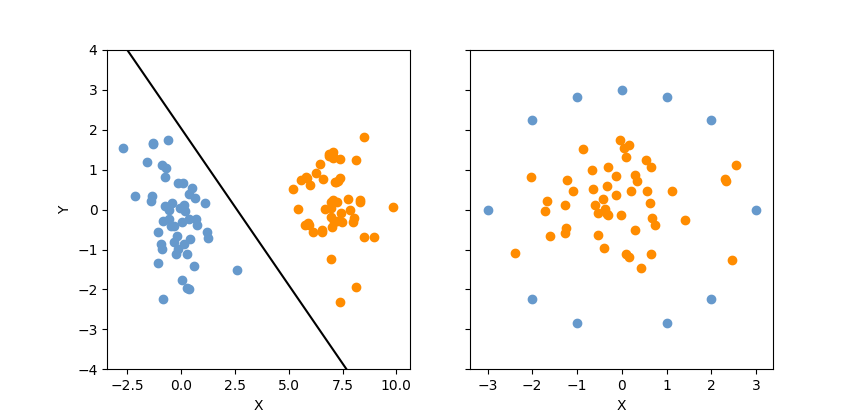
\includegraphics[scale=0.6]{img/fig_perceptron}
	\end{center}
	\caption{\textbf{Left}: Separating two datasets with the perceptron algorithm in $\mathbb{R}^2$. The correct classification boundary takes the form of a line, i.e. $0 = w^{T}x = w_0 x + w_1 y + w_2$. The line pictured is given by $w = (-2.285, -2.908, 5.938)$, the weights after 19 iterations. \textbf{Right}: A not-linearly separable data set, on which the algorithm would never converge, because it is based on finding linear classifiers and thus cannot separate the data correctly.}
	\label{fig:perceptron}
\end {figure}

\begin {algorithm}
	\begin {algorithmic}[1]
		\State $w$ = random
		\While {true}
			\For{$x_i$ in $x$}
				\If{$w^T x_i t_i \leq 0$}
					\State $w$ += $x_i t_i * \eta$
				\EndIf

				\If{$w^T x_i t_i > 0$ for all $x_i$ in $x$}
					\State stop
				\EndIf
			\EndFor
		\EndWhile
	\end{algorithmic}
	\caption{Stochastic Gradient Descent applied to the task of finding the perceptron weights $w$. $x$ is assumed to be linearly separable.}
	\label{alg:perceptron_algorithm}
\end{algorithm}



		\subsection{Multiple Neurons and Backpropagation}
\label{subsec:mlp_backprop}
While the perceptron algorithm works fine for linear problems, those are only a small subset of real-world problems (see figure \ref{fig:perceptron}). The solution to this problem is to add more neurons to the model, which form a network that consists of layers that pass the outputs of neurons in the previous layers through non-linear activation functions and then use the results as inputs. These layers are referred to as the ``input layer'', the initial layer, the ``output layer'', the last layer, and ``hidden layers'', which are all the layers inbetween.

	\subsubsection{Multi-Layer Perceptrons}
The resulting networks are called \textit{Multi-Layer Perceptrons} (MLPs), \textit{Feedforward Artificial Neural Networks}(ANNs), or, in the case of a multitude of layers, \textit{Deep Neural Networks}, and are much more powerful than simple perceptrons, as they can approximate haphazard continuous functions that operate on closed and bounded subsets of $\mathbb{R}^n$ given that the network possesses at least one hidden layer of neurons. This capability makes using MLPs for learning real-life problems feasible.\cite{universal_approx}\cite{universal_approx2}\\

\noindent Again, each neuron in the network computes a weighted sum of its $i$ inputs, just like in equation \ref{eq:perc_class}, although indexing has been added to identify neurons and weights in the entire network:

\[ a_j^{(l)} = \sum \limits_{i} w^{(l)}_{ji}\,\, y_i + b^{(l)}_{j} \]

\noindent $y_i$ are the input values to the current neuron. Note that these either are the direct inputs $x_i$ to the network, or outputs of other neurons, depending on where in the network the term is evaluated. $w$ is the matrix of weights, and $w^{(l)}_{ji}$ denotes the weight of the connection from the $i$th neuron in the previous layer $l - 1$ to the $j$th neuron in the  layer $l$. The term $b$ is the bias weight associated with the neuron $j$. The bias can be made part of the weight matrix by introducing an additional input dimension with a value of $1$, like it was done for the perceptron algorithm in section \ref{subsec:perceptron_algo}.

Afterwards, the sum $a^{(l)}_j$ is passed into an activation function $h(\cdot)$ to produce the activation of the $j$th neuron in the $l$th layer, $z_j^{(l)}$:

\[ z_j^{(l)} = h(a^{(l)}_j) \]

\noindent In vectorized notation, the activations of an entire layer could therefore be written as the recursive formula

\[ z^{(l)} = h(w^{(l)} z^{(l-1)}) \cite{nielsen_book} \]

\noindent where the activations of the input layer are simply the inputs themselves, thus ending the recursion. Expanding the term for the 2-layer network shown in figure \ref{fig:mlp} gives the following formula for a network output $out_k$:

\[ out_k = \sigma \left ( \sum \limits_{j=0}^{4} w^{(2)}_{kj}\,\, h \left ( \sum \limits_{i=0}^{3} w^{(1)}_{ji} x_i \right ) \right ) \label{eq:mlp_out} \]

\noindent Here, \textbf{$\sigma$} is an output function that is applied in the last layer of the network, and is dependent on the task the network is supposed to fulfill: For regression problems, fitting a function to a set of data and then predicting new values using that function, the identity function can be used, but for binary classification problems, instead of using a step function like in the original perceptron, one instead uses the \textit{Sigmoid} function and interprets the output as

\[ \sigma_{sig}(x_i) = \begin{cases}
				x_i \in C_1 \text{ if } \frac{1}{1 + e^{-x_i}} \geq 0.5 \\
				x_i \in C_2 \text{ else }\\
			 \end{cases}
\]

\noindent Also, the choice of the activation function $h(w, x)$ is different from the perceptron: It is not chosen to be the Heaviside step function, but instead, to be a non-linear, continuous and differentiable function, such as the general Sigmoid function and its derivative:

\begin {align}
	 h(x) &= \frac{1}{1 + e^{-x}}\\
	\frac{\partial h}{\partial x} &= h(x)(1 - h(x))
\end {align}


\textbf{TODO: clean up this part - messy!}\\
\noindent Computing an output is done by passing the input vector to the first layer, which computes its activations for all its neurons, which then pass on their activations to the neurons of the next layer as inputs until the output layer is reached.

If the classification is non-binary, using the \textit{Softmax} function (see section \ref{subsec:softmax}) to obtain probabilities for the likeliness of $x_i$ being part of any of the classes is a solution.\\

\afterpage{
	\begin {figure}[!ht]
		\begin{center}
			\def\svgwidth{0.8\columnwidth}
			\input{img/mlp.pdf_tex}
		\end{center}
		\caption[]{An MLP with one hidden layer, forming an acyclic directed graph, where connections are color-coded per layer by the receiving neuron. The layer count $L$ starts at the layer after the input layer\protect\footnotemark. Therefore $L = 2$, with three inputs $x_i$ and neuron counts $D^{(1)} = 4$ and $D^{(2)} = 2$. The variables $b^{(1)}$ and $b^{(2)}$ refer to the biases for the neurons in the layers $(1)$ or $(2)$, respectively. Each neuron has its own, changeable bias value, but for the sake of cleanness, the connections from the biases to each neuron of their corresponding layer are not shown.}
		\label{fig:mlp}
	\end {figure}

	\footnotetext{There is no consensus on which method of counting is the most appropriate. Sometimes, only the number of hidden layers or even all layers are counted \cite[pp. 229]{bishop_pattern}}
}

\noindent The goal of training an MLP is - as previously for the perceptron - finding specific weights so that all inputs are classified correctly, or at least, so that the network makes only few mistakes. Therefore, a loss function is added to the end of the network, measuring the correctness of the output. Instead of the perceptron criterion \ref{eq:perc_error}, a more general loss function is employed which compares the difference between the output $\sigma(x)$ of the network for a sample $x$ and the preferred output for $x$, the \textit{label} or \textit{ground truth} of $x$. Typically, the loss function for regression problems is based on the \textit{Least Squares Error} (LSE), which is defined as

\[ LSE(w) = \frac{1}{2} \left ( out_x - t \right )^2, \]

\noindent where the single, linear output of the network for some input $x$ and a set of weights $w$ is compared to the ground truth $t$.\footnote{The error is only given as a function of $w$ because both the input $x$ and its correct label $t$ are fixed in the particular case presented here.} Binary classification problems instead use Sigmoid outputs together with the \textit{Cross-Entropy} loss function, which is defined as 

\[ CE(w) =  -t \, \ln out_x + (1 - t) \ln (1 - out_x). \]

\noindent For multi-class classifications, an adaption of the Cross-Entropy loss can be used, which is further described in section \ref{subsec:cross_ent}. \cite[pp. 232-236]{bishop_pattern}\\

	\subsubsection{The Backpropagation algorithm}
Training a network with multiple layers is harder than training a single perceptron because the influence of each of the weights in any layer of the network on the error function has to be computed when using gradient-based optimization methods while the output of the network no longer is the result of a single function, but instead, a composition of an usually large number of functions (see equation \ref{eq:mlp_out}). Although it is possible to manually calculate the partial derivatives for the entire network, this becomes more and more cumbersome as the network grows in size.

Luckily, there exists an iterative algorithm called \textit{Backpropagation} \cite{backprop} that finds the gradient of the loss with respect to each weight so that an optimization method can be applied to change every weight. The algorithm makes use of the fact that each neuron can be viewed (almost) independently from the rest of the network. Remembering that the analytic way of obtaining the derivative of a composition of functions 

\[ f \circ g = f(g(x)) \]

\noindent with respect to some $x$ is to apply the chain rule

\[ \frac{\partial f}{\partial x} =\frac{\partial f}{\partial g} \frac{\partial g}{\partial x} \, , \]

\noindent one can see that this concept can also be applied to neurons in a network, because using the output value of a neuron in a previous layer as the input for a node is nothing else than function composition.\\

\noindent Backpropagation thus starts with a \textit{forward pass}, which means that an input vector $x$ is passed through the network and the corresponding sums $a_j$ and activations $z_j$ are calculated and stored. Comparing the final outputs to the ground truth in the loss layer, the network is then traversed in the opposite direction in what is called a \textit{backward pass}, aiming to obtain the influence of each weight in each layer on the final loss, that is, the gradient of the loss function with respect to the weights. After this first phase, the partial derivatives for each weight are known, and the weights are updated in a second phase, in which an optimization algorithm like Gradient Descent is used as described in section \ref{subsec:grad_desc}.\\

\noindent The central idea of the backward pass is that when traversing the network from the output layer to the input layer, the derivatives of the loss function with respect to weights of a layer depend on weights of the layers that precede them. This relationship is described by the formula

\begin {align}
	\frac{\partial E}{\partial w_{ji}} &= \frac{\partial E}{\partial a_j} \frac{\partial a_j}{\partial w_{ji}}
\end {align}

\noindent where $E$ is the loss function of the network. According to the chain rule, the influence of the weight $w_{ji}$ on the loss is equal to the influence of the weight on the sum of inputs $a_j$ times the influence of $a_j$ on the loss function. In literature, the term $\frac{\partial E}{\partial a_j}$ is often denoted as $\delta_j^{(l)}$, the ``error'' of the neuron $j$ in layer $l$. Using this notation and taking the partial derivative of the weighted sum $a_j$, the formula becomes

\[ \frac{\partial E}{\partial w_{ji}} = \delta_j^{(l)} z_i .\]

\noindent Since $z_i$, the activation from the input end of the connection that is modified by $w_{ji}$, is already known for all neurons due to the forward pass, the only thing that needs to be computed to figure out the loss gradient are the $\delta$-values. The computation of $\delta_j^{(l)}$ depends on the position of the neuron in the network:

\[ \delta_j^{(l)} =  \begin{cases}
				\frac{\partial E}{\partial a_j} \text{ if neuron } j^{(l)} \text{ is an output neuron} \\
			           h'(a_j) \sum \limits_{k} w_{kj} \, \delta_k^{(l+1)} \text{ otherwise}
			     \end{cases}
\]

\noindent In the case $j$ is an output neuron, the partial is calculated directly. Otherwise, $\delta_j$ depends on the $\delta$-values in the previous layers, necessitating the backward traversion (see figure \ref{fig:backprop}). The definition of $\delta$ for hidden neurons is also the reason why a differentiable function must be chosen as the activation $h(\cdot)$, as stated earlier.\\

\noindent The main advantage of the algorithm is that it scales linearly with the number of weights, i.e. the algorithm is $\in \mathcal{O}(w)$. Furthermore, the fact that all $\delta$-values of a layer have to be calculated to calculate all $\delta$ values and weight derivatives in the layer that precedes it naturally leads to vectorizing the algorithm layerwise in efficient implementations. \cite{nielsen_book}\cite{ng_lecture}\cite[pp. 241-245]{bishop_pattern}


\afterpage{
	\begin {figure}[!ht]
		\begin{center}
			\def\svgwidth{0.8\columnwidth}
			\input{img/backprop.pdf_tex}
		\end{center}
		\caption[]{Backpropagation algorithm, applied to a hidden layer $l$.\protect\footnotemark$\,$ Steps during the forward pass are shown in blue, while steps during the backward pass are orange. The central neuron is the only neuron in the layer $l$, while there are two neurons each in the hidden layers $l-1$ and $l+1$. The forward pass calculates the weighted sum $a_1^{(l)}$ and the activation $h(a_1^{(l)})$. Once the backward pass reaches the neuron, it calculates $\delta_1^{(l)}$ and the partial derivatives of the weights of layer $l$, that is, the weights of the connections that flow into the central neuron in the forward pass, using the backpropagated value $\delta_k^{(l+1)}$. This is repeated throughout the entire network until the entire weight gradient is known and a single Gradient Descent step can be taken toward the loss function minimum.}
		\label{fig:backprop}
	\end {figure}

	\footnotetext{This example is based on a visualization in \cite{karparthy_lecture}.}
}

\noindent Depending on how deep the networks are, i.e. how many hidden layers there are and how many neurons there are in these hidden layers, neural networks can learn very complex classification boundaries. The role of the activation function is akin to the kernel principle of State Vector Machines (SVMs), since it maps inputs to a representation in which they are linearly separable by a hyperplane (see figure \ref{fig:mlp_trick}).

\begin {figure}[!ht]
		\begin{center}
			\textbf{TODO: uncomment in code}
			%%% Creator: Matplotlib, PGF backend
%%
%% To include the figure in your LaTeX document, write
%%   \input{<filename>.pgf}
%%
%% Make sure the required packages are loaded in your preamble
%%   \usepackage{pgf}
%%
%% Figures using additional raster images can only be included by \input if
%% they are in the same directory as the main LaTeX file. For loading figures
%% from other directories you can use the `import` package
%%   \usepackage{import}
%% and then include the figures with
%%   \import{<path to file>}{<filename>.pgf}
%%
%% Matplotlib used the following preamble
%%   \usepackage{fontspec}
%%   \setmainfont{DejaVu Serif}
%%   \setsansfont{DejaVu Sans}
%%   \setmonofont{DejaVu Sans Mono}
%%
\begingroup%
\makeatletter%
\begin{pgfpicture}%
\pgfpathrectangle{\pgfpointorigin}{\pgfqpoint{6.510000in}{1.550000in}}%
\pgfusepath{use as bounding box, clip}%
\begin{pgfscope}%
\pgfsetbuttcap%
\pgfsetmiterjoin%
\definecolor{currentfill}{rgb}{1.000000,1.000000,1.000000}%
\pgfsetfillcolor{currentfill}%
\pgfsetlinewidth{0.000000pt}%
\definecolor{currentstroke}{rgb}{1.000000,1.000000,1.000000}%
\pgfsetstrokecolor{currentstroke}%
\pgfsetdash{}{0pt}%
\pgfpathmoveto{\pgfqpoint{0.000000in}{0.000000in}}%
\pgfpathlineto{\pgfqpoint{6.510000in}{0.000000in}}%
\pgfpathlineto{\pgfqpoint{6.510000in}{1.550000in}}%
\pgfpathlineto{\pgfqpoint{0.000000in}{1.550000in}}%
\pgfpathclose%
\pgfusepath{fill}%
\end{pgfscope}%
\begin{pgfscope}%
\pgfsetbuttcap%
\pgfsetmiterjoin%
\definecolor{currentfill}{rgb}{1.000000,1.000000,1.000000}%
\pgfsetfillcolor{currentfill}%
\pgfsetlinewidth{0.000000pt}%
\definecolor{currentstroke}{rgb}{0.000000,0.000000,0.000000}%
\pgfsetstrokecolor{currentstroke}%
\pgfsetstrokeopacity{0.000000}%
\pgfsetdash{}{0pt}%
\pgfpathmoveto{\pgfqpoint{0.584722in}{0.387222in}}%
\pgfpathlineto{\pgfqpoint{1.556778in}{0.387222in}}%
\pgfpathlineto{\pgfqpoint{1.556778in}{1.365000in}}%
\pgfpathlineto{\pgfqpoint{0.584722in}{1.365000in}}%
\pgfpathclose%
\pgfusepath{fill}%
\end{pgfscope}%
\begin{pgfscope}%
\pgfpathrectangle{\pgfqpoint{0.584722in}{0.387222in}}{\pgfqpoint{0.972056in}{0.977778in}} %
\pgfusepath{clip}%
\pgfsetbuttcap%
\pgfsetroundjoin%
\definecolor{currentfill}{rgb}{0.960000,0.895056,0.816000}%
\pgfsetfillcolor{currentfill}%
\pgfsetlinewidth{1.003750pt}%
\definecolor{currentstroke}{rgb}{0.960000,0.895056,0.816000}%
\pgfsetstrokecolor{currentstroke}%
\pgfsetdash{}{0pt}%
\pgfpathmoveto{\pgfqpoint{1.165798in}{0.632376in}}%
\pgfpathcurveto{\pgfqpoint{1.171621in}{0.632376in}}{\pgfqpoint{1.177208in}{0.634690in}}{\pgfqpoint{1.181326in}{0.638808in}}%
\pgfpathcurveto{\pgfqpoint{1.185444in}{0.642926in}}{\pgfqpoint{1.187758in}{0.648512in}}{\pgfqpoint{1.187758in}{0.654336in}}%
\pgfpathcurveto{\pgfqpoint{1.187758in}{0.660160in}}{\pgfqpoint{1.185444in}{0.665746in}}{\pgfqpoint{1.181326in}{0.669864in}}%
\pgfpathcurveto{\pgfqpoint{1.177208in}{0.673982in}}{\pgfqpoint{1.171621in}{0.676296in}}{\pgfqpoint{1.165798in}{0.676296in}}%
\pgfpathcurveto{\pgfqpoint{1.159974in}{0.676296in}}{\pgfqpoint{1.154387in}{0.673982in}}{\pgfqpoint{1.150269in}{0.669864in}}%
\pgfpathcurveto{\pgfqpoint{1.146151in}{0.665746in}}{\pgfqpoint{1.143837in}{0.660160in}}{\pgfqpoint{1.143837in}{0.654336in}}%
\pgfpathcurveto{\pgfqpoint{1.143837in}{0.648512in}}{\pgfqpoint{1.146151in}{0.642926in}}{\pgfqpoint{1.150269in}{0.638808in}}%
\pgfpathcurveto{\pgfqpoint{1.154387in}{0.634690in}}{\pgfqpoint{1.159974in}{0.632376in}}{\pgfqpoint{1.165798in}{0.632376in}}%
\pgfpathclose%
\pgfusepath{stroke,fill}%
\end{pgfscope}%
\begin{pgfscope}%
\pgfpathrectangle{\pgfqpoint{0.584722in}{0.387222in}}{\pgfqpoint{0.972056in}{0.977778in}} %
\pgfusepath{clip}%
\pgfsetbuttcap%
\pgfsetroundjoin%
\definecolor{currentfill}{rgb}{0.960000,0.859517,0.737199}%
\pgfsetfillcolor{currentfill}%
\pgfsetlinewidth{1.003750pt}%
\definecolor{currentstroke}{rgb}{0.960000,0.859517,0.737199}%
\pgfsetstrokecolor{currentstroke}%
\pgfsetdash{}{0pt}%
\pgfpathmoveto{\pgfqpoint{1.058174in}{0.823801in}}%
\pgfpathcurveto{\pgfqpoint{1.064829in}{0.823801in}}{\pgfqpoint{1.071212in}{0.826446in}}{\pgfqpoint{1.075918in}{0.831151in}}%
\pgfpathcurveto{\pgfqpoint{1.080624in}{0.835857in}}{\pgfqpoint{1.083268in}{0.842241in}}{\pgfqpoint{1.083268in}{0.848896in}}%
\pgfpathcurveto{\pgfqpoint{1.083268in}{0.855551in}}{\pgfqpoint{1.080624in}{0.861935in}}{\pgfqpoint{1.075918in}{0.866641in}}%
\pgfpathcurveto{\pgfqpoint{1.071212in}{0.871346in}}{\pgfqpoint{1.064829in}{0.873991in}}{\pgfqpoint{1.058174in}{0.873991in}}%
\pgfpathcurveto{\pgfqpoint{1.051519in}{0.873991in}}{\pgfqpoint{1.045135in}{0.871346in}}{\pgfqpoint{1.040429in}{0.866641in}}%
\pgfpathcurveto{\pgfqpoint{1.035723in}{0.861935in}}{\pgfqpoint{1.033079in}{0.855551in}}{\pgfqpoint{1.033079in}{0.848896in}}%
\pgfpathcurveto{\pgfqpoint{1.033079in}{0.842241in}}{\pgfqpoint{1.035723in}{0.835857in}}{\pgfqpoint{1.040429in}{0.831151in}}%
\pgfpathcurveto{\pgfqpoint{1.045135in}{0.826446in}}{\pgfqpoint{1.051519in}{0.823801in}}{\pgfqpoint{1.058174in}{0.823801in}}%
\pgfpathclose%
\pgfusepath{stroke,fill}%
\end{pgfscope}%
\begin{pgfscope}%
\pgfpathrectangle{\pgfqpoint{0.584722in}{0.387222in}}{\pgfqpoint{0.972056in}{0.977778in}} %
\pgfusepath{clip}%
\pgfsetbuttcap%
\pgfsetroundjoin%
\definecolor{currentfill}{rgb}{0.960000,0.831877,0.675914}%
\pgfsetfillcolor{currentfill}%
\pgfsetlinewidth{1.003750pt}%
\definecolor{currentstroke}{rgb}{0.960000,0.831877,0.675914}%
\pgfsetstrokecolor{currentstroke}%
\pgfsetdash{}{0pt}%
\pgfpathmoveto{\pgfqpoint{1.032954in}{0.803443in}}%
\pgfpathcurveto{\pgfqpoint{1.040189in}{0.803443in}}{\pgfqpoint{1.047130in}{0.806317in}}{\pgfqpoint{1.052246in}{0.811434in}}%
\pgfpathcurveto{\pgfqpoint{1.057363in}{0.816551in}}{\pgfqpoint{1.060238in}{0.823491in}}{\pgfqpoint{1.060238in}{0.830727in}}%
\pgfpathcurveto{\pgfqpoint{1.060238in}{0.837963in}}{\pgfqpoint{1.057363in}{0.844903in}}{\pgfqpoint{1.052246in}{0.850020in}}%
\pgfpathcurveto{\pgfqpoint{1.047130in}{0.855137in}}{\pgfqpoint{1.040189in}{0.858011in}}{\pgfqpoint{1.032954in}{0.858011in}}%
\pgfpathcurveto{\pgfqpoint{1.025718in}{0.858011in}}{\pgfqpoint{1.018777in}{0.855137in}}{\pgfqpoint{1.013661in}{0.850020in}}%
\pgfpathcurveto{\pgfqpoint{1.008544in}{0.844903in}}{\pgfqpoint{1.005669in}{0.837963in}}{\pgfqpoint{1.005669in}{0.830727in}}%
\pgfpathcurveto{\pgfqpoint{1.005669in}{0.823491in}}{\pgfqpoint{1.008544in}{0.816551in}}{\pgfqpoint{1.013661in}{0.811434in}}%
\pgfpathcurveto{\pgfqpoint{1.018777in}{0.806317in}}{\pgfqpoint{1.025718in}{0.803443in}}{\pgfqpoint{1.032954in}{0.803443in}}%
\pgfpathclose%
\pgfusepath{stroke,fill}%
\end{pgfscope}%
\begin{pgfscope}%
\pgfpathrectangle{\pgfqpoint{0.584722in}{0.387222in}}{\pgfqpoint{0.972056in}{0.977778in}} %
\pgfusepath{clip}%
\pgfsetbuttcap%
\pgfsetroundjoin%
\definecolor{currentfill}{rgb}{0.960000,0.895056,0.816000}%
\pgfsetfillcolor{currentfill}%
\pgfsetlinewidth{1.003750pt}%
\definecolor{currentstroke}{rgb}{0.960000,0.895056,0.816000}%
\pgfsetstrokecolor{currentstroke}%
\pgfsetdash{}{0pt}%
\pgfpathmoveto{\pgfqpoint{1.172847in}{0.553974in}}%
\pgfpathcurveto{\pgfqpoint{1.178671in}{0.553974in}}{\pgfqpoint{1.184257in}{0.556288in}}{\pgfqpoint{1.188375in}{0.560406in}}%
\pgfpathcurveto{\pgfqpoint{1.192493in}{0.564524in}}{\pgfqpoint{1.194807in}{0.570111in}}{\pgfqpoint{1.194807in}{0.575934in}}%
\pgfpathcurveto{\pgfqpoint{1.194807in}{0.581758in}}{\pgfqpoint{1.192493in}{0.587345in}}{\pgfqpoint{1.188375in}{0.591463in}}%
\pgfpathcurveto{\pgfqpoint{1.184257in}{0.595581in}}{\pgfqpoint{1.178671in}{0.597895in}}{\pgfqpoint{1.172847in}{0.597895in}}%
\pgfpathcurveto{\pgfqpoint{1.167023in}{0.597895in}}{\pgfqpoint{1.161437in}{0.595581in}}{\pgfqpoint{1.157319in}{0.591463in}}%
\pgfpathcurveto{\pgfqpoint{1.153201in}{0.587345in}}{\pgfqpoint{1.150887in}{0.581758in}}{\pgfqpoint{1.150887in}{0.575934in}}%
\pgfpathcurveto{\pgfqpoint{1.150887in}{0.570111in}}{\pgfqpoint{1.153201in}{0.564524in}}{\pgfqpoint{1.157319in}{0.560406in}}%
\pgfpathcurveto{\pgfqpoint{1.161437in}{0.556288in}}{\pgfqpoint{1.167023in}{0.553974in}}{\pgfqpoint{1.172847in}{0.553974in}}%
\pgfpathclose%
\pgfusepath{stroke,fill}%
\end{pgfscope}%
\begin{pgfscope}%
\pgfpathrectangle{\pgfqpoint{0.584722in}{0.387222in}}{\pgfqpoint{0.972056in}{0.977778in}} %
\pgfusepath{clip}%
\pgfsetbuttcap%
\pgfsetroundjoin%
\definecolor{currentfill}{rgb}{0.960000,0.895056,0.816000}%
\pgfsetfillcolor{currentfill}%
\pgfsetlinewidth{1.003750pt}%
\definecolor{currentstroke}{rgb}{0.960000,0.895056,0.816000}%
\pgfsetstrokecolor{currentstroke}%
\pgfsetdash{}{0pt}%
\pgfpathmoveto{\pgfqpoint{1.169637in}{0.664488in}}%
\pgfpathcurveto{\pgfqpoint{1.175461in}{0.664488in}}{\pgfqpoint{1.181047in}{0.666802in}}{\pgfqpoint{1.185165in}{0.670920in}}%
\pgfpathcurveto{\pgfqpoint{1.189284in}{0.675038in}}{\pgfqpoint{1.191598in}{0.680625in}}{\pgfqpoint{1.191598in}{0.686448in}}%
\pgfpathcurveto{\pgfqpoint{1.191598in}{0.692272in}}{\pgfqpoint{1.189284in}{0.697859in}}{\pgfqpoint{1.185165in}{0.701977in}}%
\pgfpathcurveto{\pgfqpoint{1.181047in}{0.706095in}}{\pgfqpoint{1.175461in}{0.708409in}}{\pgfqpoint{1.169637in}{0.708409in}}%
\pgfpathcurveto{\pgfqpoint{1.163813in}{0.708409in}}{\pgfqpoint{1.158227in}{0.706095in}}{\pgfqpoint{1.154109in}{0.701977in}}%
\pgfpathcurveto{\pgfqpoint{1.149991in}{0.697859in}}{\pgfqpoint{1.147677in}{0.692272in}}{\pgfqpoint{1.147677in}{0.686448in}}%
\pgfpathcurveto{\pgfqpoint{1.147677in}{0.680625in}}{\pgfqpoint{1.149991in}{0.675038in}}{\pgfqpoint{1.154109in}{0.670920in}}%
\pgfpathcurveto{\pgfqpoint{1.158227in}{0.666802in}}{\pgfqpoint{1.163813in}{0.664488in}}{\pgfqpoint{1.169637in}{0.664488in}}%
\pgfpathclose%
\pgfusepath{stroke,fill}%
\end{pgfscope}%
\begin{pgfscope}%
\pgfpathrectangle{\pgfqpoint{0.584722in}{0.387222in}}{\pgfqpoint{0.972056in}{0.977778in}} %
\pgfusepath{clip}%
\pgfsetbuttcap%
\pgfsetroundjoin%
\definecolor{currentfill}{rgb}{0.960000,0.818746,0.646798}%
\pgfsetfillcolor{currentfill}%
\pgfsetlinewidth{1.003750pt}%
\definecolor{currentstroke}{rgb}{0.960000,0.818746,0.646798}%
\pgfsetstrokecolor{currentstroke}%
\pgfsetdash{}{0pt}%
\pgfpathmoveto{\pgfqpoint{0.995274in}{0.965390in}}%
\pgfpathcurveto{\pgfqpoint{1.002770in}{0.965390in}}{\pgfqpoint{1.009960in}{0.968368in}}{\pgfqpoint{1.015261in}{0.973669in}}%
\pgfpathcurveto{\pgfqpoint{1.020561in}{0.978969in}}{\pgfqpoint{1.023539in}{0.986159in}}{\pgfqpoint{1.023539in}{0.993655in}}%
\pgfpathcurveto{\pgfqpoint{1.023539in}{1.001151in}}{\pgfqpoint{1.020561in}{1.008341in}}{\pgfqpoint{1.015261in}{1.013642in}}%
\pgfpathcurveto{\pgfqpoint{1.009960in}{1.018942in}}{\pgfqpoint{1.002770in}{1.021921in}}{\pgfqpoint{0.995274in}{1.021921in}}%
\pgfpathcurveto{\pgfqpoint{0.987778in}{1.021921in}}{\pgfqpoint{0.980588in}{1.018942in}}{\pgfqpoint{0.975287in}{1.013642in}}%
\pgfpathcurveto{\pgfqpoint{0.969987in}{1.008341in}}{\pgfqpoint{0.967009in}{1.001151in}}{\pgfqpoint{0.967009in}{0.993655in}}%
\pgfpathcurveto{\pgfqpoint{0.967009in}{0.986159in}}{\pgfqpoint{0.969987in}{0.978969in}}{\pgfqpoint{0.975287in}{0.973669in}}%
\pgfpathcurveto{\pgfqpoint{0.980588in}{0.968368in}}{\pgfqpoint{0.987778in}{0.965390in}}{\pgfqpoint{0.995274in}{0.965390in}}%
\pgfpathclose%
\pgfusepath{stroke,fill}%
\end{pgfscope}%
\begin{pgfscope}%
\pgfpathrectangle{\pgfqpoint{0.584722in}{0.387222in}}{\pgfqpoint{0.972056in}{0.977778in}} %
\pgfusepath{clip}%
\pgfsetbuttcap%
\pgfsetroundjoin%
\definecolor{currentfill}{rgb}{0.960000,0.682856,0.345490}%
\pgfsetfillcolor{currentfill}%
\pgfsetlinewidth{1.003750pt}%
\definecolor{currentstroke}{rgb}{0.960000,0.682856,0.345490}%
\pgfsetstrokecolor{currentstroke}%
\pgfsetdash{}{0pt}%
\pgfpathmoveto{\pgfqpoint{0.916056in}{0.568475in}}%
\pgfpathcurveto{\pgfqpoint{0.925847in}{0.568475in}}{\pgfqpoint{0.935238in}{0.572364in}}{\pgfqpoint{0.942160in}{0.579287in}}%
\pgfpathcurveto{\pgfqpoint{0.949083in}{0.586210in}}{\pgfqpoint{0.952973in}{0.595601in}}{\pgfqpoint{0.952973in}{0.605391in}}%
\pgfpathcurveto{\pgfqpoint{0.952973in}{0.615182in}}{\pgfqpoint{0.949083in}{0.624573in}}{\pgfqpoint{0.942160in}{0.631496in}}%
\pgfpathcurveto{\pgfqpoint{0.935238in}{0.638418in}}{\pgfqpoint{0.925847in}{0.642308in}}{\pgfqpoint{0.916056in}{0.642308in}}%
\pgfpathcurveto{\pgfqpoint{0.906266in}{0.642308in}}{\pgfqpoint{0.896875in}{0.638418in}}{\pgfqpoint{0.889952in}{0.631496in}}%
\pgfpathcurveto{\pgfqpoint{0.883029in}{0.624573in}}{\pgfqpoint{0.879140in}{0.615182in}}{\pgfqpoint{0.879140in}{0.605391in}}%
\pgfpathcurveto{\pgfqpoint{0.879140in}{0.595601in}}{\pgfqpoint{0.883029in}{0.586210in}}{\pgfqpoint{0.889952in}{0.579287in}}%
\pgfpathcurveto{\pgfqpoint{0.896875in}{0.572364in}}{\pgfqpoint{0.906266in}{0.568475in}}{\pgfqpoint{0.916056in}{0.568475in}}%
\pgfpathclose%
\pgfusepath{stroke,fill}%
\end{pgfscope}%
\begin{pgfscope}%
\pgfpathrectangle{\pgfqpoint{0.584722in}{0.387222in}}{\pgfqpoint{0.972056in}{0.977778in}} %
\pgfusepath{clip}%
\pgfsetbuttcap%
\pgfsetroundjoin%
\definecolor{currentfill}{rgb}{0.960000,0.895056,0.816000}%
\pgfsetfillcolor{currentfill}%
\pgfsetlinewidth{1.003750pt}%
\definecolor{currentstroke}{rgb}{0.960000,0.895056,0.816000}%
\pgfsetstrokecolor{currentstroke}%
\pgfsetdash{}{0pt}%
\pgfpathmoveto{\pgfqpoint{1.224205in}{0.698841in}}%
\pgfpathcurveto{\pgfqpoint{1.230029in}{0.698841in}}{\pgfqpoint{1.235615in}{0.701155in}}{\pgfqpoint{1.239733in}{0.705273in}}%
\pgfpathcurveto{\pgfqpoint{1.243851in}{0.709391in}}{\pgfqpoint{1.246165in}{0.714977in}}{\pgfqpoint{1.246165in}{0.720801in}}%
\pgfpathcurveto{\pgfqpoint{1.246165in}{0.726625in}}{\pgfqpoint{1.243851in}{0.732211in}}{\pgfqpoint{1.239733in}{0.736329in}}%
\pgfpathcurveto{\pgfqpoint{1.235615in}{0.740448in}}{\pgfqpoint{1.230029in}{0.742761in}}{\pgfqpoint{1.224205in}{0.742761in}}%
\pgfpathcurveto{\pgfqpoint{1.218381in}{0.742761in}}{\pgfqpoint{1.212795in}{0.740448in}}{\pgfqpoint{1.208677in}{0.736329in}}%
\pgfpathcurveto{\pgfqpoint{1.204559in}{0.732211in}}{\pgfqpoint{1.202245in}{0.726625in}}{\pgfqpoint{1.202245in}{0.720801in}}%
\pgfpathcurveto{\pgfqpoint{1.202245in}{0.714977in}}{\pgfqpoint{1.204559in}{0.709391in}}{\pgfqpoint{1.208677in}{0.705273in}}%
\pgfpathcurveto{\pgfqpoint{1.212795in}{0.701155in}}{\pgfqpoint{1.218381in}{0.698841in}}{\pgfqpoint{1.224205in}{0.698841in}}%
\pgfpathclose%
\pgfusepath{stroke,fill}%
\end{pgfscope}%
\begin{pgfscope}%
\pgfpathrectangle{\pgfqpoint{0.584722in}{0.387222in}}{\pgfqpoint{0.972056in}{0.977778in}} %
\pgfusepath{clip}%
\pgfsetbuttcap%
\pgfsetroundjoin%
\definecolor{currentfill}{rgb}{0.960000,0.791728,0.586890}%
\pgfsetfillcolor{currentfill}%
\pgfsetlinewidth{1.003750pt}%
\definecolor{currentstroke}{rgb}{0.960000,0.791728,0.586890}%
\pgfsetstrokecolor{currentstroke}%
\pgfsetdash{}{0pt}%
\pgfpathmoveto{\pgfqpoint{0.985444in}{0.846747in}}%
\pgfpathcurveto{\pgfqpoint{0.993449in}{0.846747in}}{\pgfqpoint{1.001127in}{0.849928in}}{\pgfqpoint{1.006787in}{0.855588in}}%
\pgfpathcurveto{\pgfqpoint{1.012448in}{0.861248in}}{\pgfqpoint{1.015628in}{0.868926in}}{\pgfqpoint{1.015628in}{0.876931in}}%
\pgfpathcurveto{\pgfqpoint{1.015628in}{0.884936in}}{\pgfqpoint{1.012448in}{0.892614in}}{\pgfqpoint{1.006787in}{0.898274in}}%
\pgfpathcurveto{\pgfqpoint{1.001127in}{0.903934in}}{\pgfqpoint{0.993449in}{0.907115in}}{\pgfqpoint{0.985444in}{0.907115in}}%
\pgfpathcurveto{\pgfqpoint{0.977439in}{0.907115in}}{\pgfqpoint{0.969761in}{0.903934in}}{\pgfqpoint{0.964101in}{0.898274in}}%
\pgfpathcurveto{\pgfqpoint{0.958441in}{0.892614in}}{\pgfqpoint{0.955261in}{0.884936in}}{\pgfqpoint{0.955261in}{0.876931in}}%
\pgfpathcurveto{\pgfqpoint{0.955261in}{0.868926in}}{\pgfqpoint{0.958441in}{0.861248in}}{\pgfqpoint{0.964101in}{0.855588in}}%
\pgfpathcurveto{\pgfqpoint{0.969761in}{0.849928in}}{\pgfqpoint{0.977439in}{0.846747in}}{\pgfqpoint{0.985444in}{0.846747in}}%
\pgfpathclose%
\pgfusepath{stroke,fill}%
\end{pgfscope}%
\begin{pgfscope}%
\pgfpathrectangle{\pgfqpoint{0.584722in}{0.387222in}}{\pgfqpoint{0.972056in}{0.977778in}} %
\pgfusepath{clip}%
\pgfsetbuttcap%
\pgfsetroundjoin%
\definecolor{currentfill}{rgb}{0.960000,0.895056,0.816000}%
\pgfsetfillcolor{currentfill}%
\pgfsetlinewidth{1.003750pt}%
\definecolor{currentstroke}{rgb}{0.960000,0.895056,0.816000}%
\pgfsetstrokecolor{currentstroke}%
\pgfsetdash{}{0pt}%
\pgfpathmoveto{\pgfqpoint{1.109649in}{0.955064in}}%
\pgfpathcurveto{\pgfqpoint{1.115473in}{0.955064in}}{\pgfqpoint{1.121059in}{0.957378in}}{\pgfqpoint{1.125177in}{0.961496in}}%
\pgfpathcurveto{\pgfqpoint{1.129295in}{0.965614in}}{\pgfqpoint{1.131609in}{0.971200in}}{\pgfqpoint{1.131609in}{0.977024in}}%
\pgfpathcurveto{\pgfqpoint{1.131609in}{0.982848in}}{\pgfqpoint{1.129295in}{0.988434in}}{\pgfqpoint{1.125177in}{0.992552in}}%
\pgfpathcurveto{\pgfqpoint{1.121059in}{0.996671in}}{\pgfqpoint{1.115473in}{0.998984in}}{\pgfqpoint{1.109649in}{0.998984in}}%
\pgfpathcurveto{\pgfqpoint{1.103825in}{0.998984in}}{\pgfqpoint{1.098239in}{0.996671in}}{\pgfqpoint{1.094121in}{0.992552in}}%
\pgfpathcurveto{\pgfqpoint{1.090003in}{0.988434in}}{\pgfqpoint{1.087689in}{0.982848in}}{\pgfqpoint{1.087689in}{0.977024in}}%
\pgfpathcurveto{\pgfqpoint{1.087689in}{0.971200in}}{\pgfqpoint{1.090003in}{0.965614in}}{\pgfqpoint{1.094121in}{0.961496in}}%
\pgfpathcurveto{\pgfqpoint{1.098239in}{0.957378in}}{\pgfqpoint{1.103825in}{0.955064in}}{\pgfqpoint{1.109649in}{0.955064in}}%
\pgfpathclose%
\pgfusepath{stroke,fill}%
\end{pgfscope}%
\begin{pgfscope}%
\pgfpathrectangle{\pgfqpoint{0.584722in}{0.387222in}}{\pgfqpoint{0.972056in}{0.977778in}} %
\pgfusepath{clip}%
\pgfsetbuttcap%
\pgfsetroundjoin%
\definecolor{currentfill}{rgb}{0.960000,0.748309,0.490619}%
\pgfsetfillcolor{currentfill}%
\pgfsetlinewidth{1.003750pt}%
\definecolor{currentstroke}{rgb}{0.960000,0.748309,0.490619}%
\pgfsetstrokecolor{currentstroke}%
\pgfsetdash{}{0pt}%
\pgfpathmoveto{\pgfqpoint{0.970781in}{0.648758in}}%
\pgfpathcurveto{\pgfqpoint{0.979542in}{0.648758in}}{\pgfqpoint{0.987945in}{0.652239in}}{\pgfqpoint{0.994139in}{0.658434in}}%
\pgfpathcurveto{\pgfqpoint{1.000334in}{0.664628in}}{\pgfqpoint{1.003815in}{0.673031in}}{\pgfqpoint{1.003815in}{0.681792in}}%
\pgfpathcurveto{\pgfqpoint{1.003815in}{0.690553in}}{\pgfqpoint{1.000334in}{0.698956in}}{\pgfqpoint{0.994139in}{0.705151in}}%
\pgfpathcurveto{\pgfqpoint{0.987945in}{0.711345in}}{\pgfqpoint{0.979542in}{0.714826in}}{\pgfqpoint{0.970781in}{0.714826in}}%
\pgfpathcurveto{\pgfqpoint{0.962020in}{0.714826in}}{\pgfqpoint{0.953617in}{0.711345in}}{\pgfqpoint{0.947423in}{0.705151in}}%
\pgfpathcurveto{\pgfqpoint{0.941228in}{0.698956in}}{\pgfqpoint{0.937747in}{0.690553in}}{\pgfqpoint{0.937747in}{0.681792in}}%
\pgfpathcurveto{\pgfqpoint{0.937747in}{0.673031in}}{\pgfqpoint{0.941228in}{0.664628in}}{\pgfqpoint{0.947423in}{0.658434in}}%
\pgfpathcurveto{\pgfqpoint{0.953617in}{0.652239in}}{\pgfqpoint{0.962020in}{0.648758in}}{\pgfqpoint{0.970781in}{0.648758in}}%
\pgfpathclose%
\pgfusepath{stroke,fill}%
\end{pgfscope}%
\begin{pgfscope}%
\pgfpathrectangle{\pgfqpoint{0.584722in}{0.387222in}}{\pgfqpoint{0.972056in}{0.977778in}} %
\pgfusepath{clip}%
\pgfsetbuttcap%
\pgfsetroundjoin%
\definecolor{currentfill}{rgb}{0.960000,0.741239,0.474941}%
\pgfsetfillcolor{currentfill}%
\pgfsetlinewidth{1.003750pt}%
\definecolor{currentstroke}{rgb}{0.960000,0.741239,0.474941}%
\pgfsetstrokecolor{currentstroke}%
\pgfsetdash{}{0pt}%
\pgfpathmoveto{\pgfqpoint{0.930206in}{0.871475in}}%
\pgfpathcurveto{\pgfqpoint{0.939084in}{0.871475in}}{\pgfqpoint{0.947599in}{0.875002in}}{\pgfqpoint{0.953877in}{0.881279in}}%
\pgfpathcurveto{\pgfqpoint{0.960154in}{0.887557in}}{\pgfqpoint{0.963681in}{0.896072in}}{\pgfqpoint{0.963681in}{0.904950in}}%
\pgfpathcurveto{\pgfqpoint{0.963681in}{0.913827in}}{\pgfqpoint{0.960154in}{0.922342in}}{\pgfqpoint{0.953877in}{0.928620in}}%
\pgfpathcurveto{\pgfqpoint{0.947599in}{0.934897in}}{\pgfqpoint{0.939084in}{0.938425in}}{\pgfqpoint{0.930206in}{0.938425in}}%
\pgfpathcurveto{\pgfqpoint{0.921329in}{0.938425in}}{\pgfqpoint{0.912813in}{0.934897in}}{\pgfqpoint{0.906536in}{0.928620in}}%
\pgfpathcurveto{\pgfqpoint{0.900259in}{0.922342in}}{\pgfqpoint{0.896731in}{0.913827in}}{\pgfqpoint{0.896731in}{0.904950in}}%
\pgfpathcurveto{\pgfqpoint{0.896731in}{0.896072in}}{\pgfqpoint{0.900259in}{0.887557in}}{\pgfqpoint{0.906536in}{0.881279in}}%
\pgfpathcurveto{\pgfqpoint{0.912813in}{0.875002in}}{\pgfqpoint{0.921329in}{0.871475in}}{\pgfqpoint{0.930206in}{0.871475in}}%
\pgfpathclose%
\pgfusepath{stroke,fill}%
\end{pgfscope}%
\begin{pgfscope}%
\pgfpathrectangle{\pgfqpoint{0.584722in}{0.387222in}}{\pgfqpoint{0.972056in}{0.977778in}} %
\pgfusepath{clip}%
\pgfsetbuttcap%
\pgfsetroundjoin%
\definecolor{currentfill}{rgb}{0.960000,0.895056,0.816000}%
\pgfsetfillcolor{currentfill}%
\pgfsetlinewidth{1.003750pt}%
\definecolor{currentstroke}{rgb}{0.960000,0.895056,0.816000}%
\pgfsetstrokecolor{currentstroke}%
\pgfsetdash{}{0pt}%
\pgfpathmoveto{\pgfqpoint{1.123845in}{0.747002in}}%
\pgfpathcurveto{\pgfqpoint{1.129668in}{0.747002in}}{\pgfqpoint{1.135255in}{0.749316in}}{\pgfqpoint{1.139373in}{0.753434in}}%
\pgfpathcurveto{\pgfqpoint{1.143491in}{0.757553in}}{\pgfqpoint{1.145805in}{0.763139in}}{\pgfqpoint{1.145805in}{0.768963in}}%
\pgfpathcurveto{\pgfqpoint{1.145805in}{0.774787in}}{\pgfqpoint{1.143491in}{0.780373in}}{\pgfqpoint{1.139373in}{0.784491in}}%
\pgfpathcurveto{\pgfqpoint{1.135255in}{0.788609in}}{\pgfqpoint{1.129668in}{0.790923in}}{\pgfqpoint{1.123845in}{0.790923in}}%
\pgfpathcurveto{\pgfqpoint{1.118021in}{0.790923in}}{\pgfqpoint{1.112434in}{0.788609in}}{\pgfqpoint{1.108316in}{0.784491in}}%
\pgfpathcurveto{\pgfqpoint{1.104198in}{0.780373in}}{\pgfqpoint{1.101884in}{0.774787in}}{\pgfqpoint{1.101884in}{0.768963in}}%
\pgfpathcurveto{\pgfqpoint{1.101884in}{0.763139in}}{\pgfqpoint{1.104198in}{0.757553in}}{\pgfqpoint{1.108316in}{0.753434in}}%
\pgfpathcurveto{\pgfqpoint{1.112434in}{0.749316in}}{\pgfqpoint{1.118021in}{0.747002in}}{\pgfqpoint{1.123845in}{0.747002in}}%
\pgfpathclose%
\pgfusepath{stroke,fill}%
\end{pgfscope}%
\begin{pgfscope}%
\pgfpathrectangle{\pgfqpoint{0.584722in}{0.387222in}}{\pgfqpoint{0.972056in}{0.977778in}} %
\pgfusepath{clip}%
\pgfsetbuttcap%
\pgfsetroundjoin%
\definecolor{currentfill}{rgb}{0.960000,0.866585,0.752872}%
\pgfsetfillcolor{currentfill}%
\pgfsetlinewidth{1.003750pt}%
\definecolor{currentstroke}{rgb}{0.960000,0.866585,0.752872}%
\pgfsetstrokecolor{currentstroke}%
\pgfsetdash{}{0pt}%
\pgfpathmoveto{\pgfqpoint{1.051096in}{0.919352in}}%
\pgfpathcurveto{\pgfqpoint{1.057594in}{0.919352in}}{\pgfqpoint{1.063827in}{0.921934in}}{\pgfqpoint{1.068422in}{0.926529in}}%
\pgfpathcurveto{\pgfqpoint{1.073017in}{0.931124in}}{\pgfqpoint{1.075599in}{0.937357in}}{\pgfqpoint{1.075599in}{0.943856in}}%
\pgfpathcurveto{\pgfqpoint{1.075599in}{0.950354in}}{\pgfqpoint{1.073017in}{0.956587in}}{\pgfqpoint{1.068422in}{0.961182in}}%
\pgfpathcurveto{\pgfqpoint{1.063827in}{0.965777in}}{\pgfqpoint{1.057594in}{0.968359in}}{\pgfqpoint{1.051096in}{0.968359in}}%
\pgfpathcurveto{\pgfqpoint{1.044597in}{0.968359in}}{\pgfqpoint{1.038364in}{0.965777in}}{\pgfqpoint{1.033769in}{0.961182in}}%
\pgfpathcurveto{\pgfqpoint{1.029174in}{0.956587in}}{\pgfqpoint{1.026593in}{0.950354in}}{\pgfqpoint{1.026593in}{0.943856in}}%
\pgfpathcurveto{\pgfqpoint{1.026593in}{0.937357in}}{\pgfqpoint{1.029174in}{0.931124in}}{\pgfqpoint{1.033769in}{0.926529in}}%
\pgfpathcurveto{\pgfqpoint{1.038364in}{0.921934in}}{\pgfqpoint{1.044597in}{0.919352in}}{\pgfqpoint{1.051096in}{0.919352in}}%
\pgfpathclose%
\pgfusepath{stroke,fill}%
\end{pgfscope}%
\begin{pgfscope}%
\pgfpathrectangle{\pgfqpoint{0.584722in}{0.387222in}}{\pgfqpoint{0.972056in}{0.977778in}} %
\pgfusepath{clip}%
\pgfsetbuttcap%
\pgfsetroundjoin%
\definecolor{currentfill}{rgb}{0.960000,0.645966,0.263694}%
\pgfsetfillcolor{currentfill}%
\pgfsetlinewidth{1.003750pt}%
\definecolor{currentstroke}{rgb}{0.960000,0.645966,0.263694}%
\pgfsetstrokecolor{currentstroke}%
\pgfsetdash{}{0pt}%
\pgfpathmoveto{\pgfqpoint{0.860115in}{0.690953in}}%
\pgfpathcurveto{\pgfqpoint{0.870440in}{0.690953in}}{\pgfqpoint{0.880345in}{0.695056in}}{\pgfqpoint{0.887646in}{0.702357in}}%
\pgfpathcurveto{\pgfqpoint{0.894947in}{0.709659in}}{\pgfqpoint{0.899050in}{0.719563in}}{\pgfqpoint{0.899050in}{0.729888in}}%
\pgfpathcurveto{\pgfqpoint{0.899050in}{0.740214in}}{\pgfqpoint{0.894947in}{0.750118in}}{\pgfqpoint{0.887646in}{0.757420in}}%
\pgfpathcurveto{\pgfqpoint{0.880345in}{0.764721in}}{\pgfqpoint{0.870440in}{0.768824in}}{\pgfqpoint{0.860115in}{0.768824in}}%
\pgfpathcurveto{\pgfqpoint{0.849789in}{0.768824in}}{\pgfqpoint{0.839885in}{0.764721in}}{\pgfqpoint{0.832583in}{0.757420in}}%
\pgfpathcurveto{\pgfqpoint{0.825282in}{0.750118in}}{\pgfqpoint{0.821180in}{0.740214in}}{\pgfqpoint{0.821180in}{0.729888in}}%
\pgfpathcurveto{\pgfqpoint{0.821180in}{0.719563in}}{\pgfqpoint{0.825282in}{0.709659in}}{\pgfqpoint{0.832583in}{0.702357in}}%
\pgfpathcurveto{\pgfqpoint{0.839885in}{0.695056in}}{\pgfqpoint{0.849789in}{0.690953in}}{\pgfqpoint{0.860115in}{0.690953in}}%
\pgfpathclose%
\pgfusepath{stroke,fill}%
\end{pgfscope}%
\begin{pgfscope}%
\pgfpathrectangle{\pgfqpoint{0.584722in}{0.387222in}}{\pgfqpoint{0.972056in}{0.977778in}} %
\pgfusepath{clip}%
\pgfsetbuttcap%
\pgfsetroundjoin%
\definecolor{currentfill}{rgb}{0.960000,0.699421,0.382218}%
\pgfsetfillcolor{currentfill}%
\pgfsetlinewidth{1.003750pt}%
\definecolor{currentstroke}{rgb}{0.960000,0.699421,0.382218}%
\pgfsetstrokecolor{currentstroke}%
\pgfsetdash{}{0pt}%
\pgfpathmoveto{\pgfqpoint{0.907573in}{0.737848in}}%
\pgfpathcurveto{\pgfqpoint{0.917113in}{0.737848in}}{\pgfqpoint{0.926264in}{0.741638in}}{\pgfqpoint{0.933010in}{0.748384in}}%
\pgfpathcurveto{\pgfqpoint{0.939756in}{0.755130in}}{\pgfqpoint{0.943547in}{0.764281in}}{\pgfqpoint{0.943547in}{0.773822in}}%
\pgfpathcurveto{\pgfqpoint{0.943547in}{0.783362in}}{\pgfqpoint{0.939756in}{0.792513in}}{\pgfqpoint{0.933010in}{0.799259in}}%
\pgfpathcurveto{\pgfqpoint{0.926264in}{0.806005in}}{\pgfqpoint{0.917113in}{0.809795in}}{\pgfqpoint{0.907573in}{0.809795in}}%
\pgfpathcurveto{\pgfqpoint{0.898032in}{0.809795in}}{\pgfqpoint{0.888882in}{0.806005in}}{\pgfqpoint{0.882136in}{0.799259in}}%
\pgfpathcurveto{\pgfqpoint{0.875389in}{0.792513in}}{\pgfqpoint{0.871599in}{0.783362in}}{\pgfqpoint{0.871599in}{0.773822in}}%
\pgfpathcurveto{\pgfqpoint{0.871599in}{0.764281in}}{\pgfqpoint{0.875389in}{0.755130in}}{\pgfqpoint{0.882136in}{0.748384in}}%
\pgfpathcurveto{\pgfqpoint{0.888882in}{0.741638in}}{\pgfqpoint{0.898032in}{0.737848in}}{\pgfqpoint{0.907573in}{0.737848in}}%
\pgfpathclose%
\pgfusepath{stroke,fill}%
\end{pgfscope}%
\begin{pgfscope}%
\pgfpathrectangle{\pgfqpoint{0.584722in}{0.387222in}}{\pgfqpoint{0.972056in}{0.977778in}} %
\pgfusepath{clip}%
\pgfsetbuttcap%
\pgfsetroundjoin%
\definecolor{currentfill}{rgb}{0.960000,0.895056,0.816000}%
\pgfsetfillcolor{currentfill}%
\pgfsetlinewidth{1.003750pt}%
\definecolor{currentstroke}{rgb}{0.960000,0.895056,0.816000}%
\pgfsetstrokecolor{currentstroke}%
\pgfsetdash{}{0pt}%
\pgfpathmoveto{\pgfqpoint{1.323482in}{0.832857in}}%
\pgfpathcurveto{\pgfqpoint{1.329306in}{0.832857in}}{\pgfqpoint{1.334892in}{0.835171in}}{\pgfqpoint{1.339010in}{0.839289in}}%
\pgfpathcurveto{\pgfqpoint{1.343129in}{0.843407in}}{\pgfqpoint{1.345442in}{0.848993in}}{\pgfqpoint{1.345442in}{0.854817in}}%
\pgfpathcurveto{\pgfqpoint{1.345442in}{0.860641in}}{\pgfqpoint{1.343129in}{0.866227in}}{\pgfqpoint{1.339010in}{0.870345in}}%
\pgfpathcurveto{\pgfqpoint{1.334892in}{0.874464in}}{\pgfqpoint{1.329306in}{0.876777in}}{\pgfqpoint{1.323482in}{0.876777in}}%
\pgfpathcurveto{\pgfqpoint{1.317658in}{0.876777in}}{\pgfqpoint{1.312072in}{0.874464in}}{\pgfqpoint{1.307954in}{0.870345in}}%
\pgfpathcurveto{\pgfqpoint{1.303836in}{0.866227in}}{\pgfqpoint{1.301522in}{0.860641in}}{\pgfqpoint{1.301522in}{0.854817in}}%
\pgfpathcurveto{\pgfqpoint{1.301522in}{0.848993in}}{\pgfqpoint{1.303836in}{0.843407in}}{\pgfqpoint{1.307954in}{0.839289in}}%
\pgfpathcurveto{\pgfqpoint{1.312072in}{0.835171in}}{\pgfqpoint{1.317658in}{0.832857in}}{\pgfqpoint{1.323482in}{0.832857in}}%
\pgfpathclose%
\pgfusepath{stroke,fill}%
\end{pgfscope}%
\begin{pgfscope}%
\pgfpathrectangle{\pgfqpoint{0.584722in}{0.387222in}}{\pgfqpoint{0.972056in}{0.977778in}} %
\pgfusepath{clip}%
\pgfsetbuttcap%
\pgfsetroundjoin%
\definecolor{currentfill}{rgb}{0.960000,0.761720,0.520354}%
\pgfsetfillcolor{currentfill}%
\pgfsetlinewidth{1.003750pt}%
\definecolor{currentstroke}{rgb}{0.960000,0.761720,0.520354}%
\pgfsetstrokecolor{currentstroke}%
\pgfsetdash{}{0pt}%
\pgfpathmoveto{\pgfqpoint{0.960818in}{0.806634in}}%
\pgfpathcurveto{\pgfqpoint{0.969352in}{0.806634in}}{\pgfqpoint{0.977538in}{0.810025in}}{\pgfqpoint{0.983573in}{0.816059in}}%
\pgfpathcurveto{\pgfqpoint{0.989608in}{0.822094in}}{\pgfqpoint{0.992998in}{0.830280in}}{\pgfqpoint{0.992998in}{0.838814in}}%
\pgfpathcurveto{\pgfqpoint{0.992998in}{0.847349in}}{\pgfqpoint{0.989608in}{0.855535in}}{\pgfqpoint{0.983573in}{0.861569in}}%
\pgfpathcurveto{\pgfqpoint{0.977538in}{0.867604in}}{\pgfqpoint{0.969352in}{0.870995in}}{\pgfqpoint{0.960818in}{0.870995in}}%
\pgfpathcurveto{\pgfqpoint{0.952284in}{0.870995in}}{\pgfqpoint{0.944098in}{0.867604in}}{\pgfqpoint{0.938063in}{0.861569in}}%
\pgfpathcurveto{\pgfqpoint{0.932028in}{0.855535in}}{\pgfqpoint{0.928637in}{0.847349in}}{\pgfqpoint{0.928637in}{0.838814in}}%
\pgfpathcurveto{\pgfqpoint{0.928637in}{0.830280in}}{\pgfqpoint{0.932028in}{0.822094in}}{\pgfqpoint{0.938063in}{0.816059in}}%
\pgfpathcurveto{\pgfqpoint{0.944098in}{0.810025in}}{\pgfqpoint{0.952284in}{0.806634in}}{\pgfqpoint{0.960818in}{0.806634in}}%
\pgfpathclose%
\pgfusepath{stroke,fill}%
\end{pgfscope}%
\begin{pgfscope}%
\pgfpathrectangle{\pgfqpoint{0.584722in}{0.387222in}}{\pgfqpoint{0.972056in}{0.977778in}} %
\pgfusepath{clip}%
\pgfsetbuttcap%
\pgfsetroundjoin%
\definecolor{currentfill}{rgb}{0.960000,0.812356,0.632629}%
\pgfsetfillcolor{currentfill}%
\pgfsetlinewidth{1.003750pt}%
\definecolor{currentstroke}{rgb}{0.960000,0.812356,0.632629}%
\pgfsetstrokecolor{currentstroke}%
\pgfsetdash{}{0pt}%
\pgfpathmoveto{\pgfqpoint{1.031219in}{0.681827in}}%
\pgfpathcurveto{\pgfqpoint{1.038838in}{0.681827in}}{\pgfqpoint{1.046147in}{0.684855in}}{\pgfqpoint{1.051534in}{0.690242in}}%
\pgfpathcurveto{\pgfqpoint{1.056922in}{0.695630in}}{\pgfqpoint{1.059949in}{0.702939in}}{\pgfqpoint{1.059949in}{0.710558in}}%
\pgfpathcurveto{\pgfqpoint{1.059949in}{0.718177in}}{\pgfqpoint{1.056922in}{0.725486in}}{\pgfqpoint{1.051534in}{0.730874in}}%
\pgfpathcurveto{\pgfqpoint{1.046147in}{0.736261in}}{\pgfqpoint{1.038838in}{0.739289in}}{\pgfqpoint{1.031219in}{0.739289in}}%
\pgfpathcurveto{\pgfqpoint{1.023599in}{0.739289in}}{\pgfqpoint{1.016291in}{0.736261in}}{\pgfqpoint{1.010903in}{0.730874in}}%
\pgfpathcurveto{\pgfqpoint{1.005515in}{0.725486in}}{\pgfqpoint{1.002488in}{0.718177in}}{\pgfqpoint{1.002488in}{0.710558in}}%
\pgfpathcurveto{\pgfqpoint{1.002488in}{0.702939in}}{\pgfqpoint{1.005515in}{0.695630in}}{\pgfqpoint{1.010903in}{0.690242in}}%
\pgfpathcurveto{\pgfqpoint{1.016291in}{0.684855in}}{\pgfqpoint{1.023599in}{0.681827in}}{\pgfqpoint{1.031219in}{0.681827in}}%
\pgfpathclose%
\pgfusepath{stroke,fill}%
\end{pgfscope}%
\begin{pgfscope}%
\pgfpathrectangle{\pgfqpoint{0.584722in}{0.387222in}}{\pgfqpoint{0.972056in}{0.977778in}} %
\pgfusepath{clip}%
\pgfsetbuttcap%
\pgfsetroundjoin%
\definecolor{currentfill}{rgb}{0.960000,0.874428,0.770262}%
\pgfsetfillcolor{currentfill}%
\pgfsetlinewidth{1.003750pt}%
\definecolor{currentstroke}{rgb}{0.960000,0.874428,0.770262}%
\pgfsetstrokecolor{currentstroke}%
\pgfsetdash{}{0pt}%
\pgfpathmoveto{\pgfqpoint{1.083042in}{0.759686in}}%
\pgfpathcurveto{\pgfqpoint{1.089361in}{0.759686in}}{\pgfqpoint{1.095423in}{0.762197in}}{\pgfqpoint{1.099892in}{0.766665in}}%
\pgfpathcurveto{\pgfqpoint{1.104361in}{0.771134in}}{\pgfqpoint{1.106871in}{0.777196in}}{\pgfqpoint{1.106871in}{0.783516in}}%
\pgfpathcurveto{\pgfqpoint{1.106871in}{0.789835in}}{\pgfqpoint{1.104361in}{0.795897in}}{\pgfqpoint{1.099892in}{0.800366in}}%
\pgfpathcurveto{\pgfqpoint{1.095423in}{0.804834in}}{\pgfqpoint{1.089361in}{0.807345in}}{\pgfqpoint{1.083042in}{0.807345in}}%
\pgfpathcurveto{\pgfqpoint{1.076722in}{0.807345in}}{\pgfqpoint{1.070660in}{0.804834in}}{\pgfqpoint{1.066192in}{0.800366in}}%
\pgfpathcurveto{\pgfqpoint{1.061723in}{0.795897in}}{\pgfqpoint{1.059212in}{0.789835in}}{\pgfqpoint{1.059212in}{0.783516in}}%
\pgfpathcurveto{\pgfqpoint{1.059212in}{0.777196in}}{\pgfqpoint{1.061723in}{0.771134in}}{\pgfqpoint{1.066192in}{0.766665in}}%
\pgfpathcurveto{\pgfqpoint{1.070660in}{0.762197in}}{\pgfqpoint{1.076722in}{0.759686in}}{\pgfqpoint{1.083042in}{0.759686in}}%
\pgfpathclose%
\pgfusepath{stroke,fill}%
\end{pgfscope}%
\begin{pgfscope}%
\pgfpathrectangle{\pgfqpoint{0.584722in}{0.387222in}}{\pgfqpoint{0.972056in}{0.977778in}} %
\pgfusepath{clip}%
\pgfsetbuttcap%
\pgfsetroundjoin%
\definecolor{currentfill}{rgb}{0.960000,0.895056,0.816000}%
\pgfsetfillcolor{currentfill}%
\pgfsetlinewidth{1.003750pt}%
\definecolor{currentstroke}{rgb}{0.960000,0.895056,0.816000}%
\pgfsetstrokecolor{currentstroke}%
\pgfsetdash{}{0pt}%
\pgfpathmoveto{\pgfqpoint{1.109342in}{0.727214in}}%
\pgfpathcurveto{\pgfqpoint{1.115166in}{0.727214in}}{\pgfqpoint{1.120752in}{0.729528in}}{\pgfqpoint{1.124871in}{0.733646in}}%
\pgfpathcurveto{\pgfqpoint{1.128989in}{0.737764in}}{\pgfqpoint{1.131303in}{0.743350in}}{\pgfqpoint{1.131303in}{0.749174in}}%
\pgfpathcurveto{\pgfqpoint{1.131303in}{0.754998in}}{\pgfqpoint{1.128989in}{0.760584in}}{\pgfqpoint{1.124871in}{0.764702in}}%
\pgfpathcurveto{\pgfqpoint{1.120752in}{0.768820in}}{\pgfqpoint{1.115166in}{0.771134in}}{\pgfqpoint{1.109342in}{0.771134in}}%
\pgfpathcurveto{\pgfqpoint{1.103518in}{0.771134in}}{\pgfqpoint{1.097932in}{0.768820in}}{\pgfqpoint{1.093814in}{0.764702in}}%
\pgfpathcurveto{\pgfqpoint{1.089696in}{0.760584in}}{\pgfqpoint{1.087382in}{0.754998in}}{\pgfqpoint{1.087382in}{0.749174in}}%
\pgfpathcurveto{\pgfqpoint{1.087382in}{0.743350in}}{\pgfqpoint{1.089696in}{0.737764in}}{\pgfqpoint{1.093814in}{0.733646in}}%
\pgfpathcurveto{\pgfqpoint{1.097932in}{0.729528in}}{\pgfqpoint{1.103518in}{0.727214in}}{\pgfqpoint{1.109342in}{0.727214in}}%
\pgfpathclose%
\pgfusepath{stroke,fill}%
\end{pgfscope}%
\begin{pgfscope}%
\pgfpathrectangle{\pgfqpoint{0.584722in}{0.387222in}}{\pgfqpoint{0.972056in}{0.977778in}} %
\pgfusepath{clip}%
\pgfsetbuttcap%
\pgfsetroundjoin%
\definecolor{currentfill}{rgb}{0.960000,0.895056,0.816000}%
\pgfsetfillcolor{currentfill}%
\pgfsetlinewidth{1.003750pt}%
\definecolor{currentstroke}{rgb}{0.960000,0.895056,0.816000}%
\pgfsetstrokecolor{currentstroke}%
\pgfsetdash{}{0pt}%
\pgfpathmoveto{\pgfqpoint{1.134431in}{0.729371in}}%
\pgfpathcurveto{\pgfqpoint{1.140255in}{0.729371in}}{\pgfqpoint{1.145841in}{0.731685in}}{\pgfqpoint{1.149959in}{0.735803in}}%
\pgfpathcurveto{\pgfqpoint{1.154077in}{0.739921in}}{\pgfqpoint{1.156391in}{0.745507in}}{\pgfqpoint{1.156391in}{0.751331in}}%
\pgfpathcurveto{\pgfqpoint{1.156391in}{0.757155in}}{\pgfqpoint{1.154077in}{0.762742in}}{\pgfqpoint{1.149959in}{0.766860in}}%
\pgfpathcurveto{\pgfqpoint{1.145841in}{0.770978in}}{\pgfqpoint{1.140255in}{0.773292in}}{\pgfqpoint{1.134431in}{0.773292in}}%
\pgfpathcurveto{\pgfqpoint{1.128607in}{0.773292in}}{\pgfqpoint{1.123021in}{0.770978in}}{\pgfqpoint{1.118903in}{0.766860in}}%
\pgfpathcurveto{\pgfqpoint{1.114784in}{0.762742in}}{\pgfqpoint{1.112471in}{0.757155in}}{\pgfqpoint{1.112471in}{0.751331in}}%
\pgfpathcurveto{\pgfqpoint{1.112471in}{0.745507in}}{\pgfqpoint{1.114784in}{0.739921in}}{\pgfqpoint{1.118903in}{0.735803in}}%
\pgfpathcurveto{\pgfqpoint{1.123021in}{0.731685in}}{\pgfqpoint{1.128607in}{0.729371in}}{\pgfqpoint{1.134431in}{0.729371in}}%
\pgfpathclose%
\pgfusepath{stroke,fill}%
\end{pgfscope}%
\begin{pgfscope}%
\pgfpathrectangle{\pgfqpoint{0.584722in}{0.387222in}}{\pgfqpoint{0.972056in}{0.977778in}} %
\pgfusepath{clip}%
\pgfsetbuttcap%
\pgfsetroundjoin%
\definecolor{currentfill}{rgb}{0.960000,0.742331,0.477365}%
\pgfsetfillcolor{currentfill}%
\pgfsetlinewidth{1.003750pt}%
\definecolor{currentstroke}{rgb}{0.960000,0.742331,0.477365}%
\pgfsetstrokecolor{currentstroke}%
\pgfsetdash{}{0pt}%
\pgfpathmoveto{\pgfqpoint{0.964249in}{0.651646in}}%
\pgfpathcurveto{\pgfqpoint{0.973109in}{0.651646in}}{\pgfqpoint{0.981607in}{0.655166in}}{\pgfqpoint{0.987872in}{0.661431in}}%
\pgfpathcurveto{\pgfqpoint{0.994137in}{0.667696in}}{\pgfqpoint{0.997657in}{0.676194in}}{\pgfqpoint{0.997657in}{0.685053in}}%
\pgfpathcurveto{\pgfqpoint{0.997657in}{0.693913in}}{\pgfqpoint{0.994137in}{0.702411in}}{\pgfqpoint{0.987872in}{0.708676in}}%
\pgfpathcurveto{\pgfqpoint{0.981607in}{0.714941in}}{\pgfqpoint{0.973109in}{0.718461in}}{\pgfqpoint{0.964249in}{0.718461in}}%
\pgfpathcurveto{\pgfqpoint{0.955390in}{0.718461in}}{\pgfqpoint{0.946892in}{0.714941in}}{\pgfqpoint{0.940627in}{0.708676in}}%
\pgfpathcurveto{\pgfqpoint{0.934362in}{0.702411in}}{\pgfqpoint{0.930842in}{0.693913in}}{\pgfqpoint{0.930842in}{0.685053in}}%
\pgfpathcurveto{\pgfqpoint{0.930842in}{0.676194in}}{\pgfqpoint{0.934362in}{0.667696in}}{\pgfqpoint{0.940627in}{0.661431in}}%
\pgfpathcurveto{\pgfqpoint{0.946892in}{0.655166in}}{\pgfqpoint{0.955390in}{0.651646in}}{\pgfqpoint{0.964249in}{0.651646in}}%
\pgfpathclose%
\pgfusepath{stroke,fill}%
\end{pgfscope}%
\begin{pgfscope}%
\pgfpathrectangle{\pgfqpoint{0.584722in}{0.387222in}}{\pgfqpoint{0.972056in}{0.977778in}} %
\pgfusepath{clip}%
\pgfsetbuttcap%
\pgfsetroundjoin%
\definecolor{currentfill}{rgb}{0.960000,0.895056,0.816000}%
\pgfsetfillcolor{currentfill}%
\pgfsetlinewidth{1.003750pt}%
\definecolor{currentstroke}{rgb}{0.960000,0.895056,0.816000}%
\pgfsetstrokecolor{currentstroke}%
\pgfsetdash{}{0pt}%
\pgfpathmoveto{\pgfqpoint{1.115317in}{0.848486in}}%
\pgfpathcurveto{\pgfqpoint{1.121141in}{0.848486in}}{\pgfqpoint{1.126727in}{0.850800in}}{\pgfqpoint{1.130846in}{0.854918in}}%
\pgfpathcurveto{\pgfqpoint{1.134964in}{0.859036in}}{\pgfqpoint{1.137278in}{0.864622in}}{\pgfqpoint{1.137278in}{0.870446in}}%
\pgfpathcurveto{\pgfqpoint{1.137278in}{0.876270in}}{\pgfqpoint{1.134964in}{0.881856in}}{\pgfqpoint{1.130846in}{0.885974in}}%
\pgfpathcurveto{\pgfqpoint{1.126727in}{0.890093in}}{\pgfqpoint{1.121141in}{0.892406in}}{\pgfqpoint{1.115317in}{0.892406in}}%
\pgfpathcurveto{\pgfqpoint{1.109493in}{0.892406in}}{\pgfqpoint{1.103907in}{0.890093in}}{\pgfqpoint{1.099789in}{0.885974in}}%
\pgfpathcurveto{\pgfqpoint{1.095671in}{0.881856in}}{\pgfqpoint{1.093357in}{0.876270in}}{\pgfqpoint{1.093357in}{0.870446in}}%
\pgfpathcurveto{\pgfqpoint{1.093357in}{0.864622in}}{\pgfqpoint{1.095671in}{0.859036in}}{\pgfqpoint{1.099789in}{0.854918in}}%
\pgfpathcurveto{\pgfqpoint{1.103907in}{0.850800in}}{\pgfqpoint{1.109493in}{0.848486in}}{\pgfqpoint{1.115317in}{0.848486in}}%
\pgfpathclose%
\pgfusepath{stroke,fill}%
\end{pgfscope}%
\begin{pgfscope}%
\pgfpathrectangle{\pgfqpoint{0.584722in}{0.387222in}}{\pgfqpoint{0.972056in}{0.977778in}} %
\pgfusepath{clip}%
\pgfsetbuttcap%
\pgfsetroundjoin%
\definecolor{currentfill}{rgb}{0.960000,0.895056,0.816000}%
\pgfsetfillcolor{currentfill}%
\pgfsetlinewidth{1.003750pt}%
\definecolor{currentstroke}{rgb}{0.960000,0.895056,0.816000}%
\pgfsetstrokecolor{currentstroke}%
\pgfsetdash{}{0pt}%
\pgfpathmoveto{\pgfqpoint{1.249709in}{0.829988in}}%
\pgfpathcurveto{\pgfqpoint{1.255533in}{0.829988in}}{\pgfqpoint{1.261119in}{0.832302in}}{\pgfqpoint{1.265238in}{0.836420in}}%
\pgfpathcurveto{\pgfqpoint{1.269356in}{0.840538in}}{\pgfqpoint{1.271670in}{0.846124in}}{\pgfqpoint{1.271670in}{0.851948in}}%
\pgfpathcurveto{\pgfqpoint{1.271670in}{0.857772in}}{\pgfqpoint{1.269356in}{0.863359in}}{\pgfqpoint{1.265238in}{0.867477in}}%
\pgfpathcurveto{\pgfqpoint{1.261119in}{0.871595in}}{\pgfqpoint{1.255533in}{0.873909in}}{\pgfqpoint{1.249709in}{0.873909in}}%
\pgfpathcurveto{\pgfqpoint{1.243885in}{0.873909in}}{\pgfqpoint{1.238299in}{0.871595in}}{\pgfqpoint{1.234181in}{0.867477in}}%
\pgfpathcurveto{\pgfqpoint{1.230063in}{0.863359in}}{\pgfqpoint{1.227749in}{0.857772in}}{\pgfqpoint{1.227749in}{0.851948in}}%
\pgfpathcurveto{\pgfqpoint{1.227749in}{0.846124in}}{\pgfqpoint{1.230063in}{0.840538in}}{\pgfqpoint{1.234181in}{0.836420in}}%
\pgfpathcurveto{\pgfqpoint{1.238299in}{0.832302in}}{\pgfqpoint{1.243885in}{0.829988in}}{\pgfqpoint{1.249709in}{0.829988in}}%
\pgfpathclose%
\pgfusepath{stroke,fill}%
\end{pgfscope}%
\begin{pgfscope}%
\pgfpathrectangle{\pgfqpoint{0.584722in}{0.387222in}}{\pgfqpoint{0.972056in}{0.977778in}} %
\pgfusepath{clip}%
\pgfsetbuttcap%
\pgfsetroundjoin%
\definecolor{currentfill}{rgb}{0.960000,0.895056,0.816000}%
\pgfsetfillcolor{currentfill}%
\pgfsetlinewidth{1.003750pt}%
\definecolor{currentstroke}{rgb}{0.960000,0.895056,0.816000}%
\pgfsetstrokecolor{currentstroke}%
\pgfsetdash{}{0pt}%
\pgfpathmoveto{\pgfqpoint{1.268133in}{0.981896in}}%
\pgfpathcurveto{\pgfqpoint{1.273957in}{0.981896in}}{\pgfqpoint{1.279543in}{0.984210in}}{\pgfqpoint{1.283661in}{0.988328in}}%
\pgfpathcurveto{\pgfqpoint{1.287779in}{0.992447in}}{\pgfqpoint{1.290093in}{0.998033in}}{\pgfqpoint{1.290093in}{1.003857in}}%
\pgfpathcurveto{\pgfqpoint{1.290093in}{1.009681in}}{\pgfqpoint{1.287779in}{1.015267in}}{\pgfqpoint{1.283661in}{1.019385in}}%
\pgfpathcurveto{\pgfqpoint{1.279543in}{1.023503in}}{\pgfqpoint{1.273957in}{1.025817in}}{\pgfqpoint{1.268133in}{1.025817in}}%
\pgfpathcurveto{\pgfqpoint{1.262309in}{1.025817in}}{\pgfqpoint{1.256723in}{1.023503in}}{\pgfqpoint{1.252605in}{1.019385in}}%
\pgfpathcurveto{\pgfqpoint{1.248486in}{1.015267in}}{\pgfqpoint{1.246173in}{1.009681in}}{\pgfqpoint{1.246173in}{1.003857in}}%
\pgfpathcurveto{\pgfqpoint{1.246173in}{0.998033in}}{\pgfqpoint{1.248486in}{0.992447in}}{\pgfqpoint{1.252605in}{0.988328in}}%
\pgfpathcurveto{\pgfqpoint{1.256723in}{0.984210in}}{\pgfqpoint{1.262309in}{0.981896in}}{\pgfqpoint{1.268133in}{0.981896in}}%
\pgfpathclose%
\pgfusepath{stroke,fill}%
\end{pgfscope}%
\begin{pgfscope}%
\pgfpathrectangle{\pgfqpoint{0.584722in}{0.387222in}}{\pgfqpoint{0.972056in}{0.977778in}} %
\pgfusepath{clip}%
\pgfsetbuttcap%
\pgfsetroundjoin%
\definecolor{currentfill}{rgb}{0.960000,0.614936,0.194892}%
\pgfsetfillcolor{currentfill}%
\pgfsetlinewidth{1.003750pt}%
\definecolor{currentstroke}{rgb}{0.960000,0.614936,0.194892}%
\pgfsetstrokecolor{currentstroke}%
\pgfsetdash{}{0pt}%
\pgfpathmoveto{\pgfqpoint{0.798633in}{0.890365in}}%
\pgfpathcurveto{\pgfqpoint{0.809389in}{0.890365in}}{\pgfqpoint{0.819705in}{0.894638in}}{\pgfqpoint{0.827310in}{0.902243in}}%
\pgfpathcurveto{\pgfqpoint{0.834915in}{0.909849in}}{\pgfqpoint{0.839188in}{0.920165in}}{\pgfqpoint{0.839188in}{0.930920in}}%
\pgfpathcurveto{\pgfqpoint{0.839188in}{0.941675in}}{\pgfqpoint{0.834915in}{0.951992in}}{\pgfqpoint{0.827310in}{0.959597in}}%
\pgfpathcurveto{\pgfqpoint{0.819705in}{0.967202in}}{\pgfqpoint{0.809389in}{0.971475in}}{\pgfqpoint{0.798633in}{0.971475in}}%
\pgfpathcurveto{\pgfqpoint{0.787878in}{0.971475in}}{\pgfqpoint{0.777562in}{0.967202in}}{\pgfqpoint{0.769957in}{0.959597in}}%
\pgfpathcurveto{\pgfqpoint{0.762351in}{0.951992in}}{\pgfqpoint{0.758078in}{0.941675in}}{\pgfqpoint{0.758078in}{0.930920in}}%
\pgfpathcurveto{\pgfqpoint{0.758078in}{0.920165in}}{\pgfqpoint{0.762351in}{0.909849in}}{\pgfqpoint{0.769957in}{0.902243in}}%
\pgfpathcurveto{\pgfqpoint{0.777562in}{0.894638in}}{\pgfqpoint{0.787878in}{0.890365in}}{\pgfqpoint{0.798633in}{0.890365in}}%
\pgfpathclose%
\pgfusepath{stroke,fill}%
\end{pgfscope}%
\begin{pgfscope}%
\pgfpathrectangle{\pgfqpoint{0.584722in}{0.387222in}}{\pgfqpoint{0.972056in}{0.977778in}} %
\pgfusepath{clip}%
\pgfsetbuttcap%
\pgfsetroundjoin%
\definecolor{currentfill}{rgb}{0.960000,0.889596,0.803894}%
\pgfsetfillcolor{currentfill}%
\pgfsetlinewidth{1.003750pt}%
\definecolor{currentstroke}{rgb}{0.960000,0.889596,0.803894}%
\pgfsetstrokecolor{currentstroke}%
\pgfsetdash{}{0pt}%
\pgfpathmoveto{\pgfqpoint{1.099446in}{0.753894in}}%
\pgfpathcurveto{\pgfqpoint{1.105406in}{0.753894in}}{\pgfqpoint{1.111121in}{0.756262in}}{\pgfqpoint{1.115335in}{0.760476in}}%
\pgfpathcurveto{\pgfqpoint{1.119549in}{0.764689in}}{\pgfqpoint{1.121917in}{0.770405in}}{\pgfqpoint{1.121917in}{0.776365in}}%
\pgfpathcurveto{\pgfqpoint{1.121917in}{0.782324in}}{\pgfqpoint{1.119549in}{0.788040in}}{\pgfqpoint{1.115335in}{0.792253in}}%
\pgfpathcurveto{\pgfqpoint{1.111121in}{0.796467in}}{\pgfqpoint{1.105406in}{0.798835in}}{\pgfqpoint{1.099446in}{0.798835in}}%
\pgfpathcurveto{\pgfqpoint{1.093487in}{0.798835in}}{\pgfqpoint{1.087771in}{0.796467in}}{\pgfqpoint{1.083558in}{0.792253in}}%
\pgfpathcurveto{\pgfqpoint{1.079344in}{0.788040in}}{\pgfqpoint{1.076976in}{0.782324in}}{\pgfqpoint{1.076976in}{0.776365in}}%
\pgfpathcurveto{\pgfqpoint{1.076976in}{0.770405in}}{\pgfqpoint{1.079344in}{0.764689in}}{\pgfqpoint{1.083558in}{0.760476in}}%
\pgfpathcurveto{\pgfqpoint{1.087771in}{0.756262in}}{\pgfqpoint{1.093487in}{0.753894in}}{\pgfqpoint{1.099446in}{0.753894in}}%
\pgfpathclose%
\pgfusepath{stroke,fill}%
\end{pgfscope}%
\begin{pgfscope}%
\pgfpathrectangle{\pgfqpoint{0.584722in}{0.387222in}}{\pgfqpoint{0.972056in}{0.977778in}} %
\pgfusepath{clip}%
\pgfsetbuttcap%
\pgfsetroundjoin%
\definecolor{currentfill}{rgb}{0.960000,0.895056,0.816000}%
\pgfsetfillcolor{currentfill}%
\pgfsetlinewidth{1.003750pt}%
\definecolor{currentstroke}{rgb}{0.960000,0.895056,0.816000}%
\pgfsetstrokecolor{currentstroke}%
\pgfsetdash{}{0pt}%
\pgfpathmoveto{\pgfqpoint{1.115570in}{1.202402in}}%
\pgfpathcurveto{\pgfqpoint{1.121394in}{1.202402in}}{\pgfqpoint{1.126980in}{1.204716in}}{\pgfqpoint{1.131098in}{1.208834in}}%
\pgfpathcurveto{\pgfqpoint{1.135217in}{1.212952in}}{\pgfqpoint{1.137530in}{1.218538in}}{\pgfqpoint{1.137530in}{1.224362in}}%
\pgfpathcurveto{\pgfqpoint{1.137530in}{1.230186in}}{\pgfqpoint{1.135217in}{1.235772in}}{\pgfqpoint{1.131098in}{1.239890in}}%
\pgfpathcurveto{\pgfqpoint{1.126980in}{1.244008in}}{\pgfqpoint{1.121394in}{1.246322in}}{\pgfqpoint{1.115570in}{1.246322in}}%
\pgfpathcurveto{\pgfqpoint{1.109746in}{1.246322in}}{\pgfqpoint{1.104160in}{1.244008in}}{\pgfqpoint{1.100042in}{1.239890in}}%
\pgfpathcurveto{\pgfqpoint{1.095924in}{1.235772in}}{\pgfqpoint{1.093610in}{1.230186in}}{\pgfqpoint{1.093610in}{1.224362in}}%
\pgfpathcurveto{\pgfqpoint{1.093610in}{1.218538in}}{\pgfqpoint{1.095924in}{1.212952in}}{\pgfqpoint{1.100042in}{1.208834in}}%
\pgfpathcurveto{\pgfqpoint{1.104160in}{1.204716in}}{\pgfqpoint{1.109746in}{1.202402in}}{\pgfqpoint{1.115570in}{1.202402in}}%
\pgfpathclose%
\pgfusepath{stroke,fill}%
\end{pgfscope}%
\begin{pgfscope}%
\pgfpathrectangle{\pgfqpoint{0.584722in}{0.387222in}}{\pgfqpoint{0.972056in}{0.977778in}} %
\pgfusepath{clip}%
\pgfsetbuttcap%
\pgfsetroundjoin%
\definecolor{currentfill}{rgb}{0.960000,0.895056,0.816000}%
\pgfsetfillcolor{currentfill}%
\pgfsetlinewidth{1.003750pt}%
\definecolor{currentstroke}{rgb}{0.960000,0.895056,0.816000}%
\pgfsetstrokecolor{currentstroke}%
\pgfsetdash{}{0pt}%
\pgfpathmoveto{\pgfqpoint{1.287568in}{0.823229in}}%
\pgfpathcurveto{\pgfqpoint{1.293392in}{0.823229in}}{\pgfqpoint{1.298978in}{0.825543in}}{\pgfqpoint{1.303096in}{0.829661in}}%
\pgfpathcurveto{\pgfqpoint{1.307214in}{0.833779in}}{\pgfqpoint{1.309528in}{0.839365in}}{\pgfqpoint{1.309528in}{0.845189in}}%
\pgfpathcurveto{\pgfqpoint{1.309528in}{0.851013in}}{\pgfqpoint{1.307214in}{0.856599in}}{\pgfqpoint{1.303096in}{0.860717in}}%
\pgfpathcurveto{\pgfqpoint{1.298978in}{0.864835in}}{\pgfqpoint{1.293392in}{0.867149in}}{\pgfqpoint{1.287568in}{0.867149in}}%
\pgfpathcurveto{\pgfqpoint{1.281744in}{0.867149in}}{\pgfqpoint{1.276158in}{0.864835in}}{\pgfqpoint{1.272040in}{0.860717in}}%
\pgfpathcurveto{\pgfqpoint{1.267922in}{0.856599in}}{\pgfqpoint{1.265608in}{0.851013in}}{\pgfqpoint{1.265608in}{0.845189in}}%
\pgfpathcurveto{\pgfqpoint{1.265608in}{0.839365in}}{\pgfqpoint{1.267922in}{0.833779in}}{\pgfqpoint{1.272040in}{0.829661in}}%
\pgfpathcurveto{\pgfqpoint{1.276158in}{0.825543in}}{\pgfqpoint{1.281744in}{0.823229in}}{\pgfqpoint{1.287568in}{0.823229in}}%
\pgfpathclose%
\pgfusepath{stroke,fill}%
\end{pgfscope}%
\begin{pgfscope}%
\pgfpathrectangle{\pgfqpoint{0.584722in}{0.387222in}}{\pgfqpoint{0.972056in}{0.977778in}} %
\pgfusepath{clip}%
\pgfsetbuttcap%
\pgfsetroundjoin%
\definecolor{currentfill}{rgb}{0.960000,0.895056,0.816000}%
\pgfsetfillcolor{currentfill}%
\pgfsetlinewidth{1.003750pt}%
\definecolor{currentstroke}{rgb}{0.960000,0.895056,0.816000}%
\pgfsetstrokecolor{currentstroke}%
\pgfsetdash{}{0pt}%
\pgfpathmoveto{\pgfqpoint{1.191142in}{0.813672in}}%
\pgfpathcurveto{\pgfqpoint{1.196966in}{0.813672in}}{\pgfqpoint{1.202552in}{0.815986in}}{\pgfqpoint{1.206670in}{0.820104in}}%
\pgfpathcurveto{\pgfqpoint{1.210788in}{0.824223in}}{\pgfqpoint{1.213102in}{0.829809in}}{\pgfqpoint{1.213102in}{0.835633in}}%
\pgfpathcurveto{\pgfqpoint{1.213102in}{0.841457in}}{\pgfqpoint{1.210788in}{0.847043in}}{\pgfqpoint{1.206670in}{0.851161in}}%
\pgfpathcurveto{\pgfqpoint{1.202552in}{0.855279in}}{\pgfqpoint{1.196966in}{0.857593in}}{\pgfqpoint{1.191142in}{0.857593in}}%
\pgfpathcurveto{\pgfqpoint{1.185318in}{0.857593in}}{\pgfqpoint{1.179732in}{0.855279in}}{\pgfqpoint{1.175614in}{0.851161in}}%
\pgfpathcurveto{\pgfqpoint{1.171496in}{0.847043in}}{\pgfqpoint{1.169182in}{0.841457in}}{\pgfqpoint{1.169182in}{0.835633in}}%
\pgfpathcurveto{\pgfqpoint{1.169182in}{0.829809in}}{\pgfqpoint{1.171496in}{0.824223in}}{\pgfqpoint{1.175614in}{0.820104in}}%
\pgfpathcurveto{\pgfqpoint{1.179732in}{0.815986in}}{\pgfqpoint{1.185318in}{0.813672in}}{\pgfqpoint{1.191142in}{0.813672in}}%
\pgfpathclose%
\pgfusepath{stroke,fill}%
\end{pgfscope}%
\begin{pgfscope}%
\pgfpathrectangle{\pgfqpoint{0.584722in}{0.387222in}}{\pgfqpoint{0.972056in}{0.977778in}} %
\pgfusepath{clip}%
\pgfsetbuttcap%
\pgfsetroundjoin%
\definecolor{currentfill}{rgb}{0.960000,0.895056,0.816000}%
\pgfsetfillcolor{currentfill}%
\pgfsetlinewidth{1.003750pt}%
\definecolor{currentstroke}{rgb}{0.960000,0.895056,0.816000}%
\pgfsetstrokecolor{currentstroke}%
\pgfsetdash{}{0pt}%
\pgfpathmoveto{\pgfqpoint{1.153918in}{0.610061in}}%
\pgfpathcurveto{\pgfqpoint{1.159742in}{0.610061in}}{\pgfqpoint{1.165328in}{0.612375in}}{\pgfqpoint{1.169447in}{0.616493in}}%
\pgfpathcurveto{\pgfqpoint{1.173565in}{0.620611in}}{\pgfqpoint{1.175879in}{0.626198in}}{\pgfqpoint{1.175879in}{0.632022in}}%
\pgfpathcurveto{\pgfqpoint{1.175879in}{0.637845in}}{\pgfqpoint{1.173565in}{0.643432in}}{\pgfqpoint{1.169447in}{0.647550in}}%
\pgfpathcurveto{\pgfqpoint{1.165328in}{0.651668in}}{\pgfqpoint{1.159742in}{0.653982in}}{\pgfqpoint{1.153918in}{0.653982in}}%
\pgfpathcurveto{\pgfqpoint{1.148094in}{0.653982in}}{\pgfqpoint{1.142508in}{0.651668in}}{\pgfqpoint{1.138390in}{0.647550in}}%
\pgfpathcurveto{\pgfqpoint{1.134272in}{0.643432in}}{\pgfqpoint{1.131958in}{0.637845in}}{\pgfqpoint{1.131958in}{0.632022in}}%
\pgfpathcurveto{\pgfqpoint{1.131958in}{0.626198in}}{\pgfqpoint{1.134272in}{0.620611in}}{\pgfqpoint{1.138390in}{0.616493in}}%
\pgfpathcurveto{\pgfqpoint{1.142508in}{0.612375in}}{\pgfqpoint{1.148094in}{0.610061in}}{\pgfqpoint{1.153918in}{0.610061in}}%
\pgfpathclose%
\pgfusepath{stroke,fill}%
\end{pgfscope}%
\begin{pgfscope}%
\pgfpathrectangle{\pgfqpoint{0.584722in}{0.387222in}}{\pgfqpoint{0.972056in}{0.977778in}} %
\pgfusepath{clip}%
\pgfsetbuttcap%
\pgfsetroundjoin%
\definecolor{currentfill}{rgb}{0.960000,0.763665,0.524668}%
\pgfsetfillcolor{currentfill}%
\pgfsetlinewidth{1.003750pt}%
\definecolor{currentstroke}{rgb}{0.960000,0.763665,0.524668}%
\pgfsetstrokecolor{currentstroke}%
\pgfsetdash{}{0pt}%
\pgfpathmoveto{\pgfqpoint{0.957433in}{0.842490in}}%
\pgfpathcurveto{\pgfqpoint{0.965934in}{0.842490in}}{\pgfqpoint{0.974088in}{0.845867in}}{\pgfqpoint{0.980099in}{0.851878in}}%
\pgfpathcurveto{\pgfqpoint{0.986110in}{0.857889in}}{\pgfqpoint{0.989487in}{0.866043in}}{\pgfqpoint{0.989487in}{0.874544in}}%
\pgfpathcurveto{\pgfqpoint{0.989487in}{0.883045in}}{\pgfqpoint{0.986110in}{0.891199in}}{\pgfqpoint{0.980099in}{0.897211in}}%
\pgfpathcurveto{\pgfqpoint{0.974088in}{0.903222in}}{\pgfqpoint{0.965934in}{0.906599in}}{\pgfqpoint{0.957433in}{0.906599in}}%
\pgfpathcurveto{\pgfqpoint{0.948932in}{0.906599in}}{\pgfqpoint{0.940778in}{0.903222in}}{\pgfqpoint{0.934766in}{0.897211in}}%
\pgfpathcurveto{\pgfqpoint{0.928755in}{0.891199in}}{\pgfqpoint{0.925378in}{0.883045in}}{\pgfqpoint{0.925378in}{0.874544in}}%
\pgfpathcurveto{\pgfqpoint{0.925378in}{0.866043in}}{\pgfqpoint{0.928755in}{0.857889in}}{\pgfqpoint{0.934766in}{0.851878in}}%
\pgfpathcurveto{\pgfqpoint{0.940778in}{0.845867in}}{\pgfqpoint{0.948932in}{0.842490in}}{\pgfqpoint{0.957433in}{0.842490in}}%
\pgfpathclose%
\pgfusepath{stroke,fill}%
\end{pgfscope}%
\begin{pgfscope}%
\pgfpathrectangle{\pgfqpoint{0.584722in}{0.387222in}}{\pgfqpoint{0.972056in}{0.977778in}} %
\pgfusepath{clip}%
\pgfsetbuttcap%
\pgfsetroundjoin%
\definecolor{currentfill}{rgb}{0.960000,0.679964,0.339077}%
\pgfsetfillcolor{currentfill}%
\pgfsetlinewidth{1.003750pt}%
\definecolor{currentstroke}{rgb}{0.960000,0.679964,0.339077}%
\pgfsetstrokecolor{currentstroke}%
\pgfsetdash{}{0pt}%
\pgfpathmoveto{\pgfqpoint{0.889486in}{0.726179in}}%
\pgfpathcurveto{\pgfqpoint{0.899319in}{0.726179in}}{\pgfqpoint{0.908751in}{0.730085in}}{\pgfqpoint{0.915705in}{0.737039in}}%
\pgfpathcurveto{\pgfqpoint{0.922658in}{0.743992in}}{\pgfqpoint{0.926565in}{0.753424in}}{\pgfqpoint{0.926565in}{0.763258in}}%
\pgfpathcurveto{\pgfqpoint{0.926565in}{0.773091in}}{\pgfqpoint{0.922658in}{0.782523in}}{\pgfqpoint{0.915705in}{0.789476in}}%
\pgfpathcurveto{\pgfqpoint{0.908751in}{0.796430in}}{\pgfqpoint{0.899319in}{0.800337in}}{\pgfqpoint{0.889486in}{0.800337in}}%
\pgfpathcurveto{\pgfqpoint{0.879652in}{0.800337in}}{\pgfqpoint{0.870220in}{0.796430in}}{\pgfqpoint{0.863267in}{0.789476in}}%
\pgfpathcurveto{\pgfqpoint{0.856314in}{0.782523in}}{\pgfqpoint{0.852407in}{0.773091in}}{\pgfqpoint{0.852407in}{0.763258in}}%
\pgfpathcurveto{\pgfqpoint{0.852407in}{0.753424in}}{\pgfqpoint{0.856314in}{0.743992in}}{\pgfqpoint{0.863267in}{0.737039in}}%
\pgfpathcurveto{\pgfqpoint{0.870220in}{0.730085in}}{\pgfqpoint{0.879652in}{0.726179in}}{\pgfqpoint{0.889486in}{0.726179in}}%
\pgfpathclose%
\pgfusepath{stroke,fill}%
\end{pgfscope}%
\begin{pgfscope}%
\pgfpathrectangle{\pgfqpoint{0.584722in}{0.387222in}}{\pgfqpoint{0.972056in}{0.977778in}} %
\pgfusepath{clip}%
\pgfsetbuttcap%
\pgfsetroundjoin%
\definecolor{currentfill}{rgb}{0.960000,0.806603,0.619873}%
\pgfsetfillcolor{currentfill}%
\pgfsetlinewidth{1.003750pt}%
\definecolor{currentstroke}{rgb}{0.960000,0.806603,0.619873}%
\pgfsetstrokecolor{currentstroke}%
\pgfsetdash{}{0pt}%
\pgfpathmoveto{\pgfqpoint{0.967985in}{1.064737in}}%
\pgfpathcurveto{\pgfqpoint{0.975714in}{1.064737in}}{\pgfqpoint{0.983128in}{1.067808in}}{\pgfqpoint{0.988593in}{1.073273in}}%
\pgfpathcurveto{\pgfqpoint{0.994058in}{1.078738in}}{\pgfqpoint{0.997129in}{1.086151in}}{\pgfqpoint{0.997129in}{1.093880in}}%
\pgfpathcurveto{\pgfqpoint{0.997129in}{1.101609in}}{\pgfqpoint{0.994058in}{1.109022in}}{\pgfqpoint{0.988593in}{1.114488in}}%
\pgfpathcurveto{\pgfqpoint{0.983128in}{1.119953in}}{\pgfqpoint{0.975714in}{1.123023in}}{\pgfqpoint{0.967985in}{1.123023in}}%
\pgfpathcurveto{\pgfqpoint{0.960257in}{1.123023in}}{\pgfqpoint{0.952843in}{1.119953in}}{\pgfqpoint{0.947378in}{1.114488in}}%
\pgfpathcurveto{\pgfqpoint{0.941913in}{1.109022in}}{\pgfqpoint{0.938842in}{1.101609in}}{\pgfqpoint{0.938842in}{1.093880in}}%
\pgfpathcurveto{\pgfqpoint{0.938842in}{1.086151in}}{\pgfqpoint{0.941913in}{1.078738in}}{\pgfqpoint{0.947378in}{1.073273in}}%
\pgfpathcurveto{\pgfqpoint{0.952843in}{1.067808in}}{\pgfqpoint{0.960257in}{1.064737in}}{\pgfqpoint{0.967985in}{1.064737in}}%
\pgfpathclose%
\pgfusepath{stroke,fill}%
\end{pgfscope}%
\begin{pgfscope}%
\pgfpathrectangle{\pgfqpoint{0.584722in}{0.387222in}}{\pgfqpoint{0.972056in}{0.977778in}} %
\pgfusepath{clip}%
\pgfsetbuttcap%
\pgfsetroundjoin%
\definecolor{currentfill}{rgb}{0.960000,0.806278,0.619154}%
\pgfsetfillcolor{currentfill}%
\pgfsetlinewidth{1.003750pt}%
\definecolor{currentstroke}{rgb}{0.960000,0.806278,0.619154}%
\pgfsetstrokecolor{currentstroke}%
\pgfsetdash{}{0pt}%
\pgfpathmoveto{\pgfqpoint{1.022534in}{0.698356in}}%
\pgfpathcurveto{\pgfqpoint{1.030269in}{0.698356in}}{\pgfqpoint{1.037688in}{0.701429in}}{\pgfqpoint{1.043157in}{0.706899in}}%
\pgfpathcurveto{\pgfqpoint{1.048627in}{0.712368in}}{\pgfqpoint{1.051700in}{0.719788in}}{\pgfqpoint{1.051700in}{0.727522in}}%
\pgfpathcurveto{\pgfqpoint{1.051700in}{0.735257in}}{\pgfqpoint{1.048627in}{0.742677in}}{\pgfqpoint{1.043157in}{0.748146in}}%
\pgfpathcurveto{\pgfqpoint{1.037688in}{0.753616in}}{\pgfqpoint{1.030269in}{0.756689in}}{\pgfqpoint{1.022534in}{0.756689in}}%
\pgfpathcurveto{\pgfqpoint{1.014799in}{0.756689in}}{\pgfqpoint{1.007380in}{0.753616in}}{\pgfqpoint{1.001910in}{0.748146in}}%
\pgfpathcurveto{\pgfqpoint{0.996441in}{0.742677in}}{\pgfqpoint{0.993368in}{0.735257in}}{\pgfqpoint{0.993368in}{0.727522in}}%
\pgfpathcurveto{\pgfqpoint{0.993368in}{0.719788in}}{\pgfqpoint{0.996441in}{0.712368in}}{\pgfqpoint{1.001910in}{0.706899in}}%
\pgfpathcurveto{\pgfqpoint{1.007380in}{0.701429in}}{\pgfqpoint{1.014799in}{0.698356in}}{\pgfqpoint{1.022534in}{0.698356in}}%
\pgfpathclose%
\pgfusepath{stroke,fill}%
\end{pgfscope}%
\begin{pgfscope}%
\pgfpathrectangle{\pgfqpoint{0.584722in}{0.387222in}}{\pgfqpoint{0.972056in}{0.977778in}} %
\pgfusepath{clip}%
\pgfsetbuttcap%
\pgfsetroundjoin%
\definecolor{currentfill}{rgb}{0.960000,0.895056,0.816000}%
\pgfsetfillcolor{currentfill}%
\pgfsetlinewidth{1.003750pt}%
\definecolor{currentstroke}{rgb}{0.960000,0.895056,0.816000}%
\pgfsetstrokecolor{currentstroke}%
\pgfsetdash{}{0pt}%
\pgfpathmoveto{\pgfqpoint{1.186196in}{0.669802in}}%
\pgfpathcurveto{\pgfqpoint{1.192020in}{0.669802in}}{\pgfqpoint{1.197606in}{0.672116in}}{\pgfqpoint{1.201724in}{0.676234in}}%
\pgfpathcurveto{\pgfqpoint{1.205842in}{0.680352in}}{\pgfqpoint{1.208156in}{0.685938in}}{\pgfqpoint{1.208156in}{0.691762in}}%
\pgfpathcurveto{\pgfqpoint{1.208156in}{0.697586in}}{\pgfqpoint{1.205842in}{0.703172in}}{\pgfqpoint{1.201724in}{0.707290in}}%
\pgfpathcurveto{\pgfqpoint{1.197606in}{0.711408in}}{\pgfqpoint{1.192020in}{0.713722in}}{\pgfqpoint{1.186196in}{0.713722in}}%
\pgfpathcurveto{\pgfqpoint{1.180372in}{0.713722in}}{\pgfqpoint{1.174786in}{0.711408in}}{\pgfqpoint{1.170668in}{0.707290in}}%
\pgfpathcurveto{\pgfqpoint{1.166549in}{0.703172in}}{\pgfqpoint{1.164236in}{0.697586in}}{\pgfqpoint{1.164236in}{0.691762in}}%
\pgfpathcurveto{\pgfqpoint{1.164236in}{0.685938in}}{\pgfqpoint{1.166549in}{0.680352in}}{\pgfqpoint{1.170668in}{0.676234in}}%
\pgfpathcurveto{\pgfqpoint{1.174786in}{0.672116in}}{\pgfqpoint{1.180372in}{0.669802in}}{\pgfqpoint{1.186196in}{0.669802in}}%
\pgfpathclose%
\pgfusepath{stroke,fill}%
\end{pgfscope}%
\begin{pgfscope}%
\pgfpathrectangle{\pgfqpoint{0.584722in}{0.387222in}}{\pgfqpoint{0.972056in}{0.977778in}} %
\pgfusepath{clip}%
\pgfsetbuttcap%
\pgfsetroundjoin%
\definecolor{currentfill}{rgb}{0.960000,0.892100,0.809445}%
\pgfsetfillcolor{currentfill}%
\pgfsetlinewidth{1.003750pt}%
\definecolor{currentstroke}{rgb}{0.960000,0.892100,0.809445}%
\pgfsetstrokecolor{currentstroke}%
\pgfsetdash{}{0pt}%
\pgfpathmoveto{\pgfqpoint{1.063783in}{1.009117in}}%
\pgfpathcurveto{\pgfqpoint{1.069680in}{1.009117in}}{\pgfqpoint{1.075337in}{1.011461in}}{\pgfqpoint{1.079507in}{1.015631in}}%
\pgfpathcurveto{\pgfqpoint{1.083677in}{1.019801in}}{\pgfqpoint{1.086020in}{1.025458in}}{\pgfqpoint{1.086020in}{1.031355in}}%
\pgfpathcurveto{\pgfqpoint{1.086020in}{1.037253in}}{\pgfqpoint{1.083677in}{1.042910in}}{\pgfqpoint{1.079507in}{1.047080in}}%
\pgfpathcurveto{\pgfqpoint{1.075337in}{1.051250in}}{\pgfqpoint{1.069680in}{1.053593in}}{\pgfqpoint{1.063783in}{1.053593in}}%
\pgfpathcurveto{\pgfqpoint{1.057885in}{1.053593in}}{\pgfqpoint{1.052228in}{1.051250in}}{\pgfqpoint{1.048058in}{1.047080in}}%
\pgfpathcurveto{\pgfqpoint{1.043888in}{1.042910in}}{\pgfqpoint{1.041545in}{1.037253in}}{\pgfqpoint{1.041545in}{1.031355in}}%
\pgfpathcurveto{\pgfqpoint{1.041545in}{1.025458in}}{\pgfqpoint{1.043888in}{1.019801in}}{\pgfqpoint{1.048058in}{1.015631in}}%
\pgfpathcurveto{\pgfqpoint{1.052228in}{1.011461in}}{\pgfqpoint{1.057885in}{1.009117in}}{\pgfqpoint{1.063783in}{1.009117in}}%
\pgfpathclose%
\pgfusepath{stroke,fill}%
\end{pgfscope}%
\begin{pgfscope}%
\pgfpathrectangle{\pgfqpoint{0.584722in}{0.387222in}}{\pgfqpoint{0.972056in}{0.977778in}} %
\pgfusepath{clip}%
\pgfsetbuttcap%
\pgfsetroundjoin%
\definecolor{currentfill}{rgb}{0.960000,0.895056,0.816000}%
\pgfsetfillcolor{currentfill}%
\pgfsetlinewidth{1.003750pt}%
\definecolor{currentstroke}{rgb}{0.960000,0.895056,0.816000}%
\pgfsetstrokecolor{currentstroke}%
\pgfsetdash{}{0pt}%
\pgfpathmoveto{\pgfqpoint{1.188800in}{0.966442in}}%
\pgfpathcurveto{\pgfqpoint{1.194624in}{0.966442in}}{\pgfqpoint{1.200210in}{0.968756in}}{\pgfqpoint{1.204329in}{0.972874in}}%
\pgfpathcurveto{\pgfqpoint{1.208447in}{0.976992in}}{\pgfqpoint{1.210761in}{0.982578in}}{\pgfqpoint{1.210761in}{0.988402in}}%
\pgfpathcurveto{\pgfqpoint{1.210761in}{0.994226in}}{\pgfqpoint{1.208447in}{0.999812in}}{\pgfqpoint{1.204329in}{1.003930in}}%
\pgfpathcurveto{\pgfqpoint{1.200210in}{1.008049in}}{\pgfqpoint{1.194624in}{1.010362in}}{\pgfqpoint{1.188800in}{1.010362in}}%
\pgfpathcurveto{\pgfqpoint{1.182976in}{1.010362in}}{\pgfqpoint{1.177390in}{1.008049in}}{\pgfqpoint{1.173272in}{1.003930in}}%
\pgfpathcurveto{\pgfqpoint{1.169154in}{0.999812in}}{\pgfqpoint{1.166840in}{0.994226in}}{\pgfqpoint{1.166840in}{0.988402in}}%
\pgfpathcurveto{\pgfqpoint{1.166840in}{0.982578in}}{\pgfqpoint{1.169154in}{0.976992in}}{\pgfqpoint{1.173272in}{0.972874in}}%
\pgfpathcurveto{\pgfqpoint{1.177390in}{0.968756in}}{\pgfqpoint{1.182976in}{0.966442in}}{\pgfqpoint{1.188800in}{0.966442in}}%
\pgfpathclose%
\pgfusepath{stroke,fill}%
\end{pgfscope}%
\begin{pgfscope}%
\pgfpathrectangle{\pgfqpoint{0.584722in}{0.387222in}}{\pgfqpoint{0.972056in}{0.977778in}} %
\pgfusepath{clip}%
\pgfsetbuttcap%
\pgfsetroundjoin%
\definecolor{currentfill}{rgb}{0.960000,0.895056,0.816000}%
\pgfsetfillcolor{currentfill}%
\pgfsetlinewidth{1.003750pt}%
\definecolor{currentstroke}{rgb}{0.960000,0.895056,0.816000}%
\pgfsetstrokecolor{currentstroke}%
\pgfsetdash{}{0pt}%
\pgfpathmoveto{\pgfqpoint{1.150340in}{0.495291in}}%
\pgfpathcurveto{\pgfqpoint{1.156164in}{0.495291in}}{\pgfqpoint{1.161750in}{0.497605in}}{\pgfqpoint{1.165868in}{0.501723in}}%
\pgfpathcurveto{\pgfqpoint{1.169986in}{0.505842in}}{\pgfqpoint{1.172300in}{0.511428in}}{\pgfqpoint{1.172300in}{0.517252in}}%
\pgfpathcurveto{\pgfqpoint{1.172300in}{0.523076in}}{\pgfqpoint{1.169986in}{0.528662in}}{\pgfqpoint{1.165868in}{0.532780in}}%
\pgfpathcurveto{\pgfqpoint{1.161750in}{0.536898in}}{\pgfqpoint{1.156164in}{0.539212in}}{\pgfqpoint{1.150340in}{0.539212in}}%
\pgfpathcurveto{\pgfqpoint{1.144516in}{0.539212in}}{\pgfqpoint{1.138930in}{0.536898in}}{\pgfqpoint{1.134812in}{0.532780in}}%
\pgfpathcurveto{\pgfqpoint{1.130694in}{0.528662in}}{\pgfqpoint{1.128380in}{0.523076in}}{\pgfqpoint{1.128380in}{0.517252in}}%
\pgfpathcurveto{\pgfqpoint{1.128380in}{0.511428in}}{\pgfqpoint{1.130694in}{0.505842in}}{\pgfqpoint{1.134812in}{0.501723in}}%
\pgfpathcurveto{\pgfqpoint{1.138930in}{0.497605in}}{\pgfqpoint{1.144516in}{0.495291in}}{\pgfqpoint{1.150340in}{0.495291in}}%
\pgfpathclose%
\pgfusepath{stroke,fill}%
\end{pgfscope}%
\begin{pgfscope}%
\pgfpathrectangle{\pgfqpoint{0.584722in}{0.387222in}}{\pgfqpoint{0.972056in}{0.977778in}} %
\pgfusepath{clip}%
\pgfsetbuttcap%
\pgfsetroundjoin%
\definecolor{currentfill}{rgb}{0.960000,0.895056,0.816000}%
\pgfsetfillcolor{currentfill}%
\pgfsetlinewidth{1.003750pt}%
\definecolor{currentstroke}{rgb}{0.960000,0.895056,0.816000}%
\pgfsetstrokecolor{currentstroke}%
\pgfsetdash{}{0pt}%
\pgfpathmoveto{\pgfqpoint{1.397266in}{0.857373in}}%
\pgfpathcurveto{\pgfqpoint{1.403090in}{0.857373in}}{\pgfqpoint{1.408676in}{0.859687in}}{\pgfqpoint{1.412794in}{0.863805in}}%
\pgfpathcurveto{\pgfqpoint{1.416912in}{0.867923in}}{\pgfqpoint{1.419226in}{0.873509in}}{\pgfqpoint{1.419226in}{0.879333in}}%
\pgfpathcurveto{\pgfqpoint{1.419226in}{0.885157in}}{\pgfqpoint{1.416912in}{0.890743in}}{\pgfqpoint{1.412794in}{0.894861in}}%
\pgfpathcurveto{\pgfqpoint{1.408676in}{0.898980in}}{\pgfqpoint{1.403090in}{0.901293in}}{\pgfqpoint{1.397266in}{0.901293in}}%
\pgfpathcurveto{\pgfqpoint{1.391442in}{0.901293in}}{\pgfqpoint{1.385856in}{0.898980in}}{\pgfqpoint{1.381738in}{0.894861in}}%
\pgfpathcurveto{\pgfqpoint{1.377620in}{0.890743in}}{\pgfqpoint{1.375306in}{0.885157in}}{\pgfqpoint{1.375306in}{0.879333in}}%
\pgfpathcurveto{\pgfqpoint{1.375306in}{0.873509in}}{\pgfqpoint{1.377620in}{0.867923in}}{\pgfqpoint{1.381738in}{0.863805in}}%
\pgfpathcurveto{\pgfqpoint{1.385856in}{0.859687in}}{\pgfqpoint{1.391442in}{0.857373in}}{\pgfqpoint{1.397266in}{0.857373in}}%
\pgfpathclose%
\pgfusepath{stroke,fill}%
\end{pgfscope}%
\begin{pgfscope}%
\pgfpathrectangle{\pgfqpoint{0.584722in}{0.387222in}}{\pgfqpoint{0.972056in}{0.977778in}} %
\pgfusepath{clip}%
\pgfsetbuttcap%
\pgfsetroundjoin%
\definecolor{currentfill}{rgb}{0.960000,0.809126,0.625467}%
\pgfsetfillcolor{currentfill}%
\pgfsetlinewidth{1.003750pt}%
\definecolor{currentstroke}{rgb}{0.960000,0.809126,0.625467}%
\pgfsetstrokecolor{currentstroke}%
\pgfsetdash{}{0pt}%
\pgfpathmoveto{\pgfqpoint{0.986596in}{0.957699in}}%
\pgfpathcurveto{\pgfqpoint{0.994277in}{0.957699in}}{\pgfqpoint{1.001645in}{0.960750in}}{\pgfqpoint{1.007076in}{0.966182in}}%
\pgfpathcurveto{\pgfqpoint{1.012507in}{0.971613in}}{\pgfqpoint{1.015559in}{0.978981in}}{\pgfqpoint{1.015559in}{0.986662in}}%
\pgfpathcurveto{\pgfqpoint{1.015559in}{0.994343in}}{\pgfqpoint{1.012507in}{1.001710in}}{\pgfqpoint{1.007076in}{1.007142in}}%
\pgfpathcurveto{\pgfqpoint{1.001645in}{1.012573in}}{\pgfqpoint{0.994277in}{1.015625in}}{\pgfqpoint{0.986596in}{1.015625in}}%
\pgfpathcurveto{\pgfqpoint{0.978915in}{1.015625in}}{\pgfqpoint{0.971548in}{1.012573in}}{\pgfqpoint{0.966116in}{1.007142in}}%
\pgfpathcurveto{\pgfqpoint{0.960685in}{1.001710in}}{\pgfqpoint{0.957633in}{0.994343in}}{\pgfqpoint{0.957633in}{0.986662in}}%
\pgfpathcurveto{\pgfqpoint{0.957633in}{0.978981in}}{\pgfqpoint{0.960685in}{0.971613in}}{\pgfqpoint{0.966116in}{0.966182in}}%
\pgfpathcurveto{\pgfqpoint{0.971548in}{0.960750in}}{\pgfqpoint{0.978915in}{0.957699in}}{\pgfqpoint{0.986596in}{0.957699in}}%
\pgfpathclose%
\pgfusepath{stroke,fill}%
\end{pgfscope}%
\begin{pgfscope}%
\pgfpathrectangle{\pgfqpoint{0.584722in}{0.387222in}}{\pgfqpoint{0.972056in}{0.977778in}} %
\pgfusepath{clip}%
\pgfsetbuttcap%
\pgfsetroundjoin%
\definecolor{currentfill}{rgb}{0.960000,0.853600,0.724079}%
\pgfsetfillcolor{currentfill}%
\pgfsetlinewidth{1.003750pt}%
\definecolor{currentstroke}{rgb}{0.960000,0.853600,0.724079}%
\pgfsetstrokecolor{currentstroke}%
\pgfsetdash{}{0pt}%
\pgfpathmoveto{\pgfqpoint{1.031100in}{0.964130in}}%
\pgfpathcurveto{\pgfqpoint{1.037883in}{0.964130in}}{\pgfqpoint{1.044390in}{0.966826in}}{\pgfqpoint{1.049187in}{0.971622in}}%
\pgfpathcurveto{\pgfqpoint{1.053984in}{0.976419in}}{\pgfqpoint{1.056679in}{0.982926in}}{\pgfqpoint{1.056679in}{0.989709in}}%
\pgfpathcurveto{\pgfqpoint{1.056679in}{0.996493in}}{\pgfqpoint{1.053984in}{1.003000in}}{\pgfqpoint{1.049187in}{1.007797in}}%
\pgfpathcurveto{\pgfqpoint{1.044390in}{1.012593in}}{\pgfqpoint{1.037883in}{1.015289in}}{\pgfqpoint{1.031100in}{1.015289in}}%
\pgfpathcurveto{\pgfqpoint{1.024316in}{1.015289in}}{\pgfqpoint{1.017809in}{1.012593in}}{\pgfqpoint{1.013013in}{1.007797in}}%
\pgfpathcurveto{\pgfqpoint{1.008216in}{1.003000in}}{\pgfqpoint{1.005521in}{0.996493in}}{\pgfqpoint{1.005521in}{0.989709in}}%
\pgfpathcurveto{\pgfqpoint{1.005521in}{0.982926in}}{\pgfqpoint{1.008216in}{0.976419in}}{\pgfqpoint{1.013013in}{0.971622in}}%
\pgfpathcurveto{\pgfqpoint{1.017809in}{0.966826in}}{\pgfqpoint{1.024316in}{0.964130in}}{\pgfqpoint{1.031100in}{0.964130in}}%
\pgfpathclose%
\pgfusepath{stroke,fill}%
\end{pgfscope}%
\begin{pgfscope}%
\pgfpathrectangle{\pgfqpoint{0.584722in}{0.387222in}}{\pgfqpoint{0.972056in}{0.977778in}} %
\pgfusepath{clip}%
\pgfsetbuttcap%
\pgfsetroundjoin%
\definecolor{currentfill}{rgb}{0.960000,0.714925,0.416596}%
\pgfsetfillcolor{currentfill}%
\pgfsetlinewidth{1.003750pt}%
\definecolor{currentstroke}{rgb}{0.960000,0.714925,0.416596}%
\pgfsetstrokecolor{currentstroke}%
\pgfsetdash{}{0pt}%
\pgfpathmoveto{\pgfqpoint{0.896549in}{0.916986in}}%
\pgfpathcurveto{\pgfqpoint{0.905849in}{0.916986in}}{\pgfqpoint{0.914770in}{0.920681in}}{\pgfqpoint{0.921346in}{0.927257in}}%
\pgfpathcurveto{\pgfqpoint{0.927922in}{0.933834in}}{\pgfqpoint{0.931617in}{0.942754in}}{\pgfqpoint{0.931617in}{0.952054in}}%
\pgfpathcurveto{\pgfqpoint{0.931617in}{0.961354in}}{\pgfqpoint{0.927922in}{0.970275in}}{\pgfqpoint{0.921346in}{0.976851in}}%
\pgfpathcurveto{\pgfqpoint{0.914770in}{0.983427in}}{\pgfqpoint{0.905849in}{0.987122in}}{\pgfqpoint{0.896549in}{0.987122in}}%
\pgfpathcurveto{\pgfqpoint{0.887249in}{0.987122in}}{\pgfqpoint{0.878328in}{0.983427in}}{\pgfqpoint{0.871752in}{0.976851in}}%
\pgfpathcurveto{\pgfqpoint{0.865176in}{0.970275in}}{\pgfqpoint{0.861481in}{0.961354in}}{\pgfqpoint{0.861481in}{0.952054in}}%
\pgfpathcurveto{\pgfqpoint{0.861481in}{0.942754in}}{\pgfqpoint{0.865176in}{0.933834in}}{\pgfqpoint{0.871752in}{0.927257in}}%
\pgfpathcurveto{\pgfqpoint{0.878328in}{0.920681in}}{\pgfqpoint{0.887249in}{0.916986in}}{\pgfqpoint{0.896549in}{0.916986in}}%
\pgfpathclose%
\pgfusepath{stroke,fill}%
\end{pgfscope}%
\begin{pgfscope}%
\pgfpathrectangle{\pgfqpoint{0.584722in}{0.387222in}}{\pgfqpoint{0.972056in}{0.977778in}} %
\pgfusepath{clip}%
\pgfsetbuttcap%
\pgfsetroundjoin%
\definecolor{currentfill}{rgb}{0.960000,0.895056,0.816000}%
\pgfsetfillcolor{currentfill}%
\pgfsetlinewidth{1.003750pt}%
\definecolor{currentstroke}{rgb}{0.960000,0.895056,0.816000}%
\pgfsetstrokecolor{currentstroke}%
\pgfsetdash{}{0pt}%
\pgfpathmoveto{\pgfqpoint{1.278352in}{0.963400in}}%
\pgfpathcurveto{\pgfqpoint{1.284175in}{0.963400in}}{\pgfqpoint{1.289762in}{0.965714in}}{\pgfqpoint{1.293880in}{0.969832in}}%
\pgfpathcurveto{\pgfqpoint{1.297998in}{0.973951in}}{\pgfqpoint{1.300312in}{0.979537in}}{\pgfqpoint{1.300312in}{0.985361in}}%
\pgfpathcurveto{\pgfqpoint{1.300312in}{0.991185in}}{\pgfqpoint{1.297998in}{0.996771in}}{\pgfqpoint{1.293880in}{1.000889in}}%
\pgfpathcurveto{\pgfqpoint{1.289762in}{1.005007in}}{\pgfqpoint{1.284175in}{1.007321in}}{\pgfqpoint{1.278352in}{1.007321in}}%
\pgfpathcurveto{\pgfqpoint{1.272528in}{1.007321in}}{\pgfqpoint{1.266941in}{1.005007in}}{\pgfqpoint{1.262823in}{1.000889in}}%
\pgfpathcurveto{\pgfqpoint{1.258705in}{0.996771in}}{\pgfqpoint{1.256391in}{0.991185in}}{\pgfqpoint{1.256391in}{0.985361in}}%
\pgfpathcurveto{\pgfqpoint{1.256391in}{0.979537in}}{\pgfqpoint{1.258705in}{0.973951in}}{\pgfqpoint{1.262823in}{0.969832in}}%
\pgfpathcurveto{\pgfqpoint{1.266941in}{0.965714in}}{\pgfqpoint{1.272528in}{0.963400in}}{\pgfqpoint{1.278352in}{0.963400in}}%
\pgfpathclose%
\pgfusepath{stroke,fill}%
\end{pgfscope}%
\begin{pgfscope}%
\pgfpathrectangle{\pgfqpoint{0.584722in}{0.387222in}}{\pgfqpoint{0.972056in}{0.977778in}} %
\pgfusepath{clip}%
\pgfsetbuttcap%
\pgfsetroundjoin%
\definecolor{currentfill}{rgb}{0.960000,0.895056,0.816000}%
\pgfsetfillcolor{currentfill}%
\pgfsetlinewidth{1.003750pt}%
\definecolor{currentstroke}{rgb}{0.960000,0.895056,0.816000}%
\pgfsetstrokecolor{currentstroke}%
\pgfsetdash{}{0pt}%
\pgfpathmoveto{\pgfqpoint{1.101666in}{0.897128in}}%
\pgfpathcurveto{\pgfqpoint{1.107490in}{0.897128in}}{\pgfqpoint{1.113076in}{0.899442in}}{\pgfqpoint{1.117194in}{0.903560in}}%
\pgfpathcurveto{\pgfqpoint{1.121312in}{0.907678in}}{\pgfqpoint{1.123626in}{0.913264in}}{\pgfqpoint{1.123626in}{0.919088in}}%
\pgfpathcurveto{\pgfqpoint{1.123626in}{0.924912in}}{\pgfqpoint{1.121312in}{0.930498in}}{\pgfqpoint{1.117194in}{0.934616in}}%
\pgfpathcurveto{\pgfqpoint{1.113076in}{0.938734in}}{\pgfqpoint{1.107490in}{0.941048in}}{\pgfqpoint{1.101666in}{0.941048in}}%
\pgfpathcurveto{\pgfqpoint{1.095842in}{0.941048in}}{\pgfqpoint{1.090255in}{0.938734in}}{\pgfqpoint{1.086137in}{0.934616in}}%
\pgfpathcurveto{\pgfqpoint{1.082019in}{0.930498in}}{\pgfqpoint{1.079705in}{0.924912in}}{\pgfqpoint{1.079705in}{0.919088in}}%
\pgfpathcurveto{\pgfqpoint{1.079705in}{0.913264in}}{\pgfqpoint{1.082019in}{0.907678in}}{\pgfqpoint{1.086137in}{0.903560in}}%
\pgfpathcurveto{\pgfqpoint{1.090255in}{0.899442in}}{\pgfqpoint{1.095842in}{0.897128in}}{\pgfqpoint{1.101666in}{0.897128in}}%
\pgfpathclose%
\pgfusepath{stroke,fill}%
\end{pgfscope}%
\begin{pgfscope}%
\pgfpathrectangle{\pgfqpoint{0.584722in}{0.387222in}}{\pgfqpoint{0.972056in}{0.977778in}} %
\pgfusepath{clip}%
\pgfsetbuttcap%
\pgfsetroundjoin%
\definecolor{currentfill}{rgb}{0.960000,0.756369,0.508489}%
\pgfsetfillcolor{currentfill}%
\pgfsetlinewidth{1.003750pt}%
\definecolor{currentstroke}{rgb}{0.960000,0.756369,0.508489}%
\pgfsetstrokecolor{currentstroke}%
\pgfsetdash{}{0pt}%
\pgfpathmoveto{\pgfqpoint{0.973388in}{0.686258in}}%
\pgfpathcurveto{\pgfqpoint{0.982013in}{0.686258in}}{\pgfqpoint{0.990286in}{0.689685in}}{\pgfqpoint{0.996385in}{0.695784in}}%
\pgfpathcurveto{\pgfqpoint{1.002485in}{0.701883in}}{\pgfqpoint{1.005911in}{0.710156in}}{\pgfqpoint{1.005911in}{0.718781in}}%
\pgfpathcurveto{\pgfqpoint{1.005911in}{0.727407in}}{\pgfqpoint{1.002485in}{0.735680in}}{\pgfqpoint{0.996385in}{0.741779in}}%
\pgfpathcurveto{\pgfqpoint{0.990286in}{0.747878in}}{\pgfqpoint{0.982013in}{0.751305in}}{\pgfqpoint{0.973388in}{0.751305in}}%
\pgfpathcurveto{\pgfqpoint{0.964762in}{0.751305in}}{\pgfqpoint{0.956489in}{0.747878in}}{\pgfqpoint{0.950390in}{0.741779in}}%
\pgfpathcurveto{\pgfqpoint{0.944291in}{0.735680in}}{\pgfqpoint{0.940864in}{0.727407in}}{\pgfqpoint{0.940864in}{0.718781in}}%
\pgfpathcurveto{\pgfqpoint{0.940864in}{0.710156in}}{\pgfqpoint{0.944291in}{0.701883in}}{\pgfqpoint{0.950390in}{0.695784in}}%
\pgfpathcurveto{\pgfqpoint{0.956489in}{0.689685in}}{\pgfqpoint{0.964762in}{0.686258in}}{\pgfqpoint{0.973388in}{0.686258in}}%
\pgfpathclose%
\pgfusepath{stroke,fill}%
\end{pgfscope}%
\begin{pgfscope}%
\pgfpathrectangle{\pgfqpoint{0.584722in}{0.387222in}}{\pgfqpoint{0.972056in}{0.977778in}} %
\pgfusepath{clip}%
\pgfsetbuttcap%
\pgfsetroundjoin%
\definecolor{currentfill}{rgb}{0.960000,0.844235,0.703316}%
\pgfsetfillcolor{currentfill}%
\pgfsetlinewidth{1.003750pt}%
\definecolor{currentstroke}{rgb}{0.960000,0.844235,0.703316}%
\pgfsetstrokecolor{currentstroke}%
\pgfsetdash{}{0pt}%
\pgfpathmoveto{\pgfqpoint{1.065962in}{0.667437in}}%
\pgfpathcurveto{\pgfqpoint{1.072945in}{0.667437in}}{\pgfqpoint{1.079642in}{0.670211in}}{\pgfqpoint{1.084579in}{0.675149in}}%
\pgfpathcurveto{\pgfqpoint{1.089516in}{0.680086in}}{\pgfqpoint{1.092290in}{0.686783in}}{\pgfqpoint{1.092290in}{0.693765in}}%
\pgfpathcurveto{\pgfqpoint{1.092290in}{0.700747in}}{\pgfqpoint{1.089516in}{0.707444in}}{\pgfqpoint{1.084579in}{0.712382in}}%
\pgfpathcurveto{\pgfqpoint{1.079642in}{0.717319in}}{\pgfqpoint{1.072945in}{0.720093in}}{\pgfqpoint{1.065962in}{0.720093in}}%
\pgfpathcurveto{\pgfqpoint{1.058980in}{0.720093in}}{\pgfqpoint{1.052283in}{0.717319in}}{\pgfqpoint{1.047346in}{0.712382in}}%
\pgfpathcurveto{\pgfqpoint{1.042409in}{0.707444in}}{\pgfqpoint{1.039635in}{0.700747in}}{\pgfqpoint{1.039635in}{0.693765in}}%
\pgfpathcurveto{\pgfqpoint{1.039635in}{0.686783in}}{\pgfqpoint{1.042409in}{0.680086in}}{\pgfqpoint{1.047346in}{0.675149in}}%
\pgfpathcurveto{\pgfqpoint{1.052283in}{0.670211in}}{\pgfqpoint{1.058980in}{0.667437in}}{\pgfqpoint{1.065962in}{0.667437in}}%
\pgfpathclose%
\pgfusepath{stroke,fill}%
\end{pgfscope}%
\begin{pgfscope}%
\pgfpathrectangle{\pgfqpoint{0.584722in}{0.387222in}}{\pgfqpoint{0.972056in}{0.977778in}} %
\pgfusepath{clip}%
\pgfsetbuttcap%
\pgfsetroundjoin%
\definecolor{currentfill}{rgb}{0.960000,0.750984,0.496550}%
\pgfsetfillcolor{currentfill}%
\pgfsetlinewidth{1.003750pt}%
\definecolor{currentstroke}{rgb}{0.960000,0.750984,0.496550}%
\pgfsetstrokecolor{currentstroke}%
\pgfsetdash{}{0pt}%
\pgfpathmoveto{\pgfqpoint{0.947588in}{0.821821in}}%
\pgfpathcurveto{\pgfqpoint{0.956304in}{0.821821in}}{\pgfqpoint{0.964664in}{0.825284in}}{\pgfqpoint{0.970827in}{0.831447in}}%
\pgfpathcurveto{\pgfqpoint{0.976990in}{0.837610in}}{\pgfqpoint{0.980453in}{0.845970in}}{\pgfqpoint{0.980453in}{0.854686in}}%
\pgfpathcurveto{\pgfqpoint{0.980453in}{0.863402in}}{\pgfqpoint{0.976990in}{0.871762in}}{\pgfqpoint{0.970827in}{0.877926in}}%
\pgfpathcurveto{\pgfqpoint{0.964664in}{0.884089in}}{\pgfqpoint{0.956304in}{0.887552in}}{\pgfqpoint{0.947588in}{0.887552in}}%
\pgfpathcurveto{\pgfqpoint{0.938872in}{0.887552in}}{\pgfqpoint{0.930511in}{0.884089in}}{\pgfqpoint{0.924348in}{0.877926in}}%
\pgfpathcurveto{\pgfqpoint{0.918185in}{0.871762in}}{\pgfqpoint{0.914722in}{0.863402in}}{\pgfqpoint{0.914722in}{0.854686in}}%
\pgfpathcurveto{\pgfqpoint{0.914722in}{0.845970in}}{\pgfqpoint{0.918185in}{0.837610in}}{\pgfqpoint{0.924348in}{0.831447in}}%
\pgfpathcurveto{\pgfqpoint{0.930511in}{0.825284in}}{\pgfqpoint{0.938872in}{0.821821in}}{\pgfqpoint{0.947588in}{0.821821in}}%
\pgfpathclose%
\pgfusepath{stroke,fill}%
\end{pgfscope}%
\begin{pgfscope}%
\pgfpathrectangle{\pgfqpoint{0.584722in}{0.387222in}}{\pgfqpoint{0.972056in}{0.977778in}} %
\pgfusepath{clip}%
\pgfsetbuttcap%
\pgfsetroundjoin%
\definecolor{currentfill}{rgb}{0.960000,0.895056,0.816000}%
\pgfsetfillcolor{currentfill}%
\pgfsetlinewidth{1.003750pt}%
\definecolor{currentstroke}{rgb}{0.960000,0.895056,0.816000}%
\pgfsetstrokecolor{currentstroke}%
\pgfsetdash{}{0pt}%
\pgfpathmoveto{\pgfqpoint{1.276547in}{0.858075in}}%
\pgfpathcurveto{\pgfqpoint{1.282370in}{0.858075in}}{\pgfqpoint{1.287957in}{0.860389in}}{\pgfqpoint{1.292075in}{0.864507in}}%
\pgfpathcurveto{\pgfqpoint{1.296193in}{0.868625in}}{\pgfqpoint{1.298507in}{0.874212in}}{\pgfqpoint{1.298507in}{0.880036in}}%
\pgfpathcurveto{\pgfqpoint{1.298507in}{0.885859in}}{\pgfqpoint{1.296193in}{0.891446in}}{\pgfqpoint{1.292075in}{0.895564in}}%
\pgfpathcurveto{\pgfqpoint{1.287957in}{0.899682in}}{\pgfqpoint{1.282370in}{0.901996in}}{\pgfqpoint{1.276547in}{0.901996in}}%
\pgfpathcurveto{\pgfqpoint{1.270723in}{0.901996in}}{\pgfqpoint{1.265136in}{0.899682in}}{\pgfqpoint{1.261018in}{0.895564in}}%
\pgfpathcurveto{\pgfqpoint{1.256900in}{0.891446in}}{\pgfqpoint{1.254586in}{0.885859in}}{\pgfqpoint{1.254586in}{0.880036in}}%
\pgfpathcurveto{\pgfqpoint{1.254586in}{0.874212in}}{\pgfqpoint{1.256900in}{0.868625in}}{\pgfqpoint{1.261018in}{0.864507in}}%
\pgfpathcurveto{\pgfqpoint{1.265136in}{0.860389in}}{\pgfqpoint{1.270723in}{0.858075in}}{\pgfqpoint{1.276547in}{0.858075in}}%
\pgfpathclose%
\pgfusepath{stroke,fill}%
\end{pgfscope}%
\begin{pgfscope}%
\pgfpathrectangle{\pgfqpoint{0.584722in}{0.387222in}}{\pgfqpoint{0.972056in}{0.977778in}} %
\pgfusepath{clip}%
\pgfsetbuttcap%
\pgfsetroundjoin%
\definecolor{currentfill}{rgb}{0.816000,0.888000,0.960000}%
\pgfsetfillcolor{currentfill}%
\pgfsetlinewidth{1.003750pt}%
\definecolor{currentstroke}{rgb}{0.816000,0.888000,0.960000}%
\pgfsetstrokecolor{currentstroke}%
\pgfsetdash{}{0pt}%
\pgfpathmoveto{\pgfqpoint{1.348480in}{1.162659in}}%
\pgfpathcurveto{\pgfqpoint{1.354304in}{1.162659in}}{\pgfqpoint{1.359890in}{1.164973in}}{\pgfqpoint{1.364008in}{1.169091in}}%
\pgfpathcurveto{\pgfqpoint{1.368127in}{1.173209in}}{\pgfqpoint{1.370440in}{1.178795in}}{\pgfqpoint{1.370440in}{1.184619in}}%
\pgfpathcurveto{\pgfqpoint{1.370440in}{1.190443in}}{\pgfqpoint{1.368127in}{1.196029in}}{\pgfqpoint{1.364008in}{1.200148in}}%
\pgfpathcurveto{\pgfqpoint{1.359890in}{1.204266in}}{\pgfqpoint{1.354304in}{1.206580in}}{\pgfqpoint{1.348480in}{1.206580in}}%
\pgfpathcurveto{\pgfqpoint{1.342656in}{1.206580in}}{\pgfqpoint{1.337070in}{1.204266in}}{\pgfqpoint{1.332952in}{1.200148in}}%
\pgfpathcurveto{\pgfqpoint{1.328834in}{1.196029in}}{\pgfqpoint{1.326520in}{1.190443in}}{\pgfqpoint{1.326520in}{1.184619in}}%
\pgfpathcurveto{\pgfqpoint{1.326520in}{1.178795in}}{\pgfqpoint{1.328834in}{1.173209in}}{\pgfqpoint{1.332952in}{1.169091in}}%
\pgfpathcurveto{\pgfqpoint{1.337070in}{1.164973in}}{\pgfqpoint{1.342656in}{1.162659in}}{\pgfqpoint{1.348480in}{1.162659in}}%
\pgfpathclose%
\pgfusepath{stroke,fill}%
\end{pgfscope}%
\begin{pgfscope}%
\pgfpathrectangle{\pgfqpoint{0.584722in}{0.387222in}}{\pgfqpoint{0.972056in}{0.977778in}} %
\pgfusepath{clip}%
\pgfsetbuttcap%
\pgfsetroundjoin%
\definecolor{currentfill}{rgb}{0.816000,0.888000,0.960000}%
\pgfsetfillcolor{currentfill}%
\pgfsetlinewidth{1.003750pt}%
\definecolor{currentstroke}{rgb}{0.816000,0.888000,0.960000}%
\pgfsetstrokecolor{currentstroke}%
\pgfsetdash{}{0pt}%
\pgfpathmoveto{\pgfqpoint{1.209615in}{1.247123in}}%
\pgfpathcurveto{\pgfqpoint{1.215439in}{1.247123in}}{\pgfqpoint{1.221025in}{1.249437in}}{\pgfqpoint{1.225143in}{1.253555in}}%
\pgfpathcurveto{\pgfqpoint{1.229261in}{1.257673in}}{\pgfqpoint{1.231575in}{1.263259in}}{\pgfqpoint{1.231575in}{1.269083in}}%
\pgfpathcurveto{\pgfqpoint{1.231575in}{1.274907in}}{\pgfqpoint{1.229261in}{1.280493in}}{\pgfqpoint{1.225143in}{1.284612in}}%
\pgfpathcurveto{\pgfqpoint{1.221025in}{1.288730in}}{\pgfqpoint{1.215439in}{1.291044in}}{\pgfqpoint{1.209615in}{1.291044in}}%
\pgfpathcurveto{\pgfqpoint{1.203791in}{1.291044in}}{\pgfqpoint{1.198205in}{1.288730in}}{\pgfqpoint{1.194087in}{1.284612in}}%
\pgfpathcurveto{\pgfqpoint{1.189969in}{1.280493in}}{\pgfqpoint{1.187655in}{1.274907in}}{\pgfqpoint{1.187655in}{1.269083in}}%
\pgfpathcurveto{\pgfqpoint{1.187655in}{1.263259in}}{\pgfqpoint{1.189969in}{1.257673in}}{\pgfqpoint{1.194087in}{1.253555in}}%
\pgfpathcurveto{\pgfqpoint{1.198205in}{1.249437in}}{\pgfqpoint{1.203791in}{1.247123in}}{\pgfqpoint{1.209615in}{1.247123in}}%
\pgfpathclose%
\pgfusepath{stroke,fill}%
\end{pgfscope}%
\begin{pgfscope}%
\pgfpathrectangle{\pgfqpoint{0.584722in}{0.387222in}}{\pgfqpoint{0.972056in}{0.977778in}} %
\pgfusepath{clip}%
\pgfsetbuttcap%
\pgfsetroundjoin%
\definecolor{currentfill}{rgb}{0.816000,0.888000,0.960000}%
\pgfsetfillcolor{currentfill}%
\pgfsetlinewidth{1.003750pt}%
\definecolor{currentstroke}{rgb}{0.816000,0.888000,0.960000}%
\pgfsetstrokecolor{currentstroke}%
\pgfsetdash{}{0pt}%
\pgfpathmoveto{\pgfqpoint{1.070750in}{1.271460in}}%
\pgfpathcurveto{\pgfqpoint{1.076574in}{1.271460in}}{\pgfqpoint{1.082160in}{1.273774in}}{\pgfqpoint{1.086278in}{1.277892in}}%
\pgfpathcurveto{\pgfqpoint{1.090396in}{1.282010in}}{\pgfqpoint{1.092710in}{1.287596in}}{\pgfqpoint{1.092710in}{1.293420in}}%
\pgfpathcurveto{\pgfqpoint{1.092710in}{1.299244in}}{\pgfqpoint{1.090396in}{1.304830in}}{\pgfqpoint{1.086278in}{1.308949in}}%
\pgfpathcurveto{\pgfqpoint{1.082160in}{1.313067in}}{\pgfqpoint{1.076574in}{1.315381in}}{\pgfqpoint{1.070750in}{1.315381in}}%
\pgfpathcurveto{\pgfqpoint{1.064926in}{1.315381in}}{\pgfqpoint{1.059340in}{1.313067in}}{\pgfqpoint{1.055222in}{1.308949in}}%
\pgfpathcurveto{\pgfqpoint{1.051104in}{1.304830in}}{\pgfqpoint{1.048790in}{1.299244in}}{\pgfqpoint{1.048790in}{1.293420in}}%
\pgfpathcurveto{\pgfqpoint{1.048790in}{1.287596in}}{\pgfqpoint{1.051104in}{1.282010in}}{\pgfqpoint{1.055222in}{1.277892in}}%
\pgfpathcurveto{\pgfqpoint{1.059340in}{1.273774in}}{\pgfqpoint{1.064926in}{1.271460in}}{\pgfqpoint{1.070750in}{1.271460in}}%
\pgfpathclose%
\pgfusepath{stroke,fill}%
\end{pgfscope}%
\begin{pgfscope}%
\pgfpathrectangle{\pgfqpoint{0.584722in}{0.387222in}}{\pgfqpoint{0.972056in}{0.977778in}} %
\pgfusepath{clip}%
\pgfsetbuttcap%
\pgfsetroundjoin%
\definecolor{currentfill}{rgb}{0.816000,0.888000,0.960000}%
\pgfsetfillcolor{currentfill}%
\pgfsetlinewidth{1.003750pt}%
\definecolor{currentstroke}{rgb}{0.816000,0.888000,0.960000}%
\pgfsetstrokecolor{currentstroke}%
\pgfsetdash{}{0pt}%
\pgfpathmoveto{\pgfqpoint{0.931885in}{1.247123in}}%
\pgfpathcurveto{\pgfqpoint{0.937709in}{1.247123in}}{\pgfqpoint{0.943295in}{1.249437in}}{\pgfqpoint{0.947413in}{1.253555in}}%
\pgfpathcurveto{\pgfqpoint{0.951531in}{1.257673in}}{\pgfqpoint{0.953845in}{1.263259in}}{\pgfqpoint{0.953845in}{1.269083in}}%
\pgfpathcurveto{\pgfqpoint{0.953845in}{1.274907in}}{\pgfqpoint{0.951531in}{1.280493in}}{\pgfqpoint{0.947413in}{1.284612in}}%
\pgfpathcurveto{\pgfqpoint{0.943295in}{1.288730in}}{\pgfqpoint{0.937709in}{1.291044in}}{\pgfqpoint{0.931885in}{1.291044in}}%
\pgfpathcurveto{\pgfqpoint{0.926061in}{1.291044in}}{\pgfqpoint{0.920475in}{1.288730in}}{\pgfqpoint{0.916357in}{1.284612in}}%
\pgfpathcurveto{\pgfqpoint{0.912239in}{1.280493in}}{\pgfqpoint{0.909925in}{1.274907in}}{\pgfqpoint{0.909925in}{1.269083in}}%
\pgfpathcurveto{\pgfqpoint{0.909925in}{1.263259in}}{\pgfqpoint{0.912239in}{1.257673in}}{\pgfqpoint{0.916357in}{1.253555in}}%
\pgfpathcurveto{\pgfqpoint{0.920475in}{1.249437in}}{\pgfqpoint{0.926061in}{1.247123in}}{\pgfqpoint{0.931885in}{1.247123in}}%
\pgfpathclose%
\pgfusepath{stroke,fill}%
\end{pgfscope}%
\begin{pgfscope}%
\pgfpathrectangle{\pgfqpoint{0.584722in}{0.387222in}}{\pgfqpoint{0.972056in}{0.977778in}} %
\pgfusepath{clip}%
\pgfsetbuttcap%
\pgfsetroundjoin%
\definecolor{currentfill}{rgb}{0.598253,0.779127,0.960000}%
\pgfsetfillcolor{currentfill}%
\pgfsetlinewidth{1.003750pt}%
\definecolor{currentstroke}{rgb}{0.598253,0.779127,0.960000}%
\pgfsetstrokecolor{currentstroke}%
\pgfsetdash{}{0pt}%
\pgfpathmoveto{\pgfqpoint{0.793020in}{1.154790in}}%
\pgfpathcurveto{\pgfqpoint{0.800931in}{1.154790in}}{\pgfqpoint{0.808519in}{1.157933in}}{\pgfqpoint{0.814112in}{1.163527in}}%
\pgfpathcurveto{\pgfqpoint{0.819706in}{1.169121in}}{\pgfqpoint{0.822849in}{1.176709in}}{\pgfqpoint{0.822849in}{1.184619in}}%
\pgfpathcurveto{\pgfqpoint{0.822849in}{1.192530in}}{\pgfqpoint{0.819706in}{1.200118in}}{\pgfqpoint{0.814112in}{1.205712in}}%
\pgfpathcurveto{\pgfqpoint{0.808519in}{1.211306in}}{\pgfqpoint{0.800931in}{1.214449in}}{\pgfqpoint{0.793020in}{1.214449in}}%
\pgfpathcurveto{\pgfqpoint{0.785109in}{1.214449in}}{\pgfqpoint{0.777521in}{1.211306in}}{\pgfqpoint{0.771927in}{1.205712in}}%
\pgfpathcurveto{\pgfqpoint{0.766334in}{1.200118in}}{\pgfqpoint{0.763191in}{1.192530in}}{\pgfqpoint{0.763191in}{1.184619in}}%
\pgfpathcurveto{\pgfqpoint{0.763191in}{1.176709in}}{\pgfqpoint{0.766334in}{1.169121in}}{\pgfqpoint{0.771927in}{1.163527in}}%
\pgfpathcurveto{\pgfqpoint{0.777521in}{1.157933in}}{\pgfqpoint{0.785109in}{1.154790in}}{\pgfqpoint{0.793020in}{1.154790in}}%
\pgfpathclose%
\pgfusepath{stroke,fill}%
\end{pgfscope}%
\begin{pgfscope}%
\pgfpathrectangle{\pgfqpoint{0.584722in}{0.387222in}}{\pgfqpoint{0.972056in}{0.977778in}} %
\pgfusepath{clip}%
\pgfsetbuttcap%
\pgfsetroundjoin%
\definecolor{currentfill}{rgb}{0.265929,0.612964,0.960000}%
\pgfsetfillcolor{currentfill}%
\pgfsetlinewidth{1.003750pt}%
\definecolor{currentstroke}{rgb}{0.265929,0.612964,0.960000}%
\pgfsetstrokecolor{currentstroke}%
\pgfsetdash{}{0pt}%
\pgfpathmoveto{\pgfqpoint{0.654155in}{0.825061in}}%
\pgfpathcurveto{\pgfqpoint{0.664466in}{0.825061in}}{\pgfqpoint{0.674357in}{0.829158in}}{\pgfqpoint{0.681648in}{0.836449in}}%
\pgfpathcurveto{\pgfqpoint{0.688939in}{0.843741in}}{\pgfqpoint{0.693036in}{0.853631in}}{\pgfqpoint{0.693036in}{0.863943in}}%
\pgfpathcurveto{\pgfqpoint{0.693036in}{0.874254in}}{\pgfqpoint{0.688939in}{0.884145in}}{\pgfqpoint{0.681648in}{0.891436in}}%
\pgfpathcurveto{\pgfqpoint{0.674357in}{0.898727in}}{\pgfqpoint{0.664466in}{0.902824in}}{\pgfqpoint{0.654155in}{0.902824in}}%
\pgfpathcurveto{\pgfqpoint{0.643843in}{0.902824in}}{\pgfqpoint{0.633953in}{0.898727in}}{\pgfqpoint{0.626661in}{0.891436in}}%
\pgfpathcurveto{\pgfqpoint{0.619370in}{0.884145in}}{\pgfqpoint{0.615273in}{0.874254in}}{\pgfqpoint{0.615273in}{0.863943in}}%
\pgfpathcurveto{\pgfqpoint{0.615273in}{0.853631in}}{\pgfqpoint{0.619370in}{0.843741in}}{\pgfqpoint{0.626661in}{0.836449in}}%
\pgfpathcurveto{\pgfqpoint{0.633953in}{0.829158in}}{\pgfqpoint{0.643843in}{0.825061in}}{\pgfqpoint{0.654155in}{0.825061in}}%
\pgfpathclose%
\pgfusepath{stroke,fill}%
\end{pgfscope}%
\begin{pgfscope}%
\pgfpathrectangle{\pgfqpoint{0.584722in}{0.387222in}}{\pgfqpoint{0.972056in}{0.977778in}} %
\pgfusepath{clip}%
\pgfsetbuttcap%
\pgfsetroundjoin%
\definecolor{currentfill}{rgb}{0.000000,0.480000,0.960000}%
\pgfsetfillcolor{currentfill}%
\pgfsetlinewidth{1.003750pt}%
\definecolor{currentstroke}{rgb}{0.000000,0.480000,0.960000}%
\pgfsetstrokecolor{currentstroke}%
\pgfsetdash{}{0pt}%
\pgfpathmoveto{\pgfqpoint{0.931885in}{0.411063in}}%
\pgfpathcurveto{\pgfqpoint{0.944545in}{0.411063in}}{\pgfqpoint{0.956689in}{0.416093in}}{\pgfqpoint{0.965641in}{0.425046in}}%
\pgfpathcurveto{\pgfqpoint{0.974594in}{0.433998in}}{\pgfqpoint{0.979624in}{0.446141in}}{\pgfqpoint{0.979624in}{0.458802in}}%
\pgfpathcurveto{\pgfqpoint{0.979624in}{0.471462in}}{\pgfqpoint{0.974594in}{0.483606in}}{\pgfqpoint{0.965641in}{0.492558in}}%
\pgfpathcurveto{\pgfqpoint{0.956689in}{0.501510in}}{\pgfqpoint{0.944545in}{0.506540in}}{\pgfqpoint{0.931885in}{0.506540in}}%
\pgfpathcurveto{\pgfqpoint{0.919224in}{0.506540in}}{\pgfqpoint{0.907081in}{0.501510in}}{\pgfqpoint{0.898129in}{0.492558in}}%
\pgfpathcurveto{\pgfqpoint{0.889176in}{0.483606in}}{\pgfqpoint{0.884146in}{0.471462in}}{\pgfqpoint{0.884146in}{0.458802in}}%
\pgfpathcurveto{\pgfqpoint{0.884146in}{0.446141in}}{\pgfqpoint{0.889176in}{0.433998in}}{\pgfqpoint{0.898129in}{0.425046in}}%
\pgfpathcurveto{\pgfqpoint{0.907081in}{0.416093in}}{\pgfqpoint{0.919224in}{0.411063in}}{\pgfqpoint{0.931885in}{0.411063in}}%
\pgfpathclose%
\pgfusepath{stroke,fill}%
\end{pgfscope}%
\begin{pgfscope}%
\pgfpathrectangle{\pgfqpoint{0.584722in}{0.387222in}}{\pgfqpoint{0.972056in}{0.977778in}} %
\pgfusepath{clip}%
\pgfsetbuttcap%
\pgfsetroundjoin%
\definecolor{currentfill}{rgb}{0.332048,0.646024,0.960000}%
\pgfsetfillcolor{currentfill}%
\pgfsetlinewidth{1.003750pt}%
\definecolor{currentstroke}{rgb}{0.332048,0.646024,0.960000}%
\pgfsetstrokecolor{currentstroke}%
\pgfsetdash{}{0pt}%
\pgfpathmoveto{\pgfqpoint{0.793020in}{0.506010in}}%
\pgfpathcurveto{\pgfqpoint{0.802900in}{0.506010in}}{\pgfqpoint{0.812377in}{0.509935in}}{\pgfqpoint{0.819364in}{0.516922in}}%
\pgfpathcurveto{\pgfqpoint{0.826350in}{0.523908in}}{\pgfqpoint{0.830276in}{0.533385in}}{\pgfqpoint{0.830276in}{0.543266in}}%
\pgfpathcurveto{\pgfqpoint{0.830276in}{0.553146in}}{\pgfqpoint{0.826350in}{0.562623in}}{\pgfqpoint{0.819364in}{0.569610in}}%
\pgfpathcurveto{\pgfqpoint{0.812377in}{0.576596in}}{\pgfqpoint{0.802900in}{0.580522in}}{\pgfqpoint{0.793020in}{0.580522in}}%
\pgfpathcurveto{\pgfqpoint{0.783139in}{0.580522in}}{\pgfqpoint{0.773662in}{0.576596in}}{\pgfqpoint{0.766676in}{0.569610in}}%
\pgfpathcurveto{\pgfqpoint{0.759689in}{0.562623in}}{\pgfqpoint{0.755764in}{0.553146in}}{\pgfqpoint{0.755764in}{0.543266in}}%
\pgfpathcurveto{\pgfqpoint{0.755764in}{0.533385in}}{\pgfqpoint{0.759689in}{0.523908in}}{\pgfqpoint{0.766676in}{0.516922in}}%
\pgfpathcurveto{\pgfqpoint{0.773662in}{0.509935in}}{\pgfqpoint{0.783139in}{0.506010in}}{\pgfqpoint{0.793020in}{0.506010in}}%
\pgfpathclose%
\pgfusepath{stroke,fill}%
\end{pgfscope}%
\begin{pgfscope}%
\pgfpathrectangle{\pgfqpoint{0.584722in}{0.387222in}}{\pgfqpoint{0.972056in}{0.977778in}} %
\pgfusepath{clip}%
\pgfsetbuttcap%
\pgfsetroundjoin%
\definecolor{currentfill}{rgb}{0.055222,0.507611,0.960000}%
\pgfsetfillcolor{currentfill}%
\pgfsetlinewidth{1.003750pt}%
\definecolor{currentstroke}{rgb}{0.055222,0.507611,0.960000}%
\pgfsetstrokecolor{currentstroke}%
\pgfsetdash{}{0pt}%
\pgfpathmoveto{\pgfqpoint{1.209615in}{0.415143in}}%
\pgfpathcurveto{\pgfqpoint{1.221194in}{0.415143in}}{\pgfqpoint{1.232299in}{0.419743in}}{\pgfqpoint{1.240487in}{0.427930in}}%
\pgfpathcurveto{\pgfqpoint{1.248674in}{0.436117in}}{\pgfqpoint{1.253274in}{0.447223in}}{\pgfqpoint{1.253274in}{0.458802in}}%
\pgfpathcurveto{\pgfqpoint{1.253274in}{0.470380in}}{\pgfqpoint{1.248674in}{0.481486in}}{\pgfqpoint{1.240487in}{0.489673in}}%
\pgfpathcurveto{\pgfqpoint{1.232299in}{0.497861in}}{\pgfqpoint{1.221194in}{0.502461in}}{\pgfqpoint{1.209615in}{0.502461in}}%
\pgfpathcurveto{\pgfqpoint{1.198037in}{0.502461in}}{\pgfqpoint{1.186931in}{0.497861in}}{\pgfqpoint{1.178743in}{0.489673in}}%
\pgfpathcurveto{\pgfqpoint{1.170556in}{0.481486in}}{\pgfqpoint{1.165956in}{0.470380in}}{\pgfqpoint{1.165956in}{0.458802in}}%
\pgfpathcurveto{\pgfqpoint{1.165956in}{0.447223in}}{\pgfqpoint{1.170556in}{0.436117in}}{\pgfqpoint{1.178743in}{0.427930in}}%
\pgfpathcurveto{\pgfqpoint{1.186931in}{0.419743in}}{\pgfqpoint{1.198037in}{0.415143in}}{\pgfqpoint{1.209615in}{0.415143in}}%
\pgfpathclose%
\pgfusepath{stroke,fill}%
\end{pgfscope}%
\begin{pgfscope}%
\pgfpathrectangle{\pgfqpoint{0.584722in}{0.387222in}}{\pgfqpoint{0.972056in}{0.977778in}} %
\pgfusepath{clip}%
\pgfsetbuttcap%
\pgfsetroundjoin%
\definecolor{currentfill}{rgb}{0.816000,0.888000,0.960000}%
\pgfsetfillcolor{currentfill}%
\pgfsetlinewidth{1.003750pt}%
\definecolor{currentstroke}{rgb}{0.816000,0.888000,0.960000}%
\pgfsetstrokecolor{currentstroke}%
\pgfsetdash{}{0pt}%
\pgfpathmoveto{\pgfqpoint{1.348480in}{0.521306in}}%
\pgfpathcurveto{\pgfqpoint{1.354304in}{0.521306in}}{\pgfqpoint{1.359890in}{0.523619in}}{\pgfqpoint{1.364008in}{0.527738in}}%
\pgfpathcurveto{\pgfqpoint{1.368127in}{0.531856in}}{\pgfqpoint{1.370440in}{0.537442in}}{\pgfqpoint{1.370440in}{0.543266in}}%
\pgfpathcurveto{\pgfqpoint{1.370440in}{0.549090in}}{\pgfqpoint{1.368127in}{0.554676in}}{\pgfqpoint{1.364008in}{0.558794in}}%
\pgfpathcurveto{\pgfqpoint{1.359890in}{0.562912in}}{\pgfqpoint{1.354304in}{0.565226in}}{\pgfqpoint{1.348480in}{0.565226in}}%
\pgfpathcurveto{\pgfqpoint{1.342656in}{0.565226in}}{\pgfqpoint{1.337070in}{0.562912in}}{\pgfqpoint{1.332952in}{0.558794in}}%
\pgfpathcurveto{\pgfqpoint{1.328834in}{0.554676in}}{\pgfqpoint{1.326520in}{0.549090in}}{\pgfqpoint{1.326520in}{0.543266in}}%
\pgfpathcurveto{\pgfqpoint{1.326520in}{0.537442in}}{\pgfqpoint{1.328834in}{0.531856in}}{\pgfqpoint{1.332952in}{0.527738in}}%
\pgfpathcurveto{\pgfqpoint{1.337070in}{0.523619in}}{\pgfqpoint{1.342656in}{0.521306in}}{\pgfqpoint{1.348480in}{0.521306in}}%
\pgfpathclose%
\pgfusepath{stroke,fill}%
\end{pgfscope}%
\begin{pgfscope}%
\pgfsetbuttcap%
\pgfsetroundjoin%
\definecolor{currentfill}{rgb}{0.000000,0.000000,0.000000}%
\pgfsetfillcolor{currentfill}%
\pgfsetlinewidth{0.803000pt}%
\definecolor{currentstroke}{rgb}{0.000000,0.000000,0.000000}%
\pgfsetstrokecolor{currentstroke}%
\pgfsetdash{}{0pt}%
\pgfsys@defobject{currentmarker}{\pgfqpoint{0.000000in}{-0.048611in}}{\pgfqpoint{0.000000in}{0.000000in}}{%
\pgfpathmoveto{\pgfqpoint{0.000000in}{0.000000in}}%
\pgfpathlineto{\pgfqpoint{0.000000in}{-0.048611in}}%
\pgfusepath{stroke,fill}%
}%
\begin{pgfscope}%
\pgfsys@transformshift{0.723587in}{0.387222in}%
\pgfsys@useobject{currentmarker}{}%
\end{pgfscope}%
\end{pgfscope}%
\begin{pgfscope}%
\pgftext[x=0.723587in,y=0.290000in,,top]{\sffamily\fontsize{10.000000}{12.000000}\selectfont −2.5}%
\end{pgfscope}%
\begin{pgfscope}%
\pgfsetbuttcap%
\pgfsetroundjoin%
\definecolor{currentfill}{rgb}{0.000000,0.000000,0.000000}%
\pgfsetfillcolor{currentfill}%
\pgfsetlinewidth{0.803000pt}%
\definecolor{currentstroke}{rgb}{0.000000,0.000000,0.000000}%
\pgfsetstrokecolor{currentstroke}%
\pgfsetdash{}{0pt}%
\pgfsys@defobject{currentmarker}{\pgfqpoint{0.000000in}{-0.048611in}}{\pgfqpoint{0.000000in}{0.000000in}}{%
\pgfpathmoveto{\pgfqpoint{0.000000in}{0.000000in}}%
\pgfpathlineto{\pgfqpoint{0.000000in}{-0.048611in}}%
\pgfusepath{stroke,fill}%
}%
\begin{pgfscope}%
\pgfsys@transformshift{1.070750in}{0.387222in}%
\pgfsys@useobject{currentmarker}{}%
\end{pgfscope}%
\end{pgfscope}%
\begin{pgfscope}%
\pgftext[x=1.070750in,y=0.290000in,,top]{\sffamily\fontsize{10.000000}{12.000000}\selectfont 0.0}%
\end{pgfscope}%
\begin{pgfscope}%
\pgfsetbuttcap%
\pgfsetroundjoin%
\definecolor{currentfill}{rgb}{0.000000,0.000000,0.000000}%
\pgfsetfillcolor{currentfill}%
\pgfsetlinewidth{0.803000pt}%
\definecolor{currentstroke}{rgb}{0.000000,0.000000,0.000000}%
\pgfsetstrokecolor{currentstroke}%
\pgfsetdash{}{0pt}%
\pgfsys@defobject{currentmarker}{\pgfqpoint{0.000000in}{-0.048611in}}{\pgfqpoint{0.000000in}{0.000000in}}{%
\pgfpathmoveto{\pgfqpoint{0.000000in}{0.000000in}}%
\pgfpathlineto{\pgfqpoint{0.000000in}{-0.048611in}}%
\pgfusepath{stroke,fill}%
}%
\begin{pgfscope}%
\pgfsys@transformshift{1.417913in}{0.387222in}%
\pgfsys@useobject{currentmarker}{}%
\end{pgfscope}%
\end{pgfscope}%
\begin{pgfscope}%
\pgftext[x=1.417913in,y=0.290000in,,top]{\sffamily\fontsize{10.000000}{12.000000}\selectfont 2.5}%
\end{pgfscope}%
\begin{pgfscope}%
\pgfsetbuttcap%
\pgfsetroundjoin%
\definecolor{currentfill}{rgb}{0.000000,0.000000,0.000000}%
\pgfsetfillcolor{currentfill}%
\pgfsetlinewidth{0.803000pt}%
\definecolor{currentstroke}{rgb}{0.000000,0.000000,0.000000}%
\pgfsetstrokecolor{currentstroke}%
\pgfsetdash{}{0pt}%
\pgfsys@defobject{currentmarker}{\pgfqpoint{-0.048611in}{0.000000in}}{\pgfqpoint{0.000000in}{0.000000in}}{%
\pgfpathmoveto{\pgfqpoint{0.000000in}{0.000000in}}%
\pgfpathlineto{\pgfqpoint{-0.048611in}{0.000000in}}%
\pgfusepath{stroke,fill}%
}%
\begin{pgfscope}%
\pgfsys@transformshift{0.584722in}{0.506044in}%
\pgfsys@useobject{currentmarker}{}%
\end{pgfscope}%
\end{pgfscope}%
\begin{pgfscope}%
\pgftext[x=0.150247in,y=0.453283in,left,base]{\sffamily\fontsize{10.000000}{12.000000}\selectfont −2.5}%
\end{pgfscope}%
\begin{pgfscope}%
\pgfsetbuttcap%
\pgfsetroundjoin%
\definecolor{currentfill}{rgb}{0.000000,0.000000,0.000000}%
\pgfsetfillcolor{currentfill}%
\pgfsetlinewidth{0.803000pt}%
\definecolor{currentstroke}{rgb}{0.000000,0.000000,0.000000}%
\pgfsetstrokecolor{currentstroke}%
\pgfsetdash{}{0pt}%
\pgfsys@defobject{currentmarker}{\pgfqpoint{-0.048611in}{0.000000in}}{\pgfqpoint{0.000000in}{0.000000in}}{%
\pgfpathmoveto{\pgfqpoint{0.000000in}{0.000000in}}%
\pgfpathlineto{\pgfqpoint{-0.048611in}{0.000000in}}%
\pgfusepath{stroke,fill}%
}%
\begin{pgfscope}%
\pgfsys@transformshift{0.584722in}{0.863943in}%
\pgfsys@useobject{currentmarker}{}%
\end{pgfscope}%
\end{pgfscope}%
\begin{pgfscope}%
\pgftext[x=0.266621in,y=0.811181in,left,base]{\sffamily\fontsize{10.000000}{12.000000}\selectfont 0.0}%
\end{pgfscope}%
\begin{pgfscope}%
\pgfsetbuttcap%
\pgfsetroundjoin%
\definecolor{currentfill}{rgb}{0.000000,0.000000,0.000000}%
\pgfsetfillcolor{currentfill}%
\pgfsetlinewidth{0.803000pt}%
\definecolor{currentstroke}{rgb}{0.000000,0.000000,0.000000}%
\pgfsetstrokecolor{currentstroke}%
\pgfsetdash{}{0pt}%
\pgfsys@defobject{currentmarker}{\pgfqpoint{-0.048611in}{0.000000in}}{\pgfqpoint{0.000000in}{0.000000in}}{%
\pgfpathmoveto{\pgfqpoint{0.000000in}{0.000000in}}%
\pgfpathlineto{\pgfqpoint{-0.048611in}{0.000000in}}%
\pgfusepath{stroke,fill}%
}%
\begin{pgfscope}%
\pgfsys@transformshift{0.584722in}{1.221841in}%
\pgfsys@useobject{currentmarker}{}%
\end{pgfscope}%
\end{pgfscope}%
\begin{pgfscope}%
\pgftext[x=0.266621in,y=1.169079in,left,base]{\sffamily\fontsize{10.000000}{12.000000}\selectfont 2.5}%
\end{pgfscope}%
\begin{pgfscope}%
\pgfsetrectcap%
\pgfsetmiterjoin%
\pgfsetlinewidth{0.803000pt}%
\definecolor{currentstroke}{rgb}{0.000000,0.000000,0.000000}%
\pgfsetstrokecolor{currentstroke}%
\pgfsetdash{}{0pt}%
\pgfpathmoveto{\pgfqpoint{0.584722in}{0.387222in}}%
\pgfpathlineto{\pgfqpoint{0.584722in}{1.365000in}}%
\pgfusepath{stroke}%
\end{pgfscope}%
\begin{pgfscope}%
\pgfsetrectcap%
\pgfsetmiterjoin%
\pgfsetlinewidth{0.803000pt}%
\definecolor{currentstroke}{rgb}{0.000000,0.000000,0.000000}%
\pgfsetstrokecolor{currentstroke}%
\pgfsetdash{}{0pt}%
\pgfpathmoveto{\pgfqpoint{1.556778in}{0.387222in}}%
\pgfpathlineto{\pgfqpoint{1.556778in}{1.365000in}}%
\pgfusepath{stroke}%
\end{pgfscope}%
\begin{pgfscope}%
\pgfsetrectcap%
\pgfsetmiterjoin%
\pgfsetlinewidth{0.803000pt}%
\definecolor{currentstroke}{rgb}{0.000000,0.000000,0.000000}%
\pgfsetstrokecolor{currentstroke}%
\pgfsetdash{}{0pt}%
\pgfpathmoveto{\pgfqpoint{0.584722in}{0.387222in}}%
\pgfpathlineto{\pgfqpoint{1.556778in}{0.387222in}}%
\pgfusepath{stroke}%
\end{pgfscope}%
\begin{pgfscope}%
\pgfsetrectcap%
\pgfsetmiterjoin%
\pgfsetlinewidth{0.803000pt}%
\definecolor{currentstroke}{rgb}{0.000000,0.000000,0.000000}%
\pgfsetstrokecolor{currentstroke}%
\pgfsetdash{}{0pt}%
\pgfpathmoveto{\pgfqpoint{0.584722in}{1.365000in}}%
\pgfpathlineto{\pgfqpoint{1.556778in}{1.365000in}}%
\pgfusepath{stroke}%
\end{pgfscope}%
\begin{pgfscope}%
\pgfsetbuttcap%
\pgfsetmiterjoin%
\definecolor{currentfill}{rgb}{1.000000,1.000000,1.000000}%
\pgfsetfillcolor{currentfill}%
\pgfsetlinewidth{0.000000pt}%
\definecolor{currentstroke}{rgb}{0.000000,0.000000,0.000000}%
\pgfsetstrokecolor{currentstroke}%
\pgfsetstrokeopacity{0.000000}%
\pgfsetdash{}{0pt}%
\pgfpathmoveto{\pgfqpoint{1.776778in}{0.387222in}}%
\pgfpathlineto{\pgfqpoint{2.748833in}{0.387222in}}%
\pgfpathlineto{\pgfqpoint{2.748833in}{1.365000in}}%
\pgfpathlineto{\pgfqpoint{1.776778in}{1.365000in}}%
\pgfpathclose%
\pgfusepath{fill}%
\end{pgfscope}%
\begin{pgfscope}%
\pgfpathrectangle{\pgfqpoint{1.776778in}{0.387222in}}{\pgfqpoint{0.972056in}{0.977778in}} %
\pgfusepath{clip}%
\pgfsetbuttcap%
\pgfsetroundjoin%
\definecolor{currentfill}{rgb}{0.960000,0.702864,0.389853}%
\pgfsetfillcolor{currentfill}%
\pgfsetlinewidth{1.003750pt}%
\definecolor{currentstroke}{rgb}{0.960000,0.702864,0.389853}%
\pgfsetstrokecolor{currentstroke}%
\pgfsetdash{}{0pt}%
\pgfpathmoveto{\pgfqpoint{2.357853in}{0.626218in}}%
\pgfpathcurveto{\pgfqpoint{2.365310in}{0.626218in}}{\pgfqpoint{2.372463in}{0.629181in}}{\pgfqpoint{2.377735in}{0.634454in}}%
\pgfpathcurveto{\pgfqpoint{2.383008in}{0.639727in}}{\pgfqpoint{2.385971in}{0.646879in}}{\pgfqpoint{2.385971in}{0.654336in}}%
\pgfpathcurveto{\pgfqpoint{2.385971in}{0.661793in}}{\pgfqpoint{2.383008in}{0.668945in}}{\pgfqpoint{2.377735in}{0.674218in}}%
\pgfpathcurveto{\pgfqpoint{2.372463in}{0.679491in}}{\pgfqpoint{2.365310in}{0.682454in}}{\pgfqpoint{2.357853in}{0.682454in}}%
\pgfpathcurveto{\pgfqpoint{2.350396in}{0.682454in}}{\pgfqpoint{2.343244in}{0.679491in}}{\pgfqpoint{2.337971in}{0.674218in}}%
\pgfpathcurveto{\pgfqpoint{2.332698in}{0.668945in}}{\pgfqpoint{2.329735in}{0.661793in}}{\pgfqpoint{2.329735in}{0.654336in}}%
\pgfpathcurveto{\pgfqpoint{2.329735in}{0.646879in}}{\pgfqpoint{2.332698in}{0.639727in}}{\pgfqpoint{2.337971in}{0.634454in}}%
\pgfpathcurveto{\pgfqpoint{2.343244in}{0.629181in}}{\pgfqpoint{2.350396in}{0.626218in}}{\pgfqpoint{2.357853in}{0.626218in}}%
\pgfpathclose%
\pgfusepath{stroke,fill}%
\end{pgfscope}%
\begin{pgfscope}%
\pgfpathrectangle{\pgfqpoint{1.776778in}{0.387222in}}{\pgfqpoint{0.972056in}{0.977778in}} %
\pgfusepath{clip}%
\pgfsetbuttcap%
\pgfsetroundjoin%
\definecolor{currentfill}{rgb}{0.960000,0.670239,0.317514}%
\pgfsetfillcolor{currentfill}%
\pgfsetlinewidth{1.003750pt}%
\definecolor{currentstroke}{rgb}{0.960000,0.670239,0.317514}%
\pgfsetstrokecolor{currentstroke}%
\pgfsetdash{}{0pt}%
\pgfpathmoveto{\pgfqpoint{2.250229in}{0.820494in}}%
\pgfpathcurveto{\pgfqpoint{2.257762in}{0.820494in}}{\pgfqpoint{2.264987in}{0.823486in}}{\pgfqpoint{2.270313in}{0.828813in}}%
\pgfpathcurveto{\pgfqpoint{2.275639in}{0.834139in}}{\pgfqpoint{2.278632in}{0.841364in}}{\pgfqpoint{2.278632in}{0.848896in}}%
\pgfpathcurveto{\pgfqpoint{2.278632in}{0.856428in}}{\pgfqpoint{2.275639in}{0.863653in}}{\pgfqpoint{2.270313in}{0.868979in}}%
\pgfpathcurveto{\pgfqpoint{2.264987in}{0.874306in}}{\pgfqpoint{2.257762in}{0.877298in}}{\pgfqpoint{2.250229in}{0.877298in}}%
\pgfpathcurveto{\pgfqpoint{2.242697in}{0.877298in}}{\pgfqpoint{2.235472in}{0.874306in}}{\pgfqpoint{2.230146in}{0.868979in}}%
\pgfpathcurveto{\pgfqpoint{2.224820in}{0.863653in}}{\pgfqpoint{2.221827in}{0.856428in}}{\pgfqpoint{2.221827in}{0.848896in}}%
\pgfpathcurveto{\pgfqpoint{2.221827in}{0.841364in}}{\pgfqpoint{2.224820in}{0.834139in}}{\pgfqpoint{2.230146in}{0.828813in}}%
\pgfpathcurveto{\pgfqpoint{2.235472in}{0.823486in}}{\pgfqpoint{2.242697in}{0.820494in}}{\pgfqpoint{2.250229in}{0.820494in}}%
\pgfpathclose%
\pgfusepath{stroke,fill}%
\end{pgfscope}%
\begin{pgfscope}%
\pgfpathrectangle{\pgfqpoint{1.776778in}{0.387222in}}{\pgfqpoint{0.972056in}{0.977778in}} %
\pgfusepath{clip}%
\pgfsetbuttcap%
\pgfsetroundjoin%
\definecolor{currentfill}{rgb}{0.960000,0.654957,0.283631}%
\pgfsetfillcolor{currentfill}%
\pgfsetlinewidth{1.003750pt}%
\definecolor{currentstroke}{rgb}{0.960000,0.654957,0.283631}%
\pgfsetstrokecolor{currentstroke}%
\pgfsetdash{}{0pt}%
\pgfpathmoveto{\pgfqpoint{2.225009in}{0.802192in}}%
\pgfpathcurveto{\pgfqpoint{2.232577in}{0.802192in}}{\pgfqpoint{2.239835in}{0.805199in}}{\pgfqpoint{2.245186in}{0.810550in}}%
\pgfpathcurveto{\pgfqpoint{2.250537in}{0.815901in}}{\pgfqpoint{2.253544in}{0.823160in}}{\pgfqpoint{2.253544in}{0.830727in}}%
\pgfpathcurveto{\pgfqpoint{2.253544in}{0.838294in}}{\pgfqpoint{2.250537in}{0.845553in}}{\pgfqpoint{2.245186in}{0.850904in}}%
\pgfpathcurveto{\pgfqpoint{2.239835in}{0.856255in}}{\pgfqpoint{2.232577in}{0.859262in}}{\pgfqpoint{2.225009in}{0.859262in}}%
\pgfpathcurveto{\pgfqpoint{2.217442in}{0.859262in}}{\pgfqpoint{2.210183in}{0.856255in}}{\pgfqpoint{2.204832in}{0.850904in}}%
\pgfpathcurveto{\pgfqpoint{2.199481in}{0.845553in}}{\pgfqpoint{2.196475in}{0.838294in}}{\pgfqpoint{2.196475in}{0.830727in}}%
\pgfpathcurveto{\pgfqpoint{2.196475in}{0.823160in}}{\pgfqpoint{2.199481in}{0.815901in}}{\pgfqpoint{2.204832in}{0.810550in}}%
\pgfpathcurveto{\pgfqpoint{2.210183in}{0.805199in}}{\pgfqpoint{2.217442in}{0.802192in}}{\pgfqpoint{2.225009in}{0.802192in}}%
\pgfpathclose%
\pgfusepath{stroke,fill}%
\end{pgfscope}%
\begin{pgfscope}%
\pgfpathrectangle{\pgfqpoint{1.776778in}{0.387222in}}{\pgfqpoint{0.972056in}{0.977778in}} %
\pgfusepath{clip}%
\pgfsetbuttcap%
\pgfsetroundjoin%
\definecolor{currentfill}{rgb}{0.960000,0.697138,0.377157}%
\pgfsetfillcolor{currentfill}%
\pgfsetlinewidth{1.003750pt}%
\definecolor{currentstroke}{rgb}{0.960000,0.697138,0.377157}%
\pgfsetstrokecolor{currentstroke}%
\pgfsetdash{}{0pt}%
\pgfpathmoveto{\pgfqpoint{2.364903in}{0.547767in}}%
\pgfpathcurveto{\pgfqpoint{2.372373in}{0.547767in}}{\pgfqpoint{2.379538in}{0.550735in}}{\pgfqpoint{2.384820in}{0.556017in}}%
\pgfpathcurveto{\pgfqpoint{2.390103in}{0.561299in}}{\pgfqpoint{2.393071in}{0.568464in}}{\pgfqpoint{2.393071in}{0.575934in}}%
\pgfpathcurveto{\pgfqpoint{2.393071in}{0.583405in}}{\pgfqpoint{2.390103in}{0.590570in}}{\pgfqpoint{2.384820in}{0.595852in}}%
\pgfpathcurveto{\pgfqpoint{2.379538in}{0.601134in}}{\pgfqpoint{2.372373in}{0.604102in}}{\pgfqpoint{2.364903in}{0.604102in}}%
\pgfpathcurveto{\pgfqpoint{2.357432in}{0.604102in}}{\pgfqpoint{2.350267in}{0.601134in}}{\pgfqpoint{2.344985in}{0.595852in}}%
\pgfpathcurveto{\pgfqpoint{2.339703in}{0.590570in}}{\pgfqpoint{2.336735in}{0.583405in}}{\pgfqpoint{2.336735in}{0.575934in}}%
\pgfpathcurveto{\pgfqpoint{2.336735in}{0.568464in}}{\pgfqpoint{2.339703in}{0.561299in}}{\pgfqpoint{2.344985in}{0.556017in}}%
\pgfpathcurveto{\pgfqpoint{2.350267in}{0.550735in}}{\pgfqpoint{2.357432in}{0.547767in}}{\pgfqpoint{2.364903in}{0.547767in}}%
\pgfpathclose%
\pgfusepath{stroke,fill}%
\end{pgfscope}%
\begin{pgfscope}%
\pgfpathrectangle{\pgfqpoint{1.776778in}{0.387222in}}{\pgfqpoint{0.972056in}{0.977778in}} %
\pgfusepath{clip}%
\pgfsetbuttcap%
\pgfsetroundjoin%
\definecolor{currentfill}{rgb}{0.960000,0.708705,0.402805}%
\pgfsetfillcolor{currentfill}%
\pgfsetlinewidth{1.003750pt}%
\definecolor{currentstroke}{rgb}{0.960000,0.708705,0.402805}%
\pgfsetstrokecolor{currentstroke}%
\pgfsetdash{}{0pt}%
\pgfpathmoveto{\pgfqpoint{2.361693in}{0.658382in}}%
\pgfpathcurveto{\pgfqpoint{2.369136in}{0.658382in}}{\pgfqpoint{2.376276in}{0.661339in}}{\pgfqpoint{2.381539in}{0.666602in}}%
\pgfpathcurveto{\pgfqpoint{2.386802in}{0.671866in}}{\pgfqpoint{2.389759in}{0.679005in}}{\pgfqpoint{2.389759in}{0.686448in}}%
\pgfpathcurveto{\pgfqpoint{2.389759in}{0.693892in}}{\pgfqpoint{2.386802in}{0.701031in}}{\pgfqpoint{2.381539in}{0.706294in}}%
\pgfpathcurveto{\pgfqpoint{2.376276in}{0.711558in}}{\pgfqpoint{2.369136in}{0.714515in}}{\pgfqpoint{2.361693in}{0.714515in}}%
\pgfpathcurveto{\pgfqpoint{2.354249in}{0.714515in}}{\pgfqpoint{2.347110in}{0.711558in}}{\pgfqpoint{2.341847in}{0.706294in}}%
\pgfpathcurveto{\pgfqpoint{2.336584in}{0.701031in}}{\pgfqpoint{2.333626in}{0.693892in}}{\pgfqpoint{2.333626in}{0.686448in}}%
\pgfpathcurveto{\pgfqpoint{2.333626in}{0.679005in}}{\pgfqpoint{2.336584in}{0.671866in}}{\pgfqpoint{2.341847in}{0.666602in}}%
\pgfpathcurveto{\pgfqpoint{2.347110in}{0.661339in}}{\pgfqpoint{2.354249in}{0.658382in}}{\pgfqpoint{2.361693in}{0.658382in}}%
\pgfpathclose%
\pgfusepath{stroke,fill}%
\end{pgfscope}%
\begin{pgfscope}%
\pgfpathrectangle{\pgfqpoint{1.776778in}{0.387222in}}{\pgfqpoint{0.972056in}{0.977778in}} %
\pgfusepath{clip}%
\pgfsetbuttcap%
\pgfsetroundjoin%
\definecolor{currentfill}{rgb}{0.960000,0.654890,0.283481}%
\pgfsetfillcolor{currentfill}%
\pgfsetlinewidth{1.003750pt}%
\definecolor{currentstroke}{rgb}{0.960000,0.654890,0.283481}%
\pgfsetstrokecolor{currentstroke}%
\pgfsetdash{}{0pt}%
\pgfpathmoveto{\pgfqpoint{2.187329in}{0.965120in}}%
\pgfpathcurveto{\pgfqpoint{2.194897in}{0.965120in}}{\pgfqpoint{2.202156in}{0.968127in}}{\pgfqpoint{2.207507in}{0.973478in}}%
\pgfpathcurveto{\pgfqpoint{2.212858in}{0.978829in}}{\pgfqpoint{2.215865in}{0.986088in}}{\pgfqpoint{2.215865in}{0.993655in}}%
\pgfpathcurveto{\pgfqpoint{2.215865in}{1.001223in}}{\pgfqpoint{2.212858in}{1.008482in}}{\pgfqpoint{2.207507in}{1.013833in}}%
\pgfpathcurveto{\pgfqpoint{2.202156in}{1.019184in}}{\pgfqpoint{2.194897in}{1.022191in}}{\pgfqpoint{2.187329in}{1.022191in}}%
\pgfpathcurveto{\pgfqpoint{2.179762in}{1.022191in}}{\pgfqpoint{2.172503in}{1.019184in}}{\pgfqpoint{2.167152in}{1.013833in}}%
\pgfpathcurveto{\pgfqpoint{2.161801in}{1.008482in}}{\pgfqpoint{2.158794in}{1.001223in}}{\pgfqpoint{2.158794in}{0.993655in}}%
\pgfpathcurveto{\pgfqpoint{2.158794in}{0.986088in}}{\pgfqpoint{2.161801in}{0.978829in}}{\pgfqpoint{2.167152in}{0.973478in}}%
\pgfpathcurveto{\pgfqpoint{2.172503in}{0.968127in}}{\pgfqpoint{2.179762in}{0.965120in}}{\pgfqpoint{2.187329in}{0.965120in}}%
\pgfpathclose%
\pgfusepath{stroke,fill}%
\end{pgfscope}%
\begin{pgfscope}%
\pgfpathrectangle{\pgfqpoint{1.776778in}{0.387222in}}{\pgfqpoint{0.972056in}{0.977778in}} %
\pgfusepath{clip}%
\pgfsetbuttcap%
\pgfsetroundjoin%
\definecolor{currentfill}{rgb}{0.960000,0.567226,0.089105}%
\pgfsetfillcolor{currentfill}%
\pgfsetlinewidth{1.003750pt}%
\definecolor{currentstroke}{rgb}{0.960000,0.567226,0.089105}%
\pgfsetstrokecolor{currentstroke}%
\pgfsetdash{}{0pt}%
\pgfpathmoveto{\pgfqpoint{2.108112in}{0.576109in}}%
\pgfpathcurveto{\pgfqpoint{2.115878in}{0.576109in}}{\pgfqpoint{2.123326in}{0.579194in}}{\pgfqpoint{2.128818in}{0.584686in}}%
\pgfpathcurveto{\pgfqpoint{2.134309in}{0.590177in}}{\pgfqpoint{2.137394in}{0.597626in}}{\pgfqpoint{2.137394in}{0.605391in}}%
\pgfpathcurveto{\pgfqpoint{2.137394in}{0.613157in}}{\pgfqpoint{2.134309in}{0.620606in}}{\pgfqpoint{2.128818in}{0.626097in}}%
\pgfpathcurveto{\pgfqpoint{2.123326in}{0.631588in}}{\pgfqpoint{2.115878in}{0.634674in}}{\pgfqpoint{2.108112in}{0.634674in}}%
\pgfpathcurveto{\pgfqpoint{2.100346in}{0.634674in}}{\pgfqpoint{2.092897in}{0.631588in}}{\pgfqpoint{2.087406in}{0.626097in}}%
\pgfpathcurveto{\pgfqpoint{2.081915in}{0.620606in}}{\pgfqpoint{2.078829in}{0.613157in}}{\pgfqpoint{2.078829in}{0.605391in}}%
\pgfpathcurveto{\pgfqpoint{2.078829in}{0.597626in}}{\pgfqpoint{2.081915in}{0.590177in}}{\pgfqpoint{2.087406in}{0.584686in}}%
\pgfpathcurveto{\pgfqpoint{2.092897in}{0.579194in}}{\pgfqpoint{2.100346in}{0.576109in}}{\pgfqpoint{2.108112in}{0.576109in}}%
\pgfpathclose%
\pgfusepath{stroke,fill}%
\end{pgfscope}%
\begin{pgfscope}%
\pgfpathrectangle{\pgfqpoint{1.776778in}{0.387222in}}{\pgfqpoint{0.972056in}{0.977778in}} %
\pgfusepath{clip}%
\pgfsetbuttcap%
\pgfsetroundjoin%
\definecolor{currentfill}{rgb}{0.960000,0.741175,0.474800}%
\pgfsetfillcolor{currentfill}%
\pgfsetlinewidth{1.003750pt}%
\definecolor{currentstroke}{rgb}{0.960000,0.741175,0.474800}%
\pgfsetstrokecolor{currentstroke}%
\pgfsetdash{}{0pt}%
\pgfpathmoveto{\pgfqpoint{2.416261in}{0.693021in}}%
\pgfpathcurveto{\pgfqpoint{2.423628in}{0.693021in}}{\pgfqpoint{2.430695in}{0.695948in}}{\pgfqpoint{2.435904in}{0.701158in}}%
\pgfpathcurveto{\pgfqpoint{2.441114in}{0.706367in}}{\pgfqpoint{2.444041in}{0.713434in}}{\pgfqpoint{2.444041in}{0.720801in}}%
\pgfpathcurveto{\pgfqpoint{2.444041in}{0.728169in}}{\pgfqpoint{2.441114in}{0.735235in}}{\pgfqpoint{2.435904in}{0.740445in}}%
\pgfpathcurveto{\pgfqpoint{2.430695in}{0.745654in}}{\pgfqpoint{2.423628in}{0.748581in}}{\pgfqpoint{2.416261in}{0.748581in}}%
\pgfpathcurveto{\pgfqpoint{2.408893in}{0.748581in}}{\pgfqpoint{2.401827in}{0.745654in}}{\pgfqpoint{2.396617in}{0.740445in}}%
\pgfpathcurveto{\pgfqpoint{2.391408in}{0.735235in}}{\pgfqpoint{2.388481in}{0.728169in}}{\pgfqpoint{2.388481in}{0.720801in}}%
\pgfpathcurveto{\pgfqpoint{2.388481in}{0.713434in}}{\pgfqpoint{2.391408in}{0.706367in}}{\pgfqpoint{2.396617in}{0.701158in}}%
\pgfpathcurveto{\pgfqpoint{2.401827in}{0.695948in}}{\pgfqpoint{2.408893in}{0.693021in}}{\pgfqpoint{2.416261in}{0.693021in}}%
\pgfpathclose%
\pgfusepath{stroke,fill}%
\end{pgfscope}%
\begin{pgfscope}%
\pgfpathrectangle{\pgfqpoint{1.776778in}{0.387222in}}{\pgfqpoint{0.972056in}{0.977778in}} %
\pgfusepath{clip}%
\pgfsetbuttcap%
\pgfsetroundjoin%
\definecolor{currentfill}{rgb}{0.960000,0.635803,0.241160}%
\pgfsetfillcolor{currentfill}%
\pgfsetlinewidth{1.003750pt}%
\definecolor{currentstroke}{rgb}{0.960000,0.635803,0.241160}%
\pgfsetstrokecolor{currentstroke}%
\pgfsetdash{}{0pt}%
\pgfpathmoveto{\pgfqpoint{2.177500in}{0.848232in}}%
\pgfpathcurveto{\pgfqpoint{2.185111in}{0.848232in}}{\pgfqpoint{2.192412in}{0.851256in}}{\pgfqpoint{2.197793in}{0.856637in}}%
\pgfpathcurveto{\pgfqpoint{2.203175in}{0.862019in}}{\pgfqpoint{2.206199in}{0.869320in}}{\pgfqpoint{2.206199in}{0.876931in}}%
\pgfpathcurveto{\pgfqpoint{2.206199in}{0.884542in}}{\pgfqpoint{2.203175in}{0.891843in}}{\pgfqpoint{2.197793in}{0.897225in}}%
\pgfpathcurveto{\pgfqpoint{2.192412in}{0.902607in}}{\pgfqpoint{2.185111in}{0.905631in}}{\pgfqpoint{2.177500in}{0.905631in}}%
\pgfpathcurveto{\pgfqpoint{2.169889in}{0.905631in}}{\pgfqpoint{2.162588in}{0.902607in}}{\pgfqpoint{2.157206in}{0.897225in}}%
\pgfpathcurveto{\pgfqpoint{2.151824in}{0.891843in}}{\pgfqpoint{2.148800in}{0.884542in}}{\pgfqpoint{2.148800in}{0.876931in}}%
\pgfpathcurveto{\pgfqpoint{2.148800in}{0.869320in}}{\pgfqpoint{2.151824in}{0.862019in}}{\pgfqpoint{2.157206in}{0.856637in}}%
\pgfpathcurveto{\pgfqpoint{2.162588in}{0.851256in}}{\pgfqpoint{2.169889in}{0.848232in}}{\pgfqpoint{2.177500in}{0.848232in}}%
\pgfpathclose%
\pgfusepath{stroke,fill}%
\end{pgfscope}%
\begin{pgfscope}%
\pgfpathrectangle{\pgfqpoint{1.776778in}{0.387222in}}{\pgfqpoint{0.972056in}{0.977778in}} %
\pgfusepath{clip}%
\pgfsetbuttcap%
\pgfsetroundjoin%
\definecolor{currentfill}{rgb}{0.960000,0.712332,0.410848}%
\pgfsetfillcolor{currentfill}%
\pgfsetlinewidth{1.003750pt}%
\definecolor{currentstroke}{rgb}{0.960000,0.712332,0.410848}%
\pgfsetstrokecolor{currentstroke}%
\pgfsetdash{}{0pt}%
\pgfpathmoveto{\pgfqpoint{2.301705in}{0.948990in}}%
\pgfpathcurveto{\pgfqpoint{2.309139in}{0.948990in}}{\pgfqpoint{2.316271in}{0.951943in}}{\pgfqpoint{2.321528in}{0.957201in}}%
\pgfpathcurveto{\pgfqpoint{2.326785in}{0.962458in}}{\pgfqpoint{2.329739in}{0.969589in}}{\pgfqpoint{2.329739in}{0.977024in}}%
\pgfpathcurveto{\pgfqpoint{2.329739in}{0.984459in}}{\pgfqpoint{2.326785in}{0.991590in}}{\pgfqpoint{2.321528in}{0.996848in}}%
\pgfpathcurveto{\pgfqpoint{2.316271in}{1.002105in}}{\pgfqpoint{2.309139in}{1.005059in}}{\pgfqpoint{2.301705in}{1.005059in}}%
\pgfpathcurveto{\pgfqpoint{2.294270in}{1.005059in}}{\pgfqpoint{2.287138in}{1.002105in}}{\pgfqpoint{2.281881in}{0.996848in}}%
\pgfpathcurveto{\pgfqpoint{2.276624in}{0.991590in}}{\pgfqpoint{2.273670in}{0.984459in}}{\pgfqpoint{2.273670in}{0.977024in}}%
\pgfpathcurveto{\pgfqpoint{2.273670in}{0.969589in}}{\pgfqpoint{2.276624in}{0.962458in}}{\pgfqpoint{2.281881in}{0.957201in}}%
\pgfpathcurveto{\pgfqpoint{2.287138in}{0.951943in}}{\pgfqpoint{2.294270in}{0.948990in}}{\pgfqpoint{2.301705in}{0.948990in}}%
\pgfpathclose%
\pgfusepath{stroke,fill}%
\end{pgfscope}%
\begin{pgfscope}%
\pgfpathrectangle{\pgfqpoint{1.776778in}{0.387222in}}{\pgfqpoint{0.972056in}{0.977778in}} %
\pgfusepath{clip}%
\pgfsetbuttcap%
\pgfsetroundjoin%
\definecolor{currentfill}{rgb}{0.960000,0.604814,0.172447}%
\pgfsetfillcolor{currentfill}%
\pgfsetlinewidth{1.003750pt}%
\definecolor{currentstroke}{rgb}{0.960000,0.604814,0.172447}%
\pgfsetstrokecolor{currentstroke}%
\pgfsetdash{}{0pt}%
\pgfpathmoveto{\pgfqpoint{2.162837in}{0.652828in}}%
\pgfpathcurveto{\pgfqpoint{2.170518in}{0.652828in}}{\pgfqpoint{2.177886in}{0.655880in}}{\pgfqpoint{2.183318in}{0.661311in}}%
\pgfpathcurveto{\pgfqpoint{2.188749in}{0.666743in}}{\pgfqpoint{2.191801in}{0.674111in}}{\pgfqpoint{2.191801in}{0.681792in}}%
\pgfpathcurveto{\pgfqpoint{2.191801in}{0.689474in}}{\pgfqpoint{2.188749in}{0.696841in}}{\pgfqpoint{2.183318in}{0.702273in}}%
\pgfpathcurveto{\pgfqpoint{2.177886in}{0.707705in}}{\pgfqpoint{2.170518in}{0.710757in}}{\pgfqpoint{2.162837in}{0.710757in}}%
\pgfpathcurveto{\pgfqpoint{2.155155in}{0.710757in}}{\pgfqpoint{2.147787in}{0.707705in}}{\pgfqpoint{2.142356in}{0.702273in}}%
\pgfpathcurveto{\pgfqpoint{2.136924in}{0.696841in}}{\pgfqpoint{2.133872in}{0.689474in}}{\pgfqpoint{2.133872in}{0.681792in}}%
\pgfpathcurveto{\pgfqpoint{2.133872in}{0.674111in}}{\pgfqpoint{2.136924in}{0.666743in}}{\pgfqpoint{2.142356in}{0.661311in}}%
\pgfpathcurveto{\pgfqpoint{2.147787in}{0.655880in}}{\pgfqpoint{2.155155in}{0.652828in}}{\pgfqpoint{2.162837in}{0.652828in}}%
\pgfpathclose%
\pgfusepath{stroke,fill}%
\end{pgfscope}%
\begin{pgfscope}%
\pgfpathrectangle{\pgfqpoint{1.776778in}{0.387222in}}{\pgfqpoint{0.972056in}{0.977778in}} %
\pgfusepath{clip}%
\pgfsetbuttcap%
\pgfsetroundjoin%
\definecolor{currentfill}{rgb}{0.960000,0.610455,0.184955}%
\pgfsetfillcolor{currentfill}%
\pgfsetlinewidth{1.003750pt}%
\definecolor{currentstroke}{rgb}{0.960000,0.610455,0.184955}%
\pgfsetstrokecolor{currentstroke}%
\pgfsetdash{}{0pt}%
\pgfpathmoveto{\pgfqpoint{2.122262in}{0.876033in}}%
\pgfpathcurveto{\pgfqpoint{2.129931in}{0.876033in}}{\pgfqpoint{2.137286in}{0.879080in}}{\pgfqpoint{2.142709in}{0.884503in}}%
\pgfpathcurveto{\pgfqpoint{2.148132in}{0.889925in}}{\pgfqpoint{2.151178in}{0.897281in}}{\pgfqpoint{2.151178in}{0.904950in}}%
\pgfpathcurveto{\pgfqpoint{2.151178in}{0.912618in}}{\pgfqpoint{2.148132in}{0.919974in}}{\pgfqpoint{2.142709in}{0.925397in}}%
\pgfpathcurveto{\pgfqpoint{2.137286in}{0.930819in}}{\pgfqpoint{2.129931in}{0.933866in}}{\pgfqpoint{2.122262in}{0.933866in}}%
\pgfpathcurveto{\pgfqpoint{2.114593in}{0.933866in}}{\pgfqpoint{2.107238in}{0.930819in}}{\pgfqpoint{2.101815in}{0.925397in}}%
\pgfpathcurveto{\pgfqpoint{2.096392in}{0.919974in}}{\pgfqpoint{2.093346in}{0.912618in}}{\pgfqpoint{2.093346in}{0.904950in}}%
\pgfpathcurveto{\pgfqpoint{2.093346in}{0.897281in}}{\pgfqpoint{2.096392in}{0.889925in}}{\pgfqpoint{2.101815in}{0.884503in}}%
\pgfpathcurveto{\pgfqpoint{2.107238in}{0.879080in}}{\pgfqpoint{2.114593in}{0.876033in}}{\pgfqpoint{2.122262in}{0.876033in}}%
\pgfpathclose%
\pgfusepath{stroke,fill}%
\end{pgfscope}%
\begin{pgfscope}%
\pgfpathrectangle{\pgfqpoint{1.776778in}{0.387222in}}{\pgfqpoint{0.972056in}{0.977778in}} %
\pgfusepath{clip}%
\pgfsetbuttcap%
\pgfsetroundjoin%
\definecolor{currentfill}{rgb}{0.960000,0.694791,0.371954}%
\pgfsetfillcolor{currentfill}%
\pgfsetlinewidth{1.003750pt}%
\definecolor{currentstroke}{rgb}{0.960000,0.694791,0.371954}%
\pgfsetstrokecolor{currentstroke}%
\pgfsetdash{}{0pt}%
\pgfpathmoveto{\pgfqpoint{2.315900in}{0.740774in}}%
\pgfpathcurveto{\pgfqpoint{2.323376in}{0.740774in}}{\pgfqpoint{2.330546in}{0.743744in}}{\pgfqpoint{2.335832in}{0.749031in}}%
\pgfpathcurveto{\pgfqpoint{2.341118in}{0.754317in}}{\pgfqpoint{2.344089in}{0.761487in}}{\pgfqpoint{2.344089in}{0.768963in}}%
\pgfpathcurveto{\pgfqpoint{2.344089in}{0.776438in}}{\pgfqpoint{2.341118in}{0.783609in}}{\pgfqpoint{2.335832in}{0.788895in}}%
\pgfpathcurveto{\pgfqpoint{2.330546in}{0.794181in}}{\pgfqpoint{2.323376in}{0.797151in}}{\pgfqpoint{2.315900in}{0.797151in}}%
\pgfpathcurveto{\pgfqpoint{2.308424in}{0.797151in}}{\pgfqpoint{2.301254in}{0.794181in}}{\pgfqpoint{2.295968in}{0.788895in}}%
\pgfpathcurveto{\pgfqpoint{2.290682in}{0.783609in}}{\pgfqpoint{2.287712in}{0.776438in}}{\pgfqpoint{2.287712in}{0.768963in}}%
\pgfpathcurveto{\pgfqpoint{2.287712in}{0.761487in}}{\pgfqpoint{2.290682in}{0.754317in}}{\pgfqpoint{2.295968in}{0.749031in}}%
\pgfpathcurveto{\pgfqpoint{2.301254in}{0.743744in}}{\pgfqpoint{2.308424in}{0.740774in}}{\pgfqpoint{2.315900in}{0.740774in}}%
\pgfpathclose%
\pgfusepath{stroke,fill}%
\end{pgfscope}%
\begin{pgfscope}%
\pgfpathrectangle{\pgfqpoint{1.776778in}{0.387222in}}{\pgfqpoint{0.972056in}{0.977778in}} %
\pgfusepath{clip}%
\pgfsetbuttcap%
\pgfsetroundjoin%
\definecolor{currentfill}{rgb}{0.960000,0.677933,0.334575}%
\pgfsetfillcolor{currentfill}%
\pgfsetlinewidth{1.003750pt}%
\definecolor{currentstroke}{rgb}{0.960000,0.677933,0.334575}%
\pgfsetstrokecolor{currentstroke}%
\pgfsetdash{}{0pt}%
\pgfpathmoveto{\pgfqpoint{2.243151in}{0.915520in}}%
\pgfpathcurveto{\pgfqpoint{2.250666in}{0.915520in}}{\pgfqpoint{2.257874in}{0.918506in}}{\pgfqpoint{2.263187in}{0.923819in}}%
\pgfpathcurveto{\pgfqpoint{2.268501in}{0.929133in}}{\pgfqpoint{2.271487in}{0.936341in}}{\pgfqpoint{2.271487in}{0.943856in}}%
\pgfpathcurveto{\pgfqpoint{2.271487in}{0.951370in}}{\pgfqpoint{2.268501in}{0.958578in}}{\pgfqpoint{2.263187in}{0.963892in}}%
\pgfpathcurveto{\pgfqpoint{2.257874in}{0.969205in}}{\pgfqpoint{2.250666in}{0.972191in}}{\pgfqpoint{2.243151in}{0.972191in}}%
\pgfpathcurveto{\pgfqpoint{2.235637in}{0.972191in}}{\pgfqpoint{2.228429in}{0.969205in}}{\pgfqpoint{2.223115in}{0.963892in}}%
\pgfpathcurveto{\pgfqpoint{2.217801in}{0.958578in}}{\pgfqpoint{2.214816in}{0.951370in}}{\pgfqpoint{2.214816in}{0.943856in}}%
\pgfpathcurveto{\pgfqpoint{2.214816in}{0.936341in}}{\pgfqpoint{2.217801in}{0.929133in}}{\pgfqpoint{2.223115in}{0.923819in}}%
\pgfpathcurveto{\pgfqpoint{2.228429in}{0.918506in}}{\pgfqpoint{2.235637in}{0.915520in}}{\pgfqpoint{2.243151in}{0.915520in}}%
\pgfpathclose%
\pgfusepath{stroke,fill}%
\end{pgfscope}%
\begin{pgfscope}%
\pgfpathrectangle{\pgfqpoint{1.776778in}{0.387222in}}{\pgfqpoint{0.972056in}{0.977778in}} %
\pgfusepath{clip}%
\pgfsetbuttcap%
\pgfsetroundjoin%
\definecolor{currentfill}{rgb}{0.960000,0.553067,0.057709}%
\pgfsetfillcolor{currentfill}%
\pgfsetlinewidth{1.003750pt}%
\definecolor{currentstroke}{rgb}{0.960000,0.553067,0.057709}%
\pgfsetstrokecolor{currentstroke}%
\pgfsetdash{}{0pt}%
\pgfpathmoveto{\pgfqpoint{2.052170in}{0.700487in}}%
\pgfpathcurveto{\pgfqpoint{2.059968in}{0.700487in}}{\pgfqpoint{2.067447in}{0.703585in}}{\pgfqpoint{2.072960in}{0.709099in}}%
\pgfpathcurveto{\pgfqpoint{2.078474in}{0.714612in}}{\pgfqpoint{2.081572in}{0.722091in}}{\pgfqpoint{2.081572in}{0.729888in}}%
\pgfpathcurveto{\pgfqpoint{2.081572in}{0.737686in}}{\pgfqpoint{2.078474in}{0.745165in}}{\pgfqpoint{2.072960in}{0.750678in}}%
\pgfpathcurveto{\pgfqpoint{2.067447in}{0.756192in}}{\pgfqpoint{2.059968in}{0.759290in}}{\pgfqpoint{2.052170in}{0.759290in}}%
\pgfpathcurveto{\pgfqpoint{2.044373in}{0.759290in}}{\pgfqpoint{2.036894in}{0.756192in}}{\pgfqpoint{2.031380in}{0.750678in}}%
\pgfpathcurveto{\pgfqpoint{2.025867in}{0.745165in}}{\pgfqpoint{2.022769in}{0.737686in}}{\pgfqpoint{2.022769in}{0.729888in}}%
\pgfpathcurveto{\pgfqpoint{2.022769in}{0.722091in}}{\pgfqpoint{2.025867in}{0.714612in}}{\pgfqpoint{2.031380in}{0.709099in}}%
\pgfpathcurveto{\pgfqpoint{2.036894in}{0.703585in}}{\pgfqpoint{2.044373in}{0.700487in}}{\pgfqpoint{2.052170in}{0.700487in}}%
\pgfpathclose%
\pgfusepath{stroke,fill}%
\end{pgfscope}%
\begin{pgfscope}%
\pgfpathrectangle{\pgfqpoint{1.776778in}{0.387222in}}{\pgfqpoint{0.972056in}{0.977778in}} %
\pgfusepath{clip}%
\pgfsetbuttcap%
\pgfsetroundjoin%
\definecolor{currentfill}{rgb}{0.960000,0.582989,0.124056}%
\pgfsetfillcolor{currentfill}%
\pgfsetlinewidth{1.003750pt}%
\definecolor{currentstroke}{rgb}{0.960000,0.582989,0.124056}%
\pgfsetstrokecolor{currentstroke}%
\pgfsetdash{}{0pt}%
\pgfpathmoveto{\pgfqpoint{2.099628in}{0.744672in}}%
\pgfpathcurveto{\pgfqpoint{2.107359in}{0.744672in}}{\pgfqpoint{2.114774in}{0.747743in}}{\pgfqpoint{2.120240in}{0.753210in}}%
\pgfpathcurveto{\pgfqpoint{2.125707in}{0.758676in}}{\pgfqpoint{2.128778in}{0.766091in}}{\pgfqpoint{2.128778in}{0.773822in}}%
\pgfpathcurveto{\pgfqpoint{2.128778in}{0.781552in}}{\pgfqpoint{2.125707in}{0.788967in}}{\pgfqpoint{2.120240in}{0.794433in}}%
\pgfpathcurveto{\pgfqpoint{2.114774in}{0.799900in}}{\pgfqpoint{2.107359in}{0.802971in}}{\pgfqpoint{2.099628in}{0.802971in}}%
\pgfpathcurveto{\pgfqpoint{2.091898in}{0.802971in}}{\pgfqpoint{2.084483in}{0.799900in}}{\pgfqpoint{2.079017in}{0.794433in}}%
\pgfpathcurveto{\pgfqpoint{2.073550in}{0.788967in}}{\pgfqpoint{2.070479in}{0.781552in}}{\pgfqpoint{2.070479in}{0.773822in}}%
\pgfpathcurveto{\pgfqpoint{2.070479in}{0.766091in}}{\pgfqpoint{2.073550in}{0.758676in}}{\pgfqpoint{2.079017in}{0.753210in}}%
\pgfpathcurveto{\pgfqpoint{2.084483in}{0.747743in}}{\pgfqpoint{2.091898in}{0.744672in}}{\pgfqpoint{2.099628in}{0.744672in}}%
\pgfpathclose%
\pgfusepath{stroke,fill}%
\end{pgfscope}%
\begin{pgfscope}%
\pgfpathrectangle{\pgfqpoint{1.776778in}{0.387222in}}{\pgfqpoint{0.972056in}{0.977778in}} %
\pgfusepath{clip}%
\pgfsetbuttcap%
\pgfsetroundjoin%
\definecolor{currentfill}{rgb}{0.960000,0.808813,0.624774}%
\pgfsetfillcolor{currentfill}%
\pgfsetlinewidth{1.003750pt}%
\definecolor{currentstroke}{rgb}{0.960000,0.808813,0.624774}%
\pgfsetstrokecolor{currentstroke}%
\pgfsetdash{}{0pt}%
\pgfpathmoveto{\pgfqpoint{2.515538in}{0.827644in}}%
\pgfpathcurveto{\pgfqpoint{2.522744in}{0.827644in}}{\pgfqpoint{2.529656in}{0.830507in}}{\pgfqpoint{2.534752in}{0.835603in}}%
\pgfpathcurveto{\pgfqpoint{2.539848in}{0.840698in}}{\pgfqpoint{2.542711in}{0.847611in}}{\pgfqpoint{2.542711in}{0.854817in}}%
\pgfpathcurveto{\pgfqpoint{2.542711in}{0.862024in}}{\pgfqpoint{2.539848in}{0.868936in}}{\pgfqpoint{2.534752in}{0.874032in}}%
\pgfpathcurveto{\pgfqpoint{2.529656in}{0.879127in}}{\pgfqpoint{2.522744in}{0.881990in}}{\pgfqpoint{2.515538in}{0.881990in}}%
\pgfpathcurveto{\pgfqpoint{2.508331in}{0.881990in}}{\pgfqpoint{2.501419in}{0.879127in}}{\pgfqpoint{2.496323in}{0.874032in}}%
\pgfpathcurveto{\pgfqpoint{2.491228in}{0.868936in}}{\pgfqpoint{2.488364in}{0.862024in}}{\pgfqpoint{2.488364in}{0.854817in}}%
\pgfpathcurveto{\pgfqpoint{2.488364in}{0.847611in}}{\pgfqpoint{2.491228in}{0.840698in}}{\pgfqpoint{2.496323in}{0.835603in}}%
\pgfpathcurveto{\pgfqpoint{2.501419in}{0.830507in}}{\pgfqpoint{2.508331in}{0.827644in}}{\pgfqpoint{2.515538in}{0.827644in}}%
\pgfpathclose%
\pgfusepath{stroke,fill}%
\end{pgfscope}%
\begin{pgfscope}%
\pgfpathrectangle{\pgfqpoint{1.776778in}{0.387222in}}{\pgfqpoint{0.972056in}{0.977778in}} %
\pgfusepath{clip}%
\pgfsetbuttcap%
\pgfsetroundjoin%
\definecolor{currentfill}{rgb}{0.960000,0.618441,0.202664}%
\pgfsetfillcolor{currentfill}%
\pgfsetlinewidth{1.003750pt}%
\definecolor{currentstroke}{rgb}{0.960000,0.618441,0.202664}%
\pgfsetstrokecolor{currentstroke}%
\pgfsetdash{}{0pt}%
\pgfpathmoveto{\pgfqpoint{2.152873in}{0.809966in}}%
\pgfpathcurveto{\pgfqpoint{2.160524in}{0.809966in}}{\pgfqpoint{2.167862in}{0.813006in}}{\pgfqpoint{2.173272in}{0.818415in}}%
\pgfpathcurveto{\pgfqpoint{2.178682in}{0.823825in}}{\pgfqpoint{2.181722in}{0.831164in}}{\pgfqpoint{2.181722in}{0.838814in}}%
\pgfpathcurveto{\pgfqpoint{2.181722in}{0.846465in}}{\pgfqpoint{2.178682in}{0.853803in}}{\pgfqpoint{2.173272in}{0.859213in}}%
\pgfpathcurveto{\pgfqpoint{2.167862in}{0.864623in}}{\pgfqpoint{2.160524in}{0.867662in}}{\pgfqpoint{2.152873in}{0.867662in}}%
\pgfpathcurveto{\pgfqpoint{2.145223in}{0.867662in}}{\pgfqpoint{2.137884in}{0.864623in}}{\pgfqpoint{2.132475in}{0.859213in}}%
\pgfpathcurveto{\pgfqpoint{2.127065in}{0.853803in}}{\pgfqpoint{2.124025in}{0.846465in}}{\pgfqpoint{2.124025in}{0.838814in}}%
\pgfpathcurveto{\pgfqpoint{2.124025in}{0.831164in}}{\pgfqpoint{2.127065in}{0.823825in}}{\pgfqpoint{2.132475in}{0.818415in}}%
\pgfpathcurveto{\pgfqpoint{2.137884in}{0.813006in}}{\pgfqpoint{2.145223in}{0.809966in}}{\pgfqpoint{2.152873in}{0.809966in}}%
\pgfpathclose%
\pgfusepath{stroke,fill}%
\end{pgfscope}%
\begin{pgfscope}%
\pgfpathrectangle{\pgfqpoint{1.776778in}{0.387222in}}{\pgfqpoint{0.972056in}{0.977778in}} %
\pgfusepath{clip}%
\pgfsetbuttcap%
\pgfsetroundjoin%
\definecolor{currentfill}{rgb}{0.960000,0.639664,0.249722}%
\pgfsetfillcolor{currentfill}%
\pgfsetlinewidth{1.003750pt}%
\definecolor{currentstroke}{rgb}{0.960000,0.639664,0.249722}%
\pgfsetstrokecolor{currentstroke}%
\pgfsetdash{}{0pt}%
\pgfpathmoveto{\pgfqpoint{2.223274in}{0.681892in}}%
\pgfpathcurveto{\pgfqpoint{2.230877in}{0.681892in}}{\pgfqpoint{2.238169in}{0.684912in}}{\pgfqpoint{2.243544in}{0.690288in}}%
\pgfpathcurveto{\pgfqpoint{2.248920in}{0.695663in}}{\pgfqpoint{2.251941in}{0.702956in}}{\pgfqpoint{2.251941in}{0.710558in}}%
\pgfpathcurveto{\pgfqpoint{2.251941in}{0.718160in}}{\pgfqpoint{2.248920in}{0.725452in}}{\pgfqpoint{2.243544in}{0.730828in}}%
\pgfpathcurveto{\pgfqpoint{2.238169in}{0.736204in}}{\pgfqpoint{2.230877in}{0.739224in}}{\pgfqpoint{2.223274in}{0.739224in}}%
\pgfpathcurveto{\pgfqpoint{2.215672in}{0.739224in}}{\pgfqpoint{2.208380in}{0.736204in}}{\pgfqpoint{2.203004in}{0.730828in}}%
\pgfpathcurveto{\pgfqpoint{2.197628in}{0.725452in}}{\pgfqpoint{2.194608in}{0.718160in}}{\pgfqpoint{2.194608in}{0.710558in}}%
\pgfpathcurveto{\pgfqpoint{2.194608in}{0.702956in}}{\pgfqpoint{2.197628in}{0.695663in}}{\pgfqpoint{2.203004in}{0.690288in}}%
\pgfpathcurveto{\pgfqpoint{2.208380in}{0.684912in}}{\pgfqpoint{2.215672in}{0.681892in}}{\pgfqpoint{2.223274in}{0.681892in}}%
\pgfpathclose%
\pgfusepath{stroke,fill}%
\end{pgfscope}%
\begin{pgfscope}%
\pgfpathrectangle{\pgfqpoint{1.776778in}{0.387222in}}{\pgfqpoint{0.972056in}{0.977778in}} %
\pgfusepath{clip}%
\pgfsetbuttcap%
\pgfsetroundjoin%
\definecolor{currentfill}{rgb}{0.960000,0.675331,0.328806}%
\pgfsetfillcolor{currentfill}%
\pgfsetlinewidth{1.003750pt}%
\definecolor{currentstroke}{rgb}{0.960000,0.675331,0.328806}%
\pgfsetstrokecolor{currentstroke}%
\pgfsetdash{}{0pt}%
\pgfpathmoveto{\pgfqpoint{2.275097in}{0.755158in}}%
\pgfpathcurveto{\pgfqpoint{2.282618in}{0.755158in}}{\pgfqpoint{2.289832in}{0.758146in}}{\pgfqpoint{2.295149in}{0.763463in}}%
\pgfpathcurveto{\pgfqpoint{2.300467in}{0.768781in}}{\pgfqpoint{2.303455in}{0.775995in}}{\pgfqpoint{2.303455in}{0.783516in}}%
\pgfpathcurveto{\pgfqpoint{2.303455in}{0.791036in}}{\pgfqpoint{2.300467in}{0.798250in}}{\pgfqpoint{2.295149in}{0.803568in}}%
\pgfpathcurveto{\pgfqpoint{2.289832in}{0.808886in}}{\pgfqpoint{2.282618in}{0.811874in}}{\pgfqpoint{2.275097in}{0.811874in}}%
\pgfpathcurveto{\pgfqpoint{2.267577in}{0.811874in}}{\pgfqpoint{2.260363in}{0.808886in}}{\pgfqpoint{2.255045in}{0.803568in}}%
\pgfpathcurveto{\pgfqpoint{2.249727in}{0.798250in}}{\pgfqpoint{2.246739in}{0.791036in}}{\pgfqpoint{2.246739in}{0.783516in}}%
\pgfpathcurveto{\pgfqpoint{2.246739in}{0.775995in}}{\pgfqpoint{2.249727in}{0.768781in}}{\pgfqpoint{2.255045in}{0.763463in}}%
\pgfpathcurveto{\pgfqpoint{2.260363in}{0.758146in}}{\pgfqpoint{2.267577in}{0.755158in}}{\pgfqpoint{2.275097in}{0.755158in}}%
\pgfpathclose%
\pgfusepath{stroke,fill}%
\end{pgfscope}%
\begin{pgfscope}%
\pgfpathrectangle{\pgfqpoint{1.776778in}{0.387222in}}{\pgfqpoint{0.972056in}{0.977778in}} %
\pgfusepath{clip}%
\pgfsetbuttcap%
\pgfsetroundjoin%
\definecolor{currentfill}{rgb}{0.960000,0.684885,0.349990}%
\pgfsetfillcolor{currentfill}%
\pgfsetlinewidth{1.003750pt}%
\definecolor{currentstroke}{rgb}{0.960000,0.684885,0.349990}%
\pgfsetstrokecolor{currentstroke}%
\pgfsetdash{}{0pt}%
\pgfpathmoveto{\pgfqpoint{2.301398in}{0.720899in}}%
\pgfpathcurveto{\pgfqpoint{2.308896in}{0.720899in}}{\pgfqpoint{2.316089in}{0.723878in}}{\pgfqpoint{2.321391in}{0.729181in}}%
\pgfpathcurveto{\pgfqpoint{2.326693in}{0.734483in}}{\pgfqpoint{2.329673in}{0.741675in}}{\pgfqpoint{2.329673in}{0.749174in}}%
\pgfpathcurveto{\pgfqpoint{2.329673in}{0.756673in}}{\pgfqpoint{2.326693in}{0.763865in}}{\pgfqpoint{2.321391in}{0.769167in}}%
\pgfpathcurveto{\pgfqpoint{2.316089in}{0.774470in}}{\pgfqpoint{2.308896in}{0.777449in}}{\pgfqpoint{2.301398in}{0.777449in}}%
\pgfpathcurveto{\pgfqpoint{2.293899in}{0.777449in}}{\pgfqpoint{2.286707in}{0.774470in}}{\pgfqpoint{2.281404in}{0.769167in}}%
\pgfpathcurveto{\pgfqpoint{2.276102in}{0.763865in}}{\pgfqpoint{2.273123in}{0.756673in}}{\pgfqpoint{2.273123in}{0.749174in}}%
\pgfpathcurveto{\pgfqpoint{2.273123in}{0.741675in}}{\pgfqpoint{2.276102in}{0.734483in}}{\pgfqpoint{2.281404in}{0.729181in}}%
\pgfpathcurveto{\pgfqpoint{2.286707in}{0.723878in}}{\pgfqpoint{2.293899in}{0.720899in}}{\pgfqpoint{2.301398in}{0.720899in}}%
\pgfpathclose%
\pgfusepath{stroke,fill}%
\end{pgfscope}%
\begin{pgfscope}%
\pgfpathrectangle{\pgfqpoint{1.776778in}{0.387222in}}{\pgfqpoint{0.972056in}{0.977778in}} %
\pgfusepath{clip}%
\pgfsetbuttcap%
\pgfsetroundjoin%
\definecolor{currentfill}{rgb}{0.960000,0.698181,0.379469}%
\pgfsetfillcolor{currentfill}%
\pgfsetlinewidth{1.003750pt}%
\definecolor{currentstroke}{rgb}{0.960000,0.698181,0.379469}%
\pgfsetstrokecolor{currentstroke}%
\pgfsetdash{}{0pt}%
\pgfpathmoveto{\pgfqpoint{2.326486in}{0.723173in}}%
\pgfpathcurveto{\pgfqpoint{2.333954in}{0.723173in}}{\pgfqpoint{2.341117in}{0.726140in}}{\pgfqpoint{2.346398in}{0.731420in}}%
\pgfpathcurveto{\pgfqpoint{2.351678in}{0.736701in}}{\pgfqpoint{2.354645in}{0.743864in}}{\pgfqpoint{2.354645in}{0.751331in}}%
\pgfpathcurveto{\pgfqpoint{2.354645in}{0.758799in}}{\pgfqpoint{2.351678in}{0.765962in}}{\pgfqpoint{2.346398in}{0.771243in}}%
\pgfpathcurveto{\pgfqpoint{2.341117in}{0.776523in}}{\pgfqpoint{2.333954in}{0.779490in}}{\pgfqpoint{2.326486in}{0.779490in}}%
\pgfpathcurveto{\pgfqpoint{2.319019in}{0.779490in}}{\pgfqpoint{2.311856in}{0.776523in}}{\pgfqpoint{2.306575in}{0.771243in}}%
\pgfpathcurveto{\pgfqpoint{2.301295in}{0.765962in}}{\pgfqpoint{2.298328in}{0.758799in}}{\pgfqpoint{2.298328in}{0.751331in}}%
\pgfpathcurveto{\pgfqpoint{2.298328in}{0.743864in}}{\pgfqpoint{2.301295in}{0.736701in}}{\pgfqpoint{2.306575in}{0.731420in}}%
\pgfpathcurveto{\pgfqpoint{2.311856in}{0.726140in}}{\pgfqpoint{2.319019in}{0.723173in}}{\pgfqpoint{2.326486in}{0.723173in}}%
\pgfpathclose%
\pgfusepath{stroke,fill}%
\end{pgfscope}%
\begin{pgfscope}%
\pgfpathrectangle{\pgfqpoint{1.776778in}{0.387222in}}{\pgfqpoint{0.972056in}{0.977778in}} %
\pgfusepath{clip}%
\pgfsetbuttcap%
\pgfsetroundjoin%
\definecolor{currentfill}{rgb}{0.960000,0.601810,0.165787}%
\pgfsetfillcolor{currentfill}%
\pgfsetlinewidth{1.003750pt}%
\definecolor{currentstroke}{rgb}{0.960000,0.601810,0.165787}%
\pgfsetstrokecolor{currentstroke}%
\pgfsetdash{}{0pt}%
\pgfpathmoveto{\pgfqpoint{2.156305in}{0.656063in}}%
\pgfpathcurveto{\pgfqpoint{2.163993in}{0.656063in}}{\pgfqpoint{2.171368in}{0.659118in}}{\pgfqpoint{2.176804in}{0.664554in}}%
\pgfpathcurveto{\pgfqpoint{2.182240in}{0.669991in}}{\pgfqpoint{2.185295in}{0.677365in}}{\pgfqpoint{2.185295in}{0.685053in}}%
\pgfpathcurveto{\pgfqpoint{2.185295in}{0.692742in}}{\pgfqpoint{2.182240in}{0.700116in}}{\pgfqpoint{2.176804in}{0.705552in}}%
\pgfpathcurveto{\pgfqpoint{2.171368in}{0.710989in}}{\pgfqpoint{2.163993in}{0.714043in}}{\pgfqpoint{2.156305in}{0.714043in}}%
\pgfpathcurveto{\pgfqpoint{2.148617in}{0.714043in}}{\pgfqpoint{2.141242in}{0.710989in}}{\pgfqpoint{2.135806in}{0.705552in}}%
\pgfpathcurveto{\pgfqpoint{2.130370in}{0.700116in}}{\pgfqpoint{2.127315in}{0.692742in}}{\pgfqpoint{2.127315in}{0.685053in}}%
\pgfpathcurveto{\pgfqpoint{2.127315in}{0.677365in}}{\pgfqpoint{2.130370in}{0.669991in}}{\pgfqpoint{2.135806in}{0.664554in}}%
\pgfpathcurveto{\pgfqpoint{2.141242in}{0.659118in}}{\pgfqpoint{2.148617in}{0.656063in}}{\pgfqpoint{2.156305in}{0.656063in}}%
\pgfpathclose%
\pgfusepath{stroke,fill}%
\end{pgfscope}%
\begin{pgfscope}%
\pgfpathrectangle{\pgfqpoint{1.776778in}{0.387222in}}{\pgfqpoint{0.972056in}{0.977778in}} %
\pgfusepath{clip}%
\pgfsetbuttcap%
\pgfsetroundjoin%
\definecolor{currentfill}{rgb}{0.960000,0.702514,0.389077}%
\pgfsetfillcolor{currentfill}%
\pgfsetlinewidth{1.003750pt}%
\definecolor{currentstroke}{rgb}{0.960000,0.702514,0.389077}%
\pgfsetstrokecolor{currentstroke}%
\pgfsetdash{}{0pt}%
\pgfpathmoveto{\pgfqpoint{2.307373in}{0.842325in}}%
\pgfpathcurveto{\pgfqpoint{2.314831in}{0.842325in}}{\pgfqpoint{2.321984in}{0.845288in}}{\pgfqpoint{2.327257in}{0.850562in}}%
\pgfpathcurveto{\pgfqpoint{2.332531in}{0.855835in}}{\pgfqpoint{2.335494in}{0.862988in}}{\pgfqpoint{2.335494in}{0.870446in}}%
\pgfpathcurveto{\pgfqpoint{2.335494in}{0.877904in}}{\pgfqpoint{2.332531in}{0.885057in}}{\pgfqpoint{2.327257in}{0.890331in}}%
\pgfpathcurveto{\pgfqpoint{2.321984in}{0.895604in}}{\pgfqpoint{2.314831in}{0.898567in}}{\pgfqpoint{2.307373in}{0.898567in}}%
\pgfpathcurveto{\pgfqpoint{2.299915in}{0.898567in}}{\pgfqpoint{2.292762in}{0.895604in}}{\pgfqpoint{2.287488in}{0.890331in}}%
\pgfpathcurveto{\pgfqpoint{2.282215in}{0.885057in}}{\pgfqpoint{2.279252in}{0.877904in}}{\pgfqpoint{2.279252in}{0.870446in}}%
\pgfpathcurveto{\pgfqpoint{2.279252in}{0.862988in}}{\pgfqpoint{2.282215in}{0.855835in}}{\pgfqpoint{2.287488in}{0.850562in}}%
\pgfpathcurveto{\pgfqpoint{2.292762in}{0.845288in}}{\pgfqpoint{2.299915in}{0.842325in}}{\pgfqpoint{2.307373in}{0.842325in}}%
\pgfpathclose%
\pgfusepath{stroke,fill}%
\end{pgfscope}%
\begin{pgfscope}%
\pgfpathrectangle{\pgfqpoint{1.776778in}{0.387222in}}{\pgfqpoint{0.972056in}{0.977778in}} %
\pgfusepath{clip}%
\pgfsetbuttcap%
\pgfsetroundjoin%
\definecolor{currentfill}{rgb}{0.960000,0.770134,0.539012}%
\pgfsetfillcolor{currentfill}%
\pgfsetlinewidth{1.003750pt}%
\definecolor{currentstroke}{rgb}{0.960000,0.770134,0.539012}%
\pgfsetstrokecolor{currentstroke}%
\pgfsetdash{}{0pt}%
\pgfpathmoveto{\pgfqpoint{2.441765in}{0.824427in}}%
\pgfpathcurveto{\pgfqpoint{2.449064in}{0.824427in}}{\pgfqpoint{2.456065in}{0.827326in}}{\pgfqpoint{2.461226in}{0.832488in}}%
\pgfpathcurveto{\pgfqpoint{2.466387in}{0.837649in}}{\pgfqpoint{2.469287in}{0.844650in}}{\pgfqpoint{2.469287in}{0.851948in}}%
\pgfpathcurveto{\pgfqpoint{2.469287in}{0.859247in}}{\pgfqpoint{2.466387in}{0.866248in}}{\pgfqpoint{2.461226in}{0.871409in}}%
\pgfpathcurveto{\pgfqpoint{2.456065in}{0.876570in}}{\pgfqpoint{2.449064in}{0.879470in}}{\pgfqpoint{2.441765in}{0.879470in}}%
\pgfpathcurveto{\pgfqpoint{2.434466in}{0.879470in}}{\pgfqpoint{2.427465in}{0.876570in}}{\pgfqpoint{2.422304in}{0.871409in}}%
\pgfpathcurveto{\pgfqpoint{2.417143in}{0.866248in}}{\pgfqpoint{2.414243in}{0.859247in}}{\pgfqpoint{2.414243in}{0.851948in}}%
\pgfpathcurveto{\pgfqpoint{2.414243in}{0.844650in}}{\pgfqpoint{2.417143in}{0.837649in}}{\pgfqpoint{2.422304in}{0.832488in}}%
\pgfpathcurveto{\pgfqpoint{2.427465in}{0.827326in}}{\pgfqpoint{2.434466in}{0.824427in}}{\pgfqpoint{2.441765in}{0.824427in}}%
\pgfpathclose%
\pgfusepath{stroke,fill}%
\end{pgfscope}%
\begin{pgfscope}%
\pgfpathrectangle{\pgfqpoint{1.776778in}{0.387222in}}{\pgfqpoint{0.972056in}{0.977778in}} %
\pgfusepath{clip}%
\pgfsetbuttcap%
\pgfsetroundjoin%
\definecolor{currentfill}{rgb}{0.960000,0.797901,0.600578}%
\pgfsetfillcolor{currentfill}%
\pgfsetlinewidth{1.003750pt}%
\definecolor{currentstroke}{rgb}{0.960000,0.797901,0.600578}%
\pgfsetstrokecolor{currentstroke}%
\pgfsetdash{}{0pt}%
\pgfpathmoveto{\pgfqpoint{2.460188in}{0.976585in}}%
\pgfpathcurveto{\pgfqpoint{2.467421in}{0.976585in}}{\pgfqpoint{2.474358in}{0.979458in}}{\pgfqpoint{2.479473in}{0.984572in}}%
\pgfpathcurveto{\pgfqpoint{2.484587in}{0.989687in}}{\pgfqpoint{2.487460in}{0.996624in}}{\pgfqpoint{2.487460in}{1.003857in}}%
\pgfpathcurveto{\pgfqpoint{2.487460in}{1.011089in}}{\pgfqpoint{2.484587in}{1.018027in}}{\pgfqpoint{2.479473in}{1.023141in}}%
\pgfpathcurveto{\pgfqpoint{2.474358in}{1.028255in}}{\pgfqpoint{2.467421in}{1.031129in}}{\pgfqpoint{2.460188in}{1.031129in}}%
\pgfpathcurveto{\pgfqpoint{2.452956in}{1.031129in}}{\pgfqpoint{2.446018in}{1.028255in}}{\pgfqpoint{2.440904in}{1.023141in}}%
\pgfpathcurveto{\pgfqpoint{2.435790in}{1.018027in}}{\pgfqpoint{2.432916in}{1.011089in}}{\pgfqpoint{2.432916in}{1.003857in}}%
\pgfpathcurveto{\pgfqpoint{2.432916in}{0.996624in}}{\pgfqpoint{2.435790in}{0.989687in}}{\pgfqpoint{2.440904in}{0.984572in}}%
\pgfpathcurveto{\pgfqpoint{2.446018in}{0.979458in}}{\pgfqpoint{2.452956in}{0.976585in}}{\pgfqpoint{2.460188in}{0.976585in}}%
\pgfpathclose%
\pgfusepath{stroke,fill}%
\end{pgfscope}%
\begin{pgfscope}%
\pgfpathrectangle{\pgfqpoint{1.776778in}{0.387222in}}{\pgfqpoint{0.972056in}{0.977778in}} %
\pgfusepath{clip}%
\pgfsetbuttcap%
\pgfsetroundjoin%
\definecolor{currentfill}{rgb}{0.960000,0.545194,0.040254}%
\pgfsetfillcolor{currentfill}%
\pgfsetlinewidth{1.003750pt}%
\definecolor{currentstroke}{rgb}{0.960000,0.545194,0.040254}%
\pgfsetstrokecolor{currentstroke}%
\pgfsetdash{}{0pt}%
\pgfpathmoveto{\pgfqpoint{1.990689in}{0.901453in}}%
\pgfpathcurveto{\pgfqpoint{1.998504in}{0.901453in}}{\pgfqpoint{2.006000in}{0.904558in}}{\pgfqpoint{2.011525in}{0.910084in}}%
\pgfpathcurveto{\pgfqpoint{2.017051in}{0.915609in}}{\pgfqpoint{2.020156in}{0.923105in}}{\pgfqpoint{2.020156in}{0.930920in}}%
\pgfpathcurveto{\pgfqpoint{2.020156in}{0.938735in}}{\pgfqpoint{2.017051in}{0.946231in}}{\pgfqpoint{2.011525in}{0.951757in}}%
\pgfpathcurveto{\pgfqpoint{2.006000in}{0.957283in}}{\pgfqpoint{1.998504in}{0.960387in}}{\pgfqpoint{1.990689in}{0.960387in}}%
\pgfpathcurveto{\pgfqpoint{1.982874in}{0.960387in}}{\pgfqpoint{1.975378in}{0.957283in}}{\pgfqpoint{1.969852in}{0.951757in}}%
\pgfpathcurveto{\pgfqpoint{1.964326in}{0.946231in}}{\pgfqpoint{1.961222in}{0.938735in}}{\pgfqpoint{1.961222in}{0.930920in}}%
\pgfpathcurveto{\pgfqpoint{1.961222in}{0.923105in}}{\pgfqpoint{1.964326in}{0.915609in}}{\pgfqpoint{1.969852in}{0.910084in}}%
\pgfpathcurveto{\pgfqpoint{1.975378in}{0.904558in}}{\pgfqpoint{1.982874in}{0.901453in}}{\pgfqpoint{1.990689in}{0.901453in}}%
\pgfpathclose%
\pgfusepath{stroke,fill}%
\end{pgfscope}%
\begin{pgfscope}%
\pgfpathrectangle{\pgfqpoint{1.776778in}{0.387222in}}{\pgfqpoint{0.972056in}{0.977778in}} %
\pgfusepath{clip}%
\pgfsetbuttcap%
\pgfsetroundjoin%
\definecolor{currentfill}{rgb}{0.960000,0.682999,0.345808}%
\pgfsetfillcolor{currentfill}%
\pgfsetlinewidth{1.003750pt}%
\definecolor{currentstroke}{rgb}{0.960000,0.682999,0.345808}%
\pgfsetstrokecolor{currentstroke}%
\pgfsetdash{}{0pt}%
\pgfpathmoveto{\pgfqpoint{2.291502in}{0.748073in}}%
\pgfpathcurveto{\pgfqpoint{2.299005in}{0.748073in}}{\pgfqpoint{2.306202in}{0.751054in}}{\pgfqpoint{2.311507in}{0.756360in}}%
\pgfpathcurveto{\pgfqpoint{2.316812in}{0.761665in}}{\pgfqpoint{2.319793in}{0.768862in}}{\pgfqpoint{2.319793in}{0.776365in}}%
\pgfpathcurveto{\pgfqpoint{2.319793in}{0.783867in}}{\pgfqpoint{2.316812in}{0.791064in}}{\pgfqpoint{2.311507in}{0.796370in}}%
\pgfpathcurveto{\pgfqpoint{2.306202in}{0.801675in}}{\pgfqpoint{2.299005in}{0.804656in}}{\pgfqpoint{2.291502in}{0.804656in}}%
\pgfpathcurveto{\pgfqpoint{2.283999in}{0.804656in}}{\pgfqpoint{2.276802in}{0.801675in}}{\pgfqpoint{2.271497in}{0.796370in}}%
\pgfpathcurveto{\pgfqpoint{2.266192in}{0.791064in}}{\pgfqpoint{2.263211in}{0.783867in}}{\pgfqpoint{2.263211in}{0.776365in}}%
\pgfpathcurveto{\pgfqpoint{2.263211in}{0.768862in}}{\pgfqpoint{2.266192in}{0.761665in}}{\pgfqpoint{2.271497in}{0.756360in}}%
\pgfpathcurveto{\pgfqpoint{2.276802in}{0.751054in}}{\pgfqpoint{2.283999in}{0.748073in}}{\pgfqpoint{2.291502in}{0.748073in}}%
\pgfpathclose%
\pgfusepath{stroke,fill}%
\end{pgfscope}%
\begin{pgfscope}%
\pgfpathrectangle{\pgfqpoint{1.776778in}{0.387222in}}{\pgfqpoint{0.972056in}{0.977778in}} %
\pgfusepath{clip}%
\pgfsetbuttcap%
\pgfsetroundjoin%
\definecolor{currentfill}{rgb}{0.960000,0.745031,0.483349}%
\pgfsetfillcolor{currentfill}%
\pgfsetlinewidth{1.003750pt}%
\definecolor{currentstroke}{rgb}{0.960000,0.745031,0.483349}%
\pgfsetstrokecolor{currentstroke}%
\pgfsetdash{}{0pt}%
\pgfpathmoveto{\pgfqpoint{2.307626in}{1.196616in}}%
\pgfpathcurveto{\pgfqpoint{2.314984in}{1.196616in}}{\pgfqpoint{2.322042in}{1.199540in}}{\pgfqpoint{2.327245in}{1.204743in}}%
\pgfpathcurveto{\pgfqpoint{2.332448in}{1.209946in}}{\pgfqpoint{2.335371in}{1.217004in}}{\pgfqpoint{2.335371in}{1.224362in}}%
\pgfpathcurveto{\pgfqpoint{2.335371in}{1.231720in}}{\pgfqpoint{2.332448in}{1.238778in}}{\pgfqpoint{2.327245in}{1.243981in}}%
\pgfpathcurveto{\pgfqpoint{2.322042in}{1.249184in}}{\pgfqpoint{2.314984in}{1.252108in}}{\pgfqpoint{2.307626in}{1.252108in}}%
\pgfpathcurveto{\pgfqpoint{2.300267in}{1.252108in}}{\pgfqpoint{2.293210in}{1.249184in}}{\pgfqpoint{2.288007in}{1.243981in}}%
\pgfpathcurveto{\pgfqpoint{2.282803in}{1.238778in}}{\pgfqpoint{2.279880in}{1.231720in}}{\pgfqpoint{2.279880in}{1.224362in}}%
\pgfpathcurveto{\pgfqpoint{2.279880in}{1.217004in}}{\pgfqpoint{2.282803in}{1.209946in}}{\pgfqpoint{2.288007in}{1.204743in}}%
\pgfpathcurveto{\pgfqpoint{2.293210in}{1.199540in}}{\pgfqpoint{2.300267in}{1.196616in}}{\pgfqpoint{2.307626in}{1.196616in}}%
\pgfpathclose%
\pgfusepath{stroke,fill}%
\end{pgfscope}%
\begin{pgfscope}%
\pgfpathrectangle{\pgfqpoint{1.776778in}{0.387222in}}{\pgfqpoint{0.972056in}{0.977778in}} %
\pgfusepath{clip}%
\pgfsetbuttcap%
\pgfsetroundjoin%
\definecolor{currentfill}{rgb}{0.960000,0.788998,0.580837}%
\pgfsetfillcolor{currentfill}%
\pgfsetlinewidth{1.003750pt}%
\definecolor{currentstroke}{rgb}{0.960000,0.788998,0.580837}%
\pgfsetstrokecolor{currentstroke}%
\pgfsetdash{}{0pt}%
\pgfpathmoveto{\pgfqpoint{2.479624in}{0.817837in}}%
\pgfpathcurveto{\pgfqpoint{2.486877in}{0.817837in}}{\pgfqpoint{2.493835in}{0.820719in}}{\pgfqpoint{2.498965in}{0.825848in}}%
\pgfpathcurveto{\pgfqpoint{2.504094in}{0.830977in}}{\pgfqpoint{2.506976in}{0.837935in}}{\pgfqpoint{2.506976in}{0.845189in}}%
\pgfpathcurveto{\pgfqpoint{2.506976in}{0.852443in}}{\pgfqpoint{2.504094in}{0.859401in}}{\pgfqpoint{2.498965in}{0.864530in}}%
\pgfpathcurveto{\pgfqpoint{2.493835in}{0.869659in}}{\pgfqpoint{2.486877in}{0.872541in}}{\pgfqpoint{2.479624in}{0.872541in}}%
\pgfpathcurveto{\pgfqpoint{2.472370in}{0.872541in}}{\pgfqpoint{2.465412in}{0.869659in}}{\pgfqpoint{2.460282in}{0.864530in}}%
\pgfpathcurveto{\pgfqpoint{2.455153in}{0.859401in}}{\pgfqpoint{2.452271in}{0.852443in}}{\pgfqpoint{2.452271in}{0.845189in}}%
\pgfpathcurveto{\pgfqpoint{2.452271in}{0.837935in}}{\pgfqpoint{2.455153in}{0.830977in}}{\pgfqpoint{2.460282in}{0.825848in}}%
\pgfpathcurveto{\pgfqpoint{2.465412in}{0.820719in}}{\pgfqpoint{2.472370in}{0.817837in}}{\pgfqpoint{2.479624in}{0.817837in}}%
\pgfpathclose%
\pgfusepath{stroke,fill}%
\end{pgfscope}%
\begin{pgfscope}%
\pgfpathrectangle{\pgfqpoint{1.776778in}{0.387222in}}{\pgfqpoint{0.972056in}{0.977778in}} %
\pgfusepath{clip}%
\pgfsetbuttcap%
\pgfsetroundjoin%
\definecolor{currentfill}{rgb}{0.960000,0.737746,0.467198}%
\pgfsetfillcolor{currentfill}%
\pgfsetlinewidth{1.003750pt}%
\definecolor{currentstroke}{rgb}{0.960000,0.737746,0.467198}%
\pgfsetstrokecolor{currentstroke}%
\pgfsetdash{}{0pt}%
\pgfpathmoveto{\pgfqpoint{2.383197in}{0.807822in}}%
\pgfpathcurveto{\pgfqpoint{2.390573in}{0.807822in}}{\pgfqpoint{2.397647in}{0.810753in}}{\pgfqpoint{2.402862in}{0.815968in}}%
\pgfpathcurveto{\pgfqpoint{2.408078in}{0.821183in}}{\pgfqpoint{2.411008in}{0.828257in}}{\pgfqpoint{2.411008in}{0.835633in}}%
\pgfpathcurveto{\pgfqpoint{2.411008in}{0.843008in}}{\pgfqpoint{2.408078in}{0.850082in}}{\pgfqpoint{2.402862in}{0.855298in}}%
\pgfpathcurveto{\pgfqpoint{2.397647in}{0.860513in}}{\pgfqpoint{2.390573in}{0.863443in}}{\pgfqpoint{2.383197in}{0.863443in}}%
\pgfpathcurveto{\pgfqpoint{2.375822in}{0.863443in}}{\pgfqpoint{2.368748in}{0.860513in}}{\pgfqpoint{2.363533in}{0.855298in}}%
\pgfpathcurveto{\pgfqpoint{2.358317in}{0.850082in}}{\pgfqpoint{2.355387in}{0.843008in}}{\pgfqpoint{2.355387in}{0.835633in}}%
\pgfpathcurveto{\pgfqpoint{2.355387in}{0.828257in}}{\pgfqpoint{2.358317in}{0.821183in}}{\pgfqpoint{2.363533in}{0.815968in}}%
\pgfpathcurveto{\pgfqpoint{2.368748in}{0.810753in}}{\pgfqpoint{2.375822in}{0.807822in}}{\pgfqpoint{2.383197in}{0.807822in}}%
\pgfpathclose%
\pgfusepath{stroke,fill}%
\end{pgfscope}%
\begin{pgfscope}%
\pgfpathrectangle{\pgfqpoint{1.776778in}{0.387222in}}{\pgfqpoint{0.972056in}{0.977778in}} %
\pgfusepath{clip}%
\pgfsetbuttcap%
\pgfsetroundjoin%
\definecolor{currentfill}{rgb}{0.960000,0.694019,0.370241}%
\pgfsetfillcolor{currentfill}%
\pgfsetlinewidth{1.003750pt}%
\definecolor{currentstroke}{rgb}{0.960000,0.694019,0.370241}%
\pgfsetstrokecolor{currentstroke}%
\pgfsetdash{}{0pt}%
\pgfpathmoveto{\pgfqpoint{2.345974in}{0.603826in}}%
\pgfpathcurveto{\pgfqpoint{2.353451in}{0.603826in}}{\pgfqpoint{2.360623in}{0.606797in}}{\pgfqpoint{2.365911in}{0.612085in}}%
\pgfpathcurveto{\pgfqpoint{2.371198in}{0.617372in}}{\pgfqpoint{2.374169in}{0.624544in}}{\pgfqpoint{2.374169in}{0.632022in}}%
\pgfpathcurveto{\pgfqpoint{2.374169in}{0.639499in}}{\pgfqpoint{2.371198in}{0.646671in}}{\pgfqpoint{2.365911in}{0.651959in}}%
\pgfpathcurveto{\pgfqpoint{2.360623in}{0.657246in}}{\pgfqpoint{2.353451in}{0.660217in}}{\pgfqpoint{2.345974in}{0.660217in}}%
\pgfpathcurveto{\pgfqpoint{2.338496in}{0.660217in}}{\pgfqpoint{2.331324in}{0.657246in}}{\pgfqpoint{2.326037in}{0.651959in}}%
\pgfpathcurveto{\pgfqpoint{2.320749in}{0.646671in}}{\pgfqpoint{2.317779in}{0.639499in}}{\pgfqpoint{2.317779in}{0.632022in}}%
\pgfpathcurveto{\pgfqpoint{2.317779in}{0.624544in}}{\pgfqpoint{2.320749in}{0.617372in}}{\pgfqpoint{2.326037in}{0.612085in}}%
\pgfpathcurveto{\pgfqpoint{2.331324in}{0.606797in}}{\pgfqpoint{2.338496in}{0.603826in}}{\pgfqpoint{2.345974in}{0.603826in}}%
\pgfpathclose%
\pgfusepath{stroke,fill}%
\end{pgfscope}%
\begin{pgfscope}%
\pgfpathrectangle{\pgfqpoint{1.776778in}{0.387222in}}{\pgfqpoint{0.972056in}{0.977778in}} %
\pgfusepath{clip}%
\pgfsetbuttcap%
\pgfsetroundjoin%
\definecolor{currentfill}{rgb}{0.960000,0.620961,0.208251}%
\pgfsetfillcolor{currentfill}%
\pgfsetlinewidth{1.003750pt}%
\definecolor{currentstroke}{rgb}{0.960000,0.620961,0.208251}%
\pgfsetstrokecolor{currentstroke}%
\pgfsetdash{}{0pt}%
\pgfpathmoveto{\pgfqpoint{2.149488in}{0.845718in}}%
\pgfpathcurveto{\pgfqpoint{2.157133in}{0.845718in}}{\pgfqpoint{2.164466in}{0.848755in}}{\pgfqpoint{2.169872in}{0.854161in}}%
\pgfpathcurveto{\pgfqpoint{2.175277in}{0.859567in}}{\pgfqpoint{2.178315in}{0.866900in}}{\pgfqpoint{2.178315in}{0.874544in}}%
\pgfpathcurveto{\pgfqpoint{2.178315in}{0.882189in}}{\pgfqpoint{2.175277in}{0.889522in}}{\pgfqpoint{2.169872in}{0.894928in}}%
\pgfpathcurveto{\pgfqpoint{2.164466in}{0.900334in}}{\pgfqpoint{2.157133in}{0.903371in}}{\pgfqpoint{2.149488in}{0.903371in}}%
\pgfpathcurveto{\pgfqpoint{2.141843in}{0.903371in}}{\pgfqpoint{2.134510in}{0.900334in}}{\pgfqpoint{2.129105in}{0.894928in}}%
\pgfpathcurveto{\pgfqpoint{2.123699in}{0.889522in}}{\pgfqpoint{2.120661in}{0.882189in}}{\pgfqpoint{2.120661in}{0.874544in}}%
\pgfpathcurveto{\pgfqpoint{2.120661in}{0.866900in}}{\pgfqpoint{2.123699in}{0.859567in}}{\pgfqpoint{2.129105in}{0.854161in}}%
\pgfpathcurveto{\pgfqpoint{2.134510in}{0.848755in}}{\pgfqpoint{2.141843in}{0.845718in}}{\pgfqpoint{2.149488in}{0.845718in}}%
\pgfpathclose%
\pgfusepath{stroke,fill}%
\end{pgfscope}%
\begin{pgfscope}%
\pgfpathrectangle{\pgfqpoint{1.776778in}{0.387222in}}{\pgfqpoint{0.972056in}{0.977778in}} %
\pgfusepath{clip}%
\pgfsetbuttcap%
\pgfsetroundjoin%
\definecolor{currentfill}{rgb}{0.960000,0.572326,0.100411}%
\pgfsetfillcolor{currentfill}%
\pgfsetlinewidth{1.003750pt}%
\definecolor{currentstroke}{rgb}{0.960000,0.572326,0.100411}%
\pgfsetstrokecolor{currentstroke}%
\pgfsetdash{}{0pt}%
\pgfpathmoveto{\pgfqpoint{2.081541in}{0.734018in}}%
\pgfpathcurveto{\pgfqpoint{2.089296in}{0.734018in}}{\pgfqpoint{2.096734in}{0.737099in}}{\pgfqpoint{2.102217in}{0.742582in}}%
\pgfpathcurveto{\pgfqpoint{2.107700in}{0.748065in}}{\pgfqpoint{2.110781in}{0.755503in}}{\pgfqpoint{2.110781in}{0.763258in}}%
\pgfpathcurveto{\pgfqpoint{2.110781in}{0.771012in}}{\pgfqpoint{2.107700in}{0.778450in}}{\pgfqpoint{2.102217in}{0.783933in}}%
\pgfpathcurveto{\pgfqpoint{2.096734in}{0.789416in}}{\pgfqpoint{2.089296in}{0.792497in}}{\pgfqpoint{2.081541in}{0.792497in}}%
\pgfpathcurveto{\pgfqpoint{2.073787in}{0.792497in}}{\pgfqpoint{2.066349in}{0.789416in}}{\pgfqpoint{2.060866in}{0.783933in}}%
\pgfpathcurveto{\pgfqpoint{2.055383in}{0.778450in}}{\pgfqpoint{2.052302in}{0.771012in}}{\pgfqpoint{2.052302in}{0.763258in}}%
\pgfpathcurveto{\pgfqpoint{2.052302in}{0.755503in}}{\pgfqpoint{2.055383in}{0.748065in}}{\pgfqpoint{2.060866in}{0.742582in}}%
\pgfpathcurveto{\pgfqpoint{2.066349in}{0.737099in}}{\pgfqpoint{2.073787in}{0.734018in}}{\pgfqpoint{2.081541in}{0.734018in}}%
\pgfpathclose%
\pgfusepath{stroke,fill}%
\end{pgfscope}%
\begin{pgfscope}%
\pgfpathrectangle{\pgfqpoint{1.776778in}{0.387222in}}{\pgfqpoint{0.972056in}{0.977778in}} %
\pgfusepath{clip}%
\pgfsetbuttcap%
\pgfsetroundjoin%
\definecolor{currentfill}{rgb}{0.960000,0.652713,0.278654}%
\pgfsetfillcolor{currentfill}%
\pgfsetlinewidth{1.003750pt}%
\definecolor{currentstroke}{rgb}{0.960000,0.652713,0.278654}%
\pgfsetstrokecolor{currentstroke}%
\pgfsetdash{}{0pt}%
\pgfpathmoveto{\pgfqpoint{2.160041in}{1.065326in}}%
\pgfpathcurveto{\pgfqpoint{2.167614in}{1.065326in}}{\pgfqpoint{2.174877in}{1.068335in}}{\pgfqpoint{2.180232in}{1.073690in}}%
\pgfpathcurveto{\pgfqpoint{2.185586in}{1.079044in}}{\pgfqpoint{2.188595in}{1.086308in}}{\pgfqpoint{2.188595in}{1.093880in}}%
\pgfpathcurveto{\pgfqpoint{2.188595in}{1.101453in}}{\pgfqpoint{2.185586in}{1.108716in}}{\pgfqpoint{2.180232in}{1.114071in}}%
\pgfpathcurveto{\pgfqpoint{2.174877in}{1.119426in}}{\pgfqpoint{2.167614in}{1.122434in}}{\pgfqpoint{2.160041in}{1.122434in}}%
\pgfpathcurveto{\pgfqpoint{2.152468in}{1.122434in}}{\pgfqpoint{2.145205in}{1.119426in}}{\pgfqpoint{2.139850in}{1.114071in}}%
\pgfpathcurveto{\pgfqpoint{2.134496in}{1.108716in}}{\pgfqpoint{2.131487in}{1.101453in}}{\pgfqpoint{2.131487in}{1.093880in}}%
\pgfpathcurveto{\pgfqpoint{2.131487in}{1.086308in}}{\pgfqpoint{2.134496in}{1.079044in}}{\pgfqpoint{2.139850in}{1.073690in}}%
\pgfpathcurveto{\pgfqpoint{2.145205in}{1.068335in}}{\pgfqpoint{2.152468in}{1.065326in}}{\pgfqpoint{2.160041in}{1.065326in}}%
\pgfpathclose%
\pgfusepath{stroke,fill}%
\end{pgfscope}%
\begin{pgfscope}%
\pgfpathrectangle{\pgfqpoint{1.776778in}{0.387222in}}{\pgfqpoint{0.972056in}{0.977778in}} %
\pgfusepath{clip}%
\pgfsetbuttcap%
\pgfsetroundjoin%
\definecolor{currentfill}{rgb}{0.960000,0.637183,0.244220}%
\pgfsetfillcolor{currentfill}%
\pgfsetlinewidth{1.003750pt}%
\definecolor{currentstroke}{rgb}{0.960000,0.637183,0.244220}%
\pgfsetstrokecolor{currentstroke}%
\pgfsetdash{}{0pt}%
\pgfpathmoveto{\pgfqpoint{2.214589in}{0.698835in}}%
\pgfpathcurveto{\pgfqpoint{2.222197in}{0.698835in}}{\pgfqpoint{2.229495in}{0.701858in}}{\pgfqpoint{2.234875in}{0.707237in}}%
\pgfpathcurveto{\pgfqpoint{2.240254in}{0.712617in}}{\pgfqpoint{2.243277in}{0.719914in}}{\pgfqpoint{2.243277in}{0.727522in}}%
\pgfpathcurveto{\pgfqpoint{2.243277in}{0.735131in}}{\pgfqpoint{2.240254in}{0.742428in}}{\pgfqpoint{2.234875in}{0.747808in}}%
\pgfpathcurveto{\pgfqpoint{2.229495in}{0.753187in}}{\pgfqpoint{2.222197in}{0.756210in}}{\pgfqpoint{2.214589in}{0.756210in}}%
\pgfpathcurveto{\pgfqpoint{2.206981in}{0.756210in}}{\pgfqpoint{2.199684in}{0.753187in}}{\pgfqpoint{2.194304in}{0.747808in}}%
\pgfpathcurveto{\pgfqpoint{2.188924in}{0.742428in}}{\pgfqpoint{2.185902in}{0.735131in}}{\pgfqpoint{2.185902in}{0.727522in}}%
\pgfpathcurveto{\pgfqpoint{2.185902in}{0.719914in}}{\pgfqpoint{2.188924in}{0.712617in}}{\pgfqpoint{2.194304in}{0.707237in}}%
\pgfpathcurveto{\pgfqpoint{2.199684in}{0.701858in}}{\pgfqpoint{2.206981in}{0.698835in}}{\pgfqpoint{2.214589in}{0.698835in}}%
\pgfpathclose%
\pgfusepath{stroke,fill}%
\end{pgfscope}%
\begin{pgfscope}%
\pgfpathrectangle{\pgfqpoint{1.776778in}{0.387222in}}{\pgfqpoint{0.972056in}{0.977778in}} %
\pgfusepath{clip}%
\pgfsetbuttcap%
\pgfsetroundjoin%
\definecolor{currentfill}{rgb}{0.960000,0.717946,0.423295}%
\pgfsetfillcolor{currentfill}%
\pgfsetlinewidth{1.003750pt}%
\definecolor{currentstroke}{rgb}{0.960000,0.717946,0.423295}%
\pgfsetstrokecolor{currentstroke}%
\pgfsetdash{}{0pt}%
\pgfpathmoveto{\pgfqpoint{2.378251in}{0.663777in}}%
\pgfpathcurveto{\pgfqpoint{2.385673in}{0.663777in}}{\pgfqpoint{2.392792in}{0.666725in}}{\pgfqpoint{2.398040in}{0.671973in}}%
\pgfpathcurveto{\pgfqpoint{2.403288in}{0.677221in}}{\pgfqpoint{2.406237in}{0.684340in}}{\pgfqpoint{2.406237in}{0.691762in}}%
\pgfpathcurveto{\pgfqpoint{2.406237in}{0.699184in}}{\pgfqpoint{2.403288in}{0.706303in}}{\pgfqpoint{2.398040in}{0.711551in}}%
\pgfpathcurveto{\pgfqpoint{2.392792in}{0.716799in}}{\pgfqpoint{2.385673in}{0.719747in}}{\pgfqpoint{2.378251in}{0.719747in}}%
\pgfpathcurveto{\pgfqpoint{2.370830in}{0.719747in}}{\pgfqpoint{2.363711in}{0.716799in}}{\pgfqpoint{2.358463in}{0.711551in}}%
\pgfpathcurveto{\pgfqpoint{2.353215in}{0.706303in}}{\pgfqpoint{2.350266in}{0.699184in}}{\pgfqpoint{2.350266in}{0.691762in}}%
\pgfpathcurveto{\pgfqpoint{2.350266in}{0.684340in}}{\pgfqpoint{2.353215in}{0.677221in}}{\pgfqpoint{2.358463in}{0.671973in}}%
\pgfpathcurveto{\pgfqpoint{2.363711in}{0.666725in}}{\pgfqpoint{2.370830in}{0.663777in}}{\pgfqpoint{2.378251in}{0.663777in}}%
\pgfpathclose%
\pgfusepath{stroke,fill}%
\end{pgfscope}%
\begin{pgfscope}%
\pgfpathrectangle{\pgfqpoint{1.776778in}{0.387222in}}{\pgfqpoint{0.972056in}{0.977778in}} %
\pgfusepath{clip}%
\pgfsetbuttcap%
\pgfsetroundjoin%
\definecolor{currentfill}{rgb}{0.960000,0.695005,0.372428}%
\pgfsetfillcolor{currentfill}%
\pgfsetlinewidth{1.003750pt}%
\definecolor{currentstroke}{rgb}{0.960000,0.695005,0.372428}%
\pgfsetstrokecolor{currentstroke}%
\pgfsetdash{}{0pt}%
\pgfpathmoveto{\pgfqpoint{2.255838in}{1.003169in}}%
\pgfpathcurveto{\pgfqpoint{2.263313in}{1.003169in}}{\pgfqpoint{2.270483in}{1.006139in}}{\pgfqpoint{2.275769in}{1.011424in}}%
\pgfpathcurveto{\pgfqpoint{2.281055in}{1.016710in}}{\pgfqpoint{2.284025in}{1.023880in}}{\pgfqpoint{2.284025in}{1.031355in}}%
\pgfpathcurveto{\pgfqpoint{2.284025in}{1.038830in}}{\pgfqpoint{2.281055in}{1.046000in}}{\pgfqpoint{2.275769in}{1.051286in}}%
\pgfpathcurveto{\pgfqpoint{2.270483in}{1.056572in}}{\pgfqpoint{2.263313in}{1.059542in}}{\pgfqpoint{2.255838in}{1.059542in}}%
\pgfpathcurveto{\pgfqpoint{2.248363in}{1.059542in}}{\pgfqpoint{2.241193in}{1.056572in}}{\pgfqpoint{2.235907in}{1.051286in}}%
\pgfpathcurveto{\pgfqpoint{2.230621in}{1.046000in}}{\pgfqpoint{2.227652in}{1.038830in}}{\pgfqpoint{2.227652in}{1.031355in}}%
\pgfpathcurveto{\pgfqpoint{2.227652in}{1.023880in}}{\pgfqpoint{2.230621in}{1.016710in}}{\pgfqpoint{2.235907in}{1.011424in}}%
\pgfpathcurveto{\pgfqpoint{2.241193in}{1.006139in}}{\pgfqpoint{2.248363in}{1.003169in}}{\pgfqpoint{2.255838in}{1.003169in}}%
\pgfpathclose%
\pgfusepath{stroke,fill}%
\end{pgfscope}%
\begin{pgfscope}%
\pgfpathrectangle{\pgfqpoint{1.776778in}{0.387222in}}{\pgfqpoint{0.972056in}{0.977778in}} %
\pgfusepath{clip}%
\pgfsetbuttcap%
\pgfsetroundjoin%
\definecolor{currentfill}{rgb}{0.960000,0.754825,0.505067}%
\pgfsetfillcolor{currentfill}%
\pgfsetlinewidth{1.003750pt}%
\definecolor{currentstroke}{rgb}{0.960000,0.754825,0.505067}%
\pgfsetstrokecolor{currentstroke}%
\pgfsetdash{}{0pt}%
\pgfpathmoveto{\pgfqpoint{2.380856in}{0.960744in}}%
\pgfpathcurveto{\pgfqpoint{2.388191in}{0.960744in}}{\pgfqpoint{2.395227in}{0.963658in}}{\pgfqpoint{2.400413in}{0.968845in}}%
\pgfpathcurveto{\pgfqpoint{2.405600in}{0.974031in}}{\pgfqpoint{2.408514in}{0.981067in}}{\pgfqpoint{2.408514in}{0.988402in}}%
\pgfpathcurveto{\pgfqpoint{2.408514in}{0.995737in}}{\pgfqpoint{2.405600in}{1.002773in}}{\pgfqpoint{2.400413in}{1.007960in}}%
\pgfpathcurveto{\pgfqpoint{2.395227in}{1.013146in}}{\pgfqpoint{2.388191in}{1.016061in}}{\pgfqpoint{2.380856in}{1.016061in}}%
\pgfpathcurveto{\pgfqpoint{2.373521in}{1.016061in}}{\pgfqpoint{2.366485in}{1.013146in}}{\pgfqpoint{2.361298in}{1.007960in}}%
\pgfpathcurveto{\pgfqpoint{2.356112in}{1.002773in}}{\pgfqpoint{2.353197in}{0.995737in}}{\pgfqpoint{2.353197in}{0.988402in}}%
\pgfpathcurveto{\pgfqpoint{2.353197in}{0.981067in}}{\pgfqpoint{2.356112in}{0.974031in}}{\pgfqpoint{2.361298in}{0.968845in}}%
\pgfpathcurveto{\pgfqpoint{2.366485in}{0.963658in}}{\pgfqpoint{2.373521in}{0.960744in}}{\pgfqpoint{2.380856in}{0.960744in}}%
\pgfpathclose%
\pgfusepath{stroke,fill}%
\end{pgfscope}%
\begin{pgfscope}%
\pgfpathrectangle{\pgfqpoint{1.776778in}{0.387222in}}{\pgfqpoint{0.972056in}{0.977778in}} %
\pgfusepath{clip}%
\pgfsetbuttcap%
\pgfsetroundjoin%
\definecolor{currentfill}{rgb}{0.960000,0.678414,0.335641}%
\pgfsetfillcolor{currentfill}%
\pgfsetlinewidth{1.003750pt}%
\definecolor{currentstroke}{rgb}{0.960000,0.678414,0.335641}%
\pgfsetstrokecolor{currentstroke}%
\pgfsetdash{}{0pt}%
\pgfpathmoveto{\pgfqpoint{2.342396in}{0.488920in}}%
\pgfpathcurveto{\pgfqpoint{2.349909in}{0.488920in}}{\pgfqpoint{2.357116in}{0.491906in}}{\pgfqpoint{2.362429in}{0.497218in}}%
\pgfpathcurveto{\pgfqpoint{2.367742in}{0.502531in}}{\pgfqpoint{2.370727in}{0.509738in}}{\pgfqpoint{2.370727in}{0.517252in}}%
\pgfpathcurveto{\pgfqpoint{2.370727in}{0.524765in}}{\pgfqpoint{2.367742in}{0.531972in}}{\pgfqpoint{2.362429in}{0.537285in}}%
\pgfpathcurveto{\pgfqpoint{2.357116in}{0.542598in}}{\pgfqpoint{2.349909in}{0.545583in}}{\pgfqpoint{2.342396in}{0.545583in}}%
\pgfpathcurveto{\pgfqpoint{2.334882in}{0.545583in}}{\pgfqpoint{2.327675in}{0.542598in}}{\pgfqpoint{2.322362in}{0.537285in}}%
\pgfpathcurveto{\pgfqpoint{2.317050in}{0.531972in}}{\pgfqpoint{2.314064in}{0.524765in}}{\pgfqpoint{2.314064in}{0.517252in}}%
\pgfpathcurveto{\pgfqpoint{2.314064in}{0.509738in}}{\pgfqpoint{2.317050in}{0.502531in}}{\pgfqpoint{2.322362in}{0.497218in}}%
\pgfpathcurveto{\pgfqpoint{2.327675in}{0.491906in}}{\pgfqpoint{2.334882in}{0.488920in}}{\pgfqpoint{2.342396in}{0.488920in}}%
\pgfpathclose%
\pgfusepath{stroke,fill}%
\end{pgfscope}%
\begin{pgfscope}%
\pgfpathrectangle{\pgfqpoint{1.776778in}{0.387222in}}{\pgfqpoint{0.972056in}{0.977778in}} %
\pgfusepath{clip}%
\pgfsetbuttcap%
\pgfsetroundjoin%
\definecolor{currentfill}{rgb}{0.960000,0.850090,0.716298}%
\pgfsetfillcolor{currentfill}%
\pgfsetlinewidth{1.003750pt}%
\definecolor{currentstroke}{rgb}{0.960000,0.850090,0.716298}%
\pgfsetstrokecolor{currentstroke}%
\pgfsetdash{}{0pt}%
\pgfpathmoveto{\pgfqpoint{2.589322in}{0.852537in}}%
\pgfpathcurveto{\pgfqpoint{2.596428in}{0.852537in}}{\pgfqpoint{2.603244in}{0.855360in}}{\pgfqpoint{2.608269in}{0.860385in}}%
\pgfpathcurveto{\pgfqpoint{2.613294in}{0.865410in}}{\pgfqpoint{2.616118in}{0.872227in}}{\pgfqpoint{2.616118in}{0.879333in}}%
\pgfpathcurveto{\pgfqpoint{2.616118in}{0.886440in}}{\pgfqpoint{2.613294in}{0.893256in}}{\pgfqpoint{2.608269in}{0.898281in}}%
\pgfpathcurveto{\pgfqpoint{2.603244in}{0.903306in}}{\pgfqpoint{2.596428in}{0.906129in}}{\pgfqpoint{2.589322in}{0.906129in}}%
\pgfpathcurveto{\pgfqpoint{2.582215in}{0.906129in}}{\pgfqpoint{2.575399in}{0.903306in}}{\pgfqpoint{2.570374in}{0.898281in}}%
\pgfpathcurveto{\pgfqpoint{2.565349in}{0.893256in}}{\pgfqpoint{2.562525in}{0.886440in}}{\pgfqpoint{2.562525in}{0.879333in}}%
\pgfpathcurveto{\pgfqpoint{2.562525in}{0.872227in}}{\pgfqpoint{2.565349in}{0.865410in}}{\pgfqpoint{2.570374in}{0.860385in}}%
\pgfpathcurveto{\pgfqpoint{2.575399in}{0.855360in}}{\pgfqpoint{2.582215in}{0.852537in}}{\pgfqpoint{2.589322in}{0.852537in}}%
\pgfpathclose%
\pgfusepath{stroke,fill}%
\end{pgfscope}%
\begin{pgfscope}%
\pgfpathrectangle{\pgfqpoint{1.776778in}{0.387222in}}{\pgfqpoint{0.972056in}{0.977778in}} %
\pgfusepath{clip}%
\pgfsetbuttcap%
\pgfsetroundjoin%
\definecolor{currentfill}{rgb}{0.960000,0.649543,0.271626}%
\pgfsetfillcolor{currentfill}%
\pgfsetlinewidth{1.003750pt}%
\definecolor{currentstroke}{rgb}{0.960000,0.649543,0.271626}%
\pgfsetstrokecolor{currentstroke}%
\pgfsetdash{}{0pt}%
\pgfpathmoveto{\pgfqpoint{2.178652in}{0.958080in}}%
\pgfpathcurveto{\pgfqpoint{2.186232in}{0.958080in}}{\pgfqpoint{2.193502in}{0.961092in}}{\pgfqpoint{2.198862in}{0.966452in}}%
\pgfpathcurveto{\pgfqpoint{2.204221in}{0.971811in}}{\pgfqpoint{2.207233in}{0.979082in}}{\pgfqpoint{2.207233in}{0.986662in}}%
\pgfpathcurveto{\pgfqpoint{2.207233in}{0.994241in}}{\pgfqpoint{2.204221in}{1.001512in}}{\pgfqpoint{2.198862in}{1.006872in}}%
\pgfpathcurveto{\pgfqpoint{2.193502in}{1.012231in}}{\pgfqpoint{2.186232in}{1.015243in}}{\pgfqpoint{2.178652in}{1.015243in}}%
\pgfpathcurveto{\pgfqpoint{2.171072in}{1.015243in}}{\pgfqpoint{2.163801in}{1.012231in}}{\pgfqpoint{2.158442in}{1.006872in}}%
\pgfpathcurveto{\pgfqpoint{2.153082in}{1.001512in}}{\pgfqpoint{2.150070in}{0.994241in}}{\pgfqpoint{2.150070in}{0.986662in}}%
\pgfpathcurveto{\pgfqpoint{2.150070in}{0.979082in}}{\pgfqpoint{2.153082in}{0.971811in}}{\pgfqpoint{2.158442in}{0.966452in}}%
\pgfpathcurveto{\pgfqpoint{2.163801in}{0.961092in}}{\pgfqpoint{2.171072in}{0.958080in}}{\pgfqpoint{2.178652in}{0.958080in}}%
\pgfpathclose%
\pgfusepath{stroke,fill}%
\end{pgfscope}%
\begin{pgfscope}%
\pgfpathrectangle{\pgfqpoint{1.776778in}{0.387222in}}{\pgfqpoint{0.972056in}{0.977778in}} %
\pgfusepath{clip}%
\pgfsetbuttcap%
\pgfsetroundjoin%
\definecolor{currentfill}{rgb}{0.960000,0.673034,0.323712}%
\pgfsetfillcolor{currentfill}%
\pgfsetlinewidth{1.003750pt}%
\definecolor{currentstroke}{rgb}{0.960000,0.673034,0.323712}%
\pgfsetstrokecolor{currentstroke}%
\pgfsetdash{}{0pt}%
\pgfpathmoveto{\pgfqpoint{2.223155in}{0.961331in}}%
\pgfpathcurveto{\pgfqpoint{2.230681in}{0.961331in}}{\pgfqpoint{2.237900in}{0.964322in}}{\pgfqpoint{2.243222in}{0.969643in}}%
\pgfpathcurveto{\pgfqpoint{2.248543in}{0.974965in}}{\pgfqpoint{2.251533in}{0.982184in}}{\pgfqpoint{2.251533in}{0.989709in}}%
\pgfpathcurveto{\pgfqpoint{2.251533in}{0.997235in}}{\pgfqpoint{2.248543in}{1.004454in}}{\pgfqpoint{2.243222in}{1.009776in}}%
\pgfpathcurveto{\pgfqpoint{2.237900in}{1.015097in}}{\pgfqpoint{2.230681in}{1.018087in}}{\pgfqpoint{2.223155in}{1.018087in}}%
\pgfpathcurveto{\pgfqpoint{2.215629in}{1.018087in}}{\pgfqpoint{2.208411in}{1.015097in}}{\pgfqpoint{2.203089in}{1.009776in}}%
\pgfpathcurveto{\pgfqpoint{2.197767in}{1.004454in}}{\pgfqpoint{2.194777in}{0.997235in}}{\pgfqpoint{2.194777in}{0.989709in}}%
\pgfpathcurveto{\pgfqpoint{2.194777in}{0.982184in}}{\pgfqpoint{2.197767in}{0.974965in}}{\pgfqpoint{2.203089in}{0.969643in}}%
\pgfpathcurveto{\pgfqpoint{2.208411in}{0.964322in}}{\pgfqpoint{2.215629in}{0.961331in}}{\pgfqpoint{2.223155in}{0.961331in}}%
\pgfpathclose%
\pgfusepath{stroke,fill}%
\end{pgfscope}%
\begin{pgfscope}%
\pgfpathrectangle{\pgfqpoint{1.776778in}{0.387222in}}{\pgfqpoint{0.972056in}{0.977778in}} %
\pgfusepath{clip}%
\pgfsetbuttcap%
\pgfsetroundjoin%
\definecolor{currentfill}{rgb}{0.960000,0.598606,0.158684}%
\pgfsetfillcolor{currentfill}%
\pgfsetlinewidth{1.003750pt}%
\definecolor{currentstroke}{rgb}{0.960000,0.598606,0.158684}%
\pgfsetstrokecolor{currentstroke}%
\pgfsetdash{}{0pt}%
\pgfpathmoveto{\pgfqpoint{2.088605in}{0.923037in}}%
\pgfpathcurveto{\pgfqpoint{2.096300in}{0.923037in}}{\pgfqpoint{2.103681in}{0.926095in}}{\pgfqpoint{2.109123in}{0.931536in}}%
\pgfpathcurveto{\pgfqpoint{2.114564in}{0.936978in}}{\pgfqpoint{2.117622in}{0.944359in}}{\pgfqpoint{2.117622in}{0.952054in}}%
\pgfpathcurveto{\pgfqpoint{2.117622in}{0.959750in}}{\pgfqpoint{2.114564in}{0.967131in}}{\pgfqpoint{2.109123in}{0.972573in}}%
\pgfpathcurveto{\pgfqpoint{2.103681in}{0.978014in}}{\pgfqpoint{2.096300in}{0.981071in}}{\pgfqpoint{2.088605in}{0.981071in}}%
\pgfpathcurveto{\pgfqpoint{2.080909in}{0.981071in}}{\pgfqpoint{2.073528in}{0.978014in}}{\pgfqpoint{2.068086in}{0.972573in}}%
\pgfpathcurveto{\pgfqpoint{2.062645in}{0.967131in}}{\pgfqpoint{2.059588in}{0.959750in}}{\pgfqpoint{2.059588in}{0.952054in}}%
\pgfpathcurveto{\pgfqpoint{2.059588in}{0.944359in}}{\pgfqpoint{2.062645in}{0.936978in}}{\pgfqpoint{2.068086in}{0.931536in}}%
\pgfpathcurveto{\pgfqpoint{2.073528in}{0.926095in}}{\pgfqpoint{2.080909in}{0.923037in}}{\pgfqpoint{2.088605in}{0.923037in}}%
\pgfpathclose%
\pgfusepath{stroke,fill}%
\end{pgfscope}%
\begin{pgfscope}%
\pgfpathrectangle{\pgfqpoint{1.776778in}{0.387222in}}{\pgfqpoint{0.972056in}{0.977778in}} %
\pgfusepath{clip}%
\pgfsetbuttcap%
\pgfsetroundjoin%
\definecolor{currentfill}{rgb}{0.960000,0.800995,0.607440}%
\pgfsetfillcolor{currentfill}%
\pgfsetlinewidth{1.003750pt}%
\definecolor{currentstroke}{rgb}{0.960000,0.800995,0.607440}%
\pgfsetstrokecolor{currentstroke}%
\pgfsetdash{}{0pt}%
\pgfpathmoveto{\pgfqpoint{2.470407in}{0.958117in}}%
\pgfpathcurveto{\pgfqpoint{2.477632in}{0.958117in}}{\pgfqpoint{2.484563in}{0.960987in}}{\pgfqpoint{2.489672in}{0.966096in}}%
\pgfpathcurveto{\pgfqpoint{2.494781in}{0.971205in}}{\pgfqpoint{2.497651in}{0.978135in}}{\pgfqpoint{2.497651in}{0.985361in}}%
\pgfpathcurveto{\pgfqpoint{2.497651in}{0.992586in}}{\pgfqpoint{2.494781in}{0.999516in}}{\pgfqpoint{2.489672in}{1.004625in}}%
\pgfpathcurveto{\pgfqpoint{2.484563in}{1.009734in}}{\pgfqpoint{2.477632in}{1.012605in}}{\pgfqpoint{2.470407in}{1.012605in}}%
\pgfpathcurveto{\pgfqpoint{2.463182in}{1.012605in}}{\pgfqpoint{2.456252in}{1.009734in}}{\pgfqpoint{2.451143in}{1.004625in}}%
\pgfpathcurveto{\pgfqpoint{2.446034in}{0.999516in}}{\pgfqpoint{2.443163in}{0.992586in}}{\pgfqpoint{2.443163in}{0.985361in}}%
\pgfpathcurveto{\pgfqpoint{2.443163in}{0.978135in}}{\pgfqpoint{2.446034in}{0.971205in}}{\pgfqpoint{2.451143in}{0.966096in}}%
\pgfpathcurveto{\pgfqpoint{2.456252in}{0.960987in}}{\pgfqpoint{2.463182in}{0.958117in}}{\pgfqpoint{2.470407in}{0.958117in}}%
\pgfpathclose%
\pgfusepath{stroke,fill}%
\end{pgfscope}%
\begin{pgfscope}%
\pgfpathrectangle{\pgfqpoint{1.776778in}{0.387222in}}{\pgfqpoint{0.972056in}{0.977778in}} %
\pgfusepath{clip}%
\pgfsetbuttcap%
\pgfsetroundjoin%
\definecolor{currentfill}{rgb}{0.960000,0.701245,0.386264}%
\pgfsetfillcolor{currentfill}%
\pgfsetlinewidth{1.003750pt}%
\definecolor{currentstroke}{rgb}{0.960000,0.701245,0.386264}%
\pgfsetstrokecolor{currentstroke}%
\pgfsetdash{}{0pt}%
\pgfpathmoveto{\pgfqpoint{2.293721in}{0.890956in}}%
\pgfpathcurveto{\pgfqpoint{2.301182in}{0.890956in}}{\pgfqpoint{2.308338in}{0.893920in}}{\pgfqpoint{2.313613in}{0.899196in}}%
\pgfpathcurveto{\pgfqpoint{2.318889in}{0.904471in}}{\pgfqpoint{2.321853in}{0.911627in}}{\pgfqpoint{2.321853in}{0.919088in}}%
\pgfpathcurveto{\pgfqpoint{2.321853in}{0.926549in}}{\pgfqpoint{2.318889in}{0.933705in}}{\pgfqpoint{2.313613in}{0.938980in}}%
\pgfpathcurveto{\pgfqpoint{2.308338in}{0.944256in}}{\pgfqpoint{2.301182in}{0.947220in}}{\pgfqpoint{2.293721in}{0.947220in}}%
\pgfpathcurveto{\pgfqpoint{2.286260in}{0.947220in}}{\pgfqpoint{2.279104in}{0.944256in}}{\pgfqpoint{2.273829in}{0.938980in}}%
\pgfpathcurveto{\pgfqpoint{2.268553in}{0.933705in}}{\pgfqpoint{2.265589in}{0.926549in}}{\pgfqpoint{2.265589in}{0.919088in}}%
\pgfpathcurveto{\pgfqpoint{2.265589in}{0.911627in}}{\pgfqpoint{2.268553in}{0.904471in}}{\pgfqpoint{2.273829in}{0.899196in}}%
\pgfpathcurveto{\pgfqpoint{2.279104in}{0.893920in}}{\pgfqpoint{2.286260in}{0.890956in}}{\pgfqpoint{2.293721in}{0.890956in}}%
\pgfpathclose%
\pgfusepath{stroke,fill}%
\end{pgfscope}%
\begin{pgfscope}%
\pgfpathrectangle{\pgfqpoint{1.776778in}{0.387222in}}{\pgfqpoint{0.972056in}{0.977778in}} %
\pgfusepath{clip}%
\pgfsetbuttcap%
\pgfsetroundjoin%
\definecolor{currentfill}{rgb}{0.960000,0.610598,0.185273}%
\pgfsetfillcolor{currentfill}%
\pgfsetlinewidth{1.003750pt}%
\definecolor{currentstroke}{rgb}{0.960000,0.610598,0.185273}%
\pgfsetstrokecolor{currentstroke}%
\pgfsetdash{}{0pt}%
\pgfpathmoveto{\pgfqpoint{2.165443in}{0.689866in}}%
\pgfpathcurveto{\pgfqpoint{2.173112in}{0.689866in}}{\pgfqpoint{2.180467in}{0.692913in}}{\pgfqpoint{2.185889in}{0.698335in}}%
\pgfpathcurveto{\pgfqpoint{2.191312in}{0.703758in}}{\pgfqpoint{2.194359in}{0.711113in}}{\pgfqpoint{2.194359in}{0.718781in}}%
\pgfpathcurveto{\pgfqpoint{2.194359in}{0.726450in}}{\pgfqpoint{2.191312in}{0.733805in}}{\pgfqpoint{2.185889in}{0.739227in}}%
\pgfpathcurveto{\pgfqpoint{2.180467in}{0.744650in}}{\pgfqpoint{2.173112in}{0.747696in}}{\pgfqpoint{2.165443in}{0.747696in}}%
\pgfpathcurveto{\pgfqpoint{2.157775in}{0.747696in}}{\pgfqpoint{2.150420in}{0.744650in}}{\pgfqpoint{2.144997in}{0.739227in}}%
\pgfpathcurveto{\pgfqpoint{2.139575in}{0.733805in}}{\pgfqpoint{2.136528in}{0.726450in}}{\pgfqpoint{2.136528in}{0.718781in}}%
\pgfpathcurveto{\pgfqpoint{2.136528in}{0.711113in}}{\pgfqpoint{2.139575in}{0.703758in}}{\pgfqpoint{2.144997in}{0.698335in}}%
\pgfpathcurveto{\pgfqpoint{2.150420in}{0.692913in}}{\pgfqpoint{2.157775in}{0.689866in}}{\pgfqpoint{2.165443in}{0.689866in}}%
\pgfpathclose%
\pgfusepath{stroke,fill}%
\end{pgfscope}%
\begin{pgfscope}%
\pgfpathrectangle{\pgfqpoint{1.776778in}{0.387222in}}{\pgfqpoint{0.972056in}{0.977778in}} %
\pgfusepath{clip}%
\pgfsetbuttcap%
\pgfsetroundjoin%
\definecolor{currentfill}{rgb}{0.960000,0.655708,0.285294}%
\pgfsetfillcolor{currentfill}%
\pgfsetlinewidth{1.003750pt}%
\definecolor{currentstroke}{rgb}{0.960000,0.655708,0.285294}%
\pgfsetstrokecolor{currentstroke}%
\pgfsetdash{}{0pt}%
\pgfpathmoveto{\pgfqpoint{2.258018in}{0.665237in}}%
\pgfpathcurveto{\pgfqpoint{2.265584in}{0.665237in}}{\pgfqpoint{2.272841in}{0.668243in}}{\pgfqpoint{2.278190in}{0.673593in}}%
\pgfpathcurveto{\pgfqpoint{2.283540in}{0.678942in}}{\pgfqpoint{2.286546in}{0.686199in}}{\pgfqpoint{2.286546in}{0.693765in}}%
\pgfpathcurveto{\pgfqpoint{2.286546in}{0.701331in}}{\pgfqpoint{2.283540in}{0.708588in}}{\pgfqpoint{2.278190in}{0.713938in}}%
\pgfpathcurveto{\pgfqpoint{2.272841in}{0.719287in}}{\pgfqpoint{2.265584in}{0.722293in}}{\pgfqpoint{2.258018in}{0.722293in}}%
\pgfpathcurveto{\pgfqpoint{2.250452in}{0.722293in}}{\pgfqpoint{2.243195in}{0.719287in}}{\pgfqpoint{2.237846in}{0.713938in}}%
\pgfpathcurveto{\pgfqpoint{2.232496in}{0.708588in}}{\pgfqpoint{2.229490in}{0.701331in}}{\pgfqpoint{2.229490in}{0.693765in}}%
\pgfpathcurveto{\pgfqpoint{2.229490in}{0.686199in}}{\pgfqpoint{2.232496in}{0.678942in}}{\pgfqpoint{2.237846in}{0.673593in}}%
\pgfpathcurveto{\pgfqpoint{2.243195in}{0.668243in}}{\pgfqpoint{2.250452in}{0.665237in}}{\pgfqpoint{2.258018in}{0.665237in}}%
\pgfpathclose%
\pgfusepath{stroke,fill}%
\end{pgfscope}%
\begin{pgfscope}%
\pgfpathrectangle{\pgfqpoint{1.776778in}{0.387222in}}{\pgfqpoint{0.972056in}{0.977778in}} %
\pgfusepath{clip}%
\pgfsetbuttcap%
\pgfsetroundjoin%
\definecolor{currentfill}{rgb}{0.960000,0.613467,0.191635}%
\pgfsetfillcolor{currentfill}%
\pgfsetlinewidth{1.003750pt}%
\definecolor{currentstroke}{rgb}{0.960000,0.613467,0.191635}%
\pgfsetstrokecolor{currentstroke}%
\pgfsetdash{}{0pt}%
\pgfpathmoveto{\pgfqpoint{2.139643in}{0.825796in}}%
\pgfpathcurveto{\pgfqpoint{2.147305in}{0.825796in}}{\pgfqpoint{2.154654in}{0.828840in}}{\pgfqpoint{2.160072in}{0.834257in}}%
\pgfpathcurveto{\pgfqpoint{2.165490in}{0.839675in}}{\pgfqpoint{2.168534in}{0.847024in}}{\pgfqpoint{2.168534in}{0.854686in}}%
\pgfpathcurveto{\pgfqpoint{2.168534in}{0.862348in}}{\pgfqpoint{2.165490in}{0.869697in}}{\pgfqpoint{2.160072in}{0.875115in}}%
\pgfpathcurveto{\pgfqpoint{2.154654in}{0.880533in}}{\pgfqpoint{2.147305in}{0.883577in}}{\pgfqpoint{2.139643in}{0.883577in}}%
\pgfpathcurveto{\pgfqpoint{2.131981in}{0.883577in}}{\pgfqpoint{2.124632in}{0.880533in}}{\pgfqpoint{2.119214in}{0.875115in}}%
\pgfpathcurveto{\pgfqpoint{2.113797in}{0.869697in}}{\pgfqpoint{2.110752in}{0.862348in}}{\pgfqpoint{2.110752in}{0.854686in}}%
\pgfpathcurveto{\pgfqpoint{2.110752in}{0.847024in}}{\pgfqpoint{2.113797in}{0.839675in}}{\pgfqpoint{2.119214in}{0.834257in}}%
\pgfpathcurveto{\pgfqpoint{2.124632in}{0.828840in}}{\pgfqpoint{2.131981in}{0.825796in}}{\pgfqpoint{2.139643in}{0.825796in}}%
\pgfpathclose%
\pgfusepath{stroke,fill}%
\end{pgfscope}%
\begin{pgfscope}%
\pgfpathrectangle{\pgfqpoint{1.776778in}{0.387222in}}{\pgfqpoint{0.972056in}{0.977778in}} %
\pgfusepath{clip}%
\pgfsetbuttcap%
\pgfsetroundjoin%
\definecolor{currentfill}{rgb}{0.960000,0.787444,0.577392}%
\pgfsetfillcolor{currentfill}%
\pgfsetlinewidth{1.003750pt}%
\definecolor{currentstroke}{rgb}{0.960000,0.787444,0.577392}%
\pgfsetstrokecolor{currentstroke}%
\pgfsetdash{}{0pt}%
\pgfpathmoveto{\pgfqpoint{2.468602in}{0.852669in}}%
\pgfpathcurveto{\pgfqpoint{2.475860in}{0.852669in}}{\pgfqpoint{2.482821in}{0.855553in}}{\pgfqpoint{2.487953in}{0.860685in}}%
\pgfpathcurveto{\pgfqpoint{2.493085in}{0.865817in}}{\pgfqpoint{2.495968in}{0.872778in}}{\pgfqpoint{2.495968in}{0.880036in}}%
\pgfpathcurveto{\pgfqpoint{2.495968in}{0.887293in}}{\pgfqpoint{2.493085in}{0.894255in}}{\pgfqpoint{2.487953in}{0.899387in}}%
\pgfpathcurveto{\pgfqpoint{2.482821in}{0.904518in}}{\pgfqpoint{2.475860in}{0.907402in}}{\pgfqpoint{2.468602in}{0.907402in}}%
\pgfpathcurveto{\pgfqpoint{2.461344in}{0.907402in}}{\pgfqpoint{2.454383in}{0.904518in}}{\pgfqpoint{2.449251in}{0.899387in}}%
\pgfpathcurveto{\pgfqpoint{2.444119in}{0.894255in}}{\pgfqpoint{2.441236in}{0.887293in}}{\pgfqpoint{2.441236in}{0.880036in}}%
\pgfpathcurveto{\pgfqpoint{2.441236in}{0.872778in}}{\pgfqpoint{2.444119in}{0.865817in}}{\pgfqpoint{2.449251in}{0.860685in}}%
\pgfpathcurveto{\pgfqpoint{2.454383in}{0.855553in}}{\pgfqpoint{2.461344in}{0.852669in}}{\pgfqpoint{2.468602in}{0.852669in}}%
\pgfpathclose%
\pgfusepath{stroke,fill}%
\end{pgfscope}%
\begin{pgfscope}%
\pgfpathrectangle{\pgfqpoint{1.776778in}{0.387222in}}{\pgfqpoint{0.972056in}{0.977778in}} %
\pgfusepath{clip}%
\pgfsetbuttcap%
\pgfsetroundjoin%
\definecolor{currentfill}{rgb}{0.816000,0.888000,0.960000}%
\pgfsetfillcolor{currentfill}%
\pgfsetlinewidth{1.003750pt}%
\definecolor{currentstroke}{rgb}{0.816000,0.888000,0.960000}%
\pgfsetstrokecolor{currentstroke}%
\pgfsetdash{}{0pt}%
\pgfpathmoveto{\pgfqpoint{2.540536in}{1.158240in}}%
\pgfpathcurveto{\pgfqpoint{2.547532in}{1.158240in}}{\pgfqpoint{2.554242in}{1.161019in}}{\pgfqpoint{2.559189in}{1.165966in}}%
\pgfpathcurveto{\pgfqpoint{2.564136in}{1.170913in}}{\pgfqpoint{2.566915in}{1.177623in}}{\pgfqpoint{2.566915in}{1.184619in}}%
\pgfpathcurveto{\pgfqpoint{2.566915in}{1.191615in}}{\pgfqpoint{2.564136in}{1.198326in}}{\pgfqpoint{2.559189in}{1.203272in}}%
\pgfpathcurveto{\pgfqpoint{2.554242in}{1.208219in}}{\pgfqpoint{2.547532in}{1.210999in}}{\pgfqpoint{2.540536in}{1.210999in}}%
\pgfpathcurveto{\pgfqpoint{2.533540in}{1.210999in}}{\pgfqpoint{2.526829in}{1.208219in}}{\pgfqpoint{2.521883in}{1.203272in}}%
\pgfpathcurveto{\pgfqpoint{2.516936in}{1.198326in}}{\pgfqpoint{2.514156in}{1.191615in}}{\pgfqpoint{2.514156in}{1.184619in}}%
\pgfpathcurveto{\pgfqpoint{2.514156in}{1.177623in}}{\pgfqpoint{2.516936in}{1.170913in}}{\pgfqpoint{2.521883in}{1.165966in}}%
\pgfpathcurveto{\pgfqpoint{2.526829in}{1.161019in}}{\pgfqpoint{2.533540in}{1.158240in}}{\pgfqpoint{2.540536in}{1.158240in}}%
\pgfpathclose%
\pgfusepath{stroke,fill}%
\end{pgfscope}%
\begin{pgfscope}%
\pgfpathrectangle{\pgfqpoint{1.776778in}{0.387222in}}{\pgfqpoint{0.972056in}{0.977778in}} %
\pgfusepath{clip}%
\pgfsetbuttcap%
\pgfsetroundjoin%
\definecolor{currentfill}{rgb}{0.741154,0.850577,0.960000}%
\pgfsetfillcolor{currentfill}%
\pgfsetlinewidth{1.003750pt}%
\definecolor{currentstroke}{rgb}{0.741154,0.850577,0.960000}%
\pgfsetstrokecolor{currentstroke}%
\pgfsetdash{}{0pt}%
\pgfpathmoveto{\pgfqpoint{2.401671in}{1.242390in}}%
\pgfpathcurveto{\pgfqpoint{2.408750in}{1.242390in}}{\pgfqpoint{2.415540in}{1.245203in}}{\pgfqpoint{2.420545in}{1.250209in}}%
\pgfpathcurveto{\pgfqpoint{2.425551in}{1.255214in}}{\pgfqpoint{2.428364in}{1.262004in}}{\pgfqpoint{2.428364in}{1.269083in}}%
\pgfpathcurveto{\pgfqpoint{2.428364in}{1.276162in}}{\pgfqpoint{2.425551in}{1.282952in}}{\pgfqpoint{2.420545in}{1.287958in}}%
\pgfpathcurveto{\pgfqpoint{2.415540in}{1.292964in}}{\pgfqpoint{2.408750in}{1.295776in}}{\pgfqpoint{2.401671in}{1.295776in}}%
\pgfpathcurveto{\pgfqpoint{2.394592in}{1.295776in}}{\pgfqpoint{2.387802in}{1.292964in}}{\pgfqpoint{2.382796in}{1.287958in}}%
\pgfpathcurveto{\pgfqpoint{2.377790in}{1.282952in}}{\pgfqpoint{2.374978in}{1.276162in}}{\pgfqpoint{2.374978in}{1.269083in}}%
\pgfpathcurveto{\pgfqpoint{2.374978in}{1.262004in}}{\pgfqpoint{2.377790in}{1.255214in}}{\pgfqpoint{2.382796in}{1.250209in}}%
\pgfpathcurveto{\pgfqpoint{2.387802in}{1.245203in}}{\pgfqpoint{2.394592in}{1.242390in}}{\pgfqpoint{2.401671in}{1.242390in}}%
\pgfpathclose%
\pgfusepath{stroke,fill}%
\end{pgfscope}%
\begin{pgfscope}%
\pgfpathrectangle{\pgfqpoint{1.776778in}{0.387222in}}{\pgfqpoint{0.972056in}{0.977778in}} %
\pgfusepath{clip}%
\pgfsetbuttcap%
\pgfsetroundjoin%
\definecolor{currentfill}{rgb}{0.603583,0.781792,0.960000}%
\pgfsetfillcolor{currentfill}%
\pgfsetlinewidth{1.003750pt}%
\definecolor{currentstroke}{rgb}{0.603583,0.781792,0.960000}%
\pgfsetstrokecolor{currentstroke}%
\pgfsetdash{}{0pt}%
\pgfpathmoveto{\pgfqpoint{2.262806in}{1.266161in}}%
\pgfpathcurveto{\pgfqpoint{2.270035in}{1.266161in}}{\pgfqpoint{2.276969in}{1.269033in}}{\pgfqpoint{2.282081in}{1.274145in}}%
\pgfpathcurveto{\pgfqpoint{2.287193in}{1.279257in}}{\pgfqpoint{2.290065in}{1.286191in}}{\pgfqpoint{2.290065in}{1.293420in}}%
\pgfpathcurveto{\pgfqpoint{2.290065in}{1.300650in}}{\pgfqpoint{2.287193in}{1.307584in}}{\pgfqpoint{2.282081in}{1.312696in}}%
\pgfpathcurveto{\pgfqpoint{2.276969in}{1.317808in}}{\pgfqpoint{2.270035in}{1.320680in}}{\pgfqpoint{2.262806in}{1.320680in}}%
\pgfpathcurveto{\pgfqpoint{2.255576in}{1.320680in}}{\pgfqpoint{2.248642in}{1.317808in}}{\pgfqpoint{2.243530in}{1.312696in}}%
\pgfpathcurveto{\pgfqpoint{2.238418in}{1.307584in}}{\pgfqpoint{2.235546in}{1.300650in}}{\pgfqpoint{2.235546in}{1.293420in}}%
\pgfpathcurveto{\pgfqpoint{2.235546in}{1.286191in}}{\pgfqpoint{2.238418in}{1.279257in}}{\pgfqpoint{2.243530in}{1.274145in}}%
\pgfpathcurveto{\pgfqpoint{2.248642in}{1.269033in}}{\pgfqpoint{2.255576in}{1.266161in}}{\pgfqpoint{2.262806in}{1.266161in}}%
\pgfpathclose%
\pgfusepath{stroke,fill}%
\end{pgfscope}%
\begin{pgfscope}%
\pgfpathrectangle{\pgfqpoint{1.776778in}{0.387222in}}{\pgfqpoint{0.972056in}{0.977778in}} %
\pgfusepath{clip}%
\pgfsetbuttcap%
\pgfsetroundjoin%
\definecolor{currentfill}{rgb}{0.450046,0.705023,0.960000}%
\pgfsetfillcolor{currentfill}%
\pgfsetlinewidth{1.003750pt}%
\definecolor{currentstroke}{rgb}{0.450046,0.705023,0.960000}%
\pgfsetstrokecolor{currentstroke}%
\pgfsetdash{}{0pt}%
\pgfpathmoveto{\pgfqpoint{2.123940in}{1.241204in}}%
\pgfpathcurveto{\pgfqpoint{2.131334in}{1.241204in}}{\pgfqpoint{2.138426in}{1.244142in}}{\pgfqpoint{2.143654in}{1.249370in}}%
\pgfpathcurveto{\pgfqpoint{2.148882in}{1.254598in}}{\pgfqpoint{2.151819in}{1.261690in}}{\pgfqpoint{2.151819in}{1.269083in}}%
\pgfpathcurveto{\pgfqpoint{2.151819in}{1.276477in}}{\pgfqpoint{2.148882in}{1.283569in}}{\pgfqpoint{2.143654in}{1.288797in}}%
\pgfpathcurveto{\pgfqpoint{2.138426in}{1.294025in}}{\pgfqpoint{2.131334in}{1.296962in}}{\pgfqpoint{2.123940in}{1.296962in}}%
\pgfpathcurveto{\pgfqpoint{2.116547in}{1.296962in}}{\pgfqpoint{2.109455in}{1.294025in}}{\pgfqpoint{2.104227in}{1.288797in}}%
\pgfpathcurveto{\pgfqpoint{2.098999in}{1.283569in}}{\pgfqpoint{2.096062in}{1.276477in}}{\pgfqpoint{2.096062in}{1.269083in}}%
\pgfpathcurveto{\pgfqpoint{2.096062in}{1.261690in}}{\pgfqpoint{2.098999in}{1.254598in}}{\pgfqpoint{2.104227in}{1.249370in}}%
\pgfpathcurveto{\pgfqpoint{2.109455in}{1.244142in}}{\pgfqpoint{2.116547in}{1.241204in}}{\pgfqpoint{2.123940in}{1.241204in}}%
\pgfpathclose%
\pgfusepath{stroke,fill}%
\end{pgfscope}%
\begin{pgfscope}%
\pgfpathrectangle{\pgfqpoint{1.776778in}{0.387222in}}{\pgfqpoint{0.972056in}{0.977778in}} %
\pgfusepath{clip}%
\pgfsetbuttcap%
\pgfsetroundjoin%
\definecolor{currentfill}{rgb}{0.283583,0.621792,0.960000}%
\pgfsetfillcolor{currentfill}%
\pgfsetlinewidth{1.003750pt}%
\definecolor{currentstroke}{rgb}{0.283583,0.621792,0.960000}%
\pgfsetstrokecolor{currentstroke}%
\pgfsetdash{}{0pt}%
\pgfpathmoveto{\pgfqpoint{1.985075in}{1.156085in}}%
\pgfpathcurveto{\pgfqpoint{1.992643in}{1.156085in}}{\pgfqpoint{1.999901in}{1.159091in}}{\pgfqpoint{2.005253in}{1.164442in}}%
\pgfpathcurveto{\pgfqpoint{2.010604in}{1.169793in}}{\pgfqpoint{2.013610in}{1.177052in}}{\pgfqpoint{2.013610in}{1.184619in}}%
\pgfpathcurveto{\pgfqpoint{2.013610in}{1.192187in}}{\pgfqpoint{2.010604in}{1.199445in}}{\pgfqpoint{2.005253in}{1.204796in}}%
\pgfpathcurveto{\pgfqpoint{1.999901in}{1.210147in}}{\pgfqpoint{1.992643in}{1.213154in}}{\pgfqpoint{1.985075in}{1.213154in}}%
\pgfpathcurveto{\pgfqpoint{1.977508in}{1.213154in}}{\pgfqpoint{1.970249in}{1.210147in}}{\pgfqpoint{1.964898in}{1.204796in}}%
\pgfpathcurveto{\pgfqpoint{1.959547in}{1.199445in}}{\pgfqpoint{1.956541in}{1.192187in}}{\pgfqpoint{1.956541in}{1.184619in}}%
\pgfpathcurveto{\pgfqpoint{1.956541in}{1.177052in}}{\pgfqpoint{1.959547in}{1.169793in}}{\pgfqpoint{1.964898in}{1.164442in}}%
\pgfpathcurveto{\pgfqpoint{1.970249in}{1.159091in}}{\pgfqpoint{1.977508in}{1.156085in}}{\pgfqpoint{1.985075in}{1.156085in}}%
\pgfpathclose%
\pgfusepath{stroke,fill}%
\end{pgfscope}%
\begin{pgfscope}%
\pgfpathrectangle{\pgfqpoint{1.776778in}{0.387222in}}{\pgfqpoint{0.972056in}{0.977778in}} %
\pgfusepath{clip}%
\pgfsetbuttcap%
\pgfsetroundjoin%
\definecolor{currentfill}{rgb}{0.101154,0.530577,0.960000}%
\pgfsetfillcolor{currentfill}%
\pgfsetlinewidth{1.003750pt}%
\definecolor{currentstroke}{rgb}{0.101154,0.530577,0.960000}%
\pgfsetstrokecolor{currentstroke}%
\pgfsetdash{}{0pt}%
\pgfpathmoveto{\pgfqpoint{1.846210in}{0.834706in}}%
\pgfpathcurveto{\pgfqpoint{1.853964in}{0.834706in}}{\pgfqpoint{1.861401in}{0.837786in}}{\pgfqpoint{1.866884in}{0.843269in}}%
\pgfpathcurveto{\pgfqpoint{1.872366in}{0.848752in}}{\pgfqpoint{1.875447in}{0.856189in}}{\pgfqpoint{1.875447in}{0.863943in}}%
\pgfpathcurveto{\pgfqpoint{1.875447in}{0.871696in}}{\pgfqpoint{1.872366in}{0.879133in}}{\pgfqpoint{1.866884in}{0.884616in}}%
\pgfpathcurveto{\pgfqpoint{1.861401in}{0.890099in}}{\pgfqpoint{1.853964in}{0.893179in}}{\pgfqpoint{1.846210in}{0.893179in}}%
\pgfpathcurveto{\pgfqpoint{1.838457in}{0.893179in}}{\pgfqpoint{1.831020in}{0.890099in}}{\pgfqpoint{1.825537in}{0.884616in}}%
\pgfpathcurveto{\pgfqpoint{1.820054in}{0.879133in}}{\pgfqpoint{1.816974in}{0.871696in}}{\pgfqpoint{1.816974in}{0.863943in}}%
\pgfpathcurveto{\pgfqpoint{1.816974in}{0.856189in}}{\pgfqpoint{1.820054in}{0.848752in}}{\pgfqpoint{1.825537in}{0.843269in}}%
\pgfpathcurveto{\pgfqpoint{1.831020in}{0.837786in}}{\pgfqpoint{1.838457in}{0.834706in}}{\pgfqpoint{1.846210in}{0.834706in}}%
\pgfpathclose%
\pgfusepath{stroke,fill}%
\end{pgfscope}%
\begin{pgfscope}%
\pgfpathrectangle{\pgfqpoint{1.776778in}{0.387222in}}{\pgfqpoint{0.972056in}{0.977778in}} %
\pgfusepath{clip}%
\pgfsetbuttcap%
\pgfsetroundjoin%
\definecolor{currentfill}{rgb}{0.000000,0.480000,0.960000}%
\pgfsetfillcolor{currentfill}%
\pgfsetlinewidth{1.003750pt}%
\definecolor{currentstroke}{rgb}{0.000000,0.480000,0.960000}%
\pgfsetstrokecolor{currentstroke}%
\pgfsetdash{}{0pt}%
\pgfpathmoveto{\pgfqpoint{2.123940in}{0.428648in}}%
\pgfpathcurveto{\pgfqpoint{2.131937in}{0.428648in}}{\pgfqpoint{2.139608in}{0.431825in}}{\pgfqpoint{2.145263in}{0.437480in}}%
\pgfpathcurveto{\pgfqpoint{2.150918in}{0.443134in}}{\pgfqpoint{2.154095in}{0.450805in}}{\pgfqpoint{2.154095in}{0.458802in}}%
\pgfpathcurveto{\pgfqpoint{2.154095in}{0.466799in}}{\pgfqpoint{2.150918in}{0.474469in}}{\pgfqpoint{2.145263in}{0.480124in}}%
\pgfpathcurveto{\pgfqpoint{2.139608in}{0.485779in}}{\pgfqpoint{2.131937in}{0.488956in}}{\pgfqpoint{2.123940in}{0.488956in}}%
\pgfpathcurveto{\pgfqpoint{2.115943in}{0.488956in}}{\pgfqpoint{2.108273in}{0.485779in}}{\pgfqpoint{2.102618in}{0.480124in}}%
\pgfpathcurveto{\pgfqpoint{2.096963in}{0.474469in}}{\pgfqpoint{2.093786in}{0.466799in}}{\pgfqpoint{2.093786in}{0.458802in}}%
\pgfpathcurveto{\pgfqpoint{2.093786in}{0.450805in}}{\pgfqpoint{2.096963in}{0.443134in}}{\pgfqpoint{2.102618in}{0.437480in}}%
\pgfpathcurveto{\pgfqpoint{2.108273in}{0.431825in}}{\pgfqpoint{2.115943in}{0.428648in}}{\pgfqpoint{2.123940in}{0.428648in}}%
\pgfpathclose%
\pgfusepath{stroke,fill}%
\end{pgfscope}%
\begin{pgfscope}%
\pgfpathrectangle{\pgfqpoint{1.776778in}{0.387222in}}{\pgfqpoint{0.972056in}{0.977778in}} %
\pgfusepath{clip}%
\pgfsetbuttcap%
\pgfsetroundjoin%
\definecolor{currentfill}{rgb}{0.068417,0.514208,0.960000}%
\pgfsetfillcolor{currentfill}%
\pgfsetlinewidth{1.003750pt}%
\definecolor{currentstroke}{rgb}{0.068417,0.514208,0.960000}%
\pgfsetstrokecolor{currentstroke}%
\pgfsetdash{}{0pt}%
\pgfpathmoveto{\pgfqpoint{1.985075in}{0.513905in}}%
\pgfpathcurveto{\pgfqpoint{1.992862in}{0.513905in}}{\pgfqpoint{2.000331in}{0.516999in}}{\pgfqpoint{2.005837in}{0.522505in}}%
\pgfpathcurveto{\pgfqpoint{2.011343in}{0.528010in}}{\pgfqpoint{2.014436in}{0.535479in}}{\pgfqpoint{2.014436in}{0.543266in}}%
\pgfpathcurveto{\pgfqpoint{2.014436in}{0.551052in}}{\pgfqpoint{2.011343in}{0.558521in}}{\pgfqpoint{2.005837in}{0.564027in}}%
\pgfpathcurveto{\pgfqpoint{2.000331in}{0.569533in}}{\pgfqpoint{1.992862in}{0.572627in}}{\pgfqpoint{1.985075in}{0.572627in}}%
\pgfpathcurveto{\pgfqpoint{1.977289in}{0.572627in}}{\pgfqpoint{1.969820in}{0.569533in}}{\pgfqpoint{1.964314in}{0.564027in}}%
\pgfpathcurveto{\pgfqpoint{1.958808in}{0.558521in}}{\pgfqpoint{1.955714in}{0.551052in}}{\pgfqpoint{1.955714in}{0.543266in}}%
\pgfpathcurveto{\pgfqpoint{1.955714in}{0.535479in}}{\pgfqpoint{1.958808in}{0.528010in}}{\pgfqpoint{1.964314in}{0.522505in}}%
\pgfpathcurveto{\pgfqpoint{1.969820in}{0.516999in}}{\pgfqpoint{1.977289in}{0.513905in}}{\pgfqpoint{1.985075in}{0.513905in}}%
\pgfpathclose%
\pgfusepath{stroke,fill}%
\end{pgfscope}%
\begin{pgfscope}%
\pgfpathrectangle{\pgfqpoint{1.776778in}{0.387222in}}{\pgfqpoint{0.972056in}{0.977778in}} %
\pgfusepath{clip}%
\pgfsetbuttcap%
\pgfsetroundjoin%
\definecolor{currentfill}{rgb}{0.000000,0.480000,0.960000}%
\pgfsetfillcolor{currentfill}%
\pgfsetlinewidth{1.003750pt}%
\definecolor{currentstroke}{rgb}{0.000000,0.480000,0.960000}%
\pgfsetstrokecolor{currentstroke}%
\pgfsetdash{}{0pt}%
\pgfpathmoveto{\pgfqpoint{2.401671in}{0.428925in}}%
\pgfpathcurveto{\pgfqpoint{2.409594in}{0.428925in}}{\pgfqpoint{2.417194in}{0.432073in}}{\pgfqpoint{2.422797in}{0.437676in}}%
\pgfpathcurveto{\pgfqpoint{2.428400in}{0.443278in}}{\pgfqpoint{2.431548in}{0.450878in}}{\pgfqpoint{2.431548in}{0.458802in}}%
\pgfpathcurveto{\pgfqpoint{2.431548in}{0.466725in}}{\pgfqpoint{2.428400in}{0.474325in}}{\pgfqpoint{2.422797in}{0.479928in}}%
\pgfpathcurveto{\pgfqpoint{2.417194in}{0.485531in}}{\pgfqpoint{2.409594in}{0.488679in}}{\pgfqpoint{2.401671in}{0.488679in}}%
\pgfpathcurveto{\pgfqpoint{2.393747in}{0.488679in}}{\pgfqpoint{2.386147in}{0.485531in}}{\pgfqpoint{2.380544in}{0.479928in}}%
\pgfpathcurveto{\pgfqpoint{2.374942in}{0.474325in}}{\pgfqpoint{2.371793in}{0.466725in}}{\pgfqpoint{2.371793in}{0.458802in}}%
\pgfpathcurveto{\pgfqpoint{2.371793in}{0.450878in}}{\pgfqpoint{2.374942in}{0.443278in}}{\pgfqpoint{2.380544in}{0.437676in}}%
\pgfpathcurveto{\pgfqpoint{2.386147in}{0.432073in}}{\pgfqpoint{2.393747in}{0.428925in}}{\pgfqpoint{2.401671in}{0.428925in}}%
\pgfpathclose%
\pgfusepath{stroke,fill}%
\end{pgfscope}%
\begin{pgfscope}%
\pgfpathrectangle{\pgfqpoint{1.776778in}{0.387222in}}{\pgfqpoint{0.972056in}{0.977778in}} %
\pgfusepath{clip}%
\pgfsetbuttcap%
\pgfsetroundjoin%
\definecolor{currentfill}{rgb}{0.388417,0.674208,0.960000}%
\pgfsetfillcolor{currentfill}%
\pgfsetlinewidth{1.003750pt}%
\definecolor{currentstroke}{rgb}{0.388417,0.674208,0.960000}%
\pgfsetstrokecolor{currentstroke}%
\pgfsetdash{}{0pt}%
\pgfpathmoveto{\pgfqpoint{2.540536in}{0.515142in}}%
\pgfpathcurveto{\pgfqpoint{2.547994in}{0.515142in}}{\pgfqpoint{2.555148in}{0.518106in}}{\pgfqpoint{2.560422in}{0.523380in}}%
\pgfpathcurveto{\pgfqpoint{2.565696in}{0.528653in}}{\pgfqpoint{2.568659in}{0.535807in}}{\pgfqpoint{2.568659in}{0.543266in}}%
\pgfpathcurveto{\pgfqpoint{2.568659in}{0.550724in}}{\pgfqpoint{2.565696in}{0.557878in}}{\pgfqpoint{2.560422in}{0.563152in}}%
\pgfpathcurveto{\pgfqpoint{2.555148in}{0.568426in}}{\pgfqpoint{2.547994in}{0.571389in}}{\pgfqpoint{2.540536in}{0.571389in}}%
\pgfpathcurveto{\pgfqpoint{2.533077in}{0.571389in}}{\pgfqpoint{2.525923in}{0.568426in}}{\pgfqpoint{2.520649in}{0.563152in}}%
\pgfpathcurveto{\pgfqpoint{2.515376in}{0.557878in}}{\pgfqpoint{2.512412in}{0.550724in}}{\pgfqpoint{2.512412in}{0.543266in}}%
\pgfpathcurveto{\pgfqpoint{2.512412in}{0.535807in}}{\pgfqpoint{2.515376in}{0.528653in}}{\pgfqpoint{2.520649in}{0.523380in}}%
\pgfpathcurveto{\pgfqpoint{2.525923in}{0.518106in}}{\pgfqpoint{2.533077in}{0.515142in}}{\pgfqpoint{2.540536in}{0.515142in}}%
\pgfpathclose%
\pgfusepath{stroke,fill}%
\end{pgfscope}%
\begin{pgfscope}%
\pgfsetbuttcap%
\pgfsetroundjoin%
\definecolor{currentfill}{rgb}{0.000000,0.000000,0.000000}%
\pgfsetfillcolor{currentfill}%
\pgfsetlinewidth{0.803000pt}%
\definecolor{currentstroke}{rgb}{0.000000,0.000000,0.000000}%
\pgfsetstrokecolor{currentstroke}%
\pgfsetdash{}{0pt}%
\pgfsys@defobject{currentmarker}{\pgfqpoint{0.000000in}{-0.048611in}}{\pgfqpoint{0.000000in}{0.000000in}}{%
\pgfpathmoveto{\pgfqpoint{0.000000in}{0.000000in}}%
\pgfpathlineto{\pgfqpoint{0.000000in}{-0.048611in}}%
\pgfusepath{stroke,fill}%
}%
\begin{pgfscope}%
\pgfsys@transformshift{1.915643in}{0.387222in}%
\pgfsys@useobject{currentmarker}{}%
\end{pgfscope}%
\end{pgfscope}%
\begin{pgfscope}%
\pgftext[x=1.915643in,y=0.290000in,,top]{\sffamily\fontsize{10.000000}{12.000000}\selectfont −2.5}%
\end{pgfscope}%
\begin{pgfscope}%
\pgfsetbuttcap%
\pgfsetroundjoin%
\definecolor{currentfill}{rgb}{0.000000,0.000000,0.000000}%
\pgfsetfillcolor{currentfill}%
\pgfsetlinewidth{0.803000pt}%
\definecolor{currentstroke}{rgb}{0.000000,0.000000,0.000000}%
\pgfsetstrokecolor{currentstroke}%
\pgfsetdash{}{0pt}%
\pgfsys@defobject{currentmarker}{\pgfqpoint{0.000000in}{-0.048611in}}{\pgfqpoint{0.000000in}{0.000000in}}{%
\pgfpathmoveto{\pgfqpoint{0.000000in}{0.000000in}}%
\pgfpathlineto{\pgfqpoint{0.000000in}{-0.048611in}}%
\pgfusepath{stroke,fill}%
}%
\begin{pgfscope}%
\pgfsys@transformshift{2.262806in}{0.387222in}%
\pgfsys@useobject{currentmarker}{}%
\end{pgfscope}%
\end{pgfscope}%
\begin{pgfscope}%
\pgftext[x=2.262806in,y=0.290000in,,top]{\sffamily\fontsize{10.000000}{12.000000}\selectfont 0.0}%
\end{pgfscope}%
\begin{pgfscope}%
\pgfsetbuttcap%
\pgfsetroundjoin%
\definecolor{currentfill}{rgb}{0.000000,0.000000,0.000000}%
\pgfsetfillcolor{currentfill}%
\pgfsetlinewidth{0.803000pt}%
\definecolor{currentstroke}{rgb}{0.000000,0.000000,0.000000}%
\pgfsetstrokecolor{currentstroke}%
\pgfsetdash{}{0pt}%
\pgfsys@defobject{currentmarker}{\pgfqpoint{0.000000in}{-0.048611in}}{\pgfqpoint{0.000000in}{0.000000in}}{%
\pgfpathmoveto{\pgfqpoint{0.000000in}{0.000000in}}%
\pgfpathlineto{\pgfqpoint{0.000000in}{-0.048611in}}%
\pgfusepath{stroke,fill}%
}%
\begin{pgfscope}%
\pgfsys@transformshift{2.609968in}{0.387222in}%
\pgfsys@useobject{currentmarker}{}%
\end{pgfscope}%
\end{pgfscope}%
\begin{pgfscope}%
\pgftext[x=2.609968in,y=0.290000in,,top]{\sffamily\fontsize{10.000000}{12.000000}\selectfont 2.5}%
\end{pgfscope}%
\begin{pgfscope}%
\pgfsetbuttcap%
\pgfsetroundjoin%
\definecolor{currentfill}{rgb}{0.000000,0.000000,0.000000}%
\pgfsetfillcolor{currentfill}%
\pgfsetlinewidth{0.803000pt}%
\definecolor{currentstroke}{rgb}{0.000000,0.000000,0.000000}%
\pgfsetstrokecolor{currentstroke}%
\pgfsetdash{}{0pt}%
\pgfsys@defobject{currentmarker}{\pgfqpoint{-0.048611in}{0.000000in}}{\pgfqpoint{0.000000in}{0.000000in}}{%
\pgfpathmoveto{\pgfqpoint{0.000000in}{0.000000in}}%
\pgfpathlineto{\pgfqpoint{-0.048611in}{0.000000in}}%
\pgfusepath{stroke,fill}%
}%
\begin{pgfscope}%
\pgfsys@transformshift{1.776778in}{0.506044in}%
\pgfsys@useobject{currentmarker}{}%
\end{pgfscope}%
\end{pgfscope}%
\begin{pgfscope}%
\pgfsetbuttcap%
\pgfsetroundjoin%
\definecolor{currentfill}{rgb}{0.000000,0.000000,0.000000}%
\pgfsetfillcolor{currentfill}%
\pgfsetlinewidth{0.803000pt}%
\definecolor{currentstroke}{rgb}{0.000000,0.000000,0.000000}%
\pgfsetstrokecolor{currentstroke}%
\pgfsetdash{}{0pt}%
\pgfsys@defobject{currentmarker}{\pgfqpoint{-0.048611in}{0.000000in}}{\pgfqpoint{0.000000in}{0.000000in}}{%
\pgfpathmoveto{\pgfqpoint{0.000000in}{0.000000in}}%
\pgfpathlineto{\pgfqpoint{-0.048611in}{0.000000in}}%
\pgfusepath{stroke,fill}%
}%
\begin{pgfscope}%
\pgfsys@transformshift{1.776778in}{0.863943in}%
\pgfsys@useobject{currentmarker}{}%
\end{pgfscope}%
\end{pgfscope}%
\begin{pgfscope}%
\pgfsetbuttcap%
\pgfsetroundjoin%
\definecolor{currentfill}{rgb}{0.000000,0.000000,0.000000}%
\pgfsetfillcolor{currentfill}%
\pgfsetlinewidth{0.803000pt}%
\definecolor{currentstroke}{rgb}{0.000000,0.000000,0.000000}%
\pgfsetstrokecolor{currentstroke}%
\pgfsetdash{}{0pt}%
\pgfsys@defobject{currentmarker}{\pgfqpoint{-0.048611in}{0.000000in}}{\pgfqpoint{0.000000in}{0.000000in}}{%
\pgfpathmoveto{\pgfqpoint{0.000000in}{0.000000in}}%
\pgfpathlineto{\pgfqpoint{-0.048611in}{0.000000in}}%
\pgfusepath{stroke,fill}%
}%
\begin{pgfscope}%
\pgfsys@transformshift{1.776778in}{1.221841in}%
\pgfsys@useobject{currentmarker}{}%
\end{pgfscope}%
\end{pgfscope}%
\begin{pgfscope}%
\pgfsetrectcap%
\pgfsetmiterjoin%
\pgfsetlinewidth{0.803000pt}%
\definecolor{currentstroke}{rgb}{0.000000,0.000000,0.000000}%
\pgfsetstrokecolor{currentstroke}%
\pgfsetdash{}{0pt}%
\pgfpathmoveto{\pgfqpoint{1.776778in}{0.387222in}}%
\pgfpathlineto{\pgfqpoint{1.776778in}{1.365000in}}%
\pgfusepath{stroke}%
\end{pgfscope}%
\begin{pgfscope}%
\pgfsetrectcap%
\pgfsetmiterjoin%
\pgfsetlinewidth{0.803000pt}%
\definecolor{currentstroke}{rgb}{0.000000,0.000000,0.000000}%
\pgfsetstrokecolor{currentstroke}%
\pgfsetdash{}{0pt}%
\pgfpathmoveto{\pgfqpoint{2.748833in}{0.387222in}}%
\pgfpathlineto{\pgfqpoint{2.748833in}{1.365000in}}%
\pgfusepath{stroke}%
\end{pgfscope}%
\begin{pgfscope}%
\pgfsetrectcap%
\pgfsetmiterjoin%
\pgfsetlinewidth{0.803000pt}%
\definecolor{currentstroke}{rgb}{0.000000,0.000000,0.000000}%
\pgfsetstrokecolor{currentstroke}%
\pgfsetdash{}{0pt}%
\pgfpathmoveto{\pgfqpoint{1.776778in}{0.387222in}}%
\pgfpathlineto{\pgfqpoint{2.748833in}{0.387222in}}%
\pgfusepath{stroke}%
\end{pgfscope}%
\begin{pgfscope}%
\pgfsetrectcap%
\pgfsetmiterjoin%
\pgfsetlinewidth{0.803000pt}%
\definecolor{currentstroke}{rgb}{0.000000,0.000000,0.000000}%
\pgfsetstrokecolor{currentstroke}%
\pgfsetdash{}{0pt}%
\pgfpathmoveto{\pgfqpoint{1.776778in}{1.365000in}}%
\pgfpathlineto{\pgfqpoint{2.748833in}{1.365000in}}%
\pgfusepath{stroke}%
\end{pgfscope}%
\begin{pgfscope}%
\pgfsetbuttcap%
\pgfsetmiterjoin%
\definecolor{currentfill}{rgb}{1.000000,1.000000,1.000000}%
\pgfsetfillcolor{currentfill}%
\pgfsetlinewidth{0.000000pt}%
\definecolor{currentstroke}{rgb}{0.000000,0.000000,0.000000}%
\pgfsetstrokecolor{currentstroke}%
\pgfsetstrokeopacity{0.000000}%
\pgfsetdash{}{0pt}%
\pgfpathmoveto{\pgfqpoint{2.968833in}{0.387222in}}%
\pgfpathlineto{\pgfqpoint{3.940889in}{0.387222in}}%
\pgfpathlineto{\pgfqpoint{3.940889in}{1.365000in}}%
\pgfpathlineto{\pgfqpoint{2.968833in}{1.365000in}}%
\pgfpathclose%
\pgfusepath{fill}%
\end{pgfscope}%
\begin{pgfscope}%
\pgfpathrectangle{\pgfqpoint{2.968833in}{0.387222in}}{\pgfqpoint{0.972056in}{0.977778in}} %
\pgfusepath{clip}%
\pgfsetbuttcap%
\pgfsetroundjoin%
\definecolor{currentfill}{rgb}{0.960000,0.678904,0.336728}%
\pgfsetfillcolor{currentfill}%
\pgfsetlinewidth{1.003750pt}%
\definecolor{currentstroke}{rgb}{0.960000,0.678904,0.336728}%
\pgfsetstrokecolor{currentstroke}%
\pgfsetdash{}{0pt}%
\pgfpathmoveto{\pgfqpoint{3.549909in}{0.619224in}}%
\pgfpathcurveto{\pgfqpoint{3.559220in}{0.619224in}}{\pgfqpoint{3.568152in}{0.622924in}}{\pgfqpoint{3.574737in}{0.629508in}}%
\pgfpathcurveto{\pgfqpoint{3.581321in}{0.636093in}}{\pgfqpoint{3.585021in}{0.645024in}}{\pgfqpoint{3.585021in}{0.654336in}}%
\pgfpathcurveto{\pgfqpoint{3.585021in}{0.663648in}}{\pgfqpoint{3.581321in}{0.672579in}}{\pgfqpoint{3.574737in}{0.679164in}}%
\pgfpathcurveto{\pgfqpoint{3.568152in}{0.685748in}}{\pgfqpoint{3.559220in}{0.689448in}}{\pgfqpoint{3.549909in}{0.689448in}}%
\pgfpathcurveto{\pgfqpoint{3.540597in}{0.689448in}}{\pgfqpoint{3.531665in}{0.685748in}}{\pgfqpoint{3.525081in}{0.679164in}}%
\pgfpathcurveto{\pgfqpoint{3.518496in}{0.672579in}}{\pgfqpoint{3.514797in}{0.663648in}}{\pgfqpoint{3.514797in}{0.654336in}}%
\pgfpathcurveto{\pgfqpoint{3.514797in}{0.645024in}}{\pgfqpoint{3.518496in}{0.636093in}}{\pgfqpoint{3.525081in}{0.629508in}}%
\pgfpathcurveto{\pgfqpoint{3.531665in}{0.622924in}}{\pgfqpoint{3.540597in}{0.619224in}}{\pgfqpoint{3.549909in}{0.619224in}}%
\pgfpathclose%
\pgfusepath{stroke,fill}%
\end{pgfscope}%
\begin{pgfscope}%
\pgfpathrectangle{\pgfqpoint{2.968833in}{0.387222in}}{\pgfqpoint{0.972056in}{0.977778in}} %
\pgfusepath{clip}%
\pgfsetbuttcap%
\pgfsetroundjoin%
\definecolor{currentfill}{rgb}{0.960000,0.895056,0.816000}%
\pgfsetfillcolor{currentfill}%
\pgfsetlinewidth{1.003750pt}%
\definecolor{currentstroke}{rgb}{0.960000,0.895056,0.816000}%
\pgfsetstrokecolor{currentstroke}%
\pgfsetdash{}{0pt}%
\pgfpathmoveto{\pgfqpoint{3.442285in}{0.826936in}}%
\pgfpathcurveto{\pgfqpoint{3.448109in}{0.826936in}}{\pgfqpoint{3.453695in}{0.829250in}}{\pgfqpoint{3.457813in}{0.833368in}}%
\pgfpathcurveto{\pgfqpoint{3.461931in}{0.837486in}}{\pgfqpoint{3.464245in}{0.843072in}}{\pgfqpoint{3.464245in}{0.848896in}}%
\pgfpathcurveto{\pgfqpoint{3.464245in}{0.854720in}}{\pgfqpoint{3.461931in}{0.860306in}}{\pgfqpoint{3.457813in}{0.864424in}}%
\pgfpathcurveto{\pgfqpoint{3.453695in}{0.868542in}}{\pgfqpoint{3.448109in}{0.870856in}}{\pgfqpoint{3.442285in}{0.870856in}}%
\pgfpathcurveto{\pgfqpoint{3.436461in}{0.870856in}}{\pgfqpoint{3.430875in}{0.868542in}}{\pgfqpoint{3.426757in}{0.864424in}}%
\pgfpathcurveto{\pgfqpoint{3.422638in}{0.860306in}}{\pgfqpoint{3.420325in}{0.854720in}}{\pgfqpoint{3.420325in}{0.848896in}}%
\pgfpathcurveto{\pgfqpoint{3.420325in}{0.843072in}}{\pgfqpoint{3.422638in}{0.837486in}}{\pgfqpoint{3.426757in}{0.833368in}}%
\pgfpathcurveto{\pgfqpoint{3.430875in}{0.829250in}}{\pgfqpoint{3.436461in}{0.826936in}}{\pgfqpoint{3.442285in}{0.826936in}}%
\pgfpathclose%
\pgfusepath{stroke,fill}%
\end{pgfscope}%
\begin{pgfscope}%
\pgfpathrectangle{\pgfqpoint{2.968833in}{0.387222in}}{\pgfqpoint{0.972056in}{0.977778in}} %
\pgfusepath{clip}%
\pgfsetbuttcap%
\pgfsetroundjoin%
\definecolor{currentfill}{rgb}{0.960000,0.895056,0.816000}%
\pgfsetfillcolor{currentfill}%
\pgfsetlinewidth{1.003750pt}%
\definecolor{currentstroke}{rgb}{0.960000,0.895056,0.816000}%
\pgfsetstrokecolor{currentstroke}%
\pgfsetdash{}{0pt}%
\pgfpathmoveto{\pgfqpoint{3.417065in}{0.808767in}}%
\pgfpathcurveto{\pgfqpoint{3.422889in}{0.808767in}}{\pgfqpoint{3.428475in}{0.811081in}}{\pgfqpoint{3.432593in}{0.815199in}}%
\pgfpathcurveto{\pgfqpoint{3.436711in}{0.819317in}}{\pgfqpoint{3.439025in}{0.824903in}}{\pgfqpoint{3.439025in}{0.830727in}}%
\pgfpathcurveto{\pgfqpoint{3.439025in}{0.836551in}}{\pgfqpoint{3.436711in}{0.842137in}}{\pgfqpoint{3.432593in}{0.846255in}}%
\pgfpathcurveto{\pgfqpoint{3.428475in}{0.850373in}}{\pgfqpoint{3.422889in}{0.852687in}}{\pgfqpoint{3.417065in}{0.852687in}}%
\pgfpathcurveto{\pgfqpoint{3.411241in}{0.852687in}}{\pgfqpoint{3.405655in}{0.850373in}}{\pgfqpoint{3.401536in}{0.846255in}}%
\pgfpathcurveto{\pgfqpoint{3.397418in}{0.842137in}}{\pgfqpoint{3.395104in}{0.836551in}}{\pgfqpoint{3.395104in}{0.830727in}}%
\pgfpathcurveto{\pgfqpoint{3.395104in}{0.824903in}}{\pgfqpoint{3.397418in}{0.819317in}}{\pgfqpoint{3.401536in}{0.815199in}}%
\pgfpathcurveto{\pgfqpoint{3.405655in}{0.811081in}}{\pgfqpoint{3.411241in}{0.808767in}}{\pgfqpoint{3.417065in}{0.808767in}}%
\pgfpathclose%
\pgfusepath{stroke,fill}%
\end{pgfscope}%
\begin{pgfscope}%
\pgfpathrectangle{\pgfqpoint{2.968833in}{0.387222in}}{\pgfqpoint{0.972056in}{0.977778in}} %
\pgfusepath{clip}%
\pgfsetbuttcap%
\pgfsetroundjoin%
\definecolor{currentfill}{rgb}{0.960000,0.609029,0.181795}%
\pgfsetfillcolor{currentfill}%
\pgfsetlinewidth{1.003750pt}%
\definecolor{currentstroke}{rgb}{0.960000,0.609029,0.181795}%
\pgfsetstrokecolor{currentstroke}%
\pgfsetdash{}{0pt}%
\pgfpathmoveto{\pgfqpoint{3.556958in}{0.537522in}}%
\pgfpathcurveto{\pgfqpoint{3.567145in}{0.537522in}}{\pgfqpoint{3.576916in}{0.541570in}}{\pgfqpoint{3.584120in}{0.548773in}}%
\pgfpathcurveto{\pgfqpoint{3.591323in}{0.555976in}}{\pgfqpoint{3.595370in}{0.565747in}}{\pgfqpoint{3.595370in}{0.575934in}}%
\pgfpathcurveto{\pgfqpoint{3.595370in}{0.586121in}}{\pgfqpoint{3.591323in}{0.595893in}}{\pgfqpoint{3.584120in}{0.603096in}}%
\pgfpathcurveto{\pgfqpoint{3.576916in}{0.610299in}}{\pgfqpoint{3.567145in}{0.614347in}}{\pgfqpoint{3.556958in}{0.614347in}}%
\pgfpathcurveto{\pgfqpoint{3.546771in}{0.614347in}}{\pgfqpoint{3.537000in}{0.610299in}}{\pgfqpoint{3.529797in}{0.603096in}}%
\pgfpathcurveto{\pgfqpoint{3.522594in}{0.595893in}}{\pgfqpoint{3.518546in}{0.586121in}}{\pgfqpoint{3.518546in}{0.575934in}}%
\pgfpathcurveto{\pgfqpoint{3.518546in}{0.565747in}}{\pgfqpoint{3.522594in}{0.555976in}}{\pgfqpoint{3.529797in}{0.548773in}}%
\pgfpathcurveto{\pgfqpoint{3.537000in}{0.541570in}}{\pgfqpoint{3.546771in}{0.537522in}}{\pgfqpoint{3.556958in}{0.537522in}}%
\pgfpathclose%
\pgfusepath{stroke,fill}%
\end{pgfscope}%
\begin{pgfscope}%
\pgfpathrectangle{\pgfqpoint{2.968833in}{0.387222in}}{\pgfqpoint{0.972056in}{0.977778in}} %
\pgfusepath{clip}%
\pgfsetbuttcap%
\pgfsetroundjoin%
\definecolor{currentfill}{rgb}{0.960000,0.702935,0.390010}%
\pgfsetfillcolor{currentfill}%
\pgfsetlinewidth{1.003750pt}%
\definecolor{currentstroke}{rgb}{0.960000,0.702935,0.390010}%
\pgfsetstrokecolor{currentstroke}%
\pgfsetdash{}{0pt}%
\pgfpathmoveto{\pgfqpoint{3.553748in}{0.652546in}}%
\pgfpathcurveto{\pgfqpoint{3.562739in}{0.652546in}}{\pgfqpoint{3.571364in}{0.656118in}}{\pgfqpoint{3.577721in}{0.662476in}}%
\pgfpathcurveto{\pgfqpoint{3.584079in}{0.668833in}}{\pgfqpoint{3.587651in}{0.677457in}}{\pgfqpoint{3.587651in}{0.686448in}}%
\pgfpathcurveto{\pgfqpoint{3.587651in}{0.695440in}}{\pgfqpoint{3.584079in}{0.704064in}}{\pgfqpoint{3.577721in}{0.710421in}}%
\pgfpathcurveto{\pgfqpoint{3.571364in}{0.716779in}}{\pgfqpoint{3.562739in}{0.720351in}}{\pgfqpoint{3.553748in}{0.720351in}}%
\pgfpathcurveto{\pgfqpoint{3.544757in}{0.720351in}}{\pgfqpoint{3.536133in}{0.716779in}}{\pgfqpoint{3.529775in}{0.710421in}}%
\pgfpathcurveto{\pgfqpoint{3.523418in}{0.704064in}}{\pgfqpoint{3.519846in}{0.695440in}}{\pgfqpoint{3.519846in}{0.686448in}}%
\pgfpathcurveto{\pgfqpoint{3.519846in}{0.677457in}}{\pgfqpoint{3.523418in}{0.668833in}}{\pgfqpoint{3.529775in}{0.662476in}}%
\pgfpathcurveto{\pgfqpoint{3.536133in}{0.656118in}}{\pgfqpoint{3.544757in}{0.652546in}}{\pgfqpoint{3.553748in}{0.652546in}}%
\pgfpathclose%
\pgfusepath{stroke,fill}%
\end{pgfscope}%
\begin{pgfscope}%
\pgfpathrectangle{\pgfqpoint{2.968833in}{0.387222in}}{\pgfqpoint{0.972056in}{0.977778in}} %
\pgfusepath{clip}%
\pgfsetbuttcap%
\pgfsetroundjoin%
\definecolor{currentfill}{rgb}{0.960000,0.895056,0.816000}%
\pgfsetfillcolor{currentfill}%
\pgfsetlinewidth{1.003750pt}%
\definecolor{currentstroke}{rgb}{0.960000,0.895056,0.816000}%
\pgfsetstrokecolor{currentstroke}%
\pgfsetdash{}{0pt}%
\pgfpathmoveto{\pgfqpoint{3.379385in}{0.971695in}}%
\pgfpathcurveto{\pgfqpoint{3.385209in}{0.971695in}}{\pgfqpoint{3.390795in}{0.974009in}}{\pgfqpoint{3.394913in}{0.978127in}}%
\pgfpathcurveto{\pgfqpoint{3.399031in}{0.982245in}}{\pgfqpoint{3.401345in}{0.987831in}}{\pgfqpoint{3.401345in}{0.993655in}}%
\pgfpathcurveto{\pgfqpoint{3.401345in}{0.999479in}}{\pgfqpoint{3.399031in}{1.005065in}}{\pgfqpoint{3.394913in}{1.009184in}}%
\pgfpathcurveto{\pgfqpoint{3.390795in}{1.013302in}}{\pgfqpoint{3.385209in}{1.015616in}}{\pgfqpoint{3.379385in}{1.015616in}}%
\pgfpathcurveto{\pgfqpoint{3.373561in}{1.015616in}}{\pgfqpoint{3.367975in}{1.013302in}}{\pgfqpoint{3.363857in}{1.009184in}}%
\pgfpathcurveto{\pgfqpoint{3.359739in}{1.005065in}}{\pgfqpoint{3.357425in}{0.999479in}}{\pgfqpoint{3.357425in}{0.993655in}}%
\pgfpathcurveto{\pgfqpoint{3.357425in}{0.987831in}}{\pgfqpoint{3.359739in}{0.982245in}}{\pgfqpoint{3.363857in}{0.978127in}}%
\pgfpathcurveto{\pgfqpoint{3.367975in}{0.974009in}}{\pgfqpoint{3.373561in}{0.971695in}}{\pgfqpoint{3.379385in}{0.971695in}}%
\pgfpathclose%
\pgfusepath{stroke,fill}%
\end{pgfscope}%
\begin{pgfscope}%
\pgfpathrectangle{\pgfqpoint{2.968833in}{0.387222in}}{\pgfqpoint{0.972056in}{0.977778in}} %
\pgfusepath{clip}%
\pgfsetbuttcap%
\pgfsetroundjoin%
\definecolor{currentfill}{rgb}{0.960000,0.808665,0.624447}%
\pgfsetfillcolor{currentfill}%
\pgfsetlinewidth{1.003750pt}%
\definecolor{currentstroke}{rgb}{0.960000,0.808665,0.624447}%
\pgfsetstrokecolor{currentstroke}%
\pgfsetdash{}{0pt}%
\pgfpathmoveto{\pgfqpoint{3.300167in}{0.577423in}}%
\pgfpathcurveto{\pgfqpoint{3.307585in}{0.577423in}}{\pgfqpoint{3.314699in}{0.580370in}}{\pgfqpoint{3.319944in}{0.585615in}}%
\pgfpathcurveto{\pgfqpoint{3.325189in}{0.590859in}}{\pgfqpoint{3.328136in}{0.597974in}}{\pgfqpoint{3.328136in}{0.605391in}}%
\pgfpathcurveto{\pgfqpoint{3.328136in}{0.612809in}}{\pgfqpoint{3.325189in}{0.619923in}}{\pgfqpoint{3.319944in}{0.625168in}}%
\pgfpathcurveto{\pgfqpoint{3.314699in}{0.630413in}}{\pgfqpoint{3.307585in}{0.633360in}}{\pgfqpoint{3.300167in}{0.633360in}}%
\pgfpathcurveto{\pgfqpoint{3.292750in}{0.633360in}}{\pgfqpoint{3.285636in}{0.630413in}}{\pgfqpoint{3.280391in}{0.625168in}}%
\pgfpathcurveto{\pgfqpoint{3.275146in}{0.619923in}}{\pgfqpoint{3.272199in}{0.612809in}}{\pgfqpoint{3.272199in}{0.605391in}}%
\pgfpathcurveto{\pgfqpoint{3.272199in}{0.597974in}}{\pgfqpoint{3.275146in}{0.590859in}}{\pgfqpoint{3.280391in}{0.585615in}}%
\pgfpathcurveto{\pgfqpoint{3.285636in}{0.580370in}}{\pgfqpoint{3.292750in}{0.577423in}}{\pgfqpoint{3.300167in}{0.577423in}}%
\pgfpathclose%
\pgfusepath{stroke,fill}%
\end{pgfscope}%
\begin{pgfscope}%
\pgfpathrectangle{\pgfqpoint{2.968833in}{0.387222in}}{\pgfqpoint{0.972056in}{0.977778in}} %
\pgfusepath{clip}%
\pgfsetbuttcap%
\pgfsetroundjoin%
\definecolor{currentfill}{rgb}{0.960000,0.694216,0.370679}%
\pgfsetfillcolor{currentfill}%
\pgfsetlinewidth{1.003750pt}%
\definecolor{currentstroke}{rgb}{0.960000,0.694216,0.370679}%
\pgfsetstrokecolor{currentstroke}%
\pgfsetdash{}{0pt}%
\pgfpathmoveto{\pgfqpoint{3.608316in}{0.686455in}}%
\pgfpathcurveto{\pgfqpoint{3.617425in}{0.686455in}}{\pgfqpoint{3.626162in}{0.690074in}}{\pgfqpoint{3.632603in}{0.696515in}}%
\pgfpathcurveto{\pgfqpoint{3.639044in}{0.702956in}}{\pgfqpoint{3.642663in}{0.711692in}}{\pgfqpoint{3.642663in}{0.720801in}}%
\pgfpathcurveto{\pgfqpoint{3.642663in}{0.729910in}}{\pgfqpoint{3.639044in}{0.738647in}}{\pgfqpoint{3.632603in}{0.745088in}}%
\pgfpathcurveto{\pgfqpoint{3.626162in}{0.751529in}}{\pgfqpoint{3.617425in}{0.755148in}}{\pgfqpoint{3.608316in}{0.755148in}}%
\pgfpathcurveto{\pgfqpoint{3.599207in}{0.755148in}}{\pgfqpoint{3.590471in}{0.751529in}}{\pgfqpoint{3.584030in}{0.745088in}}%
\pgfpathcurveto{\pgfqpoint{3.577589in}{0.738647in}}{\pgfqpoint{3.573970in}{0.729910in}}{\pgfqpoint{3.573970in}{0.720801in}}%
\pgfpathcurveto{\pgfqpoint{3.573970in}{0.711692in}}{\pgfqpoint{3.577589in}{0.702956in}}{\pgfqpoint{3.584030in}{0.696515in}}%
\pgfpathcurveto{\pgfqpoint{3.590471in}{0.690074in}}{\pgfqpoint{3.599207in}{0.686455in}}{\pgfqpoint{3.608316in}{0.686455in}}%
\pgfpathclose%
\pgfusepath{stroke,fill}%
\end{pgfscope}%
\begin{pgfscope}%
\pgfpathrectangle{\pgfqpoint{2.968833in}{0.387222in}}{\pgfqpoint{0.972056in}{0.977778in}} %
\pgfusepath{clip}%
\pgfsetbuttcap%
\pgfsetroundjoin%
\definecolor{currentfill}{rgb}{0.960000,0.895056,0.816000}%
\pgfsetfillcolor{currentfill}%
\pgfsetlinewidth{1.003750pt}%
\definecolor{currentstroke}{rgb}{0.960000,0.895056,0.816000}%
\pgfsetstrokecolor{currentstroke}%
\pgfsetdash{}{0pt}%
\pgfpathmoveto{\pgfqpoint{3.369555in}{0.854971in}}%
\pgfpathcurveto{\pgfqpoint{3.375379in}{0.854971in}}{\pgfqpoint{3.380965in}{0.857285in}}{\pgfqpoint{3.385084in}{0.861403in}}%
\pgfpathcurveto{\pgfqpoint{3.389202in}{0.865521in}}{\pgfqpoint{3.391516in}{0.871107in}}{\pgfqpoint{3.391516in}{0.876931in}}%
\pgfpathcurveto{\pgfqpoint{3.391516in}{0.882755in}}{\pgfqpoint{3.389202in}{0.888341in}}{\pgfqpoint{3.385084in}{0.892459in}}%
\pgfpathcurveto{\pgfqpoint{3.380965in}{0.896577in}}{\pgfqpoint{3.375379in}{0.898891in}}{\pgfqpoint{3.369555in}{0.898891in}}%
\pgfpathcurveto{\pgfqpoint{3.363731in}{0.898891in}}{\pgfqpoint{3.358145in}{0.896577in}}{\pgfqpoint{3.354027in}{0.892459in}}%
\pgfpathcurveto{\pgfqpoint{3.349909in}{0.888341in}}{\pgfqpoint{3.347595in}{0.882755in}}{\pgfqpoint{3.347595in}{0.876931in}}%
\pgfpathcurveto{\pgfqpoint{3.347595in}{0.871107in}}{\pgfqpoint{3.349909in}{0.865521in}}{\pgfqpoint{3.354027in}{0.861403in}}%
\pgfpathcurveto{\pgfqpoint{3.358145in}{0.857285in}}{\pgfqpoint{3.363731in}{0.854971in}}{\pgfqpoint{3.369555in}{0.854971in}}%
\pgfpathclose%
\pgfusepath{stroke,fill}%
\end{pgfscope}%
\begin{pgfscope}%
\pgfpathrectangle{\pgfqpoint{2.968833in}{0.387222in}}{\pgfqpoint{0.972056in}{0.977778in}} %
\pgfusepath{clip}%
\pgfsetbuttcap%
\pgfsetroundjoin%
\definecolor{currentfill}{rgb}{0.960000,0.895056,0.816000}%
\pgfsetfillcolor{currentfill}%
\pgfsetlinewidth{1.003750pt}%
\definecolor{currentstroke}{rgb}{0.960000,0.895056,0.816000}%
\pgfsetstrokecolor{currentstroke}%
\pgfsetdash{}{0pt}%
\pgfpathmoveto{\pgfqpoint{3.493760in}{0.955064in}}%
\pgfpathcurveto{\pgfqpoint{3.499584in}{0.955064in}}{\pgfqpoint{3.505170in}{0.957378in}}{\pgfqpoint{3.509288in}{0.961496in}}%
\pgfpathcurveto{\pgfqpoint{3.513407in}{0.965614in}}{\pgfqpoint{3.515720in}{0.971200in}}{\pgfqpoint{3.515720in}{0.977024in}}%
\pgfpathcurveto{\pgfqpoint{3.515720in}{0.982848in}}{\pgfqpoint{3.513407in}{0.988434in}}{\pgfqpoint{3.509288in}{0.992552in}}%
\pgfpathcurveto{\pgfqpoint{3.505170in}{0.996671in}}{\pgfqpoint{3.499584in}{0.998984in}}{\pgfqpoint{3.493760in}{0.998984in}}%
\pgfpathcurveto{\pgfqpoint{3.487936in}{0.998984in}}{\pgfqpoint{3.482350in}{0.996671in}}{\pgfqpoint{3.478232in}{0.992552in}}%
\pgfpathcurveto{\pgfqpoint{3.474114in}{0.988434in}}{\pgfqpoint{3.471800in}{0.982848in}}{\pgfqpoint{3.471800in}{0.977024in}}%
\pgfpathcurveto{\pgfqpoint{3.471800in}{0.971200in}}{\pgfqpoint{3.474114in}{0.965614in}}{\pgfqpoint{3.478232in}{0.961496in}}%
\pgfpathcurveto{\pgfqpoint{3.482350in}{0.957378in}}{\pgfqpoint{3.487936in}{0.955064in}}{\pgfqpoint{3.493760in}{0.955064in}}%
\pgfpathclose%
\pgfusepath{stroke,fill}%
\end{pgfscope}%
\begin{pgfscope}%
\pgfpathrectangle{\pgfqpoint{2.968833in}{0.387222in}}{\pgfqpoint{0.972056in}{0.977778in}} %
\pgfusepath{clip}%
\pgfsetbuttcap%
\pgfsetroundjoin%
\definecolor{currentfill}{rgb}{0.960000,0.834736,0.682252}%
\pgfsetfillcolor{currentfill}%
\pgfsetlinewidth{1.003750pt}%
\definecolor{currentstroke}{rgb}{0.960000,0.834736,0.682252}%
\pgfsetstrokecolor{currentstroke}%
\pgfsetdash{}{0pt}%
\pgfpathmoveto{\pgfqpoint{3.354892in}{0.655492in}}%
\pgfpathcurveto{\pgfqpoint{3.361867in}{0.655492in}}{\pgfqpoint{3.368557in}{0.658263in}}{\pgfqpoint{3.373489in}{0.663195in}}%
\pgfpathcurveto{\pgfqpoint{3.378421in}{0.668127in}}{\pgfqpoint{3.381193in}{0.674817in}}{\pgfqpoint{3.381193in}{0.681792in}}%
\pgfpathcurveto{\pgfqpoint{3.381193in}{0.688767in}}{\pgfqpoint{3.378421in}{0.695457in}}{\pgfqpoint{3.373489in}{0.700389in}}%
\pgfpathcurveto{\pgfqpoint{3.368557in}{0.705321in}}{\pgfqpoint{3.361867in}{0.708093in}}{\pgfqpoint{3.354892in}{0.708093in}}%
\pgfpathcurveto{\pgfqpoint{3.347917in}{0.708093in}}{\pgfqpoint{3.341227in}{0.705321in}}{\pgfqpoint{3.336295in}{0.700389in}}%
\pgfpathcurveto{\pgfqpoint{3.331363in}{0.695457in}}{\pgfqpoint{3.328592in}{0.688767in}}{\pgfqpoint{3.328592in}{0.681792in}}%
\pgfpathcurveto{\pgfqpoint{3.328592in}{0.674817in}}{\pgfqpoint{3.331363in}{0.668127in}}{\pgfqpoint{3.336295in}{0.663195in}}%
\pgfpathcurveto{\pgfqpoint{3.341227in}{0.658263in}}{\pgfqpoint{3.347917in}{0.655492in}}{\pgfqpoint{3.354892in}{0.655492in}}%
\pgfpathclose%
\pgfusepath{stroke,fill}%
\end{pgfscope}%
\begin{pgfscope}%
\pgfpathrectangle{\pgfqpoint{2.968833in}{0.387222in}}{\pgfqpoint{0.972056in}{0.977778in}} %
\pgfusepath{clip}%
\pgfsetbuttcap%
\pgfsetroundjoin%
\definecolor{currentfill}{rgb}{0.960000,0.895056,0.816000}%
\pgfsetfillcolor{currentfill}%
\pgfsetlinewidth{1.003750pt}%
\definecolor{currentstroke}{rgb}{0.960000,0.895056,0.816000}%
\pgfsetstrokecolor{currentstroke}%
\pgfsetdash{}{0pt}%
\pgfpathmoveto{\pgfqpoint{3.314318in}{0.882989in}}%
\pgfpathcurveto{\pgfqpoint{3.320141in}{0.882989in}}{\pgfqpoint{3.325728in}{0.885303in}}{\pgfqpoint{3.329846in}{0.889421in}}%
\pgfpathcurveto{\pgfqpoint{3.333964in}{0.893539in}}{\pgfqpoint{3.336278in}{0.899126in}}{\pgfqpoint{3.336278in}{0.904950in}}%
\pgfpathcurveto{\pgfqpoint{3.336278in}{0.910773in}}{\pgfqpoint{3.333964in}{0.916360in}}{\pgfqpoint{3.329846in}{0.920478in}}%
\pgfpathcurveto{\pgfqpoint{3.325728in}{0.924596in}}{\pgfqpoint{3.320141in}{0.926910in}}{\pgfqpoint{3.314318in}{0.926910in}}%
\pgfpathcurveto{\pgfqpoint{3.308494in}{0.926910in}}{\pgfqpoint{3.302907in}{0.924596in}}{\pgfqpoint{3.298789in}{0.920478in}}%
\pgfpathcurveto{\pgfqpoint{3.294671in}{0.916360in}}{\pgfqpoint{3.292357in}{0.910773in}}{\pgfqpoint{3.292357in}{0.904950in}}%
\pgfpathcurveto{\pgfqpoint{3.292357in}{0.899126in}}{\pgfqpoint{3.294671in}{0.893539in}}{\pgfqpoint{3.298789in}{0.889421in}}%
\pgfpathcurveto{\pgfqpoint{3.302907in}{0.885303in}}{\pgfqpoint{3.308494in}{0.882989in}}{\pgfqpoint{3.314318in}{0.882989in}}%
\pgfpathclose%
\pgfusepath{stroke,fill}%
\end{pgfscope}%
\begin{pgfscope}%
\pgfpathrectangle{\pgfqpoint{2.968833in}{0.387222in}}{\pgfqpoint{0.972056in}{0.977778in}} %
\pgfusepath{clip}%
\pgfsetbuttcap%
\pgfsetroundjoin%
\definecolor{currentfill}{rgb}{0.960000,0.802654,0.611118}%
\pgfsetfillcolor{currentfill}%
\pgfsetlinewidth{1.003750pt}%
\definecolor{currentstroke}{rgb}{0.960000,0.802654,0.611118}%
\pgfsetstrokecolor{currentstroke}%
\pgfsetdash{}{0pt}%
\pgfpathmoveto{\pgfqpoint{3.507956in}{0.740623in}}%
\pgfpathcurveto{\pgfqpoint{3.515471in}{0.740623in}}{\pgfqpoint{3.522680in}{0.743609in}}{\pgfqpoint{3.527995in}{0.748924in}}%
\pgfpathcurveto{\pgfqpoint{3.533309in}{0.754238in}}{\pgfqpoint{3.536295in}{0.761447in}}{\pgfqpoint{3.536295in}{0.768963in}}%
\pgfpathcurveto{\pgfqpoint{3.536295in}{0.776478in}}{\pgfqpoint{3.533309in}{0.783687in}}{\pgfqpoint{3.527995in}{0.789002in}}%
\pgfpathcurveto{\pgfqpoint{3.522680in}{0.794316in}}{\pgfqpoint{3.515471in}{0.797302in}}{\pgfqpoint{3.507956in}{0.797302in}}%
\pgfpathcurveto{\pgfqpoint{3.500440in}{0.797302in}}{\pgfqpoint{3.493231in}{0.794316in}}{\pgfqpoint{3.487917in}{0.789002in}}%
\pgfpathcurveto{\pgfqpoint{3.482602in}{0.783687in}}{\pgfqpoint{3.479616in}{0.776478in}}{\pgfqpoint{3.479616in}{0.768963in}}%
\pgfpathcurveto{\pgfqpoint{3.479616in}{0.761447in}}{\pgfqpoint{3.482602in}{0.754238in}}{\pgfqpoint{3.487917in}{0.748924in}}%
\pgfpathcurveto{\pgfqpoint{3.493231in}{0.743609in}}{\pgfqpoint{3.500440in}{0.740623in}}{\pgfqpoint{3.507956in}{0.740623in}}%
\pgfpathclose%
\pgfusepath{stroke,fill}%
\end{pgfscope}%
\begin{pgfscope}%
\pgfpathrectangle{\pgfqpoint{2.968833in}{0.387222in}}{\pgfqpoint{0.972056in}{0.977778in}} %
\pgfusepath{clip}%
\pgfsetbuttcap%
\pgfsetroundjoin%
\definecolor{currentfill}{rgb}{0.960000,0.895056,0.816000}%
\pgfsetfillcolor{currentfill}%
\pgfsetlinewidth{1.003750pt}%
\definecolor{currentstroke}{rgb}{0.960000,0.895056,0.816000}%
\pgfsetstrokecolor{currentstroke}%
\pgfsetdash{}{0pt}%
\pgfpathmoveto{\pgfqpoint{3.435207in}{0.921895in}}%
\pgfpathcurveto{\pgfqpoint{3.441031in}{0.921895in}}{\pgfqpoint{3.446617in}{0.924209in}}{\pgfqpoint{3.450735in}{0.928327in}}%
\pgfpathcurveto{\pgfqpoint{3.454853in}{0.932445in}}{\pgfqpoint{3.457167in}{0.938032in}}{\pgfqpoint{3.457167in}{0.943856in}}%
\pgfpathcurveto{\pgfqpoint{3.457167in}{0.949679in}}{\pgfqpoint{3.454853in}{0.955266in}}{\pgfqpoint{3.450735in}{0.959384in}}%
\pgfpathcurveto{\pgfqpoint{3.446617in}{0.963502in}}{\pgfqpoint{3.441031in}{0.965816in}}{\pgfqpoint{3.435207in}{0.965816in}}%
\pgfpathcurveto{\pgfqpoint{3.429383in}{0.965816in}}{\pgfqpoint{3.423797in}{0.963502in}}{\pgfqpoint{3.419678in}{0.959384in}}%
\pgfpathcurveto{\pgfqpoint{3.415560in}{0.955266in}}{\pgfqpoint{3.413246in}{0.949679in}}{\pgfqpoint{3.413246in}{0.943856in}}%
\pgfpathcurveto{\pgfqpoint{3.413246in}{0.938032in}}{\pgfqpoint{3.415560in}{0.932445in}}{\pgfqpoint{3.419678in}{0.928327in}}%
\pgfpathcurveto{\pgfqpoint{3.423797in}{0.924209in}}{\pgfqpoint{3.429383in}{0.921895in}}{\pgfqpoint{3.435207in}{0.921895in}}%
\pgfpathclose%
\pgfusepath{stroke,fill}%
\end{pgfscope}%
\begin{pgfscope}%
\pgfpathrectangle{\pgfqpoint{2.968833in}{0.387222in}}{\pgfqpoint{0.972056in}{0.977778in}} %
\pgfusepath{clip}%
\pgfsetbuttcap%
\pgfsetroundjoin%
\definecolor{currentfill}{rgb}{0.960000,0.895056,0.816000}%
\pgfsetfillcolor{currentfill}%
\pgfsetlinewidth{1.003750pt}%
\definecolor{currentstroke}{rgb}{0.960000,0.895056,0.816000}%
\pgfsetstrokecolor{currentstroke}%
\pgfsetdash{}{0pt}%
\pgfpathmoveto{\pgfqpoint{3.244226in}{0.707928in}}%
\pgfpathcurveto{\pgfqpoint{3.250050in}{0.707928in}}{\pgfqpoint{3.255636in}{0.710242in}}{\pgfqpoint{3.259754in}{0.714360in}}%
\pgfpathcurveto{\pgfqpoint{3.263872in}{0.718478in}}{\pgfqpoint{3.266186in}{0.724065in}}{\pgfqpoint{3.266186in}{0.729888in}}%
\pgfpathcurveto{\pgfqpoint{3.266186in}{0.735712in}}{\pgfqpoint{3.263872in}{0.741299in}}{\pgfqpoint{3.259754in}{0.745417in}}%
\pgfpathcurveto{\pgfqpoint{3.255636in}{0.749535in}}{\pgfqpoint{3.250050in}{0.751849in}}{\pgfqpoint{3.244226in}{0.751849in}}%
\pgfpathcurveto{\pgfqpoint{3.238402in}{0.751849in}}{\pgfqpoint{3.232816in}{0.749535in}}{\pgfqpoint{3.228698in}{0.745417in}}%
\pgfpathcurveto{\pgfqpoint{3.224579in}{0.741299in}}{\pgfqpoint{3.222266in}{0.735712in}}{\pgfqpoint{3.222266in}{0.729888in}}%
\pgfpathcurveto{\pgfqpoint{3.222266in}{0.724065in}}{\pgfqpoint{3.224579in}{0.718478in}}{\pgfqpoint{3.228698in}{0.714360in}}%
\pgfpathcurveto{\pgfqpoint{3.232816in}{0.710242in}}{\pgfqpoint{3.238402in}{0.707928in}}{\pgfqpoint{3.244226in}{0.707928in}}%
\pgfpathclose%
\pgfusepath{stroke,fill}%
\end{pgfscope}%
\begin{pgfscope}%
\pgfpathrectangle{\pgfqpoint{2.968833in}{0.387222in}}{\pgfqpoint{0.972056in}{0.977778in}} %
\pgfusepath{clip}%
\pgfsetbuttcap%
\pgfsetroundjoin%
\definecolor{currentfill}{rgb}{0.960000,0.895056,0.816000}%
\pgfsetfillcolor{currentfill}%
\pgfsetlinewidth{1.003750pt}%
\definecolor{currentstroke}{rgb}{0.960000,0.895056,0.816000}%
\pgfsetstrokecolor{currentstroke}%
\pgfsetdash{}{0pt}%
\pgfpathmoveto{\pgfqpoint{3.291684in}{0.751861in}}%
\pgfpathcurveto{\pgfqpoint{3.297508in}{0.751861in}}{\pgfqpoint{3.303094in}{0.754175in}}{\pgfqpoint{3.307212in}{0.758293in}}%
\pgfpathcurveto{\pgfqpoint{3.311330in}{0.762411in}}{\pgfqpoint{3.313644in}{0.767998in}}{\pgfqpoint{3.313644in}{0.773822in}}%
\pgfpathcurveto{\pgfqpoint{3.313644in}{0.779646in}}{\pgfqpoint{3.311330in}{0.785232in}}{\pgfqpoint{3.307212in}{0.789350in}}%
\pgfpathcurveto{\pgfqpoint{3.303094in}{0.793468in}}{\pgfqpoint{3.297508in}{0.795782in}}{\pgfqpoint{3.291684in}{0.795782in}}%
\pgfpathcurveto{\pgfqpoint{3.285860in}{0.795782in}}{\pgfqpoint{3.280274in}{0.793468in}}{\pgfqpoint{3.276156in}{0.789350in}}%
\pgfpathcurveto{\pgfqpoint{3.272038in}{0.785232in}}{\pgfqpoint{3.269724in}{0.779646in}}{\pgfqpoint{3.269724in}{0.773822in}}%
\pgfpathcurveto{\pgfqpoint{3.269724in}{0.767998in}}{\pgfqpoint{3.272038in}{0.762411in}}{\pgfqpoint{3.276156in}{0.758293in}}%
\pgfpathcurveto{\pgfqpoint{3.280274in}{0.754175in}}{\pgfqpoint{3.285860in}{0.751861in}}{\pgfqpoint{3.291684in}{0.751861in}}%
\pgfpathclose%
\pgfusepath{stroke,fill}%
\end{pgfscope}%
\begin{pgfscope}%
\pgfpathrectangle{\pgfqpoint{2.968833in}{0.387222in}}{\pgfqpoint{0.972056in}{0.977778in}} %
\pgfusepath{clip}%
\pgfsetbuttcap%
\pgfsetroundjoin%
\definecolor{currentfill}{rgb}{0.960000,0.737706,0.467110}%
\pgfsetfillcolor{currentfill}%
\pgfsetlinewidth{1.003750pt}%
\definecolor{currentstroke}{rgb}{0.960000,0.737706,0.467110}%
\pgfsetstrokecolor{currentstroke}%
\pgfsetdash{}{0pt}%
\pgfpathmoveto{\pgfqpoint{3.707593in}{0.822745in}}%
\pgfpathcurveto{\pgfqpoint{3.716099in}{0.822745in}}{\pgfqpoint{3.724258in}{0.826124in}}{\pgfqpoint{3.730272in}{0.832138in}}%
\pgfpathcurveto{\pgfqpoint{3.736286in}{0.838153in}}{\pgfqpoint{3.739666in}{0.846311in}}{\pgfqpoint{3.739666in}{0.854817in}}%
\pgfpathcurveto{\pgfqpoint{3.739666in}{0.863323in}}{\pgfqpoint{3.736286in}{0.871481in}}{\pgfqpoint{3.730272in}{0.877496in}}%
\pgfpathcurveto{\pgfqpoint{3.724258in}{0.883510in}}{\pgfqpoint{3.716099in}{0.886890in}}{\pgfqpoint{3.707593in}{0.886890in}}%
\pgfpathcurveto{\pgfqpoint{3.699088in}{0.886890in}}{\pgfqpoint{3.690929in}{0.883510in}}{\pgfqpoint{3.684915in}{0.877496in}}%
\pgfpathcurveto{\pgfqpoint{3.678900in}{0.871481in}}{\pgfqpoint{3.675521in}{0.863323in}}{\pgfqpoint{3.675521in}{0.854817in}}%
\pgfpathcurveto{\pgfqpoint{3.675521in}{0.846311in}}{\pgfqpoint{3.678900in}{0.838153in}}{\pgfqpoint{3.684915in}{0.832138in}}%
\pgfpathcurveto{\pgfqpoint{3.690929in}{0.826124in}}{\pgfqpoint{3.699088in}{0.822745in}}{\pgfqpoint{3.707593in}{0.822745in}}%
\pgfpathclose%
\pgfusepath{stroke,fill}%
\end{pgfscope}%
\begin{pgfscope}%
\pgfpathrectangle{\pgfqpoint{2.968833in}{0.387222in}}{\pgfqpoint{0.972056in}{0.977778in}} %
\pgfusepath{clip}%
\pgfsetbuttcap%
\pgfsetroundjoin%
\definecolor{currentfill}{rgb}{0.960000,0.895056,0.816000}%
\pgfsetfillcolor{currentfill}%
\pgfsetlinewidth{1.003750pt}%
\definecolor{currentstroke}{rgb}{0.960000,0.895056,0.816000}%
\pgfsetstrokecolor{currentstroke}%
\pgfsetdash{}{0pt}%
\pgfpathmoveto{\pgfqpoint{3.344929in}{0.816854in}}%
\pgfpathcurveto{\pgfqpoint{3.350753in}{0.816854in}}{\pgfqpoint{3.356339in}{0.819168in}}{\pgfqpoint{3.360457in}{0.823286in}}%
\pgfpathcurveto{\pgfqpoint{3.364575in}{0.827404in}}{\pgfqpoint{3.366889in}{0.832990in}}{\pgfqpoint{3.366889in}{0.838814in}}%
\pgfpathcurveto{\pgfqpoint{3.366889in}{0.844638in}}{\pgfqpoint{3.364575in}{0.850224in}}{\pgfqpoint{3.360457in}{0.854342in}}%
\pgfpathcurveto{\pgfqpoint{3.356339in}{0.858461in}}{\pgfqpoint{3.350753in}{0.860775in}}{\pgfqpoint{3.344929in}{0.860775in}}%
\pgfpathcurveto{\pgfqpoint{3.339105in}{0.860775in}}{\pgfqpoint{3.333519in}{0.858461in}}{\pgfqpoint{3.329401in}{0.854342in}}%
\pgfpathcurveto{\pgfqpoint{3.325283in}{0.850224in}}{\pgfqpoint{3.322969in}{0.844638in}}{\pgfqpoint{3.322969in}{0.838814in}}%
\pgfpathcurveto{\pgfqpoint{3.322969in}{0.832990in}}{\pgfqpoint{3.325283in}{0.827404in}}{\pgfqpoint{3.329401in}{0.823286in}}%
\pgfpathcurveto{\pgfqpoint{3.333519in}{0.819168in}}{\pgfqpoint{3.339105in}{0.816854in}}{\pgfqpoint{3.344929in}{0.816854in}}%
\pgfpathclose%
\pgfusepath{stroke,fill}%
\end{pgfscope}%
\begin{pgfscope}%
\pgfpathrectangle{\pgfqpoint{2.968833in}{0.387222in}}{\pgfqpoint{0.972056in}{0.977778in}} %
\pgfusepath{clip}%
\pgfsetbuttcap%
\pgfsetroundjoin%
\definecolor{currentfill}{rgb}{0.960000,0.817376,0.643761}%
\pgfsetfillcolor{currentfill}%
\pgfsetlinewidth{1.003750pt}%
\definecolor{currentstroke}{rgb}{0.960000,0.817376,0.643761}%
\pgfsetstrokecolor{currentstroke}%
\pgfsetdash{}{0pt}%
\pgfpathmoveto{\pgfqpoint{3.415330in}{0.683135in}}%
\pgfpathcurveto{\pgfqpoint{3.422602in}{0.683135in}}{\pgfqpoint{3.429578in}{0.686025in}}{\pgfqpoint{3.434721in}{0.691167in}}%
\pgfpathcurveto{\pgfqpoint{3.439863in}{0.696310in}}{\pgfqpoint{3.442752in}{0.703285in}}{\pgfqpoint{3.442752in}{0.710558in}}%
\pgfpathcurveto{\pgfqpoint{3.442752in}{0.717831in}}{\pgfqpoint{3.439863in}{0.724806in}}{\pgfqpoint{3.434721in}{0.729949in}}%
\pgfpathcurveto{\pgfqpoint{3.429578in}{0.735091in}}{\pgfqpoint{3.422602in}{0.737981in}}{\pgfqpoint{3.415330in}{0.737981in}}%
\pgfpathcurveto{\pgfqpoint{3.408057in}{0.737981in}}{\pgfqpoint{3.401082in}{0.735091in}}{\pgfqpoint{3.395939in}{0.729949in}}%
\pgfpathcurveto{\pgfqpoint{3.390797in}{0.724806in}}{\pgfqpoint{3.387907in}{0.717831in}}{\pgfqpoint{3.387907in}{0.710558in}}%
\pgfpathcurveto{\pgfqpoint{3.387907in}{0.703285in}}{\pgfqpoint{3.390797in}{0.696310in}}{\pgfqpoint{3.395939in}{0.691167in}}%
\pgfpathcurveto{\pgfqpoint{3.401082in}{0.686025in}}{\pgfqpoint{3.408057in}{0.683135in}}{\pgfqpoint{3.415330in}{0.683135in}}%
\pgfpathclose%
\pgfusepath{stroke,fill}%
\end{pgfscope}%
\begin{pgfscope}%
\pgfpathrectangle{\pgfqpoint{2.968833in}{0.387222in}}{\pgfqpoint{0.972056in}{0.977778in}} %
\pgfusepath{clip}%
\pgfsetbuttcap%
\pgfsetroundjoin%
\definecolor{currentfill}{rgb}{0.960000,0.842568,0.699620}%
\pgfsetfillcolor{currentfill}%
\pgfsetlinewidth{1.003750pt}%
\definecolor{currentstroke}{rgb}{0.960000,0.842568,0.699620}%
\pgfsetstrokecolor{currentstroke}%
\pgfsetdash{}{0pt}%
\pgfpathmoveto{\pgfqpoint{3.467153in}{0.757737in}}%
\pgfpathcurveto{\pgfqpoint{3.473989in}{0.757737in}}{\pgfqpoint{3.480547in}{0.760454in}}{\pgfqpoint{3.485381in}{0.765288in}}%
\pgfpathcurveto{\pgfqpoint{3.490215in}{0.770122in}}{\pgfqpoint{3.492931in}{0.776679in}}{\pgfqpoint{3.492931in}{0.783516in}}%
\pgfpathcurveto{\pgfqpoint{3.492931in}{0.790352in}}{\pgfqpoint{3.490215in}{0.796909in}}{\pgfqpoint{3.485381in}{0.801744in}}%
\pgfpathcurveto{\pgfqpoint{3.480547in}{0.806578in}}{\pgfqpoint{3.473989in}{0.809294in}}{\pgfqpoint{3.467153in}{0.809294in}}%
\pgfpathcurveto{\pgfqpoint{3.460316in}{0.809294in}}{\pgfqpoint{3.453759in}{0.806578in}}{\pgfqpoint{3.448925in}{0.801744in}}%
\pgfpathcurveto{\pgfqpoint{3.444091in}{0.796909in}}{\pgfqpoint{3.441375in}{0.790352in}}{\pgfqpoint{3.441375in}{0.783516in}}%
\pgfpathcurveto{\pgfqpoint{3.441375in}{0.776679in}}{\pgfqpoint{3.444091in}{0.770122in}}{\pgfqpoint{3.448925in}{0.765288in}}%
\pgfpathcurveto{\pgfqpoint{3.453759in}{0.760454in}}{\pgfqpoint{3.460316in}{0.757737in}}{\pgfqpoint{3.467153in}{0.757737in}}%
\pgfpathclose%
\pgfusepath{stroke,fill}%
\end{pgfscope}%
\begin{pgfscope}%
\pgfpathrectangle{\pgfqpoint{2.968833in}{0.387222in}}{\pgfqpoint{0.972056in}{0.977778in}} %
\pgfusepath{clip}%
\pgfsetbuttcap%
\pgfsetroundjoin%
\definecolor{currentfill}{rgb}{0.960000,0.796126,0.596642}%
\pgfsetfillcolor{currentfill}%
\pgfsetlinewidth{1.003750pt}%
\definecolor{currentstroke}{rgb}{0.960000,0.796126,0.596642}%
\pgfsetstrokecolor{currentstroke}%
\pgfsetdash{}{0pt}%
\pgfpathmoveto{\pgfqpoint{3.493453in}{0.720437in}}%
\pgfpathcurveto{\pgfqpoint{3.501074in}{0.720437in}}{\pgfqpoint{3.508384in}{0.723465in}}{\pgfqpoint{3.513773in}{0.728854in}}%
\pgfpathcurveto{\pgfqpoint{3.519162in}{0.734243in}}{\pgfqpoint{3.522190in}{0.741553in}}{\pgfqpoint{3.522190in}{0.749174in}}%
\pgfpathcurveto{\pgfqpoint{3.522190in}{0.756795in}}{\pgfqpoint{3.519162in}{0.764105in}}{\pgfqpoint{3.513773in}{0.769494in}}%
\pgfpathcurveto{\pgfqpoint{3.508384in}{0.774883in}}{\pgfqpoint{3.501074in}{0.777911in}}{\pgfqpoint{3.493453in}{0.777911in}}%
\pgfpathcurveto{\pgfqpoint{3.485832in}{0.777911in}}{\pgfqpoint{3.478522in}{0.774883in}}{\pgfqpoint{3.473134in}{0.769494in}}%
\pgfpathcurveto{\pgfqpoint{3.467745in}{0.764105in}}{\pgfqpoint{3.464717in}{0.756795in}}{\pgfqpoint{3.464717in}{0.749174in}}%
\pgfpathcurveto{\pgfqpoint{3.464717in}{0.741553in}}{\pgfqpoint{3.467745in}{0.734243in}}{\pgfqpoint{3.473134in}{0.728854in}}%
\pgfpathcurveto{\pgfqpoint{3.478522in}{0.723465in}}{\pgfqpoint{3.485832in}{0.720437in}}{\pgfqpoint{3.493453in}{0.720437in}}%
\pgfpathclose%
\pgfusepath{stroke,fill}%
\end{pgfscope}%
\begin{pgfscope}%
\pgfpathrectangle{\pgfqpoint{2.968833in}{0.387222in}}{\pgfqpoint{0.972056in}{0.977778in}} %
\pgfusepath{clip}%
\pgfsetbuttcap%
\pgfsetroundjoin%
\definecolor{currentfill}{rgb}{0.960000,0.780800,0.562660}%
\pgfsetfillcolor{currentfill}%
\pgfsetlinewidth{1.003750pt}%
\definecolor{currentstroke}{rgb}{0.960000,0.780800,0.562660}%
\pgfsetstrokecolor{currentstroke}%
\pgfsetdash{}{0pt}%
\pgfpathmoveto{\pgfqpoint{3.518542in}{0.721683in}}%
\pgfpathcurveto{\pgfqpoint{3.526405in}{0.721683in}}{\pgfqpoint{3.533946in}{0.724807in}}{\pgfqpoint{3.539506in}{0.730367in}}%
\pgfpathcurveto{\pgfqpoint{3.545066in}{0.735927in}}{\pgfqpoint{3.548190in}{0.743469in}}{\pgfqpoint{3.548190in}{0.751331in}}%
\pgfpathcurveto{\pgfqpoint{3.548190in}{0.759194in}}{\pgfqpoint{3.545066in}{0.766736in}}{\pgfqpoint{3.539506in}{0.772296in}}%
\pgfpathcurveto{\pgfqpoint{3.533946in}{0.777856in}}{\pgfqpoint{3.526405in}{0.780980in}}{\pgfqpoint{3.518542in}{0.780980in}}%
\pgfpathcurveto{\pgfqpoint{3.510679in}{0.780980in}}{\pgfqpoint{3.503137in}{0.777856in}}{\pgfqpoint{3.497578in}{0.772296in}}%
\pgfpathcurveto{\pgfqpoint{3.492018in}{0.766736in}}{\pgfqpoint{3.488894in}{0.759194in}}{\pgfqpoint{3.488894in}{0.751331in}}%
\pgfpathcurveto{\pgfqpoint{3.488894in}{0.743469in}}{\pgfqpoint{3.492018in}{0.735927in}}{\pgfqpoint{3.497578in}{0.730367in}}%
\pgfpathcurveto{\pgfqpoint{3.503137in}{0.724807in}}{\pgfqpoint{3.510679in}{0.721683in}}{\pgfqpoint{3.518542in}{0.721683in}}%
\pgfpathclose%
\pgfusepath{stroke,fill}%
\end{pgfscope}%
\begin{pgfscope}%
\pgfpathrectangle{\pgfqpoint{2.968833in}{0.387222in}}{\pgfqpoint{0.972056in}{0.977778in}} %
\pgfusepath{clip}%
\pgfsetbuttcap%
\pgfsetroundjoin%
\definecolor{currentfill}{rgb}{0.960000,0.841898,0.698133}%
\pgfsetfillcolor{currentfill}%
\pgfsetlinewidth{1.003750pt}%
\definecolor{currentstroke}{rgb}{0.960000,0.841898,0.698133}%
\pgfsetstrokecolor{currentstroke}%
\pgfsetdash{}{0pt}%
\pgfpathmoveto{\pgfqpoint{3.348360in}{0.659230in}}%
\pgfpathcurveto{\pgfqpoint{3.355209in}{0.659230in}}{\pgfqpoint{3.361778in}{0.661951in}}{\pgfqpoint{3.366620in}{0.666794in}}%
\pgfpathcurveto{\pgfqpoint{3.371463in}{0.671636in}}{\pgfqpoint{3.374184in}{0.678205in}}{\pgfqpoint{3.374184in}{0.685053in}}%
\pgfpathcurveto{\pgfqpoint{3.374184in}{0.691902in}}{\pgfqpoint{3.371463in}{0.698471in}}{\pgfqpoint{3.366620in}{0.703313in}}%
\pgfpathcurveto{\pgfqpoint{3.361778in}{0.708156in}}{\pgfqpoint{3.355209in}{0.710877in}}{\pgfqpoint{3.348360in}{0.710877in}}%
\pgfpathcurveto{\pgfqpoint{3.341512in}{0.710877in}}{\pgfqpoint{3.334943in}{0.708156in}}{\pgfqpoint{3.330101in}{0.703313in}}%
\pgfpathcurveto{\pgfqpoint{3.325258in}{0.698471in}}{\pgfqpoint{3.322537in}{0.691902in}}{\pgfqpoint{3.322537in}{0.685053in}}%
\pgfpathcurveto{\pgfqpoint{3.322537in}{0.678205in}}{\pgfqpoint{3.325258in}{0.671636in}}{\pgfqpoint{3.330101in}{0.666794in}}%
\pgfpathcurveto{\pgfqpoint{3.334943in}{0.661951in}}{\pgfqpoint{3.341512in}{0.659230in}}{\pgfqpoint{3.348360in}{0.659230in}}%
\pgfpathclose%
\pgfusepath{stroke,fill}%
\end{pgfscope}%
\begin{pgfscope}%
\pgfpathrectangle{\pgfqpoint{2.968833in}{0.387222in}}{\pgfqpoint{0.972056in}{0.977778in}} %
\pgfusepath{clip}%
\pgfsetbuttcap%
\pgfsetroundjoin%
\definecolor{currentfill}{rgb}{0.960000,0.892693,0.810760}%
\pgfsetfillcolor{currentfill}%
\pgfsetlinewidth{1.003750pt}%
\definecolor{currentstroke}{rgb}{0.960000,0.892693,0.810760}%
\pgfsetstrokecolor{currentstroke}%
\pgfsetdash{}{0pt}%
\pgfpathmoveto{\pgfqpoint{3.499428in}{0.848300in}}%
\pgfpathcurveto{\pgfqpoint{3.505302in}{0.848300in}}{\pgfqpoint{3.510935in}{0.850633in}}{\pgfqpoint{3.515088in}{0.854786in}}%
\pgfpathcurveto{\pgfqpoint{3.519241in}{0.858939in}}{\pgfqpoint{3.521575in}{0.864573in}}{\pgfqpoint{3.521575in}{0.870446in}}%
\pgfpathcurveto{\pgfqpoint{3.521575in}{0.876319in}}{\pgfqpoint{3.519241in}{0.881953in}}{\pgfqpoint{3.515088in}{0.886106in}}%
\pgfpathcurveto{\pgfqpoint{3.510935in}{0.890259in}}{\pgfqpoint{3.505302in}{0.892593in}}{\pgfqpoint{3.499428in}{0.892593in}}%
\pgfpathcurveto{\pgfqpoint{3.493555in}{0.892593in}}{\pgfqpoint{3.487922in}{0.890259in}}{\pgfqpoint{3.483769in}{0.886106in}}%
\pgfpathcurveto{\pgfqpoint{3.479616in}{0.881953in}}{\pgfqpoint{3.477282in}{0.876319in}}{\pgfqpoint{3.477282in}{0.870446in}}%
\pgfpathcurveto{\pgfqpoint{3.477282in}{0.864573in}}{\pgfqpoint{3.479616in}{0.858939in}}{\pgfqpoint{3.483769in}{0.854786in}}%
\pgfpathcurveto{\pgfqpoint{3.487922in}{0.850633in}}{\pgfqpoint{3.493555in}{0.848300in}}{\pgfqpoint{3.499428in}{0.848300in}}%
\pgfpathclose%
\pgfusepath{stroke,fill}%
\end{pgfscope}%
\begin{pgfscope}%
\pgfpathrectangle{\pgfqpoint{2.968833in}{0.387222in}}{\pgfqpoint{0.972056in}{0.977778in}} %
\pgfusepath{clip}%
\pgfsetbuttcap%
\pgfsetroundjoin%
\definecolor{currentfill}{rgb}{0.960000,0.785656,0.573427}%
\pgfsetfillcolor{currentfill}%
\pgfsetlinewidth{1.003750pt}%
\definecolor{currentstroke}{rgb}{0.960000,0.785656,0.573427}%
\pgfsetstrokecolor{currentstroke}%
\pgfsetdash{}{0pt}%
\pgfpathmoveto{\pgfqpoint{3.633820in}{0.822586in}}%
\pgfpathcurveto{\pgfqpoint{3.641607in}{0.822586in}}{\pgfqpoint{3.649077in}{0.825680in}}{\pgfqpoint{3.654583in}{0.831186in}}%
\pgfpathcurveto{\pgfqpoint{3.660089in}{0.836692in}}{\pgfqpoint{3.663183in}{0.844161in}}{\pgfqpoint{3.663183in}{0.851948in}}%
\pgfpathcurveto{\pgfqpoint{3.663183in}{0.859735in}}{\pgfqpoint{3.660089in}{0.867204in}}{\pgfqpoint{3.654583in}{0.872711in}}%
\pgfpathcurveto{\pgfqpoint{3.649077in}{0.878217in}}{\pgfqpoint{3.641607in}{0.881311in}}{\pgfqpoint{3.633820in}{0.881311in}}%
\pgfpathcurveto{\pgfqpoint{3.626034in}{0.881311in}}{\pgfqpoint{3.618564in}{0.878217in}}{\pgfqpoint{3.613058in}{0.872711in}}%
\pgfpathcurveto{\pgfqpoint{3.607552in}{0.867204in}}{\pgfqpoint{3.604458in}{0.859735in}}{\pgfqpoint{3.604458in}{0.851948in}}%
\pgfpathcurveto{\pgfqpoint{3.604458in}{0.844161in}}{\pgfqpoint{3.607552in}{0.836692in}}{\pgfqpoint{3.613058in}{0.831186in}}%
\pgfpathcurveto{\pgfqpoint{3.618564in}{0.825680in}}{\pgfqpoint{3.626034in}{0.822586in}}{\pgfqpoint{3.633820in}{0.822586in}}%
\pgfpathclose%
\pgfusepath{stroke,fill}%
\end{pgfscope}%
\begin{pgfscope}%
\pgfpathrectangle{\pgfqpoint{2.968833in}{0.387222in}}{\pgfqpoint{0.972056in}{0.977778in}} %
\pgfusepath{clip}%
\pgfsetbuttcap%
\pgfsetroundjoin%
\definecolor{currentfill}{rgb}{0.960000,0.895056,0.816000}%
\pgfsetfillcolor{currentfill}%
\pgfsetlinewidth{1.003750pt}%
\definecolor{currentstroke}{rgb}{0.960000,0.895056,0.816000}%
\pgfsetstrokecolor{currentstroke}%
\pgfsetdash{}{0pt}%
\pgfpathmoveto{\pgfqpoint{3.652244in}{0.981896in}}%
\pgfpathcurveto{\pgfqpoint{3.658068in}{0.981896in}}{\pgfqpoint{3.663654in}{0.984210in}}{\pgfqpoint{3.667772in}{0.988328in}}%
\pgfpathcurveto{\pgfqpoint{3.671890in}{0.992447in}}{\pgfqpoint{3.674204in}{0.998033in}}{\pgfqpoint{3.674204in}{1.003857in}}%
\pgfpathcurveto{\pgfqpoint{3.674204in}{1.009681in}}{\pgfqpoint{3.671890in}{1.015267in}}{\pgfqpoint{3.667772in}{1.019385in}}%
\pgfpathcurveto{\pgfqpoint{3.663654in}{1.023503in}}{\pgfqpoint{3.658068in}{1.025817in}}{\pgfqpoint{3.652244in}{1.025817in}}%
\pgfpathcurveto{\pgfqpoint{3.646420in}{1.025817in}}{\pgfqpoint{3.640834in}{1.023503in}}{\pgfqpoint{3.636716in}{1.019385in}}%
\pgfpathcurveto{\pgfqpoint{3.632598in}{1.015267in}}{\pgfqpoint{3.630284in}{1.009681in}}{\pgfqpoint{3.630284in}{1.003857in}}%
\pgfpathcurveto{\pgfqpoint{3.630284in}{0.998033in}}{\pgfqpoint{3.632598in}{0.992447in}}{\pgfqpoint{3.636716in}{0.988328in}}%
\pgfpathcurveto{\pgfqpoint{3.640834in}{0.984210in}}{\pgfqpoint{3.646420in}{0.981896in}}{\pgfqpoint{3.652244in}{0.981896in}}%
\pgfpathclose%
\pgfusepath{stroke,fill}%
\end{pgfscope}%
\begin{pgfscope}%
\pgfpathrectangle{\pgfqpoint{2.968833in}{0.387222in}}{\pgfqpoint{0.972056in}{0.977778in}} %
\pgfusepath{clip}%
\pgfsetbuttcap%
\pgfsetroundjoin%
\definecolor{currentfill}{rgb}{0.960000,0.895056,0.816000}%
\pgfsetfillcolor{currentfill}%
\pgfsetlinewidth{1.003750pt}%
\definecolor{currentstroke}{rgb}{0.960000,0.895056,0.816000}%
\pgfsetstrokecolor{currentstroke}%
\pgfsetdash{}{0pt}%
\pgfpathmoveto{\pgfqpoint{3.182744in}{0.908960in}}%
\pgfpathcurveto{\pgfqpoint{3.188568in}{0.908960in}}{\pgfqpoint{3.194155in}{0.911274in}}{\pgfqpoint{3.198273in}{0.915392in}}%
\pgfpathcurveto{\pgfqpoint{3.202391in}{0.919510in}}{\pgfqpoint{3.204705in}{0.925096in}}{\pgfqpoint{3.204705in}{0.930920in}}%
\pgfpathcurveto{\pgfqpoint{3.204705in}{0.936744in}}{\pgfqpoint{3.202391in}{0.942330in}}{\pgfqpoint{3.198273in}{0.946448in}}%
\pgfpathcurveto{\pgfqpoint{3.194155in}{0.950566in}}{\pgfqpoint{3.188568in}{0.952880in}}{\pgfqpoint{3.182744in}{0.952880in}}%
\pgfpathcurveto{\pgfqpoint{3.176921in}{0.952880in}}{\pgfqpoint{3.171334in}{0.950566in}}{\pgfqpoint{3.167216in}{0.946448in}}%
\pgfpathcurveto{\pgfqpoint{3.163098in}{0.942330in}}{\pgfqpoint{3.160784in}{0.936744in}}{\pgfqpoint{3.160784in}{0.930920in}}%
\pgfpathcurveto{\pgfqpoint{3.160784in}{0.925096in}}{\pgfqpoint{3.163098in}{0.919510in}}{\pgfqpoint{3.167216in}{0.915392in}}%
\pgfpathcurveto{\pgfqpoint{3.171334in}{0.911274in}}{\pgfqpoint{3.176921in}{0.908960in}}{\pgfqpoint{3.182744in}{0.908960in}}%
\pgfpathclose%
\pgfusepath{stroke,fill}%
\end{pgfscope}%
\begin{pgfscope}%
\pgfpathrectangle{\pgfqpoint{2.968833in}{0.387222in}}{\pgfqpoint{0.972056in}{0.977778in}} %
\pgfusepath{clip}%
\pgfsetbuttcap%
\pgfsetroundjoin%
\definecolor{currentfill}{rgb}{0.960000,0.825442,0.661645}%
\pgfsetfillcolor{currentfill}%
\pgfsetlinewidth{1.003750pt}%
\definecolor{currentstroke}{rgb}{0.960000,0.825442,0.661645}%
\pgfsetstrokecolor{currentstroke}%
\pgfsetdash{}{0pt}%
\pgfpathmoveto{\pgfqpoint{3.483558in}{0.749457in}}%
\pgfpathcurveto{\pgfqpoint{3.490693in}{0.749457in}}{\pgfqpoint{3.497538in}{0.752293in}}{\pgfqpoint{3.502584in}{0.757338in}}%
\pgfpathcurveto{\pgfqpoint{3.507629in}{0.762384in}}{\pgfqpoint{3.510465in}{0.769229in}}{\pgfqpoint{3.510465in}{0.776365in}}%
\pgfpathcurveto{\pgfqpoint{3.510465in}{0.783500in}}{\pgfqpoint{3.507629in}{0.790345in}}{\pgfqpoint{3.502584in}{0.795391in}}%
\pgfpathcurveto{\pgfqpoint{3.497538in}{0.800436in}}{\pgfqpoint{3.490693in}{0.803272in}}{\pgfqpoint{3.483558in}{0.803272in}}%
\pgfpathcurveto{\pgfqpoint{3.476422in}{0.803272in}}{\pgfqpoint{3.469577in}{0.800436in}}{\pgfqpoint{3.464531in}{0.795391in}}%
\pgfpathcurveto{\pgfqpoint{3.459486in}{0.790345in}}{\pgfqpoint{3.456650in}{0.783500in}}{\pgfqpoint{3.456650in}{0.776365in}}%
\pgfpathcurveto{\pgfqpoint{3.456650in}{0.769229in}}{\pgfqpoint{3.459486in}{0.762384in}}{\pgfqpoint{3.464531in}{0.757338in}}%
\pgfpathcurveto{\pgfqpoint{3.469577in}{0.752293in}}{\pgfqpoint{3.476422in}{0.749457in}}{\pgfqpoint{3.483558in}{0.749457in}}%
\pgfpathclose%
\pgfusepath{stroke,fill}%
\end{pgfscope}%
\begin{pgfscope}%
\pgfpathrectangle{\pgfqpoint{2.968833in}{0.387222in}}{\pgfqpoint{0.972056in}{0.977778in}} %
\pgfusepath{clip}%
\pgfsetbuttcap%
\pgfsetroundjoin%
\definecolor{currentfill}{rgb}{0.960000,0.895056,0.816000}%
\pgfsetfillcolor{currentfill}%
\pgfsetlinewidth{1.003750pt}%
\definecolor{currentstroke}{rgb}{0.960000,0.895056,0.816000}%
\pgfsetstrokecolor{currentstroke}%
\pgfsetdash{}{0pt}%
\pgfpathmoveto{\pgfqpoint{3.499681in}{1.202402in}}%
\pgfpathcurveto{\pgfqpoint{3.505505in}{1.202402in}}{\pgfqpoint{3.511091in}{1.204716in}}{\pgfqpoint{3.515209in}{1.208834in}}%
\pgfpathcurveto{\pgfqpoint{3.519328in}{1.212952in}}{\pgfqpoint{3.521642in}{1.218538in}}{\pgfqpoint{3.521642in}{1.224362in}}%
\pgfpathcurveto{\pgfqpoint{3.521642in}{1.230186in}}{\pgfqpoint{3.519328in}{1.235772in}}{\pgfqpoint{3.515209in}{1.239890in}}%
\pgfpathcurveto{\pgfqpoint{3.511091in}{1.244008in}}{\pgfqpoint{3.505505in}{1.246322in}}{\pgfqpoint{3.499681in}{1.246322in}}%
\pgfpathcurveto{\pgfqpoint{3.493857in}{1.246322in}}{\pgfqpoint{3.488271in}{1.244008in}}{\pgfqpoint{3.484153in}{1.239890in}}%
\pgfpathcurveto{\pgfqpoint{3.480035in}{1.235772in}}{\pgfqpoint{3.477721in}{1.230186in}}{\pgfqpoint{3.477721in}{1.224362in}}%
\pgfpathcurveto{\pgfqpoint{3.477721in}{1.218538in}}{\pgfqpoint{3.480035in}{1.212952in}}{\pgfqpoint{3.484153in}{1.208834in}}%
\pgfpathcurveto{\pgfqpoint{3.488271in}{1.204716in}}{\pgfqpoint{3.493857in}{1.202402in}}{\pgfqpoint{3.499681in}{1.202402in}}%
\pgfpathclose%
\pgfusepath{stroke,fill}%
\end{pgfscope}%
\begin{pgfscope}%
\pgfpathrectangle{\pgfqpoint{2.968833in}{0.387222in}}{\pgfqpoint{0.972056in}{0.977778in}} %
\pgfusepath{clip}%
\pgfsetbuttcap%
\pgfsetroundjoin%
\definecolor{currentfill}{rgb}{0.960000,0.754218,0.503720}%
\pgfsetfillcolor{currentfill}%
\pgfsetlinewidth{1.003750pt}%
\definecolor{currentstroke}{rgb}{0.960000,0.754218,0.503720}%
\pgfsetstrokecolor{currentstroke}%
\pgfsetdash{}{0pt}%
\pgfpathmoveto{\pgfqpoint{3.671679in}{0.814023in}}%
\pgfpathcurveto{\pgfqpoint{3.679944in}{0.814023in}}{\pgfqpoint{3.687872in}{0.817307in}}{\pgfqpoint{3.693717in}{0.823151in}}%
\pgfpathcurveto{\pgfqpoint{3.699561in}{0.828996in}}{\pgfqpoint{3.702845in}{0.836924in}}{\pgfqpoint{3.702845in}{0.845189in}}%
\pgfpathcurveto{\pgfqpoint{3.702845in}{0.853454in}}{\pgfqpoint{3.699561in}{0.861382in}}{\pgfqpoint{3.693717in}{0.867227in}}%
\pgfpathcurveto{\pgfqpoint{3.687872in}{0.873071in}}{\pgfqpoint{3.679944in}{0.876355in}}{\pgfqpoint{3.671679in}{0.876355in}}%
\pgfpathcurveto{\pgfqpoint{3.663414in}{0.876355in}}{\pgfqpoint{3.655486in}{0.873071in}}{\pgfqpoint{3.649641in}{0.867227in}}%
\pgfpathcurveto{\pgfqpoint{3.643797in}{0.861382in}}{\pgfqpoint{3.640513in}{0.853454in}}{\pgfqpoint{3.640513in}{0.845189in}}%
\pgfpathcurveto{\pgfqpoint{3.640513in}{0.836924in}}{\pgfqpoint{3.643797in}{0.828996in}}{\pgfqpoint{3.649641in}{0.823151in}}%
\pgfpathcurveto{\pgfqpoint{3.655486in}{0.817307in}}{\pgfqpoint{3.663414in}{0.814023in}}{\pgfqpoint{3.671679in}{0.814023in}}%
\pgfpathclose%
\pgfusepath{stroke,fill}%
\end{pgfscope}%
\begin{pgfscope}%
\pgfpathrectangle{\pgfqpoint{2.968833in}{0.387222in}}{\pgfqpoint{0.972056in}{0.977778in}} %
\pgfusepath{clip}%
\pgfsetbuttcap%
\pgfsetroundjoin%
\definecolor{currentfill}{rgb}{0.960000,0.812071,0.631999}%
\pgfsetfillcolor{currentfill}%
\pgfsetlinewidth{1.003750pt}%
\definecolor{currentstroke}{rgb}{0.960000,0.812071,0.631999}%
\pgfsetstrokecolor{currentstroke}%
\pgfsetdash{}{0pt}%
\pgfpathmoveto{\pgfqpoint{3.575253in}{0.807876in}}%
\pgfpathcurveto{\pgfqpoint{3.582614in}{0.807876in}}{\pgfqpoint{3.589675in}{0.810801in}}{\pgfqpoint{3.594880in}{0.816006in}}%
\pgfpathcurveto{\pgfqpoint{3.600085in}{0.821211in}}{\pgfqpoint{3.603009in}{0.828272in}}{\pgfqpoint{3.603009in}{0.835633in}}%
\pgfpathcurveto{\pgfqpoint{3.603009in}{0.842994in}}{\pgfqpoint{3.600085in}{0.850054in}}{\pgfqpoint{3.594880in}{0.855259in}}%
\pgfpathcurveto{\pgfqpoint{3.589675in}{0.860464in}}{\pgfqpoint{3.582614in}{0.863389in}}{\pgfqpoint{3.575253in}{0.863389in}}%
\pgfpathcurveto{\pgfqpoint{3.567892in}{0.863389in}}{\pgfqpoint{3.560831in}{0.860464in}}{\pgfqpoint{3.555626in}{0.855259in}}%
\pgfpathcurveto{\pgfqpoint{3.550421in}{0.850054in}}{\pgfqpoint{3.547497in}{0.842994in}}{\pgfqpoint{3.547497in}{0.835633in}}%
\pgfpathcurveto{\pgfqpoint{3.547497in}{0.828272in}}{\pgfqpoint{3.550421in}{0.821211in}}{\pgfqpoint{3.555626in}{0.816006in}}%
\pgfpathcurveto{\pgfqpoint{3.560831in}{0.810801in}}{\pgfqpoint{3.567892in}{0.807876in}}{\pgfqpoint{3.575253in}{0.807876in}}%
\pgfpathclose%
\pgfusepath{stroke,fill}%
\end{pgfscope}%
\begin{pgfscope}%
\pgfpathrectangle{\pgfqpoint{2.968833in}{0.387222in}}{\pgfqpoint{0.972056in}{0.977778in}} %
\pgfusepath{clip}%
\pgfsetbuttcap%
\pgfsetroundjoin%
\definecolor{currentfill}{rgb}{0.960000,0.668490,0.313636}%
\pgfsetfillcolor{currentfill}%
\pgfsetlinewidth{1.003750pt}%
\definecolor{currentstroke}{rgb}{0.960000,0.668490,0.313636}%
\pgfsetstrokecolor{currentstroke}%
\pgfsetdash{}{0pt}%
\pgfpathmoveto{\pgfqpoint{3.538029in}{0.596398in}}%
\pgfpathcurveto{\pgfqpoint{3.547477in}{0.596398in}}{\pgfqpoint{3.556538in}{0.600152in}}{\pgfqpoint{3.563219in}{0.606832in}}%
\pgfpathcurveto{\pgfqpoint{3.569899in}{0.613512in}}{\pgfqpoint{3.573653in}{0.622574in}}{\pgfqpoint{3.573653in}{0.632022in}}%
\pgfpathcurveto{\pgfqpoint{3.573653in}{0.641469in}}{\pgfqpoint{3.569899in}{0.650531in}}{\pgfqpoint{3.563219in}{0.657211in}}%
\pgfpathcurveto{\pgfqpoint{3.556538in}{0.663891in}}{\pgfqpoint{3.547477in}{0.667645in}}{\pgfqpoint{3.538029in}{0.667645in}}%
\pgfpathcurveto{\pgfqpoint{3.528582in}{0.667645in}}{\pgfqpoint{3.519520in}{0.663891in}}{\pgfqpoint{3.512840in}{0.657211in}}%
\pgfpathcurveto{\pgfqpoint{3.506160in}{0.650531in}}{\pgfqpoint{3.502406in}{0.641469in}}{\pgfqpoint{3.502406in}{0.632022in}}%
\pgfpathcurveto{\pgfqpoint{3.502406in}{0.622574in}}{\pgfqpoint{3.506160in}{0.613512in}}{\pgfqpoint{3.512840in}{0.606832in}}%
\pgfpathcurveto{\pgfqpoint{3.519520in}{0.600152in}}{\pgfqpoint{3.528582in}{0.596398in}}{\pgfqpoint{3.538029in}{0.596398in}}%
\pgfpathclose%
\pgfusepath{stroke,fill}%
\end{pgfscope}%
\begin{pgfscope}%
\pgfpathrectangle{\pgfqpoint{2.968833in}{0.387222in}}{\pgfqpoint{0.972056in}{0.977778in}} %
\pgfusepath{clip}%
\pgfsetbuttcap%
\pgfsetroundjoin%
\definecolor{currentfill}{rgb}{0.960000,0.895056,0.816000}%
\pgfsetfillcolor{currentfill}%
\pgfsetlinewidth{1.003750pt}%
\definecolor{currentstroke}{rgb}{0.960000,0.895056,0.816000}%
\pgfsetstrokecolor{currentstroke}%
\pgfsetdash{}{0pt}%
\pgfpathmoveto{\pgfqpoint{3.341544in}{0.852584in}}%
\pgfpathcurveto{\pgfqpoint{3.347368in}{0.852584in}}{\pgfqpoint{3.352954in}{0.854898in}}{\pgfqpoint{3.357072in}{0.859016in}}%
\pgfpathcurveto{\pgfqpoint{3.361190in}{0.863134in}}{\pgfqpoint{3.363504in}{0.868721in}}{\pgfqpoint{3.363504in}{0.874544in}}%
\pgfpathcurveto{\pgfqpoint{3.363504in}{0.880368in}}{\pgfqpoint{3.361190in}{0.885955in}}{\pgfqpoint{3.357072in}{0.890073in}}%
\pgfpathcurveto{\pgfqpoint{3.352954in}{0.894191in}}{\pgfqpoint{3.347368in}{0.896505in}}{\pgfqpoint{3.341544in}{0.896505in}}%
\pgfpathcurveto{\pgfqpoint{3.335720in}{0.896505in}}{\pgfqpoint{3.330134in}{0.894191in}}{\pgfqpoint{3.326015in}{0.890073in}}%
\pgfpathcurveto{\pgfqpoint{3.321897in}{0.885955in}}{\pgfqpoint{3.319583in}{0.880368in}}{\pgfqpoint{3.319583in}{0.874544in}}%
\pgfpathcurveto{\pgfqpoint{3.319583in}{0.868721in}}{\pgfqpoint{3.321897in}{0.863134in}}{\pgfqpoint{3.326015in}{0.859016in}}%
\pgfpathcurveto{\pgfqpoint{3.330134in}{0.854898in}}{\pgfqpoint{3.335720in}{0.852584in}}{\pgfqpoint{3.341544in}{0.852584in}}%
\pgfpathclose%
\pgfusepath{stroke,fill}%
\end{pgfscope}%
\begin{pgfscope}%
\pgfpathrectangle{\pgfqpoint{2.968833in}{0.387222in}}{\pgfqpoint{0.972056in}{0.977778in}} %
\pgfusepath{clip}%
\pgfsetbuttcap%
\pgfsetroundjoin%
\definecolor{currentfill}{rgb}{0.960000,0.895056,0.816000}%
\pgfsetfillcolor{currentfill}%
\pgfsetlinewidth{1.003750pt}%
\definecolor{currentstroke}{rgb}{0.960000,0.895056,0.816000}%
\pgfsetstrokecolor{currentstroke}%
\pgfsetdash{}{0pt}%
\pgfpathmoveto{\pgfqpoint{3.273597in}{0.741297in}}%
\pgfpathcurveto{\pgfqpoint{3.279421in}{0.741297in}}{\pgfqpoint{3.285007in}{0.743611in}}{\pgfqpoint{3.289125in}{0.747729in}}%
\pgfpathcurveto{\pgfqpoint{3.293243in}{0.751847in}}{\pgfqpoint{3.295557in}{0.757434in}}{\pgfqpoint{3.295557in}{0.763258in}}%
\pgfpathcurveto{\pgfqpoint{3.295557in}{0.769082in}}{\pgfqpoint{3.293243in}{0.774668in}}{\pgfqpoint{3.289125in}{0.778786in}}%
\pgfpathcurveto{\pgfqpoint{3.285007in}{0.782904in}}{\pgfqpoint{3.279421in}{0.785218in}}{\pgfqpoint{3.273597in}{0.785218in}}%
\pgfpathcurveto{\pgfqpoint{3.267773in}{0.785218in}}{\pgfqpoint{3.262187in}{0.782904in}}{\pgfqpoint{3.258069in}{0.778786in}}%
\pgfpathcurveto{\pgfqpoint{3.253951in}{0.774668in}}{\pgfqpoint{3.251637in}{0.769082in}}{\pgfqpoint{3.251637in}{0.763258in}}%
\pgfpathcurveto{\pgfqpoint{3.251637in}{0.757434in}}{\pgfqpoint{3.253951in}{0.751847in}}{\pgfqpoint{3.258069in}{0.747729in}}%
\pgfpathcurveto{\pgfqpoint{3.262187in}{0.743611in}}{\pgfqpoint{3.267773in}{0.741297in}}{\pgfqpoint{3.273597in}{0.741297in}}%
\pgfpathclose%
\pgfusepath{stroke,fill}%
\end{pgfscope}%
\begin{pgfscope}%
\pgfpathrectangle{\pgfqpoint{2.968833in}{0.387222in}}{\pgfqpoint{0.972056in}{0.977778in}} %
\pgfusepath{clip}%
\pgfsetbuttcap%
\pgfsetroundjoin%
\definecolor{currentfill}{rgb}{0.960000,0.895056,0.816000}%
\pgfsetfillcolor{currentfill}%
\pgfsetlinewidth{1.003750pt}%
\definecolor{currentstroke}{rgb}{0.960000,0.895056,0.816000}%
\pgfsetstrokecolor{currentstroke}%
\pgfsetdash{}{0pt}%
\pgfpathmoveto{\pgfqpoint{3.352097in}{1.071920in}}%
\pgfpathcurveto{\pgfqpoint{3.357921in}{1.071920in}}{\pgfqpoint{3.363507in}{1.074234in}}{\pgfqpoint{3.367625in}{1.078352in}}%
\pgfpathcurveto{\pgfqpoint{3.371743in}{1.082470in}}{\pgfqpoint{3.374057in}{1.088056in}}{\pgfqpoint{3.374057in}{1.093880in}}%
\pgfpathcurveto{\pgfqpoint{3.374057in}{1.099704in}}{\pgfqpoint{3.371743in}{1.105290in}}{\pgfqpoint{3.367625in}{1.109409in}}%
\pgfpathcurveto{\pgfqpoint{3.363507in}{1.113527in}}{\pgfqpoint{3.357921in}{1.115841in}}{\pgfqpoint{3.352097in}{1.115841in}}%
\pgfpathcurveto{\pgfqpoint{3.346273in}{1.115841in}}{\pgfqpoint{3.340686in}{1.113527in}}{\pgfqpoint{3.336568in}{1.109409in}}%
\pgfpathcurveto{\pgfqpoint{3.332450in}{1.105290in}}{\pgfqpoint{3.330136in}{1.099704in}}{\pgfqpoint{3.330136in}{1.093880in}}%
\pgfpathcurveto{\pgfqpoint{3.330136in}{1.088056in}}{\pgfqpoint{3.332450in}{1.082470in}}{\pgfqpoint{3.336568in}{1.078352in}}%
\pgfpathcurveto{\pgfqpoint{3.340686in}{1.074234in}}{\pgfqpoint{3.346273in}{1.071920in}}{\pgfqpoint{3.352097in}{1.071920in}}%
\pgfpathclose%
\pgfusepath{stroke,fill}%
\end{pgfscope}%
\begin{pgfscope}%
\pgfpathrectangle{\pgfqpoint{2.968833in}{0.387222in}}{\pgfqpoint{0.972056in}{0.977778in}} %
\pgfusepath{clip}%
\pgfsetbuttcap%
\pgfsetroundjoin%
\definecolor{currentfill}{rgb}{0.960000,0.837380,0.688115}%
\pgfsetfillcolor{currentfill}%
\pgfsetlinewidth{1.003750pt}%
\definecolor{currentstroke}{rgb}{0.960000,0.837380,0.688115}%
\pgfsetstrokecolor{currentstroke}%
\pgfsetdash{}{0pt}%
\pgfpathmoveto{\pgfqpoint{3.406645in}{0.701397in}}%
\pgfpathcurveto{\pgfqpoint{3.413573in}{0.701397in}}{\pgfqpoint{3.420219in}{0.704150in}}{\pgfqpoint{3.425118in}{0.709049in}}%
\pgfpathcurveto{\pgfqpoint{3.430018in}{0.713948in}}{\pgfqpoint{3.432770in}{0.720594in}}{\pgfqpoint{3.432770in}{0.727522in}}%
\pgfpathcurveto{\pgfqpoint{3.432770in}{0.734451in}}{\pgfqpoint{3.430018in}{0.741097in}}{\pgfqpoint{3.425118in}{0.745996in}}%
\pgfpathcurveto{\pgfqpoint{3.420219in}{0.750895in}}{\pgfqpoint{3.413573in}{0.753648in}}{\pgfqpoint{3.406645in}{0.753648in}}%
\pgfpathcurveto{\pgfqpoint{3.399716in}{0.753648in}}{\pgfqpoint{3.393071in}{0.750895in}}{\pgfqpoint{3.388171in}{0.745996in}}%
\pgfpathcurveto{\pgfqpoint{3.383272in}{0.741097in}}{\pgfqpoint{3.380520in}{0.734451in}}{\pgfqpoint{3.380520in}{0.727522in}}%
\pgfpathcurveto{\pgfqpoint{3.380520in}{0.720594in}}{\pgfqpoint{3.383272in}{0.713948in}}{\pgfqpoint{3.388171in}{0.709049in}}%
\pgfpathcurveto{\pgfqpoint{3.393071in}{0.704150in}}{\pgfqpoint{3.399716in}{0.701397in}}{\pgfqpoint{3.406645in}{0.701397in}}%
\pgfpathclose%
\pgfusepath{stroke,fill}%
\end{pgfscope}%
\begin{pgfscope}%
\pgfpathrectangle{\pgfqpoint{2.968833in}{0.387222in}}{\pgfqpoint{0.972056in}{0.977778in}} %
\pgfusepath{clip}%
\pgfsetbuttcap%
\pgfsetroundjoin%
\definecolor{currentfill}{rgb}{0.960000,0.696048,0.374740}%
\pgfsetfillcolor{currentfill}%
\pgfsetlinewidth{1.003750pt}%
\definecolor{currentstroke}{rgb}{0.960000,0.696048,0.374740}%
\pgfsetstrokecolor{currentstroke}%
\pgfsetdash{}{0pt}%
\pgfpathmoveto{\pgfqpoint{3.570307in}{0.657508in}}%
\pgfpathcurveto{\pgfqpoint{3.579391in}{0.657508in}}{\pgfqpoint{3.588104in}{0.661118in}}{\pgfqpoint{3.594528in}{0.667541in}}%
\pgfpathcurveto{\pgfqpoint{3.600951in}{0.673965in}}{\pgfqpoint{3.604561in}{0.682678in}}{\pgfqpoint{3.604561in}{0.691762in}}%
\pgfpathcurveto{\pgfqpoint{3.604561in}{0.700846in}}{\pgfqpoint{3.600951in}{0.709560in}}{\pgfqpoint{3.594528in}{0.715983in}}%
\pgfpathcurveto{\pgfqpoint{3.588104in}{0.722407in}}{\pgfqpoint{3.579391in}{0.726016in}}{\pgfqpoint{3.570307in}{0.726016in}}%
\pgfpathcurveto{\pgfqpoint{3.561223in}{0.726016in}}{\pgfqpoint{3.552509in}{0.722407in}}{\pgfqpoint{3.546086in}{0.715983in}}%
\pgfpathcurveto{\pgfqpoint{3.539662in}{0.709560in}}{\pgfqpoint{3.536053in}{0.700846in}}{\pgfqpoint{3.536053in}{0.691762in}}%
\pgfpathcurveto{\pgfqpoint{3.536053in}{0.682678in}}{\pgfqpoint{3.539662in}{0.673965in}}{\pgfqpoint{3.546086in}{0.667541in}}%
\pgfpathcurveto{\pgfqpoint{3.552509in}{0.661118in}}{\pgfqpoint{3.561223in}{0.657508in}}{\pgfqpoint{3.570307in}{0.657508in}}%
\pgfpathclose%
\pgfusepath{stroke,fill}%
\end{pgfscope}%
\begin{pgfscope}%
\pgfpathrectangle{\pgfqpoint{2.968833in}{0.387222in}}{\pgfqpoint{0.972056in}{0.977778in}} %
\pgfusepath{clip}%
\pgfsetbuttcap%
\pgfsetroundjoin%
\definecolor{currentfill}{rgb}{0.960000,0.895056,0.816000}%
\pgfsetfillcolor{currentfill}%
\pgfsetlinewidth{1.003750pt}%
\definecolor{currentstroke}{rgb}{0.960000,0.895056,0.816000}%
\pgfsetstrokecolor{currentstroke}%
\pgfsetdash{}{0pt}%
\pgfpathmoveto{\pgfqpoint{3.447894in}{1.009395in}}%
\pgfpathcurveto{\pgfqpoint{3.453718in}{1.009395in}}{\pgfqpoint{3.459304in}{1.011709in}}{\pgfqpoint{3.463422in}{1.015827in}}%
\pgfpathcurveto{\pgfqpoint{3.467540in}{1.019945in}}{\pgfqpoint{3.469854in}{1.025531in}}{\pgfqpoint{3.469854in}{1.031355in}}%
\pgfpathcurveto{\pgfqpoint{3.469854in}{1.037179in}}{\pgfqpoint{3.467540in}{1.042765in}}{\pgfqpoint{3.463422in}{1.046884in}}%
\pgfpathcurveto{\pgfqpoint{3.459304in}{1.051002in}}{\pgfqpoint{3.453718in}{1.053316in}}{\pgfqpoint{3.447894in}{1.053316in}}%
\pgfpathcurveto{\pgfqpoint{3.442070in}{1.053316in}}{\pgfqpoint{3.436484in}{1.051002in}}{\pgfqpoint{3.432365in}{1.046884in}}%
\pgfpathcurveto{\pgfqpoint{3.428247in}{1.042765in}}{\pgfqpoint{3.425933in}{1.037179in}}{\pgfqpoint{3.425933in}{1.031355in}}%
\pgfpathcurveto{\pgfqpoint{3.425933in}{1.025531in}}{\pgfqpoint{3.428247in}{1.019945in}}{\pgfqpoint{3.432365in}{1.015827in}}%
\pgfpathcurveto{\pgfqpoint{3.436484in}{1.011709in}}{\pgfqpoint{3.442070in}{1.009395in}}{\pgfqpoint{3.447894in}{1.009395in}}%
\pgfpathclose%
\pgfusepath{stroke,fill}%
\end{pgfscope}%
\begin{pgfscope}%
\pgfpathrectangle{\pgfqpoint{2.968833in}{0.387222in}}{\pgfqpoint{0.972056in}{0.977778in}} %
\pgfusepath{clip}%
\pgfsetbuttcap%
\pgfsetroundjoin%
\definecolor{currentfill}{rgb}{0.960000,0.895056,0.816000}%
\pgfsetfillcolor{currentfill}%
\pgfsetlinewidth{1.003750pt}%
\definecolor{currentstroke}{rgb}{0.960000,0.895056,0.816000}%
\pgfsetstrokecolor{currentstroke}%
\pgfsetdash{}{0pt}%
\pgfpathmoveto{\pgfqpoint{3.572911in}{0.966442in}}%
\pgfpathcurveto{\pgfqpoint{3.578735in}{0.966442in}}{\pgfqpoint{3.584321in}{0.968756in}}{\pgfqpoint{3.588440in}{0.972874in}}%
\pgfpathcurveto{\pgfqpoint{3.592558in}{0.976992in}}{\pgfqpoint{3.594872in}{0.982578in}}{\pgfqpoint{3.594872in}{0.988402in}}%
\pgfpathcurveto{\pgfqpoint{3.594872in}{0.994226in}}{\pgfqpoint{3.592558in}{0.999812in}}{\pgfqpoint{3.588440in}{1.003930in}}%
\pgfpathcurveto{\pgfqpoint{3.584321in}{1.008049in}}{\pgfqpoint{3.578735in}{1.010362in}}{\pgfqpoint{3.572911in}{1.010362in}}%
\pgfpathcurveto{\pgfqpoint{3.567087in}{1.010362in}}{\pgfqpoint{3.561501in}{1.008049in}}{\pgfqpoint{3.557383in}{1.003930in}}%
\pgfpathcurveto{\pgfqpoint{3.553265in}{0.999812in}}{\pgfqpoint{3.550951in}{0.994226in}}{\pgfqpoint{3.550951in}{0.988402in}}%
\pgfpathcurveto{\pgfqpoint{3.550951in}{0.982578in}}{\pgfqpoint{3.553265in}{0.976992in}}{\pgfqpoint{3.557383in}{0.972874in}}%
\pgfpathcurveto{\pgfqpoint{3.561501in}{0.968756in}}{\pgfqpoint{3.567087in}{0.966442in}}{\pgfqpoint{3.572911in}{0.966442in}}%
\pgfpathclose%
\pgfusepath{stroke,fill}%
\end{pgfscope}%
\begin{pgfscope}%
\pgfpathrectangle{\pgfqpoint{2.968833in}{0.387222in}}{\pgfqpoint{0.972056in}{0.977778in}} %
\pgfusepath{clip}%
\pgfsetbuttcap%
\pgfsetroundjoin%
\definecolor{currentfill}{rgb}{0.960000,0.575684,0.107857}%
\pgfsetfillcolor{currentfill}%
\pgfsetlinewidth{1.003750pt}%
\definecolor{currentstroke}{rgb}{0.960000,0.575684,0.107857}%
\pgfsetstrokecolor{currentstroke}%
\pgfsetdash{}{0pt}%
\pgfpathmoveto{\pgfqpoint{3.534451in}{0.477361in}}%
\pgfpathcurveto{\pgfqpoint{3.545030in}{0.477361in}}{\pgfqpoint{3.555178in}{0.481564in}}{\pgfqpoint{3.562658in}{0.489045in}}%
\pgfpathcurveto{\pgfqpoint{3.570139in}{0.496525in}}{\pgfqpoint{3.574342in}{0.506673in}}{\pgfqpoint{3.574342in}{0.517252in}}%
\pgfpathcurveto{\pgfqpoint{3.574342in}{0.527831in}}{\pgfqpoint{3.570139in}{0.537978in}}{\pgfqpoint{3.562658in}{0.545459in}}%
\pgfpathcurveto{\pgfqpoint{3.555178in}{0.552939in}}{\pgfqpoint{3.545030in}{0.557143in}}{\pgfqpoint{3.534451in}{0.557143in}}%
\pgfpathcurveto{\pgfqpoint{3.523872in}{0.557143in}}{\pgfqpoint{3.513725in}{0.552939in}}{\pgfqpoint{3.506244in}{0.545459in}}%
\pgfpathcurveto{\pgfqpoint{3.498764in}{0.537978in}}{\pgfqpoint{3.494560in}{0.527831in}}{\pgfqpoint{3.494560in}{0.517252in}}%
\pgfpathcurveto{\pgfqpoint{3.494560in}{0.506673in}}{\pgfqpoint{3.498764in}{0.496525in}}{\pgfqpoint{3.506244in}{0.489045in}}%
\pgfpathcurveto{\pgfqpoint{3.513725in}{0.481564in}}{\pgfqpoint{3.523872in}{0.477361in}}{\pgfqpoint{3.534451in}{0.477361in}}%
\pgfpathclose%
\pgfusepath{stroke,fill}%
\end{pgfscope}%
\begin{pgfscope}%
\pgfpathrectangle{\pgfqpoint{2.968833in}{0.387222in}}{\pgfqpoint{0.972056in}{0.977778in}} %
\pgfusepath{clip}%
\pgfsetbuttcap%
\pgfsetroundjoin%
\definecolor{currentfill}{rgb}{0.960000,0.707715,0.400610}%
\pgfsetfillcolor{currentfill}%
\pgfsetlinewidth{1.003750pt}%
\definecolor{currentstroke}{rgb}{0.960000,0.707715,0.400610}%
\pgfsetstrokecolor{currentstroke}%
\pgfsetdash{}{0pt}%
\pgfpathmoveto{\pgfqpoint{3.781377in}{0.845676in}}%
\pgfpathcurveto{\pgfqpoint{3.790303in}{0.845676in}}{\pgfqpoint{3.798865in}{0.849222in}}{\pgfqpoint{3.805176in}{0.855534in}}%
\pgfpathcurveto{\pgfqpoint{3.811488in}{0.861846in}}{\pgfqpoint{3.815034in}{0.870407in}}{\pgfqpoint{3.815034in}{0.879333in}}%
\pgfpathcurveto{\pgfqpoint{3.815034in}{0.888259in}}{\pgfqpoint{3.811488in}{0.896821in}}{\pgfqpoint{3.805176in}{0.903132in}}%
\pgfpathcurveto{\pgfqpoint{3.798865in}{0.909444in}}{\pgfqpoint{3.790303in}{0.912990in}}{\pgfqpoint{3.781377in}{0.912990in}}%
\pgfpathcurveto{\pgfqpoint{3.772451in}{0.912990in}}{\pgfqpoint{3.763890in}{0.909444in}}{\pgfqpoint{3.757578in}{0.903132in}}%
\pgfpathcurveto{\pgfqpoint{3.751266in}{0.896821in}}{\pgfqpoint{3.747720in}{0.888259in}}{\pgfqpoint{3.747720in}{0.879333in}}%
\pgfpathcurveto{\pgfqpoint{3.747720in}{0.870407in}}{\pgfqpoint{3.751266in}{0.861846in}}{\pgfqpoint{3.757578in}{0.855534in}}%
\pgfpathcurveto{\pgfqpoint{3.763890in}{0.849222in}}{\pgfqpoint{3.772451in}{0.845676in}}{\pgfqpoint{3.781377in}{0.845676in}}%
\pgfpathclose%
\pgfusepath{stroke,fill}%
\end{pgfscope}%
\begin{pgfscope}%
\pgfpathrectangle{\pgfqpoint{2.968833in}{0.387222in}}{\pgfqpoint{0.972056in}{0.977778in}} %
\pgfusepath{clip}%
\pgfsetbuttcap%
\pgfsetroundjoin%
\definecolor{currentfill}{rgb}{0.960000,0.895056,0.816000}%
\pgfsetfillcolor{currentfill}%
\pgfsetlinewidth{1.003750pt}%
\definecolor{currentstroke}{rgb}{0.960000,0.895056,0.816000}%
\pgfsetstrokecolor{currentstroke}%
\pgfsetdash{}{0pt}%
\pgfpathmoveto{\pgfqpoint{3.370707in}{0.964701in}}%
\pgfpathcurveto{\pgfqpoint{3.376531in}{0.964701in}}{\pgfqpoint{3.382117in}{0.967015in}}{\pgfqpoint{3.386236in}{0.971133in}}%
\pgfpathcurveto{\pgfqpoint{3.390354in}{0.975252in}}{\pgfqpoint{3.392668in}{0.980838in}}{\pgfqpoint{3.392668in}{0.986662in}}%
\pgfpathcurveto{\pgfqpoint{3.392668in}{0.992486in}}{\pgfqpoint{3.390354in}{0.998072in}}{\pgfqpoint{3.386236in}{1.002190in}}%
\pgfpathcurveto{\pgfqpoint{3.382117in}{1.006308in}}{\pgfqpoint{3.376531in}{1.008622in}}{\pgfqpoint{3.370707in}{1.008622in}}%
\pgfpathcurveto{\pgfqpoint{3.364883in}{1.008622in}}{\pgfqpoint{3.359297in}{1.006308in}}{\pgfqpoint{3.355179in}{1.002190in}}%
\pgfpathcurveto{\pgfqpoint{3.351061in}{0.998072in}}{\pgfqpoint{3.348747in}{0.992486in}}{\pgfqpoint{3.348747in}{0.986662in}}%
\pgfpathcurveto{\pgfqpoint{3.348747in}{0.980838in}}{\pgfqpoint{3.351061in}{0.975252in}}{\pgfqpoint{3.355179in}{0.971133in}}%
\pgfpathcurveto{\pgfqpoint{3.359297in}{0.967015in}}{\pgfqpoint{3.364883in}{0.964701in}}{\pgfqpoint{3.370707in}{0.964701in}}%
\pgfpathclose%
\pgfusepath{stroke,fill}%
\end{pgfscope}%
\begin{pgfscope}%
\pgfpathrectangle{\pgfqpoint{2.968833in}{0.387222in}}{\pgfqpoint{0.972056in}{0.977778in}} %
\pgfusepath{clip}%
\pgfsetbuttcap%
\pgfsetroundjoin%
\definecolor{currentfill}{rgb}{0.960000,0.895056,0.816000}%
\pgfsetfillcolor{currentfill}%
\pgfsetlinewidth{1.003750pt}%
\definecolor{currentstroke}{rgb}{0.960000,0.895056,0.816000}%
\pgfsetstrokecolor{currentstroke}%
\pgfsetdash{}{0pt}%
\pgfpathmoveto{\pgfqpoint{3.415211in}{0.967749in}}%
\pgfpathcurveto{\pgfqpoint{3.421035in}{0.967749in}}{\pgfqpoint{3.426621in}{0.970063in}}{\pgfqpoint{3.430739in}{0.974181in}}%
\pgfpathcurveto{\pgfqpoint{3.434857in}{0.978299in}}{\pgfqpoint{3.437171in}{0.983886in}}{\pgfqpoint{3.437171in}{0.989709in}}%
\pgfpathcurveto{\pgfqpoint{3.437171in}{0.995533in}}{\pgfqpoint{3.434857in}{1.001120in}}{\pgfqpoint{3.430739in}{1.005238in}}%
\pgfpathcurveto{\pgfqpoint{3.426621in}{1.009356in}}{\pgfqpoint{3.421035in}{1.011670in}}{\pgfqpoint{3.415211in}{1.011670in}}%
\pgfpathcurveto{\pgfqpoint{3.409387in}{1.011670in}}{\pgfqpoint{3.403801in}{1.009356in}}{\pgfqpoint{3.399683in}{1.005238in}}%
\pgfpathcurveto{\pgfqpoint{3.395564in}{1.001120in}}{\pgfqpoint{3.393251in}{0.995533in}}{\pgfqpoint{3.393251in}{0.989709in}}%
\pgfpathcurveto{\pgfqpoint{3.393251in}{0.983886in}}{\pgfqpoint{3.395564in}{0.978299in}}{\pgfqpoint{3.399683in}{0.974181in}}%
\pgfpathcurveto{\pgfqpoint{3.403801in}{0.970063in}}{\pgfqpoint{3.409387in}{0.967749in}}{\pgfqpoint{3.415211in}{0.967749in}}%
\pgfpathclose%
\pgfusepath{stroke,fill}%
\end{pgfscope}%
\begin{pgfscope}%
\pgfpathrectangle{\pgfqpoint{2.968833in}{0.387222in}}{\pgfqpoint{0.972056in}{0.977778in}} %
\pgfusepath{clip}%
\pgfsetbuttcap%
\pgfsetroundjoin%
\definecolor{currentfill}{rgb}{0.960000,0.895056,0.816000}%
\pgfsetfillcolor{currentfill}%
\pgfsetlinewidth{1.003750pt}%
\definecolor{currentstroke}{rgb}{0.960000,0.895056,0.816000}%
\pgfsetstrokecolor{currentstroke}%
\pgfsetdash{}{0pt}%
\pgfpathmoveto{\pgfqpoint{3.280660in}{0.930094in}}%
\pgfpathcurveto{\pgfqpoint{3.286484in}{0.930094in}}{\pgfqpoint{3.292070in}{0.932408in}}{\pgfqpoint{3.296189in}{0.936526in}}%
\pgfpathcurveto{\pgfqpoint{3.300307in}{0.940644in}}{\pgfqpoint{3.302621in}{0.946230in}}{\pgfqpoint{3.302621in}{0.952054in}}%
\pgfpathcurveto{\pgfqpoint{3.302621in}{0.957878in}}{\pgfqpoint{3.300307in}{0.963464in}}{\pgfqpoint{3.296189in}{0.967583in}}%
\pgfpathcurveto{\pgfqpoint{3.292070in}{0.971701in}}{\pgfqpoint{3.286484in}{0.974015in}}{\pgfqpoint{3.280660in}{0.974015in}}%
\pgfpathcurveto{\pgfqpoint{3.274836in}{0.974015in}}{\pgfqpoint{3.269250in}{0.971701in}}{\pgfqpoint{3.265132in}{0.967583in}}%
\pgfpathcurveto{\pgfqpoint{3.261014in}{0.963464in}}{\pgfqpoint{3.258700in}{0.957878in}}{\pgfqpoint{3.258700in}{0.952054in}}%
\pgfpathcurveto{\pgfqpoint{3.258700in}{0.946230in}}{\pgfqpoint{3.261014in}{0.940644in}}{\pgfqpoint{3.265132in}{0.936526in}}%
\pgfpathcurveto{\pgfqpoint{3.269250in}{0.932408in}}{\pgfqpoint{3.274836in}{0.930094in}}{\pgfqpoint{3.280660in}{0.930094in}}%
\pgfpathclose%
\pgfusepath{stroke,fill}%
\end{pgfscope}%
\begin{pgfscope}%
\pgfpathrectangle{\pgfqpoint{2.968833in}{0.387222in}}{\pgfqpoint{0.972056in}{0.977778in}} %
\pgfusepath{clip}%
\pgfsetbuttcap%
\pgfsetroundjoin%
\definecolor{currentfill}{rgb}{0.960000,0.876834,0.775596}%
\pgfsetfillcolor{currentfill}%
\pgfsetlinewidth{1.003750pt}%
\definecolor{currentstroke}{rgb}{0.960000,0.876834,0.775596}%
\pgfsetstrokecolor{currentstroke}%
\pgfsetdash{}{0pt}%
\pgfpathmoveto{\pgfqpoint{3.662463in}{0.962004in}}%
\pgfpathcurveto{\pgfqpoint{3.668657in}{0.962004in}}{\pgfqpoint{3.674598in}{0.964465in}}{\pgfqpoint{3.678978in}{0.968845in}}%
\pgfpathcurveto{\pgfqpoint{3.683358in}{0.973225in}}{\pgfqpoint{3.685819in}{0.979166in}}{\pgfqpoint{3.685819in}{0.985361in}}%
\pgfpathcurveto{\pgfqpoint{3.685819in}{0.991555in}}{\pgfqpoint{3.683358in}{0.997496in}}{\pgfqpoint{3.678978in}{1.001876in}}%
\pgfpathcurveto{\pgfqpoint{3.674598in}{1.006256in}}{\pgfqpoint{3.668657in}{1.008717in}}{\pgfqpoint{3.662463in}{1.008717in}}%
\pgfpathcurveto{\pgfqpoint{3.656268in}{1.008717in}}{\pgfqpoint{3.650327in}{1.006256in}}{\pgfqpoint{3.645947in}{1.001876in}}%
\pgfpathcurveto{\pgfqpoint{3.641567in}{0.997496in}}{\pgfqpoint{3.639106in}{0.991555in}}{\pgfqpoint{3.639106in}{0.985361in}}%
\pgfpathcurveto{\pgfqpoint{3.639106in}{0.979166in}}{\pgfqpoint{3.641567in}{0.973225in}}{\pgfqpoint{3.645947in}{0.968845in}}%
\pgfpathcurveto{\pgfqpoint{3.650327in}{0.964465in}}{\pgfqpoint{3.656268in}{0.962004in}}{\pgfqpoint{3.662463in}{0.962004in}}%
\pgfpathclose%
\pgfusepath{stroke,fill}%
\end{pgfscope}%
\begin{pgfscope}%
\pgfpathrectangle{\pgfqpoint{2.968833in}{0.387222in}}{\pgfqpoint{0.972056in}{0.977778in}} %
\pgfusepath{clip}%
\pgfsetbuttcap%
\pgfsetroundjoin%
\definecolor{currentfill}{rgb}{0.960000,0.895056,0.816000}%
\pgfsetfillcolor{currentfill}%
\pgfsetlinewidth{1.003750pt}%
\definecolor{currentstroke}{rgb}{0.960000,0.895056,0.816000}%
\pgfsetstrokecolor{currentstroke}%
\pgfsetdash{}{0pt}%
\pgfpathmoveto{\pgfqpoint{3.485777in}{0.897128in}}%
\pgfpathcurveto{\pgfqpoint{3.491601in}{0.897128in}}{\pgfqpoint{3.497187in}{0.899442in}}{\pgfqpoint{3.501305in}{0.903560in}}%
\pgfpathcurveto{\pgfqpoint{3.505423in}{0.907678in}}{\pgfqpoint{3.507737in}{0.913264in}}{\pgfqpoint{3.507737in}{0.919088in}}%
\pgfpathcurveto{\pgfqpoint{3.507737in}{0.924912in}}{\pgfqpoint{3.505423in}{0.930498in}}{\pgfqpoint{3.501305in}{0.934616in}}%
\pgfpathcurveto{\pgfqpoint{3.497187in}{0.938734in}}{\pgfqpoint{3.491601in}{0.941048in}}{\pgfqpoint{3.485777in}{0.941048in}}%
\pgfpathcurveto{\pgfqpoint{3.479953in}{0.941048in}}{\pgfqpoint{3.474367in}{0.938734in}}{\pgfqpoint{3.470248in}{0.934616in}}%
\pgfpathcurveto{\pgfqpoint{3.466130in}{0.930498in}}{\pgfqpoint{3.463816in}{0.924912in}}{\pgfqpoint{3.463816in}{0.919088in}}%
\pgfpathcurveto{\pgfqpoint{3.463816in}{0.913264in}}{\pgfqpoint{3.466130in}{0.907678in}}{\pgfqpoint{3.470248in}{0.903560in}}%
\pgfpathcurveto{\pgfqpoint{3.474367in}{0.899442in}}{\pgfqpoint{3.479953in}{0.897128in}}{\pgfqpoint{3.485777in}{0.897128in}}%
\pgfpathclose%
\pgfusepath{stroke,fill}%
\end{pgfscope}%
\begin{pgfscope}%
\pgfpathrectangle{\pgfqpoint{2.968833in}{0.387222in}}{\pgfqpoint{0.972056in}{0.977778in}} %
\pgfusepath{clip}%
\pgfsetbuttcap%
\pgfsetroundjoin%
\definecolor{currentfill}{rgb}{0.960000,0.863654,0.746374}%
\pgfsetfillcolor{currentfill}%
\pgfsetlinewidth{1.003750pt}%
\definecolor{currentstroke}{rgb}{0.960000,0.863654,0.746374}%
\pgfsetstrokecolor{currentstroke}%
\pgfsetdash{}{0pt}%
\pgfpathmoveto{\pgfqpoint{3.357499in}{0.694465in}}%
\pgfpathcurveto{\pgfqpoint{3.363948in}{0.694465in}}{\pgfqpoint{3.370133in}{0.697027in}}{\pgfqpoint{3.374693in}{0.701587in}}%
\pgfpathcurveto{\pgfqpoint{3.379253in}{0.706147in}}{\pgfqpoint{3.381815in}{0.712332in}}{\pgfqpoint{3.381815in}{0.718781in}}%
\pgfpathcurveto{\pgfqpoint{3.381815in}{0.725230in}}{\pgfqpoint{3.379253in}{0.731416in}}{\pgfqpoint{3.374693in}{0.735976in}}%
\pgfpathcurveto{\pgfqpoint{3.370133in}{0.740536in}}{\pgfqpoint{3.363948in}{0.743098in}}{\pgfqpoint{3.357499in}{0.743098in}}%
\pgfpathcurveto{\pgfqpoint{3.351050in}{0.743098in}}{\pgfqpoint{3.344865in}{0.740536in}}{\pgfqpoint{3.340304in}{0.735976in}}%
\pgfpathcurveto{\pgfqpoint{3.335744in}{0.731416in}}{\pgfqpoint{3.333182in}{0.725230in}}{\pgfqpoint{3.333182in}{0.718781in}}%
\pgfpathcurveto{\pgfqpoint{3.333182in}{0.712332in}}{\pgfqpoint{3.335744in}{0.706147in}}{\pgfqpoint{3.340304in}{0.701587in}}%
\pgfpathcurveto{\pgfqpoint{3.344865in}{0.697027in}}{\pgfqpoint{3.351050in}{0.694465in}}{\pgfqpoint{3.357499in}{0.694465in}}%
\pgfpathclose%
\pgfusepath{stroke,fill}%
\end{pgfscope}%
\begin{pgfscope}%
\pgfpathrectangle{\pgfqpoint{2.968833in}{0.387222in}}{\pgfqpoint{0.972056in}{0.977778in}} %
\pgfusepath{clip}%
\pgfsetbuttcap%
\pgfsetroundjoin%
\definecolor{currentfill}{rgb}{0.960000,0.779737,0.560303}%
\pgfsetfillcolor{currentfill}%
\pgfsetlinewidth{1.003750pt}%
\definecolor{currentstroke}{rgb}{0.960000,0.779737,0.560303}%
\pgfsetstrokecolor{currentstroke}%
\pgfsetdash{}{0pt}%
\pgfpathmoveto{\pgfqpoint{3.450073in}{0.664055in}}%
\pgfpathcurveto{\pgfqpoint{3.457953in}{0.664055in}}{\pgfqpoint{3.465510in}{0.667185in}}{\pgfqpoint{3.471082in}{0.672757in}}%
\pgfpathcurveto{\pgfqpoint{3.476653in}{0.678328in}}{\pgfqpoint{3.479784in}{0.685886in}}{\pgfqpoint{3.479784in}{0.693765in}}%
\pgfpathcurveto{\pgfqpoint{3.479784in}{0.701644in}}{\pgfqpoint{3.476653in}{0.709202in}}{\pgfqpoint{3.471082in}{0.714773in}}%
\pgfpathcurveto{\pgfqpoint{3.465510in}{0.720345in}}{\pgfqpoint{3.457953in}{0.723475in}}{\pgfqpoint{3.450073in}{0.723475in}}%
\pgfpathcurveto{\pgfqpoint{3.442194in}{0.723475in}}{\pgfqpoint{3.434637in}{0.720345in}}{\pgfqpoint{3.429065in}{0.714773in}}%
\pgfpathcurveto{\pgfqpoint{3.423494in}{0.709202in}}{\pgfqpoint{3.420363in}{0.701644in}}{\pgfqpoint{3.420363in}{0.693765in}}%
\pgfpathcurveto{\pgfqpoint{3.420363in}{0.685886in}}{\pgfqpoint{3.423494in}{0.678328in}}{\pgfqpoint{3.429065in}{0.672757in}}%
\pgfpathcurveto{\pgfqpoint{3.434637in}{0.667185in}}{\pgfqpoint{3.442194in}{0.664055in}}{\pgfqpoint{3.450073in}{0.664055in}}%
\pgfpathclose%
\pgfusepath{stroke,fill}%
\end{pgfscope}%
\begin{pgfscope}%
\pgfpathrectangle{\pgfqpoint{2.968833in}{0.387222in}}{\pgfqpoint{0.972056in}{0.977778in}} %
\pgfusepath{clip}%
\pgfsetbuttcap%
\pgfsetroundjoin%
\definecolor{currentfill}{rgb}{0.960000,0.895056,0.816000}%
\pgfsetfillcolor{currentfill}%
\pgfsetlinewidth{1.003750pt}%
\definecolor{currentstroke}{rgb}{0.960000,0.895056,0.816000}%
\pgfsetstrokecolor{currentstroke}%
\pgfsetdash{}{0pt}%
\pgfpathmoveto{\pgfqpoint{3.331699in}{0.832726in}}%
\pgfpathcurveto{\pgfqpoint{3.337523in}{0.832726in}}{\pgfqpoint{3.343109in}{0.835040in}}{\pgfqpoint{3.347227in}{0.839158in}}%
\pgfpathcurveto{\pgfqpoint{3.351345in}{0.843276in}}{\pgfqpoint{3.353659in}{0.848862in}}{\pgfqpoint{3.353659in}{0.854686in}}%
\pgfpathcurveto{\pgfqpoint{3.353659in}{0.860510in}}{\pgfqpoint{3.351345in}{0.866096in}}{\pgfqpoint{3.347227in}{0.870214in}}%
\pgfpathcurveto{\pgfqpoint{3.343109in}{0.874333in}}{\pgfqpoint{3.337523in}{0.876646in}}{\pgfqpoint{3.331699in}{0.876646in}}%
\pgfpathcurveto{\pgfqpoint{3.325875in}{0.876646in}}{\pgfqpoint{3.320289in}{0.874333in}}{\pgfqpoint{3.316170in}{0.870214in}}%
\pgfpathcurveto{\pgfqpoint{3.312052in}{0.866096in}}{\pgfqpoint{3.309738in}{0.860510in}}{\pgfqpoint{3.309738in}{0.854686in}}%
\pgfpathcurveto{\pgfqpoint{3.309738in}{0.848862in}}{\pgfqpoint{3.312052in}{0.843276in}}{\pgfqpoint{3.316170in}{0.839158in}}%
\pgfpathcurveto{\pgfqpoint{3.320289in}{0.835040in}}{\pgfqpoint{3.325875in}{0.832726in}}{\pgfqpoint{3.331699in}{0.832726in}}%
\pgfpathclose%
\pgfusepath{stroke,fill}%
\end{pgfscope}%
\begin{pgfscope}%
\pgfpathrectangle{\pgfqpoint{2.968833in}{0.387222in}}{\pgfqpoint{0.972056in}{0.977778in}} %
\pgfusepath{clip}%
\pgfsetbuttcap%
\pgfsetroundjoin%
\definecolor{currentfill}{rgb}{0.960000,0.790656,0.584514}%
\pgfsetfillcolor{currentfill}%
\pgfsetlinewidth{1.003750pt}%
\definecolor{currentstroke}{rgb}{0.960000,0.790656,0.584514}%
\pgfsetstrokecolor{currentstroke}%
\pgfsetdash{}{0pt}%
\pgfpathmoveto{\pgfqpoint{3.660658in}{0.850970in}}%
\pgfpathcurveto{\pgfqpoint{3.668366in}{0.850970in}}{\pgfqpoint{3.675759in}{0.854033in}}{\pgfqpoint{3.681210in}{0.859483in}}%
\pgfpathcurveto{\pgfqpoint{3.686660in}{0.864934in}}{\pgfqpoint{3.689723in}{0.872327in}}{\pgfqpoint{3.689723in}{0.880036in}}%
\pgfpathcurveto{\pgfqpoint{3.689723in}{0.887744in}}{\pgfqpoint{3.686660in}{0.895137in}}{\pgfqpoint{3.681210in}{0.900588in}}%
\pgfpathcurveto{\pgfqpoint{3.675759in}{0.906038in}}{\pgfqpoint{3.668366in}{0.909101in}}{\pgfqpoint{3.660658in}{0.909101in}}%
\pgfpathcurveto{\pgfqpoint{3.652949in}{0.909101in}}{\pgfqpoint{3.645556in}{0.906038in}}{\pgfqpoint{3.640105in}{0.900588in}}%
\pgfpathcurveto{\pgfqpoint{3.634655in}{0.895137in}}{\pgfqpoint{3.631592in}{0.887744in}}{\pgfqpoint{3.631592in}{0.880036in}}%
\pgfpathcurveto{\pgfqpoint{3.631592in}{0.872327in}}{\pgfqpoint{3.634655in}{0.864934in}}{\pgfqpoint{3.640105in}{0.859483in}}%
\pgfpathcurveto{\pgfqpoint{3.645556in}{0.854033in}}{\pgfqpoint{3.652949in}{0.850970in}}{\pgfqpoint{3.660658in}{0.850970in}}%
\pgfpathclose%
\pgfusepath{stroke,fill}%
\end{pgfscope}%
\begin{pgfscope}%
\pgfpathrectangle{\pgfqpoint{2.968833in}{0.387222in}}{\pgfqpoint{0.972056in}{0.977778in}} %
\pgfusepath{clip}%
\pgfsetbuttcap%
\pgfsetroundjoin%
\definecolor{currentfill}{rgb}{0.236026,0.598013,0.960000}%
\pgfsetfillcolor{currentfill}%
\pgfsetlinewidth{1.003750pt}%
\definecolor{currentstroke}{rgb}{0.236026,0.598013,0.960000}%
\pgfsetstrokecolor{currentstroke}%
\pgfsetdash{}{0pt}%
\pgfpathmoveto{\pgfqpoint{3.732591in}{1.147329in}}%
\pgfpathcurveto{\pgfqpoint{3.742481in}{1.147329in}}{\pgfqpoint{3.751966in}{1.151258in}}{\pgfqpoint{3.758959in}{1.158251in}}%
\pgfpathcurveto{\pgfqpoint{3.765952in}{1.165244in}}{\pgfqpoint{3.769881in}{1.174730in}}{\pgfqpoint{3.769881in}{1.184619in}}%
\pgfpathcurveto{\pgfqpoint{3.769881in}{1.194509in}}{\pgfqpoint{3.765952in}{1.203995in}}{\pgfqpoint{3.758959in}{1.210987in}}%
\pgfpathcurveto{\pgfqpoint{3.751966in}{1.217980in}}{\pgfqpoint{3.742481in}{1.221909in}}{\pgfqpoint{3.732591in}{1.221909in}}%
\pgfpathcurveto{\pgfqpoint{3.722702in}{1.221909in}}{\pgfqpoint{3.713216in}{1.217980in}}{\pgfqpoint{3.706223in}{1.210987in}}%
\pgfpathcurveto{\pgfqpoint{3.699230in}{1.203995in}}{\pgfqpoint{3.695301in}{1.194509in}}{\pgfqpoint{3.695301in}{1.184619in}}%
\pgfpathcurveto{\pgfqpoint{3.695301in}{1.174730in}}{\pgfqpoint{3.699230in}{1.165244in}}{\pgfqpoint{3.706223in}{1.158251in}}%
\pgfpathcurveto{\pgfqpoint{3.713216in}{1.151258in}}{\pgfqpoint{3.722702in}{1.147329in}}{\pgfqpoint{3.732591in}{1.147329in}}%
\pgfpathclose%
\pgfusepath{stroke,fill}%
\end{pgfscope}%
\begin{pgfscope}%
\pgfpathrectangle{\pgfqpoint{2.968833in}{0.387222in}}{\pgfqpoint{0.972056in}{0.977778in}} %
\pgfusepath{clip}%
\pgfsetbuttcap%
\pgfsetroundjoin%
\definecolor{currentfill}{rgb}{0.816000,0.888000,0.960000}%
\pgfsetfillcolor{currentfill}%
\pgfsetlinewidth{1.003750pt}%
\definecolor{currentstroke}{rgb}{0.816000,0.888000,0.960000}%
\pgfsetstrokecolor{currentstroke}%
\pgfsetdash{}{0pt}%
\pgfpathmoveto{\pgfqpoint{3.593726in}{1.247123in}}%
\pgfpathcurveto{\pgfqpoint{3.599550in}{1.247123in}}{\pgfqpoint{3.605136in}{1.249437in}}{\pgfqpoint{3.609254in}{1.253555in}}%
\pgfpathcurveto{\pgfqpoint{3.613373in}{1.257673in}}{\pgfqpoint{3.615686in}{1.263259in}}{\pgfqpoint{3.615686in}{1.269083in}}%
\pgfpathcurveto{\pgfqpoint{3.615686in}{1.274907in}}{\pgfqpoint{3.613373in}{1.280493in}}{\pgfqpoint{3.609254in}{1.284612in}}%
\pgfpathcurveto{\pgfqpoint{3.605136in}{1.288730in}}{\pgfqpoint{3.599550in}{1.291044in}}{\pgfqpoint{3.593726in}{1.291044in}}%
\pgfpathcurveto{\pgfqpoint{3.587902in}{1.291044in}}{\pgfqpoint{3.582316in}{1.288730in}}{\pgfqpoint{3.578198in}{1.284612in}}%
\pgfpathcurveto{\pgfqpoint{3.574080in}{1.280493in}}{\pgfqpoint{3.571766in}{1.274907in}}{\pgfqpoint{3.571766in}{1.269083in}}%
\pgfpathcurveto{\pgfqpoint{3.571766in}{1.263259in}}{\pgfqpoint{3.574080in}{1.257673in}}{\pgfqpoint{3.578198in}{1.253555in}}%
\pgfpathcurveto{\pgfqpoint{3.582316in}{1.249437in}}{\pgfqpoint{3.587902in}{1.247123in}}{\pgfqpoint{3.593726in}{1.247123in}}%
\pgfpathclose%
\pgfusepath{stroke,fill}%
\end{pgfscope}%
\begin{pgfscope}%
\pgfpathrectangle{\pgfqpoint{2.968833in}{0.387222in}}{\pgfqpoint{0.972056in}{0.977778in}} %
\pgfusepath{clip}%
\pgfsetbuttcap%
\pgfsetroundjoin%
\definecolor{currentfill}{rgb}{0.816000,0.888000,0.960000}%
\pgfsetfillcolor{currentfill}%
\pgfsetlinewidth{1.003750pt}%
\definecolor{currentstroke}{rgb}{0.816000,0.888000,0.960000}%
\pgfsetstrokecolor{currentstroke}%
\pgfsetdash{}{0pt}%
\pgfpathmoveto{\pgfqpoint{3.454861in}{1.271460in}}%
\pgfpathcurveto{\pgfqpoint{3.460685in}{1.271460in}}{\pgfqpoint{3.466271in}{1.273774in}}{\pgfqpoint{3.470389in}{1.277892in}}%
\pgfpathcurveto{\pgfqpoint{3.474508in}{1.282010in}}{\pgfqpoint{3.476821in}{1.287596in}}{\pgfqpoint{3.476821in}{1.293420in}}%
\pgfpathcurveto{\pgfqpoint{3.476821in}{1.299244in}}{\pgfqpoint{3.474508in}{1.304830in}}{\pgfqpoint{3.470389in}{1.308949in}}%
\pgfpathcurveto{\pgfqpoint{3.466271in}{1.313067in}}{\pgfqpoint{3.460685in}{1.315381in}}{\pgfqpoint{3.454861in}{1.315381in}}%
\pgfpathcurveto{\pgfqpoint{3.449037in}{1.315381in}}{\pgfqpoint{3.443451in}{1.313067in}}{\pgfqpoint{3.439333in}{1.308949in}}%
\pgfpathcurveto{\pgfqpoint{3.435215in}{1.304830in}}{\pgfqpoint{3.432901in}{1.299244in}}{\pgfqpoint{3.432901in}{1.293420in}}%
\pgfpathcurveto{\pgfqpoint{3.432901in}{1.287596in}}{\pgfqpoint{3.435215in}{1.282010in}}{\pgfqpoint{3.439333in}{1.277892in}}%
\pgfpathcurveto{\pgfqpoint{3.443451in}{1.273774in}}{\pgfqpoint{3.449037in}{1.271460in}}{\pgfqpoint{3.454861in}{1.271460in}}%
\pgfpathclose%
\pgfusepath{stroke,fill}%
\end{pgfscope}%
\begin{pgfscope}%
\pgfpathrectangle{\pgfqpoint{2.968833in}{0.387222in}}{\pgfqpoint{0.972056in}{0.977778in}} %
\pgfusepath{clip}%
\pgfsetbuttcap%
\pgfsetroundjoin%
\definecolor{currentfill}{rgb}{0.816000,0.888000,0.960000}%
\pgfsetfillcolor{currentfill}%
\pgfsetlinewidth{1.003750pt}%
\definecolor{currentstroke}{rgb}{0.816000,0.888000,0.960000}%
\pgfsetstrokecolor{currentstroke}%
\pgfsetdash{}{0pt}%
\pgfpathmoveto{\pgfqpoint{3.315996in}{1.247123in}}%
\pgfpathcurveto{\pgfqpoint{3.321820in}{1.247123in}}{\pgfqpoint{3.327406in}{1.249437in}}{\pgfqpoint{3.331524in}{1.253555in}}%
\pgfpathcurveto{\pgfqpoint{3.335642in}{1.257673in}}{\pgfqpoint{3.337956in}{1.263259in}}{\pgfqpoint{3.337956in}{1.269083in}}%
\pgfpathcurveto{\pgfqpoint{3.337956in}{1.274907in}}{\pgfqpoint{3.335642in}{1.280493in}}{\pgfqpoint{3.331524in}{1.284612in}}%
\pgfpathcurveto{\pgfqpoint{3.327406in}{1.288730in}}{\pgfqpoint{3.321820in}{1.291044in}}{\pgfqpoint{3.315996in}{1.291044in}}%
\pgfpathcurveto{\pgfqpoint{3.310172in}{1.291044in}}{\pgfqpoint{3.304586in}{1.288730in}}{\pgfqpoint{3.300468in}{1.284612in}}%
\pgfpathcurveto{\pgfqpoint{3.296350in}{1.280493in}}{\pgfqpoint{3.294036in}{1.274907in}}{\pgfqpoint{3.294036in}{1.269083in}}%
\pgfpathcurveto{\pgfqpoint{3.294036in}{1.263259in}}{\pgfqpoint{3.296350in}{1.257673in}}{\pgfqpoint{3.300468in}{1.253555in}}%
\pgfpathcurveto{\pgfqpoint{3.304586in}{1.249437in}}{\pgfqpoint{3.310172in}{1.247123in}}{\pgfqpoint{3.315996in}{1.247123in}}%
\pgfpathclose%
\pgfusepath{stroke,fill}%
\end{pgfscope}%
\begin{pgfscope}%
\pgfpathrectangle{\pgfqpoint{2.968833in}{0.387222in}}{\pgfqpoint{0.972056in}{0.977778in}} %
\pgfusepath{clip}%
\pgfsetbuttcap%
\pgfsetroundjoin%
\definecolor{currentfill}{rgb}{0.816000,0.888000,0.960000}%
\pgfsetfillcolor{currentfill}%
\pgfsetlinewidth{1.003750pt}%
\definecolor{currentstroke}{rgb}{0.816000,0.888000,0.960000}%
\pgfsetstrokecolor{currentstroke}%
\pgfsetdash{}{0pt}%
\pgfpathmoveto{\pgfqpoint{3.177131in}{1.162659in}}%
\pgfpathcurveto{\pgfqpoint{3.182955in}{1.162659in}}{\pgfqpoint{3.188541in}{1.164973in}}{\pgfqpoint{3.192659in}{1.169091in}}%
\pgfpathcurveto{\pgfqpoint{3.196777in}{1.173209in}}{\pgfqpoint{3.199091in}{1.178795in}}{\pgfqpoint{3.199091in}{1.184619in}}%
\pgfpathcurveto{\pgfqpoint{3.199091in}{1.190443in}}{\pgfqpoint{3.196777in}{1.196029in}}{\pgfqpoint{3.192659in}{1.200148in}}%
\pgfpathcurveto{\pgfqpoint{3.188541in}{1.204266in}}{\pgfqpoint{3.182955in}{1.206580in}}{\pgfqpoint{3.177131in}{1.206580in}}%
\pgfpathcurveto{\pgfqpoint{3.171307in}{1.206580in}}{\pgfqpoint{3.165721in}{1.204266in}}{\pgfqpoint{3.161603in}{1.200148in}}%
\pgfpathcurveto{\pgfqpoint{3.157485in}{1.196029in}}{\pgfqpoint{3.155171in}{1.190443in}}{\pgfqpoint{3.155171in}{1.184619in}}%
\pgfpathcurveto{\pgfqpoint{3.155171in}{1.178795in}}{\pgfqpoint{3.157485in}{1.173209in}}{\pgfqpoint{3.161603in}{1.169091in}}%
\pgfpathcurveto{\pgfqpoint{3.165721in}{1.164973in}}{\pgfqpoint{3.171307in}{1.162659in}}{\pgfqpoint{3.177131in}{1.162659in}}%
\pgfpathclose%
\pgfusepath{stroke,fill}%
\end{pgfscope}%
\begin{pgfscope}%
\pgfpathrectangle{\pgfqpoint{2.968833in}{0.387222in}}{\pgfqpoint{0.972056in}{0.977778in}} %
\pgfusepath{clip}%
\pgfsetbuttcap%
\pgfsetroundjoin%
\definecolor{currentfill}{rgb}{0.816000,0.888000,0.960000}%
\pgfsetfillcolor{currentfill}%
\pgfsetlinewidth{1.003750pt}%
\definecolor{currentstroke}{rgb}{0.816000,0.888000,0.960000}%
\pgfsetstrokecolor{currentstroke}%
\pgfsetdash{}{0pt}%
\pgfpathmoveto{\pgfqpoint{3.038266in}{0.841982in}}%
\pgfpathcurveto{\pgfqpoint{3.044090in}{0.841982in}}{\pgfqpoint{3.049676in}{0.844296in}}{\pgfqpoint{3.053794in}{0.848414in}}%
\pgfpathcurveto{\pgfqpoint{3.057912in}{0.852532in}}{\pgfqpoint{3.060226in}{0.858119in}}{\pgfqpoint{3.060226in}{0.863943in}}%
\pgfpathcurveto{\pgfqpoint{3.060226in}{0.869767in}}{\pgfqpoint{3.057912in}{0.875353in}}{\pgfqpoint{3.053794in}{0.879471in}}%
\pgfpathcurveto{\pgfqpoint{3.049676in}{0.883589in}}{\pgfqpoint{3.044090in}{0.885903in}}{\pgfqpoint{3.038266in}{0.885903in}}%
\pgfpathcurveto{\pgfqpoint{3.032442in}{0.885903in}}{\pgfqpoint{3.026856in}{0.883589in}}{\pgfqpoint{3.022738in}{0.879471in}}%
\pgfpathcurveto{\pgfqpoint{3.018619in}{0.875353in}}{\pgfqpoint{3.016306in}{0.869767in}}{\pgfqpoint{3.016306in}{0.863943in}}%
\pgfpathcurveto{\pgfqpoint{3.016306in}{0.858119in}}{\pgfqpoint{3.018619in}{0.852532in}}{\pgfqpoint{3.022738in}{0.848414in}}%
\pgfpathcurveto{\pgfqpoint{3.026856in}{0.844296in}}{\pgfqpoint{3.032442in}{0.841982in}}{\pgfqpoint{3.038266in}{0.841982in}}%
\pgfpathclose%
\pgfusepath{stroke,fill}%
\end{pgfscope}%
\begin{pgfscope}%
\pgfpathrectangle{\pgfqpoint{2.968833in}{0.387222in}}{\pgfqpoint{0.972056in}{0.977778in}} %
\pgfusepath{clip}%
\pgfsetbuttcap%
\pgfsetroundjoin%
\definecolor{currentfill}{rgb}{0.816000,0.888000,0.960000}%
\pgfsetfillcolor{currentfill}%
\pgfsetlinewidth{1.003750pt}%
\definecolor{currentstroke}{rgb}{0.816000,0.888000,0.960000}%
\pgfsetstrokecolor{currentstroke}%
\pgfsetdash{}{0pt}%
\pgfpathmoveto{\pgfqpoint{3.315996in}{0.436842in}}%
\pgfpathcurveto{\pgfqpoint{3.321820in}{0.436842in}}{\pgfqpoint{3.327406in}{0.439155in}}{\pgfqpoint{3.331524in}{0.443274in}}%
\pgfpathcurveto{\pgfqpoint{3.335642in}{0.447392in}}{\pgfqpoint{3.337956in}{0.452978in}}{\pgfqpoint{3.337956in}{0.458802in}}%
\pgfpathcurveto{\pgfqpoint{3.337956in}{0.464626in}}{\pgfqpoint{3.335642in}{0.470212in}}{\pgfqpoint{3.331524in}{0.474330in}}%
\pgfpathcurveto{\pgfqpoint{3.327406in}{0.478448in}}{\pgfqpoint{3.321820in}{0.480762in}}{\pgfqpoint{3.315996in}{0.480762in}}%
\pgfpathcurveto{\pgfqpoint{3.310172in}{0.480762in}}{\pgfqpoint{3.304586in}{0.478448in}}{\pgfqpoint{3.300468in}{0.474330in}}%
\pgfpathcurveto{\pgfqpoint{3.296350in}{0.470212in}}{\pgfqpoint{3.294036in}{0.464626in}}{\pgfqpoint{3.294036in}{0.458802in}}%
\pgfpathcurveto{\pgfqpoint{3.294036in}{0.452978in}}{\pgfqpoint{3.296350in}{0.447392in}}{\pgfqpoint{3.300468in}{0.443274in}}%
\pgfpathcurveto{\pgfqpoint{3.304586in}{0.439155in}}{\pgfqpoint{3.310172in}{0.436842in}}{\pgfqpoint{3.315996in}{0.436842in}}%
\pgfpathclose%
\pgfusepath{stroke,fill}%
\end{pgfscope}%
\begin{pgfscope}%
\pgfpathrectangle{\pgfqpoint{2.968833in}{0.387222in}}{\pgfqpoint{0.972056in}{0.977778in}} %
\pgfusepath{clip}%
\pgfsetbuttcap%
\pgfsetroundjoin%
\definecolor{currentfill}{rgb}{0.330759,0.645379,0.960000}%
\pgfsetfillcolor{currentfill}%
\pgfsetlinewidth{1.003750pt}%
\definecolor{currentstroke}{rgb}{0.330759,0.645379,0.960000}%
\pgfsetstrokecolor{currentstroke}%
\pgfsetdash{}{0pt}%
\pgfpathmoveto{\pgfqpoint{3.177131in}{0.508021in}}%
\pgfpathcurveto{\pgfqpoint{3.186478in}{0.508021in}}{\pgfqpoint{3.195443in}{0.511735in}}{\pgfqpoint{3.202053in}{0.518344in}}%
\pgfpathcurveto{\pgfqpoint{3.208662in}{0.524953in}}{\pgfqpoint{3.212376in}{0.533919in}}{\pgfqpoint{3.212376in}{0.543266in}}%
\pgfpathcurveto{\pgfqpoint{3.212376in}{0.552613in}}{\pgfqpoint{3.208662in}{0.561578in}}{\pgfqpoint{3.202053in}{0.568188in}}%
\pgfpathcurveto{\pgfqpoint{3.195443in}{0.574797in}}{\pgfqpoint{3.186478in}{0.578511in}}{\pgfqpoint{3.177131in}{0.578511in}}%
\pgfpathcurveto{\pgfqpoint{3.167784in}{0.578511in}}{\pgfqpoint{3.158818in}{0.574797in}}{\pgfqpoint{3.152209in}{0.568188in}}%
\pgfpathcurveto{\pgfqpoint{3.145600in}{0.561578in}}{\pgfqpoint{3.141886in}{0.552613in}}{\pgfqpoint{3.141886in}{0.543266in}}%
\pgfpathcurveto{\pgfqpoint{3.141886in}{0.533919in}}{\pgfqpoint{3.145600in}{0.524953in}}{\pgfqpoint{3.152209in}{0.518344in}}%
\pgfpathcurveto{\pgfqpoint{3.158818in}{0.511735in}}{\pgfqpoint{3.167784in}{0.508021in}}{\pgfqpoint{3.177131in}{0.508021in}}%
\pgfpathclose%
\pgfusepath{stroke,fill}%
\end{pgfscope}%
\begin{pgfscope}%
\pgfpathrectangle{\pgfqpoint{2.968833in}{0.387222in}}{\pgfqpoint{0.972056in}{0.977778in}} %
\pgfusepath{clip}%
\pgfsetbuttcap%
\pgfsetroundjoin%
\definecolor{currentfill}{rgb}{0.696245,0.828122,0.960000}%
\pgfsetfillcolor{currentfill}%
\pgfsetlinewidth{1.003750pt}%
\definecolor{currentstroke}{rgb}{0.696245,0.828122,0.960000}%
\pgfsetstrokecolor{currentstroke}%
\pgfsetdash{}{0pt}%
\pgfpathmoveto{\pgfqpoint{3.593726in}{0.432921in}}%
\pgfpathcurveto{\pgfqpoint{3.600590in}{0.432921in}}{\pgfqpoint{3.607173in}{0.435648in}}{\pgfqpoint{3.612026in}{0.440502in}}%
\pgfpathcurveto{\pgfqpoint{3.616880in}{0.445355in}}{\pgfqpoint{3.619607in}{0.451938in}}{\pgfqpoint{3.619607in}{0.458802in}}%
\pgfpathcurveto{\pgfqpoint{3.619607in}{0.465665in}}{\pgfqpoint{3.616880in}{0.472249in}}{\pgfqpoint{3.612026in}{0.477102in}}%
\pgfpathcurveto{\pgfqpoint{3.607173in}{0.481955in}}{\pgfqpoint{3.600590in}{0.484682in}}{\pgfqpoint{3.593726in}{0.484682in}}%
\pgfpathcurveto{\pgfqpoint{3.586863in}{0.484682in}}{\pgfqpoint{3.580279in}{0.481955in}}{\pgfqpoint{3.575426in}{0.477102in}}%
\pgfpathcurveto{\pgfqpoint{3.570573in}{0.472249in}}{\pgfqpoint{3.567846in}{0.465665in}}{\pgfqpoint{3.567846in}{0.458802in}}%
\pgfpathcurveto{\pgfqpoint{3.567846in}{0.451938in}}{\pgfqpoint{3.570573in}{0.445355in}}{\pgfqpoint{3.575426in}{0.440502in}}%
\pgfpathcurveto{\pgfqpoint{3.580279in}{0.435648in}}{\pgfqpoint{3.586863in}{0.432921in}}{\pgfqpoint{3.593726in}{0.432921in}}%
\pgfpathclose%
\pgfusepath{stroke,fill}%
\end{pgfscope}%
\begin{pgfscope}%
\pgfpathrectangle{\pgfqpoint{2.968833in}{0.387222in}}{\pgfqpoint{0.972056in}{0.977778in}} %
\pgfusepath{clip}%
\pgfsetbuttcap%
\pgfsetroundjoin%
\definecolor{currentfill}{rgb}{0.000000,0.480000,0.960000}%
\pgfsetfillcolor{currentfill}%
\pgfsetlinewidth{1.003750pt}%
\definecolor{currentstroke}{rgb}{0.000000,0.480000,0.960000}%
\pgfsetstrokecolor{currentstroke}%
\pgfsetdash{}{0pt}%
\pgfpathmoveto{\pgfqpoint{3.732591in}{0.499675in}}%
\pgfpathcurveto{\pgfqpoint{3.744152in}{0.499675in}}{\pgfqpoint{3.755240in}{0.504268in}}{\pgfqpoint{3.763415in}{0.512443in}}%
\pgfpathcurveto{\pgfqpoint{3.771589in}{0.520617in}}{\pgfqpoint{3.776182in}{0.531705in}}{\pgfqpoint{3.776182in}{0.543266in}}%
\pgfpathcurveto{\pgfqpoint{3.776182in}{0.554826in}}{\pgfqpoint{3.771589in}{0.565915in}}{\pgfqpoint{3.763415in}{0.574089in}}%
\pgfpathcurveto{\pgfqpoint{3.755240in}{0.582264in}}{\pgfqpoint{3.744152in}{0.586857in}}{\pgfqpoint{3.732591in}{0.586857in}}%
\pgfpathcurveto{\pgfqpoint{3.721031in}{0.586857in}}{\pgfqpoint{3.709942in}{0.582264in}}{\pgfqpoint{3.701768in}{0.574089in}}%
\pgfpathcurveto{\pgfqpoint{3.693594in}{0.565915in}}{\pgfqpoint{3.689001in}{0.554826in}}{\pgfqpoint{3.689001in}{0.543266in}}%
\pgfpathcurveto{\pgfqpoint{3.689001in}{0.531705in}}{\pgfqpoint{3.693594in}{0.520617in}}{\pgfqpoint{3.701768in}{0.512443in}}%
\pgfpathcurveto{\pgfqpoint{3.709942in}{0.504268in}}{\pgfqpoint{3.721031in}{0.499675in}}{\pgfqpoint{3.732591in}{0.499675in}}%
\pgfpathclose%
\pgfusepath{stroke,fill}%
\end{pgfscope}%
\begin{pgfscope}%
\pgfsetbuttcap%
\pgfsetroundjoin%
\definecolor{currentfill}{rgb}{0.000000,0.000000,0.000000}%
\pgfsetfillcolor{currentfill}%
\pgfsetlinewidth{0.803000pt}%
\definecolor{currentstroke}{rgb}{0.000000,0.000000,0.000000}%
\pgfsetstrokecolor{currentstroke}%
\pgfsetdash{}{0pt}%
\pgfsys@defobject{currentmarker}{\pgfqpoint{0.000000in}{-0.048611in}}{\pgfqpoint{0.000000in}{0.000000in}}{%
\pgfpathmoveto{\pgfqpoint{0.000000in}{0.000000in}}%
\pgfpathlineto{\pgfqpoint{0.000000in}{-0.048611in}}%
\pgfusepath{stroke,fill}%
}%
\begin{pgfscope}%
\pgfsys@transformshift{3.107698in}{0.387222in}%
\pgfsys@useobject{currentmarker}{}%
\end{pgfscope}%
\end{pgfscope}%
\begin{pgfscope}%
\pgftext[x=3.107698in,y=0.290000in,,top]{\sffamily\fontsize{10.000000}{12.000000}\selectfont −2.5}%
\end{pgfscope}%
\begin{pgfscope}%
\pgfsetbuttcap%
\pgfsetroundjoin%
\definecolor{currentfill}{rgb}{0.000000,0.000000,0.000000}%
\pgfsetfillcolor{currentfill}%
\pgfsetlinewidth{0.803000pt}%
\definecolor{currentstroke}{rgb}{0.000000,0.000000,0.000000}%
\pgfsetstrokecolor{currentstroke}%
\pgfsetdash{}{0pt}%
\pgfsys@defobject{currentmarker}{\pgfqpoint{0.000000in}{-0.048611in}}{\pgfqpoint{0.000000in}{0.000000in}}{%
\pgfpathmoveto{\pgfqpoint{0.000000in}{0.000000in}}%
\pgfpathlineto{\pgfqpoint{0.000000in}{-0.048611in}}%
\pgfusepath{stroke,fill}%
}%
\begin{pgfscope}%
\pgfsys@transformshift{3.454861in}{0.387222in}%
\pgfsys@useobject{currentmarker}{}%
\end{pgfscope}%
\end{pgfscope}%
\begin{pgfscope}%
\pgftext[x=3.454861in,y=0.290000in,,top]{\sffamily\fontsize{10.000000}{12.000000}\selectfont 0.0}%
\end{pgfscope}%
\begin{pgfscope}%
\pgfsetbuttcap%
\pgfsetroundjoin%
\definecolor{currentfill}{rgb}{0.000000,0.000000,0.000000}%
\pgfsetfillcolor{currentfill}%
\pgfsetlinewidth{0.803000pt}%
\definecolor{currentstroke}{rgb}{0.000000,0.000000,0.000000}%
\pgfsetstrokecolor{currentstroke}%
\pgfsetdash{}{0pt}%
\pgfsys@defobject{currentmarker}{\pgfqpoint{0.000000in}{-0.048611in}}{\pgfqpoint{0.000000in}{0.000000in}}{%
\pgfpathmoveto{\pgfqpoint{0.000000in}{0.000000in}}%
\pgfpathlineto{\pgfqpoint{0.000000in}{-0.048611in}}%
\pgfusepath{stroke,fill}%
}%
\begin{pgfscope}%
\pgfsys@transformshift{3.802024in}{0.387222in}%
\pgfsys@useobject{currentmarker}{}%
\end{pgfscope}%
\end{pgfscope}%
\begin{pgfscope}%
\pgftext[x=3.802024in,y=0.290000in,,top]{\sffamily\fontsize{10.000000}{12.000000}\selectfont 2.5}%
\end{pgfscope}%
\begin{pgfscope}%
\pgfsetbuttcap%
\pgfsetroundjoin%
\definecolor{currentfill}{rgb}{0.000000,0.000000,0.000000}%
\pgfsetfillcolor{currentfill}%
\pgfsetlinewidth{0.803000pt}%
\definecolor{currentstroke}{rgb}{0.000000,0.000000,0.000000}%
\pgfsetstrokecolor{currentstroke}%
\pgfsetdash{}{0pt}%
\pgfsys@defobject{currentmarker}{\pgfqpoint{-0.048611in}{0.000000in}}{\pgfqpoint{0.000000in}{0.000000in}}{%
\pgfpathmoveto{\pgfqpoint{0.000000in}{0.000000in}}%
\pgfpathlineto{\pgfqpoint{-0.048611in}{0.000000in}}%
\pgfusepath{stroke,fill}%
}%
\begin{pgfscope}%
\pgfsys@transformshift{2.968833in}{0.506044in}%
\pgfsys@useobject{currentmarker}{}%
\end{pgfscope}%
\end{pgfscope}%
\begin{pgfscope}%
\pgfsetbuttcap%
\pgfsetroundjoin%
\definecolor{currentfill}{rgb}{0.000000,0.000000,0.000000}%
\pgfsetfillcolor{currentfill}%
\pgfsetlinewidth{0.803000pt}%
\definecolor{currentstroke}{rgb}{0.000000,0.000000,0.000000}%
\pgfsetstrokecolor{currentstroke}%
\pgfsetdash{}{0pt}%
\pgfsys@defobject{currentmarker}{\pgfqpoint{-0.048611in}{0.000000in}}{\pgfqpoint{0.000000in}{0.000000in}}{%
\pgfpathmoveto{\pgfqpoint{0.000000in}{0.000000in}}%
\pgfpathlineto{\pgfqpoint{-0.048611in}{0.000000in}}%
\pgfusepath{stroke,fill}%
}%
\begin{pgfscope}%
\pgfsys@transformshift{2.968833in}{0.863943in}%
\pgfsys@useobject{currentmarker}{}%
\end{pgfscope}%
\end{pgfscope}%
\begin{pgfscope}%
\pgfsetbuttcap%
\pgfsetroundjoin%
\definecolor{currentfill}{rgb}{0.000000,0.000000,0.000000}%
\pgfsetfillcolor{currentfill}%
\pgfsetlinewidth{0.803000pt}%
\definecolor{currentstroke}{rgb}{0.000000,0.000000,0.000000}%
\pgfsetstrokecolor{currentstroke}%
\pgfsetdash{}{0pt}%
\pgfsys@defobject{currentmarker}{\pgfqpoint{-0.048611in}{0.000000in}}{\pgfqpoint{0.000000in}{0.000000in}}{%
\pgfpathmoveto{\pgfqpoint{0.000000in}{0.000000in}}%
\pgfpathlineto{\pgfqpoint{-0.048611in}{0.000000in}}%
\pgfusepath{stroke,fill}%
}%
\begin{pgfscope}%
\pgfsys@transformshift{2.968833in}{1.221841in}%
\pgfsys@useobject{currentmarker}{}%
\end{pgfscope}%
\end{pgfscope}%
\begin{pgfscope}%
\pgfsetrectcap%
\pgfsetmiterjoin%
\pgfsetlinewidth{0.803000pt}%
\definecolor{currentstroke}{rgb}{0.000000,0.000000,0.000000}%
\pgfsetstrokecolor{currentstroke}%
\pgfsetdash{}{0pt}%
\pgfpathmoveto{\pgfqpoint{2.968833in}{0.387222in}}%
\pgfpathlineto{\pgfqpoint{2.968833in}{1.365000in}}%
\pgfusepath{stroke}%
\end{pgfscope}%
\begin{pgfscope}%
\pgfsetrectcap%
\pgfsetmiterjoin%
\pgfsetlinewidth{0.803000pt}%
\definecolor{currentstroke}{rgb}{0.000000,0.000000,0.000000}%
\pgfsetstrokecolor{currentstroke}%
\pgfsetdash{}{0pt}%
\pgfpathmoveto{\pgfqpoint{3.940889in}{0.387222in}}%
\pgfpathlineto{\pgfqpoint{3.940889in}{1.365000in}}%
\pgfusepath{stroke}%
\end{pgfscope}%
\begin{pgfscope}%
\pgfsetrectcap%
\pgfsetmiterjoin%
\pgfsetlinewidth{0.803000pt}%
\definecolor{currentstroke}{rgb}{0.000000,0.000000,0.000000}%
\pgfsetstrokecolor{currentstroke}%
\pgfsetdash{}{0pt}%
\pgfpathmoveto{\pgfqpoint{2.968833in}{0.387222in}}%
\pgfpathlineto{\pgfqpoint{3.940889in}{0.387222in}}%
\pgfusepath{stroke}%
\end{pgfscope}%
\begin{pgfscope}%
\pgfsetrectcap%
\pgfsetmiterjoin%
\pgfsetlinewidth{0.803000pt}%
\definecolor{currentstroke}{rgb}{0.000000,0.000000,0.000000}%
\pgfsetstrokecolor{currentstroke}%
\pgfsetdash{}{0pt}%
\pgfpathmoveto{\pgfqpoint{2.968833in}{1.365000in}}%
\pgfpathlineto{\pgfqpoint{3.940889in}{1.365000in}}%
\pgfusepath{stroke}%
\end{pgfscope}%
\begin{pgfscope}%
\pgfsetbuttcap%
\pgfsetmiterjoin%
\definecolor{currentfill}{rgb}{1.000000,1.000000,1.000000}%
\pgfsetfillcolor{currentfill}%
\pgfsetlinewidth{0.000000pt}%
\definecolor{currentstroke}{rgb}{0.000000,0.000000,0.000000}%
\pgfsetstrokecolor{currentstroke}%
\pgfsetstrokeopacity{0.000000}%
\pgfsetdash{}{0pt}%
\pgfpathmoveto{\pgfqpoint{4.160889in}{0.387222in}}%
\pgfpathlineto{\pgfqpoint{5.132944in}{0.387222in}}%
\pgfpathlineto{\pgfqpoint{5.132944in}{1.365000in}}%
\pgfpathlineto{\pgfqpoint{4.160889in}{1.365000in}}%
\pgfpathclose%
\pgfusepath{fill}%
\end{pgfscope}%
\begin{pgfscope}%
\pgfpathrectangle{\pgfqpoint{4.160889in}{0.387222in}}{\pgfqpoint{0.972056in}{0.977778in}} %
\pgfusepath{clip}%
\pgfsetbuttcap%
\pgfsetroundjoin%
\definecolor{currentfill}{rgb}{0.960000,0.702960,0.390066}%
\pgfsetfillcolor{currentfill}%
\pgfsetlinewidth{1.003750pt}%
\definecolor{currentstroke}{rgb}{0.960000,0.702960,0.390066}%
\pgfsetstrokecolor{currentstroke}%
\pgfsetdash{}{0pt}%
\pgfpathmoveto{\pgfqpoint{4.741964in}{0.620871in}}%
\pgfpathcurveto{\pgfqpoint{4.750839in}{0.620871in}}{\pgfqpoint{4.759352in}{0.624397in}}{\pgfqpoint{4.765627in}{0.630673in}}%
\pgfpathcurveto{\pgfqpoint{4.771903in}{0.636948in}}{\pgfqpoint{4.775429in}{0.645461in}}{\pgfqpoint{4.775429in}{0.654336in}}%
\pgfpathcurveto{\pgfqpoint{4.775429in}{0.663211in}}{\pgfqpoint{4.771903in}{0.671724in}}{\pgfqpoint{4.765627in}{0.677999in}}%
\pgfpathcurveto{\pgfqpoint{4.759352in}{0.684275in}}{\pgfqpoint{4.750839in}{0.687801in}}{\pgfqpoint{4.741964in}{0.687801in}}%
\pgfpathcurveto{\pgfqpoint{4.733089in}{0.687801in}}{\pgfqpoint{4.724577in}{0.684275in}}{\pgfqpoint{4.718301in}{0.677999in}}%
\pgfpathcurveto{\pgfqpoint{4.712026in}{0.671724in}}{\pgfqpoint{4.708500in}{0.663211in}}{\pgfqpoint{4.708500in}{0.654336in}}%
\pgfpathcurveto{\pgfqpoint{4.708500in}{0.645461in}}{\pgfqpoint{4.712026in}{0.636948in}}{\pgfqpoint{4.718301in}{0.630673in}}%
\pgfpathcurveto{\pgfqpoint{4.724577in}{0.624397in}}{\pgfqpoint{4.733089in}{0.620871in}}{\pgfqpoint{4.741964in}{0.620871in}}%
\pgfpathclose%
\pgfusepath{stroke,fill}%
\end{pgfscope}%
\begin{pgfscope}%
\pgfpathrectangle{\pgfqpoint{4.160889in}{0.387222in}}{\pgfqpoint{0.972056in}{0.977778in}} %
\pgfusepath{clip}%
\pgfsetbuttcap%
\pgfsetroundjoin%
\definecolor{currentfill}{rgb}{0.960000,0.670246,0.317529}%
\pgfsetfillcolor{currentfill}%
\pgfsetlinewidth{1.003750pt}%
\definecolor{currentstroke}{rgb}{0.960000,0.670246,0.317529}%
\pgfsetstrokecolor{currentstroke}%
\pgfsetdash{}{0pt}%
\pgfpathmoveto{\pgfqpoint{4.634340in}{0.814937in}}%
\pgfpathcurveto{\pgfqpoint{4.643346in}{0.814937in}}{\pgfqpoint{4.651985in}{0.818515in}}{\pgfqpoint{4.658353in}{0.824883in}}%
\pgfpathcurveto{\pgfqpoint{4.664721in}{0.831252in}}{\pgfqpoint{4.668299in}{0.839890in}}{\pgfqpoint{4.668299in}{0.848896in}}%
\pgfpathcurveto{\pgfqpoint{4.668299in}{0.857902in}}{\pgfqpoint{4.664721in}{0.866540in}}{\pgfqpoint{4.658353in}{0.872909in}}%
\pgfpathcurveto{\pgfqpoint{4.651985in}{0.879277in}}{\pgfqpoint{4.643346in}{0.882855in}}{\pgfqpoint{4.634340in}{0.882855in}}%
\pgfpathcurveto{\pgfqpoint{4.625334in}{0.882855in}}{\pgfqpoint{4.616696in}{0.879277in}}{\pgfqpoint{4.610328in}{0.872909in}}%
\pgfpathcurveto{\pgfqpoint{4.603960in}{0.866540in}}{\pgfqpoint{4.600381in}{0.857902in}}{\pgfqpoint{4.600381in}{0.848896in}}%
\pgfpathcurveto{\pgfqpoint{4.600381in}{0.839890in}}{\pgfqpoint{4.603960in}{0.831252in}}{\pgfqpoint{4.610328in}{0.824883in}}%
\pgfpathcurveto{\pgfqpoint{4.616696in}{0.818515in}}{\pgfqpoint{4.625334in}{0.814937in}}{\pgfqpoint{4.634340in}{0.814937in}}%
\pgfpathclose%
\pgfusepath{stroke,fill}%
\end{pgfscope}%
\begin{pgfscope}%
\pgfpathrectangle{\pgfqpoint{4.160889in}{0.387222in}}{\pgfqpoint{0.972056in}{0.977778in}} %
\pgfusepath{clip}%
\pgfsetbuttcap%
\pgfsetroundjoin%
\definecolor{currentfill}{rgb}{0.960000,0.654973,0.283664}%
\pgfsetfillcolor{currentfill}%
\pgfsetlinewidth{1.003750pt}%
\definecolor{currentstroke}{rgb}{0.960000,0.654973,0.283664}%
\pgfsetstrokecolor{currentstroke}%
\pgfsetdash{}{0pt}%
\pgfpathmoveto{\pgfqpoint{4.609120in}{0.796540in}}%
\pgfpathcurveto{\pgfqpoint{4.618187in}{0.796540in}}{\pgfqpoint{4.626883in}{0.800142in}}{\pgfqpoint{4.633294in}{0.806553in}}%
\pgfpathcurveto{\pgfqpoint{4.639705in}{0.812964in}}{\pgfqpoint{4.643308in}{0.821660in}}{\pgfqpoint{4.643308in}{0.830727in}}%
\pgfpathcurveto{\pgfqpoint{4.643308in}{0.839794in}}{\pgfqpoint{4.639705in}{0.848490in}}{\pgfqpoint{4.633294in}{0.854901in}}%
\pgfpathcurveto{\pgfqpoint{4.626883in}{0.861312in}}{\pgfqpoint{4.618187in}{0.864914in}}{\pgfqpoint{4.609120in}{0.864914in}}%
\pgfpathcurveto{\pgfqpoint{4.600054in}{0.864914in}}{\pgfqpoint{4.591357in}{0.861312in}}{\pgfqpoint{4.584946in}{0.854901in}}%
\pgfpathcurveto{\pgfqpoint{4.578535in}{0.848490in}}{\pgfqpoint{4.574933in}{0.839794in}}{\pgfqpoint{4.574933in}{0.830727in}}%
\pgfpathcurveto{\pgfqpoint{4.574933in}{0.821660in}}{\pgfqpoint{4.578535in}{0.812964in}}{\pgfqpoint{4.584946in}{0.806553in}}%
\pgfpathcurveto{\pgfqpoint{4.591357in}{0.800142in}}{\pgfqpoint{4.600054in}{0.796540in}}{\pgfqpoint{4.609120in}{0.796540in}}%
\pgfpathclose%
\pgfusepath{stroke,fill}%
\end{pgfscope}%
\begin{pgfscope}%
\pgfpathrectangle{\pgfqpoint{4.160889in}{0.387222in}}{\pgfqpoint{0.972056in}{0.977778in}} %
\pgfusepath{clip}%
\pgfsetbuttcap%
\pgfsetroundjoin%
\definecolor{currentfill}{rgb}{0.960000,0.697269,0.377448}%
\pgfsetfillcolor{currentfill}%
\pgfsetlinewidth{1.003750pt}%
\definecolor{currentstroke}{rgb}{0.960000,0.697269,0.377448}%
\pgfsetstrokecolor{currentstroke}%
\pgfsetdash{}{0pt}%
\pgfpathmoveto{\pgfqpoint{4.749014in}{0.542383in}}%
\pgfpathcurveto{\pgfqpoint{4.757912in}{0.542383in}}{\pgfqpoint{4.766446in}{0.545918in}}{\pgfqpoint{4.772738in}{0.552210in}}%
\pgfpathcurveto{\pgfqpoint{4.779030in}{0.558502in}}{\pgfqpoint{4.782565in}{0.567037in}}{\pgfqpoint{4.782565in}{0.575934in}}%
\pgfpathcurveto{\pgfqpoint{4.782565in}{0.584832in}}{\pgfqpoint{4.779030in}{0.593367in}}{\pgfqpoint{4.772738in}{0.599659in}}%
\pgfpathcurveto{\pgfqpoint{4.766446in}{0.605950in}}{\pgfqpoint{4.757912in}{0.609486in}}{\pgfqpoint{4.749014in}{0.609486in}}%
\pgfpathcurveto{\pgfqpoint{4.740116in}{0.609486in}}{\pgfqpoint{4.731581in}{0.605950in}}{\pgfqpoint{4.725290in}{0.599659in}}%
\pgfpathcurveto{\pgfqpoint{4.718998in}{0.593367in}}{\pgfqpoint{4.715463in}{0.584832in}}{\pgfqpoint{4.715463in}{0.575934in}}%
\pgfpathcurveto{\pgfqpoint{4.715463in}{0.567037in}}{\pgfqpoint{4.718998in}{0.558502in}}{\pgfqpoint{4.725290in}{0.552210in}}%
\pgfpathcurveto{\pgfqpoint{4.731581in}{0.545918in}}{\pgfqpoint{4.740116in}{0.542383in}}{\pgfqpoint{4.749014in}{0.542383in}}%
\pgfpathclose%
\pgfusepath{stroke,fill}%
\end{pgfscope}%
\begin{pgfscope}%
\pgfpathrectangle{\pgfqpoint{4.160889in}{0.387222in}}{\pgfqpoint{0.972056in}{0.977778in}} %
\pgfusepath{clip}%
\pgfsetbuttcap%
\pgfsetroundjoin%
\definecolor{currentfill}{rgb}{0.960000,0.708786,0.402985}%
\pgfsetfillcolor{currentfill}%
\pgfsetlinewidth{1.003750pt}%
\definecolor{currentstroke}{rgb}{0.960000,0.708786,0.402985}%
\pgfsetstrokecolor{currentstroke}%
\pgfsetdash{}{0pt}%
\pgfpathmoveto{\pgfqpoint{4.745804in}{0.653073in}}%
\pgfpathcurveto{\pgfqpoint{4.754655in}{0.653073in}}{\pgfqpoint{4.763145in}{0.656589in}}{\pgfqpoint{4.769404in}{0.662848in}}%
\pgfpathcurveto{\pgfqpoint{4.775663in}{0.669107in}}{\pgfqpoint{4.779180in}{0.677597in}}{\pgfqpoint{4.779180in}{0.686448in}}%
\pgfpathcurveto{\pgfqpoint{4.779180in}{0.695300in}}{\pgfqpoint{4.775663in}{0.703790in}}{\pgfqpoint{4.769404in}{0.710049in}}%
\pgfpathcurveto{\pgfqpoint{4.763145in}{0.716308in}}{\pgfqpoint{4.754655in}{0.719824in}}{\pgfqpoint{4.745804in}{0.719824in}}%
\pgfpathcurveto{\pgfqpoint{4.736953in}{0.719824in}}{\pgfqpoint{4.728462in}{0.716308in}}{\pgfqpoint{4.722204in}{0.710049in}}%
\pgfpathcurveto{\pgfqpoint{4.715945in}{0.703790in}}{\pgfqpoint{4.712428in}{0.695300in}}{\pgfqpoint{4.712428in}{0.686448in}}%
\pgfpathcurveto{\pgfqpoint{4.712428in}{0.677597in}}{\pgfqpoint{4.715945in}{0.669107in}}{\pgfqpoint{4.722204in}{0.662848in}}%
\pgfpathcurveto{\pgfqpoint{4.728462in}{0.656589in}}{\pgfqpoint{4.736953in}{0.653073in}}{\pgfqpoint{4.745804in}{0.653073in}}%
\pgfpathclose%
\pgfusepath{stroke,fill}%
\end{pgfscope}%
\begin{pgfscope}%
\pgfpathrectangle{\pgfqpoint{4.160889in}{0.387222in}}{\pgfqpoint{0.972056in}{0.977778in}} %
\pgfusepath{clip}%
\pgfsetbuttcap%
\pgfsetroundjoin%
\definecolor{currentfill}{rgb}{0.960000,0.654831,0.283350}%
\pgfsetfillcolor{currentfill}%
\pgfsetlinewidth{1.003750pt}%
\definecolor{currentstroke}{rgb}{0.960000,0.654831,0.283350}%
\pgfsetstrokecolor{currentstroke}%
\pgfsetdash{}{0pt}%
\pgfpathmoveto{\pgfqpoint{4.571441in}{0.959466in}}%
\pgfpathcurveto{\pgfqpoint{4.580508in}{0.959466in}}{\pgfqpoint{4.589205in}{0.963068in}}{\pgfqpoint{4.595616in}{0.969480in}}%
\pgfpathcurveto{\pgfqpoint{4.602028in}{0.975891in}}{\pgfqpoint{4.605630in}{0.984588in}}{\pgfqpoint{4.605630in}{0.993655in}}%
\pgfpathcurveto{\pgfqpoint{4.605630in}{1.002723in}}{\pgfqpoint{4.602028in}{1.011420in}}{\pgfqpoint{4.595616in}{1.017831in}}%
\pgfpathcurveto{\pgfqpoint{4.589205in}{1.024242in}}{\pgfqpoint{4.580508in}{1.027845in}}{\pgfqpoint{4.571441in}{1.027845in}}%
\pgfpathcurveto{\pgfqpoint{4.562373in}{1.027845in}}{\pgfqpoint{4.553676in}{1.024242in}}{\pgfqpoint{4.547265in}{1.017831in}}%
\pgfpathcurveto{\pgfqpoint{4.540853in}{1.011420in}}{\pgfqpoint{4.537251in}{1.002723in}}{\pgfqpoint{4.537251in}{0.993655in}}%
\pgfpathcurveto{\pgfqpoint{4.537251in}{0.984588in}}{\pgfqpoint{4.540853in}{0.975891in}}{\pgfqpoint{4.547265in}{0.969480in}}%
\pgfpathcurveto{\pgfqpoint{4.553676in}{0.963068in}}{\pgfqpoint{4.562373in}{0.959466in}}{\pgfqpoint{4.571441in}{0.959466in}}%
\pgfpathclose%
\pgfusepath{stroke,fill}%
\end{pgfscope}%
\begin{pgfscope}%
\pgfpathrectangle{\pgfqpoint{4.160889in}{0.387222in}}{\pgfqpoint{0.972056in}{0.977778in}} %
\pgfusepath{clip}%
\pgfsetbuttcap%
\pgfsetroundjoin%
\definecolor{currentfill}{rgb}{0.960000,0.567344,0.089367}%
\pgfsetfillcolor{currentfill}%
\pgfsetlinewidth{1.003750pt}%
\definecolor{currentstroke}{rgb}{0.960000,0.567344,0.089367}%
\pgfsetstrokecolor{currentstroke}%
\pgfsetdash{}{0pt}%
\pgfpathmoveto{\pgfqpoint{4.492223in}{0.569922in}}%
\pgfpathcurveto{\pgfqpoint{4.501630in}{0.569922in}}{\pgfqpoint{4.510652in}{0.573659in}}{\pgfqpoint{4.517303in}{0.580311in}}%
\pgfpathcurveto{\pgfqpoint{4.523955in}{0.586962in}}{\pgfqpoint{4.527692in}{0.595985in}}{\pgfqpoint{4.527692in}{0.605391in}}%
\pgfpathcurveto{\pgfqpoint{4.527692in}{0.614798in}}{\pgfqpoint{4.523955in}{0.623820in}}{\pgfqpoint{4.517303in}{0.630472in}}%
\pgfpathcurveto{\pgfqpoint{4.510652in}{0.637123in}}{\pgfqpoint{4.501630in}{0.640861in}}{\pgfqpoint{4.492223in}{0.640861in}}%
\pgfpathcurveto{\pgfqpoint{4.482816in}{0.640861in}}{\pgfqpoint{4.473794in}{0.637123in}}{\pgfqpoint{4.467143in}{0.630472in}}%
\pgfpathcurveto{\pgfqpoint{4.460491in}{0.623820in}}{\pgfqpoint{4.456754in}{0.614798in}}{\pgfqpoint{4.456754in}{0.605391in}}%
\pgfpathcurveto{\pgfqpoint{4.456754in}{0.595985in}}{\pgfqpoint{4.460491in}{0.586962in}}{\pgfqpoint{4.467143in}{0.580311in}}%
\pgfpathcurveto{\pgfqpoint{4.473794in}{0.573659in}}{\pgfqpoint{4.482816in}{0.569922in}}{\pgfqpoint{4.492223in}{0.569922in}}%
\pgfpathclose%
\pgfusepath{stroke,fill}%
\end{pgfscope}%
\begin{pgfscope}%
\pgfpathrectangle{\pgfqpoint{4.160889in}{0.387222in}}{\pgfqpoint{0.972056in}{0.977778in}} %
\pgfusepath{clip}%
\pgfsetbuttcap%
\pgfsetroundjoin%
\definecolor{currentfill}{rgb}{0.960000,0.741240,0.474945}%
\pgfsetfillcolor{currentfill}%
\pgfsetlinewidth{1.003750pt}%
\definecolor{currentstroke}{rgb}{0.960000,0.741240,0.474945}%
\pgfsetstrokecolor{currentstroke}%
\pgfsetdash{}{0pt}%
\pgfpathmoveto{\pgfqpoint{4.800372in}{0.687924in}}%
\pgfpathcurveto{\pgfqpoint{4.809091in}{0.687924in}}{\pgfqpoint{4.817454in}{0.691389in}}{\pgfqpoint{4.823619in}{0.697554in}}%
\pgfpathcurveto{\pgfqpoint{4.829784in}{0.703719in}}{\pgfqpoint{4.833249in}{0.712082in}}{\pgfqpoint{4.833249in}{0.720801in}}%
\pgfpathcurveto{\pgfqpoint{4.833249in}{0.729520in}}{\pgfqpoint{4.829784in}{0.737883in}}{\pgfqpoint{4.823619in}{0.744049in}}%
\pgfpathcurveto{\pgfqpoint{4.817454in}{0.750214in}}{\pgfqpoint{4.809091in}{0.753678in}}{\pgfqpoint{4.800372in}{0.753678in}}%
\pgfpathcurveto{\pgfqpoint{4.791653in}{0.753678in}}{\pgfqpoint{4.783290in}{0.750214in}}{\pgfqpoint{4.777124in}{0.744049in}}%
\pgfpathcurveto{\pgfqpoint{4.770959in}{0.737883in}}{\pgfqpoint{4.767495in}{0.729520in}}{\pgfqpoint{4.767495in}{0.720801in}}%
\pgfpathcurveto{\pgfqpoint{4.767495in}{0.712082in}}{\pgfqpoint{4.770959in}{0.703719in}}{\pgfqpoint{4.777124in}{0.697554in}}%
\pgfpathcurveto{\pgfqpoint{4.783290in}{0.691389in}}{\pgfqpoint{4.791653in}{0.687924in}}{\pgfqpoint{4.800372in}{0.687924in}}%
\pgfpathclose%
\pgfusepath{stroke,fill}%
\end{pgfscope}%
\begin{pgfscope}%
\pgfpathrectangle{\pgfqpoint{4.160889in}{0.387222in}}{\pgfqpoint{0.972056in}{0.977778in}} %
\pgfusepath{clip}%
\pgfsetbuttcap%
\pgfsetroundjoin%
\definecolor{currentfill}{rgb}{0.960000,0.635797,0.241147}%
\pgfsetfillcolor{currentfill}%
\pgfsetlinewidth{1.003750pt}%
\definecolor{currentstroke}{rgb}{0.960000,0.635797,0.241147}%
\pgfsetstrokecolor{currentstroke}%
\pgfsetdash{}{0pt}%
\pgfpathmoveto{\pgfqpoint{4.561611in}{0.842459in}}%
\pgfpathcurveto{\pgfqpoint{4.570753in}{0.842459in}}{\pgfqpoint{4.579522in}{0.846091in}}{\pgfqpoint{4.585986in}{0.852556in}}%
\pgfpathcurveto{\pgfqpoint{4.592451in}{0.859020in}}{\pgfqpoint{4.596083in}{0.867789in}}{\pgfqpoint{4.596083in}{0.876931in}}%
\pgfpathcurveto{\pgfqpoint{4.596083in}{0.886073in}}{\pgfqpoint{4.592451in}{0.894842in}}{\pgfqpoint{4.585986in}{0.901306in}}%
\pgfpathcurveto{\pgfqpoint{4.579522in}{0.907771in}}{\pgfqpoint{4.570753in}{0.911403in}}{\pgfqpoint{4.561611in}{0.911403in}}%
\pgfpathcurveto{\pgfqpoint{4.552469in}{0.911403in}}{\pgfqpoint{4.543700in}{0.907771in}}{\pgfqpoint{4.537236in}{0.901306in}}%
\pgfpathcurveto{\pgfqpoint{4.530771in}{0.894842in}}{\pgfqpoint{4.527139in}{0.886073in}}{\pgfqpoint{4.527139in}{0.876931in}}%
\pgfpathcurveto{\pgfqpoint{4.527139in}{0.867789in}}{\pgfqpoint{4.530771in}{0.859020in}}{\pgfqpoint{4.537236in}{0.852556in}}%
\pgfpathcurveto{\pgfqpoint{4.543700in}{0.846091in}}{\pgfqpoint{4.552469in}{0.842459in}}{\pgfqpoint{4.561611in}{0.842459in}}%
\pgfpathclose%
\pgfusepath{stroke,fill}%
\end{pgfscope}%
\begin{pgfscope}%
\pgfpathrectangle{\pgfqpoint{4.160889in}{0.387222in}}{\pgfqpoint{0.972056in}{0.977778in}} %
\pgfusepath{clip}%
\pgfsetbuttcap%
\pgfsetroundjoin%
\definecolor{currentfill}{rgb}{0.960000,0.712281,0.410733}%
\pgfsetfillcolor{currentfill}%
\pgfsetlinewidth{1.003750pt}%
\definecolor{currentstroke}{rgb}{0.960000,0.712281,0.410733}%
\pgfsetstrokecolor{currentstroke}%
\pgfsetdash{}{0pt}%
\pgfpathmoveto{\pgfqpoint{4.685816in}{0.943702in}}%
\pgfpathcurveto{\pgfqpoint{4.694653in}{0.943702in}}{\pgfqpoint{4.703129in}{0.947213in}}{\pgfqpoint{4.709378in}{0.953462in}}%
\pgfpathcurveto{\pgfqpoint{4.715627in}{0.959710in}}{\pgfqpoint{4.719138in}{0.968187in}}{\pgfqpoint{4.719138in}{0.977024in}}%
\pgfpathcurveto{\pgfqpoint{4.719138in}{0.985861in}}{\pgfqpoint{4.715627in}{0.994338in}}{\pgfqpoint{4.709378in}{1.000587in}}%
\pgfpathcurveto{\pgfqpoint{4.703129in}{1.006836in}}{\pgfqpoint{4.694653in}{1.010347in}}{\pgfqpoint{4.685816in}{1.010347in}}%
\pgfpathcurveto{\pgfqpoint{4.676978in}{1.010347in}}{\pgfqpoint{4.668502in}{1.006836in}}{\pgfqpoint{4.662253in}{1.000587in}}%
\pgfpathcurveto{\pgfqpoint{4.656004in}{0.994338in}}{\pgfqpoint{4.652493in}{0.985861in}}{\pgfqpoint{4.652493in}{0.977024in}}%
\pgfpathcurveto{\pgfqpoint{4.652493in}{0.968187in}}{\pgfqpoint{4.656004in}{0.959710in}}{\pgfqpoint{4.662253in}{0.953462in}}%
\pgfpathcurveto{\pgfqpoint{4.668502in}{0.947213in}}{\pgfqpoint{4.676978in}{0.943702in}}{\pgfqpoint{4.685816in}{0.943702in}}%
\pgfpathclose%
\pgfusepath{stroke,fill}%
\end{pgfscope}%
\begin{pgfscope}%
\pgfpathrectangle{\pgfqpoint{4.160889in}{0.387222in}}{\pgfqpoint{0.972056in}{0.977778in}} %
\pgfusepath{clip}%
\pgfsetbuttcap%
\pgfsetroundjoin%
\definecolor{currentfill}{rgb}{0.960000,0.604897,0.172631}%
\pgfsetfillcolor{currentfill}%
\pgfsetlinewidth{1.003750pt}%
\definecolor{currentstroke}{rgb}{0.960000,0.604897,0.172631}%
\pgfsetstrokecolor{currentstroke}%
\pgfsetdash{}{0pt}%
\pgfpathmoveto{\pgfqpoint{4.546948in}{0.646867in}}%
\pgfpathcurveto{\pgfqpoint{4.556210in}{0.646867in}}{\pgfqpoint{4.565094in}{0.650547in}}{\pgfqpoint{4.571644in}{0.657096in}}%
\pgfpathcurveto{\pgfqpoint{4.578193in}{0.663646in}}{\pgfqpoint{4.581873in}{0.672530in}}{\pgfqpoint{4.581873in}{0.681792in}}%
\pgfpathcurveto{\pgfqpoint{4.581873in}{0.691055in}}{\pgfqpoint{4.578193in}{0.699939in}}{\pgfqpoint{4.571644in}{0.706488in}}%
\pgfpathcurveto{\pgfqpoint{4.565094in}{0.713038in}}{\pgfqpoint{4.556210in}{0.716718in}}{\pgfqpoint{4.546948in}{0.716718in}}%
\pgfpathcurveto{\pgfqpoint{4.537685in}{0.716718in}}{\pgfqpoint{4.528801in}{0.713038in}}{\pgfqpoint{4.522252in}{0.706488in}}%
\pgfpathcurveto{\pgfqpoint{4.515702in}{0.699939in}}{\pgfqpoint{4.512022in}{0.691055in}}{\pgfqpoint{4.512022in}{0.681792in}}%
\pgfpathcurveto{\pgfqpoint{4.512022in}{0.672530in}}{\pgfqpoint{4.515702in}{0.663646in}}{\pgfqpoint{4.522252in}{0.657096in}}%
\pgfpathcurveto{\pgfqpoint{4.528801in}{0.650547in}}{\pgfqpoint{4.537685in}{0.646867in}}{\pgfqpoint{4.546948in}{0.646867in}}%
\pgfpathclose%
\pgfusepath{stroke,fill}%
\end{pgfscope}%
\begin{pgfscope}%
\pgfpathrectangle{\pgfqpoint{4.160889in}{0.387222in}}{\pgfqpoint{0.972056in}{0.977778in}} %
\pgfusepath{clip}%
\pgfsetbuttcap%
\pgfsetroundjoin%
\definecolor{currentfill}{rgb}{0.960000,0.610436,0.184914}%
\pgfsetfillcolor{currentfill}%
\pgfsetlinewidth{1.003750pt}%
\definecolor{currentstroke}{rgb}{0.960000,0.610436,0.184914}%
\pgfsetstrokecolor{currentstroke}%
\pgfsetdash{}{0pt}%
\pgfpathmoveto{\pgfqpoint{4.506373in}{0.870105in}}%
\pgfpathcurveto{\pgfqpoint{4.515614in}{0.870105in}}{\pgfqpoint{4.524478in}{0.873776in}}{\pgfqpoint{4.531012in}{0.880311in}}%
\pgfpathcurveto{\pgfqpoint{4.537546in}{0.886845in}}{\pgfqpoint{4.541218in}{0.895709in}}{\pgfqpoint{4.541218in}{0.904950in}}%
\pgfpathcurveto{\pgfqpoint{4.541218in}{0.914190in}}{\pgfqpoint{4.537546in}{0.923054in}}{\pgfqpoint{4.531012in}{0.929588in}}%
\pgfpathcurveto{\pgfqpoint{4.524478in}{0.936123in}}{\pgfqpoint{4.515614in}{0.939794in}}{\pgfqpoint{4.506373in}{0.939794in}}%
\pgfpathcurveto{\pgfqpoint{4.497132in}{0.939794in}}{\pgfqpoint{4.488268in}{0.936123in}}{\pgfqpoint{4.481734in}{0.929588in}}%
\pgfpathcurveto{\pgfqpoint{4.475200in}{0.923054in}}{\pgfqpoint{4.471528in}{0.914190in}}{\pgfqpoint{4.471528in}{0.904950in}}%
\pgfpathcurveto{\pgfqpoint{4.471528in}{0.895709in}}{\pgfqpoint{4.475200in}{0.886845in}}{\pgfqpoint{4.481734in}{0.880311in}}%
\pgfpathcurveto{\pgfqpoint{4.488268in}{0.873776in}}{\pgfqpoint{4.497132in}{0.870105in}}{\pgfqpoint{4.506373in}{0.870105in}}%
\pgfpathclose%
\pgfusepath{stroke,fill}%
\end{pgfscope}%
\begin{pgfscope}%
\pgfpathrectangle{\pgfqpoint{4.160889in}{0.387222in}}{\pgfqpoint{0.972056in}{0.977778in}} %
\pgfusepath{clip}%
\pgfsetbuttcap%
\pgfsetroundjoin%
\definecolor{currentfill}{rgb}{0.960000,0.694835,0.372050}%
\pgfsetfillcolor{currentfill}%
\pgfsetlinewidth{1.003750pt}%
\definecolor{currentstroke}{rgb}{0.960000,0.694835,0.372050}%
\pgfsetstrokecolor{currentstroke}%
\pgfsetdash{}{0pt}%
\pgfpathmoveto{\pgfqpoint{4.700011in}{0.735375in}}%
\pgfpathcurveto{\pgfqpoint{4.708919in}{0.735375in}}{\pgfqpoint{4.717463in}{0.738914in}}{\pgfqpoint{4.723762in}{0.745212in}}%
\pgfpathcurveto{\pgfqpoint{4.730060in}{0.751511in}}{\pgfqpoint{4.733599in}{0.760055in}}{\pgfqpoint{4.733599in}{0.768963in}}%
\pgfpathcurveto{\pgfqpoint{4.733599in}{0.777870in}}{\pgfqpoint{4.730060in}{0.786414in}}{\pgfqpoint{4.723762in}{0.792713in}}%
\pgfpathcurveto{\pgfqpoint{4.717463in}{0.799012in}}{\pgfqpoint{4.708919in}{0.802551in}}{\pgfqpoint{4.700011in}{0.802551in}}%
\pgfpathcurveto{\pgfqpoint{4.691104in}{0.802551in}}{\pgfqpoint{4.682560in}{0.799012in}}{\pgfqpoint{4.676261in}{0.792713in}}%
\pgfpathcurveto{\pgfqpoint{4.669962in}{0.786414in}}{\pgfqpoint{4.666423in}{0.777870in}}{\pgfqpoint{4.666423in}{0.768963in}}%
\pgfpathcurveto{\pgfqpoint{4.666423in}{0.760055in}}{\pgfqpoint{4.669962in}{0.751511in}}{\pgfqpoint{4.676261in}{0.745212in}}%
\pgfpathcurveto{\pgfqpoint{4.682560in}{0.738914in}}{\pgfqpoint{4.691104in}{0.735375in}}{\pgfqpoint{4.700011in}{0.735375in}}%
\pgfpathclose%
\pgfusepath{stroke,fill}%
\end{pgfscope}%
\begin{pgfscope}%
\pgfpathrectangle{\pgfqpoint{4.160889in}{0.387222in}}{\pgfqpoint{0.972056in}{0.977778in}} %
\pgfusepath{clip}%
\pgfsetbuttcap%
\pgfsetroundjoin%
\definecolor{currentfill}{rgb}{0.960000,0.677897,0.334494}%
\pgfsetfillcolor{currentfill}%
\pgfsetlinewidth{1.003750pt}%
\definecolor{currentstroke}{rgb}{0.960000,0.677897,0.334494}%
\pgfsetstrokecolor{currentstroke}%
\pgfsetdash{}{0pt}%
\pgfpathmoveto{\pgfqpoint{4.627262in}{0.910011in}}%
\pgfpathcurveto{\pgfqpoint{4.636238in}{0.910011in}}{\pgfqpoint{4.644847in}{0.913577in}}{\pgfqpoint{4.651194in}{0.919924in}}%
\pgfpathcurveto{\pgfqpoint{4.657540in}{0.926271in}}{\pgfqpoint{4.661106in}{0.934880in}}{\pgfqpoint{4.661106in}{0.943856in}}%
\pgfpathcurveto{\pgfqpoint{4.661106in}{0.952831in}}{\pgfqpoint{4.657540in}{0.961440in}}{\pgfqpoint{4.651194in}{0.967787in}}%
\pgfpathcurveto{\pgfqpoint{4.644847in}{0.974134in}}{\pgfqpoint{4.636238in}{0.977700in}}{\pgfqpoint{4.627262in}{0.977700in}}%
\pgfpathcurveto{\pgfqpoint{4.618287in}{0.977700in}}{\pgfqpoint{4.609678in}{0.974134in}}{\pgfqpoint{4.603331in}{0.967787in}}%
\pgfpathcurveto{\pgfqpoint{4.596984in}{0.961440in}}{\pgfqpoint{4.593418in}{0.952831in}}{\pgfqpoint{4.593418in}{0.943856in}}%
\pgfpathcurveto{\pgfqpoint{4.593418in}{0.934880in}}{\pgfqpoint{4.596984in}{0.926271in}}{\pgfqpoint{4.603331in}{0.919924in}}%
\pgfpathcurveto{\pgfqpoint{4.609678in}{0.913577in}}{\pgfqpoint{4.618287in}{0.910011in}}{\pgfqpoint{4.627262in}{0.910011in}}%
\pgfpathclose%
\pgfusepath{stroke,fill}%
\end{pgfscope}%
\begin{pgfscope}%
\pgfpathrectangle{\pgfqpoint{4.160889in}{0.387222in}}{\pgfqpoint{0.972056in}{0.977778in}} %
\pgfusepath{clip}%
\pgfsetbuttcap%
\pgfsetroundjoin%
\definecolor{currentfill}{rgb}{0.960000,0.553128,0.057845}%
\pgfsetfillcolor{currentfill}%
\pgfsetlinewidth{1.003750pt}%
\definecolor{currentstroke}{rgb}{0.960000,0.553128,0.057845}%
\pgfsetstrokecolor{currentstroke}%
\pgfsetdash{}{0pt}%
\pgfpathmoveto{\pgfqpoint{4.436281in}{0.694216in}}%
\pgfpathcurveto{\pgfqpoint{4.445742in}{0.694216in}}{\pgfqpoint{4.454816in}{0.697974in}}{\pgfqpoint{4.461506in}{0.704664in}}%
\pgfpathcurveto{\pgfqpoint{4.468195in}{0.711354in}}{\pgfqpoint{4.471954in}{0.720428in}}{\pgfqpoint{4.471954in}{0.729888in}}%
\pgfpathcurveto{\pgfqpoint{4.471954in}{0.739349in}}{\pgfqpoint{4.468195in}{0.748423in}}{\pgfqpoint{4.461506in}{0.755113in}}%
\pgfpathcurveto{\pgfqpoint{4.454816in}{0.761803in}}{\pgfqpoint{4.445742in}{0.765561in}}{\pgfqpoint{4.436281in}{0.765561in}}%
\pgfpathcurveto{\pgfqpoint{4.426821in}{0.765561in}}{\pgfqpoint{4.417747in}{0.761803in}}{\pgfqpoint{4.411057in}{0.755113in}}%
\pgfpathcurveto{\pgfqpoint{4.404367in}{0.748423in}}{\pgfqpoint{4.400609in}{0.739349in}}{\pgfqpoint{4.400609in}{0.729888in}}%
\pgfpathcurveto{\pgfqpoint{4.400609in}{0.720428in}}{\pgfqpoint{4.404367in}{0.711354in}}{\pgfqpoint{4.411057in}{0.704664in}}%
\pgfpathcurveto{\pgfqpoint{4.417747in}{0.697974in}}{\pgfqpoint{4.426821in}{0.694216in}}{\pgfqpoint{4.436281in}{0.694216in}}%
\pgfpathclose%
\pgfusepath{stroke,fill}%
\end{pgfscope}%
\begin{pgfscope}%
\pgfpathrectangle{\pgfqpoint{4.160889in}{0.387222in}}{\pgfqpoint{0.972056in}{0.977778in}} %
\pgfusepath{clip}%
\pgfsetbuttcap%
\pgfsetroundjoin%
\definecolor{currentfill}{rgb}{0.960000,0.583031,0.124148}%
\pgfsetfillcolor{currentfill}%
\pgfsetlinewidth{1.003750pt}%
\definecolor{currentstroke}{rgb}{0.960000,0.583031,0.124148}%
\pgfsetstrokecolor{currentstroke}%
\pgfsetdash{}{0pt}%
\pgfpathmoveto{\pgfqpoint{4.483739in}{0.738578in}}%
\pgfpathcurveto{\pgfqpoint{4.493086in}{0.738578in}}{\pgfqpoint{4.502051in}{0.742292in}}{\pgfqpoint{4.508660in}{0.748901in}}%
\pgfpathcurveto{\pgfqpoint{4.515269in}{0.755510in}}{\pgfqpoint{4.518983in}{0.764475in}}{\pgfqpoint{4.518983in}{0.773822in}}%
\pgfpathcurveto{\pgfqpoint{4.518983in}{0.783168in}}{\pgfqpoint{4.515269in}{0.792133in}}{\pgfqpoint{4.508660in}{0.798742in}}%
\pgfpathcurveto{\pgfqpoint{4.502051in}{0.805351in}}{\pgfqpoint{4.493086in}{0.809065in}}{\pgfqpoint{4.483739in}{0.809065in}}%
\pgfpathcurveto{\pgfqpoint{4.474393in}{0.809065in}}{\pgfqpoint{4.465428in}{0.805351in}}{\pgfqpoint{4.458819in}{0.798742in}}%
\pgfpathcurveto{\pgfqpoint{4.452210in}{0.792133in}}{\pgfqpoint{4.448496in}{0.783168in}}{\pgfqpoint{4.448496in}{0.773822in}}%
\pgfpathcurveto{\pgfqpoint{4.448496in}{0.764475in}}{\pgfqpoint{4.452210in}{0.755510in}}{\pgfqpoint{4.458819in}{0.748901in}}%
\pgfpathcurveto{\pgfqpoint{4.465428in}{0.742292in}}{\pgfqpoint{4.474393in}{0.738578in}}{\pgfqpoint{4.483739in}{0.738578in}}%
\pgfpathclose%
\pgfusepath{stroke,fill}%
\end{pgfscope}%
\begin{pgfscope}%
\pgfpathrectangle{\pgfqpoint{4.160889in}{0.387222in}}{\pgfqpoint{0.972056in}{0.977778in}} %
\pgfusepath{clip}%
\pgfsetbuttcap%
\pgfsetroundjoin%
\definecolor{currentfill}{rgb}{0.960000,0.808817,0.624783}%
\pgfsetfillcolor{currentfill}%
\pgfsetlinewidth{1.003750pt}%
\definecolor{currentstroke}{rgb}{0.960000,0.808817,0.624783}%
\pgfsetstrokecolor{currentstroke}%
\pgfsetdash{}{0pt}%
\pgfpathmoveto{\pgfqpoint{4.899649in}{0.823005in}}%
\pgfpathcurveto{\pgfqpoint{4.908086in}{0.823005in}}{\pgfqpoint{4.916178in}{0.826357in}}{\pgfqpoint{4.922144in}{0.832322in}}%
\pgfpathcurveto{\pgfqpoint{4.928109in}{0.838288in}}{\pgfqpoint{4.931461in}{0.846380in}}{\pgfqpoint{4.931461in}{0.854817in}}%
\pgfpathcurveto{\pgfqpoint{4.931461in}{0.863254in}}{\pgfqpoint{4.928109in}{0.871346in}}{\pgfqpoint{4.922144in}{0.877312in}}%
\pgfpathcurveto{\pgfqpoint{4.916178in}{0.883278in}}{\pgfqpoint{4.908086in}{0.886629in}}{\pgfqpoint{4.899649in}{0.886629in}}%
\pgfpathcurveto{\pgfqpoint{4.891212in}{0.886629in}}{\pgfqpoint{4.883120in}{0.883278in}}{\pgfqpoint{4.877154in}{0.877312in}}%
\pgfpathcurveto{\pgfqpoint{4.871188in}{0.871346in}}{\pgfqpoint{4.867836in}{0.863254in}}{\pgfqpoint{4.867836in}{0.854817in}}%
\pgfpathcurveto{\pgfqpoint{4.867836in}{0.846380in}}{\pgfqpoint{4.871188in}{0.838288in}}{\pgfqpoint{4.877154in}{0.832322in}}%
\pgfpathcurveto{\pgfqpoint{4.883120in}{0.826357in}}{\pgfqpoint{4.891212in}{0.823005in}}{\pgfqpoint{4.899649in}{0.823005in}}%
\pgfpathclose%
\pgfusepath{stroke,fill}%
\end{pgfscope}%
\begin{pgfscope}%
\pgfpathrectangle{\pgfqpoint{4.160889in}{0.387222in}}{\pgfqpoint{0.972056in}{0.977778in}} %
\pgfusepath{clip}%
\pgfsetbuttcap%
\pgfsetroundjoin%
\definecolor{currentfill}{rgb}{0.960000,0.618453,0.202689}%
\pgfsetfillcolor{currentfill}%
\pgfsetlinewidth{1.003750pt}%
\definecolor{currentstroke}{rgb}{0.960000,0.618453,0.202689}%
\pgfsetstrokecolor{currentstroke}%
\pgfsetdash{}{0pt}%
\pgfpathmoveto{\pgfqpoint{4.536985in}{0.804087in}}%
\pgfpathcurveto{\pgfqpoint{4.546194in}{0.804087in}}{\pgfqpoint{4.555028in}{0.807746in}}{\pgfqpoint{4.561540in}{0.814258in}}%
\pgfpathcurveto{\pgfqpoint{4.568053in}{0.820771in}}{\pgfqpoint{4.571712in}{0.829604in}}{\pgfqpoint{4.571712in}{0.838814in}}%
\pgfpathcurveto{\pgfqpoint{4.571712in}{0.848024in}}{\pgfqpoint{4.568053in}{0.856858in}}{\pgfqpoint{4.561540in}{0.863370in}}%
\pgfpathcurveto{\pgfqpoint{4.555028in}{0.869882in}}{\pgfqpoint{4.546194in}{0.873542in}}{\pgfqpoint{4.536985in}{0.873542in}}%
\pgfpathcurveto{\pgfqpoint{4.527775in}{0.873542in}}{\pgfqpoint{4.518941in}{0.869882in}}{\pgfqpoint{4.512429in}{0.863370in}}%
\pgfpathcurveto{\pgfqpoint{4.505916in}{0.856858in}}{\pgfqpoint{4.502257in}{0.848024in}}{\pgfqpoint{4.502257in}{0.838814in}}%
\pgfpathcurveto{\pgfqpoint{4.502257in}{0.829604in}}{\pgfqpoint{4.505916in}{0.820771in}}{\pgfqpoint{4.512429in}{0.814258in}}%
\pgfpathcurveto{\pgfqpoint{4.518941in}{0.807746in}}{\pgfqpoint{4.527775in}{0.804087in}}{\pgfqpoint{4.536985in}{0.804087in}}%
\pgfpathclose%
\pgfusepath{stroke,fill}%
\end{pgfscope}%
\begin{pgfscope}%
\pgfpathrectangle{\pgfqpoint{4.160889in}{0.387222in}}{\pgfqpoint{0.972056in}{0.977778in}} %
\pgfusepath{clip}%
\pgfsetbuttcap%
\pgfsetroundjoin%
\definecolor{currentfill}{rgb}{0.960000,0.639734,0.249877}%
\pgfsetfillcolor{currentfill}%
\pgfsetlinewidth{1.003750pt}%
\definecolor{currentstroke}{rgb}{0.960000,0.639734,0.249877}%
\pgfsetstrokecolor{currentstroke}%
\pgfsetdash{}{0pt}%
\pgfpathmoveto{\pgfqpoint{4.607385in}{0.676144in}}%
\pgfpathcurveto{\pgfqpoint{4.616512in}{0.676144in}}{\pgfqpoint{4.625266in}{0.679770in}}{\pgfqpoint{4.631720in}{0.686224in}}%
\pgfpathcurveto{\pgfqpoint{4.638173in}{0.692677in}}{\pgfqpoint{4.641799in}{0.701431in}}{\pgfqpoint{4.641799in}{0.710558in}}%
\pgfpathcurveto{\pgfqpoint{4.641799in}{0.719685in}}{\pgfqpoint{4.638173in}{0.728439in}}{\pgfqpoint{4.631720in}{0.734892in}}%
\pgfpathcurveto{\pgfqpoint{4.625266in}{0.741346in}}{\pgfqpoint{4.616512in}{0.744972in}}{\pgfqpoint{4.607385in}{0.744972in}}%
\pgfpathcurveto{\pgfqpoint{4.598259in}{0.744972in}}{\pgfqpoint{4.589505in}{0.741346in}}{\pgfqpoint{4.583051in}{0.734892in}}%
\pgfpathcurveto{\pgfqpoint{4.576598in}{0.728439in}}{\pgfqpoint{4.572972in}{0.719685in}}{\pgfqpoint{4.572972in}{0.710558in}}%
\pgfpathcurveto{\pgfqpoint{4.572972in}{0.701431in}}{\pgfqpoint{4.576598in}{0.692677in}}{\pgfqpoint{4.583051in}{0.686224in}}%
\pgfpathcurveto{\pgfqpoint{4.589505in}{0.679770in}}{\pgfqpoint{4.598259in}{0.676144in}}{\pgfqpoint{4.607385in}{0.676144in}}%
\pgfpathclose%
\pgfusepath{stroke,fill}%
\end{pgfscope}%
\begin{pgfscope}%
\pgfpathrectangle{\pgfqpoint{4.160889in}{0.387222in}}{\pgfqpoint{0.972056in}{0.977778in}} %
\pgfusepath{clip}%
\pgfsetbuttcap%
\pgfsetroundjoin%
\definecolor{currentfill}{rgb}{0.960000,0.675368,0.328887}%
\pgfsetfillcolor{currentfill}%
\pgfsetlinewidth{1.003750pt}%
\definecolor{currentstroke}{rgb}{0.960000,0.675368,0.328887}%
\pgfsetstrokecolor{currentstroke}%
\pgfsetdash{}{0pt}%
\pgfpathmoveto{\pgfqpoint{4.659208in}{0.749634in}}%
\pgfpathcurveto{\pgfqpoint{4.668194in}{0.749634in}}{\pgfqpoint{4.676813in}{0.753204in}}{\pgfqpoint{4.683167in}{0.759557in}}%
\pgfpathcurveto{\pgfqpoint{4.689520in}{0.765911in}}{\pgfqpoint{4.693091in}{0.774530in}}{\pgfqpoint{4.693091in}{0.783516in}}%
\pgfpathcurveto{\pgfqpoint{4.693091in}{0.792501in}}{\pgfqpoint{4.689520in}{0.801120in}}{\pgfqpoint{4.683167in}{0.807474in}}%
\pgfpathcurveto{\pgfqpoint{4.676813in}{0.813828in}}{\pgfqpoint{4.668194in}{0.817398in}}{\pgfqpoint{4.659208in}{0.817398in}}%
\pgfpathcurveto{\pgfqpoint{4.650223in}{0.817398in}}{\pgfqpoint{4.641604in}{0.813828in}}{\pgfqpoint{4.635250in}{0.807474in}}%
\pgfpathcurveto{\pgfqpoint{4.628896in}{0.801120in}}{\pgfqpoint{4.625326in}{0.792501in}}{\pgfqpoint{4.625326in}{0.783516in}}%
\pgfpathcurveto{\pgfqpoint{4.625326in}{0.774530in}}{\pgfqpoint{4.628896in}{0.765911in}}{\pgfqpoint{4.635250in}{0.759557in}}%
\pgfpathcurveto{\pgfqpoint{4.641604in}{0.753204in}}{\pgfqpoint{4.650223in}{0.749634in}}{\pgfqpoint{4.659208in}{0.749634in}}%
\pgfpathclose%
\pgfusepath{stroke,fill}%
\end{pgfscope}%
\begin{pgfscope}%
\pgfpathrectangle{\pgfqpoint{4.160889in}{0.387222in}}{\pgfqpoint{0.972056in}{0.977778in}} %
\pgfusepath{clip}%
\pgfsetbuttcap%
\pgfsetroundjoin%
\definecolor{currentfill}{rgb}{0.960000,0.684938,0.350106}%
\pgfsetfillcolor{currentfill}%
\pgfsetlinewidth{1.003750pt}%
\definecolor{currentstroke}{rgb}{0.960000,0.684938,0.350106}%
\pgfsetstrokecolor{currentstroke}%
\pgfsetdash{}{0pt}%
\pgfpathmoveto{\pgfqpoint{4.685509in}{0.715436in}}%
\pgfpathcurveto{\pgfqpoint{4.694456in}{0.715436in}}{\pgfqpoint{4.703038in}{0.718991in}}{\pgfqpoint{4.709365in}{0.725318in}}%
\pgfpathcurveto{\pgfqpoint{4.715692in}{0.731645in}}{\pgfqpoint{4.719247in}{0.740227in}}{\pgfqpoint{4.719247in}{0.749174in}}%
\pgfpathcurveto{\pgfqpoint{4.719247in}{0.758121in}}{\pgfqpoint{4.715692in}{0.766704in}}{\pgfqpoint{4.709365in}{0.773030in}}%
\pgfpathcurveto{\pgfqpoint{4.703038in}{0.779357in}}{\pgfqpoint{4.694456in}{0.782912in}}{\pgfqpoint{4.685509in}{0.782912in}}%
\pgfpathcurveto{\pgfqpoint{4.676562in}{0.782912in}}{\pgfqpoint{4.667979in}{0.779357in}}{\pgfqpoint{4.661653in}{0.773030in}}%
\pgfpathcurveto{\pgfqpoint{4.655326in}{0.766704in}}{\pgfqpoint{4.651771in}{0.758121in}}{\pgfqpoint{4.651771in}{0.749174in}}%
\pgfpathcurveto{\pgfqpoint{4.651771in}{0.740227in}}{\pgfqpoint{4.655326in}{0.731645in}}{\pgfqpoint{4.661653in}{0.725318in}}%
\pgfpathcurveto{\pgfqpoint{4.667979in}{0.718991in}}{\pgfqpoint{4.676562in}{0.715436in}}{\pgfqpoint{4.685509in}{0.715436in}}%
\pgfpathclose%
\pgfusepath{stroke,fill}%
\end{pgfscope}%
\begin{pgfscope}%
\pgfpathrectangle{\pgfqpoint{4.160889in}{0.387222in}}{\pgfqpoint{0.972056in}{0.977778in}} %
\pgfusepath{clip}%
\pgfsetbuttcap%
\pgfsetroundjoin%
\definecolor{currentfill}{rgb}{0.960000,0.698232,0.379583}%
\pgfsetfillcolor{currentfill}%
\pgfsetlinewidth{1.003750pt}%
\definecolor{currentstroke}{rgb}{0.960000,0.698232,0.379583}%
\pgfsetstrokecolor{currentstroke}%
\pgfsetdash{}{0pt}%
\pgfpathmoveto{\pgfqpoint{4.710597in}{0.717795in}}%
\pgfpathcurveto{\pgfqpoint{4.719491in}{0.717795in}}{\pgfqpoint{4.728022in}{0.721328in}}{\pgfqpoint{4.734311in}{0.727618in}}%
\pgfpathcurveto{\pgfqpoint{4.740600in}{0.733907in}}{\pgfqpoint{4.744134in}{0.742437in}}{\pgfqpoint{4.744134in}{0.751331in}}%
\pgfpathcurveto{\pgfqpoint{4.744134in}{0.760225in}}{\pgfqpoint{4.740600in}{0.768756in}}{\pgfqpoint{4.734311in}{0.775045in}}%
\pgfpathcurveto{\pgfqpoint{4.728022in}{0.781334in}}{\pgfqpoint{4.719491in}{0.784868in}}{\pgfqpoint{4.710597in}{0.784868in}}%
\pgfpathcurveto{\pgfqpoint{4.701703in}{0.784868in}}{\pgfqpoint{4.693173in}{0.781334in}}{\pgfqpoint{4.686884in}{0.775045in}}%
\pgfpathcurveto{\pgfqpoint{4.680595in}{0.768756in}}{\pgfqpoint{4.677061in}{0.760225in}}{\pgfqpoint{4.677061in}{0.751331in}}%
\pgfpathcurveto{\pgfqpoint{4.677061in}{0.742437in}}{\pgfqpoint{4.680595in}{0.733907in}}{\pgfqpoint{4.686884in}{0.727618in}}%
\pgfpathcurveto{\pgfqpoint{4.693173in}{0.721328in}}{\pgfqpoint{4.701703in}{0.717795in}}{\pgfqpoint{4.710597in}{0.717795in}}%
\pgfpathclose%
\pgfusepath{stroke,fill}%
\end{pgfscope}%
\begin{pgfscope}%
\pgfpathrectangle{\pgfqpoint{4.160889in}{0.387222in}}{\pgfqpoint{0.972056in}{0.977778in}} %
\pgfusepath{clip}%
\pgfsetbuttcap%
\pgfsetroundjoin%
\definecolor{currentfill}{rgb}{0.960000,0.601892,0.165968}%
\pgfsetfillcolor{currentfill}%
\pgfsetlinewidth{1.003750pt}%
\definecolor{currentstroke}{rgb}{0.960000,0.601892,0.165968}%
\pgfsetstrokecolor{currentstroke}%
\pgfsetdash{}{0pt}%
\pgfpathmoveto{\pgfqpoint{4.540416in}{0.650084in}}%
\pgfpathcurveto{\pgfqpoint{4.549690in}{0.650084in}}{\pgfqpoint{4.558585in}{0.653769in}}{\pgfqpoint{4.565143in}{0.660326in}}%
\pgfpathcurveto{\pgfqpoint{4.571701in}{0.666884in}}{\pgfqpoint{4.575385in}{0.675779in}}{\pgfqpoint{4.575385in}{0.685053in}}%
\pgfpathcurveto{\pgfqpoint{4.575385in}{0.694327in}}{\pgfqpoint{4.571701in}{0.703223in}}{\pgfqpoint{4.565143in}{0.709780in}}%
\pgfpathcurveto{\pgfqpoint{4.558585in}{0.716338in}}{\pgfqpoint{4.549690in}{0.720023in}}{\pgfqpoint{4.540416in}{0.720023in}}%
\pgfpathcurveto{\pgfqpoint{4.531142in}{0.720023in}}{\pgfqpoint{4.522247in}{0.716338in}}{\pgfqpoint{4.515689in}{0.709780in}}%
\pgfpathcurveto{\pgfqpoint{4.509131in}{0.703223in}}{\pgfqpoint{4.505447in}{0.694327in}}{\pgfqpoint{4.505447in}{0.685053in}}%
\pgfpathcurveto{\pgfqpoint{4.505447in}{0.675779in}}{\pgfqpoint{4.509131in}{0.666884in}}{\pgfqpoint{4.515689in}{0.660326in}}%
\pgfpathcurveto{\pgfqpoint{4.522247in}{0.653769in}}{\pgfqpoint{4.531142in}{0.650084in}}{\pgfqpoint{4.540416in}{0.650084in}}%
\pgfpathclose%
\pgfusepath{stroke,fill}%
\end{pgfscope}%
\begin{pgfscope}%
\pgfpathrectangle{\pgfqpoint{4.160889in}{0.387222in}}{\pgfqpoint{0.972056in}{0.977778in}} %
\pgfusepath{clip}%
\pgfsetbuttcap%
\pgfsetroundjoin%
\definecolor{currentfill}{rgb}{0.960000,0.702511,0.389071}%
\pgfsetfillcolor{currentfill}%
\pgfsetlinewidth{1.003750pt}%
\definecolor{currentstroke}{rgb}{0.960000,0.702511,0.389071}%
\pgfsetstrokecolor{currentstroke}%
\pgfsetdash{}{0pt}%
\pgfpathmoveto{\pgfqpoint{4.691484in}{0.836975in}}%
\pgfpathcurveto{\pgfqpoint{4.700361in}{0.836975in}}{\pgfqpoint{4.708875in}{0.840501in}}{\pgfqpoint{4.715152in}{0.846778in}}%
\pgfpathcurveto{\pgfqpoint{4.721429in}{0.853055in}}{\pgfqpoint{4.724955in}{0.861569in}}{\pgfqpoint{4.724955in}{0.870446in}}%
\pgfpathcurveto{\pgfqpoint{4.724955in}{0.879323in}}{\pgfqpoint{4.721429in}{0.887837in}}{\pgfqpoint{4.715152in}{0.894114in}}%
\pgfpathcurveto{\pgfqpoint{4.708875in}{0.900391in}}{\pgfqpoint{4.700361in}{0.903918in}}{\pgfqpoint{4.691484in}{0.903918in}}%
\pgfpathcurveto{\pgfqpoint{4.682607in}{0.903918in}}{\pgfqpoint{4.674093in}{0.900391in}}{\pgfqpoint{4.667816in}{0.894114in}}%
\pgfpathcurveto{\pgfqpoint{4.661539in}{0.887837in}}{\pgfqpoint{4.658012in}{0.879323in}}{\pgfqpoint{4.658012in}{0.870446in}}%
\pgfpathcurveto{\pgfqpoint{4.658012in}{0.861569in}}{\pgfqpoint{4.661539in}{0.853055in}}{\pgfqpoint{4.667816in}{0.846778in}}%
\pgfpathcurveto{\pgfqpoint{4.674093in}{0.840501in}}{\pgfqpoint{4.682607in}{0.836975in}}{\pgfqpoint{4.691484in}{0.836975in}}%
\pgfpathclose%
\pgfusepath{stroke,fill}%
\end{pgfscope}%
\begin{pgfscope}%
\pgfpathrectangle{\pgfqpoint{4.160889in}{0.387222in}}{\pgfqpoint{0.972056in}{0.977778in}} %
\pgfusepath{clip}%
\pgfsetbuttcap%
\pgfsetroundjoin%
\definecolor{currentfill}{rgb}{0.960000,0.770140,0.539024}%
\pgfsetfillcolor{currentfill}%
\pgfsetlinewidth{1.003750pt}%
\definecolor{currentstroke}{rgb}{0.960000,0.770140,0.539024}%
\pgfsetstrokecolor{currentstroke}%
\pgfsetdash{}{0pt}%
\pgfpathmoveto{\pgfqpoint{4.825876in}{0.819523in}}%
\pgfpathcurveto{\pgfqpoint{4.834475in}{0.819523in}}{\pgfqpoint{4.842724in}{0.822939in}}{\pgfqpoint{4.848805in}{0.829020in}}%
\pgfpathcurveto{\pgfqpoint{4.854885in}{0.835101in}}{\pgfqpoint{4.858302in}{0.843349in}}{\pgfqpoint{4.858302in}{0.851948in}}%
\pgfpathcurveto{\pgfqpoint{4.858302in}{0.860548in}}{\pgfqpoint{4.854885in}{0.868796in}}{\pgfqpoint{4.848805in}{0.874877in}}%
\pgfpathcurveto{\pgfqpoint{4.842724in}{0.880958in}}{\pgfqpoint{4.834475in}{0.884374in}}{\pgfqpoint{4.825876in}{0.884374in}}%
\pgfpathcurveto{\pgfqpoint{4.817277in}{0.884374in}}{\pgfqpoint{4.809028in}{0.880958in}}{\pgfqpoint{4.802948in}{0.874877in}}%
\pgfpathcurveto{\pgfqpoint{4.796867in}{0.868796in}}{\pgfqpoint{4.793450in}{0.860548in}}{\pgfqpoint{4.793450in}{0.851948in}}%
\pgfpathcurveto{\pgfqpoint{4.793450in}{0.843349in}}{\pgfqpoint{4.796867in}{0.835101in}}{\pgfqpoint{4.802948in}{0.829020in}}%
\pgfpathcurveto{\pgfqpoint{4.809028in}{0.822939in}}{\pgfqpoint{4.817277in}{0.819523in}}{\pgfqpoint{4.825876in}{0.819523in}}%
\pgfpathclose%
\pgfusepath{stroke,fill}%
\end{pgfscope}%
\begin{pgfscope}%
\pgfpathrectangle{\pgfqpoint{4.160889in}{0.387222in}}{\pgfqpoint{0.972056in}{0.977778in}} %
\pgfusepath{clip}%
\pgfsetbuttcap%
\pgfsetroundjoin%
\definecolor{currentfill}{rgb}{0.960000,0.797837,0.600436}%
\pgfsetfillcolor{currentfill}%
\pgfsetlinewidth{1.003750pt}%
\definecolor{currentstroke}{rgb}{0.960000,0.797837,0.600436}%
\pgfsetstrokecolor{currentstroke}%
\pgfsetdash{}{0pt}%
\pgfpathmoveto{\pgfqpoint{4.844300in}{0.971869in}}%
\pgfpathcurveto{\pgfqpoint{4.852783in}{0.971869in}}{\pgfqpoint{4.860920in}{0.975239in}}{\pgfqpoint{4.866918in}{0.981238in}}%
\pgfpathcurveto{\pgfqpoint{4.872917in}{0.987236in}}{\pgfqpoint{4.876287in}{0.995373in}}{\pgfqpoint{4.876287in}{1.003857in}}%
\pgfpathcurveto{\pgfqpoint{4.876287in}{1.012340in}}{\pgfqpoint{4.872917in}{1.020477in}}{\pgfqpoint{4.866918in}{1.026475in}}%
\pgfpathcurveto{\pgfqpoint{4.860920in}{1.032474in}}{\pgfqpoint{4.852783in}{1.035844in}}{\pgfqpoint{4.844300in}{1.035844in}}%
\pgfpathcurveto{\pgfqpoint{4.835816in}{1.035844in}}{\pgfqpoint{4.827679in}{1.032474in}}{\pgfqpoint{4.821681in}{1.026475in}}%
\pgfpathcurveto{\pgfqpoint{4.815682in}{1.020477in}}{\pgfqpoint{4.812312in}{1.012340in}}{\pgfqpoint{4.812312in}{1.003857in}}%
\pgfpathcurveto{\pgfqpoint{4.812312in}{0.995373in}}{\pgfqpoint{4.815682in}{0.987236in}}{\pgfqpoint{4.821681in}{0.981238in}}%
\pgfpathcurveto{\pgfqpoint{4.827679in}{0.975239in}}{\pgfqpoint{4.835816in}{0.971869in}}{\pgfqpoint{4.844300in}{0.971869in}}%
\pgfpathclose%
\pgfusepath{stroke,fill}%
\end{pgfscope}%
\begin{pgfscope}%
\pgfpathrectangle{\pgfqpoint{4.160889in}{0.387222in}}{\pgfqpoint{0.972056in}{0.977778in}} %
\pgfusepath{clip}%
\pgfsetbuttcap%
\pgfsetroundjoin%
\definecolor{currentfill}{rgb}{0.960000,0.545164,0.040186}%
\pgfsetfillcolor{currentfill}%
\pgfsetlinewidth{1.003750pt}%
\definecolor{currentstroke}{rgb}{0.960000,0.545164,0.040186}%
\pgfsetstrokecolor{currentstroke}%
\pgfsetdash{}{0pt}%
\pgfpathmoveto{\pgfqpoint{4.374800in}{0.895134in}}%
\pgfpathcurveto{\pgfqpoint{4.384291in}{0.895134in}}{\pgfqpoint{4.393394in}{0.898904in}}{\pgfqpoint{4.400105in}{0.905615in}}%
\pgfpathcurveto{\pgfqpoint{4.406816in}{0.912326in}}{\pgfqpoint{4.410586in}{0.921429in}}{\pgfqpoint{4.410586in}{0.930920in}}%
\pgfpathcurveto{\pgfqpoint{4.410586in}{0.940411in}}{\pgfqpoint{4.406816in}{0.949514in}}{\pgfqpoint{4.400105in}{0.956225in}}%
\pgfpathcurveto{\pgfqpoint{4.393394in}{0.962936in}}{\pgfqpoint{4.384291in}{0.966706in}}{\pgfqpoint{4.374800in}{0.966706in}}%
\pgfpathcurveto{\pgfqpoint{4.365309in}{0.966706in}}{\pgfqpoint{4.356206in}{0.962936in}}{\pgfqpoint{4.349495in}{0.956225in}}%
\pgfpathcurveto{\pgfqpoint{4.342784in}{0.949514in}}{\pgfqpoint{4.339014in}{0.940411in}}{\pgfqpoint{4.339014in}{0.930920in}}%
\pgfpathcurveto{\pgfqpoint{4.339014in}{0.921429in}}{\pgfqpoint{4.342784in}{0.912326in}}{\pgfqpoint{4.349495in}{0.905615in}}%
\pgfpathcurveto{\pgfqpoint{4.356206in}{0.898904in}}{\pgfqpoint{4.365309in}{0.895134in}}{\pgfqpoint{4.374800in}{0.895134in}}%
\pgfpathclose%
\pgfusepath{stroke,fill}%
\end{pgfscope}%
\begin{pgfscope}%
\pgfpathrectangle{\pgfqpoint{4.160889in}{0.387222in}}{\pgfqpoint{0.972056in}{0.977778in}} %
\pgfusepath{clip}%
\pgfsetbuttcap%
\pgfsetroundjoin%
\definecolor{currentfill}{rgb}{0.960000,0.683039,0.345897}%
\pgfsetfillcolor{currentfill}%
\pgfsetlinewidth{1.003750pt}%
\definecolor{currentstroke}{rgb}{0.960000,0.683039,0.345897}%
\pgfsetstrokecolor{currentstroke}%
\pgfsetdash{}{0pt}%
\pgfpathmoveto{\pgfqpoint{4.675613in}{0.742598in}}%
\pgfpathcurveto{\pgfqpoint{4.684568in}{0.742598in}}{\pgfqpoint{4.693157in}{0.746156in}}{\pgfqpoint{4.699490in}{0.752488in}}%
\pgfpathcurveto{\pgfqpoint{4.705822in}{0.758820in}}{\pgfqpoint{4.709380in}{0.767410in}}{\pgfqpoint{4.709380in}{0.776365in}}%
\pgfpathcurveto{\pgfqpoint{4.709380in}{0.785320in}}{\pgfqpoint{4.705822in}{0.793909in}}{\pgfqpoint{4.699490in}{0.800241in}}%
\pgfpathcurveto{\pgfqpoint{4.693157in}{0.806573in}}{\pgfqpoint{4.684568in}{0.810131in}}{\pgfqpoint{4.675613in}{0.810131in}}%
\pgfpathcurveto{\pgfqpoint{4.666658in}{0.810131in}}{\pgfqpoint{4.658069in}{0.806573in}}{\pgfqpoint{4.651737in}{0.800241in}}%
\pgfpathcurveto{\pgfqpoint{4.645404in}{0.793909in}}{\pgfqpoint{4.641847in}{0.785320in}}{\pgfqpoint{4.641847in}{0.776365in}}%
\pgfpathcurveto{\pgfqpoint{4.641847in}{0.767410in}}{\pgfqpoint{4.645404in}{0.758820in}}{\pgfqpoint{4.651737in}{0.752488in}}%
\pgfpathcurveto{\pgfqpoint{4.658069in}{0.746156in}}{\pgfqpoint{4.666658in}{0.742598in}}{\pgfqpoint{4.675613in}{0.742598in}}%
\pgfpathclose%
\pgfusepath{stroke,fill}%
\end{pgfscope}%
\begin{pgfscope}%
\pgfpathrectangle{\pgfqpoint{4.160889in}{0.387222in}}{\pgfqpoint{0.972056in}{0.977778in}} %
\pgfusepath{clip}%
\pgfsetbuttcap%
\pgfsetroundjoin%
\definecolor{currentfill}{rgb}{0.960000,0.744866,0.482985}%
\pgfsetfillcolor{currentfill}%
\pgfsetlinewidth{1.003750pt}%
\definecolor{currentstroke}{rgb}{0.960000,0.744866,0.482985}%
\pgfsetstrokecolor{currentstroke}%
\pgfsetdash{}{0pt}%
\pgfpathmoveto{\pgfqpoint{4.691737in}{1.191542in}}%
\pgfpathcurveto{\pgfqpoint{4.700441in}{1.191542in}}{\pgfqpoint{4.708790in}{1.195000in}}{\pgfqpoint{4.714944in}{1.201155in}}%
\pgfpathcurveto{\pgfqpoint{4.721099in}{1.207309in}}{\pgfqpoint{4.724557in}{1.215658in}}{\pgfqpoint{4.724557in}{1.224362in}}%
\pgfpathcurveto{\pgfqpoint{4.724557in}{1.233066in}}{\pgfqpoint{4.721099in}{1.241415in}}{\pgfqpoint{4.714944in}{1.247570in}}%
\pgfpathcurveto{\pgfqpoint{4.708790in}{1.253724in}}{\pgfqpoint{4.700441in}{1.257183in}}{\pgfqpoint{4.691737in}{1.257183in}}%
\pgfpathcurveto{\pgfqpoint{4.683033in}{1.257183in}}{\pgfqpoint{4.674684in}{1.253724in}}{\pgfqpoint{4.668529in}{1.247570in}}%
\pgfpathcurveto{\pgfqpoint{4.662374in}{1.241415in}}{\pgfqpoint{4.658916in}{1.233066in}}{\pgfqpoint{4.658916in}{1.224362in}}%
\pgfpathcurveto{\pgfqpoint{4.658916in}{1.215658in}}{\pgfqpoint{4.662374in}{1.207309in}}{\pgfqpoint{4.668529in}{1.201155in}}%
\pgfpathcurveto{\pgfqpoint{4.674684in}{1.195000in}}{\pgfqpoint{4.683033in}{1.191542in}}{\pgfqpoint{4.691737in}{1.191542in}}%
\pgfpathclose%
\pgfusepath{stroke,fill}%
\end{pgfscope}%
\begin{pgfscope}%
\pgfpathrectangle{\pgfqpoint{4.160889in}{0.387222in}}{\pgfqpoint{0.972056in}{0.977778in}} %
\pgfusepath{clip}%
\pgfsetbuttcap%
\pgfsetroundjoin%
\definecolor{currentfill}{rgb}{0.960000,0.789006,0.580856}%
\pgfsetfillcolor{currentfill}%
\pgfsetlinewidth{1.003750pt}%
\definecolor{currentstroke}{rgb}{0.960000,0.789006,0.580856}%
\pgfsetstrokecolor{currentstroke}%
\pgfsetdash{}{0pt}%
\pgfpathmoveto{\pgfqpoint{4.863735in}{0.813061in}}%
\pgfpathcurveto{\pgfqpoint{4.872255in}{0.813061in}}{\pgfqpoint{4.880428in}{0.816446in}}{\pgfqpoint{4.886453in}{0.822471in}}%
\pgfpathcurveto{\pgfqpoint{4.892477in}{0.828496in}}{\pgfqpoint{4.895863in}{0.836669in}}{\pgfqpoint{4.895863in}{0.845189in}}%
\pgfpathcurveto{\pgfqpoint{4.895863in}{0.853710in}}{\pgfqpoint{4.892477in}{0.861882in}}{\pgfqpoint{4.886453in}{0.867907in}}%
\pgfpathcurveto{\pgfqpoint{4.880428in}{0.873932in}}{\pgfqpoint{4.872255in}{0.877317in}}{\pgfqpoint{4.863735in}{0.877317in}}%
\pgfpathcurveto{\pgfqpoint{4.855214in}{0.877317in}}{\pgfqpoint{4.847042in}{0.873932in}}{\pgfqpoint{4.841017in}{0.867907in}}%
\pgfpathcurveto{\pgfqpoint{4.834992in}{0.861882in}}{\pgfqpoint{4.831607in}{0.853710in}}{\pgfqpoint{4.831607in}{0.845189in}}%
\pgfpathcurveto{\pgfqpoint{4.831607in}{0.836669in}}{\pgfqpoint{4.834992in}{0.828496in}}{\pgfqpoint{4.841017in}{0.822471in}}%
\pgfpathcurveto{\pgfqpoint{4.847042in}{0.816446in}}{\pgfqpoint{4.855214in}{0.813061in}}{\pgfqpoint{4.863735in}{0.813061in}}%
\pgfpathclose%
\pgfusepath{stroke,fill}%
\end{pgfscope}%
\begin{pgfscope}%
\pgfpathrectangle{\pgfqpoint{4.160889in}{0.387222in}}{\pgfqpoint{0.972056in}{0.977778in}} %
\pgfusepath{clip}%
\pgfsetbuttcap%
\pgfsetroundjoin%
\definecolor{currentfill}{rgb}{0.960000,0.737759,0.467226}%
\pgfsetfillcolor{currentfill}%
\pgfsetlinewidth{1.003750pt}%
\definecolor{currentstroke}{rgb}{0.960000,0.737759,0.467226}%
\pgfsetstrokecolor{currentstroke}%
\pgfsetdash{}{0pt}%
\pgfpathmoveto{\pgfqpoint{4.767309in}{0.802702in}}%
\pgfpathcurveto{\pgfqpoint{4.776042in}{0.802702in}}{\pgfqpoint{4.784419in}{0.806172in}}{\pgfqpoint{4.790594in}{0.812347in}}%
\pgfpathcurveto{\pgfqpoint{4.796769in}{0.818523in}}{\pgfqpoint{4.800239in}{0.826899in}}{\pgfqpoint{4.800239in}{0.835633in}}%
\pgfpathcurveto{\pgfqpoint{4.800239in}{0.844366in}}{\pgfqpoint{4.796769in}{0.852743in}}{\pgfqpoint{4.790594in}{0.858918in}}%
\pgfpathcurveto{\pgfqpoint{4.784419in}{0.865093in}}{\pgfqpoint{4.776042in}{0.868563in}}{\pgfqpoint{4.767309in}{0.868563in}}%
\pgfpathcurveto{\pgfqpoint{4.758575in}{0.868563in}}{\pgfqpoint{4.750199in}{0.865093in}}{\pgfqpoint{4.744023in}{0.858918in}}%
\pgfpathcurveto{\pgfqpoint{4.737848in}{0.852743in}}{\pgfqpoint{4.734378in}{0.844366in}}{\pgfqpoint{4.734378in}{0.835633in}}%
\pgfpathcurveto{\pgfqpoint{4.734378in}{0.826899in}}{\pgfqpoint{4.737848in}{0.818523in}}{\pgfqpoint{4.744023in}{0.812347in}}%
\pgfpathcurveto{\pgfqpoint{4.750199in}{0.806172in}}{\pgfqpoint{4.758575in}{0.802702in}}{\pgfqpoint{4.767309in}{0.802702in}}%
\pgfpathclose%
\pgfusepath{stroke,fill}%
\end{pgfscope}%
\begin{pgfscope}%
\pgfpathrectangle{\pgfqpoint{4.160889in}{0.387222in}}{\pgfqpoint{0.972056in}{0.977778in}} %
\pgfusepath{clip}%
\pgfsetbuttcap%
\pgfsetroundjoin%
\definecolor{currentfill}{rgb}{0.960000,0.694124,0.370475}%
\pgfsetfillcolor{currentfill}%
\pgfsetlinewidth{1.003750pt}%
\definecolor{currentstroke}{rgb}{0.960000,0.694124,0.370475}%
\pgfsetstrokecolor{currentstroke}%
\pgfsetdash{}{0pt}%
\pgfpathmoveto{\pgfqpoint{4.730085in}{0.598423in}}%
\pgfpathcurveto{\pgfqpoint{4.738995in}{0.598423in}}{\pgfqpoint{4.747542in}{0.601963in}}{\pgfqpoint{4.753843in}{0.608264in}}%
\pgfpathcurveto{\pgfqpoint{4.760144in}{0.614564in}}{\pgfqpoint{4.763684in}{0.623111in}}{\pgfqpoint{4.763684in}{0.632022in}}%
\pgfpathcurveto{\pgfqpoint{4.763684in}{0.640932in}}{\pgfqpoint{4.760144in}{0.649479in}}{\pgfqpoint{4.753843in}{0.655780in}}%
\pgfpathcurveto{\pgfqpoint{4.747542in}{0.662080in}}{\pgfqpoint{4.738995in}{0.665620in}}{\pgfqpoint{4.730085in}{0.665620in}}%
\pgfpathcurveto{\pgfqpoint{4.721174in}{0.665620in}}{\pgfqpoint{4.712628in}{0.662080in}}{\pgfqpoint{4.706327in}{0.655780in}}%
\pgfpathcurveto{\pgfqpoint{4.700026in}{0.649479in}}{\pgfqpoint{4.696486in}{0.640932in}}{\pgfqpoint{4.696486in}{0.632022in}}%
\pgfpathcurveto{\pgfqpoint{4.696486in}{0.623111in}}{\pgfqpoint{4.700026in}{0.614564in}}{\pgfqpoint{4.706327in}{0.608264in}}%
\pgfpathcurveto{\pgfqpoint{4.712628in}{0.601963in}}{\pgfqpoint{4.721174in}{0.598423in}}{\pgfqpoint{4.730085in}{0.598423in}}%
\pgfpathclose%
\pgfusepath{stroke,fill}%
\end{pgfscope}%
\begin{pgfscope}%
\pgfpathrectangle{\pgfqpoint{4.160889in}{0.387222in}}{\pgfqpoint{0.972056in}{0.977778in}} %
\pgfusepath{clip}%
\pgfsetbuttcap%
\pgfsetroundjoin%
\definecolor{currentfill}{rgb}{0.960000,0.620956,0.208241}%
\pgfsetfillcolor{currentfill}%
\pgfsetlinewidth{1.003750pt}%
\definecolor{currentstroke}{rgb}{0.960000,0.620956,0.208241}%
\pgfsetstrokecolor{currentstroke}%
\pgfsetdash{}{0pt}%
\pgfpathmoveto{\pgfqpoint{4.533599in}{0.839854in}}%
\pgfpathcurveto{\pgfqpoint{4.542799in}{0.839854in}}{\pgfqpoint{4.551624in}{0.843509in}}{\pgfqpoint{4.558129in}{0.850014in}}%
\pgfpathcurveto{\pgfqpoint{4.564635in}{0.856520in}}{\pgfqpoint{4.568290in}{0.865344in}}{\pgfqpoint{4.568290in}{0.874544in}}%
\pgfpathcurveto{\pgfqpoint{4.568290in}{0.883744in}}{\pgfqpoint{4.564635in}{0.892569in}}{\pgfqpoint{4.558129in}{0.899074in}}%
\pgfpathcurveto{\pgfqpoint{4.551624in}{0.905580in}}{\pgfqpoint{4.542799in}{0.909235in}}{\pgfqpoint{4.533599in}{0.909235in}}%
\pgfpathcurveto{\pgfqpoint{4.524399in}{0.909235in}}{\pgfqpoint{4.515575in}{0.905580in}}{\pgfqpoint{4.509069in}{0.899074in}}%
\pgfpathcurveto{\pgfqpoint{4.502564in}{0.892569in}}{\pgfqpoint{4.498909in}{0.883744in}}{\pgfqpoint{4.498909in}{0.874544in}}%
\pgfpathcurveto{\pgfqpoint{4.498909in}{0.865344in}}{\pgfqpoint{4.502564in}{0.856520in}}{\pgfqpoint{4.509069in}{0.850014in}}%
\pgfpathcurveto{\pgfqpoint{4.515575in}{0.843509in}}{\pgfqpoint{4.524399in}{0.839854in}}{\pgfqpoint{4.533599in}{0.839854in}}%
\pgfpathclose%
\pgfusepath{stroke,fill}%
\end{pgfscope}%
\begin{pgfscope}%
\pgfpathrectangle{\pgfqpoint{4.160889in}{0.387222in}}{\pgfqpoint{0.972056in}{0.977778in}} %
\pgfusepath{clip}%
\pgfsetbuttcap%
\pgfsetroundjoin%
\definecolor{currentfill}{rgb}{0.960000,0.572371,0.100513}%
\pgfsetfillcolor{currentfill}%
\pgfsetlinewidth{1.003750pt}%
\definecolor{currentstroke}{rgb}{0.960000,0.572371,0.100513}%
\pgfsetstrokecolor{currentstroke}%
\pgfsetdash{}{0pt}%
\pgfpathmoveto{\pgfqpoint{4.465652in}{0.727861in}}%
\pgfpathcurveto{\pgfqpoint{4.475040in}{0.727861in}}{\pgfqpoint{4.484044in}{0.731590in}}{\pgfqpoint{4.490682in}{0.738228in}}%
\pgfpathcurveto{\pgfqpoint{4.497320in}{0.744866in}}{\pgfqpoint{4.501049in}{0.753870in}}{\pgfqpoint{4.501049in}{0.763258in}}%
\pgfpathcurveto{\pgfqpoint{4.501049in}{0.772645in}}{\pgfqpoint{4.497320in}{0.781649in}}{\pgfqpoint{4.490682in}{0.788287in}}%
\pgfpathcurveto{\pgfqpoint{4.484044in}{0.794925in}}{\pgfqpoint{4.475040in}{0.798654in}}{\pgfqpoint{4.465652in}{0.798654in}}%
\pgfpathcurveto{\pgfqpoint{4.456265in}{0.798654in}}{\pgfqpoint{4.447261in}{0.794925in}}{\pgfqpoint{4.440623in}{0.788287in}}%
\pgfpathcurveto{\pgfqpoint{4.433985in}{0.781649in}}{\pgfqpoint{4.430256in}{0.772645in}}{\pgfqpoint{4.430256in}{0.763258in}}%
\pgfpathcurveto{\pgfqpoint{4.430256in}{0.753870in}}{\pgfqpoint{4.433985in}{0.744866in}}{\pgfqpoint{4.440623in}{0.738228in}}%
\pgfpathcurveto{\pgfqpoint{4.447261in}{0.731590in}}{\pgfqpoint{4.456265in}{0.727861in}}{\pgfqpoint{4.465652in}{0.727861in}}%
\pgfpathclose%
\pgfusepath{stroke,fill}%
\end{pgfscope}%
\begin{pgfscope}%
\pgfpathrectangle{\pgfqpoint{4.160889in}{0.387222in}}{\pgfqpoint{0.972056in}{0.977778in}} %
\pgfusepath{clip}%
\pgfsetbuttcap%
\pgfsetroundjoin%
\definecolor{currentfill}{rgb}{0.960000,0.652608,0.278421}%
\pgfsetfillcolor{currentfill}%
\pgfsetlinewidth{1.003750pt}%
\definecolor{currentstroke}{rgb}{0.960000,0.652608,0.278421}%
\pgfsetstrokecolor{currentstroke}%
\pgfsetdash{}{0pt}%
\pgfpathmoveto{\pgfqpoint{4.544152in}{1.059658in}}%
\pgfpathcurveto{\pgfqpoint{4.553228in}{1.059658in}}{\pgfqpoint{4.561934in}{1.063264in}}{\pgfqpoint{4.568351in}{1.069681in}}%
\pgfpathcurveto{\pgfqpoint{4.574769in}{1.076099in}}{\pgfqpoint{4.578375in}{1.084804in}}{\pgfqpoint{4.578375in}{1.093880in}}%
\pgfpathcurveto{\pgfqpoint{4.578375in}{1.102956in}}{\pgfqpoint{4.574769in}{1.111662in}}{\pgfqpoint{4.568351in}{1.118079in}}%
\pgfpathcurveto{\pgfqpoint{4.561934in}{1.124497in}}{\pgfqpoint{4.553228in}{1.128103in}}{\pgfqpoint{4.544152in}{1.128103in}}%
\pgfpathcurveto{\pgfqpoint{4.535076in}{1.128103in}}{\pgfqpoint{4.526371in}{1.124497in}}{\pgfqpoint{4.519953in}{1.118079in}}%
\pgfpathcurveto{\pgfqpoint{4.513535in}{1.111662in}}{\pgfqpoint{4.509930in}{1.102956in}}{\pgfqpoint{4.509930in}{1.093880in}}%
\pgfpathcurveto{\pgfqpoint{4.509930in}{1.084804in}}{\pgfqpoint{4.513535in}{1.076099in}}{\pgfqpoint{4.519953in}{1.069681in}}%
\pgfpathcurveto{\pgfqpoint{4.526371in}{1.063264in}}{\pgfqpoint{4.535076in}{1.059658in}}{\pgfqpoint{4.544152in}{1.059658in}}%
\pgfpathclose%
\pgfusepath{stroke,fill}%
\end{pgfscope}%
\begin{pgfscope}%
\pgfpathrectangle{\pgfqpoint{4.160889in}{0.387222in}}{\pgfqpoint{0.972056in}{0.977778in}} %
\pgfusepath{clip}%
\pgfsetbuttcap%
\pgfsetroundjoin%
\definecolor{currentfill}{rgb}{0.960000,0.637245,0.244358}%
\pgfsetfillcolor{currentfill}%
\pgfsetlinewidth{1.003750pt}%
\definecolor{currentstroke}{rgb}{0.960000,0.637245,0.244358}%
\pgfsetstrokecolor{currentstroke}%
\pgfsetdash{}{0pt}%
\pgfpathmoveto{\pgfqpoint{4.598700in}{0.693072in}}%
\pgfpathcurveto{\pgfqpoint{4.607837in}{0.693072in}}{\pgfqpoint{4.616600in}{0.696702in}}{\pgfqpoint{4.623061in}{0.703162in}}%
\pgfpathcurveto{\pgfqpoint{4.629521in}{0.709623in}}{\pgfqpoint{4.633151in}{0.718386in}}{\pgfqpoint{4.633151in}{0.727522in}}%
\pgfpathcurveto{\pgfqpoint{4.633151in}{0.736659in}}{\pgfqpoint{4.629521in}{0.745422in}}{\pgfqpoint{4.623061in}{0.751883in}}%
\pgfpathcurveto{\pgfqpoint{4.616600in}{0.758343in}}{\pgfqpoint{4.607837in}{0.761973in}}{\pgfqpoint{4.598700in}{0.761973in}}%
\pgfpathcurveto{\pgfqpoint{4.589564in}{0.761973in}}{\pgfqpoint{4.580801in}{0.758343in}}{\pgfqpoint{4.574340in}{0.751883in}}%
\pgfpathcurveto{\pgfqpoint{4.567880in}{0.745422in}}{\pgfqpoint{4.564250in}{0.736659in}}{\pgfqpoint{4.564250in}{0.727522in}}%
\pgfpathcurveto{\pgfqpoint{4.564250in}{0.718386in}}{\pgfqpoint{4.567880in}{0.709623in}}{\pgfqpoint{4.574340in}{0.703162in}}%
\pgfpathcurveto{\pgfqpoint{4.580801in}{0.696702in}}{\pgfqpoint{4.589564in}{0.693072in}}{\pgfqpoint{4.598700in}{0.693072in}}%
\pgfpathclose%
\pgfusepath{stroke,fill}%
\end{pgfscope}%
\begin{pgfscope}%
\pgfpathrectangle{\pgfqpoint{4.160889in}{0.387222in}}{\pgfqpoint{0.972056in}{0.977778in}} %
\pgfusepath{clip}%
\pgfsetbuttcap%
\pgfsetroundjoin%
\definecolor{currentfill}{rgb}{0.960000,0.718024,0.423469}%
\pgfsetfillcolor{currentfill}%
\pgfsetlinewidth{1.003750pt}%
\definecolor{currentstroke}{rgb}{0.960000,0.718024,0.423469}%
\pgfsetstrokecolor{currentstroke}%
\pgfsetdash{}{0pt}%
\pgfpathmoveto{\pgfqpoint{4.762362in}{0.658528in}}%
\pgfpathcurveto{\pgfqpoint{4.771176in}{0.658528in}}{\pgfqpoint{4.779630in}{0.662029in}}{\pgfqpoint{4.785863in}{0.668262in}}%
\pgfpathcurveto{\pgfqpoint{4.792095in}{0.674494in}}{\pgfqpoint{4.795597in}{0.682948in}}{\pgfqpoint{4.795597in}{0.691762in}}%
\pgfpathcurveto{\pgfqpoint{4.795597in}{0.700576in}}{\pgfqpoint{4.792095in}{0.709030in}}{\pgfqpoint{4.785863in}{0.715262in}}%
\pgfpathcurveto{\pgfqpoint{4.779630in}{0.721495in}}{\pgfqpoint{4.771176in}{0.724997in}}{\pgfqpoint{4.762362in}{0.724997in}}%
\pgfpathcurveto{\pgfqpoint{4.753549in}{0.724997in}}{\pgfqpoint{4.745094in}{0.721495in}}{\pgfqpoint{4.738862in}{0.715262in}}%
\pgfpathcurveto{\pgfqpoint{4.732630in}{0.709030in}}{\pgfqpoint{4.729128in}{0.700576in}}{\pgfqpoint{4.729128in}{0.691762in}}%
\pgfpathcurveto{\pgfqpoint{4.729128in}{0.682948in}}{\pgfqpoint{4.732630in}{0.674494in}}{\pgfqpoint{4.738862in}{0.668262in}}%
\pgfpathcurveto{\pgfqpoint{4.745094in}{0.662029in}}{\pgfqpoint{4.753549in}{0.658528in}}{\pgfqpoint{4.762362in}{0.658528in}}%
\pgfpathclose%
\pgfusepath{stroke,fill}%
\end{pgfscope}%
\begin{pgfscope}%
\pgfpathrectangle{\pgfqpoint{4.160889in}{0.387222in}}{\pgfqpoint{0.972056in}{0.977778in}} %
\pgfusepath{clip}%
\pgfsetbuttcap%
\pgfsetroundjoin%
\definecolor{currentfill}{rgb}{0.960000,0.694929,0.372258}%
\pgfsetfillcolor{currentfill}%
\pgfsetlinewidth{1.003750pt}%
\definecolor{currentstroke}{rgb}{0.960000,0.694929,0.372258}%
\pgfsetstrokecolor{currentstroke}%
\pgfsetdash{}{0pt}%
\pgfpathmoveto{\pgfqpoint{4.639949in}{0.997769in}}%
\pgfpathcurveto{\pgfqpoint{4.648856in}{0.997769in}}{\pgfqpoint{4.657400in}{1.001308in}}{\pgfqpoint{4.663699in}{1.007606in}}%
\pgfpathcurveto{\pgfqpoint{4.669997in}{1.013904in}}{\pgfqpoint{4.673536in}{1.022448in}}{\pgfqpoint{4.673536in}{1.031355in}}%
\pgfpathcurveto{\pgfqpoint{4.673536in}{1.040263in}}{\pgfqpoint{4.669997in}{1.048806in}}{\pgfqpoint{4.663699in}{1.055105in}}%
\pgfpathcurveto{\pgfqpoint{4.657400in}{1.061403in}}{\pgfqpoint{4.648856in}{1.064942in}}{\pgfqpoint{4.639949in}{1.064942in}}%
\pgfpathcurveto{\pgfqpoint{4.631042in}{1.064942in}}{\pgfqpoint{4.622498in}{1.061403in}}{\pgfqpoint{4.616200in}{1.055105in}}%
\pgfpathcurveto{\pgfqpoint{4.609901in}{1.048806in}}{\pgfqpoint{4.606362in}{1.040263in}}{\pgfqpoint{4.606362in}{1.031355in}}%
\pgfpathcurveto{\pgfqpoint{4.606362in}{1.022448in}}{\pgfqpoint{4.609901in}{1.013904in}}{\pgfqpoint{4.616200in}{1.007606in}}%
\pgfpathcurveto{\pgfqpoint{4.622498in}{1.001308in}}{\pgfqpoint{4.631042in}{0.997769in}}{\pgfqpoint{4.639949in}{0.997769in}}%
\pgfpathclose%
\pgfusepath{stroke,fill}%
\end{pgfscope}%
\begin{pgfscope}%
\pgfpathrectangle{\pgfqpoint{4.160889in}{0.387222in}}{\pgfqpoint{0.972056in}{0.977778in}} %
\pgfusepath{clip}%
\pgfsetbuttcap%
\pgfsetroundjoin%
\definecolor{currentfill}{rgb}{0.960000,0.754768,0.504941}%
\pgfsetfillcolor{currentfill}%
\pgfsetlinewidth{1.003750pt}%
\definecolor{currentstroke}{rgb}{0.960000,0.754768,0.504941}%
\pgfsetstrokecolor{currentstroke}%
\pgfsetdash{}{0pt}%
\pgfpathmoveto{\pgfqpoint{4.764967in}{0.955736in}}%
\pgfpathcurveto{\pgfqpoint{4.773630in}{0.955736in}}{\pgfqpoint{4.781940in}{0.959178in}}{\pgfqpoint{4.788066in}{0.965303in}}%
\pgfpathcurveto{\pgfqpoint{4.794191in}{0.971429in}}{\pgfqpoint{4.797633in}{0.979739in}}{\pgfqpoint{4.797633in}{0.988402in}}%
\pgfpathcurveto{\pgfqpoint{4.797633in}{0.997065in}}{\pgfqpoint{4.794191in}{1.005375in}}{\pgfqpoint{4.788066in}{1.011501in}}%
\pgfpathcurveto{\pgfqpoint{4.781940in}{1.017627in}}{\pgfqpoint{4.773630in}{1.021069in}}{\pgfqpoint{4.764967in}{1.021069in}}%
\pgfpathcurveto{\pgfqpoint{4.756304in}{1.021069in}}{\pgfqpoint{4.747994in}{1.017627in}}{\pgfqpoint{4.741868in}{1.011501in}}%
\pgfpathcurveto{\pgfqpoint{4.735742in}{1.005375in}}{\pgfqpoint{4.732301in}{0.997065in}}{\pgfqpoint{4.732301in}{0.988402in}}%
\pgfpathcurveto{\pgfqpoint{4.732301in}{0.979739in}}{\pgfqpoint{4.735742in}{0.971429in}}{\pgfqpoint{4.741868in}{0.965303in}}%
\pgfpathcurveto{\pgfqpoint{4.747994in}{0.959178in}}{\pgfqpoint{4.756304in}{0.955736in}}{\pgfqpoint{4.764967in}{0.955736in}}%
\pgfpathclose%
\pgfusepath{stroke,fill}%
\end{pgfscope}%
\begin{pgfscope}%
\pgfpathrectangle{\pgfqpoint{4.160889in}{0.387222in}}{\pgfqpoint{0.972056in}{0.977778in}} %
\pgfusepath{clip}%
\pgfsetbuttcap%
\pgfsetroundjoin%
\definecolor{currentfill}{rgb}{0.960000,0.678572,0.335992}%
\pgfsetfillcolor{currentfill}%
\pgfsetlinewidth{1.003750pt}%
\definecolor{currentstroke}{rgb}{0.960000,0.678572,0.335992}%
\pgfsetstrokecolor{currentstroke}%
\pgfsetdash{}{0pt}%
\pgfpathmoveto{\pgfqpoint{4.726507in}{0.483418in}}%
\pgfpathcurveto{\pgfqpoint{4.735480in}{0.483418in}}{\pgfqpoint{4.744086in}{0.486983in}}{\pgfqpoint{4.750431in}{0.493328in}}%
\pgfpathcurveto{\pgfqpoint{4.756776in}{0.499672in}}{\pgfqpoint{4.760341in}{0.508279in}}{\pgfqpoint{4.760341in}{0.517252in}}%
\pgfpathcurveto{\pgfqpoint{4.760341in}{0.526225in}}{\pgfqpoint{4.756776in}{0.534831in}}{\pgfqpoint{4.750431in}{0.541176in}}%
\pgfpathcurveto{\pgfqpoint{4.744086in}{0.547521in}}{\pgfqpoint{4.735480in}{0.551086in}}{\pgfqpoint{4.726507in}{0.551086in}}%
\pgfpathcurveto{\pgfqpoint{4.717534in}{0.551086in}}{\pgfqpoint{4.708927in}{0.547521in}}{\pgfqpoint{4.702583in}{0.541176in}}%
\pgfpathcurveto{\pgfqpoint{4.696238in}{0.534831in}}{\pgfqpoint{4.692673in}{0.526225in}}{\pgfqpoint{4.692673in}{0.517252in}}%
\pgfpathcurveto{\pgfqpoint{4.692673in}{0.508279in}}{\pgfqpoint{4.696238in}{0.499672in}}{\pgfqpoint{4.702583in}{0.493328in}}%
\pgfpathcurveto{\pgfqpoint{4.708927in}{0.486983in}}{\pgfqpoint{4.717534in}{0.483418in}}{\pgfqpoint{4.726507in}{0.483418in}}%
\pgfpathclose%
\pgfusepath{stroke,fill}%
\end{pgfscope}%
\begin{pgfscope}%
\pgfpathrectangle{\pgfqpoint{4.160889in}{0.387222in}}{\pgfqpoint{0.972056in}{0.977778in}} %
\pgfusepath{clip}%
\pgfsetbuttcap%
\pgfsetroundjoin%
\definecolor{currentfill}{rgb}{0.960000,0.850083,0.716282}%
\pgfsetfillcolor{currentfill}%
\pgfsetlinewidth{1.003750pt}%
\definecolor{currentstroke}{rgb}{0.960000,0.850083,0.716282}%
\pgfsetstrokecolor{currentstroke}%
\pgfsetdash{}{0pt}%
\pgfpathmoveto{\pgfqpoint{4.973433in}{0.848189in}}%
\pgfpathcurveto{\pgfqpoint{4.981692in}{0.848189in}}{\pgfqpoint{4.989615in}{0.851470in}}{\pgfqpoint{4.995455in}{0.857311in}}%
\pgfpathcurveto{\pgfqpoint{5.001296in}{0.863151in}}{\pgfqpoint{5.004577in}{0.871074in}}{\pgfqpoint{5.004577in}{0.879333in}}%
\pgfpathcurveto{\pgfqpoint{5.004577in}{0.887593in}}{\pgfqpoint{5.001296in}{0.895515in}}{\pgfqpoint{4.995455in}{0.901356in}}%
\pgfpathcurveto{\pgfqpoint{4.989615in}{0.907196in}}{\pgfqpoint{4.981692in}{0.910478in}}{\pgfqpoint{4.973433in}{0.910478in}}%
\pgfpathcurveto{\pgfqpoint{4.965173in}{0.910478in}}{\pgfqpoint{4.957251in}{0.907196in}}{\pgfqpoint{4.951410in}{0.901356in}}%
\pgfpathcurveto{\pgfqpoint{4.945570in}{0.895515in}}{\pgfqpoint{4.942288in}{0.887593in}}{\pgfqpoint{4.942288in}{0.879333in}}%
\pgfpathcurveto{\pgfqpoint{4.942288in}{0.871074in}}{\pgfqpoint{4.945570in}{0.863151in}}{\pgfqpoint{4.951410in}{0.857311in}}%
\pgfpathcurveto{\pgfqpoint{4.957251in}{0.851470in}}{\pgfqpoint{4.965173in}{0.848189in}}{\pgfqpoint{4.973433in}{0.848189in}}%
\pgfpathclose%
\pgfusepath{stroke,fill}%
\end{pgfscope}%
\begin{pgfscope}%
\pgfpathrectangle{\pgfqpoint{4.160889in}{0.387222in}}{\pgfqpoint{0.972056in}{0.977778in}} %
\pgfusepath{clip}%
\pgfsetbuttcap%
\pgfsetroundjoin%
\definecolor{currentfill}{rgb}{0.960000,0.649487,0.271501}%
\pgfsetfillcolor{currentfill}%
\pgfsetlinewidth{1.003750pt}%
\definecolor{currentstroke}{rgb}{0.960000,0.649487,0.271501}%
\pgfsetstrokecolor{currentstroke}%
\pgfsetdash{}{0pt}%
\pgfpathmoveto{\pgfqpoint{4.562763in}{0.952393in}}%
\pgfpathcurveto{\pgfqpoint{4.571851in}{0.952393in}}{\pgfqpoint{4.580568in}{0.956003in}}{\pgfqpoint{4.586995in}{0.962430in}}%
\pgfpathcurveto{\pgfqpoint{4.593421in}{0.968856in}}{\pgfqpoint{4.597032in}{0.977573in}}{\pgfqpoint{4.597032in}{0.986662in}}%
\pgfpathcurveto{\pgfqpoint{4.597032in}{0.995750in}}{\pgfqpoint{4.593421in}{1.004467in}}{\pgfqpoint{4.586995in}{1.010893in}}%
\pgfpathcurveto{\pgfqpoint{4.580568in}{1.017320in}}{\pgfqpoint{4.571851in}{1.020931in}}{\pgfqpoint{4.562763in}{1.020931in}}%
\pgfpathcurveto{\pgfqpoint{4.553675in}{1.020931in}}{\pgfqpoint{4.544957in}{1.017320in}}{\pgfqpoint{4.538531in}{1.010893in}}%
\pgfpathcurveto{\pgfqpoint{4.532105in}{1.004467in}}{\pgfqpoint{4.528494in}{0.995750in}}{\pgfqpoint{4.528494in}{0.986662in}}%
\pgfpathcurveto{\pgfqpoint{4.528494in}{0.977573in}}{\pgfqpoint{4.532105in}{0.968856in}}{\pgfqpoint{4.538531in}{0.962430in}}%
\pgfpathcurveto{\pgfqpoint{4.544957in}{0.956003in}}{\pgfqpoint{4.553675in}{0.952393in}}{\pgfqpoint{4.562763in}{0.952393in}}%
\pgfpathclose%
\pgfusepath{stroke,fill}%
\end{pgfscope}%
\begin{pgfscope}%
\pgfpathrectangle{\pgfqpoint{4.160889in}{0.387222in}}{\pgfqpoint{0.972056in}{0.977778in}} %
\pgfusepath{clip}%
\pgfsetbuttcap%
\pgfsetroundjoin%
\definecolor{currentfill}{rgb}{0.960000,0.672977,0.323585}%
\pgfsetfillcolor{currentfill}%
\pgfsetlinewidth{1.003750pt}%
\definecolor{currentstroke}{rgb}{0.960000,0.672977,0.323585}%
\pgfsetstrokecolor{currentstroke}%
\pgfsetdash{}{0pt}%
\pgfpathmoveto{\pgfqpoint{4.607266in}{0.955791in}}%
\pgfpathcurveto{\pgfqpoint{4.616262in}{0.955791in}}{\pgfqpoint{4.624890in}{0.959365in}}{\pgfqpoint{4.631250in}{0.965726in}}%
\pgfpathcurveto{\pgfqpoint{4.637611in}{0.972086in}}{\pgfqpoint{4.641184in}{0.980714in}}{\pgfqpoint{4.641184in}{0.989709in}}%
\pgfpathcurveto{\pgfqpoint{4.641184in}{0.998705in}}{\pgfqpoint{4.637611in}{1.007333in}}{\pgfqpoint{4.631250in}{1.013693in}}%
\pgfpathcurveto{\pgfqpoint{4.624890in}{1.020054in}}{\pgfqpoint{4.616262in}{1.023628in}}{\pgfqpoint{4.607266in}{1.023628in}}%
\pgfpathcurveto{\pgfqpoint{4.598271in}{1.023628in}}{\pgfqpoint{4.589643in}{1.020054in}}{\pgfqpoint{4.583283in}{1.013693in}}%
\pgfpathcurveto{\pgfqpoint{4.576922in}{1.007333in}}{\pgfqpoint{4.573348in}{0.998705in}}{\pgfqpoint{4.573348in}{0.989709in}}%
\pgfpathcurveto{\pgfqpoint{4.573348in}{0.980714in}}{\pgfqpoint{4.576922in}{0.972086in}}{\pgfqpoint{4.583283in}{0.965726in}}%
\pgfpathcurveto{\pgfqpoint{4.589643in}{0.959365in}}{\pgfqpoint{4.598271in}{0.955791in}}{\pgfqpoint{4.607266in}{0.955791in}}%
\pgfpathclose%
\pgfusepath{stroke,fill}%
\end{pgfscope}%
\begin{pgfscope}%
\pgfpathrectangle{\pgfqpoint{4.160889in}{0.387222in}}{\pgfqpoint{0.972056in}{0.977778in}} %
\pgfusepath{clip}%
\pgfsetbuttcap%
\pgfsetroundjoin%
\definecolor{currentfill}{rgb}{0.960000,0.598566,0.158595}%
\pgfsetfillcolor{currentfill}%
\pgfsetlinewidth{1.003750pt}%
\definecolor{currentstroke}{rgb}{0.960000,0.598566,0.158595}%
\pgfsetstrokecolor{currentstroke}%
\pgfsetdash{}{0pt}%
\pgfpathmoveto{\pgfqpoint{4.472716in}{0.917036in}}%
\pgfpathcurveto{\pgfqpoint{4.482003in}{0.917036in}}{\pgfqpoint{4.490910in}{0.920726in}}{\pgfqpoint{4.497477in}{0.927293in}}%
\pgfpathcurveto{\pgfqpoint{4.504044in}{0.933860in}}{\pgfqpoint{4.507734in}{0.942767in}}{\pgfqpoint{4.507734in}{0.952054in}}%
\pgfpathcurveto{\pgfqpoint{4.507734in}{0.961341in}}{\pgfqpoint{4.504044in}{0.970249in}}{\pgfqpoint{4.497477in}{0.976816in}}%
\pgfpathcurveto{\pgfqpoint{4.490910in}{0.983382in}}{\pgfqpoint{4.482003in}{0.987072in}}{\pgfqpoint{4.472716in}{0.987072in}}%
\pgfpathcurveto{\pgfqpoint{4.463429in}{0.987072in}}{\pgfqpoint{4.454521in}{0.983382in}}{\pgfqpoint{4.447954in}{0.976816in}}%
\pgfpathcurveto{\pgfqpoint{4.441388in}{0.970249in}}{\pgfqpoint{4.437698in}{0.961341in}}{\pgfqpoint{4.437698in}{0.952054in}}%
\pgfpathcurveto{\pgfqpoint{4.437698in}{0.942767in}}{\pgfqpoint{4.441388in}{0.933860in}}{\pgfqpoint{4.447954in}{0.927293in}}%
\pgfpathcurveto{\pgfqpoint{4.454521in}{0.920726in}}{\pgfqpoint{4.463429in}{0.917036in}}{\pgfqpoint{4.472716in}{0.917036in}}%
\pgfpathclose%
\pgfusepath{stroke,fill}%
\end{pgfscope}%
\begin{pgfscope}%
\pgfpathrectangle{\pgfqpoint{4.160889in}{0.387222in}}{\pgfqpoint{0.972056in}{0.977778in}} %
\pgfusepath{clip}%
\pgfsetbuttcap%
\pgfsetroundjoin%
\definecolor{currentfill}{rgb}{0.960000,0.800940,0.607317}%
\pgfsetfillcolor{currentfill}%
\pgfsetlinewidth{1.003750pt}%
\definecolor{currentstroke}{rgb}{0.960000,0.800940,0.607317}%
\pgfsetstrokecolor{currentstroke}%
\pgfsetdash{}{0pt}%
\pgfpathmoveto{\pgfqpoint{4.854518in}{0.953422in}}%
\pgfpathcurveto{\pgfqpoint{4.862988in}{0.953422in}}{\pgfqpoint{4.871113in}{0.956788in}}{\pgfqpoint{4.877102in}{0.962777in}}%
\pgfpathcurveto{\pgfqpoint{4.883091in}{0.968766in}}{\pgfqpoint{4.886456in}{0.976891in}}{\pgfqpoint{4.886456in}{0.985361in}}%
\pgfpathcurveto{\pgfqpoint{4.886456in}{0.993831in}}{\pgfqpoint{4.883091in}{1.001955in}}{\pgfqpoint{4.877102in}{1.007944in}}%
\pgfpathcurveto{\pgfqpoint{4.871113in}{1.013934in}}{\pgfqpoint{4.862988in}{1.017299in}}{\pgfqpoint{4.854518in}{1.017299in}}%
\pgfpathcurveto{\pgfqpoint{4.846048in}{1.017299in}}{\pgfqpoint{4.837924in}{1.013934in}}{\pgfqpoint{4.831934in}{1.007944in}}%
\pgfpathcurveto{\pgfqpoint{4.825945in}{1.001955in}}{\pgfqpoint{4.822580in}{0.993831in}}{\pgfqpoint{4.822580in}{0.985361in}}%
\pgfpathcurveto{\pgfqpoint{4.822580in}{0.976891in}}{\pgfqpoint{4.825945in}{0.968766in}}{\pgfqpoint{4.831934in}{0.962777in}}%
\pgfpathcurveto{\pgfqpoint{4.837924in}{0.956788in}}{\pgfqpoint{4.846048in}{0.953422in}}{\pgfqpoint{4.854518in}{0.953422in}}%
\pgfpathclose%
\pgfusepath{stroke,fill}%
\end{pgfscope}%
\begin{pgfscope}%
\pgfpathrectangle{\pgfqpoint{4.160889in}{0.387222in}}{\pgfqpoint{0.972056in}{0.977778in}} %
\pgfusepath{clip}%
\pgfsetbuttcap%
\pgfsetroundjoin%
\definecolor{currentfill}{rgb}{0.960000,0.701220,0.386209}%
\pgfsetfillcolor{currentfill}%
\pgfsetlinewidth{1.003750pt}%
\definecolor{currentstroke}{rgb}{0.960000,0.701220,0.386209}%
\pgfsetstrokecolor{currentstroke}%
\pgfsetdash{}{0pt}%
\pgfpathmoveto{\pgfqpoint{4.677832in}{0.885597in}}%
\pgfpathcurveto{\pgfqpoint{4.686714in}{0.885597in}}{\pgfqpoint{4.695234in}{0.889126in}}{\pgfqpoint{4.701514in}{0.895406in}}%
\pgfpathcurveto{\pgfqpoint{4.707795in}{0.901687in}}{\pgfqpoint{4.711323in}{0.910206in}}{\pgfqpoint{4.711323in}{0.919088in}}%
\pgfpathcurveto{\pgfqpoint{4.711323in}{0.927970in}}{\pgfqpoint{4.707795in}{0.936489in}}{\pgfqpoint{4.701514in}{0.942770in}}%
\pgfpathcurveto{\pgfqpoint{4.695234in}{0.949050in}}{\pgfqpoint{4.686714in}{0.952579in}}{\pgfqpoint{4.677832in}{0.952579in}}%
\pgfpathcurveto{\pgfqpoint{4.668950in}{0.952579in}}{\pgfqpoint{4.660431in}{0.949050in}}{\pgfqpoint{4.654150in}{0.942770in}}%
\pgfpathcurveto{\pgfqpoint{4.647870in}{0.936489in}}{\pgfqpoint{4.644341in}{0.927970in}}{\pgfqpoint{4.644341in}{0.919088in}}%
\pgfpathcurveto{\pgfqpoint{4.644341in}{0.910206in}}{\pgfqpoint{4.647870in}{0.901687in}}{\pgfqpoint{4.654150in}{0.895406in}}%
\pgfpathcurveto{\pgfqpoint{4.660431in}{0.889126in}}{\pgfqpoint{4.668950in}{0.885597in}}{\pgfqpoint{4.677832in}{0.885597in}}%
\pgfpathclose%
\pgfusepath{stroke,fill}%
\end{pgfscope}%
\begin{pgfscope}%
\pgfpathrectangle{\pgfqpoint{4.160889in}{0.387222in}}{\pgfqpoint{0.972056in}{0.977778in}} %
\pgfusepath{clip}%
\pgfsetbuttcap%
\pgfsetroundjoin%
\definecolor{currentfill}{rgb}{0.960000,0.610664,0.185420}%
\pgfsetfillcolor{currentfill}%
\pgfsetlinewidth{1.003750pt}%
\definecolor{currentstroke}{rgb}{0.960000,0.610664,0.185420}%
\pgfsetstrokecolor{currentstroke}%
\pgfsetdash{}{0pt}%
\pgfpathmoveto{\pgfqpoint{4.549554in}{0.683940in}}%
\pgfpathcurveto{\pgfqpoint{4.558795in}{0.683940in}}{\pgfqpoint{4.567657in}{0.687611in}}{\pgfqpoint{4.574191in}{0.694145in}}%
\pgfpathcurveto{\pgfqpoint{4.580725in}{0.700678in}}{\pgfqpoint{4.584396in}{0.709541in}}{\pgfqpoint{4.584396in}{0.718781in}}%
\pgfpathcurveto{\pgfqpoint{4.584396in}{0.728021in}}{\pgfqpoint{4.580725in}{0.736884in}}{\pgfqpoint{4.574191in}{0.743418in}}%
\pgfpathcurveto{\pgfqpoint{4.567657in}{0.749952in}}{\pgfqpoint{4.558795in}{0.753623in}}{\pgfqpoint{4.549554in}{0.753623in}}%
\pgfpathcurveto{\pgfqpoint{4.540314in}{0.753623in}}{\pgfqpoint{4.531452in}{0.749952in}}{\pgfqpoint{4.524918in}{0.743418in}}%
\pgfpathcurveto{\pgfqpoint{4.518384in}{0.736884in}}{\pgfqpoint{4.514713in}{0.728021in}}{\pgfqpoint{4.514713in}{0.718781in}}%
\pgfpathcurveto{\pgfqpoint{4.514713in}{0.709541in}}{\pgfqpoint{4.518384in}{0.700678in}}{\pgfqpoint{4.524918in}{0.694145in}}%
\pgfpathcurveto{\pgfqpoint{4.531452in}{0.687611in}}{\pgfqpoint{4.540314in}{0.683940in}}{\pgfqpoint{4.549554in}{0.683940in}}%
\pgfpathclose%
\pgfusepath{stroke,fill}%
\end{pgfscope}%
\begin{pgfscope}%
\pgfpathrectangle{\pgfqpoint{4.160889in}{0.387222in}}{\pgfqpoint{0.972056in}{0.977778in}} %
\pgfusepath{clip}%
\pgfsetbuttcap%
\pgfsetroundjoin%
\definecolor{currentfill}{rgb}{0.960000,0.655785,0.285466}%
\pgfsetfillcolor{currentfill}%
\pgfsetlinewidth{1.003750pt}%
\definecolor{currentstroke}{rgb}{0.960000,0.655785,0.285466}%
\pgfsetstrokecolor{currentstroke}%
\pgfsetdash{}{0pt}%
\pgfpathmoveto{\pgfqpoint{4.642129in}{0.659590in}}%
\pgfpathcurveto{\pgfqpoint{4.651192in}{0.659590in}}{\pgfqpoint{4.659886in}{0.663191in}}{\pgfqpoint{4.666295in}{0.669600in}}%
\pgfpathcurveto{\pgfqpoint{4.672703in}{0.676008in}}{\pgfqpoint{4.676304in}{0.684702in}}{\pgfqpoint{4.676304in}{0.693765in}}%
\pgfpathcurveto{\pgfqpoint{4.676304in}{0.702828in}}{\pgfqpoint{4.672703in}{0.711522in}}{\pgfqpoint{4.666295in}{0.717931in}}%
\pgfpathcurveto{\pgfqpoint{4.659886in}{0.724339in}}{\pgfqpoint{4.651192in}{0.727940in}}{\pgfqpoint{4.642129in}{0.727940in}}%
\pgfpathcurveto{\pgfqpoint{4.633066in}{0.727940in}}{\pgfqpoint{4.624372in}{0.724339in}}{\pgfqpoint{4.617963in}{0.717931in}}%
\pgfpathcurveto{\pgfqpoint{4.611555in}{0.711522in}}{\pgfqpoint{4.607954in}{0.702828in}}{\pgfqpoint{4.607954in}{0.693765in}}%
\pgfpathcurveto{\pgfqpoint{4.607954in}{0.684702in}}{\pgfqpoint{4.611555in}{0.676008in}}{\pgfqpoint{4.617963in}{0.669600in}}%
\pgfpathcurveto{\pgfqpoint{4.624372in}{0.663191in}}{\pgfqpoint{4.633066in}{0.659590in}}{\pgfqpoint{4.642129in}{0.659590in}}%
\pgfpathclose%
\pgfusepath{stroke,fill}%
\end{pgfscope}%
\begin{pgfscope}%
\pgfpathrectangle{\pgfqpoint{4.160889in}{0.387222in}}{\pgfqpoint{0.972056in}{0.977778in}} %
\pgfusepath{clip}%
\pgfsetbuttcap%
\pgfsetroundjoin%
\definecolor{currentfill}{rgb}{0.960000,0.613471,0.191644}%
\pgfsetfillcolor{currentfill}%
\pgfsetlinewidth{1.003750pt}%
\definecolor{currentstroke}{rgb}{0.960000,0.613471,0.191644}%
\pgfsetstrokecolor{currentstroke}%
\pgfsetdash{}{0pt}%
\pgfpathmoveto{\pgfqpoint{4.523754in}{0.819886in}}%
\pgfpathcurveto{\pgfqpoint{4.532983in}{0.819886in}}{\pgfqpoint{4.541836in}{0.823553in}}{\pgfqpoint{4.548362in}{0.830079in}}%
\pgfpathcurveto{\pgfqpoint{4.554888in}{0.836605in}}{\pgfqpoint{4.558555in}{0.845457in}}{\pgfqpoint{4.558555in}{0.854686in}}%
\pgfpathcurveto{\pgfqpoint{4.558555in}{0.863915in}}{\pgfqpoint{4.554888in}{0.872768in}}{\pgfqpoint{4.548362in}{0.879294in}}%
\pgfpathcurveto{\pgfqpoint{4.541836in}{0.885820in}}{\pgfqpoint{4.532983in}{0.889487in}}{\pgfqpoint{4.523754in}{0.889487in}}%
\pgfpathcurveto{\pgfqpoint{4.514525in}{0.889487in}}{\pgfqpoint{4.505673in}{0.885820in}}{\pgfqpoint{4.499147in}{0.879294in}}%
\pgfpathcurveto{\pgfqpoint{4.492621in}{0.872768in}}{\pgfqpoint{4.488954in}{0.863915in}}{\pgfqpoint{4.488954in}{0.854686in}}%
\pgfpathcurveto{\pgfqpoint{4.488954in}{0.845457in}}{\pgfqpoint{4.492621in}{0.836605in}}{\pgfqpoint{4.499147in}{0.830079in}}%
\pgfpathcurveto{\pgfqpoint{4.505673in}{0.823553in}}{\pgfqpoint{4.514525in}{0.819886in}}{\pgfqpoint{4.523754in}{0.819886in}}%
\pgfpathclose%
\pgfusepath{stroke,fill}%
\end{pgfscope}%
\begin{pgfscope}%
\pgfpathrectangle{\pgfqpoint{4.160889in}{0.387222in}}{\pgfqpoint{0.972056in}{0.977778in}} %
\pgfusepath{clip}%
\pgfsetbuttcap%
\pgfsetroundjoin%
\definecolor{currentfill}{rgb}{0.960000,0.787436,0.577375}%
\pgfsetfillcolor{currentfill}%
\pgfsetlinewidth{1.003750pt}%
\definecolor{currentstroke}{rgb}{0.960000,0.787436,0.577375}%
\pgfsetstrokecolor{currentstroke}%
\pgfsetdash{}{0pt}%
\pgfpathmoveto{\pgfqpoint{4.852713in}{0.847883in}}%
\pgfpathcurveto{\pgfqpoint{4.861240in}{0.847883in}}{\pgfqpoint{4.869419in}{0.851270in}}{\pgfqpoint{4.875449in}{0.857300in}}%
\pgfpathcurveto{\pgfqpoint{4.881478in}{0.863330in}}{\pgfqpoint{4.884866in}{0.871509in}}{\pgfqpoint{4.884866in}{0.880036in}}%
\pgfpathcurveto{\pgfqpoint{4.884866in}{0.888563in}}{\pgfqpoint{4.881478in}{0.896742in}}{\pgfqpoint{4.875449in}{0.902771in}}%
\pgfpathcurveto{\pgfqpoint{4.869419in}{0.908801in}}{\pgfqpoint{4.861240in}{0.912188in}}{\pgfqpoint{4.852713in}{0.912188in}}%
\pgfpathcurveto{\pgfqpoint{4.844186in}{0.912188in}}{\pgfqpoint{4.836007in}{0.908801in}}{\pgfqpoint{4.829978in}{0.902771in}}%
\pgfpathcurveto{\pgfqpoint{4.823948in}{0.896742in}}{\pgfqpoint{4.820560in}{0.888563in}}{\pgfqpoint{4.820560in}{0.880036in}}%
\pgfpathcurveto{\pgfqpoint{4.820560in}{0.871509in}}{\pgfqpoint{4.823948in}{0.863330in}}{\pgfqpoint{4.829978in}{0.857300in}}%
\pgfpathcurveto{\pgfqpoint{4.836007in}{0.851270in}}{\pgfqpoint{4.844186in}{0.847883in}}{\pgfqpoint{4.852713in}{0.847883in}}%
\pgfpathclose%
\pgfusepath{stroke,fill}%
\end{pgfscope}%
\begin{pgfscope}%
\pgfpathrectangle{\pgfqpoint{4.160889in}{0.387222in}}{\pgfqpoint{0.972056in}{0.977778in}} %
\pgfusepath{clip}%
\pgfsetbuttcap%
\pgfsetroundjoin%
\definecolor{currentfill}{rgb}{0.816000,0.888000,0.960000}%
\pgfsetfillcolor{currentfill}%
\pgfsetlinewidth{1.003750pt}%
\definecolor{currentstroke}{rgb}{0.816000,0.888000,0.960000}%
\pgfsetstrokecolor{currentstroke}%
\pgfsetdash{}{0pt}%
\pgfpathmoveto{\pgfqpoint{4.924647in}{1.154219in}}%
\pgfpathcurveto{\pgfqpoint{4.932709in}{1.154219in}}{\pgfqpoint{4.940442in}{1.157422in}}{\pgfqpoint{4.946143in}{1.163123in}}%
\pgfpathcurveto{\pgfqpoint{4.951844in}{1.168824in}}{\pgfqpoint{4.955047in}{1.176557in}}{\pgfqpoint{4.955047in}{1.184619in}}%
\pgfpathcurveto{\pgfqpoint{4.955047in}{1.192681in}}{\pgfqpoint{4.951844in}{1.200415in}}{\pgfqpoint{4.946143in}{1.206115in}}%
\pgfpathcurveto{\pgfqpoint{4.940442in}{1.211816in}}{\pgfqpoint{4.932709in}{1.215019in}}{\pgfqpoint{4.924647in}{1.215019in}}%
\pgfpathcurveto{\pgfqpoint{4.916585in}{1.215019in}}{\pgfqpoint{4.908852in}{1.211816in}}{\pgfqpoint{4.903151in}{1.206115in}}%
\pgfpathcurveto{\pgfqpoint{4.897450in}{1.200415in}}{\pgfqpoint{4.894247in}{1.192681in}}{\pgfqpoint{4.894247in}{1.184619in}}%
\pgfpathcurveto{\pgfqpoint{4.894247in}{1.176557in}}{\pgfqpoint{4.897450in}{1.168824in}}{\pgfqpoint{4.903151in}{1.163123in}}%
\pgfpathcurveto{\pgfqpoint{4.908852in}{1.157422in}}{\pgfqpoint{4.916585in}{1.154219in}}{\pgfqpoint{4.924647in}{1.154219in}}%
\pgfpathclose%
\pgfusepath{stroke,fill}%
\end{pgfscope}%
\begin{pgfscope}%
\pgfpathrectangle{\pgfqpoint{4.160889in}{0.387222in}}{\pgfqpoint{0.972056in}{0.977778in}} %
\pgfusepath{clip}%
\pgfsetbuttcap%
\pgfsetroundjoin%
\definecolor{currentfill}{rgb}{0.740830,0.850415,0.960000}%
\pgfsetfillcolor{currentfill}%
\pgfsetlinewidth{1.003750pt}%
\definecolor{currentstroke}{rgb}{0.740830,0.850415,0.960000}%
\pgfsetstrokecolor{currentstroke}%
\pgfsetdash{}{0pt}%
\pgfpathmoveto{\pgfqpoint{4.785782in}{1.238120in}}%
\pgfpathcurveto{\pgfqpoint{4.793993in}{1.238120in}}{\pgfqpoint{4.801869in}{1.241383in}}{\pgfqpoint{4.807676in}{1.247189in}}%
\pgfpathcurveto{\pgfqpoint{4.813482in}{1.252996in}}{\pgfqpoint{4.816745in}{1.260872in}}{\pgfqpoint{4.816745in}{1.269083in}}%
\pgfpathcurveto{\pgfqpoint{4.816745in}{1.277295in}}{\pgfqpoint{4.813482in}{1.285171in}}{\pgfqpoint{4.807676in}{1.290977in}}%
\pgfpathcurveto{\pgfqpoint{4.801869in}{1.296784in}}{\pgfqpoint{4.793993in}{1.300046in}}{\pgfqpoint{4.785782in}{1.300046in}}%
\pgfpathcurveto{\pgfqpoint{4.777570in}{1.300046in}}{\pgfqpoint{4.769694in}{1.296784in}}{\pgfqpoint{4.763888in}{1.290977in}}%
\pgfpathcurveto{\pgfqpoint{4.758081in}{1.285171in}}{\pgfqpoint{4.754819in}{1.277295in}}{\pgfqpoint{4.754819in}{1.269083in}}%
\pgfpathcurveto{\pgfqpoint{4.754819in}{1.260872in}}{\pgfqpoint{4.758081in}{1.252996in}}{\pgfqpoint{4.763888in}{1.247189in}}%
\pgfpathcurveto{\pgfqpoint{4.769694in}{1.241383in}}{\pgfqpoint{4.777570in}{1.238120in}}{\pgfqpoint{4.785782in}{1.238120in}}%
\pgfpathclose%
\pgfusepath{stroke,fill}%
\end{pgfscope}%
\begin{pgfscope}%
\pgfpathrectangle{\pgfqpoint{4.160889in}{0.387222in}}{\pgfqpoint{0.972056in}{0.977778in}} %
\pgfusepath{clip}%
\pgfsetbuttcap%
\pgfsetroundjoin%
\definecolor{currentfill}{rgb}{0.603173,0.781587,0.960000}%
\pgfsetfillcolor{currentfill}%
\pgfsetlinewidth{1.003750pt}%
\definecolor{currentstroke}{rgb}{0.603173,0.781587,0.960000}%
\pgfsetstrokecolor{currentstroke}%
\pgfsetdash{}{0pt}%
\pgfpathmoveto{\pgfqpoint{4.646917in}{1.261452in}}%
\pgfpathcurveto{\pgfqpoint{4.655395in}{1.261452in}}{\pgfqpoint{4.663527in}{1.264821in}}{\pgfqpoint{4.669521in}{1.270816in}}%
\pgfpathcurveto{\pgfqpoint{4.675516in}{1.276810in}}{\pgfqpoint{4.678885in}{1.284942in}}{\pgfqpoint{4.678885in}{1.293420in}}%
\pgfpathcurveto{\pgfqpoint{4.678885in}{1.301898in}}{\pgfqpoint{4.675516in}{1.310030in}}{\pgfqpoint{4.669521in}{1.316025in}}%
\pgfpathcurveto{\pgfqpoint{4.663527in}{1.322020in}}{\pgfqpoint{4.655395in}{1.325388in}}{\pgfqpoint{4.646917in}{1.325388in}}%
\pgfpathcurveto{\pgfqpoint{4.638439in}{1.325388in}}{\pgfqpoint{4.630307in}{1.322020in}}{\pgfqpoint{4.624312in}{1.316025in}}%
\pgfpathcurveto{\pgfqpoint{4.618317in}{1.310030in}}{\pgfqpoint{4.614949in}{1.301898in}}{\pgfqpoint{4.614949in}{1.293420in}}%
\pgfpathcurveto{\pgfqpoint{4.614949in}{1.284942in}}{\pgfqpoint{4.618317in}{1.276810in}}{\pgfqpoint{4.624312in}{1.270816in}}%
\pgfpathcurveto{\pgfqpoint{4.630307in}{1.264821in}}{\pgfqpoint{4.638439in}{1.261452in}}{\pgfqpoint{4.646917in}{1.261452in}}%
\pgfpathclose%
\pgfusepath{stroke,fill}%
\end{pgfscope}%
\begin{pgfscope}%
\pgfpathrectangle{\pgfqpoint{4.160889in}{0.387222in}}{\pgfqpoint{0.972056in}{0.977778in}} %
\pgfusepath{clip}%
\pgfsetbuttcap%
\pgfsetroundjoin%
\definecolor{currentfill}{rgb}{0.449611,0.704806,0.960000}%
\pgfsetfillcolor{currentfill}%
\pgfsetlinewidth{1.003750pt}%
\definecolor{currentstroke}{rgb}{0.449611,0.704806,0.960000}%
\pgfsetstrokecolor{currentstroke}%
\pgfsetdash{}{0pt}%
\pgfpathmoveto{\pgfqpoint{4.508052in}{1.236030in}}%
\pgfpathcurveto{\pgfqpoint{4.516817in}{1.236030in}}{\pgfqpoint{4.525225in}{1.239513in}}{\pgfqpoint{4.531424in}{1.245711in}}%
\pgfpathcurveto{\pgfqpoint{4.537622in}{1.251909in}}{\pgfqpoint{4.541105in}{1.260317in}}{\pgfqpoint{4.541105in}{1.269083in}}%
\pgfpathcurveto{\pgfqpoint{4.541105in}{1.277849in}}{\pgfqpoint{4.537622in}{1.286257in}}{\pgfqpoint{4.531424in}{1.292456in}}%
\pgfpathcurveto{\pgfqpoint{4.525225in}{1.298654in}}{\pgfqpoint{4.516817in}{1.302137in}}{\pgfqpoint{4.508052in}{1.302137in}}%
\pgfpathcurveto{\pgfqpoint{4.499286in}{1.302137in}}{\pgfqpoint{4.490878in}{1.298654in}}{\pgfqpoint{4.484679in}{1.292456in}}%
\pgfpathcurveto{\pgfqpoint{4.478481in}{1.286257in}}{\pgfqpoint{4.474998in}{1.277849in}}{\pgfqpoint{4.474998in}{1.269083in}}%
\pgfpathcurveto{\pgfqpoint{4.474998in}{1.260317in}}{\pgfqpoint{4.478481in}{1.251909in}}{\pgfqpoint{4.484679in}{1.245711in}}%
\pgfpathcurveto{\pgfqpoint{4.490878in}{1.239513in}}{\pgfqpoint{4.499286in}{1.236030in}}{\pgfqpoint{4.508052in}{1.236030in}}%
\pgfpathclose%
\pgfusepath{stroke,fill}%
\end{pgfscope}%
\begin{pgfscope}%
\pgfpathrectangle{\pgfqpoint{4.160889in}{0.387222in}}{\pgfqpoint{0.972056in}{0.977778in}} %
\pgfusepath{clip}%
\pgfsetbuttcap%
\pgfsetroundjoin%
\definecolor{currentfill}{rgb}{0.283173,0.621587,0.960000}%
\pgfsetfillcolor{currentfill}%
\pgfsetlinewidth{1.003750pt}%
\definecolor{currentstroke}{rgb}{0.283173,0.621587,0.960000}%
\pgfsetstrokecolor{currentstroke}%
\pgfsetdash{}{0pt}%
\pgfpathmoveto{\pgfqpoint{4.369187in}{1.150429in}}%
\pgfpathcurveto{\pgfqpoint{4.378254in}{1.150429in}}{\pgfqpoint{4.386951in}{1.154031in}}{\pgfqpoint{4.393363in}{1.160443in}}%
\pgfpathcurveto{\pgfqpoint{4.399775in}{1.166855in}}{\pgfqpoint{4.403377in}{1.175552in}}{\pgfqpoint{4.403377in}{1.184619in}}%
\pgfpathcurveto{\pgfqpoint{4.403377in}{1.193687in}}{\pgfqpoint{4.399775in}{1.202384in}}{\pgfqpoint{4.393363in}{1.208796in}}%
\pgfpathcurveto{\pgfqpoint{4.386951in}{1.215207in}}{\pgfqpoint{4.378254in}{1.218810in}}{\pgfqpoint{4.369187in}{1.218810in}}%
\pgfpathcurveto{\pgfqpoint{4.360119in}{1.218810in}}{\pgfqpoint{4.351422in}{1.215207in}}{\pgfqpoint{4.345010in}{1.208796in}}%
\pgfpathcurveto{\pgfqpoint{4.338598in}{1.202384in}}{\pgfqpoint{4.334996in}{1.193687in}}{\pgfqpoint{4.334996in}{1.184619in}}%
\pgfpathcurveto{\pgfqpoint{4.334996in}{1.175552in}}{\pgfqpoint{4.338598in}{1.166855in}}{\pgfqpoint{4.345010in}{1.160443in}}%
\pgfpathcurveto{\pgfqpoint{4.351422in}{1.154031in}}{\pgfqpoint{4.360119in}{1.150429in}}{\pgfqpoint{4.369187in}{1.150429in}}%
\pgfpathclose%
\pgfusepath{stroke,fill}%
\end{pgfscope}%
\begin{pgfscope}%
\pgfpathrectangle{\pgfqpoint{4.160889in}{0.387222in}}{\pgfqpoint{0.972056in}{0.977778in}} %
\pgfusepath{clip}%
\pgfsetbuttcap%
\pgfsetroundjoin%
\definecolor{currentfill}{rgb}{0.100830,0.530415,0.960000}%
\pgfsetfillcolor{currentfill}%
\pgfsetlinewidth{1.003750pt}%
\definecolor{currentstroke}{rgb}{0.100830,0.530415,0.960000}%
\pgfsetstrokecolor{currentstroke}%
\pgfsetdash{}{0pt}%
\pgfpathmoveto{\pgfqpoint{4.230321in}{0.828548in}}%
\pgfpathcurveto{\pgfqpoint{4.239708in}{0.828548in}}{\pgfqpoint{4.248712in}{0.832277in}}{\pgfqpoint{4.255349in}{0.838915in}}%
\pgfpathcurveto{\pgfqpoint{4.261987in}{0.845552in}}{\pgfqpoint{4.265716in}{0.854556in}}{\pgfqpoint{4.265716in}{0.863943in}}%
\pgfpathcurveto{\pgfqpoint{4.265716in}{0.873329in}}{\pgfqpoint{4.261987in}{0.882333in}}{\pgfqpoint{4.255349in}{0.888970in}}%
\pgfpathcurveto{\pgfqpoint{4.248712in}{0.895608in}}{\pgfqpoint{4.239708in}{0.899337in}}{\pgfqpoint{4.230321in}{0.899337in}}%
\pgfpathcurveto{\pgfqpoint{4.220935in}{0.899337in}}{\pgfqpoint{4.211931in}{0.895608in}}{\pgfqpoint{4.205294in}{0.888970in}}%
\pgfpathcurveto{\pgfqpoint{4.198656in}{0.882333in}}{\pgfqpoint{4.194927in}{0.873329in}}{\pgfqpoint{4.194927in}{0.863943in}}%
\pgfpathcurveto{\pgfqpoint{4.194927in}{0.854556in}}{\pgfqpoint{4.198656in}{0.845552in}}{\pgfqpoint{4.205294in}{0.838915in}}%
\pgfpathcurveto{\pgfqpoint{4.211931in}{0.832277in}}{\pgfqpoint{4.220935in}{0.828548in}}{\pgfqpoint{4.230321in}{0.828548in}}%
\pgfpathclose%
\pgfusepath{stroke,fill}%
\end{pgfscope}%
\begin{pgfscope}%
\pgfpathrectangle{\pgfqpoint{4.160889in}{0.387222in}}{\pgfqpoint{0.972056in}{0.977778in}} %
\pgfusepath{clip}%
\pgfsetbuttcap%
\pgfsetroundjoin%
\definecolor{currentfill}{rgb}{0.000000,0.480000,0.960000}%
\pgfsetfillcolor{currentfill}%
\pgfsetlinewidth{1.003750pt}%
\definecolor{currentstroke}{rgb}{0.000000,0.480000,0.960000}%
\pgfsetstrokecolor{currentstroke}%
\pgfsetdash{}{0pt}%
\pgfpathmoveto{\pgfqpoint{4.508052in}{0.421852in}}%
\pgfpathcurveto{\pgfqpoint{4.517851in}{0.421852in}}{\pgfqpoint{4.527250in}{0.425745in}}{\pgfqpoint{4.534179in}{0.432674in}}%
\pgfpathcurveto{\pgfqpoint{4.541108in}{0.439603in}}{\pgfqpoint{4.545002in}{0.449003in}}{\pgfqpoint{4.545002in}{0.458802in}}%
\pgfpathcurveto{\pgfqpoint{4.545002in}{0.468601in}}{\pgfqpoint{4.541108in}{0.478000in}}{\pgfqpoint{4.534179in}{0.484929in}}%
\pgfpathcurveto{\pgfqpoint{4.527250in}{0.491859in}}{\pgfqpoint{4.517851in}{0.495752in}}{\pgfqpoint{4.508052in}{0.495752in}}%
\pgfpathcurveto{\pgfqpoint{4.498252in}{0.495752in}}{\pgfqpoint{4.488853in}{0.491859in}}{\pgfqpoint{4.481924in}{0.484929in}}%
\pgfpathcurveto{\pgfqpoint{4.474995in}{0.478000in}}{\pgfqpoint{4.471102in}{0.468601in}}{\pgfqpoint{4.471102in}{0.458802in}}%
\pgfpathcurveto{\pgfqpoint{4.471102in}{0.449003in}}{\pgfqpoint{4.474995in}{0.439603in}}{\pgfqpoint{4.481924in}{0.432674in}}%
\pgfpathcurveto{\pgfqpoint{4.488853in}{0.425745in}}{\pgfqpoint{4.498252in}{0.421852in}}{\pgfqpoint{4.508052in}{0.421852in}}%
\pgfpathclose%
\pgfusepath{stroke,fill}%
\end{pgfscope}%
\begin{pgfscope}%
\pgfpathrectangle{\pgfqpoint{4.160889in}{0.387222in}}{\pgfqpoint{0.972056in}{0.977778in}} %
\pgfusepath{clip}%
\pgfsetbuttcap%
\pgfsetroundjoin%
\definecolor{currentfill}{rgb}{0.068827,0.514413,0.960000}%
\pgfsetfillcolor{currentfill}%
\pgfsetlinewidth{1.003750pt}%
\definecolor{currentstroke}{rgb}{0.068827,0.514413,0.960000}%
\pgfsetstrokecolor{currentstroke}%
\pgfsetdash{}{0pt}%
\pgfpathmoveto{\pgfqpoint{4.369187in}{0.507664in}}%
\pgfpathcurveto{\pgfqpoint{4.378628in}{0.507664in}}{\pgfqpoint{4.387685in}{0.511415in}}{\pgfqpoint{4.394361in}{0.518091in}}%
\pgfpathcurveto{\pgfqpoint{4.401037in}{0.524768in}}{\pgfqpoint{4.404788in}{0.533824in}}{\pgfqpoint{4.404788in}{0.543266in}}%
\pgfpathcurveto{\pgfqpoint{4.404788in}{0.552708in}}{\pgfqpoint{4.401037in}{0.561764in}}{\pgfqpoint{4.394361in}{0.568440in}}%
\pgfpathcurveto{\pgfqpoint{4.387685in}{0.575117in}}{\pgfqpoint{4.378628in}{0.578868in}}{\pgfqpoint{4.369187in}{0.578868in}}%
\pgfpathcurveto{\pgfqpoint{4.359745in}{0.578868in}}{\pgfqpoint{4.350688in}{0.575117in}}{\pgfqpoint{4.344012in}{0.568440in}}%
\pgfpathcurveto{\pgfqpoint{4.337336in}{0.561764in}}{\pgfqpoint{4.333585in}{0.552708in}}{\pgfqpoint{4.333585in}{0.543266in}}%
\pgfpathcurveto{\pgfqpoint{4.333585in}{0.533824in}}{\pgfqpoint{4.337336in}{0.524768in}}{\pgfqpoint{4.344012in}{0.518091in}}%
\pgfpathcurveto{\pgfqpoint{4.350688in}{0.511415in}}{\pgfqpoint{4.359745in}{0.507664in}}{\pgfqpoint{4.369187in}{0.507664in}}%
\pgfpathclose%
\pgfusepath{stroke,fill}%
\end{pgfscope}%
\begin{pgfscope}%
\pgfpathrectangle{\pgfqpoint{4.160889in}{0.387222in}}{\pgfqpoint{0.972056in}{0.977778in}} %
\pgfusepath{clip}%
\pgfsetbuttcap%
\pgfsetroundjoin%
\definecolor{currentfill}{rgb}{0.000000,0.480000,0.960000}%
\pgfsetfillcolor{currentfill}%
\pgfsetlinewidth{1.003750pt}%
\definecolor{currentstroke}{rgb}{0.000000,0.480000,0.960000}%
\pgfsetstrokecolor{currentstroke}%
\pgfsetdash{}{0pt}%
\pgfpathmoveto{\pgfqpoint{4.785782in}{0.422322in}}%
\pgfpathcurveto{\pgfqpoint{4.795456in}{0.422322in}}{\pgfqpoint{4.804736in}{0.426166in}}{\pgfqpoint{4.811577in}{0.433007in}}%
\pgfpathcurveto{\pgfqpoint{4.818418in}{0.439848in}}{\pgfqpoint{4.822261in}{0.449127in}}{\pgfqpoint{4.822261in}{0.458802in}}%
\pgfpathcurveto{\pgfqpoint{4.822261in}{0.468476in}}{\pgfqpoint{4.818418in}{0.477756in}}{\pgfqpoint{4.811577in}{0.484597in}}%
\pgfpathcurveto{\pgfqpoint{4.804736in}{0.491438in}}{\pgfqpoint{4.795456in}{0.495281in}}{\pgfqpoint{4.785782in}{0.495281in}}%
\pgfpathcurveto{\pgfqpoint{4.776107in}{0.495281in}}{\pgfqpoint{4.766828in}{0.491438in}}{\pgfqpoint{4.759987in}{0.484597in}}%
\pgfpathcurveto{\pgfqpoint{4.753146in}{0.477756in}}{\pgfqpoint{4.749302in}{0.468476in}}{\pgfqpoint{4.749302in}{0.458802in}}%
\pgfpathcurveto{\pgfqpoint{4.749302in}{0.449127in}}{\pgfqpoint{4.753146in}{0.439848in}}{\pgfqpoint{4.759987in}{0.433007in}}%
\pgfpathcurveto{\pgfqpoint{4.766828in}{0.426166in}}{\pgfqpoint{4.776107in}{0.422322in}}{\pgfqpoint{4.785782in}{0.422322in}}%
\pgfpathclose%
\pgfusepath{stroke,fill}%
\end{pgfscope}%
\begin{pgfscope}%
\pgfpathrectangle{\pgfqpoint{4.160889in}{0.387222in}}{\pgfqpoint{0.972056in}{0.977778in}} %
\pgfusepath{clip}%
\pgfsetbuttcap%
\pgfsetroundjoin%
\definecolor{currentfill}{rgb}{0.388827,0.674413,0.960000}%
\pgfsetfillcolor{currentfill}%
\pgfsetlinewidth{1.003750pt}%
\definecolor{currentstroke}{rgb}{0.388827,0.674413,0.960000}%
\pgfsetstrokecolor{currentstroke}%
\pgfsetdash{}{0pt}%
\pgfpathmoveto{\pgfqpoint{4.924647in}{0.509793in}}%
\pgfpathcurveto{\pgfqpoint{4.933524in}{0.509793in}}{\pgfqpoint{4.942039in}{0.513320in}}{\pgfqpoint{4.948316in}{0.519597in}}%
\pgfpathcurveto{\pgfqpoint{4.954593in}{0.525874in}}{\pgfqpoint{4.958120in}{0.534389in}}{\pgfqpoint{4.958120in}{0.543266in}}%
\pgfpathcurveto{\pgfqpoint{4.958120in}{0.552143in}}{\pgfqpoint{4.954593in}{0.560658in}}{\pgfqpoint{4.948316in}{0.566935in}}%
\pgfpathcurveto{\pgfqpoint{4.942039in}{0.573212in}}{\pgfqpoint{4.933524in}{0.576739in}}{\pgfqpoint{4.924647in}{0.576739in}}%
\pgfpathcurveto{\pgfqpoint{4.915770in}{0.576739in}}{\pgfqpoint{4.907255in}{0.573212in}}{\pgfqpoint{4.900978in}{0.566935in}}%
\pgfpathcurveto{\pgfqpoint{4.894701in}{0.560658in}}{\pgfqpoint{4.891174in}{0.552143in}}{\pgfqpoint{4.891174in}{0.543266in}}%
\pgfpathcurveto{\pgfqpoint{4.891174in}{0.534389in}}{\pgfqpoint{4.894701in}{0.525874in}}{\pgfqpoint{4.900978in}{0.519597in}}%
\pgfpathcurveto{\pgfqpoint{4.907255in}{0.513320in}}{\pgfqpoint{4.915770in}{0.509793in}}{\pgfqpoint{4.924647in}{0.509793in}}%
\pgfpathclose%
\pgfusepath{stroke,fill}%
\end{pgfscope}%
\begin{pgfscope}%
\pgfsetbuttcap%
\pgfsetroundjoin%
\definecolor{currentfill}{rgb}{0.000000,0.000000,0.000000}%
\pgfsetfillcolor{currentfill}%
\pgfsetlinewidth{0.803000pt}%
\definecolor{currentstroke}{rgb}{0.000000,0.000000,0.000000}%
\pgfsetstrokecolor{currentstroke}%
\pgfsetdash{}{0pt}%
\pgfsys@defobject{currentmarker}{\pgfqpoint{0.000000in}{-0.048611in}}{\pgfqpoint{0.000000in}{0.000000in}}{%
\pgfpathmoveto{\pgfqpoint{0.000000in}{0.000000in}}%
\pgfpathlineto{\pgfqpoint{0.000000in}{-0.048611in}}%
\pgfusepath{stroke,fill}%
}%
\begin{pgfscope}%
\pgfsys@transformshift{4.299754in}{0.387222in}%
\pgfsys@useobject{currentmarker}{}%
\end{pgfscope}%
\end{pgfscope}%
\begin{pgfscope}%
\pgftext[x=4.299754in,y=0.290000in,,top]{\sffamily\fontsize{10.000000}{12.000000}\selectfont −2.5}%
\end{pgfscope}%
\begin{pgfscope}%
\pgfsetbuttcap%
\pgfsetroundjoin%
\definecolor{currentfill}{rgb}{0.000000,0.000000,0.000000}%
\pgfsetfillcolor{currentfill}%
\pgfsetlinewidth{0.803000pt}%
\definecolor{currentstroke}{rgb}{0.000000,0.000000,0.000000}%
\pgfsetstrokecolor{currentstroke}%
\pgfsetdash{}{0pt}%
\pgfsys@defobject{currentmarker}{\pgfqpoint{0.000000in}{-0.048611in}}{\pgfqpoint{0.000000in}{0.000000in}}{%
\pgfpathmoveto{\pgfqpoint{0.000000in}{0.000000in}}%
\pgfpathlineto{\pgfqpoint{0.000000in}{-0.048611in}}%
\pgfusepath{stroke,fill}%
}%
\begin{pgfscope}%
\pgfsys@transformshift{4.646917in}{0.387222in}%
\pgfsys@useobject{currentmarker}{}%
\end{pgfscope}%
\end{pgfscope}%
\begin{pgfscope}%
\pgftext[x=4.646917in,y=0.290000in,,top]{\sffamily\fontsize{10.000000}{12.000000}\selectfont 0.0}%
\end{pgfscope}%
\begin{pgfscope}%
\pgfsetbuttcap%
\pgfsetroundjoin%
\definecolor{currentfill}{rgb}{0.000000,0.000000,0.000000}%
\pgfsetfillcolor{currentfill}%
\pgfsetlinewidth{0.803000pt}%
\definecolor{currentstroke}{rgb}{0.000000,0.000000,0.000000}%
\pgfsetstrokecolor{currentstroke}%
\pgfsetdash{}{0pt}%
\pgfsys@defobject{currentmarker}{\pgfqpoint{0.000000in}{-0.048611in}}{\pgfqpoint{0.000000in}{0.000000in}}{%
\pgfpathmoveto{\pgfqpoint{0.000000in}{0.000000in}}%
\pgfpathlineto{\pgfqpoint{0.000000in}{-0.048611in}}%
\pgfusepath{stroke,fill}%
}%
\begin{pgfscope}%
\pgfsys@transformshift{4.994079in}{0.387222in}%
\pgfsys@useobject{currentmarker}{}%
\end{pgfscope}%
\end{pgfscope}%
\begin{pgfscope}%
\pgftext[x=4.994079in,y=0.290000in,,top]{\sffamily\fontsize{10.000000}{12.000000}\selectfont 2.5}%
\end{pgfscope}%
\begin{pgfscope}%
\pgfsetbuttcap%
\pgfsetroundjoin%
\definecolor{currentfill}{rgb}{0.000000,0.000000,0.000000}%
\pgfsetfillcolor{currentfill}%
\pgfsetlinewidth{0.803000pt}%
\definecolor{currentstroke}{rgb}{0.000000,0.000000,0.000000}%
\pgfsetstrokecolor{currentstroke}%
\pgfsetdash{}{0pt}%
\pgfsys@defobject{currentmarker}{\pgfqpoint{-0.048611in}{0.000000in}}{\pgfqpoint{0.000000in}{0.000000in}}{%
\pgfpathmoveto{\pgfqpoint{0.000000in}{0.000000in}}%
\pgfpathlineto{\pgfqpoint{-0.048611in}{0.000000in}}%
\pgfusepath{stroke,fill}%
}%
\begin{pgfscope}%
\pgfsys@transformshift{4.160889in}{0.506044in}%
\pgfsys@useobject{currentmarker}{}%
\end{pgfscope}%
\end{pgfscope}%
\begin{pgfscope}%
\pgfsetbuttcap%
\pgfsetroundjoin%
\definecolor{currentfill}{rgb}{0.000000,0.000000,0.000000}%
\pgfsetfillcolor{currentfill}%
\pgfsetlinewidth{0.803000pt}%
\definecolor{currentstroke}{rgb}{0.000000,0.000000,0.000000}%
\pgfsetstrokecolor{currentstroke}%
\pgfsetdash{}{0pt}%
\pgfsys@defobject{currentmarker}{\pgfqpoint{-0.048611in}{0.000000in}}{\pgfqpoint{0.000000in}{0.000000in}}{%
\pgfpathmoveto{\pgfqpoint{0.000000in}{0.000000in}}%
\pgfpathlineto{\pgfqpoint{-0.048611in}{0.000000in}}%
\pgfusepath{stroke,fill}%
}%
\begin{pgfscope}%
\pgfsys@transformshift{4.160889in}{0.863943in}%
\pgfsys@useobject{currentmarker}{}%
\end{pgfscope}%
\end{pgfscope}%
\begin{pgfscope}%
\pgfsetbuttcap%
\pgfsetroundjoin%
\definecolor{currentfill}{rgb}{0.000000,0.000000,0.000000}%
\pgfsetfillcolor{currentfill}%
\pgfsetlinewidth{0.803000pt}%
\definecolor{currentstroke}{rgb}{0.000000,0.000000,0.000000}%
\pgfsetstrokecolor{currentstroke}%
\pgfsetdash{}{0pt}%
\pgfsys@defobject{currentmarker}{\pgfqpoint{-0.048611in}{0.000000in}}{\pgfqpoint{0.000000in}{0.000000in}}{%
\pgfpathmoveto{\pgfqpoint{0.000000in}{0.000000in}}%
\pgfpathlineto{\pgfqpoint{-0.048611in}{0.000000in}}%
\pgfusepath{stroke,fill}%
}%
\begin{pgfscope}%
\pgfsys@transformshift{4.160889in}{1.221841in}%
\pgfsys@useobject{currentmarker}{}%
\end{pgfscope}%
\end{pgfscope}%
\begin{pgfscope}%
\pgfsetrectcap%
\pgfsetmiterjoin%
\pgfsetlinewidth{0.803000pt}%
\definecolor{currentstroke}{rgb}{0.000000,0.000000,0.000000}%
\pgfsetstrokecolor{currentstroke}%
\pgfsetdash{}{0pt}%
\pgfpathmoveto{\pgfqpoint{4.160889in}{0.387222in}}%
\pgfpathlineto{\pgfqpoint{4.160889in}{1.365000in}}%
\pgfusepath{stroke}%
\end{pgfscope}%
\begin{pgfscope}%
\pgfsetrectcap%
\pgfsetmiterjoin%
\pgfsetlinewidth{0.803000pt}%
\definecolor{currentstroke}{rgb}{0.000000,0.000000,0.000000}%
\pgfsetstrokecolor{currentstroke}%
\pgfsetdash{}{0pt}%
\pgfpathmoveto{\pgfqpoint{5.132944in}{0.387222in}}%
\pgfpathlineto{\pgfqpoint{5.132944in}{1.365000in}}%
\pgfusepath{stroke}%
\end{pgfscope}%
\begin{pgfscope}%
\pgfsetrectcap%
\pgfsetmiterjoin%
\pgfsetlinewidth{0.803000pt}%
\definecolor{currentstroke}{rgb}{0.000000,0.000000,0.000000}%
\pgfsetstrokecolor{currentstroke}%
\pgfsetdash{}{0pt}%
\pgfpathmoveto{\pgfqpoint{4.160889in}{0.387222in}}%
\pgfpathlineto{\pgfqpoint{5.132944in}{0.387222in}}%
\pgfusepath{stroke}%
\end{pgfscope}%
\begin{pgfscope}%
\pgfsetrectcap%
\pgfsetmiterjoin%
\pgfsetlinewidth{0.803000pt}%
\definecolor{currentstroke}{rgb}{0.000000,0.000000,0.000000}%
\pgfsetstrokecolor{currentstroke}%
\pgfsetdash{}{0pt}%
\pgfpathmoveto{\pgfqpoint{4.160889in}{1.365000in}}%
\pgfpathlineto{\pgfqpoint{5.132944in}{1.365000in}}%
\pgfusepath{stroke}%
\end{pgfscope}%
\begin{pgfscope}%
\pgfsetbuttcap%
\pgfsetmiterjoin%
\definecolor{currentfill}{rgb}{1.000000,1.000000,1.000000}%
\pgfsetfillcolor{currentfill}%
\pgfsetlinewidth{0.000000pt}%
\definecolor{currentstroke}{rgb}{0.000000,0.000000,0.000000}%
\pgfsetstrokecolor{currentstroke}%
\pgfsetstrokeopacity{0.000000}%
\pgfsetdash{}{0pt}%
\pgfpathmoveto{\pgfqpoint{5.352944in}{0.387222in}}%
\pgfpathlineto{\pgfqpoint{6.325000in}{0.387222in}}%
\pgfpathlineto{\pgfqpoint{6.325000in}{1.365000in}}%
\pgfpathlineto{\pgfqpoint{5.352944in}{1.365000in}}%
\pgfpathclose%
\pgfusepath{fill}%
\end{pgfscope}%
\begin{pgfscope}%
\pgfpathrectangle{\pgfqpoint{5.352944in}{0.387222in}}{\pgfqpoint{0.972056in}{0.977778in}} %
\pgfusepath{clip}%
\pgfsetbuttcap%
\pgfsetroundjoin%
\definecolor{currentfill}{rgb}{0.960000,0.895056,0.816000}%
\pgfsetfillcolor{currentfill}%
\pgfsetlinewidth{1.003750pt}%
\definecolor{currentstroke}{rgb}{0.960000,0.895056,0.816000}%
\pgfsetstrokecolor{currentstroke}%
\pgfsetdash{}{0pt}%
\pgfpathmoveto{\pgfqpoint{5.934020in}{0.632376in}}%
\pgfpathcurveto{\pgfqpoint{5.939844in}{0.632376in}}{\pgfqpoint{5.945430in}{0.634690in}}{\pgfqpoint{5.949548in}{0.638808in}}%
\pgfpathcurveto{\pgfqpoint{5.953666in}{0.642926in}}{\pgfqpoint{5.955980in}{0.648512in}}{\pgfqpoint{5.955980in}{0.654336in}}%
\pgfpathcurveto{\pgfqpoint{5.955980in}{0.660160in}}{\pgfqpoint{5.953666in}{0.665746in}}{\pgfqpoint{5.949548in}{0.669864in}}%
\pgfpathcurveto{\pgfqpoint{5.945430in}{0.673982in}}{\pgfqpoint{5.939844in}{0.676296in}}{\pgfqpoint{5.934020in}{0.676296in}}%
\pgfpathcurveto{\pgfqpoint{5.928196in}{0.676296in}}{\pgfqpoint{5.922610in}{0.673982in}}{\pgfqpoint{5.918492in}{0.669864in}}%
\pgfpathcurveto{\pgfqpoint{5.914373in}{0.665746in}}{\pgfqpoint{5.912060in}{0.660160in}}{\pgfqpoint{5.912060in}{0.654336in}}%
\pgfpathcurveto{\pgfqpoint{5.912060in}{0.648512in}}{\pgfqpoint{5.914373in}{0.642926in}}{\pgfqpoint{5.918492in}{0.638808in}}%
\pgfpathcurveto{\pgfqpoint{5.922610in}{0.634690in}}{\pgfqpoint{5.928196in}{0.632376in}}{\pgfqpoint{5.934020in}{0.632376in}}%
\pgfpathclose%
\pgfusepath{stroke,fill}%
\end{pgfscope}%
\begin{pgfscope}%
\pgfpathrectangle{\pgfqpoint{5.352944in}{0.387222in}}{\pgfqpoint{0.972056in}{0.977778in}} %
\pgfusepath{clip}%
\pgfsetbuttcap%
\pgfsetroundjoin%
\definecolor{currentfill}{rgb}{0.960000,0.895056,0.816000}%
\pgfsetfillcolor{currentfill}%
\pgfsetlinewidth{1.003750pt}%
\definecolor{currentstroke}{rgb}{0.960000,0.895056,0.816000}%
\pgfsetstrokecolor{currentstroke}%
\pgfsetdash{}{0pt}%
\pgfpathmoveto{\pgfqpoint{5.826396in}{0.826936in}}%
\pgfpathcurveto{\pgfqpoint{5.832220in}{0.826936in}}{\pgfqpoint{5.837806in}{0.829250in}}{\pgfqpoint{5.841924in}{0.833368in}}%
\pgfpathcurveto{\pgfqpoint{5.846042in}{0.837486in}}{\pgfqpoint{5.848356in}{0.843072in}}{\pgfqpoint{5.848356in}{0.848896in}}%
\pgfpathcurveto{\pgfqpoint{5.848356in}{0.854720in}}{\pgfqpoint{5.846042in}{0.860306in}}{\pgfqpoint{5.841924in}{0.864424in}}%
\pgfpathcurveto{\pgfqpoint{5.837806in}{0.868542in}}{\pgfqpoint{5.832220in}{0.870856in}}{\pgfqpoint{5.826396in}{0.870856in}}%
\pgfpathcurveto{\pgfqpoint{5.820572in}{0.870856in}}{\pgfqpoint{5.814986in}{0.868542in}}{\pgfqpoint{5.810868in}{0.864424in}}%
\pgfpathcurveto{\pgfqpoint{5.806750in}{0.860306in}}{\pgfqpoint{5.804436in}{0.854720in}}{\pgfqpoint{5.804436in}{0.848896in}}%
\pgfpathcurveto{\pgfqpoint{5.804436in}{0.843072in}}{\pgfqpoint{5.806750in}{0.837486in}}{\pgfqpoint{5.810868in}{0.833368in}}%
\pgfpathcurveto{\pgfqpoint{5.814986in}{0.829250in}}{\pgfqpoint{5.820572in}{0.826936in}}{\pgfqpoint{5.826396in}{0.826936in}}%
\pgfpathclose%
\pgfusepath{stroke,fill}%
\end{pgfscope}%
\begin{pgfscope}%
\pgfpathrectangle{\pgfqpoint{5.352944in}{0.387222in}}{\pgfqpoint{0.972056in}{0.977778in}} %
\pgfusepath{clip}%
\pgfsetbuttcap%
\pgfsetroundjoin%
\definecolor{currentfill}{rgb}{0.960000,0.895056,0.816000}%
\pgfsetfillcolor{currentfill}%
\pgfsetlinewidth{1.003750pt}%
\definecolor{currentstroke}{rgb}{0.960000,0.895056,0.816000}%
\pgfsetstrokecolor{currentstroke}%
\pgfsetdash{}{0pt}%
\pgfpathmoveto{\pgfqpoint{5.801176in}{0.808767in}}%
\pgfpathcurveto{\pgfqpoint{5.807000in}{0.808767in}}{\pgfqpoint{5.812586in}{0.811081in}}{\pgfqpoint{5.816704in}{0.815199in}}%
\pgfpathcurveto{\pgfqpoint{5.820822in}{0.819317in}}{\pgfqpoint{5.823136in}{0.824903in}}{\pgfqpoint{5.823136in}{0.830727in}}%
\pgfpathcurveto{\pgfqpoint{5.823136in}{0.836551in}}{\pgfqpoint{5.820822in}{0.842137in}}{\pgfqpoint{5.816704in}{0.846255in}}%
\pgfpathcurveto{\pgfqpoint{5.812586in}{0.850373in}}{\pgfqpoint{5.807000in}{0.852687in}}{\pgfqpoint{5.801176in}{0.852687in}}%
\pgfpathcurveto{\pgfqpoint{5.795352in}{0.852687in}}{\pgfqpoint{5.789766in}{0.850373in}}{\pgfqpoint{5.785648in}{0.846255in}}%
\pgfpathcurveto{\pgfqpoint{5.781529in}{0.842137in}}{\pgfqpoint{5.779215in}{0.836551in}}{\pgfqpoint{5.779215in}{0.830727in}}%
\pgfpathcurveto{\pgfqpoint{5.779215in}{0.824903in}}{\pgfqpoint{5.781529in}{0.819317in}}{\pgfqpoint{5.785648in}{0.815199in}}%
\pgfpathcurveto{\pgfqpoint{5.789766in}{0.811081in}}{\pgfqpoint{5.795352in}{0.808767in}}{\pgfqpoint{5.801176in}{0.808767in}}%
\pgfpathclose%
\pgfusepath{stroke,fill}%
\end{pgfscope}%
\begin{pgfscope}%
\pgfpathrectangle{\pgfqpoint{5.352944in}{0.387222in}}{\pgfqpoint{0.972056in}{0.977778in}} %
\pgfusepath{clip}%
\pgfsetbuttcap%
\pgfsetroundjoin%
\definecolor{currentfill}{rgb}{0.960000,0.895056,0.816000}%
\pgfsetfillcolor{currentfill}%
\pgfsetlinewidth{1.003750pt}%
\definecolor{currentstroke}{rgb}{0.960000,0.895056,0.816000}%
\pgfsetstrokecolor{currentstroke}%
\pgfsetdash{}{0pt}%
\pgfpathmoveto{\pgfqpoint{5.941069in}{0.553974in}}%
\pgfpathcurveto{\pgfqpoint{5.946893in}{0.553974in}}{\pgfqpoint{5.952479in}{0.556288in}}{\pgfqpoint{5.956598in}{0.560406in}}%
\pgfpathcurveto{\pgfqpoint{5.960716in}{0.564524in}}{\pgfqpoint{5.963030in}{0.570111in}}{\pgfqpoint{5.963030in}{0.575934in}}%
\pgfpathcurveto{\pgfqpoint{5.963030in}{0.581758in}}{\pgfqpoint{5.960716in}{0.587345in}}{\pgfqpoint{5.956598in}{0.591463in}}%
\pgfpathcurveto{\pgfqpoint{5.952479in}{0.595581in}}{\pgfqpoint{5.946893in}{0.597895in}}{\pgfqpoint{5.941069in}{0.597895in}}%
\pgfpathcurveto{\pgfqpoint{5.935245in}{0.597895in}}{\pgfqpoint{5.929659in}{0.595581in}}{\pgfqpoint{5.925541in}{0.591463in}}%
\pgfpathcurveto{\pgfqpoint{5.921423in}{0.587345in}}{\pgfqpoint{5.919109in}{0.581758in}}{\pgfqpoint{5.919109in}{0.575934in}}%
\pgfpathcurveto{\pgfqpoint{5.919109in}{0.570111in}}{\pgfqpoint{5.921423in}{0.564524in}}{\pgfqpoint{5.925541in}{0.560406in}}%
\pgfpathcurveto{\pgfqpoint{5.929659in}{0.556288in}}{\pgfqpoint{5.935245in}{0.553974in}}{\pgfqpoint{5.941069in}{0.553974in}}%
\pgfpathclose%
\pgfusepath{stroke,fill}%
\end{pgfscope}%
\begin{pgfscope}%
\pgfpathrectangle{\pgfqpoint{5.352944in}{0.387222in}}{\pgfqpoint{0.972056in}{0.977778in}} %
\pgfusepath{clip}%
\pgfsetbuttcap%
\pgfsetroundjoin%
\definecolor{currentfill}{rgb}{0.960000,0.895056,0.816000}%
\pgfsetfillcolor{currentfill}%
\pgfsetlinewidth{1.003750pt}%
\definecolor{currentstroke}{rgb}{0.960000,0.895056,0.816000}%
\pgfsetstrokecolor{currentstroke}%
\pgfsetdash{}{0pt}%
\pgfpathmoveto{\pgfqpoint{5.937859in}{0.664488in}}%
\pgfpathcurveto{\pgfqpoint{5.943683in}{0.664488in}}{\pgfqpoint{5.949270in}{0.666802in}}{\pgfqpoint{5.953388in}{0.670920in}}%
\pgfpathcurveto{\pgfqpoint{5.957506in}{0.675038in}}{\pgfqpoint{5.959820in}{0.680625in}}{\pgfqpoint{5.959820in}{0.686448in}}%
\pgfpathcurveto{\pgfqpoint{5.959820in}{0.692272in}}{\pgfqpoint{5.957506in}{0.697859in}}{\pgfqpoint{5.953388in}{0.701977in}}%
\pgfpathcurveto{\pgfqpoint{5.949270in}{0.706095in}}{\pgfqpoint{5.943683in}{0.708409in}}{\pgfqpoint{5.937859in}{0.708409in}}%
\pgfpathcurveto{\pgfqpoint{5.932036in}{0.708409in}}{\pgfqpoint{5.926449in}{0.706095in}}{\pgfqpoint{5.922331in}{0.701977in}}%
\pgfpathcurveto{\pgfqpoint{5.918213in}{0.697859in}}{\pgfqpoint{5.915899in}{0.692272in}}{\pgfqpoint{5.915899in}{0.686448in}}%
\pgfpathcurveto{\pgfqpoint{5.915899in}{0.680625in}}{\pgfqpoint{5.918213in}{0.675038in}}{\pgfqpoint{5.922331in}{0.670920in}}%
\pgfpathcurveto{\pgfqpoint{5.926449in}{0.666802in}}{\pgfqpoint{5.932036in}{0.664488in}}{\pgfqpoint{5.937859in}{0.664488in}}%
\pgfpathclose%
\pgfusepath{stroke,fill}%
\end{pgfscope}%
\begin{pgfscope}%
\pgfpathrectangle{\pgfqpoint{5.352944in}{0.387222in}}{\pgfqpoint{0.972056in}{0.977778in}} %
\pgfusepath{clip}%
\pgfsetbuttcap%
\pgfsetroundjoin%
\definecolor{currentfill}{rgb}{0.960000,0.824538,0.659641}%
\pgfsetfillcolor{currentfill}%
\pgfsetlinewidth{1.003750pt}%
\definecolor{currentstroke}{rgb}{0.960000,0.824538,0.659641}%
\pgfsetstrokecolor{currentstroke}%
\pgfsetdash{}{0pt}%
\pgfpathmoveto{\pgfqpoint{5.763496in}{0.967181in}}%
\pgfpathcurveto{\pgfqpoint{5.770517in}{0.967181in}}{\pgfqpoint{5.777252in}{0.969970in}}{\pgfqpoint{5.782216in}{0.974935in}}%
\pgfpathcurveto{\pgfqpoint{5.787181in}{0.979900in}}{\pgfqpoint{5.789971in}{0.986634in}}{\pgfqpoint{5.789971in}{0.993655in}}%
\pgfpathcurveto{\pgfqpoint{5.789971in}{1.000676in}}{\pgfqpoint{5.787181in}{1.007411in}}{\pgfqpoint{5.782216in}{1.012376in}}%
\pgfpathcurveto{\pgfqpoint{5.777252in}{1.017340in}}{\pgfqpoint{5.770517in}{1.020130in}}{\pgfqpoint{5.763496in}{1.020130in}}%
\pgfpathcurveto{\pgfqpoint{5.756475in}{1.020130in}}{\pgfqpoint{5.749740in}{1.017340in}}{\pgfqpoint{5.744776in}{1.012376in}}%
\pgfpathcurveto{\pgfqpoint{5.739811in}{1.007411in}}{\pgfqpoint{5.737022in}{1.000676in}}{\pgfqpoint{5.737022in}{0.993655in}}%
\pgfpathcurveto{\pgfqpoint{5.737022in}{0.986634in}}{\pgfqpoint{5.739811in}{0.979900in}}{\pgfqpoint{5.744776in}{0.974935in}}%
\pgfpathcurveto{\pgfqpoint{5.749740in}{0.969970in}}{\pgfqpoint{5.756475in}{0.967181in}}{\pgfqpoint{5.763496in}{0.967181in}}%
\pgfpathclose%
\pgfusepath{stroke,fill}%
\end{pgfscope}%
\begin{pgfscope}%
\pgfpathrectangle{\pgfqpoint{5.352944in}{0.387222in}}{\pgfqpoint{0.972056in}{0.977778in}} %
\pgfusepath{clip}%
\pgfsetbuttcap%
\pgfsetroundjoin%
\definecolor{currentfill}{rgb}{0.960000,0.895056,0.816000}%
\pgfsetfillcolor{currentfill}%
\pgfsetlinewidth{1.003750pt}%
\definecolor{currentstroke}{rgb}{0.960000,0.895056,0.816000}%
\pgfsetstrokecolor{currentstroke}%
\pgfsetdash{}{0pt}%
\pgfpathmoveto{\pgfqpoint{5.684279in}{0.583431in}}%
\pgfpathcurveto{\pgfqpoint{5.690102in}{0.583431in}}{\pgfqpoint{5.695689in}{0.585745in}}{\pgfqpoint{5.699807in}{0.589863in}}%
\pgfpathcurveto{\pgfqpoint{5.703925in}{0.593981in}}{\pgfqpoint{5.706239in}{0.599567in}}{\pgfqpoint{5.706239in}{0.605391in}}%
\pgfpathcurveto{\pgfqpoint{5.706239in}{0.611215in}}{\pgfqpoint{5.703925in}{0.616801in}}{\pgfqpoint{5.699807in}{0.620920in}}%
\pgfpathcurveto{\pgfqpoint{5.695689in}{0.625038in}}{\pgfqpoint{5.690102in}{0.627352in}}{\pgfqpoint{5.684279in}{0.627352in}}%
\pgfpathcurveto{\pgfqpoint{5.678455in}{0.627352in}}{\pgfqpoint{5.672868in}{0.625038in}}{\pgfqpoint{5.668750in}{0.620920in}}%
\pgfpathcurveto{\pgfqpoint{5.664632in}{0.616801in}}{\pgfqpoint{5.662318in}{0.611215in}}{\pgfqpoint{5.662318in}{0.605391in}}%
\pgfpathcurveto{\pgfqpoint{5.662318in}{0.599567in}}{\pgfqpoint{5.664632in}{0.593981in}}{\pgfqpoint{5.668750in}{0.589863in}}%
\pgfpathcurveto{\pgfqpoint{5.672868in}{0.585745in}}{\pgfqpoint{5.678455in}{0.583431in}}{\pgfqpoint{5.684279in}{0.583431in}}%
\pgfpathclose%
\pgfusepath{stroke,fill}%
\end{pgfscope}%
\begin{pgfscope}%
\pgfpathrectangle{\pgfqpoint{5.352944in}{0.387222in}}{\pgfqpoint{0.972056in}{0.977778in}} %
\pgfusepath{clip}%
\pgfsetbuttcap%
\pgfsetroundjoin%
\definecolor{currentfill}{rgb}{0.960000,0.895056,0.816000}%
\pgfsetfillcolor{currentfill}%
\pgfsetlinewidth{1.003750pt}%
\definecolor{currentstroke}{rgb}{0.960000,0.895056,0.816000}%
\pgfsetstrokecolor{currentstroke}%
\pgfsetdash{}{0pt}%
\pgfpathmoveto{\pgfqpoint{5.992427in}{0.698841in}}%
\pgfpathcurveto{\pgfqpoint{5.998251in}{0.698841in}}{\pgfqpoint{6.003837in}{0.701155in}}{\pgfqpoint{6.007956in}{0.705273in}}%
\pgfpathcurveto{\pgfqpoint{6.012074in}{0.709391in}}{\pgfqpoint{6.014388in}{0.714977in}}{\pgfqpoint{6.014388in}{0.720801in}}%
\pgfpathcurveto{\pgfqpoint{6.014388in}{0.726625in}}{\pgfqpoint{6.012074in}{0.732211in}}{\pgfqpoint{6.007956in}{0.736329in}}%
\pgfpathcurveto{\pgfqpoint{6.003837in}{0.740448in}}{\pgfqpoint{5.998251in}{0.742761in}}{\pgfqpoint{5.992427in}{0.742761in}}%
\pgfpathcurveto{\pgfqpoint{5.986603in}{0.742761in}}{\pgfqpoint{5.981017in}{0.740448in}}{\pgfqpoint{5.976899in}{0.736329in}}%
\pgfpathcurveto{\pgfqpoint{5.972781in}{0.732211in}}{\pgfqpoint{5.970467in}{0.726625in}}{\pgfqpoint{5.970467in}{0.720801in}}%
\pgfpathcurveto{\pgfqpoint{5.970467in}{0.714977in}}{\pgfqpoint{5.972781in}{0.709391in}}{\pgfqpoint{5.976899in}{0.705273in}}%
\pgfpathcurveto{\pgfqpoint{5.981017in}{0.701155in}}{\pgfqpoint{5.986603in}{0.698841in}}{\pgfqpoint{5.992427in}{0.698841in}}%
\pgfpathclose%
\pgfusepath{stroke,fill}%
\end{pgfscope}%
\begin{pgfscope}%
\pgfpathrectangle{\pgfqpoint{5.352944in}{0.387222in}}{\pgfqpoint{0.972056in}{0.977778in}} %
\pgfusepath{clip}%
\pgfsetbuttcap%
\pgfsetroundjoin%
\definecolor{currentfill}{rgb}{0.960000,0.895056,0.816000}%
\pgfsetfillcolor{currentfill}%
\pgfsetlinewidth{1.003750pt}%
\definecolor{currentstroke}{rgb}{0.960000,0.895056,0.816000}%
\pgfsetstrokecolor{currentstroke}%
\pgfsetdash{}{0pt}%
\pgfpathmoveto{\pgfqpoint{5.753667in}{0.854971in}}%
\pgfpathcurveto{\pgfqpoint{5.759490in}{0.854971in}}{\pgfqpoint{5.765077in}{0.857285in}}{\pgfqpoint{5.769195in}{0.861403in}}%
\pgfpathcurveto{\pgfqpoint{5.773313in}{0.865521in}}{\pgfqpoint{5.775627in}{0.871107in}}{\pgfqpoint{5.775627in}{0.876931in}}%
\pgfpathcurveto{\pgfqpoint{5.775627in}{0.882755in}}{\pgfqpoint{5.773313in}{0.888341in}}{\pgfqpoint{5.769195in}{0.892459in}}%
\pgfpathcurveto{\pgfqpoint{5.765077in}{0.896577in}}{\pgfqpoint{5.759490in}{0.898891in}}{\pgfqpoint{5.753667in}{0.898891in}}%
\pgfpathcurveto{\pgfqpoint{5.747843in}{0.898891in}}{\pgfqpoint{5.742256in}{0.896577in}}{\pgfqpoint{5.738138in}{0.892459in}}%
\pgfpathcurveto{\pgfqpoint{5.734020in}{0.888341in}}{\pgfqpoint{5.731706in}{0.882755in}}{\pgfqpoint{5.731706in}{0.876931in}}%
\pgfpathcurveto{\pgfqpoint{5.731706in}{0.871107in}}{\pgfqpoint{5.734020in}{0.865521in}}{\pgfqpoint{5.738138in}{0.861403in}}%
\pgfpathcurveto{\pgfqpoint{5.742256in}{0.857285in}}{\pgfqpoint{5.747843in}{0.854971in}}{\pgfqpoint{5.753667in}{0.854971in}}%
\pgfpathclose%
\pgfusepath{stroke,fill}%
\end{pgfscope}%
\begin{pgfscope}%
\pgfpathrectangle{\pgfqpoint{5.352944in}{0.387222in}}{\pgfqpoint{0.972056in}{0.977778in}} %
\pgfusepath{clip}%
\pgfsetbuttcap%
\pgfsetroundjoin%
\definecolor{currentfill}{rgb}{0.960000,0.810975,0.629568}%
\pgfsetfillcolor{currentfill}%
\pgfsetlinewidth{1.003750pt}%
\definecolor{currentstroke}{rgb}{0.960000,0.810975,0.629568}%
\pgfsetstrokecolor{currentstroke}%
\pgfsetdash{}{0pt}%
\pgfpathmoveto{\pgfqpoint{5.877871in}{0.949767in}}%
\pgfpathcurveto{\pgfqpoint{5.885100in}{0.949767in}}{\pgfqpoint{5.892034in}{0.952639in}}{\pgfqpoint{5.897145in}{0.957750in}}%
\pgfpathcurveto{\pgfqpoint{5.902256in}{0.962862in}}{\pgfqpoint{5.905128in}{0.969795in}}{\pgfqpoint{5.905128in}{0.977024in}}%
\pgfpathcurveto{\pgfqpoint{5.905128in}{0.984253in}}{\pgfqpoint{5.902256in}{0.991186in}}{\pgfqpoint{5.897145in}{0.996298in}}%
\pgfpathcurveto{\pgfqpoint{5.892034in}{1.001409in}}{\pgfqpoint{5.885100in}{1.004281in}}{\pgfqpoint{5.877871in}{1.004281in}}%
\pgfpathcurveto{\pgfqpoint{5.870643in}{1.004281in}}{\pgfqpoint{5.863709in}{1.001409in}}{\pgfqpoint{5.858598in}{0.996298in}}%
\pgfpathcurveto{\pgfqpoint{5.853486in}{0.991186in}}{\pgfqpoint{5.850614in}{0.984253in}}{\pgfqpoint{5.850614in}{0.977024in}}%
\pgfpathcurveto{\pgfqpoint{5.850614in}{0.969795in}}{\pgfqpoint{5.853486in}{0.962862in}}{\pgfqpoint{5.858598in}{0.957750in}}%
\pgfpathcurveto{\pgfqpoint{5.863709in}{0.952639in}}{\pgfqpoint{5.870643in}{0.949767in}}{\pgfqpoint{5.877871in}{0.949767in}}%
\pgfpathclose%
\pgfusepath{stroke,fill}%
\end{pgfscope}%
\begin{pgfscope}%
\pgfpathrectangle{\pgfqpoint{5.352944in}{0.387222in}}{\pgfqpoint{0.972056in}{0.977778in}} %
\pgfusepath{clip}%
\pgfsetbuttcap%
\pgfsetroundjoin%
\definecolor{currentfill}{rgb}{0.960000,0.895056,0.816000}%
\pgfsetfillcolor{currentfill}%
\pgfsetlinewidth{1.003750pt}%
\definecolor{currentstroke}{rgb}{0.960000,0.895056,0.816000}%
\pgfsetstrokecolor{currentstroke}%
\pgfsetdash{}{0pt}%
\pgfpathmoveto{\pgfqpoint{5.739003in}{0.659832in}}%
\pgfpathcurveto{\pgfqpoint{5.744827in}{0.659832in}}{\pgfqpoint{5.750413in}{0.662146in}}{\pgfqpoint{5.754532in}{0.666264in}}%
\pgfpathcurveto{\pgfqpoint{5.758650in}{0.670382in}}{\pgfqpoint{5.760964in}{0.675968in}}{\pgfqpoint{5.760964in}{0.681792in}}%
\pgfpathcurveto{\pgfqpoint{5.760964in}{0.687616in}}{\pgfqpoint{5.758650in}{0.693202in}}{\pgfqpoint{5.754532in}{0.697320in}}%
\pgfpathcurveto{\pgfqpoint{5.750413in}{0.701439in}}{\pgfqpoint{5.744827in}{0.703752in}}{\pgfqpoint{5.739003in}{0.703752in}}%
\pgfpathcurveto{\pgfqpoint{5.733179in}{0.703752in}}{\pgfqpoint{5.727593in}{0.701439in}}{\pgfqpoint{5.723475in}{0.697320in}}%
\pgfpathcurveto{\pgfqpoint{5.719357in}{0.693202in}}{\pgfqpoint{5.717043in}{0.687616in}}{\pgfqpoint{5.717043in}{0.681792in}}%
\pgfpathcurveto{\pgfqpoint{5.717043in}{0.675968in}}{\pgfqpoint{5.719357in}{0.670382in}}{\pgfqpoint{5.723475in}{0.666264in}}%
\pgfpathcurveto{\pgfqpoint{5.727593in}{0.662146in}}{\pgfqpoint{5.733179in}{0.659832in}}{\pgfqpoint{5.739003in}{0.659832in}}%
\pgfpathclose%
\pgfusepath{stroke,fill}%
\end{pgfscope}%
\begin{pgfscope}%
\pgfpathrectangle{\pgfqpoint{5.352944in}{0.387222in}}{\pgfqpoint{0.972056in}{0.977778in}} %
\pgfusepath{clip}%
\pgfsetbuttcap%
\pgfsetroundjoin%
\definecolor{currentfill}{rgb}{0.960000,0.895056,0.816000}%
\pgfsetfillcolor{currentfill}%
\pgfsetlinewidth{1.003750pt}%
\definecolor{currentstroke}{rgb}{0.960000,0.895056,0.816000}%
\pgfsetstrokecolor{currentstroke}%
\pgfsetdash{}{0pt}%
\pgfpathmoveto{\pgfqpoint{5.698429in}{0.882989in}}%
\pgfpathcurveto{\pgfqpoint{5.704253in}{0.882989in}}{\pgfqpoint{5.709839in}{0.885303in}}{\pgfqpoint{5.713957in}{0.889421in}}%
\pgfpathcurveto{\pgfqpoint{5.718075in}{0.893539in}}{\pgfqpoint{5.720389in}{0.899126in}}{\pgfqpoint{5.720389in}{0.904950in}}%
\pgfpathcurveto{\pgfqpoint{5.720389in}{0.910773in}}{\pgfqpoint{5.718075in}{0.916360in}}{\pgfqpoint{5.713957in}{0.920478in}}%
\pgfpathcurveto{\pgfqpoint{5.709839in}{0.924596in}}{\pgfqpoint{5.704253in}{0.926910in}}{\pgfqpoint{5.698429in}{0.926910in}}%
\pgfpathcurveto{\pgfqpoint{5.692605in}{0.926910in}}{\pgfqpoint{5.687019in}{0.924596in}}{\pgfqpoint{5.682900in}{0.920478in}}%
\pgfpathcurveto{\pgfqpoint{5.678782in}{0.916360in}}{\pgfqpoint{5.676468in}{0.910773in}}{\pgfqpoint{5.676468in}{0.904950in}}%
\pgfpathcurveto{\pgfqpoint{5.676468in}{0.899126in}}{\pgfqpoint{5.678782in}{0.893539in}}{\pgfqpoint{5.682900in}{0.889421in}}%
\pgfpathcurveto{\pgfqpoint{5.687019in}{0.885303in}}{\pgfqpoint{5.692605in}{0.882989in}}{\pgfqpoint{5.698429in}{0.882989in}}%
\pgfpathclose%
\pgfusepath{stroke,fill}%
\end{pgfscope}%
\begin{pgfscope}%
\pgfpathrectangle{\pgfqpoint{5.352944in}{0.387222in}}{\pgfqpoint{0.972056in}{0.977778in}} %
\pgfusepath{clip}%
\pgfsetbuttcap%
\pgfsetroundjoin%
\definecolor{currentfill}{rgb}{0.960000,0.895056,0.816000}%
\pgfsetfillcolor{currentfill}%
\pgfsetlinewidth{1.003750pt}%
\definecolor{currentstroke}{rgb}{0.960000,0.895056,0.816000}%
\pgfsetstrokecolor{currentstroke}%
\pgfsetdash{}{0pt}%
\pgfpathmoveto{\pgfqpoint{5.892067in}{0.747002in}}%
\pgfpathcurveto{\pgfqpoint{5.897891in}{0.747002in}}{\pgfqpoint{5.903477in}{0.749316in}}{\pgfqpoint{5.907595in}{0.753434in}}%
\pgfpathcurveto{\pgfqpoint{5.911713in}{0.757553in}}{\pgfqpoint{5.914027in}{0.763139in}}{\pgfqpoint{5.914027in}{0.768963in}}%
\pgfpathcurveto{\pgfqpoint{5.914027in}{0.774787in}}{\pgfqpoint{5.911713in}{0.780373in}}{\pgfqpoint{5.907595in}{0.784491in}}%
\pgfpathcurveto{\pgfqpoint{5.903477in}{0.788609in}}{\pgfqpoint{5.897891in}{0.790923in}}{\pgfqpoint{5.892067in}{0.790923in}}%
\pgfpathcurveto{\pgfqpoint{5.886243in}{0.790923in}}{\pgfqpoint{5.880657in}{0.788609in}}{\pgfqpoint{5.876539in}{0.784491in}}%
\pgfpathcurveto{\pgfqpoint{5.872420in}{0.780373in}}{\pgfqpoint{5.870107in}{0.774787in}}{\pgfqpoint{5.870107in}{0.768963in}}%
\pgfpathcurveto{\pgfqpoint{5.870107in}{0.763139in}}{\pgfqpoint{5.872420in}{0.757553in}}{\pgfqpoint{5.876539in}{0.753434in}}%
\pgfpathcurveto{\pgfqpoint{5.880657in}{0.749316in}}{\pgfqpoint{5.886243in}{0.747002in}}{\pgfqpoint{5.892067in}{0.747002in}}%
\pgfpathclose%
\pgfusepath{stroke,fill}%
\end{pgfscope}%
\begin{pgfscope}%
\pgfpathrectangle{\pgfqpoint{5.352944in}{0.387222in}}{\pgfqpoint{0.972056in}{0.977778in}} %
\pgfusepath{clip}%
\pgfsetbuttcap%
\pgfsetroundjoin%
\definecolor{currentfill}{rgb}{0.960000,0.863739,0.746560}%
\pgfsetfillcolor{currentfill}%
\pgfsetlinewidth{1.003750pt}%
\definecolor{currentstroke}{rgb}{0.960000,0.863739,0.746560}%
\pgfsetstrokecolor{currentstroke}%
\pgfsetdash{}{0pt}%
\pgfpathmoveto{\pgfqpoint{5.819318in}{0.919786in}}%
\pgfpathcurveto{\pgfqpoint{5.825701in}{0.919786in}}{\pgfqpoint{5.831824in}{0.922322in}}{\pgfqpoint{5.836338in}{0.926836in}}%
\pgfpathcurveto{\pgfqpoint{5.840852in}{0.931349in}}{\pgfqpoint{5.843388in}{0.937472in}}{\pgfqpoint{5.843388in}{0.943856in}}%
\pgfpathcurveto{\pgfqpoint{5.843388in}{0.950239in}}{\pgfqpoint{5.840852in}{0.956362in}}{\pgfqpoint{5.836338in}{0.960875in}}%
\pgfpathcurveto{\pgfqpoint{5.831824in}{0.965389in}}{\pgfqpoint{5.825701in}{0.967925in}}{\pgfqpoint{5.819318in}{0.967925in}}%
\pgfpathcurveto{\pgfqpoint{5.812934in}{0.967925in}}{\pgfqpoint{5.806812in}{0.965389in}}{\pgfqpoint{5.802298in}{0.960875in}}%
\pgfpathcurveto{\pgfqpoint{5.797784in}{0.956362in}}{\pgfqpoint{5.795248in}{0.950239in}}{\pgfqpoint{5.795248in}{0.943856in}}%
\pgfpathcurveto{\pgfqpoint{5.795248in}{0.937472in}}{\pgfqpoint{5.797784in}{0.931349in}}{\pgfqpoint{5.802298in}{0.926836in}}%
\pgfpathcurveto{\pgfqpoint{5.806812in}{0.922322in}}{\pgfqpoint{5.812934in}{0.919786in}}{\pgfqpoint{5.819318in}{0.919786in}}%
\pgfpathclose%
\pgfusepath{stroke,fill}%
\end{pgfscope}%
\begin{pgfscope}%
\pgfpathrectangle{\pgfqpoint{5.352944in}{0.387222in}}{\pgfqpoint{0.972056in}{0.977778in}} %
\pgfusepath{clip}%
\pgfsetbuttcap%
\pgfsetroundjoin%
\definecolor{currentfill}{rgb}{0.960000,0.895056,0.816000}%
\pgfsetfillcolor{currentfill}%
\pgfsetlinewidth{1.003750pt}%
\definecolor{currentstroke}{rgb}{0.960000,0.895056,0.816000}%
\pgfsetstrokecolor{currentstroke}%
\pgfsetdash{}{0pt}%
\pgfpathmoveto{\pgfqpoint{5.628337in}{0.707928in}}%
\pgfpathcurveto{\pgfqpoint{5.634161in}{0.707928in}}{\pgfqpoint{5.639747in}{0.710242in}}{\pgfqpoint{5.643865in}{0.714360in}}%
\pgfpathcurveto{\pgfqpoint{5.647983in}{0.718478in}}{\pgfqpoint{5.650297in}{0.724065in}}{\pgfqpoint{5.650297in}{0.729888in}}%
\pgfpathcurveto{\pgfqpoint{5.650297in}{0.735712in}}{\pgfqpoint{5.647983in}{0.741299in}}{\pgfqpoint{5.643865in}{0.745417in}}%
\pgfpathcurveto{\pgfqpoint{5.639747in}{0.749535in}}{\pgfqpoint{5.634161in}{0.751849in}}{\pgfqpoint{5.628337in}{0.751849in}}%
\pgfpathcurveto{\pgfqpoint{5.622513in}{0.751849in}}{\pgfqpoint{5.616927in}{0.749535in}}{\pgfqpoint{5.612809in}{0.745417in}}%
\pgfpathcurveto{\pgfqpoint{5.608691in}{0.741299in}}{\pgfqpoint{5.606377in}{0.735712in}}{\pgfqpoint{5.606377in}{0.729888in}}%
\pgfpathcurveto{\pgfqpoint{5.606377in}{0.724065in}}{\pgfqpoint{5.608691in}{0.718478in}}{\pgfqpoint{5.612809in}{0.714360in}}%
\pgfpathcurveto{\pgfqpoint{5.616927in}{0.710242in}}{\pgfqpoint{5.622513in}{0.707928in}}{\pgfqpoint{5.628337in}{0.707928in}}%
\pgfpathclose%
\pgfusepath{stroke,fill}%
\end{pgfscope}%
\begin{pgfscope}%
\pgfpathrectangle{\pgfqpoint{5.352944in}{0.387222in}}{\pgfqpoint{0.972056in}{0.977778in}} %
\pgfusepath{clip}%
\pgfsetbuttcap%
\pgfsetroundjoin%
\definecolor{currentfill}{rgb}{0.960000,0.895056,0.816000}%
\pgfsetfillcolor{currentfill}%
\pgfsetlinewidth{1.003750pt}%
\definecolor{currentstroke}{rgb}{0.960000,0.895056,0.816000}%
\pgfsetstrokecolor{currentstroke}%
\pgfsetdash{}{0pt}%
\pgfpathmoveto{\pgfqpoint{5.675795in}{0.751861in}}%
\pgfpathcurveto{\pgfqpoint{5.681619in}{0.751861in}}{\pgfqpoint{5.687205in}{0.754175in}}{\pgfqpoint{5.691323in}{0.758293in}}%
\pgfpathcurveto{\pgfqpoint{5.695441in}{0.762411in}}{\pgfqpoint{5.697755in}{0.767998in}}{\pgfqpoint{5.697755in}{0.773822in}}%
\pgfpathcurveto{\pgfqpoint{5.697755in}{0.779646in}}{\pgfqpoint{5.695441in}{0.785232in}}{\pgfqpoint{5.691323in}{0.789350in}}%
\pgfpathcurveto{\pgfqpoint{5.687205in}{0.793468in}}{\pgfqpoint{5.681619in}{0.795782in}}{\pgfqpoint{5.675795in}{0.795782in}}%
\pgfpathcurveto{\pgfqpoint{5.669971in}{0.795782in}}{\pgfqpoint{5.664385in}{0.793468in}}{\pgfqpoint{5.660267in}{0.789350in}}%
\pgfpathcurveto{\pgfqpoint{5.656149in}{0.785232in}}{\pgfqpoint{5.653835in}{0.779646in}}{\pgfqpoint{5.653835in}{0.773822in}}%
\pgfpathcurveto{\pgfqpoint{5.653835in}{0.767998in}}{\pgfqpoint{5.656149in}{0.762411in}}{\pgfqpoint{5.660267in}{0.758293in}}%
\pgfpathcurveto{\pgfqpoint{5.664385in}{0.754175in}}{\pgfqpoint{5.669971in}{0.751861in}}{\pgfqpoint{5.675795in}{0.751861in}}%
\pgfpathclose%
\pgfusepath{stroke,fill}%
\end{pgfscope}%
\begin{pgfscope}%
\pgfpathrectangle{\pgfqpoint{5.352944in}{0.387222in}}{\pgfqpoint{0.972056in}{0.977778in}} %
\pgfusepath{clip}%
\pgfsetbuttcap%
\pgfsetroundjoin%
\definecolor{currentfill}{rgb}{0.960000,0.885776,0.795423}%
\pgfsetfillcolor{currentfill}%
\pgfsetlinewidth{1.003750pt}%
\definecolor{currentstroke}{rgb}{0.960000,0.885776,0.795423}%
\pgfsetstrokecolor{currentstroke}%
\pgfsetdash{}{0pt}%
\pgfpathmoveto{\pgfqpoint{6.091704in}{0.832211in}}%
\pgfpathcurveto{\pgfqpoint{6.097700in}{0.832211in}}{\pgfqpoint{6.103450in}{0.834593in}}{\pgfqpoint{6.107689in}{0.838832in}}%
\pgfpathcurveto{\pgfqpoint{6.111928in}{0.843072in}}{\pgfqpoint{6.114310in}{0.848822in}}{\pgfqpoint{6.114310in}{0.854817in}}%
\pgfpathcurveto{\pgfqpoint{6.114310in}{0.860812in}}{\pgfqpoint{6.111928in}{0.866563in}}{\pgfqpoint{6.107689in}{0.870802in}}%
\pgfpathcurveto{\pgfqpoint{6.103450in}{0.875041in}}{\pgfqpoint{6.097700in}{0.877423in}}{\pgfqpoint{6.091704in}{0.877423in}}%
\pgfpathcurveto{\pgfqpoint{6.085709in}{0.877423in}}{\pgfqpoint{6.079959in}{0.875041in}}{\pgfqpoint{6.075720in}{0.870802in}}%
\pgfpathcurveto{\pgfqpoint{6.071480in}{0.866563in}}{\pgfqpoint{6.069098in}{0.860812in}}{\pgfqpoint{6.069098in}{0.854817in}}%
\pgfpathcurveto{\pgfqpoint{6.069098in}{0.848822in}}{\pgfqpoint{6.071480in}{0.843072in}}{\pgfqpoint{6.075720in}{0.838832in}}%
\pgfpathcurveto{\pgfqpoint{6.079959in}{0.834593in}}{\pgfqpoint{6.085709in}{0.832211in}}{\pgfqpoint{6.091704in}{0.832211in}}%
\pgfpathclose%
\pgfusepath{stroke,fill}%
\end{pgfscope}%
\begin{pgfscope}%
\pgfpathrectangle{\pgfqpoint{5.352944in}{0.387222in}}{\pgfqpoint{0.972056in}{0.977778in}} %
\pgfusepath{clip}%
\pgfsetbuttcap%
\pgfsetroundjoin%
\definecolor{currentfill}{rgb}{0.960000,0.895056,0.816000}%
\pgfsetfillcolor{currentfill}%
\pgfsetlinewidth{1.003750pt}%
\definecolor{currentstroke}{rgb}{0.960000,0.895056,0.816000}%
\pgfsetstrokecolor{currentstroke}%
\pgfsetdash{}{0pt}%
\pgfpathmoveto{\pgfqpoint{5.729040in}{0.816854in}}%
\pgfpathcurveto{\pgfqpoint{5.734864in}{0.816854in}}{\pgfqpoint{5.740450in}{0.819168in}}{\pgfqpoint{5.744568in}{0.823286in}}%
\pgfpathcurveto{\pgfqpoint{5.748686in}{0.827404in}}{\pgfqpoint{5.751000in}{0.832990in}}{\pgfqpoint{5.751000in}{0.838814in}}%
\pgfpathcurveto{\pgfqpoint{5.751000in}{0.844638in}}{\pgfqpoint{5.748686in}{0.850224in}}{\pgfqpoint{5.744568in}{0.854342in}}%
\pgfpathcurveto{\pgfqpoint{5.740450in}{0.858461in}}{\pgfqpoint{5.734864in}{0.860775in}}{\pgfqpoint{5.729040in}{0.860775in}}%
\pgfpathcurveto{\pgfqpoint{5.723216in}{0.860775in}}{\pgfqpoint{5.717630in}{0.858461in}}{\pgfqpoint{5.713512in}{0.854342in}}%
\pgfpathcurveto{\pgfqpoint{5.709394in}{0.850224in}}{\pgfqpoint{5.707080in}{0.844638in}}{\pgfqpoint{5.707080in}{0.838814in}}%
\pgfpathcurveto{\pgfqpoint{5.707080in}{0.832990in}}{\pgfqpoint{5.709394in}{0.827404in}}{\pgfqpoint{5.713512in}{0.823286in}}%
\pgfpathcurveto{\pgfqpoint{5.717630in}{0.819168in}}{\pgfqpoint{5.723216in}{0.816854in}}{\pgfqpoint{5.729040in}{0.816854in}}%
\pgfpathclose%
\pgfusepath{stroke,fill}%
\end{pgfscope}%
\begin{pgfscope}%
\pgfpathrectangle{\pgfqpoint{5.352944in}{0.387222in}}{\pgfqpoint{0.972056in}{0.977778in}} %
\pgfusepath{clip}%
\pgfsetbuttcap%
\pgfsetroundjoin%
\definecolor{currentfill}{rgb}{0.960000,0.895056,0.816000}%
\pgfsetfillcolor{currentfill}%
\pgfsetlinewidth{1.003750pt}%
\definecolor{currentstroke}{rgb}{0.960000,0.895056,0.816000}%
\pgfsetstrokecolor{currentstroke}%
\pgfsetdash{}{0pt}%
\pgfpathmoveto{\pgfqpoint{5.799441in}{0.688598in}}%
\pgfpathcurveto{\pgfqpoint{5.805265in}{0.688598in}}{\pgfqpoint{5.810851in}{0.690912in}}{\pgfqpoint{5.814969in}{0.695030in}}%
\pgfpathcurveto{\pgfqpoint{5.819087in}{0.699148in}}{\pgfqpoint{5.821401in}{0.704734in}}{\pgfqpoint{5.821401in}{0.710558in}}%
\pgfpathcurveto{\pgfqpoint{5.821401in}{0.716382in}}{\pgfqpoint{5.819087in}{0.721968in}}{\pgfqpoint{5.814969in}{0.726086in}}%
\pgfpathcurveto{\pgfqpoint{5.810851in}{0.730204in}}{\pgfqpoint{5.805265in}{0.732518in}}{\pgfqpoint{5.799441in}{0.732518in}}%
\pgfpathcurveto{\pgfqpoint{5.793617in}{0.732518in}}{\pgfqpoint{5.788031in}{0.730204in}}{\pgfqpoint{5.783913in}{0.726086in}}%
\pgfpathcurveto{\pgfqpoint{5.779795in}{0.721968in}}{\pgfqpoint{5.777481in}{0.716382in}}{\pgfqpoint{5.777481in}{0.710558in}}%
\pgfpathcurveto{\pgfqpoint{5.777481in}{0.704734in}}{\pgfqpoint{5.779795in}{0.699148in}}{\pgfqpoint{5.783913in}{0.695030in}}%
\pgfpathcurveto{\pgfqpoint{5.788031in}{0.690912in}}{\pgfqpoint{5.793617in}{0.688598in}}{\pgfqpoint{5.799441in}{0.688598in}}%
\pgfpathclose%
\pgfusepath{stroke,fill}%
\end{pgfscope}%
\begin{pgfscope}%
\pgfpathrectangle{\pgfqpoint{5.352944in}{0.387222in}}{\pgfqpoint{0.972056in}{0.977778in}} %
\pgfusepath{clip}%
\pgfsetbuttcap%
\pgfsetroundjoin%
\definecolor{currentfill}{rgb}{0.960000,0.895056,0.816000}%
\pgfsetfillcolor{currentfill}%
\pgfsetlinewidth{1.003750pt}%
\definecolor{currentstroke}{rgb}{0.960000,0.895056,0.816000}%
\pgfsetstrokecolor{currentstroke}%
\pgfsetdash{}{0pt}%
\pgfpathmoveto{\pgfqpoint{5.851264in}{0.761555in}}%
\pgfpathcurveto{\pgfqpoint{5.857088in}{0.761555in}}{\pgfqpoint{5.862674in}{0.763869in}}{\pgfqpoint{5.866792in}{0.767987in}}%
\pgfpathcurveto{\pgfqpoint{5.870910in}{0.772106in}}{\pgfqpoint{5.873224in}{0.777692in}}{\pgfqpoint{5.873224in}{0.783516in}}%
\pgfpathcurveto{\pgfqpoint{5.873224in}{0.789340in}}{\pgfqpoint{5.870910in}{0.794926in}}{\pgfqpoint{5.866792in}{0.799044in}}%
\pgfpathcurveto{\pgfqpoint{5.862674in}{0.803162in}}{\pgfqpoint{5.857088in}{0.805476in}}{\pgfqpoint{5.851264in}{0.805476in}}%
\pgfpathcurveto{\pgfqpoint{5.845440in}{0.805476in}}{\pgfqpoint{5.839854in}{0.803162in}}{\pgfqpoint{5.835736in}{0.799044in}}%
\pgfpathcurveto{\pgfqpoint{5.831618in}{0.794926in}}{\pgfqpoint{5.829304in}{0.789340in}}{\pgfqpoint{5.829304in}{0.783516in}}%
\pgfpathcurveto{\pgfqpoint{5.829304in}{0.777692in}}{\pgfqpoint{5.831618in}{0.772106in}}{\pgfqpoint{5.835736in}{0.767987in}}%
\pgfpathcurveto{\pgfqpoint{5.839854in}{0.763869in}}{\pgfqpoint{5.845440in}{0.761555in}}{\pgfqpoint{5.851264in}{0.761555in}}%
\pgfpathclose%
\pgfusepath{stroke,fill}%
\end{pgfscope}%
\begin{pgfscope}%
\pgfpathrectangle{\pgfqpoint{5.352944in}{0.387222in}}{\pgfqpoint{0.972056in}{0.977778in}} %
\pgfusepath{clip}%
\pgfsetbuttcap%
\pgfsetroundjoin%
\definecolor{currentfill}{rgb}{0.960000,0.895056,0.816000}%
\pgfsetfillcolor{currentfill}%
\pgfsetlinewidth{1.003750pt}%
\definecolor{currentstroke}{rgb}{0.960000,0.895056,0.816000}%
\pgfsetstrokecolor{currentstroke}%
\pgfsetdash{}{0pt}%
\pgfpathmoveto{\pgfqpoint{5.877564in}{0.727214in}}%
\pgfpathcurveto{\pgfqpoint{5.883388in}{0.727214in}}{\pgfqpoint{5.888975in}{0.729528in}}{\pgfqpoint{5.893093in}{0.733646in}}%
\pgfpathcurveto{\pgfqpoint{5.897211in}{0.737764in}}{\pgfqpoint{5.899525in}{0.743350in}}{\pgfqpoint{5.899525in}{0.749174in}}%
\pgfpathcurveto{\pgfqpoint{5.899525in}{0.754998in}}{\pgfqpoint{5.897211in}{0.760584in}}{\pgfqpoint{5.893093in}{0.764702in}}%
\pgfpathcurveto{\pgfqpoint{5.888975in}{0.768820in}}{\pgfqpoint{5.883388in}{0.771134in}}{\pgfqpoint{5.877564in}{0.771134in}}%
\pgfpathcurveto{\pgfqpoint{5.871741in}{0.771134in}}{\pgfqpoint{5.866154in}{0.768820in}}{\pgfqpoint{5.862036in}{0.764702in}}%
\pgfpathcurveto{\pgfqpoint{5.857918in}{0.760584in}}{\pgfqpoint{5.855604in}{0.754998in}}{\pgfqpoint{5.855604in}{0.749174in}}%
\pgfpathcurveto{\pgfqpoint{5.855604in}{0.743350in}}{\pgfqpoint{5.857918in}{0.737764in}}{\pgfqpoint{5.862036in}{0.733646in}}%
\pgfpathcurveto{\pgfqpoint{5.866154in}{0.729528in}}{\pgfqpoint{5.871741in}{0.727214in}}{\pgfqpoint{5.877564in}{0.727214in}}%
\pgfpathclose%
\pgfusepath{stroke,fill}%
\end{pgfscope}%
\begin{pgfscope}%
\pgfpathrectangle{\pgfqpoint{5.352944in}{0.387222in}}{\pgfqpoint{0.972056in}{0.977778in}} %
\pgfusepath{clip}%
\pgfsetbuttcap%
\pgfsetroundjoin%
\definecolor{currentfill}{rgb}{0.960000,0.895056,0.816000}%
\pgfsetfillcolor{currentfill}%
\pgfsetlinewidth{1.003750pt}%
\definecolor{currentstroke}{rgb}{0.960000,0.895056,0.816000}%
\pgfsetstrokecolor{currentstroke}%
\pgfsetdash{}{0pt}%
\pgfpathmoveto{\pgfqpoint{5.902653in}{0.729371in}}%
\pgfpathcurveto{\pgfqpoint{5.908477in}{0.729371in}}{\pgfqpoint{5.914063in}{0.731685in}}{\pgfqpoint{5.918181in}{0.735803in}}%
\pgfpathcurveto{\pgfqpoint{5.922299in}{0.739921in}}{\pgfqpoint{5.924613in}{0.745507in}}{\pgfqpoint{5.924613in}{0.751331in}}%
\pgfpathcurveto{\pgfqpoint{5.924613in}{0.757155in}}{\pgfqpoint{5.922299in}{0.762742in}}{\pgfqpoint{5.918181in}{0.766860in}}%
\pgfpathcurveto{\pgfqpoint{5.914063in}{0.770978in}}{\pgfqpoint{5.908477in}{0.773292in}}{\pgfqpoint{5.902653in}{0.773292in}}%
\pgfpathcurveto{\pgfqpoint{5.896829in}{0.773292in}}{\pgfqpoint{5.891243in}{0.770978in}}{\pgfqpoint{5.887125in}{0.766860in}}%
\pgfpathcurveto{\pgfqpoint{5.883007in}{0.762742in}}{\pgfqpoint{5.880693in}{0.757155in}}{\pgfqpoint{5.880693in}{0.751331in}}%
\pgfpathcurveto{\pgfqpoint{5.880693in}{0.745507in}}{\pgfqpoint{5.883007in}{0.739921in}}{\pgfqpoint{5.887125in}{0.735803in}}%
\pgfpathcurveto{\pgfqpoint{5.891243in}{0.731685in}}{\pgfqpoint{5.896829in}{0.729371in}}{\pgfqpoint{5.902653in}{0.729371in}}%
\pgfpathclose%
\pgfusepath{stroke,fill}%
\end{pgfscope}%
\begin{pgfscope}%
\pgfpathrectangle{\pgfqpoint{5.352944in}{0.387222in}}{\pgfqpoint{0.972056in}{0.977778in}} %
\pgfusepath{clip}%
\pgfsetbuttcap%
\pgfsetroundjoin%
\definecolor{currentfill}{rgb}{0.960000,0.895056,0.816000}%
\pgfsetfillcolor{currentfill}%
\pgfsetlinewidth{1.003750pt}%
\definecolor{currentstroke}{rgb}{0.960000,0.895056,0.816000}%
\pgfsetstrokecolor{currentstroke}%
\pgfsetdash{}{0pt}%
\pgfpathmoveto{\pgfqpoint{5.732472in}{0.663093in}}%
\pgfpathcurveto{\pgfqpoint{5.738296in}{0.663093in}}{\pgfqpoint{5.743882in}{0.665407in}}{\pgfqpoint{5.748000in}{0.669525in}}%
\pgfpathcurveto{\pgfqpoint{5.752118in}{0.673643in}}{\pgfqpoint{5.754432in}{0.679229in}}{\pgfqpoint{5.754432in}{0.685053in}}%
\pgfpathcurveto{\pgfqpoint{5.754432in}{0.690877in}}{\pgfqpoint{5.752118in}{0.696463in}}{\pgfqpoint{5.748000in}{0.700582in}}%
\pgfpathcurveto{\pgfqpoint{5.743882in}{0.704700in}}{\pgfqpoint{5.738296in}{0.707014in}}{\pgfqpoint{5.732472in}{0.707014in}}%
\pgfpathcurveto{\pgfqpoint{5.726648in}{0.707014in}}{\pgfqpoint{5.721061in}{0.704700in}}{\pgfqpoint{5.716943in}{0.700582in}}%
\pgfpathcurveto{\pgfqpoint{5.712825in}{0.696463in}}{\pgfqpoint{5.710511in}{0.690877in}}{\pgfqpoint{5.710511in}{0.685053in}}%
\pgfpathcurveto{\pgfqpoint{5.710511in}{0.679229in}}{\pgfqpoint{5.712825in}{0.673643in}}{\pgfqpoint{5.716943in}{0.669525in}}%
\pgfpathcurveto{\pgfqpoint{5.721061in}{0.665407in}}{\pgfqpoint{5.726648in}{0.663093in}}{\pgfqpoint{5.732472in}{0.663093in}}%
\pgfpathclose%
\pgfusepath{stroke,fill}%
\end{pgfscope}%
\begin{pgfscope}%
\pgfpathrectangle{\pgfqpoint{5.352944in}{0.387222in}}{\pgfqpoint{0.972056in}{0.977778in}} %
\pgfusepath{clip}%
\pgfsetbuttcap%
\pgfsetroundjoin%
\definecolor{currentfill}{rgb}{0.960000,0.895056,0.816000}%
\pgfsetfillcolor{currentfill}%
\pgfsetlinewidth{1.003750pt}%
\definecolor{currentstroke}{rgb}{0.960000,0.895056,0.816000}%
\pgfsetstrokecolor{currentstroke}%
\pgfsetdash{}{0pt}%
\pgfpathmoveto{\pgfqpoint{5.883539in}{0.848486in}}%
\pgfpathcurveto{\pgfqpoint{5.889363in}{0.848486in}}{\pgfqpoint{5.894950in}{0.850800in}}{\pgfqpoint{5.899068in}{0.854918in}}%
\pgfpathcurveto{\pgfqpoint{5.903186in}{0.859036in}}{\pgfqpoint{5.905500in}{0.864622in}}{\pgfqpoint{5.905500in}{0.870446in}}%
\pgfpathcurveto{\pgfqpoint{5.905500in}{0.876270in}}{\pgfqpoint{5.903186in}{0.881856in}}{\pgfqpoint{5.899068in}{0.885974in}}%
\pgfpathcurveto{\pgfqpoint{5.894950in}{0.890093in}}{\pgfqpoint{5.889363in}{0.892406in}}{\pgfqpoint{5.883539in}{0.892406in}}%
\pgfpathcurveto{\pgfqpoint{5.877716in}{0.892406in}}{\pgfqpoint{5.872129in}{0.890093in}}{\pgfqpoint{5.868011in}{0.885974in}}%
\pgfpathcurveto{\pgfqpoint{5.863893in}{0.881856in}}{\pgfqpoint{5.861579in}{0.876270in}}{\pgfqpoint{5.861579in}{0.870446in}}%
\pgfpathcurveto{\pgfqpoint{5.861579in}{0.864622in}}{\pgfqpoint{5.863893in}{0.859036in}}{\pgfqpoint{5.868011in}{0.854918in}}%
\pgfpathcurveto{\pgfqpoint{5.872129in}{0.850800in}}{\pgfqpoint{5.877716in}{0.848486in}}{\pgfqpoint{5.883539in}{0.848486in}}%
\pgfpathclose%
\pgfusepath{stroke,fill}%
\end{pgfscope}%
\begin{pgfscope}%
\pgfpathrectangle{\pgfqpoint{5.352944in}{0.387222in}}{\pgfqpoint{0.972056in}{0.977778in}} %
\pgfusepath{clip}%
\pgfsetbuttcap%
\pgfsetroundjoin%
\definecolor{currentfill}{rgb}{0.960000,0.895056,0.816000}%
\pgfsetfillcolor{currentfill}%
\pgfsetlinewidth{1.003750pt}%
\definecolor{currentstroke}{rgb}{0.960000,0.895056,0.816000}%
\pgfsetstrokecolor{currentstroke}%
\pgfsetdash{}{0pt}%
\pgfpathmoveto{\pgfqpoint{6.017932in}{0.829988in}}%
\pgfpathcurveto{\pgfqpoint{6.023756in}{0.829988in}}{\pgfqpoint{6.029342in}{0.832302in}}{\pgfqpoint{6.033460in}{0.836420in}}%
\pgfpathcurveto{\pgfqpoint{6.037578in}{0.840538in}}{\pgfqpoint{6.039892in}{0.846124in}}{\pgfqpoint{6.039892in}{0.851948in}}%
\pgfpathcurveto{\pgfqpoint{6.039892in}{0.857772in}}{\pgfqpoint{6.037578in}{0.863359in}}{\pgfqpoint{6.033460in}{0.867477in}}%
\pgfpathcurveto{\pgfqpoint{6.029342in}{0.871595in}}{\pgfqpoint{6.023756in}{0.873909in}}{\pgfqpoint{6.017932in}{0.873909in}}%
\pgfpathcurveto{\pgfqpoint{6.012108in}{0.873909in}}{\pgfqpoint{6.006522in}{0.871595in}}{\pgfqpoint{6.002403in}{0.867477in}}%
\pgfpathcurveto{\pgfqpoint{5.998285in}{0.863359in}}{\pgfqpoint{5.995971in}{0.857772in}}{\pgfqpoint{5.995971in}{0.851948in}}%
\pgfpathcurveto{\pgfqpoint{5.995971in}{0.846124in}}{\pgfqpoint{5.998285in}{0.840538in}}{\pgfqpoint{6.002403in}{0.836420in}}%
\pgfpathcurveto{\pgfqpoint{6.006522in}{0.832302in}}{\pgfqpoint{6.012108in}{0.829988in}}{\pgfqpoint{6.017932in}{0.829988in}}%
\pgfpathclose%
\pgfusepath{stroke,fill}%
\end{pgfscope}%
\begin{pgfscope}%
\pgfpathrectangle{\pgfqpoint{5.352944in}{0.387222in}}{\pgfqpoint{0.972056in}{0.977778in}} %
\pgfusepath{clip}%
\pgfsetbuttcap%
\pgfsetroundjoin%
\definecolor{currentfill}{rgb}{0.960000,0.737354,0.466329}%
\pgfsetfillcolor{currentfill}%
\pgfsetlinewidth{1.003750pt}%
\definecolor{currentstroke}{rgb}{0.960000,0.737354,0.466329}%
\pgfsetstrokecolor{currentstroke}%
\pgfsetdash{}{0pt}%
\pgfpathmoveto{\pgfqpoint{6.036355in}{0.972692in}}%
\pgfpathcurveto{\pgfqpoint{6.044620in}{0.972692in}}{\pgfqpoint{6.052547in}{0.975976in}}{\pgfqpoint{6.058392in}{0.981820in}}%
\pgfpathcurveto{\pgfqpoint{6.064236in}{0.987664in}}{\pgfqpoint{6.067520in}{0.995592in}}{\pgfqpoint{6.067520in}{1.003857in}}%
\pgfpathcurveto{\pgfqpoint{6.067520in}{1.012122in}}{\pgfqpoint{6.064236in}{1.020049in}}{\pgfqpoint{6.058392in}{1.025893in}}%
\pgfpathcurveto{\pgfqpoint{6.052547in}{1.031737in}}{\pgfqpoint{6.044620in}{1.035021in}}{\pgfqpoint{6.036355in}{1.035021in}}%
\pgfpathcurveto{\pgfqpoint{6.028090in}{1.035021in}}{\pgfqpoint{6.020163in}{1.031737in}}{\pgfqpoint{6.014319in}{1.025893in}}%
\pgfpathcurveto{\pgfqpoint{6.008474in}{1.020049in}}{\pgfqpoint{6.005191in}{1.012122in}}{\pgfqpoint{6.005191in}{1.003857in}}%
\pgfpathcurveto{\pgfqpoint{6.005191in}{0.995592in}}{\pgfqpoint{6.008474in}{0.987664in}}{\pgfqpoint{6.014319in}{0.981820in}}%
\pgfpathcurveto{\pgfqpoint{6.020163in}{0.975976in}}{\pgfqpoint{6.028090in}{0.972692in}}{\pgfqpoint{6.036355in}{0.972692in}}%
\pgfpathclose%
\pgfusepath{stroke,fill}%
\end{pgfscope}%
\begin{pgfscope}%
\pgfpathrectangle{\pgfqpoint{5.352944in}{0.387222in}}{\pgfqpoint{0.972056in}{0.977778in}} %
\pgfusepath{clip}%
\pgfsetbuttcap%
\pgfsetroundjoin%
\definecolor{currentfill}{rgb}{0.960000,0.895056,0.816000}%
\pgfsetfillcolor{currentfill}%
\pgfsetlinewidth{1.003750pt}%
\definecolor{currentstroke}{rgb}{0.960000,0.895056,0.816000}%
\pgfsetstrokecolor{currentstroke}%
\pgfsetdash{}{0pt}%
\pgfpathmoveto{\pgfqpoint{5.566856in}{0.908960in}}%
\pgfpathcurveto{\pgfqpoint{5.572680in}{0.908960in}}{\pgfqpoint{5.578266in}{0.911274in}}{\pgfqpoint{5.582384in}{0.915392in}}%
\pgfpathcurveto{\pgfqpoint{5.586502in}{0.919510in}}{\pgfqpoint{5.588816in}{0.925096in}}{\pgfqpoint{5.588816in}{0.930920in}}%
\pgfpathcurveto{\pgfqpoint{5.588816in}{0.936744in}}{\pgfqpoint{5.586502in}{0.942330in}}{\pgfqpoint{5.582384in}{0.946448in}}%
\pgfpathcurveto{\pgfqpoint{5.578266in}{0.950566in}}{\pgfqpoint{5.572680in}{0.952880in}}{\pgfqpoint{5.566856in}{0.952880in}}%
\pgfpathcurveto{\pgfqpoint{5.561032in}{0.952880in}}{\pgfqpoint{5.555445in}{0.950566in}}{\pgfqpoint{5.551327in}{0.946448in}}%
\pgfpathcurveto{\pgfqpoint{5.547209in}{0.942330in}}{\pgfqpoint{5.544895in}{0.936744in}}{\pgfqpoint{5.544895in}{0.930920in}}%
\pgfpathcurveto{\pgfqpoint{5.544895in}{0.925096in}}{\pgfqpoint{5.547209in}{0.919510in}}{\pgfqpoint{5.551327in}{0.915392in}}%
\pgfpathcurveto{\pgfqpoint{5.555445in}{0.911274in}}{\pgfqpoint{5.561032in}{0.908960in}}{\pgfqpoint{5.566856in}{0.908960in}}%
\pgfpathclose%
\pgfusepath{stroke,fill}%
\end{pgfscope}%
\begin{pgfscope}%
\pgfpathrectangle{\pgfqpoint{5.352944in}{0.387222in}}{\pgfqpoint{0.972056in}{0.977778in}} %
\pgfusepath{clip}%
\pgfsetbuttcap%
\pgfsetroundjoin%
\definecolor{currentfill}{rgb}{0.960000,0.895056,0.816000}%
\pgfsetfillcolor{currentfill}%
\pgfsetlinewidth{1.003750pt}%
\definecolor{currentstroke}{rgb}{0.960000,0.895056,0.816000}%
\pgfsetstrokecolor{currentstroke}%
\pgfsetdash{}{0pt}%
\pgfpathmoveto{\pgfqpoint{5.867669in}{0.754404in}}%
\pgfpathcurveto{\pgfqpoint{5.873493in}{0.754404in}}{\pgfqpoint{5.879079in}{0.756718in}}{\pgfqpoint{5.883197in}{0.760836in}}%
\pgfpathcurveto{\pgfqpoint{5.887315in}{0.764954in}}{\pgfqpoint{5.889629in}{0.770541in}}{\pgfqpoint{5.889629in}{0.776365in}}%
\pgfpathcurveto{\pgfqpoint{5.889629in}{0.782188in}}{\pgfqpoint{5.887315in}{0.787775in}}{\pgfqpoint{5.883197in}{0.791893in}}%
\pgfpathcurveto{\pgfqpoint{5.879079in}{0.796011in}}{\pgfqpoint{5.873493in}{0.798325in}}{\pgfqpoint{5.867669in}{0.798325in}}%
\pgfpathcurveto{\pgfqpoint{5.861845in}{0.798325in}}{\pgfqpoint{5.856259in}{0.796011in}}{\pgfqpoint{5.852140in}{0.791893in}}%
\pgfpathcurveto{\pgfqpoint{5.848022in}{0.787775in}}{\pgfqpoint{5.845708in}{0.782188in}}{\pgfqpoint{5.845708in}{0.776365in}}%
\pgfpathcurveto{\pgfqpoint{5.845708in}{0.770541in}}{\pgfqpoint{5.848022in}{0.764954in}}{\pgfqpoint{5.852140in}{0.760836in}}%
\pgfpathcurveto{\pgfqpoint{5.856259in}{0.756718in}}{\pgfqpoint{5.861845in}{0.754404in}}{\pgfqpoint{5.867669in}{0.754404in}}%
\pgfpathclose%
\pgfusepath{stroke,fill}%
\end{pgfscope}%
\begin{pgfscope}%
\pgfpathrectangle{\pgfqpoint{5.352944in}{0.387222in}}{\pgfqpoint{0.972056in}{0.977778in}} %
\pgfusepath{clip}%
\pgfsetbuttcap%
\pgfsetroundjoin%
\definecolor{currentfill}{rgb}{0.960000,0.537440,0.023060}%
\pgfsetfillcolor{currentfill}%
\pgfsetlinewidth{1.003750pt}%
\definecolor{currentstroke}{rgb}{0.960000,0.537440,0.023060}%
\pgfsetstrokecolor{currentstroke}%
\pgfsetdash{}{0pt}%
\pgfpathmoveto{\pgfqpoint{5.883792in}{1.184474in}}%
\pgfpathcurveto{\pgfqpoint{5.894371in}{1.184474in}}{\pgfqpoint{5.904517in}{1.188677in}}{\pgfqpoint{5.911998in}{1.196157in}}%
\pgfpathcurveto{\pgfqpoint{5.919478in}{1.203637in}}{\pgfqpoint{5.923681in}{1.213784in}}{\pgfqpoint{5.923681in}{1.224362in}}%
\pgfpathcurveto{\pgfqpoint{5.923681in}{1.234941in}}{\pgfqpoint{5.919478in}{1.245087in}}{\pgfqpoint{5.911998in}{1.252567in}}%
\pgfpathcurveto{\pgfqpoint{5.904517in}{1.260047in}}{\pgfqpoint{5.894371in}{1.264250in}}{\pgfqpoint{5.883792in}{1.264250in}}%
\pgfpathcurveto{\pgfqpoint{5.873214in}{1.264250in}}{\pgfqpoint{5.863067in}{1.260047in}}{\pgfqpoint{5.855587in}{1.252567in}}%
\pgfpathcurveto{\pgfqpoint{5.848107in}{1.245087in}}{\pgfqpoint{5.843904in}{1.234941in}}{\pgfqpoint{5.843904in}{1.224362in}}%
\pgfpathcurveto{\pgfqpoint{5.843904in}{1.213784in}}{\pgfqpoint{5.848107in}{1.203637in}}{\pgfqpoint{5.855587in}{1.196157in}}%
\pgfpathcurveto{\pgfqpoint{5.863067in}{1.188677in}}{\pgfqpoint{5.873214in}{1.184474in}}{\pgfqpoint{5.883792in}{1.184474in}}%
\pgfpathclose%
\pgfusepath{stroke,fill}%
\end{pgfscope}%
\begin{pgfscope}%
\pgfpathrectangle{\pgfqpoint{5.352944in}{0.387222in}}{\pgfqpoint{0.972056in}{0.977778in}} %
\pgfusepath{clip}%
\pgfsetbuttcap%
\pgfsetroundjoin%
\definecolor{currentfill}{rgb}{0.960000,0.895056,0.816000}%
\pgfsetfillcolor{currentfill}%
\pgfsetlinewidth{1.003750pt}%
\definecolor{currentstroke}{rgb}{0.960000,0.895056,0.816000}%
\pgfsetstrokecolor{currentstroke}%
\pgfsetdash{}{0pt}%
\pgfpathmoveto{\pgfqpoint{6.055790in}{0.823229in}}%
\pgfpathcurveto{\pgfqpoint{6.061614in}{0.823229in}}{\pgfqpoint{6.067200in}{0.825543in}}{\pgfqpoint{6.071318in}{0.829661in}}%
\pgfpathcurveto{\pgfqpoint{6.075437in}{0.833779in}}{\pgfqpoint{6.077750in}{0.839365in}}{\pgfqpoint{6.077750in}{0.845189in}}%
\pgfpathcurveto{\pgfqpoint{6.077750in}{0.851013in}}{\pgfqpoint{6.075437in}{0.856599in}}{\pgfqpoint{6.071318in}{0.860717in}}%
\pgfpathcurveto{\pgfqpoint{6.067200in}{0.864835in}}{\pgfqpoint{6.061614in}{0.867149in}}{\pgfqpoint{6.055790in}{0.867149in}}%
\pgfpathcurveto{\pgfqpoint{6.049966in}{0.867149in}}{\pgfqpoint{6.044380in}{0.864835in}}{\pgfqpoint{6.040262in}{0.860717in}}%
\pgfpathcurveto{\pgfqpoint{6.036144in}{0.856599in}}{\pgfqpoint{6.033830in}{0.851013in}}{\pgfqpoint{6.033830in}{0.845189in}}%
\pgfpathcurveto{\pgfqpoint{6.033830in}{0.839365in}}{\pgfqpoint{6.036144in}{0.833779in}}{\pgfqpoint{6.040262in}{0.829661in}}%
\pgfpathcurveto{\pgfqpoint{6.044380in}{0.825543in}}{\pgfqpoint{6.049966in}{0.823229in}}{\pgfqpoint{6.055790in}{0.823229in}}%
\pgfpathclose%
\pgfusepath{stroke,fill}%
\end{pgfscope}%
\begin{pgfscope}%
\pgfpathrectangle{\pgfqpoint{5.352944in}{0.387222in}}{\pgfqpoint{0.972056in}{0.977778in}} %
\pgfusepath{clip}%
\pgfsetbuttcap%
\pgfsetroundjoin%
\definecolor{currentfill}{rgb}{0.960000,0.895056,0.816000}%
\pgfsetfillcolor{currentfill}%
\pgfsetlinewidth{1.003750pt}%
\definecolor{currentstroke}{rgb}{0.960000,0.895056,0.816000}%
\pgfsetstrokecolor{currentstroke}%
\pgfsetdash{}{0pt}%
\pgfpathmoveto{\pgfqpoint{5.959364in}{0.813672in}}%
\pgfpathcurveto{\pgfqpoint{5.965188in}{0.813672in}}{\pgfqpoint{5.970774in}{0.815986in}}{\pgfqpoint{5.974892in}{0.820104in}}%
\pgfpathcurveto{\pgfqpoint{5.979011in}{0.824223in}}{\pgfqpoint{5.981324in}{0.829809in}}{\pgfqpoint{5.981324in}{0.835633in}}%
\pgfpathcurveto{\pgfqpoint{5.981324in}{0.841457in}}{\pgfqpoint{5.979011in}{0.847043in}}{\pgfqpoint{5.974892in}{0.851161in}}%
\pgfpathcurveto{\pgfqpoint{5.970774in}{0.855279in}}{\pgfqpoint{5.965188in}{0.857593in}}{\pgfqpoint{5.959364in}{0.857593in}}%
\pgfpathcurveto{\pgfqpoint{5.953540in}{0.857593in}}{\pgfqpoint{5.947954in}{0.855279in}}{\pgfqpoint{5.943836in}{0.851161in}}%
\pgfpathcurveto{\pgfqpoint{5.939718in}{0.847043in}}{\pgfqpoint{5.937404in}{0.841457in}}{\pgfqpoint{5.937404in}{0.835633in}}%
\pgfpathcurveto{\pgfqpoint{5.937404in}{0.829809in}}{\pgfqpoint{5.939718in}{0.824223in}}{\pgfqpoint{5.943836in}{0.820104in}}%
\pgfpathcurveto{\pgfqpoint{5.947954in}{0.815986in}}{\pgfqpoint{5.953540in}{0.813672in}}{\pgfqpoint{5.959364in}{0.813672in}}%
\pgfpathclose%
\pgfusepath{stroke,fill}%
\end{pgfscope}%
\begin{pgfscope}%
\pgfpathrectangle{\pgfqpoint{5.352944in}{0.387222in}}{\pgfqpoint{0.972056in}{0.977778in}} %
\pgfusepath{clip}%
\pgfsetbuttcap%
\pgfsetroundjoin%
\definecolor{currentfill}{rgb}{0.960000,0.895056,0.816000}%
\pgfsetfillcolor{currentfill}%
\pgfsetlinewidth{1.003750pt}%
\definecolor{currentstroke}{rgb}{0.960000,0.895056,0.816000}%
\pgfsetstrokecolor{currentstroke}%
\pgfsetdash{}{0pt}%
\pgfpathmoveto{\pgfqpoint{5.922140in}{0.610061in}}%
\pgfpathcurveto{\pgfqpoint{5.927964in}{0.610061in}}{\pgfqpoint{5.933551in}{0.612375in}}{\pgfqpoint{5.937669in}{0.616493in}}%
\pgfpathcurveto{\pgfqpoint{5.941787in}{0.620611in}}{\pgfqpoint{5.944101in}{0.626198in}}{\pgfqpoint{5.944101in}{0.632022in}}%
\pgfpathcurveto{\pgfqpoint{5.944101in}{0.637845in}}{\pgfqpoint{5.941787in}{0.643432in}}{\pgfqpoint{5.937669in}{0.647550in}}%
\pgfpathcurveto{\pgfqpoint{5.933551in}{0.651668in}}{\pgfqpoint{5.927964in}{0.653982in}}{\pgfqpoint{5.922140in}{0.653982in}}%
\pgfpathcurveto{\pgfqpoint{5.916317in}{0.653982in}}{\pgfqpoint{5.910730in}{0.651668in}}{\pgfqpoint{5.906612in}{0.647550in}}%
\pgfpathcurveto{\pgfqpoint{5.902494in}{0.643432in}}{\pgfqpoint{5.900180in}{0.637845in}}{\pgfqpoint{5.900180in}{0.632022in}}%
\pgfpathcurveto{\pgfqpoint{5.900180in}{0.626198in}}{\pgfqpoint{5.902494in}{0.620611in}}{\pgfqpoint{5.906612in}{0.616493in}}%
\pgfpathcurveto{\pgfqpoint{5.910730in}{0.612375in}}{\pgfqpoint{5.916317in}{0.610061in}}{\pgfqpoint{5.922140in}{0.610061in}}%
\pgfpathclose%
\pgfusepath{stroke,fill}%
\end{pgfscope}%
\begin{pgfscope}%
\pgfpathrectangle{\pgfqpoint{5.352944in}{0.387222in}}{\pgfqpoint{0.972056in}{0.977778in}} %
\pgfusepath{clip}%
\pgfsetbuttcap%
\pgfsetroundjoin%
\definecolor{currentfill}{rgb}{0.960000,0.895056,0.816000}%
\pgfsetfillcolor{currentfill}%
\pgfsetlinewidth{1.003750pt}%
\definecolor{currentstroke}{rgb}{0.960000,0.895056,0.816000}%
\pgfsetstrokecolor{currentstroke}%
\pgfsetdash{}{0pt}%
\pgfpathmoveto{\pgfqpoint{5.725655in}{0.852584in}}%
\pgfpathcurveto{\pgfqpoint{5.731479in}{0.852584in}}{\pgfqpoint{5.737065in}{0.854898in}}{\pgfqpoint{5.741183in}{0.859016in}}%
\pgfpathcurveto{\pgfqpoint{5.745301in}{0.863134in}}{\pgfqpoint{5.747615in}{0.868721in}}{\pgfqpoint{5.747615in}{0.874544in}}%
\pgfpathcurveto{\pgfqpoint{5.747615in}{0.880368in}}{\pgfqpoint{5.745301in}{0.885955in}}{\pgfqpoint{5.741183in}{0.890073in}}%
\pgfpathcurveto{\pgfqpoint{5.737065in}{0.894191in}}{\pgfqpoint{5.731479in}{0.896505in}}{\pgfqpoint{5.725655in}{0.896505in}}%
\pgfpathcurveto{\pgfqpoint{5.719831in}{0.896505in}}{\pgfqpoint{5.714245in}{0.894191in}}{\pgfqpoint{5.710127in}{0.890073in}}%
\pgfpathcurveto{\pgfqpoint{5.706008in}{0.885955in}}{\pgfqpoint{5.703695in}{0.880368in}}{\pgfqpoint{5.703695in}{0.874544in}}%
\pgfpathcurveto{\pgfqpoint{5.703695in}{0.868721in}}{\pgfqpoint{5.706008in}{0.863134in}}{\pgfqpoint{5.710127in}{0.859016in}}%
\pgfpathcurveto{\pgfqpoint{5.714245in}{0.854898in}}{\pgfqpoint{5.719831in}{0.852584in}}{\pgfqpoint{5.725655in}{0.852584in}}%
\pgfpathclose%
\pgfusepath{stroke,fill}%
\end{pgfscope}%
\begin{pgfscope}%
\pgfpathrectangle{\pgfqpoint{5.352944in}{0.387222in}}{\pgfqpoint{0.972056in}{0.977778in}} %
\pgfusepath{clip}%
\pgfsetbuttcap%
\pgfsetroundjoin%
\definecolor{currentfill}{rgb}{0.960000,0.895056,0.816000}%
\pgfsetfillcolor{currentfill}%
\pgfsetlinewidth{1.003750pt}%
\definecolor{currentstroke}{rgb}{0.960000,0.895056,0.816000}%
\pgfsetstrokecolor{currentstroke}%
\pgfsetdash{}{0pt}%
\pgfpathmoveto{\pgfqpoint{5.657708in}{0.741297in}}%
\pgfpathcurveto{\pgfqpoint{5.663532in}{0.741297in}}{\pgfqpoint{5.669118in}{0.743611in}}{\pgfqpoint{5.673236in}{0.747729in}}%
\pgfpathcurveto{\pgfqpoint{5.677354in}{0.751847in}}{\pgfqpoint{5.679668in}{0.757434in}}{\pgfqpoint{5.679668in}{0.763258in}}%
\pgfpathcurveto{\pgfqpoint{5.679668in}{0.769082in}}{\pgfqpoint{5.677354in}{0.774668in}}{\pgfqpoint{5.673236in}{0.778786in}}%
\pgfpathcurveto{\pgfqpoint{5.669118in}{0.782904in}}{\pgfqpoint{5.663532in}{0.785218in}}{\pgfqpoint{5.657708in}{0.785218in}}%
\pgfpathcurveto{\pgfqpoint{5.651884in}{0.785218in}}{\pgfqpoint{5.646298in}{0.782904in}}{\pgfqpoint{5.642180in}{0.778786in}}%
\pgfpathcurveto{\pgfqpoint{5.638062in}{0.774668in}}{\pgfqpoint{5.635748in}{0.769082in}}{\pgfqpoint{5.635748in}{0.763258in}}%
\pgfpathcurveto{\pgfqpoint{5.635748in}{0.757434in}}{\pgfqpoint{5.638062in}{0.751847in}}{\pgfqpoint{5.642180in}{0.747729in}}%
\pgfpathcurveto{\pgfqpoint{5.646298in}{0.743611in}}{\pgfqpoint{5.651884in}{0.741297in}}{\pgfqpoint{5.657708in}{0.741297in}}%
\pgfpathclose%
\pgfusepath{stroke,fill}%
\end{pgfscope}%
\begin{pgfscope}%
\pgfpathrectangle{\pgfqpoint{5.352944in}{0.387222in}}{\pgfqpoint{0.972056in}{0.977778in}} %
\pgfusepath{clip}%
\pgfsetbuttcap%
\pgfsetroundjoin%
\definecolor{currentfill}{rgb}{0.960000,0.721963,0.432203}%
\pgfsetfillcolor{currentfill}%
\pgfsetlinewidth{1.003750pt}%
\definecolor{currentstroke}{rgb}{0.960000,0.721963,0.432203}%
\pgfsetstrokecolor{currentstroke}%
\pgfsetdash{}{0pt}%
\pgfpathmoveto{\pgfqpoint{5.736208in}{1.061959in}}%
\pgfpathcurveto{\pgfqpoint{5.744673in}{1.061959in}}{\pgfqpoint{5.752793in}{1.065323in}}{\pgfqpoint{5.758779in}{1.071309in}}%
\pgfpathcurveto{\pgfqpoint{5.764765in}{1.077295in}}{\pgfqpoint{5.768129in}{1.085415in}}{\pgfqpoint{5.768129in}{1.093880in}}%
\pgfpathcurveto{\pgfqpoint{5.768129in}{1.102346in}}{\pgfqpoint{5.764765in}{1.110466in}}{\pgfqpoint{5.758779in}{1.116452in}}%
\pgfpathcurveto{\pgfqpoint{5.752793in}{1.122438in}}{\pgfqpoint{5.744673in}{1.125801in}}{\pgfqpoint{5.736208in}{1.125801in}}%
\pgfpathcurveto{\pgfqpoint{5.727742in}{1.125801in}}{\pgfqpoint{5.719622in}{1.122438in}}{\pgfqpoint{5.713636in}{1.116452in}}%
\pgfpathcurveto{\pgfqpoint{5.707650in}{1.110466in}}{\pgfqpoint{5.704287in}{1.102346in}}{\pgfqpoint{5.704287in}{1.093880in}}%
\pgfpathcurveto{\pgfqpoint{5.704287in}{1.085415in}}{\pgfqpoint{5.707650in}{1.077295in}}{\pgfqpoint{5.713636in}{1.071309in}}%
\pgfpathcurveto{\pgfqpoint{5.719622in}{1.065323in}}{\pgfqpoint{5.727742in}{1.061959in}}{\pgfqpoint{5.736208in}{1.061959in}}%
\pgfpathclose%
\pgfusepath{stroke,fill}%
\end{pgfscope}%
\begin{pgfscope}%
\pgfpathrectangle{\pgfqpoint{5.352944in}{0.387222in}}{\pgfqpoint{0.972056in}{0.977778in}} %
\pgfusepath{clip}%
\pgfsetbuttcap%
\pgfsetroundjoin%
\definecolor{currentfill}{rgb}{0.960000,0.895056,0.816000}%
\pgfsetfillcolor{currentfill}%
\pgfsetlinewidth{1.003750pt}%
\definecolor{currentstroke}{rgb}{0.960000,0.895056,0.816000}%
\pgfsetstrokecolor{currentstroke}%
\pgfsetdash{}{0pt}%
\pgfpathmoveto{\pgfqpoint{5.790756in}{0.705562in}}%
\pgfpathcurveto{\pgfqpoint{5.796580in}{0.705562in}}{\pgfqpoint{5.802166in}{0.707876in}}{\pgfqpoint{5.806284in}{0.711994in}}%
\pgfpathcurveto{\pgfqpoint{5.810402in}{0.716112in}}{\pgfqpoint{5.812716in}{0.721699in}}{\pgfqpoint{5.812716in}{0.727522in}}%
\pgfpathcurveto{\pgfqpoint{5.812716in}{0.733346in}}{\pgfqpoint{5.810402in}{0.738933in}}{\pgfqpoint{5.806284in}{0.743051in}}%
\pgfpathcurveto{\pgfqpoint{5.802166in}{0.747169in}}{\pgfqpoint{5.796580in}{0.749483in}}{\pgfqpoint{5.790756in}{0.749483in}}%
\pgfpathcurveto{\pgfqpoint{5.784932in}{0.749483in}}{\pgfqpoint{5.779346in}{0.747169in}}{\pgfqpoint{5.775228in}{0.743051in}}%
\pgfpathcurveto{\pgfqpoint{5.771110in}{0.738933in}}{\pgfqpoint{5.768796in}{0.733346in}}{\pgfqpoint{5.768796in}{0.727522in}}%
\pgfpathcurveto{\pgfqpoint{5.768796in}{0.721699in}}{\pgfqpoint{5.771110in}{0.716112in}}{\pgfqpoint{5.775228in}{0.711994in}}%
\pgfpathcurveto{\pgfqpoint{5.779346in}{0.707876in}}{\pgfqpoint{5.784932in}{0.705562in}}{\pgfqpoint{5.790756in}{0.705562in}}%
\pgfpathclose%
\pgfusepath{stroke,fill}%
\end{pgfscope}%
\begin{pgfscope}%
\pgfpathrectangle{\pgfqpoint{5.352944in}{0.387222in}}{\pgfqpoint{0.972056in}{0.977778in}} %
\pgfusepath{clip}%
\pgfsetbuttcap%
\pgfsetroundjoin%
\definecolor{currentfill}{rgb}{0.960000,0.895056,0.816000}%
\pgfsetfillcolor{currentfill}%
\pgfsetlinewidth{1.003750pt}%
\definecolor{currentstroke}{rgb}{0.960000,0.895056,0.816000}%
\pgfsetstrokecolor{currentstroke}%
\pgfsetdash{}{0pt}%
\pgfpathmoveto{\pgfqpoint{5.954418in}{0.669802in}}%
\pgfpathcurveto{\pgfqpoint{5.960242in}{0.669802in}}{\pgfqpoint{5.965828in}{0.672116in}}{\pgfqpoint{5.969946in}{0.676234in}}%
\pgfpathcurveto{\pgfqpoint{5.974064in}{0.680352in}}{\pgfqpoint{5.976378in}{0.685938in}}{\pgfqpoint{5.976378in}{0.691762in}}%
\pgfpathcurveto{\pgfqpoint{5.976378in}{0.697586in}}{\pgfqpoint{5.974064in}{0.703172in}}{\pgfqpoint{5.969946in}{0.707290in}}%
\pgfpathcurveto{\pgfqpoint{5.965828in}{0.711408in}}{\pgfqpoint{5.960242in}{0.713722in}}{\pgfqpoint{5.954418in}{0.713722in}}%
\pgfpathcurveto{\pgfqpoint{5.948594in}{0.713722in}}{\pgfqpoint{5.943008in}{0.711408in}}{\pgfqpoint{5.938890in}{0.707290in}}%
\pgfpathcurveto{\pgfqpoint{5.934772in}{0.703172in}}{\pgfqpoint{5.932458in}{0.697586in}}{\pgfqpoint{5.932458in}{0.691762in}}%
\pgfpathcurveto{\pgfqpoint{5.932458in}{0.685938in}}{\pgfqpoint{5.934772in}{0.680352in}}{\pgfqpoint{5.938890in}{0.676234in}}%
\pgfpathcurveto{\pgfqpoint{5.943008in}{0.672116in}}{\pgfqpoint{5.948594in}{0.669802in}}{\pgfqpoint{5.954418in}{0.669802in}}%
\pgfpathclose%
\pgfusepath{stroke,fill}%
\end{pgfscope}%
\begin{pgfscope}%
\pgfpathrectangle{\pgfqpoint{5.352944in}{0.387222in}}{\pgfqpoint{0.972056in}{0.977778in}} %
\pgfusepath{clip}%
\pgfsetbuttcap%
\pgfsetroundjoin%
\definecolor{currentfill}{rgb}{0.960000,0.764022,0.525459}%
\pgfsetfillcolor{currentfill}%
\pgfsetlinewidth{1.003750pt}%
\definecolor{currentstroke}{rgb}{0.960000,0.764022,0.525459}%
\pgfsetstrokecolor{currentstroke}%
\pgfsetdash{}{0pt}%
\pgfpathmoveto{\pgfqpoint{5.832005in}{1.001547in}}%
\pgfpathcurveto{\pgfqpoint{5.839910in}{1.001547in}}{\pgfqpoint{5.847493in}{1.004688in}}{\pgfqpoint{5.853082in}{1.010278in}}%
\pgfpathcurveto{\pgfqpoint{5.858672in}{1.015868in}}{\pgfqpoint{5.861813in}{1.023450in}}{\pgfqpoint{5.861813in}{1.031355in}}%
\pgfpathcurveto{\pgfqpoint{5.861813in}{1.039261in}}{\pgfqpoint{5.858672in}{1.046843in}}{\pgfqpoint{5.853082in}{1.052433in}}%
\pgfpathcurveto{\pgfqpoint{5.847493in}{1.058023in}}{\pgfqpoint{5.839910in}{1.061164in}}{\pgfqpoint{5.832005in}{1.061164in}}%
\pgfpathcurveto{\pgfqpoint{5.824099in}{1.061164in}}{\pgfqpoint{5.816517in}{1.058023in}}{\pgfqpoint{5.810927in}{1.052433in}}%
\pgfpathcurveto{\pgfqpoint{5.805337in}{1.046843in}}{\pgfqpoint{5.802196in}{1.039261in}}{\pgfqpoint{5.802196in}{1.031355in}}%
\pgfpathcurveto{\pgfqpoint{5.802196in}{1.023450in}}{\pgfqpoint{5.805337in}{1.015868in}}{\pgfqpoint{5.810927in}{1.010278in}}%
\pgfpathcurveto{\pgfqpoint{5.816517in}{1.004688in}}{\pgfqpoint{5.824099in}{1.001547in}}{\pgfqpoint{5.832005in}{1.001547in}}%
\pgfpathclose%
\pgfusepath{stroke,fill}%
\end{pgfscope}%
\begin{pgfscope}%
\pgfpathrectangle{\pgfqpoint{5.352944in}{0.387222in}}{\pgfqpoint{0.972056in}{0.977778in}} %
\pgfusepath{clip}%
\pgfsetbuttcap%
\pgfsetroundjoin%
\definecolor{currentfill}{rgb}{0.960000,0.776431,0.552972}%
\pgfsetfillcolor{currentfill}%
\pgfsetlinewidth{1.003750pt}%
\definecolor{currentstroke}{rgb}{0.960000,0.776431,0.552972}%
\pgfsetstrokecolor{currentstroke}%
\pgfsetdash{}{0pt}%
\pgfpathmoveto{\pgfqpoint{5.957022in}{0.959246in}}%
\pgfpathcurveto{\pgfqpoint{5.964755in}{0.959246in}}{\pgfqpoint{5.972171in}{0.962318in}}{\pgfqpoint{5.977639in}{0.967786in}}%
\pgfpathcurveto{\pgfqpoint{5.983106in}{0.973253in}}{\pgfqpoint{5.986178in}{0.980670in}}{\pgfqpoint{5.986178in}{0.988402in}}%
\pgfpathcurveto{\pgfqpoint{5.986178in}{0.996134in}}{\pgfqpoint{5.983106in}{1.003551in}}{\pgfqpoint{5.977639in}{1.009018in}}%
\pgfpathcurveto{\pgfqpoint{5.972171in}{1.014486in}}{\pgfqpoint{5.964755in}{1.017558in}}{\pgfqpoint{5.957022in}{1.017558in}}%
\pgfpathcurveto{\pgfqpoint{5.949290in}{1.017558in}}{\pgfqpoint{5.941874in}{1.014486in}}{\pgfqpoint{5.936406in}{1.009018in}}%
\pgfpathcurveto{\pgfqpoint{5.930939in}{1.003551in}}{\pgfqpoint{5.927867in}{0.996134in}}{\pgfqpoint{5.927867in}{0.988402in}}%
\pgfpathcurveto{\pgfqpoint{5.927867in}{0.980670in}}{\pgfqpoint{5.930939in}{0.973253in}}{\pgfqpoint{5.936406in}{0.967786in}}%
\pgfpathcurveto{\pgfqpoint{5.941874in}{0.962318in}}{\pgfqpoint{5.949290in}{0.959246in}}{\pgfqpoint{5.957022in}{0.959246in}}%
\pgfpathclose%
\pgfusepath{stroke,fill}%
\end{pgfscope}%
\begin{pgfscope}%
\pgfpathrectangle{\pgfqpoint{5.352944in}{0.387222in}}{\pgfqpoint{0.972056in}{0.977778in}} %
\pgfusepath{clip}%
\pgfsetbuttcap%
\pgfsetroundjoin%
\definecolor{currentfill}{rgb}{0.960000,0.895056,0.816000}%
\pgfsetfillcolor{currentfill}%
\pgfsetlinewidth{1.003750pt}%
\definecolor{currentstroke}{rgb}{0.960000,0.895056,0.816000}%
\pgfsetstrokecolor{currentstroke}%
\pgfsetdash{}{0pt}%
\pgfpathmoveto{\pgfqpoint{5.918562in}{0.495291in}}%
\pgfpathcurveto{\pgfqpoint{5.924386in}{0.495291in}}{\pgfqpoint{5.929972in}{0.497605in}}{\pgfqpoint{5.934091in}{0.501723in}}%
\pgfpathcurveto{\pgfqpoint{5.938209in}{0.505842in}}{\pgfqpoint{5.940523in}{0.511428in}}{\pgfqpoint{5.940523in}{0.517252in}}%
\pgfpathcurveto{\pgfqpoint{5.940523in}{0.523076in}}{\pgfqpoint{5.938209in}{0.528662in}}{\pgfqpoint{5.934091in}{0.532780in}}%
\pgfpathcurveto{\pgfqpoint{5.929972in}{0.536898in}}{\pgfqpoint{5.924386in}{0.539212in}}{\pgfqpoint{5.918562in}{0.539212in}}%
\pgfpathcurveto{\pgfqpoint{5.912738in}{0.539212in}}{\pgfqpoint{5.907152in}{0.536898in}}{\pgfqpoint{5.903034in}{0.532780in}}%
\pgfpathcurveto{\pgfqpoint{5.898916in}{0.528662in}}{\pgfqpoint{5.896602in}{0.523076in}}{\pgfqpoint{5.896602in}{0.517252in}}%
\pgfpathcurveto{\pgfqpoint{5.896602in}{0.511428in}}{\pgfqpoint{5.898916in}{0.505842in}}{\pgfqpoint{5.903034in}{0.501723in}}%
\pgfpathcurveto{\pgfqpoint{5.907152in}{0.497605in}}{\pgfqpoint{5.912738in}{0.495291in}}{\pgfqpoint{5.918562in}{0.495291in}}%
\pgfpathclose%
\pgfusepath{stroke,fill}%
\end{pgfscope}%
\begin{pgfscope}%
\pgfpathrectangle{\pgfqpoint{5.352944in}{0.387222in}}{\pgfqpoint{0.972056in}{0.977778in}} %
\pgfusepath{clip}%
\pgfsetbuttcap%
\pgfsetroundjoin%
\definecolor{currentfill}{rgb}{0.960000,0.838283,0.690118}%
\pgfsetfillcolor{currentfill}%
\pgfsetlinewidth{1.003750pt}%
\definecolor{currentstroke}{rgb}{0.960000,0.838283,0.690118}%
\pgfsetstrokecolor{currentstroke}%
\pgfsetdash{}{0pt}%
\pgfpathmoveto{\pgfqpoint{6.165488in}{0.853676in}}%
\pgfpathcurveto{\pgfqpoint{6.172293in}{0.853676in}}{\pgfqpoint{6.178819in}{0.856380in}}{\pgfqpoint{6.183630in}{0.861191in}}%
\pgfpathcurveto{\pgfqpoint{6.188442in}{0.866002in}}{\pgfqpoint{6.191145in}{0.872529in}}{\pgfqpoint{6.191145in}{0.879333in}}%
\pgfpathcurveto{\pgfqpoint{6.191145in}{0.886137in}}{\pgfqpoint{6.188442in}{0.892664in}}{\pgfqpoint{6.183630in}{0.897475in}}%
\pgfpathcurveto{\pgfqpoint{6.178819in}{0.902287in}}{\pgfqpoint{6.172293in}{0.904990in}}{\pgfqpoint{6.165488in}{0.904990in}}%
\pgfpathcurveto{\pgfqpoint{6.158684in}{0.904990in}}{\pgfqpoint{6.152157in}{0.902287in}}{\pgfqpoint{6.147346in}{0.897475in}}%
\pgfpathcurveto{\pgfqpoint{6.142535in}{0.892664in}}{\pgfqpoint{6.139831in}{0.886137in}}{\pgfqpoint{6.139831in}{0.879333in}}%
\pgfpathcurveto{\pgfqpoint{6.139831in}{0.872529in}}{\pgfqpoint{6.142535in}{0.866002in}}{\pgfqpoint{6.147346in}{0.861191in}}%
\pgfpathcurveto{\pgfqpoint{6.152157in}{0.856380in}}{\pgfqpoint{6.158684in}{0.853676in}}{\pgfqpoint{6.165488in}{0.853676in}}%
\pgfpathclose%
\pgfusepath{stroke,fill}%
\end{pgfscope}%
\begin{pgfscope}%
\pgfpathrectangle{\pgfqpoint{5.352944in}{0.387222in}}{\pgfqpoint{0.972056in}{0.977778in}} %
\pgfusepath{clip}%
\pgfsetbuttcap%
\pgfsetroundjoin%
\definecolor{currentfill}{rgb}{0.960000,0.834642,0.682045}%
\pgfsetfillcolor{currentfill}%
\pgfsetlinewidth{1.003750pt}%
\definecolor{currentstroke}{rgb}{0.960000,0.834642,0.682045}%
\pgfsetstrokecolor{currentstroke}%
\pgfsetdash{}{0pt}%
\pgfpathmoveto{\pgfqpoint{5.754818in}{0.960786in}}%
\pgfpathcurveto{\pgfqpoint{5.761681in}{0.960786in}}{\pgfqpoint{5.768263in}{0.963512in}}{\pgfqpoint{5.773116in}{0.968364in}}%
\pgfpathcurveto{\pgfqpoint{5.777968in}{0.973217in}}{\pgfqpoint{5.780694in}{0.979799in}}{\pgfqpoint{5.780694in}{0.986662in}}%
\pgfpathcurveto{\pgfqpoint{5.780694in}{0.993524in}}{\pgfqpoint{5.777968in}{1.000106in}}{\pgfqpoint{5.773116in}{1.004959in}}%
\pgfpathcurveto{\pgfqpoint{5.768263in}{1.009811in}}{\pgfqpoint{5.761681in}{1.012538in}}{\pgfqpoint{5.754818in}{1.012538in}}%
\pgfpathcurveto{\pgfqpoint{5.747956in}{1.012538in}}{\pgfqpoint{5.741374in}{1.009811in}}{\pgfqpoint{5.736521in}{1.004959in}}%
\pgfpathcurveto{\pgfqpoint{5.731669in}{1.000106in}}{\pgfqpoint{5.728942in}{0.993524in}}{\pgfqpoint{5.728942in}{0.986662in}}%
\pgfpathcurveto{\pgfqpoint{5.728942in}{0.979799in}}{\pgfqpoint{5.731669in}{0.973217in}}{\pgfqpoint{5.736521in}{0.968364in}}%
\pgfpathcurveto{\pgfqpoint{5.741374in}{0.963512in}}{\pgfqpoint{5.747956in}{0.960786in}}{\pgfqpoint{5.754818in}{0.960786in}}%
\pgfpathclose%
\pgfusepath{stroke,fill}%
\end{pgfscope}%
\begin{pgfscope}%
\pgfpathrectangle{\pgfqpoint{5.352944in}{0.387222in}}{\pgfqpoint{0.972056in}{0.977778in}} %
\pgfusepath{clip}%
\pgfsetbuttcap%
\pgfsetroundjoin%
\definecolor{currentfill}{rgb}{0.960000,0.818901,0.647142}%
\pgfsetfillcolor{currentfill}%
\pgfsetlinewidth{1.003750pt}%
\definecolor{currentstroke}{rgb}{0.960000,0.818901,0.647142}%
\pgfsetstrokecolor{currentstroke}%
\pgfsetdash{}{0pt}%
\pgfpathmoveto{\pgfqpoint{5.799322in}{0.962907in}}%
\pgfpathcurveto{\pgfqpoint{5.806430in}{0.962907in}}{\pgfqpoint{5.813248in}{0.965731in}}{\pgfqpoint{5.818274in}{0.970757in}}%
\pgfpathcurveto{\pgfqpoint{5.823300in}{0.975783in}}{\pgfqpoint{5.826125in}{0.982601in}}{\pgfqpoint{5.826125in}{0.989709in}}%
\pgfpathcurveto{\pgfqpoint{5.826125in}{0.996818in}}{\pgfqpoint{5.823300in}{1.003636in}}{\pgfqpoint{5.818274in}{1.008662in}}%
\pgfpathcurveto{\pgfqpoint{5.813248in}{1.013688in}}{\pgfqpoint{5.806430in}{1.016512in}}{\pgfqpoint{5.799322in}{1.016512in}}%
\pgfpathcurveto{\pgfqpoint{5.792214in}{1.016512in}}{\pgfqpoint{5.785396in}{1.013688in}}{\pgfqpoint{5.780370in}{1.008662in}}%
\pgfpathcurveto{\pgfqpoint{5.775343in}{1.003636in}}{\pgfqpoint{5.772519in}{0.996818in}}{\pgfqpoint{5.772519in}{0.989709in}}%
\pgfpathcurveto{\pgfqpoint{5.772519in}{0.982601in}}{\pgfqpoint{5.775343in}{0.975783in}}{\pgfqpoint{5.780370in}{0.970757in}}%
\pgfpathcurveto{\pgfqpoint{5.785396in}{0.965731in}}{\pgfqpoint{5.792214in}{0.962907in}}{\pgfqpoint{5.799322in}{0.962907in}}%
\pgfpathclose%
\pgfusepath{stroke,fill}%
\end{pgfscope}%
\begin{pgfscope}%
\pgfpathrectangle{\pgfqpoint{5.352944in}{0.387222in}}{\pgfqpoint{0.972056in}{0.977778in}} %
\pgfusepath{clip}%
\pgfsetbuttcap%
\pgfsetroundjoin%
\definecolor{currentfill}{rgb}{0.960000,0.895056,0.816000}%
\pgfsetfillcolor{currentfill}%
\pgfsetlinewidth{1.003750pt}%
\definecolor{currentstroke}{rgb}{0.960000,0.895056,0.816000}%
\pgfsetstrokecolor{currentstroke}%
\pgfsetdash{}{0pt}%
\pgfpathmoveto{\pgfqpoint{5.664771in}{0.930094in}}%
\pgfpathcurveto{\pgfqpoint{5.670595in}{0.930094in}}{\pgfqpoint{5.676182in}{0.932408in}}{\pgfqpoint{5.680300in}{0.936526in}}%
\pgfpathcurveto{\pgfqpoint{5.684418in}{0.940644in}}{\pgfqpoint{5.686732in}{0.946230in}}{\pgfqpoint{5.686732in}{0.952054in}}%
\pgfpathcurveto{\pgfqpoint{5.686732in}{0.957878in}}{\pgfqpoint{5.684418in}{0.963464in}}{\pgfqpoint{5.680300in}{0.967583in}}%
\pgfpathcurveto{\pgfqpoint{5.676182in}{0.971701in}}{\pgfqpoint{5.670595in}{0.974015in}}{\pgfqpoint{5.664771in}{0.974015in}}%
\pgfpathcurveto{\pgfqpoint{5.658947in}{0.974015in}}{\pgfqpoint{5.653361in}{0.971701in}}{\pgfqpoint{5.649243in}{0.967583in}}%
\pgfpathcurveto{\pgfqpoint{5.645125in}{0.963464in}}{\pgfqpoint{5.642811in}{0.957878in}}{\pgfqpoint{5.642811in}{0.952054in}}%
\pgfpathcurveto{\pgfqpoint{5.642811in}{0.946230in}}{\pgfqpoint{5.645125in}{0.940644in}}{\pgfqpoint{5.649243in}{0.936526in}}%
\pgfpathcurveto{\pgfqpoint{5.653361in}{0.932408in}}{\pgfqpoint{5.658947in}{0.930094in}}{\pgfqpoint{5.664771in}{0.930094in}}%
\pgfpathclose%
\pgfusepath{stroke,fill}%
\end{pgfscope}%
\begin{pgfscope}%
\pgfpathrectangle{\pgfqpoint{5.352944in}{0.387222in}}{\pgfqpoint{0.972056in}{0.977778in}} %
\pgfusepath{clip}%
\pgfsetbuttcap%
\pgfsetroundjoin%
\definecolor{currentfill}{rgb}{0.960000,0.754841,0.505102}%
\pgfsetfillcolor{currentfill}%
\pgfsetlinewidth{1.003750pt}%
\definecolor{currentstroke}{rgb}{0.960000,0.754841,0.505102}%
\pgfsetstrokecolor{currentstroke}%
\pgfsetdash{}{0pt}%
\pgfpathmoveto{\pgfqpoint{6.046574in}{0.955079in}}%
\pgfpathcurveto{\pgfqpoint{6.054605in}{0.955079in}}{\pgfqpoint{6.062308in}{0.958269in}}{\pgfqpoint{6.067986in}{0.963948in}}%
\pgfpathcurveto{\pgfqpoint{6.073665in}{0.969627in}}{\pgfqpoint{6.076856in}{0.977330in}}{\pgfqpoint{6.076856in}{0.985361in}}%
\pgfpathcurveto{\pgfqpoint{6.076856in}{0.993392in}}{\pgfqpoint{6.073665in}{1.001095in}}{\pgfqpoint{6.067986in}{1.006773in}}%
\pgfpathcurveto{\pgfqpoint{6.062308in}{1.012452in}}{\pgfqpoint{6.054605in}{1.015643in}}{\pgfqpoint{6.046574in}{1.015643in}}%
\pgfpathcurveto{\pgfqpoint{6.038543in}{1.015643in}}{\pgfqpoint{6.030840in}{1.012452in}}{\pgfqpoint{6.025161in}{1.006773in}}%
\pgfpathcurveto{\pgfqpoint{6.019482in}{1.001095in}}{\pgfqpoint{6.016292in}{0.993392in}}{\pgfqpoint{6.016292in}{0.985361in}}%
\pgfpathcurveto{\pgfqpoint{6.016292in}{0.977330in}}{\pgfqpoint{6.019482in}{0.969627in}}{\pgfqpoint{6.025161in}{0.963948in}}%
\pgfpathcurveto{\pgfqpoint{6.030840in}{0.958269in}}{\pgfqpoint{6.038543in}{0.955079in}}{\pgfqpoint{6.046574in}{0.955079in}}%
\pgfpathclose%
\pgfusepath{stroke,fill}%
\end{pgfscope}%
\begin{pgfscope}%
\pgfpathrectangle{\pgfqpoint{5.352944in}{0.387222in}}{\pgfqpoint{0.972056in}{0.977778in}} %
\pgfusepath{clip}%
\pgfsetbuttcap%
\pgfsetroundjoin%
\definecolor{currentfill}{rgb}{0.960000,0.876885,0.775709}%
\pgfsetfillcolor{currentfill}%
\pgfsetlinewidth{1.003750pt}%
\definecolor{currentstroke}{rgb}{0.960000,0.876885,0.775709}%
\pgfsetstrokecolor{currentstroke}%
\pgfsetdash{}{0pt}%
\pgfpathmoveto{\pgfqpoint{5.869888in}{0.895880in}}%
\pgfpathcurveto{\pgfqpoint{5.876043in}{0.895880in}}{\pgfqpoint{5.881946in}{0.898326in}}{\pgfqpoint{5.886298in}{0.902678in}}%
\pgfpathcurveto{\pgfqpoint{5.890650in}{0.907030in}}{\pgfqpoint{5.893095in}{0.912933in}}{\pgfqpoint{5.893095in}{0.919088in}}%
\pgfpathcurveto{\pgfqpoint{5.893095in}{0.925243in}}{\pgfqpoint{5.890650in}{0.931146in}}{\pgfqpoint{5.886298in}{0.935498in}}%
\pgfpathcurveto{\pgfqpoint{5.881946in}{0.939850in}}{\pgfqpoint{5.876043in}{0.942296in}}{\pgfqpoint{5.869888in}{0.942296in}}%
\pgfpathcurveto{\pgfqpoint{5.863733in}{0.942296in}}{\pgfqpoint{5.857830in}{0.939850in}}{\pgfqpoint{5.853478in}{0.935498in}}%
\pgfpathcurveto{\pgfqpoint{5.849125in}{0.931146in}}{\pgfqpoint{5.846680in}{0.925243in}}{\pgfqpoint{5.846680in}{0.919088in}}%
\pgfpathcurveto{\pgfqpoint{5.846680in}{0.912933in}}{\pgfqpoint{5.849125in}{0.907030in}}{\pgfqpoint{5.853478in}{0.902678in}}%
\pgfpathcurveto{\pgfqpoint{5.857830in}{0.898326in}}{\pgfqpoint{5.863733in}{0.895880in}}{\pgfqpoint{5.869888in}{0.895880in}}%
\pgfpathclose%
\pgfusepath{stroke,fill}%
\end{pgfscope}%
\begin{pgfscope}%
\pgfpathrectangle{\pgfqpoint{5.352944in}{0.387222in}}{\pgfqpoint{0.972056in}{0.977778in}} %
\pgfusepath{clip}%
\pgfsetbuttcap%
\pgfsetroundjoin%
\definecolor{currentfill}{rgb}{0.960000,0.895056,0.816000}%
\pgfsetfillcolor{currentfill}%
\pgfsetlinewidth{1.003750pt}%
\definecolor{currentstroke}{rgb}{0.960000,0.895056,0.816000}%
\pgfsetstrokecolor{currentstroke}%
\pgfsetdash{}{0pt}%
\pgfpathmoveto{\pgfqpoint{5.741610in}{0.696821in}}%
\pgfpathcurveto{\pgfqpoint{5.747434in}{0.696821in}}{\pgfqpoint{5.753020in}{0.699135in}}{\pgfqpoint{5.757138in}{0.703253in}}%
\pgfpathcurveto{\pgfqpoint{5.761256in}{0.707371in}}{\pgfqpoint{5.763570in}{0.712957in}}{\pgfqpoint{5.763570in}{0.718781in}}%
\pgfpathcurveto{\pgfqpoint{5.763570in}{0.724605in}}{\pgfqpoint{5.761256in}{0.730191in}}{\pgfqpoint{5.757138in}{0.734309in}}%
\pgfpathcurveto{\pgfqpoint{5.753020in}{0.738428in}}{\pgfqpoint{5.747434in}{0.740742in}}{\pgfqpoint{5.741610in}{0.740742in}}%
\pgfpathcurveto{\pgfqpoint{5.735786in}{0.740742in}}{\pgfqpoint{5.730200in}{0.738428in}}{\pgfqpoint{5.726082in}{0.734309in}}%
\pgfpathcurveto{\pgfqpoint{5.721964in}{0.730191in}}{\pgfqpoint{5.719650in}{0.724605in}}{\pgfqpoint{5.719650in}{0.718781in}}%
\pgfpathcurveto{\pgfqpoint{5.719650in}{0.712957in}}{\pgfqpoint{5.721964in}{0.707371in}}{\pgfqpoint{5.726082in}{0.703253in}}%
\pgfpathcurveto{\pgfqpoint{5.730200in}{0.699135in}}{\pgfqpoint{5.735786in}{0.696821in}}{\pgfqpoint{5.741610in}{0.696821in}}%
\pgfpathclose%
\pgfusepath{stroke,fill}%
\end{pgfscope}%
\begin{pgfscope}%
\pgfpathrectangle{\pgfqpoint{5.352944in}{0.387222in}}{\pgfqpoint{0.972056in}{0.977778in}} %
\pgfusepath{clip}%
\pgfsetbuttcap%
\pgfsetroundjoin%
\definecolor{currentfill}{rgb}{0.960000,0.895056,0.816000}%
\pgfsetfillcolor{currentfill}%
\pgfsetlinewidth{1.003750pt}%
\definecolor{currentstroke}{rgb}{0.960000,0.895056,0.816000}%
\pgfsetstrokecolor{currentstroke}%
\pgfsetdash{}{0pt}%
\pgfpathmoveto{\pgfqpoint{5.834185in}{0.671805in}}%
\pgfpathcurveto{\pgfqpoint{5.840009in}{0.671805in}}{\pgfqpoint{5.845595in}{0.674119in}}{\pgfqpoint{5.849713in}{0.678237in}}%
\pgfpathcurveto{\pgfqpoint{5.853831in}{0.682355in}}{\pgfqpoint{5.856145in}{0.687941in}}{\pgfqpoint{5.856145in}{0.693765in}}%
\pgfpathcurveto{\pgfqpoint{5.856145in}{0.699589in}}{\pgfqpoint{5.853831in}{0.705175in}}{\pgfqpoint{5.849713in}{0.709293in}}%
\pgfpathcurveto{\pgfqpoint{5.845595in}{0.713411in}}{\pgfqpoint{5.840009in}{0.715725in}}{\pgfqpoint{5.834185in}{0.715725in}}%
\pgfpathcurveto{\pgfqpoint{5.828361in}{0.715725in}}{\pgfqpoint{5.822774in}{0.713411in}}{\pgfqpoint{5.818656in}{0.709293in}}%
\pgfpathcurveto{\pgfqpoint{5.814538in}{0.705175in}}{\pgfqpoint{5.812224in}{0.699589in}}{\pgfqpoint{5.812224in}{0.693765in}}%
\pgfpathcurveto{\pgfqpoint{5.812224in}{0.687941in}}{\pgfqpoint{5.814538in}{0.682355in}}{\pgfqpoint{5.818656in}{0.678237in}}%
\pgfpathcurveto{\pgfqpoint{5.822774in}{0.674119in}}{\pgfqpoint{5.828361in}{0.671805in}}{\pgfqpoint{5.834185in}{0.671805in}}%
\pgfpathclose%
\pgfusepath{stroke,fill}%
\end{pgfscope}%
\begin{pgfscope}%
\pgfpathrectangle{\pgfqpoint{5.352944in}{0.387222in}}{\pgfqpoint{0.972056in}{0.977778in}} %
\pgfusepath{clip}%
\pgfsetbuttcap%
\pgfsetroundjoin%
\definecolor{currentfill}{rgb}{0.960000,0.895056,0.816000}%
\pgfsetfillcolor{currentfill}%
\pgfsetlinewidth{1.003750pt}%
\definecolor{currentstroke}{rgb}{0.960000,0.895056,0.816000}%
\pgfsetstrokecolor{currentstroke}%
\pgfsetdash{}{0pt}%
\pgfpathmoveto{\pgfqpoint{5.715810in}{0.832726in}}%
\pgfpathcurveto{\pgfqpoint{5.721634in}{0.832726in}}{\pgfqpoint{5.727220in}{0.835040in}}{\pgfqpoint{5.731338in}{0.839158in}}%
\pgfpathcurveto{\pgfqpoint{5.735456in}{0.843276in}}{\pgfqpoint{5.737770in}{0.848862in}}{\pgfqpoint{5.737770in}{0.854686in}}%
\pgfpathcurveto{\pgfqpoint{5.737770in}{0.860510in}}{\pgfqpoint{5.735456in}{0.866096in}}{\pgfqpoint{5.731338in}{0.870214in}}%
\pgfpathcurveto{\pgfqpoint{5.727220in}{0.874333in}}{\pgfqpoint{5.721634in}{0.876646in}}{\pgfqpoint{5.715810in}{0.876646in}}%
\pgfpathcurveto{\pgfqpoint{5.709986in}{0.876646in}}{\pgfqpoint{5.704400in}{0.874333in}}{\pgfqpoint{5.700282in}{0.870214in}}%
\pgfpathcurveto{\pgfqpoint{5.696163in}{0.866096in}}{\pgfqpoint{5.693850in}{0.860510in}}{\pgfqpoint{5.693850in}{0.854686in}}%
\pgfpathcurveto{\pgfqpoint{5.693850in}{0.848862in}}{\pgfqpoint{5.696163in}{0.843276in}}{\pgfqpoint{5.700282in}{0.839158in}}%
\pgfpathcurveto{\pgfqpoint{5.704400in}{0.835040in}}{\pgfqpoint{5.709986in}{0.832726in}}{\pgfqpoint{5.715810in}{0.832726in}}%
\pgfpathclose%
\pgfusepath{stroke,fill}%
\end{pgfscope}%
\begin{pgfscope}%
\pgfpathrectangle{\pgfqpoint{5.352944in}{0.387222in}}{\pgfqpoint{0.972056in}{0.977778in}} %
\pgfusepath{clip}%
\pgfsetbuttcap%
\pgfsetroundjoin%
\definecolor{currentfill}{rgb}{0.960000,0.871122,0.762932}%
\pgfsetfillcolor{currentfill}%
\pgfsetlinewidth{1.003750pt}%
\definecolor{currentstroke}{rgb}{0.960000,0.871122,0.762932}%
\pgfsetstrokecolor{currentstroke}%
\pgfsetdash{}{0pt}%
\pgfpathmoveto{\pgfqpoint{6.044769in}{0.856446in}}%
\pgfpathcurveto{\pgfqpoint{6.051025in}{0.856446in}}{\pgfqpoint{6.057025in}{0.858932in}}{\pgfqpoint{6.061449in}{0.863355in}}%
\pgfpathcurveto{\pgfqpoint{6.065873in}{0.867779in}}{\pgfqpoint{6.068358in}{0.873780in}}{\pgfqpoint{6.068358in}{0.880036in}}%
\pgfpathcurveto{\pgfqpoint{6.068358in}{0.886292in}}{\pgfqpoint{6.065873in}{0.892292in}}{\pgfqpoint{6.061449in}{0.896716in}}%
\pgfpathcurveto{\pgfqpoint{6.057025in}{0.901139in}}{\pgfqpoint{6.051025in}{0.903625in}}{\pgfqpoint{6.044769in}{0.903625in}}%
\pgfpathcurveto{\pgfqpoint{6.038513in}{0.903625in}}{\pgfqpoint{6.032512in}{0.901139in}}{\pgfqpoint{6.028089in}{0.896716in}}%
\pgfpathcurveto{\pgfqpoint{6.023665in}{0.892292in}}{\pgfqpoint{6.021179in}{0.886292in}}{\pgfqpoint{6.021179in}{0.880036in}}%
\pgfpathcurveto{\pgfqpoint{6.021179in}{0.873780in}}{\pgfqpoint{6.023665in}{0.867779in}}{\pgfqpoint{6.028089in}{0.863355in}}%
\pgfpathcurveto{\pgfqpoint{6.032512in}{0.858932in}}{\pgfqpoint{6.038513in}{0.856446in}}{\pgfqpoint{6.044769in}{0.856446in}}%
\pgfpathclose%
\pgfusepath{stroke,fill}%
\end{pgfscope}%
\begin{pgfscope}%
\pgfpathrectangle{\pgfqpoint{5.352944in}{0.387222in}}{\pgfqpoint{0.972056in}{0.977778in}} %
\pgfusepath{clip}%
\pgfsetbuttcap%
\pgfsetroundjoin%
\definecolor{currentfill}{rgb}{0.672020,0.816010,0.960000}%
\pgfsetfillcolor{currentfill}%
\pgfsetlinewidth{1.003750pt}%
\definecolor{currentstroke}{rgb}{0.672020,0.816010,0.960000}%
\pgfsetstrokecolor{currentstroke}%
\pgfsetdash{}{0pt}%
\pgfpathmoveto{\pgfqpoint{6.116702in}{1.158474in}}%
\pgfpathcurveto{\pgfqpoint{6.123636in}{1.158474in}}{\pgfqpoint{6.130287in}{1.161229in}}{\pgfqpoint{6.135190in}{1.166132in}}%
\pgfpathcurveto{\pgfqpoint{6.140093in}{1.171035in}}{\pgfqpoint{6.142848in}{1.177685in}}{\pgfqpoint{6.142848in}{1.184619in}}%
\pgfpathcurveto{\pgfqpoint{6.142848in}{1.191553in}}{\pgfqpoint{6.140093in}{1.198204in}}{\pgfqpoint{6.135190in}{1.203107in}}%
\pgfpathcurveto{\pgfqpoint{6.130287in}{1.208010in}}{\pgfqpoint{6.123636in}{1.210765in}}{\pgfqpoint{6.116702in}{1.210765in}}%
\pgfpathcurveto{\pgfqpoint{6.109769in}{1.210765in}}{\pgfqpoint{6.103118in}{1.208010in}}{\pgfqpoint{6.098215in}{1.203107in}}%
\pgfpathcurveto{\pgfqpoint{6.093312in}{1.198204in}}{\pgfqpoint{6.090557in}{1.191553in}}{\pgfqpoint{6.090557in}{1.184619in}}%
\pgfpathcurveto{\pgfqpoint{6.090557in}{1.177685in}}{\pgfqpoint{6.093312in}{1.171035in}}{\pgfqpoint{6.098215in}{1.166132in}}%
\pgfpathcurveto{\pgfqpoint{6.103118in}{1.161229in}}{\pgfqpoint{6.109769in}{1.158474in}}{\pgfqpoint{6.116702in}{1.158474in}}%
\pgfpathclose%
\pgfusepath{stroke,fill}%
\end{pgfscope}%
\begin{pgfscope}%
\pgfpathrectangle{\pgfqpoint{5.352944in}{0.387222in}}{\pgfqpoint{0.972056in}{0.977778in}} %
\pgfusepath{clip}%
\pgfsetbuttcap%
\pgfsetroundjoin%
\definecolor{currentfill}{rgb}{0.000000,0.480000,0.960000}%
\pgfsetfillcolor{currentfill}%
\pgfsetlinewidth{1.003750pt}%
\definecolor{currentstroke}{rgb}{0.000000,0.480000,0.960000}%
\pgfsetstrokecolor{currentstroke}%
\pgfsetdash{}{0pt}%
\pgfpathmoveto{\pgfqpoint{5.977837in}{1.228381in}}%
\pgfpathcurveto{\pgfqpoint{5.988632in}{1.228381in}}{\pgfqpoint{5.998985in}{1.232670in}}{\pgfqpoint{6.006618in}{1.240302in}}%
\pgfpathcurveto{\pgfqpoint{6.014251in}{1.247935in}}{\pgfqpoint{6.018540in}{1.258289in}}{\pgfqpoint{6.018540in}{1.269083in}}%
\pgfpathcurveto{\pgfqpoint{6.018540in}{1.279878in}}{\pgfqpoint{6.014251in}{1.290231in}}{\pgfqpoint{6.006618in}{1.297864in}}%
\pgfpathcurveto{\pgfqpoint{5.998985in}{1.305497in}}{\pgfqpoint{5.988632in}{1.309786in}}{\pgfqpoint{5.977837in}{1.309786in}}%
\pgfpathcurveto{\pgfqpoint{5.967043in}{1.309786in}}{\pgfqpoint{5.956689in}{1.305497in}}{\pgfqpoint{5.949056in}{1.297864in}}%
\pgfpathcurveto{\pgfqpoint{5.941424in}{1.290231in}}{\pgfqpoint{5.937135in}{1.279878in}}{\pgfqpoint{5.937135in}{1.269083in}}%
\pgfpathcurveto{\pgfqpoint{5.937135in}{1.258289in}}{\pgfqpoint{5.941424in}{1.247935in}}{\pgfqpoint{5.949056in}{1.240302in}}%
\pgfpathcurveto{\pgfqpoint{5.956689in}{1.232670in}}{\pgfqpoint{5.967043in}{1.228381in}}{\pgfqpoint{5.977837in}{1.228381in}}%
\pgfpathclose%
\pgfusepath{stroke,fill}%
\end{pgfscope}%
\begin{pgfscope}%
\pgfpathrectangle{\pgfqpoint{5.352944in}{0.387222in}}{\pgfqpoint{0.972056in}{0.977778in}} %
\pgfusepath{clip}%
\pgfsetbuttcap%
\pgfsetroundjoin%
\definecolor{currentfill}{rgb}{0.000000,0.480000,0.960000}%
\pgfsetfillcolor{currentfill}%
\pgfsetlinewidth{1.003750pt}%
\definecolor{currentstroke}{rgb}{0.000000,0.480000,0.960000}%
\pgfsetstrokecolor{currentstroke}%
\pgfsetdash{}{0pt}%
\pgfpathmoveto{\pgfqpoint{5.838972in}{1.250704in}}%
\pgfpathcurveto{\pgfqpoint{5.850301in}{1.250704in}}{\pgfqpoint{5.861167in}{1.255205in}}{\pgfqpoint{5.869177in}{1.263215in}}%
\pgfpathcurveto{\pgfqpoint{5.877188in}{1.271226in}}{\pgfqpoint{5.881689in}{1.282092in}}{\pgfqpoint{5.881689in}{1.293420in}}%
\pgfpathcurveto{\pgfqpoint{5.881689in}{1.304749in}}{\pgfqpoint{5.877188in}{1.315615in}}{\pgfqpoint{5.869177in}{1.323625in}}%
\pgfpathcurveto{\pgfqpoint{5.861167in}{1.331636in}}{\pgfqpoint{5.850301in}{1.336137in}}{\pgfqpoint{5.838972in}{1.336137in}}%
\pgfpathcurveto{\pgfqpoint{5.827644in}{1.336137in}}{\pgfqpoint{5.816778in}{1.331636in}}{\pgfqpoint{5.808767in}{1.323625in}}%
\pgfpathcurveto{\pgfqpoint{5.800757in}{1.315615in}}{\pgfqpoint{5.796256in}{1.304749in}}{\pgfqpoint{5.796256in}{1.293420in}}%
\pgfpathcurveto{\pgfqpoint{5.796256in}{1.282092in}}{\pgfqpoint{5.800757in}{1.271226in}}{\pgfqpoint{5.808767in}{1.263215in}}%
\pgfpathcurveto{\pgfqpoint{5.816778in}{1.255205in}}{\pgfqpoint{5.827644in}{1.250704in}}{\pgfqpoint{5.838972in}{1.250704in}}%
\pgfpathclose%
\pgfusepath{stroke,fill}%
\end{pgfscope}%
\begin{pgfscope}%
\pgfpathrectangle{\pgfqpoint{5.352944in}{0.387222in}}{\pgfqpoint{0.972056in}{0.977778in}} %
\pgfusepath{clip}%
\pgfsetbuttcap%
\pgfsetroundjoin%
\definecolor{currentfill}{rgb}{0.000000,0.480000,0.960000}%
\pgfsetfillcolor{currentfill}%
\pgfsetlinewidth{1.003750pt}%
\definecolor{currentstroke}{rgb}{0.000000,0.480000,0.960000}%
\pgfsetstrokecolor{currentstroke}%
\pgfsetdash{}{0pt}%
\pgfpathmoveto{\pgfqpoint{5.700107in}{1.226801in}}%
\pgfpathcurveto{\pgfqpoint{5.711320in}{1.226801in}}{\pgfqpoint{5.722076in}{1.231257in}}{\pgfqpoint{5.730005in}{1.239186in}}%
\pgfpathcurveto{\pgfqpoint{5.737934in}{1.247115in}}{\pgfqpoint{5.742389in}{1.257870in}}{\pgfqpoint{5.742389in}{1.269083in}}%
\pgfpathcurveto{\pgfqpoint{5.742389in}{1.280297in}}{\pgfqpoint{5.737934in}{1.291052in}}{\pgfqpoint{5.730005in}{1.298981in}}%
\pgfpathcurveto{\pgfqpoint{5.722076in}{1.306910in}}{\pgfqpoint{5.711320in}{1.311365in}}{\pgfqpoint{5.700107in}{1.311365in}}%
\pgfpathcurveto{\pgfqpoint{5.688894in}{1.311365in}}{\pgfqpoint{5.678138in}{1.306910in}}{\pgfqpoint{5.670209in}{1.298981in}}%
\pgfpathcurveto{\pgfqpoint{5.662280in}{1.291052in}}{\pgfqpoint{5.657825in}{1.280297in}}{\pgfqpoint{5.657825in}{1.269083in}}%
\pgfpathcurveto{\pgfqpoint{5.657825in}{1.257870in}}{\pgfqpoint{5.662280in}{1.247115in}}{\pgfqpoint{5.670209in}{1.239186in}}%
\pgfpathcurveto{\pgfqpoint{5.678138in}{1.231257in}}{\pgfqpoint{5.688894in}{1.226801in}}{\pgfqpoint{5.700107in}{1.226801in}}%
\pgfpathclose%
\pgfusepath{stroke,fill}%
\end{pgfscope}%
\begin{pgfscope}%
\pgfpathrectangle{\pgfqpoint{5.352944in}{0.387222in}}{\pgfqpoint{0.972056in}{0.977778in}} %
\pgfusepath{clip}%
\pgfsetbuttcap%
\pgfsetroundjoin%
\definecolor{currentfill}{rgb}{0.027456,0.493728,0.960000}%
\pgfsetfillcolor{currentfill}%
\pgfsetlinewidth{1.003750pt}%
\definecolor{currentstroke}{rgb}{0.027456,0.493728,0.960000}%
\pgfsetstrokecolor{currentstroke}%
\pgfsetdash{}{0pt}%
\pgfpathmoveto{\pgfqpoint{5.561242in}{1.144808in}}%
\pgfpathcurveto{\pgfqpoint{5.571800in}{1.144808in}}{\pgfqpoint{5.581927in}{1.149003in}}{\pgfqpoint{5.589393in}{1.156469in}}%
\pgfpathcurveto{\pgfqpoint{5.596858in}{1.163934in}}{\pgfqpoint{5.601053in}{1.174061in}}{\pgfqpoint{5.601053in}{1.184619in}}%
\pgfpathcurveto{\pgfqpoint{5.601053in}{1.195177in}}{\pgfqpoint{5.596858in}{1.205304in}}{\pgfqpoint{5.589393in}{1.212770in}}%
\pgfpathcurveto{\pgfqpoint{5.581927in}{1.220236in}}{\pgfqpoint{5.571800in}{1.224430in}}{\pgfqpoint{5.561242in}{1.224430in}}%
\pgfpathcurveto{\pgfqpoint{5.550684in}{1.224430in}}{\pgfqpoint{5.540557in}{1.220236in}}{\pgfqpoint{5.533091in}{1.212770in}}%
\pgfpathcurveto{\pgfqpoint{5.525626in}{1.205304in}}{\pgfqpoint{5.521431in}{1.195177in}}{\pgfqpoint{5.521431in}{1.184619in}}%
\pgfpathcurveto{\pgfqpoint{5.521431in}{1.174061in}}{\pgfqpoint{5.525626in}{1.163934in}}{\pgfqpoint{5.533091in}{1.156469in}}%
\pgfpathcurveto{\pgfqpoint{5.540557in}{1.149003in}}{\pgfqpoint{5.550684in}{1.144808in}}{\pgfqpoint{5.561242in}{1.144808in}}%
\pgfpathclose%
\pgfusepath{stroke,fill}%
\end{pgfscope}%
\begin{pgfscope}%
\pgfpathrectangle{\pgfqpoint{5.352944in}{0.387222in}}{\pgfqpoint{0.972056in}{0.977778in}} %
\pgfusepath{clip}%
\pgfsetbuttcap%
\pgfsetroundjoin%
\definecolor{currentfill}{rgb}{0.319053,0.639526,0.960000}%
\pgfsetfillcolor{currentfill}%
\pgfsetlinewidth{1.003750pt}%
\definecolor{currentstroke}{rgb}{0.319053,0.639526,0.960000}%
\pgfsetstrokecolor{currentstroke}%
\pgfsetdash{}{0pt}%
\pgfpathmoveto{\pgfqpoint{5.422377in}{0.829633in}}%
\pgfpathcurveto{\pgfqpoint{5.431476in}{0.829633in}}{\pgfqpoint{5.440204in}{0.833248in}}{\pgfqpoint{5.446638in}{0.839682in}}%
\pgfpathcurveto{\pgfqpoint{5.453072in}{0.846116in}}{\pgfqpoint{5.456687in}{0.854843in}}{\pgfqpoint{5.456687in}{0.863943in}}%
\pgfpathcurveto{\pgfqpoint{5.456687in}{0.873042in}}{\pgfqpoint{5.453072in}{0.881769in}}{\pgfqpoint{5.446638in}{0.888203in}}%
\pgfpathcurveto{\pgfqpoint{5.440204in}{0.894637in}}{\pgfqpoint{5.431476in}{0.898252in}}{\pgfqpoint{5.422377in}{0.898252in}}%
\pgfpathcurveto{\pgfqpoint{5.413278in}{0.898252in}}{\pgfqpoint{5.404550in}{0.894637in}}{\pgfqpoint{5.398116in}{0.888203in}}%
\pgfpathcurveto{\pgfqpoint{5.391682in}{0.881769in}}{\pgfqpoint{5.388067in}{0.873042in}}{\pgfqpoint{5.388067in}{0.863943in}}%
\pgfpathcurveto{\pgfqpoint{5.388067in}{0.854843in}}{\pgfqpoint{5.391682in}{0.846116in}}{\pgfqpoint{5.398116in}{0.839682in}}%
\pgfpathcurveto{\pgfqpoint{5.404550in}{0.833248in}}{\pgfqpoint{5.413278in}{0.829633in}}{\pgfqpoint{5.422377in}{0.829633in}}%
\pgfpathclose%
\pgfusepath{stroke,fill}%
\end{pgfscope}%
\begin{pgfscope}%
\pgfpathrectangle{\pgfqpoint{5.352944in}{0.387222in}}{\pgfqpoint{0.972056in}{0.977778in}} %
\pgfusepath{clip}%
\pgfsetbuttcap%
\pgfsetroundjoin%
\definecolor{currentfill}{rgb}{0.816000,0.888000,0.960000}%
\pgfsetfillcolor{currentfill}%
\pgfsetlinewidth{1.003750pt}%
\definecolor{currentstroke}{rgb}{0.816000,0.888000,0.960000}%
\pgfsetstrokecolor{currentstroke}%
\pgfsetdash{}{0pt}%
\pgfpathmoveto{\pgfqpoint{5.700107in}{0.436842in}}%
\pgfpathcurveto{\pgfqpoint{5.705931in}{0.436842in}}{\pgfqpoint{5.711517in}{0.439155in}}{\pgfqpoint{5.715635in}{0.443274in}}%
\pgfpathcurveto{\pgfqpoint{5.719754in}{0.447392in}}{\pgfqpoint{5.722067in}{0.452978in}}{\pgfqpoint{5.722067in}{0.458802in}}%
\pgfpathcurveto{\pgfqpoint{5.722067in}{0.464626in}}{\pgfqpoint{5.719754in}{0.470212in}}{\pgfqpoint{5.715635in}{0.474330in}}%
\pgfpathcurveto{\pgfqpoint{5.711517in}{0.478448in}}{\pgfqpoint{5.705931in}{0.480762in}}{\pgfqpoint{5.700107in}{0.480762in}}%
\pgfpathcurveto{\pgfqpoint{5.694283in}{0.480762in}}{\pgfqpoint{5.688697in}{0.478448in}}{\pgfqpoint{5.684579in}{0.474330in}}%
\pgfpathcurveto{\pgfqpoint{5.680461in}{0.470212in}}{\pgfqpoint{5.678147in}{0.464626in}}{\pgfqpoint{5.678147in}{0.458802in}}%
\pgfpathcurveto{\pgfqpoint{5.678147in}{0.452978in}}{\pgfqpoint{5.680461in}{0.447392in}}{\pgfqpoint{5.684579in}{0.443274in}}%
\pgfpathcurveto{\pgfqpoint{5.688697in}{0.439155in}}{\pgfqpoint{5.694283in}{0.436842in}}{\pgfqpoint{5.700107in}{0.436842in}}%
\pgfpathclose%
\pgfusepath{stroke,fill}%
\end{pgfscope}%
\begin{pgfscope}%
\pgfpathrectangle{\pgfqpoint{5.352944in}{0.387222in}}{\pgfqpoint{0.972056in}{0.977778in}} %
\pgfusepath{clip}%
\pgfsetbuttcap%
\pgfsetroundjoin%
\definecolor{currentfill}{rgb}{0.816000,0.888000,0.960000}%
\pgfsetfillcolor{currentfill}%
\pgfsetlinewidth{1.003750pt}%
\definecolor{currentstroke}{rgb}{0.816000,0.888000,0.960000}%
\pgfsetstrokecolor{currentstroke}%
\pgfsetdash{}{0pt}%
\pgfpathmoveto{\pgfqpoint{5.561242in}{0.521306in}}%
\pgfpathcurveto{\pgfqpoint{5.567066in}{0.521306in}}{\pgfqpoint{5.572652in}{0.523619in}}{\pgfqpoint{5.576770in}{0.527738in}}%
\pgfpathcurveto{\pgfqpoint{5.580888in}{0.531856in}}{\pgfqpoint{5.583202in}{0.537442in}}{\pgfqpoint{5.583202in}{0.543266in}}%
\pgfpathcurveto{\pgfqpoint{5.583202in}{0.549090in}}{\pgfqpoint{5.580888in}{0.554676in}}{\pgfqpoint{5.576770in}{0.558794in}}%
\pgfpathcurveto{\pgfqpoint{5.572652in}{0.562912in}}{\pgfqpoint{5.567066in}{0.565226in}}{\pgfqpoint{5.561242in}{0.565226in}}%
\pgfpathcurveto{\pgfqpoint{5.555418in}{0.565226in}}{\pgfqpoint{5.549832in}{0.562912in}}{\pgfqpoint{5.545714in}{0.558794in}}%
\pgfpathcurveto{\pgfqpoint{5.541596in}{0.554676in}}{\pgfqpoint{5.539282in}{0.549090in}}{\pgfqpoint{5.539282in}{0.543266in}}%
\pgfpathcurveto{\pgfqpoint{5.539282in}{0.537442in}}{\pgfqpoint{5.541596in}{0.531856in}}{\pgfqpoint{5.545714in}{0.527738in}}%
\pgfpathcurveto{\pgfqpoint{5.549832in}{0.523619in}}{\pgfqpoint{5.555418in}{0.521306in}}{\pgfqpoint{5.561242in}{0.521306in}}%
\pgfpathclose%
\pgfusepath{stroke,fill}%
\end{pgfscope}%
\begin{pgfscope}%
\pgfpathrectangle{\pgfqpoint{5.352944in}{0.387222in}}{\pgfqpoint{0.972056in}{0.977778in}} %
\pgfusepath{clip}%
\pgfsetbuttcap%
\pgfsetroundjoin%
\definecolor{currentfill}{rgb}{0.816000,0.888000,0.960000}%
\pgfsetfillcolor{currentfill}%
\pgfsetlinewidth{1.003750pt}%
\definecolor{currentstroke}{rgb}{0.816000,0.888000,0.960000}%
\pgfsetstrokecolor{currentstroke}%
\pgfsetdash{}{0pt}%
\pgfpathmoveto{\pgfqpoint{5.977837in}{0.436842in}}%
\pgfpathcurveto{\pgfqpoint{5.983661in}{0.436842in}}{\pgfqpoint{5.989247in}{0.439155in}}{\pgfqpoint{5.993366in}{0.443274in}}%
\pgfpathcurveto{\pgfqpoint{5.997484in}{0.447392in}}{\pgfqpoint{5.999798in}{0.452978in}}{\pgfqpoint{5.999798in}{0.458802in}}%
\pgfpathcurveto{\pgfqpoint{5.999798in}{0.464626in}}{\pgfqpoint{5.997484in}{0.470212in}}{\pgfqpoint{5.993366in}{0.474330in}}%
\pgfpathcurveto{\pgfqpoint{5.989247in}{0.478448in}}{\pgfqpoint{5.983661in}{0.480762in}}{\pgfqpoint{5.977837in}{0.480762in}}%
\pgfpathcurveto{\pgfqpoint{5.972013in}{0.480762in}}{\pgfqpoint{5.966427in}{0.478448in}}{\pgfqpoint{5.962309in}{0.474330in}}%
\pgfpathcurveto{\pgfqpoint{5.958191in}{0.470212in}}{\pgfqpoint{5.955877in}{0.464626in}}{\pgfqpoint{5.955877in}{0.458802in}}%
\pgfpathcurveto{\pgfqpoint{5.955877in}{0.452978in}}{\pgfqpoint{5.958191in}{0.447392in}}{\pgfqpoint{5.962309in}{0.443274in}}%
\pgfpathcurveto{\pgfqpoint{5.966427in}{0.439155in}}{\pgfqpoint{5.972013in}{0.436842in}}{\pgfqpoint{5.977837in}{0.436842in}}%
\pgfpathclose%
\pgfusepath{stroke,fill}%
\end{pgfscope}%
\begin{pgfscope}%
\pgfpathrectangle{\pgfqpoint{5.352944in}{0.387222in}}{\pgfqpoint{0.972056in}{0.977778in}} %
\pgfusepath{clip}%
\pgfsetbuttcap%
\pgfsetroundjoin%
\definecolor{currentfill}{rgb}{0.816000,0.888000,0.960000}%
\pgfsetfillcolor{currentfill}%
\pgfsetlinewidth{1.003750pt}%
\definecolor{currentstroke}{rgb}{0.816000,0.888000,0.960000}%
\pgfsetstrokecolor{currentstroke}%
\pgfsetdash{}{0pt}%
\pgfpathmoveto{\pgfqpoint{6.116702in}{0.521306in}}%
\pgfpathcurveto{\pgfqpoint{6.122526in}{0.521306in}}{\pgfqpoint{6.128112in}{0.523619in}}{\pgfqpoint{6.132231in}{0.527738in}}%
\pgfpathcurveto{\pgfqpoint{6.136349in}{0.531856in}}{\pgfqpoint{6.138663in}{0.537442in}}{\pgfqpoint{6.138663in}{0.543266in}}%
\pgfpathcurveto{\pgfqpoint{6.138663in}{0.549090in}}{\pgfqpoint{6.136349in}{0.554676in}}{\pgfqpoint{6.132231in}{0.558794in}}%
\pgfpathcurveto{\pgfqpoint{6.128112in}{0.562912in}}{\pgfqpoint{6.122526in}{0.565226in}}{\pgfqpoint{6.116702in}{0.565226in}}%
\pgfpathcurveto{\pgfqpoint{6.110878in}{0.565226in}}{\pgfqpoint{6.105292in}{0.562912in}}{\pgfqpoint{6.101174in}{0.558794in}}%
\pgfpathcurveto{\pgfqpoint{6.097056in}{0.554676in}}{\pgfqpoint{6.094742in}{0.549090in}}{\pgfqpoint{6.094742in}{0.543266in}}%
\pgfpathcurveto{\pgfqpoint{6.094742in}{0.537442in}}{\pgfqpoint{6.097056in}{0.531856in}}{\pgfqpoint{6.101174in}{0.527738in}}%
\pgfpathcurveto{\pgfqpoint{6.105292in}{0.523619in}}{\pgfqpoint{6.110878in}{0.521306in}}{\pgfqpoint{6.116702in}{0.521306in}}%
\pgfpathclose%
\pgfusepath{stroke,fill}%
\end{pgfscope}%
\begin{pgfscope}%
\pgfsetbuttcap%
\pgfsetroundjoin%
\definecolor{currentfill}{rgb}{0.000000,0.000000,0.000000}%
\pgfsetfillcolor{currentfill}%
\pgfsetlinewidth{0.803000pt}%
\definecolor{currentstroke}{rgb}{0.000000,0.000000,0.000000}%
\pgfsetstrokecolor{currentstroke}%
\pgfsetdash{}{0pt}%
\pgfsys@defobject{currentmarker}{\pgfqpoint{0.000000in}{-0.048611in}}{\pgfqpoint{0.000000in}{0.000000in}}{%
\pgfpathmoveto{\pgfqpoint{0.000000in}{0.000000in}}%
\pgfpathlineto{\pgfqpoint{0.000000in}{-0.048611in}}%
\pgfusepath{stroke,fill}%
}%
\begin{pgfscope}%
\pgfsys@transformshift{5.491810in}{0.387222in}%
\pgfsys@useobject{currentmarker}{}%
\end{pgfscope}%
\end{pgfscope}%
\begin{pgfscope}%
\pgftext[x=5.491810in,y=0.290000in,,top]{\sffamily\fontsize{10.000000}{12.000000}\selectfont −2.5}%
\end{pgfscope}%
\begin{pgfscope}%
\pgfsetbuttcap%
\pgfsetroundjoin%
\definecolor{currentfill}{rgb}{0.000000,0.000000,0.000000}%
\pgfsetfillcolor{currentfill}%
\pgfsetlinewidth{0.803000pt}%
\definecolor{currentstroke}{rgb}{0.000000,0.000000,0.000000}%
\pgfsetstrokecolor{currentstroke}%
\pgfsetdash{}{0pt}%
\pgfsys@defobject{currentmarker}{\pgfqpoint{0.000000in}{-0.048611in}}{\pgfqpoint{0.000000in}{0.000000in}}{%
\pgfpathmoveto{\pgfqpoint{0.000000in}{0.000000in}}%
\pgfpathlineto{\pgfqpoint{0.000000in}{-0.048611in}}%
\pgfusepath{stroke,fill}%
}%
\begin{pgfscope}%
\pgfsys@transformshift{5.838972in}{0.387222in}%
\pgfsys@useobject{currentmarker}{}%
\end{pgfscope}%
\end{pgfscope}%
\begin{pgfscope}%
\pgftext[x=5.838972in,y=0.290000in,,top]{\sffamily\fontsize{10.000000}{12.000000}\selectfont 0.0}%
\end{pgfscope}%
\begin{pgfscope}%
\pgfsetbuttcap%
\pgfsetroundjoin%
\definecolor{currentfill}{rgb}{0.000000,0.000000,0.000000}%
\pgfsetfillcolor{currentfill}%
\pgfsetlinewidth{0.803000pt}%
\definecolor{currentstroke}{rgb}{0.000000,0.000000,0.000000}%
\pgfsetstrokecolor{currentstroke}%
\pgfsetdash{}{0pt}%
\pgfsys@defobject{currentmarker}{\pgfqpoint{0.000000in}{-0.048611in}}{\pgfqpoint{0.000000in}{0.000000in}}{%
\pgfpathmoveto{\pgfqpoint{0.000000in}{0.000000in}}%
\pgfpathlineto{\pgfqpoint{0.000000in}{-0.048611in}}%
\pgfusepath{stroke,fill}%
}%
\begin{pgfscope}%
\pgfsys@transformshift{6.186135in}{0.387222in}%
\pgfsys@useobject{currentmarker}{}%
\end{pgfscope}%
\end{pgfscope}%
\begin{pgfscope}%
\pgftext[x=6.186135in,y=0.290000in,,top]{\sffamily\fontsize{10.000000}{12.000000}\selectfont 2.5}%
\end{pgfscope}%
\begin{pgfscope}%
\pgfsetbuttcap%
\pgfsetroundjoin%
\definecolor{currentfill}{rgb}{0.000000,0.000000,0.000000}%
\pgfsetfillcolor{currentfill}%
\pgfsetlinewidth{0.803000pt}%
\definecolor{currentstroke}{rgb}{0.000000,0.000000,0.000000}%
\pgfsetstrokecolor{currentstroke}%
\pgfsetdash{}{0pt}%
\pgfsys@defobject{currentmarker}{\pgfqpoint{-0.048611in}{0.000000in}}{\pgfqpoint{0.000000in}{0.000000in}}{%
\pgfpathmoveto{\pgfqpoint{0.000000in}{0.000000in}}%
\pgfpathlineto{\pgfqpoint{-0.048611in}{0.000000in}}%
\pgfusepath{stroke,fill}%
}%
\begin{pgfscope}%
\pgfsys@transformshift{5.352944in}{0.506044in}%
\pgfsys@useobject{currentmarker}{}%
\end{pgfscope}%
\end{pgfscope}%
\begin{pgfscope}%
\pgfsetbuttcap%
\pgfsetroundjoin%
\definecolor{currentfill}{rgb}{0.000000,0.000000,0.000000}%
\pgfsetfillcolor{currentfill}%
\pgfsetlinewidth{0.803000pt}%
\definecolor{currentstroke}{rgb}{0.000000,0.000000,0.000000}%
\pgfsetstrokecolor{currentstroke}%
\pgfsetdash{}{0pt}%
\pgfsys@defobject{currentmarker}{\pgfqpoint{-0.048611in}{0.000000in}}{\pgfqpoint{0.000000in}{0.000000in}}{%
\pgfpathmoveto{\pgfqpoint{0.000000in}{0.000000in}}%
\pgfpathlineto{\pgfqpoint{-0.048611in}{0.000000in}}%
\pgfusepath{stroke,fill}%
}%
\begin{pgfscope}%
\pgfsys@transformshift{5.352944in}{0.863943in}%
\pgfsys@useobject{currentmarker}{}%
\end{pgfscope}%
\end{pgfscope}%
\begin{pgfscope}%
\pgfsetbuttcap%
\pgfsetroundjoin%
\definecolor{currentfill}{rgb}{0.000000,0.000000,0.000000}%
\pgfsetfillcolor{currentfill}%
\pgfsetlinewidth{0.803000pt}%
\definecolor{currentstroke}{rgb}{0.000000,0.000000,0.000000}%
\pgfsetstrokecolor{currentstroke}%
\pgfsetdash{}{0pt}%
\pgfsys@defobject{currentmarker}{\pgfqpoint{-0.048611in}{0.000000in}}{\pgfqpoint{0.000000in}{0.000000in}}{%
\pgfpathmoveto{\pgfqpoint{0.000000in}{0.000000in}}%
\pgfpathlineto{\pgfqpoint{-0.048611in}{0.000000in}}%
\pgfusepath{stroke,fill}%
}%
\begin{pgfscope}%
\pgfsys@transformshift{5.352944in}{1.221841in}%
\pgfsys@useobject{currentmarker}{}%
\end{pgfscope}%
\end{pgfscope}%
\begin{pgfscope}%
\pgfsetrectcap%
\pgfsetmiterjoin%
\pgfsetlinewidth{0.803000pt}%
\definecolor{currentstroke}{rgb}{0.000000,0.000000,0.000000}%
\pgfsetstrokecolor{currentstroke}%
\pgfsetdash{}{0pt}%
\pgfpathmoveto{\pgfqpoint{5.352944in}{0.387222in}}%
\pgfpathlineto{\pgfqpoint{5.352944in}{1.365000in}}%
\pgfusepath{stroke}%
\end{pgfscope}%
\begin{pgfscope}%
\pgfsetrectcap%
\pgfsetmiterjoin%
\pgfsetlinewidth{0.803000pt}%
\definecolor{currentstroke}{rgb}{0.000000,0.000000,0.000000}%
\pgfsetstrokecolor{currentstroke}%
\pgfsetdash{}{0pt}%
\pgfpathmoveto{\pgfqpoint{6.325000in}{0.387222in}}%
\pgfpathlineto{\pgfqpoint{6.325000in}{1.365000in}}%
\pgfusepath{stroke}%
\end{pgfscope}%
\begin{pgfscope}%
\pgfsetrectcap%
\pgfsetmiterjoin%
\pgfsetlinewidth{0.803000pt}%
\definecolor{currentstroke}{rgb}{0.000000,0.000000,0.000000}%
\pgfsetstrokecolor{currentstroke}%
\pgfsetdash{}{0pt}%
\pgfpathmoveto{\pgfqpoint{5.352944in}{0.387222in}}%
\pgfpathlineto{\pgfqpoint{6.325000in}{0.387222in}}%
\pgfusepath{stroke}%
\end{pgfscope}%
\begin{pgfscope}%
\pgfsetrectcap%
\pgfsetmiterjoin%
\pgfsetlinewidth{0.803000pt}%
\definecolor{currentstroke}{rgb}{0.000000,0.000000,0.000000}%
\pgfsetstrokecolor{currentstroke}%
\pgfsetdash{}{0pt}%
\pgfpathmoveto{\pgfqpoint{5.352944in}{1.365000in}}%
\pgfpathlineto{\pgfqpoint{6.325000in}{1.365000in}}%
\pgfusepath{stroke}%
\end{pgfscope}%
\begin{pgfscope}%
\pgftext[x=3.255000in,y=0.015500in,,base]{\sffamily\fontsize{10.000000}{12.000000}\selectfont x}%
\end{pgfscope}%
\begin{pgfscope}%
\pgftext[x=0.121798in,y=0.733903in,left,base,rotate=90.000000]{\sffamily\fontsize{10.000000}{12.000000}\selectfont y}%
\end{pgfscope}%
\end{pgfpicture}%
\makeatother%
\endgroup%

		\end{center}
		\caption[]{\textbf{Left:} The problem from \ref{fig:perceptron} revisited. An 2-layer MLP with 2 input neurons, 5 hidden neurons and 2 output neurons was trained on the dataset for 10000 iterations using Backpropagation and Gradient Descent and classifies it correctly using a nonlinear classification boundary. \textbf{Right:} Visualization of the transformed data with $(x, y) \Rightarrow (x, y, out(x, y))$. The transformed dataset is then linearly separable by a plane.}
		\label{fig:mlp_trick}
	\end {figure}

\noindent Choosing the number of hidden layers and the number of hidden neurons within them wisely is important because bad choices can make the network susceptible to underfitting or overfitting.
\textit{Underfitting} is the term for the inability of a method to model the data correctly. For example, a linear classifier always underfits on a not-linearly separable dataset because it is not powerful enough to solve the problem. \textit{Overfitting} is the exact opposite and occurs when the model is too complex so that it doesn't model a trend in the data, but instead memorizes the dataset (see figure \ref{fig:overfit}). This is undesirable because such a model cannot generalize well and will make incorrect classifications once it is asked to classify data it hasn't been presented with during training. Therefore, a balance has to be found to equip a model with both enough power to classify correctly while also allowing leeway for generalizing when making predictions on new data.

	\begin {figure}[!ht]
		\begin{center}
			\textbf{TODO: uncomment in code}
			%\scalebox{0.75}{%% Creator: Matplotlib, PGF backend
%%
%% To include the figure in your LaTeX document, write
%%   \input{<filename>.pgf}
%%
%% Make sure the required packages are loaded in your preamble
%%   \usepackage{pgf}
%%
%% Figures using additional raster images can only be included by \input if
%% they are in the same directory as the main LaTeX file. For loading figures
%% from other directories you can use the `import` package
%%   \usepackage{import}
%% and then include the figures with
%%   \import{<path to file>}{<filename>.pgf}
%%
%% Matplotlib used the following preamble
%%   \usepackage{fontspec}
%%   \setmainfont{DejaVu Serif}
%%   \setsansfont{DejaVu Sans}
%%   \setmonofont{DejaVu Sans Mono}
%%
\begingroup%
\makeatletter%
\begin{pgfpicture}%
\pgfpathrectangle{\pgfpointorigin}{\pgfqpoint{6.400000in}{4.800000in}}%
\pgfusepath{use as bounding box, clip}%
\begin{pgfscope}%
\pgfsetbuttcap%
\pgfsetmiterjoin%
\definecolor{currentfill}{rgb}{1.000000,1.000000,1.000000}%
\pgfsetfillcolor{currentfill}%
\pgfsetlinewidth{0.000000pt}%
\definecolor{currentstroke}{rgb}{1.000000,1.000000,1.000000}%
\pgfsetstrokecolor{currentstroke}%
\pgfsetdash{}{0pt}%
\pgfpathmoveto{\pgfqpoint{0.000000in}{0.000000in}}%
\pgfpathlineto{\pgfqpoint{6.400000in}{0.000000in}}%
\pgfpathlineto{\pgfqpoint{6.400000in}{4.800000in}}%
\pgfpathlineto{\pgfqpoint{0.000000in}{4.800000in}}%
\pgfpathclose%
\pgfusepath{fill}%
\end{pgfscope}%
\begin{pgfscope}%
\pgfsetbuttcap%
\pgfsetmiterjoin%
\definecolor{currentfill}{rgb}{1.000000,1.000000,1.000000}%
\pgfsetfillcolor{currentfill}%
\pgfsetlinewidth{0.000000pt}%
\definecolor{currentstroke}{rgb}{0.000000,0.000000,0.000000}%
\pgfsetstrokecolor{currentstroke}%
\pgfsetstrokeopacity{0.000000}%
\pgfsetdash{}{0pt}%
\pgfpathmoveto{\pgfqpoint{0.800000in}{0.528000in}}%
\pgfpathlineto{\pgfqpoint{5.760000in}{0.528000in}}%
\pgfpathlineto{\pgfqpoint{5.760000in}{4.224000in}}%
\pgfpathlineto{\pgfqpoint{0.800000in}{4.224000in}}%
\pgfpathclose%
\pgfusepath{fill}%
\end{pgfscope}%
\begin{pgfscope}%
\pgfpathrectangle{\pgfqpoint{0.800000in}{0.528000in}}{\pgfqpoint{4.960000in}{3.696000in}} %
\pgfusepath{clip}%
\pgfsetbuttcap%
\pgfsetroundjoin%
\definecolor{currentfill}{rgb}{0.827465,0.000000,0.000000}%
\pgfsetfillcolor{currentfill}%
\pgfsetfillopacity{0.300000}%
\pgfsetlinewidth{0.000000pt}%
\definecolor{currentstroke}{rgb}{0.000000,0.000000,0.000000}%
\pgfsetstrokecolor{currentstroke}%
\pgfsetdash{}{0pt}%
\pgfpathmoveto{\pgfqpoint{0.804614in}{0.528000in}}%
\pgfpathlineto{\pgfqpoint{0.809228in}{0.528000in}}%
\pgfpathlineto{\pgfqpoint{0.813842in}{0.528000in}}%
\pgfpathlineto{\pgfqpoint{0.818456in}{0.528000in}}%
\pgfpathlineto{\pgfqpoint{0.823070in}{0.528000in}}%
\pgfpathlineto{\pgfqpoint{0.827684in}{0.528000in}}%
\pgfpathlineto{\pgfqpoint{0.832298in}{0.528000in}}%
\pgfpathlineto{\pgfqpoint{0.836912in}{0.528000in}}%
\pgfpathlineto{\pgfqpoint{0.841526in}{0.528000in}}%
\pgfpathlineto{\pgfqpoint{0.846140in}{0.528000in}}%
\pgfpathlineto{\pgfqpoint{0.850753in}{0.528000in}}%
\pgfpathlineto{\pgfqpoint{0.855367in}{0.528000in}}%
\pgfpathlineto{\pgfqpoint{0.859981in}{0.528000in}}%
\pgfpathlineto{\pgfqpoint{0.864595in}{0.528000in}}%
\pgfpathlineto{\pgfqpoint{0.869209in}{0.528000in}}%
\pgfpathlineto{\pgfqpoint{0.873823in}{0.528000in}}%
\pgfpathlineto{\pgfqpoint{0.878437in}{0.528000in}}%
\pgfpathlineto{\pgfqpoint{0.883051in}{0.528000in}}%
\pgfpathlineto{\pgfqpoint{0.887665in}{0.528000in}}%
\pgfpathlineto{\pgfqpoint{0.892279in}{0.528000in}}%
\pgfpathlineto{\pgfqpoint{0.896893in}{0.528000in}}%
\pgfpathlineto{\pgfqpoint{0.901507in}{0.528000in}}%
\pgfpathlineto{\pgfqpoint{0.906121in}{0.528000in}}%
\pgfpathlineto{\pgfqpoint{0.910735in}{0.528000in}}%
\pgfpathlineto{\pgfqpoint{0.915349in}{0.528000in}}%
\pgfpathlineto{\pgfqpoint{0.919963in}{0.528000in}}%
\pgfpathlineto{\pgfqpoint{0.924577in}{0.528000in}}%
\pgfpathlineto{\pgfqpoint{0.929191in}{0.528000in}}%
\pgfpathlineto{\pgfqpoint{0.933805in}{0.528000in}}%
\pgfpathlineto{\pgfqpoint{0.938419in}{0.528000in}}%
\pgfpathlineto{\pgfqpoint{0.943033in}{0.528000in}}%
\pgfpathlineto{\pgfqpoint{0.947647in}{0.528000in}}%
\pgfpathlineto{\pgfqpoint{0.952260in}{0.528000in}}%
\pgfpathlineto{\pgfqpoint{0.956874in}{0.528000in}}%
\pgfpathlineto{\pgfqpoint{0.961488in}{0.528000in}}%
\pgfpathlineto{\pgfqpoint{0.966102in}{0.528000in}}%
\pgfpathlineto{\pgfqpoint{0.970716in}{0.528000in}}%
\pgfpathlineto{\pgfqpoint{0.975330in}{0.528000in}}%
\pgfpathlineto{\pgfqpoint{0.979944in}{0.528000in}}%
\pgfpathlineto{\pgfqpoint{0.984558in}{0.528000in}}%
\pgfpathlineto{\pgfqpoint{0.989172in}{0.528000in}}%
\pgfpathlineto{\pgfqpoint{0.993786in}{0.528000in}}%
\pgfpathlineto{\pgfqpoint{0.998400in}{0.528000in}}%
\pgfpathlineto{\pgfqpoint{1.003014in}{0.528000in}}%
\pgfpathlineto{\pgfqpoint{1.007628in}{0.528000in}}%
\pgfpathlineto{\pgfqpoint{1.012242in}{0.528000in}}%
\pgfpathlineto{\pgfqpoint{1.016856in}{0.528000in}}%
\pgfpathlineto{\pgfqpoint{1.021470in}{0.528000in}}%
\pgfpathlineto{\pgfqpoint{1.026084in}{0.528000in}}%
\pgfpathlineto{\pgfqpoint{1.030698in}{0.528000in}}%
\pgfpathlineto{\pgfqpoint{1.035312in}{0.528000in}}%
\pgfpathlineto{\pgfqpoint{1.039926in}{0.528000in}}%
\pgfpathlineto{\pgfqpoint{1.044540in}{0.528000in}}%
\pgfpathlineto{\pgfqpoint{1.049153in}{0.528000in}}%
\pgfpathlineto{\pgfqpoint{1.053767in}{0.528000in}}%
\pgfpathlineto{\pgfqpoint{1.058381in}{0.528000in}}%
\pgfpathlineto{\pgfqpoint{1.062995in}{0.528000in}}%
\pgfpathlineto{\pgfqpoint{1.067609in}{0.528000in}}%
\pgfpathlineto{\pgfqpoint{1.072223in}{0.528000in}}%
\pgfpathlineto{\pgfqpoint{1.076837in}{0.528000in}}%
\pgfpathlineto{\pgfqpoint{1.081451in}{0.528000in}}%
\pgfpathlineto{\pgfqpoint{1.086065in}{0.528000in}}%
\pgfpathlineto{\pgfqpoint{1.090679in}{0.528000in}}%
\pgfpathlineto{\pgfqpoint{1.095293in}{0.528000in}}%
\pgfpathlineto{\pgfqpoint{1.099907in}{0.528000in}}%
\pgfpathlineto{\pgfqpoint{1.104521in}{0.528000in}}%
\pgfpathlineto{\pgfqpoint{1.109135in}{0.528000in}}%
\pgfpathlineto{\pgfqpoint{1.113749in}{0.528000in}}%
\pgfpathlineto{\pgfqpoint{1.118363in}{0.528000in}}%
\pgfpathlineto{\pgfqpoint{1.122977in}{0.528000in}}%
\pgfpathlineto{\pgfqpoint{1.127591in}{0.528000in}}%
\pgfpathlineto{\pgfqpoint{1.132205in}{0.528000in}}%
\pgfpathlineto{\pgfqpoint{1.136819in}{0.528000in}}%
\pgfpathlineto{\pgfqpoint{1.141433in}{0.528000in}}%
\pgfpathlineto{\pgfqpoint{1.146047in}{0.528000in}}%
\pgfpathlineto{\pgfqpoint{1.150660in}{0.528000in}}%
\pgfpathlineto{\pgfqpoint{1.155274in}{0.528000in}}%
\pgfpathlineto{\pgfqpoint{1.159888in}{0.528000in}}%
\pgfpathlineto{\pgfqpoint{1.164502in}{0.528000in}}%
\pgfpathlineto{\pgfqpoint{1.169116in}{0.528000in}}%
\pgfpathlineto{\pgfqpoint{1.173730in}{0.528000in}}%
\pgfpathlineto{\pgfqpoint{1.178344in}{0.528000in}}%
\pgfpathlineto{\pgfqpoint{1.182958in}{0.528000in}}%
\pgfpathlineto{\pgfqpoint{1.187572in}{0.528000in}}%
\pgfpathlineto{\pgfqpoint{1.192186in}{0.528000in}}%
\pgfpathlineto{\pgfqpoint{1.196800in}{0.528000in}}%
\pgfpathlineto{\pgfqpoint{1.201414in}{0.528000in}}%
\pgfpathlineto{\pgfqpoint{1.206028in}{0.528000in}}%
\pgfpathlineto{\pgfqpoint{1.210642in}{0.528000in}}%
\pgfpathlineto{\pgfqpoint{1.215256in}{0.528000in}}%
\pgfpathlineto{\pgfqpoint{1.219870in}{0.528000in}}%
\pgfpathlineto{\pgfqpoint{1.224484in}{0.528000in}}%
\pgfpathlineto{\pgfqpoint{1.229098in}{0.528000in}}%
\pgfpathlineto{\pgfqpoint{1.233712in}{0.528000in}}%
\pgfpathlineto{\pgfqpoint{1.238326in}{0.528000in}}%
\pgfpathlineto{\pgfqpoint{1.242940in}{0.528000in}}%
\pgfpathlineto{\pgfqpoint{1.247553in}{0.528000in}}%
\pgfpathlineto{\pgfqpoint{1.252167in}{0.528000in}}%
\pgfpathlineto{\pgfqpoint{1.256781in}{0.528000in}}%
\pgfpathlineto{\pgfqpoint{1.261395in}{0.528000in}}%
\pgfpathlineto{\pgfqpoint{1.266009in}{0.528000in}}%
\pgfpathlineto{\pgfqpoint{1.270623in}{0.528000in}}%
\pgfpathlineto{\pgfqpoint{1.275237in}{0.528000in}}%
\pgfpathlineto{\pgfqpoint{1.279851in}{0.528000in}}%
\pgfpathlineto{\pgfqpoint{1.284465in}{0.528000in}}%
\pgfpathlineto{\pgfqpoint{1.289079in}{0.528000in}}%
\pgfpathlineto{\pgfqpoint{1.293693in}{0.528000in}}%
\pgfpathlineto{\pgfqpoint{1.298307in}{0.528000in}}%
\pgfpathlineto{\pgfqpoint{1.302921in}{0.528000in}}%
\pgfpathlineto{\pgfqpoint{1.307535in}{0.528000in}}%
\pgfpathlineto{\pgfqpoint{1.312149in}{0.528000in}}%
\pgfpathlineto{\pgfqpoint{1.316763in}{0.528000in}}%
\pgfpathlineto{\pgfqpoint{1.321377in}{0.528000in}}%
\pgfpathlineto{\pgfqpoint{1.325991in}{0.528000in}}%
\pgfpathlineto{\pgfqpoint{1.330605in}{0.528000in}}%
\pgfpathlineto{\pgfqpoint{1.335219in}{0.528000in}}%
\pgfpathlineto{\pgfqpoint{1.339833in}{0.528000in}}%
\pgfpathlineto{\pgfqpoint{1.344447in}{0.528000in}}%
\pgfpathlineto{\pgfqpoint{1.349060in}{0.528000in}}%
\pgfpathlineto{\pgfqpoint{1.353674in}{0.528000in}}%
\pgfpathlineto{\pgfqpoint{1.358288in}{0.528000in}}%
\pgfpathlineto{\pgfqpoint{1.362902in}{0.528000in}}%
\pgfpathlineto{\pgfqpoint{1.367516in}{0.528000in}}%
\pgfpathlineto{\pgfqpoint{1.372130in}{0.528000in}}%
\pgfpathlineto{\pgfqpoint{1.376744in}{0.528000in}}%
\pgfpathlineto{\pgfqpoint{1.381358in}{0.528000in}}%
\pgfpathlineto{\pgfqpoint{1.385972in}{0.528000in}}%
\pgfpathlineto{\pgfqpoint{1.390586in}{0.528000in}}%
\pgfpathlineto{\pgfqpoint{1.395200in}{0.528000in}}%
\pgfpathlineto{\pgfqpoint{1.399814in}{0.528000in}}%
\pgfpathlineto{\pgfqpoint{1.404428in}{0.528000in}}%
\pgfpathlineto{\pgfqpoint{1.409042in}{0.528000in}}%
\pgfpathlineto{\pgfqpoint{1.413656in}{0.528000in}}%
\pgfpathlineto{\pgfqpoint{1.418270in}{0.528000in}}%
\pgfpathlineto{\pgfqpoint{1.422884in}{0.528000in}}%
\pgfpathlineto{\pgfqpoint{1.427498in}{0.528000in}}%
\pgfpathlineto{\pgfqpoint{1.432112in}{0.528000in}}%
\pgfpathlineto{\pgfqpoint{1.436726in}{0.528000in}}%
\pgfpathlineto{\pgfqpoint{1.441340in}{0.528000in}}%
\pgfpathlineto{\pgfqpoint{1.445953in}{0.528000in}}%
\pgfpathlineto{\pgfqpoint{1.450567in}{0.528000in}}%
\pgfpathlineto{\pgfqpoint{1.455181in}{0.528000in}}%
\pgfpathlineto{\pgfqpoint{1.459795in}{0.528000in}}%
\pgfpathlineto{\pgfqpoint{1.464409in}{0.528000in}}%
\pgfpathlineto{\pgfqpoint{1.469023in}{0.528000in}}%
\pgfpathlineto{\pgfqpoint{1.473637in}{0.528000in}}%
\pgfpathlineto{\pgfqpoint{1.478251in}{0.528000in}}%
\pgfpathlineto{\pgfqpoint{1.482865in}{0.528000in}}%
\pgfpathlineto{\pgfqpoint{1.487479in}{0.528000in}}%
\pgfpathlineto{\pgfqpoint{1.492093in}{0.528000in}}%
\pgfpathlineto{\pgfqpoint{1.496707in}{0.528000in}}%
\pgfpathlineto{\pgfqpoint{1.501321in}{0.528000in}}%
\pgfpathlineto{\pgfqpoint{1.505935in}{0.528000in}}%
\pgfpathlineto{\pgfqpoint{1.510549in}{0.528000in}}%
\pgfpathlineto{\pgfqpoint{1.515163in}{0.528000in}}%
\pgfpathlineto{\pgfqpoint{1.519777in}{0.528000in}}%
\pgfpathlineto{\pgfqpoint{1.524391in}{0.528000in}}%
\pgfpathlineto{\pgfqpoint{1.529005in}{0.528000in}}%
\pgfpathlineto{\pgfqpoint{1.533619in}{0.528000in}}%
\pgfpathlineto{\pgfqpoint{1.538233in}{0.528000in}}%
\pgfpathlineto{\pgfqpoint{1.542847in}{0.528000in}}%
\pgfpathlineto{\pgfqpoint{1.547460in}{0.528000in}}%
\pgfpathlineto{\pgfqpoint{1.552074in}{0.528000in}}%
\pgfpathlineto{\pgfqpoint{1.556688in}{0.528000in}}%
\pgfpathlineto{\pgfqpoint{1.561302in}{0.528000in}}%
\pgfpathlineto{\pgfqpoint{1.565916in}{0.528000in}}%
\pgfpathlineto{\pgfqpoint{1.570530in}{0.528000in}}%
\pgfpathlineto{\pgfqpoint{1.575144in}{0.528000in}}%
\pgfpathlineto{\pgfqpoint{1.579758in}{0.528000in}}%
\pgfpathlineto{\pgfqpoint{1.584372in}{0.528000in}}%
\pgfpathlineto{\pgfqpoint{1.588986in}{0.528000in}}%
\pgfpathlineto{\pgfqpoint{1.593600in}{0.528000in}}%
\pgfpathlineto{\pgfqpoint{1.598214in}{0.528000in}}%
\pgfpathlineto{\pgfqpoint{1.602828in}{0.528000in}}%
\pgfpathlineto{\pgfqpoint{1.607442in}{0.528000in}}%
\pgfpathlineto{\pgfqpoint{1.612056in}{0.528000in}}%
\pgfpathlineto{\pgfqpoint{1.616670in}{0.528000in}}%
\pgfpathlineto{\pgfqpoint{1.621284in}{0.528000in}}%
\pgfpathlineto{\pgfqpoint{1.625898in}{0.528000in}}%
\pgfpathlineto{\pgfqpoint{1.630512in}{0.528000in}}%
\pgfpathlineto{\pgfqpoint{1.635126in}{0.528000in}}%
\pgfpathlineto{\pgfqpoint{1.639740in}{0.528000in}}%
\pgfpathlineto{\pgfqpoint{1.644353in}{0.528000in}}%
\pgfpathlineto{\pgfqpoint{1.648967in}{0.528000in}}%
\pgfpathlineto{\pgfqpoint{1.653581in}{0.528000in}}%
\pgfpathlineto{\pgfqpoint{1.658195in}{0.528000in}}%
\pgfpathlineto{\pgfqpoint{1.662809in}{0.528000in}}%
\pgfpathlineto{\pgfqpoint{1.667423in}{0.528000in}}%
\pgfpathlineto{\pgfqpoint{1.672037in}{0.528000in}}%
\pgfpathlineto{\pgfqpoint{1.676651in}{0.528000in}}%
\pgfpathlineto{\pgfqpoint{1.681265in}{0.528000in}}%
\pgfpathlineto{\pgfqpoint{1.685879in}{0.528000in}}%
\pgfpathlineto{\pgfqpoint{1.690493in}{0.528000in}}%
\pgfpathlineto{\pgfqpoint{1.695107in}{0.528000in}}%
\pgfpathlineto{\pgfqpoint{1.699721in}{0.528000in}}%
\pgfpathlineto{\pgfqpoint{1.704335in}{0.528000in}}%
\pgfpathlineto{\pgfqpoint{1.708949in}{0.528000in}}%
\pgfpathlineto{\pgfqpoint{1.713563in}{0.528000in}}%
\pgfpathlineto{\pgfqpoint{1.718177in}{0.528000in}}%
\pgfpathlineto{\pgfqpoint{1.722791in}{0.528000in}}%
\pgfpathlineto{\pgfqpoint{1.727405in}{0.528000in}}%
\pgfpathlineto{\pgfqpoint{1.732019in}{0.528000in}}%
\pgfpathlineto{\pgfqpoint{1.736633in}{0.528000in}}%
\pgfpathlineto{\pgfqpoint{1.741247in}{0.528000in}}%
\pgfpathlineto{\pgfqpoint{1.745860in}{0.528000in}}%
\pgfpathlineto{\pgfqpoint{1.750474in}{0.528000in}}%
\pgfpathlineto{\pgfqpoint{1.755088in}{0.528000in}}%
\pgfpathlineto{\pgfqpoint{1.759702in}{0.528000in}}%
\pgfpathlineto{\pgfqpoint{1.764316in}{0.528000in}}%
\pgfpathlineto{\pgfqpoint{1.768930in}{0.528000in}}%
\pgfpathlineto{\pgfqpoint{1.773544in}{0.528000in}}%
\pgfpathlineto{\pgfqpoint{1.778158in}{0.528000in}}%
\pgfpathlineto{\pgfqpoint{1.782772in}{0.528000in}}%
\pgfpathlineto{\pgfqpoint{1.787386in}{0.528000in}}%
\pgfpathlineto{\pgfqpoint{1.792000in}{0.528000in}}%
\pgfpathlineto{\pgfqpoint{1.796614in}{0.528000in}}%
\pgfpathlineto{\pgfqpoint{1.801228in}{0.528000in}}%
\pgfpathlineto{\pgfqpoint{1.805842in}{0.528000in}}%
\pgfpathlineto{\pgfqpoint{1.810456in}{0.528000in}}%
\pgfpathlineto{\pgfqpoint{1.815070in}{0.528000in}}%
\pgfpathlineto{\pgfqpoint{1.819684in}{0.528000in}}%
\pgfpathlineto{\pgfqpoint{1.824298in}{0.528000in}}%
\pgfpathlineto{\pgfqpoint{1.828912in}{0.528000in}}%
\pgfpathlineto{\pgfqpoint{1.833526in}{0.528000in}}%
\pgfpathlineto{\pgfqpoint{1.838140in}{0.528000in}}%
\pgfpathlineto{\pgfqpoint{1.842753in}{0.528000in}}%
\pgfpathlineto{\pgfqpoint{1.847367in}{0.528000in}}%
\pgfpathlineto{\pgfqpoint{1.851981in}{0.528000in}}%
\pgfpathlineto{\pgfqpoint{1.856595in}{0.528000in}}%
\pgfpathlineto{\pgfqpoint{1.861209in}{0.528000in}}%
\pgfpathlineto{\pgfqpoint{1.865823in}{0.528000in}}%
\pgfpathlineto{\pgfqpoint{1.870437in}{0.528000in}}%
\pgfpathlineto{\pgfqpoint{1.875051in}{0.528000in}}%
\pgfpathlineto{\pgfqpoint{1.879665in}{0.528000in}}%
\pgfpathlineto{\pgfqpoint{1.884279in}{0.528000in}}%
\pgfpathlineto{\pgfqpoint{1.888893in}{0.528000in}}%
\pgfpathlineto{\pgfqpoint{1.893507in}{0.528000in}}%
\pgfpathlineto{\pgfqpoint{1.898121in}{0.528000in}}%
\pgfpathlineto{\pgfqpoint{1.902735in}{0.528000in}}%
\pgfpathlineto{\pgfqpoint{1.907349in}{0.528000in}}%
\pgfpathlineto{\pgfqpoint{1.911963in}{0.528000in}}%
\pgfpathlineto{\pgfqpoint{1.916577in}{0.528000in}}%
\pgfpathlineto{\pgfqpoint{1.921191in}{0.528000in}}%
\pgfpathlineto{\pgfqpoint{1.925805in}{0.528000in}}%
\pgfpathlineto{\pgfqpoint{1.930419in}{0.528000in}}%
\pgfpathlineto{\pgfqpoint{1.935033in}{0.528000in}}%
\pgfpathlineto{\pgfqpoint{1.939647in}{0.528000in}}%
\pgfpathlineto{\pgfqpoint{1.944260in}{0.528000in}}%
\pgfpathlineto{\pgfqpoint{1.948874in}{0.528000in}}%
\pgfpathlineto{\pgfqpoint{1.953488in}{0.528000in}}%
\pgfpathlineto{\pgfqpoint{1.958102in}{0.528000in}}%
\pgfpathlineto{\pgfqpoint{1.962716in}{0.528000in}}%
\pgfpathlineto{\pgfqpoint{1.967330in}{0.528000in}}%
\pgfpathlineto{\pgfqpoint{1.971944in}{0.528000in}}%
\pgfpathlineto{\pgfqpoint{1.976558in}{0.528000in}}%
\pgfpathlineto{\pgfqpoint{1.981172in}{0.528000in}}%
\pgfpathlineto{\pgfqpoint{1.985786in}{0.528000in}}%
\pgfpathlineto{\pgfqpoint{1.990400in}{0.528000in}}%
\pgfpathlineto{\pgfqpoint{1.995014in}{0.528000in}}%
\pgfpathlineto{\pgfqpoint{1.999628in}{0.528000in}}%
\pgfpathlineto{\pgfqpoint{2.004242in}{0.528000in}}%
\pgfpathlineto{\pgfqpoint{2.008856in}{0.528000in}}%
\pgfpathlineto{\pgfqpoint{2.013470in}{0.528000in}}%
\pgfpathlineto{\pgfqpoint{2.018084in}{0.528000in}}%
\pgfpathlineto{\pgfqpoint{2.022698in}{0.528000in}}%
\pgfpathlineto{\pgfqpoint{2.027312in}{0.528000in}}%
\pgfpathlineto{\pgfqpoint{2.031926in}{0.528000in}}%
\pgfpathlineto{\pgfqpoint{2.036540in}{0.528000in}}%
\pgfpathlineto{\pgfqpoint{2.041153in}{0.528000in}}%
\pgfpathlineto{\pgfqpoint{2.045767in}{0.528000in}}%
\pgfpathlineto{\pgfqpoint{2.050381in}{0.528000in}}%
\pgfpathlineto{\pgfqpoint{2.054995in}{0.528000in}}%
\pgfpathlineto{\pgfqpoint{2.059609in}{0.528000in}}%
\pgfpathlineto{\pgfqpoint{2.064223in}{0.528000in}}%
\pgfpathlineto{\pgfqpoint{2.068837in}{0.528000in}}%
\pgfpathlineto{\pgfqpoint{2.073451in}{0.528000in}}%
\pgfpathlineto{\pgfqpoint{2.078065in}{0.528000in}}%
\pgfpathlineto{\pgfqpoint{2.082679in}{0.528000in}}%
\pgfpathlineto{\pgfqpoint{2.087293in}{0.528000in}}%
\pgfpathlineto{\pgfqpoint{2.091907in}{0.528000in}}%
\pgfpathlineto{\pgfqpoint{2.096521in}{0.528000in}}%
\pgfpathlineto{\pgfqpoint{2.101135in}{0.528000in}}%
\pgfpathlineto{\pgfqpoint{2.105749in}{0.528000in}}%
\pgfpathlineto{\pgfqpoint{2.110363in}{0.528000in}}%
\pgfpathlineto{\pgfqpoint{2.114977in}{0.528000in}}%
\pgfpathlineto{\pgfqpoint{2.119591in}{0.528000in}}%
\pgfpathlineto{\pgfqpoint{2.124205in}{0.528000in}}%
\pgfpathlineto{\pgfqpoint{2.128819in}{0.528000in}}%
\pgfpathlineto{\pgfqpoint{2.133433in}{0.528000in}}%
\pgfpathlineto{\pgfqpoint{2.138047in}{0.528000in}}%
\pgfpathlineto{\pgfqpoint{2.142660in}{0.528000in}}%
\pgfpathlineto{\pgfqpoint{2.147274in}{0.528000in}}%
\pgfpathlineto{\pgfqpoint{2.151888in}{0.528000in}}%
\pgfpathlineto{\pgfqpoint{2.156502in}{0.528000in}}%
\pgfpathlineto{\pgfqpoint{2.161116in}{0.528000in}}%
\pgfpathlineto{\pgfqpoint{2.165730in}{0.528000in}}%
\pgfpathlineto{\pgfqpoint{2.170344in}{0.528000in}}%
\pgfpathlineto{\pgfqpoint{2.174958in}{0.528000in}}%
\pgfpathlineto{\pgfqpoint{2.179572in}{0.528000in}}%
\pgfpathlineto{\pgfqpoint{2.184186in}{0.528000in}}%
\pgfpathlineto{\pgfqpoint{2.188800in}{0.528000in}}%
\pgfpathlineto{\pgfqpoint{2.193414in}{0.528000in}}%
\pgfpathlineto{\pgfqpoint{2.198028in}{0.528000in}}%
\pgfpathlineto{\pgfqpoint{2.202642in}{0.528000in}}%
\pgfpathlineto{\pgfqpoint{2.207256in}{0.528000in}}%
\pgfpathlineto{\pgfqpoint{2.211870in}{0.528000in}}%
\pgfpathlineto{\pgfqpoint{2.216484in}{0.528000in}}%
\pgfpathlineto{\pgfqpoint{2.221098in}{0.528000in}}%
\pgfpathlineto{\pgfqpoint{2.225712in}{0.528000in}}%
\pgfpathlineto{\pgfqpoint{2.230326in}{0.528000in}}%
\pgfpathlineto{\pgfqpoint{2.234940in}{0.528000in}}%
\pgfpathlineto{\pgfqpoint{2.239553in}{0.528000in}}%
\pgfpathlineto{\pgfqpoint{2.244167in}{0.528000in}}%
\pgfpathlineto{\pgfqpoint{2.248781in}{0.528000in}}%
\pgfpathlineto{\pgfqpoint{2.253395in}{0.528000in}}%
\pgfpathlineto{\pgfqpoint{2.258009in}{0.528000in}}%
\pgfpathlineto{\pgfqpoint{2.262623in}{0.528000in}}%
\pgfpathlineto{\pgfqpoint{2.267237in}{0.528000in}}%
\pgfpathlineto{\pgfqpoint{2.271851in}{0.528000in}}%
\pgfpathlineto{\pgfqpoint{2.276465in}{0.528000in}}%
\pgfpathlineto{\pgfqpoint{2.281079in}{0.528000in}}%
\pgfpathlineto{\pgfqpoint{2.285693in}{0.528000in}}%
\pgfpathlineto{\pgfqpoint{2.290307in}{0.528000in}}%
\pgfpathlineto{\pgfqpoint{2.294921in}{0.528000in}}%
\pgfpathlineto{\pgfqpoint{2.299535in}{0.528000in}}%
\pgfpathlineto{\pgfqpoint{2.304149in}{0.528000in}}%
\pgfpathlineto{\pgfqpoint{2.308763in}{0.528000in}}%
\pgfpathlineto{\pgfqpoint{2.313377in}{0.528000in}}%
\pgfpathlineto{\pgfqpoint{2.317991in}{0.528000in}}%
\pgfpathlineto{\pgfqpoint{2.322605in}{0.528000in}}%
\pgfpathlineto{\pgfqpoint{2.327219in}{0.528000in}}%
\pgfpathlineto{\pgfqpoint{2.331833in}{0.528000in}}%
\pgfpathlineto{\pgfqpoint{2.336447in}{0.528000in}}%
\pgfpathlineto{\pgfqpoint{2.341060in}{0.528000in}}%
\pgfpathlineto{\pgfqpoint{2.345674in}{0.528000in}}%
\pgfpathlineto{\pgfqpoint{2.346367in}{0.528000in}}%
\pgfpathlineto{\pgfqpoint{2.350288in}{0.531917in}}%
\pgfpathlineto{\pgfqpoint{2.350980in}{0.532608in}}%
\pgfpathlineto{\pgfqpoint{2.350980in}{0.537217in}}%
\pgfpathlineto{\pgfqpoint{2.350980in}{0.541825in}}%
\pgfpathlineto{\pgfqpoint{2.354902in}{0.545743in}}%
\pgfpathlineto{\pgfqpoint{2.355594in}{0.546434in}}%
\pgfpathlineto{\pgfqpoint{2.355594in}{0.551042in}}%
\pgfpathlineto{\pgfqpoint{2.355594in}{0.555651in}}%
\pgfpathlineto{\pgfqpoint{2.359516in}{0.559568in}}%
\pgfpathlineto{\pgfqpoint{2.360208in}{0.560259in}}%
\pgfpathlineto{\pgfqpoint{2.360208in}{0.564868in}}%
\pgfpathlineto{\pgfqpoint{2.360208in}{0.569476in}}%
\pgfpathlineto{\pgfqpoint{2.360208in}{0.574085in}}%
\pgfpathlineto{\pgfqpoint{2.364130in}{0.578002in}}%
\pgfpathlineto{\pgfqpoint{2.364822in}{0.578693in}}%
\pgfpathlineto{\pgfqpoint{2.364822in}{0.583302in}}%
\pgfpathlineto{\pgfqpoint{2.364822in}{0.587910in}}%
\pgfpathlineto{\pgfqpoint{2.368744in}{0.591827in}}%
\pgfpathlineto{\pgfqpoint{2.369436in}{0.592519in}}%
\pgfpathlineto{\pgfqpoint{2.369436in}{0.597127in}}%
\pgfpathlineto{\pgfqpoint{2.369436in}{0.601736in}}%
\pgfpathlineto{\pgfqpoint{2.373358in}{0.605653in}}%
\pgfpathlineto{\pgfqpoint{2.374050in}{0.606344in}}%
\pgfpathlineto{\pgfqpoint{2.374050in}{0.610953in}}%
\pgfpathlineto{\pgfqpoint{2.374050in}{0.615561in}}%
\pgfpathlineto{\pgfqpoint{2.377972in}{0.619478in}}%
\pgfpathlineto{\pgfqpoint{2.378664in}{0.620170in}}%
\pgfpathlineto{\pgfqpoint{2.378664in}{0.624778in}}%
\pgfpathlineto{\pgfqpoint{2.378664in}{0.629387in}}%
\pgfpathlineto{\pgfqpoint{2.382586in}{0.633304in}}%
\pgfpathlineto{\pgfqpoint{2.383278in}{0.633995in}}%
\pgfpathlineto{\pgfqpoint{2.383278in}{0.638603in}}%
\pgfpathlineto{\pgfqpoint{2.383278in}{0.643212in}}%
\pgfpathlineto{\pgfqpoint{2.387200in}{0.647129in}}%
\pgfpathlineto{\pgfqpoint{2.387892in}{0.647820in}}%
\pgfpathlineto{\pgfqpoint{2.387892in}{0.652429in}}%
\pgfpathlineto{\pgfqpoint{2.387892in}{0.657037in}}%
\pgfpathlineto{\pgfqpoint{2.391814in}{0.660955in}}%
\pgfpathlineto{\pgfqpoint{2.392506in}{0.661646in}}%
\pgfpathlineto{\pgfqpoint{2.392506in}{0.666254in}}%
\pgfpathlineto{\pgfqpoint{2.392506in}{0.670863in}}%
\pgfpathlineto{\pgfqpoint{2.396428in}{0.674780in}}%
\pgfpathlineto{\pgfqpoint{2.397120in}{0.675471in}}%
\pgfpathlineto{\pgfqpoint{2.397120in}{0.680080in}}%
\pgfpathlineto{\pgfqpoint{2.397120in}{0.684688in}}%
\pgfpathlineto{\pgfqpoint{2.397120in}{0.689297in}}%
\pgfpathlineto{\pgfqpoint{2.401042in}{0.693214in}}%
\pgfpathlineto{\pgfqpoint{2.401734in}{0.693905in}}%
\pgfpathlineto{\pgfqpoint{2.401734in}{0.698514in}}%
\pgfpathlineto{\pgfqpoint{2.401734in}{0.703122in}}%
\pgfpathlineto{\pgfqpoint{2.405656in}{0.707039in}}%
\pgfpathlineto{\pgfqpoint{2.406348in}{0.707731in}}%
\pgfpathlineto{\pgfqpoint{2.406348in}{0.712339in}}%
\pgfpathlineto{\pgfqpoint{2.406348in}{0.716948in}}%
\pgfpathlineto{\pgfqpoint{2.410270in}{0.720865in}}%
\pgfpathlineto{\pgfqpoint{2.410962in}{0.721556in}}%
\pgfpathlineto{\pgfqpoint{2.410962in}{0.726165in}}%
\pgfpathlineto{\pgfqpoint{2.410962in}{0.730773in}}%
\pgfpathlineto{\pgfqpoint{2.414884in}{0.734690in}}%
\pgfpathlineto{\pgfqpoint{2.415576in}{0.735382in}}%
\pgfpathlineto{\pgfqpoint{2.415576in}{0.739990in}}%
\pgfpathlineto{\pgfqpoint{2.415576in}{0.744599in}}%
\pgfpathlineto{\pgfqpoint{2.419498in}{0.748516in}}%
\pgfpathlineto{\pgfqpoint{2.420190in}{0.749207in}}%
\pgfpathlineto{\pgfqpoint{2.420190in}{0.753815in}}%
\pgfpathlineto{\pgfqpoint{2.420190in}{0.758424in}}%
\pgfpathlineto{\pgfqpoint{2.424112in}{0.762341in}}%
\pgfpathlineto{\pgfqpoint{2.424804in}{0.763032in}}%
\pgfpathlineto{\pgfqpoint{2.424804in}{0.767641in}}%
\pgfpathlineto{\pgfqpoint{2.424804in}{0.772249in}}%
\pgfpathlineto{\pgfqpoint{2.428726in}{0.776167in}}%
\pgfpathlineto{\pgfqpoint{2.429418in}{0.776858in}}%
\pgfpathlineto{\pgfqpoint{2.429418in}{0.781466in}}%
\pgfpathlineto{\pgfqpoint{2.429418in}{0.786075in}}%
\pgfpathlineto{\pgfqpoint{2.429418in}{0.790683in}}%
\pgfpathlineto{\pgfqpoint{2.433340in}{0.794600in}}%
\pgfpathlineto{\pgfqpoint{2.434032in}{0.795292in}}%
\pgfpathlineto{\pgfqpoint{2.434032in}{0.799900in}}%
\pgfpathlineto{\pgfqpoint{2.434032in}{0.804509in}}%
\pgfpathlineto{\pgfqpoint{2.437953in}{0.808426in}}%
\pgfpathlineto{\pgfqpoint{2.438646in}{0.809117in}}%
\pgfpathlineto{\pgfqpoint{2.438646in}{0.813726in}}%
\pgfpathlineto{\pgfqpoint{2.438646in}{0.818334in}}%
\pgfpathlineto{\pgfqpoint{2.442567in}{0.822251in}}%
\pgfpathlineto{\pgfqpoint{2.443260in}{0.822943in}}%
\pgfpathlineto{\pgfqpoint{2.443260in}{0.827551in}}%
\pgfpathlineto{\pgfqpoint{2.443260in}{0.832160in}}%
\pgfpathlineto{\pgfqpoint{2.447181in}{0.836077in}}%
\pgfpathlineto{\pgfqpoint{2.447873in}{0.836768in}}%
\pgfpathlineto{\pgfqpoint{2.447873in}{0.841377in}}%
\pgfpathlineto{\pgfqpoint{2.447873in}{0.845985in}}%
\pgfpathlineto{\pgfqpoint{2.451795in}{0.849902in}}%
\pgfpathlineto{\pgfqpoint{2.452487in}{0.850594in}}%
\pgfpathlineto{\pgfqpoint{2.452487in}{0.855202in}}%
\pgfpathlineto{\pgfqpoint{2.452487in}{0.859810in}}%
\pgfpathlineto{\pgfqpoint{2.456409in}{0.863728in}}%
\pgfpathlineto{\pgfqpoint{2.457101in}{0.864419in}}%
\pgfpathlineto{\pgfqpoint{2.457101in}{0.869027in}}%
\pgfpathlineto{\pgfqpoint{2.457101in}{0.873636in}}%
\pgfpathlineto{\pgfqpoint{2.461023in}{0.877553in}}%
\pgfpathlineto{\pgfqpoint{2.461715in}{0.878244in}}%
\pgfpathlineto{\pgfqpoint{2.461715in}{0.882853in}}%
\pgfpathlineto{\pgfqpoint{2.461715in}{0.887461in}}%
\pgfpathlineto{\pgfqpoint{2.461715in}{0.892070in}}%
\pgfpathlineto{\pgfqpoint{2.465637in}{0.895987in}}%
\pgfpathlineto{\pgfqpoint{2.466329in}{0.896678in}}%
\pgfpathlineto{\pgfqpoint{2.466329in}{0.901287in}}%
\pgfpathlineto{\pgfqpoint{2.466329in}{0.905895in}}%
\pgfpathlineto{\pgfqpoint{2.470251in}{0.909812in}}%
\pgfpathlineto{\pgfqpoint{2.470943in}{0.910504in}}%
\pgfpathlineto{\pgfqpoint{2.470943in}{0.915112in}}%
\pgfpathlineto{\pgfqpoint{2.470943in}{0.919721in}}%
\pgfpathlineto{\pgfqpoint{2.474865in}{0.923638in}}%
\pgfpathlineto{\pgfqpoint{2.475557in}{0.924329in}}%
\pgfpathlineto{\pgfqpoint{2.475557in}{0.928938in}}%
\pgfpathlineto{\pgfqpoint{2.475557in}{0.933546in}}%
\pgfpathlineto{\pgfqpoint{2.479479in}{0.937463in}}%
\pgfpathlineto{\pgfqpoint{2.480171in}{0.938155in}}%
\pgfpathlineto{\pgfqpoint{2.480171in}{0.942763in}}%
\pgfpathlineto{\pgfqpoint{2.480171in}{0.947372in}}%
\pgfpathlineto{\pgfqpoint{2.484093in}{0.951289in}}%
\pgfpathlineto{\pgfqpoint{2.484785in}{0.951980in}}%
\pgfpathlineto{\pgfqpoint{2.484785in}{0.956589in}}%
\pgfpathlineto{\pgfqpoint{2.484785in}{0.961197in}}%
\pgfpathlineto{\pgfqpoint{2.488707in}{0.965114in}}%
\pgfpathlineto{\pgfqpoint{2.489399in}{0.965805in}}%
\pgfpathlineto{\pgfqpoint{2.489399in}{0.970414in}}%
\pgfpathlineto{\pgfqpoint{2.489399in}{0.975022in}}%
\pgfpathlineto{\pgfqpoint{2.493321in}{0.978940in}}%
\pgfpathlineto{\pgfqpoint{2.494013in}{0.979631in}}%
\pgfpathlineto{\pgfqpoint{2.494013in}{0.984239in}}%
\pgfpathlineto{\pgfqpoint{2.494013in}{0.988848in}}%
\pgfpathlineto{\pgfqpoint{2.497935in}{0.992765in}}%
\pgfpathlineto{\pgfqpoint{2.498627in}{0.993456in}}%
\pgfpathlineto{\pgfqpoint{2.498627in}{0.998065in}}%
\pgfpathlineto{\pgfqpoint{2.498627in}{1.002673in}}%
\pgfpathlineto{\pgfqpoint{2.498627in}{1.007282in}}%
\pgfpathlineto{\pgfqpoint{2.502549in}{1.011199in}}%
\pgfpathlineto{\pgfqpoint{2.503241in}{1.011890in}}%
\pgfpathlineto{\pgfqpoint{2.503241in}{1.016499in}}%
\pgfpathlineto{\pgfqpoint{2.503241in}{1.021107in}}%
\pgfpathlineto{\pgfqpoint{2.507163in}{1.025024in}}%
\pgfpathlineto{\pgfqpoint{2.507855in}{1.025716in}}%
\pgfpathlineto{\pgfqpoint{2.507855in}{1.030324in}}%
\pgfpathlineto{\pgfqpoint{2.507855in}{1.034933in}}%
\pgfpathlineto{\pgfqpoint{2.511777in}{1.038850in}}%
\pgfpathlineto{\pgfqpoint{2.512469in}{1.039541in}}%
\pgfpathlineto{\pgfqpoint{2.512469in}{1.044150in}}%
\pgfpathlineto{\pgfqpoint{2.512469in}{1.048758in}}%
\pgfpathlineto{\pgfqpoint{2.516391in}{1.052675in}}%
\pgfpathlineto{\pgfqpoint{2.517083in}{1.053367in}}%
\pgfpathlineto{\pgfqpoint{2.517083in}{1.057975in}}%
\pgfpathlineto{\pgfqpoint{2.517083in}{1.062584in}}%
\pgfpathlineto{\pgfqpoint{2.521005in}{1.066501in}}%
\pgfpathlineto{\pgfqpoint{2.521697in}{1.067192in}}%
\pgfpathlineto{\pgfqpoint{2.521697in}{1.071800in}}%
\pgfpathlineto{\pgfqpoint{2.521697in}{1.076409in}}%
\pgfpathlineto{\pgfqpoint{2.525619in}{1.080326in}}%
\pgfpathlineto{\pgfqpoint{2.526311in}{1.081017in}}%
\pgfpathlineto{\pgfqpoint{2.526311in}{1.085626in}}%
\pgfpathlineto{\pgfqpoint{2.526311in}{1.090234in}}%
\pgfpathlineto{\pgfqpoint{2.530233in}{1.094152in}}%
\pgfpathlineto{\pgfqpoint{2.530925in}{1.094843in}}%
\pgfpathlineto{\pgfqpoint{2.530925in}{1.099451in}}%
\pgfpathlineto{\pgfqpoint{2.530925in}{1.104060in}}%
\pgfpathlineto{\pgfqpoint{2.530925in}{1.108668in}}%
\pgfpathlineto{\pgfqpoint{2.534847in}{1.112586in}}%
\pgfpathlineto{\pgfqpoint{2.535539in}{1.113277in}}%
\pgfpathlineto{\pgfqpoint{2.535539in}{1.117885in}}%
\pgfpathlineto{\pgfqpoint{2.535539in}{1.122494in}}%
\pgfpathlineto{\pgfqpoint{2.535539in}{1.127102in}}%
\pgfpathlineto{\pgfqpoint{2.535539in}{1.131711in}}%
\pgfpathlineto{\pgfqpoint{2.534847in}{1.132402in}}%
\pgfpathlineto{\pgfqpoint{2.530925in}{1.136319in}}%
\pgfpathlineto{\pgfqpoint{2.530925in}{1.140928in}}%
\pgfpathlineto{\pgfqpoint{2.530925in}{1.145536in}}%
\pgfpathlineto{\pgfqpoint{2.530233in}{1.146227in}}%
\pgfpathlineto{\pgfqpoint{2.526311in}{1.150145in}}%
\pgfpathlineto{\pgfqpoint{2.526311in}{1.154753in}}%
\pgfpathlineto{\pgfqpoint{2.526311in}{1.159362in}}%
\pgfpathlineto{\pgfqpoint{2.525619in}{1.160053in}}%
\pgfpathlineto{\pgfqpoint{2.521697in}{1.163970in}}%
\pgfpathlineto{\pgfqpoint{2.521697in}{1.168579in}}%
\pgfpathlineto{\pgfqpoint{2.521697in}{1.173187in}}%
\pgfpathlineto{\pgfqpoint{2.521697in}{1.177796in}}%
\pgfpathlineto{\pgfqpoint{2.521005in}{1.178487in}}%
\pgfpathlineto{\pgfqpoint{2.517083in}{1.182404in}}%
\pgfpathlineto{\pgfqpoint{2.517083in}{1.187012in}}%
\pgfpathlineto{\pgfqpoint{2.517083in}{1.191621in}}%
\pgfpathlineto{\pgfqpoint{2.516391in}{1.192312in}}%
\pgfpathlineto{\pgfqpoint{2.512469in}{1.196229in}}%
\pgfpathlineto{\pgfqpoint{2.512469in}{1.200838in}}%
\pgfpathlineto{\pgfqpoint{2.512469in}{1.205446in}}%
\pgfpathlineto{\pgfqpoint{2.511777in}{1.206138in}}%
\pgfpathlineto{\pgfqpoint{2.507855in}{1.210055in}}%
\pgfpathlineto{\pgfqpoint{2.507855in}{1.214663in}}%
\pgfpathlineto{\pgfqpoint{2.507855in}{1.219272in}}%
\pgfpathlineto{\pgfqpoint{2.507855in}{1.223880in}}%
\pgfpathlineto{\pgfqpoint{2.507163in}{1.224572in}}%
\pgfpathlineto{\pgfqpoint{2.503241in}{1.228489in}}%
\pgfpathlineto{\pgfqpoint{2.503241in}{1.233097in}}%
\pgfpathlineto{\pgfqpoint{2.503241in}{1.237706in}}%
\pgfpathlineto{\pgfqpoint{2.502549in}{1.238397in}}%
\pgfpathlineto{\pgfqpoint{2.498627in}{1.242314in}}%
\pgfpathlineto{\pgfqpoint{2.498627in}{1.246923in}}%
\pgfpathlineto{\pgfqpoint{2.498627in}{1.251531in}}%
\pgfpathlineto{\pgfqpoint{2.498627in}{1.256140in}}%
\pgfpathlineto{\pgfqpoint{2.497935in}{1.256831in}}%
\pgfpathlineto{\pgfqpoint{2.494013in}{1.260748in}}%
\pgfpathlineto{\pgfqpoint{2.494013in}{1.265357in}}%
\pgfpathlineto{\pgfqpoint{2.494013in}{1.269965in}}%
\pgfpathlineto{\pgfqpoint{2.493321in}{1.270656in}}%
\pgfpathlineto{\pgfqpoint{2.489399in}{1.274574in}}%
\pgfpathlineto{\pgfqpoint{2.489399in}{1.279182in}}%
\pgfpathlineto{\pgfqpoint{2.489399in}{1.283791in}}%
\pgfpathlineto{\pgfqpoint{2.488707in}{1.284482in}}%
\pgfpathlineto{\pgfqpoint{2.484785in}{1.288399in}}%
\pgfpathlineto{\pgfqpoint{2.484785in}{1.293007in}}%
\pgfpathlineto{\pgfqpoint{2.484785in}{1.297616in}}%
\pgfpathlineto{\pgfqpoint{2.484785in}{1.302224in}}%
\pgfpathlineto{\pgfqpoint{2.484093in}{1.302916in}}%
\pgfpathlineto{\pgfqpoint{2.480171in}{1.306833in}}%
\pgfpathlineto{\pgfqpoint{2.480171in}{1.311441in}}%
\pgfpathlineto{\pgfqpoint{2.480171in}{1.316050in}}%
\pgfpathlineto{\pgfqpoint{2.479479in}{1.316741in}}%
\pgfpathlineto{\pgfqpoint{2.475557in}{1.320658in}}%
\pgfpathlineto{\pgfqpoint{2.475557in}{1.325267in}}%
\pgfpathlineto{\pgfqpoint{2.475557in}{1.329875in}}%
\pgfpathlineto{\pgfqpoint{2.474865in}{1.330567in}}%
\pgfpathlineto{\pgfqpoint{2.470943in}{1.334484in}}%
\pgfpathlineto{\pgfqpoint{2.470943in}{1.339092in}}%
\pgfpathlineto{\pgfqpoint{2.470943in}{1.343701in}}%
\pgfpathlineto{\pgfqpoint{2.470943in}{1.348309in}}%
\pgfpathlineto{\pgfqpoint{2.470251in}{1.349000in}}%
\pgfpathlineto{\pgfqpoint{2.466329in}{1.352918in}}%
\pgfpathlineto{\pgfqpoint{2.466329in}{1.357526in}}%
\pgfpathlineto{\pgfqpoint{2.466329in}{1.362135in}}%
\pgfpathlineto{\pgfqpoint{2.465637in}{1.362826in}}%
\pgfpathlineto{\pgfqpoint{2.461715in}{1.366743in}}%
\pgfpathlineto{\pgfqpoint{2.461715in}{1.371352in}}%
\pgfpathlineto{\pgfqpoint{2.461715in}{1.375960in}}%
\pgfpathlineto{\pgfqpoint{2.461023in}{1.376651in}}%
\pgfpathlineto{\pgfqpoint{2.457101in}{1.380569in}}%
\pgfpathlineto{\pgfqpoint{2.457101in}{1.385177in}}%
\pgfpathlineto{\pgfqpoint{2.457101in}{1.389786in}}%
\pgfpathlineto{\pgfqpoint{2.457101in}{1.394394in}}%
\pgfpathlineto{\pgfqpoint{2.456409in}{1.395085in}}%
\pgfpathlineto{\pgfqpoint{2.452487in}{1.399002in}}%
\pgfpathlineto{\pgfqpoint{2.452487in}{1.403611in}}%
\pgfpathlineto{\pgfqpoint{2.452487in}{1.408219in}}%
\pgfpathlineto{\pgfqpoint{2.451795in}{1.408911in}}%
\pgfpathlineto{\pgfqpoint{2.447873in}{1.412828in}}%
\pgfpathlineto{\pgfqpoint{2.447873in}{1.417436in}}%
\pgfpathlineto{\pgfqpoint{2.447873in}{1.422045in}}%
\pgfpathlineto{\pgfqpoint{2.447873in}{1.426653in}}%
\pgfpathlineto{\pgfqpoint{2.447181in}{1.427345in}}%
\pgfpathlineto{\pgfqpoint{2.443260in}{1.431262in}}%
\pgfpathlineto{\pgfqpoint{2.443260in}{1.435870in}}%
\pgfpathlineto{\pgfqpoint{2.443260in}{1.440479in}}%
\pgfpathlineto{\pgfqpoint{2.442567in}{1.441170in}}%
\pgfpathlineto{\pgfqpoint{2.438646in}{1.445087in}}%
\pgfpathlineto{\pgfqpoint{2.438646in}{1.449696in}}%
\pgfpathlineto{\pgfqpoint{2.438646in}{1.454304in}}%
\pgfpathlineto{\pgfqpoint{2.437953in}{1.454996in}}%
\pgfpathlineto{\pgfqpoint{2.434032in}{1.458913in}}%
\pgfpathlineto{\pgfqpoint{2.434032in}{1.463521in}}%
\pgfpathlineto{\pgfqpoint{2.434032in}{1.468130in}}%
\pgfpathlineto{\pgfqpoint{2.434032in}{1.472738in}}%
\pgfpathlineto{\pgfqpoint{2.433340in}{1.473429in}}%
\pgfpathlineto{\pgfqpoint{2.429418in}{1.477347in}}%
\pgfpathlineto{\pgfqpoint{2.429418in}{1.481955in}}%
\pgfpathlineto{\pgfqpoint{2.429418in}{1.486564in}}%
\pgfpathlineto{\pgfqpoint{2.428726in}{1.487255in}}%
\pgfpathlineto{\pgfqpoint{2.424804in}{1.491172in}}%
\pgfpathlineto{\pgfqpoint{2.424804in}{1.495781in}}%
\pgfpathlineto{\pgfqpoint{2.424804in}{1.500389in}}%
\pgfpathlineto{\pgfqpoint{2.424112in}{1.501080in}}%
\pgfpathlineto{\pgfqpoint{2.420190in}{1.504998in}}%
\pgfpathlineto{\pgfqpoint{2.420190in}{1.509606in}}%
\pgfpathlineto{\pgfqpoint{2.420190in}{1.514214in}}%
\pgfpathlineto{\pgfqpoint{2.420190in}{1.518823in}}%
\pgfpathlineto{\pgfqpoint{2.419498in}{1.519514in}}%
\pgfpathlineto{\pgfqpoint{2.415576in}{1.523431in}}%
\pgfpathlineto{\pgfqpoint{2.415576in}{1.528040in}}%
\pgfpathlineto{\pgfqpoint{2.415576in}{1.532648in}}%
\pgfpathlineto{\pgfqpoint{2.414884in}{1.533340in}}%
\pgfpathlineto{\pgfqpoint{2.410962in}{1.537257in}}%
\pgfpathlineto{\pgfqpoint{2.410962in}{1.541865in}}%
\pgfpathlineto{\pgfqpoint{2.410962in}{1.546474in}}%
\pgfpathlineto{\pgfqpoint{2.410962in}{1.551082in}}%
\pgfpathlineto{\pgfqpoint{2.410270in}{1.551774in}}%
\pgfpathlineto{\pgfqpoint{2.406348in}{1.555691in}}%
\pgfpathlineto{\pgfqpoint{2.406348in}{1.560299in}}%
\pgfpathlineto{\pgfqpoint{2.406348in}{1.564908in}}%
\pgfpathlineto{\pgfqpoint{2.405656in}{1.565599in}}%
\pgfpathlineto{\pgfqpoint{2.401734in}{1.569516in}}%
\pgfpathlineto{\pgfqpoint{2.401734in}{1.574125in}}%
\pgfpathlineto{\pgfqpoint{2.401734in}{1.578733in}}%
\pgfpathlineto{\pgfqpoint{2.401734in}{1.583342in}}%
\pgfpathlineto{\pgfqpoint{2.401042in}{1.584033in}}%
\pgfpathlineto{\pgfqpoint{2.397120in}{1.587950in}}%
\pgfpathlineto{\pgfqpoint{2.397120in}{1.592559in}}%
\pgfpathlineto{\pgfqpoint{2.397120in}{1.597167in}}%
\pgfpathlineto{\pgfqpoint{2.397120in}{1.601776in}}%
\pgfpathlineto{\pgfqpoint{2.397120in}{1.606384in}}%
\pgfpathlineto{\pgfqpoint{2.397120in}{1.610993in}}%
\pgfpathlineto{\pgfqpoint{2.397120in}{1.615601in}}%
\pgfpathlineto{\pgfqpoint{2.397120in}{1.620209in}}%
\pgfpathlineto{\pgfqpoint{2.397120in}{1.624818in}}%
\pgfpathlineto{\pgfqpoint{2.397120in}{1.629426in}}%
\pgfpathlineto{\pgfqpoint{2.397120in}{1.634035in}}%
\pgfpathlineto{\pgfqpoint{2.397120in}{1.638643in}}%
\pgfpathlineto{\pgfqpoint{2.397120in}{1.643252in}}%
\pgfpathlineto{\pgfqpoint{2.397120in}{1.647860in}}%
\pgfpathlineto{\pgfqpoint{2.397120in}{1.652469in}}%
\pgfpathlineto{\pgfqpoint{2.396428in}{1.653160in}}%
\pgfpathlineto{\pgfqpoint{2.392506in}{1.657077in}}%
\pgfpathlineto{\pgfqpoint{2.392506in}{1.661686in}}%
\pgfpathlineto{\pgfqpoint{2.392506in}{1.666294in}}%
\pgfpathlineto{\pgfqpoint{2.392506in}{1.670903in}}%
\pgfpathlineto{\pgfqpoint{2.392506in}{1.675511in}}%
\pgfpathlineto{\pgfqpoint{2.392506in}{1.680120in}}%
\pgfpathlineto{\pgfqpoint{2.392506in}{1.684728in}}%
\pgfpathlineto{\pgfqpoint{2.392506in}{1.689337in}}%
\pgfpathlineto{\pgfqpoint{2.392506in}{1.693945in}}%
\pgfpathlineto{\pgfqpoint{2.392506in}{1.698554in}}%
\pgfpathlineto{\pgfqpoint{2.392506in}{1.703162in}}%
\pgfpathlineto{\pgfqpoint{2.392506in}{1.707771in}}%
\pgfpathlineto{\pgfqpoint{2.392506in}{1.712379in}}%
\pgfpathlineto{\pgfqpoint{2.392506in}{1.716988in}}%
\pgfpathlineto{\pgfqpoint{2.392506in}{1.721596in}}%
\pgfpathlineto{\pgfqpoint{2.392506in}{1.726204in}}%
\pgfpathlineto{\pgfqpoint{2.391814in}{1.726896in}}%
\pgfpathlineto{\pgfqpoint{2.387892in}{1.730813in}}%
\pgfpathlineto{\pgfqpoint{2.387892in}{1.735421in}}%
\pgfpathlineto{\pgfqpoint{2.387892in}{1.740030in}}%
\pgfpathlineto{\pgfqpoint{2.387892in}{1.744638in}}%
\pgfpathlineto{\pgfqpoint{2.387892in}{1.749247in}}%
\pgfpathlineto{\pgfqpoint{2.387892in}{1.753855in}}%
\pgfpathlineto{\pgfqpoint{2.387892in}{1.758464in}}%
\pgfpathlineto{\pgfqpoint{2.387892in}{1.763072in}}%
\pgfpathlineto{\pgfqpoint{2.387892in}{1.767681in}}%
\pgfpathlineto{\pgfqpoint{2.387892in}{1.772289in}}%
\pgfpathlineto{\pgfqpoint{2.387892in}{1.776898in}}%
\pgfpathlineto{\pgfqpoint{2.387892in}{1.781506in}}%
\pgfpathlineto{\pgfqpoint{2.387892in}{1.786115in}}%
\pgfpathlineto{\pgfqpoint{2.387892in}{1.790723in}}%
\pgfpathlineto{\pgfqpoint{2.387892in}{1.795332in}}%
\pgfpathlineto{\pgfqpoint{2.387200in}{1.796023in}}%
\pgfpathlineto{\pgfqpoint{2.383278in}{1.799940in}}%
\pgfpathlineto{\pgfqpoint{2.383278in}{1.804549in}}%
\pgfpathlineto{\pgfqpoint{2.383278in}{1.809157in}}%
\pgfpathlineto{\pgfqpoint{2.387200in}{1.813074in}}%
\pgfpathlineto{\pgfqpoint{2.387892in}{1.813766in}}%
\pgfpathlineto{\pgfqpoint{2.391814in}{1.817683in}}%
\pgfpathlineto{\pgfqpoint{2.392506in}{1.818374in}}%
\pgfpathlineto{\pgfqpoint{2.392506in}{1.822983in}}%
\pgfpathlineto{\pgfqpoint{2.396428in}{1.826900in}}%
\pgfpathlineto{\pgfqpoint{2.397120in}{1.827591in}}%
\pgfpathlineto{\pgfqpoint{2.401042in}{1.831508in}}%
\pgfpathlineto{\pgfqpoint{2.404964in}{1.827591in}}%
\pgfpathlineto{\pgfqpoint{2.405656in}{1.826900in}}%
\pgfpathlineto{\pgfqpoint{2.409578in}{1.822983in}}%
\pgfpathlineto{\pgfqpoint{2.410270in}{1.822291in}}%
\pgfpathlineto{\pgfqpoint{2.414192in}{1.818374in}}%
\pgfpathlineto{\pgfqpoint{2.414192in}{1.813766in}}%
\pgfpathlineto{\pgfqpoint{2.414884in}{1.813074in}}%
\pgfpathlineto{\pgfqpoint{2.418806in}{1.809157in}}%
\pgfpathlineto{\pgfqpoint{2.419498in}{1.808466in}}%
\pgfpathlineto{\pgfqpoint{2.423420in}{1.804549in}}%
\pgfpathlineto{\pgfqpoint{2.423420in}{1.799940in}}%
\pgfpathlineto{\pgfqpoint{2.424112in}{1.799249in}}%
\pgfpathlineto{\pgfqpoint{2.428033in}{1.795332in}}%
\pgfpathlineto{\pgfqpoint{2.428726in}{1.794640in}}%
\pgfpathlineto{\pgfqpoint{2.432647in}{1.790723in}}%
\pgfpathlineto{\pgfqpoint{2.432647in}{1.786115in}}%
\pgfpathlineto{\pgfqpoint{2.433340in}{1.785423in}}%
\pgfpathlineto{\pgfqpoint{2.437261in}{1.781506in}}%
\pgfpathlineto{\pgfqpoint{2.437953in}{1.780815in}}%
\pgfpathlineto{\pgfqpoint{2.441875in}{1.776898in}}%
\pgfpathlineto{\pgfqpoint{2.441875in}{1.772289in}}%
\pgfpathlineto{\pgfqpoint{2.442567in}{1.771598in}}%
\pgfpathlineto{\pgfqpoint{2.446489in}{1.767681in}}%
\pgfpathlineto{\pgfqpoint{2.447181in}{1.766990in}}%
\pgfpathlineto{\pgfqpoint{2.451103in}{1.763072in}}%
\pgfpathlineto{\pgfqpoint{2.451103in}{1.758464in}}%
\pgfpathlineto{\pgfqpoint{2.451795in}{1.757773in}}%
\pgfpathlineto{\pgfqpoint{2.455717in}{1.753855in}}%
\pgfpathlineto{\pgfqpoint{2.456409in}{1.753164in}}%
\pgfpathlineto{\pgfqpoint{2.460331in}{1.749247in}}%
\pgfpathlineto{\pgfqpoint{2.460331in}{1.744638in}}%
\pgfpathlineto{\pgfqpoint{2.461023in}{1.743947in}}%
\pgfpathlineto{\pgfqpoint{2.464945in}{1.740030in}}%
\pgfpathlineto{\pgfqpoint{2.465637in}{1.739339in}}%
\pgfpathlineto{\pgfqpoint{2.469559in}{1.735421in}}%
\pgfpathlineto{\pgfqpoint{2.469559in}{1.730813in}}%
\pgfpathlineto{\pgfqpoint{2.470251in}{1.730122in}}%
\pgfpathlineto{\pgfqpoint{2.474173in}{1.726204in}}%
\pgfpathlineto{\pgfqpoint{2.474173in}{1.721596in}}%
\pgfpathlineto{\pgfqpoint{2.474865in}{1.720905in}}%
\pgfpathlineto{\pgfqpoint{2.478787in}{1.716988in}}%
\pgfpathlineto{\pgfqpoint{2.478787in}{1.712379in}}%
\pgfpathlineto{\pgfqpoint{2.478787in}{1.707771in}}%
\pgfpathlineto{\pgfqpoint{2.479479in}{1.707079in}}%
\pgfpathlineto{\pgfqpoint{2.483401in}{1.703162in}}%
\pgfpathlineto{\pgfqpoint{2.483401in}{1.698554in}}%
\pgfpathlineto{\pgfqpoint{2.484093in}{1.697862in}}%
\pgfpathlineto{\pgfqpoint{2.488015in}{1.693945in}}%
\pgfpathlineto{\pgfqpoint{2.488015in}{1.689337in}}%
\pgfpathlineto{\pgfqpoint{2.488707in}{1.688645in}}%
\pgfpathlineto{\pgfqpoint{2.492629in}{1.684728in}}%
\pgfpathlineto{\pgfqpoint{2.492629in}{1.680120in}}%
\pgfpathlineto{\pgfqpoint{2.493321in}{1.679428in}}%
\pgfpathlineto{\pgfqpoint{2.497243in}{1.675511in}}%
\pgfpathlineto{\pgfqpoint{2.497243in}{1.670903in}}%
\pgfpathlineto{\pgfqpoint{2.497243in}{1.666294in}}%
\pgfpathlineto{\pgfqpoint{2.497935in}{1.665603in}}%
\pgfpathlineto{\pgfqpoint{2.501857in}{1.661686in}}%
\pgfpathlineto{\pgfqpoint{2.501857in}{1.657077in}}%
\pgfpathlineto{\pgfqpoint{2.502549in}{1.656386in}}%
\pgfpathlineto{\pgfqpoint{2.506471in}{1.652469in}}%
\pgfpathlineto{\pgfqpoint{2.506471in}{1.647860in}}%
\pgfpathlineto{\pgfqpoint{2.507163in}{1.647169in}}%
\pgfpathlineto{\pgfqpoint{2.511085in}{1.643252in}}%
\pgfpathlineto{\pgfqpoint{2.511085in}{1.638643in}}%
\pgfpathlineto{\pgfqpoint{2.511085in}{1.634035in}}%
\pgfpathlineto{\pgfqpoint{2.511777in}{1.633344in}}%
\pgfpathlineto{\pgfqpoint{2.515699in}{1.629426in}}%
\pgfpathlineto{\pgfqpoint{2.515699in}{1.624818in}}%
\pgfpathlineto{\pgfqpoint{2.516391in}{1.624127in}}%
\pgfpathlineto{\pgfqpoint{2.520313in}{1.620209in}}%
\pgfpathlineto{\pgfqpoint{2.520313in}{1.615601in}}%
\pgfpathlineto{\pgfqpoint{2.521005in}{1.614910in}}%
\pgfpathlineto{\pgfqpoint{2.524927in}{1.610993in}}%
\pgfpathlineto{\pgfqpoint{2.524927in}{1.606384in}}%
\pgfpathlineto{\pgfqpoint{2.524927in}{1.601776in}}%
\pgfpathlineto{\pgfqpoint{2.525619in}{1.601084in}}%
\pgfpathlineto{\pgfqpoint{2.529540in}{1.597167in}}%
\pgfpathlineto{\pgfqpoint{2.529540in}{1.592559in}}%
\pgfpathlineto{\pgfqpoint{2.530233in}{1.591867in}}%
\pgfpathlineto{\pgfqpoint{2.534154in}{1.587950in}}%
\pgfpathlineto{\pgfqpoint{2.534154in}{1.583342in}}%
\pgfpathlineto{\pgfqpoint{2.534847in}{1.582650in}}%
\pgfpathlineto{\pgfqpoint{2.538768in}{1.578733in}}%
\pgfpathlineto{\pgfqpoint{2.538768in}{1.574125in}}%
\pgfpathlineto{\pgfqpoint{2.539460in}{1.573433in}}%
\pgfpathlineto{\pgfqpoint{2.543382in}{1.569516in}}%
\pgfpathlineto{\pgfqpoint{2.543382in}{1.564908in}}%
\pgfpathlineto{\pgfqpoint{2.543382in}{1.560299in}}%
\pgfpathlineto{\pgfqpoint{2.544074in}{1.559608in}}%
\pgfpathlineto{\pgfqpoint{2.547996in}{1.555691in}}%
\pgfpathlineto{\pgfqpoint{2.547996in}{1.551082in}}%
\pgfpathlineto{\pgfqpoint{2.548688in}{1.550391in}}%
\pgfpathlineto{\pgfqpoint{2.552610in}{1.546474in}}%
\pgfpathlineto{\pgfqpoint{2.552610in}{1.541865in}}%
\pgfpathlineto{\pgfqpoint{2.553302in}{1.541174in}}%
\pgfpathlineto{\pgfqpoint{2.557224in}{1.537257in}}%
\pgfpathlineto{\pgfqpoint{2.557224in}{1.532648in}}%
\pgfpathlineto{\pgfqpoint{2.557224in}{1.528040in}}%
\pgfpathlineto{\pgfqpoint{2.557916in}{1.527349in}}%
\pgfpathlineto{\pgfqpoint{2.561838in}{1.523431in}}%
\pgfpathlineto{\pgfqpoint{2.561838in}{1.518823in}}%
\pgfpathlineto{\pgfqpoint{2.562530in}{1.518132in}}%
\pgfpathlineto{\pgfqpoint{2.566452in}{1.514214in}}%
\pgfpathlineto{\pgfqpoint{2.566452in}{1.509606in}}%
\pgfpathlineto{\pgfqpoint{2.567144in}{1.508915in}}%
\pgfpathlineto{\pgfqpoint{2.571066in}{1.504998in}}%
\pgfpathlineto{\pgfqpoint{2.571066in}{1.500389in}}%
\pgfpathlineto{\pgfqpoint{2.571066in}{1.495781in}}%
\pgfpathlineto{\pgfqpoint{2.571758in}{1.495089in}}%
\pgfpathlineto{\pgfqpoint{2.575680in}{1.491172in}}%
\pgfpathlineto{\pgfqpoint{2.575680in}{1.486564in}}%
\pgfpathlineto{\pgfqpoint{2.576372in}{1.485872in}}%
\pgfpathlineto{\pgfqpoint{2.580294in}{1.481955in}}%
\pgfpathlineto{\pgfqpoint{2.580294in}{1.477347in}}%
\pgfpathlineto{\pgfqpoint{2.580986in}{1.476655in}}%
\pgfpathlineto{\pgfqpoint{2.584908in}{1.472738in}}%
\pgfpathlineto{\pgfqpoint{2.584908in}{1.468130in}}%
\pgfpathlineto{\pgfqpoint{2.584908in}{1.463521in}}%
\pgfpathlineto{\pgfqpoint{2.585600in}{1.462830in}}%
\pgfpathlineto{\pgfqpoint{2.589522in}{1.458913in}}%
\pgfpathlineto{\pgfqpoint{2.589522in}{1.454304in}}%
\pgfpathlineto{\pgfqpoint{2.590214in}{1.453613in}}%
\pgfpathlineto{\pgfqpoint{2.594136in}{1.449696in}}%
\pgfpathlineto{\pgfqpoint{2.594136in}{1.445087in}}%
\pgfpathlineto{\pgfqpoint{2.594828in}{1.444396in}}%
\pgfpathlineto{\pgfqpoint{2.598750in}{1.440479in}}%
\pgfpathlineto{\pgfqpoint{2.598750in}{1.435870in}}%
\pgfpathlineto{\pgfqpoint{2.599442in}{1.435179in}}%
\pgfpathlineto{\pgfqpoint{2.603364in}{1.431262in}}%
\pgfpathlineto{\pgfqpoint{2.603364in}{1.426653in}}%
\pgfpathlineto{\pgfqpoint{2.603364in}{1.422045in}}%
\pgfpathlineto{\pgfqpoint{2.604056in}{1.421354in}}%
\pgfpathlineto{\pgfqpoint{2.607978in}{1.417436in}}%
\pgfpathlineto{\pgfqpoint{2.607978in}{1.412828in}}%
\pgfpathlineto{\pgfqpoint{2.608670in}{1.412137in}}%
\pgfpathlineto{\pgfqpoint{2.612592in}{1.408219in}}%
\pgfpathlineto{\pgfqpoint{2.612592in}{1.403611in}}%
\pgfpathlineto{\pgfqpoint{2.613284in}{1.402920in}}%
\pgfpathlineto{\pgfqpoint{2.617206in}{1.399002in}}%
\pgfpathlineto{\pgfqpoint{2.617206in}{1.394394in}}%
\pgfpathlineto{\pgfqpoint{2.617206in}{1.389786in}}%
\pgfpathlineto{\pgfqpoint{2.617898in}{1.389094in}}%
\pgfpathlineto{\pgfqpoint{2.621820in}{1.385177in}}%
\pgfpathlineto{\pgfqpoint{2.621820in}{1.380569in}}%
\pgfpathlineto{\pgfqpoint{2.622512in}{1.379877in}}%
\pgfpathlineto{\pgfqpoint{2.626433in}{1.375960in}}%
\pgfpathlineto{\pgfqpoint{2.626433in}{1.371352in}}%
\pgfpathlineto{\pgfqpoint{2.627126in}{1.370660in}}%
\pgfpathlineto{\pgfqpoint{2.631047in}{1.366743in}}%
\pgfpathlineto{\pgfqpoint{2.631047in}{1.362135in}}%
\pgfpathlineto{\pgfqpoint{2.631047in}{1.357526in}}%
\pgfpathlineto{\pgfqpoint{2.631740in}{1.356835in}}%
\pgfpathlineto{\pgfqpoint{2.635661in}{1.352918in}}%
\pgfpathlineto{\pgfqpoint{2.635661in}{1.348309in}}%
\pgfpathlineto{\pgfqpoint{2.636353in}{1.347618in}}%
\pgfpathlineto{\pgfqpoint{2.640275in}{1.343701in}}%
\pgfpathlineto{\pgfqpoint{2.640275in}{1.339092in}}%
\pgfpathlineto{\pgfqpoint{2.640967in}{1.338401in}}%
\pgfpathlineto{\pgfqpoint{2.644889in}{1.334484in}}%
\pgfpathlineto{\pgfqpoint{2.644889in}{1.329875in}}%
\pgfpathlineto{\pgfqpoint{2.645581in}{1.329184in}}%
\pgfpathlineto{\pgfqpoint{2.649503in}{1.325267in}}%
\pgfpathlineto{\pgfqpoint{2.649503in}{1.320658in}}%
\pgfpathlineto{\pgfqpoint{2.649503in}{1.316050in}}%
\pgfpathlineto{\pgfqpoint{2.650195in}{1.315359in}}%
\pgfpathlineto{\pgfqpoint{2.654117in}{1.311441in}}%
\pgfpathlineto{\pgfqpoint{2.654117in}{1.306833in}}%
\pgfpathlineto{\pgfqpoint{2.654809in}{1.306142in}}%
\pgfpathlineto{\pgfqpoint{2.658731in}{1.302224in}}%
\pgfpathlineto{\pgfqpoint{2.658731in}{1.297616in}}%
\pgfpathlineto{\pgfqpoint{2.659423in}{1.296925in}}%
\pgfpathlineto{\pgfqpoint{2.663345in}{1.293007in}}%
\pgfpathlineto{\pgfqpoint{2.663345in}{1.288399in}}%
\pgfpathlineto{\pgfqpoint{2.663345in}{1.283791in}}%
\pgfpathlineto{\pgfqpoint{2.664037in}{1.283099in}}%
\pgfpathlineto{\pgfqpoint{2.667959in}{1.279182in}}%
\pgfpathlineto{\pgfqpoint{2.667959in}{1.274574in}}%
\pgfpathlineto{\pgfqpoint{2.668651in}{1.273882in}}%
\pgfpathlineto{\pgfqpoint{2.672573in}{1.269965in}}%
\pgfpathlineto{\pgfqpoint{2.672573in}{1.265357in}}%
\pgfpathlineto{\pgfqpoint{2.673265in}{1.264665in}}%
\pgfpathlineto{\pgfqpoint{2.677187in}{1.260748in}}%
\pgfpathlineto{\pgfqpoint{2.677879in}{1.260057in}}%
\pgfpathlineto{\pgfqpoint{2.682493in}{1.260057in}}%
\pgfpathlineto{\pgfqpoint{2.686415in}{1.256140in}}%
\pgfpathlineto{\pgfqpoint{2.687107in}{1.255448in}}%
\pgfpathlineto{\pgfqpoint{2.691029in}{1.251531in}}%
\pgfpathlineto{\pgfqpoint{2.691721in}{1.250840in}}%
\pgfpathlineto{\pgfqpoint{2.696335in}{1.250840in}}%
\pgfpathlineto{\pgfqpoint{2.700257in}{1.246923in}}%
\pgfpathlineto{\pgfqpoint{2.700949in}{1.246231in}}%
\pgfpathlineto{\pgfqpoint{2.704871in}{1.242314in}}%
\pgfpathlineto{\pgfqpoint{2.705563in}{1.241623in}}%
\pgfpathlineto{\pgfqpoint{2.710177in}{1.241623in}}%
\pgfpathlineto{\pgfqpoint{2.714099in}{1.237706in}}%
\pgfpathlineto{\pgfqpoint{2.714791in}{1.237014in}}%
\pgfpathlineto{\pgfqpoint{2.719405in}{1.237014in}}%
\pgfpathlineto{\pgfqpoint{2.723327in}{1.233097in}}%
\pgfpathlineto{\pgfqpoint{2.724019in}{1.232406in}}%
\pgfpathlineto{\pgfqpoint{2.727940in}{1.228489in}}%
\pgfpathlineto{\pgfqpoint{2.728633in}{1.227798in}}%
\pgfpathlineto{\pgfqpoint{2.733247in}{1.227798in}}%
\pgfpathlineto{\pgfqpoint{2.737168in}{1.223880in}}%
\pgfpathlineto{\pgfqpoint{2.737860in}{1.223189in}}%
\pgfpathlineto{\pgfqpoint{2.741782in}{1.219272in}}%
\pgfpathlineto{\pgfqpoint{2.742474in}{1.218581in}}%
\pgfpathlineto{\pgfqpoint{2.747088in}{1.218581in}}%
\pgfpathlineto{\pgfqpoint{2.751010in}{1.214663in}}%
\pgfpathlineto{\pgfqpoint{2.751702in}{1.213972in}}%
\pgfpathlineto{\pgfqpoint{2.756316in}{1.213972in}}%
\pgfpathlineto{\pgfqpoint{2.760238in}{1.210055in}}%
\pgfpathlineto{\pgfqpoint{2.760930in}{1.209364in}}%
\pgfpathlineto{\pgfqpoint{2.764852in}{1.205446in}}%
\pgfpathlineto{\pgfqpoint{2.765544in}{1.204755in}}%
\pgfpathlineto{\pgfqpoint{2.770158in}{1.204755in}}%
\pgfpathlineto{\pgfqpoint{2.774080in}{1.200838in}}%
\pgfpathlineto{\pgfqpoint{2.774772in}{1.200147in}}%
\pgfpathlineto{\pgfqpoint{2.779386in}{1.200147in}}%
\pgfpathlineto{\pgfqpoint{2.783308in}{1.196229in}}%
\pgfpathlineto{\pgfqpoint{2.784000in}{1.195538in}}%
\pgfpathlineto{\pgfqpoint{2.787922in}{1.191621in}}%
\pgfpathlineto{\pgfqpoint{2.788614in}{1.190930in}}%
\pgfpathlineto{\pgfqpoint{2.793228in}{1.190930in}}%
\pgfpathlineto{\pgfqpoint{2.797150in}{1.187012in}}%
\pgfpathlineto{\pgfqpoint{2.797842in}{1.186321in}}%
\pgfpathlineto{\pgfqpoint{2.801764in}{1.182404in}}%
\pgfpathlineto{\pgfqpoint{2.802456in}{1.181713in}}%
\pgfpathlineto{\pgfqpoint{2.807070in}{1.181713in}}%
\pgfpathlineto{\pgfqpoint{2.810992in}{1.177796in}}%
\pgfpathlineto{\pgfqpoint{2.811684in}{1.177104in}}%
\pgfpathlineto{\pgfqpoint{2.816298in}{1.177104in}}%
\pgfpathlineto{\pgfqpoint{2.820220in}{1.173187in}}%
\pgfpathlineto{\pgfqpoint{2.820912in}{1.172496in}}%
\pgfpathlineto{\pgfqpoint{2.824833in}{1.168579in}}%
\pgfpathlineto{\pgfqpoint{2.825526in}{1.167887in}}%
\pgfpathlineto{\pgfqpoint{2.830140in}{1.167887in}}%
\pgfpathlineto{\pgfqpoint{2.834061in}{1.163970in}}%
\pgfpathlineto{\pgfqpoint{2.834753in}{1.163279in}}%
\pgfpathlineto{\pgfqpoint{2.838675in}{1.159362in}}%
\pgfpathlineto{\pgfqpoint{2.839367in}{1.158670in}}%
\pgfpathlineto{\pgfqpoint{2.843981in}{1.158670in}}%
\pgfpathlineto{\pgfqpoint{2.847903in}{1.154753in}}%
\pgfpathlineto{\pgfqpoint{2.848595in}{1.154062in}}%
\pgfpathlineto{\pgfqpoint{2.853209in}{1.154062in}}%
\pgfpathlineto{\pgfqpoint{2.857131in}{1.150145in}}%
\pgfpathlineto{\pgfqpoint{2.857823in}{1.149453in}}%
\pgfpathlineto{\pgfqpoint{2.861745in}{1.145536in}}%
\pgfpathlineto{\pgfqpoint{2.862437in}{1.144845in}}%
\pgfpathlineto{\pgfqpoint{2.867051in}{1.144845in}}%
\pgfpathlineto{\pgfqpoint{2.870973in}{1.140928in}}%
\pgfpathlineto{\pgfqpoint{2.871665in}{1.140236in}}%
\pgfpathlineto{\pgfqpoint{2.876279in}{1.140236in}}%
\pgfpathlineto{\pgfqpoint{2.880201in}{1.136319in}}%
\pgfpathlineto{\pgfqpoint{2.880893in}{1.135628in}}%
\pgfpathlineto{\pgfqpoint{2.884815in}{1.131711in}}%
\pgfpathlineto{\pgfqpoint{2.885507in}{1.131019in}}%
\pgfpathlineto{\pgfqpoint{2.890121in}{1.131019in}}%
\pgfpathlineto{\pgfqpoint{2.894043in}{1.127102in}}%
\pgfpathlineto{\pgfqpoint{2.894735in}{1.126411in}}%
\pgfpathlineto{\pgfqpoint{2.898657in}{1.122494in}}%
\pgfpathlineto{\pgfqpoint{2.899349in}{1.121802in}}%
\pgfpathlineto{\pgfqpoint{2.903963in}{1.121802in}}%
\pgfpathlineto{\pgfqpoint{2.907885in}{1.117885in}}%
\pgfpathlineto{\pgfqpoint{2.908577in}{1.117194in}}%
\pgfpathlineto{\pgfqpoint{2.913191in}{1.117194in}}%
\pgfpathlineto{\pgfqpoint{2.917113in}{1.113277in}}%
\pgfpathlineto{\pgfqpoint{2.917805in}{1.112586in}}%
\pgfpathlineto{\pgfqpoint{2.921727in}{1.108668in}}%
\pgfpathlineto{\pgfqpoint{2.922419in}{1.107977in}}%
\pgfpathlineto{\pgfqpoint{2.927033in}{1.107977in}}%
\pgfpathlineto{\pgfqpoint{2.930954in}{1.104060in}}%
\pgfpathlineto{\pgfqpoint{2.931647in}{1.103369in}}%
\pgfpathlineto{\pgfqpoint{2.936260in}{1.103369in}}%
\pgfpathlineto{\pgfqpoint{2.940182in}{1.099451in}}%
\pgfpathlineto{\pgfqpoint{2.940874in}{1.098760in}}%
\pgfpathlineto{\pgfqpoint{2.944796in}{1.094843in}}%
\pgfpathlineto{\pgfqpoint{2.945488in}{1.094152in}}%
\pgfpathlineto{\pgfqpoint{2.950102in}{1.094152in}}%
\pgfpathlineto{\pgfqpoint{2.954024in}{1.090234in}}%
\pgfpathlineto{\pgfqpoint{2.954716in}{1.089543in}}%
\pgfpathlineto{\pgfqpoint{2.958638in}{1.085626in}}%
\pgfpathlineto{\pgfqpoint{2.959330in}{1.084935in}}%
\pgfpathlineto{\pgfqpoint{2.963944in}{1.084935in}}%
\pgfpathlineto{\pgfqpoint{2.967866in}{1.081017in}}%
\pgfpathlineto{\pgfqpoint{2.968558in}{1.080326in}}%
\pgfpathlineto{\pgfqpoint{2.973172in}{1.080326in}}%
\pgfpathlineto{\pgfqpoint{2.977094in}{1.076409in}}%
\pgfpathlineto{\pgfqpoint{2.977786in}{1.075718in}}%
\pgfpathlineto{\pgfqpoint{2.981708in}{1.071800in}}%
\pgfpathlineto{\pgfqpoint{2.982400in}{1.071109in}}%
\pgfpathlineto{\pgfqpoint{2.987014in}{1.071109in}}%
\pgfpathlineto{\pgfqpoint{2.990936in}{1.067192in}}%
\pgfpathlineto{\pgfqpoint{2.991628in}{1.066501in}}%
\pgfpathlineto{\pgfqpoint{2.995550in}{1.062584in}}%
\pgfpathlineto{\pgfqpoint{2.996242in}{1.061892in}}%
\pgfpathlineto{\pgfqpoint{3.000856in}{1.061892in}}%
\pgfpathlineto{\pgfqpoint{3.004778in}{1.057975in}}%
\pgfpathlineto{\pgfqpoint{3.005470in}{1.057284in}}%
\pgfpathlineto{\pgfqpoint{3.010084in}{1.057284in}}%
\pgfpathlineto{\pgfqpoint{3.014006in}{1.053367in}}%
\pgfpathlineto{\pgfqpoint{3.014698in}{1.052675in}}%
\pgfpathlineto{\pgfqpoint{3.018620in}{1.048758in}}%
\pgfpathlineto{\pgfqpoint{3.019312in}{1.048067in}}%
\pgfpathlineto{\pgfqpoint{3.023926in}{1.048067in}}%
\pgfpathlineto{\pgfqpoint{3.027847in}{1.044150in}}%
\pgfpathlineto{\pgfqpoint{3.028540in}{1.043458in}}%
\pgfpathlineto{\pgfqpoint{3.033153in}{1.043458in}}%
\pgfpathlineto{\pgfqpoint{3.037075in}{1.039541in}}%
\pgfpathlineto{\pgfqpoint{3.037767in}{1.038850in}}%
\pgfpathlineto{\pgfqpoint{3.041689in}{1.034933in}}%
\pgfpathlineto{\pgfqpoint{3.042381in}{1.034241in}}%
\pgfpathlineto{\pgfqpoint{3.046995in}{1.034241in}}%
\pgfpathlineto{\pgfqpoint{3.050917in}{1.030324in}}%
\pgfpathlineto{\pgfqpoint{3.051609in}{1.029633in}}%
\pgfpathlineto{\pgfqpoint{3.055531in}{1.025716in}}%
\pgfpathlineto{\pgfqpoint{3.056223in}{1.025024in}}%
\pgfpathlineto{\pgfqpoint{3.060837in}{1.025024in}}%
\pgfpathlineto{\pgfqpoint{3.064759in}{1.021107in}}%
\pgfpathlineto{\pgfqpoint{3.065451in}{1.020416in}}%
\pgfpathlineto{\pgfqpoint{3.070065in}{1.020416in}}%
\pgfpathlineto{\pgfqpoint{3.073987in}{1.016499in}}%
\pgfpathlineto{\pgfqpoint{3.074679in}{1.015807in}}%
\pgfpathlineto{\pgfqpoint{3.078601in}{1.011890in}}%
\pgfpathlineto{\pgfqpoint{3.079293in}{1.011199in}}%
\pgfpathlineto{\pgfqpoint{3.083907in}{1.011199in}}%
\pgfpathlineto{\pgfqpoint{3.087829in}{1.007282in}}%
\pgfpathlineto{\pgfqpoint{3.088521in}{1.006591in}}%
\pgfpathlineto{\pgfqpoint{3.092443in}{1.002673in}}%
\pgfpathlineto{\pgfqpoint{3.093135in}{1.001982in}}%
\pgfpathlineto{\pgfqpoint{3.097749in}{1.001982in}}%
\pgfpathlineto{\pgfqpoint{3.101671in}{0.998065in}}%
\pgfpathlineto{\pgfqpoint{3.102363in}{0.997374in}}%
\pgfpathlineto{\pgfqpoint{3.106977in}{0.997374in}}%
\pgfpathlineto{\pgfqpoint{3.110899in}{0.993456in}}%
\pgfpathlineto{\pgfqpoint{3.111591in}{0.992765in}}%
\pgfpathlineto{\pgfqpoint{3.115513in}{0.988848in}}%
\pgfpathlineto{\pgfqpoint{3.116205in}{0.988157in}}%
\pgfpathlineto{\pgfqpoint{3.120819in}{0.988157in}}%
\pgfpathlineto{\pgfqpoint{3.124740in}{0.984239in}}%
\pgfpathlineto{\pgfqpoint{3.125433in}{0.983548in}}%
\pgfpathlineto{\pgfqpoint{3.130047in}{0.983548in}}%
\pgfpathlineto{\pgfqpoint{3.133968in}{0.979631in}}%
\pgfpathlineto{\pgfqpoint{3.134660in}{0.978940in}}%
\pgfpathlineto{\pgfqpoint{3.138582in}{0.975022in}}%
\pgfpathlineto{\pgfqpoint{3.139274in}{0.974331in}}%
\pgfpathlineto{\pgfqpoint{3.143888in}{0.974331in}}%
\pgfpathlineto{\pgfqpoint{3.147810in}{0.970414in}}%
\pgfpathlineto{\pgfqpoint{3.148502in}{0.969723in}}%
\pgfpathlineto{\pgfqpoint{3.152424in}{0.965805in}}%
\pgfpathlineto{\pgfqpoint{3.153116in}{0.965114in}}%
\pgfpathlineto{\pgfqpoint{3.157730in}{0.965114in}}%
\pgfpathlineto{\pgfqpoint{3.161652in}{0.961197in}}%
\pgfpathlineto{\pgfqpoint{3.162344in}{0.960506in}}%
\pgfpathlineto{\pgfqpoint{3.166958in}{0.960506in}}%
\pgfpathlineto{\pgfqpoint{3.170880in}{0.956589in}}%
\pgfpathlineto{\pgfqpoint{3.171572in}{0.955897in}}%
\pgfpathlineto{\pgfqpoint{3.175494in}{0.951980in}}%
\pgfpathlineto{\pgfqpoint{3.176186in}{0.951289in}}%
\pgfpathlineto{\pgfqpoint{3.180800in}{0.951289in}}%
\pgfpathlineto{\pgfqpoint{3.184722in}{0.947372in}}%
\pgfpathlineto{\pgfqpoint{3.185414in}{0.946680in}}%
\pgfpathlineto{\pgfqpoint{3.189336in}{0.942763in}}%
\pgfpathlineto{\pgfqpoint{3.190028in}{0.942072in}}%
\pgfpathlineto{\pgfqpoint{3.194642in}{0.942072in}}%
\pgfpathlineto{\pgfqpoint{3.198564in}{0.938155in}}%
\pgfpathlineto{\pgfqpoint{3.199256in}{0.937463in}}%
\pgfpathlineto{\pgfqpoint{3.203870in}{0.937463in}}%
\pgfpathlineto{\pgfqpoint{3.207792in}{0.933546in}}%
\pgfpathlineto{\pgfqpoint{3.208484in}{0.932855in}}%
\pgfpathlineto{\pgfqpoint{3.212406in}{0.928938in}}%
\pgfpathlineto{\pgfqpoint{3.213098in}{0.928246in}}%
\pgfpathlineto{\pgfqpoint{3.217712in}{0.928246in}}%
\pgfpathlineto{\pgfqpoint{3.221633in}{0.924329in}}%
\pgfpathlineto{\pgfqpoint{3.222326in}{0.923638in}}%
\pgfpathlineto{\pgfqpoint{3.226940in}{0.923638in}}%
\pgfpathlineto{\pgfqpoint{3.230861in}{0.919721in}}%
\pgfpathlineto{\pgfqpoint{3.231553in}{0.919029in}}%
\pgfpathlineto{\pgfqpoint{3.235475in}{0.915112in}}%
\pgfpathlineto{\pgfqpoint{3.236167in}{0.914421in}}%
\pgfpathlineto{\pgfqpoint{3.240781in}{0.914421in}}%
\pgfpathlineto{\pgfqpoint{3.244703in}{0.910504in}}%
\pgfpathlineto{\pgfqpoint{3.245395in}{0.909812in}}%
\pgfpathlineto{\pgfqpoint{3.249317in}{0.905895in}}%
\pgfpathlineto{\pgfqpoint{3.250009in}{0.905204in}}%
\pgfpathlineto{\pgfqpoint{3.254623in}{0.905204in}}%
\pgfpathlineto{\pgfqpoint{3.258545in}{0.901287in}}%
\pgfpathlineto{\pgfqpoint{3.259237in}{0.900596in}}%
\pgfpathlineto{\pgfqpoint{3.263851in}{0.900596in}}%
\pgfpathlineto{\pgfqpoint{3.267773in}{0.896678in}}%
\pgfpathlineto{\pgfqpoint{3.268465in}{0.895987in}}%
\pgfpathlineto{\pgfqpoint{3.272387in}{0.892070in}}%
\pgfpathlineto{\pgfqpoint{3.273079in}{0.891379in}}%
\pgfpathlineto{\pgfqpoint{3.277693in}{0.891379in}}%
\pgfpathlineto{\pgfqpoint{3.281615in}{0.887461in}}%
\pgfpathlineto{\pgfqpoint{3.282307in}{0.886770in}}%
\pgfpathlineto{\pgfqpoint{3.286921in}{0.886770in}}%
\pgfpathlineto{\pgfqpoint{3.290843in}{0.882853in}}%
\pgfpathlineto{\pgfqpoint{3.291535in}{0.882162in}}%
\pgfpathlineto{\pgfqpoint{3.295457in}{0.878244in}}%
\pgfpathlineto{\pgfqpoint{3.296149in}{0.877553in}}%
\pgfpathlineto{\pgfqpoint{3.300763in}{0.877553in}}%
\pgfpathlineto{\pgfqpoint{3.304685in}{0.873636in}}%
\pgfpathlineto{\pgfqpoint{3.305377in}{0.872945in}}%
\pgfpathlineto{\pgfqpoint{3.309299in}{0.869027in}}%
\pgfpathlineto{\pgfqpoint{3.309991in}{0.868336in}}%
\pgfpathlineto{\pgfqpoint{3.314605in}{0.868336in}}%
\pgfpathlineto{\pgfqpoint{3.318527in}{0.864419in}}%
\pgfpathlineto{\pgfqpoint{3.319219in}{0.863728in}}%
\pgfpathlineto{\pgfqpoint{3.323833in}{0.863728in}}%
\pgfpathlineto{\pgfqpoint{3.327754in}{0.859810in}}%
\pgfpathlineto{\pgfqpoint{3.328447in}{0.859119in}}%
\pgfpathlineto{\pgfqpoint{3.332368in}{0.855202in}}%
\pgfpathlineto{\pgfqpoint{3.333060in}{0.854511in}}%
\pgfpathlineto{\pgfqpoint{3.337674in}{0.854511in}}%
\pgfpathlineto{\pgfqpoint{3.341596in}{0.850594in}}%
\pgfpathlineto{\pgfqpoint{3.342288in}{0.849902in}}%
\pgfpathlineto{\pgfqpoint{3.346210in}{0.845985in}}%
\pgfpathlineto{\pgfqpoint{3.346902in}{0.845294in}}%
\pgfpathlineto{\pgfqpoint{3.351516in}{0.845294in}}%
\pgfpathlineto{\pgfqpoint{3.355438in}{0.841377in}}%
\pgfpathlineto{\pgfqpoint{3.356130in}{0.840685in}}%
\pgfpathlineto{\pgfqpoint{3.360744in}{0.840685in}}%
\pgfpathlineto{\pgfqpoint{3.364666in}{0.836768in}}%
\pgfpathlineto{\pgfqpoint{3.365358in}{0.836077in}}%
\pgfpathlineto{\pgfqpoint{3.369280in}{0.832160in}}%
\pgfpathlineto{\pgfqpoint{3.369972in}{0.831468in}}%
\pgfpathlineto{\pgfqpoint{3.374586in}{0.831468in}}%
\pgfpathlineto{\pgfqpoint{3.378508in}{0.827551in}}%
\pgfpathlineto{\pgfqpoint{3.379200in}{0.826860in}}%
\pgfpathlineto{\pgfqpoint{3.383814in}{0.826860in}}%
\pgfpathlineto{\pgfqpoint{3.387736in}{0.822943in}}%
\pgfpathlineto{\pgfqpoint{3.388428in}{0.822251in}}%
\pgfpathlineto{\pgfqpoint{3.392350in}{0.818334in}}%
\pgfpathlineto{\pgfqpoint{3.393042in}{0.817643in}}%
\pgfpathlineto{\pgfqpoint{3.397656in}{0.817643in}}%
\pgfpathlineto{\pgfqpoint{3.401578in}{0.813726in}}%
\pgfpathlineto{\pgfqpoint{3.402270in}{0.813034in}}%
\pgfpathlineto{\pgfqpoint{3.406192in}{0.809117in}}%
\pgfpathlineto{\pgfqpoint{3.406884in}{0.808426in}}%
\pgfpathlineto{\pgfqpoint{3.411498in}{0.808426in}}%
\pgfpathlineto{\pgfqpoint{3.415420in}{0.804509in}}%
\pgfpathlineto{\pgfqpoint{3.416112in}{0.803817in}}%
\pgfpathlineto{\pgfqpoint{3.420726in}{0.803817in}}%
\pgfpathlineto{\pgfqpoint{3.424647in}{0.799900in}}%
\pgfpathlineto{\pgfqpoint{3.425340in}{0.799209in}}%
\pgfpathlineto{\pgfqpoint{3.429261in}{0.795292in}}%
\pgfpathlineto{\pgfqpoint{3.429953in}{0.794600in}}%
\pgfpathlineto{\pgfqpoint{3.434567in}{0.794600in}}%
\pgfpathlineto{\pgfqpoint{3.438489in}{0.790683in}}%
\pgfpathlineto{\pgfqpoint{3.439181in}{0.789992in}}%
\pgfpathlineto{\pgfqpoint{3.443103in}{0.786075in}}%
\pgfpathlineto{\pgfqpoint{3.443795in}{0.785384in}}%
\pgfpathlineto{\pgfqpoint{3.448409in}{0.785384in}}%
\pgfpathlineto{\pgfqpoint{3.452331in}{0.781466in}}%
\pgfpathlineto{\pgfqpoint{3.453023in}{0.780775in}}%
\pgfpathlineto{\pgfqpoint{3.457637in}{0.780775in}}%
\pgfpathlineto{\pgfqpoint{3.461559in}{0.776858in}}%
\pgfpathlineto{\pgfqpoint{3.462251in}{0.776167in}}%
\pgfpathlineto{\pgfqpoint{3.466173in}{0.772249in}}%
\pgfpathlineto{\pgfqpoint{3.466865in}{0.771558in}}%
\pgfpathlineto{\pgfqpoint{3.471479in}{0.771558in}}%
\pgfpathlineto{\pgfqpoint{3.475401in}{0.767641in}}%
\pgfpathlineto{\pgfqpoint{3.476093in}{0.766950in}}%
\pgfpathlineto{\pgfqpoint{3.480707in}{0.766950in}}%
\pgfpathlineto{\pgfqpoint{3.484629in}{0.763032in}}%
\pgfpathlineto{\pgfqpoint{3.485321in}{0.762341in}}%
\pgfpathlineto{\pgfqpoint{3.489243in}{0.758424in}}%
\pgfpathlineto{\pgfqpoint{3.489935in}{0.757733in}}%
\pgfpathlineto{\pgfqpoint{3.494549in}{0.757733in}}%
\pgfpathlineto{\pgfqpoint{3.498471in}{0.753815in}}%
\pgfpathlineto{\pgfqpoint{3.499163in}{0.753124in}}%
\pgfpathlineto{\pgfqpoint{3.503085in}{0.749207in}}%
\pgfpathlineto{\pgfqpoint{3.503777in}{0.748516in}}%
\pgfpathlineto{\pgfqpoint{3.508391in}{0.748516in}}%
\pgfpathlineto{\pgfqpoint{3.512313in}{0.744599in}}%
\pgfpathlineto{\pgfqpoint{3.513005in}{0.743907in}}%
\pgfpathlineto{\pgfqpoint{3.517619in}{0.743907in}}%
\pgfpathlineto{\pgfqpoint{3.521540in}{0.739990in}}%
\pgfpathlineto{\pgfqpoint{3.522233in}{0.739299in}}%
\pgfpathlineto{\pgfqpoint{3.526154in}{0.735382in}}%
\pgfpathlineto{\pgfqpoint{3.526847in}{0.734690in}}%
\pgfpathlineto{\pgfqpoint{3.531460in}{0.734690in}}%
\pgfpathlineto{\pgfqpoint{3.535382in}{0.730773in}}%
\pgfpathlineto{\pgfqpoint{3.536074in}{0.730082in}}%
\pgfpathlineto{\pgfqpoint{3.539996in}{0.726165in}}%
\pgfpathlineto{\pgfqpoint{3.540688in}{0.725473in}}%
\pgfpathlineto{\pgfqpoint{3.545302in}{0.725473in}}%
\pgfpathlineto{\pgfqpoint{3.549224in}{0.721556in}}%
\pgfpathlineto{\pgfqpoint{3.549916in}{0.720865in}}%
\pgfpathlineto{\pgfqpoint{3.554530in}{0.720865in}}%
\pgfpathlineto{\pgfqpoint{3.558452in}{0.716948in}}%
\pgfpathlineto{\pgfqpoint{3.559144in}{0.716256in}}%
\pgfpathlineto{\pgfqpoint{3.563066in}{0.712339in}}%
\pgfpathlineto{\pgfqpoint{3.563758in}{0.711648in}}%
\pgfpathlineto{\pgfqpoint{3.568372in}{0.711648in}}%
\pgfpathlineto{\pgfqpoint{3.572294in}{0.707731in}}%
\pgfpathlineto{\pgfqpoint{3.572986in}{0.707039in}}%
\pgfpathlineto{\pgfqpoint{3.577600in}{0.707039in}}%
\pgfpathlineto{\pgfqpoint{3.581522in}{0.703122in}}%
\pgfpathlineto{\pgfqpoint{3.582214in}{0.702431in}}%
\pgfpathlineto{\pgfqpoint{3.586136in}{0.698514in}}%
\pgfpathlineto{\pgfqpoint{3.586828in}{0.697822in}}%
\pgfpathlineto{\pgfqpoint{3.591442in}{0.697822in}}%
\pgfpathlineto{\pgfqpoint{3.595364in}{0.693905in}}%
\pgfpathlineto{\pgfqpoint{3.596056in}{0.693214in}}%
\pgfpathlineto{\pgfqpoint{3.599978in}{0.689297in}}%
\pgfpathlineto{\pgfqpoint{3.600670in}{0.688605in}}%
\pgfpathlineto{\pgfqpoint{3.605284in}{0.688605in}}%
\pgfpathlineto{\pgfqpoint{3.609206in}{0.684688in}}%
\pgfpathlineto{\pgfqpoint{3.609898in}{0.683997in}}%
\pgfpathlineto{\pgfqpoint{3.614512in}{0.683997in}}%
\pgfpathlineto{\pgfqpoint{3.618433in}{0.680080in}}%
\pgfpathlineto{\pgfqpoint{3.619126in}{0.679389in}}%
\pgfpathlineto{\pgfqpoint{3.623047in}{0.675471in}}%
\pgfpathlineto{\pgfqpoint{3.623740in}{0.674780in}}%
\pgfpathlineto{\pgfqpoint{3.628353in}{0.674780in}}%
\pgfpathlineto{\pgfqpoint{3.632275in}{0.670863in}}%
\pgfpathlineto{\pgfqpoint{3.632967in}{0.670172in}}%
\pgfpathlineto{\pgfqpoint{3.637581in}{0.670172in}}%
\pgfpathlineto{\pgfqpoint{3.641503in}{0.666254in}}%
\pgfpathlineto{\pgfqpoint{3.642195in}{0.665563in}}%
\pgfpathlineto{\pgfqpoint{3.646117in}{0.661646in}}%
\pgfpathlineto{\pgfqpoint{3.646809in}{0.660955in}}%
\pgfpathlineto{\pgfqpoint{3.651423in}{0.660955in}}%
\pgfpathlineto{\pgfqpoint{3.655345in}{0.657037in}}%
\pgfpathlineto{\pgfqpoint{3.656037in}{0.656346in}}%
\pgfpathlineto{\pgfqpoint{3.659959in}{0.652429in}}%
\pgfpathlineto{\pgfqpoint{3.660651in}{0.651738in}}%
\pgfpathlineto{\pgfqpoint{3.665265in}{0.651738in}}%
\pgfpathlineto{\pgfqpoint{3.669187in}{0.647820in}}%
\pgfpathlineto{\pgfqpoint{3.669879in}{0.647129in}}%
\pgfpathlineto{\pgfqpoint{3.674493in}{0.647129in}}%
\pgfpathlineto{\pgfqpoint{3.678415in}{0.643212in}}%
\pgfpathlineto{\pgfqpoint{3.679107in}{0.642521in}}%
\pgfpathlineto{\pgfqpoint{3.683029in}{0.638603in}}%
\pgfpathlineto{\pgfqpoint{3.683721in}{0.637912in}}%
\pgfpathlineto{\pgfqpoint{3.688335in}{0.637912in}}%
\pgfpathlineto{\pgfqpoint{3.692257in}{0.633995in}}%
\pgfpathlineto{\pgfqpoint{3.692949in}{0.633304in}}%
\pgfpathlineto{\pgfqpoint{3.696871in}{0.629387in}}%
\pgfpathlineto{\pgfqpoint{3.697563in}{0.628695in}}%
\pgfpathlineto{\pgfqpoint{3.702177in}{0.628695in}}%
\pgfpathlineto{\pgfqpoint{3.706099in}{0.624778in}}%
\pgfpathlineto{\pgfqpoint{3.706791in}{0.624087in}}%
\pgfpathlineto{\pgfqpoint{3.711405in}{0.624087in}}%
\pgfpathlineto{\pgfqpoint{3.715327in}{0.620170in}}%
\pgfpathlineto{\pgfqpoint{3.716019in}{0.619478in}}%
\pgfpathlineto{\pgfqpoint{3.719940in}{0.615561in}}%
\pgfpathlineto{\pgfqpoint{3.720633in}{0.614870in}}%
\pgfpathlineto{\pgfqpoint{3.725247in}{0.614870in}}%
\pgfpathlineto{\pgfqpoint{3.729168in}{0.610953in}}%
\pgfpathlineto{\pgfqpoint{3.729860in}{0.610261in}}%
\pgfpathlineto{\pgfqpoint{3.734474in}{0.610261in}}%
\pgfpathlineto{\pgfqpoint{3.738396in}{0.606344in}}%
\pgfpathlineto{\pgfqpoint{3.739088in}{0.605653in}}%
\pgfpathlineto{\pgfqpoint{3.739780in}{0.606344in}}%
\pgfpathlineto{\pgfqpoint{3.739780in}{0.610953in}}%
\pgfpathlineto{\pgfqpoint{3.739780in}{0.615561in}}%
\pgfpathlineto{\pgfqpoint{3.739780in}{0.620170in}}%
\pgfpathlineto{\pgfqpoint{3.743702in}{0.624087in}}%
\pgfpathlineto{\pgfqpoint{3.744394in}{0.624778in}}%
\pgfpathlineto{\pgfqpoint{3.744394in}{0.629387in}}%
\pgfpathlineto{\pgfqpoint{3.744394in}{0.633995in}}%
\pgfpathlineto{\pgfqpoint{3.744394in}{0.638603in}}%
\pgfpathlineto{\pgfqpoint{3.744394in}{0.643212in}}%
\pgfpathlineto{\pgfqpoint{3.744394in}{0.647820in}}%
\pgfpathlineto{\pgfqpoint{3.744394in}{0.652429in}}%
\pgfpathlineto{\pgfqpoint{3.748316in}{0.656346in}}%
\pgfpathlineto{\pgfqpoint{3.749008in}{0.657037in}}%
\pgfpathlineto{\pgfqpoint{3.749008in}{0.661646in}}%
\pgfpathlineto{\pgfqpoint{3.749008in}{0.666254in}}%
\pgfpathlineto{\pgfqpoint{3.749008in}{0.670863in}}%
\pgfpathlineto{\pgfqpoint{3.749008in}{0.675471in}}%
\pgfpathlineto{\pgfqpoint{3.749008in}{0.680080in}}%
\pgfpathlineto{\pgfqpoint{3.752930in}{0.683997in}}%
\pgfpathlineto{\pgfqpoint{3.753622in}{0.684688in}}%
\pgfpathlineto{\pgfqpoint{3.753622in}{0.689297in}}%
\pgfpathlineto{\pgfqpoint{3.753622in}{0.693905in}}%
\pgfpathlineto{\pgfqpoint{3.753622in}{0.698514in}}%
\pgfpathlineto{\pgfqpoint{3.753622in}{0.703122in}}%
\pgfpathlineto{\pgfqpoint{3.753622in}{0.707731in}}%
\pgfpathlineto{\pgfqpoint{3.753622in}{0.712339in}}%
\pgfpathlineto{\pgfqpoint{3.757544in}{0.716256in}}%
\pgfpathlineto{\pgfqpoint{3.758236in}{0.716948in}}%
\pgfpathlineto{\pgfqpoint{3.758236in}{0.721556in}}%
\pgfpathlineto{\pgfqpoint{3.758236in}{0.726165in}}%
\pgfpathlineto{\pgfqpoint{3.758236in}{0.730773in}}%
\pgfpathlineto{\pgfqpoint{3.758236in}{0.735382in}}%
\pgfpathlineto{\pgfqpoint{3.758236in}{0.739990in}}%
\pgfpathlineto{\pgfqpoint{3.762158in}{0.743907in}}%
\pgfpathlineto{\pgfqpoint{3.762850in}{0.744599in}}%
\pgfpathlineto{\pgfqpoint{3.762850in}{0.749207in}}%
\pgfpathlineto{\pgfqpoint{3.762850in}{0.753815in}}%
\pgfpathlineto{\pgfqpoint{3.762850in}{0.758424in}}%
\pgfpathlineto{\pgfqpoint{3.762850in}{0.763032in}}%
\pgfpathlineto{\pgfqpoint{3.762850in}{0.767641in}}%
\pgfpathlineto{\pgfqpoint{3.762850in}{0.772249in}}%
\pgfpathlineto{\pgfqpoint{3.766772in}{0.776167in}}%
\pgfpathlineto{\pgfqpoint{3.767464in}{0.776858in}}%
\pgfpathlineto{\pgfqpoint{3.767464in}{0.781466in}}%
\pgfpathlineto{\pgfqpoint{3.767464in}{0.786075in}}%
\pgfpathlineto{\pgfqpoint{3.767464in}{0.790683in}}%
\pgfpathlineto{\pgfqpoint{3.767464in}{0.795292in}}%
\pgfpathlineto{\pgfqpoint{3.767464in}{0.799900in}}%
\pgfpathlineto{\pgfqpoint{3.771386in}{0.803817in}}%
\pgfpathlineto{\pgfqpoint{3.772078in}{0.804509in}}%
\pgfpathlineto{\pgfqpoint{3.772078in}{0.809117in}}%
\pgfpathlineto{\pgfqpoint{3.772078in}{0.813726in}}%
\pgfpathlineto{\pgfqpoint{3.772078in}{0.818334in}}%
\pgfpathlineto{\pgfqpoint{3.772078in}{0.822943in}}%
\pgfpathlineto{\pgfqpoint{3.772078in}{0.827551in}}%
\pgfpathlineto{\pgfqpoint{3.772078in}{0.832160in}}%
\pgfpathlineto{\pgfqpoint{3.776000in}{0.836077in}}%
\pgfpathlineto{\pgfqpoint{3.776692in}{0.836768in}}%
\pgfpathlineto{\pgfqpoint{3.776692in}{0.841377in}}%
\pgfpathlineto{\pgfqpoint{3.776692in}{0.845985in}}%
\pgfpathlineto{\pgfqpoint{3.776692in}{0.850594in}}%
\pgfpathlineto{\pgfqpoint{3.776692in}{0.855202in}}%
\pgfpathlineto{\pgfqpoint{3.776692in}{0.859810in}}%
\pgfpathlineto{\pgfqpoint{3.780614in}{0.863728in}}%
\pgfpathlineto{\pgfqpoint{3.781306in}{0.864419in}}%
\pgfpathlineto{\pgfqpoint{3.781306in}{0.869027in}}%
\pgfpathlineto{\pgfqpoint{3.781306in}{0.873636in}}%
\pgfpathlineto{\pgfqpoint{3.781306in}{0.878244in}}%
\pgfpathlineto{\pgfqpoint{3.781306in}{0.882853in}}%
\pgfpathlineto{\pgfqpoint{3.781306in}{0.887461in}}%
\pgfpathlineto{\pgfqpoint{3.781306in}{0.892070in}}%
\pgfpathlineto{\pgfqpoint{3.785228in}{0.895987in}}%
\pgfpathlineto{\pgfqpoint{3.785920in}{0.896678in}}%
\pgfpathlineto{\pgfqpoint{3.785920in}{0.901287in}}%
\pgfpathlineto{\pgfqpoint{3.785920in}{0.905895in}}%
\pgfpathlineto{\pgfqpoint{3.785920in}{0.910504in}}%
\pgfpathlineto{\pgfqpoint{3.785920in}{0.915112in}}%
\pgfpathlineto{\pgfqpoint{3.785920in}{0.919721in}}%
\pgfpathlineto{\pgfqpoint{3.789842in}{0.923638in}}%
\pgfpathlineto{\pgfqpoint{3.790534in}{0.924329in}}%
\pgfpathlineto{\pgfqpoint{3.790534in}{0.928938in}}%
\pgfpathlineto{\pgfqpoint{3.790534in}{0.933546in}}%
\pgfpathlineto{\pgfqpoint{3.790534in}{0.938155in}}%
\pgfpathlineto{\pgfqpoint{3.790534in}{0.942763in}}%
\pgfpathlineto{\pgfqpoint{3.790534in}{0.947372in}}%
\pgfpathlineto{\pgfqpoint{3.790534in}{0.951980in}}%
\pgfpathlineto{\pgfqpoint{3.794456in}{0.955897in}}%
\pgfpathlineto{\pgfqpoint{3.795148in}{0.956589in}}%
\pgfpathlineto{\pgfqpoint{3.795148in}{0.961197in}}%
\pgfpathlineto{\pgfqpoint{3.795148in}{0.965805in}}%
\pgfpathlineto{\pgfqpoint{3.795148in}{0.970414in}}%
\pgfpathlineto{\pgfqpoint{3.795148in}{0.975022in}}%
\pgfpathlineto{\pgfqpoint{3.795148in}{0.979631in}}%
\pgfpathlineto{\pgfqpoint{3.799070in}{0.983548in}}%
\pgfpathlineto{\pgfqpoint{3.799762in}{0.984239in}}%
\pgfpathlineto{\pgfqpoint{3.799762in}{0.988848in}}%
\pgfpathlineto{\pgfqpoint{3.799762in}{0.993456in}}%
\pgfpathlineto{\pgfqpoint{3.799762in}{0.998065in}}%
\pgfpathlineto{\pgfqpoint{3.799762in}{1.002673in}}%
\pgfpathlineto{\pgfqpoint{3.799762in}{1.007282in}}%
\pgfpathlineto{\pgfqpoint{3.799762in}{1.011890in}}%
\pgfpathlineto{\pgfqpoint{3.803684in}{1.015807in}}%
\pgfpathlineto{\pgfqpoint{3.804376in}{1.016499in}}%
\pgfpathlineto{\pgfqpoint{3.804376in}{1.021107in}}%
\pgfpathlineto{\pgfqpoint{3.804376in}{1.025716in}}%
\pgfpathlineto{\pgfqpoint{3.804376in}{1.030324in}}%
\pgfpathlineto{\pgfqpoint{3.804376in}{1.034933in}}%
\pgfpathlineto{\pgfqpoint{3.804376in}{1.039541in}}%
\pgfpathlineto{\pgfqpoint{3.808298in}{1.043458in}}%
\pgfpathlineto{\pgfqpoint{3.808990in}{1.044150in}}%
\pgfpathlineto{\pgfqpoint{3.808990in}{1.048758in}}%
\pgfpathlineto{\pgfqpoint{3.808990in}{1.053367in}}%
\pgfpathlineto{\pgfqpoint{3.808990in}{1.057975in}}%
\pgfpathlineto{\pgfqpoint{3.808990in}{1.062584in}}%
\pgfpathlineto{\pgfqpoint{3.808990in}{1.067192in}}%
\pgfpathlineto{\pgfqpoint{3.808990in}{1.071800in}}%
\pgfpathlineto{\pgfqpoint{3.812912in}{1.075718in}}%
\pgfpathlineto{\pgfqpoint{3.813604in}{1.076409in}}%
\pgfpathlineto{\pgfqpoint{3.813604in}{1.081017in}}%
\pgfpathlineto{\pgfqpoint{3.813604in}{1.085626in}}%
\pgfpathlineto{\pgfqpoint{3.813604in}{1.090234in}}%
\pgfpathlineto{\pgfqpoint{3.813604in}{1.094843in}}%
\pgfpathlineto{\pgfqpoint{3.813604in}{1.099451in}}%
\pgfpathlineto{\pgfqpoint{3.817526in}{1.103369in}}%
\pgfpathlineto{\pgfqpoint{3.818218in}{1.104060in}}%
\pgfpathlineto{\pgfqpoint{3.818218in}{1.108668in}}%
\pgfpathlineto{\pgfqpoint{3.818218in}{1.113277in}}%
\pgfpathlineto{\pgfqpoint{3.818218in}{1.117885in}}%
\pgfpathlineto{\pgfqpoint{3.818218in}{1.122494in}}%
\pgfpathlineto{\pgfqpoint{3.818218in}{1.127102in}}%
\pgfpathlineto{\pgfqpoint{3.818218in}{1.131711in}}%
\pgfpathlineto{\pgfqpoint{3.822140in}{1.135628in}}%
\pgfpathlineto{\pgfqpoint{3.822832in}{1.136319in}}%
\pgfpathlineto{\pgfqpoint{3.822832in}{1.140928in}}%
\pgfpathlineto{\pgfqpoint{3.822832in}{1.145536in}}%
\pgfpathlineto{\pgfqpoint{3.822832in}{1.150145in}}%
\pgfpathlineto{\pgfqpoint{3.822832in}{1.154753in}}%
\pgfpathlineto{\pgfqpoint{3.822832in}{1.159362in}}%
\pgfpathlineto{\pgfqpoint{3.826753in}{1.163279in}}%
\pgfpathlineto{\pgfqpoint{3.827446in}{1.163970in}}%
\pgfpathlineto{\pgfqpoint{3.827446in}{1.168579in}}%
\pgfpathlineto{\pgfqpoint{3.827446in}{1.173187in}}%
\pgfpathlineto{\pgfqpoint{3.827446in}{1.177796in}}%
\pgfpathlineto{\pgfqpoint{3.827446in}{1.182404in}}%
\pgfpathlineto{\pgfqpoint{3.827446in}{1.187012in}}%
\pgfpathlineto{\pgfqpoint{3.831367in}{1.190930in}}%
\pgfpathlineto{\pgfqpoint{3.832060in}{1.191621in}}%
\pgfpathlineto{\pgfqpoint{3.832060in}{1.196229in}}%
\pgfpathlineto{\pgfqpoint{3.832060in}{1.200838in}}%
\pgfpathlineto{\pgfqpoint{3.832060in}{1.205446in}}%
\pgfpathlineto{\pgfqpoint{3.832060in}{1.210055in}}%
\pgfpathlineto{\pgfqpoint{3.832060in}{1.214663in}}%
\pgfpathlineto{\pgfqpoint{3.832060in}{1.219272in}}%
\pgfpathlineto{\pgfqpoint{3.835981in}{1.223189in}}%
\pgfpathlineto{\pgfqpoint{3.836673in}{1.223880in}}%
\pgfpathlineto{\pgfqpoint{3.836673in}{1.228489in}}%
\pgfpathlineto{\pgfqpoint{3.836673in}{1.233097in}}%
\pgfpathlineto{\pgfqpoint{3.836673in}{1.237706in}}%
\pgfpathlineto{\pgfqpoint{3.836673in}{1.242314in}}%
\pgfpathlineto{\pgfqpoint{3.836673in}{1.246923in}}%
\pgfpathlineto{\pgfqpoint{3.840595in}{1.250840in}}%
\pgfpathlineto{\pgfqpoint{3.841287in}{1.251531in}}%
\pgfpathlineto{\pgfqpoint{3.841287in}{1.256140in}}%
\pgfpathlineto{\pgfqpoint{3.841287in}{1.260748in}}%
\pgfpathlineto{\pgfqpoint{3.841287in}{1.265357in}}%
\pgfpathlineto{\pgfqpoint{3.841287in}{1.269965in}}%
\pgfpathlineto{\pgfqpoint{3.841287in}{1.274574in}}%
\pgfpathlineto{\pgfqpoint{3.841287in}{1.279182in}}%
\pgfpathlineto{\pgfqpoint{3.845209in}{1.283099in}}%
\pgfpathlineto{\pgfqpoint{3.845901in}{1.283791in}}%
\pgfpathlineto{\pgfqpoint{3.845901in}{1.288399in}}%
\pgfpathlineto{\pgfqpoint{3.845901in}{1.293007in}}%
\pgfpathlineto{\pgfqpoint{3.845901in}{1.297616in}}%
\pgfpathlineto{\pgfqpoint{3.845901in}{1.302224in}}%
\pgfpathlineto{\pgfqpoint{3.845901in}{1.306833in}}%
\pgfpathlineto{\pgfqpoint{3.849823in}{1.310750in}}%
\pgfpathlineto{\pgfqpoint{3.850515in}{1.311441in}}%
\pgfpathlineto{\pgfqpoint{3.850515in}{1.316050in}}%
\pgfpathlineto{\pgfqpoint{3.850515in}{1.320658in}}%
\pgfpathlineto{\pgfqpoint{3.850515in}{1.325267in}}%
\pgfpathlineto{\pgfqpoint{3.850515in}{1.329875in}}%
\pgfpathlineto{\pgfqpoint{3.850515in}{1.334484in}}%
\pgfpathlineto{\pgfqpoint{3.854437in}{1.338401in}}%
\pgfpathlineto{\pgfqpoint{3.855129in}{1.339092in}}%
\pgfpathlineto{\pgfqpoint{3.855129in}{1.343701in}}%
\pgfpathlineto{\pgfqpoint{3.855129in}{1.348309in}}%
\pgfpathlineto{\pgfqpoint{3.855129in}{1.352918in}}%
\pgfpathlineto{\pgfqpoint{3.855129in}{1.357526in}}%
\pgfpathlineto{\pgfqpoint{3.855129in}{1.362135in}}%
\pgfpathlineto{\pgfqpoint{3.855129in}{1.366743in}}%
\pgfpathlineto{\pgfqpoint{3.859051in}{1.370660in}}%
\pgfpathlineto{\pgfqpoint{3.859743in}{1.371352in}}%
\pgfpathlineto{\pgfqpoint{3.859743in}{1.375960in}}%
\pgfpathlineto{\pgfqpoint{3.859743in}{1.380569in}}%
\pgfpathlineto{\pgfqpoint{3.859743in}{1.385177in}}%
\pgfpathlineto{\pgfqpoint{3.859743in}{1.389786in}}%
\pgfpathlineto{\pgfqpoint{3.859743in}{1.394394in}}%
\pgfpathlineto{\pgfqpoint{3.863665in}{1.398311in}}%
\pgfpathlineto{\pgfqpoint{3.864357in}{1.399002in}}%
\pgfpathlineto{\pgfqpoint{3.864357in}{1.403611in}}%
\pgfpathlineto{\pgfqpoint{3.864357in}{1.408219in}}%
\pgfpathlineto{\pgfqpoint{3.864357in}{1.412828in}}%
\pgfpathlineto{\pgfqpoint{3.864357in}{1.417436in}}%
\pgfpathlineto{\pgfqpoint{3.864357in}{1.422045in}}%
\pgfpathlineto{\pgfqpoint{3.864357in}{1.426653in}}%
\pgfpathlineto{\pgfqpoint{3.868279in}{1.430571in}}%
\pgfpathlineto{\pgfqpoint{3.868971in}{1.431262in}}%
\pgfpathlineto{\pgfqpoint{3.868971in}{1.435870in}}%
\pgfpathlineto{\pgfqpoint{3.868971in}{1.440479in}}%
\pgfpathlineto{\pgfqpoint{3.868971in}{1.445087in}}%
\pgfpathlineto{\pgfqpoint{3.868971in}{1.449696in}}%
\pgfpathlineto{\pgfqpoint{3.868971in}{1.454304in}}%
\pgfpathlineto{\pgfqpoint{3.872893in}{1.458221in}}%
\pgfpathlineto{\pgfqpoint{3.873585in}{1.458913in}}%
\pgfpathlineto{\pgfqpoint{3.873585in}{1.463521in}}%
\pgfpathlineto{\pgfqpoint{3.873585in}{1.468130in}}%
\pgfpathlineto{\pgfqpoint{3.873585in}{1.472738in}}%
\pgfpathlineto{\pgfqpoint{3.873585in}{1.477347in}}%
\pgfpathlineto{\pgfqpoint{3.873585in}{1.481955in}}%
\pgfpathlineto{\pgfqpoint{3.877507in}{1.485872in}}%
\pgfpathlineto{\pgfqpoint{3.878199in}{1.486564in}}%
\pgfpathlineto{\pgfqpoint{3.878199in}{1.491172in}}%
\pgfpathlineto{\pgfqpoint{3.878199in}{1.495781in}}%
\pgfpathlineto{\pgfqpoint{3.878199in}{1.500389in}}%
\pgfpathlineto{\pgfqpoint{3.878199in}{1.504998in}}%
\pgfpathlineto{\pgfqpoint{3.878199in}{1.509606in}}%
\pgfpathlineto{\pgfqpoint{3.878199in}{1.514214in}}%
\pgfpathlineto{\pgfqpoint{3.882121in}{1.518132in}}%
\pgfpathlineto{\pgfqpoint{3.882813in}{1.518823in}}%
\pgfpathlineto{\pgfqpoint{3.882813in}{1.523431in}}%
\pgfpathlineto{\pgfqpoint{3.882813in}{1.528040in}}%
\pgfpathlineto{\pgfqpoint{3.882813in}{1.532648in}}%
\pgfpathlineto{\pgfqpoint{3.882813in}{1.537257in}}%
\pgfpathlineto{\pgfqpoint{3.882813in}{1.541865in}}%
\pgfpathlineto{\pgfqpoint{3.886735in}{1.545783in}}%
\pgfpathlineto{\pgfqpoint{3.887427in}{1.546474in}}%
\pgfpathlineto{\pgfqpoint{3.887427in}{1.551082in}}%
\pgfpathlineto{\pgfqpoint{3.887427in}{1.555691in}}%
\pgfpathlineto{\pgfqpoint{3.887427in}{1.560299in}}%
\pgfpathlineto{\pgfqpoint{3.887427in}{1.564908in}}%
\pgfpathlineto{\pgfqpoint{3.887427in}{1.569516in}}%
\pgfpathlineto{\pgfqpoint{3.887427in}{1.574125in}}%
\pgfpathlineto{\pgfqpoint{3.891349in}{1.578042in}}%
\pgfpathlineto{\pgfqpoint{3.892041in}{1.578733in}}%
\pgfpathlineto{\pgfqpoint{3.892041in}{1.583342in}}%
\pgfpathlineto{\pgfqpoint{3.892041in}{1.587950in}}%
\pgfpathlineto{\pgfqpoint{3.892041in}{1.592559in}}%
\pgfpathlineto{\pgfqpoint{3.892041in}{1.597167in}}%
\pgfpathlineto{\pgfqpoint{3.892041in}{1.601776in}}%
\pgfpathlineto{\pgfqpoint{3.895963in}{1.605693in}}%
\pgfpathlineto{\pgfqpoint{3.896655in}{1.606384in}}%
\pgfpathlineto{\pgfqpoint{3.896655in}{1.610993in}}%
\pgfpathlineto{\pgfqpoint{3.896655in}{1.615601in}}%
\pgfpathlineto{\pgfqpoint{3.896655in}{1.620209in}}%
\pgfpathlineto{\pgfqpoint{3.896655in}{1.624818in}}%
\pgfpathlineto{\pgfqpoint{3.896655in}{1.629426in}}%
\pgfpathlineto{\pgfqpoint{3.900577in}{1.633344in}}%
\pgfpathlineto{\pgfqpoint{3.901269in}{1.634035in}}%
\pgfpathlineto{\pgfqpoint{3.901269in}{1.638643in}}%
\pgfpathlineto{\pgfqpoint{3.901269in}{1.643252in}}%
\pgfpathlineto{\pgfqpoint{3.901269in}{1.647860in}}%
\pgfpathlineto{\pgfqpoint{3.901269in}{1.652469in}}%
\pgfpathlineto{\pgfqpoint{3.901269in}{1.657077in}}%
\pgfpathlineto{\pgfqpoint{3.901269in}{1.661686in}}%
\pgfpathlineto{\pgfqpoint{3.905191in}{1.665603in}}%
\pgfpathlineto{\pgfqpoint{3.905883in}{1.666294in}}%
\pgfpathlineto{\pgfqpoint{3.905883in}{1.670903in}}%
\pgfpathlineto{\pgfqpoint{3.905883in}{1.675511in}}%
\pgfpathlineto{\pgfqpoint{3.905883in}{1.680120in}}%
\pgfpathlineto{\pgfqpoint{3.905883in}{1.684728in}}%
\pgfpathlineto{\pgfqpoint{3.905883in}{1.689337in}}%
\pgfpathlineto{\pgfqpoint{3.909805in}{1.693254in}}%
\pgfpathlineto{\pgfqpoint{3.910497in}{1.693945in}}%
\pgfpathlineto{\pgfqpoint{3.910497in}{1.698554in}}%
\pgfpathlineto{\pgfqpoint{3.910497in}{1.703162in}}%
\pgfpathlineto{\pgfqpoint{3.910497in}{1.707771in}}%
\pgfpathlineto{\pgfqpoint{3.910497in}{1.712379in}}%
\pgfpathlineto{\pgfqpoint{3.910497in}{1.716988in}}%
\pgfpathlineto{\pgfqpoint{3.910497in}{1.721596in}}%
\pgfpathlineto{\pgfqpoint{3.914419in}{1.725513in}}%
\pgfpathlineto{\pgfqpoint{3.915111in}{1.726204in}}%
\pgfpathlineto{\pgfqpoint{3.915111in}{1.730813in}}%
\pgfpathlineto{\pgfqpoint{3.915111in}{1.735421in}}%
\pgfpathlineto{\pgfqpoint{3.915111in}{1.740030in}}%
\pgfpathlineto{\pgfqpoint{3.915111in}{1.744638in}}%
\pgfpathlineto{\pgfqpoint{3.915111in}{1.749247in}}%
\pgfpathlineto{\pgfqpoint{3.919033in}{1.753164in}}%
\pgfpathlineto{\pgfqpoint{3.919725in}{1.753855in}}%
\pgfpathlineto{\pgfqpoint{3.919725in}{1.758464in}}%
\pgfpathlineto{\pgfqpoint{3.919725in}{1.763072in}}%
\pgfpathlineto{\pgfqpoint{3.919725in}{1.767681in}}%
\pgfpathlineto{\pgfqpoint{3.919725in}{1.772289in}}%
\pgfpathlineto{\pgfqpoint{3.919725in}{1.776898in}}%
\pgfpathlineto{\pgfqpoint{3.919725in}{1.781506in}}%
\pgfpathlineto{\pgfqpoint{3.923647in}{1.785423in}}%
\pgfpathlineto{\pgfqpoint{3.924339in}{1.786115in}}%
\pgfpathlineto{\pgfqpoint{3.924339in}{1.790723in}}%
\pgfpathlineto{\pgfqpoint{3.924339in}{1.795332in}}%
\pgfpathlineto{\pgfqpoint{3.924339in}{1.799940in}}%
\pgfpathlineto{\pgfqpoint{3.924339in}{1.804549in}}%
\pgfpathlineto{\pgfqpoint{3.924339in}{1.809157in}}%
\pgfpathlineto{\pgfqpoint{3.928260in}{1.813074in}}%
\pgfpathlineto{\pgfqpoint{3.928953in}{1.813766in}}%
\pgfpathlineto{\pgfqpoint{3.928953in}{1.818374in}}%
\pgfpathlineto{\pgfqpoint{3.928953in}{1.822983in}}%
\pgfpathlineto{\pgfqpoint{3.928953in}{1.827591in}}%
\pgfpathlineto{\pgfqpoint{3.928953in}{1.832200in}}%
\pgfpathlineto{\pgfqpoint{3.928953in}{1.836808in}}%
\pgfpathlineto{\pgfqpoint{3.932874in}{1.840725in}}%
\pgfpathlineto{\pgfqpoint{3.933567in}{1.841416in}}%
\pgfpathlineto{\pgfqpoint{3.933567in}{1.846025in}}%
\pgfpathlineto{\pgfqpoint{3.933567in}{1.850633in}}%
\pgfpathlineto{\pgfqpoint{3.933567in}{1.855242in}}%
\pgfpathlineto{\pgfqpoint{3.933567in}{1.859850in}}%
\pgfpathlineto{\pgfqpoint{3.933567in}{1.864459in}}%
\pgfpathlineto{\pgfqpoint{3.933567in}{1.869067in}}%
\pgfpathlineto{\pgfqpoint{3.937488in}{1.872985in}}%
\pgfpathlineto{\pgfqpoint{3.938180in}{1.873676in}}%
\pgfpathlineto{\pgfqpoint{3.938180in}{1.878284in}}%
\pgfpathlineto{\pgfqpoint{3.938180in}{1.882893in}}%
\pgfpathlineto{\pgfqpoint{3.938180in}{1.887501in}}%
\pgfpathlineto{\pgfqpoint{3.938180in}{1.892110in}}%
\pgfpathlineto{\pgfqpoint{3.938180in}{1.896718in}}%
\pgfpathlineto{\pgfqpoint{3.942102in}{1.900635in}}%
\pgfpathlineto{\pgfqpoint{3.942794in}{1.901327in}}%
\pgfpathlineto{\pgfqpoint{3.942794in}{1.905935in}}%
\pgfpathlineto{\pgfqpoint{3.942794in}{1.910544in}}%
\pgfpathlineto{\pgfqpoint{3.942794in}{1.915152in}}%
\pgfpathlineto{\pgfqpoint{3.942794in}{1.919761in}}%
\pgfpathlineto{\pgfqpoint{3.942794in}{1.924369in}}%
\pgfpathlineto{\pgfqpoint{3.942794in}{1.928978in}}%
\pgfpathlineto{\pgfqpoint{3.946716in}{1.932895in}}%
\pgfpathlineto{\pgfqpoint{3.947408in}{1.933586in}}%
\pgfpathlineto{\pgfqpoint{3.947408in}{1.938195in}}%
\pgfpathlineto{\pgfqpoint{3.947408in}{1.942803in}}%
\pgfpathlineto{\pgfqpoint{3.947408in}{1.947411in}}%
\pgfpathlineto{\pgfqpoint{3.947408in}{1.952020in}}%
\pgfpathlineto{\pgfqpoint{3.947408in}{1.956628in}}%
\pgfpathlineto{\pgfqpoint{3.951330in}{1.960546in}}%
\pgfpathlineto{\pgfqpoint{3.952022in}{1.961237in}}%
\pgfpathlineto{\pgfqpoint{3.952022in}{1.965845in}}%
\pgfpathlineto{\pgfqpoint{3.952022in}{1.970454in}}%
\pgfpathlineto{\pgfqpoint{3.952022in}{1.975062in}}%
\pgfpathlineto{\pgfqpoint{3.952022in}{1.979671in}}%
\pgfpathlineto{\pgfqpoint{3.952022in}{1.984279in}}%
\pgfpathlineto{\pgfqpoint{3.955944in}{1.988197in}}%
\pgfpathlineto{\pgfqpoint{3.956636in}{1.988888in}}%
\pgfpathlineto{\pgfqpoint{3.956636in}{1.993496in}}%
\pgfpathlineto{\pgfqpoint{3.956636in}{1.998105in}}%
\pgfpathlineto{\pgfqpoint{3.956636in}{2.002713in}}%
\pgfpathlineto{\pgfqpoint{3.956636in}{2.007322in}}%
\pgfpathlineto{\pgfqpoint{3.956636in}{2.011930in}}%
\pgfpathlineto{\pgfqpoint{3.956636in}{2.016539in}}%
\pgfpathlineto{\pgfqpoint{3.960558in}{2.020456in}}%
\pgfpathlineto{\pgfqpoint{3.961250in}{2.021147in}}%
\pgfpathlineto{\pgfqpoint{3.961250in}{2.025756in}}%
\pgfpathlineto{\pgfqpoint{3.961250in}{2.030364in}}%
\pgfpathlineto{\pgfqpoint{3.961250in}{2.034973in}}%
\pgfpathlineto{\pgfqpoint{3.961250in}{2.039581in}}%
\pgfpathlineto{\pgfqpoint{3.961250in}{2.044190in}}%
\pgfpathlineto{\pgfqpoint{3.965172in}{2.048107in}}%
\pgfpathlineto{\pgfqpoint{3.965864in}{2.048798in}}%
\pgfpathlineto{\pgfqpoint{3.965864in}{2.053406in}}%
\pgfpathlineto{\pgfqpoint{3.965864in}{2.058015in}}%
\pgfpathlineto{\pgfqpoint{3.965864in}{2.062623in}}%
\pgfpathlineto{\pgfqpoint{3.965864in}{2.067232in}}%
\pgfpathlineto{\pgfqpoint{3.965864in}{2.071840in}}%
\pgfpathlineto{\pgfqpoint{3.965864in}{2.076449in}}%
\pgfpathlineto{\pgfqpoint{3.969786in}{2.080366in}}%
\pgfpathlineto{\pgfqpoint{3.970478in}{2.081057in}}%
\pgfpathlineto{\pgfqpoint{3.970478in}{2.085666in}}%
\pgfpathlineto{\pgfqpoint{3.970478in}{2.090274in}}%
\pgfpathlineto{\pgfqpoint{3.970478in}{2.094883in}}%
\pgfpathlineto{\pgfqpoint{3.970478in}{2.099491in}}%
\pgfpathlineto{\pgfqpoint{3.970478in}{2.104100in}}%
\pgfpathlineto{\pgfqpoint{3.974400in}{2.108017in}}%
\pgfpathlineto{\pgfqpoint{3.975092in}{2.108708in}}%
\pgfpathlineto{\pgfqpoint{3.975092in}{2.113317in}}%
\pgfpathlineto{\pgfqpoint{3.975092in}{2.117925in}}%
\pgfpathlineto{\pgfqpoint{3.975092in}{2.122534in}}%
\pgfpathlineto{\pgfqpoint{3.975092in}{2.127142in}}%
\pgfpathlineto{\pgfqpoint{3.975092in}{2.131751in}}%
\pgfpathlineto{\pgfqpoint{3.979014in}{2.135668in}}%
\pgfpathlineto{\pgfqpoint{3.979706in}{2.136359in}}%
\pgfpathlineto{\pgfqpoint{3.979706in}{2.140968in}}%
\pgfpathlineto{\pgfqpoint{3.979706in}{2.145576in}}%
\pgfpathlineto{\pgfqpoint{3.979706in}{2.150185in}}%
\pgfpathlineto{\pgfqpoint{3.979706in}{2.154793in}}%
\pgfpathlineto{\pgfqpoint{3.979706in}{2.159401in}}%
\pgfpathlineto{\pgfqpoint{3.979706in}{2.164010in}}%
\pgfpathlineto{\pgfqpoint{3.983628in}{2.167927in}}%
\pgfpathlineto{\pgfqpoint{3.984320in}{2.168618in}}%
\pgfpathlineto{\pgfqpoint{3.984320in}{2.173227in}}%
\pgfpathlineto{\pgfqpoint{3.984320in}{2.177835in}}%
\pgfpathlineto{\pgfqpoint{3.984320in}{2.182444in}}%
\pgfpathlineto{\pgfqpoint{3.984320in}{2.187052in}}%
\pgfpathlineto{\pgfqpoint{3.984320in}{2.191661in}}%
\pgfpathlineto{\pgfqpoint{3.988242in}{2.195578in}}%
\pgfpathlineto{\pgfqpoint{3.988934in}{2.196269in}}%
\pgfpathlineto{\pgfqpoint{3.988934in}{2.200878in}}%
\pgfpathlineto{\pgfqpoint{3.988934in}{2.205486in}}%
\pgfpathlineto{\pgfqpoint{3.988934in}{2.210095in}}%
\pgfpathlineto{\pgfqpoint{3.988934in}{2.214703in}}%
\pgfpathlineto{\pgfqpoint{3.988934in}{2.219312in}}%
\pgfpathlineto{\pgfqpoint{3.988934in}{2.223920in}}%
\pgfpathlineto{\pgfqpoint{3.992856in}{2.227837in}}%
\pgfpathlineto{\pgfqpoint{3.993548in}{2.228529in}}%
\pgfpathlineto{\pgfqpoint{3.993548in}{2.233137in}}%
\pgfpathlineto{\pgfqpoint{3.993548in}{2.237746in}}%
\pgfpathlineto{\pgfqpoint{3.993548in}{2.242354in}}%
\pgfpathlineto{\pgfqpoint{3.993548in}{2.246963in}}%
\pgfpathlineto{\pgfqpoint{3.993548in}{2.251571in}}%
\pgfpathlineto{\pgfqpoint{3.997470in}{2.255488in}}%
\pgfpathlineto{\pgfqpoint{3.998162in}{2.256180in}}%
\pgfpathlineto{\pgfqpoint{3.998162in}{2.260788in}}%
\pgfpathlineto{\pgfqpoint{3.998162in}{2.265397in}}%
\pgfpathlineto{\pgfqpoint{3.998162in}{2.270005in}}%
\pgfpathlineto{\pgfqpoint{3.998162in}{2.274613in}}%
\pgfpathlineto{\pgfqpoint{3.998162in}{2.279222in}}%
\pgfpathlineto{\pgfqpoint{4.002084in}{2.283139in}}%
\pgfpathlineto{\pgfqpoint{4.002776in}{2.283830in}}%
\pgfpathlineto{\pgfqpoint{4.002776in}{2.288439in}}%
\pgfpathlineto{\pgfqpoint{4.002776in}{2.293047in}}%
\pgfpathlineto{\pgfqpoint{4.002776in}{2.297656in}}%
\pgfpathlineto{\pgfqpoint{4.002776in}{2.302264in}}%
\pgfpathlineto{\pgfqpoint{4.002776in}{2.306873in}}%
\pgfpathlineto{\pgfqpoint{4.002776in}{2.311481in}}%
\pgfpathlineto{\pgfqpoint{4.006698in}{2.315399in}}%
\pgfpathlineto{\pgfqpoint{4.007390in}{2.316090in}}%
\pgfpathlineto{\pgfqpoint{4.007390in}{2.320698in}}%
\pgfpathlineto{\pgfqpoint{4.007390in}{2.325307in}}%
\pgfpathlineto{\pgfqpoint{4.007390in}{2.329915in}}%
\pgfpathlineto{\pgfqpoint{4.007390in}{2.334524in}}%
\pgfpathlineto{\pgfqpoint{4.007390in}{2.339132in}}%
\pgfpathlineto{\pgfqpoint{4.011312in}{2.343049in}}%
\pgfpathlineto{\pgfqpoint{4.012004in}{2.343741in}}%
\pgfpathlineto{\pgfqpoint{4.012004in}{2.348349in}}%
\pgfpathlineto{\pgfqpoint{4.012004in}{2.352958in}}%
\pgfpathlineto{\pgfqpoint{4.012004in}{2.357566in}}%
\pgfpathlineto{\pgfqpoint{4.012004in}{2.362175in}}%
\pgfpathlineto{\pgfqpoint{4.012004in}{2.366783in}}%
\pgfpathlineto{\pgfqpoint{4.012004in}{2.371392in}}%
\pgfpathlineto{\pgfqpoint{4.015926in}{2.375309in}}%
\pgfpathlineto{\pgfqpoint{4.016618in}{2.376000in}}%
\pgfpathlineto{\pgfqpoint{4.016618in}{2.380608in}}%
\pgfpathlineto{\pgfqpoint{4.016618in}{2.385217in}}%
\pgfpathlineto{\pgfqpoint{4.016618in}{2.389825in}}%
\pgfpathlineto{\pgfqpoint{4.016618in}{2.394434in}}%
\pgfpathlineto{\pgfqpoint{4.016618in}{2.399042in}}%
\pgfpathlineto{\pgfqpoint{4.020540in}{2.402960in}}%
\pgfpathlineto{\pgfqpoint{4.021232in}{2.403651in}}%
\pgfpathlineto{\pgfqpoint{4.021232in}{2.408259in}}%
\pgfpathlineto{\pgfqpoint{4.021232in}{2.412868in}}%
\pgfpathlineto{\pgfqpoint{4.021232in}{2.417476in}}%
\pgfpathlineto{\pgfqpoint{4.021232in}{2.422085in}}%
\pgfpathlineto{\pgfqpoint{4.021232in}{2.426693in}}%
\pgfpathlineto{\pgfqpoint{4.025153in}{2.430610in}}%
\pgfpathlineto{\pgfqpoint{4.025846in}{2.431302in}}%
\pgfpathlineto{\pgfqpoint{4.025846in}{2.435910in}}%
\pgfpathlineto{\pgfqpoint{4.025846in}{2.440519in}}%
\pgfpathlineto{\pgfqpoint{4.025846in}{2.445127in}}%
\pgfpathlineto{\pgfqpoint{4.025846in}{2.449736in}}%
\pgfpathlineto{\pgfqpoint{4.025846in}{2.454344in}}%
\pgfpathlineto{\pgfqpoint{4.025846in}{2.458953in}}%
\pgfpathlineto{\pgfqpoint{4.029767in}{2.462870in}}%
\pgfpathlineto{\pgfqpoint{4.030460in}{2.463561in}}%
\pgfpathlineto{\pgfqpoint{4.030460in}{2.468170in}}%
\pgfpathlineto{\pgfqpoint{4.030460in}{2.472778in}}%
\pgfpathlineto{\pgfqpoint{4.030460in}{2.477387in}}%
\pgfpathlineto{\pgfqpoint{4.030460in}{2.481995in}}%
\pgfpathlineto{\pgfqpoint{4.030460in}{2.486603in}}%
\pgfpathlineto{\pgfqpoint{4.034381in}{2.490521in}}%
\pgfpathlineto{\pgfqpoint{4.035073in}{2.491212in}}%
\pgfpathlineto{\pgfqpoint{4.035073in}{2.495820in}}%
\pgfpathlineto{\pgfqpoint{4.035073in}{2.500429in}}%
\pgfpathlineto{\pgfqpoint{4.035073in}{2.505037in}}%
\pgfpathlineto{\pgfqpoint{4.035073in}{2.509646in}}%
\pgfpathlineto{\pgfqpoint{4.035073in}{2.514254in}}%
\pgfpathlineto{\pgfqpoint{4.035073in}{2.518863in}}%
\pgfpathlineto{\pgfqpoint{4.038995in}{2.522780in}}%
\pgfpathlineto{\pgfqpoint{4.039687in}{2.523471in}}%
\pgfpathlineto{\pgfqpoint{4.039687in}{2.528080in}}%
\pgfpathlineto{\pgfqpoint{4.039687in}{2.532688in}}%
\pgfpathlineto{\pgfqpoint{4.039687in}{2.537297in}}%
\pgfpathlineto{\pgfqpoint{4.039687in}{2.541905in}}%
\pgfpathlineto{\pgfqpoint{4.039687in}{2.546514in}}%
\pgfpathlineto{\pgfqpoint{4.043609in}{2.550431in}}%
\pgfpathlineto{\pgfqpoint{4.044301in}{2.551122in}}%
\pgfpathlineto{\pgfqpoint{4.044301in}{2.555731in}}%
\pgfpathlineto{\pgfqpoint{4.044301in}{2.560339in}}%
\pgfpathlineto{\pgfqpoint{4.044301in}{2.564948in}}%
\pgfpathlineto{\pgfqpoint{4.044301in}{2.569556in}}%
\pgfpathlineto{\pgfqpoint{4.044301in}{2.574165in}}%
\pgfpathlineto{\pgfqpoint{4.048223in}{2.578082in}}%
\pgfpathlineto{\pgfqpoint{4.048915in}{2.578773in}}%
\pgfpathlineto{\pgfqpoint{4.048915in}{2.583382in}}%
\pgfpathlineto{\pgfqpoint{4.048915in}{2.587990in}}%
\pgfpathlineto{\pgfqpoint{4.048915in}{2.592599in}}%
\pgfpathlineto{\pgfqpoint{4.048915in}{2.597207in}}%
\pgfpathlineto{\pgfqpoint{4.048915in}{2.601815in}}%
\pgfpathlineto{\pgfqpoint{4.048915in}{2.606424in}}%
\pgfpathlineto{\pgfqpoint{4.052837in}{2.610341in}}%
\pgfpathlineto{\pgfqpoint{4.053529in}{2.611032in}}%
\pgfpathlineto{\pgfqpoint{4.053529in}{2.615641in}}%
\pgfpathlineto{\pgfqpoint{4.053529in}{2.620249in}}%
\pgfpathlineto{\pgfqpoint{4.053529in}{2.624858in}}%
\pgfpathlineto{\pgfqpoint{4.053529in}{2.629466in}}%
\pgfpathlineto{\pgfqpoint{4.053529in}{2.634075in}}%
\pgfpathlineto{\pgfqpoint{4.057451in}{2.637992in}}%
\pgfpathlineto{\pgfqpoint{4.058143in}{2.638683in}}%
\pgfpathlineto{\pgfqpoint{4.058143in}{2.643292in}}%
\pgfpathlineto{\pgfqpoint{4.058143in}{2.647900in}}%
\pgfpathlineto{\pgfqpoint{4.058143in}{2.652509in}}%
\pgfpathlineto{\pgfqpoint{4.058143in}{2.657117in}}%
\pgfpathlineto{\pgfqpoint{4.058143in}{2.661726in}}%
\pgfpathlineto{\pgfqpoint{4.057451in}{2.662417in}}%
\pgfpathlineto{\pgfqpoint{4.053529in}{2.666334in}}%
\pgfpathlineto{\pgfqpoint{4.052837in}{2.667025in}}%
\pgfpathlineto{\pgfqpoint{4.048223in}{2.667025in}}%
\pgfpathlineto{\pgfqpoint{4.044301in}{2.670943in}}%
\pgfpathlineto{\pgfqpoint{4.043609in}{2.671634in}}%
\pgfpathlineto{\pgfqpoint{4.039687in}{2.675551in}}%
\pgfpathlineto{\pgfqpoint{4.038995in}{2.676242in}}%
\pgfpathlineto{\pgfqpoint{4.034381in}{2.676242in}}%
\pgfpathlineto{\pgfqpoint{4.030460in}{2.680160in}}%
\pgfpathlineto{\pgfqpoint{4.029767in}{2.680851in}}%
\pgfpathlineto{\pgfqpoint{4.025846in}{2.684768in}}%
\pgfpathlineto{\pgfqpoint{4.025153in}{2.685459in}}%
\pgfpathlineto{\pgfqpoint{4.020540in}{2.685459in}}%
\pgfpathlineto{\pgfqpoint{4.015926in}{2.685459in}}%
\pgfpathlineto{\pgfqpoint{4.011312in}{2.685459in}}%
\pgfpathlineto{\pgfqpoint{4.010620in}{2.684768in}}%
\pgfpathlineto{\pgfqpoint{4.006698in}{2.680851in}}%
\pgfpathlineto{\pgfqpoint{4.002084in}{2.680851in}}%
\pgfpathlineto{\pgfqpoint{3.997470in}{2.680851in}}%
\pgfpathlineto{\pgfqpoint{3.992856in}{2.680851in}}%
\pgfpathlineto{\pgfqpoint{3.988242in}{2.680851in}}%
\pgfpathlineto{\pgfqpoint{3.983628in}{2.680851in}}%
\pgfpathlineto{\pgfqpoint{3.982936in}{2.680160in}}%
\pgfpathlineto{\pgfqpoint{3.979014in}{2.676242in}}%
\pgfpathlineto{\pgfqpoint{3.974400in}{2.676242in}}%
\pgfpathlineto{\pgfqpoint{3.969786in}{2.676242in}}%
\pgfpathlineto{\pgfqpoint{3.965172in}{2.676242in}}%
\pgfpathlineto{\pgfqpoint{3.960558in}{2.676242in}}%
\pgfpathlineto{\pgfqpoint{3.955944in}{2.676242in}}%
\pgfpathlineto{\pgfqpoint{3.951330in}{2.676242in}}%
\pgfpathlineto{\pgfqpoint{3.950638in}{2.675551in}}%
\pgfpathlineto{\pgfqpoint{3.946716in}{2.671634in}}%
\pgfpathlineto{\pgfqpoint{3.942102in}{2.671634in}}%
\pgfpathlineto{\pgfqpoint{3.937488in}{2.671634in}}%
\pgfpathlineto{\pgfqpoint{3.932874in}{2.671634in}}%
\pgfpathlineto{\pgfqpoint{3.928260in}{2.671634in}}%
\pgfpathlineto{\pgfqpoint{3.923647in}{2.671634in}}%
\pgfpathlineto{\pgfqpoint{3.922954in}{2.670943in}}%
\pgfpathlineto{\pgfqpoint{3.919033in}{2.667025in}}%
\pgfpathlineto{\pgfqpoint{3.914419in}{2.667025in}}%
\pgfpathlineto{\pgfqpoint{3.909805in}{2.667025in}}%
\pgfpathlineto{\pgfqpoint{3.905191in}{2.667025in}}%
\pgfpathlineto{\pgfqpoint{3.900577in}{2.667025in}}%
\pgfpathlineto{\pgfqpoint{3.895963in}{2.667025in}}%
\pgfpathlineto{\pgfqpoint{3.891349in}{2.667025in}}%
\pgfpathlineto{\pgfqpoint{3.890657in}{2.666334in}}%
\pgfpathlineto{\pgfqpoint{3.886735in}{2.662417in}}%
\pgfpathlineto{\pgfqpoint{3.882121in}{2.662417in}}%
\pgfpathlineto{\pgfqpoint{3.877507in}{2.662417in}}%
\pgfpathlineto{\pgfqpoint{3.872893in}{2.662417in}}%
\pgfpathlineto{\pgfqpoint{3.868279in}{2.662417in}}%
\pgfpathlineto{\pgfqpoint{3.863665in}{2.662417in}}%
\pgfpathlineto{\pgfqpoint{3.859051in}{2.662417in}}%
\pgfpathlineto{\pgfqpoint{3.858359in}{2.661726in}}%
\pgfpathlineto{\pgfqpoint{3.854437in}{2.657808in}}%
\pgfpathlineto{\pgfqpoint{3.849823in}{2.657808in}}%
\pgfpathlineto{\pgfqpoint{3.845209in}{2.657808in}}%
\pgfpathlineto{\pgfqpoint{3.840595in}{2.657808in}}%
\pgfpathlineto{\pgfqpoint{3.835981in}{2.657808in}}%
\pgfpathlineto{\pgfqpoint{3.831367in}{2.657808in}}%
\pgfpathlineto{\pgfqpoint{3.830675in}{2.657117in}}%
\pgfpathlineto{\pgfqpoint{3.826753in}{2.653200in}}%
\pgfpathlineto{\pgfqpoint{3.822140in}{2.653200in}}%
\pgfpathlineto{\pgfqpoint{3.817526in}{2.653200in}}%
\pgfpathlineto{\pgfqpoint{3.812912in}{2.653200in}}%
\pgfpathlineto{\pgfqpoint{3.808298in}{2.653200in}}%
\pgfpathlineto{\pgfqpoint{3.803684in}{2.653200in}}%
\pgfpathlineto{\pgfqpoint{3.799070in}{2.653200in}}%
\pgfpathlineto{\pgfqpoint{3.798378in}{2.652509in}}%
\pgfpathlineto{\pgfqpoint{3.794456in}{2.648592in}}%
\pgfpathlineto{\pgfqpoint{3.789842in}{2.648592in}}%
\pgfpathlineto{\pgfqpoint{3.785228in}{2.648592in}}%
\pgfpathlineto{\pgfqpoint{3.780614in}{2.648592in}}%
\pgfpathlineto{\pgfqpoint{3.776000in}{2.648592in}}%
\pgfpathlineto{\pgfqpoint{3.771386in}{2.648592in}}%
\pgfpathlineto{\pgfqpoint{3.770694in}{2.647900in}}%
\pgfpathlineto{\pgfqpoint{3.766772in}{2.643983in}}%
\pgfpathlineto{\pgfqpoint{3.762158in}{2.643983in}}%
\pgfpathlineto{\pgfqpoint{3.757544in}{2.643983in}}%
\pgfpathlineto{\pgfqpoint{3.752930in}{2.643983in}}%
\pgfpathlineto{\pgfqpoint{3.748316in}{2.643983in}}%
\pgfpathlineto{\pgfqpoint{3.743702in}{2.643983in}}%
\pgfpathlineto{\pgfqpoint{3.739088in}{2.643983in}}%
\pgfpathlineto{\pgfqpoint{3.738396in}{2.643292in}}%
\pgfpathlineto{\pgfqpoint{3.734474in}{2.639375in}}%
\pgfpathlineto{\pgfqpoint{3.729860in}{2.639375in}}%
\pgfpathlineto{\pgfqpoint{3.725247in}{2.639375in}}%
\pgfpathlineto{\pgfqpoint{3.720633in}{2.639375in}}%
\pgfpathlineto{\pgfqpoint{3.716019in}{2.639375in}}%
\pgfpathlineto{\pgfqpoint{3.711405in}{2.639375in}}%
\pgfpathlineto{\pgfqpoint{3.710713in}{2.638683in}}%
\pgfpathlineto{\pgfqpoint{3.706791in}{2.634766in}}%
\pgfpathlineto{\pgfqpoint{3.702177in}{2.634766in}}%
\pgfpathlineto{\pgfqpoint{3.697563in}{2.634766in}}%
\pgfpathlineto{\pgfqpoint{3.692949in}{2.634766in}}%
\pgfpathlineto{\pgfqpoint{3.688335in}{2.634766in}}%
\pgfpathlineto{\pgfqpoint{3.683721in}{2.634766in}}%
\pgfpathlineto{\pgfqpoint{3.679107in}{2.634766in}}%
\pgfpathlineto{\pgfqpoint{3.678415in}{2.634075in}}%
\pgfpathlineto{\pgfqpoint{3.674493in}{2.630158in}}%
\pgfpathlineto{\pgfqpoint{3.669879in}{2.630158in}}%
\pgfpathlineto{\pgfqpoint{3.665265in}{2.630158in}}%
\pgfpathlineto{\pgfqpoint{3.660651in}{2.630158in}}%
\pgfpathlineto{\pgfqpoint{3.656037in}{2.630158in}}%
\pgfpathlineto{\pgfqpoint{3.651423in}{2.630158in}}%
\pgfpathlineto{\pgfqpoint{3.650731in}{2.629466in}}%
\pgfpathlineto{\pgfqpoint{3.646809in}{2.625549in}}%
\pgfpathlineto{\pgfqpoint{3.642195in}{2.625549in}}%
\pgfpathlineto{\pgfqpoint{3.637581in}{2.625549in}}%
\pgfpathlineto{\pgfqpoint{3.632967in}{2.625549in}}%
\pgfpathlineto{\pgfqpoint{3.628353in}{2.625549in}}%
\pgfpathlineto{\pgfqpoint{3.623740in}{2.625549in}}%
\pgfpathlineto{\pgfqpoint{3.619126in}{2.625549in}}%
\pgfpathlineto{\pgfqpoint{3.618433in}{2.624858in}}%
\pgfpathlineto{\pgfqpoint{3.614512in}{2.620941in}}%
\pgfpathlineto{\pgfqpoint{3.609898in}{2.620941in}}%
\pgfpathlineto{\pgfqpoint{3.605284in}{2.620941in}}%
\pgfpathlineto{\pgfqpoint{3.600670in}{2.620941in}}%
\pgfpathlineto{\pgfqpoint{3.596056in}{2.620941in}}%
\pgfpathlineto{\pgfqpoint{3.591442in}{2.620941in}}%
\pgfpathlineto{\pgfqpoint{3.590750in}{2.620249in}}%
\pgfpathlineto{\pgfqpoint{3.586828in}{2.616332in}}%
\pgfpathlineto{\pgfqpoint{3.582214in}{2.616332in}}%
\pgfpathlineto{\pgfqpoint{3.577600in}{2.616332in}}%
\pgfpathlineto{\pgfqpoint{3.572986in}{2.616332in}}%
\pgfpathlineto{\pgfqpoint{3.568372in}{2.616332in}}%
\pgfpathlineto{\pgfqpoint{3.563758in}{2.616332in}}%
\pgfpathlineto{\pgfqpoint{3.559144in}{2.616332in}}%
\pgfpathlineto{\pgfqpoint{3.558452in}{2.615641in}}%
\pgfpathlineto{\pgfqpoint{3.554530in}{2.611724in}}%
\pgfpathlineto{\pgfqpoint{3.549916in}{2.611724in}}%
\pgfpathlineto{\pgfqpoint{3.545302in}{2.611724in}}%
\pgfpathlineto{\pgfqpoint{3.540688in}{2.611724in}}%
\pgfpathlineto{\pgfqpoint{3.536074in}{2.611724in}}%
\pgfpathlineto{\pgfqpoint{3.531460in}{2.611724in}}%
\pgfpathlineto{\pgfqpoint{3.530768in}{2.611032in}}%
\pgfpathlineto{\pgfqpoint{3.526847in}{2.607115in}}%
\pgfpathlineto{\pgfqpoint{3.522233in}{2.607115in}}%
\pgfpathlineto{\pgfqpoint{3.517619in}{2.607115in}}%
\pgfpathlineto{\pgfqpoint{3.513005in}{2.607115in}}%
\pgfpathlineto{\pgfqpoint{3.508391in}{2.607115in}}%
\pgfpathlineto{\pgfqpoint{3.503777in}{2.607115in}}%
\pgfpathlineto{\pgfqpoint{3.499163in}{2.607115in}}%
\pgfpathlineto{\pgfqpoint{3.498471in}{2.606424in}}%
\pgfpathlineto{\pgfqpoint{3.494549in}{2.602507in}}%
\pgfpathlineto{\pgfqpoint{3.489935in}{2.602507in}}%
\pgfpathlineto{\pgfqpoint{3.485321in}{2.602507in}}%
\pgfpathlineto{\pgfqpoint{3.480707in}{2.602507in}}%
\pgfpathlineto{\pgfqpoint{3.476093in}{2.602507in}}%
\pgfpathlineto{\pgfqpoint{3.471479in}{2.602507in}}%
\pgfpathlineto{\pgfqpoint{3.470787in}{2.601815in}}%
\pgfpathlineto{\pgfqpoint{3.466865in}{2.597898in}}%
\pgfpathlineto{\pgfqpoint{3.462251in}{2.597898in}}%
\pgfpathlineto{\pgfqpoint{3.457637in}{2.597898in}}%
\pgfpathlineto{\pgfqpoint{3.453023in}{2.597898in}}%
\pgfpathlineto{\pgfqpoint{3.448409in}{2.597898in}}%
\pgfpathlineto{\pgfqpoint{3.443795in}{2.597898in}}%
\pgfpathlineto{\pgfqpoint{3.439181in}{2.597898in}}%
\pgfpathlineto{\pgfqpoint{3.438489in}{2.597207in}}%
\pgfpathlineto{\pgfqpoint{3.434567in}{2.593290in}}%
\pgfpathlineto{\pgfqpoint{3.429953in}{2.593290in}}%
\pgfpathlineto{\pgfqpoint{3.425340in}{2.593290in}}%
\pgfpathlineto{\pgfqpoint{3.420726in}{2.593290in}}%
\pgfpathlineto{\pgfqpoint{3.416112in}{2.593290in}}%
\pgfpathlineto{\pgfqpoint{3.411498in}{2.593290in}}%
\pgfpathlineto{\pgfqpoint{3.410806in}{2.592599in}}%
\pgfpathlineto{\pgfqpoint{3.406884in}{2.588681in}}%
\pgfpathlineto{\pgfqpoint{3.402270in}{2.588681in}}%
\pgfpathlineto{\pgfqpoint{3.397656in}{2.588681in}}%
\pgfpathlineto{\pgfqpoint{3.393042in}{2.588681in}}%
\pgfpathlineto{\pgfqpoint{3.388428in}{2.588681in}}%
\pgfpathlineto{\pgfqpoint{3.383814in}{2.588681in}}%
\pgfpathlineto{\pgfqpoint{3.379200in}{2.588681in}}%
\pgfpathlineto{\pgfqpoint{3.378508in}{2.587990in}}%
\pgfpathlineto{\pgfqpoint{3.374586in}{2.584073in}}%
\pgfpathlineto{\pgfqpoint{3.369972in}{2.584073in}}%
\pgfpathlineto{\pgfqpoint{3.365358in}{2.584073in}}%
\pgfpathlineto{\pgfqpoint{3.360744in}{2.584073in}}%
\pgfpathlineto{\pgfqpoint{3.356130in}{2.584073in}}%
\pgfpathlineto{\pgfqpoint{3.351516in}{2.584073in}}%
\pgfpathlineto{\pgfqpoint{3.346902in}{2.584073in}}%
\pgfpathlineto{\pgfqpoint{3.346210in}{2.583382in}}%
\pgfpathlineto{\pgfqpoint{3.342288in}{2.579464in}}%
\pgfpathlineto{\pgfqpoint{3.337674in}{2.579464in}}%
\pgfpathlineto{\pgfqpoint{3.333060in}{2.579464in}}%
\pgfpathlineto{\pgfqpoint{3.328447in}{2.579464in}}%
\pgfpathlineto{\pgfqpoint{3.323833in}{2.579464in}}%
\pgfpathlineto{\pgfqpoint{3.319219in}{2.579464in}}%
\pgfpathlineto{\pgfqpoint{3.318527in}{2.578773in}}%
\pgfpathlineto{\pgfqpoint{3.314605in}{2.574856in}}%
\pgfpathlineto{\pgfqpoint{3.309991in}{2.574856in}}%
\pgfpathlineto{\pgfqpoint{3.305377in}{2.574856in}}%
\pgfpathlineto{\pgfqpoint{3.300763in}{2.574856in}}%
\pgfpathlineto{\pgfqpoint{3.296149in}{2.574856in}}%
\pgfpathlineto{\pgfqpoint{3.291535in}{2.574856in}}%
\pgfpathlineto{\pgfqpoint{3.286921in}{2.574856in}}%
\pgfpathlineto{\pgfqpoint{3.286229in}{2.574165in}}%
\pgfpathlineto{\pgfqpoint{3.282307in}{2.570247in}}%
\pgfpathlineto{\pgfqpoint{3.277693in}{2.570247in}}%
\pgfpathlineto{\pgfqpoint{3.273079in}{2.570247in}}%
\pgfpathlineto{\pgfqpoint{3.268465in}{2.570247in}}%
\pgfpathlineto{\pgfqpoint{3.263851in}{2.570247in}}%
\pgfpathlineto{\pgfqpoint{3.259237in}{2.570247in}}%
\pgfpathlineto{\pgfqpoint{3.258545in}{2.569556in}}%
\pgfpathlineto{\pgfqpoint{3.254623in}{2.565639in}}%
\pgfpathlineto{\pgfqpoint{3.250009in}{2.565639in}}%
\pgfpathlineto{\pgfqpoint{3.245395in}{2.565639in}}%
\pgfpathlineto{\pgfqpoint{3.240781in}{2.565639in}}%
\pgfpathlineto{\pgfqpoint{3.236167in}{2.565639in}}%
\pgfpathlineto{\pgfqpoint{3.231553in}{2.565639in}}%
\pgfpathlineto{\pgfqpoint{3.226940in}{2.565639in}}%
\pgfpathlineto{\pgfqpoint{3.226247in}{2.564948in}}%
\pgfpathlineto{\pgfqpoint{3.222326in}{2.561030in}}%
\pgfpathlineto{\pgfqpoint{3.217712in}{2.561030in}}%
\pgfpathlineto{\pgfqpoint{3.213098in}{2.561030in}}%
\pgfpathlineto{\pgfqpoint{3.208484in}{2.561030in}}%
\pgfpathlineto{\pgfqpoint{3.203870in}{2.561030in}}%
\pgfpathlineto{\pgfqpoint{3.199256in}{2.561030in}}%
\pgfpathlineto{\pgfqpoint{3.198564in}{2.560339in}}%
\pgfpathlineto{\pgfqpoint{3.194642in}{2.556422in}}%
\pgfpathlineto{\pgfqpoint{3.190028in}{2.556422in}}%
\pgfpathlineto{\pgfqpoint{3.185414in}{2.556422in}}%
\pgfpathlineto{\pgfqpoint{3.180800in}{2.556422in}}%
\pgfpathlineto{\pgfqpoint{3.176186in}{2.556422in}}%
\pgfpathlineto{\pgfqpoint{3.171572in}{2.556422in}}%
\pgfpathlineto{\pgfqpoint{3.166958in}{2.556422in}}%
\pgfpathlineto{\pgfqpoint{3.166266in}{2.555731in}}%
\pgfpathlineto{\pgfqpoint{3.162344in}{2.551813in}}%
\pgfpathlineto{\pgfqpoint{3.157730in}{2.551813in}}%
\pgfpathlineto{\pgfqpoint{3.153116in}{2.551813in}}%
\pgfpathlineto{\pgfqpoint{3.148502in}{2.551813in}}%
\pgfpathlineto{\pgfqpoint{3.143888in}{2.551813in}}%
\pgfpathlineto{\pgfqpoint{3.139274in}{2.551813in}}%
\pgfpathlineto{\pgfqpoint{3.138582in}{2.551122in}}%
\pgfpathlineto{\pgfqpoint{3.134660in}{2.547205in}}%
\pgfpathlineto{\pgfqpoint{3.130047in}{2.547205in}}%
\pgfpathlineto{\pgfqpoint{3.125433in}{2.547205in}}%
\pgfpathlineto{\pgfqpoint{3.120819in}{2.547205in}}%
\pgfpathlineto{\pgfqpoint{3.116205in}{2.547205in}}%
\pgfpathlineto{\pgfqpoint{3.111591in}{2.547205in}}%
\pgfpathlineto{\pgfqpoint{3.106977in}{2.547205in}}%
\pgfpathlineto{\pgfqpoint{3.106285in}{2.546514in}}%
\pgfpathlineto{\pgfqpoint{3.102363in}{2.542597in}}%
\pgfpathlineto{\pgfqpoint{3.097749in}{2.542597in}}%
\pgfpathlineto{\pgfqpoint{3.093135in}{2.542597in}}%
\pgfpathlineto{\pgfqpoint{3.088521in}{2.542597in}}%
\pgfpathlineto{\pgfqpoint{3.083907in}{2.542597in}}%
\pgfpathlineto{\pgfqpoint{3.079293in}{2.542597in}}%
\pgfpathlineto{\pgfqpoint{3.078601in}{2.541905in}}%
\pgfpathlineto{\pgfqpoint{3.074679in}{2.537988in}}%
\pgfpathlineto{\pgfqpoint{3.070065in}{2.537988in}}%
\pgfpathlineto{\pgfqpoint{3.065451in}{2.537988in}}%
\pgfpathlineto{\pgfqpoint{3.060837in}{2.537988in}}%
\pgfpathlineto{\pgfqpoint{3.056223in}{2.537988in}}%
\pgfpathlineto{\pgfqpoint{3.051609in}{2.537988in}}%
\pgfpathlineto{\pgfqpoint{3.046995in}{2.537988in}}%
\pgfpathlineto{\pgfqpoint{3.046303in}{2.537297in}}%
\pgfpathlineto{\pgfqpoint{3.042381in}{2.533380in}}%
\pgfpathlineto{\pgfqpoint{3.037767in}{2.533380in}}%
\pgfpathlineto{\pgfqpoint{3.033153in}{2.533380in}}%
\pgfpathlineto{\pgfqpoint{3.028540in}{2.533380in}}%
\pgfpathlineto{\pgfqpoint{3.023926in}{2.533380in}}%
\pgfpathlineto{\pgfqpoint{3.019312in}{2.533380in}}%
\pgfpathlineto{\pgfqpoint{3.018620in}{2.532688in}}%
\pgfpathlineto{\pgfqpoint{3.014698in}{2.528771in}}%
\pgfpathlineto{\pgfqpoint{3.010084in}{2.528771in}}%
\pgfpathlineto{\pgfqpoint{3.005470in}{2.528771in}}%
\pgfpathlineto{\pgfqpoint{3.000856in}{2.528771in}}%
\pgfpathlineto{\pgfqpoint{2.996242in}{2.528771in}}%
\pgfpathlineto{\pgfqpoint{2.991628in}{2.528771in}}%
\pgfpathlineto{\pgfqpoint{2.987014in}{2.528771in}}%
\pgfpathlineto{\pgfqpoint{2.986322in}{2.528080in}}%
\pgfpathlineto{\pgfqpoint{2.982400in}{2.524163in}}%
\pgfpathlineto{\pgfqpoint{2.977786in}{2.524163in}}%
\pgfpathlineto{\pgfqpoint{2.973172in}{2.524163in}}%
\pgfpathlineto{\pgfqpoint{2.968558in}{2.524163in}}%
\pgfpathlineto{\pgfqpoint{2.963944in}{2.524163in}}%
\pgfpathlineto{\pgfqpoint{2.959330in}{2.524163in}}%
\pgfpathlineto{\pgfqpoint{2.958638in}{2.523471in}}%
\pgfpathlineto{\pgfqpoint{2.954716in}{2.519554in}}%
\pgfpathlineto{\pgfqpoint{2.950102in}{2.519554in}}%
\pgfpathlineto{\pgfqpoint{2.945488in}{2.519554in}}%
\pgfpathlineto{\pgfqpoint{2.940874in}{2.519554in}}%
\pgfpathlineto{\pgfqpoint{2.936260in}{2.519554in}}%
\pgfpathlineto{\pgfqpoint{2.931647in}{2.519554in}}%
\pgfpathlineto{\pgfqpoint{2.927033in}{2.519554in}}%
\pgfpathlineto{\pgfqpoint{2.926340in}{2.518863in}}%
\pgfpathlineto{\pgfqpoint{2.922419in}{2.514946in}}%
\pgfpathlineto{\pgfqpoint{2.917805in}{2.514946in}}%
\pgfpathlineto{\pgfqpoint{2.913191in}{2.514946in}}%
\pgfpathlineto{\pgfqpoint{2.908577in}{2.514946in}}%
\pgfpathlineto{\pgfqpoint{2.903963in}{2.514946in}}%
\pgfpathlineto{\pgfqpoint{2.899349in}{2.514946in}}%
\pgfpathlineto{\pgfqpoint{2.898657in}{2.514254in}}%
\pgfpathlineto{\pgfqpoint{2.894735in}{2.510337in}}%
\pgfpathlineto{\pgfqpoint{2.890121in}{2.510337in}}%
\pgfpathlineto{\pgfqpoint{2.885507in}{2.510337in}}%
\pgfpathlineto{\pgfqpoint{2.880893in}{2.510337in}}%
\pgfpathlineto{\pgfqpoint{2.876279in}{2.510337in}}%
\pgfpathlineto{\pgfqpoint{2.871665in}{2.510337in}}%
\pgfpathlineto{\pgfqpoint{2.867051in}{2.510337in}}%
\pgfpathlineto{\pgfqpoint{2.866359in}{2.509646in}}%
\pgfpathlineto{\pgfqpoint{2.862437in}{2.505729in}}%
\pgfpathlineto{\pgfqpoint{2.857823in}{2.505729in}}%
\pgfpathlineto{\pgfqpoint{2.853209in}{2.505729in}}%
\pgfpathlineto{\pgfqpoint{2.848595in}{2.505729in}}%
\pgfpathlineto{\pgfqpoint{2.843981in}{2.505729in}}%
\pgfpathlineto{\pgfqpoint{2.839367in}{2.505729in}}%
\pgfpathlineto{\pgfqpoint{2.834753in}{2.505729in}}%
\pgfpathlineto{\pgfqpoint{2.834061in}{2.505037in}}%
\pgfpathlineto{\pgfqpoint{2.830140in}{2.501120in}}%
\pgfpathlineto{\pgfqpoint{2.825526in}{2.501120in}}%
\pgfpathlineto{\pgfqpoint{2.820912in}{2.501120in}}%
\pgfpathlineto{\pgfqpoint{2.816298in}{2.501120in}}%
\pgfpathlineto{\pgfqpoint{2.812376in}{2.505037in}}%
\pgfpathlineto{\pgfqpoint{2.811684in}{2.505729in}}%
\pgfpathlineto{\pgfqpoint{2.807070in}{2.505729in}}%
\pgfpathlineto{\pgfqpoint{2.802456in}{2.505729in}}%
\pgfpathlineto{\pgfqpoint{2.798534in}{2.509646in}}%
\pgfpathlineto{\pgfqpoint{2.802456in}{2.513563in}}%
\pgfpathlineto{\pgfqpoint{2.807070in}{2.513563in}}%
\pgfpathlineto{\pgfqpoint{2.807762in}{2.514254in}}%
\pgfpathlineto{\pgfqpoint{2.811684in}{2.518172in}}%
\pgfpathlineto{\pgfqpoint{2.812376in}{2.518863in}}%
\pgfpathlineto{\pgfqpoint{2.816298in}{2.522780in}}%
\pgfpathlineto{\pgfqpoint{2.816990in}{2.523471in}}%
\pgfpathlineto{\pgfqpoint{2.820912in}{2.527389in}}%
\pgfpathlineto{\pgfqpoint{2.821604in}{2.528080in}}%
\pgfpathlineto{\pgfqpoint{2.825526in}{2.531997in}}%
\pgfpathlineto{\pgfqpoint{2.830140in}{2.531997in}}%
\pgfpathlineto{\pgfqpoint{2.830832in}{2.532688in}}%
\pgfpathlineto{\pgfqpoint{2.834753in}{2.536605in}}%
\pgfpathlineto{\pgfqpoint{2.835446in}{2.537297in}}%
\pgfpathlineto{\pgfqpoint{2.839367in}{2.541214in}}%
\pgfpathlineto{\pgfqpoint{2.840060in}{2.541905in}}%
\pgfpathlineto{\pgfqpoint{2.843981in}{2.545822in}}%
\pgfpathlineto{\pgfqpoint{2.844673in}{2.546514in}}%
\pgfpathlineto{\pgfqpoint{2.848595in}{2.550431in}}%
\pgfpathlineto{\pgfqpoint{2.853209in}{2.550431in}}%
\pgfpathlineto{\pgfqpoint{2.853901in}{2.551122in}}%
\pgfpathlineto{\pgfqpoint{2.857823in}{2.555039in}}%
\pgfpathlineto{\pgfqpoint{2.862437in}{2.555039in}}%
\pgfpathlineto{\pgfqpoint{2.863129in}{2.555731in}}%
\pgfpathlineto{\pgfqpoint{2.867051in}{2.559648in}}%
\pgfpathlineto{\pgfqpoint{2.871665in}{2.559648in}}%
\pgfpathlineto{\pgfqpoint{2.872357in}{2.560339in}}%
\pgfpathlineto{\pgfqpoint{2.876279in}{2.564256in}}%
\pgfpathlineto{\pgfqpoint{2.880893in}{2.564256in}}%
\pgfpathlineto{\pgfqpoint{2.881585in}{2.564948in}}%
\pgfpathlineto{\pgfqpoint{2.885507in}{2.568865in}}%
\pgfpathlineto{\pgfqpoint{2.886199in}{2.569556in}}%
\pgfpathlineto{\pgfqpoint{2.890121in}{2.573473in}}%
\pgfpathlineto{\pgfqpoint{2.894735in}{2.573473in}}%
\pgfpathlineto{\pgfqpoint{2.895427in}{2.574165in}}%
\pgfpathlineto{\pgfqpoint{2.899349in}{2.578082in}}%
\pgfpathlineto{\pgfqpoint{2.903963in}{2.578082in}}%
\pgfpathlineto{\pgfqpoint{2.904655in}{2.578773in}}%
\pgfpathlineto{\pgfqpoint{2.908577in}{2.582690in}}%
\pgfpathlineto{\pgfqpoint{2.913191in}{2.582690in}}%
\pgfpathlineto{\pgfqpoint{2.913883in}{2.583382in}}%
\pgfpathlineto{\pgfqpoint{2.917805in}{2.587299in}}%
\pgfpathlineto{\pgfqpoint{2.918497in}{2.587990in}}%
\pgfpathlineto{\pgfqpoint{2.922419in}{2.591907in}}%
\pgfpathlineto{\pgfqpoint{2.927033in}{2.591907in}}%
\pgfpathlineto{\pgfqpoint{2.927725in}{2.592599in}}%
\pgfpathlineto{\pgfqpoint{2.931647in}{2.596516in}}%
\pgfpathlineto{\pgfqpoint{2.936260in}{2.596516in}}%
\pgfpathlineto{\pgfqpoint{2.936953in}{2.597207in}}%
\pgfpathlineto{\pgfqpoint{2.940874in}{2.601124in}}%
\pgfpathlineto{\pgfqpoint{2.945488in}{2.601124in}}%
\pgfpathlineto{\pgfqpoint{2.946180in}{2.601815in}}%
\pgfpathlineto{\pgfqpoint{2.950102in}{2.605733in}}%
\pgfpathlineto{\pgfqpoint{2.950794in}{2.606424in}}%
\pgfpathlineto{\pgfqpoint{2.954716in}{2.610341in}}%
\pgfpathlineto{\pgfqpoint{2.959330in}{2.610341in}}%
\pgfpathlineto{\pgfqpoint{2.960022in}{2.611032in}}%
\pgfpathlineto{\pgfqpoint{2.963944in}{2.614950in}}%
\pgfpathlineto{\pgfqpoint{2.968558in}{2.614950in}}%
\pgfpathlineto{\pgfqpoint{2.969250in}{2.615641in}}%
\pgfpathlineto{\pgfqpoint{2.973172in}{2.619558in}}%
\pgfpathlineto{\pgfqpoint{2.977786in}{2.619558in}}%
\pgfpathlineto{\pgfqpoint{2.978478in}{2.620249in}}%
\pgfpathlineto{\pgfqpoint{2.982400in}{2.624167in}}%
\pgfpathlineto{\pgfqpoint{2.983092in}{2.624858in}}%
\pgfpathlineto{\pgfqpoint{2.987014in}{2.628775in}}%
\pgfpathlineto{\pgfqpoint{2.991628in}{2.628775in}}%
\pgfpathlineto{\pgfqpoint{2.992320in}{2.629466in}}%
\pgfpathlineto{\pgfqpoint{2.996242in}{2.633384in}}%
\pgfpathlineto{\pgfqpoint{3.000856in}{2.633384in}}%
\pgfpathlineto{\pgfqpoint{3.001548in}{2.634075in}}%
\pgfpathlineto{\pgfqpoint{3.005470in}{2.637992in}}%
\pgfpathlineto{\pgfqpoint{3.010084in}{2.637992in}}%
\pgfpathlineto{\pgfqpoint{3.010776in}{2.638683in}}%
\pgfpathlineto{\pgfqpoint{3.014698in}{2.642600in}}%
\pgfpathlineto{\pgfqpoint{3.015390in}{2.643292in}}%
\pgfpathlineto{\pgfqpoint{3.019312in}{2.647209in}}%
\pgfpathlineto{\pgfqpoint{3.023926in}{2.647209in}}%
\pgfpathlineto{\pgfqpoint{3.024618in}{2.647900in}}%
\pgfpathlineto{\pgfqpoint{3.028540in}{2.651817in}}%
\pgfpathlineto{\pgfqpoint{3.033153in}{2.651817in}}%
\pgfpathlineto{\pgfqpoint{3.033846in}{2.652509in}}%
\pgfpathlineto{\pgfqpoint{3.037767in}{2.656426in}}%
\pgfpathlineto{\pgfqpoint{3.042381in}{2.656426in}}%
\pgfpathlineto{\pgfqpoint{3.043073in}{2.657117in}}%
\pgfpathlineto{\pgfqpoint{3.046995in}{2.661034in}}%
\pgfpathlineto{\pgfqpoint{3.047687in}{2.661726in}}%
\pgfpathlineto{\pgfqpoint{3.051609in}{2.665643in}}%
\pgfpathlineto{\pgfqpoint{3.056223in}{2.665643in}}%
\pgfpathlineto{\pgfqpoint{3.056915in}{2.666334in}}%
\pgfpathlineto{\pgfqpoint{3.060837in}{2.670251in}}%
\pgfpathlineto{\pgfqpoint{3.065451in}{2.670251in}}%
\pgfpathlineto{\pgfqpoint{3.066143in}{2.670943in}}%
\pgfpathlineto{\pgfqpoint{3.070065in}{2.674860in}}%
\pgfpathlineto{\pgfqpoint{3.074679in}{2.674860in}}%
\pgfpathlineto{\pgfqpoint{3.075371in}{2.675551in}}%
\pgfpathlineto{\pgfqpoint{3.079293in}{2.679468in}}%
\pgfpathlineto{\pgfqpoint{3.079985in}{2.680160in}}%
\pgfpathlineto{\pgfqpoint{3.083907in}{2.684077in}}%
\pgfpathlineto{\pgfqpoint{3.088521in}{2.684077in}}%
\pgfpathlineto{\pgfqpoint{3.089213in}{2.684768in}}%
\pgfpathlineto{\pgfqpoint{3.093135in}{2.688685in}}%
\pgfpathlineto{\pgfqpoint{3.097749in}{2.688685in}}%
\pgfpathlineto{\pgfqpoint{3.098441in}{2.689377in}}%
\pgfpathlineto{\pgfqpoint{3.102363in}{2.693294in}}%
\pgfpathlineto{\pgfqpoint{3.106977in}{2.693294in}}%
\pgfpathlineto{\pgfqpoint{3.107669in}{2.693985in}}%
\pgfpathlineto{\pgfqpoint{3.111591in}{2.697902in}}%
\pgfpathlineto{\pgfqpoint{3.112283in}{2.698594in}}%
\pgfpathlineto{\pgfqpoint{3.116205in}{2.702511in}}%
\pgfpathlineto{\pgfqpoint{3.120819in}{2.702511in}}%
\pgfpathlineto{\pgfqpoint{3.121511in}{2.703202in}}%
\pgfpathlineto{\pgfqpoint{3.125433in}{2.707119in}}%
\pgfpathlineto{\pgfqpoint{3.130047in}{2.707119in}}%
\pgfpathlineto{\pgfqpoint{3.130739in}{2.707810in}}%
\pgfpathlineto{\pgfqpoint{3.134660in}{2.711728in}}%
\pgfpathlineto{\pgfqpoint{3.139274in}{2.711728in}}%
\pgfpathlineto{\pgfqpoint{3.139967in}{2.712419in}}%
\pgfpathlineto{\pgfqpoint{3.143888in}{2.716336in}}%
\pgfpathlineto{\pgfqpoint{3.144580in}{2.717027in}}%
\pgfpathlineto{\pgfqpoint{3.148502in}{2.720945in}}%
\pgfpathlineto{\pgfqpoint{3.153116in}{2.720945in}}%
\pgfpathlineto{\pgfqpoint{3.153808in}{2.721636in}}%
\pgfpathlineto{\pgfqpoint{3.157730in}{2.725553in}}%
\pgfpathlineto{\pgfqpoint{3.162344in}{2.725553in}}%
\pgfpathlineto{\pgfqpoint{3.163036in}{2.726244in}}%
\pgfpathlineto{\pgfqpoint{3.166958in}{2.730162in}}%
\pgfpathlineto{\pgfqpoint{3.171572in}{2.730162in}}%
\pgfpathlineto{\pgfqpoint{3.172264in}{2.730853in}}%
\pgfpathlineto{\pgfqpoint{3.176186in}{2.734770in}}%
\pgfpathlineto{\pgfqpoint{3.176878in}{2.735461in}}%
\pgfpathlineto{\pgfqpoint{3.180800in}{2.739379in}}%
\pgfpathlineto{\pgfqpoint{3.185414in}{2.739379in}}%
\pgfpathlineto{\pgfqpoint{3.186106in}{2.740070in}}%
\pgfpathlineto{\pgfqpoint{3.190028in}{2.743987in}}%
\pgfpathlineto{\pgfqpoint{3.194642in}{2.743987in}}%
\pgfpathlineto{\pgfqpoint{3.195334in}{2.744678in}}%
\pgfpathlineto{\pgfqpoint{3.199256in}{2.748596in}}%
\pgfpathlineto{\pgfqpoint{3.203870in}{2.748596in}}%
\pgfpathlineto{\pgfqpoint{3.204562in}{2.749287in}}%
\pgfpathlineto{\pgfqpoint{3.208484in}{2.753204in}}%
\pgfpathlineto{\pgfqpoint{3.209176in}{2.753895in}}%
\pgfpathlineto{\pgfqpoint{3.213098in}{2.757812in}}%
\pgfpathlineto{\pgfqpoint{3.217712in}{2.757812in}}%
\pgfpathlineto{\pgfqpoint{3.218404in}{2.758504in}}%
\pgfpathlineto{\pgfqpoint{3.222326in}{2.762421in}}%
\pgfpathlineto{\pgfqpoint{3.226940in}{2.762421in}}%
\pgfpathlineto{\pgfqpoint{3.227632in}{2.763112in}}%
\pgfpathlineto{\pgfqpoint{3.231553in}{2.767029in}}%
\pgfpathlineto{\pgfqpoint{3.236167in}{2.767029in}}%
\pgfpathlineto{\pgfqpoint{3.236860in}{2.767721in}}%
\pgfpathlineto{\pgfqpoint{3.240781in}{2.771638in}}%
\pgfpathlineto{\pgfqpoint{3.245395in}{2.771638in}}%
\pgfpathlineto{\pgfqpoint{3.246087in}{2.772329in}}%
\pgfpathlineto{\pgfqpoint{3.250009in}{2.776246in}}%
\pgfpathlineto{\pgfqpoint{3.250701in}{2.776938in}}%
\pgfpathlineto{\pgfqpoint{3.254623in}{2.780855in}}%
\pgfpathlineto{\pgfqpoint{3.259237in}{2.780855in}}%
\pgfpathlineto{\pgfqpoint{3.259929in}{2.781546in}}%
\pgfpathlineto{\pgfqpoint{3.263851in}{2.785463in}}%
\pgfpathlineto{\pgfqpoint{3.268465in}{2.785463in}}%
\pgfpathlineto{\pgfqpoint{3.269157in}{2.786155in}}%
\pgfpathlineto{\pgfqpoint{3.273079in}{2.790072in}}%
\pgfpathlineto{\pgfqpoint{3.277693in}{2.790072in}}%
\pgfpathlineto{\pgfqpoint{3.278385in}{2.790763in}}%
\pgfpathlineto{\pgfqpoint{3.282307in}{2.794680in}}%
\pgfpathlineto{\pgfqpoint{3.282999in}{2.795372in}}%
\pgfpathlineto{\pgfqpoint{3.286921in}{2.799289in}}%
\pgfpathlineto{\pgfqpoint{3.291535in}{2.799289in}}%
\pgfpathlineto{\pgfqpoint{3.292227in}{2.799980in}}%
\pgfpathlineto{\pgfqpoint{3.296149in}{2.803897in}}%
\pgfpathlineto{\pgfqpoint{3.300763in}{2.803897in}}%
\pgfpathlineto{\pgfqpoint{3.301455in}{2.804589in}}%
\pgfpathlineto{\pgfqpoint{3.305377in}{2.808506in}}%
\pgfpathlineto{\pgfqpoint{3.309991in}{2.808506in}}%
\pgfpathlineto{\pgfqpoint{3.310683in}{2.809197in}}%
\pgfpathlineto{\pgfqpoint{3.314605in}{2.813114in}}%
\pgfpathlineto{\pgfqpoint{3.315297in}{2.813805in}}%
\pgfpathlineto{\pgfqpoint{3.319219in}{2.817723in}}%
\pgfpathlineto{\pgfqpoint{3.323833in}{2.817723in}}%
\pgfpathlineto{\pgfqpoint{3.324525in}{2.818414in}}%
\pgfpathlineto{\pgfqpoint{3.328447in}{2.822331in}}%
\pgfpathlineto{\pgfqpoint{3.333060in}{2.822331in}}%
\pgfpathlineto{\pgfqpoint{3.333753in}{2.823022in}}%
\pgfpathlineto{\pgfqpoint{3.337674in}{2.826940in}}%
\pgfpathlineto{\pgfqpoint{3.342288in}{2.826940in}}%
\pgfpathlineto{\pgfqpoint{3.342980in}{2.827631in}}%
\pgfpathlineto{\pgfqpoint{3.346902in}{2.831548in}}%
\pgfpathlineto{\pgfqpoint{3.347594in}{2.832239in}}%
\pgfpathlineto{\pgfqpoint{3.351516in}{2.836157in}}%
\pgfpathlineto{\pgfqpoint{3.356130in}{2.836157in}}%
\pgfpathlineto{\pgfqpoint{3.356822in}{2.836848in}}%
\pgfpathlineto{\pgfqpoint{3.360744in}{2.840765in}}%
\pgfpathlineto{\pgfqpoint{3.365358in}{2.840765in}}%
\pgfpathlineto{\pgfqpoint{3.366050in}{2.841456in}}%
\pgfpathlineto{\pgfqpoint{3.369972in}{2.845374in}}%
\pgfpathlineto{\pgfqpoint{3.374586in}{2.845374in}}%
\pgfpathlineto{\pgfqpoint{3.375278in}{2.846065in}}%
\pgfpathlineto{\pgfqpoint{3.379200in}{2.849982in}}%
\pgfpathlineto{\pgfqpoint{3.379892in}{2.850673in}}%
\pgfpathlineto{\pgfqpoint{3.383814in}{2.854591in}}%
\pgfpathlineto{\pgfqpoint{3.388428in}{2.854591in}}%
\pgfpathlineto{\pgfqpoint{3.389120in}{2.855282in}}%
\pgfpathlineto{\pgfqpoint{3.393042in}{2.859199in}}%
\pgfpathlineto{\pgfqpoint{3.397656in}{2.859199in}}%
\pgfpathlineto{\pgfqpoint{3.398348in}{2.859890in}}%
\pgfpathlineto{\pgfqpoint{3.402270in}{2.863807in}}%
\pgfpathlineto{\pgfqpoint{3.406884in}{2.863807in}}%
\pgfpathlineto{\pgfqpoint{3.407576in}{2.864499in}}%
\pgfpathlineto{\pgfqpoint{3.411498in}{2.868416in}}%
\pgfpathlineto{\pgfqpoint{3.412190in}{2.869107in}}%
\pgfpathlineto{\pgfqpoint{3.416112in}{2.873024in}}%
\pgfpathlineto{\pgfqpoint{3.420726in}{2.873024in}}%
\pgfpathlineto{\pgfqpoint{3.421418in}{2.873716in}}%
\pgfpathlineto{\pgfqpoint{3.425340in}{2.877633in}}%
\pgfpathlineto{\pgfqpoint{3.429953in}{2.877633in}}%
\pgfpathlineto{\pgfqpoint{3.430646in}{2.878324in}}%
\pgfpathlineto{\pgfqpoint{3.434567in}{2.882241in}}%
\pgfpathlineto{\pgfqpoint{3.439181in}{2.882241in}}%
\pgfpathlineto{\pgfqpoint{3.439873in}{2.882933in}}%
\pgfpathlineto{\pgfqpoint{3.443795in}{2.886850in}}%
\pgfpathlineto{\pgfqpoint{3.444487in}{2.887541in}}%
\pgfpathlineto{\pgfqpoint{3.448409in}{2.891458in}}%
\pgfpathlineto{\pgfqpoint{3.453023in}{2.891458in}}%
\pgfpathlineto{\pgfqpoint{3.453715in}{2.892150in}}%
\pgfpathlineto{\pgfqpoint{3.457637in}{2.896067in}}%
\pgfpathlineto{\pgfqpoint{3.462251in}{2.896067in}}%
\pgfpathlineto{\pgfqpoint{3.462943in}{2.896758in}}%
\pgfpathlineto{\pgfqpoint{3.466865in}{2.900675in}}%
\pgfpathlineto{\pgfqpoint{3.471479in}{2.900675in}}%
\pgfpathlineto{\pgfqpoint{3.472171in}{2.901367in}}%
\pgfpathlineto{\pgfqpoint{3.476093in}{2.905284in}}%
\pgfpathlineto{\pgfqpoint{3.476785in}{2.905975in}}%
\pgfpathlineto{\pgfqpoint{3.480707in}{2.909892in}}%
\pgfpathlineto{\pgfqpoint{3.485321in}{2.909892in}}%
\pgfpathlineto{\pgfqpoint{3.486013in}{2.910584in}}%
\pgfpathlineto{\pgfqpoint{3.489935in}{2.914501in}}%
\pgfpathlineto{\pgfqpoint{3.494549in}{2.914501in}}%
\pgfpathlineto{\pgfqpoint{3.495241in}{2.915192in}}%
\pgfpathlineto{\pgfqpoint{3.499163in}{2.919109in}}%
\pgfpathlineto{\pgfqpoint{3.503777in}{2.919109in}}%
\pgfpathlineto{\pgfqpoint{3.504469in}{2.919800in}}%
\pgfpathlineto{\pgfqpoint{3.508391in}{2.923718in}}%
\pgfpathlineto{\pgfqpoint{3.509083in}{2.924409in}}%
\pgfpathlineto{\pgfqpoint{3.513005in}{2.928326in}}%
\pgfpathlineto{\pgfqpoint{3.517619in}{2.928326in}}%
\pgfpathlineto{\pgfqpoint{3.518311in}{2.929017in}}%
\pgfpathlineto{\pgfqpoint{3.522233in}{2.932935in}}%
\pgfpathlineto{\pgfqpoint{3.526847in}{2.932935in}}%
\pgfpathlineto{\pgfqpoint{3.527539in}{2.933626in}}%
\pgfpathlineto{\pgfqpoint{3.531460in}{2.937543in}}%
\pgfpathlineto{\pgfqpoint{3.536074in}{2.937543in}}%
\pgfpathlineto{\pgfqpoint{3.536767in}{2.938234in}}%
\pgfpathlineto{\pgfqpoint{3.540688in}{2.942152in}}%
\pgfpathlineto{\pgfqpoint{3.541380in}{2.942843in}}%
\pgfpathlineto{\pgfqpoint{3.545302in}{2.946760in}}%
\pgfpathlineto{\pgfqpoint{3.549916in}{2.946760in}}%
\pgfpathlineto{\pgfqpoint{3.550608in}{2.947451in}}%
\pgfpathlineto{\pgfqpoint{3.554530in}{2.951369in}}%
\pgfpathlineto{\pgfqpoint{3.559144in}{2.951369in}}%
\pgfpathlineto{\pgfqpoint{3.559836in}{2.952060in}}%
\pgfpathlineto{\pgfqpoint{3.563758in}{2.955977in}}%
\pgfpathlineto{\pgfqpoint{3.568372in}{2.955977in}}%
\pgfpathlineto{\pgfqpoint{3.569064in}{2.956668in}}%
\pgfpathlineto{\pgfqpoint{3.572986in}{2.960586in}}%
\pgfpathlineto{\pgfqpoint{3.573678in}{2.961277in}}%
\pgfpathlineto{\pgfqpoint{3.577600in}{2.965194in}}%
\pgfpathlineto{\pgfqpoint{3.582214in}{2.965194in}}%
\pgfpathlineto{\pgfqpoint{3.582906in}{2.965885in}}%
\pgfpathlineto{\pgfqpoint{3.586828in}{2.969802in}}%
\pgfpathlineto{\pgfqpoint{3.591442in}{2.969802in}}%
\pgfpathlineto{\pgfqpoint{3.592134in}{2.970494in}}%
\pgfpathlineto{\pgfqpoint{3.596056in}{2.974411in}}%
\pgfpathlineto{\pgfqpoint{3.600670in}{2.974411in}}%
\pgfpathlineto{\pgfqpoint{3.601362in}{2.975102in}}%
\pgfpathlineto{\pgfqpoint{3.605284in}{2.979019in}}%
\pgfpathlineto{\pgfqpoint{3.609898in}{2.979019in}}%
\pgfpathlineto{\pgfqpoint{3.610590in}{2.979711in}}%
\pgfpathlineto{\pgfqpoint{3.614512in}{2.983628in}}%
\pgfpathlineto{\pgfqpoint{3.615204in}{2.984319in}}%
\pgfpathlineto{\pgfqpoint{3.619126in}{2.988236in}}%
\pgfpathlineto{\pgfqpoint{3.623740in}{2.988236in}}%
\pgfpathlineto{\pgfqpoint{3.624432in}{2.988928in}}%
\pgfpathlineto{\pgfqpoint{3.628353in}{2.992845in}}%
\pgfpathlineto{\pgfqpoint{3.632967in}{2.992845in}}%
\pgfpathlineto{\pgfqpoint{3.633660in}{2.993536in}}%
\pgfpathlineto{\pgfqpoint{3.637581in}{2.997453in}}%
\pgfpathlineto{\pgfqpoint{3.642195in}{2.997453in}}%
\pgfpathlineto{\pgfqpoint{3.642887in}{2.998145in}}%
\pgfpathlineto{\pgfqpoint{3.646809in}{3.002062in}}%
\pgfpathlineto{\pgfqpoint{3.647501in}{3.002753in}}%
\pgfpathlineto{\pgfqpoint{3.651423in}{3.006670in}}%
\pgfpathlineto{\pgfqpoint{3.656037in}{3.006670in}}%
\pgfpathlineto{\pgfqpoint{3.656729in}{3.007362in}}%
\pgfpathlineto{\pgfqpoint{3.660651in}{3.011279in}}%
\pgfpathlineto{\pgfqpoint{3.665265in}{3.011279in}}%
\pgfpathlineto{\pgfqpoint{3.665957in}{3.011970in}}%
\pgfpathlineto{\pgfqpoint{3.669879in}{3.015887in}}%
\pgfpathlineto{\pgfqpoint{3.674493in}{3.015887in}}%
\pgfpathlineto{\pgfqpoint{3.675185in}{3.016579in}}%
\pgfpathlineto{\pgfqpoint{3.679107in}{3.020496in}}%
\pgfpathlineto{\pgfqpoint{3.679799in}{3.021187in}}%
\pgfpathlineto{\pgfqpoint{3.683721in}{3.025104in}}%
\pgfpathlineto{\pgfqpoint{3.688335in}{3.025104in}}%
\pgfpathlineto{\pgfqpoint{3.689027in}{3.025796in}}%
\pgfpathlineto{\pgfqpoint{3.692949in}{3.029713in}}%
\pgfpathlineto{\pgfqpoint{3.697563in}{3.029713in}}%
\pgfpathlineto{\pgfqpoint{3.698255in}{3.030404in}}%
\pgfpathlineto{\pgfqpoint{3.702177in}{3.034321in}}%
\pgfpathlineto{\pgfqpoint{3.706791in}{3.034321in}}%
\pgfpathlineto{\pgfqpoint{3.707483in}{3.035012in}}%
\pgfpathlineto{\pgfqpoint{3.711405in}{3.038930in}}%
\pgfpathlineto{\pgfqpoint{3.712097in}{3.039621in}}%
\pgfpathlineto{\pgfqpoint{3.716019in}{3.043538in}}%
\pgfpathlineto{\pgfqpoint{3.720633in}{3.043538in}}%
\pgfpathlineto{\pgfqpoint{3.721325in}{3.044229in}}%
\pgfpathlineto{\pgfqpoint{3.725247in}{3.048147in}}%
\pgfpathlineto{\pgfqpoint{3.729860in}{3.048147in}}%
\pgfpathlineto{\pgfqpoint{3.730553in}{3.048838in}}%
\pgfpathlineto{\pgfqpoint{3.734474in}{3.052755in}}%
\pgfpathlineto{\pgfqpoint{3.739088in}{3.052755in}}%
\pgfpathlineto{\pgfqpoint{3.739780in}{3.053446in}}%
\pgfpathlineto{\pgfqpoint{3.743702in}{3.057364in}}%
\pgfpathlineto{\pgfqpoint{3.744394in}{3.058055in}}%
\pgfpathlineto{\pgfqpoint{3.748316in}{3.061972in}}%
\pgfpathlineto{\pgfqpoint{3.752930in}{3.061972in}}%
\pgfpathlineto{\pgfqpoint{3.753622in}{3.062663in}}%
\pgfpathlineto{\pgfqpoint{3.757544in}{3.066581in}}%
\pgfpathlineto{\pgfqpoint{3.762158in}{3.066581in}}%
\pgfpathlineto{\pgfqpoint{3.762850in}{3.067272in}}%
\pgfpathlineto{\pgfqpoint{3.766772in}{3.071189in}}%
\pgfpathlineto{\pgfqpoint{3.771386in}{3.071189in}}%
\pgfpathlineto{\pgfqpoint{3.772078in}{3.071880in}}%
\pgfpathlineto{\pgfqpoint{3.776000in}{3.075798in}}%
\pgfpathlineto{\pgfqpoint{3.776692in}{3.076489in}}%
\pgfpathlineto{\pgfqpoint{3.780614in}{3.080406in}}%
\pgfpathlineto{\pgfqpoint{3.785228in}{3.080406in}}%
\pgfpathlineto{\pgfqpoint{3.785920in}{3.081097in}}%
\pgfpathlineto{\pgfqpoint{3.789842in}{3.085014in}}%
\pgfpathlineto{\pgfqpoint{3.794456in}{3.085014in}}%
\pgfpathlineto{\pgfqpoint{3.795148in}{3.085706in}}%
\pgfpathlineto{\pgfqpoint{3.799070in}{3.089623in}}%
\pgfpathlineto{\pgfqpoint{3.803684in}{3.089623in}}%
\pgfpathlineto{\pgfqpoint{3.804376in}{3.090314in}}%
\pgfpathlineto{\pgfqpoint{3.808298in}{3.094231in}}%
\pgfpathlineto{\pgfqpoint{3.808990in}{3.094923in}}%
\pgfpathlineto{\pgfqpoint{3.812912in}{3.098840in}}%
\pgfpathlineto{\pgfqpoint{3.817526in}{3.098840in}}%
\pgfpathlineto{\pgfqpoint{3.818218in}{3.099531in}}%
\pgfpathlineto{\pgfqpoint{3.822140in}{3.103448in}}%
\pgfpathlineto{\pgfqpoint{3.826753in}{3.103448in}}%
\pgfpathlineto{\pgfqpoint{3.827446in}{3.104140in}}%
\pgfpathlineto{\pgfqpoint{3.831367in}{3.108057in}}%
\pgfpathlineto{\pgfqpoint{3.835981in}{3.108057in}}%
\pgfpathlineto{\pgfqpoint{3.836673in}{3.108748in}}%
\pgfpathlineto{\pgfqpoint{3.840595in}{3.112665in}}%
\pgfpathlineto{\pgfqpoint{3.841287in}{3.113357in}}%
\pgfpathlineto{\pgfqpoint{3.845209in}{3.117274in}}%
\pgfpathlineto{\pgfqpoint{3.849823in}{3.117274in}}%
\pgfpathlineto{\pgfqpoint{3.850515in}{3.117965in}}%
\pgfpathlineto{\pgfqpoint{3.854437in}{3.121882in}}%
\pgfpathlineto{\pgfqpoint{3.859051in}{3.121882in}}%
\pgfpathlineto{\pgfqpoint{3.859743in}{3.122574in}}%
\pgfpathlineto{\pgfqpoint{3.863665in}{3.126491in}}%
\pgfpathlineto{\pgfqpoint{3.868279in}{3.126491in}}%
\pgfpathlineto{\pgfqpoint{3.868971in}{3.127182in}}%
\pgfpathlineto{\pgfqpoint{3.872893in}{3.131099in}}%
\pgfpathlineto{\pgfqpoint{3.873585in}{3.131791in}}%
\pgfpathlineto{\pgfqpoint{3.877507in}{3.135708in}}%
\pgfpathlineto{\pgfqpoint{3.882121in}{3.135708in}}%
\pgfpathlineto{\pgfqpoint{3.882813in}{3.136399in}}%
\pgfpathlineto{\pgfqpoint{3.886735in}{3.140316in}}%
\pgfpathlineto{\pgfqpoint{3.891349in}{3.140316in}}%
\pgfpathlineto{\pgfqpoint{3.892041in}{3.141007in}}%
\pgfpathlineto{\pgfqpoint{3.895963in}{3.144925in}}%
\pgfpathlineto{\pgfqpoint{3.900577in}{3.144925in}}%
\pgfpathlineto{\pgfqpoint{3.901269in}{3.145616in}}%
\pgfpathlineto{\pgfqpoint{3.905191in}{3.149533in}}%
\pgfpathlineto{\pgfqpoint{3.905883in}{3.150224in}}%
\pgfpathlineto{\pgfqpoint{3.909805in}{3.154142in}}%
\pgfpathlineto{\pgfqpoint{3.914419in}{3.154142in}}%
\pgfpathlineto{\pgfqpoint{3.915111in}{3.154833in}}%
\pgfpathlineto{\pgfqpoint{3.919033in}{3.158750in}}%
\pgfpathlineto{\pgfqpoint{3.923647in}{3.158750in}}%
\pgfpathlineto{\pgfqpoint{3.924339in}{3.159441in}}%
\pgfpathlineto{\pgfqpoint{3.928260in}{3.163359in}}%
\pgfpathlineto{\pgfqpoint{3.932874in}{3.163359in}}%
\pgfpathlineto{\pgfqpoint{3.933567in}{3.164050in}}%
\pgfpathlineto{\pgfqpoint{3.937488in}{3.167967in}}%
\pgfpathlineto{\pgfqpoint{3.942102in}{3.167967in}}%
\pgfpathlineto{\pgfqpoint{3.942794in}{3.168658in}}%
\pgfpathlineto{\pgfqpoint{3.946716in}{3.172576in}}%
\pgfpathlineto{\pgfqpoint{3.947408in}{3.173267in}}%
\pgfpathlineto{\pgfqpoint{3.951330in}{3.177184in}}%
\pgfpathlineto{\pgfqpoint{3.955944in}{3.177184in}}%
\pgfpathlineto{\pgfqpoint{3.956636in}{3.177875in}}%
\pgfpathlineto{\pgfqpoint{3.960558in}{3.181793in}}%
\pgfpathlineto{\pgfqpoint{3.965172in}{3.181793in}}%
\pgfpathlineto{\pgfqpoint{3.965864in}{3.182484in}}%
\pgfpathlineto{\pgfqpoint{3.969786in}{3.186401in}}%
\pgfpathlineto{\pgfqpoint{3.974400in}{3.186401in}}%
\pgfpathlineto{\pgfqpoint{3.975092in}{3.187092in}}%
\pgfpathlineto{\pgfqpoint{3.979014in}{3.191009in}}%
\pgfpathlineto{\pgfqpoint{3.979706in}{3.191701in}}%
\pgfpathlineto{\pgfqpoint{3.983628in}{3.195618in}}%
\pgfpathlineto{\pgfqpoint{3.988242in}{3.195618in}}%
\pgfpathlineto{\pgfqpoint{3.988934in}{3.196309in}}%
\pgfpathlineto{\pgfqpoint{3.992856in}{3.200226in}}%
\pgfpathlineto{\pgfqpoint{3.997470in}{3.200226in}}%
\pgfpathlineto{\pgfqpoint{3.998162in}{3.200918in}}%
\pgfpathlineto{\pgfqpoint{4.002084in}{3.204835in}}%
\pgfpathlineto{\pgfqpoint{4.006698in}{3.204835in}}%
\pgfpathlineto{\pgfqpoint{4.007390in}{3.205526in}}%
\pgfpathlineto{\pgfqpoint{4.011312in}{3.209443in}}%
\pgfpathlineto{\pgfqpoint{4.012004in}{3.210135in}}%
\pgfpathlineto{\pgfqpoint{4.015926in}{3.214052in}}%
\pgfpathlineto{\pgfqpoint{4.020540in}{3.214052in}}%
\pgfpathlineto{\pgfqpoint{4.021232in}{3.214743in}}%
\pgfpathlineto{\pgfqpoint{4.025153in}{3.218660in}}%
\pgfpathlineto{\pgfqpoint{4.029767in}{3.218660in}}%
\pgfpathlineto{\pgfqpoint{4.030460in}{3.219352in}}%
\pgfpathlineto{\pgfqpoint{4.034381in}{3.223269in}}%
\pgfpathlineto{\pgfqpoint{4.038995in}{3.223269in}}%
\pgfpathlineto{\pgfqpoint{4.039687in}{3.223960in}}%
\pgfpathlineto{\pgfqpoint{4.043609in}{3.227877in}}%
\pgfpathlineto{\pgfqpoint{4.044301in}{3.228569in}}%
\pgfpathlineto{\pgfqpoint{4.048223in}{3.232486in}}%
\pgfpathlineto{\pgfqpoint{4.052837in}{3.232486in}}%
\pgfpathlineto{\pgfqpoint{4.053529in}{3.233177in}}%
\pgfpathlineto{\pgfqpoint{4.057451in}{3.237094in}}%
\pgfpathlineto{\pgfqpoint{4.062065in}{3.237094in}}%
\pgfpathlineto{\pgfqpoint{4.062757in}{3.237786in}}%
\pgfpathlineto{\pgfqpoint{4.066679in}{3.241703in}}%
\pgfpathlineto{\pgfqpoint{4.071293in}{3.241703in}}%
\pgfpathlineto{\pgfqpoint{4.071985in}{3.242394in}}%
\pgfpathlineto{\pgfqpoint{4.075907in}{3.246311in}}%
\pgfpathlineto{\pgfqpoint{4.076599in}{3.247002in}}%
\pgfpathlineto{\pgfqpoint{4.080521in}{3.250920in}}%
\pgfpathlineto{\pgfqpoint{4.085135in}{3.250920in}}%
\pgfpathlineto{\pgfqpoint{4.085827in}{3.251611in}}%
\pgfpathlineto{\pgfqpoint{4.089749in}{3.255528in}}%
\pgfpathlineto{\pgfqpoint{4.094363in}{3.255528in}}%
\pgfpathlineto{\pgfqpoint{4.095055in}{3.256219in}}%
\pgfpathlineto{\pgfqpoint{4.098977in}{3.260137in}}%
\pgfpathlineto{\pgfqpoint{4.103591in}{3.260137in}}%
\pgfpathlineto{\pgfqpoint{4.104283in}{3.260828in}}%
\pgfpathlineto{\pgfqpoint{4.108205in}{3.264745in}}%
\pgfpathlineto{\pgfqpoint{4.108897in}{3.265436in}}%
\pgfpathlineto{\pgfqpoint{4.112819in}{3.269354in}}%
\pgfpathlineto{\pgfqpoint{4.117433in}{3.269354in}}%
\pgfpathlineto{\pgfqpoint{4.118125in}{3.270045in}}%
\pgfpathlineto{\pgfqpoint{4.122047in}{3.273962in}}%
\pgfpathlineto{\pgfqpoint{4.126660in}{3.273962in}}%
\pgfpathlineto{\pgfqpoint{4.127353in}{3.274653in}}%
\pgfpathlineto{\pgfqpoint{4.131274in}{3.278571in}}%
\pgfpathlineto{\pgfqpoint{4.135888in}{3.278571in}}%
\pgfpathlineto{\pgfqpoint{4.136580in}{3.279262in}}%
\pgfpathlineto{\pgfqpoint{4.140502in}{3.283179in}}%
\pgfpathlineto{\pgfqpoint{4.141194in}{3.283870in}}%
\pgfpathlineto{\pgfqpoint{4.145116in}{3.287788in}}%
\pgfpathlineto{\pgfqpoint{4.149730in}{3.287788in}}%
\pgfpathlineto{\pgfqpoint{4.150422in}{3.288479in}}%
\pgfpathlineto{\pgfqpoint{4.154344in}{3.292396in}}%
\pgfpathlineto{\pgfqpoint{4.158958in}{3.292396in}}%
\pgfpathlineto{\pgfqpoint{4.159650in}{3.293087in}}%
\pgfpathlineto{\pgfqpoint{4.163572in}{3.297004in}}%
\pgfpathlineto{\pgfqpoint{4.168186in}{3.297004in}}%
\pgfpathlineto{\pgfqpoint{4.168878in}{3.297696in}}%
\pgfpathlineto{\pgfqpoint{4.172800in}{3.301613in}}%
\pgfpathlineto{\pgfqpoint{4.173492in}{3.302304in}}%
\pgfpathlineto{\pgfqpoint{4.177414in}{3.306221in}}%
\pgfpathlineto{\pgfqpoint{4.182028in}{3.306221in}}%
\pgfpathlineto{\pgfqpoint{4.182720in}{3.306913in}}%
\pgfpathlineto{\pgfqpoint{4.186642in}{3.310830in}}%
\pgfpathlineto{\pgfqpoint{4.191256in}{3.310830in}}%
\pgfpathlineto{\pgfqpoint{4.191948in}{3.311521in}}%
\pgfpathlineto{\pgfqpoint{4.195870in}{3.315438in}}%
\pgfpathlineto{\pgfqpoint{4.200484in}{3.315438in}}%
\pgfpathlineto{\pgfqpoint{4.201176in}{3.316130in}}%
\pgfpathlineto{\pgfqpoint{4.205098in}{3.320047in}}%
\pgfpathlineto{\pgfqpoint{4.205790in}{3.320738in}}%
\pgfpathlineto{\pgfqpoint{4.209712in}{3.324655in}}%
\pgfpathlineto{\pgfqpoint{4.214326in}{3.324655in}}%
\pgfpathlineto{\pgfqpoint{4.215018in}{3.325347in}}%
\pgfpathlineto{\pgfqpoint{4.218940in}{3.329264in}}%
\pgfpathlineto{\pgfqpoint{4.223553in}{3.329264in}}%
\pgfpathlineto{\pgfqpoint{4.224246in}{3.329955in}}%
\pgfpathlineto{\pgfqpoint{4.228167in}{3.333872in}}%
\pgfpathlineto{\pgfqpoint{4.232781in}{3.333872in}}%
\pgfpathlineto{\pgfqpoint{4.233473in}{3.334564in}}%
\pgfpathlineto{\pgfqpoint{4.237395in}{3.338481in}}%
\pgfpathlineto{\pgfqpoint{4.238087in}{3.339172in}}%
\pgfpathlineto{\pgfqpoint{4.242009in}{3.343089in}}%
\pgfpathlineto{\pgfqpoint{4.246623in}{3.343089in}}%
\pgfpathlineto{\pgfqpoint{4.247315in}{3.343781in}}%
\pgfpathlineto{\pgfqpoint{4.251237in}{3.347698in}}%
\pgfpathlineto{\pgfqpoint{4.255851in}{3.347698in}}%
\pgfpathlineto{\pgfqpoint{4.256543in}{3.348389in}}%
\pgfpathlineto{\pgfqpoint{4.260465in}{3.352306in}}%
\pgfpathlineto{\pgfqpoint{4.265079in}{3.352306in}}%
\pgfpathlineto{\pgfqpoint{4.265771in}{3.352998in}}%
\pgfpathlineto{\pgfqpoint{4.269693in}{3.356915in}}%
\pgfpathlineto{\pgfqpoint{4.270385in}{3.357606in}}%
\pgfpathlineto{\pgfqpoint{4.274307in}{3.361523in}}%
\pgfpathlineto{\pgfqpoint{4.278921in}{3.361523in}}%
\pgfpathlineto{\pgfqpoint{4.279613in}{3.362214in}}%
\pgfpathlineto{\pgfqpoint{4.283535in}{3.366132in}}%
\pgfpathlineto{\pgfqpoint{4.288149in}{3.366132in}}%
\pgfpathlineto{\pgfqpoint{4.288841in}{3.366823in}}%
\pgfpathlineto{\pgfqpoint{4.292763in}{3.370740in}}%
\pgfpathlineto{\pgfqpoint{4.297377in}{3.370740in}}%
\pgfpathlineto{\pgfqpoint{4.298069in}{3.371431in}}%
\pgfpathlineto{\pgfqpoint{4.301991in}{3.375349in}}%
\pgfpathlineto{\pgfqpoint{4.306605in}{3.375349in}}%
\pgfpathlineto{\pgfqpoint{4.307297in}{3.376040in}}%
\pgfpathlineto{\pgfqpoint{4.311219in}{3.379957in}}%
\pgfpathlineto{\pgfqpoint{4.311911in}{3.380648in}}%
\pgfpathlineto{\pgfqpoint{4.315833in}{3.384566in}}%
\pgfpathlineto{\pgfqpoint{4.320447in}{3.384566in}}%
\pgfpathlineto{\pgfqpoint{4.321139in}{3.385257in}}%
\pgfpathlineto{\pgfqpoint{4.325060in}{3.389174in}}%
\pgfpathlineto{\pgfqpoint{4.329674in}{3.389174in}}%
\pgfpathlineto{\pgfqpoint{4.330367in}{3.389865in}}%
\pgfpathlineto{\pgfqpoint{4.334288in}{3.393783in}}%
\pgfpathlineto{\pgfqpoint{4.338902in}{3.393783in}}%
\pgfpathlineto{\pgfqpoint{4.339594in}{3.394474in}}%
\pgfpathlineto{\pgfqpoint{4.343516in}{3.398391in}}%
\pgfpathlineto{\pgfqpoint{4.344208in}{3.399082in}}%
\pgfpathlineto{\pgfqpoint{4.348130in}{3.403000in}}%
\pgfpathlineto{\pgfqpoint{4.352744in}{3.403000in}}%
\pgfpathlineto{\pgfqpoint{4.353436in}{3.403691in}}%
\pgfpathlineto{\pgfqpoint{4.357358in}{3.407608in}}%
\pgfpathlineto{\pgfqpoint{4.361972in}{3.407608in}}%
\pgfpathlineto{\pgfqpoint{4.362664in}{3.408299in}}%
\pgfpathlineto{\pgfqpoint{4.366586in}{3.412216in}}%
\pgfpathlineto{\pgfqpoint{4.371200in}{3.412216in}}%
\pgfpathlineto{\pgfqpoint{4.371892in}{3.412908in}}%
\pgfpathlineto{\pgfqpoint{4.375814in}{3.416825in}}%
\pgfpathlineto{\pgfqpoint{4.376506in}{3.417516in}}%
\pgfpathlineto{\pgfqpoint{4.380428in}{3.421433in}}%
\pgfpathlineto{\pgfqpoint{4.385042in}{3.421433in}}%
\pgfpathlineto{\pgfqpoint{4.385734in}{3.422125in}}%
\pgfpathlineto{\pgfqpoint{4.389656in}{3.426042in}}%
\pgfpathlineto{\pgfqpoint{4.394270in}{3.426042in}}%
\pgfpathlineto{\pgfqpoint{4.394962in}{3.426733in}}%
\pgfpathlineto{\pgfqpoint{4.398884in}{3.430650in}}%
\pgfpathlineto{\pgfqpoint{4.403498in}{3.430650in}}%
\pgfpathlineto{\pgfqpoint{4.404190in}{3.431342in}}%
\pgfpathlineto{\pgfqpoint{4.408112in}{3.435259in}}%
\pgfpathlineto{\pgfqpoint{4.408804in}{3.435950in}}%
\pgfpathlineto{\pgfqpoint{4.412726in}{3.439867in}}%
\pgfpathlineto{\pgfqpoint{4.417340in}{3.439867in}}%
\pgfpathlineto{\pgfqpoint{4.418032in}{3.440559in}}%
\pgfpathlineto{\pgfqpoint{4.421953in}{3.444476in}}%
\pgfpathlineto{\pgfqpoint{4.426567in}{3.444476in}}%
\pgfpathlineto{\pgfqpoint{4.427260in}{3.445167in}}%
\pgfpathlineto{\pgfqpoint{4.431181in}{3.449084in}}%
\pgfpathlineto{\pgfqpoint{4.435795in}{3.449084in}}%
\pgfpathlineto{\pgfqpoint{4.436487in}{3.449776in}}%
\pgfpathlineto{\pgfqpoint{4.440409in}{3.453693in}}%
\pgfpathlineto{\pgfqpoint{4.441101in}{3.454384in}}%
\pgfpathlineto{\pgfqpoint{4.445023in}{3.458301in}}%
\pgfpathlineto{\pgfqpoint{4.449637in}{3.458301in}}%
\pgfpathlineto{\pgfqpoint{4.450329in}{3.458993in}}%
\pgfpathlineto{\pgfqpoint{4.454251in}{3.462910in}}%
\pgfpathlineto{\pgfqpoint{4.458865in}{3.462910in}}%
\pgfpathlineto{\pgfqpoint{4.459557in}{3.463601in}}%
\pgfpathlineto{\pgfqpoint{4.463479in}{3.467518in}}%
\pgfpathlineto{\pgfqpoint{4.468093in}{3.467518in}}%
\pgfpathlineto{\pgfqpoint{4.468785in}{3.468209in}}%
\pgfpathlineto{\pgfqpoint{4.472707in}{3.472127in}}%
\pgfpathlineto{\pgfqpoint{4.473399in}{3.472818in}}%
\pgfpathlineto{\pgfqpoint{4.477321in}{3.476735in}}%
\pgfpathlineto{\pgfqpoint{4.481935in}{3.476735in}}%
\pgfpathlineto{\pgfqpoint{4.482627in}{3.477426in}}%
\pgfpathlineto{\pgfqpoint{4.486549in}{3.481344in}}%
\pgfpathlineto{\pgfqpoint{4.491163in}{3.481344in}}%
\pgfpathlineto{\pgfqpoint{4.491855in}{3.482035in}}%
\pgfpathlineto{\pgfqpoint{4.495777in}{3.485952in}}%
\pgfpathlineto{\pgfqpoint{4.500391in}{3.485952in}}%
\pgfpathlineto{\pgfqpoint{4.501083in}{3.486643in}}%
\pgfpathlineto{\pgfqpoint{4.505005in}{3.490561in}}%
\pgfpathlineto{\pgfqpoint{4.505697in}{3.491252in}}%
\pgfpathlineto{\pgfqpoint{4.509619in}{3.495169in}}%
\pgfpathlineto{\pgfqpoint{4.514233in}{3.495169in}}%
\pgfpathlineto{\pgfqpoint{4.514925in}{3.495860in}}%
\pgfpathlineto{\pgfqpoint{4.518847in}{3.499778in}}%
\pgfpathlineto{\pgfqpoint{4.523460in}{3.499778in}}%
\pgfpathlineto{\pgfqpoint{4.524153in}{3.500469in}}%
\pgfpathlineto{\pgfqpoint{4.528074in}{3.504386in}}%
\pgfpathlineto{\pgfqpoint{4.532688in}{3.504386in}}%
\pgfpathlineto{\pgfqpoint{4.533380in}{3.505077in}}%
\pgfpathlineto{\pgfqpoint{4.537302in}{3.508995in}}%
\pgfpathlineto{\pgfqpoint{4.537994in}{3.509686in}}%
\pgfpathlineto{\pgfqpoint{4.541916in}{3.513603in}}%
\pgfpathlineto{\pgfqpoint{4.546530in}{3.513603in}}%
\pgfpathlineto{\pgfqpoint{4.547222in}{3.514294in}}%
\pgfpathlineto{\pgfqpoint{4.551144in}{3.518211in}}%
\pgfpathlineto{\pgfqpoint{4.555758in}{3.518211in}}%
\pgfpathlineto{\pgfqpoint{4.556450in}{3.518903in}}%
\pgfpathlineto{\pgfqpoint{4.560372in}{3.522820in}}%
\pgfpathlineto{\pgfqpoint{4.564986in}{3.522820in}}%
\pgfpathlineto{\pgfqpoint{4.565678in}{3.523511in}}%
\pgfpathlineto{\pgfqpoint{4.569600in}{3.527428in}}%
\pgfpathlineto{\pgfqpoint{4.570292in}{3.528120in}}%
\pgfpathlineto{\pgfqpoint{4.574214in}{3.532037in}}%
\pgfpathlineto{\pgfqpoint{4.578828in}{3.532037in}}%
\pgfpathlineto{\pgfqpoint{4.579520in}{3.532728in}}%
\pgfpathlineto{\pgfqpoint{4.583442in}{3.536645in}}%
\pgfpathlineto{\pgfqpoint{4.588056in}{3.536645in}}%
\pgfpathlineto{\pgfqpoint{4.588748in}{3.537337in}}%
\pgfpathlineto{\pgfqpoint{4.592670in}{3.541254in}}%
\pgfpathlineto{\pgfqpoint{4.597284in}{3.541254in}}%
\pgfpathlineto{\pgfqpoint{4.597976in}{3.541945in}}%
\pgfpathlineto{\pgfqpoint{4.601898in}{3.545862in}}%
\pgfpathlineto{\pgfqpoint{4.602590in}{3.546554in}}%
\pgfpathlineto{\pgfqpoint{4.606512in}{3.550471in}}%
\pgfpathlineto{\pgfqpoint{4.611126in}{3.550471in}}%
\pgfpathlineto{\pgfqpoint{4.611818in}{3.551162in}}%
\pgfpathlineto{\pgfqpoint{4.615740in}{3.555079in}}%
\pgfpathlineto{\pgfqpoint{4.620353in}{3.555079in}}%
\pgfpathlineto{\pgfqpoint{4.621046in}{3.555771in}}%
\pgfpathlineto{\pgfqpoint{4.624967in}{3.559688in}}%
\pgfpathlineto{\pgfqpoint{4.629581in}{3.559688in}}%
\pgfpathlineto{\pgfqpoint{4.630273in}{3.560379in}}%
\pgfpathlineto{\pgfqpoint{4.634195in}{3.564296in}}%
\pgfpathlineto{\pgfqpoint{4.634887in}{3.564988in}}%
\pgfpathlineto{\pgfqpoint{4.638809in}{3.568905in}}%
\pgfpathlineto{\pgfqpoint{4.643423in}{3.568905in}}%
\pgfpathlineto{\pgfqpoint{4.644115in}{3.569596in}}%
\pgfpathlineto{\pgfqpoint{4.648037in}{3.573513in}}%
\pgfpathlineto{\pgfqpoint{4.652651in}{3.573513in}}%
\pgfpathlineto{\pgfqpoint{4.653343in}{3.574204in}}%
\pgfpathlineto{\pgfqpoint{4.657265in}{3.578122in}}%
\pgfpathlineto{\pgfqpoint{4.661879in}{3.578122in}}%
\pgfpathlineto{\pgfqpoint{4.662571in}{3.578813in}}%
\pgfpathlineto{\pgfqpoint{4.666493in}{3.582730in}}%
\pgfpathlineto{\pgfqpoint{4.671107in}{3.582730in}}%
\pgfpathlineto{\pgfqpoint{4.671799in}{3.583421in}}%
\pgfpathlineto{\pgfqpoint{4.675721in}{3.587339in}}%
\pgfpathlineto{\pgfqpoint{4.676413in}{3.588030in}}%
\pgfpathlineto{\pgfqpoint{4.680335in}{3.591947in}}%
\pgfpathlineto{\pgfqpoint{4.684949in}{3.591947in}}%
\pgfpathlineto{\pgfqpoint{4.685641in}{3.592638in}}%
\pgfpathlineto{\pgfqpoint{4.689563in}{3.596556in}}%
\pgfpathlineto{\pgfqpoint{4.694177in}{3.596556in}}%
\pgfpathlineto{\pgfqpoint{4.694869in}{3.597247in}}%
\pgfpathlineto{\pgfqpoint{4.698791in}{3.601164in}}%
\pgfpathlineto{\pgfqpoint{4.703405in}{3.601164in}}%
\pgfpathlineto{\pgfqpoint{4.704097in}{3.601855in}}%
\pgfpathlineto{\pgfqpoint{4.708019in}{3.605773in}}%
\pgfpathlineto{\pgfqpoint{4.708711in}{3.606464in}}%
\pgfpathlineto{\pgfqpoint{4.712633in}{3.610381in}}%
\pgfpathlineto{\pgfqpoint{4.717247in}{3.610381in}}%
\pgfpathlineto{\pgfqpoint{4.717939in}{3.611072in}}%
\pgfpathlineto{\pgfqpoint{4.721860in}{3.614990in}}%
\pgfpathlineto{\pgfqpoint{4.726474in}{3.614990in}}%
\pgfpathlineto{\pgfqpoint{4.727167in}{3.615681in}}%
\pgfpathlineto{\pgfqpoint{4.731088in}{3.619598in}}%
\pgfpathlineto{\pgfqpoint{4.735702in}{3.619598in}}%
\pgfpathlineto{\pgfqpoint{4.736394in}{3.620289in}}%
\pgfpathlineto{\pgfqpoint{4.740316in}{3.624206in}}%
\pgfpathlineto{\pgfqpoint{4.741008in}{3.624898in}}%
\pgfpathlineto{\pgfqpoint{4.744930in}{3.628815in}}%
\pgfpathlineto{\pgfqpoint{4.749544in}{3.628815in}}%
\pgfpathlineto{\pgfqpoint{4.750236in}{3.629506in}}%
\pgfpathlineto{\pgfqpoint{4.754158in}{3.633423in}}%
\pgfpathlineto{\pgfqpoint{4.758772in}{3.633423in}}%
\pgfpathlineto{\pgfqpoint{4.759464in}{3.634115in}}%
\pgfpathlineto{\pgfqpoint{4.763386in}{3.638032in}}%
\pgfpathlineto{\pgfqpoint{4.768000in}{3.638032in}}%
\pgfpathlineto{\pgfqpoint{4.768692in}{3.638723in}}%
\pgfpathlineto{\pgfqpoint{4.772614in}{3.642640in}}%
\pgfpathlineto{\pgfqpoint{4.773306in}{3.643332in}}%
\pgfpathlineto{\pgfqpoint{4.777228in}{3.647249in}}%
\pgfpathlineto{\pgfqpoint{4.781842in}{3.647249in}}%
\pgfpathlineto{\pgfqpoint{4.782534in}{3.647940in}}%
\pgfpathlineto{\pgfqpoint{4.786456in}{3.651857in}}%
\pgfpathlineto{\pgfqpoint{4.791070in}{3.651857in}}%
\pgfpathlineto{\pgfqpoint{4.791762in}{3.652549in}}%
\pgfpathlineto{\pgfqpoint{4.795684in}{3.656466in}}%
\pgfpathlineto{\pgfqpoint{4.800298in}{3.656466in}}%
\pgfpathlineto{\pgfqpoint{4.800990in}{3.657157in}}%
\pgfpathlineto{\pgfqpoint{4.804912in}{3.661074in}}%
\pgfpathlineto{\pgfqpoint{4.805604in}{3.661766in}}%
\pgfpathlineto{\pgfqpoint{4.809526in}{3.665683in}}%
\pgfpathlineto{\pgfqpoint{4.814140in}{3.665683in}}%
\pgfpathlineto{\pgfqpoint{4.814832in}{3.666374in}}%
\pgfpathlineto{\pgfqpoint{4.818753in}{3.670291in}}%
\pgfpathlineto{\pgfqpoint{4.823367in}{3.670291in}}%
\pgfpathlineto{\pgfqpoint{4.824060in}{3.670983in}}%
\pgfpathlineto{\pgfqpoint{4.827981in}{3.674900in}}%
\pgfpathlineto{\pgfqpoint{4.832595in}{3.674900in}}%
\pgfpathlineto{\pgfqpoint{4.833287in}{3.675591in}}%
\pgfpathlineto{\pgfqpoint{4.837209in}{3.679508in}}%
\pgfpathlineto{\pgfqpoint{4.837901in}{3.680200in}}%
\pgfpathlineto{\pgfqpoint{4.841823in}{3.684117in}}%
\pgfpathlineto{\pgfqpoint{4.846437in}{3.684117in}}%
\pgfpathlineto{\pgfqpoint{4.847129in}{3.684808in}}%
\pgfpathlineto{\pgfqpoint{4.851051in}{3.688725in}}%
\pgfpathlineto{\pgfqpoint{4.855665in}{3.688725in}}%
\pgfpathlineto{\pgfqpoint{4.856357in}{3.689416in}}%
\pgfpathlineto{\pgfqpoint{4.860279in}{3.693334in}}%
\pgfpathlineto{\pgfqpoint{4.864893in}{3.693334in}}%
\pgfpathlineto{\pgfqpoint{4.865585in}{3.694025in}}%
\pgfpathlineto{\pgfqpoint{4.869507in}{3.697942in}}%
\pgfpathlineto{\pgfqpoint{4.870199in}{3.698633in}}%
\pgfpathlineto{\pgfqpoint{4.874121in}{3.702551in}}%
\pgfpathlineto{\pgfqpoint{4.878735in}{3.702551in}}%
\pgfpathlineto{\pgfqpoint{4.879427in}{3.703242in}}%
\pgfpathlineto{\pgfqpoint{4.883349in}{3.707159in}}%
\pgfpathlineto{\pgfqpoint{4.887963in}{3.707159in}}%
\pgfpathlineto{\pgfqpoint{4.888655in}{3.707850in}}%
\pgfpathlineto{\pgfqpoint{4.892577in}{3.711768in}}%
\pgfpathlineto{\pgfqpoint{4.897191in}{3.711768in}}%
\pgfpathlineto{\pgfqpoint{4.897883in}{3.712459in}}%
\pgfpathlineto{\pgfqpoint{4.901805in}{3.716376in}}%
\pgfpathlineto{\pgfqpoint{4.902497in}{3.717067in}}%
\pgfpathlineto{\pgfqpoint{4.906419in}{3.720985in}}%
\pgfpathlineto{\pgfqpoint{4.911033in}{3.720985in}}%
\pgfpathlineto{\pgfqpoint{4.911725in}{3.721676in}}%
\pgfpathlineto{\pgfqpoint{4.915647in}{3.725593in}}%
\pgfpathlineto{\pgfqpoint{4.920260in}{3.725593in}}%
\pgfpathlineto{\pgfqpoint{4.920953in}{3.726284in}}%
\pgfpathlineto{\pgfqpoint{4.924874in}{3.730201in}}%
\pgfpathlineto{\pgfqpoint{4.929488in}{3.730201in}}%
\pgfpathlineto{\pgfqpoint{4.930180in}{3.730893in}}%
\pgfpathlineto{\pgfqpoint{4.934102in}{3.734810in}}%
\pgfpathlineto{\pgfqpoint{4.934794in}{3.735501in}}%
\pgfpathlineto{\pgfqpoint{4.938716in}{3.739418in}}%
\pgfpathlineto{\pgfqpoint{4.943330in}{3.739418in}}%
\pgfpathlineto{\pgfqpoint{4.944022in}{3.740110in}}%
\pgfpathlineto{\pgfqpoint{4.947944in}{3.744027in}}%
\pgfpathlineto{\pgfqpoint{4.952558in}{3.744027in}}%
\pgfpathlineto{\pgfqpoint{4.953250in}{3.744718in}}%
\pgfpathlineto{\pgfqpoint{4.957172in}{3.748635in}}%
\pgfpathlineto{\pgfqpoint{4.961786in}{3.748635in}}%
\pgfpathlineto{\pgfqpoint{4.962478in}{3.749327in}}%
\pgfpathlineto{\pgfqpoint{4.966400in}{3.753244in}}%
\pgfpathlineto{\pgfqpoint{4.967092in}{3.753935in}}%
\pgfpathlineto{\pgfqpoint{4.971014in}{3.757852in}}%
\pgfpathlineto{\pgfqpoint{4.975628in}{3.757852in}}%
\pgfpathlineto{\pgfqpoint{4.976320in}{3.758544in}}%
\pgfpathlineto{\pgfqpoint{4.980242in}{3.762461in}}%
\pgfpathlineto{\pgfqpoint{4.984856in}{3.762461in}}%
\pgfpathlineto{\pgfqpoint{4.985548in}{3.763152in}}%
\pgfpathlineto{\pgfqpoint{4.989470in}{3.767069in}}%
\pgfpathlineto{\pgfqpoint{4.994084in}{3.767069in}}%
\pgfpathlineto{\pgfqpoint{4.994776in}{3.767761in}}%
\pgfpathlineto{\pgfqpoint{4.998698in}{3.771678in}}%
\pgfpathlineto{\pgfqpoint{5.003312in}{3.771678in}}%
\pgfpathlineto{\pgfqpoint{5.004004in}{3.772369in}}%
\pgfpathlineto{\pgfqpoint{5.007926in}{3.776286in}}%
\pgfpathlineto{\pgfqpoint{5.008618in}{3.776978in}}%
\pgfpathlineto{\pgfqpoint{5.012540in}{3.780895in}}%
\pgfpathlineto{\pgfqpoint{5.017153in}{3.780895in}}%
\pgfpathlineto{\pgfqpoint{5.017846in}{3.781586in}}%
\pgfpathlineto{\pgfqpoint{5.021767in}{3.785503in}}%
\pgfpathlineto{\pgfqpoint{5.026381in}{3.785503in}}%
\pgfpathlineto{\pgfqpoint{5.027073in}{3.786195in}}%
\pgfpathlineto{\pgfqpoint{5.030995in}{3.790112in}}%
\pgfpathlineto{\pgfqpoint{5.035609in}{3.790112in}}%
\pgfpathlineto{\pgfqpoint{5.036301in}{3.790803in}}%
\pgfpathlineto{\pgfqpoint{5.040223in}{3.794720in}}%
\pgfpathlineto{\pgfqpoint{5.040915in}{3.795411in}}%
\pgfpathlineto{\pgfqpoint{5.044837in}{3.799329in}}%
\pgfpathlineto{\pgfqpoint{5.049451in}{3.799329in}}%
\pgfpathlineto{\pgfqpoint{5.050143in}{3.800020in}}%
\pgfpathlineto{\pgfqpoint{5.054065in}{3.803937in}}%
\pgfpathlineto{\pgfqpoint{5.058679in}{3.803937in}}%
\pgfpathlineto{\pgfqpoint{5.059371in}{3.804628in}}%
\pgfpathlineto{\pgfqpoint{5.063293in}{3.808546in}}%
\pgfpathlineto{\pgfqpoint{5.067907in}{3.808546in}}%
\pgfpathlineto{\pgfqpoint{5.068599in}{3.809237in}}%
\pgfpathlineto{\pgfqpoint{5.072521in}{3.813154in}}%
\pgfpathlineto{\pgfqpoint{5.073213in}{3.813845in}}%
\pgfpathlineto{\pgfqpoint{5.077135in}{3.817763in}}%
\pgfpathlineto{\pgfqpoint{5.081749in}{3.817763in}}%
\pgfpathlineto{\pgfqpoint{5.082441in}{3.818454in}}%
\pgfpathlineto{\pgfqpoint{5.086363in}{3.822371in}}%
\pgfpathlineto{\pgfqpoint{5.090977in}{3.822371in}}%
\pgfpathlineto{\pgfqpoint{5.091669in}{3.823062in}}%
\pgfpathlineto{\pgfqpoint{5.095591in}{3.826980in}}%
\pgfpathlineto{\pgfqpoint{5.100205in}{3.826980in}}%
\pgfpathlineto{\pgfqpoint{5.100897in}{3.827671in}}%
\pgfpathlineto{\pgfqpoint{5.104819in}{3.831588in}}%
\pgfpathlineto{\pgfqpoint{5.105511in}{3.832279in}}%
\pgfpathlineto{\pgfqpoint{5.109433in}{3.836197in}}%
\pgfpathlineto{\pgfqpoint{5.114047in}{3.836197in}}%
\pgfpathlineto{\pgfqpoint{5.114739in}{3.836888in}}%
\pgfpathlineto{\pgfqpoint{5.118660in}{3.840805in}}%
\pgfpathlineto{\pgfqpoint{5.119353in}{3.841496in}}%
\pgfpathlineto{\pgfqpoint{5.123274in}{3.845413in}}%
\pgfpathlineto{\pgfqpoint{5.123967in}{3.846105in}}%
\pgfpathlineto{\pgfqpoint{5.127888in}{3.850022in}}%
\pgfpathlineto{\pgfqpoint{5.128580in}{3.850713in}}%
\pgfpathlineto{\pgfqpoint{5.132502in}{3.854630in}}%
\pgfpathlineto{\pgfqpoint{5.137116in}{3.854630in}}%
\pgfpathlineto{\pgfqpoint{5.137808in}{3.855322in}}%
\pgfpathlineto{\pgfqpoint{5.141730in}{3.859239in}}%
\pgfpathlineto{\pgfqpoint{5.142422in}{3.859930in}}%
\pgfpathlineto{\pgfqpoint{5.146344in}{3.863847in}}%
\pgfpathlineto{\pgfqpoint{5.147036in}{3.864539in}}%
\pgfpathlineto{\pgfqpoint{5.150958in}{3.868456in}}%
\pgfpathlineto{\pgfqpoint{5.151650in}{3.869147in}}%
\pgfpathlineto{\pgfqpoint{5.155572in}{3.873064in}}%
\pgfpathlineto{\pgfqpoint{5.160186in}{3.873064in}}%
\pgfpathlineto{\pgfqpoint{5.160878in}{3.873756in}}%
\pgfpathlineto{\pgfqpoint{5.164800in}{3.877673in}}%
\pgfpathlineto{\pgfqpoint{5.165492in}{3.878364in}}%
\pgfpathlineto{\pgfqpoint{5.169414in}{3.882281in}}%
\pgfpathlineto{\pgfqpoint{5.170106in}{3.882973in}}%
\pgfpathlineto{\pgfqpoint{5.174028in}{3.886890in}}%
\pgfpathlineto{\pgfqpoint{5.178642in}{3.886890in}}%
\pgfpathlineto{\pgfqpoint{5.179334in}{3.887581in}}%
\pgfpathlineto{\pgfqpoint{5.183256in}{3.891498in}}%
\pgfpathlineto{\pgfqpoint{5.183948in}{3.892190in}}%
\pgfpathlineto{\pgfqpoint{5.187870in}{3.896107in}}%
\pgfpathlineto{\pgfqpoint{5.188562in}{3.896798in}}%
\pgfpathlineto{\pgfqpoint{5.192484in}{3.900715in}}%
\pgfpathlineto{\pgfqpoint{5.193176in}{3.901406in}}%
\pgfpathlineto{\pgfqpoint{5.197098in}{3.905324in}}%
\pgfpathlineto{\pgfqpoint{5.201712in}{3.905324in}}%
\pgfpathlineto{\pgfqpoint{5.202404in}{3.906015in}}%
\pgfpathlineto{\pgfqpoint{5.206326in}{3.909932in}}%
\pgfpathlineto{\pgfqpoint{5.207018in}{3.910623in}}%
\pgfpathlineto{\pgfqpoint{5.210940in}{3.914541in}}%
\pgfpathlineto{\pgfqpoint{5.211632in}{3.915232in}}%
\pgfpathlineto{\pgfqpoint{5.215553in}{3.919149in}}%
\pgfpathlineto{\pgfqpoint{5.216246in}{3.919840in}}%
\pgfpathlineto{\pgfqpoint{5.220167in}{3.923758in}}%
\pgfpathlineto{\pgfqpoint{5.224781in}{3.923758in}}%
\pgfpathlineto{\pgfqpoint{5.225473in}{3.924449in}}%
\pgfpathlineto{\pgfqpoint{5.229395in}{3.928366in}}%
\pgfpathlineto{\pgfqpoint{5.230087in}{3.929057in}}%
\pgfpathlineto{\pgfqpoint{5.234009in}{3.932975in}}%
\pgfpathlineto{\pgfqpoint{5.234701in}{3.933666in}}%
\pgfpathlineto{\pgfqpoint{5.238623in}{3.937583in}}%
\pgfpathlineto{\pgfqpoint{5.243237in}{3.937583in}}%
\pgfpathlineto{\pgfqpoint{5.243929in}{3.938274in}}%
\pgfpathlineto{\pgfqpoint{5.247851in}{3.942192in}}%
\pgfpathlineto{\pgfqpoint{5.248543in}{3.942883in}}%
\pgfpathlineto{\pgfqpoint{5.252465in}{3.946800in}}%
\pgfpathlineto{\pgfqpoint{5.253157in}{3.947491in}}%
\pgfpathlineto{\pgfqpoint{5.257079in}{3.951408in}}%
\pgfpathlineto{\pgfqpoint{5.257771in}{3.952100in}}%
\pgfpathlineto{\pgfqpoint{5.261693in}{3.956017in}}%
\pgfpathlineto{\pgfqpoint{5.266307in}{3.956017in}}%
\pgfpathlineto{\pgfqpoint{5.266999in}{3.956708in}}%
\pgfpathlineto{\pgfqpoint{5.270921in}{3.960625in}}%
\pgfpathlineto{\pgfqpoint{5.271613in}{3.961317in}}%
\pgfpathlineto{\pgfqpoint{5.275535in}{3.965234in}}%
\pgfpathlineto{\pgfqpoint{5.276227in}{3.965925in}}%
\pgfpathlineto{\pgfqpoint{5.280149in}{3.969842in}}%
\pgfpathlineto{\pgfqpoint{5.280841in}{3.970534in}}%
\pgfpathlineto{\pgfqpoint{5.284763in}{3.974451in}}%
\pgfpathlineto{\pgfqpoint{5.289377in}{3.974451in}}%
\pgfpathlineto{\pgfqpoint{5.290069in}{3.975142in}}%
\pgfpathlineto{\pgfqpoint{5.293991in}{3.979059in}}%
\pgfpathlineto{\pgfqpoint{5.294683in}{3.979751in}}%
\pgfpathlineto{\pgfqpoint{5.298605in}{3.983668in}}%
\pgfpathlineto{\pgfqpoint{5.299297in}{3.984359in}}%
\pgfpathlineto{\pgfqpoint{5.303219in}{3.988276in}}%
\pgfpathlineto{\pgfqpoint{5.307833in}{3.988276in}}%
\pgfpathlineto{\pgfqpoint{5.308525in}{3.988968in}}%
\pgfpathlineto{\pgfqpoint{5.312447in}{3.992885in}}%
\pgfpathlineto{\pgfqpoint{5.313139in}{3.993576in}}%
\pgfpathlineto{\pgfqpoint{5.317060in}{3.997493in}}%
\pgfpathlineto{\pgfqpoint{5.317753in}{3.998185in}}%
\pgfpathlineto{\pgfqpoint{5.321674in}{4.002102in}}%
\pgfpathlineto{\pgfqpoint{5.322367in}{4.002793in}}%
\pgfpathlineto{\pgfqpoint{5.326288in}{4.006710in}}%
\pgfpathlineto{\pgfqpoint{5.330902in}{4.006710in}}%
\pgfpathlineto{\pgfqpoint{5.331594in}{4.007401in}}%
\pgfpathlineto{\pgfqpoint{5.335516in}{4.011319in}}%
\pgfpathlineto{\pgfqpoint{5.336208in}{4.012010in}}%
\pgfpathlineto{\pgfqpoint{5.340130in}{4.015927in}}%
\pgfpathlineto{\pgfqpoint{5.340822in}{4.016618in}}%
\pgfpathlineto{\pgfqpoint{5.344744in}{4.020536in}}%
\pgfpathlineto{\pgfqpoint{5.345436in}{4.021227in}}%
\pgfpathlineto{\pgfqpoint{5.349358in}{4.025144in}}%
\pgfpathlineto{\pgfqpoint{5.353972in}{4.025144in}}%
\pgfpathlineto{\pgfqpoint{5.354664in}{4.025835in}}%
\pgfpathlineto{\pgfqpoint{5.358586in}{4.029753in}}%
\pgfpathlineto{\pgfqpoint{5.359278in}{4.030444in}}%
\pgfpathlineto{\pgfqpoint{5.363200in}{4.034361in}}%
\pgfpathlineto{\pgfqpoint{5.363892in}{4.035052in}}%
\pgfpathlineto{\pgfqpoint{5.367814in}{4.038970in}}%
\pgfpathlineto{\pgfqpoint{5.368506in}{4.039661in}}%
\pgfpathlineto{\pgfqpoint{5.372428in}{4.043578in}}%
\pgfpathlineto{\pgfqpoint{5.377042in}{4.043578in}}%
\pgfpathlineto{\pgfqpoint{5.377734in}{4.044269in}}%
\pgfpathlineto{\pgfqpoint{5.381656in}{4.048187in}}%
\pgfpathlineto{\pgfqpoint{5.382348in}{4.048878in}}%
\pgfpathlineto{\pgfqpoint{5.386270in}{4.052795in}}%
\pgfpathlineto{\pgfqpoint{5.386962in}{4.053486in}}%
\pgfpathlineto{\pgfqpoint{5.390884in}{4.057403in}}%
\pgfpathlineto{\pgfqpoint{5.395498in}{4.057403in}}%
\pgfpathlineto{\pgfqpoint{5.396190in}{4.058095in}}%
\pgfpathlineto{\pgfqpoint{5.400112in}{4.062012in}}%
\pgfpathlineto{\pgfqpoint{5.400804in}{4.062703in}}%
\pgfpathlineto{\pgfqpoint{5.404726in}{4.066620in}}%
\pgfpathlineto{\pgfqpoint{5.405418in}{4.067312in}}%
\pgfpathlineto{\pgfqpoint{5.409340in}{4.071229in}}%
\pgfpathlineto{\pgfqpoint{5.410032in}{4.071920in}}%
\pgfpathlineto{\pgfqpoint{5.413953in}{4.075837in}}%
\pgfpathlineto{\pgfqpoint{5.418567in}{4.075837in}}%
\pgfpathlineto{\pgfqpoint{5.419260in}{4.076529in}}%
\pgfpathlineto{\pgfqpoint{5.423181in}{4.080446in}}%
\pgfpathlineto{\pgfqpoint{5.423873in}{4.081137in}}%
\pgfpathlineto{\pgfqpoint{5.427795in}{4.085054in}}%
\pgfpathlineto{\pgfqpoint{5.428487in}{4.085746in}}%
\pgfpathlineto{\pgfqpoint{5.432409in}{4.089663in}}%
\pgfpathlineto{\pgfqpoint{5.433101in}{4.090354in}}%
\pgfpathlineto{\pgfqpoint{5.437023in}{4.094271in}}%
\pgfpathlineto{\pgfqpoint{5.441637in}{4.094271in}}%
\pgfpathlineto{\pgfqpoint{5.442329in}{4.094963in}}%
\pgfpathlineto{\pgfqpoint{5.446251in}{4.098880in}}%
\pgfpathlineto{\pgfqpoint{5.446943in}{4.099571in}}%
\pgfpathlineto{\pgfqpoint{5.450865in}{4.103488in}}%
\pgfpathlineto{\pgfqpoint{5.451557in}{4.104180in}}%
\pgfpathlineto{\pgfqpoint{5.455479in}{4.108097in}}%
\pgfpathlineto{\pgfqpoint{5.460093in}{4.108097in}}%
\pgfpathlineto{\pgfqpoint{5.460785in}{4.108788in}}%
\pgfpathlineto{\pgfqpoint{5.464707in}{4.112705in}}%
\pgfpathlineto{\pgfqpoint{5.465399in}{4.113397in}}%
\pgfpathlineto{\pgfqpoint{5.469321in}{4.117314in}}%
\pgfpathlineto{\pgfqpoint{5.470013in}{4.118005in}}%
\pgfpathlineto{\pgfqpoint{5.473935in}{4.121922in}}%
\pgfpathlineto{\pgfqpoint{5.474627in}{4.122613in}}%
\pgfpathlineto{\pgfqpoint{5.478549in}{4.126531in}}%
\pgfpathlineto{\pgfqpoint{5.483163in}{4.126531in}}%
\pgfpathlineto{\pgfqpoint{5.483855in}{4.127222in}}%
\pgfpathlineto{\pgfqpoint{5.487777in}{4.131139in}}%
\pgfpathlineto{\pgfqpoint{5.488469in}{4.131830in}}%
\pgfpathlineto{\pgfqpoint{5.492391in}{4.135748in}}%
\pgfpathlineto{\pgfqpoint{5.493083in}{4.136439in}}%
\pgfpathlineto{\pgfqpoint{5.497005in}{4.140356in}}%
\pgfpathlineto{\pgfqpoint{5.497697in}{4.141047in}}%
\pgfpathlineto{\pgfqpoint{5.501619in}{4.144965in}}%
\pgfpathlineto{\pgfqpoint{5.506233in}{4.144965in}}%
\pgfpathlineto{\pgfqpoint{5.506925in}{4.145656in}}%
\pgfpathlineto{\pgfqpoint{5.510847in}{4.149573in}}%
\pgfpathlineto{\pgfqpoint{5.511539in}{4.150264in}}%
\pgfpathlineto{\pgfqpoint{5.515460in}{4.154182in}}%
\pgfpathlineto{\pgfqpoint{5.516153in}{4.154873in}}%
\pgfpathlineto{\pgfqpoint{5.520074in}{4.158790in}}%
\pgfpathlineto{\pgfqpoint{5.520767in}{4.159481in}}%
\pgfpathlineto{\pgfqpoint{5.524688in}{4.163399in}}%
\pgfpathlineto{\pgfqpoint{5.529302in}{4.163399in}}%
\pgfpathlineto{\pgfqpoint{5.529994in}{4.164090in}}%
\pgfpathlineto{\pgfqpoint{5.533916in}{4.168007in}}%
\pgfpathlineto{\pgfqpoint{5.534608in}{4.168698in}}%
\pgfpathlineto{\pgfqpoint{5.538530in}{4.172615in}}%
\pgfpathlineto{\pgfqpoint{5.539222in}{4.173307in}}%
\pgfpathlineto{\pgfqpoint{5.543144in}{4.177224in}}%
\pgfpathlineto{\pgfqpoint{5.547758in}{4.177224in}}%
\pgfpathlineto{\pgfqpoint{5.548450in}{4.177915in}}%
\pgfpathlineto{\pgfqpoint{5.552372in}{4.181832in}}%
\pgfpathlineto{\pgfqpoint{5.553064in}{4.182524in}}%
\pgfpathlineto{\pgfqpoint{5.556986in}{4.186441in}}%
\pgfpathlineto{\pgfqpoint{5.557678in}{4.187132in}}%
\pgfpathlineto{\pgfqpoint{5.561600in}{4.191049in}}%
\pgfpathlineto{\pgfqpoint{5.562292in}{4.191741in}}%
\pgfpathlineto{\pgfqpoint{5.566214in}{4.195658in}}%
\pgfpathlineto{\pgfqpoint{5.570828in}{4.195658in}}%
\pgfpathlineto{\pgfqpoint{5.571520in}{4.196349in}}%
\pgfpathlineto{\pgfqpoint{5.575442in}{4.200266in}}%
\pgfpathlineto{\pgfqpoint{5.576134in}{4.200958in}}%
\pgfpathlineto{\pgfqpoint{5.580056in}{4.204875in}}%
\pgfpathlineto{\pgfqpoint{5.580748in}{4.205566in}}%
\pgfpathlineto{\pgfqpoint{5.584670in}{4.209483in}}%
\pgfpathlineto{\pgfqpoint{5.585362in}{4.210175in}}%
\pgfpathlineto{\pgfqpoint{5.589284in}{4.214092in}}%
\pgfpathlineto{\pgfqpoint{5.593898in}{4.214092in}}%
\pgfpathlineto{\pgfqpoint{5.594590in}{4.214783in}}%
\pgfpathlineto{\pgfqpoint{5.598512in}{4.218700in}}%
\pgfpathlineto{\pgfqpoint{5.599204in}{4.219392in}}%
\pgfpathlineto{\pgfqpoint{5.603126in}{4.223309in}}%
\pgfpathlineto{\pgfqpoint{5.603818in}{4.224000in}}%
\pgfpathlineto{\pgfqpoint{5.603126in}{4.224000in}}%
\pgfpathlineto{\pgfqpoint{5.598512in}{4.224000in}}%
\pgfpathlineto{\pgfqpoint{5.593898in}{4.224000in}}%
\pgfpathlineto{\pgfqpoint{5.589284in}{4.224000in}}%
\pgfpathlineto{\pgfqpoint{5.584670in}{4.224000in}}%
\pgfpathlineto{\pgfqpoint{5.580056in}{4.224000in}}%
\pgfpathlineto{\pgfqpoint{5.575442in}{4.224000in}}%
\pgfpathlineto{\pgfqpoint{5.570828in}{4.224000in}}%
\pgfpathlineto{\pgfqpoint{5.566214in}{4.224000in}}%
\pgfpathlineto{\pgfqpoint{5.561600in}{4.224000in}}%
\pgfpathlineto{\pgfqpoint{5.556986in}{4.224000in}}%
\pgfpathlineto{\pgfqpoint{5.552372in}{4.224000in}}%
\pgfpathlineto{\pgfqpoint{5.547758in}{4.224000in}}%
\pgfpathlineto{\pgfqpoint{5.543144in}{4.224000in}}%
\pgfpathlineto{\pgfqpoint{5.538530in}{4.224000in}}%
\pgfpathlineto{\pgfqpoint{5.533916in}{4.224000in}}%
\pgfpathlineto{\pgfqpoint{5.529302in}{4.224000in}}%
\pgfpathlineto{\pgfqpoint{5.524688in}{4.224000in}}%
\pgfpathlineto{\pgfqpoint{5.520074in}{4.224000in}}%
\pgfpathlineto{\pgfqpoint{5.515460in}{4.224000in}}%
\pgfpathlineto{\pgfqpoint{5.510847in}{4.224000in}}%
\pgfpathlineto{\pgfqpoint{5.506233in}{4.224000in}}%
\pgfpathlineto{\pgfqpoint{5.501619in}{4.224000in}}%
\pgfpathlineto{\pgfqpoint{5.497005in}{4.224000in}}%
\pgfpathlineto{\pgfqpoint{5.492391in}{4.224000in}}%
\pgfpathlineto{\pgfqpoint{5.487777in}{4.224000in}}%
\pgfpathlineto{\pgfqpoint{5.483163in}{4.224000in}}%
\pgfpathlineto{\pgfqpoint{5.478549in}{4.224000in}}%
\pgfpathlineto{\pgfqpoint{5.473935in}{4.224000in}}%
\pgfpathlineto{\pgfqpoint{5.469321in}{4.224000in}}%
\pgfpathlineto{\pgfqpoint{5.464707in}{4.224000in}}%
\pgfpathlineto{\pgfqpoint{5.460093in}{4.224000in}}%
\pgfpathlineto{\pgfqpoint{5.455479in}{4.224000in}}%
\pgfpathlineto{\pgfqpoint{5.450865in}{4.224000in}}%
\pgfpathlineto{\pgfqpoint{5.446251in}{4.224000in}}%
\pgfpathlineto{\pgfqpoint{5.441637in}{4.224000in}}%
\pgfpathlineto{\pgfqpoint{5.437023in}{4.224000in}}%
\pgfpathlineto{\pgfqpoint{5.432409in}{4.224000in}}%
\pgfpathlineto{\pgfqpoint{5.427795in}{4.224000in}}%
\pgfpathlineto{\pgfqpoint{5.423181in}{4.224000in}}%
\pgfpathlineto{\pgfqpoint{5.418567in}{4.224000in}}%
\pgfpathlineto{\pgfqpoint{5.413953in}{4.224000in}}%
\pgfpathlineto{\pgfqpoint{5.409340in}{4.224000in}}%
\pgfpathlineto{\pgfqpoint{5.404726in}{4.224000in}}%
\pgfpathlineto{\pgfqpoint{5.400112in}{4.224000in}}%
\pgfpathlineto{\pgfqpoint{5.395498in}{4.224000in}}%
\pgfpathlineto{\pgfqpoint{5.390884in}{4.224000in}}%
\pgfpathlineto{\pgfqpoint{5.386270in}{4.224000in}}%
\pgfpathlineto{\pgfqpoint{5.381656in}{4.224000in}}%
\pgfpathlineto{\pgfqpoint{5.377042in}{4.224000in}}%
\pgfpathlineto{\pgfqpoint{5.372428in}{4.224000in}}%
\pgfpathlineto{\pgfqpoint{5.367814in}{4.224000in}}%
\pgfpathlineto{\pgfqpoint{5.363200in}{4.224000in}}%
\pgfpathlineto{\pgfqpoint{5.358586in}{4.224000in}}%
\pgfpathlineto{\pgfqpoint{5.353972in}{4.224000in}}%
\pgfpathlineto{\pgfqpoint{5.349358in}{4.224000in}}%
\pgfpathlineto{\pgfqpoint{5.344744in}{4.224000in}}%
\pgfpathlineto{\pgfqpoint{5.340130in}{4.224000in}}%
\pgfpathlineto{\pgfqpoint{5.335516in}{4.224000in}}%
\pgfpathlineto{\pgfqpoint{5.330902in}{4.224000in}}%
\pgfpathlineto{\pgfqpoint{5.326288in}{4.224000in}}%
\pgfpathlineto{\pgfqpoint{5.321674in}{4.224000in}}%
\pgfpathlineto{\pgfqpoint{5.317060in}{4.224000in}}%
\pgfpathlineto{\pgfqpoint{5.312447in}{4.224000in}}%
\pgfpathlineto{\pgfqpoint{5.307833in}{4.224000in}}%
\pgfpathlineto{\pgfqpoint{5.303219in}{4.224000in}}%
\pgfpathlineto{\pgfqpoint{5.298605in}{4.224000in}}%
\pgfpathlineto{\pgfqpoint{5.293991in}{4.224000in}}%
\pgfpathlineto{\pgfqpoint{5.289377in}{4.224000in}}%
\pgfpathlineto{\pgfqpoint{5.284763in}{4.224000in}}%
\pgfpathlineto{\pgfqpoint{5.280149in}{4.224000in}}%
\pgfpathlineto{\pgfqpoint{5.275535in}{4.224000in}}%
\pgfpathlineto{\pgfqpoint{5.270921in}{4.224000in}}%
\pgfpathlineto{\pgfqpoint{5.266307in}{4.224000in}}%
\pgfpathlineto{\pgfqpoint{5.261693in}{4.224000in}}%
\pgfpathlineto{\pgfqpoint{5.257079in}{4.224000in}}%
\pgfpathlineto{\pgfqpoint{5.252465in}{4.224000in}}%
\pgfpathlineto{\pgfqpoint{5.247851in}{4.224000in}}%
\pgfpathlineto{\pgfqpoint{5.243237in}{4.224000in}}%
\pgfpathlineto{\pgfqpoint{5.238623in}{4.224000in}}%
\pgfpathlineto{\pgfqpoint{5.234009in}{4.224000in}}%
\pgfpathlineto{\pgfqpoint{5.229395in}{4.224000in}}%
\pgfpathlineto{\pgfqpoint{5.224781in}{4.224000in}}%
\pgfpathlineto{\pgfqpoint{5.220167in}{4.224000in}}%
\pgfpathlineto{\pgfqpoint{5.215553in}{4.224000in}}%
\pgfpathlineto{\pgfqpoint{5.210940in}{4.224000in}}%
\pgfpathlineto{\pgfqpoint{5.206326in}{4.224000in}}%
\pgfpathlineto{\pgfqpoint{5.201712in}{4.224000in}}%
\pgfpathlineto{\pgfqpoint{5.197098in}{4.224000in}}%
\pgfpathlineto{\pgfqpoint{5.192484in}{4.224000in}}%
\pgfpathlineto{\pgfqpoint{5.187870in}{4.224000in}}%
\pgfpathlineto{\pgfqpoint{5.183256in}{4.224000in}}%
\pgfpathlineto{\pgfqpoint{5.178642in}{4.224000in}}%
\pgfpathlineto{\pgfqpoint{5.174028in}{4.224000in}}%
\pgfpathlineto{\pgfqpoint{5.169414in}{4.224000in}}%
\pgfpathlineto{\pgfqpoint{5.164800in}{4.224000in}}%
\pgfpathlineto{\pgfqpoint{5.160186in}{4.224000in}}%
\pgfpathlineto{\pgfqpoint{5.155572in}{4.224000in}}%
\pgfpathlineto{\pgfqpoint{5.150958in}{4.224000in}}%
\pgfpathlineto{\pgfqpoint{5.146344in}{4.224000in}}%
\pgfpathlineto{\pgfqpoint{5.141730in}{4.224000in}}%
\pgfpathlineto{\pgfqpoint{5.137116in}{4.224000in}}%
\pgfpathlineto{\pgfqpoint{5.132502in}{4.224000in}}%
\pgfpathlineto{\pgfqpoint{5.127888in}{4.224000in}}%
\pgfpathlineto{\pgfqpoint{5.123274in}{4.224000in}}%
\pgfpathlineto{\pgfqpoint{5.118660in}{4.224000in}}%
\pgfpathlineto{\pgfqpoint{5.114047in}{4.224000in}}%
\pgfpathlineto{\pgfqpoint{5.109433in}{4.224000in}}%
\pgfpathlineto{\pgfqpoint{5.104819in}{4.224000in}}%
\pgfpathlineto{\pgfqpoint{5.100205in}{4.224000in}}%
\pgfpathlineto{\pgfqpoint{5.095591in}{4.224000in}}%
\pgfpathlineto{\pgfqpoint{5.090977in}{4.224000in}}%
\pgfpathlineto{\pgfqpoint{5.086363in}{4.224000in}}%
\pgfpathlineto{\pgfqpoint{5.081749in}{4.224000in}}%
\pgfpathlineto{\pgfqpoint{5.077135in}{4.224000in}}%
\pgfpathlineto{\pgfqpoint{5.072521in}{4.224000in}}%
\pgfpathlineto{\pgfqpoint{5.067907in}{4.224000in}}%
\pgfpathlineto{\pgfqpoint{5.063293in}{4.224000in}}%
\pgfpathlineto{\pgfqpoint{5.058679in}{4.224000in}}%
\pgfpathlineto{\pgfqpoint{5.054065in}{4.224000in}}%
\pgfpathlineto{\pgfqpoint{5.049451in}{4.224000in}}%
\pgfpathlineto{\pgfqpoint{5.044837in}{4.224000in}}%
\pgfpathlineto{\pgfqpoint{5.040223in}{4.224000in}}%
\pgfpathlineto{\pgfqpoint{5.035609in}{4.224000in}}%
\pgfpathlineto{\pgfqpoint{5.030995in}{4.224000in}}%
\pgfpathlineto{\pgfqpoint{5.026381in}{4.224000in}}%
\pgfpathlineto{\pgfqpoint{5.021767in}{4.224000in}}%
\pgfpathlineto{\pgfqpoint{5.017153in}{4.224000in}}%
\pgfpathlineto{\pgfqpoint{5.012540in}{4.224000in}}%
\pgfpathlineto{\pgfqpoint{5.007926in}{4.224000in}}%
\pgfpathlineto{\pgfqpoint{5.003312in}{4.224000in}}%
\pgfpathlineto{\pgfqpoint{4.998698in}{4.224000in}}%
\pgfpathlineto{\pgfqpoint{4.994084in}{4.224000in}}%
\pgfpathlineto{\pgfqpoint{4.989470in}{4.224000in}}%
\pgfpathlineto{\pgfqpoint{4.984856in}{4.224000in}}%
\pgfpathlineto{\pgfqpoint{4.980242in}{4.224000in}}%
\pgfpathlineto{\pgfqpoint{4.975628in}{4.224000in}}%
\pgfpathlineto{\pgfqpoint{4.971014in}{4.224000in}}%
\pgfpathlineto{\pgfqpoint{4.966400in}{4.224000in}}%
\pgfpathlineto{\pgfqpoint{4.961786in}{4.224000in}}%
\pgfpathlineto{\pgfqpoint{4.957172in}{4.224000in}}%
\pgfpathlineto{\pgfqpoint{4.952558in}{4.224000in}}%
\pgfpathlineto{\pgfqpoint{4.947944in}{4.224000in}}%
\pgfpathlineto{\pgfqpoint{4.943330in}{4.224000in}}%
\pgfpathlineto{\pgfqpoint{4.938716in}{4.224000in}}%
\pgfpathlineto{\pgfqpoint{4.934102in}{4.224000in}}%
\pgfpathlineto{\pgfqpoint{4.929488in}{4.224000in}}%
\pgfpathlineto{\pgfqpoint{4.924874in}{4.224000in}}%
\pgfpathlineto{\pgfqpoint{4.920260in}{4.224000in}}%
\pgfpathlineto{\pgfqpoint{4.915647in}{4.224000in}}%
\pgfpathlineto{\pgfqpoint{4.911033in}{4.224000in}}%
\pgfpathlineto{\pgfqpoint{4.906419in}{4.224000in}}%
\pgfpathlineto{\pgfqpoint{4.901805in}{4.224000in}}%
\pgfpathlineto{\pgfqpoint{4.897191in}{4.224000in}}%
\pgfpathlineto{\pgfqpoint{4.892577in}{4.224000in}}%
\pgfpathlineto{\pgfqpoint{4.887963in}{4.224000in}}%
\pgfpathlineto{\pgfqpoint{4.883349in}{4.224000in}}%
\pgfpathlineto{\pgfqpoint{4.878735in}{4.224000in}}%
\pgfpathlineto{\pgfqpoint{4.874121in}{4.224000in}}%
\pgfpathlineto{\pgfqpoint{4.869507in}{4.224000in}}%
\pgfpathlineto{\pgfqpoint{4.864893in}{4.224000in}}%
\pgfpathlineto{\pgfqpoint{4.860279in}{4.224000in}}%
\pgfpathlineto{\pgfqpoint{4.855665in}{4.224000in}}%
\pgfpathlineto{\pgfqpoint{4.851051in}{4.224000in}}%
\pgfpathlineto{\pgfqpoint{4.846437in}{4.224000in}}%
\pgfpathlineto{\pgfqpoint{4.841823in}{4.224000in}}%
\pgfpathlineto{\pgfqpoint{4.837209in}{4.224000in}}%
\pgfpathlineto{\pgfqpoint{4.832595in}{4.224000in}}%
\pgfpathlineto{\pgfqpoint{4.827981in}{4.224000in}}%
\pgfpathlineto{\pgfqpoint{4.823367in}{4.224000in}}%
\pgfpathlineto{\pgfqpoint{4.818753in}{4.224000in}}%
\pgfpathlineto{\pgfqpoint{4.814140in}{4.224000in}}%
\pgfpathlineto{\pgfqpoint{4.809526in}{4.224000in}}%
\pgfpathlineto{\pgfqpoint{4.804912in}{4.224000in}}%
\pgfpathlineto{\pgfqpoint{4.800298in}{4.224000in}}%
\pgfpathlineto{\pgfqpoint{4.795684in}{4.224000in}}%
\pgfpathlineto{\pgfqpoint{4.791070in}{4.224000in}}%
\pgfpathlineto{\pgfqpoint{4.786456in}{4.224000in}}%
\pgfpathlineto{\pgfqpoint{4.781842in}{4.224000in}}%
\pgfpathlineto{\pgfqpoint{4.777228in}{4.224000in}}%
\pgfpathlineto{\pgfqpoint{4.772614in}{4.224000in}}%
\pgfpathlineto{\pgfqpoint{4.768000in}{4.224000in}}%
\pgfpathlineto{\pgfqpoint{4.763386in}{4.224000in}}%
\pgfpathlineto{\pgfqpoint{4.758772in}{4.224000in}}%
\pgfpathlineto{\pgfqpoint{4.754158in}{4.224000in}}%
\pgfpathlineto{\pgfqpoint{4.749544in}{4.224000in}}%
\pgfpathlineto{\pgfqpoint{4.744930in}{4.224000in}}%
\pgfpathlineto{\pgfqpoint{4.740316in}{4.224000in}}%
\pgfpathlineto{\pgfqpoint{4.735702in}{4.224000in}}%
\pgfpathlineto{\pgfqpoint{4.731088in}{4.224000in}}%
\pgfpathlineto{\pgfqpoint{4.726474in}{4.224000in}}%
\pgfpathlineto{\pgfqpoint{4.721860in}{4.224000in}}%
\pgfpathlineto{\pgfqpoint{4.717247in}{4.224000in}}%
\pgfpathlineto{\pgfqpoint{4.712633in}{4.224000in}}%
\pgfpathlineto{\pgfqpoint{4.708019in}{4.224000in}}%
\pgfpathlineto{\pgfqpoint{4.703405in}{4.224000in}}%
\pgfpathlineto{\pgfqpoint{4.698791in}{4.224000in}}%
\pgfpathlineto{\pgfqpoint{4.694177in}{4.224000in}}%
\pgfpathlineto{\pgfqpoint{4.689563in}{4.224000in}}%
\pgfpathlineto{\pgfqpoint{4.684949in}{4.224000in}}%
\pgfpathlineto{\pgfqpoint{4.680335in}{4.224000in}}%
\pgfpathlineto{\pgfqpoint{4.675721in}{4.224000in}}%
\pgfpathlineto{\pgfqpoint{4.671107in}{4.224000in}}%
\pgfpathlineto{\pgfqpoint{4.666493in}{4.224000in}}%
\pgfpathlineto{\pgfqpoint{4.661879in}{4.224000in}}%
\pgfpathlineto{\pgfqpoint{4.657265in}{4.224000in}}%
\pgfpathlineto{\pgfqpoint{4.652651in}{4.224000in}}%
\pgfpathlineto{\pgfqpoint{4.648037in}{4.224000in}}%
\pgfpathlineto{\pgfqpoint{4.643423in}{4.224000in}}%
\pgfpathlineto{\pgfqpoint{4.638809in}{4.224000in}}%
\pgfpathlineto{\pgfqpoint{4.634195in}{4.224000in}}%
\pgfpathlineto{\pgfqpoint{4.629581in}{4.224000in}}%
\pgfpathlineto{\pgfqpoint{4.624967in}{4.224000in}}%
\pgfpathlineto{\pgfqpoint{4.620353in}{4.224000in}}%
\pgfpathlineto{\pgfqpoint{4.615740in}{4.224000in}}%
\pgfpathlineto{\pgfqpoint{4.611126in}{4.224000in}}%
\pgfpathlineto{\pgfqpoint{4.606512in}{4.224000in}}%
\pgfpathlineto{\pgfqpoint{4.601898in}{4.224000in}}%
\pgfpathlineto{\pgfqpoint{4.597284in}{4.224000in}}%
\pgfpathlineto{\pgfqpoint{4.592670in}{4.224000in}}%
\pgfpathlineto{\pgfqpoint{4.588056in}{4.224000in}}%
\pgfpathlineto{\pgfqpoint{4.583442in}{4.224000in}}%
\pgfpathlineto{\pgfqpoint{4.578828in}{4.224000in}}%
\pgfpathlineto{\pgfqpoint{4.574214in}{4.224000in}}%
\pgfpathlineto{\pgfqpoint{4.569600in}{4.224000in}}%
\pgfpathlineto{\pgfqpoint{4.564986in}{4.224000in}}%
\pgfpathlineto{\pgfqpoint{4.560372in}{4.224000in}}%
\pgfpathlineto{\pgfqpoint{4.555758in}{4.224000in}}%
\pgfpathlineto{\pgfqpoint{4.551144in}{4.224000in}}%
\pgfpathlineto{\pgfqpoint{4.546530in}{4.224000in}}%
\pgfpathlineto{\pgfqpoint{4.541916in}{4.224000in}}%
\pgfpathlineto{\pgfqpoint{4.537302in}{4.224000in}}%
\pgfpathlineto{\pgfqpoint{4.532688in}{4.224000in}}%
\pgfpathlineto{\pgfqpoint{4.528074in}{4.224000in}}%
\pgfpathlineto{\pgfqpoint{4.523460in}{4.224000in}}%
\pgfpathlineto{\pgfqpoint{4.518847in}{4.224000in}}%
\pgfpathlineto{\pgfqpoint{4.514233in}{4.224000in}}%
\pgfpathlineto{\pgfqpoint{4.509619in}{4.224000in}}%
\pgfpathlineto{\pgfqpoint{4.505005in}{4.224000in}}%
\pgfpathlineto{\pgfqpoint{4.500391in}{4.224000in}}%
\pgfpathlineto{\pgfqpoint{4.495777in}{4.224000in}}%
\pgfpathlineto{\pgfqpoint{4.491163in}{4.224000in}}%
\pgfpathlineto{\pgfqpoint{4.486549in}{4.224000in}}%
\pgfpathlineto{\pgfqpoint{4.481935in}{4.224000in}}%
\pgfpathlineto{\pgfqpoint{4.477321in}{4.224000in}}%
\pgfpathlineto{\pgfqpoint{4.472707in}{4.224000in}}%
\pgfpathlineto{\pgfqpoint{4.468093in}{4.224000in}}%
\pgfpathlineto{\pgfqpoint{4.463479in}{4.224000in}}%
\pgfpathlineto{\pgfqpoint{4.458865in}{4.224000in}}%
\pgfpathlineto{\pgfqpoint{4.454251in}{4.224000in}}%
\pgfpathlineto{\pgfqpoint{4.449637in}{4.224000in}}%
\pgfpathlineto{\pgfqpoint{4.445023in}{4.224000in}}%
\pgfpathlineto{\pgfqpoint{4.440409in}{4.224000in}}%
\pgfpathlineto{\pgfqpoint{4.435795in}{4.224000in}}%
\pgfpathlineto{\pgfqpoint{4.431181in}{4.224000in}}%
\pgfpathlineto{\pgfqpoint{4.426567in}{4.224000in}}%
\pgfpathlineto{\pgfqpoint{4.421953in}{4.224000in}}%
\pgfpathlineto{\pgfqpoint{4.417340in}{4.224000in}}%
\pgfpathlineto{\pgfqpoint{4.412726in}{4.224000in}}%
\pgfpathlineto{\pgfqpoint{4.408112in}{4.224000in}}%
\pgfpathlineto{\pgfqpoint{4.403498in}{4.224000in}}%
\pgfpathlineto{\pgfqpoint{4.398884in}{4.224000in}}%
\pgfpathlineto{\pgfqpoint{4.394270in}{4.224000in}}%
\pgfpathlineto{\pgfqpoint{4.389656in}{4.224000in}}%
\pgfpathlineto{\pgfqpoint{4.385042in}{4.224000in}}%
\pgfpathlineto{\pgfqpoint{4.380428in}{4.224000in}}%
\pgfpathlineto{\pgfqpoint{4.375814in}{4.224000in}}%
\pgfpathlineto{\pgfqpoint{4.371200in}{4.224000in}}%
\pgfpathlineto{\pgfqpoint{4.366586in}{4.224000in}}%
\pgfpathlineto{\pgfqpoint{4.361972in}{4.224000in}}%
\pgfpathlineto{\pgfqpoint{4.357358in}{4.224000in}}%
\pgfpathlineto{\pgfqpoint{4.352744in}{4.224000in}}%
\pgfpathlineto{\pgfqpoint{4.348130in}{4.224000in}}%
\pgfpathlineto{\pgfqpoint{4.343516in}{4.224000in}}%
\pgfpathlineto{\pgfqpoint{4.338902in}{4.224000in}}%
\pgfpathlineto{\pgfqpoint{4.334288in}{4.224000in}}%
\pgfpathlineto{\pgfqpoint{4.329674in}{4.224000in}}%
\pgfpathlineto{\pgfqpoint{4.325060in}{4.224000in}}%
\pgfpathlineto{\pgfqpoint{4.320447in}{4.224000in}}%
\pgfpathlineto{\pgfqpoint{4.315833in}{4.224000in}}%
\pgfpathlineto{\pgfqpoint{4.311219in}{4.224000in}}%
\pgfpathlineto{\pgfqpoint{4.306605in}{4.224000in}}%
\pgfpathlineto{\pgfqpoint{4.301991in}{4.224000in}}%
\pgfpathlineto{\pgfqpoint{4.297377in}{4.224000in}}%
\pgfpathlineto{\pgfqpoint{4.292763in}{4.224000in}}%
\pgfpathlineto{\pgfqpoint{4.288149in}{4.224000in}}%
\pgfpathlineto{\pgfqpoint{4.283535in}{4.224000in}}%
\pgfpathlineto{\pgfqpoint{4.278921in}{4.224000in}}%
\pgfpathlineto{\pgfqpoint{4.274307in}{4.224000in}}%
\pgfpathlineto{\pgfqpoint{4.269693in}{4.224000in}}%
\pgfpathlineto{\pgfqpoint{4.265079in}{4.224000in}}%
\pgfpathlineto{\pgfqpoint{4.260465in}{4.224000in}}%
\pgfpathlineto{\pgfqpoint{4.255851in}{4.224000in}}%
\pgfpathlineto{\pgfqpoint{4.251237in}{4.224000in}}%
\pgfpathlineto{\pgfqpoint{4.246623in}{4.224000in}}%
\pgfpathlineto{\pgfqpoint{4.242009in}{4.224000in}}%
\pgfpathlineto{\pgfqpoint{4.237395in}{4.224000in}}%
\pgfpathlineto{\pgfqpoint{4.232781in}{4.224000in}}%
\pgfpathlineto{\pgfqpoint{4.228167in}{4.224000in}}%
\pgfpathlineto{\pgfqpoint{4.223553in}{4.224000in}}%
\pgfpathlineto{\pgfqpoint{4.218940in}{4.224000in}}%
\pgfpathlineto{\pgfqpoint{4.214326in}{4.224000in}}%
\pgfpathlineto{\pgfqpoint{4.209712in}{4.224000in}}%
\pgfpathlineto{\pgfqpoint{4.205098in}{4.224000in}}%
\pgfpathlineto{\pgfqpoint{4.200484in}{4.224000in}}%
\pgfpathlineto{\pgfqpoint{4.195870in}{4.224000in}}%
\pgfpathlineto{\pgfqpoint{4.191256in}{4.224000in}}%
\pgfpathlineto{\pgfqpoint{4.186642in}{4.224000in}}%
\pgfpathlineto{\pgfqpoint{4.182028in}{4.224000in}}%
\pgfpathlineto{\pgfqpoint{4.177414in}{4.224000in}}%
\pgfpathlineto{\pgfqpoint{4.172800in}{4.224000in}}%
\pgfpathlineto{\pgfqpoint{4.168186in}{4.224000in}}%
\pgfpathlineto{\pgfqpoint{4.163572in}{4.224000in}}%
\pgfpathlineto{\pgfqpoint{4.158958in}{4.224000in}}%
\pgfpathlineto{\pgfqpoint{4.154344in}{4.224000in}}%
\pgfpathlineto{\pgfqpoint{4.149730in}{4.224000in}}%
\pgfpathlineto{\pgfqpoint{4.145116in}{4.224000in}}%
\pgfpathlineto{\pgfqpoint{4.140502in}{4.224000in}}%
\pgfpathlineto{\pgfqpoint{4.135888in}{4.224000in}}%
\pgfpathlineto{\pgfqpoint{4.131274in}{4.224000in}}%
\pgfpathlineto{\pgfqpoint{4.126660in}{4.224000in}}%
\pgfpathlineto{\pgfqpoint{4.122047in}{4.224000in}}%
\pgfpathlineto{\pgfqpoint{4.117433in}{4.224000in}}%
\pgfpathlineto{\pgfqpoint{4.112819in}{4.224000in}}%
\pgfpathlineto{\pgfqpoint{4.108205in}{4.224000in}}%
\pgfpathlineto{\pgfqpoint{4.103591in}{4.224000in}}%
\pgfpathlineto{\pgfqpoint{4.098977in}{4.224000in}}%
\pgfpathlineto{\pgfqpoint{4.094363in}{4.224000in}}%
\pgfpathlineto{\pgfqpoint{4.089749in}{4.224000in}}%
\pgfpathlineto{\pgfqpoint{4.085135in}{4.224000in}}%
\pgfpathlineto{\pgfqpoint{4.080521in}{4.224000in}}%
\pgfpathlineto{\pgfqpoint{4.075907in}{4.224000in}}%
\pgfpathlineto{\pgfqpoint{4.071293in}{4.224000in}}%
\pgfpathlineto{\pgfqpoint{4.066679in}{4.224000in}}%
\pgfpathlineto{\pgfqpoint{4.062065in}{4.224000in}}%
\pgfpathlineto{\pgfqpoint{4.057451in}{4.224000in}}%
\pgfpathlineto{\pgfqpoint{4.052837in}{4.224000in}}%
\pgfpathlineto{\pgfqpoint{4.048223in}{4.224000in}}%
\pgfpathlineto{\pgfqpoint{4.043609in}{4.224000in}}%
\pgfpathlineto{\pgfqpoint{4.038995in}{4.224000in}}%
\pgfpathlineto{\pgfqpoint{4.034381in}{4.224000in}}%
\pgfpathlineto{\pgfqpoint{4.029767in}{4.224000in}}%
\pgfpathlineto{\pgfqpoint{4.025153in}{4.224000in}}%
\pgfpathlineto{\pgfqpoint{4.020540in}{4.224000in}}%
\pgfpathlineto{\pgfqpoint{4.015926in}{4.224000in}}%
\pgfpathlineto{\pgfqpoint{4.011312in}{4.224000in}}%
\pgfpathlineto{\pgfqpoint{4.006698in}{4.224000in}}%
\pgfpathlineto{\pgfqpoint{4.002084in}{4.224000in}}%
\pgfpathlineto{\pgfqpoint{3.997470in}{4.224000in}}%
\pgfpathlineto{\pgfqpoint{3.992856in}{4.224000in}}%
\pgfpathlineto{\pgfqpoint{3.988242in}{4.224000in}}%
\pgfpathlineto{\pgfqpoint{3.983628in}{4.224000in}}%
\pgfpathlineto{\pgfqpoint{3.979014in}{4.224000in}}%
\pgfpathlineto{\pgfqpoint{3.974400in}{4.224000in}}%
\pgfpathlineto{\pgfqpoint{3.969786in}{4.224000in}}%
\pgfpathlineto{\pgfqpoint{3.965172in}{4.224000in}}%
\pgfpathlineto{\pgfqpoint{3.960558in}{4.224000in}}%
\pgfpathlineto{\pgfqpoint{3.955944in}{4.224000in}}%
\pgfpathlineto{\pgfqpoint{3.951330in}{4.224000in}}%
\pgfpathlineto{\pgfqpoint{3.946716in}{4.224000in}}%
\pgfpathlineto{\pgfqpoint{3.942102in}{4.224000in}}%
\pgfpathlineto{\pgfqpoint{3.937488in}{4.224000in}}%
\pgfpathlineto{\pgfqpoint{3.932874in}{4.224000in}}%
\pgfpathlineto{\pgfqpoint{3.928260in}{4.224000in}}%
\pgfpathlineto{\pgfqpoint{3.923647in}{4.224000in}}%
\pgfpathlineto{\pgfqpoint{3.919033in}{4.224000in}}%
\pgfpathlineto{\pgfqpoint{3.914419in}{4.224000in}}%
\pgfpathlineto{\pgfqpoint{3.909805in}{4.224000in}}%
\pgfpathlineto{\pgfqpoint{3.905191in}{4.224000in}}%
\pgfpathlineto{\pgfqpoint{3.900577in}{4.224000in}}%
\pgfpathlineto{\pgfqpoint{3.895963in}{4.224000in}}%
\pgfpathlineto{\pgfqpoint{3.891349in}{4.224000in}}%
\pgfpathlineto{\pgfqpoint{3.886735in}{4.224000in}}%
\pgfpathlineto{\pgfqpoint{3.882121in}{4.224000in}}%
\pgfpathlineto{\pgfqpoint{3.877507in}{4.224000in}}%
\pgfpathlineto{\pgfqpoint{3.872893in}{4.224000in}}%
\pgfpathlineto{\pgfqpoint{3.868279in}{4.224000in}}%
\pgfpathlineto{\pgfqpoint{3.863665in}{4.224000in}}%
\pgfpathlineto{\pgfqpoint{3.859051in}{4.224000in}}%
\pgfpathlineto{\pgfqpoint{3.854437in}{4.224000in}}%
\pgfpathlineto{\pgfqpoint{3.849823in}{4.224000in}}%
\pgfpathlineto{\pgfqpoint{3.845209in}{4.224000in}}%
\pgfpathlineto{\pgfqpoint{3.840595in}{4.224000in}}%
\pgfpathlineto{\pgfqpoint{3.835981in}{4.224000in}}%
\pgfpathlineto{\pgfqpoint{3.831367in}{4.224000in}}%
\pgfpathlineto{\pgfqpoint{3.826753in}{4.224000in}}%
\pgfpathlineto{\pgfqpoint{3.822140in}{4.224000in}}%
\pgfpathlineto{\pgfqpoint{3.817526in}{4.224000in}}%
\pgfpathlineto{\pgfqpoint{3.812912in}{4.224000in}}%
\pgfpathlineto{\pgfqpoint{3.808298in}{4.224000in}}%
\pgfpathlineto{\pgfqpoint{3.803684in}{4.224000in}}%
\pgfpathlineto{\pgfqpoint{3.799070in}{4.224000in}}%
\pgfpathlineto{\pgfqpoint{3.794456in}{4.224000in}}%
\pgfpathlineto{\pgfqpoint{3.789842in}{4.224000in}}%
\pgfpathlineto{\pgfqpoint{3.785228in}{4.224000in}}%
\pgfpathlineto{\pgfqpoint{3.780614in}{4.224000in}}%
\pgfpathlineto{\pgfqpoint{3.776000in}{4.224000in}}%
\pgfpathlineto{\pgfqpoint{3.771386in}{4.224000in}}%
\pgfpathlineto{\pgfqpoint{3.766772in}{4.224000in}}%
\pgfpathlineto{\pgfqpoint{3.762158in}{4.224000in}}%
\pgfpathlineto{\pgfqpoint{3.757544in}{4.224000in}}%
\pgfpathlineto{\pgfqpoint{3.752930in}{4.224000in}}%
\pgfpathlineto{\pgfqpoint{3.748316in}{4.224000in}}%
\pgfpathlineto{\pgfqpoint{3.743702in}{4.224000in}}%
\pgfpathlineto{\pgfqpoint{3.739088in}{4.224000in}}%
\pgfpathlineto{\pgfqpoint{3.734474in}{4.224000in}}%
\pgfpathlineto{\pgfqpoint{3.729860in}{4.224000in}}%
\pgfpathlineto{\pgfqpoint{3.725247in}{4.224000in}}%
\pgfpathlineto{\pgfqpoint{3.720633in}{4.224000in}}%
\pgfpathlineto{\pgfqpoint{3.716019in}{4.224000in}}%
\pgfpathlineto{\pgfqpoint{3.711405in}{4.224000in}}%
\pgfpathlineto{\pgfqpoint{3.706791in}{4.224000in}}%
\pgfpathlineto{\pgfqpoint{3.702177in}{4.224000in}}%
\pgfpathlineto{\pgfqpoint{3.697563in}{4.224000in}}%
\pgfpathlineto{\pgfqpoint{3.692949in}{4.224000in}}%
\pgfpathlineto{\pgfqpoint{3.688335in}{4.224000in}}%
\pgfpathlineto{\pgfqpoint{3.683721in}{4.224000in}}%
\pgfpathlineto{\pgfqpoint{3.679107in}{4.224000in}}%
\pgfpathlineto{\pgfqpoint{3.674493in}{4.224000in}}%
\pgfpathlineto{\pgfqpoint{3.669879in}{4.224000in}}%
\pgfpathlineto{\pgfqpoint{3.665265in}{4.224000in}}%
\pgfpathlineto{\pgfqpoint{3.660651in}{4.224000in}}%
\pgfpathlineto{\pgfqpoint{3.656037in}{4.224000in}}%
\pgfpathlineto{\pgfqpoint{3.651423in}{4.224000in}}%
\pgfpathlineto{\pgfqpoint{3.646809in}{4.224000in}}%
\pgfpathlineto{\pgfqpoint{3.642195in}{4.224000in}}%
\pgfpathlineto{\pgfqpoint{3.637581in}{4.224000in}}%
\pgfpathlineto{\pgfqpoint{3.632967in}{4.224000in}}%
\pgfpathlineto{\pgfqpoint{3.628353in}{4.224000in}}%
\pgfpathlineto{\pgfqpoint{3.623740in}{4.224000in}}%
\pgfpathlineto{\pgfqpoint{3.619126in}{4.224000in}}%
\pgfpathlineto{\pgfqpoint{3.614512in}{4.224000in}}%
\pgfpathlineto{\pgfqpoint{3.609898in}{4.224000in}}%
\pgfpathlineto{\pgfqpoint{3.605284in}{4.224000in}}%
\pgfpathlineto{\pgfqpoint{3.600670in}{4.224000in}}%
\pgfpathlineto{\pgfqpoint{3.596056in}{4.224000in}}%
\pgfpathlineto{\pgfqpoint{3.591442in}{4.224000in}}%
\pgfpathlineto{\pgfqpoint{3.586828in}{4.224000in}}%
\pgfpathlineto{\pgfqpoint{3.582214in}{4.224000in}}%
\pgfpathlineto{\pgfqpoint{3.577600in}{4.224000in}}%
\pgfpathlineto{\pgfqpoint{3.572986in}{4.224000in}}%
\pgfpathlineto{\pgfqpoint{3.568372in}{4.224000in}}%
\pgfpathlineto{\pgfqpoint{3.563758in}{4.224000in}}%
\pgfpathlineto{\pgfqpoint{3.559144in}{4.224000in}}%
\pgfpathlineto{\pgfqpoint{3.554530in}{4.224000in}}%
\pgfpathlineto{\pgfqpoint{3.549916in}{4.224000in}}%
\pgfpathlineto{\pgfqpoint{3.545302in}{4.224000in}}%
\pgfpathlineto{\pgfqpoint{3.540688in}{4.224000in}}%
\pgfpathlineto{\pgfqpoint{3.536074in}{4.224000in}}%
\pgfpathlineto{\pgfqpoint{3.531460in}{4.224000in}}%
\pgfpathlineto{\pgfqpoint{3.526847in}{4.224000in}}%
\pgfpathlineto{\pgfqpoint{3.522233in}{4.224000in}}%
\pgfpathlineto{\pgfqpoint{3.517619in}{4.224000in}}%
\pgfpathlineto{\pgfqpoint{3.513005in}{4.224000in}}%
\pgfpathlineto{\pgfqpoint{3.508391in}{4.224000in}}%
\pgfpathlineto{\pgfqpoint{3.503777in}{4.224000in}}%
\pgfpathlineto{\pgfqpoint{3.499163in}{4.224000in}}%
\pgfpathlineto{\pgfqpoint{3.494549in}{4.224000in}}%
\pgfpathlineto{\pgfqpoint{3.489935in}{4.224000in}}%
\pgfpathlineto{\pgfqpoint{3.485321in}{4.224000in}}%
\pgfpathlineto{\pgfqpoint{3.480707in}{4.224000in}}%
\pgfpathlineto{\pgfqpoint{3.476093in}{4.224000in}}%
\pgfpathlineto{\pgfqpoint{3.471479in}{4.224000in}}%
\pgfpathlineto{\pgfqpoint{3.466865in}{4.224000in}}%
\pgfpathlineto{\pgfqpoint{3.462251in}{4.224000in}}%
\pgfpathlineto{\pgfqpoint{3.457637in}{4.224000in}}%
\pgfpathlineto{\pgfqpoint{3.453023in}{4.224000in}}%
\pgfpathlineto{\pgfqpoint{3.448409in}{4.224000in}}%
\pgfpathlineto{\pgfqpoint{3.443795in}{4.224000in}}%
\pgfpathlineto{\pgfqpoint{3.439181in}{4.224000in}}%
\pgfpathlineto{\pgfqpoint{3.434567in}{4.224000in}}%
\pgfpathlineto{\pgfqpoint{3.429953in}{4.224000in}}%
\pgfpathlineto{\pgfqpoint{3.425340in}{4.224000in}}%
\pgfpathlineto{\pgfqpoint{3.420726in}{4.224000in}}%
\pgfpathlineto{\pgfqpoint{3.416112in}{4.224000in}}%
\pgfpathlineto{\pgfqpoint{3.411498in}{4.224000in}}%
\pgfpathlineto{\pgfqpoint{3.406884in}{4.224000in}}%
\pgfpathlineto{\pgfqpoint{3.402270in}{4.224000in}}%
\pgfpathlineto{\pgfqpoint{3.397656in}{4.224000in}}%
\pgfpathlineto{\pgfqpoint{3.393042in}{4.224000in}}%
\pgfpathlineto{\pgfqpoint{3.388428in}{4.224000in}}%
\pgfpathlineto{\pgfqpoint{3.383814in}{4.224000in}}%
\pgfpathlineto{\pgfqpoint{3.379200in}{4.224000in}}%
\pgfpathlineto{\pgfqpoint{3.374586in}{4.224000in}}%
\pgfpathlineto{\pgfqpoint{3.369972in}{4.224000in}}%
\pgfpathlineto{\pgfqpoint{3.365358in}{4.224000in}}%
\pgfpathlineto{\pgfqpoint{3.360744in}{4.224000in}}%
\pgfpathlineto{\pgfqpoint{3.356130in}{4.224000in}}%
\pgfpathlineto{\pgfqpoint{3.351516in}{4.224000in}}%
\pgfpathlineto{\pgfqpoint{3.346902in}{4.224000in}}%
\pgfpathlineto{\pgfqpoint{3.342288in}{4.224000in}}%
\pgfpathlineto{\pgfqpoint{3.337674in}{4.224000in}}%
\pgfpathlineto{\pgfqpoint{3.333060in}{4.224000in}}%
\pgfpathlineto{\pgfqpoint{3.328447in}{4.224000in}}%
\pgfpathlineto{\pgfqpoint{3.323833in}{4.224000in}}%
\pgfpathlineto{\pgfqpoint{3.319219in}{4.224000in}}%
\pgfpathlineto{\pgfqpoint{3.314605in}{4.224000in}}%
\pgfpathlineto{\pgfqpoint{3.309991in}{4.224000in}}%
\pgfpathlineto{\pgfqpoint{3.305377in}{4.224000in}}%
\pgfpathlineto{\pgfqpoint{3.300763in}{4.224000in}}%
\pgfpathlineto{\pgfqpoint{3.296149in}{4.224000in}}%
\pgfpathlineto{\pgfqpoint{3.291535in}{4.224000in}}%
\pgfpathlineto{\pgfqpoint{3.286921in}{4.224000in}}%
\pgfpathlineto{\pgfqpoint{3.282307in}{4.224000in}}%
\pgfpathlineto{\pgfqpoint{3.277693in}{4.224000in}}%
\pgfpathlineto{\pgfqpoint{3.273079in}{4.224000in}}%
\pgfpathlineto{\pgfqpoint{3.268465in}{4.224000in}}%
\pgfpathlineto{\pgfqpoint{3.263851in}{4.224000in}}%
\pgfpathlineto{\pgfqpoint{3.259237in}{4.224000in}}%
\pgfpathlineto{\pgfqpoint{3.254623in}{4.224000in}}%
\pgfpathlineto{\pgfqpoint{3.250009in}{4.224000in}}%
\pgfpathlineto{\pgfqpoint{3.245395in}{4.224000in}}%
\pgfpathlineto{\pgfqpoint{3.240781in}{4.224000in}}%
\pgfpathlineto{\pgfqpoint{3.236167in}{4.224000in}}%
\pgfpathlineto{\pgfqpoint{3.231553in}{4.224000in}}%
\pgfpathlineto{\pgfqpoint{3.226940in}{4.224000in}}%
\pgfpathlineto{\pgfqpoint{3.222326in}{4.224000in}}%
\pgfpathlineto{\pgfqpoint{3.217712in}{4.224000in}}%
\pgfpathlineto{\pgfqpoint{3.213098in}{4.224000in}}%
\pgfpathlineto{\pgfqpoint{3.208484in}{4.224000in}}%
\pgfpathlineto{\pgfqpoint{3.203870in}{4.224000in}}%
\pgfpathlineto{\pgfqpoint{3.199256in}{4.224000in}}%
\pgfpathlineto{\pgfqpoint{3.194642in}{4.224000in}}%
\pgfpathlineto{\pgfqpoint{3.190028in}{4.224000in}}%
\pgfpathlineto{\pgfqpoint{3.185414in}{4.224000in}}%
\pgfpathlineto{\pgfqpoint{3.180800in}{4.224000in}}%
\pgfpathlineto{\pgfqpoint{3.176186in}{4.224000in}}%
\pgfpathlineto{\pgfqpoint{3.171572in}{4.224000in}}%
\pgfpathlineto{\pgfqpoint{3.166958in}{4.224000in}}%
\pgfpathlineto{\pgfqpoint{3.162344in}{4.224000in}}%
\pgfpathlineto{\pgfqpoint{3.157730in}{4.224000in}}%
\pgfpathlineto{\pgfqpoint{3.153116in}{4.224000in}}%
\pgfpathlineto{\pgfqpoint{3.148502in}{4.224000in}}%
\pgfpathlineto{\pgfqpoint{3.143888in}{4.224000in}}%
\pgfpathlineto{\pgfqpoint{3.139274in}{4.224000in}}%
\pgfpathlineto{\pgfqpoint{3.134660in}{4.224000in}}%
\pgfpathlineto{\pgfqpoint{3.130047in}{4.224000in}}%
\pgfpathlineto{\pgfqpoint{3.125433in}{4.224000in}}%
\pgfpathlineto{\pgfqpoint{3.120819in}{4.224000in}}%
\pgfpathlineto{\pgfqpoint{3.116205in}{4.224000in}}%
\pgfpathlineto{\pgfqpoint{3.111591in}{4.224000in}}%
\pgfpathlineto{\pgfqpoint{3.106977in}{4.224000in}}%
\pgfpathlineto{\pgfqpoint{3.102363in}{4.224000in}}%
\pgfpathlineto{\pgfqpoint{3.097749in}{4.224000in}}%
\pgfpathlineto{\pgfqpoint{3.093135in}{4.224000in}}%
\pgfpathlineto{\pgfqpoint{3.088521in}{4.224000in}}%
\pgfpathlineto{\pgfqpoint{3.083907in}{4.224000in}}%
\pgfpathlineto{\pgfqpoint{3.079293in}{4.224000in}}%
\pgfpathlineto{\pgfqpoint{3.074679in}{4.224000in}}%
\pgfpathlineto{\pgfqpoint{3.070065in}{4.224000in}}%
\pgfpathlineto{\pgfqpoint{3.065451in}{4.224000in}}%
\pgfpathlineto{\pgfqpoint{3.060837in}{4.224000in}}%
\pgfpathlineto{\pgfqpoint{3.056223in}{4.224000in}}%
\pgfpathlineto{\pgfqpoint{3.051609in}{4.224000in}}%
\pgfpathlineto{\pgfqpoint{3.046995in}{4.224000in}}%
\pgfpathlineto{\pgfqpoint{3.042381in}{4.224000in}}%
\pgfpathlineto{\pgfqpoint{3.037767in}{4.224000in}}%
\pgfpathlineto{\pgfqpoint{3.033153in}{4.224000in}}%
\pgfpathlineto{\pgfqpoint{3.028540in}{4.224000in}}%
\pgfpathlineto{\pgfqpoint{3.023926in}{4.224000in}}%
\pgfpathlineto{\pgfqpoint{3.019312in}{4.224000in}}%
\pgfpathlineto{\pgfqpoint{3.014698in}{4.224000in}}%
\pgfpathlineto{\pgfqpoint{3.010084in}{4.224000in}}%
\pgfpathlineto{\pgfqpoint{3.005470in}{4.224000in}}%
\pgfpathlineto{\pgfqpoint{3.000856in}{4.224000in}}%
\pgfpathlineto{\pgfqpoint{2.996242in}{4.224000in}}%
\pgfpathlineto{\pgfqpoint{2.991628in}{4.224000in}}%
\pgfpathlineto{\pgfqpoint{2.987014in}{4.224000in}}%
\pgfpathlineto{\pgfqpoint{2.982400in}{4.224000in}}%
\pgfpathlineto{\pgfqpoint{2.977786in}{4.224000in}}%
\pgfpathlineto{\pgfqpoint{2.973172in}{4.224000in}}%
\pgfpathlineto{\pgfqpoint{2.968558in}{4.224000in}}%
\pgfpathlineto{\pgfqpoint{2.963944in}{4.224000in}}%
\pgfpathlineto{\pgfqpoint{2.959330in}{4.224000in}}%
\pgfpathlineto{\pgfqpoint{2.954716in}{4.224000in}}%
\pgfpathlineto{\pgfqpoint{2.950102in}{4.224000in}}%
\pgfpathlineto{\pgfqpoint{2.945488in}{4.224000in}}%
\pgfpathlineto{\pgfqpoint{2.940874in}{4.224000in}}%
\pgfpathlineto{\pgfqpoint{2.936260in}{4.224000in}}%
\pgfpathlineto{\pgfqpoint{2.931647in}{4.224000in}}%
\pgfpathlineto{\pgfqpoint{2.927033in}{4.224000in}}%
\pgfpathlineto{\pgfqpoint{2.922419in}{4.224000in}}%
\pgfpathlineto{\pgfqpoint{2.917805in}{4.224000in}}%
\pgfpathlineto{\pgfqpoint{2.913191in}{4.224000in}}%
\pgfpathlineto{\pgfqpoint{2.908577in}{4.224000in}}%
\pgfpathlineto{\pgfqpoint{2.903963in}{4.224000in}}%
\pgfpathlineto{\pgfqpoint{2.899349in}{4.224000in}}%
\pgfpathlineto{\pgfqpoint{2.894735in}{4.224000in}}%
\pgfpathlineto{\pgfqpoint{2.890121in}{4.224000in}}%
\pgfpathlineto{\pgfqpoint{2.885507in}{4.224000in}}%
\pgfpathlineto{\pgfqpoint{2.880893in}{4.224000in}}%
\pgfpathlineto{\pgfqpoint{2.876279in}{4.224000in}}%
\pgfpathlineto{\pgfqpoint{2.871665in}{4.224000in}}%
\pgfpathlineto{\pgfqpoint{2.867051in}{4.224000in}}%
\pgfpathlineto{\pgfqpoint{2.862437in}{4.224000in}}%
\pgfpathlineto{\pgfqpoint{2.857823in}{4.224000in}}%
\pgfpathlineto{\pgfqpoint{2.853209in}{4.224000in}}%
\pgfpathlineto{\pgfqpoint{2.848595in}{4.224000in}}%
\pgfpathlineto{\pgfqpoint{2.843981in}{4.224000in}}%
\pgfpathlineto{\pgfqpoint{2.839367in}{4.224000in}}%
\pgfpathlineto{\pgfqpoint{2.834753in}{4.224000in}}%
\pgfpathlineto{\pgfqpoint{2.830140in}{4.224000in}}%
\pgfpathlineto{\pgfqpoint{2.825526in}{4.224000in}}%
\pgfpathlineto{\pgfqpoint{2.820912in}{4.224000in}}%
\pgfpathlineto{\pgfqpoint{2.816298in}{4.224000in}}%
\pgfpathlineto{\pgfqpoint{2.811684in}{4.224000in}}%
\pgfpathlineto{\pgfqpoint{2.807070in}{4.224000in}}%
\pgfpathlineto{\pgfqpoint{2.802456in}{4.224000in}}%
\pgfpathlineto{\pgfqpoint{2.797842in}{4.224000in}}%
\pgfpathlineto{\pgfqpoint{2.793228in}{4.224000in}}%
\pgfpathlineto{\pgfqpoint{2.788614in}{4.224000in}}%
\pgfpathlineto{\pgfqpoint{2.784000in}{4.224000in}}%
\pgfpathlineto{\pgfqpoint{2.779386in}{4.224000in}}%
\pgfpathlineto{\pgfqpoint{2.774772in}{4.224000in}}%
\pgfpathlineto{\pgfqpoint{2.770158in}{4.224000in}}%
\pgfpathlineto{\pgfqpoint{2.765544in}{4.224000in}}%
\pgfpathlineto{\pgfqpoint{2.760930in}{4.224000in}}%
\pgfpathlineto{\pgfqpoint{2.756316in}{4.224000in}}%
\pgfpathlineto{\pgfqpoint{2.751702in}{4.224000in}}%
\pgfpathlineto{\pgfqpoint{2.747088in}{4.224000in}}%
\pgfpathlineto{\pgfqpoint{2.742474in}{4.224000in}}%
\pgfpathlineto{\pgfqpoint{2.737860in}{4.224000in}}%
\pgfpathlineto{\pgfqpoint{2.733247in}{4.224000in}}%
\pgfpathlineto{\pgfqpoint{2.728633in}{4.224000in}}%
\pgfpathlineto{\pgfqpoint{2.724019in}{4.224000in}}%
\pgfpathlineto{\pgfqpoint{2.719405in}{4.224000in}}%
\pgfpathlineto{\pgfqpoint{2.714791in}{4.224000in}}%
\pgfpathlineto{\pgfqpoint{2.710177in}{4.224000in}}%
\pgfpathlineto{\pgfqpoint{2.705563in}{4.224000in}}%
\pgfpathlineto{\pgfqpoint{2.700949in}{4.224000in}}%
\pgfpathlineto{\pgfqpoint{2.696335in}{4.224000in}}%
\pgfpathlineto{\pgfqpoint{2.691721in}{4.224000in}}%
\pgfpathlineto{\pgfqpoint{2.687107in}{4.224000in}}%
\pgfpathlineto{\pgfqpoint{2.682493in}{4.224000in}}%
\pgfpathlineto{\pgfqpoint{2.677879in}{4.224000in}}%
\pgfpathlineto{\pgfqpoint{2.673265in}{4.224000in}}%
\pgfpathlineto{\pgfqpoint{2.668651in}{4.224000in}}%
\pgfpathlineto{\pgfqpoint{2.664037in}{4.224000in}}%
\pgfpathlineto{\pgfqpoint{2.659423in}{4.224000in}}%
\pgfpathlineto{\pgfqpoint{2.654809in}{4.224000in}}%
\pgfpathlineto{\pgfqpoint{2.650195in}{4.224000in}}%
\pgfpathlineto{\pgfqpoint{2.645581in}{4.224000in}}%
\pgfpathlineto{\pgfqpoint{2.640967in}{4.224000in}}%
\pgfpathlineto{\pgfqpoint{2.636353in}{4.224000in}}%
\pgfpathlineto{\pgfqpoint{2.631740in}{4.224000in}}%
\pgfpathlineto{\pgfqpoint{2.627126in}{4.224000in}}%
\pgfpathlineto{\pgfqpoint{2.622512in}{4.224000in}}%
\pgfpathlineto{\pgfqpoint{2.617898in}{4.224000in}}%
\pgfpathlineto{\pgfqpoint{2.613284in}{4.224000in}}%
\pgfpathlineto{\pgfqpoint{2.608670in}{4.224000in}}%
\pgfpathlineto{\pgfqpoint{2.604056in}{4.224000in}}%
\pgfpathlineto{\pgfqpoint{2.599442in}{4.224000in}}%
\pgfpathlineto{\pgfqpoint{2.594828in}{4.224000in}}%
\pgfpathlineto{\pgfqpoint{2.590214in}{4.224000in}}%
\pgfpathlineto{\pgfqpoint{2.585600in}{4.224000in}}%
\pgfpathlineto{\pgfqpoint{2.580986in}{4.224000in}}%
\pgfpathlineto{\pgfqpoint{2.576372in}{4.224000in}}%
\pgfpathlineto{\pgfqpoint{2.571758in}{4.224000in}}%
\pgfpathlineto{\pgfqpoint{2.567144in}{4.224000in}}%
\pgfpathlineto{\pgfqpoint{2.562530in}{4.224000in}}%
\pgfpathlineto{\pgfqpoint{2.557916in}{4.224000in}}%
\pgfpathlineto{\pgfqpoint{2.553302in}{4.224000in}}%
\pgfpathlineto{\pgfqpoint{2.548688in}{4.224000in}}%
\pgfpathlineto{\pgfqpoint{2.544074in}{4.224000in}}%
\pgfpathlineto{\pgfqpoint{2.539460in}{4.224000in}}%
\pgfpathlineto{\pgfqpoint{2.534847in}{4.224000in}}%
\pgfpathlineto{\pgfqpoint{2.530233in}{4.224000in}}%
\pgfpathlineto{\pgfqpoint{2.525619in}{4.224000in}}%
\pgfpathlineto{\pgfqpoint{2.521005in}{4.224000in}}%
\pgfpathlineto{\pgfqpoint{2.516391in}{4.224000in}}%
\pgfpathlineto{\pgfqpoint{2.511777in}{4.224000in}}%
\pgfpathlineto{\pgfqpoint{2.507163in}{4.224000in}}%
\pgfpathlineto{\pgfqpoint{2.502549in}{4.224000in}}%
\pgfpathlineto{\pgfqpoint{2.497935in}{4.224000in}}%
\pgfpathlineto{\pgfqpoint{2.493321in}{4.224000in}}%
\pgfpathlineto{\pgfqpoint{2.488707in}{4.224000in}}%
\pgfpathlineto{\pgfqpoint{2.484093in}{4.224000in}}%
\pgfpathlineto{\pgfqpoint{2.479479in}{4.224000in}}%
\pgfpathlineto{\pgfqpoint{2.474865in}{4.224000in}}%
\pgfpathlineto{\pgfqpoint{2.470251in}{4.224000in}}%
\pgfpathlineto{\pgfqpoint{2.465637in}{4.224000in}}%
\pgfpathlineto{\pgfqpoint{2.461023in}{4.224000in}}%
\pgfpathlineto{\pgfqpoint{2.456409in}{4.224000in}}%
\pgfpathlineto{\pgfqpoint{2.451795in}{4.224000in}}%
\pgfpathlineto{\pgfqpoint{2.447181in}{4.224000in}}%
\pgfpathlineto{\pgfqpoint{2.442567in}{4.224000in}}%
\pgfpathlineto{\pgfqpoint{2.437953in}{4.224000in}}%
\pgfpathlineto{\pgfqpoint{2.433340in}{4.224000in}}%
\pgfpathlineto{\pgfqpoint{2.428726in}{4.224000in}}%
\pgfpathlineto{\pgfqpoint{2.424112in}{4.224000in}}%
\pgfpathlineto{\pgfqpoint{2.419498in}{4.224000in}}%
\pgfpathlineto{\pgfqpoint{2.414884in}{4.224000in}}%
\pgfpathlineto{\pgfqpoint{2.410270in}{4.224000in}}%
\pgfpathlineto{\pgfqpoint{2.405656in}{4.224000in}}%
\pgfpathlineto{\pgfqpoint{2.401042in}{4.224000in}}%
\pgfpathlineto{\pgfqpoint{2.396428in}{4.224000in}}%
\pgfpathlineto{\pgfqpoint{2.391814in}{4.224000in}}%
\pgfpathlineto{\pgfqpoint{2.387200in}{4.224000in}}%
\pgfpathlineto{\pgfqpoint{2.382586in}{4.224000in}}%
\pgfpathlineto{\pgfqpoint{2.377972in}{4.224000in}}%
\pgfpathlineto{\pgfqpoint{2.373358in}{4.224000in}}%
\pgfpathlineto{\pgfqpoint{2.368744in}{4.224000in}}%
\pgfpathlineto{\pgfqpoint{2.364130in}{4.224000in}}%
\pgfpathlineto{\pgfqpoint{2.359516in}{4.224000in}}%
\pgfpathlineto{\pgfqpoint{2.354902in}{4.224000in}}%
\pgfpathlineto{\pgfqpoint{2.350288in}{4.224000in}}%
\pgfpathlineto{\pgfqpoint{2.345674in}{4.224000in}}%
\pgfpathlineto{\pgfqpoint{2.341060in}{4.224000in}}%
\pgfpathlineto{\pgfqpoint{2.336447in}{4.224000in}}%
\pgfpathlineto{\pgfqpoint{2.331833in}{4.224000in}}%
\pgfpathlineto{\pgfqpoint{2.327219in}{4.224000in}}%
\pgfpathlineto{\pgfqpoint{2.322605in}{4.224000in}}%
\pgfpathlineto{\pgfqpoint{2.317991in}{4.224000in}}%
\pgfpathlineto{\pgfqpoint{2.313377in}{4.224000in}}%
\pgfpathlineto{\pgfqpoint{2.308763in}{4.224000in}}%
\pgfpathlineto{\pgfqpoint{2.304149in}{4.224000in}}%
\pgfpathlineto{\pgfqpoint{2.299535in}{4.224000in}}%
\pgfpathlineto{\pgfqpoint{2.294921in}{4.224000in}}%
\pgfpathlineto{\pgfqpoint{2.290307in}{4.224000in}}%
\pgfpathlineto{\pgfqpoint{2.285693in}{4.224000in}}%
\pgfpathlineto{\pgfqpoint{2.281079in}{4.224000in}}%
\pgfpathlineto{\pgfqpoint{2.276465in}{4.224000in}}%
\pgfpathlineto{\pgfqpoint{2.271851in}{4.224000in}}%
\pgfpathlineto{\pgfqpoint{2.267237in}{4.224000in}}%
\pgfpathlineto{\pgfqpoint{2.262623in}{4.224000in}}%
\pgfpathlineto{\pgfqpoint{2.258009in}{4.224000in}}%
\pgfpathlineto{\pgfqpoint{2.253395in}{4.224000in}}%
\pgfpathlineto{\pgfqpoint{2.248781in}{4.224000in}}%
\pgfpathlineto{\pgfqpoint{2.244167in}{4.224000in}}%
\pgfpathlineto{\pgfqpoint{2.239553in}{4.224000in}}%
\pgfpathlineto{\pgfqpoint{2.234940in}{4.224000in}}%
\pgfpathlineto{\pgfqpoint{2.230326in}{4.224000in}}%
\pgfpathlineto{\pgfqpoint{2.225712in}{4.224000in}}%
\pgfpathlineto{\pgfqpoint{2.221098in}{4.224000in}}%
\pgfpathlineto{\pgfqpoint{2.216484in}{4.224000in}}%
\pgfpathlineto{\pgfqpoint{2.211870in}{4.224000in}}%
\pgfpathlineto{\pgfqpoint{2.207256in}{4.224000in}}%
\pgfpathlineto{\pgfqpoint{2.202642in}{4.224000in}}%
\pgfpathlineto{\pgfqpoint{2.198028in}{4.224000in}}%
\pgfpathlineto{\pgfqpoint{2.193414in}{4.224000in}}%
\pgfpathlineto{\pgfqpoint{2.188800in}{4.224000in}}%
\pgfpathlineto{\pgfqpoint{2.184186in}{4.224000in}}%
\pgfpathlineto{\pgfqpoint{2.179572in}{4.224000in}}%
\pgfpathlineto{\pgfqpoint{2.174958in}{4.224000in}}%
\pgfpathlineto{\pgfqpoint{2.170344in}{4.224000in}}%
\pgfpathlineto{\pgfqpoint{2.165730in}{4.224000in}}%
\pgfpathlineto{\pgfqpoint{2.161116in}{4.224000in}}%
\pgfpathlineto{\pgfqpoint{2.156502in}{4.224000in}}%
\pgfpathlineto{\pgfqpoint{2.151888in}{4.224000in}}%
\pgfpathlineto{\pgfqpoint{2.147274in}{4.224000in}}%
\pgfpathlineto{\pgfqpoint{2.142660in}{4.224000in}}%
\pgfpathlineto{\pgfqpoint{2.138047in}{4.224000in}}%
\pgfpathlineto{\pgfqpoint{2.133433in}{4.224000in}}%
\pgfpathlineto{\pgfqpoint{2.128819in}{4.224000in}}%
\pgfpathlineto{\pgfqpoint{2.124205in}{4.224000in}}%
\pgfpathlineto{\pgfqpoint{2.119591in}{4.224000in}}%
\pgfpathlineto{\pgfqpoint{2.114977in}{4.224000in}}%
\pgfpathlineto{\pgfqpoint{2.110363in}{4.224000in}}%
\pgfpathlineto{\pgfqpoint{2.105749in}{4.224000in}}%
\pgfpathlineto{\pgfqpoint{2.101135in}{4.224000in}}%
\pgfpathlineto{\pgfqpoint{2.096521in}{4.224000in}}%
\pgfpathlineto{\pgfqpoint{2.091907in}{4.224000in}}%
\pgfpathlineto{\pgfqpoint{2.087293in}{4.224000in}}%
\pgfpathlineto{\pgfqpoint{2.082679in}{4.224000in}}%
\pgfpathlineto{\pgfqpoint{2.078065in}{4.224000in}}%
\pgfpathlineto{\pgfqpoint{2.073451in}{4.224000in}}%
\pgfpathlineto{\pgfqpoint{2.068837in}{4.224000in}}%
\pgfpathlineto{\pgfqpoint{2.064223in}{4.224000in}}%
\pgfpathlineto{\pgfqpoint{2.059609in}{4.224000in}}%
\pgfpathlineto{\pgfqpoint{2.054995in}{4.224000in}}%
\pgfpathlineto{\pgfqpoint{2.050381in}{4.224000in}}%
\pgfpathlineto{\pgfqpoint{2.045767in}{4.224000in}}%
\pgfpathlineto{\pgfqpoint{2.041153in}{4.224000in}}%
\pgfpathlineto{\pgfqpoint{2.036540in}{4.224000in}}%
\pgfpathlineto{\pgfqpoint{2.031926in}{4.224000in}}%
\pgfpathlineto{\pgfqpoint{2.027312in}{4.224000in}}%
\pgfpathlineto{\pgfqpoint{2.022698in}{4.224000in}}%
\pgfpathlineto{\pgfqpoint{2.018084in}{4.224000in}}%
\pgfpathlineto{\pgfqpoint{2.013470in}{4.224000in}}%
\pgfpathlineto{\pgfqpoint{2.008856in}{4.224000in}}%
\pgfpathlineto{\pgfqpoint{2.004242in}{4.224000in}}%
\pgfpathlineto{\pgfqpoint{1.999628in}{4.224000in}}%
\pgfpathlineto{\pgfqpoint{1.995014in}{4.224000in}}%
\pgfpathlineto{\pgfqpoint{1.990400in}{4.224000in}}%
\pgfpathlineto{\pgfqpoint{1.985786in}{4.224000in}}%
\pgfpathlineto{\pgfqpoint{1.981172in}{4.224000in}}%
\pgfpathlineto{\pgfqpoint{1.976558in}{4.224000in}}%
\pgfpathlineto{\pgfqpoint{1.971944in}{4.224000in}}%
\pgfpathlineto{\pgfqpoint{1.967330in}{4.224000in}}%
\pgfpathlineto{\pgfqpoint{1.962716in}{4.224000in}}%
\pgfpathlineto{\pgfqpoint{1.958102in}{4.224000in}}%
\pgfpathlineto{\pgfqpoint{1.953488in}{4.224000in}}%
\pgfpathlineto{\pgfqpoint{1.948874in}{4.224000in}}%
\pgfpathlineto{\pgfqpoint{1.944260in}{4.224000in}}%
\pgfpathlineto{\pgfqpoint{1.939647in}{4.224000in}}%
\pgfpathlineto{\pgfqpoint{1.935033in}{4.224000in}}%
\pgfpathlineto{\pgfqpoint{1.930419in}{4.224000in}}%
\pgfpathlineto{\pgfqpoint{1.925805in}{4.224000in}}%
\pgfpathlineto{\pgfqpoint{1.921191in}{4.224000in}}%
\pgfpathlineto{\pgfqpoint{1.916577in}{4.224000in}}%
\pgfpathlineto{\pgfqpoint{1.911963in}{4.224000in}}%
\pgfpathlineto{\pgfqpoint{1.907349in}{4.224000in}}%
\pgfpathlineto{\pgfqpoint{1.902735in}{4.224000in}}%
\pgfpathlineto{\pgfqpoint{1.898121in}{4.224000in}}%
\pgfpathlineto{\pgfqpoint{1.893507in}{4.224000in}}%
\pgfpathlineto{\pgfqpoint{1.888893in}{4.224000in}}%
\pgfpathlineto{\pgfqpoint{1.884279in}{4.224000in}}%
\pgfpathlineto{\pgfqpoint{1.879665in}{4.224000in}}%
\pgfpathlineto{\pgfqpoint{1.875051in}{4.224000in}}%
\pgfpathlineto{\pgfqpoint{1.870437in}{4.224000in}}%
\pgfpathlineto{\pgfqpoint{1.865823in}{4.224000in}}%
\pgfpathlineto{\pgfqpoint{1.861209in}{4.224000in}}%
\pgfpathlineto{\pgfqpoint{1.856595in}{4.224000in}}%
\pgfpathlineto{\pgfqpoint{1.851981in}{4.224000in}}%
\pgfpathlineto{\pgfqpoint{1.847367in}{4.224000in}}%
\pgfpathlineto{\pgfqpoint{1.842753in}{4.224000in}}%
\pgfpathlineto{\pgfqpoint{1.838140in}{4.224000in}}%
\pgfpathlineto{\pgfqpoint{1.833526in}{4.224000in}}%
\pgfpathlineto{\pgfqpoint{1.828912in}{4.224000in}}%
\pgfpathlineto{\pgfqpoint{1.824298in}{4.224000in}}%
\pgfpathlineto{\pgfqpoint{1.819684in}{4.224000in}}%
\pgfpathlineto{\pgfqpoint{1.815070in}{4.224000in}}%
\pgfpathlineto{\pgfqpoint{1.810456in}{4.224000in}}%
\pgfpathlineto{\pgfqpoint{1.805842in}{4.224000in}}%
\pgfpathlineto{\pgfqpoint{1.801228in}{4.224000in}}%
\pgfpathlineto{\pgfqpoint{1.796614in}{4.224000in}}%
\pgfpathlineto{\pgfqpoint{1.792000in}{4.224000in}}%
\pgfpathlineto{\pgfqpoint{1.787386in}{4.224000in}}%
\pgfpathlineto{\pgfqpoint{1.782772in}{4.224000in}}%
\pgfpathlineto{\pgfqpoint{1.778158in}{4.224000in}}%
\pgfpathlineto{\pgfqpoint{1.773544in}{4.224000in}}%
\pgfpathlineto{\pgfqpoint{1.768930in}{4.224000in}}%
\pgfpathlineto{\pgfqpoint{1.764316in}{4.224000in}}%
\pgfpathlineto{\pgfqpoint{1.759702in}{4.224000in}}%
\pgfpathlineto{\pgfqpoint{1.755088in}{4.224000in}}%
\pgfpathlineto{\pgfqpoint{1.750474in}{4.224000in}}%
\pgfpathlineto{\pgfqpoint{1.745860in}{4.224000in}}%
\pgfpathlineto{\pgfqpoint{1.741247in}{4.224000in}}%
\pgfpathlineto{\pgfqpoint{1.736633in}{4.224000in}}%
\pgfpathlineto{\pgfqpoint{1.732019in}{4.224000in}}%
\pgfpathlineto{\pgfqpoint{1.727405in}{4.224000in}}%
\pgfpathlineto{\pgfqpoint{1.722791in}{4.224000in}}%
\pgfpathlineto{\pgfqpoint{1.718177in}{4.224000in}}%
\pgfpathlineto{\pgfqpoint{1.713563in}{4.224000in}}%
\pgfpathlineto{\pgfqpoint{1.708949in}{4.224000in}}%
\pgfpathlineto{\pgfqpoint{1.704335in}{4.224000in}}%
\pgfpathlineto{\pgfqpoint{1.699721in}{4.224000in}}%
\pgfpathlineto{\pgfqpoint{1.695107in}{4.224000in}}%
\pgfpathlineto{\pgfqpoint{1.690493in}{4.224000in}}%
\pgfpathlineto{\pgfqpoint{1.685879in}{4.224000in}}%
\pgfpathlineto{\pgfqpoint{1.681265in}{4.224000in}}%
\pgfpathlineto{\pgfqpoint{1.676651in}{4.224000in}}%
\pgfpathlineto{\pgfqpoint{1.672037in}{4.224000in}}%
\pgfpathlineto{\pgfqpoint{1.667423in}{4.224000in}}%
\pgfpathlineto{\pgfqpoint{1.662809in}{4.224000in}}%
\pgfpathlineto{\pgfqpoint{1.658195in}{4.224000in}}%
\pgfpathlineto{\pgfqpoint{1.653581in}{4.224000in}}%
\pgfpathlineto{\pgfqpoint{1.648967in}{4.224000in}}%
\pgfpathlineto{\pgfqpoint{1.644353in}{4.224000in}}%
\pgfpathlineto{\pgfqpoint{1.639740in}{4.224000in}}%
\pgfpathlineto{\pgfqpoint{1.635126in}{4.224000in}}%
\pgfpathlineto{\pgfqpoint{1.630512in}{4.224000in}}%
\pgfpathlineto{\pgfqpoint{1.625898in}{4.224000in}}%
\pgfpathlineto{\pgfqpoint{1.621284in}{4.224000in}}%
\pgfpathlineto{\pgfqpoint{1.616670in}{4.224000in}}%
\pgfpathlineto{\pgfqpoint{1.612056in}{4.224000in}}%
\pgfpathlineto{\pgfqpoint{1.607442in}{4.224000in}}%
\pgfpathlineto{\pgfqpoint{1.602828in}{4.224000in}}%
\pgfpathlineto{\pgfqpoint{1.598214in}{4.224000in}}%
\pgfpathlineto{\pgfqpoint{1.593600in}{4.224000in}}%
\pgfpathlineto{\pgfqpoint{1.588986in}{4.224000in}}%
\pgfpathlineto{\pgfqpoint{1.584372in}{4.224000in}}%
\pgfpathlineto{\pgfqpoint{1.579758in}{4.224000in}}%
\pgfpathlineto{\pgfqpoint{1.575144in}{4.224000in}}%
\pgfpathlineto{\pgfqpoint{1.570530in}{4.224000in}}%
\pgfpathlineto{\pgfqpoint{1.565916in}{4.224000in}}%
\pgfpathlineto{\pgfqpoint{1.561302in}{4.224000in}}%
\pgfpathlineto{\pgfqpoint{1.556688in}{4.224000in}}%
\pgfpathlineto{\pgfqpoint{1.552074in}{4.224000in}}%
\pgfpathlineto{\pgfqpoint{1.547460in}{4.224000in}}%
\pgfpathlineto{\pgfqpoint{1.542847in}{4.224000in}}%
\pgfpathlineto{\pgfqpoint{1.538233in}{4.224000in}}%
\pgfpathlineto{\pgfqpoint{1.533619in}{4.224000in}}%
\pgfpathlineto{\pgfqpoint{1.529005in}{4.224000in}}%
\pgfpathlineto{\pgfqpoint{1.524391in}{4.224000in}}%
\pgfpathlineto{\pgfqpoint{1.519777in}{4.224000in}}%
\pgfpathlineto{\pgfqpoint{1.515163in}{4.224000in}}%
\pgfpathlineto{\pgfqpoint{1.510549in}{4.224000in}}%
\pgfpathlineto{\pgfqpoint{1.505935in}{4.224000in}}%
\pgfpathlineto{\pgfqpoint{1.501321in}{4.224000in}}%
\pgfpathlineto{\pgfqpoint{1.496707in}{4.224000in}}%
\pgfpathlineto{\pgfqpoint{1.492093in}{4.224000in}}%
\pgfpathlineto{\pgfqpoint{1.487479in}{4.224000in}}%
\pgfpathlineto{\pgfqpoint{1.482865in}{4.224000in}}%
\pgfpathlineto{\pgfqpoint{1.478251in}{4.224000in}}%
\pgfpathlineto{\pgfqpoint{1.473637in}{4.224000in}}%
\pgfpathlineto{\pgfqpoint{1.469023in}{4.224000in}}%
\pgfpathlineto{\pgfqpoint{1.464409in}{4.224000in}}%
\pgfpathlineto{\pgfqpoint{1.459795in}{4.224000in}}%
\pgfpathlineto{\pgfqpoint{1.455181in}{4.224000in}}%
\pgfpathlineto{\pgfqpoint{1.450567in}{4.224000in}}%
\pgfpathlineto{\pgfqpoint{1.445953in}{4.224000in}}%
\pgfpathlineto{\pgfqpoint{1.441340in}{4.224000in}}%
\pgfpathlineto{\pgfqpoint{1.436726in}{4.224000in}}%
\pgfpathlineto{\pgfqpoint{1.432112in}{4.224000in}}%
\pgfpathlineto{\pgfqpoint{1.427498in}{4.224000in}}%
\pgfpathlineto{\pgfqpoint{1.422884in}{4.224000in}}%
\pgfpathlineto{\pgfqpoint{1.418270in}{4.224000in}}%
\pgfpathlineto{\pgfqpoint{1.413656in}{4.224000in}}%
\pgfpathlineto{\pgfqpoint{1.409042in}{4.224000in}}%
\pgfpathlineto{\pgfqpoint{1.404428in}{4.224000in}}%
\pgfpathlineto{\pgfqpoint{1.399814in}{4.224000in}}%
\pgfpathlineto{\pgfqpoint{1.395200in}{4.224000in}}%
\pgfpathlineto{\pgfqpoint{1.390586in}{4.224000in}}%
\pgfpathlineto{\pgfqpoint{1.385972in}{4.224000in}}%
\pgfpathlineto{\pgfqpoint{1.381358in}{4.224000in}}%
\pgfpathlineto{\pgfqpoint{1.376744in}{4.224000in}}%
\pgfpathlineto{\pgfqpoint{1.372130in}{4.224000in}}%
\pgfpathlineto{\pgfqpoint{1.367516in}{4.224000in}}%
\pgfpathlineto{\pgfqpoint{1.362902in}{4.224000in}}%
\pgfpathlineto{\pgfqpoint{1.358288in}{4.224000in}}%
\pgfpathlineto{\pgfqpoint{1.353674in}{4.224000in}}%
\pgfpathlineto{\pgfqpoint{1.349060in}{4.224000in}}%
\pgfpathlineto{\pgfqpoint{1.344447in}{4.224000in}}%
\pgfpathlineto{\pgfqpoint{1.339833in}{4.224000in}}%
\pgfpathlineto{\pgfqpoint{1.335219in}{4.224000in}}%
\pgfpathlineto{\pgfqpoint{1.330605in}{4.224000in}}%
\pgfpathlineto{\pgfqpoint{1.325991in}{4.224000in}}%
\pgfpathlineto{\pgfqpoint{1.321377in}{4.224000in}}%
\pgfpathlineto{\pgfqpoint{1.316763in}{4.224000in}}%
\pgfpathlineto{\pgfqpoint{1.312149in}{4.224000in}}%
\pgfpathlineto{\pgfqpoint{1.307535in}{4.224000in}}%
\pgfpathlineto{\pgfqpoint{1.302921in}{4.224000in}}%
\pgfpathlineto{\pgfqpoint{1.298307in}{4.224000in}}%
\pgfpathlineto{\pgfqpoint{1.293693in}{4.224000in}}%
\pgfpathlineto{\pgfqpoint{1.289079in}{4.224000in}}%
\pgfpathlineto{\pgfqpoint{1.284465in}{4.224000in}}%
\pgfpathlineto{\pgfqpoint{1.279851in}{4.224000in}}%
\pgfpathlineto{\pgfqpoint{1.275237in}{4.224000in}}%
\pgfpathlineto{\pgfqpoint{1.270623in}{4.224000in}}%
\pgfpathlineto{\pgfqpoint{1.266009in}{4.224000in}}%
\pgfpathlineto{\pgfqpoint{1.261395in}{4.224000in}}%
\pgfpathlineto{\pgfqpoint{1.256781in}{4.224000in}}%
\pgfpathlineto{\pgfqpoint{1.252167in}{4.224000in}}%
\pgfpathlineto{\pgfqpoint{1.247553in}{4.224000in}}%
\pgfpathlineto{\pgfqpoint{1.242940in}{4.224000in}}%
\pgfpathlineto{\pgfqpoint{1.238326in}{4.224000in}}%
\pgfpathlineto{\pgfqpoint{1.233712in}{4.224000in}}%
\pgfpathlineto{\pgfqpoint{1.229098in}{4.224000in}}%
\pgfpathlineto{\pgfqpoint{1.224484in}{4.224000in}}%
\pgfpathlineto{\pgfqpoint{1.219870in}{4.224000in}}%
\pgfpathlineto{\pgfqpoint{1.215256in}{4.224000in}}%
\pgfpathlineto{\pgfqpoint{1.210642in}{4.224000in}}%
\pgfpathlineto{\pgfqpoint{1.206028in}{4.224000in}}%
\pgfpathlineto{\pgfqpoint{1.201414in}{4.224000in}}%
\pgfpathlineto{\pgfqpoint{1.196800in}{4.224000in}}%
\pgfpathlineto{\pgfqpoint{1.192186in}{4.224000in}}%
\pgfpathlineto{\pgfqpoint{1.187572in}{4.224000in}}%
\pgfpathlineto{\pgfqpoint{1.182958in}{4.224000in}}%
\pgfpathlineto{\pgfqpoint{1.178344in}{4.224000in}}%
\pgfpathlineto{\pgfqpoint{1.173730in}{4.224000in}}%
\pgfpathlineto{\pgfqpoint{1.169116in}{4.224000in}}%
\pgfpathlineto{\pgfqpoint{1.164502in}{4.224000in}}%
\pgfpathlineto{\pgfqpoint{1.159888in}{4.224000in}}%
\pgfpathlineto{\pgfqpoint{1.155274in}{4.224000in}}%
\pgfpathlineto{\pgfqpoint{1.150660in}{4.224000in}}%
\pgfpathlineto{\pgfqpoint{1.146047in}{4.224000in}}%
\pgfpathlineto{\pgfqpoint{1.141433in}{4.224000in}}%
\pgfpathlineto{\pgfqpoint{1.136819in}{4.224000in}}%
\pgfpathlineto{\pgfqpoint{1.132205in}{4.224000in}}%
\pgfpathlineto{\pgfqpoint{1.127591in}{4.224000in}}%
\pgfpathlineto{\pgfqpoint{1.122977in}{4.224000in}}%
\pgfpathlineto{\pgfqpoint{1.118363in}{4.224000in}}%
\pgfpathlineto{\pgfqpoint{1.113749in}{4.224000in}}%
\pgfpathlineto{\pgfqpoint{1.109135in}{4.224000in}}%
\pgfpathlineto{\pgfqpoint{1.104521in}{4.224000in}}%
\pgfpathlineto{\pgfqpoint{1.099907in}{4.224000in}}%
\pgfpathlineto{\pgfqpoint{1.095293in}{4.224000in}}%
\pgfpathlineto{\pgfqpoint{1.090679in}{4.224000in}}%
\pgfpathlineto{\pgfqpoint{1.086065in}{4.224000in}}%
\pgfpathlineto{\pgfqpoint{1.081451in}{4.224000in}}%
\pgfpathlineto{\pgfqpoint{1.076837in}{4.224000in}}%
\pgfpathlineto{\pgfqpoint{1.072223in}{4.224000in}}%
\pgfpathlineto{\pgfqpoint{1.067609in}{4.224000in}}%
\pgfpathlineto{\pgfqpoint{1.062995in}{4.224000in}}%
\pgfpathlineto{\pgfqpoint{1.058381in}{4.224000in}}%
\pgfpathlineto{\pgfqpoint{1.053767in}{4.224000in}}%
\pgfpathlineto{\pgfqpoint{1.049153in}{4.224000in}}%
\pgfpathlineto{\pgfqpoint{1.044540in}{4.224000in}}%
\pgfpathlineto{\pgfqpoint{1.039926in}{4.224000in}}%
\pgfpathlineto{\pgfqpoint{1.035312in}{4.224000in}}%
\pgfpathlineto{\pgfqpoint{1.030698in}{4.224000in}}%
\pgfpathlineto{\pgfqpoint{1.026084in}{4.224000in}}%
\pgfpathlineto{\pgfqpoint{1.021470in}{4.224000in}}%
\pgfpathlineto{\pgfqpoint{1.016856in}{4.224000in}}%
\pgfpathlineto{\pgfqpoint{1.012242in}{4.224000in}}%
\pgfpathlineto{\pgfqpoint{1.007628in}{4.224000in}}%
\pgfpathlineto{\pgfqpoint{1.003014in}{4.224000in}}%
\pgfpathlineto{\pgfqpoint{0.998400in}{4.224000in}}%
\pgfpathlineto{\pgfqpoint{0.993786in}{4.224000in}}%
\pgfpathlineto{\pgfqpoint{0.989172in}{4.224000in}}%
\pgfpathlineto{\pgfqpoint{0.984558in}{4.224000in}}%
\pgfpathlineto{\pgfqpoint{0.979944in}{4.224000in}}%
\pgfpathlineto{\pgfqpoint{0.975330in}{4.224000in}}%
\pgfpathlineto{\pgfqpoint{0.970716in}{4.224000in}}%
\pgfpathlineto{\pgfqpoint{0.966102in}{4.224000in}}%
\pgfpathlineto{\pgfqpoint{0.961488in}{4.224000in}}%
\pgfpathlineto{\pgfqpoint{0.956874in}{4.224000in}}%
\pgfpathlineto{\pgfqpoint{0.952260in}{4.224000in}}%
\pgfpathlineto{\pgfqpoint{0.947647in}{4.224000in}}%
\pgfpathlineto{\pgfqpoint{0.943033in}{4.224000in}}%
\pgfpathlineto{\pgfqpoint{0.938419in}{4.224000in}}%
\pgfpathlineto{\pgfqpoint{0.933805in}{4.224000in}}%
\pgfpathlineto{\pgfqpoint{0.929191in}{4.224000in}}%
\pgfpathlineto{\pgfqpoint{0.924577in}{4.224000in}}%
\pgfpathlineto{\pgfqpoint{0.919963in}{4.224000in}}%
\pgfpathlineto{\pgfqpoint{0.915349in}{4.224000in}}%
\pgfpathlineto{\pgfqpoint{0.910735in}{4.224000in}}%
\pgfpathlineto{\pgfqpoint{0.906121in}{4.224000in}}%
\pgfpathlineto{\pgfqpoint{0.901507in}{4.224000in}}%
\pgfpathlineto{\pgfqpoint{0.896893in}{4.224000in}}%
\pgfpathlineto{\pgfqpoint{0.892279in}{4.224000in}}%
\pgfpathlineto{\pgfqpoint{0.887665in}{4.224000in}}%
\pgfpathlineto{\pgfqpoint{0.883051in}{4.224000in}}%
\pgfpathlineto{\pgfqpoint{0.878437in}{4.224000in}}%
\pgfpathlineto{\pgfqpoint{0.873823in}{4.224000in}}%
\pgfpathlineto{\pgfqpoint{0.869209in}{4.224000in}}%
\pgfpathlineto{\pgfqpoint{0.864595in}{4.224000in}}%
\pgfpathlineto{\pgfqpoint{0.859981in}{4.224000in}}%
\pgfpathlineto{\pgfqpoint{0.855367in}{4.224000in}}%
\pgfpathlineto{\pgfqpoint{0.850753in}{4.224000in}}%
\pgfpathlineto{\pgfqpoint{0.846140in}{4.224000in}}%
\pgfpathlineto{\pgfqpoint{0.841526in}{4.224000in}}%
\pgfpathlineto{\pgfqpoint{0.836912in}{4.224000in}}%
\pgfpathlineto{\pgfqpoint{0.832298in}{4.224000in}}%
\pgfpathlineto{\pgfqpoint{0.827684in}{4.224000in}}%
\pgfpathlineto{\pgfqpoint{0.823070in}{4.224000in}}%
\pgfpathlineto{\pgfqpoint{0.818456in}{4.224000in}}%
\pgfpathlineto{\pgfqpoint{0.813842in}{4.224000in}}%
\pgfpathlineto{\pgfqpoint{0.809228in}{4.224000in}}%
\pgfpathlineto{\pgfqpoint{0.804614in}{4.224000in}}%
\pgfpathlineto{\pgfqpoint{0.800000in}{4.224000in}}%
\pgfpathlineto{\pgfqpoint{0.800000in}{4.219392in}}%
\pgfpathlineto{\pgfqpoint{0.800000in}{4.214783in}}%
\pgfpathlineto{\pgfqpoint{0.800000in}{4.210175in}}%
\pgfpathlineto{\pgfqpoint{0.800000in}{4.205566in}}%
\pgfpathlineto{\pgfqpoint{0.800000in}{4.200958in}}%
\pgfpathlineto{\pgfqpoint{0.800000in}{4.196349in}}%
\pgfpathlineto{\pgfqpoint{0.800000in}{4.191741in}}%
\pgfpathlineto{\pgfqpoint{0.800000in}{4.187132in}}%
\pgfpathlineto{\pgfqpoint{0.800000in}{4.182524in}}%
\pgfpathlineto{\pgfqpoint{0.800000in}{4.177915in}}%
\pgfpathlineto{\pgfqpoint{0.800000in}{4.173307in}}%
\pgfpathlineto{\pgfqpoint{0.800000in}{4.168698in}}%
\pgfpathlineto{\pgfqpoint{0.800000in}{4.164090in}}%
\pgfpathlineto{\pgfqpoint{0.800000in}{4.159481in}}%
\pgfpathlineto{\pgfqpoint{0.800000in}{4.154873in}}%
\pgfpathlineto{\pgfqpoint{0.800000in}{4.150264in}}%
\pgfpathlineto{\pgfqpoint{0.800000in}{4.145656in}}%
\pgfpathlineto{\pgfqpoint{0.800000in}{4.141047in}}%
\pgfpathlineto{\pgfqpoint{0.800000in}{4.136439in}}%
\pgfpathlineto{\pgfqpoint{0.800000in}{4.131830in}}%
\pgfpathlineto{\pgfqpoint{0.800000in}{4.127222in}}%
\pgfpathlineto{\pgfqpoint{0.800000in}{4.122613in}}%
\pgfpathlineto{\pgfqpoint{0.800000in}{4.118005in}}%
\pgfpathlineto{\pgfqpoint{0.800000in}{4.113397in}}%
\pgfpathlineto{\pgfqpoint{0.800000in}{4.108788in}}%
\pgfpathlineto{\pgfqpoint{0.800000in}{4.104180in}}%
\pgfpathlineto{\pgfqpoint{0.800000in}{4.099571in}}%
\pgfpathlineto{\pgfqpoint{0.800000in}{4.094963in}}%
\pgfpathlineto{\pgfqpoint{0.800000in}{4.090354in}}%
\pgfpathlineto{\pgfqpoint{0.800000in}{4.085746in}}%
\pgfpathlineto{\pgfqpoint{0.800000in}{4.081137in}}%
\pgfpathlineto{\pgfqpoint{0.800000in}{4.076529in}}%
\pgfpathlineto{\pgfqpoint{0.800000in}{4.071920in}}%
\pgfpathlineto{\pgfqpoint{0.800000in}{4.067312in}}%
\pgfpathlineto{\pgfqpoint{0.800000in}{4.062703in}}%
\pgfpathlineto{\pgfqpoint{0.800000in}{4.058095in}}%
\pgfpathlineto{\pgfqpoint{0.800000in}{4.053486in}}%
\pgfpathlineto{\pgfqpoint{0.800000in}{4.048878in}}%
\pgfpathlineto{\pgfqpoint{0.800000in}{4.044269in}}%
\pgfpathlineto{\pgfqpoint{0.800000in}{4.039661in}}%
\pgfpathlineto{\pgfqpoint{0.800000in}{4.035052in}}%
\pgfpathlineto{\pgfqpoint{0.800000in}{4.030444in}}%
\pgfpathlineto{\pgfqpoint{0.800000in}{4.025835in}}%
\pgfpathlineto{\pgfqpoint{0.800000in}{4.021227in}}%
\pgfpathlineto{\pgfqpoint{0.800000in}{4.016618in}}%
\pgfpathlineto{\pgfqpoint{0.800000in}{4.012010in}}%
\pgfpathlineto{\pgfqpoint{0.800000in}{4.007401in}}%
\pgfpathlineto{\pgfqpoint{0.800000in}{4.002793in}}%
\pgfpathlineto{\pgfqpoint{0.800000in}{3.998185in}}%
\pgfpathlineto{\pgfqpoint{0.800000in}{3.993576in}}%
\pgfpathlineto{\pgfqpoint{0.800000in}{3.988968in}}%
\pgfpathlineto{\pgfqpoint{0.800000in}{3.984359in}}%
\pgfpathlineto{\pgfqpoint{0.800000in}{3.979751in}}%
\pgfpathlineto{\pgfqpoint{0.800000in}{3.975142in}}%
\pgfpathlineto{\pgfqpoint{0.800000in}{3.970534in}}%
\pgfpathlineto{\pgfqpoint{0.800000in}{3.965925in}}%
\pgfpathlineto{\pgfqpoint{0.800000in}{3.961317in}}%
\pgfpathlineto{\pgfqpoint{0.800000in}{3.956708in}}%
\pgfpathlineto{\pgfqpoint{0.800000in}{3.952100in}}%
\pgfpathlineto{\pgfqpoint{0.800000in}{3.947491in}}%
\pgfpathlineto{\pgfqpoint{0.800000in}{3.942883in}}%
\pgfpathlineto{\pgfqpoint{0.800000in}{3.938274in}}%
\pgfpathlineto{\pgfqpoint{0.800000in}{3.933666in}}%
\pgfpathlineto{\pgfqpoint{0.800000in}{3.929057in}}%
\pgfpathlineto{\pgfqpoint{0.800000in}{3.924449in}}%
\pgfpathlineto{\pgfqpoint{0.800000in}{3.919840in}}%
\pgfpathlineto{\pgfqpoint{0.800000in}{3.915232in}}%
\pgfpathlineto{\pgfqpoint{0.800000in}{3.910623in}}%
\pgfpathlineto{\pgfqpoint{0.800000in}{3.906015in}}%
\pgfpathlineto{\pgfqpoint{0.800000in}{3.901406in}}%
\pgfpathlineto{\pgfqpoint{0.800000in}{3.896798in}}%
\pgfpathlineto{\pgfqpoint{0.800000in}{3.892190in}}%
\pgfpathlineto{\pgfqpoint{0.800000in}{3.887581in}}%
\pgfpathlineto{\pgfqpoint{0.800000in}{3.882973in}}%
\pgfpathlineto{\pgfqpoint{0.800000in}{3.878364in}}%
\pgfpathlineto{\pgfqpoint{0.800000in}{3.873756in}}%
\pgfpathlineto{\pgfqpoint{0.800000in}{3.869147in}}%
\pgfpathlineto{\pgfqpoint{0.800000in}{3.864539in}}%
\pgfpathlineto{\pgfqpoint{0.800000in}{3.859930in}}%
\pgfpathlineto{\pgfqpoint{0.800000in}{3.855322in}}%
\pgfpathlineto{\pgfqpoint{0.800000in}{3.850713in}}%
\pgfpathlineto{\pgfqpoint{0.800000in}{3.846105in}}%
\pgfpathlineto{\pgfqpoint{0.800000in}{3.841496in}}%
\pgfpathlineto{\pgfqpoint{0.800000in}{3.836888in}}%
\pgfpathlineto{\pgfqpoint{0.800000in}{3.832279in}}%
\pgfpathlineto{\pgfqpoint{0.800000in}{3.827671in}}%
\pgfpathlineto{\pgfqpoint{0.800000in}{3.823062in}}%
\pgfpathlineto{\pgfqpoint{0.800000in}{3.818454in}}%
\pgfpathlineto{\pgfqpoint{0.800000in}{3.813845in}}%
\pgfpathlineto{\pgfqpoint{0.800000in}{3.809237in}}%
\pgfpathlineto{\pgfqpoint{0.800000in}{3.804628in}}%
\pgfpathlineto{\pgfqpoint{0.800000in}{3.800020in}}%
\pgfpathlineto{\pgfqpoint{0.800000in}{3.795411in}}%
\pgfpathlineto{\pgfqpoint{0.800000in}{3.790803in}}%
\pgfpathlineto{\pgfqpoint{0.800000in}{3.786195in}}%
\pgfpathlineto{\pgfqpoint{0.800000in}{3.781586in}}%
\pgfpathlineto{\pgfqpoint{0.800000in}{3.776978in}}%
\pgfpathlineto{\pgfqpoint{0.800000in}{3.772369in}}%
\pgfpathlineto{\pgfqpoint{0.800000in}{3.767761in}}%
\pgfpathlineto{\pgfqpoint{0.800000in}{3.763152in}}%
\pgfpathlineto{\pgfqpoint{0.800000in}{3.758544in}}%
\pgfpathlineto{\pgfqpoint{0.800000in}{3.753935in}}%
\pgfpathlineto{\pgfqpoint{0.800000in}{3.749327in}}%
\pgfpathlineto{\pgfqpoint{0.800000in}{3.744718in}}%
\pgfpathlineto{\pgfqpoint{0.800000in}{3.740110in}}%
\pgfpathlineto{\pgfqpoint{0.800000in}{3.735501in}}%
\pgfpathlineto{\pgfqpoint{0.800000in}{3.730893in}}%
\pgfpathlineto{\pgfqpoint{0.800000in}{3.726284in}}%
\pgfpathlineto{\pgfqpoint{0.800000in}{3.721676in}}%
\pgfpathlineto{\pgfqpoint{0.800000in}{3.717067in}}%
\pgfpathlineto{\pgfqpoint{0.800000in}{3.712459in}}%
\pgfpathlineto{\pgfqpoint{0.800000in}{3.707850in}}%
\pgfpathlineto{\pgfqpoint{0.800000in}{3.703242in}}%
\pgfpathlineto{\pgfqpoint{0.800000in}{3.698633in}}%
\pgfpathlineto{\pgfqpoint{0.800000in}{3.694025in}}%
\pgfpathlineto{\pgfqpoint{0.800000in}{3.689416in}}%
\pgfpathlineto{\pgfqpoint{0.800000in}{3.684808in}}%
\pgfpathlineto{\pgfqpoint{0.800000in}{3.680200in}}%
\pgfpathlineto{\pgfqpoint{0.800000in}{3.675591in}}%
\pgfpathlineto{\pgfqpoint{0.800000in}{3.670983in}}%
\pgfpathlineto{\pgfqpoint{0.800000in}{3.666374in}}%
\pgfpathlineto{\pgfqpoint{0.800000in}{3.661766in}}%
\pgfpathlineto{\pgfqpoint{0.800000in}{3.657157in}}%
\pgfpathlineto{\pgfqpoint{0.800000in}{3.652549in}}%
\pgfpathlineto{\pgfqpoint{0.800000in}{3.647940in}}%
\pgfpathlineto{\pgfqpoint{0.800000in}{3.643332in}}%
\pgfpathlineto{\pgfqpoint{0.800000in}{3.638723in}}%
\pgfpathlineto{\pgfqpoint{0.800000in}{3.634115in}}%
\pgfpathlineto{\pgfqpoint{0.800000in}{3.629506in}}%
\pgfpathlineto{\pgfqpoint{0.800000in}{3.624898in}}%
\pgfpathlineto{\pgfqpoint{0.800000in}{3.620289in}}%
\pgfpathlineto{\pgfqpoint{0.800000in}{3.615681in}}%
\pgfpathlineto{\pgfqpoint{0.800000in}{3.611072in}}%
\pgfpathlineto{\pgfqpoint{0.800000in}{3.606464in}}%
\pgfpathlineto{\pgfqpoint{0.800000in}{3.601855in}}%
\pgfpathlineto{\pgfqpoint{0.800000in}{3.597247in}}%
\pgfpathlineto{\pgfqpoint{0.800000in}{3.592638in}}%
\pgfpathlineto{\pgfqpoint{0.800000in}{3.588030in}}%
\pgfpathlineto{\pgfqpoint{0.800000in}{3.583421in}}%
\pgfpathlineto{\pgfqpoint{0.800000in}{3.578813in}}%
\pgfpathlineto{\pgfqpoint{0.800000in}{3.574204in}}%
\pgfpathlineto{\pgfqpoint{0.800000in}{3.569596in}}%
\pgfpathlineto{\pgfqpoint{0.800000in}{3.564988in}}%
\pgfpathlineto{\pgfqpoint{0.800000in}{3.560379in}}%
\pgfpathlineto{\pgfqpoint{0.800000in}{3.555771in}}%
\pgfpathlineto{\pgfqpoint{0.800000in}{3.551162in}}%
\pgfpathlineto{\pgfqpoint{0.800000in}{3.546554in}}%
\pgfpathlineto{\pgfqpoint{0.800000in}{3.541945in}}%
\pgfpathlineto{\pgfqpoint{0.800000in}{3.537337in}}%
\pgfpathlineto{\pgfqpoint{0.800000in}{3.532728in}}%
\pgfpathlineto{\pgfqpoint{0.800000in}{3.528120in}}%
\pgfpathlineto{\pgfqpoint{0.800000in}{3.523511in}}%
\pgfpathlineto{\pgfqpoint{0.800000in}{3.518903in}}%
\pgfpathlineto{\pgfqpoint{0.800000in}{3.514294in}}%
\pgfpathlineto{\pgfqpoint{0.800000in}{3.509686in}}%
\pgfpathlineto{\pgfqpoint{0.800000in}{3.505077in}}%
\pgfpathlineto{\pgfqpoint{0.800000in}{3.500469in}}%
\pgfpathlineto{\pgfqpoint{0.800000in}{3.495860in}}%
\pgfpathlineto{\pgfqpoint{0.800000in}{3.491252in}}%
\pgfpathlineto{\pgfqpoint{0.800000in}{3.486643in}}%
\pgfpathlineto{\pgfqpoint{0.800000in}{3.482035in}}%
\pgfpathlineto{\pgfqpoint{0.800000in}{3.477426in}}%
\pgfpathlineto{\pgfqpoint{0.800000in}{3.472818in}}%
\pgfpathlineto{\pgfqpoint{0.800000in}{3.468209in}}%
\pgfpathlineto{\pgfqpoint{0.800000in}{3.463601in}}%
\pgfpathlineto{\pgfqpoint{0.800000in}{3.458993in}}%
\pgfpathlineto{\pgfqpoint{0.800000in}{3.454384in}}%
\pgfpathlineto{\pgfqpoint{0.800000in}{3.449776in}}%
\pgfpathlineto{\pgfqpoint{0.800000in}{3.445167in}}%
\pgfpathlineto{\pgfqpoint{0.800000in}{3.440559in}}%
\pgfpathlineto{\pgfqpoint{0.800000in}{3.435950in}}%
\pgfpathlineto{\pgfqpoint{0.800000in}{3.431342in}}%
\pgfpathlineto{\pgfqpoint{0.800000in}{3.426733in}}%
\pgfpathlineto{\pgfqpoint{0.800000in}{3.422125in}}%
\pgfpathlineto{\pgfqpoint{0.800000in}{3.417516in}}%
\pgfpathlineto{\pgfqpoint{0.800000in}{3.412908in}}%
\pgfpathlineto{\pgfqpoint{0.800000in}{3.408299in}}%
\pgfpathlineto{\pgfqpoint{0.800000in}{3.403691in}}%
\pgfpathlineto{\pgfqpoint{0.800000in}{3.399082in}}%
\pgfpathlineto{\pgfqpoint{0.800000in}{3.394474in}}%
\pgfpathlineto{\pgfqpoint{0.800000in}{3.389865in}}%
\pgfpathlineto{\pgfqpoint{0.800000in}{3.385257in}}%
\pgfpathlineto{\pgfqpoint{0.800000in}{3.380648in}}%
\pgfpathlineto{\pgfqpoint{0.800000in}{3.376040in}}%
\pgfpathlineto{\pgfqpoint{0.800000in}{3.371431in}}%
\pgfpathlineto{\pgfqpoint{0.800000in}{3.366823in}}%
\pgfpathlineto{\pgfqpoint{0.800000in}{3.362214in}}%
\pgfpathlineto{\pgfqpoint{0.800000in}{3.357606in}}%
\pgfpathlineto{\pgfqpoint{0.800000in}{3.352998in}}%
\pgfpathlineto{\pgfqpoint{0.800000in}{3.348389in}}%
\pgfpathlineto{\pgfqpoint{0.800000in}{3.343781in}}%
\pgfpathlineto{\pgfqpoint{0.800000in}{3.339172in}}%
\pgfpathlineto{\pgfqpoint{0.800000in}{3.334564in}}%
\pgfpathlineto{\pgfqpoint{0.800000in}{3.329955in}}%
\pgfpathlineto{\pgfqpoint{0.800000in}{3.325347in}}%
\pgfpathlineto{\pgfqpoint{0.800000in}{3.320738in}}%
\pgfpathlineto{\pgfqpoint{0.800000in}{3.316130in}}%
\pgfpathlineto{\pgfqpoint{0.800000in}{3.311521in}}%
\pgfpathlineto{\pgfqpoint{0.800000in}{3.306913in}}%
\pgfpathlineto{\pgfqpoint{0.800000in}{3.302304in}}%
\pgfpathlineto{\pgfqpoint{0.800000in}{3.297696in}}%
\pgfpathlineto{\pgfqpoint{0.800000in}{3.293087in}}%
\pgfpathlineto{\pgfqpoint{0.800000in}{3.288479in}}%
\pgfpathlineto{\pgfqpoint{0.800000in}{3.283870in}}%
\pgfpathlineto{\pgfqpoint{0.800000in}{3.279262in}}%
\pgfpathlineto{\pgfqpoint{0.800000in}{3.274653in}}%
\pgfpathlineto{\pgfqpoint{0.800000in}{3.270045in}}%
\pgfpathlineto{\pgfqpoint{0.800000in}{3.265436in}}%
\pgfpathlineto{\pgfqpoint{0.800000in}{3.260828in}}%
\pgfpathlineto{\pgfqpoint{0.800000in}{3.256219in}}%
\pgfpathlineto{\pgfqpoint{0.800000in}{3.251611in}}%
\pgfpathlineto{\pgfqpoint{0.800000in}{3.247002in}}%
\pgfpathlineto{\pgfqpoint{0.800000in}{3.242394in}}%
\pgfpathlineto{\pgfqpoint{0.800000in}{3.237786in}}%
\pgfpathlineto{\pgfqpoint{0.800000in}{3.233177in}}%
\pgfpathlineto{\pgfqpoint{0.800000in}{3.228569in}}%
\pgfpathlineto{\pgfqpoint{0.800000in}{3.223960in}}%
\pgfpathlineto{\pgfqpoint{0.800000in}{3.219352in}}%
\pgfpathlineto{\pgfqpoint{0.800000in}{3.214743in}}%
\pgfpathlineto{\pgfqpoint{0.800000in}{3.210135in}}%
\pgfpathlineto{\pgfqpoint{0.800000in}{3.205526in}}%
\pgfpathlineto{\pgfqpoint{0.800000in}{3.200918in}}%
\pgfpathlineto{\pgfqpoint{0.800000in}{3.196309in}}%
\pgfpathlineto{\pgfqpoint{0.800000in}{3.191701in}}%
\pgfpathlineto{\pgfqpoint{0.800000in}{3.187092in}}%
\pgfpathlineto{\pgfqpoint{0.800000in}{3.182484in}}%
\pgfpathlineto{\pgfqpoint{0.800000in}{3.177875in}}%
\pgfpathlineto{\pgfqpoint{0.800000in}{3.173267in}}%
\pgfpathlineto{\pgfqpoint{0.800000in}{3.168658in}}%
\pgfpathlineto{\pgfqpoint{0.800000in}{3.164050in}}%
\pgfpathlineto{\pgfqpoint{0.800000in}{3.159441in}}%
\pgfpathlineto{\pgfqpoint{0.800000in}{3.154833in}}%
\pgfpathlineto{\pgfqpoint{0.800000in}{3.150224in}}%
\pgfpathlineto{\pgfqpoint{0.800000in}{3.145616in}}%
\pgfpathlineto{\pgfqpoint{0.800000in}{3.141007in}}%
\pgfpathlineto{\pgfqpoint{0.800000in}{3.136399in}}%
\pgfpathlineto{\pgfqpoint{0.800000in}{3.131791in}}%
\pgfpathlineto{\pgfqpoint{0.800000in}{3.127182in}}%
\pgfpathlineto{\pgfqpoint{0.800000in}{3.122574in}}%
\pgfpathlineto{\pgfqpoint{0.800000in}{3.117965in}}%
\pgfpathlineto{\pgfqpoint{0.800000in}{3.113357in}}%
\pgfpathlineto{\pgfqpoint{0.800000in}{3.108748in}}%
\pgfpathlineto{\pgfqpoint{0.800000in}{3.104140in}}%
\pgfpathlineto{\pgfqpoint{0.800000in}{3.099531in}}%
\pgfpathlineto{\pgfqpoint{0.800000in}{3.094923in}}%
\pgfpathlineto{\pgfqpoint{0.800000in}{3.090314in}}%
\pgfpathlineto{\pgfqpoint{0.800000in}{3.085706in}}%
\pgfpathlineto{\pgfqpoint{0.800000in}{3.081097in}}%
\pgfpathlineto{\pgfqpoint{0.800000in}{3.076489in}}%
\pgfpathlineto{\pgfqpoint{0.800000in}{3.071880in}}%
\pgfpathlineto{\pgfqpoint{0.800000in}{3.067272in}}%
\pgfpathlineto{\pgfqpoint{0.800000in}{3.062663in}}%
\pgfpathlineto{\pgfqpoint{0.800000in}{3.058055in}}%
\pgfpathlineto{\pgfqpoint{0.800000in}{3.053446in}}%
\pgfpathlineto{\pgfqpoint{0.800000in}{3.048838in}}%
\pgfpathlineto{\pgfqpoint{0.800000in}{3.044229in}}%
\pgfpathlineto{\pgfqpoint{0.800000in}{3.039621in}}%
\pgfpathlineto{\pgfqpoint{0.800000in}{3.035012in}}%
\pgfpathlineto{\pgfqpoint{0.800000in}{3.030404in}}%
\pgfpathlineto{\pgfqpoint{0.800000in}{3.025796in}}%
\pgfpathlineto{\pgfqpoint{0.800000in}{3.021187in}}%
\pgfpathlineto{\pgfqpoint{0.800000in}{3.016579in}}%
\pgfpathlineto{\pgfqpoint{0.800000in}{3.011970in}}%
\pgfpathlineto{\pgfqpoint{0.800000in}{3.007362in}}%
\pgfpathlineto{\pgfqpoint{0.800000in}{3.002753in}}%
\pgfpathlineto{\pgfqpoint{0.800000in}{2.998145in}}%
\pgfpathlineto{\pgfqpoint{0.800000in}{2.993536in}}%
\pgfpathlineto{\pgfqpoint{0.800000in}{2.988928in}}%
\pgfpathlineto{\pgfqpoint{0.800000in}{2.984319in}}%
\pgfpathlineto{\pgfqpoint{0.800000in}{2.979711in}}%
\pgfpathlineto{\pgfqpoint{0.800000in}{2.975102in}}%
\pgfpathlineto{\pgfqpoint{0.800000in}{2.970494in}}%
\pgfpathlineto{\pgfqpoint{0.800000in}{2.965885in}}%
\pgfpathlineto{\pgfqpoint{0.800000in}{2.961277in}}%
\pgfpathlineto{\pgfqpoint{0.800000in}{2.956668in}}%
\pgfpathlineto{\pgfqpoint{0.800000in}{2.952060in}}%
\pgfpathlineto{\pgfqpoint{0.800000in}{2.947451in}}%
\pgfpathlineto{\pgfqpoint{0.800000in}{2.942843in}}%
\pgfpathlineto{\pgfqpoint{0.800000in}{2.938234in}}%
\pgfpathlineto{\pgfqpoint{0.800000in}{2.933626in}}%
\pgfpathlineto{\pgfqpoint{0.800000in}{2.929017in}}%
\pgfpathlineto{\pgfqpoint{0.800000in}{2.924409in}}%
\pgfpathlineto{\pgfqpoint{0.800000in}{2.919800in}}%
\pgfpathlineto{\pgfqpoint{0.800000in}{2.915192in}}%
\pgfpathlineto{\pgfqpoint{0.800000in}{2.910584in}}%
\pgfpathlineto{\pgfqpoint{0.800000in}{2.905975in}}%
\pgfpathlineto{\pgfqpoint{0.800000in}{2.901367in}}%
\pgfpathlineto{\pgfqpoint{0.800000in}{2.896758in}}%
\pgfpathlineto{\pgfqpoint{0.800000in}{2.892150in}}%
\pgfpathlineto{\pgfqpoint{0.800000in}{2.887541in}}%
\pgfpathlineto{\pgfqpoint{0.800000in}{2.882933in}}%
\pgfpathlineto{\pgfqpoint{0.800000in}{2.878324in}}%
\pgfpathlineto{\pgfqpoint{0.800000in}{2.873716in}}%
\pgfpathlineto{\pgfqpoint{0.800000in}{2.869107in}}%
\pgfpathlineto{\pgfqpoint{0.800000in}{2.864499in}}%
\pgfpathlineto{\pgfqpoint{0.800000in}{2.859890in}}%
\pgfpathlineto{\pgfqpoint{0.800000in}{2.855282in}}%
\pgfpathlineto{\pgfqpoint{0.800000in}{2.850673in}}%
\pgfpathlineto{\pgfqpoint{0.800000in}{2.846065in}}%
\pgfpathlineto{\pgfqpoint{0.800000in}{2.841456in}}%
\pgfpathlineto{\pgfqpoint{0.800000in}{2.836848in}}%
\pgfpathlineto{\pgfqpoint{0.800000in}{2.832239in}}%
\pgfpathlineto{\pgfqpoint{0.800000in}{2.827631in}}%
\pgfpathlineto{\pgfqpoint{0.800000in}{2.823022in}}%
\pgfpathlineto{\pgfqpoint{0.800000in}{2.818414in}}%
\pgfpathlineto{\pgfqpoint{0.800000in}{2.813805in}}%
\pgfpathlineto{\pgfqpoint{0.800000in}{2.809197in}}%
\pgfpathlineto{\pgfqpoint{0.800000in}{2.804589in}}%
\pgfpathlineto{\pgfqpoint{0.800000in}{2.799980in}}%
\pgfpathlineto{\pgfqpoint{0.800000in}{2.795372in}}%
\pgfpathlineto{\pgfqpoint{0.800000in}{2.790763in}}%
\pgfpathlineto{\pgfqpoint{0.800000in}{2.786155in}}%
\pgfpathlineto{\pgfqpoint{0.800000in}{2.781546in}}%
\pgfpathlineto{\pgfqpoint{0.800000in}{2.776938in}}%
\pgfpathlineto{\pgfqpoint{0.800000in}{2.772329in}}%
\pgfpathlineto{\pgfqpoint{0.800000in}{2.767721in}}%
\pgfpathlineto{\pgfqpoint{0.800000in}{2.763112in}}%
\pgfpathlineto{\pgfqpoint{0.800000in}{2.758504in}}%
\pgfpathlineto{\pgfqpoint{0.800000in}{2.753895in}}%
\pgfpathlineto{\pgfqpoint{0.800000in}{2.749287in}}%
\pgfpathlineto{\pgfqpoint{0.800000in}{2.744678in}}%
\pgfpathlineto{\pgfqpoint{0.800000in}{2.740070in}}%
\pgfpathlineto{\pgfqpoint{0.800000in}{2.735461in}}%
\pgfpathlineto{\pgfqpoint{0.800000in}{2.730853in}}%
\pgfpathlineto{\pgfqpoint{0.800000in}{2.726244in}}%
\pgfpathlineto{\pgfqpoint{0.800000in}{2.721636in}}%
\pgfpathlineto{\pgfqpoint{0.800000in}{2.717027in}}%
\pgfpathlineto{\pgfqpoint{0.800000in}{2.712419in}}%
\pgfpathlineto{\pgfqpoint{0.800000in}{2.707810in}}%
\pgfpathlineto{\pgfqpoint{0.800000in}{2.703202in}}%
\pgfpathlineto{\pgfqpoint{0.800000in}{2.698594in}}%
\pgfpathlineto{\pgfqpoint{0.800000in}{2.693985in}}%
\pgfpathlineto{\pgfqpoint{0.800000in}{2.689377in}}%
\pgfpathlineto{\pgfqpoint{0.800000in}{2.684768in}}%
\pgfpathlineto{\pgfqpoint{0.800000in}{2.680160in}}%
\pgfpathlineto{\pgfqpoint{0.800000in}{2.675551in}}%
\pgfpathlineto{\pgfqpoint{0.800000in}{2.670943in}}%
\pgfpathlineto{\pgfqpoint{0.800000in}{2.666334in}}%
\pgfpathlineto{\pgfqpoint{0.800000in}{2.661726in}}%
\pgfpathlineto{\pgfqpoint{0.800000in}{2.657117in}}%
\pgfpathlineto{\pgfqpoint{0.800000in}{2.652509in}}%
\pgfpathlineto{\pgfqpoint{0.800000in}{2.647900in}}%
\pgfpathlineto{\pgfqpoint{0.800000in}{2.643292in}}%
\pgfpathlineto{\pgfqpoint{0.800000in}{2.638683in}}%
\pgfpathlineto{\pgfqpoint{0.800000in}{2.634075in}}%
\pgfpathlineto{\pgfqpoint{0.800000in}{2.629466in}}%
\pgfpathlineto{\pgfqpoint{0.800000in}{2.624858in}}%
\pgfpathlineto{\pgfqpoint{0.800000in}{2.620249in}}%
\pgfpathlineto{\pgfqpoint{0.800000in}{2.615641in}}%
\pgfpathlineto{\pgfqpoint{0.800000in}{2.611032in}}%
\pgfpathlineto{\pgfqpoint{0.800000in}{2.606424in}}%
\pgfpathlineto{\pgfqpoint{0.800000in}{2.601815in}}%
\pgfpathlineto{\pgfqpoint{0.800000in}{2.597207in}}%
\pgfpathlineto{\pgfqpoint{0.800000in}{2.592599in}}%
\pgfpathlineto{\pgfqpoint{0.800000in}{2.587990in}}%
\pgfpathlineto{\pgfqpoint{0.800000in}{2.583382in}}%
\pgfpathlineto{\pgfqpoint{0.800000in}{2.578773in}}%
\pgfpathlineto{\pgfqpoint{0.800000in}{2.574165in}}%
\pgfpathlineto{\pgfqpoint{0.800000in}{2.569556in}}%
\pgfpathlineto{\pgfqpoint{0.800000in}{2.564948in}}%
\pgfpathlineto{\pgfqpoint{0.800000in}{2.560339in}}%
\pgfpathlineto{\pgfqpoint{0.800000in}{2.555731in}}%
\pgfpathlineto{\pgfqpoint{0.800000in}{2.551122in}}%
\pgfpathlineto{\pgfqpoint{0.800000in}{2.546514in}}%
\pgfpathlineto{\pgfqpoint{0.800000in}{2.541905in}}%
\pgfpathlineto{\pgfqpoint{0.800000in}{2.537297in}}%
\pgfpathlineto{\pgfqpoint{0.800000in}{2.532688in}}%
\pgfpathlineto{\pgfqpoint{0.800000in}{2.528080in}}%
\pgfpathlineto{\pgfqpoint{0.800000in}{2.523471in}}%
\pgfpathlineto{\pgfqpoint{0.800000in}{2.518863in}}%
\pgfpathlineto{\pgfqpoint{0.800000in}{2.514254in}}%
\pgfpathlineto{\pgfqpoint{0.800000in}{2.509646in}}%
\pgfpathlineto{\pgfqpoint{0.800000in}{2.505037in}}%
\pgfpathlineto{\pgfqpoint{0.800000in}{2.500429in}}%
\pgfpathlineto{\pgfqpoint{0.800000in}{2.495820in}}%
\pgfpathlineto{\pgfqpoint{0.800000in}{2.491212in}}%
\pgfpathlineto{\pgfqpoint{0.800000in}{2.486603in}}%
\pgfpathlineto{\pgfqpoint{0.800000in}{2.481995in}}%
\pgfpathlineto{\pgfqpoint{0.800000in}{2.477387in}}%
\pgfpathlineto{\pgfqpoint{0.800000in}{2.472778in}}%
\pgfpathlineto{\pgfqpoint{0.800000in}{2.468170in}}%
\pgfpathlineto{\pgfqpoint{0.800000in}{2.463561in}}%
\pgfpathlineto{\pgfqpoint{0.800000in}{2.458953in}}%
\pgfpathlineto{\pgfqpoint{0.800000in}{2.454344in}}%
\pgfpathlineto{\pgfqpoint{0.800000in}{2.449736in}}%
\pgfpathlineto{\pgfqpoint{0.800000in}{2.445127in}}%
\pgfpathlineto{\pgfqpoint{0.800000in}{2.440519in}}%
\pgfpathlineto{\pgfqpoint{0.800000in}{2.435910in}}%
\pgfpathlineto{\pgfqpoint{0.800000in}{2.431302in}}%
\pgfpathlineto{\pgfqpoint{0.800000in}{2.426693in}}%
\pgfpathlineto{\pgfqpoint{0.800000in}{2.422085in}}%
\pgfpathlineto{\pgfqpoint{0.800000in}{2.417476in}}%
\pgfpathlineto{\pgfqpoint{0.800000in}{2.412868in}}%
\pgfpathlineto{\pgfqpoint{0.800000in}{2.408259in}}%
\pgfpathlineto{\pgfqpoint{0.800000in}{2.403651in}}%
\pgfpathlineto{\pgfqpoint{0.800000in}{2.399042in}}%
\pgfpathlineto{\pgfqpoint{0.800000in}{2.394434in}}%
\pgfpathlineto{\pgfqpoint{0.800000in}{2.389825in}}%
\pgfpathlineto{\pgfqpoint{0.800000in}{2.385217in}}%
\pgfpathlineto{\pgfqpoint{0.800000in}{2.380608in}}%
\pgfpathlineto{\pgfqpoint{0.800000in}{2.376000in}}%
\pgfpathlineto{\pgfqpoint{0.800000in}{2.371392in}}%
\pgfpathlineto{\pgfqpoint{0.800000in}{2.366783in}}%
\pgfpathlineto{\pgfqpoint{0.800000in}{2.362175in}}%
\pgfpathlineto{\pgfqpoint{0.800000in}{2.357566in}}%
\pgfpathlineto{\pgfqpoint{0.800000in}{2.352958in}}%
\pgfpathlineto{\pgfqpoint{0.800000in}{2.348349in}}%
\pgfpathlineto{\pgfqpoint{0.800000in}{2.343741in}}%
\pgfpathlineto{\pgfqpoint{0.800000in}{2.339132in}}%
\pgfpathlineto{\pgfqpoint{0.800000in}{2.334524in}}%
\pgfpathlineto{\pgfqpoint{0.800000in}{2.329915in}}%
\pgfpathlineto{\pgfqpoint{0.800000in}{2.325307in}}%
\pgfpathlineto{\pgfqpoint{0.800000in}{2.320698in}}%
\pgfpathlineto{\pgfqpoint{0.800000in}{2.316090in}}%
\pgfpathlineto{\pgfqpoint{0.800000in}{2.311481in}}%
\pgfpathlineto{\pgfqpoint{0.800000in}{2.306873in}}%
\pgfpathlineto{\pgfqpoint{0.800000in}{2.302264in}}%
\pgfpathlineto{\pgfqpoint{0.800000in}{2.297656in}}%
\pgfpathlineto{\pgfqpoint{0.800000in}{2.293047in}}%
\pgfpathlineto{\pgfqpoint{0.800000in}{2.288439in}}%
\pgfpathlineto{\pgfqpoint{0.800000in}{2.283830in}}%
\pgfpathlineto{\pgfqpoint{0.800000in}{2.279222in}}%
\pgfpathlineto{\pgfqpoint{0.800000in}{2.274613in}}%
\pgfpathlineto{\pgfqpoint{0.800000in}{2.270005in}}%
\pgfpathlineto{\pgfqpoint{0.800000in}{2.265397in}}%
\pgfpathlineto{\pgfqpoint{0.800000in}{2.260788in}}%
\pgfpathlineto{\pgfqpoint{0.800000in}{2.256180in}}%
\pgfpathlineto{\pgfqpoint{0.800000in}{2.251571in}}%
\pgfpathlineto{\pgfqpoint{0.800000in}{2.246963in}}%
\pgfpathlineto{\pgfqpoint{0.800000in}{2.242354in}}%
\pgfpathlineto{\pgfqpoint{0.800000in}{2.237746in}}%
\pgfpathlineto{\pgfqpoint{0.800000in}{2.233137in}}%
\pgfpathlineto{\pgfqpoint{0.800000in}{2.228529in}}%
\pgfpathlineto{\pgfqpoint{0.800000in}{2.223920in}}%
\pgfpathlineto{\pgfqpoint{0.800000in}{2.219312in}}%
\pgfpathlineto{\pgfqpoint{0.800000in}{2.214703in}}%
\pgfpathlineto{\pgfqpoint{0.800000in}{2.210095in}}%
\pgfpathlineto{\pgfqpoint{0.800000in}{2.205486in}}%
\pgfpathlineto{\pgfqpoint{0.800000in}{2.200878in}}%
\pgfpathlineto{\pgfqpoint{0.800000in}{2.196269in}}%
\pgfpathlineto{\pgfqpoint{0.800000in}{2.191661in}}%
\pgfpathlineto{\pgfqpoint{0.800000in}{2.187052in}}%
\pgfpathlineto{\pgfqpoint{0.800000in}{2.182444in}}%
\pgfpathlineto{\pgfqpoint{0.800000in}{2.177835in}}%
\pgfpathlineto{\pgfqpoint{0.800000in}{2.173227in}}%
\pgfpathlineto{\pgfqpoint{0.800000in}{2.168618in}}%
\pgfpathlineto{\pgfqpoint{0.800000in}{2.164010in}}%
\pgfpathlineto{\pgfqpoint{0.800000in}{2.159401in}}%
\pgfpathlineto{\pgfqpoint{0.800000in}{2.154793in}}%
\pgfpathlineto{\pgfqpoint{0.800000in}{2.150185in}}%
\pgfpathlineto{\pgfqpoint{0.800000in}{2.145576in}}%
\pgfpathlineto{\pgfqpoint{0.800000in}{2.140968in}}%
\pgfpathlineto{\pgfqpoint{0.800000in}{2.136359in}}%
\pgfpathlineto{\pgfqpoint{0.800000in}{2.131751in}}%
\pgfpathlineto{\pgfqpoint{0.800000in}{2.127142in}}%
\pgfpathlineto{\pgfqpoint{0.800000in}{2.122534in}}%
\pgfpathlineto{\pgfqpoint{0.800000in}{2.117925in}}%
\pgfpathlineto{\pgfqpoint{0.800000in}{2.113317in}}%
\pgfpathlineto{\pgfqpoint{0.800000in}{2.108708in}}%
\pgfpathlineto{\pgfqpoint{0.800000in}{2.104100in}}%
\pgfpathlineto{\pgfqpoint{0.800000in}{2.099491in}}%
\pgfpathlineto{\pgfqpoint{0.800000in}{2.094883in}}%
\pgfpathlineto{\pgfqpoint{0.800000in}{2.090274in}}%
\pgfpathlineto{\pgfqpoint{0.800000in}{2.085666in}}%
\pgfpathlineto{\pgfqpoint{0.800000in}{2.081057in}}%
\pgfpathlineto{\pgfqpoint{0.800000in}{2.076449in}}%
\pgfpathlineto{\pgfqpoint{0.800000in}{2.071840in}}%
\pgfpathlineto{\pgfqpoint{0.800000in}{2.067232in}}%
\pgfpathlineto{\pgfqpoint{0.800000in}{2.062623in}}%
\pgfpathlineto{\pgfqpoint{0.800000in}{2.058015in}}%
\pgfpathlineto{\pgfqpoint{0.800000in}{2.053406in}}%
\pgfpathlineto{\pgfqpoint{0.800000in}{2.048798in}}%
\pgfpathlineto{\pgfqpoint{0.800000in}{2.044190in}}%
\pgfpathlineto{\pgfqpoint{0.800000in}{2.039581in}}%
\pgfpathlineto{\pgfqpoint{0.800000in}{2.034973in}}%
\pgfpathlineto{\pgfqpoint{0.800000in}{2.030364in}}%
\pgfpathlineto{\pgfqpoint{0.800000in}{2.025756in}}%
\pgfpathlineto{\pgfqpoint{0.800000in}{2.021147in}}%
\pgfpathlineto{\pgfqpoint{0.800000in}{2.016539in}}%
\pgfpathlineto{\pgfqpoint{0.800000in}{2.011930in}}%
\pgfpathlineto{\pgfqpoint{0.800000in}{2.007322in}}%
\pgfpathlineto{\pgfqpoint{0.800000in}{2.002713in}}%
\pgfpathlineto{\pgfqpoint{0.800000in}{1.998105in}}%
\pgfpathlineto{\pgfqpoint{0.800000in}{1.993496in}}%
\pgfpathlineto{\pgfqpoint{0.800000in}{1.988888in}}%
\pgfpathlineto{\pgfqpoint{0.800000in}{1.984279in}}%
\pgfpathlineto{\pgfqpoint{0.800000in}{1.979671in}}%
\pgfpathlineto{\pgfqpoint{0.800000in}{1.975062in}}%
\pgfpathlineto{\pgfqpoint{0.800000in}{1.970454in}}%
\pgfpathlineto{\pgfqpoint{0.800000in}{1.965845in}}%
\pgfpathlineto{\pgfqpoint{0.800000in}{1.961237in}}%
\pgfpathlineto{\pgfqpoint{0.800000in}{1.956628in}}%
\pgfpathlineto{\pgfqpoint{0.800000in}{1.952020in}}%
\pgfpathlineto{\pgfqpoint{0.800000in}{1.947411in}}%
\pgfpathlineto{\pgfqpoint{0.800000in}{1.942803in}}%
\pgfpathlineto{\pgfqpoint{0.800000in}{1.938195in}}%
\pgfpathlineto{\pgfqpoint{0.800000in}{1.933586in}}%
\pgfpathlineto{\pgfqpoint{0.800000in}{1.928978in}}%
\pgfpathlineto{\pgfqpoint{0.800000in}{1.924369in}}%
\pgfpathlineto{\pgfqpoint{0.800000in}{1.919761in}}%
\pgfpathlineto{\pgfqpoint{0.800000in}{1.915152in}}%
\pgfpathlineto{\pgfqpoint{0.800000in}{1.910544in}}%
\pgfpathlineto{\pgfqpoint{0.800000in}{1.905935in}}%
\pgfpathlineto{\pgfqpoint{0.800000in}{1.901327in}}%
\pgfpathlineto{\pgfqpoint{0.800000in}{1.896718in}}%
\pgfpathlineto{\pgfqpoint{0.800000in}{1.892110in}}%
\pgfpathlineto{\pgfqpoint{0.800000in}{1.887501in}}%
\pgfpathlineto{\pgfqpoint{0.800000in}{1.882893in}}%
\pgfpathlineto{\pgfqpoint{0.800000in}{1.878284in}}%
\pgfpathlineto{\pgfqpoint{0.800000in}{1.873676in}}%
\pgfpathlineto{\pgfqpoint{0.800000in}{1.869067in}}%
\pgfpathlineto{\pgfqpoint{0.800000in}{1.864459in}}%
\pgfpathlineto{\pgfqpoint{0.800000in}{1.859850in}}%
\pgfpathlineto{\pgfqpoint{0.800000in}{1.855242in}}%
\pgfpathlineto{\pgfqpoint{0.800000in}{1.850633in}}%
\pgfpathlineto{\pgfqpoint{0.800000in}{1.846025in}}%
\pgfpathlineto{\pgfqpoint{0.800000in}{1.841416in}}%
\pgfpathlineto{\pgfqpoint{0.800000in}{1.836808in}}%
\pgfpathlineto{\pgfqpoint{0.800000in}{1.832200in}}%
\pgfpathlineto{\pgfqpoint{0.800000in}{1.827591in}}%
\pgfpathlineto{\pgfqpoint{0.800000in}{1.822983in}}%
\pgfpathlineto{\pgfqpoint{0.800000in}{1.818374in}}%
\pgfpathlineto{\pgfqpoint{0.800000in}{1.813766in}}%
\pgfpathlineto{\pgfqpoint{0.800000in}{1.809157in}}%
\pgfpathlineto{\pgfqpoint{0.800000in}{1.804549in}}%
\pgfpathlineto{\pgfqpoint{0.800000in}{1.799940in}}%
\pgfpathlineto{\pgfqpoint{0.800000in}{1.795332in}}%
\pgfpathlineto{\pgfqpoint{0.800000in}{1.790723in}}%
\pgfpathlineto{\pgfqpoint{0.800000in}{1.786115in}}%
\pgfpathlineto{\pgfqpoint{0.800000in}{1.781506in}}%
\pgfpathlineto{\pgfqpoint{0.800000in}{1.776898in}}%
\pgfpathlineto{\pgfqpoint{0.800000in}{1.772289in}}%
\pgfpathlineto{\pgfqpoint{0.800000in}{1.767681in}}%
\pgfpathlineto{\pgfqpoint{0.800000in}{1.763072in}}%
\pgfpathlineto{\pgfqpoint{0.800000in}{1.758464in}}%
\pgfpathlineto{\pgfqpoint{0.800000in}{1.753855in}}%
\pgfpathlineto{\pgfqpoint{0.800000in}{1.749247in}}%
\pgfpathlineto{\pgfqpoint{0.800000in}{1.744638in}}%
\pgfpathlineto{\pgfqpoint{0.800000in}{1.740030in}}%
\pgfpathlineto{\pgfqpoint{0.800000in}{1.735421in}}%
\pgfpathlineto{\pgfqpoint{0.800000in}{1.730813in}}%
\pgfpathlineto{\pgfqpoint{0.800000in}{1.726204in}}%
\pgfpathlineto{\pgfqpoint{0.800000in}{1.721596in}}%
\pgfpathlineto{\pgfqpoint{0.800000in}{1.716988in}}%
\pgfpathlineto{\pgfqpoint{0.800000in}{1.712379in}}%
\pgfpathlineto{\pgfqpoint{0.800000in}{1.707771in}}%
\pgfpathlineto{\pgfqpoint{0.800000in}{1.703162in}}%
\pgfpathlineto{\pgfqpoint{0.800000in}{1.698554in}}%
\pgfpathlineto{\pgfqpoint{0.800000in}{1.693945in}}%
\pgfpathlineto{\pgfqpoint{0.800000in}{1.689337in}}%
\pgfpathlineto{\pgfqpoint{0.800000in}{1.684728in}}%
\pgfpathlineto{\pgfqpoint{0.800000in}{1.680120in}}%
\pgfpathlineto{\pgfqpoint{0.800000in}{1.675511in}}%
\pgfpathlineto{\pgfqpoint{0.800000in}{1.670903in}}%
\pgfpathlineto{\pgfqpoint{0.800000in}{1.666294in}}%
\pgfpathlineto{\pgfqpoint{0.800000in}{1.661686in}}%
\pgfpathlineto{\pgfqpoint{0.800000in}{1.657077in}}%
\pgfpathlineto{\pgfqpoint{0.800000in}{1.652469in}}%
\pgfpathlineto{\pgfqpoint{0.800000in}{1.647860in}}%
\pgfpathlineto{\pgfqpoint{0.800000in}{1.643252in}}%
\pgfpathlineto{\pgfqpoint{0.800000in}{1.638643in}}%
\pgfpathlineto{\pgfqpoint{0.800000in}{1.634035in}}%
\pgfpathlineto{\pgfqpoint{0.800000in}{1.629426in}}%
\pgfpathlineto{\pgfqpoint{0.800000in}{1.624818in}}%
\pgfpathlineto{\pgfqpoint{0.800000in}{1.620209in}}%
\pgfpathlineto{\pgfqpoint{0.800000in}{1.615601in}}%
\pgfpathlineto{\pgfqpoint{0.800000in}{1.610993in}}%
\pgfpathlineto{\pgfqpoint{0.800000in}{1.606384in}}%
\pgfpathlineto{\pgfqpoint{0.800000in}{1.601776in}}%
\pgfpathlineto{\pgfqpoint{0.800000in}{1.597167in}}%
\pgfpathlineto{\pgfqpoint{0.800000in}{1.592559in}}%
\pgfpathlineto{\pgfqpoint{0.800000in}{1.587950in}}%
\pgfpathlineto{\pgfqpoint{0.800000in}{1.583342in}}%
\pgfpathlineto{\pgfqpoint{0.800000in}{1.578733in}}%
\pgfpathlineto{\pgfqpoint{0.800000in}{1.574125in}}%
\pgfpathlineto{\pgfqpoint{0.800000in}{1.569516in}}%
\pgfpathlineto{\pgfqpoint{0.800000in}{1.564908in}}%
\pgfpathlineto{\pgfqpoint{0.800000in}{1.560299in}}%
\pgfpathlineto{\pgfqpoint{0.800000in}{1.555691in}}%
\pgfpathlineto{\pgfqpoint{0.800000in}{1.551082in}}%
\pgfpathlineto{\pgfqpoint{0.800000in}{1.546474in}}%
\pgfpathlineto{\pgfqpoint{0.800000in}{1.541865in}}%
\pgfpathlineto{\pgfqpoint{0.800000in}{1.537257in}}%
\pgfpathlineto{\pgfqpoint{0.800000in}{1.532648in}}%
\pgfpathlineto{\pgfqpoint{0.800000in}{1.528040in}}%
\pgfpathlineto{\pgfqpoint{0.800000in}{1.523431in}}%
\pgfpathlineto{\pgfqpoint{0.800000in}{1.518823in}}%
\pgfpathlineto{\pgfqpoint{0.800000in}{1.514214in}}%
\pgfpathlineto{\pgfqpoint{0.800000in}{1.509606in}}%
\pgfpathlineto{\pgfqpoint{0.800000in}{1.504998in}}%
\pgfpathlineto{\pgfqpoint{0.800000in}{1.500389in}}%
\pgfpathlineto{\pgfqpoint{0.800000in}{1.495781in}}%
\pgfpathlineto{\pgfqpoint{0.800000in}{1.491172in}}%
\pgfpathlineto{\pgfqpoint{0.800000in}{1.486564in}}%
\pgfpathlineto{\pgfqpoint{0.800000in}{1.481955in}}%
\pgfpathlineto{\pgfqpoint{0.800000in}{1.477347in}}%
\pgfpathlineto{\pgfqpoint{0.800000in}{1.472738in}}%
\pgfpathlineto{\pgfqpoint{0.800000in}{1.468130in}}%
\pgfpathlineto{\pgfqpoint{0.800000in}{1.463521in}}%
\pgfpathlineto{\pgfqpoint{0.800000in}{1.458913in}}%
\pgfpathlineto{\pgfqpoint{0.800000in}{1.454304in}}%
\pgfpathlineto{\pgfqpoint{0.800000in}{1.449696in}}%
\pgfpathlineto{\pgfqpoint{0.800000in}{1.445087in}}%
\pgfpathlineto{\pgfqpoint{0.800000in}{1.440479in}}%
\pgfpathlineto{\pgfqpoint{0.800000in}{1.435870in}}%
\pgfpathlineto{\pgfqpoint{0.800000in}{1.431262in}}%
\pgfpathlineto{\pgfqpoint{0.800000in}{1.426653in}}%
\pgfpathlineto{\pgfqpoint{0.800000in}{1.422045in}}%
\pgfpathlineto{\pgfqpoint{0.800000in}{1.417436in}}%
\pgfpathlineto{\pgfqpoint{0.800000in}{1.412828in}}%
\pgfpathlineto{\pgfqpoint{0.800000in}{1.408219in}}%
\pgfpathlineto{\pgfqpoint{0.800000in}{1.403611in}}%
\pgfpathlineto{\pgfqpoint{0.800000in}{1.399002in}}%
\pgfpathlineto{\pgfqpoint{0.800000in}{1.394394in}}%
\pgfpathlineto{\pgfqpoint{0.800000in}{1.389786in}}%
\pgfpathlineto{\pgfqpoint{0.800000in}{1.385177in}}%
\pgfpathlineto{\pgfqpoint{0.800000in}{1.380569in}}%
\pgfpathlineto{\pgfqpoint{0.800000in}{1.375960in}}%
\pgfpathlineto{\pgfqpoint{0.800000in}{1.371352in}}%
\pgfpathlineto{\pgfqpoint{0.800000in}{1.366743in}}%
\pgfpathlineto{\pgfqpoint{0.800000in}{1.362135in}}%
\pgfpathlineto{\pgfqpoint{0.800000in}{1.357526in}}%
\pgfpathlineto{\pgfqpoint{0.800000in}{1.352918in}}%
\pgfpathlineto{\pgfqpoint{0.800000in}{1.348309in}}%
\pgfpathlineto{\pgfqpoint{0.800000in}{1.343701in}}%
\pgfpathlineto{\pgfqpoint{0.800000in}{1.339092in}}%
\pgfpathlineto{\pgfqpoint{0.800000in}{1.334484in}}%
\pgfpathlineto{\pgfqpoint{0.800000in}{1.329875in}}%
\pgfpathlineto{\pgfqpoint{0.800000in}{1.325267in}}%
\pgfpathlineto{\pgfqpoint{0.800000in}{1.320658in}}%
\pgfpathlineto{\pgfqpoint{0.800000in}{1.316050in}}%
\pgfpathlineto{\pgfqpoint{0.800000in}{1.311441in}}%
\pgfpathlineto{\pgfqpoint{0.800000in}{1.306833in}}%
\pgfpathlineto{\pgfqpoint{0.800000in}{1.302224in}}%
\pgfpathlineto{\pgfqpoint{0.800000in}{1.297616in}}%
\pgfpathlineto{\pgfqpoint{0.800000in}{1.293007in}}%
\pgfpathlineto{\pgfqpoint{0.800000in}{1.288399in}}%
\pgfpathlineto{\pgfqpoint{0.800000in}{1.283791in}}%
\pgfpathlineto{\pgfqpoint{0.800000in}{1.279182in}}%
\pgfpathlineto{\pgfqpoint{0.800000in}{1.274574in}}%
\pgfpathlineto{\pgfqpoint{0.800000in}{1.269965in}}%
\pgfpathlineto{\pgfqpoint{0.800000in}{1.265357in}}%
\pgfpathlineto{\pgfqpoint{0.800000in}{1.260748in}}%
\pgfpathlineto{\pgfqpoint{0.800000in}{1.256140in}}%
\pgfpathlineto{\pgfqpoint{0.800000in}{1.251531in}}%
\pgfpathlineto{\pgfqpoint{0.800000in}{1.246923in}}%
\pgfpathlineto{\pgfqpoint{0.800000in}{1.242314in}}%
\pgfpathlineto{\pgfqpoint{0.800000in}{1.237706in}}%
\pgfpathlineto{\pgfqpoint{0.800000in}{1.233097in}}%
\pgfpathlineto{\pgfqpoint{0.800000in}{1.228489in}}%
\pgfpathlineto{\pgfqpoint{0.800000in}{1.223880in}}%
\pgfpathlineto{\pgfqpoint{0.800000in}{1.219272in}}%
\pgfpathlineto{\pgfqpoint{0.800000in}{1.214663in}}%
\pgfpathlineto{\pgfqpoint{0.800000in}{1.210055in}}%
\pgfpathlineto{\pgfqpoint{0.800000in}{1.205446in}}%
\pgfpathlineto{\pgfqpoint{0.800000in}{1.200838in}}%
\pgfpathlineto{\pgfqpoint{0.800000in}{1.196229in}}%
\pgfpathlineto{\pgfqpoint{0.800000in}{1.191621in}}%
\pgfpathlineto{\pgfqpoint{0.800000in}{1.187012in}}%
\pgfpathlineto{\pgfqpoint{0.800000in}{1.182404in}}%
\pgfpathlineto{\pgfqpoint{0.800000in}{1.177796in}}%
\pgfpathlineto{\pgfqpoint{0.800000in}{1.173187in}}%
\pgfpathlineto{\pgfqpoint{0.800000in}{1.168579in}}%
\pgfpathlineto{\pgfqpoint{0.800000in}{1.163970in}}%
\pgfpathlineto{\pgfqpoint{0.800000in}{1.159362in}}%
\pgfpathlineto{\pgfqpoint{0.800000in}{1.154753in}}%
\pgfpathlineto{\pgfqpoint{0.800000in}{1.150145in}}%
\pgfpathlineto{\pgfqpoint{0.800000in}{1.145536in}}%
\pgfpathlineto{\pgfqpoint{0.800000in}{1.140928in}}%
\pgfpathlineto{\pgfqpoint{0.800000in}{1.136319in}}%
\pgfpathlineto{\pgfqpoint{0.800000in}{1.131711in}}%
\pgfpathlineto{\pgfqpoint{0.800000in}{1.127102in}}%
\pgfpathlineto{\pgfqpoint{0.800000in}{1.122494in}}%
\pgfpathlineto{\pgfqpoint{0.800000in}{1.117885in}}%
\pgfpathlineto{\pgfqpoint{0.800000in}{1.113277in}}%
\pgfpathlineto{\pgfqpoint{0.800000in}{1.108668in}}%
\pgfpathlineto{\pgfqpoint{0.800000in}{1.104060in}}%
\pgfpathlineto{\pgfqpoint{0.800000in}{1.099451in}}%
\pgfpathlineto{\pgfqpoint{0.800000in}{1.094843in}}%
\pgfpathlineto{\pgfqpoint{0.800000in}{1.090234in}}%
\pgfpathlineto{\pgfqpoint{0.800000in}{1.085626in}}%
\pgfpathlineto{\pgfqpoint{0.800000in}{1.081017in}}%
\pgfpathlineto{\pgfqpoint{0.800000in}{1.076409in}}%
\pgfpathlineto{\pgfqpoint{0.800000in}{1.071800in}}%
\pgfpathlineto{\pgfqpoint{0.800000in}{1.067192in}}%
\pgfpathlineto{\pgfqpoint{0.800000in}{1.062584in}}%
\pgfpathlineto{\pgfqpoint{0.800000in}{1.057975in}}%
\pgfpathlineto{\pgfqpoint{0.800000in}{1.053367in}}%
\pgfpathlineto{\pgfqpoint{0.800000in}{1.048758in}}%
\pgfpathlineto{\pgfqpoint{0.800000in}{1.044150in}}%
\pgfpathlineto{\pgfqpoint{0.800000in}{1.039541in}}%
\pgfpathlineto{\pgfqpoint{0.800000in}{1.034933in}}%
\pgfpathlineto{\pgfqpoint{0.800000in}{1.030324in}}%
\pgfpathlineto{\pgfqpoint{0.800000in}{1.025716in}}%
\pgfpathlineto{\pgfqpoint{0.800000in}{1.021107in}}%
\pgfpathlineto{\pgfqpoint{0.800000in}{1.016499in}}%
\pgfpathlineto{\pgfqpoint{0.800000in}{1.011890in}}%
\pgfpathlineto{\pgfqpoint{0.800000in}{1.007282in}}%
\pgfpathlineto{\pgfqpoint{0.800000in}{1.002673in}}%
\pgfpathlineto{\pgfqpoint{0.800000in}{0.998065in}}%
\pgfpathlineto{\pgfqpoint{0.800000in}{0.993456in}}%
\pgfpathlineto{\pgfqpoint{0.800000in}{0.988848in}}%
\pgfpathlineto{\pgfqpoint{0.800000in}{0.984239in}}%
\pgfpathlineto{\pgfqpoint{0.800000in}{0.979631in}}%
\pgfpathlineto{\pgfqpoint{0.800000in}{0.975022in}}%
\pgfpathlineto{\pgfqpoint{0.800000in}{0.970414in}}%
\pgfpathlineto{\pgfqpoint{0.800000in}{0.965805in}}%
\pgfpathlineto{\pgfqpoint{0.800000in}{0.961197in}}%
\pgfpathlineto{\pgfqpoint{0.800000in}{0.956589in}}%
\pgfpathlineto{\pgfqpoint{0.800000in}{0.951980in}}%
\pgfpathlineto{\pgfqpoint{0.800000in}{0.947372in}}%
\pgfpathlineto{\pgfqpoint{0.800000in}{0.942763in}}%
\pgfpathlineto{\pgfqpoint{0.800000in}{0.938155in}}%
\pgfpathlineto{\pgfqpoint{0.800000in}{0.933546in}}%
\pgfpathlineto{\pgfqpoint{0.800000in}{0.928938in}}%
\pgfpathlineto{\pgfqpoint{0.800000in}{0.924329in}}%
\pgfpathlineto{\pgfqpoint{0.800000in}{0.919721in}}%
\pgfpathlineto{\pgfqpoint{0.800000in}{0.915112in}}%
\pgfpathlineto{\pgfqpoint{0.800000in}{0.910504in}}%
\pgfpathlineto{\pgfqpoint{0.800000in}{0.905895in}}%
\pgfpathlineto{\pgfqpoint{0.800000in}{0.901287in}}%
\pgfpathlineto{\pgfqpoint{0.800000in}{0.896678in}}%
\pgfpathlineto{\pgfqpoint{0.800000in}{0.892070in}}%
\pgfpathlineto{\pgfqpoint{0.800000in}{0.887461in}}%
\pgfpathlineto{\pgfqpoint{0.800000in}{0.882853in}}%
\pgfpathlineto{\pgfqpoint{0.800000in}{0.878244in}}%
\pgfpathlineto{\pgfqpoint{0.800000in}{0.873636in}}%
\pgfpathlineto{\pgfqpoint{0.800000in}{0.869027in}}%
\pgfpathlineto{\pgfqpoint{0.800000in}{0.864419in}}%
\pgfpathlineto{\pgfqpoint{0.800000in}{0.859810in}}%
\pgfpathlineto{\pgfqpoint{0.800000in}{0.855202in}}%
\pgfpathlineto{\pgfqpoint{0.800000in}{0.850594in}}%
\pgfpathlineto{\pgfqpoint{0.800000in}{0.845985in}}%
\pgfpathlineto{\pgfqpoint{0.800000in}{0.841377in}}%
\pgfpathlineto{\pgfqpoint{0.800000in}{0.836768in}}%
\pgfpathlineto{\pgfqpoint{0.800000in}{0.832160in}}%
\pgfpathlineto{\pgfqpoint{0.800000in}{0.827551in}}%
\pgfpathlineto{\pgfqpoint{0.800000in}{0.822943in}}%
\pgfpathlineto{\pgfqpoint{0.800000in}{0.818334in}}%
\pgfpathlineto{\pgfqpoint{0.800000in}{0.813726in}}%
\pgfpathlineto{\pgfqpoint{0.800000in}{0.809117in}}%
\pgfpathlineto{\pgfqpoint{0.800000in}{0.804509in}}%
\pgfpathlineto{\pgfqpoint{0.800000in}{0.799900in}}%
\pgfpathlineto{\pgfqpoint{0.800000in}{0.795292in}}%
\pgfpathlineto{\pgfqpoint{0.800000in}{0.790683in}}%
\pgfpathlineto{\pgfqpoint{0.800000in}{0.786075in}}%
\pgfpathlineto{\pgfqpoint{0.800000in}{0.781466in}}%
\pgfpathlineto{\pgfqpoint{0.800000in}{0.776858in}}%
\pgfpathlineto{\pgfqpoint{0.800000in}{0.772249in}}%
\pgfpathlineto{\pgfqpoint{0.800000in}{0.767641in}}%
\pgfpathlineto{\pgfqpoint{0.800000in}{0.763032in}}%
\pgfpathlineto{\pgfqpoint{0.800000in}{0.758424in}}%
\pgfpathlineto{\pgfqpoint{0.800000in}{0.753815in}}%
\pgfpathlineto{\pgfqpoint{0.800000in}{0.749207in}}%
\pgfpathlineto{\pgfqpoint{0.800000in}{0.744599in}}%
\pgfpathlineto{\pgfqpoint{0.800000in}{0.739990in}}%
\pgfpathlineto{\pgfqpoint{0.800000in}{0.735382in}}%
\pgfpathlineto{\pgfqpoint{0.800000in}{0.730773in}}%
\pgfpathlineto{\pgfqpoint{0.800000in}{0.726165in}}%
\pgfpathlineto{\pgfqpoint{0.800000in}{0.721556in}}%
\pgfpathlineto{\pgfqpoint{0.800000in}{0.716948in}}%
\pgfpathlineto{\pgfqpoint{0.800000in}{0.712339in}}%
\pgfpathlineto{\pgfqpoint{0.800000in}{0.707731in}}%
\pgfpathlineto{\pgfqpoint{0.800000in}{0.703122in}}%
\pgfpathlineto{\pgfqpoint{0.800000in}{0.698514in}}%
\pgfpathlineto{\pgfqpoint{0.800000in}{0.693905in}}%
\pgfpathlineto{\pgfqpoint{0.800000in}{0.689297in}}%
\pgfpathlineto{\pgfqpoint{0.800000in}{0.684688in}}%
\pgfpathlineto{\pgfqpoint{0.800000in}{0.680080in}}%
\pgfpathlineto{\pgfqpoint{0.800000in}{0.675471in}}%
\pgfpathlineto{\pgfqpoint{0.800000in}{0.670863in}}%
\pgfpathlineto{\pgfqpoint{0.800000in}{0.666254in}}%
\pgfpathlineto{\pgfqpoint{0.800000in}{0.661646in}}%
\pgfpathlineto{\pgfqpoint{0.800000in}{0.657037in}}%
\pgfpathlineto{\pgfqpoint{0.800000in}{0.652429in}}%
\pgfpathlineto{\pgfqpoint{0.800000in}{0.647820in}}%
\pgfpathlineto{\pgfqpoint{0.800000in}{0.643212in}}%
\pgfpathlineto{\pgfqpoint{0.800000in}{0.638603in}}%
\pgfpathlineto{\pgfqpoint{0.800000in}{0.633995in}}%
\pgfpathlineto{\pgfqpoint{0.800000in}{0.629387in}}%
\pgfpathlineto{\pgfqpoint{0.800000in}{0.624778in}}%
\pgfpathlineto{\pgfqpoint{0.800000in}{0.620170in}}%
\pgfpathlineto{\pgfqpoint{0.800000in}{0.615561in}}%
\pgfpathlineto{\pgfqpoint{0.800000in}{0.610953in}}%
\pgfpathlineto{\pgfqpoint{0.800000in}{0.606344in}}%
\pgfpathlineto{\pgfqpoint{0.800000in}{0.601736in}}%
\pgfpathlineto{\pgfqpoint{0.800000in}{0.597127in}}%
\pgfpathlineto{\pgfqpoint{0.800000in}{0.592519in}}%
\pgfpathlineto{\pgfqpoint{0.800000in}{0.587910in}}%
\pgfpathlineto{\pgfqpoint{0.800000in}{0.583302in}}%
\pgfpathlineto{\pgfqpoint{0.800000in}{0.578693in}}%
\pgfpathlineto{\pgfqpoint{0.800000in}{0.574085in}}%
\pgfpathlineto{\pgfqpoint{0.800000in}{0.569476in}}%
\pgfpathlineto{\pgfqpoint{0.800000in}{0.564868in}}%
\pgfpathlineto{\pgfqpoint{0.800000in}{0.560259in}}%
\pgfpathlineto{\pgfqpoint{0.800000in}{0.555651in}}%
\pgfpathlineto{\pgfqpoint{0.800000in}{0.551042in}}%
\pgfpathlineto{\pgfqpoint{0.800000in}{0.546434in}}%
\pgfpathlineto{\pgfqpoint{0.800000in}{0.541825in}}%
\pgfpathlineto{\pgfqpoint{0.800000in}{0.537217in}}%
\pgfpathlineto{\pgfqpoint{0.800000in}{0.532608in}}%
\pgfpathlineto{\pgfqpoint{0.800000in}{0.528000in}}%
\pgfpathclose%
\pgfpathmoveto{\pgfqpoint{2.240246in}{2.233137in}}%
\pgfpathlineto{\pgfqpoint{2.239553in}{2.233828in}}%
\pgfpathlineto{\pgfqpoint{2.234940in}{2.233828in}}%
\pgfpathlineto{\pgfqpoint{2.230326in}{2.233828in}}%
\pgfpathlineto{\pgfqpoint{2.225712in}{2.233828in}}%
\pgfpathlineto{\pgfqpoint{2.221098in}{2.233828in}}%
\pgfpathlineto{\pgfqpoint{2.216484in}{2.233828in}}%
\pgfpathlineto{\pgfqpoint{2.211870in}{2.233828in}}%
\pgfpathlineto{\pgfqpoint{2.207948in}{2.237746in}}%
\pgfpathlineto{\pgfqpoint{2.207256in}{2.238437in}}%
\pgfpathlineto{\pgfqpoint{2.202642in}{2.238437in}}%
\pgfpathlineto{\pgfqpoint{2.198028in}{2.238437in}}%
\pgfpathlineto{\pgfqpoint{2.193414in}{2.238437in}}%
\pgfpathlineto{\pgfqpoint{2.189492in}{2.242354in}}%
\pgfpathlineto{\pgfqpoint{2.188800in}{2.243045in}}%
\pgfpathlineto{\pgfqpoint{2.184186in}{2.243045in}}%
\pgfpathlineto{\pgfqpoint{2.179572in}{2.243045in}}%
\pgfpathlineto{\pgfqpoint{2.174958in}{2.243045in}}%
\pgfpathlineto{\pgfqpoint{2.171036in}{2.246963in}}%
\pgfpathlineto{\pgfqpoint{2.170344in}{2.247654in}}%
\pgfpathlineto{\pgfqpoint{2.165730in}{2.247654in}}%
\pgfpathlineto{\pgfqpoint{2.161116in}{2.247654in}}%
\pgfpathlineto{\pgfqpoint{2.157194in}{2.251571in}}%
\pgfpathlineto{\pgfqpoint{2.156502in}{2.252262in}}%
\pgfpathlineto{\pgfqpoint{2.152580in}{2.256180in}}%
\pgfpathlineto{\pgfqpoint{2.151888in}{2.256871in}}%
\pgfpathlineto{\pgfqpoint{2.147967in}{2.260788in}}%
\pgfpathlineto{\pgfqpoint{2.147274in}{2.261479in}}%
\pgfpathlineto{\pgfqpoint{2.143353in}{2.265397in}}%
\pgfpathlineto{\pgfqpoint{2.142660in}{2.266088in}}%
\pgfpathlineto{\pgfqpoint{2.138739in}{2.270005in}}%
\pgfpathlineto{\pgfqpoint{2.138047in}{2.270696in}}%
\pgfpathlineto{\pgfqpoint{2.134125in}{2.274613in}}%
\pgfpathlineto{\pgfqpoint{2.133433in}{2.275305in}}%
\pgfpathlineto{\pgfqpoint{2.128819in}{2.275305in}}%
\pgfpathlineto{\pgfqpoint{2.124897in}{2.279222in}}%
\pgfpathlineto{\pgfqpoint{2.124205in}{2.279913in}}%
\pgfpathlineto{\pgfqpoint{2.120283in}{2.283830in}}%
\pgfpathlineto{\pgfqpoint{2.119591in}{2.284522in}}%
\pgfpathlineto{\pgfqpoint{2.115669in}{2.288439in}}%
\pgfpathlineto{\pgfqpoint{2.114977in}{2.289130in}}%
\pgfpathlineto{\pgfqpoint{2.111055in}{2.293047in}}%
\pgfpathlineto{\pgfqpoint{2.111055in}{2.297656in}}%
\pgfpathlineto{\pgfqpoint{2.114977in}{2.301573in}}%
\pgfpathlineto{\pgfqpoint{2.115669in}{2.302264in}}%
\pgfpathlineto{\pgfqpoint{2.119591in}{2.306182in}}%
\pgfpathlineto{\pgfqpoint{2.120283in}{2.306873in}}%
\pgfpathlineto{\pgfqpoint{2.124205in}{2.310790in}}%
\pgfpathlineto{\pgfqpoint{2.124897in}{2.311481in}}%
\pgfpathlineto{\pgfqpoint{2.128819in}{2.315399in}}%
\pgfpathlineto{\pgfqpoint{2.133433in}{2.315399in}}%
\pgfpathlineto{\pgfqpoint{2.134125in}{2.316090in}}%
\pgfpathlineto{\pgfqpoint{2.138047in}{2.320007in}}%
\pgfpathlineto{\pgfqpoint{2.142660in}{2.320007in}}%
\pgfpathlineto{\pgfqpoint{2.143353in}{2.320698in}}%
\pgfpathlineto{\pgfqpoint{2.147274in}{2.324615in}}%
\pgfpathlineto{\pgfqpoint{2.151888in}{2.324615in}}%
\pgfpathlineto{\pgfqpoint{2.152580in}{2.325307in}}%
\pgfpathlineto{\pgfqpoint{2.156502in}{2.329224in}}%
\pgfpathlineto{\pgfqpoint{2.161116in}{2.329224in}}%
\pgfpathlineto{\pgfqpoint{2.161808in}{2.329915in}}%
\pgfpathlineto{\pgfqpoint{2.165730in}{2.333832in}}%
\pgfpathlineto{\pgfqpoint{2.170344in}{2.333832in}}%
\pgfpathlineto{\pgfqpoint{2.171036in}{2.334524in}}%
\pgfpathlineto{\pgfqpoint{2.174958in}{2.338441in}}%
\pgfpathlineto{\pgfqpoint{2.179572in}{2.338441in}}%
\pgfpathlineto{\pgfqpoint{2.180264in}{2.339132in}}%
\pgfpathlineto{\pgfqpoint{2.184186in}{2.343049in}}%
\pgfpathlineto{\pgfqpoint{2.188800in}{2.343049in}}%
\pgfpathlineto{\pgfqpoint{2.189492in}{2.343741in}}%
\pgfpathlineto{\pgfqpoint{2.193414in}{2.347658in}}%
\pgfpathlineto{\pgfqpoint{2.198028in}{2.347658in}}%
\pgfpathlineto{\pgfqpoint{2.198720in}{2.348349in}}%
\pgfpathlineto{\pgfqpoint{2.202642in}{2.352266in}}%
\pgfpathlineto{\pgfqpoint{2.207256in}{2.352266in}}%
\pgfpathlineto{\pgfqpoint{2.207948in}{2.352958in}}%
\pgfpathlineto{\pgfqpoint{2.211870in}{2.356875in}}%
\pgfpathlineto{\pgfqpoint{2.216484in}{2.356875in}}%
\pgfpathlineto{\pgfqpoint{2.217176in}{2.357566in}}%
\pgfpathlineto{\pgfqpoint{2.221098in}{2.361483in}}%
\pgfpathlineto{\pgfqpoint{2.225712in}{2.361483in}}%
\pgfpathlineto{\pgfqpoint{2.230326in}{2.361483in}}%
\pgfpathlineto{\pgfqpoint{2.234247in}{2.357566in}}%
\pgfpathlineto{\pgfqpoint{2.234940in}{2.356875in}}%
\pgfpathlineto{\pgfqpoint{2.239553in}{2.356875in}}%
\pgfpathlineto{\pgfqpoint{2.244167in}{2.356875in}}%
\pgfpathlineto{\pgfqpoint{2.248089in}{2.352958in}}%
\pgfpathlineto{\pgfqpoint{2.248781in}{2.352266in}}%
\pgfpathlineto{\pgfqpoint{2.253395in}{2.352266in}}%
\pgfpathlineto{\pgfqpoint{2.257317in}{2.348349in}}%
\pgfpathlineto{\pgfqpoint{2.258009in}{2.347658in}}%
\pgfpathlineto{\pgfqpoint{2.262623in}{2.347658in}}%
\pgfpathlineto{\pgfqpoint{2.267237in}{2.347658in}}%
\pgfpathlineto{\pgfqpoint{2.271159in}{2.343741in}}%
\pgfpathlineto{\pgfqpoint{2.271159in}{2.339132in}}%
\pgfpathlineto{\pgfqpoint{2.271159in}{2.334524in}}%
\pgfpathlineto{\pgfqpoint{2.271159in}{2.329915in}}%
\pgfpathlineto{\pgfqpoint{2.271159in}{2.325307in}}%
\pgfpathlineto{\pgfqpoint{2.271159in}{2.320698in}}%
\pgfpathlineto{\pgfqpoint{2.271159in}{2.316090in}}%
\pgfpathlineto{\pgfqpoint{2.271159in}{2.311481in}}%
\pgfpathlineto{\pgfqpoint{2.271159in}{2.306873in}}%
\pgfpathlineto{\pgfqpoint{2.271159in}{2.302264in}}%
\pgfpathlineto{\pgfqpoint{2.271159in}{2.297656in}}%
\pgfpathlineto{\pgfqpoint{2.271159in}{2.293047in}}%
\pgfpathlineto{\pgfqpoint{2.271159in}{2.288439in}}%
\pgfpathlineto{\pgfqpoint{2.271159in}{2.283830in}}%
\pgfpathlineto{\pgfqpoint{2.271159in}{2.279222in}}%
\pgfpathlineto{\pgfqpoint{2.271159in}{2.274613in}}%
\pgfpathlineto{\pgfqpoint{2.271159in}{2.270005in}}%
\pgfpathlineto{\pgfqpoint{2.271159in}{2.265397in}}%
\pgfpathlineto{\pgfqpoint{2.271159in}{2.260788in}}%
\pgfpathlineto{\pgfqpoint{2.271159in}{2.256180in}}%
\pgfpathlineto{\pgfqpoint{2.271159in}{2.251571in}}%
\pgfpathlineto{\pgfqpoint{2.271159in}{2.246963in}}%
\pgfpathlineto{\pgfqpoint{2.271159in}{2.242354in}}%
\pgfpathlineto{\pgfqpoint{2.271159in}{2.237746in}}%
\pgfpathlineto{\pgfqpoint{2.271159in}{2.233137in}}%
\pgfpathlineto{\pgfqpoint{2.267237in}{2.229220in}}%
\pgfpathlineto{\pgfqpoint{2.262623in}{2.229220in}}%
\pgfpathlineto{\pgfqpoint{2.258009in}{2.229220in}}%
\pgfpathlineto{\pgfqpoint{2.253395in}{2.229220in}}%
\pgfpathlineto{\pgfqpoint{2.248781in}{2.229220in}}%
\pgfpathlineto{\pgfqpoint{2.244167in}{2.229220in}}%
\pgfpathclose%
\pgfusepath{fill}%
\end{pgfscope}%
\begin{pgfscope}%
\pgfpathrectangle{\pgfqpoint{0.800000in}{0.528000in}}{\pgfqpoint{4.960000in}{3.696000in}} %
\pgfusepath{clip}%
\pgfsetbuttcap%
\pgfsetroundjoin%
\definecolor{currentfill}{rgb}{1.000000,0.647059,0.000000}%
\pgfsetfillcolor{currentfill}%
\pgfsetfillopacity{0.300000}%
\pgfsetlinewidth{0.000000pt}%
\definecolor{currentstroke}{rgb}{0.000000,0.000000,0.000000}%
\pgfsetstrokecolor{currentstroke}%
\pgfsetdash{}{0pt}%
\pgfpathmoveto{\pgfqpoint{2.350288in}{0.531226in}}%
\pgfpathlineto{\pgfqpoint{2.351673in}{0.532608in}}%
\pgfpathlineto{\pgfqpoint{2.351673in}{0.537217in}}%
\pgfpathlineto{\pgfqpoint{2.351673in}{0.541825in}}%
\pgfpathlineto{\pgfqpoint{2.354902in}{0.545051in}}%
\pgfpathlineto{\pgfqpoint{2.356287in}{0.546434in}}%
\pgfpathlineto{\pgfqpoint{2.356287in}{0.551042in}}%
\pgfpathlineto{\pgfqpoint{2.356287in}{0.555651in}}%
\pgfpathlineto{\pgfqpoint{2.359516in}{0.558877in}}%
\pgfpathlineto{\pgfqpoint{2.360900in}{0.560259in}}%
\pgfpathlineto{\pgfqpoint{2.360900in}{0.564868in}}%
\pgfpathlineto{\pgfqpoint{2.360900in}{0.569476in}}%
\pgfpathlineto{\pgfqpoint{2.360900in}{0.574085in}}%
\pgfpathlineto{\pgfqpoint{2.364130in}{0.577311in}}%
\pgfpathlineto{\pgfqpoint{2.365514in}{0.578693in}}%
\pgfpathlineto{\pgfqpoint{2.365514in}{0.583302in}}%
\pgfpathlineto{\pgfqpoint{2.365514in}{0.587910in}}%
\pgfpathlineto{\pgfqpoint{2.368744in}{0.591136in}}%
\pgfpathlineto{\pgfqpoint{2.370128in}{0.592519in}}%
\pgfpathlineto{\pgfqpoint{2.370128in}{0.597127in}}%
\pgfpathlineto{\pgfqpoint{2.370128in}{0.601736in}}%
\pgfpathlineto{\pgfqpoint{2.373358in}{0.604962in}}%
\pgfpathlineto{\pgfqpoint{2.374742in}{0.606344in}}%
\pgfpathlineto{\pgfqpoint{2.374742in}{0.610953in}}%
\pgfpathlineto{\pgfqpoint{2.374742in}{0.615561in}}%
\pgfpathlineto{\pgfqpoint{2.377972in}{0.618787in}}%
\pgfpathlineto{\pgfqpoint{2.379356in}{0.620170in}}%
\pgfpathlineto{\pgfqpoint{2.379356in}{0.624778in}}%
\pgfpathlineto{\pgfqpoint{2.379356in}{0.629387in}}%
\pgfpathlineto{\pgfqpoint{2.382586in}{0.632612in}}%
\pgfpathlineto{\pgfqpoint{2.383970in}{0.633995in}}%
\pgfpathlineto{\pgfqpoint{2.383970in}{0.638603in}}%
\pgfpathlineto{\pgfqpoint{2.383970in}{0.643212in}}%
\pgfpathlineto{\pgfqpoint{2.387200in}{0.646438in}}%
\pgfpathlineto{\pgfqpoint{2.388584in}{0.647820in}}%
\pgfpathlineto{\pgfqpoint{2.388584in}{0.652429in}}%
\pgfpathlineto{\pgfqpoint{2.388584in}{0.657037in}}%
\pgfpathlineto{\pgfqpoint{2.391814in}{0.660263in}}%
\pgfpathlineto{\pgfqpoint{2.393198in}{0.661646in}}%
\pgfpathlineto{\pgfqpoint{2.393198in}{0.666254in}}%
\pgfpathlineto{\pgfqpoint{2.393198in}{0.670863in}}%
\pgfpathlineto{\pgfqpoint{2.396428in}{0.674089in}}%
\pgfpathlineto{\pgfqpoint{2.397812in}{0.675471in}}%
\pgfpathlineto{\pgfqpoint{2.397812in}{0.680080in}}%
\pgfpathlineto{\pgfqpoint{2.397812in}{0.684688in}}%
\pgfpathlineto{\pgfqpoint{2.397812in}{0.689297in}}%
\pgfpathlineto{\pgfqpoint{2.401042in}{0.692523in}}%
\pgfpathlineto{\pgfqpoint{2.402426in}{0.693905in}}%
\pgfpathlineto{\pgfqpoint{2.402426in}{0.698514in}}%
\pgfpathlineto{\pgfqpoint{2.402426in}{0.703122in}}%
\pgfpathlineto{\pgfqpoint{2.405656in}{0.706348in}}%
\pgfpathlineto{\pgfqpoint{2.407040in}{0.707731in}}%
\pgfpathlineto{\pgfqpoint{2.407040in}{0.712339in}}%
\pgfpathlineto{\pgfqpoint{2.407040in}{0.716948in}}%
\pgfpathlineto{\pgfqpoint{2.410270in}{0.720174in}}%
\pgfpathlineto{\pgfqpoint{2.411654in}{0.721556in}}%
\pgfpathlineto{\pgfqpoint{2.411654in}{0.726165in}}%
\pgfpathlineto{\pgfqpoint{2.411654in}{0.730773in}}%
\pgfpathlineto{\pgfqpoint{2.414884in}{0.733999in}}%
\pgfpathlineto{\pgfqpoint{2.416268in}{0.735382in}}%
\pgfpathlineto{\pgfqpoint{2.416268in}{0.739990in}}%
\pgfpathlineto{\pgfqpoint{2.416268in}{0.744599in}}%
\pgfpathlineto{\pgfqpoint{2.419498in}{0.747824in}}%
\pgfpathlineto{\pgfqpoint{2.420882in}{0.749207in}}%
\pgfpathlineto{\pgfqpoint{2.420882in}{0.753815in}}%
\pgfpathlineto{\pgfqpoint{2.420882in}{0.758424in}}%
\pgfpathlineto{\pgfqpoint{2.424112in}{0.761650in}}%
\pgfpathlineto{\pgfqpoint{2.425496in}{0.763032in}}%
\pgfpathlineto{\pgfqpoint{2.425496in}{0.767641in}}%
\pgfpathlineto{\pgfqpoint{2.425496in}{0.772249in}}%
\pgfpathlineto{\pgfqpoint{2.428726in}{0.775475in}}%
\pgfpathlineto{\pgfqpoint{2.430110in}{0.776858in}}%
\pgfpathlineto{\pgfqpoint{2.430110in}{0.781466in}}%
\pgfpathlineto{\pgfqpoint{2.430110in}{0.786075in}}%
\pgfpathlineto{\pgfqpoint{2.430110in}{0.790683in}}%
\pgfpathlineto{\pgfqpoint{2.433340in}{0.793909in}}%
\pgfpathlineto{\pgfqpoint{2.434724in}{0.795292in}}%
\pgfpathlineto{\pgfqpoint{2.434724in}{0.799900in}}%
\pgfpathlineto{\pgfqpoint{2.434724in}{0.804509in}}%
\pgfpathlineto{\pgfqpoint{2.437953in}{0.807735in}}%
\pgfpathlineto{\pgfqpoint{2.439338in}{0.809117in}}%
\pgfpathlineto{\pgfqpoint{2.439338in}{0.813726in}}%
\pgfpathlineto{\pgfqpoint{2.439338in}{0.818334in}}%
\pgfpathlineto{\pgfqpoint{2.442567in}{0.821560in}}%
\pgfpathlineto{\pgfqpoint{2.443952in}{0.822943in}}%
\pgfpathlineto{\pgfqpoint{2.443952in}{0.827551in}}%
\pgfpathlineto{\pgfqpoint{2.443952in}{0.832160in}}%
\pgfpathlineto{\pgfqpoint{2.447181in}{0.835386in}}%
\pgfpathlineto{\pgfqpoint{2.448566in}{0.836768in}}%
\pgfpathlineto{\pgfqpoint{2.448566in}{0.841377in}}%
\pgfpathlineto{\pgfqpoint{2.448566in}{0.845985in}}%
\pgfpathlineto{\pgfqpoint{2.451795in}{0.849211in}}%
\pgfpathlineto{\pgfqpoint{2.453180in}{0.850594in}}%
\pgfpathlineto{\pgfqpoint{2.453180in}{0.855202in}}%
\pgfpathlineto{\pgfqpoint{2.453180in}{0.859810in}}%
\pgfpathlineto{\pgfqpoint{2.456409in}{0.863036in}}%
\pgfpathlineto{\pgfqpoint{2.457793in}{0.864419in}}%
\pgfpathlineto{\pgfqpoint{2.457793in}{0.869027in}}%
\pgfpathlineto{\pgfqpoint{2.457793in}{0.873636in}}%
\pgfpathlineto{\pgfqpoint{2.461023in}{0.876862in}}%
\pgfpathlineto{\pgfqpoint{2.462407in}{0.878244in}}%
\pgfpathlineto{\pgfqpoint{2.462407in}{0.882853in}}%
\pgfpathlineto{\pgfqpoint{2.462407in}{0.887461in}}%
\pgfpathlineto{\pgfqpoint{2.462407in}{0.892070in}}%
\pgfpathlineto{\pgfqpoint{2.465637in}{0.895296in}}%
\pgfpathlineto{\pgfqpoint{2.467021in}{0.896678in}}%
\pgfpathlineto{\pgfqpoint{2.467021in}{0.901287in}}%
\pgfpathlineto{\pgfqpoint{2.467021in}{0.905895in}}%
\pgfpathlineto{\pgfqpoint{2.470251in}{0.909121in}}%
\pgfpathlineto{\pgfqpoint{2.471635in}{0.910504in}}%
\pgfpathlineto{\pgfqpoint{2.471635in}{0.915112in}}%
\pgfpathlineto{\pgfqpoint{2.471635in}{0.919721in}}%
\pgfpathlineto{\pgfqpoint{2.474865in}{0.922947in}}%
\pgfpathlineto{\pgfqpoint{2.476249in}{0.924329in}}%
\pgfpathlineto{\pgfqpoint{2.476249in}{0.928938in}}%
\pgfpathlineto{\pgfqpoint{2.476249in}{0.933546in}}%
\pgfpathlineto{\pgfqpoint{2.479479in}{0.936772in}}%
\pgfpathlineto{\pgfqpoint{2.480863in}{0.938155in}}%
\pgfpathlineto{\pgfqpoint{2.480863in}{0.942763in}}%
\pgfpathlineto{\pgfqpoint{2.480863in}{0.947372in}}%
\pgfpathlineto{\pgfqpoint{2.484093in}{0.950598in}}%
\pgfpathlineto{\pgfqpoint{2.485477in}{0.951980in}}%
\pgfpathlineto{\pgfqpoint{2.485477in}{0.956589in}}%
\pgfpathlineto{\pgfqpoint{2.485477in}{0.961197in}}%
\pgfpathlineto{\pgfqpoint{2.488707in}{0.964423in}}%
\pgfpathlineto{\pgfqpoint{2.490091in}{0.965805in}}%
\pgfpathlineto{\pgfqpoint{2.490091in}{0.970414in}}%
\pgfpathlineto{\pgfqpoint{2.490091in}{0.975022in}}%
\pgfpathlineto{\pgfqpoint{2.493321in}{0.978248in}}%
\pgfpathlineto{\pgfqpoint{2.494705in}{0.979631in}}%
\pgfpathlineto{\pgfqpoint{2.494705in}{0.984239in}}%
\pgfpathlineto{\pgfqpoint{2.494705in}{0.988848in}}%
\pgfpathlineto{\pgfqpoint{2.497935in}{0.992074in}}%
\pgfpathlineto{\pgfqpoint{2.499319in}{0.993456in}}%
\pgfpathlineto{\pgfqpoint{2.499319in}{0.998065in}}%
\pgfpathlineto{\pgfqpoint{2.499319in}{1.002673in}}%
\pgfpathlineto{\pgfqpoint{2.499319in}{1.007282in}}%
\pgfpathlineto{\pgfqpoint{2.502549in}{1.010508in}}%
\pgfpathlineto{\pgfqpoint{2.503933in}{1.011890in}}%
\pgfpathlineto{\pgfqpoint{2.503933in}{1.016499in}}%
\pgfpathlineto{\pgfqpoint{2.503933in}{1.021107in}}%
\pgfpathlineto{\pgfqpoint{2.507163in}{1.024333in}}%
\pgfpathlineto{\pgfqpoint{2.508547in}{1.025716in}}%
\pgfpathlineto{\pgfqpoint{2.508547in}{1.030324in}}%
\pgfpathlineto{\pgfqpoint{2.508547in}{1.034933in}}%
\pgfpathlineto{\pgfqpoint{2.511777in}{1.038159in}}%
\pgfpathlineto{\pgfqpoint{2.513161in}{1.039541in}}%
\pgfpathlineto{\pgfqpoint{2.513161in}{1.044150in}}%
\pgfpathlineto{\pgfqpoint{2.513161in}{1.048758in}}%
\pgfpathlineto{\pgfqpoint{2.516391in}{1.051984in}}%
\pgfpathlineto{\pgfqpoint{2.517775in}{1.053367in}}%
\pgfpathlineto{\pgfqpoint{2.517775in}{1.057975in}}%
\pgfpathlineto{\pgfqpoint{2.517775in}{1.062584in}}%
\pgfpathlineto{\pgfqpoint{2.521005in}{1.065809in}}%
\pgfpathlineto{\pgfqpoint{2.522389in}{1.067192in}}%
\pgfpathlineto{\pgfqpoint{2.522389in}{1.071800in}}%
\pgfpathlineto{\pgfqpoint{2.522389in}{1.076409in}}%
\pgfpathlineto{\pgfqpoint{2.525619in}{1.079635in}}%
\pgfpathlineto{\pgfqpoint{2.527003in}{1.081017in}}%
\pgfpathlineto{\pgfqpoint{2.527003in}{1.085626in}}%
\pgfpathlineto{\pgfqpoint{2.527003in}{1.090234in}}%
\pgfpathlineto{\pgfqpoint{2.530233in}{1.093460in}}%
\pgfpathlineto{\pgfqpoint{2.531617in}{1.094843in}}%
\pgfpathlineto{\pgfqpoint{2.531617in}{1.099451in}}%
\pgfpathlineto{\pgfqpoint{2.531617in}{1.104060in}}%
\pgfpathlineto{\pgfqpoint{2.531617in}{1.108668in}}%
\pgfpathlineto{\pgfqpoint{2.534847in}{1.111894in}}%
\pgfpathlineto{\pgfqpoint{2.536231in}{1.113277in}}%
\pgfpathlineto{\pgfqpoint{2.536231in}{1.117885in}}%
\pgfpathlineto{\pgfqpoint{2.536231in}{1.122494in}}%
\pgfpathlineto{\pgfqpoint{2.536231in}{1.127102in}}%
\pgfpathlineto{\pgfqpoint{2.536231in}{1.131711in}}%
\pgfpathlineto{\pgfqpoint{2.534847in}{1.133093in}}%
\pgfpathlineto{\pgfqpoint{2.531617in}{1.136319in}}%
\pgfpathlineto{\pgfqpoint{2.531617in}{1.140928in}}%
\pgfpathlineto{\pgfqpoint{2.531617in}{1.145536in}}%
\pgfpathlineto{\pgfqpoint{2.530233in}{1.146919in}}%
\pgfpathlineto{\pgfqpoint{2.527003in}{1.150145in}}%
\pgfpathlineto{\pgfqpoint{2.527003in}{1.154753in}}%
\pgfpathlineto{\pgfqpoint{2.527003in}{1.159362in}}%
\pgfpathlineto{\pgfqpoint{2.525619in}{1.160744in}}%
\pgfpathlineto{\pgfqpoint{2.522389in}{1.163970in}}%
\pgfpathlineto{\pgfqpoint{2.522389in}{1.168579in}}%
\pgfpathlineto{\pgfqpoint{2.522389in}{1.173187in}}%
\pgfpathlineto{\pgfqpoint{2.522389in}{1.177796in}}%
\pgfpathlineto{\pgfqpoint{2.521005in}{1.179178in}}%
\pgfpathlineto{\pgfqpoint{2.517775in}{1.182404in}}%
\pgfpathlineto{\pgfqpoint{2.517775in}{1.187012in}}%
\pgfpathlineto{\pgfqpoint{2.517775in}{1.191621in}}%
\pgfpathlineto{\pgfqpoint{2.516391in}{1.193003in}}%
\pgfpathlineto{\pgfqpoint{2.513161in}{1.196229in}}%
\pgfpathlineto{\pgfqpoint{2.513161in}{1.200838in}}%
\pgfpathlineto{\pgfqpoint{2.513161in}{1.205446in}}%
\pgfpathlineto{\pgfqpoint{2.511777in}{1.206829in}}%
\pgfpathlineto{\pgfqpoint{2.508547in}{1.210055in}}%
\pgfpathlineto{\pgfqpoint{2.508547in}{1.214663in}}%
\pgfpathlineto{\pgfqpoint{2.508547in}{1.219272in}}%
\pgfpathlineto{\pgfqpoint{2.508547in}{1.223880in}}%
\pgfpathlineto{\pgfqpoint{2.507163in}{1.225263in}}%
\pgfpathlineto{\pgfqpoint{2.503933in}{1.228489in}}%
\pgfpathlineto{\pgfqpoint{2.503933in}{1.233097in}}%
\pgfpathlineto{\pgfqpoint{2.503933in}{1.237706in}}%
\pgfpathlineto{\pgfqpoint{2.502549in}{1.239088in}}%
\pgfpathlineto{\pgfqpoint{2.499319in}{1.242314in}}%
\pgfpathlineto{\pgfqpoint{2.499319in}{1.246923in}}%
\pgfpathlineto{\pgfqpoint{2.499319in}{1.251531in}}%
\pgfpathlineto{\pgfqpoint{2.499319in}{1.256140in}}%
\pgfpathlineto{\pgfqpoint{2.497935in}{1.257522in}}%
\pgfpathlineto{\pgfqpoint{2.494705in}{1.260748in}}%
\pgfpathlineto{\pgfqpoint{2.494705in}{1.265357in}}%
\pgfpathlineto{\pgfqpoint{2.494705in}{1.269965in}}%
\pgfpathlineto{\pgfqpoint{2.493321in}{1.271348in}}%
\pgfpathlineto{\pgfqpoint{2.490091in}{1.274574in}}%
\pgfpathlineto{\pgfqpoint{2.490091in}{1.279182in}}%
\pgfpathlineto{\pgfqpoint{2.490091in}{1.283791in}}%
\pgfpathlineto{\pgfqpoint{2.488707in}{1.285173in}}%
\pgfpathlineto{\pgfqpoint{2.485477in}{1.288399in}}%
\pgfpathlineto{\pgfqpoint{2.485477in}{1.293007in}}%
\pgfpathlineto{\pgfqpoint{2.485477in}{1.297616in}}%
\pgfpathlineto{\pgfqpoint{2.485477in}{1.302224in}}%
\pgfpathlineto{\pgfqpoint{2.484093in}{1.303607in}}%
\pgfpathlineto{\pgfqpoint{2.480863in}{1.306833in}}%
\pgfpathlineto{\pgfqpoint{2.480863in}{1.311441in}}%
\pgfpathlineto{\pgfqpoint{2.480863in}{1.316050in}}%
\pgfpathlineto{\pgfqpoint{2.479479in}{1.317432in}}%
\pgfpathlineto{\pgfqpoint{2.476249in}{1.320658in}}%
\pgfpathlineto{\pgfqpoint{2.476249in}{1.325267in}}%
\pgfpathlineto{\pgfqpoint{2.476249in}{1.329875in}}%
\pgfpathlineto{\pgfqpoint{2.474865in}{1.331258in}}%
\pgfpathlineto{\pgfqpoint{2.471635in}{1.334484in}}%
\pgfpathlineto{\pgfqpoint{2.471635in}{1.339092in}}%
\pgfpathlineto{\pgfqpoint{2.471635in}{1.343701in}}%
\pgfpathlineto{\pgfqpoint{2.471635in}{1.348309in}}%
\pgfpathlineto{\pgfqpoint{2.470251in}{1.349692in}}%
\pgfpathlineto{\pgfqpoint{2.467021in}{1.352918in}}%
\pgfpathlineto{\pgfqpoint{2.467021in}{1.357526in}}%
\pgfpathlineto{\pgfqpoint{2.467021in}{1.362135in}}%
\pgfpathlineto{\pgfqpoint{2.465637in}{1.363517in}}%
\pgfpathlineto{\pgfqpoint{2.462407in}{1.366743in}}%
\pgfpathlineto{\pgfqpoint{2.462407in}{1.371352in}}%
\pgfpathlineto{\pgfqpoint{2.462407in}{1.375960in}}%
\pgfpathlineto{\pgfqpoint{2.461023in}{1.377343in}}%
\pgfpathlineto{\pgfqpoint{2.457793in}{1.380569in}}%
\pgfpathlineto{\pgfqpoint{2.457793in}{1.385177in}}%
\pgfpathlineto{\pgfqpoint{2.457793in}{1.389786in}}%
\pgfpathlineto{\pgfqpoint{2.457793in}{1.394394in}}%
\pgfpathlineto{\pgfqpoint{2.456409in}{1.395777in}}%
\pgfpathlineto{\pgfqpoint{2.453180in}{1.399002in}}%
\pgfpathlineto{\pgfqpoint{2.453180in}{1.403611in}}%
\pgfpathlineto{\pgfqpoint{2.453180in}{1.408219in}}%
\pgfpathlineto{\pgfqpoint{2.451795in}{1.409602in}}%
\pgfpathlineto{\pgfqpoint{2.448566in}{1.412828in}}%
\pgfpathlineto{\pgfqpoint{2.448566in}{1.417436in}}%
\pgfpathlineto{\pgfqpoint{2.448566in}{1.422045in}}%
\pgfpathlineto{\pgfqpoint{2.448566in}{1.426653in}}%
\pgfpathlineto{\pgfqpoint{2.447181in}{1.428036in}}%
\pgfpathlineto{\pgfqpoint{2.443952in}{1.431262in}}%
\pgfpathlineto{\pgfqpoint{2.443952in}{1.435870in}}%
\pgfpathlineto{\pgfqpoint{2.443952in}{1.440479in}}%
\pgfpathlineto{\pgfqpoint{2.442567in}{1.441861in}}%
\pgfpathlineto{\pgfqpoint{2.439338in}{1.445087in}}%
\pgfpathlineto{\pgfqpoint{2.439338in}{1.449696in}}%
\pgfpathlineto{\pgfqpoint{2.439338in}{1.454304in}}%
\pgfpathlineto{\pgfqpoint{2.437953in}{1.455687in}}%
\pgfpathlineto{\pgfqpoint{2.434724in}{1.458913in}}%
\pgfpathlineto{\pgfqpoint{2.434724in}{1.463521in}}%
\pgfpathlineto{\pgfqpoint{2.434724in}{1.468130in}}%
\pgfpathlineto{\pgfqpoint{2.434724in}{1.472738in}}%
\pgfpathlineto{\pgfqpoint{2.433340in}{1.474121in}}%
\pgfpathlineto{\pgfqpoint{2.430110in}{1.477347in}}%
\pgfpathlineto{\pgfqpoint{2.430110in}{1.481955in}}%
\pgfpathlineto{\pgfqpoint{2.430110in}{1.486564in}}%
\pgfpathlineto{\pgfqpoint{2.428726in}{1.487946in}}%
\pgfpathlineto{\pgfqpoint{2.425496in}{1.491172in}}%
\pgfpathlineto{\pgfqpoint{2.425496in}{1.495781in}}%
\pgfpathlineto{\pgfqpoint{2.425496in}{1.500389in}}%
\pgfpathlineto{\pgfqpoint{2.424112in}{1.501772in}}%
\pgfpathlineto{\pgfqpoint{2.420882in}{1.504998in}}%
\pgfpathlineto{\pgfqpoint{2.420882in}{1.509606in}}%
\pgfpathlineto{\pgfqpoint{2.420882in}{1.514214in}}%
\pgfpathlineto{\pgfqpoint{2.420882in}{1.518823in}}%
\pgfpathlineto{\pgfqpoint{2.419498in}{1.520205in}}%
\pgfpathlineto{\pgfqpoint{2.416268in}{1.523431in}}%
\pgfpathlineto{\pgfqpoint{2.416268in}{1.528040in}}%
\pgfpathlineto{\pgfqpoint{2.416268in}{1.532648in}}%
\pgfpathlineto{\pgfqpoint{2.414884in}{1.534031in}}%
\pgfpathlineto{\pgfqpoint{2.411654in}{1.537257in}}%
\pgfpathlineto{\pgfqpoint{2.411654in}{1.541865in}}%
\pgfpathlineto{\pgfqpoint{2.411654in}{1.546474in}}%
\pgfpathlineto{\pgfqpoint{2.411654in}{1.551082in}}%
\pgfpathlineto{\pgfqpoint{2.410270in}{1.552465in}}%
\pgfpathlineto{\pgfqpoint{2.407040in}{1.555691in}}%
\pgfpathlineto{\pgfqpoint{2.407040in}{1.560299in}}%
\pgfpathlineto{\pgfqpoint{2.407040in}{1.564908in}}%
\pgfpathlineto{\pgfqpoint{2.405656in}{1.566290in}}%
\pgfpathlineto{\pgfqpoint{2.402426in}{1.569516in}}%
\pgfpathlineto{\pgfqpoint{2.402426in}{1.574125in}}%
\pgfpathlineto{\pgfqpoint{2.402426in}{1.578733in}}%
\pgfpathlineto{\pgfqpoint{2.402426in}{1.583342in}}%
\pgfpathlineto{\pgfqpoint{2.401042in}{1.584724in}}%
\pgfpathlineto{\pgfqpoint{2.397812in}{1.587950in}}%
\pgfpathlineto{\pgfqpoint{2.397812in}{1.592559in}}%
\pgfpathlineto{\pgfqpoint{2.397812in}{1.597167in}}%
\pgfpathlineto{\pgfqpoint{2.397812in}{1.601776in}}%
\pgfpathlineto{\pgfqpoint{2.397812in}{1.606384in}}%
\pgfpathlineto{\pgfqpoint{2.397812in}{1.610993in}}%
\pgfpathlineto{\pgfqpoint{2.397812in}{1.615601in}}%
\pgfpathlineto{\pgfqpoint{2.397812in}{1.620209in}}%
\pgfpathlineto{\pgfqpoint{2.397812in}{1.624818in}}%
\pgfpathlineto{\pgfqpoint{2.397812in}{1.629426in}}%
\pgfpathlineto{\pgfqpoint{2.397812in}{1.634035in}}%
\pgfpathlineto{\pgfqpoint{2.397812in}{1.638643in}}%
\pgfpathlineto{\pgfqpoint{2.397812in}{1.643252in}}%
\pgfpathlineto{\pgfqpoint{2.397812in}{1.647860in}}%
\pgfpathlineto{\pgfqpoint{2.397812in}{1.652469in}}%
\pgfpathlineto{\pgfqpoint{2.396428in}{1.653851in}}%
\pgfpathlineto{\pgfqpoint{2.393198in}{1.657077in}}%
\pgfpathlineto{\pgfqpoint{2.393198in}{1.661686in}}%
\pgfpathlineto{\pgfqpoint{2.393198in}{1.666294in}}%
\pgfpathlineto{\pgfqpoint{2.393198in}{1.670903in}}%
\pgfpathlineto{\pgfqpoint{2.393198in}{1.675511in}}%
\pgfpathlineto{\pgfqpoint{2.393198in}{1.680120in}}%
\pgfpathlineto{\pgfqpoint{2.393198in}{1.684728in}}%
\pgfpathlineto{\pgfqpoint{2.393198in}{1.689337in}}%
\pgfpathlineto{\pgfqpoint{2.393198in}{1.693945in}}%
\pgfpathlineto{\pgfqpoint{2.393198in}{1.698554in}}%
\pgfpathlineto{\pgfqpoint{2.393198in}{1.703162in}}%
\pgfpathlineto{\pgfqpoint{2.393198in}{1.707771in}}%
\pgfpathlineto{\pgfqpoint{2.393198in}{1.712379in}}%
\pgfpathlineto{\pgfqpoint{2.393198in}{1.716988in}}%
\pgfpathlineto{\pgfqpoint{2.393198in}{1.721596in}}%
\pgfpathlineto{\pgfqpoint{2.393198in}{1.726204in}}%
\pgfpathlineto{\pgfqpoint{2.391814in}{1.727587in}}%
\pgfpathlineto{\pgfqpoint{2.388584in}{1.730813in}}%
\pgfpathlineto{\pgfqpoint{2.388584in}{1.735421in}}%
\pgfpathlineto{\pgfqpoint{2.388584in}{1.740030in}}%
\pgfpathlineto{\pgfqpoint{2.388584in}{1.744638in}}%
\pgfpathlineto{\pgfqpoint{2.388584in}{1.749247in}}%
\pgfpathlineto{\pgfqpoint{2.388584in}{1.753855in}}%
\pgfpathlineto{\pgfqpoint{2.388584in}{1.758464in}}%
\pgfpathlineto{\pgfqpoint{2.388584in}{1.763072in}}%
\pgfpathlineto{\pgfqpoint{2.388584in}{1.767681in}}%
\pgfpathlineto{\pgfqpoint{2.388584in}{1.772289in}}%
\pgfpathlineto{\pgfqpoint{2.388584in}{1.776898in}}%
\pgfpathlineto{\pgfqpoint{2.388584in}{1.781506in}}%
\pgfpathlineto{\pgfqpoint{2.388584in}{1.786115in}}%
\pgfpathlineto{\pgfqpoint{2.388584in}{1.790723in}}%
\pgfpathlineto{\pgfqpoint{2.388584in}{1.795332in}}%
\pgfpathlineto{\pgfqpoint{2.387200in}{1.796714in}}%
\pgfpathlineto{\pgfqpoint{2.383970in}{1.799940in}}%
\pgfpathlineto{\pgfqpoint{2.383970in}{1.804549in}}%
\pgfpathlineto{\pgfqpoint{2.383970in}{1.809157in}}%
\pgfpathlineto{\pgfqpoint{2.387200in}{1.812383in}}%
\pgfpathlineto{\pgfqpoint{2.388584in}{1.813766in}}%
\pgfpathlineto{\pgfqpoint{2.391814in}{1.816992in}}%
\pgfpathlineto{\pgfqpoint{2.393198in}{1.818374in}}%
\pgfpathlineto{\pgfqpoint{2.393198in}{1.822983in}}%
\pgfpathlineto{\pgfqpoint{2.396428in}{1.826208in}}%
\pgfpathlineto{\pgfqpoint{2.397812in}{1.827591in}}%
\pgfpathlineto{\pgfqpoint{2.401042in}{1.830817in}}%
\pgfpathlineto{\pgfqpoint{2.404272in}{1.827591in}}%
\pgfpathlineto{\pgfqpoint{2.405656in}{1.826208in}}%
\pgfpathlineto{\pgfqpoint{2.408886in}{1.822983in}}%
\pgfpathlineto{\pgfqpoint{2.410270in}{1.821600in}}%
\pgfpathlineto{\pgfqpoint{2.413500in}{1.818374in}}%
\pgfpathlineto{\pgfqpoint{2.413500in}{1.813766in}}%
\pgfpathlineto{\pgfqpoint{2.414884in}{1.812383in}}%
\pgfpathlineto{\pgfqpoint{2.418113in}{1.809157in}}%
\pgfpathlineto{\pgfqpoint{2.419498in}{1.807775in}}%
\pgfpathlineto{\pgfqpoint{2.422727in}{1.804549in}}%
\pgfpathlineto{\pgfqpoint{2.422727in}{1.799940in}}%
\pgfpathlineto{\pgfqpoint{2.424112in}{1.798558in}}%
\pgfpathlineto{\pgfqpoint{2.427341in}{1.795332in}}%
\pgfpathlineto{\pgfqpoint{2.428726in}{1.793949in}}%
\pgfpathlineto{\pgfqpoint{2.431955in}{1.790723in}}%
\pgfpathlineto{\pgfqpoint{2.431955in}{1.786115in}}%
\pgfpathlineto{\pgfqpoint{2.433340in}{1.784732in}}%
\pgfpathlineto{\pgfqpoint{2.436569in}{1.781506in}}%
\pgfpathlineto{\pgfqpoint{2.437953in}{1.780124in}}%
\pgfpathlineto{\pgfqpoint{2.441183in}{1.776898in}}%
\pgfpathlineto{\pgfqpoint{2.441183in}{1.772289in}}%
\pgfpathlineto{\pgfqpoint{2.442567in}{1.770907in}}%
\pgfpathlineto{\pgfqpoint{2.445797in}{1.767681in}}%
\pgfpathlineto{\pgfqpoint{2.447181in}{1.766298in}}%
\pgfpathlineto{\pgfqpoint{2.450411in}{1.763072in}}%
\pgfpathlineto{\pgfqpoint{2.450411in}{1.758464in}}%
\pgfpathlineto{\pgfqpoint{2.451795in}{1.757081in}}%
\pgfpathlineto{\pgfqpoint{2.455025in}{1.753855in}}%
\pgfpathlineto{\pgfqpoint{2.456409in}{1.752473in}}%
\pgfpathlineto{\pgfqpoint{2.459639in}{1.749247in}}%
\pgfpathlineto{\pgfqpoint{2.459639in}{1.744638in}}%
\pgfpathlineto{\pgfqpoint{2.461023in}{1.743256in}}%
\pgfpathlineto{\pgfqpoint{2.464253in}{1.740030in}}%
\pgfpathlineto{\pgfqpoint{2.465637in}{1.738647in}}%
\pgfpathlineto{\pgfqpoint{2.468867in}{1.735421in}}%
\pgfpathlineto{\pgfqpoint{2.468867in}{1.730813in}}%
\pgfpathlineto{\pgfqpoint{2.470251in}{1.729430in}}%
\pgfpathlineto{\pgfqpoint{2.473481in}{1.726204in}}%
\pgfpathlineto{\pgfqpoint{2.473481in}{1.721596in}}%
\pgfpathlineto{\pgfqpoint{2.474865in}{1.720213in}}%
\pgfpathlineto{\pgfqpoint{2.478095in}{1.716988in}}%
\pgfpathlineto{\pgfqpoint{2.478095in}{1.712379in}}%
\pgfpathlineto{\pgfqpoint{2.478095in}{1.707771in}}%
\pgfpathlineto{\pgfqpoint{2.479479in}{1.706388in}}%
\pgfpathlineto{\pgfqpoint{2.482709in}{1.703162in}}%
\pgfpathlineto{\pgfqpoint{2.482709in}{1.698554in}}%
\pgfpathlineto{\pgfqpoint{2.484093in}{1.697171in}}%
\pgfpathlineto{\pgfqpoint{2.487323in}{1.693945in}}%
\pgfpathlineto{\pgfqpoint{2.487323in}{1.689337in}}%
\pgfpathlineto{\pgfqpoint{2.488707in}{1.687954in}}%
\pgfpathlineto{\pgfqpoint{2.491937in}{1.684728in}}%
\pgfpathlineto{\pgfqpoint{2.491937in}{1.680120in}}%
\pgfpathlineto{\pgfqpoint{2.493321in}{1.678737in}}%
\pgfpathlineto{\pgfqpoint{2.496551in}{1.675511in}}%
\pgfpathlineto{\pgfqpoint{2.496551in}{1.670903in}}%
\pgfpathlineto{\pgfqpoint{2.496551in}{1.666294in}}%
\pgfpathlineto{\pgfqpoint{2.497935in}{1.664912in}}%
\pgfpathlineto{\pgfqpoint{2.501165in}{1.661686in}}%
\pgfpathlineto{\pgfqpoint{2.501165in}{1.657077in}}%
\pgfpathlineto{\pgfqpoint{2.502549in}{1.655695in}}%
\pgfpathlineto{\pgfqpoint{2.505779in}{1.652469in}}%
\pgfpathlineto{\pgfqpoint{2.505779in}{1.647860in}}%
\pgfpathlineto{\pgfqpoint{2.507163in}{1.646478in}}%
\pgfpathlineto{\pgfqpoint{2.510393in}{1.643252in}}%
\pgfpathlineto{\pgfqpoint{2.510393in}{1.638643in}}%
\pgfpathlineto{\pgfqpoint{2.510393in}{1.634035in}}%
\pgfpathlineto{\pgfqpoint{2.511777in}{1.632652in}}%
\pgfpathlineto{\pgfqpoint{2.515007in}{1.629426in}}%
\pgfpathlineto{\pgfqpoint{2.515007in}{1.624818in}}%
\pgfpathlineto{\pgfqpoint{2.516391in}{1.623435in}}%
\pgfpathlineto{\pgfqpoint{2.519620in}{1.620209in}}%
\pgfpathlineto{\pgfqpoint{2.519620in}{1.615601in}}%
\pgfpathlineto{\pgfqpoint{2.521005in}{1.614218in}}%
\pgfpathlineto{\pgfqpoint{2.524234in}{1.610993in}}%
\pgfpathlineto{\pgfqpoint{2.524234in}{1.606384in}}%
\pgfpathlineto{\pgfqpoint{2.524234in}{1.601776in}}%
\pgfpathlineto{\pgfqpoint{2.525619in}{1.600393in}}%
\pgfpathlineto{\pgfqpoint{2.528848in}{1.597167in}}%
\pgfpathlineto{\pgfqpoint{2.528848in}{1.592559in}}%
\pgfpathlineto{\pgfqpoint{2.530233in}{1.591176in}}%
\pgfpathlineto{\pgfqpoint{2.533462in}{1.587950in}}%
\pgfpathlineto{\pgfqpoint{2.533462in}{1.583342in}}%
\pgfpathlineto{\pgfqpoint{2.534847in}{1.581959in}}%
\pgfpathlineto{\pgfqpoint{2.538076in}{1.578733in}}%
\pgfpathlineto{\pgfqpoint{2.538076in}{1.574125in}}%
\pgfpathlineto{\pgfqpoint{2.539460in}{1.572742in}}%
\pgfpathlineto{\pgfqpoint{2.542690in}{1.569516in}}%
\pgfpathlineto{\pgfqpoint{2.542690in}{1.564908in}}%
\pgfpathlineto{\pgfqpoint{2.542690in}{1.560299in}}%
\pgfpathlineto{\pgfqpoint{2.544074in}{1.558917in}}%
\pgfpathlineto{\pgfqpoint{2.547304in}{1.555691in}}%
\pgfpathlineto{\pgfqpoint{2.547304in}{1.551082in}}%
\pgfpathlineto{\pgfqpoint{2.548688in}{1.549700in}}%
\pgfpathlineto{\pgfqpoint{2.551918in}{1.546474in}}%
\pgfpathlineto{\pgfqpoint{2.551918in}{1.541865in}}%
\pgfpathlineto{\pgfqpoint{2.553302in}{1.540483in}}%
\pgfpathlineto{\pgfqpoint{2.556532in}{1.537257in}}%
\pgfpathlineto{\pgfqpoint{2.556532in}{1.532648in}}%
\pgfpathlineto{\pgfqpoint{2.556532in}{1.528040in}}%
\pgfpathlineto{\pgfqpoint{2.557916in}{1.526657in}}%
\pgfpathlineto{\pgfqpoint{2.561146in}{1.523431in}}%
\pgfpathlineto{\pgfqpoint{2.561146in}{1.518823in}}%
\pgfpathlineto{\pgfqpoint{2.562530in}{1.517440in}}%
\pgfpathlineto{\pgfqpoint{2.565760in}{1.514214in}}%
\pgfpathlineto{\pgfqpoint{2.565760in}{1.509606in}}%
\pgfpathlineto{\pgfqpoint{2.567144in}{1.508223in}}%
\pgfpathlineto{\pgfqpoint{2.570374in}{1.504998in}}%
\pgfpathlineto{\pgfqpoint{2.570374in}{1.500389in}}%
\pgfpathlineto{\pgfqpoint{2.570374in}{1.495781in}}%
\pgfpathlineto{\pgfqpoint{2.571758in}{1.494398in}}%
\pgfpathlineto{\pgfqpoint{2.574988in}{1.491172in}}%
\pgfpathlineto{\pgfqpoint{2.574988in}{1.486564in}}%
\pgfpathlineto{\pgfqpoint{2.576372in}{1.485181in}}%
\pgfpathlineto{\pgfqpoint{2.579602in}{1.481955in}}%
\pgfpathlineto{\pgfqpoint{2.579602in}{1.477347in}}%
\pgfpathlineto{\pgfqpoint{2.580986in}{1.475964in}}%
\pgfpathlineto{\pgfqpoint{2.584216in}{1.472738in}}%
\pgfpathlineto{\pgfqpoint{2.584216in}{1.468130in}}%
\pgfpathlineto{\pgfqpoint{2.584216in}{1.463521in}}%
\pgfpathlineto{\pgfqpoint{2.585600in}{1.462139in}}%
\pgfpathlineto{\pgfqpoint{2.588830in}{1.458913in}}%
\pgfpathlineto{\pgfqpoint{2.588830in}{1.454304in}}%
\pgfpathlineto{\pgfqpoint{2.590214in}{1.452922in}}%
\pgfpathlineto{\pgfqpoint{2.593444in}{1.449696in}}%
\pgfpathlineto{\pgfqpoint{2.593444in}{1.445087in}}%
\pgfpathlineto{\pgfqpoint{2.594828in}{1.443705in}}%
\pgfpathlineto{\pgfqpoint{2.598058in}{1.440479in}}%
\pgfpathlineto{\pgfqpoint{2.598058in}{1.435870in}}%
\pgfpathlineto{\pgfqpoint{2.599442in}{1.434488in}}%
\pgfpathlineto{\pgfqpoint{2.602672in}{1.431262in}}%
\pgfpathlineto{\pgfqpoint{2.602672in}{1.426653in}}%
\pgfpathlineto{\pgfqpoint{2.602672in}{1.422045in}}%
\pgfpathlineto{\pgfqpoint{2.604056in}{1.420662in}}%
\pgfpathlineto{\pgfqpoint{2.607286in}{1.417436in}}%
\pgfpathlineto{\pgfqpoint{2.607286in}{1.412828in}}%
\pgfpathlineto{\pgfqpoint{2.608670in}{1.411445in}}%
\pgfpathlineto{\pgfqpoint{2.611900in}{1.408219in}}%
\pgfpathlineto{\pgfqpoint{2.611900in}{1.403611in}}%
\pgfpathlineto{\pgfqpoint{2.613284in}{1.402228in}}%
\pgfpathlineto{\pgfqpoint{2.616513in}{1.399002in}}%
\pgfpathlineto{\pgfqpoint{2.616513in}{1.394394in}}%
\pgfpathlineto{\pgfqpoint{2.616513in}{1.389786in}}%
\pgfpathlineto{\pgfqpoint{2.617898in}{1.388403in}}%
\pgfpathlineto{\pgfqpoint{2.621127in}{1.385177in}}%
\pgfpathlineto{\pgfqpoint{2.621127in}{1.380569in}}%
\pgfpathlineto{\pgfqpoint{2.622512in}{1.379186in}}%
\pgfpathlineto{\pgfqpoint{2.625741in}{1.375960in}}%
\pgfpathlineto{\pgfqpoint{2.625741in}{1.371352in}}%
\pgfpathlineto{\pgfqpoint{2.627126in}{1.369969in}}%
\pgfpathlineto{\pgfqpoint{2.630355in}{1.366743in}}%
\pgfpathlineto{\pgfqpoint{2.630355in}{1.362135in}}%
\pgfpathlineto{\pgfqpoint{2.630355in}{1.357526in}}%
\pgfpathlineto{\pgfqpoint{2.631740in}{1.356144in}}%
\pgfpathlineto{\pgfqpoint{2.634969in}{1.352918in}}%
\pgfpathlineto{\pgfqpoint{2.634969in}{1.348309in}}%
\pgfpathlineto{\pgfqpoint{2.636353in}{1.346927in}}%
\pgfpathlineto{\pgfqpoint{2.639583in}{1.343701in}}%
\pgfpathlineto{\pgfqpoint{2.639583in}{1.339092in}}%
\pgfpathlineto{\pgfqpoint{2.640967in}{1.337710in}}%
\pgfpathlineto{\pgfqpoint{2.644197in}{1.334484in}}%
\pgfpathlineto{\pgfqpoint{2.644197in}{1.329875in}}%
\pgfpathlineto{\pgfqpoint{2.645581in}{1.328493in}}%
\pgfpathlineto{\pgfqpoint{2.648811in}{1.325267in}}%
\pgfpathlineto{\pgfqpoint{2.648811in}{1.320658in}}%
\pgfpathlineto{\pgfqpoint{2.648811in}{1.316050in}}%
\pgfpathlineto{\pgfqpoint{2.650195in}{1.314667in}}%
\pgfpathlineto{\pgfqpoint{2.653425in}{1.311441in}}%
\pgfpathlineto{\pgfqpoint{2.653425in}{1.306833in}}%
\pgfpathlineto{\pgfqpoint{2.654809in}{1.305450in}}%
\pgfpathlineto{\pgfqpoint{2.658039in}{1.302224in}}%
\pgfpathlineto{\pgfqpoint{2.658039in}{1.297616in}}%
\pgfpathlineto{\pgfqpoint{2.659423in}{1.296233in}}%
\pgfpathlineto{\pgfqpoint{2.662653in}{1.293007in}}%
\pgfpathlineto{\pgfqpoint{2.662653in}{1.288399in}}%
\pgfpathlineto{\pgfqpoint{2.662653in}{1.283791in}}%
\pgfpathlineto{\pgfqpoint{2.664037in}{1.282408in}}%
\pgfpathlineto{\pgfqpoint{2.667267in}{1.279182in}}%
\pgfpathlineto{\pgfqpoint{2.667267in}{1.274574in}}%
\pgfpathlineto{\pgfqpoint{2.668651in}{1.273191in}}%
\pgfpathlineto{\pgfqpoint{2.671881in}{1.269965in}}%
\pgfpathlineto{\pgfqpoint{2.671881in}{1.265357in}}%
\pgfpathlineto{\pgfqpoint{2.673265in}{1.263974in}}%
\pgfpathlineto{\pgfqpoint{2.676495in}{1.260748in}}%
\pgfpathlineto{\pgfqpoint{2.677879in}{1.259366in}}%
\pgfpathlineto{\pgfqpoint{2.682493in}{1.259366in}}%
\pgfpathlineto{\pgfqpoint{2.685723in}{1.256140in}}%
\pgfpathlineto{\pgfqpoint{2.687107in}{1.254757in}}%
\pgfpathlineto{\pgfqpoint{2.690337in}{1.251531in}}%
\pgfpathlineto{\pgfqpoint{2.691721in}{1.250149in}}%
\pgfpathlineto{\pgfqpoint{2.696335in}{1.250149in}}%
\pgfpathlineto{\pgfqpoint{2.699565in}{1.246923in}}%
\pgfpathlineto{\pgfqpoint{2.700949in}{1.245540in}}%
\pgfpathlineto{\pgfqpoint{2.704179in}{1.242314in}}%
\pgfpathlineto{\pgfqpoint{2.705563in}{1.240932in}}%
\pgfpathlineto{\pgfqpoint{2.710177in}{1.240932in}}%
\pgfpathlineto{\pgfqpoint{2.713407in}{1.237706in}}%
\pgfpathlineto{\pgfqpoint{2.714791in}{1.236323in}}%
\pgfpathlineto{\pgfqpoint{2.719405in}{1.236323in}}%
\pgfpathlineto{\pgfqpoint{2.722634in}{1.233097in}}%
\pgfpathlineto{\pgfqpoint{2.724019in}{1.231715in}}%
\pgfpathlineto{\pgfqpoint{2.727248in}{1.228489in}}%
\pgfpathlineto{\pgfqpoint{2.728633in}{1.227106in}}%
\pgfpathlineto{\pgfqpoint{2.733247in}{1.227106in}}%
\pgfpathlineto{\pgfqpoint{2.736476in}{1.223880in}}%
\pgfpathlineto{\pgfqpoint{2.737860in}{1.222498in}}%
\pgfpathlineto{\pgfqpoint{2.741090in}{1.219272in}}%
\pgfpathlineto{\pgfqpoint{2.742474in}{1.217889in}}%
\pgfpathlineto{\pgfqpoint{2.747088in}{1.217889in}}%
\pgfpathlineto{\pgfqpoint{2.750318in}{1.214663in}}%
\pgfpathlineto{\pgfqpoint{2.751702in}{1.213281in}}%
\pgfpathlineto{\pgfqpoint{2.756316in}{1.213281in}}%
\pgfpathlineto{\pgfqpoint{2.759546in}{1.210055in}}%
\pgfpathlineto{\pgfqpoint{2.760930in}{1.208672in}}%
\pgfpathlineto{\pgfqpoint{2.764160in}{1.205446in}}%
\pgfpathlineto{\pgfqpoint{2.765544in}{1.204064in}}%
\pgfpathlineto{\pgfqpoint{2.770158in}{1.204064in}}%
\pgfpathlineto{\pgfqpoint{2.773388in}{1.200838in}}%
\pgfpathlineto{\pgfqpoint{2.774772in}{1.199455in}}%
\pgfpathlineto{\pgfqpoint{2.779386in}{1.199455in}}%
\pgfpathlineto{\pgfqpoint{2.782616in}{1.196229in}}%
\pgfpathlineto{\pgfqpoint{2.784000in}{1.194847in}}%
\pgfpathlineto{\pgfqpoint{2.787230in}{1.191621in}}%
\pgfpathlineto{\pgfqpoint{2.788614in}{1.190238in}}%
\pgfpathlineto{\pgfqpoint{2.793228in}{1.190238in}}%
\pgfpathlineto{\pgfqpoint{2.796458in}{1.187012in}}%
\pgfpathlineto{\pgfqpoint{2.797842in}{1.185630in}}%
\pgfpathlineto{\pgfqpoint{2.801072in}{1.182404in}}%
\pgfpathlineto{\pgfqpoint{2.802456in}{1.181021in}}%
\pgfpathlineto{\pgfqpoint{2.807070in}{1.181021in}}%
\pgfpathlineto{\pgfqpoint{2.810300in}{1.177796in}}%
\pgfpathlineto{\pgfqpoint{2.811684in}{1.176413in}}%
\pgfpathlineto{\pgfqpoint{2.816298in}{1.176413in}}%
\pgfpathlineto{\pgfqpoint{2.819527in}{1.173187in}}%
\pgfpathlineto{\pgfqpoint{2.820912in}{1.171804in}}%
\pgfpathlineto{\pgfqpoint{2.824141in}{1.168579in}}%
\pgfpathlineto{\pgfqpoint{2.825526in}{1.167196in}}%
\pgfpathlineto{\pgfqpoint{2.830140in}{1.167196in}}%
\pgfpathlineto{\pgfqpoint{2.833369in}{1.163970in}}%
\pgfpathlineto{\pgfqpoint{2.834753in}{1.162588in}}%
\pgfpathlineto{\pgfqpoint{2.837983in}{1.159362in}}%
\pgfpathlineto{\pgfqpoint{2.839367in}{1.157979in}}%
\pgfpathlineto{\pgfqpoint{2.843981in}{1.157979in}}%
\pgfpathlineto{\pgfqpoint{2.847211in}{1.154753in}}%
\pgfpathlineto{\pgfqpoint{2.848595in}{1.153371in}}%
\pgfpathlineto{\pgfqpoint{2.853209in}{1.153371in}}%
\pgfpathlineto{\pgfqpoint{2.856439in}{1.150145in}}%
\pgfpathlineto{\pgfqpoint{2.857823in}{1.148762in}}%
\pgfpathlineto{\pgfqpoint{2.861053in}{1.145536in}}%
\pgfpathlineto{\pgfqpoint{2.862437in}{1.144154in}}%
\pgfpathlineto{\pgfqpoint{2.867051in}{1.144154in}}%
\pgfpathlineto{\pgfqpoint{2.870281in}{1.140928in}}%
\pgfpathlineto{\pgfqpoint{2.871665in}{1.139545in}}%
\pgfpathlineto{\pgfqpoint{2.876279in}{1.139545in}}%
\pgfpathlineto{\pgfqpoint{2.879509in}{1.136319in}}%
\pgfpathlineto{\pgfqpoint{2.880893in}{1.134937in}}%
\pgfpathlineto{\pgfqpoint{2.884123in}{1.131711in}}%
\pgfpathlineto{\pgfqpoint{2.885507in}{1.130328in}}%
\pgfpathlineto{\pgfqpoint{2.890121in}{1.130328in}}%
\pgfpathlineto{\pgfqpoint{2.893351in}{1.127102in}}%
\pgfpathlineto{\pgfqpoint{2.894735in}{1.125720in}}%
\pgfpathlineto{\pgfqpoint{2.897965in}{1.122494in}}%
\pgfpathlineto{\pgfqpoint{2.899349in}{1.121111in}}%
\pgfpathlineto{\pgfqpoint{2.903963in}{1.121111in}}%
\pgfpathlineto{\pgfqpoint{2.907193in}{1.117885in}}%
\pgfpathlineto{\pgfqpoint{2.908577in}{1.116503in}}%
\pgfpathlineto{\pgfqpoint{2.913191in}{1.116503in}}%
\pgfpathlineto{\pgfqpoint{2.916420in}{1.113277in}}%
\pgfpathlineto{\pgfqpoint{2.917805in}{1.111894in}}%
\pgfpathlineto{\pgfqpoint{2.921034in}{1.108668in}}%
\pgfpathlineto{\pgfqpoint{2.922419in}{1.107286in}}%
\pgfpathlineto{\pgfqpoint{2.927033in}{1.107286in}}%
\pgfpathlineto{\pgfqpoint{2.930262in}{1.104060in}}%
\pgfpathlineto{\pgfqpoint{2.931647in}{1.102677in}}%
\pgfpathlineto{\pgfqpoint{2.936260in}{1.102677in}}%
\pgfpathlineto{\pgfqpoint{2.939490in}{1.099451in}}%
\pgfpathlineto{\pgfqpoint{2.940874in}{1.098069in}}%
\pgfpathlineto{\pgfqpoint{2.944104in}{1.094843in}}%
\pgfpathlineto{\pgfqpoint{2.945488in}{1.093460in}}%
\pgfpathlineto{\pgfqpoint{2.950102in}{1.093460in}}%
\pgfpathlineto{\pgfqpoint{2.953332in}{1.090234in}}%
\pgfpathlineto{\pgfqpoint{2.954716in}{1.088852in}}%
\pgfpathlineto{\pgfqpoint{2.957946in}{1.085626in}}%
\pgfpathlineto{\pgfqpoint{2.959330in}{1.084243in}}%
\pgfpathlineto{\pgfqpoint{2.963944in}{1.084243in}}%
\pgfpathlineto{\pgfqpoint{2.967174in}{1.081017in}}%
\pgfpathlineto{\pgfqpoint{2.968558in}{1.079635in}}%
\pgfpathlineto{\pgfqpoint{2.973172in}{1.079635in}}%
\pgfpathlineto{\pgfqpoint{2.976402in}{1.076409in}}%
\pgfpathlineto{\pgfqpoint{2.977786in}{1.075026in}}%
\pgfpathlineto{\pgfqpoint{2.981016in}{1.071800in}}%
\pgfpathlineto{\pgfqpoint{2.982400in}{1.070418in}}%
\pgfpathlineto{\pgfqpoint{2.987014in}{1.070418in}}%
\pgfpathlineto{\pgfqpoint{2.990244in}{1.067192in}}%
\pgfpathlineto{\pgfqpoint{2.991628in}{1.065809in}}%
\pgfpathlineto{\pgfqpoint{2.994858in}{1.062584in}}%
\pgfpathlineto{\pgfqpoint{2.996242in}{1.061201in}}%
\pgfpathlineto{\pgfqpoint{3.000856in}{1.061201in}}%
\pgfpathlineto{\pgfqpoint{3.004086in}{1.057975in}}%
\pgfpathlineto{\pgfqpoint{3.005470in}{1.056593in}}%
\pgfpathlineto{\pgfqpoint{3.010084in}{1.056593in}}%
\pgfpathlineto{\pgfqpoint{3.013313in}{1.053367in}}%
\pgfpathlineto{\pgfqpoint{3.014698in}{1.051984in}}%
\pgfpathlineto{\pgfqpoint{3.017927in}{1.048758in}}%
\pgfpathlineto{\pgfqpoint{3.019312in}{1.047376in}}%
\pgfpathlineto{\pgfqpoint{3.023926in}{1.047376in}}%
\pgfpathlineto{\pgfqpoint{3.027155in}{1.044150in}}%
\pgfpathlineto{\pgfqpoint{3.028540in}{1.042767in}}%
\pgfpathlineto{\pgfqpoint{3.033153in}{1.042767in}}%
\pgfpathlineto{\pgfqpoint{3.036383in}{1.039541in}}%
\pgfpathlineto{\pgfqpoint{3.037767in}{1.038159in}}%
\pgfpathlineto{\pgfqpoint{3.040997in}{1.034933in}}%
\pgfpathlineto{\pgfqpoint{3.042381in}{1.033550in}}%
\pgfpathlineto{\pgfqpoint{3.046995in}{1.033550in}}%
\pgfpathlineto{\pgfqpoint{3.050225in}{1.030324in}}%
\pgfpathlineto{\pgfqpoint{3.051609in}{1.028942in}}%
\pgfpathlineto{\pgfqpoint{3.054839in}{1.025716in}}%
\pgfpathlineto{\pgfqpoint{3.056223in}{1.024333in}}%
\pgfpathlineto{\pgfqpoint{3.060837in}{1.024333in}}%
\pgfpathlineto{\pgfqpoint{3.064067in}{1.021107in}}%
\pgfpathlineto{\pgfqpoint{3.065451in}{1.019725in}}%
\pgfpathlineto{\pgfqpoint{3.070065in}{1.019725in}}%
\pgfpathlineto{\pgfqpoint{3.073295in}{1.016499in}}%
\pgfpathlineto{\pgfqpoint{3.074679in}{1.015116in}}%
\pgfpathlineto{\pgfqpoint{3.077909in}{1.011890in}}%
\pgfpathlineto{\pgfqpoint{3.079293in}{1.010508in}}%
\pgfpathlineto{\pgfqpoint{3.083907in}{1.010508in}}%
\pgfpathlineto{\pgfqpoint{3.087137in}{1.007282in}}%
\pgfpathlineto{\pgfqpoint{3.088521in}{1.005899in}}%
\pgfpathlineto{\pgfqpoint{3.091751in}{1.002673in}}%
\pgfpathlineto{\pgfqpoint{3.093135in}{1.001291in}}%
\pgfpathlineto{\pgfqpoint{3.097749in}{1.001291in}}%
\pgfpathlineto{\pgfqpoint{3.100979in}{0.998065in}}%
\pgfpathlineto{\pgfqpoint{3.102363in}{0.996682in}}%
\pgfpathlineto{\pgfqpoint{3.106977in}{0.996682in}}%
\pgfpathlineto{\pgfqpoint{3.110207in}{0.993456in}}%
\pgfpathlineto{\pgfqpoint{3.111591in}{0.992074in}}%
\pgfpathlineto{\pgfqpoint{3.114820in}{0.988848in}}%
\pgfpathlineto{\pgfqpoint{3.116205in}{0.987465in}}%
\pgfpathlineto{\pgfqpoint{3.120819in}{0.987465in}}%
\pgfpathlineto{\pgfqpoint{3.124048in}{0.984239in}}%
\pgfpathlineto{\pgfqpoint{3.125433in}{0.982857in}}%
\pgfpathlineto{\pgfqpoint{3.130047in}{0.982857in}}%
\pgfpathlineto{\pgfqpoint{3.133276in}{0.979631in}}%
\pgfpathlineto{\pgfqpoint{3.134660in}{0.978248in}}%
\pgfpathlineto{\pgfqpoint{3.137890in}{0.975022in}}%
\pgfpathlineto{\pgfqpoint{3.139274in}{0.973640in}}%
\pgfpathlineto{\pgfqpoint{3.143888in}{0.973640in}}%
\pgfpathlineto{\pgfqpoint{3.147118in}{0.970414in}}%
\pgfpathlineto{\pgfqpoint{3.148502in}{0.969031in}}%
\pgfpathlineto{\pgfqpoint{3.151732in}{0.965805in}}%
\pgfpathlineto{\pgfqpoint{3.153116in}{0.964423in}}%
\pgfpathlineto{\pgfqpoint{3.157730in}{0.964423in}}%
\pgfpathlineto{\pgfqpoint{3.160960in}{0.961197in}}%
\pgfpathlineto{\pgfqpoint{3.162344in}{0.959814in}}%
\pgfpathlineto{\pgfqpoint{3.166958in}{0.959814in}}%
\pgfpathlineto{\pgfqpoint{3.170188in}{0.956589in}}%
\pgfpathlineto{\pgfqpoint{3.171572in}{0.955206in}}%
\pgfpathlineto{\pgfqpoint{3.174802in}{0.951980in}}%
\pgfpathlineto{\pgfqpoint{3.176186in}{0.950598in}}%
\pgfpathlineto{\pgfqpoint{3.180800in}{0.950598in}}%
\pgfpathlineto{\pgfqpoint{3.184030in}{0.947372in}}%
\pgfpathlineto{\pgfqpoint{3.185414in}{0.945989in}}%
\pgfpathlineto{\pgfqpoint{3.188644in}{0.942763in}}%
\pgfpathlineto{\pgfqpoint{3.190028in}{0.941381in}}%
\pgfpathlineto{\pgfqpoint{3.194642in}{0.941381in}}%
\pgfpathlineto{\pgfqpoint{3.197872in}{0.938155in}}%
\pgfpathlineto{\pgfqpoint{3.199256in}{0.936772in}}%
\pgfpathlineto{\pgfqpoint{3.203870in}{0.936772in}}%
\pgfpathlineto{\pgfqpoint{3.207100in}{0.933546in}}%
\pgfpathlineto{\pgfqpoint{3.208484in}{0.932164in}}%
\pgfpathlineto{\pgfqpoint{3.211713in}{0.928938in}}%
\pgfpathlineto{\pgfqpoint{3.213098in}{0.927555in}}%
\pgfpathlineto{\pgfqpoint{3.217712in}{0.927555in}}%
\pgfpathlineto{\pgfqpoint{3.220941in}{0.924329in}}%
\pgfpathlineto{\pgfqpoint{3.222326in}{0.922947in}}%
\pgfpathlineto{\pgfqpoint{3.226940in}{0.922947in}}%
\pgfpathlineto{\pgfqpoint{3.230169in}{0.919721in}}%
\pgfpathlineto{\pgfqpoint{3.231553in}{0.918338in}}%
\pgfpathlineto{\pgfqpoint{3.234783in}{0.915112in}}%
\pgfpathlineto{\pgfqpoint{3.236167in}{0.913730in}}%
\pgfpathlineto{\pgfqpoint{3.240781in}{0.913730in}}%
\pgfpathlineto{\pgfqpoint{3.244011in}{0.910504in}}%
\pgfpathlineto{\pgfqpoint{3.245395in}{0.909121in}}%
\pgfpathlineto{\pgfqpoint{3.248625in}{0.905895in}}%
\pgfpathlineto{\pgfqpoint{3.250009in}{0.904513in}}%
\pgfpathlineto{\pgfqpoint{3.254623in}{0.904513in}}%
\pgfpathlineto{\pgfqpoint{3.257853in}{0.901287in}}%
\pgfpathlineto{\pgfqpoint{3.259237in}{0.899904in}}%
\pgfpathlineto{\pgfqpoint{3.263851in}{0.899904in}}%
\pgfpathlineto{\pgfqpoint{3.267081in}{0.896678in}}%
\pgfpathlineto{\pgfqpoint{3.268465in}{0.895296in}}%
\pgfpathlineto{\pgfqpoint{3.271695in}{0.892070in}}%
\pgfpathlineto{\pgfqpoint{3.273079in}{0.890687in}}%
\pgfpathlineto{\pgfqpoint{3.277693in}{0.890687in}}%
\pgfpathlineto{\pgfqpoint{3.280923in}{0.887461in}}%
\pgfpathlineto{\pgfqpoint{3.282307in}{0.886079in}}%
\pgfpathlineto{\pgfqpoint{3.286921in}{0.886079in}}%
\pgfpathlineto{\pgfqpoint{3.290151in}{0.882853in}}%
\pgfpathlineto{\pgfqpoint{3.291535in}{0.881470in}}%
\pgfpathlineto{\pgfqpoint{3.294765in}{0.878244in}}%
\pgfpathlineto{\pgfqpoint{3.296149in}{0.876862in}}%
\pgfpathlineto{\pgfqpoint{3.300763in}{0.876862in}}%
\pgfpathlineto{\pgfqpoint{3.303993in}{0.873636in}}%
\pgfpathlineto{\pgfqpoint{3.305377in}{0.872253in}}%
\pgfpathlineto{\pgfqpoint{3.308607in}{0.869027in}}%
\pgfpathlineto{\pgfqpoint{3.309991in}{0.867645in}}%
\pgfpathlineto{\pgfqpoint{3.314605in}{0.867645in}}%
\pgfpathlineto{\pgfqpoint{3.317834in}{0.864419in}}%
\pgfpathlineto{\pgfqpoint{3.319219in}{0.863036in}}%
\pgfpathlineto{\pgfqpoint{3.323833in}{0.863036in}}%
\pgfpathlineto{\pgfqpoint{3.327062in}{0.859810in}}%
\pgfpathlineto{\pgfqpoint{3.328447in}{0.858428in}}%
\pgfpathlineto{\pgfqpoint{3.331676in}{0.855202in}}%
\pgfpathlineto{\pgfqpoint{3.333060in}{0.853819in}}%
\pgfpathlineto{\pgfqpoint{3.337674in}{0.853819in}}%
\pgfpathlineto{\pgfqpoint{3.340904in}{0.850594in}}%
\pgfpathlineto{\pgfqpoint{3.342288in}{0.849211in}}%
\pgfpathlineto{\pgfqpoint{3.345518in}{0.845985in}}%
\pgfpathlineto{\pgfqpoint{3.346902in}{0.844602in}}%
\pgfpathlineto{\pgfqpoint{3.351516in}{0.844602in}}%
\pgfpathlineto{\pgfqpoint{3.354746in}{0.841377in}}%
\pgfpathlineto{\pgfqpoint{3.356130in}{0.839994in}}%
\pgfpathlineto{\pgfqpoint{3.360744in}{0.839994in}}%
\pgfpathlineto{\pgfqpoint{3.363974in}{0.836768in}}%
\pgfpathlineto{\pgfqpoint{3.365358in}{0.835386in}}%
\pgfpathlineto{\pgfqpoint{3.368588in}{0.832160in}}%
\pgfpathlineto{\pgfqpoint{3.369972in}{0.830777in}}%
\pgfpathlineto{\pgfqpoint{3.374586in}{0.830777in}}%
\pgfpathlineto{\pgfqpoint{3.377816in}{0.827551in}}%
\pgfpathlineto{\pgfqpoint{3.379200in}{0.826169in}}%
\pgfpathlineto{\pgfqpoint{3.383814in}{0.826169in}}%
\pgfpathlineto{\pgfqpoint{3.387044in}{0.822943in}}%
\pgfpathlineto{\pgfqpoint{3.388428in}{0.821560in}}%
\pgfpathlineto{\pgfqpoint{3.391658in}{0.818334in}}%
\pgfpathlineto{\pgfqpoint{3.393042in}{0.816952in}}%
\pgfpathlineto{\pgfqpoint{3.397656in}{0.816952in}}%
\pgfpathlineto{\pgfqpoint{3.400886in}{0.813726in}}%
\pgfpathlineto{\pgfqpoint{3.402270in}{0.812343in}}%
\pgfpathlineto{\pgfqpoint{3.405500in}{0.809117in}}%
\pgfpathlineto{\pgfqpoint{3.406884in}{0.807735in}}%
\pgfpathlineto{\pgfqpoint{3.411498in}{0.807735in}}%
\pgfpathlineto{\pgfqpoint{3.414727in}{0.804509in}}%
\pgfpathlineto{\pgfqpoint{3.416112in}{0.803126in}}%
\pgfpathlineto{\pgfqpoint{3.420726in}{0.803126in}}%
\pgfpathlineto{\pgfqpoint{3.423955in}{0.799900in}}%
\pgfpathlineto{\pgfqpoint{3.425340in}{0.798518in}}%
\pgfpathlineto{\pgfqpoint{3.428569in}{0.795292in}}%
\pgfpathlineto{\pgfqpoint{3.429953in}{0.793909in}}%
\pgfpathlineto{\pgfqpoint{3.434567in}{0.793909in}}%
\pgfpathlineto{\pgfqpoint{3.437797in}{0.790683in}}%
\pgfpathlineto{\pgfqpoint{3.439181in}{0.789301in}}%
\pgfpathlineto{\pgfqpoint{3.442411in}{0.786075in}}%
\pgfpathlineto{\pgfqpoint{3.443795in}{0.784692in}}%
\pgfpathlineto{\pgfqpoint{3.448409in}{0.784692in}}%
\pgfpathlineto{\pgfqpoint{3.451639in}{0.781466in}}%
\pgfpathlineto{\pgfqpoint{3.453023in}{0.780084in}}%
\pgfpathlineto{\pgfqpoint{3.457637in}{0.780084in}}%
\pgfpathlineto{\pgfqpoint{3.460867in}{0.776858in}}%
\pgfpathlineto{\pgfqpoint{3.462251in}{0.775475in}}%
\pgfpathlineto{\pgfqpoint{3.465481in}{0.772249in}}%
\pgfpathlineto{\pgfqpoint{3.466865in}{0.770867in}}%
\pgfpathlineto{\pgfqpoint{3.471479in}{0.770867in}}%
\pgfpathlineto{\pgfqpoint{3.474709in}{0.767641in}}%
\pgfpathlineto{\pgfqpoint{3.476093in}{0.766258in}}%
\pgfpathlineto{\pgfqpoint{3.480707in}{0.766258in}}%
\pgfpathlineto{\pgfqpoint{3.483937in}{0.763032in}}%
\pgfpathlineto{\pgfqpoint{3.485321in}{0.761650in}}%
\pgfpathlineto{\pgfqpoint{3.488551in}{0.758424in}}%
\pgfpathlineto{\pgfqpoint{3.489935in}{0.757041in}}%
\pgfpathlineto{\pgfqpoint{3.494549in}{0.757041in}}%
\pgfpathlineto{\pgfqpoint{3.497779in}{0.753815in}}%
\pgfpathlineto{\pgfqpoint{3.499163in}{0.752433in}}%
\pgfpathlineto{\pgfqpoint{3.502393in}{0.749207in}}%
\pgfpathlineto{\pgfqpoint{3.503777in}{0.747824in}}%
\pgfpathlineto{\pgfqpoint{3.508391in}{0.747824in}}%
\pgfpathlineto{\pgfqpoint{3.511620in}{0.744599in}}%
\pgfpathlineto{\pgfqpoint{3.513005in}{0.743216in}}%
\pgfpathlineto{\pgfqpoint{3.517619in}{0.743216in}}%
\pgfpathlineto{\pgfqpoint{3.520848in}{0.739990in}}%
\pgfpathlineto{\pgfqpoint{3.522233in}{0.738607in}}%
\pgfpathlineto{\pgfqpoint{3.525462in}{0.735382in}}%
\pgfpathlineto{\pgfqpoint{3.526847in}{0.733999in}}%
\pgfpathlineto{\pgfqpoint{3.531460in}{0.733999in}}%
\pgfpathlineto{\pgfqpoint{3.534690in}{0.730773in}}%
\pgfpathlineto{\pgfqpoint{3.536074in}{0.729391in}}%
\pgfpathlineto{\pgfqpoint{3.539304in}{0.726165in}}%
\pgfpathlineto{\pgfqpoint{3.540688in}{0.724782in}}%
\pgfpathlineto{\pgfqpoint{3.545302in}{0.724782in}}%
\pgfpathlineto{\pgfqpoint{3.548532in}{0.721556in}}%
\pgfpathlineto{\pgfqpoint{3.549916in}{0.720174in}}%
\pgfpathlineto{\pgfqpoint{3.554530in}{0.720174in}}%
\pgfpathlineto{\pgfqpoint{3.557760in}{0.716948in}}%
\pgfpathlineto{\pgfqpoint{3.559144in}{0.715565in}}%
\pgfpathlineto{\pgfqpoint{3.562374in}{0.712339in}}%
\pgfpathlineto{\pgfqpoint{3.563758in}{0.710957in}}%
\pgfpathlineto{\pgfqpoint{3.568372in}{0.710957in}}%
\pgfpathlineto{\pgfqpoint{3.571602in}{0.707731in}}%
\pgfpathlineto{\pgfqpoint{3.572986in}{0.706348in}}%
\pgfpathlineto{\pgfqpoint{3.577600in}{0.706348in}}%
\pgfpathlineto{\pgfqpoint{3.580830in}{0.703122in}}%
\pgfpathlineto{\pgfqpoint{3.582214in}{0.701740in}}%
\pgfpathlineto{\pgfqpoint{3.585444in}{0.698514in}}%
\pgfpathlineto{\pgfqpoint{3.586828in}{0.697131in}}%
\pgfpathlineto{\pgfqpoint{3.591442in}{0.697131in}}%
\pgfpathlineto{\pgfqpoint{3.594672in}{0.693905in}}%
\pgfpathlineto{\pgfqpoint{3.596056in}{0.692523in}}%
\pgfpathlineto{\pgfqpoint{3.599286in}{0.689297in}}%
\pgfpathlineto{\pgfqpoint{3.600670in}{0.687914in}}%
\pgfpathlineto{\pgfqpoint{3.605284in}{0.687914in}}%
\pgfpathlineto{\pgfqpoint{3.608513in}{0.684688in}}%
\pgfpathlineto{\pgfqpoint{3.609898in}{0.683306in}}%
\pgfpathlineto{\pgfqpoint{3.614512in}{0.683306in}}%
\pgfpathlineto{\pgfqpoint{3.617741in}{0.680080in}}%
\pgfpathlineto{\pgfqpoint{3.619126in}{0.678697in}}%
\pgfpathlineto{\pgfqpoint{3.622355in}{0.675471in}}%
\pgfpathlineto{\pgfqpoint{3.623740in}{0.674089in}}%
\pgfpathlineto{\pgfqpoint{3.628353in}{0.674089in}}%
\pgfpathlineto{\pgfqpoint{3.631583in}{0.670863in}}%
\pgfpathlineto{\pgfqpoint{3.632967in}{0.669480in}}%
\pgfpathlineto{\pgfqpoint{3.637581in}{0.669480in}}%
\pgfpathlineto{\pgfqpoint{3.640811in}{0.666254in}}%
\pgfpathlineto{\pgfqpoint{3.642195in}{0.664872in}}%
\pgfpathlineto{\pgfqpoint{3.645425in}{0.661646in}}%
\pgfpathlineto{\pgfqpoint{3.646809in}{0.660263in}}%
\pgfpathlineto{\pgfqpoint{3.651423in}{0.660263in}}%
\pgfpathlineto{\pgfqpoint{3.654653in}{0.657037in}}%
\pgfpathlineto{\pgfqpoint{3.656037in}{0.655655in}}%
\pgfpathlineto{\pgfqpoint{3.659267in}{0.652429in}}%
\pgfpathlineto{\pgfqpoint{3.660651in}{0.651046in}}%
\pgfpathlineto{\pgfqpoint{3.665265in}{0.651046in}}%
\pgfpathlineto{\pgfqpoint{3.668495in}{0.647820in}}%
\pgfpathlineto{\pgfqpoint{3.669879in}{0.646438in}}%
\pgfpathlineto{\pgfqpoint{3.674493in}{0.646438in}}%
\pgfpathlineto{\pgfqpoint{3.677723in}{0.643212in}}%
\pgfpathlineto{\pgfqpoint{3.679107in}{0.641829in}}%
\pgfpathlineto{\pgfqpoint{3.682337in}{0.638603in}}%
\pgfpathlineto{\pgfqpoint{3.683721in}{0.637221in}}%
\pgfpathlineto{\pgfqpoint{3.688335in}{0.637221in}}%
\pgfpathlineto{\pgfqpoint{3.691565in}{0.633995in}}%
\pgfpathlineto{\pgfqpoint{3.692949in}{0.632612in}}%
\pgfpathlineto{\pgfqpoint{3.696179in}{0.629387in}}%
\pgfpathlineto{\pgfqpoint{3.697563in}{0.628004in}}%
\pgfpathlineto{\pgfqpoint{3.702177in}{0.628004in}}%
\pgfpathlineto{\pgfqpoint{3.705407in}{0.624778in}}%
\pgfpathlineto{\pgfqpoint{3.706791in}{0.623396in}}%
\pgfpathlineto{\pgfqpoint{3.711405in}{0.623396in}}%
\pgfpathlineto{\pgfqpoint{3.714634in}{0.620170in}}%
\pgfpathlineto{\pgfqpoint{3.716019in}{0.618787in}}%
\pgfpathlineto{\pgfqpoint{3.719248in}{0.615561in}}%
\pgfpathlineto{\pgfqpoint{3.720633in}{0.614179in}}%
\pgfpathlineto{\pgfqpoint{3.725247in}{0.614179in}}%
\pgfpathlineto{\pgfqpoint{3.728476in}{0.610953in}}%
\pgfpathlineto{\pgfqpoint{3.729860in}{0.609570in}}%
\pgfpathlineto{\pgfqpoint{3.734474in}{0.609570in}}%
\pgfpathlineto{\pgfqpoint{3.737704in}{0.606344in}}%
\pgfpathlineto{\pgfqpoint{3.739088in}{0.604962in}}%
\pgfpathlineto{\pgfqpoint{3.740473in}{0.606344in}}%
\pgfpathlineto{\pgfqpoint{3.740473in}{0.610953in}}%
\pgfpathlineto{\pgfqpoint{3.740473in}{0.615561in}}%
\pgfpathlineto{\pgfqpoint{3.740473in}{0.620170in}}%
\pgfpathlineto{\pgfqpoint{3.743702in}{0.623396in}}%
\pgfpathlineto{\pgfqpoint{3.745087in}{0.624778in}}%
\pgfpathlineto{\pgfqpoint{3.745087in}{0.629387in}}%
\pgfpathlineto{\pgfqpoint{3.745087in}{0.633995in}}%
\pgfpathlineto{\pgfqpoint{3.745087in}{0.638603in}}%
\pgfpathlineto{\pgfqpoint{3.745087in}{0.643212in}}%
\pgfpathlineto{\pgfqpoint{3.745087in}{0.647820in}}%
\pgfpathlineto{\pgfqpoint{3.745087in}{0.652429in}}%
\pgfpathlineto{\pgfqpoint{3.748316in}{0.655655in}}%
\pgfpathlineto{\pgfqpoint{3.749700in}{0.657037in}}%
\pgfpathlineto{\pgfqpoint{3.749700in}{0.661646in}}%
\pgfpathlineto{\pgfqpoint{3.749700in}{0.666254in}}%
\pgfpathlineto{\pgfqpoint{3.749700in}{0.670863in}}%
\pgfpathlineto{\pgfqpoint{3.749700in}{0.675471in}}%
\pgfpathlineto{\pgfqpoint{3.749700in}{0.680080in}}%
\pgfpathlineto{\pgfqpoint{3.752930in}{0.683306in}}%
\pgfpathlineto{\pgfqpoint{3.754314in}{0.684688in}}%
\pgfpathlineto{\pgfqpoint{3.754314in}{0.689297in}}%
\pgfpathlineto{\pgfqpoint{3.754314in}{0.693905in}}%
\pgfpathlineto{\pgfqpoint{3.754314in}{0.698514in}}%
\pgfpathlineto{\pgfqpoint{3.754314in}{0.703122in}}%
\pgfpathlineto{\pgfqpoint{3.754314in}{0.707731in}}%
\pgfpathlineto{\pgfqpoint{3.754314in}{0.712339in}}%
\pgfpathlineto{\pgfqpoint{3.757544in}{0.715565in}}%
\pgfpathlineto{\pgfqpoint{3.758928in}{0.716948in}}%
\pgfpathlineto{\pgfqpoint{3.758928in}{0.721556in}}%
\pgfpathlineto{\pgfqpoint{3.758928in}{0.726165in}}%
\pgfpathlineto{\pgfqpoint{3.758928in}{0.730773in}}%
\pgfpathlineto{\pgfqpoint{3.758928in}{0.735382in}}%
\pgfpathlineto{\pgfqpoint{3.758928in}{0.739990in}}%
\pgfpathlineto{\pgfqpoint{3.762158in}{0.743216in}}%
\pgfpathlineto{\pgfqpoint{3.763542in}{0.744599in}}%
\pgfpathlineto{\pgfqpoint{3.763542in}{0.749207in}}%
\pgfpathlineto{\pgfqpoint{3.763542in}{0.753815in}}%
\pgfpathlineto{\pgfqpoint{3.763542in}{0.758424in}}%
\pgfpathlineto{\pgfqpoint{3.763542in}{0.763032in}}%
\pgfpathlineto{\pgfqpoint{3.763542in}{0.767641in}}%
\pgfpathlineto{\pgfqpoint{3.763542in}{0.772249in}}%
\pgfpathlineto{\pgfqpoint{3.766772in}{0.775475in}}%
\pgfpathlineto{\pgfqpoint{3.768156in}{0.776858in}}%
\pgfpathlineto{\pgfqpoint{3.768156in}{0.781466in}}%
\pgfpathlineto{\pgfqpoint{3.768156in}{0.786075in}}%
\pgfpathlineto{\pgfqpoint{3.768156in}{0.790683in}}%
\pgfpathlineto{\pgfqpoint{3.768156in}{0.795292in}}%
\pgfpathlineto{\pgfqpoint{3.768156in}{0.799900in}}%
\pgfpathlineto{\pgfqpoint{3.771386in}{0.803126in}}%
\pgfpathlineto{\pgfqpoint{3.772770in}{0.804509in}}%
\pgfpathlineto{\pgfqpoint{3.772770in}{0.809117in}}%
\pgfpathlineto{\pgfqpoint{3.772770in}{0.813726in}}%
\pgfpathlineto{\pgfqpoint{3.772770in}{0.818334in}}%
\pgfpathlineto{\pgfqpoint{3.772770in}{0.822943in}}%
\pgfpathlineto{\pgfqpoint{3.772770in}{0.827551in}}%
\pgfpathlineto{\pgfqpoint{3.772770in}{0.832160in}}%
\pgfpathlineto{\pgfqpoint{3.776000in}{0.835386in}}%
\pgfpathlineto{\pgfqpoint{3.777384in}{0.836768in}}%
\pgfpathlineto{\pgfqpoint{3.777384in}{0.841377in}}%
\pgfpathlineto{\pgfqpoint{3.777384in}{0.845985in}}%
\pgfpathlineto{\pgfqpoint{3.777384in}{0.850594in}}%
\pgfpathlineto{\pgfqpoint{3.777384in}{0.855202in}}%
\pgfpathlineto{\pgfqpoint{3.777384in}{0.859810in}}%
\pgfpathlineto{\pgfqpoint{3.780614in}{0.863036in}}%
\pgfpathlineto{\pgfqpoint{3.781998in}{0.864419in}}%
\pgfpathlineto{\pgfqpoint{3.781998in}{0.869027in}}%
\pgfpathlineto{\pgfqpoint{3.781998in}{0.873636in}}%
\pgfpathlineto{\pgfqpoint{3.781998in}{0.878244in}}%
\pgfpathlineto{\pgfqpoint{3.781998in}{0.882853in}}%
\pgfpathlineto{\pgfqpoint{3.781998in}{0.887461in}}%
\pgfpathlineto{\pgfqpoint{3.781998in}{0.892070in}}%
\pgfpathlineto{\pgfqpoint{3.785228in}{0.895296in}}%
\pgfpathlineto{\pgfqpoint{3.786612in}{0.896678in}}%
\pgfpathlineto{\pgfqpoint{3.786612in}{0.901287in}}%
\pgfpathlineto{\pgfqpoint{3.786612in}{0.905895in}}%
\pgfpathlineto{\pgfqpoint{3.786612in}{0.910504in}}%
\pgfpathlineto{\pgfqpoint{3.786612in}{0.915112in}}%
\pgfpathlineto{\pgfqpoint{3.786612in}{0.919721in}}%
\pgfpathlineto{\pgfqpoint{3.789842in}{0.922947in}}%
\pgfpathlineto{\pgfqpoint{3.791226in}{0.924329in}}%
\pgfpathlineto{\pgfqpoint{3.791226in}{0.928938in}}%
\pgfpathlineto{\pgfqpoint{3.791226in}{0.933546in}}%
\pgfpathlineto{\pgfqpoint{3.791226in}{0.938155in}}%
\pgfpathlineto{\pgfqpoint{3.791226in}{0.942763in}}%
\pgfpathlineto{\pgfqpoint{3.791226in}{0.947372in}}%
\pgfpathlineto{\pgfqpoint{3.791226in}{0.951980in}}%
\pgfpathlineto{\pgfqpoint{3.794456in}{0.955206in}}%
\pgfpathlineto{\pgfqpoint{3.795840in}{0.956589in}}%
\pgfpathlineto{\pgfqpoint{3.795840in}{0.961197in}}%
\pgfpathlineto{\pgfqpoint{3.795840in}{0.965805in}}%
\pgfpathlineto{\pgfqpoint{3.795840in}{0.970414in}}%
\pgfpathlineto{\pgfqpoint{3.795840in}{0.975022in}}%
\pgfpathlineto{\pgfqpoint{3.795840in}{0.979631in}}%
\pgfpathlineto{\pgfqpoint{3.799070in}{0.982857in}}%
\pgfpathlineto{\pgfqpoint{3.800454in}{0.984239in}}%
\pgfpathlineto{\pgfqpoint{3.800454in}{0.988848in}}%
\pgfpathlineto{\pgfqpoint{3.800454in}{0.993456in}}%
\pgfpathlineto{\pgfqpoint{3.800454in}{0.998065in}}%
\pgfpathlineto{\pgfqpoint{3.800454in}{1.002673in}}%
\pgfpathlineto{\pgfqpoint{3.800454in}{1.007282in}}%
\pgfpathlineto{\pgfqpoint{3.800454in}{1.011890in}}%
\pgfpathlineto{\pgfqpoint{3.803684in}{1.015116in}}%
\pgfpathlineto{\pgfqpoint{3.805068in}{1.016499in}}%
\pgfpathlineto{\pgfqpoint{3.805068in}{1.021107in}}%
\pgfpathlineto{\pgfqpoint{3.805068in}{1.025716in}}%
\pgfpathlineto{\pgfqpoint{3.805068in}{1.030324in}}%
\pgfpathlineto{\pgfqpoint{3.805068in}{1.034933in}}%
\pgfpathlineto{\pgfqpoint{3.805068in}{1.039541in}}%
\pgfpathlineto{\pgfqpoint{3.808298in}{1.042767in}}%
\pgfpathlineto{\pgfqpoint{3.809682in}{1.044150in}}%
\pgfpathlineto{\pgfqpoint{3.809682in}{1.048758in}}%
\pgfpathlineto{\pgfqpoint{3.809682in}{1.053367in}}%
\pgfpathlineto{\pgfqpoint{3.809682in}{1.057975in}}%
\pgfpathlineto{\pgfqpoint{3.809682in}{1.062584in}}%
\pgfpathlineto{\pgfqpoint{3.809682in}{1.067192in}}%
\pgfpathlineto{\pgfqpoint{3.809682in}{1.071800in}}%
\pgfpathlineto{\pgfqpoint{3.812912in}{1.075026in}}%
\pgfpathlineto{\pgfqpoint{3.814296in}{1.076409in}}%
\pgfpathlineto{\pgfqpoint{3.814296in}{1.081017in}}%
\pgfpathlineto{\pgfqpoint{3.814296in}{1.085626in}}%
\pgfpathlineto{\pgfqpoint{3.814296in}{1.090234in}}%
\pgfpathlineto{\pgfqpoint{3.814296in}{1.094843in}}%
\pgfpathlineto{\pgfqpoint{3.814296in}{1.099451in}}%
\pgfpathlineto{\pgfqpoint{3.817526in}{1.102677in}}%
\pgfpathlineto{\pgfqpoint{3.818910in}{1.104060in}}%
\pgfpathlineto{\pgfqpoint{3.818910in}{1.108668in}}%
\pgfpathlineto{\pgfqpoint{3.818910in}{1.113277in}}%
\pgfpathlineto{\pgfqpoint{3.818910in}{1.117885in}}%
\pgfpathlineto{\pgfqpoint{3.818910in}{1.122494in}}%
\pgfpathlineto{\pgfqpoint{3.818910in}{1.127102in}}%
\pgfpathlineto{\pgfqpoint{3.818910in}{1.131711in}}%
\pgfpathlineto{\pgfqpoint{3.822140in}{1.134937in}}%
\pgfpathlineto{\pgfqpoint{3.823524in}{1.136319in}}%
\pgfpathlineto{\pgfqpoint{3.823524in}{1.140928in}}%
\pgfpathlineto{\pgfqpoint{3.823524in}{1.145536in}}%
\pgfpathlineto{\pgfqpoint{3.823524in}{1.150145in}}%
\pgfpathlineto{\pgfqpoint{3.823524in}{1.154753in}}%
\pgfpathlineto{\pgfqpoint{3.823524in}{1.159362in}}%
\pgfpathlineto{\pgfqpoint{3.826753in}{1.162588in}}%
\pgfpathlineto{\pgfqpoint{3.828138in}{1.163970in}}%
\pgfpathlineto{\pgfqpoint{3.828138in}{1.168579in}}%
\pgfpathlineto{\pgfqpoint{3.828138in}{1.173187in}}%
\pgfpathlineto{\pgfqpoint{3.828138in}{1.177796in}}%
\pgfpathlineto{\pgfqpoint{3.828138in}{1.182404in}}%
\pgfpathlineto{\pgfqpoint{3.828138in}{1.187012in}}%
\pgfpathlineto{\pgfqpoint{3.831367in}{1.190238in}}%
\pgfpathlineto{\pgfqpoint{3.832752in}{1.191621in}}%
\pgfpathlineto{\pgfqpoint{3.832752in}{1.196229in}}%
\pgfpathlineto{\pgfqpoint{3.832752in}{1.200838in}}%
\pgfpathlineto{\pgfqpoint{3.832752in}{1.205446in}}%
\pgfpathlineto{\pgfqpoint{3.832752in}{1.210055in}}%
\pgfpathlineto{\pgfqpoint{3.832752in}{1.214663in}}%
\pgfpathlineto{\pgfqpoint{3.832752in}{1.219272in}}%
\pgfpathlineto{\pgfqpoint{3.835981in}{1.222498in}}%
\pgfpathlineto{\pgfqpoint{3.837366in}{1.223880in}}%
\pgfpathlineto{\pgfqpoint{3.837366in}{1.228489in}}%
\pgfpathlineto{\pgfqpoint{3.837366in}{1.233097in}}%
\pgfpathlineto{\pgfqpoint{3.837366in}{1.237706in}}%
\pgfpathlineto{\pgfqpoint{3.837366in}{1.242314in}}%
\pgfpathlineto{\pgfqpoint{3.837366in}{1.246923in}}%
\pgfpathlineto{\pgfqpoint{3.840595in}{1.250149in}}%
\pgfpathlineto{\pgfqpoint{3.841980in}{1.251531in}}%
\pgfpathlineto{\pgfqpoint{3.841980in}{1.256140in}}%
\pgfpathlineto{\pgfqpoint{3.841980in}{1.260748in}}%
\pgfpathlineto{\pgfqpoint{3.841980in}{1.265357in}}%
\pgfpathlineto{\pgfqpoint{3.841980in}{1.269965in}}%
\pgfpathlineto{\pgfqpoint{3.841980in}{1.274574in}}%
\pgfpathlineto{\pgfqpoint{3.841980in}{1.279182in}}%
\pgfpathlineto{\pgfqpoint{3.845209in}{1.282408in}}%
\pgfpathlineto{\pgfqpoint{3.846593in}{1.283791in}}%
\pgfpathlineto{\pgfqpoint{3.846593in}{1.288399in}}%
\pgfpathlineto{\pgfqpoint{3.846593in}{1.293007in}}%
\pgfpathlineto{\pgfqpoint{3.846593in}{1.297616in}}%
\pgfpathlineto{\pgfqpoint{3.846593in}{1.302224in}}%
\pgfpathlineto{\pgfqpoint{3.846593in}{1.306833in}}%
\pgfpathlineto{\pgfqpoint{3.849823in}{1.310059in}}%
\pgfpathlineto{\pgfqpoint{3.851207in}{1.311441in}}%
\pgfpathlineto{\pgfqpoint{3.851207in}{1.316050in}}%
\pgfpathlineto{\pgfqpoint{3.851207in}{1.320658in}}%
\pgfpathlineto{\pgfqpoint{3.851207in}{1.325267in}}%
\pgfpathlineto{\pgfqpoint{3.851207in}{1.329875in}}%
\pgfpathlineto{\pgfqpoint{3.851207in}{1.334484in}}%
\pgfpathlineto{\pgfqpoint{3.854437in}{1.337710in}}%
\pgfpathlineto{\pgfqpoint{3.855821in}{1.339092in}}%
\pgfpathlineto{\pgfqpoint{3.855821in}{1.343701in}}%
\pgfpathlineto{\pgfqpoint{3.855821in}{1.348309in}}%
\pgfpathlineto{\pgfqpoint{3.855821in}{1.352918in}}%
\pgfpathlineto{\pgfqpoint{3.855821in}{1.357526in}}%
\pgfpathlineto{\pgfqpoint{3.855821in}{1.362135in}}%
\pgfpathlineto{\pgfqpoint{3.855821in}{1.366743in}}%
\pgfpathlineto{\pgfqpoint{3.859051in}{1.369969in}}%
\pgfpathlineto{\pgfqpoint{3.860435in}{1.371352in}}%
\pgfpathlineto{\pgfqpoint{3.860435in}{1.375960in}}%
\pgfpathlineto{\pgfqpoint{3.860435in}{1.380569in}}%
\pgfpathlineto{\pgfqpoint{3.860435in}{1.385177in}}%
\pgfpathlineto{\pgfqpoint{3.860435in}{1.389786in}}%
\pgfpathlineto{\pgfqpoint{3.860435in}{1.394394in}}%
\pgfpathlineto{\pgfqpoint{3.863665in}{1.397620in}}%
\pgfpathlineto{\pgfqpoint{3.865049in}{1.399002in}}%
\pgfpathlineto{\pgfqpoint{3.865049in}{1.403611in}}%
\pgfpathlineto{\pgfqpoint{3.865049in}{1.408219in}}%
\pgfpathlineto{\pgfqpoint{3.865049in}{1.412828in}}%
\pgfpathlineto{\pgfqpoint{3.865049in}{1.417436in}}%
\pgfpathlineto{\pgfqpoint{3.865049in}{1.422045in}}%
\pgfpathlineto{\pgfqpoint{3.865049in}{1.426653in}}%
\pgfpathlineto{\pgfqpoint{3.868279in}{1.429879in}}%
\pgfpathlineto{\pgfqpoint{3.869663in}{1.431262in}}%
\pgfpathlineto{\pgfqpoint{3.869663in}{1.435870in}}%
\pgfpathlineto{\pgfqpoint{3.869663in}{1.440479in}}%
\pgfpathlineto{\pgfqpoint{3.869663in}{1.445087in}}%
\pgfpathlineto{\pgfqpoint{3.869663in}{1.449696in}}%
\pgfpathlineto{\pgfqpoint{3.869663in}{1.454304in}}%
\pgfpathlineto{\pgfqpoint{3.872893in}{1.457530in}}%
\pgfpathlineto{\pgfqpoint{3.874277in}{1.458913in}}%
\pgfpathlineto{\pgfqpoint{3.874277in}{1.463521in}}%
\pgfpathlineto{\pgfqpoint{3.874277in}{1.468130in}}%
\pgfpathlineto{\pgfqpoint{3.874277in}{1.472738in}}%
\pgfpathlineto{\pgfqpoint{3.874277in}{1.477347in}}%
\pgfpathlineto{\pgfqpoint{3.874277in}{1.481955in}}%
\pgfpathlineto{\pgfqpoint{3.877507in}{1.485181in}}%
\pgfpathlineto{\pgfqpoint{3.878891in}{1.486564in}}%
\pgfpathlineto{\pgfqpoint{3.878891in}{1.491172in}}%
\pgfpathlineto{\pgfqpoint{3.878891in}{1.495781in}}%
\pgfpathlineto{\pgfqpoint{3.878891in}{1.500389in}}%
\pgfpathlineto{\pgfqpoint{3.878891in}{1.504998in}}%
\pgfpathlineto{\pgfqpoint{3.878891in}{1.509606in}}%
\pgfpathlineto{\pgfqpoint{3.878891in}{1.514214in}}%
\pgfpathlineto{\pgfqpoint{3.882121in}{1.517440in}}%
\pgfpathlineto{\pgfqpoint{3.883505in}{1.518823in}}%
\pgfpathlineto{\pgfqpoint{3.883505in}{1.523431in}}%
\pgfpathlineto{\pgfqpoint{3.883505in}{1.528040in}}%
\pgfpathlineto{\pgfqpoint{3.883505in}{1.532648in}}%
\pgfpathlineto{\pgfqpoint{3.883505in}{1.537257in}}%
\pgfpathlineto{\pgfqpoint{3.883505in}{1.541865in}}%
\pgfpathlineto{\pgfqpoint{3.886735in}{1.545091in}}%
\pgfpathlineto{\pgfqpoint{3.888119in}{1.546474in}}%
\pgfpathlineto{\pgfqpoint{3.888119in}{1.551082in}}%
\pgfpathlineto{\pgfqpoint{3.888119in}{1.555691in}}%
\pgfpathlineto{\pgfqpoint{3.888119in}{1.560299in}}%
\pgfpathlineto{\pgfqpoint{3.888119in}{1.564908in}}%
\pgfpathlineto{\pgfqpoint{3.888119in}{1.569516in}}%
\pgfpathlineto{\pgfqpoint{3.888119in}{1.574125in}}%
\pgfpathlineto{\pgfqpoint{3.891349in}{1.577351in}}%
\pgfpathlineto{\pgfqpoint{3.892733in}{1.578733in}}%
\pgfpathlineto{\pgfqpoint{3.892733in}{1.583342in}}%
\pgfpathlineto{\pgfqpoint{3.892733in}{1.587950in}}%
\pgfpathlineto{\pgfqpoint{3.892733in}{1.592559in}}%
\pgfpathlineto{\pgfqpoint{3.892733in}{1.597167in}}%
\pgfpathlineto{\pgfqpoint{3.892733in}{1.601776in}}%
\pgfpathlineto{\pgfqpoint{3.895963in}{1.605001in}}%
\pgfpathlineto{\pgfqpoint{3.897347in}{1.606384in}}%
\pgfpathlineto{\pgfqpoint{3.897347in}{1.610993in}}%
\pgfpathlineto{\pgfqpoint{3.897347in}{1.615601in}}%
\pgfpathlineto{\pgfqpoint{3.897347in}{1.620209in}}%
\pgfpathlineto{\pgfqpoint{3.897347in}{1.624818in}}%
\pgfpathlineto{\pgfqpoint{3.897347in}{1.629426in}}%
\pgfpathlineto{\pgfqpoint{3.900577in}{1.632652in}}%
\pgfpathlineto{\pgfqpoint{3.901961in}{1.634035in}}%
\pgfpathlineto{\pgfqpoint{3.901961in}{1.638643in}}%
\pgfpathlineto{\pgfqpoint{3.901961in}{1.643252in}}%
\pgfpathlineto{\pgfqpoint{3.901961in}{1.647860in}}%
\pgfpathlineto{\pgfqpoint{3.901961in}{1.652469in}}%
\pgfpathlineto{\pgfqpoint{3.901961in}{1.657077in}}%
\pgfpathlineto{\pgfqpoint{3.901961in}{1.661686in}}%
\pgfpathlineto{\pgfqpoint{3.905191in}{1.664912in}}%
\pgfpathlineto{\pgfqpoint{3.906575in}{1.666294in}}%
\pgfpathlineto{\pgfqpoint{3.906575in}{1.670903in}}%
\pgfpathlineto{\pgfqpoint{3.906575in}{1.675511in}}%
\pgfpathlineto{\pgfqpoint{3.906575in}{1.680120in}}%
\pgfpathlineto{\pgfqpoint{3.906575in}{1.684728in}}%
\pgfpathlineto{\pgfqpoint{3.906575in}{1.689337in}}%
\pgfpathlineto{\pgfqpoint{3.909805in}{1.692563in}}%
\pgfpathlineto{\pgfqpoint{3.911189in}{1.693945in}}%
\pgfpathlineto{\pgfqpoint{3.911189in}{1.698554in}}%
\pgfpathlineto{\pgfqpoint{3.911189in}{1.703162in}}%
\pgfpathlineto{\pgfqpoint{3.911189in}{1.707771in}}%
\pgfpathlineto{\pgfqpoint{3.911189in}{1.712379in}}%
\pgfpathlineto{\pgfqpoint{3.911189in}{1.716988in}}%
\pgfpathlineto{\pgfqpoint{3.911189in}{1.721596in}}%
\pgfpathlineto{\pgfqpoint{3.914419in}{1.724822in}}%
\pgfpathlineto{\pgfqpoint{3.915803in}{1.726204in}}%
\pgfpathlineto{\pgfqpoint{3.915803in}{1.730813in}}%
\pgfpathlineto{\pgfqpoint{3.915803in}{1.735421in}}%
\pgfpathlineto{\pgfqpoint{3.915803in}{1.740030in}}%
\pgfpathlineto{\pgfqpoint{3.915803in}{1.744638in}}%
\pgfpathlineto{\pgfqpoint{3.915803in}{1.749247in}}%
\pgfpathlineto{\pgfqpoint{3.919033in}{1.752473in}}%
\pgfpathlineto{\pgfqpoint{3.920417in}{1.753855in}}%
\pgfpathlineto{\pgfqpoint{3.920417in}{1.758464in}}%
\pgfpathlineto{\pgfqpoint{3.920417in}{1.763072in}}%
\pgfpathlineto{\pgfqpoint{3.920417in}{1.767681in}}%
\pgfpathlineto{\pgfqpoint{3.920417in}{1.772289in}}%
\pgfpathlineto{\pgfqpoint{3.920417in}{1.776898in}}%
\pgfpathlineto{\pgfqpoint{3.920417in}{1.781506in}}%
\pgfpathlineto{\pgfqpoint{3.923647in}{1.784732in}}%
\pgfpathlineto{\pgfqpoint{3.925031in}{1.786115in}}%
\pgfpathlineto{\pgfqpoint{3.925031in}{1.790723in}}%
\pgfpathlineto{\pgfqpoint{3.925031in}{1.795332in}}%
\pgfpathlineto{\pgfqpoint{3.925031in}{1.799940in}}%
\pgfpathlineto{\pgfqpoint{3.925031in}{1.804549in}}%
\pgfpathlineto{\pgfqpoint{3.925031in}{1.809157in}}%
\pgfpathlineto{\pgfqpoint{3.928260in}{1.812383in}}%
\pgfpathlineto{\pgfqpoint{3.929645in}{1.813766in}}%
\pgfpathlineto{\pgfqpoint{3.929645in}{1.818374in}}%
\pgfpathlineto{\pgfqpoint{3.929645in}{1.822983in}}%
\pgfpathlineto{\pgfqpoint{3.929645in}{1.827591in}}%
\pgfpathlineto{\pgfqpoint{3.929645in}{1.832200in}}%
\pgfpathlineto{\pgfqpoint{3.929645in}{1.836808in}}%
\pgfpathlineto{\pgfqpoint{3.932874in}{1.840034in}}%
\pgfpathlineto{\pgfqpoint{3.934259in}{1.841416in}}%
\pgfpathlineto{\pgfqpoint{3.934259in}{1.846025in}}%
\pgfpathlineto{\pgfqpoint{3.934259in}{1.850633in}}%
\pgfpathlineto{\pgfqpoint{3.934259in}{1.855242in}}%
\pgfpathlineto{\pgfqpoint{3.934259in}{1.859850in}}%
\pgfpathlineto{\pgfqpoint{3.934259in}{1.864459in}}%
\pgfpathlineto{\pgfqpoint{3.934259in}{1.869067in}}%
\pgfpathlineto{\pgfqpoint{3.937488in}{1.872293in}}%
\pgfpathlineto{\pgfqpoint{3.938873in}{1.873676in}}%
\pgfpathlineto{\pgfqpoint{3.938873in}{1.878284in}}%
\pgfpathlineto{\pgfqpoint{3.938873in}{1.882893in}}%
\pgfpathlineto{\pgfqpoint{3.938873in}{1.887501in}}%
\pgfpathlineto{\pgfqpoint{3.938873in}{1.892110in}}%
\pgfpathlineto{\pgfqpoint{3.938873in}{1.896718in}}%
\pgfpathlineto{\pgfqpoint{3.942102in}{1.899944in}}%
\pgfpathlineto{\pgfqpoint{3.943487in}{1.901327in}}%
\pgfpathlineto{\pgfqpoint{3.943487in}{1.905935in}}%
\pgfpathlineto{\pgfqpoint{3.943487in}{1.910544in}}%
\pgfpathlineto{\pgfqpoint{3.943487in}{1.915152in}}%
\pgfpathlineto{\pgfqpoint{3.943487in}{1.919761in}}%
\pgfpathlineto{\pgfqpoint{3.943487in}{1.924369in}}%
\pgfpathlineto{\pgfqpoint{3.943487in}{1.928978in}}%
\pgfpathlineto{\pgfqpoint{3.946716in}{1.932203in}}%
\pgfpathlineto{\pgfqpoint{3.948100in}{1.933586in}}%
\pgfpathlineto{\pgfqpoint{3.948100in}{1.938195in}}%
\pgfpathlineto{\pgfqpoint{3.948100in}{1.942803in}}%
\pgfpathlineto{\pgfqpoint{3.948100in}{1.947411in}}%
\pgfpathlineto{\pgfqpoint{3.948100in}{1.952020in}}%
\pgfpathlineto{\pgfqpoint{3.948100in}{1.956628in}}%
\pgfpathlineto{\pgfqpoint{3.951330in}{1.959854in}}%
\pgfpathlineto{\pgfqpoint{3.952714in}{1.961237in}}%
\pgfpathlineto{\pgfqpoint{3.952714in}{1.965845in}}%
\pgfpathlineto{\pgfqpoint{3.952714in}{1.970454in}}%
\pgfpathlineto{\pgfqpoint{3.952714in}{1.975062in}}%
\pgfpathlineto{\pgfqpoint{3.952714in}{1.979671in}}%
\pgfpathlineto{\pgfqpoint{3.952714in}{1.984279in}}%
\pgfpathlineto{\pgfqpoint{3.955944in}{1.987505in}}%
\pgfpathlineto{\pgfqpoint{3.957328in}{1.988888in}}%
\pgfpathlineto{\pgfqpoint{3.957328in}{1.993496in}}%
\pgfpathlineto{\pgfqpoint{3.957328in}{1.998105in}}%
\pgfpathlineto{\pgfqpoint{3.957328in}{2.002713in}}%
\pgfpathlineto{\pgfqpoint{3.957328in}{2.007322in}}%
\pgfpathlineto{\pgfqpoint{3.957328in}{2.011930in}}%
\pgfpathlineto{\pgfqpoint{3.957328in}{2.016539in}}%
\pgfpathlineto{\pgfqpoint{3.960558in}{2.019765in}}%
\pgfpathlineto{\pgfqpoint{3.961942in}{2.021147in}}%
\pgfpathlineto{\pgfqpoint{3.961942in}{2.025756in}}%
\pgfpathlineto{\pgfqpoint{3.961942in}{2.030364in}}%
\pgfpathlineto{\pgfqpoint{3.961942in}{2.034973in}}%
\pgfpathlineto{\pgfqpoint{3.961942in}{2.039581in}}%
\pgfpathlineto{\pgfqpoint{3.961942in}{2.044190in}}%
\pgfpathlineto{\pgfqpoint{3.965172in}{2.047415in}}%
\pgfpathlineto{\pgfqpoint{3.966556in}{2.048798in}}%
\pgfpathlineto{\pgfqpoint{3.966556in}{2.053406in}}%
\pgfpathlineto{\pgfqpoint{3.966556in}{2.058015in}}%
\pgfpathlineto{\pgfqpoint{3.966556in}{2.062623in}}%
\pgfpathlineto{\pgfqpoint{3.966556in}{2.067232in}}%
\pgfpathlineto{\pgfqpoint{3.966556in}{2.071840in}}%
\pgfpathlineto{\pgfqpoint{3.966556in}{2.076449in}}%
\pgfpathlineto{\pgfqpoint{3.969786in}{2.079675in}}%
\pgfpathlineto{\pgfqpoint{3.971170in}{2.081057in}}%
\pgfpathlineto{\pgfqpoint{3.971170in}{2.085666in}}%
\pgfpathlineto{\pgfqpoint{3.971170in}{2.090274in}}%
\pgfpathlineto{\pgfqpoint{3.971170in}{2.094883in}}%
\pgfpathlineto{\pgfqpoint{3.971170in}{2.099491in}}%
\pgfpathlineto{\pgfqpoint{3.971170in}{2.104100in}}%
\pgfpathlineto{\pgfqpoint{3.974400in}{2.107326in}}%
\pgfpathlineto{\pgfqpoint{3.975784in}{2.108708in}}%
\pgfpathlineto{\pgfqpoint{3.975784in}{2.113317in}}%
\pgfpathlineto{\pgfqpoint{3.975784in}{2.117925in}}%
\pgfpathlineto{\pgfqpoint{3.975784in}{2.122534in}}%
\pgfpathlineto{\pgfqpoint{3.975784in}{2.127142in}}%
\pgfpathlineto{\pgfqpoint{3.975784in}{2.131751in}}%
\pgfpathlineto{\pgfqpoint{3.979014in}{2.134977in}}%
\pgfpathlineto{\pgfqpoint{3.980398in}{2.136359in}}%
\pgfpathlineto{\pgfqpoint{3.980398in}{2.140968in}}%
\pgfpathlineto{\pgfqpoint{3.980398in}{2.145576in}}%
\pgfpathlineto{\pgfqpoint{3.980398in}{2.150185in}}%
\pgfpathlineto{\pgfqpoint{3.980398in}{2.154793in}}%
\pgfpathlineto{\pgfqpoint{3.980398in}{2.159401in}}%
\pgfpathlineto{\pgfqpoint{3.980398in}{2.164010in}}%
\pgfpathlineto{\pgfqpoint{3.983628in}{2.167236in}}%
\pgfpathlineto{\pgfqpoint{3.985012in}{2.168618in}}%
\pgfpathlineto{\pgfqpoint{3.985012in}{2.173227in}}%
\pgfpathlineto{\pgfqpoint{3.985012in}{2.177835in}}%
\pgfpathlineto{\pgfqpoint{3.985012in}{2.182444in}}%
\pgfpathlineto{\pgfqpoint{3.985012in}{2.187052in}}%
\pgfpathlineto{\pgfqpoint{3.985012in}{2.191661in}}%
\pgfpathlineto{\pgfqpoint{3.988242in}{2.194887in}}%
\pgfpathlineto{\pgfqpoint{3.989626in}{2.196269in}}%
\pgfpathlineto{\pgfqpoint{3.989626in}{2.200878in}}%
\pgfpathlineto{\pgfqpoint{3.989626in}{2.205486in}}%
\pgfpathlineto{\pgfqpoint{3.989626in}{2.210095in}}%
\pgfpathlineto{\pgfqpoint{3.989626in}{2.214703in}}%
\pgfpathlineto{\pgfqpoint{3.989626in}{2.219312in}}%
\pgfpathlineto{\pgfqpoint{3.989626in}{2.223920in}}%
\pgfpathlineto{\pgfqpoint{3.992856in}{2.227146in}}%
\pgfpathlineto{\pgfqpoint{3.994240in}{2.228529in}}%
\pgfpathlineto{\pgfqpoint{3.994240in}{2.233137in}}%
\pgfpathlineto{\pgfqpoint{3.994240in}{2.237746in}}%
\pgfpathlineto{\pgfqpoint{3.994240in}{2.242354in}}%
\pgfpathlineto{\pgfqpoint{3.994240in}{2.246963in}}%
\pgfpathlineto{\pgfqpoint{3.994240in}{2.251571in}}%
\pgfpathlineto{\pgfqpoint{3.997470in}{2.254797in}}%
\pgfpathlineto{\pgfqpoint{3.998854in}{2.256180in}}%
\pgfpathlineto{\pgfqpoint{3.998854in}{2.260788in}}%
\pgfpathlineto{\pgfqpoint{3.998854in}{2.265397in}}%
\pgfpathlineto{\pgfqpoint{3.998854in}{2.270005in}}%
\pgfpathlineto{\pgfqpoint{3.998854in}{2.274613in}}%
\pgfpathlineto{\pgfqpoint{3.998854in}{2.279222in}}%
\pgfpathlineto{\pgfqpoint{4.002084in}{2.282448in}}%
\pgfpathlineto{\pgfqpoint{4.003468in}{2.283830in}}%
\pgfpathlineto{\pgfqpoint{4.003468in}{2.288439in}}%
\pgfpathlineto{\pgfqpoint{4.003468in}{2.293047in}}%
\pgfpathlineto{\pgfqpoint{4.003468in}{2.297656in}}%
\pgfpathlineto{\pgfqpoint{4.003468in}{2.302264in}}%
\pgfpathlineto{\pgfqpoint{4.003468in}{2.306873in}}%
\pgfpathlineto{\pgfqpoint{4.003468in}{2.311481in}}%
\pgfpathlineto{\pgfqpoint{4.006698in}{2.314707in}}%
\pgfpathlineto{\pgfqpoint{4.008082in}{2.316090in}}%
\pgfpathlineto{\pgfqpoint{4.008082in}{2.320698in}}%
\pgfpathlineto{\pgfqpoint{4.008082in}{2.325307in}}%
\pgfpathlineto{\pgfqpoint{4.008082in}{2.329915in}}%
\pgfpathlineto{\pgfqpoint{4.008082in}{2.334524in}}%
\pgfpathlineto{\pgfqpoint{4.008082in}{2.339132in}}%
\pgfpathlineto{\pgfqpoint{4.011312in}{2.342358in}}%
\pgfpathlineto{\pgfqpoint{4.012696in}{2.343741in}}%
\pgfpathlineto{\pgfqpoint{4.012696in}{2.348349in}}%
\pgfpathlineto{\pgfqpoint{4.012696in}{2.352958in}}%
\pgfpathlineto{\pgfqpoint{4.012696in}{2.357566in}}%
\pgfpathlineto{\pgfqpoint{4.012696in}{2.362175in}}%
\pgfpathlineto{\pgfqpoint{4.012696in}{2.366783in}}%
\pgfpathlineto{\pgfqpoint{4.012696in}{2.371392in}}%
\pgfpathlineto{\pgfqpoint{4.015926in}{2.374617in}}%
\pgfpathlineto{\pgfqpoint{4.017310in}{2.376000in}}%
\pgfpathlineto{\pgfqpoint{4.017310in}{2.380608in}}%
\pgfpathlineto{\pgfqpoint{4.017310in}{2.385217in}}%
\pgfpathlineto{\pgfqpoint{4.017310in}{2.389825in}}%
\pgfpathlineto{\pgfqpoint{4.017310in}{2.394434in}}%
\pgfpathlineto{\pgfqpoint{4.017310in}{2.399042in}}%
\pgfpathlineto{\pgfqpoint{4.020540in}{2.402268in}}%
\pgfpathlineto{\pgfqpoint{4.021924in}{2.403651in}}%
\pgfpathlineto{\pgfqpoint{4.021924in}{2.408259in}}%
\pgfpathlineto{\pgfqpoint{4.021924in}{2.412868in}}%
\pgfpathlineto{\pgfqpoint{4.021924in}{2.417476in}}%
\pgfpathlineto{\pgfqpoint{4.021924in}{2.422085in}}%
\pgfpathlineto{\pgfqpoint{4.021924in}{2.426693in}}%
\pgfpathlineto{\pgfqpoint{4.025153in}{2.429919in}}%
\pgfpathlineto{\pgfqpoint{4.026538in}{2.431302in}}%
\pgfpathlineto{\pgfqpoint{4.026538in}{2.435910in}}%
\pgfpathlineto{\pgfqpoint{4.026538in}{2.440519in}}%
\pgfpathlineto{\pgfqpoint{4.026538in}{2.445127in}}%
\pgfpathlineto{\pgfqpoint{4.026538in}{2.449736in}}%
\pgfpathlineto{\pgfqpoint{4.026538in}{2.454344in}}%
\pgfpathlineto{\pgfqpoint{4.026538in}{2.458953in}}%
\pgfpathlineto{\pgfqpoint{4.029767in}{2.462179in}}%
\pgfpathlineto{\pgfqpoint{4.031152in}{2.463561in}}%
\pgfpathlineto{\pgfqpoint{4.031152in}{2.468170in}}%
\pgfpathlineto{\pgfqpoint{4.031152in}{2.472778in}}%
\pgfpathlineto{\pgfqpoint{4.031152in}{2.477387in}}%
\pgfpathlineto{\pgfqpoint{4.031152in}{2.481995in}}%
\pgfpathlineto{\pgfqpoint{4.031152in}{2.486603in}}%
\pgfpathlineto{\pgfqpoint{4.034381in}{2.489829in}}%
\pgfpathlineto{\pgfqpoint{4.035766in}{2.491212in}}%
\pgfpathlineto{\pgfqpoint{4.035766in}{2.495820in}}%
\pgfpathlineto{\pgfqpoint{4.035766in}{2.500429in}}%
\pgfpathlineto{\pgfqpoint{4.035766in}{2.505037in}}%
\pgfpathlineto{\pgfqpoint{4.035766in}{2.509646in}}%
\pgfpathlineto{\pgfqpoint{4.035766in}{2.514254in}}%
\pgfpathlineto{\pgfqpoint{4.035766in}{2.518863in}}%
\pgfpathlineto{\pgfqpoint{4.038995in}{2.522089in}}%
\pgfpathlineto{\pgfqpoint{4.040380in}{2.523471in}}%
\pgfpathlineto{\pgfqpoint{4.040380in}{2.528080in}}%
\pgfpathlineto{\pgfqpoint{4.040380in}{2.532688in}}%
\pgfpathlineto{\pgfqpoint{4.040380in}{2.537297in}}%
\pgfpathlineto{\pgfqpoint{4.040380in}{2.541905in}}%
\pgfpathlineto{\pgfqpoint{4.040380in}{2.546514in}}%
\pgfpathlineto{\pgfqpoint{4.043609in}{2.549740in}}%
\pgfpathlineto{\pgfqpoint{4.044993in}{2.551122in}}%
\pgfpathlineto{\pgfqpoint{4.044993in}{2.555731in}}%
\pgfpathlineto{\pgfqpoint{4.044993in}{2.560339in}}%
\pgfpathlineto{\pgfqpoint{4.044993in}{2.564948in}}%
\pgfpathlineto{\pgfqpoint{4.044993in}{2.569556in}}%
\pgfpathlineto{\pgfqpoint{4.044993in}{2.574165in}}%
\pgfpathlineto{\pgfqpoint{4.048223in}{2.577391in}}%
\pgfpathlineto{\pgfqpoint{4.049607in}{2.578773in}}%
\pgfpathlineto{\pgfqpoint{4.049607in}{2.583382in}}%
\pgfpathlineto{\pgfqpoint{4.049607in}{2.587990in}}%
\pgfpathlineto{\pgfqpoint{4.049607in}{2.592599in}}%
\pgfpathlineto{\pgfqpoint{4.049607in}{2.597207in}}%
\pgfpathlineto{\pgfqpoint{4.049607in}{2.601815in}}%
\pgfpathlineto{\pgfqpoint{4.049607in}{2.606424in}}%
\pgfpathlineto{\pgfqpoint{4.052837in}{2.609650in}}%
\pgfpathlineto{\pgfqpoint{4.054221in}{2.611032in}}%
\pgfpathlineto{\pgfqpoint{4.054221in}{2.615641in}}%
\pgfpathlineto{\pgfqpoint{4.054221in}{2.620249in}}%
\pgfpathlineto{\pgfqpoint{4.054221in}{2.624858in}}%
\pgfpathlineto{\pgfqpoint{4.054221in}{2.629466in}}%
\pgfpathlineto{\pgfqpoint{4.054221in}{2.634075in}}%
\pgfpathlineto{\pgfqpoint{4.057451in}{2.637301in}}%
\pgfpathlineto{\pgfqpoint{4.058835in}{2.638683in}}%
\pgfpathlineto{\pgfqpoint{4.058835in}{2.643292in}}%
\pgfpathlineto{\pgfqpoint{4.058835in}{2.647900in}}%
\pgfpathlineto{\pgfqpoint{4.058835in}{2.652509in}}%
\pgfpathlineto{\pgfqpoint{4.058835in}{2.657117in}}%
\pgfpathlineto{\pgfqpoint{4.058835in}{2.661726in}}%
\pgfpathlineto{\pgfqpoint{4.057451in}{2.663108in}}%
\pgfpathlineto{\pgfqpoint{4.054221in}{2.666334in}}%
\pgfpathlineto{\pgfqpoint{4.052837in}{2.667717in}}%
\pgfpathlineto{\pgfqpoint{4.048223in}{2.667717in}}%
\pgfpathlineto{\pgfqpoint{4.044993in}{2.670943in}}%
\pgfpathlineto{\pgfqpoint{4.043609in}{2.672325in}}%
\pgfpathlineto{\pgfqpoint{4.040380in}{2.675551in}}%
\pgfpathlineto{\pgfqpoint{4.038995in}{2.676934in}}%
\pgfpathlineto{\pgfqpoint{4.034381in}{2.676934in}}%
\pgfpathlineto{\pgfqpoint{4.031152in}{2.680160in}}%
\pgfpathlineto{\pgfqpoint{4.029767in}{2.681542in}}%
\pgfpathlineto{\pgfqpoint{4.026538in}{2.684768in}}%
\pgfpathlineto{\pgfqpoint{4.025153in}{2.686151in}}%
\pgfpathlineto{\pgfqpoint{4.020540in}{2.686151in}}%
\pgfpathlineto{\pgfqpoint{4.015926in}{2.686151in}}%
\pgfpathlineto{\pgfqpoint{4.011312in}{2.686151in}}%
\pgfpathlineto{\pgfqpoint{4.009927in}{2.684768in}}%
\pgfpathlineto{\pgfqpoint{4.006698in}{2.681542in}}%
\pgfpathlineto{\pgfqpoint{4.002084in}{2.681542in}}%
\pgfpathlineto{\pgfqpoint{3.997470in}{2.681542in}}%
\pgfpathlineto{\pgfqpoint{3.992856in}{2.681542in}}%
\pgfpathlineto{\pgfqpoint{3.988242in}{2.681542in}}%
\pgfpathlineto{\pgfqpoint{3.983628in}{2.681542in}}%
\pgfpathlineto{\pgfqpoint{3.982244in}{2.680160in}}%
\pgfpathlineto{\pgfqpoint{3.979014in}{2.676934in}}%
\pgfpathlineto{\pgfqpoint{3.974400in}{2.676934in}}%
\pgfpathlineto{\pgfqpoint{3.969786in}{2.676934in}}%
\pgfpathlineto{\pgfqpoint{3.965172in}{2.676934in}}%
\pgfpathlineto{\pgfqpoint{3.960558in}{2.676934in}}%
\pgfpathlineto{\pgfqpoint{3.955944in}{2.676934in}}%
\pgfpathlineto{\pgfqpoint{3.951330in}{2.676934in}}%
\pgfpathlineto{\pgfqpoint{3.949946in}{2.675551in}}%
\pgfpathlineto{\pgfqpoint{3.946716in}{2.672325in}}%
\pgfpathlineto{\pgfqpoint{3.942102in}{2.672325in}}%
\pgfpathlineto{\pgfqpoint{3.937488in}{2.672325in}}%
\pgfpathlineto{\pgfqpoint{3.932874in}{2.672325in}}%
\pgfpathlineto{\pgfqpoint{3.928260in}{2.672325in}}%
\pgfpathlineto{\pgfqpoint{3.923647in}{2.672325in}}%
\pgfpathlineto{\pgfqpoint{3.922262in}{2.670943in}}%
\pgfpathlineto{\pgfqpoint{3.919033in}{2.667717in}}%
\pgfpathlineto{\pgfqpoint{3.914419in}{2.667717in}}%
\pgfpathlineto{\pgfqpoint{3.909805in}{2.667717in}}%
\pgfpathlineto{\pgfqpoint{3.905191in}{2.667717in}}%
\pgfpathlineto{\pgfqpoint{3.900577in}{2.667717in}}%
\pgfpathlineto{\pgfqpoint{3.895963in}{2.667717in}}%
\pgfpathlineto{\pgfqpoint{3.891349in}{2.667717in}}%
\pgfpathlineto{\pgfqpoint{3.889965in}{2.666334in}}%
\pgfpathlineto{\pgfqpoint{3.886735in}{2.663108in}}%
\pgfpathlineto{\pgfqpoint{3.882121in}{2.663108in}}%
\pgfpathlineto{\pgfqpoint{3.877507in}{2.663108in}}%
\pgfpathlineto{\pgfqpoint{3.872893in}{2.663108in}}%
\pgfpathlineto{\pgfqpoint{3.868279in}{2.663108in}}%
\pgfpathlineto{\pgfqpoint{3.863665in}{2.663108in}}%
\pgfpathlineto{\pgfqpoint{3.859051in}{2.663108in}}%
\pgfpathlineto{\pgfqpoint{3.857667in}{2.661726in}}%
\pgfpathlineto{\pgfqpoint{3.854437in}{2.658500in}}%
\pgfpathlineto{\pgfqpoint{3.849823in}{2.658500in}}%
\pgfpathlineto{\pgfqpoint{3.845209in}{2.658500in}}%
\pgfpathlineto{\pgfqpoint{3.840595in}{2.658500in}}%
\pgfpathlineto{\pgfqpoint{3.835981in}{2.658500in}}%
\pgfpathlineto{\pgfqpoint{3.831367in}{2.658500in}}%
\pgfpathlineto{\pgfqpoint{3.829983in}{2.657117in}}%
\pgfpathlineto{\pgfqpoint{3.826753in}{2.653891in}}%
\pgfpathlineto{\pgfqpoint{3.822140in}{2.653891in}}%
\pgfpathlineto{\pgfqpoint{3.817526in}{2.653891in}}%
\pgfpathlineto{\pgfqpoint{3.812912in}{2.653891in}}%
\pgfpathlineto{\pgfqpoint{3.808298in}{2.653891in}}%
\pgfpathlineto{\pgfqpoint{3.803684in}{2.653891in}}%
\pgfpathlineto{\pgfqpoint{3.799070in}{2.653891in}}%
\pgfpathlineto{\pgfqpoint{3.797686in}{2.652509in}}%
\pgfpathlineto{\pgfqpoint{3.794456in}{2.649283in}}%
\pgfpathlineto{\pgfqpoint{3.789842in}{2.649283in}}%
\pgfpathlineto{\pgfqpoint{3.785228in}{2.649283in}}%
\pgfpathlineto{\pgfqpoint{3.780614in}{2.649283in}}%
\pgfpathlineto{\pgfqpoint{3.776000in}{2.649283in}}%
\pgfpathlineto{\pgfqpoint{3.771386in}{2.649283in}}%
\pgfpathlineto{\pgfqpoint{3.770002in}{2.647900in}}%
\pgfpathlineto{\pgfqpoint{3.766772in}{2.644674in}}%
\pgfpathlineto{\pgfqpoint{3.762158in}{2.644674in}}%
\pgfpathlineto{\pgfqpoint{3.757544in}{2.644674in}}%
\pgfpathlineto{\pgfqpoint{3.752930in}{2.644674in}}%
\pgfpathlineto{\pgfqpoint{3.748316in}{2.644674in}}%
\pgfpathlineto{\pgfqpoint{3.743702in}{2.644674in}}%
\pgfpathlineto{\pgfqpoint{3.739088in}{2.644674in}}%
\pgfpathlineto{\pgfqpoint{3.737704in}{2.643292in}}%
\pgfpathlineto{\pgfqpoint{3.734474in}{2.640066in}}%
\pgfpathlineto{\pgfqpoint{3.729860in}{2.640066in}}%
\pgfpathlineto{\pgfqpoint{3.725247in}{2.640066in}}%
\pgfpathlineto{\pgfqpoint{3.720633in}{2.640066in}}%
\pgfpathlineto{\pgfqpoint{3.716019in}{2.640066in}}%
\pgfpathlineto{\pgfqpoint{3.711405in}{2.640066in}}%
\pgfpathlineto{\pgfqpoint{3.710020in}{2.638683in}}%
\pgfpathlineto{\pgfqpoint{3.706791in}{2.635457in}}%
\pgfpathlineto{\pgfqpoint{3.702177in}{2.635457in}}%
\pgfpathlineto{\pgfqpoint{3.697563in}{2.635457in}}%
\pgfpathlineto{\pgfqpoint{3.692949in}{2.635457in}}%
\pgfpathlineto{\pgfqpoint{3.688335in}{2.635457in}}%
\pgfpathlineto{\pgfqpoint{3.683721in}{2.635457in}}%
\pgfpathlineto{\pgfqpoint{3.679107in}{2.635457in}}%
\pgfpathlineto{\pgfqpoint{3.677723in}{2.634075in}}%
\pgfpathlineto{\pgfqpoint{3.674493in}{2.630849in}}%
\pgfpathlineto{\pgfqpoint{3.669879in}{2.630849in}}%
\pgfpathlineto{\pgfqpoint{3.665265in}{2.630849in}}%
\pgfpathlineto{\pgfqpoint{3.660651in}{2.630849in}}%
\pgfpathlineto{\pgfqpoint{3.656037in}{2.630849in}}%
\pgfpathlineto{\pgfqpoint{3.651423in}{2.630849in}}%
\pgfpathlineto{\pgfqpoint{3.650039in}{2.629466in}}%
\pgfpathlineto{\pgfqpoint{3.646809in}{2.626240in}}%
\pgfpathlineto{\pgfqpoint{3.642195in}{2.626240in}}%
\pgfpathlineto{\pgfqpoint{3.637581in}{2.626240in}}%
\pgfpathlineto{\pgfqpoint{3.632967in}{2.626240in}}%
\pgfpathlineto{\pgfqpoint{3.628353in}{2.626240in}}%
\pgfpathlineto{\pgfqpoint{3.623740in}{2.626240in}}%
\pgfpathlineto{\pgfqpoint{3.619126in}{2.626240in}}%
\pgfpathlineto{\pgfqpoint{3.617741in}{2.624858in}}%
\pgfpathlineto{\pgfqpoint{3.614512in}{2.621632in}}%
\pgfpathlineto{\pgfqpoint{3.609898in}{2.621632in}}%
\pgfpathlineto{\pgfqpoint{3.605284in}{2.621632in}}%
\pgfpathlineto{\pgfqpoint{3.600670in}{2.621632in}}%
\pgfpathlineto{\pgfqpoint{3.596056in}{2.621632in}}%
\pgfpathlineto{\pgfqpoint{3.591442in}{2.621632in}}%
\pgfpathlineto{\pgfqpoint{3.590058in}{2.620249in}}%
\pgfpathlineto{\pgfqpoint{3.586828in}{2.617023in}}%
\pgfpathlineto{\pgfqpoint{3.582214in}{2.617023in}}%
\pgfpathlineto{\pgfqpoint{3.577600in}{2.617023in}}%
\pgfpathlineto{\pgfqpoint{3.572986in}{2.617023in}}%
\pgfpathlineto{\pgfqpoint{3.568372in}{2.617023in}}%
\pgfpathlineto{\pgfqpoint{3.563758in}{2.617023in}}%
\pgfpathlineto{\pgfqpoint{3.559144in}{2.617023in}}%
\pgfpathlineto{\pgfqpoint{3.557760in}{2.615641in}}%
\pgfpathlineto{\pgfqpoint{3.554530in}{2.612415in}}%
\pgfpathlineto{\pgfqpoint{3.549916in}{2.612415in}}%
\pgfpathlineto{\pgfqpoint{3.545302in}{2.612415in}}%
\pgfpathlineto{\pgfqpoint{3.540688in}{2.612415in}}%
\pgfpathlineto{\pgfqpoint{3.536074in}{2.612415in}}%
\pgfpathlineto{\pgfqpoint{3.531460in}{2.612415in}}%
\pgfpathlineto{\pgfqpoint{3.530076in}{2.611032in}}%
\pgfpathlineto{\pgfqpoint{3.526847in}{2.607806in}}%
\pgfpathlineto{\pgfqpoint{3.522233in}{2.607806in}}%
\pgfpathlineto{\pgfqpoint{3.517619in}{2.607806in}}%
\pgfpathlineto{\pgfqpoint{3.513005in}{2.607806in}}%
\pgfpathlineto{\pgfqpoint{3.508391in}{2.607806in}}%
\pgfpathlineto{\pgfqpoint{3.503777in}{2.607806in}}%
\pgfpathlineto{\pgfqpoint{3.499163in}{2.607806in}}%
\pgfpathlineto{\pgfqpoint{3.497779in}{2.606424in}}%
\pgfpathlineto{\pgfqpoint{3.494549in}{2.603198in}}%
\pgfpathlineto{\pgfqpoint{3.489935in}{2.603198in}}%
\pgfpathlineto{\pgfqpoint{3.485321in}{2.603198in}}%
\pgfpathlineto{\pgfqpoint{3.480707in}{2.603198in}}%
\pgfpathlineto{\pgfqpoint{3.476093in}{2.603198in}}%
\pgfpathlineto{\pgfqpoint{3.471479in}{2.603198in}}%
\pgfpathlineto{\pgfqpoint{3.470095in}{2.601815in}}%
\pgfpathlineto{\pgfqpoint{3.466865in}{2.598590in}}%
\pgfpathlineto{\pgfqpoint{3.462251in}{2.598590in}}%
\pgfpathlineto{\pgfqpoint{3.457637in}{2.598590in}}%
\pgfpathlineto{\pgfqpoint{3.453023in}{2.598590in}}%
\pgfpathlineto{\pgfqpoint{3.448409in}{2.598590in}}%
\pgfpathlineto{\pgfqpoint{3.443795in}{2.598590in}}%
\pgfpathlineto{\pgfqpoint{3.439181in}{2.598590in}}%
\pgfpathlineto{\pgfqpoint{3.437797in}{2.597207in}}%
\pgfpathlineto{\pgfqpoint{3.434567in}{2.593981in}}%
\pgfpathlineto{\pgfqpoint{3.429953in}{2.593981in}}%
\pgfpathlineto{\pgfqpoint{3.425340in}{2.593981in}}%
\pgfpathlineto{\pgfqpoint{3.420726in}{2.593981in}}%
\pgfpathlineto{\pgfqpoint{3.416112in}{2.593981in}}%
\pgfpathlineto{\pgfqpoint{3.411498in}{2.593981in}}%
\pgfpathlineto{\pgfqpoint{3.410113in}{2.592599in}}%
\pgfpathlineto{\pgfqpoint{3.406884in}{2.589373in}}%
\pgfpathlineto{\pgfqpoint{3.402270in}{2.589373in}}%
\pgfpathlineto{\pgfqpoint{3.397656in}{2.589373in}}%
\pgfpathlineto{\pgfqpoint{3.393042in}{2.589373in}}%
\pgfpathlineto{\pgfqpoint{3.388428in}{2.589373in}}%
\pgfpathlineto{\pgfqpoint{3.383814in}{2.589373in}}%
\pgfpathlineto{\pgfqpoint{3.379200in}{2.589373in}}%
\pgfpathlineto{\pgfqpoint{3.377816in}{2.587990in}}%
\pgfpathlineto{\pgfqpoint{3.374586in}{2.584764in}}%
\pgfpathlineto{\pgfqpoint{3.369972in}{2.584764in}}%
\pgfpathlineto{\pgfqpoint{3.365358in}{2.584764in}}%
\pgfpathlineto{\pgfqpoint{3.360744in}{2.584764in}}%
\pgfpathlineto{\pgfqpoint{3.356130in}{2.584764in}}%
\pgfpathlineto{\pgfqpoint{3.351516in}{2.584764in}}%
\pgfpathlineto{\pgfqpoint{3.346902in}{2.584764in}}%
\pgfpathlineto{\pgfqpoint{3.345518in}{2.583382in}}%
\pgfpathlineto{\pgfqpoint{3.342288in}{2.580156in}}%
\pgfpathlineto{\pgfqpoint{3.337674in}{2.580156in}}%
\pgfpathlineto{\pgfqpoint{3.333060in}{2.580156in}}%
\pgfpathlineto{\pgfqpoint{3.328447in}{2.580156in}}%
\pgfpathlineto{\pgfqpoint{3.323833in}{2.580156in}}%
\pgfpathlineto{\pgfqpoint{3.319219in}{2.580156in}}%
\pgfpathlineto{\pgfqpoint{3.317834in}{2.578773in}}%
\pgfpathlineto{\pgfqpoint{3.314605in}{2.575547in}}%
\pgfpathlineto{\pgfqpoint{3.309991in}{2.575547in}}%
\pgfpathlineto{\pgfqpoint{3.305377in}{2.575547in}}%
\pgfpathlineto{\pgfqpoint{3.300763in}{2.575547in}}%
\pgfpathlineto{\pgfqpoint{3.296149in}{2.575547in}}%
\pgfpathlineto{\pgfqpoint{3.291535in}{2.575547in}}%
\pgfpathlineto{\pgfqpoint{3.286921in}{2.575547in}}%
\pgfpathlineto{\pgfqpoint{3.285537in}{2.574165in}}%
\pgfpathlineto{\pgfqpoint{3.282307in}{2.570939in}}%
\pgfpathlineto{\pgfqpoint{3.277693in}{2.570939in}}%
\pgfpathlineto{\pgfqpoint{3.273079in}{2.570939in}}%
\pgfpathlineto{\pgfqpoint{3.268465in}{2.570939in}}%
\pgfpathlineto{\pgfqpoint{3.263851in}{2.570939in}}%
\pgfpathlineto{\pgfqpoint{3.259237in}{2.570939in}}%
\pgfpathlineto{\pgfqpoint{3.257853in}{2.569556in}}%
\pgfpathlineto{\pgfqpoint{3.254623in}{2.566330in}}%
\pgfpathlineto{\pgfqpoint{3.250009in}{2.566330in}}%
\pgfpathlineto{\pgfqpoint{3.245395in}{2.566330in}}%
\pgfpathlineto{\pgfqpoint{3.240781in}{2.566330in}}%
\pgfpathlineto{\pgfqpoint{3.236167in}{2.566330in}}%
\pgfpathlineto{\pgfqpoint{3.231553in}{2.566330in}}%
\pgfpathlineto{\pgfqpoint{3.226940in}{2.566330in}}%
\pgfpathlineto{\pgfqpoint{3.225555in}{2.564948in}}%
\pgfpathlineto{\pgfqpoint{3.222326in}{2.561722in}}%
\pgfpathlineto{\pgfqpoint{3.217712in}{2.561722in}}%
\pgfpathlineto{\pgfqpoint{3.213098in}{2.561722in}}%
\pgfpathlineto{\pgfqpoint{3.208484in}{2.561722in}}%
\pgfpathlineto{\pgfqpoint{3.203870in}{2.561722in}}%
\pgfpathlineto{\pgfqpoint{3.199256in}{2.561722in}}%
\pgfpathlineto{\pgfqpoint{3.197872in}{2.560339in}}%
\pgfpathlineto{\pgfqpoint{3.194642in}{2.557113in}}%
\pgfpathlineto{\pgfqpoint{3.190028in}{2.557113in}}%
\pgfpathlineto{\pgfqpoint{3.185414in}{2.557113in}}%
\pgfpathlineto{\pgfqpoint{3.180800in}{2.557113in}}%
\pgfpathlineto{\pgfqpoint{3.176186in}{2.557113in}}%
\pgfpathlineto{\pgfqpoint{3.171572in}{2.557113in}}%
\pgfpathlineto{\pgfqpoint{3.166958in}{2.557113in}}%
\pgfpathlineto{\pgfqpoint{3.165574in}{2.555731in}}%
\pgfpathlineto{\pgfqpoint{3.162344in}{2.552505in}}%
\pgfpathlineto{\pgfqpoint{3.157730in}{2.552505in}}%
\pgfpathlineto{\pgfqpoint{3.153116in}{2.552505in}}%
\pgfpathlineto{\pgfqpoint{3.148502in}{2.552505in}}%
\pgfpathlineto{\pgfqpoint{3.143888in}{2.552505in}}%
\pgfpathlineto{\pgfqpoint{3.139274in}{2.552505in}}%
\pgfpathlineto{\pgfqpoint{3.137890in}{2.551122in}}%
\pgfpathlineto{\pgfqpoint{3.134660in}{2.547896in}}%
\pgfpathlineto{\pgfqpoint{3.130047in}{2.547896in}}%
\pgfpathlineto{\pgfqpoint{3.125433in}{2.547896in}}%
\pgfpathlineto{\pgfqpoint{3.120819in}{2.547896in}}%
\pgfpathlineto{\pgfqpoint{3.116205in}{2.547896in}}%
\pgfpathlineto{\pgfqpoint{3.111591in}{2.547896in}}%
\pgfpathlineto{\pgfqpoint{3.106977in}{2.547896in}}%
\pgfpathlineto{\pgfqpoint{3.105593in}{2.546514in}}%
\pgfpathlineto{\pgfqpoint{3.102363in}{2.543288in}}%
\pgfpathlineto{\pgfqpoint{3.097749in}{2.543288in}}%
\pgfpathlineto{\pgfqpoint{3.093135in}{2.543288in}}%
\pgfpathlineto{\pgfqpoint{3.088521in}{2.543288in}}%
\pgfpathlineto{\pgfqpoint{3.083907in}{2.543288in}}%
\pgfpathlineto{\pgfqpoint{3.079293in}{2.543288in}}%
\pgfpathlineto{\pgfqpoint{3.077909in}{2.541905in}}%
\pgfpathlineto{\pgfqpoint{3.074679in}{2.538679in}}%
\pgfpathlineto{\pgfqpoint{3.070065in}{2.538679in}}%
\pgfpathlineto{\pgfqpoint{3.065451in}{2.538679in}}%
\pgfpathlineto{\pgfqpoint{3.060837in}{2.538679in}}%
\pgfpathlineto{\pgfqpoint{3.056223in}{2.538679in}}%
\pgfpathlineto{\pgfqpoint{3.051609in}{2.538679in}}%
\pgfpathlineto{\pgfqpoint{3.046995in}{2.538679in}}%
\pgfpathlineto{\pgfqpoint{3.045611in}{2.537297in}}%
\pgfpathlineto{\pgfqpoint{3.042381in}{2.534071in}}%
\pgfpathlineto{\pgfqpoint{3.037767in}{2.534071in}}%
\pgfpathlineto{\pgfqpoint{3.033153in}{2.534071in}}%
\pgfpathlineto{\pgfqpoint{3.028540in}{2.534071in}}%
\pgfpathlineto{\pgfqpoint{3.023926in}{2.534071in}}%
\pgfpathlineto{\pgfqpoint{3.019312in}{2.534071in}}%
\pgfpathlineto{\pgfqpoint{3.017927in}{2.532688in}}%
\pgfpathlineto{\pgfqpoint{3.014698in}{2.529462in}}%
\pgfpathlineto{\pgfqpoint{3.010084in}{2.529462in}}%
\pgfpathlineto{\pgfqpoint{3.005470in}{2.529462in}}%
\pgfpathlineto{\pgfqpoint{3.000856in}{2.529462in}}%
\pgfpathlineto{\pgfqpoint{2.996242in}{2.529462in}}%
\pgfpathlineto{\pgfqpoint{2.991628in}{2.529462in}}%
\pgfpathlineto{\pgfqpoint{2.987014in}{2.529462in}}%
\pgfpathlineto{\pgfqpoint{2.985630in}{2.528080in}}%
\pgfpathlineto{\pgfqpoint{2.982400in}{2.524854in}}%
\pgfpathlineto{\pgfqpoint{2.977786in}{2.524854in}}%
\pgfpathlineto{\pgfqpoint{2.973172in}{2.524854in}}%
\pgfpathlineto{\pgfqpoint{2.968558in}{2.524854in}}%
\pgfpathlineto{\pgfqpoint{2.963944in}{2.524854in}}%
\pgfpathlineto{\pgfqpoint{2.959330in}{2.524854in}}%
\pgfpathlineto{\pgfqpoint{2.957946in}{2.523471in}}%
\pgfpathlineto{\pgfqpoint{2.954716in}{2.520245in}}%
\pgfpathlineto{\pgfqpoint{2.950102in}{2.520245in}}%
\pgfpathlineto{\pgfqpoint{2.945488in}{2.520245in}}%
\pgfpathlineto{\pgfqpoint{2.940874in}{2.520245in}}%
\pgfpathlineto{\pgfqpoint{2.936260in}{2.520245in}}%
\pgfpathlineto{\pgfqpoint{2.931647in}{2.520245in}}%
\pgfpathlineto{\pgfqpoint{2.927033in}{2.520245in}}%
\pgfpathlineto{\pgfqpoint{2.925648in}{2.518863in}}%
\pgfpathlineto{\pgfqpoint{2.922419in}{2.515637in}}%
\pgfpathlineto{\pgfqpoint{2.917805in}{2.515637in}}%
\pgfpathlineto{\pgfqpoint{2.913191in}{2.515637in}}%
\pgfpathlineto{\pgfqpoint{2.908577in}{2.515637in}}%
\pgfpathlineto{\pgfqpoint{2.903963in}{2.515637in}}%
\pgfpathlineto{\pgfqpoint{2.899349in}{2.515637in}}%
\pgfpathlineto{\pgfqpoint{2.897965in}{2.514254in}}%
\pgfpathlineto{\pgfqpoint{2.894735in}{2.511028in}}%
\pgfpathlineto{\pgfqpoint{2.890121in}{2.511028in}}%
\pgfpathlineto{\pgfqpoint{2.885507in}{2.511028in}}%
\pgfpathlineto{\pgfqpoint{2.880893in}{2.511028in}}%
\pgfpathlineto{\pgfqpoint{2.876279in}{2.511028in}}%
\pgfpathlineto{\pgfqpoint{2.871665in}{2.511028in}}%
\pgfpathlineto{\pgfqpoint{2.867051in}{2.511028in}}%
\pgfpathlineto{\pgfqpoint{2.865667in}{2.509646in}}%
\pgfpathlineto{\pgfqpoint{2.862437in}{2.506420in}}%
\pgfpathlineto{\pgfqpoint{2.857823in}{2.506420in}}%
\pgfpathlineto{\pgfqpoint{2.853209in}{2.506420in}}%
\pgfpathlineto{\pgfqpoint{2.848595in}{2.506420in}}%
\pgfpathlineto{\pgfqpoint{2.843981in}{2.506420in}}%
\pgfpathlineto{\pgfqpoint{2.839367in}{2.506420in}}%
\pgfpathlineto{\pgfqpoint{2.834753in}{2.506420in}}%
\pgfpathlineto{\pgfqpoint{2.833369in}{2.505037in}}%
\pgfpathlineto{\pgfqpoint{2.830140in}{2.501811in}}%
\pgfpathlineto{\pgfqpoint{2.825526in}{2.501811in}}%
\pgfpathlineto{\pgfqpoint{2.820912in}{2.501811in}}%
\pgfpathlineto{\pgfqpoint{2.816298in}{2.501811in}}%
\pgfpathlineto{\pgfqpoint{2.813068in}{2.505037in}}%
\pgfpathlineto{\pgfqpoint{2.811684in}{2.506420in}}%
\pgfpathlineto{\pgfqpoint{2.807070in}{2.506420in}}%
\pgfpathlineto{\pgfqpoint{2.802456in}{2.506420in}}%
\pgfpathlineto{\pgfqpoint{2.799226in}{2.509646in}}%
\pgfpathlineto{\pgfqpoint{2.802456in}{2.512872in}}%
\pgfpathlineto{\pgfqpoint{2.807070in}{2.512872in}}%
\pgfpathlineto{\pgfqpoint{2.808454in}{2.514254in}}%
\pgfpathlineto{\pgfqpoint{2.811684in}{2.517480in}}%
\pgfpathlineto{\pgfqpoint{2.813068in}{2.518863in}}%
\pgfpathlineto{\pgfqpoint{2.816298in}{2.522089in}}%
\pgfpathlineto{\pgfqpoint{2.817682in}{2.523471in}}%
\pgfpathlineto{\pgfqpoint{2.820912in}{2.526697in}}%
\pgfpathlineto{\pgfqpoint{2.822296in}{2.528080in}}%
\pgfpathlineto{\pgfqpoint{2.825526in}{2.531306in}}%
\pgfpathlineto{\pgfqpoint{2.830140in}{2.531306in}}%
\pgfpathlineto{\pgfqpoint{2.831524in}{2.532688in}}%
\pgfpathlineto{\pgfqpoint{2.834753in}{2.535914in}}%
\pgfpathlineto{\pgfqpoint{2.836138in}{2.537297in}}%
\pgfpathlineto{\pgfqpoint{2.839367in}{2.540523in}}%
\pgfpathlineto{\pgfqpoint{2.840752in}{2.541905in}}%
\pgfpathlineto{\pgfqpoint{2.843981in}{2.545131in}}%
\pgfpathlineto{\pgfqpoint{2.845366in}{2.546514in}}%
\pgfpathlineto{\pgfqpoint{2.848595in}{2.549740in}}%
\pgfpathlineto{\pgfqpoint{2.853209in}{2.549740in}}%
\pgfpathlineto{\pgfqpoint{2.854593in}{2.551122in}}%
\pgfpathlineto{\pgfqpoint{2.857823in}{2.554348in}}%
\pgfpathlineto{\pgfqpoint{2.862437in}{2.554348in}}%
\pgfpathlineto{\pgfqpoint{2.863821in}{2.555731in}}%
\pgfpathlineto{\pgfqpoint{2.867051in}{2.558957in}}%
\pgfpathlineto{\pgfqpoint{2.871665in}{2.558957in}}%
\pgfpathlineto{\pgfqpoint{2.873049in}{2.560339in}}%
\pgfpathlineto{\pgfqpoint{2.876279in}{2.563565in}}%
\pgfpathlineto{\pgfqpoint{2.880893in}{2.563565in}}%
\pgfpathlineto{\pgfqpoint{2.882277in}{2.564948in}}%
\pgfpathlineto{\pgfqpoint{2.885507in}{2.568174in}}%
\pgfpathlineto{\pgfqpoint{2.886891in}{2.569556in}}%
\pgfpathlineto{\pgfqpoint{2.890121in}{2.572782in}}%
\pgfpathlineto{\pgfqpoint{2.894735in}{2.572782in}}%
\pgfpathlineto{\pgfqpoint{2.896119in}{2.574165in}}%
\pgfpathlineto{\pgfqpoint{2.899349in}{2.577391in}}%
\pgfpathlineto{\pgfqpoint{2.903963in}{2.577391in}}%
\pgfpathlineto{\pgfqpoint{2.905347in}{2.578773in}}%
\pgfpathlineto{\pgfqpoint{2.908577in}{2.581999in}}%
\pgfpathlineto{\pgfqpoint{2.913191in}{2.581999in}}%
\pgfpathlineto{\pgfqpoint{2.914575in}{2.583382in}}%
\pgfpathlineto{\pgfqpoint{2.917805in}{2.586607in}}%
\pgfpathlineto{\pgfqpoint{2.919189in}{2.587990in}}%
\pgfpathlineto{\pgfqpoint{2.922419in}{2.591216in}}%
\pgfpathlineto{\pgfqpoint{2.927033in}{2.591216in}}%
\pgfpathlineto{\pgfqpoint{2.928417in}{2.592599in}}%
\pgfpathlineto{\pgfqpoint{2.931647in}{2.595824in}}%
\pgfpathlineto{\pgfqpoint{2.936260in}{2.595824in}}%
\pgfpathlineto{\pgfqpoint{2.937645in}{2.597207in}}%
\pgfpathlineto{\pgfqpoint{2.940874in}{2.600433in}}%
\pgfpathlineto{\pgfqpoint{2.945488in}{2.600433in}}%
\pgfpathlineto{\pgfqpoint{2.946873in}{2.601815in}}%
\pgfpathlineto{\pgfqpoint{2.950102in}{2.605041in}}%
\pgfpathlineto{\pgfqpoint{2.951487in}{2.606424in}}%
\pgfpathlineto{\pgfqpoint{2.954716in}{2.609650in}}%
\pgfpathlineto{\pgfqpoint{2.959330in}{2.609650in}}%
\pgfpathlineto{\pgfqpoint{2.960714in}{2.611032in}}%
\pgfpathlineto{\pgfqpoint{2.963944in}{2.614258in}}%
\pgfpathlineto{\pgfqpoint{2.968558in}{2.614258in}}%
\pgfpathlineto{\pgfqpoint{2.969942in}{2.615641in}}%
\pgfpathlineto{\pgfqpoint{2.973172in}{2.618867in}}%
\pgfpathlineto{\pgfqpoint{2.977786in}{2.618867in}}%
\pgfpathlineto{\pgfqpoint{2.979170in}{2.620249in}}%
\pgfpathlineto{\pgfqpoint{2.982400in}{2.623475in}}%
\pgfpathlineto{\pgfqpoint{2.983784in}{2.624858in}}%
\pgfpathlineto{\pgfqpoint{2.987014in}{2.628084in}}%
\pgfpathlineto{\pgfqpoint{2.991628in}{2.628084in}}%
\pgfpathlineto{\pgfqpoint{2.993012in}{2.629466in}}%
\pgfpathlineto{\pgfqpoint{2.996242in}{2.632692in}}%
\pgfpathlineto{\pgfqpoint{3.000856in}{2.632692in}}%
\pgfpathlineto{\pgfqpoint{3.002240in}{2.634075in}}%
\pgfpathlineto{\pgfqpoint{3.005470in}{2.637301in}}%
\pgfpathlineto{\pgfqpoint{3.010084in}{2.637301in}}%
\pgfpathlineto{\pgfqpoint{3.011468in}{2.638683in}}%
\pgfpathlineto{\pgfqpoint{3.014698in}{2.641909in}}%
\pgfpathlineto{\pgfqpoint{3.016082in}{2.643292in}}%
\pgfpathlineto{\pgfqpoint{3.019312in}{2.646518in}}%
\pgfpathlineto{\pgfqpoint{3.023926in}{2.646518in}}%
\pgfpathlineto{\pgfqpoint{3.025310in}{2.647900in}}%
\pgfpathlineto{\pgfqpoint{3.028540in}{2.651126in}}%
\pgfpathlineto{\pgfqpoint{3.033153in}{2.651126in}}%
\pgfpathlineto{\pgfqpoint{3.034538in}{2.652509in}}%
\pgfpathlineto{\pgfqpoint{3.037767in}{2.655735in}}%
\pgfpathlineto{\pgfqpoint{3.042381in}{2.655735in}}%
\pgfpathlineto{\pgfqpoint{3.043766in}{2.657117in}}%
\pgfpathlineto{\pgfqpoint{3.046995in}{2.660343in}}%
\pgfpathlineto{\pgfqpoint{3.048380in}{2.661726in}}%
\pgfpathlineto{\pgfqpoint{3.051609in}{2.664952in}}%
\pgfpathlineto{\pgfqpoint{3.056223in}{2.664952in}}%
\pgfpathlineto{\pgfqpoint{3.057607in}{2.666334in}}%
\pgfpathlineto{\pgfqpoint{3.060837in}{2.669560in}}%
\pgfpathlineto{\pgfqpoint{3.065451in}{2.669560in}}%
\pgfpathlineto{\pgfqpoint{3.066835in}{2.670943in}}%
\pgfpathlineto{\pgfqpoint{3.070065in}{2.674169in}}%
\pgfpathlineto{\pgfqpoint{3.074679in}{2.674169in}}%
\pgfpathlineto{\pgfqpoint{3.076063in}{2.675551in}}%
\pgfpathlineto{\pgfqpoint{3.079293in}{2.678777in}}%
\pgfpathlineto{\pgfqpoint{3.080677in}{2.680160in}}%
\pgfpathlineto{\pgfqpoint{3.083907in}{2.683386in}}%
\pgfpathlineto{\pgfqpoint{3.088521in}{2.683386in}}%
\pgfpathlineto{\pgfqpoint{3.089905in}{2.684768in}}%
\pgfpathlineto{\pgfqpoint{3.093135in}{2.687994in}}%
\pgfpathlineto{\pgfqpoint{3.097749in}{2.687994in}}%
\pgfpathlineto{\pgfqpoint{3.099133in}{2.689377in}}%
\pgfpathlineto{\pgfqpoint{3.102363in}{2.692602in}}%
\pgfpathlineto{\pgfqpoint{3.106977in}{2.692602in}}%
\pgfpathlineto{\pgfqpoint{3.108361in}{2.693985in}}%
\pgfpathlineto{\pgfqpoint{3.111591in}{2.697211in}}%
\pgfpathlineto{\pgfqpoint{3.112975in}{2.698594in}}%
\pgfpathlineto{\pgfqpoint{3.116205in}{2.701819in}}%
\pgfpathlineto{\pgfqpoint{3.120819in}{2.701819in}}%
\pgfpathlineto{\pgfqpoint{3.122203in}{2.703202in}}%
\pgfpathlineto{\pgfqpoint{3.125433in}{2.706428in}}%
\pgfpathlineto{\pgfqpoint{3.130047in}{2.706428in}}%
\pgfpathlineto{\pgfqpoint{3.131431in}{2.707810in}}%
\pgfpathlineto{\pgfqpoint{3.134660in}{2.711036in}}%
\pgfpathlineto{\pgfqpoint{3.139274in}{2.711036in}}%
\pgfpathlineto{\pgfqpoint{3.140659in}{2.712419in}}%
\pgfpathlineto{\pgfqpoint{3.143888in}{2.715645in}}%
\pgfpathlineto{\pgfqpoint{3.145273in}{2.717027in}}%
\pgfpathlineto{\pgfqpoint{3.148502in}{2.720253in}}%
\pgfpathlineto{\pgfqpoint{3.153116in}{2.720253in}}%
\pgfpathlineto{\pgfqpoint{3.154500in}{2.721636in}}%
\pgfpathlineto{\pgfqpoint{3.157730in}{2.724862in}}%
\pgfpathlineto{\pgfqpoint{3.162344in}{2.724862in}}%
\pgfpathlineto{\pgfqpoint{3.163728in}{2.726244in}}%
\pgfpathlineto{\pgfqpoint{3.166958in}{2.729470in}}%
\pgfpathlineto{\pgfqpoint{3.171572in}{2.729470in}}%
\pgfpathlineto{\pgfqpoint{3.172956in}{2.730853in}}%
\pgfpathlineto{\pgfqpoint{3.176186in}{2.734079in}}%
\pgfpathlineto{\pgfqpoint{3.177570in}{2.735461in}}%
\pgfpathlineto{\pgfqpoint{3.180800in}{2.738687in}}%
\pgfpathlineto{\pgfqpoint{3.185414in}{2.738687in}}%
\pgfpathlineto{\pgfqpoint{3.186798in}{2.740070in}}%
\pgfpathlineto{\pgfqpoint{3.190028in}{2.743296in}}%
\pgfpathlineto{\pgfqpoint{3.194642in}{2.743296in}}%
\pgfpathlineto{\pgfqpoint{3.196026in}{2.744678in}}%
\pgfpathlineto{\pgfqpoint{3.199256in}{2.747904in}}%
\pgfpathlineto{\pgfqpoint{3.203870in}{2.747904in}}%
\pgfpathlineto{\pgfqpoint{3.205254in}{2.749287in}}%
\pgfpathlineto{\pgfqpoint{3.208484in}{2.752513in}}%
\pgfpathlineto{\pgfqpoint{3.209868in}{2.753895in}}%
\pgfpathlineto{\pgfqpoint{3.213098in}{2.757121in}}%
\pgfpathlineto{\pgfqpoint{3.217712in}{2.757121in}}%
\pgfpathlineto{\pgfqpoint{3.219096in}{2.758504in}}%
\pgfpathlineto{\pgfqpoint{3.222326in}{2.761730in}}%
\pgfpathlineto{\pgfqpoint{3.226940in}{2.761730in}}%
\pgfpathlineto{\pgfqpoint{3.228324in}{2.763112in}}%
\pgfpathlineto{\pgfqpoint{3.231553in}{2.766338in}}%
\pgfpathlineto{\pgfqpoint{3.236167in}{2.766338in}}%
\pgfpathlineto{\pgfqpoint{3.237552in}{2.767721in}}%
\pgfpathlineto{\pgfqpoint{3.240781in}{2.770947in}}%
\pgfpathlineto{\pgfqpoint{3.245395in}{2.770947in}}%
\pgfpathlineto{\pgfqpoint{3.246780in}{2.772329in}}%
\pgfpathlineto{\pgfqpoint{3.250009in}{2.775555in}}%
\pgfpathlineto{\pgfqpoint{3.251393in}{2.776938in}}%
\pgfpathlineto{\pgfqpoint{3.254623in}{2.780164in}}%
\pgfpathlineto{\pgfqpoint{3.259237in}{2.780164in}}%
\pgfpathlineto{\pgfqpoint{3.260621in}{2.781546in}}%
\pgfpathlineto{\pgfqpoint{3.263851in}{2.784772in}}%
\pgfpathlineto{\pgfqpoint{3.268465in}{2.784772in}}%
\pgfpathlineto{\pgfqpoint{3.269849in}{2.786155in}}%
\pgfpathlineto{\pgfqpoint{3.273079in}{2.789381in}}%
\pgfpathlineto{\pgfqpoint{3.277693in}{2.789381in}}%
\pgfpathlineto{\pgfqpoint{3.279077in}{2.790763in}}%
\pgfpathlineto{\pgfqpoint{3.282307in}{2.793989in}}%
\pgfpathlineto{\pgfqpoint{3.283691in}{2.795372in}}%
\pgfpathlineto{\pgfqpoint{3.286921in}{2.798598in}}%
\pgfpathlineto{\pgfqpoint{3.291535in}{2.798598in}}%
\pgfpathlineto{\pgfqpoint{3.292919in}{2.799980in}}%
\pgfpathlineto{\pgfqpoint{3.296149in}{2.803206in}}%
\pgfpathlineto{\pgfqpoint{3.300763in}{2.803206in}}%
\pgfpathlineto{\pgfqpoint{3.302147in}{2.804589in}}%
\pgfpathlineto{\pgfqpoint{3.305377in}{2.807814in}}%
\pgfpathlineto{\pgfqpoint{3.309991in}{2.807814in}}%
\pgfpathlineto{\pgfqpoint{3.311375in}{2.809197in}}%
\pgfpathlineto{\pgfqpoint{3.314605in}{2.812423in}}%
\pgfpathlineto{\pgfqpoint{3.315989in}{2.813805in}}%
\pgfpathlineto{\pgfqpoint{3.319219in}{2.817031in}}%
\pgfpathlineto{\pgfqpoint{3.323833in}{2.817031in}}%
\pgfpathlineto{\pgfqpoint{3.325217in}{2.818414in}}%
\pgfpathlineto{\pgfqpoint{3.328447in}{2.821640in}}%
\pgfpathlineto{\pgfqpoint{3.333060in}{2.821640in}}%
\pgfpathlineto{\pgfqpoint{3.334445in}{2.823022in}}%
\pgfpathlineto{\pgfqpoint{3.337674in}{2.826248in}}%
\pgfpathlineto{\pgfqpoint{3.342288in}{2.826248in}}%
\pgfpathlineto{\pgfqpoint{3.343673in}{2.827631in}}%
\pgfpathlineto{\pgfqpoint{3.346902in}{2.830857in}}%
\pgfpathlineto{\pgfqpoint{3.348287in}{2.832239in}}%
\pgfpathlineto{\pgfqpoint{3.351516in}{2.835465in}}%
\pgfpathlineto{\pgfqpoint{3.356130in}{2.835465in}}%
\pgfpathlineto{\pgfqpoint{3.357514in}{2.836848in}}%
\pgfpathlineto{\pgfqpoint{3.360744in}{2.840074in}}%
\pgfpathlineto{\pgfqpoint{3.365358in}{2.840074in}}%
\pgfpathlineto{\pgfqpoint{3.366742in}{2.841456in}}%
\pgfpathlineto{\pgfqpoint{3.369972in}{2.844682in}}%
\pgfpathlineto{\pgfqpoint{3.374586in}{2.844682in}}%
\pgfpathlineto{\pgfqpoint{3.375970in}{2.846065in}}%
\pgfpathlineto{\pgfqpoint{3.379200in}{2.849291in}}%
\pgfpathlineto{\pgfqpoint{3.380584in}{2.850673in}}%
\pgfpathlineto{\pgfqpoint{3.383814in}{2.853899in}}%
\pgfpathlineto{\pgfqpoint{3.388428in}{2.853899in}}%
\pgfpathlineto{\pgfqpoint{3.389812in}{2.855282in}}%
\pgfpathlineto{\pgfqpoint{3.393042in}{2.858508in}}%
\pgfpathlineto{\pgfqpoint{3.397656in}{2.858508in}}%
\pgfpathlineto{\pgfqpoint{3.399040in}{2.859890in}}%
\pgfpathlineto{\pgfqpoint{3.402270in}{2.863116in}}%
\pgfpathlineto{\pgfqpoint{3.406884in}{2.863116in}}%
\pgfpathlineto{\pgfqpoint{3.408268in}{2.864499in}}%
\pgfpathlineto{\pgfqpoint{3.411498in}{2.867725in}}%
\pgfpathlineto{\pgfqpoint{3.412882in}{2.869107in}}%
\pgfpathlineto{\pgfqpoint{3.416112in}{2.872333in}}%
\pgfpathlineto{\pgfqpoint{3.420726in}{2.872333in}}%
\pgfpathlineto{\pgfqpoint{3.422110in}{2.873716in}}%
\pgfpathlineto{\pgfqpoint{3.425340in}{2.876942in}}%
\pgfpathlineto{\pgfqpoint{3.429953in}{2.876942in}}%
\pgfpathlineto{\pgfqpoint{3.431338in}{2.878324in}}%
\pgfpathlineto{\pgfqpoint{3.434567in}{2.881550in}}%
\pgfpathlineto{\pgfqpoint{3.439181in}{2.881550in}}%
\pgfpathlineto{\pgfqpoint{3.440566in}{2.882933in}}%
\pgfpathlineto{\pgfqpoint{3.443795in}{2.886159in}}%
\pgfpathlineto{\pgfqpoint{3.445180in}{2.887541in}}%
\pgfpathlineto{\pgfqpoint{3.448409in}{2.890767in}}%
\pgfpathlineto{\pgfqpoint{3.453023in}{2.890767in}}%
\pgfpathlineto{\pgfqpoint{3.454407in}{2.892150in}}%
\pgfpathlineto{\pgfqpoint{3.457637in}{2.895376in}}%
\pgfpathlineto{\pgfqpoint{3.462251in}{2.895376in}}%
\pgfpathlineto{\pgfqpoint{3.463635in}{2.896758in}}%
\pgfpathlineto{\pgfqpoint{3.466865in}{2.899984in}}%
\pgfpathlineto{\pgfqpoint{3.471479in}{2.899984in}}%
\pgfpathlineto{\pgfqpoint{3.472863in}{2.901367in}}%
\pgfpathlineto{\pgfqpoint{3.476093in}{2.904593in}}%
\pgfpathlineto{\pgfqpoint{3.477477in}{2.905975in}}%
\pgfpathlineto{\pgfqpoint{3.480707in}{2.909201in}}%
\pgfpathlineto{\pgfqpoint{3.485321in}{2.909201in}}%
\pgfpathlineto{\pgfqpoint{3.486705in}{2.910584in}}%
\pgfpathlineto{\pgfqpoint{3.489935in}{2.913809in}}%
\pgfpathlineto{\pgfqpoint{3.494549in}{2.913809in}}%
\pgfpathlineto{\pgfqpoint{3.495933in}{2.915192in}}%
\pgfpathlineto{\pgfqpoint{3.499163in}{2.918418in}}%
\pgfpathlineto{\pgfqpoint{3.503777in}{2.918418in}}%
\pgfpathlineto{\pgfqpoint{3.505161in}{2.919800in}}%
\pgfpathlineto{\pgfqpoint{3.508391in}{2.923026in}}%
\pgfpathlineto{\pgfqpoint{3.509775in}{2.924409in}}%
\pgfpathlineto{\pgfqpoint{3.513005in}{2.927635in}}%
\pgfpathlineto{\pgfqpoint{3.517619in}{2.927635in}}%
\pgfpathlineto{\pgfqpoint{3.519003in}{2.929017in}}%
\pgfpathlineto{\pgfqpoint{3.522233in}{2.932243in}}%
\pgfpathlineto{\pgfqpoint{3.526847in}{2.932243in}}%
\pgfpathlineto{\pgfqpoint{3.528231in}{2.933626in}}%
\pgfpathlineto{\pgfqpoint{3.531460in}{2.936852in}}%
\pgfpathlineto{\pgfqpoint{3.536074in}{2.936852in}}%
\pgfpathlineto{\pgfqpoint{3.537459in}{2.938234in}}%
\pgfpathlineto{\pgfqpoint{3.540688in}{2.941460in}}%
\pgfpathlineto{\pgfqpoint{3.542073in}{2.942843in}}%
\pgfpathlineto{\pgfqpoint{3.545302in}{2.946069in}}%
\pgfpathlineto{\pgfqpoint{3.549916in}{2.946069in}}%
\pgfpathlineto{\pgfqpoint{3.551300in}{2.947451in}}%
\pgfpathlineto{\pgfqpoint{3.554530in}{2.950677in}}%
\pgfpathlineto{\pgfqpoint{3.559144in}{2.950677in}}%
\pgfpathlineto{\pgfqpoint{3.560528in}{2.952060in}}%
\pgfpathlineto{\pgfqpoint{3.563758in}{2.955286in}}%
\pgfpathlineto{\pgfqpoint{3.568372in}{2.955286in}}%
\pgfpathlineto{\pgfqpoint{3.569756in}{2.956668in}}%
\pgfpathlineto{\pgfqpoint{3.572986in}{2.959894in}}%
\pgfpathlineto{\pgfqpoint{3.574370in}{2.961277in}}%
\pgfpathlineto{\pgfqpoint{3.577600in}{2.964503in}}%
\pgfpathlineto{\pgfqpoint{3.582214in}{2.964503in}}%
\pgfpathlineto{\pgfqpoint{3.583598in}{2.965885in}}%
\pgfpathlineto{\pgfqpoint{3.586828in}{2.969111in}}%
\pgfpathlineto{\pgfqpoint{3.591442in}{2.969111in}}%
\pgfpathlineto{\pgfqpoint{3.592826in}{2.970494in}}%
\pgfpathlineto{\pgfqpoint{3.596056in}{2.973720in}}%
\pgfpathlineto{\pgfqpoint{3.600670in}{2.973720in}}%
\pgfpathlineto{\pgfqpoint{3.602054in}{2.975102in}}%
\pgfpathlineto{\pgfqpoint{3.605284in}{2.978328in}}%
\pgfpathlineto{\pgfqpoint{3.609898in}{2.978328in}}%
\pgfpathlineto{\pgfqpoint{3.611282in}{2.979711in}}%
\pgfpathlineto{\pgfqpoint{3.614512in}{2.982937in}}%
\pgfpathlineto{\pgfqpoint{3.615896in}{2.984319in}}%
\pgfpathlineto{\pgfqpoint{3.619126in}{2.987545in}}%
\pgfpathlineto{\pgfqpoint{3.623740in}{2.987545in}}%
\pgfpathlineto{\pgfqpoint{3.625124in}{2.988928in}}%
\pgfpathlineto{\pgfqpoint{3.628353in}{2.992154in}}%
\pgfpathlineto{\pgfqpoint{3.632967in}{2.992154in}}%
\pgfpathlineto{\pgfqpoint{3.634352in}{2.993536in}}%
\pgfpathlineto{\pgfqpoint{3.637581in}{2.996762in}}%
\pgfpathlineto{\pgfqpoint{3.642195in}{2.996762in}}%
\pgfpathlineto{\pgfqpoint{3.643580in}{2.998145in}}%
\pgfpathlineto{\pgfqpoint{3.646809in}{3.001371in}}%
\pgfpathlineto{\pgfqpoint{3.648193in}{3.002753in}}%
\pgfpathlineto{\pgfqpoint{3.651423in}{3.005979in}}%
\pgfpathlineto{\pgfqpoint{3.656037in}{3.005979in}}%
\pgfpathlineto{\pgfqpoint{3.657421in}{3.007362in}}%
\pgfpathlineto{\pgfqpoint{3.660651in}{3.010588in}}%
\pgfpathlineto{\pgfqpoint{3.665265in}{3.010588in}}%
\pgfpathlineto{\pgfqpoint{3.666649in}{3.011970in}}%
\pgfpathlineto{\pgfqpoint{3.669879in}{3.015196in}}%
\pgfpathlineto{\pgfqpoint{3.674493in}{3.015196in}}%
\pgfpathlineto{\pgfqpoint{3.675877in}{3.016579in}}%
\pgfpathlineto{\pgfqpoint{3.679107in}{3.019804in}}%
\pgfpathlineto{\pgfqpoint{3.680491in}{3.021187in}}%
\pgfpathlineto{\pgfqpoint{3.683721in}{3.024413in}}%
\pgfpathlineto{\pgfqpoint{3.688335in}{3.024413in}}%
\pgfpathlineto{\pgfqpoint{3.689719in}{3.025796in}}%
\pgfpathlineto{\pgfqpoint{3.692949in}{3.029021in}}%
\pgfpathlineto{\pgfqpoint{3.697563in}{3.029021in}}%
\pgfpathlineto{\pgfqpoint{3.698947in}{3.030404in}}%
\pgfpathlineto{\pgfqpoint{3.702177in}{3.033630in}}%
\pgfpathlineto{\pgfqpoint{3.706791in}{3.033630in}}%
\pgfpathlineto{\pgfqpoint{3.708175in}{3.035012in}}%
\pgfpathlineto{\pgfqpoint{3.711405in}{3.038238in}}%
\pgfpathlineto{\pgfqpoint{3.712789in}{3.039621in}}%
\pgfpathlineto{\pgfqpoint{3.716019in}{3.042847in}}%
\pgfpathlineto{\pgfqpoint{3.720633in}{3.042847in}}%
\pgfpathlineto{\pgfqpoint{3.722017in}{3.044229in}}%
\pgfpathlineto{\pgfqpoint{3.725247in}{3.047455in}}%
\pgfpathlineto{\pgfqpoint{3.729860in}{3.047455in}}%
\pgfpathlineto{\pgfqpoint{3.731245in}{3.048838in}}%
\pgfpathlineto{\pgfqpoint{3.734474in}{3.052064in}}%
\pgfpathlineto{\pgfqpoint{3.739088in}{3.052064in}}%
\pgfpathlineto{\pgfqpoint{3.740473in}{3.053446in}}%
\pgfpathlineto{\pgfqpoint{3.743702in}{3.056672in}}%
\pgfpathlineto{\pgfqpoint{3.745087in}{3.058055in}}%
\pgfpathlineto{\pgfqpoint{3.748316in}{3.061281in}}%
\pgfpathlineto{\pgfqpoint{3.752930in}{3.061281in}}%
\pgfpathlineto{\pgfqpoint{3.754314in}{3.062663in}}%
\pgfpathlineto{\pgfqpoint{3.757544in}{3.065889in}}%
\pgfpathlineto{\pgfqpoint{3.762158in}{3.065889in}}%
\pgfpathlineto{\pgfqpoint{3.763542in}{3.067272in}}%
\pgfpathlineto{\pgfqpoint{3.766772in}{3.070498in}}%
\pgfpathlineto{\pgfqpoint{3.771386in}{3.070498in}}%
\pgfpathlineto{\pgfqpoint{3.772770in}{3.071880in}}%
\pgfpathlineto{\pgfqpoint{3.776000in}{3.075106in}}%
\pgfpathlineto{\pgfqpoint{3.777384in}{3.076489in}}%
\pgfpathlineto{\pgfqpoint{3.780614in}{3.079715in}}%
\pgfpathlineto{\pgfqpoint{3.785228in}{3.079715in}}%
\pgfpathlineto{\pgfqpoint{3.786612in}{3.081097in}}%
\pgfpathlineto{\pgfqpoint{3.789842in}{3.084323in}}%
\pgfpathlineto{\pgfqpoint{3.794456in}{3.084323in}}%
\pgfpathlineto{\pgfqpoint{3.795840in}{3.085706in}}%
\pgfpathlineto{\pgfqpoint{3.799070in}{3.088932in}}%
\pgfpathlineto{\pgfqpoint{3.803684in}{3.088932in}}%
\pgfpathlineto{\pgfqpoint{3.805068in}{3.090314in}}%
\pgfpathlineto{\pgfqpoint{3.808298in}{3.093540in}}%
\pgfpathlineto{\pgfqpoint{3.809682in}{3.094923in}}%
\pgfpathlineto{\pgfqpoint{3.812912in}{3.098149in}}%
\pgfpathlineto{\pgfqpoint{3.817526in}{3.098149in}}%
\pgfpathlineto{\pgfqpoint{3.818910in}{3.099531in}}%
\pgfpathlineto{\pgfqpoint{3.822140in}{3.102757in}}%
\pgfpathlineto{\pgfqpoint{3.826753in}{3.102757in}}%
\pgfpathlineto{\pgfqpoint{3.828138in}{3.104140in}}%
\pgfpathlineto{\pgfqpoint{3.831367in}{3.107366in}}%
\pgfpathlineto{\pgfqpoint{3.835981in}{3.107366in}}%
\pgfpathlineto{\pgfqpoint{3.837366in}{3.108748in}}%
\pgfpathlineto{\pgfqpoint{3.840595in}{3.111974in}}%
\pgfpathlineto{\pgfqpoint{3.841980in}{3.113357in}}%
\pgfpathlineto{\pgfqpoint{3.845209in}{3.116583in}}%
\pgfpathlineto{\pgfqpoint{3.849823in}{3.116583in}}%
\pgfpathlineto{\pgfqpoint{3.851207in}{3.117965in}}%
\pgfpathlineto{\pgfqpoint{3.854437in}{3.121191in}}%
\pgfpathlineto{\pgfqpoint{3.859051in}{3.121191in}}%
\pgfpathlineto{\pgfqpoint{3.860435in}{3.122574in}}%
\pgfpathlineto{\pgfqpoint{3.863665in}{3.125800in}}%
\pgfpathlineto{\pgfqpoint{3.868279in}{3.125800in}}%
\pgfpathlineto{\pgfqpoint{3.869663in}{3.127182in}}%
\pgfpathlineto{\pgfqpoint{3.872893in}{3.130408in}}%
\pgfpathlineto{\pgfqpoint{3.874277in}{3.131791in}}%
\pgfpathlineto{\pgfqpoint{3.877507in}{3.135016in}}%
\pgfpathlineto{\pgfqpoint{3.882121in}{3.135016in}}%
\pgfpathlineto{\pgfqpoint{3.883505in}{3.136399in}}%
\pgfpathlineto{\pgfqpoint{3.886735in}{3.139625in}}%
\pgfpathlineto{\pgfqpoint{3.891349in}{3.139625in}}%
\pgfpathlineto{\pgfqpoint{3.892733in}{3.141007in}}%
\pgfpathlineto{\pgfqpoint{3.895963in}{3.144233in}}%
\pgfpathlineto{\pgfqpoint{3.900577in}{3.144233in}}%
\pgfpathlineto{\pgfqpoint{3.901961in}{3.145616in}}%
\pgfpathlineto{\pgfqpoint{3.905191in}{3.148842in}}%
\pgfpathlineto{\pgfqpoint{3.906575in}{3.150224in}}%
\pgfpathlineto{\pgfqpoint{3.909805in}{3.153450in}}%
\pgfpathlineto{\pgfqpoint{3.914419in}{3.153450in}}%
\pgfpathlineto{\pgfqpoint{3.915803in}{3.154833in}}%
\pgfpathlineto{\pgfqpoint{3.919033in}{3.158059in}}%
\pgfpathlineto{\pgfqpoint{3.923647in}{3.158059in}}%
\pgfpathlineto{\pgfqpoint{3.925031in}{3.159441in}}%
\pgfpathlineto{\pgfqpoint{3.928260in}{3.162667in}}%
\pgfpathlineto{\pgfqpoint{3.932874in}{3.162667in}}%
\pgfpathlineto{\pgfqpoint{3.934259in}{3.164050in}}%
\pgfpathlineto{\pgfqpoint{3.937488in}{3.167276in}}%
\pgfpathlineto{\pgfqpoint{3.942102in}{3.167276in}}%
\pgfpathlineto{\pgfqpoint{3.943487in}{3.168658in}}%
\pgfpathlineto{\pgfqpoint{3.946716in}{3.171884in}}%
\pgfpathlineto{\pgfqpoint{3.948100in}{3.173267in}}%
\pgfpathlineto{\pgfqpoint{3.951330in}{3.176493in}}%
\pgfpathlineto{\pgfqpoint{3.955944in}{3.176493in}}%
\pgfpathlineto{\pgfqpoint{3.957328in}{3.177875in}}%
\pgfpathlineto{\pgfqpoint{3.960558in}{3.181101in}}%
\pgfpathlineto{\pgfqpoint{3.965172in}{3.181101in}}%
\pgfpathlineto{\pgfqpoint{3.966556in}{3.182484in}}%
\pgfpathlineto{\pgfqpoint{3.969786in}{3.185710in}}%
\pgfpathlineto{\pgfqpoint{3.974400in}{3.185710in}}%
\pgfpathlineto{\pgfqpoint{3.975784in}{3.187092in}}%
\pgfpathlineto{\pgfqpoint{3.979014in}{3.190318in}}%
\pgfpathlineto{\pgfqpoint{3.980398in}{3.191701in}}%
\pgfpathlineto{\pgfqpoint{3.983628in}{3.194927in}}%
\pgfpathlineto{\pgfqpoint{3.988242in}{3.194927in}}%
\pgfpathlineto{\pgfqpoint{3.989626in}{3.196309in}}%
\pgfpathlineto{\pgfqpoint{3.992856in}{3.199535in}}%
\pgfpathlineto{\pgfqpoint{3.997470in}{3.199535in}}%
\pgfpathlineto{\pgfqpoint{3.998854in}{3.200918in}}%
\pgfpathlineto{\pgfqpoint{4.002084in}{3.204144in}}%
\pgfpathlineto{\pgfqpoint{4.006698in}{3.204144in}}%
\pgfpathlineto{\pgfqpoint{4.008082in}{3.205526in}}%
\pgfpathlineto{\pgfqpoint{4.011312in}{3.208752in}}%
\pgfpathlineto{\pgfqpoint{4.012696in}{3.210135in}}%
\pgfpathlineto{\pgfqpoint{4.015926in}{3.213361in}}%
\pgfpathlineto{\pgfqpoint{4.020540in}{3.213361in}}%
\pgfpathlineto{\pgfqpoint{4.021924in}{3.214743in}}%
\pgfpathlineto{\pgfqpoint{4.025153in}{3.217969in}}%
\pgfpathlineto{\pgfqpoint{4.029767in}{3.217969in}}%
\pgfpathlineto{\pgfqpoint{4.031152in}{3.219352in}}%
\pgfpathlineto{\pgfqpoint{4.034381in}{3.222578in}}%
\pgfpathlineto{\pgfqpoint{4.038995in}{3.222578in}}%
\pgfpathlineto{\pgfqpoint{4.040380in}{3.223960in}}%
\pgfpathlineto{\pgfqpoint{4.043609in}{3.227186in}}%
\pgfpathlineto{\pgfqpoint{4.044993in}{3.228569in}}%
\pgfpathlineto{\pgfqpoint{4.048223in}{3.231795in}}%
\pgfpathlineto{\pgfqpoint{4.052837in}{3.231795in}}%
\pgfpathlineto{\pgfqpoint{4.054221in}{3.233177in}}%
\pgfpathlineto{\pgfqpoint{4.057451in}{3.236403in}}%
\pgfpathlineto{\pgfqpoint{4.062065in}{3.236403in}}%
\pgfpathlineto{\pgfqpoint{4.063449in}{3.237786in}}%
\pgfpathlineto{\pgfqpoint{4.066679in}{3.241011in}}%
\pgfpathlineto{\pgfqpoint{4.071293in}{3.241011in}}%
\pgfpathlineto{\pgfqpoint{4.072677in}{3.242394in}}%
\pgfpathlineto{\pgfqpoint{4.075907in}{3.245620in}}%
\pgfpathlineto{\pgfqpoint{4.077291in}{3.247002in}}%
\pgfpathlineto{\pgfqpoint{4.080521in}{3.250228in}}%
\pgfpathlineto{\pgfqpoint{4.085135in}{3.250228in}}%
\pgfpathlineto{\pgfqpoint{4.086519in}{3.251611in}}%
\pgfpathlineto{\pgfqpoint{4.089749in}{3.254837in}}%
\pgfpathlineto{\pgfqpoint{4.094363in}{3.254837in}}%
\pgfpathlineto{\pgfqpoint{4.095747in}{3.256219in}}%
\pgfpathlineto{\pgfqpoint{4.098977in}{3.259445in}}%
\pgfpathlineto{\pgfqpoint{4.103591in}{3.259445in}}%
\pgfpathlineto{\pgfqpoint{4.104975in}{3.260828in}}%
\pgfpathlineto{\pgfqpoint{4.108205in}{3.264054in}}%
\pgfpathlineto{\pgfqpoint{4.109589in}{3.265436in}}%
\pgfpathlineto{\pgfqpoint{4.112819in}{3.268662in}}%
\pgfpathlineto{\pgfqpoint{4.117433in}{3.268662in}}%
\pgfpathlineto{\pgfqpoint{4.118817in}{3.270045in}}%
\pgfpathlineto{\pgfqpoint{4.122047in}{3.273271in}}%
\pgfpathlineto{\pgfqpoint{4.126660in}{3.273271in}}%
\pgfpathlineto{\pgfqpoint{4.128045in}{3.274653in}}%
\pgfpathlineto{\pgfqpoint{4.131274in}{3.277879in}}%
\pgfpathlineto{\pgfqpoint{4.135888in}{3.277879in}}%
\pgfpathlineto{\pgfqpoint{4.137273in}{3.279262in}}%
\pgfpathlineto{\pgfqpoint{4.140502in}{3.282488in}}%
\pgfpathlineto{\pgfqpoint{4.141887in}{3.283870in}}%
\pgfpathlineto{\pgfqpoint{4.145116in}{3.287096in}}%
\pgfpathlineto{\pgfqpoint{4.149730in}{3.287096in}}%
\pgfpathlineto{\pgfqpoint{4.151114in}{3.288479in}}%
\pgfpathlineto{\pgfqpoint{4.154344in}{3.291705in}}%
\pgfpathlineto{\pgfqpoint{4.158958in}{3.291705in}}%
\pgfpathlineto{\pgfqpoint{4.160342in}{3.293087in}}%
\pgfpathlineto{\pgfqpoint{4.163572in}{3.296313in}}%
\pgfpathlineto{\pgfqpoint{4.168186in}{3.296313in}}%
\pgfpathlineto{\pgfqpoint{4.169570in}{3.297696in}}%
\pgfpathlineto{\pgfqpoint{4.172800in}{3.300922in}}%
\pgfpathlineto{\pgfqpoint{4.174184in}{3.302304in}}%
\pgfpathlineto{\pgfqpoint{4.177414in}{3.305530in}}%
\pgfpathlineto{\pgfqpoint{4.182028in}{3.305530in}}%
\pgfpathlineto{\pgfqpoint{4.183412in}{3.306913in}}%
\pgfpathlineto{\pgfqpoint{4.186642in}{3.310139in}}%
\pgfpathlineto{\pgfqpoint{4.191256in}{3.310139in}}%
\pgfpathlineto{\pgfqpoint{4.192640in}{3.311521in}}%
\pgfpathlineto{\pgfqpoint{4.195870in}{3.314747in}}%
\pgfpathlineto{\pgfqpoint{4.200484in}{3.314747in}}%
\pgfpathlineto{\pgfqpoint{4.201868in}{3.316130in}}%
\pgfpathlineto{\pgfqpoint{4.205098in}{3.319356in}}%
\pgfpathlineto{\pgfqpoint{4.206482in}{3.320738in}}%
\pgfpathlineto{\pgfqpoint{4.209712in}{3.323964in}}%
\pgfpathlineto{\pgfqpoint{4.214326in}{3.323964in}}%
\pgfpathlineto{\pgfqpoint{4.215710in}{3.325347in}}%
\pgfpathlineto{\pgfqpoint{4.218940in}{3.328573in}}%
\pgfpathlineto{\pgfqpoint{4.223553in}{3.328573in}}%
\pgfpathlineto{\pgfqpoint{4.224938in}{3.329955in}}%
\pgfpathlineto{\pgfqpoint{4.228167in}{3.333181in}}%
\pgfpathlineto{\pgfqpoint{4.232781in}{3.333181in}}%
\pgfpathlineto{\pgfqpoint{4.234166in}{3.334564in}}%
\pgfpathlineto{\pgfqpoint{4.237395in}{3.337790in}}%
\pgfpathlineto{\pgfqpoint{4.238780in}{3.339172in}}%
\pgfpathlineto{\pgfqpoint{4.242009in}{3.342398in}}%
\pgfpathlineto{\pgfqpoint{4.246623in}{3.342398in}}%
\pgfpathlineto{\pgfqpoint{4.248007in}{3.343781in}}%
\pgfpathlineto{\pgfqpoint{4.251237in}{3.347006in}}%
\pgfpathlineto{\pgfqpoint{4.255851in}{3.347006in}}%
\pgfpathlineto{\pgfqpoint{4.257235in}{3.348389in}}%
\pgfpathlineto{\pgfqpoint{4.260465in}{3.351615in}}%
\pgfpathlineto{\pgfqpoint{4.265079in}{3.351615in}}%
\pgfpathlineto{\pgfqpoint{4.266463in}{3.352998in}}%
\pgfpathlineto{\pgfqpoint{4.269693in}{3.356223in}}%
\pgfpathlineto{\pgfqpoint{4.271077in}{3.357606in}}%
\pgfpathlineto{\pgfqpoint{4.274307in}{3.360832in}}%
\pgfpathlineto{\pgfqpoint{4.278921in}{3.360832in}}%
\pgfpathlineto{\pgfqpoint{4.280305in}{3.362214in}}%
\pgfpathlineto{\pgfqpoint{4.283535in}{3.365440in}}%
\pgfpathlineto{\pgfqpoint{4.288149in}{3.365440in}}%
\pgfpathlineto{\pgfqpoint{4.289533in}{3.366823in}}%
\pgfpathlineto{\pgfqpoint{4.292763in}{3.370049in}}%
\pgfpathlineto{\pgfqpoint{4.297377in}{3.370049in}}%
\pgfpathlineto{\pgfqpoint{4.298761in}{3.371431in}}%
\pgfpathlineto{\pgfqpoint{4.301991in}{3.374657in}}%
\pgfpathlineto{\pgfqpoint{4.306605in}{3.374657in}}%
\pgfpathlineto{\pgfqpoint{4.307989in}{3.376040in}}%
\pgfpathlineto{\pgfqpoint{4.311219in}{3.379266in}}%
\pgfpathlineto{\pgfqpoint{4.312603in}{3.380648in}}%
\pgfpathlineto{\pgfqpoint{4.315833in}{3.383874in}}%
\pgfpathlineto{\pgfqpoint{4.320447in}{3.383874in}}%
\pgfpathlineto{\pgfqpoint{4.321831in}{3.385257in}}%
\pgfpathlineto{\pgfqpoint{4.325060in}{3.388483in}}%
\pgfpathlineto{\pgfqpoint{4.329674in}{3.388483in}}%
\pgfpathlineto{\pgfqpoint{4.331059in}{3.389865in}}%
\pgfpathlineto{\pgfqpoint{4.334288in}{3.393091in}}%
\pgfpathlineto{\pgfqpoint{4.338902in}{3.393091in}}%
\pgfpathlineto{\pgfqpoint{4.340287in}{3.394474in}}%
\pgfpathlineto{\pgfqpoint{4.343516in}{3.397700in}}%
\pgfpathlineto{\pgfqpoint{4.344900in}{3.399082in}}%
\pgfpathlineto{\pgfqpoint{4.348130in}{3.402308in}}%
\pgfpathlineto{\pgfqpoint{4.352744in}{3.402308in}}%
\pgfpathlineto{\pgfqpoint{4.354128in}{3.403691in}}%
\pgfpathlineto{\pgfqpoint{4.357358in}{3.406917in}}%
\pgfpathlineto{\pgfqpoint{4.361972in}{3.406917in}}%
\pgfpathlineto{\pgfqpoint{4.363356in}{3.408299in}}%
\pgfpathlineto{\pgfqpoint{4.366586in}{3.411525in}}%
\pgfpathlineto{\pgfqpoint{4.371200in}{3.411525in}}%
\pgfpathlineto{\pgfqpoint{4.372584in}{3.412908in}}%
\pgfpathlineto{\pgfqpoint{4.375814in}{3.416134in}}%
\pgfpathlineto{\pgfqpoint{4.377198in}{3.417516in}}%
\pgfpathlineto{\pgfqpoint{4.380428in}{3.420742in}}%
\pgfpathlineto{\pgfqpoint{4.385042in}{3.420742in}}%
\pgfpathlineto{\pgfqpoint{4.386426in}{3.422125in}}%
\pgfpathlineto{\pgfqpoint{4.389656in}{3.425351in}}%
\pgfpathlineto{\pgfqpoint{4.394270in}{3.425351in}}%
\pgfpathlineto{\pgfqpoint{4.395654in}{3.426733in}}%
\pgfpathlineto{\pgfqpoint{4.398884in}{3.429959in}}%
\pgfpathlineto{\pgfqpoint{4.403498in}{3.429959in}}%
\pgfpathlineto{\pgfqpoint{4.404882in}{3.431342in}}%
\pgfpathlineto{\pgfqpoint{4.408112in}{3.434568in}}%
\pgfpathlineto{\pgfqpoint{4.409496in}{3.435950in}}%
\pgfpathlineto{\pgfqpoint{4.412726in}{3.439176in}}%
\pgfpathlineto{\pgfqpoint{4.417340in}{3.439176in}}%
\pgfpathlineto{\pgfqpoint{4.418724in}{3.440559in}}%
\pgfpathlineto{\pgfqpoint{4.421953in}{3.443785in}}%
\pgfpathlineto{\pgfqpoint{4.426567in}{3.443785in}}%
\pgfpathlineto{\pgfqpoint{4.427952in}{3.445167in}}%
\pgfpathlineto{\pgfqpoint{4.431181in}{3.448393in}}%
\pgfpathlineto{\pgfqpoint{4.435795in}{3.448393in}}%
\pgfpathlineto{\pgfqpoint{4.437180in}{3.449776in}}%
\pgfpathlineto{\pgfqpoint{4.440409in}{3.453001in}}%
\pgfpathlineto{\pgfqpoint{4.441793in}{3.454384in}}%
\pgfpathlineto{\pgfqpoint{4.445023in}{3.457610in}}%
\pgfpathlineto{\pgfqpoint{4.449637in}{3.457610in}}%
\pgfpathlineto{\pgfqpoint{4.451021in}{3.458993in}}%
\pgfpathlineto{\pgfqpoint{4.454251in}{3.462218in}}%
\pgfpathlineto{\pgfqpoint{4.458865in}{3.462218in}}%
\pgfpathlineto{\pgfqpoint{4.460249in}{3.463601in}}%
\pgfpathlineto{\pgfqpoint{4.463479in}{3.466827in}}%
\pgfpathlineto{\pgfqpoint{4.468093in}{3.466827in}}%
\pgfpathlineto{\pgfqpoint{4.469477in}{3.468209in}}%
\pgfpathlineto{\pgfqpoint{4.472707in}{3.471435in}}%
\pgfpathlineto{\pgfqpoint{4.474091in}{3.472818in}}%
\pgfpathlineto{\pgfqpoint{4.477321in}{3.476044in}}%
\pgfpathlineto{\pgfqpoint{4.481935in}{3.476044in}}%
\pgfpathlineto{\pgfqpoint{4.483319in}{3.477426in}}%
\pgfpathlineto{\pgfqpoint{4.486549in}{3.480652in}}%
\pgfpathlineto{\pgfqpoint{4.491163in}{3.480652in}}%
\pgfpathlineto{\pgfqpoint{4.492547in}{3.482035in}}%
\pgfpathlineto{\pgfqpoint{4.495777in}{3.485261in}}%
\pgfpathlineto{\pgfqpoint{4.500391in}{3.485261in}}%
\pgfpathlineto{\pgfqpoint{4.501775in}{3.486643in}}%
\pgfpathlineto{\pgfqpoint{4.505005in}{3.489869in}}%
\pgfpathlineto{\pgfqpoint{4.506389in}{3.491252in}}%
\pgfpathlineto{\pgfqpoint{4.509619in}{3.494478in}}%
\pgfpathlineto{\pgfqpoint{4.514233in}{3.494478in}}%
\pgfpathlineto{\pgfqpoint{4.515617in}{3.495860in}}%
\pgfpathlineto{\pgfqpoint{4.518847in}{3.499086in}}%
\pgfpathlineto{\pgfqpoint{4.523460in}{3.499086in}}%
\pgfpathlineto{\pgfqpoint{4.524845in}{3.500469in}}%
\pgfpathlineto{\pgfqpoint{4.528074in}{3.503695in}}%
\pgfpathlineto{\pgfqpoint{4.532688in}{3.503695in}}%
\pgfpathlineto{\pgfqpoint{4.534073in}{3.505077in}}%
\pgfpathlineto{\pgfqpoint{4.537302in}{3.508303in}}%
\pgfpathlineto{\pgfqpoint{4.538687in}{3.509686in}}%
\pgfpathlineto{\pgfqpoint{4.541916in}{3.512912in}}%
\pgfpathlineto{\pgfqpoint{4.546530in}{3.512912in}}%
\pgfpathlineto{\pgfqpoint{4.547914in}{3.514294in}}%
\pgfpathlineto{\pgfqpoint{4.551144in}{3.517520in}}%
\pgfpathlineto{\pgfqpoint{4.555758in}{3.517520in}}%
\pgfpathlineto{\pgfqpoint{4.557142in}{3.518903in}}%
\pgfpathlineto{\pgfqpoint{4.560372in}{3.522129in}}%
\pgfpathlineto{\pgfqpoint{4.564986in}{3.522129in}}%
\pgfpathlineto{\pgfqpoint{4.566370in}{3.523511in}}%
\pgfpathlineto{\pgfqpoint{4.569600in}{3.526737in}}%
\pgfpathlineto{\pgfqpoint{4.570984in}{3.528120in}}%
\pgfpathlineto{\pgfqpoint{4.574214in}{3.531346in}}%
\pgfpathlineto{\pgfqpoint{4.578828in}{3.531346in}}%
\pgfpathlineto{\pgfqpoint{4.580212in}{3.532728in}}%
\pgfpathlineto{\pgfqpoint{4.583442in}{3.535954in}}%
\pgfpathlineto{\pgfqpoint{4.588056in}{3.535954in}}%
\pgfpathlineto{\pgfqpoint{4.589440in}{3.537337in}}%
\pgfpathlineto{\pgfqpoint{4.592670in}{3.540563in}}%
\pgfpathlineto{\pgfqpoint{4.597284in}{3.540563in}}%
\pgfpathlineto{\pgfqpoint{4.598668in}{3.541945in}}%
\pgfpathlineto{\pgfqpoint{4.601898in}{3.545171in}}%
\pgfpathlineto{\pgfqpoint{4.603282in}{3.546554in}}%
\pgfpathlineto{\pgfqpoint{4.606512in}{3.549780in}}%
\pgfpathlineto{\pgfqpoint{4.611126in}{3.549780in}}%
\pgfpathlineto{\pgfqpoint{4.612510in}{3.551162in}}%
\pgfpathlineto{\pgfqpoint{4.615740in}{3.554388in}}%
\pgfpathlineto{\pgfqpoint{4.620353in}{3.554388in}}%
\pgfpathlineto{\pgfqpoint{4.621738in}{3.555771in}}%
\pgfpathlineto{\pgfqpoint{4.624967in}{3.558997in}}%
\pgfpathlineto{\pgfqpoint{4.629581in}{3.558997in}}%
\pgfpathlineto{\pgfqpoint{4.630966in}{3.560379in}}%
\pgfpathlineto{\pgfqpoint{4.634195in}{3.563605in}}%
\pgfpathlineto{\pgfqpoint{4.635580in}{3.564988in}}%
\pgfpathlineto{\pgfqpoint{4.638809in}{3.568213in}}%
\pgfpathlineto{\pgfqpoint{4.643423in}{3.568213in}}%
\pgfpathlineto{\pgfqpoint{4.644807in}{3.569596in}}%
\pgfpathlineto{\pgfqpoint{4.648037in}{3.572822in}}%
\pgfpathlineto{\pgfqpoint{4.652651in}{3.572822in}}%
\pgfpathlineto{\pgfqpoint{4.654035in}{3.574204in}}%
\pgfpathlineto{\pgfqpoint{4.657265in}{3.577430in}}%
\pgfpathlineto{\pgfqpoint{4.661879in}{3.577430in}}%
\pgfpathlineto{\pgfqpoint{4.663263in}{3.578813in}}%
\pgfpathlineto{\pgfqpoint{4.666493in}{3.582039in}}%
\pgfpathlineto{\pgfqpoint{4.671107in}{3.582039in}}%
\pgfpathlineto{\pgfqpoint{4.672491in}{3.583421in}}%
\pgfpathlineto{\pgfqpoint{4.675721in}{3.586647in}}%
\pgfpathlineto{\pgfqpoint{4.677105in}{3.588030in}}%
\pgfpathlineto{\pgfqpoint{4.680335in}{3.591256in}}%
\pgfpathlineto{\pgfqpoint{4.684949in}{3.591256in}}%
\pgfpathlineto{\pgfqpoint{4.686333in}{3.592638in}}%
\pgfpathlineto{\pgfqpoint{4.689563in}{3.595864in}}%
\pgfpathlineto{\pgfqpoint{4.694177in}{3.595864in}}%
\pgfpathlineto{\pgfqpoint{4.695561in}{3.597247in}}%
\pgfpathlineto{\pgfqpoint{4.698791in}{3.600473in}}%
\pgfpathlineto{\pgfqpoint{4.703405in}{3.600473in}}%
\pgfpathlineto{\pgfqpoint{4.704789in}{3.601855in}}%
\pgfpathlineto{\pgfqpoint{4.708019in}{3.605081in}}%
\pgfpathlineto{\pgfqpoint{4.709403in}{3.606464in}}%
\pgfpathlineto{\pgfqpoint{4.712633in}{3.609690in}}%
\pgfpathlineto{\pgfqpoint{4.717247in}{3.609690in}}%
\pgfpathlineto{\pgfqpoint{4.718631in}{3.611072in}}%
\pgfpathlineto{\pgfqpoint{4.721860in}{3.614298in}}%
\pgfpathlineto{\pgfqpoint{4.726474in}{3.614298in}}%
\pgfpathlineto{\pgfqpoint{4.727859in}{3.615681in}}%
\pgfpathlineto{\pgfqpoint{4.731088in}{3.618907in}}%
\pgfpathlineto{\pgfqpoint{4.735702in}{3.618907in}}%
\pgfpathlineto{\pgfqpoint{4.737087in}{3.620289in}}%
\pgfpathlineto{\pgfqpoint{4.740316in}{3.623515in}}%
\pgfpathlineto{\pgfqpoint{4.741700in}{3.624898in}}%
\pgfpathlineto{\pgfqpoint{4.744930in}{3.628124in}}%
\pgfpathlineto{\pgfqpoint{4.749544in}{3.628124in}}%
\pgfpathlineto{\pgfqpoint{4.750928in}{3.629506in}}%
\pgfpathlineto{\pgfqpoint{4.754158in}{3.632732in}}%
\pgfpathlineto{\pgfqpoint{4.758772in}{3.632732in}}%
\pgfpathlineto{\pgfqpoint{4.760156in}{3.634115in}}%
\pgfpathlineto{\pgfqpoint{4.763386in}{3.637341in}}%
\pgfpathlineto{\pgfqpoint{4.768000in}{3.637341in}}%
\pgfpathlineto{\pgfqpoint{4.769384in}{3.638723in}}%
\pgfpathlineto{\pgfqpoint{4.772614in}{3.641949in}}%
\pgfpathlineto{\pgfqpoint{4.773998in}{3.643332in}}%
\pgfpathlineto{\pgfqpoint{4.777228in}{3.646558in}}%
\pgfpathlineto{\pgfqpoint{4.781842in}{3.646558in}}%
\pgfpathlineto{\pgfqpoint{4.783226in}{3.647940in}}%
\pgfpathlineto{\pgfqpoint{4.786456in}{3.651166in}}%
\pgfpathlineto{\pgfqpoint{4.791070in}{3.651166in}}%
\pgfpathlineto{\pgfqpoint{4.792454in}{3.652549in}}%
\pgfpathlineto{\pgfqpoint{4.795684in}{3.655775in}}%
\pgfpathlineto{\pgfqpoint{4.800298in}{3.655775in}}%
\pgfpathlineto{\pgfqpoint{4.801682in}{3.657157in}}%
\pgfpathlineto{\pgfqpoint{4.804912in}{3.660383in}}%
\pgfpathlineto{\pgfqpoint{4.806296in}{3.661766in}}%
\pgfpathlineto{\pgfqpoint{4.809526in}{3.664992in}}%
\pgfpathlineto{\pgfqpoint{4.814140in}{3.664992in}}%
\pgfpathlineto{\pgfqpoint{4.815524in}{3.666374in}}%
\pgfpathlineto{\pgfqpoint{4.818753in}{3.669600in}}%
\pgfpathlineto{\pgfqpoint{4.823367in}{3.669600in}}%
\pgfpathlineto{\pgfqpoint{4.824752in}{3.670983in}}%
\pgfpathlineto{\pgfqpoint{4.827981in}{3.674208in}}%
\pgfpathlineto{\pgfqpoint{4.832595in}{3.674208in}}%
\pgfpathlineto{\pgfqpoint{4.833980in}{3.675591in}}%
\pgfpathlineto{\pgfqpoint{4.837209in}{3.678817in}}%
\pgfpathlineto{\pgfqpoint{4.838593in}{3.680200in}}%
\pgfpathlineto{\pgfqpoint{4.841823in}{3.683425in}}%
\pgfpathlineto{\pgfqpoint{4.846437in}{3.683425in}}%
\pgfpathlineto{\pgfqpoint{4.847821in}{3.684808in}}%
\pgfpathlineto{\pgfqpoint{4.851051in}{3.688034in}}%
\pgfpathlineto{\pgfqpoint{4.855665in}{3.688034in}}%
\pgfpathlineto{\pgfqpoint{4.857049in}{3.689416in}}%
\pgfpathlineto{\pgfqpoint{4.860279in}{3.692642in}}%
\pgfpathlineto{\pgfqpoint{4.864893in}{3.692642in}}%
\pgfpathlineto{\pgfqpoint{4.866277in}{3.694025in}}%
\pgfpathlineto{\pgfqpoint{4.869507in}{3.697251in}}%
\pgfpathlineto{\pgfqpoint{4.870891in}{3.698633in}}%
\pgfpathlineto{\pgfqpoint{4.874121in}{3.701859in}}%
\pgfpathlineto{\pgfqpoint{4.878735in}{3.701859in}}%
\pgfpathlineto{\pgfqpoint{4.880119in}{3.703242in}}%
\pgfpathlineto{\pgfqpoint{4.883349in}{3.706468in}}%
\pgfpathlineto{\pgfqpoint{4.887963in}{3.706468in}}%
\pgfpathlineto{\pgfqpoint{4.889347in}{3.707850in}}%
\pgfpathlineto{\pgfqpoint{4.892577in}{3.711076in}}%
\pgfpathlineto{\pgfqpoint{4.897191in}{3.711076in}}%
\pgfpathlineto{\pgfqpoint{4.898575in}{3.712459in}}%
\pgfpathlineto{\pgfqpoint{4.901805in}{3.715685in}}%
\pgfpathlineto{\pgfqpoint{4.903189in}{3.717067in}}%
\pgfpathlineto{\pgfqpoint{4.906419in}{3.720293in}}%
\pgfpathlineto{\pgfqpoint{4.911033in}{3.720293in}}%
\pgfpathlineto{\pgfqpoint{4.912417in}{3.721676in}}%
\pgfpathlineto{\pgfqpoint{4.915647in}{3.724902in}}%
\pgfpathlineto{\pgfqpoint{4.920260in}{3.724902in}}%
\pgfpathlineto{\pgfqpoint{4.921645in}{3.726284in}}%
\pgfpathlineto{\pgfqpoint{4.924874in}{3.729510in}}%
\pgfpathlineto{\pgfqpoint{4.929488in}{3.729510in}}%
\pgfpathlineto{\pgfqpoint{4.930873in}{3.730893in}}%
\pgfpathlineto{\pgfqpoint{4.934102in}{3.734119in}}%
\pgfpathlineto{\pgfqpoint{4.935487in}{3.735501in}}%
\pgfpathlineto{\pgfqpoint{4.938716in}{3.738727in}}%
\pgfpathlineto{\pgfqpoint{4.943330in}{3.738727in}}%
\pgfpathlineto{\pgfqpoint{4.944714in}{3.740110in}}%
\pgfpathlineto{\pgfqpoint{4.947944in}{3.743336in}}%
\pgfpathlineto{\pgfqpoint{4.952558in}{3.743336in}}%
\pgfpathlineto{\pgfqpoint{4.953942in}{3.744718in}}%
\pgfpathlineto{\pgfqpoint{4.957172in}{3.747944in}}%
\pgfpathlineto{\pgfqpoint{4.961786in}{3.747944in}}%
\pgfpathlineto{\pgfqpoint{4.963170in}{3.749327in}}%
\pgfpathlineto{\pgfqpoint{4.966400in}{3.752553in}}%
\pgfpathlineto{\pgfqpoint{4.967784in}{3.753935in}}%
\pgfpathlineto{\pgfqpoint{4.971014in}{3.757161in}}%
\pgfpathlineto{\pgfqpoint{4.975628in}{3.757161in}}%
\pgfpathlineto{\pgfqpoint{4.977012in}{3.758544in}}%
\pgfpathlineto{\pgfqpoint{4.980242in}{3.761770in}}%
\pgfpathlineto{\pgfqpoint{4.984856in}{3.761770in}}%
\pgfpathlineto{\pgfqpoint{4.986240in}{3.763152in}}%
\pgfpathlineto{\pgfqpoint{4.989470in}{3.766378in}}%
\pgfpathlineto{\pgfqpoint{4.994084in}{3.766378in}}%
\pgfpathlineto{\pgfqpoint{4.995468in}{3.767761in}}%
\pgfpathlineto{\pgfqpoint{4.998698in}{3.770987in}}%
\pgfpathlineto{\pgfqpoint{5.003312in}{3.770987in}}%
\pgfpathlineto{\pgfqpoint{5.004696in}{3.772369in}}%
\pgfpathlineto{\pgfqpoint{5.007926in}{3.775595in}}%
\pgfpathlineto{\pgfqpoint{5.009310in}{3.776978in}}%
\pgfpathlineto{\pgfqpoint{5.012540in}{3.780203in}}%
\pgfpathlineto{\pgfqpoint{5.017153in}{3.780203in}}%
\pgfpathlineto{\pgfqpoint{5.018538in}{3.781586in}}%
\pgfpathlineto{\pgfqpoint{5.021767in}{3.784812in}}%
\pgfpathlineto{\pgfqpoint{5.026381in}{3.784812in}}%
\pgfpathlineto{\pgfqpoint{5.027766in}{3.786195in}}%
\pgfpathlineto{\pgfqpoint{5.030995in}{3.789420in}}%
\pgfpathlineto{\pgfqpoint{5.035609in}{3.789420in}}%
\pgfpathlineto{\pgfqpoint{5.036993in}{3.790803in}}%
\pgfpathlineto{\pgfqpoint{5.040223in}{3.794029in}}%
\pgfpathlineto{\pgfqpoint{5.041607in}{3.795411in}}%
\pgfpathlineto{\pgfqpoint{5.044837in}{3.798637in}}%
\pgfpathlineto{\pgfqpoint{5.049451in}{3.798637in}}%
\pgfpathlineto{\pgfqpoint{5.050835in}{3.800020in}}%
\pgfpathlineto{\pgfqpoint{5.054065in}{3.803246in}}%
\pgfpathlineto{\pgfqpoint{5.058679in}{3.803246in}}%
\pgfpathlineto{\pgfqpoint{5.060063in}{3.804628in}}%
\pgfpathlineto{\pgfqpoint{5.063293in}{3.807854in}}%
\pgfpathlineto{\pgfqpoint{5.067907in}{3.807854in}}%
\pgfpathlineto{\pgfqpoint{5.069291in}{3.809237in}}%
\pgfpathlineto{\pgfqpoint{5.072521in}{3.812463in}}%
\pgfpathlineto{\pgfqpoint{5.073905in}{3.813845in}}%
\pgfpathlineto{\pgfqpoint{5.077135in}{3.817071in}}%
\pgfpathlineto{\pgfqpoint{5.081749in}{3.817071in}}%
\pgfpathlineto{\pgfqpoint{5.083133in}{3.818454in}}%
\pgfpathlineto{\pgfqpoint{5.086363in}{3.821680in}}%
\pgfpathlineto{\pgfqpoint{5.090977in}{3.821680in}}%
\pgfpathlineto{\pgfqpoint{5.092361in}{3.823062in}}%
\pgfpathlineto{\pgfqpoint{5.095591in}{3.826288in}}%
\pgfpathlineto{\pgfqpoint{5.100205in}{3.826288in}}%
\pgfpathlineto{\pgfqpoint{5.101589in}{3.827671in}}%
\pgfpathlineto{\pgfqpoint{5.104819in}{3.830897in}}%
\pgfpathlineto{\pgfqpoint{5.106203in}{3.832279in}}%
\pgfpathlineto{\pgfqpoint{5.109433in}{3.835505in}}%
\pgfpathlineto{\pgfqpoint{5.114047in}{3.835505in}}%
\pgfpathlineto{\pgfqpoint{5.115431in}{3.836888in}}%
\pgfpathlineto{\pgfqpoint{5.118660in}{3.840114in}}%
\pgfpathlineto{\pgfqpoint{5.120045in}{3.841496in}}%
\pgfpathlineto{\pgfqpoint{5.123274in}{3.844722in}}%
\pgfpathlineto{\pgfqpoint{5.124659in}{3.846105in}}%
\pgfpathlineto{\pgfqpoint{5.127888in}{3.849331in}}%
\pgfpathlineto{\pgfqpoint{5.129273in}{3.850713in}}%
\pgfpathlineto{\pgfqpoint{5.132502in}{3.853939in}}%
\pgfpathlineto{\pgfqpoint{5.137116in}{3.853939in}}%
\pgfpathlineto{\pgfqpoint{5.138500in}{3.855322in}}%
\pgfpathlineto{\pgfqpoint{5.141730in}{3.858548in}}%
\pgfpathlineto{\pgfqpoint{5.143114in}{3.859930in}}%
\pgfpathlineto{\pgfqpoint{5.146344in}{3.863156in}}%
\pgfpathlineto{\pgfqpoint{5.147728in}{3.864539in}}%
\pgfpathlineto{\pgfqpoint{5.150958in}{3.867765in}}%
\pgfpathlineto{\pgfqpoint{5.152342in}{3.869147in}}%
\pgfpathlineto{\pgfqpoint{5.155572in}{3.872373in}}%
\pgfpathlineto{\pgfqpoint{5.160186in}{3.872373in}}%
\pgfpathlineto{\pgfqpoint{5.161570in}{3.873756in}}%
\pgfpathlineto{\pgfqpoint{5.164800in}{3.876982in}}%
\pgfpathlineto{\pgfqpoint{5.166184in}{3.878364in}}%
\pgfpathlineto{\pgfqpoint{5.169414in}{3.881590in}}%
\pgfpathlineto{\pgfqpoint{5.170798in}{3.882973in}}%
\pgfpathlineto{\pgfqpoint{5.174028in}{3.886199in}}%
\pgfpathlineto{\pgfqpoint{5.178642in}{3.886199in}}%
\pgfpathlineto{\pgfqpoint{5.180026in}{3.887581in}}%
\pgfpathlineto{\pgfqpoint{5.183256in}{3.890807in}}%
\pgfpathlineto{\pgfqpoint{5.184640in}{3.892190in}}%
\pgfpathlineto{\pgfqpoint{5.187870in}{3.895415in}}%
\pgfpathlineto{\pgfqpoint{5.189254in}{3.896798in}}%
\pgfpathlineto{\pgfqpoint{5.192484in}{3.900024in}}%
\pgfpathlineto{\pgfqpoint{5.193868in}{3.901406in}}%
\pgfpathlineto{\pgfqpoint{5.197098in}{3.904632in}}%
\pgfpathlineto{\pgfqpoint{5.201712in}{3.904632in}}%
\pgfpathlineto{\pgfqpoint{5.203096in}{3.906015in}}%
\pgfpathlineto{\pgfqpoint{5.206326in}{3.909241in}}%
\pgfpathlineto{\pgfqpoint{5.207710in}{3.910623in}}%
\pgfpathlineto{\pgfqpoint{5.210940in}{3.913849in}}%
\pgfpathlineto{\pgfqpoint{5.212324in}{3.915232in}}%
\pgfpathlineto{\pgfqpoint{5.215553in}{3.918458in}}%
\pgfpathlineto{\pgfqpoint{5.216938in}{3.919840in}}%
\pgfpathlineto{\pgfqpoint{5.220167in}{3.923066in}}%
\pgfpathlineto{\pgfqpoint{5.224781in}{3.923066in}}%
\pgfpathlineto{\pgfqpoint{5.226166in}{3.924449in}}%
\pgfpathlineto{\pgfqpoint{5.229395in}{3.927675in}}%
\pgfpathlineto{\pgfqpoint{5.230780in}{3.929057in}}%
\pgfpathlineto{\pgfqpoint{5.234009in}{3.932283in}}%
\pgfpathlineto{\pgfqpoint{5.235393in}{3.933666in}}%
\pgfpathlineto{\pgfqpoint{5.238623in}{3.936892in}}%
\pgfpathlineto{\pgfqpoint{5.243237in}{3.936892in}}%
\pgfpathlineto{\pgfqpoint{5.244621in}{3.938274in}}%
\pgfpathlineto{\pgfqpoint{5.247851in}{3.941500in}}%
\pgfpathlineto{\pgfqpoint{5.249235in}{3.942883in}}%
\pgfpathlineto{\pgfqpoint{5.252465in}{3.946109in}}%
\pgfpathlineto{\pgfqpoint{5.253849in}{3.947491in}}%
\pgfpathlineto{\pgfqpoint{5.257079in}{3.950717in}}%
\pgfpathlineto{\pgfqpoint{5.258463in}{3.952100in}}%
\pgfpathlineto{\pgfqpoint{5.261693in}{3.955326in}}%
\pgfpathlineto{\pgfqpoint{5.266307in}{3.955326in}}%
\pgfpathlineto{\pgfqpoint{5.267691in}{3.956708in}}%
\pgfpathlineto{\pgfqpoint{5.270921in}{3.959934in}}%
\pgfpathlineto{\pgfqpoint{5.272305in}{3.961317in}}%
\pgfpathlineto{\pgfqpoint{5.275535in}{3.964543in}}%
\pgfpathlineto{\pgfqpoint{5.276919in}{3.965925in}}%
\pgfpathlineto{\pgfqpoint{5.280149in}{3.969151in}}%
\pgfpathlineto{\pgfqpoint{5.281533in}{3.970534in}}%
\pgfpathlineto{\pgfqpoint{5.284763in}{3.973760in}}%
\pgfpathlineto{\pgfqpoint{5.289377in}{3.973760in}}%
\pgfpathlineto{\pgfqpoint{5.290761in}{3.975142in}}%
\pgfpathlineto{\pgfqpoint{5.293991in}{3.978368in}}%
\pgfpathlineto{\pgfqpoint{5.295375in}{3.979751in}}%
\pgfpathlineto{\pgfqpoint{5.298605in}{3.982977in}}%
\pgfpathlineto{\pgfqpoint{5.299989in}{3.984359in}}%
\pgfpathlineto{\pgfqpoint{5.303219in}{3.987585in}}%
\pgfpathlineto{\pgfqpoint{5.307833in}{3.987585in}}%
\pgfpathlineto{\pgfqpoint{5.309217in}{3.988968in}}%
\pgfpathlineto{\pgfqpoint{5.312447in}{3.992194in}}%
\pgfpathlineto{\pgfqpoint{5.313831in}{3.993576in}}%
\pgfpathlineto{\pgfqpoint{5.317060in}{3.996802in}}%
\pgfpathlineto{\pgfqpoint{5.318445in}{3.998185in}}%
\pgfpathlineto{\pgfqpoint{5.321674in}{4.001410in}}%
\pgfpathlineto{\pgfqpoint{5.323059in}{4.002793in}}%
\pgfpathlineto{\pgfqpoint{5.326288in}{4.006019in}}%
\pgfpathlineto{\pgfqpoint{5.330902in}{4.006019in}}%
\pgfpathlineto{\pgfqpoint{5.332287in}{4.007401in}}%
\pgfpathlineto{\pgfqpoint{5.335516in}{4.010627in}}%
\pgfpathlineto{\pgfqpoint{5.336900in}{4.012010in}}%
\pgfpathlineto{\pgfqpoint{5.340130in}{4.015236in}}%
\pgfpathlineto{\pgfqpoint{5.341514in}{4.016618in}}%
\pgfpathlineto{\pgfqpoint{5.344744in}{4.019844in}}%
\pgfpathlineto{\pgfqpoint{5.346128in}{4.021227in}}%
\pgfpathlineto{\pgfqpoint{5.349358in}{4.024453in}}%
\pgfpathlineto{\pgfqpoint{5.353972in}{4.024453in}}%
\pgfpathlineto{\pgfqpoint{5.355356in}{4.025835in}}%
\pgfpathlineto{\pgfqpoint{5.358586in}{4.029061in}}%
\pgfpathlineto{\pgfqpoint{5.359970in}{4.030444in}}%
\pgfpathlineto{\pgfqpoint{5.363200in}{4.033670in}}%
\pgfpathlineto{\pgfqpoint{5.364584in}{4.035052in}}%
\pgfpathlineto{\pgfqpoint{5.367814in}{4.038278in}}%
\pgfpathlineto{\pgfqpoint{5.369198in}{4.039661in}}%
\pgfpathlineto{\pgfqpoint{5.372428in}{4.042887in}}%
\pgfpathlineto{\pgfqpoint{5.377042in}{4.042887in}}%
\pgfpathlineto{\pgfqpoint{5.378426in}{4.044269in}}%
\pgfpathlineto{\pgfqpoint{5.381656in}{4.047495in}}%
\pgfpathlineto{\pgfqpoint{5.383040in}{4.048878in}}%
\pgfpathlineto{\pgfqpoint{5.386270in}{4.052104in}}%
\pgfpathlineto{\pgfqpoint{5.387654in}{4.053486in}}%
\pgfpathlineto{\pgfqpoint{5.390884in}{4.056712in}}%
\pgfpathlineto{\pgfqpoint{5.395498in}{4.056712in}}%
\pgfpathlineto{\pgfqpoint{5.396882in}{4.058095in}}%
\pgfpathlineto{\pgfqpoint{5.400112in}{4.061321in}}%
\pgfpathlineto{\pgfqpoint{5.401496in}{4.062703in}}%
\pgfpathlineto{\pgfqpoint{5.404726in}{4.065929in}}%
\pgfpathlineto{\pgfqpoint{5.406110in}{4.067312in}}%
\pgfpathlineto{\pgfqpoint{5.409340in}{4.070538in}}%
\pgfpathlineto{\pgfqpoint{5.410724in}{4.071920in}}%
\pgfpathlineto{\pgfqpoint{5.413953in}{4.075146in}}%
\pgfpathlineto{\pgfqpoint{5.418567in}{4.075146in}}%
\pgfpathlineto{\pgfqpoint{5.419952in}{4.076529in}}%
\pgfpathlineto{\pgfqpoint{5.423181in}{4.079755in}}%
\pgfpathlineto{\pgfqpoint{5.424566in}{4.081137in}}%
\pgfpathlineto{\pgfqpoint{5.427795in}{4.084363in}}%
\pgfpathlineto{\pgfqpoint{5.429180in}{4.085746in}}%
\pgfpathlineto{\pgfqpoint{5.432409in}{4.088972in}}%
\pgfpathlineto{\pgfqpoint{5.433793in}{4.090354in}}%
\pgfpathlineto{\pgfqpoint{5.437023in}{4.093580in}}%
\pgfpathlineto{\pgfqpoint{5.441637in}{4.093580in}}%
\pgfpathlineto{\pgfqpoint{5.443021in}{4.094963in}}%
\pgfpathlineto{\pgfqpoint{5.446251in}{4.098189in}}%
\pgfpathlineto{\pgfqpoint{5.447635in}{4.099571in}}%
\pgfpathlineto{\pgfqpoint{5.450865in}{4.102797in}}%
\pgfpathlineto{\pgfqpoint{5.452249in}{4.104180in}}%
\pgfpathlineto{\pgfqpoint{5.455479in}{4.107405in}}%
\pgfpathlineto{\pgfqpoint{5.460093in}{4.107405in}}%
\pgfpathlineto{\pgfqpoint{5.461477in}{4.108788in}}%
\pgfpathlineto{\pgfqpoint{5.464707in}{4.112014in}}%
\pgfpathlineto{\pgfqpoint{5.466091in}{4.113397in}}%
\pgfpathlineto{\pgfqpoint{5.469321in}{4.116622in}}%
\pgfpathlineto{\pgfqpoint{5.470705in}{4.118005in}}%
\pgfpathlineto{\pgfqpoint{5.473935in}{4.121231in}}%
\pgfpathlineto{\pgfqpoint{5.475319in}{4.122613in}}%
\pgfpathlineto{\pgfqpoint{5.478549in}{4.125839in}}%
\pgfpathlineto{\pgfqpoint{5.483163in}{4.125839in}}%
\pgfpathlineto{\pgfqpoint{5.484547in}{4.127222in}}%
\pgfpathlineto{\pgfqpoint{5.487777in}{4.130448in}}%
\pgfpathlineto{\pgfqpoint{5.489161in}{4.131830in}}%
\pgfpathlineto{\pgfqpoint{5.492391in}{4.135056in}}%
\pgfpathlineto{\pgfqpoint{5.493775in}{4.136439in}}%
\pgfpathlineto{\pgfqpoint{5.497005in}{4.139665in}}%
\pgfpathlineto{\pgfqpoint{5.498389in}{4.141047in}}%
\pgfpathlineto{\pgfqpoint{5.501619in}{4.144273in}}%
\pgfpathlineto{\pgfqpoint{5.506233in}{4.144273in}}%
\pgfpathlineto{\pgfqpoint{5.507617in}{4.145656in}}%
\pgfpathlineto{\pgfqpoint{5.510847in}{4.148882in}}%
\pgfpathlineto{\pgfqpoint{5.512231in}{4.150264in}}%
\pgfpathlineto{\pgfqpoint{5.515460in}{4.153490in}}%
\pgfpathlineto{\pgfqpoint{5.516845in}{4.154873in}}%
\pgfpathlineto{\pgfqpoint{5.520074in}{4.158099in}}%
\pgfpathlineto{\pgfqpoint{5.521459in}{4.159481in}}%
\pgfpathlineto{\pgfqpoint{5.524688in}{4.162707in}}%
\pgfpathlineto{\pgfqpoint{5.529302in}{4.162707in}}%
\pgfpathlineto{\pgfqpoint{5.530687in}{4.164090in}}%
\pgfpathlineto{\pgfqpoint{5.533916in}{4.167316in}}%
\pgfpathlineto{\pgfqpoint{5.535300in}{4.168698in}}%
\pgfpathlineto{\pgfqpoint{5.538530in}{4.171924in}}%
\pgfpathlineto{\pgfqpoint{5.539914in}{4.173307in}}%
\pgfpathlineto{\pgfqpoint{5.543144in}{4.176533in}}%
\pgfpathlineto{\pgfqpoint{5.547758in}{4.176533in}}%
\pgfpathlineto{\pgfqpoint{5.549142in}{4.177915in}}%
\pgfpathlineto{\pgfqpoint{5.552372in}{4.181141in}}%
\pgfpathlineto{\pgfqpoint{5.553756in}{4.182524in}}%
\pgfpathlineto{\pgfqpoint{5.556986in}{4.185750in}}%
\pgfpathlineto{\pgfqpoint{5.558370in}{4.187132in}}%
\pgfpathlineto{\pgfqpoint{5.561600in}{4.190358in}}%
\pgfpathlineto{\pgfqpoint{5.562984in}{4.191741in}}%
\pgfpathlineto{\pgfqpoint{5.566214in}{4.194967in}}%
\pgfpathlineto{\pgfqpoint{5.570828in}{4.194967in}}%
\pgfpathlineto{\pgfqpoint{5.572212in}{4.196349in}}%
\pgfpathlineto{\pgfqpoint{5.575442in}{4.199575in}}%
\pgfpathlineto{\pgfqpoint{5.576826in}{4.200958in}}%
\pgfpathlineto{\pgfqpoint{5.580056in}{4.204184in}}%
\pgfpathlineto{\pgfqpoint{5.581440in}{4.205566in}}%
\pgfpathlineto{\pgfqpoint{5.584670in}{4.208792in}}%
\pgfpathlineto{\pgfqpoint{5.586054in}{4.210175in}}%
\pgfpathlineto{\pgfqpoint{5.589284in}{4.213400in}}%
\pgfpathlineto{\pgfqpoint{5.593898in}{4.213400in}}%
\pgfpathlineto{\pgfqpoint{5.595282in}{4.214783in}}%
\pgfpathlineto{\pgfqpoint{5.598512in}{4.218009in}}%
\pgfpathlineto{\pgfqpoint{5.599896in}{4.219392in}}%
\pgfpathlineto{\pgfqpoint{5.603126in}{4.222617in}}%
\pgfpathlineto{\pgfqpoint{5.604510in}{4.224000in}}%
\pgfpathlineto{\pgfqpoint{5.603818in}{4.224000in}}%
\pgfpathlineto{\pgfqpoint{5.603126in}{4.223309in}}%
\pgfpathlineto{\pgfqpoint{5.599204in}{4.219392in}}%
\pgfpathlineto{\pgfqpoint{5.598512in}{4.218700in}}%
\pgfpathlineto{\pgfqpoint{5.594590in}{4.214783in}}%
\pgfpathlineto{\pgfqpoint{5.593898in}{4.214092in}}%
\pgfpathlineto{\pgfqpoint{5.589284in}{4.214092in}}%
\pgfpathlineto{\pgfqpoint{5.585362in}{4.210175in}}%
\pgfpathlineto{\pgfqpoint{5.584670in}{4.209483in}}%
\pgfpathlineto{\pgfqpoint{5.580748in}{4.205566in}}%
\pgfpathlineto{\pgfqpoint{5.580056in}{4.204875in}}%
\pgfpathlineto{\pgfqpoint{5.576134in}{4.200958in}}%
\pgfpathlineto{\pgfqpoint{5.575442in}{4.200266in}}%
\pgfpathlineto{\pgfqpoint{5.571520in}{4.196349in}}%
\pgfpathlineto{\pgfqpoint{5.570828in}{4.195658in}}%
\pgfpathlineto{\pgfqpoint{5.566214in}{4.195658in}}%
\pgfpathlineto{\pgfqpoint{5.562292in}{4.191741in}}%
\pgfpathlineto{\pgfqpoint{5.561600in}{4.191049in}}%
\pgfpathlineto{\pgfqpoint{5.557678in}{4.187132in}}%
\pgfpathlineto{\pgfqpoint{5.556986in}{4.186441in}}%
\pgfpathlineto{\pgfqpoint{5.553064in}{4.182524in}}%
\pgfpathlineto{\pgfqpoint{5.552372in}{4.181832in}}%
\pgfpathlineto{\pgfqpoint{5.548450in}{4.177915in}}%
\pgfpathlineto{\pgfqpoint{5.547758in}{4.177224in}}%
\pgfpathlineto{\pgfqpoint{5.543144in}{4.177224in}}%
\pgfpathlineto{\pgfqpoint{5.539222in}{4.173307in}}%
\pgfpathlineto{\pgfqpoint{5.538530in}{4.172615in}}%
\pgfpathlineto{\pgfqpoint{5.534608in}{4.168698in}}%
\pgfpathlineto{\pgfqpoint{5.533916in}{4.168007in}}%
\pgfpathlineto{\pgfqpoint{5.529994in}{4.164090in}}%
\pgfpathlineto{\pgfqpoint{5.529302in}{4.163399in}}%
\pgfpathlineto{\pgfqpoint{5.524688in}{4.163399in}}%
\pgfpathlineto{\pgfqpoint{5.520767in}{4.159481in}}%
\pgfpathlineto{\pgfqpoint{5.520074in}{4.158790in}}%
\pgfpathlineto{\pgfqpoint{5.516153in}{4.154873in}}%
\pgfpathlineto{\pgfqpoint{5.515460in}{4.154182in}}%
\pgfpathlineto{\pgfqpoint{5.511539in}{4.150264in}}%
\pgfpathlineto{\pgfqpoint{5.510847in}{4.149573in}}%
\pgfpathlineto{\pgfqpoint{5.506925in}{4.145656in}}%
\pgfpathlineto{\pgfqpoint{5.506233in}{4.144965in}}%
\pgfpathlineto{\pgfqpoint{5.501619in}{4.144965in}}%
\pgfpathlineto{\pgfqpoint{5.497697in}{4.141047in}}%
\pgfpathlineto{\pgfqpoint{5.497005in}{4.140356in}}%
\pgfpathlineto{\pgfqpoint{5.493083in}{4.136439in}}%
\pgfpathlineto{\pgfqpoint{5.492391in}{4.135748in}}%
\pgfpathlineto{\pgfqpoint{5.488469in}{4.131830in}}%
\pgfpathlineto{\pgfqpoint{5.487777in}{4.131139in}}%
\pgfpathlineto{\pgfqpoint{5.483855in}{4.127222in}}%
\pgfpathlineto{\pgfqpoint{5.483163in}{4.126531in}}%
\pgfpathlineto{\pgfqpoint{5.478549in}{4.126531in}}%
\pgfpathlineto{\pgfqpoint{5.474627in}{4.122613in}}%
\pgfpathlineto{\pgfqpoint{5.473935in}{4.121922in}}%
\pgfpathlineto{\pgfqpoint{5.470013in}{4.118005in}}%
\pgfpathlineto{\pgfqpoint{5.469321in}{4.117314in}}%
\pgfpathlineto{\pgfqpoint{5.465399in}{4.113397in}}%
\pgfpathlineto{\pgfqpoint{5.464707in}{4.112705in}}%
\pgfpathlineto{\pgfqpoint{5.460785in}{4.108788in}}%
\pgfpathlineto{\pgfqpoint{5.460093in}{4.108097in}}%
\pgfpathlineto{\pgfqpoint{5.455479in}{4.108097in}}%
\pgfpathlineto{\pgfqpoint{5.451557in}{4.104180in}}%
\pgfpathlineto{\pgfqpoint{5.450865in}{4.103488in}}%
\pgfpathlineto{\pgfqpoint{5.446943in}{4.099571in}}%
\pgfpathlineto{\pgfqpoint{5.446251in}{4.098880in}}%
\pgfpathlineto{\pgfqpoint{5.442329in}{4.094963in}}%
\pgfpathlineto{\pgfqpoint{5.441637in}{4.094271in}}%
\pgfpathlineto{\pgfqpoint{5.437023in}{4.094271in}}%
\pgfpathlineto{\pgfqpoint{5.433101in}{4.090354in}}%
\pgfpathlineto{\pgfqpoint{5.432409in}{4.089663in}}%
\pgfpathlineto{\pgfqpoint{5.428487in}{4.085746in}}%
\pgfpathlineto{\pgfqpoint{5.427795in}{4.085054in}}%
\pgfpathlineto{\pgfqpoint{5.423873in}{4.081137in}}%
\pgfpathlineto{\pgfqpoint{5.423181in}{4.080446in}}%
\pgfpathlineto{\pgfqpoint{5.419260in}{4.076529in}}%
\pgfpathlineto{\pgfqpoint{5.418567in}{4.075837in}}%
\pgfpathlineto{\pgfqpoint{5.413953in}{4.075837in}}%
\pgfpathlineto{\pgfqpoint{5.410032in}{4.071920in}}%
\pgfpathlineto{\pgfqpoint{5.409340in}{4.071229in}}%
\pgfpathlineto{\pgfqpoint{5.405418in}{4.067312in}}%
\pgfpathlineto{\pgfqpoint{5.404726in}{4.066620in}}%
\pgfpathlineto{\pgfqpoint{5.400804in}{4.062703in}}%
\pgfpathlineto{\pgfqpoint{5.400112in}{4.062012in}}%
\pgfpathlineto{\pgfqpoint{5.396190in}{4.058095in}}%
\pgfpathlineto{\pgfqpoint{5.395498in}{4.057403in}}%
\pgfpathlineto{\pgfqpoint{5.390884in}{4.057403in}}%
\pgfpathlineto{\pgfqpoint{5.386962in}{4.053486in}}%
\pgfpathlineto{\pgfqpoint{5.386270in}{4.052795in}}%
\pgfpathlineto{\pgfqpoint{5.382348in}{4.048878in}}%
\pgfpathlineto{\pgfqpoint{5.381656in}{4.048187in}}%
\pgfpathlineto{\pgfqpoint{5.377734in}{4.044269in}}%
\pgfpathlineto{\pgfqpoint{5.377042in}{4.043578in}}%
\pgfpathlineto{\pgfqpoint{5.372428in}{4.043578in}}%
\pgfpathlineto{\pgfqpoint{5.368506in}{4.039661in}}%
\pgfpathlineto{\pgfqpoint{5.367814in}{4.038970in}}%
\pgfpathlineto{\pgfqpoint{5.363892in}{4.035052in}}%
\pgfpathlineto{\pgfqpoint{5.363200in}{4.034361in}}%
\pgfpathlineto{\pgfqpoint{5.359278in}{4.030444in}}%
\pgfpathlineto{\pgfqpoint{5.358586in}{4.029753in}}%
\pgfpathlineto{\pgfqpoint{5.354664in}{4.025835in}}%
\pgfpathlineto{\pgfqpoint{5.353972in}{4.025144in}}%
\pgfpathlineto{\pgfqpoint{5.349358in}{4.025144in}}%
\pgfpathlineto{\pgfqpoint{5.345436in}{4.021227in}}%
\pgfpathlineto{\pgfqpoint{5.344744in}{4.020536in}}%
\pgfpathlineto{\pgfqpoint{5.340822in}{4.016618in}}%
\pgfpathlineto{\pgfqpoint{5.340130in}{4.015927in}}%
\pgfpathlineto{\pgfqpoint{5.336208in}{4.012010in}}%
\pgfpathlineto{\pgfqpoint{5.335516in}{4.011319in}}%
\pgfpathlineto{\pgfqpoint{5.331594in}{4.007401in}}%
\pgfpathlineto{\pgfqpoint{5.330902in}{4.006710in}}%
\pgfpathlineto{\pgfqpoint{5.326288in}{4.006710in}}%
\pgfpathlineto{\pgfqpoint{5.322367in}{4.002793in}}%
\pgfpathlineto{\pgfqpoint{5.321674in}{4.002102in}}%
\pgfpathlineto{\pgfqpoint{5.317753in}{3.998185in}}%
\pgfpathlineto{\pgfqpoint{5.317060in}{3.997493in}}%
\pgfpathlineto{\pgfqpoint{5.313139in}{3.993576in}}%
\pgfpathlineto{\pgfqpoint{5.312447in}{3.992885in}}%
\pgfpathlineto{\pgfqpoint{5.308525in}{3.988968in}}%
\pgfpathlineto{\pgfqpoint{5.307833in}{3.988276in}}%
\pgfpathlineto{\pgfqpoint{5.303219in}{3.988276in}}%
\pgfpathlineto{\pgfqpoint{5.299297in}{3.984359in}}%
\pgfpathlineto{\pgfqpoint{5.298605in}{3.983668in}}%
\pgfpathlineto{\pgfqpoint{5.294683in}{3.979751in}}%
\pgfpathlineto{\pgfqpoint{5.293991in}{3.979059in}}%
\pgfpathlineto{\pgfqpoint{5.290069in}{3.975142in}}%
\pgfpathlineto{\pgfqpoint{5.289377in}{3.974451in}}%
\pgfpathlineto{\pgfqpoint{5.284763in}{3.974451in}}%
\pgfpathlineto{\pgfqpoint{5.280841in}{3.970534in}}%
\pgfpathlineto{\pgfqpoint{5.280149in}{3.969842in}}%
\pgfpathlineto{\pgfqpoint{5.276227in}{3.965925in}}%
\pgfpathlineto{\pgfqpoint{5.275535in}{3.965234in}}%
\pgfpathlineto{\pgfqpoint{5.271613in}{3.961317in}}%
\pgfpathlineto{\pgfqpoint{5.270921in}{3.960625in}}%
\pgfpathlineto{\pgfqpoint{5.266999in}{3.956708in}}%
\pgfpathlineto{\pgfqpoint{5.266307in}{3.956017in}}%
\pgfpathlineto{\pgfqpoint{5.261693in}{3.956017in}}%
\pgfpathlineto{\pgfqpoint{5.257771in}{3.952100in}}%
\pgfpathlineto{\pgfqpoint{5.257079in}{3.951408in}}%
\pgfpathlineto{\pgfqpoint{5.253157in}{3.947491in}}%
\pgfpathlineto{\pgfqpoint{5.252465in}{3.946800in}}%
\pgfpathlineto{\pgfqpoint{5.248543in}{3.942883in}}%
\pgfpathlineto{\pgfqpoint{5.247851in}{3.942192in}}%
\pgfpathlineto{\pgfqpoint{5.243929in}{3.938274in}}%
\pgfpathlineto{\pgfqpoint{5.243237in}{3.937583in}}%
\pgfpathlineto{\pgfqpoint{5.238623in}{3.937583in}}%
\pgfpathlineto{\pgfqpoint{5.234701in}{3.933666in}}%
\pgfpathlineto{\pgfqpoint{5.234009in}{3.932975in}}%
\pgfpathlineto{\pgfqpoint{5.230087in}{3.929057in}}%
\pgfpathlineto{\pgfqpoint{5.229395in}{3.928366in}}%
\pgfpathlineto{\pgfqpoint{5.225473in}{3.924449in}}%
\pgfpathlineto{\pgfqpoint{5.224781in}{3.923758in}}%
\pgfpathlineto{\pgfqpoint{5.220167in}{3.923758in}}%
\pgfpathlineto{\pgfqpoint{5.216246in}{3.919840in}}%
\pgfpathlineto{\pgfqpoint{5.215553in}{3.919149in}}%
\pgfpathlineto{\pgfqpoint{5.211632in}{3.915232in}}%
\pgfpathlineto{\pgfqpoint{5.210940in}{3.914541in}}%
\pgfpathlineto{\pgfqpoint{5.207018in}{3.910623in}}%
\pgfpathlineto{\pgfqpoint{5.206326in}{3.909932in}}%
\pgfpathlineto{\pgfqpoint{5.202404in}{3.906015in}}%
\pgfpathlineto{\pgfqpoint{5.201712in}{3.905324in}}%
\pgfpathlineto{\pgfqpoint{5.197098in}{3.905324in}}%
\pgfpathlineto{\pgfqpoint{5.193176in}{3.901406in}}%
\pgfpathlineto{\pgfqpoint{5.192484in}{3.900715in}}%
\pgfpathlineto{\pgfqpoint{5.188562in}{3.896798in}}%
\pgfpathlineto{\pgfqpoint{5.187870in}{3.896107in}}%
\pgfpathlineto{\pgfqpoint{5.183948in}{3.892190in}}%
\pgfpathlineto{\pgfqpoint{5.183256in}{3.891498in}}%
\pgfpathlineto{\pgfqpoint{5.179334in}{3.887581in}}%
\pgfpathlineto{\pgfqpoint{5.178642in}{3.886890in}}%
\pgfpathlineto{\pgfqpoint{5.174028in}{3.886890in}}%
\pgfpathlineto{\pgfqpoint{5.170106in}{3.882973in}}%
\pgfpathlineto{\pgfqpoint{5.169414in}{3.882281in}}%
\pgfpathlineto{\pgfqpoint{5.165492in}{3.878364in}}%
\pgfpathlineto{\pgfqpoint{5.164800in}{3.877673in}}%
\pgfpathlineto{\pgfqpoint{5.160878in}{3.873756in}}%
\pgfpathlineto{\pgfqpoint{5.160186in}{3.873064in}}%
\pgfpathlineto{\pgfqpoint{5.155572in}{3.873064in}}%
\pgfpathlineto{\pgfqpoint{5.151650in}{3.869147in}}%
\pgfpathlineto{\pgfqpoint{5.150958in}{3.868456in}}%
\pgfpathlineto{\pgfqpoint{5.147036in}{3.864539in}}%
\pgfpathlineto{\pgfqpoint{5.146344in}{3.863847in}}%
\pgfpathlineto{\pgfqpoint{5.142422in}{3.859930in}}%
\pgfpathlineto{\pgfqpoint{5.141730in}{3.859239in}}%
\pgfpathlineto{\pgfqpoint{5.137808in}{3.855322in}}%
\pgfpathlineto{\pgfqpoint{5.137116in}{3.854630in}}%
\pgfpathlineto{\pgfqpoint{5.132502in}{3.854630in}}%
\pgfpathlineto{\pgfqpoint{5.128580in}{3.850713in}}%
\pgfpathlineto{\pgfqpoint{5.127888in}{3.850022in}}%
\pgfpathlineto{\pgfqpoint{5.123967in}{3.846105in}}%
\pgfpathlineto{\pgfqpoint{5.123274in}{3.845413in}}%
\pgfpathlineto{\pgfqpoint{5.119353in}{3.841496in}}%
\pgfpathlineto{\pgfqpoint{5.118660in}{3.840805in}}%
\pgfpathlineto{\pgfqpoint{5.114739in}{3.836888in}}%
\pgfpathlineto{\pgfqpoint{5.114047in}{3.836197in}}%
\pgfpathlineto{\pgfqpoint{5.109433in}{3.836197in}}%
\pgfpathlineto{\pgfqpoint{5.105511in}{3.832279in}}%
\pgfpathlineto{\pgfqpoint{5.104819in}{3.831588in}}%
\pgfpathlineto{\pgfqpoint{5.100897in}{3.827671in}}%
\pgfpathlineto{\pgfqpoint{5.100205in}{3.826980in}}%
\pgfpathlineto{\pgfqpoint{5.095591in}{3.826980in}}%
\pgfpathlineto{\pgfqpoint{5.091669in}{3.823062in}}%
\pgfpathlineto{\pgfqpoint{5.090977in}{3.822371in}}%
\pgfpathlineto{\pgfqpoint{5.086363in}{3.822371in}}%
\pgfpathlineto{\pgfqpoint{5.082441in}{3.818454in}}%
\pgfpathlineto{\pgfqpoint{5.081749in}{3.817763in}}%
\pgfpathlineto{\pgfqpoint{5.077135in}{3.817763in}}%
\pgfpathlineto{\pgfqpoint{5.073213in}{3.813845in}}%
\pgfpathlineto{\pgfqpoint{5.072521in}{3.813154in}}%
\pgfpathlineto{\pgfqpoint{5.068599in}{3.809237in}}%
\pgfpathlineto{\pgfqpoint{5.067907in}{3.808546in}}%
\pgfpathlineto{\pgfqpoint{5.063293in}{3.808546in}}%
\pgfpathlineto{\pgfqpoint{5.059371in}{3.804628in}}%
\pgfpathlineto{\pgfqpoint{5.058679in}{3.803937in}}%
\pgfpathlineto{\pgfqpoint{5.054065in}{3.803937in}}%
\pgfpathlineto{\pgfqpoint{5.050143in}{3.800020in}}%
\pgfpathlineto{\pgfqpoint{5.049451in}{3.799329in}}%
\pgfpathlineto{\pgfqpoint{5.044837in}{3.799329in}}%
\pgfpathlineto{\pgfqpoint{5.040915in}{3.795411in}}%
\pgfpathlineto{\pgfqpoint{5.040223in}{3.794720in}}%
\pgfpathlineto{\pgfqpoint{5.036301in}{3.790803in}}%
\pgfpathlineto{\pgfqpoint{5.035609in}{3.790112in}}%
\pgfpathlineto{\pgfqpoint{5.030995in}{3.790112in}}%
\pgfpathlineto{\pgfqpoint{5.027073in}{3.786195in}}%
\pgfpathlineto{\pgfqpoint{5.026381in}{3.785503in}}%
\pgfpathlineto{\pgfqpoint{5.021767in}{3.785503in}}%
\pgfpathlineto{\pgfqpoint{5.017846in}{3.781586in}}%
\pgfpathlineto{\pgfqpoint{5.017153in}{3.780895in}}%
\pgfpathlineto{\pgfqpoint{5.012540in}{3.780895in}}%
\pgfpathlineto{\pgfqpoint{5.008618in}{3.776978in}}%
\pgfpathlineto{\pgfqpoint{5.007926in}{3.776286in}}%
\pgfpathlineto{\pgfqpoint{5.004004in}{3.772369in}}%
\pgfpathlineto{\pgfqpoint{5.003312in}{3.771678in}}%
\pgfpathlineto{\pgfqpoint{4.998698in}{3.771678in}}%
\pgfpathlineto{\pgfqpoint{4.994776in}{3.767761in}}%
\pgfpathlineto{\pgfqpoint{4.994084in}{3.767069in}}%
\pgfpathlineto{\pgfqpoint{4.989470in}{3.767069in}}%
\pgfpathlineto{\pgfqpoint{4.985548in}{3.763152in}}%
\pgfpathlineto{\pgfqpoint{4.984856in}{3.762461in}}%
\pgfpathlineto{\pgfqpoint{4.980242in}{3.762461in}}%
\pgfpathlineto{\pgfqpoint{4.976320in}{3.758544in}}%
\pgfpathlineto{\pgfqpoint{4.975628in}{3.757852in}}%
\pgfpathlineto{\pgfqpoint{4.971014in}{3.757852in}}%
\pgfpathlineto{\pgfqpoint{4.967092in}{3.753935in}}%
\pgfpathlineto{\pgfqpoint{4.966400in}{3.753244in}}%
\pgfpathlineto{\pgfqpoint{4.962478in}{3.749327in}}%
\pgfpathlineto{\pgfqpoint{4.961786in}{3.748635in}}%
\pgfpathlineto{\pgfqpoint{4.957172in}{3.748635in}}%
\pgfpathlineto{\pgfqpoint{4.953250in}{3.744718in}}%
\pgfpathlineto{\pgfqpoint{4.952558in}{3.744027in}}%
\pgfpathlineto{\pgfqpoint{4.947944in}{3.744027in}}%
\pgfpathlineto{\pgfqpoint{4.944022in}{3.740110in}}%
\pgfpathlineto{\pgfqpoint{4.943330in}{3.739418in}}%
\pgfpathlineto{\pgfqpoint{4.938716in}{3.739418in}}%
\pgfpathlineto{\pgfqpoint{4.934794in}{3.735501in}}%
\pgfpathlineto{\pgfqpoint{4.934102in}{3.734810in}}%
\pgfpathlineto{\pgfqpoint{4.930180in}{3.730893in}}%
\pgfpathlineto{\pgfqpoint{4.929488in}{3.730201in}}%
\pgfpathlineto{\pgfqpoint{4.924874in}{3.730201in}}%
\pgfpathlineto{\pgfqpoint{4.920953in}{3.726284in}}%
\pgfpathlineto{\pgfqpoint{4.920260in}{3.725593in}}%
\pgfpathlineto{\pgfqpoint{4.915647in}{3.725593in}}%
\pgfpathlineto{\pgfqpoint{4.911725in}{3.721676in}}%
\pgfpathlineto{\pgfqpoint{4.911033in}{3.720985in}}%
\pgfpathlineto{\pgfqpoint{4.906419in}{3.720985in}}%
\pgfpathlineto{\pgfqpoint{4.902497in}{3.717067in}}%
\pgfpathlineto{\pgfqpoint{4.901805in}{3.716376in}}%
\pgfpathlineto{\pgfqpoint{4.897883in}{3.712459in}}%
\pgfpathlineto{\pgfqpoint{4.897191in}{3.711768in}}%
\pgfpathlineto{\pgfqpoint{4.892577in}{3.711768in}}%
\pgfpathlineto{\pgfqpoint{4.888655in}{3.707850in}}%
\pgfpathlineto{\pgfqpoint{4.887963in}{3.707159in}}%
\pgfpathlineto{\pgfqpoint{4.883349in}{3.707159in}}%
\pgfpathlineto{\pgfqpoint{4.879427in}{3.703242in}}%
\pgfpathlineto{\pgfqpoint{4.878735in}{3.702551in}}%
\pgfpathlineto{\pgfqpoint{4.874121in}{3.702551in}}%
\pgfpathlineto{\pgfqpoint{4.870199in}{3.698633in}}%
\pgfpathlineto{\pgfqpoint{4.869507in}{3.697942in}}%
\pgfpathlineto{\pgfqpoint{4.865585in}{3.694025in}}%
\pgfpathlineto{\pgfqpoint{4.864893in}{3.693334in}}%
\pgfpathlineto{\pgfqpoint{4.860279in}{3.693334in}}%
\pgfpathlineto{\pgfqpoint{4.856357in}{3.689416in}}%
\pgfpathlineto{\pgfqpoint{4.855665in}{3.688725in}}%
\pgfpathlineto{\pgfqpoint{4.851051in}{3.688725in}}%
\pgfpathlineto{\pgfqpoint{4.847129in}{3.684808in}}%
\pgfpathlineto{\pgfqpoint{4.846437in}{3.684117in}}%
\pgfpathlineto{\pgfqpoint{4.841823in}{3.684117in}}%
\pgfpathlineto{\pgfqpoint{4.837901in}{3.680200in}}%
\pgfpathlineto{\pgfqpoint{4.837209in}{3.679508in}}%
\pgfpathlineto{\pgfqpoint{4.833287in}{3.675591in}}%
\pgfpathlineto{\pgfqpoint{4.832595in}{3.674900in}}%
\pgfpathlineto{\pgfqpoint{4.827981in}{3.674900in}}%
\pgfpathlineto{\pgfqpoint{4.824060in}{3.670983in}}%
\pgfpathlineto{\pgfqpoint{4.823367in}{3.670291in}}%
\pgfpathlineto{\pgfqpoint{4.818753in}{3.670291in}}%
\pgfpathlineto{\pgfqpoint{4.814832in}{3.666374in}}%
\pgfpathlineto{\pgfqpoint{4.814140in}{3.665683in}}%
\pgfpathlineto{\pgfqpoint{4.809526in}{3.665683in}}%
\pgfpathlineto{\pgfqpoint{4.805604in}{3.661766in}}%
\pgfpathlineto{\pgfqpoint{4.804912in}{3.661074in}}%
\pgfpathlineto{\pgfqpoint{4.800990in}{3.657157in}}%
\pgfpathlineto{\pgfqpoint{4.800298in}{3.656466in}}%
\pgfpathlineto{\pgfqpoint{4.795684in}{3.656466in}}%
\pgfpathlineto{\pgfqpoint{4.791762in}{3.652549in}}%
\pgfpathlineto{\pgfqpoint{4.791070in}{3.651857in}}%
\pgfpathlineto{\pgfqpoint{4.786456in}{3.651857in}}%
\pgfpathlineto{\pgfqpoint{4.782534in}{3.647940in}}%
\pgfpathlineto{\pgfqpoint{4.781842in}{3.647249in}}%
\pgfpathlineto{\pgfqpoint{4.777228in}{3.647249in}}%
\pgfpathlineto{\pgfqpoint{4.773306in}{3.643332in}}%
\pgfpathlineto{\pgfqpoint{4.772614in}{3.642640in}}%
\pgfpathlineto{\pgfqpoint{4.768692in}{3.638723in}}%
\pgfpathlineto{\pgfqpoint{4.768000in}{3.638032in}}%
\pgfpathlineto{\pgfqpoint{4.763386in}{3.638032in}}%
\pgfpathlineto{\pgfqpoint{4.759464in}{3.634115in}}%
\pgfpathlineto{\pgfqpoint{4.758772in}{3.633423in}}%
\pgfpathlineto{\pgfqpoint{4.754158in}{3.633423in}}%
\pgfpathlineto{\pgfqpoint{4.750236in}{3.629506in}}%
\pgfpathlineto{\pgfqpoint{4.749544in}{3.628815in}}%
\pgfpathlineto{\pgfqpoint{4.744930in}{3.628815in}}%
\pgfpathlineto{\pgfqpoint{4.741008in}{3.624898in}}%
\pgfpathlineto{\pgfqpoint{4.740316in}{3.624206in}}%
\pgfpathlineto{\pgfqpoint{4.736394in}{3.620289in}}%
\pgfpathlineto{\pgfqpoint{4.735702in}{3.619598in}}%
\pgfpathlineto{\pgfqpoint{4.731088in}{3.619598in}}%
\pgfpathlineto{\pgfqpoint{4.727167in}{3.615681in}}%
\pgfpathlineto{\pgfqpoint{4.726474in}{3.614990in}}%
\pgfpathlineto{\pgfqpoint{4.721860in}{3.614990in}}%
\pgfpathlineto{\pgfqpoint{4.717939in}{3.611072in}}%
\pgfpathlineto{\pgfqpoint{4.717247in}{3.610381in}}%
\pgfpathlineto{\pgfqpoint{4.712633in}{3.610381in}}%
\pgfpathlineto{\pgfqpoint{4.708711in}{3.606464in}}%
\pgfpathlineto{\pgfqpoint{4.708019in}{3.605773in}}%
\pgfpathlineto{\pgfqpoint{4.704097in}{3.601855in}}%
\pgfpathlineto{\pgfqpoint{4.703405in}{3.601164in}}%
\pgfpathlineto{\pgfqpoint{4.698791in}{3.601164in}}%
\pgfpathlineto{\pgfqpoint{4.694869in}{3.597247in}}%
\pgfpathlineto{\pgfqpoint{4.694177in}{3.596556in}}%
\pgfpathlineto{\pgfqpoint{4.689563in}{3.596556in}}%
\pgfpathlineto{\pgfqpoint{4.685641in}{3.592638in}}%
\pgfpathlineto{\pgfqpoint{4.684949in}{3.591947in}}%
\pgfpathlineto{\pgfqpoint{4.680335in}{3.591947in}}%
\pgfpathlineto{\pgfqpoint{4.676413in}{3.588030in}}%
\pgfpathlineto{\pgfqpoint{4.675721in}{3.587339in}}%
\pgfpathlineto{\pgfqpoint{4.671799in}{3.583421in}}%
\pgfpathlineto{\pgfqpoint{4.671107in}{3.582730in}}%
\pgfpathlineto{\pgfqpoint{4.666493in}{3.582730in}}%
\pgfpathlineto{\pgfqpoint{4.662571in}{3.578813in}}%
\pgfpathlineto{\pgfqpoint{4.661879in}{3.578122in}}%
\pgfpathlineto{\pgfqpoint{4.657265in}{3.578122in}}%
\pgfpathlineto{\pgfqpoint{4.653343in}{3.574204in}}%
\pgfpathlineto{\pgfqpoint{4.652651in}{3.573513in}}%
\pgfpathlineto{\pgfqpoint{4.648037in}{3.573513in}}%
\pgfpathlineto{\pgfqpoint{4.644115in}{3.569596in}}%
\pgfpathlineto{\pgfqpoint{4.643423in}{3.568905in}}%
\pgfpathlineto{\pgfqpoint{4.638809in}{3.568905in}}%
\pgfpathlineto{\pgfqpoint{4.634887in}{3.564988in}}%
\pgfpathlineto{\pgfqpoint{4.634195in}{3.564296in}}%
\pgfpathlineto{\pgfqpoint{4.630273in}{3.560379in}}%
\pgfpathlineto{\pgfqpoint{4.629581in}{3.559688in}}%
\pgfpathlineto{\pgfqpoint{4.624967in}{3.559688in}}%
\pgfpathlineto{\pgfqpoint{4.621046in}{3.555771in}}%
\pgfpathlineto{\pgfqpoint{4.620353in}{3.555079in}}%
\pgfpathlineto{\pgfqpoint{4.615740in}{3.555079in}}%
\pgfpathlineto{\pgfqpoint{4.611818in}{3.551162in}}%
\pgfpathlineto{\pgfqpoint{4.611126in}{3.550471in}}%
\pgfpathlineto{\pgfqpoint{4.606512in}{3.550471in}}%
\pgfpathlineto{\pgfqpoint{4.602590in}{3.546554in}}%
\pgfpathlineto{\pgfqpoint{4.601898in}{3.545862in}}%
\pgfpathlineto{\pgfqpoint{4.597976in}{3.541945in}}%
\pgfpathlineto{\pgfqpoint{4.597284in}{3.541254in}}%
\pgfpathlineto{\pgfqpoint{4.592670in}{3.541254in}}%
\pgfpathlineto{\pgfqpoint{4.588748in}{3.537337in}}%
\pgfpathlineto{\pgfqpoint{4.588056in}{3.536645in}}%
\pgfpathlineto{\pgfqpoint{4.583442in}{3.536645in}}%
\pgfpathlineto{\pgfqpoint{4.579520in}{3.532728in}}%
\pgfpathlineto{\pgfqpoint{4.578828in}{3.532037in}}%
\pgfpathlineto{\pgfqpoint{4.574214in}{3.532037in}}%
\pgfpathlineto{\pgfqpoint{4.570292in}{3.528120in}}%
\pgfpathlineto{\pgfqpoint{4.569600in}{3.527428in}}%
\pgfpathlineto{\pgfqpoint{4.565678in}{3.523511in}}%
\pgfpathlineto{\pgfqpoint{4.564986in}{3.522820in}}%
\pgfpathlineto{\pgfqpoint{4.560372in}{3.522820in}}%
\pgfpathlineto{\pgfqpoint{4.556450in}{3.518903in}}%
\pgfpathlineto{\pgfqpoint{4.555758in}{3.518211in}}%
\pgfpathlineto{\pgfqpoint{4.551144in}{3.518211in}}%
\pgfpathlineto{\pgfqpoint{4.547222in}{3.514294in}}%
\pgfpathlineto{\pgfqpoint{4.546530in}{3.513603in}}%
\pgfpathlineto{\pgfqpoint{4.541916in}{3.513603in}}%
\pgfpathlineto{\pgfqpoint{4.537994in}{3.509686in}}%
\pgfpathlineto{\pgfqpoint{4.537302in}{3.508995in}}%
\pgfpathlineto{\pgfqpoint{4.533380in}{3.505077in}}%
\pgfpathlineto{\pgfqpoint{4.532688in}{3.504386in}}%
\pgfpathlineto{\pgfqpoint{4.528074in}{3.504386in}}%
\pgfpathlineto{\pgfqpoint{4.524153in}{3.500469in}}%
\pgfpathlineto{\pgfqpoint{4.523460in}{3.499778in}}%
\pgfpathlineto{\pgfqpoint{4.518847in}{3.499778in}}%
\pgfpathlineto{\pgfqpoint{4.514925in}{3.495860in}}%
\pgfpathlineto{\pgfqpoint{4.514233in}{3.495169in}}%
\pgfpathlineto{\pgfqpoint{4.509619in}{3.495169in}}%
\pgfpathlineto{\pgfqpoint{4.505697in}{3.491252in}}%
\pgfpathlineto{\pgfqpoint{4.505005in}{3.490561in}}%
\pgfpathlineto{\pgfqpoint{4.501083in}{3.486643in}}%
\pgfpathlineto{\pgfqpoint{4.500391in}{3.485952in}}%
\pgfpathlineto{\pgfqpoint{4.495777in}{3.485952in}}%
\pgfpathlineto{\pgfqpoint{4.491855in}{3.482035in}}%
\pgfpathlineto{\pgfqpoint{4.491163in}{3.481344in}}%
\pgfpathlineto{\pgfqpoint{4.486549in}{3.481344in}}%
\pgfpathlineto{\pgfqpoint{4.482627in}{3.477426in}}%
\pgfpathlineto{\pgfqpoint{4.481935in}{3.476735in}}%
\pgfpathlineto{\pgfqpoint{4.477321in}{3.476735in}}%
\pgfpathlineto{\pgfqpoint{4.473399in}{3.472818in}}%
\pgfpathlineto{\pgfqpoint{4.472707in}{3.472127in}}%
\pgfpathlineto{\pgfqpoint{4.468785in}{3.468209in}}%
\pgfpathlineto{\pgfqpoint{4.468093in}{3.467518in}}%
\pgfpathlineto{\pgfqpoint{4.463479in}{3.467518in}}%
\pgfpathlineto{\pgfqpoint{4.459557in}{3.463601in}}%
\pgfpathlineto{\pgfqpoint{4.458865in}{3.462910in}}%
\pgfpathlineto{\pgfqpoint{4.454251in}{3.462910in}}%
\pgfpathlineto{\pgfqpoint{4.450329in}{3.458993in}}%
\pgfpathlineto{\pgfqpoint{4.449637in}{3.458301in}}%
\pgfpathlineto{\pgfqpoint{4.445023in}{3.458301in}}%
\pgfpathlineto{\pgfqpoint{4.441101in}{3.454384in}}%
\pgfpathlineto{\pgfqpoint{4.440409in}{3.453693in}}%
\pgfpathlineto{\pgfqpoint{4.436487in}{3.449776in}}%
\pgfpathlineto{\pgfqpoint{4.435795in}{3.449084in}}%
\pgfpathlineto{\pgfqpoint{4.431181in}{3.449084in}}%
\pgfpathlineto{\pgfqpoint{4.427260in}{3.445167in}}%
\pgfpathlineto{\pgfqpoint{4.426567in}{3.444476in}}%
\pgfpathlineto{\pgfqpoint{4.421953in}{3.444476in}}%
\pgfpathlineto{\pgfqpoint{4.418032in}{3.440559in}}%
\pgfpathlineto{\pgfqpoint{4.417340in}{3.439867in}}%
\pgfpathlineto{\pgfqpoint{4.412726in}{3.439867in}}%
\pgfpathlineto{\pgfqpoint{4.408804in}{3.435950in}}%
\pgfpathlineto{\pgfqpoint{4.408112in}{3.435259in}}%
\pgfpathlineto{\pgfqpoint{4.404190in}{3.431342in}}%
\pgfpathlineto{\pgfqpoint{4.403498in}{3.430650in}}%
\pgfpathlineto{\pgfqpoint{4.398884in}{3.430650in}}%
\pgfpathlineto{\pgfqpoint{4.394962in}{3.426733in}}%
\pgfpathlineto{\pgfqpoint{4.394270in}{3.426042in}}%
\pgfpathlineto{\pgfqpoint{4.389656in}{3.426042in}}%
\pgfpathlineto{\pgfqpoint{4.385734in}{3.422125in}}%
\pgfpathlineto{\pgfqpoint{4.385042in}{3.421433in}}%
\pgfpathlineto{\pgfqpoint{4.380428in}{3.421433in}}%
\pgfpathlineto{\pgfqpoint{4.376506in}{3.417516in}}%
\pgfpathlineto{\pgfqpoint{4.375814in}{3.416825in}}%
\pgfpathlineto{\pgfqpoint{4.371892in}{3.412908in}}%
\pgfpathlineto{\pgfqpoint{4.371200in}{3.412216in}}%
\pgfpathlineto{\pgfqpoint{4.366586in}{3.412216in}}%
\pgfpathlineto{\pgfqpoint{4.362664in}{3.408299in}}%
\pgfpathlineto{\pgfqpoint{4.361972in}{3.407608in}}%
\pgfpathlineto{\pgfqpoint{4.357358in}{3.407608in}}%
\pgfpathlineto{\pgfqpoint{4.353436in}{3.403691in}}%
\pgfpathlineto{\pgfqpoint{4.352744in}{3.403000in}}%
\pgfpathlineto{\pgfqpoint{4.348130in}{3.403000in}}%
\pgfpathlineto{\pgfqpoint{4.344208in}{3.399082in}}%
\pgfpathlineto{\pgfqpoint{4.343516in}{3.398391in}}%
\pgfpathlineto{\pgfqpoint{4.339594in}{3.394474in}}%
\pgfpathlineto{\pgfqpoint{4.338902in}{3.393783in}}%
\pgfpathlineto{\pgfqpoint{4.334288in}{3.393783in}}%
\pgfpathlineto{\pgfqpoint{4.330367in}{3.389865in}}%
\pgfpathlineto{\pgfqpoint{4.329674in}{3.389174in}}%
\pgfpathlineto{\pgfqpoint{4.325060in}{3.389174in}}%
\pgfpathlineto{\pgfqpoint{4.321139in}{3.385257in}}%
\pgfpathlineto{\pgfqpoint{4.320447in}{3.384566in}}%
\pgfpathlineto{\pgfqpoint{4.315833in}{3.384566in}}%
\pgfpathlineto{\pgfqpoint{4.311911in}{3.380648in}}%
\pgfpathlineto{\pgfqpoint{4.311219in}{3.379957in}}%
\pgfpathlineto{\pgfqpoint{4.307297in}{3.376040in}}%
\pgfpathlineto{\pgfqpoint{4.306605in}{3.375349in}}%
\pgfpathlineto{\pgfqpoint{4.301991in}{3.375349in}}%
\pgfpathlineto{\pgfqpoint{4.298069in}{3.371431in}}%
\pgfpathlineto{\pgfqpoint{4.297377in}{3.370740in}}%
\pgfpathlineto{\pgfqpoint{4.292763in}{3.370740in}}%
\pgfpathlineto{\pgfqpoint{4.288841in}{3.366823in}}%
\pgfpathlineto{\pgfqpoint{4.288149in}{3.366132in}}%
\pgfpathlineto{\pgfqpoint{4.283535in}{3.366132in}}%
\pgfpathlineto{\pgfqpoint{4.279613in}{3.362214in}}%
\pgfpathlineto{\pgfqpoint{4.278921in}{3.361523in}}%
\pgfpathlineto{\pgfqpoint{4.274307in}{3.361523in}}%
\pgfpathlineto{\pgfqpoint{4.270385in}{3.357606in}}%
\pgfpathlineto{\pgfqpoint{4.269693in}{3.356915in}}%
\pgfpathlineto{\pgfqpoint{4.265771in}{3.352998in}}%
\pgfpathlineto{\pgfqpoint{4.265079in}{3.352306in}}%
\pgfpathlineto{\pgfqpoint{4.260465in}{3.352306in}}%
\pgfpathlineto{\pgfqpoint{4.256543in}{3.348389in}}%
\pgfpathlineto{\pgfqpoint{4.255851in}{3.347698in}}%
\pgfpathlineto{\pgfqpoint{4.251237in}{3.347698in}}%
\pgfpathlineto{\pgfqpoint{4.247315in}{3.343781in}}%
\pgfpathlineto{\pgfqpoint{4.246623in}{3.343089in}}%
\pgfpathlineto{\pgfqpoint{4.242009in}{3.343089in}}%
\pgfpathlineto{\pgfqpoint{4.238087in}{3.339172in}}%
\pgfpathlineto{\pgfqpoint{4.237395in}{3.338481in}}%
\pgfpathlineto{\pgfqpoint{4.233473in}{3.334564in}}%
\pgfpathlineto{\pgfqpoint{4.232781in}{3.333872in}}%
\pgfpathlineto{\pgfqpoint{4.228167in}{3.333872in}}%
\pgfpathlineto{\pgfqpoint{4.224246in}{3.329955in}}%
\pgfpathlineto{\pgfqpoint{4.223553in}{3.329264in}}%
\pgfpathlineto{\pgfqpoint{4.218940in}{3.329264in}}%
\pgfpathlineto{\pgfqpoint{4.215018in}{3.325347in}}%
\pgfpathlineto{\pgfqpoint{4.214326in}{3.324655in}}%
\pgfpathlineto{\pgfqpoint{4.209712in}{3.324655in}}%
\pgfpathlineto{\pgfqpoint{4.205790in}{3.320738in}}%
\pgfpathlineto{\pgfqpoint{4.205098in}{3.320047in}}%
\pgfpathlineto{\pgfqpoint{4.201176in}{3.316130in}}%
\pgfpathlineto{\pgfqpoint{4.200484in}{3.315438in}}%
\pgfpathlineto{\pgfqpoint{4.195870in}{3.315438in}}%
\pgfpathlineto{\pgfqpoint{4.191948in}{3.311521in}}%
\pgfpathlineto{\pgfqpoint{4.191256in}{3.310830in}}%
\pgfpathlineto{\pgfqpoint{4.186642in}{3.310830in}}%
\pgfpathlineto{\pgfqpoint{4.182720in}{3.306913in}}%
\pgfpathlineto{\pgfqpoint{4.182028in}{3.306221in}}%
\pgfpathlineto{\pgfqpoint{4.177414in}{3.306221in}}%
\pgfpathlineto{\pgfqpoint{4.173492in}{3.302304in}}%
\pgfpathlineto{\pgfqpoint{4.172800in}{3.301613in}}%
\pgfpathlineto{\pgfqpoint{4.168878in}{3.297696in}}%
\pgfpathlineto{\pgfqpoint{4.168186in}{3.297004in}}%
\pgfpathlineto{\pgfqpoint{4.163572in}{3.297004in}}%
\pgfpathlineto{\pgfqpoint{4.159650in}{3.293087in}}%
\pgfpathlineto{\pgfqpoint{4.158958in}{3.292396in}}%
\pgfpathlineto{\pgfqpoint{4.154344in}{3.292396in}}%
\pgfpathlineto{\pgfqpoint{4.150422in}{3.288479in}}%
\pgfpathlineto{\pgfqpoint{4.149730in}{3.287788in}}%
\pgfpathlineto{\pgfqpoint{4.145116in}{3.287788in}}%
\pgfpathlineto{\pgfqpoint{4.141194in}{3.283870in}}%
\pgfpathlineto{\pgfqpoint{4.140502in}{3.283179in}}%
\pgfpathlineto{\pgfqpoint{4.136580in}{3.279262in}}%
\pgfpathlineto{\pgfqpoint{4.135888in}{3.278571in}}%
\pgfpathlineto{\pgfqpoint{4.131274in}{3.278571in}}%
\pgfpathlineto{\pgfqpoint{4.127353in}{3.274653in}}%
\pgfpathlineto{\pgfqpoint{4.126660in}{3.273962in}}%
\pgfpathlineto{\pgfqpoint{4.122047in}{3.273962in}}%
\pgfpathlineto{\pgfqpoint{4.118125in}{3.270045in}}%
\pgfpathlineto{\pgfqpoint{4.117433in}{3.269354in}}%
\pgfpathlineto{\pgfqpoint{4.112819in}{3.269354in}}%
\pgfpathlineto{\pgfqpoint{4.108897in}{3.265436in}}%
\pgfpathlineto{\pgfqpoint{4.108205in}{3.264745in}}%
\pgfpathlineto{\pgfqpoint{4.104283in}{3.260828in}}%
\pgfpathlineto{\pgfqpoint{4.103591in}{3.260137in}}%
\pgfpathlineto{\pgfqpoint{4.098977in}{3.260137in}}%
\pgfpathlineto{\pgfqpoint{4.095055in}{3.256219in}}%
\pgfpathlineto{\pgfqpoint{4.094363in}{3.255528in}}%
\pgfpathlineto{\pgfqpoint{4.089749in}{3.255528in}}%
\pgfpathlineto{\pgfqpoint{4.085827in}{3.251611in}}%
\pgfpathlineto{\pgfqpoint{4.085135in}{3.250920in}}%
\pgfpathlineto{\pgfqpoint{4.080521in}{3.250920in}}%
\pgfpathlineto{\pgfqpoint{4.076599in}{3.247002in}}%
\pgfpathlineto{\pgfqpoint{4.075907in}{3.246311in}}%
\pgfpathlineto{\pgfqpoint{4.071985in}{3.242394in}}%
\pgfpathlineto{\pgfqpoint{4.071293in}{3.241703in}}%
\pgfpathlineto{\pgfqpoint{4.066679in}{3.241703in}}%
\pgfpathlineto{\pgfqpoint{4.062757in}{3.237786in}}%
\pgfpathlineto{\pgfqpoint{4.062065in}{3.237094in}}%
\pgfpathlineto{\pgfqpoint{4.057451in}{3.237094in}}%
\pgfpathlineto{\pgfqpoint{4.053529in}{3.233177in}}%
\pgfpathlineto{\pgfqpoint{4.052837in}{3.232486in}}%
\pgfpathlineto{\pgfqpoint{4.048223in}{3.232486in}}%
\pgfpathlineto{\pgfqpoint{4.044301in}{3.228569in}}%
\pgfpathlineto{\pgfqpoint{4.043609in}{3.227877in}}%
\pgfpathlineto{\pgfqpoint{4.039687in}{3.223960in}}%
\pgfpathlineto{\pgfqpoint{4.038995in}{3.223269in}}%
\pgfpathlineto{\pgfqpoint{4.034381in}{3.223269in}}%
\pgfpathlineto{\pgfqpoint{4.030460in}{3.219352in}}%
\pgfpathlineto{\pgfqpoint{4.029767in}{3.218660in}}%
\pgfpathlineto{\pgfqpoint{4.025153in}{3.218660in}}%
\pgfpathlineto{\pgfqpoint{4.021232in}{3.214743in}}%
\pgfpathlineto{\pgfqpoint{4.020540in}{3.214052in}}%
\pgfpathlineto{\pgfqpoint{4.015926in}{3.214052in}}%
\pgfpathlineto{\pgfqpoint{4.012004in}{3.210135in}}%
\pgfpathlineto{\pgfqpoint{4.011312in}{3.209443in}}%
\pgfpathlineto{\pgfqpoint{4.007390in}{3.205526in}}%
\pgfpathlineto{\pgfqpoint{4.006698in}{3.204835in}}%
\pgfpathlineto{\pgfqpoint{4.002084in}{3.204835in}}%
\pgfpathlineto{\pgfqpoint{3.998162in}{3.200918in}}%
\pgfpathlineto{\pgfqpoint{3.997470in}{3.200226in}}%
\pgfpathlineto{\pgfqpoint{3.992856in}{3.200226in}}%
\pgfpathlineto{\pgfqpoint{3.988934in}{3.196309in}}%
\pgfpathlineto{\pgfqpoint{3.988242in}{3.195618in}}%
\pgfpathlineto{\pgfqpoint{3.983628in}{3.195618in}}%
\pgfpathlineto{\pgfqpoint{3.979706in}{3.191701in}}%
\pgfpathlineto{\pgfqpoint{3.979014in}{3.191009in}}%
\pgfpathlineto{\pgfqpoint{3.975092in}{3.187092in}}%
\pgfpathlineto{\pgfqpoint{3.974400in}{3.186401in}}%
\pgfpathlineto{\pgfqpoint{3.969786in}{3.186401in}}%
\pgfpathlineto{\pgfqpoint{3.965864in}{3.182484in}}%
\pgfpathlineto{\pgfqpoint{3.965172in}{3.181793in}}%
\pgfpathlineto{\pgfqpoint{3.960558in}{3.181793in}}%
\pgfpathlineto{\pgfqpoint{3.956636in}{3.177875in}}%
\pgfpathlineto{\pgfqpoint{3.955944in}{3.177184in}}%
\pgfpathlineto{\pgfqpoint{3.951330in}{3.177184in}}%
\pgfpathlineto{\pgfqpoint{3.947408in}{3.173267in}}%
\pgfpathlineto{\pgfqpoint{3.946716in}{3.172576in}}%
\pgfpathlineto{\pgfqpoint{3.942794in}{3.168658in}}%
\pgfpathlineto{\pgfqpoint{3.942102in}{3.167967in}}%
\pgfpathlineto{\pgfqpoint{3.937488in}{3.167967in}}%
\pgfpathlineto{\pgfqpoint{3.933567in}{3.164050in}}%
\pgfpathlineto{\pgfqpoint{3.932874in}{3.163359in}}%
\pgfpathlineto{\pgfqpoint{3.928260in}{3.163359in}}%
\pgfpathlineto{\pgfqpoint{3.924339in}{3.159441in}}%
\pgfpathlineto{\pgfqpoint{3.923647in}{3.158750in}}%
\pgfpathlineto{\pgfqpoint{3.919033in}{3.158750in}}%
\pgfpathlineto{\pgfqpoint{3.915111in}{3.154833in}}%
\pgfpathlineto{\pgfqpoint{3.914419in}{3.154142in}}%
\pgfpathlineto{\pgfqpoint{3.909805in}{3.154142in}}%
\pgfpathlineto{\pgfqpoint{3.905883in}{3.150224in}}%
\pgfpathlineto{\pgfqpoint{3.905191in}{3.149533in}}%
\pgfpathlineto{\pgfqpoint{3.901269in}{3.145616in}}%
\pgfpathlineto{\pgfqpoint{3.900577in}{3.144925in}}%
\pgfpathlineto{\pgfqpoint{3.895963in}{3.144925in}}%
\pgfpathlineto{\pgfqpoint{3.892041in}{3.141007in}}%
\pgfpathlineto{\pgfqpoint{3.891349in}{3.140316in}}%
\pgfpathlineto{\pgfqpoint{3.886735in}{3.140316in}}%
\pgfpathlineto{\pgfqpoint{3.882813in}{3.136399in}}%
\pgfpathlineto{\pgfqpoint{3.882121in}{3.135708in}}%
\pgfpathlineto{\pgfqpoint{3.877507in}{3.135708in}}%
\pgfpathlineto{\pgfqpoint{3.873585in}{3.131791in}}%
\pgfpathlineto{\pgfqpoint{3.872893in}{3.131099in}}%
\pgfpathlineto{\pgfqpoint{3.868971in}{3.127182in}}%
\pgfpathlineto{\pgfqpoint{3.868279in}{3.126491in}}%
\pgfpathlineto{\pgfqpoint{3.863665in}{3.126491in}}%
\pgfpathlineto{\pgfqpoint{3.859743in}{3.122574in}}%
\pgfpathlineto{\pgfqpoint{3.859051in}{3.121882in}}%
\pgfpathlineto{\pgfqpoint{3.854437in}{3.121882in}}%
\pgfpathlineto{\pgfqpoint{3.850515in}{3.117965in}}%
\pgfpathlineto{\pgfqpoint{3.849823in}{3.117274in}}%
\pgfpathlineto{\pgfqpoint{3.845209in}{3.117274in}}%
\pgfpathlineto{\pgfqpoint{3.841287in}{3.113357in}}%
\pgfpathlineto{\pgfqpoint{3.840595in}{3.112665in}}%
\pgfpathlineto{\pgfqpoint{3.836673in}{3.108748in}}%
\pgfpathlineto{\pgfqpoint{3.835981in}{3.108057in}}%
\pgfpathlineto{\pgfqpoint{3.831367in}{3.108057in}}%
\pgfpathlineto{\pgfqpoint{3.827446in}{3.104140in}}%
\pgfpathlineto{\pgfqpoint{3.826753in}{3.103448in}}%
\pgfpathlineto{\pgfqpoint{3.822140in}{3.103448in}}%
\pgfpathlineto{\pgfqpoint{3.818218in}{3.099531in}}%
\pgfpathlineto{\pgfqpoint{3.817526in}{3.098840in}}%
\pgfpathlineto{\pgfqpoint{3.812912in}{3.098840in}}%
\pgfpathlineto{\pgfqpoint{3.808990in}{3.094923in}}%
\pgfpathlineto{\pgfqpoint{3.808298in}{3.094231in}}%
\pgfpathlineto{\pgfqpoint{3.804376in}{3.090314in}}%
\pgfpathlineto{\pgfqpoint{3.803684in}{3.089623in}}%
\pgfpathlineto{\pgfqpoint{3.799070in}{3.089623in}}%
\pgfpathlineto{\pgfqpoint{3.795148in}{3.085706in}}%
\pgfpathlineto{\pgfqpoint{3.794456in}{3.085014in}}%
\pgfpathlineto{\pgfqpoint{3.789842in}{3.085014in}}%
\pgfpathlineto{\pgfqpoint{3.785920in}{3.081097in}}%
\pgfpathlineto{\pgfqpoint{3.785228in}{3.080406in}}%
\pgfpathlineto{\pgfqpoint{3.780614in}{3.080406in}}%
\pgfpathlineto{\pgfqpoint{3.776692in}{3.076489in}}%
\pgfpathlineto{\pgfqpoint{3.776000in}{3.075798in}}%
\pgfpathlineto{\pgfqpoint{3.772078in}{3.071880in}}%
\pgfpathlineto{\pgfqpoint{3.771386in}{3.071189in}}%
\pgfpathlineto{\pgfqpoint{3.766772in}{3.071189in}}%
\pgfpathlineto{\pgfqpoint{3.762850in}{3.067272in}}%
\pgfpathlineto{\pgfqpoint{3.762158in}{3.066581in}}%
\pgfpathlineto{\pgfqpoint{3.757544in}{3.066581in}}%
\pgfpathlineto{\pgfqpoint{3.753622in}{3.062663in}}%
\pgfpathlineto{\pgfqpoint{3.752930in}{3.061972in}}%
\pgfpathlineto{\pgfqpoint{3.748316in}{3.061972in}}%
\pgfpathlineto{\pgfqpoint{3.744394in}{3.058055in}}%
\pgfpathlineto{\pgfqpoint{3.743702in}{3.057364in}}%
\pgfpathlineto{\pgfqpoint{3.739780in}{3.053446in}}%
\pgfpathlineto{\pgfqpoint{3.739088in}{3.052755in}}%
\pgfpathlineto{\pgfqpoint{3.734474in}{3.052755in}}%
\pgfpathlineto{\pgfqpoint{3.730553in}{3.048838in}}%
\pgfpathlineto{\pgfqpoint{3.729860in}{3.048147in}}%
\pgfpathlineto{\pgfqpoint{3.725247in}{3.048147in}}%
\pgfpathlineto{\pgfqpoint{3.721325in}{3.044229in}}%
\pgfpathlineto{\pgfqpoint{3.720633in}{3.043538in}}%
\pgfpathlineto{\pgfqpoint{3.716019in}{3.043538in}}%
\pgfpathlineto{\pgfqpoint{3.712097in}{3.039621in}}%
\pgfpathlineto{\pgfqpoint{3.711405in}{3.038930in}}%
\pgfpathlineto{\pgfqpoint{3.707483in}{3.035012in}}%
\pgfpathlineto{\pgfqpoint{3.706791in}{3.034321in}}%
\pgfpathlineto{\pgfqpoint{3.702177in}{3.034321in}}%
\pgfpathlineto{\pgfqpoint{3.698255in}{3.030404in}}%
\pgfpathlineto{\pgfqpoint{3.697563in}{3.029713in}}%
\pgfpathlineto{\pgfqpoint{3.692949in}{3.029713in}}%
\pgfpathlineto{\pgfqpoint{3.689027in}{3.025796in}}%
\pgfpathlineto{\pgfqpoint{3.688335in}{3.025104in}}%
\pgfpathlineto{\pgfqpoint{3.683721in}{3.025104in}}%
\pgfpathlineto{\pgfqpoint{3.679799in}{3.021187in}}%
\pgfpathlineto{\pgfqpoint{3.679107in}{3.020496in}}%
\pgfpathlineto{\pgfqpoint{3.675185in}{3.016579in}}%
\pgfpathlineto{\pgfqpoint{3.674493in}{3.015887in}}%
\pgfpathlineto{\pgfqpoint{3.669879in}{3.015887in}}%
\pgfpathlineto{\pgfqpoint{3.665957in}{3.011970in}}%
\pgfpathlineto{\pgfqpoint{3.665265in}{3.011279in}}%
\pgfpathlineto{\pgfqpoint{3.660651in}{3.011279in}}%
\pgfpathlineto{\pgfqpoint{3.656729in}{3.007362in}}%
\pgfpathlineto{\pgfqpoint{3.656037in}{3.006670in}}%
\pgfpathlineto{\pgfqpoint{3.651423in}{3.006670in}}%
\pgfpathlineto{\pgfqpoint{3.647501in}{3.002753in}}%
\pgfpathlineto{\pgfqpoint{3.646809in}{3.002062in}}%
\pgfpathlineto{\pgfqpoint{3.642887in}{2.998145in}}%
\pgfpathlineto{\pgfqpoint{3.642195in}{2.997453in}}%
\pgfpathlineto{\pgfqpoint{3.637581in}{2.997453in}}%
\pgfpathlineto{\pgfqpoint{3.633660in}{2.993536in}}%
\pgfpathlineto{\pgfqpoint{3.632967in}{2.992845in}}%
\pgfpathlineto{\pgfqpoint{3.628353in}{2.992845in}}%
\pgfpathlineto{\pgfqpoint{3.624432in}{2.988928in}}%
\pgfpathlineto{\pgfqpoint{3.623740in}{2.988236in}}%
\pgfpathlineto{\pgfqpoint{3.619126in}{2.988236in}}%
\pgfpathlineto{\pgfqpoint{3.615204in}{2.984319in}}%
\pgfpathlineto{\pgfqpoint{3.614512in}{2.983628in}}%
\pgfpathlineto{\pgfqpoint{3.610590in}{2.979711in}}%
\pgfpathlineto{\pgfqpoint{3.609898in}{2.979019in}}%
\pgfpathlineto{\pgfqpoint{3.605284in}{2.979019in}}%
\pgfpathlineto{\pgfqpoint{3.601362in}{2.975102in}}%
\pgfpathlineto{\pgfqpoint{3.600670in}{2.974411in}}%
\pgfpathlineto{\pgfqpoint{3.596056in}{2.974411in}}%
\pgfpathlineto{\pgfqpoint{3.592134in}{2.970494in}}%
\pgfpathlineto{\pgfqpoint{3.591442in}{2.969802in}}%
\pgfpathlineto{\pgfqpoint{3.586828in}{2.969802in}}%
\pgfpathlineto{\pgfqpoint{3.582906in}{2.965885in}}%
\pgfpathlineto{\pgfqpoint{3.582214in}{2.965194in}}%
\pgfpathlineto{\pgfqpoint{3.577600in}{2.965194in}}%
\pgfpathlineto{\pgfqpoint{3.573678in}{2.961277in}}%
\pgfpathlineto{\pgfqpoint{3.572986in}{2.960586in}}%
\pgfpathlineto{\pgfqpoint{3.569064in}{2.956668in}}%
\pgfpathlineto{\pgfqpoint{3.568372in}{2.955977in}}%
\pgfpathlineto{\pgfqpoint{3.563758in}{2.955977in}}%
\pgfpathlineto{\pgfqpoint{3.559836in}{2.952060in}}%
\pgfpathlineto{\pgfqpoint{3.559144in}{2.951369in}}%
\pgfpathlineto{\pgfqpoint{3.554530in}{2.951369in}}%
\pgfpathlineto{\pgfqpoint{3.550608in}{2.947451in}}%
\pgfpathlineto{\pgfqpoint{3.549916in}{2.946760in}}%
\pgfpathlineto{\pgfqpoint{3.545302in}{2.946760in}}%
\pgfpathlineto{\pgfqpoint{3.541380in}{2.942843in}}%
\pgfpathlineto{\pgfqpoint{3.540688in}{2.942152in}}%
\pgfpathlineto{\pgfqpoint{3.536767in}{2.938234in}}%
\pgfpathlineto{\pgfqpoint{3.536074in}{2.937543in}}%
\pgfpathlineto{\pgfqpoint{3.531460in}{2.937543in}}%
\pgfpathlineto{\pgfqpoint{3.527539in}{2.933626in}}%
\pgfpathlineto{\pgfqpoint{3.526847in}{2.932935in}}%
\pgfpathlineto{\pgfqpoint{3.522233in}{2.932935in}}%
\pgfpathlineto{\pgfqpoint{3.518311in}{2.929017in}}%
\pgfpathlineto{\pgfqpoint{3.517619in}{2.928326in}}%
\pgfpathlineto{\pgfqpoint{3.513005in}{2.928326in}}%
\pgfpathlineto{\pgfqpoint{3.509083in}{2.924409in}}%
\pgfpathlineto{\pgfqpoint{3.508391in}{2.923718in}}%
\pgfpathlineto{\pgfqpoint{3.504469in}{2.919800in}}%
\pgfpathlineto{\pgfqpoint{3.503777in}{2.919109in}}%
\pgfpathlineto{\pgfqpoint{3.499163in}{2.919109in}}%
\pgfpathlineto{\pgfqpoint{3.495241in}{2.915192in}}%
\pgfpathlineto{\pgfqpoint{3.494549in}{2.914501in}}%
\pgfpathlineto{\pgfqpoint{3.489935in}{2.914501in}}%
\pgfpathlineto{\pgfqpoint{3.486013in}{2.910584in}}%
\pgfpathlineto{\pgfqpoint{3.485321in}{2.909892in}}%
\pgfpathlineto{\pgfqpoint{3.480707in}{2.909892in}}%
\pgfpathlineto{\pgfqpoint{3.476785in}{2.905975in}}%
\pgfpathlineto{\pgfqpoint{3.476093in}{2.905284in}}%
\pgfpathlineto{\pgfqpoint{3.472171in}{2.901367in}}%
\pgfpathlineto{\pgfqpoint{3.471479in}{2.900675in}}%
\pgfpathlineto{\pgfqpoint{3.466865in}{2.900675in}}%
\pgfpathlineto{\pgfqpoint{3.462943in}{2.896758in}}%
\pgfpathlineto{\pgfqpoint{3.462251in}{2.896067in}}%
\pgfpathlineto{\pgfqpoint{3.457637in}{2.896067in}}%
\pgfpathlineto{\pgfqpoint{3.453715in}{2.892150in}}%
\pgfpathlineto{\pgfqpoint{3.453023in}{2.891458in}}%
\pgfpathlineto{\pgfqpoint{3.448409in}{2.891458in}}%
\pgfpathlineto{\pgfqpoint{3.444487in}{2.887541in}}%
\pgfpathlineto{\pgfqpoint{3.443795in}{2.886850in}}%
\pgfpathlineto{\pgfqpoint{3.439873in}{2.882933in}}%
\pgfpathlineto{\pgfqpoint{3.439181in}{2.882241in}}%
\pgfpathlineto{\pgfqpoint{3.434567in}{2.882241in}}%
\pgfpathlineto{\pgfqpoint{3.430646in}{2.878324in}}%
\pgfpathlineto{\pgfqpoint{3.429953in}{2.877633in}}%
\pgfpathlineto{\pgfqpoint{3.425340in}{2.877633in}}%
\pgfpathlineto{\pgfqpoint{3.421418in}{2.873716in}}%
\pgfpathlineto{\pgfqpoint{3.420726in}{2.873024in}}%
\pgfpathlineto{\pgfqpoint{3.416112in}{2.873024in}}%
\pgfpathlineto{\pgfqpoint{3.412190in}{2.869107in}}%
\pgfpathlineto{\pgfqpoint{3.411498in}{2.868416in}}%
\pgfpathlineto{\pgfqpoint{3.407576in}{2.864499in}}%
\pgfpathlineto{\pgfqpoint{3.406884in}{2.863807in}}%
\pgfpathlineto{\pgfqpoint{3.402270in}{2.863807in}}%
\pgfpathlineto{\pgfqpoint{3.398348in}{2.859890in}}%
\pgfpathlineto{\pgfqpoint{3.397656in}{2.859199in}}%
\pgfpathlineto{\pgfqpoint{3.393042in}{2.859199in}}%
\pgfpathlineto{\pgfqpoint{3.389120in}{2.855282in}}%
\pgfpathlineto{\pgfqpoint{3.388428in}{2.854591in}}%
\pgfpathlineto{\pgfqpoint{3.383814in}{2.854591in}}%
\pgfpathlineto{\pgfqpoint{3.379892in}{2.850673in}}%
\pgfpathlineto{\pgfqpoint{3.379200in}{2.849982in}}%
\pgfpathlineto{\pgfqpoint{3.375278in}{2.846065in}}%
\pgfpathlineto{\pgfqpoint{3.374586in}{2.845374in}}%
\pgfpathlineto{\pgfqpoint{3.369972in}{2.845374in}}%
\pgfpathlineto{\pgfqpoint{3.366050in}{2.841456in}}%
\pgfpathlineto{\pgfqpoint{3.365358in}{2.840765in}}%
\pgfpathlineto{\pgfqpoint{3.360744in}{2.840765in}}%
\pgfpathlineto{\pgfqpoint{3.356822in}{2.836848in}}%
\pgfpathlineto{\pgfqpoint{3.356130in}{2.836157in}}%
\pgfpathlineto{\pgfqpoint{3.351516in}{2.836157in}}%
\pgfpathlineto{\pgfqpoint{3.347594in}{2.832239in}}%
\pgfpathlineto{\pgfqpoint{3.346902in}{2.831548in}}%
\pgfpathlineto{\pgfqpoint{3.342980in}{2.827631in}}%
\pgfpathlineto{\pgfqpoint{3.342288in}{2.826940in}}%
\pgfpathlineto{\pgfqpoint{3.337674in}{2.826940in}}%
\pgfpathlineto{\pgfqpoint{3.333753in}{2.823022in}}%
\pgfpathlineto{\pgfqpoint{3.333060in}{2.822331in}}%
\pgfpathlineto{\pgfqpoint{3.328447in}{2.822331in}}%
\pgfpathlineto{\pgfqpoint{3.324525in}{2.818414in}}%
\pgfpathlineto{\pgfqpoint{3.323833in}{2.817723in}}%
\pgfpathlineto{\pgfqpoint{3.319219in}{2.817723in}}%
\pgfpathlineto{\pgfqpoint{3.315297in}{2.813805in}}%
\pgfpathlineto{\pgfqpoint{3.314605in}{2.813114in}}%
\pgfpathlineto{\pgfqpoint{3.310683in}{2.809197in}}%
\pgfpathlineto{\pgfqpoint{3.309991in}{2.808506in}}%
\pgfpathlineto{\pgfqpoint{3.305377in}{2.808506in}}%
\pgfpathlineto{\pgfqpoint{3.301455in}{2.804589in}}%
\pgfpathlineto{\pgfqpoint{3.300763in}{2.803897in}}%
\pgfpathlineto{\pgfqpoint{3.296149in}{2.803897in}}%
\pgfpathlineto{\pgfqpoint{3.292227in}{2.799980in}}%
\pgfpathlineto{\pgfqpoint{3.291535in}{2.799289in}}%
\pgfpathlineto{\pgfqpoint{3.286921in}{2.799289in}}%
\pgfpathlineto{\pgfqpoint{3.282999in}{2.795372in}}%
\pgfpathlineto{\pgfqpoint{3.282307in}{2.794680in}}%
\pgfpathlineto{\pgfqpoint{3.278385in}{2.790763in}}%
\pgfpathlineto{\pgfqpoint{3.277693in}{2.790072in}}%
\pgfpathlineto{\pgfqpoint{3.273079in}{2.790072in}}%
\pgfpathlineto{\pgfqpoint{3.269157in}{2.786155in}}%
\pgfpathlineto{\pgfqpoint{3.268465in}{2.785463in}}%
\pgfpathlineto{\pgfqpoint{3.263851in}{2.785463in}}%
\pgfpathlineto{\pgfqpoint{3.259929in}{2.781546in}}%
\pgfpathlineto{\pgfqpoint{3.259237in}{2.780855in}}%
\pgfpathlineto{\pgfqpoint{3.254623in}{2.780855in}}%
\pgfpathlineto{\pgfqpoint{3.250701in}{2.776938in}}%
\pgfpathlineto{\pgfqpoint{3.250009in}{2.776246in}}%
\pgfpathlineto{\pgfqpoint{3.246087in}{2.772329in}}%
\pgfpathlineto{\pgfqpoint{3.245395in}{2.771638in}}%
\pgfpathlineto{\pgfqpoint{3.240781in}{2.771638in}}%
\pgfpathlineto{\pgfqpoint{3.236860in}{2.767721in}}%
\pgfpathlineto{\pgfqpoint{3.236167in}{2.767029in}}%
\pgfpathlineto{\pgfqpoint{3.231553in}{2.767029in}}%
\pgfpathlineto{\pgfqpoint{3.227632in}{2.763112in}}%
\pgfpathlineto{\pgfqpoint{3.226940in}{2.762421in}}%
\pgfpathlineto{\pgfqpoint{3.222326in}{2.762421in}}%
\pgfpathlineto{\pgfqpoint{3.218404in}{2.758504in}}%
\pgfpathlineto{\pgfqpoint{3.217712in}{2.757812in}}%
\pgfpathlineto{\pgfqpoint{3.213098in}{2.757812in}}%
\pgfpathlineto{\pgfqpoint{3.209176in}{2.753895in}}%
\pgfpathlineto{\pgfqpoint{3.208484in}{2.753204in}}%
\pgfpathlineto{\pgfqpoint{3.204562in}{2.749287in}}%
\pgfpathlineto{\pgfqpoint{3.203870in}{2.748596in}}%
\pgfpathlineto{\pgfqpoint{3.199256in}{2.748596in}}%
\pgfpathlineto{\pgfqpoint{3.195334in}{2.744678in}}%
\pgfpathlineto{\pgfqpoint{3.194642in}{2.743987in}}%
\pgfpathlineto{\pgfqpoint{3.190028in}{2.743987in}}%
\pgfpathlineto{\pgfqpoint{3.186106in}{2.740070in}}%
\pgfpathlineto{\pgfqpoint{3.185414in}{2.739379in}}%
\pgfpathlineto{\pgfqpoint{3.180800in}{2.739379in}}%
\pgfpathlineto{\pgfqpoint{3.176878in}{2.735461in}}%
\pgfpathlineto{\pgfqpoint{3.176186in}{2.734770in}}%
\pgfpathlineto{\pgfqpoint{3.172264in}{2.730853in}}%
\pgfpathlineto{\pgfqpoint{3.171572in}{2.730162in}}%
\pgfpathlineto{\pgfqpoint{3.166958in}{2.730162in}}%
\pgfpathlineto{\pgfqpoint{3.163036in}{2.726244in}}%
\pgfpathlineto{\pgfqpoint{3.162344in}{2.725553in}}%
\pgfpathlineto{\pgfqpoint{3.157730in}{2.725553in}}%
\pgfpathlineto{\pgfqpoint{3.153808in}{2.721636in}}%
\pgfpathlineto{\pgfqpoint{3.153116in}{2.720945in}}%
\pgfpathlineto{\pgfqpoint{3.148502in}{2.720945in}}%
\pgfpathlineto{\pgfqpoint{3.144580in}{2.717027in}}%
\pgfpathlineto{\pgfqpoint{3.143888in}{2.716336in}}%
\pgfpathlineto{\pgfqpoint{3.139967in}{2.712419in}}%
\pgfpathlineto{\pgfqpoint{3.139274in}{2.711728in}}%
\pgfpathlineto{\pgfqpoint{3.134660in}{2.711728in}}%
\pgfpathlineto{\pgfqpoint{3.130739in}{2.707810in}}%
\pgfpathlineto{\pgfqpoint{3.130047in}{2.707119in}}%
\pgfpathlineto{\pgfqpoint{3.125433in}{2.707119in}}%
\pgfpathlineto{\pgfqpoint{3.121511in}{2.703202in}}%
\pgfpathlineto{\pgfqpoint{3.120819in}{2.702511in}}%
\pgfpathlineto{\pgfqpoint{3.116205in}{2.702511in}}%
\pgfpathlineto{\pgfqpoint{3.112283in}{2.698594in}}%
\pgfpathlineto{\pgfqpoint{3.111591in}{2.697902in}}%
\pgfpathlineto{\pgfqpoint{3.107669in}{2.693985in}}%
\pgfpathlineto{\pgfqpoint{3.106977in}{2.693294in}}%
\pgfpathlineto{\pgfqpoint{3.102363in}{2.693294in}}%
\pgfpathlineto{\pgfqpoint{3.098441in}{2.689377in}}%
\pgfpathlineto{\pgfqpoint{3.097749in}{2.688685in}}%
\pgfpathlineto{\pgfqpoint{3.093135in}{2.688685in}}%
\pgfpathlineto{\pgfqpoint{3.089213in}{2.684768in}}%
\pgfpathlineto{\pgfqpoint{3.088521in}{2.684077in}}%
\pgfpathlineto{\pgfqpoint{3.083907in}{2.684077in}}%
\pgfpathlineto{\pgfqpoint{3.079985in}{2.680160in}}%
\pgfpathlineto{\pgfqpoint{3.079293in}{2.679468in}}%
\pgfpathlineto{\pgfqpoint{3.075371in}{2.675551in}}%
\pgfpathlineto{\pgfqpoint{3.074679in}{2.674860in}}%
\pgfpathlineto{\pgfqpoint{3.070065in}{2.674860in}}%
\pgfpathlineto{\pgfqpoint{3.066143in}{2.670943in}}%
\pgfpathlineto{\pgfqpoint{3.065451in}{2.670251in}}%
\pgfpathlineto{\pgfqpoint{3.060837in}{2.670251in}}%
\pgfpathlineto{\pgfqpoint{3.056915in}{2.666334in}}%
\pgfpathlineto{\pgfqpoint{3.056223in}{2.665643in}}%
\pgfpathlineto{\pgfqpoint{3.051609in}{2.665643in}}%
\pgfpathlineto{\pgfqpoint{3.047687in}{2.661726in}}%
\pgfpathlineto{\pgfqpoint{3.046995in}{2.661034in}}%
\pgfpathlineto{\pgfqpoint{3.043073in}{2.657117in}}%
\pgfpathlineto{\pgfqpoint{3.042381in}{2.656426in}}%
\pgfpathlineto{\pgfqpoint{3.037767in}{2.656426in}}%
\pgfpathlineto{\pgfqpoint{3.033846in}{2.652509in}}%
\pgfpathlineto{\pgfqpoint{3.033153in}{2.651817in}}%
\pgfpathlineto{\pgfqpoint{3.028540in}{2.651817in}}%
\pgfpathlineto{\pgfqpoint{3.024618in}{2.647900in}}%
\pgfpathlineto{\pgfqpoint{3.023926in}{2.647209in}}%
\pgfpathlineto{\pgfqpoint{3.019312in}{2.647209in}}%
\pgfpathlineto{\pgfqpoint{3.015390in}{2.643292in}}%
\pgfpathlineto{\pgfqpoint{3.014698in}{2.642600in}}%
\pgfpathlineto{\pgfqpoint{3.010776in}{2.638683in}}%
\pgfpathlineto{\pgfqpoint{3.010084in}{2.637992in}}%
\pgfpathlineto{\pgfqpoint{3.005470in}{2.637992in}}%
\pgfpathlineto{\pgfqpoint{3.001548in}{2.634075in}}%
\pgfpathlineto{\pgfqpoint{3.000856in}{2.633384in}}%
\pgfpathlineto{\pgfqpoint{2.996242in}{2.633384in}}%
\pgfpathlineto{\pgfqpoint{2.992320in}{2.629466in}}%
\pgfpathlineto{\pgfqpoint{2.991628in}{2.628775in}}%
\pgfpathlineto{\pgfqpoint{2.987014in}{2.628775in}}%
\pgfpathlineto{\pgfqpoint{2.983092in}{2.624858in}}%
\pgfpathlineto{\pgfqpoint{2.982400in}{2.624167in}}%
\pgfpathlineto{\pgfqpoint{2.978478in}{2.620249in}}%
\pgfpathlineto{\pgfqpoint{2.977786in}{2.619558in}}%
\pgfpathlineto{\pgfqpoint{2.973172in}{2.619558in}}%
\pgfpathlineto{\pgfqpoint{2.969250in}{2.615641in}}%
\pgfpathlineto{\pgfqpoint{2.968558in}{2.614950in}}%
\pgfpathlineto{\pgfqpoint{2.963944in}{2.614950in}}%
\pgfpathlineto{\pgfqpoint{2.960022in}{2.611032in}}%
\pgfpathlineto{\pgfqpoint{2.959330in}{2.610341in}}%
\pgfpathlineto{\pgfqpoint{2.954716in}{2.610341in}}%
\pgfpathlineto{\pgfqpoint{2.950794in}{2.606424in}}%
\pgfpathlineto{\pgfqpoint{2.950102in}{2.605733in}}%
\pgfpathlineto{\pgfqpoint{2.946180in}{2.601815in}}%
\pgfpathlineto{\pgfqpoint{2.945488in}{2.601124in}}%
\pgfpathlineto{\pgfqpoint{2.940874in}{2.601124in}}%
\pgfpathlineto{\pgfqpoint{2.936953in}{2.597207in}}%
\pgfpathlineto{\pgfqpoint{2.936260in}{2.596516in}}%
\pgfpathlineto{\pgfqpoint{2.931647in}{2.596516in}}%
\pgfpathlineto{\pgfqpoint{2.927725in}{2.592599in}}%
\pgfpathlineto{\pgfqpoint{2.927033in}{2.591907in}}%
\pgfpathlineto{\pgfqpoint{2.922419in}{2.591907in}}%
\pgfpathlineto{\pgfqpoint{2.918497in}{2.587990in}}%
\pgfpathlineto{\pgfqpoint{2.917805in}{2.587299in}}%
\pgfpathlineto{\pgfqpoint{2.913883in}{2.583382in}}%
\pgfpathlineto{\pgfqpoint{2.913191in}{2.582690in}}%
\pgfpathlineto{\pgfqpoint{2.908577in}{2.582690in}}%
\pgfpathlineto{\pgfqpoint{2.904655in}{2.578773in}}%
\pgfpathlineto{\pgfqpoint{2.903963in}{2.578082in}}%
\pgfpathlineto{\pgfqpoint{2.899349in}{2.578082in}}%
\pgfpathlineto{\pgfqpoint{2.895427in}{2.574165in}}%
\pgfpathlineto{\pgfqpoint{2.894735in}{2.573473in}}%
\pgfpathlineto{\pgfqpoint{2.890121in}{2.573473in}}%
\pgfpathlineto{\pgfqpoint{2.886199in}{2.569556in}}%
\pgfpathlineto{\pgfqpoint{2.885507in}{2.568865in}}%
\pgfpathlineto{\pgfqpoint{2.881585in}{2.564948in}}%
\pgfpathlineto{\pgfqpoint{2.880893in}{2.564256in}}%
\pgfpathlineto{\pgfqpoint{2.876279in}{2.564256in}}%
\pgfpathlineto{\pgfqpoint{2.872357in}{2.560339in}}%
\pgfpathlineto{\pgfqpoint{2.871665in}{2.559648in}}%
\pgfpathlineto{\pgfqpoint{2.867051in}{2.559648in}}%
\pgfpathlineto{\pgfqpoint{2.863129in}{2.555731in}}%
\pgfpathlineto{\pgfqpoint{2.862437in}{2.555039in}}%
\pgfpathlineto{\pgfqpoint{2.857823in}{2.555039in}}%
\pgfpathlineto{\pgfqpoint{2.853901in}{2.551122in}}%
\pgfpathlineto{\pgfqpoint{2.853209in}{2.550431in}}%
\pgfpathlineto{\pgfqpoint{2.848595in}{2.550431in}}%
\pgfpathlineto{\pgfqpoint{2.844673in}{2.546514in}}%
\pgfpathlineto{\pgfqpoint{2.843981in}{2.545822in}}%
\pgfpathlineto{\pgfqpoint{2.840060in}{2.541905in}}%
\pgfpathlineto{\pgfqpoint{2.839367in}{2.541214in}}%
\pgfpathlineto{\pgfqpoint{2.835446in}{2.537297in}}%
\pgfpathlineto{\pgfqpoint{2.834753in}{2.536605in}}%
\pgfpathlineto{\pgfqpoint{2.830832in}{2.532688in}}%
\pgfpathlineto{\pgfqpoint{2.830140in}{2.531997in}}%
\pgfpathlineto{\pgfqpoint{2.825526in}{2.531997in}}%
\pgfpathlineto{\pgfqpoint{2.821604in}{2.528080in}}%
\pgfpathlineto{\pgfqpoint{2.820912in}{2.527389in}}%
\pgfpathlineto{\pgfqpoint{2.816990in}{2.523471in}}%
\pgfpathlineto{\pgfqpoint{2.816298in}{2.522780in}}%
\pgfpathlineto{\pgfqpoint{2.812376in}{2.518863in}}%
\pgfpathlineto{\pgfqpoint{2.811684in}{2.518172in}}%
\pgfpathlineto{\pgfqpoint{2.807762in}{2.514254in}}%
\pgfpathlineto{\pgfqpoint{2.807070in}{2.513563in}}%
\pgfpathlineto{\pgfqpoint{2.802456in}{2.513563in}}%
\pgfpathlineto{\pgfqpoint{2.798534in}{2.509646in}}%
\pgfpathlineto{\pgfqpoint{2.802456in}{2.505729in}}%
\pgfpathlineto{\pgfqpoint{2.807070in}{2.505729in}}%
\pgfpathlineto{\pgfqpoint{2.811684in}{2.505729in}}%
\pgfpathlineto{\pgfqpoint{2.812376in}{2.505037in}}%
\pgfpathlineto{\pgfqpoint{2.816298in}{2.501120in}}%
\pgfpathlineto{\pgfqpoint{2.820912in}{2.501120in}}%
\pgfpathlineto{\pgfqpoint{2.825526in}{2.501120in}}%
\pgfpathlineto{\pgfqpoint{2.830140in}{2.501120in}}%
\pgfpathlineto{\pgfqpoint{2.834061in}{2.505037in}}%
\pgfpathlineto{\pgfqpoint{2.834753in}{2.505729in}}%
\pgfpathlineto{\pgfqpoint{2.839367in}{2.505729in}}%
\pgfpathlineto{\pgfqpoint{2.843981in}{2.505729in}}%
\pgfpathlineto{\pgfqpoint{2.848595in}{2.505729in}}%
\pgfpathlineto{\pgfqpoint{2.853209in}{2.505729in}}%
\pgfpathlineto{\pgfqpoint{2.857823in}{2.505729in}}%
\pgfpathlineto{\pgfqpoint{2.862437in}{2.505729in}}%
\pgfpathlineto{\pgfqpoint{2.866359in}{2.509646in}}%
\pgfpathlineto{\pgfqpoint{2.867051in}{2.510337in}}%
\pgfpathlineto{\pgfqpoint{2.871665in}{2.510337in}}%
\pgfpathlineto{\pgfqpoint{2.876279in}{2.510337in}}%
\pgfpathlineto{\pgfqpoint{2.880893in}{2.510337in}}%
\pgfpathlineto{\pgfqpoint{2.885507in}{2.510337in}}%
\pgfpathlineto{\pgfqpoint{2.890121in}{2.510337in}}%
\pgfpathlineto{\pgfqpoint{2.894735in}{2.510337in}}%
\pgfpathlineto{\pgfqpoint{2.898657in}{2.514254in}}%
\pgfpathlineto{\pgfqpoint{2.899349in}{2.514946in}}%
\pgfpathlineto{\pgfqpoint{2.903963in}{2.514946in}}%
\pgfpathlineto{\pgfqpoint{2.908577in}{2.514946in}}%
\pgfpathlineto{\pgfqpoint{2.913191in}{2.514946in}}%
\pgfpathlineto{\pgfqpoint{2.917805in}{2.514946in}}%
\pgfpathlineto{\pgfqpoint{2.922419in}{2.514946in}}%
\pgfpathlineto{\pgfqpoint{2.926340in}{2.518863in}}%
\pgfpathlineto{\pgfqpoint{2.927033in}{2.519554in}}%
\pgfpathlineto{\pgfqpoint{2.931647in}{2.519554in}}%
\pgfpathlineto{\pgfqpoint{2.936260in}{2.519554in}}%
\pgfpathlineto{\pgfqpoint{2.940874in}{2.519554in}}%
\pgfpathlineto{\pgfqpoint{2.945488in}{2.519554in}}%
\pgfpathlineto{\pgfqpoint{2.950102in}{2.519554in}}%
\pgfpathlineto{\pgfqpoint{2.954716in}{2.519554in}}%
\pgfpathlineto{\pgfqpoint{2.958638in}{2.523471in}}%
\pgfpathlineto{\pgfqpoint{2.959330in}{2.524163in}}%
\pgfpathlineto{\pgfqpoint{2.963944in}{2.524163in}}%
\pgfpathlineto{\pgfqpoint{2.968558in}{2.524163in}}%
\pgfpathlineto{\pgfqpoint{2.973172in}{2.524163in}}%
\pgfpathlineto{\pgfqpoint{2.977786in}{2.524163in}}%
\pgfpathlineto{\pgfqpoint{2.982400in}{2.524163in}}%
\pgfpathlineto{\pgfqpoint{2.986322in}{2.528080in}}%
\pgfpathlineto{\pgfqpoint{2.987014in}{2.528771in}}%
\pgfpathlineto{\pgfqpoint{2.991628in}{2.528771in}}%
\pgfpathlineto{\pgfqpoint{2.996242in}{2.528771in}}%
\pgfpathlineto{\pgfqpoint{3.000856in}{2.528771in}}%
\pgfpathlineto{\pgfqpoint{3.005470in}{2.528771in}}%
\pgfpathlineto{\pgfqpoint{3.010084in}{2.528771in}}%
\pgfpathlineto{\pgfqpoint{3.014698in}{2.528771in}}%
\pgfpathlineto{\pgfqpoint{3.018620in}{2.532688in}}%
\pgfpathlineto{\pgfqpoint{3.019312in}{2.533380in}}%
\pgfpathlineto{\pgfqpoint{3.023926in}{2.533380in}}%
\pgfpathlineto{\pgfqpoint{3.028540in}{2.533380in}}%
\pgfpathlineto{\pgfqpoint{3.033153in}{2.533380in}}%
\pgfpathlineto{\pgfqpoint{3.037767in}{2.533380in}}%
\pgfpathlineto{\pgfqpoint{3.042381in}{2.533380in}}%
\pgfpathlineto{\pgfqpoint{3.046303in}{2.537297in}}%
\pgfpathlineto{\pgfqpoint{3.046995in}{2.537988in}}%
\pgfpathlineto{\pgfqpoint{3.051609in}{2.537988in}}%
\pgfpathlineto{\pgfqpoint{3.056223in}{2.537988in}}%
\pgfpathlineto{\pgfqpoint{3.060837in}{2.537988in}}%
\pgfpathlineto{\pgfqpoint{3.065451in}{2.537988in}}%
\pgfpathlineto{\pgfqpoint{3.070065in}{2.537988in}}%
\pgfpathlineto{\pgfqpoint{3.074679in}{2.537988in}}%
\pgfpathlineto{\pgfqpoint{3.078601in}{2.541905in}}%
\pgfpathlineto{\pgfqpoint{3.079293in}{2.542597in}}%
\pgfpathlineto{\pgfqpoint{3.083907in}{2.542597in}}%
\pgfpathlineto{\pgfqpoint{3.088521in}{2.542597in}}%
\pgfpathlineto{\pgfqpoint{3.093135in}{2.542597in}}%
\pgfpathlineto{\pgfqpoint{3.097749in}{2.542597in}}%
\pgfpathlineto{\pgfqpoint{3.102363in}{2.542597in}}%
\pgfpathlineto{\pgfqpoint{3.106285in}{2.546514in}}%
\pgfpathlineto{\pgfqpoint{3.106977in}{2.547205in}}%
\pgfpathlineto{\pgfqpoint{3.111591in}{2.547205in}}%
\pgfpathlineto{\pgfqpoint{3.116205in}{2.547205in}}%
\pgfpathlineto{\pgfqpoint{3.120819in}{2.547205in}}%
\pgfpathlineto{\pgfqpoint{3.125433in}{2.547205in}}%
\pgfpathlineto{\pgfqpoint{3.130047in}{2.547205in}}%
\pgfpathlineto{\pgfqpoint{3.134660in}{2.547205in}}%
\pgfpathlineto{\pgfqpoint{3.138582in}{2.551122in}}%
\pgfpathlineto{\pgfqpoint{3.139274in}{2.551813in}}%
\pgfpathlineto{\pgfqpoint{3.143888in}{2.551813in}}%
\pgfpathlineto{\pgfqpoint{3.148502in}{2.551813in}}%
\pgfpathlineto{\pgfqpoint{3.153116in}{2.551813in}}%
\pgfpathlineto{\pgfqpoint{3.157730in}{2.551813in}}%
\pgfpathlineto{\pgfqpoint{3.162344in}{2.551813in}}%
\pgfpathlineto{\pgfqpoint{3.166266in}{2.555731in}}%
\pgfpathlineto{\pgfqpoint{3.166958in}{2.556422in}}%
\pgfpathlineto{\pgfqpoint{3.171572in}{2.556422in}}%
\pgfpathlineto{\pgfqpoint{3.176186in}{2.556422in}}%
\pgfpathlineto{\pgfqpoint{3.180800in}{2.556422in}}%
\pgfpathlineto{\pgfqpoint{3.185414in}{2.556422in}}%
\pgfpathlineto{\pgfqpoint{3.190028in}{2.556422in}}%
\pgfpathlineto{\pgfqpoint{3.194642in}{2.556422in}}%
\pgfpathlineto{\pgfqpoint{3.198564in}{2.560339in}}%
\pgfpathlineto{\pgfqpoint{3.199256in}{2.561030in}}%
\pgfpathlineto{\pgfqpoint{3.203870in}{2.561030in}}%
\pgfpathlineto{\pgfqpoint{3.208484in}{2.561030in}}%
\pgfpathlineto{\pgfqpoint{3.213098in}{2.561030in}}%
\pgfpathlineto{\pgfqpoint{3.217712in}{2.561030in}}%
\pgfpathlineto{\pgfqpoint{3.222326in}{2.561030in}}%
\pgfpathlineto{\pgfqpoint{3.226247in}{2.564948in}}%
\pgfpathlineto{\pgfqpoint{3.226940in}{2.565639in}}%
\pgfpathlineto{\pgfqpoint{3.231553in}{2.565639in}}%
\pgfpathlineto{\pgfqpoint{3.236167in}{2.565639in}}%
\pgfpathlineto{\pgfqpoint{3.240781in}{2.565639in}}%
\pgfpathlineto{\pgfqpoint{3.245395in}{2.565639in}}%
\pgfpathlineto{\pgfqpoint{3.250009in}{2.565639in}}%
\pgfpathlineto{\pgfqpoint{3.254623in}{2.565639in}}%
\pgfpathlineto{\pgfqpoint{3.258545in}{2.569556in}}%
\pgfpathlineto{\pgfqpoint{3.259237in}{2.570247in}}%
\pgfpathlineto{\pgfqpoint{3.263851in}{2.570247in}}%
\pgfpathlineto{\pgfqpoint{3.268465in}{2.570247in}}%
\pgfpathlineto{\pgfqpoint{3.273079in}{2.570247in}}%
\pgfpathlineto{\pgfqpoint{3.277693in}{2.570247in}}%
\pgfpathlineto{\pgfqpoint{3.282307in}{2.570247in}}%
\pgfpathlineto{\pgfqpoint{3.286229in}{2.574165in}}%
\pgfpathlineto{\pgfqpoint{3.286921in}{2.574856in}}%
\pgfpathlineto{\pgfqpoint{3.291535in}{2.574856in}}%
\pgfpathlineto{\pgfqpoint{3.296149in}{2.574856in}}%
\pgfpathlineto{\pgfqpoint{3.300763in}{2.574856in}}%
\pgfpathlineto{\pgfqpoint{3.305377in}{2.574856in}}%
\pgfpathlineto{\pgfqpoint{3.309991in}{2.574856in}}%
\pgfpathlineto{\pgfqpoint{3.314605in}{2.574856in}}%
\pgfpathlineto{\pgfqpoint{3.318527in}{2.578773in}}%
\pgfpathlineto{\pgfqpoint{3.319219in}{2.579464in}}%
\pgfpathlineto{\pgfqpoint{3.323833in}{2.579464in}}%
\pgfpathlineto{\pgfqpoint{3.328447in}{2.579464in}}%
\pgfpathlineto{\pgfqpoint{3.333060in}{2.579464in}}%
\pgfpathlineto{\pgfqpoint{3.337674in}{2.579464in}}%
\pgfpathlineto{\pgfqpoint{3.342288in}{2.579464in}}%
\pgfpathlineto{\pgfqpoint{3.346210in}{2.583382in}}%
\pgfpathlineto{\pgfqpoint{3.346902in}{2.584073in}}%
\pgfpathlineto{\pgfqpoint{3.351516in}{2.584073in}}%
\pgfpathlineto{\pgfqpoint{3.356130in}{2.584073in}}%
\pgfpathlineto{\pgfqpoint{3.360744in}{2.584073in}}%
\pgfpathlineto{\pgfqpoint{3.365358in}{2.584073in}}%
\pgfpathlineto{\pgfqpoint{3.369972in}{2.584073in}}%
\pgfpathlineto{\pgfqpoint{3.374586in}{2.584073in}}%
\pgfpathlineto{\pgfqpoint{3.378508in}{2.587990in}}%
\pgfpathlineto{\pgfqpoint{3.379200in}{2.588681in}}%
\pgfpathlineto{\pgfqpoint{3.383814in}{2.588681in}}%
\pgfpathlineto{\pgfqpoint{3.388428in}{2.588681in}}%
\pgfpathlineto{\pgfqpoint{3.393042in}{2.588681in}}%
\pgfpathlineto{\pgfqpoint{3.397656in}{2.588681in}}%
\pgfpathlineto{\pgfqpoint{3.402270in}{2.588681in}}%
\pgfpathlineto{\pgfqpoint{3.406884in}{2.588681in}}%
\pgfpathlineto{\pgfqpoint{3.410806in}{2.592599in}}%
\pgfpathlineto{\pgfqpoint{3.411498in}{2.593290in}}%
\pgfpathlineto{\pgfqpoint{3.416112in}{2.593290in}}%
\pgfpathlineto{\pgfqpoint{3.420726in}{2.593290in}}%
\pgfpathlineto{\pgfqpoint{3.425340in}{2.593290in}}%
\pgfpathlineto{\pgfqpoint{3.429953in}{2.593290in}}%
\pgfpathlineto{\pgfqpoint{3.434567in}{2.593290in}}%
\pgfpathlineto{\pgfqpoint{3.438489in}{2.597207in}}%
\pgfpathlineto{\pgfqpoint{3.439181in}{2.597898in}}%
\pgfpathlineto{\pgfqpoint{3.443795in}{2.597898in}}%
\pgfpathlineto{\pgfqpoint{3.448409in}{2.597898in}}%
\pgfpathlineto{\pgfqpoint{3.453023in}{2.597898in}}%
\pgfpathlineto{\pgfqpoint{3.457637in}{2.597898in}}%
\pgfpathlineto{\pgfqpoint{3.462251in}{2.597898in}}%
\pgfpathlineto{\pgfqpoint{3.466865in}{2.597898in}}%
\pgfpathlineto{\pgfqpoint{3.470787in}{2.601815in}}%
\pgfpathlineto{\pgfqpoint{3.471479in}{2.602507in}}%
\pgfpathlineto{\pgfqpoint{3.476093in}{2.602507in}}%
\pgfpathlineto{\pgfqpoint{3.480707in}{2.602507in}}%
\pgfpathlineto{\pgfqpoint{3.485321in}{2.602507in}}%
\pgfpathlineto{\pgfqpoint{3.489935in}{2.602507in}}%
\pgfpathlineto{\pgfqpoint{3.494549in}{2.602507in}}%
\pgfpathlineto{\pgfqpoint{3.498471in}{2.606424in}}%
\pgfpathlineto{\pgfqpoint{3.499163in}{2.607115in}}%
\pgfpathlineto{\pgfqpoint{3.503777in}{2.607115in}}%
\pgfpathlineto{\pgfqpoint{3.508391in}{2.607115in}}%
\pgfpathlineto{\pgfqpoint{3.513005in}{2.607115in}}%
\pgfpathlineto{\pgfqpoint{3.517619in}{2.607115in}}%
\pgfpathlineto{\pgfqpoint{3.522233in}{2.607115in}}%
\pgfpathlineto{\pgfqpoint{3.526847in}{2.607115in}}%
\pgfpathlineto{\pgfqpoint{3.530768in}{2.611032in}}%
\pgfpathlineto{\pgfqpoint{3.531460in}{2.611724in}}%
\pgfpathlineto{\pgfqpoint{3.536074in}{2.611724in}}%
\pgfpathlineto{\pgfqpoint{3.540688in}{2.611724in}}%
\pgfpathlineto{\pgfqpoint{3.545302in}{2.611724in}}%
\pgfpathlineto{\pgfqpoint{3.549916in}{2.611724in}}%
\pgfpathlineto{\pgfqpoint{3.554530in}{2.611724in}}%
\pgfpathlineto{\pgfqpoint{3.558452in}{2.615641in}}%
\pgfpathlineto{\pgfqpoint{3.559144in}{2.616332in}}%
\pgfpathlineto{\pgfqpoint{3.563758in}{2.616332in}}%
\pgfpathlineto{\pgfqpoint{3.568372in}{2.616332in}}%
\pgfpathlineto{\pgfqpoint{3.572986in}{2.616332in}}%
\pgfpathlineto{\pgfqpoint{3.577600in}{2.616332in}}%
\pgfpathlineto{\pgfqpoint{3.582214in}{2.616332in}}%
\pgfpathlineto{\pgfqpoint{3.586828in}{2.616332in}}%
\pgfpathlineto{\pgfqpoint{3.590750in}{2.620249in}}%
\pgfpathlineto{\pgfqpoint{3.591442in}{2.620941in}}%
\pgfpathlineto{\pgfqpoint{3.596056in}{2.620941in}}%
\pgfpathlineto{\pgfqpoint{3.600670in}{2.620941in}}%
\pgfpathlineto{\pgfqpoint{3.605284in}{2.620941in}}%
\pgfpathlineto{\pgfqpoint{3.609898in}{2.620941in}}%
\pgfpathlineto{\pgfqpoint{3.614512in}{2.620941in}}%
\pgfpathlineto{\pgfqpoint{3.618433in}{2.624858in}}%
\pgfpathlineto{\pgfqpoint{3.619126in}{2.625549in}}%
\pgfpathlineto{\pgfqpoint{3.623740in}{2.625549in}}%
\pgfpathlineto{\pgfqpoint{3.628353in}{2.625549in}}%
\pgfpathlineto{\pgfqpoint{3.632967in}{2.625549in}}%
\pgfpathlineto{\pgfqpoint{3.637581in}{2.625549in}}%
\pgfpathlineto{\pgfqpoint{3.642195in}{2.625549in}}%
\pgfpathlineto{\pgfqpoint{3.646809in}{2.625549in}}%
\pgfpathlineto{\pgfqpoint{3.650731in}{2.629466in}}%
\pgfpathlineto{\pgfqpoint{3.651423in}{2.630158in}}%
\pgfpathlineto{\pgfqpoint{3.656037in}{2.630158in}}%
\pgfpathlineto{\pgfqpoint{3.660651in}{2.630158in}}%
\pgfpathlineto{\pgfqpoint{3.665265in}{2.630158in}}%
\pgfpathlineto{\pgfqpoint{3.669879in}{2.630158in}}%
\pgfpathlineto{\pgfqpoint{3.674493in}{2.630158in}}%
\pgfpathlineto{\pgfqpoint{3.678415in}{2.634075in}}%
\pgfpathlineto{\pgfqpoint{3.679107in}{2.634766in}}%
\pgfpathlineto{\pgfqpoint{3.683721in}{2.634766in}}%
\pgfpathlineto{\pgfqpoint{3.688335in}{2.634766in}}%
\pgfpathlineto{\pgfqpoint{3.692949in}{2.634766in}}%
\pgfpathlineto{\pgfqpoint{3.697563in}{2.634766in}}%
\pgfpathlineto{\pgfqpoint{3.702177in}{2.634766in}}%
\pgfpathlineto{\pgfqpoint{3.706791in}{2.634766in}}%
\pgfpathlineto{\pgfqpoint{3.710713in}{2.638683in}}%
\pgfpathlineto{\pgfqpoint{3.711405in}{2.639375in}}%
\pgfpathlineto{\pgfqpoint{3.716019in}{2.639375in}}%
\pgfpathlineto{\pgfqpoint{3.720633in}{2.639375in}}%
\pgfpathlineto{\pgfqpoint{3.725247in}{2.639375in}}%
\pgfpathlineto{\pgfqpoint{3.729860in}{2.639375in}}%
\pgfpathlineto{\pgfqpoint{3.734474in}{2.639375in}}%
\pgfpathlineto{\pgfqpoint{3.738396in}{2.643292in}}%
\pgfpathlineto{\pgfqpoint{3.739088in}{2.643983in}}%
\pgfpathlineto{\pgfqpoint{3.743702in}{2.643983in}}%
\pgfpathlineto{\pgfqpoint{3.748316in}{2.643983in}}%
\pgfpathlineto{\pgfqpoint{3.752930in}{2.643983in}}%
\pgfpathlineto{\pgfqpoint{3.757544in}{2.643983in}}%
\pgfpathlineto{\pgfqpoint{3.762158in}{2.643983in}}%
\pgfpathlineto{\pgfqpoint{3.766772in}{2.643983in}}%
\pgfpathlineto{\pgfqpoint{3.770694in}{2.647900in}}%
\pgfpathlineto{\pgfqpoint{3.771386in}{2.648592in}}%
\pgfpathlineto{\pgfqpoint{3.776000in}{2.648592in}}%
\pgfpathlineto{\pgfqpoint{3.780614in}{2.648592in}}%
\pgfpathlineto{\pgfqpoint{3.785228in}{2.648592in}}%
\pgfpathlineto{\pgfqpoint{3.789842in}{2.648592in}}%
\pgfpathlineto{\pgfqpoint{3.794456in}{2.648592in}}%
\pgfpathlineto{\pgfqpoint{3.798378in}{2.652509in}}%
\pgfpathlineto{\pgfqpoint{3.799070in}{2.653200in}}%
\pgfpathlineto{\pgfqpoint{3.803684in}{2.653200in}}%
\pgfpathlineto{\pgfqpoint{3.808298in}{2.653200in}}%
\pgfpathlineto{\pgfqpoint{3.812912in}{2.653200in}}%
\pgfpathlineto{\pgfqpoint{3.817526in}{2.653200in}}%
\pgfpathlineto{\pgfqpoint{3.822140in}{2.653200in}}%
\pgfpathlineto{\pgfqpoint{3.826753in}{2.653200in}}%
\pgfpathlineto{\pgfqpoint{3.830675in}{2.657117in}}%
\pgfpathlineto{\pgfqpoint{3.831367in}{2.657808in}}%
\pgfpathlineto{\pgfqpoint{3.835981in}{2.657808in}}%
\pgfpathlineto{\pgfqpoint{3.840595in}{2.657808in}}%
\pgfpathlineto{\pgfqpoint{3.845209in}{2.657808in}}%
\pgfpathlineto{\pgfqpoint{3.849823in}{2.657808in}}%
\pgfpathlineto{\pgfqpoint{3.854437in}{2.657808in}}%
\pgfpathlineto{\pgfqpoint{3.858359in}{2.661726in}}%
\pgfpathlineto{\pgfqpoint{3.859051in}{2.662417in}}%
\pgfpathlineto{\pgfqpoint{3.863665in}{2.662417in}}%
\pgfpathlineto{\pgfqpoint{3.868279in}{2.662417in}}%
\pgfpathlineto{\pgfqpoint{3.872893in}{2.662417in}}%
\pgfpathlineto{\pgfqpoint{3.877507in}{2.662417in}}%
\pgfpathlineto{\pgfqpoint{3.882121in}{2.662417in}}%
\pgfpathlineto{\pgfqpoint{3.886735in}{2.662417in}}%
\pgfpathlineto{\pgfqpoint{3.890657in}{2.666334in}}%
\pgfpathlineto{\pgfqpoint{3.891349in}{2.667025in}}%
\pgfpathlineto{\pgfqpoint{3.895963in}{2.667025in}}%
\pgfpathlineto{\pgfqpoint{3.900577in}{2.667025in}}%
\pgfpathlineto{\pgfqpoint{3.905191in}{2.667025in}}%
\pgfpathlineto{\pgfqpoint{3.909805in}{2.667025in}}%
\pgfpathlineto{\pgfqpoint{3.914419in}{2.667025in}}%
\pgfpathlineto{\pgfqpoint{3.919033in}{2.667025in}}%
\pgfpathlineto{\pgfqpoint{3.922954in}{2.670943in}}%
\pgfpathlineto{\pgfqpoint{3.923647in}{2.671634in}}%
\pgfpathlineto{\pgfqpoint{3.928260in}{2.671634in}}%
\pgfpathlineto{\pgfqpoint{3.932874in}{2.671634in}}%
\pgfpathlineto{\pgfqpoint{3.937488in}{2.671634in}}%
\pgfpathlineto{\pgfqpoint{3.942102in}{2.671634in}}%
\pgfpathlineto{\pgfqpoint{3.946716in}{2.671634in}}%
\pgfpathlineto{\pgfqpoint{3.950638in}{2.675551in}}%
\pgfpathlineto{\pgfqpoint{3.951330in}{2.676242in}}%
\pgfpathlineto{\pgfqpoint{3.955944in}{2.676242in}}%
\pgfpathlineto{\pgfqpoint{3.960558in}{2.676242in}}%
\pgfpathlineto{\pgfqpoint{3.965172in}{2.676242in}}%
\pgfpathlineto{\pgfqpoint{3.969786in}{2.676242in}}%
\pgfpathlineto{\pgfqpoint{3.974400in}{2.676242in}}%
\pgfpathlineto{\pgfqpoint{3.979014in}{2.676242in}}%
\pgfpathlineto{\pgfqpoint{3.982936in}{2.680160in}}%
\pgfpathlineto{\pgfqpoint{3.983628in}{2.680851in}}%
\pgfpathlineto{\pgfqpoint{3.988242in}{2.680851in}}%
\pgfpathlineto{\pgfqpoint{3.992856in}{2.680851in}}%
\pgfpathlineto{\pgfqpoint{3.997470in}{2.680851in}}%
\pgfpathlineto{\pgfqpoint{4.002084in}{2.680851in}}%
\pgfpathlineto{\pgfqpoint{4.006698in}{2.680851in}}%
\pgfpathlineto{\pgfqpoint{4.010620in}{2.684768in}}%
\pgfpathlineto{\pgfqpoint{4.011312in}{2.685459in}}%
\pgfpathlineto{\pgfqpoint{4.015926in}{2.685459in}}%
\pgfpathlineto{\pgfqpoint{4.020540in}{2.685459in}}%
\pgfpathlineto{\pgfqpoint{4.025153in}{2.685459in}}%
\pgfpathlineto{\pgfqpoint{4.025846in}{2.684768in}}%
\pgfpathlineto{\pgfqpoint{4.029767in}{2.680851in}}%
\pgfpathlineto{\pgfqpoint{4.030460in}{2.680160in}}%
\pgfpathlineto{\pgfqpoint{4.034381in}{2.676242in}}%
\pgfpathlineto{\pgfqpoint{4.038995in}{2.676242in}}%
\pgfpathlineto{\pgfqpoint{4.039687in}{2.675551in}}%
\pgfpathlineto{\pgfqpoint{4.043609in}{2.671634in}}%
\pgfpathlineto{\pgfqpoint{4.044301in}{2.670943in}}%
\pgfpathlineto{\pgfqpoint{4.048223in}{2.667025in}}%
\pgfpathlineto{\pgfqpoint{4.052837in}{2.667025in}}%
\pgfpathlineto{\pgfqpoint{4.053529in}{2.666334in}}%
\pgfpathlineto{\pgfqpoint{4.057451in}{2.662417in}}%
\pgfpathlineto{\pgfqpoint{4.058143in}{2.661726in}}%
\pgfpathlineto{\pgfqpoint{4.058143in}{2.657117in}}%
\pgfpathlineto{\pgfqpoint{4.058143in}{2.652509in}}%
\pgfpathlineto{\pgfqpoint{4.058143in}{2.647900in}}%
\pgfpathlineto{\pgfqpoint{4.058143in}{2.643292in}}%
\pgfpathlineto{\pgfqpoint{4.058143in}{2.638683in}}%
\pgfpathlineto{\pgfqpoint{4.057451in}{2.637992in}}%
\pgfpathlineto{\pgfqpoint{4.053529in}{2.634075in}}%
\pgfpathlineto{\pgfqpoint{4.053529in}{2.629466in}}%
\pgfpathlineto{\pgfqpoint{4.053529in}{2.624858in}}%
\pgfpathlineto{\pgfqpoint{4.053529in}{2.620249in}}%
\pgfpathlineto{\pgfqpoint{4.053529in}{2.615641in}}%
\pgfpathlineto{\pgfqpoint{4.053529in}{2.611032in}}%
\pgfpathlineto{\pgfqpoint{4.052837in}{2.610341in}}%
\pgfpathlineto{\pgfqpoint{4.048915in}{2.606424in}}%
\pgfpathlineto{\pgfqpoint{4.048915in}{2.601815in}}%
\pgfpathlineto{\pgfqpoint{4.048915in}{2.597207in}}%
\pgfpathlineto{\pgfqpoint{4.048915in}{2.592599in}}%
\pgfpathlineto{\pgfqpoint{4.048915in}{2.587990in}}%
\pgfpathlineto{\pgfqpoint{4.048915in}{2.583382in}}%
\pgfpathlineto{\pgfqpoint{4.048915in}{2.578773in}}%
\pgfpathlineto{\pgfqpoint{4.048223in}{2.578082in}}%
\pgfpathlineto{\pgfqpoint{4.044301in}{2.574165in}}%
\pgfpathlineto{\pgfqpoint{4.044301in}{2.569556in}}%
\pgfpathlineto{\pgfqpoint{4.044301in}{2.564948in}}%
\pgfpathlineto{\pgfqpoint{4.044301in}{2.560339in}}%
\pgfpathlineto{\pgfqpoint{4.044301in}{2.555731in}}%
\pgfpathlineto{\pgfqpoint{4.044301in}{2.551122in}}%
\pgfpathlineto{\pgfqpoint{4.043609in}{2.550431in}}%
\pgfpathlineto{\pgfqpoint{4.039687in}{2.546514in}}%
\pgfpathlineto{\pgfqpoint{4.039687in}{2.541905in}}%
\pgfpathlineto{\pgfqpoint{4.039687in}{2.537297in}}%
\pgfpathlineto{\pgfqpoint{4.039687in}{2.532688in}}%
\pgfpathlineto{\pgfqpoint{4.039687in}{2.528080in}}%
\pgfpathlineto{\pgfqpoint{4.039687in}{2.523471in}}%
\pgfpathlineto{\pgfqpoint{4.038995in}{2.522780in}}%
\pgfpathlineto{\pgfqpoint{4.035073in}{2.518863in}}%
\pgfpathlineto{\pgfqpoint{4.035073in}{2.514254in}}%
\pgfpathlineto{\pgfqpoint{4.035073in}{2.509646in}}%
\pgfpathlineto{\pgfqpoint{4.035073in}{2.505037in}}%
\pgfpathlineto{\pgfqpoint{4.035073in}{2.500429in}}%
\pgfpathlineto{\pgfqpoint{4.035073in}{2.495820in}}%
\pgfpathlineto{\pgfqpoint{4.035073in}{2.491212in}}%
\pgfpathlineto{\pgfqpoint{4.034381in}{2.490521in}}%
\pgfpathlineto{\pgfqpoint{4.030460in}{2.486603in}}%
\pgfpathlineto{\pgfqpoint{4.030460in}{2.481995in}}%
\pgfpathlineto{\pgfqpoint{4.030460in}{2.477387in}}%
\pgfpathlineto{\pgfqpoint{4.030460in}{2.472778in}}%
\pgfpathlineto{\pgfqpoint{4.030460in}{2.468170in}}%
\pgfpathlineto{\pgfqpoint{4.030460in}{2.463561in}}%
\pgfpathlineto{\pgfqpoint{4.029767in}{2.462870in}}%
\pgfpathlineto{\pgfqpoint{4.025846in}{2.458953in}}%
\pgfpathlineto{\pgfqpoint{4.025846in}{2.454344in}}%
\pgfpathlineto{\pgfqpoint{4.025846in}{2.449736in}}%
\pgfpathlineto{\pgfqpoint{4.025846in}{2.445127in}}%
\pgfpathlineto{\pgfqpoint{4.025846in}{2.440519in}}%
\pgfpathlineto{\pgfqpoint{4.025846in}{2.435910in}}%
\pgfpathlineto{\pgfqpoint{4.025846in}{2.431302in}}%
\pgfpathlineto{\pgfqpoint{4.025153in}{2.430610in}}%
\pgfpathlineto{\pgfqpoint{4.021232in}{2.426693in}}%
\pgfpathlineto{\pgfqpoint{4.021232in}{2.422085in}}%
\pgfpathlineto{\pgfqpoint{4.021232in}{2.417476in}}%
\pgfpathlineto{\pgfqpoint{4.021232in}{2.412868in}}%
\pgfpathlineto{\pgfqpoint{4.021232in}{2.408259in}}%
\pgfpathlineto{\pgfqpoint{4.021232in}{2.403651in}}%
\pgfpathlineto{\pgfqpoint{4.020540in}{2.402960in}}%
\pgfpathlineto{\pgfqpoint{4.016618in}{2.399042in}}%
\pgfpathlineto{\pgfqpoint{4.016618in}{2.394434in}}%
\pgfpathlineto{\pgfqpoint{4.016618in}{2.389825in}}%
\pgfpathlineto{\pgfqpoint{4.016618in}{2.385217in}}%
\pgfpathlineto{\pgfqpoint{4.016618in}{2.380608in}}%
\pgfpathlineto{\pgfqpoint{4.016618in}{2.376000in}}%
\pgfpathlineto{\pgfqpoint{4.015926in}{2.375309in}}%
\pgfpathlineto{\pgfqpoint{4.012004in}{2.371392in}}%
\pgfpathlineto{\pgfqpoint{4.012004in}{2.366783in}}%
\pgfpathlineto{\pgfqpoint{4.012004in}{2.362175in}}%
\pgfpathlineto{\pgfqpoint{4.012004in}{2.357566in}}%
\pgfpathlineto{\pgfqpoint{4.012004in}{2.352958in}}%
\pgfpathlineto{\pgfqpoint{4.012004in}{2.348349in}}%
\pgfpathlineto{\pgfqpoint{4.012004in}{2.343741in}}%
\pgfpathlineto{\pgfqpoint{4.011312in}{2.343049in}}%
\pgfpathlineto{\pgfqpoint{4.007390in}{2.339132in}}%
\pgfpathlineto{\pgfqpoint{4.007390in}{2.334524in}}%
\pgfpathlineto{\pgfqpoint{4.007390in}{2.329915in}}%
\pgfpathlineto{\pgfqpoint{4.007390in}{2.325307in}}%
\pgfpathlineto{\pgfqpoint{4.007390in}{2.320698in}}%
\pgfpathlineto{\pgfqpoint{4.007390in}{2.316090in}}%
\pgfpathlineto{\pgfqpoint{4.006698in}{2.315399in}}%
\pgfpathlineto{\pgfqpoint{4.002776in}{2.311481in}}%
\pgfpathlineto{\pgfqpoint{4.002776in}{2.306873in}}%
\pgfpathlineto{\pgfqpoint{4.002776in}{2.302264in}}%
\pgfpathlineto{\pgfqpoint{4.002776in}{2.297656in}}%
\pgfpathlineto{\pgfqpoint{4.002776in}{2.293047in}}%
\pgfpathlineto{\pgfqpoint{4.002776in}{2.288439in}}%
\pgfpathlineto{\pgfqpoint{4.002776in}{2.283830in}}%
\pgfpathlineto{\pgfqpoint{4.002084in}{2.283139in}}%
\pgfpathlineto{\pgfqpoint{3.998162in}{2.279222in}}%
\pgfpathlineto{\pgfqpoint{3.998162in}{2.274613in}}%
\pgfpathlineto{\pgfqpoint{3.998162in}{2.270005in}}%
\pgfpathlineto{\pgfqpoint{3.998162in}{2.265397in}}%
\pgfpathlineto{\pgfqpoint{3.998162in}{2.260788in}}%
\pgfpathlineto{\pgfqpoint{3.998162in}{2.256180in}}%
\pgfpathlineto{\pgfqpoint{3.997470in}{2.255488in}}%
\pgfpathlineto{\pgfqpoint{3.993548in}{2.251571in}}%
\pgfpathlineto{\pgfqpoint{3.993548in}{2.246963in}}%
\pgfpathlineto{\pgfqpoint{3.993548in}{2.242354in}}%
\pgfpathlineto{\pgfqpoint{3.993548in}{2.237746in}}%
\pgfpathlineto{\pgfqpoint{3.993548in}{2.233137in}}%
\pgfpathlineto{\pgfqpoint{3.993548in}{2.228529in}}%
\pgfpathlineto{\pgfqpoint{3.992856in}{2.227837in}}%
\pgfpathlineto{\pgfqpoint{3.988934in}{2.223920in}}%
\pgfpathlineto{\pgfqpoint{3.988934in}{2.219312in}}%
\pgfpathlineto{\pgfqpoint{3.988934in}{2.214703in}}%
\pgfpathlineto{\pgfqpoint{3.988934in}{2.210095in}}%
\pgfpathlineto{\pgfqpoint{3.988934in}{2.205486in}}%
\pgfpathlineto{\pgfqpoint{3.988934in}{2.200878in}}%
\pgfpathlineto{\pgfqpoint{3.988934in}{2.196269in}}%
\pgfpathlineto{\pgfqpoint{3.988242in}{2.195578in}}%
\pgfpathlineto{\pgfqpoint{3.984320in}{2.191661in}}%
\pgfpathlineto{\pgfqpoint{3.984320in}{2.187052in}}%
\pgfpathlineto{\pgfqpoint{3.984320in}{2.182444in}}%
\pgfpathlineto{\pgfqpoint{3.984320in}{2.177835in}}%
\pgfpathlineto{\pgfqpoint{3.984320in}{2.173227in}}%
\pgfpathlineto{\pgfqpoint{3.984320in}{2.168618in}}%
\pgfpathlineto{\pgfqpoint{3.983628in}{2.167927in}}%
\pgfpathlineto{\pgfqpoint{3.979706in}{2.164010in}}%
\pgfpathlineto{\pgfqpoint{3.979706in}{2.159401in}}%
\pgfpathlineto{\pgfqpoint{3.979706in}{2.154793in}}%
\pgfpathlineto{\pgfqpoint{3.979706in}{2.150185in}}%
\pgfpathlineto{\pgfqpoint{3.979706in}{2.145576in}}%
\pgfpathlineto{\pgfqpoint{3.979706in}{2.140968in}}%
\pgfpathlineto{\pgfqpoint{3.979706in}{2.136359in}}%
\pgfpathlineto{\pgfqpoint{3.979014in}{2.135668in}}%
\pgfpathlineto{\pgfqpoint{3.975092in}{2.131751in}}%
\pgfpathlineto{\pgfqpoint{3.975092in}{2.127142in}}%
\pgfpathlineto{\pgfqpoint{3.975092in}{2.122534in}}%
\pgfpathlineto{\pgfqpoint{3.975092in}{2.117925in}}%
\pgfpathlineto{\pgfqpoint{3.975092in}{2.113317in}}%
\pgfpathlineto{\pgfqpoint{3.975092in}{2.108708in}}%
\pgfpathlineto{\pgfqpoint{3.974400in}{2.108017in}}%
\pgfpathlineto{\pgfqpoint{3.970478in}{2.104100in}}%
\pgfpathlineto{\pgfqpoint{3.970478in}{2.099491in}}%
\pgfpathlineto{\pgfqpoint{3.970478in}{2.094883in}}%
\pgfpathlineto{\pgfqpoint{3.970478in}{2.090274in}}%
\pgfpathlineto{\pgfqpoint{3.970478in}{2.085666in}}%
\pgfpathlineto{\pgfqpoint{3.970478in}{2.081057in}}%
\pgfpathlineto{\pgfqpoint{3.969786in}{2.080366in}}%
\pgfpathlineto{\pgfqpoint{3.965864in}{2.076449in}}%
\pgfpathlineto{\pgfqpoint{3.965864in}{2.071840in}}%
\pgfpathlineto{\pgfqpoint{3.965864in}{2.067232in}}%
\pgfpathlineto{\pgfqpoint{3.965864in}{2.062623in}}%
\pgfpathlineto{\pgfqpoint{3.965864in}{2.058015in}}%
\pgfpathlineto{\pgfqpoint{3.965864in}{2.053406in}}%
\pgfpathlineto{\pgfqpoint{3.965864in}{2.048798in}}%
\pgfpathlineto{\pgfqpoint{3.965172in}{2.048107in}}%
\pgfpathlineto{\pgfqpoint{3.961250in}{2.044190in}}%
\pgfpathlineto{\pgfqpoint{3.961250in}{2.039581in}}%
\pgfpathlineto{\pgfqpoint{3.961250in}{2.034973in}}%
\pgfpathlineto{\pgfqpoint{3.961250in}{2.030364in}}%
\pgfpathlineto{\pgfqpoint{3.961250in}{2.025756in}}%
\pgfpathlineto{\pgfqpoint{3.961250in}{2.021147in}}%
\pgfpathlineto{\pgfqpoint{3.960558in}{2.020456in}}%
\pgfpathlineto{\pgfqpoint{3.956636in}{2.016539in}}%
\pgfpathlineto{\pgfqpoint{3.956636in}{2.011930in}}%
\pgfpathlineto{\pgfqpoint{3.956636in}{2.007322in}}%
\pgfpathlineto{\pgfqpoint{3.956636in}{2.002713in}}%
\pgfpathlineto{\pgfqpoint{3.956636in}{1.998105in}}%
\pgfpathlineto{\pgfqpoint{3.956636in}{1.993496in}}%
\pgfpathlineto{\pgfqpoint{3.956636in}{1.988888in}}%
\pgfpathlineto{\pgfqpoint{3.955944in}{1.988197in}}%
\pgfpathlineto{\pgfqpoint{3.952022in}{1.984279in}}%
\pgfpathlineto{\pgfqpoint{3.952022in}{1.979671in}}%
\pgfpathlineto{\pgfqpoint{3.952022in}{1.975062in}}%
\pgfpathlineto{\pgfqpoint{3.952022in}{1.970454in}}%
\pgfpathlineto{\pgfqpoint{3.952022in}{1.965845in}}%
\pgfpathlineto{\pgfqpoint{3.952022in}{1.961237in}}%
\pgfpathlineto{\pgfqpoint{3.951330in}{1.960546in}}%
\pgfpathlineto{\pgfqpoint{3.947408in}{1.956628in}}%
\pgfpathlineto{\pgfqpoint{3.947408in}{1.952020in}}%
\pgfpathlineto{\pgfqpoint{3.947408in}{1.947411in}}%
\pgfpathlineto{\pgfqpoint{3.947408in}{1.942803in}}%
\pgfpathlineto{\pgfqpoint{3.947408in}{1.938195in}}%
\pgfpathlineto{\pgfqpoint{3.947408in}{1.933586in}}%
\pgfpathlineto{\pgfqpoint{3.946716in}{1.932895in}}%
\pgfpathlineto{\pgfqpoint{3.942794in}{1.928978in}}%
\pgfpathlineto{\pgfqpoint{3.942794in}{1.924369in}}%
\pgfpathlineto{\pgfqpoint{3.942794in}{1.919761in}}%
\pgfpathlineto{\pgfqpoint{3.942794in}{1.915152in}}%
\pgfpathlineto{\pgfqpoint{3.942794in}{1.910544in}}%
\pgfpathlineto{\pgfqpoint{3.942794in}{1.905935in}}%
\pgfpathlineto{\pgfqpoint{3.942794in}{1.901327in}}%
\pgfpathlineto{\pgfqpoint{3.942102in}{1.900635in}}%
\pgfpathlineto{\pgfqpoint{3.938180in}{1.896718in}}%
\pgfpathlineto{\pgfqpoint{3.938180in}{1.892110in}}%
\pgfpathlineto{\pgfqpoint{3.938180in}{1.887501in}}%
\pgfpathlineto{\pgfqpoint{3.938180in}{1.882893in}}%
\pgfpathlineto{\pgfqpoint{3.938180in}{1.878284in}}%
\pgfpathlineto{\pgfqpoint{3.938180in}{1.873676in}}%
\pgfpathlineto{\pgfqpoint{3.937488in}{1.872985in}}%
\pgfpathlineto{\pgfqpoint{3.933567in}{1.869067in}}%
\pgfpathlineto{\pgfqpoint{3.933567in}{1.864459in}}%
\pgfpathlineto{\pgfqpoint{3.933567in}{1.859850in}}%
\pgfpathlineto{\pgfqpoint{3.933567in}{1.855242in}}%
\pgfpathlineto{\pgfqpoint{3.933567in}{1.850633in}}%
\pgfpathlineto{\pgfqpoint{3.933567in}{1.846025in}}%
\pgfpathlineto{\pgfqpoint{3.933567in}{1.841416in}}%
\pgfpathlineto{\pgfqpoint{3.932874in}{1.840725in}}%
\pgfpathlineto{\pgfqpoint{3.928953in}{1.836808in}}%
\pgfpathlineto{\pgfqpoint{3.928953in}{1.832200in}}%
\pgfpathlineto{\pgfqpoint{3.928953in}{1.827591in}}%
\pgfpathlineto{\pgfqpoint{3.928953in}{1.822983in}}%
\pgfpathlineto{\pgfqpoint{3.928953in}{1.818374in}}%
\pgfpathlineto{\pgfqpoint{3.928953in}{1.813766in}}%
\pgfpathlineto{\pgfqpoint{3.928260in}{1.813074in}}%
\pgfpathlineto{\pgfqpoint{3.924339in}{1.809157in}}%
\pgfpathlineto{\pgfqpoint{3.924339in}{1.804549in}}%
\pgfpathlineto{\pgfqpoint{3.924339in}{1.799940in}}%
\pgfpathlineto{\pgfqpoint{3.924339in}{1.795332in}}%
\pgfpathlineto{\pgfqpoint{3.924339in}{1.790723in}}%
\pgfpathlineto{\pgfqpoint{3.924339in}{1.786115in}}%
\pgfpathlineto{\pgfqpoint{3.923647in}{1.785423in}}%
\pgfpathlineto{\pgfqpoint{3.919725in}{1.781506in}}%
\pgfpathlineto{\pgfqpoint{3.919725in}{1.776898in}}%
\pgfpathlineto{\pgfqpoint{3.919725in}{1.772289in}}%
\pgfpathlineto{\pgfqpoint{3.919725in}{1.767681in}}%
\pgfpathlineto{\pgfqpoint{3.919725in}{1.763072in}}%
\pgfpathlineto{\pgfqpoint{3.919725in}{1.758464in}}%
\pgfpathlineto{\pgfqpoint{3.919725in}{1.753855in}}%
\pgfpathlineto{\pgfqpoint{3.919033in}{1.753164in}}%
\pgfpathlineto{\pgfqpoint{3.915111in}{1.749247in}}%
\pgfpathlineto{\pgfqpoint{3.915111in}{1.744638in}}%
\pgfpathlineto{\pgfqpoint{3.915111in}{1.740030in}}%
\pgfpathlineto{\pgfqpoint{3.915111in}{1.735421in}}%
\pgfpathlineto{\pgfqpoint{3.915111in}{1.730813in}}%
\pgfpathlineto{\pgfqpoint{3.915111in}{1.726204in}}%
\pgfpathlineto{\pgfqpoint{3.914419in}{1.725513in}}%
\pgfpathlineto{\pgfqpoint{3.910497in}{1.721596in}}%
\pgfpathlineto{\pgfqpoint{3.910497in}{1.716988in}}%
\pgfpathlineto{\pgfqpoint{3.910497in}{1.712379in}}%
\pgfpathlineto{\pgfqpoint{3.910497in}{1.707771in}}%
\pgfpathlineto{\pgfqpoint{3.910497in}{1.703162in}}%
\pgfpathlineto{\pgfqpoint{3.910497in}{1.698554in}}%
\pgfpathlineto{\pgfqpoint{3.910497in}{1.693945in}}%
\pgfpathlineto{\pgfqpoint{3.909805in}{1.693254in}}%
\pgfpathlineto{\pgfqpoint{3.905883in}{1.689337in}}%
\pgfpathlineto{\pgfqpoint{3.905883in}{1.684728in}}%
\pgfpathlineto{\pgfqpoint{3.905883in}{1.680120in}}%
\pgfpathlineto{\pgfqpoint{3.905883in}{1.675511in}}%
\pgfpathlineto{\pgfqpoint{3.905883in}{1.670903in}}%
\pgfpathlineto{\pgfqpoint{3.905883in}{1.666294in}}%
\pgfpathlineto{\pgfqpoint{3.905191in}{1.665603in}}%
\pgfpathlineto{\pgfqpoint{3.901269in}{1.661686in}}%
\pgfpathlineto{\pgfqpoint{3.901269in}{1.657077in}}%
\pgfpathlineto{\pgfqpoint{3.901269in}{1.652469in}}%
\pgfpathlineto{\pgfqpoint{3.901269in}{1.647860in}}%
\pgfpathlineto{\pgfqpoint{3.901269in}{1.643252in}}%
\pgfpathlineto{\pgfqpoint{3.901269in}{1.638643in}}%
\pgfpathlineto{\pgfqpoint{3.901269in}{1.634035in}}%
\pgfpathlineto{\pgfqpoint{3.900577in}{1.633344in}}%
\pgfpathlineto{\pgfqpoint{3.896655in}{1.629426in}}%
\pgfpathlineto{\pgfqpoint{3.896655in}{1.624818in}}%
\pgfpathlineto{\pgfqpoint{3.896655in}{1.620209in}}%
\pgfpathlineto{\pgfqpoint{3.896655in}{1.615601in}}%
\pgfpathlineto{\pgfqpoint{3.896655in}{1.610993in}}%
\pgfpathlineto{\pgfqpoint{3.896655in}{1.606384in}}%
\pgfpathlineto{\pgfqpoint{3.895963in}{1.605693in}}%
\pgfpathlineto{\pgfqpoint{3.892041in}{1.601776in}}%
\pgfpathlineto{\pgfqpoint{3.892041in}{1.597167in}}%
\pgfpathlineto{\pgfqpoint{3.892041in}{1.592559in}}%
\pgfpathlineto{\pgfqpoint{3.892041in}{1.587950in}}%
\pgfpathlineto{\pgfqpoint{3.892041in}{1.583342in}}%
\pgfpathlineto{\pgfqpoint{3.892041in}{1.578733in}}%
\pgfpathlineto{\pgfqpoint{3.891349in}{1.578042in}}%
\pgfpathlineto{\pgfqpoint{3.887427in}{1.574125in}}%
\pgfpathlineto{\pgfqpoint{3.887427in}{1.569516in}}%
\pgfpathlineto{\pgfqpoint{3.887427in}{1.564908in}}%
\pgfpathlineto{\pgfqpoint{3.887427in}{1.560299in}}%
\pgfpathlineto{\pgfqpoint{3.887427in}{1.555691in}}%
\pgfpathlineto{\pgfqpoint{3.887427in}{1.551082in}}%
\pgfpathlineto{\pgfqpoint{3.887427in}{1.546474in}}%
\pgfpathlineto{\pgfqpoint{3.886735in}{1.545783in}}%
\pgfpathlineto{\pgfqpoint{3.882813in}{1.541865in}}%
\pgfpathlineto{\pgfqpoint{3.882813in}{1.537257in}}%
\pgfpathlineto{\pgfqpoint{3.882813in}{1.532648in}}%
\pgfpathlineto{\pgfqpoint{3.882813in}{1.528040in}}%
\pgfpathlineto{\pgfqpoint{3.882813in}{1.523431in}}%
\pgfpathlineto{\pgfqpoint{3.882813in}{1.518823in}}%
\pgfpathlineto{\pgfqpoint{3.882121in}{1.518132in}}%
\pgfpathlineto{\pgfqpoint{3.878199in}{1.514214in}}%
\pgfpathlineto{\pgfqpoint{3.878199in}{1.509606in}}%
\pgfpathlineto{\pgfqpoint{3.878199in}{1.504998in}}%
\pgfpathlineto{\pgfqpoint{3.878199in}{1.500389in}}%
\pgfpathlineto{\pgfqpoint{3.878199in}{1.495781in}}%
\pgfpathlineto{\pgfqpoint{3.878199in}{1.491172in}}%
\pgfpathlineto{\pgfqpoint{3.878199in}{1.486564in}}%
\pgfpathlineto{\pgfqpoint{3.877507in}{1.485872in}}%
\pgfpathlineto{\pgfqpoint{3.873585in}{1.481955in}}%
\pgfpathlineto{\pgfqpoint{3.873585in}{1.477347in}}%
\pgfpathlineto{\pgfqpoint{3.873585in}{1.472738in}}%
\pgfpathlineto{\pgfqpoint{3.873585in}{1.468130in}}%
\pgfpathlineto{\pgfqpoint{3.873585in}{1.463521in}}%
\pgfpathlineto{\pgfqpoint{3.873585in}{1.458913in}}%
\pgfpathlineto{\pgfqpoint{3.872893in}{1.458221in}}%
\pgfpathlineto{\pgfqpoint{3.868971in}{1.454304in}}%
\pgfpathlineto{\pgfqpoint{3.868971in}{1.449696in}}%
\pgfpathlineto{\pgfqpoint{3.868971in}{1.445087in}}%
\pgfpathlineto{\pgfqpoint{3.868971in}{1.440479in}}%
\pgfpathlineto{\pgfqpoint{3.868971in}{1.435870in}}%
\pgfpathlineto{\pgfqpoint{3.868971in}{1.431262in}}%
\pgfpathlineto{\pgfqpoint{3.868279in}{1.430571in}}%
\pgfpathlineto{\pgfqpoint{3.864357in}{1.426653in}}%
\pgfpathlineto{\pgfqpoint{3.864357in}{1.422045in}}%
\pgfpathlineto{\pgfqpoint{3.864357in}{1.417436in}}%
\pgfpathlineto{\pgfqpoint{3.864357in}{1.412828in}}%
\pgfpathlineto{\pgfqpoint{3.864357in}{1.408219in}}%
\pgfpathlineto{\pgfqpoint{3.864357in}{1.403611in}}%
\pgfpathlineto{\pgfqpoint{3.864357in}{1.399002in}}%
\pgfpathlineto{\pgfqpoint{3.863665in}{1.398311in}}%
\pgfpathlineto{\pgfqpoint{3.859743in}{1.394394in}}%
\pgfpathlineto{\pgfqpoint{3.859743in}{1.389786in}}%
\pgfpathlineto{\pgfqpoint{3.859743in}{1.385177in}}%
\pgfpathlineto{\pgfqpoint{3.859743in}{1.380569in}}%
\pgfpathlineto{\pgfqpoint{3.859743in}{1.375960in}}%
\pgfpathlineto{\pgfqpoint{3.859743in}{1.371352in}}%
\pgfpathlineto{\pgfqpoint{3.859051in}{1.370660in}}%
\pgfpathlineto{\pgfqpoint{3.855129in}{1.366743in}}%
\pgfpathlineto{\pgfqpoint{3.855129in}{1.362135in}}%
\pgfpathlineto{\pgfqpoint{3.855129in}{1.357526in}}%
\pgfpathlineto{\pgfqpoint{3.855129in}{1.352918in}}%
\pgfpathlineto{\pgfqpoint{3.855129in}{1.348309in}}%
\pgfpathlineto{\pgfqpoint{3.855129in}{1.343701in}}%
\pgfpathlineto{\pgfqpoint{3.855129in}{1.339092in}}%
\pgfpathlineto{\pgfqpoint{3.854437in}{1.338401in}}%
\pgfpathlineto{\pgfqpoint{3.850515in}{1.334484in}}%
\pgfpathlineto{\pgfqpoint{3.850515in}{1.329875in}}%
\pgfpathlineto{\pgfqpoint{3.850515in}{1.325267in}}%
\pgfpathlineto{\pgfqpoint{3.850515in}{1.320658in}}%
\pgfpathlineto{\pgfqpoint{3.850515in}{1.316050in}}%
\pgfpathlineto{\pgfqpoint{3.850515in}{1.311441in}}%
\pgfpathlineto{\pgfqpoint{3.849823in}{1.310750in}}%
\pgfpathlineto{\pgfqpoint{3.845901in}{1.306833in}}%
\pgfpathlineto{\pgfqpoint{3.845901in}{1.302224in}}%
\pgfpathlineto{\pgfqpoint{3.845901in}{1.297616in}}%
\pgfpathlineto{\pgfqpoint{3.845901in}{1.293007in}}%
\pgfpathlineto{\pgfqpoint{3.845901in}{1.288399in}}%
\pgfpathlineto{\pgfqpoint{3.845901in}{1.283791in}}%
\pgfpathlineto{\pgfqpoint{3.845209in}{1.283099in}}%
\pgfpathlineto{\pgfqpoint{3.841287in}{1.279182in}}%
\pgfpathlineto{\pgfqpoint{3.841287in}{1.274574in}}%
\pgfpathlineto{\pgfqpoint{3.841287in}{1.269965in}}%
\pgfpathlineto{\pgfqpoint{3.841287in}{1.265357in}}%
\pgfpathlineto{\pgfqpoint{3.841287in}{1.260748in}}%
\pgfpathlineto{\pgfqpoint{3.841287in}{1.256140in}}%
\pgfpathlineto{\pgfqpoint{3.841287in}{1.251531in}}%
\pgfpathlineto{\pgfqpoint{3.840595in}{1.250840in}}%
\pgfpathlineto{\pgfqpoint{3.836673in}{1.246923in}}%
\pgfpathlineto{\pgfqpoint{3.836673in}{1.242314in}}%
\pgfpathlineto{\pgfqpoint{3.836673in}{1.237706in}}%
\pgfpathlineto{\pgfqpoint{3.836673in}{1.233097in}}%
\pgfpathlineto{\pgfqpoint{3.836673in}{1.228489in}}%
\pgfpathlineto{\pgfqpoint{3.836673in}{1.223880in}}%
\pgfpathlineto{\pgfqpoint{3.835981in}{1.223189in}}%
\pgfpathlineto{\pgfqpoint{3.832060in}{1.219272in}}%
\pgfpathlineto{\pgfqpoint{3.832060in}{1.214663in}}%
\pgfpathlineto{\pgfqpoint{3.832060in}{1.210055in}}%
\pgfpathlineto{\pgfqpoint{3.832060in}{1.205446in}}%
\pgfpathlineto{\pgfqpoint{3.832060in}{1.200838in}}%
\pgfpathlineto{\pgfqpoint{3.832060in}{1.196229in}}%
\pgfpathlineto{\pgfqpoint{3.832060in}{1.191621in}}%
\pgfpathlineto{\pgfqpoint{3.831367in}{1.190930in}}%
\pgfpathlineto{\pgfqpoint{3.827446in}{1.187012in}}%
\pgfpathlineto{\pgfqpoint{3.827446in}{1.182404in}}%
\pgfpathlineto{\pgfqpoint{3.827446in}{1.177796in}}%
\pgfpathlineto{\pgfqpoint{3.827446in}{1.173187in}}%
\pgfpathlineto{\pgfqpoint{3.827446in}{1.168579in}}%
\pgfpathlineto{\pgfqpoint{3.827446in}{1.163970in}}%
\pgfpathlineto{\pgfqpoint{3.826753in}{1.163279in}}%
\pgfpathlineto{\pgfqpoint{3.822832in}{1.159362in}}%
\pgfpathlineto{\pgfqpoint{3.822832in}{1.154753in}}%
\pgfpathlineto{\pgfqpoint{3.822832in}{1.150145in}}%
\pgfpathlineto{\pgfqpoint{3.822832in}{1.145536in}}%
\pgfpathlineto{\pgfqpoint{3.822832in}{1.140928in}}%
\pgfpathlineto{\pgfqpoint{3.822832in}{1.136319in}}%
\pgfpathlineto{\pgfqpoint{3.822140in}{1.135628in}}%
\pgfpathlineto{\pgfqpoint{3.818218in}{1.131711in}}%
\pgfpathlineto{\pgfqpoint{3.818218in}{1.127102in}}%
\pgfpathlineto{\pgfqpoint{3.818218in}{1.122494in}}%
\pgfpathlineto{\pgfqpoint{3.818218in}{1.117885in}}%
\pgfpathlineto{\pgfqpoint{3.818218in}{1.113277in}}%
\pgfpathlineto{\pgfqpoint{3.818218in}{1.108668in}}%
\pgfpathlineto{\pgfqpoint{3.818218in}{1.104060in}}%
\pgfpathlineto{\pgfqpoint{3.817526in}{1.103369in}}%
\pgfpathlineto{\pgfqpoint{3.813604in}{1.099451in}}%
\pgfpathlineto{\pgfqpoint{3.813604in}{1.094843in}}%
\pgfpathlineto{\pgfqpoint{3.813604in}{1.090234in}}%
\pgfpathlineto{\pgfqpoint{3.813604in}{1.085626in}}%
\pgfpathlineto{\pgfqpoint{3.813604in}{1.081017in}}%
\pgfpathlineto{\pgfqpoint{3.813604in}{1.076409in}}%
\pgfpathlineto{\pgfqpoint{3.812912in}{1.075718in}}%
\pgfpathlineto{\pgfqpoint{3.808990in}{1.071800in}}%
\pgfpathlineto{\pgfqpoint{3.808990in}{1.067192in}}%
\pgfpathlineto{\pgfqpoint{3.808990in}{1.062584in}}%
\pgfpathlineto{\pgfqpoint{3.808990in}{1.057975in}}%
\pgfpathlineto{\pgfqpoint{3.808990in}{1.053367in}}%
\pgfpathlineto{\pgfqpoint{3.808990in}{1.048758in}}%
\pgfpathlineto{\pgfqpoint{3.808990in}{1.044150in}}%
\pgfpathlineto{\pgfqpoint{3.808298in}{1.043458in}}%
\pgfpathlineto{\pgfqpoint{3.804376in}{1.039541in}}%
\pgfpathlineto{\pgfqpoint{3.804376in}{1.034933in}}%
\pgfpathlineto{\pgfqpoint{3.804376in}{1.030324in}}%
\pgfpathlineto{\pgfqpoint{3.804376in}{1.025716in}}%
\pgfpathlineto{\pgfqpoint{3.804376in}{1.021107in}}%
\pgfpathlineto{\pgfqpoint{3.804376in}{1.016499in}}%
\pgfpathlineto{\pgfqpoint{3.803684in}{1.015807in}}%
\pgfpathlineto{\pgfqpoint{3.799762in}{1.011890in}}%
\pgfpathlineto{\pgfqpoint{3.799762in}{1.007282in}}%
\pgfpathlineto{\pgfqpoint{3.799762in}{1.002673in}}%
\pgfpathlineto{\pgfqpoint{3.799762in}{0.998065in}}%
\pgfpathlineto{\pgfqpoint{3.799762in}{0.993456in}}%
\pgfpathlineto{\pgfqpoint{3.799762in}{0.988848in}}%
\pgfpathlineto{\pgfqpoint{3.799762in}{0.984239in}}%
\pgfpathlineto{\pgfqpoint{3.799070in}{0.983548in}}%
\pgfpathlineto{\pgfqpoint{3.795148in}{0.979631in}}%
\pgfpathlineto{\pgfqpoint{3.795148in}{0.975022in}}%
\pgfpathlineto{\pgfqpoint{3.795148in}{0.970414in}}%
\pgfpathlineto{\pgfqpoint{3.795148in}{0.965805in}}%
\pgfpathlineto{\pgfqpoint{3.795148in}{0.961197in}}%
\pgfpathlineto{\pgfqpoint{3.795148in}{0.956589in}}%
\pgfpathlineto{\pgfqpoint{3.794456in}{0.955897in}}%
\pgfpathlineto{\pgfqpoint{3.790534in}{0.951980in}}%
\pgfpathlineto{\pgfqpoint{3.790534in}{0.947372in}}%
\pgfpathlineto{\pgfqpoint{3.790534in}{0.942763in}}%
\pgfpathlineto{\pgfqpoint{3.790534in}{0.938155in}}%
\pgfpathlineto{\pgfqpoint{3.790534in}{0.933546in}}%
\pgfpathlineto{\pgfqpoint{3.790534in}{0.928938in}}%
\pgfpathlineto{\pgfqpoint{3.790534in}{0.924329in}}%
\pgfpathlineto{\pgfqpoint{3.789842in}{0.923638in}}%
\pgfpathlineto{\pgfqpoint{3.785920in}{0.919721in}}%
\pgfpathlineto{\pgfqpoint{3.785920in}{0.915112in}}%
\pgfpathlineto{\pgfqpoint{3.785920in}{0.910504in}}%
\pgfpathlineto{\pgfqpoint{3.785920in}{0.905895in}}%
\pgfpathlineto{\pgfqpoint{3.785920in}{0.901287in}}%
\pgfpathlineto{\pgfqpoint{3.785920in}{0.896678in}}%
\pgfpathlineto{\pgfqpoint{3.785228in}{0.895987in}}%
\pgfpathlineto{\pgfqpoint{3.781306in}{0.892070in}}%
\pgfpathlineto{\pgfqpoint{3.781306in}{0.887461in}}%
\pgfpathlineto{\pgfqpoint{3.781306in}{0.882853in}}%
\pgfpathlineto{\pgfqpoint{3.781306in}{0.878244in}}%
\pgfpathlineto{\pgfqpoint{3.781306in}{0.873636in}}%
\pgfpathlineto{\pgfqpoint{3.781306in}{0.869027in}}%
\pgfpathlineto{\pgfqpoint{3.781306in}{0.864419in}}%
\pgfpathlineto{\pgfqpoint{3.780614in}{0.863728in}}%
\pgfpathlineto{\pgfqpoint{3.776692in}{0.859810in}}%
\pgfpathlineto{\pgfqpoint{3.776692in}{0.855202in}}%
\pgfpathlineto{\pgfqpoint{3.776692in}{0.850594in}}%
\pgfpathlineto{\pgfqpoint{3.776692in}{0.845985in}}%
\pgfpathlineto{\pgfqpoint{3.776692in}{0.841377in}}%
\pgfpathlineto{\pgfqpoint{3.776692in}{0.836768in}}%
\pgfpathlineto{\pgfqpoint{3.776000in}{0.836077in}}%
\pgfpathlineto{\pgfqpoint{3.772078in}{0.832160in}}%
\pgfpathlineto{\pgfqpoint{3.772078in}{0.827551in}}%
\pgfpathlineto{\pgfqpoint{3.772078in}{0.822943in}}%
\pgfpathlineto{\pgfqpoint{3.772078in}{0.818334in}}%
\pgfpathlineto{\pgfqpoint{3.772078in}{0.813726in}}%
\pgfpathlineto{\pgfqpoint{3.772078in}{0.809117in}}%
\pgfpathlineto{\pgfqpoint{3.772078in}{0.804509in}}%
\pgfpathlineto{\pgfqpoint{3.771386in}{0.803817in}}%
\pgfpathlineto{\pgfqpoint{3.767464in}{0.799900in}}%
\pgfpathlineto{\pgfqpoint{3.767464in}{0.795292in}}%
\pgfpathlineto{\pgfqpoint{3.767464in}{0.790683in}}%
\pgfpathlineto{\pgfqpoint{3.767464in}{0.786075in}}%
\pgfpathlineto{\pgfqpoint{3.767464in}{0.781466in}}%
\pgfpathlineto{\pgfqpoint{3.767464in}{0.776858in}}%
\pgfpathlineto{\pgfqpoint{3.766772in}{0.776167in}}%
\pgfpathlineto{\pgfqpoint{3.762850in}{0.772249in}}%
\pgfpathlineto{\pgfqpoint{3.762850in}{0.767641in}}%
\pgfpathlineto{\pgfqpoint{3.762850in}{0.763032in}}%
\pgfpathlineto{\pgfqpoint{3.762850in}{0.758424in}}%
\pgfpathlineto{\pgfqpoint{3.762850in}{0.753815in}}%
\pgfpathlineto{\pgfqpoint{3.762850in}{0.749207in}}%
\pgfpathlineto{\pgfqpoint{3.762850in}{0.744599in}}%
\pgfpathlineto{\pgfqpoint{3.762158in}{0.743907in}}%
\pgfpathlineto{\pgfqpoint{3.758236in}{0.739990in}}%
\pgfpathlineto{\pgfqpoint{3.758236in}{0.735382in}}%
\pgfpathlineto{\pgfqpoint{3.758236in}{0.730773in}}%
\pgfpathlineto{\pgfqpoint{3.758236in}{0.726165in}}%
\pgfpathlineto{\pgfqpoint{3.758236in}{0.721556in}}%
\pgfpathlineto{\pgfqpoint{3.758236in}{0.716948in}}%
\pgfpathlineto{\pgfqpoint{3.757544in}{0.716256in}}%
\pgfpathlineto{\pgfqpoint{3.753622in}{0.712339in}}%
\pgfpathlineto{\pgfqpoint{3.753622in}{0.707731in}}%
\pgfpathlineto{\pgfqpoint{3.753622in}{0.703122in}}%
\pgfpathlineto{\pgfqpoint{3.753622in}{0.698514in}}%
\pgfpathlineto{\pgfqpoint{3.753622in}{0.693905in}}%
\pgfpathlineto{\pgfqpoint{3.753622in}{0.689297in}}%
\pgfpathlineto{\pgfqpoint{3.753622in}{0.684688in}}%
\pgfpathlineto{\pgfqpoint{3.752930in}{0.683997in}}%
\pgfpathlineto{\pgfqpoint{3.749008in}{0.680080in}}%
\pgfpathlineto{\pgfqpoint{3.749008in}{0.675471in}}%
\pgfpathlineto{\pgfqpoint{3.749008in}{0.670863in}}%
\pgfpathlineto{\pgfqpoint{3.749008in}{0.666254in}}%
\pgfpathlineto{\pgfqpoint{3.749008in}{0.661646in}}%
\pgfpathlineto{\pgfqpoint{3.749008in}{0.657037in}}%
\pgfpathlineto{\pgfqpoint{3.748316in}{0.656346in}}%
\pgfpathlineto{\pgfqpoint{3.744394in}{0.652429in}}%
\pgfpathlineto{\pgfqpoint{3.744394in}{0.647820in}}%
\pgfpathlineto{\pgfqpoint{3.744394in}{0.643212in}}%
\pgfpathlineto{\pgfqpoint{3.744394in}{0.638603in}}%
\pgfpathlineto{\pgfqpoint{3.744394in}{0.633995in}}%
\pgfpathlineto{\pgfqpoint{3.744394in}{0.629387in}}%
\pgfpathlineto{\pgfqpoint{3.744394in}{0.624778in}}%
\pgfpathlineto{\pgfqpoint{3.743702in}{0.624087in}}%
\pgfpathlineto{\pgfqpoint{3.739780in}{0.620170in}}%
\pgfpathlineto{\pgfqpoint{3.739780in}{0.615561in}}%
\pgfpathlineto{\pgfqpoint{3.739780in}{0.610953in}}%
\pgfpathlineto{\pgfqpoint{3.739780in}{0.606344in}}%
\pgfpathlineto{\pgfqpoint{3.739088in}{0.605653in}}%
\pgfpathlineto{\pgfqpoint{3.738396in}{0.606344in}}%
\pgfpathlineto{\pgfqpoint{3.734474in}{0.610261in}}%
\pgfpathlineto{\pgfqpoint{3.729860in}{0.610261in}}%
\pgfpathlineto{\pgfqpoint{3.729168in}{0.610953in}}%
\pgfpathlineto{\pgfqpoint{3.725247in}{0.614870in}}%
\pgfpathlineto{\pgfqpoint{3.720633in}{0.614870in}}%
\pgfpathlineto{\pgfqpoint{3.719940in}{0.615561in}}%
\pgfpathlineto{\pgfqpoint{3.716019in}{0.619478in}}%
\pgfpathlineto{\pgfqpoint{3.715327in}{0.620170in}}%
\pgfpathlineto{\pgfqpoint{3.711405in}{0.624087in}}%
\pgfpathlineto{\pgfqpoint{3.706791in}{0.624087in}}%
\pgfpathlineto{\pgfqpoint{3.706099in}{0.624778in}}%
\pgfpathlineto{\pgfqpoint{3.702177in}{0.628695in}}%
\pgfpathlineto{\pgfqpoint{3.697563in}{0.628695in}}%
\pgfpathlineto{\pgfqpoint{3.696871in}{0.629387in}}%
\pgfpathlineto{\pgfqpoint{3.692949in}{0.633304in}}%
\pgfpathlineto{\pgfqpoint{3.692257in}{0.633995in}}%
\pgfpathlineto{\pgfqpoint{3.688335in}{0.637912in}}%
\pgfpathlineto{\pgfqpoint{3.683721in}{0.637912in}}%
\pgfpathlineto{\pgfqpoint{3.683029in}{0.638603in}}%
\pgfpathlineto{\pgfqpoint{3.679107in}{0.642521in}}%
\pgfpathlineto{\pgfqpoint{3.678415in}{0.643212in}}%
\pgfpathlineto{\pgfqpoint{3.674493in}{0.647129in}}%
\pgfpathlineto{\pgfqpoint{3.669879in}{0.647129in}}%
\pgfpathlineto{\pgfqpoint{3.669187in}{0.647820in}}%
\pgfpathlineto{\pgfqpoint{3.665265in}{0.651738in}}%
\pgfpathlineto{\pgfqpoint{3.660651in}{0.651738in}}%
\pgfpathlineto{\pgfqpoint{3.659959in}{0.652429in}}%
\pgfpathlineto{\pgfqpoint{3.656037in}{0.656346in}}%
\pgfpathlineto{\pgfqpoint{3.655345in}{0.657037in}}%
\pgfpathlineto{\pgfqpoint{3.651423in}{0.660955in}}%
\pgfpathlineto{\pgfqpoint{3.646809in}{0.660955in}}%
\pgfpathlineto{\pgfqpoint{3.646117in}{0.661646in}}%
\pgfpathlineto{\pgfqpoint{3.642195in}{0.665563in}}%
\pgfpathlineto{\pgfqpoint{3.641503in}{0.666254in}}%
\pgfpathlineto{\pgfqpoint{3.637581in}{0.670172in}}%
\pgfpathlineto{\pgfqpoint{3.632967in}{0.670172in}}%
\pgfpathlineto{\pgfqpoint{3.632275in}{0.670863in}}%
\pgfpathlineto{\pgfqpoint{3.628353in}{0.674780in}}%
\pgfpathlineto{\pgfqpoint{3.623740in}{0.674780in}}%
\pgfpathlineto{\pgfqpoint{3.623047in}{0.675471in}}%
\pgfpathlineto{\pgfqpoint{3.619126in}{0.679389in}}%
\pgfpathlineto{\pgfqpoint{3.618433in}{0.680080in}}%
\pgfpathlineto{\pgfqpoint{3.614512in}{0.683997in}}%
\pgfpathlineto{\pgfqpoint{3.609898in}{0.683997in}}%
\pgfpathlineto{\pgfqpoint{3.609206in}{0.684688in}}%
\pgfpathlineto{\pgfqpoint{3.605284in}{0.688605in}}%
\pgfpathlineto{\pgfqpoint{3.600670in}{0.688605in}}%
\pgfpathlineto{\pgfqpoint{3.599978in}{0.689297in}}%
\pgfpathlineto{\pgfqpoint{3.596056in}{0.693214in}}%
\pgfpathlineto{\pgfqpoint{3.595364in}{0.693905in}}%
\pgfpathlineto{\pgfqpoint{3.591442in}{0.697822in}}%
\pgfpathlineto{\pgfqpoint{3.586828in}{0.697822in}}%
\pgfpathlineto{\pgfqpoint{3.586136in}{0.698514in}}%
\pgfpathlineto{\pgfqpoint{3.582214in}{0.702431in}}%
\pgfpathlineto{\pgfqpoint{3.581522in}{0.703122in}}%
\pgfpathlineto{\pgfqpoint{3.577600in}{0.707039in}}%
\pgfpathlineto{\pgfqpoint{3.572986in}{0.707039in}}%
\pgfpathlineto{\pgfqpoint{3.572294in}{0.707731in}}%
\pgfpathlineto{\pgfqpoint{3.568372in}{0.711648in}}%
\pgfpathlineto{\pgfqpoint{3.563758in}{0.711648in}}%
\pgfpathlineto{\pgfqpoint{3.563066in}{0.712339in}}%
\pgfpathlineto{\pgfqpoint{3.559144in}{0.716256in}}%
\pgfpathlineto{\pgfqpoint{3.558452in}{0.716948in}}%
\pgfpathlineto{\pgfqpoint{3.554530in}{0.720865in}}%
\pgfpathlineto{\pgfqpoint{3.549916in}{0.720865in}}%
\pgfpathlineto{\pgfqpoint{3.549224in}{0.721556in}}%
\pgfpathlineto{\pgfqpoint{3.545302in}{0.725473in}}%
\pgfpathlineto{\pgfqpoint{3.540688in}{0.725473in}}%
\pgfpathlineto{\pgfqpoint{3.539996in}{0.726165in}}%
\pgfpathlineto{\pgfqpoint{3.536074in}{0.730082in}}%
\pgfpathlineto{\pgfqpoint{3.535382in}{0.730773in}}%
\pgfpathlineto{\pgfqpoint{3.531460in}{0.734690in}}%
\pgfpathlineto{\pgfqpoint{3.526847in}{0.734690in}}%
\pgfpathlineto{\pgfqpoint{3.526154in}{0.735382in}}%
\pgfpathlineto{\pgfqpoint{3.522233in}{0.739299in}}%
\pgfpathlineto{\pgfqpoint{3.521540in}{0.739990in}}%
\pgfpathlineto{\pgfqpoint{3.517619in}{0.743907in}}%
\pgfpathlineto{\pgfqpoint{3.513005in}{0.743907in}}%
\pgfpathlineto{\pgfqpoint{3.512313in}{0.744599in}}%
\pgfpathlineto{\pgfqpoint{3.508391in}{0.748516in}}%
\pgfpathlineto{\pgfqpoint{3.503777in}{0.748516in}}%
\pgfpathlineto{\pgfqpoint{3.503085in}{0.749207in}}%
\pgfpathlineto{\pgfqpoint{3.499163in}{0.753124in}}%
\pgfpathlineto{\pgfqpoint{3.498471in}{0.753815in}}%
\pgfpathlineto{\pgfqpoint{3.494549in}{0.757733in}}%
\pgfpathlineto{\pgfqpoint{3.489935in}{0.757733in}}%
\pgfpathlineto{\pgfqpoint{3.489243in}{0.758424in}}%
\pgfpathlineto{\pgfqpoint{3.485321in}{0.762341in}}%
\pgfpathlineto{\pgfqpoint{3.484629in}{0.763032in}}%
\pgfpathlineto{\pgfqpoint{3.480707in}{0.766950in}}%
\pgfpathlineto{\pgfqpoint{3.476093in}{0.766950in}}%
\pgfpathlineto{\pgfqpoint{3.475401in}{0.767641in}}%
\pgfpathlineto{\pgfqpoint{3.471479in}{0.771558in}}%
\pgfpathlineto{\pgfqpoint{3.466865in}{0.771558in}}%
\pgfpathlineto{\pgfqpoint{3.466173in}{0.772249in}}%
\pgfpathlineto{\pgfqpoint{3.462251in}{0.776167in}}%
\pgfpathlineto{\pgfqpoint{3.461559in}{0.776858in}}%
\pgfpathlineto{\pgfqpoint{3.457637in}{0.780775in}}%
\pgfpathlineto{\pgfqpoint{3.453023in}{0.780775in}}%
\pgfpathlineto{\pgfqpoint{3.452331in}{0.781466in}}%
\pgfpathlineto{\pgfqpoint{3.448409in}{0.785384in}}%
\pgfpathlineto{\pgfqpoint{3.443795in}{0.785384in}}%
\pgfpathlineto{\pgfqpoint{3.443103in}{0.786075in}}%
\pgfpathlineto{\pgfqpoint{3.439181in}{0.789992in}}%
\pgfpathlineto{\pgfqpoint{3.438489in}{0.790683in}}%
\pgfpathlineto{\pgfqpoint{3.434567in}{0.794600in}}%
\pgfpathlineto{\pgfqpoint{3.429953in}{0.794600in}}%
\pgfpathlineto{\pgfqpoint{3.429261in}{0.795292in}}%
\pgfpathlineto{\pgfqpoint{3.425340in}{0.799209in}}%
\pgfpathlineto{\pgfqpoint{3.424647in}{0.799900in}}%
\pgfpathlineto{\pgfqpoint{3.420726in}{0.803817in}}%
\pgfpathlineto{\pgfqpoint{3.416112in}{0.803817in}}%
\pgfpathlineto{\pgfqpoint{3.415420in}{0.804509in}}%
\pgfpathlineto{\pgfqpoint{3.411498in}{0.808426in}}%
\pgfpathlineto{\pgfqpoint{3.406884in}{0.808426in}}%
\pgfpathlineto{\pgfqpoint{3.406192in}{0.809117in}}%
\pgfpathlineto{\pgfqpoint{3.402270in}{0.813034in}}%
\pgfpathlineto{\pgfqpoint{3.401578in}{0.813726in}}%
\pgfpathlineto{\pgfqpoint{3.397656in}{0.817643in}}%
\pgfpathlineto{\pgfqpoint{3.393042in}{0.817643in}}%
\pgfpathlineto{\pgfqpoint{3.392350in}{0.818334in}}%
\pgfpathlineto{\pgfqpoint{3.388428in}{0.822251in}}%
\pgfpathlineto{\pgfqpoint{3.387736in}{0.822943in}}%
\pgfpathlineto{\pgfqpoint{3.383814in}{0.826860in}}%
\pgfpathlineto{\pgfqpoint{3.379200in}{0.826860in}}%
\pgfpathlineto{\pgfqpoint{3.378508in}{0.827551in}}%
\pgfpathlineto{\pgfqpoint{3.374586in}{0.831468in}}%
\pgfpathlineto{\pgfqpoint{3.369972in}{0.831468in}}%
\pgfpathlineto{\pgfqpoint{3.369280in}{0.832160in}}%
\pgfpathlineto{\pgfqpoint{3.365358in}{0.836077in}}%
\pgfpathlineto{\pgfqpoint{3.364666in}{0.836768in}}%
\pgfpathlineto{\pgfqpoint{3.360744in}{0.840685in}}%
\pgfpathlineto{\pgfqpoint{3.356130in}{0.840685in}}%
\pgfpathlineto{\pgfqpoint{3.355438in}{0.841377in}}%
\pgfpathlineto{\pgfqpoint{3.351516in}{0.845294in}}%
\pgfpathlineto{\pgfqpoint{3.346902in}{0.845294in}}%
\pgfpathlineto{\pgfqpoint{3.346210in}{0.845985in}}%
\pgfpathlineto{\pgfqpoint{3.342288in}{0.849902in}}%
\pgfpathlineto{\pgfqpoint{3.341596in}{0.850594in}}%
\pgfpathlineto{\pgfqpoint{3.337674in}{0.854511in}}%
\pgfpathlineto{\pgfqpoint{3.333060in}{0.854511in}}%
\pgfpathlineto{\pgfqpoint{3.332368in}{0.855202in}}%
\pgfpathlineto{\pgfqpoint{3.328447in}{0.859119in}}%
\pgfpathlineto{\pgfqpoint{3.327754in}{0.859810in}}%
\pgfpathlineto{\pgfqpoint{3.323833in}{0.863728in}}%
\pgfpathlineto{\pgfqpoint{3.319219in}{0.863728in}}%
\pgfpathlineto{\pgfqpoint{3.318527in}{0.864419in}}%
\pgfpathlineto{\pgfqpoint{3.314605in}{0.868336in}}%
\pgfpathlineto{\pgfqpoint{3.309991in}{0.868336in}}%
\pgfpathlineto{\pgfqpoint{3.309299in}{0.869027in}}%
\pgfpathlineto{\pgfqpoint{3.305377in}{0.872945in}}%
\pgfpathlineto{\pgfqpoint{3.304685in}{0.873636in}}%
\pgfpathlineto{\pgfqpoint{3.300763in}{0.877553in}}%
\pgfpathlineto{\pgfqpoint{3.296149in}{0.877553in}}%
\pgfpathlineto{\pgfqpoint{3.295457in}{0.878244in}}%
\pgfpathlineto{\pgfqpoint{3.291535in}{0.882162in}}%
\pgfpathlineto{\pgfqpoint{3.290843in}{0.882853in}}%
\pgfpathlineto{\pgfqpoint{3.286921in}{0.886770in}}%
\pgfpathlineto{\pgfqpoint{3.282307in}{0.886770in}}%
\pgfpathlineto{\pgfqpoint{3.281615in}{0.887461in}}%
\pgfpathlineto{\pgfqpoint{3.277693in}{0.891379in}}%
\pgfpathlineto{\pgfqpoint{3.273079in}{0.891379in}}%
\pgfpathlineto{\pgfqpoint{3.272387in}{0.892070in}}%
\pgfpathlineto{\pgfqpoint{3.268465in}{0.895987in}}%
\pgfpathlineto{\pgfqpoint{3.267773in}{0.896678in}}%
\pgfpathlineto{\pgfqpoint{3.263851in}{0.900596in}}%
\pgfpathlineto{\pgfqpoint{3.259237in}{0.900596in}}%
\pgfpathlineto{\pgfqpoint{3.258545in}{0.901287in}}%
\pgfpathlineto{\pgfqpoint{3.254623in}{0.905204in}}%
\pgfpathlineto{\pgfqpoint{3.250009in}{0.905204in}}%
\pgfpathlineto{\pgfqpoint{3.249317in}{0.905895in}}%
\pgfpathlineto{\pgfqpoint{3.245395in}{0.909812in}}%
\pgfpathlineto{\pgfqpoint{3.244703in}{0.910504in}}%
\pgfpathlineto{\pgfqpoint{3.240781in}{0.914421in}}%
\pgfpathlineto{\pgfqpoint{3.236167in}{0.914421in}}%
\pgfpathlineto{\pgfqpoint{3.235475in}{0.915112in}}%
\pgfpathlineto{\pgfqpoint{3.231553in}{0.919029in}}%
\pgfpathlineto{\pgfqpoint{3.230861in}{0.919721in}}%
\pgfpathlineto{\pgfqpoint{3.226940in}{0.923638in}}%
\pgfpathlineto{\pgfqpoint{3.222326in}{0.923638in}}%
\pgfpathlineto{\pgfqpoint{3.221633in}{0.924329in}}%
\pgfpathlineto{\pgfqpoint{3.217712in}{0.928246in}}%
\pgfpathlineto{\pgfqpoint{3.213098in}{0.928246in}}%
\pgfpathlineto{\pgfqpoint{3.212406in}{0.928938in}}%
\pgfpathlineto{\pgfqpoint{3.208484in}{0.932855in}}%
\pgfpathlineto{\pgfqpoint{3.207792in}{0.933546in}}%
\pgfpathlineto{\pgfqpoint{3.203870in}{0.937463in}}%
\pgfpathlineto{\pgfqpoint{3.199256in}{0.937463in}}%
\pgfpathlineto{\pgfqpoint{3.198564in}{0.938155in}}%
\pgfpathlineto{\pgfqpoint{3.194642in}{0.942072in}}%
\pgfpathlineto{\pgfqpoint{3.190028in}{0.942072in}}%
\pgfpathlineto{\pgfqpoint{3.189336in}{0.942763in}}%
\pgfpathlineto{\pgfqpoint{3.185414in}{0.946680in}}%
\pgfpathlineto{\pgfqpoint{3.184722in}{0.947372in}}%
\pgfpathlineto{\pgfqpoint{3.180800in}{0.951289in}}%
\pgfpathlineto{\pgfqpoint{3.176186in}{0.951289in}}%
\pgfpathlineto{\pgfqpoint{3.175494in}{0.951980in}}%
\pgfpathlineto{\pgfqpoint{3.171572in}{0.955897in}}%
\pgfpathlineto{\pgfqpoint{3.170880in}{0.956589in}}%
\pgfpathlineto{\pgfqpoint{3.166958in}{0.960506in}}%
\pgfpathlineto{\pgfqpoint{3.162344in}{0.960506in}}%
\pgfpathlineto{\pgfqpoint{3.161652in}{0.961197in}}%
\pgfpathlineto{\pgfqpoint{3.157730in}{0.965114in}}%
\pgfpathlineto{\pgfqpoint{3.153116in}{0.965114in}}%
\pgfpathlineto{\pgfqpoint{3.152424in}{0.965805in}}%
\pgfpathlineto{\pgfqpoint{3.148502in}{0.969723in}}%
\pgfpathlineto{\pgfqpoint{3.147810in}{0.970414in}}%
\pgfpathlineto{\pgfqpoint{3.143888in}{0.974331in}}%
\pgfpathlineto{\pgfqpoint{3.139274in}{0.974331in}}%
\pgfpathlineto{\pgfqpoint{3.138582in}{0.975022in}}%
\pgfpathlineto{\pgfqpoint{3.134660in}{0.978940in}}%
\pgfpathlineto{\pgfqpoint{3.133968in}{0.979631in}}%
\pgfpathlineto{\pgfqpoint{3.130047in}{0.983548in}}%
\pgfpathlineto{\pgfqpoint{3.125433in}{0.983548in}}%
\pgfpathlineto{\pgfqpoint{3.124740in}{0.984239in}}%
\pgfpathlineto{\pgfqpoint{3.120819in}{0.988157in}}%
\pgfpathlineto{\pgfqpoint{3.116205in}{0.988157in}}%
\pgfpathlineto{\pgfqpoint{3.115513in}{0.988848in}}%
\pgfpathlineto{\pgfqpoint{3.111591in}{0.992765in}}%
\pgfpathlineto{\pgfqpoint{3.110899in}{0.993456in}}%
\pgfpathlineto{\pgfqpoint{3.106977in}{0.997374in}}%
\pgfpathlineto{\pgfqpoint{3.102363in}{0.997374in}}%
\pgfpathlineto{\pgfqpoint{3.101671in}{0.998065in}}%
\pgfpathlineto{\pgfqpoint{3.097749in}{1.001982in}}%
\pgfpathlineto{\pgfqpoint{3.093135in}{1.001982in}}%
\pgfpathlineto{\pgfqpoint{3.092443in}{1.002673in}}%
\pgfpathlineto{\pgfqpoint{3.088521in}{1.006591in}}%
\pgfpathlineto{\pgfqpoint{3.087829in}{1.007282in}}%
\pgfpathlineto{\pgfqpoint{3.083907in}{1.011199in}}%
\pgfpathlineto{\pgfqpoint{3.079293in}{1.011199in}}%
\pgfpathlineto{\pgfqpoint{3.078601in}{1.011890in}}%
\pgfpathlineto{\pgfqpoint{3.074679in}{1.015807in}}%
\pgfpathlineto{\pgfqpoint{3.073987in}{1.016499in}}%
\pgfpathlineto{\pgfqpoint{3.070065in}{1.020416in}}%
\pgfpathlineto{\pgfqpoint{3.065451in}{1.020416in}}%
\pgfpathlineto{\pgfqpoint{3.064759in}{1.021107in}}%
\pgfpathlineto{\pgfqpoint{3.060837in}{1.025024in}}%
\pgfpathlineto{\pgfqpoint{3.056223in}{1.025024in}}%
\pgfpathlineto{\pgfqpoint{3.055531in}{1.025716in}}%
\pgfpathlineto{\pgfqpoint{3.051609in}{1.029633in}}%
\pgfpathlineto{\pgfqpoint{3.050917in}{1.030324in}}%
\pgfpathlineto{\pgfqpoint{3.046995in}{1.034241in}}%
\pgfpathlineto{\pgfqpoint{3.042381in}{1.034241in}}%
\pgfpathlineto{\pgfqpoint{3.041689in}{1.034933in}}%
\pgfpathlineto{\pgfqpoint{3.037767in}{1.038850in}}%
\pgfpathlineto{\pgfqpoint{3.037075in}{1.039541in}}%
\pgfpathlineto{\pgfqpoint{3.033153in}{1.043458in}}%
\pgfpathlineto{\pgfqpoint{3.028540in}{1.043458in}}%
\pgfpathlineto{\pgfqpoint{3.027847in}{1.044150in}}%
\pgfpathlineto{\pgfqpoint{3.023926in}{1.048067in}}%
\pgfpathlineto{\pgfqpoint{3.019312in}{1.048067in}}%
\pgfpathlineto{\pgfqpoint{3.018620in}{1.048758in}}%
\pgfpathlineto{\pgfqpoint{3.014698in}{1.052675in}}%
\pgfpathlineto{\pgfqpoint{3.014006in}{1.053367in}}%
\pgfpathlineto{\pgfqpoint{3.010084in}{1.057284in}}%
\pgfpathlineto{\pgfqpoint{3.005470in}{1.057284in}}%
\pgfpathlineto{\pgfqpoint{3.004778in}{1.057975in}}%
\pgfpathlineto{\pgfqpoint{3.000856in}{1.061892in}}%
\pgfpathlineto{\pgfqpoint{2.996242in}{1.061892in}}%
\pgfpathlineto{\pgfqpoint{2.995550in}{1.062584in}}%
\pgfpathlineto{\pgfqpoint{2.991628in}{1.066501in}}%
\pgfpathlineto{\pgfqpoint{2.990936in}{1.067192in}}%
\pgfpathlineto{\pgfqpoint{2.987014in}{1.071109in}}%
\pgfpathlineto{\pgfqpoint{2.982400in}{1.071109in}}%
\pgfpathlineto{\pgfqpoint{2.981708in}{1.071800in}}%
\pgfpathlineto{\pgfqpoint{2.977786in}{1.075718in}}%
\pgfpathlineto{\pgfqpoint{2.977094in}{1.076409in}}%
\pgfpathlineto{\pgfqpoint{2.973172in}{1.080326in}}%
\pgfpathlineto{\pgfqpoint{2.968558in}{1.080326in}}%
\pgfpathlineto{\pgfqpoint{2.967866in}{1.081017in}}%
\pgfpathlineto{\pgfqpoint{2.963944in}{1.084935in}}%
\pgfpathlineto{\pgfqpoint{2.959330in}{1.084935in}}%
\pgfpathlineto{\pgfqpoint{2.958638in}{1.085626in}}%
\pgfpathlineto{\pgfqpoint{2.954716in}{1.089543in}}%
\pgfpathlineto{\pgfqpoint{2.954024in}{1.090234in}}%
\pgfpathlineto{\pgfqpoint{2.950102in}{1.094152in}}%
\pgfpathlineto{\pgfqpoint{2.945488in}{1.094152in}}%
\pgfpathlineto{\pgfqpoint{2.944796in}{1.094843in}}%
\pgfpathlineto{\pgfqpoint{2.940874in}{1.098760in}}%
\pgfpathlineto{\pgfqpoint{2.940182in}{1.099451in}}%
\pgfpathlineto{\pgfqpoint{2.936260in}{1.103369in}}%
\pgfpathlineto{\pgfqpoint{2.931647in}{1.103369in}}%
\pgfpathlineto{\pgfqpoint{2.930954in}{1.104060in}}%
\pgfpathlineto{\pgfqpoint{2.927033in}{1.107977in}}%
\pgfpathlineto{\pgfqpoint{2.922419in}{1.107977in}}%
\pgfpathlineto{\pgfqpoint{2.921727in}{1.108668in}}%
\pgfpathlineto{\pgfqpoint{2.917805in}{1.112586in}}%
\pgfpathlineto{\pgfqpoint{2.917113in}{1.113277in}}%
\pgfpathlineto{\pgfqpoint{2.913191in}{1.117194in}}%
\pgfpathlineto{\pgfqpoint{2.908577in}{1.117194in}}%
\pgfpathlineto{\pgfqpoint{2.907885in}{1.117885in}}%
\pgfpathlineto{\pgfqpoint{2.903963in}{1.121802in}}%
\pgfpathlineto{\pgfqpoint{2.899349in}{1.121802in}}%
\pgfpathlineto{\pgfqpoint{2.898657in}{1.122494in}}%
\pgfpathlineto{\pgfqpoint{2.894735in}{1.126411in}}%
\pgfpathlineto{\pgfqpoint{2.894043in}{1.127102in}}%
\pgfpathlineto{\pgfqpoint{2.890121in}{1.131019in}}%
\pgfpathlineto{\pgfqpoint{2.885507in}{1.131019in}}%
\pgfpathlineto{\pgfqpoint{2.884815in}{1.131711in}}%
\pgfpathlineto{\pgfqpoint{2.880893in}{1.135628in}}%
\pgfpathlineto{\pgfqpoint{2.880201in}{1.136319in}}%
\pgfpathlineto{\pgfqpoint{2.876279in}{1.140236in}}%
\pgfpathlineto{\pgfqpoint{2.871665in}{1.140236in}}%
\pgfpathlineto{\pgfqpoint{2.870973in}{1.140928in}}%
\pgfpathlineto{\pgfqpoint{2.867051in}{1.144845in}}%
\pgfpathlineto{\pgfqpoint{2.862437in}{1.144845in}}%
\pgfpathlineto{\pgfqpoint{2.861745in}{1.145536in}}%
\pgfpathlineto{\pgfqpoint{2.857823in}{1.149453in}}%
\pgfpathlineto{\pgfqpoint{2.857131in}{1.150145in}}%
\pgfpathlineto{\pgfqpoint{2.853209in}{1.154062in}}%
\pgfpathlineto{\pgfqpoint{2.848595in}{1.154062in}}%
\pgfpathlineto{\pgfqpoint{2.847903in}{1.154753in}}%
\pgfpathlineto{\pgfqpoint{2.843981in}{1.158670in}}%
\pgfpathlineto{\pgfqpoint{2.839367in}{1.158670in}}%
\pgfpathlineto{\pgfqpoint{2.838675in}{1.159362in}}%
\pgfpathlineto{\pgfqpoint{2.834753in}{1.163279in}}%
\pgfpathlineto{\pgfqpoint{2.834061in}{1.163970in}}%
\pgfpathlineto{\pgfqpoint{2.830140in}{1.167887in}}%
\pgfpathlineto{\pgfqpoint{2.825526in}{1.167887in}}%
\pgfpathlineto{\pgfqpoint{2.824833in}{1.168579in}}%
\pgfpathlineto{\pgfqpoint{2.820912in}{1.172496in}}%
\pgfpathlineto{\pgfqpoint{2.820220in}{1.173187in}}%
\pgfpathlineto{\pgfqpoint{2.816298in}{1.177104in}}%
\pgfpathlineto{\pgfqpoint{2.811684in}{1.177104in}}%
\pgfpathlineto{\pgfqpoint{2.810992in}{1.177796in}}%
\pgfpathlineto{\pgfqpoint{2.807070in}{1.181713in}}%
\pgfpathlineto{\pgfqpoint{2.802456in}{1.181713in}}%
\pgfpathlineto{\pgfqpoint{2.801764in}{1.182404in}}%
\pgfpathlineto{\pgfqpoint{2.797842in}{1.186321in}}%
\pgfpathlineto{\pgfqpoint{2.797150in}{1.187012in}}%
\pgfpathlineto{\pgfqpoint{2.793228in}{1.190930in}}%
\pgfpathlineto{\pgfqpoint{2.788614in}{1.190930in}}%
\pgfpathlineto{\pgfqpoint{2.787922in}{1.191621in}}%
\pgfpathlineto{\pgfqpoint{2.784000in}{1.195538in}}%
\pgfpathlineto{\pgfqpoint{2.783308in}{1.196229in}}%
\pgfpathlineto{\pgfqpoint{2.779386in}{1.200147in}}%
\pgfpathlineto{\pgfqpoint{2.774772in}{1.200147in}}%
\pgfpathlineto{\pgfqpoint{2.774080in}{1.200838in}}%
\pgfpathlineto{\pgfqpoint{2.770158in}{1.204755in}}%
\pgfpathlineto{\pgfqpoint{2.765544in}{1.204755in}}%
\pgfpathlineto{\pgfqpoint{2.764852in}{1.205446in}}%
\pgfpathlineto{\pgfqpoint{2.760930in}{1.209364in}}%
\pgfpathlineto{\pgfqpoint{2.760238in}{1.210055in}}%
\pgfpathlineto{\pgfqpoint{2.756316in}{1.213972in}}%
\pgfpathlineto{\pgfqpoint{2.751702in}{1.213972in}}%
\pgfpathlineto{\pgfqpoint{2.751010in}{1.214663in}}%
\pgfpathlineto{\pgfqpoint{2.747088in}{1.218581in}}%
\pgfpathlineto{\pgfqpoint{2.742474in}{1.218581in}}%
\pgfpathlineto{\pgfqpoint{2.741782in}{1.219272in}}%
\pgfpathlineto{\pgfqpoint{2.737860in}{1.223189in}}%
\pgfpathlineto{\pgfqpoint{2.737168in}{1.223880in}}%
\pgfpathlineto{\pgfqpoint{2.733247in}{1.227798in}}%
\pgfpathlineto{\pgfqpoint{2.728633in}{1.227798in}}%
\pgfpathlineto{\pgfqpoint{2.727940in}{1.228489in}}%
\pgfpathlineto{\pgfqpoint{2.724019in}{1.232406in}}%
\pgfpathlineto{\pgfqpoint{2.723327in}{1.233097in}}%
\pgfpathlineto{\pgfqpoint{2.719405in}{1.237014in}}%
\pgfpathlineto{\pgfqpoint{2.714791in}{1.237014in}}%
\pgfpathlineto{\pgfqpoint{2.714099in}{1.237706in}}%
\pgfpathlineto{\pgfqpoint{2.710177in}{1.241623in}}%
\pgfpathlineto{\pgfqpoint{2.705563in}{1.241623in}}%
\pgfpathlineto{\pgfqpoint{2.704871in}{1.242314in}}%
\pgfpathlineto{\pgfqpoint{2.700949in}{1.246231in}}%
\pgfpathlineto{\pgfqpoint{2.700257in}{1.246923in}}%
\pgfpathlineto{\pgfqpoint{2.696335in}{1.250840in}}%
\pgfpathlineto{\pgfqpoint{2.691721in}{1.250840in}}%
\pgfpathlineto{\pgfqpoint{2.691029in}{1.251531in}}%
\pgfpathlineto{\pgfqpoint{2.687107in}{1.255448in}}%
\pgfpathlineto{\pgfqpoint{2.686415in}{1.256140in}}%
\pgfpathlineto{\pgfqpoint{2.682493in}{1.260057in}}%
\pgfpathlineto{\pgfqpoint{2.677879in}{1.260057in}}%
\pgfpathlineto{\pgfqpoint{2.677187in}{1.260748in}}%
\pgfpathlineto{\pgfqpoint{2.673265in}{1.264665in}}%
\pgfpathlineto{\pgfqpoint{2.672573in}{1.265357in}}%
\pgfpathlineto{\pgfqpoint{2.672573in}{1.269965in}}%
\pgfpathlineto{\pgfqpoint{2.668651in}{1.273882in}}%
\pgfpathlineto{\pgfqpoint{2.667959in}{1.274574in}}%
\pgfpathlineto{\pgfqpoint{2.667959in}{1.279182in}}%
\pgfpathlineto{\pgfqpoint{2.664037in}{1.283099in}}%
\pgfpathlineto{\pgfqpoint{2.663345in}{1.283791in}}%
\pgfpathlineto{\pgfqpoint{2.663345in}{1.288399in}}%
\pgfpathlineto{\pgfqpoint{2.663345in}{1.293007in}}%
\pgfpathlineto{\pgfqpoint{2.659423in}{1.296925in}}%
\pgfpathlineto{\pgfqpoint{2.658731in}{1.297616in}}%
\pgfpathlineto{\pgfqpoint{2.658731in}{1.302224in}}%
\pgfpathlineto{\pgfqpoint{2.654809in}{1.306142in}}%
\pgfpathlineto{\pgfqpoint{2.654117in}{1.306833in}}%
\pgfpathlineto{\pgfqpoint{2.654117in}{1.311441in}}%
\pgfpathlineto{\pgfqpoint{2.650195in}{1.315359in}}%
\pgfpathlineto{\pgfqpoint{2.649503in}{1.316050in}}%
\pgfpathlineto{\pgfqpoint{2.649503in}{1.320658in}}%
\pgfpathlineto{\pgfqpoint{2.649503in}{1.325267in}}%
\pgfpathlineto{\pgfqpoint{2.645581in}{1.329184in}}%
\pgfpathlineto{\pgfqpoint{2.644889in}{1.329875in}}%
\pgfpathlineto{\pgfqpoint{2.644889in}{1.334484in}}%
\pgfpathlineto{\pgfqpoint{2.640967in}{1.338401in}}%
\pgfpathlineto{\pgfqpoint{2.640275in}{1.339092in}}%
\pgfpathlineto{\pgfqpoint{2.640275in}{1.343701in}}%
\pgfpathlineto{\pgfqpoint{2.636353in}{1.347618in}}%
\pgfpathlineto{\pgfqpoint{2.635661in}{1.348309in}}%
\pgfpathlineto{\pgfqpoint{2.635661in}{1.352918in}}%
\pgfpathlineto{\pgfqpoint{2.631740in}{1.356835in}}%
\pgfpathlineto{\pgfqpoint{2.631047in}{1.357526in}}%
\pgfpathlineto{\pgfqpoint{2.631047in}{1.362135in}}%
\pgfpathlineto{\pgfqpoint{2.631047in}{1.366743in}}%
\pgfpathlineto{\pgfqpoint{2.627126in}{1.370660in}}%
\pgfpathlineto{\pgfqpoint{2.626433in}{1.371352in}}%
\pgfpathlineto{\pgfqpoint{2.626433in}{1.375960in}}%
\pgfpathlineto{\pgfqpoint{2.622512in}{1.379877in}}%
\pgfpathlineto{\pgfqpoint{2.621820in}{1.380569in}}%
\pgfpathlineto{\pgfqpoint{2.621820in}{1.385177in}}%
\pgfpathlineto{\pgfqpoint{2.617898in}{1.389094in}}%
\pgfpathlineto{\pgfqpoint{2.617206in}{1.389786in}}%
\pgfpathlineto{\pgfqpoint{2.617206in}{1.394394in}}%
\pgfpathlineto{\pgfqpoint{2.617206in}{1.399002in}}%
\pgfpathlineto{\pgfqpoint{2.613284in}{1.402920in}}%
\pgfpathlineto{\pgfqpoint{2.612592in}{1.403611in}}%
\pgfpathlineto{\pgfqpoint{2.612592in}{1.408219in}}%
\pgfpathlineto{\pgfqpoint{2.608670in}{1.412137in}}%
\pgfpathlineto{\pgfqpoint{2.607978in}{1.412828in}}%
\pgfpathlineto{\pgfqpoint{2.607978in}{1.417436in}}%
\pgfpathlineto{\pgfqpoint{2.604056in}{1.421354in}}%
\pgfpathlineto{\pgfqpoint{2.603364in}{1.422045in}}%
\pgfpathlineto{\pgfqpoint{2.603364in}{1.426653in}}%
\pgfpathlineto{\pgfqpoint{2.603364in}{1.431262in}}%
\pgfpathlineto{\pgfqpoint{2.599442in}{1.435179in}}%
\pgfpathlineto{\pgfqpoint{2.598750in}{1.435870in}}%
\pgfpathlineto{\pgfqpoint{2.598750in}{1.440479in}}%
\pgfpathlineto{\pgfqpoint{2.594828in}{1.444396in}}%
\pgfpathlineto{\pgfqpoint{2.594136in}{1.445087in}}%
\pgfpathlineto{\pgfqpoint{2.594136in}{1.449696in}}%
\pgfpathlineto{\pgfqpoint{2.590214in}{1.453613in}}%
\pgfpathlineto{\pgfqpoint{2.589522in}{1.454304in}}%
\pgfpathlineto{\pgfqpoint{2.589522in}{1.458913in}}%
\pgfpathlineto{\pgfqpoint{2.585600in}{1.462830in}}%
\pgfpathlineto{\pgfqpoint{2.584908in}{1.463521in}}%
\pgfpathlineto{\pgfqpoint{2.584908in}{1.468130in}}%
\pgfpathlineto{\pgfqpoint{2.584908in}{1.472738in}}%
\pgfpathlineto{\pgfqpoint{2.580986in}{1.476655in}}%
\pgfpathlineto{\pgfqpoint{2.580294in}{1.477347in}}%
\pgfpathlineto{\pgfqpoint{2.580294in}{1.481955in}}%
\pgfpathlineto{\pgfqpoint{2.576372in}{1.485872in}}%
\pgfpathlineto{\pgfqpoint{2.575680in}{1.486564in}}%
\pgfpathlineto{\pgfqpoint{2.575680in}{1.491172in}}%
\pgfpathlineto{\pgfqpoint{2.571758in}{1.495089in}}%
\pgfpathlineto{\pgfqpoint{2.571066in}{1.495781in}}%
\pgfpathlineto{\pgfqpoint{2.571066in}{1.500389in}}%
\pgfpathlineto{\pgfqpoint{2.571066in}{1.504998in}}%
\pgfpathlineto{\pgfqpoint{2.567144in}{1.508915in}}%
\pgfpathlineto{\pgfqpoint{2.566452in}{1.509606in}}%
\pgfpathlineto{\pgfqpoint{2.566452in}{1.514214in}}%
\pgfpathlineto{\pgfqpoint{2.562530in}{1.518132in}}%
\pgfpathlineto{\pgfqpoint{2.561838in}{1.518823in}}%
\pgfpathlineto{\pgfqpoint{2.561838in}{1.523431in}}%
\pgfpathlineto{\pgfqpoint{2.557916in}{1.527349in}}%
\pgfpathlineto{\pgfqpoint{2.557224in}{1.528040in}}%
\pgfpathlineto{\pgfqpoint{2.557224in}{1.532648in}}%
\pgfpathlineto{\pgfqpoint{2.557224in}{1.537257in}}%
\pgfpathlineto{\pgfqpoint{2.553302in}{1.541174in}}%
\pgfpathlineto{\pgfqpoint{2.552610in}{1.541865in}}%
\pgfpathlineto{\pgfqpoint{2.552610in}{1.546474in}}%
\pgfpathlineto{\pgfqpoint{2.548688in}{1.550391in}}%
\pgfpathlineto{\pgfqpoint{2.547996in}{1.551082in}}%
\pgfpathlineto{\pgfqpoint{2.547996in}{1.555691in}}%
\pgfpathlineto{\pgfqpoint{2.544074in}{1.559608in}}%
\pgfpathlineto{\pgfqpoint{2.543382in}{1.560299in}}%
\pgfpathlineto{\pgfqpoint{2.543382in}{1.564908in}}%
\pgfpathlineto{\pgfqpoint{2.543382in}{1.569516in}}%
\pgfpathlineto{\pgfqpoint{2.539460in}{1.573433in}}%
\pgfpathlineto{\pgfqpoint{2.538768in}{1.574125in}}%
\pgfpathlineto{\pgfqpoint{2.538768in}{1.578733in}}%
\pgfpathlineto{\pgfqpoint{2.534847in}{1.582650in}}%
\pgfpathlineto{\pgfqpoint{2.534154in}{1.583342in}}%
\pgfpathlineto{\pgfqpoint{2.534154in}{1.587950in}}%
\pgfpathlineto{\pgfqpoint{2.530233in}{1.591867in}}%
\pgfpathlineto{\pgfqpoint{2.529540in}{1.592559in}}%
\pgfpathlineto{\pgfqpoint{2.529540in}{1.597167in}}%
\pgfpathlineto{\pgfqpoint{2.525619in}{1.601084in}}%
\pgfpathlineto{\pgfqpoint{2.524927in}{1.601776in}}%
\pgfpathlineto{\pgfqpoint{2.524927in}{1.606384in}}%
\pgfpathlineto{\pgfqpoint{2.524927in}{1.610993in}}%
\pgfpathlineto{\pgfqpoint{2.521005in}{1.614910in}}%
\pgfpathlineto{\pgfqpoint{2.520313in}{1.615601in}}%
\pgfpathlineto{\pgfqpoint{2.520313in}{1.620209in}}%
\pgfpathlineto{\pgfqpoint{2.516391in}{1.624127in}}%
\pgfpathlineto{\pgfqpoint{2.515699in}{1.624818in}}%
\pgfpathlineto{\pgfqpoint{2.515699in}{1.629426in}}%
\pgfpathlineto{\pgfqpoint{2.511777in}{1.633344in}}%
\pgfpathlineto{\pgfqpoint{2.511085in}{1.634035in}}%
\pgfpathlineto{\pgfqpoint{2.511085in}{1.638643in}}%
\pgfpathlineto{\pgfqpoint{2.511085in}{1.643252in}}%
\pgfpathlineto{\pgfqpoint{2.507163in}{1.647169in}}%
\pgfpathlineto{\pgfqpoint{2.506471in}{1.647860in}}%
\pgfpathlineto{\pgfqpoint{2.506471in}{1.652469in}}%
\pgfpathlineto{\pgfqpoint{2.502549in}{1.656386in}}%
\pgfpathlineto{\pgfqpoint{2.501857in}{1.657077in}}%
\pgfpathlineto{\pgfqpoint{2.501857in}{1.661686in}}%
\pgfpathlineto{\pgfqpoint{2.497935in}{1.665603in}}%
\pgfpathlineto{\pgfqpoint{2.497243in}{1.666294in}}%
\pgfpathlineto{\pgfqpoint{2.497243in}{1.670903in}}%
\pgfpathlineto{\pgfqpoint{2.497243in}{1.675511in}}%
\pgfpathlineto{\pgfqpoint{2.493321in}{1.679428in}}%
\pgfpathlineto{\pgfqpoint{2.492629in}{1.680120in}}%
\pgfpathlineto{\pgfqpoint{2.492629in}{1.684728in}}%
\pgfpathlineto{\pgfqpoint{2.488707in}{1.688645in}}%
\pgfpathlineto{\pgfqpoint{2.488015in}{1.689337in}}%
\pgfpathlineto{\pgfqpoint{2.488015in}{1.693945in}}%
\pgfpathlineto{\pgfqpoint{2.484093in}{1.697862in}}%
\pgfpathlineto{\pgfqpoint{2.483401in}{1.698554in}}%
\pgfpathlineto{\pgfqpoint{2.483401in}{1.703162in}}%
\pgfpathlineto{\pgfqpoint{2.479479in}{1.707079in}}%
\pgfpathlineto{\pgfqpoint{2.478787in}{1.707771in}}%
\pgfpathlineto{\pgfqpoint{2.478787in}{1.712379in}}%
\pgfpathlineto{\pgfqpoint{2.478787in}{1.716988in}}%
\pgfpathlineto{\pgfqpoint{2.474865in}{1.720905in}}%
\pgfpathlineto{\pgfqpoint{2.474173in}{1.721596in}}%
\pgfpathlineto{\pgfqpoint{2.474173in}{1.726204in}}%
\pgfpathlineto{\pgfqpoint{2.470251in}{1.730122in}}%
\pgfpathlineto{\pgfqpoint{2.469559in}{1.730813in}}%
\pgfpathlineto{\pgfqpoint{2.469559in}{1.735421in}}%
\pgfpathlineto{\pgfqpoint{2.465637in}{1.739339in}}%
\pgfpathlineto{\pgfqpoint{2.464945in}{1.740030in}}%
\pgfpathlineto{\pgfqpoint{2.461023in}{1.743947in}}%
\pgfpathlineto{\pgfqpoint{2.460331in}{1.744638in}}%
\pgfpathlineto{\pgfqpoint{2.460331in}{1.749247in}}%
\pgfpathlineto{\pgfqpoint{2.456409in}{1.753164in}}%
\pgfpathlineto{\pgfqpoint{2.455717in}{1.753855in}}%
\pgfpathlineto{\pgfqpoint{2.451795in}{1.757773in}}%
\pgfpathlineto{\pgfqpoint{2.451103in}{1.758464in}}%
\pgfpathlineto{\pgfqpoint{2.451103in}{1.763072in}}%
\pgfpathlineto{\pgfqpoint{2.447181in}{1.766990in}}%
\pgfpathlineto{\pgfqpoint{2.446489in}{1.767681in}}%
\pgfpathlineto{\pgfqpoint{2.442567in}{1.771598in}}%
\pgfpathlineto{\pgfqpoint{2.441875in}{1.772289in}}%
\pgfpathlineto{\pgfqpoint{2.441875in}{1.776898in}}%
\pgfpathlineto{\pgfqpoint{2.437953in}{1.780815in}}%
\pgfpathlineto{\pgfqpoint{2.437261in}{1.781506in}}%
\pgfpathlineto{\pgfqpoint{2.433340in}{1.785423in}}%
\pgfpathlineto{\pgfqpoint{2.432647in}{1.786115in}}%
\pgfpathlineto{\pgfqpoint{2.432647in}{1.790723in}}%
\pgfpathlineto{\pgfqpoint{2.428726in}{1.794640in}}%
\pgfpathlineto{\pgfqpoint{2.428033in}{1.795332in}}%
\pgfpathlineto{\pgfqpoint{2.424112in}{1.799249in}}%
\pgfpathlineto{\pgfqpoint{2.423420in}{1.799940in}}%
\pgfpathlineto{\pgfqpoint{2.423420in}{1.804549in}}%
\pgfpathlineto{\pgfqpoint{2.419498in}{1.808466in}}%
\pgfpathlineto{\pgfqpoint{2.418806in}{1.809157in}}%
\pgfpathlineto{\pgfqpoint{2.414884in}{1.813074in}}%
\pgfpathlineto{\pgfqpoint{2.414192in}{1.813766in}}%
\pgfpathlineto{\pgfqpoint{2.414192in}{1.818374in}}%
\pgfpathlineto{\pgfqpoint{2.410270in}{1.822291in}}%
\pgfpathlineto{\pgfqpoint{2.409578in}{1.822983in}}%
\pgfpathlineto{\pgfqpoint{2.405656in}{1.826900in}}%
\pgfpathlineto{\pgfqpoint{2.404964in}{1.827591in}}%
\pgfpathlineto{\pgfqpoint{2.401042in}{1.831508in}}%
\pgfpathlineto{\pgfqpoint{2.397120in}{1.827591in}}%
\pgfpathlineto{\pgfqpoint{2.396428in}{1.826900in}}%
\pgfpathlineto{\pgfqpoint{2.392506in}{1.822983in}}%
\pgfpathlineto{\pgfqpoint{2.392506in}{1.818374in}}%
\pgfpathlineto{\pgfqpoint{2.391814in}{1.817683in}}%
\pgfpathlineto{\pgfqpoint{2.387892in}{1.813766in}}%
\pgfpathlineto{\pgfqpoint{2.387200in}{1.813074in}}%
\pgfpathlineto{\pgfqpoint{2.383278in}{1.809157in}}%
\pgfpathlineto{\pgfqpoint{2.383278in}{1.804549in}}%
\pgfpathlineto{\pgfqpoint{2.383278in}{1.799940in}}%
\pgfpathlineto{\pgfqpoint{2.387200in}{1.796023in}}%
\pgfpathlineto{\pgfqpoint{2.387892in}{1.795332in}}%
\pgfpathlineto{\pgfqpoint{2.387892in}{1.790723in}}%
\pgfpathlineto{\pgfqpoint{2.387892in}{1.786115in}}%
\pgfpathlineto{\pgfqpoint{2.387892in}{1.781506in}}%
\pgfpathlineto{\pgfqpoint{2.387892in}{1.776898in}}%
\pgfpathlineto{\pgfqpoint{2.387892in}{1.772289in}}%
\pgfpathlineto{\pgfqpoint{2.387892in}{1.767681in}}%
\pgfpathlineto{\pgfqpoint{2.387892in}{1.763072in}}%
\pgfpathlineto{\pgfqpoint{2.387892in}{1.758464in}}%
\pgfpathlineto{\pgfqpoint{2.387892in}{1.753855in}}%
\pgfpathlineto{\pgfqpoint{2.387892in}{1.749247in}}%
\pgfpathlineto{\pgfqpoint{2.387892in}{1.744638in}}%
\pgfpathlineto{\pgfqpoint{2.387892in}{1.740030in}}%
\pgfpathlineto{\pgfqpoint{2.387892in}{1.735421in}}%
\pgfpathlineto{\pgfqpoint{2.387892in}{1.730813in}}%
\pgfpathlineto{\pgfqpoint{2.391814in}{1.726896in}}%
\pgfpathlineto{\pgfqpoint{2.392506in}{1.726204in}}%
\pgfpathlineto{\pgfqpoint{2.392506in}{1.721596in}}%
\pgfpathlineto{\pgfqpoint{2.392506in}{1.716988in}}%
\pgfpathlineto{\pgfqpoint{2.392506in}{1.712379in}}%
\pgfpathlineto{\pgfqpoint{2.392506in}{1.707771in}}%
\pgfpathlineto{\pgfqpoint{2.392506in}{1.703162in}}%
\pgfpathlineto{\pgfqpoint{2.392506in}{1.698554in}}%
\pgfpathlineto{\pgfqpoint{2.392506in}{1.693945in}}%
\pgfpathlineto{\pgfqpoint{2.392506in}{1.689337in}}%
\pgfpathlineto{\pgfqpoint{2.392506in}{1.684728in}}%
\pgfpathlineto{\pgfqpoint{2.392506in}{1.680120in}}%
\pgfpathlineto{\pgfqpoint{2.392506in}{1.675511in}}%
\pgfpathlineto{\pgfqpoint{2.392506in}{1.670903in}}%
\pgfpathlineto{\pgfqpoint{2.392506in}{1.666294in}}%
\pgfpathlineto{\pgfqpoint{2.392506in}{1.661686in}}%
\pgfpathlineto{\pgfqpoint{2.392506in}{1.657077in}}%
\pgfpathlineto{\pgfqpoint{2.396428in}{1.653160in}}%
\pgfpathlineto{\pgfqpoint{2.397120in}{1.652469in}}%
\pgfpathlineto{\pgfqpoint{2.397120in}{1.647860in}}%
\pgfpathlineto{\pgfqpoint{2.397120in}{1.643252in}}%
\pgfpathlineto{\pgfqpoint{2.397120in}{1.638643in}}%
\pgfpathlineto{\pgfqpoint{2.397120in}{1.634035in}}%
\pgfpathlineto{\pgfqpoint{2.397120in}{1.629426in}}%
\pgfpathlineto{\pgfqpoint{2.397120in}{1.624818in}}%
\pgfpathlineto{\pgfqpoint{2.397120in}{1.620209in}}%
\pgfpathlineto{\pgfqpoint{2.397120in}{1.615601in}}%
\pgfpathlineto{\pgfqpoint{2.397120in}{1.610993in}}%
\pgfpathlineto{\pgfqpoint{2.397120in}{1.606384in}}%
\pgfpathlineto{\pgfqpoint{2.397120in}{1.601776in}}%
\pgfpathlineto{\pgfqpoint{2.397120in}{1.597167in}}%
\pgfpathlineto{\pgfqpoint{2.397120in}{1.592559in}}%
\pgfpathlineto{\pgfqpoint{2.397120in}{1.587950in}}%
\pgfpathlineto{\pgfqpoint{2.401042in}{1.584033in}}%
\pgfpathlineto{\pgfqpoint{2.401734in}{1.583342in}}%
\pgfpathlineto{\pgfqpoint{2.401734in}{1.578733in}}%
\pgfpathlineto{\pgfqpoint{2.401734in}{1.574125in}}%
\pgfpathlineto{\pgfqpoint{2.401734in}{1.569516in}}%
\pgfpathlineto{\pgfqpoint{2.405656in}{1.565599in}}%
\pgfpathlineto{\pgfqpoint{2.406348in}{1.564908in}}%
\pgfpathlineto{\pgfqpoint{2.406348in}{1.560299in}}%
\pgfpathlineto{\pgfqpoint{2.406348in}{1.555691in}}%
\pgfpathlineto{\pgfqpoint{2.410270in}{1.551774in}}%
\pgfpathlineto{\pgfqpoint{2.410962in}{1.551082in}}%
\pgfpathlineto{\pgfqpoint{2.410962in}{1.546474in}}%
\pgfpathlineto{\pgfqpoint{2.410962in}{1.541865in}}%
\pgfpathlineto{\pgfqpoint{2.410962in}{1.537257in}}%
\pgfpathlineto{\pgfqpoint{2.414884in}{1.533340in}}%
\pgfpathlineto{\pgfqpoint{2.415576in}{1.532648in}}%
\pgfpathlineto{\pgfqpoint{2.415576in}{1.528040in}}%
\pgfpathlineto{\pgfqpoint{2.415576in}{1.523431in}}%
\pgfpathlineto{\pgfqpoint{2.419498in}{1.519514in}}%
\pgfpathlineto{\pgfqpoint{2.420190in}{1.518823in}}%
\pgfpathlineto{\pgfqpoint{2.420190in}{1.514214in}}%
\pgfpathlineto{\pgfqpoint{2.420190in}{1.509606in}}%
\pgfpathlineto{\pgfqpoint{2.420190in}{1.504998in}}%
\pgfpathlineto{\pgfqpoint{2.424112in}{1.501080in}}%
\pgfpathlineto{\pgfqpoint{2.424804in}{1.500389in}}%
\pgfpathlineto{\pgfqpoint{2.424804in}{1.495781in}}%
\pgfpathlineto{\pgfqpoint{2.424804in}{1.491172in}}%
\pgfpathlineto{\pgfqpoint{2.428726in}{1.487255in}}%
\pgfpathlineto{\pgfqpoint{2.429418in}{1.486564in}}%
\pgfpathlineto{\pgfqpoint{2.429418in}{1.481955in}}%
\pgfpathlineto{\pgfqpoint{2.429418in}{1.477347in}}%
\pgfpathlineto{\pgfqpoint{2.433340in}{1.473429in}}%
\pgfpathlineto{\pgfqpoint{2.434032in}{1.472738in}}%
\pgfpathlineto{\pgfqpoint{2.434032in}{1.468130in}}%
\pgfpathlineto{\pgfqpoint{2.434032in}{1.463521in}}%
\pgfpathlineto{\pgfqpoint{2.434032in}{1.458913in}}%
\pgfpathlineto{\pgfqpoint{2.437953in}{1.454996in}}%
\pgfpathlineto{\pgfqpoint{2.438646in}{1.454304in}}%
\pgfpathlineto{\pgfqpoint{2.438646in}{1.449696in}}%
\pgfpathlineto{\pgfqpoint{2.438646in}{1.445087in}}%
\pgfpathlineto{\pgfqpoint{2.442567in}{1.441170in}}%
\pgfpathlineto{\pgfqpoint{2.443260in}{1.440479in}}%
\pgfpathlineto{\pgfqpoint{2.443260in}{1.435870in}}%
\pgfpathlineto{\pgfqpoint{2.443260in}{1.431262in}}%
\pgfpathlineto{\pgfqpoint{2.447181in}{1.427345in}}%
\pgfpathlineto{\pgfqpoint{2.447873in}{1.426653in}}%
\pgfpathlineto{\pgfqpoint{2.447873in}{1.422045in}}%
\pgfpathlineto{\pgfqpoint{2.447873in}{1.417436in}}%
\pgfpathlineto{\pgfqpoint{2.447873in}{1.412828in}}%
\pgfpathlineto{\pgfqpoint{2.451795in}{1.408911in}}%
\pgfpathlineto{\pgfqpoint{2.452487in}{1.408219in}}%
\pgfpathlineto{\pgfqpoint{2.452487in}{1.403611in}}%
\pgfpathlineto{\pgfqpoint{2.452487in}{1.399002in}}%
\pgfpathlineto{\pgfqpoint{2.456409in}{1.395085in}}%
\pgfpathlineto{\pgfqpoint{2.457101in}{1.394394in}}%
\pgfpathlineto{\pgfqpoint{2.457101in}{1.389786in}}%
\pgfpathlineto{\pgfqpoint{2.457101in}{1.385177in}}%
\pgfpathlineto{\pgfqpoint{2.457101in}{1.380569in}}%
\pgfpathlineto{\pgfqpoint{2.461023in}{1.376651in}}%
\pgfpathlineto{\pgfqpoint{2.461715in}{1.375960in}}%
\pgfpathlineto{\pgfqpoint{2.461715in}{1.371352in}}%
\pgfpathlineto{\pgfqpoint{2.461715in}{1.366743in}}%
\pgfpathlineto{\pgfqpoint{2.465637in}{1.362826in}}%
\pgfpathlineto{\pgfqpoint{2.466329in}{1.362135in}}%
\pgfpathlineto{\pgfqpoint{2.466329in}{1.357526in}}%
\pgfpathlineto{\pgfqpoint{2.466329in}{1.352918in}}%
\pgfpathlineto{\pgfqpoint{2.470251in}{1.349000in}}%
\pgfpathlineto{\pgfqpoint{2.470943in}{1.348309in}}%
\pgfpathlineto{\pgfqpoint{2.470943in}{1.343701in}}%
\pgfpathlineto{\pgfqpoint{2.470943in}{1.339092in}}%
\pgfpathlineto{\pgfqpoint{2.470943in}{1.334484in}}%
\pgfpathlineto{\pgfqpoint{2.474865in}{1.330567in}}%
\pgfpathlineto{\pgfqpoint{2.475557in}{1.329875in}}%
\pgfpathlineto{\pgfqpoint{2.475557in}{1.325267in}}%
\pgfpathlineto{\pgfqpoint{2.475557in}{1.320658in}}%
\pgfpathlineto{\pgfqpoint{2.479479in}{1.316741in}}%
\pgfpathlineto{\pgfqpoint{2.480171in}{1.316050in}}%
\pgfpathlineto{\pgfqpoint{2.480171in}{1.311441in}}%
\pgfpathlineto{\pgfqpoint{2.480171in}{1.306833in}}%
\pgfpathlineto{\pgfqpoint{2.484093in}{1.302916in}}%
\pgfpathlineto{\pgfqpoint{2.484785in}{1.302224in}}%
\pgfpathlineto{\pgfqpoint{2.484785in}{1.297616in}}%
\pgfpathlineto{\pgfqpoint{2.484785in}{1.293007in}}%
\pgfpathlineto{\pgfqpoint{2.484785in}{1.288399in}}%
\pgfpathlineto{\pgfqpoint{2.488707in}{1.284482in}}%
\pgfpathlineto{\pgfqpoint{2.489399in}{1.283791in}}%
\pgfpathlineto{\pgfqpoint{2.489399in}{1.279182in}}%
\pgfpathlineto{\pgfqpoint{2.489399in}{1.274574in}}%
\pgfpathlineto{\pgfqpoint{2.493321in}{1.270656in}}%
\pgfpathlineto{\pgfqpoint{2.494013in}{1.269965in}}%
\pgfpathlineto{\pgfqpoint{2.494013in}{1.265357in}}%
\pgfpathlineto{\pgfqpoint{2.494013in}{1.260748in}}%
\pgfpathlineto{\pgfqpoint{2.497935in}{1.256831in}}%
\pgfpathlineto{\pgfqpoint{2.498627in}{1.256140in}}%
\pgfpathlineto{\pgfqpoint{2.498627in}{1.251531in}}%
\pgfpathlineto{\pgfqpoint{2.498627in}{1.246923in}}%
\pgfpathlineto{\pgfqpoint{2.498627in}{1.242314in}}%
\pgfpathlineto{\pgfqpoint{2.502549in}{1.238397in}}%
\pgfpathlineto{\pgfqpoint{2.503241in}{1.237706in}}%
\pgfpathlineto{\pgfqpoint{2.503241in}{1.233097in}}%
\pgfpathlineto{\pgfqpoint{2.503241in}{1.228489in}}%
\pgfpathlineto{\pgfqpoint{2.507163in}{1.224572in}}%
\pgfpathlineto{\pgfqpoint{2.507855in}{1.223880in}}%
\pgfpathlineto{\pgfqpoint{2.507855in}{1.219272in}}%
\pgfpathlineto{\pgfqpoint{2.507855in}{1.214663in}}%
\pgfpathlineto{\pgfqpoint{2.507855in}{1.210055in}}%
\pgfpathlineto{\pgfqpoint{2.511777in}{1.206138in}}%
\pgfpathlineto{\pgfqpoint{2.512469in}{1.205446in}}%
\pgfpathlineto{\pgfqpoint{2.512469in}{1.200838in}}%
\pgfpathlineto{\pgfqpoint{2.512469in}{1.196229in}}%
\pgfpathlineto{\pgfqpoint{2.516391in}{1.192312in}}%
\pgfpathlineto{\pgfqpoint{2.517083in}{1.191621in}}%
\pgfpathlineto{\pgfqpoint{2.517083in}{1.187012in}}%
\pgfpathlineto{\pgfqpoint{2.517083in}{1.182404in}}%
\pgfpathlineto{\pgfqpoint{2.521005in}{1.178487in}}%
\pgfpathlineto{\pgfqpoint{2.521697in}{1.177796in}}%
\pgfpathlineto{\pgfqpoint{2.521697in}{1.173187in}}%
\pgfpathlineto{\pgfqpoint{2.521697in}{1.168579in}}%
\pgfpathlineto{\pgfqpoint{2.521697in}{1.163970in}}%
\pgfpathlineto{\pgfqpoint{2.525619in}{1.160053in}}%
\pgfpathlineto{\pgfqpoint{2.526311in}{1.159362in}}%
\pgfpathlineto{\pgfqpoint{2.526311in}{1.154753in}}%
\pgfpathlineto{\pgfqpoint{2.526311in}{1.150145in}}%
\pgfpathlineto{\pgfqpoint{2.530233in}{1.146227in}}%
\pgfpathlineto{\pgfqpoint{2.530925in}{1.145536in}}%
\pgfpathlineto{\pgfqpoint{2.530925in}{1.140928in}}%
\pgfpathlineto{\pgfqpoint{2.530925in}{1.136319in}}%
\pgfpathlineto{\pgfqpoint{2.534847in}{1.132402in}}%
\pgfpathlineto{\pgfqpoint{2.535539in}{1.131711in}}%
\pgfpathlineto{\pgfqpoint{2.535539in}{1.127102in}}%
\pgfpathlineto{\pgfqpoint{2.535539in}{1.122494in}}%
\pgfpathlineto{\pgfqpoint{2.535539in}{1.117885in}}%
\pgfpathlineto{\pgfqpoint{2.535539in}{1.113277in}}%
\pgfpathlineto{\pgfqpoint{2.534847in}{1.112586in}}%
\pgfpathlineto{\pgfqpoint{2.530925in}{1.108668in}}%
\pgfpathlineto{\pgfqpoint{2.530925in}{1.104060in}}%
\pgfpathlineto{\pgfqpoint{2.530925in}{1.099451in}}%
\pgfpathlineto{\pgfqpoint{2.530925in}{1.094843in}}%
\pgfpathlineto{\pgfqpoint{2.530233in}{1.094152in}}%
\pgfpathlineto{\pgfqpoint{2.526311in}{1.090234in}}%
\pgfpathlineto{\pgfqpoint{2.526311in}{1.085626in}}%
\pgfpathlineto{\pgfqpoint{2.526311in}{1.081017in}}%
\pgfpathlineto{\pgfqpoint{2.525619in}{1.080326in}}%
\pgfpathlineto{\pgfqpoint{2.521697in}{1.076409in}}%
\pgfpathlineto{\pgfqpoint{2.521697in}{1.071800in}}%
\pgfpathlineto{\pgfqpoint{2.521697in}{1.067192in}}%
\pgfpathlineto{\pgfqpoint{2.521005in}{1.066501in}}%
\pgfpathlineto{\pgfqpoint{2.517083in}{1.062584in}}%
\pgfpathlineto{\pgfqpoint{2.517083in}{1.057975in}}%
\pgfpathlineto{\pgfqpoint{2.517083in}{1.053367in}}%
\pgfpathlineto{\pgfqpoint{2.516391in}{1.052675in}}%
\pgfpathlineto{\pgfqpoint{2.512469in}{1.048758in}}%
\pgfpathlineto{\pgfqpoint{2.512469in}{1.044150in}}%
\pgfpathlineto{\pgfqpoint{2.512469in}{1.039541in}}%
\pgfpathlineto{\pgfqpoint{2.511777in}{1.038850in}}%
\pgfpathlineto{\pgfqpoint{2.507855in}{1.034933in}}%
\pgfpathlineto{\pgfqpoint{2.507855in}{1.030324in}}%
\pgfpathlineto{\pgfqpoint{2.507855in}{1.025716in}}%
\pgfpathlineto{\pgfqpoint{2.507163in}{1.025024in}}%
\pgfpathlineto{\pgfqpoint{2.503241in}{1.021107in}}%
\pgfpathlineto{\pgfqpoint{2.503241in}{1.016499in}}%
\pgfpathlineto{\pgfqpoint{2.503241in}{1.011890in}}%
\pgfpathlineto{\pgfqpoint{2.502549in}{1.011199in}}%
\pgfpathlineto{\pgfqpoint{2.498627in}{1.007282in}}%
\pgfpathlineto{\pgfqpoint{2.498627in}{1.002673in}}%
\pgfpathlineto{\pgfqpoint{2.498627in}{0.998065in}}%
\pgfpathlineto{\pgfqpoint{2.498627in}{0.993456in}}%
\pgfpathlineto{\pgfqpoint{2.497935in}{0.992765in}}%
\pgfpathlineto{\pgfqpoint{2.494013in}{0.988848in}}%
\pgfpathlineto{\pgfqpoint{2.494013in}{0.984239in}}%
\pgfpathlineto{\pgfqpoint{2.494013in}{0.979631in}}%
\pgfpathlineto{\pgfqpoint{2.493321in}{0.978940in}}%
\pgfpathlineto{\pgfqpoint{2.489399in}{0.975022in}}%
\pgfpathlineto{\pgfqpoint{2.489399in}{0.970414in}}%
\pgfpathlineto{\pgfqpoint{2.489399in}{0.965805in}}%
\pgfpathlineto{\pgfqpoint{2.488707in}{0.965114in}}%
\pgfpathlineto{\pgfqpoint{2.484785in}{0.961197in}}%
\pgfpathlineto{\pgfqpoint{2.484785in}{0.956589in}}%
\pgfpathlineto{\pgfqpoint{2.484785in}{0.951980in}}%
\pgfpathlineto{\pgfqpoint{2.484093in}{0.951289in}}%
\pgfpathlineto{\pgfqpoint{2.480171in}{0.947372in}}%
\pgfpathlineto{\pgfqpoint{2.480171in}{0.942763in}}%
\pgfpathlineto{\pgfqpoint{2.480171in}{0.938155in}}%
\pgfpathlineto{\pgfqpoint{2.479479in}{0.937463in}}%
\pgfpathlineto{\pgfqpoint{2.475557in}{0.933546in}}%
\pgfpathlineto{\pgfqpoint{2.475557in}{0.928938in}}%
\pgfpathlineto{\pgfqpoint{2.475557in}{0.924329in}}%
\pgfpathlineto{\pgfqpoint{2.474865in}{0.923638in}}%
\pgfpathlineto{\pgfqpoint{2.470943in}{0.919721in}}%
\pgfpathlineto{\pgfqpoint{2.470943in}{0.915112in}}%
\pgfpathlineto{\pgfqpoint{2.470943in}{0.910504in}}%
\pgfpathlineto{\pgfqpoint{2.470251in}{0.909812in}}%
\pgfpathlineto{\pgfqpoint{2.466329in}{0.905895in}}%
\pgfpathlineto{\pgfqpoint{2.466329in}{0.901287in}}%
\pgfpathlineto{\pgfqpoint{2.466329in}{0.896678in}}%
\pgfpathlineto{\pgfqpoint{2.465637in}{0.895987in}}%
\pgfpathlineto{\pgfqpoint{2.461715in}{0.892070in}}%
\pgfpathlineto{\pgfqpoint{2.461715in}{0.887461in}}%
\pgfpathlineto{\pgfqpoint{2.461715in}{0.882853in}}%
\pgfpathlineto{\pgfqpoint{2.461715in}{0.878244in}}%
\pgfpathlineto{\pgfqpoint{2.461023in}{0.877553in}}%
\pgfpathlineto{\pgfqpoint{2.457101in}{0.873636in}}%
\pgfpathlineto{\pgfqpoint{2.457101in}{0.869027in}}%
\pgfpathlineto{\pgfqpoint{2.457101in}{0.864419in}}%
\pgfpathlineto{\pgfqpoint{2.456409in}{0.863728in}}%
\pgfpathlineto{\pgfqpoint{2.452487in}{0.859810in}}%
\pgfpathlineto{\pgfqpoint{2.452487in}{0.855202in}}%
\pgfpathlineto{\pgfqpoint{2.452487in}{0.850594in}}%
\pgfpathlineto{\pgfqpoint{2.451795in}{0.849902in}}%
\pgfpathlineto{\pgfqpoint{2.447873in}{0.845985in}}%
\pgfpathlineto{\pgfqpoint{2.447873in}{0.841377in}}%
\pgfpathlineto{\pgfqpoint{2.447873in}{0.836768in}}%
\pgfpathlineto{\pgfqpoint{2.447181in}{0.836077in}}%
\pgfpathlineto{\pgfqpoint{2.443260in}{0.832160in}}%
\pgfpathlineto{\pgfqpoint{2.443260in}{0.827551in}}%
\pgfpathlineto{\pgfqpoint{2.443260in}{0.822943in}}%
\pgfpathlineto{\pgfqpoint{2.442567in}{0.822251in}}%
\pgfpathlineto{\pgfqpoint{2.438646in}{0.818334in}}%
\pgfpathlineto{\pgfqpoint{2.438646in}{0.813726in}}%
\pgfpathlineto{\pgfqpoint{2.438646in}{0.809117in}}%
\pgfpathlineto{\pgfqpoint{2.437953in}{0.808426in}}%
\pgfpathlineto{\pgfqpoint{2.434032in}{0.804509in}}%
\pgfpathlineto{\pgfqpoint{2.434032in}{0.799900in}}%
\pgfpathlineto{\pgfqpoint{2.434032in}{0.795292in}}%
\pgfpathlineto{\pgfqpoint{2.433340in}{0.794600in}}%
\pgfpathlineto{\pgfqpoint{2.429418in}{0.790683in}}%
\pgfpathlineto{\pgfqpoint{2.429418in}{0.786075in}}%
\pgfpathlineto{\pgfqpoint{2.429418in}{0.781466in}}%
\pgfpathlineto{\pgfqpoint{2.429418in}{0.776858in}}%
\pgfpathlineto{\pgfqpoint{2.428726in}{0.776167in}}%
\pgfpathlineto{\pgfqpoint{2.424804in}{0.772249in}}%
\pgfpathlineto{\pgfqpoint{2.424804in}{0.767641in}}%
\pgfpathlineto{\pgfqpoint{2.424804in}{0.763032in}}%
\pgfpathlineto{\pgfqpoint{2.424112in}{0.762341in}}%
\pgfpathlineto{\pgfqpoint{2.420190in}{0.758424in}}%
\pgfpathlineto{\pgfqpoint{2.420190in}{0.753815in}}%
\pgfpathlineto{\pgfqpoint{2.420190in}{0.749207in}}%
\pgfpathlineto{\pgfqpoint{2.419498in}{0.748516in}}%
\pgfpathlineto{\pgfqpoint{2.415576in}{0.744599in}}%
\pgfpathlineto{\pgfqpoint{2.415576in}{0.739990in}}%
\pgfpathlineto{\pgfqpoint{2.415576in}{0.735382in}}%
\pgfpathlineto{\pgfqpoint{2.414884in}{0.734690in}}%
\pgfpathlineto{\pgfqpoint{2.410962in}{0.730773in}}%
\pgfpathlineto{\pgfqpoint{2.410962in}{0.726165in}}%
\pgfpathlineto{\pgfqpoint{2.410962in}{0.721556in}}%
\pgfpathlineto{\pgfqpoint{2.410270in}{0.720865in}}%
\pgfpathlineto{\pgfqpoint{2.406348in}{0.716948in}}%
\pgfpathlineto{\pgfqpoint{2.406348in}{0.712339in}}%
\pgfpathlineto{\pgfqpoint{2.406348in}{0.707731in}}%
\pgfpathlineto{\pgfqpoint{2.405656in}{0.707039in}}%
\pgfpathlineto{\pgfqpoint{2.401734in}{0.703122in}}%
\pgfpathlineto{\pgfqpoint{2.401734in}{0.698514in}}%
\pgfpathlineto{\pgfqpoint{2.401734in}{0.693905in}}%
\pgfpathlineto{\pgfqpoint{2.401042in}{0.693214in}}%
\pgfpathlineto{\pgfqpoint{2.397120in}{0.689297in}}%
\pgfpathlineto{\pgfqpoint{2.397120in}{0.684688in}}%
\pgfpathlineto{\pgfqpoint{2.397120in}{0.680080in}}%
\pgfpathlineto{\pgfqpoint{2.397120in}{0.675471in}}%
\pgfpathlineto{\pgfqpoint{2.396428in}{0.674780in}}%
\pgfpathlineto{\pgfqpoint{2.392506in}{0.670863in}}%
\pgfpathlineto{\pgfqpoint{2.392506in}{0.666254in}}%
\pgfpathlineto{\pgfqpoint{2.392506in}{0.661646in}}%
\pgfpathlineto{\pgfqpoint{2.391814in}{0.660955in}}%
\pgfpathlineto{\pgfqpoint{2.387892in}{0.657037in}}%
\pgfpathlineto{\pgfqpoint{2.387892in}{0.652429in}}%
\pgfpathlineto{\pgfqpoint{2.387892in}{0.647820in}}%
\pgfpathlineto{\pgfqpoint{2.387200in}{0.647129in}}%
\pgfpathlineto{\pgfqpoint{2.383278in}{0.643212in}}%
\pgfpathlineto{\pgfqpoint{2.383278in}{0.638603in}}%
\pgfpathlineto{\pgfqpoint{2.383278in}{0.633995in}}%
\pgfpathlineto{\pgfqpoint{2.382586in}{0.633304in}}%
\pgfpathlineto{\pgfqpoint{2.378664in}{0.629387in}}%
\pgfpathlineto{\pgfqpoint{2.378664in}{0.624778in}}%
\pgfpathlineto{\pgfqpoint{2.378664in}{0.620170in}}%
\pgfpathlineto{\pgfqpoint{2.377972in}{0.619478in}}%
\pgfpathlineto{\pgfqpoint{2.374050in}{0.615561in}}%
\pgfpathlineto{\pgfqpoint{2.374050in}{0.610953in}}%
\pgfpathlineto{\pgfqpoint{2.374050in}{0.606344in}}%
\pgfpathlineto{\pgfqpoint{2.373358in}{0.605653in}}%
\pgfpathlineto{\pgfqpoint{2.369436in}{0.601736in}}%
\pgfpathlineto{\pgfqpoint{2.369436in}{0.597127in}}%
\pgfpathlineto{\pgfqpoint{2.369436in}{0.592519in}}%
\pgfpathlineto{\pgfqpoint{2.368744in}{0.591827in}}%
\pgfpathlineto{\pgfqpoint{2.364822in}{0.587910in}}%
\pgfpathlineto{\pgfqpoint{2.364822in}{0.583302in}}%
\pgfpathlineto{\pgfqpoint{2.364822in}{0.578693in}}%
\pgfpathlineto{\pgfqpoint{2.364130in}{0.578002in}}%
\pgfpathlineto{\pgfqpoint{2.360208in}{0.574085in}}%
\pgfpathlineto{\pgfqpoint{2.360208in}{0.569476in}}%
\pgfpathlineto{\pgfqpoint{2.360208in}{0.564868in}}%
\pgfpathlineto{\pgfqpoint{2.360208in}{0.560259in}}%
\pgfpathlineto{\pgfqpoint{2.359516in}{0.559568in}}%
\pgfpathlineto{\pgfqpoint{2.355594in}{0.555651in}}%
\pgfpathlineto{\pgfqpoint{2.355594in}{0.551042in}}%
\pgfpathlineto{\pgfqpoint{2.355594in}{0.546434in}}%
\pgfpathlineto{\pgfqpoint{2.354902in}{0.545743in}}%
\pgfpathlineto{\pgfqpoint{2.350980in}{0.541825in}}%
\pgfpathlineto{\pgfqpoint{2.350980in}{0.537217in}}%
\pgfpathlineto{\pgfqpoint{2.350980in}{0.532608in}}%
\pgfpathlineto{\pgfqpoint{2.350288in}{0.531917in}}%
\pgfpathlineto{\pgfqpoint{2.346367in}{0.528000in}}%
\pgfpathlineto{\pgfqpoint{2.347059in}{0.528000in}}%
\pgfpathclose%
\pgfusepath{fill}%
\end{pgfscope}%
\begin{pgfscope}%
\pgfpathrectangle{\pgfqpoint{0.800000in}{0.528000in}}{\pgfqpoint{4.960000in}{3.696000in}} %
\pgfusepath{clip}%
\pgfsetbuttcap%
\pgfsetroundjoin%
\definecolor{currentfill}{rgb}{1.000000,0.647059,0.000000}%
\pgfsetfillcolor{currentfill}%
\pgfsetfillopacity{0.300000}%
\pgfsetlinewidth{0.000000pt}%
\definecolor{currentstroke}{rgb}{0.000000,0.000000,0.000000}%
\pgfsetstrokecolor{currentstroke}%
\pgfsetdash{}{0pt}%
\pgfpathmoveto{\pgfqpoint{2.244167in}{2.229220in}}%
\pgfpathlineto{\pgfqpoint{2.248781in}{2.229220in}}%
\pgfpathlineto{\pgfqpoint{2.253395in}{2.229220in}}%
\pgfpathlineto{\pgfqpoint{2.258009in}{2.229220in}}%
\pgfpathlineto{\pgfqpoint{2.262623in}{2.229220in}}%
\pgfpathlineto{\pgfqpoint{2.267237in}{2.229220in}}%
\pgfpathlineto{\pgfqpoint{2.271159in}{2.233137in}}%
\pgfpathlineto{\pgfqpoint{2.271159in}{2.237746in}}%
\pgfpathlineto{\pgfqpoint{2.271159in}{2.242354in}}%
\pgfpathlineto{\pgfqpoint{2.271159in}{2.246963in}}%
\pgfpathlineto{\pgfqpoint{2.271159in}{2.251571in}}%
\pgfpathlineto{\pgfqpoint{2.271159in}{2.256180in}}%
\pgfpathlineto{\pgfqpoint{2.271159in}{2.260788in}}%
\pgfpathlineto{\pgfqpoint{2.271159in}{2.265397in}}%
\pgfpathlineto{\pgfqpoint{2.271159in}{2.270005in}}%
\pgfpathlineto{\pgfqpoint{2.271159in}{2.274613in}}%
\pgfpathlineto{\pgfqpoint{2.271159in}{2.279222in}}%
\pgfpathlineto{\pgfqpoint{2.271159in}{2.283830in}}%
\pgfpathlineto{\pgfqpoint{2.271159in}{2.288439in}}%
\pgfpathlineto{\pgfqpoint{2.271159in}{2.293047in}}%
\pgfpathlineto{\pgfqpoint{2.271159in}{2.297656in}}%
\pgfpathlineto{\pgfqpoint{2.271159in}{2.302264in}}%
\pgfpathlineto{\pgfqpoint{2.271159in}{2.306873in}}%
\pgfpathlineto{\pgfqpoint{2.271159in}{2.311481in}}%
\pgfpathlineto{\pgfqpoint{2.271159in}{2.316090in}}%
\pgfpathlineto{\pgfqpoint{2.271159in}{2.320698in}}%
\pgfpathlineto{\pgfqpoint{2.271159in}{2.325307in}}%
\pgfpathlineto{\pgfqpoint{2.271159in}{2.329915in}}%
\pgfpathlineto{\pgfqpoint{2.271159in}{2.334524in}}%
\pgfpathlineto{\pgfqpoint{2.271159in}{2.339132in}}%
\pgfpathlineto{\pgfqpoint{2.271159in}{2.343741in}}%
\pgfpathlineto{\pgfqpoint{2.267237in}{2.347658in}}%
\pgfpathlineto{\pgfqpoint{2.262623in}{2.347658in}}%
\pgfpathlineto{\pgfqpoint{2.258009in}{2.347658in}}%
\pgfpathlineto{\pgfqpoint{2.257317in}{2.348349in}}%
\pgfpathlineto{\pgfqpoint{2.253395in}{2.352266in}}%
\pgfpathlineto{\pgfqpoint{2.248781in}{2.352266in}}%
\pgfpathlineto{\pgfqpoint{2.248089in}{2.352958in}}%
\pgfpathlineto{\pgfqpoint{2.244167in}{2.356875in}}%
\pgfpathlineto{\pgfqpoint{2.239553in}{2.356875in}}%
\pgfpathlineto{\pgfqpoint{2.234940in}{2.356875in}}%
\pgfpathlineto{\pgfqpoint{2.234247in}{2.357566in}}%
\pgfpathlineto{\pgfqpoint{2.230326in}{2.361483in}}%
\pgfpathlineto{\pgfqpoint{2.225712in}{2.361483in}}%
\pgfpathlineto{\pgfqpoint{2.221098in}{2.361483in}}%
\pgfpathlineto{\pgfqpoint{2.217176in}{2.357566in}}%
\pgfpathlineto{\pgfqpoint{2.216484in}{2.356875in}}%
\pgfpathlineto{\pgfqpoint{2.211870in}{2.356875in}}%
\pgfpathlineto{\pgfqpoint{2.207948in}{2.352958in}}%
\pgfpathlineto{\pgfqpoint{2.207256in}{2.352266in}}%
\pgfpathlineto{\pgfqpoint{2.202642in}{2.352266in}}%
\pgfpathlineto{\pgfqpoint{2.198720in}{2.348349in}}%
\pgfpathlineto{\pgfqpoint{2.198028in}{2.347658in}}%
\pgfpathlineto{\pgfqpoint{2.193414in}{2.347658in}}%
\pgfpathlineto{\pgfqpoint{2.189492in}{2.343741in}}%
\pgfpathlineto{\pgfqpoint{2.188800in}{2.343049in}}%
\pgfpathlineto{\pgfqpoint{2.184186in}{2.343049in}}%
\pgfpathlineto{\pgfqpoint{2.180264in}{2.339132in}}%
\pgfpathlineto{\pgfqpoint{2.179572in}{2.338441in}}%
\pgfpathlineto{\pgfqpoint{2.174958in}{2.338441in}}%
\pgfpathlineto{\pgfqpoint{2.171036in}{2.334524in}}%
\pgfpathlineto{\pgfqpoint{2.170344in}{2.333832in}}%
\pgfpathlineto{\pgfqpoint{2.165730in}{2.333832in}}%
\pgfpathlineto{\pgfqpoint{2.161808in}{2.329915in}}%
\pgfpathlineto{\pgfqpoint{2.161116in}{2.329224in}}%
\pgfpathlineto{\pgfqpoint{2.156502in}{2.329224in}}%
\pgfpathlineto{\pgfqpoint{2.152580in}{2.325307in}}%
\pgfpathlineto{\pgfqpoint{2.151888in}{2.324615in}}%
\pgfpathlineto{\pgfqpoint{2.147274in}{2.324615in}}%
\pgfpathlineto{\pgfqpoint{2.143353in}{2.320698in}}%
\pgfpathlineto{\pgfqpoint{2.142660in}{2.320007in}}%
\pgfpathlineto{\pgfqpoint{2.138047in}{2.320007in}}%
\pgfpathlineto{\pgfqpoint{2.134125in}{2.316090in}}%
\pgfpathlineto{\pgfqpoint{2.133433in}{2.315399in}}%
\pgfpathlineto{\pgfqpoint{2.128819in}{2.315399in}}%
\pgfpathlineto{\pgfqpoint{2.124897in}{2.311481in}}%
\pgfpathlineto{\pgfqpoint{2.124205in}{2.310790in}}%
\pgfpathlineto{\pgfqpoint{2.120283in}{2.306873in}}%
\pgfpathlineto{\pgfqpoint{2.119591in}{2.306182in}}%
\pgfpathlineto{\pgfqpoint{2.115669in}{2.302264in}}%
\pgfpathlineto{\pgfqpoint{2.114977in}{2.301573in}}%
\pgfpathlineto{\pgfqpoint{2.111055in}{2.297656in}}%
\pgfpathlineto{\pgfqpoint{2.111055in}{2.293047in}}%
\pgfpathlineto{\pgfqpoint{2.114977in}{2.289130in}}%
\pgfpathlineto{\pgfqpoint{2.115669in}{2.288439in}}%
\pgfpathlineto{\pgfqpoint{2.119591in}{2.284522in}}%
\pgfpathlineto{\pgfqpoint{2.120283in}{2.283830in}}%
\pgfpathlineto{\pgfqpoint{2.124205in}{2.279913in}}%
\pgfpathlineto{\pgfqpoint{2.124897in}{2.279222in}}%
\pgfpathlineto{\pgfqpoint{2.128819in}{2.275305in}}%
\pgfpathlineto{\pgfqpoint{2.133433in}{2.275305in}}%
\pgfpathlineto{\pgfqpoint{2.134125in}{2.274613in}}%
\pgfpathlineto{\pgfqpoint{2.138047in}{2.270696in}}%
\pgfpathlineto{\pgfqpoint{2.138739in}{2.270005in}}%
\pgfpathlineto{\pgfqpoint{2.142660in}{2.266088in}}%
\pgfpathlineto{\pgfqpoint{2.143353in}{2.265397in}}%
\pgfpathlineto{\pgfqpoint{2.147274in}{2.261479in}}%
\pgfpathlineto{\pgfqpoint{2.147967in}{2.260788in}}%
\pgfpathlineto{\pgfqpoint{2.151888in}{2.256871in}}%
\pgfpathlineto{\pgfqpoint{2.152580in}{2.256180in}}%
\pgfpathlineto{\pgfqpoint{2.156502in}{2.252262in}}%
\pgfpathlineto{\pgfqpoint{2.157194in}{2.251571in}}%
\pgfpathlineto{\pgfqpoint{2.161116in}{2.247654in}}%
\pgfpathlineto{\pgfqpoint{2.165730in}{2.247654in}}%
\pgfpathlineto{\pgfqpoint{2.170344in}{2.247654in}}%
\pgfpathlineto{\pgfqpoint{2.171036in}{2.246963in}}%
\pgfpathlineto{\pgfqpoint{2.174958in}{2.243045in}}%
\pgfpathlineto{\pgfqpoint{2.179572in}{2.243045in}}%
\pgfpathlineto{\pgfqpoint{2.184186in}{2.243045in}}%
\pgfpathlineto{\pgfqpoint{2.188800in}{2.243045in}}%
\pgfpathlineto{\pgfqpoint{2.189492in}{2.242354in}}%
\pgfpathlineto{\pgfqpoint{2.193414in}{2.238437in}}%
\pgfpathlineto{\pgfqpoint{2.198028in}{2.238437in}}%
\pgfpathlineto{\pgfqpoint{2.202642in}{2.238437in}}%
\pgfpathlineto{\pgfqpoint{2.207256in}{2.238437in}}%
\pgfpathlineto{\pgfqpoint{2.207948in}{2.237746in}}%
\pgfpathlineto{\pgfqpoint{2.211870in}{2.233828in}}%
\pgfpathlineto{\pgfqpoint{2.216484in}{2.233828in}}%
\pgfpathlineto{\pgfqpoint{2.221098in}{2.233828in}}%
\pgfpathlineto{\pgfqpoint{2.225712in}{2.233828in}}%
\pgfpathlineto{\pgfqpoint{2.230326in}{2.233828in}}%
\pgfpathlineto{\pgfqpoint{2.234940in}{2.233828in}}%
\pgfpathlineto{\pgfqpoint{2.239553in}{2.233828in}}%
\pgfpathlineto{\pgfqpoint{2.240246in}{2.233137in}}%
\pgfpathclose%
\pgfpathmoveto{\pgfqpoint{2.240938in}{2.233137in}}%
\pgfpathlineto{\pgfqpoint{2.239553in}{2.234520in}}%
\pgfpathlineto{\pgfqpoint{2.234940in}{2.234520in}}%
\pgfpathlineto{\pgfqpoint{2.230326in}{2.234520in}}%
\pgfpathlineto{\pgfqpoint{2.225712in}{2.234520in}}%
\pgfpathlineto{\pgfqpoint{2.221098in}{2.234520in}}%
\pgfpathlineto{\pgfqpoint{2.216484in}{2.234520in}}%
\pgfpathlineto{\pgfqpoint{2.211870in}{2.234520in}}%
\pgfpathlineto{\pgfqpoint{2.208640in}{2.237746in}}%
\pgfpathlineto{\pgfqpoint{2.207256in}{2.239128in}}%
\pgfpathlineto{\pgfqpoint{2.202642in}{2.239128in}}%
\pgfpathlineto{\pgfqpoint{2.198028in}{2.239128in}}%
\pgfpathlineto{\pgfqpoint{2.193414in}{2.239128in}}%
\pgfpathlineto{\pgfqpoint{2.190184in}{2.242354in}}%
\pgfpathlineto{\pgfqpoint{2.188800in}{2.243737in}}%
\pgfpathlineto{\pgfqpoint{2.184186in}{2.243737in}}%
\pgfpathlineto{\pgfqpoint{2.179572in}{2.243737in}}%
\pgfpathlineto{\pgfqpoint{2.174958in}{2.243737in}}%
\pgfpathlineto{\pgfqpoint{2.171728in}{2.246963in}}%
\pgfpathlineto{\pgfqpoint{2.170344in}{2.248345in}}%
\pgfpathlineto{\pgfqpoint{2.165730in}{2.248345in}}%
\pgfpathlineto{\pgfqpoint{2.161116in}{2.248345in}}%
\pgfpathlineto{\pgfqpoint{2.157887in}{2.251571in}}%
\pgfpathlineto{\pgfqpoint{2.156502in}{2.252954in}}%
\pgfpathlineto{\pgfqpoint{2.153273in}{2.256180in}}%
\pgfpathlineto{\pgfqpoint{2.151888in}{2.257562in}}%
\pgfpathlineto{\pgfqpoint{2.148659in}{2.260788in}}%
\pgfpathlineto{\pgfqpoint{2.147274in}{2.262171in}}%
\pgfpathlineto{\pgfqpoint{2.144045in}{2.265397in}}%
\pgfpathlineto{\pgfqpoint{2.142660in}{2.266779in}}%
\pgfpathlineto{\pgfqpoint{2.139431in}{2.270005in}}%
\pgfpathlineto{\pgfqpoint{2.138047in}{2.271388in}}%
\pgfpathlineto{\pgfqpoint{2.134817in}{2.274613in}}%
\pgfpathlineto{\pgfqpoint{2.133433in}{2.275996in}}%
\pgfpathlineto{\pgfqpoint{2.128819in}{2.275996in}}%
\pgfpathlineto{\pgfqpoint{2.125589in}{2.279222in}}%
\pgfpathlineto{\pgfqpoint{2.124205in}{2.280604in}}%
\pgfpathlineto{\pgfqpoint{2.120975in}{2.283830in}}%
\pgfpathlineto{\pgfqpoint{2.119591in}{2.285213in}}%
\pgfpathlineto{\pgfqpoint{2.116361in}{2.288439in}}%
\pgfpathlineto{\pgfqpoint{2.114977in}{2.289821in}}%
\pgfpathlineto{\pgfqpoint{2.111747in}{2.293047in}}%
\pgfpathlineto{\pgfqpoint{2.111747in}{2.297656in}}%
\pgfpathlineto{\pgfqpoint{2.114977in}{2.300882in}}%
\pgfpathlineto{\pgfqpoint{2.116361in}{2.302264in}}%
\pgfpathlineto{\pgfqpoint{2.119591in}{2.305490in}}%
\pgfpathlineto{\pgfqpoint{2.120975in}{2.306873in}}%
\pgfpathlineto{\pgfqpoint{2.124205in}{2.310099in}}%
\pgfpathlineto{\pgfqpoint{2.125589in}{2.311481in}}%
\pgfpathlineto{\pgfqpoint{2.128819in}{2.314707in}}%
\pgfpathlineto{\pgfqpoint{2.133433in}{2.314707in}}%
\pgfpathlineto{\pgfqpoint{2.134817in}{2.316090in}}%
\pgfpathlineto{\pgfqpoint{2.138047in}{2.319316in}}%
\pgfpathlineto{\pgfqpoint{2.142660in}{2.319316in}}%
\pgfpathlineto{\pgfqpoint{2.144045in}{2.320698in}}%
\pgfpathlineto{\pgfqpoint{2.147274in}{2.323924in}}%
\pgfpathlineto{\pgfqpoint{2.151888in}{2.323924in}}%
\pgfpathlineto{\pgfqpoint{2.153273in}{2.325307in}}%
\pgfpathlineto{\pgfqpoint{2.156502in}{2.328533in}}%
\pgfpathlineto{\pgfqpoint{2.161116in}{2.328533in}}%
\pgfpathlineto{\pgfqpoint{2.162500in}{2.329915in}}%
\pgfpathlineto{\pgfqpoint{2.165730in}{2.333141in}}%
\pgfpathlineto{\pgfqpoint{2.170344in}{2.333141in}}%
\pgfpathlineto{\pgfqpoint{2.171728in}{2.334524in}}%
\pgfpathlineto{\pgfqpoint{2.174958in}{2.337750in}}%
\pgfpathlineto{\pgfqpoint{2.179572in}{2.337750in}}%
\pgfpathlineto{\pgfqpoint{2.180956in}{2.339132in}}%
\pgfpathlineto{\pgfqpoint{2.184186in}{2.342358in}}%
\pgfpathlineto{\pgfqpoint{2.188800in}{2.342358in}}%
\pgfpathlineto{\pgfqpoint{2.190184in}{2.343741in}}%
\pgfpathlineto{\pgfqpoint{2.193414in}{2.346967in}}%
\pgfpathlineto{\pgfqpoint{2.198028in}{2.346967in}}%
\pgfpathlineto{\pgfqpoint{2.199412in}{2.348349in}}%
\pgfpathlineto{\pgfqpoint{2.202642in}{2.351575in}}%
\pgfpathlineto{\pgfqpoint{2.207256in}{2.351575in}}%
\pgfpathlineto{\pgfqpoint{2.208640in}{2.352958in}}%
\pgfpathlineto{\pgfqpoint{2.211870in}{2.356184in}}%
\pgfpathlineto{\pgfqpoint{2.216484in}{2.356184in}}%
\pgfpathlineto{\pgfqpoint{2.217868in}{2.357566in}}%
\pgfpathlineto{\pgfqpoint{2.221098in}{2.360792in}}%
\pgfpathlineto{\pgfqpoint{2.225712in}{2.360792in}}%
\pgfpathlineto{\pgfqpoint{2.230326in}{2.360792in}}%
\pgfpathlineto{\pgfqpoint{2.233555in}{2.357566in}}%
\pgfpathlineto{\pgfqpoint{2.234940in}{2.356184in}}%
\pgfpathlineto{\pgfqpoint{2.239553in}{2.356184in}}%
\pgfpathlineto{\pgfqpoint{2.244167in}{2.356184in}}%
\pgfpathlineto{\pgfqpoint{2.247397in}{2.352958in}}%
\pgfpathlineto{\pgfqpoint{2.248781in}{2.351575in}}%
\pgfpathlineto{\pgfqpoint{2.253395in}{2.351575in}}%
\pgfpathlineto{\pgfqpoint{2.256625in}{2.348349in}}%
\pgfpathlineto{\pgfqpoint{2.258009in}{2.346967in}}%
\pgfpathlineto{\pgfqpoint{2.262623in}{2.346967in}}%
\pgfpathlineto{\pgfqpoint{2.267237in}{2.346967in}}%
\pgfpathlineto{\pgfqpoint{2.270467in}{2.343741in}}%
\pgfpathlineto{\pgfqpoint{2.270467in}{2.339132in}}%
\pgfpathlineto{\pgfqpoint{2.270467in}{2.334524in}}%
\pgfpathlineto{\pgfqpoint{2.270467in}{2.329915in}}%
\pgfpathlineto{\pgfqpoint{2.270467in}{2.325307in}}%
\pgfpathlineto{\pgfqpoint{2.270467in}{2.320698in}}%
\pgfpathlineto{\pgfqpoint{2.270467in}{2.316090in}}%
\pgfpathlineto{\pgfqpoint{2.270467in}{2.311481in}}%
\pgfpathlineto{\pgfqpoint{2.270467in}{2.306873in}}%
\pgfpathlineto{\pgfqpoint{2.270467in}{2.302264in}}%
\pgfpathlineto{\pgfqpoint{2.270467in}{2.297656in}}%
\pgfpathlineto{\pgfqpoint{2.270467in}{2.293047in}}%
\pgfpathlineto{\pgfqpoint{2.270467in}{2.288439in}}%
\pgfpathlineto{\pgfqpoint{2.270467in}{2.283830in}}%
\pgfpathlineto{\pgfqpoint{2.270467in}{2.279222in}}%
\pgfpathlineto{\pgfqpoint{2.270467in}{2.274613in}}%
\pgfpathlineto{\pgfqpoint{2.270467in}{2.270005in}}%
\pgfpathlineto{\pgfqpoint{2.270467in}{2.265397in}}%
\pgfpathlineto{\pgfqpoint{2.270467in}{2.260788in}}%
\pgfpathlineto{\pgfqpoint{2.270467in}{2.256180in}}%
\pgfpathlineto{\pgfqpoint{2.270467in}{2.251571in}}%
\pgfpathlineto{\pgfqpoint{2.270467in}{2.246963in}}%
\pgfpathlineto{\pgfqpoint{2.270467in}{2.242354in}}%
\pgfpathlineto{\pgfqpoint{2.270467in}{2.237746in}}%
\pgfpathlineto{\pgfqpoint{2.270467in}{2.233137in}}%
\pgfpathlineto{\pgfqpoint{2.267237in}{2.229911in}}%
\pgfpathlineto{\pgfqpoint{2.262623in}{2.229911in}}%
\pgfpathlineto{\pgfqpoint{2.258009in}{2.229911in}}%
\pgfpathlineto{\pgfqpoint{2.253395in}{2.229911in}}%
\pgfpathlineto{\pgfqpoint{2.248781in}{2.229911in}}%
\pgfpathlineto{\pgfqpoint{2.244167in}{2.229911in}}%
\pgfpathclose%
\pgfusepath{fill}%
\end{pgfscope}%
\begin{pgfscope}%
\pgfpathrectangle{\pgfqpoint{0.800000in}{0.528000in}}{\pgfqpoint{4.960000in}{3.696000in}} %
\pgfusepath{clip}%
\pgfsetbuttcap%
\pgfsetroundjoin%
\definecolor{currentfill}{rgb}{0.632651,1.000000,0.000000}%
\pgfsetfillcolor{currentfill}%
\pgfsetfillopacity{0.300000}%
\pgfsetlinewidth{0.000000pt}%
\definecolor{currentstroke}{rgb}{0.000000,0.000000,0.000000}%
\pgfsetstrokecolor{currentstroke}%
\pgfsetdash{}{0pt}%
\pgfpathmoveto{\pgfqpoint{2.350288in}{0.530535in}}%
\pgfpathlineto{\pgfqpoint{2.352365in}{0.532608in}}%
\pgfpathlineto{\pgfqpoint{2.352365in}{0.537217in}}%
\pgfpathlineto{\pgfqpoint{2.352365in}{0.541825in}}%
\pgfpathlineto{\pgfqpoint{2.354902in}{0.544360in}}%
\pgfpathlineto{\pgfqpoint{2.356979in}{0.546434in}}%
\pgfpathlineto{\pgfqpoint{2.356979in}{0.551042in}}%
\pgfpathlineto{\pgfqpoint{2.356979in}{0.555651in}}%
\pgfpathlineto{\pgfqpoint{2.359516in}{0.558186in}}%
\pgfpathlineto{\pgfqpoint{2.361593in}{0.560259in}}%
\pgfpathlineto{\pgfqpoint{2.361593in}{0.564868in}}%
\pgfpathlineto{\pgfqpoint{2.361593in}{0.569476in}}%
\pgfpathlineto{\pgfqpoint{2.361593in}{0.574085in}}%
\pgfpathlineto{\pgfqpoint{2.364130in}{0.576619in}}%
\pgfpathlineto{\pgfqpoint{2.366207in}{0.578693in}}%
\pgfpathlineto{\pgfqpoint{2.366207in}{0.583302in}}%
\pgfpathlineto{\pgfqpoint{2.366207in}{0.587910in}}%
\pgfpathlineto{\pgfqpoint{2.368744in}{0.590445in}}%
\pgfpathlineto{\pgfqpoint{2.370820in}{0.592519in}}%
\pgfpathlineto{\pgfqpoint{2.370820in}{0.597127in}}%
\pgfpathlineto{\pgfqpoint{2.370820in}{0.601736in}}%
\pgfpathlineto{\pgfqpoint{2.373358in}{0.604270in}}%
\pgfpathlineto{\pgfqpoint{2.375434in}{0.606344in}}%
\pgfpathlineto{\pgfqpoint{2.375434in}{0.610953in}}%
\pgfpathlineto{\pgfqpoint{2.375434in}{0.615561in}}%
\pgfpathlineto{\pgfqpoint{2.377972in}{0.618096in}}%
\pgfpathlineto{\pgfqpoint{2.380048in}{0.620170in}}%
\pgfpathlineto{\pgfqpoint{2.380048in}{0.624778in}}%
\pgfpathlineto{\pgfqpoint{2.380048in}{0.629387in}}%
\pgfpathlineto{\pgfqpoint{2.382586in}{0.631921in}}%
\pgfpathlineto{\pgfqpoint{2.384662in}{0.633995in}}%
\pgfpathlineto{\pgfqpoint{2.384662in}{0.638603in}}%
\pgfpathlineto{\pgfqpoint{2.384662in}{0.643212in}}%
\pgfpathlineto{\pgfqpoint{2.387200in}{0.645747in}}%
\pgfpathlineto{\pgfqpoint{2.389276in}{0.647820in}}%
\pgfpathlineto{\pgfqpoint{2.389276in}{0.652429in}}%
\pgfpathlineto{\pgfqpoint{2.389276in}{0.657037in}}%
\pgfpathlineto{\pgfqpoint{2.391814in}{0.659572in}}%
\pgfpathlineto{\pgfqpoint{2.393890in}{0.661646in}}%
\pgfpathlineto{\pgfqpoint{2.393890in}{0.666254in}}%
\pgfpathlineto{\pgfqpoint{2.393890in}{0.670863in}}%
\pgfpathlineto{\pgfqpoint{2.396428in}{0.673398in}}%
\pgfpathlineto{\pgfqpoint{2.398504in}{0.675471in}}%
\pgfpathlineto{\pgfqpoint{2.398504in}{0.680080in}}%
\pgfpathlineto{\pgfqpoint{2.398504in}{0.684688in}}%
\pgfpathlineto{\pgfqpoint{2.398504in}{0.689297in}}%
\pgfpathlineto{\pgfqpoint{2.401042in}{0.691831in}}%
\pgfpathlineto{\pgfqpoint{2.403118in}{0.693905in}}%
\pgfpathlineto{\pgfqpoint{2.403118in}{0.698514in}}%
\pgfpathlineto{\pgfqpoint{2.403118in}{0.703122in}}%
\pgfpathlineto{\pgfqpoint{2.405656in}{0.705657in}}%
\pgfpathlineto{\pgfqpoint{2.407732in}{0.707731in}}%
\pgfpathlineto{\pgfqpoint{2.407732in}{0.712339in}}%
\pgfpathlineto{\pgfqpoint{2.407732in}{0.716948in}}%
\pgfpathlineto{\pgfqpoint{2.410270in}{0.719482in}}%
\pgfpathlineto{\pgfqpoint{2.412346in}{0.721556in}}%
\pgfpathlineto{\pgfqpoint{2.412346in}{0.726165in}}%
\pgfpathlineto{\pgfqpoint{2.412346in}{0.730773in}}%
\pgfpathlineto{\pgfqpoint{2.414884in}{0.733308in}}%
\pgfpathlineto{\pgfqpoint{2.416960in}{0.735382in}}%
\pgfpathlineto{\pgfqpoint{2.416960in}{0.739990in}}%
\pgfpathlineto{\pgfqpoint{2.416960in}{0.744599in}}%
\pgfpathlineto{\pgfqpoint{2.419498in}{0.747133in}}%
\pgfpathlineto{\pgfqpoint{2.421574in}{0.749207in}}%
\pgfpathlineto{\pgfqpoint{2.421574in}{0.753815in}}%
\pgfpathlineto{\pgfqpoint{2.421574in}{0.758424in}}%
\pgfpathlineto{\pgfqpoint{2.424112in}{0.760959in}}%
\pgfpathlineto{\pgfqpoint{2.426188in}{0.763032in}}%
\pgfpathlineto{\pgfqpoint{2.426188in}{0.767641in}}%
\pgfpathlineto{\pgfqpoint{2.426188in}{0.772249in}}%
\pgfpathlineto{\pgfqpoint{2.428726in}{0.774784in}}%
\pgfpathlineto{\pgfqpoint{2.430802in}{0.776858in}}%
\pgfpathlineto{\pgfqpoint{2.430802in}{0.781466in}}%
\pgfpathlineto{\pgfqpoint{2.430802in}{0.786075in}}%
\pgfpathlineto{\pgfqpoint{2.430802in}{0.790683in}}%
\pgfpathlineto{\pgfqpoint{2.433340in}{0.793218in}}%
\pgfpathlineto{\pgfqpoint{2.435416in}{0.795292in}}%
\pgfpathlineto{\pgfqpoint{2.435416in}{0.799900in}}%
\pgfpathlineto{\pgfqpoint{2.435416in}{0.804509in}}%
\pgfpathlineto{\pgfqpoint{2.437953in}{0.807043in}}%
\pgfpathlineto{\pgfqpoint{2.440030in}{0.809117in}}%
\pgfpathlineto{\pgfqpoint{2.440030in}{0.813726in}}%
\pgfpathlineto{\pgfqpoint{2.440030in}{0.818334in}}%
\pgfpathlineto{\pgfqpoint{2.442567in}{0.820869in}}%
\pgfpathlineto{\pgfqpoint{2.444644in}{0.822943in}}%
\pgfpathlineto{\pgfqpoint{2.444644in}{0.827551in}}%
\pgfpathlineto{\pgfqpoint{2.444644in}{0.832160in}}%
\pgfpathlineto{\pgfqpoint{2.447181in}{0.834694in}}%
\pgfpathlineto{\pgfqpoint{2.449258in}{0.836768in}}%
\pgfpathlineto{\pgfqpoint{2.449258in}{0.841377in}}%
\pgfpathlineto{\pgfqpoint{2.449258in}{0.845985in}}%
\pgfpathlineto{\pgfqpoint{2.451795in}{0.848520in}}%
\pgfpathlineto{\pgfqpoint{2.453872in}{0.850594in}}%
\pgfpathlineto{\pgfqpoint{2.453872in}{0.855202in}}%
\pgfpathlineto{\pgfqpoint{2.453872in}{0.859810in}}%
\pgfpathlineto{\pgfqpoint{2.456409in}{0.862345in}}%
\pgfpathlineto{\pgfqpoint{2.458486in}{0.864419in}}%
\pgfpathlineto{\pgfqpoint{2.458486in}{0.869027in}}%
\pgfpathlineto{\pgfqpoint{2.458486in}{0.873636in}}%
\pgfpathlineto{\pgfqpoint{2.461023in}{0.876171in}}%
\pgfpathlineto{\pgfqpoint{2.463100in}{0.878244in}}%
\pgfpathlineto{\pgfqpoint{2.463100in}{0.882853in}}%
\pgfpathlineto{\pgfqpoint{2.463100in}{0.887461in}}%
\pgfpathlineto{\pgfqpoint{2.463100in}{0.892070in}}%
\pgfpathlineto{\pgfqpoint{2.465637in}{0.894604in}}%
\pgfpathlineto{\pgfqpoint{2.467713in}{0.896678in}}%
\pgfpathlineto{\pgfqpoint{2.467713in}{0.901287in}}%
\pgfpathlineto{\pgfqpoint{2.467713in}{0.905895in}}%
\pgfpathlineto{\pgfqpoint{2.470251in}{0.908430in}}%
\pgfpathlineto{\pgfqpoint{2.472327in}{0.910504in}}%
\pgfpathlineto{\pgfqpoint{2.472327in}{0.915112in}}%
\pgfpathlineto{\pgfqpoint{2.472327in}{0.919721in}}%
\pgfpathlineto{\pgfqpoint{2.474865in}{0.922255in}}%
\pgfpathlineto{\pgfqpoint{2.476941in}{0.924329in}}%
\pgfpathlineto{\pgfqpoint{2.476941in}{0.928938in}}%
\pgfpathlineto{\pgfqpoint{2.476941in}{0.933546in}}%
\pgfpathlineto{\pgfqpoint{2.479479in}{0.936081in}}%
\pgfpathlineto{\pgfqpoint{2.481555in}{0.938155in}}%
\pgfpathlineto{\pgfqpoint{2.481555in}{0.942763in}}%
\pgfpathlineto{\pgfqpoint{2.481555in}{0.947372in}}%
\pgfpathlineto{\pgfqpoint{2.484093in}{0.949906in}}%
\pgfpathlineto{\pgfqpoint{2.486169in}{0.951980in}}%
\pgfpathlineto{\pgfqpoint{2.486169in}{0.956589in}}%
\pgfpathlineto{\pgfqpoint{2.486169in}{0.961197in}}%
\pgfpathlineto{\pgfqpoint{2.488707in}{0.963732in}}%
\pgfpathlineto{\pgfqpoint{2.490783in}{0.965805in}}%
\pgfpathlineto{\pgfqpoint{2.490783in}{0.970414in}}%
\pgfpathlineto{\pgfqpoint{2.490783in}{0.975022in}}%
\pgfpathlineto{\pgfqpoint{2.493321in}{0.977557in}}%
\pgfpathlineto{\pgfqpoint{2.495397in}{0.979631in}}%
\pgfpathlineto{\pgfqpoint{2.495397in}{0.984239in}}%
\pgfpathlineto{\pgfqpoint{2.495397in}{0.988848in}}%
\pgfpathlineto{\pgfqpoint{2.497935in}{0.991383in}}%
\pgfpathlineto{\pgfqpoint{2.500011in}{0.993456in}}%
\pgfpathlineto{\pgfqpoint{2.500011in}{0.998065in}}%
\pgfpathlineto{\pgfqpoint{2.500011in}{1.002673in}}%
\pgfpathlineto{\pgfqpoint{2.500011in}{1.007282in}}%
\pgfpathlineto{\pgfqpoint{2.502549in}{1.009816in}}%
\pgfpathlineto{\pgfqpoint{2.504625in}{1.011890in}}%
\pgfpathlineto{\pgfqpoint{2.504625in}{1.016499in}}%
\pgfpathlineto{\pgfqpoint{2.504625in}{1.021107in}}%
\pgfpathlineto{\pgfqpoint{2.507163in}{1.023642in}}%
\pgfpathlineto{\pgfqpoint{2.509239in}{1.025716in}}%
\pgfpathlineto{\pgfqpoint{2.509239in}{1.030324in}}%
\pgfpathlineto{\pgfqpoint{2.509239in}{1.034933in}}%
\pgfpathlineto{\pgfqpoint{2.511777in}{1.037467in}}%
\pgfpathlineto{\pgfqpoint{2.513853in}{1.039541in}}%
\pgfpathlineto{\pgfqpoint{2.513853in}{1.044150in}}%
\pgfpathlineto{\pgfqpoint{2.513853in}{1.048758in}}%
\pgfpathlineto{\pgfqpoint{2.516391in}{1.051293in}}%
\pgfpathlineto{\pgfqpoint{2.518467in}{1.053367in}}%
\pgfpathlineto{\pgfqpoint{2.518467in}{1.057975in}}%
\pgfpathlineto{\pgfqpoint{2.518467in}{1.062584in}}%
\pgfpathlineto{\pgfqpoint{2.521005in}{1.065118in}}%
\pgfpathlineto{\pgfqpoint{2.523081in}{1.067192in}}%
\pgfpathlineto{\pgfqpoint{2.523081in}{1.071800in}}%
\pgfpathlineto{\pgfqpoint{2.523081in}{1.076409in}}%
\pgfpathlineto{\pgfqpoint{2.525619in}{1.078944in}}%
\pgfpathlineto{\pgfqpoint{2.527695in}{1.081017in}}%
\pgfpathlineto{\pgfqpoint{2.527695in}{1.085626in}}%
\pgfpathlineto{\pgfqpoint{2.527695in}{1.090234in}}%
\pgfpathlineto{\pgfqpoint{2.530233in}{1.092769in}}%
\pgfpathlineto{\pgfqpoint{2.532309in}{1.094843in}}%
\pgfpathlineto{\pgfqpoint{2.532309in}{1.099451in}}%
\pgfpathlineto{\pgfqpoint{2.532309in}{1.104060in}}%
\pgfpathlineto{\pgfqpoint{2.532309in}{1.108668in}}%
\pgfpathlineto{\pgfqpoint{2.534847in}{1.111203in}}%
\pgfpathlineto{\pgfqpoint{2.536923in}{1.113277in}}%
\pgfpathlineto{\pgfqpoint{2.536923in}{1.117885in}}%
\pgfpathlineto{\pgfqpoint{2.536923in}{1.122494in}}%
\pgfpathlineto{\pgfqpoint{2.536923in}{1.127102in}}%
\pgfpathlineto{\pgfqpoint{2.536923in}{1.131711in}}%
\pgfpathlineto{\pgfqpoint{2.534847in}{1.133785in}}%
\pgfpathlineto{\pgfqpoint{2.532309in}{1.136319in}}%
\pgfpathlineto{\pgfqpoint{2.532309in}{1.140928in}}%
\pgfpathlineto{\pgfqpoint{2.532309in}{1.145536in}}%
\pgfpathlineto{\pgfqpoint{2.530233in}{1.147610in}}%
\pgfpathlineto{\pgfqpoint{2.527695in}{1.150145in}}%
\pgfpathlineto{\pgfqpoint{2.527695in}{1.154753in}}%
\pgfpathlineto{\pgfqpoint{2.527695in}{1.159362in}}%
\pgfpathlineto{\pgfqpoint{2.525619in}{1.161435in}}%
\pgfpathlineto{\pgfqpoint{2.523081in}{1.163970in}}%
\pgfpathlineto{\pgfqpoint{2.523081in}{1.168579in}}%
\pgfpathlineto{\pgfqpoint{2.523081in}{1.173187in}}%
\pgfpathlineto{\pgfqpoint{2.523081in}{1.177796in}}%
\pgfpathlineto{\pgfqpoint{2.521005in}{1.179869in}}%
\pgfpathlineto{\pgfqpoint{2.518467in}{1.182404in}}%
\pgfpathlineto{\pgfqpoint{2.518467in}{1.187012in}}%
\pgfpathlineto{\pgfqpoint{2.518467in}{1.191621in}}%
\pgfpathlineto{\pgfqpoint{2.516391in}{1.193695in}}%
\pgfpathlineto{\pgfqpoint{2.513853in}{1.196229in}}%
\pgfpathlineto{\pgfqpoint{2.513853in}{1.200838in}}%
\pgfpathlineto{\pgfqpoint{2.513853in}{1.205446in}}%
\pgfpathlineto{\pgfqpoint{2.511777in}{1.207520in}}%
\pgfpathlineto{\pgfqpoint{2.509239in}{1.210055in}}%
\pgfpathlineto{\pgfqpoint{2.509239in}{1.214663in}}%
\pgfpathlineto{\pgfqpoint{2.509239in}{1.219272in}}%
\pgfpathlineto{\pgfqpoint{2.509239in}{1.223880in}}%
\pgfpathlineto{\pgfqpoint{2.507163in}{1.225954in}}%
\pgfpathlineto{\pgfqpoint{2.504625in}{1.228489in}}%
\pgfpathlineto{\pgfqpoint{2.504625in}{1.233097in}}%
\pgfpathlineto{\pgfqpoint{2.504625in}{1.237706in}}%
\pgfpathlineto{\pgfqpoint{2.502549in}{1.239780in}}%
\pgfpathlineto{\pgfqpoint{2.500011in}{1.242314in}}%
\pgfpathlineto{\pgfqpoint{2.500011in}{1.246923in}}%
\pgfpathlineto{\pgfqpoint{2.500011in}{1.251531in}}%
\pgfpathlineto{\pgfqpoint{2.500011in}{1.256140in}}%
\pgfpathlineto{\pgfqpoint{2.497935in}{1.258213in}}%
\pgfpathlineto{\pgfqpoint{2.495397in}{1.260748in}}%
\pgfpathlineto{\pgfqpoint{2.495397in}{1.265357in}}%
\pgfpathlineto{\pgfqpoint{2.495397in}{1.269965in}}%
\pgfpathlineto{\pgfqpoint{2.493321in}{1.272039in}}%
\pgfpathlineto{\pgfqpoint{2.490783in}{1.274574in}}%
\pgfpathlineto{\pgfqpoint{2.490783in}{1.279182in}}%
\pgfpathlineto{\pgfqpoint{2.490783in}{1.283791in}}%
\pgfpathlineto{\pgfqpoint{2.488707in}{1.285864in}}%
\pgfpathlineto{\pgfqpoint{2.486169in}{1.288399in}}%
\pgfpathlineto{\pgfqpoint{2.486169in}{1.293007in}}%
\pgfpathlineto{\pgfqpoint{2.486169in}{1.297616in}}%
\pgfpathlineto{\pgfqpoint{2.486169in}{1.302224in}}%
\pgfpathlineto{\pgfqpoint{2.484093in}{1.304298in}}%
\pgfpathlineto{\pgfqpoint{2.481555in}{1.306833in}}%
\pgfpathlineto{\pgfqpoint{2.481555in}{1.311441in}}%
\pgfpathlineto{\pgfqpoint{2.481555in}{1.316050in}}%
\pgfpathlineto{\pgfqpoint{2.479479in}{1.318124in}}%
\pgfpathlineto{\pgfqpoint{2.476941in}{1.320658in}}%
\pgfpathlineto{\pgfqpoint{2.476941in}{1.325267in}}%
\pgfpathlineto{\pgfqpoint{2.476941in}{1.329875in}}%
\pgfpathlineto{\pgfqpoint{2.474865in}{1.331949in}}%
\pgfpathlineto{\pgfqpoint{2.472327in}{1.334484in}}%
\pgfpathlineto{\pgfqpoint{2.472327in}{1.339092in}}%
\pgfpathlineto{\pgfqpoint{2.472327in}{1.343701in}}%
\pgfpathlineto{\pgfqpoint{2.472327in}{1.348309in}}%
\pgfpathlineto{\pgfqpoint{2.470251in}{1.350383in}}%
\pgfpathlineto{\pgfqpoint{2.467713in}{1.352918in}}%
\pgfpathlineto{\pgfqpoint{2.467713in}{1.357526in}}%
\pgfpathlineto{\pgfqpoint{2.467713in}{1.362135in}}%
\pgfpathlineto{\pgfqpoint{2.465637in}{1.364208in}}%
\pgfpathlineto{\pgfqpoint{2.463100in}{1.366743in}}%
\pgfpathlineto{\pgfqpoint{2.463100in}{1.371352in}}%
\pgfpathlineto{\pgfqpoint{2.463100in}{1.375960in}}%
\pgfpathlineto{\pgfqpoint{2.461023in}{1.378034in}}%
\pgfpathlineto{\pgfqpoint{2.458486in}{1.380569in}}%
\pgfpathlineto{\pgfqpoint{2.458486in}{1.385177in}}%
\pgfpathlineto{\pgfqpoint{2.458486in}{1.389786in}}%
\pgfpathlineto{\pgfqpoint{2.458486in}{1.394394in}}%
\pgfpathlineto{\pgfqpoint{2.456409in}{1.396468in}}%
\pgfpathlineto{\pgfqpoint{2.453872in}{1.399002in}}%
\pgfpathlineto{\pgfqpoint{2.453872in}{1.403611in}}%
\pgfpathlineto{\pgfqpoint{2.453872in}{1.408219in}}%
\pgfpathlineto{\pgfqpoint{2.451795in}{1.410293in}}%
\pgfpathlineto{\pgfqpoint{2.449258in}{1.412828in}}%
\pgfpathlineto{\pgfqpoint{2.449258in}{1.417436in}}%
\pgfpathlineto{\pgfqpoint{2.449258in}{1.422045in}}%
\pgfpathlineto{\pgfqpoint{2.449258in}{1.426653in}}%
\pgfpathlineto{\pgfqpoint{2.447181in}{1.428727in}}%
\pgfpathlineto{\pgfqpoint{2.444644in}{1.431262in}}%
\pgfpathlineto{\pgfqpoint{2.444644in}{1.435870in}}%
\pgfpathlineto{\pgfqpoint{2.444644in}{1.440479in}}%
\pgfpathlineto{\pgfqpoint{2.442567in}{1.442553in}}%
\pgfpathlineto{\pgfqpoint{2.440030in}{1.445087in}}%
\pgfpathlineto{\pgfqpoint{2.440030in}{1.449696in}}%
\pgfpathlineto{\pgfqpoint{2.440030in}{1.454304in}}%
\pgfpathlineto{\pgfqpoint{2.437953in}{1.456378in}}%
\pgfpathlineto{\pgfqpoint{2.435416in}{1.458913in}}%
\pgfpathlineto{\pgfqpoint{2.435416in}{1.463521in}}%
\pgfpathlineto{\pgfqpoint{2.435416in}{1.468130in}}%
\pgfpathlineto{\pgfqpoint{2.435416in}{1.472738in}}%
\pgfpathlineto{\pgfqpoint{2.433340in}{1.474812in}}%
\pgfpathlineto{\pgfqpoint{2.430802in}{1.477347in}}%
\pgfpathlineto{\pgfqpoint{2.430802in}{1.481955in}}%
\pgfpathlineto{\pgfqpoint{2.430802in}{1.486564in}}%
\pgfpathlineto{\pgfqpoint{2.428726in}{1.488637in}}%
\pgfpathlineto{\pgfqpoint{2.426188in}{1.491172in}}%
\pgfpathlineto{\pgfqpoint{2.426188in}{1.495781in}}%
\pgfpathlineto{\pgfqpoint{2.426188in}{1.500389in}}%
\pgfpathlineto{\pgfqpoint{2.424112in}{1.502463in}}%
\pgfpathlineto{\pgfqpoint{2.421574in}{1.504998in}}%
\pgfpathlineto{\pgfqpoint{2.421574in}{1.509606in}}%
\pgfpathlineto{\pgfqpoint{2.421574in}{1.514214in}}%
\pgfpathlineto{\pgfqpoint{2.421574in}{1.518823in}}%
\pgfpathlineto{\pgfqpoint{2.419498in}{1.520897in}}%
\pgfpathlineto{\pgfqpoint{2.416960in}{1.523431in}}%
\pgfpathlineto{\pgfqpoint{2.416960in}{1.528040in}}%
\pgfpathlineto{\pgfqpoint{2.416960in}{1.532648in}}%
\pgfpathlineto{\pgfqpoint{2.414884in}{1.534722in}}%
\pgfpathlineto{\pgfqpoint{2.412346in}{1.537257in}}%
\pgfpathlineto{\pgfqpoint{2.412346in}{1.541865in}}%
\pgfpathlineto{\pgfqpoint{2.412346in}{1.546474in}}%
\pgfpathlineto{\pgfqpoint{2.412346in}{1.551082in}}%
\pgfpathlineto{\pgfqpoint{2.410270in}{1.553156in}}%
\pgfpathlineto{\pgfqpoint{2.407732in}{1.555691in}}%
\pgfpathlineto{\pgfqpoint{2.407732in}{1.560299in}}%
\pgfpathlineto{\pgfqpoint{2.407732in}{1.564908in}}%
\pgfpathlineto{\pgfqpoint{2.405656in}{1.566982in}}%
\pgfpathlineto{\pgfqpoint{2.403118in}{1.569516in}}%
\pgfpathlineto{\pgfqpoint{2.403118in}{1.574125in}}%
\pgfpathlineto{\pgfqpoint{2.403118in}{1.578733in}}%
\pgfpathlineto{\pgfqpoint{2.403118in}{1.583342in}}%
\pgfpathlineto{\pgfqpoint{2.401042in}{1.585415in}}%
\pgfpathlineto{\pgfqpoint{2.398504in}{1.587950in}}%
\pgfpathlineto{\pgfqpoint{2.398504in}{1.592559in}}%
\pgfpathlineto{\pgfqpoint{2.398504in}{1.597167in}}%
\pgfpathlineto{\pgfqpoint{2.398504in}{1.601776in}}%
\pgfpathlineto{\pgfqpoint{2.398504in}{1.606384in}}%
\pgfpathlineto{\pgfqpoint{2.398504in}{1.610993in}}%
\pgfpathlineto{\pgfqpoint{2.398504in}{1.615601in}}%
\pgfpathlineto{\pgfqpoint{2.398504in}{1.620209in}}%
\pgfpathlineto{\pgfqpoint{2.398504in}{1.624818in}}%
\pgfpathlineto{\pgfqpoint{2.398504in}{1.629426in}}%
\pgfpathlineto{\pgfqpoint{2.398504in}{1.634035in}}%
\pgfpathlineto{\pgfqpoint{2.398504in}{1.638643in}}%
\pgfpathlineto{\pgfqpoint{2.398504in}{1.643252in}}%
\pgfpathlineto{\pgfqpoint{2.398504in}{1.647860in}}%
\pgfpathlineto{\pgfqpoint{2.398504in}{1.652469in}}%
\pgfpathlineto{\pgfqpoint{2.396428in}{1.654543in}}%
\pgfpathlineto{\pgfqpoint{2.393890in}{1.657077in}}%
\pgfpathlineto{\pgfqpoint{2.393890in}{1.661686in}}%
\pgfpathlineto{\pgfqpoint{2.393890in}{1.666294in}}%
\pgfpathlineto{\pgfqpoint{2.393890in}{1.670903in}}%
\pgfpathlineto{\pgfqpoint{2.393890in}{1.675511in}}%
\pgfpathlineto{\pgfqpoint{2.393890in}{1.680120in}}%
\pgfpathlineto{\pgfqpoint{2.393890in}{1.684728in}}%
\pgfpathlineto{\pgfqpoint{2.393890in}{1.689337in}}%
\pgfpathlineto{\pgfqpoint{2.393890in}{1.693945in}}%
\pgfpathlineto{\pgfqpoint{2.393890in}{1.698554in}}%
\pgfpathlineto{\pgfqpoint{2.393890in}{1.703162in}}%
\pgfpathlineto{\pgfqpoint{2.393890in}{1.707771in}}%
\pgfpathlineto{\pgfqpoint{2.393890in}{1.712379in}}%
\pgfpathlineto{\pgfqpoint{2.393890in}{1.716988in}}%
\pgfpathlineto{\pgfqpoint{2.393890in}{1.721596in}}%
\pgfpathlineto{\pgfqpoint{2.393890in}{1.726204in}}%
\pgfpathlineto{\pgfqpoint{2.391814in}{1.728278in}}%
\pgfpathlineto{\pgfqpoint{2.389276in}{1.730813in}}%
\pgfpathlineto{\pgfqpoint{2.389276in}{1.735421in}}%
\pgfpathlineto{\pgfqpoint{2.389276in}{1.740030in}}%
\pgfpathlineto{\pgfqpoint{2.389276in}{1.744638in}}%
\pgfpathlineto{\pgfqpoint{2.389276in}{1.749247in}}%
\pgfpathlineto{\pgfqpoint{2.389276in}{1.753855in}}%
\pgfpathlineto{\pgfqpoint{2.389276in}{1.758464in}}%
\pgfpathlineto{\pgfqpoint{2.389276in}{1.763072in}}%
\pgfpathlineto{\pgfqpoint{2.389276in}{1.767681in}}%
\pgfpathlineto{\pgfqpoint{2.389276in}{1.772289in}}%
\pgfpathlineto{\pgfqpoint{2.389276in}{1.776898in}}%
\pgfpathlineto{\pgfqpoint{2.389276in}{1.781506in}}%
\pgfpathlineto{\pgfqpoint{2.389276in}{1.786115in}}%
\pgfpathlineto{\pgfqpoint{2.389276in}{1.790723in}}%
\pgfpathlineto{\pgfqpoint{2.389276in}{1.795332in}}%
\pgfpathlineto{\pgfqpoint{2.387200in}{1.797405in}}%
\pgfpathlineto{\pgfqpoint{2.384662in}{1.799940in}}%
\pgfpathlineto{\pgfqpoint{2.384662in}{1.804549in}}%
\pgfpathlineto{\pgfqpoint{2.384662in}{1.809157in}}%
\pgfpathlineto{\pgfqpoint{2.387200in}{1.811692in}}%
\pgfpathlineto{\pgfqpoint{2.389276in}{1.813766in}}%
\pgfpathlineto{\pgfqpoint{2.391814in}{1.816300in}}%
\pgfpathlineto{\pgfqpoint{2.393890in}{1.818374in}}%
\pgfpathlineto{\pgfqpoint{2.393890in}{1.822983in}}%
\pgfpathlineto{\pgfqpoint{2.396428in}{1.825517in}}%
\pgfpathlineto{\pgfqpoint{2.398504in}{1.827591in}}%
\pgfpathlineto{\pgfqpoint{2.401042in}{1.830126in}}%
\pgfpathlineto{\pgfqpoint{2.403580in}{1.827591in}}%
\pgfpathlineto{\pgfqpoint{2.405656in}{1.825517in}}%
\pgfpathlineto{\pgfqpoint{2.408193in}{1.822983in}}%
\pgfpathlineto{\pgfqpoint{2.410270in}{1.820909in}}%
\pgfpathlineto{\pgfqpoint{2.412807in}{1.818374in}}%
\pgfpathlineto{\pgfqpoint{2.412807in}{1.813766in}}%
\pgfpathlineto{\pgfqpoint{2.414884in}{1.811692in}}%
\pgfpathlineto{\pgfqpoint{2.417421in}{1.809157in}}%
\pgfpathlineto{\pgfqpoint{2.419498in}{1.807083in}}%
\pgfpathlineto{\pgfqpoint{2.422035in}{1.804549in}}%
\pgfpathlineto{\pgfqpoint{2.422035in}{1.799940in}}%
\pgfpathlineto{\pgfqpoint{2.424112in}{1.797866in}}%
\pgfpathlineto{\pgfqpoint{2.426649in}{1.795332in}}%
\pgfpathlineto{\pgfqpoint{2.428726in}{1.793258in}}%
\pgfpathlineto{\pgfqpoint{2.431263in}{1.790723in}}%
\pgfpathlineto{\pgfqpoint{2.431263in}{1.786115in}}%
\pgfpathlineto{\pgfqpoint{2.433340in}{1.784041in}}%
\pgfpathlineto{\pgfqpoint{2.435877in}{1.781506in}}%
\pgfpathlineto{\pgfqpoint{2.437953in}{1.779432in}}%
\pgfpathlineto{\pgfqpoint{2.440491in}{1.776898in}}%
\pgfpathlineto{\pgfqpoint{2.440491in}{1.772289in}}%
\pgfpathlineto{\pgfqpoint{2.442567in}{1.770215in}}%
\pgfpathlineto{\pgfqpoint{2.445105in}{1.767681in}}%
\pgfpathlineto{\pgfqpoint{2.447181in}{1.765607in}}%
\pgfpathlineto{\pgfqpoint{2.449719in}{1.763072in}}%
\pgfpathlineto{\pgfqpoint{2.449719in}{1.758464in}}%
\pgfpathlineto{\pgfqpoint{2.451795in}{1.756390in}}%
\pgfpathlineto{\pgfqpoint{2.454333in}{1.753855in}}%
\pgfpathlineto{\pgfqpoint{2.456409in}{1.751782in}}%
\pgfpathlineto{\pgfqpoint{2.458947in}{1.749247in}}%
\pgfpathlineto{\pgfqpoint{2.458947in}{1.744638in}}%
\pgfpathlineto{\pgfqpoint{2.461023in}{1.742565in}}%
\pgfpathlineto{\pgfqpoint{2.463561in}{1.740030in}}%
\pgfpathlineto{\pgfqpoint{2.465637in}{1.737956in}}%
\pgfpathlineto{\pgfqpoint{2.468175in}{1.735421in}}%
\pgfpathlineto{\pgfqpoint{2.468175in}{1.730813in}}%
\pgfpathlineto{\pgfqpoint{2.470251in}{1.728739in}}%
\pgfpathlineto{\pgfqpoint{2.472789in}{1.726204in}}%
\pgfpathlineto{\pgfqpoint{2.472789in}{1.721596in}}%
\pgfpathlineto{\pgfqpoint{2.474865in}{1.719522in}}%
\pgfpathlineto{\pgfqpoint{2.477403in}{1.716988in}}%
\pgfpathlineto{\pgfqpoint{2.477403in}{1.712379in}}%
\pgfpathlineto{\pgfqpoint{2.477403in}{1.707771in}}%
\pgfpathlineto{\pgfqpoint{2.479479in}{1.705697in}}%
\pgfpathlineto{\pgfqpoint{2.482017in}{1.703162in}}%
\pgfpathlineto{\pgfqpoint{2.482017in}{1.698554in}}%
\pgfpathlineto{\pgfqpoint{2.484093in}{1.696480in}}%
\pgfpathlineto{\pgfqpoint{2.486631in}{1.693945in}}%
\pgfpathlineto{\pgfqpoint{2.486631in}{1.689337in}}%
\pgfpathlineto{\pgfqpoint{2.488707in}{1.687263in}}%
\pgfpathlineto{\pgfqpoint{2.491245in}{1.684728in}}%
\pgfpathlineto{\pgfqpoint{2.491245in}{1.680120in}}%
\pgfpathlineto{\pgfqpoint{2.493321in}{1.678046in}}%
\pgfpathlineto{\pgfqpoint{2.495859in}{1.675511in}}%
\pgfpathlineto{\pgfqpoint{2.495859in}{1.670903in}}%
\pgfpathlineto{\pgfqpoint{2.495859in}{1.666294in}}%
\pgfpathlineto{\pgfqpoint{2.497935in}{1.664220in}}%
\pgfpathlineto{\pgfqpoint{2.500473in}{1.661686in}}%
\pgfpathlineto{\pgfqpoint{2.500473in}{1.657077in}}%
\pgfpathlineto{\pgfqpoint{2.502549in}{1.655003in}}%
\pgfpathlineto{\pgfqpoint{2.505087in}{1.652469in}}%
\pgfpathlineto{\pgfqpoint{2.505087in}{1.647860in}}%
\pgfpathlineto{\pgfqpoint{2.507163in}{1.645787in}}%
\pgfpathlineto{\pgfqpoint{2.509700in}{1.643252in}}%
\pgfpathlineto{\pgfqpoint{2.509700in}{1.638643in}}%
\pgfpathlineto{\pgfqpoint{2.509700in}{1.634035in}}%
\pgfpathlineto{\pgfqpoint{2.511777in}{1.631961in}}%
\pgfpathlineto{\pgfqpoint{2.514314in}{1.629426in}}%
\pgfpathlineto{\pgfqpoint{2.514314in}{1.624818in}}%
\pgfpathlineto{\pgfqpoint{2.516391in}{1.622744in}}%
\pgfpathlineto{\pgfqpoint{2.518928in}{1.620209in}}%
\pgfpathlineto{\pgfqpoint{2.518928in}{1.615601in}}%
\pgfpathlineto{\pgfqpoint{2.521005in}{1.613527in}}%
\pgfpathlineto{\pgfqpoint{2.523542in}{1.610993in}}%
\pgfpathlineto{\pgfqpoint{2.523542in}{1.606384in}}%
\pgfpathlineto{\pgfqpoint{2.523542in}{1.601776in}}%
\pgfpathlineto{\pgfqpoint{2.525619in}{1.599702in}}%
\pgfpathlineto{\pgfqpoint{2.528156in}{1.597167in}}%
\pgfpathlineto{\pgfqpoint{2.528156in}{1.592559in}}%
\pgfpathlineto{\pgfqpoint{2.530233in}{1.590485in}}%
\pgfpathlineto{\pgfqpoint{2.532770in}{1.587950in}}%
\pgfpathlineto{\pgfqpoint{2.532770in}{1.583342in}}%
\pgfpathlineto{\pgfqpoint{2.534847in}{1.581268in}}%
\pgfpathlineto{\pgfqpoint{2.537384in}{1.578733in}}%
\pgfpathlineto{\pgfqpoint{2.537384in}{1.574125in}}%
\pgfpathlineto{\pgfqpoint{2.539460in}{1.572051in}}%
\pgfpathlineto{\pgfqpoint{2.541998in}{1.569516in}}%
\pgfpathlineto{\pgfqpoint{2.541998in}{1.564908in}}%
\pgfpathlineto{\pgfqpoint{2.541998in}{1.560299in}}%
\pgfpathlineto{\pgfqpoint{2.544074in}{1.558225in}}%
\pgfpathlineto{\pgfqpoint{2.546612in}{1.555691in}}%
\pgfpathlineto{\pgfqpoint{2.546612in}{1.551082in}}%
\pgfpathlineto{\pgfqpoint{2.548688in}{1.549008in}}%
\pgfpathlineto{\pgfqpoint{2.551226in}{1.546474in}}%
\pgfpathlineto{\pgfqpoint{2.551226in}{1.541865in}}%
\pgfpathlineto{\pgfqpoint{2.553302in}{1.539792in}}%
\pgfpathlineto{\pgfqpoint{2.555840in}{1.537257in}}%
\pgfpathlineto{\pgfqpoint{2.555840in}{1.532648in}}%
\pgfpathlineto{\pgfqpoint{2.555840in}{1.528040in}}%
\pgfpathlineto{\pgfqpoint{2.557916in}{1.525966in}}%
\pgfpathlineto{\pgfqpoint{2.560454in}{1.523431in}}%
\pgfpathlineto{\pgfqpoint{2.560454in}{1.518823in}}%
\pgfpathlineto{\pgfqpoint{2.562530in}{1.516749in}}%
\pgfpathlineto{\pgfqpoint{2.565068in}{1.514214in}}%
\pgfpathlineto{\pgfqpoint{2.565068in}{1.509606in}}%
\pgfpathlineto{\pgfqpoint{2.567144in}{1.507532in}}%
\pgfpathlineto{\pgfqpoint{2.569682in}{1.504998in}}%
\pgfpathlineto{\pgfqpoint{2.569682in}{1.500389in}}%
\pgfpathlineto{\pgfqpoint{2.569682in}{1.495781in}}%
\pgfpathlineto{\pgfqpoint{2.571758in}{1.493707in}}%
\pgfpathlineto{\pgfqpoint{2.574296in}{1.491172in}}%
\pgfpathlineto{\pgfqpoint{2.574296in}{1.486564in}}%
\pgfpathlineto{\pgfqpoint{2.576372in}{1.484490in}}%
\pgfpathlineto{\pgfqpoint{2.578910in}{1.481955in}}%
\pgfpathlineto{\pgfqpoint{2.578910in}{1.477347in}}%
\pgfpathlineto{\pgfqpoint{2.580986in}{1.475273in}}%
\pgfpathlineto{\pgfqpoint{2.583524in}{1.472738in}}%
\pgfpathlineto{\pgfqpoint{2.583524in}{1.468130in}}%
\pgfpathlineto{\pgfqpoint{2.583524in}{1.463521in}}%
\pgfpathlineto{\pgfqpoint{2.585600in}{1.461447in}}%
\pgfpathlineto{\pgfqpoint{2.588138in}{1.458913in}}%
\pgfpathlineto{\pgfqpoint{2.588138in}{1.454304in}}%
\pgfpathlineto{\pgfqpoint{2.590214in}{1.452230in}}%
\pgfpathlineto{\pgfqpoint{2.592752in}{1.449696in}}%
\pgfpathlineto{\pgfqpoint{2.592752in}{1.445087in}}%
\pgfpathlineto{\pgfqpoint{2.594828in}{1.443013in}}%
\pgfpathlineto{\pgfqpoint{2.597366in}{1.440479in}}%
\pgfpathlineto{\pgfqpoint{2.597366in}{1.435870in}}%
\pgfpathlineto{\pgfqpoint{2.599442in}{1.433797in}}%
\pgfpathlineto{\pgfqpoint{2.601980in}{1.431262in}}%
\pgfpathlineto{\pgfqpoint{2.601980in}{1.426653in}}%
\pgfpathlineto{\pgfqpoint{2.601980in}{1.422045in}}%
\pgfpathlineto{\pgfqpoint{2.604056in}{1.419971in}}%
\pgfpathlineto{\pgfqpoint{2.606593in}{1.417436in}}%
\pgfpathlineto{\pgfqpoint{2.606593in}{1.412828in}}%
\pgfpathlineto{\pgfqpoint{2.608670in}{1.410754in}}%
\pgfpathlineto{\pgfqpoint{2.611207in}{1.408219in}}%
\pgfpathlineto{\pgfqpoint{2.611207in}{1.403611in}}%
\pgfpathlineto{\pgfqpoint{2.613284in}{1.401537in}}%
\pgfpathlineto{\pgfqpoint{2.615821in}{1.399002in}}%
\pgfpathlineto{\pgfqpoint{2.615821in}{1.394394in}}%
\pgfpathlineto{\pgfqpoint{2.615821in}{1.389786in}}%
\pgfpathlineto{\pgfqpoint{2.617898in}{1.387712in}}%
\pgfpathlineto{\pgfqpoint{2.620435in}{1.385177in}}%
\pgfpathlineto{\pgfqpoint{2.620435in}{1.380569in}}%
\pgfpathlineto{\pgfqpoint{2.622512in}{1.378495in}}%
\pgfpathlineto{\pgfqpoint{2.625049in}{1.375960in}}%
\pgfpathlineto{\pgfqpoint{2.625049in}{1.371352in}}%
\pgfpathlineto{\pgfqpoint{2.627126in}{1.369278in}}%
\pgfpathlineto{\pgfqpoint{2.629663in}{1.366743in}}%
\pgfpathlineto{\pgfqpoint{2.629663in}{1.362135in}}%
\pgfpathlineto{\pgfqpoint{2.629663in}{1.357526in}}%
\pgfpathlineto{\pgfqpoint{2.631740in}{1.355452in}}%
\pgfpathlineto{\pgfqpoint{2.634277in}{1.352918in}}%
\pgfpathlineto{\pgfqpoint{2.634277in}{1.348309in}}%
\pgfpathlineto{\pgfqpoint{2.636353in}{1.346235in}}%
\pgfpathlineto{\pgfqpoint{2.638891in}{1.343701in}}%
\pgfpathlineto{\pgfqpoint{2.638891in}{1.339092in}}%
\pgfpathlineto{\pgfqpoint{2.640967in}{1.337018in}}%
\pgfpathlineto{\pgfqpoint{2.643505in}{1.334484in}}%
\pgfpathlineto{\pgfqpoint{2.643505in}{1.329875in}}%
\pgfpathlineto{\pgfqpoint{2.645581in}{1.327801in}}%
\pgfpathlineto{\pgfqpoint{2.648119in}{1.325267in}}%
\pgfpathlineto{\pgfqpoint{2.648119in}{1.320658in}}%
\pgfpathlineto{\pgfqpoint{2.648119in}{1.316050in}}%
\pgfpathlineto{\pgfqpoint{2.650195in}{1.313976in}}%
\pgfpathlineto{\pgfqpoint{2.652733in}{1.311441in}}%
\pgfpathlineto{\pgfqpoint{2.652733in}{1.306833in}}%
\pgfpathlineto{\pgfqpoint{2.654809in}{1.304759in}}%
\pgfpathlineto{\pgfqpoint{2.657347in}{1.302224in}}%
\pgfpathlineto{\pgfqpoint{2.657347in}{1.297616in}}%
\pgfpathlineto{\pgfqpoint{2.659423in}{1.295542in}}%
\pgfpathlineto{\pgfqpoint{2.661961in}{1.293007in}}%
\pgfpathlineto{\pgfqpoint{2.661961in}{1.288399in}}%
\pgfpathlineto{\pgfqpoint{2.661961in}{1.283791in}}%
\pgfpathlineto{\pgfqpoint{2.664037in}{1.281717in}}%
\pgfpathlineto{\pgfqpoint{2.666575in}{1.279182in}}%
\pgfpathlineto{\pgfqpoint{2.666575in}{1.274574in}}%
\pgfpathlineto{\pgfqpoint{2.668651in}{1.272500in}}%
\pgfpathlineto{\pgfqpoint{2.671189in}{1.269965in}}%
\pgfpathlineto{\pgfqpoint{2.671189in}{1.265357in}}%
\pgfpathlineto{\pgfqpoint{2.673265in}{1.263283in}}%
\pgfpathlineto{\pgfqpoint{2.675803in}{1.260748in}}%
\pgfpathlineto{\pgfqpoint{2.677879in}{1.258674in}}%
\pgfpathlineto{\pgfqpoint{2.682493in}{1.258674in}}%
\pgfpathlineto{\pgfqpoint{2.685031in}{1.256140in}}%
\pgfpathlineto{\pgfqpoint{2.687107in}{1.254066in}}%
\pgfpathlineto{\pgfqpoint{2.689645in}{1.251531in}}%
\pgfpathlineto{\pgfqpoint{2.691721in}{1.249457in}}%
\pgfpathlineto{\pgfqpoint{2.696335in}{1.249457in}}%
\pgfpathlineto{\pgfqpoint{2.698873in}{1.246923in}}%
\pgfpathlineto{\pgfqpoint{2.700949in}{1.244849in}}%
\pgfpathlineto{\pgfqpoint{2.703487in}{1.242314in}}%
\pgfpathlineto{\pgfqpoint{2.705563in}{1.240240in}}%
\pgfpathlineto{\pgfqpoint{2.710177in}{1.240240in}}%
\pgfpathlineto{\pgfqpoint{2.712714in}{1.237706in}}%
\pgfpathlineto{\pgfqpoint{2.714791in}{1.235632in}}%
\pgfpathlineto{\pgfqpoint{2.719405in}{1.235632in}}%
\pgfpathlineto{\pgfqpoint{2.721942in}{1.233097in}}%
\pgfpathlineto{\pgfqpoint{2.724019in}{1.231023in}}%
\pgfpathlineto{\pgfqpoint{2.726556in}{1.228489in}}%
\pgfpathlineto{\pgfqpoint{2.728633in}{1.226415in}}%
\pgfpathlineto{\pgfqpoint{2.733247in}{1.226415in}}%
\pgfpathlineto{\pgfqpoint{2.735784in}{1.223880in}}%
\pgfpathlineto{\pgfqpoint{2.737860in}{1.221806in}}%
\pgfpathlineto{\pgfqpoint{2.740398in}{1.219272in}}%
\pgfpathlineto{\pgfqpoint{2.742474in}{1.217198in}}%
\pgfpathlineto{\pgfqpoint{2.747088in}{1.217198in}}%
\pgfpathlineto{\pgfqpoint{2.749626in}{1.214663in}}%
\pgfpathlineto{\pgfqpoint{2.751702in}{1.212590in}}%
\pgfpathlineto{\pgfqpoint{2.756316in}{1.212590in}}%
\pgfpathlineto{\pgfqpoint{2.758854in}{1.210055in}}%
\pgfpathlineto{\pgfqpoint{2.760930in}{1.207981in}}%
\pgfpathlineto{\pgfqpoint{2.763468in}{1.205446in}}%
\pgfpathlineto{\pgfqpoint{2.765544in}{1.203373in}}%
\pgfpathlineto{\pgfqpoint{2.770158in}{1.203373in}}%
\pgfpathlineto{\pgfqpoint{2.772696in}{1.200838in}}%
\pgfpathlineto{\pgfqpoint{2.774772in}{1.198764in}}%
\pgfpathlineto{\pgfqpoint{2.779386in}{1.198764in}}%
\pgfpathlineto{\pgfqpoint{2.781924in}{1.196229in}}%
\pgfpathlineto{\pgfqpoint{2.784000in}{1.194156in}}%
\pgfpathlineto{\pgfqpoint{2.786538in}{1.191621in}}%
\pgfpathlineto{\pgfqpoint{2.788614in}{1.189547in}}%
\pgfpathlineto{\pgfqpoint{2.793228in}{1.189547in}}%
\pgfpathlineto{\pgfqpoint{2.795766in}{1.187012in}}%
\pgfpathlineto{\pgfqpoint{2.797842in}{1.184939in}}%
\pgfpathlineto{\pgfqpoint{2.800380in}{1.182404in}}%
\pgfpathlineto{\pgfqpoint{2.802456in}{1.180330in}}%
\pgfpathlineto{\pgfqpoint{2.807070in}{1.180330in}}%
\pgfpathlineto{\pgfqpoint{2.809607in}{1.177796in}}%
\pgfpathlineto{\pgfqpoint{2.811684in}{1.175722in}}%
\pgfpathlineto{\pgfqpoint{2.816298in}{1.175722in}}%
\pgfpathlineto{\pgfqpoint{2.818835in}{1.173187in}}%
\pgfpathlineto{\pgfqpoint{2.820912in}{1.171113in}}%
\pgfpathlineto{\pgfqpoint{2.823449in}{1.168579in}}%
\pgfpathlineto{\pgfqpoint{2.825526in}{1.166505in}}%
\pgfpathlineto{\pgfqpoint{2.830140in}{1.166505in}}%
\pgfpathlineto{\pgfqpoint{2.832677in}{1.163970in}}%
\pgfpathlineto{\pgfqpoint{2.834753in}{1.161896in}}%
\pgfpathlineto{\pgfqpoint{2.837291in}{1.159362in}}%
\pgfpathlineto{\pgfqpoint{2.839367in}{1.157288in}}%
\pgfpathlineto{\pgfqpoint{2.843981in}{1.157288in}}%
\pgfpathlineto{\pgfqpoint{2.846519in}{1.154753in}}%
\pgfpathlineto{\pgfqpoint{2.848595in}{1.152679in}}%
\pgfpathlineto{\pgfqpoint{2.853209in}{1.152679in}}%
\pgfpathlineto{\pgfqpoint{2.855747in}{1.150145in}}%
\pgfpathlineto{\pgfqpoint{2.857823in}{1.148071in}}%
\pgfpathlineto{\pgfqpoint{2.860361in}{1.145536in}}%
\pgfpathlineto{\pgfqpoint{2.862437in}{1.143462in}}%
\pgfpathlineto{\pgfqpoint{2.867051in}{1.143462in}}%
\pgfpathlineto{\pgfqpoint{2.869589in}{1.140928in}}%
\pgfpathlineto{\pgfqpoint{2.871665in}{1.138854in}}%
\pgfpathlineto{\pgfqpoint{2.876279in}{1.138854in}}%
\pgfpathlineto{\pgfqpoint{2.878817in}{1.136319in}}%
\pgfpathlineto{\pgfqpoint{2.880893in}{1.134245in}}%
\pgfpathlineto{\pgfqpoint{2.883431in}{1.131711in}}%
\pgfpathlineto{\pgfqpoint{2.885507in}{1.129637in}}%
\pgfpathlineto{\pgfqpoint{2.890121in}{1.129637in}}%
\pgfpathlineto{\pgfqpoint{2.892659in}{1.127102in}}%
\pgfpathlineto{\pgfqpoint{2.894735in}{1.125028in}}%
\pgfpathlineto{\pgfqpoint{2.897273in}{1.122494in}}%
\pgfpathlineto{\pgfqpoint{2.899349in}{1.120420in}}%
\pgfpathlineto{\pgfqpoint{2.903963in}{1.120420in}}%
\pgfpathlineto{\pgfqpoint{2.906500in}{1.117885in}}%
\pgfpathlineto{\pgfqpoint{2.908577in}{1.115811in}}%
\pgfpathlineto{\pgfqpoint{2.913191in}{1.115811in}}%
\pgfpathlineto{\pgfqpoint{2.915728in}{1.113277in}}%
\pgfpathlineto{\pgfqpoint{2.917805in}{1.111203in}}%
\pgfpathlineto{\pgfqpoint{2.920342in}{1.108668in}}%
\pgfpathlineto{\pgfqpoint{2.922419in}{1.106595in}}%
\pgfpathlineto{\pgfqpoint{2.927033in}{1.106595in}}%
\pgfpathlineto{\pgfqpoint{2.929570in}{1.104060in}}%
\pgfpathlineto{\pgfqpoint{2.931647in}{1.101986in}}%
\pgfpathlineto{\pgfqpoint{2.936260in}{1.101986in}}%
\pgfpathlineto{\pgfqpoint{2.938798in}{1.099451in}}%
\pgfpathlineto{\pgfqpoint{2.940874in}{1.097378in}}%
\pgfpathlineto{\pgfqpoint{2.943412in}{1.094843in}}%
\pgfpathlineto{\pgfqpoint{2.945488in}{1.092769in}}%
\pgfpathlineto{\pgfqpoint{2.950102in}{1.092769in}}%
\pgfpathlineto{\pgfqpoint{2.952640in}{1.090234in}}%
\pgfpathlineto{\pgfqpoint{2.954716in}{1.088161in}}%
\pgfpathlineto{\pgfqpoint{2.957254in}{1.085626in}}%
\pgfpathlineto{\pgfqpoint{2.959330in}{1.083552in}}%
\pgfpathlineto{\pgfqpoint{2.963944in}{1.083552in}}%
\pgfpathlineto{\pgfqpoint{2.966482in}{1.081017in}}%
\pgfpathlineto{\pgfqpoint{2.968558in}{1.078944in}}%
\pgfpathlineto{\pgfqpoint{2.973172in}{1.078944in}}%
\pgfpathlineto{\pgfqpoint{2.975710in}{1.076409in}}%
\pgfpathlineto{\pgfqpoint{2.977786in}{1.074335in}}%
\pgfpathlineto{\pgfqpoint{2.980324in}{1.071800in}}%
\pgfpathlineto{\pgfqpoint{2.982400in}{1.069727in}}%
\pgfpathlineto{\pgfqpoint{2.987014in}{1.069727in}}%
\pgfpathlineto{\pgfqpoint{2.989552in}{1.067192in}}%
\pgfpathlineto{\pgfqpoint{2.991628in}{1.065118in}}%
\pgfpathlineto{\pgfqpoint{2.994166in}{1.062584in}}%
\pgfpathlineto{\pgfqpoint{2.996242in}{1.060510in}}%
\pgfpathlineto{\pgfqpoint{3.000856in}{1.060510in}}%
\pgfpathlineto{\pgfqpoint{3.003393in}{1.057975in}}%
\pgfpathlineto{\pgfqpoint{3.005470in}{1.055901in}}%
\pgfpathlineto{\pgfqpoint{3.010084in}{1.055901in}}%
\pgfpathlineto{\pgfqpoint{3.012621in}{1.053367in}}%
\pgfpathlineto{\pgfqpoint{3.014698in}{1.051293in}}%
\pgfpathlineto{\pgfqpoint{3.017235in}{1.048758in}}%
\pgfpathlineto{\pgfqpoint{3.019312in}{1.046684in}}%
\pgfpathlineto{\pgfqpoint{3.023926in}{1.046684in}}%
\pgfpathlineto{\pgfqpoint{3.026463in}{1.044150in}}%
\pgfpathlineto{\pgfqpoint{3.028540in}{1.042076in}}%
\pgfpathlineto{\pgfqpoint{3.033153in}{1.042076in}}%
\pgfpathlineto{\pgfqpoint{3.035691in}{1.039541in}}%
\pgfpathlineto{\pgfqpoint{3.037767in}{1.037467in}}%
\pgfpathlineto{\pgfqpoint{3.040305in}{1.034933in}}%
\pgfpathlineto{\pgfqpoint{3.042381in}{1.032859in}}%
\pgfpathlineto{\pgfqpoint{3.046995in}{1.032859in}}%
\pgfpathlineto{\pgfqpoint{3.049533in}{1.030324in}}%
\pgfpathlineto{\pgfqpoint{3.051609in}{1.028250in}}%
\pgfpathlineto{\pgfqpoint{3.054147in}{1.025716in}}%
\pgfpathlineto{\pgfqpoint{3.056223in}{1.023642in}}%
\pgfpathlineto{\pgfqpoint{3.060837in}{1.023642in}}%
\pgfpathlineto{\pgfqpoint{3.063375in}{1.021107in}}%
\pgfpathlineto{\pgfqpoint{3.065451in}{1.019033in}}%
\pgfpathlineto{\pgfqpoint{3.070065in}{1.019033in}}%
\pgfpathlineto{\pgfqpoint{3.072603in}{1.016499in}}%
\pgfpathlineto{\pgfqpoint{3.074679in}{1.014425in}}%
\pgfpathlineto{\pgfqpoint{3.077217in}{1.011890in}}%
\pgfpathlineto{\pgfqpoint{3.079293in}{1.009816in}}%
\pgfpathlineto{\pgfqpoint{3.083907in}{1.009816in}}%
\pgfpathlineto{\pgfqpoint{3.086445in}{1.007282in}}%
\pgfpathlineto{\pgfqpoint{3.088521in}{1.005208in}}%
\pgfpathlineto{\pgfqpoint{3.091059in}{1.002673in}}%
\pgfpathlineto{\pgfqpoint{3.093135in}{1.000600in}}%
\pgfpathlineto{\pgfqpoint{3.097749in}{1.000600in}}%
\pgfpathlineto{\pgfqpoint{3.100287in}{0.998065in}}%
\pgfpathlineto{\pgfqpoint{3.102363in}{0.995991in}}%
\pgfpathlineto{\pgfqpoint{3.106977in}{0.995991in}}%
\pgfpathlineto{\pgfqpoint{3.109514in}{0.993456in}}%
\pgfpathlineto{\pgfqpoint{3.111591in}{0.991383in}}%
\pgfpathlineto{\pgfqpoint{3.114128in}{0.988848in}}%
\pgfpathlineto{\pgfqpoint{3.116205in}{0.986774in}}%
\pgfpathlineto{\pgfqpoint{3.120819in}{0.986774in}}%
\pgfpathlineto{\pgfqpoint{3.123356in}{0.984239in}}%
\pgfpathlineto{\pgfqpoint{3.125433in}{0.982166in}}%
\pgfpathlineto{\pgfqpoint{3.130047in}{0.982166in}}%
\pgfpathlineto{\pgfqpoint{3.132584in}{0.979631in}}%
\pgfpathlineto{\pgfqpoint{3.134660in}{0.977557in}}%
\pgfpathlineto{\pgfqpoint{3.137198in}{0.975022in}}%
\pgfpathlineto{\pgfqpoint{3.139274in}{0.972949in}}%
\pgfpathlineto{\pgfqpoint{3.143888in}{0.972949in}}%
\pgfpathlineto{\pgfqpoint{3.146426in}{0.970414in}}%
\pgfpathlineto{\pgfqpoint{3.148502in}{0.968340in}}%
\pgfpathlineto{\pgfqpoint{3.151040in}{0.965805in}}%
\pgfpathlineto{\pgfqpoint{3.153116in}{0.963732in}}%
\pgfpathlineto{\pgfqpoint{3.157730in}{0.963732in}}%
\pgfpathlineto{\pgfqpoint{3.160268in}{0.961197in}}%
\pgfpathlineto{\pgfqpoint{3.162344in}{0.959123in}}%
\pgfpathlineto{\pgfqpoint{3.166958in}{0.959123in}}%
\pgfpathlineto{\pgfqpoint{3.169496in}{0.956589in}}%
\pgfpathlineto{\pgfqpoint{3.171572in}{0.954515in}}%
\pgfpathlineto{\pgfqpoint{3.174110in}{0.951980in}}%
\pgfpathlineto{\pgfqpoint{3.176186in}{0.949906in}}%
\pgfpathlineto{\pgfqpoint{3.180800in}{0.949906in}}%
\pgfpathlineto{\pgfqpoint{3.183338in}{0.947372in}}%
\pgfpathlineto{\pgfqpoint{3.185414in}{0.945298in}}%
\pgfpathlineto{\pgfqpoint{3.187952in}{0.942763in}}%
\pgfpathlineto{\pgfqpoint{3.190028in}{0.940689in}}%
\pgfpathlineto{\pgfqpoint{3.194642in}{0.940689in}}%
\pgfpathlineto{\pgfqpoint{3.197180in}{0.938155in}}%
\pgfpathlineto{\pgfqpoint{3.199256in}{0.936081in}}%
\pgfpathlineto{\pgfqpoint{3.203870in}{0.936081in}}%
\pgfpathlineto{\pgfqpoint{3.206407in}{0.933546in}}%
\pgfpathlineto{\pgfqpoint{3.208484in}{0.931472in}}%
\pgfpathlineto{\pgfqpoint{3.211021in}{0.928938in}}%
\pgfpathlineto{\pgfqpoint{3.213098in}{0.926864in}}%
\pgfpathlineto{\pgfqpoint{3.217712in}{0.926864in}}%
\pgfpathlineto{\pgfqpoint{3.220249in}{0.924329in}}%
\pgfpathlineto{\pgfqpoint{3.222326in}{0.922255in}}%
\pgfpathlineto{\pgfqpoint{3.226940in}{0.922255in}}%
\pgfpathlineto{\pgfqpoint{3.229477in}{0.919721in}}%
\pgfpathlineto{\pgfqpoint{3.231553in}{0.917647in}}%
\pgfpathlineto{\pgfqpoint{3.234091in}{0.915112in}}%
\pgfpathlineto{\pgfqpoint{3.236167in}{0.913038in}}%
\pgfpathlineto{\pgfqpoint{3.240781in}{0.913038in}}%
\pgfpathlineto{\pgfqpoint{3.243319in}{0.910504in}}%
\pgfpathlineto{\pgfqpoint{3.245395in}{0.908430in}}%
\pgfpathlineto{\pgfqpoint{3.247933in}{0.905895in}}%
\pgfpathlineto{\pgfqpoint{3.250009in}{0.903821in}}%
\pgfpathlineto{\pgfqpoint{3.254623in}{0.903821in}}%
\pgfpathlineto{\pgfqpoint{3.257161in}{0.901287in}}%
\pgfpathlineto{\pgfqpoint{3.259237in}{0.899213in}}%
\pgfpathlineto{\pgfqpoint{3.263851in}{0.899213in}}%
\pgfpathlineto{\pgfqpoint{3.266389in}{0.896678in}}%
\pgfpathlineto{\pgfqpoint{3.268465in}{0.894604in}}%
\pgfpathlineto{\pgfqpoint{3.271003in}{0.892070in}}%
\pgfpathlineto{\pgfqpoint{3.273079in}{0.889996in}}%
\pgfpathlineto{\pgfqpoint{3.277693in}{0.889996in}}%
\pgfpathlineto{\pgfqpoint{3.280231in}{0.887461in}}%
\pgfpathlineto{\pgfqpoint{3.282307in}{0.885388in}}%
\pgfpathlineto{\pgfqpoint{3.286921in}{0.885388in}}%
\pgfpathlineto{\pgfqpoint{3.289459in}{0.882853in}}%
\pgfpathlineto{\pgfqpoint{3.291535in}{0.880779in}}%
\pgfpathlineto{\pgfqpoint{3.294073in}{0.878244in}}%
\pgfpathlineto{\pgfqpoint{3.296149in}{0.876171in}}%
\pgfpathlineto{\pgfqpoint{3.300763in}{0.876171in}}%
\pgfpathlineto{\pgfqpoint{3.303300in}{0.873636in}}%
\pgfpathlineto{\pgfqpoint{3.305377in}{0.871562in}}%
\pgfpathlineto{\pgfqpoint{3.307914in}{0.869027in}}%
\pgfpathlineto{\pgfqpoint{3.309991in}{0.866954in}}%
\pgfpathlineto{\pgfqpoint{3.314605in}{0.866954in}}%
\pgfpathlineto{\pgfqpoint{3.317142in}{0.864419in}}%
\pgfpathlineto{\pgfqpoint{3.319219in}{0.862345in}}%
\pgfpathlineto{\pgfqpoint{3.323833in}{0.862345in}}%
\pgfpathlineto{\pgfqpoint{3.326370in}{0.859810in}}%
\pgfpathlineto{\pgfqpoint{3.328447in}{0.857737in}}%
\pgfpathlineto{\pgfqpoint{3.330984in}{0.855202in}}%
\pgfpathlineto{\pgfqpoint{3.333060in}{0.853128in}}%
\pgfpathlineto{\pgfqpoint{3.337674in}{0.853128in}}%
\pgfpathlineto{\pgfqpoint{3.340212in}{0.850594in}}%
\pgfpathlineto{\pgfqpoint{3.342288in}{0.848520in}}%
\pgfpathlineto{\pgfqpoint{3.344826in}{0.845985in}}%
\pgfpathlineto{\pgfqpoint{3.346902in}{0.843911in}}%
\pgfpathlineto{\pgfqpoint{3.351516in}{0.843911in}}%
\pgfpathlineto{\pgfqpoint{3.354054in}{0.841377in}}%
\pgfpathlineto{\pgfqpoint{3.356130in}{0.839303in}}%
\pgfpathlineto{\pgfqpoint{3.360744in}{0.839303in}}%
\pgfpathlineto{\pgfqpoint{3.363282in}{0.836768in}}%
\pgfpathlineto{\pgfqpoint{3.365358in}{0.834694in}}%
\pgfpathlineto{\pgfqpoint{3.367896in}{0.832160in}}%
\pgfpathlineto{\pgfqpoint{3.369972in}{0.830086in}}%
\pgfpathlineto{\pgfqpoint{3.374586in}{0.830086in}}%
\pgfpathlineto{\pgfqpoint{3.377124in}{0.827551in}}%
\pgfpathlineto{\pgfqpoint{3.379200in}{0.825477in}}%
\pgfpathlineto{\pgfqpoint{3.383814in}{0.825477in}}%
\pgfpathlineto{\pgfqpoint{3.386352in}{0.822943in}}%
\pgfpathlineto{\pgfqpoint{3.388428in}{0.820869in}}%
\pgfpathlineto{\pgfqpoint{3.390966in}{0.818334in}}%
\pgfpathlineto{\pgfqpoint{3.393042in}{0.816260in}}%
\pgfpathlineto{\pgfqpoint{3.397656in}{0.816260in}}%
\pgfpathlineto{\pgfqpoint{3.400193in}{0.813726in}}%
\pgfpathlineto{\pgfqpoint{3.402270in}{0.811652in}}%
\pgfpathlineto{\pgfqpoint{3.404807in}{0.809117in}}%
\pgfpathlineto{\pgfqpoint{3.406884in}{0.807043in}}%
\pgfpathlineto{\pgfqpoint{3.411498in}{0.807043in}}%
\pgfpathlineto{\pgfqpoint{3.414035in}{0.804509in}}%
\pgfpathlineto{\pgfqpoint{3.416112in}{0.802435in}}%
\pgfpathlineto{\pgfqpoint{3.420726in}{0.802435in}}%
\pgfpathlineto{\pgfqpoint{3.423263in}{0.799900in}}%
\pgfpathlineto{\pgfqpoint{3.425340in}{0.797826in}}%
\pgfpathlineto{\pgfqpoint{3.427877in}{0.795292in}}%
\pgfpathlineto{\pgfqpoint{3.429953in}{0.793218in}}%
\pgfpathlineto{\pgfqpoint{3.434567in}{0.793218in}}%
\pgfpathlineto{\pgfqpoint{3.437105in}{0.790683in}}%
\pgfpathlineto{\pgfqpoint{3.439181in}{0.788609in}}%
\pgfpathlineto{\pgfqpoint{3.441719in}{0.786075in}}%
\pgfpathlineto{\pgfqpoint{3.443795in}{0.784001in}}%
\pgfpathlineto{\pgfqpoint{3.448409in}{0.784001in}}%
\pgfpathlineto{\pgfqpoint{3.450947in}{0.781466in}}%
\pgfpathlineto{\pgfqpoint{3.453023in}{0.779393in}}%
\pgfpathlineto{\pgfqpoint{3.457637in}{0.779393in}}%
\pgfpathlineto{\pgfqpoint{3.460175in}{0.776858in}}%
\pgfpathlineto{\pgfqpoint{3.462251in}{0.774784in}}%
\pgfpathlineto{\pgfqpoint{3.464789in}{0.772249in}}%
\pgfpathlineto{\pgfqpoint{3.466865in}{0.770176in}}%
\pgfpathlineto{\pgfqpoint{3.471479in}{0.770176in}}%
\pgfpathlineto{\pgfqpoint{3.474017in}{0.767641in}}%
\pgfpathlineto{\pgfqpoint{3.476093in}{0.765567in}}%
\pgfpathlineto{\pgfqpoint{3.480707in}{0.765567in}}%
\pgfpathlineto{\pgfqpoint{3.483245in}{0.763032in}}%
\pgfpathlineto{\pgfqpoint{3.485321in}{0.760959in}}%
\pgfpathlineto{\pgfqpoint{3.487859in}{0.758424in}}%
\pgfpathlineto{\pgfqpoint{3.489935in}{0.756350in}}%
\pgfpathlineto{\pgfqpoint{3.494549in}{0.756350in}}%
\pgfpathlineto{\pgfqpoint{3.497087in}{0.753815in}}%
\pgfpathlineto{\pgfqpoint{3.499163in}{0.751742in}}%
\pgfpathlineto{\pgfqpoint{3.501700in}{0.749207in}}%
\pgfpathlineto{\pgfqpoint{3.503777in}{0.747133in}}%
\pgfpathlineto{\pgfqpoint{3.508391in}{0.747133in}}%
\pgfpathlineto{\pgfqpoint{3.510928in}{0.744599in}}%
\pgfpathlineto{\pgfqpoint{3.513005in}{0.742525in}}%
\pgfpathlineto{\pgfqpoint{3.517619in}{0.742525in}}%
\pgfpathlineto{\pgfqpoint{3.520156in}{0.739990in}}%
\pgfpathlineto{\pgfqpoint{3.522233in}{0.737916in}}%
\pgfpathlineto{\pgfqpoint{3.524770in}{0.735382in}}%
\pgfpathlineto{\pgfqpoint{3.526847in}{0.733308in}}%
\pgfpathlineto{\pgfqpoint{3.531460in}{0.733308in}}%
\pgfpathlineto{\pgfqpoint{3.533998in}{0.730773in}}%
\pgfpathlineto{\pgfqpoint{3.536074in}{0.728699in}}%
\pgfpathlineto{\pgfqpoint{3.538612in}{0.726165in}}%
\pgfpathlineto{\pgfqpoint{3.540688in}{0.724091in}}%
\pgfpathlineto{\pgfqpoint{3.545302in}{0.724091in}}%
\pgfpathlineto{\pgfqpoint{3.547840in}{0.721556in}}%
\pgfpathlineto{\pgfqpoint{3.549916in}{0.719482in}}%
\pgfpathlineto{\pgfqpoint{3.554530in}{0.719482in}}%
\pgfpathlineto{\pgfqpoint{3.557068in}{0.716948in}}%
\pgfpathlineto{\pgfqpoint{3.559144in}{0.714874in}}%
\pgfpathlineto{\pgfqpoint{3.561682in}{0.712339in}}%
\pgfpathlineto{\pgfqpoint{3.563758in}{0.710265in}}%
\pgfpathlineto{\pgfqpoint{3.568372in}{0.710265in}}%
\pgfpathlineto{\pgfqpoint{3.570910in}{0.707731in}}%
\pgfpathlineto{\pgfqpoint{3.572986in}{0.705657in}}%
\pgfpathlineto{\pgfqpoint{3.577600in}{0.705657in}}%
\pgfpathlineto{\pgfqpoint{3.580138in}{0.703122in}}%
\pgfpathlineto{\pgfqpoint{3.582214in}{0.701048in}}%
\pgfpathlineto{\pgfqpoint{3.584752in}{0.698514in}}%
\pgfpathlineto{\pgfqpoint{3.586828in}{0.696440in}}%
\pgfpathlineto{\pgfqpoint{3.591442in}{0.696440in}}%
\pgfpathlineto{\pgfqpoint{3.593980in}{0.693905in}}%
\pgfpathlineto{\pgfqpoint{3.596056in}{0.691831in}}%
\pgfpathlineto{\pgfqpoint{3.598593in}{0.689297in}}%
\pgfpathlineto{\pgfqpoint{3.600670in}{0.687223in}}%
\pgfpathlineto{\pgfqpoint{3.605284in}{0.687223in}}%
\pgfpathlineto{\pgfqpoint{3.607821in}{0.684688in}}%
\pgfpathlineto{\pgfqpoint{3.609898in}{0.682614in}}%
\pgfpathlineto{\pgfqpoint{3.614512in}{0.682614in}}%
\pgfpathlineto{\pgfqpoint{3.617049in}{0.680080in}}%
\pgfpathlineto{\pgfqpoint{3.619126in}{0.678006in}}%
\pgfpathlineto{\pgfqpoint{3.621663in}{0.675471in}}%
\pgfpathlineto{\pgfqpoint{3.623740in}{0.673398in}}%
\pgfpathlineto{\pgfqpoint{3.628353in}{0.673398in}}%
\pgfpathlineto{\pgfqpoint{3.630891in}{0.670863in}}%
\pgfpathlineto{\pgfqpoint{3.632967in}{0.668789in}}%
\pgfpathlineto{\pgfqpoint{3.637581in}{0.668789in}}%
\pgfpathlineto{\pgfqpoint{3.640119in}{0.666254in}}%
\pgfpathlineto{\pgfqpoint{3.642195in}{0.664181in}}%
\pgfpathlineto{\pgfqpoint{3.644733in}{0.661646in}}%
\pgfpathlineto{\pgfqpoint{3.646809in}{0.659572in}}%
\pgfpathlineto{\pgfqpoint{3.651423in}{0.659572in}}%
\pgfpathlineto{\pgfqpoint{3.653961in}{0.657037in}}%
\pgfpathlineto{\pgfqpoint{3.656037in}{0.654964in}}%
\pgfpathlineto{\pgfqpoint{3.658575in}{0.652429in}}%
\pgfpathlineto{\pgfqpoint{3.660651in}{0.650355in}}%
\pgfpathlineto{\pgfqpoint{3.665265in}{0.650355in}}%
\pgfpathlineto{\pgfqpoint{3.667803in}{0.647820in}}%
\pgfpathlineto{\pgfqpoint{3.669879in}{0.645747in}}%
\pgfpathlineto{\pgfqpoint{3.674493in}{0.645747in}}%
\pgfpathlineto{\pgfqpoint{3.677031in}{0.643212in}}%
\pgfpathlineto{\pgfqpoint{3.679107in}{0.641138in}}%
\pgfpathlineto{\pgfqpoint{3.681645in}{0.638603in}}%
\pgfpathlineto{\pgfqpoint{3.683721in}{0.636530in}}%
\pgfpathlineto{\pgfqpoint{3.688335in}{0.636530in}}%
\pgfpathlineto{\pgfqpoint{3.690873in}{0.633995in}}%
\pgfpathlineto{\pgfqpoint{3.692949in}{0.631921in}}%
\pgfpathlineto{\pgfqpoint{3.695487in}{0.629387in}}%
\pgfpathlineto{\pgfqpoint{3.697563in}{0.627313in}}%
\pgfpathlineto{\pgfqpoint{3.702177in}{0.627313in}}%
\pgfpathlineto{\pgfqpoint{3.704714in}{0.624778in}}%
\pgfpathlineto{\pgfqpoint{3.706791in}{0.622704in}}%
\pgfpathlineto{\pgfqpoint{3.711405in}{0.622704in}}%
\pgfpathlineto{\pgfqpoint{3.713942in}{0.620170in}}%
\pgfpathlineto{\pgfqpoint{3.716019in}{0.618096in}}%
\pgfpathlineto{\pgfqpoint{3.718556in}{0.615561in}}%
\pgfpathlineto{\pgfqpoint{3.720633in}{0.613487in}}%
\pgfpathlineto{\pgfqpoint{3.725247in}{0.613487in}}%
\pgfpathlineto{\pgfqpoint{3.727784in}{0.610953in}}%
\pgfpathlineto{\pgfqpoint{3.729860in}{0.608879in}}%
\pgfpathlineto{\pgfqpoint{3.734474in}{0.608879in}}%
\pgfpathlineto{\pgfqpoint{3.737012in}{0.606344in}}%
\pgfpathlineto{\pgfqpoint{3.739088in}{0.604270in}}%
\pgfpathlineto{\pgfqpoint{3.741165in}{0.606344in}}%
\pgfpathlineto{\pgfqpoint{3.741165in}{0.610953in}}%
\pgfpathlineto{\pgfqpoint{3.741165in}{0.615561in}}%
\pgfpathlineto{\pgfqpoint{3.741165in}{0.620170in}}%
\pgfpathlineto{\pgfqpoint{3.743702in}{0.622704in}}%
\pgfpathlineto{\pgfqpoint{3.745779in}{0.624778in}}%
\pgfpathlineto{\pgfqpoint{3.745779in}{0.629387in}}%
\pgfpathlineto{\pgfqpoint{3.745779in}{0.633995in}}%
\pgfpathlineto{\pgfqpoint{3.745779in}{0.638603in}}%
\pgfpathlineto{\pgfqpoint{3.745779in}{0.643212in}}%
\pgfpathlineto{\pgfqpoint{3.745779in}{0.647820in}}%
\pgfpathlineto{\pgfqpoint{3.745779in}{0.652429in}}%
\pgfpathlineto{\pgfqpoint{3.748316in}{0.654964in}}%
\pgfpathlineto{\pgfqpoint{3.750393in}{0.657037in}}%
\pgfpathlineto{\pgfqpoint{3.750393in}{0.661646in}}%
\pgfpathlineto{\pgfqpoint{3.750393in}{0.666254in}}%
\pgfpathlineto{\pgfqpoint{3.750393in}{0.670863in}}%
\pgfpathlineto{\pgfqpoint{3.750393in}{0.675471in}}%
\pgfpathlineto{\pgfqpoint{3.750393in}{0.680080in}}%
\pgfpathlineto{\pgfqpoint{3.752930in}{0.682614in}}%
\pgfpathlineto{\pgfqpoint{3.755007in}{0.684688in}}%
\pgfpathlineto{\pgfqpoint{3.755007in}{0.689297in}}%
\pgfpathlineto{\pgfqpoint{3.755007in}{0.693905in}}%
\pgfpathlineto{\pgfqpoint{3.755007in}{0.698514in}}%
\pgfpathlineto{\pgfqpoint{3.755007in}{0.703122in}}%
\pgfpathlineto{\pgfqpoint{3.755007in}{0.707731in}}%
\pgfpathlineto{\pgfqpoint{3.755007in}{0.712339in}}%
\pgfpathlineto{\pgfqpoint{3.757544in}{0.714874in}}%
\pgfpathlineto{\pgfqpoint{3.759620in}{0.716948in}}%
\pgfpathlineto{\pgfqpoint{3.759620in}{0.721556in}}%
\pgfpathlineto{\pgfqpoint{3.759620in}{0.726165in}}%
\pgfpathlineto{\pgfqpoint{3.759620in}{0.730773in}}%
\pgfpathlineto{\pgfqpoint{3.759620in}{0.735382in}}%
\pgfpathlineto{\pgfqpoint{3.759620in}{0.739990in}}%
\pgfpathlineto{\pgfqpoint{3.762158in}{0.742525in}}%
\pgfpathlineto{\pgfqpoint{3.764234in}{0.744599in}}%
\pgfpathlineto{\pgfqpoint{3.764234in}{0.749207in}}%
\pgfpathlineto{\pgfqpoint{3.764234in}{0.753815in}}%
\pgfpathlineto{\pgfqpoint{3.764234in}{0.758424in}}%
\pgfpathlineto{\pgfqpoint{3.764234in}{0.763032in}}%
\pgfpathlineto{\pgfqpoint{3.764234in}{0.767641in}}%
\pgfpathlineto{\pgfqpoint{3.764234in}{0.772249in}}%
\pgfpathlineto{\pgfqpoint{3.766772in}{0.774784in}}%
\pgfpathlineto{\pgfqpoint{3.768848in}{0.776858in}}%
\pgfpathlineto{\pgfqpoint{3.768848in}{0.781466in}}%
\pgfpathlineto{\pgfqpoint{3.768848in}{0.786075in}}%
\pgfpathlineto{\pgfqpoint{3.768848in}{0.790683in}}%
\pgfpathlineto{\pgfqpoint{3.768848in}{0.795292in}}%
\pgfpathlineto{\pgfqpoint{3.768848in}{0.799900in}}%
\pgfpathlineto{\pgfqpoint{3.771386in}{0.802435in}}%
\pgfpathlineto{\pgfqpoint{3.773462in}{0.804509in}}%
\pgfpathlineto{\pgfqpoint{3.773462in}{0.809117in}}%
\pgfpathlineto{\pgfqpoint{3.773462in}{0.813726in}}%
\pgfpathlineto{\pgfqpoint{3.773462in}{0.818334in}}%
\pgfpathlineto{\pgfqpoint{3.773462in}{0.822943in}}%
\pgfpathlineto{\pgfqpoint{3.773462in}{0.827551in}}%
\pgfpathlineto{\pgfqpoint{3.773462in}{0.832160in}}%
\pgfpathlineto{\pgfqpoint{3.776000in}{0.834694in}}%
\pgfpathlineto{\pgfqpoint{3.778076in}{0.836768in}}%
\pgfpathlineto{\pgfqpoint{3.778076in}{0.841377in}}%
\pgfpathlineto{\pgfqpoint{3.778076in}{0.845985in}}%
\pgfpathlineto{\pgfqpoint{3.778076in}{0.850594in}}%
\pgfpathlineto{\pgfqpoint{3.778076in}{0.855202in}}%
\pgfpathlineto{\pgfqpoint{3.778076in}{0.859810in}}%
\pgfpathlineto{\pgfqpoint{3.780614in}{0.862345in}}%
\pgfpathlineto{\pgfqpoint{3.782690in}{0.864419in}}%
\pgfpathlineto{\pgfqpoint{3.782690in}{0.869027in}}%
\pgfpathlineto{\pgfqpoint{3.782690in}{0.873636in}}%
\pgfpathlineto{\pgfqpoint{3.782690in}{0.878244in}}%
\pgfpathlineto{\pgfqpoint{3.782690in}{0.882853in}}%
\pgfpathlineto{\pgfqpoint{3.782690in}{0.887461in}}%
\pgfpathlineto{\pgfqpoint{3.782690in}{0.892070in}}%
\pgfpathlineto{\pgfqpoint{3.785228in}{0.894604in}}%
\pgfpathlineto{\pgfqpoint{3.787304in}{0.896678in}}%
\pgfpathlineto{\pgfqpoint{3.787304in}{0.901287in}}%
\pgfpathlineto{\pgfqpoint{3.787304in}{0.905895in}}%
\pgfpathlineto{\pgfqpoint{3.787304in}{0.910504in}}%
\pgfpathlineto{\pgfqpoint{3.787304in}{0.915112in}}%
\pgfpathlineto{\pgfqpoint{3.787304in}{0.919721in}}%
\pgfpathlineto{\pgfqpoint{3.789842in}{0.922255in}}%
\pgfpathlineto{\pgfqpoint{3.791918in}{0.924329in}}%
\pgfpathlineto{\pgfqpoint{3.791918in}{0.928938in}}%
\pgfpathlineto{\pgfqpoint{3.791918in}{0.933546in}}%
\pgfpathlineto{\pgfqpoint{3.791918in}{0.938155in}}%
\pgfpathlineto{\pgfqpoint{3.791918in}{0.942763in}}%
\pgfpathlineto{\pgfqpoint{3.791918in}{0.947372in}}%
\pgfpathlineto{\pgfqpoint{3.791918in}{0.951980in}}%
\pgfpathlineto{\pgfqpoint{3.794456in}{0.954515in}}%
\pgfpathlineto{\pgfqpoint{3.796532in}{0.956589in}}%
\pgfpathlineto{\pgfqpoint{3.796532in}{0.961197in}}%
\pgfpathlineto{\pgfqpoint{3.796532in}{0.965805in}}%
\pgfpathlineto{\pgfqpoint{3.796532in}{0.970414in}}%
\pgfpathlineto{\pgfqpoint{3.796532in}{0.975022in}}%
\pgfpathlineto{\pgfqpoint{3.796532in}{0.979631in}}%
\pgfpathlineto{\pgfqpoint{3.799070in}{0.982166in}}%
\pgfpathlineto{\pgfqpoint{3.801146in}{0.984239in}}%
\pgfpathlineto{\pgfqpoint{3.801146in}{0.988848in}}%
\pgfpathlineto{\pgfqpoint{3.801146in}{0.993456in}}%
\pgfpathlineto{\pgfqpoint{3.801146in}{0.998065in}}%
\pgfpathlineto{\pgfqpoint{3.801146in}{1.002673in}}%
\pgfpathlineto{\pgfqpoint{3.801146in}{1.007282in}}%
\pgfpathlineto{\pgfqpoint{3.801146in}{1.011890in}}%
\pgfpathlineto{\pgfqpoint{3.803684in}{1.014425in}}%
\pgfpathlineto{\pgfqpoint{3.805760in}{1.016499in}}%
\pgfpathlineto{\pgfqpoint{3.805760in}{1.021107in}}%
\pgfpathlineto{\pgfqpoint{3.805760in}{1.025716in}}%
\pgfpathlineto{\pgfqpoint{3.805760in}{1.030324in}}%
\pgfpathlineto{\pgfqpoint{3.805760in}{1.034933in}}%
\pgfpathlineto{\pgfqpoint{3.805760in}{1.039541in}}%
\pgfpathlineto{\pgfqpoint{3.808298in}{1.042076in}}%
\pgfpathlineto{\pgfqpoint{3.810374in}{1.044150in}}%
\pgfpathlineto{\pgfqpoint{3.810374in}{1.048758in}}%
\pgfpathlineto{\pgfqpoint{3.810374in}{1.053367in}}%
\pgfpathlineto{\pgfqpoint{3.810374in}{1.057975in}}%
\pgfpathlineto{\pgfqpoint{3.810374in}{1.062584in}}%
\pgfpathlineto{\pgfqpoint{3.810374in}{1.067192in}}%
\pgfpathlineto{\pgfqpoint{3.810374in}{1.071800in}}%
\pgfpathlineto{\pgfqpoint{3.812912in}{1.074335in}}%
\pgfpathlineto{\pgfqpoint{3.814988in}{1.076409in}}%
\pgfpathlineto{\pgfqpoint{3.814988in}{1.081017in}}%
\pgfpathlineto{\pgfqpoint{3.814988in}{1.085626in}}%
\pgfpathlineto{\pgfqpoint{3.814988in}{1.090234in}}%
\pgfpathlineto{\pgfqpoint{3.814988in}{1.094843in}}%
\pgfpathlineto{\pgfqpoint{3.814988in}{1.099451in}}%
\pgfpathlineto{\pgfqpoint{3.817526in}{1.101986in}}%
\pgfpathlineto{\pgfqpoint{3.819602in}{1.104060in}}%
\pgfpathlineto{\pgfqpoint{3.819602in}{1.108668in}}%
\pgfpathlineto{\pgfqpoint{3.819602in}{1.113277in}}%
\pgfpathlineto{\pgfqpoint{3.819602in}{1.117885in}}%
\pgfpathlineto{\pgfqpoint{3.819602in}{1.122494in}}%
\pgfpathlineto{\pgfqpoint{3.819602in}{1.127102in}}%
\pgfpathlineto{\pgfqpoint{3.819602in}{1.131711in}}%
\pgfpathlineto{\pgfqpoint{3.822140in}{1.134245in}}%
\pgfpathlineto{\pgfqpoint{3.824216in}{1.136319in}}%
\pgfpathlineto{\pgfqpoint{3.824216in}{1.140928in}}%
\pgfpathlineto{\pgfqpoint{3.824216in}{1.145536in}}%
\pgfpathlineto{\pgfqpoint{3.824216in}{1.150145in}}%
\pgfpathlineto{\pgfqpoint{3.824216in}{1.154753in}}%
\pgfpathlineto{\pgfqpoint{3.824216in}{1.159362in}}%
\pgfpathlineto{\pgfqpoint{3.826753in}{1.161896in}}%
\pgfpathlineto{\pgfqpoint{3.828830in}{1.163970in}}%
\pgfpathlineto{\pgfqpoint{3.828830in}{1.168579in}}%
\pgfpathlineto{\pgfqpoint{3.828830in}{1.173187in}}%
\pgfpathlineto{\pgfqpoint{3.828830in}{1.177796in}}%
\pgfpathlineto{\pgfqpoint{3.828830in}{1.182404in}}%
\pgfpathlineto{\pgfqpoint{3.828830in}{1.187012in}}%
\pgfpathlineto{\pgfqpoint{3.831367in}{1.189547in}}%
\pgfpathlineto{\pgfqpoint{3.833444in}{1.191621in}}%
\pgfpathlineto{\pgfqpoint{3.833444in}{1.196229in}}%
\pgfpathlineto{\pgfqpoint{3.833444in}{1.200838in}}%
\pgfpathlineto{\pgfqpoint{3.833444in}{1.205446in}}%
\pgfpathlineto{\pgfqpoint{3.833444in}{1.210055in}}%
\pgfpathlineto{\pgfqpoint{3.833444in}{1.214663in}}%
\pgfpathlineto{\pgfqpoint{3.833444in}{1.219272in}}%
\pgfpathlineto{\pgfqpoint{3.835981in}{1.221806in}}%
\pgfpathlineto{\pgfqpoint{3.838058in}{1.223880in}}%
\pgfpathlineto{\pgfqpoint{3.838058in}{1.228489in}}%
\pgfpathlineto{\pgfqpoint{3.838058in}{1.233097in}}%
\pgfpathlineto{\pgfqpoint{3.838058in}{1.237706in}}%
\pgfpathlineto{\pgfqpoint{3.838058in}{1.242314in}}%
\pgfpathlineto{\pgfqpoint{3.838058in}{1.246923in}}%
\pgfpathlineto{\pgfqpoint{3.840595in}{1.249457in}}%
\pgfpathlineto{\pgfqpoint{3.842672in}{1.251531in}}%
\pgfpathlineto{\pgfqpoint{3.842672in}{1.256140in}}%
\pgfpathlineto{\pgfqpoint{3.842672in}{1.260748in}}%
\pgfpathlineto{\pgfqpoint{3.842672in}{1.265357in}}%
\pgfpathlineto{\pgfqpoint{3.842672in}{1.269965in}}%
\pgfpathlineto{\pgfqpoint{3.842672in}{1.274574in}}%
\pgfpathlineto{\pgfqpoint{3.842672in}{1.279182in}}%
\pgfpathlineto{\pgfqpoint{3.845209in}{1.281717in}}%
\pgfpathlineto{\pgfqpoint{3.847286in}{1.283791in}}%
\pgfpathlineto{\pgfqpoint{3.847286in}{1.288399in}}%
\pgfpathlineto{\pgfqpoint{3.847286in}{1.293007in}}%
\pgfpathlineto{\pgfqpoint{3.847286in}{1.297616in}}%
\pgfpathlineto{\pgfqpoint{3.847286in}{1.302224in}}%
\pgfpathlineto{\pgfqpoint{3.847286in}{1.306833in}}%
\pgfpathlineto{\pgfqpoint{3.849823in}{1.309368in}}%
\pgfpathlineto{\pgfqpoint{3.851900in}{1.311441in}}%
\pgfpathlineto{\pgfqpoint{3.851900in}{1.316050in}}%
\pgfpathlineto{\pgfqpoint{3.851900in}{1.320658in}}%
\pgfpathlineto{\pgfqpoint{3.851900in}{1.325267in}}%
\pgfpathlineto{\pgfqpoint{3.851900in}{1.329875in}}%
\pgfpathlineto{\pgfqpoint{3.851900in}{1.334484in}}%
\pgfpathlineto{\pgfqpoint{3.854437in}{1.337018in}}%
\pgfpathlineto{\pgfqpoint{3.856513in}{1.339092in}}%
\pgfpathlineto{\pgfqpoint{3.856513in}{1.343701in}}%
\pgfpathlineto{\pgfqpoint{3.856513in}{1.348309in}}%
\pgfpathlineto{\pgfqpoint{3.856513in}{1.352918in}}%
\pgfpathlineto{\pgfqpoint{3.856513in}{1.357526in}}%
\pgfpathlineto{\pgfqpoint{3.856513in}{1.362135in}}%
\pgfpathlineto{\pgfqpoint{3.856513in}{1.366743in}}%
\pgfpathlineto{\pgfqpoint{3.859051in}{1.369278in}}%
\pgfpathlineto{\pgfqpoint{3.861127in}{1.371352in}}%
\pgfpathlineto{\pgfqpoint{3.861127in}{1.375960in}}%
\pgfpathlineto{\pgfqpoint{3.861127in}{1.380569in}}%
\pgfpathlineto{\pgfqpoint{3.861127in}{1.385177in}}%
\pgfpathlineto{\pgfqpoint{3.861127in}{1.389786in}}%
\pgfpathlineto{\pgfqpoint{3.861127in}{1.394394in}}%
\pgfpathlineto{\pgfqpoint{3.863665in}{1.396929in}}%
\pgfpathlineto{\pgfqpoint{3.865741in}{1.399002in}}%
\pgfpathlineto{\pgfqpoint{3.865741in}{1.403611in}}%
\pgfpathlineto{\pgfqpoint{3.865741in}{1.408219in}}%
\pgfpathlineto{\pgfqpoint{3.865741in}{1.412828in}}%
\pgfpathlineto{\pgfqpoint{3.865741in}{1.417436in}}%
\pgfpathlineto{\pgfqpoint{3.865741in}{1.422045in}}%
\pgfpathlineto{\pgfqpoint{3.865741in}{1.426653in}}%
\pgfpathlineto{\pgfqpoint{3.868279in}{1.429188in}}%
\pgfpathlineto{\pgfqpoint{3.870355in}{1.431262in}}%
\pgfpathlineto{\pgfqpoint{3.870355in}{1.435870in}}%
\pgfpathlineto{\pgfqpoint{3.870355in}{1.440479in}}%
\pgfpathlineto{\pgfqpoint{3.870355in}{1.445087in}}%
\pgfpathlineto{\pgfqpoint{3.870355in}{1.449696in}}%
\pgfpathlineto{\pgfqpoint{3.870355in}{1.454304in}}%
\pgfpathlineto{\pgfqpoint{3.872893in}{1.456839in}}%
\pgfpathlineto{\pgfqpoint{3.874969in}{1.458913in}}%
\pgfpathlineto{\pgfqpoint{3.874969in}{1.463521in}}%
\pgfpathlineto{\pgfqpoint{3.874969in}{1.468130in}}%
\pgfpathlineto{\pgfqpoint{3.874969in}{1.472738in}}%
\pgfpathlineto{\pgfqpoint{3.874969in}{1.477347in}}%
\pgfpathlineto{\pgfqpoint{3.874969in}{1.481955in}}%
\pgfpathlineto{\pgfqpoint{3.877507in}{1.484490in}}%
\pgfpathlineto{\pgfqpoint{3.879583in}{1.486564in}}%
\pgfpathlineto{\pgfqpoint{3.879583in}{1.491172in}}%
\pgfpathlineto{\pgfqpoint{3.879583in}{1.495781in}}%
\pgfpathlineto{\pgfqpoint{3.879583in}{1.500389in}}%
\pgfpathlineto{\pgfqpoint{3.879583in}{1.504998in}}%
\pgfpathlineto{\pgfqpoint{3.879583in}{1.509606in}}%
\pgfpathlineto{\pgfqpoint{3.879583in}{1.514214in}}%
\pgfpathlineto{\pgfqpoint{3.882121in}{1.516749in}}%
\pgfpathlineto{\pgfqpoint{3.884197in}{1.518823in}}%
\pgfpathlineto{\pgfqpoint{3.884197in}{1.523431in}}%
\pgfpathlineto{\pgfqpoint{3.884197in}{1.528040in}}%
\pgfpathlineto{\pgfqpoint{3.884197in}{1.532648in}}%
\pgfpathlineto{\pgfqpoint{3.884197in}{1.537257in}}%
\pgfpathlineto{\pgfqpoint{3.884197in}{1.541865in}}%
\pgfpathlineto{\pgfqpoint{3.886735in}{1.544400in}}%
\pgfpathlineto{\pgfqpoint{3.888811in}{1.546474in}}%
\pgfpathlineto{\pgfqpoint{3.888811in}{1.551082in}}%
\pgfpathlineto{\pgfqpoint{3.888811in}{1.555691in}}%
\pgfpathlineto{\pgfqpoint{3.888811in}{1.560299in}}%
\pgfpathlineto{\pgfqpoint{3.888811in}{1.564908in}}%
\pgfpathlineto{\pgfqpoint{3.888811in}{1.569516in}}%
\pgfpathlineto{\pgfqpoint{3.888811in}{1.574125in}}%
\pgfpathlineto{\pgfqpoint{3.891349in}{1.576659in}}%
\pgfpathlineto{\pgfqpoint{3.893425in}{1.578733in}}%
\pgfpathlineto{\pgfqpoint{3.893425in}{1.583342in}}%
\pgfpathlineto{\pgfqpoint{3.893425in}{1.587950in}}%
\pgfpathlineto{\pgfqpoint{3.893425in}{1.592559in}}%
\pgfpathlineto{\pgfqpoint{3.893425in}{1.597167in}}%
\pgfpathlineto{\pgfqpoint{3.893425in}{1.601776in}}%
\pgfpathlineto{\pgfqpoint{3.895963in}{1.604310in}}%
\pgfpathlineto{\pgfqpoint{3.898039in}{1.606384in}}%
\pgfpathlineto{\pgfqpoint{3.898039in}{1.610993in}}%
\pgfpathlineto{\pgfqpoint{3.898039in}{1.615601in}}%
\pgfpathlineto{\pgfqpoint{3.898039in}{1.620209in}}%
\pgfpathlineto{\pgfqpoint{3.898039in}{1.624818in}}%
\pgfpathlineto{\pgfqpoint{3.898039in}{1.629426in}}%
\pgfpathlineto{\pgfqpoint{3.900577in}{1.631961in}}%
\pgfpathlineto{\pgfqpoint{3.902653in}{1.634035in}}%
\pgfpathlineto{\pgfqpoint{3.902653in}{1.638643in}}%
\pgfpathlineto{\pgfqpoint{3.902653in}{1.643252in}}%
\pgfpathlineto{\pgfqpoint{3.902653in}{1.647860in}}%
\pgfpathlineto{\pgfqpoint{3.902653in}{1.652469in}}%
\pgfpathlineto{\pgfqpoint{3.902653in}{1.657077in}}%
\pgfpathlineto{\pgfqpoint{3.902653in}{1.661686in}}%
\pgfpathlineto{\pgfqpoint{3.905191in}{1.664220in}}%
\pgfpathlineto{\pgfqpoint{3.907267in}{1.666294in}}%
\pgfpathlineto{\pgfqpoint{3.907267in}{1.670903in}}%
\pgfpathlineto{\pgfqpoint{3.907267in}{1.675511in}}%
\pgfpathlineto{\pgfqpoint{3.907267in}{1.680120in}}%
\pgfpathlineto{\pgfqpoint{3.907267in}{1.684728in}}%
\pgfpathlineto{\pgfqpoint{3.907267in}{1.689337in}}%
\pgfpathlineto{\pgfqpoint{3.909805in}{1.691871in}}%
\pgfpathlineto{\pgfqpoint{3.911881in}{1.693945in}}%
\pgfpathlineto{\pgfqpoint{3.911881in}{1.698554in}}%
\pgfpathlineto{\pgfqpoint{3.911881in}{1.703162in}}%
\pgfpathlineto{\pgfqpoint{3.911881in}{1.707771in}}%
\pgfpathlineto{\pgfqpoint{3.911881in}{1.712379in}}%
\pgfpathlineto{\pgfqpoint{3.911881in}{1.716988in}}%
\pgfpathlineto{\pgfqpoint{3.911881in}{1.721596in}}%
\pgfpathlineto{\pgfqpoint{3.914419in}{1.724131in}}%
\pgfpathlineto{\pgfqpoint{3.916495in}{1.726204in}}%
\pgfpathlineto{\pgfqpoint{3.916495in}{1.730813in}}%
\pgfpathlineto{\pgfqpoint{3.916495in}{1.735421in}}%
\pgfpathlineto{\pgfqpoint{3.916495in}{1.740030in}}%
\pgfpathlineto{\pgfqpoint{3.916495in}{1.744638in}}%
\pgfpathlineto{\pgfqpoint{3.916495in}{1.749247in}}%
\pgfpathlineto{\pgfqpoint{3.919033in}{1.751782in}}%
\pgfpathlineto{\pgfqpoint{3.921109in}{1.753855in}}%
\pgfpathlineto{\pgfqpoint{3.921109in}{1.758464in}}%
\pgfpathlineto{\pgfqpoint{3.921109in}{1.763072in}}%
\pgfpathlineto{\pgfqpoint{3.921109in}{1.767681in}}%
\pgfpathlineto{\pgfqpoint{3.921109in}{1.772289in}}%
\pgfpathlineto{\pgfqpoint{3.921109in}{1.776898in}}%
\pgfpathlineto{\pgfqpoint{3.921109in}{1.781506in}}%
\pgfpathlineto{\pgfqpoint{3.923647in}{1.784041in}}%
\pgfpathlineto{\pgfqpoint{3.925723in}{1.786115in}}%
\pgfpathlineto{\pgfqpoint{3.925723in}{1.790723in}}%
\pgfpathlineto{\pgfqpoint{3.925723in}{1.795332in}}%
\pgfpathlineto{\pgfqpoint{3.925723in}{1.799940in}}%
\pgfpathlineto{\pgfqpoint{3.925723in}{1.804549in}}%
\pgfpathlineto{\pgfqpoint{3.925723in}{1.809157in}}%
\pgfpathlineto{\pgfqpoint{3.928260in}{1.811692in}}%
\pgfpathlineto{\pgfqpoint{3.930337in}{1.813766in}}%
\pgfpathlineto{\pgfqpoint{3.930337in}{1.818374in}}%
\pgfpathlineto{\pgfqpoint{3.930337in}{1.822983in}}%
\pgfpathlineto{\pgfqpoint{3.930337in}{1.827591in}}%
\pgfpathlineto{\pgfqpoint{3.930337in}{1.832200in}}%
\pgfpathlineto{\pgfqpoint{3.930337in}{1.836808in}}%
\pgfpathlineto{\pgfqpoint{3.932874in}{1.839343in}}%
\pgfpathlineto{\pgfqpoint{3.934951in}{1.841416in}}%
\pgfpathlineto{\pgfqpoint{3.934951in}{1.846025in}}%
\pgfpathlineto{\pgfqpoint{3.934951in}{1.850633in}}%
\pgfpathlineto{\pgfqpoint{3.934951in}{1.855242in}}%
\pgfpathlineto{\pgfqpoint{3.934951in}{1.859850in}}%
\pgfpathlineto{\pgfqpoint{3.934951in}{1.864459in}}%
\pgfpathlineto{\pgfqpoint{3.934951in}{1.869067in}}%
\pgfpathlineto{\pgfqpoint{3.937488in}{1.871602in}}%
\pgfpathlineto{\pgfqpoint{3.939565in}{1.873676in}}%
\pgfpathlineto{\pgfqpoint{3.939565in}{1.878284in}}%
\pgfpathlineto{\pgfqpoint{3.939565in}{1.882893in}}%
\pgfpathlineto{\pgfqpoint{3.939565in}{1.887501in}}%
\pgfpathlineto{\pgfqpoint{3.939565in}{1.892110in}}%
\pgfpathlineto{\pgfqpoint{3.939565in}{1.896718in}}%
\pgfpathlineto{\pgfqpoint{3.942102in}{1.899253in}}%
\pgfpathlineto{\pgfqpoint{3.944179in}{1.901327in}}%
\pgfpathlineto{\pgfqpoint{3.944179in}{1.905935in}}%
\pgfpathlineto{\pgfqpoint{3.944179in}{1.910544in}}%
\pgfpathlineto{\pgfqpoint{3.944179in}{1.915152in}}%
\pgfpathlineto{\pgfqpoint{3.944179in}{1.919761in}}%
\pgfpathlineto{\pgfqpoint{3.944179in}{1.924369in}}%
\pgfpathlineto{\pgfqpoint{3.944179in}{1.928978in}}%
\pgfpathlineto{\pgfqpoint{3.946716in}{1.931512in}}%
\pgfpathlineto{\pgfqpoint{3.948793in}{1.933586in}}%
\pgfpathlineto{\pgfqpoint{3.948793in}{1.938195in}}%
\pgfpathlineto{\pgfqpoint{3.948793in}{1.942803in}}%
\pgfpathlineto{\pgfqpoint{3.948793in}{1.947411in}}%
\pgfpathlineto{\pgfqpoint{3.948793in}{1.952020in}}%
\pgfpathlineto{\pgfqpoint{3.948793in}{1.956628in}}%
\pgfpathlineto{\pgfqpoint{3.951330in}{1.959163in}}%
\pgfpathlineto{\pgfqpoint{3.953407in}{1.961237in}}%
\pgfpathlineto{\pgfqpoint{3.953407in}{1.965845in}}%
\pgfpathlineto{\pgfqpoint{3.953407in}{1.970454in}}%
\pgfpathlineto{\pgfqpoint{3.953407in}{1.975062in}}%
\pgfpathlineto{\pgfqpoint{3.953407in}{1.979671in}}%
\pgfpathlineto{\pgfqpoint{3.953407in}{1.984279in}}%
\pgfpathlineto{\pgfqpoint{3.955944in}{1.986814in}}%
\pgfpathlineto{\pgfqpoint{3.958020in}{1.988888in}}%
\pgfpathlineto{\pgfqpoint{3.958020in}{1.993496in}}%
\pgfpathlineto{\pgfqpoint{3.958020in}{1.998105in}}%
\pgfpathlineto{\pgfqpoint{3.958020in}{2.002713in}}%
\pgfpathlineto{\pgfqpoint{3.958020in}{2.007322in}}%
\pgfpathlineto{\pgfqpoint{3.958020in}{2.011930in}}%
\pgfpathlineto{\pgfqpoint{3.958020in}{2.016539in}}%
\pgfpathlineto{\pgfqpoint{3.960558in}{2.019073in}}%
\pgfpathlineto{\pgfqpoint{3.962634in}{2.021147in}}%
\pgfpathlineto{\pgfqpoint{3.962634in}{2.025756in}}%
\pgfpathlineto{\pgfqpoint{3.962634in}{2.030364in}}%
\pgfpathlineto{\pgfqpoint{3.962634in}{2.034973in}}%
\pgfpathlineto{\pgfqpoint{3.962634in}{2.039581in}}%
\pgfpathlineto{\pgfqpoint{3.962634in}{2.044190in}}%
\pgfpathlineto{\pgfqpoint{3.965172in}{2.046724in}}%
\pgfpathlineto{\pgfqpoint{3.967248in}{2.048798in}}%
\pgfpathlineto{\pgfqpoint{3.967248in}{2.053406in}}%
\pgfpathlineto{\pgfqpoint{3.967248in}{2.058015in}}%
\pgfpathlineto{\pgfqpoint{3.967248in}{2.062623in}}%
\pgfpathlineto{\pgfqpoint{3.967248in}{2.067232in}}%
\pgfpathlineto{\pgfqpoint{3.967248in}{2.071840in}}%
\pgfpathlineto{\pgfqpoint{3.967248in}{2.076449in}}%
\pgfpathlineto{\pgfqpoint{3.969786in}{2.078984in}}%
\pgfpathlineto{\pgfqpoint{3.971862in}{2.081057in}}%
\pgfpathlineto{\pgfqpoint{3.971862in}{2.085666in}}%
\pgfpathlineto{\pgfqpoint{3.971862in}{2.090274in}}%
\pgfpathlineto{\pgfqpoint{3.971862in}{2.094883in}}%
\pgfpathlineto{\pgfqpoint{3.971862in}{2.099491in}}%
\pgfpathlineto{\pgfqpoint{3.971862in}{2.104100in}}%
\pgfpathlineto{\pgfqpoint{3.974400in}{2.106634in}}%
\pgfpathlineto{\pgfqpoint{3.976476in}{2.108708in}}%
\pgfpathlineto{\pgfqpoint{3.976476in}{2.113317in}}%
\pgfpathlineto{\pgfqpoint{3.976476in}{2.117925in}}%
\pgfpathlineto{\pgfqpoint{3.976476in}{2.122534in}}%
\pgfpathlineto{\pgfqpoint{3.976476in}{2.127142in}}%
\pgfpathlineto{\pgfqpoint{3.976476in}{2.131751in}}%
\pgfpathlineto{\pgfqpoint{3.979014in}{2.134285in}}%
\pgfpathlineto{\pgfqpoint{3.981090in}{2.136359in}}%
\pgfpathlineto{\pgfqpoint{3.981090in}{2.140968in}}%
\pgfpathlineto{\pgfqpoint{3.981090in}{2.145576in}}%
\pgfpathlineto{\pgfqpoint{3.981090in}{2.150185in}}%
\pgfpathlineto{\pgfqpoint{3.981090in}{2.154793in}}%
\pgfpathlineto{\pgfqpoint{3.981090in}{2.159401in}}%
\pgfpathlineto{\pgfqpoint{3.981090in}{2.164010in}}%
\pgfpathlineto{\pgfqpoint{3.983628in}{2.166545in}}%
\pgfpathlineto{\pgfqpoint{3.985704in}{2.168618in}}%
\pgfpathlineto{\pgfqpoint{3.985704in}{2.173227in}}%
\pgfpathlineto{\pgfqpoint{3.985704in}{2.177835in}}%
\pgfpathlineto{\pgfqpoint{3.985704in}{2.182444in}}%
\pgfpathlineto{\pgfqpoint{3.985704in}{2.187052in}}%
\pgfpathlineto{\pgfqpoint{3.985704in}{2.191661in}}%
\pgfpathlineto{\pgfqpoint{3.988242in}{2.194196in}}%
\pgfpathlineto{\pgfqpoint{3.990318in}{2.196269in}}%
\pgfpathlineto{\pgfqpoint{3.990318in}{2.200878in}}%
\pgfpathlineto{\pgfqpoint{3.990318in}{2.205486in}}%
\pgfpathlineto{\pgfqpoint{3.990318in}{2.210095in}}%
\pgfpathlineto{\pgfqpoint{3.990318in}{2.214703in}}%
\pgfpathlineto{\pgfqpoint{3.990318in}{2.219312in}}%
\pgfpathlineto{\pgfqpoint{3.990318in}{2.223920in}}%
\pgfpathlineto{\pgfqpoint{3.992856in}{2.226455in}}%
\pgfpathlineto{\pgfqpoint{3.994932in}{2.228529in}}%
\pgfpathlineto{\pgfqpoint{3.994932in}{2.233137in}}%
\pgfpathlineto{\pgfqpoint{3.994932in}{2.237746in}}%
\pgfpathlineto{\pgfqpoint{3.994932in}{2.242354in}}%
\pgfpathlineto{\pgfqpoint{3.994932in}{2.246963in}}%
\pgfpathlineto{\pgfqpoint{3.994932in}{2.251571in}}%
\pgfpathlineto{\pgfqpoint{3.997470in}{2.254106in}}%
\pgfpathlineto{\pgfqpoint{3.999546in}{2.256180in}}%
\pgfpathlineto{\pgfqpoint{3.999546in}{2.260788in}}%
\pgfpathlineto{\pgfqpoint{3.999546in}{2.265397in}}%
\pgfpathlineto{\pgfqpoint{3.999546in}{2.270005in}}%
\pgfpathlineto{\pgfqpoint{3.999546in}{2.274613in}}%
\pgfpathlineto{\pgfqpoint{3.999546in}{2.279222in}}%
\pgfpathlineto{\pgfqpoint{4.002084in}{2.281757in}}%
\pgfpathlineto{\pgfqpoint{4.004160in}{2.283830in}}%
\pgfpathlineto{\pgfqpoint{4.004160in}{2.288439in}}%
\pgfpathlineto{\pgfqpoint{4.004160in}{2.293047in}}%
\pgfpathlineto{\pgfqpoint{4.004160in}{2.297656in}}%
\pgfpathlineto{\pgfqpoint{4.004160in}{2.302264in}}%
\pgfpathlineto{\pgfqpoint{4.004160in}{2.306873in}}%
\pgfpathlineto{\pgfqpoint{4.004160in}{2.311481in}}%
\pgfpathlineto{\pgfqpoint{4.006698in}{2.314016in}}%
\pgfpathlineto{\pgfqpoint{4.008774in}{2.316090in}}%
\pgfpathlineto{\pgfqpoint{4.008774in}{2.320698in}}%
\pgfpathlineto{\pgfqpoint{4.008774in}{2.325307in}}%
\pgfpathlineto{\pgfqpoint{4.008774in}{2.329915in}}%
\pgfpathlineto{\pgfqpoint{4.008774in}{2.334524in}}%
\pgfpathlineto{\pgfqpoint{4.008774in}{2.339132in}}%
\pgfpathlineto{\pgfqpoint{4.011312in}{2.341667in}}%
\pgfpathlineto{\pgfqpoint{4.013388in}{2.343741in}}%
\pgfpathlineto{\pgfqpoint{4.013388in}{2.348349in}}%
\pgfpathlineto{\pgfqpoint{4.013388in}{2.352958in}}%
\pgfpathlineto{\pgfqpoint{4.013388in}{2.357566in}}%
\pgfpathlineto{\pgfqpoint{4.013388in}{2.362175in}}%
\pgfpathlineto{\pgfqpoint{4.013388in}{2.366783in}}%
\pgfpathlineto{\pgfqpoint{4.013388in}{2.371392in}}%
\pgfpathlineto{\pgfqpoint{4.015926in}{2.373926in}}%
\pgfpathlineto{\pgfqpoint{4.018002in}{2.376000in}}%
\pgfpathlineto{\pgfqpoint{4.018002in}{2.380608in}}%
\pgfpathlineto{\pgfqpoint{4.018002in}{2.385217in}}%
\pgfpathlineto{\pgfqpoint{4.018002in}{2.389825in}}%
\pgfpathlineto{\pgfqpoint{4.018002in}{2.394434in}}%
\pgfpathlineto{\pgfqpoint{4.018002in}{2.399042in}}%
\pgfpathlineto{\pgfqpoint{4.020540in}{2.401577in}}%
\pgfpathlineto{\pgfqpoint{4.022616in}{2.403651in}}%
\pgfpathlineto{\pgfqpoint{4.022616in}{2.408259in}}%
\pgfpathlineto{\pgfqpoint{4.022616in}{2.412868in}}%
\pgfpathlineto{\pgfqpoint{4.022616in}{2.417476in}}%
\pgfpathlineto{\pgfqpoint{4.022616in}{2.422085in}}%
\pgfpathlineto{\pgfqpoint{4.022616in}{2.426693in}}%
\pgfpathlineto{\pgfqpoint{4.025153in}{2.429228in}}%
\pgfpathlineto{\pgfqpoint{4.027230in}{2.431302in}}%
\pgfpathlineto{\pgfqpoint{4.027230in}{2.435910in}}%
\pgfpathlineto{\pgfqpoint{4.027230in}{2.440519in}}%
\pgfpathlineto{\pgfqpoint{4.027230in}{2.445127in}}%
\pgfpathlineto{\pgfqpoint{4.027230in}{2.449736in}}%
\pgfpathlineto{\pgfqpoint{4.027230in}{2.454344in}}%
\pgfpathlineto{\pgfqpoint{4.027230in}{2.458953in}}%
\pgfpathlineto{\pgfqpoint{4.029767in}{2.461487in}}%
\pgfpathlineto{\pgfqpoint{4.031844in}{2.463561in}}%
\pgfpathlineto{\pgfqpoint{4.031844in}{2.468170in}}%
\pgfpathlineto{\pgfqpoint{4.031844in}{2.472778in}}%
\pgfpathlineto{\pgfqpoint{4.031844in}{2.477387in}}%
\pgfpathlineto{\pgfqpoint{4.031844in}{2.481995in}}%
\pgfpathlineto{\pgfqpoint{4.031844in}{2.486603in}}%
\pgfpathlineto{\pgfqpoint{4.034381in}{2.489138in}}%
\pgfpathlineto{\pgfqpoint{4.036458in}{2.491212in}}%
\pgfpathlineto{\pgfqpoint{4.036458in}{2.495820in}}%
\pgfpathlineto{\pgfqpoint{4.036458in}{2.500429in}}%
\pgfpathlineto{\pgfqpoint{4.036458in}{2.505037in}}%
\pgfpathlineto{\pgfqpoint{4.036458in}{2.509646in}}%
\pgfpathlineto{\pgfqpoint{4.036458in}{2.514254in}}%
\pgfpathlineto{\pgfqpoint{4.036458in}{2.518863in}}%
\pgfpathlineto{\pgfqpoint{4.038995in}{2.521398in}}%
\pgfpathlineto{\pgfqpoint{4.041072in}{2.523471in}}%
\pgfpathlineto{\pgfqpoint{4.041072in}{2.528080in}}%
\pgfpathlineto{\pgfqpoint{4.041072in}{2.532688in}}%
\pgfpathlineto{\pgfqpoint{4.041072in}{2.537297in}}%
\pgfpathlineto{\pgfqpoint{4.041072in}{2.541905in}}%
\pgfpathlineto{\pgfqpoint{4.041072in}{2.546514in}}%
\pgfpathlineto{\pgfqpoint{4.043609in}{2.549048in}}%
\pgfpathlineto{\pgfqpoint{4.045686in}{2.551122in}}%
\pgfpathlineto{\pgfqpoint{4.045686in}{2.555731in}}%
\pgfpathlineto{\pgfqpoint{4.045686in}{2.560339in}}%
\pgfpathlineto{\pgfqpoint{4.045686in}{2.564948in}}%
\pgfpathlineto{\pgfqpoint{4.045686in}{2.569556in}}%
\pgfpathlineto{\pgfqpoint{4.045686in}{2.574165in}}%
\pgfpathlineto{\pgfqpoint{4.048223in}{2.576699in}}%
\pgfpathlineto{\pgfqpoint{4.050300in}{2.578773in}}%
\pgfpathlineto{\pgfqpoint{4.050300in}{2.583382in}}%
\pgfpathlineto{\pgfqpoint{4.050300in}{2.587990in}}%
\pgfpathlineto{\pgfqpoint{4.050300in}{2.592599in}}%
\pgfpathlineto{\pgfqpoint{4.050300in}{2.597207in}}%
\pgfpathlineto{\pgfqpoint{4.050300in}{2.601815in}}%
\pgfpathlineto{\pgfqpoint{4.050300in}{2.606424in}}%
\pgfpathlineto{\pgfqpoint{4.052837in}{2.608959in}}%
\pgfpathlineto{\pgfqpoint{4.054913in}{2.611032in}}%
\pgfpathlineto{\pgfqpoint{4.054913in}{2.615641in}}%
\pgfpathlineto{\pgfqpoint{4.054913in}{2.620249in}}%
\pgfpathlineto{\pgfqpoint{4.054913in}{2.624858in}}%
\pgfpathlineto{\pgfqpoint{4.054913in}{2.629466in}}%
\pgfpathlineto{\pgfqpoint{4.054913in}{2.634075in}}%
\pgfpathlineto{\pgfqpoint{4.057451in}{2.636609in}}%
\pgfpathlineto{\pgfqpoint{4.059527in}{2.638683in}}%
\pgfpathlineto{\pgfqpoint{4.059527in}{2.643292in}}%
\pgfpathlineto{\pgfqpoint{4.059527in}{2.647900in}}%
\pgfpathlineto{\pgfqpoint{4.059527in}{2.652509in}}%
\pgfpathlineto{\pgfqpoint{4.059527in}{2.657117in}}%
\pgfpathlineto{\pgfqpoint{4.059527in}{2.661726in}}%
\pgfpathlineto{\pgfqpoint{4.057451in}{2.663800in}}%
\pgfpathlineto{\pgfqpoint{4.054913in}{2.666334in}}%
\pgfpathlineto{\pgfqpoint{4.052837in}{2.668408in}}%
\pgfpathlineto{\pgfqpoint{4.048223in}{2.668408in}}%
\pgfpathlineto{\pgfqpoint{4.045686in}{2.670943in}}%
\pgfpathlineto{\pgfqpoint{4.043609in}{2.673016in}}%
\pgfpathlineto{\pgfqpoint{4.041072in}{2.675551in}}%
\pgfpathlineto{\pgfqpoint{4.038995in}{2.677625in}}%
\pgfpathlineto{\pgfqpoint{4.034381in}{2.677625in}}%
\pgfpathlineto{\pgfqpoint{4.031844in}{2.680160in}}%
\pgfpathlineto{\pgfqpoint{4.029767in}{2.682233in}}%
\pgfpathlineto{\pgfqpoint{4.027230in}{2.684768in}}%
\pgfpathlineto{\pgfqpoint{4.025153in}{2.686842in}}%
\pgfpathlineto{\pgfqpoint{4.020540in}{2.686842in}}%
\pgfpathlineto{\pgfqpoint{4.015926in}{2.686842in}}%
\pgfpathlineto{\pgfqpoint{4.011312in}{2.686842in}}%
\pgfpathlineto{\pgfqpoint{4.009235in}{2.684768in}}%
\pgfpathlineto{\pgfqpoint{4.006698in}{2.682233in}}%
\pgfpathlineto{\pgfqpoint{4.002084in}{2.682233in}}%
\pgfpathlineto{\pgfqpoint{3.997470in}{2.682233in}}%
\pgfpathlineto{\pgfqpoint{3.992856in}{2.682233in}}%
\pgfpathlineto{\pgfqpoint{3.988242in}{2.682233in}}%
\pgfpathlineto{\pgfqpoint{3.983628in}{2.682233in}}%
\pgfpathlineto{\pgfqpoint{3.981552in}{2.680160in}}%
\pgfpathlineto{\pgfqpoint{3.979014in}{2.677625in}}%
\pgfpathlineto{\pgfqpoint{3.974400in}{2.677625in}}%
\pgfpathlineto{\pgfqpoint{3.969786in}{2.677625in}}%
\pgfpathlineto{\pgfqpoint{3.965172in}{2.677625in}}%
\pgfpathlineto{\pgfqpoint{3.960558in}{2.677625in}}%
\pgfpathlineto{\pgfqpoint{3.955944in}{2.677625in}}%
\pgfpathlineto{\pgfqpoint{3.951330in}{2.677625in}}%
\pgfpathlineto{\pgfqpoint{3.949254in}{2.675551in}}%
\pgfpathlineto{\pgfqpoint{3.946716in}{2.673016in}}%
\pgfpathlineto{\pgfqpoint{3.942102in}{2.673016in}}%
\pgfpathlineto{\pgfqpoint{3.937488in}{2.673016in}}%
\pgfpathlineto{\pgfqpoint{3.932874in}{2.673016in}}%
\pgfpathlineto{\pgfqpoint{3.928260in}{2.673016in}}%
\pgfpathlineto{\pgfqpoint{3.923647in}{2.673016in}}%
\pgfpathlineto{\pgfqpoint{3.921570in}{2.670943in}}%
\pgfpathlineto{\pgfqpoint{3.919033in}{2.668408in}}%
\pgfpathlineto{\pgfqpoint{3.914419in}{2.668408in}}%
\pgfpathlineto{\pgfqpoint{3.909805in}{2.668408in}}%
\pgfpathlineto{\pgfqpoint{3.905191in}{2.668408in}}%
\pgfpathlineto{\pgfqpoint{3.900577in}{2.668408in}}%
\pgfpathlineto{\pgfqpoint{3.895963in}{2.668408in}}%
\pgfpathlineto{\pgfqpoint{3.891349in}{2.668408in}}%
\pgfpathlineto{\pgfqpoint{3.889273in}{2.666334in}}%
\pgfpathlineto{\pgfqpoint{3.886735in}{2.663800in}}%
\pgfpathlineto{\pgfqpoint{3.882121in}{2.663800in}}%
\pgfpathlineto{\pgfqpoint{3.877507in}{2.663800in}}%
\pgfpathlineto{\pgfqpoint{3.872893in}{2.663800in}}%
\pgfpathlineto{\pgfqpoint{3.868279in}{2.663800in}}%
\pgfpathlineto{\pgfqpoint{3.863665in}{2.663800in}}%
\pgfpathlineto{\pgfqpoint{3.859051in}{2.663800in}}%
\pgfpathlineto{\pgfqpoint{3.856975in}{2.661726in}}%
\pgfpathlineto{\pgfqpoint{3.854437in}{2.659191in}}%
\pgfpathlineto{\pgfqpoint{3.849823in}{2.659191in}}%
\pgfpathlineto{\pgfqpoint{3.845209in}{2.659191in}}%
\pgfpathlineto{\pgfqpoint{3.840595in}{2.659191in}}%
\pgfpathlineto{\pgfqpoint{3.835981in}{2.659191in}}%
\pgfpathlineto{\pgfqpoint{3.831367in}{2.659191in}}%
\pgfpathlineto{\pgfqpoint{3.829291in}{2.657117in}}%
\pgfpathlineto{\pgfqpoint{3.826753in}{2.654583in}}%
\pgfpathlineto{\pgfqpoint{3.822140in}{2.654583in}}%
\pgfpathlineto{\pgfqpoint{3.817526in}{2.654583in}}%
\pgfpathlineto{\pgfqpoint{3.812912in}{2.654583in}}%
\pgfpathlineto{\pgfqpoint{3.808298in}{2.654583in}}%
\pgfpathlineto{\pgfqpoint{3.803684in}{2.654583in}}%
\pgfpathlineto{\pgfqpoint{3.799070in}{2.654583in}}%
\pgfpathlineto{\pgfqpoint{3.796993in}{2.652509in}}%
\pgfpathlineto{\pgfqpoint{3.794456in}{2.649974in}}%
\pgfpathlineto{\pgfqpoint{3.789842in}{2.649974in}}%
\pgfpathlineto{\pgfqpoint{3.785228in}{2.649974in}}%
\pgfpathlineto{\pgfqpoint{3.780614in}{2.649974in}}%
\pgfpathlineto{\pgfqpoint{3.776000in}{2.649974in}}%
\pgfpathlineto{\pgfqpoint{3.771386in}{2.649974in}}%
\pgfpathlineto{\pgfqpoint{3.769310in}{2.647900in}}%
\pgfpathlineto{\pgfqpoint{3.766772in}{2.645366in}}%
\pgfpathlineto{\pgfqpoint{3.762158in}{2.645366in}}%
\pgfpathlineto{\pgfqpoint{3.757544in}{2.645366in}}%
\pgfpathlineto{\pgfqpoint{3.752930in}{2.645366in}}%
\pgfpathlineto{\pgfqpoint{3.748316in}{2.645366in}}%
\pgfpathlineto{\pgfqpoint{3.743702in}{2.645366in}}%
\pgfpathlineto{\pgfqpoint{3.739088in}{2.645366in}}%
\pgfpathlineto{\pgfqpoint{3.737012in}{2.643292in}}%
\pgfpathlineto{\pgfqpoint{3.734474in}{2.640757in}}%
\pgfpathlineto{\pgfqpoint{3.729860in}{2.640757in}}%
\pgfpathlineto{\pgfqpoint{3.725247in}{2.640757in}}%
\pgfpathlineto{\pgfqpoint{3.720633in}{2.640757in}}%
\pgfpathlineto{\pgfqpoint{3.716019in}{2.640757in}}%
\pgfpathlineto{\pgfqpoint{3.711405in}{2.640757in}}%
\pgfpathlineto{\pgfqpoint{3.709328in}{2.638683in}}%
\pgfpathlineto{\pgfqpoint{3.706791in}{2.636149in}}%
\pgfpathlineto{\pgfqpoint{3.702177in}{2.636149in}}%
\pgfpathlineto{\pgfqpoint{3.697563in}{2.636149in}}%
\pgfpathlineto{\pgfqpoint{3.692949in}{2.636149in}}%
\pgfpathlineto{\pgfqpoint{3.688335in}{2.636149in}}%
\pgfpathlineto{\pgfqpoint{3.683721in}{2.636149in}}%
\pgfpathlineto{\pgfqpoint{3.679107in}{2.636149in}}%
\pgfpathlineto{\pgfqpoint{3.677031in}{2.634075in}}%
\pgfpathlineto{\pgfqpoint{3.674493in}{2.631540in}}%
\pgfpathlineto{\pgfqpoint{3.669879in}{2.631540in}}%
\pgfpathlineto{\pgfqpoint{3.665265in}{2.631540in}}%
\pgfpathlineto{\pgfqpoint{3.660651in}{2.631540in}}%
\pgfpathlineto{\pgfqpoint{3.656037in}{2.631540in}}%
\pgfpathlineto{\pgfqpoint{3.651423in}{2.631540in}}%
\pgfpathlineto{\pgfqpoint{3.649347in}{2.629466in}}%
\pgfpathlineto{\pgfqpoint{3.646809in}{2.626932in}}%
\pgfpathlineto{\pgfqpoint{3.642195in}{2.626932in}}%
\pgfpathlineto{\pgfqpoint{3.637581in}{2.626932in}}%
\pgfpathlineto{\pgfqpoint{3.632967in}{2.626932in}}%
\pgfpathlineto{\pgfqpoint{3.628353in}{2.626932in}}%
\pgfpathlineto{\pgfqpoint{3.623740in}{2.626932in}}%
\pgfpathlineto{\pgfqpoint{3.619126in}{2.626932in}}%
\pgfpathlineto{\pgfqpoint{3.617049in}{2.624858in}}%
\pgfpathlineto{\pgfqpoint{3.614512in}{2.622323in}}%
\pgfpathlineto{\pgfqpoint{3.609898in}{2.622323in}}%
\pgfpathlineto{\pgfqpoint{3.605284in}{2.622323in}}%
\pgfpathlineto{\pgfqpoint{3.600670in}{2.622323in}}%
\pgfpathlineto{\pgfqpoint{3.596056in}{2.622323in}}%
\pgfpathlineto{\pgfqpoint{3.591442in}{2.622323in}}%
\pgfpathlineto{\pgfqpoint{3.589366in}{2.620249in}}%
\pgfpathlineto{\pgfqpoint{3.586828in}{2.617715in}}%
\pgfpathlineto{\pgfqpoint{3.582214in}{2.617715in}}%
\pgfpathlineto{\pgfqpoint{3.577600in}{2.617715in}}%
\pgfpathlineto{\pgfqpoint{3.572986in}{2.617715in}}%
\pgfpathlineto{\pgfqpoint{3.568372in}{2.617715in}}%
\pgfpathlineto{\pgfqpoint{3.563758in}{2.617715in}}%
\pgfpathlineto{\pgfqpoint{3.559144in}{2.617715in}}%
\pgfpathlineto{\pgfqpoint{3.557068in}{2.615641in}}%
\pgfpathlineto{\pgfqpoint{3.554530in}{2.613106in}}%
\pgfpathlineto{\pgfqpoint{3.549916in}{2.613106in}}%
\pgfpathlineto{\pgfqpoint{3.545302in}{2.613106in}}%
\pgfpathlineto{\pgfqpoint{3.540688in}{2.613106in}}%
\pgfpathlineto{\pgfqpoint{3.536074in}{2.613106in}}%
\pgfpathlineto{\pgfqpoint{3.531460in}{2.613106in}}%
\pgfpathlineto{\pgfqpoint{3.529384in}{2.611032in}}%
\pgfpathlineto{\pgfqpoint{3.526847in}{2.608498in}}%
\pgfpathlineto{\pgfqpoint{3.522233in}{2.608498in}}%
\pgfpathlineto{\pgfqpoint{3.517619in}{2.608498in}}%
\pgfpathlineto{\pgfqpoint{3.513005in}{2.608498in}}%
\pgfpathlineto{\pgfqpoint{3.508391in}{2.608498in}}%
\pgfpathlineto{\pgfqpoint{3.503777in}{2.608498in}}%
\pgfpathlineto{\pgfqpoint{3.499163in}{2.608498in}}%
\pgfpathlineto{\pgfqpoint{3.497087in}{2.606424in}}%
\pgfpathlineto{\pgfqpoint{3.494549in}{2.603889in}}%
\pgfpathlineto{\pgfqpoint{3.489935in}{2.603889in}}%
\pgfpathlineto{\pgfqpoint{3.485321in}{2.603889in}}%
\pgfpathlineto{\pgfqpoint{3.480707in}{2.603889in}}%
\pgfpathlineto{\pgfqpoint{3.476093in}{2.603889in}}%
\pgfpathlineto{\pgfqpoint{3.471479in}{2.603889in}}%
\pgfpathlineto{\pgfqpoint{3.469403in}{2.601815in}}%
\pgfpathlineto{\pgfqpoint{3.466865in}{2.599281in}}%
\pgfpathlineto{\pgfqpoint{3.462251in}{2.599281in}}%
\pgfpathlineto{\pgfqpoint{3.457637in}{2.599281in}}%
\pgfpathlineto{\pgfqpoint{3.453023in}{2.599281in}}%
\pgfpathlineto{\pgfqpoint{3.448409in}{2.599281in}}%
\pgfpathlineto{\pgfqpoint{3.443795in}{2.599281in}}%
\pgfpathlineto{\pgfqpoint{3.439181in}{2.599281in}}%
\pgfpathlineto{\pgfqpoint{3.437105in}{2.597207in}}%
\pgfpathlineto{\pgfqpoint{3.434567in}{2.594672in}}%
\pgfpathlineto{\pgfqpoint{3.429953in}{2.594672in}}%
\pgfpathlineto{\pgfqpoint{3.425340in}{2.594672in}}%
\pgfpathlineto{\pgfqpoint{3.420726in}{2.594672in}}%
\pgfpathlineto{\pgfqpoint{3.416112in}{2.594672in}}%
\pgfpathlineto{\pgfqpoint{3.411498in}{2.594672in}}%
\pgfpathlineto{\pgfqpoint{3.409421in}{2.592599in}}%
\pgfpathlineto{\pgfqpoint{3.406884in}{2.590064in}}%
\pgfpathlineto{\pgfqpoint{3.402270in}{2.590064in}}%
\pgfpathlineto{\pgfqpoint{3.397656in}{2.590064in}}%
\pgfpathlineto{\pgfqpoint{3.393042in}{2.590064in}}%
\pgfpathlineto{\pgfqpoint{3.388428in}{2.590064in}}%
\pgfpathlineto{\pgfqpoint{3.383814in}{2.590064in}}%
\pgfpathlineto{\pgfqpoint{3.379200in}{2.590064in}}%
\pgfpathlineto{\pgfqpoint{3.377124in}{2.587990in}}%
\pgfpathlineto{\pgfqpoint{3.374586in}{2.585455in}}%
\pgfpathlineto{\pgfqpoint{3.369972in}{2.585455in}}%
\pgfpathlineto{\pgfqpoint{3.365358in}{2.585455in}}%
\pgfpathlineto{\pgfqpoint{3.360744in}{2.585455in}}%
\pgfpathlineto{\pgfqpoint{3.356130in}{2.585455in}}%
\pgfpathlineto{\pgfqpoint{3.351516in}{2.585455in}}%
\pgfpathlineto{\pgfqpoint{3.346902in}{2.585455in}}%
\pgfpathlineto{\pgfqpoint{3.344826in}{2.583382in}}%
\pgfpathlineto{\pgfqpoint{3.342288in}{2.580847in}}%
\pgfpathlineto{\pgfqpoint{3.337674in}{2.580847in}}%
\pgfpathlineto{\pgfqpoint{3.333060in}{2.580847in}}%
\pgfpathlineto{\pgfqpoint{3.328447in}{2.580847in}}%
\pgfpathlineto{\pgfqpoint{3.323833in}{2.580847in}}%
\pgfpathlineto{\pgfqpoint{3.319219in}{2.580847in}}%
\pgfpathlineto{\pgfqpoint{3.317142in}{2.578773in}}%
\pgfpathlineto{\pgfqpoint{3.314605in}{2.576238in}}%
\pgfpathlineto{\pgfqpoint{3.309991in}{2.576238in}}%
\pgfpathlineto{\pgfqpoint{3.305377in}{2.576238in}}%
\pgfpathlineto{\pgfqpoint{3.300763in}{2.576238in}}%
\pgfpathlineto{\pgfqpoint{3.296149in}{2.576238in}}%
\pgfpathlineto{\pgfqpoint{3.291535in}{2.576238in}}%
\pgfpathlineto{\pgfqpoint{3.286921in}{2.576238in}}%
\pgfpathlineto{\pgfqpoint{3.284845in}{2.574165in}}%
\pgfpathlineto{\pgfqpoint{3.282307in}{2.571630in}}%
\pgfpathlineto{\pgfqpoint{3.277693in}{2.571630in}}%
\pgfpathlineto{\pgfqpoint{3.273079in}{2.571630in}}%
\pgfpathlineto{\pgfqpoint{3.268465in}{2.571630in}}%
\pgfpathlineto{\pgfqpoint{3.263851in}{2.571630in}}%
\pgfpathlineto{\pgfqpoint{3.259237in}{2.571630in}}%
\pgfpathlineto{\pgfqpoint{3.257161in}{2.569556in}}%
\pgfpathlineto{\pgfqpoint{3.254623in}{2.567021in}}%
\pgfpathlineto{\pgfqpoint{3.250009in}{2.567021in}}%
\pgfpathlineto{\pgfqpoint{3.245395in}{2.567021in}}%
\pgfpathlineto{\pgfqpoint{3.240781in}{2.567021in}}%
\pgfpathlineto{\pgfqpoint{3.236167in}{2.567021in}}%
\pgfpathlineto{\pgfqpoint{3.231553in}{2.567021in}}%
\pgfpathlineto{\pgfqpoint{3.226940in}{2.567021in}}%
\pgfpathlineto{\pgfqpoint{3.224863in}{2.564948in}}%
\pgfpathlineto{\pgfqpoint{3.222326in}{2.562413in}}%
\pgfpathlineto{\pgfqpoint{3.217712in}{2.562413in}}%
\pgfpathlineto{\pgfqpoint{3.213098in}{2.562413in}}%
\pgfpathlineto{\pgfqpoint{3.208484in}{2.562413in}}%
\pgfpathlineto{\pgfqpoint{3.203870in}{2.562413in}}%
\pgfpathlineto{\pgfqpoint{3.199256in}{2.562413in}}%
\pgfpathlineto{\pgfqpoint{3.197180in}{2.560339in}}%
\pgfpathlineto{\pgfqpoint{3.194642in}{2.557804in}}%
\pgfpathlineto{\pgfqpoint{3.190028in}{2.557804in}}%
\pgfpathlineto{\pgfqpoint{3.185414in}{2.557804in}}%
\pgfpathlineto{\pgfqpoint{3.180800in}{2.557804in}}%
\pgfpathlineto{\pgfqpoint{3.176186in}{2.557804in}}%
\pgfpathlineto{\pgfqpoint{3.171572in}{2.557804in}}%
\pgfpathlineto{\pgfqpoint{3.166958in}{2.557804in}}%
\pgfpathlineto{\pgfqpoint{3.164882in}{2.555731in}}%
\pgfpathlineto{\pgfqpoint{3.162344in}{2.553196in}}%
\pgfpathlineto{\pgfqpoint{3.157730in}{2.553196in}}%
\pgfpathlineto{\pgfqpoint{3.153116in}{2.553196in}}%
\pgfpathlineto{\pgfqpoint{3.148502in}{2.553196in}}%
\pgfpathlineto{\pgfqpoint{3.143888in}{2.553196in}}%
\pgfpathlineto{\pgfqpoint{3.139274in}{2.553196in}}%
\pgfpathlineto{\pgfqpoint{3.137198in}{2.551122in}}%
\pgfpathlineto{\pgfqpoint{3.134660in}{2.548588in}}%
\pgfpathlineto{\pgfqpoint{3.130047in}{2.548588in}}%
\pgfpathlineto{\pgfqpoint{3.125433in}{2.548588in}}%
\pgfpathlineto{\pgfqpoint{3.120819in}{2.548588in}}%
\pgfpathlineto{\pgfqpoint{3.116205in}{2.548588in}}%
\pgfpathlineto{\pgfqpoint{3.111591in}{2.548588in}}%
\pgfpathlineto{\pgfqpoint{3.106977in}{2.548588in}}%
\pgfpathlineto{\pgfqpoint{3.104900in}{2.546514in}}%
\pgfpathlineto{\pgfqpoint{3.102363in}{2.543979in}}%
\pgfpathlineto{\pgfqpoint{3.097749in}{2.543979in}}%
\pgfpathlineto{\pgfqpoint{3.093135in}{2.543979in}}%
\pgfpathlineto{\pgfqpoint{3.088521in}{2.543979in}}%
\pgfpathlineto{\pgfqpoint{3.083907in}{2.543979in}}%
\pgfpathlineto{\pgfqpoint{3.079293in}{2.543979in}}%
\pgfpathlineto{\pgfqpoint{3.077217in}{2.541905in}}%
\pgfpathlineto{\pgfqpoint{3.074679in}{2.539371in}}%
\pgfpathlineto{\pgfqpoint{3.070065in}{2.539371in}}%
\pgfpathlineto{\pgfqpoint{3.065451in}{2.539371in}}%
\pgfpathlineto{\pgfqpoint{3.060837in}{2.539371in}}%
\pgfpathlineto{\pgfqpoint{3.056223in}{2.539371in}}%
\pgfpathlineto{\pgfqpoint{3.051609in}{2.539371in}}%
\pgfpathlineto{\pgfqpoint{3.046995in}{2.539371in}}%
\pgfpathlineto{\pgfqpoint{3.044919in}{2.537297in}}%
\pgfpathlineto{\pgfqpoint{3.042381in}{2.534762in}}%
\pgfpathlineto{\pgfqpoint{3.037767in}{2.534762in}}%
\pgfpathlineto{\pgfqpoint{3.033153in}{2.534762in}}%
\pgfpathlineto{\pgfqpoint{3.028540in}{2.534762in}}%
\pgfpathlineto{\pgfqpoint{3.023926in}{2.534762in}}%
\pgfpathlineto{\pgfqpoint{3.019312in}{2.534762in}}%
\pgfpathlineto{\pgfqpoint{3.017235in}{2.532688in}}%
\pgfpathlineto{\pgfqpoint{3.014698in}{2.530154in}}%
\pgfpathlineto{\pgfqpoint{3.010084in}{2.530154in}}%
\pgfpathlineto{\pgfqpoint{3.005470in}{2.530154in}}%
\pgfpathlineto{\pgfqpoint{3.000856in}{2.530154in}}%
\pgfpathlineto{\pgfqpoint{2.996242in}{2.530154in}}%
\pgfpathlineto{\pgfqpoint{2.991628in}{2.530154in}}%
\pgfpathlineto{\pgfqpoint{2.987014in}{2.530154in}}%
\pgfpathlineto{\pgfqpoint{2.984938in}{2.528080in}}%
\pgfpathlineto{\pgfqpoint{2.982400in}{2.525545in}}%
\pgfpathlineto{\pgfqpoint{2.977786in}{2.525545in}}%
\pgfpathlineto{\pgfqpoint{2.973172in}{2.525545in}}%
\pgfpathlineto{\pgfqpoint{2.968558in}{2.525545in}}%
\pgfpathlineto{\pgfqpoint{2.963944in}{2.525545in}}%
\pgfpathlineto{\pgfqpoint{2.959330in}{2.525545in}}%
\pgfpathlineto{\pgfqpoint{2.957254in}{2.523471in}}%
\pgfpathlineto{\pgfqpoint{2.954716in}{2.520937in}}%
\pgfpathlineto{\pgfqpoint{2.950102in}{2.520937in}}%
\pgfpathlineto{\pgfqpoint{2.945488in}{2.520937in}}%
\pgfpathlineto{\pgfqpoint{2.940874in}{2.520937in}}%
\pgfpathlineto{\pgfqpoint{2.936260in}{2.520937in}}%
\pgfpathlineto{\pgfqpoint{2.931647in}{2.520937in}}%
\pgfpathlineto{\pgfqpoint{2.927033in}{2.520937in}}%
\pgfpathlineto{\pgfqpoint{2.924956in}{2.518863in}}%
\pgfpathlineto{\pgfqpoint{2.922419in}{2.516328in}}%
\pgfpathlineto{\pgfqpoint{2.917805in}{2.516328in}}%
\pgfpathlineto{\pgfqpoint{2.913191in}{2.516328in}}%
\pgfpathlineto{\pgfqpoint{2.908577in}{2.516328in}}%
\pgfpathlineto{\pgfqpoint{2.903963in}{2.516328in}}%
\pgfpathlineto{\pgfqpoint{2.899349in}{2.516328in}}%
\pgfpathlineto{\pgfqpoint{2.897273in}{2.514254in}}%
\pgfpathlineto{\pgfqpoint{2.894735in}{2.511720in}}%
\pgfpathlineto{\pgfqpoint{2.890121in}{2.511720in}}%
\pgfpathlineto{\pgfqpoint{2.885507in}{2.511720in}}%
\pgfpathlineto{\pgfqpoint{2.880893in}{2.511720in}}%
\pgfpathlineto{\pgfqpoint{2.876279in}{2.511720in}}%
\pgfpathlineto{\pgfqpoint{2.871665in}{2.511720in}}%
\pgfpathlineto{\pgfqpoint{2.867051in}{2.511720in}}%
\pgfpathlineto{\pgfqpoint{2.864975in}{2.509646in}}%
\pgfpathlineto{\pgfqpoint{2.862437in}{2.507111in}}%
\pgfpathlineto{\pgfqpoint{2.857823in}{2.507111in}}%
\pgfpathlineto{\pgfqpoint{2.853209in}{2.507111in}}%
\pgfpathlineto{\pgfqpoint{2.848595in}{2.507111in}}%
\pgfpathlineto{\pgfqpoint{2.843981in}{2.507111in}}%
\pgfpathlineto{\pgfqpoint{2.839367in}{2.507111in}}%
\pgfpathlineto{\pgfqpoint{2.834753in}{2.507111in}}%
\pgfpathlineto{\pgfqpoint{2.832677in}{2.505037in}}%
\pgfpathlineto{\pgfqpoint{2.830140in}{2.502503in}}%
\pgfpathlineto{\pgfqpoint{2.825526in}{2.502503in}}%
\pgfpathlineto{\pgfqpoint{2.820912in}{2.502503in}}%
\pgfpathlineto{\pgfqpoint{2.816298in}{2.502503in}}%
\pgfpathlineto{\pgfqpoint{2.813760in}{2.505037in}}%
\pgfpathlineto{\pgfqpoint{2.811684in}{2.507111in}}%
\pgfpathlineto{\pgfqpoint{2.807070in}{2.507111in}}%
\pgfpathlineto{\pgfqpoint{2.802456in}{2.507111in}}%
\pgfpathlineto{\pgfqpoint{2.799918in}{2.509646in}}%
\pgfpathlineto{\pgfqpoint{2.802456in}{2.512181in}}%
\pgfpathlineto{\pgfqpoint{2.807070in}{2.512181in}}%
\pgfpathlineto{\pgfqpoint{2.809146in}{2.514254in}}%
\pgfpathlineto{\pgfqpoint{2.811684in}{2.516789in}}%
\pgfpathlineto{\pgfqpoint{2.813760in}{2.518863in}}%
\pgfpathlineto{\pgfqpoint{2.816298in}{2.521398in}}%
\pgfpathlineto{\pgfqpoint{2.818374in}{2.523471in}}%
\pgfpathlineto{\pgfqpoint{2.820912in}{2.526006in}}%
\pgfpathlineto{\pgfqpoint{2.822988in}{2.528080in}}%
\pgfpathlineto{\pgfqpoint{2.825526in}{2.530614in}}%
\pgfpathlineto{\pgfqpoint{2.830140in}{2.530614in}}%
\pgfpathlineto{\pgfqpoint{2.832216in}{2.532688in}}%
\pgfpathlineto{\pgfqpoint{2.834753in}{2.535223in}}%
\pgfpathlineto{\pgfqpoint{2.836830in}{2.537297in}}%
\pgfpathlineto{\pgfqpoint{2.839367in}{2.539831in}}%
\pgfpathlineto{\pgfqpoint{2.841444in}{2.541905in}}%
\pgfpathlineto{\pgfqpoint{2.843981in}{2.544440in}}%
\pgfpathlineto{\pgfqpoint{2.846058in}{2.546514in}}%
\pgfpathlineto{\pgfqpoint{2.848595in}{2.549048in}}%
\pgfpathlineto{\pgfqpoint{2.853209in}{2.549048in}}%
\pgfpathlineto{\pgfqpoint{2.855286in}{2.551122in}}%
\pgfpathlineto{\pgfqpoint{2.857823in}{2.553657in}}%
\pgfpathlineto{\pgfqpoint{2.862437in}{2.553657in}}%
\pgfpathlineto{\pgfqpoint{2.864513in}{2.555731in}}%
\pgfpathlineto{\pgfqpoint{2.867051in}{2.558265in}}%
\pgfpathlineto{\pgfqpoint{2.871665in}{2.558265in}}%
\pgfpathlineto{\pgfqpoint{2.873741in}{2.560339in}}%
\pgfpathlineto{\pgfqpoint{2.876279in}{2.562874in}}%
\pgfpathlineto{\pgfqpoint{2.880893in}{2.562874in}}%
\pgfpathlineto{\pgfqpoint{2.882969in}{2.564948in}}%
\pgfpathlineto{\pgfqpoint{2.885507in}{2.567482in}}%
\pgfpathlineto{\pgfqpoint{2.887583in}{2.569556in}}%
\pgfpathlineto{\pgfqpoint{2.890121in}{2.572091in}}%
\pgfpathlineto{\pgfqpoint{2.894735in}{2.572091in}}%
\pgfpathlineto{\pgfqpoint{2.896811in}{2.574165in}}%
\pgfpathlineto{\pgfqpoint{2.899349in}{2.576699in}}%
\pgfpathlineto{\pgfqpoint{2.903963in}{2.576699in}}%
\pgfpathlineto{\pgfqpoint{2.906039in}{2.578773in}}%
\pgfpathlineto{\pgfqpoint{2.908577in}{2.581308in}}%
\pgfpathlineto{\pgfqpoint{2.913191in}{2.581308in}}%
\pgfpathlineto{\pgfqpoint{2.915267in}{2.583382in}}%
\pgfpathlineto{\pgfqpoint{2.917805in}{2.585916in}}%
\pgfpathlineto{\pgfqpoint{2.919881in}{2.587990in}}%
\pgfpathlineto{\pgfqpoint{2.922419in}{2.590525in}}%
\pgfpathlineto{\pgfqpoint{2.927033in}{2.590525in}}%
\pgfpathlineto{\pgfqpoint{2.929109in}{2.592599in}}%
\pgfpathlineto{\pgfqpoint{2.931647in}{2.595133in}}%
\pgfpathlineto{\pgfqpoint{2.936260in}{2.595133in}}%
\pgfpathlineto{\pgfqpoint{2.938337in}{2.597207in}}%
\pgfpathlineto{\pgfqpoint{2.940874in}{2.599742in}}%
\pgfpathlineto{\pgfqpoint{2.945488in}{2.599742in}}%
\pgfpathlineto{\pgfqpoint{2.947565in}{2.601815in}}%
\pgfpathlineto{\pgfqpoint{2.950102in}{2.604350in}}%
\pgfpathlineto{\pgfqpoint{2.952179in}{2.606424in}}%
\pgfpathlineto{\pgfqpoint{2.954716in}{2.608959in}}%
\pgfpathlineto{\pgfqpoint{2.959330in}{2.608959in}}%
\pgfpathlineto{\pgfqpoint{2.961407in}{2.611032in}}%
\pgfpathlineto{\pgfqpoint{2.963944in}{2.613567in}}%
\pgfpathlineto{\pgfqpoint{2.968558in}{2.613567in}}%
\pgfpathlineto{\pgfqpoint{2.970634in}{2.615641in}}%
\pgfpathlineto{\pgfqpoint{2.973172in}{2.618176in}}%
\pgfpathlineto{\pgfqpoint{2.977786in}{2.618176in}}%
\pgfpathlineto{\pgfqpoint{2.979862in}{2.620249in}}%
\pgfpathlineto{\pgfqpoint{2.982400in}{2.622784in}}%
\pgfpathlineto{\pgfqpoint{2.984476in}{2.624858in}}%
\pgfpathlineto{\pgfqpoint{2.987014in}{2.627393in}}%
\pgfpathlineto{\pgfqpoint{2.991628in}{2.627393in}}%
\pgfpathlineto{\pgfqpoint{2.993704in}{2.629466in}}%
\pgfpathlineto{\pgfqpoint{2.996242in}{2.632001in}}%
\pgfpathlineto{\pgfqpoint{3.000856in}{2.632001in}}%
\pgfpathlineto{\pgfqpoint{3.002932in}{2.634075in}}%
\pgfpathlineto{\pgfqpoint{3.005470in}{2.636609in}}%
\pgfpathlineto{\pgfqpoint{3.010084in}{2.636609in}}%
\pgfpathlineto{\pgfqpoint{3.012160in}{2.638683in}}%
\pgfpathlineto{\pgfqpoint{3.014698in}{2.641218in}}%
\pgfpathlineto{\pgfqpoint{3.016774in}{2.643292in}}%
\pgfpathlineto{\pgfqpoint{3.019312in}{2.645826in}}%
\pgfpathlineto{\pgfqpoint{3.023926in}{2.645826in}}%
\pgfpathlineto{\pgfqpoint{3.026002in}{2.647900in}}%
\pgfpathlineto{\pgfqpoint{3.028540in}{2.650435in}}%
\pgfpathlineto{\pgfqpoint{3.033153in}{2.650435in}}%
\pgfpathlineto{\pgfqpoint{3.035230in}{2.652509in}}%
\pgfpathlineto{\pgfqpoint{3.037767in}{2.655043in}}%
\pgfpathlineto{\pgfqpoint{3.042381in}{2.655043in}}%
\pgfpathlineto{\pgfqpoint{3.044458in}{2.657117in}}%
\pgfpathlineto{\pgfqpoint{3.046995in}{2.659652in}}%
\pgfpathlineto{\pgfqpoint{3.049072in}{2.661726in}}%
\pgfpathlineto{\pgfqpoint{3.051609in}{2.664260in}}%
\pgfpathlineto{\pgfqpoint{3.056223in}{2.664260in}}%
\pgfpathlineto{\pgfqpoint{3.058300in}{2.666334in}}%
\pgfpathlineto{\pgfqpoint{3.060837in}{2.668869in}}%
\pgfpathlineto{\pgfqpoint{3.065451in}{2.668869in}}%
\pgfpathlineto{\pgfqpoint{3.067527in}{2.670943in}}%
\pgfpathlineto{\pgfqpoint{3.070065in}{2.673477in}}%
\pgfpathlineto{\pgfqpoint{3.074679in}{2.673477in}}%
\pgfpathlineto{\pgfqpoint{3.076755in}{2.675551in}}%
\pgfpathlineto{\pgfqpoint{3.079293in}{2.678086in}}%
\pgfpathlineto{\pgfqpoint{3.081369in}{2.680160in}}%
\pgfpathlineto{\pgfqpoint{3.083907in}{2.682694in}}%
\pgfpathlineto{\pgfqpoint{3.088521in}{2.682694in}}%
\pgfpathlineto{\pgfqpoint{3.090597in}{2.684768in}}%
\pgfpathlineto{\pgfqpoint{3.093135in}{2.687303in}}%
\pgfpathlineto{\pgfqpoint{3.097749in}{2.687303in}}%
\pgfpathlineto{\pgfqpoint{3.099825in}{2.689377in}}%
\pgfpathlineto{\pgfqpoint{3.102363in}{2.691911in}}%
\pgfpathlineto{\pgfqpoint{3.106977in}{2.691911in}}%
\pgfpathlineto{\pgfqpoint{3.109053in}{2.693985in}}%
\pgfpathlineto{\pgfqpoint{3.111591in}{2.696520in}}%
\pgfpathlineto{\pgfqpoint{3.113667in}{2.698594in}}%
\pgfpathlineto{\pgfqpoint{3.116205in}{2.701128in}}%
\pgfpathlineto{\pgfqpoint{3.120819in}{2.701128in}}%
\pgfpathlineto{\pgfqpoint{3.122895in}{2.703202in}}%
\pgfpathlineto{\pgfqpoint{3.125433in}{2.705737in}}%
\pgfpathlineto{\pgfqpoint{3.130047in}{2.705737in}}%
\pgfpathlineto{\pgfqpoint{3.132123in}{2.707810in}}%
\pgfpathlineto{\pgfqpoint{3.134660in}{2.710345in}}%
\pgfpathlineto{\pgfqpoint{3.139274in}{2.710345in}}%
\pgfpathlineto{\pgfqpoint{3.141351in}{2.712419in}}%
\pgfpathlineto{\pgfqpoint{3.143888in}{2.714954in}}%
\pgfpathlineto{\pgfqpoint{3.145965in}{2.717027in}}%
\pgfpathlineto{\pgfqpoint{3.148502in}{2.719562in}}%
\pgfpathlineto{\pgfqpoint{3.153116in}{2.719562in}}%
\pgfpathlineto{\pgfqpoint{3.155193in}{2.721636in}}%
\pgfpathlineto{\pgfqpoint{3.157730in}{2.724171in}}%
\pgfpathlineto{\pgfqpoint{3.162344in}{2.724171in}}%
\pgfpathlineto{\pgfqpoint{3.164420in}{2.726244in}}%
\pgfpathlineto{\pgfqpoint{3.166958in}{2.728779in}}%
\pgfpathlineto{\pgfqpoint{3.171572in}{2.728779in}}%
\pgfpathlineto{\pgfqpoint{3.173648in}{2.730853in}}%
\pgfpathlineto{\pgfqpoint{3.176186in}{2.733388in}}%
\pgfpathlineto{\pgfqpoint{3.178262in}{2.735461in}}%
\pgfpathlineto{\pgfqpoint{3.180800in}{2.737996in}}%
\pgfpathlineto{\pgfqpoint{3.185414in}{2.737996in}}%
\pgfpathlineto{\pgfqpoint{3.187490in}{2.740070in}}%
\pgfpathlineto{\pgfqpoint{3.190028in}{2.742604in}}%
\pgfpathlineto{\pgfqpoint{3.194642in}{2.742604in}}%
\pgfpathlineto{\pgfqpoint{3.196718in}{2.744678in}}%
\pgfpathlineto{\pgfqpoint{3.199256in}{2.747213in}}%
\pgfpathlineto{\pgfqpoint{3.203870in}{2.747213in}}%
\pgfpathlineto{\pgfqpoint{3.205946in}{2.749287in}}%
\pgfpathlineto{\pgfqpoint{3.208484in}{2.751821in}}%
\pgfpathlineto{\pgfqpoint{3.210560in}{2.753895in}}%
\pgfpathlineto{\pgfqpoint{3.213098in}{2.756430in}}%
\pgfpathlineto{\pgfqpoint{3.217712in}{2.756430in}}%
\pgfpathlineto{\pgfqpoint{3.219788in}{2.758504in}}%
\pgfpathlineto{\pgfqpoint{3.222326in}{2.761038in}}%
\pgfpathlineto{\pgfqpoint{3.226940in}{2.761038in}}%
\pgfpathlineto{\pgfqpoint{3.229016in}{2.763112in}}%
\pgfpathlineto{\pgfqpoint{3.231553in}{2.765647in}}%
\pgfpathlineto{\pgfqpoint{3.236167in}{2.765647in}}%
\pgfpathlineto{\pgfqpoint{3.238244in}{2.767721in}}%
\pgfpathlineto{\pgfqpoint{3.240781in}{2.770255in}}%
\pgfpathlineto{\pgfqpoint{3.245395in}{2.770255in}}%
\pgfpathlineto{\pgfqpoint{3.247472in}{2.772329in}}%
\pgfpathlineto{\pgfqpoint{3.250009in}{2.774864in}}%
\pgfpathlineto{\pgfqpoint{3.252086in}{2.776938in}}%
\pgfpathlineto{\pgfqpoint{3.254623in}{2.779472in}}%
\pgfpathlineto{\pgfqpoint{3.259237in}{2.779472in}}%
\pgfpathlineto{\pgfqpoint{3.261313in}{2.781546in}}%
\pgfpathlineto{\pgfqpoint{3.263851in}{2.784081in}}%
\pgfpathlineto{\pgfqpoint{3.268465in}{2.784081in}}%
\pgfpathlineto{\pgfqpoint{3.270541in}{2.786155in}}%
\pgfpathlineto{\pgfqpoint{3.273079in}{2.788689in}}%
\pgfpathlineto{\pgfqpoint{3.277693in}{2.788689in}}%
\pgfpathlineto{\pgfqpoint{3.279769in}{2.790763in}}%
\pgfpathlineto{\pgfqpoint{3.282307in}{2.793298in}}%
\pgfpathlineto{\pgfqpoint{3.284383in}{2.795372in}}%
\pgfpathlineto{\pgfqpoint{3.286921in}{2.797906in}}%
\pgfpathlineto{\pgfqpoint{3.291535in}{2.797906in}}%
\pgfpathlineto{\pgfqpoint{3.293611in}{2.799980in}}%
\pgfpathlineto{\pgfqpoint{3.296149in}{2.802515in}}%
\pgfpathlineto{\pgfqpoint{3.300763in}{2.802515in}}%
\pgfpathlineto{\pgfqpoint{3.302839in}{2.804589in}}%
\pgfpathlineto{\pgfqpoint{3.305377in}{2.807123in}}%
\pgfpathlineto{\pgfqpoint{3.309991in}{2.807123in}}%
\pgfpathlineto{\pgfqpoint{3.312067in}{2.809197in}}%
\pgfpathlineto{\pgfqpoint{3.314605in}{2.811732in}}%
\pgfpathlineto{\pgfqpoint{3.316681in}{2.813805in}}%
\pgfpathlineto{\pgfqpoint{3.319219in}{2.816340in}}%
\pgfpathlineto{\pgfqpoint{3.323833in}{2.816340in}}%
\pgfpathlineto{\pgfqpoint{3.325909in}{2.818414in}}%
\pgfpathlineto{\pgfqpoint{3.328447in}{2.820949in}}%
\pgfpathlineto{\pgfqpoint{3.333060in}{2.820949in}}%
\pgfpathlineto{\pgfqpoint{3.335137in}{2.823022in}}%
\pgfpathlineto{\pgfqpoint{3.337674in}{2.825557in}}%
\pgfpathlineto{\pgfqpoint{3.342288in}{2.825557in}}%
\pgfpathlineto{\pgfqpoint{3.344365in}{2.827631in}}%
\pgfpathlineto{\pgfqpoint{3.346902in}{2.830166in}}%
\pgfpathlineto{\pgfqpoint{3.348979in}{2.832239in}}%
\pgfpathlineto{\pgfqpoint{3.351516in}{2.834774in}}%
\pgfpathlineto{\pgfqpoint{3.356130in}{2.834774in}}%
\pgfpathlineto{\pgfqpoint{3.358207in}{2.836848in}}%
\pgfpathlineto{\pgfqpoint{3.360744in}{2.839383in}}%
\pgfpathlineto{\pgfqpoint{3.365358in}{2.839383in}}%
\pgfpathlineto{\pgfqpoint{3.367434in}{2.841456in}}%
\pgfpathlineto{\pgfqpoint{3.369972in}{2.843991in}}%
\pgfpathlineto{\pgfqpoint{3.374586in}{2.843991in}}%
\pgfpathlineto{\pgfqpoint{3.376662in}{2.846065in}}%
\pgfpathlineto{\pgfqpoint{3.379200in}{2.848600in}}%
\pgfpathlineto{\pgfqpoint{3.381276in}{2.850673in}}%
\pgfpathlineto{\pgfqpoint{3.383814in}{2.853208in}}%
\pgfpathlineto{\pgfqpoint{3.388428in}{2.853208in}}%
\pgfpathlineto{\pgfqpoint{3.390504in}{2.855282in}}%
\pgfpathlineto{\pgfqpoint{3.393042in}{2.857816in}}%
\pgfpathlineto{\pgfqpoint{3.397656in}{2.857816in}}%
\pgfpathlineto{\pgfqpoint{3.399732in}{2.859890in}}%
\pgfpathlineto{\pgfqpoint{3.402270in}{2.862425in}}%
\pgfpathlineto{\pgfqpoint{3.406884in}{2.862425in}}%
\pgfpathlineto{\pgfqpoint{3.408960in}{2.864499in}}%
\pgfpathlineto{\pgfqpoint{3.411498in}{2.867033in}}%
\pgfpathlineto{\pgfqpoint{3.413574in}{2.869107in}}%
\pgfpathlineto{\pgfqpoint{3.416112in}{2.871642in}}%
\pgfpathlineto{\pgfqpoint{3.420726in}{2.871642in}}%
\pgfpathlineto{\pgfqpoint{3.422802in}{2.873716in}}%
\pgfpathlineto{\pgfqpoint{3.425340in}{2.876250in}}%
\pgfpathlineto{\pgfqpoint{3.429953in}{2.876250in}}%
\pgfpathlineto{\pgfqpoint{3.432030in}{2.878324in}}%
\pgfpathlineto{\pgfqpoint{3.434567in}{2.880859in}}%
\pgfpathlineto{\pgfqpoint{3.439181in}{2.880859in}}%
\pgfpathlineto{\pgfqpoint{3.441258in}{2.882933in}}%
\pgfpathlineto{\pgfqpoint{3.443795in}{2.885467in}}%
\pgfpathlineto{\pgfqpoint{3.445872in}{2.887541in}}%
\pgfpathlineto{\pgfqpoint{3.448409in}{2.890076in}}%
\pgfpathlineto{\pgfqpoint{3.453023in}{2.890076in}}%
\pgfpathlineto{\pgfqpoint{3.455100in}{2.892150in}}%
\pgfpathlineto{\pgfqpoint{3.457637in}{2.894684in}}%
\pgfpathlineto{\pgfqpoint{3.462251in}{2.894684in}}%
\pgfpathlineto{\pgfqpoint{3.464327in}{2.896758in}}%
\pgfpathlineto{\pgfqpoint{3.466865in}{2.899293in}}%
\pgfpathlineto{\pgfqpoint{3.471479in}{2.899293in}}%
\pgfpathlineto{\pgfqpoint{3.473555in}{2.901367in}}%
\pgfpathlineto{\pgfqpoint{3.476093in}{2.903901in}}%
\pgfpathlineto{\pgfqpoint{3.478169in}{2.905975in}}%
\pgfpathlineto{\pgfqpoint{3.480707in}{2.908510in}}%
\pgfpathlineto{\pgfqpoint{3.485321in}{2.908510in}}%
\pgfpathlineto{\pgfqpoint{3.487397in}{2.910584in}}%
\pgfpathlineto{\pgfqpoint{3.489935in}{2.913118in}}%
\pgfpathlineto{\pgfqpoint{3.494549in}{2.913118in}}%
\pgfpathlineto{\pgfqpoint{3.496625in}{2.915192in}}%
\pgfpathlineto{\pgfqpoint{3.499163in}{2.917727in}}%
\pgfpathlineto{\pgfqpoint{3.503777in}{2.917727in}}%
\pgfpathlineto{\pgfqpoint{3.505853in}{2.919800in}}%
\pgfpathlineto{\pgfqpoint{3.508391in}{2.922335in}}%
\pgfpathlineto{\pgfqpoint{3.510467in}{2.924409in}}%
\pgfpathlineto{\pgfqpoint{3.513005in}{2.926944in}}%
\pgfpathlineto{\pgfqpoint{3.517619in}{2.926944in}}%
\pgfpathlineto{\pgfqpoint{3.519695in}{2.929017in}}%
\pgfpathlineto{\pgfqpoint{3.522233in}{2.931552in}}%
\pgfpathlineto{\pgfqpoint{3.526847in}{2.931552in}}%
\pgfpathlineto{\pgfqpoint{3.528923in}{2.933626in}}%
\pgfpathlineto{\pgfqpoint{3.531460in}{2.936161in}}%
\pgfpathlineto{\pgfqpoint{3.536074in}{2.936161in}}%
\pgfpathlineto{\pgfqpoint{3.538151in}{2.938234in}}%
\pgfpathlineto{\pgfqpoint{3.540688in}{2.940769in}}%
\pgfpathlineto{\pgfqpoint{3.542765in}{2.942843in}}%
\pgfpathlineto{\pgfqpoint{3.545302in}{2.945378in}}%
\pgfpathlineto{\pgfqpoint{3.549916in}{2.945378in}}%
\pgfpathlineto{\pgfqpoint{3.551993in}{2.947451in}}%
\pgfpathlineto{\pgfqpoint{3.554530in}{2.949986in}}%
\pgfpathlineto{\pgfqpoint{3.559144in}{2.949986in}}%
\pgfpathlineto{\pgfqpoint{3.561220in}{2.952060in}}%
\pgfpathlineto{\pgfqpoint{3.563758in}{2.954595in}}%
\pgfpathlineto{\pgfqpoint{3.568372in}{2.954595in}}%
\pgfpathlineto{\pgfqpoint{3.570448in}{2.956668in}}%
\pgfpathlineto{\pgfqpoint{3.572986in}{2.959203in}}%
\pgfpathlineto{\pgfqpoint{3.575062in}{2.961277in}}%
\pgfpathlineto{\pgfqpoint{3.577600in}{2.963811in}}%
\pgfpathlineto{\pgfqpoint{3.582214in}{2.963811in}}%
\pgfpathlineto{\pgfqpoint{3.584290in}{2.965885in}}%
\pgfpathlineto{\pgfqpoint{3.586828in}{2.968420in}}%
\pgfpathlineto{\pgfqpoint{3.591442in}{2.968420in}}%
\pgfpathlineto{\pgfqpoint{3.593518in}{2.970494in}}%
\pgfpathlineto{\pgfqpoint{3.596056in}{2.973028in}}%
\pgfpathlineto{\pgfqpoint{3.600670in}{2.973028in}}%
\pgfpathlineto{\pgfqpoint{3.602746in}{2.975102in}}%
\pgfpathlineto{\pgfqpoint{3.605284in}{2.977637in}}%
\pgfpathlineto{\pgfqpoint{3.609898in}{2.977637in}}%
\pgfpathlineto{\pgfqpoint{3.611974in}{2.979711in}}%
\pgfpathlineto{\pgfqpoint{3.614512in}{2.982245in}}%
\pgfpathlineto{\pgfqpoint{3.616588in}{2.984319in}}%
\pgfpathlineto{\pgfqpoint{3.619126in}{2.986854in}}%
\pgfpathlineto{\pgfqpoint{3.623740in}{2.986854in}}%
\pgfpathlineto{\pgfqpoint{3.625816in}{2.988928in}}%
\pgfpathlineto{\pgfqpoint{3.628353in}{2.991462in}}%
\pgfpathlineto{\pgfqpoint{3.632967in}{2.991462in}}%
\pgfpathlineto{\pgfqpoint{3.635044in}{2.993536in}}%
\pgfpathlineto{\pgfqpoint{3.637581in}{2.996071in}}%
\pgfpathlineto{\pgfqpoint{3.642195in}{2.996071in}}%
\pgfpathlineto{\pgfqpoint{3.644272in}{2.998145in}}%
\pgfpathlineto{\pgfqpoint{3.646809in}{3.000679in}}%
\pgfpathlineto{\pgfqpoint{3.648886in}{3.002753in}}%
\pgfpathlineto{\pgfqpoint{3.651423in}{3.005288in}}%
\pgfpathlineto{\pgfqpoint{3.656037in}{3.005288in}}%
\pgfpathlineto{\pgfqpoint{3.658113in}{3.007362in}}%
\pgfpathlineto{\pgfqpoint{3.660651in}{3.009896in}}%
\pgfpathlineto{\pgfqpoint{3.665265in}{3.009896in}}%
\pgfpathlineto{\pgfqpoint{3.667341in}{3.011970in}}%
\pgfpathlineto{\pgfqpoint{3.669879in}{3.014505in}}%
\pgfpathlineto{\pgfqpoint{3.674493in}{3.014505in}}%
\pgfpathlineto{\pgfqpoint{3.676569in}{3.016579in}}%
\pgfpathlineto{\pgfqpoint{3.679107in}{3.019113in}}%
\pgfpathlineto{\pgfqpoint{3.681183in}{3.021187in}}%
\pgfpathlineto{\pgfqpoint{3.683721in}{3.023722in}}%
\pgfpathlineto{\pgfqpoint{3.688335in}{3.023722in}}%
\pgfpathlineto{\pgfqpoint{3.690411in}{3.025796in}}%
\pgfpathlineto{\pgfqpoint{3.692949in}{3.028330in}}%
\pgfpathlineto{\pgfqpoint{3.697563in}{3.028330in}}%
\pgfpathlineto{\pgfqpoint{3.699639in}{3.030404in}}%
\pgfpathlineto{\pgfqpoint{3.702177in}{3.032939in}}%
\pgfpathlineto{\pgfqpoint{3.706791in}{3.032939in}}%
\pgfpathlineto{\pgfqpoint{3.708867in}{3.035012in}}%
\pgfpathlineto{\pgfqpoint{3.711405in}{3.037547in}}%
\pgfpathlineto{\pgfqpoint{3.713481in}{3.039621in}}%
\pgfpathlineto{\pgfqpoint{3.716019in}{3.042156in}}%
\pgfpathlineto{\pgfqpoint{3.720633in}{3.042156in}}%
\pgfpathlineto{\pgfqpoint{3.722709in}{3.044229in}}%
\pgfpathlineto{\pgfqpoint{3.725247in}{3.046764in}}%
\pgfpathlineto{\pgfqpoint{3.729860in}{3.046764in}}%
\pgfpathlineto{\pgfqpoint{3.731937in}{3.048838in}}%
\pgfpathlineto{\pgfqpoint{3.734474in}{3.051373in}}%
\pgfpathlineto{\pgfqpoint{3.739088in}{3.051373in}}%
\pgfpathlineto{\pgfqpoint{3.741165in}{3.053446in}}%
\pgfpathlineto{\pgfqpoint{3.743702in}{3.055981in}}%
\pgfpathlineto{\pgfqpoint{3.745779in}{3.058055in}}%
\pgfpathlineto{\pgfqpoint{3.748316in}{3.060590in}}%
\pgfpathlineto{\pgfqpoint{3.752930in}{3.060590in}}%
\pgfpathlineto{\pgfqpoint{3.755007in}{3.062663in}}%
\pgfpathlineto{\pgfqpoint{3.757544in}{3.065198in}}%
\pgfpathlineto{\pgfqpoint{3.762158in}{3.065198in}}%
\pgfpathlineto{\pgfqpoint{3.764234in}{3.067272in}}%
\pgfpathlineto{\pgfqpoint{3.766772in}{3.069806in}}%
\pgfpathlineto{\pgfqpoint{3.771386in}{3.069806in}}%
\pgfpathlineto{\pgfqpoint{3.773462in}{3.071880in}}%
\pgfpathlineto{\pgfqpoint{3.776000in}{3.074415in}}%
\pgfpathlineto{\pgfqpoint{3.778076in}{3.076489in}}%
\pgfpathlineto{\pgfqpoint{3.780614in}{3.079023in}}%
\pgfpathlineto{\pgfqpoint{3.785228in}{3.079023in}}%
\pgfpathlineto{\pgfqpoint{3.787304in}{3.081097in}}%
\pgfpathlineto{\pgfqpoint{3.789842in}{3.083632in}}%
\pgfpathlineto{\pgfqpoint{3.794456in}{3.083632in}}%
\pgfpathlineto{\pgfqpoint{3.796532in}{3.085706in}}%
\pgfpathlineto{\pgfqpoint{3.799070in}{3.088240in}}%
\pgfpathlineto{\pgfqpoint{3.803684in}{3.088240in}}%
\pgfpathlineto{\pgfqpoint{3.805760in}{3.090314in}}%
\pgfpathlineto{\pgfqpoint{3.808298in}{3.092849in}}%
\pgfpathlineto{\pgfqpoint{3.810374in}{3.094923in}}%
\pgfpathlineto{\pgfqpoint{3.812912in}{3.097457in}}%
\pgfpathlineto{\pgfqpoint{3.817526in}{3.097457in}}%
\pgfpathlineto{\pgfqpoint{3.819602in}{3.099531in}}%
\pgfpathlineto{\pgfqpoint{3.822140in}{3.102066in}}%
\pgfpathlineto{\pgfqpoint{3.826753in}{3.102066in}}%
\pgfpathlineto{\pgfqpoint{3.828830in}{3.104140in}}%
\pgfpathlineto{\pgfqpoint{3.831367in}{3.106674in}}%
\pgfpathlineto{\pgfqpoint{3.835981in}{3.106674in}}%
\pgfpathlineto{\pgfqpoint{3.838058in}{3.108748in}}%
\pgfpathlineto{\pgfqpoint{3.840595in}{3.111283in}}%
\pgfpathlineto{\pgfqpoint{3.842672in}{3.113357in}}%
\pgfpathlineto{\pgfqpoint{3.845209in}{3.115891in}}%
\pgfpathlineto{\pgfqpoint{3.849823in}{3.115891in}}%
\pgfpathlineto{\pgfqpoint{3.851900in}{3.117965in}}%
\pgfpathlineto{\pgfqpoint{3.854437in}{3.120500in}}%
\pgfpathlineto{\pgfqpoint{3.859051in}{3.120500in}}%
\pgfpathlineto{\pgfqpoint{3.861127in}{3.122574in}}%
\pgfpathlineto{\pgfqpoint{3.863665in}{3.125108in}}%
\pgfpathlineto{\pgfqpoint{3.868279in}{3.125108in}}%
\pgfpathlineto{\pgfqpoint{3.870355in}{3.127182in}}%
\pgfpathlineto{\pgfqpoint{3.872893in}{3.129717in}}%
\pgfpathlineto{\pgfqpoint{3.874969in}{3.131791in}}%
\pgfpathlineto{\pgfqpoint{3.877507in}{3.134325in}}%
\pgfpathlineto{\pgfqpoint{3.882121in}{3.134325in}}%
\pgfpathlineto{\pgfqpoint{3.884197in}{3.136399in}}%
\pgfpathlineto{\pgfqpoint{3.886735in}{3.138934in}}%
\pgfpathlineto{\pgfqpoint{3.891349in}{3.138934in}}%
\pgfpathlineto{\pgfqpoint{3.893425in}{3.141007in}}%
\pgfpathlineto{\pgfqpoint{3.895963in}{3.143542in}}%
\pgfpathlineto{\pgfqpoint{3.900577in}{3.143542in}}%
\pgfpathlineto{\pgfqpoint{3.902653in}{3.145616in}}%
\pgfpathlineto{\pgfqpoint{3.905191in}{3.148151in}}%
\pgfpathlineto{\pgfqpoint{3.907267in}{3.150224in}}%
\pgfpathlineto{\pgfqpoint{3.909805in}{3.152759in}}%
\pgfpathlineto{\pgfqpoint{3.914419in}{3.152759in}}%
\pgfpathlineto{\pgfqpoint{3.916495in}{3.154833in}}%
\pgfpathlineto{\pgfqpoint{3.919033in}{3.157368in}}%
\pgfpathlineto{\pgfqpoint{3.923647in}{3.157368in}}%
\pgfpathlineto{\pgfqpoint{3.925723in}{3.159441in}}%
\pgfpathlineto{\pgfqpoint{3.928260in}{3.161976in}}%
\pgfpathlineto{\pgfqpoint{3.932874in}{3.161976in}}%
\pgfpathlineto{\pgfqpoint{3.934951in}{3.164050in}}%
\pgfpathlineto{\pgfqpoint{3.937488in}{3.166585in}}%
\pgfpathlineto{\pgfqpoint{3.942102in}{3.166585in}}%
\pgfpathlineto{\pgfqpoint{3.944179in}{3.168658in}}%
\pgfpathlineto{\pgfqpoint{3.946716in}{3.171193in}}%
\pgfpathlineto{\pgfqpoint{3.948793in}{3.173267in}}%
\pgfpathlineto{\pgfqpoint{3.951330in}{3.175801in}}%
\pgfpathlineto{\pgfqpoint{3.955944in}{3.175801in}}%
\pgfpathlineto{\pgfqpoint{3.958020in}{3.177875in}}%
\pgfpathlineto{\pgfqpoint{3.960558in}{3.180410in}}%
\pgfpathlineto{\pgfqpoint{3.965172in}{3.180410in}}%
\pgfpathlineto{\pgfqpoint{3.967248in}{3.182484in}}%
\pgfpathlineto{\pgfqpoint{3.969786in}{3.185018in}}%
\pgfpathlineto{\pgfqpoint{3.974400in}{3.185018in}}%
\pgfpathlineto{\pgfqpoint{3.976476in}{3.187092in}}%
\pgfpathlineto{\pgfqpoint{3.979014in}{3.189627in}}%
\pgfpathlineto{\pgfqpoint{3.981090in}{3.191701in}}%
\pgfpathlineto{\pgfqpoint{3.983628in}{3.194235in}}%
\pgfpathlineto{\pgfqpoint{3.988242in}{3.194235in}}%
\pgfpathlineto{\pgfqpoint{3.990318in}{3.196309in}}%
\pgfpathlineto{\pgfqpoint{3.992856in}{3.198844in}}%
\pgfpathlineto{\pgfqpoint{3.997470in}{3.198844in}}%
\pgfpathlineto{\pgfqpoint{3.999546in}{3.200918in}}%
\pgfpathlineto{\pgfqpoint{4.002084in}{3.203452in}}%
\pgfpathlineto{\pgfqpoint{4.006698in}{3.203452in}}%
\pgfpathlineto{\pgfqpoint{4.008774in}{3.205526in}}%
\pgfpathlineto{\pgfqpoint{4.011312in}{3.208061in}}%
\pgfpathlineto{\pgfqpoint{4.013388in}{3.210135in}}%
\pgfpathlineto{\pgfqpoint{4.015926in}{3.212669in}}%
\pgfpathlineto{\pgfqpoint{4.020540in}{3.212669in}}%
\pgfpathlineto{\pgfqpoint{4.022616in}{3.214743in}}%
\pgfpathlineto{\pgfqpoint{4.025153in}{3.217278in}}%
\pgfpathlineto{\pgfqpoint{4.029767in}{3.217278in}}%
\pgfpathlineto{\pgfqpoint{4.031844in}{3.219352in}}%
\pgfpathlineto{\pgfqpoint{4.034381in}{3.221886in}}%
\pgfpathlineto{\pgfqpoint{4.038995in}{3.221886in}}%
\pgfpathlineto{\pgfqpoint{4.041072in}{3.223960in}}%
\pgfpathlineto{\pgfqpoint{4.043609in}{3.226495in}}%
\pgfpathlineto{\pgfqpoint{4.045686in}{3.228569in}}%
\pgfpathlineto{\pgfqpoint{4.048223in}{3.231103in}}%
\pgfpathlineto{\pgfqpoint{4.052837in}{3.231103in}}%
\pgfpathlineto{\pgfqpoint{4.054913in}{3.233177in}}%
\pgfpathlineto{\pgfqpoint{4.057451in}{3.235712in}}%
\pgfpathlineto{\pgfqpoint{4.062065in}{3.235712in}}%
\pgfpathlineto{\pgfqpoint{4.064141in}{3.237786in}}%
\pgfpathlineto{\pgfqpoint{4.066679in}{3.240320in}}%
\pgfpathlineto{\pgfqpoint{4.071293in}{3.240320in}}%
\pgfpathlineto{\pgfqpoint{4.073369in}{3.242394in}}%
\pgfpathlineto{\pgfqpoint{4.075907in}{3.244929in}}%
\pgfpathlineto{\pgfqpoint{4.077983in}{3.247002in}}%
\pgfpathlineto{\pgfqpoint{4.080521in}{3.249537in}}%
\pgfpathlineto{\pgfqpoint{4.085135in}{3.249537in}}%
\pgfpathlineto{\pgfqpoint{4.087211in}{3.251611in}}%
\pgfpathlineto{\pgfqpoint{4.089749in}{3.254146in}}%
\pgfpathlineto{\pgfqpoint{4.094363in}{3.254146in}}%
\pgfpathlineto{\pgfqpoint{4.096439in}{3.256219in}}%
\pgfpathlineto{\pgfqpoint{4.098977in}{3.258754in}}%
\pgfpathlineto{\pgfqpoint{4.103591in}{3.258754in}}%
\pgfpathlineto{\pgfqpoint{4.105667in}{3.260828in}}%
\pgfpathlineto{\pgfqpoint{4.108205in}{3.263363in}}%
\pgfpathlineto{\pgfqpoint{4.110281in}{3.265436in}}%
\pgfpathlineto{\pgfqpoint{4.112819in}{3.267971in}}%
\pgfpathlineto{\pgfqpoint{4.117433in}{3.267971in}}%
\pgfpathlineto{\pgfqpoint{4.119509in}{3.270045in}}%
\pgfpathlineto{\pgfqpoint{4.122047in}{3.272580in}}%
\pgfpathlineto{\pgfqpoint{4.126660in}{3.272580in}}%
\pgfpathlineto{\pgfqpoint{4.128737in}{3.274653in}}%
\pgfpathlineto{\pgfqpoint{4.131274in}{3.277188in}}%
\pgfpathlineto{\pgfqpoint{4.135888in}{3.277188in}}%
\pgfpathlineto{\pgfqpoint{4.137965in}{3.279262in}}%
\pgfpathlineto{\pgfqpoint{4.140502in}{3.281797in}}%
\pgfpathlineto{\pgfqpoint{4.142579in}{3.283870in}}%
\pgfpathlineto{\pgfqpoint{4.145116in}{3.286405in}}%
\pgfpathlineto{\pgfqpoint{4.149730in}{3.286405in}}%
\pgfpathlineto{\pgfqpoint{4.151807in}{3.288479in}}%
\pgfpathlineto{\pgfqpoint{4.154344in}{3.291013in}}%
\pgfpathlineto{\pgfqpoint{4.158958in}{3.291013in}}%
\pgfpathlineto{\pgfqpoint{4.161034in}{3.293087in}}%
\pgfpathlineto{\pgfqpoint{4.163572in}{3.295622in}}%
\pgfpathlineto{\pgfqpoint{4.168186in}{3.295622in}}%
\pgfpathlineto{\pgfqpoint{4.170262in}{3.297696in}}%
\pgfpathlineto{\pgfqpoint{4.172800in}{3.300230in}}%
\pgfpathlineto{\pgfqpoint{4.174876in}{3.302304in}}%
\pgfpathlineto{\pgfqpoint{4.177414in}{3.304839in}}%
\pgfpathlineto{\pgfqpoint{4.182028in}{3.304839in}}%
\pgfpathlineto{\pgfqpoint{4.184104in}{3.306913in}}%
\pgfpathlineto{\pgfqpoint{4.186642in}{3.309447in}}%
\pgfpathlineto{\pgfqpoint{4.191256in}{3.309447in}}%
\pgfpathlineto{\pgfqpoint{4.193332in}{3.311521in}}%
\pgfpathlineto{\pgfqpoint{4.195870in}{3.314056in}}%
\pgfpathlineto{\pgfqpoint{4.200484in}{3.314056in}}%
\pgfpathlineto{\pgfqpoint{4.202560in}{3.316130in}}%
\pgfpathlineto{\pgfqpoint{4.205098in}{3.318664in}}%
\pgfpathlineto{\pgfqpoint{4.207174in}{3.320738in}}%
\pgfpathlineto{\pgfqpoint{4.209712in}{3.323273in}}%
\pgfpathlineto{\pgfqpoint{4.214326in}{3.323273in}}%
\pgfpathlineto{\pgfqpoint{4.216402in}{3.325347in}}%
\pgfpathlineto{\pgfqpoint{4.218940in}{3.327881in}}%
\pgfpathlineto{\pgfqpoint{4.223553in}{3.327881in}}%
\pgfpathlineto{\pgfqpoint{4.225630in}{3.329955in}}%
\pgfpathlineto{\pgfqpoint{4.228167in}{3.332490in}}%
\pgfpathlineto{\pgfqpoint{4.232781in}{3.332490in}}%
\pgfpathlineto{\pgfqpoint{4.234858in}{3.334564in}}%
\pgfpathlineto{\pgfqpoint{4.237395in}{3.337098in}}%
\pgfpathlineto{\pgfqpoint{4.239472in}{3.339172in}}%
\pgfpathlineto{\pgfqpoint{4.242009in}{3.341707in}}%
\pgfpathlineto{\pgfqpoint{4.246623in}{3.341707in}}%
\pgfpathlineto{\pgfqpoint{4.248700in}{3.343781in}}%
\pgfpathlineto{\pgfqpoint{4.251237in}{3.346315in}}%
\pgfpathlineto{\pgfqpoint{4.255851in}{3.346315in}}%
\pgfpathlineto{\pgfqpoint{4.257927in}{3.348389in}}%
\pgfpathlineto{\pgfqpoint{4.260465in}{3.350924in}}%
\pgfpathlineto{\pgfqpoint{4.265079in}{3.350924in}}%
\pgfpathlineto{\pgfqpoint{4.267155in}{3.352998in}}%
\pgfpathlineto{\pgfqpoint{4.269693in}{3.355532in}}%
\pgfpathlineto{\pgfqpoint{4.271769in}{3.357606in}}%
\pgfpathlineto{\pgfqpoint{4.274307in}{3.360141in}}%
\pgfpathlineto{\pgfqpoint{4.278921in}{3.360141in}}%
\pgfpathlineto{\pgfqpoint{4.280997in}{3.362214in}}%
\pgfpathlineto{\pgfqpoint{4.283535in}{3.364749in}}%
\pgfpathlineto{\pgfqpoint{4.288149in}{3.364749in}}%
\pgfpathlineto{\pgfqpoint{4.290225in}{3.366823in}}%
\pgfpathlineto{\pgfqpoint{4.292763in}{3.369358in}}%
\pgfpathlineto{\pgfqpoint{4.297377in}{3.369358in}}%
\pgfpathlineto{\pgfqpoint{4.299453in}{3.371431in}}%
\pgfpathlineto{\pgfqpoint{4.301991in}{3.373966in}}%
\pgfpathlineto{\pgfqpoint{4.306605in}{3.373966in}}%
\pgfpathlineto{\pgfqpoint{4.308681in}{3.376040in}}%
\pgfpathlineto{\pgfqpoint{4.311219in}{3.378575in}}%
\pgfpathlineto{\pgfqpoint{4.313295in}{3.380648in}}%
\pgfpathlineto{\pgfqpoint{4.315833in}{3.383183in}}%
\pgfpathlineto{\pgfqpoint{4.320447in}{3.383183in}}%
\pgfpathlineto{\pgfqpoint{4.322523in}{3.385257in}}%
\pgfpathlineto{\pgfqpoint{4.325060in}{3.387792in}}%
\pgfpathlineto{\pgfqpoint{4.329674in}{3.387792in}}%
\pgfpathlineto{\pgfqpoint{4.331751in}{3.389865in}}%
\pgfpathlineto{\pgfqpoint{4.334288in}{3.392400in}}%
\pgfpathlineto{\pgfqpoint{4.338902in}{3.392400in}}%
\pgfpathlineto{\pgfqpoint{4.340979in}{3.394474in}}%
\pgfpathlineto{\pgfqpoint{4.343516in}{3.397008in}}%
\pgfpathlineto{\pgfqpoint{4.345593in}{3.399082in}}%
\pgfpathlineto{\pgfqpoint{4.348130in}{3.401617in}}%
\pgfpathlineto{\pgfqpoint{4.352744in}{3.401617in}}%
\pgfpathlineto{\pgfqpoint{4.354820in}{3.403691in}}%
\pgfpathlineto{\pgfqpoint{4.357358in}{3.406225in}}%
\pgfpathlineto{\pgfqpoint{4.361972in}{3.406225in}}%
\pgfpathlineto{\pgfqpoint{4.364048in}{3.408299in}}%
\pgfpathlineto{\pgfqpoint{4.366586in}{3.410834in}}%
\pgfpathlineto{\pgfqpoint{4.371200in}{3.410834in}}%
\pgfpathlineto{\pgfqpoint{4.373276in}{3.412908in}}%
\pgfpathlineto{\pgfqpoint{4.375814in}{3.415442in}}%
\pgfpathlineto{\pgfqpoint{4.377890in}{3.417516in}}%
\pgfpathlineto{\pgfqpoint{4.380428in}{3.420051in}}%
\pgfpathlineto{\pgfqpoint{4.385042in}{3.420051in}}%
\pgfpathlineto{\pgfqpoint{4.387118in}{3.422125in}}%
\pgfpathlineto{\pgfqpoint{4.389656in}{3.424659in}}%
\pgfpathlineto{\pgfqpoint{4.394270in}{3.424659in}}%
\pgfpathlineto{\pgfqpoint{4.396346in}{3.426733in}}%
\pgfpathlineto{\pgfqpoint{4.398884in}{3.429268in}}%
\pgfpathlineto{\pgfqpoint{4.403498in}{3.429268in}}%
\pgfpathlineto{\pgfqpoint{4.405574in}{3.431342in}}%
\pgfpathlineto{\pgfqpoint{4.408112in}{3.433876in}}%
\pgfpathlineto{\pgfqpoint{4.410188in}{3.435950in}}%
\pgfpathlineto{\pgfqpoint{4.412726in}{3.438485in}}%
\pgfpathlineto{\pgfqpoint{4.417340in}{3.438485in}}%
\pgfpathlineto{\pgfqpoint{4.419416in}{3.440559in}}%
\pgfpathlineto{\pgfqpoint{4.421953in}{3.443093in}}%
\pgfpathlineto{\pgfqpoint{4.426567in}{3.443093in}}%
\pgfpathlineto{\pgfqpoint{4.428644in}{3.445167in}}%
\pgfpathlineto{\pgfqpoint{4.431181in}{3.447702in}}%
\pgfpathlineto{\pgfqpoint{4.435795in}{3.447702in}}%
\pgfpathlineto{\pgfqpoint{4.437872in}{3.449776in}}%
\pgfpathlineto{\pgfqpoint{4.440409in}{3.452310in}}%
\pgfpathlineto{\pgfqpoint{4.442486in}{3.454384in}}%
\pgfpathlineto{\pgfqpoint{4.445023in}{3.456919in}}%
\pgfpathlineto{\pgfqpoint{4.449637in}{3.456919in}}%
\pgfpathlineto{\pgfqpoint{4.451713in}{3.458993in}}%
\pgfpathlineto{\pgfqpoint{4.454251in}{3.461527in}}%
\pgfpathlineto{\pgfqpoint{4.458865in}{3.461527in}}%
\pgfpathlineto{\pgfqpoint{4.460941in}{3.463601in}}%
\pgfpathlineto{\pgfqpoint{4.463479in}{3.466136in}}%
\pgfpathlineto{\pgfqpoint{4.468093in}{3.466136in}}%
\pgfpathlineto{\pgfqpoint{4.470169in}{3.468209in}}%
\pgfpathlineto{\pgfqpoint{4.472707in}{3.470744in}}%
\pgfpathlineto{\pgfqpoint{4.474783in}{3.472818in}}%
\pgfpathlineto{\pgfqpoint{4.477321in}{3.475353in}}%
\pgfpathlineto{\pgfqpoint{4.481935in}{3.475353in}}%
\pgfpathlineto{\pgfqpoint{4.484011in}{3.477426in}}%
\pgfpathlineto{\pgfqpoint{4.486549in}{3.479961in}}%
\pgfpathlineto{\pgfqpoint{4.491163in}{3.479961in}}%
\pgfpathlineto{\pgfqpoint{4.493239in}{3.482035in}}%
\pgfpathlineto{\pgfqpoint{4.495777in}{3.484570in}}%
\pgfpathlineto{\pgfqpoint{4.500391in}{3.484570in}}%
\pgfpathlineto{\pgfqpoint{4.502467in}{3.486643in}}%
\pgfpathlineto{\pgfqpoint{4.505005in}{3.489178in}}%
\pgfpathlineto{\pgfqpoint{4.507081in}{3.491252in}}%
\pgfpathlineto{\pgfqpoint{4.509619in}{3.493787in}}%
\pgfpathlineto{\pgfqpoint{4.514233in}{3.493787in}}%
\pgfpathlineto{\pgfqpoint{4.516309in}{3.495860in}}%
\pgfpathlineto{\pgfqpoint{4.518847in}{3.498395in}}%
\pgfpathlineto{\pgfqpoint{4.523460in}{3.498395in}}%
\pgfpathlineto{\pgfqpoint{4.525537in}{3.500469in}}%
\pgfpathlineto{\pgfqpoint{4.528074in}{3.503003in}}%
\pgfpathlineto{\pgfqpoint{4.532688in}{3.503003in}}%
\pgfpathlineto{\pgfqpoint{4.534765in}{3.505077in}}%
\pgfpathlineto{\pgfqpoint{4.537302in}{3.507612in}}%
\pgfpathlineto{\pgfqpoint{4.539379in}{3.509686in}}%
\pgfpathlineto{\pgfqpoint{4.541916in}{3.512220in}}%
\pgfpathlineto{\pgfqpoint{4.546530in}{3.512220in}}%
\pgfpathlineto{\pgfqpoint{4.548607in}{3.514294in}}%
\pgfpathlineto{\pgfqpoint{4.551144in}{3.516829in}}%
\pgfpathlineto{\pgfqpoint{4.555758in}{3.516829in}}%
\pgfpathlineto{\pgfqpoint{4.557834in}{3.518903in}}%
\pgfpathlineto{\pgfqpoint{4.560372in}{3.521437in}}%
\pgfpathlineto{\pgfqpoint{4.564986in}{3.521437in}}%
\pgfpathlineto{\pgfqpoint{4.567062in}{3.523511in}}%
\pgfpathlineto{\pgfqpoint{4.569600in}{3.526046in}}%
\pgfpathlineto{\pgfqpoint{4.571676in}{3.528120in}}%
\pgfpathlineto{\pgfqpoint{4.574214in}{3.530654in}}%
\pgfpathlineto{\pgfqpoint{4.578828in}{3.530654in}}%
\pgfpathlineto{\pgfqpoint{4.580904in}{3.532728in}}%
\pgfpathlineto{\pgfqpoint{4.583442in}{3.535263in}}%
\pgfpathlineto{\pgfqpoint{4.588056in}{3.535263in}}%
\pgfpathlineto{\pgfqpoint{4.590132in}{3.537337in}}%
\pgfpathlineto{\pgfqpoint{4.592670in}{3.539871in}}%
\pgfpathlineto{\pgfqpoint{4.597284in}{3.539871in}}%
\pgfpathlineto{\pgfqpoint{4.599360in}{3.541945in}}%
\pgfpathlineto{\pgfqpoint{4.601898in}{3.544480in}}%
\pgfpathlineto{\pgfqpoint{4.603974in}{3.546554in}}%
\pgfpathlineto{\pgfqpoint{4.606512in}{3.549088in}}%
\pgfpathlineto{\pgfqpoint{4.611126in}{3.549088in}}%
\pgfpathlineto{\pgfqpoint{4.613202in}{3.551162in}}%
\pgfpathlineto{\pgfqpoint{4.615740in}{3.553697in}}%
\pgfpathlineto{\pgfqpoint{4.620353in}{3.553697in}}%
\pgfpathlineto{\pgfqpoint{4.622430in}{3.555771in}}%
\pgfpathlineto{\pgfqpoint{4.624967in}{3.558305in}}%
\pgfpathlineto{\pgfqpoint{4.629581in}{3.558305in}}%
\pgfpathlineto{\pgfqpoint{4.631658in}{3.560379in}}%
\pgfpathlineto{\pgfqpoint{4.634195in}{3.562914in}}%
\pgfpathlineto{\pgfqpoint{4.636272in}{3.564988in}}%
\pgfpathlineto{\pgfqpoint{4.638809in}{3.567522in}}%
\pgfpathlineto{\pgfqpoint{4.643423in}{3.567522in}}%
\pgfpathlineto{\pgfqpoint{4.645500in}{3.569596in}}%
\pgfpathlineto{\pgfqpoint{4.648037in}{3.572131in}}%
\pgfpathlineto{\pgfqpoint{4.652651in}{3.572131in}}%
\pgfpathlineto{\pgfqpoint{4.654727in}{3.574204in}}%
\pgfpathlineto{\pgfqpoint{4.657265in}{3.576739in}}%
\pgfpathlineto{\pgfqpoint{4.661879in}{3.576739in}}%
\pgfpathlineto{\pgfqpoint{4.663955in}{3.578813in}}%
\pgfpathlineto{\pgfqpoint{4.666493in}{3.581348in}}%
\pgfpathlineto{\pgfqpoint{4.671107in}{3.581348in}}%
\pgfpathlineto{\pgfqpoint{4.673183in}{3.583421in}}%
\pgfpathlineto{\pgfqpoint{4.675721in}{3.585956in}}%
\pgfpathlineto{\pgfqpoint{4.677797in}{3.588030in}}%
\pgfpathlineto{\pgfqpoint{4.680335in}{3.590565in}}%
\pgfpathlineto{\pgfqpoint{4.684949in}{3.590565in}}%
\pgfpathlineto{\pgfqpoint{4.687025in}{3.592638in}}%
\pgfpathlineto{\pgfqpoint{4.689563in}{3.595173in}}%
\pgfpathlineto{\pgfqpoint{4.694177in}{3.595173in}}%
\pgfpathlineto{\pgfqpoint{4.696253in}{3.597247in}}%
\pgfpathlineto{\pgfqpoint{4.698791in}{3.599782in}}%
\pgfpathlineto{\pgfqpoint{4.703405in}{3.599782in}}%
\pgfpathlineto{\pgfqpoint{4.705481in}{3.601855in}}%
\pgfpathlineto{\pgfqpoint{4.708019in}{3.604390in}}%
\pgfpathlineto{\pgfqpoint{4.710095in}{3.606464in}}%
\pgfpathlineto{\pgfqpoint{4.712633in}{3.608999in}}%
\pgfpathlineto{\pgfqpoint{4.717247in}{3.608999in}}%
\pgfpathlineto{\pgfqpoint{4.719323in}{3.611072in}}%
\pgfpathlineto{\pgfqpoint{4.721860in}{3.613607in}}%
\pgfpathlineto{\pgfqpoint{4.726474in}{3.613607in}}%
\pgfpathlineto{\pgfqpoint{4.728551in}{3.615681in}}%
\pgfpathlineto{\pgfqpoint{4.731088in}{3.618215in}}%
\pgfpathlineto{\pgfqpoint{4.735702in}{3.618215in}}%
\pgfpathlineto{\pgfqpoint{4.737779in}{3.620289in}}%
\pgfpathlineto{\pgfqpoint{4.740316in}{3.622824in}}%
\pgfpathlineto{\pgfqpoint{4.742393in}{3.624898in}}%
\pgfpathlineto{\pgfqpoint{4.744930in}{3.627432in}}%
\pgfpathlineto{\pgfqpoint{4.749544in}{3.627432in}}%
\pgfpathlineto{\pgfqpoint{4.751620in}{3.629506in}}%
\pgfpathlineto{\pgfqpoint{4.754158in}{3.632041in}}%
\pgfpathlineto{\pgfqpoint{4.758772in}{3.632041in}}%
\pgfpathlineto{\pgfqpoint{4.760848in}{3.634115in}}%
\pgfpathlineto{\pgfqpoint{4.763386in}{3.636649in}}%
\pgfpathlineto{\pgfqpoint{4.768000in}{3.636649in}}%
\pgfpathlineto{\pgfqpoint{4.770076in}{3.638723in}}%
\pgfpathlineto{\pgfqpoint{4.772614in}{3.641258in}}%
\pgfpathlineto{\pgfqpoint{4.774690in}{3.643332in}}%
\pgfpathlineto{\pgfqpoint{4.777228in}{3.645866in}}%
\pgfpathlineto{\pgfqpoint{4.781842in}{3.645866in}}%
\pgfpathlineto{\pgfqpoint{4.783918in}{3.647940in}}%
\pgfpathlineto{\pgfqpoint{4.786456in}{3.650475in}}%
\pgfpathlineto{\pgfqpoint{4.791070in}{3.650475in}}%
\pgfpathlineto{\pgfqpoint{4.793146in}{3.652549in}}%
\pgfpathlineto{\pgfqpoint{4.795684in}{3.655083in}}%
\pgfpathlineto{\pgfqpoint{4.800298in}{3.655083in}}%
\pgfpathlineto{\pgfqpoint{4.802374in}{3.657157in}}%
\pgfpathlineto{\pgfqpoint{4.804912in}{3.659692in}}%
\pgfpathlineto{\pgfqpoint{4.806988in}{3.661766in}}%
\pgfpathlineto{\pgfqpoint{4.809526in}{3.664300in}}%
\pgfpathlineto{\pgfqpoint{4.814140in}{3.664300in}}%
\pgfpathlineto{\pgfqpoint{4.816216in}{3.666374in}}%
\pgfpathlineto{\pgfqpoint{4.818753in}{3.668909in}}%
\pgfpathlineto{\pgfqpoint{4.823367in}{3.668909in}}%
\pgfpathlineto{\pgfqpoint{4.825444in}{3.670983in}}%
\pgfpathlineto{\pgfqpoint{4.827981in}{3.673517in}}%
\pgfpathlineto{\pgfqpoint{4.832595in}{3.673517in}}%
\pgfpathlineto{\pgfqpoint{4.834672in}{3.675591in}}%
\pgfpathlineto{\pgfqpoint{4.837209in}{3.678126in}}%
\pgfpathlineto{\pgfqpoint{4.839286in}{3.680200in}}%
\pgfpathlineto{\pgfqpoint{4.841823in}{3.682734in}}%
\pgfpathlineto{\pgfqpoint{4.846437in}{3.682734in}}%
\pgfpathlineto{\pgfqpoint{4.848513in}{3.684808in}}%
\pgfpathlineto{\pgfqpoint{4.851051in}{3.687343in}}%
\pgfpathlineto{\pgfqpoint{4.855665in}{3.687343in}}%
\pgfpathlineto{\pgfqpoint{4.857741in}{3.689416in}}%
\pgfpathlineto{\pgfqpoint{4.860279in}{3.691951in}}%
\pgfpathlineto{\pgfqpoint{4.864893in}{3.691951in}}%
\pgfpathlineto{\pgfqpoint{4.866969in}{3.694025in}}%
\pgfpathlineto{\pgfqpoint{4.869507in}{3.696560in}}%
\pgfpathlineto{\pgfqpoint{4.871583in}{3.698633in}}%
\pgfpathlineto{\pgfqpoint{4.874121in}{3.701168in}}%
\pgfpathlineto{\pgfqpoint{4.878735in}{3.701168in}}%
\pgfpathlineto{\pgfqpoint{4.880811in}{3.703242in}}%
\pgfpathlineto{\pgfqpoint{4.883349in}{3.705777in}}%
\pgfpathlineto{\pgfqpoint{4.887963in}{3.705777in}}%
\pgfpathlineto{\pgfqpoint{4.890039in}{3.707850in}}%
\pgfpathlineto{\pgfqpoint{4.892577in}{3.710385in}}%
\pgfpathlineto{\pgfqpoint{4.897191in}{3.710385in}}%
\pgfpathlineto{\pgfqpoint{4.899267in}{3.712459in}}%
\pgfpathlineto{\pgfqpoint{4.901805in}{3.714994in}}%
\pgfpathlineto{\pgfqpoint{4.903881in}{3.717067in}}%
\pgfpathlineto{\pgfqpoint{4.906419in}{3.719602in}}%
\pgfpathlineto{\pgfqpoint{4.911033in}{3.719602in}}%
\pgfpathlineto{\pgfqpoint{4.913109in}{3.721676in}}%
\pgfpathlineto{\pgfqpoint{4.915647in}{3.724210in}}%
\pgfpathlineto{\pgfqpoint{4.920260in}{3.724210in}}%
\pgfpathlineto{\pgfqpoint{4.922337in}{3.726284in}}%
\pgfpathlineto{\pgfqpoint{4.924874in}{3.728819in}}%
\pgfpathlineto{\pgfqpoint{4.929488in}{3.728819in}}%
\pgfpathlineto{\pgfqpoint{4.931565in}{3.730893in}}%
\pgfpathlineto{\pgfqpoint{4.934102in}{3.733427in}}%
\pgfpathlineto{\pgfqpoint{4.936179in}{3.735501in}}%
\pgfpathlineto{\pgfqpoint{4.938716in}{3.738036in}}%
\pgfpathlineto{\pgfqpoint{4.943330in}{3.738036in}}%
\pgfpathlineto{\pgfqpoint{4.945407in}{3.740110in}}%
\pgfpathlineto{\pgfqpoint{4.947944in}{3.742644in}}%
\pgfpathlineto{\pgfqpoint{4.952558in}{3.742644in}}%
\pgfpathlineto{\pgfqpoint{4.954634in}{3.744718in}}%
\pgfpathlineto{\pgfqpoint{4.957172in}{3.747253in}}%
\pgfpathlineto{\pgfqpoint{4.961786in}{3.747253in}}%
\pgfpathlineto{\pgfqpoint{4.963862in}{3.749327in}}%
\pgfpathlineto{\pgfqpoint{4.966400in}{3.751861in}}%
\pgfpathlineto{\pgfqpoint{4.968476in}{3.753935in}}%
\pgfpathlineto{\pgfqpoint{4.971014in}{3.756470in}}%
\pgfpathlineto{\pgfqpoint{4.975628in}{3.756470in}}%
\pgfpathlineto{\pgfqpoint{4.977704in}{3.758544in}}%
\pgfpathlineto{\pgfqpoint{4.980242in}{3.761078in}}%
\pgfpathlineto{\pgfqpoint{4.984856in}{3.761078in}}%
\pgfpathlineto{\pgfqpoint{4.986932in}{3.763152in}}%
\pgfpathlineto{\pgfqpoint{4.989470in}{3.765687in}}%
\pgfpathlineto{\pgfqpoint{4.994084in}{3.765687in}}%
\pgfpathlineto{\pgfqpoint{4.996160in}{3.767761in}}%
\pgfpathlineto{\pgfqpoint{4.998698in}{3.770295in}}%
\pgfpathlineto{\pgfqpoint{5.003312in}{3.770295in}}%
\pgfpathlineto{\pgfqpoint{5.005388in}{3.772369in}}%
\pgfpathlineto{\pgfqpoint{5.007926in}{3.774904in}}%
\pgfpathlineto{\pgfqpoint{5.010002in}{3.776978in}}%
\pgfpathlineto{\pgfqpoint{5.012540in}{3.779512in}}%
\pgfpathlineto{\pgfqpoint{5.017153in}{3.779512in}}%
\pgfpathlineto{\pgfqpoint{5.019230in}{3.781586in}}%
\pgfpathlineto{\pgfqpoint{5.021767in}{3.784121in}}%
\pgfpathlineto{\pgfqpoint{5.026381in}{3.784121in}}%
\pgfpathlineto{\pgfqpoint{5.028458in}{3.786195in}}%
\pgfpathlineto{\pgfqpoint{5.030995in}{3.788729in}}%
\pgfpathlineto{\pgfqpoint{5.035609in}{3.788729in}}%
\pgfpathlineto{\pgfqpoint{5.037686in}{3.790803in}}%
\pgfpathlineto{\pgfqpoint{5.040223in}{3.793338in}}%
\pgfpathlineto{\pgfqpoint{5.042300in}{3.795411in}}%
\pgfpathlineto{\pgfqpoint{5.044837in}{3.797946in}}%
\pgfpathlineto{\pgfqpoint{5.049451in}{3.797946in}}%
\pgfpathlineto{\pgfqpoint{5.051527in}{3.800020in}}%
\pgfpathlineto{\pgfqpoint{5.054065in}{3.802555in}}%
\pgfpathlineto{\pgfqpoint{5.058679in}{3.802555in}}%
\pgfpathlineto{\pgfqpoint{5.060755in}{3.804628in}}%
\pgfpathlineto{\pgfqpoint{5.063293in}{3.807163in}}%
\pgfpathlineto{\pgfqpoint{5.067907in}{3.807163in}}%
\pgfpathlineto{\pgfqpoint{5.069983in}{3.809237in}}%
\pgfpathlineto{\pgfqpoint{5.072521in}{3.811772in}}%
\pgfpathlineto{\pgfqpoint{5.074597in}{3.813845in}}%
\pgfpathlineto{\pgfqpoint{5.077135in}{3.816380in}}%
\pgfpathlineto{\pgfqpoint{5.081749in}{3.816380in}}%
\pgfpathlineto{\pgfqpoint{5.083825in}{3.818454in}}%
\pgfpathlineto{\pgfqpoint{5.086363in}{3.820989in}}%
\pgfpathlineto{\pgfqpoint{5.090977in}{3.820989in}}%
\pgfpathlineto{\pgfqpoint{5.093053in}{3.823062in}}%
\pgfpathlineto{\pgfqpoint{5.095591in}{3.825597in}}%
\pgfpathlineto{\pgfqpoint{5.100205in}{3.825597in}}%
\pgfpathlineto{\pgfqpoint{5.102281in}{3.827671in}}%
\pgfpathlineto{\pgfqpoint{5.104819in}{3.830205in}}%
\pgfpathlineto{\pgfqpoint{5.106895in}{3.832279in}}%
\pgfpathlineto{\pgfqpoint{5.109433in}{3.834814in}}%
\pgfpathlineto{\pgfqpoint{5.114047in}{3.834814in}}%
\pgfpathlineto{\pgfqpoint{5.116123in}{3.836888in}}%
\pgfpathlineto{\pgfqpoint{5.118660in}{3.839422in}}%
\pgfpathlineto{\pgfqpoint{5.120737in}{3.841496in}}%
\pgfpathlineto{\pgfqpoint{5.123274in}{3.844031in}}%
\pgfpathlineto{\pgfqpoint{5.125351in}{3.846105in}}%
\pgfpathlineto{\pgfqpoint{5.127888in}{3.848639in}}%
\pgfpathlineto{\pgfqpoint{5.129965in}{3.850713in}}%
\pgfpathlineto{\pgfqpoint{5.132502in}{3.853248in}}%
\pgfpathlineto{\pgfqpoint{5.137116in}{3.853248in}}%
\pgfpathlineto{\pgfqpoint{5.139193in}{3.855322in}}%
\pgfpathlineto{\pgfqpoint{5.141730in}{3.857856in}}%
\pgfpathlineto{\pgfqpoint{5.143807in}{3.859930in}}%
\pgfpathlineto{\pgfqpoint{5.146344in}{3.862465in}}%
\pgfpathlineto{\pgfqpoint{5.148420in}{3.864539in}}%
\pgfpathlineto{\pgfqpoint{5.150958in}{3.867073in}}%
\pgfpathlineto{\pgfqpoint{5.153034in}{3.869147in}}%
\pgfpathlineto{\pgfqpoint{5.155572in}{3.871682in}}%
\pgfpathlineto{\pgfqpoint{5.160186in}{3.871682in}}%
\pgfpathlineto{\pgfqpoint{5.162262in}{3.873756in}}%
\pgfpathlineto{\pgfqpoint{5.164800in}{3.876290in}}%
\pgfpathlineto{\pgfqpoint{5.166876in}{3.878364in}}%
\pgfpathlineto{\pgfqpoint{5.169414in}{3.880899in}}%
\pgfpathlineto{\pgfqpoint{5.171490in}{3.882973in}}%
\pgfpathlineto{\pgfqpoint{5.174028in}{3.885507in}}%
\pgfpathlineto{\pgfqpoint{5.178642in}{3.885507in}}%
\pgfpathlineto{\pgfqpoint{5.180718in}{3.887581in}}%
\pgfpathlineto{\pgfqpoint{5.183256in}{3.890116in}}%
\pgfpathlineto{\pgfqpoint{5.185332in}{3.892190in}}%
\pgfpathlineto{\pgfqpoint{5.187870in}{3.894724in}}%
\pgfpathlineto{\pgfqpoint{5.189946in}{3.896798in}}%
\pgfpathlineto{\pgfqpoint{5.192484in}{3.899333in}}%
\pgfpathlineto{\pgfqpoint{5.194560in}{3.901406in}}%
\pgfpathlineto{\pgfqpoint{5.197098in}{3.903941in}}%
\pgfpathlineto{\pgfqpoint{5.201712in}{3.903941in}}%
\pgfpathlineto{\pgfqpoint{5.203788in}{3.906015in}}%
\pgfpathlineto{\pgfqpoint{5.206326in}{3.908550in}}%
\pgfpathlineto{\pgfqpoint{5.208402in}{3.910623in}}%
\pgfpathlineto{\pgfqpoint{5.210940in}{3.913158in}}%
\pgfpathlineto{\pgfqpoint{5.213016in}{3.915232in}}%
\pgfpathlineto{\pgfqpoint{5.215553in}{3.917767in}}%
\pgfpathlineto{\pgfqpoint{5.217630in}{3.919840in}}%
\pgfpathlineto{\pgfqpoint{5.220167in}{3.922375in}}%
\pgfpathlineto{\pgfqpoint{5.224781in}{3.922375in}}%
\pgfpathlineto{\pgfqpoint{5.226858in}{3.924449in}}%
\pgfpathlineto{\pgfqpoint{5.229395in}{3.926984in}}%
\pgfpathlineto{\pgfqpoint{5.231472in}{3.929057in}}%
\pgfpathlineto{\pgfqpoint{5.234009in}{3.931592in}}%
\pgfpathlineto{\pgfqpoint{5.236086in}{3.933666in}}%
\pgfpathlineto{\pgfqpoint{5.238623in}{3.936200in}}%
\pgfpathlineto{\pgfqpoint{5.243237in}{3.936200in}}%
\pgfpathlineto{\pgfqpoint{5.245313in}{3.938274in}}%
\pgfpathlineto{\pgfqpoint{5.247851in}{3.940809in}}%
\pgfpathlineto{\pgfqpoint{5.249927in}{3.942883in}}%
\pgfpathlineto{\pgfqpoint{5.252465in}{3.945417in}}%
\pgfpathlineto{\pgfqpoint{5.254541in}{3.947491in}}%
\pgfpathlineto{\pgfqpoint{5.257079in}{3.950026in}}%
\pgfpathlineto{\pgfqpoint{5.259155in}{3.952100in}}%
\pgfpathlineto{\pgfqpoint{5.261693in}{3.954634in}}%
\pgfpathlineto{\pgfqpoint{5.266307in}{3.954634in}}%
\pgfpathlineto{\pgfqpoint{5.268383in}{3.956708in}}%
\pgfpathlineto{\pgfqpoint{5.270921in}{3.959243in}}%
\pgfpathlineto{\pgfqpoint{5.272997in}{3.961317in}}%
\pgfpathlineto{\pgfqpoint{5.275535in}{3.963851in}}%
\pgfpathlineto{\pgfqpoint{5.277611in}{3.965925in}}%
\pgfpathlineto{\pgfqpoint{5.280149in}{3.968460in}}%
\pgfpathlineto{\pgfqpoint{5.282225in}{3.970534in}}%
\pgfpathlineto{\pgfqpoint{5.284763in}{3.973068in}}%
\pgfpathlineto{\pgfqpoint{5.289377in}{3.973068in}}%
\pgfpathlineto{\pgfqpoint{5.291453in}{3.975142in}}%
\pgfpathlineto{\pgfqpoint{5.293991in}{3.977677in}}%
\pgfpathlineto{\pgfqpoint{5.296067in}{3.979751in}}%
\pgfpathlineto{\pgfqpoint{5.298605in}{3.982285in}}%
\pgfpathlineto{\pgfqpoint{5.300681in}{3.984359in}}%
\pgfpathlineto{\pgfqpoint{5.303219in}{3.986894in}}%
\pgfpathlineto{\pgfqpoint{5.307833in}{3.986894in}}%
\pgfpathlineto{\pgfqpoint{5.309909in}{3.988968in}}%
\pgfpathlineto{\pgfqpoint{5.312447in}{3.991502in}}%
\pgfpathlineto{\pgfqpoint{5.314523in}{3.993576in}}%
\pgfpathlineto{\pgfqpoint{5.317060in}{3.996111in}}%
\pgfpathlineto{\pgfqpoint{5.319137in}{3.998185in}}%
\pgfpathlineto{\pgfqpoint{5.321674in}{4.000719in}}%
\pgfpathlineto{\pgfqpoint{5.323751in}{4.002793in}}%
\pgfpathlineto{\pgfqpoint{5.326288in}{4.005328in}}%
\pgfpathlineto{\pgfqpoint{5.330902in}{4.005328in}}%
\pgfpathlineto{\pgfqpoint{5.332979in}{4.007401in}}%
\pgfpathlineto{\pgfqpoint{5.335516in}{4.009936in}}%
\pgfpathlineto{\pgfqpoint{5.337593in}{4.012010in}}%
\pgfpathlineto{\pgfqpoint{5.340130in}{4.014545in}}%
\pgfpathlineto{\pgfqpoint{5.342207in}{4.016618in}}%
\pgfpathlineto{\pgfqpoint{5.344744in}{4.019153in}}%
\pgfpathlineto{\pgfqpoint{5.346820in}{4.021227in}}%
\pgfpathlineto{\pgfqpoint{5.349358in}{4.023762in}}%
\pgfpathlineto{\pgfqpoint{5.353972in}{4.023762in}}%
\pgfpathlineto{\pgfqpoint{5.356048in}{4.025835in}}%
\pgfpathlineto{\pgfqpoint{5.358586in}{4.028370in}}%
\pgfpathlineto{\pgfqpoint{5.360662in}{4.030444in}}%
\pgfpathlineto{\pgfqpoint{5.363200in}{4.032979in}}%
\pgfpathlineto{\pgfqpoint{5.365276in}{4.035052in}}%
\pgfpathlineto{\pgfqpoint{5.367814in}{4.037587in}}%
\pgfpathlineto{\pgfqpoint{5.369890in}{4.039661in}}%
\pgfpathlineto{\pgfqpoint{5.372428in}{4.042196in}}%
\pgfpathlineto{\pgfqpoint{5.377042in}{4.042196in}}%
\pgfpathlineto{\pgfqpoint{5.379118in}{4.044269in}}%
\pgfpathlineto{\pgfqpoint{5.381656in}{4.046804in}}%
\pgfpathlineto{\pgfqpoint{5.383732in}{4.048878in}}%
\pgfpathlineto{\pgfqpoint{5.386270in}{4.051412in}}%
\pgfpathlineto{\pgfqpoint{5.388346in}{4.053486in}}%
\pgfpathlineto{\pgfqpoint{5.390884in}{4.056021in}}%
\pgfpathlineto{\pgfqpoint{5.395498in}{4.056021in}}%
\pgfpathlineto{\pgfqpoint{5.397574in}{4.058095in}}%
\pgfpathlineto{\pgfqpoint{5.400112in}{4.060629in}}%
\pgfpathlineto{\pgfqpoint{5.402188in}{4.062703in}}%
\pgfpathlineto{\pgfqpoint{5.404726in}{4.065238in}}%
\pgfpathlineto{\pgfqpoint{5.406802in}{4.067312in}}%
\pgfpathlineto{\pgfqpoint{5.409340in}{4.069846in}}%
\pgfpathlineto{\pgfqpoint{5.411416in}{4.071920in}}%
\pgfpathlineto{\pgfqpoint{5.413953in}{4.074455in}}%
\pgfpathlineto{\pgfqpoint{5.418567in}{4.074455in}}%
\pgfpathlineto{\pgfqpoint{5.420644in}{4.076529in}}%
\pgfpathlineto{\pgfqpoint{5.423181in}{4.079063in}}%
\pgfpathlineto{\pgfqpoint{5.425258in}{4.081137in}}%
\pgfpathlineto{\pgfqpoint{5.427795in}{4.083672in}}%
\pgfpathlineto{\pgfqpoint{5.429872in}{4.085746in}}%
\pgfpathlineto{\pgfqpoint{5.432409in}{4.088280in}}%
\pgfpathlineto{\pgfqpoint{5.434486in}{4.090354in}}%
\pgfpathlineto{\pgfqpoint{5.437023in}{4.092889in}}%
\pgfpathlineto{\pgfqpoint{5.441637in}{4.092889in}}%
\pgfpathlineto{\pgfqpoint{5.443713in}{4.094963in}}%
\pgfpathlineto{\pgfqpoint{5.446251in}{4.097497in}}%
\pgfpathlineto{\pgfqpoint{5.448327in}{4.099571in}}%
\pgfpathlineto{\pgfqpoint{5.450865in}{4.102106in}}%
\pgfpathlineto{\pgfqpoint{5.452941in}{4.104180in}}%
\pgfpathlineto{\pgfqpoint{5.455479in}{4.106714in}}%
\pgfpathlineto{\pgfqpoint{5.460093in}{4.106714in}}%
\pgfpathlineto{\pgfqpoint{5.462169in}{4.108788in}}%
\pgfpathlineto{\pgfqpoint{5.464707in}{4.111323in}}%
\pgfpathlineto{\pgfqpoint{5.466783in}{4.113397in}}%
\pgfpathlineto{\pgfqpoint{5.469321in}{4.115931in}}%
\pgfpathlineto{\pgfqpoint{5.471397in}{4.118005in}}%
\pgfpathlineto{\pgfqpoint{5.473935in}{4.120540in}}%
\pgfpathlineto{\pgfqpoint{5.476011in}{4.122613in}}%
\pgfpathlineto{\pgfqpoint{5.478549in}{4.125148in}}%
\pgfpathlineto{\pgfqpoint{5.483163in}{4.125148in}}%
\pgfpathlineto{\pgfqpoint{5.485239in}{4.127222in}}%
\pgfpathlineto{\pgfqpoint{5.487777in}{4.129757in}}%
\pgfpathlineto{\pgfqpoint{5.489853in}{4.131830in}}%
\pgfpathlineto{\pgfqpoint{5.492391in}{4.134365in}}%
\pgfpathlineto{\pgfqpoint{5.494467in}{4.136439in}}%
\pgfpathlineto{\pgfqpoint{5.497005in}{4.138974in}}%
\pgfpathlineto{\pgfqpoint{5.499081in}{4.141047in}}%
\pgfpathlineto{\pgfqpoint{5.501619in}{4.143582in}}%
\pgfpathlineto{\pgfqpoint{5.506233in}{4.143582in}}%
\pgfpathlineto{\pgfqpoint{5.508309in}{4.145656in}}%
\pgfpathlineto{\pgfqpoint{5.510847in}{4.148191in}}%
\pgfpathlineto{\pgfqpoint{5.512923in}{4.150264in}}%
\pgfpathlineto{\pgfqpoint{5.515460in}{4.152799in}}%
\pgfpathlineto{\pgfqpoint{5.517537in}{4.154873in}}%
\pgfpathlineto{\pgfqpoint{5.520074in}{4.157407in}}%
\pgfpathlineto{\pgfqpoint{5.522151in}{4.159481in}}%
\pgfpathlineto{\pgfqpoint{5.524688in}{4.162016in}}%
\pgfpathlineto{\pgfqpoint{5.529302in}{4.162016in}}%
\pgfpathlineto{\pgfqpoint{5.531379in}{4.164090in}}%
\pgfpathlineto{\pgfqpoint{5.533916in}{4.166624in}}%
\pgfpathlineto{\pgfqpoint{5.535993in}{4.168698in}}%
\pgfpathlineto{\pgfqpoint{5.538530in}{4.171233in}}%
\pgfpathlineto{\pgfqpoint{5.540607in}{4.173307in}}%
\pgfpathlineto{\pgfqpoint{5.543144in}{4.175841in}}%
\pgfpathlineto{\pgfqpoint{5.547758in}{4.175841in}}%
\pgfpathlineto{\pgfqpoint{5.549834in}{4.177915in}}%
\pgfpathlineto{\pgfqpoint{5.552372in}{4.180450in}}%
\pgfpathlineto{\pgfqpoint{5.554448in}{4.182524in}}%
\pgfpathlineto{\pgfqpoint{5.556986in}{4.185058in}}%
\pgfpathlineto{\pgfqpoint{5.559062in}{4.187132in}}%
\pgfpathlineto{\pgfqpoint{5.561600in}{4.189667in}}%
\pgfpathlineto{\pgfqpoint{5.563676in}{4.191741in}}%
\pgfpathlineto{\pgfqpoint{5.566214in}{4.194275in}}%
\pgfpathlineto{\pgfqpoint{5.570828in}{4.194275in}}%
\pgfpathlineto{\pgfqpoint{5.572904in}{4.196349in}}%
\pgfpathlineto{\pgfqpoint{5.575442in}{4.198884in}}%
\pgfpathlineto{\pgfqpoint{5.577518in}{4.200958in}}%
\pgfpathlineto{\pgfqpoint{5.580056in}{4.203492in}}%
\pgfpathlineto{\pgfqpoint{5.582132in}{4.205566in}}%
\pgfpathlineto{\pgfqpoint{5.584670in}{4.208101in}}%
\pgfpathlineto{\pgfqpoint{5.586746in}{4.210175in}}%
\pgfpathlineto{\pgfqpoint{5.589284in}{4.212709in}}%
\pgfpathlineto{\pgfqpoint{5.593898in}{4.212709in}}%
\pgfpathlineto{\pgfqpoint{5.595974in}{4.214783in}}%
\pgfpathlineto{\pgfqpoint{5.598512in}{4.217318in}}%
\pgfpathlineto{\pgfqpoint{5.600588in}{4.219392in}}%
\pgfpathlineto{\pgfqpoint{5.603126in}{4.221926in}}%
\pgfpathlineto{\pgfqpoint{5.605202in}{4.224000in}}%
\pgfpathlineto{\pgfqpoint{5.604510in}{4.224000in}}%
\pgfpathlineto{\pgfqpoint{5.603126in}{4.222617in}}%
\pgfpathlineto{\pgfqpoint{5.599896in}{4.219392in}}%
\pgfpathlineto{\pgfqpoint{5.598512in}{4.218009in}}%
\pgfpathlineto{\pgfqpoint{5.595282in}{4.214783in}}%
\pgfpathlineto{\pgfqpoint{5.593898in}{4.213400in}}%
\pgfpathlineto{\pgfqpoint{5.589284in}{4.213400in}}%
\pgfpathlineto{\pgfqpoint{5.586054in}{4.210175in}}%
\pgfpathlineto{\pgfqpoint{5.584670in}{4.208792in}}%
\pgfpathlineto{\pgfqpoint{5.581440in}{4.205566in}}%
\pgfpathlineto{\pgfqpoint{5.580056in}{4.204184in}}%
\pgfpathlineto{\pgfqpoint{5.576826in}{4.200958in}}%
\pgfpathlineto{\pgfqpoint{5.575442in}{4.199575in}}%
\pgfpathlineto{\pgfqpoint{5.572212in}{4.196349in}}%
\pgfpathlineto{\pgfqpoint{5.570828in}{4.194967in}}%
\pgfpathlineto{\pgfqpoint{5.566214in}{4.194967in}}%
\pgfpathlineto{\pgfqpoint{5.562984in}{4.191741in}}%
\pgfpathlineto{\pgfqpoint{5.561600in}{4.190358in}}%
\pgfpathlineto{\pgfqpoint{5.558370in}{4.187132in}}%
\pgfpathlineto{\pgfqpoint{5.556986in}{4.185750in}}%
\pgfpathlineto{\pgfqpoint{5.553756in}{4.182524in}}%
\pgfpathlineto{\pgfqpoint{5.552372in}{4.181141in}}%
\pgfpathlineto{\pgfqpoint{5.549142in}{4.177915in}}%
\pgfpathlineto{\pgfqpoint{5.547758in}{4.176533in}}%
\pgfpathlineto{\pgfqpoint{5.543144in}{4.176533in}}%
\pgfpathlineto{\pgfqpoint{5.539914in}{4.173307in}}%
\pgfpathlineto{\pgfqpoint{5.538530in}{4.171924in}}%
\pgfpathlineto{\pgfqpoint{5.535300in}{4.168698in}}%
\pgfpathlineto{\pgfqpoint{5.533916in}{4.167316in}}%
\pgfpathlineto{\pgfqpoint{5.530687in}{4.164090in}}%
\pgfpathlineto{\pgfqpoint{5.529302in}{4.162707in}}%
\pgfpathlineto{\pgfqpoint{5.524688in}{4.162707in}}%
\pgfpathlineto{\pgfqpoint{5.521459in}{4.159481in}}%
\pgfpathlineto{\pgfqpoint{5.520074in}{4.158099in}}%
\pgfpathlineto{\pgfqpoint{5.516845in}{4.154873in}}%
\pgfpathlineto{\pgfqpoint{5.515460in}{4.153490in}}%
\pgfpathlineto{\pgfqpoint{5.512231in}{4.150264in}}%
\pgfpathlineto{\pgfqpoint{5.510847in}{4.148882in}}%
\pgfpathlineto{\pgfqpoint{5.507617in}{4.145656in}}%
\pgfpathlineto{\pgfqpoint{5.506233in}{4.144273in}}%
\pgfpathlineto{\pgfqpoint{5.501619in}{4.144273in}}%
\pgfpathlineto{\pgfqpoint{5.498389in}{4.141047in}}%
\pgfpathlineto{\pgfqpoint{5.497005in}{4.139665in}}%
\pgfpathlineto{\pgfqpoint{5.493775in}{4.136439in}}%
\pgfpathlineto{\pgfqpoint{5.492391in}{4.135056in}}%
\pgfpathlineto{\pgfqpoint{5.489161in}{4.131830in}}%
\pgfpathlineto{\pgfqpoint{5.487777in}{4.130448in}}%
\pgfpathlineto{\pgfqpoint{5.484547in}{4.127222in}}%
\pgfpathlineto{\pgfqpoint{5.483163in}{4.125839in}}%
\pgfpathlineto{\pgfqpoint{5.478549in}{4.125839in}}%
\pgfpathlineto{\pgfqpoint{5.475319in}{4.122613in}}%
\pgfpathlineto{\pgfqpoint{5.473935in}{4.121231in}}%
\pgfpathlineto{\pgfqpoint{5.470705in}{4.118005in}}%
\pgfpathlineto{\pgfqpoint{5.469321in}{4.116622in}}%
\pgfpathlineto{\pgfqpoint{5.466091in}{4.113397in}}%
\pgfpathlineto{\pgfqpoint{5.464707in}{4.112014in}}%
\pgfpathlineto{\pgfqpoint{5.461477in}{4.108788in}}%
\pgfpathlineto{\pgfqpoint{5.460093in}{4.107405in}}%
\pgfpathlineto{\pgfqpoint{5.455479in}{4.107405in}}%
\pgfpathlineto{\pgfqpoint{5.452249in}{4.104180in}}%
\pgfpathlineto{\pgfqpoint{5.450865in}{4.102797in}}%
\pgfpathlineto{\pgfqpoint{5.447635in}{4.099571in}}%
\pgfpathlineto{\pgfqpoint{5.446251in}{4.098189in}}%
\pgfpathlineto{\pgfqpoint{5.443021in}{4.094963in}}%
\pgfpathlineto{\pgfqpoint{5.441637in}{4.093580in}}%
\pgfpathlineto{\pgfqpoint{5.437023in}{4.093580in}}%
\pgfpathlineto{\pgfqpoint{5.433793in}{4.090354in}}%
\pgfpathlineto{\pgfqpoint{5.432409in}{4.088972in}}%
\pgfpathlineto{\pgfqpoint{5.429180in}{4.085746in}}%
\pgfpathlineto{\pgfqpoint{5.427795in}{4.084363in}}%
\pgfpathlineto{\pgfqpoint{5.424566in}{4.081137in}}%
\pgfpathlineto{\pgfqpoint{5.423181in}{4.079755in}}%
\pgfpathlineto{\pgfqpoint{5.419952in}{4.076529in}}%
\pgfpathlineto{\pgfqpoint{5.418567in}{4.075146in}}%
\pgfpathlineto{\pgfqpoint{5.413953in}{4.075146in}}%
\pgfpathlineto{\pgfqpoint{5.410724in}{4.071920in}}%
\pgfpathlineto{\pgfqpoint{5.409340in}{4.070538in}}%
\pgfpathlineto{\pgfqpoint{5.406110in}{4.067312in}}%
\pgfpathlineto{\pgfqpoint{5.404726in}{4.065929in}}%
\pgfpathlineto{\pgfqpoint{5.401496in}{4.062703in}}%
\pgfpathlineto{\pgfqpoint{5.400112in}{4.061321in}}%
\pgfpathlineto{\pgfqpoint{5.396882in}{4.058095in}}%
\pgfpathlineto{\pgfqpoint{5.395498in}{4.056712in}}%
\pgfpathlineto{\pgfqpoint{5.390884in}{4.056712in}}%
\pgfpathlineto{\pgfqpoint{5.387654in}{4.053486in}}%
\pgfpathlineto{\pgfqpoint{5.386270in}{4.052104in}}%
\pgfpathlineto{\pgfqpoint{5.383040in}{4.048878in}}%
\pgfpathlineto{\pgfqpoint{5.381656in}{4.047495in}}%
\pgfpathlineto{\pgfqpoint{5.378426in}{4.044269in}}%
\pgfpathlineto{\pgfqpoint{5.377042in}{4.042887in}}%
\pgfpathlineto{\pgfqpoint{5.372428in}{4.042887in}}%
\pgfpathlineto{\pgfqpoint{5.369198in}{4.039661in}}%
\pgfpathlineto{\pgfqpoint{5.367814in}{4.038278in}}%
\pgfpathlineto{\pgfqpoint{5.364584in}{4.035052in}}%
\pgfpathlineto{\pgfqpoint{5.363200in}{4.033670in}}%
\pgfpathlineto{\pgfqpoint{5.359970in}{4.030444in}}%
\pgfpathlineto{\pgfqpoint{5.358586in}{4.029061in}}%
\pgfpathlineto{\pgfqpoint{5.355356in}{4.025835in}}%
\pgfpathlineto{\pgfqpoint{5.353972in}{4.024453in}}%
\pgfpathlineto{\pgfqpoint{5.349358in}{4.024453in}}%
\pgfpathlineto{\pgfqpoint{5.346128in}{4.021227in}}%
\pgfpathlineto{\pgfqpoint{5.344744in}{4.019844in}}%
\pgfpathlineto{\pgfqpoint{5.341514in}{4.016618in}}%
\pgfpathlineto{\pgfqpoint{5.340130in}{4.015236in}}%
\pgfpathlineto{\pgfqpoint{5.336900in}{4.012010in}}%
\pgfpathlineto{\pgfqpoint{5.335516in}{4.010627in}}%
\pgfpathlineto{\pgfqpoint{5.332287in}{4.007401in}}%
\pgfpathlineto{\pgfqpoint{5.330902in}{4.006019in}}%
\pgfpathlineto{\pgfqpoint{5.326288in}{4.006019in}}%
\pgfpathlineto{\pgfqpoint{5.323059in}{4.002793in}}%
\pgfpathlineto{\pgfqpoint{5.321674in}{4.001410in}}%
\pgfpathlineto{\pgfqpoint{5.318445in}{3.998185in}}%
\pgfpathlineto{\pgfqpoint{5.317060in}{3.996802in}}%
\pgfpathlineto{\pgfqpoint{5.313831in}{3.993576in}}%
\pgfpathlineto{\pgfqpoint{5.312447in}{3.992194in}}%
\pgfpathlineto{\pgfqpoint{5.309217in}{3.988968in}}%
\pgfpathlineto{\pgfqpoint{5.307833in}{3.987585in}}%
\pgfpathlineto{\pgfqpoint{5.303219in}{3.987585in}}%
\pgfpathlineto{\pgfqpoint{5.299989in}{3.984359in}}%
\pgfpathlineto{\pgfqpoint{5.298605in}{3.982977in}}%
\pgfpathlineto{\pgfqpoint{5.295375in}{3.979751in}}%
\pgfpathlineto{\pgfqpoint{5.293991in}{3.978368in}}%
\pgfpathlineto{\pgfqpoint{5.290761in}{3.975142in}}%
\pgfpathlineto{\pgfqpoint{5.289377in}{3.973760in}}%
\pgfpathlineto{\pgfqpoint{5.284763in}{3.973760in}}%
\pgfpathlineto{\pgfqpoint{5.281533in}{3.970534in}}%
\pgfpathlineto{\pgfqpoint{5.280149in}{3.969151in}}%
\pgfpathlineto{\pgfqpoint{5.276919in}{3.965925in}}%
\pgfpathlineto{\pgfqpoint{5.275535in}{3.964543in}}%
\pgfpathlineto{\pgfqpoint{5.272305in}{3.961317in}}%
\pgfpathlineto{\pgfqpoint{5.270921in}{3.959934in}}%
\pgfpathlineto{\pgfqpoint{5.267691in}{3.956708in}}%
\pgfpathlineto{\pgfqpoint{5.266307in}{3.955326in}}%
\pgfpathlineto{\pgfqpoint{5.261693in}{3.955326in}}%
\pgfpathlineto{\pgfqpoint{5.258463in}{3.952100in}}%
\pgfpathlineto{\pgfqpoint{5.257079in}{3.950717in}}%
\pgfpathlineto{\pgfqpoint{5.253849in}{3.947491in}}%
\pgfpathlineto{\pgfqpoint{5.252465in}{3.946109in}}%
\pgfpathlineto{\pgfqpoint{5.249235in}{3.942883in}}%
\pgfpathlineto{\pgfqpoint{5.247851in}{3.941500in}}%
\pgfpathlineto{\pgfqpoint{5.244621in}{3.938274in}}%
\pgfpathlineto{\pgfqpoint{5.243237in}{3.936892in}}%
\pgfpathlineto{\pgfqpoint{5.238623in}{3.936892in}}%
\pgfpathlineto{\pgfqpoint{5.235393in}{3.933666in}}%
\pgfpathlineto{\pgfqpoint{5.234009in}{3.932283in}}%
\pgfpathlineto{\pgfqpoint{5.230780in}{3.929057in}}%
\pgfpathlineto{\pgfqpoint{5.229395in}{3.927675in}}%
\pgfpathlineto{\pgfqpoint{5.226166in}{3.924449in}}%
\pgfpathlineto{\pgfqpoint{5.224781in}{3.923066in}}%
\pgfpathlineto{\pgfqpoint{5.220167in}{3.923066in}}%
\pgfpathlineto{\pgfqpoint{5.216938in}{3.919840in}}%
\pgfpathlineto{\pgfqpoint{5.215553in}{3.918458in}}%
\pgfpathlineto{\pgfqpoint{5.212324in}{3.915232in}}%
\pgfpathlineto{\pgfqpoint{5.210940in}{3.913849in}}%
\pgfpathlineto{\pgfqpoint{5.207710in}{3.910623in}}%
\pgfpathlineto{\pgfqpoint{5.206326in}{3.909241in}}%
\pgfpathlineto{\pgfqpoint{5.203096in}{3.906015in}}%
\pgfpathlineto{\pgfqpoint{5.201712in}{3.904632in}}%
\pgfpathlineto{\pgfqpoint{5.197098in}{3.904632in}}%
\pgfpathlineto{\pgfqpoint{5.193868in}{3.901406in}}%
\pgfpathlineto{\pgfqpoint{5.192484in}{3.900024in}}%
\pgfpathlineto{\pgfqpoint{5.189254in}{3.896798in}}%
\pgfpathlineto{\pgfqpoint{5.187870in}{3.895415in}}%
\pgfpathlineto{\pgfqpoint{5.184640in}{3.892190in}}%
\pgfpathlineto{\pgfqpoint{5.183256in}{3.890807in}}%
\pgfpathlineto{\pgfqpoint{5.180026in}{3.887581in}}%
\pgfpathlineto{\pgfqpoint{5.178642in}{3.886199in}}%
\pgfpathlineto{\pgfqpoint{5.174028in}{3.886199in}}%
\pgfpathlineto{\pgfqpoint{5.170798in}{3.882973in}}%
\pgfpathlineto{\pgfqpoint{5.169414in}{3.881590in}}%
\pgfpathlineto{\pgfqpoint{5.166184in}{3.878364in}}%
\pgfpathlineto{\pgfqpoint{5.164800in}{3.876982in}}%
\pgfpathlineto{\pgfqpoint{5.161570in}{3.873756in}}%
\pgfpathlineto{\pgfqpoint{5.160186in}{3.872373in}}%
\pgfpathlineto{\pgfqpoint{5.155572in}{3.872373in}}%
\pgfpathlineto{\pgfqpoint{5.152342in}{3.869147in}}%
\pgfpathlineto{\pgfqpoint{5.150958in}{3.867765in}}%
\pgfpathlineto{\pgfqpoint{5.147728in}{3.864539in}}%
\pgfpathlineto{\pgfqpoint{5.146344in}{3.863156in}}%
\pgfpathlineto{\pgfqpoint{5.143114in}{3.859930in}}%
\pgfpathlineto{\pgfqpoint{5.141730in}{3.858548in}}%
\pgfpathlineto{\pgfqpoint{5.138500in}{3.855322in}}%
\pgfpathlineto{\pgfqpoint{5.137116in}{3.853939in}}%
\pgfpathlineto{\pgfqpoint{5.132502in}{3.853939in}}%
\pgfpathlineto{\pgfqpoint{5.129273in}{3.850713in}}%
\pgfpathlineto{\pgfqpoint{5.127888in}{3.849331in}}%
\pgfpathlineto{\pgfqpoint{5.124659in}{3.846105in}}%
\pgfpathlineto{\pgfqpoint{5.123274in}{3.844722in}}%
\pgfpathlineto{\pgfqpoint{5.120045in}{3.841496in}}%
\pgfpathlineto{\pgfqpoint{5.118660in}{3.840114in}}%
\pgfpathlineto{\pgfqpoint{5.115431in}{3.836888in}}%
\pgfpathlineto{\pgfqpoint{5.114047in}{3.835505in}}%
\pgfpathlineto{\pgfqpoint{5.109433in}{3.835505in}}%
\pgfpathlineto{\pgfqpoint{5.106203in}{3.832279in}}%
\pgfpathlineto{\pgfqpoint{5.104819in}{3.830897in}}%
\pgfpathlineto{\pgfqpoint{5.101589in}{3.827671in}}%
\pgfpathlineto{\pgfqpoint{5.100205in}{3.826288in}}%
\pgfpathlineto{\pgfqpoint{5.095591in}{3.826288in}}%
\pgfpathlineto{\pgfqpoint{5.092361in}{3.823062in}}%
\pgfpathlineto{\pgfqpoint{5.090977in}{3.821680in}}%
\pgfpathlineto{\pgfqpoint{5.086363in}{3.821680in}}%
\pgfpathlineto{\pgfqpoint{5.083133in}{3.818454in}}%
\pgfpathlineto{\pgfqpoint{5.081749in}{3.817071in}}%
\pgfpathlineto{\pgfqpoint{5.077135in}{3.817071in}}%
\pgfpathlineto{\pgfqpoint{5.073905in}{3.813845in}}%
\pgfpathlineto{\pgfqpoint{5.072521in}{3.812463in}}%
\pgfpathlineto{\pgfqpoint{5.069291in}{3.809237in}}%
\pgfpathlineto{\pgfqpoint{5.067907in}{3.807854in}}%
\pgfpathlineto{\pgfqpoint{5.063293in}{3.807854in}}%
\pgfpathlineto{\pgfqpoint{5.060063in}{3.804628in}}%
\pgfpathlineto{\pgfqpoint{5.058679in}{3.803246in}}%
\pgfpathlineto{\pgfqpoint{5.054065in}{3.803246in}}%
\pgfpathlineto{\pgfqpoint{5.050835in}{3.800020in}}%
\pgfpathlineto{\pgfqpoint{5.049451in}{3.798637in}}%
\pgfpathlineto{\pgfqpoint{5.044837in}{3.798637in}}%
\pgfpathlineto{\pgfqpoint{5.041607in}{3.795411in}}%
\pgfpathlineto{\pgfqpoint{5.040223in}{3.794029in}}%
\pgfpathlineto{\pgfqpoint{5.036993in}{3.790803in}}%
\pgfpathlineto{\pgfqpoint{5.035609in}{3.789420in}}%
\pgfpathlineto{\pgfqpoint{5.030995in}{3.789420in}}%
\pgfpathlineto{\pgfqpoint{5.027766in}{3.786195in}}%
\pgfpathlineto{\pgfqpoint{5.026381in}{3.784812in}}%
\pgfpathlineto{\pgfqpoint{5.021767in}{3.784812in}}%
\pgfpathlineto{\pgfqpoint{5.018538in}{3.781586in}}%
\pgfpathlineto{\pgfqpoint{5.017153in}{3.780203in}}%
\pgfpathlineto{\pgfqpoint{5.012540in}{3.780203in}}%
\pgfpathlineto{\pgfqpoint{5.009310in}{3.776978in}}%
\pgfpathlineto{\pgfqpoint{5.007926in}{3.775595in}}%
\pgfpathlineto{\pgfqpoint{5.004696in}{3.772369in}}%
\pgfpathlineto{\pgfqpoint{5.003312in}{3.770987in}}%
\pgfpathlineto{\pgfqpoint{4.998698in}{3.770987in}}%
\pgfpathlineto{\pgfqpoint{4.995468in}{3.767761in}}%
\pgfpathlineto{\pgfqpoint{4.994084in}{3.766378in}}%
\pgfpathlineto{\pgfqpoint{4.989470in}{3.766378in}}%
\pgfpathlineto{\pgfqpoint{4.986240in}{3.763152in}}%
\pgfpathlineto{\pgfqpoint{4.984856in}{3.761770in}}%
\pgfpathlineto{\pgfqpoint{4.980242in}{3.761770in}}%
\pgfpathlineto{\pgfqpoint{4.977012in}{3.758544in}}%
\pgfpathlineto{\pgfqpoint{4.975628in}{3.757161in}}%
\pgfpathlineto{\pgfqpoint{4.971014in}{3.757161in}}%
\pgfpathlineto{\pgfqpoint{4.967784in}{3.753935in}}%
\pgfpathlineto{\pgfqpoint{4.966400in}{3.752553in}}%
\pgfpathlineto{\pgfqpoint{4.963170in}{3.749327in}}%
\pgfpathlineto{\pgfqpoint{4.961786in}{3.747944in}}%
\pgfpathlineto{\pgfqpoint{4.957172in}{3.747944in}}%
\pgfpathlineto{\pgfqpoint{4.953942in}{3.744718in}}%
\pgfpathlineto{\pgfqpoint{4.952558in}{3.743336in}}%
\pgfpathlineto{\pgfqpoint{4.947944in}{3.743336in}}%
\pgfpathlineto{\pgfqpoint{4.944714in}{3.740110in}}%
\pgfpathlineto{\pgfqpoint{4.943330in}{3.738727in}}%
\pgfpathlineto{\pgfqpoint{4.938716in}{3.738727in}}%
\pgfpathlineto{\pgfqpoint{4.935487in}{3.735501in}}%
\pgfpathlineto{\pgfqpoint{4.934102in}{3.734119in}}%
\pgfpathlineto{\pgfqpoint{4.930873in}{3.730893in}}%
\pgfpathlineto{\pgfqpoint{4.929488in}{3.729510in}}%
\pgfpathlineto{\pgfqpoint{4.924874in}{3.729510in}}%
\pgfpathlineto{\pgfqpoint{4.921645in}{3.726284in}}%
\pgfpathlineto{\pgfqpoint{4.920260in}{3.724902in}}%
\pgfpathlineto{\pgfqpoint{4.915647in}{3.724902in}}%
\pgfpathlineto{\pgfqpoint{4.912417in}{3.721676in}}%
\pgfpathlineto{\pgfqpoint{4.911033in}{3.720293in}}%
\pgfpathlineto{\pgfqpoint{4.906419in}{3.720293in}}%
\pgfpathlineto{\pgfqpoint{4.903189in}{3.717067in}}%
\pgfpathlineto{\pgfqpoint{4.901805in}{3.715685in}}%
\pgfpathlineto{\pgfqpoint{4.898575in}{3.712459in}}%
\pgfpathlineto{\pgfqpoint{4.897191in}{3.711076in}}%
\pgfpathlineto{\pgfqpoint{4.892577in}{3.711076in}}%
\pgfpathlineto{\pgfqpoint{4.889347in}{3.707850in}}%
\pgfpathlineto{\pgfqpoint{4.887963in}{3.706468in}}%
\pgfpathlineto{\pgfqpoint{4.883349in}{3.706468in}}%
\pgfpathlineto{\pgfqpoint{4.880119in}{3.703242in}}%
\pgfpathlineto{\pgfqpoint{4.878735in}{3.701859in}}%
\pgfpathlineto{\pgfqpoint{4.874121in}{3.701859in}}%
\pgfpathlineto{\pgfqpoint{4.870891in}{3.698633in}}%
\pgfpathlineto{\pgfqpoint{4.869507in}{3.697251in}}%
\pgfpathlineto{\pgfqpoint{4.866277in}{3.694025in}}%
\pgfpathlineto{\pgfqpoint{4.864893in}{3.692642in}}%
\pgfpathlineto{\pgfqpoint{4.860279in}{3.692642in}}%
\pgfpathlineto{\pgfqpoint{4.857049in}{3.689416in}}%
\pgfpathlineto{\pgfqpoint{4.855665in}{3.688034in}}%
\pgfpathlineto{\pgfqpoint{4.851051in}{3.688034in}}%
\pgfpathlineto{\pgfqpoint{4.847821in}{3.684808in}}%
\pgfpathlineto{\pgfqpoint{4.846437in}{3.683425in}}%
\pgfpathlineto{\pgfqpoint{4.841823in}{3.683425in}}%
\pgfpathlineto{\pgfqpoint{4.838593in}{3.680200in}}%
\pgfpathlineto{\pgfqpoint{4.837209in}{3.678817in}}%
\pgfpathlineto{\pgfqpoint{4.833980in}{3.675591in}}%
\pgfpathlineto{\pgfqpoint{4.832595in}{3.674208in}}%
\pgfpathlineto{\pgfqpoint{4.827981in}{3.674208in}}%
\pgfpathlineto{\pgfqpoint{4.824752in}{3.670983in}}%
\pgfpathlineto{\pgfqpoint{4.823367in}{3.669600in}}%
\pgfpathlineto{\pgfqpoint{4.818753in}{3.669600in}}%
\pgfpathlineto{\pgfqpoint{4.815524in}{3.666374in}}%
\pgfpathlineto{\pgfqpoint{4.814140in}{3.664992in}}%
\pgfpathlineto{\pgfqpoint{4.809526in}{3.664992in}}%
\pgfpathlineto{\pgfqpoint{4.806296in}{3.661766in}}%
\pgfpathlineto{\pgfqpoint{4.804912in}{3.660383in}}%
\pgfpathlineto{\pgfqpoint{4.801682in}{3.657157in}}%
\pgfpathlineto{\pgfqpoint{4.800298in}{3.655775in}}%
\pgfpathlineto{\pgfqpoint{4.795684in}{3.655775in}}%
\pgfpathlineto{\pgfqpoint{4.792454in}{3.652549in}}%
\pgfpathlineto{\pgfqpoint{4.791070in}{3.651166in}}%
\pgfpathlineto{\pgfqpoint{4.786456in}{3.651166in}}%
\pgfpathlineto{\pgfqpoint{4.783226in}{3.647940in}}%
\pgfpathlineto{\pgfqpoint{4.781842in}{3.646558in}}%
\pgfpathlineto{\pgfqpoint{4.777228in}{3.646558in}}%
\pgfpathlineto{\pgfqpoint{4.773998in}{3.643332in}}%
\pgfpathlineto{\pgfqpoint{4.772614in}{3.641949in}}%
\pgfpathlineto{\pgfqpoint{4.769384in}{3.638723in}}%
\pgfpathlineto{\pgfqpoint{4.768000in}{3.637341in}}%
\pgfpathlineto{\pgfqpoint{4.763386in}{3.637341in}}%
\pgfpathlineto{\pgfqpoint{4.760156in}{3.634115in}}%
\pgfpathlineto{\pgfqpoint{4.758772in}{3.632732in}}%
\pgfpathlineto{\pgfqpoint{4.754158in}{3.632732in}}%
\pgfpathlineto{\pgfqpoint{4.750928in}{3.629506in}}%
\pgfpathlineto{\pgfqpoint{4.749544in}{3.628124in}}%
\pgfpathlineto{\pgfqpoint{4.744930in}{3.628124in}}%
\pgfpathlineto{\pgfqpoint{4.741700in}{3.624898in}}%
\pgfpathlineto{\pgfqpoint{4.740316in}{3.623515in}}%
\pgfpathlineto{\pgfqpoint{4.737087in}{3.620289in}}%
\pgfpathlineto{\pgfqpoint{4.735702in}{3.618907in}}%
\pgfpathlineto{\pgfqpoint{4.731088in}{3.618907in}}%
\pgfpathlineto{\pgfqpoint{4.727859in}{3.615681in}}%
\pgfpathlineto{\pgfqpoint{4.726474in}{3.614298in}}%
\pgfpathlineto{\pgfqpoint{4.721860in}{3.614298in}}%
\pgfpathlineto{\pgfqpoint{4.718631in}{3.611072in}}%
\pgfpathlineto{\pgfqpoint{4.717247in}{3.609690in}}%
\pgfpathlineto{\pgfqpoint{4.712633in}{3.609690in}}%
\pgfpathlineto{\pgfqpoint{4.709403in}{3.606464in}}%
\pgfpathlineto{\pgfqpoint{4.708019in}{3.605081in}}%
\pgfpathlineto{\pgfqpoint{4.704789in}{3.601855in}}%
\pgfpathlineto{\pgfqpoint{4.703405in}{3.600473in}}%
\pgfpathlineto{\pgfqpoint{4.698791in}{3.600473in}}%
\pgfpathlineto{\pgfqpoint{4.695561in}{3.597247in}}%
\pgfpathlineto{\pgfqpoint{4.694177in}{3.595864in}}%
\pgfpathlineto{\pgfqpoint{4.689563in}{3.595864in}}%
\pgfpathlineto{\pgfqpoint{4.686333in}{3.592638in}}%
\pgfpathlineto{\pgfqpoint{4.684949in}{3.591256in}}%
\pgfpathlineto{\pgfqpoint{4.680335in}{3.591256in}}%
\pgfpathlineto{\pgfqpoint{4.677105in}{3.588030in}}%
\pgfpathlineto{\pgfqpoint{4.675721in}{3.586647in}}%
\pgfpathlineto{\pgfqpoint{4.672491in}{3.583421in}}%
\pgfpathlineto{\pgfqpoint{4.671107in}{3.582039in}}%
\pgfpathlineto{\pgfqpoint{4.666493in}{3.582039in}}%
\pgfpathlineto{\pgfqpoint{4.663263in}{3.578813in}}%
\pgfpathlineto{\pgfqpoint{4.661879in}{3.577430in}}%
\pgfpathlineto{\pgfqpoint{4.657265in}{3.577430in}}%
\pgfpathlineto{\pgfqpoint{4.654035in}{3.574204in}}%
\pgfpathlineto{\pgfqpoint{4.652651in}{3.572822in}}%
\pgfpathlineto{\pgfqpoint{4.648037in}{3.572822in}}%
\pgfpathlineto{\pgfqpoint{4.644807in}{3.569596in}}%
\pgfpathlineto{\pgfqpoint{4.643423in}{3.568213in}}%
\pgfpathlineto{\pgfqpoint{4.638809in}{3.568213in}}%
\pgfpathlineto{\pgfqpoint{4.635580in}{3.564988in}}%
\pgfpathlineto{\pgfqpoint{4.634195in}{3.563605in}}%
\pgfpathlineto{\pgfqpoint{4.630966in}{3.560379in}}%
\pgfpathlineto{\pgfqpoint{4.629581in}{3.558997in}}%
\pgfpathlineto{\pgfqpoint{4.624967in}{3.558997in}}%
\pgfpathlineto{\pgfqpoint{4.621738in}{3.555771in}}%
\pgfpathlineto{\pgfqpoint{4.620353in}{3.554388in}}%
\pgfpathlineto{\pgfqpoint{4.615740in}{3.554388in}}%
\pgfpathlineto{\pgfqpoint{4.612510in}{3.551162in}}%
\pgfpathlineto{\pgfqpoint{4.611126in}{3.549780in}}%
\pgfpathlineto{\pgfqpoint{4.606512in}{3.549780in}}%
\pgfpathlineto{\pgfqpoint{4.603282in}{3.546554in}}%
\pgfpathlineto{\pgfqpoint{4.601898in}{3.545171in}}%
\pgfpathlineto{\pgfqpoint{4.598668in}{3.541945in}}%
\pgfpathlineto{\pgfqpoint{4.597284in}{3.540563in}}%
\pgfpathlineto{\pgfqpoint{4.592670in}{3.540563in}}%
\pgfpathlineto{\pgfqpoint{4.589440in}{3.537337in}}%
\pgfpathlineto{\pgfqpoint{4.588056in}{3.535954in}}%
\pgfpathlineto{\pgfqpoint{4.583442in}{3.535954in}}%
\pgfpathlineto{\pgfqpoint{4.580212in}{3.532728in}}%
\pgfpathlineto{\pgfqpoint{4.578828in}{3.531346in}}%
\pgfpathlineto{\pgfqpoint{4.574214in}{3.531346in}}%
\pgfpathlineto{\pgfqpoint{4.570984in}{3.528120in}}%
\pgfpathlineto{\pgfqpoint{4.569600in}{3.526737in}}%
\pgfpathlineto{\pgfqpoint{4.566370in}{3.523511in}}%
\pgfpathlineto{\pgfqpoint{4.564986in}{3.522129in}}%
\pgfpathlineto{\pgfqpoint{4.560372in}{3.522129in}}%
\pgfpathlineto{\pgfqpoint{4.557142in}{3.518903in}}%
\pgfpathlineto{\pgfqpoint{4.555758in}{3.517520in}}%
\pgfpathlineto{\pgfqpoint{4.551144in}{3.517520in}}%
\pgfpathlineto{\pgfqpoint{4.547914in}{3.514294in}}%
\pgfpathlineto{\pgfqpoint{4.546530in}{3.512912in}}%
\pgfpathlineto{\pgfqpoint{4.541916in}{3.512912in}}%
\pgfpathlineto{\pgfqpoint{4.538687in}{3.509686in}}%
\pgfpathlineto{\pgfqpoint{4.537302in}{3.508303in}}%
\pgfpathlineto{\pgfqpoint{4.534073in}{3.505077in}}%
\pgfpathlineto{\pgfqpoint{4.532688in}{3.503695in}}%
\pgfpathlineto{\pgfqpoint{4.528074in}{3.503695in}}%
\pgfpathlineto{\pgfqpoint{4.524845in}{3.500469in}}%
\pgfpathlineto{\pgfqpoint{4.523460in}{3.499086in}}%
\pgfpathlineto{\pgfqpoint{4.518847in}{3.499086in}}%
\pgfpathlineto{\pgfqpoint{4.515617in}{3.495860in}}%
\pgfpathlineto{\pgfqpoint{4.514233in}{3.494478in}}%
\pgfpathlineto{\pgfqpoint{4.509619in}{3.494478in}}%
\pgfpathlineto{\pgfqpoint{4.506389in}{3.491252in}}%
\pgfpathlineto{\pgfqpoint{4.505005in}{3.489869in}}%
\pgfpathlineto{\pgfqpoint{4.501775in}{3.486643in}}%
\pgfpathlineto{\pgfqpoint{4.500391in}{3.485261in}}%
\pgfpathlineto{\pgfqpoint{4.495777in}{3.485261in}}%
\pgfpathlineto{\pgfqpoint{4.492547in}{3.482035in}}%
\pgfpathlineto{\pgfqpoint{4.491163in}{3.480652in}}%
\pgfpathlineto{\pgfqpoint{4.486549in}{3.480652in}}%
\pgfpathlineto{\pgfqpoint{4.483319in}{3.477426in}}%
\pgfpathlineto{\pgfqpoint{4.481935in}{3.476044in}}%
\pgfpathlineto{\pgfqpoint{4.477321in}{3.476044in}}%
\pgfpathlineto{\pgfqpoint{4.474091in}{3.472818in}}%
\pgfpathlineto{\pgfqpoint{4.472707in}{3.471435in}}%
\pgfpathlineto{\pgfqpoint{4.469477in}{3.468209in}}%
\pgfpathlineto{\pgfqpoint{4.468093in}{3.466827in}}%
\pgfpathlineto{\pgfqpoint{4.463479in}{3.466827in}}%
\pgfpathlineto{\pgfqpoint{4.460249in}{3.463601in}}%
\pgfpathlineto{\pgfqpoint{4.458865in}{3.462218in}}%
\pgfpathlineto{\pgfqpoint{4.454251in}{3.462218in}}%
\pgfpathlineto{\pgfqpoint{4.451021in}{3.458993in}}%
\pgfpathlineto{\pgfqpoint{4.449637in}{3.457610in}}%
\pgfpathlineto{\pgfqpoint{4.445023in}{3.457610in}}%
\pgfpathlineto{\pgfqpoint{4.441793in}{3.454384in}}%
\pgfpathlineto{\pgfqpoint{4.440409in}{3.453001in}}%
\pgfpathlineto{\pgfqpoint{4.437180in}{3.449776in}}%
\pgfpathlineto{\pgfqpoint{4.435795in}{3.448393in}}%
\pgfpathlineto{\pgfqpoint{4.431181in}{3.448393in}}%
\pgfpathlineto{\pgfqpoint{4.427952in}{3.445167in}}%
\pgfpathlineto{\pgfqpoint{4.426567in}{3.443785in}}%
\pgfpathlineto{\pgfqpoint{4.421953in}{3.443785in}}%
\pgfpathlineto{\pgfqpoint{4.418724in}{3.440559in}}%
\pgfpathlineto{\pgfqpoint{4.417340in}{3.439176in}}%
\pgfpathlineto{\pgfqpoint{4.412726in}{3.439176in}}%
\pgfpathlineto{\pgfqpoint{4.409496in}{3.435950in}}%
\pgfpathlineto{\pgfqpoint{4.408112in}{3.434568in}}%
\pgfpathlineto{\pgfqpoint{4.404882in}{3.431342in}}%
\pgfpathlineto{\pgfqpoint{4.403498in}{3.429959in}}%
\pgfpathlineto{\pgfqpoint{4.398884in}{3.429959in}}%
\pgfpathlineto{\pgfqpoint{4.395654in}{3.426733in}}%
\pgfpathlineto{\pgfqpoint{4.394270in}{3.425351in}}%
\pgfpathlineto{\pgfqpoint{4.389656in}{3.425351in}}%
\pgfpathlineto{\pgfqpoint{4.386426in}{3.422125in}}%
\pgfpathlineto{\pgfqpoint{4.385042in}{3.420742in}}%
\pgfpathlineto{\pgfqpoint{4.380428in}{3.420742in}}%
\pgfpathlineto{\pgfqpoint{4.377198in}{3.417516in}}%
\pgfpathlineto{\pgfqpoint{4.375814in}{3.416134in}}%
\pgfpathlineto{\pgfqpoint{4.372584in}{3.412908in}}%
\pgfpathlineto{\pgfqpoint{4.371200in}{3.411525in}}%
\pgfpathlineto{\pgfqpoint{4.366586in}{3.411525in}}%
\pgfpathlineto{\pgfqpoint{4.363356in}{3.408299in}}%
\pgfpathlineto{\pgfqpoint{4.361972in}{3.406917in}}%
\pgfpathlineto{\pgfqpoint{4.357358in}{3.406917in}}%
\pgfpathlineto{\pgfqpoint{4.354128in}{3.403691in}}%
\pgfpathlineto{\pgfqpoint{4.352744in}{3.402308in}}%
\pgfpathlineto{\pgfqpoint{4.348130in}{3.402308in}}%
\pgfpathlineto{\pgfqpoint{4.344900in}{3.399082in}}%
\pgfpathlineto{\pgfqpoint{4.343516in}{3.397700in}}%
\pgfpathlineto{\pgfqpoint{4.340287in}{3.394474in}}%
\pgfpathlineto{\pgfqpoint{4.338902in}{3.393091in}}%
\pgfpathlineto{\pgfqpoint{4.334288in}{3.393091in}}%
\pgfpathlineto{\pgfqpoint{4.331059in}{3.389865in}}%
\pgfpathlineto{\pgfqpoint{4.329674in}{3.388483in}}%
\pgfpathlineto{\pgfqpoint{4.325060in}{3.388483in}}%
\pgfpathlineto{\pgfqpoint{4.321831in}{3.385257in}}%
\pgfpathlineto{\pgfqpoint{4.320447in}{3.383874in}}%
\pgfpathlineto{\pgfqpoint{4.315833in}{3.383874in}}%
\pgfpathlineto{\pgfqpoint{4.312603in}{3.380648in}}%
\pgfpathlineto{\pgfqpoint{4.311219in}{3.379266in}}%
\pgfpathlineto{\pgfqpoint{4.307989in}{3.376040in}}%
\pgfpathlineto{\pgfqpoint{4.306605in}{3.374657in}}%
\pgfpathlineto{\pgfqpoint{4.301991in}{3.374657in}}%
\pgfpathlineto{\pgfqpoint{4.298761in}{3.371431in}}%
\pgfpathlineto{\pgfqpoint{4.297377in}{3.370049in}}%
\pgfpathlineto{\pgfqpoint{4.292763in}{3.370049in}}%
\pgfpathlineto{\pgfqpoint{4.289533in}{3.366823in}}%
\pgfpathlineto{\pgfqpoint{4.288149in}{3.365440in}}%
\pgfpathlineto{\pgfqpoint{4.283535in}{3.365440in}}%
\pgfpathlineto{\pgfqpoint{4.280305in}{3.362214in}}%
\pgfpathlineto{\pgfqpoint{4.278921in}{3.360832in}}%
\pgfpathlineto{\pgfqpoint{4.274307in}{3.360832in}}%
\pgfpathlineto{\pgfqpoint{4.271077in}{3.357606in}}%
\pgfpathlineto{\pgfqpoint{4.269693in}{3.356223in}}%
\pgfpathlineto{\pgfqpoint{4.266463in}{3.352998in}}%
\pgfpathlineto{\pgfqpoint{4.265079in}{3.351615in}}%
\pgfpathlineto{\pgfqpoint{4.260465in}{3.351615in}}%
\pgfpathlineto{\pgfqpoint{4.257235in}{3.348389in}}%
\pgfpathlineto{\pgfqpoint{4.255851in}{3.347006in}}%
\pgfpathlineto{\pgfqpoint{4.251237in}{3.347006in}}%
\pgfpathlineto{\pgfqpoint{4.248007in}{3.343781in}}%
\pgfpathlineto{\pgfqpoint{4.246623in}{3.342398in}}%
\pgfpathlineto{\pgfqpoint{4.242009in}{3.342398in}}%
\pgfpathlineto{\pgfqpoint{4.238780in}{3.339172in}}%
\pgfpathlineto{\pgfqpoint{4.237395in}{3.337790in}}%
\pgfpathlineto{\pgfqpoint{4.234166in}{3.334564in}}%
\pgfpathlineto{\pgfqpoint{4.232781in}{3.333181in}}%
\pgfpathlineto{\pgfqpoint{4.228167in}{3.333181in}}%
\pgfpathlineto{\pgfqpoint{4.224938in}{3.329955in}}%
\pgfpathlineto{\pgfqpoint{4.223553in}{3.328573in}}%
\pgfpathlineto{\pgfqpoint{4.218940in}{3.328573in}}%
\pgfpathlineto{\pgfqpoint{4.215710in}{3.325347in}}%
\pgfpathlineto{\pgfqpoint{4.214326in}{3.323964in}}%
\pgfpathlineto{\pgfqpoint{4.209712in}{3.323964in}}%
\pgfpathlineto{\pgfqpoint{4.206482in}{3.320738in}}%
\pgfpathlineto{\pgfqpoint{4.205098in}{3.319356in}}%
\pgfpathlineto{\pgfqpoint{4.201868in}{3.316130in}}%
\pgfpathlineto{\pgfqpoint{4.200484in}{3.314747in}}%
\pgfpathlineto{\pgfqpoint{4.195870in}{3.314747in}}%
\pgfpathlineto{\pgfqpoint{4.192640in}{3.311521in}}%
\pgfpathlineto{\pgfqpoint{4.191256in}{3.310139in}}%
\pgfpathlineto{\pgfqpoint{4.186642in}{3.310139in}}%
\pgfpathlineto{\pgfqpoint{4.183412in}{3.306913in}}%
\pgfpathlineto{\pgfqpoint{4.182028in}{3.305530in}}%
\pgfpathlineto{\pgfqpoint{4.177414in}{3.305530in}}%
\pgfpathlineto{\pgfqpoint{4.174184in}{3.302304in}}%
\pgfpathlineto{\pgfqpoint{4.172800in}{3.300922in}}%
\pgfpathlineto{\pgfqpoint{4.169570in}{3.297696in}}%
\pgfpathlineto{\pgfqpoint{4.168186in}{3.296313in}}%
\pgfpathlineto{\pgfqpoint{4.163572in}{3.296313in}}%
\pgfpathlineto{\pgfqpoint{4.160342in}{3.293087in}}%
\pgfpathlineto{\pgfqpoint{4.158958in}{3.291705in}}%
\pgfpathlineto{\pgfqpoint{4.154344in}{3.291705in}}%
\pgfpathlineto{\pgfqpoint{4.151114in}{3.288479in}}%
\pgfpathlineto{\pgfqpoint{4.149730in}{3.287096in}}%
\pgfpathlineto{\pgfqpoint{4.145116in}{3.287096in}}%
\pgfpathlineto{\pgfqpoint{4.141887in}{3.283870in}}%
\pgfpathlineto{\pgfqpoint{4.140502in}{3.282488in}}%
\pgfpathlineto{\pgfqpoint{4.137273in}{3.279262in}}%
\pgfpathlineto{\pgfqpoint{4.135888in}{3.277879in}}%
\pgfpathlineto{\pgfqpoint{4.131274in}{3.277879in}}%
\pgfpathlineto{\pgfqpoint{4.128045in}{3.274653in}}%
\pgfpathlineto{\pgfqpoint{4.126660in}{3.273271in}}%
\pgfpathlineto{\pgfqpoint{4.122047in}{3.273271in}}%
\pgfpathlineto{\pgfqpoint{4.118817in}{3.270045in}}%
\pgfpathlineto{\pgfqpoint{4.117433in}{3.268662in}}%
\pgfpathlineto{\pgfqpoint{4.112819in}{3.268662in}}%
\pgfpathlineto{\pgfqpoint{4.109589in}{3.265436in}}%
\pgfpathlineto{\pgfqpoint{4.108205in}{3.264054in}}%
\pgfpathlineto{\pgfqpoint{4.104975in}{3.260828in}}%
\pgfpathlineto{\pgfqpoint{4.103591in}{3.259445in}}%
\pgfpathlineto{\pgfqpoint{4.098977in}{3.259445in}}%
\pgfpathlineto{\pgfqpoint{4.095747in}{3.256219in}}%
\pgfpathlineto{\pgfqpoint{4.094363in}{3.254837in}}%
\pgfpathlineto{\pgfqpoint{4.089749in}{3.254837in}}%
\pgfpathlineto{\pgfqpoint{4.086519in}{3.251611in}}%
\pgfpathlineto{\pgfqpoint{4.085135in}{3.250228in}}%
\pgfpathlineto{\pgfqpoint{4.080521in}{3.250228in}}%
\pgfpathlineto{\pgfqpoint{4.077291in}{3.247002in}}%
\pgfpathlineto{\pgfqpoint{4.075907in}{3.245620in}}%
\pgfpathlineto{\pgfqpoint{4.072677in}{3.242394in}}%
\pgfpathlineto{\pgfqpoint{4.071293in}{3.241011in}}%
\pgfpathlineto{\pgfqpoint{4.066679in}{3.241011in}}%
\pgfpathlineto{\pgfqpoint{4.063449in}{3.237786in}}%
\pgfpathlineto{\pgfqpoint{4.062065in}{3.236403in}}%
\pgfpathlineto{\pgfqpoint{4.057451in}{3.236403in}}%
\pgfpathlineto{\pgfqpoint{4.054221in}{3.233177in}}%
\pgfpathlineto{\pgfqpoint{4.052837in}{3.231795in}}%
\pgfpathlineto{\pgfqpoint{4.048223in}{3.231795in}}%
\pgfpathlineto{\pgfqpoint{4.044993in}{3.228569in}}%
\pgfpathlineto{\pgfqpoint{4.043609in}{3.227186in}}%
\pgfpathlineto{\pgfqpoint{4.040380in}{3.223960in}}%
\pgfpathlineto{\pgfqpoint{4.038995in}{3.222578in}}%
\pgfpathlineto{\pgfqpoint{4.034381in}{3.222578in}}%
\pgfpathlineto{\pgfqpoint{4.031152in}{3.219352in}}%
\pgfpathlineto{\pgfqpoint{4.029767in}{3.217969in}}%
\pgfpathlineto{\pgfqpoint{4.025153in}{3.217969in}}%
\pgfpathlineto{\pgfqpoint{4.021924in}{3.214743in}}%
\pgfpathlineto{\pgfqpoint{4.020540in}{3.213361in}}%
\pgfpathlineto{\pgfqpoint{4.015926in}{3.213361in}}%
\pgfpathlineto{\pgfqpoint{4.012696in}{3.210135in}}%
\pgfpathlineto{\pgfqpoint{4.011312in}{3.208752in}}%
\pgfpathlineto{\pgfqpoint{4.008082in}{3.205526in}}%
\pgfpathlineto{\pgfqpoint{4.006698in}{3.204144in}}%
\pgfpathlineto{\pgfqpoint{4.002084in}{3.204144in}}%
\pgfpathlineto{\pgfqpoint{3.998854in}{3.200918in}}%
\pgfpathlineto{\pgfqpoint{3.997470in}{3.199535in}}%
\pgfpathlineto{\pgfqpoint{3.992856in}{3.199535in}}%
\pgfpathlineto{\pgfqpoint{3.989626in}{3.196309in}}%
\pgfpathlineto{\pgfqpoint{3.988242in}{3.194927in}}%
\pgfpathlineto{\pgfqpoint{3.983628in}{3.194927in}}%
\pgfpathlineto{\pgfqpoint{3.980398in}{3.191701in}}%
\pgfpathlineto{\pgfqpoint{3.979014in}{3.190318in}}%
\pgfpathlineto{\pgfqpoint{3.975784in}{3.187092in}}%
\pgfpathlineto{\pgfqpoint{3.974400in}{3.185710in}}%
\pgfpathlineto{\pgfqpoint{3.969786in}{3.185710in}}%
\pgfpathlineto{\pgfqpoint{3.966556in}{3.182484in}}%
\pgfpathlineto{\pgfqpoint{3.965172in}{3.181101in}}%
\pgfpathlineto{\pgfqpoint{3.960558in}{3.181101in}}%
\pgfpathlineto{\pgfqpoint{3.957328in}{3.177875in}}%
\pgfpathlineto{\pgfqpoint{3.955944in}{3.176493in}}%
\pgfpathlineto{\pgfqpoint{3.951330in}{3.176493in}}%
\pgfpathlineto{\pgfqpoint{3.948100in}{3.173267in}}%
\pgfpathlineto{\pgfqpoint{3.946716in}{3.171884in}}%
\pgfpathlineto{\pgfqpoint{3.943487in}{3.168658in}}%
\pgfpathlineto{\pgfqpoint{3.942102in}{3.167276in}}%
\pgfpathlineto{\pgfqpoint{3.937488in}{3.167276in}}%
\pgfpathlineto{\pgfqpoint{3.934259in}{3.164050in}}%
\pgfpathlineto{\pgfqpoint{3.932874in}{3.162667in}}%
\pgfpathlineto{\pgfqpoint{3.928260in}{3.162667in}}%
\pgfpathlineto{\pgfqpoint{3.925031in}{3.159441in}}%
\pgfpathlineto{\pgfqpoint{3.923647in}{3.158059in}}%
\pgfpathlineto{\pgfqpoint{3.919033in}{3.158059in}}%
\pgfpathlineto{\pgfqpoint{3.915803in}{3.154833in}}%
\pgfpathlineto{\pgfqpoint{3.914419in}{3.153450in}}%
\pgfpathlineto{\pgfqpoint{3.909805in}{3.153450in}}%
\pgfpathlineto{\pgfqpoint{3.906575in}{3.150224in}}%
\pgfpathlineto{\pgfqpoint{3.905191in}{3.148842in}}%
\pgfpathlineto{\pgfqpoint{3.901961in}{3.145616in}}%
\pgfpathlineto{\pgfqpoint{3.900577in}{3.144233in}}%
\pgfpathlineto{\pgfqpoint{3.895963in}{3.144233in}}%
\pgfpathlineto{\pgfqpoint{3.892733in}{3.141007in}}%
\pgfpathlineto{\pgfqpoint{3.891349in}{3.139625in}}%
\pgfpathlineto{\pgfqpoint{3.886735in}{3.139625in}}%
\pgfpathlineto{\pgfqpoint{3.883505in}{3.136399in}}%
\pgfpathlineto{\pgfqpoint{3.882121in}{3.135016in}}%
\pgfpathlineto{\pgfqpoint{3.877507in}{3.135016in}}%
\pgfpathlineto{\pgfqpoint{3.874277in}{3.131791in}}%
\pgfpathlineto{\pgfqpoint{3.872893in}{3.130408in}}%
\pgfpathlineto{\pgfqpoint{3.869663in}{3.127182in}}%
\pgfpathlineto{\pgfqpoint{3.868279in}{3.125800in}}%
\pgfpathlineto{\pgfqpoint{3.863665in}{3.125800in}}%
\pgfpathlineto{\pgfqpoint{3.860435in}{3.122574in}}%
\pgfpathlineto{\pgfqpoint{3.859051in}{3.121191in}}%
\pgfpathlineto{\pgfqpoint{3.854437in}{3.121191in}}%
\pgfpathlineto{\pgfqpoint{3.851207in}{3.117965in}}%
\pgfpathlineto{\pgfqpoint{3.849823in}{3.116583in}}%
\pgfpathlineto{\pgfqpoint{3.845209in}{3.116583in}}%
\pgfpathlineto{\pgfqpoint{3.841980in}{3.113357in}}%
\pgfpathlineto{\pgfqpoint{3.840595in}{3.111974in}}%
\pgfpathlineto{\pgfqpoint{3.837366in}{3.108748in}}%
\pgfpathlineto{\pgfqpoint{3.835981in}{3.107366in}}%
\pgfpathlineto{\pgfqpoint{3.831367in}{3.107366in}}%
\pgfpathlineto{\pgfqpoint{3.828138in}{3.104140in}}%
\pgfpathlineto{\pgfqpoint{3.826753in}{3.102757in}}%
\pgfpathlineto{\pgfqpoint{3.822140in}{3.102757in}}%
\pgfpathlineto{\pgfqpoint{3.818910in}{3.099531in}}%
\pgfpathlineto{\pgfqpoint{3.817526in}{3.098149in}}%
\pgfpathlineto{\pgfqpoint{3.812912in}{3.098149in}}%
\pgfpathlineto{\pgfqpoint{3.809682in}{3.094923in}}%
\pgfpathlineto{\pgfqpoint{3.808298in}{3.093540in}}%
\pgfpathlineto{\pgfqpoint{3.805068in}{3.090314in}}%
\pgfpathlineto{\pgfqpoint{3.803684in}{3.088932in}}%
\pgfpathlineto{\pgfqpoint{3.799070in}{3.088932in}}%
\pgfpathlineto{\pgfqpoint{3.795840in}{3.085706in}}%
\pgfpathlineto{\pgfqpoint{3.794456in}{3.084323in}}%
\pgfpathlineto{\pgfqpoint{3.789842in}{3.084323in}}%
\pgfpathlineto{\pgfqpoint{3.786612in}{3.081097in}}%
\pgfpathlineto{\pgfqpoint{3.785228in}{3.079715in}}%
\pgfpathlineto{\pgfqpoint{3.780614in}{3.079715in}}%
\pgfpathlineto{\pgfqpoint{3.777384in}{3.076489in}}%
\pgfpathlineto{\pgfqpoint{3.776000in}{3.075106in}}%
\pgfpathlineto{\pgfqpoint{3.772770in}{3.071880in}}%
\pgfpathlineto{\pgfqpoint{3.771386in}{3.070498in}}%
\pgfpathlineto{\pgfqpoint{3.766772in}{3.070498in}}%
\pgfpathlineto{\pgfqpoint{3.763542in}{3.067272in}}%
\pgfpathlineto{\pgfqpoint{3.762158in}{3.065889in}}%
\pgfpathlineto{\pgfqpoint{3.757544in}{3.065889in}}%
\pgfpathlineto{\pgfqpoint{3.754314in}{3.062663in}}%
\pgfpathlineto{\pgfqpoint{3.752930in}{3.061281in}}%
\pgfpathlineto{\pgfqpoint{3.748316in}{3.061281in}}%
\pgfpathlineto{\pgfqpoint{3.745087in}{3.058055in}}%
\pgfpathlineto{\pgfqpoint{3.743702in}{3.056672in}}%
\pgfpathlineto{\pgfqpoint{3.740473in}{3.053446in}}%
\pgfpathlineto{\pgfqpoint{3.739088in}{3.052064in}}%
\pgfpathlineto{\pgfqpoint{3.734474in}{3.052064in}}%
\pgfpathlineto{\pgfqpoint{3.731245in}{3.048838in}}%
\pgfpathlineto{\pgfqpoint{3.729860in}{3.047455in}}%
\pgfpathlineto{\pgfqpoint{3.725247in}{3.047455in}}%
\pgfpathlineto{\pgfqpoint{3.722017in}{3.044229in}}%
\pgfpathlineto{\pgfqpoint{3.720633in}{3.042847in}}%
\pgfpathlineto{\pgfqpoint{3.716019in}{3.042847in}}%
\pgfpathlineto{\pgfqpoint{3.712789in}{3.039621in}}%
\pgfpathlineto{\pgfqpoint{3.711405in}{3.038238in}}%
\pgfpathlineto{\pgfqpoint{3.708175in}{3.035012in}}%
\pgfpathlineto{\pgfqpoint{3.706791in}{3.033630in}}%
\pgfpathlineto{\pgfqpoint{3.702177in}{3.033630in}}%
\pgfpathlineto{\pgfqpoint{3.698947in}{3.030404in}}%
\pgfpathlineto{\pgfqpoint{3.697563in}{3.029021in}}%
\pgfpathlineto{\pgfqpoint{3.692949in}{3.029021in}}%
\pgfpathlineto{\pgfqpoint{3.689719in}{3.025796in}}%
\pgfpathlineto{\pgfqpoint{3.688335in}{3.024413in}}%
\pgfpathlineto{\pgfqpoint{3.683721in}{3.024413in}}%
\pgfpathlineto{\pgfqpoint{3.680491in}{3.021187in}}%
\pgfpathlineto{\pgfqpoint{3.679107in}{3.019804in}}%
\pgfpathlineto{\pgfqpoint{3.675877in}{3.016579in}}%
\pgfpathlineto{\pgfqpoint{3.674493in}{3.015196in}}%
\pgfpathlineto{\pgfqpoint{3.669879in}{3.015196in}}%
\pgfpathlineto{\pgfqpoint{3.666649in}{3.011970in}}%
\pgfpathlineto{\pgfqpoint{3.665265in}{3.010588in}}%
\pgfpathlineto{\pgfqpoint{3.660651in}{3.010588in}}%
\pgfpathlineto{\pgfqpoint{3.657421in}{3.007362in}}%
\pgfpathlineto{\pgfqpoint{3.656037in}{3.005979in}}%
\pgfpathlineto{\pgfqpoint{3.651423in}{3.005979in}}%
\pgfpathlineto{\pgfqpoint{3.648193in}{3.002753in}}%
\pgfpathlineto{\pgfqpoint{3.646809in}{3.001371in}}%
\pgfpathlineto{\pgfqpoint{3.643580in}{2.998145in}}%
\pgfpathlineto{\pgfqpoint{3.642195in}{2.996762in}}%
\pgfpathlineto{\pgfqpoint{3.637581in}{2.996762in}}%
\pgfpathlineto{\pgfqpoint{3.634352in}{2.993536in}}%
\pgfpathlineto{\pgfqpoint{3.632967in}{2.992154in}}%
\pgfpathlineto{\pgfqpoint{3.628353in}{2.992154in}}%
\pgfpathlineto{\pgfqpoint{3.625124in}{2.988928in}}%
\pgfpathlineto{\pgfqpoint{3.623740in}{2.987545in}}%
\pgfpathlineto{\pgfqpoint{3.619126in}{2.987545in}}%
\pgfpathlineto{\pgfqpoint{3.615896in}{2.984319in}}%
\pgfpathlineto{\pgfqpoint{3.614512in}{2.982937in}}%
\pgfpathlineto{\pgfqpoint{3.611282in}{2.979711in}}%
\pgfpathlineto{\pgfqpoint{3.609898in}{2.978328in}}%
\pgfpathlineto{\pgfqpoint{3.605284in}{2.978328in}}%
\pgfpathlineto{\pgfqpoint{3.602054in}{2.975102in}}%
\pgfpathlineto{\pgfqpoint{3.600670in}{2.973720in}}%
\pgfpathlineto{\pgfqpoint{3.596056in}{2.973720in}}%
\pgfpathlineto{\pgfqpoint{3.592826in}{2.970494in}}%
\pgfpathlineto{\pgfqpoint{3.591442in}{2.969111in}}%
\pgfpathlineto{\pgfqpoint{3.586828in}{2.969111in}}%
\pgfpathlineto{\pgfqpoint{3.583598in}{2.965885in}}%
\pgfpathlineto{\pgfqpoint{3.582214in}{2.964503in}}%
\pgfpathlineto{\pgfqpoint{3.577600in}{2.964503in}}%
\pgfpathlineto{\pgfqpoint{3.574370in}{2.961277in}}%
\pgfpathlineto{\pgfqpoint{3.572986in}{2.959894in}}%
\pgfpathlineto{\pgfqpoint{3.569756in}{2.956668in}}%
\pgfpathlineto{\pgfqpoint{3.568372in}{2.955286in}}%
\pgfpathlineto{\pgfqpoint{3.563758in}{2.955286in}}%
\pgfpathlineto{\pgfqpoint{3.560528in}{2.952060in}}%
\pgfpathlineto{\pgfqpoint{3.559144in}{2.950677in}}%
\pgfpathlineto{\pgfqpoint{3.554530in}{2.950677in}}%
\pgfpathlineto{\pgfqpoint{3.551300in}{2.947451in}}%
\pgfpathlineto{\pgfqpoint{3.549916in}{2.946069in}}%
\pgfpathlineto{\pgfqpoint{3.545302in}{2.946069in}}%
\pgfpathlineto{\pgfqpoint{3.542073in}{2.942843in}}%
\pgfpathlineto{\pgfqpoint{3.540688in}{2.941460in}}%
\pgfpathlineto{\pgfqpoint{3.537459in}{2.938234in}}%
\pgfpathlineto{\pgfqpoint{3.536074in}{2.936852in}}%
\pgfpathlineto{\pgfqpoint{3.531460in}{2.936852in}}%
\pgfpathlineto{\pgfqpoint{3.528231in}{2.933626in}}%
\pgfpathlineto{\pgfqpoint{3.526847in}{2.932243in}}%
\pgfpathlineto{\pgfqpoint{3.522233in}{2.932243in}}%
\pgfpathlineto{\pgfqpoint{3.519003in}{2.929017in}}%
\pgfpathlineto{\pgfqpoint{3.517619in}{2.927635in}}%
\pgfpathlineto{\pgfqpoint{3.513005in}{2.927635in}}%
\pgfpathlineto{\pgfqpoint{3.509775in}{2.924409in}}%
\pgfpathlineto{\pgfqpoint{3.508391in}{2.923026in}}%
\pgfpathlineto{\pgfqpoint{3.505161in}{2.919800in}}%
\pgfpathlineto{\pgfqpoint{3.503777in}{2.918418in}}%
\pgfpathlineto{\pgfqpoint{3.499163in}{2.918418in}}%
\pgfpathlineto{\pgfqpoint{3.495933in}{2.915192in}}%
\pgfpathlineto{\pgfqpoint{3.494549in}{2.913809in}}%
\pgfpathlineto{\pgfqpoint{3.489935in}{2.913809in}}%
\pgfpathlineto{\pgfqpoint{3.486705in}{2.910584in}}%
\pgfpathlineto{\pgfqpoint{3.485321in}{2.909201in}}%
\pgfpathlineto{\pgfqpoint{3.480707in}{2.909201in}}%
\pgfpathlineto{\pgfqpoint{3.477477in}{2.905975in}}%
\pgfpathlineto{\pgfqpoint{3.476093in}{2.904593in}}%
\pgfpathlineto{\pgfqpoint{3.472863in}{2.901367in}}%
\pgfpathlineto{\pgfqpoint{3.471479in}{2.899984in}}%
\pgfpathlineto{\pgfqpoint{3.466865in}{2.899984in}}%
\pgfpathlineto{\pgfqpoint{3.463635in}{2.896758in}}%
\pgfpathlineto{\pgfqpoint{3.462251in}{2.895376in}}%
\pgfpathlineto{\pgfqpoint{3.457637in}{2.895376in}}%
\pgfpathlineto{\pgfqpoint{3.454407in}{2.892150in}}%
\pgfpathlineto{\pgfqpoint{3.453023in}{2.890767in}}%
\pgfpathlineto{\pgfqpoint{3.448409in}{2.890767in}}%
\pgfpathlineto{\pgfqpoint{3.445180in}{2.887541in}}%
\pgfpathlineto{\pgfqpoint{3.443795in}{2.886159in}}%
\pgfpathlineto{\pgfqpoint{3.440566in}{2.882933in}}%
\pgfpathlineto{\pgfqpoint{3.439181in}{2.881550in}}%
\pgfpathlineto{\pgfqpoint{3.434567in}{2.881550in}}%
\pgfpathlineto{\pgfqpoint{3.431338in}{2.878324in}}%
\pgfpathlineto{\pgfqpoint{3.429953in}{2.876942in}}%
\pgfpathlineto{\pgfqpoint{3.425340in}{2.876942in}}%
\pgfpathlineto{\pgfqpoint{3.422110in}{2.873716in}}%
\pgfpathlineto{\pgfqpoint{3.420726in}{2.872333in}}%
\pgfpathlineto{\pgfqpoint{3.416112in}{2.872333in}}%
\pgfpathlineto{\pgfqpoint{3.412882in}{2.869107in}}%
\pgfpathlineto{\pgfqpoint{3.411498in}{2.867725in}}%
\pgfpathlineto{\pgfqpoint{3.408268in}{2.864499in}}%
\pgfpathlineto{\pgfqpoint{3.406884in}{2.863116in}}%
\pgfpathlineto{\pgfqpoint{3.402270in}{2.863116in}}%
\pgfpathlineto{\pgfqpoint{3.399040in}{2.859890in}}%
\pgfpathlineto{\pgfqpoint{3.397656in}{2.858508in}}%
\pgfpathlineto{\pgfqpoint{3.393042in}{2.858508in}}%
\pgfpathlineto{\pgfqpoint{3.389812in}{2.855282in}}%
\pgfpathlineto{\pgfqpoint{3.388428in}{2.853899in}}%
\pgfpathlineto{\pgfqpoint{3.383814in}{2.853899in}}%
\pgfpathlineto{\pgfqpoint{3.380584in}{2.850673in}}%
\pgfpathlineto{\pgfqpoint{3.379200in}{2.849291in}}%
\pgfpathlineto{\pgfqpoint{3.375970in}{2.846065in}}%
\pgfpathlineto{\pgfqpoint{3.374586in}{2.844682in}}%
\pgfpathlineto{\pgfqpoint{3.369972in}{2.844682in}}%
\pgfpathlineto{\pgfqpoint{3.366742in}{2.841456in}}%
\pgfpathlineto{\pgfqpoint{3.365358in}{2.840074in}}%
\pgfpathlineto{\pgfqpoint{3.360744in}{2.840074in}}%
\pgfpathlineto{\pgfqpoint{3.357514in}{2.836848in}}%
\pgfpathlineto{\pgfqpoint{3.356130in}{2.835465in}}%
\pgfpathlineto{\pgfqpoint{3.351516in}{2.835465in}}%
\pgfpathlineto{\pgfqpoint{3.348287in}{2.832239in}}%
\pgfpathlineto{\pgfqpoint{3.346902in}{2.830857in}}%
\pgfpathlineto{\pgfqpoint{3.343673in}{2.827631in}}%
\pgfpathlineto{\pgfqpoint{3.342288in}{2.826248in}}%
\pgfpathlineto{\pgfqpoint{3.337674in}{2.826248in}}%
\pgfpathlineto{\pgfqpoint{3.334445in}{2.823022in}}%
\pgfpathlineto{\pgfqpoint{3.333060in}{2.821640in}}%
\pgfpathlineto{\pgfqpoint{3.328447in}{2.821640in}}%
\pgfpathlineto{\pgfqpoint{3.325217in}{2.818414in}}%
\pgfpathlineto{\pgfqpoint{3.323833in}{2.817031in}}%
\pgfpathlineto{\pgfqpoint{3.319219in}{2.817031in}}%
\pgfpathlineto{\pgfqpoint{3.315989in}{2.813805in}}%
\pgfpathlineto{\pgfqpoint{3.314605in}{2.812423in}}%
\pgfpathlineto{\pgfqpoint{3.311375in}{2.809197in}}%
\pgfpathlineto{\pgfqpoint{3.309991in}{2.807814in}}%
\pgfpathlineto{\pgfqpoint{3.305377in}{2.807814in}}%
\pgfpathlineto{\pgfqpoint{3.302147in}{2.804589in}}%
\pgfpathlineto{\pgfqpoint{3.300763in}{2.803206in}}%
\pgfpathlineto{\pgfqpoint{3.296149in}{2.803206in}}%
\pgfpathlineto{\pgfqpoint{3.292919in}{2.799980in}}%
\pgfpathlineto{\pgfqpoint{3.291535in}{2.798598in}}%
\pgfpathlineto{\pgfqpoint{3.286921in}{2.798598in}}%
\pgfpathlineto{\pgfqpoint{3.283691in}{2.795372in}}%
\pgfpathlineto{\pgfqpoint{3.282307in}{2.793989in}}%
\pgfpathlineto{\pgfqpoint{3.279077in}{2.790763in}}%
\pgfpathlineto{\pgfqpoint{3.277693in}{2.789381in}}%
\pgfpathlineto{\pgfqpoint{3.273079in}{2.789381in}}%
\pgfpathlineto{\pgfqpoint{3.269849in}{2.786155in}}%
\pgfpathlineto{\pgfqpoint{3.268465in}{2.784772in}}%
\pgfpathlineto{\pgfqpoint{3.263851in}{2.784772in}}%
\pgfpathlineto{\pgfqpoint{3.260621in}{2.781546in}}%
\pgfpathlineto{\pgfqpoint{3.259237in}{2.780164in}}%
\pgfpathlineto{\pgfqpoint{3.254623in}{2.780164in}}%
\pgfpathlineto{\pgfqpoint{3.251393in}{2.776938in}}%
\pgfpathlineto{\pgfqpoint{3.250009in}{2.775555in}}%
\pgfpathlineto{\pgfqpoint{3.246780in}{2.772329in}}%
\pgfpathlineto{\pgfqpoint{3.245395in}{2.770947in}}%
\pgfpathlineto{\pgfqpoint{3.240781in}{2.770947in}}%
\pgfpathlineto{\pgfqpoint{3.237552in}{2.767721in}}%
\pgfpathlineto{\pgfqpoint{3.236167in}{2.766338in}}%
\pgfpathlineto{\pgfqpoint{3.231553in}{2.766338in}}%
\pgfpathlineto{\pgfqpoint{3.228324in}{2.763112in}}%
\pgfpathlineto{\pgfqpoint{3.226940in}{2.761730in}}%
\pgfpathlineto{\pgfqpoint{3.222326in}{2.761730in}}%
\pgfpathlineto{\pgfqpoint{3.219096in}{2.758504in}}%
\pgfpathlineto{\pgfqpoint{3.217712in}{2.757121in}}%
\pgfpathlineto{\pgfqpoint{3.213098in}{2.757121in}}%
\pgfpathlineto{\pgfqpoint{3.209868in}{2.753895in}}%
\pgfpathlineto{\pgfqpoint{3.208484in}{2.752513in}}%
\pgfpathlineto{\pgfqpoint{3.205254in}{2.749287in}}%
\pgfpathlineto{\pgfqpoint{3.203870in}{2.747904in}}%
\pgfpathlineto{\pgfqpoint{3.199256in}{2.747904in}}%
\pgfpathlineto{\pgfqpoint{3.196026in}{2.744678in}}%
\pgfpathlineto{\pgfqpoint{3.194642in}{2.743296in}}%
\pgfpathlineto{\pgfqpoint{3.190028in}{2.743296in}}%
\pgfpathlineto{\pgfqpoint{3.186798in}{2.740070in}}%
\pgfpathlineto{\pgfqpoint{3.185414in}{2.738687in}}%
\pgfpathlineto{\pgfqpoint{3.180800in}{2.738687in}}%
\pgfpathlineto{\pgfqpoint{3.177570in}{2.735461in}}%
\pgfpathlineto{\pgfqpoint{3.176186in}{2.734079in}}%
\pgfpathlineto{\pgfqpoint{3.172956in}{2.730853in}}%
\pgfpathlineto{\pgfqpoint{3.171572in}{2.729470in}}%
\pgfpathlineto{\pgfqpoint{3.166958in}{2.729470in}}%
\pgfpathlineto{\pgfqpoint{3.163728in}{2.726244in}}%
\pgfpathlineto{\pgfqpoint{3.162344in}{2.724862in}}%
\pgfpathlineto{\pgfqpoint{3.157730in}{2.724862in}}%
\pgfpathlineto{\pgfqpoint{3.154500in}{2.721636in}}%
\pgfpathlineto{\pgfqpoint{3.153116in}{2.720253in}}%
\pgfpathlineto{\pgfqpoint{3.148502in}{2.720253in}}%
\pgfpathlineto{\pgfqpoint{3.145273in}{2.717027in}}%
\pgfpathlineto{\pgfqpoint{3.143888in}{2.715645in}}%
\pgfpathlineto{\pgfqpoint{3.140659in}{2.712419in}}%
\pgfpathlineto{\pgfqpoint{3.139274in}{2.711036in}}%
\pgfpathlineto{\pgfqpoint{3.134660in}{2.711036in}}%
\pgfpathlineto{\pgfqpoint{3.131431in}{2.707810in}}%
\pgfpathlineto{\pgfqpoint{3.130047in}{2.706428in}}%
\pgfpathlineto{\pgfqpoint{3.125433in}{2.706428in}}%
\pgfpathlineto{\pgfqpoint{3.122203in}{2.703202in}}%
\pgfpathlineto{\pgfqpoint{3.120819in}{2.701819in}}%
\pgfpathlineto{\pgfqpoint{3.116205in}{2.701819in}}%
\pgfpathlineto{\pgfqpoint{3.112975in}{2.698594in}}%
\pgfpathlineto{\pgfqpoint{3.111591in}{2.697211in}}%
\pgfpathlineto{\pgfqpoint{3.108361in}{2.693985in}}%
\pgfpathlineto{\pgfqpoint{3.106977in}{2.692602in}}%
\pgfpathlineto{\pgfqpoint{3.102363in}{2.692602in}}%
\pgfpathlineto{\pgfqpoint{3.099133in}{2.689377in}}%
\pgfpathlineto{\pgfqpoint{3.097749in}{2.687994in}}%
\pgfpathlineto{\pgfqpoint{3.093135in}{2.687994in}}%
\pgfpathlineto{\pgfqpoint{3.089905in}{2.684768in}}%
\pgfpathlineto{\pgfqpoint{3.088521in}{2.683386in}}%
\pgfpathlineto{\pgfqpoint{3.083907in}{2.683386in}}%
\pgfpathlineto{\pgfqpoint{3.080677in}{2.680160in}}%
\pgfpathlineto{\pgfqpoint{3.079293in}{2.678777in}}%
\pgfpathlineto{\pgfqpoint{3.076063in}{2.675551in}}%
\pgfpathlineto{\pgfqpoint{3.074679in}{2.674169in}}%
\pgfpathlineto{\pgfqpoint{3.070065in}{2.674169in}}%
\pgfpathlineto{\pgfqpoint{3.066835in}{2.670943in}}%
\pgfpathlineto{\pgfqpoint{3.065451in}{2.669560in}}%
\pgfpathlineto{\pgfqpoint{3.060837in}{2.669560in}}%
\pgfpathlineto{\pgfqpoint{3.057607in}{2.666334in}}%
\pgfpathlineto{\pgfqpoint{3.056223in}{2.664952in}}%
\pgfpathlineto{\pgfqpoint{3.051609in}{2.664952in}}%
\pgfpathlineto{\pgfqpoint{3.048380in}{2.661726in}}%
\pgfpathlineto{\pgfqpoint{3.046995in}{2.660343in}}%
\pgfpathlineto{\pgfqpoint{3.043766in}{2.657117in}}%
\pgfpathlineto{\pgfqpoint{3.042381in}{2.655735in}}%
\pgfpathlineto{\pgfqpoint{3.037767in}{2.655735in}}%
\pgfpathlineto{\pgfqpoint{3.034538in}{2.652509in}}%
\pgfpathlineto{\pgfqpoint{3.033153in}{2.651126in}}%
\pgfpathlineto{\pgfqpoint{3.028540in}{2.651126in}}%
\pgfpathlineto{\pgfqpoint{3.025310in}{2.647900in}}%
\pgfpathlineto{\pgfqpoint{3.023926in}{2.646518in}}%
\pgfpathlineto{\pgfqpoint{3.019312in}{2.646518in}}%
\pgfpathlineto{\pgfqpoint{3.016082in}{2.643292in}}%
\pgfpathlineto{\pgfqpoint{3.014698in}{2.641909in}}%
\pgfpathlineto{\pgfqpoint{3.011468in}{2.638683in}}%
\pgfpathlineto{\pgfqpoint{3.010084in}{2.637301in}}%
\pgfpathlineto{\pgfqpoint{3.005470in}{2.637301in}}%
\pgfpathlineto{\pgfqpoint{3.002240in}{2.634075in}}%
\pgfpathlineto{\pgfqpoint{3.000856in}{2.632692in}}%
\pgfpathlineto{\pgfqpoint{2.996242in}{2.632692in}}%
\pgfpathlineto{\pgfqpoint{2.993012in}{2.629466in}}%
\pgfpathlineto{\pgfqpoint{2.991628in}{2.628084in}}%
\pgfpathlineto{\pgfqpoint{2.987014in}{2.628084in}}%
\pgfpathlineto{\pgfqpoint{2.983784in}{2.624858in}}%
\pgfpathlineto{\pgfqpoint{2.982400in}{2.623475in}}%
\pgfpathlineto{\pgfqpoint{2.979170in}{2.620249in}}%
\pgfpathlineto{\pgfqpoint{2.977786in}{2.618867in}}%
\pgfpathlineto{\pgfqpoint{2.973172in}{2.618867in}}%
\pgfpathlineto{\pgfqpoint{2.969942in}{2.615641in}}%
\pgfpathlineto{\pgfqpoint{2.968558in}{2.614258in}}%
\pgfpathlineto{\pgfqpoint{2.963944in}{2.614258in}}%
\pgfpathlineto{\pgfqpoint{2.960714in}{2.611032in}}%
\pgfpathlineto{\pgfqpoint{2.959330in}{2.609650in}}%
\pgfpathlineto{\pgfqpoint{2.954716in}{2.609650in}}%
\pgfpathlineto{\pgfqpoint{2.951487in}{2.606424in}}%
\pgfpathlineto{\pgfqpoint{2.950102in}{2.605041in}}%
\pgfpathlineto{\pgfqpoint{2.946873in}{2.601815in}}%
\pgfpathlineto{\pgfqpoint{2.945488in}{2.600433in}}%
\pgfpathlineto{\pgfqpoint{2.940874in}{2.600433in}}%
\pgfpathlineto{\pgfqpoint{2.937645in}{2.597207in}}%
\pgfpathlineto{\pgfqpoint{2.936260in}{2.595824in}}%
\pgfpathlineto{\pgfqpoint{2.931647in}{2.595824in}}%
\pgfpathlineto{\pgfqpoint{2.928417in}{2.592599in}}%
\pgfpathlineto{\pgfqpoint{2.927033in}{2.591216in}}%
\pgfpathlineto{\pgfqpoint{2.922419in}{2.591216in}}%
\pgfpathlineto{\pgfqpoint{2.919189in}{2.587990in}}%
\pgfpathlineto{\pgfqpoint{2.917805in}{2.586607in}}%
\pgfpathlineto{\pgfqpoint{2.914575in}{2.583382in}}%
\pgfpathlineto{\pgfqpoint{2.913191in}{2.581999in}}%
\pgfpathlineto{\pgfqpoint{2.908577in}{2.581999in}}%
\pgfpathlineto{\pgfqpoint{2.905347in}{2.578773in}}%
\pgfpathlineto{\pgfqpoint{2.903963in}{2.577391in}}%
\pgfpathlineto{\pgfqpoint{2.899349in}{2.577391in}}%
\pgfpathlineto{\pgfqpoint{2.896119in}{2.574165in}}%
\pgfpathlineto{\pgfqpoint{2.894735in}{2.572782in}}%
\pgfpathlineto{\pgfqpoint{2.890121in}{2.572782in}}%
\pgfpathlineto{\pgfqpoint{2.886891in}{2.569556in}}%
\pgfpathlineto{\pgfqpoint{2.885507in}{2.568174in}}%
\pgfpathlineto{\pgfqpoint{2.882277in}{2.564948in}}%
\pgfpathlineto{\pgfqpoint{2.880893in}{2.563565in}}%
\pgfpathlineto{\pgfqpoint{2.876279in}{2.563565in}}%
\pgfpathlineto{\pgfqpoint{2.873049in}{2.560339in}}%
\pgfpathlineto{\pgfqpoint{2.871665in}{2.558957in}}%
\pgfpathlineto{\pgfqpoint{2.867051in}{2.558957in}}%
\pgfpathlineto{\pgfqpoint{2.863821in}{2.555731in}}%
\pgfpathlineto{\pgfqpoint{2.862437in}{2.554348in}}%
\pgfpathlineto{\pgfqpoint{2.857823in}{2.554348in}}%
\pgfpathlineto{\pgfqpoint{2.854593in}{2.551122in}}%
\pgfpathlineto{\pgfqpoint{2.853209in}{2.549740in}}%
\pgfpathlineto{\pgfqpoint{2.848595in}{2.549740in}}%
\pgfpathlineto{\pgfqpoint{2.845366in}{2.546514in}}%
\pgfpathlineto{\pgfqpoint{2.843981in}{2.545131in}}%
\pgfpathlineto{\pgfqpoint{2.840752in}{2.541905in}}%
\pgfpathlineto{\pgfqpoint{2.839367in}{2.540523in}}%
\pgfpathlineto{\pgfqpoint{2.836138in}{2.537297in}}%
\pgfpathlineto{\pgfqpoint{2.834753in}{2.535914in}}%
\pgfpathlineto{\pgfqpoint{2.831524in}{2.532688in}}%
\pgfpathlineto{\pgfqpoint{2.830140in}{2.531306in}}%
\pgfpathlineto{\pgfqpoint{2.825526in}{2.531306in}}%
\pgfpathlineto{\pgfqpoint{2.822296in}{2.528080in}}%
\pgfpathlineto{\pgfqpoint{2.820912in}{2.526697in}}%
\pgfpathlineto{\pgfqpoint{2.817682in}{2.523471in}}%
\pgfpathlineto{\pgfqpoint{2.816298in}{2.522089in}}%
\pgfpathlineto{\pgfqpoint{2.813068in}{2.518863in}}%
\pgfpathlineto{\pgfqpoint{2.811684in}{2.517480in}}%
\pgfpathlineto{\pgfqpoint{2.808454in}{2.514254in}}%
\pgfpathlineto{\pgfqpoint{2.807070in}{2.512872in}}%
\pgfpathlineto{\pgfqpoint{2.802456in}{2.512872in}}%
\pgfpathlineto{\pgfqpoint{2.799226in}{2.509646in}}%
\pgfpathlineto{\pgfqpoint{2.802456in}{2.506420in}}%
\pgfpathlineto{\pgfqpoint{2.807070in}{2.506420in}}%
\pgfpathlineto{\pgfqpoint{2.811684in}{2.506420in}}%
\pgfpathlineto{\pgfqpoint{2.813068in}{2.505037in}}%
\pgfpathlineto{\pgfqpoint{2.816298in}{2.501811in}}%
\pgfpathlineto{\pgfqpoint{2.820912in}{2.501811in}}%
\pgfpathlineto{\pgfqpoint{2.825526in}{2.501811in}}%
\pgfpathlineto{\pgfqpoint{2.830140in}{2.501811in}}%
\pgfpathlineto{\pgfqpoint{2.833369in}{2.505037in}}%
\pgfpathlineto{\pgfqpoint{2.834753in}{2.506420in}}%
\pgfpathlineto{\pgfqpoint{2.839367in}{2.506420in}}%
\pgfpathlineto{\pgfqpoint{2.843981in}{2.506420in}}%
\pgfpathlineto{\pgfqpoint{2.848595in}{2.506420in}}%
\pgfpathlineto{\pgfqpoint{2.853209in}{2.506420in}}%
\pgfpathlineto{\pgfqpoint{2.857823in}{2.506420in}}%
\pgfpathlineto{\pgfqpoint{2.862437in}{2.506420in}}%
\pgfpathlineto{\pgfqpoint{2.865667in}{2.509646in}}%
\pgfpathlineto{\pgfqpoint{2.867051in}{2.511028in}}%
\pgfpathlineto{\pgfqpoint{2.871665in}{2.511028in}}%
\pgfpathlineto{\pgfqpoint{2.876279in}{2.511028in}}%
\pgfpathlineto{\pgfqpoint{2.880893in}{2.511028in}}%
\pgfpathlineto{\pgfqpoint{2.885507in}{2.511028in}}%
\pgfpathlineto{\pgfqpoint{2.890121in}{2.511028in}}%
\pgfpathlineto{\pgfqpoint{2.894735in}{2.511028in}}%
\pgfpathlineto{\pgfqpoint{2.897965in}{2.514254in}}%
\pgfpathlineto{\pgfqpoint{2.899349in}{2.515637in}}%
\pgfpathlineto{\pgfqpoint{2.903963in}{2.515637in}}%
\pgfpathlineto{\pgfqpoint{2.908577in}{2.515637in}}%
\pgfpathlineto{\pgfqpoint{2.913191in}{2.515637in}}%
\pgfpathlineto{\pgfqpoint{2.917805in}{2.515637in}}%
\pgfpathlineto{\pgfqpoint{2.922419in}{2.515637in}}%
\pgfpathlineto{\pgfqpoint{2.925648in}{2.518863in}}%
\pgfpathlineto{\pgfqpoint{2.927033in}{2.520245in}}%
\pgfpathlineto{\pgfqpoint{2.931647in}{2.520245in}}%
\pgfpathlineto{\pgfqpoint{2.936260in}{2.520245in}}%
\pgfpathlineto{\pgfqpoint{2.940874in}{2.520245in}}%
\pgfpathlineto{\pgfqpoint{2.945488in}{2.520245in}}%
\pgfpathlineto{\pgfqpoint{2.950102in}{2.520245in}}%
\pgfpathlineto{\pgfqpoint{2.954716in}{2.520245in}}%
\pgfpathlineto{\pgfqpoint{2.957946in}{2.523471in}}%
\pgfpathlineto{\pgfqpoint{2.959330in}{2.524854in}}%
\pgfpathlineto{\pgfqpoint{2.963944in}{2.524854in}}%
\pgfpathlineto{\pgfqpoint{2.968558in}{2.524854in}}%
\pgfpathlineto{\pgfqpoint{2.973172in}{2.524854in}}%
\pgfpathlineto{\pgfqpoint{2.977786in}{2.524854in}}%
\pgfpathlineto{\pgfqpoint{2.982400in}{2.524854in}}%
\pgfpathlineto{\pgfqpoint{2.985630in}{2.528080in}}%
\pgfpathlineto{\pgfqpoint{2.987014in}{2.529462in}}%
\pgfpathlineto{\pgfqpoint{2.991628in}{2.529462in}}%
\pgfpathlineto{\pgfqpoint{2.996242in}{2.529462in}}%
\pgfpathlineto{\pgfqpoint{3.000856in}{2.529462in}}%
\pgfpathlineto{\pgfqpoint{3.005470in}{2.529462in}}%
\pgfpathlineto{\pgfqpoint{3.010084in}{2.529462in}}%
\pgfpathlineto{\pgfqpoint{3.014698in}{2.529462in}}%
\pgfpathlineto{\pgfqpoint{3.017927in}{2.532688in}}%
\pgfpathlineto{\pgfqpoint{3.019312in}{2.534071in}}%
\pgfpathlineto{\pgfqpoint{3.023926in}{2.534071in}}%
\pgfpathlineto{\pgfqpoint{3.028540in}{2.534071in}}%
\pgfpathlineto{\pgfqpoint{3.033153in}{2.534071in}}%
\pgfpathlineto{\pgfqpoint{3.037767in}{2.534071in}}%
\pgfpathlineto{\pgfqpoint{3.042381in}{2.534071in}}%
\pgfpathlineto{\pgfqpoint{3.045611in}{2.537297in}}%
\pgfpathlineto{\pgfqpoint{3.046995in}{2.538679in}}%
\pgfpathlineto{\pgfqpoint{3.051609in}{2.538679in}}%
\pgfpathlineto{\pgfqpoint{3.056223in}{2.538679in}}%
\pgfpathlineto{\pgfqpoint{3.060837in}{2.538679in}}%
\pgfpathlineto{\pgfqpoint{3.065451in}{2.538679in}}%
\pgfpathlineto{\pgfqpoint{3.070065in}{2.538679in}}%
\pgfpathlineto{\pgfqpoint{3.074679in}{2.538679in}}%
\pgfpathlineto{\pgfqpoint{3.077909in}{2.541905in}}%
\pgfpathlineto{\pgfqpoint{3.079293in}{2.543288in}}%
\pgfpathlineto{\pgfqpoint{3.083907in}{2.543288in}}%
\pgfpathlineto{\pgfqpoint{3.088521in}{2.543288in}}%
\pgfpathlineto{\pgfqpoint{3.093135in}{2.543288in}}%
\pgfpathlineto{\pgfqpoint{3.097749in}{2.543288in}}%
\pgfpathlineto{\pgfqpoint{3.102363in}{2.543288in}}%
\pgfpathlineto{\pgfqpoint{3.105593in}{2.546514in}}%
\pgfpathlineto{\pgfqpoint{3.106977in}{2.547896in}}%
\pgfpathlineto{\pgfqpoint{3.111591in}{2.547896in}}%
\pgfpathlineto{\pgfqpoint{3.116205in}{2.547896in}}%
\pgfpathlineto{\pgfqpoint{3.120819in}{2.547896in}}%
\pgfpathlineto{\pgfqpoint{3.125433in}{2.547896in}}%
\pgfpathlineto{\pgfqpoint{3.130047in}{2.547896in}}%
\pgfpathlineto{\pgfqpoint{3.134660in}{2.547896in}}%
\pgfpathlineto{\pgfqpoint{3.137890in}{2.551122in}}%
\pgfpathlineto{\pgfqpoint{3.139274in}{2.552505in}}%
\pgfpathlineto{\pgfqpoint{3.143888in}{2.552505in}}%
\pgfpathlineto{\pgfqpoint{3.148502in}{2.552505in}}%
\pgfpathlineto{\pgfqpoint{3.153116in}{2.552505in}}%
\pgfpathlineto{\pgfqpoint{3.157730in}{2.552505in}}%
\pgfpathlineto{\pgfqpoint{3.162344in}{2.552505in}}%
\pgfpathlineto{\pgfqpoint{3.165574in}{2.555731in}}%
\pgfpathlineto{\pgfqpoint{3.166958in}{2.557113in}}%
\pgfpathlineto{\pgfqpoint{3.171572in}{2.557113in}}%
\pgfpathlineto{\pgfqpoint{3.176186in}{2.557113in}}%
\pgfpathlineto{\pgfqpoint{3.180800in}{2.557113in}}%
\pgfpathlineto{\pgfqpoint{3.185414in}{2.557113in}}%
\pgfpathlineto{\pgfqpoint{3.190028in}{2.557113in}}%
\pgfpathlineto{\pgfqpoint{3.194642in}{2.557113in}}%
\pgfpathlineto{\pgfqpoint{3.197872in}{2.560339in}}%
\pgfpathlineto{\pgfqpoint{3.199256in}{2.561722in}}%
\pgfpathlineto{\pgfqpoint{3.203870in}{2.561722in}}%
\pgfpathlineto{\pgfqpoint{3.208484in}{2.561722in}}%
\pgfpathlineto{\pgfqpoint{3.213098in}{2.561722in}}%
\pgfpathlineto{\pgfqpoint{3.217712in}{2.561722in}}%
\pgfpathlineto{\pgfqpoint{3.222326in}{2.561722in}}%
\pgfpathlineto{\pgfqpoint{3.225555in}{2.564948in}}%
\pgfpathlineto{\pgfqpoint{3.226940in}{2.566330in}}%
\pgfpathlineto{\pgfqpoint{3.231553in}{2.566330in}}%
\pgfpathlineto{\pgfqpoint{3.236167in}{2.566330in}}%
\pgfpathlineto{\pgfqpoint{3.240781in}{2.566330in}}%
\pgfpathlineto{\pgfqpoint{3.245395in}{2.566330in}}%
\pgfpathlineto{\pgfqpoint{3.250009in}{2.566330in}}%
\pgfpathlineto{\pgfqpoint{3.254623in}{2.566330in}}%
\pgfpathlineto{\pgfqpoint{3.257853in}{2.569556in}}%
\pgfpathlineto{\pgfqpoint{3.259237in}{2.570939in}}%
\pgfpathlineto{\pgfqpoint{3.263851in}{2.570939in}}%
\pgfpathlineto{\pgfqpoint{3.268465in}{2.570939in}}%
\pgfpathlineto{\pgfqpoint{3.273079in}{2.570939in}}%
\pgfpathlineto{\pgfqpoint{3.277693in}{2.570939in}}%
\pgfpathlineto{\pgfqpoint{3.282307in}{2.570939in}}%
\pgfpathlineto{\pgfqpoint{3.285537in}{2.574165in}}%
\pgfpathlineto{\pgfqpoint{3.286921in}{2.575547in}}%
\pgfpathlineto{\pgfqpoint{3.291535in}{2.575547in}}%
\pgfpathlineto{\pgfqpoint{3.296149in}{2.575547in}}%
\pgfpathlineto{\pgfqpoint{3.300763in}{2.575547in}}%
\pgfpathlineto{\pgfqpoint{3.305377in}{2.575547in}}%
\pgfpathlineto{\pgfqpoint{3.309991in}{2.575547in}}%
\pgfpathlineto{\pgfqpoint{3.314605in}{2.575547in}}%
\pgfpathlineto{\pgfqpoint{3.317834in}{2.578773in}}%
\pgfpathlineto{\pgfqpoint{3.319219in}{2.580156in}}%
\pgfpathlineto{\pgfqpoint{3.323833in}{2.580156in}}%
\pgfpathlineto{\pgfqpoint{3.328447in}{2.580156in}}%
\pgfpathlineto{\pgfqpoint{3.333060in}{2.580156in}}%
\pgfpathlineto{\pgfqpoint{3.337674in}{2.580156in}}%
\pgfpathlineto{\pgfqpoint{3.342288in}{2.580156in}}%
\pgfpathlineto{\pgfqpoint{3.345518in}{2.583382in}}%
\pgfpathlineto{\pgfqpoint{3.346902in}{2.584764in}}%
\pgfpathlineto{\pgfqpoint{3.351516in}{2.584764in}}%
\pgfpathlineto{\pgfqpoint{3.356130in}{2.584764in}}%
\pgfpathlineto{\pgfqpoint{3.360744in}{2.584764in}}%
\pgfpathlineto{\pgfqpoint{3.365358in}{2.584764in}}%
\pgfpathlineto{\pgfqpoint{3.369972in}{2.584764in}}%
\pgfpathlineto{\pgfqpoint{3.374586in}{2.584764in}}%
\pgfpathlineto{\pgfqpoint{3.377816in}{2.587990in}}%
\pgfpathlineto{\pgfqpoint{3.379200in}{2.589373in}}%
\pgfpathlineto{\pgfqpoint{3.383814in}{2.589373in}}%
\pgfpathlineto{\pgfqpoint{3.388428in}{2.589373in}}%
\pgfpathlineto{\pgfqpoint{3.393042in}{2.589373in}}%
\pgfpathlineto{\pgfqpoint{3.397656in}{2.589373in}}%
\pgfpathlineto{\pgfqpoint{3.402270in}{2.589373in}}%
\pgfpathlineto{\pgfqpoint{3.406884in}{2.589373in}}%
\pgfpathlineto{\pgfqpoint{3.410113in}{2.592599in}}%
\pgfpathlineto{\pgfqpoint{3.411498in}{2.593981in}}%
\pgfpathlineto{\pgfqpoint{3.416112in}{2.593981in}}%
\pgfpathlineto{\pgfqpoint{3.420726in}{2.593981in}}%
\pgfpathlineto{\pgfqpoint{3.425340in}{2.593981in}}%
\pgfpathlineto{\pgfqpoint{3.429953in}{2.593981in}}%
\pgfpathlineto{\pgfqpoint{3.434567in}{2.593981in}}%
\pgfpathlineto{\pgfqpoint{3.437797in}{2.597207in}}%
\pgfpathlineto{\pgfqpoint{3.439181in}{2.598590in}}%
\pgfpathlineto{\pgfqpoint{3.443795in}{2.598590in}}%
\pgfpathlineto{\pgfqpoint{3.448409in}{2.598590in}}%
\pgfpathlineto{\pgfqpoint{3.453023in}{2.598590in}}%
\pgfpathlineto{\pgfqpoint{3.457637in}{2.598590in}}%
\pgfpathlineto{\pgfqpoint{3.462251in}{2.598590in}}%
\pgfpathlineto{\pgfqpoint{3.466865in}{2.598590in}}%
\pgfpathlineto{\pgfqpoint{3.470095in}{2.601815in}}%
\pgfpathlineto{\pgfqpoint{3.471479in}{2.603198in}}%
\pgfpathlineto{\pgfqpoint{3.476093in}{2.603198in}}%
\pgfpathlineto{\pgfqpoint{3.480707in}{2.603198in}}%
\pgfpathlineto{\pgfqpoint{3.485321in}{2.603198in}}%
\pgfpathlineto{\pgfqpoint{3.489935in}{2.603198in}}%
\pgfpathlineto{\pgfqpoint{3.494549in}{2.603198in}}%
\pgfpathlineto{\pgfqpoint{3.497779in}{2.606424in}}%
\pgfpathlineto{\pgfqpoint{3.499163in}{2.607806in}}%
\pgfpathlineto{\pgfqpoint{3.503777in}{2.607806in}}%
\pgfpathlineto{\pgfqpoint{3.508391in}{2.607806in}}%
\pgfpathlineto{\pgfqpoint{3.513005in}{2.607806in}}%
\pgfpathlineto{\pgfqpoint{3.517619in}{2.607806in}}%
\pgfpathlineto{\pgfqpoint{3.522233in}{2.607806in}}%
\pgfpathlineto{\pgfqpoint{3.526847in}{2.607806in}}%
\pgfpathlineto{\pgfqpoint{3.530076in}{2.611032in}}%
\pgfpathlineto{\pgfqpoint{3.531460in}{2.612415in}}%
\pgfpathlineto{\pgfqpoint{3.536074in}{2.612415in}}%
\pgfpathlineto{\pgfqpoint{3.540688in}{2.612415in}}%
\pgfpathlineto{\pgfqpoint{3.545302in}{2.612415in}}%
\pgfpathlineto{\pgfqpoint{3.549916in}{2.612415in}}%
\pgfpathlineto{\pgfqpoint{3.554530in}{2.612415in}}%
\pgfpathlineto{\pgfqpoint{3.557760in}{2.615641in}}%
\pgfpathlineto{\pgfqpoint{3.559144in}{2.617023in}}%
\pgfpathlineto{\pgfqpoint{3.563758in}{2.617023in}}%
\pgfpathlineto{\pgfqpoint{3.568372in}{2.617023in}}%
\pgfpathlineto{\pgfqpoint{3.572986in}{2.617023in}}%
\pgfpathlineto{\pgfqpoint{3.577600in}{2.617023in}}%
\pgfpathlineto{\pgfqpoint{3.582214in}{2.617023in}}%
\pgfpathlineto{\pgfqpoint{3.586828in}{2.617023in}}%
\pgfpathlineto{\pgfqpoint{3.590058in}{2.620249in}}%
\pgfpathlineto{\pgfqpoint{3.591442in}{2.621632in}}%
\pgfpathlineto{\pgfqpoint{3.596056in}{2.621632in}}%
\pgfpathlineto{\pgfqpoint{3.600670in}{2.621632in}}%
\pgfpathlineto{\pgfqpoint{3.605284in}{2.621632in}}%
\pgfpathlineto{\pgfqpoint{3.609898in}{2.621632in}}%
\pgfpathlineto{\pgfqpoint{3.614512in}{2.621632in}}%
\pgfpathlineto{\pgfqpoint{3.617741in}{2.624858in}}%
\pgfpathlineto{\pgfqpoint{3.619126in}{2.626240in}}%
\pgfpathlineto{\pgfqpoint{3.623740in}{2.626240in}}%
\pgfpathlineto{\pgfqpoint{3.628353in}{2.626240in}}%
\pgfpathlineto{\pgfqpoint{3.632967in}{2.626240in}}%
\pgfpathlineto{\pgfqpoint{3.637581in}{2.626240in}}%
\pgfpathlineto{\pgfqpoint{3.642195in}{2.626240in}}%
\pgfpathlineto{\pgfqpoint{3.646809in}{2.626240in}}%
\pgfpathlineto{\pgfqpoint{3.650039in}{2.629466in}}%
\pgfpathlineto{\pgfqpoint{3.651423in}{2.630849in}}%
\pgfpathlineto{\pgfqpoint{3.656037in}{2.630849in}}%
\pgfpathlineto{\pgfqpoint{3.660651in}{2.630849in}}%
\pgfpathlineto{\pgfqpoint{3.665265in}{2.630849in}}%
\pgfpathlineto{\pgfqpoint{3.669879in}{2.630849in}}%
\pgfpathlineto{\pgfqpoint{3.674493in}{2.630849in}}%
\pgfpathlineto{\pgfqpoint{3.677723in}{2.634075in}}%
\pgfpathlineto{\pgfqpoint{3.679107in}{2.635457in}}%
\pgfpathlineto{\pgfqpoint{3.683721in}{2.635457in}}%
\pgfpathlineto{\pgfqpoint{3.688335in}{2.635457in}}%
\pgfpathlineto{\pgfqpoint{3.692949in}{2.635457in}}%
\pgfpathlineto{\pgfqpoint{3.697563in}{2.635457in}}%
\pgfpathlineto{\pgfqpoint{3.702177in}{2.635457in}}%
\pgfpathlineto{\pgfqpoint{3.706791in}{2.635457in}}%
\pgfpathlineto{\pgfqpoint{3.710020in}{2.638683in}}%
\pgfpathlineto{\pgfqpoint{3.711405in}{2.640066in}}%
\pgfpathlineto{\pgfqpoint{3.716019in}{2.640066in}}%
\pgfpathlineto{\pgfqpoint{3.720633in}{2.640066in}}%
\pgfpathlineto{\pgfqpoint{3.725247in}{2.640066in}}%
\pgfpathlineto{\pgfqpoint{3.729860in}{2.640066in}}%
\pgfpathlineto{\pgfqpoint{3.734474in}{2.640066in}}%
\pgfpathlineto{\pgfqpoint{3.737704in}{2.643292in}}%
\pgfpathlineto{\pgfqpoint{3.739088in}{2.644674in}}%
\pgfpathlineto{\pgfqpoint{3.743702in}{2.644674in}}%
\pgfpathlineto{\pgfqpoint{3.748316in}{2.644674in}}%
\pgfpathlineto{\pgfqpoint{3.752930in}{2.644674in}}%
\pgfpathlineto{\pgfqpoint{3.757544in}{2.644674in}}%
\pgfpathlineto{\pgfqpoint{3.762158in}{2.644674in}}%
\pgfpathlineto{\pgfqpoint{3.766772in}{2.644674in}}%
\pgfpathlineto{\pgfqpoint{3.770002in}{2.647900in}}%
\pgfpathlineto{\pgfqpoint{3.771386in}{2.649283in}}%
\pgfpathlineto{\pgfqpoint{3.776000in}{2.649283in}}%
\pgfpathlineto{\pgfqpoint{3.780614in}{2.649283in}}%
\pgfpathlineto{\pgfqpoint{3.785228in}{2.649283in}}%
\pgfpathlineto{\pgfqpoint{3.789842in}{2.649283in}}%
\pgfpathlineto{\pgfqpoint{3.794456in}{2.649283in}}%
\pgfpathlineto{\pgfqpoint{3.797686in}{2.652509in}}%
\pgfpathlineto{\pgfqpoint{3.799070in}{2.653891in}}%
\pgfpathlineto{\pgfqpoint{3.803684in}{2.653891in}}%
\pgfpathlineto{\pgfqpoint{3.808298in}{2.653891in}}%
\pgfpathlineto{\pgfqpoint{3.812912in}{2.653891in}}%
\pgfpathlineto{\pgfqpoint{3.817526in}{2.653891in}}%
\pgfpathlineto{\pgfqpoint{3.822140in}{2.653891in}}%
\pgfpathlineto{\pgfqpoint{3.826753in}{2.653891in}}%
\pgfpathlineto{\pgfqpoint{3.829983in}{2.657117in}}%
\pgfpathlineto{\pgfqpoint{3.831367in}{2.658500in}}%
\pgfpathlineto{\pgfqpoint{3.835981in}{2.658500in}}%
\pgfpathlineto{\pgfqpoint{3.840595in}{2.658500in}}%
\pgfpathlineto{\pgfqpoint{3.845209in}{2.658500in}}%
\pgfpathlineto{\pgfqpoint{3.849823in}{2.658500in}}%
\pgfpathlineto{\pgfqpoint{3.854437in}{2.658500in}}%
\pgfpathlineto{\pgfqpoint{3.857667in}{2.661726in}}%
\pgfpathlineto{\pgfqpoint{3.859051in}{2.663108in}}%
\pgfpathlineto{\pgfqpoint{3.863665in}{2.663108in}}%
\pgfpathlineto{\pgfqpoint{3.868279in}{2.663108in}}%
\pgfpathlineto{\pgfqpoint{3.872893in}{2.663108in}}%
\pgfpathlineto{\pgfqpoint{3.877507in}{2.663108in}}%
\pgfpathlineto{\pgfqpoint{3.882121in}{2.663108in}}%
\pgfpathlineto{\pgfqpoint{3.886735in}{2.663108in}}%
\pgfpathlineto{\pgfqpoint{3.889965in}{2.666334in}}%
\pgfpathlineto{\pgfqpoint{3.891349in}{2.667717in}}%
\pgfpathlineto{\pgfqpoint{3.895963in}{2.667717in}}%
\pgfpathlineto{\pgfqpoint{3.900577in}{2.667717in}}%
\pgfpathlineto{\pgfqpoint{3.905191in}{2.667717in}}%
\pgfpathlineto{\pgfqpoint{3.909805in}{2.667717in}}%
\pgfpathlineto{\pgfqpoint{3.914419in}{2.667717in}}%
\pgfpathlineto{\pgfqpoint{3.919033in}{2.667717in}}%
\pgfpathlineto{\pgfqpoint{3.922262in}{2.670943in}}%
\pgfpathlineto{\pgfqpoint{3.923647in}{2.672325in}}%
\pgfpathlineto{\pgfqpoint{3.928260in}{2.672325in}}%
\pgfpathlineto{\pgfqpoint{3.932874in}{2.672325in}}%
\pgfpathlineto{\pgfqpoint{3.937488in}{2.672325in}}%
\pgfpathlineto{\pgfqpoint{3.942102in}{2.672325in}}%
\pgfpathlineto{\pgfqpoint{3.946716in}{2.672325in}}%
\pgfpathlineto{\pgfqpoint{3.949946in}{2.675551in}}%
\pgfpathlineto{\pgfqpoint{3.951330in}{2.676934in}}%
\pgfpathlineto{\pgfqpoint{3.955944in}{2.676934in}}%
\pgfpathlineto{\pgfqpoint{3.960558in}{2.676934in}}%
\pgfpathlineto{\pgfqpoint{3.965172in}{2.676934in}}%
\pgfpathlineto{\pgfqpoint{3.969786in}{2.676934in}}%
\pgfpathlineto{\pgfqpoint{3.974400in}{2.676934in}}%
\pgfpathlineto{\pgfqpoint{3.979014in}{2.676934in}}%
\pgfpathlineto{\pgfqpoint{3.982244in}{2.680160in}}%
\pgfpathlineto{\pgfqpoint{3.983628in}{2.681542in}}%
\pgfpathlineto{\pgfqpoint{3.988242in}{2.681542in}}%
\pgfpathlineto{\pgfqpoint{3.992856in}{2.681542in}}%
\pgfpathlineto{\pgfqpoint{3.997470in}{2.681542in}}%
\pgfpathlineto{\pgfqpoint{4.002084in}{2.681542in}}%
\pgfpathlineto{\pgfqpoint{4.006698in}{2.681542in}}%
\pgfpathlineto{\pgfqpoint{4.009927in}{2.684768in}}%
\pgfpathlineto{\pgfqpoint{4.011312in}{2.686151in}}%
\pgfpathlineto{\pgfqpoint{4.015926in}{2.686151in}}%
\pgfpathlineto{\pgfqpoint{4.020540in}{2.686151in}}%
\pgfpathlineto{\pgfqpoint{4.025153in}{2.686151in}}%
\pgfpathlineto{\pgfqpoint{4.026538in}{2.684768in}}%
\pgfpathlineto{\pgfqpoint{4.029767in}{2.681542in}}%
\pgfpathlineto{\pgfqpoint{4.031152in}{2.680160in}}%
\pgfpathlineto{\pgfqpoint{4.034381in}{2.676934in}}%
\pgfpathlineto{\pgfqpoint{4.038995in}{2.676934in}}%
\pgfpathlineto{\pgfqpoint{4.040380in}{2.675551in}}%
\pgfpathlineto{\pgfqpoint{4.043609in}{2.672325in}}%
\pgfpathlineto{\pgfqpoint{4.044993in}{2.670943in}}%
\pgfpathlineto{\pgfqpoint{4.048223in}{2.667717in}}%
\pgfpathlineto{\pgfqpoint{4.052837in}{2.667717in}}%
\pgfpathlineto{\pgfqpoint{4.054221in}{2.666334in}}%
\pgfpathlineto{\pgfqpoint{4.057451in}{2.663108in}}%
\pgfpathlineto{\pgfqpoint{4.058835in}{2.661726in}}%
\pgfpathlineto{\pgfqpoint{4.058835in}{2.657117in}}%
\pgfpathlineto{\pgfqpoint{4.058835in}{2.652509in}}%
\pgfpathlineto{\pgfqpoint{4.058835in}{2.647900in}}%
\pgfpathlineto{\pgfqpoint{4.058835in}{2.643292in}}%
\pgfpathlineto{\pgfqpoint{4.058835in}{2.638683in}}%
\pgfpathlineto{\pgfqpoint{4.057451in}{2.637301in}}%
\pgfpathlineto{\pgfqpoint{4.054221in}{2.634075in}}%
\pgfpathlineto{\pgfqpoint{4.054221in}{2.629466in}}%
\pgfpathlineto{\pgfqpoint{4.054221in}{2.624858in}}%
\pgfpathlineto{\pgfqpoint{4.054221in}{2.620249in}}%
\pgfpathlineto{\pgfqpoint{4.054221in}{2.615641in}}%
\pgfpathlineto{\pgfqpoint{4.054221in}{2.611032in}}%
\pgfpathlineto{\pgfqpoint{4.052837in}{2.609650in}}%
\pgfpathlineto{\pgfqpoint{4.049607in}{2.606424in}}%
\pgfpathlineto{\pgfqpoint{4.049607in}{2.601815in}}%
\pgfpathlineto{\pgfqpoint{4.049607in}{2.597207in}}%
\pgfpathlineto{\pgfqpoint{4.049607in}{2.592599in}}%
\pgfpathlineto{\pgfqpoint{4.049607in}{2.587990in}}%
\pgfpathlineto{\pgfqpoint{4.049607in}{2.583382in}}%
\pgfpathlineto{\pgfqpoint{4.049607in}{2.578773in}}%
\pgfpathlineto{\pgfqpoint{4.048223in}{2.577391in}}%
\pgfpathlineto{\pgfqpoint{4.044993in}{2.574165in}}%
\pgfpathlineto{\pgfqpoint{4.044993in}{2.569556in}}%
\pgfpathlineto{\pgfqpoint{4.044993in}{2.564948in}}%
\pgfpathlineto{\pgfqpoint{4.044993in}{2.560339in}}%
\pgfpathlineto{\pgfqpoint{4.044993in}{2.555731in}}%
\pgfpathlineto{\pgfqpoint{4.044993in}{2.551122in}}%
\pgfpathlineto{\pgfqpoint{4.043609in}{2.549740in}}%
\pgfpathlineto{\pgfqpoint{4.040380in}{2.546514in}}%
\pgfpathlineto{\pgfqpoint{4.040380in}{2.541905in}}%
\pgfpathlineto{\pgfqpoint{4.040380in}{2.537297in}}%
\pgfpathlineto{\pgfqpoint{4.040380in}{2.532688in}}%
\pgfpathlineto{\pgfqpoint{4.040380in}{2.528080in}}%
\pgfpathlineto{\pgfqpoint{4.040380in}{2.523471in}}%
\pgfpathlineto{\pgfqpoint{4.038995in}{2.522089in}}%
\pgfpathlineto{\pgfqpoint{4.035766in}{2.518863in}}%
\pgfpathlineto{\pgfqpoint{4.035766in}{2.514254in}}%
\pgfpathlineto{\pgfqpoint{4.035766in}{2.509646in}}%
\pgfpathlineto{\pgfqpoint{4.035766in}{2.505037in}}%
\pgfpathlineto{\pgfqpoint{4.035766in}{2.500429in}}%
\pgfpathlineto{\pgfqpoint{4.035766in}{2.495820in}}%
\pgfpathlineto{\pgfqpoint{4.035766in}{2.491212in}}%
\pgfpathlineto{\pgfqpoint{4.034381in}{2.489829in}}%
\pgfpathlineto{\pgfqpoint{4.031152in}{2.486603in}}%
\pgfpathlineto{\pgfqpoint{4.031152in}{2.481995in}}%
\pgfpathlineto{\pgfqpoint{4.031152in}{2.477387in}}%
\pgfpathlineto{\pgfqpoint{4.031152in}{2.472778in}}%
\pgfpathlineto{\pgfqpoint{4.031152in}{2.468170in}}%
\pgfpathlineto{\pgfqpoint{4.031152in}{2.463561in}}%
\pgfpathlineto{\pgfqpoint{4.029767in}{2.462179in}}%
\pgfpathlineto{\pgfqpoint{4.026538in}{2.458953in}}%
\pgfpathlineto{\pgfqpoint{4.026538in}{2.454344in}}%
\pgfpathlineto{\pgfqpoint{4.026538in}{2.449736in}}%
\pgfpathlineto{\pgfqpoint{4.026538in}{2.445127in}}%
\pgfpathlineto{\pgfqpoint{4.026538in}{2.440519in}}%
\pgfpathlineto{\pgfqpoint{4.026538in}{2.435910in}}%
\pgfpathlineto{\pgfqpoint{4.026538in}{2.431302in}}%
\pgfpathlineto{\pgfqpoint{4.025153in}{2.429919in}}%
\pgfpathlineto{\pgfqpoint{4.021924in}{2.426693in}}%
\pgfpathlineto{\pgfqpoint{4.021924in}{2.422085in}}%
\pgfpathlineto{\pgfqpoint{4.021924in}{2.417476in}}%
\pgfpathlineto{\pgfqpoint{4.021924in}{2.412868in}}%
\pgfpathlineto{\pgfqpoint{4.021924in}{2.408259in}}%
\pgfpathlineto{\pgfqpoint{4.021924in}{2.403651in}}%
\pgfpathlineto{\pgfqpoint{4.020540in}{2.402268in}}%
\pgfpathlineto{\pgfqpoint{4.017310in}{2.399042in}}%
\pgfpathlineto{\pgfqpoint{4.017310in}{2.394434in}}%
\pgfpathlineto{\pgfqpoint{4.017310in}{2.389825in}}%
\pgfpathlineto{\pgfqpoint{4.017310in}{2.385217in}}%
\pgfpathlineto{\pgfqpoint{4.017310in}{2.380608in}}%
\pgfpathlineto{\pgfqpoint{4.017310in}{2.376000in}}%
\pgfpathlineto{\pgfqpoint{4.015926in}{2.374617in}}%
\pgfpathlineto{\pgfqpoint{4.012696in}{2.371392in}}%
\pgfpathlineto{\pgfqpoint{4.012696in}{2.366783in}}%
\pgfpathlineto{\pgfqpoint{4.012696in}{2.362175in}}%
\pgfpathlineto{\pgfqpoint{4.012696in}{2.357566in}}%
\pgfpathlineto{\pgfqpoint{4.012696in}{2.352958in}}%
\pgfpathlineto{\pgfqpoint{4.012696in}{2.348349in}}%
\pgfpathlineto{\pgfqpoint{4.012696in}{2.343741in}}%
\pgfpathlineto{\pgfqpoint{4.011312in}{2.342358in}}%
\pgfpathlineto{\pgfqpoint{4.008082in}{2.339132in}}%
\pgfpathlineto{\pgfqpoint{4.008082in}{2.334524in}}%
\pgfpathlineto{\pgfqpoint{4.008082in}{2.329915in}}%
\pgfpathlineto{\pgfqpoint{4.008082in}{2.325307in}}%
\pgfpathlineto{\pgfqpoint{4.008082in}{2.320698in}}%
\pgfpathlineto{\pgfqpoint{4.008082in}{2.316090in}}%
\pgfpathlineto{\pgfqpoint{4.006698in}{2.314707in}}%
\pgfpathlineto{\pgfqpoint{4.003468in}{2.311481in}}%
\pgfpathlineto{\pgfqpoint{4.003468in}{2.306873in}}%
\pgfpathlineto{\pgfqpoint{4.003468in}{2.302264in}}%
\pgfpathlineto{\pgfqpoint{4.003468in}{2.297656in}}%
\pgfpathlineto{\pgfqpoint{4.003468in}{2.293047in}}%
\pgfpathlineto{\pgfqpoint{4.003468in}{2.288439in}}%
\pgfpathlineto{\pgfqpoint{4.003468in}{2.283830in}}%
\pgfpathlineto{\pgfqpoint{4.002084in}{2.282448in}}%
\pgfpathlineto{\pgfqpoint{3.998854in}{2.279222in}}%
\pgfpathlineto{\pgfqpoint{3.998854in}{2.274613in}}%
\pgfpathlineto{\pgfqpoint{3.998854in}{2.270005in}}%
\pgfpathlineto{\pgfqpoint{3.998854in}{2.265397in}}%
\pgfpathlineto{\pgfqpoint{3.998854in}{2.260788in}}%
\pgfpathlineto{\pgfqpoint{3.998854in}{2.256180in}}%
\pgfpathlineto{\pgfqpoint{3.997470in}{2.254797in}}%
\pgfpathlineto{\pgfqpoint{3.994240in}{2.251571in}}%
\pgfpathlineto{\pgfqpoint{3.994240in}{2.246963in}}%
\pgfpathlineto{\pgfqpoint{3.994240in}{2.242354in}}%
\pgfpathlineto{\pgfqpoint{3.994240in}{2.237746in}}%
\pgfpathlineto{\pgfqpoint{3.994240in}{2.233137in}}%
\pgfpathlineto{\pgfqpoint{3.994240in}{2.228529in}}%
\pgfpathlineto{\pgfqpoint{3.992856in}{2.227146in}}%
\pgfpathlineto{\pgfqpoint{3.989626in}{2.223920in}}%
\pgfpathlineto{\pgfqpoint{3.989626in}{2.219312in}}%
\pgfpathlineto{\pgfqpoint{3.989626in}{2.214703in}}%
\pgfpathlineto{\pgfqpoint{3.989626in}{2.210095in}}%
\pgfpathlineto{\pgfqpoint{3.989626in}{2.205486in}}%
\pgfpathlineto{\pgfqpoint{3.989626in}{2.200878in}}%
\pgfpathlineto{\pgfqpoint{3.989626in}{2.196269in}}%
\pgfpathlineto{\pgfqpoint{3.988242in}{2.194887in}}%
\pgfpathlineto{\pgfqpoint{3.985012in}{2.191661in}}%
\pgfpathlineto{\pgfqpoint{3.985012in}{2.187052in}}%
\pgfpathlineto{\pgfqpoint{3.985012in}{2.182444in}}%
\pgfpathlineto{\pgfqpoint{3.985012in}{2.177835in}}%
\pgfpathlineto{\pgfqpoint{3.985012in}{2.173227in}}%
\pgfpathlineto{\pgfqpoint{3.985012in}{2.168618in}}%
\pgfpathlineto{\pgfqpoint{3.983628in}{2.167236in}}%
\pgfpathlineto{\pgfqpoint{3.980398in}{2.164010in}}%
\pgfpathlineto{\pgfqpoint{3.980398in}{2.159401in}}%
\pgfpathlineto{\pgfqpoint{3.980398in}{2.154793in}}%
\pgfpathlineto{\pgfqpoint{3.980398in}{2.150185in}}%
\pgfpathlineto{\pgfqpoint{3.980398in}{2.145576in}}%
\pgfpathlineto{\pgfqpoint{3.980398in}{2.140968in}}%
\pgfpathlineto{\pgfqpoint{3.980398in}{2.136359in}}%
\pgfpathlineto{\pgfqpoint{3.979014in}{2.134977in}}%
\pgfpathlineto{\pgfqpoint{3.975784in}{2.131751in}}%
\pgfpathlineto{\pgfqpoint{3.975784in}{2.127142in}}%
\pgfpathlineto{\pgfqpoint{3.975784in}{2.122534in}}%
\pgfpathlineto{\pgfqpoint{3.975784in}{2.117925in}}%
\pgfpathlineto{\pgfqpoint{3.975784in}{2.113317in}}%
\pgfpathlineto{\pgfqpoint{3.975784in}{2.108708in}}%
\pgfpathlineto{\pgfqpoint{3.974400in}{2.107326in}}%
\pgfpathlineto{\pgfqpoint{3.971170in}{2.104100in}}%
\pgfpathlineto{\pgfqpoint{3.971170in}{2.099491in}}%
\pgfpathlineto{\pgfqpoint{3.971170in}{2.094883in}}%
\pgfpathlineto{\pgfqpoint{3.971170in}{2.090274in}}%
\pgfpathlineto{\pgfqpoint{3.971170in}{2.085666in}}%
\pgfpathlineto{\pgfqpoint{3.971170in}{2.081057in}}%
\pgfpathlineto{\pgfqpoint{3.969786in}{2.079675in}}%
\pgfpathlineto{\pgfqpoint{3.966556in}{2.076449in}}%
\pgfpathlineto{\pgfqpoint{3.966556in}{2.071840in}}%
\pgfpathlineto{\pgfqpoint{3.966556in}{2.067232in}}%
\pgfpathlineto{\pgfqpoint{3.966556in}{2.062623in}}%
\pgfpathlineto{\pgfqpoint{3.966556in}{2.058015in}}%
\pgfpathlineto{\pgfqpoint{3.966556in}{2.053406in}}%
\pgfpathlineto{\pgfqpoint{3.966556in}{2.048798in}}%
\pgfpathlineto{\pgfqpoint{3.965172in}{2.047415in}}%
\pgfpathlineto{\pgfqpoint{3.961942in}{2.044190in}}%
\pgfpathlineto{\pgfqpoint{3.961942in}{2.039581in}}%
\pgfpathlineto{\pgfqpoint{3.961942in}{2.034973in}}%
\pgfpathlineto{\pgfqpoint{3.961942in}{2.030364in}}%
\pgfpathlineto{\pgfqpoint{3.961942in}{2.025756in}}%
\pgfpathlineto{\pgfqpoint{3.961942in}{2.021147in}}%
\pgfpathlineto{\pgfqpoint{3.960558in}{2.019765in}}%
\pgfpathlineto{\pgfqpoint{3.957328in}{2.016539in}}%
\pgfpathlineto{\pgfqpoint{3.957328in}{2.011930in}}%
\pgfpathlineto{\pgfqpoint{3.957328in}{2.007322in}}%
\pgfpathlineto{\pgfqpoint{3.957328in}{2.002713in}}%
\pgfpathlineto{\pgfqpoint{3.957328in}{1.998105in}}%
\pgfpathlineto{\pgfqpoint{3.957328in}{1.993496in}}%
\pgfpathlineto{\pgfqpoint{3.957328in}{1.988888in}}%
\pgfpathlineto{\pgfqpoint{3.955944in}{1.987505in}}%
\pgfpathlineto{\pgfqpoint{3.952714in}{1.984279in}}%
\pgfpathlineto{\pgfqpoint{3.952714in}{1.979671in}}%
\pgfpathlineto{\pgfqpoint{3.952714in}{1.975062in}}%
\pgfpathlineto{\pgfqpoint{3.952714in}{1.970454in}}%
\pgfpathlineto{\pgfqpoint{3.952714in}{1.965845in}}%
\pgfpathlineto{\pgfqpoint{3.952714in}{1.961237in}}%
\pgfpathlineto{\pgfqpoint{3.951330in}{1.959854in}}%
\pgfpathlineto{\pgfqpoint{3.948100in}{1.956628in}}%
\pgfpathlineto{\pgfqpoint{3.948100in}{1.952020in}}%
\pgfpathlineto{\pgfqpoint{3.948100in}{1.947411in}}%
\pgfpathlineto{\pgfqpoint{3.948100in}{1.942803in}}%
\pgfpathlineto{\pgfqpoint{3.948100in}{1.938195in}}%
\pgfpathlineto{\pgfqpoint{3.948100in}{1.933586in}}%
\pgfpathlineto{\pgfqpoint{3.946716in}{1.932203in}}%
\pgfpathlineto{\pgfqpoint{3.943487in}{1.928978in}}%
\pgfpathlineto{\pgfqpoint{3.943487in}{1.924369in}}%
\pgfpathlineto{\pgfqpoint{3.943487in}{1.919761in}}%
\pgfpathlineto{\pgfqpoint{3.943487in}{1.915152in}}%
\pgfpathlineto{\pgfqpoint{3.943487in}{1.910544in}}%
\pgfpathlineto{\pgfqpoint{3.943487in}{1.905935in}}%
\pgfpathlineto{\pgfqpoint{3.943487in}{1.901327in}}%
\pgfpathlineto{\pgfqpoint{3.942102in}{1.899944in}}%
\pgfpathlineto{\pgfqpoint{3.938873in}{1.896718in}}%
\pgfpathlineto{\pgfqpoint{3.938873in}{1.892110in}}%
\pgfpathlineto{\pgfqpoint{3.938873in}{1.887501in}}%
\pgfpathlineto{\pgfqpoint{3.938873in}{1.882893in}}%
\pgfpathlineto{\pgfqpoint{3.938873in}{1.878284in}}%
\pgfpathlineto{\pgfqpoint{3.938873in}{1.873676in}}%
\pgfpathlineto{\pgfqpoint{3.937488in}{1.872293in}}%
\pgfpathlineto{\pgfqpoint{3.934259in}{1.869067in}}%
\pgfpathlineto{\pgfqpoint{3.934259in}{1.864459in}}%
\pgfpathlineto{\pgfqpoint{3.934259in}{1.859850in}}%
\pgfpathlineto{\pgfqpoint{3.934259in}{1.855242in}}%
\pgfpathlineto{\pgfqpoint{3.934259in}{1.850633in}}%
\pgfpathlineto{\pgfqpoint{3.934259in}{1.846025in}}%
\pgfpathlineto{\pgfqpoint{3.934259in}{1.841416in}}%
\pgfpathlineto{\pgfqpoint{3.932874in}{1.840034in}}%
\pgfpathlineto{\pgfqpoint{3.929645in}{1.836808in}}%
\pgfpathlineto{\pgfqpoint{3.929645in}{1.832200in}}%
\pgfpathlineto{\pgfqpoint{3.929645in}{1.827591in}}%
\pgfpathlineto{\pgfqpoint{3.929645in}{1.822983in}}%
\pgfpathlineto{\pgfqpoint{3.929645in}{1.818374in}}%
\pgfpathlineto{\pgfqpoint{3.929645in}{1.813766in}}%
\pgfpathlineto{\pgfqpoint{3.928260in}{1.812383in}}%
\pgfpathlineto{\pgfqpoint{3.925031in}{1.809157in}}%
\pgfpathlineto{\pgfqpoint{3.925031in}{1.804549in}}%
\pgfpathlineto{\pgfqpoint{3.925031in}{1.799940in}}%
\pgfpathlineto{\pgfqpoint{3.925031in}{1.795332in}}%
\pgfpathlineto{\pgfqpoint{3.925031in}{1.790723in}}%
\pgfpathlineto{\pgfqpoint{3.925031in}{1.786115in}}%
\pgfpathlineto{\pgfqpoint{3.923647in}{1.784732in}}%
\pgfpathlineto{\pgfqpoint{3.920417in}{1.781506in}}%
\pgfpathlineto{\pgfqpoint{3.920417in}{1.776898in}}%
\pgfpathlineto{\pgfqpoint{3.920417in}{1.772289in}}%
\pgfpathlineto{\pgfqpoint{3.920417in}{1.767681in}}%
\pgfpathlineto{\pgfqpoint{3.920417in}{1.763072in}}%
\pgfpathlineto{\pgfqpoint{3.920417in}{1.758464in}}%
\pgfpathlineto{\pgfqpoint{3.920417in}{1.753855in}}%
\pgfpathlineto{\pgfqpoint{3.919033in}{1.752473in}}%
\pgfpathlineto{\pgfqpoint{3.915803in}{1.749247in}}%
\pgfpathlineto{\pgfqpoint{3.915803in}{1.744638in}}%
\pgfpathlineto{\pgfqpoint{3.915803in}{1.740030in}}%
\pgfpathlineto{\pgfqpoint{3.915803in}{1.735421in}}%
\pgfpathlineto{\pgfqpoint{3.915803in}{1.730813in}}%
\pgfpathlineto{\pgfqpoint{3.915803in}{1.726204in}}%
\pgfpathlineto{\pgfqpoint{3.914419in}{1.724822in}}%
\pgfpathlineto{\pgfqpoint{3.911189in}{1.721596in}}%
\pgfpathlineto{\pgfqpoint{3.911189in}{1.716988in}}%
\pgfpathlineto{\pgfqpoint{3.911189in}{1.712379in}}%
\pgfpathlineto{\pgfqpoint{3.911189in}{1.707771in}}%
\pgfpathlineto{\pgfqpoint{3.911189in}{1.703162in}}%
\pgfpathlineto{\pgfqpoint{3.911189in}{1.698554in}}%
\pgfpathlineto{\pgfqpoint{3.911189in}{1.693945in}}%
\pgfpathlineto{\pgfqpoint{3.909805in}{1.692563in}}%
\pgfpathlineto{\pgfqpoint{3.906575in}{1.689337in}}%
\pgfpathlineto{\pgfqpoint{3.906575in}{1.684728in}}%
\pgfpathlineto{\pgfqpoint{3.906575in}{1.680120in}}%
\pgfpathlineto{\pgfqpoint{3.906575in}{1.675511in}}%
\pgfpathlineto{\pgfqpoint{3.906575in}{1.670903in}}%
\pgfpathlineto{\pgfqpoint{3.906575in}{1.666294in}}%
\pgfpathlineto{\pgfqpoint{3.905191in}{1.664912in}}%
\pgfpathlineto{\pgfqpoint{3.901961in}{1.661686in}}%
\pgfpathlineto{\pgfqpoint{3.901961in}{1.657077in}}%
\pgfpathlineto{\pgfqpoint{3.901961in}{1.652469in}}%
\pgfpathlineto{\pgfqpoint{3.901961in}{1.647860in}}%
\pgfpathlineto{\pgfqpoint{3.901961in}{1.643252in}}%
\pgfpathlineto{\pgfqpoint{3.901961in}{1.638643in}}%
\pgfpathlineto{\pgfqpoint{3.901961in}{1.634035in}}%
\pgfpathlineto{\pgfqpoint{3.900577in}{1.632652in}}%
\pgfpathlineto{\pgfqpoint{3.897347in}{1.629426in}}%
\pgfpathlineto{\pgfqpoint{3.897347in}{1.624818in}}%
\pgfpathlineto{\pgfqpoint{3.897347in}{1.620209in}}%
\pgfpathlineto{\pgfqpoint{3.897347in}{1.615601in}}%
\pgfpathlineto{\pgfqpoint{3.897347in}{1.610993in}}%
\pgfpathlineto{\pgfqpoint{3.897347in}{1.606384in}}%
\pgfpathlineto{\pgfqpoint{3.895963in}{1.605001in}}%
\pgfpathlineto{\pgfqpoint{3.892733in}{1.601776in}}%
\pgfpathlineto{\pgfqpoint{3.892733in}{1.597167in}}%
\pgfpathlineto{\pgfqpoint{3.892733in}{1.592559in}}%
\pgfpathlineto{\pgfqpoint{3.892733in}{1.587950in}}%
\pgfpathlineto{\pgfqpoint{3.892733in}{1.583342in}}%
\pgfpathlineto{\pgfqpoint{3.892733in}{1.578733in}}%
\pgfpathlineto{\pgfqpoint{3.891349in}{1.577351in}}%
\pgfpathlineto{\pgfqpoint{3.888119in}{1.574125in}}%
\pgfpathlineto{\pgfqpoint{3.888119in}{1.569516in}}%
\pgfpathlineto{\pgfqpoint{3.888119in}{1.564908in}}%
\pgfpathlineto{\pgfqpoint{3.888119in}{1.560299in}}%
\pgfpathlineto{\pgfqpoint{3.888119in}{1.555691in}}%
\pgfpathlineto{\pgfqpoint{3.888119in}{1.551082in}}%
\pgfpathlineto{\pgfqpoint{3.888119in}{1.546474in}}%
\pgfpathlineto{\pgfqpoint{3.886735in}{1.545091in}}%
\pgfpathlineto{\pgfqpoint{3.883505in}{1.541865in}}%
\pgfpathlineto{\pgfqpoint{3.883505in}{1.537257in}}%
\pgfpathlineto{\pgfqpoint{3.883505in}{1.532648in}}%
\pgfpathlineto{\pgfqpoint{3.883505in}{1.528040in}}%
\pgfpathlineto{\pgfqpoint{3.883505in}{1.523431in}}%
\pgfpathlineto{\pgfqpoint{3.883505in}{1.518823in}}%
\pgfpathlineto{\pgfqpoint{3.882121in}{1.517440in}}%
\pgfpathlineto{\pgfqpoint{3.878891in}{1.514214in}}%
\pgfpathlineto{\pgfqpoint{3.878891in}{1.509606in}}%
\pgfpathlineto{\pgfqpoint{3.878891in}{1.504998in}}%
\pgfpathlineto{\pgfqpoint{3.878891in}{1.500389in}}%
\pgfpathlineto{\pgfqpoint{3.878891in}{1.495781in}}%
\pgfpathlineto{\pgfqpoint{3.878891in}{1.491172in}}%
\pgfpathlineto{\pgfqpoint{3.878891in}{1.486564in}}%
\pgfpathlineto{\pgfqpoint{3.877507in}{1.485181in}}%
\pgfpathlineto{\pgfqpoint{3.874277in}{1.481955in}}%
\pgfpathlineto{\pgfqpoint{3.874277in}{1.477347in}}%
\pgfpathlineto{\pgfqpoint{3.874277in}{1.472738in}}%
\pgfpathlineto{\pgfqpoint{3.874277in}{1.468130in}}%
\pgfpathlineto{\pgfqpoint{3.874277in}{1.463521in}}%
\pgfpathlineto{\pgfqpoint{3.874277in}{1.458913in}}%
\pgfpathlineto{\pgfqpoint{3.872893in}{1.457530in}}%
\pgfpathlineto{\pgfqpoint{3.869663in}{1.454304in}}%
\pgfpathlineto{\pgfqpoint{3.869663in}{1.449696in}}%
\pgfpathlineto{\pgfqpoint{3.869663in}{1.445087in}}%
\pgfpathlineto{\pgfqpoint{3.869663in}{1.440479in}}%
\pgfpathlineto{\pgfqpoint{3.869663in}{1.435870in}}%
\pgfpathlineto{\pgfqpoint{3.869663in}{1.431262in}}%
\pgfpathlineto{\pgfqpoint{3.868279in}{1.429879in}}%
\pgfpathlineto{\pgfqpoint{3.865049in}{1.426653in}}%
\pgfpathlineto{\pgfqpoint{3.865049in}{1.422045in}}%
\pgfpathlineto{\pgfqpoint{3.865049in}{1.417436in}}%
\pgfpathlineto{\pgfqpoint{3.865049in}{1.412828in}}%
\pgfpathlineto{\pgfqpoint{3.865049in}{1.408219in}}%
\pgfpathlineto{\pgfqpoint{3.865049in}{1.403611in}}%
\pgfpathlineto{\pgfqpoint{3.865049in}{1.399002in}}%
\pgfpathlineto{\pgfqpoint{3.863665in}{1.397620in}}%
\pgfpathlineto{\pgfqpoint{3.860435in}{1.394394in}}%
\pgfpathlineto{\pgfqpoint{3.860435in}{1.389786in}}%
\pgfpathlineto{\pgfqpoint{3.860435in}{1.385177in}}%
\pgfpathlineto{\pgfqpoint{3.860435in}{1.380569in}}%
\pgfpathlineto{\pgfqpoint{3.860435in}{1.375960in}}%
\pgfpathlineto{\pgfqpoint{3.860435in}{1.371352in}}%
\pgfpathlineto{\pgfqpoint{3.859051in}{1.369969in}}%
\pgfpathlineto{\pgfqpoint{3.855821in}{1.366743in}}%
\pgfpathlineto{\pgfqpoint{3.855821in}{1.362135in}}%
\pgfpathlineto{\pgfqpoint{3.855821in}{1.357526in}}%
\pgfpathlineto{\pgfqpoint{3.855821in}{1.352918in}}%
\pgfpathlineto{\pgfqpoint{3.855821in}{1.348309in}}%
\pgfpathlineto{\pgfqpoint{3.855821in}{1.343701in}}%
\pgfpathlineto{\pgfqpoint{3.855821in}{1.339092in}}%
\pgfpathlineto{\pgfqpoint{3.854437in}{1.337710in}}%
\pgfpathlineto{\pgfqpoint{3.851207in}{1.334484in}}%
\pgfpathlineto{\pgfqpoint{3.851207in}{1.329875in}}%
\pgfpathlineto{\pgfqpoint{3.851207in}{1.325267in}}%
\pgfpathlineto{\pgfqpoint{3.851207in}{1.320658in}}%
\pgfpathlineto{\pgfqpoint{3.851207in}{1.316050in}}%
\pgfpathlineto{\pgfqpoint{3.851207in}{1.311441in}}%
\pgfpathlineto{\pgfqpoint{3.849823in}{1.310059in}}%
\pgfpathlineto{\pgfqpoint{3.846593in}{1.306833in}}%
\pgfpathlineto{\pgfqpoint{3.846593in}{1.302224in}}%
\pgfpathlineto{\pgfqpoint{3.846593in}{1.297616in}}%
\pgfpathlineto{\pgfqpoint{3.846593in}{1.293007in}}%
\pgfpathlineto{\pgfqpoint{3.846593in}{1.288399in}}%
\pgfpathlineto{\pgfqpoint{3.846593in}{1.283791in}}%
\pgfpathlineto{\pgfqpoint{3.845209in}{1.282408in}}%
\pgfpathlineto{\pgfqpoint{3.841980in}{1.279182in}}%
\pgfpathlineto{\pgfqpoint{3.841980in}{1.274574in}}%
\pgfpathlineto{\pgfqpoint{3.841980in}{1.269965in}}%
\pgfpathlineto{\pgfqpoint{3.841980in}{1.265357in}}%
\pgfpathlineto{\pgfqpoint{3.841980in}{1.260748in}}%
\pgfpathlineto{\pgfqpoint{3.841980in}{1.256140in}}%
\pgfpathlineto{\pgfqpoint{3.841980in}{1.251531in}}%
\pgfpathlineto{\pgfqpoint{3.840595in}{1.250149in}}%
\pgfpathlineto{\pgfqpoint{3.837366in}{1.246923in}}%
\pgfpathlineto{\pgfqpoint{3.837366in}{1.242314in}}%
\pgfpathlineto{\pgfqpoint{3.837366in}{1.237706in}}%
\pgfpathlineto{\pgfqpoint{3.837366in}{1.233097in}}%
\pgfpathlineto{\pgfqpoint{3.837366in}{1.228489in}}%
\pgfpathlineto{\pgfqpoint{3.837366in}{1.223880in}}%
\pgfpathlineto{\pgfqpoint{3.835981in}{1.222498in}}%
\pgfpathlineto{\pgfqpoint{3.832752in}{1.219272in}}%
\pgfpathlineto{\pgfqpoint{3.832752in}{1.214663in}}%
\pgfpathlineto{\pgfqpoint{3.832752in}{1.210055in}}%
\pgfpathlineto{\pgfqpoint{3.832752in}{1.205446in}}%
\pgfpathlineto{\pgfqpoint{3.832752in}{1.200838in}}%
\pgfpathlineto{\pgfqpoint{3.832752in}{1.196229in}}%
\pgfpathlineto{\pgfqpoint{3.832752in}{1.191621in}}%
\pgfpathlineto{\pgfqpoint{3.831367in}{1.190238in}}%
\pgfpathlineto{\pgfqpoint{3.828138in}{1.187012in}}%
\pgfpathlineto{\pgfqpoint{3.828138in}{1.182404in}}%
\pgfpathlineto{\pgfqpoint{3.828138in}{1.177796in}}%
\pgfpathlineto{\pgfqpoint{3.828138in}{1.173187in}}%
\pgfpathlineto{\pgfqpoint{3.828138in}{1.168579in}}%
\pgfpathlineto{\pgfqpoint{3.828138in}{1.163970in}}%
\pgfpathlineto{\pgfqpoint{3.826753in}{1.162588in}}%
\pgfpathlineto{\pgfqpoint{3.823524in}{1.159362in}}%
\pgfpathlineto{\pgfqpoint{3.823524in}{1.154753in}}%
\pgfpathlineto{\pgfqpoint{3.823524in}{1.150145in}}%
\pgfpathlineto{\pgfqpoint{3.823524in}{1.145536in}}%
\pgfpathlineto{\pgfqpoint{3.823524in}{1.140928in}}%
\pgfpathlineto{\pgfqpoint{3.823524in}{1.136319in}}%
\pgfpathlineto{\pgfqpoint{3.822140in}{1.134937in}}%
\pgfpathlineto{\pgfqpoint{3.818910in}{1.131711in}}%
\pgfpathlineto{\pgfqpoint{3.818910in}{1.127102in}}%
\pgfpathlineto{\pgfqpoint{3.818910in}{1.122494in}}%
\pgfpathlineto{\pgfqpoint{3.818910in}{1.117885in}}%
\pgfpathlineto{\pgfqpoint{3.818910in}{1.113277in}}%
\pgfpathlineto{\pgfqpoint{3.818910in}{1.108668in}}%
\pgfpathlineto{\pgfqpoint{3.818910in}{1.104060in}}%
\pgfpathlineto{\pgfqpoint{3.817526in}{1.102677in}}%
\pgfpathlineto{\pgfqpoint{3.814296in}{1.099451in}}%
\pgfpathlineto{\pgfqpoint{3.814296in}{1.094843in}}%
\pgfpathlineto{\pgfqpoint{3.814296in}{1.090234in}}%
\pgfpathlineto{\pgfqpoint{3.814296in}{1.085626in}}%
\pgfpathlineto{\pgfqpoint{3.814296in}{1.081017in}}%
\pgfpathlineto{\pgfqpoint{3.814296in}{1.076409in}}%
\pgfpathlineto{\pgfqpoint{3.812912in}{1.075026in}}%
\pgfpathlineto{\pgfqpoint{3.809682in}{1.071800in}}%
\pgfpathlineto{\pgfqpoint{3.809682in}{1.067192in}}%
\pgfpathlineto{\pgfqpoint{3.809682in}{1.062584in}}%
\pgfpathlineto{\pgfqpoint{3.809682in}{1.057975in}}%
\pgfpathlineto{\pgfqpoint{3.809682in}{1.053367in}}%
\pgfpathlineto{\pgfqpoint{3.809682in}{1.048758in}}%
\pgfpathlineto{\pgfqpoint{3.809682in}{1.044150in}}%
\pgfpathlineto{\pgfqpoint{3.808298in}{1.042767in}}%
\pgfpathlineto{\pgfqpoint{3.805068in}{1.039541in}}%
\pgfpathlineto{\pgfqpoint{3.805068in}{1.034933in}}%
\pgfpathlineto{\pgfqpoint{3.805068in}{1.030324in}}%
\pgfpathlineto{\pgfqpoint{3.805068in}{1.025716in}}%
\pgfpathlineto{\pgfqpoint{3.805068in}{1.021107in}}%
\pgfpathlineto{\pgfqpoint{3.805068in}{1.016499in}}%
\pgfpathlineto{\pgfqpoint{3.803684in}{1.015116in}}%
\pgfpathlineto{\pgfqpoint{3.800454in}{1.011890in}}%
\pgfpathlineto{\pgfqpoint{3.800454in}{1.007282in}}%
\pgfpathlineto{\pgfqpoint{3.800454in}{1.002673in}}%
\pgfpathlineto{\pgfqpoint{3.800454in}{0.998065in}}%
\pgfpathlineto{\pgfqpoint{3.800454in}{0.993456in}}%
\pgfpathlineto{\pgfqpoint{3.800454in}{0.988848in}}%
\pgfpathlineto{\pgfqpoint{3.800454in}{0.984239in}}%
\pgfpathlineto{\pgfqpoint{3.799070in}{0.982857in}}%
\pgfpathlineto{\pgfqpoint{3.795840in}{0.979631in}}%
\pgfpathlineto{\pgfqpoint{3.795840in}{0.975022in}}%
\pgfpathlineto{\pgfqpoint{3.795840in}{0.970414in}}%
\pgfpathlineto{\pgfqpoint{3.795840in}{0.965805in}}%
\pgfpathlineto{\pgfqpoint{3.795840in}{0.961197in}}%
\pgfpathlineto{\pgfqpoint{3.795840in}{0.956589in}}%
\pgfpathlineto{\pgfqpoint{3.794456in}{0.955206in}}%
\pgfpathlineto{\pgfqpoint{3.791226in}{0.951980in}}%
\pgfpathlineto{\pgfqpoint{3.791226in}{0.947372in}}%
\pgfpathlineto{\pgfqpoint{3.791226in}{0.942763in}}%
\pgfpathlineto{\pgfqpoint{3.791226in}{0.938155in}}%
\pgfpathlineto{\pgfqpoint{3.791226in}{0.933546in}}%
\pgfpathlineto{\pgfqpoint{3.791226in}{0.928938in}}%
\pgfpathlineto{\pgfqpoint{3.791226in}{0.924329in}}%
\pgfpathlineto{\pgfqpoint{3.789842in}{0.922947in}}%
\pgfpathlineto{\pgfqpoint{3.786612in}{0.919721in}}%
\pgfpathlineto{\pgfqpoint{3.786612in}{0.915112in}}%
\pgfpathlineto{\pgfqpoint{3.786612in}{0.910504in}}%
\pgfpathlineto{\pgfqpoint{3.786612in}{0.905895in}}%
\pgfpathlineto{\pgfqpoint{3.786612in}{0.901287in}}%
\pgfpathlineto{\pgfqpoint{3.786612in}{0.896678in}}%
\pgfpathlineto{\pgfqpoint{3.785228in}{0.895296in}}%
\pgfpathlineto{\pgfqpoint{3.781998in}{0.892070in}}%
\pgfpathlineto{\pgfqpoint{3.781998in}{0.887461in}}%
\pgfpathlineto{\pgfqpoint{3.781998in}{0.882853in}}%
\pgfpathlineto{\pgfqpoint{3.781998in}{0.878244in}}%
\pgfpathlineto{\pgfqpoint{3.781998in}{0.873636in}}%
\pgfpathlineto{\pgfqpoint{3.781998in}{0.869027in}}%
\pgfpathlineto{\pgfqpoint{3.781998in}{0.864419in}}%
\pgfpathlineto{\pgfqpoint{3.780614in}{0.863036in}}%
\pgfpathlineto{\pgfqpoint{3.777384in}{0.859810in}}%
\pgfpathlineto{\pgfqpoint{3.777384in}{0.855202in}}%
\pgfpathlineto{\pgfqpoint{3.777384in}{0.850594in}}%
\pgfpathlineto{\pgfqpoint{3.777384in}{0.845985in}}%
\pgfpathlineto{\pgfqpoint{3.777384in}{0.841377in}}%
\pgfpathlineto{\pgfqpoint{3.777384in}{0.836768in}}%
\pgfpathlineto{\pgfqpoint{3.776000in}{0.835386in}}%
\pgfpathlineto{\pgfqpoint{3.772770in}{0.832160in}}%
\pgfpathlineto{\pgfqpoint{3.772770in}{0.827551in}}%
\pgfpathlineto{\pgfqpoint{3.772770in}{0.822943in}}%
\pgfpathlineto{\pgfqpoint{3.772770in}{0.818334in}}%
\pgfpathlineto{\pgfqpoint{3.772770in}{0.813726in}}%
\pgfpathlineto{\pgfqpoint{3.772770in}{0.809117in}}%
\pgfpathlineto{\pgfqpoint{3.772770in}{0.804509in}}%
\pgfpathlineto{\pgfqpoint{3.771386in}{0.803126in}}%
\pgfpathlineto{\pgfqpoint{3.768156in}{0.799900in}}%
\pgfpathlineto{\pgfqpoint{3.768156in}{0.795292in}}%
\pgfpathlineto{\pgfqpoint{3.768156in}{0.790683in}}%
\pgfpathlineto{\pgfqpoint{3.768156in}{0.786075in}}%
\pgfpathlineto{\pgfqpoint{3.768156in}{0.781466in}}%
\pgfpathlineto{\pgfqpoint{3.768156in}{0.776858in}}%
\pgfpathlineto{\pgfqpoint{3.766772in}{0.775475in}}%
\pgfpathlineto{\pgfqpoint{3.763542in}{0.772249in}}%
\pgfpathlineto{\pgfqpoint{3.763542in}{0.767641in}}%
\pgfpathlineto{\pgfqpoint{3.763542in}{0.763032in}}%
\pgfpathlineto{\pgfqpoint{3.763542in}{0.758424in}}%
\pgfpathlineto{\pgfqpoint{3.763542in}{0.753815in}}%
\pgfpathlineto{\pgfqpoint{3.763542in}{0.749207in}}%
\pgfpathlineto{\pgfqpoint{3.763542in}{0.744599in}}%
\pgfpathlineto{\pgfqpoint{3.762158in}{0.743216in}}%
\pgfpathlineto{\pgfqpoint{3.758928in}{0.739990in}}%
\pgfpathlineto{\pgfqpoint{3.758928in}{0.735382in}}%
\pgfpathlineto{\pgfqpoint{3.758928in}{0.730773in}}%
\pgfpathlineto{\pgfqpoint{3.758928in}{0.726165in}}%
\pgfpathlineto{\pgfqpoint{3.758928in}{0.721556in}}%
\pgfpathlineto{\pgfqpoint{3.758928in}{0.716948in}}%
\pgfpathlineto{\pgfqpoint{3.757544in}{0.715565in}}%
\pgfpathlineto{\pgfqpoint{3.754314in}{0.712339in}}%
\pgfpathlineto{\pgfqpoint{3.754314in}{0.707731in}}%
\pgfpathlineto{\pgfqpoint{3.754314in}{0.703122in}}%
\pgfpathlineto{\pgfqpoint{3.754314in}{0.698514in}}%
\pgfpathlineto{\pgfqpoint{3.754314in}{0.693905in}}%
\pgfpathlineto{\pgfqpoint{3.754314in}{0.689297in}}%
\pgfpathlineto{\pgfqpoint{3.754314in}{0.684688in}}%
\pgfpathlineto{\pgfqpoint{3.752930in}{0.683306in}}%
\pgfpathlineto{\pgfqpoint{3.749700in}{0.680080in}}%
\pgfpathlineto{\pgfqpoint{3.749700in}{0.675471in}}%
\pgfpathlineto{\pgfqpoint{3.749700in}{0.670863in}}%
\pgfpathlineto{\pgfqpoint{3.749700in}{0.666254in}}%
\pgfpathlineto{\pgfqpoint{3.749700in}{0.661646in}}%
\pgfpathlineto{\pgfqpoint{3.749700in}{0.657037in}}%
\pgfpathlineto{\pgfqpoint{3.748316in}{0.655655in}}%
\pgfpathlineto{\pgfqpoint{3.745087in}{0.652429in}}%
\pgfpathlineto{\pgfqpoint{3.745087in}{0.647820in}}%
\pgfpathlineto{\pgfqpoint{3.745087in}{0.643212in}}%
\pgfpathlineto{\pgfqpoint{3.745087in}{0.638603in}}%
\pgfpathlineto{\pgfqpoint{3.745087in}{0.633995in}}%
\pgfpathlineto{\pgfqpoint{3.745087in}{0.629387in}}%
\pgfpathlineto{\pgfqpoint{3.745087in}{0.624778in}}%
\pgfpathlineto{\pgfqpoint{3.743702in}{0.623396in}}%
\pgfpathlineto{\pgfqpoint{3.740473in}{0.620170in}}%
\pgfpathlineto{\pgfqpoint{3.740473in}{0.615561in}}%
\pgfpathlineto{\pgfqpoint{3.740473in}{0.610953in}}%
\pgfpathlineto{\pgfqpoint{3.740473in}{0.606344in}}%
\pgfpathlineto{\pgfqpoint{3.739088in}{0.604962in}}%
\pgfpathlineto{\pgfqpoint{3.737704in}{0.606344in}}%
\pgfpathlineto{\pgfqpoint{3.734474in}{0.609570in}}%
\pgfpathlineto{\pgfqpoint{3.729860in}{0.609570in}}%
\pgfpathlineto{\pgfqpoint{3.728476in}{0.610953in}}%
\pgfpathlineto{\pgfqpoint{3.725247in}{0.614179in}}%
\pgfpathlineto{\pgfqpoint{3.720633in}{0.614179in}}%
\pgfpathlineto{\pgfqpoint{3.719248in}{0.615561in}}%
\pgfpathlineto{\pgfqpoint{3.716019in}{0.618787in}}%
\pgfpathlineto{\pgfqpoint{3.714634in}{0.620170in}}%
\pgfpathlineto{\pgfqpoint{3.711405in}{0.623396in}}%
\pgfpathlineto{\pgfqpoint{3.706791in}{0.623396in}}%
\pgfpathlineto{\pgfqpoint{3.705407in}{0.624778in}}%
\pgfpathlineto{\pgfqpoint{3.702177in}{0.628004in}}%
\pgfpathlineto{\pgfqpoint{3.697563in}{0.628004in}}%
\pgfpathlineto{\pgfqpoint{3.696179in}{0.629387in}}%
\pgfpathlineto{\pgfqpoint{3.692949in}{0.632612in}}%
\pgfpathlineto{\pgfqpoint{3.691565in}{0.633995in}}%
\pgfpathlineto{\pgfqpoint{3.688335in}{0.637221in}}%
\pgfpathlineto{\pgfqpoint{3.683721in}{0.637221in}}%
\pgfpathlineto{\pgfqpoint{3.682337in}{0.638603in}}%
\pgfpathlineto{\pgfqpoint{3.679107in}{0.641829in}}%
\pgfpathlineto{\pgfqpoint{3.677723in}{0.643212in}}%
\pgfpathlineto{\pgfqpoint{3.674493in}{0.646438in}}%
\pgfpathlineto{\pgfqpoint{3.669879in}{0.646438in}}%
\pgfpathlineto{\pgfqpoint{3.668495in}{0.647820in}}%
\pgfpathlineto{\pgfqpoint{3.665265in}{0.651046in}}%
\pgfpathlineto{\pgfqpoint{3.660651in}{0.651046in}}%
\pgfpathlineto{\pgfqpoint{3.659267in}{0.652429in}}%
\pgfpathlineto{\pgfqpoint{3.656037in}{0.655655in}}%
\pgfpathlineto{\pgfqpoint{3.654653in}{0.657037in}}%
\pgfpathlineto{\pgfqpoint{3.651423in}{0.660263in}}%
\pgfpathlineto{\pgfqpoint{3.646809in}{0.660263in}}%
\pgfpathlineto{\pgfqpoint{3.645425in}{0.661646in}}%
\pgfpathlineto{\pgfqpoint{3.642195in}{0.664872in}}%
\pgfpathlineto{\pgfqpoint{3.640811in}{0.666254in}}%
\pgfpathlineto{\pgfqpoint{3.637581in}{0.669480in}}%
\pgfpathlineto{\pgfqpoint{3.632967in}{0.669480in}}%
\pgfpathlineto{\pgfqpoint{3.631583in}{0.670863in}}%
\pgfpathlineto{\pgfqpoint{3.628353in}{0.674089in}}%
\pgfpathlineto{\pgfqpoint{3.623740in}{0.674089in}}%
\pgfpathlineto{\pgfqpoint{3.622355in}{0.675471in}}%
\pgfpathlineto{\pgfqpoint{3.619126in}{0.678697in}}%
\pgfpathlineto{\pgfqpoint{3.617741in}{0.680080in}}%
\pgfpathlineto{\pgfqpoint{3.614512in}{0.683306in}}%
\pgfpathlineto{\pgfqpoint{3.609898in}{0.683306in}}%
\pgfpathlineto{\pgfqpoint{3.608513in}{0.684688in}}%
\pgfpathlineto{\pgfqpoint{3.605284in}{0.687914in}}%
\pgfpathlineto{\pgfqpoint{3.600670in}{0.687914in}}%
\pgfpathlineto{\pgfqpoint{3.599286in}{0.689297in}}%
\pgfpathlineto{\pgfqpoint{3.596056in}{0.692523in}}%
\pgfpathlineto{\pgfqpoint{3.594672in}{0.693905in}}%
\pgfpathlineto{\pgfqpoint{3.591442in}{0.697131in}}%
\pgfpathlineto{\pgfqpoint{3.586828in}{0.697131in}}%
\pgfpathlineto{\pgfqpoint{3.585444in}{0.698514in}}%
\pgfpathlineto{\pgfqpoint{3.582214in}{0.701740in}}%
\pgfpathlineto{\pgfqpoint{3.580830in}{0.703122in}}%
\pgfpathlineto{\pgfqpoint{3.577600in}{0.706348in}}%
\pgfpathlineto{\pgfqpoint{3.572986in}{0.706348in}}%
\pgfpathlineto{\pgfqpoint{3.571602in}{0.707731in}}%
\pgfpathlineto{\pgfqpoint{3.568372in}{0.710957in}}%
\pgfpathlineto{\pgfqpoint{3.563758in}{0.710957in}}%
\pgfpathlineto{\pgfqpoint{3.562374in}{0.712339in}}%
\pgfpathlineto{\pgfqpoint{3.559144in}{0.715565in}}%
\pgfpathlineto{\pgfqpoint{3.557760in}{0.716948in}}%
\pgfpathlineto{\pgfqpoint{3.554530in}{0.720174in}}%
\pgfpathlineto{\pgfqpoint{3.549916in}{0.720174in}}%
\pgfpathlineto{\pgfqpoint{3.548532in}{0.721556in}}%
\pgfpathlineto{\pgfqpoint{3.545302in}{0.724782in}}%
\pgfpathlineto{\pgfqpoint{3.540688in}{0.724782in}}%
\pgfpathlineto{\pgfqpoint{3.539304in}{0.726165in}}%
\pgfpathlineto{\pgfqpoint{3.536074in}{0.729391in}}%
\pgfpathlineto{\pgfqpoint{3.534690in}{0.730773in}}%
\pgfpathlineto{\pgfqpoint{3.531460in}{0.733999in}}%
\pgfpathlineto{\pgfqpoint{3.526847in}{0.733999in}}%
\pgfpathlineto{\pgfqpoint{3.525462in}{0.735382in}}%
\pgfpathlineto{\pgfqpoint{3.522233in}{0.738607in}}%
\pgfpathlineto{\pgfqpoint{3.520848in}{0.739990in}}%
\pgfpathlineto{\pgfqpoint{3.517619in}{0.743216in}}%
\pgfpathlineto{\pgfqpoint{3.513005in}{0.743216in}}%
\pgfpathlineto{\pgfqpoint{3.511620in}{0.744599in}}%
\pgfpathlineto{\pgfqpoint{3.508391in}{0.747824in}}%
\pgfpathlineto{\pgfqpoint{3.503777in}{0.747824in}}%
\pgfpathlineto{\pgfqpoint{3.502393in}{0.749207in}}%
\pgfpathlineto{\pgfqpoint{3.499163in}{0.752433in}}%
\pgfpathlineto{\pgfqpoint{3.497779in}{0.753815in}}%
\pgfpathlineto{\pgfqpoint{3.494549in}{0.757041in}}%
\pgfpathlineto{\pgfqpoint{3.489935in}{0.757041in}}%
\pgfpathlineto{\pgfqpoint{3.488551in}{0.758424in}}%
\pgfpathlineto{\pgfqpoint{3.485321in}{0.761650in}}%
\pgfpathlineto{\pgfqpoint{3.483937in}{0.763032in}}%
\pgfpathlineto{\pgfqpoint{3.480707in}{0.766258in}}%
\pgfpathlineto{\pgfqpoint{3.476093in}{0.766258in}}%
\pgfpathlineto{\pgfqpoint{3.474709in}{0.767641in}}%
\pgfpathlineto{\pgfqpoint{3.471479in}{0.770867in}}%
\pgfpathlineto{\pgfqpoint{3.466865in}{0.770867in}}%
\pgfpathlineto{\pgfqpoint{3.465481in}{0.772249in}}%
\pgfpathlineto{\pgfqpoint{3.462251in}{0.775475in}}%
\pgfpathlineto{\pgfqpoint{3.460867in}{0.776858in}}%
\pgfpathlineto{\pgfqpoint{3.457637in}{0.780084in}}%
\pgfpathlineto{\pgfqpoint{3.453023in}{0.780084in}}%
\pgfpathlineto{\pgfqpoint{3.451639in}{0.781466in}}%
\pgfpathlineto{\pgfqpoint{3.448409in}{0.784692in}}%
\pgfpathlineto{\pgfqpoint{3.443795in}{0.784692in}}%
\pgfpathlineto{\pgfqpoint{3.442411in}{0.786075in}}%
\pgfpathlineto{\pgfqpoint{3.439181in}{0.789301in}}%
\pgfpathlineto{\pgfqpoint{3.437797in}{0.790683in}}%
\pgfpathlineto{\pgfqpoint{3.434567in}{0.793909in}}%
\pgfpathlineto{\pgfqpoint{3.429953in}{0.793909in}}%
\pgfpathlineto{\pgfqpoint{3.428569in}{0.795292in}}%
\pgfpathlineto{\pgfqpoint{3.425340in}{0.798518in}}%
\pgfpathlineto{\pgfqpoint{3.423955in}{0.799900in}}%
\pgfpathlineto{\pgfqpoint{3.420726in}{0.803126in}}%
\pgfpathlineto{\pgfqpoint{3.416112in}{0.803126in}}%
\pgfpathlineto{\pgfqpoint{3.414727in}{0.804509in}}%
\pgfpathlineto{\pgfqpoint{3.411498in}{0.807735in}}%
\pgfpathlineto{\pgfqpoint{3.406884in}{0.807735in}}%
\pgfpathlineto{\pgfqpoint{3.405500in}{0.809117in}}%
\pgfpathlineto{\pgfqpoint{3.402270in}{0.812343in}}%
\pgfpathlineto{\pgfqpoint{3.400886in}{0.813726in}}%
\pgfpathlineto{\pgfqpoint{3.397656in}{0.816952in}}%
\pgfpathlineto{\pgfqpoint{3.393042in}{0.816952in}}%
\pgfpathlineto{\pgfqpoint{3.391658in}{0.818334in}}%
\pgfpathlineto{\pgfqpoint{3.388428in}{0.821560in}}%
\pgfpathlineto{\pgfqpoint{3.387044in}{0.822943in}}%
\pgfpathlineto{\pgfqpoint{3.383814in}{0.826169in}}%
\pgfpathlineto{\pgfqpoint{3.379200in}{0.826169in}}%
\pgfpathlineto{\pgfqpoint{3.377816in}{0.827551in}}%
\pgfpathlineto{\pgfqpoint{3.374586in}{0.830777in}}%
\pgfpathlineto{\pgfqpoint{3.369972in}{0.830777in}}%
\pgfpathlineto{\pgfqpoint{3.368588in}{0.832160in}}%
\pgfpathlineto{\pgfqpoint{3.365358in}{0.835386in}}%
\pgfpathlineto{\pgfqpoint{3.363974in}{0.836768in}}%
\pgfpathlineto{\pgfqpoint{3.360744in}{0.839994in}}%
\pgfpathlineto{\pgfqpoint{3.356130in}{0.839994in}}%
\pgfpathlineto{\pgfqpoint{3.354746in}{0.841377in}}%
\pgfpathlineto{\pgfqpoint{3.351516in}{0.844602in}}%
\pgfpathlineto{\pgfqpoint{3.346902in}{0.844602in}}%
\pgfpathlineto{\pgfqpoint{3.345518in}{0.845985in}}%
\pgfpathlineto{\pgfqpoint{3.342288in}{0.849211in}}%
\pgfpathlineto{\pgfqpoint{3.340904in}{0.850594in}}%
\pgfpathlineto{\pgfqpoint{3.337674in}{0.853819in}}%
\pgfpathlineto{\pgfqpoint{3.333060in}{0.853819in}}%
\pgfpathlineto{\pgfqpoint{3.331676in}{0.855202in}}%
\pgfpathlineto{\pgfqpoint{3.328447in}{0.858428in}}%
\pgfpathlineto{\pgfqpoint{3.327062in}{0.859810in}}%
\pgfpathlineto{\pgfqpoint{3.323833in}{0.863036in}}%
\pgfpathlineto{\pgfqpoint{3.319219in}{0.863036in}}%
\pgfpathlineto{\pgfqpoint{3.317834in}{0.864419in}}%
\pgfpathlineto{\pgfqpoint{3.314605in}{0.867645in}}%
\pgfpathlineto{\pgfqpoint{3.309991in}{0.867645in}}%
\pgfpathlineto{\pgfqpoint{3.308607in}{0.869027in}}%
\pgfpathlineto{\pgfqpoint{3.305377in}{0.872253in}}%
\pgfpathlineto{\pgfqpoint{3.303993in}{0.873636in}}%
\pgfpathlineto{\pgfqpoint{3.300763in}{0.876862in}}%
\pgfpathlineto{\pgfqpoint{3.296149in}{0.876862in}}%
\pgfpathlineto{\pgfqpoint{3.294765in}{0.878244in}}%
\pgfpathlineto{\pgfqpoint{3.291535in}{0.881470in}}%
\pgfpathlineto{\pgfqpoint{3.290151in}{0.882853in}}%
\pgfpathlineto{\pgfqpoint{3.286921in}{0.886079in}}%
\pgfpathlineto{\pgfqpoint{3.282307in}{0.886079in}}%
\pgfpathlineto{\pgfqpoint{3.280923in}{0.887461in}}%
\pgfpathlineto{\pgfqpoint{3.277693in}{0.890687in}}%
\pgfpathlineto{\pgfqpoint{3.273079in}{0.890687in}}%
\pgfpathlineto{\pgfqpoint{3.271695in}{0.892070in}}%
\pgfpathlineto{\pgfqpoint{3.268465in}{0.895296in}}%
\pgfpathlineto{\pgfqpoint{3.267081in}{0.896678in}}%
\pgfpathlineto{\pgfqpoint{3.263851in}{0.899904in}}%
\pgfpathlineto{\pgfqpoint{3.259237in}{0.899904in}}%
\pgfpathlineto{\pgfqpoint{3.257853in}{0.901287in}}%
\pgfpathlineto{\pgfqpoint{3.254623in}{0.904513in}}%
\pgfpathlineto{\pgfqpoint{3.250009in}{0.904513in}}%
\pgfpathlineto{\pgfqpoint{3.248625in}{0.905895in}}%
\pgfpathlineto{\pgfqpoint{3.245395in}{0.909121in}}%
\pgfpathlineto{\pgfqpoint{3.244011in}{0.910504in}}%
\pgfpathlineto{\pgfqpoint{3.240781in}{0.913730in}}%
\pgfpathlineto{\pgfqpoint{3.236167in}{0.913730in}}%
\pgfpathlineto{\pgfqpoint{3.234783in}{0.915112in}}%
\pgfpathlineto{\pgfqpoint{3.231553in}{0.918338in}}%
\pgfpathlineto{\pgfqpoint{3.230169in}{0.919721in}}%
\pgfpathlineto{\pgfqpoint{3.226940in}{0.922947in}}%
\pgfpathlineto{\pgfqpoint{3.222326in}{0.922947in}}%
\pgfpathlineto{\pgfqpoint{3.220941in}{0.924329in}}%
\pgfpathlineto{\pgfqpoint{3.217712in}{0.927555in}}%
\pgfpathlineto{\pgfqpoint{3.213098in}{0.927555in}}%
\pgfpathlineto{\pgfqpoint{3.211713in}{0.928938in}}%
\pgfpathlineto{\pgfqpoint{3.208484in}{0.932164in}}%
\pgfpathlineto{\pgfqpoint{3.207100in}{0.933546in}}%
\pgfpathlineto{\pgfqpoint{3.203870in}{0.936772in}}%
\pgfpathlineto{\pgfqpoint{3.199256in}{0.936772in}}%
\pgfpathlineto{\pgfqpoint{3.197872in}{0.938155in}}%
\pgfpathlineto{\pgfqpoint{3.194642in}{0.941381in}}%
\pgfpathlineto{\pgfqpoint{3.190028in}{0.941381in}}%
\pgfpathlineto{\pgfqpoint{3.188644in}{0.942763in}}%
\pgfpathlineto{\pgfqpoint{3.185414in}{0.945989in}}%
\pgfpathlineto{\pgfqpoint{3.184030in}{0.947372in}}%
\pgfpathlineto{\pgfqpoint{3.180800in}{0.950598in}}%
\pgfpathlineto{\pgfqpoint{3.176186in}{0.950598in}}%
\pgfpathlineto{\pgfqpoint{3.174802in}{0.951980in}}%
\pgfpathlineto{\pgfqpoint{3.171572in}{0.955206in}}%
\pgfpathlineto{\pgfqpoint{3.170188in}{0.956589in}}%
\pgfpathlineto{\pgfqpoint{3.166958in}{0.959814in}}%
\pgfpathlineto{\pgfqpoint{3.162344in}{0.959814in}}%
\pgfpathlineto{\pgfqpoint{3.160960in}{0.961197in}}%
\pgfpathlineto{\pgfqpoint{3.157730in}{0.964423in}}%
\pgfpathlineto{\pgfqpoint{3.153116in}{0.964423in}}%
\pgfpathlineto{\pgfqpoint{3.151732in}{0.965805in}}%
\pgfpathlineto{\pgfqpoint{3.148502in}{0.969031in}}%
\pgfpathlineto{\pgfqpoint{3.147118in}{0.970414in}}%
\pgfpathlineto{\pgfqpoint{3.143888in}{0.973640in}}%
\pgfpathlineto{\pgfqpoint{3.139274in}{0.973640in}}%
\pgfpathlineto{\pgfqpoint{3.137890in}{0.975022in}}%
\pgfpathlineto{\pgfqpoint{3.134660in}{0.978248in}}%
\pgfpathlineto{\pgfqpoint{3.133276in}{0.979631in}}%
\pgfpathlineto{\pgfqpoint{3.130047in}{0.982857in}}%
\pgfpathlineto{\pgfqpoint{3.125433in}{0.982857in}}%
\pgfpathlineto{\pgfqpoint{3.124048in}{0.984239in}}%
\pgfpathlineto{\pgfqpoint{3.120819in}{0.987465in}}%
\pgfpathlineto{\pgfqpoint{3.116205in}{0.987465in}}%
\pgfpathlineto{\pgfqpoint{3.114820in}{0.988848in}}%
\pgfpathlineto{\pgfqpoint{3.111591in}{0.992074in}}%
\pgfpathlineto{\pgfqpoint{3.110207in}{0.993456in}}%
\pgfpathlineto{\pgfqpoint{3.106977in}{0.996682in}}%
\pgfpathlineto{\pgfqpoint{3.102363in}{0.996682in}}%
\pgfpathlineto{\pgfqpoint{3.100979in}{0.998065in}}%
\pgfpathlineto{\pgfqpoint{3.097749in}{1.001291in}}%
\pgfpathlineto{\pgfqpoint{3.093135in}{1.001291in}}%
\pgfpathlineto{\pgfqpoint{3.091751in}{1.002673in}}%
\pgfpathlineto{\pgfqpoint{3.088521in}{1.005899in}}%
\pgfpathlineto{\pgfqpoint{3.087137in}{1.007282in}}%
\pgfpathlineto{\pgfqpoint{3.083907in}{1.010508in}}%
\pgfpathlineto{\pgfqpoint{3.079293in}{1.010508in}}%
\pgfpathlineto{\pgfqpoint{3.077909in}{1.011890in}}%
\pgfpathlineto{\pgfqpoint{3.074679in}{1.015116in}}%
\pgfpathlineto{\pgfqpoint{3.073295in}{1.016499in}}%
\pgfpathlineto{\pgfqpoint{3.070065in}{1.019725in}}%
\pgfpathlineto{\pgfqpoint{3.065451in}{1.019725in}}%
\pgfpathlineto{\pgfqpoint{3.064067in}{1.021107in}}%
\pgfpathlineto{\pgfqpoint{3.060837in}{1.024333in}}%
\pgfpathlineto{\pgfqpoint{3.056223in}{1.024333in}}%
\pgfpathlineto{\pgfqpoint{3.054839in}{1.025716in}}%
\pgfpathlineto{\pgfqpoint{3.051609in}{1.028942in}}%
\pgfpathlineto{\pgfqpoint{3.050225in}{1.030324in}}%
\pgfpathlineto{\pgfqpoint{3.046995in}{1.033550in}}%
\pgfpathlineto{\pgfqpoint{3.042381in}{1.033550in}}%
\pgfpathlineto{\pgfqpoint{3.040997in}{1.034933in}}%
\pgfpathlineto{\pgfqpoint{3.037767in}{1.038159in}}%
\pgfpathlineto{\pgfqpoint{3.036383in}{1.039541in}}%
\pgfpathlineto{\pgfqpoint{3.033153in}{1.042767in}}%
\pgfpathlineto{\pgfqpoint{3.028540in}{1.042767in}}%
\pgfpathlineto{\pgfqpoint{3.027155in}{1.044150in}}%
\pgfpathlineto{\pgfqpoint{3.023926in}{1.047376in}}%
\pgfpathlineto{\pgfqpoint{3.019312in}{1.047376in}}%
\pgfpathlineto{\pgfqpoint{3.017927in}{1.048758in}}%
\pgfpathlineto{\pgfqpoint{3.014698in}{1.051984in}}%
\pgfpathlineto{\pgfqpoint{3.013313in}{1.053367in}}%
\pgfpathlineto{\pgfqpoint{3.010084in}{1.056593in}}%
\pgfpathlineto{\pgfqpoint{3.005470in}{1.056593in}}%
\pgfpathlineto{\pgfqpoint{3.004086in}{1.057975in}}%
\pgfpathlineto{\pgfqpoint{3.000856in}{1.061201in}}%
\pgfpathlineto{\pgfqpoint{2.996242in}{1.061201in}}%
\pgfpathlineto{\pgfqpoint{2.994858in}{1.062584in}}%
\pgfpathlineto{\pgfqpoint{2.991628in}{1.065809in}}%
\pgfpathlineto{\pgfqpoint{2.990244in}{1.067192in}}%
\pgfpathlineto{\pgfqpoint{2.987014in}{1.070418in}}%
\pgfpathlineto{\pgfqpoint{2.982400in}{1.070418in}}%
\pgfpathlineto{\pgfqpoint{2.981016in}{1.071800in}}%
\pgfpathlineto{\pgfqpoint{2.977786in}{1.075026in}}%
\pgfpathlineto{\pgfqpoint{2.976402in}{1.076409in}}%
\pgfpathlineto{\pgfqpoint{2.973172in}{1.079635in}}%
\pgfpathlineto{\pgfqpoint{2.968558in}{1.079635in}}%
\pgfpathlineto{\pgfqpoint{2.967174in}{1.081017in}}%
\pgfpathlineto{\pgfqpoint{2.963944in}{1.084243in}}%
\pgfpathlineto{\pgfqpoint{2.959330in}{1.084243in}}%
\pgfpathlineto{\pgfqpoint{2.957946in}{1.085626in}}%
\pgfpathlineto{\pgfqpoint{2.954716in}{1.088852in}}%
\pgfpathlineto{\pgfqpoint{2.953332in}{1.090234in}}%
\pgfpathlineto{\pgfqpoint{2.950102in}{1.093460in}}%
\pgfpathlineto{\pgfqpoint{2.945488in}{1.093460in}}%
\pgfpathlineto{\pgfqpoint{2.944104in}{1.094843in}}%
\pgfpathlineto{\pgfqpoint{2.940874in}{1.098069in}}%
\pgfpathlineto{\pgfqpoint{2.939490in}{1.099451in}}%
\pgfpathlineto{\pgfqpoint{2.936260in}{1.102677in}}%
\pgfpathlineto{\pgfqpoint{2.931647in}{1.102677in}}%
\pgfpathlineto{\pgfqpoint{2.930262in}{1.104060in}}%
\pgfpathlineto{\pgfqpoint{2.927033in}{1.107286in}}%
\pgfpathlineto{\pgfqpoint{2.922419in}{1.107286in}}%
\pgfpathlineto{\pgfqpoint{2.921034in}{1.108668in}}%
\pgfpathlineto{\pgfqpoint{2.917805in}{1.111894in}}%
\pgfpathlineto{\pgfqpoint{2.916420in}{1.113277in}}%
\pgfpathlineto{\pgfqpoint{2.913191in}{1.116503in}}%
\pgfpathlineto{\pgfqpoint{2.908577in}{1.116503in}}%
\pgfpathlineto{\pgfqpoint{2.907193in}{1.117885in}}%
\pgfpathlineto{\pgfqpoint{2.903963in}{1.121111in}}%
\pgfpathlineto{\pgfqpoint{2.899349in}{1.121111in}}%
\pgfpathlineto{\pgfqpoint{2.897965in}{1.122494in}}%
\pgfpathlineto{\pgfqpoint{2.894735in}{1.125720in}}%
\pgfpathlineto{\pgfqpoint{2.893351in}{1.127102in}}%
\pgfpathlineto{\pgfqpoint{2.890121in}{1.130328in}}%
\pgfpathlineto{\pgfqpoint{2.885507in}{1.130328in}}%
\pgfpathlineto{\pgfqpoint{2.884123in}{1.131711in}}%
\pgfpathlineto{\pgfqpoint{2.880893in}{1.134937in}}%
\pgfpathlineto{\pgfqpoint{2.879509in}{1.136319in}}%
\pgfpathlineto{\pgfqpoint{2.876279in}{1.139545in}}%
\pgfpathlineto{\pgfqpoint{2.871665in}{1.139545in}}%
\pgfpathlineto{\pgfqpoint{2.870281in}{1.140928in}}%
\pgfpathlineto{\pgfqpoint{2.867051in}{1.144154in}}%
\pgfpathlineto{\pgfqpoint{2.862437in}{1.144154in}}%
\pgfpathlineto{\pgfqpoint{2.861053in}{1.145536in}}%
\pgfpathlineto{\pgfqpoint{2.857823in}{1.148762in}}%
\pgfpathlineto{\pgfqpoint{2.856439in}{1.150145in}}%
\pgfpathlineto{\pgfqpoint{2.853209in}{1.153371in}}%
\pgfpathlineto{\pgfqpoint{2.848595in}{1.153371in}}%
\pgfpathlineto{\pgfqpoint{2.847211in}{1.154753in}}%
\pgfpathlineto{\pgfqpoint{2.843981in}{1.157979in}}%
\pgfpathlineto{\pgfqpoint{2.839367in}{1.157979in}}%
\pgfpathlineto{\pgfqpoint{2.837983in}{1.159362in}}%
\pgfpathlineto{\pgfqpoint{2.834753in}{1.162588in}}%
\pgfpathlineto{\pgfqpoint{2.833369in}{1.163970in}}%
\pgfpathlineto{\pgfqpoint{2.830140in}{1.167196in}}%
\pgfpathlineto{\pgfqpoint{2.825526in}{1.167196in}}%
\pgfpathlineto{\pgfqpoint{2.824141in}{1.168579in}}%
\pgfpathlineto{\pgfqpoint{2.820912in}{1.171804in}}%
\pgfpathlineto{\pgfqpoint{2.819527in}{1.173187in}}%
\pgfpathlineto{\pgfqpoint{2.816298in}{1.176413in}}%
\pgfpathlineto{\pgfqpoint{2.811684in}{1.176413in}}%
\pgfpathlineto{\pgfqpoint{2.810300in}{1.177796in}}%
\pgfpathlineto{\pgfqpoint{2.807070in}{1.181021in}}%
\pgfpathlineto{\pgfqpoint{2.802456in}{1.181021in}}%
\pgfpathlineto{\pgfqpoint{2.801072in}{1.182404in}}%
\pgfpathlineto{\pgfqpoint{2.797842in}{1.185630in}}%
\pgfpathlineto{\pgfqpoint{2.796458in}{1.187012in}}%
\pgfpathlineto{\pgfqpoint{2.793228in}{1.190238in}}%
\pgfpathlineto{\pgfqpoint{2.788614in}{1.190238in}}%
\pgfpathlineto{\pgfqpoint{2.787230in}{1.191621in}}%
\pgfpathlineto{\pgfqpoint{2.784000in}{1.194847in}}%
\pgfpathlineto{\pgfqpoint{2.782616in}{1.196229in}}%
\pgfpathlineto{\pgfqpoint{2.779386in}{1.199455in}}%
\pgfpathlineto{\pgfqpoint{2.774772in}{1.199455in}}%
\pgfpathlineto{\pgfqpoint{2.773388in}{1.200838in}}%
\pgfpathlineto{\pgfqpoint{2.770158in}{1.204064in}}%
\pgfpathlineto{\pgfqpoint{2.765544in}{1.204064in}}%
\pgfpathlineto{\pgfqpoint{2.764160in}{1.205446in}}%
\pgfpathlineto{\pgfqpoint{2.760930in}{1.208672in}}%
\pgfpathlineto{\pgfqpoint{2.759546in}{1.210055in}}%
\pgfpathlineto{\pgfqpoint{2.756316in}{1.213281in}}%
\pgfpathlineto{\pgfqpoint{2.751702in}{1.213281in}}%
\pgfpathlineto{\pgfqpoint{2.750318in}{1.214663in}}%
\pgfpathlineto{\pgfqpoint{2.747088in}{1.217889in}}%
\pgfpathlineto{\pgfqpoint{2.742474in}{1.217889in}}%
\pgfpathlineto{\pgfqpoint{2.741090in}{1.219272in}}%
\pgfpathlineto{\pgfqpoint{2.737860in}{1.222498in}}%
\pgfpathlineto{\pgfqpoint{2.736476in}{1.223880in}}%
\pgfpathlineto{\pgfqpoint{2.733247in}{1.227106in}}%
\pgfpathlineto{\pgfqpoint{2.728633in}{1.227106in}}%
\pgfpathlineto{\pgfqpoint{2.727248in}{1.228489in}}%
\pgfpathlineto{\pgfqpoint{2.724019in}{1.231715in}}%
\pgfpathlineto{\pgfqpoint{2.722634in}{1.233097in}}%
\pgfpathlineto{\pgfqpoint{2.719405in}{1.236323in}}%
\pgfpathlineto{\pgfqpoint{2.714791in}{1.236323in}}%
\pgfpathlineto{\pgfqpoint{2.713407in}{1.237706in}}%
\pgfpathlineto{\pgfqpoint{2.710177in}{1.240932in}}%
\pgfpathlineto{\pgfqpoint{2.705563in}{1.240932in}}%
\pgfpathlineto{\pgfqpoint{2.704179in}{1.242314in}}%
\pgfpathlineto{\pgfqpoint{2.700949in}{1.245540in}}%
\pgfpathlineto{\pgfqpoint{2.699565in}{1.246923in}}%
\pgfpathlineto{\pgfqpoint{2.696335in}{1.250149in}}%
\pgfpathlineto{\pgfqpoint{2.691721in}{1.250149in}}%
\pgfpathlineto{\pgfqpoint{2.690337in}{1.251531in}}%
\pgfpathlineto{\pgfqpoint{2.687107in}{1.254757in}}%
\pgfpathlineto{\pgfqpoint{2.685723in}{1.256140in}}%
\pgfpathlineto{\pgfqpoint{2.682493in}{1.259366in}}%
\pgfpathlineto{\pgfqpoint{2.677879in}{1.259366in}}%
\pgfpathlineto{\pgfqpoint{2.676495in}{1.260748in}}%
\pgfpathlineto{\pgfqpoint{2.673265in}{1.263974in}}%
\pgfpathlineto{\pgfqpoint{2.671881in}{1.265357in}}%
\pgfpathlineto{\pgfqpoint{2.671881in}{1.269965in}}%
\pgfpathlineto{\pgfqpoint{2.668651in}{1.273191in}}%
\pgfpathlineto{\pgfqpoint{2.667267in}{1.274574in}}%
\pgfpathlineto{\pgfqpoint{2.667267in}{1.279182in}}%
\pgfpathlineto{\pgfqpoint{2.664037in}{1.282408in}}%
\pgfpathlineto{\pgfqpoint{2.662653in}{1.283791in}}%
\pgfpathlineto{\pgfqpoint{2.662653in}{1.288399in}}%
\pgfpathlineto{\pgfqpoint{2.662653in}{1.293007in}}%
\pgfpathlineto{\pgfqpoint{2.659423in}{1.296233in}}%
\pgfpathlineto{\pgfqpoint{2.658039in}{1.297616in}}%
\pgfpathlineto{\pgfqpoint{2.658039in}{1.302224in}}%
\pgfpathlineto{\pgfqpoint{2.654809in}{1.305450in}}%
\pgfpathlineto{\pgfqpoint{2.653425in}{1.306833in}}%
\pgfpathlineto{\pgfqpoint{2.653425in}{1.311441in}}%
\pgfpathlineto{\pgfqpoint{2.650195in}{1.314667in}}%
\pgfpathlineto{\pgfqpoint{2.648811in}{1.316050in}}%
\pgfpathlineto{\pgfqpoint{2.648811in}{1.320658in}}%
\pgfpathlineto{\pgfqpoint{2.648811in}{1.325267in}}%
\pgfpathlineto{\pgfqpoint{2.645581in}{1.328493in}}%
\pgfpathlineto{\pgfqpoint{2.644197in}{1.329875in}}%
\pgfpathlineto{\pgfqpoint{2.644197in}{1.334484in}}%
\pgfpathlineto{\pgfqpoint{2.640967in}{1.337710in}}%
\pgfpathlineto{\pgfqpoint{2.639583in}{1.339092in}}%
\pgfpathlineto{\pgfqpoint{2.639583in}{1.343701in}}%
\pgfpathlineto{\pgfqpoint{2.636353in}{1.346927in}}%
\pgfpathlineto{\pgfqpoint{2.634969in}{1.348309in}}%
\pgfpathlineto{\pgfqpoint{2.634969in}{1.352918in}}%
\pgfpathlineto{\pgfqpoint{2.631740in}{1.356144in}}%
\pgfpathlineto{\pgfqpoint{2.630355in}{1.357526in}}%
\pgfpathlineto{\pgfqpoint{2.630355in}{1.362135in}}%
\pgfpathlineto{\pgfqpoint{2.630355in}{1.366743in}}%
\pgfpathlineto{\pgfqpoint{2.627126in}{1.369969in}}%
\pgfpathlineto{\pgfqpoint{2.625741in}{1.371352in}}%
\pgfpathlineto{\pgfqpoint{2.625741in}{1.375960in}}%
\pgfpathlineto{\pgfqpoint{2.622512in}{1.379186in}}%
\pgfpathlineto{\pgfqpoint{2.621127in}{1.380569in}}%
\pgfpathlineto{\pgfqpoint{2.621127in}{1.385177in}}%
\pgfpathlineto{\pgfqpoint{2.617898in}{1.388403in}}%
\pgfpathlineto{\pgfqpoint{2.616513in}{1.389786in}}%
\pgfpathlineto{\pgfqpoint{2.616513in}{1.394394in}}%
\pgfpathlineto{\pgfqpoint{2.616513in}{1.399002in}}%
\pgfpathlineto{\pgfqpoint{2.613284in}{1.402228in}}%
\pgfpathlineto{\pgfqpoint{2.611900in}{1.403611in}}%
\pgfpathlineto{\pgfqpoint{2.611900in}{1.408219in}}%
\pgfpathlineto{\pgfqpoint{2.608670in}{1.411445in}}%
\pgfpathlineto{\pgfqpoint{2.607286in}{1.412828in}}%
\pgfpathlineto{\pgfqpoint{2.607286in}{1.417436in}}%
\pgfpathlineto{\pgfqpoint{2.604056in}{1.420662in}}%
\pgfpathlineto{\pgfqpoint{2.602672in}{1.422045in}}%
\pgfpathlineto{\pgfqpoint{2.602672in}{1.426653in}}%
\pgfpathlineto{\pgfqpoint{2.602672in}{1.431262in}}%
\pgfpathlineto{\pgfqpoint{2.599442in}{1.434488in}}%
\pgfpathlineto{\pgfqpoint{2.598058in}{1.435870in}}%
\pgfpathlineto{\pgfqpoint{2.598058in}{1.440479in}}%
\pgfpathlineto{\pgfqpoint{2.594828in}{1.443705in}}%
\pgfpathlineto{\pgfqpoint{2.593444in}{1.445087in}}%
\pgfpathlineto{\pgfqpoint{2.593444in}{1.449696in}}%
\pgfpathlineto{\pgfqpoint{2.590214in}{1.452922in}}%
\pgfpathlineto{\pgfqpoint{2.588830in}{1.454304in}}%
\pgfpathlineto{\pgfqpoint{2.588830in}{1.458913in}}%
\pgfpathlineto{\pgfqpoint{2.585600in}{1.462139in}}%
\pgfpathlineto{\pgfqpoint{2.584216in}{1.463521in}}%
\pgfpathlineto{\pgfqpoint{2.584216in}{1.468130in}}%
\pgfpathlineto{\pgfqpoint{2.584216in}{1.472738in}}%
\pgfpathlineto{\pgfqpoint{2.580986in}{1.475964in}}%
\pgfpathlineto{\pgfqpoint{2.579602in}{1.477347in}}%
\pgfpathlineto{\pgfqpoint{2.579602in}{1.481955in}}%
\pgfpathlineto{\pgfqpoint{2.576372in}{1.485181in}}%
\pgfpathlineto{\pgfqpoint{2.574988in}{1.486564in}}%
\pgfpathlineto{\pgfqpoint{2.574988in}{1.491172in}}%
\pgfpathlineto{\pgfqpoint{2.571758in}{1.494398in}}%
\pgfpathlineto{\pgfqpoint{2.570374in}{1.495781in}}%
\pgfpathlineto{\pgfqpoint{2.570374in}{1.500389in}}%
\pgfpathlineto{\pgfqpoint{2.570374in}{1.504998in}}%
\pgfpathlineto{\pgfqpoint{2.567144in}{1.508223in}}%
\pgfpathlineto{\pgfqpoint{2.565760in}{1.509606in}}%
\pgfpathlineto{\pgfqpoint{2.565760in}{1.514214in}}%
\pgfpathlineto{\pgfqpoint{2.562530in}{1.517440in}}%
\pgfpathlineto{\pgfqpoint{2.561146in}{1.518823in}}%
\pgfpathlineto{\pgfqpoint{2.561146in}{1.523431in}}%
\pgfpathlineto{\pgfqpoint{2.557916in}{1.526657in}}%
\pgfpathlineto{\pgfqpoint{2.556532in}{1.528040in}}%
\pgfpathlineto{\pgfqpoint{2.556532in}{1.532648in}}%
\pgfpathlineto{\pgfqpoint{2.556532in}{1.537257in}}%
\pgfpathlineto{\pgfqpoint{2.553302in}{1.540483in}}%
\pgfpathlineto{\pgfqpoint{2.551918in}{1.541865in}}%
\pgfpathlineto{\pgfqpoint{2.551918in}{1.546474in}}%
\pgfpathlineto{\pgfqpoint{2.548688in}{1.549700in}}%
\pgfpathlineto{\pgfqpoint{2.547304in}{1.551082in}}%
\pgfpathlineto{\pgfqpoint{2.547304in}{1.555691in}}%
\pgfpathlineto{\pgfqpoint{2.544074in}{1.558917in}}%
\pgfpathlineto{\pgfqpoint{2.542690in}{1.560299in}}%
\pgfpathlineto{\pgfqpoint{2.542690in}{1.564908in}}%
\pgfpathlineto{\pgfqpoint{2.542690in}{1.569516in}}%
\pgfpathlineto{\pgfqpoint{2.539460in}{1.572742in}}%
\pgfpathlineto{\pgfqpoint{2.538076in}{1.574125in}}%
\pgfpathlineto{\pgfqpoint{2.538076in}{1.578733in}}%
\pgfpathlineto{\pgfqpoint{2.534847in}{1.581959in}}%
\pgfpathlineto{\pgfqpoint{2.533462in}{1.583342in}}%
\pgfpathlineto{\pgfqpoint{2.533462in}{1.587950in}}%
\pgfpathlineto{\pgfqpoint{2.530233in}{1.591176in}}%
\pgfpathlineto{\pgfqpoint{2.528848in}{1.592559in}}%
\pgfpathlineto{\pgfqpoint{2.528848in}{1.597167in}}%
\pgfpathlineto{\pgfqpoint{2.525619in}{1.600393in}}%
\pgfpathlineto{\pgfqpoint{2.524234in}{1.601776in}}%
\pgfpathlineto{\pgfqpoint{2.524234in}{1.606384in}}%
\pgfpathlineto{\pgfqpoint{2.524234in}{1.610993in}}%
\pgfpathlineto{\pgfqpoint{2.521005in}{1.614218in}}%
\pgfpathlineto{\pgfqpoint{2.519620in}{1.615601in}}%
\pgfpathlineto{\pgfqpoint{2.519620in}{1.620209in}}%
\pgfpathlineto{\pgfqpoint{2.516391in}{1.623435in}}%
\pgfpathlineto{\pgfqpoint{2.515007in}{1.624818in}}%
\pgfpathlineto{\pgfqpoint{2.515007in}{1.629426in}}%
\pgfpathlineto{\pgfqpoint{2.511777in}{1.632652in}}%
\pgfpathlineto{\pgfqpoint{2.510393in}{1.634035in}}%
\pgfpathlineto{\pgfqpoint{2.510393in}{1.638643in}}%
\pgfpathlineto{\pgfqpoint{2.510393in}{1.643252in}}%
\pgfpathlineto{\pgfqpoint{2.507163in}{1.646478in}}%
\pgfpathlineto{\pgfqpoint{2.505779in}{1.647860in}}%
\pgfpathlineto{\pgfqpoint{2.505779in}{1.652469in}}%
\pgfpathlineto{\pgfqpoint{2.502549in}{1.655695in}}%
\pgfpathlineto{\pgfqpoint{2.501165in}{1.657077in}}%
\pgfpathlineto{\pgfqpoint{2.501165in}{1.661686in}}%
\pgfpathlineto{\pgfqpoint{2.497935in}{1.664912in}}%
\pgfpathlineto{\pgfqpoint{2.496551in}{1.666294in}}%
\pgfpathlineto{\pgfqpoint{2.496551in}{1.670903in}}%
\pgfpathlineto{\pgfqpoint{2.496551in}{1.675511in}}%
\pgfpathlineto{\pgfqpoint{2.493321in}{1.678737in}}%
\pgfpathlineto{\pgfqpoint{2.491937in}{1.680120in}}%
\pgfpathlineto{\pgfqpoint{2.491937in}{1.684728in}}%
\pgfpathlineto{\pgfqpoint{2.488707in}{1.687954in}}%
\pgfpathlineto{\pgfqpoint{2.487323in}{1.689337in}}%
\pgfpathlineto{\pgfqpoint{2.487323in}{1.693945in}}%
\pgfpathlineto{\pgfqpoint{2.484093in}{1.697171in}}%
\pgfpathlineto{\pgfqpoint{2.482709in}{1.698554in}}%
\pgfpathlineto{\pgfqpoint{2.482709in}{1.703162in}}%
\pgfpathlineto{\pgfqpoint{2.479479in}{1.706388in}}%
\pgfpathlineto{\pgfqpoint{2.478095in}{1.707771in}}%
\pgfpathlineto{\pgfqpoint{2.478095in}{1.712379in}}%
\pgfpathlineto{\pgfqpoint{2.478095in}{1.716988in}}%
\pgfpathlineto{\pgfqpoint{2.474865in}{1.720213in}}%
\pgfpathlineto{\pgfqpoint{2.473481in}{1.721596in}}%
\pgfpathlineto{\pgfqpoint{2.473481in}{1.726204in}}%
\pgfpathlineto{\pgfqpoint{2.470251in}{1.729430in}}%
\pgfpathlineto{\pgfqpoint{2.468867in}{1.730813in}}%
\pgfpathlineto{\pgfqpoint{2.468867in}{1.735421in}}%
\pgfpathlineto{\pgfqpoint{2.465637in}{1.738647in}}%
\pgfpathlineto{\pgfqpoint{2.464253in}{1.740030in}}%
\pgfpathlineto{\pgfqpoint{2.461023in}{1.743256in}}%
\pgfpathlineto{\pgfqpoint{2.459639in}{1.744638in}}%
\pgfpathlineto{\pgfqpoint{2.459639in}{1.749247in}}%
\pgfpathlineto{\pgfqpoint{2.456409in}{1.752473in}}%
\pgfpathlineto{\pgfqpoint{2.455025in}{1.753855in}}%
\pgfpathlineto{\pgfqpoint{2.451795in}{1.757081in}}%
\pgfpathlineto{\pgfqpoint{2.450411in}{1.758464in}}%
\pgfpathlineto{\pgfqpoint{2.450411in}{1.763072in}}%
\pgfpathlineto{\pgfqpoint{2.447181in}{1.766298in}}%
\pgfpathlineto{\pgfqpoint{2.445797in}{1.767681in}}%
\pgfpathlineto{\pgfqpoint{2.442567in}{1.770907in}}%
\pgfpathlineto{\pgfqpoint{2.441183in}{1.772289in}}%
\pgfpathlineto{\pgfqpoint{2.441183in}{1.776898in}}%
\pgfpathlineto{\pgfqpoint{2.437953in}{1.780124in}}%
\pgfpathlineto{\pgfqpoint{2.436569in}{1.781506in}}%
\pgfpathlineto{\pgfqpoint{2.433340in}{1.784732in}}%
\pgfpathlineto{\pgfqpoint{2.431955in}{1.786115in}}%
\pgfpathlineto{\pgfqpoint{2.431955in}{1.790723in}}%
\pgfpathlineto{\pgfqpoint{2.428726in}{1.793949in}}%
\pgfpathlineto{\pgfqpoint{2.427341in}{1.795332in}}%
\pgfpathlineto{\pgfqpoint{2.424112in}{1.798558in}}%
\pgfpathlineto{\pgfqpoint{2.422727in}{1.799940in}}%
\pgfpathlineto{\pgfqpoint{2.422727in}{1.804549in}}%
\pgfpathlineto{\pgfqpoint{2.419498in}{1.807775in}}%
\pgfpathlineto{\pgfqpoint{2.418113in}{1.809157in}}%
\pgfpathlineto{\pgfqpoint{2.414884in}{1.812383in}}%
\pgfpathlineto{\pgfqpoint{2.413500in}{1.813766in}}%
\pgfpathlineto{\pgfqpoint{2.413500in}{1.818374in}}%
\pgfpathlineto{\pgfqpoint{2.410270in}{1.821600in}}%
\pgfpathlineto{\pgfqpoint{2.408886in}{1.822983in}}%
\pgfpathlineto{\pgfqpoint{2.405656in}{1.826208in}}%
\pgfpathlineto{\pgfqpoint{2.404272in}{1.827591in}}%
\pgfpathlineto{\pgfqpoint{2.401042in}{1.830817in}}%
\pgfpathlineto{\pgfqpoint{2.397812in}{1.827591in}}%
\pgfpathlineto{\pgfqpoint{2.396428in}{1.826208in}}%
\pgfpathlineto{\pgfqpoint{2.393198in}{1.822983in}}%
\pgfpathlineto{\pgfqpoint{2.393198in}{1.818374in}}%
\pgfpathlineto{\pgfqpoint{2.391814in}{1.816992in}}%
\pgfpathlineto{\pgfqpoint{2.388584in}{1.813766in}}%
\pgfpathlineto{\pgfqpoint{2.387200in}{1.812383in}}%
\pgfpathlineto{\pgfqpoint{2.383970in}{1.809157in}}%
\pgfpathlineto{\pgfqpoint{2.383970in}{1.804549in}}%
\pgfpathlineto{\pgfqpoint{2.383970in}{1.799940in}}%
\pgfpathlineto{\pgfqpoint{2.387200in}{1.796714in}}%
\pgfpathlineto{\pgfqpoint{2.388584in}{1.795332in}}%
\pgfpathlineto{\pgfqpoint{2.388584in}{1.790723in}}%
\pgfpathlineto{\pgfqpoint{2.388584in}{1.786115in}}%
\pgfpathlineto{\pgfqpoint{2.388584in}{1.781506in}}%
\pgfpathlineto{\pgfqpoint{2.388584in}{1.776898in}}%
\pgfpathlineto{\pgfqpoint{2.388584in}{1.772289in}}%
\pgfpathlineto{\pgfqpoint{2.388584in}{1.767681in}}%
\pgfpathlineto{\pgfqpoint{2.388584in}{1.763072in}}%
\pgfpathlineto{\pgfqpoint{2.388584in}{1.758464in}}%
\pgfpathlineto{\pgfqpoint{2.388584in}{1.753855in}}%
\pgfpathlineto{\pgfqpoint{2.388584in}{1.749247in}}%
\pgfpathlineto{\pgfqpoint{2.388584in}{1.744638in}}%
\pgfpathlineto{\pgfqpoint{2.388584in}{1.740030in}}%
\pgfpathlineto{\pgfqpoint{2.388584in}{1.735421in}}%
\pgfpathlineto{\pgfqpoint{2.388584in}{1.730813in}}%
\pgfpathlineto{\pgfqpoint{2.391814in}{1.727587in}}%
\pgfpathlineto{\pgfqpoint{2.393198in}{1.726204in}}%
\pgfpathlineto{\pgfqpoint{2.393198in}{1.721596in}}%
\pgfpathlineto{\pgfqpoint{2.393198in}{1.716988in}}%
\pgfpathlineto{\pgfqpoint{2.393198in}{1.712379in}}%
\pgfpathlineto{\pgfqpoint{2.393198in}{1.707771in}}%
\pgfpathlineto{\pgfqpoint{2.393198in}{1.703162in}}%
\pgfpathlineto{\pgfqpoint{2.393198in}{1.698554in}}%
\pgfpathlineto{\pgfqpoint{2.393198in}{1.693945in}}%
\pgfpathlineto{\pgfqpoint{2.393198in}{1.689337in}}%
\pgfpathlineto{\pgfqpoint{2.393198in}{1.684728in}}%
\pgfpathlineto{\pgfqpoint{2.393198in}{1.680120in}}%
\pgfpathlineto{\pgfqpoint{2.393198in}{1.675511in}}%
\pgfpathlineto{\pgfqpoint{2.393198in}{1.670903in}}%
\pgfpathlineto{\pgfqpoint{2.393198in}{1.666294in}}%
\pgfpathlineto{\pgfqpoint{2.393198in}{1.661686in}}%
\pgfpathlineto{\pgfqpoint{2.393198in}{1.657077in}}%
\pgfpathlineto{\pgfqpoint{2.396428in}{1.653851in}}%
\pgfpathlineto{\pgfqpoint{2.397812in}{1.652469in}}%
\pgfpathlineto{\pgfqpoint{2.397812in}{1.647860in}}%
\pgfpathlineto{\pgfqpoint{2.397812in}{1.643252in}}%
\pgfpathlineto{\pgfqpoint{2.397812in}{1.638643in}}%
\pgfpathlineto{\pgfqpoint{2.397812in}{1.634035in}}%
\pgfpathlineto{\pgfqpoint{2.397812in}{1.629426in}}%
\pgfpathlineto{\pgfqpoint{2.397812in}{1.624818in}}%
\pgfpathlineto{\pgfqpoint{2.397812in}{1.620209in}}%
\pgfpathlineto{\pgfqpoint{2.397812in}{1.615601in}}%
\pgfpathlineto{\pgfqpoint{2.397812in}{1.610993in}}%
\pgfpathlineto{\pgfqpoint{2.397812in}{1.606384in}}%
\pgfpathlineto{\pgfqpoint{2.397812in}{1.601776in}}%
\pgfpathlineto{\pgfqpoint{2.397812in}{1.597167in}}%
\pgfpathlineto{\pgfqpoint{2.397812in}{1.592559in}}%
\pgfpathlineto{\pgfqpoint{2.397812in}{1.587950in}}%
\pgfpathlineto{\pgfqpoint{2.401042in}{1.584724in}}%
\pgfpathlineto{\pgfqpoint{2.402426in}{1.583342in}}%
\pgfpathlineto{\pgfqpoint{2.402426in}{1.578733in}}%
\pgfpathlineto{\pgfqpoint{2.402426in}{1.574125in}}%
\pgfpathlineto{\pgfqpoint{2.402426in}{1.569516in}}%
\pgfpathlineto{\pgfqpoint{2.405656in}{1.566290in}}%
\pgfpathlineto{\pgfqpoint{2.407040in}{1.564908in}}%
\pgfpathlineto{\pgfqpoint{2.407040in}{1.560299in}}%
\pgfpathlineto{\pgfqpoint{2.407040in}{1.555691in}}%
\pgfpathlineto{\pgfqpoint{2.410270in}{1.552465in}}%
\pgfpathlineto{\pgfqpoint{2.411654in}{1.551082in}}%
\pgfpathlineto{\pgfqpoint{2.411654in}{1.546474in}}%
\pgfpathlineto{\pgfqpoint{2.411654in}{1.541865in}}%
\pgfpathlineto{\pgfqpoint{2.411654in}{1.537257in}}%
\pgfpathlineto{\pgfqpoint{2.414884in}{1.534031in}}%
\pgfpathlineto{\pgfqpoint{2.416268in}{1.532648in}}%
\pgfpathlineto{\pgfqpoint{2.416268in}{1.528040in}}%
\pgfpathlineto{\pgfqpoint{2.416268in}{1.523431in}}%
\pgfpathlineto{\pgfqpoint{2.419498in}{1.520205in}}%
\pgfpathlineto{\pgfqpoint{2.420882in}{1.518823in}}%
\pgfpathlineto{\pgfqpoint{2.420882in}{1.514214in}}%
\pgfpathlineto{\pgfqpoint{2.420882in}{1.509606in}}%
\pgfpathlineto{\pgfqpoint{2.420882in}{1.504998in}}%
\pgfpathlineto{\pgfqpoint{2.424112in}{1.501772in}}%
\pgfpathlineto{\pgfqpoint{2.425496in}{1.500389in}}%
\pgfpathlineto{\pgfqpoint{2.425496in}{1.495781in}}%
\pgfpathlineto{\pgfqpoint{2.425496in}{1.491172in}}%
\pgfpathlineto{\pgfqpoint{2.428726in}{1.487946in}}%
\pgfpathlineto{\pgfqpoint{2.430110in}{1.486564in}}%
\pgfpathlineto{\pgfqpoint{2.430110in}{1.481955in}}%
\pgfpathlineto{\pgfqpoint{2.430110in}{1.477347in}}%
\pgfpathlineto{\pgfqpoint{2.433340in}{1.474121in}}%
\pgfpathlineto{\pgfqpoint{2.434724in}{1.472738in}}%
\pgfpathlineto{\pgfqpoint{2.434724in}{1.468130in}}%
\pgfpathlineto{\pgfqpoint{2.434724in}{1.463521in}}%
\pgfpathlineto{\pgfqpoint{2.434724in}{1.458913in}}%
\pgfpathlineto{\pgfqpoint{2.437953in}{1.455687in}}%
\pgfpathlineto{\pgfqpoint{2.439338in}{1.454304in}}%
\pgfpathlineto{\pgfqpoint{2.439338in}{1.449696in}}%
\pgfpathlineto{\pgfqpoint{2.439338in}{1.445087in}}%
\pgfpathlineto{\pgfqpoint{2.442567in}{1.441861in}}%
\pgfpathlineto{\pgfqpoint{2.443952in}{1.440479in}}%
\pgfpathlineto{\pgfqpoint{2.443952in}{1.435870in}}%
\pgfpathlineto{\pgfqpoint{2.443952in}{1.431262in}}%
\pgfpathlineto{\pgfqpoint{2.447181in}{1.428036in}}%
\pgfpathlineto{\pgfqpoint{2.448566in}{1.426653in}}%
\pgfpathlineto{\pgfqpoint{2.448566in}{1.422045in}}%
\pgfpathlineto{\pgfqpoint{2.448566in}{1.417436in}}%
\pgfpathlineto{\pgfqpoint{2.448566in}{1.412828in}}%
\pgfpathlineto{\pgfqpoint{2.451795in}{1.409602in}}%
\pgfpathlineto{\pgfqpoint{2.453180in}{1.408219in}}%
\pgfpathlineto{\pgfqpoint{2.453180in}{1.403611in}}%
\pgfpathlineto{\pgfqpoint{2.453180in}{1.399002in}}%
\pgfpathlineto{\pgfqpoint{2.456409in}{1.395777in}}%
\pgfpathlineto{\pgfqpoint{2.457793in}{1.394394in}}%
\pgfpathlineto{\pgfqpoint{2.457793in}{1.389786in}}%
\pgfpathlineto{\pgfqpoint{2.457793in}{1.385177in}}%
\pgfpathlineto{\pgfqpoint{2.457793in}{1.380569in}}%
\pgfpathlineto{\pgfqpoint{2.461023in}{1.377343in}}%
\pgfpathlineto{\pgfqpoint{2.462407in}{1.375960in}}%
\pgfpathlineto{\pgfqpoint{2.462407in}{1.371352in}}%
\pgfpathlineto{\pgfqpoint{2.462407in}{1.366743in}}%
\pgfpathlineto{\pgfqpoint{2.465637in}{1.363517in}}%
\pgfpathlineto{\pgfqpoint{2.467021in}{1.362135in}}%
\pgfpathlineto{\pgfqpoint{2.467021in}{1.357526in}}%
\pgfpathlineto{\pgfqpoint{2.467021in}{1.352918in}}%
\pgfpathlineto{\pgfqpoint{2.470251in}{1.349692in}}%
\pgfpathlineto{\pgfqpoint{2.471635in}{1.348309in}}%
\pgfpathlineto{\pgfqpoint{2.471635in}{1.343701in}}%
\pgfpathlineto{\pgfqpoint{2.471635in}{1.339092in}}%
\pgfpathlineto{\pgfqpoint{2.471635in}{1.334484in}}%
\pgfpathlineto{\pgfqpoint{2.474865in}{1.331258in}}%
\pgfpathlineto{\pgfqpoint{2.476249in}{1.329875in}}%
\pgfpathlineto{\pgfqpoint{2.476249in}{1.325267in}}%
\pgfpathlineto{\pgfqpoint{2.476249in}{1.320658in}}%
\pgfpathlineto{\pgfqpoint{2.479479in}{1.317432in}}%
\pgfpathlineto{\pgfqpoint{2.480863in}{1.316050in}}%
\pgfpathlineto{\pgfqpoint{2.480863in}{1.311441in}}%
\pgfpathlineto{\pgfqpoint{2.480863in}{1.306833in}}%
\pgfpathlineto{\pgfqpoint{2.484093in}{1.303607in}}%
\pgfpathlineto{\pgfqpoint{2.485477in}{1.302224in}}%
\pgfpathlineto{\pgfqpoint{2.485477in}{1.297616in}}%
\pgfpathlineto{\pgfqpoint{2.485477in}{1.293007in}}%
\pgfpathlineto{\pgfqpoint{2.485477in}{1.288399in}}%
\pgfpathlineto{\pgfqpoint{2.488707in}{1.285173in}}%
\pgfpathlineto{\pgfqpoint{2.490091in}{1.283791in}}%
\pgfpathlineto{\pgfqpoint{2.490091in}{1.279182in}}%
\pgfpathlineto{\pgfqpoint{2.490091in}{1.274574in}}%
\pgfpathlineto{\pgfqpoint{2.493321in}{1.271348in}}%
\pgfpathlineto{\pgfqpoint{2.494705in}{1.269965in}}%
\pgfpathlineto{\pgfqpoint{2.494705in}{1.265357in}}%
\pgfpathlineto{\pgfqpoint{2.494705in}{1.260748in}}%
\pgfpathlineto{\pgfqpoint{2.497935in}{1.257522in}}%
\pgfpathlineto{\pgfqpoint{2.499319in}{1.256140in}}%
\pgfpathlineto{\pgfqpoint{2.499319in}{1.251531in}}%
\pgfpathlineto{\pgfqpoint{2.499319in}{1.246923in}}%
\pgfpathlineto{\pgfqpoint{2.499319in}{1.242314in}}%
\pgfpathlineto{\pgfqpoint{2.502549in}{1.239088in}}%
\pgfpathlineto{\pgfqpoint{2.503933in}{1.237706in}}%
\pgfpathlineto{\pgfqpoint{2.503933in}{1.233097in}}%
\pgfpathlineto{\pgfqpoint{2.503933in}{1.228489in}}%
\pgfpathlineto{\pgfqpoint{2.507163in}{1.225263in}}%
\pgfpathlineto{\pgfqpoint{2.508547in}{1.223880in}}%
\pgfpathlineto{\pgfqpoint{2.508547in}{1.219272in}}%
\pgfpathlineto{\pgfqpoint{2.508547in}{1.214663in}}%
\pgfpathlineto{\pgfqpoint{2.508547in}{1.210055in}}%
\pgfpathlineto{\pgfqpoint{2.511777in}{1.206829in}}%
\pgfpathlineto{\pgfqpoint{2.513161in}{1.205446in}}%
\pgfpathlineto{\pgfqpoint{2.513161in}{1.200838in}}%
\pgfpathlineto{\pgfqpoint{2.513161in}{1.196229in}}%
\pgfpathlineto{\pgfqpoint{2.516391in}{1.193003in}}%
\pgfpathlineto{\pgfqpoint{2.517775in}{1.191621in}}%
\pgfpathlineto{\pgfqpoint{2.517775in}{1.187012in}}%
\pgfpathlineto{\pgfqpoint{2.517775in}{1.182404in}}%
\pgfpathlineto{\pgfqpoint{2.521005in}{1.179178in}}%
\pgfpathlineto{\pgfqpoint{2.522389in}{1.177796in}}%
\pgfpathlineto{\pgfqpoint{2.522389in}{1.173187in}}%
\pgfpathlineto{\pgfqpoint{2.522389in}{1.168579in}}%
\pgfpathlineto{\pgfqpoint{2.522389in}{1.163970in}}%
\pgfpathlineto{\pgfqpoint{2.525619in}{1.160744in}}%
\pgfpathlineto{\pgfqpoint{2.527003in}{1.159362in}}%
\pgfpathlineto{\pgfqpoint{2.527003in}{1.154753in}}%
\pgfpathlineto{\pgfqpoint{2.527003in}{1.150145in}}%
\pgfpathlineto{\pgfqpoint{2.530233in}{1.146919in}}%
\pgfpathlineto{\pgfqpoint{2.531617in}{1.145536in}}%
\pgfpathlineto{\pgfqpoint{2.531617in}{1.140928in}}%
\pgfpathlineto{\pgfqpoint{2.531617in}{1.136319in}}%
\pgfpathlineto{\pgfqpoint{2.534847in}{1.133093in}}%
\pgfpathlineto{\pgfqpoint{2.536231in}{1.131711in}}%
\pgfpathlineto{\pgfqpoint{2.536231in}{1.127102in}}%
\pgfpathlineto{\pgfqpoint{2.536231in}{1.122494in}}%
\pgfpathlineto{\pgfqpoint{2.536231in}{1.117885in}}%
\pgfpathlineto{\pgfqpoint{2.536231in}{1.113277in}}%
\pgfpathlineto{\pgfqpoint{2.534847in}{1.111894in}}%
\pgfpathlineto{\pgfqpoint{2.531617in}{1.108668in}}%
\pgfpathlineto{\pgfqpoint{2.531617in}{1.104060in}}%
\pgfpathlineto{\pgfqpoint{2.531617in}{1.099451in}}%
\pgfpathlineto{\pgfqpoint{2.531617in}{1.094843in}}%
\pgfpathlineto{\pgfqpoint{2.530233in}{1.093460in}}%
\pgfpathlineto{\pgfqpoint{2.527003in}{1.090234in}}%
\pgfpathlineto{\pgfqpoint{2.527003in}{1.085626in}}%
\pgfpathlineto{\pgfqpoint{2.527003in}{1.081017in}}%
\pgfpathlineto{\pgfqpoint{2.525619in}{1.079635in}}%
\pgfpathlineto{\pgfqpoint{2.522389in}{1.076409in}}%
\pgfpathlineto{\pgfqpoint{2.522389in}{1.071800in}}%
\pgfpathlineto{\pgfqpoint{2.522389in}{1.067192in}}%
\pgfpathlineto{\pgfqpoint{2.521005in}{1.065809in}}%
\pgfpathlineto{\pgfqpoint{2.517775in}{1.062584in}}%
\pgfpathlineto{\pgfqpoint{2.517775in}{1.057975in}}%
\pgfpathlineto{\pgfqpoint{2.517775in}{1.053367in}}%
\pgfpathlineto{\pgfqpoint{2.516391in}{1.051984in}}%
\pgfpathlineto{\pgfqpoint{2.513161in}{1.048758in}}%
\pgfpathlineto{\pgfqpoint{2.513161in}{1.044150in}}%
\pgfpathlineto{\pgfqpoint{2.513161in}{1.039541in}}%
\pgfpathlineto{\pgfqpoint{2.511777in}{1.038159in}}%
\pgfpathlineto{\pgfqpoint{2.508547in}{1.034933in}}%
\pgfpathlineto{\pgfqpoint{2.508547in}{1.030324in}}%
\pgfpathlineto{\pgfqpoint{2.508547in}{1.025716in}}%
\pgfpathlineto{\pgfqpoint{2.507163in}{1.024333in}}%
\pgfpathlineto{\pgfqpoint{2.503933in}{1.021107in}}%
\pgfpathlineto{\pgfqpoint{2.503933in}{1.016499in}}%
\pgfpathlineto{\pgfqpoint{2.503933in}{1.011890in}}%
\pgfpathlineto{\pgfqpoint{2.502549in}{1.010508in}}%
\pgfpathlineto{\pgfqpoint{2.499319in}{1.007282in}}%
\pgfpathlineto{\pgfqpoint{2.499319in}{1.002673in}}%
\pgfpathlineto{\pgfqpoint{2.499319in}{0.998065in}}%
\pgfpathlineto{\pgfqpoint{2.499319in}{0.993456in}}%
\pgfpathlineto{\pgfqpoint{2.497935in}{0.992074in}}%
\pgfpathlineto{\pgfqpoint{2.494705in}{0.988848in}}%
\pgfpathlineto{\pgfqpoint{2.494705in}{0.984239in}}%
\pgfpathlineto{\pgfqpoint{2.494705in}{0.979631in}}%
\pgfpathlineto{\pgfqpoint{2.493321in}{0.978248in}}%
\pgfpathlineto{\pgfqpoint{2.490091in}{0.975022in}}%
\pgfpathlineto{\pgfqpoint{2.490091in}{0.970414in}}%
\pgfpathlineto{\pgfqpoint{2.490091in}{0.965805in}}%
\pgfpathlineto{\pgfqpoint{2.488707in}{0.964423in}}%
\pgfpathlineto{\pgfqpoint{2.485477in}{0.961197in}}%
\pgfpathlineto{\pgfqpoint{2.485477in}{0.956589in}}%
\pgfpathlineto{\pgfqpoint{2.485477in}{0.951980in}}%
\pgfpathlineto{\pgfqpoint{2.484093in}{0.950598in}}%
\pgfpathlineto{\pgfqpoint{2.480863in}{0.947372in}}%
\pgfpathlineto{\pgfqpoint{2.480863in}{0.942763in}}%
\pgfpathlineto{\pgfqpoint{2.480863in}{0.938155in}}%
\pgfpathlineto{\pgfqpoint{2.479479in}{0.936772in}}%
\pgfpathlineto{\pgfqpoint{2.476249in}{0.933546in}}%
\pgfpathlineto{\pgfqpoint{2.476249in}{0.928938in}}%
\pgfpathlineto{\pgfqpoint{2.476249in}{0.924329in}}%
\pgfpathlineto{\pgfqpoint{2.474865in}{0.922947in}}%
\pgfpathlineto{\pgfqpoint{2.471635in}{0.919721in}}%
\pgfpathlineto{\pgfqpoint{2.471635in}{0.915112in}}%
\pgfpathlineto{\pgfqpoint{2.471635in}{0.910504in}}%
\pgfpathlineto{\pgfqpoint{2.470251in}{0.909121in}}%
\pgfpathlineto{\pgfqpoint{2.467021in}{0.905895in}}%
\pgfpathlineto{\pgfqpoint{2.467021in}{0.901287in}}%
\pgfpathlineto{\pgfqpoint{2.467021in}{0.896678in}}%
\pgfpathlineto{\pgfqpoint{2.465637in}{0.895296in}}%
\pgfpathlineto{\pgfqpoint{2.462407in}{0.892070in}}%
\pgfpathlineto{\pgfqpoint{2.462407in}{0.887461in}}%
\pgfpathlineto{\pgfqpoint{2.462407in}{0.882853in}}%
\pgfpathlineto{\pgfqpoint{2.462407in}{0.878244in}}%
\pgfpathlineto{\pgfqpoint{2.461023in}{0.876862in}}%
\pgfpathlineto{\pgfqpoint{2.457793in}{0.873636in}}%
\pgfpathlineto{\pgfqpoint{2.457793in}{0.869027in}}%
\pgfpathlineto{\pgfqpoint{2.457793in}{0.864419in}}%
\pgfpathlineto{\pgfqpoint{2.456409in}{0.863036in}}%
\pgfpathlineto{\pgfqpoint{2.453180in}{0.859810in}}%
\pgfpathlineto{\pgfqpoint{2.453180in}{0.855202in}}%
\pgfpathlineto{\pgfqpoint{2.453180in}{0.850594in}}%
\pgfpathlineto{\pgfqpoint{2.451795in}{0.849211in}}%
\pgfpathlineto{\pgfqpoint{2.448566in}{0.845985in}}%
\pgfpathlineto{\pgfqpoint{2.448566in}{0.841377in}}%
\pgfpathlineto{\pgfqpoint{2.448566in}{0.836768in}}%
\pgfpathlineto{\pgfqpoint{2.447181in}{0.835386in}}%
\pgfpathlineto{\pgfqpoint{2.443952in}{0.832160in}}%
\pgfpathlineto{\pgfqpoint{2.443952in}{0.827551in}}%
\pgfpathlineto{\pgfqpoint{2.443952in}{0.822943in}}%
\pgfpathlineto{\pgfqpoint{2.442567in}{0.821560in}}%
\pgfpathlineto{\pgfqpoint{2.439338in}{0.818334in}}%
\pgfpathlineto{\pgfqpoint{2.439338in}{0.813726in}}%
\pgfpathlineto{\pgfqpoint{2.439338in}{0.809117in}}%
\pgfpathlineto{\pgfqpoint{2.437953in}{0.807735in}}%
\pgfpathlineto{\pgfqpoint{2.434724in}{0.804509in}}%
\pgfpathlineto{\pgfqpoint{2.434724in}{0.799900in}}%
\pgfpathlineto{\pgfqpoint{2.434724in}{0.795292in}}%
\pgfpathlineto{\pgfqpoint{2.433340in}{0.793909in}}%
\pgfpathlineto{\pgfqpoint{2.430110in}{0.790683in}}%
\pgfpathlineto{\pgfqpoint{2.430110in}{0.786075in}}%
\pgfpathlineto{\pgfqpoint{2.430110in}{0.781466in}}%
\pgfpathlineto{\pgfqpoint{2.430110in}{0.776858in}}%
\pgfpathlineto{\pgfqpoint{2.428726in}{0.775475in}}%
\pgfpathlineto{\pgfqpoint{2.425496in}{0.772249in}}%
\pgfpathlineto{\pgfqpoint{2.425496in}{0.767641in}}%
\pgfpathlineto{\pgfqpoint{2.425496in}{0.763032in}}%
\pgfpathlineto{\pgfqpoint{2.424112in}{0.761650in}}%
\pgfpathlineto{\pgfqpoint{2.420882in}{0.758424in}}%
\pgfpathlineto{\pgfqpoint{2.420882in}{0.753815in}}%
\pgfpathlineto{\pgfqpoint{2.420882in}{0.749207in}}%
\pgfpathlineto{\pgfqpoint{2.419498in}{0.747824in}}%
\pgfpathlineto{\pgfqpoint{2.416268in}{0.744599in}}%
\pgfpathlineto{\pgfqpoint{2.416268in}{0.739990in}}%
\pgfpathlineto{\pgfqpoint{2.416268in}{0.735382in}}%
\pgfpathlineto{\pgfqpoint{2.414884in}{0.733999in}}%
\pgfpathlineto{\pgfqpoint{2.411654in}{0.730773in}}%
\pgfpathlineto{\pgfqpoint{2.411654in}{0.726165in}}%
\pgfpathlineto{\pgfqpoint{2.411654in}{0.721556in}}%
\pgfpathlineto{\pgfqpoint{2.410270in}{0.720174in}}%
\pgfpathlineto{\pgfqpoint{2.407040in}{0.716948in}}%
\pgfpathlineto{\pgfqpoint{2.407040in}{0.712339in}}%
\pgfpathlineto{\pgfqpoint{2.407040in}{0.707731in}}%
\pgfpathlineto{\pgfqpoint{2.405656in}{0.706348in}}%
\pgfpathlineto{\pgfqpoint{2.402426in}{0.703122in}}%
\pgfpathlineto{\pgfqpoint{2.402426in}{0.698514in}}%
\pgfpathlineto{\pgfqpoint{2.402426in}{0.693905in}}%
\pgfpathlineto{\pgfqpoint{2.401042in}{0.692523in}}%
\pgfpathlineto{\pgfqpoint{2.397812in}{0.689297in}}%
\pgfpathlineto{\pgfqpoint{2.397812in}{0.684688in}}%
\pgfpathlineto{\pgfqpoint{2.397812in}{0.680080in}}%
\pgfpathlineto{\pgfqpoint{2.397812in}{0.675471in}}%
\pgfpathlineto{\pgfqpoint{2.396428in}{0.674089in}}%
\pgfpathlineto{\pgfqpoint{2.393198in}{0.670863in}}%
\pgfpathlineto{\pgfqpoint{2.393198in}{0.666254in}}%
\pgfpathlineto{\pgfqpoint{2.393198in}{0.661646in}}%
\pgfpathlineto{\pgfqpoint{2.391814in}{0.660263in}}%
\pgfpathlineto{\pgfqpoint{2.388584in}{0.657037in}}%
\pgfpathlineto{\pgfqpoint{2.388584in}{0.652429in}}%
\pgfpathlineto{\pgfqpoint{2.388584in}{0.647820in}}%
\pgfpathlineto{\pgfqpoint{2.387200in}{0.646438in}}%
\pgfpathlineto{\pgfqpoint{2.383970in}{0.643212in}}%
\pgfpathlineto{\pgfqpoint{2.383970in}{0.638603in}}%
\pgfpathlineto{\pgfqpoint{2.383970in}{0.633995in}}%
\pgfpathlineto{\pgfqpoint{2.382586in}{0.632612in}}%
\pgfpathlineto{\pgfqpoint{2.379356in}{0.629387in}}%
\pgfpathlineto{\pgfqpoint{2.379356in}{0.624778in}}%
\pgfpathlineto{\pgfqpoint{2.379356in}{0.620170in}}%
\pgfpathlineto{\pgfqpoint{2.377972in}{0.618787in}}%
\pgfpathlineto{\pgfqpoint{2.374742in}{0.615561in}}%
\pgfpathlineto{\pgfqpoint{2.374742in}{0.610953in}}%
\pgfpathlineto{\pgfqpoint{2.374742in}{0.606344in}}%
\pgfpathlineto{\pgfqpoint{2.373358in}{0.604962in}}%
\pgfpathlineto{\pgfqpoint{2.370128in}{0.601736in}}%
\pgfpathlineto{\pgfqpoint{2.370128in}{0.597127in}}%
\pgfpathlineto{\pgfqpoint{2.370128in}{0.592519in}}%
\pgfpathlineto{\pgfqpoint{2.368744in}{0.591136in}}%
\pgfpathlineto{\pgfqpoint{2.365514in}{0.587910in}}%
\pgfpathlineto{\pgfqpoint{2.365514in}{0.583302in}}%
\pgfpathlineto{\pgfqpoint{2.365514in}{0.578693in}}%
\pgfpathlineto{\pgfqpoint{2.364130in}{0.577311in}}%
\pgfpathlineto{\pgfqpoint{2.360900in}{0.574085in}}%
\pgfpathlineto{\pgfqpoint{2.360900in}{0.569476in}}%
\pgfpathlineto{\pgfqpoint{2.360900in}{0.564868in}}%
\pgfpathlineto{\pgfqpoint{2.360900in}{0.560259in}}%
\pgfpathlineto{\pgfqpoint{2.359516in}{0.558877in}}%
\pgfpathlineto{\pgfqpoint{2.356287in}{0.555651in}}%
\pgfpathlineto{\pgfqpoint{2.356287in}{0.551042in}}%
\pgfpathlineto{\pgfqpoint{2.356287in}{0.546434in}}%
\pgfpathlineto{\pgfqpoint{2.354902in}{0.545051in}}%
\pgfpathlineto{\pgfqpoint{2.351673in}{0.541825in}}%
\pgfpathlineto{\pgfqpoint{2.351673in}{0.537217in}}%
\pgfpathlineto{\pgfqpoint{2.351673in}{0.532608in}}%
\pgfpathlineto{\pgfqpoint{2.350288in}{0.531226in}}%
\pgfpathlineto{\pgfqpoint{2.347059in}{0.528000in}}%
\pgfpathlineto{\pgfqpoint{2.347751in}{0.528000in}}%
\pgfpathclose%
\pgfusepath{fill}%
\end{pgfscope}%
\begin{pgfscope}%
\pgfpathrectangle{\pgfqpoint{0.800000in}{0.528000in}}{\pgfqpoint{4.960000in}{3.696000in}} %
\pgfusepath{clip}%
\pgfsetbuttcap%
\pgfsetroundjoin%
\definecolor{currentfill}{rgb}{0.632651,1.000000,0.000000}%
\pgfsetfillcolor{currentfill}%
\pgfsetfillopacity{0.300000}%
\pgfsetlinewidth{0.000000pt}%
\definecolor{currentstroke}{rgb}{0.000000,0.000000,0.000000}%
\pgfsetstrokecolor{currentstroke}%
\pgfsetdash{}{0pt}%
\pgfpathmoveto{\pgfqpoint{2.244167in}{2.229911in}}%
\pgfpathlineto{\pgfqpoint{2.248781in}{2.229911in}}%
\pgfpathlineto{\pgfqpoint{2.253395in}{2.229911in}}%
\pgfpathlineto{\pgfqpoint{2.258009in}{2.229911in}}%
\pgfpathlineto{\pgfqpoint{2.262623in}{2.229911in}}%
\pgfpathlineto{\pgfqpoint{2.267237in}{2.229911in}}%
\pgfpathlineto{\pgfqpoint{2.270467in}{2.233137in}}%
\pgfpathlineto{\pgfqpoint{2.270467in}{2.237746in}}%
\pgfpathlineto{\pgfqpoint{2.270467in}{2.242354in}}%
\pgfpathlineto{\pgfqpoint{2.270467in}{2.246963in}}%
\pgfpathlineto{\pgfqpoint{2.270467in}{2.251571in}}%
\pgfpathlineto{\pgfqpoint{2.270467in}{2.256180in}}%
\pgfpathlineto{\pgfqpoint{2.270467in}{2.260788in}}%
\pgfpathlineto{\pgfqpoint{2.270467in}{2.265397in}}%
\pgfpathlineto{\pgfqpoint{2.270467in}{2.270005in}}%
\pgfpathlineto{\pgfqpoint{2.270467in}{2.274613in}}%
\pgfpathlineto{\pgfqpoint{2.270467in}{2.279222in}}%
\pgfpathlineto{\pgfqpoint{2.270467in}{2.283830in}}%
\pgfpathlineto{\pgfqpoint{2.270467in}{2.288439in}}%
\pgfpathlineto{\pgfqpoint{2.270467in}{2.293047in}}%
\pgfpathlineto{\pgfqpoint{2.270467in}{2.297656in}}%
\pgfpathlineto{\pgfqpoint{2.270467in}{2.302264in}}%
\pgfpathlineto{\pgfqpoint{2.270467in}{2.306873in}}%
\pgfpathlineto{\pgfqpoint{2.270467in}{2.311481in}}%
\pgfpathlineto{\pgfqpoint{2.270467in}{2.316090in}}%
\pgfpathlineto{\pgfqpoint{2.270467in}{2.320698in}}%
\pgfpathlineto{\pgfqpoint{2.270467in}{2.325307in}}%
\pgfpathlineto{\pgfqpoint{2.270467in}{2.329915in}}%
\pgfpathlineto{\pgfqpoint{2.270467in}{2.334524in}}%
\pgfpathlineto{\pgfqpoint{2.270467in}{2.339132in}}%
\pgfpathlineto{\pgfqpoint{2.270467in}{2.343741in}}%
\pgfpathlineto{\pgfqpoint{2.267237in}{2.346967in}}%
\pgfpathlineto{\pgfqpoint{2.262623in}{2.346967in}}%
\pgfpathlineto{\pgfqpoint{2.258009in}{2.346967in}}%
\pgfpathlineto{\pgfqpoint{2.256625in}{2.348349in}}%
\pgfpathlineto{\pgfqpoint{2.253395in}{2.351575in}}%
\pgfpathlineto{\pgfqpoint{2.248781in}{2.351575in}}%
\pgfpathlineto{\pgfqpoint{2.247397in}{2.352958in}}%
\pgfpathlineto{\pgfqpoint{2.244167in}{2.356184in}}%
\pgfpathlineto{\pgfqpoint{2.239553in}{2.356184in}}%
\pgfpathlineto{\pgfqpoint{2.234940in}{2.356184in}}%
\pgfpathlineto{\pgfqpoint{2.233555in}{2.357566in}}%
\pgfpathlineto{\pgfqpoint{2.230326in}{2.360792in}}%
\pgfpathlineto{\pgfqpoint{2.225712in}{2.360792in}}%
\pgfpathlineto{\pgfqpoint{2.221098in}{2.360792in}}%
\pgfpathlineto{\pgfqpoint{2.217868in}{2.357566in}}%
\pgfpathlineto{\pgfqpoint{2.216484in}{2.356184in}}%
\pgfpathlineto{\pgfqpoint{2.211870in}{2.356184in}}%
\pgfpathlineto{\pgfqpoint{2.208640in}{2.352958in}}%
\pgfpathlineto{\pgfqpoint{2.207256in}{2.351575in}}%
\pgfpathlineto{\pgfqpoint{2.202642in}{2.351575in}}%
\pgfpathlineto{\pgfqpoint{2.199412in}{2.348349in}}%
\pgfpathlineto{\pgfqpoint{2.198028in}{2.346967in}}%
\pgfpathlineto{\pgfqpoint{2.193414in}{2.346967in}}%
\pgfpathlineto{\pgfqpoint{2.190184in}{2.343741in}}%
\pgfpathlineto{\pgfqpoint{2.188800in}{2.342358in}}%
\pgfpathlineto{\pgfqpoint{2.184186in}{2.342358in}}%
\pgfpathlineto{\pgfqpoint{2.180956in}{2.339132in}}%
\pgfpathlineto{\pgfqpoint{2.179572in}{2.337750in}}%
\pgfpathlineto{\pgfqpoint{2.174958in}{2.337750in}}%
\pgfpathlineto{\pgfqpoint{2.171728in}{2.334524in}}%
\pgfpathlineto{\pgfqpoint{2.170344in}{2.333141in}}%
\pgfpathlineto{\pgfqpoint{2.165730in}{2.333141in}}%
\pgfpathlineto{\pgfqpoint{2.162500in}{2.329915in}}%
\pgfpathlineto{\pgfqpoint{2.161116in}{2.328533in}}%
\pgfpathlineto{\pgfqpoint{2.156502in}{2.328533in}}%
\pgfpathlineto{\pgfqpoint{2.153273in}{2.325307in}}%
\pgfpathlineto{\pgfqpoint{2.151888in}{2.323924in}}%
\pgfpathlineto{\pgfqpoint{2.147274in}{2.323924in}}%
\pgfpathlineto{\pgfqpoint{2.144045in}{2.320698in}}%
\pgfpathlineto{\pgfqpoint{2.142660in}{2.319316in}}%
\pgfpathlineto{\pgfqpoint{2.138047in}{2.319316in}}%
\pgfpathlineto{\pgfqpoint{2.134817in}{2.316090in}}%
\pgfpathlineto{\pgfqpoint{2.133433in}{2.314707in}}%
\pgfpathlineto{\pgfqpoint{2.128819in}{2.314707in}}%
\pgfpathlineto{\pgfqpoint{2.125589in}{2.311481in}}%
\pgfpathlineto{\pgfqpoint{2.124205in}{2.310099in}}%
\pgfpathlineto{\pgfqpoint{2.120975in}{2.306873in}}%
\pgfpathlineto{\pgfqpoint{2.119591in}{2.305490in}}%
\pgfpathlineto{\pgfqpoint{2.116361in}{2.302264in}}%
\pgfpathlineto{\pgfqpoint{2.114977in}{2.300882in}}%
\pgfpathlineto{\pgfqpoint{2.111747in}{2.297656in}}%
\pgfpathlineto{\pgfqpoint{2.111747in}{2.293047in}}%
\pgfpathlineto{\pgfqpoint{2.114977in}{2.289821in}}%
\pgfpathlineto{\pgfqpoint{2.116361in}{2.288439in}}%
\pgfpathlineto{\pgfqpoint{2.119591in}{2.285213in}}%
\pgfpathlineto{\pgfqpoint{2.120975in}{2.283830in}}%
\pgfpathlineto{\pgfqpoint{2.124205in}{2.280604in}}%
\pgfpathlineto{\pgfqpoint{2.125589in}{2.279222in}}%
\pgfpathlineto{\pgfqpoint{2.128819in}{2.275996in}}%
\pgfpathlineto{\pgfqpoint{2.133433in}{2.275996in}}%
\pgfpathlineto{\pgfqpoint{2.134817in}{2.274613in}}%
\pgfpathlineto{\pgfqpoint{2.138047in}{2.271388in}}%
\pgfpathlineto{\pgfqpoint{2.139431in}{2.270005in}}%
\pgfpathlineto{\pgfqpoint{2.142660in}{2.266779in}}%
\pgfpathlineto{\pgfqpoint{2.144045in}{2.265397in}}%
\pgfpathlineto{\pgfqpoint{2.147274in}{2.262171in}}%
\pgfpathlineto{\pgfqpoint{2.148659in}{2.260788in}}%
\pgfpathlineto{\pgfqpoint{2.151888in}{2.257562in}}%
\pgfpathlineto{\pgfqpoint{2.153273in}{2.256180in}}%
\pgfpathlineto{\pgfqpoint{2.156502in}{2.252954in}}%
\pgfpathlineto{\pgfqpoint{2.157887in}{2.251571in}}%
\pgfpathlineto{\pgfqpoint{2.161116in}{2.248345in}}%
\pgfpathlineto{\pgfqpoint{2.165730in}{2.248345in}}%
\pgfpathlineto{\pgfqpoint{2.170344in}{2.248345in}}%
\pgfpathlineto{\pgfqpoint{2.171728in}{2.246963in}}%
\pgfpathlineto{\pgfqpoint{2.174958in}{2.243737in}}%
\pgfpathlineto{\pgfqpoint{2.179572in}{2.243737in}}%
\pgfpathlineto{\pgfqpoint{2.184186in}{2.243737in}}%
\pgfpathlineto{\pgfqpoint{2.188800in}{2.243737in}}%
\pgfpathlineto{\pgfqpoint{2.190184in}{2.242354in}}%
\pgfpathlineto{\pgfqpoint{2.193414in}{2.239128in}}%
\pgfpathlineto{\pgfqpoint{2.198028in}{2.239128in}}%
\pgfpathlineto{\pgfqpoint{2.202642in}{2.239128in}}%
\pgfpathlineto{\pgfqpoint{2.207256in}{2.239128in}}%
\pgfpathlineto{\pgfqpoint{2.208640in}{2.237746in}}%
\pgfpathlineto{\pgfqpoint{2.211870in}{2.234520in}}%
\pgfpathlineto{\pgfqpoint{2.216484in}{2.234520in}}%
\pgfpathlineto{\pgfqpoint{2.221098in}{2.234520in}}%
\pgfpathlineto{\pgfqpoint{2.225712in}{2.234520in}}%
\pgfpathlineto{\pgfqpoint{2.230326in}{2.234520in}}%
\pgfpathlineto{\pgfqpoint{2.234940in}{2.234520in}}%
\pgfpathlineto{\pgfqpoint{2.239553in}{2.234520in}}%
\pgfpathlineto{\pgfqpoint{2.240938in}{2.233137in}}%
\pgfpathclose%
\pgfpathmoveto{\pgfqpoint{2.241630in}{2.233137in}}%
\pgfpathlineto{\pgfqpoint{2.239553in}{2.235211in}}%
\pgfpathlineto{\pgfqpoint{2.234940in}{2.235211in}}%
\pgfpathlineto{\pgfqpoint{2.230326in}{2.235211in}}%
\pgfpathlineto{\pgfqpoint{2.225712in}{2.235211in}}%
\pgfpathlineto{\pgfqpoint{2.221098in}{2.235211in}}%
\pgfpathlineto{\pgfqpoint{2.216484in}{2.235211in}}%
\pgfpathlineto{\pgfqpoint{2.211870in}{2.235211in}}%
\pgfpathlineto{\pgfqpoint{2.209332in}{2.237746in}}%
\pgfpathlineto{\pgfqpoint{2.207256in}{2.239819in}}%
\pgfpathlineto{\pgfqpoint{2.202642in}{2.239819in}}%
\pgfpathlineto{\pgfqpoint{2.198028in}{2.239819in}}%
\pgfpathlineto{\pgfqpoint{2.193414in}{2.239819in}}%
\pgfpathlineto{\pgfqpoint{2.190876in}{2.242354in}}%
\pgfpathlineto{\pgfqpoint{2.188800in}{2.244428in}}%
\pgfpathlineto{\pgfqpoint{2.184186in}{2.244428in}}%
\pgfpathlineto{\pgfqpoint{2.179572in}{2.244428in}}%
\pgfpathlineto{\pgfqpoint{2.174958in}{2.244428in}}%
\pgfpathlineto{\pgfqpoint{2.172420in}{2.246963in}}%
\pgfpathlineto{\pgfqpoint{2.170344in}{2.249036in}}%
\pgfpathlineto{\pgfqpoint{2.165730in}{2.249036in}}%
\pgfpathlineto{\pgfqpoint{2.161116in}{2.249036in}}%
\pgfpathlineto{\pgfqpoint{2.158579in}{2.251571in}}%
\pgfpathlineto{\pgfqpoint{2.156502in}{2.253645in}}%
\pgfpathlineto{\pgfqpoint{2.153965in}{2.256180in}}%
\pgfpathlineto{\pgfqpoint{2.151888in}{2.258253in}}%
\pgfpathlineto{\pgfqpoint{2.149351in}{2.260788in}}%
\pgfpathlineto{\pgfqpoint{2.147274in}{2.262862in}}%
\pgfpathlineto{\pgfqpoint{2.144737in}{2.265397in}}%
\pgfpathlineto{\pgfqpoint{2.142660in}{2.267470in}}%
\pgfpathlineto{\pgfqpoint{2.140123in}{2.270005in}}%
\pgfpathlineto{\pgfqpoint{2.138047in}{2.272079in}}%
\pgfpathlineto{\pgfqpoint{2.135509in}{2.274613in}}%
\pgfpathlineto{\pgfqpoint{2.133433in}{2.276687in}}%
\pgfpathlineto{\pgfqpoint{2.128819in}{2.276687in}}%
\pgfpathlineto{\pgfqpoint{2.126281in}{2.279222in}}%
\pgfpathlineto{\pgfqpoint{2.124205in}{2.281296in}}%
\pgfpathlineto{\pgfqpoint{2.121667in}{2.283830in}}%
\pgfpathlineto{\pgfqpoint{2.119591in}{2.285904in}}%
\pgfpathlineto{\pgfqpoint{2.117053in}{2.288439in}}%
\pgfpathlineto{\pgfqpoint{2.114977in}{2.290513in}}%
\pgfpathlineto{\pgfqpoint{2.112439in}{2.293047in}}%
\pgfpathlineto{\pgfqpoint{2.112439in}{2.297656in}}%
\pgfpathlineto{\pgfqpoint{2.114977in}{2.300191in}}%
\pgfpathlineto{\pgfqpoint{2.117053in}{2.302264in}}%
\pgfpathlineto{\pgfqpoint{2.119591in}{2.304799in}}%
\pgfpathlineto{\pgfqpoint{2.121667in}{2.306873in}}%
\pgfpathlineto{\pgfqpoint{2.124205in}{2.309407in}}%
\pgfpathlineto{\pgfqpoint{2.126281in}{2.311481in}}%
\pgfpathlineto{\pgfqpoint{2.128819in}{2.314016in}}%
\pgfpathlineto{\pgfqpoint{2.133433in}{2.314016in}}%
\pgfpathlineto{\pgfqpoint{2.135509in}{2.316090in}}%
\pgfpathlineto{\pgfqpoint{2.138047in}{2.318624in}}%
\pgfpathlineto{\pgfqpoint{2.142660in}{2.318624in}}%
\pgfpathlineto{\pgfqpoint{2.144737in}{2.320698in}}%
\pgfpathlineto{\pgfqpoint{2.147274in}{2.323233in}}%
\pgfpathlineto{\pgfqpoint{2.151888in}{2.323233in}}%
\pgfpathlineto{\pgfqpoint{2.153965in}{2.325307in}}%
\pgfpathlineto{\pgfqpoint{2.156502in}{2.327841in}}%
\pgfpathlineto{\pgfqpoint{2.161116in}{2.327841in}}%
\pgfpathlineto{\pgfqpoint{2.163193in}{2.329915in}}%
\pgfpathlineto{\pgfqpoint{2.165730in}{2.332450in}}%
\pgfpathlineto{\pgfqpoint{2.170344in}{2.332450in}}%
\pgfpathlineto{\pgfqpoint{2.172420in}{2.334524in}}%
\pgfpathlineto{\pgfqpoint{2.174958in}{2.337058in}}%
\pgfpathlineto{\pgfqpoint{2.179572in}{2.337058in}}%
\pgfpathlineto{\pgfqpoint{2.181648in}{2.339132in}}%
\pgfpathlineto{\pgfqpoint{2.184186in}{2.341667in}}%
\pgfpathlineto{\pgfqpoint{2.188800in}{2.341667in}}%
\pgfpathlineto{\pgfqpoint{2.190876in}{2.343741in}}%
\pgfpathlineto{\pgfqpoint{2.193414in}{2.346275in}}%
\pgfpathlineto{\pgfqpoint{2.198028in}{2.346275in}}%
\pgfpathlineto{\pgfqpoint{2.200104in}{2.348349in}}%
\pgfpathlineto{\pgfqpoint{2.202642in}{2.350884in}}%
\pgfpathlineto{\pgfqpoint{2.207256in}{2.350884in}}%
\pgfpathlineto{\pgfqpoint{2.209332in}{2.352958in}}%
\pgfpathlineto{\pgfqpoint{2.211870in}{2.355492in}}%
\pgfpathlineto{\pgfqpoint{2.216484in}{2.355492in}}%
\pgfpathlineto{\pgfqpoint{2.218560in}{2.357566in}}%
\pgfpathlineto{\pgfqpoint{2.221098in}{2.360101in}}%
\pgfpathlineto{\pgfqpoint{2.225712in}{2.360101in}}%
\pgfpathlineto{\pgfqpoint{2.230326in}{2.360101in}}%
\pgfpathlineto{\pgfqpoint{2.232863in}{2.357566in}}%
\pgfpathlineto{\pgfqpoint{2.234940in}{2.355492in}}%
\pgfpathlineto{\pgfqpoint{2.239553in}{2.355492in}}%
\pgfpathlineto{\pgfqpoint{2.244167in}{2.355492in}}%
\pgfpathlineto{\pgfqpoint{2.246705in}{2.352958in}}%
\pgfpathlineto{\pgfqpoint{2.248781in}{2.350884in}}%
\pgfpathlineto{\pgfqpoint{2.253395in}{2.350884in}}%
\pgfpathlineto{\pgfqpoint{2.255933in}{2.348349in}}%
\pgfpathlineto{\pgfqpoint{2.258009in}{2.346275in}}%
\pgfpathlineto{\pgfqpoint{2.262623in}{2.346275in}}%
\pgfpathlineto{\pgfqpoint{2.267237in}{2.346275in}}%
\pgfpathlineto{\pgfqpoint{2.269775in}{2.343741in}}%
\pgfpathlineto{\pgfqpoint{2.269775in}{2.339132in}}%
\pgfpathlineto{\pgfqpoint{2.269775in}{2.334524in}}%
\pgfpathlineto{\pgfqpoint{2.269775in}{2.329915in}}%
\pgfpathlineto{\pgfqpoint{2.269775in}{2.325307in}}%
\pgfpathlineto{\pgfqpoint{2.269775in}{2.320698in}}%
\pgfpathlineto{\pgfqpoint{2.269775in}{2.316090in}}%
\pgfpathlineto{\pgfqpoint{2.269775in}{2.311481in}}%
\pgfpathlineto{\pgfqpoint{2.269775in}{2.306873in}}%
\pgfpathlineto{\pgfqpoint{2.269775in}{2.302264in}}%
\pgfpathlineto{\pgfqpoint{2.269775in}{2.297656in}}%
\pgfpathlineto{\pgfqpoint{2.269775in}{2.293047in}}%
\pgfpathlineto{\pgfqpoint{2.269775in}{2.288439in}}%
\pgfpathlineto{\pgfqpoint{2.269775in}{2.283830in}}%
\pgfpathlineto{\pgfqpoint{2.269775in}{2.279222in}}%
\pgfpathlineto{\pgfqpoint{2.269775in}{2.274613in}}%
\pgfpathlineto{\pgfqpoint{2.269775in}{2.270005in}}%
\pgfpathlineto{\pgfqpoint{2.269775in}{2.265397in}}%
\pgfpathlineto{\pgfqpoint{2.269775in}{2.260788in}}%
\pgfpathlineto{\pgfqpoint{2.269775in}{2.256180in}}%
\pgfpathlineto{\pgfqpoint{2.269775in}{2.251571in}}%
\pgfpathlineto{\pgfqpoint{2.269775in}{2.246963in}}%
\pgfpathlineto{\pgfqpoint{2.269775in}{2.242354in}}%
\pgfpathlineto{\pgfqpoint{2.269775in}{2.237746in}}%
\pgfpathlineto{\pgfqpoint{2.269775in}{2.233137in}}%
\pgfpathlineto{\pgfqpoint{2.267237in}{2.230602in}}%
\pgfpathlineto{\pgfqpoint{2.262623in}{2.230602in}}%
\pgfpathlineto{\pgfqpoint{2.258009in}{2.230602in}}%
\pgfpathlineto{\pgfqpoint{2.253395in}{2.230602in}}%
\pgfpathlineto{\pgfqpoint{2.248781in}{2.230602in}}%
\pgfpathlineto{\pgfqpoint{2.244167in}{2.230602in}}%
\pgfpathclose%
\pgfusepath{fill}%
\end{pgfscope}%
\begin{pgfscope}%
\pgfpathrectangle{\pgfqpoint{0.800000in}{0.528000in}}{\pgfqpoint{4.960000in}{3.696000in}} %
\pgfusepath{clip}%
\pgfsetbuttcap%
\pgfsetroundjoin%
\definecolor{currentfill}{rgb}{0.000000,0.728073,0.000000}%
\pgfsetfillcolor{currentfill}%
\pgfsetfillopacity{0.300000}%
\pgfsetlinewidth{0.000000pt}%
\definecolor{currentstroke}{rgb}{0.000000,0.000000,0.000000}%
\pgfsetstrokecolor{currentstroke}%
\pgfsetdash{}{0pt}%
\pgfpathmoveto{\pgfqpoint{2.350288in}{0.529843in}}%
\pgfpathlineto{\pgfqpoint{2.353057in}{0.532608in}}%
\pgfpathlineto{\pgfqpoint{2.353057in}{0.537217in}}%
\pgfpathlineto{\pgfqpoint{2.353057in}{0.541825in}}%
\pgfpathlineto{\pgfqpoint{2.354902in}{0.543669in}}%
\pgfpathlineto{\pgfqpoint{2.357671in}{0.546434in}}%
\pgfpathlineto{\pgfqpoint{2.357671in}{0.551042in}}%
\pgfpathlineto{\pgfqpoint{2.357671in}{0.555651in}}%
\pgfpathlineto{\pgfqpoint{2.359516in}{0.557494in}}%
\pgfpathlineto{\pgfqpoint{2.362285in}{0.560259in}}%
\pgfpathlineto{\pgfqpoint{2.362285in}{0.564868in}}%
\pgfpathlineto{\pgfqpoint{2.362285in}{0.569476in}}%
\pgfpathlineto{\pgfqpoint{2.362285in}{0.574085in}}%
\pgfpathlineto{\pgfqpoint{2.364130in}{0.575928in}}%
\pgfpathlineto{\pgfqpoint{2.366899in}{0.578693in}}%
\pgfpathlineto{\pgfqpoint{2.366899in}{0.583302in}}%
\pgfpathlineto{\pgfqpoint{2.366899in}{0.587910in}}%
\pgfpathlineto{\pgfqpoint{2.368744in}{0.589754in}}%
\pgfpathlineto{\pgfqpoint{2.371513in}{0.592519in}}%
\pgfpathlineto{\pgfqpoint{2.371513in}{0.597127in}}%
\pgfpathlineto{\pgfqpoint{2.371513in}{0.601736in}}%
\pgfpathlineto{\pgfqpoint{2.373358in}{0.603579in}}%
\pgfpathlineto{\pgfqpoint{2.376127in}{0.606344in}}%
\pgfpathlineto{\pgfqpoint{2.376127in}{0.610953in}}%
\pgfpathlineto{\pgfqpoint{2.376127in}{0.615561in}}%
\pgfpathlineto{\pgfqpoint{2.377972in}{0.617404in}}%
\pgfpathlineto{\pgfqpoint{2.380740in}{0.620170in}}%
\pgfpathlineto{\pgfqpoint{2.380740in}{0.624778in}}%
\pgfpathlineto{\pgfqpoint{2.380740in}{0.629387in}}%
\pgfpathlineto{\pgfqpoint{2.382586in}{0.631230in}}%
\pgfpathlineto{\pgfqpoint{2.385354in}{0.633995in}}%
\pgfpathlineto{\pgfqpoint{2.385354in}{0.638603in}}%
\pgfpathlineto{\pgfqpoint{2.385354in}{0.643212in}}%
\pgfpathlineto{\pgfqpoint{2.387200in}{0.645055in}}%
\pgfpathlineto{\pgfqpoint{2.389968in}{0.647820in}}%
\pgfpathlineto{\pgfqpoint{2.389968in}{0.652429in}}%
\pgfpathlineto{\pgfqpoint{2.389968in}{0.657037in}}%
\pgfpathlineto{\pgfqpoint{2.391814in}{0.658881in}}%
\pgfpathlineto{\pgfqpoint{2.394582in}{0.661646in}}%
\pgfpathlineto{\pgfqpoint{2.394582in}{0.666254in}}%
\pgfpathlineto{\pgfqpoint{2.394582in}{0.670863in}}%
\pgfpathlineto{\pgfqpoint{2.396428in}{0.672706in}}%
\pgfpathlineto{\pgfqpoint{2.399196in}{0.675471in}}%
\pgfpathlineto{\pgfqpoint{2.399196in}{0.680080in}}%
\pgfpathlineto{\pgfqpoint{2.399196in}{0.684688in}}%
\pgfpathlineto{\pgfqpoint{2.399196in}{0.689297in}}%
\pgfpathlineto{\pgfqpoint{2.401042in}{0.691140in}}%
\pgfpathlineto{\pgfqpoint{2.403810in}{0.693905in}}%
\pgfpathlineto{\pgfqpoint{2.403810in}{0.698514in}}%
\pgfpathlineto{\pgfqpoint{2.403810in}{0.703122in}}%
\pgfpathlineto{\pgfqpoint{2.405656in}{0.704966in}}%
\pgfpathlineto{\pgfqpoint{2.408424in}{0.707731in}}%
\pgfpathlineto{\pgfqpoint{2.408424in}{0.712339in}}%
\pgfpathlineto{\pgfqpoint{2.408424in}{0.716948in}}%
\pgfpathlineto{\pgfqpoint{2.410270in}{0.718791in}}%
\pgfpathlineto{\pgfqpoint{2.413038in}{0.721556in}}%
\pgfpathlineto{\pgfqpoint{2.413038in}{0.726165in}}%
\pgfpathlineto{\pgfqpoint{2.413038in}{0.730773in}}%
\pgfpathlineto{\pgfqpoint{2.414884in}{0.732616in}}%
\pgfpathlineto{\pgfqpoint{2.417652in}{0.735382in}}%
\pgfpathlineto{\pgfqpoint{2.417652in}{0.739990in}}%
\pgfpathlineto{\pgfqpoint{2.417652in}{0.744599in}}%
\pgfpathlineto{\pgfqpoint{2.419498in}{0.746442in}}%
\pgfpathlineto{\pgfqpoint{2.422266in}{0.749207in}}%
\pgfpathlineto{\pgfqpoint{2.422266in}{0.753815in}}%
\pgfpathlineto{\pgfqpoint{2.422266in}{0.758424in}}%
\pgfpathlineto{\pgfqpoint{2.424112in}{0.760267in}}%
\pgfpathlineto{\pgfqpoint{2.426880in}{0.763032in}}%
\pgfpathlineto{\pgfqpoint{2.426880in}{0.767641in}}%
\pgfpathlineto{\pgfqpoint{2.426880in}{0.772249in}}%
\pgfpathlineto{\pgfqpoint{2.428726in}{0.774093in}}%
\pgfpathlineto{\pgfqpoint{2.431494in}{0.776858in}}%
\pgfpathlineto{\pgfqpoint{2.431494in}{0.781466in}}%
\pgfpathlineto{\pgfqpoint{2.431494in}{0.786075in}}%
\pgfpathlineto{\pgfqpoint{2.431494in}{0.790683in}}%
\pgfpathlineto{\pgfqpoint{2.433340in}{0.792527in}}%
\pgfpathlineto{\pgfqpoint{2.436108in}{0.795292in}}%
\pgfpathlineto{\pgfqpoint{2.436108in}{0.799900in}}%
\pgfpathlineto{\pgfqpoint{2.436108in}{0.804509in}}%
\pgfpathlineto{\pgfqpoint{2.437953in}{0.806352in}}%
\pgfpathlineto{\pgfqpoint{2.440722in}{0.809117in}}%
\pgfpathlineto{\pgfqpoint{2.440722in}{0.813726in}}%
\pgfpathlineto{\pgfqpoint{2.440722in}{0.818334in}}%
\pgfpathlineto{\pgfqpoint{2.442567in}{0.820178in}}%
\pgfpathlineto{\pgfqpoint{2.445336in}{0.822943in}}%
\pgfpathlineto{\pgfqpoint{2.445336in}{0.827551in}}%
\pgfpathlineto{\pgfqpoint{2.445336in}{0.832160in}}%
\pgfpathlineto{\pgfqpoint{2.447181in}{0.834003in}}%
\pgfpathlineto{\pgfqpoint{2.449950in}{0.836768in}}%
\pgfpathlineto{\pgfqpoint{2.449950in}{0.841377in}}%
\pgfpathlineto{\pgfqpoint{2.449950in}{0.845985in}}%
\pgfpathlineto{\pgfqpoint{2.451795in}{0.847828in}}%
\pgfpathlineto{\pgfqpoint{2.454564in}{0.850594in}}%
\pgfpathlineto{\pgfqpoint{2.454564in}{0.855202in}}%
\pgfpathlineto{\pgfqpoint{2.454564in}{0.859810in}}%
\pgfpathlineto{\pgfqpoint{2.456409in}{0.861654in}}%
\pgfpathlineto{\pgfqpoint{2.459178in}{0.864419in}}%
\pgfpathlineto{\pgfqpoint{2.459178in}{0.869027in}}%
\pgfpathlineto{\pgfqpoint{2.459178in}{0.873636in}}%
\pgfpathlineto{\pgfqpoint{2.461023in}{0.875479in}}%
\pgfpathlineto{\pgfqpoint{2.463792in}{0.878244in}}%
\pgfpathlineto{\pgfqpoint{2.463792in}{0.882853in}}%
\pgfpathlineto{\pgfqpoint{2.463792in}{0.887461in}}%
\pgfpathlineto{\pgfqpoint{2.463792in}{0.892070in}}%
\pgfpathlineto{\pgfqpoint{2.465637in}{0.893913in}}%
\pgfpathlineto{\pgfqpoint{2.468406in}{0.896678in}}%
\pgfpathlineto{\pgfqpoint{2.468406in}{0.901287in}}%
\pgfpathlineto{\pgfqpoint{2.468406in}{0.905895in}}%
\pgfpathlineto{\pgfqpoint{2.470251in}{0.907739in}}%
\pgfpathlineto{\pgfqpoint{2.473020in}{0.910504in}}%
\pgfpathlineto{\pgfqpoint{2.473020in}{0.915112in}}%
\pgfpathlineto{\pgfqpoint{2.473020in}{0.919721in}}%
\pgfpathlineto{\pgfqpoint{2.474865in}{0.921564in}}%
\pgfpathlineto{\pgfqpoint{2.477633in}{0.924329in}}%
\pgfpathlineto{\pgfqpoint{2.477633in}{0.928938in}}%
\pgfpathlineto{\pgfqpoint{2.477633in}{0.933546in}}%
\pgfpathlineto{\pgfqpoint{2.479479in}{0.935390in}}%
\pgfpathlineto{\pgfqpoint{2.482247in}{0.938155in}}%
\pgfpathlineto{\pgfqpoint{2.482247in}{0.942763in}}%
\pgfpathlineto{\pgfqpoint{2.482247in}{0.947372in}}%
\pgfpathlineto{\pgfqpoint{2.484093in}{0.949215in}}%
\pgfpathlineto{\pgfqpoint{2.486861in}{0.951980in}}%
\pgfpathlineto{\pgfqpoint{2.486861in}{0.956589in}}%
\pgfpathlineto{\pgfqpoint{2.486861in}{0.961197in}}%
\pgfpathlineto{\pgfqpoint{2.488707in}{0.963040in}}%
\pgfpathlineto{\pgfqpoint{2.491475in}{0.965805in}}%
\pgfpathlineto{\pgfqpoint{2.491475in}{0.970414in}}%
\pgfpathlineto{\pgfqpoint{2.491475in}{0.975022in}}%
\pgfpathlineto{\pgfqpoint{2.493321in}{0.976866in}}%
\pgfpathlineto{\pgfqpoint{2.496089in}{0.979631in}}%
\pgfpathlineto{\pgfqpoint{2.496089in}{0.984239in}}%
\pgfpathlineto{\pgfqpoint{2.496089in}{0.988848in}}%
\pgfpathlineto{\pgfqpoint{2.497935in}{0.990691in}}%
\pgfpathlineto{\pgfqpoint{2.500703in}{0.993456in}}%
\pgfpathlineto{\pgfqpoint{2.500703in}{0.998065in}}%
\pgfpathlineto{\pgfqpoint{2.500703in}{1.002673in}}%
\pgfpathlineto{\pgfqpoint{2.500703in}{1.007282in}}%
\pgfpathlineto{\pgfqpoint{2.502549in}{1.009125in}}%
\pgfpathlineto{\pgfqpoint{2.505317in}{1.011890in}}%
\pgfpathlineto{\pgfqpoint{2.505317in}{1.016499in}}%
\pgfpathlineto{\pgfqpoint{2.505317in}{1.021107in}}%
\pgfpathlineto{\pgfqpoint{2.507163in}{1.022951in}}%
\pgfpathlineto{\pgfqpoint{2.509931in}{1.025716in}}%
\pgfpathlineto{\pgfqpoint{2.509931in}{1.030324in}}%
\pgfpathlineto{\pgfqpoint{2.509931in}{1.034933in}}%
\pgfpathlineto{\pgfqpoint{2.511777in}{1.036776in}}%
\pgfpathlineto{\pgfqpoint{2.514545in}{1.039541in}}%
\pgfpathlineto{\pgfqpoint{2.514545in}{1.044150in}}%
\pgfpathlineto{\pgfqpoint{2.514545in}{1.048758in}}%
\pgfpathlineto{\pgfqpoint{2.516391in}{1.050601in}}%
\pgfpathlineto{\pgfqpoint{2.519159in}{1.053367in}}%
\pgfpathlineto{\pgfqpoint{2.519159in}{1.057975in}}%
\pgfpathlineto{\pgfqpoint{2.519159in}{1.062584in}}%
\pgfpathlineto{\pgfqpoint{2.521005in}{1.064427in}}%
\pgfpathlineto{\pgfqpoint{2.523773in}{1.067192in}}%
\pgfpathlineto{\pgfqpoint{2.523773in}{1.071800in}}%
\pgfpathlineto{\pgfqpoint{2.523773in}{1.076409in}}%
\pgfpathlineto{\pgfqpoint{2.525619in}{1.078252in}}%
\pgfpathlineto{\pgfqpoint{2.528387in}{1.081017in}}%
\pgfpathlineto{\pgfqpoint{2.528387in}{1.085626in}}%
\pgfpathlineto{\pgfqpoint{2.528387in}{1.090234in}}%
\pgfpathlineto{\pgfqpoint{2.530233in}{1.092078in}}%
\pgfpathlineto{\pgfqpoint{2.533001in}{1.094843in}}%
\pgfpathlineto{\pgfqpoint{2.533001in}{1.099451in}}%
\pgfpathlineto{\pgfqpoint{2.533001in}{1.104060in}}%
\pgfpathlineto{\pgfqpoint{2.533001in}{1.108668in}}%
\pgfpathlineto{\pgfqpoint{2.534847in}{1.110512in}}%
\pgfpathlineto{\pgfqpoint{2.537615in}{1.113277in}}%
\pgfpathlineto{\pgfqpoint{2.537615in}{1.117885in}}%
\pgfpathlineto{\pgfqpoint{2.537615in}{1.122494in}}%
\pgfpathlineto{\pgfqpoint{2.537615in}{1.127102in}}%
\pgfpathlineto{\pgfqpoint{2.537615in}{1.131711in}}%
\pgfpathlineto{\pgfqpoint{2.534847in}{1.134476in}}%
\pgfpathlineto{\pgfqpoint{2.533001in}{1.136319in}}%
\pgfpathlineto{\pgfqpoint{2.533001in}{1.140928in}}%
\pgfpathlineto{\pgfqpoint{2.533001in}{1.145536in}}%
\pgfpathlineto{\pgfqpoint{2.530233in}{1.148301in}}%
\pgfpathlineto{\pgfqpoint{2.528387in}{1.150145in}}%
\pgfpathlineto{\pgfqpoint{2.528387in}{1.154753in}}%
\pgfpathlineto{\pgfqpoint{2.528387in}{1.159362in}}%
\pgfpathlineto{\pgfqpoint{2.525619in}{1.162127in}}%
\pgfpathlineto{\pgfqpoint{2.523773in}{1.163970in}}%
\pgfpathlineto{\pgfqpoint{2.523773in}{1.168579in}}%
\pgfpathlineto{\pgfqpoint{2.523773in}{1.173187in}}%
\pgfpathlineto{\pgfqpoint{2.523773in}{1.177796in}}%
\pgfpathlineto{\pgfqpoint{2.521005in}{1.180561in}}%
\pgfpathlineto{\pgfqpoint{2.519159in}{1.182404in}}%
\pgfpathlineto{\pgfqpoint{2.519159in}{1.187012in}}%
\pgfpathlineto{\pgfqpoint{2.519159in}{1.191621in}}%
\pgfpathlineto{\pgfqpoint{2.516391in}{1.194386in}}%
\pgfpathlineto{\pgfqpoint{2.514545in}{1.196229in}}%
\pgfpathlineto{\pgfqpoint{2.514545in}{1.200838in}}%
\pgfpathlineto{\pgfqpoint{2.514545in}{1.205446in}}%
\pgfpathlineto{\pgfqpoint{2.511777in}{1.208211in}}%
\pgfpathlineto{\pgfqpoint{2.509931in}{1.210055in}}%
\pgfpathlineto{\pgfqpoint{2.509931in}{1.214663in}}%
\pgfpathlineto{\pgfqpoint{2.509931in}{1.219272in}}%
\pgfpathlineto{\pgfqpoint{2.509931in}{1.223880in}}%
\pgfpathlineto{\pgfqpoint{2.507163in}{1.226645in}}%
\pgfpathlineto{\pgfqpoint{2.505317in}{1.228489in}}%
\pgfpathlineto{\pgfqpoint{2.505317in}{1.233097in}}%
\pgfpathlineto{\pgfqpoint{2.505317in}{1.237706in}}%
\pgfpathlineto{\pgfqpoint{2.502549in}{1.240471in}}%
\pgfpathlineto{\pgfqpoint{2.500703in}{1.242314in}}%
\pgfpathlineto{\pgfqpoint{2.500703in}{1.246923in}}%
\pgfpathlineto{\pgfqpoint{2.500703in}{1.251531in}}%
\pgfpathlineto{\pgfqpoint{2.500703in}{1.256140in}}%
\pgfpathlineto{\pgfqpoint{2.497935in}{1.258905in}}%
\pgfpathlineto{\pgfqpoint{2.496089in}{1.260748in}}%
\pgfpathlineto{\pgfqpoint{2.496089in}{1.265357in}}%
\pgfpathlineto{\pgfqpoint{2.496089in}{1.269965in}}%
\pgfpathlineto{\pgfqpoint{2.493321in}{1.272730in}}%
\pgfpathlineto{\pgfqpoint{2.491475in}{1.274574in}}%
\pgfpathlineto{\pgfqpoint{2.491475in}{1.279182in}}%
\pgfpathlineto{\pgfqpoint{2.491475in}{1.283791in}}%
\pgfpathlineto{\pgfqpoint{2.488707in}{1.286556in}}%
\pgfpathlineto{\pgfqpoint{2.486861in}{1.288399in}}%
\pgfpathlineto{\pgfqpoint{2.486861in}{1.293007in}}%
\pgfpathlineto{\pgfqpoint{2.486861in}{1.297616in}}%
\pgfpathlineto{\pgfqpoint{2.486861in}{1.302224in}}%
\pgfpathlineto{\pgfqpoint{2.484093in}{1.304990in}}%
\pgfpathlineto{\pgfqpoint{2.482247in}{1.306833in}}%
\pgfpathlineto{\pgfqpoint{2.482247in}{1.311441in}}%
\pgfpathlineto{\pgfqpoint{2.482247in}{1.316050in}}%
\pgfpathlineto{\pgfqpoint{2.479479in}{1.318815in}}%
\pgfpathlineto{\pgfqpoint{2.477633in}{1.320658in}}%
\pgfpathlineto{\pgfqpoint{2.477633in}{1.325267in}}%
\pgfpathlineto{\pgfqpoint{2.477633in}{1.329875in}}%
\pgfpathlineto{\pgfqpoint{2.474865in}{1.332640in}}%
\pgfpathlineto{\pgfqpoint{2.473020in}{1.334484in}}%
\pgfpathlineto{\pgfqpoint{2.473020in}{1.339092in}}%
\pgfpathlineto{\pgfqpoint{2.473020in}{1.343701in}}%
\pgfpathlineto{\pgfqpoint{2.473020in}{1.348309in}}%
\pgfpathlineto{\pgfqpoint{2.470251in}{1.351074in}}%
\pgfpathlineto{\pgfqpoint{2.468406in}{1.352918in}}%
\pgfpathlineto{\pgfqpoint{2.468406in}{1.357526in}}%
\pgfpathlineto{\pgfqpoint{2.468406in}{1.362135in}}%
\pgfpathlineto{\pgfqpoint{2.465637in}{1.364900in}}%
\pgfpathlineto{\pgfqpoint{2.463792in}{1.366743in}}%
\pgfpathlineto{\pgfqpoint{2.463792in}{1.371352in}}%
\pgfpathlineto{\pgfqpoint{2.463792in}{1.375960in}}%
\pgfpathlineto{\pgfqpoint{2.461023in}{1.378725in}}%
\pgfpathlineto{\pgfqpoint{2.459178in}{1.380569in}}%
\pgfpathlineto{\pgfqpoint{2.459178in}{1.385177in}}%
\pgfpathlineto{\pgfqpoint{2.459178in}{1.389786in}}%
\pgfpathlineto{\pgfqpoint{2.459178in}{1.394394in}}%
\pgfpathlineto{\pgfqpoint{2.456409in}{1.397159in}}%
\pgfpathlineto{\pgfqpoint{2.454564in}{1.399002in}}%
\pgfpathlineto{\pgfqpoint{2.454564in}{1.403611in}}%
\pgfpathlineto{\pgfqpoint{2.454564in}{1.408219in}}%
\pgfpathlineto{\pgfqpoint{2.451795in}{1.410985in}}%
\pgfpathlineto{\pgfqpoint{2.449950in}{1.412828in}}%
\pgfpathlineto{\pgfqpoint{2.449950in}{1.417436in}}%
\pgfpathlineto{\pgfqpoint{2.449950in}{1.422045in}}%
\pgfpathlineto{\pgfqpoint{2.449950in}{1.426653in}}%
\pgfpathlineto{\pgfqpoint{2.447181in}{1.429418in}}%
\pgfpathlineto{\pgfqpoint{2.445336in}{1.431262in}}%
\pgfpathlineto{\pgfqpoint{2.445336in}{1.435870in}}%
\pgfpathlineto{\pgfqpoint{2.445336in}{1.440479in}}%
\pgfpathlineto{\pgfqpoint{2.442567in}{1.443244in}}%
\pgfpathlineto{\pgfqpoint{2.440722in}{1.445087in}}%
\pgfpathlineto{\pgfqpoint{2.440722in}{1.449696in}}%
\pgfpathlineto{\pgfqpoint{2.440722in}{1.454304in}}%
\pgfpathlineto{\pgfqpoint{2.437953in}{1.457069in}}%
\pgfpathlineto{\pgfqpoint{2.436108in}{1.458913in}}%
\pgfpathlineto{\pgfqpoint{2.436108in}{1.463521in}}%
\pgfpathlineto{\pgfqpoint{2.436108in}{1.468130in}}%
\pgfpathlineto{\pgfqpoint{2.436108in}{1.472738in}}%
\pgfpathlineto{\pgfqpoint{2.433340in}{1.475503in}}%
\pgfpathlineto{\pgfqpoint{2.431494in}{1.477347in}}%
\pgfpathlineto{\pgfqpoint{2.431494in}{1.481955in}}%
\pgfpathlineto{\pgfqpoint{2.431494in}{1.486564in}}%
\pgfpathlineto{\pgfqpoint{2.428726in}{1.489329in}}%
\pgfpathlineto{\pgfqpoint{2.426880in}{1.491172in}}%
\pgfpathlineto{\pgfqpoint{2.426880in}{1.495781in}}%
\pgfpathlineto{\pgfqpoint{2.426880in}{1.500389in}}%
\pgfpathlineto{\pgfqpoint{2.424112in}{1.503154in}}%
\pgfpathlineto{\pgfqpoint{2.422266in}{1.504998in}}%
\pgfpathlineto{\pgfqpoint{2.422266in}{1.509606in}}%
\pgfpathlineto{\pgfqpoint{2.422266in}{1.514214in}}%
\pgfpathlineto{\pgfqpoint{2.422266in}{1.518823in}}%
\pgfpathlineto{\pgfqpoint{2.419498in}{1.521588in}}%
\pgfpathlineto{\pgfqpoint{2.417652in}{1.523431in}}%
\pgfpathlineto{\pgfqpoint{2.417652in}{1.528040in}}%
\pgfpathlineto{\pgfqpoint{2.417652in}{1.532648in}}%
\pgfpathlineto{\pgfqpoint{2.414884in}{1.535413in}}%
\pgfpathlineto{\pgfqpoint{2.413038in}{1.537257in}}%
\pgfpathlineto{\pgfqpoint{2.413038in}{1.541865in}}%
\pgfpathlineto{\pgfqpoint{2.413038in}{1.546474in}}%
\pgfpathlineto{\pgfqpoint{2.413038in}{1.551082in}}%
\pgfpathlineto{\pgfqpoint{2.410270in}{1.553847in}}%
\pgfpathlineto{\pgfqpoint{2.408424in}{1.555691in}}%
\pgfpathlineto{\pgfqpoint{2.408424in}{1.560299in}}%
\pgfpathlineto{\pgfqpoint{2.408424in}{1.564908in}}%
\pgfpathlineto{\pgfqpoint{2.405656in}{1.567673in}}%
\pgfpathlineto{\pgfqpoint{2.403810in}{1.569516in}}%
\pgfpathlineto{\pgfqpoint{2.403810in}{1.574125in}}%
\pgfpathlineto{\pgfqpoint{2.403810in}{1.578733in}}%
\pgfpathlineto{\pgfqpoint{2.403810in}{1.583342in}}%
\pgfpathlineto{\pgfqpoint{2.401042in}{1.586107in}}%
\pgfpathlineto{\pgfqpoint{2.399196in}{1.587950in}}%
\pgfpathlineto{\pgfqpoint{2.399196in}{1.592559in}}%
\pgfpathlineto{\pgfqpoint{2.399196in}{1.597167in}}%
\pgfpathlineto{\pgfqpoint{2.399196in}{1.601776in}}%
\pgfpathlineto{\pgfqpoint{2.399196in}{1.606384in}}%
\pgfpathlineto{\pgfqpoint{2.399196in}{1.610993in}}%
\pgfpathlineto{\pgfqpoint{2.399196in}{1.615601in}}%
\pgfpathlineto{\pgfqpoint{2.399196in}{1.620209in}}%
\pgfpathlineto{\pgfqpoint{2.399196in}{1.624818in}}%
\pgfpathlineto{\pgfqpoint{2.399196in}{1.629426in}}%
\pgfpathlineto{\pgfqpoint{2.399196in}{1.634035in}}%
\pgfpathlineto{\pgfqpoint{2.399196in}{1.638643in}}%
\pgfpathlineto{\pgfqpoint{2.399196in}{1.643252in}}%
\pgfpathlineto{\pgfqpoint{2.399196in}{1.647860in}}%
\pgfpathlineto{\pgfqpoint{2.399196in}{1.652469in}}%
\pgfpathlineto{\pgfqpoint{2.396428in}{1.655234in}}%
\pgfpathlineto{\pgfqpoint{2.394582in}{1.657077in}}%
\pgfpathlineto{\pgfqpoint{2.394582in}{1.661686in}}%
\pgfpathlineto{\pgfqpoint{2.394582in}{1.666294in}}%
\pgfpathlineto{\pgfqpoint{2.394582in}{1.670903in}}%
\pgfpathlineto{\pgfqpoint{2.394582in}{1.675511in}}%
\pgfpathlineto{\pgfqpoint{2.394582in}{1.680120in}}%
\pgfpathlineto{\pgfqpoint{2.394582in}{1.684728in}}%
\pgfpathlineto{\pgfqpoint{2.394582in}{1.689337in}}%
\pgfpathlineto{\pgfqpoint{2.394582in}{1.693945in}}%
\pgfpathlineto{\pgfqpoint{2.394582in}{1.698554in}}%
\pgfpathlineto{\pgfqpoint{2.394582in}{1.703162in}}%
\pgfpathlineto{\pgfqpoint{2.394582in}{1.707771in}}%
\pgfpathlineto{\pgfqpoint{2.394582in}{1.712379in}}%
\pgfpathlineto{\pgfqpoint{2.394582in}{1.716988in}}%
\pgfpathlineto{\pgfqpoint{2.394582in}{1.721596in}}%
\pgfpathlineto{\pgfqpoint{2.394582in}{1.726204in}}%
\pgfpathlineto{\pgfqpoint{2.391814in}{1.728970in}}%
\pgfpathlineto{\pgfqpoint{2.389968in}{1.730813in}}%
\pgfpathlineto{\pgfqpoint{2.389968in}{1.735421in}}%
\pgfpathlineto{\pgfqpoint{2.389968in}{1.740030in}}%
\pgfpathlineto{\pgfqpoint{2.389968in}{1.744638in}}%
\pgfpathlineto{\pgfqpoint{2.389968in}{1.749247in}}%
\pgfpathlineto{\pgfqpoint{2.389968in}{1.753855in}}%
\pgfpathlineto{\pgfqpoint{2.389968in}{1.758464in}}%
\pgfpathlineto{\pgfqpoint{2.389968in}{1.763072in}}%
\pgfpathlineto{\pgfqpoint{2.389968in}{1.767681in}}%
\pgfpathlineto{\pgfqpoint{2.389968in}{1.772289in}}%
\pgfpathlineto{\pgfqpoint{2.389968in}{1.776898in}}%
\pgfpathlineto{\pgfqpoint{2.389968in}{1.781506in}}%
\pgfpathlineto{\pgfqpoint{2.389968in}{1.786115in}}%
\pgfpathlineto{\pgfqpoint{2.389968in}{1.790723in}}%
\pgfpathlineto{\pgfqpoint{2.389968in}{1.795332in}}%
\pgfpathlineto{\pgfqpoint{2.387200in}{1.798097in}}%
\pgfpathlineto{\pgfqpoint{2.385354in}{1.799940in}}%
\pgfpathlineto{\pgfqpoint{2.385354in}{1.804549in}}%
\pgfpathlineto{\pgfqpoint{2.385354in}{1.809157in}}%
\pgfpathlineto{\pgfqpoint{2.387200in}{1.811000in}}%
\pgfpathlineto{\pgfqpoint{2.389968in}{1.813766in}}%
\pgfpathlineto{\pgfqpoint{2.391814in}{1.815609in}}%
\pgfpathlineto{\pgfqpoint{2.394582in}{1.818374in}}%
\pgfpathlineto{\pgfqpoint{2.394582in}{1.822983in}}%
\pgfpathlineto{\pgfqpoint{2.396428in}{1.824826in}}%
\pgfpathlineto{\pgfqpoint{2.399196in}{1.827591in}}%
\pgfpathlineto{\pgfqpoint{2.401042in}{1.829434in}}%
\pgfpathlineto{\pgfqpoint{2.402887in}{1.827591in}}%
\pgfpathlineto{\pgfqpoint{2.405656in}{1.824826in}}%
\pgfpathlineto{\pgfqpoint{2.407501in}{1.822983in}}%
\pgfpathlineto{\pgfqpoint{2.410270in}{1.820217in}}%
\pgfpathlineto{\pgfqpoint{2.412115in}{1.818374in}}%
\pgfpathlineto{\pgfqpoint{2.412115in}{1.813766in}}%
\pgfpathlineto{\pgfqpoint{2.414884in}{1.811000in}}%
\pgfpathlineto{\pgfqpoint{2.416729in}{1.809157in}}%
\pgfpathlineto{\pgfqpoint{2.419498in}{1.806392in}}%
\pgfpathlineto{\pgfqpoint{2.421343in}{1.804549in}}%
\pgfpathlineto{\pgfqpoint{2.421343in}{1.799940in}}%
\pgfpathlineto{\pgfqpoint{2.424112in}{1.797175in}}%
\pgfpathlineto{\pgfqpoint{2.425957in}{1.795332in}}%
\pgfpathlineto{\pgfqpoint{2.428726in}{1.792567in}}%
\pgfpathlineto{\pgfqpoint{2.430571in}{1.790723in}}%
\pgfpathlineto{\pgfqpoint{2.430571in}{1.786115in}}%
\pgfpathlineto{\pgfqpoint{2.433340in}{1.783350in}}%
\pgfpathlineto{\pgfqpoint{2.435185in}{1.781506in}}%
\pgfpathlineto{\pgfqpoint{2.437953in}{1.778741in}}%
\pgfpathlineto{\pgfqpoint{2.439799in}{1.776898in}}%
\pgfpathlineto{\pgfqpoint{2.439799in}{1.772289in}}%
\pgfpathlineto{\pgfqpoint{2.442567in}{1.769524in}}%
\pgfpathlineto{\pgfqpoint{2.444413in}{1.767681in}}%
\pgfpathlineto{\pgfqpoint{2.447181in}{1.764916in}}%
\pgfpathlineto{\pgfqpoint{2.449027in}{1.763072in}}%
\pgfpathlineto{\pgfqpoint{2.449027in}{1.758464in}}%
\pgfpathlineto{\pgfqpoint{2.451795in}{1.755699in}}%
\pgfpathlineto{\pgfqpoint{2.453641in}{1.753855in}}%
\pgfpathlineto{\pgfqpoint{2.456409in}{1.751090in}}%
\pgfpathlineto{\pgfqpoint{2.458255in}{1.749247in}}%
\pgfpathlineto{\pgfqpoint{2.458255in}{1.744638in}}%
\pgfpathlineto{\pgfqpoint{2.461023in}{1.741873in}}%
\pgfpathlineto{\pgfqpoint{2.462869in}{1.740030in}}%
\pgfpathlineto{\pgfqpoint{2.465637in}{1.737265in}}%
\pgfpathlineto{\pgfqpoint{2.467483in}{1.735421in}}%
\pgfpathlineto{\pgfqpoint{2.467483in}{1.730813in}}%
\pgfpathlineto{\pgfqpoint{2.470251in}{1.728048in}}%
\pgfpathlineto{\pgfqpoint{2.472097in}{1.726204in}}%
\pgfpathlineto{\pgfqpoint{2.472097in}{1.721596in}}%
\pgfpathlineto{\pgfqpoint{2.474865in}{1.718831in}}%
\pgfpathlineto{\pgfqpoint{2.476711in}{1.716988in}}%
\pgfpathlineto{\pgfqpoint{2.476711in}{1.712379in}}%
\pgfpathlineto{\pgfqpoint{2.476711in}{1.707771in}}%
\pgfpathlineto{\pgfqpoint{2.479479in}{1.705005in}}%
\pgfpathlineto{\pgfqpoint{2.481325in}{1.703162in}}%
\pgfpathlineto{\pgfqpoint{2.481325in}{1.698554in}}%
\pgfpathlineto{\pgfqpoint{2.484093in}{1.695789in}}%
\pgfpathlineto{\pgfqpoint{2.485939in}{1.693945in}}%
\pgfpathlineto{\pgfqpoint{2.485939in}{1.689337in}}%
\pgfpathlineto{\pgfqpoint{2.488707in}{1.686572in}}%
\pgfpathlineto{\pgfqpoint{2.490553in}{1.684728in}}%
\pgfpathlineto{\pgfqpoint{2.490553in}{1.680120in}}%
\pgfpathlineto{\pgfqpoint{2.493321in}{1.677355in}}%
\pgfpathlineto{\pgfqpoint{2.495167in}{1.675511in}}%
\pgfpathlineto{\pgfqpoint{2.495167in}{1.670903in}}%
\pgfpathlineto{\pgfqpoint{2.495167in}{1.666294in}}%
\pgfpathlineto{\pgfqpoint{2.497935in}{1.663529in}}%
\pgfpathlineto{\pgfqpoint{2.499780in}{1.661686in}}%
\pgfpathlineto{\pgfqpoint{2.499780in}{1.657077in}}%
\pgfpathlineto{\pgfqpoint{2.502549in}{1.654312in}}%
\pgfpathlineto{\pgfqpoint{2.504394in}{1.652469in}}%
\pgfpathlineto{\pgfqpoint{2.504394in}{1.647860in}}%
\pgfpathlineto{\pgfqpoint{2.507163in}{1.645095in}}%
\pgfpathlineto{\pgfqpoint{2.509008in}{1.643252in}}%
\pgfpathlineto{\pgfqpoint{2.509008in}{1.638643in}}%
\pgfpathlineto{\pgfqpoint{2.509008in}{1.634035in}}%
\pgfpathlineto{\pgfqpoint{2.511777in}{1.631270in}}%
\pgfpathlineto{\pgfqpoint{2.513622in}{1.629426in}}%
\pgfpathlineto{\pgfqpoint{2.513622in}{1.624818in}}%
\pgfpathlineto{\pgfqpoint{2.516391in}{1.622053in}}%
\pgfpathlineto{\pgfqpoint{2.518236in}{1.620209in}}%
\pgfpathlineto{\pgfqpoint{2.518236in}{1.615601in}}%
\pgfpathlineto{\pgfqpoint{2.521005in}{1.612836in}}%
\pgfpathlineto{\pgfqpoint{2.522850in}{1.610993in}}%
\pgfpathlineto{\pgfqpoint{2.522850in}{1.606384in}}%
\pgfpathlineto{\pgfqpoint{2.522850in}{1.601776in}}%
\pgfpathlineto{\pgfqpoint{2.525619in}{1.599010in}}%
\pgfpathlineto{\pgfqpoint{2.527464in}{1.597167in}}%
\pgfpathlineto{\pgfqpoint{2.527464in}{1.592559in}}%
\pgfpathlineto{\pgfqpoint{2.530233in}{1.589794in}}%
\pgfpathlineto{\pgfqpoint{2.532078in}{1.587950in}}%
\pgfpathlineto{\pgfqpoint{2.532078in}{1.583342in}}%
\pgfpathlineto{\pgfqpoint{2.534847in}{1.580577in}}%
\pgfpathlineto{\pgfqpoint{2.536692in}{1.578733in}}%
\pgfpathlineto{\pgfqpoint{2.536692in}{1.574125in}}%
\pgfpathlineto{\pgfqpoint{2.539460in}{1.571360in}}%
\pgfpathlineto{\pgfqpoint{2.541306in}{1.569516in}}%
\pgfpathlineto{\pgfqpoint{2.541306in}{1.564908in}}%
\pgfpathlineto{\pgfqpoint{2.541306in}{1.560299in}}%
\pgfpathlineto{\pgfqpoint{2.544074in}{1.557534in}}%
\pgfpathlineto{\pgfqpoint{2.545920in}{1.555691in}}%
\pgfpathlineto{\pgfqpoint{2.545920in}{1.551082in}}%
\pgfpathlineto{\pgfqpoint{2.548688in}{1.548317in}}%
\pgfpathlineto{\pgfqpoint{2.550534in}{1.546474in}}%
\pgfpathlineto{\pgfqpoint{2.550534in}{1.541865in}}%
\pgfpathlineto{\pgfqpoint{2.553302in}{1.539100in}}%
\pgfpathlineto{\pgfqpoint{2.555148in}{1.537257in}}%
\pgfpathlineto{\pgfqpoint{2.555148in}{1.532648in}}%
\pgfpathlineto{\pgfqpoint{2.555148in}{1.528040in}}%
\pgfpathlineto{\pgfqpoint{2.557916in}{1.525275in}}%
\pgfpathlineto{\pgfqpoint{2.559762in}{1.523431in}}%
\pgfpathlineto{\pgfqpoint{2.559762in}{1.518823in}}%
\pgfpathlineto{\pgfqpoint{2.562530in}{1.516058in}}%
\pgfpathlineto{\pgfqpoint{2.564376in}{1.514214in}}%
\pgfpathlineto{\pgfqpoint{2.564376in}{1.509606in}}%
\pgfpathlineto{\pgfqpoint{2.567144in}{1.506841in}}%
\pgfpathlineto{\pgfqpoint{2.568990in}{1.504998in}}%
\pgfpathlineto{\pgfqpoint{2.568990in}{1.500389in}}%
\pgfpathlineto{\pgfqpoint{2.568990in}{1.495781in}}%
\pgfpathlineto{\pgfqpoint{2.571758in}{1.493015in}}%
\pgfpathlineto{\pgfqpoint{2.573604in}{1.491172in}}%
\pgfpathlineto{\pgfqpoint{2.573604in}{1.486564in}}%
\pgfpathlineto{\pgfqpoint{2.576372in}{1.483799in}}%
\pgfpathlineto{\pgfqpoint{2.578218in}{1.481955in}}%
\pgfpathlineto{\pgfqpoint{2.578218in}{1.477347in}}%
\pgfpathlineto{\pgfqpoint{2.580986in}{1.474582in}}%
\pgfpathlineto{\pgfqpoint{2.582832in}{1.472738in}}%
\pgfpathlineto{\pgfqpoint{2.582832in}{1.468130in}}%
\pgfpathlineto{\pgfqpoint{2.582832in}{1.463521in}}%
\pgfpathlineto{\pgfqpoint{2.585600in}{1.460756in}}%
\pgfpathlineto{\pgfqpoint{2.587446in}{1.458913in}}%
\pgfpathlineto{\pgfqpoint{2.587446in}{1.454304in}}%
\pgfpathlineto{\pgfqpoint{2.590214in}{1.451539in}}%
\pgfpathlineto{\pgfqpoint{2.592060in}{1.449696in}}%
\pgfpathlineto{\pgfqpoint{2.592060in}{1.445087in}}%
\pgfpathlineto{\pgfqpoint{2.594828in}{1.442322in}}%
\pgfpathlineto{\pgfqpoint{2.596673in}{1.440479in}}%
\pgfpathlineto{\pgfqpoint{2.596673in}{1.435870in}}%
\pgfpathlineto{\pgfqpoint{2.599442in}{1.433105in}}%
\pgfpathlineto{\pgfqpoint{2.601287in}{1.431262in}}%
\pgfpathlineto{\pgfqpoint{2.601287in}{1.426653in}}%
\pgfpathlineto{\pgfqpoint{2.601287in}{1.422045in}}%
\pgfpathlineto{\pgfqpoint{2.604056in}{1.419280in}}%
\pgfpathlineto{\pgfqpoint{2.605901in}{1.417436in}}%
\pgfpathlineto{\pgfqpoint{2.605901in}{1.412828in}}%
\pgfpathlineto{\pgfqpoint{2.608670in}{1.410063in}}%
\pgfpathlineto{\pgfqpoint{2.610515in}{1.408219in}}%
\pgfpathlineto{\pgfqpoint{2.610515in}{1.403611in}}%
\pgfpathlineto{\pgfqpoint{2.613284in}{1.400846in}}%
\pgfpathlineto{\pgfqpoint{2.615129in}{1.399002in}}%
\pgfpathlineto{\pgfqpoint{2.615129in}{1.394394in}}%
\pgfpathlineto{\pgfqpoint{2.615129in}{1.389786in}}%
\pgfpathlineto{\pgfqpoint{2.617898in}{1.387020in}}%
\pgfpathlineto{\pgfqpoint{2.619743in}{1.385177in}}%
\pgfpathlineto{\pgfqpoint{2.619743in}{1.380569in}}%
\pgfpathlineto{\pgfqpoint{2.622512in}{1.377803in}}%
\pgfpathlineto{\pgfqpoint{2.624357in}{1.375960in}}%
\pgfpathlineto{\pgfqpoint{2.624357in}{1.371352in}}%
\pgfpathlineto{\pgfqpoint{2.627126in}{1.368587in}}%
\pgfpathlineto{\pgfqpoint{2.628971in}{1.366743in}}%
\pgfpathlineto{\pgfqpoint{2.628971in}{1.362135in}}%
\pgfpathlineto{\pgfqpoint{2.628971in}{1.357526in}}%
\pgfpathlineto{\pgfqpoint{2.631740in}{1.354761in}}%
\pgfpathlineto{\pgfqpoint{2.633585in}{1.352918in}}%
\pgfpathlineto{\pgfqpoint{2.633585in}{1.348309in}}%
\pgfpathlineto{\pgfqpoint{2.636353in}{1.345544in}}%
\pgfpathlineto{\pgfqpoint{2.638199in}{1.343701in}}%
\pgfpathlineto{\pgfqpoint{2.638199in}{1.339092in}}%
\pgfpathlineto{\pgfqpoint{2.640967in}{1.336327in}}%
\pgfpathlineto{\pgfqpoint{2.642813in}{1.334484in}}%
\pgfpathlineto{\pgfqpoint{2.642813in}{1.329875in}}%
\pgfpathlineto{\pgfqpoint{2.645581in}{1.327110in}}%
\pgfpathlineto{\pgfqpoint{2.647427in}{1.325267in}}%
\pgfpathlineto{\pgfqpoint{2.647427in}{1.320658in}}%
\pgfpathlineto{\pgfqpoint{2.647427in}{1.316050in}}%
\pgfpathlineto{\pgfqpoint{2.650195in}{1.313285in}}%
\pgfpathlineto{\pgfqpoint{2.652041in}{1.311441in}}%
\pgfpathlineto{\pgfqpoint{2.652041in}{1.306833in}}%
\pgfpathlineto{\pgfqpoint{2.654809in}{1.304068in}}%
\pgfpathlineto{\pgfqpoint{2.656655in}{1.302224in}}%
\pgfpathlineto{\pgfqpoint{2.656655in}{1.297616in}}%
\pgfpathlineto{\pgfqpoint{2.659423in}{1.294851in}}%
\pgfpathlineto{\pgfqpoint{2.661269in}{1.293007in}}%
\pgfpathlineto{\pgfqpoint{2.661269in}{1.288399in}}%
\pgfpathlineto{\pgfqpoint{2.661269in}{1.283791in}}%
\pgfpathlineto{\pgfqpoint{2.664037in}{1.281025in}}%
\pgfpathlineto{\pgfqpoint{2.665883in}{1.279182in}}%
\pgfpathlineto{\pgfqpoint{2.665883in}{1.274574in}}%
\pgfpathlineto{\pgfqpoint{2.668651in}{1.271808in}}%
\pgfpathlineto{\pgfqpoint{2.670497in}{1.269965in}}%
\pgfpathlineto{\pgfqpoint{2.670497in}{1.265357in}}%
\pgfpathlineto{\pgfqpoint{2.673265in}{1.262592in}}%
\pgfpathlineto{\pgfqpoint{2.675111in}{1.260748in}}%
\pgfpathlineto{\pgfqpoint{2.677879in}{1.257983in}}%
\pgfpathlineto{\pgfqpoint{2.682493in}{1.257983in}}%
\pgfpathlineto{\pgfqpoint{2.684339in}{1.256140in}}%
\pgfpathlineto{\pgfqpoint{2.687107in}{1.253375in}}%
\pgfpathlineto{\pgfqpoint{2.688953in}{1.251531in}}%
\pgfpathlineto{\pgfqpoint{2.691721in}{1.248766in}}%
\pgfpathlineto{\pgfqpoint{2.696335in}{1.248766in}}%
\pgfpathlineto{\pgfqpoint{2.698180in}{1.246923in}}%
\pgfpathlineto{\pgfqpoint{2.700949in}{1.244158in}}%
\pgfpathlineto{\pgfqpoint{2.702794in}{1.242314in}}%
\pgfpathlineto{\pgfqpoint{2.705563in}{1.239549in}}%
\pgfpathlineto{\pgfqpoint{2.710177in}{1.239549in}}%
\pgfpathlineto{\pgfqpoint{2.712022in}{1.237706in}}%
\pgfpathlineto{\pgfqpoint{2.714791in}{1.234941in}}%
\pgfpathlineto{\pgfqpoint{2.719405in}{1.234941in}}%
\pgfpathlineto{\pgfqpoint{2.721250in}{1.233097in}}%
\pgfpathlineto{\pgfqpoint{2.724019in}{1.230332in}}%
\pgfpathlineto{\pgfqpoint{2.725864in}{1.228489in}}%
\pgfpathlineto{\pgfqpoint{2.728633in}{1.225724in}}%
\pgfpathlineto{\pgfqpoint{2.733247in}{1.225724in}}%
\pgfpathlineto{\pgfqpoint{2.735092in}{1.223880in}}%
\pgfpathlineto{\pgfqpoint{2.737860in}{1.221115in}}%
\pgfpathlineto{\pgfqpoint{2.739706in}{1.219272in}}%
\pgfpathlineto{\pgfqpoint{2.742474in}{1.216507in}}%
\pgfpathlineto{\pgfqpoint{2.747088in}{1.216507in}}%
\pgfpathlineto{\pgfqpoint{2.748934in}{1.214663in}}%
\pgfpathlineto{\pgfqpoint{2.751702in}{1.211898in}}%
\pgfpathlineto{\pgfqpoint{2.756316in}{1.211898in}}%
\pgfpathlineto{\pgfqpoint{2.758162in}{1.210055in}}%
\pgfpathlineto{\pgfqpoint{2.760930in}{1.207290in}}%
\pgfpathlineto{\pgfqpoint{2.762776in}{1.205446in}}%
\pgfpathlineto{\pgfqpoint{2.765544in}{1.202681in}}%
\pgfpathlineto{\pgfqpoint{2.770158in}{1.202681in}}%
\pgfpathlineto{\pgfqpoint{2.772004in}{1.200838in}}%
\pgfpathlineto{\pgfqpoint{2.774772in}{1.198073in}}%
\pgfpathlineto{\pgfqpoint{2.779386in}{1.198073in}}%
\pgfpathlineto{\pgfqpoint{2.781232in}{1.196229in}}%
\pgfpathlineto{\pgfqpoint{2.784000in}{1.193464in}}%
\pgfpathlineto{\pgfqpoint{2.785846in}{1.191621in}}%
\pgfpathlineto{\pgfqpoint{2.788614in}{1.188856in}}%
\pgfpathlineto{\pgfqpoint{2.793228in}{1.188856in}}%
\pgfpathlineto{\pgfqpoint{2.795073in}{1.187012in}}%
\pgfpathlineto{\pgfqpoint{2.797842in}{1.184247in}}%
\pgfpathlineto{\pgfqpoint{2.799687in}{1.182404in}}%
\pgfpathlineto{\pgfqpoint{2.802456in}{1.179639in}}%
\pgfpathlineto{\pgfqpoint{2.807070in}{1.179639in}}%
\pgfpathlineto{\pgfqpoint{2.808915in}{1.177796in}}%
\pgfpathlineto{\pgfqpoint{2.811684in}{1.175030in}}%
\pgfpathlineto{\pgfqpoint{2.816298in}{1.175030in}}%
\pgfpathlineto{\pgfqpoint{2.818143in}{1.173187in}}%
\pgfpathlineto{\pgfqpoint{2.820912in}{1.170422in}}%
\pgfpathlineto{\pgfqpoint{2.822757in}{1.168579in}}%
\pgfpathlineto{\pgfqpoint{2.825526in}{1.165813in}}%
\pgfpathlineto{\pgfqpoint{2.830140in}{1.165813in}}%
\pgfpathlineto{\pgfqpoint{2.831985in}{1.163970in}}%
\pgfpathlineto{\pgfqpoint{2.834753in}{1.161205in}}%
\pgfpathlineto{\pgfqpoint{2.836599in}{1.159362in}}%
\pgfpathlineto{\pgfqpoint{2.839367in}{1.156597in}}%
\pgfpathlineto{\pgfqpoint{2.843981in}{1.156597in}}%
\pgfpathlineto{\pgfqpoint{2.845827in}{1.154753in}}%
\pgfpathlineto{\pgfqpoint{2.848595in}{1.151988in}}%
\pgfpathlineto{\pgfqpoint{2.853209in}{1.151988in}}%
\pgfpathlineto{\pgfqpoint{2.855055in}{1.150145in}}%
\pgfpathlineto{\pgfqpoint{2.857823in}{1.147380in}}%
\pgfpathlineto{\pgfqpoint{2.859669in}{1.145536in}}%
\pgfpathlineto{\pgfqpoint{2.862437in}{1.142771in}}%
\pgfpathlineto{\pgfqpoint{2.867051in}{1.142771in}}%
\pgfpathlineto{\pgfqpoint{2.868897in}{1.140928in}}%
\pgfpathlineto{\pgfqpoint{2.871665in}{1.138163in}}%
\pgfpathlineto{\pgfqpoint{2.876279in}{1.138163in}}%
\pgfpathlineto{\pgfqpoint{2.878125in}{1.136319in}}%
\pgfpathlineto{\pgfqpoint{2.880893in}{1.133554in}}%
\pgfpathlineto{\pgfqpoint{2.882739in}{1.131711in}}%
\pgfpathlineto{\pgfqpoint{2.885507in}{1.128946in}}%
\pgfpathlineto{\pgfqpoint{2.890121in}{1.128946in}}%
\pgfpathlineto{\pgfqpoint{2.891967in}{1.127102in}}%
\pgfpathlineto{\pgfqpoint{2.894735in}{1.124337in}}%
\pgfpathlineto{\pgfqpoint{2.896580in}{1.122494in}}%
\pgfpathlineto{\pgfqpoint{2.899349in}{1.119729in}}%
\pgfpathlineto{\pgfqpoint{2.903963in}{1.119729in}}%
\pgfpathlineto{\pgfqpoint{2.905808in}{1.117885in}}%
\pgfpathlineto{\pgfqpoint{2.908577in}{1.115120in}}%
\pgfpathlineto{\pgfqpoint{2.913191in}{1.115120in}}%
\pgfpathlineto{\pgfqpoint{2.915036in}{1.113277in}}%
\pgfpathlineto{\pgfqpoint{2.917805in}{1.110512in}}%
\pgfpathlineto{\pgfqpoint{2.919650in}{1.108668in}}%
\pgfpathlineto{\pgfqpoint{2.922419in}{1.105903in}}%
\pgfpathlineto{\pgfqpoint{2.927033in}{1.105903in}}%
\pgfpathlineto{\pgfqpoint{2.928878in}{1.104060in}}%
\pgfpathlineto{\pgfqpoint{2.931647in}{1.101295in}}%
\pgfpathlineto{\pgfqpoint{2.936260in}{1.101295in}}%
\pgfpathlineto{\pgfqpoint{2.938106in}{1.099451in}}%
\pgfpathlineto{\pgfqpoint{2.940874in}{1.096686in}}%
\pgfpathlineto{\pgfqpoint{2.942720in}{1.094843in}}%
\pgfpathlineto{\pgfqpoint{2.945488in}{1.092078in}}%
\pgfpathlineto{\pgfqpoint{2.950102in}{1.092078in}}%
\pgfpathlineto{\pgfqpoint{2.951948in}{1.090234in}}%
\pgfpathlineto{\pgfqpoint{2.954716in}{1.087469in}}%
\pgfpathlineto{\pgfqpoint{2.956562in}{1.085626in}}%
\pgfpathlineto{\pgfqpoint{2.959330in}{1.082861in}}%
\pgfpathlineto{\pgfqpoint{2.963944in}{1.082861in}}%
\pgfpathlineto{\pgfqpoint{2.965790in}{1.081017in}}%
\pgfpathlineto{\pgfqpoint{2.968558in}{1.078252in}}%
\pgfpathlineto{\pgfqpoint{2.973172in}{1.078252in}}%
\pgfpathlineto{\pgfqpoint{2.975018in}{1.076409in}}%
\pgfpathlineto{\pgfqpoint{2.977786in}{1.073644in}}%
\pgfpathlineto{\pgfqpoint{2.979632in}{1.071800in}}%
\pgfpathlineto{\pgfqpoint{2.982400in}{1.069035in}}%
\pgfpathlineto{\pgfqpoint{2.987014in}{1.069035in}}%
\pgfpathlineto{\pgfqpoint{2.988860in}{1.067192in}}%
\pgfpathlineto{\pgfqpoint{2.991628in}{1.064427in}}%
\pgfpathlineto{\pgfqpoint{2.993473in}{1.062584in}}%
\pgfpathlineto{\pgfqpoint{2.996242in}{1.059818in}}%
\pgfpathlineto{\pgfqpoint{3.000856in}{1.059818in}}%
\pgfpathlineto{\pgfqpoint{3.002701in}{1.057975in}}%
\pgfpathlineto{\pgfqpoint{3.005470in}{1.055210in}}%
\pgfpathlineto{\pgfqpoint{3.010084in}{1.055210in}}%
\pgfpathlineto{\pgfqpoint{3.011929in}{1.053367in}}%
\pgfpathlineto{\pgfqpoint{3.014698in}{1.050601in}}%
\pgfpathlineto{\pgfqpoint{3.016543in}{1.048758in}}%
\pgfpathlineto{\pgfqpoint{3.019312in}{1.045993in}}%
\pgfpathlineto{\pgfqpoint{3.023926in}{1.045993in}}%
\pgfpathlineto{\pgfqpoint{3.025771in}{1.044150in}}%
\pgfpathlineto{\pgfqpoint{3.028540in}{1.041385in}}%
\pgfpathlineto{\pgfqpoint{3.033153in}{1.041385in}}%
\pgfpathlineto{\pgfqpoint{3.034999in}{1.039541in}}%
\pgfpathlineto{\pgfqpoint{3.037767in}{1.036776in}}%
\pgfpathlineto{\pgfqpoint{3.039613in}{1.034933in}}%
\pgfpathlineto{\pgfqpoint{3.042381in}{1.032168in}}%
\pgfpathlineto{\pgfqpoint{3.046995in}{1.032168in}}%
\pgfpathlineto{\pgfqpoint{3.048841in}{1.030324in}}%
\pgfpathlineto{\pgfqpoint{3.051609in}{1.027559in}}%
\pgfpathlineto{\pgfqpoint{3.053455in}{1.025716in}}%
\pgfpathlineto{\pgfqpoint{3.056223in}{1.022951in}}%
\pgfpathlineto{\pgfqpoint{3.060837in}{1.022951in}}%
\pgfpathlineto{\pgfqpoint{3.062683in}{1.021107in}}%
\pgfpathlineto{\pgfqpoint{3.065451in}{1.018342in}}%
\pgfpathlineto{\pgfqpoint{3.070065in}{1.018342in}}%
\pgfpathlineto{\pgfqpoint{3.071911in}{1.016499in}}%
\pgfpathlineto{\pgfqpoint{3.074679in}{1.013734in}}%
\pgfpathlineto{\pgfqpoint{3.076525in}{1.011890in}}%
\pgfpathlineto{\pgfqpoint{3.079293in}{1.009125in}}%
\pgfpathlineto{\pgfqpoint{3.083907in}{1.009125in}}%
\pgfpathlineto{\pgfqpoint{3.085753in}{1.007282in}}%
\pgfpathlineto{\pgfqpoint{3.088521in}{1.004517in}}%
\pgfpathlineto{\pgfqpoint{3.090367in}{1.002673in}}%
\pgfpathlineto{\pgfqpoint{3.093135in}{0.999908in}}%
\pgfpathlineto{\pgfqpoint{3.097749in}{0.999908in}}%
\pgfpathlineto{\pgfqpoint{3.099594in}{0.998065in}}%
\pgfpathlineto{\pgfqpoint{3.102363in}{0.995300in}}%
\pgfpathlineto{\pgfqpoint{3.106977in}{0.995300in}}%
\pgfpathlineto{\pgfqpoint{3.108822in}{0.993456in}}%
\pgfpathlineto{\pgfqpoint{3.111591in}{0.990691in}}%
\pgfpathlineto{\pgfqpoint{3.113436in}{0.988848in}}%
\pgfpathlineto{\pgfqpoint{3.116205in}{0.986083in}}%
\pgfpathlineto{\pgfqpoint{3.120819in}{0.986083in}}%
\pgfpathlineto{\pgfqpoint{3.122664in}{0.984239in}}%
\pgfpathlineto{\pgfqpoint{3.125433in}{0.981474in}}%
\pgfpathlineto{\pgfqpoint{3.130047in}{0.981474in}}%
\pgfpathlineto{\pgfqpoint{3.131892in}{0.979631in}}%
\pgfpathlineto{\pgfqpoint{3.134660in}{0.976866in}}%
\pgfpathlineto{\pgfqpoint{3.136506in}{0.975022in}}%
\pgfpathlineto{\pgfqpoint{3.139274in}{0.972257in}}%
\pgfpathlineto{\pgfqpoint{3.143888in}{0.972257in}}%
\pgfpathlineto{\pgfqpoint{3.145734in}{0.970414in}}%
\pgfpathlineto{\pgfqpoint{3.148502in}{0.967649in}}%
\pgfpathlineto{\pgfqpoint{3.150348in}{0.965805in}}%
\pgfpathlineto{\pgfqpoint{3.153116in}{0.963040in}}%
\pgfpathlineto{\pgfqpoint{3.157730in}{0.963040in}}%
\pgfpathlineto{\pgfqpoint{3.159576in}{0.961197in}}%
\pgfpathlineto{\pgfqpoint{3.162344in}{0.958432in}}%
\pgfpathlineto{\pgfqpoint{3.166958in}{0.958432in}}%
\pgfpathlineto{\pgfqpoint{3.168804in}{0.956589in}}%
\pgfpathlineto{\pgfqpoint{3.171572in}{0.953823in}}%
\pgfpathlineto{\pgfqpoint{3.173418in}{0.951980in}}%
\pgfpathlineto{\pgfqpoint{3.176186in}{0.949215in}}%
\pgfpathlineto{\pgfqpoint{3.180800in}{0.949215in}}%
\pgfpathlineto{\pgfqpoint{3.182646in}{0.947372in}}%
\pgfpathlineto{\pgfqpoint{3.185414in}{0.944606in}}%
\pgfpathlineto{\pgfqpoint{3.187260in}{0.942763in}}%
\pgfpathlineto{\pgfqpoint{3.190028in}{0.939998in}}%
\pgfpathlineto{\pgfqpoint{3.194642in}{0.939998in}}%
\pgfpathlineto{\pgfqpoint{3.196487in}{0.938155in}}%
\pgfpathlineto{\pgfqpoint{3.199256in}{0.935390in}}%
\pgfpathlineto{\pgfqpoint{3.203870in}{0.935390in}}%
\pgfpathlineto{\pgfqpoint{3.205715in}{0.933546in}}%
\pgfpathlineto{\pgfqpoint{3.208484in}{0.930781in}}%
\pgfpathlineto{\pgfqpoint{3.210329in}{0.928938in}}%
\pgfpathlineto{\pgfqpoint{3.213098in}{0.926173in}}%
\pgfpathlineto{\pgfqpoint{3.217712in}{0.926173in}}%
\pgfpathlineto{\pgfqpoint{3.219557in}{0.924329in}}%
\pgfpathlineto{\pgfqpoint{3.222326in}{0.921564in}}%
\pgfpathlineto{\pgfqpoint{3.226940in}{0.921564in}}%
\pgfpathlineto{\pgfqpoint{3.228785in}{0.919721in}}%
\pgfpathlineto{\pgfqpoint{3.231553in}{0.916956in}}%
\pgfpathlineto{\pgfqpoint{3.233399in}{0.915112in}}%
\pgfpathlineto{\pgfqpoint{3.236167in}{0.912347in}}%
\pgfpathlineto{\pgfqpoint{3.240781in}{0.912347in}}%
\pgfpathlineto{\pgfqpoint{3.242627in}{0.910504in}}%
\pgfpathlineto{\pgfqpoint{3.245395in}{0.907739in}}%
\pgfpathlineto{\pgfqpoint{3.247241in}{0.905895in}}%
\pgfpathlineto{\pgfqpoint{3.250009in}{0.903130in}}%
\pgfpathlineto{\pgfqpoint{3.254623in}{0.903130in}}%
\pgfpathlineto{\pgfqpoint{3.256469in}{0.901287in}}%
\pgfpathlineto{\pgfqpoint{3.259237in}{0.898522in}}%
\pgfpathlineto{\pgfqpoint{3.263851in}{0.898522in}}%
\pgfpathlineto{\pgfqpoint{3.265697in}{0.896678in}}%
\pgfpathlineto{\pgfqpoint{3.268465in}{0.893913in}}%
\pgfpathlineto{\pgfqpoint{3.270311in}{0.892070in}}%
\pgfpathlineto{\pgfqpoint{3.273079in}{0.889305in}}%
\pgfpathlineto{\pgfqpoint{3.277693in}{0.889305in}}%
\pgfpathlineto{\pgfqpoint{3.279539in}{0.887461in}}%
\pgfpathlineto{\pgfqpoint{3.282307in}{0.884696in}}%
\pgfpathlineto{\pgfqpoint{3.286921in}{0.884696in}}%
\pgfpathlineto{\pgfqpoint{3.288767in}{0.882853in}}%
\pgfpathlineto{\pgfqpoint{3.291535in}{0.880088in}}%
\pgfpathlineto{\pgfqpoint{3.293380in}{0.878244in}}%
\pgfpathlineto{\pgfqpoint{3.296149in}{0.875479in}}%
\pgfpathlineto{\pgfqpoint{3.300763in}{0.875479in}}%
\pgfpathlineto{\pgfqpoint{3.302608in}{0.873636in}}%
\pgfpathlineto{\pgfqpoint{3.305377in}{0.870871in}}%
\pgfpathlineto{\pgfqpoint{3.307222in}{0.869027in}}%
\pgfpathlineto{\pgfqpoint{3.309991in}{0.866262in}}%
\pgfpathlineto{\pgfqpoint{3.314605in}{0.866262in}}%
\pgfpathlineto{\pgfqpoint{3.316450in}{0.864419in}}%
\pgfpathlineto{\pgfqpoint{3.319219in}{0.861654in}}%
\pgfpathlineto{\pgfqpoint{3.323833in}{0.861654in}}%
\pgfpathlineto{\pgfqpoint{3.325678in}{0.859810in}}%
\pgfpathlineto{\pgfqpoint{3.328447in}{0.857045in}}%
\pgfpathlineto{\pgfqpoint{3.330292in}{0.855202in}}%
\pgfpathlineto{\pgfqpoint{3.333060in}{0.852437in}}%
\pgfpathlineto{\pgfqpoint{3.337674in}{0.852437in}}%
\pgfpathlineto{\pgfqpoint{3.339520in}{0.850594in}}%
\pgfpathlineto{\pgfqpoint{3.342288in}{0.847828in}}%
\pgfpathlineto{\pgfqpoint{3.344134in}{0.845985in}}%
\pgfpathlineto{\pgfqpoint{3.346902in}{0.843220in}}%
\pgfpathlineto{\pgfqpoint{3.351516in}{0.843220in}}%
\pgfpathlineto{\pgfqpoint{3.353362in}{0.841377in}}%
\pgfpathlineto{\pgfqpoint{3.356130in}{0.838611in}}%
\pgfpathlineto{\pgfqpoint{3.360744in}{0.838611in}}%
\pgfpathlineto{\pgfqpoint{3.362590in}{0.836768in}}%
\pgfpathlineto{\pgfqpoint{3.365358in}{0.834003in}}%
\pgfpathlineto{\pgfqpoint{3.367204in}{0.832160in}}%
\pgfpathlineto{\pgfqpoint{3.369972in}{0.829395in}}%
\pgfpathlineto{\pgfqpoint{3.374586in}{0.829395in}}%
\pgfpathlineto{\pgfqpoint{3.376432in}{0.827551in}}%
\pgfpathlineto{\pgfqpoint{3.379200in}{0.824786in}}%
\pgfpathlineto{\pgfqpoint{3.383814in}{0.824786in}}%
\pgfpathlineto{\pgfqpoint{3.385660in}{0.822943in}}%
\pgfpathlineto{\pgfqpoint{3.388428in}{0.820178in}}%
\pgfpathlineto{\pgfqpoint{3.390273in}{0.818334in}}%
\pgfpathlineto{\pgfqpoint{3.393042in}{0.815569in}}%
\pgfpathlineto{\pgfqpoint{3.397656in}{0.815569in}}%
\pgfpathlineto{\pgfqpoint{3.399501in}{0.813726in}}%
\pgfpathlineto{\pgfqpoint{3.402270in}{0.810961in}}%
\pgfpathlineto{\pgfqpoint{3.404115in}{0.809117in}}%
\pgfpathlineto{\pgfqpoint{3.406884in}{0.806352in}}%
\pgfpathlineto{\pgfqpoint{3.411498in}{0.806352in}}%
\pgfpathlineto{\pgfqpoint{3.413343in}{0.804509in}}%
\pgfpathlineto{\pgfqpoint{3.416112in}{0.801744in}}%
\pgfpathlineto{\pgfqpoint{3.420726in}{0.801744in}}%
\pgfpathlineto{\pgfqpoint{3.422571in}{0.799900in}}%
\pgfpathlineto{\pgfqpoint{3.425340in}{0.797135in}}%
\pgfpathlineto{\pgfqpoint{3.427185in}{0.795292in}}%
\pgfpathlineto{\pgfqpoint{3.429953in}{0.792527in}}%
\pgfpathlineto{\pgfqpoint{3.434567in}{0.792527in}}%
\pgfpathlineto{\pgfqpoint{3.436413in}{0.790683in}}%
\pgfpathlineto{\pgfqpoint{3.439181in}{0.787918in}}%
\pgfpathlineto{\pgfqpoint{3.441027in}{0.786075in}}%
\pgfpathlineto{\pgfqpoint{3.443795in}{0.783310in}}%
\pgfpathlineto{\pgfqpoint{3.448409in}{0.783310in}}%
\pgfpathlineto{\pgfqpoint{3.450255in}{0.781466in}}%
\pgfpathlineto{\pgfqpoint{3.453023in}{0.778701in}}%
\pgfpathlineto{\pgfqpoint{3.457637in}{0.778701in}}%
\pgfpathlineto{\pgfqpoint{3.459483in}{0.776858in}}%
\pgfpathlineto{\pgfqpoint{3.462251in}{0.774093in}}%
\pgfpathlineto{\pgfqpoint{3.464097in}{0.772249in}}%
\pgfpathlineto{\pgfqpoint{3.466865in}{0.769484in}}%
\pgfpathlineto{\pgfqpoint{3.471479in}{0.769484in}}%
\pgfpathlineto{\pgfqpoint{3.473325in}{0.767641in}}%
\pgfpathlineto{\pgfqpoint{3.476093in}{0.764876in}}%
\pgfpathlineto{\pgfqpoint{3.480707in}{0.764876in}}%
\pgfpathlineto{\pgfqpoint{3.482553in}{0.763032in}}%
\pgfpathlineto{\pgfqpoint{3.485321in}{0.760267in}}%
\pgfpathlineto{\pgfqpoint{3.487167in}{0.758424in}}%
\pgfpathlineto{\pgfqpoint{3.489935in}{0.755659in}}%
\pgfpathlineto{\pgfqpoint{3.494549in}{0.755659in}}%
\pgfpathlineto{\pgfqpoint{3.496394in}{0.753815in}}%
\pgfpathlineto{\pgfqpoint{3.499163in}{0.751050in}}%
\pgfpathlineto{\pgfqpoint{3.501008in}{0.749207in}}%
\pgfpathlineto{\pgfqpoint{3.503777in}{0.746442in}}%
\pgfpathlineto{\pgfqpoint{3.508391in}{0.746442in}}%
\pgfpathlineto{\pgfqpoint{3.510236in}{0.744599in}}%
\pgfpathlineto{\pgfqpoint{3.513005in}{0.741833in}}%
\pgfpathlineto{\pgfqpoint{3.517619in}{0.741833in}}%
\pgfpathlineto{\pgfqpoint{3.519464in}{0.739990in}}%
\pgfpathlineto{\pgfqpoint{3.522233in}{0.737225in}}%
\pgfpathlineto{\pgfqpoint{3.524078in}{0.735382in}}%
\pgfpathlineto{\pgfqpoint{3.526847in}{0.732616in}}%
\pgfpathlineto{\pgfqpoint{3.531460in}{0.732616in}}%
\pgfpathlineto{\pgfqpoint{3.533306in}{0.730773in}}%
\pgfpathlineto{\pgfqpoint{3.536074in}{0.728008in}}%
\pgfpathlineto{\pgfqpoint{3.537920in}{0.726165in}}%
\pgfpathlineto{\pgfqpoint{3.540688in}{0.723400in}}%
\pgfpathlineto{\pgfqpoint{3.545302in}{0.723400in}}%
\pgfpathlineto{\pgfqpoint{3.547148in}{0.721556in}}%
\pgfpathlineto{\pgfqpoint{3.549916in}{0.718791in}}%
\pgfpathlineto{\pgfqpoint{3.554530in}{0.718791in}}%
\pgfpathlineto{\pgfqpoint{3.556376in}{0.716948in}}%
\pgfpathlineto{\pgfqpoint{3.559144in}{0.714183in}}%
\pgfpathlineto{\pgfqpoint{3.560990in}{0.712339in}}%
\pgfpathlineto{\pgfqpoint{3.563758in}{0.709574in}}%
\pgfpathlineto{\pgfqpoint{3.568372in}{0.709574in}}%
\pgfpathlineto{\pgfqpoint{3.570218in}{0.707731in}}%
\pgfpathlineto{\pgfqpoint{3.572986in}{0.704966in}}%
\pgfpathlineto{\pgfqpoint{3.577600in}{0.704966in}}%
\pgfpathlineto{\pgfqpoint{3.579446in}{0.703122in}}%
\pgfpathlineto{\pgfqpoint{3.582214in}{0.700357in}}%
\pgfpathlineto{\pgfqpoint{3.584060in}{0.698514in}}%
\pgfpathlineto{\pgfqpoint{3.586828in}{0.695749in}}%
\pgfpathlineto{\pgfqpoint{3.591442in}{0.695749in}}%
\pgfpathlineto{\pgfqpoint{3.593287in}{0.693905in}}%
\pgfpathlineto{\pgfqpoint{3.596056in}{0.691140in}}%
\pgfpathlineto{\pgfqpoint{3.597901in}{0.689297in}}%
\pgfpathlineto{\pgfqpoint{3.600670in}{0.686532in}}%
\pgfpathlineto{\pgfqpoint{3.605284in}{0.686532in}}%
\pgfpathlineto{\pgfqpoint{3.607129in}{0.684688in}}%
\pgfpathlineto{\pgfqpoint{3.609898in}{0.681923in}}%
\pgfpathlineto{\pgfqpoint{3.614512in}{0.681923in}}%
\pgfpathlineto{\pgfqpoint{3.616357in}{0.680080in}}%
\pgfpathlineto{\pgfqpoint{3.619126in}{0.677315in}}%
\pgfpathlineto{\pgfqpoint{3.620971in}{0.675471in}}%
\pgfpathlineto{\pgfqpoint{3.623740in}{0.672706in}}%
\pgfpathlineto{\pgfqpoint{3.628353in}{0.672706in}}%
\pgfpathlineto{\pgfqpoint{3.630199in}{0.670863in}}%
\pgfpathlineto{\pgfqpoint{3.632967in}{0.668098in}}%
\pgfpathlineto{\pgfqpoint{3.637581in}{0.668098in}}%
\pgfpathlineto{\pgfqpoint{3.639427in}{0.666254in}}%
\pgfpathlineto{\pgfqpoint{3.642195in}{0.663489in}}%
\pgfpathlineto{\pgfqpoint{3.644041in}{0.661646in}}%
\pgfpathlineto{\pgfqpoint{3.646809in}{0.658881in}}%
\pgfpathlineto{\pgfqpoint{3.651423in}{0.658881in}}%
\pgfpathlineto{\pgfqpoint{3.653269in}{0.657037in}}%
\pgfpathlineto{\pgfqpoint{3.656037in}{0.654272in}}%
\pgfpathlineto{\pgfqpoint{3.657883in}{0.652429in}}%
\pgfpathlineto{\pgfqpoint{3.660651in}{0.649664in}}%
\pgfpathlineto{\pgfqpoint{3.665265in}{0.649664in}}%
\pgfpathlineto{\pgfqpoint{3.667111in}{0.647820in}}%
\pgfpathlineto{\pgfqpoint{3.669879in}{0.645055in}}%
\pgfpathlineto{\pgfqpoint{3.674493in}{0.645055in}}%
\pgfpathlineto{\pgfqpoint{3.676339in}{0.643212in}}%
\pgfpathlineto{\pgfqpoint{3.679107in}{0.640447in}}%
\pgfpathlineto{\pgfqpoint{3.680953in}{0.638603in}}%
\pgfpathlineto{\pgfqpoint{3.683721in}{0.635838in}}%
\pgfpathlineto{\pgfqpoint{3.688335in}{0.635838in}}%
\pgfpathlineto{\pgfqpoint{3.690180in}{0.633995in}}%
\pgfpathlineto{\pgfqpoint{3.692949in}{0.631230in}}%
\pgfpathlineto{\pgfqpoint{3.694794in}{0.629387in}}%
\pgfpathlineto{\pgfqpoint{3.697563in}{0.626621in}}%
\pgfpathlineto{\pgfqpoint{3.702177in}{0.626621in}}%
\pgfpathlineto{\pgfqpoint{3.704022in}{0.624778in}}%
\pgfpathlineto{\pgfqpoint{3.706791in}{0.622013in}}%
\pgfpathlineto{\pgfqpoint{3.711405in}{0.622013in}}%
\pgfpathlineto{\pgfqpoint{3.713250in}{0.620170in}}%
\pgfpathlineto{\pgfqpoint{3.716019in}{0.617404in}}%
\pgfpathlineto{\pgfqpoint{3.717864in}{0.615561in}}%
\pgfpathlineto{\pgfqpoint{3.720633in}{0.612796in}}%
\pgfpathlineto{\pgfqpoint{3.725247in}{0.612796in}}%
\pgfpathlineto{\pgfqpoint{3.727092in}{0.610953in}}%
\pgfpathlineto{\pgfqpoint{3.729860in}{0.608188in}}%
\pgfpathlineto{\pgfqpoint{3.734474in}{0.608188in}}%
\pgfpathlineto{\pgfqpoint{3.736320in}{0.606344in}}%
\pgfpathlineto{\pgfqpoint{3.739088in}{0.603579in}}%
\pgfpathlineto{\pgfqpoint{3.741857in}{0.606344in}}%
\pgfpathlineto{\pgfqpoint{3.741857in}{0.610953in}}%
\pgfpathlineto{\pgfqpoint{3.741857in}{0.615561in}}%
\pgfpathlineto{\pgfqpoint{3.741857in}{0.620170in}}%
\pgfpathlineto{\pgfqpoint{3.743702in}{0.622013in}}%
\pgfpathlineto{\pgfqpoint{3.746471in}{0.624778in}}%
\pgfpathlineto{\pgfqpoint{3.746471in}{0.629387in}}%
\pgfpathlineto{\pgfqpoint{3.746471in}{0.633995in}}%
\pgfpathlineto{\pgfqpoint{3.746471in}{0.638603in}}%
\pgfpathlineto{\pgfqpoint{3.746471in}{0.643212in}}%
\pgfpathlineto{\pgfqpoint{3.746471in}{0.647820in}}%
\pgfpathlineto{\pgfqpoint{3.746471in}{0.652429in}}%
\pgfpathlineto{\pgfqpoint{3.748316in}{0.654272in}}%
\pgfpathlineto{\pgfqpoint{3.751085in}{0.657037in}}%
\pgfpathlineto{\pgfqpoint{3.751085in}{0.661646in}}%
\pgfpathlineto{\pgfqpoint{3.751085in}{0.666254in}}%
\pgfpathlineto{\pgfqpoint{3.751085in}{0.670863in}}%
\pgfpathlineto{\pgfqpoint{3.751085in}{0.675471in}}%
\pgfpathlineto{\pgfqpoint{3.751085in}{0.680080in}}%
\pgfpathlineto{\pgfqpoint{3.752930in}{0.681923in}}%
\pgfpathlineto{\pgfqpoint{3.755699in}{0.684688in}}%
\pgfpathlineto{\pgfqpoint{3.755699in}{0.689297in}}%
\pgfpathlineto{\pgfqpoint{3.755699in}{0.693905in}}%
\pgfpathlineto{\pgfqpoint{3.755699in}{0.698514in}}%
\pgfpathlineto{\pgfqpoint{3.755699in}{0.703122in}}%
\pgfpathlineto{\pgfqpoint{3.755699in}{0.707731in}}%
\pgfpathlineto{\pgfqpoint{3.755699in}{0.712339in}}%
\pgfpathlineto{\pgfqpoint{3.757544in}{0.714183in}}%
\pgfpathlineto{\pgfqpoint{3.760313in}{0.716948in}}%
\pgfpathlineto{\pgfqpoint{3.760313in}{0.721556in}}%
\pgfpathlineto{\pgfqpoint{3.760313in}{0.726165in}}%
\pgfpathlineto{\pgfqpoint{3.760313in}{0.730773in}}%
\pgfpathlineto{\pgfqpoint{3.760313in}{0.735382in}}%
\pgfpathlineto{\pgfqpoint{3.760313in}{0.739990in}}%
\pgfpathlineto{\pgfqpoint{3.762158in}{0.741833in}}%
\pgfpathlineto{\pgfqpoint{3.764927in}{0.744599in}}%
\pgfpathlineto{\pgfqpoint{3.764927in}{0.749207in}}%
\pgfpathlineto{\pgfqpoint{3.764927in}{0.753815in}}%
\pgfpathlineto{\pgfqpoint{3.764927in}{0.758424in}}%
\pgfpathlineto{\pgfqpoint{3.764927in}{0.763032in}}%
\pgfpathlineto{\pgfqpoint{3.764927in}{0.767641in}}%
\pgfpathlineto{\pgfqpoint{3.764927in}{0.772249in}}%
\pgfpathlineto{\pgfqpoint{3.766772in}{0.774093in}}%
\pgfpathlineto{\pgfqpoint{3.769540in}{0.776858in}}%
\pgfpathlineto{\pgfqpoint{3.769540in}{0.781466in}}%
\pgfpathlineto{\pgfqpoint{3.769540in}{0.786075in}}%
\pgfpathlineto{\pgfqpoint{3.769540in}{0.790683in}}%
\pgfpathlineto{\pgfqpoint{3.769540in}{0.795292in}}%
\pgfpathlineto{\pgfqpoint{3.769540in}{0.799900in}}%
\pgfpathlineto{\pgfqpoint{3.771386in}{0.801744in}}%
\pgfpathlineto{\pgfqpoint{3.774154in}{0.804509in}}%
\pgfpathlineto{\pgfqpoint{3.774154in}{0.809117in}}%
\pgfpathlineto{\pgfqpoint{3.774154in}{0.813726in}}%
\pgfpathlineto{\pgfqpoint{3.774154in}{0.818334in}}%
\pgfpathlineto{\pgfqpoint{3.774154in}{0.822943in}}%
\pgfpathlineto{\pgfqpoint{3.774154in}{0.827551in}}%
\pgfpathlineto{\pgfqpoint{3.774154in}{0.832160in}}%
\pgfpathlineto{\pgfqpoint{3.776000in}{0.834003in}}%
\pgfpathlineto{\pgfqpoint{3.778768in}{0.836768in}}%
\pgfpathlineto{\pgfqpoint{3.778768in}{0.841377in}}%
\pgfpathlineto{\pgfqpoint{3.778768in}{0.845985in}}%
\pgfpathlineto{\pgfqpoint{3.778768in}{0.850594in}}%
\pgfpathlineto{\pgfqpoint{3.778768in}{0.855202in}}%
\pgfpathlineto{\pgfqpoint{3.778768in}{0.859810in}}%
\pgfpathlineto{\pgfqpoint{3.780614in}{0.861654in}}%
\pgfpathlineto{\pgfqpoint{3.783382in}{0.864419in}}%
\pgfpathlineto{\pgfqpoint{3.783382in}{0.869027in}}%
\pgfpathlineto{\pgfqpoint{3.783382in}{0.873636in}}%
\pgfpathlineto{\pgfqpoint{3.783382in}{0.878244in}}%
\pgfpathlineto{\pgfqpoint{3.783382in}{0.882853in}}%
\pgfpathlineto{\pgfqpoint{3.783382in}{0.887461in}}%
\pgfpathlineto{\pgfqpoint{3.783382in}{0.892070in}}%
\pgfpathlineto{\pgfqpoint{3.785228in}{0.893913in}}%
\pgfpathlineto{\pgfqpoint{3.787996in}{0.896678in}}%
\pgfpathlineto{\pgfqpoint{3.787996in}{0.901287in}}%
\pgfpathlineto{\pgfqpoint{3.787996in}{0.905895in}}%
\pgfpathlineto{\pgfqpoint{3.787996in}{0.910504in}}%
\pgfpathlineto{\pgfqpoint{3.787996in}{0.915112in}}%
\pgfpathlineto{\pgfqpoint{3.787996in}{0.919721in}}%
\pgfpathlineto{\pgfqpoint{3.789842in}{0.921564in}}%
\pgfpathlineto{\pgfqpoint{3.792610in}{0.924329in}}%
\pgfpathlineto{\pgfqpoint{3.792610in}{0.928938in}}%
\pgfpathlineto{\pgfqpoint{3.792610in}{0.933546in}}%
\pgfpathlineto{\pgfqpoint{3.792610in}{0.938155in}}%
\pgfpathlineto{\pgfqpoint{3.792610in}{0.942763in}}%
\pgfpathlineto{\pgfqpoint{3.792610in}{0.947372in}}%
\pgfpathlineto{\pgfqpoint{3.792610in}{0.951980in}}%
\pgfpathlineto{\pgfqpoint{3.794456in}{0.953823in}}%
\pgfpathlineto{\pgfqpoint{3.797224in}{0.956589in}}%
\pgfpathlineto{\pgfqpoint{3.797224in}{0.961197in}}%
\pgfpathlineto{\pgfqpoint{3.797224in}{0.965805in}}%
\pgfpathlineto{\pgfqpoint{3.797224in}{0.970414in}}%
\pgfpathlineto{\pgfqpoint{3.797224in}{0.975022in}}%
\pgfpathlineto{\pgfqpoint{3.797224in}{0.979631in}}%
\pgfpathlineto{\pgfqpoint{3.799070in}{0.981474in}}%
\pgfpathlineto{\pgfqpoint{3.801838in}{0.984239in}}%
\pgfpathlineto{\pgfqpoint{3.801838in}{0.988848in}}%
\pgfpathlineto{\pgfqpoint{3.801838in}{0.993456in}}%
\pgfpathlineto{\pgfqpoint{3.801838in}{0.998065in}}%
\pgfpathlineto{\pgfqpoint{3.801838in}{1.002673in}}%
\pgfpathlineto{\pgfqpoint{3.801838in}{1.007282in}}%
\pgfpathlineto{\pgfqpoint{3.801838in}{1.011890in}}%
\pgfpathlineto{\pgfqpoint{3.803684in}{1.013734in}}%
\pgfpathlineto{\pgfqpoint{3.806452in}{1.016499in}}%
\pgfpathlineto{\pgfqpoint{3.806452in}{1.021107in}}%
\pgfpathlineto{\pgfqpoint{3.806452in}{1.025716in}}%
\pgfpathlineto{\pgfqpoint{3.806452in}{1.030324in}}%
\pgfpathlineto{\pgfqpoint{3.806452in}{1.034933in}}%
\pgfpathlineto{\pgfqpoint{3.806452in}{1.039541in}}%
\pgfpathlineto{\pgfqpoint{3.808298in}{1.041385in}}%
\pgfpathlineto{\pgfqpoint{3.811066in}{1.044150in}}%
\pgfpathlineto{\pgfqpoint{3.811066in}{1.048758in}}%
\pgfpathlineto{\pgfqpoint{3.811066in}{1.053367in}}%
\pgfpathlineto{\pgfqpoint{3.811066in}{1.057975in}}%
\pgfpathlineto{\pgfqpoint{3.811066in}{1.062584in}}%
\pgfpathlineto{\pgfqpoint{3.811066in}{1.067192in}}%
\pgfpathlineto{\pgfqpoint{3.811066in}{1.071800in}}%
\pgfpathlineto{\pgfqpoint{3.812912in}{1.073644in}}%
\pgfpathlineto{\pgfqpoint{3.815680in}{1.076409in}}%
\pgfpathlineto{\pgfqpoint{3.815680in}{1.081017in}}%
\pgfpathlineto{\pgfqpoint{3.815680in}{1.085626in}}%
\pgfpathlineto{\pgfqpoint{3.815680in}{1.090234in}}%
\pgfpathlineto{\pgfqpoint{3.815680in}{1.094843in}}%
\pgfpathlineto{\pgfqpoint{3.815680in}{1.099451in}}%
\pgfpathlineto{\pgfqpoint{3.817526in}{1.101295in}}%
\pgfpathlineto{\pgfqpoint{3.820294in}{1.104060in}}%
\pgfpathlineto{\pgfqpoint{3.820294in}{1.108668in}}%
\pgfpathlineto{\pgfqpoint{3.820294in}{1.113277in}}%
\pgfpathlineto{\pgfqpoint{3.820294in}{1.117885in}}%
\pgfpathlineto{\pgfqpoint{3.820294in}{1.122494in}}%
\pgfpathlineto{\pgfqpoint{3.820294in}{1.127102in}}%
\pgfpathlineto{\pgfqpoint{3.820294in}{1.131711in}}%
\pgfpathlineto{\pgfqpoint{3.822140in}{1.133554in}}%
\pgfpathlineto{\pgfqpoint{3.824908in}{1.136319in}}%
\pgfpathlineto{\pgfqpoint{3.824908in}{1.140928in}}%
\pgfpathlineto{\pgfqpoint{3.824908in}{1.145536in}}%
\pgfpathlineto{\pgfqpoint{3.824908in}{1.150145in}}%
\pgfpathlineto{\pgfqpoint{3.824908in}{1.154753in}}%
\pgfpathlineto{\pgfqpoint{3.824908in}{1.159362in}}%
\pgfpathlineto{\pgfqpoint{3.826753in}{1.161205in}}%
\pgfpathlineto{\pgfqpoint{3.829522in}{1.163970in}}%
\pgfpathlineto{\pgfqpoint{3.829522in}{1.168579in}}%
\pgfpathlineto{\pgfqpoint{3.829522in}{1.173187in}}%
\pgfpathlineto{\pgfqpoint{3.829522in}{1.177796in}}%
\pgfpathlineto{\pgfqpoint{3.829522in}{1.182404in}}%
\pgfpathlineto{\pgfqpoint{3.829522in}{1.187012in}}%
\pgfpathlineto{\pgfqpoint{3.831367in}{1.188856in}}%
\pgfpathlineto{\pgfqpoint{3.834136in}{1.191621in}}%
\pgfpathlineto{\pgfqpoint{3.834136in}{1.196229in}}%
\pgfpathlineto{\pgfqpoint{3.834136in}{1.200838in}}%
\pgfpathlineto{\pgfqpoint{3.834136in}{1.205446in}}%
\pgfpathlineto{\pgfqpoint{3.834136in}{1.210055in}}%
\pgfpathlineto{\pgfqpoint{3.834136in}{1.214663in}}%
\pgfpathlineto{\pgfqpoint{3.834136in}{1.219272in}}%
\pgfpathlineto{\pgfqpoint{3.835981in}{1.221115in}}%
\pgfpathlineto{\pgfqpoint{3.838750in}{1.223880in}}%
\pgfpathlineto{\pgfqpoint{3.838750in}{1.228489in}}%
\pgfpathlineto{\pgfqpoint{3.838750in}{1.233097in}}%
\pgfpathlineto{\pgfqpoint{3.838750in}{1.237706in}}%
\pgfpathlineto{\pgfqpoint{3.838750in}{1.242314in}}%
\pgfpathlineto{\pgfqpoint{3.838750in}{1.246923in}}%
\pgfpathlineto{\pgfqpoint{3.840595in}{1.248766in}}%
\pgfpathlineto{\pgfqpoint{3.843364in}{1.251531in}}%
\pgfpathlineto{\pgfqpoint{3.843364in}{1.256140in}}%
\pgfpathlineto{\pgfqpoint{3.843364in}{1.260748in}}%
\pgfpathlineto{\pgfqpoint{3.843364in}{1.265357in}}%
\pgfpathlineto{\pgfqpoint{3.843364in}{1.269965in}}%
\pgfpathlineto{\pgfqpoint{3.843364in}{1.274574in}}%
\pgfpathlineto{\pgfqpoint{3.843364in}{1.279182in}}%
\pgfpathlineto{\pgfqpoint{3.845209in}{1.281025in}}%
\pgfpathlineto{\pgfqpoint{3.847978in}{1.283791in}}%
\pgfpathlineto{\pgfqpoint{3.847978in}{1.288399in}}%
\pgfpathlineto{\pgfqpoint{3.847978in}{1.293007in}}%
\pgfpathlineto{\pgfqpoint{3.847978in}{1.297616in}}%
\pgfpathlineto{\pgfqpoint{3.847978in}{1.302224in}}%
\pgfpathlineto{\pgfqpoint{3.847978in}{1.306833in}}%
\pgfpathlineto{\pgfqpoint{3.849823in}{1.308676in}}%
\pgfpathlineto{\pgfqpoint{3.852592in}{1.311441in}}%
\pgfpathlineto{\pgfqpoint{3.852592in}{1.316050in}}%
\pgfpathlineto{\pgfqpoint{3.852592in}{1.320658in}}%
\pgfpathlineto{\pgfqpoint{3.852592in}{1.325267in}}%
\pgfpathlineto{\pgfqpoint{3.852592in}{1.329875in}}%
\pgfpathlineto{\pgfqpoint{3.852592in}{1.334484in}}%
\pgfpathlineto{\pgfqpoint{3.854437in}{1.336327in}}%
\pgfpathlineto{\pgfqpoint{3.857206in}{1.339092in}}%
\pgfpathlineto{\pgfqpoint{3.857206in}{1.343701in}}%
\pgfpathlineto{\pgfqpoint{3.857206in}{1.348309in}}%
\pgfpathlineto{\pgfqpoint{3.857206in}{1.352918in}}%
\pgfpathlineto{\pgfqpoint{3.857206in}{1.357526in}}%
\pgfpathlineto{\pgfqpoint{3.857206in}{1.362135in}}%
\pgfpathlineto{\pgfqpoint{3.857206in}{1.366743in}}%
\pgfpathlineto{\pgfqpoint{3.859051in}{1.368587in}}%
\pgfpathlineto{\pgfqpoint{3.861820in}{1.371352in}}%
\pgfpathlineto{\pgfqpoint{3.861820in}{1.375960in}}%
\pgfpathlineto{\pgfqpoint{3.861820in}{1.380569in}}%
\pgfpathlineto{\pgfqpoint{3.861820in}{1.385177in}}%
\pgfpathlineto{\pgfqpoint{3.861820in}{1.389786in}}%
\pgfpathlineto{\pgfqpoint{3.861820in}{1.394394in}}%
\pgfpathlineto{\pgfqpoint{3.863665in}{1.396237in}}%
\pgfpathlineto{\pgfqpoint{3.866433in}{1.399002in}}%
\pgfpathlineto{\pgfqpoint{3.866433in}{1.403611in}}%
\pgfpathlineto{\pgfqpoint{3.866433in}{1.408219in}}%
\pgfpathlineto{\pgfqpoint{3.866433in}{1.412828in}}%
\pgfpathlineto{\pgfqpoint{3.866433in}{1.417436in}}%
\pgfpathlineto{\pgfqpoint{3.866433in}{1.422045in}}%
\pgfpathlineto{\pgfqpoint{3.866433in}{1.426653in}}%
\pgfpathlineto{\pgfqpoint{3.868279in}{1.428497in}}%
\pgfpathlineto{\pgfqpoint{3.871047in}{1.431262in}}%
\pgfpathlineto{\pgfqpoint{3.871047in}{1.435870in}}%
\pgfpathlineto{\pgfqpoint{3.871047in}{1.440479in}}%
\pgfpathlineto{\pgfqpoint{3.871047in}{1.445087in}}%
\pgfpathlineto{\pgfqpoint{3.871047in}{1.449696in}}%
\pgfpathlineto{\pgfqpoint{3.871047in}{1.454304in}}%
\pgfpathlineto{\pgfqpoint{3.872893in}{1.456148in}}%
\pgfpathlineto{\pgfqpoint{3.875661in}{1.458913in}}%
\pgfpathlineto{\pgfqpoint{3.875661in}{1.463521in}}%
\pgfpathlineto{\pgfqpoint{3.875661in}{1.468130in}}%
\pgfpathlineto{\pgfqpoint{3.875661in}{1.472738in}}%
\pgfpathlineto{\pgfqpoint{3.875661in}{1.477347in}}%
\pgfpathlineto{\pgfqpoint{3.875661in}{1.481955in}}%
\pgfpathlineto{\pgfqpoint{3.877507in}{1.483799in}}%
\pgfpathlineto{\pgfqpoint{3.880275in}{1.486564in}}%
\pgfpathlineto{\pgfqpoint{3.880275in}{1.491172in}}%
\pgfpathlineto{\pgfqpoint{3.880275in}{1.495781in}}%
\pgfpathlineto{\pgfqpoint{3.880275in}{1.500389in}}%
\pgfpathlineto{\pgfqpoint{3.880275in}{1.504998in}}%
\pgfpathlineto{\pgfqpoint{3.880275in}{1.509606in}}%
\pgfpathlineto{\pgfqpoint{3.880275in}{1.514214in}}%
\pgfpathlineto{\pgfqpoint{3.882121in}{1.516058in}}%
\pgfpathlineto{\pgfqpoint{3.884889in}{1.518823in}}%
\pgfpathlineto{\pgfqpoint{3.884889in}{1.523431in}}%
\pgfpathlineto{\pgfqpoint{3.884889in}{1.528040in}}%
\pgfpathlineto{\pgfqpoint{3.884889in}{1.532648in}}%
\pgfpathlineto{\pgfqpoint{3.884889in}{1.537257in}}%
\pgfpathlineto{\pgfqpoint{3.884889in}{1.541865in}}%
\pgfpathlineto{\pgfqpoint{3.886735in}{1.543709in}}%
\pgfpathlineto{\pgfqpoint{3.889503in}{1.546474in}}%
\pgfpathlineto{\pgfqpoint{3.889503in}{1.551082in}}%
\pgfpathlineto{\pgfqpoint{3.889503in}{1.555691in}}%
\pgfpathlineto{\pgfqpoint{3.889503in}{1.560299in}}%
\pgfpathlineto{\pgfqpoint{3.889503in}{1.564908in}}%
\pgfpathlineto{\pgfqpoint{3.889503in}{1.569516in}}%
\pgfpathlineto{\pgfqpoint{3.889503in}{1.574125in}}%
\pgfpathlineto{\pgfqpoint{3.891349in}{1.575968in}}%
\pgfpathlineto{\pgfqpoint{3.894117in}{1.578733in}}%
\pgfpathlineto{\pgfqpoint{3.894117in}{1.583342in}}%
\pgfpathlineto{\pgfqpoint{3.894117in}{1.587950in}}%
\pgfpathlineto{\pgfqpoint{3.894117in}{1.592559in}}%
\pgfpathlineto{\pgfqpoint{3.894117in}{1.597167in}}%
\pgfpathlineto{\pgfqpoint{3.894117in}{1.601776in}}%
\pgfpathlineto{\pgfqpoint{3.895963in}{1.603619in}}%
\pgfpathlineto{\pgfqpoint{3.898731in}{1.606384in}}%
\pgfpathlineto{\pgfqpoint{3.898731in}{1.610993in}}%
\pgfpathlineto{\pgfqpoint{3.898731in}{1.615601in}}%
\pgfpathlineto{\pgfqpoint{3.898731in}{1.620209in}}%
\pgfpathlineto{\pgfqpoint{3.898731in}{1.624818in}}%
\pgfpathlineto{\pgfqpoint{3.898731in}{1.629426in}}%
\pgfpathlineto{\pgfqpoint{3.900577in}{1.631270in}}%
\pgfpathlineto{\pgfqpoint{3.903345in}{1.634035in}}%
\pgfpathlineto{\pgfqpoint{3.903345in}{1.638643in}}%
\pgfpathlineto{\pgfqpoint{3.903345in}{1.643252in}}%
\pgfpathlineto{\pgfqpoint{3.903345in}{1.647860in}}%
\pgfpathlineto{\pgfqpoint{3.903345in}{1.652469in}}%
\pgfpathlineto{\pgfqpoint{3.903345in}{1.657077in}}%
\pgfpathlineto{\pgfqpoint{3.903345in}{1.661686in}}%
\pgfpathlineto{\pgfqpoint{3.905191in}{1.663529in}}%
\pgfpathlineto{\pgfqpoint{3.907959in}{1.666294in}}%
\pgfpathlineto{\pgfqpoint{3.907959in}{1.670903in}}%
\pgfpathlineto{\pgfqpoint{3.907959in}{1.675511in}}%
\pgfpathlineto{\pgfqpoint{3.907959in}{1.680120in}}%
\pgfpathlineto{\pgfqpoint{3.907959in}{1.684728in}}%
\pgfpathlineto{\pgfqpoint{3.907959in}{1.689337in}}%
\pgfpathlineto{\pgfqpoint{3.909805in}{1.691180in}}%
\pgfpathlineto{\pgfqpoint{3.912573in}{1.693945in}}%
\pgfpathlineto{\pgfqpoint{3.912573in}{1.698554in}}%
\pgfpathlineto{\pgfqpoint{3.912573in}{1.703162in}}%
\pgfpathlineto{\pgfqpoint{3.912573in}{1.707771in}}%
\pgfpathlineto{\pgfqpoint{3.912573in}{1.712379in}}%
\pgfpathlineto{\pgfqpoint{3.912573in}{1.716988in}}%
\pgfpathlineto{\pgfqpoint{3.912573in}{1.721596in}}%
\pgfpathlineto{\pgfqpoint{3.914419in}{1.723439in}}%
\pgfpathlineto{\pgfqpoint{3.917187in}{1.726204in}}%
\pgfpathlineto{\pgfqpoint{3.917187in}{1.730813in}}%
\pgfpathlineto{\pgfqpoint{3.917187in}{1.735421in}}%
\pgfpathlineto{\pgfqpoint{3.917187in}{1.740030in}}%
\pgfpathlineto{\pgfqpoint{3.917187in}{1.744638in}}%
\pgfpathlineto{\pgfqpoint{3.917187in}{1.749247in}}%
\pgfpathlineto{\pgfqpoint{3.919033in}{1.751090in}}%
\pgfpathlineto{\pgfqpoint{3.921801in}{1.753855in}}%
\pgfpathlineto{\pgfqpoint{3.921801in}{1.758464in}}%
\pgfpathlineto{\pgfqpoint{3.921801in}{1.763072in}}%
\pgfpathlineto{\pgfqpoint{3.921801in}{1.767681in}}%
\pgfpathlineto{\pgfqpoint{3.921801in}{1.772289in}}%
\pgfpathlineto{\pgfqpoint{3.921801in}{1.776898in}}%
\pgfpathlineto{\pgfqpoint{3.921801in}{1.781506in}}%
\pgfpathlineto{\pgfqpoint{3.923647in}{1.783350in}}%
\pgfpathlineto{\pgfqpoint{3.926415in}{1.786115in}}%
\pgfpathlineto{\pgfqpoint{3.926415in}{1.790723in}}%
\pgfpathlineto{\pgfqpoint{3.926415in}{1.795332in}}%
\pgfpathlineto{\pgfqpoint{3.926415in}{1.799940in}}%
\pgfpathlineto{\pgfqpoint{3.926415in}{1.804549in}}%
\pgfpathlineto{\pgfqpoint{3.926415in}{1.809157in}}%
\pgfpathlineto{\pgfqpoint{3.928260in}{1.811000in}}%
\pgfpathlineto{\pgfqpoint{3.931029in}{1.813766in}}%
\pgfpathlineto{\pgfqpoint{3.931029in}{1.818374in}}%
\pgfpathlineto{\pgfqpoint{3.931029in}{1.822983in}}%
\pgfpathlineto{\pgfqpoint{3.931029in}{1.827591in}}%
\pgfpathlineto{\pgfqpoint{3.931029in}{1.832200in}}%
\pgfpathlineto{\pgfqpoint{3.931029in}{1.836808in}}%
\pgfpathlineto{\pgfqpoint{3.932874in}{1.838651in}}%
\pgfpathlineto{\pgfqpoint{3.935643in}{1.841416in}}%
\pgfpathlineto{\pgfqpoint{3.935643in}{1.846025in}}%
\pgfpathlineto{\pgfqpoint{3.935643in}{1.850633in}}%
\pgfpathlineto{\pgfqpoint{3.935643in}{1.855242in}}%
\pgfpathlineto{\pgfqpoint{3.935643in}{1.859850in}}%
\pgfpathlineto{\pgfqpoint{3.935643in}{1.864459in}}%
\pgfpathlineto{\pgfqpoint{3.935643in}{1.869067in}}%
\pgfpathlineto{\pgfqpoint{3.937488in}{1.870911in}}%
\pgfpathlineto{\pgfqpoint{3.940257in}{1.873676in}}%
\pgfpathlineto{\pgfqpoint{3.940257in}{1.878284in}}%
\pgfpathlineto{\pgfqpoint{3.940257in}{1.882893in}}%
\pgfpathlineto{\pgfqpoint{3.940257in}{1.887501in}}%
\pgfpathlineto{\pgfqpoint{3.940257in}{1.892110in}}%
\pgfpathlineto{\pgfqpoint{3.940257in}{1.896718in}}%
\pgfpathlineto{\pgfqpoint{3.942102in}{1.898562in}}%
\pgfpathlineto{\pgfqpoint{3.944871in}{1.901327in}}%
\pgfpathlineto{\pgfqpoint{3.944871in}{1.905935in}}%
\pgfpathlineto{\pgfqpoint{3.944871in}{1.910544in}}%
\pgfpathlineto{\pgfqpoint{3.944871in}{1.915152in}}%
\pgfpathlineto{\pgfqpoint{3.944871in}{1.919761in}}%
\pgfpathlineto{\pgfqpoint{3.944871in}{1.924369in}}%
\pgfpathlineto{\pgfqpoint{3.944871in}{1.928978in}}%
\pgfpathlineto{\pgfqpoint{3.946716in}{1.930821in}}%
\pgfpathlineto{\pgfqpoint{3.949485in}{1.933586in}}%
\pgfpathlineto{\pgfqpoint{3.949485in}{1.938195in}}%
\pgfpathlineto{\pgfqpoint{3.949485in}{1.942803in}}%
\pgfpathlineto{\pgfqpoint{3.949485in}{1.947411in}}%
\pgfpathlineto{\pgfqpoint{3.949485in}{1.952020in}}%
\pgfpathlineto{\pgfqpoint{3.949485in}{1.956628in}}%
\pgfpathlineto{\pgfqpoint{3.951330in}{1.958472in}}%
\pgfpathlineto{\pgfqpoint{3.954099in}{1.961237in}}%
\pgfpathlineto{\pgfqpoint{3.954099in}{1.965845in}}%
\pgfpathlineto{\pgfqpoint{3.954099in}{1.970454in}}%
\pgfpathlineto{\pgfqpoint{3.954099in}{1.975062in}}%
\pgfpathlineto{\pgfqpoint{3.954099in}{1.979671in}}%
\pgfpathlineto{\pgfqpoint{3.954099in}{1.984279in}}%
\pgfpathlineto{\pgfqpoint{3.955944in}{1.986123in}}%
\pgfpathlineto{\pgfqpoint{3.958713in}{1.988888in}}%
\pgfpathlineto{\pgfqpoint{3.958713in}{1.993496in}}%
\pgfpathlineto{\pgfqpoint{3.958713in}{1.998105in}}%
\pgfpathlineto{\pgfqpoint{3.958713in}{2.002713in}}%
\pgfpathlineto{\pgfqpoint{3.958713in}{2.007322in}}%
\pgfpathlineto{\pgfqpoint{3.958713in}{2.011930in}}%
\pgfpathlineto{\pgfqpoint{3.958713in}{2.016539in}}%
\pgfpathlineto{\pgfqpoint{3.960558in}{2.018382in}}%
\pgfpathlineto{\pgfqpoint{3.963327in}{2.021147in}}%
\pgfpathlineto{\pgfqpoint{3.963327in}{2.025756in}}%
\pgfpathlineto{\pgfqpoint{3.963327in}{2.030364in}}%
\pgfpathlineto{\pgfqpoint{3.963327in}{2.034973in}}%
\pgfpathlineto{\pgfqpoint{3.963327in}{2.039581in}}%
\pgfpathlineto{\pgfqpoint{3.963327in}{2.044190in}}%
\pgfpathlineto{\pgfqpoint{3.965172in}{2.046033in}}%
\pgfpathlineto{\pgfqpoint{3.967940in}{2.048798in}}%
\pgfpathlineto{\pgfqpoint{3.967940in}{2.053406in}}%
\pgfpathlineto{\pgfqpoint{3.967940in}{2.058015in}}%
\pgfpathlineto{\pgfqpoint{3.967940in}{2.062623in}}%
\pgfpathlineto{\pgfqpoint{3.967940in}{2.067232in}}%
\pgfpathlineto{\pgfqpoint{3.967940in}{2.071840in}}%
\pgfpathlineto{\pgfqpoint{3.967940in}{2.076449in}}%
\pgfpathlineto{\pgfqpoint{3.969786in}{2.078292in}}%
\pgfpathlineto{\pgfqpoint{3.972554in}{2.081057in}}%
\pgfpathlineto{\pgfqpoint{3.972554in}{2.085666in}}%
\pgfpathlineto{\pgfqpoint{3.972554in}{2.090274in}}%
\pgfpathlineto{\pgfqpoint{3.972554in}{2.094883in}}%
\pgfpathlineto{\pgfqpoint{3.972554in}{2.099491in}}%
\pgfpathlineto{\pgfqpoint{3.972554in}{2.104100in}}%
\pgfpathlineto{\pgfqpoint{3.974400in}{2.105943in}}%
\pgfpathlineto{\pgfqpoint{3.977168in}{2.108708in}}%
\pgfpathlineto{\pgfqpoint{3.977168in}{2.113317in}}%
\pgfpathlineto{\pgfqpoint{3.977168in}{2.117925in}}%
\pgfpathlineto{\pgfqpoint{3.977168in}{2.122534in}}%
\pgfpathlineto{\pgfqpoint{3.977168in}{2.127142in}}%
\pgfpathlineto{\pgfqpoint{3.977168in}{2.131751in}}%
\pgfpathlineto{\pgfqpoint{3.979014in}{2.133594in}}%
\pgfpathlineto{\pgfqpoint{3.981782in}{2.136359in}}%
\pgfpathlineto{\pgfqpoint{3.981782in}{2.140968in}}%
\pgfpathlineto{\pgfqpoint{3.981782in}{2.145576in}}%
\pgfpathlineto{\pgfqpoint{3.981782in}{2.150185in}}%
\pgfpathlineto{\pgfqpoint{3.981782in}{2.154793in}}%
\pgfpathlineto{\pgfqpoint{3.981782in}{2.159401in}}%
\pgfpathlineto{\pgfqpoint{3.981782in}{2.164010in}}%
\pgfpathlineto{\pgfqpoint{3.983628in}{2.165853in}}%
\pgfpathlineto{\pgfqpoint{3.986396in}{2.168618in}}%
\pgfpathlineto{\pgfqpoint{3.986396in}{2.173227in}}%
\pgfpathlineto{\pgfqpoint{3.986396in}{2.177835in}}%
\pgfpathlineto{\pgfqpoint{3.986396in}{2.182444in}}%
\pgfpathlineto{\pgfqpoint{3.986396in}{2.187052in}}%
\pgfpathlineto{\pgfqpoint{3.986396in}{2.191661in}}%
\pgfpathlineto{\pgfqpoint{3.988242in}{2.193504in}}%
\pgfpathlineto{\pgfqpoint{3.991010in}{2.196269in}}%
\pgfpathlineto{\pgfqpoint{3.991010in}{2.200878in}}%
\pgfpathlineto{\pgfqpoint{3.991010in}{2.205486in}}%
\pgfpathlineto{\pgfqpoint{3.991010in}{2.210095in}}%
\pgfpathlineto{\pgfqpoint{3.991010in}{2.214703in}}%
\pgfpathlineto{\pgfqpoint{3.991010in}{2.219312in}}%
\pgfpathlineto{\pgfqpoint{3.991010in}{2.223920in}}%
\pgfpathlineto{\pgfqpoint{3.992856in}{2.225764in}}%
\pgfpathlineto{\pgfqpoint{3.995624in}{2.228529in}}%
\pgfpathlineto{\pgfqpoint{3.995624in}{2.233137in}}%
\pgfpathlineto{\pgfqpoint{3.995624in}{2.237746in}}%
\pgfpathlineto{\pgfqpoint{3.995624in}{2.242354in}}%
\pgfpathlineto{\pgfqpoint{3.995624in}{2.246963in}}%
\pgfpathlineto{\pgfqpoint{3.995624in}{2.251571in}}%
\pgfpathlineto{\pgfqpoint{3.997470in}{2.253414in}}%
\pgfpathlineto{\pgfqpoint{4.000238in}{2.256180in}}%
\pgfpathlineto{\pgfqpoint{4.000238in}{2.260788in}}%
\pgfpathlineto{\pgfqpoint{4.000238in}{2.265397in}}%
\pgfpathlineto{\pgfqpoint{4.000238in}{2.270005in}}%
\pgfpathlineto{\pgfqpoint{4.000238in}{2.274613in}}%
\pgfpathlineto{\pgfqpoint{4.000238in}{2.279222in}}%
\pgfpathlineto{\pgfqpoint{4.002084in}{2.281065in}}%
\pgfpathlineto{\pgfqpoint{4.004852in}{2.283830in}}%
\pgfpathlineto{\pgfqpoint{4.004852in}{2.288439in}}%
\pgfpathlineto{\pgfqpoint{4.004852in}{2.293047in}}%
\pgfpathlineto{\pgfqpoint{4.004852in}{2.297656in}}%
\pgfpathlineto{\pgfqpoint{4.004852in}{2.302264in}}%
\pgfpathlineto{\pgfqpoint{4.004852in}{2.306873in}}%
\pgfpathlineto{\pgfqpoint{4.004852in}{2.311481in}}%
\pgfpathlineto{\pgfqpoint{4.006698in}{2.313325in}}%
\pgfpathlineto{\pgfqpoint{4.009466in}{2.316090in}}%
\pgfpathlineto{\pgfqpoint{4.009466in}{2.320698in}}%
\pgfpathlineto{\pgfqpoint{4.009466in}{2.325307in}}%
\pgfpathlineto{\pgfqpoint{4.009466in}{2.329915in}}%
\pgfpathlineto{\pgfqpoint{4.009466in}{2.334524in}}%
\pgfpathlineto{\pgfqpoint{4.009466in}{2.339132in}}%
\pgfpathlineto{\pgfqpoint{4.011312in}{2.340976in}}%
\pgfpathlineto{\pgfqpoint{4.014080in}{2.343741in}}%
\pgfpathlineto{\pgfqpoint{4.014080in}{2.348349in}}%
\pgfpathlineto{\pgfqpoint{4.014080in}{2.352958in}}%
\pgfpathlineto{\pgfqpoint{4.014080in}{2.357566in}}%
\pgfpathlineto{\pgfqpoint{4.014080in}{2.362175in}}%
\pgfpathlineto{\pgfqpoint{4.014080in}{2.366783in}}%
\pgfpathlineto{\pgfqpoint{4.014080in}{2.371392in}}%
\pgfpathlineto{\pgfqpoint{4.015926in}{2.373235in}}%
\pgfpathlineto{\pgfqpoint{4.018694in}{2.376000in}}%
\pgfpathlineto{\pgfqpoint{4.018694in}{2.380608in}}%
\pgfpathlineto{\pgfqpoint{4.018694in}{2.385217in}}%
\pgfpathlineto{\pgfqpoint{4.018694in}{2.389825in}}%
\pgfpathlineto{\pgfqpoint{4.018694in}{2.394434in}}%
\pgfpathlineto{\pgfqpoint{4.018694in}{2.399042in}}%
\pgfpathlineto{\pgfqpoint{4.020540in}{2.400886in}}%
\pgfpathlineto{\pgfqpoint{4.023308in}{2.403651in}}%
\pgfpathlineto{\pgfqpoint{4.023308in}{2.408259in}}%
\pgfpathlineto{\pgfqpoint{4.023308in}{2.412868in}}%
\pgfpathlineto{\pgfqpoint{4.023308in}{2.417476in}}%
\pgfpathlineto{\pgfqpoint{4.023308in}{2.422085in}}%
\pgfpathlineto{\pgfqpoint{4.023308in}{2.426693in}}%
\pgfpathlineto{\pgfqpoint{4.025153in}{2.428537in}}%
\pgfpathlineto{\pgfqpoint{4.027922in}{2.431302in}}%
\pgfpathlineto{\pgfqpoint{4.027922in}{2.435910in}}%
\pgfpathlineto{\pgfqpoint{4.027922in}{2.440519in}}%
\pgfpathlineto{\pgfqpoint{4.027922in}{2.445127in}}%
\pgfpathlineto{\pgfqpoint{4.027922in}{2.449736in}}%
\pgfpathlineto{\pgfqpoint{4.027922in}{2.454344in}}%
\pgfpathlineto{\pgfqpoint{4.027922in}{2.458953in}}%
\pgfpathlineto{\pgfqpoint{4.029767in}{2.460796in}}%
\pgfpathlineto{\pgfqpoint{4.032536in}{2.463561in}}%
\pgfpathlineto{\pgfqpoint{4.032536in}{2.468170in}}%
\pgfpathlineto{\pgfqpoint{4.032536in}{2.472778in}}%
\pgfpathlineto{\pgfqpoint{4.032536in}{2.477387in}}%
\pgfpathlineto{\pgfqpoint{4.032536in}{2.481995in}}%
\pgfpathlineto{\pgfqpoint{4.032536in}{2.486603in}}%
\pgfpathlineto{\pgfqpoint{4.034381in}{2.488447in}}%
\pgfpathlineto{\pgfqpoint{4.037150in}{2.491212in}}%
\pgfpathlineto{\pgfqpoint{4.037150in}{2.495820in}}%
\pgfpathlineto{\pgfqpoint{4.037150in}{2.500429in}}%
\pgfpathlineto{\pgfqpoint{4.037150in}{2.505037in}}%
\pgfpathlineto{\pgfqpoint{4.037150in}{2.509646in}}%
\pgfpathlineto{\pgfqpoint{4.037150in}{2.514254in}}%
\pgfpathlineto{\pgfqpoint{4.037150in}{2.518863in}}%
\pgfpathlineto{\pgfqpoint{4.038995in}{2.520706in}}%
\pgfpathlineto{\pgfqpoint{4.041764in}{2.523471in}}%
\pgfpathlineto{\pgfqpoint{4.041764in}{2.528080in}}%
\pgfpathlineto{\pgfqpoint{4.041764in}{2.532688in}}%
\pgfpathlineto{\pgfqpoint{4.041764in}{2.537297in}}%
\pgfpathlineto{\pgfqpoint{4.041764in}{2.541905in}}%
\pgfpathlineto{\pgfqpoint{4.041764in}{2.546514in}}%
\pgfpathlineto{\pgfqpoint{4.043609in}{2.548357in}}%
\pgfpathlineto{\pgfqpoint{4.046378in}{2.551122in}}%
\pgfpathlineto{\pgfqpoint{4.046378in}{2.555731in}}%
\pgfpathlineto{\pgfqpoint{4.046378in}{2.560339in}}%
\pgfpathlineto{\pgfqpoint{4.046378in}{2.564948in}}%
\pgfpathlineto{\pgfqpoint{4.046378in}{2.569556in}}%
\pgfpathlineto{\pgfqpoint{4.046378in}{2.574165in}}%
\pgfpathlineto{\pgfqpoint{4.048223in}{2.576008in}}%
\pgfpathlineto{\pgfqpoint{4.050992in}{2.578773in}}%
\pgfpathlineto{\pgfqpoint{4.050992in}{2.583382in}}%
\pgfpathlineto{\pgfqpoint{4.050992in}{2.587990in}}%
\pgfpathlineto{\pgfqpoint{4.050992in}{2.592599in}}%
\pgfpathlineto{\pgfqpoint{4.050992in}{2.597207in}}%
\pgfpathlineto{\pgfqpoint{4.050992in}{2.601815in}}%
\pgfpathlineto{\pgfqpoint{4.050992in}{2.606424in}}%
\pgfpathlineto{\pgfqpoint{4.052837in}{2.608267in}}%
\pgfpathlineto{\pgfqpoint{4.055606in}{2.611032in}}%
\pgfpathlineto{\pgfqpoint{4.055606in}{2.615641in}}%
\pgfpathlineto{\pgfqpoint{4.055606in}{2.620249in}}%
\pgfpathlineto{\pgfqpoint{4.055606in}{2.624858in}}%
\pgfpathlineto{\pgfqpoint{4.055606in}{2.629466in}}%
\pgfpathlineto{\pgfqpoint{4.055606in}{2.634075in}}%
\pgfpathlineto{\pgfqpoint{4.057451in}{2.635918in}}%
\pgfpathlineto{\pgfqpoint{4.060220in}{2.638683in}}%
\pgfpathlineto{\pgfqpoint{4.060220in}{2.643292in}}%
\pgfpathlineto{\pgfqpoint{4.060220in}{2.647900in}}%
\pgfpathlineto{\pgfqpoint{4.060220in}{2.652509in}}%
\pgfpathlineto{\pgfqpoint{4.060220in}{2.657117in}}%
\pgfpathlineto{\pgfqpoint{4.060220in}{2.661726in}}%
\pgfpathlineto{\pgfqpoint{4.057451in}{2.664491in}}%
\pgfpathlineto{\pgfqpoint{4.055606in}{2.666334in}}%
\pgfpathlineto{\pgfqpoint{4.052837in}{2.669099in}}%
\pgfpathlineto{\pgfqpoint{4.048223in}{2.669099in}}%
\pgfpathlineto{\pgfqpoint{4.046378in}{2.670943in}}%
\pgfpathlineto{\pgfqpoint{4.043609in}{2.673708in}}%
\pgfpathlineto{\pgfqpoint{4.041764in}{2.675551in}}%
\pgfpathlineto{\pgfqpoint{4.038995in}{2.678316in}}%
\pgfpathlineto{\pgfqpoint{4.034381in}{2.678316in}}%
\pgfpathlineto{\pgfqpoint{4.032536in}{2.680160in}}%
\pgfpathlineto{\pgfqpoint{4.029767in}{2.682925in}}%
\pgfpathlineto{\pgfqpoint{4.027922in}{2.684768in}}%
\pgfpathlineto{\pgfqpoint{4.025153in}{2.687533in}}%
\pgfpathlineto{\pgfqpoint{4.020540in}{2.687533in}}%
\pgfpathlineto{\pgfqpoint{4.015926in}{2.687533in}}%
\pgfpathlineto{\pgfqpoint{4.011312in}{2.687533in}}%
\pgfpathlineto{\pgfqpoint{4.008543in}{2.684768in}}%
\pgfpathlineto{\pgfqpoint{4.006698in}{2.682925in}}%
\pgfpathlineto{\pgfqpoint{4.002084in}{2.682925in}}%
\pgfpathlineto{\pgfqpoint{3.997470in}{2.682925in}}%
\pgfpathlineto{\pgfqpoint{3.992856in}{2.682925in}}%
\pgfpathlineto{\pgfqpoint{3.988242in}{2.682925in}}%
\pgfpathlineto{\pgfqpoint{3.983628in}{2.682925in}}%
\pgfpathlineto{\pgfqpoint{3.980860in}{2.680160in}}%
\pgfpathlineto{\pgfqpoint{3.979014in}{2.678316in}}%
\pgfpathlineto{\pgfqpoint{3.974400in}{2.678316in}}%
\pgfpathlineto{\pgfqpoint{3.969786in}{2.678316in}}%
\pgfpathlineto{\pgfqpoint{3.965172in}{2.678316in}}%
\pgfpathlineto{\pgfqpoint{3.960558in}{2.678316in}}%
\pgfpathlineto{\pgfqpoint{3.955944in}{2.678316in}}%
\pgfpathlineto{\pgfqpoint{3.951330in}{2.678316in}}%
\pgfpathlineto{\pgfqpoint{3.948562in}{2.675551in}}%
\pgfpathlineto{\pgfqpoint{3.946716in}{2.673708in}}%
\pgfpathlineto{\pgfqpoint{3.942102in}{2.673708in}}%
\pgfpathlineto{\pgfqpoint{3.937488in}{2.673708in}}%
\pgfpathlineto{\pgfqpoint{3.932874in}{2.673708in}}%
\pgfpathlineto{\pgfqpoint{3.928260in}{2.673708in}}%
\pgfpathlineto{\pgfqpoint{3.923647in}{2.673708in}}%
\pgfpathlineto{\pgfqpoint{3.920878in}{2.670943in}}%
\pgfpathlineto{\pgfqpoint{3.919033in}{2.669099in}}%
\pgfpathlineto{\pgfqpoint{3.914419in}{2.669099in}}%
\pgfpathlineto{\pgfqpoint{3.909805in}{2.669099in}}%
\pgfpathlineto{\pgfqpoint{3.905191in}{2.669099in}}%
\pgfpathlineto{\pgfqpoint{3.900577in}{2.669099in}}%
\pgfpathlineto{\pgfqpoint{3.895963in}{2.669099in}}%
\pgfpathlineto{\pgfqpoint{3.891349in}{2.669099in}}%
\pgfpathlineto{\pgfqpoint{3.888580in}{2.666334in}}%
\pgfpathlineto{\pgfqpoint{3.886735in}{2.664491in}}%
\pgfpathlineto{\pgfqpoint{3.882121in}{2.664491in}}%
\pgfpathlineto{\pgfqpoint{3.877507in}{2.664491in}}%
\pgfpathlineto{\pgfqpoint{3.872893in}{2.664491in}}%
\pgfpathlineto{\pgfqpoint{3.868279in}{2.664491in}}%
\pgfpathlineto{\pgfqpoint{3.863665in}{2.664491in}}%
\pgfpathlineto{\pgfqpoint{3.859051in}{2.664491in}}%
\pgfpathlineto{\pgfqpoint{3.856283in}{2.661726in}}%
\pgfpathlineto{\pgfqpoint{3.854437in}{2.659882in}}%
\pgfpathlineto{\pgfqpoint{3.849823in}{2.659882in}}%
\pgfpathlineto{\pgfqpoint{3.845209in}{2.659882in}}%
\pgfpathlineto{\pgfqpoint{3.840595in}{2.659882in}}%
\pgfpathlineto{\pgfqpoint{3.835981in}{2.659882in}}%
\pgfpathlineto{\pgfqpoint{3.831367in}{2.659882in}}%
\pgfpathlineto{\pgfqpoint{3.828599in}{2.657117in}}%
\pgfpathlineto{\pgfqpoint{3.826753in}{2.655274in}}%
\pgfpathlineto{\pgfqpoint{3.822140in}{2.655274in}}%
\pgfpathlineto{\pgfqpoint{3.817526in}{2.655274in}}%
\pgfpathlineto{\pgfqpoint{3.812912in}{2.655274in}}%
\pgfpathlineto{\pgfqpoint{3.808298in}{2.655274in}}%
\pgfpathlineto{\pgfqpoint{3.803684in}{2.655274in}}%
\pgfpathlineto{\pgfqpoint{3.799070in}{2.655274in}}%
\pgfpathlineto{\pgfqpoint{3.796301in}{2.652509in}}%
\pgfpathlineto{\pgfqpoint{3.794456in}{2.650665in}}%
\pgfpathlineto{\pgfqpoint{3.789842in}{2.650665in}}%
\pgfpathlineto{\pgfqpoint{3.785228in}{2.650665in}}%
\pgfpathlineto{\pgfqpoint{3.780614in}{2.650665in}}%
\pgfpathlineto{\pgfqpoint{3.776000in}{2.650665in}}%
\pgfpathlineto{\pgfqpoint{3.771386in}{2.650665in}}%
\pgfpathlineto{\pgfqpoint{3.768618in}{2.647900in}}%
\pgfpathlineto{\pgfqpoint{3.766772in}{2.646057in}}%
\pgfpathlineto{\pgfqpoint{3.762158in}{2.646057in}}%
\pgfpathlineto{\pgfqpoint{3.757544in}{2.646057in}}%
\pgfpathlineto{\pgfqpoint{3.752930in}{2.646057in}}%
\pgfpathlineto{\pgfqpoint{3.748316in}{2.646057in}}%
\pgfpathlineto{\pgfqpoint{3.743702in}{2.646057in}}%
\pgfpathlineto{\pgfqpoint{3.739088in}{2.646057in}}%
\pgfpathlineto{\pgfqpoint{3.736320in}{2.643292in}}%
\pgfpathlineto{\pgfqpoint{3.734474in}{2.641448in}}%
\pgfpathlineto{\pgfqpoint{3.729860in}{2.641448in}}%
\pgfpathlineto{\pgfqpoint{3.725247in}{2.641448in}}%
\pgfpathlineto{\pgfqpoint{3.720633in}{2.641448in}}%
\pgfpathlineto{\pgfqpoint{3.716019in}{2.641448in}}%
\pgfpathlineto{\pgfqpoint{3.711405in}{2.641448in}}%
\pgfpathlineto{\pgfqpoint{3.708636in}{2.638683in}}%
\pgfpathlineto{\pgfqpoint{3.706791in}{2.636840in}}%
\pgfpathlineto{\pgfqpoint{3.702177in}{2.636840in}}%
\pgfpathlineto{\pgfqpoint{3.697563in}{2.636840in}}%
\pgfpathlineto{\pgfqpoint{3.692949in}{2.636840in}}%
\pgfpathlineto{\pgfqpoint{3.688335in}{2.636840in}}%
\pgfpathlineto{\pgfqpoint{3.683721in}{2.636840in}}%
\pgfpathlineto{\pgfqpoint{3.679107in}{2.636840in}}%
\pgfpathlineto{\pgfqpoint{3.676339in}{2.634075in}}%
\pgfpathlineto{\pgfqpoint{3.674493in}{2.632231in}}%
\pgfpathlineto{\pgfqpoint{3.669879in}{2.632231in}}%
\pgfpathlineto{\pgfqpoint{3.665265in}{2.632231in}}%
\pgfpathlineto{\pgfqpoint{3.660651in}{2.632231in}}%
\pgfpathlineto{\pgfqpoint{3.656037in}{2.632231in}}%
\pgfpathlineto{\pgfqpoint{3.651423in}{2.632231in}}%
\pgfpathlineto{\pgfqpoint{3.648655in}{2.629466in}}%
\pgfpathlineto{\pgfqpoint{3.646809in}{2.627623in}}%
\pgfpathlineto{\pgfqpoint{3.642195in}{2.627623in}}%
\pgfpathlineto{\pgfqpoint{3.637581in}{2.627623in}}%
\pgfpathlineto{\pgfqpoint{3.632967in}{2.627623in}}%
\pgfpathlineto{\pgfqpoint{3.628353in}{2.627623in}}%
\pgfpathlineto{\pgfqpoint{3.623740in}{2.627623in}}%
\pgfpathlineto{\pgfqpoint{3.619126in}{2.627623in}}%
\pgfpathlineto{\pgfqpoint{3.616357in}{2.624858in}}%
\pgfpathlineto{\pgfqpoint{3.614512in}{2.623014in}}%
\pgfpathlineto{\pgfqpoint{3.609898in}{2.623014in}}%
\pgfpathlineto{\pgfqpoint{3.605284in}{2.623014in}}%
\pgfpathlineto{\pgfqpoint{3.600670in}{2.623014in}}%
\pgfpathlineto{\pgfqpoint{3.596056in}{2.623014in}}%
\pgfpathlineto{\pgfqpoint{3.591442in}{2.623014in}}%
\pgfpathlineto{\pgfqpoint{3.588673in}{2.620249in}}%
\pgfpathlineto{\pgfqpoint{3.586828in}{2.618406in}}%
\pgfpathlineto{\pgfqpoint{3.582214in}{2.618406in}}%
\pgfpathlineto{\pgfqpoint{3.577600in}{2.618406in}}%
\pgfpathlineto{\pgfqpoint{3.572986in}{2.618406in}}%
\pgfpathlineto{\pgfqpoint{3.568372in}{2.618406in}}%
\pgfpathlineto{\pgfqpoint{3.563758in}{2.618406in}}%
\pgfpathlineto{\pgfqpoint{3.559144in}{2.618406in}}%
\pgfpathlineto{\pgfqpoint{3.556376in}{2.615641in}}%
\pgfpathlineto{\pgfqpoint{3.554530in}{2.613798in}}%
\pgfpathlineto{\pgfqpoint{3.549916in}{2.613798in}}%
\pgfpathlineto{\pgfqpoint{3.545302in}{2.613798in}}%
\pgfpathlineto{\pgfqpoint{3.540688in}{2.613798in}}%
\pgfpathlineto{\pgfqpoint{3.536074in}{2.613798in}}%
\pgfpathlineto{\pgfqpoint{3.531460in}{2.613798in}}%
\pgfpathlineto{\pgfqpoint{3.528692in}{2.611032in}}%
\pgfpathlineto{\pgfqpoint{3.526847in}{2.609189in}}%
\pgfpathlineto{\pgfqpoint{3.522233in}{2.609189in}}%
\pgfpathlineto{\pgfqpoint{3.517619in}{2.609189in}}%
\pgfpathlineto{\pgfqpoint{3.513005in}{2.609189in}}%
\pgfpathlineto{\pgfqpoint{3.508391in}{2.609189in}}%
\pgfpathlineto{\pgfqpoint{3.503777in}{2.609189in}}%
\pgfpathlineto{\pgfqpoint{3.499163in}{2.609189in}}%
\pgfpathlineto{\pgfqpoint{3.496394in}{2.606424in}}%
\pgfpathlineto{\pgfqpoint{3.494549in}{2.604581in}}%
\pgfpathlineto{\pgfqpoint{3.489935in}{2.604581in}}%
\pgfpathlineto{\pgfqpoint{3.485321in}{2.604581in}}%
\pgfpathlineto{\pgfqpoint{3.480707in}{2.604581in}}%
\pgfpathlineto{\pgfqpoint{3.476093in}{2.604581in}}%
\pgfpathlineto{\pgfqpoint{3.471479in}{2.604581in}}%
\pgfpathlineto{\pgfqpoint{3.468711in}{2.601815in}}%
\pgfpathlineto{\pgfqpoint{3.466865in}{2.599972in}}%
\pgfpathlineto{\pgfqpoint{3.462251in}{2.599972in}}%
\pgfpathlineto{\pgfqpoint{3.457637in}{2.599972in}}%
\pgfpathlineto{\pgfqpoint{3.453023in}{2.599972in}}%
\pgfpathlineto{\pgfqpoint{3.448409in}{2.599972in}}%
\pgfpathlineto{\pgfqpoint{3.443795in}{2.599972in}}%
\pgfpathlineto{\pgfqpoint{3.439181in}{2.599972in}}%
\pgfpathlineto{\pgfqpoint{3.436413in}{2.597207in}}%
\pgfpathlineto{\pgfqpoint{3.434567in}{2.595364in}}%
\pgfpathlineto{\pgfqpoint{3.429953in}{2.595364in}}%
\pgfpathlineto{\pgfqpoint{3.425340in}{2.595364in}}%
\pgfpathlineto{\pgfqpoint{3.420726in}{2.595364in}}%
\pgfpathlineto{\pgfqpoint{3.416112in}{2.595364in}}%
\pgfpathlineto{\pgfqpoint{3.411498in}{2.595364in}}%
\pgfpathlineto{\pgfqpoint{3.408729in}{2.592599in}}%
\pgfpathlineto{\pgfqpoint{3.406884in}{2.590755in}}%
\pgfpathlineto{\pgfqpoint{3.402270in}{2.590755in}}%
\pgfpathlineto{\pgfqpoint{3.397656in}{2.590755in}}%
\pgfpathlineto{\pgfqpoint{3.393042in}{2.590755in}}%
\pgfpathlineto{\pgfqpoint{3.388428in}{2.590755in}}%
\pgfpathlineto{\pgfqpoint{3.383814in}{2.590755in}}%
\pgfpathlineto{\pgfqpoint{3.379200in}{2.590755in}}%
\pgfpathlineto{\pgfqpoint{3.376432in}{2.587990in}}%
\pgfpathlineto{\pgfqpoint{3.374586in}{2.586147in}}%
\pgfpathlineto{\pgfqpoint{3.369972in}{2.586147in}}%
\pgfpathlineto{\pgfqpoint{3.365358in}{2.586147in}}%
\pgfpathlineto{\pgfqpoint{3.360744in}{2.586147in}}%
\pgfpathlineto{\pgfqpoint{3.356130in}{2.586147in}}%
\pgfpathlineto{\pgfqpoint{3.351516in}{2.586147in}}%
\pgfpathlineto{\pgfqpoint{3.346902in}{2.586147in}}%
\pgfpathlineto{\pgfqpoint{3.344134in}{2.583382in}}%
\pgfpathlineto{\pgfqpoint{3.342288in}{2.581538in}}%
\pgfpathlineto{\pgfqpoint{3.337674in}{2.581538in}}%
\pgfpathlineto{\pgfqpoint{3.333060in}{2.581538in}}%
\pgfpathlineto{\pgfqpoint{3.328447in}{2.581538in}}%
\pgfpathlineto{\pgfqpoint{3.323833in}{2.581538in}}%
\pgfpathlineto{\pgfqpoint{3.319219in}{2.581538in}}%
\pgfpathlineto{\pgfqpoint{3.316450in}{2.578773in}}%
\pgfpathlineto{\pgfqpoint{3.314605in}{2.576930in}}%
\pgfpathlineto{\pgfqpoint{3.309991in}{2.576930in}}%
\pgfpathlineto{\pgfqpoint{3.305377in}{2.576930in}}%
\pgfpathlineto{\pgfqpoint{3.300763in}{2.576930in}}%
\pgfpathlineto{\pgfqpoint{3.296149in}{2.576930in}}%
\pgfpathlineto{\pgfqpoint{3.291535in}{2.576930in}}%
\pgfpathlineto{\pgfqpoint{3.286921in}{2.576930in}}%
\pgfpathlineto{\pgfqpoint{3.284153in}{2.574165in}}%
\pgfpathlineto{\pgfqpoint{3.282307in}{2.572321in}}%
\pgfpathlineto{\pgfqpoint{3.277693in}{2.572321in}}%
\pgfpathlineto{\pgfqpoint{3.273079in}{2.572321in}}%
\pgfpathlineto{\pgfqpoint{3.268465in}{2.572321in}}%
\pgfpathlineto{\pgfqpoint{3.263851in}{2.572321in}}%
\pgfpathlineto{\pgfqpoint{3.259237in}{2.572321in}}%
\pgfpathlineto{\pgfqpoint{3.256469in}{2.569556in}}%
\pgfpathlineto{\pgfqpoint{3.254623in}{2.567713in}}%
\pgfpathlineto{\pgfqpoint{3.250009in}{2.567713in}}%
\pgfpathlineto{\pgfqpoint{3.245395in}{2.567713in}}%
\pgfpathlineto{\pgfqpoint{3.240781in}{2.567713in}}%
\pgfpathlineto{\pgfqpoint{3.236167in}{2.567713in}}%
\pgfpathlineto{\pgfqpoint{3.231553in}{2.567713in}}%
\pgfpathlineto{\pgfqpoint{3.226940in}{2.567713in}}%
\pgfpathlineto{\pgfqpoint{3.224171in}{2.564948in}}%
\pgfpathlineto{\pgfqpoint{3.222326in}{2.563104in}}%
\pgfpathlineto{\pgfqpoint{3.217712in}{2.563104in}}%
\pgfpathlineto{\pgfqpoint{3.213098in}{2.563104in}}%
\pgfpathlineto{\pgfqpoint{3.208484in}{2.563104in}}%
\pgfpathlineto{\pgfqpoint{3.203870in}{2.563104in}}%
\pgfpathlineto{\pgfqpoint{3.199256in}{2.563104in}}%
\pgfpathlineto{\pgfqpoint{3.196487in}{2.560339in}}%
\pgfpathlineto{\pgfqpoint{3.194642in}{2.558496in}}%
\pgfpathlineto{\pgfqpoint{3.190028in}{2.558496in}}%
\pgfpathlineto{\pgfqpoint{3.185414in}{2.558496in}}%
\pgfpathlineto{\pgfqpoint{3.180800in}{2.558496in}}%
\pgfpathlineto{\pgfqpoint{3.176186in}{2.558496in}}%
\pgfpathlineto{\pgfqpoint{3.171572in}{2.558496in}}%
\pgfpathlineto{\pgfqpoint{3.166958in}{2.558496in}}%
\pgfpathlineto{\pgfqpoint{3.164190in}{2.555731in}}%
\pgfpathlineto{\pgfqpoint{3.162344in}{2.553887in}}%
\pgfpathlineto{\pgfqpoint{3.157730in}{2.553887in}}%
\pgfpathlineto{\pgfqpoint{3.153116in}{2.553887in}}%
\pgfpathlineto{\pgfqpoint{3.148502in}{2.553887in}}%
\pgfpathlineto{\pgfqpoint{3.143888in}{2.553887in}}%
\pgfpathlineto{\pgfqpoint{3.139274in}{2.553887in}}%
\pgfpathlineto{\pgfqpoint{3.136506in}{2.551122in}}%
\pgfpathlineto{\pgfqpoint{3.134660in}{2.549279in}}%
\pgfpathlineto{\pgfqpoint{3.130047in}{2.549279in}}%
\pgfpathlineto{\pgfqpoint{3.125433in}{2.549279in}}%
\pgfpathlineto{\pgfqpoint{3.120819in}{2.549279in}}%
\pgfpathlineto{\pgfqpoint{3.116205in}{2.549279in}}%
\pgfpathlineto{\pgfqpoint{3.111591in}{2.549279in}}%
\pgfpathlineto{\pgfqpoint{3.106977in}{2.549279in}}%
\pgfpathlineto{\pgfqpoint{3.104208in}{2.546514in}}%
\pgfpathlineto{\pgfqpoint{3.102363in}{2.544670in}}%
\pgfpathlineto{\pgfqpoint{3.097749in}{2.544670in}}%
\pgfpathlineto{\pgfqpoint{3.093135in}{2.544670in}}%
\pgfpathlineto{\pgfqpoint{3.088521in}{2.544670in}}%
\pgfpathlineto{\pgfqpoint{3.083907in}{2.544670in}}%
\pgfpathlineto{\pgfqpoint{3.079293in}{2.544670in}}%
\pgfpathlineto{\pgfqpoint{3.076525in}{2.541905in}}%
\pgfpathlineto{\pgfqpoint{3.074679in}{2.540062in}}%
\pgfpathlineto{\pgfqpoint{3.070065in}{2.540062in}}%
\pgfpathlineto{\pgfqpoint{3.065451in}{2.540062in}}%
\pgfpathlineto{\pgfqpoint{3.060837in}{2.540062in}}%
\pgfpathlineto{\pgfqpoint{3.056223in}{2.540062in}}%
\pgfpathlineto{\pgfqpoint{3.051609in}{2.540062in}}%
\pgfpathlineto{\pgfqpoint{3.046995in}{2.540062in}}%
\pgfpathlineto{\pgfqpoint{3.044227in}{2.537297in}}%
\pgfpathlineto{\pgfqpoint{3.042381in}{2.535453in}}%
\pgfpathlineto{\pgfqpoint{3.037767in}{2.535453in}}%
\pgfpathlineto{\pgfqpoint{3.033153in}{2.535453in}}%
\pgfpathlineto{\pgfqpoint{3.028540in}{2.535453in}}%
\pgfpathlineto{\pgfqpoint{3.023926in}{2.535453in}}%
\pgfpathlineto{\pgfqpoint{3.019312in}{2.535453in}}%
\pgfpathlineto{\pgfqpoint{3.016543in}{2.532688in}}%
\pgfpathlineto{\pgfqpoint{3.014698in}{2.530845in}}%
\pgfpathlineto{\pgfqpoint{3.010084in}{2.530845in}}%
\pgfpathlineto{\pgfqpoint{3.005470in}{2.530845in}}%
\pgfpathlineto{\pgfqpoint{3.000856in}{2.530845in}}%
\pgfpathlineto{\pgfqpoint{2.996242in}{2.530845in}}%
\pgfpathlineto{\pgfqpoint{2.991628in}{2.530845in}}%
\pgfpathlineto{\pgfqpoint{2.987014in}{2.530845in}}%
\pgfpathlineto{\pgfqpoint{2.984246in}{2.528080in}}%
\pgfpathlineto{\pgfqpoint{2.982400in}{2.526236in}}%
\pgfpathlineto{\pgfqpoint{2.977786in}{2.526236in}}%
\pgfpathlineto{\pgfqpoint{2.973172in}{2.526236in}}%
\pgfpathlineto{\pgfqpoint{2.968558in}{2.526236in}}%
\pgfpathlineto{\pgfqpoint{2.963944in}{2.526236in}}%
\pgfpathlineto{\pgfqpoint{2.959330in}{2.526236in}}%
\pgfpathlineto{\pgfqpoint{2.956562in}{2.523471in}}%
\pgfpathlineto{\pgfqpoint{2.954716in}{2.521628in}}%
\pgfpathlineto{\pgfqpoint{2.950102in}{2.521628in}}%
\pgfpathlineto{\pgfqpoint{2.945488in}{2.521628in}}%
\pgfpathlineto{\pgfqpoint{2.940874in}{2.521628in}}%
\pgfpathlineto{\pgfqpoint{2.936260in}{2.521628in}}%
\pgfpathlineto{\pgfqpoint{2.931647in}{2.521628in}}%
\pgfpathlineto{\pgfqpoint{2.927033in}{2.521628in}}%
\pgfpathlineto{\pgfqpoint{2.924264in}{2.518863in}}%
\pgfpathlineto{\pgfqpoint{2.922419in}{2.517019in}}%
\pgfpathlineto{\pgfqpoint{2.917805in}{2.517019in}}%
\pgfpathlineto{\pgfqpoint{2.913191in}{2.517019in}}%
\pgfpathlineto{\pgfqpoint{2.908577in}{2.517019in}}%
\pgfpathlineto{\pgfqpoint{2.903963in}{2.517019in}}%
\pgfpathlineto{\pgfqpoint{2.899349in}{2.517019in}}%
\pgfpathlineto{\pgfqpoint{2.896580in}{2.514254in}}%
\pgfpathlineto{\pgfqpoint{2.894735in}{2.512411in}}%
\pgfpathlineto{\pgfqpoint{2.890121in}{2.512411in}}%
\pgfpathlineto{\pgfqpoint{2.885507in}{2.512411in}}%
\pgfpathlineto{\pgfqpoint{2.880893in}{2.512411in}}%
\pgfpathlineto{\pgfqpoint{2.876279in}{2.512411in}}%
\pgfpathlineto{\pgfqpoint{2.871665in}{2.512411in}}%
\pgfpathlineto{\pgfqpoint{2.867051in}{2.512411in}}%
\pgfpathlineto{\pgfqpoint{2.864283in}{2.509646in}}%
\pgfpathlineto{\pgfqpoint{2.862437in}{2.507802in}}%
\pgfpathlineto{\pgfqpoint{2.857823in}{2.507802in}}%
\pgfpathlineto{\pgfqpoint{2.853209in}{2.507802in}}%
\pgfpathlineto{\pgfqpoint{2.848595in}{2.507802in}}%
\pgfpathlineto{\pgfqpoint{2.843981in}{2.507802in}}%
\pgfpathlineto{\pgfqpoint{2.839367in}{2.507802in}}%
\pgfpathlineto{\pgfqpoint{2.834753in}{2.507802in}}%
\pgfpathlineto{\pgfqpoint{2.831985in}{2.505037in}}%
\pgfpathlineto{\pgfqpoint{2.830140in}{2.503194in}}%
\pgfpathlineto{\pgfqpoint{2.825526in}{2.503194in}}%
\pgfpathlineto{\pgfqpoint{2.820912in}{2.503194in}}%
\pgfpathlineto{\pgfqpoint{2.816298in}{2.503194in}}%
\pgfpathlineto{\pgfqpoint{2.814452in}{2.505037in}}%
\pgfpathlineto{\pgfqpoint{2.811684in}{2.507802in}}%
\pgfpathlineto{\pgfqpoint{2.807070in}{2.507802in}}%
\pgfpathlineto{\pgfqpoint{2.802456in}{2.507802in}}%
\pgfpathlineto{\pgfqpoint{2.800610in}{2.509646in}}%
\pgfpathlineto{\pgfqpoint{2.802456in}{2.511489in}}%
\pgfpathlineto{\pgfqpoint{2.807070in}{2.511489in}}%
\pgfpathlineto{\pgfqpoint{2.809838in}{2.514254in}}%
\pgfpathlineto{\pgfqpoint{2.811684in}{2.516098in}}%
\pgfpathlineto{\pgfqpoint{2.814452in}{2.518863in}}%
\pgfpathlineto{\pgfqpoint{2.816298in}{2.520706in}}%
\pgfpathlineto{\pgfqpoint{2.819066in}{2.523471in}}%
\pgfpathlineto{\pgfqpoint{2.820912in}{2.525315in}}%
\pgfpathlineto{\pgfqpoint{2.823680in}{2.528080in}}%
\pgfpathlineto{\pgfqpoint{2.825526in}{2.529923in}}%
\pgfpathlineto{\pgfqpoint{2.830140in}{2.529923in}}%
\pgfpathlineto{\pgfqpoint{2.832908in}{2.532688in}}%
\pgfpathlineto{\pgfqpoint{2.834753in}{2.534532in}}%
\pgfpathlineto{\pgfqpoint{2.837522in}{2.537297in}}%
\pgfpathlineto{\pgfqpoint{2.839367in}{2.539140in}}%
\pgfpathlineto{\pgfqpoint{2.842136in}{2.541905in}}%
\pgfpathlineto{\pgfqpoint{2.843981in}{2.543749in}}%
\pgfpathlineto{\pgfqpoint{2.846750in}{2.546514in}}%
\pgfpathlineto{\pgfqpoint{2.848595in}{2.548357in}}%
\pgfpathlineto{\pgfqpoint{2.853209in}{2.548357in}}%
\pgfpathlineto{\pgfqpoint{2.855978in}{2.551122in}}%
\pgfpathlineto{\pgfqpoint{2.857823in}{2.552966in}}%
\pgfpathlineto{\pgfqpoint{2.862437in}{2.552966in}}%
\pgfpathlineto{\pgfqpoint{2.865206in}{2.555731in}}%
\pgfpathlineto{\pgfqpoint{2.867051in}{2.557574in}}%
\pgfpathlineto{\pgfqpoint{2.871665in}{2.557574in}}%
\pgfpathlineto{\pgfqpoint{2.874433in}{2.560339in}}%
\pgfpathlineto{\pgfqpoint{2.876279in}{2.562183in}}%
\pgfpathlineto{\pgfqpoint{2.880893in}{2.562183in}}%
\pgfpathlineto{\pgfqpoint{2.883661in}{2.564948in}}%
\pgfpathlineto{\pgfqpoint{2.885507in}{2.566791in}}%
\pgfpathlineto{\pgfqpoint{2.888275in}{2.569556in}}%
\pgfpathlineto{\pgfqpoint{2.890121in}{2.571400in}}%
\pgfpathlineto{\pgfqpoint{2.894735in}{2.571400in}}%
\pgfpathlineto{\pgfqpoint{2.897503in}{2.574165in}}%
\pgfpathlineto{\pgfqpoint{2.899349in}{2.576008in}}%
\pgfpathlineto{\pgfqpoint{2.903963in}{2.576008in}}%
\pgfpathlineto{\pgfqpoint{2.906731in}{2.578773in}}%
\pgfpathlineto{\pgfqpoint{2.908577in}{2.580616in}}%
\pgfpathlineto{\pgfqpoint{2.913191in}{2.580616in}}%
\pgfpathlineto{\pgfqpoint{2.915959in}{2.583382in}}%
\pgfpathlineto{\pgfqpoint{2.917805in}{2.585225in}}%
\pgfpathlineto{\pgfqpoint{2.920573in}{2.587990in}}%
\pgfpathlineto{\pgfqpoint{2.922419in}{2.589833in}}%
\pgfpathlineto{\pgfqpoint{2.927033in}{2.589833in}}%
\pgfpathlineto{\pgfqpoint{2.929801in}{2.592599in}}%
\pgfpathlineto{\pgfqpoint{2.931647in}{2.594442in}}%
\pgfpathlineto{\pgfqpoint{2.936260in}{2.594442in}}%
\pgfpathlineto{\pgfqpoint{2.939029in}{2.597207in}}%
\pgfpathlineto{\pgfqpoint{2.940874in}{2.599050in}}%
\pgfpathlineto{\pgfqpoint{2.945488in}{2.599050in}}%
\pgfpathlineto{\pgfqpoint{2.948257in}{2.601815in}}%
\pgfpathlineto{\pgfqpoint{2.950102in}{2.603659in}}%
\pgfpathlineto{\pgfqpoint{2.952871in}{2.606424in}}%
\pgfpathlineto{\pgfqpoint{2.954716in}{2.608267in}}%
\pgfpathlineto{\pgfqpoint{2.959330in}{2.608267in}}%
\pgfpathlineto{\pgfqpoint{2.962099in}{2.611032in}}%
\pgfpathlineto{\pgfqpoint{2.963944in}{2.612876in}}%
\pgfpathlineto{\pgfqpoint{2.968558in}{2.612876in}}%
\pgfpathlineto{\pgfqpoint{2.971327in}{2.615641in}}%
\pgfpathlineto{\pgfqpoint{2.973172in}{2.617484in}}%
\pgfpathlineto{\pgfqpoint{2.977786in}{2.617484in}}%
\pgfpathlineto{\pgfqpoint{2.980554in}{2.620249in}}%
\pgfpathlineto{\pgfqpoint{2.982400in}{2.622093in}}%
\pgfpathlineto{\pgfqpoint{2.985168in}{2.624858in}}%
\pgfpathlineto{\pgfqpoint{2.987014in}{2.626701in}}%
\pgfpathlineto{\pgfqpoint{2.991628in}{2.626701in}}%
\pgfpathlineto{\pgfqpoint{2.994396in}{2.629466in}}%
\pgfpathlineto{\pgfqpoint{2.996242in}{2.631310in}}%
\pgfpathlineto{\pgfqpoint{3.000856in}{2.631310in}}%
\pgfpathlineto{\pgfqpoint{3.003624in}{2.634075in}}%
\pgfpathlineto{\pgfqpoint{3.005470in}{2.635918in}}%
\pgfpathlineto{\pgfqpoint{3.010084in}{2.635918in}}%
\pgfpathlineto{\pgfqpoint{3.012852in}{2.638683in}}%
\pgfpathlineto{\pgfqpoint{3.014698in}{2.640527in}}%
\pgfpathlineto{\pgfqpoint{3.017466in}{2.643292in}}%
\pgfpathlineto{\pgfqpoint{3.019312in}{2.645135in}}%
\pgfpathlineto{\pgfqpoint{3.023926in}{2.645135in}}%
\pgfpathlineto{\pgfqpoint{3.026694in}{2.647900in}}%
\pgfpathlineto{\pgfqpoint{3.028540in}{2.649744in}}%
\pgfpathlineto{\pgfqpoint{3.033153in}{2.649744in}}%
\pgfpathlineto{\pgfqpoint{3.035922in}{2.652509in}}%
\pgfpathlineto{\pgfqpoint{3.037767in}{2.654352in}}%
\pgfpathlineto{\pgfqpoint{3.042381in}{2.654352in}}%
\pgfpathlineto{\pgfqpoint{3.045150in}{2.657117in}}%
\pgfpathlineto{\pgfqpoint{3.046995in}{2.658961in}}%
\pgfpathlineto{\pgfqpoint{3.049764in}{2.661726in}}%
\pgfpathlineto{\pgfqpoint{3.051609in}{2.663569in}}%
\pgfpathlineto{\pgfqpoint{3.056223in}{2.663569in}}%
\pgfpathlineto{\pgfqpoint{3.058992in}{2.666334in}}%
\pgfpathlineto{\pgfqpoint{3.060837in}{2.668178in}}%
\pgfpathlineto{\pgfqpoint{3.065451in}{2.668178in}}%
\pgfpathlineto{\pgfqpoint{3.068220in}{2.670943in}}%
\pgfpathlineto{\pgfqpoint{3.070065in}{2.672786in}}%
\pgfpathlineto{\pgfqpoint{3.074679in}{2.672786in}}%
\pgfpathlineto{\pgfqpoint{3.077447in}{2.675551in}}%
\pgfpathlineto{\pgfqpoint{3.079293in}{2.677395in}}%
\pgfpathlineto{\pgfqpoint{3.082061in}{2.680160in}}%
\pgfpathlineto{\pgfqpoint{3.083907in}{2.682003in}}%
\pgfpathlineto{\pgfqpoint{3.088521in}{2.682003in}}%
\pgfpathlineto{\pgfqpoint{3.091289in}{2.684768in}}%
\pgfpathlineto{\pgfqpoint{3.093135in}{2.686611in}}%
\pgfpathlineto{\pgfqpoint{3.097749in}{2.686611in}}%
\pgfpathlineto{\pgfqpoint{3.100517in}{2.689377in}}%
\pgfpathlineto{\pgfqpoint{3.102363in}{2.691220in}}%
\pgfpathlineto{\pgfqpoint{3.106977in}{2.691220in}}%
\pgfpathlineto{\pgfqpoint{3.109745in}{2.693985in}}%
\pgfpathlineto{\pgfqpoint{3.111591in}{2.695828in}}%
\pgfpathlineto{\pgfqpoint{3.114359in}{2.698594in}}%
\pgfpathlineto{\pgfqpoint{3.116205in}{2.700437in}}%
\pgfpathlineto{\pgfqpoint{3.120819in}{2.700437in}}%
\pgfpathlineto{\pgfqpoint{3.123587in}{2.703202in}}%
\pgfpathlineto{\pgfqpoint{3.125433in}{2.705045in}}%
\pgfpathlineto{\pgfqpoint{3.130047in}{2.705045in}}%
\pgfpathlineto{\pgfqpoint{3.132815in}{2.707810in}}%
\pgfpathlineto{\pgfqpoint{3.134660in}{2.709654in}}%
\pgfpathlineto{\pgfqpoint{3.139274in}{2.709654in}}%
\pgfpathlineto{\pgfqpoint{3.142043in}{2.712419in}}%
\pgfpathlineto{\pgfqpoint{3.143888in}{2.714262in}}%
\pgfpathlineto{\pgfqpoint{3.146657in}{2.717027in}}%
\pgfpathlineto{\pgfqpoint{3.148502in}{2.718871in}}%
\pgfpathlineto{\pgfqpoint{3.153116in}{2.718871in}}%
\pgfpathlineto{\pgfqpoint{3.155885in}{2.721636in}}%
\pgfpathlineto{\pgfqpoint{3.157730in}{2.723479in}}%
\pgfpathlineto{\pgfqpoint{3.162344in}{2.723479in}}%
\pgfpathlineto{\pgfqpoint{3.165113in}{2.726244in}}%
\pgfpathlineto{\pgfqpoint{3.166958in}{2.728088in}}%
\pgfpathlineto{\pgfqpoint{3.171572in}{2.728088in}}%
\pgfpathlineto{\pgfqpoint{3.174340in}{2.730853in}}%
\pgfpathlineto{\pgfqpoint{3.176186in}{2.732696in}}%
\pgfpathlineto{\pgfqpoint{3.178954in}{2.735461in}}%
\pgfpathlineto{\pgfqpoint{3.180800in}{2.737305in}}%
\pgfpathlineto{\pgfqpoint{3.185414in}{2.737305in}}%
\pgfpathlineto{\pgfqpoint{3.188182in}{2.740070in}}%
\pgfpathlineto{\pgfqpoint{3.190028in}{2.741913in}}%
\pgfpathlineto{\pgfqpoint{3.194642in}{2.741913in}}%
\pgfpathlineto{\pgfqpoint{3.197410in}{2.744678in}}%
\pgfpathlineto{\pgfqpoint{3.199256in}{2.746522in}}%
\pgfpathlineto{\pgfqpoint{3.203870in}{2.746522in}}%
\pgfpathlineto{\pgfqpoint{3.206638in}{2.749287in}}%
\pgfpathlineto{\pgfqpoint{3.208484in}{2.751130in}}%
\pgfpathlineto{\pgfqpoint{3.211252in}{2.753895in}}%
\pgfpathlineto{\pgfqpoint{3.213098in}{2.755739in}}%
\pgfpathlineto{\pgfqpoint{3.217712in}{2.755739in}}%
\pgfpathlineto{\pgfqpoint{3.220480in}{2.758504in}}%
\pgfpathlineto{\pgfqpoint{3.222326in}{2.760347in}}%
\pgfpathlineto{\pgfqpoint{3.226940in}{2.760347in}}%
\pgfpathlineto{\pgfqpoint{3.229708in}{2.763112in}}%
\pgfpathlineto{\pgfqpoint{3.231553in}{2.764956in}}%
\pgfpathlineto{\pgfqpoint{3.236167in}{2.764956in}}%
\pgfpathlineto{\pgfqpoint{3.238936in}{2.767721in}}%
\pgfpathlineto{\pgfqpoint{3.240781in}{2.769564in}}%
\pgfpathlineto{\pgfqpoint{3.245395in}{2.769564in}}%
\pgfpathlineto{\pgfqpoint{3.248164in}{2.772329in}}%
\pgfpathlineto{\pgfqpoint{3.250009in}{2.774173in}}%
\pgfpathlineto{\pgfqpoint{3.252778in}{2.776938in}}%
\pgfpathlineto{\pgfqpoint{3.254623in}{2.778781in}}%
\pgfpathlineto{\pgfqpoint{3.259237in}{2.778781in}}%
\pgfpathlineto{\pgfqpoint{3.262006in}{2.781546in}}%
\pgfpathlineto{\pgfqpoint{3.263851in}{2.783390in}}%
\pgfpathlineto{\pgfqpoint{3.268465in}{2.783390in}}%
\pgfpathlineto{\pgfqpoint{3.271233in}{2.786155in}}%
\pgfpathlineto{\pgfqpoint{3.273079in}{2.787998in}}%
\pgfpathlineto{\pgfqpoint{3.277693in}{2.787998in}}%
\pgfpathlineto{\pgfqpoint{3.280461in}{2.790763in}}%
\pgfpathlineto{\pgfqpoint{3.282307in}{2.792606in}}%
\pgfpathlineto{\pgfqpoint{3.285075in}{2.795372in}}%
\pgfpathlineto{\pgfqpoint{3.286921in}{2.797215in}}%
\pgfpathlineto{\pgfqpoint{3.291535in}{2.797215in}}%
\pgfpathlineto{\pgfqpoint{3.294303in}{2.799980in}}%
\pgfpathlineto{\pgfqpoint{3.296149in}{2.801823in}}%
\pgfpathlineto{\pgfqpoint{3.300763in}{2.801823in}}%
\pgfpathlineto{\pgfqpoint{3.303531in}{2.804589in}}%
\pgfpathlineto{\pgfqpoint{3.305377in}{2.806432in}}%
\pgfpathlineto{\pgfqpoint{3.309991in}{2.806432in}}%
\pgfpathlineto{\pgfqpoint{3.312759in}{2.809197in}}%
\pgfpathlineto{\pgfqpoint{3.314605in}{2.811040in}}%
\pgfpathlineto{\pgfqpoint{3.317373in}{2.813805in}}%
\pgfpathlineto{\pgfqpoint{3.319219in}{2.815649in}}%
\pgfpathlineto{\pgfqpoint{3.323833in}{2.815649in}}%
\pgfpathlineto{\pgfqpoint{3.326601in}{2.818414in}}%
\pgfpathlineto{\pgfqpoint{3.328447in}{2.820257in}}%
\pgfpathlineto{\pgfqpoint{3.333060in}{2.820257in}}%
\pgfpathlineto{\pgfqpoint{3.335829in}{2.823022in}}%
\pgfpathlineto{\pgfqpoint{3.337674in}{2.824866in}}%
\pgfpathlineto{\pgfqpoint{3.342288in}{2.824866in}}%
\pgfpathlineto{\pgfqpoint{3.345057in}{2.827631in}}%
\pgfpathlineto{\pgfqpoint{3.346902in}{2.829474in}}%
\pgfpathlineto{\pgfqpoint{3.349671in}{2.832239in}}%
\pgfpathlineto{\pgfqpoint{3.351516in}{2.834083in}}%
\pgfpathlineto{\pgfqpoint{3.356130in}{2.834083in}}%
\pgfpathlineto{\pgfqpoint{3.358899in}{2.836848in}}%
\pgfpathlineto{\pgfqpoint{3.360744in}{2.838691in}}%
\pgfpathlineto{\pgfqpoint{3.365358in}{2.838691in}}%
\pgfpathlineto{\pgfqpoint{3.368127in}{2.841456in}}%
\pgfpathlineto{\pgfqpoint{3.369972in}{2.843300in}}%
\pgfpathlineto{\pgfqpoint{3.374586in}{2.843300in}}%
\pgfpathlineto{\pgfqpoint{3.377354in}{2.846065in}}%
\pgfpathlineto{\pgfqpoint{3.379200in}{2.847908in}}%
\pgfpathlineto{\pgfqpoint{3.381968in}{2.850673in}}%
\pgfpathlineto{\pgfqpoint{3.383814in}{2.852517in}}%
\pgfpathlineto{\pgfqpoint{3.388428in}{2.852517in}}%
\pgfpathlineto{\pgfqpoint{3.391196in}{2.855282in}}%
\pgfpathlineto{\pgfqpoint{3.393042in}{2.857125in}}%
\pgfpathlineto{\pgfqpoint{3.397656in}{2.857125in}}%
\pgfpathlineto{\pgfqpoint{3.400424in}{2.859890in}}%
\pgfpathlineto{\pgfqpoint{3.402270in}{2.861734in}}%
\pgfpathlineto{\pgfqpoint{3.406884in}{2.861734in}}%
\pgfpathlineto{\pgfqpoint{3.409652in}{2.864499in}}%
\pgfpathlineto{\pgfqpoint{3.411498in}{2.866342in}}%
\pgfpathlineto{\pgfqpoint{3.414266in}{2.869107in}}%
\pgfpathlineto{\pgfqpoint{3.416112in}{2.870951in}}%
\pgfpathlineto{\pgfqpoint{3.420726in}{2.870951in}}%
\pgfpathlineto{\pgfqpoint{3.423494in}{2.873716in}}%
\pgfpathlineto{\pgfqpoint{3.425340in}{2.875559in}}%
\pgfpathlineto{\pgfqpoint{3.429953in}{2.875559in}}%
\pgfpathlineto{\pgfqpoint{3.432722in}{2.878324in}}%
\pgfpathlineto{\pgfqpoint{3.434567in}{2.880168in}}%
\pgfpathlineto{\pgfqpoint{3.439181in}{2.880168in}}%
\pgfpathlineto{\pgfqpoint{3.441950in}{2.882933in}}%
\pgfpathlineto{\pgfqpoint{3.443795in}{2.884776in}}%
\pgfpathlineto{\pgfqpoint{3.446564in}{2.887541in}}%
\pgfpathlineto{\pgfqpoint{3.448409in}{2.889385in}}%
\pgfpathlineto{\pgfqpoint{3.453023in}{2.889385in}}%
\pgfpathlineto{\pgfqpoint{3.455792in}{2.892150in}}%
\pgfpathlineto{\pgfqpoint{3.457637in}{2.893993in}}%
\pgfpathlineto{\pgfqpoint{3.462251in}{2.893993in}}%
\pgfpathlineto{\pgfqpoint{3.465020in}{2.896758in}}%
\pgfpathlineto{\pgfqpoint{3.466865in}{2.898601in}}%
\pgfpathlineto{\pgfqpoint{3.471479in}{2.898601in}}%
\pgfpathlineto{\pgfqpoint{3.474247in}{2.901367in}}%
\pgfpathlineto{\pgfqpoint{3.476093in}{2.903210in}}%
\pgfpathlineto{\pgfqpoint{3.478861in}{2.905975in}}%
\pgfpathlineto{\pgfqpoint{3.480707in}{2.907818in}}%
\pgfpathlineto{\pgfqpoint{3.485321in}{2.907818in}}%
\pgfpathlineto{\pgfqpoint{3.488089in}{2.910584in}}%
\pgfpathlineto{\pgfqpoint{3.489935in}{2.912427in}}%
\pgfpathlineto{\pgfqpoint{3.494549in}{2.912427in}}%
\pgfpathlineto{\pgfqpoint{3.497317in}{2.915192in}}%
\pgfpathlineto{\pgfqpoint{3.499163in}{2.917035in}}%
\pgfpathlineto{\pgfqpoint{3.503777in}{2.917035in}}%
\pgfpathlineto{\pgfqpoint{3.506545in}{2.919800in}}%
\pgfpathlineto{\pgfqpoint{3.508391in}{2.921644in}}%
\pgfpathlineto{\pgfqpoint{3.511159in}{2.924409in}}%
\pgfpathlineto{\pgfqpoint{3.513005in}{2.926252in}}%
\pgfpathlineto{\pgfqpoint{3.517619in}{2.926252in}}%
\pgfpathlineto{\pgfqpoint{3.520387in}{2.929017in}}%
\pgfpathlineto{\pgfqpoint{3.522233in}{2.930861in}}%
\pgfpathlineto{\pgfqpoint{3.526847in}{2.930861in}}%
\pgfpathlineto{\pgfqpoint{3.529615in}{2.933626in}}%
\pgfpathlineto{\pgfqpoint{3.531460in}{2.935469in}}%
\pgfpathlineto{\pgfqpoint{3.536074in}{2.935469in}}%
\pgfpathlineto{\pgfqpoint{3.538843in}{2.938234in}}%
\pgfpathlineto{\pgfqpoint{3.540688in}{2.940078in}}%
\pgfpathlineto{\pgfqpoint{3.543457in}{2.942843in}}%
\pgfpathlineto{\pgfqpoint{3.545302in}{2.944686in}}%
\pgfpathlineto{\pgfqpoint{3.549916in}{2.944686in}}%
\pgfpathlineto{\pgfqpoint{3.552685in}{2.947451in}}%
\pgfpathlineto{\pgfqpoint{3.554530in}{2.949295in}}%
\pgfpathlineto{\pgfqpoint{3.559144in}{2.949295in}}%
\pgfpathlineto{\pgfqpoint{3.561913in}{2.952060in}}%
\pgfpathlineto{\pgfqpoint{3.563758in}{2.953903in}}%
\pgfpathlineto{\pgfqpoint{3.568372in}{2.953903in}}%
\pgfpathlineto{\pgfqpoint{3.571140in}{2.956668in}}%
\pgfpathlineto{\pgfqpoint{3.572986in}{2.958512in}}%
\pgfpathlineto{\pgfqpoint{3.575754in}{2.961277in}}%
\pgfpathlineto{\pgfqpoint{3.577600in}{2.963120in}}%
\pgfpathlineto{\pgfqpoint{3.582214in}{2.963120in}}%
\pgfpathlineto{\pgfqpoint{3.584982in}{2.965885in}}%
\pgfpathlineto{\pgfqpoint{3.586828in}{2.967729in}}%
\pgfpathlineto{\pgfqpoint{3.591442in}{2.967729in}}%
\pgfpathlineto{\pgfqpoint{3.594210in}{2.970494in}}%
\pgfpathlineto{\pgfqpoint{3.596056in}{2.972337in}}%
\pgfpathlineto{\pgfqpoint{3.600670in}{2.972337in}}%
\pgfpathlineto{\pgfqpoint{3.603438in}{2.975102in}}%
\pgfpathlineto{\pgfqpoint{3.605284in}{2.976946in}}%
\pgfpathlineto{\pgfqpoint{3.609898in}{2.976946in}}%
\pgfpathlineto{\pgfqpoint{3.612666in}{2.979711in}}%
\pgfpathlineto{\pgfqpoint{3.614512in}{2.981554in}}%
\pgfpathlineto{\pgfqpoint{3.617280in}{2.984319in}}%
\pgfpathlineto{\pgfqpoint{3.619126in}{2.986163in}}%
\pgfpathlineto{\pgfqpoint{3.623740in}{2.986163in}}%
\pgfpathlineto{\pgfqpoint{3.626508in}{2.988928in}}%
\pgfpathlineto{\pgfqpoint{3.628353in}{2.990771in}}%
\pgfpathlineto{\pgfqpoint{3.632967in}{2.990771in}}%
\pgfpathlineto{\pgfqpoint{3.635736in}{2.993536in}}%
\pgfpathlineto{\pgfqpoint{3.637581in}{2.995380in}}%
\pgfpathlineto{\pgfqpoint{3.642195in}{2.995380in}}%
\pgfpathlineto{\pgfqpoint{3.644964in}{2.998145in}}%
\pgfpathlineto{\pgfqpoint{3.646809in}{2.999988in}}%
\pgfpathlineto{\pgfqpoint{3.649578in}{3.002753in}}%
\pgfpathlineto{\pgfqpoint{3.651423in}{3.004597in}}%
\pgfpathlineto{\pgfqpoint{3.656037in}{3.004597in}}%
\pgfpathlineto{\pgfqpoint{3.658806in}{3.007362in}}%
\pgfpathlineto{\pgfqpoint{3.660651in}{3.009205in}}%
\pgfpathlineto{\pgfqpoint{3.665265in}{3.009205in}}%
\pgfpathlineto{\pgfqpoint{3.668033in}{3.011970in}}%
\pgfpathlineto{\pgfqpoint{3.669879in}{3.013813in}}%
\pgfpathlineto{\pgfqpoint{3.674493in}{3.013813in}}%
\pgfpathlineto{\pgfqpoint{3.677261in}{3.016579in}}%
\pgfpathlineto{\pgfqpoint{3.679107in}{3.018422in}}%
\pgfpathlineto{\pgfqpoint{3.681875in}{3.021187in}}%
\pgfpathlineto{\pgfqpoint{3.683721in}{3.023030in}}%
\pgfpathlineto{\pgfqpoint{3.688335in}{3.023030in}}%
\pgfpathlineto{\pgfqpoint{3.691103in}{3.025796in}}%
\pgfpathlineto{\pgfqpoint{3.692949in}{3.027639in}}%
\pgfpathlineto{\pgfqpoint{3.697563in}{3.027639in}}%
\pgfpathlineto{\pgfqpoint{3.700331in}{3.030404in}}%
\pgfpathlineto{\pgfqpoint{3.702177in}{3.032247in}}%
\pgfpathlineto{\pgfqpoint{3.706791in}{3.032247in}}%
\pgfpathlineto{\pgfqpoint{3.709559in}{3.035012in}}%
\pgfpathlineto{\pgfqpoint{3.711405in}{3.036856in}}%
\pgfpathlineto{\pgfqpoint{3.714173in}{3.039621in}}%
\pgfpathlineto{\pgfqpoint{3.716019in}{3.041464in}}%
\pgfpathlineto{\pgfqpoint{3.720633in}{3.041464in}}%
\pgfpathlineto{\pgfqpoint{3.723401in}{3.044229in}}%
\pgfpathlineto{\pgfqpoint{3.725247in}{3.046073in}}%
\pgfpathlineto{\pgfqpoint{3.729860in}{3.046073in}}%
\pgfpathlineto{\pgfqpoint{3.732629in}{3.048838in}}%
\pgfpathlineto{\pgfqpoint{3.734474in}{3.050681in}}%
\pgfpathlineto{\pgfqpoint{3.739088in}{3.050681in}}%
\pgfpathlineto{\pgfqpoint{3.741857in}{3.053446in}}%
\pgfpathlineto{\pgfqpoint{3.743702in}{3.055290in}}%
\pgfpathlineto{\pgfqpoint{3.746471in}{3.058055in}}%
\pgfpathlineto{\pgfqpoint{3.748316in}{3.059898in}}%
\pgfpathlineto{\pgfqpoint{3.752930in}{3.059898in}}%
\pgfpathlineto{\pgfqpoint{3.755699in}{3.062663in}}%
\pgfpathlineto{\pgfqpoint{3.757544in}{3.064507in}}%
\pgfpathlineto{\pgfqpoint{3.762158in}{3.064507in}}%
\pgfpathlineto{\pgfqpoint{3.764927in}{3.067272in}}%
\pgfpathlineto{\pgfqpoint{3.766772in}{3.069115in}}%
\pgfpathlineto{\pgfqpoint{3.771386in}{3.069115in}}%
\pgfpathlineto{\pgfqpoint{3.774154in}{3.071880in}}%
\pgfpathlineto{\pgfqpoint{3.776000in}{3.073724in}}%
\pgfpathlineto{\pgfqpoint{3.778768in}{3.076489in}}%
\pgfpathlineto{\pgfqpoint{3.780614in}{3.078332in}}%
\pgfpathlineto{\pgfqpoint{3.785228in}{3.078332in}}%
\pgfpathlineto{\pgfqpoint{3.787996in}{3.081097in}}%
\pgfpathlineto{\pgfqpoint{3.789842in}{3.082941in}}%
\pgfpathlineto{\pgfqpoint{3.794456in}{3.082941in}}%
\pgfpathlineto{\pgfqpoint{3.797224in}{3.085706in}}%
\pgfpathlineto{\pgfqpoint{3.799070in}{3.087549in}}%
\pgfpathlineto{\pgfqpoint{3.803684in}{3.087549in}}%
\pgfpathlineto{\pgfqpoint{3.806452in}{3.090314in}}%
\pgfpathlineto{\pgfqpoint{3.808298in}{3.092158in}}%
\pgfpathlineto{\pgfqpoint{3.811066in}{3.094923in}}%
\pgfpathlineto{\pgfqpoint{3.812912in}{3.096766in}}%
\pgfpathlineto{\pgfqpoint{3.817526in}{3.096766in}}%
\pgfpathlineto{\pgfqpoint{3.820294in}{3.099531in}}%
\pgfpathlineto{\pgfqpoint{3.822140in}{3.101375in}}%
\pgfpathlineto{\pgfqpoint{3.826753in}{3.101375in}}%
\pgfpathlineto{\pgfqpoint{3.829522in}{3.104140in}}%
\pgfpathlineto{\pgfqpoint{3.831367in}{3.105983in}}%
\pgfpathlineto{\pgfqpoint{3.835981in}{3.105983in}}%
\pgfpathlineto{\pgfqpoint{3.838750in}{3.108748in}}%
\pgfpathlineto{\pgfqpoint{3.840595in}{3.110592in}}%
\pgfpathlineto{\pgfqpoint{3.843364in}{3.113357in}}%
\pgfpathlineto{\pgfqpoint{3.845209in}{3.115200in}}%
\pgfpathlineto{\pgfqpoint{3.849823in}{3.115200in}}%
\pgfpathlineto{\pgfqpoint{3.852592in}{3.117965in}}%
\pgfpathlineto{\pgfqpoint{3.854437in}{3.119808in}}%
\pgfpathlineto{\pgfqpoint{3.859051in}{3.119808in}}%
\pgfpathlineto{\pgfqpoint{3.861820in}{3.122574in}}%
\pgfpathlineto{\pgfqpoint{3.863665in}{3.124417in}}%
\pgfpathlineto{\pgfqpoint{3.868279in}{3.124417in}}%
\pgfpathlineto{\pgfqpoint{3.871047in}{3.127182in}}%
\pgfpathlineto{\pgfqpoint{3.872893in}{3.129025in}}%
\pgfpathlineto{\pgfqpoint{3.875661in}{3.131791in}}%
\pgfpathlineto{\pgfqpoint{3.877507in}{3.133634in}}%
\pgfpathlineto{\pgfqpoint{3.882121in}{3.133634in}}%
\pgfpathlineto{\pgfqpoint{3.884889in}{3.136399in}}%
\pgfpathlineto{\pgfqpoint{3.886735in}{3.138242in}}%
\pgfpathlineto{\pgfqpoint{3.891349in}{3.138242in}}%
\pgfpathlineto{\pgfqpoint{3.894117in}{3.141007in}}%
\pgfpathlineto{\pgfqpoint{3.895963in}{3.142851in}}%
\pgfpathlineto{\pgfqpoint{3.900577in}{3.142851in}}%
\pgfpathlineto{\pgfqpoint{3.903345in}{3.145616in}}%
\pgfpathlineto{\pgfqpoint{3.905191in}{3.147459in}}%
\pgfpathlineto{\pgfqpoint{3.907959in}{3.150224in}}%
\pgfpathlineto{\pgfqpoint{3.909805in}{3.152068in}}%
\pgfpathlineto{\pgfqpoint{3.914419in}{3.152068in}}%
\pgfpathlineto{\pgfqpoint{3.917187in}{3.154833in}}%
\pgfpathlineto{\pgfqpoint{3.919033in}{3.156676in}}%
\pgfpathlineto{\pgfqpoint{3.923647in}{3.156676in}}%
\pgfpathlineto{\pgfqpoint{3.926415in}{3.159441in}}%
\pgfpathlineto{\pgfqpoint{3.928260in}{3.161285in}}%
\pgfpathlineto{\pgfqpoint{3.932874in}{3.161285in}}%
\pgfpathlineto{\pgfqpoint{3.935643in}{3.164050in}}%
\pgfpathlineto{\pgfqpoint{3.937488in}{3.165893in}}%
\pgfpathlineto{\pgfqpoint{3.942102in}{3.165893in}}%
\pgfpathlineto{\pgfqpoint{3.944871in}{3.168658in}}%
\pgfpathlineto{\pgfqpoint{3.946716in}{3.170502in}}%
\pgfpathlineto{\pgfqpoint{3.949485in}{3.173267in}}%
\pgfpathlineto{\pgfqpoint{3.951330in}{3.175110in}}%
\pgfpathlineto{\pgfqpoint{3.955944in}{3.175110in}}%
\pgfpathlineto{\pgfqpoint{3.958713in}{3.177875in}}%
\pgfpathlineto{\pgfqpoint{3.960558in}{3.179719in}}%
\pgfpathlineto{\pgfqpoint{3.965172in}{3.179719in}}%
\pgfpathlineto{\pgfqpoint{3.967940in}{3.182484in}}%
\pgfpathlineto{\pgfqpoint{3.969786in}{3.184327in}}%
\pgfpathlineto{\pgfqpoint{3.974400in}{3.184327in}}%
\pgfpathlineto{\pgfqpoint{3.977168in}{3.187092in}}%
\pgfpathlineto{\pgfqpoint{3.979014in}{3.188936in}}%
\pgfpathlineto{\pgfqpoint{3.981782in}{3.191701in}}%
\pgfpathlineto{\pgfqpoint{3.983628in}{3.193544in}}%
\pgfpathlineto{\pgfqpoint{3.988242in}{3.193544in}}%
\pgfpathlineto{\pgfqpoint{3.991010in}{3.196309in}}%
\pgfpathlineto{\pgfqpoint{3.992856in}{3.198153in}}%
\pgfpathlineto{\pgfqpoint{3.997470in}{3.198153in}}%
\pgfpathlineto{\pgfqpoint{4.000238in}{3.200918in}}%
\pgfpathlineto{\pgfqpoint{4.002084in}{3.202761in}}%
\pgfpathlineto{\pgfqpoint{4.006698in}{3.202761in}}%
\pgfpathlineto{\pgfqpoint{4.009466in}{3.205526in}}%
\pgfpathlineto{\pgfqpoint{4.011312in}{3.207370in}}%
\pgfpathlineto{\pgfqpoint{4.014080in}{3.210135in}}%
\pgfpathlineto{\pgfqpoint{4.015926in}{3.211978in}}%
\pgfpathlineto{\pgfqpoint{4.020540in}{3.211978in}}%
\pgfpathlineto{\pgfqpoint{4.023308in}{3.214743in}}%
\pgfpathlineto{\pgfqpoint{4.025153in}{3.216587in}}%
\pgfpathlineto{\pgfqpoint{4.029767in}{3.216587in}}%
\pgfpathlineto{\pgfqpoint{4.032536in}{3.219352in}}%
\pgfpathlineto{\pgfqpoint{4.034381in}{3.221195in}}%
\pgfpathlineto{\pgfqpoint{4.038995in}{3.221195in}}%
\pgfpathlineto{\pgfqpoint{4.041764in}{3.223960in}}%
\pgfpathlineto{\pgfqpoint{4.043609in}{3.225803in}}%
\pgfpathlineto{\pgfqpoint{4.046378in}{3.228569in}}%
\pgfpathlineto{\pgfqpoint{4.048223in}{3.230412in}}%
\pgfpathlineto{\pgfqpoint{4.052837in}{3.230412in}}%
\pgfpathlineto{\pgfqpoint{4.055606in}{3.233177in}}%
\pgfpathlineto{\pgfqpoint{4.057451in}{3.235020in}}%
\pgfpathlineto{\pgfqpoint{4.062065in}{3.235020in}}%
\pgfpathlineto{\pgfqpoint{4.064833in}{3.237786in}}%
\pgfpathlineto{\pgfqpoint{4.066679in}{3.239629in}}%
\pgfpathlineto{\pgfqpoint{4.071293in}{3.239629in}}%
\pgfpathlineto{\pgfqpoint{4.074061in}{3.242394in}}%
\pgfpathlineto{\pgfqpoint{4.075907in}{3.244237in}}%
\pgfpathlineto{\pgfqpoint{4.078675in}{3.247002in}}%
\pgfpathlineto{\pgfqpoint{4.080521in}{3.248846in}}%
\pgfpathlineto{\pgfqpoint{4.085135in}{3.248846in}}%
\pgfpathlineto{\pgfqpoint{4.087903in}{3.251611in}}%
\pgfpathlineto{\pgfqpoint{4.089749in}{3.253454in}}%
\pgfpathlineto{\pgfqpoint{4.094363in}{3.253454in}}%
\pgfpathlineto{\pgfqpoint{4.097131in}{3.256219in}}%
\pgfpathlineto{\pgfqpoint{4.098977in}{3.258063in}}%
\pgfpathlineto{\pgfqpoint{4.103591in}{3.258063in}}%
\pgfpathlineto{\pgfqpoint{4.106359in}{3.260828in}}%
\pgfpathlineto{\pgfqpoint{4.108205in}{3.262671in}}%
\pgfpathlineto{\pgfqpoint{4.110973in}{3.265436in}}%
\pgfpathlineto{\pgfqpoint{4.112819in}{3.267280in}}%
\pgfpathlineto{\pgfqpoint{4.117433in}{3.267280in}}%
\pgfpathlineto{\pgfqpoint{4.120201in}{3.270045in}}%
\pgfpathlineto{\pgfqpoint{4.122047in}{3.271888in}}%
\pgfpathlineto{\pgfqpoint{4.126660in}{3.271888in}}%
\pgfpathlineto{\pgfqpoint{4.129429in}{3.274653in}}%
\pgfpathlineto{\pgfqpoint{4.131274in}{3.276497in}}%
\pgfpathlineto{\pgfqpoint{4.135888in}{3.276497in}}%
\pgfpathlineto{\pgfqpoint{4.138657in}{3.279262in}}%
\pgfpathlineto{\pgfqpoint{4.140502in}{3.281105in}}%
\pgfpathlineto{\pgfqpoint{4.143271in}{3.283870in}}%
\pgfpathlineto{\pgfqpoint{4.145116in}{3.285714in}}%
\pgfpathlineto{\pgfqpoint{4.149730in}{3.285714in}}%
\pgfpathlineto{\pgfqpoint{4.152499in}{3.288479in}}%
\pgfpathlineto{\pgfqpoint{4.154344in}{3.290322in}}%
\pgfpathlineto{\pgfqpoint{4.158958in}{3.290322in}}%
\pgfpathlineto{\pgfqpoint{4.161727in}{3.293087in}}%
\pgfpathlineto{\pgfqpoint{4.163572in}{3.294931in}}%
\pgfpathlineto{\pgfqpoint{4.168186in}{3.294931in}}%
\pgfpathlineto{\pgfqpoint{4.170954in}{3.297696in}}%
\pgfpathlineto{\pgfqpoint{4.172800in}{3.299539in}}%
\pgfpathlineto{\pgfqpoint{4.175568in}{3.302304in}}%
\pgfpathlineto{\pgfqpoint{4.177414in}{3.304148in}}%
\pgfpathlineto{\pgfqpoint{4.182028in}{3.304148in}}%
\pgfpathlineto{\pgfqpoint{4.184796in}{3.306913in}}%
\pgfpathlineto{\pgfqpoint{4.186642in}{3.308756in}}%
\pgfpathlineto{\pgfqpoint{4.191256in}{3.308756in}}%
\pgfpathlineto{\pgfqpoint{4.194024in}{3.311521in}}%
\pgfpathlineto{\pgfqpoint{4.195870in}{3.313365in}}%
\pgfpathlineto{\pgfqpoint{4.200484in}{3.313365in}}%
\pgfpathlineto{\pgfqpoint{4.203252in}{3.316130in}}%
\pgfpathlineto{\pgfqpoint{4.205098in}{3.317973in}}%
\pgfpathlineto{\pgfqpoint{4.207866in}{3.320738in}}%
\pgfpathlineto{\pgfqpoint{4.209712in}{3.322582in}}%
\pgfpathlineto{\pgfqpoint{4.214326in}{3.322582in}}%
\pgfpathlineto{\pgfqpoint{4.217094in}{3.325347in}}%
\pgfpathlineto{\pgfqpoint{4.218940in}{3.327190in}}%
\pgfpathlineto{\pgfqpoint{4.223553in}{3.327190in}}%
\pgfpathlineto{\pgfqpoint{4.226322in}{3.329955in}}%
\pgfpathlineto{\pgfqpoint{4.228167in}{3.331799in}}%
\pgfpathlineto{\pgfqpoint{4.232781in}{3.331799in}}%
\pgfpathlineto{\pgfqpoint{4.235550in}{3.334564in}}%
\pgfpathlineto{\pgfqpoint{4.237395in}{3.336407in}}%
\pgfpathlineto{\pgfqpoint{4.240164in}{3.339172in}}%
\pgfpathlineto{\pgfqpoint{4.242009in}{3.341015in}}%
\pgfpathlineto{\pgfqpoint{4.246623in}{3.341015in}}%
\pgfpathlineto{\pgfqpoint{4.249392in}{3.343781in}}%
\pgfpathlineto{\pgfqpoint{4.251237in}{3.345624in}}%
\pgfpathlineto{\pgfqpoint{4.255851in}{3.345624in}}%
\pgfpathlineto{\pgfqpoint{4.258620in}{3.348389in}}%
\pgfpathlineto{\pgfqpoint{4.260465in}{3.350232in}}%
\pgfpathlineto{\pgfqpoint{4.265079in}{3.350232in}}%
\pgfpathlineto{\pgfqpoint{4.267847in}{3.352998in}}%
\pgfpathlineto{\pgfqpoint{4.269693in}{3.354841in}}%
\pgfpathlineto{\pgfqpoint{4.272461in}{3.357606in}}%
\pgfpathlineto{\pgfqpoint{4.274307in}{3.359449in}}%
\pgfpathlineto{\pgfqpoint{4.278921in}{3.359449in}}%
\pgfpathlineto{\pgfqpoint{4.281689in}{3.362214in}}%
\pgfpathlineto{\pgfqpoint{4.283535in}{3.364058in}}%
\pgfpathlineto{\pgfqpoint{4.288149in}{3.364058in}}%
\pgfpathlineto{\pgfqpoint{4.290917in}{3.366823in}}%
\pgfpathlineto{\pgfqpoint{4.292763in}{3.368666in}}%
\pgfpathlineto{\pgfqpoint{4.297377in}{3.368666in}}%
\pgfpathlineto{\pgfqpoint{4.300145in}{3.371431in}}%
\pgfpathlineto{\pgfqpoint{4.301991in}{3.373275in}}%
\pgfpathlineto{\pgfqpoint{4.306605in}{3.373275in}}%
\pgfpathlineto{\pgfqpoint{4.309373in}{3.376040in}}%
\pgfpathlineto{\pgfqpoint{4.311219in}{3.377883in}}%
\pgfpathlineto{\pgfqpoint{4.313987in}{3.380648in}}%
\pgfpathlineto{\pgfqpoint{4.315833in}{3.382492in}}%
\pgfpathlineto{\pgfqpoint{4.320447in}{3.382492in}}%
\pgfpathlineto{\pgfqpoint{4.323215in}{3.385257in}}%
\pgfpathlineto{\pgfqpoint{4.325060in}{3.387100in}}%
\pgfpathlineto{\pgfqpoint{4.329674in}{3.387100in}}%
\pgfpathlineto{\pgfqpoint{4.332443in}{3.389865in}}%
\pgfpathlineto{\pgfqpoint{4.334288in}{3.391709in}}%
\pgfpathlineto{\pgfqpoint{4.338902in}{3.391709in}}%
\pgfpathlineto{\pgfqpoint{4.341671in}{3.394474in}}%
\pgfpathlineto{\pgfqpoint{4.343516in}{3.396317in}}%
\pgfpathlineto{\pgfqpoint{4.346285in}{3.399082in}}%
\pgfpathlineto{\pgfqpoint{4.348130in}{3.400926in}}%
\pgfpathlineto{\pgfqpoint{4.352744in}{3.400926in}}%
\pgfpathlineto{\pgfqpoint{4.355513in}{3.403691in}}%
\pgfpathlineto{\pgfqpoint{4.357358in}{3.405534in}}%
\pgfpathlineto{\pgfqpoint{4.361972in}{3.405534in}}%
\pgfpathlineto{\pgfqpoint{4.364740in}{3.408299in}}%
\pgfpathlineto{\pgfqpoint{4.366586in}{3.410143in}}%
\pgfpathlineto{\pgfqpoint{4.371200in}{3.410143in}}%
\pgfpathlineto{\pgfqpoint{4.373968in}{3.412908in}}%
\pgfpathlineto{\pgfqpoint{4.375814in}{3.414751in}}%
\pgfpathlineto{\pgfqpoint{4.378582in}{3.417516in}}%
\pgfpathlineto{\pgfqpoint{4.380428in}{3.419360in}}%
\pgfpathlineto{\pgfqpoint{4.385042in}{3.419360in}}%
\pgfpathlineto{\pgfqpoint{4.387810in}{3.422125in}}%
\pgfpathlineto{\pgfqpoint{4.389656in}{3.423968in}}%
\pgfpathlineto{\pgfqpoint{4.394270in}{3.423968in}}%
\pgfpathlineto{\pgfqpoint{4.397038in}{3.426733in}}%
\pgfpathlineto{\pgfqpoint{4.398884in}{3.428577in}}%
\pgfpathlineto{\pgfqpoint{4.403498in}{3.428577in}}%
\pgfpathlineto{\pgfqpoint{4.406266in}{3.431342in}}%
\pgfpathlineto{\pgfqpoint{4.408112in}{3.433185in}}%
\pgfpathlineto{\pgfqpoint{4.410880in}{3.435950in}}%
\pgfpathlineto{\pgfqpoint{4.412726in}{3.437794in}}%
\pgfpathlineto{\pgfqpoint{4.417340in}{3.437794in}}%
\pgfpathlineto{\pgfqpoint{4.420108in}{3.440559in}}%
\pgfpathlineto{\pgfqpoint{4.421953in}{3.442402in}}%
\pgfpathlineto{\pgfqpoint{4.426567in}{3.442402in}}%
\pgfpathlineto{\pgfqpoint{4.429336in}{3.445167in}}%
\pgfpathlineto{\pgfqpoint{4.431181in}{3.447010in}}%
\pgfpathlineto{\pgfqpoint{4.435795in}{3.447010in}}%
\pgfpathlineto{\pgfqpoint{4.438564in}{3.449776in}}%
\pgfpathlineto{\pgfqpoint{4.440409in}{3.451619in}}%
\pgfpathlineto{\pgfqpoint{4.443178in}{3.454384in}}%
\pgfpathlineto{\pgfqpoint{4.445023in}{3.456227in}}%
\pgfpathlineto{\pgfqpoint{4.449637in}{3.456227in}}%
\pgfpathlineto{\pgfqpoint{4.452406in}{3.458993in}}%
\pgfpathlineto{\pgfqpoint{4.454251in}{3.460836in}}%
\pgfpathlineto{\pgfqpoint{4.458865in}{3.460836in}}%
\pgfpathlineto{\pgfqpoint{4.461633in}{3.463601in}}%
\pgfpathlineto{\pgfqpoint{4.463479in}{3.465444in}}%
\pgfpathlineto{\pgfqpoint{4.468093in}{3.465444in}}%
\pgfpathlineto{\pgfqpoint{4.470861in}{3.468209in}}%
\pgfpathlineto{\pgfqpoint{4.472707in}{3.470053in}}%
\pgfpathlineto{\pgfqpoint{4.475475in}{3.472818in}}%
\pgfpathlineto{\pgfqpoint{4.477321in}{3.474661in}}%
\pgfpathlineto{\pgfqpoint{4.481935in}{3.474661in}}%
\pgfpathlineto{\pgfqpoint{4.484703in}{3.477426in}}%
\pgfpathlineto{\pgfqpoint{4.486549in}{3.479270in}}%
\pgfpathlineto{\pgfqpoint{4.491163in}{3.479270in}}%
\pgfpathlineto{\pgfqpoint{4.493931in}{3.482035in}}%
\pgfpathlineto{\pgfqpoint{4.495777in}{3.483878in}}%
\pgfpathlineto{\pgfqpoint{4.500391in}{3.483878in}}%
\pgfpathlineto{\pgfqpoint{4.503159in}{3.486643in}}%
\pgfpathlineto{\pgfqpoint{4.505005in}{3.488487in}}%
\pgfpathlineto{\pgfqpoint{4.507773in}{3.491252in}}%
\pgfpathlineto{\pgfqpoint{4.509619in}{3.493095in}}%
\pgfpathlineto{\pgfqpoint{4.514233in}{3.493095in}}%
\pgfpathlineto{\pgfqpoint{4.517001in}{3.495860in}}%
\pgfpathlineto{\pgfqpoint{4.518847in}{3.497704in}}%
\pgfpathlineto{\pgfqpoint{4.523460in}{3.497704in}}%
\pgfpathlineto{\pgfqpoint{4.526229in}{3.500469in}}%
\pgfpathlineto{\pgfqpoint{4.528074in}{3.502312in}}%
\pgfpathlineto{\pgfqpoint{4.532688in}{3.502312in}}%
\pgfpathlineto{\pgfqpoint{4.535457in}{3.505077in}}%
\pgfpathlineto{\pgfqpoint{4.537302in}{3.506921in}}%
\pgfpathlineto{\pgfqpoint{4.540071in}{3.509686in}}%
\pgfpathlineto{\pgfqpoint{4.541916in}{3.511529in}}%
\pgfpathlineto{\pgfqpoint{4.546530in}{3.511529in}}%
\pgfpathlineto{\pgfqpoint{4.549299in}{3.514294in}}%
\pgfpathlineto{\pgfqpoint{4.551144in}{3.516138in}}%
\pgfpathlineto{\pgfqpoint{4.555758in}{3.516138in}}%
\pgfpathlineto{\pgfqpoint{4.558527in}{3.518903in}}%
\pgfpathlineto{\pgfqpoint{4.560372in}{3.520746in}}%
\pgfpathlineto{\pgfqpoint{4.564986in}{3.520746in}}%
\pgfpathlineto{\pgfqpoint{4.567754in}{3.523511in}}%
\pgfpathlineto{\pgfqpoint{4.569600in}{3.525355in}}%
\pgfpathlineto{\pgfqpoint{4.572368in}{3.528120in}}%
\pgfpathlineto{\pgfqpoint{4.574214in}{3.529963in}}%
\pgfpathlineto{\pgfqpoint{4.578828in}{3.529963in}}%
\pgfpathlineto{\pgfqpoint{4.581596in}{3.532728in}}%
\pgfpathlineto{\pgfqpoint{4.583442in}{3.534572in}}%
\pgfpathlineto{\pgfqpoint{4.588056in}{3.534572in}}%
\pgfpathlineto{\pgfqpoint{4.590824in}{3.537337in}}%
\pgfpathlineto{\pgfqpoint{4.592670in}{3.539180in}}%
\pgfpathlineto{\pgfqpoint{4.597284in}{3.539180in}}%
\pgfpathlineto{\pgfqpoint{4.600052in}{3.541945in}}%
\pgfpathlineto{\pgfqpoint{4.601898in}{3.543789in}}%
\pgfpathlineto{\pgfqpoint{4.604666in}{3.546554in}}%
\pgfpathlineto{\pgfqpoint{4.606512in}{3.548397in}}%
\pgfpathlineto{\pgfqpoint{4.611126in}{3.548397in}}%
\pgfpathlineto{\pgfqpoint{4.613894in}{3.551162in}}%
\pgfpathlineto{\pgfqpoint{4.615740in}{3.553005in}}%
\pgfpathlineto{\pgfqpoint{4.620353in}{3.553005in}}%
\pgfpathlineto{\pgfqpoint{4.623122in}{3.555771in}}%
\pgfpathlineto{\pgfqpoint{4.624967in}{3.557614in}}%
\pgfpathlineto{\pgfqpoint{4.629581in}{3.557614in}}%
\pgfpathlineto{\pgfqpoint{4.632350in}{3.560379in}}%
\pgfpathlineto{\pgfqpoint{4.634195in}{3.562222in}}%
\pgfpathlineto{\pgfqpoint{4.636964in}{3.564988in}}%
\pgfpathlineto{\pgfqpoint{4.638809in}{3.566831in}}%
\pgfpathlineto{\pgfqpoint{4.643423in}{3.566831in}}%
\pgfpathlineto{\pgfqpoint{4.646192in}{3.569596in}}%
\pgfpathlineto{\pgfqpoint{4.648037in}{3.571439in}}%
\pgfpathlineto{\pgfqpoint{4.652651in}{3.571439in}}%
\pgfpathlineto{\pgfqpoint{4.655420in}{3.574204in}}%
\pgfpathlineto{\pgfqpoint{4.657265in}{3.576048in}}%
\pgfpathlineto{\pgfqpoint{4.661879in}{3.576048in}}%
\pgfpathlineto{\pgfqpoint{4.664647in}{3.578813in}}%
\pgfpathlineto{\pgfqpoint{4.666493in}{3.580656in}}%
\pgfpathlineto{\pgfqpoint{4.671107in}{3.580656in}}%
\pgfpathlineto{\pgfqpoint{4.673875in}{3.583421in}}%
\pgfpathlineto{\pgfqpoint{4.675721in}{3.585265in}}%
\pgfpathlineto{\pgfqpoint{4.678489in}{3.588030in}}%
\pgfpathlineto{\pgfqpoint{4.680335in}{3.589873in}}%
\pgfpathlineto{\pgfqpoint{4.684949in}{3.589873in}}%
\pgfpathlineto{\pgfqpoint{4.687717in}{3.592638in}}%
\pgfpathlineto{\pgfqpoint{4.689563in}{3.594482in}}%
\pgfpathlineto{\pgfqpoint{4.694177in}{3.594482in}}%
\pgfpathlineto{\pgfqpoint{4.696945in}{3.597247in}}%
\pgfpathlineto{\pgfqpoint{4.698791in}{3.599090in}}%
\pgfpathlineto{\pgfqpoint{4.703405in}{3.599090in}}%
\pgfpathlineto{\pgfqpoint{4.706173in}{3.601855in}}%
\pgfpathlineto{\pgfqpoint{4.708019in}{3.603699in}}%
\pgfpathlineto{\pgfqpoint{4.710787in}{3.606464in}}%
\pgfpathlineto{\pgfqpoint{4.712633in}{3.608307in}}%
\pgfpathlineto{\pgfqpoint{4.717247in}{3.608307in}}%
\pgfpathlineto{\pgfqpoint{4.720015in}{3.611072in}}%
\pgfpathlineto{\pgfqpoint{4.721860in}{3.612916in}}%
\pgfpathlineto{\pgfqpoint{4.726474in}{3.612916in}}%
\pgfpathlineto{\pgfqpoint{4.729243in}{3.615681in}}%
\pgfpathlineto{\pgfqpoint{4.731088in}{3.617524in}}%
\pgfpathlineto{\pgfqpoint{4.735702in}{3.617524in}}%
\pgfpathlineto{\pgfqpoint{4.738471in}{3.620289in}}%
\pgfpathlineto{\pgfqpoint{4.740316in}{3.622133in}}%
\pgfpathlineto{\pgfqpoint{4.743085in}{3.624898in}}%
\pgfpathlineto{\pgfqpoint{4.744930in}{3.626741in}}%
\pgfpathlineto{\pgfqpoint{4.749544in}{3.626741in}}%
\pgfpathlineto{\pgfqpoint{4.752313in}{3.629506in}}%
\pgfpathlineto{\pgfqpoint{4.754158in}{3.631350in}}%
\pgfpathlineto{\pgfqpoint{4.758772in}{3.631350in}}%
\pgfpathlineto{\pgfqpoint{4.761540in}{3.634115in}}%
\pgfpathlineto{\pgfqpoint{4.763386in}{3.635958in}}%
\pgfpathlineto{\pgfqpoint{4.768000in}{3.635958in}}%
\pgfpathlineto{\pgfqpoint{4.770768in}{3.638723in}}%
\pgfpathlineto{\pgfqpoint{4.772614in}{3.640567in}}%
\pgfpathlineto{\pgfqpoint{4.775382in}{3.643332in}}%
\pgfpathlineto{\pgfqpoint{4.777228in}{3.645175in}}%
\pgfpathlineto{\pgfqpoint{4.781842in}{3.645175in}}%
\pgfpathlineto{\pgfqpoint{4.784610in}{3.647940in}}%
\pgfpathlineto{\pgfqpoint{4.786456in}{3.649784in}}%
\pgfpathlineto{\pgfqpoint{4.791070in}{3.649784in}}%
\pgfpathlineto{\pgfqpoint{4.793838in}{3.652549in}}%
\pgfpathlineto{\pgfqpoint{4.795684in}{3.654392in}}%
\pgfpathlineto{\pgfqpoint{4.800298in}{3.654392in}}%
\pgfpathlineto{\pgfqpoint{4.803066in}{3.657157in}}%
\pgfpathlineto{\pgfqpoint{4.804912in}{3.659000in}}%
\pgfpathlineto{\pgfqpoint{4.807680in}{3.661766in}}%
\pgfpathlineto{\pgfqpoint{4.809526in}{3.663609in}}%
\pgfpathlineto{\pgfqpoint{4.814140in}{3.663609in}}%
\pgfpathlineto{\pgfqpoint{4.816908in}{3.666374in}}%
\pgfpathlineto{\pgfqpoint{4.818753in}{3.668217in}}%
\pgfpathlineto{\pgfqpoint{4.823367in}{3.668217in}}%
\pgfpathlineto{\pgfqpoint{4.826136in}{3.670983in}}%
\pgfpathlineto{\pgfqpoint{4.827981in}{3.672826in}}%
\pgfpathlineto{\pgfqpoint{4.832595in}{3.672826in}}%
\pgfpathlineto{\pgfqpoint{4.835364in}{3.675591in}}%
\pgfpathlineto{\pgfqpoint{4.837209in}{3.677434in}}%
\pgfpathlineto{\pgfqpoint{4.839978in}{3.680200in}}%
\pgfpathlineto{\pgfqpoint{4.841823in}{3.682043in}}%
\pgfpathlineto{\pgfqpoint{4.846437in}{3.682043in}}%
\pgfpathlineto{\pgfqpoint{4.849206in}{3.684808in}}%
\pgfpathlineto{\pgfqpoint{4.851051in}{3.686651in}}%
\pgfpathlineto{\pgfqpoint{4.855665in}{3.686651in}}%
\pgfpathlineto{\pgfqpoint{4.858433in}{3.689416in}}%
\pgfpathlineto{\pgfqpoint{4.860279in}{3.691260in}}%
\pgfpathlineto{\pgfqpoint{4.864893in}{3.691260in}}%
\pgfpathlineto{\pgfqpoint{4.867661in}{3.694025in}}%
\pgfpathlineto{\pgfqpoint{4.869507in}{3.695868in}}%
\pgfpathlineto{\pgfqpoint{4.872275in}{3.698633in}}%
\pgfpathlineto{\pgfqpoint{4.874121in}{3.700477in}}%
\pgfpathlineto{\pgfqpoint{4.878735in}{3.700477in}}%
\pgfpathlineto{\pgfqpoint{4.881503in}{3.703242in}}%
\pgfpathlineto{\pgfqpoint{4.883349in}{3.705085in}}%
\pgfpathlineto{\pgfqpoint{4.887963in}{3.705085in}}%
\pgfpathlineto{\pgfqpoint{4.890731in}{3.707850in}}%
\pgfpathlineto{\pgfqpoint{4.892577in}{3.709694in}}%
\pgfpathlineto{\pgfqpoint{4.897191in}{3.709694in}}%
\pgfpathlineto{\pgfqpoint{4.899959in}{3.712459in}}%
\pgfpathlineto{\pgfqpoint{4.901805in}{3.714302in}}%
\pgfpathlineto{\pgfqpoint{4.904573in}{3.717067in}}%
\pgfpathlineto{\pgfqpoint{4.906419in}{3.718911in}}%
\pgfpathlineto{\pgfqpoint{4.911033in}{3.718911in}}%
\pgfpathlineto{\pgfqpoint{4.913801in}{3.721676in}}%
\pgfpathlineto{\pgfqpoint{4.915647in}{3.723519in}}%
\pgfpathlineto{\pgfqpoint{4.920260in}{3.723519in}}%
\pgfpathlineto{\pgfqpoint{4.923029in}{3.726284in}}%
\pgfpathlineto{\pgfqpoint{4.924874in}{3.728128in}}%
\pgfpathlineto{\pgfqpoint{4.929488in}{3.728128in}}%
\pgfpathlineto{\pgfqpoint{4.932257in}{3.730893in}}%
\pgfpathlineto{\pgfqpoint{4.934102in}{3.732736in}}%
\pgfpathlineto{\pgfqpoint{4.936871in}{3.735501in}}%
\pgfpathlineto{\pgfqpoint{4.938716in}{3.737345in}}%
\pgfpathlineto{\pgfqpoint{4.943330in}{3.737345in}}%
\pgfpathlineto{\pgfqpoint{4.946099in}{3.740110in}}%
\pgfpathlineto{\pgfqpoint{4.947944in}{3.741953in}}%
\pgfpathlineto{\pgfqpoint{4.952558in}{3.741953in}}%
\pgfpathlineto{\pgfqpoint{4.955327in}{3.744718in}}%
\pgfpathlineto{\pgfqpoint{4.957172in}{3.746562in}}%
\pgfpathlineto{\pgfqpoint{4.961786in}{3.746562in}}%
\pgfpathlineto{\pgfqpoint{4.964554in}{3.749327in}}%
\pgfpathlineto{\pgfqpoint{4.966400in}{3.751170in}}%
\pgfpathlineto{\pgfqpoint{4.969168in}{3.753935in}}%
\pgfpathlineto{\pgfqpoint{4.971014in}{3.755779in}}%
\pgfpathlineto{\pgfqpoint{4.975628in}{3.755779in}}%
\pgfpathlineto{\pgfqpoint{4.978396in}{3.758544in}}%
\pgfpathlineto{\pgfqpoint{4.980242in}{3.760387in}}%
\pgfpathlineto{\pgfqpoint{4.984856in}{3.760387in}}%
\pgfpathlineto{\pgfqpoint{4.987624in}{3.763152in}}%
\pgfpathlineto{\pgfqpoint{4.989470in}{3.764996in}}%
\pgfpathlineto{\pgfqpoint{4.994084in}{3.764996in}}%
\pgfpathlineto{\pgfqpoint{4.996852in}{3.767761in}}%
\pgfpathlineto{\pgfqpoint{4.998698in}{3.769604in}}%
\pgfpathlineto{\pgfqpoint{5.003312in}{3.769604in}}%
\pgfpathlineto{\pgfqpoint{5.006080in}{3.772369in}}%
\pgfpathlineto{\pgfqpoint{5.007926in}{3.774212in}}%
\pgfpathlineto{\pgfqpoint{5.010694in}{3.776978in}}%
\pgfpathlineto{\pgfqpoint{5.012540in}{3.778821in}}%
\pgfpathlineto{\pgfqpoint{5.017153in}{3.778821in}}%
\pgfpathlineto{\pgfqpoint{5.019922in}{3.781586in}}%
\pgfpathlineto{\pgfqpoint{5.021767in}{3.783429in}}%
\pgfpathlineto{\pgfqpoint{5.026381in}{3.783429in}}%
\pgfpathlineto{\pgfqpoint{5.029150in}{3.786195in}}%
\pgfpathlineto{\pgfqpoint{5.030995in}{3.788038in}}%
\pgfpathlineto{\pgfqpoint{5.035609in}{3.788038in}}%
\pgfpathlineto{\pgfqpoint{5.038378in}{3.790803in}}%
\pgfpathlineto{\pgfqpoint{5.040223in}{3.792646in}}%
\pgfpathlineto{\pgfqpoint{5.042992in}{3.795411in}}%
\pgfpathlineto{\pgfqpoint{5.044837in}{3.797255in}}%
\pgfpathlineto{\pgfqpoint{5.049451in}{3.797255in}}%
\pgfpathlineto{\pgfqpoint{5.052220in}{3.800020in}}%
\pgfpathlineto{\pgfqpoint{5.054065in}{3.801863in}}%
\pgfpathlineto{\pgfqpoint{5.058679in}{3.801863in}}%
\pgfpathlineto{\pgfqpoint{5.061447in}{3.804628in}}%
\pgfpathlineto{\pgfqpoint{5.063293in}{3.806472in}}%
\pgfpathlineto{\pgfqpoint{5.067907in}{3.806472in}}%
\pgfpathlineto{\pgfqpoint{5.070675in}{3.809237in}}%
\pgfpathlineto{\pgfqpoint{5.072521in}{3.811080in}}%
\pgfpathlineto{\pgfqpoint{5.075289in}{3.813845in}}%
\pgfpathlineto{\pgfqpoint{5.077135in}{3.815689in}}%
\pgfpathlineto{\pgfqpoint{5.081749in}{3.815689in}}%
\pgfpathlineto{\pgfqpoint{5.084517in}{3.818454in}}%
\pgfpathlineto{\pgfqpoint{5.086363in}{3.820297in}}%
\pgfpathlineto{\pgfqpoint{5.090977in}{3.820297in}}%
\pgfpathlineto{\pgfqpoint{5.093745in}{3.823062in}}%
\pgfpathlineto{\pgfqpoint{5.095591in}{3.824906in}}%
\pgfpathlineto{\pgfqpoint{5.100205in}{3.824906in}}%
\pgfpathlineto{\pgfqpoint{5.102973in}{3.827671in}}%
\pgfpathlineto{\pgfqpoint{5.104819in}{3.829514in}}%
\pgfpathlineto{\pgfqpoint{5.107587in}{3.832279in}}%
\pgfpathlineto{\pgfqpoint{5.109433in}{3.834123in}}%
\pgfpathlineto{\pgfqpoint{5.114047in}{3.834123in}}%
\pgfpathlineto{\pgfqpoint{5.116815in}{3.836888in}}%
\pgfpathlineto{\pgfqpoint{5.118660in}{3.838731in}}%
\pgfpathlineto{\pgfqpoint{5.121429in}{3.841496in}}%
\pgfpathlineto{\pgfqpoint{5.123274in}{3.843340in}}%
\pgfpathlineto{\pgfqpoint{5.126043in}{3.846105in}}%
\pgfpathlineto{\pgfqpoint{5.127888in}{3.847948in}}%
\pgfpathlineto{\pgfqpoint{5.130657in}{3.850713in}}%
\pgfpathlineto{\pgfqpoint{5.132502in}{3.852557in}}%
\pgfpathlineto{\pgfqpoint{5.137116in}{3.852557in}}%
\pgfpathlineto{\pgfqpoint{5.139885in}{3.855322in}}%
\pgfpathlineto{\pgfqpoint{5.141730in}{3.857165in}}%
\pgfpathlineto{\pgfqpoint{5.144499in}{3.859930in}}%
\pgfpathlineto{\pgfqpoint{5.146344in}{3.861774in}}%
\pgfpathlineto{\pgfqpoint{5.149113in}{3.864539in}}%
\pgfpathlineto{\pgfqpoint{5.150958in}{3.866382in}}%
\pgfpathlineto{\pgfqpoint{5.153727in}{3.869147in}}%
\pgfpathlineto{\pgfqpoint{5.155572in}{3.870991in}}%
\pgfpathlineto{\pgfqpoint{5.160186in}{3.870991in}}%
\pgfpathlineto{\pgfqpoint{5.162954in}{3.873756in}}%
\pgfpathlineto{\pgfqpoint{5.164800in}{3.875599in}}%
\pgfpathlineto{\pgfqpoint{5.167568in}{3.878364in}}%
\pgfpathlineto{\pgfqpoint{5.169414in}{3.880207in}}%
\pgfpathlineto{\pgfqpoint{5.172182in}{3.882973in}}%
\pgfpathlineto{\pgfqpoint{5.174028in}{3.884816in}}%
\pgfpathlineto{\pgfqpoint{5.178642in}{3.884816in}}%
\pgfpathlineto{\pgfqpoint{5.181410in}{3.887581in}}%
\pgfpathlineto{\pgfqpoint{5.183256in}{3.889424in}}%
\pgfpathlineto{\pgfqpoint{5.186024in}{3.892190in}}%
\pgfpathlineto{\pgfqpoint{5.187870in}{3.894033in}}%
\pgfpathlineto{\pgfqpoint{5.190638in}{3.896798in}}%
\pgfpathlineto{\pgfqpoint{5.192484in}{3.898641in}}%
\pgfpathlineto{\pgfqpoint{5.195252in}{3.901406in}}%
\pgfpathlineto{\pgfqpoint{5.197098in}{3.903250in}}%
\pgfpathlineto{\pgfqpoint{5.201712in}{3.903250in}}%
\pgfpathlineto{\pgfqpoint{5.204480in}{3.906015in}}%
\pgfpathlineto{\pgfqpoint{5.206326in}{3.907858in}}%
\pgfpathlineto{\pgfqpoint{5.209094in}{3.910623in}}%
\pgfpathlineto{\pgfqpoint{5.210940in}{3.912467in}}%
\pgfpathlineto{\pgfqpoint{5.213708in}{3.915232in}}%
\pgfpathlineto{\pgfqpoint{5.215553in}{3.917075in}}%
\pgfpathlineto{\pgfqpoint{5.218322in}{3.919840in}}%
\pgfpathlineto{\pgfqpoint{5.220167in}{3.921684in}}%
\pgfpathlineto{\pgfqpoint{5.224781in}{3.921684in}}%
\pgfpathlineto{\pgfqpoint{5.227550in}{3.924449in}}%
\pgfpathlineto{\pgfqpoint{5.229395in}{3.926292in}}%
\pgfpathlineto{\pgfqpoint{5.232164in}{3.929057in}}%
\pgfpathlineto{\pgfqpoint{5.234009in}{3.930901in}}%
\pgfpathlineto{\pgfqpoint{5.236778in}{3.933666in}}%
\pgfpathlineto{\pgfqpoint{5.238623in}{3.935509in}}%
\pgfpathlineto{\pgfqpoint{5.243237in}{3.935509in}}%
\pgfpathlineto{\pgfqpoint{5.246006in}{3.938274in}}%
\pgfpathlineto{\pgfqpoint{5.247851in}{3.940118in}}%
\pgfpathlineto{\pgfqpoint{5.250620in}{3.942883in}}%
\pgfpathlineto{\pgfqpoint{5.252465in}{3.944726in}}%
\pgfpathlineto{\pgfqpoint{5.255233in}{3.947491in}}%
\pgfpathlineto{\pgfqpoint{5.257079in}{3.949335in}}%
\pgfpathlineto{\pgfqpoint{5.259847in}{3.952100in}}%
\pgfpathlineto{\pgfqpoint{5.261693in}{3.953943in}}%
\pgfpathlineto{\pgfqpoint{5.266307in}{3.953943in}}%
\pgfpathlineto{\pgfqpoint{5.269075in}{3.956708in}}%
\pgfpathlineto{\pgfqpoint{5.270921in}{3.958552in}}%
\pgfpathlineto{\pgfqpoint{5.273689in}{3.961317in}}%
\pgfpathlineto{\pgfqpoint{5.275535in}{3.963160in}}%
\pgfpathlineto{\pgfqpoint{5.278303in}{3.965925in}}%
\pgfpathlineto{\pgfqpoint{5.280149in}{3.967769in}}%
\pgfpathlineto{\pgfqpoint{5.282917in}{3.970534in}}%
\pgfpathlineto{\pgfqpoint{5.284763in}{3.972377in}}%
\pgfpathlineto{\pgfqpoint{5.289377in}{3.972377in}}%
\pgfpathlineto{\pgfqpoint{5.292145in}{3.975142in}}%
\pgfpathlineto{\pgfqpoint{5.293991in}{3.976986in}}%
\pgfpathlineto{\pgfqpoint{5.296759in}{3.979751in}}%
\pgfpathlineto{\pgfqpoint{5.298605in}{3.981594in}}%
\pgfpathlineto{\pgfqpoint{5.301373in}{3.984359in}}%
\pgfpathlineto{\pgfqpoint{5.303219in}{3.986202in}}%
\pgfpathlineto{\pgfqpoint{5.307833in}{3.986202in}}%
\pgfpathlineto{\pgfqpoint{5.310601in}{3.988968in}}%
\pgfpathlineto{\pgfqpoint{5.312447in}{3.990811in}}%
\pgfpathlineto{\pgfqpoint{5.315215in}{3.993576in}}%
\pgfpathlineto{\pgfqpoint{5.317060in}{3.995419in}}%
\pgfpathlineto{\pgfqpoint{5.319829in}{3.998185in}}%
\pgfpathlineto{\pgfqpoint{5.321674in}{4.000028in}}%
\pgfpathlineto{\pgfqpoint{5.324443in}{4.002793in}}%
\pgfpathlineto{\pgfqpoint{5.326288in}{4.004636in}}%
\pgfpathlineto{\pgfqpoint{5.330902in}{4.004636in}}%
\pgfpathlineto{\pgfqpoint{5.333671in}{4.007401in}}%
\pgfpathlineto{\pgfqpoint{5.335516in}{4.009245in}}%
\pgfpathlineto{\pgfqpoint{5.338285in}{4.012010in}}%
\pgfpathlineto{\pgfqpoint{5.340130in}{4.013853in}}%
\pgfpathlineto{\pgfqpoint{5.342899in}{4.016618in}}%
\pgfpathlineto{\pgfqpoint{5.344744in}{4.018462in}}%
\pgfpathlineto{\pgfqpoint{5.347513in}{4.021227in}}%
\pgfpathlineto{\pgfqpoint{5.349358in}{4.023070in}}%
\pgfpathlineto{\pgfqpoint{5.353972in}{4.023070in}}%
\pgfpathlineto{\pgfqpoint{5.356740in}{4.025835in}}%
\pgfpathlineto{\pgfqpoint{5.358586in}{4.027679in}}%
\pgfpathlineto{\pgfqpoint{5.361354in}{4.030444in}}%
\pgfpathlineto{\pgfqpoint{5.363200in}{4.032287in}}%
\pgfpathlineto{\pgfqpoint{5.365968in}{4.035052in}}%
\pgfpathlineto{\pgfqpoint{5.367814in}{4.036896in}}%
\pgfpathlineto{\pgfqpoint{5.370582in}{4.039661in}}%
\pgfpathlineto{\pgfqpoint{5.372428in}{4.041504in}}%
\pgfpathlineto{\pgfqpoint{5.377042in}{4.041504in}}%
\pgfpathlineto{\pgfqpoint{5.379810in}{4.044269in}}%
\pgfpathlineto{\pgfqpoint{5.381656in}{4.046113in}}%
\pgfpathlineto{\pgfqpoint{5.384424in}{4.048878in}}%
\pgfpathlineto{\pgfqpoint{5.386270in}{4.050721in}}%
\pgfpathlineto{\pgfqpoint{5.389038in}{4.053486in}}%
\pgfpathlineto{\pgfqpoint{5.390884in}{4.055330in}}%
\pgfpathlineto{\pgfqpoint{5.395498in}{4.055330in}}%
\pgfpathlineto{\pgfqpoint{5.398266in}{4.058095in}}%
\pgfpathlineto{\pgfqpoint{5.400112in}{4.059938in}}%
\pgfpathlineto{\pgfqpoint{5.402880in}{4.062703in}}%
\pgfpathlineto{\pgfqpoint{5.404726in}{4.064547in}}%
\pgfpathlineto{\pgfqpoint{5.407494in}{4.067312in}}%
\pgfpathlineto{\pgfqpoint{5.409340in}{4.069155in}}%
\pgfpathlineto{\pgfqpoint{5.412108in}{4.071920in}}%
\pgfpathlineto{\pgfqpoint{5.413953in}{4.073764in}}%
\pgfpathlineto{\pgfqpoint{5.418567in}{4.073764in}}%
\pgfpathlineto{\pgfqpoint{5.421336in}{4.076529in}}%
\pgfpathlineto{\pgfqpoint{5.423181in}{4.078372in}}%
\pgfpathlineto{\pgfqpoint{5.425950in}{4.081137in}}%
\pgfpathlineto{\pgfqpoint{5.427795in}{4.082981in}}%
\pgfpathlineto{\pgfqpoint{5.430564in}{4.085746in}}%
\pgfpathlineto{\pgfqpoint{5.432409in}{4.087589in}}%
\pgfpathlineto{\pgfqpoint{5.435178in}{4.090354in}}%
\pgfpathlineto{\pgfqpoint{5.437023in}{4.092198in}}%
\pgfpathlineto{\pgfqpoint{5.441637in}{4.092198in}}%
\pgfpathlineto{\pgfqpoint{5.444406in}{4.094963in}}%
\pgfpathlineto{\pgfqpoint{5.446251in}{4.096806in}}%
\pgfpathlineto{\pgfqpoint{5.449020in}{4.099571in}}%
\pgfpathlineto{\pgfqpoint{5.450865in}{4.101414in}}%
\pgfpathlineto{\pgfqpoint{5.453633in}{4.104180in}}%
\pgfpathlineto{\pgfqpoint{5.455479in}{4.106023in}}%
\pgfpathlineto{\pgfqpoint{5.460093in}{4.106023in}}%
\pgfpathlineto{\pgfqpoint{5.462861in}{4.108788in}}%
\pgfpathlineto{\pgfqpoint{5.464707in}{4.110631in}}%
\pgfpathlineto{\pgfqpoint{5.467475in}{4.113397in}}%
\pgfpathlineto{\pgfqpoint{5.469321in}{4.115240in}}%
\pgfpathlineto{\pgfqpoint{5.472089in}{4.118005in}}%
\pgfpathlineto{\pgfqpoint{5.473935in}{4.119848in}}%
\pgfpathlineto{\pgfqpoint{5.476703in}{4.122613in}}%
\pgfpathlineto{\pgfqpoint{5.478549in}{4.124457in}}%
\pgfpathlineto{\pgfqpoint{5.483163in}{4.124457in}}%
\pgfpathlineto{\pgfqpoint{5.485931in}{4.127222in}}%
\pgfpathlineto{\pgfqpoint{5.487777in}{4.129065in}}%
\pgfpathlineto{\pgfqpoint{5.490545in}{4.131830in}}%
\pgfpathlineto{\pgfqpoint{5.492391in}{4.133674in}}%
\pgfpathlineto{\pgfqpoint{5.495159in}{4.136439in}}%
\pgfpathlineto{\pgfqpoint{5.497005in}{4.138282in}}%
\pgfpathlineto{\pgfqpoint{5.499773in}{4.141047in}}%
\pgfpathlineto{\pgfqpoint{5.501619in}{4.142891in}}%
\pgfpathlineto{\pgfqpoint{5.506233in}{4.142891in}}%
\pgfpathlineto{\pgfqpoint{5.509001in}{4.145656in}}%
\pgfpathlineto{\pgfqpoint{5.510847in}{4.147499in}}%
\pgfpathlineto{\pgfqpoint{5.513615in}{4.150264in}}%
\pgfpathlineto{\pgfqpoint{5.515460in}{4.152108in}}%
\pgfpathlineto{\pgfqpoint{5.518229in}{4.154873in}}%
\pgfpathlineto{\pgfqpoint{5.520074in}{4.156716in}}%
\pgfpathlineto{\pgfqpoint{5.522843in}{4.159481in}}%
\pgfpathlineto{\pgfqpoint{5.524688in}{4.161325in}}%
\pgfpathlineto{\pgfqpoint{5.529302in}{4.161325in}}%
\pgfpathlineto{\pgfqpoint{5.532071in}{4.164090in}}%
\pgfpathlineto{\pgfqpoint{5.533916in}{4.165933in}}%
\pgfpathlineto{\pgfqpoint{5.536685in}{4.168698in}}%
\pgfpathlineto{\pgfqpoint{5.538530in}{4.170542in}}%
\pgfpathlineto{\pgfqpoint{5.541299in}{4.173307in}}%
\pgfpathlineto{\pgfqpoint{5.543144in}{4.175150in}}%
\pgfpathlineto{\pgfqpoint{5.547758in}{4.175150in}}%
\pgfpathlineto{\pgfqpoint{5.550527in}{4.177915in}}%
\pgfpathlineto{\pgfqpoint{5.552372in}{4.179759in}}%
\pgfpathlineto{\pgfqpoint{5.555140in}{4.182524in}}%
\pgfpathlineto{\pgfqpoint{5.556986in}{4.184367in}}%
\pgfpathlineto{\pgfqpoint{5.559754in}{4.187132in}}%
\pgfpathlineto{\pgfqpoint{5.561600in}{4.188976in}}%
\pgfpathlineto{\pgfqpoint{5.564368in}{4.191741in}}%
\pgfpathlineto{\pgfqpoint{5.566214in}{4.193584in}}%
\pgfpathlineto{\pgfqpoint{5.570828in}{4.193584in}}%
\pgfpathlineto{\pgfqpoint{5.573596in}{4.196349in}}%
\pgfpathlineto{\pgfqpoint{5.575442in}{4.198193in}}%
\pgfpathlineto{\pgfqpoint{5.578210in}{4.200958in}}%
\pgfpathlineto{\pgfqpoint{5.580056in}{4.202801in}}%
\pgfpathlineto{\pgfqpoint{5.582824in}{4.205566in}}%
\pgfpathlineto{\pgfqpoint{5.584670in}{4.207409in}}%
\pgfpathlineto{\pgfqpoint{5.587438in}{4.210175in}}%
\pgfpathlineto{\pgfqpoint{5.589284in}{4.212018in}}%
\pgfpathlineto{\pgfqpoint{5.593898in}{4.212018in}}%
\pgfpathlineto{\pgfqpoint{5.596666in}{4.214783in}}%
\pgfpathlineto{\pgfqpoint{5.598512in}{4.216626in}}%
\pgfpathlineto{\pgfqpoint{5.601280in}{4.219392in}}%
\pgfpathlineto{\pgfqpoint{5.603126in}{4.221235in}}%
\pgfpathlineto{\pgfqpoint{5.605894in}{4.224000in}}%
\pgfpathlineto{\pgfqpoint{5.605202in}{4.224000in}}%
\pgfpathlineto{\pgfqpoint{5.603126in}{4.221926in}}%
\pgfpathlineto{\pgfqpoint{5.600588in}{4.219392in}}%
\pgfpathlineto{\pgfqpoint{5.598512in}{4.217318in}}%
\pgfpathlineto{\pgfqpoint{5.595974in}{4.214783in}}%
\pgfpathlineto{\pgfqpoint{5.593898in}{4.212709in}}%
\pgfpathlineto{\pgfqpoint{5.589284in}{4.212709in}}%
\pgfpathlineto{\pgfqpoint{5.586746in}{4.210175in}}%
\pgfpathlineto{\pgfqpoint{5.584670in}{4.208101in}}%
\pgfpathlineto{\pgfqpoint{5.582132in}{4.205566in}}%
\pgfpathlineto{\pgfqpoint{5.580056in}{4.203492in}}%
\pgfpathlineto{\pgfqpoint{5.577518in}{4.200958in}}%
\pgfpathlineto{\pgfqpoint{5.575442in}{4.198884in}}%
\pgfpathlineto{\pgfqpoint{5.572904in}{4.196349in}}%
\pgfpathlineto{\pgfqpoint{5.570828in}{4.194275in}}%
\pgfpathlineto{\pgfqpoint{5.566214in}{4.194275in}}%
\pgfpathlineto{\pgfqpoint{5.563676in}{4.191741in}}%
\pgfpathlineto{\pgfqpoint{5.561600in}{4.189667in}}%
\pgfpathlineto{\pgfqpoint{5.559062in}{4.187132in}}%
\pgfpathlineto{\pgfqpoint{5.556986in}{4.185058in}}%
\pgfpathlineto{\pgfqpoint{5.554448in}{4.182524in}}%
\pgfpathlineto{\pgfqpoint{5.552372in}{4.180450in}}%
\pgfpathlineto{\pgfqpoint{5.549834in}{4.177915in}}%
\pgfpathlineto{\pgfqpoint{5.547758in}{4.175841in}}%
\pgfpathlineto{\pgfqpoint{5.543144in}{4.175841in}}%
\pgfpathlineto{\pgfqpoint{5.540607in}{4.173307in}}%
\pgfpathlineto{\pgfqpoint{5.538530in}{4.171233in}}%
\pgfpathlineto{\pgfqpoint{5.535993in}{4.168698in}}%
\pgfpathlineto{\pgfqpoint{5.533916in}{4.166624in}}%
\pgfpathlineto{\pgfqpoint{5.531379in}{4.164090in}}%
\pgfpathlineto{\pgfqpoint{5.529302in}{4.162016in}}%
\pgfpathlineto{\pgfqpoint{5.524688in}{4.162016in}}%
\pgfpathlineto{\pgfqpoint{5.522151in}{4.159481in}}%
\pgfpathlineto{\pgfqpoint{5.520074in}{4.157407in}}%
\pgfpathlineto{\pgfqpoint{5.517537in}{4.154873in}}%
\pgfpathlineto{\pgfqpoint{5.515460in}{4.152799in}}%
\pgfpathlineto{\pgfqpoint{5.512923in}{4.150264in}}%
\pgfpathlineto{\pgfqpoint{5.510847in}{4.148191in}}%
\pgfpathlineto{\pgfqpoint{5.508309in}{4.145656in}}%
\pgfpathlineto{\pgfqpoint{5.506233in}{4.143582in}}%
\pgfpathlineto{\pgfqpoint{5.501619in}{4.143582in}}%
\pgfpathlineto{\pgfqpoint{5.499081in}{4.141047in}}%
\pgfpathlineto{\pgfqpoint{5.497005in}{4.138974in}}%
\pgfpathlineto{\pgfqpoint{5.494467in}{4.136439in}}%
\pgfpathlineto{\pgfqpoint{5.492391in}{4.134365in}}%
\pgfpathlineto{\pgfqpoint{5.489853in}{4.131830in}}%
\pgfpathlineto{\pgfqpoint{5.487777in}{4.129757in}}%
\pgfpathlineto{\pgfqpoint{5.485239in}{4.127222in}}%
\pgfpathlineto{\pgfqpoint{5.483163in}{4.125148in}}%
\pgfpathlineto{\pgfqpoint{5.478549in}{4.125148in}}%
\pgfpathlineto{\pgfqpoint{5.476011in}{4.122613in}}%
\pgfpathlineto{\pgfqpoint{5.473935in}{4.120540in}}%
\pgfpathlineto{\pgfqpoint{5.471397in}{4.118005in}}%
\pgfpathlineto{\pgfqpoint{5.469321in}{4.115931in}}%
\pgfpathlineto{\pgfqpoint{5.466783in}{4.113397in}}%
\pgfpathlineto{\pgfqpoint{5.464707in}{4.111323in}}%
\pgfpathlineto{\pgfqpoint{5.462169in}{4.108788in}}%
\pgfpathlineto{\pgfqpoint{5.460093in}{4.106714in}}%
\pgfpathlineto{\pgfqpoint{5.455479in}{4.106714in}}%
\pgfpathlineto{\pgfqpoint{5.452941in}{4.104180in}}%
\pgfpathlineto{\pgfqpoint{5.450865in}{4.102106in}}%
\pgfpathlineto{\pgfqpoint{5.448327in}{4.099571in}}%
\pgfpathlineto{\pgfqpoint{5.446251in}{4.097497in}}%
\pgfpathlineto{\pgfqpoint{5.443713in}{4.094963in}}%
\pgfpathlineto{\pgfqpoint{5.441637in}{4.092889in}}%
\pgfpathlineto{\pgfqpoint{5.437023in}{4.092889in}}%
\pgfpathlineto{\pgfqpoint{5.434486in}{4.090354in}}%
\pgfpathlineto{\pgfqpoint{5.432409in}{4.088280in}}%
\pgfpathlineto{\pgfqpoint{5.429872in}{4.085746in}}%
\pgfpathlineto{\pgfqpoint{5.427795in}{4.083672in}}%
\pgfpathlineto{\pgfqpoint{5.425258in}{4.081137in}}%
\pgfpathlineto{\pgfqpoint{5.423181in}{4.079063in}}%
\pgfpathlineto{\pgfqpoint{5.420644in}{4.076529in}}%
\pgfpathlineto{\pgfqpoint{5.418567in}{4.074455in}}%
\pgfpathlineto{\pgfqpoint{5.413953in}{4.074455in}}%
\pgfpathlineto{\pgfqpoint{5.411416in}{4.071920in}}%
\pgfpathlineto{\pgfqpoint{5.409340in}{4.069846in}}%
\pgfpathlineto{\pgfqpoint{5.406802in}{4.067312in}}%
\pgfpathlineto{\pgfqpoint{5.404726in}{4.065238in}}%
\pgfpathlineto{\pgfqpoint{5.402188in}{4.062703in}}%
\pgfpathlineto{\pgfqpoint{5.400112in}{4.060629in}}%
\pgfpathlineto{\pgfqpoint{5.397574in}{4.058095in}}%
\pgfpathlineto{\pgfqpoint{5.395498in}{4.056021in}}%
\pgfpathlineto{\pgfqpoint{5.390884in}{4.056021in}}%
\pgfpathlineto{\pgfqpoint{5.388346in}{4.053486in}}%
\pgfpathlineto{\pgfqpoint{5.386270in}{4.051412in}}%
\pgfpathlineto{\pgfqpoint{5.383732in}{4.048878in}}%
\pgfpathlineto{\pgfqpoint{5.381656in}{4.046804in}}%
\pgfpathlineto{\pgfqpoint{5.379118in}{4.044269in}}%
\pgfpathlineto{\pgfqpoint{5.377042in}{4.042196in}}%
\pgfpathlineto{\pgfqpoint{5.372428in}{4.042196in}}%
\pgfpathlineto{\pgfqpoint{5.369890in}{4.039661in}}%
\pgfpathlineto{\pgfqpoint{5.367814in}{4.037587in}}%
\pgfpathlineto{\pgfqpoint{5.365276in}{4.035052in}}%
\pgfpathlineto{\pgfqpoint{5.363200in}{4.032979in}}%
\pgfpathlineto{\pgfqpoint{5.360662in}{4.030444in}}%
\pgfpathlineto{\pgfqpoint{5.358586in}{4.028370in}}%
\pgfpathlineto{\pgfqpoint{5.356048in}{4.025835in}}%
\pgfpathlineto{\pgfqpoint{5.353972in}{4.023762in}}%
\pgfpathlineto{\pgfqpoint{5.349358in}{4.023762in}}%
\pgfpathlineto{\pgfqpoint{5.346820in}{4.021227in}}%
\pgfpathlineto{\pgfqpoint{5.344744in}{4.019153in}}%
\pgfpathlineto{\pgfqpoint{5.342207in}{4.016618in}}%
\pgfpathlineto{\pgfqpoint{5.340130in}{4.014545in}}%
\pgfpathlineto{\pgfqpoint{5.337593in}{4.012010in}}%
\pgfpathlineto{\pgfqpoint{5.335516in}{4.009936in}}%
\pgfpathlineto{\pgfqpoint{5.332979in}{4.007401in}}%
\pgfpathlineto{\pgfqpoint{5.330902in}{4.005328in}}%
\pgfpathlineto{\pgfqpoint{5.326288in}{4.005328in}}%
\pgfpathlineto{\pgfqpoint{5.323751in}{4.002793in}}%
\pgfpathlineto{\pgfqpoint{5.321674in}{4.000719in}}%
\pgfpathlineto{\pgfqpoint{5.319137in}{3.998185in}}%
\pgfpathlineto{\pgfqpoint{5.317060in}{3.996111in}}%
\pgfpathlineto{\pgfqpoint{5.314523in}{3.993576in}}%
\pgfpathlineto{\pgfqpoint{5.312447in}{3.991502in}}%
\pgfpathlineto{\pgfqpoint{5.309909in}{3.988968in}}%
\pgfpathlineto{\pgfqpoint{5.307833in}{3.986894in}}%
\pgfpathlineto{\pgfqpoint{5.303219in}{3.986894in}}%
\pgfpathlineto{\pgfqpoint{5.300681in}{3.984359in}}%
\pgfpathlineto{\pgfqpoint{5.298605in}{3.982285in}}%
\pgfpathlineto{\pgfqpoint{5.296067in}{3.979751in}}%
\pgfpathlineto{\pgfqpoint{5.293991in}{3.977677in}}%
\pgfpathlineto{\pgfqpoint{5.291453in}{3.975142in}}%
\pgfpathlineto{\pgfqpoint{5.289377in}{3.973068in}}%
\pgfpathlineto{\pgfqpoint{5.284763in}{3.973068in}}%
\pgfpathlineto{\pgfqpoint{5.282225in}{3.970534in}}%
\pgfpathlineto{\pgfqpoint{5.280149in}{3.968460in}}%
\pgfpathlineto{\pgfqpoint{5.277611in}{3.965925in}}%
\pgfpathlineto{\pgfqpoint{5.275535in}{3.963851in}}%
\pgfpathlineto{\pgfqpoint{5.272997in}{3.961317in}}%
\pgfpathlineto{\pgfqpoint{5.270921in}{3.959243in}}%
\pgfpathlineto{\pgfqpoint{5.268383in}{3.956708in}}%
\pgfpathlineto{\pgfqpoint{5.266307in}{3.954634in}}%
\pgfpathlineto{\pgfqpoint{5.261693in}{3.954634in}}%
\pgfpathlineto{\pgfqpoint{5.259155in}{3.952100in}}%
\pgfpathlineto{\pgfqpoint{5.257079in}{3.950026in}}%
\pgfpathlineto{\pgfqpoint{5.254541in}{3.947491in}}%
\pgfpathlineto{\pgfqpoint{5.252465in}{3.945417in}}%
\pgfpathlineto{\pgfqpoint{5.249927in}{3.942883in}}%
\pgfpathlineto{\pgfqpoint{5.247851in}{3.940809in}}%
\pgfpathlineto{\pgfqpoint{5.245313in}{3.938274in}}%
\pgfpathlineto{\pgfqpoint{5.243237in}{3.936200in}}%
\pgfpathlineto{\pgfqpoint{5.238623in}{3.936200in}}%
\pgfpathlineto{\pgfqpoint{5.236086in}{3.933666in}}%
\pgfpathlineto{\pgfqpoint{5.234009in}{3.931592in}}%
\pgfpathlineto{\pgfqpoint{5.231472in}{3.929057in}}%
\pgfpathlineto{\pgfqpoint{5.229395in}{3.926984in}}%
\pgfpathlineto{\pgfqpoint{5.226858in}{3.924449in}}%
\pgfpathlineto{\pgfqpoint{5.224781in}{3.922375in}}%
\pgfpathlineto{\pgfqpoint{5.220167in}{3.922375in}}%
\pgfpathlineto{\pgfqpoint{5.217630in}{3.919840in}}%
\pgfpathlineto{\pgfqpoint{5.215553in}{3.917767in}}%
\pgfpathlineto{\pgfqpoint{5.213016in}{3.915232in}}%
\pgfpathlineto{\pgfqpoint{5.210940in}{3.913158in}}%
\pgfpathlineto{\pgfqpoint{5.208402in}{3.910623in}}%
\pgfpathlineto{\pgfqpoint{5.206326in}{3.908550in}}%
\pgfpathlineto{\pgfqpoint{5.203788in}{3.906015in}}%
\pgfpathlineto{\pgfqpoint{5.201712in}{3.903941in}}%
\pgfpathlineto{\pgfqpoint{5.197098in}{3.903941in}}%
\pgfpathlineto{\pgfqpoint{5.194560in}{3.901406in}}%
\pgfpathlineto{\pgfqpoint{5.192484in}{3.899333in}}%
\pgfpathlineto{\pgfqpoint{5.189946in}{3.896798in}}%
\pgfpathlineto{\pgfqpoint{5.187870in}{3.894724in}}%
\pgfpathlineto{\pgfqpoint{5.185332in}{3.892190in}}%
\pgfpathlineto{\pgfqpoint{5.183256in}{3.890116in}}%
\pgfpathlineto{\pgfqpoint{5.180718in}{3.887581in}}%
\pgfpathlineto{\pgfqpoint{5.178642in}{3.885507in}}%
\pgfpathlineto{\pgfqpoint{5.174028in}{3.885507in}}%
\pgfpathlineto{\pgfqpoint{5.171490in}{3.882973in}}%
\pgfpathlineto{\pgfqpoint{5.169414in}{3.880899in}}%
\pgfpathlineto{\pgfqpoint{5.166876in}{3.878364in}}%
\pgfpathlineto{\pgfqpoint{5.164800in}{3.876290in}}%
\pgfpathlineto{\pgfqpoint{5.162262in}{3.873756in}}%
\pgfpathlineto{\pgfqpoint{5.160186in}{3.871682in}}%
\pgfpathlineto{\pgfqpoint{5.155572in}{3.871682in}}%
\pgfpathlineto{\pgfqpoint{5.153034in}{3.869147in}}%
\pgfpathlineto{\pgfqpoint{5.150958in}{3.867073in}}%
\pgfpathlineto{\pgfqpoint{5.148420in}{3.864539in}}%
\pgfpathlineto{\pgfqpoint{5.146344in}{3.862465in}}%
\pgfpathlineto{\pgfqpoint{5.143807in}{3.859930in}}%
\pgfpathlineto{\pgfqpoint{5.141730in}{3.857856in}}%
\pgfpathlineto{\pgfqpoint{5.139193in}{3.855322in}}%
\pgfpathlineto{\pgfqpoint{5.137116in}{3.853248in}}%
\pgfpathlineto{\pgfqpoint{5.132502in}{3.853248in}}%
\pgfpathlineto{\pgfqpoint{5.129965in}{3.850713in}}%
\pgfpathlineto{\pgfqpoint{5.127888in}{3.848639in}}%
\pgfpathlineto{\pgfqpoint{5.125351in}{3.846105in}}%
\pgfpathlineto{\pgfqpoint{5.123274in}{3.844031in}}%
\pgfpathlineto{\pgfqpoint{5.120737in}{3.841496in}}%
\pgfpathlineto{\pgfqpoint{5.118660in}{3.839422in}}%
\pgfpathlineto{\pgfqpoint{5.116123in}{3.836888in}}%
\pgfpathlineto{\pgfqpoint{5.114047in}{3.834814in}}%
\pgfpathlineto{\pgfqpoint{5.109433in}{3.834814in}}%
\pgfpathlineto{\pgfqpoint{5.106895in}{3.832279in}}%
\pgfpathlineto{\pgfqpoint{5.104819in}{3.830205in}}%
\pgfpathlineto{\pgfqpoint{5.102281in}{3.827671in}}%
\pgfpathlineto{\pgfqpoint{5.100205in}{3.825597in}}%
\pgfpathlineto{\pgfqpoint{5.095591in}{3.825597in}}%
\pgfpathlineto{\pgfqpoint{5.093053in}{3.823062in}}%
\pgfpathlineto{\pgfqpoint{5.090977in}{3.820989in}}%
\pgfpathlineto{\pgfqpoint{5.086363in}{3.820989in}}%
\pgfpathlineto{\pgfqpoint{5.083825in}{3.818454in}}%
\pgfpathlineto{\pgfqpoint{5.081749in}{3.816380in}}%
\pgfpathlineto{\pgfqpoint{5.077135in}{3.816380in}}%
\pgfpathlineto{\pgfqpoint{5.074597in}{3.813845in}}%
\pgfpathlineto{\pgfqpoint{5.072521in}{3.811772in}}%
\pgfpathlineto{\pgfqpoint{5.069983in}{3.809237in}}%
\pgfpathlineto{\pgfqpoint{5.067907in}{3.807163in}}%
\pgfpathlineto{\pgfqpoint{5.063293in}{3.807163in}}%
\pgfpathlineto{\pgfqpoint{5.060755in}{3.804628in}}%
\pgfpathlineto{\pgfqpoint{5.058679in}{3.802555in}}%
\pgfpathlineto{\pgfqpoint{5.054065in}{3.802555in}}%
\pgfpathlineto{\pgfqpoint{5.051527in}{3.800020in}}%
\pgfpathlineto{\pgfqpoint{5.049451in}{3.797946in}}%
\pgfpathlineto{\pgfqpoint{5.044837in}{3.797946in}}%
\pgfpathlineto{\pgfqpoint{5.042300in}{3.795411in}}%
\pgfpathlineto{\pgfqpoint{5.040223in}{3.793338in}}%
\pgfpathlineto{\pgfqpoint{5.037686in}{3.790803in}}%
\pgfpathlineto{\pgfqpoint{5.035609in}{3.788729in}}%
\pgfpathlineto{\pgfqpoint{5.030995in}{3.788729in}}%
\pgfpathlineto{\pgfqpoint{5.028458in}{3.786195in}}%
\pgfpathlineto{\pgfqpoint{5.026381in}{3.784121in}}%
\pgfpathlineto{\pgfqpoint{5.021767in}{3.784121in}}%
\pgfpathlineto{\pgfqpoint{5.019230in}{3.781586in}}%
\pgfpathlineto{\pgfqpoint{5.017153in}{3.779512in}}%
\pgfpathlineto{\pgfqpoint{5.012540in}{3.779512in}}%
\pgfpathlineto{\pgfqpoint{5.010002in}{3.776978in}}%
\pgfpathlineto{\pgfqpoint{5.007926in}{3.774904in}}%
\pgfpathlineto{\pgfqpoint{5.005388in}{3.772369in}}%
\pgfpathlineto{\pgfqpoint{5.003312in}{3.770295in}}%
\pgfpathlineto{\pgfqpoint{4.998698in}{3.770295in}}%
\pgfpathlineto{\pgfqpoint{4.996160in}{3.767761in}}%
\pgfpathlineto{\pgfqpoint{4.994084in}{3.765687in}}%
\pgfpathlineto{\pgfqpoint{4.989470in}{3.765687in}}%
\pgfpathlineto{\pgfqpoint{4.986932in}{3.763152in}}%
\pgfpathlineto{\pgfqpoint{4.984856in}{3.761078in}}%
\pgfpathlineto{\pgfqpoint{4.980242in}{3.761078in}}%
\pgfpathlineto{\pgfqpoint{4.977704in}{3.758544in}}%
\pgfpathlineto{\pgfqpoint{4.975628in}{3.756470in}}%
\pgfpathlineto{\pgfqpoint{4.971014in}{3.756470in}}%
\pgfpathlineto{\pgfqpoint{4.968476in}{3.753935in}}%
\pgfpathlineto{\pgfqpoint{4.966400in}{3.751861in}}%
\pgfpathlineto{\pgfqpoint{4.963862in}{3.749327in}}%
\pgfpathlineto{\pgfqpoint{4.961786in}{3.747253in}}%
\pgfpathlineto{\pgfqpoint{4.957172in}{3.747253in}}%
\pgfpathlineto{\pgfqpoint{4.954634in}{3.744718in}}%
\pgfpathlineto{\pgfqpoint{4.952558in}{3.742644in}}%
\pgfpathlineto{\pgfqpoint{4.947944in}{3.742644in}}%
\pgfpathlineto{\pgfqpoint{4.945407in}{3.740110in}}%
\pgfpathlineto{\pgfqpoint{4.943330in}{3.738036in}}%
\pgfpathlineto{\pgfqpoint{4.938716in}{3.738036in}}%
\pgfpathlineto{\pgfqpoint{4.936179in}{3.735501in}}%
\pgfpathlineto{\pgfqpoint{4.934102in}{3.733427in}}%
\pgfpathlineto{\pgfqpoint{4.931565in}{3.730893in}}%
\pgfpathlineto{\pgfqpoint{4.929488in}{3.728819in}}%
\pgfpathlineto{\pgfqpoint{4.924874in}{3.728819in}}%
\pgfpathlineto{\pgfqpoint{4.922337in}{3.726284in}}%
\pgfpathlineto{\pgfqpoint{4.920260in}{3.724210in}}%
\pgfpathlineto{\pgfqpoint{4.915647in}{3.724210in}}%
\pgfpathlineto{\pgfqpoint{4.913109in}{3.721676in}}%
\pgfpathlineto{\pgfqpoint{4.911033in}{3.719602in}}%
\pgfpathlineto{\pgfqpoint{4.906419in}{3.719602in}}%
\pgfpathlineto{\pgfqpoint{4.903881in}{3.717067in}}%
\pgfpathlineto{\pgfqpoint{4.901805in}{3.714994in}}%
\pgfpathlineto{\pgfqpoint{4.899267in}{3.712459in}}%
\pgfpathlineto{\pgfqpoint{4.897191in}{3.710385in}}%
\pgfpathlineto{\pgfqpoint{4.892577in}{3.710385in}}%
\pgfpathlineto{\pgfqpoint{4.890039in}{3.707850in}}%
\pgfpathlineto{\pgfqpoint{4.887963in}{3.705777in}}%
\pgfpathlineto{\pgfqpoint{4.883349in}{3.705777in}}%
\pgfpathlineto{\pgfqpoint{4.880811in}{3.703242in}}%
\pgfpathlineto{\pgfqpoint{4.878735in}{3.701168in}}%
\pgfpathlineto{\pgfqpoint{4.874121in}{3.701168in}}%
\pgfpathlineto{\pgfqpoint{4.871583in}{3.698633in}}%
\pgfpathlineto{\pgfqpoint{4.869507in}{3.696560in}}%
\pgfpathlineto{\pgfqpoint{4.866969in}{3.694025in}}%
\pgfpathlineto{\pgfqpoint{4.864893in}{3.691951in}}%
\pgfpathlineto{\pgfqpoint{4.860279in}{3.691951in}}%
\pgfpathlineto{\pgfqpoint{4.857741in}{3.689416in}}%
\pgfpathlineto{\pgfqpoint{4.855665in}{3.687343in}}%
\pgfpathlineto{\pgfqpoint{4.851051in}{3.687343in}}%
\pgfpathlineto{\pgfqpoint{4.848513in}{3.684808in}}%
\pgfpathlineto{\pgfqpoint{4.846437in}{3.682734in}}%
\pgfpathlineto{\pgfqpoint{4.841823in}{3.682734in}}%
\pgfpathlineto{\pgfqpoint{4.839286in}{3.680200in}}%
\pgfpathlineto{\pgfqpoint{4.837209in}{3.678126in}}%
\pgfpathlineto{\pgfqpoint{4.834672in}{3.675591in}}%
\pgfpathlineto{\pgfqpoint{4.832595in}{3.673517in}}%
\pgfpathlineto{\pgfqpoint{4.827981in}{3.673517in}}%
\pgfpathlineto{\pgfqpoint{4.825444in}{3.670983in}}%
\pgfpathlineto{\pgfqpoint{4.823367in}{3.668909in}}%
\pgfpathlineto{\pgfqpoint{4.818753in}{3.668909in}}%
\pgfpathlineto{\pgfqpoint{4.816216in}{3.666374in}}%
\pgfpathlineto{\pgfqpoint{4.814140in}{3.664300in}}%
\pgfpathlineto{\pgfqpoint{4.809526in}{3.664300in}}%
\pgfpathlineto{\pgfqpoint{4.806988in}{3.661766in}}%
\pgfpathlineto{\pgfqpoint{4.804912in}{3.659692in}}%
\pgfpathlineto{\pgfqpoint{4.802374in}{3.657157in}}%
\pgfpathlineto{\pgfqpoint{4.800298in}{3.655083in}}%
\pgfpathlineto{\pgfqpoint{4.795684in}{3.655083in}}%
\pgfpathlineto{\pgfqpoint{4.793146in}{3.652549in}}%
\pgfpathlineto{\pgfqpoint{4.791070in}{3.650475in}}%
\pgfpathlineto{\pgfqpoint{4.786456in}{3.650475in}}%
\pgfpathlineto{\pgfqpoint{4.783918in}{3.647940in}}%
\pgfpathlineto{\pgfqpoint{4.781842in}{3.645866in}}%
\pgfpathlineto{\pgfqpoint{4.777228in}{3.645866in}}%
\pgfpathlineto{\pgfqpoint{4.774690in}{3.643332in}}%
\pgfpathlineto{\pgfqpoint{4.772614in}{3.641258in}}%
\pgfpathlineto{\pgfqpoint{4.770076in}{3.638723in}}%
\pgfpathlineto{\pgfqpoint{4.768000in}{3.636649in}}%
\pgfpathlineto{\pgfqpoint{4.763386in}{3.636649in}}%
\pgfpathlineto{\pgfqpoint{4.760848in}{3.634115in}}%
\pgfpathlineto{\pgfqpoint{4.758772in}{3.632041in}}%
\pgfpathlineto{\pgfqpoint{4.754158in}{3.632041in}}%
\pgfpathlineto{\pgfqpoint{4.751620in}{3.629506in}}%
\pgfpathlineto{\pgfqpoint{4.749544in}{3.627432in}}%
\pgfpathlineto{\pgfqpoint{4.744930in}{3.627432in}}%
\pgfpathlineto{\pgfqpoint{4.742393in}{3.624898in}}%
\pgfpathlineto{\pgfqpoint{4.740316in}{3.622824in}}%
\pgfpathlineto{\pgfqpoint{4.737779in}{3.620289in}}%
\pgfpathlineto{\pgfqpoint{4.735702in}{3.618215in}}%
\pgfpathlineto{\pgfqpoint{4.731088in}{3.618215in}}%
\pgfpathlineto{\pgfqpoint{4.728551in}{3.615681in}}%
\pgfpathlineto{\pgfqpoint{4.726474in}{3.613607in}}%
\pgfpathlineto{\pgfqpoint{4.721860in}{3.613607in}}%
\pgfpathlineto{\pgfqpoint{4.719323in}{3.611072in}}%
\pgfpathlineto{\pgfqpoint{4.717247in}{3.608999in}}%
\pgfpathlineto{\pgfqpoint{4.712633in}{3.608999in}}%
\pgfpathlineto{\pgfqpoint{4.710095in}{3.606464in}}%
\pgfpathlineto{\pgfqpoint{4.708019in}{3.604390in}}%
\pgfpathlineto{\pgfqpoint{4.705481in}{3.601855in}}%
\pgfpathlineto{\pgfqpoint{4.703405in}{3.599782in}}%
\pgfpathlineto{\pgfqpoint{4.698791in}{3.599782in}}%
\pgfpathlineto{\pgfqpoint{4.696253in}{3.597247in}}%
\pgfpathlineto{\pgfqpoint{4.694177in}{3.595173in}}%
\pgfpathlineto{\pgfqpoint{4.689563in}{3.595173in}}%
\pgfpathlineto{\pgfqpoint{4.687025in}{3.592638in}}%
\pgfpathlineto{\pgfqpoint{4.684949in}{3.590565in}}%
\pgfpathlineto{\pgfqpoint{4.680335in}{3.590565in}}%
\pgfpathlineto{\pgfqpoint{4.677797in}{3.588030in}}%
\pgfpathlineto{\pgfqpoint{4.675721in}{3.585956in}}%
\pgfpathlineto{\pgfqpoint{4.673183in}{3.583421in}}%
\pgfpathlineto{\pgfqpoint{4.671107in}{3.581348in}}%
\pgfpathlineto{\pgfqpoint{4.666493in}{3.581348in}}%
\pgfpathlineto{\pgfqpoint{4.663955in}{3.578813in}}%
\pgfpathlineto{\pgfqpoint{4.661879in}{3.576739in}}%
\pgfpathlineto{\pgfqpoint{4.657265in}{3.576739in}}%
\pgfpathlineto{\pgfqpoint{4.654727in}{3.574204in}}%
\pgfpathlineto{\pgfqpoint{4.652651in}{3.572131in}}%
\pgfpathlineto{\pgfqpoint{4.648037in}{3.572131in}}%
\pgfpathlineto{\pgfqpoint{4.645500in}{3.569596in}}%
\pgfpathlineto{\pgfqpoint{4.643423in}{3.567522in}}%
\pgfpathlineto{\pgfqpoint{4.638809in}{3.567522in}}%
\pgfpathlineto{\pgfqpoint{4.636272in}{3.564988in}}%
\pgfpathlineto{\pgfqpoint{4.634195in}{3.562914in}}%
\pgfpathlineto{\pgfqpoint{4.631658in}{3.560379in}}%
\pgfpathlineto{\pgfqpoint{4.629581in}{3.558305in}}%
\pgfpathlineto{\pgfqpoint{4.624967in}{3.558305in}}%
\pgfpathlineto{\pgfqpoint{4.622430in}{3.555771in}}%
\pgfpathlineto{\pgfqpoint{4.620353in}{3.553697in}}%
\pgfpathlineto{\pgfqpoint{4.615740in}{3.553697in}}%
\pgfpathlineto{\pgfqpoint{4.613202in}{3.551162in}}%
\pgfpathlineto{\pgfqpoint{4.611126in}{3.549088in}}%
\pgfpathlineto{\pgfqpoint{4.606512in}{3.549088in}}%
\pgfpathlineto{\pgfqpoint{4.603974in}{3.546554in}}%
\pgfpathlineto{\pgfqpoint{4.601898in}{3.544480in}}%
\pgfpathlineto{\pgfqpoint{4.599360in}{3.541945in}}%
\pgfpathlineto{\pgfqpoint{4.597284in}{3.539871in}}%
\pgfpathlineto{\pgfqpoint{4.592670in}{3.539871in}}%
\pgfpathlineto{\pgfqpoint{4.590132in}{3.537337in}}%
\pgfpathlineto{\pgfqpoint{4.588056in}{3.535263in}}%
\pgfpathlineto{\pgfqpoint{4.583442in}{3.535263in}}%
\pgfpathlineto{\pgfqpoint{4.580904in}{3.532728in}}%
\pgfpathlineto{\pgfqpoint{4.578828in}{3.530654in}}%
\pgfpathlineto{\pgfqpoint{4.574214in}{3.530654in}}%
\pgfpathlineto{\pgfqpoint{4.571676in}{3.528120in}}%
\pgfpathlineto{\pgfqpoint{4.569600in}{3.526046in}}%
\pgfpathlineto{\pgfqpoint{4.567062in}{3.523511in}}%
\pgfpathlineto{\pgfqpoint{4.564986in}{3.521437in}}%
\pgfpathlineto{\pgfqpoint{4.560372in}{3.521437in}}%
\pgfpathlineto{\pgfqpoint{4.557834in}{3.518903in}}%
\pgfpathlineto{\pgfqpoint{4.555758in}{3.516829in}}%
\pgfpathlineto{\pgfqpoint{4.551144in}{3.516829in}}%
\pgfpathlineto{\pgfqpoint{4.548607in}{3.514294in}}%
\pgfpathlineto{\pgfqpoint{4.546530in}{3.512220in}}%
\pgfpathlineto{\pgfqpoint{4.541916in}{3.512220in}}%
\pgfpathlineto{\pgfqpoint{4.539379in}{3.509686in}}%
\pgfpathlineto{\pgfqpoint{4.537302in}{3.507612in}}%
\pgfpathlineto{\pgfqpoint{4.534765in}{3.505077in}}%
\pgfpathlineto{\pgfqpoint{4.532688in}{3.503003in}}%
\pgfpathlineto{\pgfqpoint{4.528074in}{3.503003in}}%
\pgfpathlineto{\pgfqpoint{4.525537in}{3.500469in}}%
\pgfpathlineto{\pgfqpoint{4.523460in}{3.498395in}}%
\pgfpathlineto{\pgfqpoint{4.518847in}{3.498395in}}%
\pgfpathlineto{\pgfqpoint{4.516309in}{3.495860in}}%
\pgfpathlineto{\pgfqpoint{4.514233in}{3.493787in}}%
\pgfpathlineto{\pgfqpoint{4.509619in}{3.493787in}}%
\pgfpathlineto{\pgfqpoint{4.507081in}{3.491252in}}%
\pgfpathlineto{\pgfqpoint{4.505005in}{3.489178in}}%
\pgfpathlineto{\pgfqpoint{4.502467in}{3.486643in}}%
\pgfpathlineto{\pgfqpoint{4.500391in}{3.484570in}}%
\pgfpathlineto{\pgfqpoint{4.495777in}{3.484570in}}%
\pgfpathlineto{\pgfqpoint{4.493239in}{3.482035in}}%
\pgfpathlineto{\pgfqpoint{4.491163in}{3.479961in}}%
\pgfpathlineto{\pgfqpoint{4.486549in}{3.479961in}}%
\pgfpathlineto{\pgfqpoint{4.484011in}{3.477426in}}%
\pgfpathlineto{\pgfqpoint{4.481935in}{3.475353in}}%
\pgfpathlineto{\pgfqpoint{4.477321in}{3.475353in}}%
\pgfpathlineto{\pgfqpoint{4.474783in}{3.472818in}}%
\pgfpathlineto{\pgfqpoint{4.472707in}{3.470744in}}%
\pgfpathlineto{\pgfqpoint{4.470169in}{3.468209in}}%
\pgfpathlineto{\pgfqpoint{4.468093in}{3.466136in}}%
\pgfpathlineto{\pgfqpoint{4.463479in}{3.466136in}}%
\pgfpathlineto{\pgfqpoint{4.460941in}{3.463601in}}%
\pgfpathlineto{\pgfqpoint{4.458865in}{3.461527in}}%
\pgfpathlineto{\pgfqpoint{4.454251in}{3.461527in}}%
\pgfpathlineto{\pgfqpoint{4.451713in}{3.458993in}}%
\pgfpathlineto{\pgfqpoint{4.449637in}{3.456919in}}%
\pgfpathlineto{\pgfqpoint{4.445023in}{3.456919in}}%
\pgfpathlineto{\pgfqpoint{4.442486in}{3.454384in}}%
\pgfpathlineto{\pgfqpoint{4.440409in}{3.452310in}}%
\pgfpathlineto{\pgfqpoint{4.437872in}{3.449776in}}%
\pgfpathlineto{\pgfqpoint{4.435795in}{3.447702in}}%
\pgfpathlineto{\pgfqpoint{4.431181in}{3.447702in}}%
\pgfpathlineto{\pgfqpoint{4.428644in}{3.445167in}}%
\pgfpathlineto{\pgfqpoint{4.426567in}{3.443093in}}%
\pgfpathlineto{\pgfqpoint{4.421953in}{3.443093in}}%
\pgfpathlineto{\pgfqpoint{4.419416in}{3.440559in}}%
\pgfpathlineto{\pgfqpoint{4.417340in}{3.438485in}}%
\pgfpathlineto{\pgfqpoint{4.412726in}{3.438485in}}%
\pgfpathlineto{\pgfqpoint{4.410188in}{3.435950in}}%
\pgfpathlineto{\pgfqpoint{4.408112in}{3.433876in}}%
\pgfpathlineto{\pgfqpoint{4.405574in}{3.431342in}}%
\pgfpathlineto{\pgfqpoint{4.403498in}{3.429268in}}%
\pgfpathlineto{\pgfqpoint{4.398884in}{3.429268in}}%
\pgfpathlineto{\pgfqpoint{4.396346in}{3.426733in}}%
\pgfpathlineto{\pgfqpoint{4.394270in}{3.424659in}}%
\pgfpathlineto{\pgfqpoint{4.389656in}{3.424659in}}%
\pgfpathlineto{\pgfqpoint{4.387118in}{3.422125in}}%
\pgfpathlineto{\pgfqpoint{4.385042in}{3.420051in}}%
\pgfpathlineto{\pgfqpoint{4.380428in}{3.420051in}}%
\pgfpathlineto{\pgfqpoint{4.377890in}{3.417516in}}%
\pgfpathlineto{\pgfqpoint{4.375814in}{3.415442in}}%
\pgfpathlineto{\pgfqpoint{4.373276in}{3.412908in}}%
\pgfpathlineto{\pgfqpoint{4.371200in}{3.410834in}}%
\pgfpathlineto{\pgfqpoint{4.366586in}{3.410834in}}%
\pgfpathlineto{\pgfqpoint{4.364048in}{3.408299in}}%
\pgfpathlineto{\pgfqpoint{4.361972in}{3.406225in}}%
\pgfpathlineto{\pgfqpoint{4.357358in}{3.406225in}}%
\pgfpathlineto{\pgfqpoint{4.354820in}{3.403691in}}%
\pgfpathlineto{\pgfqpoint{4.352744in}{3.401617in}}%
\pgfpathlineto{\pgfqpoint{4.348130in}{3.401617in}}%
\pgfpathlineto{\pgfqpoint{4.345593in}{3.399082in}}%
\pgfpathlineto{\pgfqpoint{4.343516in}{3.397008in}}%
\pgfpathlineto{\pgfqpoint{4.340979in}{3.394474in}}%
\pgfpathlineto{\pgfqpoint{4.338902in}{3.392400in}}%
\pgfpathlineto{\pgfqpoint{4.334288in}{3.392400in}}%
\pgfpathlineto{\pgfqpoint{4.331751in}{3.389865in}}%
\pgfpathlineto{\pgfqpoint{4.329674in}{3.387792in}}%
\pgfpathlineto{\pgfqpoint{4.325060in}{3.387792in}}%
\pgfpathlineto{\pgfqpoint{4.322523in}{3.385257in}}%
\pgfpathlineto{\pgfqpoint{4.320447in}{3.383183in}}%
\pgfpathlineto{\pgfqpoint{4.315833in}{3.383183in}}%
\pgfpathlineto{\pgfqpoint{4.313295in}{3.380648in}}%
\pgfpathlineto{\pgfqpoint{4.311219in}{3.378575in}}%
\pgfpathlineto{\pgfqpoint{4.308681in}{3.376040in}}%
\pgfpathlineto{\pgfqpoint{4.306605in}{3.373966in}}%
\pgfpathlineto{\pgfqpoint{4.301991in}{3.373966in}}%
\pgfpathlineto{\pgfqpoint{4.299453in}{3.371431in}}%
\pgfpathlineto{\pgfqpoint{4.297377in}{3.369358in}}%
\pgfpathlineto{\pgfqpoint{4.292763in}{3.369358in}}%
\pgfpathlineto{\pgfqpoint{4.290225in}{3.366823in}}%
\pgfpathlineto{\pgfqpoint{4.288149in}{3.364749in}}%
\pgfpathlineto{\pgfqpoint{4.283535in}{3.364749in}}%
\pgfpathlineto{\pgfqpoint{4.280997in}{3.362214in}}%
\pgfpathlineto{\pgfqpoint{4.278921in}{3.360141in}}%
\pgfpathlineto{\pgfqpoint{4.274307in}{3.360141in}}%
\pgfpathlineto{\pgfqpoint{4.271769in}{3.357606in}}%
\pgfpathlineto{\pgfqpoint{4.269693in}{3.355532in}}%
\pgfpathlineto{\pgfqpoint{4.267155in}{3.352998in}}%
\pgfpathlineto{\pgfqpoint{4.265079in}{3.350924in}}%
\pgfpathlineto{\pgfqpoint{4.260465in}{3.350924in}}%
\pgfpathlineto{\pgfqpoint{4.257927in}{3.348389in}}%
\pgfpathlineto{\pgfqpoint{4.255851in}{3.346315in}}%
\pgfpathlineto{\pgfqpoint{4.251237in}{3.346315in}}%
\pgfpathlineto{\pgfqpoint{4.248700in}{3.343781in}}%
\pgfpathlineto{\pgfqpoint{4.246623in}{3.341707in}}%
\pgfpathlineto{\pgfqpoint{4.242009in}{3.341707in}}%
\pgfpathlineto{\pgfqpoint{4.239472in}{3.339172in}}%
\pgfpathlineto{\pgfqpoint{4.237395in}{3.337098in}}%
\pgfpathlineto{\pgfqpoint{4.234858in}{3.334564in}}%
\pgfpathlineto{\pgfqpoint{4.232781in}{3.332490in}}%
\pgfpathlineto{\pgfqpoint{4.228167in}{3.332490in}}%
\pgfpathlineto{\pgfqpoint{4.225630in}{3.329955in}}%
\pgfpathlineto{\pgfqpoint{4.223553in}{3.327881in}}%
\pgfpathlineto{\pgfqpoint{4.218940in}{3.327881in}}%
\pgfpathlineto{\pgfqpoint{4.216402in}{3.325347in}}%
\pgfpathlineto{\pgfqpoint{4.214326in}{3.323273in}}%
\pgfpathlineto{\pgfqpoint{4.209712in}{3.323273in}}%
\pgfpathlineto{\pgfqpoint{4.207174in}{3.320738in}}%
\pgfpathlineto{\pgfqpoint{4.205098in}{3.318664in}}%
\pgfpathlineto{\pgfqpoint{4.202560in}{3.316130in}}%
\pgfpathlineto{\pgfqpoint{4.200484in}{3.314056in}}%
\pgfpathlineto{\pgfqpoint{4.195870in}{3.314056in}}%
\pgfpathlineto{\pgfqpoint{4.193332in}{3.311521in}}%
\pgfpathlineto{\pgfqpoint{4.191256in}{3.309447in}}%
\pgfpathlineto{\pgfqpoint{4.186642in}{3.309447in}}%
\pgfpathlineto{\pgfqpoint{4.184104in}{3.306913in}}%
\pgfpathlineto{\pgfqpoint{4.182028in}{3.304839in}}%
\pgfpathlineto{\pgfqpoint{4.177414in}{3.304839in}}%
\pgfpathlineto{\pgfqpoint{4.174876in}{3.302304in}}%
\pgfpathlineto{\pgfqpoint{4.172800in}{3.300230in}}%
\pgfpathlineto{\pgfqpoint{4.170262in}{3.297696in}}%
\pgfpathlineto{\pgfqpoint{4.168186in}{3.295622in}}%
\pgfpathlineto{\pgfqpoint{4.163572in}{3.295622in}}%
\pgfpathlineto{\pgfqpoint{4.161034in}{3.293087in}}%
\pgfpathlineto{\pgfqpoint{4.158958in}{3.291013in}}%
\pgfpathlineto{\pgfqpoint{4.154344in}{3.291013in}}%
\pgfpathlineto{\pgfqpoint{4.151807in}{3.288479in}}%
\pgfpathlineto{\pgfqpoint{4.149730in}{3.286405in}}%
\pgfpathlineto{\pgfqpoint{4.145116in}{3.286405in}}%
\pgfpathlineto{\pgfqpoint{4.142579in}{3.283870in}}%
\pgfpathlineto{\pgfqpoint{4.140502in}{3.281797in}}%
\pgfpathlineto{\pgfqpoint{4.137965in}{3.279262in}}%
\pgfpathlineto{\pgfqpoint{4.135888in}{3.277188in}}%
\pgfpathlineto{\pgfqpoint{4.131274in}{3.277188in}}%
\pgfpathlineto{\pgfqpoint{4.128737in}{3.274653in}}%
\pgfpathlineto{\pgfqpoint{4.126660in}{3.272580in}}%
\pgfpathlineto{\pgfqpoint{4.122047in}{3.272580in}}%
\pgfpathlineto{\pgfqpoint{4.119509in}{3.270045in}}%
\pgfpathlineto{\pgfqpoint{4.117433in}{3.267971in}}%
\pgfpathlineto{\pgfqpoint{4.112819in}{3.267971in}}%
\pgfpathlineto{\pgfqpoint{4.110281in}{3.265436in}}%
\pgfpathlineto{\pgfqpoint{4.108205in}{3.263363in}}%
\pgfpathlineto{\pgfqpoint{4.105667in}{3.260828in}}%
\pgfpathlineto{\pgfqpoint{4.103591in}{3.258754in}}%
\pgfpathlineto{\pgfqpoint{4.098977in}{3.258754in}}%
\pgfpathlineto{\pgfqpoint{4.096439in}{3.256219in}}%
\pgfpathlineto{\pgfqpoint{4.094363in}{3.254146in}}%
\pgfpathlineto{\pgfqpoint{4.089749in}{3.254146in}}%
\pgfpathlineto{\pgfqpoint{4.087211in}{3.251611in}}%
\pgfpathlineto{\pgfqpoint{4.085135in}{3.249537in}}%
\pgfpathlineto{\pgfqpoint{4.080521in}{3.249537in}}%
\pgfpathlineto{\pgfqpoint{4.077983in}{3.247002in}}%
\pgfpathlineto{\pgfqpoint{4.075907in}{3.244929in}}%
\pgfpathlineto{\pgfqpoint{4.073369in}{3.242394in}}%
\pgfpathlineto{\pgfqpoint{4.071293in}{3.240320in}}%
\pgfpathlineto{\pgfqpoint{4.066679in}{3.240320in}}%
\pgfpathlineto{\pgfqpoint{4.064141in}{3.237786in}}%
\pgfpathlineto{\pgfqpoint{4.062065in}{3.235712in}}%
\pgfpathlineto{\pgfqpoint{4.057451in}{3.235712in}}%
\pgfpathlineto{\pgfqpoint{4.054913in}{3.233177in}}%
\pgfpathlineto{\pgfqpoint{4.052837in}{3.231103in}}%
\pgfpathlineto{\pgfqpoint{4.048223in}{3.231103in}}%
\pgfpathlineto{\pgfqpoint{4.045686in}{3.228569in}}%
\pgfpathlineto{\pgfqpoint{4.043609in}{3.226495in}}%
\pgfpathlineto{\pgfqpoint{4.041072in}{3.223960in}}%
\pgfpathlineto{\pgfqpoint{4.038995in}{3.221886in}}%
\pgfpathlineto{\pgfqpoint{4.034381in}{3.221886in}}%
\pgfpathlineto{\pgfqpoint{4.031844in}{3.219352in}}%
\pgfpathlineto{\pgfqpoint{4.029767in}{3.217278in}}%
\pgfpathlineto{\pgfqpoint{4.025153in}{3.217278in}}%
\pgfpathlineto{\pgfqpoint{4.022616in}{3.214743in}}%
\pgfpathlineto{\pgfqpoint{4.020540in}{3.212669in}}%
\pgfpathlineto{\pgfqpoint{4.015926in}{3.212669in}}%
\pgfpathlineto{\pgfqpoint{4.013388in}{3.210135in}}%
\pgfpathlineto{\pgfqpoint{4.011312in}{3.208061in}}%
\pgfpathlineto{\pgfqpoint{4.008774in}{3.205526in}}%
\pgfpathlineto{\pgfqpoint{4.006698in}{3.203452in}}%
\pgfpathlineto{\pgfqpoint{4.002084in}{3.203452in}}%
\pgfpathlineto{\pgfqpoint{3.999546in}{3.200918in}}%
\pgfpathlineto{\pgfqpoint{3.997470in}{3.198844in}}%
\pgfpathlineto{\pgfqpoint{3.992856in}{3.198844in}}%
\pgfpathlineto{\pgfqpoint{3.990318in}{3.196309in}}%
\pgfpathlineto{\pgfqpoint{3.988242in}{3.194235in}}%
\pgfpathlineto{\pgfqpoint{3.983628in}{3.194235in}}%
\pgfpathlineto{\pgfqpoint{3.981090in}{3.191701in}}%
\pgfpathlineto{\pgfqpoint{3.979014in}{3.189627in}}%
\pgfpathlineto{\pgfqpoint{3.976476in}{3.187092in}}%
\pgfpathlineto{\pgfqpoint{3.974400in}{3.185018in}}%
\pgfpathlineto{\pgfqpoint{3.969786in}{3.185018in}}%
\pgfpathlineto{\pgfqpoint{3.967248in}{3.182484in}}%
\pgfpathlineto{\pgfqpoint{3.965172in}{3.180410in}}%
\pgfpathlineto{\pgfqpoint{3.960558in}{3.180410in}}%
\pgfpathlineto{\pgfqpoint{3.958020in}{3.177875in}}%
\pgfpathlineto{\pgfqpoint{3.955944in}{3.175801in}}%
\pgfpathlineto{\pgfqpoint{3.951330in}{3.175801in}}%
\pgfpathlineto{\pgfqpoint{3.948793in}{3.173267in}}%
\pgfpathlineto{\pgfqpoint{3.946716in}{3.171193in}}%
\pgfpathlineto{\pgfqpoint{3.944179in}{3.168658in}}%
\pgfpathlineto{\pgfqpoint{3.942102in}{3.166585in}}%
\pgfpathlineto{\pgfqpoint{3.937488in}{3.166585in}}%
\pgfpathlineto{\pgfqpoint{3.934951in}{3.164050in}}%
\pgfpathlineto{\pgfqpoint{3.932874in}{3.161976in}}%
\pgfpathlineto{\pgfqpoint{3.928260in}{3.161976in}}%
\pgfpathlineto{\pgfqpoint{3.925723in}{3.159441in}}%
\pgfpathlineto{\pgfqpoint{3.923647in}{3.157368in}}%
\pgfpathlineto{\pgfqpoint{3.919033in}{3.157368in}}%
\pgfpathlineto{\pgfqpoint{3.916495in}{3.154833in}}%
\pgfpathlineto{\pgfqpoint{3.914419in}{3.152759in}}%
\pgfpathlineto{\pgfqpoint{3.909805in}{3.152759in}}%
\pgfpathlineto{\pgfqpoint{3.907267in}{3.150224in}}%
\pgfpathlineto{\pgfqpoint{3.905191in}{3.148151in}}%
\pgfpathlineto{\pgfqpoint{3.902653in}{3.145616in}}%
\pgfpathlineto{\pgfqpoint{3.900577in}{3.143542in}}%
\pgfpathlineto{\pgfqpoint{3.895963in}{3.143542in}}%
\pgfpathlineto{\pgfqpoint{3.893425in}{3.141007in}}%
\pgfpathlineto{\pgfqpoint{3.891349in}{3.138934in}}%
\pgfpathlineto{\pgfqpoint{3.886735in}{3.138934in}}%
\pgfpathlineto{\pgfqpoint{3.884197in}{3.136399in}}%
\pgfpathlineto{\pgfqpoint{3.882121in}{3.134325in}}%
\pgfpathlineto{\pgfqpoint{3.877507in}{3.134325in}}%
\pgfpathlineto{\pgfqpoint{3.874969in}{3.131791in}}%
\pgfpathlineto{\pgfqpoint{3.872893in}{3.129717in}}%
\pgfpathlineto{\pgfqpoint{3.870355in}{3.127182in}}%
\pgfpathlineto{\pgfqpoint{3.868279in}{3.125108in}}%
\pgfpathlineto{\pgfqpoint{3.863665in}{3.125108in}}%
\pgfpathlineto{\pgfqpoint{3.861127in}{3.122574in}}%
\pgfpathlineto{\pgfqpoint{3.859051in}{3.120500in}}%
\pgfpathlineto{\pgfqpoint{3.854437in}{3.120500in}}%
\pgfpathlineto{\pgfqpoint{3.851900in}{3.117965in}}%
\pgfpathlineto{\pgfqpoint{3.849823in}{3.115891in}}%
\pgfpathlineto{\pgfqpoint{3.845209in}{3.115891in}}%
\pgfpathlineto{\pgfqpoint{3.842672in}{3.113357in}}%
\pgfpathlineto{\pgfqpoint{3.840595in}{3.111283in}}%
\pgfpathlineto{\pgfqpoint{3.838058in}{3.108748in}}%
\pgfpathlineto{\pgfqpoint{3.835981in}{3.106674in}}%
\pgfpathlineto{\pgfqpoint{3.831367in}{3.106674in}}%
\pgfpathlineto{\pgfqpoint{3.828830in}{3.104140in}}%
\pgfpathlineto{\pgfqpoint{3.826753in}{3.102066in}}%
\pgfpathlineto{\pgfqpoint{3.822140in}{3.102066in}}%
\pgfpathlineto{\pgfqpoint{3.819602in}{3.099531in}}%
\pgfpathlineto{\pgfqpoint{3.817526in}{3.097457in}}%
\pgfpathlineto{\pgfqpoint{3.812912in}{3.097457in}}%
\pgfpathlineto{\pgfqpoint{3.810374in}{3.094923in}}%
\pgfpathlineto{\pgfqpoint{3.808298in}{3.092849in}}%
\pgfpathlineto{\pgfqpoint{3.805760in}{3.090314in}}%
\pgfpathlineto{\pgfqpoint{3.803684in}{3.088240in}}%
\pgfpathlineto{\pgfqpoint{3.799070in}{3.088240in}}%
\pgfpathlineto{\pgfqpoint{3.796532in}{3.085706in}}%
\pgfpathlineto{\pgfqpoint{3.794456in}{3.083632in}}%
\pgfpathlineto{\pgfqpoint{3.789842in}{3.083632in}}%
\pgfpathlineto{\pgfqpoint{3.787304in}{3.081097in}}%
\pgfpathlineto{\pgfqpoint{3.785228in}{3.079023in}}%
\pgfpathlineto{\pgfqpoint{3.780614in}{3.079023in}}%
\pgfpathlineto{\pgfqpoint{3.778076in}{3.076489in}}%
\pgfpathlineto{\pgfqpoint{3.776000in}{3.074415in}}%
\pgfpathlineto{\pgfqpoint{3.773462in}{3.071880in}}%
\pgfpathlineto{\pgfqpoint{3.771386in}{3.069806in}}%
\pgfpathlineto{\pgfqpoint{3.766772in}{3.069806in}}%
\pgfpathlineto{\pgfqpoint{3.764234in}{3.067272in}}%
\pgfpathlineto{\pgfqpoint{3.762158in}{3.065198in}}%
\pgfpathlineto{\pgfqpoint{3.757544in}{3.065198in}}%
\pgfpathlineto{\pgfqpoint{3.755007in}{3.062663in}}%
\pgfpathlineto{\pgfqpoint{3.752930in}{3.060590in}}%
\pgfpathlineto{\pgfqpoint{3.748316in}{3.060590in}}%
\pgfpathlineto{\pgfqpoint{3.745779in}{3.058055in}}%
\pgfpathlineto{\pgfqpoint{3.743702in}{3.055981in}}%
\pgfpathlineto{\pgfqpoint{3.741165in}{3.053446in}}%
\pgfpathlineto{\pgfqpoint{3.739088in}{3.051373in}}%
\pgfpathlineto{\pgfqpoint{3.734474in}{3.051373in}}%
\pgfpathlineto{\pgfqpoint{3.731937in}{3.048838in}}%
\pgfpathlineto{\pgfqpoint{3.729860in}{3.046764in}}%
\pgfpathlineto{\pgfqpoint{3.725247in}{3.046764in}}%
\pgfpathlineto{\pgfqpoint{3.722709in}{3.044229in}}%
\pgfpathlineto{\pgfqpoint{3.720633in}{3.042156in}}%
\pgfpathlineto{\pgfqpoint{3.716019in}{3.042156in}}%
\pgfpathlineto{\pgfqpoint{3.713481in}{3.039621in}}%
\pgfpathlineto{\pgfqpoint{3.711405in}{3.037547in}}%
\pgfpathlineto{\pgfqpoint{3.708867in}{3.035012in}}%
\pgfpathlineto{\pgfqpoint{3.706791in}{3.032939in}}%
\pgfpathlineto{\pgfqpoint{3.702177in}{3.032939in}}%
\pgfpathlineto{\pgfqpoint{3.699639in}{3.030404in}}%
\pgfpathlineto{\pgfqpoint{3.697563in}{3.028330in}}%
\pgfpathlineto{\pgfqpoint{3.692949in}{3.028330in}}%
\pgfpathlineto{\pgfqpoint{3.690411in}{3.025796in}}%
\pgfpathlineto{\pgfqpoint{3.688335in}{3.023722in}}%
\pgfpathlineto{\pgfqpoint{3.683721in}{3.023722in}}%
\pgfpathlineto{\pgfqpoint{3.681183in}{3.021187in}}%
\pgfpathlineto{\pgfqpoint{3.679107in}{3.019113in}}%
\pgfpathlineto{\pgfqpoint{3.676569in}{3.016579in}}%
\pgfpathlineto{\pgfqpoint{3.674493in}{3.014505in}}%
\pgfpathlineto{\pgfqpoint{3.669879in}{3.014505in}}%
\pgfpathlineto{\pgfqpoint{3.667341in}{3.011970in}}%
\pgfpathlineto{\pgfqpoint{3.665265in}{3.009896in}}%
\pgfpathlineto{\pgfqpoint{3.660651in}{3.009896in}}%
\pgfpathlineto{\pgfqpoint{3.658113in}{3.007362in}}%
\pgfpathlineto{\pgfqpoint{3.656037in}{3.005288in}}%
\pgfpathlineto{\pgfqpoint{3.651423in}{3.005288in}}%
\pgfpathlineto{\pgfqpoint{3.648886in}{3.002753in}}%
\pgfpathlineto{\pgfqpoint{3.646809in}{3.000679in}}%
\pgfpathlineto{\pgfqpoint{3.644272in}{2.998145in}}%
\pgfpathlineto{\pgfqpoint{3.642195in}{2.996071in}}%
\pgfpathlineto{\pgfqpoint{3.637581in}{2.996071in}}%
\pgfpathlineto{\pgfqpoint{3.635044in}{2.993536in}}%
\pgfpathlineto{\pgfqpoint{3.632967in}{2.991462in}}%
\pgfpathlineto{\pgfqpoint{3.628353in}{2.991462in}}%
\pgfpathlineto{\pgfqpoint{3.625816in}{2.988928in}}%
\pgfpathlineto{\pgfqpoint{3.623740in}{2.986854in}}%
\pgfpathlineto{\pgfqpoint{3.619126in}{2.986854in}}%
\pgfpathlineto{\pgfqpoint{3.616588in}{2.984319in}}%
\pgfpathlineto{\pgfqpoint{3.614512in}{2.982245in}}%
\pgfpathlineto{\pgfqpoint{3.611974in}{2.979711in}}%
\pgfpathlineto{\pgfqpoint{3.609898in}{2.977637in}}%
\pgfpathlineto{\pgfqpoint{3.605284in}{2.977637in}}%
\pgfpathlineto{\pgfqpoint{3.602746in}{2.975102in}}%
\pgfpathlineto{\pgfqpoint{3.600670in}{2.973028in}}%
\pgfpathlineto{\pgfqpoint{3.596056in}{2.973028in}}%
\pgfpathlineto{\pgfqpoint{3.593518in}{2.970494in}}%
\pgfpathlineto{\pgfqpoint{3.591442in}{2.968420in}}%
\pgfpathlineto{\pgfqpoint{3.586828in}{2.968420in}}%
\pgfpathlineto{\pgfqpoint{3.584290in}{2.965885in}}%
\pgfpathlineto{\pgfqpoint{3.582214in}{2.963811in}}%
\pgfpathlineto{\pgfqpoint{3.577600in}{2.963811in}}%
\pgfpathlineto{\pgfqpoint{3.575062in}{2.961277in}}%
\pgfpathlineto{\pgfqpoint{3.572986in}{2.959203in}}%
\pgfpathlineto{\pgfqpoint{3.570448in}{2.956668in}}%
\pgfpathlineto{\pgfqpoint{3.568372in}{2.954595in}}%
\pgfpathlineto{\pgfqpoint{3.563758in}{2.954595in}}%
\pgfpathlineto{\pgfqpoint{3.561220in}{2.952060in}}%
\pgfpathlineto{\pgfqpoint{3.559144in}{2.949986in}}%
\pgfpathlineto{\pgfqpoint{3.554530in}{2.949986in}}%
\pgfpathlineto{\pgfqpoint{3.551993in}{2.947451in}}%
\pgfpathlineto{\pgfqpoint{3.549916in}{2.945378in}}%
\pgfpathlineto{\pgfqpoint{3.545302in}{2.945378in}}%
\pgfpathlineto{\pgfqpoint{3.542765in}{2.942843in}}%
\pgfpathlineto{\pgfqpoint{3.540688in}{2.940769in}}%
\pgfpathlineto{\pgfqpoint{3.538151in}{2.938234in}}%
\pgfpathlineto{\pgfqpoint{3.536074in}{2.936161in}}%
\pgfpathlineto{\pgfqpoint{3.531460in}{2.936161in}}%
\pgfpathlineto{\pgfqpoint{3.528923in}{2.933626in}}%
\pgfpathlineto{\pgfqpoint{3.526847in}{2.931552in}}%
\pgfpathlineto{\pgfqpoint{3.522233in}{2.931552in}}%
\pgfpathlineto{\pgfqpoint{3.519695in}{2.929017in}}%
\pgfpathlineto{\pgfqpoint{3.517619in}{2.926944in}}%
\pgfpathlineto{\pgfqpoint{3.513005in}{2.926944in}}%
\pgfpathlineto{\pgfqpoint{3.510467in}{2.924409in}}%
\pgfpathlineto{\pgfqpoint{3.508391in}{2.922335in}}%
\pgfpathlineto{\pgfqpoint{3.505853in}{2.919800in}}%
\pgfpathlineto{\pgfqpoint{3.503777in}{2.917727in}}%
\pgfpathlineto{\pgfqpoint{3.499163in}{2.917727in}}%
\pgfpathlineto{\pgfqpoint{3.496625in}{2.915192in}}%
\pgfpathlineto{\pgfqpoint{3.494549in}{2.913118in}}%
\pgfpathlineto{\pgfqpoint{3.489935in}{2.913118in}}%
\pgfpathlineto{\pgfqpoint{3.487397in}{2.910584in}}%
\pgfpathlineto{\pgfqpoint{3.485321in}{2.908510in}}%
\pgfpathlineto{\pgfqpoint{3.480707in}{2.908510in}}%
\pgfpathlineto{\pgfqpoint{3.478169in}{2.905975in}}%
\pgfpathlineto{\pgfqpoint{3.476093in}{2.903901in}}%
\pgfpathlineto{\pgfqpoint{3.473555in}{2.901367in}}%
\pgfpathlineto{\pgfqpoint{3.471479in}{2.899293in}}%
\pgfpathlineto{\pgfqpoint{3.466865in}{2.899293in}}%
\pgfpathlineto{\pgfqpoint{3.464327in}{2.896758in}}%
\pgfpathlineto{\pgfqpoint{3.462251in}{2.894684in}}%
\pgfpathlineto{\pgfqpoint{3.457637in}{2.894684in}}%
\pgfpathlineto{\pgfqpoint{3.455100in}{2.892150in}}%
\pgfpathlineto{\pgfqpoint{3.453023in}{2.890076in}}%
\pgfpathlineto{\pgfqpoint{3.448409in}{2.890076in}}%
\pgfpathlineto{\pgfqpoint{3.445872in}{2.887541in}}%
\pgfpathlineto{\pgfqpoint{3.443795in}{2.885467in}}%
\pgfpathlineto{\pgfqpoint{3.441258in}{2.882933in}}%
\pgfpathlineto{\pgfqpoint{3.439181in}{2.880859in}}%
\pgfpathlineto{\pgfqpoint{3.434567in}{2.880859in}}%
\pgfpathlineto{\pgfqpoint{3.432030in}{2.878324in}}%
\pgfpathlineto{\pgfqpoint{3.429953in}{2.876250in}}%
\pgfpathlineto{\pgfqpoint{3.425340in}{2.876250in}}%
\pgfpathlineto{\pgfqpoint{3.422802in}{2.873716in}}%
\pgfpathlineto{\pgfqpoint{3.420726in}{2.871642in}}%
\pgfpathlineto{\pgfqpoint{3.416112in}{2.871642in}}%
\pgfpathlineto{\pgfqpoint{3.413574in}{2.869107in}}%
\pgfpathlineto{\pgfqpoint{3.411498in}{2.867033in}}%
\pgfpathlineto{\pgfqpoint{3.408960in}{2.864499in}}%
\pgfpathlineto{\pgfqpoint{3.406884in}{2.862425in}}%
\pgfpathlineto{\pgfqpoint{3.402270in}{2.862425in}}%
\pgfpathlineto{\pgfqpoint{3.399732in}{2.859890in}}%
\pgfpathlineto{\pgfqpoint{3.397656in}{2.857816in}}%
\pgfpathlineto{\pgfqpoint{3.393042in}{2.857816in}}%
\pgfpathlineto{\pgfqpoint{3.390504in}{2.855282in}}%
\pgfpathlineto{\pgfqpoint{3.388428in}{2.853208in}}%
\pgfpathlineto{\pgfqpoint{3.383814in}{2.853208in}}%
\pgfpathlineto{\pgfqpoint{3.381276in}{2.850673in}}%
\pgfpathlineto{\pgfqpoint{3.379200in}{2.848600in}}%
\pgfpathlineto{\pgfqpoint{3.376662in}{2.846065in}}%
\pgfpathlineto{\pgfqpoint{3.374586in}{2.843991in}}%
\pgfpathlineto{\pgfqpoint{3.369972in}{2.843991in}}%
\pgfpathlineto{\pgfqpoint{3.367434in}{2.841456in}}%
\pgfpathlineto{\pgfqpoint{3.365358in}{2.839383in}}%
\pgfpathlineto{\pgfqpoint{3.360744in}{2.839383in}}%
\pgfpathlineto{\pgfqpoint{3.358207in}{2.836848in}}%
\pgfpathlineto{\pgfqpoint{3.356130in}{2.834774in}}%
\pgfpathlineto{\pgfqpoint{3.351516in}{2.834774in}}%
\pgfpathlineto{\pgfqpoint{3.348979in}{2.832239in}}%
\pgfpathlineto{\pgfqpoint{3.346902in}{2.830166in}}%
\pgfpathlineto{\pgfqpoint{3.344365in}{2.827631in}}%
\pgfpathlineto{\pgfqpoint{3.342288in}{2.825557in}}%
\pgfpathlineto{\pgfqpoint{3.337674in}{2.825557in}}%
\pgfpathlineto{\pgfqpoint{3.335137in}{2.823022in}}%
\pgfpathlineto{\pgfqpoint{3.333060in}{2.820949in}}%
\pgfpathlineto{\pgfqpoint{3.328447in}{2.820949in}}%
\pgfpathlineto{\pgfqpoint{3.325909in}{2.818414in}}%
\pgfpathlineto{\pgfqpoint{3.323833in}{2.816340in}}%
\pgfpathlineto{\pgfqpoint{3.319219in}{2.816340in}}%
\pgfpathlineto{\pgfqpoint{3.316681in}{2.813805in}}%
\pgfpathlineto{\pgfqpoint{3.314605in}{2.811732in}}%
\pgfpathlineto{\pgfqpoint{3.312067in}{2.809197in}}%
\pgfpathlineto{\pgfqpoint{3.309991in}{2.807123in}}%
\pgfpathlineto{\pgfqpoint{3.305377in}{2.807123in}}%
\pgfpathlineto{\pgfqpoint{3.302839in}{2.804589in}}%
\pgfpathlineto{\pgfqpoint{3.300763in}{2.802515in}}%
\pgfpathlineto{\pgfqpoint{3.296149in}{2.802515in}}%
\pgfpathlineto{\pgfqpoint{3.293611in}{2.799980in}}%
\pgfpathlineto{\pgfqpoint{3.291535in}{2.797906in}}%
\pgfpathlineto{\pgfqpoint{3.286921in}{2.797906in}}%
\pgfpathlineto{\pgfqpoint{3.284383in}{2.795372in}}%
\pgfpathlineto{\pgfqpoint{3.282307in}{2.793298in}}%
\pgfpathlineto{\pgfqpoint{3.279769in}{2.790763in}}%
\pgfpathlineto{\pgfqpoint{3.277693in}{2.788689in}}%
\pgfpathlineto{\pgfqpoint{3.273079in}{2.788689in}}%
\pgfpathlineto{\pgfqpoint{3.270541in}{2.786155in}}%
\pgfpathlineto{\pgfqpoint{3.268465in}{2.784081in}}%
\pgfpathlineto{\pgfqpoint{3.263851in}{2.784081in}}%
\pgfpathlineto{\pgfqpoint{3.261313in}{2.781546in}}%
\pgfpathlineto{\pgfqpoint{3.259237in}{2.779472in}}%
\pgfpathlineto{\pgfqpoint{3.254623in}{2.779472in}}%
\pgfpathlineto{\pgfqpoint{3.252086in}{2.776938in}}%
\pgfpathlineto{\pgfqpoint{3.250009in}{2.774864in}}%
\pgfpathlineto{\pgfqpoint{3.247472in}{2.772329in}}%
\pgfpathlineto{\pgfqpoint{3.245395in}{2.770255in}}%
\pgfpathlineto{\pgfqpoint{3.240781in}{2.770255in}}%
\pgfpathlineto{\pgfqpoint{3.238244in}{2.767721in}}%
\pgfpathlineto{\pgfqpoint{3.236167in}{2.765647in}}%
\pgfpathlineto{\pgfqpoint{3.231553in}{2.765647in}}%
\pgfpathlineto{\pgfqpoint{3.229016in}{2.763112in}}%
\pgfpathlineto{\pgfqpoint{3.226940in}{2.761038in}}%
\pgfpathlineto{\pgfqpoint{3.222326in}{2.761038in}}%
\pgfpathlineto{\pgfqpoint{3.219788in}{2.758504in}}%
\pgfpathlineto{\pgfqpoint{3.217712in}{2.756430in}}%
\pgfpathlineto{\pgfqpoint{3.213098in}{2.756430in}}%
\pgfpathlineto{\pgfqpoint{3.210560in}{2.753895in}}%
\pgfpathlineto{\pgfqpoint{3.208484in}{2.751821in}}%
\pgfpathlineto{\pgfqpoint{3.205946in}{2.749287in}}%
\pgfpathlineto{\pgfqpoint{3.203870in}{2.747213in}}%
\pgfpathlineto{\pgfqpoint{3.199256in}{2.747213in}}%
\pgfpathlineto{\pgfqpoint{3.196718in}{2.744678in}}%
\pgfpathlineto{\pgfqpoint{3.194642in}{2.742604in}}%
\pgfpathlineto{\pgfqpoint{3.190028in}{2.742604in}}%
\pgfpathlineto{\pgfqpoint{3.187490in}{2.740070in}}%
\pgfpathlineto{\pgfqpoint{3.185414in}{2.737996in}}%
\pgfpathlineto{\pgfqpoint{3.180800in}{2.737996in}}%
\pgfpathlineto{\pgfqpoint{3.178262in}{2.735461in}}%
\pgfpathlineto{\pgfqpoint{3.176186in}{2.733388in}}%
\pgfpathlineto{\pgfqpoint{3.173648in}{2.730853in}}%
\pgfpathlineto{\pgfqpoint{3.171572in}{2.728779in}}%
\pgfpathlineto{\pgfqpoint{3.166958in}{2.728779in}}%
\pgfpathlineto{\pgfqpoint{3.164420in}{2.726244in}}%
\pgfpathlineto{\pgfqpoint{3.162344in}{2.724171in}}%
\pgfpathlineto{\pgfqpoint{3.157730in}{2.724171in}}%
\pgfpathlineto{\pgfqpoint{3.155193in}{2.721636in}}%
\pgfpathlineto{\pgfqpoint{3.153116in}{2.719562in}}%
\pgfpathlineto{\pgfqpoint{3.148502in}{2.719562in}}%
\pgfpathlineto{\pgfqpoint{3.145965in}{2.717027in}}%
\pgfpathlineto{\pgfqpoint{3.143888in}{2.714954in}}%
\pgfpathlineto{\pgfqpoint{3.141351in}{2.712419in}}%
\pgfpathlineto{\pgfqpoint{3.139274in}{2.710345in}}%
\pgfpathlineto{\pgfqpoint{3.134660in}{2.710345in}}%
\pgfpathlineto{\pgfqpoint{3.132123in}{2.707810in}}%
\pgfpathlineto{\pgfqpoint{3.130047in}{2.705737in}}%
\pgfpathlineto{\pgfqpoint{3.125433in}{2.705737in}}%
\pgfpathlineto{\pgfqpoint{3.122895in}{2.703202in}}%
\pgfpathlineto{\pgfqpoint{3.120819in}{2.701128in}}%
\pgfpathlineto{\pgfqpoint{3.116205in}{2.701128in}}%
\pgfpathlineto{\pgfqpoint{3.113667in}{2.698594in}}%
\pgfpathlineto{\pgfqpoint{3.111591in}{2.696520in}}%
\pgfpathlineto{\pgfqpoint{3.109053in}{2.693985in}}%
\pgfpathlineto{\pgfqpoint{3.106977in}{2.691911in}}%
\pgfpathlineto{\pgfqpoint{3.102363in}{2.691911in}}%
\pgfpathlineto{\pgfqpoint{3.099825in}{2.689377in}}%
\pgfpathlineto{\pgfqpoint{3.097749in}{2.687303in}}%
\pgfpathlineto{\pgfqpoint{3.093135in}{2.687303in}}%
\pgfpathlineto{\pgfqpoint{3.090597in}{2.684768in}}%
\pgfpathlineto{\pgfqpoint{3.088521in}{2.682694in}}%
\pgfpathlineto{\pgfqpoint{3.083907in}{2.682694in}}%
\pgfpathlineto{\pgfqpoint{3.081369in}{2.680160in}}%
\pgfpathlineto{\pgfqpoint{3.079293in}{2.678086in}}%
\pgfpathlineto{\pgfqpoint{3.076755in}{2.675551in}}%
\pgfpathlineto{\pgfqpoint{3.074679in}{2.673477in}}%
\pgfpathlineto{\pgfqpoint{3.070065in}{2.673477in}}%
\pgfpathlineto{\pgfqpoint{3.067527in}{2.670943in}}%
\pgfpathlineto{\pgfqpoint{3.065451in}{2.668869in}}%
\pgfpathlineto{\pgfqpoint{3.060837in}{2.668869in}}%
\pgfpathlineto{\pgfqpoint{3.058300in}{2.666334in}}%
\pgfpathlineto{\pgfqpoint{3.056223in}{2.664260in}}%
\pgfpathlineto{\pgfqpoint{3.051609in}{2.664260in}}%
\pgfpathlineto{\pgfqpoint{3.049072in}{2.661726in}}%
\pgfpathlineto{\pgfqpoint{3.046995in}{2.659652in}}%
\pgfpathlineto{\pgfqpoint{3.044458in}{2.657117in}}%
\pgfpathlineto{\pgfqpoint{3.042381in}{2.655043in}}%
\pgfpathlineto{\pgfqpoint{3.037767in}{2.655043in}}%
\pgfpathlineto{\pgfqpoint{3.035230in}{2.652509in}}%
\pgfpathlineto{\pgfqpoint{3.033153in}{2.650435in}}%
\pgfpathlineto{\pgfqpoint{3.028540in}{2.650435in}}%
\pgfpathlineto{\pgfqpoint{3.026002in}{2.647900in}}%
\pgfpathlineto{\pgfqpoint{3.023926in}{2.645826in}}%
\pgfpathlineto{\pgfqpoint{3.019312in}{2.645826in}}%
\pgfpathlineto{\pgfqpoint{3.016774in}{2.643292in}}%
\pgfpathlineto{\pgfqpoint{3.014698in}{2.641218in}}%
\pgfpathlineto{\pgfqpoint{3.012160in}{2.638683in}}%
\pgfpathlineto{\pgfqpoint{3.010084in}{2.636609in}}%
\pgfpathlineto{\pgfqpoint{3.005470in}{2.636609in}}%
\pgfpathlineto{\pgfqpoint{3.002932in}{2.634075in}}%
\pgfpathlineto{\pgfqpoint{3.000856in}{2.632001in}}%
\pgfpathlineto{\pgfqpoint{2.996242in}{2.632001in}}%
\pgfpathlineto{\pgfqpoint{2.993704in}{2.629466in}}%
\pgfpathlineto{\pgfqpoint{2.991628in}{2.627393in}}%
\pgfpathlineto{\pgfqpoint{2.987014in}{2.627393in}}%
\pgfpathlineto{\pgfqpoint{2.984476in}{2.624858in}}%
\pgfpathlineto{\pgfqpoint{2.982400in}{2.622784in}}%
\pgfpathlineto{\pgfqpoint{2.979862in}{2.620249in}}%
\pgfpathlineto{\pgfqpoint{2.977786in}{2.618176in}}%
\pgfpathlineto{\pgfqpoint{2.973172in}{2.618176in}}%
\pgfpathlineto{\pgfqpoint{2.970634in}{2.615641in}}%
\pgfpathlineto{\pgfqpoint{2.968558in}{2.613567in}}%
\pgfpathlineto{\pgfqpoint{2.963944in}{2.613567in}}%
\pgfpathlineto{\pgfqpoint{2.961407in}{2.611032in}}%
\pgfpathlineto{\pgfqpoint{2.959330in}{2.608959in}}%
\pgfpathlineto{\pgfqpoint{2.954716in}{2.608959in}}%
\pgfpathlineto{\pgfqpoint{2.952179in}{2.606424in}}%
\pgfpathlineto{\pgfqpoint{2.950102in}{2.604350in}}%
\pgfpathlineto{\pgfqpoint{2.947565in}{2.601815in}}%
\pgfpathlineto{\pgfqpoint{2.945488in}{2.599742in}}%
\pgfpathlineto{\pgfqpoint{2.940874in}{2.599742in}}%
\pgfpathlineto{\pgfqpoint{2.938337in}{2.597207in}}%
\pgfpathlineto{\pgfqpoint{2.936260in}{2.595133in}}%
\pgfpathlineto{\pgfqpoint{2.931647in}{2.595133in}}%
\pgfpathlineto{\pgfqpoint{2.929109in}{2.592599in}}%
\pgfpathlineto{\pgfqpoint{2.927033in}{2.590525in}}%
\pgfpathlineto{\pgfqpoint{2.922419in}{2.590525in}}%
\pgfpathlineto{\pgfqpoint{2.919881in}{2.587990in}}%
\pgfpathlineto{\pgfqpoint{2.917805in}{2.585916in}}%
\pgfpathlineto{\pgfqpoint{2.915267in}{2.583382in}}%
\pgfpathlineto{\pgfqpoint{2.913191in}{2.581308in}}%
\pgfpathlineto{\pgfqpoint{2.908577in}{2.581308in}}%
\pgfpathlineto{\pgfqpoint{2.906039in}{2.578773in}}%
\pgfpathlineto{\pgfqpoint{2.903963in}{2.576699in}}%
\pgfpathlineto{\pgfqpoint{2.899349in}{2.576699in}}%
\pgfpathlineto{\pgfqpoint{2.896811in}{2.574165in}}%
\pgfpathlineto{\pgfqpoint{2.894735in}{2.572091in}}%
\pgfpathlineto{\pgfqpoint{2.890121in}{2.572091in}}%
\pgfpathlineto{\pgfqpoint{2.887583in}{2.569556in}}%
\pgfpathlineto{\pgfqpoint{2.885507in}{2.567482in}}%
\pgfpathlineto{\pgfqpoint{2.882969in}{2.564948in}}%
\pgfpathlineto{\pgfqpoint{2.880893in}{2.562874in}}%
\pgfpathlineto{\pgfqpoint{2.876279in}{2.562874in}}%
\pgfpathlineto{\pgfqpoint{2.873741in}{2.560339in}}%
\pgfpathlineto{\pgfqpoint{2.871665in}{2.558265in}}%
\pgfpathlineto{\pgfqpoint{2.867051in}{2.558265in}}%
\pgfpathlineto{\pgfqpoint{2.864513in}{2.555731in}}%
\pgfpathlineto{\pgfqpoint{2.862437in}{2.553657in}}%
\pgfpathlineto{\pgfqpoint{2.857823in}{2.553657in}}%
\pgfpathlineto{\pgfqpoint{2.855286in}{2.551122in}}%
\pgfpathlineto{\pgfqpoint{2.853209in}{2.549048in}}%
\pgfpathlineto{\pgfqpoint{2.848595in}{2.549048in}}%
\pgfpathlineto{\pgfqpoint{2.846058in}{2.546514in}}%
\pgfpathlineto{\pgfqpoint{2.843981in}{2.544440in}}%
\pgfpathlineto{\pgfqpoint{2.841444in}{2.541905in}}%
\pgfpathlineto{\pgfqpoint{2.839367in}{2.539831in}}%
\pgfpathlineto{\pgfqpoint{2.836830in}{2.537297in}}%
\pgfpathlineto{\pgfqpoint{2.834753in}{2.535223in}}%
\pgfpathlineto{\pgfqpoint{2.832216in}{2.532688in}}%
\pgfpathlineto{\pgfqpoint{2.830140in}{2.530614in}}%
\pgfpathlineto{\pgfqpoint{2.825526in}{2.530614in}}%
\pgfpathlineto{\pgfqpoint{2.822988in}{2.528080in}}%
\pgfpathlineto{\pgfqpoint{2.820912in}{2.526006in}}%
\pgfpathlineto{\pgfqpoint{2.818374in}{2.523471in}}%
\pgfpathlineto{\pgfqpoint{2.816298in}{2.521398in}}%
\pgfpathlineto{\pgfqpoint{2.813760in}{2.518863in}}%
\pgfpathlineto{\pgfqpoint{2.811684in}{2.516789in}}%
\pgfpathlineto{\pgfqpoint{2.809146in}{2.514254in}}%
\pgfpathlineto{\pgfqpoint{2.807070in}{2.512181in}}%
\pgfpathlineto{\pgfqpoint{2.802456in}{2.512181in}}%
\pgfpathlineto{\pgfqpoint{2.799918in}{2.509646in}}%
\pgfpathlineto{\pgfqpoint{2.802456in}{2.507111in}}%
\pgfpathlineto{\pgfqpoint{2.807070in}{2.507111in}}%
\pgfpathlineto{\pgfqpoint{2.811684in}{2.507111in}}%
\pgfpathlineto{\pgfqpoint{2.813760in}{2.505037in}}%
\pgfpathlineto{\pgfqpoint{2.816298in}{2.502503in}}%
\pgfpathlineto{\pgfqpoint{2.820912in}{2.502503in}}%
\pgfpathlineto{\pgfqpoint{2.825526in}{2.502503in}}%
\pgfpathlineto{\pgfqpoint{2.830140in}{2.502503in}}%
\pgfpathlineto{\pgfqpoint{2.832677in}{2.505037in}}%
\pgfpathlineto{\pgfqpoint{2.834753in}{2.507111in}}%
\pgfpathlineto{\pgfqpoint{2.839367in}{2.507111in}}%
\pgfpathlineto{\pgfqpoint{2.843981in}{2.507111in}}%
\pgfpathlineto{\pgfqpoint{2.848595in}{2.507111in}}%
\pgfpathlineto{\pgfqpoint{2.853209in}{2.507111in}}%
\pgfpathlineto{\pgfqpoint{2.857823in}{2.507111in}}%
\pgfpathlineto{\pgfqpoint{2.862437in}{2.507111in}}%
\pgfpathlineto{\pgfqpoint{2.864975in}{2.509646in}}%
\pgfpathlineto{\pgfqpoint{2.867051in}{2.511720in}}%
\pgfpathlineto{\pgfqpoint{2.871665in}{2.511720in}}%
\pgfpathlineto{\pgfqpoint{2.876279in}{2.511720in}}%
\pgfpathlineto{\pgfqpoint{2.880893in}{2.511720in}}%
\pgfpathlineto{\pgfqpoint{2.885507in}{2.511720in}}%
\pgfpathlineto{\pgfqpoint{2.890121in}{2.511720in}}%
\pgfpathlineto{\pgfqpoint{2.894735in}{2.511720in}}%
\pgfpathlineto{\pgfqpoint{2.897273in}{2.514254in}}%
\pgfpathlineto{\pgfqpoint{2.899349in}{2.516328in}}%
\pgfpathlineto{\pgfqpoint{2.903963in}{2.516328in}}%
\pgfpathlineto{\pgfqpoint{2.908577in}{2.516328in}}%
\pgfpathlineto{\pgfqpoint{2.913191in}{2.516328in}}%
\pgfpathlineto{\pgfqpoint{2.917805in}{2.516328in}}%
\pgfpathlineto{\pgfqpoint{2.922419in}{2.516328in}}%
\pgfpathlineto{\pgfqpoint{2.924956in}{2.518863in}}%
\pgfpathlineto{\pgfqpoint{2.927033in}{2.520937in}}%
\pgfpathlineto{\pgfqpoint{2.931647in}{2.520937in}}%
\pgfpathlineto{\pgfqpoint{2.936260in}{2.520937in}}%
\pgfpathlineto{\pgfqpoint{2.940874in}{2.520937in}}%
\pgfpathlineto{\pgfqpoint{2.945488in}{2.520937in}}%
\pgfpathlineto{\pgfqpoint{2.950102in}{2.520937in}}%
\pgfpathlineto{\pgfqpoint{2.954716in}{2.520937in}}%
\pgfpathlineto{\pgfqpoint{2.957254in}{2.523471in}}%
\pgfpathlineto{\pgfqpoint{2.959330in}{2.525545in}}%
\pgfpathlineto{\pgfqpoint{2.963944in}{2.525545in}}%
\pgfpathlineto{\pgfqpoint{2.968558in}{2.525545in}}%
\pgfpathlineto{\pgfqpoint{2.973172in}{2.525545in}}%
\pgfpathlineto{\pgfqpoint{2.977786in}{2.525545in}}%
\pgfpathlineto{\pgfqpoint{2.982400in}{2.525545in}}%
\pgfpathlineto{\pgfqpoint{2.984938in}{2.528080in}}%
\pgfpathlineto{\pgfqpoint{2.987014in}{2.530154in}}%
\pgfpathlineto{\pgfqpoint{2.991628in}{2.530154in}}%
\pgfpathlineto{\pgfqpoint{2.996242in}{2.530154in}}%
\pgfpathlineto{\pgfqpoint{3.000856in}{2.530154in}}%
\pgfpathlineto{\pgfqpoint{3.005470in}{2.530154in}}%
\pgfpathlineto{\pgfqpoint{3.010084in}{2.530154in}}%
\pgfpathlineto{\pgfqpoint{3.014698in}{2.530154in}}%
\pgfpathlineto{\pgfqpoint{3.017235in}{2.532688in}}%
\pgfpathlineto{\pgfqpoint{3.019312in}{2.534762in}}%
\pgfpathlineto{\pgfqpoint{3.023926in}{2.534762in}}%
\pgfpathlineto{\pgfqpoint{3.028540in}{2.534762in}}%
\pgfpathlineto{\pgfqpoint{3.033153in}{2.534762in}}%
\pgfpathlineto{\pgfqpoint{3.037767in}{2.534762in}}%
\pgfpathlineto{\pgfqpoint{3.042381in}{2.534762in}}%
\pgfpathlineto{\pgfqpoint{3.044919in}{2.537297in}}%
\pgfpathlineto{\pgfqpoint{3.046995in}{2.539371in}}%
\pgfpathlineto{\pgfqpoint{3.051609in}{2.539371in}}%
\pgfpathlineto{\pgfqpoint{3.056223in}{2.539371in}}%
\pgfpathlineto{\pgfqpoint{3.060837in}{2.539371in}}%
\pgfpathlineto{\pgfqpoint{3.065451in}{2.539371in}}%
\pgfpathlineto{\pgfqpoint{3.070065in}{2.539371in}}%
\pgfpathlineto{\pgfqpoint{3.074679in}{2.539371in}}%
\pgfpathlineto{\pgfqpoint{3.077217in}{2.541905in}}%
\pgfpathlineto{\pgfqpoint{3.079293in}{2.543979in}}%
\pgfpathlineto{\pgfqpoint{3.083907in}{2.543979in}}%
\pgfpathlineto{\pgfqpoint{3.088521in}{2.543979in}}%
\pgfpathlineto{\pgfqpoint{3.093135in}{2.543979in}}%
\pgfpathlineto{\pgfqpoint{3.097749in}{2.543979in}}%
\pgfpathlineto{\pgfqpoint{3.102363in}{2.543979in}}%
\pgfpathlineto{\pgfqpoint{3.104900in}{2.546514in}}%
\pgfpathlineto{\pgfqpoint{3.106977in}{2.548588in}}%
\pgfpathlineto{\pgfqpoint{3.111591in}{2.548588in}}%
\pgfpathlineto{\pgfqpoint{3.116205in}{2.548588in}}%
\pgfpathlineto{\pgfqpoint{3.120819in}{2.548588in}}%
\pgfpathlineto{\pgfqpoint{3.125433in}{2.548588in}}%
\pgfpathlineto{\pgfqpoint{3.130047in}{2.548588in}}%
\pgfpathlineto{\pgfqpoint{3.134660in}{2.548588in}}%
\pgfpathlineto{\pgfqpoint{3.137198in}{2.551122in}}%
\pgfpathlineto{\pgfqpoint{3.139274in}{2.553196in}}%
\pgfpathlineto{\pgfqpoint{3.143888in}{2.553196in}}%
\pgfpathlineto{\pgfqpoint{3.148502in}{2.553196in}}%
\pgfpathlineto{\pgfqpoint{3.153116in}{2.553196in}}%
\pgfpathlineto{\pgfqpoint{3.157730in}{2.553196in}}%
\pgfpathlineto{\pgfqpoint{3.162344in}{2.553196in}}%
\pgfpathlineto{\pgfqpoint{3.164882in}{2.555731in}}%
\pgfpathlineto{\pgfqpoint{3.166958in}{2.557804in}}%
\pgfpathlineto{\pgfqpoint{3.171572in}{2.557804in}}%
\pgfpathlineto{\pgfqpoint{3.176186in}{2.557804in}}%
\pgfpathlineto{\pgfqpoint{3.180800in}{2.557804in}}%
\pgfpathlineto{\pgfqpoint{3.185414in}{2.557804in}}%
\pgfpathlineto{\pgfqpoint{3.190028in}{2.557804in}}%
\pgfpathlineto{\pgfqpoint{3.194642in}{2.557804in}}%
\pgfpathlineto{\pgfqpoint{3.197180in}{2.560339in}}%
\pgfpathlineto{\pgfqpoint{3.199256in}{2.562413in}}%
\pgfpathlineto{\pgfqpoint{3.203870in}{2.562413in}}%
\pgfpathlineto{\pgfqpoint{3.208484in}{2.562413in}}%
\pgfpathlineto{\pgfqpoint{3.213098in}{2.562413in}}%
\pgfpathlineto{\pgfqpoint{3.217712in}{2.562413in}}%
\pgfpathlineto{\pgfqpoint{3.222326in}{2.562413in}}%
\pgfpathlineto{\pgfqpoint{3.224863in}{2.564948in}}%
\pgfpathlineto{\pgfqpoint{3.226940in}{2.567021in}}%
\pgfpathlineto{\pgfqpoint{3.231553in}{2.567021in}}%
\pgfpathlineto{\pgfqpoint{3.236167in}{2.567021in}}%
\pgfpathlineto{\pgfqpoint{3.240781in}{2.567021in}}%
\pgfpathlineto{\pgfqpoint{3.245395in}{2.567021in}}%
\pgfpathlineto{\pgfqpoint{3.250009in}{2.567021in}}%
\pgfpathlineto{\pgfqpoint{3.254623in}{2.567021in}}%
\pgfpathlineto{\pgfqpoint{3.257161in}{2.569556in}}%
\pgfpathlineto{\pgfqpoint{3.259237in}{2.571630in}}%
\pgfpathlineto{\pgfqpoint{3.263851in}{2.571630in}}%
\pgfpathlineto{\pgfqpoint{3.268465in}{2.571630in}}%
\pgfpathlineto{\pgfqpoint{3.273079in}{2.571630in}}%
\pgfpathlineto{\pgfqpoint{3.277693in}{2.571630in}}%
\pgfpathlineto{\pgfqpoint{3.282307in}{2.571630in}}%
\pgfpathlineto{\pgfqpoint{3.284845in}{2.574165in}}%
\pgfpathlineto{\pgfqpoint{3.286921in}{2.576238in}}%
\pgfpathlineto{\pgfqpoint{3.291535in}{2.576238in}}%
\pgfpathlineto{\pgfqpoint{3.296149in}{2.576238in}}%
\pgfpathlineto{\pgfqpoint{3.300763in}{2.576238in}}%
\pgfpathlineto{\pgfqpoint{3.305377in}{2.576238in}}%
\pgfpathlineto{\pgfqpoint{3.309991in}{2.576238in}}%
\pgfpathlineto{\pgfqpoint{3.314605in}{2.576238in}}%
\pgfpathlineto{\pgfqpoint{3.317142in}{2.578773in}}%
\pgfpathlineto{\pgfqpoint{3.319219in}{2.580847in}}%
\pgfpathlineto{\pgfqpoint{3.323833in}{2.580847in}}%
\pgfpathlineto{\pgfqpoint{3.328447in}{2.580847in}}%
\pgfpathlineto{\pgfqpoint{3.333060in}{2.580847in}}%
\pgfpathlineto{\pgfqpoint{3.337674in}{2.580847in}}%
\pgfpathlineto{\pgfqpoint{3.342288in}{2.580847in}}%
\pgfpathlineto{\pgfqpoint{3.344826in}{2.583382in}}%
\pgfpathlineto{\pgfqpoint{3.346902in}{2.585455in}}%
\pgfpathlineto{\pgfqpoint{3.351516in}{2.585455in}}%
\pgfpathlineto{\pgfqpoint{3.356130in}{2.585455in}}%
\pgfpathlineto{\pgfqpoint{3.360744in}{2.585455in}}%
\pgfpathlineto{\pgfqpoint{3.365358in}{2.585455in}}%
\pgfpathlineto{\pgfqpoint{3.369972in}{2.585455in}}%
\pgfpathlineto{\pgfqpoint{3.374586in}{2.585455in}}%
\pgfpathlineto{\pgfqpoint{3.377124in}{2.587990in}}%
\pgfpathlineto{\pgfqpoint{3.379200in}{2.590064in}}%
\pgfpathlineto{\pgfqpoint{3.383814in}{2.590064in}}%
\pgfpathlineto{\pgfqpoint{3.388428in}{2.590064in}}%
\pgfpathlineto{\pgfqpoint{3.393042in}{2.590064in}}%
\pgfpathlineto{\pgfqpoint{3.397656in}{2.590064in}}%
\pgfpathlineto{\pgfqpoint{3.402270in}{2.590064in}}%
\pgfpathlineto{\pgfqpoint{3.406884in}{2.590064in}}%
\pgfpathlineto{\pgfqpoint{3.409421in}{2.592599in}}%
\pgfpathlineto{\pgfqpoint{3.411498in}{2.594672in}}%
\pgfpathlineto{\pgfqpoint{3.416112in}{2.594672in}}%
\pgfpathlineto{\pgfqpoint{3.420726in}{2.594672in}}%
\pgfpathlineto{\pgfqpoint{3.425340in}{2.594672in}}%
\pgfpathlineto{\pgfqpoint{3.429953in}{2.594672in}}%
\pgfpathlineto{\pgfqpoint{3.434567in}{2.594672in}}%
\pgfpathlineto{\pgfqpoint{3.437105in}{2.597207in}}%
\pgfpathlineto{\pgfqpoint{3.439181in}{2.599281in}}%
\pgfpathlineto{\pgfqpoint{3.443795in}{2.599281in}}%
\pgfpathlineto{\pgfqpoint{3.448409in}{2.599281in}}%
\pgfpathlineto{\pgfqpoint{3.453023in}{2.599281in}}%
\pgfpathlineto{\pgfqpoint{3.457637in}{2.599281in}}%
\pgfpathlineto{\pgfqpoint{3.462251in}{2.599281in}}%
\pgfpathlineto{\pgfqpoint{3.466865in}{2.599281in}}%
\pgfpathlineto{\pgfqpoint{3.469403in}{2.601815in}}%
\pgfpathlineto{\pgfqpoint{3.471479in}{2.603889in}}%
\pgfpathlineto{\pgfqpoint{3.476093in}{2.603889in}}%
\pgfpathlineto{\pgfqpoint{3.480707in}{2.603889in}}%
\pgfpathlineto{\pgfqpoint{3.485321in}{2.603889in}}%
\pgfpathlineto{\pgfqpoint{3.489935in}{2.603889in}}%
\pgfpathlineto{\pgfqpoint{3.494549in}{2.603889in}}%
\pgfpathlineto{\pgfqpoint{3.497087in}{2.606424in}}%
\pgfpathlineto{\pgfqpoint{3.499163in}{2.608498in}}%
\pgfpathlineto{\pgfqpoint{3.503777in}{2.608498in}}%
\pgfpathlineto{\pgfqpoint{3.508391in}{2.608498in}}%
\pgfpathlineto{\pgfqpoint{3.513005in}{2.608498in}}%
\pgfpathlineto{\pgfqpoint{3.517619in}{2.608498in}}%
\pgfpathlineto{\pgfqpoint{3.522233in}{2.608498in}}%
\pgfpathlineto{\pgfqpoint{3.526847in}{2.608498in}}%
\pgfpathlineto{\pgfqpoint{3.529384in}{2.611032in}}%
\pgfpathlineto{\pgfqpoint{3.531460in}{2.613106in}}%
\pgfpathlineto{\pgfqpoint{3.536074in}{2.613106in}}%
\pgfpathlineto{\pgfqpoint{3.540688in}{2.613106in}}%
\pgfpathlineto{\pgfqpoint{3.545302in}{2.613106in}}%
\pgfpathlineto{\pgfqpoint{3.549916in}{2.613106in}}%
\pgfpathlineto{\pgfqpoint{3.554530in}{2.613106in}}%
\pgfpathlineto{\pgfqpoint{3.557068in}{2.615641in}}%
\pgfpathlineto{\pgfqpoint{3.559144in}{2.617715in}}%
\pgfpathlineto{\pgfqpoint{3.563758in}{2.617715in}}%
\pgfpathlineto{\pgfqpoint{3.568372in}{2.617715in}}%
\pgfpathlineto{\pgfqpoint{3.572986in}{2.617715in}}%
\pgfpathlineto{\pgfqpoint{3.577600in}{2.617715in}}%
\pgfpathlineto{\pgfqpoint{3.582214in}{2.617715in}}%
\pgfpathlineto{\pgfqpoint{3.586828in}{2.617715in}}%
\pgfpathlineto{\pgfqpoint{3.589366in}{2.620249in}}%
\pgfpathlineto{\pgfqpoint{3.591442in}{2.622323in}}%
\pgfpathlineto{\pgfqpoint{3.596056in}{2.622323in}}%
\pgfpathlineto{\pgfqpoint{3.600670in}{2.622323in}}%
\pgfpathlineto{\pgfqpoint{3.605284in}{2.622323in}}%
\pgfpathlineto{\pgfqpoint{3.609898in}{2.622323in}}%
\pgfpathlineto{\pgfqpoint{3.614512in}{2.622323in}}%
\pgfpathlineto{\pgfqpoint{3.617049in}{2.624858in}}%
\pgfpathlineto{\pgfqpoint{3.619126in}{2.626932in}}%
\pgfpathlineto{\pgfqpoint{3.623740in}{2.626932in}}%
\pgfpathlineto{\pgfqpoint{3.628353in}{2.626932in}}%
\pgfpathlineto{\pgfqpoint{3.632967in}{2.626932in}}%
\pgfpathlineto{\pgfqpoint{3.637581in}{2.626932in}}%
\pgfpathlineto{\pgfqpoint{3.642195in}{2.626932in}}%
\pgfpathlineto{\pgfqpoint{3.646809in}{2.626932in}}%
\pgfpathlineto{\pgfqpoint{3.649347in}{2.629466in}}%
\pgfpathlineto{\pgfqpoint{3.651423in}{2.631540in}}%
\pgfpathlineto{\pgfqpoint{3.656037in}{2.631540in}}%
\pgfpathlineto{\pgfqpoint{3.660651in}{2.631540in}}%
\pgfpathlineto{\pgfqpoint{3.665265in}{2.631540in}}%
\pgfpathlineto{\pgfqpoint{3.669879in}{2.631540in}}%
\pgfpathlineto{\pgfqpoint{3.674493in}{2.631540in}}%
\pgfpathlineto{\pgfqpoint{3.677031in}{2.634075in}}%
\pgfpathlineto{\pgfqpoint{3.679107in}{2.636149in}}%
\pgfpathlineto{\pgfqpoint{3.683721in}{2.636149in}}%
\pgfpathlineto{\pgfqpoint{3.688335in}{2.636149in}}%
\pgfpathlineto{\pgfqpoint{3.692949in}{2.636149in}}%
\pgfpathlineto{\pgfqpoint{3.697563in}{2.636149in}}%
\pgfpathlineto{\pgfqpoint{3.702177in}{2.636149in}}%
\pgfpathlineto{\pgfqpoint{3.706791in}{2.636149in}}%
\pgfpathlineto{\pgfqpoint{3.709328in}{2.638683in}}%
\pgfpathlineto{\pgfqpoint{3.711405in}{2.640757in}}%
\pgfpathlineto{\pgfqpoint{3.716019in}{2.640757in}}%
\pgfpathlineto{\pgfqpoint{3.720633in}{2.640757in}}%
\pgfpathlineto{\pgfqpoint{3.725247in}{2.640757in}}%
\pgfpathlineto{\pgfqpoint{3.729860in}{2.640757in}}%
\pgfpathlineto{\pgfqpoint{3.734474in}{2.640757in}}%
\pgfpathlineto{\pgfqpoint{3.737012in}{2.643292in}}%
\pgfpathlineto{\pgfqpoint{3.739088in}{2.645366in}}%
\pgfpathlineto{\pgfqpoint{3.743702in}{2.645366in}}%
\pgfpathlineto{\pgfqpoint{3.748316in}{2.645366in}}%
\pgfpathlineto{\pgfqpoint{3.752930in}{2.645366in}}%
\pgfpathlineto{\pgfqpoint{3.757544in}{2.645366in}}%
\pgfpathlineto{\pgfqpoint{3.762158in}{2.645366in}}%
\pgfpathlineto{\pgfqpoint{3.766772in}{2.645366in}}%
\pgfpathlineto{\pgfqpoint{3.769310in}{2.647900in}}%
\pgfpathlineto{\pgfqpoint{3.771386in}{2.649974in}}%
\pgfpathlineto{\pgfqpoint{3.776000in}{2.649974in}}%
\pgfpathlineto{\pgfqpoint{3.780614in}{2.649974in}}%
\pgfpathlineto{\pgfqpoint{3.785228in}{2.649974in}}%
\pgfpathlineto{\pgfqpoint{3.789842in}{2.649974in}}%
\pgfpathlineto{\pgfqpoint{3.794456in}{2.649974in}}%
\pgfpathlineto{\pgfqpoint{3.796993in}{2.652509in}}%
\pgfpathlineto{\pgfqpoint{3.799070in}{2.654583in}}%
\pgfpathlineto{\pgfqpoint{3.803684in}{2.654583in}}%
\pgfpathlineto{\pgfqpoint{3.808298in}{2.654583in}}%
\pgfpathlineto{\pgfqpoint{3.812912in}{2.654583in}}%
\pgfpathlineto{\pgfqpoint{3.817526in}{2.654583in}}%
\pgfpathlineto{\pgfqpoint{3.822140in}{2.654583in}}%
\pgfpathlineto{\pgfqpoint{3.826753in}{2.654583in}}%
\pgfpathlineto{\pgfqpoint{3.829291in}{2.657117in}}%
\pgfpathlineto{\pgfqpoint{3.831367in}{2.659191in}}%
\pgfpathlineto{\pgfqpoint{3.835981in}{2.659191in}}%
\pgfpathlineto{\pgfqpoint{3.840595in}{2.659191in}}%
\pgfpathlineto{\pgfqpoint{3.845209in}{2.659191in}}%
\pgfpathlineto{\pgfqpoint{3.849823in}{2.659191in}}%
\pgfpathlineto{\pgfqpoint{3.854437in}{2.659191in}}%
\pgfpathlineto{\pgfqpoint{3.856975in}{2.661726in}}%
\pgfpathlineto{\pgfqpoint{3.859051in}{2.663800in}}%
\pgfpathlineto{\pgfqpoint{3.863665in}{2.663800in}}%
\pgfpathlineto{\pgfqpoint{3.868279in}{2.663800in}}%
\pgfpathlineto{\pgfqpoint{3.872893in}{2.663800in}}%
\pgfpathlineto{\pgfqpoint{3.877507in}{2.663800in}}%
\pgfpathlineto{\pgfqpoint{3.882121in}{2.663800in}}%
\pgfpathlineto{\pgfqpoint{3.886735in}{2.663800in}}%
\pgfpathlineto{\pgfqpoint{3.889273in}{2.666334in}}%
\pgfpathlineto{\pgfqpoint{3.891349in}{2.668408in}}%
\pgfpathlineto{\pgfqpoint{3.895963in}{2.668408in}}%
\pgfpathlineto{\pgfqpoint{3.900577in}{2.668408in}}%
\pgfpathlineto{\pgfqpoint{3.905191in}{2.668408in}}%
\pgfpathlineto{\pgfqpoint{3.909805in}{2.668408in}}%
\pgfpathlineto{\pgfqpoint{3.914419in}{2.668408in}}%
\pgfpathlineto{\pgfqpoint{3.919033in}{2.668408in}}%
\pgfpathlineto{\pgfqpoint{3.921570in}{2.670943in}}%
\pgfpathlineto{\pgfqpoint{3.923647in}{2.673016in}}%
\pgfpathlineto{\pgfqpoint{3.928260in}{2.673016in}}%
\pgfpathlineto{\pgfqpoint{3.932874in}{2.673016in}}%
\pgfpathlineto{\pgfqpoint{3.937488in}{2.673016in}}%
\pgfpathlineto{\pgfqpoint{3.942102in}{2.673016in}}%
\pgfpathlineto{\pgfqpoint{3.946716in}{2.673016in}}%
\pgfpathlineto{\pgfqpoint{3.949254in}{2.675551in}}%
\pgfpathlineto{\pgfqpoint{3.951330in}{2.677625in}}%
\pgfpathlineto{\pgfqpoint{3.955944in}{2.677625in}}%
\pgfpathlineto{\pgfqpoint{3.960558in}{2.677625in}}%
\pgfpathlineto{\pgfqpoint{3.965172in}{2.677625in}}%
\pgfpathlineto{\pgfqpoint{3.969786in}{2.677625in}}%
\pgfpathlineto{\pgfqpoint{3.974400in}{2.677625in}}%
\pgfpathlineto{\pgfqpoint{3.979014in}{2.677625in}}%
\pgfpathlineto{\pgfqpoint{3.981552in}{2.680160in}}%
\pgfpathlineto{\pgfqpoint{3.983628in}{2.682233in}}%
\pgfpathlineto{\pgfqpoint{3.988242in}{2.682233in}}%
\pgfpathlineto{\pgfqpoint{3.992856in}{2.682233in}}%
\pgfpathlineto{\pgfqpoint{3.997470in}{2.682233in}}%
\pgfpathlineto{\pgfqpoint{4.002084in}{2.682233in}}%
\pgfpathlineto{\pgfqpoint{4.006698in}{2.682233in}}%
\pgfpathlineto{\pgfqpoint{4.009235in}{2.684768in}}%
\pgfpathlineto{\pgfqpoint{4.011312in}{2.686842in}}%
\pgfpathlineto{\pgfqpoint{4.015926in}{2.686842in}}%
\pgfpathlineto{\pgfqpoint{4.020540in}{2.686842in}}%
\pgfpathlineto{\pgfqpoint{4.025153in}{2.686842in}}%
\pgfpathlineto{\pgfqpoint{4.027230in}{2.684768in}}%
\pgfpathlineto{\pgfqpoint{4.029767in}{2.682233in}}%
\pgfpathlineto{\pgfqpoint{4.031844in}{2.680160in}}%
\pgfpathlineto{\pgfqpoint{4.034381in}{2.677625in}}%
\pgfpathlineto{\pgfqpoint{4.038995in}{2.677625in}}%
\pgfpathlineto{\pgfqpoint{4.041072in}{2.675551in}}%
\pgfpathlineto{\pgfqpoint{4.043609in}{2.673016in}}%
\pgfpathlineto{\pgfqpoint{4.045686in}{2.670943in}}%
\pgfpathlineto{\pgfqpoint{4.048223in}{2.668408in}}%
\pgfpathlineto{\pgfqpoint{4.052837in}{2.668408in}}%
\pgfpathlineto{\pgfqpoint{4.054913in}{2.666334in}}%
\pgfpathlineto{\pgfqpoint{4.057451in}{2.663800in}}%
\pgfpathlineto{\pgfqpoint{4.059527in}{2.661726in}}%
\pgfpathlineto{\pgfqpoint{4.059527in}{2.657117in}}%
\pgfpathlineto{\pgfqpoint{4.059527in}{2.652509in}}%
\pgfpathlineto{\pgfqpoint{4.059527in}{2.647900in}}%
\pgfpathlineto{\pgfqpoint{4.059527in}{2.643292in}}%
\pgfpathlineto{\pgfqpoint{4.059527in}{2.638683in}}%
\pgfpathlineto{\pgfqpoint{4.057451in}{2.636609in}}%
\pgfpathlineto{\pgfqpoint{4.054913in}{2.634075in}}%
\pgfpathlineto{\pgfqpoint{4.054913in}{2.629466in}}%
\pgfpathlineto{\pgfqpoint{4.054913in}{2.624858in}}%
\pgfpathlineto{\pgfqpoint{4.054913in}{2.620249in}}%
\pgfpathlineto{\pgfqpoint{4.054913in}{2.615641in}}%
\pgfpathlineto{\pgfqpoint{4.054913in}{2.611032in}}%
\pgfpathlineto{\pgfqpoint{4.052837in}{2.608959in}}%
\pgfpathlineto{\pgfqpoint{4.050300in}{2.606424in}}%
\pgfpathlineto{\pgfqpoint{4.050300in}{2.601815in}}%
\pgfpathlineto{\pgfqpoint{4.050300in}{2.597207in}}%
\pgfpathlineto{\pgfqpoint{4.050300in}{2.592599in}}%
\pgfpathlineto{\pgfqpoint{4.050300in}{2.587990in}}%
\pgfpathlineto{\pgfqpoint{4.050300in}{2.583382in}}%
\pgfpathlineto{\pgfqpoint{4.050300in}{2.578773in}}%
\pgfpathlineto{\pgfqpoint{4.048223in}{2.576699in}}%
\pgfpathlineto{\pgfqpoint{4.045686in}{2.574165in}}%
\pgfpathlineto{\pgfqpoint{4.045686in}{2.569556in}}%
\pgfpathlineto{\pgfqpoint{4.045686in}{2.564948in}}%
\pgfpathlineto{\pgfqpoint{4.045686in}{2.560339in}}%
\pgfpathlineto{\pgfqpoint{4.045686in}{2.555731in}}%
\pgfpathlineto{\pgfqpoint{4.045686in}{2.551122in}}%
\pgfpathlineto{\pgfqpoint{4.043609in}{2.549048in}}%
\pgfpathlineto{\pgfqpoint{4.041072in}{2.546514in}}%
\pgfpathlineto{\pgfqpoint{4.041072in}{2.541905in}}%
\pgfpathlineto{\pgfqpoint{4.041072in}{2.537297in}}%
\pgfpathlineto{\pgfqpoint{4.041072in}{2.532688in}}%
\pgfpathlineto{\pgfqpoint{4.041072in}{2.528080in}}%
\pgfpathlineto{\pgfqpoint{4.041072in}{2.523471in}}%
\pgfpathlineto{\pgfqpoint{4.038995in}{2.521398in}}%
\pgfpathlineto{\pgfqpoint{4.036458in}{2.518863in}}%
\pgfpathlineto{\pgfqpoint{4.036458in}{2.514254in}}%
\pgfpathlineto{\pgfqpoint{4.036458in}{2.509646in}}%
\pgfpathlineto{\pgfqpoint{4.036458in}{2.505037in}}%
\pgfpathlineto{\pgfqpoint{4.036458in}{2.500429in}}%
\pgfpathlineto{\pgfqpoint{4.036458in}{2.495820in}}%
\pgfpathlineto{\pgfqpoint{4.036458in}{2.491212in}}%
\pgfpathlineto{\pgfqpoint{4.034381in}{2.489138in}}%
\pgfpathlineto{\pgfqpoint{4.031844in}{2.486603in}}%
\pgfpathlineto{\pgfqpoint{4.031844in}{2.481995in}}%
\pgfpathlineto{\pgfqpoint{4.031844in}{2.477387in}}%
\pgfpathlineto{\pgfqpoint{4.031844in}{2.472778in}}%
\pgfpathlineto{\pgfqpoint{4.031844in}{2.468170in}}%
\pgfpathlineto{\pgfqpoint{4.031844in}{2.463561in}}%
\pgfpathlineto{\pgfqpoint{4.029767in}{2.461487in}}%
\pgfpathlineto{\pgfqpoint{4.027230in}{2.458953in}}%
\pgfpathlineto{\pgfqpoint{4.027230in}{2.454344in}}%
\pgfpathlineto{\pgfqpoint{4.027230in}{2.449736in}}%
\pgfpathlineto{\pgfqpoint{4.027230in}{2.445127in}}%
\pgfpathlineto{\pgfqpoint{4.027230in}{2.440519in}}%
\pgfpathlineto{\pgfqpoint{4.027230in}{2.435910in}}%
\pgfpathlineto{\pgfqpoint{4.027230in}{2.431302in}}%
\pgfpathlineto{\pgfqpoint{4.025153in}{2.429228in}}%
\pgfpathlineto{\pgfqpoint{4.022616in}{2.426693in}}%
\pgfpathlineto{\pgfqpoint{4.022616in}{2.422085in}}%
\pgfpathlineto{\pgfqpoint{4.022616in}{2.417476in}}%
\pgfpathlineto{\pgfqpoint{4.022616in}{2.412868in}}%
\pgfpathlineto{\pgfqpoint{4.022616in}{2.408259in}}%
\pgfpathlineto{\pgfqpoint{4.022616in}{2.403651in}}%
\pgfpathlineto{\pgfqpoint{4.020540in}{2.401577in}}%
\pgfpathlineto{\pgfqpoint{4.018002in}{2.399042in}}%
\pgfpathlineto{\pgfqpoint{4.018002in}{2.394434in}}%
\pgfpathlineto{\pgfqpoint{4.018002in}{2.389825in}}%
\pgfpathlineto{\pgfqpoint{4.018002in}{2.385217in}}%
\pgfpathlineto{\pgfqpoint{4.018002in}{2.380608in}}%
\pgfpathlineto{\pgfqpoint{4.018002in}{2.376000in}}%
\pgfpathlineto{\pgfqpoint{4.015926in}{2.373926in}}%
\pgfpathlineto{\pgfqpoint{4.013388in}{2.371392in}}%
\pgfpathlineto{\pgfqpoint{4.013388in}{2.366783in}}%
\pgfpathlineto{\pgfqpoint{4.013388in}{2.362175in}}%
\pgfpathlineto{\pgfqpoint{4.013388in}{2.357566in}}%
\pgfpathlineto{\pgfqpoint{4.013388in}{2.352958in}}%
\pgfpathlineto{\pgfqpoint{4.013388in}{2.348349in}}%
\pgfpathlineto{\pgfqpoint{4.013388in}{2.343741in}}%
\pgfpathlineto{\pgfqpoint{4.011312in}{2.341667in}}%
\pgfpathlineto{\pgfqpoint{4.008774in}{2.339132in}}%
\pgfpathlineto{\pgfqpoint{4.008774in}{2.334524in}}%
\pgfpathlineto{\pgfqpoint{4.008774in}{2.329915in}}%
\pgfpathlineto{\pgfqpoint{4.008774in}{2.325307in}}%
\pgfpathlineto{\pgfqpoint{4.008774in}{2.320698in}}%
\pgfpathlineto{\pgfqpoint{4.008774in}{2.316090in}}%
\pgfpathlineto{\pgfqpoint{4.006698in}{2.314016in}}%
\pgfpathlineto{\pgfqpoint{4.004160in}{2.311481in}}%
\pgfpathlineto{\pgfqpoint{4.004160in}{2.306873in}}%
\pgfpathlineto{\pgfqpoint{4.004160in}{2.302264in}}%
\pgfpathlineto{\pgfqpoint{4.004160in}{2.297656in}}%
\pgfpathlineto{\pgfqpoint{4.004160in}{2.293047in}}%
\pgfpathlineto{\pgfqpoint{4.004160in}{2.288439in}}%
\pgfpathlineto{\pgfqpoint{4.004160in}{2.283830in}}%
\pgfpathlineto{\pgfqpoint{4.002084in}{2.281757in}}%
\pgfpathlineto{\pgfqpoint{3.999546in}{2.279222in}}%
\pgfpathlineto{\pgfqpoint{3.999546in}{2.274613in}}%
\pgfpathlineto{\pgfqpoint{3.999546in}{2.270005in}}%
\pgfpathlineto{\pgfqpoint{3.999546in}{2.265397in}}%
\pgfpathlineto{\pgfqpoint{3.999546in}{2.260788in}}%
\pgfpathlineto{\pgfqpoint{3.999546in}{2.256180in}}%
\pgfpathlineto{\pgfqpoint{3.997470in}{2.254106in}}%
\pgfpathlineto{\pgfqpoint{3.994932in}{2.251571in}}%
\pgfpathlineto{\pgfqpoint{3.994932in}{2.246963in}}%
\pgfpathlineto{\pgfqpoint{3.994932in}{2.242354in}}%
\pgfpathlineto{\pgfqpoint{3.994932in}{2.237746in}}%
\pgfpathlineto{\pgfqpoint{3.994932in}{2.233137in}}%
\pgfpathlineto{\pgfqpoint{3.994932in}{2.228529in}}%
\pgfpathlineto{\pgfqpoint{3.992856in}{2.226455in}}%
\pgfpathlineto{\pgfqpoint{3.990318in}{2.223920in}}%
\pgfpathlineto{\pgfqpoint{3.990318in}{2.219312in}}%
\pgfpathlineto{\pgfqpoint{3.990318in}{2.214703in}}%
\pgfpathlineto{\pgfqpoint{3.990318in}{2.210095in}}%
\pgfpathlineto{\pgfqpoint{3.990318in}{2.205486in}}%
\pgfpathlineto{\pgfqpoint{3.990318in}{2.200878in}}%
\pgfpathlineto{\pgfqpoint{3.990318in}{2.196269in}}%
\pgfpathlineto{\pgfqpoint{3.988242in}{2.194196in}}%
\pgfpathlineto{\pgfqpoint{3.985704in}{2.191661in}}%
\pgfpathlineto{\pgfqpoint{3.985704in}{2.187052in}}%
\pgfpathlineto{\pgfqpoint{3.985704in}{2.182444in}}%
\pgfpathlineto{\pgfqpoint{3.985704in}{2.177835in}}%
\pgfpathlineto{\pgfqpoint{3.985704in}{2.173227in}}%
\pgfpathlineto{\pgfqpoint{3.985704in}{2.168618in}}%
\pgfpathlineto{\pgfqpoint{3.983628in}{2.166545in}}%
\pgfpathlineto{\pgfqpoint{3.981090in}{2.164010in}}%
\pgfpathlineto{\pgfqpoint{3.981090in}{2.159401in}}%
\pgfpathlineto{\pgfqpoint{3.981090in}{2.154793in}}%
\pgfpathlineto{\pgfqpoint{3.981090in}{2.150185in}}%
\pgfpathlineto{\pgfqpoint{3.981090in}{2.145576in}}%
\pgfpathlineto{\pgfqpoint{3.981090in}{2.140968in}}%
\pgfpathlineto{\pgfqpoint{3.981090in}{2.136359in}}%
\pgfpathlineto{\pgfqpoint{3.979014in}{2.134285in}}%
\pgfpathlineto{\pgfqpoint{3.976476in}{2.131751in}}%
\pgfpathlineto{\pgfqpoint{3.976476in}{2.127142in}}%
\pgfpathlineto{\pgfqpoint{3.976476in}{2.122534in}}%
\pgfpathlineto{\pgfqpoint{3.976476in}{2.117925in}}%
\pgfpathlineto{\pgfqpoint{3.976476in}{2.113317in}}%
\pgfpathlineto{\pgfqpoint{3.976476in}{2.108708in}}%
\pgfpathlineto{\pgfqpoint{3.974400in}{2.106634in}}%
\pgfpathlineto{\pgfqpoint{3.971862in}{2.104100in}}%
\pgfpathlineto{\pgfqpoint{3.971862in}{2.099491in}}%
\pgfpathlineto{\pgfqpoint{3.971862in}{2.094883in}}%
\pgfpathlineto{\pgfqpoint{3.971862in}{2.090274in}}%
\pgfpathlineto{\pgfqpoint{3.971862in}{2.085666in}}%
\pgfpathlineto{\pgfqpoint{3.971862in}{2.081057in}}%
\pgfpathlineto{\pgfqpoint{3.969786in}{2.078984in}}%
\pgfpathlineto{\pgfqpoint{3.967248in}{2.076449in}}%
\pgfpathlineto{\pgfqpoint{3.967248in}{2.071840in}}%
\pgfpathlineto{\pgfqpoint{3.967248in}{2.067232in}}%
\pgfpathlineto{\pgfqpoint{3.967248in}{2.062623in}}%
\pgfpathlineto{\pgfqpoint{3.967248in}{2.058015in}}%
\pgfpathlineto{\pgfqpoint{3.967248in}{2.053406in}}%
\pgfpathlineto{\pgfqpoint{3.967248in}{2.048798in}}%
\pgfpathlineto{\pgfqpoint{3.965172in}{2.046724in}}%
\pgfpathlineto{\pgfqpoint{3.962634in}{2.044190in}}%
\pgfpathlineto{\pgfqpoint{3.962634in}{2.039581in}}%
\pgfpathlineto{\pgfqpoint{3.962634in}{2.034973in}}%
\pgfpathlineto{\pgfqpoint{3.962634in}{2.030364in}}%
\pgfpathlineto{\pgfqpoint{3.962634in}{2.025756in}}%
\pgfpathlineto{\pgfqpoint{3.962634in}{2.021147in}}%
\pgfpathlineto{\pgfqpoint{3.960558in}{2.019073in}}%
\pgfpathlineto{\pgfqpoint{3.958020in}{2.016539in}}%
\pgfpathlineto{\pgfqpoint{3.958020in}{2.011930in}}%
\pgfpathlineto{\pgfqpoint{3.958020in}{2.007322in}}%
\pgfpathlineto{\pgfqpoint{3.958020in}{2.002713in}}%
\pgfpathlineto{\pgfqpoint{3.958020in}{1.998105in}}%
\pgfpathlineto{\pgfqpoint{3.958020in}{1.993496in}}%
\pgfpathlineto{\pgfqpoint{3.958020in}{1.988888in}}%
\pgfpathlineto{\pgfqpoint{3.955944in}{1.986814in}}%
\pgfpathlineto{\pgfqpoint{3.953407in}{1.984279in}}%
\pgfpathlineto{\pgfqpoint{3.953407in}{1.979671in}}%
\pgfpathlineto{\pgfqpoint{3.953407in}{1.975062in}}%
\pgfpathlineto{\pgfqpoint{3.953407in}{1.970454in}}%
\pgfpathlineto{\pgfqpoint{3.953407in}{1.965845in}}%
\pgfpathlineto{\pgfqpoint{3.953407in}{1.961237in}}%
\pgfpathlineto{\pgfqpoint{3.951330in}{1.959163in}}%
\pgfpathlineto{\pgfqpoint{3.948793in}{1.956628in}}%
\pgfpathlineto{\pgfqpoint{3.948793in}{1.952020in}}%
\pgfpathlineto{\pgfqpoint{3.948793in}{1.947411in}}%
\pgfpathlineto{\pgfqpoint{3.948793in}{1.942803in}}%
\pgfpathlineto{\pgfqpoint{3.948793in}{1.938195in}}%
\pgfpathlineto{\pgfqpoint{3.948793in}{1.933586in}}%
\pgfpathlineto{\pgfqpoint{3.946716in}{1.931512in}}%
\pgfpathlineto{\pgfqpoint{3.944179in}{1.928978in}}%
\pgfpathlineto{\pgfqpoint{3.944179in}{1.924369in}}%
\pgfpathlineto{\pgfqpoint{3.944179in}{1.919761in}}%
\pgfpathlineto{\pgfqpoint{3.944179in}{1.915152in}}%
\pgfpathlineto{\pgfqpoint{3.944179in}{1.910544in}}%
\pgfpathlineto{\pgfqpoint{3.944179in}{1.905935in}}%
\pgfpathlineto{\pgfqpoint{3.944179in}{1.901327in}}%
\pgfpathlineto{\pgfqpoint{3.942102in}{1.899253in}}%
\pgfpathlineto{\pgfqpoint{3.939565in}{1.896718in}}%
\pgfpathlineto{\pgfqpoint{3.939565in}{1.892110in}}%
\pgfpathlineto{\pgfqpoint{3.939565in}{1.887501in}}%
\pgfpathlineto{\pgfqpoint{3.939565in}{1.882893in}}%
\pgfpathlineto{\pgfqpoint{3.939565in}{1.878284in}}%
\pgfpathlineto{\pgfqpoint{3.939565in}{1.873676in}}%
\pgfpathlineto{\pgfqpoint{3.937488in}{1.871602in}}%
\pgfpathlineto{\pgfqpoint{3.934951in}{1.869067in}}%
\pgfpathlineto{\pgfqpoint{3.934951in}{1.864459in}}%
\pgfpathlineto{\pgfqpoint{3.934951in}{1.859850in}}%
\pgfpathlineto{\pgfqpoint{3.934951in}{1.855242in}}%
\pgfpathlineto{\pgfqpoint{3.934951in}{1.850633in}}%
\pgfpathlineto{\pgfqpoint{3.934951in}{1.846025in}}%
\pgfpathlineto{\pgfqpoint{3.934951in}{1.841416in}}%
\pgfpathlineto{\pgfqpoint{3.932874in}{1.839343in}}%
\pgfpathlineto{\pgfqpoint{3.930337in}{1.836808in}}%
\pgfpathlineto{\pgfqpoint{3.930337in}{1.832200in}}%
\pgfpathlineto{\pgfqpoint{3.930337in}{1.827591in}}%
\pgfpathlineto{\pgfqpoint{3.930337in}{1.822983in}}%
\pgfpathlineto{\pgfqpoint{3.930337in}{1.818374in}}%
\pgfpathlineto{\pgfqpoint{3.930337in}{1.813766in}}%
\pgfpathlineto{\pgfqpoint{3.928260in}{1.811692in}}%
\pgfpathlineto{\pgfqpoint{3.925723in}{1.809157in}}%
\pgfpathlineto{\pgfqpoint{3.925723in}{1.804549in}}%
\pgfpathlineto{\pgfqpoint{3.925723in}{1.799940in}}%
\pgfpathlineto{\pgfqpoint{3.925723in}{1.795332in}}%
\pgfpathlineto{\pgfqpoint{3.925723in}{1.790723in}}%
\pgfpathlineto{\pgfqpoint{3.925723in}{1.786115in}}%
\pgfpathlineto{\pgfqpoint{3.923647in}{1.784041in}}%
\pgfpathlineto{\pgfqpoint{3.921109in}{1.781506in}}%
\pgfpathlineto{\pgfqpoint{3.921109in}{1.776898in}}%
\pgfpathlineto{\pgfqpoint{3.921109in}{1.772289in}}%
\pgfpathlineto{\pgfqpoint{3.921109in}{1.767681in}}%
\pgfpathlineto{\pgfqpoint{3.921109in}{1.763072in}}%
\pgfpathlineto{\pgfqpoint{3.921109in}{1.758464in}}%
\pgfpathlineto{\pgfqpoint{3.921109in}{1.753855in}}%
\pgfpathlineto{\pgfqpoint{3.919033in}{1.751782in}}%
\pgfpathlineto{\pgfqpoint{3.916495in}{1.749247in}}%
\pgfpathlineto{\pgfqpoint{3.916495in}{1.744638in}}%
\pgfpathlineto{\pgfqpoint{3.916495in}{1.740030in}}%
\pgfpathlineto{\pgfqpoint{3.916495in}{1.735421in}}%
\pgfpathlineto{\pgfqpoint{3.916495in}{1.730813in}}%
\pgfpathlineto{\pgfqpoint{3.916495in}{1.726204in}}%
\pgfpathlineto{\pgfqpoint{3.914419in}{1.724131in}}%
\pgfpathlineto{\pgfqpoint{3.911881in}{1.721596in}}%
\pgfpathlineto{\pgfqpoint{3.911881in}{1.716988in}}%
\pgfpathlineto{\pgfqpoint{3.911881in}{1.712379in}}%
\pgfpathlineto{\pgfqpoint{3.911881in}{1.707771in}}%
\pgfpathlineto{\pgfqpoint{3.911881in}{1.703162in}}%
\pgfpathlineto{\pgfqpoint{3.911881in}{1.698554in}}%
\pgfpathlineto{\pgfqpoint{3.911881in}{1.693945in}}%
\pgfpathlineto{\pgfqpoint{3.909805in}{1.691871in}}%
\pgfpathlineto{\pgfqpoint{3.907267in}{1.689337in}}%
\pgfpathlineto{\pgfqpoint{3.907267in}{1.684728in}}%
\pgfpathlineto{\pgfqpoint{3.907267in}{1.680120in}}%
\pgfpathlineto{\pgfqpoint{3.907267in}{1.675511in}}%
\pgfpathlineto{\pgfqpoint{3.907267in}{1.670903in}}%
\pgfpathlineto{\pgfqpoint{3.907267in}{1.666294in}}%
\pgfpathlineto{\pgfqpoint{3.905191in}{1.664220in}}%
\pgfpathlineto{\pgfqpoint{3.902653in}{1.661686in}}%
\pgfpathlineto{\pgfqpoint{3.902653in}{1.657077in}}%
\pgfpathlineto{\pgfqpoint{3.902653in}{1.652469in}}%
\pgfpathlineto{\pgfqpoint{3.902653in}{1.647860in}}%
\pgfpathlineto{\pgfqpoint{3.902653in}{1.643252in}}%
\pgfpathlineto{\pgfqpoint{3.902653in}{1.638643in}}%
\pgfpathlineto{\pgfqpoint{3.902653in}{1.634035in}}%
\pgfpathlineto{\pgfqpoint{3.900577in}{1.631961in}}%
\pgfpathlineto{\pgfqpoint{3.898039in}{1.629426in}}%
\pgfpathlineto{\pgfqpoint{3.898039in}{1.624818in}}%
\pgfpathlineto{\pgfqpoint{3.898039in}{1.620209in}}%
\pgfpathlineto{\pgfqpoint{3.898039in}{1.615601in}}%
\pgfpathlineto{\pgfqpoint{3.898039in}{1.610993in}}%
\pgfpathlineto{\pgfqpoint{3.898039in}{1.606384in}}%
\pgfpathlineto{\pgfqpoint{3.895963in}{1.604310in}}%
\pgfpathlineto{\pgfqpoint{3.893425in}{1.601776in}}%
\pgfpathlineto{\pgfqpoint{3.893425in}{1.597167in}}%
\pgfpathlineto{\pgfqpoint{3.893425in}{1.592559in}}%
\pgfpathlineto{\pgfqpoint{3.893425in}{1.587950in}}%
\pgfpathlineto{\pgfqpoint{3.893425in}{1.583342in}}%
\pgfpathlineto{\pgfqpoint{3.893425in}{1.578733in}}%
\pgfpathlineto{\pgfqpoint{3.891349in}{1.576659in}}%
\pgfpathlineto{\pgfqpoint{3.888811in}{1.574125in}}%
\pgfpathlineto{\pgfqpoint{3.888811in}{1.569516in}}%
\pgfpathlineto{\pgfqpoint{3.888811in}{1.564908in}}%
\pgfpathlineto{\pgfqpoint{3.888811in}{1.560299in}}%
\pgfpathlineto{\pgfqpoint{3.888811in}{1.555691in}}%
\pgfpathlineto{\pgfqpoint{3.888811in}{1.551082in}}%
\pgfpathlineto{\pgfqpoint{3.888811in}{1.546474in}}%
\pgfpathlineto{\pgfqpoint{3.886735in}{1.544400in}}%
\pgfpathlineto{\pgfqpoint{3.884197in}{1.541865in}}%
\pgfpathlineto{\pgfqpoint{3.884197in}{1.537257in}}%
\pgfpathlineto{\pgfqpoint{3.884197in}{1.532648in}}%
\pgfpathlineto{\pgfqpoint{3.884197in}{1.528040in}}%
\pgfpathlineto{\pgfqpoint{3.884197in}{1.523431in}}%
\pgfpathlineto{\pgfqpoint{3.884197in}{1.518823in}}%
\pgfpathlineto{\pgfqpoint{3.882121in}{1.516749in}}%
\pgfpathlineto{\pgfqpoint{3.879583in}{1.514214in}}%
\pgfpathlineto{\pgfqpoint{3.879583in}{1.509606in}}%
\pgfpathlineto{\pgfqpoint{3.879583in}{1.504998in}}%
\pgfpathlineto{\pgfqpoint{3.879583in}{1.500389in}}%
\pgfpathlineto{\pgfqpoint{3.879583in}{1.495781in}}%
\pgfpathlineto{\pgfqpoint{3.879583in}{1.491172in}}%
\pgfpathlineto{\pgfqpoint{3.879583in}{1.486564in}}%
\pgfpathlineto{\pgfqpoint{3.877507in}{1.484490in}}%
\pgfpathlineto{\pgfqpoint{3.874969in}{1.481955in}}%
\pgfpathlineto{\pgfqpoint{3.874969in}{1.477347in}}%
\pgfpathlineto{\pgfqpoint{3.874969in}{1.472738in}}%
\pgfpathlineto{\pgfqpoint{3.874969in}{1.468130in}}%
\pgfpathlineto{\pgfqpoint{3.874969in}{1.463521in}}%
\pgfpathlineto{\pgfqpoint{3.874969in}{1.458913in}}%
\pgfpathlineto{\pgfqpoint{3.872893in}{1.456839in}}%
\pgfpathlineto{\pgfqpoint{3.870355in}{1.454304in}}%
\pgfpathlineto{\pgfqpoint{3.870355in}{1.449696in}}%
\pgfpathlineto{\pgfqpoint{3.870355in}{1.445087in}}%
\pgfpathlineto{\pgfqpoint{3.870355in}{1.440479in}}%
\pgfpathlineto{\pgfqpoint{3.870355in}{1.435870in}}%
\pgfpathlineto{\pgfqpoint{3.870355in}{1.431262in}}%
\pgfpathlineto{\pgfqpoint{3.868279in}{1.429188in}}%
\pgfpathlineto{\pgfqpoint{3.865741in}{1.426653in}}%
\pgfpathlineto{\pgfqpoint{3.865741in}{1.422045in}}%
\pgfpathlineto{\pgfqpoint{3.865741in}{1.417436in}}%
\pgfpathlineto{\pgfqpoint{3.865741in}{1.412828in}}%
\pgfpathlineto{\pgfqpoint{3.865741in}{1.408219in}}%
\pgfpathlineto{\pgfqpoint{3.865741in}{1.403611in}}%
\pgfpathlineto{\pgfqpoint{3.865741in}{1.399002in}}%
\pgfpathlineto{\pgfqpoint{3.863665in}{1.396929in}}%
\pgfpathlineto{\pgfqpoint{3.861127in}{1.394394in}}%
\pgfpathlineto{\pgfqpoint{3.861127in}{1.389786in}}%
\pgfpathlineto{\pgfqpoint{3.861127in}{1.385177in}}%
\pgfpathlineto{\pgfqpoint{3.861127in}{1.380569in}}%
\pgfpathlineto{\pgfqpoint{3.861127in}{1.375960in}}%
\pgfpathlineto{\pgfqpoint{3.861127in}{1.371352in}}%
\pgfpathlineto{\pgfqpoint{3.859051in}{1.369278in}}%
\pgfpathlineto{\pgfqpoint{3.856513in}{1.366743in}}%
\pgfpathlineto{\pgfqpoint{3.856513in}{1.362135in}}%
\pgfpathlineto{\pgfqpoint{3.856513in}{1.357526in}}%
\pgfpathlineto{\pgfqpoint{3.856513in}{1.352918in}}%
\pgfpathlineto{\pgfqpoint{3.856513in}{1.348309in}}%
\pgfpathlineto{\pgfqpoint{3.856513in}{1.343701in}}%
\pgfpathlineto{\pgfqpoint{3.856513in}{1.339092in}}%
\pgfpathlineto{\pgfqpoint{3.854437in}{1.337018in}}%
\pgfpathlineto{\pgfqpoint{3.851900in}{1.334484in}}%
\pgfpathlineto{\pgfqpoint{3.851900in}{1.329875in}}%
\pgfpathlineto{\pgfqpoint{3.851900in}{1.325267in}}%
\pgfpathlineto{\pgfqpoint{3.851900in}{1.320658in}}%
\pgfpathlineto{\pgfqpoint{3.851900in}{1.316050in}}%
\pgfpathlineto{\pgfqpoint{3.851900in}{1.311441in}}%
\pgfpathlineto{\pgfqpoint{3.849823in}{1.309368in}}%
\pgfpathlineto{\pgfqpoint{3.847286in}{1.306833in}}%
\pgfpathlineto{\pgfqpoint{3.847286in}{1.302224in}}%
\pgfpathlineto{\pgfqpoint{3.847286in}{1.297616in}}%
\pgfpathlineto{\pgfqpoint{3.847286in}{1.293007in}}%
\pgfpathlineto{\pgfqpoint{3.847286in}{1.288399in}}%
\pgfpathlineto{\pgfqpoint{3.847286in}{1.283791in}}%
\pgfpathlineto{\pgfqpoint{3.845209in}{1.281717in}}%
\pgfpathlineto{\pgfqpoint{3.842672in}{1.279182in}}%
\pgfpathlineto{\pgfqpoint{3.842672in}{1.274574in}}%
\pgfpathlineto{\pgfqpoint{3.842672in}{1.269965in}}%
\pgfpathlineto{\pgfqpoint{3.842672in}{1.265357in}}%
\pgfpathlineto{\pgfqpoint{3.842672in}{1.260748in}}%
\pgfpathlineto{\pgfqpoint{3.842672in}{1.256140in}}%
\pgfpathlineto{\pgfqpoint{3.842672in}{1.251531in}}%
\pgfpathlineto{\pgfqpoint{3.840595in}{1.249457in}}%
\pgfpathlineto{\pgfqpoint{3.838058in}{1.246923in}}%
\pgfpathlineto{\pgfqpoint{3.838058in}{1.242314in}}%
\pgfpathlineto{\pgfqpoint{3.838058in}{1.237706in}}%
\pgfpathlineto{\pgfqpoint{3.838058in}{1.233097in}}%
\pgfpathlineto{\pgfqpoint{3.838058in}{1.228489in}}%
\pgfpathlineto{\pgfqpoint{3.838058in}{1.223880in}}%
\pgfpathlineto{\pgfqpoint{3.835981in}{1.221806in}}%
\pgfpathlineto{\pgfqpoint{3.833444in}{1.219272in}}%
\pgfpathlineto{\pgfqpoint{3.833444in}{1.214663in}}%
\pgfpathlineto{\pgfqpoint{3.833444in}{1.210055in}}%
\pgfpathlineto{\pgfqpoint{3.833444in}{1.205446in}}%
\pgfpathlineto{\pgfqpoint{3.833444in}{1.200838in}}%
\pgfpathlineto{\pgfqpoint{3.833444in}{1.196229in}}%
\pgfpathlineto{\pgfqpoint{3.833444in}{1.191621in}}%
\pgfpathlineto{\pgfqpoint{3.831367in}{1.189547in}}%
\pgfpathlineto{\pgfqpoint{3.828830in}{1.187012in}}%
\pgfpathlineto{\pgfqpoint{3.828830in}{1.182404in}}%
\pgfpathlineto{\pgfqpoint{3.828830in}{1.177796in}}%
\pgfpathlineto{\pgfqpoint{3.828830in}{1.173187in}}%
\pgfpathlineto{\pgfqpoint{3.828830in}{1.168579in}}%
\pgfpathlineto{\pgfqpoint{3.828830in}{1.163970in}}%
\pgfpathlineto{\pgfqpoint{3.826753in}{1.161896in}}%
\pgfpathlineto{\pgfqpoint{3.824216in}{1.159362in}}%
\pgfpathlineto{\pgfqpoint{3.824216in}{1.154753in}}%
\pgfpathlineto{\pgfqpoint{3.824216in}{1.150145in}}%
\pgfpathlineto{\pgfqpoint{3.824216in}{1.145536in}}%
\pgfpathlineto{\pgfqpoint{3.824216in}{1.140928in}}%
\pgfpathlineto{\pgfqpoint{3.824216in}{1.136319in}}%
\pgfpathlineto{\pgfqpoint{3.822140in}{1.134245in}}%
\pgfpathlineto{\pgfqpoint{3.819602in}{1.131711in}}%
\pgfpathlineto{\pgfqpoint{3.819602in}{1.127102in}}%
\pgfpathlineto{\pgfqpoint{3.819602in}{1.122494in}}%
\pgfpathlineto{\pgfqpoint{3.819602in}{1.117885in}}%
\pgfpathlineto{\pgfqpoint{3.819602in}{1.113277in}}%
\pgfpathlineto{\pgfqpoint{3.819602in}{1.108668in}}%
\pgfpathlineto{\pgfqpoint{3.819602in}{1.104060in}}%
\pgfpathlineto{\pgfqpoint{3.817526in}{1.101986in}}%
\pgfpathlineto{\pgfqpoint{3.814988in}{1.099451in}}%
\pgfpathlineto{\pgfqpoint{3.814988in}{1.094843in}}%
\pgfpathlineto{\pgfqpoint{3.814988in}{1.090234in}}%
\pgfpathlineto{\pgfqpoint{3.814988in}{1.085626in}}%
\pgfpathlineto{\pgfqpoint{3.814988in}{1.081017in}}%
\pgfpathlineto{\pgfqpoint{3.814988in}{1.076409in}}%
\pgfpathlineto{\pgfqpoint{3.812912in}{1.074335in}}%
\pgfpathlineto{\pgfqpoint{3.810374in}{1.071800in}}%
\pgfpathlineto{\pgfqpoint{3.810374in}{1.067192in}}%
\pgfpathlineto{\pgfqpoint{3.810374in}{1.062584in}}%
\pgfpathlineto{\pgfqpoint{3.810374in}{1.057975in}}%
\pgfpathlineto{\pgfqpoint{3.810374in}{1.053367in}}%
\pgfpathlineto{\pgfqpoint{3.810374in}{1.048758in}}%
\pgfpathlineto{\pgfqpoint{3.810374in}{1.044150in}}%
\pgfpathlineto{\pgfqpoint{3.808298in}{1.042076in}}%
\pgfpathlineto{\pgfqpoint{3.805760in}{1.039541in}}%
\pgfpathlineto{\pgfqpoint{3.805760in}{1.034933in}}%
\pgfpathlineto{\pgfqpoint{3.805760in}{1.030324in}}%
\pgfpathlineto{\pgfqpoint{3.805760in}{1.025716in}}%
\pgfpathlineto{\pgfqpoint{3.805760in}{1.021107in}}%
\pgfpathlineto{\pgfqpoint{3.805760in}{1.016499in}}%
\pgfpathlineto{\pgfqpoint{3.803684in}{1.014425in}}%
\pgfpathlineto{\pgfqpoint{3.801146in}{1.011890in}}%
\pgfpathlineto{\pgfqpoint{3.801146in}{1.007282in}}%
\pgfpathlineto{\pgfqpoint{3.801146in}{1.002673in}}%
\pgfpathlineto{\pgfqpoint{3.801146in}{0.998065in}}%
\pgfpathlineto{\pgfqpoint{3.801146in}{0.993456in}}%
\pgfpathlineto{\pgfqpoint{3.801146in}{0.988848in}}%
\pgfpathlineto{\pgfqpoint{3.801146in}{0.984239in}}%
\pgfpathlineto{\pgfqpoint{3.799070in}{0.982166in}}%
\pgfpathlineto{\pgfqpoint{3.796532in}{0.979631in}}%
\pgfpathlineto{\pgfqpoint{3.796532in}{0.975022in}}%
\pgfpathlineto{\pgfqpoint{3.796532in}{0.970414in}}%
\pgfpathlineto{\pgfqpoint{3.796532in}{0.965805in}}%
\pgfpathlineto{\pgfqpoint{3.796532in}{0.961197in}}%
\pgfpathlineto{\pgfqpoint{3.796532in}{0.956589in}}%
\pgfpathlineto{\pgfqpoint{3.794456in}{0.954515in}}%
\pgfpathlineto{\pgfqpoint{3.791918in}{0.951980in}}%
\pgfpathlineto{\pgfqpoint{3.791918in}{0.947372in}}%
\pgfpathlineto{\pgfqpoint{3.791918in}{0.942763in}}%
\pgfpathlineto{\pgfqpoint{3.791918in}{0.938155in}}%
\pgfpathlineto{\pgfqpoint{3.791918in}{0.933546in}}%
\pgfpathlineto{\pgfqpoint{3.791918in}{0.928938in}}%
\pgfpathlineto{\pgfqpoint{3.791918in}{0.924329in}}%
\pgfpathlineto{\pgfqpoint{3.789842in}{0.922255in}}%
\pgfpathlineto{\pgfqpoint{3.787304in}{0.919721in}}%
\pgfpathlineto{\pgfqpoint{3.787304in}{0.915112in}}%
\pgfpathlineto{\pgfqpoint{3.787304in}{0.910504in}}%
\pgfpathlineto{\pgfqpoint{3.787304in}{0.905895in}}%
\pgfpathlineto{\pgfqpoint{3.787304in}{0.901287in}}%
\pgfpathlineto{\pgfqpoint{3.787304in}{0.896678in}}%
\pgfpathlineto{\pgfqpoint{3.785228in}{0.894604in}}%
\pgfpathlineto{\pgfqpoint{3.782690in}{0.892070in}}%
\pgfpathlineto{\pgfqpoint{3.782690in}{0.887461in}}%
\pgfpathlineto{\pgfqpoint{3.782690in}{0.882853in}}%
\pgfpathlineto{\pgfqpoint{3.782690in}{0.878244in}}%
\pgfpathlineto{\pgfqpoint{3.782690in}{0.873636in}}%
\pgfpathlineto{\pgfqpoint{3.782690in}{0.869027in}}%
\pgfpathlineto{\pgfqpoint{3.782690in}{0.864419in}}%
\pgfpathlineto{\pgfqpoint{3.780614in}{0.862345in}}%
\pgfpathlineto{\pgfqpoint{3.778076in}{0.859810in}}%
\pgfpathlineto{\pgfqpoint{3.778076in}{0.855202in}}%
\pgfpathlineto{\pgfqpoint{3.778076in}{0.850594in}}%
\pgfpathlineto{\pgfqpoint{3.778076in}{0.845985in}}%
\pgfpathlineto{\pgfqpoint{3.778076in}{0.841377in}}%
\pgfpathlineto{\pgfqpoint{3.778076in}{0.836768in}}%
\pgfpathlineto{\pgfqpoint{3.776000in}{0.834694in}}%
\pgfpathlineto{\pgfqpoint{3.773462in}{0.832160in}}%
\pgfpathlineto{\pgfqpoint{3.773462in}{0.827551in}}%
\pgfpathlineto{\pgfqpoint{3.773462in}{0.822943in}}%
\pgfpathlineto{\pgfqpoint{3.773462in}{0.818334in}}%
\pgfpathlineto{\pgfqpoint{3.773462in}{0.813726in}}%
\pgfpathlineto{\pgfqpoint{3.773462in}{0.809117in}}%
\pgfpathlineto{\pgfqpoint{3.773462in}{0.804509in}}%
\pgfpathlineto{\pgfqpoint{3.771386in}{0.802435in}}%
\pgfpathlineto{\pgfqpoint{3.768848in}{0.799900in}}%
\pgfpathlineto{\pgfqpoint{3.768848in}{0.795292in}}%
\pgfpathlineto{\pgfqpoint{3.768848in}{0.790683in}}%
\pgfpathlineto{\pgfqpoint{3.768848in}{0.786075in}}%
\pgfpathlineto{\pgfqpoint{3.768848in}{0.781466in}}%
\pgfpathlineto{\pgfqpoint{3.768848in}{0.776858in}}%
\pgfpathlineto{\pgfqpoint{3.766772in}{0.774784in}}%
\pgfpathlineto{\pgfqpoint{3.764234in}{0.772249in}}%
\pgfpathlineto{\pgfqpoint{3.764234in}{0.767641in}}%
\pgfpathlineto{\pgfqpoint{3.764234in}{0.763032in}}%
\pgfpathlineto{\pgfqpoint{3.764234in}{0.758424in}}%
\pgfpathlineto{\pgfqpoint{3.764234in}{0.753815in}}%
\pgfpathlineto{\pgfqpoint{3.764234in}{0.749207in}}%
\pgfpathlineto{\pgfqpoint{3.764234in}{0.744599in}}%
\pgfpathlineto{\pgfqpoint{3.762158in}{0.742525in}}%
\pgfpathlineto{\pgfqpoint{3.759620in}{0.739990in}}%
\pgfpathlineto{\pgfqpoint{3.759620in}{0.735382in}}%
\pgfpathlineto{\pgfqpoint{3.759620in}{0.730773in}}%
\pgfpathlineto{\pgfqpoint{3.759620in}{0.726165in}}%
\pgfpathlineto{\pgfqpoint{3.759620in}{0.721556in}}%
\pgfpathlineto{\pgfqpoint{3.759620in}{0.716948in}}%
\pgfpathlineto{\pgfqpoint{3.757544in}{0.714874in}}%
\pgfpathlineto{\pgfqpoint{3.755007in}{0.712339in}}%
\pgfpathlineto{\pgfqpoint{3.755007in}{0.707731in}}%
\pgfpathlineto{\pgfqpoint{3.755007in}{0.703122in}}%
\pgfpathlineto{\pgfqpoint{3.755007in}{0.698514in}}%
\pgfpathlineto{\pgfqpoint{3.755007in}{0.693905in}}%
\pgfpathlineto{\pgfqpoint{3.755007in}{0.689297in}}%
\pgfpathlineto{\pgfqpoint{3.755007in}{0.684688in}}%
\pgfpathlineto{\pgfqpoint{3.752930in}{0.682614in}}%
\pgfpathlineto{\pgfqpoint{3.750393in}{0.680080in}}%
\pgfpathlineto{\pgfqpoint{3.750393in}{0.675471in}}%
\pgfpathlineto{\pgfqpoint{3.750393in}{0.670863in}}%
\pgfpathlineto{\pgfqpoint{3.750393in}{0.666254in}}%
\pgfpathlineto{\pgfqpoint{3.750393in}{0.661646in}}%
\pgfpathlineto{\pgfqpoint{3.750393in}{0.657037in}}%
\pgfpathlineto{\pgfqpoint{3.748316in}{0.654964in}}%
\pgfpathlineto{\pgfqpoint{3.745779in}{0.652429in}}%
\pgfpathlineto{\pgfqpoint{3.745779in}{0.647820in}}%
\pgfpathlineto{\pgfqpoint{3.745779in}{0.643212in}}%
\pgfpathlineto{\pgfqpoint{3.745779in}{0.638603in}}%
\pgfpathlineto{\pgfqpoint{3.745779in}{0.633995in}}%
\pgfpathlineto{\pgfqpoint{3.745779in}{0.629387in}}%
\pgfpathlineto{\pgfqpoint{3.745779in}{0.624778in}}%
\pgfpathlineto{\pgfqpoint{3.743702in}{0.622704in}}%
\pgfpathlineto{\pgfqpoint{3.741165in}{0.620170in}}%
\pgfpathlineto{\pgfqpoint{3.741165in}{0.615561in}}%
\pgfpathlineto{\pgfqpoint{3.741165in}{0.610953in}}%
\pgfpathlineto{\pgfqpoint{3.741165in}{0.606344in}}%
\pgfpathlineto{\pgfqpoint{3.739088in}{0.604270in}}%
\pgfpathlineto{\pgfqpoint{3.737012in}{0.606344in}}%
\pgfpathlineto{\pgfqpoint{3.734474in}{0.608879in}}%
\pgfpathlineto{\pgfqpoint{3.729860in}{0.608879in}}%
\pgfpathlineto{\pgfqpoint{3.727784in}{0.610953in}}%
\pgfpathlineto{\pgfqpoint{3.725247in}{0.613487in}}%
\pgfpathlineto{\pgfqpoint{3.720633in}{0.613487in}}%
\pgfpathlineto{\pgfqpoint{3.718556in}{0.615561in}}%
\pgfpathlineto{\pgfqpoint{3.716019in}{0.618096in}}%
\pgfpathlineto{\pgfqpoint{3.713942in}{0.620170in}}%
\pgfpathlineto{\pgfqpoint{3.711405in}{0.622704in}}%
\pgfpathlineto{\pgfqpoint{3.706791in}{0.622704in}}%
\pgfpathlineto{\pgfqpoint{3.704714in}{0.624778in}}%
\pgfpathlineto{\pgfqpoint{3.702177in}{0.627313in}}%
\pgfpathlineto{\pgfqpoint{3.697563in}{0.627313in}}%
\pgfpathlineto{\pgfqpoint{3.695487in}{0.629387in}}%
\pgfpathlineto{\pgfqpoint{3.692949in}{0.631921in}}%
\pgfpathlineto{\pgfqpoint{3.690873in}{0.633995in}}%
\pgfpathlineto{\pgfqpoint{3.688335in}{0.636530in}}%
\pgfpathlineto{\pgfqpoint{3.683721in}{0.636530in}}%
\pgfpathlineto{\pgfqpoint{3.681645in}{0.638603in}}%
\pgfpathlineto{\pgfqpoint{3.679107in}{0.641138in}}%
\pgfpathlineto{\pgfqpoint{3.677031in}{0.643212in}}%
\pgfpathlineto{\pgfqpoint{3.674493in}{0.645747in}}%
\pgfpathlineto{\pgfqpoint{3.669879in}{0.645747in}}%
\pgfpathlineto{\pgfqpoint{3.667803in}{0.647820in}}%
\pgfpathlineto{\pgfqpoint{3.665265in}{0.650355in}}%
\pgfpathlineto{\pgfqpoint{3.660651in}{0.650355in}}%
\pgfpathlineto{\pgfqpoint{3.658575in}{0.652429in}}%
\pgfpathlineto{\pgfqpoint{3.656037in}{0.654964in}}%
\pgfpathlineto{\pgfqpoint{3.653961in}{0.657037in}}%
\pgfpathlineto{\pgfqpoint{3.651423in}{0.659572in}}%
\pgfpathlineto{\pgfqpoint{3.646809in}{0.659572in}}%
\pgfpathlineto{\pgfqpoint{3.644733in}{0.661646in}}%
\pgfpathlineto{\pgfqpoint{3.642195in}{0.664181in}}%
\pgfpathlineto{\pgfqpoint{3.640119in}{0.666254in}}%
\pgfpathlineto{\pgfqpoint{3.637581in}{0.668789in}}%
\pgfpathlineto{\pgfqpoint{3.632967in}{0.668789in}}%
\pgfpathlineto{\pgfqpoint{3.630891in}{0.670863in}}%
\pgfpathlineto{\pgfqpoint{3.628353in}{0.673398in}}%
\pgfpathlineto{\pgfqpoint{3.623740in}{0.673398in}}%
\pgfpathlineto{\pgfqpoint{3.621663in}{0.675471in}}%
\pgfpathlineto{\pgfqpoint{3.619126in}{0.678006in}}%
\pgfpathlineto{\pgfqpoint{3.617049in}{0.680080in}}%
\pgfpathlineto{\pgfqpoint{3.614512in}{0.682614in}}%
\pgfpathlineto{\pgfqpoint{3.609898in}{0.682614in}}%
\pgfpathlineto{\pgfqpoint{3.607821in}{0.684688in}}%
\pgfpathlineto{\pgfqpoint{3.605284in}{0.687223in}}%
\pgfpathlineto{\pgfqpoint{3.600670in}{0.687223in}}%
\pgfpathlineto{\pgfqpoint{3.598593in}{0.689297in}}%
\pgfpathlineto{\pgfqpoint{3.596056in}{0.691831in}}%
\pgfpathlineto{\pgfqpoint{3.593980in}{0.693905in}}%
\pgfpathlineto{\pgfqpoint{3.591442in}{0.696440in}}%
\pgfpathlineto{\pgfqpoint{3.586828in}{0.696440in}}%
\pgfpathlineto{\pgfqpoint{3.584752in}{0.698514in}}%
\pgfpathlineto{\pgfqpoint{3.582214in}{0.701048in}}%
\pgfpathlineto{\pgfqpoint{3.580138in}{0.703122in}}%
\pgfpathlineto{\pgfqpoint{3.577600in}{0.705657in}}%
\pgfpathlineto{\pgfqpoint{3.572986in}{0.705657in}}%
\pgfpathlineto{\pgfqpoint{3.570910in}{0.707731in}}%
\pgfpathlineto{\pgfqpoint{3.568372in}{0.710265in}}%
\pgfpathlineto{\pgfqpoint{3.563758in}{0.710265in}}%
\pgfpathlineto{\pgfqpoint{3.561682in}{0.712339in}}%
\pgfpathlineto{\pgfqpoint{3.559144in}{0.714874in}}%
\pgfpathlineto{\pgfqpoint{3.557068in}{0.716948in}}%
\pgfpathlineto{\pgfqpoint{3.554530in}{0.719482in}}%
\pgfpathlineto{\pgfqpoint{3.549916in}{0.719482in}}%
\pgfpathlineto{\pgfqpoint{3.547840in}{0.721556in}}%
\pgfpathlineto{\pgfqpoint{3.545302in}{0.724091in}}%
\pgfpathlineto{\pgfqpoint{3.540688in}{0.724091in}}%
\pgfpathlineto{\pgfqpoint{3.538612in}{0.726165in}}%
\pgfpathlineto{\pgfqpoint{3.536074in}{0.728699in}}%
\pgfpathlineto{\pgfqpoint{3.533998in}{0.730773in}}%
\pgfpathlineto{\pgfqpoint{3.531460in}{0.733308in}}%
\pgfpathlineto{\pgfqpoint{3.526847in}{0.733308in}}%
\pgfpathlineto{\pgfqpoint{3.524770in}{0.735382in}}%
\pgfpathlineto{\pgfqpoint{3.522233in}{0.737916in}}%
\pgfpathlineto{\pgfqpoint{3.520156in}{0.739990in}}%
\pgfpathlineto{\pgfqpoint{3.517619in}{0.742525in}}%
\pgfpathlineto{\pgfqpoint{3.513005in}{0.742525in}}%
\pgfpathlineto{\pgfqpoint{3.510928in}{0.744599in}}%
\pgfpathlineto{\pgfqpoint{3.508391in}{0.747133in}}%
\pgfpathlineto{\pgfqpoint{3.503777in}{0.747133in}}%
\pgfpathlineto{\pgfqpoint{3.501700in}{0.749207in}}%
\pgfpathlineto{\pgfqpoint{3.499163in}{0.751742in}}%
\pgfpathlineto{\pgfqpoint{3.497087in}{0.753815in}}%
\pgfpathlineto{\pgfqpoint{3.494549in}{0.756350in}}%
\pgfpathlineto{\pgfqpoint{3.489935in}{0.756350in}}%
\pgfpathlineto{\pgfqpoint{3.487859in}{0.758424in}}%
\pgfpathlineto{\pgfqpoint{3.485321in}{0.760959in}}%
\pgfpathlineto{\pgfqpoint{3.483245in}{0.763032in}}%
\pgfpathlineto{\pgfqpoint{3.480707in}{0.765567in}}%
\pgfpathlineto{\pgfqpoint{3.476093in}{0.765567in}}%
\pgfpathlineto{\pgfqpoint{3.474017in}{0.767641in}}%
\pgfpathlineto{\pgfqpoint{3.471479in}{0.770176in}}%
\pgfpathlineto{\pgfqpoint{3.466865in}{0.770176in}}%
\pgfpathlineto{\pgfqpoint{3.464789in}{0.772249in}}%
\pgfpathlineto{\pgfqpoint{3.462251in}{0.774784in}}%
\pgfpathlineto{\pgfqpoint{3.460175in}{0.776858in}}%
\pgfpathlineto{\pgfqpoint{3.457637in}{0.779393in}}%
\pgfpathlineto{\pgfqpoint{3.453023in}{0.779393in}}%
\pgfpathlineto{\pgfqpoint{3.450947in}{0.781466in}}%
\pgfpathlineto{\pgfqpoint{3.448409in}{0.784001in}}%
\pgfpathlineto{\pgfqpoint{3.443795in}{0.784001in}}%
\pgfpathlineto{\pgfqpoint{3.441719in}{0.786075in}}%
\pgfpathlineto{\pgfqpoint{3.439181in}{0.788609in}}%
\pgfpathlineto{\pgfqpoint{3.437105in}{0.790683in}}%
\pgfpathlineto{\pgfqpoint{3.434567in}{0.793218in}}%
\pgfpathlineto{\pgfqpoint{3.429953in}{0.793218in}}%
\pgfpathlineto{\pgfqpoint{3.427877in}{0.795292in}}%
\pgfpathlineto{\pgfqpoint{3.425340in}{0.797826in}}%
\pgfpathlineto{\pgfqpoint{3.423263in}{0.799900in}}%
\pgfpathlineto{\pgfqpoint{3.420726in}{0.802435in}}%
\pgfpathlineto{\pgfqpoint{3.416112in}{0.802435in}}%
\pgfpathlineto{\pgfqpoint{3.414035in}{0.804509in}}%
\pgfpathlineto{\pgfqpoint{3.411498in}{0.807043in}}%
\pgfpathlineto{\pgfqpoint{3.406884in}{0.807043in}}%
\pgfpathlineto{\pgfqpoint{3.404807in}{0.809117in}}%
\pgfpathlineto{\pgfqpoint{3.402270in}{0.811652in}}%
\pgfpathlineto{\pgfqpoint{3.400193in}{0.813726in}}%
\pgfpathlineto{\pgfqpoint{3.397656in}{0.816260in}}%
\pgfpathlineto{\pgfqpoint{3.393042in}{0.816260in}}%
\pgfpathlineto{\pgfqpoint{3.390966in}{0.818334in}}%
\pgfpathlineto{\pgfqpoint{3.388428in}{0.820869in}}%
\pgfpathlineto{\pgfqpoint{3.386352in}{0.822943in}}%
\pgfpathlineto{\pgfqpoint{3.383814in}{0.825477in}}%
\pgfpathlineto{\pgfqpoint{3.379200in}{0.825477in}}%
\pgfpathlineto{\pgfqpoint{3.377124in}{0.827551in}}%
\pgfpathlineto{\pgfqpoint{3.374586in}{0.830086in}}%
\pgfpathlineto{\pgfqpoint{3.369972in}{0.830086in}}%
\pgfpathlineto{\pgfqpoint{3.367896in}{0.832160in}}%
\pgfpathlineto{\pgfqpoint{3.365358in}{0.834694in}}%
\pgfpathlineto{\pgfqpoint{3.363282in}{0.836768in}}%
\pgfpathlineto{\pgfqpoint{3.360744in}{0.839303in}}%
\pgfpathlineto{\pgfqpoint{3.356130in}{0.839303in}}%
\pgfpathlineto{\pgfqpoint{3.354054in}{0.841377in}}%
\pgfpathlineto{\pgfqpoint{3.351516in}{0.843911in}}%
\pgfpathlineto{\pgfqpoint{3.346902in}{0.843911in}}%
\pgfpathlineto{\pgfqpoint{3.344826in}{0.845985in}}%
\pgfpathlineto{\pgfqpoint{3.342288in}{0.848520in}}%
\pgfpathlineto{\pgfqpoint{3.340212in}{0.850594in}}%
\pgfpathlineto{\pgfqpoint{3.337674in}{0.853128in}}%
\pgfpathlineto{\pgfqpoint{3.333060in}{0.853128in}}%
\pgfpathlineto{\pgfqpoint{3.330984in}{0.855202in}}%
\pgfpathlineto{\pgfqpoint{3.328447in}{0.857737in}}%
\pgfpathlineto{\pgfqpoint{3.326370in}{0.859810in}}%
\pgfpathlineto{\pgfqpoint{3.323833in}{0.862345in}}%
\pgfpathlineto{\pgfqpoint{3.319219in}{0.862345in}}%
\pgfpathlineto{\pgfqpoint{3.317142in}{0.864419in}}%
\pgfpathlineto{\pgfqpoint{3.314605in}{0.866954in}}%
\pgfpathlineto{\pgfqpoint{3.309991in}{0.866954in}}%
\pgfpathlineto{\pgfqpoint{3.307914in}{0.869027in}}%
\pgfpathlineto{\pgfqpoint{3.305377in}{0.871562in}}%
\pgfpathlineto{\pgfqpoint{3.303300in}{0.873636in}}%
\pgfpathlineto{\pgfqpoint{3.300763in}{0.876171in}}%
\pgfpathlineto{\pgfqpoint{3.296149in}{0.876171in}}%
\pgfpathlineto{\pgfqpoint{3.294073in}{0.878244in}}%
\pgfpathlineto{\pgfqpoint{3.291535in}{0.880779in}}%
\pgfpathlineto{\pgfqpoint{3.289459in}{0.882853in}}%
\pgfpathlineto{\pgfqpoint{3.286921in}{0.885388in}}%
\pgfpathlineto{\pgfqpoint{3.282307in}{0.885388in}}%
\pgfpathlineto{\pgfqpoint{3.280231in}{0.887461in}}%
\pgfpathlineto{\pgfqpoint{3.277693in}{0.889996in}}%
\pgfpathlineto{\pgfqpoint{3.273079in}{0.889996in}}%
\pgfpathlineto{\pgfqpoint{3.271003in}{0.892070in}}%
\pgfpathlineto{\pgfqpoint{3.268465in}{0.894604in}}%
\pgfpathlineto{\pgfqpoint{3.266389in}{0.896678in}}%
\pgfpathlineto{\pgfqpoint{3.263851in}{0.899213in}}%
\pgfpathlineto{\pgfqpoint{3.259237in}{0.899213in}}%
\pgfpathlineto{\pgfqpoint{3.257161in}{0.901287in}}%
\pgfpathlineto{\pgfqpoint{3.254623in}{0.903821in}}%
\pgfpathlineto{\pgfqpoint{3.250009in}{0.903821in}}%
\pgfpathlineto{\pgfqpoint{3.247933in}{0.905895in}}%
\pgfpathlineto{\pgfqpoint{3.245395in}{0.908430in}}%
\pgfpathlineto{\pgfqpoint{3.243319in}{0.910504in}}%
\pgfpathlineto{\pgfqpoint{3.240781in}{0.913038in}}%
\pgfpathlineto{\pgfqpoint{3.236167in}{0.913038in}}%
\pgfpathlineto{\pgfqpoint{3.234091in}{0.915112in}}%
\pgfpathlineto{\pgfqpoint{3.231553in}{0.917647in}}%
\pgfpathlineto{\pgfqpoint{3.229477in}{0.919721in}}%
\pgfpathlineto{\pgfqpoint{3.226940in}{0.922255in}}%
\pgfpathlineto{\pgfqpoint{3.222326in}{0.922255in}}%
\pgfpathlineto{\pgfqpoint{3.220249in}{0.924329in}}%
\pgfpathlineto{\pgfqpoint{3.217712in}{0.926864in}}%
\pgfpathlineto{\pgfqpoint{3.213098in}{0.926864in}}%
\pgfpathlineto{\pgfqpoint{3.211021in}{0.928938in}}%
\pgfpathlineto{\pgfqpoint{3.208484in}{0.931472in}}%
\pgfpathlineto{\pgfqpoint{3.206407in}{0.933546in}}%
\pgfpathlineto{\pgfqpoint{3.203870in}{0.936081in}}%
\pgfpathlineto{\pgfqpoint{3.199256in}{0.936081in}}%
\pgfpathlineto{\pgfqpoint{3.197180in}{0.938155in}}%
\pgfpathlineto{\pgfqpoint{3.194642in}{0.940689in}}%
\pgfpathlineto{\pgfqpoint{3.190028in}{0.940689in}}%
\pgfpathlineto{\pgfqpoint{3.187952in}{0.942763in}}%
\pgfpathlineto{\pgfqpoint{3.185414in}{0.945298in}}%
\pgfpathlineto{\pgfqpoint{3.183338in}{0.947372in}}%
\pgfpathlineto{\pgfqpoint{3.180800in}{0.949906in}}%
\pgfpathlineto{\pgfqpoint{3.176186in}{0.949906in}}%
\pgfpathlineto{\pgfqpoint{3.174110in}{0.951980in}}%
\pgfpathlineto{\pgfqpoint{3.171572in}{0.954515in}}%
\pgfpathlineto{\pgfqpoint{3.169496in}{0.956589in}}%
\pgfpathlineto{\pgfqpoint{3.166958in}{0.959123in}}%
\pgfpathlineto{\pgfqpoint{3.162344in}{0.959123in}}%
\pgfpathlineto{\pgfqpoint{3.160268in}{0.961197in}}%
\pgfpathlineto{\pgfqpoint{3.157730in}{0.963732in}}%
\pgfpathlineto{\pgfqpoint{3.153116in}{0.963732in}}%
\pgfpathlineto{\pgfqpoint{3.151040in}{0.965805in}}%
\pgfpathlineto{\pgfqpoint{3.148502in}{0.968340in}}%
\pgfpathlineto{\pgfqpoint{3.146426in}{0.970414in}}%
\pgfpathlineto{\pgfqpoint{3.143888in}{0.972949in}}%
\pgfpathlineto{\pgfqpoint{3.139274in}{0.972949in}}%
\pgfpathlineto{\pgfqpoint{3.137198in}{0.975022in}}%
\pgfpathlineto{\pgfqpoint{3.134660in}{0.977557in}}%
\pgfpathlineto{\pgfqpoint{3.132584in}{0.979631in}}%
\pgfpathlineto{\pgfqpoint{3.130047in}{0.982166in}}%
\pgfpathlineto{\pgfqpoint{3.125433in}{0.982166in}}%
\pgfpathlineto{\pgfqpoint{3.123356in}{0.984239in}}%
\pgfpathlineto{\pgfqpoint{3.120819in}{0.986774in}}%
\pgfpathlineto{\pgfqpoint{3.116205in}{0.986774in}}%
\pgfpathlineto{\pgfqpoint{3.114128in}{0.988848in}}%
\pgfpathlineto{\pgfqpoint{3.111591in}{0.991383in}}%
\pgfpathlineto{\pgfqpoint{3.109514in}{0.993456in}}%
\pgfpathlineto{\pgfqpoint{3.106977in}{0.995991in}}%
\pgfpathlineto{\pgfqpoint{3.102363in}{0.995991in}}%
\pgfpathlineto{\pgfqpoint{3.100287in}{0.998065in}}%
\pgfpathlineto{\pgfqpoint{3.097749in}{1.000600in}}%
\pgfpathlineto{\pgfqpoint{3.093135in}{1.000600in}}%
\pgfpathlineto{\pgfqpoint{3.091059in}{1.002673in}}%
\pgfpathlineto{\pgfqpoint{3.088521in}{1.005208in}}%
\pgfpathlineto{\pgfqpoint{3.086445in}{1.007282in}}%
\pgfpathlineto{\pgfqpoint{3.083907in}{1.009816in}}%
\pgfpathlineto{\pgfqpoint{3.079293in}{1.009816in}}%
\pgfpathlineto{\pgfqpoint{3.077217in}{1.011890in}}%
\pgfpathlineto{\pgfqpoint{3.074679in}{1.014425in}}%
\pgfpathlineto{\pgfqpoint{3.072603in}{1.016499in}}%
\pgfpathlineto{\pgfqpoint{3.070065in}{1.019033in}}%
\pgfpathlineto{\pgfqpoint{3.065451in}{1.019033in}}%
\pgfpathlineto{\pgfqpoint{3.063375in}{1.021107in}}%
\pgfpathlineto{\pgfqpoint{3.060837in}{1.023642in}}%
\pgfpathlineto{\pgfqpoint{3.056223in}{1.023642in}}%
\pgfpathlineto{\pgfqpoint{3.054147in}{1.025716in}}%
\pgfpathlineto{\pgfqpoint{3.051609in}{1.028250in}}%
\pgfpathlineto{\pgfqpoint{3.049533in}{1.030324in}}%
\pgfpathlineto{\pgfqpoint{3.046995in}{1.032859in}}%
\pgfpathlineto{\pgfqpoint{3.042381in}{1.032859in}}%
\pgfpathlineto{\pgfqpoint{3.040305in}{1.034933in}}%
\pgfpathlineto{\pgfqpoint{3.037767in}{1.037467in}}%
\pgfpathlineto{\pgfqpoint{3.035691in}{1.039541in}}%
\pgfpathlineto{\pgfqpoint{3.033153in}{1.042076in}}%
\pgfpathlineto{\pgfqpoint{3.028540in}{1.042076in}}%
\pgfpathlineto{\pgfqpoint{3.026463in}{1.044150in}}%
\pgfpathlineto{\pgfqpoint{3.023926in}{1.046684in}}%
\pgfpathlineto{\pgfqpoint{3.019312in}{1.046684in}}%
\pgfpathlineto{\pgfqpoint{3.017235in}{1.048758in}}%
\pgfpathlineto{\pgfqpoint{3.014698in}{1.051293in}}%
\pgfpathlineto{\pgfqpoint{3.012621in}{1.053367in}}%
\pgfpathlineto{\pgfqpoint{3.010084in}{1.055901in}}%
\pgfpathlineto{\pgfqpoint{3.005470in}{1.055901in}}%
\pgfpathlineto{\pgfqpoint{3.003393in}{1.057975in}}%
\pgfpathlineto{\pgfqpoint{3.000856in}{1.060510in}}%
\pgfpathlineto{\pgfqpoint{2.996242in}{1.060510in}}%
\pgfpathlineto{\pgfqpoint{2.994166in}{1.062584in}}%
\pgfpathlineto{\pgfqpoint{2.991628in}{1.065118in}}%
\pgfpathlineto{\pgfqpoint{2.989552in}{1.067192in}}%
\pgfpathlineto{\pgfqpoint{2.987014in}{1.069727in}}%
\pgfpathlineto{\pgfqpoint{2.982400in}{1.069727in}}%
\pgfpathlineto{\pgfqpoint{2.980324in}{1.071800in}}%
\pgfpathlineto{\pgfqpoint{2.977786in}{1.074335in}}%
\pgfpathlineto{\pgfqpoint{2.975710in}{1.076409in}}%
\pgfpathlineto{\pgfqpoint{2.973172in}{1.078944in}}%
\pgfpathlineto{\pgfqpoint{2.968558in}{1.078944in}}%
\pgfpathlineto{\pgfqpoint{2.966482in}{1.081017in}}%
\pgfpathlineto{\pgfqpoint{2.963944in}{1.083552in}}%
\pgfpathlineto{\pgfqpoint{2.959330in}{1.083552in}}%
\pgfpathlineto{\pgfqpoint{2.957254in}{1.085626in}}%
\pgfpathlineto{\pgfqpoint{2.954716in}{1.088161in}}%
\pgfpathlineto{\pgfqpoint{2.952640in}{1.090234in}}%
\pgfpathlineto{\pgfqpoint{2.950102in}{1.092769in}}%
\pgfpathlineto{\pgfqpoint{2.945488in}{1.092769in}}%
\pgfpathlineto{\pgfqpoint{2.943412in}{1.094843in}}%
\pgfpathlineto{\pgfqpoint{2.940874in}{1.097378in}}%
\pgfpathlineto{\pgfqpoint{2.938798in}{1.099451in}}%
\pgfpathlineto{\pgfqpoint{2.936260in}{1.101986in}}%
\pgfpathlineto{\pgfqpoint{2.931647in}{1.101986in}}%
\pgfpathlineto{\pgfqpoint{2.929570in}{1.104060in}}%
\pgfpathlineto{\pgfqpoint{2.927033in}{1.106595in}}%
\pgfpathlineto{\pgfqpoint{2.922419in}{1.106595in}}%
\pgfpathlineto{\pgfqpoint{2.920342in}{1.108668in}}%
\pgfpathlineto{\pgfqpoint{2.917805in}{1.111203in}}%
\pgfpathlineto{\pgfqpoint{2.915728in}{1.113277in}}%
\pgfpathlineto{\pgfqpoint{2.913191in}{1.115811in}}%
\pgfpathlineto{\pgfqpoint{2.908577in}{1.115811in}}%
\pgfpathlineto{\pgfqpoint{2.906500in}{1.117885in}}%
\pgfpathlineto{\pgfqpoint{2.903963in}{1.120420in}}%
\pgfpathlineto{\pgfqpoint{2.899349in}{1.120420in}}%
\pgfpathlineto{\pgfqpoint{2.897273in}{1.122494in}}%
\pgfpathlineto{\pgfqpoint{2.894735in}{1.125028in}}%
\pgfpathlineto{\pgfqpoint{2.892659in}{1.127102in}}%
\pgfpathlineto{\pgfqpoint{2.890121in}{1.129637in}}%
\pgfpathlineto{\pgfqpoint{2.885507in}{1.129637in}}%
\pgfpathlineto{\pgfqpoint{2.883431in}{1.131711in}}%
\pgfpathlineto{\pgfqpoint{2.880893in}{1.134245in}}%
\pgfpathlineto{\pgfqpoint{2.878817in}{1.136319in}}%
\pgfpathlineto{\pgfqpoint{2.876279in}{1.138854in}}%
\pgfpathlineto{\pgfqpoint{2.871665in}{1.138854in}}%
\pgfpathlineto{\pgfqpoint{2.869589in}{1.140928in}}%
\pgfpathlineto{\pgfqpoint{2.867051in}{1.143462in}}%
\pgfpathlineto{\pgfqpoint{2.862437in}{1.143462in}}%
\pgfpathlineto{\pgfqpoint{2.860361in}{1.145536in}}%
\pgfpathlineto{\pgfqpoint{2.857823in}{1.148071in}}%
\pgfpathlineto{\pgfqpoint{2.855747in}{1.150145in}}%
\pgfpathlineto{\pgfqpoint{2.853209in}{1.152679in}}%
\pgfpathlineto{\pgfqpoint{2.848595in}{1.152679in}}%
\pgfpathlineto{\pgfqpoint{2.846519in}{1.154753in}}%
\pgfpathlineto{\pgfqpoint{2.843981in}{1.157288in}}%
\pgfpathlineto{\pgfqpoint{2.839367in}{1.157288in}}%
\pgfpathlineto{\pgfqpoint{2.837291in}{1.159362in}}%
\pgfpathlineto{\pgfqpoint{2.834753in}{1.161896in}}%
\pgfpathlineto{\pgfqpoint{2.832677in}{1.163970in}}%
\pgfpathlineto{\pgfqpoint{2.830140in}{1.166505in}}%
\pgfpathlineto{\pgfqpoint{2.825526in}{1.166505in}}%
\pgfpathlineto{\pgfqpoint{2.823449in}{1.168579in}}%
\pgfpathlineto{\pgfqpoint{2.820912in}{1.171113in}}%
\pgfpathlineto{\pgfqpoint{2.818835in}{1.173187in}}%
\pgfpathlineto{\pgfqpoint{2.816298in}{1.175722in}}%
\pgfpathlineto{\pgfqpoint{2.811684in}{1.175722in}}%
\pgfpathlineto{\pgfqpoint{2.809607in}{1.177796in}}%
\pgfpathlineto{\pgfqpoint{2.807070in}{1.180330in}}%
\pgfpathlineto{\pgfqpoint{2.802456in}{1.180330in}}%
\pgfpathlineto{\pgfqpoint{2.800380in}{1.182404in}}%
\pgfpathlineto{\pgfqpoint{2.797842in}{1.184939in}}%
\pgfpathlineto{\pgfqpoint{2.795766in}{1.187012in}}%
\pgfpathlineto{\pgfqpoint{2.793228in}{1.189547in}}%
\pgfpathlineto{\pgfqpoint{2.788614in}{1.189547in}}%
\pgfpathlineto{\pgfqpoint{2.786538in}{1.191621in}}%
\pgfpathlineto{\pgfqpoint{2.784000in}{1.194156in}}%
\pgfpathlineto{\pgfqpoint{2.781924in}{1.196229in}}%
\pgfpathlineto{\pgfqpoint{2.779386in}{1.198764in}}%
\pgfpathlineto{\pgfqpoint{2.774772in}{1.198764in}}%
\pgfpathlineto{\pgfqpoint{2.772696in}{1.200838in}}%
\pgfpathlineto{\pgfqpoint{2.770158in}{1.203373in}}%
\pgfpathlineto{\pgfqpoint{2.765544in}{1.203373in}}%
\pgfpathlineto{\pgfqpoint{2.763468in}{1.205446in}}%
\pgfpathlineto{\pgfqpoint{2.760930in}{1.207981in}}%
\pgfpathlineto{\pgfqpoint{2.758854in}{1.210055in}}%
\pgfpathlineto{\pgfqpoint{2.756316in}{1.212590in}}%
\pgfpathlineto{\pgfqpoint{2.751702in}{1.212590in}}%
\pgfpathlineto{\pgfqpoint{2.749626in}{1.214663in}}%
\pgfpathlineto{\pgfqpoint{2.747088in}{1.217198in}}%
\pgfpathlineto{\pgfqpoint{2.742474in}{1.217198in}}%
\pgfpathlineto{\pgfqpoint{2.740398in}{1.219272in}}%
\pgfpathlineto{\pgfqpoint{2.737860in}{1.221806in}}%
\pgfpathlineto{\pgfqpoint{2.735784in}{1.223880in}}%
\pgfpathlineto{\pgfqpoint{2.733247in}{1.226415in}}%
\pgfpathlineto{\pgfqpoint{2.728633in}{1.226415in}}%
\pgfpathlineto{\pgfqpoint{2.726556in}{1.228489in}}%
\pgfpathlineto{\pgfqpoint{2.724019in}{1.231023in}}%
\pgfpathlineto{\pgfqpoint{2.721942in}{1.233097in}}%
\pgfpathlineto{\pgfqpoint{2.719405in}{1.235632in}}%
\pgfpathlineto{\pgfqpoint{2.714791in}{1.235632in}}%
\pgfpathlineto{\pgfqpoint{2.712714in}{1.237706in}}%
\pgfpathlineto{\pgfqpoint{2.710177in}{1.240240in}}%
\pgfpathlineto{\pgfqpoint{2.705563in}{1.240240in}}%
\pgfpathlineto{\pgfqpoint{2.703487in}{1.242314in}}%
\pgfpathlineto{\pgfqpoint{2.700949in}{1.244849in}}%
\pgfpathlineto{\pgfqpoint{2.698873in}{1.246923in}}%
\pgfpathlineto{\pgfqpoint{2.696335in}{1.249457in}}%
\pgfpathlineto{\pgfqpoint{2.691721in}{1.249457in}}%
\pgfpathlineto{\pgfqpoint{2.689645in}{1.251531in}}%
\pgfpathlineto{\pgfqpoint{2.687107in}{1.254066in}}%
\pgfpathlineto{\pgfqpoint{2.685031in}{1.256140in}}%
\pgfpathlineto{\pgfqpoint{2.682493in}{1.258674in}}%
\pgfpathlineto{\pgfqpoint{2.677879in}{1.258674in}}%
\pgfpathlineto{\pgfqpoint{2.675803in}{1.260748in}}%
\pgfpathlineto{\pgfqpoint{2.673265in}{1.263283in}}%
\pgfpathlineto{\pgfqpoint{2.671189in}{1.265357in}}%
\pgfpathlineto{\pgfqpoint{2.671189in}{1.269965in}}%
\pgfpathlineto{\pgfqpoint{2.668651in}{1.272500in}}%
\pgfpathlineto{\pgfqpoint{2.666575in}{1.274574in}}%
\pgfpathlineto{\pgfqpoint{2.666575in}{1.279182in}}%
\pgfpathlineto{\pgfqpoint{2.664037in}{1.281717in}}%
\pgfpathlineto{\pgfqpoint{2.661961in}{1.283791in}}%
\pgfpathlineto{\pgfqpoint{2.661961in}{1.288399in}}%
\pgfpathlineto{\pgfqpoint{2.661961in}{1.293007in}}%
\pgfpathlineto{\pgfqpoint{2.659423in}{1.295542in}}%
\pgfpathlineto{\pgfqpoint{2.657347in}{1.297616in}}%
\pgfpathlineto{\pgfqpoint{2.657347in}{1.302224in}}%
\pgfpathlineto{\pgfqpoint{2.654809in}{1.304759in}}%
\pgfpathlineto{\pgfqpoint{2.652733in}{1.306833in}}%
\pgfpathlineto{\pgfqpoint{2.652733in}{1.311441in}}%
\pgfpathlineto{\pgfqpoint{2.650195in}{1.313976in}}%
\pgfpathlineto{\pgfqpoint{2.648119in}{1.316050in}}%
\pgfpathlineto{\pgfqpoint{2.648119in}{1.320658in}}%
\pgfpathlineto{\pgfqpoint{2.648119in}{1.325267in}}%
\pgfpathlineto{\pgfqpoint{2.645581in}{1.327801in}}%
\pgfpathlineto{\pgfqpoint{2.643505in}{1.329875in}}%
\pgfpathlineto{\pgfqpoint{2.643505in}{1.334484in}}%
\pgfpathlineto{\pgfqpoint{2.640967in}{1.337018in}}%
\pgfpathlineto{\pgfqpoint{2.638891in}{1.339092in}}%
\pgfpathlineto{\pgfqpoint{2.638891in}{1.343701in}}%
\pgfpathlineto{\pgfqpoint{2.636353in}{1.346235in}}%
\pgfpathlineto{\pgfqpoint{2.634277in}{1.348309in}}%
\pgfpathlineto{\pgfqpoint{2.634277in}{1.352918in}}%
\pgfpathlineto{\pgfqpoint{2.631740in}{1.355452in}}%
\pgfpathlineto{\pgfqpoint{2.629663in}{1.357526in}}%
\pgfpathlineto{\pgfqpoint{2.629663in}{1.362135in}}%
\pgfpathlineto{\pgfqpoint{2.629663in}{1.366743in}}%
\pgfpathlineto{\pgfqpoint{2.627126in}{1.369278in}}%
\pgfpathlineto{\pgfqpoint{2.625049in}{1.371352in}}%
\pgfpathlineto{\pgfqpoint{2.625049in}{1.375960in}}%
\pgfpathlineto{\pgfqpoint{2.622512in}{1.378495in}}%
\pgfpathlineto{\pgfqpoint{2.620435in}{1.380569in}}%
\pgfpathlineto{\pgfqpoint{2.620435in}{1.385177in}}%
\pgfpathlineto{\pgfqpoint{2.617898in}{1.387712in}}%
\pgfpathlineto{\pgfqpoint{2.615821in}{1.389786in}}%
\pgfpathlineto{\pgfqpoint{2.615821in}{1.394394in}}%
\pgfpathlineto{\pgfqpoint{2.615821in}{1.399002in}}%
\pgfpathlineto{\pgfqpoint{2.613284in}{1.401537in}}%
\pgfpathlineto{\pgfqpoint{2.611207in}{1.403611in}}%
\pgfpathlineto{\pgfqpoint{2.611207in}{1.408219in}}%
\pgfpathlineto{\pgfqpoint{2.608670in}{1.410754in}}%
\pgfpathlineto{\pgfqpoint{2.606593in}{1.412828in}}%
\pgfpathlineto{\pgfqpoint{2.606593in}{1.417436in}}%
\pgfpathlineto{\pgfqpoint{2.604056in}{1.419971in}}%
\pgfpathlineto{\pgfqpoint{2.601980in}{1.422045in}}%
\pgfpathlineto{\pgfqpoint{2.601980in}{1.426653in}}%
\pgfpathlineto{\pgfqpoint{2.601980in}{1.431262in}}%
\pgfpathlineto{\pgfqpoint{2.599442in}{1.433797in}}%
\pgfpathlineto{\pgfqpoint{2.597366in}{1.435870in}}%
\pgfpathlineto{\pgfqpoint{2.597366in}{1.440479in}}%
\pgfpathlineto{\pgfqpoint{2.594828in}{1.443013in}}%
\pgfpathlineto{\pgfqpoint{2.592752in}{1.445087in}}%
\pgfpathlineto{\pgfqpoint{2.592752in}{1.449696in}}%
\pgfpathlineto{\pgfqpoint{2.590214in}{1.452230in}}%
\pgfpathlineto{\pgfqpoint{2.588138in}{1.454304in}}%
\pgfpathlineto{\pgfqpoint{2.588138in}{1.458913in}}%
\pgfpathlineto{\pgfqpoint{2.585600in}{1.461447in}}%
\pgfpathlineto{\pgfqpoint{2.583524in}{1.463521in}}%
\pgfpathlineto{\pgfqpoint{2.583524in}{1.468130in}}%
\pgfpathlineto{\pgfqpoint{2.583524in}{1.472738in}}%
\pgfpathlineto{\pgfqpoint{2.580986in}{1.475273in}}%
\pgfpathlineto{\pgfqpoint{2.578910in}{1.477347in}}%
\pgfpathlineto{\pgfqpoint{2.578910in}{1.481955in}}%
\pgfpathlineto{\pgfqpoint{2.576372in}{1.484490in}}%
\pgfpathlineto{\pgfqpoint{2.574296in}{1.486564in}}%
\pgfpathlineto{\pgfqpoint{2.574296in}{1.491172in}}%
\pgfpathlineto{\pgfqpoint{2.571758in}{1.493707in}}%
\pgfpathlineto{\pgfqpoint{2.569682in}{1.495781in}}%
\pgfpathlineto{\pgfqpoint{2.569682in}{1.500389in}}%
\pgfpathlineto{\pgfqpoint{2.569682in}{1.504998in}}%
\pgfpathlineto{\pgfqpoint{2.567144in}{1.507532in}}%
\pgfpathlineto{\pgfqpoint{2.565068in}{1.509606in}}%
\pgfpathlineto{\pgfqpoint{2.565068in}{1.514214in}}%
\pgfpathlineto{\pgfqpoint{2.562530in}{1.516749in}}%
\pgfpathlineto{\pgfqpoint{2.560454in}{1.518823in}}%
\pgfpathlineto{\pgfqpoint{2.560454in}{1.523431in}}%
\pgfpathlineto{\pgfqpoint{2.557916in}{1.525966in}}%
\pgfpathlineto{\pgfqpoint{2.555840in}{1.528040in}}%
\pgfpathlineto{\pgfqpoint{2.555840in}{1.532648in}}%
\pgfpathlineto{\pgfqpoint{2.555840in}{1.537257in}}%
\pgfpathlineto{\pgfqpoint{2.553302in}{1.539792in}}%
\pgfpathlineto{\pgfqpoint{2.551226in}{1.541865in}}%
\pgfpathlineto{\pgfqpoint{2.551226in}{1.546474in}}%
\pgfpathlineto{\pgfqpoint{2.548688in}{1.549008in}}%
\pgfpathlineto{\pgfqpoint{2.546612in}{1.551082in}}%
\pgfpathlineto{\pgfqpoint{2.546612in}{1.555691in}}%
\pgfpathlineto{\pgfqpoint{2.544074in}{1.558225in}}%
\pgfpathlineto{\pgfqpoint{2.541998in}{1.560299in}}%
\pgfpathlineto{\pgfqpoint{2.541998in}{1.564908in}}%
\pgfpathlineto{\pgfqpoint{2.541998in}{1.569516in}}%
\pgfpathlineto{\pgfqpoint{2.539460in}{1.572051in}}%
\pgfpathlineto{\pgfqpoint{2.537384in}{1.574125in}}%
\pgfpathlineto{\pgfqpoint{2.537384in}{1.578733in}}%
\pgfpathlineto{\pgfqpoint{2.534847in}{1.581268in}}%
\pgfpathlineto{\pgfqpoint{2.532770in}{1.583342in}}%
\pgfpathlineto{\pgfqpoint{2.532770in}{1.587950in}}%
\pgfpathlineto{\pgfqpoint{2.530233in}{1.590485in}}%
\pgfpathlineto{\pgfqpoint{2.528156in}{1.592559in}}%
\pgfpathlineto{\pgfqpoint{2.528156in}{1.597167in}}%
\pgfpathlineto{\pgfqpoint{2.525619in}{1.599702in}}%
\pgfpathlineto{\pgfqpoint{2.523542in}{1.601776in}}%
\pgfpathlineto{\pgfqpoint{2.523542in}{1.606384in}}%
\pgfpathlineto{\pgfqpoint{2.523542in}{1.610993in}}%
\pgfpathlineto{\pgfqpoint{2.521005in}{1.613527in}}%
\pgfpathlineto{\pgfqpoint{2.518928in}{1.615601in}}%
\pgfpathlineto{\pgfqpoint{2.518928in}{1.620209in}}%
\pgfpathlineto{\pgfqpoint{2.516391in}{1.622744in}}%
\pgfpathlineto{\pgfqpoint{2.514314in}{1.624818in}}%
\pgfpathlineto{\pgfqpoint{2.514314in}{1.629426in}}%
\pgfpathlineto{\pgfqpoint{2.511777in}{1.631961in}}%
\pgfpathlineto{\pgfqpoint{2.509700in}{1.634035in}}%
\pgfpathlineto{\pgfqpoint{2.509700in}{1.638643in}}%
\pgfpathlineto{\pgfqpoint{2.509700in}{1.643252in}}%
\pgfpathlineto{\pgfqpoint{2.507163in}{1.645787in}}%
\pgfpathlineto{\pgfqpoint{2.505087in}{1.647860in}}%
\pgfpathlineto{\pgfqpoint{2.505087in}{1.652469in}}%
\pgfpathlineto{\pgfqpoint{2.502549in}{1.655003in}}%
\pgfpathlineto{\pgfqpoint{2.500473in}{1.657077in}}%
\pgfpathlineto{\pgfqpoint{2.500473in}{1.661686in}}%
\pgfpathlineto{\pgfqpoint{2.497935in}{1.664220in}}%
\pgfpathlineto{\pgfqpoint{2.495859in}{1.666294in}}%
\pgfpathlineto{\pgfqpoint{2.495859in}{1.670903in}}%
\pgfpathlineto{\pgfqpoint{2.495859in}{1.675511in}}%
\pgfpathlineto{\pgfqpoint{2.493321in}{1.678046in}}%
\pgfpathlineto{\pgfqpoint{2.491245in}{1.680120in}}%
\pgfpathlineto{\pgfqpoint{2.491245in}{1.684728in}}%
\pgfpathlineto{\pgfqpoint{2.488707in}{1.687263in}}%
\pgfpathlineto{\pgfqpoint{2.486631in}{1.689337in}}%
\pgfpathlineto{\pgfqpoint{2.486631in}{1.693945in}}%
\pgfpathlineto{\pgfqpoint{2.484093in}{1.696480in}}%
\pgfpathlineto{\pgfqpoint{2.482017in}{1.698554in}}%
\pgfpathlineto{\pgfqpoint{2.482017in}{1.703162in}}%
\pgfpathlineto{\pgfqpoint{2.479479in}{1.705697in}}%
\pgfpathlineto{\pgfqpoint{2.477403in}{1.707771in}}%
\pgfpathlineto{\pgfqpoint{2.477403in}{1.712379in}}%
\pgfpathlineto{\pgfqpoint{2.477403in}{1.716988in}}%
\pgfpathlineto{\pgfqpoint{2.474865in}{1.719522in}}%
\pgfpathlineto{\pgfqpoint{2.472789in}{1.721596in}}%
\pgfpathlineto{\pgfqpoint{2.472789in}{1.726204in}}%
\pgfpathlineto{\pgfqpoint{2.470251in}{1.728739in}}%
\pgfpathlineto{\pgfqpoint{2.468175in}{1.730813in}}%
\pgfpathlineto{\pgfqpoint{2.468175in}{1.735421in}}%
\pgfpathlineto{\pgfqpoint{2.465637in}{1.737956in}}%
\pgfpathlineto{\pgfqpoint{2.463561in}{1.740030in}}%
\pgfpathlineto{\pgfqpoint{2.461023in}{1.742565in}}%
\pgfpathlineto{\pgfqpoint{2.458947in}{1.744638in}}%
\pgfpathlineto{\pgfqpoint{2.458947in}{1.749247in}}%
\pgfpathlineto{\pgfqpoint{2.456409in}{1.751782in}}%
\pgfpathlineto{\pgfqpoint{2.454333in}{1.753855in}}%
\pgfpathlineto{\pgfqpoint{2.451795in}{1.756390in}}%
\pgfpathlineto{\pgfqpoint{2.449719in}{1.758464in}}%
\pgfpathlineto{\pgfqpoint{2.449719in}{1.763072in}}%
\pgfpathlineto{\pgfqpoint{2.447181in}{1.765607in}}%
\pgfpathlineto{\pgfqpoint{2.445105in}{1.767681in}}%
\pgfpathlineto{\pgfqpoint{2.442567in}{1.770215in}}%
\pgfpathlineto{\pgfqpoint{2.440491in}{1.772289in}}%
\pgfpathlineto{\pgfqpoint{2.440491in}{1.776898in}}%
\pgfpathlineto{\pgfqpoint{2.437953in}{1.779432in}}%
\pgfpathlineto{\pgfqpoint{2.435877in}{1.781506in}}%
\pgfpathlineto{\pgfqpoint{2.433340in}{1.784041in}}%
\pgfpathlineto{\pgfqpoint{2.431263in}{1.786115in}}%
\pgfpathlineto{\pgfqpoint{2.431263in}{1.790723in}}%
\pgfpathlineto{\pgfqpoint{2.428726in}{1.793258in}}%
\pgfpathlineto{\pgfqpoint{2.426649in}{1.795332in}}%
\pgfpathlineto{\pgfqpoint{2.424112in}{1.797866in}}%
\pgfpathlineto{\pgfqpoint{2.422035in}{1.799940in}}%
\pgfpathlineto{\pgfqpoint{2.422035in}{1.804549in}}%
\pgfpathlineto{\pgfqpoint{2.419498in}{1.807083in}}%
\pgfpathlineto{\pgfqpoint{2.417421in}{1.809157in}}%
\pgfpathlineto{\pgfqpoint{2.414884in}{1.811692in}}%
\pgfpathlineto{\pgfqpoint{2.412807in}{1.813766in}}%
\pgfpathlineto{\pgfqpoint{2.412807in}{1.818374in}}%
\pgfpathlineto{\pgfqpoint{2.410270in}{1.820909in}}%
\pgfpathlineto{\pgfqpoint{2.408193in}{1.822983in}}%
\pgfpathlineto{\pgfqpoint{2.405656in}{1.825517in}}%
\pgfpathlineto{\pgfqpoint{2.403580in}{1.827591in}}%
\pgfpathlineto{\pgfqpoint{2.401042in}{1.830126in}}%
\pgfpathlineto{\pgfqpoint{2.398504in}{1.827591in}}%
\pgfpathlineto{\pgfqpoint{2.396428in}{1.825517in}}%
\pgfpathlineto{\pgfqpoint{2.393890in}{1.822983in}}%
\pgfpathlineto{\pgfqpoint{2.393890in}{1.818374in}}%
\pgfpathlineto{\pgfqpoint{2.391814in}{1.816300in}}%
\pgfpathlineto{\pgfqpoint{2.389276in}{1.813766in}}%
\pgfpathlineto{\pgfqpoint{2.387200in}{1.811692in}}%
\pgfpathlineto{\pgfqpoint{2.384662in}{1.809157in}}%
\pgfpathlineto{\pgfqpoint{2.384662in}{1.804549in}}%
\pgfpathlineto{\pgfqpoint{2.384662in}{1.799940in}}%
\pgfpathlineto{\pgfqpoint{2.387200in}{1.797405in}}%
\pgfpathlineto{\pgfqpoint{2.389276in}{1.795332in}}%
\pgfpathlineto{\pgfqpoint{2.389276in}{1.790723in}}%
\pgfpathlineto{\pgfqpoint{2.389276in}{1.786115in}}%
\pgfpathlineto{\pgfqpoint{2.389276in}{1.781506in}}%
\pgfpathlineto{\pgfqpoint{2.389276in}{1.776898in}}%
\pgfpathlineto{\pgfqpoint{2.389276in}{1.772289in}}%
\pgfpathlineto{\pgfqpoint{2.389276in}{1.767681in}}%
\pgfpathlineto{\pgfqpoint{2.389276in}{1.763072in}}%
\pgfpathlineto{\pgfqpoint{2.389276in}{1.758464in}}%
\pgfpathlineto{\pgfqpoint{2.389276in}{1.753855in}}%
\pgfpathlineto{\pgfqpoint{2.389276in}{1.749247in}}%
\pgfpathlineto{\pgfqpoint{2.389276in}{1.744638in}}%
\pgfpathlineto{\pgfqpoint{2.389276in}{1.740030in}}%
\pgfpathlineto{\pgfqpoint{2.389276in}{1.735421in}}%
\pgfpathlineto{\pgfqpoint{2.389276in}{1.730813in}}%
\pgfpathlineto{\pgfqpoint{2.391814in}{1.728278in}}%
\pgfpathlineto{\pgfqpoint{2.393890in}{1.726204in}}%
\pgfpathlineto{\pgfqpoint{2.393890in}{1.721596in}}%
\pgfpathlineto{\pgfqpoint{2.393890in}{1.716988in}}%
\pgfpathlineto{\pgfqpoint{2.393890in}{1.712379in}}%
\pgfpathlineto{\pgfqpoint{2.393890in}{1.707771in}}%
\pgfpathlineto{\pgfqpoint{2.393890in}{1.703162in}}%
\pgfpathlineto{\pgfqpoint{2.393890in}{1.698554in}}%
\pgfpathlineto{\pgfqpoint{2.393890in}{1.693945in}}%
\pgfpathlineto{\pgfqpoint{2.393890in}{1.689337in}}%
\pgfpathlineto{\pgfqpoint{2.393890in}{1.684728in}}%
\pgfpathlineto{\pgfqpoint{2.393890in}{1.680120in}}%
\pgfpathlineto{\pgfqpoint{2.393890in}{1.675511in}}%
\pgfpathlineto{\pgfqpoint{2.393890in}{1.670903in}}%
\pgfpathlineto{\pgfqpoint{2.393890in}{1.666294in}}%
\pgfpathlineto{\pgfqpoint{2.393890in}{1.661686in}}%
\pgfpathlineto{\pgfqpoint{2.393890in}{1.657077in}}%
\pgfpathlineto{\pgfqpoint{2.396428in}{1.654543in}}%
\pgfpathlineto{\pgfqpoint{2.398504in}{1.652469in}}%
\pgfpathlineto{\pgfqpoint{2.398504in}{1.647860in}}%
\pgfpathlineto{\pgfqpoint{2.398504in}{1.643252in}}%
\pgfpathlineto{\pgfqpoint{2.398504in}{1.638643in}}%
\pgfpathlineto{\pgfqpoint{2.398504in}{1.634035in}}%
\pgfpathlineto{\pgfqpoint{2.398504in}{1.629426in}}%
\pgfpathlineto{\pgfqpoint{2.398504in}{1.624818in}}%
\pgfpathlineto{\pgfqpoint{2.398504in}{1.620209in}}%
\pgfpathlineto{\pgfqpoint{2.398504in}{1.615601in}}%
\pgfpathlineto{\pgfqpoint{2.398504in}{1.610993in}}%
\pgfpathlineto{\pgfqpoint{2.398504in}{1.606384in}}%
\pgfpathlineto{\pgfqpoint{2.398504in}{1.601776in}}%
\pgfpathlineto{\pgfqpoint{2.398504in}{1.597167in}}%
\pgfpathlineto{\pgfqpoint{2.398504in}{1.592559in}}%
\pgfpathlineto{\pgfqpoint{2.398504in}{1.587950in}}%
\pgfpathlineto{\pgfqpoint{2.401042in}{1.585415in}}%
\pgfpathlineto{\pgfqpoint{2.403118in}{1.583342in}}%
\pgfpathlineto{\pgfqpoint{2.403118in}{1.578733in}}%
\pgfpathlineto{\pgfqpoint{2.403118in}{1.574125in}}%
\pgfpathlineto{\pgfqpoint{2.403118in}{1.569516in}}%
\pgfpathlineto{\pgfqpoint{2.405656in}{1.566982in}}%
\pgfpathlineto{\pgfqpoint{2.407732in}{1.564908in}}%
\pgfpathlineto{\pgfqpoint{2.407732in}{1.560299in}}%
\pgfpathlineto{\pgfqpoint{2.407732in}{1.555691in}}%
\pgfpathlineto{\pgfqpoint{2.410270in}{1.553156in}}%
\pgfpathlineto{\pgfqpoint{2.412346in}{1.551082in}}%
\pgfpathlineto{\pgfqpoint{2.412346in}{1.546474in}}%
\pgfpathlineto{\pgfqpoint{2.412346in}{1.541865in}}%
\pgfpathlineto{\pgfqpoint{2.412346in}{1.537257in}}%
\pgfpathlineto{\pgfqpoint{2.414884in}{1.534722in}}%
\pgfpathlineto{\pgfqpoint{2.416960in}{1.532648in}}%
\pgfpathlineto{\pgfqpoint{2.416960in}{1.528040in}}%
\pgfpathlineto{\pgfqpoint{2.416960in}{1.523431in}}%
\pgfpathlineto{\pgfqpoint{2.419498in}{1.520897in}}%
\pgfpathlineto{\pgfqpoint{2.421574in}{1.518823in}}%
\pgfpathlineto{\pgfqpoint{2.421574in}{1.514214in}}%
\pgfpathlineto{\pgfqpoint{2.421574in}{1.509606in}}%
\pgfpathlineto{\pgfqpoint{2.421574in}{1.504998in}}%
\pgfpathlineto{\pgfqpoint{2.424112in}{1.502463in}}%
\pgfpathlineto{\pgfqpoint{2.426188in}{1.500389in}}%
\pgfpathlineto{\pgfqpoint{2.426188in}{1.495781in}}%
\pgfpathlineto{\pgfqpoint{2.426188in}{1.491172in}}%
\pgfpathlineto{\pgfqpoint{2.428726in}{1.488637in}}%
\pgfpathlineto{\pgfqpoint{2.430802in}{1.486564in}}%
\pgfpathlineto{\pgfqpoint{2.430802in}{1.481955in}}%
\pgfpathlineto{\pgfqpoint{2.430802in}{1.477347in}}%
\pgfpathlineto{\pgfqpoint{2.433340in}{1.474812in}}%
\pgfpathlineto{\pgfqpoint{2.435416in}{1.472738in}}%
\pgfpathlineto{\pgfqpoint{2.435416in}{1.468130in}}%
\pgfpathlineto{\pgfqpoint{2.435416in}{1.463521in}}%
\pgfpathlineto{\pgfqpoint{2.435416in}{1.458913in}}%
\pgfpathlineto{\pgfqpoint{2.437953in}{1.456378in}}%
\pgfpathlineto{\pgfqpoint{2.440030in}{1.454304in}}%
\pgfpathlineto{\pgfqpoint{2.440030in}{1.449696in}}%
\pgfpathlineto{\pgfqpoint{2.440030in}{1.445087in}}%
\pgfpathlineto{\pgfqpoint{2.442567in}{1.442553in}}%
\pgfpathlineto{\pgfqpoint{2.444644in}{1.440479in}}%
\pgfpathlineto{\pgfqpoint{2.444644in}{1.435870in}}%
\pgfpathlineto{\pgfqpoint{2.444644in}{1.431262in}}%
\pgfpathlineto{\pgfqpoint{2.447181in}{1.428727in}}%
\pgfpathlineto{\pgfqpoint{2.449258in}{1.426653in}}%
\pgfpathlineto{\pgfqpoint{2.449258in}{1.422045in}}%
\pgfpathlineto{\pgfqpoint{2.449258in}{1.417436in}}%
\pgfpathlineto{\pgfqpoint{2.449258in}{1.412828in}}%
\pgfpathlineto{\pgfqpoint{2.451795in}{1.410293in}}%
\pgfpathlineto{\pgfqpoint{2.453872in}{1.408219in}}%
\pgfpathlineto{\pgfqpoint{2.453872in}{1.403611in}}%
\pgfpathlineto{\pgfqpoint{2.453872in}{1.399002in}}%
\pgfpathlineto{\pgfqpoint{2.456409in}{1.396468in}}%
\pgfpathlineto{\pgfqpoint{2.458486in}{1.394394in}}%
\pgfpathlineto{\pgfqpoint{2.458486in}{1.389786in}}%
\pgfpathlineto{\pgfqpoint{2.458486in}{1.385177in}}%
\pgfpathlineto{\pgfqpoint{2.458486in}{1.380569in}}%
\pgfpathlineto{\pgfqpoint{2.461023in}{1.378034in}}%
\pgfpathlineto{\pgfqpoint{2.463100in}{1.375960in}}%
\pgfpathlineto{\pgfqpoint{2.463100in}{1.371352in}}%
\pgfpathlineto{\pgfqpoint{2.463100in}{1.366743in}}%
\pgfpathlineto{\pgfqpoint{2.465637in}{1.364208in}}%
\pgfpathlineto{\pgfqpoint{2.467713in}{1.362135in}}%
\pgfpathlineto{\pgfqpoint{2.467713in}{1.357526in}}%
\pgfpathlineto{\pgfqpoint{2.467713in}{1.352918in}}%
\pgfpathlineto{\pgfqpoint{2.470251in}{1.350383in}}%
\pgfpathlineto{\pgfqpoint{2.472327in}{1.348309in}}%
\pgfpathlineto{\pgfqpoint{2.472327in}{1.343701in}}%
\pgfpathlineto{\pgfqpoint{2.472327in}{1.339092in}}%
\pgfpathlineto{\pgfqpoint{2.472327in}{1.334484in}}%
\pgfpathlineto{\pgfqpoint{2.474865in}{1.331949in}}%
\pgfpathlineto{\pgfqpoint{2.476941in}{1.329875in}}%
\pgfpathlineto{\pgfqpoint{2.476941in}{1.325267in}}%
\pgfpathlineto{\pgfqpoint{2.476941in}{1.320658in}}%
\pgfpathlineto{\pgfqpoint{2.479479in}{1.318124in}}%
\pgfpathlineto{\pgfqpoint{2.481555in}{1.316050in}}%
\pgfpathlineto{\pgfqpoint{2.481555in}{1.311441in}}%
\pgfpathlineto{\pgfqpoint{2.481555in}{1.306833in}}%
\pgfpathlineto{\pgfqpoint{2.484093in}{1.304298in}}%
\pgfpathlineto{\pgfqpoint{2.486169in}{1.302224in}}%
\pgfpathlineto{\pgfqpoint{2.486169in}{1.297616in}}%
\pgfpathlineto{\pgfqpoint{2.486169in}{1.293007in}}%
\pgfpathlineto{\pgfqpoint{2.486169in}{1.288399in}}%
\pgfpathlineto{\pgfqpoint{2.488707in}{1.285864in}}%
\pgfpathlineto{\pgfqpoint{2.490783in}{1.283791in}}%
\pgfpathlineto{\pgfqpoint{2.490783in}{1.279182in}}%
\pgfpathlineto{\pgfqpoint{2.490783in}{1.274574in}}%
\pgfpathlineto{\pgfqpoint{2.493321in}{1.272039in}}%
\pgfpathlineto{\pgfqpoint{2.495397in}{1.269965in}}%
\pgfpathlineto{\pgfqpoint{2.495397in}{1.265357in}}%
\pgfpathlineto{\pgfqpoint{2.495397in}{1.260748in}}%
\pgfpathlineto{\pgfqpoint{2.497935in}{1.258213in}}%
\pgfpathlineto{\pgfqpoint{2.500011in}{1.256140in}}%
\pgfpathlineto{\pgfqpoint{2.500011in}{1.251531in}}%
\pgfpathlineto{\pgfqpoint{2.500011in}{1.246923in}}%
\pgfpathlineto{\pgfqpoint{2.500011in}{1.242314in}}%
\pgfpathlineto{\pgfqpoint{2.502549in}{1.239780in}}%
\pgfpathlineto{\pgfqpoint{2.504625in}{1.237706in}}%
\pgfpathlineto{\pgfqpoint{2.504625in}{1.233097in}}%
\pgfpathlineto{\pgfqpoint{2.504625in}{1.228489in}}%
\pgfpathlineto{\pgfqpoint{2.507163in}{1.225954in}}%
\pgfpathlineto{\pgfqpoint{2.509239in}{1.223880in}}%
\pgfpathlineto{\pgfqpoint{2.509239in}{1.219272in}}%
\pgfpathlineto{\pgfqpoint{2.509239in}{1.214663in}}%
\pgfpathlineto{\pgfqpoint{2.509239in}{1.210055in}}%
\pgfpathlineto{\pgfqpoint{2.511777in}{1.207520in}}%
\pgfpathlineto{\pgfqpoint{2.513853in}{1.205446in}}%
\pgfpathlineto{\pgfqpoint{2.513853in}{1.200838in}}%
\pgfpathlineto{\pgfqpoint{2.513853in}{1.196229in}}%
\pgfpathlineto{\pgfqpoint{2.516391in}{1.193695in}}%
\pgfpathlineto{\pgfqpoint{2.518467in}{1.191621in}}%
\pgfpathlineto{\pgfqpoint{2.518467in}{1.187012in}}%
\pgfpathlineto{\pgfqpoint{2.518467in}{1.182404in}}%
\pgfpathlineto{\pgfqpoint{2.521005in}{1.179869in}}%
\pgfpathlineto{\pgfqpoint{2.523081in}{1.177796in}}%
\pgfpathlineto{\pgfqpoint{2.523081in}{1.173187in}}%
\pgfpathlineto{\pgfqpoint{2.523081in}{1.168579in}}%
\pgfpathlineto{\pgfqpoint{2.523081in}{1.163970in}}%
\pgfpathlineto{\pgfqpoint{2.525619in}{1.161435in}}%
\pgfpathlineto{\pgfqpoint{2.527695in}{1.159362in}}%
\pgfpathlineto{\pgfqpoint{2.527695in}{1.154753in}}%
\pgfpathlineto{\pgfqpoint{2.527695in}{1.150145in}}%
\pgfpathlineto{\pgfqpoint{2.530233in}{1.147610in}}%
\pgfpathlineto{\pgfqpoint{2.532309in}{1.145536in}}%
\pgfpathlineto{\pgfqpoint{2.532309in}{1.140928in}}%
\pgfpathlineto{\pgfqpoint{2.532309in}{1.136319in}}%
\pgfpathlineto{\pgfqpoint{2.534847in}{1.133785in}}%
\pgfpathlineto{\pgfqpoint{2.536923in}{1.131711in}}%
\pgfpathlineto{\pgfqpoint{2.536923in}{1.127102in}}%
\pgfpathlineto{\pgfqpoint{2.536923in}{1.122494in}}%
\pgfpathlineto{\pgfqpoint{2.536923in}{1.117885in}}%
\pgfpathlineto{\pgfqpoint{2.536923in}{1.113277in}}%
\pgfpathlineto{\pgfqpoint{2.534847in}{1.111203in}}%
\pgfpathlineto{\pgfqpoint{2.532309in}{1.108668in}}%
\pgfpathlineto{\pgfqpoint{2.532309in}{1.104060in}}%
\pgfpathlineto{\pgfqpoint{2.532309in}{1.099451in}}%
\pgfpathlineto{\pgfqpoint{2.532309in}{1.094843in}}%
\pgfpathlineto{\pgfqpoint{2.530233in}{1.092769in}}%
\pgfpathlineto{\pgfqpoint{2.527695in}{1.090234in}}%
\pgfpathlineto{\pgfqpoint{2.527695in}{1.085626in}}%
\pgfpathlineto{\pgfqpoint{2.527695in}{1.081017in}}%
\pgfpathlineto{\pgfqpoint{2.525619in}{1.078944in}}%
\pgfpathlineto{\pgfqpoint{2.523081in}{1.076409in}}%
\pgfpathlineto{\pgfqpoint{2.523081in}{1.071800in}}%
\pgfpathlineto{\pgfqpoint{2.523081in}{1.067192in}}%
\pgfpathlineto{\pgfqpoint{2.521005in}{1.065118in}}%
\pgfpathlineto{\pgfqpoint{2.518467in}{1.062584in}}%
\pgfpathlineto{\pgfqpoint{2.518467in}{1.057975in}}%
\pgfpathlineto{\pgfqpoint{2.518467in}{1.053367in}}%
\pgfpathlineto{\pgfqpoint{2.516391in}{1.051293in}}%
\pgfpathlineto{\pgfqpoint{2.513853in}{1.048758in}}%
\pgfpathlineto{\pgfqpoint{2.513853in}{1.044150in}}%
\pgfpathlineto{\pgfqpoint{2.513853in}{1.039541in}}%
\pgfpathlineto{\pgfqpoint{2.511777in}{1.037467in}}%
\pgfpathlineto{\pgfqpoint{2.509239in}{1.034933in}}%
\pgfpathlineto{\pgfqpoint{2.509239in}{1.030324in}}%
\pgfpathlineto{\pgfqpoint{2.509239in}{1.025716in}}%
\pgfpathlineto{\pgfqpoint{2.507163in}{1.023642in}}%
\pgfpathlineto{\pgfqpoint{2.504625in}{1.021107in}}%
\pgfpathlineto{\pgfqpoint{2.504625in}{1.016499in}}%
\pgfpathlineto{\pgfqpoint{2.504625in}{1.011890in}}%
\pgfpathlineto{\pgfqpoint{2.502549in}{1.009816in}}%
\pgfpathlineto{\pgfqpoint{2.500011in}{1.007282in}}%
\pgfpathlineto{\pgfqpoint{2.500011in}{1.002673in}}%
\pgfpathlineto{\pgfqpoint{2.500011in}{0.998065in}}%
\pgfpathlineto{\pgfqpoint{2.500011in}{0.993456in}}%
\pgfpathlineto{\pgfqpoint{2.497935in}{0.991383in}}%
\pgfpathlineto{\pgfqpoint{2.495397in}{0.988848in}}%
\pgfpathlineto{\pgfqpoint{2.495397in}{0.984239in}}%
\pgfpathlineto{\pgfqpoint{2.495397in}{0.979631in}}%
\pgfpathlineto{\pgfqpoint{2.493321in}{0.977557in}}%
\pgfpathlineto{\pgfqpoint{2.490783in}{0.975022in}}%
\pgfpathlineto{\pgfqpoint{2.490783in}{0.970414in}}%
\pgfpathlineto{\pgfqpoint{2.490783in}{0.965805in}}%
\pgfpathlineto{\pgfqpoint{2.488707in}{0.963732in}}%
\pgfpathlineto{\pgfqpoint{2.486169in}{0.961197in}}%
\pgfpathlineto{\pgfqpoint{2.486169in}{0.956589in}}%
\pgfpathlineto{\pgfqpoint{2.486169in}{0.951980in}}%
\pgfpathlineto{\pgfqpoint{2.484093in}{0.949906in}}%
\pgfpathlineto{\pgfqpoint{2.481555in}{0.947372in}}%
\pgfpathlineto{\pgfqpoint{2.481555in}{0.942763in}}%
\pgfpathlineto{\pgfqpoint{2.481555in}{0.938155in}}%
\pgfpathlineto{\pgfqpoint{2.479479in}{0.936081in}}%
\pgfpathlineto{\pgfqpoint{2.476941in}{0.933546in}}%
\pgfpathlineto{\pgfqpoint{2.476941in}{0.928938in}}%
\pgfpathlineto{\pgfqpoint{2.476941in}{0.924329in}}%
\pgfpathlineto{\pgfqpoint{2.474865in}{0.922255in}}%
\pgfpathlineto{\pgfqpoint{2.472327in}{0.919721in}}%
\pgfpathlineto{\pgfqpoint{2.472327in}{0.915112in}}%
\pgfpathlineto{\pgfqpoint{2.472327in}{0.910504in}}%
\pgfpathlineto{\pgfqpoint{2.470251in}{0.908430in}}%
\pgfpathlineto{\pgfqpoint{2.467713in}{0.905895in}}%
\pgfpathlineto{\pgfqpoint{2.467713in}{0.901287in}}%
\pgfpathlineto{\pgfqpoint{2.467713in}{0.896678in}}%
\pgfpathlineto{\pgfqpoint{2.465637in}{0.894604in}}%
\pgfpathlineto{\pgfqpoint{2.463100in}{0.892070in}}%
\pgfpathlineto{\pgfqpoint{2.463100in}{0.887461in}}%
\pgfpathlineto{\pgfqpoint{2.463100in}{0.882853in}}%
\pgfpathlineto{\pgfqpoint{2.463100in}{0.878244in}}%
\pgfpathlineto{\pgfqpoint{2.461023in}{0.876171in}}%
\pgfpathlineto{\pgfqpoint{2.458486in}{0.873636in}}%
\pgfpathlineto{\pgfqpoint{2.458486in}{0.869027in}}%
\pgfpathlineto{\pgfqpoint{2.458486in}{0.864419in}}%
\pgfpathlineto{\pgfqpoint{2.456409in}{0.862345in}}%
\pgfpathlineto{\pgfqpoint{2.453872in}{0.859810in}}%
\pgfpathlineto{\pgfqpoint{2.453872in}{0.855202in}}%
\pgfpathlineto{\pgfqpoint{2.453872in}{0.850594in}}%
\pgfpathlineto{\pgfqpoint{2.451795in}{0.848520in}}%
\pgfpathlineto{\pgfqpoint{2.449258in}{0.845985in}}%
\pgfpathlineto{\pgfqpoint{2.449258in}{0.841377in}}%
\pgfpathlineto{\pgfqpoint{2.449258in}{0.836768in}}%
\pgfpathlineto{\pgfqpoint{2.447181in}{0.834694in}}%
\pgfpathlineto{\pgfqpoint{2.444644in}{0.832160in}}%
\pgfpathlineto{\pgfqpoint{2.444644in}{0.827551in}}%
\pgfpathlineto{\pgfqpoint{2.444644in}{0.822943in}}%
\pgfpathlineto{\pgfqpoint{2.442567in}{0.820869in}}%
\pgfpathlineto{\pgfqpoint{2.440030in}{0.818334in}}%
\pgfpathlineto{\pgfqpoint{2.440030in}{0.813726in}}%
\pgfpathlineto{\pgfqpoint{2.440030in}{0.809117in}}%
\pgfpathlineto{\pgfqpoint{2.437953in}{0.807043in}}%
\pgfpathlineto{\pgfqpoint{2.435416in}{0.804509in}}%
\pgfpathlineto{\pgfqpoint{2.435416in}{0.799900in}}%
\pgfpathlineto{\pgfqpoint{2.435416in}{0.795292in}}%
\pgfpathlineto{\pgfqpoint{2.433340in}{0.793218in}}%
\pgfpathlineto{\pgfqpoint{2.430802in}{0.790683in}}%
\pgfpathlineto{\pgfqpoint{2.430802in}{0.786075in}}%
\pgfpathlineto{\pgfqpoint{2.430802in}{0.781466in}}%
\pgfpathlineto{\pgfqpoint{2.430802in}{0.776858in}}%
\pgfpathlineto{\pgfqpoint{2.428726in}{0.774784in}}%
\pgfpathlineto{\pgfqpoint{2.426188in}{0.772249in}}%
\pgfpathlineto{\pgfqpoint{2.426188in}{0.767641in}}%
\pgfpathlineto{\pgfqpoint{2.426188in}{0.763032in}}%
\pgfpathlineto{\pgfqpoint{2.424112in}{0.760959in}}%
\pgfpathlineto{\pgfqpoint{2.421574in}{0.758424in}}%
\pgfpathlineto{\pgfqpoint{2.421574in}{0.753815in}}%
\pgfpathlineto{\pgfqpoint{2.421574in}{0.749207in}}%
\pgfpathlineto{\pgfqpoint{2.419498in}{0.747133in}}%
\pgfpathlineto{\pgfqpoint{2.416960in}{0.744599in}}%
\pgfpathlineto{\pgfqpoint{2.416960in}{0.739990in}}%
\pgfpathlineto{\pgfqpoint{2.416960in}{0.735382in}}%
\pgfpathlineto{\pgfqpoint{2.414884in}{0.733308in}}%
\pgfpathlineto{\pgfqpoint{2.412346in}{0.730773in}}%
\pgfpathlineto{\pgfqpoint{2.412346in}{0.726165in}}%
\pgfpathlineto{\pgfqpoint{2.412346in}{0.721556in}}%
\pgfpathlineto{\pgfqpoint{2.410270in}{0.719482in}}%
\pgfpathlineto{\pgfqpoint{2.407732in}{0.716948in}}%
\pgfpathlineto{\pgfqpoint{2.407732in}{0.712339in}}%
\pgfpathlineto{\pgfqpoint{2.407732in}{0.707731in}}%
\pgfpathlineto{\pgfqpoint{2.405656in}{0.705657in}}%
\pgfpathlineto{\pgfqpoint{2.403118in}{0.703122in}}%
\pgfpathlineto{\pgfqpoint{2.403118in}{0.698514in}}%
\pgfpathlineto{\pgfqpoint{2.403118in}{0.693905in}}%
\pgfpathlineto{\pgfqpoint{2.401042in}{0.691831in}}%
\pgfpathlineto{\pgfqpoint{2.398504in}{0.689297in}}%
\pgfpathlineto{\pgfqpoint{2.398504in}{0.684688in}}%
\pgfpathlineto{\pgfqpoint{2.398504in}{0.680080in}}%
\pgfpathlineto{\pgfqpoint{2.398504in}{0.675471in}}%
\pgfpathlineto{\pgfqpoint{2.396428in}{0.673398in}}%
\pgfpathlineto{\pgfqpoint{2.393890in}{0.670863in}}%
\pgfpathlineto{\pgfqpoint{2.393890in}{0.666254in}}%
\pgfpathlineto{\pgfqpoint{2.393890in}{0.661646in}}%
\pgfpathlineto{\pgfqpoint{2.391814in}{0.659572in}}%
\pgfpathlineto{\pgfqpoint{2.389276in}{0.657037in}}%
\pgfpathlineto{\pgfqpoint{2.389276in}{0.652429in}}%
\pgfpathlineto{\pgfqpoint{2.389276in}{0.647820in}}%
\pgfpathlineto{\pgfqpoint{2.387200in}{0.645747in}}%
\pgfpathlineto{\pgfqpoint{2.384662in}{0.643212in}}%
\pgfpathlineto{\pgfqpoint{2.384662in}{0.638603in}}%
\pgfpathlineto{\pgfqpoint{2.384662in}{0.633995in}}%
\pgfpathlineto{\pgfqpoint{2.382586in}{0.631921in}}%
\pgfpathlineto{\pgfqpoint{2.380048in}{0.629387in}}%
\pgfpathlineto{\pgfqpoint{2.380048in}{0.624778in}}%
\pgfpathlineto{\pgfqpoint{2.380048in}{0.620170in}}%
\pgfpathlineto{\pgfqpoint{2.377972in}{0.618096in}}%
\pgfpathlineto{\pgfqpoint{2.375434in}{0.615561in}}%
\pgfpathlineto{\pgfqpoint{2.375434in}{0.610953in}}%
\pgfpathlineto{\pgfqpoint{2.375434in}{0.606344in}}%
\pgfpathlineto{\pgfqpoint{2.373358in}{0.604270in}}%
\pgfpathlineto{\pgfqpoint{2.370820in}{0.601736in}}%
\pgfpathlineto{\pgfqpoint{2.370820in}{0.597127in}}%
\pgfpathlineto{\pgfqpoint{2.370820in}{0.592519in}}%
\pgfpathlineto{\pgfqpoint{2.368744in}{0.590445in}}%
\pgfpathlineto{\pgfqpoint{2.366207in}{0.587910in}}%
\pgfpathlineto{\pgfqpoint{2.366207in}{0.583302in}}%
\pgfpathlineto{\pgfqpoint{2.366207in}{0.578693in}}%
\pgfpathlineto{\pgfqpoint{2.364130in}{0.576619in}}%
\pgfpathlineto{\pgfqpoint{2.361593in}{0.574085in}}%
\pgfpathlineto{\pgfqpoint{2.361593in}{0.569476in}}%
\pgfpathlineto{\pgfqpoint{2.361593in}{0.564868in}}%
\pgfpathlineto{\pgfqpoint{2.361593in}{0.560259in}}%
\pgfpathlineto{\pgfqpoint{2.359516in}{0.558186in}}%
\pgfpathlineto{\pgfqpoint{2.356979in}{0.555651in}}%
\pgfpathlineto{\pgfqpoint{2.356979in}{0.551042in}}%
\pgfpathlineto{\pgfqpoint{2.356979in}{0.546434in}}%
\pgfpathlineto{\pgfqpoint{2.354902in}{0.544360in}}%
\pgfpathlineto{\pgfqpoint{2.352365in}{0.541825in}}%
\pgfpathlineto{\pgfqpoint{2.352365in}{0.537217in}}%
\pgfpathlineto{\pgfqpoint{2.352365in}{0.532608in}}%
\pgfpathlineto{\pgfqpoint{2.350288in}{0.530535in}}%
\pgfpathlineto{\pgfqpoint{2.347751in}{0.528000in}}%
\pgfpathlineto{\pgfqpoint{2.348443in}{0.528000in}}%
\pgfpathclose%
\pgfusepath{fill}%
\end{pgfscope}%
\begin{pgfscope}%
\pgfpathrectangle{\pgfqpoint{0.800000in}{0.528000in}}{\pgfqpoint{4.960000in}{3.696000in}} %
\pgfusepath{clip}%
\pgfsetbuttcap%
\pgfsetroundjoin%
\definecolor{currentfill}{rgb}{0.000000,0.728073,0.000000}%
\pgfsetfillcolor{currentfill}%
\pgfsetfillopacity{0.300000}%
\pgfsetlinewidth{0.000000pt}%
\definecolor{currentstroke}{rgb}{0.000000,0.000000,0.000000}%
\pgfsetstrokecolor{currentstroke}%
\pgfsetdash{}{0pt}%
\pgfpathmoveto{\pgfqpoint{2.244167in}{2.230602in}}%
\pgfpathlineto{\pgfqpoint{2.248781in}{2.230602in}}%
\pgfpathlineto{\pgfqpoint{2.253395in}{2.230602in}}%
\pgfpathlineto{\pgfqpoint{2.258009in}{2.230602in}}%
\pgfpathlineto{\pgfqpoint{2.262623in}{2.230602in}}%
\pgfpathlineto{\pgfqpoint{2.267237in}{2.230602in}}%
\pgfpathlineto{\pgfqpoint{2.269775in}{2.233137in}}%
\pgfpathlineto{\pgfqpoint{2.269775in}{2.237746in}}%
\pgfpathlineto{\pgfqpoint{2.269775in}{2.242354in}}%
\pgfpathlineto{\pgfqpoint{2.269775in}{2.246963in}}%
\pgfpathlineto{\pgfqpoint{2.269775in}{2.251571in}}%
\pgfpathlineto{\pgfqpoint{2.269775in}{2.256180in}}%
\pgfpathlineto{\pgfqpoint{2.269775in}{2.260788in}}%
\pgfpathlineto{\pgfqpoint{2.269775in}{2.265397in}}%
\pgfpathlineto{\pgfqpoint{2.269775in}{2.270005in}}%
\pgfpathlineto{\pgfqpoint{2.269775in}{2.274613in}}%
\pgfpathlineto{\pgfqpoint{2.269775in}{2.279222in}}%
\pgfpathlineto{\pgfqpoint{2.269775in}{2.283830in}}%
\pgfpathlineto{\pgfqpoint{2.269775in}{2.288439in}}%
\pgfpathlineto{\pgfqpoint{2.269775in}{2.293047in}}%
\pgfpathlineto{\pgfqpoint{2.269775in}{2.297656in}}%
\pgfpathlineto{\pgfqpoint{2.269775in}{2.302264in}}%
\pgfpathlineto{\pgfqpoint{2.269775in}{2.306873in}}%
\pgfpathlineto{\pgfqpoint{2.269775in}{2.311481in}}%
\pgfpathlineto{\pgfqpoint{2.269775in}{2.316090in}}%
\pgfpathlineto{\pgfqpoint{2.269775in}{2.320698in}}%
\pgfpathlineto{\pgfqpoint{2.269775in}{2.325307in}}%
\pgfpathlineto{\pgfqpoint{2.269775in}{2.329915in}}%
\pgfpathlineto{\pgfqpoint{2.269775in}{2.334524in}}%
\pgfpathlineto{\pgfqpoint{2.269775in}{2.339132in}}%
\pgfpathlineto{\pgfqpoint{2.269775in}{2.343741in}}%
\pgfpathlineto{\pgfqpoint{2.267237in}{2.346275in}}%
\pgfpathlineto{\pgfqpoint{2.262623in}{2.346275in}}%
\pgfpathlineto{\pgfqpoint{2.258009in}{2.346275in}}%
\pgfpathlineto{\pgfqpoint{2.255933in}{2.348349in}}%
\pgfpathlineto{\pgfqpoint{2.253395in}{2.350884in}}%
\pgfpathlineto{\pgfqpoint{2.248781in}{2.350884in}}%
\pgfpathlineto{\pgfqpoint{2.246705in}{2.352958in}}%
\pgfpathlineto{\pgfqpoint{2.244167in}{2.355492in}}%
\pgfpathlineto{\pgfqpoint{2.239553in}{2.355492in}}%
\pgfpathlineto{\pgfqpoint{2.234940in}{2.355492in}}%
\pgfpathlineto{\pgfqpoint{2.232863in}{2.357566in}}%
\pgfpathlineto{\pgfqpoint{2.230326in}{2.360101in}}%
\pgfpathlineto{\pgfqpoint{2.225712in}{2.360101in}}%
\pgfpathlineto{\pgfqpoint{2.221098in}{2.360101in}}%
\pgfpathlineto{\pgfqpoint{2.218560in}{2.357566in}}%
\pgfpathlineto{\pgfqpoint{2.216484in}{2.355492in}}%
\pgfpathlineto{\pgfqpoint{2.211870in}{2.355492in}}%
\pgfpathlineto{\pgfqpoint{2.209332in}{2.352958in}}%
\pgfpathlineto{\pgfqpoint{2.207256in}{2.350884in}}%
\pgfpathlineto{\pgfqpoint{2.202642in}{2.350884in}}%
\pgfpathlineto{\pgfqpoint{2.200104in}{2.348349in}}%
\pgfpathlineto{\pgfqpoint{2.198028in}{2.346275in}}%
\pgfpathlineto{\pgfqpoint{2.193414in}{2.346275in}}%
\pgfpathlineto{\pgfqpoint{2.190876in}{2.343741in}}%
\pgfpathlineto{\pgfqpoint{2.188800in}{2.341667in}}%
\pgfpathlineto{\pgfqpoint{2.184186in}{2.341667in}}%
\pgfpathlineto{\pgfqpoint{2.181648in}{2.339132in}}%
\pgfpathlineto{\pgfqpoint{2.179572in}{2.337058in}}%
\pgfpathlineto{\pgfqpoint{2.174958in}{2.337058in}}%
\pgfpathlineto{\pgfqpoint{2.172420in}{2.334524in}}%
\pgfpathlineto{\pgfqpoint{2.170344in}{2.332450in}}%
\pgfpathlineto{\pgfqpoint{2.165730in}{2.332450in}}%
\pgfpathlineto{\pgfqpoint{2.163193in}{2.329915in}}%
\pgfpathlineto{\pgfqpoint{2.161116in}{2.327841in}}%
\pgfpathlineto{\pgfqpoint{2.156502in}{2.327841in}}%
\pgfpathlineto{\pgfqpoint{2.153965in}{2.325307in}}%
\pgfpathlineto{\pgfqpoint{2.151888in}{2.323233in}}%
\pgfpathlineto{\pgfqpoint{2.147274in}{2.323233in}}%
\pgfpathlineto{\pgfqpoint{2.144737in}{2.320698in}}%
\pgfpathlineto{\pgfqpoint{2.142660in}{2.318624in}}%
\pgfpathlineto{\pgfqpoint{2.138047in}{2.318624in}}%
\pgfpathlineto{\pgfqpoint{2.135509in}{2.316090in}}%
\pgfpathlineto{\pgfqpoint{2.133433in}{2.314016in}}%
\pgfpathlineto{\pgfqpoint{2.128819in}{2.314016in}}%
\pgfpathlineto{\pgfqpoint{2.126281in}{2.311481in}}%
\pgfpathlineto{\pgfqpoint{2.124205in}{2.309407in}}%
\pgfpathlineto{\pgfqpoint{2.121667in}{2.306873in}}%
\pgfpathlineto{\pgfqpoint{2.119591in}{2.304799in}}%
\pgfpathlineto{\pgfqpoint{2.117053in}{2.302264in}}%
\pgfpathlineto{\pgfqpoint{2.114977in}{2.300191in}}%
\pgfpathlineto{\pgfqpoint{2.112439in}{2.297656in}}%
\pgfpathlineto{\pgfqpoint{2.112439in}{2.293047in}}%
\pgfpathlineto{\pgfqpoint{2.114977in}{2.290513in}}%
\pgfpathlineto{\pgfqpoint{2.117053in}{2.288439in}}%
\pgfpathlineto{\pgfqpoint{2.119591in}{2.285904in}}%
\pgfpathlineto{\pgfqpoint{2.121667in}{2.283830in}}%
\pgfpathlineto{\pgfqpoint{2.124205in}{2.281296in}}%
\pgfpathlineto{\pgfqpoint{2.126281in}{2.279222in}}%
\pgfpathlineto{\pgfqpoint{2.128819in}{2.276687in}}%
\pgfpathlineto{\pgfqpoint{2.133433in}{2.276687in}}%
\pgfpathlineto{\pgfqpoint{2.135509in}{2.274613in}}%
\pgfpathlineto{\pgfqpoint{2.138047in}{2.272079in}}%
\pgfpathlineto{\pgfqpoint{2.140123in}{2.270005in}}%
\pgfpathlineto{\pgfqpoint{2.142660in}{2.267470in}}%
\pgfpathlineto{\pgfqpoint{2.144737in}{2.265397in}}%
\pgfpathlineto{\pgfqpoint{2.147274in}{2.262862in}}%
\pgfpathlineto{\pgfqpoint{2.149351in}{2.260788in}}%
\pgfpathlineto{\pgfqpoint{2.151888in}{2.258253in}}%
\pgfpathlineto{\pgfqpoint{2.153965in}{2.256180in}}%
\pgfpathlineto{\pgfqpoint{2.156502in}{2.253645in}}%
\pgfpathlineto{\pgfqpoint{2.158579in}{2.251571in}}%
\pgfpathlineto{\pgfqpoint{2.161116in}{2.249036in}}%
\pgfpathlineto{\pgfqpoint{2.165730in}{2.249036in}}%
\pgfpathlineto{\pgfqpoint{2.170344in}{2.249036in}}%
\pgfpathlineto{\pgfqpoint{2.172420in}{2.246963in}}%
\pgfpathlineto{\pgfqpoint{2.174958in}{2.244428in}}%
\pgfpathlineto{\pgfqpoint{2.179572in}{2.244428in}}%
\pgfpathlineto{\pgfqpoint{2.184186in}{2.244428in}}%
\pgfpathlineto{\pgfqpoint{2.188800in}{2.244428in}}%
\pgfpathlineto{\pgfqpoint{2.190876in}{2.242354in}}%
\pgfpathlineto{\pgfqpoint{2.193414in}{2.239819in}}%
\pgfpathlineto{\pgfqpoint{2.198028in}{2.239819in}}%
\pgfpathlineto{\pgfqpoint{2.202642in}{2.239819in}}%
\pgfpathlineto{\pgfqpoint{2.207256in}{2.239819in}}%
\pgfpathlineto{\pgfqpoint{2.209332in}{2.237746in}}%
\pgfpathlineto{\pgfqpoint{2.211870in}{2.235211in}}%
\pgfpathlineto{\pgfqpoint{2.216484in}{2.235211in}}%
\pgfpathlineto{\pgfqpoint{2.221098in}{2.235211in}}%
\pgfpathlineto{\pgfqpoint{2.225712in}{2.235211in}}%
\pgfpathlineto{\pgfqpoint{2.230326in}{2.235211in}}%
\pgfpathlineto{\pgfqpoint{2.234940in}{2.235211in}}%
\pgfpathlineto{\pgfqpoint{2.239553in}{2.235211in}}%
\pgfpathlineto{\pgfqpoint{2.241630in}{2.233137in}}%
\pgfpathclose%
\pgfpathmoveto{\pgfqpoint{2.242322in}{2.233137in}}%
\pgfpathlineto{\pgfqpoint{2.239553in}{2.235902in}}%
\pgfpathlineto{\pgfqpoint{2.234940in}{2.235902in}}%
\pgfpathlineto{\pgfqpoint{2.230326in}{2.235902in}}%
\pgfpathlineto{\pgfqpoint{2.225712in}{2.235902in}}%
\pgfpathlineto{\pgfqpoint{2.221098in}{2.235902in}}%
\pgfpathlineto{\pgfqpoint{2.216484in}{2.235902in}}%
\pgfpathlineto{\pgfqpoint{2.211870in}{2.235902in}}%
\pgfpathlineto{\pgfqpoint{2.210024in}{2.237746in}}%
\pgfpathlineto{\pgfqpoint{2.207256in}{2.240511in}}%
\pgfpathlineto{\pgfqpoint{2.202642in}{2.240511in}}%
\pgfpathlineto{\pgfqpoint{2.198028in}{2.240511in}}%
\pgfpathlineto{\pgfqpoint{2.193414in}{2.240511in}}%
\pgfpathlineto{\pgfqpoint{2.191568in}{2.242354in}}%
\pgfpathlineto{\pgfqpoint{2.188800in}{2.245119in}}%
\pgfpathlineto{\pgfqpoint{2.184186in}{2.245119in}}%
\pgfpathlineto{\pgfqpoint{2.179572in}{2.245119in}}%
\pgfpathlineto{\pgfqpoint{2.174958in}{2.245119in}}%
\pgfpathlineto{\pgfqpoint{2.173113in}{2.246963in}}%
\pgfpathlineto{\pgfqpoint{2.170344in}{2.249728in}}%
\pgfpathlineto{\pgfqpoint{2.165730in}{2.249728in}}%
\pgfpathlineto{\pgfqpoint{2.161116in}{2.249728in}}%
\pgfpathlineto{\pgfqpoint{2.159271in}{2.251571in}}%
\pgfpathlineto{\pgfqpoint{2.156502in}{2.254336in}}%
\pgfpathlineto{\pgfqpoint{2.154657in}{2.256180in}}%
\pgfpathlineto{\pgfqpoint{2.151888in}{2.258945in}}%
\pgfpathlineto{\pgfqpoint{2.150043in}{2.260788in}}%
\pgfpathlineto{\pgfqpoint{2.147274in}{2.263553in}}%
\pgfpathlineto{\pgfqpoint{2.145429in}{2.265397in}}%
\pgfpathlineto{\pgfqpoint{2.142660in}{2.268162in}}%
\pgfpathlineto{\pgfqpoint{2.140815in}{2.270005in}}%
\pgfpathlineto{\pgfqpoint{2.138047in}{2.272770in}}%
\pgfpathlineto{\pgfqpoint{2.136201in}{2.274613in}}%
\pgfpathlineto{\pgfqpoint{2.133433in}{2.277379in}}%
\pgfpathlineto{\pgfqpoint{2.128819in}{2.277379in}}%
\pgfpathlineto{\pgfqpoint{2.126973in}{2.279222in}}%
\pgfpathlineto{\pgfqpoint{2.124205in}{2.281987in}}%
\pgfpathlineto{\pgfqpoint{2.122359in}{2.283830in}}%
\pgfpathlineto{\pgfqpoint{2.119591in}{2.286596in}}%
\pgfpathlineto{\pgfqpoint{2.117745in}{2.288439in}}%
\pgfpathlineto{\pgfqpoint{2.114977in}{2.291204in}}%
\pgfpathlineto{\pgfqpoint{2.113131in}{2.293047in}}%
\pgfpathlineto{\pgfqpoint{2.113131in}{2.297656in}}%
\pgfpathlineto{\pgfqpoint{2.114977in}{2.299499in}}%
\pgfpathlineto{\pgfqpoint{2.117745in}{2.302264in}}%
\pgfpathlineto{\pgfqpoint{2.119591in}{2.304108in}}%
\pgfpathlineto{\pgfqpoint{2.122359in}{2.306873in}}%
\pgfpathlineto{\pgfqpoint{2.124205in}{2.308716in}}%
\pgfpathlineto{\pgfqpoint{2.126973in}{2.311481in}}%
\pgfpathlineto{\pgfqpoint{2.128819in}{2.313325in}}%
\pgfpathlineto{\pgfqpoint{2.133433in}{2.313325in}}%
\pgfpathlineto{\pgfqpoint{2.136201in}{2.316090in}}%
\pgfpathlineto{\pgfqpoint{2.138047in}{2.317933in}}%
\pgfpathlineto{\pgfqpoint{2.142660in}{2.317933in}}%
\pgfpathlineto{\pgfqpoint{2.145429in}{2.320698in}}%
\pgfpathlineto{\pgfqpoint{2.147274in}{2.322542in}}%
\pgfpathlineto{\pgfqpoint{2.151888in}{2.322542in}}%
\pgfpathlineto{\pgfqpoint{2.154657in}{2.325307in}}%
\pgfpathlineto{\pgfqpoint{2.156502in}{2.327150in}}%
\pgfpathlineto{\pgfqpoint{2.161116in}{2.327150in}}%
\pgfpathlineto{\pgfqpoint{2.163885in}{2.329915in}}%
\pgfpathlineto{\pgfqpoint{2.165730in}{2.331759in}}%
\pgfpathlineto{\pgfqpoint{2.170344in}{2.331759in}}%
\pgfpathlineto{\pgfqpoint{2.173113in}{2.334524in}}%
\pgfpathlineto{\pgfqpoint{2.174958in}{2.336367in}}%
\pgfpathlineto{\pgfqpoint{2.179572in}{2.336367in}}%
\pgfpathlineto{\pgfqpoint{2.182340in}{2.339132in}}%
\pgfpathlineto{\pgfqpoint{2.184186in}{2.340976in}}%
\pgfpathlineto{\pgfqpoint{2.188800in}{2.340976in}}%
\pgfpathlineto{\pgfqpoint{2.191568in}{2.343741in}}%
\pgfpathlineto{\pgfqpoint{2.193414in}{2.345584in}}%
\pgfpathlineto{\pgfqpoint{2.198028in}{2.345584in}}%
\pgfpathlineto{\pgfqpoint{2.200796in}{2.348349in}}%
\pgfpathlineto{\pgfqpoint{2.202642in}{2.350193in}}%
\pgfpathlineto{\pgfqpoint{2.207256in}{2.350193in}}%
\pgfpathlineto{\pgfqpoint{2.210024in}{2.352958in}}%
\pgfpathlineto{\pgfqpoint{2.211870in}{2.354801in}}%
\pgfpathlineto{\pgfqpoint{2.216484in}{2.354801in}}%
\pgfpathlineto{\pgfqpoint{2.219252in}{2.357566in}}%
\pgfpathlineto{\pgfqpoint{2.221098in}{2.359409in}}%
\pgfpathlineto{\pgfqpoint{2.225712in}{2.359409in}}%
\pgfpathlineto{\pgfqpoint{2.230326in}{2.359409in}}%
\pgfpathlineto{\pgfqpoint{2.232171in}{2.357566in}}%
\pgfpathlineto{\pgfqpoint{2.234940in}{2.354801in}}%
\pgfpathlineto{\pgfqpoint{2.239553in}{2.354801in}}%
\pgfpathlineto{\pgfqpoint{2.244167in}{2.354801in}}%
\pgfpathlineto{\pgfqpoint{2.246013in}{2.352958in}}%
\pgfpathlineto{\pgfqpoint{2.248781in}{2.350193in}}%
\pgfpathlineto{\pgfqpoint{2.253395in}{2.350193in}}%
\pgfpathlineto{\pgfqpoint{2.255241in}{2.348349in}}%
\pgfpathlineto{\pgfqpoint{2.258009in}{2.345584in}}%
\pgfpathlineto{\pgfqpoint{2.262623in}{2.345584in}}%
\pgfpathlineto{\pgfqpoint{2.267237in}{2.345584in}}%
\pgfpathlineto{\pgfqpoint{2.269083in}{2.343741in}}%
\pgfpathlineto{\pgfqpoint{2.269083in}{2.339132in}}%
\pgfpathlineto{\pgfqpoint{2.269083in}{2.334524in}}%
\pgfpathlineto{\pgfqpoint{2.269083in}{2.329915in}}%
\pgfpathlineto{\pgfqpoint{2.269083in}{2.325307in}}%
\pgfpathlineto{\pgfqpoint{2.269083in}{2.320698in}}%
\pgfpathlineto{\pgfqpoint{2.269083in}{2.316090in}}%
\pgfpathlineto{\pgfqpoint{2.269083in}{2.311481in}}%
\pgfpathlineto{\pgfqpoint{2.269083in}{2.306873in}}%
\pgfpathlineto{\pgfqpoint{2.269083in}{2.302264in}}%
\pgfpathlineto{\pgfqpoint{2.269083in}{2.297656in}}%
\pgfpathlineto{\pgfqpoint{2.269083in}{2.293047in}}%
\pgfpathlineto{\pgfqpoint{2.269083in}{2.288439in}}%
\pgfpathlineto{\pgfqpoint{2.269083in}{2.283830in}}%
\pgfpathlineto{\pgfqpoint{2.269083in}{2.279222in}}%
\pgfpathlineto{\pgfqpoint{2.269083in}{2.274613in}}%
\pgfpathlineto{\pgfqpoint{2.269083in}{2.270005in}}%
\pgfpathlineto{\pgfqpoint{2.269083in}{2.265397in}}%
\pgfpathlineto{\pgfqpoint{2.269083in}{2.260788in}}%
\pgfpathlineto{\pgfqpoint{2.269083in}{2.256180in}}%
\pgfpathlineto{\pgfqpoint{2.269083in}{2.251571in}}%
\pgfpathlineto{\pgfqpoint{2.269083in}{2.246963in}}%
\pgfpathlineto{\pgfqpoint{2.269083in}{2.242354in}}%
\pgfpathlineto{\pgfqpoint{2.269083in}{2.237746in}}%
\pgfpathlineto{\pgfqpoint{2.269083in}{2.233137in}}%
\pgfpathlineto{\pgfqpoint{2.267237in}{2.231294in}}%
\pgfpathlineto{\pgfqpoint{2.262623in}{2.231294in}}%
\pgfpathlineto{\pgfqpoint{2.258009in}{2.231294in}}%
\pgfpathlineto{\pgfqpoint{2.253395in}{2.231294in}}%
\pgfpathlineto{\pgfqpoint{2.248781in}{2.231294in}}%
\pgfpathlineto{\pgfqpoint{2.244167in}{2.231294in}}%
\pgfpathclose%
\pgfusepath{fill}%
\end{pgfscope}%
\begin{pgfscope}%
\pgfpathrectangle{\pgfqpoint{0.800000in}{0.528000in}}{\pgfqpoint{4.960000in}{3.696000in}} %
\pgfusepath{clip}%
\pgfsetbuttcap%
\pgfsetroundjoin%
\definecolor{currentfill}{rgb}{0.000000,0.666700,0.648390}%
\pgfsetfillcolor{currentfill}%
\pgfsetfillopacity{0.300000}%
\pgfsetlinewidth{0.000000pt}%
\definecolor{currentstroke}{rgb}{0.000000,0.000000,0.000000}%
\pgfsetstrokecolor{currentstroke}%
\pgfsetdash{}{0pt}%
\pgfpathmoveto{\pgfqpoint{2.350288in}{0.529152in}}%
\pgfpathlineto{\pgfqpoint{2.353749in}{0.532608in}}%
\pgfpathlineto{\pgfqpoint{2.353749in}{0.537217in}}%
\pgfpathlineto{\pgfqpoint{2.353749in}{0.541825in}}%
\pgfpathlineto{\pgfqpoint{2.354902in}{0.542978in}}%
\pgfpathlineto{\pgfqpoint{2.358363in}{0.546434in}}%
\pgfpathlineto{\pgfqpoint{2.358363in}{0.551042in}}%
\pgfpathlineto{\pgfqpoint{2.358363in}{0.555651in}}%
\pgfpathlineto{\pgfqpoint{2.359516in}{0.556803in}}%
\pgfpathlineto{\pgfqpoint{2.362977in}{0.560259in}}%
\pgfpathlineto{\pgfqpoint{2.362977in}{0.564868in}}%
\pgfpathlineto{\pgfqpoint{2.362977in}{0.569476in}}%
\pgfpathlineto{\pgfqpoint{2.362977in}{0.574085in}}%
\pgfpathlineto{\pgfqpoint{2.364130in}{0.575237in}}%
\pgfpathlineto{\pgfqpoint{2.367591in}{0.578693in}}%
\pgfpathlineto{\pgfqpoint{2.367591in}{0.583302in}}%
\pgfpathlineto{\pgfqpoint{2.367591in}{0.587910in}}%
\pgfpathlineto{\pgfqpoint{2.368744in}{0.589062in}}%
\pgfpathlineto{\pgfqpoint{2.372205in}{0.592519in}}%
\pgfpathlineto{\pgfqpoint{2.372205in}{0.597127in}}%
\pgfpathlineto{\pgfqpoint{2.372205in}{0.601736in}}%
\pgfpathlineto{\pgfqpoint{2.373358in}{0.602888in}}%
\pgfpathlineto{\pgfqpoint{2.376819in}{0.606344in}}%
\pgfpathlineto{\pgfqpoint{2.376819in}{0.610953in}}%
\pgfpathlineto{\pgfqpoint{2.376819in}{0.615561in}}%
\pgfpathlineto{\pgfqpoint{2.377972in}{0.616713in}}%
\pgfpathlineto{\pgfqpoint{2.381433in}{0.620170in}}%
\pgfpathlineto{\pgfqpoint{2.381433in}{0.624778in}}%
\pgfpathlineto{\pgfqpoint{2.381433in}{0.629387in}}%
\pgfpathlineto{\pgfqpoint{2.382586in}{0.630539in}}%
\pgfpathlineto{\pgfqpoint{2.386047in}{0.633995in}}%
\pgfpathlineto{\pgfqpoint{2.386047in}{0.638603in}}%
\pgfpathlineto{\pgfqpoint{2.386047in}{0.643212in}}%
\pgfpathlineto{\pgfqpoint{2.387200in}{0.644364in}}%
\pgfpathlineto{\pgfqpoint{2.390660in}{0.647820in}}%
\pgfpathlineto{\pgfqpoint{2.390660in}{0.652429in}}%
\pgfpathlineto{\pgfqpoint{2.390660in}{0.657037in}}%
\pgfpathlineto{\pgfqpoint{2.391814in}{0.658190in}}%
\pgfpathlineto{\pgfqpoint{2.395274in}{0.661646in}}%
\pgfpathlineto{\pgfqpoint{2.395274in}{0.666254in}}%
\pgfpathlineto{\pgfqpoint{2.395274in}{0.670863in}}%
\pgfpathlineto{\pgfqpoint{2.396428in}{0.672015in}}%
\pgfpathlineto{\pgfqpoint{2.399888in}{0.675471in}}%
\pgfpathlineto{\pgfqpoint{2.399888in}{0.680080in}}%
\pgfpathlineto{\pgfqpoint{2.399888in}{0.684688in}}%
\pgfpathlineto{\pgfqpoint{2.399888in}{0.689297in}}%
\pgfpathlineto{\pgfqpoint{2.401042in}{0.690449in}}%
\pgfpathlineto{\pgfqpoint{2.404502in}{0.693905in}}%
\pgfpathlineto{\pgfqpoint{2.404502in}{0.698514in}}%
\pgfpathlineto{\pgfqpoint{2.404502in}{0.703122in}}%
\pgfpathlineto{\pgfqpoint{2.405656in}{0.704274in}}%
\pgfpathlineto{\pgfqpoint{2.409116in}{0.707731in}}%
\pgfpathlineto{\pgfqpoint{2.409116in}{0.712339in}}%
\pgfpathlineto{\pgfqpoint{2.409116in}{0.716948in}}%
\pgfpathlineto{\pgfqpoint{2.410270in}{0.718100in}}%
\pgfpathlineto{\pgfqpoint{2.413730in}{0.721556in}}%
\pgfpathlineto{\pgfqpoint{2.413730in}{0.726165in}}%
\pgfpathlineto{\pgfqpoint{2.413730in}{0.730773in}}%
\pgfpathlineto{\pgfqpoint{2.414884in}{0.731925in}}%
\pgfpathlineto{\pgfqpoint{2.418344in}{0.735382in}}%
\pgfpathlineto{\pgfqpoint{2.418344in}{0.739990in}}%
\pgfpathlineto{\pgfqpoint{2.418344in}{0.744599in}}%
\pgfpathlineto{\pgfqpoint{2.419498in}{0.745751in}}%
\pgfpathlineto{\pgfqpoint{2.422958in}{0.749207in}}%
\pgfpathlineto{\pgfqpoint{2.422958in}{0.753815in}}%
\pgfpathlineto{\pgfqpoint{2.422958in}{0.758424in}}%
\pgfpathlineto{\pgfqpoint{2.424112in}{0.759576in}}%
\pgfpathlineto{\pgfqpoint{2.427572in}{0.763032in}}%
\pgfpathlineto{\pgfqpoint{2.427572in}{0.767641in}}%
\pgfpathlineto{\pgfqpoint{2.427572in}{0.772249in}}%
\pgfpathlineto{\pgfqpoint{2.428726in}{0.773401in}}%
\pgfpathlineto{\pgfqpoint{2.432186in}{0.776858in}}%
\pgfpathlineto{\pgfqpoint{2.432186in}{0.781466in}}%
\pgfpathlineto{\pgfqpoint{2.432186in}{0.786075in}}%
\pgfpathlineto{\pgfqpoint{2.432186in}{0.790683in}}%
\pgfpathlineto{\pgfqpoint{2.433340in}{0.791835in}}%
\pgfpathlineto{\pgfqpoint{2.436800in}{0.795292in}}%
\pgfpathlineto{\pgfqpoint{2.436800in}{0.799900in}}%
\pgfpathlineto{\pgfqpoint{2.436800in}{0.804509in}}%
\pgfpathlineto{\pgfqpoint{2.437953in}{0.805661in}}%
\pgfpathlineto{\pgfqpoint{2.441414in}{0.809117in}}%
\pgfpathlineto{\pgfqpoint{2.441414in}{0.813726in}}%
\pgfpathlineto{\pgfqpoint{2.441414in}{0.818334in}}%
\pgfpathlineto{\pgfqpoint{2.442567in}{0.819486in}}%
\pgfpathlineto{\pgfqpoint{2.446028in}{0.822943in}}%
\pgfpathlineto{\pgfqpoint{2.446028in}{0.827551in}}%
\pgfpathlineto{\pgfqpoint{2.446028in}{0.832160in}}%
\pgfpathlineto{\pgfqpoint{2.447181in}{0.833312in}}%
\pgfpathlineto{\pgfqpoint{2.450642in}{0.836768in}}%
\pgfpathlineto{\pgfqpoint{2.450642in}{0.841377in}}%
\pgfpathlineto{\pgfqpoint{2.450642in}{0.845985in}}%
\pgfpathlineto{\pgfqpoint{2.451795in}{0.847137in}}%
\pgfpathlineto{\pgfqpoint{2.455256in}{0.850594in}}%
\pgfpathlineto{\pgfqpoint{2.455256in}{0.855202in}}%
\pgfpathlineto{\pgfqpoint{2.455256in}{0.859810in}}%
\pgfpathlineto{\pgfqpoint{2.456409in}{0.860963in}}%
\pgfpathlineto{\pgfqpoint{2.459870in}{0.864419in}}%
\pgfpathlineto{\pgfqpoint{2.459870in}{0.869027in}}%
\pgfpathlineto{\pgfqpoint{2.459870in}{0.873636in}}%
\pgfpathlineto{\pgfqpoint{2.461023in}{0.874788in}}%
\pgfpathlineto{\pgfqpoint{2.464484in}{0.878244in}}%
\pgfpathlineto{\pgfqpoint{2.464484in}{0.882853in}}%
\pgfpathlineto{\pgfqpoint{2.464484in}{0.887461in}}%
\pgfpathlineto{\pgfqpoint{2.464484in}{0.892070in}}%
\pgfpathlineto{\pgfqpoint{2.465637in}{0.893222in}}%
\pgfpathlineto{\pgfqpoint{2.469098in}{0.896678in}}%
\pgfpathlineto{\pgfqpoint{2.469098in}{0.901287in}}%
\pgfpathlineto{\pgfqpoint{2.469098in}{0.905895in}}%
\pgfpathlineto{\pgfqpoint{2.470251in}{0.907047in}}%
\pgfpathlineto{\pgfqpoint{2.473712in}{0.910504in}}%
\pgfpathlineto{\pgfqpoint{2.473712in}{0.915112in}}%
\pgfpathlineto{\pgfqpoint{2.473712in}{0.919721in}}%
\pgfpathlineto{\pgfqpoint{2.474865in}{0.920873in}}%
\pgfpathlineto{\pgfqpoint{2.478326in}{0.924329in}}%
\pgfpathlineto{\pgfqpoint{2.478326in}{0.928938in}}%
\pgfpathlineto{\pgfqpoint{2.478326in}{0.933546in}}%
\pgfpathlineto{\pgfqpoint{2.479479in}{0.934698in}}%
\pgfpathlineto{\pgfqpoint{2.482940in}{0.938155in}}%
\pgfpathlineto{\pgfqpoint{2.482940in}{0.942763in}}%
\pgfpathlineto{\pgfqpoint{2.482940in}{0.947372in}}%
\pgfpathlineto{\pgfqpoint{2.484093in}{0.948524in}}%
\pgfpathlineto{\pgfqpoint{2.487553in}{0.951980in}}%
\pgfpathlineto{\pgfqpoint{2.487553in}{0.956589in}}%
\pgfpathlineto{\pgfqpoint{2.487553in}{0.961197in}}%
\pgfpathlineto{\pgfqpoint{2.488707in}{0.962349in}}%
\pgfpathlineto{\pgfqpoint{2.492167in}{0.965805in}}%
\pgfpathlineto{\pgfqpoint{2.492167in}{0.970414in}}%
\pgfpathlineto{\pgfqpoint{2.492167in}{0.975022in}}%
\pgfpathlineto{\pgfqpoint{2.493321in}{0.976175in}}%
\pgfpathlineto{\pgfqpoint{2.496781in}{0.979631in}}%
\pgfpathlineto{\pgfqpoint{2.496781in}{0.984239in}}%
\pgfpathlineto{\pgfqpoint{2.496781in}{0.988848in}}%
\pgfpathlineto{\pgfqpoint{2.497935in}{0.990000in}}%
\pgfpathlineto{\pgfqpoint{2.501395in}{0.993456in}}%
\pgfpathlineto{\pgfqpoint{2.501395in}{0.998065in}}%
\pgfpathlineto{\pgfqpoint{2.501395in}{1.002673in}}%
\pgfpathlineto{\pgfqpoint{2.501395in}{1.007282in}}%
\pgfpathlineto{\pgfqpoint{2.502549in}{1.008434in}}%
\pgfpathlineto{\pgfqpoint{2.506009in}{1.011890in}}%
\pgfpathlineto{\pgfqpoint{2.506009in}{1.016499in}}%
\pgfpathlineto{\pgfqpoint{2.506009in}{1.021107in}}%
\pgfpathlineto{\pgfqpoint{2.507163in}{1.022259in}}%
\pgfpathlineto{\pgfqpoint{2.510623in}{1.025716in}}%
\pgfpathlineto{\pgfqpoint{2.510623in}{1.030324in}}%
\pgfpathlineto{\pgfqpoint{2.510623in}{1.034933in}}%
\pgfpathlineto{\pgfqpoint{2.511777in}{1.036085in}}%
\pgfpathlineto{\pgfqpoint{2.515237in}{1.039541in}}%
\pgfpathlineto{\pgfqpoint{2.515237in}{1.044150in}}%
\pgfpathlineto{\pgfqpoint{2.515237in}{1.048758in}}%
\pgfpathlineto{\pgfqpoint{2.516391in}{1.049910in}}%
\pgfpathlineto{\pgfqpoint{2.519851in}{1.053367in}}%
\pgfpathlineto{\pgfqpoint{2.519851in}{1.057975in}}%
\pgfpathlineto{\pgfqpoint{2.519851in}{1.062584in}}%
\pgfpathlineto{\pgfqpoint{2.521005in}{1.063736in}}%
\pgfpathlineto{\pgfqpoint{2.524465in}{1.067192in}}%
\pgfpathlineto{\pgfqpoint{2.524465in}{1.071800in}}%
\pgfpathlineto{\pgfqpoint{2.524465in}{1.076409in}}%
\pgfpathlineto{\pgfqpoint{2.525619in}{1.077561in}}%
\pgfpathlineto{\pgfqpoint{2.529079in}{1.081017in}}%
\pgfpathlineto{\pgfqpoint{2.529079in}{1.085626in}}%
\pgfpathlineto{\pgfqpoint{2.529079in}{1.090234in}}%
\pgfpathlineto{\pgfqpoint{2.530233in}{1.091387in}}%
\pgfpathlineto{\pgfqpoint{2.533693in}{1.094843in}}%
\pgfpathlineto{\pgfqpoint{2.533693in}{1.099451in}}%
\pgfpathlineto{\pgfqpoint{2.533693in}{1.104060in}}%
\pgfpathlineto{\pgfqpoint{2.533693in}{1.108668in}}%
\pgfpathlineto{\pgfqpoint{2.534847in}{1.109820in}}%
\pgfpathlineto{\pgfqpoint{2.538307in}{1.113277in}}%
\pgfpathlineto{\pgfqpoint{2.538307in}{1.117885in}}%
\pgfpathlineto{\pgfqpoint{2.538307in}{1.122494in}}%
\pgfpathlineto{\pgfqpoint{2.538307in}{1.127102in}}%
\pgfpathlineto{\pgfqpoint{2.538307in}{1.131711in}}%
\pgfpathlineto{\pgfqpoint{2.534847in}{1.135167in}}%
\pgfpathlineto{\pgfqpoint{2.533693in}{1.136319in}}%
\pgfpathlineto{\pgfqpoint{2.533693in}{1.140928in}}%
\pgfpathlineto{\pgfqpoint{2.533693in}{1.145536in}}%
\pgfpathlineto{\pgfqpoint{2.530233in}{1.148993in}}%
\pgfpathlineto{\pgfqpoint{2.529079in}{1.150145in}}%
\pgfpathlineto{\pgfqpoint{2.529079in}{1.154753in}}%
\pgfpathlineto{\pgfqpoint{2.529079in}{1.159362in}}%
\pgfpathlineto{\pgfqpoint{2.525619in}{1.162818in}}%
\pgfpathlineto{\pgfqpoint{2.524465in}{1.163970in}}%
\pgfpathlineto{\pgfqpoint{2.524465in}{1.168579in}}%
\pgfpathlineto{\pgfqpoint{2.524465in}{1.173187in}}%
\pgfpathlineto{\pgfqpoint{2.524465in}{1.177796in}}%
\pgfpathlineto{\pgfqpoint{2.521005in}{1.181252in}}%
\pgfpathlineto{\pgfqpoint{2.519851in}{1.182404in}}%
\pgfpathlineto{\pgfqpoint{2.519851in}{1.187012in}}%
\pgfpathlineto{\pgfqpoint{2.519851in}{1.191621in}}%
\pgfpathlineto{\pgfqpoint{2.516391in}{1.195077in}}%
\pgfpathlineto{\pgfqpoint{2.515237in}{1.196229in}}%
\pgfpathlineto{\pgfqpoint{2.515237in}{1.200838in}}%
\pgfpathlineto{\pgfqpoint{2.515237in}{1.205446in}}%
\pgfpathlineto{\pgfqpoint{2.511777in}{1.208903in}}%
\pgfpathlineto{\pgfqpoint{2.510623in}{1.210055in}}%
\pgfpathlineto{\pgfqpoint{2.510623in}{1.214663in}}%
\pgfpathlineto{\pgfqpoint{2.510623in}{1.219272in}}%
\pgfpathlineto{\pgfqpoint{2.510623in}{1.223880in}}%
\pgfpathlineto{\pgfqpoint{2.507163in}{1.227337in}}%
\pgfpathlineto{\pgfqpoint{2.506009in}{1.228489in}}%
\pgfpathlineto{\pgfqpoint{2.506009in}{1.233097in}}%
\pgfpathlineto{\pgfqpoint{2.506009in}{1.237706in}}%
\pgfpathlineto{\pgfqpoint{2.502549in}{1.241162in}}%
\pgfpathlineto{\pgfqpoint{2.501395in}{1.242314in}}%
\pgfpathlineto{\pgfqpoint{2.501395in}{1.246923in}}%
\pgfpathlineto{\pgfqpoint{2.501395in}{1.251531in}}%
\pgfpathlineto{\pgfqpoint{2.501395in}{1.256140in}}%
\pgfpathlineto{\pgfqpoint{2.497935in}{1.259596in}}%
\pgfpathlineto{\pgfqpoint{2.496781in}{1.260748in}}%
\pgfpathlineto{\pgfqpoint{2.496781in}{1.265357in}}%
\pgfpathlineto{\pgfqpoint{2.496781in}{1.269965in}}%
\pgfpathlineto{\pgfqpoint{2.493321in}{1.273421in}}%
\pgfpathlineto{\pgfqpoint{2.492167in}{1.274574in}}%
\pgfpathlineto{\pgfqpoint{2.492167in}{1.279182in}}%
\pgfpathlineto{\pgfqpoint{2.492167in}{1.283791in}}%
\pgfpathlineto{\pgfqpoint{2.488707in}{1.287247in}}%
\pgfpathlineto{\pgfqpoint{2.487553in}{1.288399in}}%
\pgfpathlineto{\pgfqpoint{2.487553in}{1.293007in}}%
\pgfpathlineto{\pgfqpoint{2.487553in}{1.297616in}}%
\pgfpathlineto{\pgfqpoint{2.487553in}{1.302224in}}%
\pgfpathlineto{\pgfqpoint{2.484093in}{1.305681in}}%
\pgfpathlineto{\pgfqpoint{2.482940in}{1.306833in}}%
\pgfpathlineto{\pgfqpoint{2.482940in}{1.311441in}}%
\pgfpathlineto{\pgfqpoint{2.482940in}{1.316050in}}%
\pgfpathlineto{\pgfqpoint{2.479479in}{1.319506in}}%
\pgfpathlineto{\pgfqpoint{2.478326in}{1.320658in}}%
\pgfpathlineto{\pgfqpoint{2.478326in}{1.325267in}}%
\pgfpathlineto{\pgfqpoint{2.478326in}{1.329875in}}%
\pgfpathlineto{\pgfqpoint{2.474865in}{1.333332in}}%
\pgfpathlineto{\pgfqpoint{2.473712in}{1.334484in}}%
\pgfpathlineto{\pgfqpoint{2.473712in}{1.339092in}}%
\pgfpathlineto{\pgfqpoint{2.473712in}{1.343701in}}%
\pgfpathlineto{\pgfqpoint{2.473712in}{1.348309in}}%
\pgfpathlineto{\pgfqpoint{2.470251in}{1.351766in}}%
\pgfpathlineto{\pgfqpoint{2.469098in}{1.352918in}}%
\pgfpathlineto{\pgfqpoint{2.469098in}{1.357526in}}%
\pgfpathlineto{\pgfqpoint{2.469098in}{1.362135in}}%
\pgfpathlineto{\pgfqpoint{2.465637in}{1.365591in}}%
\pgfpathlineto{\pgfqpoint{2.464484in}{1.366743in}}%
\pgfpathlineto{\pgfqpoint{2.464484in}{1.371352in}}%
\pgfpathlineto{\pgfqpoint{2.464484in}{1.375960in}}%
\pgfpathlineto{\pgfqpoint{2.461023in}{1.379416in}}%
\pgfpathlineto{\pgfqpoint{2.459870in}{1.380569in}}%
\pgfpathlineto{\pgfqpoint{2.459870in}{1.385177in}}%
\pgfpathlineto{\pgfqpoint{2.459870in}{1.389786in}}%
\pgfpathlineto{\pgfqpoint{2.459870in}{1.394394in}}%
\pgfpathlineto{\pgfqpoint{2.456409in}{1.397850in}}%
\pgfpathlineto{\pgfqpoint{2.455256in}{1.399002in}}%
\pgfpathlineto{\pgfqpoint{2.455256in}{1.403611in}}%
\pgfpathlineto{\pgfqpoint{2.455256in}{1.408219in}}%
\pgfpathlineto{\pgfqpoint{2.451795in}{1.411676in}}%
\pgfpathlineto{\pgfqpoint{2.450642in}{1.412828in}}%
\pgfpathlineto{\pgfqpoint{2.450642in}{1.417436in}}%
\pgfpathlineto{\pgfqpoint{2.450642in}{1.422045in}}%
\pgfpathlineto{\pgfqpoint{2.450642in}{1.426653in}}%
\pgfpathlineto{\pgfqpoint{2.447181in}{1.430110in}}%
\pgfpathlineto{\pgfqpoint{2.446028in}{1.431262in}}%
\pgfpathlineto{\pgfqpoint{2.446028in}{1.435870in}}%
\pgfpathlineto{\pgfqpoint{2.446028in}{1.440479in}}%
\pgfpathlineto{\pgfqpoint{2.442567in}{1.443935in}}%
\pgfpathlineto{\pgfqpoint{2.441414in}{1.445087in}}%
\pgfpathlineto{\pgfqpoint{2.441414in}{1.449696in}}%
\pgfpathlineto{\pgfqpoint{2.441414in}{1.454304in}}%
\pgfpathlineto{\pgfqpoint{2.437953in}{1.457761in}}%
\pgfpathlineto{\pgfqpoint{2.436800in}{1.458913in}}%
\pgfpathlineto{\pgfqpoint{2.436800in}{1.463521in}}%
\pgfpathlineto{\pgfqpoint{2.436800in}{1.468130in}}%
\pgfpathlineto{\pgfqpoint{2.436800in}{1.472738in}}%
\pgfpathlineto{\pgfqpoint{2.433340in}{1.476195in}}%
\pgfpathlineto{\pgfqpoint{2.432186in}{1.477347in}}%
\pgfpathlineto{\pgfqpoint{2.432186in}{1.481955in}}%
\pgfpathlineto{\pgfqpoint{2.432186in}{1.486564in}}%
\pgfpathlineto{\pgfqpoint{2.428726in}{1.490020in}}%
\pgfpathlineto{\pgfqpoint{2.427572in}{1.491172in}}%
\pgfpathlineto{\pgfqpoint{2.427572in}{1.495781in}}%
\pgfpathlineto{\pgfqpoint{2.427572in}{1.500389in}}%
\pgfpathlineto{\pgfqpoint{2.424112in}{1.503845in}}%
\pgfpathlineto{\pgfqpoint{2.422958in}{1.504998in}}%
\pgfpathlineto{\pgfqpoint{2.422958in}{1.509606in}}%
\pgfpathlineto{\pgfqpoint{2.422958in}{1.514214in}}%
\pgfpathlineto{\pgfqpoint{2.422958in}{1.518823in}}%
\pgfpathlineto{\pgfqpoint{2.419498in}{1.522279in}}%
\pgfpathlineto{\pgfqpoint{2.418344in}{1.523431in}}%
\pgfpathlineto{\pgfqpoint{2.418344in}{1.528040in}}%
\pgfpathlineto{\pgfqpoint{2.418344in}{1.532648in}}%
\pgfpathlineto{\pgfqpoint{2.414884in}{1.536105in}}%
\pgfpathlineto{\pgfqpoint{2.413730in}{1.537257in}}%
\pgfpathlineto{\pgfqpoint{2.413730in}{1.541865in}}%
\pgfpathlineto{\pgfqpoint{2.413730in}{1.546474in}}%
\pgfpathlineto{\pgfqpoint{2.413730in}{1.551082in}}%
\pgfpathlineto{\pgfqpoint{2.410270in}{1.554539in}}%
\pgfpathlineto{\pgfqpoint{2.409116in}{1.555691in}}%
\pgfpathlineto{\pgfqpoint{2.409116in}{1.560299in}}%
\pgfpathlineto{\pgfqpoint{2.409116in}{1.564908in}}%
\pgfpathlineto{\pgfqpoint{2.405656in}{1.568364in}}%
\pgfpathlineto{\pgfqpoint{2.404502in}{1.569516in}}%
\pgfpathlineto{\pgfqpoint{2.404502in}{1.574125in}}%
\pgfpathlineto{\pgfqpoint{2.404502in}{1.578733in}}%
\pgfpathlineto{\pgfqpoint{2.404502in}{1.583342in}}%
\pgfpathlineto{\pgfqpoint{2.401042in}{1.586798in}}%
\pgfpathlineto{\pgfqpoint{2.399888in}{1.587950in}}%
\pgfpathlineto{\pgfqpoint{2.399888in}{1.592559in}}%
\pgfpathlineto{\pgfqpoint{2.399888in}{1.597167in}}%
\pgfpathlineto{\pgfqpoint{2.399888in}{1.601776in}}%
\pgfpathlineto{\pgfqpoint{2.399888in}{1.606384in}}%
\pgfpathlineto{\pgfqpoint{2.399888in}{1.610993in}}%
\pgfpathlineto{\pgfqpoint{2.399888in}{1.615601in}}%
\pgfpathlineto{\pgfqpoint{2.399888in}{1.620209in}}%
\pgfpathlineto{\pgfqpoint{2.399888in}{1.624818in}}%
\pgfpathlineto{\pgfqpoint{2.399888in}{1.629426in}}%
\pgfpathlineto{\pgfqpoint{2.399888in}{1.634035in}}%
\pgfpathlineto{\pgfqpoint{2.399888in}{1.638643in}}%
\pgfpathlineto{\pgfqpoint{2.399888in}{1.643252in}}%
\pgfpathlineto{\pgfqpoint{2.399888in}{1.647860in}}%
\pgfpathlineto{\pgfqpoint{2.399888in}{1.652469in}}%
\pgfpathlineto{\pgfqpoint{2.396428in}{1.655925in}}%
\pgfpathlineto{\pgfqpoint{2.395274in}{1.657077in}}%
\pgfpathlineto{\pgfqpoint{2.395274in}{1.661686in}}%
\pgfpathlineto{\pgfqpoint{2.395274in}{1.666294in}}%
\pgfpathlineto{\pgfqpoint{2.395274in}{1.670903in}}%
\pgfpathlineto{\pgfqpoint{2.395274in}{1.675511in}}%
\pgfpathlineto{\pgfqpoint{2.395274in}{1.680120in}}%
\pgfpathlineto{\pgfqpoint{2.395274in}{1.684728in}}%
\pgfpathlineto{\pgfqpoint{2.395274in}{1.689337in}}%
\pgfpathlineto{\pgfqpoint{2.395274in}{1.693945in}}%
\pgfpathlineto{\pgfqpoint{2.395274in}{1.698554in}}%
\pgfpathlineto{\pgfqpoint{2.395274in}{1.703162in}}%
\pgfpathlineto{\pgfqpoint{2.395274in}{1.707771in}}%
\pgfpathlineto{\pgfqpoint{2.395274in}{1.712379in}}%
\pgfpathlineto{\pgfqpoint{2.395274in}{1.716988in}}%
\pgfpathlineto{\pgfqpoint{2.395274in}{1.721596in}}%
\pgfpathlineto{\pgfqpoint{2.395274in}{1.726204in}}%
\pgfpathlineto{\pgfqpoint{2.391814in}{1.729661in}}%
\pgfpathlineto{\pgfqpoint{2.390660in}{1.730813in}}%
\pgfpathlineto{\pgfqpoint{2.390660in}{1.735421in}}%
\pgfpathlineto{\pgfqpoint{2.390660in}{1.740030in}}%
\pgfpathlineto{\pgfqpoint{2.390660in}{1.744638in}}%
\pgfpathlineto{\pgfqpoint{2.390660in}{1.749247in}}%
\pgfpathlineto{\pgfqpoint{2.390660in}{1.753855in}}%
\pgfpathlineto{\pgfqpoint{2.390660in}{1.758464in}}%
\pgfpathlineto{\pgfqpoint{2.390660in}{1.763072in}}%
\pgfpathlineto{\pgfqpoint{2.390660in}{1.767681in}}%
\pgfpathlineto{\pgfqpoint{2.390660in}{1.772289in}}%
\pgfpathlineto{\pgfqpoint{2.390660in}{1.776898in}}%
\pgfpathlineto{\pgfqpoint{2.390660in}{1.781506in}}%
\pgfpathlineto{\pgfqpoint{2.390660in}{1.786115in}}%
\pgfpathlineto{\pgfqpoint{2.390660in}{1.790723in}}%
\pgfpathlineto{\pgfqpoint{2.390660in}{1.795332in}}%
\pgfpathlineto{\pgfqpoint{2.387200in}{1.798788in}}%
\pgfpathlineto{\pgfqpoint{2.386047in}{1.799940in}}%
\pgfpathlineto{\pgfqpoint{2.386047in}{1.804549in}}%
\pgfpathlineto{\pgfqpoint{2.386047in}{1.809157in}}%
\pgfpathlineto{\pgfqpoint{2.387200in}{1.810309in}}%
\pgfpathlineto{\pgfqpoint{2.390660in}{1.813766in}}%
\pgfpathlineto{\pgfqpoint{2.391814in}{1.814918in}}%
\pgfpathlineto{\pgfqpoint{2.395274in}{1.818374in}}%
\pgfpathlineto{\pgfqpoint{2.395274in}{1.822983in}}%
\pgfpathlineto{\pgfqpoint{2.396428in}{1.824135in}}%
\pgfpathlineto{\pgfqpoint{2.399888in}{1.827591in}}%
\pgfpathlineto{\pgfqpoint{2.401042in}{1.828743in}}%
\pgfpathlineto{\pgfqpoint{2.402195in}{1.827591in}}%
\pgfpathlineto{\pgfqpoint{2.405656in}{1.824135in}}%
\pgfpathlineto{\pgfqpoint{2.406809in}{1.822983in}}%
\pgfpathlineto{\pgfqpoint{2.410270in}{1.819526in}}%
\pgfpathlineto{\pgfqpoint{2.411423in}{1.818374in}}%
\pgfpathlineto{\pgfqpoint{2.411423in}{1.813766in}}%
\pgfpathlineto{\pgfqpoint{2.414884in}{1.810309in}}%
\pgfpathlineto{\pgfqpoint{2.416037in}{1.809157in}}%
\pgfpathlineto{\pgfqpoint{2.419498in}{1.805701in}}%
\pgfpathlineto{\pgfqpoint{2.420651in}{1.804549in}}%
\pgfpathlineto{\pgfqpoint{2.420651in}{1.799940in}}%
\pgfpathlineto{\pgfqpoint{2.424112in}{1.796484in}}%
\pgfpathlineto{\pgfqpoint{2.425265in}{1.795332in}}%
\pgfpathlineto{\pgfqpoint{2.428726in}{1.791875in}}%
\pgfpathlineto{\pgfqpoint{2.429879in}{1.790723in}}%
\pgfpathlineto{\pgfqpoint{2.429879in}{1.786115in}}%
\pgfpathlineto{\pgfqpoint{2.433340in}{1.782658in}}%
\pgfpathlineto{\pgfqpoint{2.434493in}{1.781506in}}%
\pgfpathlineto{\pgfqpoint{2.437953in}{1.778050in}}%
\pgfpathlineto{\pgfqpoint{2.439107in}{1.776898in}}%
\pgfpathlineto{\pgfqpoint{2.439107in}{1.772289in}}%
\pgfpathlineto{\pgfqpoint{2.442567in}{1.768833in}}%
\pgfpathlineto{\pgfqpoint{2.443721in}{1.767681in}}%
\pgfpathlineto{\pgfqpoint{2.447181in}{1.764224in}}%
\pgfpathlineto{\pgfqpoint{2.448335in}{1.763072in}}%
\pgfpathlineto{\pgfqpoint{2.448335in}{1.758464in}}%
\pgfpathlineto{\pgfqpoint{2.451795in}{1.755007in}}%
\pgfpathlineto{\pgfqpoint{2.452949in}{1.753855in}}%
\pgfpathlineto{\pgfqpoint{2.456409in}{1.750399in}}%
\pgfpathlineto{\pgfqpoint{2.457563in}{1.749247in}}%
\pgfpathlineto{\pgfqpoint{2.457563in}{1.744638in}}%
\pgfpathlineto{\pgfqpoint{2.461023in}{1.741182in}}%
\pgfpathlineto{\pgfqpoint{2.462177in}{1.740030in}}%
\pgfpathlineto{\pgfqpoint{2.465637in}{1.736574in}}%
\pgfpathlineto{\pgfqpoint{2.466791in}{1.735421in}}%
\pgfpathlineto{\pgfqpoint{2.466791in}{1.730813in}}%
\pgfpathlineto{\pgfqpoint{2.470251in}{1.727357in}}%
\pgfpathlineto{\pgfqpoint{2.471405in}{1.726204in}}%
\pgfpathlineto{\pgfqpoint{2.471405in}{1.721596in}}%
\pgfpathlineto{\pgfqpoint{2.474865in}{1.718140in}}%
\pgfpathlineto{\pgfqpoint{2.476019in}{1.716988in}}%
\pgfpathlineto{\pgfqpoint{2.476019in}{1.712379in}}%
\pgfpathlineto{\pgfqpoint{2.476019in}{1.707771in}}%
\pgfpathlineto{\pgfqpoint{2.479479in}{1.704314in}}%
\pgfpathlineto{\pgfqpoint{2.480633in}{1.703162in}}%
\pgfpathlineto{\pgfqpoint{2.480633in}{1.698554in}}%
\pgfpathlineto{\pgfqpoint{2.484093in}{1.695097in}}%
\pgfpathlineto{\pgfqpoint{2.485247in}{1.693945in}}%
\pgfpathlineto{\pgfqpoint{2.485247in}{1.689337in}}%
\pgfpathlineto{\pgfqpoint{2.488707in}{1.685880in}}%
\pgfpathlineto{\pgfqpoint{2.489860in}{1.684728in}}%
\pgfpathlineto{\pgfqpoint{2.489860in}{1.680120in}}%
\pgfpathlineto{\pgfqpoint{2.493321in}{1.676663in}}%
\pgfpathlineto{\pgfqpoint{2.494474in}{1.675511in}}%
\pgfpathlineto{\pgfqpoint{2.494474in}{1.670903in}}%
\pgfpathlineto{\pgfqpoint{2.494474in}{1.666294in}}%
\pgfpathlineto{\pgfqpoint{2.497935in}{1.662838in}}%
\pgfpathlineto{\pgfqpoint{2.499088in}{1.661686in}}%
\pgfpathlineto{\pgfqpoint{2.499088in}{1.657077in}}%
\pgfpathlineto{\pgfqpoint{2.502549in}{1.653621in}}%
\pgfpathlineto{\pgfqpoint{2.503702in}{1.652469in}}%
\pgfpathlineto{\pgfqpoint{2.503702in}{1.647860in}}%
\pgfpathlineto{\pgfqpoint{2.507163in}{1.644404in}}%
\pgfpathlineto{\pgfqpoint{2.508316in}{1.643252in}}%
\pgfpathlineto{\pgfqpoint{2.508316in}{1.638643in}}%
\pgfpathlineto{\pgfqpoint{2.508316in}{1.634035in}}%
\pgfpathlineto{\pgfqpoint{2.511777in}{1.630579in}}%
\pgfpathlineto{\pgfqpoint{2.512930in}{1.629426in}}%
\pgfpathlineto{\pgfqpoint{2.512930in}{1.624818in}}%
\pgfpathlineto{\pgfqpoint{2.516391in}{1.621362in}}%
\pgfpathlineto{\pgfqpoint{2.517544in}{1.620209in}}%
\pgfpathlineto{\pgfqpoint{2.517544in}{1.615601in}}%
\pgfpathlineto{\pgfqpoint{2.521005in}{1.612145in}}%
\pgfpathlineto{\pgfqpoint{2.522158in}{1.610993in}}%
\pgfpathlineto{\pgfqpoint{2.522158in}{1.606384in}}%
\pgfpathlineto{\pgfqpoint{2.522158in}{1.601776in}}%
\pgfpathlineto{\pgfqpoint{2.525619in}{1.598319in}}%
\pgfpathlineto{\pgfqpoint{2.526772in}{1.597167in}}%
\pgfpathlineto{\pgfqpoint{2.526772in}{1.592559in}}%
\pgfpathlineto{\pgfqpoint{2.530233in}{1.589102in}}%
\pgfpathlineto{\pgfqpoint{2.531386in}{1.587950in}}%
\pgfpathlineto{\pgfqpoint{2.531386in}{1.583342in}}%
\pgfpathlineto{\pgfqpoint{2.534847in}{1.579885in}}%
\pgfpathlineto{\pgfqpoint{2.536000in}{1.578733in}}%
\pgfpathlineto{\pgfqpoint{2.536000in}{1.574125in}}%
\pgfpathlineto{\pgfqpoint{2.539460in}{1.570668in}}%
\pgfpathlineto{\pgfqpoint{2.540614in}{1.569516in}}%
\pgfpathlineto{\pgfqpoint{2.540614in}{1.564908in}}%
\pgfpathlineto{\pgfqpoint{2.540614in}{1.560299in}}%
\pgfpathlineto{\pgfqpoint{2.544074in}{1.556843in}}%
\pgfpathlineto{\pgfqpoint{2.545228in}{1.555691in}}%
\pgfpathlineto{\pgfqpoint{2.545228in}{1.551082in}}%
\pgfpathlineto{\pgfqpoint{2.548688in}{1.547626in}}%
\pgfpathlineto{\pgfqpoint{2.549842in}{1.546474in}}%
\pgfpathlineto{\pgfqpoint{2.549842in}{1.541865in}}%
\pgfpathlineto{\pgfqpoint{2.553302in}{1.538409in}}%
\pgfpathlineto{\pgfqpoint{2.554456in}{1.537257in}}%
\pgfpathlineto{\pgfqpoint{2.554456in}{1.532648in}}%
\pgfpathlineto{\pgfqpoint{2.554456in}{1.528040in}}%
\pgfpathlineto{\pgfqpoint{2.557916in}{1.524584in}}%
\pgfpathlineto{\pgfqpoint{2.559070in}{1.523431in}}%
\pgfpathlineto{\pgfqpoint{2.559070in}{1.518823in}}%
\pgfpathlineto{\pgfqpoint{2.562530in}{1.515367in}}%
\pgfpathlineto{\pgfqpoint{2.563684in}{1.514214in}}%
\pgfpathlineto{\pgfqpoint{2.563684in}{1.509606in}}%
\pgfpathlineto{\pgfqpoint{2.567144in}{1.506150in}}%
\pgfpathlineto{\pgfqpoint{2.568298in}{1.504998in}}%
\pgfpathlineto{\pgfqpoint{2.568298in}{1.500389in}}%
\pgfpathlineto{\pgfqpoint{2.568298in}{1.495781in}}%
\pgfpathlineto{\pgfqpoint{2.571758in}{1.492324in}}%
\pgfpathlineto{\pgfqpoint{2.572912in}{1.491172in}}%
\pgfpathlineto{\pgfqpoint{2.572912in}{1.486564in}}%
\pgfpathlineto{\pgfqpoint{2.576372in}{1.483107in}}%
\pgfpathlineto{\pgfqpoint{2.577526in}{1.481955in}}%
\pgfpathlineto{\pgfqpoint{2.577526in}{1.477347in}}%
\pgfpathlineto{\pgfqpoint{2.580986in}{1.473890in}}%
\pgfpathlineto{\pgfqpoint{2.582140in}{1.472738in}}%
\pgfpathlineto{\pgfqpoint{2.582140in}{1.468130in}}%
\pgfpathlineto{\pgfqpoint{2.582140in}{1.463521in}}%
\pgfpathlineto{\pgfqpoint{2.585600in}{1.460065in}}%
\pgfpathlineto{\pgfqpoint{2.586753in}{1.458913in}}%
\pgfpathlineto{\pgfqpoint{2.586753in}{1.454304in}}%
\pgfpathlineto{\pgfqpoint{2.590214in}{1.450848in}}%
\pgfpathlineto{\pgfqpoint{2.591367in}{1.449696in}}%
\pgfpathlineto{\pgfqpoint{2.591367in}{1.445087in}}%
\pgfpathlineto{\pgfqpoint{2.594828in}{1.441631in}}%
\pgfpathlineto{\pgfqpoint{2.595981in}{1.440479in}}%
\pgfpathlineto{\pgfqpoint{2.595981in}{1.435870in}}%
\pgfpathlineto{\pgfqpoint{2.599442in}{1.432414in}}%
\pgfpathlineto{\pgfqpoint{2.600595in}{1.431262in}}%
\pgfpathlineto{\pgfqpoint{2.600595in}{1.426653in}}%
\pgfpathlineto{\pgfqpoint{2.600595in}{1.422045in}}%
\pgfpathlineto{\pgfqpoint{2.604056in}{1.418589in}}%
\pgfpathlineto{\pgfqpoint{2.605209in}{1.417436in}}%
\pgfpathlineto{\pgfqpoint{2.605209in}{1.412828in}}%
\pgfpathlineto{\pgfqpoint{2.608670in}{1.409372in}}%
\pgfpathlineto{\pgfqpoint{2.609823in}{1.408219in}}%
\pgfpathlineto{\pgfqpoint{2.609823in}{1.403611in}}%
\pgfpathlineto{\pgfqpoint{2.613284in}{1.400155in}}%
\pgfpathlineto{\pgfqpoint{2.614437in}{1.399002in}}%
\pgfpathlineto{\pgfqpoint{2.614437in}{1.394394in}}%
\pgfpathlineto{\pgfqpoint{2.614437in}{1.389786in}}%
\pgfpathlineto{\pgfqpoint{2.617898in}{1.386329in}}%
\pgfpathlineto{\pgfqpoint{2.619051in}{1.385177in}}%
\pgfpathlineto{\pgfqpoint{2.619051in}{1.380569in}}%
\pgfpathlineto{\pgfqpoint{2.622512in}{1.377112in}}%
\pgfpathlineto{\pgfqpoint{2.623665in}{1.375960in}}%
\pgfpathlineto{\pgfqpoint{2.623665in}{1.371352in}}%
\pgfpathlineto{\pgfqpoint{2.627126in}{1.367895in}}%
\pgfpathlineto{\pgfqpoint{2.628279in}{1.366743in}}%
\pgfpathlineto{\pgfqpoint{2.628279in}{1.362135in}}%
\pgfpathlineto{\pgfqpoint{2.628279in}{1.357526in}}%
\pgfpathlineto{\pgfqpoint{2.631740in}{1.354070in}}%
\pgfpathlineto{\pgfqpoint{2.632893in}{1.352918in}}%
\pgfpathlineto{\pgfqpoint{2.632893in}{1.348309in}}%
\pgfpathlineto{\pgfqpoint{2.636353in}{1.344853in}}%
\pgfpathlineto{\pgfqpoint{2.637507in}{1.343701in}}%
\pgfpathlineto{\pgfqpoint{2.637507in}{1.339092in}}%
\pgfpathlineto{\pgfqpoint{2.640967in}{1.335636in}}%
\pgfpathlineto{\pgfqpoint{2.642121in}{1.334484in}}%
\pgfpathlineto{\pgfqpoint{2.642121in}{1.329875in}}%
\pgfpathlineto{\pgfqpoint{2.645581in}{1.326419in}}%
\pgfpathlineto{\pgfqpoint{2.646735in}{1.325267in}}%
\pgfpathlineto{\pgfqpoint{2.646735in}{1.320658in}}%
\pgfpathlineto{\pgfqpoint{2.646735in}{1.316050in}}%
\pgfpathlineto{\pgfqpoint{2.650195in}{1.312594in}}%
\pgfpathlineto{\pgfqpoint{2.651349in}{1.311441in}}%
\pgfpathlineto{\pgfqpoint{2.651349in}{1.306833in}}%
\pgfpathlineto{\pgfqpoint{2.654809in}{1.303377in}}%
\pgfpathlineto{\pgfqpoint{2.655963in}{1.302224in}}%
\pgfpathlineto{\pgfqpoint{2.655963in}{1.297616in}}%
\pgfpathlineto{\pgfqpoint{2.659423in}{1.294160in}}%
\pgfpathlineto{\pgfqpoint{2.660577in}{1.293007in}}%
\pgfpathlineto{\pgfqpoint{2.660577in}{1.288399in}}%
\pgfpathlineto{\pgfqpoint{2.660577in}{1.283791in}}%
\pgfpathlineto{\pgfqpoint{2.664037in}{1.280334in}}%
\pgfpathlineto{\pgfqpoint{2.665191in}{1.279182in}}%
\pgfpathlineto{\pgfqpoint{2.665191in}{1.274574in}}%
\pgfpathlineto{\pgfqpoint{2.668651in}{1.271117in}}%
\pgfpathlineto{\pgfqpoint{2.669805in}{1.269965in}}%
\pgfpathlineto{\pgfqpoint{2.669805in}{1.265357in}}%
\pgfpathlineto{\pgfqpoint{2.673265in}{1.261900in}}%
\pgfpathlineto{\pgfqpoint{2.674419in}{1.260748in}}%
\pgfpathlineto{\pgfqpoint{2.677879in}{1.257292in}}%
\pgfpathlineto{\pgfqpoint{2.682493in}{1.257292in}}%
\pgfpathlineto{\pgfqpoint{2.683647in}{1.256140in}}%
\pgfpathlineto{\pgfqpoint{2.687107in}{1.252683in}}%
\pgfpathlineto{\pgfqpoint{2.688260in}{1.251531in}}%
\pgfpathlineto{\pgfqpoint{2.691721in}{1.248075in}}%
\pgfpathlineto{\pgfqpoint{2.696335in}{1.248075in}}%
\pgfpathlineto{\pgfqpoint{2.697488in}{1.246923in}}%
\pgfpathlineto{\pgfqpoint{2.700949in}{1.243466in}}%
\pgfpathlineto{\pgfqpoint{2.702102in}{1.242314in}}%
\pgfpathlineto{\pgfqpoint{2.705563in}{1.238858in}}%
\pgfpathlineto{\pgfqpoint{2.710177in}{1.238858in}}%
\pgfpathlineto{\pgfqpoint{2.711330in}{1.237706in}}%
\pgfpathlineto{\pgfqpoint{2.714791in}{1.234249in}}%
\pgfpathlineto{\pgfqpoint{2.719405in}{1.234249in}}%
\pgfpathlineto{\pgfqpoint{2.720558in}{1.233097in}}%
\pgfpathlineto{\pgfqpoint{2.724019in}{1.229641in}}%
\pgfpathlineto{\pgfqpoint{2.725172in}{1.228489in}}%
\pgfpathlineto{\pgfqpoint{2.728633in}{1.225032in}}%
\pgfpathlineto{\pgfqpoint{2.733247in}{1.225032in}}%
\pgfpathlineto{\pgfqpoint{2.734400in}{1.223880in}}%
\pgfpathlineto{\pgfqpoint{2.737860in}{1.220424in}}%
\pgfpathlineto{\pgfqpoint{2.739014in}{1.219272in}}%
\pgfpathlineto{\pgfqpoint{2.742474in}{1.215815in}}%
\pgfpathlineto{\pgfqpoint{2.747088in}{1.215815in}}%
\pgfpathlineto{\pgfqpoint{2.748242in}{1.214663in}}%
\pgfpathlineto{\pgfqpoint{2.751702in}{1.211207in}}%
\pgfpathlineto{\pgfqpoint{2.756316in}{1.211207in}}%
\pgfpathlineto{\pgfqpoint{2.757470in}{1.210055in}}%
\pgfpathlineto{\pgfqpoint{2.760930in}{1.206599in}}%
\pgfpathlineto{\pgfqpoint{2.762084in}{1.205446in}}%
\pgfpathlineto{\pgfqpoint{2.765544in}{1.201990in}}%
\pgfpathlineto{\pgfqpoint{2.770158in}{1.201990in}}%
\pgfpathlineto{\pgfqpoint{2.771312in}{1.200838in}}%
\pgfpathlineto{\pgfqpoint{2.774772in}{1.197382in}}%
\pgfpathlineto{\pgfqpoint{2.779386in}{1.197382in}}%
\pgfpathlineto{\pgfqpoint{2.780540in}{1.196229in}}%
\pgfpathlineto{\pgfqpoint{2.784000in}{1.192773in}}%
\pgfpathlineto{\pgfqpoint{2.785153in}{1.191621in}}%
\pgfpathlineto{\pgfqpoint{2.788614in}{1.188165in}}%
\pgfpathlineto{\pgfqpoint{2.793228in}{1.188165in}}%
\pgfpathlineto{\pgfqpoint{2.794381in}{1.187012in}}%
\pgfpathlineto{\pgfqpoint{2.797842in}{1.183556in}}%
\pgfpathlineto{\pgfqpoint{2.798995in}{1.182404in}}%
\pgfpathlineto{\pgfqpoint{2.802456in}{1.178948in}}%
\pgfpathlineto{\pgfqpoint{2.807070in}{1.178948in}}%
\pgfpathlineto{\pgfqpoint{2.808223in}{1.177796in}}%
\pgfpathlineto{\pgfqpoint{2.811684in}{1.174339in}}%
\pgfpathlineto{\pgfqpoint{2.816298in}{1.174339in}}%
\pgfpathlineto{\pgfqpoint{2.817451in}{1.173187in}}%
\pgfpathlineto{\pgfqpoint{2.820912in}{1.169731in}}%
\pgfpathlineto{\pgfqpoint{2.822065in}{1.168579in}}%
\pgfpathlineto{\pgfqpoint{2.825526in}{1.165122in}}%
\pgfpathlineto{\pgfqpoint{2.830140in}{1.165122in}}%
\pgfpathlineto{\pgfqpoint{2.831293in}{1.163970in}}%
\pgfpathlineto{\pgfqpoint{2.834753in}{1.160514in}}%
\pgfpathlineto{\pgfqpoint{2.835907in}{1.159362in}}%
\pgfpathlineto{\pgfqpoint{2.839367in}{1.155905in}}%
\pgfpathlineto{\pgfqpoint{2.843981in}{1.155905in}}%
\pgfpathlineto{\pgfqpoint{2.845135in}{1.154753in}}%
\pgfpathlineto{\pgfqpoint{2.848595in}{1.151297in}}%
\pgfpathlineto{\pgfqpoint{2.853209in}{1.151297in}}%
\pgfpathlineto{\pgfqpoint{2.854363in}{1.150145in}}%
\pgfpathlineto{\pgfqpoint{2.857823in}{1.146688in}}%
\pgfpathlineto{\pgfqpoint{2.858977in}{1.145536in}}%
\pgfpathlineto{\pgfqpoint{2.862437in}{1.142080in}}%
\pgfpathlineto{\pgfqpoint{2.867051in}{1.142080in}}%
\pgfpathlineto{\pgfqpoint{2.868205in}{1.140928in}}%
\pgfpathlineto{\pgfqpoint{2.871665in}{1.137471in}}%
\pgfpathlineto{\pgfqpoint{2.876279in}{1.137471in}}%
\pgfpathlineto{\pgfqpoint{2.877433in}{1.136319in}}%
\pgfpathlineto{\pgfqpoint{2.880893in}{1.132863in}}%
\pgfpathlineto{\pgfqpoint{2.882047in}{1.131711in}}%
\pgfpathlineto{\pgfqpoint{2.885507in}{1.128254in}}%
\pgfpathlineto{\pgfqpoint{2.890121in}{1.128254in}}%
\pgfpathlineto{\pgfqpoint{2.891274in}{1.127102in}}%
\pgfpathlineto{\pgfqpoint{2.894735in}{1.123646in}}%
\pgfpathlineto{\pgfqpoint{2.895888in}{1.122494in}}%
\pgfpathlineto{\pgfqpoint{2.899349in}{1.119037in}}%
\pgfpathlineto{\pgfqpoint{2.903963in}{1.119037in}}%
\pgfpathlineto{\pgfqpoint{2.905116in}{1.117885in}}%
\pgfpathlineto{\pgfqpoint{2.908577in}{1.114429in}}%
\pgfpathlineto{\pgfqpoint{2.913191in}{1.114429in}}%
\pgfpathlineto{\pgfqpoint{2.914344in}{1.113277in}}%
\pgfpathlineto{\pgfqpoint{2.917805in}{1.109820in}}%
\pgfpathlineto{\pgfqpoint{2.918958in}{1.108668in}}%
\pgfpathlineto{\pgfqpoint{2.922419in}{1.105212in}}%
\pgfpathlineto{\pgfqpoint{2.927033in}{1.105212in}}%
\pgfpathlineto{\pgfqpoint{2.928186in}{1.104060in}}%
\pgfpathlineto{\pgfqpoint{2.931647in}{1.100603in}}%
\pgfpathlineto{\pgfqpoint{2.936260in}{1.100603in}}%
\pgfpathlineto{\pgfqpoint{2.937414in}{1.099451in}}%
\pgfpathlineto{\pgfqpoint{2.940874in}{1.095995in}}%
\pgfpathlineto{\pgfqpoint{2.942028in}{1.094843in}}%
\pgfpathlineto{\pgfqpoint{2.945488in}{1.091387in}}%
\pgfpathlineto{\pgfqpoint{2.950102in}{1.091387in}}%
\pgfpathlineto{\pgfqpoint{2.951256in}{1.090234in}}%
\pgfpathlineto{\pgfqpoint{2.954716in}{1.086778in}}%
\pgfpathlineto{\pgfqpoint{2.955870in}{1.085626in}}%
\pgfpathlineto{\pgfqpoint{2.959330in}{1.082170in}}%
\pgfpathlineto{\pgfqpoint{2.963944in}{1.082170in}}%
\pgfpathlineto{\pgfqpoint{2.965098in}{1.081017in}}%
\pgfpathlineto{\pgfqpoint{2.968558in}{1.077561in}}%
\pgfpathlineto{\pgfqpoint{2.973172in}{1.077561in}}%
\pgfpathlineto{\pgfqpoint{2.974326in}{1.076409in}}%
\pgfpathlineto{\pgfqpoint{2.977786in}{1.072953in}}%
\pgfpathlineto{\pgfqpoint{2.978940in}{1.071800in}}%
\pgfpathlineto{\pgfqpoint{2.982400in}{1.068344in}}%
\pgfpathlineto{\pgfqpoint{2.987014in}{1.068344in}}%
\pgfpathlineto{\pgfqpoint{2.988167in}{1.067192in}}%
\pgfpathlineto{\pgfqpoint{2.991628in}{1.063736in}}%
\pgfpathlineto{\pgfqpoint{2.992781in}{1.062584in}}%
\pgfpathlineto{\pgfqpoint{2.996242in}{1.059127in}}%
\pgfpathlineto{\pgfqpoint{3.000856in}{1.059127in}}%
\pgfpathlineto{\pgfqpoint{3.002009in}{1.057975in}}%
\pgfpathlineto{\pgfqpoint{3.005470in}{1.054519in}}%
\pgfpathlineto{\pgfqpoint{3.010084in}{1.054519in}}%
\pgfpathlineto{\pgfqpoint{3.011237in}{1.053367in}}%
\pgfpathlineto{\pgfqpoint{3.014698in}{1.049910in}}%
\pgfpathlineto{\pgfqpoint{3.015851in}{1.048758in}}%
\pgfpathlineto{\pgfqpoint{3.019312in}{1.045302in}}%
\pgfpathlineto{\pgfqpoint{3.023926in}{1.045302in}}%
\pgfpathlineto{\pgfqpoint{3.025079in}{1.044150in}}%
\pgfpathlineto{\pgfqpoint{3.028540in}{1.040693in}}%
\pgfpathlineto{\pgfqpoint{3.033153in}{1.040693in}}%
\pgfpathlineto{\pgfqpoint{3.034307in}{1.039541in}}%
\pgfpathlineto{\pgfqpoint{3.037767in}{1.036085in}}%
\pgfpathlineto{\pgfqpoint{3.038921in}{1.034933in}}%
\pgfpathlineto{\pgfqpoint{3.042381in}{1.031476in}}%
\pgfpathlineto{\pgfqpoint{3.046995in}{1.031476in}}%
\pgfpathlineto{\pgfqpoint{3.048149in}{1.030324in}}%
\pgfpathlineto{\pgfqpoint{3.051609in}{1.026868in}}%
\pgfpathlineto{\pgfqpoint{3.052763in}{1.025716in}}%
\pgfpathlineto{\pgfqpoint{3.056223in}{1.022259in}}%
\pgfpathlineto{\pgfqpoint{3.060837in}{1.022259in}}%
\pgfpathlineto{\pgfqpoint{3.061991in}{1.021107in}}%
\pgfpathlineto{\pgfqpoint{3.065451in}{1.017651in}}%
\pgfpathlineto{\pgfqpoint{3.070065in}{1.017651in}}%
\pgfpathlineto{\pgfqpoint{3.071219in}{1.016499in}}%
\pgfpathlineto{\pgfqpoint{3.074679in}{1.013042in}}%
\pgfpathlineto{\pgfqpoint{3.075833in}{1.011890in}}%
\pgfpathlineto{\pgfqpoint{3.079293in}{1.008434in}}%
\pgfpathlineto{\pgfqpoint{3.083907in}{1.008434in}}%
\pgfpathlineto{\pgfqpoint{3.085060in}{1.007282in}}%
\pgfpathlineto{\pgfqpoint{3.088521in}{1.003825in}}%
\pgfpathlineto{\pgfqpoint{3.089674in}{1.002673in}}%
\pgfpathlineto{\pgfqpoint{3.093135in}{0.999217in}}%
\pgfpathlineto{\pgfqpoint{3.097749in}{0.999217in}}%
\pgfpathlineto{\pgfqpoint{3.098902in}{0.998065in}}%
\pgfpathlineto{\pgfqpoint{3.102363in}{0.994608in}}%
\pgfpathlineto{\pgfqpoint{3.106977in}{0.994608in}}%
\pgfpathlineto{\pgfqpoint{3.108130in}{0.993456in}}%
\pgfpathlineto{\pgfqpoint{3.111591in}{0.990000in}}%
\pgfpathlineto{\pgfqpoint{3.112744in}{0.988848in}}%
\pgfpathlineto{\pgfqpoint{3.116205in}{0.985392in}}%
\pgfpathlineto{\pgfqpoint{3.120819in}{0.985392in}}%
\pgfpathlineto{\pgfqpoint{3.121972in}{0.984239in}}%
\pgfpathlineto{\pgfqpoint{3.125433in}{0.980783in}}%
\pgfpathlineto{\pgfqpoint{3.130047in}{0.980783in}}%
\pgfpathlineto{\pgfqpoint{3.131200in}{0.979631in}}%
\pgfpathlineto{\pgfqpoint{3.134660in}{0.976175in}}%
\pgfpathlineto{\pgfqpoint{3.135814in}{0.975022in}}%
\pgfpathlineto{\pgfqpoint{3.139274in}{0.971566in}}%
\pgfpathlineto{\pgfqpoint{3.143888in}{0.971566in}}%
\pgfpathlineto{\pgfqpoint{3.145042in}{0.970414in}}%
\pgfpathlineto{\pgfqpoint{3.148502in}{0.966958in}}%
\pgfpathlineto{\pgfqpoint{3.149656in}{0.965805in}}%
\pgfpathlineto{\pgfqpoint{3.153116in}{0.962349in}}%
\pgfpathlineto{\pgfqpoint{3.157730in}{0.962349in}}%
\pgfpathlineto{\pgfqpoint{3.158884in}{0.961197in}}%
\pgfpathlineto{\pgfqpoint{3.162344in}{0.957741in}}%
\pgfpathlineto{\pgfqpoint{3.166958in}{0.957741in}}%
\pgfpathlineto{\pgfqpoint{3.168112in}{0.956589in}}%
\pgfpathlineto{\pgfqpoint{3.171572in}{0.953132in}}%
\pgfpathlineto{\pgfqpoint{3.172726in}{0.951980in}}%
\pgfpathlineto{\pgfqpoint{3.176186in}{0.948524in}}%
\pgfpathlineto{\pgfqpoint{3.180800in}{0.948524in}}%
\pgfpathlineto{\pgfqpoint{3.181953in}{0.947372in}}%
\pgfpathlineto{\pgfqpoint{3.185414in}{0.943915in}}%
\pgfpathlineto{\pgfqpoint{3.186567in}{0.942763in}}%
\pgfpathlineto{\pgfqpoint{3.190028in}{0.939307in}}%
\pgfpathlineto{\pgfqpoint{3.194642in}{0.939307in}}%
\pgfpathlineto{\pgfqpoint{3.195795in}{0.938155in}}%
\pgfpathlineto{\pgfqpoint{3.199256in}{0.934698in}}%
\pgfpathlineto{\pgfqpoint{3.203870in}{0.934698in}}%
\pgfpathlineto{\pgfqpoint{3.205023in}{0.933546in}}%
\pgfpathlineto{\pgfqpoint{3.208484in}{0.930090in}}%
\pgfpathlineto{\pgfqpoint{3.209637in}{0.928938in}}%
\pgfpathlineto{\pgfqpoint{3.213098in}{0.925481in}}%
\pgfpathlineto{\pgfqpoint{3.217712in}{0.925481in}}%
\pgfpathlineto{\pgfqpoint{3.218865in}{0.924329in}}%
\pgfpathlineto{\pgfqpoint{3.222326in}{0.920873in}}%
\pgfpathlineto{\pgfqpoint{3.226940in}{0.920873in}}%
\pgfpathlineto{\pgfqpoint{3.228093in}{0.919721in}}%
\pgfpathlineto{\pgfqpoint{3.231553in}{0.916264in}}%
\pgfpathlineto{\pgfqpoint{3.232707in}{0.915112in}}%
\pgfpathlineto{\pgfqpoint{3.236167in}{0.911656in}}%
\pgfpathlineto{\pgfqpoint{3.240781in}{0.911656in}}%
\pgfpathlineto{\pgfqpoint{3.241935in}{0.910504in}}%
\pgfpathlineto{\pgfqpoint{3.245395in}{0.907047in}}%
\pgfpathlineto{\pgfqpoint{3.246549in}{0.905895in}}%
\pgfpathlineto{\pgfqpoint{3.250009in}{0.902439in}}%
\pgfpathlineto{\pgfqpoint{3.254623in}{0.902439in}}%
\pgfpathlineto{\pgfqpoint{3.255777in}{0.901287in}}%
\pgfpathlineto{\pgfqpoint{3.259237in}{0.897830in}}%
\pgfpathlineto{\pgfqpoint{3.263851in}{0.897830in}}%
\pgfpathlineto{\pgfqpoint{3.265005in}{0.896678in}}%
\pgfpathlineto{\pgfqpoint{3.268465in}{0.893222in}}%
\pgfpathlineto{\pgfqpoint{3.269619in}{0.892070in}}%
\pgfpathlineto{\pgfqpoint{3.273079in}{0.888613in}}%
\pgfpathlineto{\pgfqpoint{3.277693in}{0.888613in}}%
\pgfpathlineto{\pgfqpoint{3.278847in}{0.887461in}}%
\pgfpathlineto{\pgfqpoint{3.282307in}{0.884005in}}%
\pgfpathlineto{\pgfqpoint{3.286921in}{0.884005in}}%
\pgfpathlineto{\pgfqpoint{3.288074in}{0.882853in}}%
\pgfpathlineto{\pgfqpoint{3.291535in}{0.879397in}}%
\pgfpathlineto{\pgfqpoint{3.292688in}{0.878244in}}%
\pgfpathlineto{\pgfqpoint{3.296149in}{0.874788in}}%
\pgfpathlineto{\pgfqpoint{3.300763in}{0.874788in}}%
\pgfpathlineto{\pgfqpoint{3.301916in}{0.873636in}}%
\pgfpathlineto{\pgfqpoint{3.305377in}{0.870180in}}%
\pgfpathlineto{\pgfqpoint{3.306530in}{0.869027in}}%
\pgfpathlineto{\pgfqpoint{3.309991in}{0.865571in}}%
\pgfpathlineto{\pgfqpoint{3.314605in}{0.865571in}}%
\pgfpathlineto{\pgfqpoint{3.315758in}{0.864419in}}%
\pgfpathlineto{\pgfqpoint{3.319219in}{0.860963in}}%
\pgfpathlineto{\pgfqpoint{3.323833in}{0.860963in}}%
\pgfpathlineto{\pgfqpoint{3.324986in}{0.859810in}}%
\pgfpathlineto{\pgfqpoint{3.328447in}{0.856354in}}%
\pgfpathlineto{\pgfqpoint{3.329600in}{0.855202in}}%
\pgfpathlineto{\pgfqpoint{3.333060in}{0.851746in}}%
\pgfpathlineto{\pgfqpoint{3.337674in}{0.851746in}}%
\pgfpathlineto{\pgfqpoint{3.338828in}{0.850594in}}%
\pgfpathlineto{\pgfqpoint{3.342288in}{0.847137in}}%
\pgfpathlineto{\pgfqpoint{3.343442in}{0.845985in}}%
\pgfpathlineto{\pgfqpoint{3.346902in}{0.842529in}}%
\pgfpathlineto{\pgfqpoint{3.351516in}{0.842529in}}%
\pgfpathlineto{\pgfqpoint{3.352670in}{0.841377in}}%
\pgfpathlineto{\pgfqpoint{3.356130in}{0.837920in}}%
\pgfpathlineto{\pgfqpoint{3.360744in}{0.837920in}}%
\pgfpathlineto{\pgfqpoint{3.361898in}{0.836768in}}%
\pgfpathlineto{\pgfqpoint{3.365358in}{0.833312in}}%
\pgfpathlineto{\pgfqpoint{3.366512in}{0.832160in}}%
\pgfpathlineto{\pgfqpoint{3.369972in}{0.828703in}}%
\pgfpathlineto{\pgfqpoint{3.374586in}{0.828703in}}%
\pgfpathlineto{\pgfqpoint{3.375740in}{0.827551in}}%
\pgfpathlineto{\pgfqpoint{3.379200in}{0.824095in}}%
\pgfpathlineto{\pgfqpoint{3.383814in}{0.824095in}}%
\pgfpathlineto{\pgfqpoint{3.384967in}{0.822943in}}%
\pgfpathlineto{\pgfqpoint{3.388428in}{0.819486in}}%
\pgfpathlineto{\pgfqpoint{3.389581in}{0.818334in}}%
\pgfpathlineto{\pgfqpoint{3.393042in}{0.814878in}}%
\pgfpathlineto{\pgfqpoint{3.397656in}{0.814878in}}%
\pgfpathlineto{\pgfqpoint{3.398809in}{0.813726in}}%
\pgfpathlineto{\pgfqpoint{3.402270in}{0.810269in}}%
\pgfpathlineto{\pgfqpoint{3.403423in}{0.809117in}}%
\pgfpathlineto{\pgfqpoint{3.406884in}{0.805661in}}%
\pgfpathlineto{\pgfqpoint{3.411498in}{0.805661in}}%
\pgfpathlineto{\pgfqpoint{3.412651in}{0.804509in}}%
\pgfpathlineto{\pgfqpoint{3.416112in}{0.801052in}}%
\pgfpathlineto{\pgfqpoint{3.420726in}{0.801052in}}%
\pgfpathlineto{\pgfqpoint{3.421879in}{0.799900in}}%
\pgfpathlineto{\pgfqpoint{3.425340in}{0.796444in}}%
\pgfpathlineto{\pgfqpoint{3.426493in}{0.795292in}}%
\pgfpathlineto{\pgfqpoint{3.429953in}{0.791835in}}%
\pgfpathlineto{\pgfqpoint{3.434567in}{0.791835in}}%
\pgfpathlineto{\pgfqpoint{3.435721in}{0.790683in}}%
\pgfpathlineto{\pgfqpoint{3.439181in}{0.787227in}}%
\pgfpathlineto{\pgfqpoint{3.440335in}{0.786075in}}%
\pgfpathlineto{\pgfqpoint{3.443795in}{0.782618in}}%
\pgfpathlineto{\pgfqpoint{3.448409in}{0.782618in}}%
\pgfpathlineto{\pgfqpoint{3.449563in}{0.781466in}}%
\pgfpathlineto{\pgfqpoint{3.453023in}{0.778010in}}%
\pgfpathlineto{\pgfqpoint{3.457637in}{0.778010in}}%
\pgfpathlineto{\pgfqpoint{3.458791in}{0.776858in}}%
\pgfpathlineto{\pgfqpoint{3.462251in}{0.773401in}}%
\pgfpathlineto{\pgfqpoint{3.463405in}{0.772249in}}%
\pgfpathlineto{\pgfqpoint{3.466865in}{0.768793in}}%
\pgfpathlineto{\pgfqpoint{3.471479in}{0.768793in}}%
\pgfpathlineto{\pgfqpoint{3.472633in}{0.767641in}}%
\pgfpathlineto{\pgfqpoint{3.476093in}{0.764185in}}%
\pgfpathlineto{\pgfqpoint{3.480707in}{0.764185in}}%
\pgfpathlineto{\pgfqpoint{3.481860in}{0.763032in}}%
\pgfpathlineto{\pgfqpoint{3.485321in}{0.759576in}}%
\pgfpathlineto{\pgfqpoint{3.486474in}{0.758424in}}%
\pgfpathlineto{\pgfqpoint{3.489935in}{0.754968in}}%
\pgfpathlineto{\pgfqpoint{3.494549in}{0.754968in}}%
\pgfpathlineto{\pgfqpoint{3.495702in}{0.753815in}}%
\pgfpathlineto{\pgfqpoint{3.499163in}{0.750359in}}%
\pgfpathlineto{\pgfqpoint{3.500316in}{0.749207in}}%
\pgfpathlineto{\pgfqpoint{3.503777in}{0.745751in}}%
\pgfpathlineto{\pgfqpoint{3.508391in}{0.745751in}}%
\pgfpathlineto{\pgfqpoint{3.509544in}{0.744599in}}%
\pgfpathlineto{\pgfqpoint{3.513005in}{0.741142in}}%
\pgfpathlineto{\pgfqpoint{3.517619in}{0.741142in}}%
\pgfpathlineto{\pgfqpoint{3.518772in}{0.739990in}}%
\pgfpathlineto{\pgfqpoint{3.522233in}{0.736534in}}%
\pgfpathlineto{\pgfqpoint{3.523386in}{0.735382in}}%
\pgfpathlineto{\pgfqpoint{3.526847in}{0.731925in}}%
\pgfpathlineto{\pgfqpoint{3.531460in}{0.731925in}}%
\pgfpathlineto{\pgfqpoint{3.532614in}{0.730773in}}%
\pgfpathlineto{\pgfqpoint{3.536074in}{0.727317in}}%
\pgfpathlineto{\pgfqpoint{3.537228in}{0.726165in}}%
\pgfpathlineto{\pgfqpoint{3.540688in}{0.722708in}}%
\pgfpathlineto{\pgfqpoint{3.545302in}{0.722708in}}%
\pgfpathlineto{\pgfqpoint{3.546456in}{0.721556in}}%
\pgfpathlineto{\pgfqpoint{3.549916in}{0.718100in}}%
\pgfpathlineto{\pgfqpoint{3.554530in}{0.718100in}}%
\pgfpathlineto{\pgfqpoint{3.555684in}{0.716948in}}%
\pgfpathlineto{\pgfqpoint{3.559144in}{0.713491in}}%
\pgfpathlineto{\pgfqpoint{3.560298in}{0.712339in}}%
\pgfpathlineto{\pgfqpoint{3.563758in}{0.708883in}}%
\pgfpathlineto{\pgfqpoint{3.568372in}{0.708883in}}%
\pgfpathlineto{\pgfqpoint{3.569526in}{0.707731in}}%
\pgfpathlineto{\pgfqpoint{3.572986in}{0.704274in}}%
\pgfpathlineto{\pgfqpoint{3.577600in}{0.704274in}}%
\pgfpathlineto{\pgfqpoint{3.578753in}{0.703122in}}%
\pgfpathlineto{\pgfqpoint{3.582214in}{0.699666in}}%
\pgfpathlineto{\pgfqpoint{3.583367in}{0.698514in}}%
\pgfpathlineto{\pgfqpoint{3.586828in}{0.695057in}}%
\pgfpathlineto{\pgfqpoint{3.591442in}{0.695057in}}%
\pgfpathlineto{\pgfqpoint{3.592595in}{0.693905in}}%
\pgfpathlineto{\pgfqpoint{3.596056in}{0.690449in}}%
\pgfpathlineto{\pgfqpoint{3.597209in}{0.689297in}}%
\pgfpathlineto{\pgfqpoint{3.600670in}{0.685840in}}%
\pgfpathlineto{\pgfqpoint{3.605284in}{0.685840in}}%
\pgfpathlineto{\pgfqpoint{3.606437in}{0.684688in}}%
\pgfpathlineto{\pgfqpoint{3.609898in}{0.681232in}}%
\pgfpathlineto{\pgfqpoint{3.614512in}{0.681232in}}%
\pgfpathlineto{\pgfqpoint{3.615665in}{0.680080in}}%
\pgfpathlineto{\pgfqpoint{3.619126in}{0.676623in}}%
\pgfpathlineto{\pgfqpoint{3.620279in}{0.675471in}}%
\pgfpathlineto{\pgfqpoint{3.623740in}{0.672015in}}%
\pgfpathlineto{\pgfqpoint{3.628353in}{0.672015in}}%
\pgfpathlineto{\pgfqpoint{3.629507in}{0.670863in}}%
\pgfpathlineto{\pgfqpoint{3.632967in}{0.667406in}}%
\pgfpathlineto{\pgfqpoint{3.637581in}{0.667406in}}%
\pgfpathlineto{\pgfqpoint{3.638735in}{0.666254in}}%
\pgfpathlineto{\pgfqpoint{3.642195in}{0.662798in}}%
\pgfpathlineto{\pgfqpoint{3.643349in}{0.661646in}}%
\pgfpathlineto{\pgfqpoint{3.646809in}{0.658190in}}%
\pgfpathlineto{\pgfqpoint{3.651423in}{0.658190in}}%
\pgfpathlineto{\pgfqpoint{3.652577in}{0.657037in}}%
\pgfpathlineto{\pgfqpoint{3.656037in}{0.653581in}}%
\pgfpathlineto{\pgfqpoint{3.657191in}{0.652429in}}%
\pgfpathlineto{\pgfqpoint{3.660651in}{0.648973in}}%
\pgfpathlineto{\pgfqpoint{3.665265in}{0.648973in}}%
\pgfpathlineto{\pgfqpoint{3.666419in}{0.647820in}}%
\pgfpathlineto{\pgfqpoint{3.669879in}{0.644364in}}%
\pgfpathlineto{\pgfqpoint{3.674493in}{0.644364in}}%
\pgfpathlineto{\pgfqpoint{3.675647in}{0.643212in}}%
\pgfpathlineto{\pgfqpoint{3.679107in}{0.639756in}}%
\pgfpathlineto{\pgfqpoint{3.680260in}{0.638603in}}%
\pgfpathlineto{\pgfqpoint{3.683721in}{0.635147in}}%
\pgfpathlineto{\pgfqpoint{3.688335in}{0.635147in}}%
\pgfpathlineto{\pgfqpoint{3.689488in}{0.633995in}}%
\pgfpathlineto{\pgfqpoint{3.692949in}{0.630539in}}%
\pgfpathlineto{\pgfqpoint{3.694102in}{0.629387in}}%
\pgfpathlineto{\pgfqpoint{3.697563in}{0.625930in}}%
\pgfpathlineto{\pgfqpoint{3.702177in}{0.625930in}}%
\pgfpathlineto{\pgfqpoint{3.703330in}{0.624778in}}%
\pgfpathlineto{\pgfqpoint{3.706791in}{0.621322in}}%
\pgfpathlineto{\pgfqpoint{3.711405in}{0.621322in}}%
\pgfpathlineto{\pgfqpoint{3.712558in}{0.620170in}}%
\pgfpathlineto{\pgfqpoint{3.716019in}{0.616713in}}%
\pgfpathlineto{\pgfqpoint{3.717172in}{0.615561in}}%
\pgfpathlineto{\pgfqpoint{3.720633in}{0.612105in}}%
\pgfpathlineto{\pgfqpoint{3.725247in}{0.612105in}}%
\pgfpathlineto{\pgfqpoint{3.726400in}{0.610953in}}%
\pgfpathlineto{\pgfqpoint{3.729860in}{0.607496in}}%
\pgfpathlineto{\pgfqpoint{3.734474in}{0.607496in}}%
\pgfpathlineto{\pgfqpoint{3.735628in}{0.606344in}}%
\pgfpathlineto{\pgfqpoint{3.739088in}{0.602888in}}%
\pgfpathlineto{\pgfqpoint{3.742549in}{0.606344in}}%
\pgfpathlineto{\pgfqpoint{3.742549in}{0.610953in}}%
\pgfpathlineto{\pgfqpoint{3.742549in}{0.615561in}}%
\pgfpathlineto{\pgfqpoint{3.742549in}{0.620170in}}%
\pgfpathlineto{\pgfqpoint{3.743702in}{0.621322in}}%
\pgfpathlineto{\pgfqpoint{3.747163in}{0.624778in}}%
\pgfpathlineto{\pgfqpoint{3.747163in}{0.629387in}}%
\pgfpathlineto{\pgfqpoint{3.747163in}{0.633995in}}%
\pgfpathlineto{\pgfqpoint{3.747163in}{0.638603in}}%
\pgfpathlineto{\pgfqpoint{3.747163in}{0.643212in}}%
\pgfpathlineto{\pgfqpoint{3.747163in}{0.647820in}}%
\pgfpathlineto{\pgfqpoint{3.747163in}{0.652429in}}%
\pgfpathlineto{\pgfqpoint{3.748316in}{0.653581in}}%
\pgfpathlineto{\pgfqpoint{3.751777in}{0.657037in}}%
\pgfpathlineto{\pgfqpoint{3.751777in}{0.661646in}}%
\pgfpathlineto{\pgfqpoint{3.751777in}{0.666254in}}%
\pgfpathlineto{\pgfqpoint{3.751777in}{0.670863in}}%
\pgfpathlineto{\pgfqpoint{3.751777in}{0.675471in}}%
\pgfpathlineto{\pgfqpoint{3.751777in}{0.680080in}}%
\pgfpathlineto{\pgfqpoint{3.752930in}{0.681232in}}%
\pgfpathlineto{\pgfqpoint{3.756391in}{0.684688in}}%
\pgfpathlineto{\pgfqpoint{3.756391in}{0.689297in}}%
\pgfpathlineto{\pgfqpoint{3.756391in}{0.693905in}}%
\pgfpathlineto{\pgfqpoint{3.756391in}{0.698514in}}%
\pgfpathlineto{\pgfqpoint{3.756391in}{0.703122in}}%
\pgfpathlineto{\pgfqpoint{3.756391in}{0.707731in}}%
\pgfpathlineto{\pgfqpoint{3.756391in}{0.712339in}}%
\pgfpathlineto{\pgfqpoint{3.757544in}{0.713491in}}%
\pgfpathlineto{\pgfqpoint{3.761005in}{0.716948in}}%
\pgfpathlineto{\pgfqpoint{3.761005in}{0.721556in}}%
\pgfpathlineto{\pgfqpoint{3.761005in}{0.726165in}}%
\pgfpathlineto{\pgfqpoint{3.761005in}{0.730773in}}%
\pgfpathlineto{\pgfqpoint{3.761005in}{0.735382in}}%
\pgfpathlineto{\pgfqpoint{3.761005in}{0.739990in}}%
\pgfpathlineto{\pgfqpoint{3.762158in}{0.741142in}}%
\pgfpathlineto{\pgfqpoint{3.765619in}{0.744599in}}%
\pgfpathlineto{\pgfqpoint{3.765619in}{0.749207in}}%
\pgfpathlineto{\pgfqpoint{3.765619in}{0.753815in}}%
\pgfpathlineto{\pgfqpoint{3.765619in}{0.758424in}}%
\pgfpathlineto{\pgfqpoint{3.765619in}{0.763032in}}%
\pgfpathlineto{\pgfqpoint{3.765619in}{0.767641in}}%
\pgfpathlineto{\pgfqpoint{3.765619in}{0.772249in}}%
\pgfpathlineto{\pgfqpoint{3.766772in}{0.773401in}}%
\pgfpathlineto{\pgfqpoint{3.770233in}{0.776858in}}%
\pgfpathlineto{\pgfqpoint{3.770233in}{0.781466in}}%
\pgfpathlineto{\pgfqpoint{3.770233in}{0.786075in}}%
\pgfpathlineto{\pgfqpoint{3.770233in}{0.790683in}}%
\pgfpathlineto{\pgfqpoint{3.770233in}{0.795292in}}%
\pgfpathlineto{\pgfqpoint{3.770233in}{0.799900in}}%
\pgfpathlineto{\pgfqpoint{3.771386in}{0.801052in}}%
\pgfpathlineto{\pgfqpoint{3.774847in}{0.804509in}}%
\pgfpathlineto{\pgfqpoint{3.774847in}{0.809117in}}%
\pgfpathlineto{\pgfqpoint{3.774847in}{0.813726in}}%
\pgfpathlineto{\pgfqpoint{3.774847in}{0.818334in}}%
\pgfpathlineto{\pgfqpoint{3.774847in}{0.822943in}}%
\pgfpathlineto{\pgfqpoint{3.774847in}{0.827551in}}%
\pgfpathlineto{\pgfqpoint{3.774847in}{0.832160in}}%
\pgfpathlineto{\pgfqpoint{3.776000in}{0.833312in}}%
\pgfpathlineto{\pgfqpoint{3.779460in}{0.836768in}}%
\pgfpathlineto{\pgfqpoint{3.779460in}{0.841377in}}%
\pgfpathlineto{\pgfqpoint{3.779460in}{0.845985in}}%
\pgfpathlineto{\pgfqpoint{3.779460in}{0.850594in}}%
\pgfpathlineto{\pgfqpoint{3.779460in}{0.855202in}}%
\pgfpathlineto{\pgfqpoint{3.779460in}{0.859810in}}%
\pgfpathlineto{\pgfqpoint{3.780614in}{0.860963in}}%
\pgfpathlineto{\pgfqpoint{3.784074in}{0.864419in}}%
\pgfpathlineto{\pgfqpoint{3.784074in}{0.869027in}}%
\pgfpathlineto{\pgfqpoint{3.784074in}{0.873636in}}%
\pgfpathlineto{\pgfqpoint{3.784074in}{0.878244in}}%
\pgfpathlineto{\pgfqpoint{3.784074in}{0.882853in}}%
\pgfpathlineto{\pgfqpoint{3.784074in}{0.887461in}}%
\pgfpathlineto{\pgfqpoint{3.784074in}{0.892070in}}%
\pgfpathlineto{\pgfqpoint{3.785228in}{0.893222in}}%
\pgfpathlineto{\pgfqpoint{3.788688in}{0.896678in}}%
\pgfpathlineto{\pgfqpoint{3.788688in}{0.901287in}}%
\pgfpathlineto{\pgfqpoint{3.788688in}{0.905895in}}%
\pgfpathlineto{\pgfqpoint{3.788688in}{0.910504in}}%
\pgfpathlineto{\pgfqpoint{3.788688in}{0.915112in}}%
\pgfpathlineto{\pgfqpoint{3.788688in}{0.919721in}}%
\pgfpathlineto{\pgfqpoint{3.789842in}{0.920873in}}%
\pgfpathlineto{\pgfqpoint{3.793302in}{0.924329in}}%
\pgfpathlineto{\pgfqpoint{3.793302in}{0.928938in}}%
\pgfpathlineto{\pgfqpoint{3.793302in}{0.933546in}}%
\pgfpathlineto{\pgfqpoint{3.793302in}{0.938155in}}%
\pgfpathlineto{\pgfqpoint{3.793302in}{0.942763in}}%
\pgfpathlineto{\pgfqpoint{3.793302in}{0.947372in}}%
\pgfpathlineto{\pgfqpoint{3.793302in}{0.951980in}}%
\pgfpathlineto{\pgfqpoint{3.794456in}{0.953132in}}%
\pgfpathlineto{\pgfqpoint{3.797916in}{0.956589in}}%
\pgfpathlineto{\pgfqpoint{3.797916in}{0.961197in}}%
\pgfpathlineto{\pgfqpoint{3.797916in}{0.965805in}}%
\pgfpathlineto{\pgfqpoint{3.797916in}{0.970414in}}%
\pgfpathlineto{\pgfqpoint{3.797916in}{0.975022in}}%
\pgfpathlineto{\pgfqpoint{3.797916in}{0.979631in}}%
\pgfpathlineto{\pgfqpoint{3.799070in}{0.980783in}}%
\pgfpathlineto{\pgfqpoint{3.802530in}{0.984239in}}%
\pgfpathlineto{\pgfqpoint{3.802530in}{0.988848in}}%
\pgfpathlineto{\pgfqpoint{3.802530in}{0.993456in}}%
\pgfpathlineto{\pgfqpoint{3.802530in}{0.998065in}}%
\pgfpathlineto{\pgfqpoint{3.802530in}{1.002673in}}%
\pgfpathlineto{\pgfqpoint{3.802530in}{1.007282in}}%
\pgfpathlineto{\pgfqpoint{3.802530in}{1.011890in}}%
\pgfpathlineto{\pgfqpoint{3.803684in}{1.013042in}}%
\pgfpathlineto{\pgfqpoint{3.807144in}{1.016499in}}%
\pgfpathlineto{\pgfqpoint{3.807144in}{1.021107in}}%
\pgfpathlineto{\pgfqpoint{3.807144in}{1.025716in}}%
\pgfpathlineto{\pgfqpoint{3.807144in}{1.030324in}}%
\pgfpathlineto{\pgfqpoint{3.807144in}{1.034933in}}%
\pgfpathlineto{\pgfqpoint{3.807144in}{1.039541in}}%
\pgfpathlineto{\pgfqpoint{3.808298in}{1.040693in}}%
\pgfpathlineto{\pgfqpoint{3.811758in}{1.044150in}}%
\pgfpathlineto{\pgfqpoint{3.811758in}{1.048758in}}%
\pgfpathlineto{\pgfqpoint{3.811758in}{1.053367in}}%
\pgfpathlineto{\pgfqpoint{3.811758in}{1.057975in}}%
\pgfpathlineto{\pgfqpoint{3.811758in}{1.062584in}}%
\pgfpathlineto{\pgfqpoint{3.811758in}{1.067192in}}%
\pgfpathlineto{\pgfqpoint{3.811758in}{1.071800in}}%
\pgfpathlineto{\pgfqpoint{3.812912in}{1.072953in}}%
\pgfpathlineto{\pgfqpoint{3.816372in}{1.076409in}}%
\pgfpathlineto{\pgfqpoint{3.816372in}{1.081017in}}%
\pgfpathlineto{\pgfqpoint{3.816372in}{1.085626in}}%
\pgfpathlineto{\pgfqpoint{3.816372in}{1.090234in}}%
\pgfpathlineto{\pgfqpoint{3.816372in}{1.094843in}}%
\pgfpathlineto{\pgfqpoint{3.816372in}{1.099451in}}%
\pgfpathlineto{\pgfqpoint{3.817526in}{1.100603in}}%
\pgfpathlineto{\pgfqpoint{3.820986in}{1.104060in}}%
\pgfpathlineto{\pgfqpoint{3.820986in}{1.108668in}}%
\pgfpathlineto{\pgfqpoint{3.820986in}{1.113277in}}%
\pgfpathlineto{\pgfqpoint{3.820986in}{1.117885in}}%
\pgfpathlineto{\pgfqpoint{3.820986in}{1.122494in}}%
\pgfpathlineto{\pgfqpoint{3.820986in}{1.127102in}}%
\pgfpathlineto{\pgfqpoint{3.820986in}{1.131711in}}%
\pgfpathlineto{\pgfqpoint{3.822140in}{1.132863in}}%
\pgfpathlineto{\pgfqpoint{3.825600in}{1.136319in}}%
\pgfpathlineto{\pgfqpoint{3.825600in}{1.140928in}}%
\pgfpathlineto{\pgfqpoint{3.825600in}{1.145536in}}%
\pgfpathlineto{\pgfqpoint{3.825600in}{1.150145in}}%
\pgfpathlineto{\pgfqpoint{3.825600in}{1.154753in}}%
\pgfpathlineto{\pgfqpoint{3.825600in}{1.159362in}}%
\pgfpathlineto{\pgfqpoint{3.826753in}{1.160514in}}%
\pgfpathlineto{\pgfqpoint{3.830214in}{1.163970in}}%
\pgfpathlineto{\pgfqpoint{3.830214in}{1.168579in}}%
\pgfpathlineto{\pgfqpoint{3.830214in}{1.173187in}}%
\pgfpathlineto{\pgfqpoint{3.830214in}{1.177796in}}%
\pgfpathlineto{\pgfqpoint{3.830214in}{1.182404in}}%
\pgfpathlineto{\pgfqpoint{3.830214in}{1.187012in}}%
\pgfpathlineto{\pgfqpoint{3.831367in}{1.188165in}}%
\pgfpathlineto{\pgfqpoint{3.834828in}{1.191621in}}%
\pgfpathlineto{\pgfqpoint{3.834828in}{1.196229in}}%
\pgfpathlineto{\pgfqpoint{3.834828in}{1.200838in}}%
\pgfpathlineto{\pgfqpoint{3.834828in}{1.205446in}}%
\pgfpathlineto{\pgfqpoint{3.834828in}{1.210055in}}%
\pgfpathlineto{\pgfqpoint{3.834828in}{1.214663in}}%
\pgfpathlineto{\pgfqpoint{3.834828in}{1.219272in}}%
\pgfpathlineto{\pgfqpoint{3.835981in}{1.220424in}}%
\pgfpathlineto{\pgfqpoint{3.839442in}{1.223880in}}%
\pgfpathlineto{\pgfqpoint{3.839442in}{1.228489in}}%
\pgfpathlineto{\pgfqpoint{3.839442in}{1.233097in}}%
\pgfpathlineto{\pgfqpoint{3.839442in}{1.237706in}}%
\pgfpathlineto{\pgfqpoint{3.839442in}{1.242314in}}%
\pgfpathlineto{\pgfqpoint{3.839442in}{1.246923in}}%
\pgfpathlineto{\pgfqpoint{3.840595in}{1.248075in}}%
\pgfpathlineto{\pgfqpoint{3.844056in}{1.251531in}}%
\pgfpathlineto{\pgfqpoint{3.844056in}{1.256140in}}%
\pgfpathlineto{\pgfqpoint{3.844056in}{1.260748in}}%
\pgfpathlineto{\pgfqpoint{3.844056in}{1.265357in}}%
\pgfpathlineto{\pgfqpoint{3.844056in}{1.269965in}}%
\pgfpathlineto{\pgfqpoint{3.844056in}{1.274574in}}%
\pgfpathlineto{\pgfqpoint{3.844056in}{1.279182in}}%
\pgfpathlineto{\pgfqpoint{3.845209in}{1.280334in}}%
\pgfpathlineto{\pgfqpoint{3.848670in}{1.283791in}}%
\pgfpathlineto{\pgfqpoint{3.848670in}{1.288399in}}%
\pgfpathlineto{\pgfqpoint{3.848670in}{1.293007in}}%
\pgfpathlineto{\pgfqpoint{3.848670in}{1.297616in}}%
\pgfpathlineto{\pgfqpoint{3.848670in}{1.302224in}}%
\pgfpathlineto{\pgfqpoint{3.848670in}{1.306833in}}%
\pgfpathlineto{\pgfqpoint{3.849823in}{1.307985in}}%
\pgfpathlineto{\pgfqpoint{3.853284in}{1.311441in}}%
\pgfpathlineto{\pgfqpoint{3.853284in}{1.316050in}}%
\pgfpathlineto{\pgfqpoint{3.853284in}{1.320658in}}%
\pgfpathlineto{\pgfqpoint{3.853284in}{1.325267in}}%
\pgfpathlineto{\pgfqpoint{3.853284in}{1.329875in}}%
\pgfpathlineto{\pgfqpoint{3.853284in}{1.334484in}}%
\pgfpathlineto{\pgfqpoint{3.854437in}{1.335636in}}%
\pgfpathlineto{\pgfqpoint{3.857898in}{1.339092in}}%
\pgfpathlineto{\pgfqpoint{3.857898in}{1.343701in}}%
\pgfpathlineto{\pgfqpoint{3.857898in}{1.348309in}}%
\pgfpathlineto{\pgfqpoint{3.857898in}{1.352918in}}%
\pgfpathlineto{\pgfqpoint{3.857898in}{1.357526in}}%
\pgfpathlineto{\pgfqpoint{3.857898in}{1.362135in}}%
\pgfpathlineto{\pgfqpoint{3.857898in}{1.366743in}}%
\pgfpathlineto{\pgfqpoint{3.859051in}{1.367895in}}%
\pgfpathlineto{\pgfqpoint{3.862512in}{1.371352in}}%
\pgfpathlineto{\pgfqpoint{3.862512in}{1.375960in}}%
\pgfpathlineto{\pgfqpoint{3.862512in}{1.380569in}}%
\pgfpathlineto{\pgfqpoint{3.862512in}{1.385177in}}%
\pgfpathlineto{\pgfqpoint{3.862512in}{1.389786in}}%
\pgfpathlineto{\pgfqpoint{3.862512in}{1.394394in}}%
\pgfpathlineto{\pgfqpoint{3.863665in}{1.395546in}}%
\pgfpathlineto{\pgfqpoint{3.867126in}{1.399002in}}%
\pgfpathlineto{\pgfqpoint{3.867126in}{1.403611in}}%
\pgfpathlineto{\pgfqpoint{3.867126in}{1.408219in}}%
\pgfpathlineto{\pgfqpoint{3.867126in}{1.412828in}}%
\pgfpathlineto{\pgfqpoint{3.867126in}{1.417436in}}%
\pgfpathlineto{\pgfqpoint{3.867126in}{1.422045in}}%
\pgfpathlineto{\pgfqpoint{3.867126in}{1.426653in}}%
\pgfpathlineto{\pgfqpoint{3.868279in}{1.427805in}}%
\pgfpathlineto{\pgfqpoint{3.871740in}{1.431262in}}%
\pgfpathlineto{\pgfqpoint{3.871740in}{1.435870in}}%
\pgfpathlineto{\pgfqpoint{3.871740in}{1.440479in}}%
\pgfpathlineto{\pgfqpoint{3.871740in}{1.445087in}}%
\pgfpathlineto{\pgfqpoint{3.871740in}{1.449696in}}%
\pgfpathlineto{\pgfqpoint{3.871740in}{1.454304in}}%
\pgfpathlineto{\pgfqpoint{3.872893in}{1.455456in}}%
\pgfpathlineto{\pgfqpoint{3.876353in}{1.458913in}}%
\pgfpathlineto{\pgfqpoint{3.876353in}{1.463521in}}%
\pgfpathlineto{\pgfqpoint{3.876353in}{1.468130in}}%
\pgfpathlineto{\pgfqpoint{3.876353in}{1.472738in}}%
\pgfpathlineto{\pgfqpoint{3.876353in}{1.477347in}}%
\pgfpathlineto{\pgfqpoint{3.876353in}{1.481955in}}%
\pgfpathlineto{\pgfqpoint{3.877507in}{1.483107in}}%
\pgfpathlineto{\pgfqpoint{3.880967in}{1.486564in}}%
\pgfpathlineto{\pgfqpoint{3.880967in}{1.491172in}}%
\pgfpathlineto{\pgfqpoint{3.880967in}{1.495781in}}%
\pgfpathlineto{\pgfqpoint{3.880967in}{1.500389in}}%
\pgfpathlineto{\pgfqpoint{3.880967in}{1.504998in}}%
\pgfpathlineto{\pgfqpoint{3.880967in}{1.509606in}}%
\pgfpathlineto{\pgfqpoint{3.880967in}{1.514214in}}%
\pgfpathlineto{\pgfqpoint{3.882121in}{1.515367in}}%
\pgfpathlineto{\pgfqpoint{3.885581in}{1.518823in}}%
\pgfpathlineto{\pgfqpoint{3.885581in}{1.523431in}}%
\pgfpathlineto{\pgfqpoint{3.885581in}{1.528040in}}%
\pgfpathlineto{\pgfqpoint{3.885581in}{1.532648in}}%
\pgfpathlineto{\pgfqpoint{3.885581in}{1.537257in}}%
\pgfpathlineto{\pgfqpoint{3.885581in}{1.541865in}}%
\pgfpathlineto{\pgfqpoint{3.886735in}{1.543017in}}%
\pgfpathlineto{\pgfqpoint{3.890195in}{1.546474in}}%
\pgfpathlineto{\pgfqpoint{3.890195in}{1.551082in}}%
\pgfpathlineto{\pgfqpoint{3.890195in}{1.555691in}}%
\pgfpathlineto{\pgfqpoint{3.890195in}{1.560299in}}%
\pgfpathlineto{\pgfqpoint{3.890195in}{1.564908in}}%
\pgfpathlineto{\pgfqpoint{3.890195in}{1.569516in}}%
\pgfpathlineto{\pgfqpoint{3.890195in}{1.574125in}}%
\pgfpathlineto{\pgfqpoint{3.891349in}{1.575277in}}%
\pgfpathlineto{\pgfqpoint{3.894809in}{1.578733in}}%
\pgfpathlineto{\pgfqpoint{3.894809in}{1.583342in}}%
\pgfpathlineto{\pgfqpoint{3.894809in}{1.587950in}}%
\pgfpathlineto{\pgfqpoint{3.894809in}{1.592559in}}%
\pgfpathlineto{\pgfqpoint{3.894809in}{1.597167in}}%
\pgfpathlineto{\pgfqpoint{3.894809in}{1.601776in}}%
\pgfpathlineto{\pgfqpoint{3.895963in}{1.602928in}}%
\pgfpathlineto{\pgfqpoint{3.899423in}{1.606384in}}%
\pgfpathlineto{\pgfqpoint{3.899423in}{1.610993in}}%
\pgfpathlineto{\pgfqpoint{3.899423in}{1.615601in}}%
\pgfpathlineto{\pgfqpoint{3.899423in}{1.620209in}}%
\pgfpathlineto{\pgfqpoint{3.899423in}{1.624818in}}%
\pgfpathlineto{\pgfqpoint{3.899423in}{1.629426in}}%
\pgfpathlineto{\pgfqpoint{3.900577in}{1.630579in}}%
\pgfpathlineto{\pgfqpoint{3.904037in}{1.634035in}}%
\pgfpathlineto{\pgfqpoint{3.904037in}{1.638643in}}%
\pgfpathlineto{\pgfqpoint{3.904037in}{1.643252in}}%
\pgfpathlineto{\pgfqpoint{3.904037in}{1.647860in}}%
\pgfpathlineto{\pgfqpoint{3.904037in}{1.652469in}}%
\pgfpathlineto{\pgfqpoint{3.904037in}{1.657077in}}%
\pgfpathlineto{\pgfqpoint{3.904037in}{1.661686in}}%
\pgfpathlineto{\pgfqpoint{3.905191in}{1.662838in}}%
\pgfpathlineto{\pgfqpoint{3.908651in}{1.666294in}}%
\pgfpathlineto{\pgfqpoint{3.908651in}{1.670903in}}%
\pgfpathlineto{\pgfqpoint{3.908651in}{1.675511in}}%
\pgfpathlineto{\pgfqpoint{3.908651in}{1.680120in}}%
\pgfpathlineto{\pgfqpoint{3.908651in}{1.684728in}}%
\pgfpathlineto{\pgfqpoint{3.908651in}{1.689337in}}%
\pgfpathlineto{\pgfqpoint{3.909805in}{1.690489in}}%
\pgfpathlineto{\pgfqpoint{3.913265in}{1.693945in}}%
\pgfpathlineto{\pgfqpoint{3.913265in}{1.698554in}}%
\pgfpathlineto{\pgfqpoint{3.913265in}{1.703162in}}%
\pgfpathlineto{\pgfqpoint{3.913265in}{1.707771in}}%
\pgfpathlineto{\pgfqpoint{3.913265in}{1.712379in}}%
\pgfpathlineto{\pgfqpoint{3.913265in}{1.716988in}}%
\pgfpathlineto{\pgfqpoint{3.913265in}{1.721596in}}%
\pgfpathlineto{\pgfqpoint{3.914419in}{1.722748in}}%
\pgfpathlineto{\pgfqpoint{3.917879in}{1.726204in}}%
\pgfpathlineto{\pgfqpoint{3.917879in}{1.730813in}}%
\pgfpathlineto{\pgfqpoint{3.917879in}{1.735421in}}%
\pgfpathlineto{\pgfqpoint{3.917879in}{1.740030in}}%
\pgfpathlineto{\pgfqpoint{3.917879in}{1.744638in}}%
\pgfpathlineto{\pgfqpoint{3.917879in}{1.749247in}}%
\pgfpathlineto{\pgfqpoint{3.919033in}{1.750399in}}%
\pgfpathlineto{\pgfqpoint{3.922493in}{1.753855in}}%
\pgfpathlineto{\pgfqpoint{3.922493in}{1.758464in}}%
\pgfpathlineto{\pgfqpoint{3.922493in}{1.763072in}}%
\pgfpathlineto{\pgfqpoint{3.922493in}{1.767681in}}%
\pgfpathlineto{\pgfqpoint{3.922493in}{1.772289in}}%
\pgfpathlineto{\pgfqpoint{3.922493in}{1.776898in}}%
\pgfpathlineto{\pgfqpoint{3.922493in}{1.781506in}}%
\pgfpathlineto{\pgfqpoint{3.923647in}{1.782658in}}%
\pgfpathlineto{\pgfqpoint{3.927107in}{1.786115in}}%
\pgfpathlineto{\pgfqpoint{3.927107in}{1.790723in}}%
\pgfpathlineto{\pgfqpoint{3.927107in}{1.795332in}}%
\pgfpathlineto{\pgfqpoint{3.927107in}{1.799940in}}%
\pgfpathlineto{\pgfqpoint{3.927107in}{1.804549in}}%
\pgfpathlineto{\pgfqpoint{3.927107in}{1.809157in}}%
\pgfpathlineto{\pgfqpoint{3.928260in}{1.810309in}}%
\pgfpathlineto{\pgfqpoint{3.931721in}{1.813766in}}%
\pgfpathlineto{\pgfqpoint{3.931721in}{1.818374in}}%
\pgfpathlineto{\pgfqpoint{3.931721in}{1.822983in}}%
\pgfpathlineto{\pgfqpoint{3.931721in}{1.827591in}}%
\pgfpathlineto{\pgfqpoint{3.931721in}{1.832200in}}%
\pgfpathlineto{\pgfqpoint{3.931721in}{1.836808in}}%
\pgfpathlineto{\pgfqpoint{3.932874in}{1.837960in}}%
\pgfpathlineto{\pgfqpoint{3.936335in}{1.841416in}}%
\pgfpathlineto{\pgfqpoint{3.936335in}{1.846025in}}%
\pgfpathlineto{\pgfqpoint{3.936335in}{1.850633in}}%
\pgfpathlineto{\pgfqpoint{3.936335in}{1.855242in}}%
\pgfpathlineto{\pgfqpoint{3.936335in}{1.859850in}}%
\pgfpathlineto{\pgfqpoint{3.936335in}{1.864459in}}%
\pgfpathlineto{\pgfqpoint{3.936335in}{1.869067in}}%
\pgfpathlineto{\pgfqpoint{3.937488in}{1.870219in}}%
\pgfpathlineto{\pgfqpoint{3.940949in}{1.873676in}}%
\pgfpathlineto{\pgfqpoint{3.940949in}{1.878284in}}%
\pgfpathlineto{\pgfqpoint{3.940949in}{1.882893in}}%
\pgfpathlineto{\pgfqpoint{3.940949in}{1.887501in}}%
\pgfpathlineto{\pgfqpoint{3.940949in}{1.892110in}}%
\pgfpathlineto{\pgfqpoint{3.940949in}{1.896718in}}%
\pgfpathlineto{\pgfqpoint{3.942102in}{1.897870in}}%
\pgfpathlineto{\pgfqpoint{3.945563in}{1.901327in}}%
\pgfpathlineto{\pgfqpoint{3.945563in}{1.905935in}}%
\pgfpathlineto{\pgfqpoint{3.945563in}{1.910544in}}%
\pgfpathlineto{\pgfqpoint{3.945563in}{1.915152in}}%
\pgfpathlineto{\pgfqpoint{3.945563in}{1.919761in}}%
\pgfpathlineto{\pgfqpoint{3.945563in}{1.924369in}}%
\pgfpathlineto{\pgfqpoint{3.945563in}{1.928978in}}%
\pgfpathlineto{\pgfqpoint{3.946716in}{1.930130in}}%
\pgfpathlineto{\pgfqpoint{3.950177in}{1.933586in}}%
\pgfpathlineto{\pgfqpoint{3.950177in}{1.938195in}}%
\pgfpathlineto{\pgfqpoint{3.950177in}{1.942803in}}%
\pgfpathlineto{\pgfqpoint{3.950177in}{1.947411in}}%
\pgfpathlineto{\pgfqpoint{3.950177in}{1.952020in}}%
\pgfpathlineto{\pgfqpoint{3.950177in}{1.956628in}}%
\pgfpathlineto{\pgfqpoint{3.951330in}{1.957781in}}%
\pgfpathlineto{\pgfqpoint{3.954791in}{1.961237in}}%
\pgfpathlineto{\pgfqpoint{3.954791in}{1.965845in}}%
\pgfpathlineto{\pgfqpoint{3.954791in}{1.970454in}}%
\pgfpathlineto{\pgfqpoint{3.954791in}{1.975062in}}%
\pgfpathlineto{\pgfqpoint{3.954791in}{1.979671in}}%
\pgfpathlineto{\pgfqpoint{3.954791in}{1.984279in}}%
\pgfpathlineto{\pgfqpoint{3.955944in}{1.985431in}}%
\pgfpathlineto{\pgfqpoint{3.959405in}{1.988888in}}%
\pgfpathlineto{\pgfqpoint{3.959405in}{1.993496in}}%
\pgfpathlineto{\pgfqpoint{3.959405in}{1.998105in}}%
\pgfpathlineto{\pgfqpoint{3.959405in}{2.002713in}}%
\pgfpathlineto{\pgfqpoint{3.959405in}{2.007322in}}%
\pgfpathlineto{\pgfqpoint{3.959405in}{2.011930in}}%
\pgfpathlineto{\pgfqpoint{3.959405in}{2.016539in}}%
\pgfpathlineto{\pgfqpoint{3.960558in}{2.017691in}}%
\pgfpathlineto{\pgfqpoint{3.964019in}{2.021147in}}%
\pgfpathlineto{\pgfqpoint{3.964019in}{2.025756in}}%
\pgfpathlineto{\pgfqpoint{3.964019in}{2.030364in}}%
\pgfpathlineto{\pgfqpoint{3.964019in}{2.034973in}}%
\pgfpathlineto{\pgfqpoint{3.964019in}{2.039581in}}%
\pgfpathlineto{\pgfqpoint{3.964019in}{2.044190in}}%
\pgfpathlineto{\pgfqpoint{3.965172in}{2.045342in}}%
\pgfpathlineto{\pgfqpoint{3.968633in}{2.048798in}}%
\pgfpathlineto{\pgfqpoint{3.968633in}{2.053406in}}%
\pgfpathlineto{\pgfqpoint{3.968633in}{2.058015in}}%
\pgfpathlineto{\pgfqpoint{3.968633in}{2.062623in}}%
\pgfpathlineto{\pgfqpoint{3.968633in}{2.067232in}}%
\pgfpathlineto{\pgfqpoint{3.968633in}{2.071840in}}%
\pgfpathlineto{\pgfqpoint{3.968633in}{2.076449in}}%
\pgfpathlineto{\pgfqpoint{3.969786in}{2.077601in}}%
\pgfpathlineto{\pgfqpoint{3.973247in}{2.081057in}}%
\pgfpathlineto{\pgfqpoint{3.973247in}{2.085666in}}%
\pgfpathlineto{\pgfqpoint{3.973247in}{2.090274in}}%
\pgfpathlineto{\pgfqpoint{3.973247in}{2.094883in}}%
\pgfpathlineto{\pgfqpoint{3.973247in}{2.099491in}}%
\pgfpathlineto{\pgfqpoint{3.973247in}{2.104100in}}%
\pgfpathlineto{\pgfqpoint{3.974400in}{2.105252in}}%
\pgfpathlineto{\pgfqpoint{3.977860in}{2.108708in}}%
\pgfpathlineto{\pgfqpoint{3.977860in}{2.113317in}}%
\pgfpathlineto{\pgfqpoint{3.977860in}{2.117925in}}%
\pgfpathlineto{\pgfqpoint{3.977860in}{2.122534in}}%
\pgfpathlineto{\pgfqpoint{3.977860in}{2.127142in}}%
\pgfpathlineto{\pgfqpoint{3.977860in}{2.131751in}}%
\pgfpathlineto{\pgfqpoint{3.979014in}{2.132903in}}%
\pgfpathlineto{\pgfqpoint{3.982474in}{2.136359in}}%
\pgfpathlineto{\pgfqpoint{3.982474in}{2.140968in}}%
\pgfpathlineto{\pgfqpoint{3.982474in}{2.145576in}}%
\pgfpathlineto{\pgfqpoint{3.982474in}{2.150185in}}%
\pgfpathlineto{\pgfqpoint{3.982474in}{2.154793in}}%
\pgfpathlineto{\pgfqpoint{3.982474in}{2.159401in}}%
\pgfpathlineto{\pgfqpoint{3.982474in}{2.164010in}}%
\pgfpathlineto{\pgfqpoint{3.983628in}{2.165162in}}%
\pgfpathlineto{\pgfqpoint{3.987088in}{2.168618in}}%
\pgfpathlineto{\pgfqpoint{3.987088in}{2.173227in}}%
\pgfpathlineto{\pgfqpoint{3.987088in}{2.177835in}}%
\pgfpathlineto{\pgfqpoint{3.987088in}{2.182444in}}%
\pgfpathlineto{\pgfqpoint{3.987088in}{2.187052in}}%
\pgfpathlineto{\pgfqpoint{3.987088in}{2.191661in}}%
\pgfpathlineto{\pgfqpoint{3.988242in}{2.192813in}}%
\pgfpathlineto{\pgfqpoint{3.991702in}{2.196269in}}%
\pgfpathlineto{\pgfqpoint{3.991702in}{2.200878in}}%
\pgfpathlineto{\pgfqpoint{3.991702in}{2.205486in}}%
\pgfpathlineto{\pgfqpoint{3.991702in}{2.210095in}}%
\pgfpathlineto{\pgfqpoint{3.991702in}{2.214703in}}%
\pgfpathlineto{\pgfqpoint{3.991702in}{2.219312in}}%
\pgfpathlineto{\pgfqpoint{3.991702in}{2.223920in}}%
\pgfpathlineto{\pgfqpoint{3.992856in}{2.225072in}}%
\pgfpathlineto{\pgfqpoint{3.996316in}{2.228529in}}%
\pgfpathlineto{\pgfqpoint{3.996316in}{2.233137in}}%
\pgfpathlineto{\pgfqpoint{3.996316in}{2.237746in}}%
\pgfpathlineto{\pgfqpoint{3.996316in}{2.242354in}}%
\pgfpathlineto{\pgfqpoint{3.996316in}{2.246963in}}%
\pgfpathlineto{\pgfqpoint{3.996316in}{2.251571in}}%
\pgfpathlineto{\pgfqpoint{3.997470in}{2.252723in}}%
\pgfpathlineto{\pgfqpoint{4.000930in}{2.256180in}}%
\pgfpathlineto{\pgfqpoint{4.000930in}{2.260788in}}%
\pgfpathlineto{\pgfqpoint{4.000930in}{2.265397in}}%
\pgfpathlineto{\pgfqpoint{4.000930in}{2.270005in}}%
\pgfpathlineto{\pgfqpoint{4.000930in}{2.274613in}}%
\pgfpathlineto{\pgfqpoint{4.000930in}{2.279222in}}%
\pgfpathlineto{\pgfqpoint{4.002084in}{2.280374in}}%
\pgfpathlineto{\pgfqpoint{4.005544in}{2.283830in}}%
\pgfpathlineto{\pgfqpoint{4.005544in}{2.288439in}}%
\pgfpathlineto{\pgfqpoint{4.005544in}{2.293047in}}%
\pgfpathlineto{\pgfqpoint{4.005544in}{2.297656in}}%
\pgfpathlineto{\pgfqpoint{4.005544in}{2.302264in}}%
\pgfpathlineto{\pgfqpoint{4.005544in}{2.306873in}}%
\pgfpathlineto{\pgfqpoint{4.005544in}{2.311481in}}%
\pgfpathlineto{\pgfqpoint{4.006698in}{2.312633in}}%
\pgfpathlineto{\pgfqpoint{4.010158in}{2.316090in}}%
\pgfpathlineto{\pgfqpoint{4.010158in}{2.320698in}}%
\pgfpathlineto{\pgfqpoint{4.010158in}{2.325307in}}%
\pgfpathlineto{\pgfqpoint{4.010158in}{2.329915in}}%
\pgfpathlineto{\pgfqpoint{4.010158in}{2.334524in}}%
\pgfpathlineto{\pgfqpoint{4.010158in}{2.339132in}}%
\pgfpathlineto{\pgfqpoint{4.011312in}{2.340284in}}%
\pgfpathlineto{\pgfqpoint{4.014772in}{2.343741in}}%
\pgfpathlineto{\pgfqpoint{4.014772in}{2.348349in}}%
\pgfpathlineto{\pgfqpoint{4.014772in}{2.352958in}}%
\pgfpathlineto{\pgfqpoint{4.014772in}{2.357566in}}%
\pgfpathlineto{\pgfqpoint{4.014772in}{2.362175in}}%
\pgfpathlineto{\pgfqpoint{4.014772in}{2.366783in}}%
\pgfpathlineto{\pgfqpoint{4.014772in}{2.371392in}}%
\pgfpathlineto{\pgfqpoint{4.015926in}{2.372544in}}%
\pgfpathlineto{\pgfqpoint{4.019386in}{2.376000in}}%
\pgfpathlineto{\pgfqpoint{4.019386in}{2.380608in}}%
\pgfpathlineto{\pgfqpoint{4.019386in}{2.385217in}}%
\pgfpathlineto{\pgfqpoint{4.019386in}{2.389825in}}%
\pgfpathlineto{\pgfqpoint{4.019386in}{2.394434in}}%
\pgfpathlineto{\pgfqpoint{4.019386in}{2.399042in}}%
\pgfpathlineto{\pgfqpoint{4.020540in}{2.400195in}}%
\pgfpathlineto{\pgfqpoint{4.024000in}{2.403651in}}%
\pgfpathlineto{\pgfqpoint{4.024000in}{2.408259in}}%
\pgfpathlineto{\pgfqpoint{4.024000in}{2.412868in}}%
\pgfpathlineto{\pgfqpoint{4.024000in}{2.417476in}}%
\pgfpathlineto{\pgfqpoint{4.024000in}{2.422085in}}%
\pgfpathlineto{\pgfqpoint{4.024000in}{2.426693in}}%
\pgfpathlineto{\pgfqpoint{4.025153in}{2.427845in}}%
\pgfpathlineto{\pgfqpoint{4.028614in}{2.431302in}}%
\pgfpathlineto{\pgfqpoint{4.028614in}{2.435910in}}%
\pgfpathlineto{\pgfqpoint{4.028614in}{2.440519in}}%
\pgfpathlineto{\pgfqpoint{4.028614in}{2.445127in}}%
\pgfpathlineto{\pgfqpoint{4.028614in}{2.449736in}}%
\pgfpathlineto{\pgfqpoint{4.028614in}{2.454344in}}%
\pgfpathlineto{\pgfqpoint{4.028614in}{2.458953in}}%
\pgfpathlineto{\pgfqpoint{4.029767in}{2.460105in}}%
\pgfpathlineto{\pgfqpoint{4.033228in}{2.463561in}}%
\pgfpathlineto{\pgfqpoint{4.033228in}{2.468170in}}%
\pgfpathlineto{\pgfqpoint{4.033228in}{2.472778in}}%
\pgfpathlineto{\pgfqpoint{4.033228in}{2.477387in}}%
\pgfpathlineto{\pgfqpoint{4.033228in}{2.481995in}}%
\pgfpathlineto{\pgfqpoint{4.033228in}{2.486603in}}%
\pgfpathlineto{\pgfqpoint{4.034381in}{2.487756in}}%
\pgfpathlineto{\pgfqpoint{4.037842in}{2.491212in}}%
\pgfpathlineto{\pgfqpoint{4.037842in}{2.495820in}}%
\pgfpathlineto{\pgfqpoint{4.037842in}{2.500429in}}%
\pgfpathlineto{\pgfqpoint{4.037842in}{2.505037in}}%
\pgfpathlineto{\pgfqpoint{4.037842in}{2.509646in}}%
\pgfpathlineto{\pgfqpoint{4.037842in}{2.514254in}}%
\pgfpathlineto{\pgfqpoint{4.037842in}{2.518863in}}%
\pgfpathlineto{\pgfqpoint{4.038995in}{2.520015in}}%
\pgfpathlineto{\pgfqpoint{4.042456in}{2.523471in}}%
\pgfpathlineto{\pgfqpoint{4.042456in}{2.528080in}}%
\pgfpathlineto{\pgfqpoint{4.042456in}{2.532688in}}%
\pgfpathlineto{\pgfqpoint{4.042456in}{2.537297in}}%
\pgfpathlineto{\pgfqpoint{4.042456in}{2.541905in}}%
\pgfpathlineto{\pgfqpoint{4.042456in}{2.546514in}}%
\pgfpathlineto{\pgfqpoint{4.043609in}{2.547666in}}%
\pgfpathlineto{\pgfqpoint{4.047070in}{2.551122in}}%
\pgfpathlineto{\pgfqpoint{4.047070in}{2.555731in}}%
\pgfpathlineto{\pgfqpoint{4.047070in}{2.560339in}}%
\pgfpathlineto{\pgfqpoint{4.047070in}{2.564948in}}%
\pgfpathlineto{\pgfqpoint{4.047070in}{2.569556in}}%
\pgfpathlineto{\pgfqpoint{4.047070in}{2.574165in}}%
\pgfpathlineto{\pgfqpoint{4.048223in}{2.575317in}}%
\pgfpathlineto{\pgfqpoint{4.051684in}{2.578773in}}%
\pgfpathlineto{\pgfqpoint{4.051684in}{2.583382in}}%
\pgfpathlineto{\pgfqpoint{4.051684in}{2.587990in}}%
\pgfpathlineto{\pgfqpoint{4.051684in}{2.592599in}}%
\pgfpathlineto{\pgfqpoint{4.051684in}{2.597207in}}%
\pgfpathlineto{\pgfqpoint{4.051684in}{2.601815in}}%
\pgfpathlineto{\pgfqpoint{4.051684in}{2.606424in}}%
\pgfpathlineto{\pgfqpoint{4.052837in}{2.607576in}}%
\pgfpathlineto{\pgfqpoint{4.056298in}{2.611032in}}%
\pgfpathlineto{\pgfqpoint{4.056298in}{2.615641in}}%
\pgfpathlineto{\pgfqpoint{4.056298in}{2.620249in}}%
\pgfpathlineto{\pgfqpoint{4.056298in}{2.624858in}}%
\pgfpathlineto{\pgfqpoint{4.056298in}{2.629466in}}%
\pgfpathlineto{\pgfqpoint{4.056298in}{2.634075in}}%
\pgfpathlineto{\pgfqpoint{4.057451in}{2.635227in}}%
\pgfpathlineto{\pgfqpoint{4.060912in}{2.638683in}}%
\pgfpathlineto{\pgfqpoint{4.060912in}{2.643292in}}%
\pgfpathlineto{\pgfqpoint{4.060912in}{2.647900in}}%
\pgfpathlineto{\pgfqpoint{4.060912in}{2.652509in}}%
\pgfpathlineto{\pgfqpoint{4.060912in}{2.657117in}}%
\pgfpathlineto{\pgfqpoint{4.060912in}{2.661726in}}%
\pgfpathlineto{\pgfqpoint{4.057451in}{2.665182in}}%
\pgfpathlineto{\pgfqpoint{4.056298in}{2.666334in}}%
\pgfpathlineto{\pgfqpoint{4.052837in}{2.669791in}}%
\pgfpathlineto{\pgfqpoint{4.048223in}{2.669791in}}%
\pgfpathlineto{\pgfqpoint{4.047070in}{2.670943in}}%
\pgfpathlineto{\pgfqpoint{4.043609in}{2.674399in}}%
\pgfpathlineto{\pgfqpoint{4.042456in}{2.675551in}}%
\pgfpathlineto{\pgfqpoint{4.038995in}{2.679007in}}%
\pgfpathlineto{\pgfqpoint{4.034381in}{2.679007in}}%
\pgfpathlineto{\pgfqpoint{4.033228in}{2.680160in}}%
\pgfpathlineto{\pgfqpoint{4.029767in}{2.683616in}}%
\pgfpathlineto{\pgfqpoint{4.028614in}{2.684768in}}%
\pgfpathlineto{\pgfqpoint{4.025153in}{2.688224in}}%
\pgfpathlineto{\pgfqpoint{4.020540in}{2.688224in}}%
\pgfpathlineto{\pgfqpoint{4.015926in}{2.688224in}}%
\pgfpathlineto{\pgfqpoint{4.011312in}{2.688224in}}%
\pgfpathlineto{\pgfqpoint{4.007851in}{2.684768in}}%
\pgfpathlineto{\pgfqpoint{4.006698in}{2.683616in}}%
\pgfpathlineto{\pgfqpoint{4.002084in}{2.683616in}}%
\pgfpathlineto{\pgfqpoint{3.997470in}{2.683616in}}%
\pgfpathlineto{\pgfqpoint{3.992856in}{2.683616in}}%
\pgfpathlineto{\pgfqpoint{3.988242in}{2.683616in}}%
\pgfpathlineto{\pgfqpoint{3.983628in}{2.683616in}}%
\pgfpathlineto{\pgfqpoint{3.980167in}{2.680160in}}%
\pgfpathlineto{\pgfqpoint{3.979014in}{2.679007in}}%
\pgfpathlineto{\pgfqpoint{3.974400in}{2.679007in}}%
\pgfpathlineto{\pgfqpoint{3.969786in}{2.679007in}}%
\pgfpathlineto{\pgfqpoint{3.965172in}{2.679007in}}%
\pgfpathlineto{\pgfqpoint{3.960558in}{2.679007in}}%
\pgfpathlineto{\pgfqpoint{3.955944in}{2.679007in}}%
\pgfpathlineto{\pgfqpoint{3.951330in}{2.679007in}}%
\pgfpathlineto{\pgfqpoint{3.947870in}{2.675551in}}%
\pgfpathlineto{\pgfqpoint{3.946716in}{2.674399in}}%
\pgfpathlineto{\pgfqpoint{3.942102in}{2.674399in}}%
\pgfpathlineto{\pgfqpoint{3.937488in}{2.674399in}}%
\pgfpathlineto{\pgfqpoint{3.932874in}{2.674399in}}%
\pgfpathlineto{\pgfqpoint{3.928260in}{2.674399in}}%
\pgfpathlineto{\pgfqpoint{3.923647in}{2.674399in}}%
\pgfpathlineto{\pgfqpoint{3.920186in}{2.670943in}}%
\pgfpathlineto{\pgfqpoint{3.919033in}{2.669791in}}%
\pgfpathlineto{\pgfqpoint{3.914419in}{2.669791in}}%
\pgfpathlineto{\pgfqpoint{3.909805in}{2.669791in}}%
\pgfpathlineto{\pgfqpoint{3.905191in}{2.669791in}}%
\pgfpathlineto{\pgfqpoint{3.900577in}{2.669791in}}%
\pgfpathlineto{\pgfqpoint{3.895963in}{2.669791in}}%
\pgfpathlineto{\pgfqpoint{3.891349in}{2.669791in}}%
\pgfpathlineto{\pgfqpoint{3.887888in}{2.666334in}}%
\pgfpathlineto{\pgfqpoint{3.886735in}{2.665182in}}%
\pgfpathlineto{\pgfqpoint{3.882121in}{2.665182in}}%
\pgfpathlineto{\pgfqpoint{3.877507in}{2.665182in}}%
\pgfpathlineto{\pgfqpoint{3.872893in}{2.665182in}}%
\pgfpathlineto{\pgfqpoint{3.868279in}{2.665182in}}%
\pgfpathlineto{\pgfqpoint{3.863665in}{2.665182in}}%
\pgfpathlineto{\pgfqpoint{3.859051in}{2.665182in}}%
\pgfpathlineto{\pgfqpoint{3.855591in}{2.661726in}}%
\pgfpathlineto{\pgfqpoint{3.854437in}{2.660574in}}%
\pgfpathlineto{\pgfqpoint{3.849823in}{2.660574in}}%
\pgfpathlineto{\pgfqpoint{3.845209in}{2.660574in}}%
\pgfpathlineto{\pgfqpoint{3.840595in}{2.660574in}}%
\pgfpathlineto{\pgfqpoint{3.835981in}{2.660574in}}%
\pgfpathlineto{\pgfqpoint{3.831367in}{2.660574in}}%
\pgfpathlineto{\pgfqpoint{3.827907in}{2.657117in}}%
\pgfpathlineto{\pgfqpoint{3.826753in}{2.655965in}}%
\pgfpathlineto{\pgfqpoint{3.822140in}{2.655965in}}%
\pgfpathlineto{\pgfqpoint{3.817526in}{2.655965in}}%
\pgfpathlineto{\pgfqpoint{3.812912in}{2.655965in}}%
\pgfpathlineto{\pgfqpoint{3.808298in}{2.655965in}}%
\pgfpathlineto{\pgfqpoint{3.803684in}{2.655965in}}%
\pgfpathlineto{\pgfqpoint{3.799070in}{2.655965in}}%
\pgfpathlineto{\pgfqpoint{3.795609in}{2.652509in}}%
\pgfpathlineto{\pgfqpoint{3.794456in}{2.651357in}}%
\pgfpathlineto{\pgfqpoint{3.789842in}{2.651357in}}%
\pgfpathlineto{\pgfqpoint{3.785228in}{2.651357in}}%
\pgfpathlineto{\pgfqpoint{3.780614in}{2.651357in}}%
\pgfpathlineto{\pgfqpoint{3.776000in}{2.651357in}}%
\pgfpathlineto{\pgfqpoint{3.771386in}{2.651357in}}%
\pgfpathlineto{\pgfqpoint{3.767926in}{2.647900in}}%
\pgfpathlineto{\pgfqpoint{3.766772in}{2.646748in}}%
\pgfpathlineto{\pgfqpoint{3.762158in}{2.646748in}}%
\pgfpathlineto{\pgfqpoint{3.757544in}{2.646748in}}%
\pgfpathlineto{\pgfqpoint{3.752930in}{2.646748in}}%
\pgfpathlineto{\pgfqpoint{3.748316in}{2.646748in}}%
\pgfpathlineto{\pgfqpoint{3.743702in}{2.646748in}}%
\pgfpathlineto{\pgfqpoint{3.739088in}{2.646748in}}%
\pgfpathlineto{\pgfqpoint{3.735628in}{2.643292in}}%
\pgfpathlineto{\pgfqpoint{3.734474in}{2.642140in}}%
\pgfpathlineto{\pgfqpoint{3.729860in}{2.642140in}}%
\pgfpathlineto{\pgfqpoint{3.725247in}{2.642140in}}%
\pgfpathlineto{\pgfqpoint{3.720633in}{2.642140in}}%
\pgfpathlineto{\pgfqpoint{3.716019in}{2.642140in}}%
\pgfpathlineto{\pgfqpoint{3.711405in}{2.642140in}}%
\pgfpathlineto{\pgfqpoint{3.707944in}{2.638683in}}%
\pgfpathlineto{\pgfqpoint{3.706791in}{2.637531in}}%
\pgfpathlineto{\pgfqpoint{3.702177in}{2.637531in}}%
\pgfpathlineto{\pgfqpoint{3.697563in}{2.637531in}}%
\pgfpathlineto{\pgfqpoint{3.692949in}{2.637531in}}%
\pgfpathlineto{\pgfqpoint{3.688335in}{2.637531in}}%
\pgfpathlineto{\pgfqpoint{3.683721in}{2.637531in}}%
\pgfpathlineto{\pgfqpoint{3.679107in}{2.637531in}}%
\pgfpathlineto{\pgfqpoint{3.675647in}{2.634075in}}%
\pgfpathlineto{\pgfqpoint{3.674493in}{2.632923in}}%
\pgfpathlineto{\pgfqpoint{3.669879in}{2.632923in}}%
\pgfpathlineto{\pgfqpoint{3.665265in}{2.632923in}}%
\pgfpathlineto{\pgfqpoint{3.660651in}{2.632923in}}%
\pgfpathlineto{\pgfqpoint{3.656037in}{2.632923in}}%
\pgfpathlineto{\pgfqpoint{3.651423in}{2.632923in}}%
\pgfpathlineto{\pgfqpoint{3.647963in}{2.629466in}}%
\pgfpathlineto{\pgfqpoint{3.646809in}{2.628314in}}%
\pgfpathlineto{\pgfqpoint{3.642195in}{2.628314in}}%
\pgfpathlineto{\pgfqpoint{3.637581in}{2.628314in}}%
\pgfpathlineto{\pgfqpoint{3.632967in}{2.628314in}}%
\pgfpathlineto{\pgfqpoint{3.628353in}{2.628314in}}%
\pgfpathlineto{\pgfqpoint{3.623740in}{2.628314in}}%
\pgfpathlineto{\pgfqpoint{3.619126in}{2.628314in}}%
\pgfpathlineto{\pgfqpoint{3.615665in}{2.624858in}}%
\pgfpathlineto{\pgfqpoint{3.614512in}{2.623706in}}%
\pgfpathlineto{\pgfqpoint{3.609898in}{2.623706in}}%
\pgfpathlineto{\pgfqpoint{3.605284in}{2.623706in}}%
\pgfpathlineto{\pgfqpoint{3.600670in}{2.623706in}}%
\pgfpathlineto{\pgfqpoint{3.596056in}{2.623706in}}%
\pgfpathlineto{\pgfqpoint{3.591442in}{2.623706in}}%
\pgfpathlineto{\pgfqpoint{3.587981in}{2.620249in}}%
\pgfpathlineto{\pgfqpoint{3.586828in}{2.619097in}}%
\pgfpathlineto{\pgfqpoint{3.582214in}{2.619097in}}%
\pgfpathlineto{\pgfqpoint{3.577600in}{2.619097in}}%
\pgfpathlineto{\pgfqpoint{3.572986in}{2.619097in}}%
\pgfpathlineto{\pgfqpoint{3.568372in}{2.619097in}}%
\pgfpathlineto{\pgfqpoint{3.563758in}{2.619097in}}%
\pgfpathlineto{\pgfqpoint{3.559144in}{2.619097in}}%
\pgfpathlineto{\pgfqpoint{3.555684in}{2.615641in}}%
\pgfpathlineto{\pgfqpoint{3.554530in}{2.614489in}}%
\pgfpathlineto{\pgfqpoint{3.549916in}{2.614489in}}%
\pgfpathlineto{\pgfqpoint{3.545302in}{2.614489in}}%
\pgfpathlineto{\pgfqpoint{3.540688in}{2.614489in}}%
\pgfpathlineto{\pgfqpoint{3.536074in}{2.614489in}}%
\pgfpathlineto{\pgfqpoint{3.531460in}{2.614489in}}%
\pgfpathlineto{\pgfqpoint{3.528000in}{2.611032in}}%
\pgfpathlineto{\pgfqpoint{3.526847in}{2.609880in}}%
\pgfpathlineto{\pgfqpoint{3.522233in}{2.609880in}}%
\pgfpathlineto{\pgfqpoint{3.517619in}{2.609880in}}%
\pgfpathlineto{\pgfqpoint{3.513005in}{2.609880in}}%
\pgfpathlineto{\pgfqpoint{3.508391in}{2.609880in}}%
\pgfpathlineto{\pgfqpoint{3.503777in}{2.609880in}}%
\pgfpathlineto{\pgfqpoint{3.499163in}{2.609880in}}%
\pgfpathlineto{\pgfqpoint{3.495702in}{2.606424in}}%
\pgfpathlineto{\pgfqpoint{3.494549in}{2.605272in}}%
\pgfpathlineto{\pgfqpoint{3.489935in}{2.605272in}}%
\pgfpathlineto{\pgfqpoint{3.485321in}{2.605272in}}%
\pgfpathlineto{\pgfqpoint{3.480707in}{2.605272in}}%
\pgfpathlineto{\pgfqpoint{3.476093in}{2.605272in}}%
\pgfpathlineto{\pgfqpoint{3.471479in}{2.605272in}}%
\pgfpathlineto{\pgfqpoint{3.468019in}{2.601815in}}%
\pgfpathlineto{\pgfqpoint{3.466865in}{2.600663in}}%
\pgfpathlineto{\pgfqpoint{3.462251in}{2.600663in}}%
\pgfpathlineto{\pgfqpoint{3.457637in}{2.600663in}}%
\pgfpathlineto{\pgfqpoint{3.453023in}{2.600663in}}%
\pgfpathlineto{\pgfqpoint{3.448409in}{2.600663in}}%
\pgfpathlineto{\pgfqpoint{3.443795in}{2.600663in}}%
\pgfpathlineto{\pgfqpoint{3.439181in}{2.600663in}}%
\pgfpathlineto{\pgfqpoint{3.435721in}{2.597207in}}%
\pgfpathlineto{\pgfqpoint{3.434567in}{2.596055in}}%
\pgfpathlineto{\pgfqpoint{3.429953in}{2.596055in}}%
\pgfpathlineto{\pgfqpoint{3.425340in}{2.596055in}}%
\pgfpathlineto{\pgfqpoint{3.420726in}{2.596055in}}%
\pgfpathlineto{\pgfqpoint{3.416112in}{2.596055in}}%
\pgfpathlineto{\pgfqpoint{3.411498in}{2.596055in}}%
\pgfpathlineto{\pgfqpoint{3.408037in}{2.592599in}}%
\pgfpathlineto{\pgfqpoint{3.406884in}{2.591446in}}%
\pgfpathlineto{\pgfqpoint{3.402270in}{2.591446in}}%
\pgfpathlineto{\pgfqpoint{3.397656in}{2.591446in}}%
\pgfpathlineto{\pgfqpoint{3.393042in}{2.591446in}}%
\pgfpathlineto{\pgfqpoint{3.388428in}{2.591446in}}%
\pgfpathlineto{\pgfqpoint{3.383814in}{2.591446in}}%
\pgfpathlineto{\pgfqpoint{3.379200in}{2.591446in}}%
\pgfpathlineto{\pgfqpoint{3.375740in}{2.587990in}}%
\pgfpathlineto{\pgfqpoint{3.374586in}{2.586838in}}%
\pgfpathlineto{\pgfqpoint{3.369972in}{2.586838in}}%
\pgfpathlineto{\pgfqpoint{3.365358in}{2.586838in}}%
\pgfpathlineto{\pgfqpoint{3.360744in}{2.586838in}}%
\pgfpathlineto{\pgfqpoint{3.356130in}{2.586838in}}%
\pgfpathlineto{\pgfqpoint{3.351516in}{2.586838in}}%
\pgfpathlineto{\pgfqpoint{3.346902in}{2.586838in}}%
\pgfpathlineto{\pgfqpoint{3.343442in}{2.583382in}}%
\pgfpathlineto{\pgfqpoint{3.342288in}{2.582229in}}%
\pgfpathlineto{\pgfqpoint{3.337674in}{2.582229in}}%
\pgfpathlineto{\pgfqpoint{3.333060in}{2.582229in}}%
\pgfpathlineto{\pgfqpoint{3.328447in}{2.582229in}}%
\pgfpathlineto{\pgfqpoint{3.323833in}{2.582229in}}%
\pgfpathlineto{\pgfqpoint{3.319219in}{2.582229in}}%
\pgfpathlineto{\pgfqpoint{3.315758in}{2.578773in}}%
\pgfpathlineto{\pgfqpoint{3.314605in}{2.577621in}}%
\pgfpathlineto{\pgfqpoint{3.309991in}{2.577621in}}%
\pgfpathlineto{\pgfqpoint{3.305377in}{2.577621in}}%
\pgfpathlineto{\pgfqpoint{3.300763in}{2.577621in}}%
\pgfpathlineto{\pgfqpoint{3.296149in}{2.577621in}}%
\pgfpathlineto{\pgfqpoint{3.291535in}{2.577621in}}%
\pgfpathlineto{\pgfqpoint{3.286921in}{2.577621in}}%
\pgfpathlineto{\pgfqpoint{3.283460in}{2.574165in}}%
\pgfpathlineto{\pgfqpoint{3.282307in}{2.573012in}}%
\pgfpathlineto{\pgfqpoint{3.277693in}{2.573012in}}%
\pgfpathlineto{\pgfqpoint{3.273079in}{2.573012in}}%
\pgfpathlineto{\pgfqpoint{3.268465in}{2.573012in}}%
\pgfpathlineto{\pgfqpoint{3.263851in}{2.573012in}}%
\pgfpathlineto{\pgfqpoint{3.259237in}{2.573012in}}%
\pgfpathlineto{\pgfqpoint{3.255777in}{2.569556in}}%
\pgfpathlineto{\pgfqpoint{3.254623in}{2.568404in}}%
\pgfpathlineto{\pgfqpoint{3.250009in}{2.568404in}}%
\pgfpathlineto{\pgfqpoint{3.245395in}{2.568404in}}%
\pgfpathlineto{\pgfqpoint{3.240781in}{2.568404in}}%
\pgfpathlineto{\pgfqpoint{3.236167in}{2.568404in}}%
\pgfpathlineto{\pgfqpoint{3.231553in}{2.568404in}}%
\pgfpathlineto{\pgfqpoint{3.226940in}{2.568404in}}%
\pgfpathlineto{\pgfqpoint{3.223479in}{2.564948in}}%
\pgfpathlineto{\pgfqpoint{3.222326in}{2.563796in}}%
\pgfpathlineto{\pgfqpoint{3.217712in}{2.563796in}}%
\pgfpathlineto{\pgfqpoint{3.213098in}{2.563796in}}%
\pgfpathlineto{\pgfqpoint{3.208484in}{2.563796in}}%
\pgfpathlineto{\pgfqpoint{3.203870in}{2.563796in}}%
\pgfpathlineto{\pgfqpoint{3.199256in}{2.563796in}}%
\pgfpathlineto{\pgfqpoint{3.195795in}{2.560339in}}%
\pgfpathlineto{\pgfqpoint{3.194642in}{2.559187in}}%
\pgfpathlineto{\pgfqpoint{3.190028in}{2.559187in}}%
\pgfpathlineto{\pgfqpoint{3.185414in}{2.559187in}}%
\pgfpathlineto{\pgfqpoint{3.180800in}{2.559187in}}%
\pgfpathlineto{\pgfqpoint{3.176186in}{2.559187in}}%
\pgfpathlineto{\pgfqpoint{3.171572in}{2.559187in}}%
\pgfpathlineto{\pgfqpoint{3.166958in}{2.559187in}}%
\pgfpathlineto{\pgfqpoint{3.163498in}{2.555731in}}%
\pgfpathlineto{\pgfqpoint{3.162344in}{2.554579in}}%
\pgfpathlineto{\pgfqpoint{3.157730in}{2.554579in}}%
\pgfpathlineto{\pgfqpoint{3.153116in}{2.554579in}}%
\pgfpathlineto{\pgfqpoint{3.148502in}{2.554579in}}%
\pgfpathlineto{\pgfqpoint{3.143888in}{2.554579in}}%
\pgfpathlineto{\pgfqpoint{3.139274in}{2.554579in}}%
\pgfpathlineto{\pgfqpoint{3.135814in}{2.551122in}}%
\pgfpathlineto{\pgfqpoint{3.134660in}{2.549970in}}%
\pgfpathlineto{\pgfqpoint{3.130047in}{2.549970in}}%
\pgfpathlineto{\pgfqpoint{3.125433in}{2.549970in}}%
\pgfpathlineto{\pgfqpoint{3.120819in}{2.549970in}}%
\pgfpathlineto{\pgfqpoint{3.116205in}{2.549970in}}%
\pgfpathlineto{\pgfqpoint{3.111591in}{2.549970in}}%
\pgfpathlineto{\pgfqpoint{3.106977in}{2.549970in}}%
\pgfpathlineto{\pgfqpoint{3.103516in}{2.546514in}}%
\pgfpathlineto{\pgfqpoint{3.102363in}{2.545362in}}%
\pgfpathlineto{\pgfqpoint{3.097749in}{2.545362in}}%
\pgfpathlineto{\pgfqpoint{3.093135in}{2.545362in}}%
\pgfpathlineto{\pgfqpoint{3.088521in}{2.545362in}}%
\pgfpathlineto{\pgfqpoint{3.083907in}{2.545362in}}%
\pgfpathlineto{\pgfqpoint{3.079293in}{2.545362in}}%
\pgfpathlineto{\pgfqpoint{3.075833in}{2.541905in}}%
\pgfpathlineto{\pgfqpoint{3.074679in}{2.540753in}}%
\pgfpathlineto{\pgfqpoint{3.070065in}{2.540753in}}%
\pgfpathlineto{\pgfqpoint{3.065451in}{2.540753in}}%
\pgfpathlineto{\pgfqpoint{3.060837in}{2.540753in}}%
\pgfpathlineto{\pgfqpoint{3.056223in}{2.540753in}}%
\pgfpathlineto{\pgfqpoint{3.051609in}{2.540753in}}%
\pgfpathlineto{\pgfqpoint{3.046995in}{2.540753in}}%
\pgfpathlineto{\pgfqpoint{3.043535in}{2.537297in}}%
\pgfpathlineto{\pgfqpoint{3.042381in}{2.536145in}}%
\pgfpathlineto{\pgfqpoint{3.037767in}{2.536145in}}%
\pgfpathlineto{\pgfqpoint{3.033153in}{2.536145in}}%
\pgfpathlineto{\pgfqpoint{3.028540in}{2.536145in}}%
\pgfpathlineto{\pgfqpoint{3.023926in}{2.536145in}}%
\pgfpathlineto{\pgfqpoint{3.019312in}{2.536145in}}%
\pgfpathlineto{\pgfqpoint{3.015851in}{2.532688in}}%
\pgfpathlineto{\pgfqpoint{3.014698in}{2.531536in}}%
\pgfpathlineto{\pgfqpoint{3.010084in}{2.531536in}}%
\pgfpathlineto{\pgfqpoint{3.005470in}{2.531536in}}%
\pgfpathlineto{\pgfqpoint{3.000856in}{2.531536in}}%
\pgfpathlineto{\pgfqpoint{2.996242in}{2.531536in}}%
\pgfpathlineto{\pgfqpoint{2.991628in}{2.531536in}}%
\pgfpathlineto{\pgfqpoint{2.987014in}{2.531536in}}%
\pgfpathlineto{\pgfqpoint{2.983553in}{2.528080in}}%
\pgfpathlineto{\pgfqpoint{2.982400in}{2.526928in}}%
\pgfpathlineto{\pgfqpoint{2.977786in}{2.526928in}}%
\pgfpathlineto{\pgfqpoint{2.973172in}{2.526928in}}%
\pgfpathlineto{\pgfqpoint{2.968558in}{2.526928in}}%
\pgfpathlineto{\pgfqpoint{2.963944in}{2.526928in}}%
\pgfpathlineto{\pgfqpoint{2.959330in}{2.526928in}}%
\pgfpathlineto{\pgfqpoint{2.955870in}{2.523471in}}%
\pgfpathlineto{\pgfqpoint{2.954716in}{2.522319in}}%
\pgfpathlineto{\pgfqpoint{2.950102in}{2.522319in}}%
\pgfpathlineto{\pgfqpoint{2.945488in}{2.522319in}}%
\pgfpathlineto{\pgfqpoint{2.940874in}{2.522319in}}%
\pgfpathlineto{\pgfqpoint{2.936260in}{2.522319in}}%
\pgfpathlineto{\pgfqpoint{2.931647in}{2.522319in}}%
\pgfpathlineto{\pgfqpoint{2.927033in}{2.522319in}}%
\pgfpathlineto{\pgfqpoint{2.923572in}{2.518863in}}%
\pgfpathlineto{\pgfqpoint{2.922419in}{2.517711in}}%
\pgfpathlineto{\pgfqpoint{2.917805in}{2.517711in}}%
\pgfpathlineto{\pgfqpoint{2.913191in}{2.517711in}}%
\pgfpathlineto{\pgfqpoint{2.908577in}{2.517711in}}%
\pgfpathlineto{\pgfqpoint{2.903963in}{2.517711in}}%
\pgfpathlineto{\pgfqpoint{2.899349in}{2.517711in}}%
\pgfpathlineto{\pgfqpoint{2.895888in}{2.514254in}}%
\pgfpathlineto{\pgfqpoint{2.894735in}{2.513102in}}%
\pgfpathlineto{\pgfqpoint{2.890121in}{2.513102in}}%
\pgfpathlineto{\pgfqpoint{2.885507in}{2.513102in}}%
\pgfpathlineto{\pgfqpoint{2.880893in}{2.513102in}}%
\pgfpathlineto{\pgfqpoint{2.876279in}{2.513102in}}%
\pgfpathlineto{\pgfqpoint{2.871665in}{2.513102in}}%
\pgfpathlineto{\pgfqpoint{2.867051in}{2.513102in}}%
\pgfpathlineto{\pgfqpoint{2.863591in}{2.509646in}}%
\pgfpathlineto{\pgfqpoint{2.862437in}{2.508494in}}%
\pgfpathlineto{\pgfqpoint{2.857823in}{2.508494in}}%
\pgfpathlineto{\pgfqpoint{2.853209in}{2.508494in}}%
\pgfpathlineto{\pgfqpoint{2.848595in}{2.508494in}}%
\pgfpathlineto{\pgfqpoint{2.843981in}{2.508494in}}%
\pgfpathlineto{\pgfqpoint{2.839367in}{2.508494in}}%
\pgfpathlineto{\pgfqpoint{2.834753in}{2.508494in}}%
\pgfpathlineto{\pgfqpoint{2.831293in}{2.505037in}}%
\pgfpathlineto{\pgfqpoint{2.830140in}{2.503885in}}%
\pgfpathlineto{\pgfqpoint{2.825526in}{2.503885in}}%
\pgfpathlineto{\pgfqpoint{2.820912in}{2.503885in}}%
\pgfpathlineto{\pgfqpoint{2.816298in}{2.503885in}}%
\pgfpathlineto{\pgfqpoint{2.815144in}{2.505037in}}%
\pgfpathlineto{\pgfqpoint{2.811684in}{2.508494in}}%
\pgfpathlineto{\pgfqpoint{2.807070in}{2.508494in}}%
\pgfpathlineto{\pgfqpoint{2.802456in}{2.508494in}}%
\pgfpathlineto{\pgfqpoint{2.801302in}{2.509646in}}%
\pgfpathlineto{\pgfqpoint{2.802456in}{2.510798in}}%
\pgfpathlineto{\pgfqpoint{2.807070in}{2.510798in}}%
\pgfpathlineto{\pgfqpoint{2.810530in}{2.514254in}}%
\pgfpathlineto{\pgfqpoint{2.811684in}{2.515406in}}%
\pgfpathlineto{\pgfqpoint{2.815144in}{2.518863in}}%
\pgfpathlineto{\pgfqpoint{2.816298in}{2.520015in}}%
\pgfpathlineto{\pgfqpoint{2.819758in}{2.523471in}}%
\pgfpathlineto{\pgfqpoint{2.820912in}{2.524623in}}%
\pgfpathlineto{\pgfqpoint{2.824372in}{2.528080in}}%
\pgfpathlineto{\pgfqpoint{2.825526in}{2.529232in}}%
\pgfpathlineto{\pgfqpoint{2.830140in}{2.529232in}}%
\pgfpathlineto{\pgfqpoint{2.833600in}{2.532688in}}%
\pgfpathlineto{\pgfqpoint{2.834753in}{2.533840in}}%
\pgfpathlineto{\pgfqpoint{2.838214in}{2.537297in}}%
\pgfpathlineto{\pgfqpoint{2.839367in}{2.538449in}}%
\pgfpathlineto{\pgfqpoint{2.842828in}{2.541905in}}%
\pgfpathlineto{\pgfqpoint{2.843981in}{2.543057in}}%
\pgfpathlineto{\pgfqpoint{2.847442in}{2.546514in}}%
\pgfpathlineto{\pgfqpoint{2.848595in}{2.547666in}}%
\pgfpathlineto{\pgfqpoint{2.853209in}{2.547666in}}%
\pgfpathlineto{\pgfqpoint{2.856670in}{2.551122in}}%
\pgfpathlineto{\pgfqpoint{2.857823in}{2.552274in}}%
\pgfpathlineto{\pgfqpoint{2.862437in}{2.552274in}}%
\pgfpathlineto{\pgfqpoint{2.865898in}{2.555731in}}%
\pgfpathlineto{\pgfqpoint{2.867051in}{2.556883in}}%
\pgfpathlineto{\pgfqpoint{2.871665in}{2.556883in}}%
\pgfpathlineto{\pgfqpoint{2.875126in}{2.560339in}}%
\pgfpathlineto{\pgfqpoint{2.876279in}{2.561491in}}%
\pgfpathlineto{\pgfqpoint{2.880893in}{2.561491in}}%
\pgfpathlineto{\pgfqpoint{2.884353in}{2.564948in}}%
\pgfpathlineto{\pgfqpoint{2.885507in}{2.566100in}}%
\pgfpathlineto{\pgfqpoint{2.888967in}{2.569556in}}%
\pgfpathlineto{\pgfqpoint{2.890121in}{2.570708in}}%
\pgfpathlineto{\pgfqpoint{2.894735in}{2.570708in}}%
\pgfpathlineto{\pgfqpoint{2.898195in}{2.574165in}}%
\pgfpathlineto{\pgfqpoint{2.899349in}{2.575317in}}%
\pgfpathlineto{\pgfqpoint{2.903963in}{2.575317in}}%
\pgfpathlineto{\pgfqpoint{2.907423in}{2.578773in}}%
\pgfpathlineto{\pgfqpoint{2.908577in}{2.579925in}}%
\pgfpathlineto{\pgfqpoint{2.913191in}{2.579925in}}%
\pgfpathlineto{\pgfqpoint{2.916651in}{2.583382in}}%
\pgfpathlineto{\pgfqpoint{2.917805in}{2.584534in}}%
\pgfpathlineto{\pgfqpoint{2.921265in}{2.587990in}}%
\pgfpathlineto{\pgfqpoint{2.922419in}{2.589142in}}%
\pgfpathlineto{\pgfqpoint{2.927033in}{2.589142in}}%
\pgfpathlineto{\pgfqpoint{2.930493in}{2.592599in}}%
\pgfpathlineto{\pgfqpoint{2.931647in}{2.593751in}}%
\pgfpathlineto{\pgfqpoint{2.936260in}{2.593751in}}%
\pgfpathlineto{\pgfqpoint{2.939721in}{2.597207in}}%
\pgfpathlineto{\pgfqpoint{2.940874in}{2.598359in}}%
\pgfpathlineto{\pgfqpoint{2.945488in}{2.598359in}}%
\pgfpathlineto{\pgfqpoint{2.948949in}{2.601815in}}%
\pgfpathlineto{\pgfqpoint{2.950102in}{2.602968in}}%
\pgfpathlineto{\pgfqpoint{2.953563in}{2.606424in}}%
\pgfpathlineto{\pgfqpoint{2.954716in}{2.607576in}}%
\pgfpathlineto{\pgfqpoint{2.959330in}{2.607576in}}%
\pgfpathlineto{\pgfqpoint{2.962791in}{2.611032in}}%
\pgfpathlineto{\pgfqpoint{2.963944in}{2.612185in}}%
\pgfpathlineto{\pgfqpoint{2.968558in}{2.612185in}}%
\pgfpathlineto{\pgfqpoint{2.972019in}{2.615641in}}%
\pgfpathlineto{\pgfqpoint{2.973172in}{2.616793in}}%
\pgfpathlineto{\pgfqpoint{2.977786in}{2.616793in}}%
\pgfpathlineto{\pgfqpoint{2.981247in}{2.620249in}}%
\pgfpathlineto{\pgfqpoint{2.982400in}{2.621401in}}%
\pgfpathlineto{\pgfqpoint{2.985860in}{2.624858in}}%
\pgfpathlineto{\pgfqpoint{2.987014in}{2.626010in}}%
\pgfpathlineto{\pgfqpoint{2.991628in}{2.626010in}}%
\pgfpathlineto{\pgfqpoint{2.995088in}{2.629466in}}%
\pgfpathlineto{\pgfqpoint{2.996242in}{2.630618in}}%
\pgfpathlineto{\pgfqpoint{3.000856in}{2.630618in}}%
\pgfpathlineto{\pgfqpoint{3.004316in}{2.634075in}}%
\pgfpathlineto{\pgfqpoint{3.005470in}{2.635227in}}%
\pgfpathlineto{\pgfqpoint{3.010084in}{2.635227in}}%
\pgfpathlineto{\pgfqpoint{3.013544in}{2.638683in}}%
\pgfpathlineto{\pgfqpoint{3.014698in}{2.639835in}}%
\pgfpathlineto{\pgfqpoint{3.018158in}{2.643292in}}%
\pgfpathlineto{\pgfqpoint{3.019312in}{2.644444in}}%
\pgfpathlineto{\pgfqpoint{3.023926in}{2.644444in}}%
\pgfpathlineto{\pgfqpoint{3.027386in}{2.647900in}}%
\pgfpathlineto{\pgfqpoint{3.028540in}{2.649052in}}%
\pgfpathlineto{\pgfqpoint{3.033153in}{2.649052in}}%
\pgfpathlineto{\pgfqpoint{3.036614in}{2.652509in}}%
\pgfpathlineto{\pgfqpoint{3.037767in}{2.653661in}}%
\pgfpathlineto{\pgfqpoint{3.042381in}{2.653661in}}%
\pgfpathlineto{\pgfqpoint{3.045842in}{2.657117in}}%
\pgfpathlineto{\pgfqpoint{3.046995in}{2.658269in}}%
\pgfpathlineto{\pgfqpoint{3.050456in}{2.661726in}}%
\pgfpathlineto{\pgfqpoint{3.051609in}{2.662878in}}%
\pgfpathlineto{\pgfqpoint{3.056223in}{2.662878in}}%
\pgfpathlineto{\pgfqpoint{3.059684in}{2.666334in}}%
\pgfpathlineto{\pgfqpoint{3.060837in}{2.667486in}}%
\pgfpathlineto{\pgfqpoint{3.065451in}{2.667486in}}%
\pgfpathlineto{\pgfqpoint{3.068912in}{2.670943in}}%
\pgfpathlineto{\pgfqpoint{3.070065in}{2.672095in}}%
\pgfpathlineto{\pgfqpoint{3.074679in}{2.672095in}}%
\pgfpathlineto{\pgfqpoint{3.078140in}{2.675551in}}%
\pgfpathlineto{\pgfqpoint{3.079293in}{2.676703in}}%
\pgfpathlineto{\pgfqpoint{3.082753in}{2.680160in}}%
\pgfpathlineto{\pgfqpoint{3.083907in}{2.681312in}}%
\pgfpathlineto{\pgfqpoint{3.088521in}{2.681312in}}%
\pgfpathlineto{\pgfqpoint{3.091981in}{2.684768in}}%
\pgfpathlineto{\pgfqpoint{3.093135in}{2.685920in}}%
\pgfpathlineto{\pgfqpoint{3.097749in}{2.685920in}}%
\pgfpathlineto{\pgfqpoint{3.101209in}{2.689377in}}%
\pgfpathlineto{\pgfqpoint{3.102363in}{2.690529in}}%
\pgfpathlineto{\pgfqpoint{3.106977in}{2.690529in}}%
\pgfpathlineto{\pgfqpoint{3.110437in}{2.693985in}}%
\pgfpathlineto{\pgfqpoint{3.111591in}{2.695137in}}%
\pgfpathlineto{\pgfqpoint{3.115051in}{2.698594in}}%
\pgfpathlineto{\pgfqpoint{3.116205in}{2.699746in}}%
\pgfpathlineto{\pgfqpoint{3.120819in}{2.699746in}}%
\pgfpathlineto{\pgfqpoint{3.124279in}{2.703202in}}%
\pgfpathlineto{\pgfqpoint{3.125433in}{2.704354in}}%
\pgfpathlineto{\pgfqpoint{3.130047in}{2.704354in}}%
\pgfpathlineto{\pgfqpoint{3.133507in}{2.707810in}}%
\pgfpathlineto{\pgfqpoint{3.134660in}{2.708963in}}%
\pgfpathlineto{\pgfqpoint{3.139274in}{2.708963in}}%
\pgfpathlineto{\pgfqpoint{3.142735in}{2.712419in}}%
\pgfpathlineto{\pgfqpoint{3.143888in}{2.713571in}}%
\pgfpathlineto{\pgfqpoint{3.147349in}{2.717027in}}%
\pgfpathlineto{\pgfqpoint{3.148502in}{2.718180in}}%
\pgfpathlineto{\pgfqpoint{3.153116in}{2.718180in}}%
\pgfpathlineto{\pgfqpoint{3.156577in}{2.721636in}}%
\pgfpathlineto{\pgfqpoint{3.157730in}{2.722788in}}%
\pgfpathlineto{\pgfqpoint{3.162344in}{2.722788in}}%
\pgfpathlineto{\pgfqpoint{3.165805in}{2.726244in}}%
\pgfpathlineto{\pgfqpoint{3.166958in}{2.727397in}}%
\pgfpathlineto{\pgfqpoint{3.171572in}{2.727397in}}%
\pgfpathlineto{\pgfqpoint{3.175033in}{2.730853in}}%
\pgfpathlineto{\pgfqpoint{3.176186in}{2.732005in}}%
\pgfpathlineto{\pgfqpoint{3.179647in}{2.735461in}}%
\pgfpathlineto{\pgfqpoint{3.180800in}{2.736613in}}%
\pgfpathlineto{\pgfqpoint{3.185414in}{2.736613in}}%
\pgfpathlineto{\pgfqpoint{3.188874in}{2.740070in}}%
\pgfpathlineto{\pgfqpoint{3.190028in}{2.741222in}}%
\pgfpathlineto{\pgfqpoint{3.194642in}{2.741222in}}%
\pgfpathlineto{\pgfqpoint{3.198102in}{2.744678in}}%
\pgfpathlineto{\pgfqpoint{3.199256in}{2.745830in}}%
\pgfpathlineto{\pgfqpoint{3.203870in}{2.745830in}}%
\pgfpathlineto{\pgfqpoint{3.207330in}{2.749287in}}%
\pgfpathlineto{\pgfqpoint{3.208484in}{2.750439in}}%
\pgfpathlineto{\pgfqpoint{3.211944in}{2.753895in}}%
\pgfpathlineto{\pgfqpoint{3.213098in}{2.755047in}}%
\pgfpathlineto{\pgfqpoint{3.217712in}{2.755047in}}%
\pgfpathlineto{\pgfqpoint{3.221172in}{2.758504in}}%
\pgfpathlineto{\pgfqpoint{3.222326in}{2.759656in}}%
\pgfpathlineto{\pgfqpoint{3.226940in}{2.759656in}}%
\pgfpathlineto{\pgfqpoint{3.230400in}{2.763112in}}%
\pgfpathlineto{\pgfqpoint{3.231553in}{2.764264in}}%
\pgfpathlineto{\pgfqpoint{3.236167in}{2.764264in}}%
\pgfpathlineto{\pgfqpoint{3.239628in}{2.767721in}}%
\pgfpathlineto{\pgfqpoint{3.240781in}{2.768873in}}%
\pgfpathlineto{\pgfqpoint{3.245395in}{2.768873in}}%
\pgfpathlineto{\pgfqpoint{3.248856in}{2.772329in}}%
\pgfpathlineto{\pgfqpoint{3.250009in}{2.773481in}}%
\pgfpathlineto{\pgfqpoint{3.253470in}{2.776938in}}%
\pgfpathlineto{\pgfqpoint{3.254623in}{2.778090in}}%
\pgfpathlineto{\pgfqpoint{3.259237in}{2.778090in}}%
\pgfpathlineto{\pgfqpoint{3.262698in}{2.781546in}}%
\pgfpathlineto{\pgfqpoint{3.263851in}{2.782698in}}%
\pgfpathlineto{\pgfqpoint{3.268465in}{2.782698in}}%
\pgfpathlineto{\pgfqpoint{3.271926in}{2.786155in}}%
\pgfpathlineto{\pgfqpoint{3.273079in}{2.787307in}}%
\pgfpathlineto{\pgfqpoint{3.277693in}{2.787307in}}%
\pgfpathlineto{\pgfqpoint{3.281153in}{2.790763in}}%
\pgfpathlineto{\pgfqpoint{3.282307in}{2.791915in}}%
\pgfpathlineto{\pgfqpoint{3.285767in}{2.795372in}}%
\pgfpathlineto{\pgfqpoint{3.286921in}{2.796524in}}%
\pgfpathlineto{\pgfqpoint{3.291535in}{2.796524in}}%
\pgfpathlineto{\pgfqpoint{3.294995in}{2.799980in}}%
\pgfpathlineto{\pgfqpoint{3.296149in}{2.801132in}}%
\pgfpathlineto{\pgfqpoint{3.300763in}{2.801132in}}%
\pgfpathlineto{\pgfqpoint{3.304223in}{2.804589in}}%
\pgfpathlineto{\pgfqpoint{3.305377in}{2.805741in}}%
\pgfpathlineto{\pgfqpoint{3.309991in}{2.805741in}}%
\pgfpathlineto{\pgfqpoint{3.313451in}{2.809197in}}%
\pgfpathlineto{\pgfqpoint{3.314605in}{2.810349in}}%
\pgfpathlineto{\pgfqpoint{3.318065in}{2.813805in}}%
\pgfpathlineto{\pgfqpoint{3.319219in}{2.814958in}}%
\pgfpathlineto{\pgfqpoint{3.323833in}{2.814958in}}%
\pgfpathlineto{\pgfqpoint{3.327293in}{2.818414in}}%
\pgfpathlineto{\pgfqpoint{3.328447in}{2.819566in}}%
\pgfpathlineto{\pgfqpoint{3.333060in}{2.819566in}}%
\pgfpathlineto{\pgfqpoint{3.336521in}{2.823022in}}%
\pgfpathlineto{\pgfqpoint{3.337674in}{2.824175in}}%
\pgfpathlineto{\pgfqpoint{3.342288in}{2.824175in}}%
\pgfpathlineto{\pgfqpoint{3.345749in}{2.827631in}}%
\pgfpathlineto{\pgfqpoint{3.346902in}{2.828783in}}%
\pgfpathlineto{\pgfqpoint{3.350363in}{2.832239in}}%
\pgfpathlineto{\pgfqpoint{3.351516in}{2.833392in}}%
\pgfpathlineto{\pgfqpoint{3.356130in}{2.833392in}}%
\pgfpathlineto{\pgfqpoint{3.359591in}{2.836848in}}%
\pgfpathlineto{\pgfqpoint{3.360744in}{2.838000in}}%
\pgfpathlineto{\pgfqpoint{3.365358in}{2.838000in}}%
\pgfpathlineto{\pgfqpoint{3.368819in}{2.841456in}}%
\pgfpathlineto{\pgfqpoint{3.369972in}{2.842608in}}%
\pgfpathlineto{\pgfqpoint{3.374586in}{2.842608in}}%
\pgfpathlineto{\pgfqpoint{3.378047in}{2.846065in}}%
\pgfpathlineto{\pgfqpoint{3.379200in}{2.847217in}}%
\pgfpathlineto{\pgfqpoint{3.382660in}{2.850673in}}%
\pgfpathlineto{\pgfqpoint{3.383814in}{2.851825in}}%
\pgfpathlineto{\pgfqpoint{3.388428in}{2.851825in}}%
\pgfpathlineto{\pgfqpoint{3.391888in}{2.855282in}}%
\pgfpathlineto{\pgfqpoint{3.393042in}{2.856434in}}%
\pgfpathlineto{\pgfqpoint{3.397656in}{2.856434in}}%
\pgfpathlineto{\pgfqpoint{3.401116in}{2.859890in}}%
\pgfpathlineto{\pgfqpoint{3.402270in}{2.861042in}}%
\pgfpathlineto{\pgfqpoint{3.406884in}{2.861042in}}%
\pgfpathlineto{\pgfqpoint{3.410344in}{2.864499in}}%
\pgfpathlineto{\pgfqpoint{3.411498in}{2.865651in}}%
\pgfpathlineto{\pgfqpoint{3.414958in}{2.869107in}}%
\pgfpathlineto{\pgfqpoint{3.416112in}{2.870259in}}%
\pgfpathlineto{\pgfqpoint{3.420726in}{2.870259in}}%
\pgfpathlineto{\pgfqpoint{3.424186in}{2.873716in}}%
\pgfpathlineto{\pgfqpoint{3.425340in}{2.874868in}}%
\pgfpathlineto{\pgfqpoint{3.429953in}{2.874868in}}%
\pgfpathlineto{\pgfqpoint{3.433414in}{2.878324in}}%
\pgfpathlineto{\pgfqpoint{3.434567in}{2.879476in}}%
\pgfpathlineto{\pgfqpoint{3.439181in}{2.879476in}}%
\pgfpathlineto{\pgfqpoint{3.442642in}{2.882933in}}%
\pgfpathlineto{\pgfqpoint{3.443795in}{2.884085in}}%
\pgfpathlineto{\pgfqpoint{3.447256in}{2.887541in}}%
\pgfpathlineto{\pgfqpoint{3.448409in}{2.888693in}}%
\pgfpathlineto{\pgfqpoint{3.453023in}{2.888693in}}%
\pgfpathlineto{\pgfqpoint{3.456484in}{2.892150in}}%
\pgfpathlineto{\pgfqpoint{3.457637in}{2.893302in}}%
\pgfpathlineto{\pgfqpoint{3.462251in}{2.893302in}}%
\pgfpathlineto{\pgfqpoint{3.465712in}{2.896758in}}%
\pgfpathlineto{\pgfqpoint{3.466865in}{2.897910in}}%
\pgfpathlineto{\pgfqpoint{3.471479in}{2.897910in}}%
\pgfpathlineto{\pgfqpoint{3.474940in}{2.901367in}}%
\pgfpathlineto{\pgfqpoint{3.476093in}{2.902519in}}%
\pgfpathlineto{\pgfqpoint{3.479553in}{2.905975in}}%
\pgfpathlineto{\pgfqpoint{3.480707in}{2.907127in}}%
\pgfpathlineto{\pgfqpoint{3.485321in}{2.907127in}}%
\pgfpathlineto{\pgfqpoint{3.488781in}{2.910584in}}%
\pgfpathlineto{\pgfqpoint{3.489935in}{2.911736in}}%
\pgfpathlineto{\pgfqpoint{3.494549in}{2.911736in}}%
\pgfpathlineto{\pgfqpoint{3.498009in}{2.915192in}}%
\pgfpathlineto{\pgfqpoint{3.499163in}{2.916344in}}%
\pgfpathlineto{\pgfqpoint{3.503777in}{2.916344in}}%
\pgfpathlineto{\pgfqpoint{3.507237in}{2.919800in}}%
\pgfpathlineto{\pgfqpoint{3.508391in}{2.920953in}}%
\pgfpathlineto{\pgfqpoint{3.511851in}{2.924409in}}%
\pgfpathlineto{\pgfqpoint{3.513005in}{2.925561in}}%
\pgfpathlineto{\pgfqpoint{3.517619in}{2.925561in}}%
\pgfpathlineto{\pgfqpoint{3.521079in}{2.929017in}}%
\pgfpathlineto{\pgfqpoint{3.522233in}{2.930170in}}%
\pgfpathlineto{\pgfqpoint{3.526847in}{2.930170in}}%
\pgfpathlineto{\pgfqpoint{3.530307in}{2.933626in}}%
\pgfpathlineto{\pgfqpoint{3.531460in}{2.934778in}}%
\pgfpathlineto{\pgfqpoint{3.536074in}{2.934778in}}%
\pgfpathlineto{\pgfqpoint{3.539535in}{2.938234in}}%
\pgfpathlineto{\pgfqpoint{3.540688in}{2.939387in}}%
\pgfpathlineto{\pgfqpoint{3.544149in}{2.942843in}}%
\pgfpathlineto{\pgfqpoint{3.545302in}{2.943995in}}%
\pgfpathlineto{\pgfqpoint{3.549916in}{2.943995in}}%
\pgfpathlineto{\pgfqpoint{3.553377in}{2.947451in}}%
\pgfpathlineto{\pgfqpoint{3.554530in}{2.948603in}}%
\pgfpathlineto{\pgfqpoint{3.559144in}{2.948603in}}%
\pgfpathlineto{\pgfqpoint{3.562605in}{2.952060in}}%
\pgfpathlineto{\pgfqpoint{3.563758in}{2.953212in}}%
\pgfpathlineto{\pgfqpoint{3.568372in}{2.953212in}}%
\pgfpathlineto{\pgfqpoint{3.571833in}{2.956668in}}%
\pgfpathlineto{\pgfqpoint{3.572986in}{2.957820in}}%
\pgfpathlineto{\pgfqpoint{3.576447in}{2.961277in}}%
\pgfpathlineto{\pgfqpoint{3.577600in}{2.962429in}}%
\pgfpathlineto{\pgfqpoint{3.582214in}{2.962429in}}%
\pgfpathlineto{\pgfqpoint{3.585674in}{2.965885in}}%
\pgfpathlineto{\pgfqpoint{3.586828in}{2.967037in}}%
\pgfpathlineto{\pgfqpoint{3.591442in}{2.967037in}}%
\pgfpathlineto{\pgfqpoint{3.594902in}{2.970494in}}%
\pgfpathlineto{\pgfqpoint{3.596056in}{2.971646in}}%
\pgfpathlineto{\pgfqpoint{3.600670in}{2.971646in}}%
\pgfpathlineto{\pgfqpoint{3.604130in}{2.975102in}}%
\pgfpathlineto{\pgfqpoint{3.605284in}{2.976254in}}%
\pgfpathlineto{\pgfqpoint{3.609898in}{2.976254in}}%
\pgfpathlineto{\pgfqpoint{3.613358in}{2.979711in}}%
\pgfpathlineto{\pgfqpoint{3.614512in}{2.980863in}}%
\pgfpathlineto{\pgfqpoint{3.617972in}{2.984319in}}%
\pgfpathlineto{\pgfqpoint{3.619126in}{2.985471in}}%
\pgfpathlineto{\pgfqpoint{3.623740in}{2.985471in}}%
\pgfpathlineto{\pgfqpoint{3.627200in}{2.988928in}}%
\pgfpathlineto{\pgfqpoint{3.628353in}{2.990080in}}%
\pgfpathlineto{\pgfqpoint{3.632967in}{2.990080in}}%
\pgfpathlineto{\pgfqpoint{3.636428in}{2.993536in}}%
\pgfpathlineto{\pgfqpoint{3.637581in}{2.994688in}}%
\pgfpathlineto{\pgfqpoint{3.642195in}{2.994688in}}%
\pgfpathlineto{\pgfqpoint{3.645656in}{2.998145in}}%
\pgfpathlineto{\pgfqpoint{3.646809in}{2.999297in}}%
\pgfpathlineto{\pgfqpoint{3.650270in}{3.002753in}}%
\pgfpathlineto{\pgfqpoint{3.651423in}{3.003905in}}%
\pgfpathlineto{\pgfqpoint{3.656037in}{3.003905in}}%
\pgfpathlineto{\pgfqpoint{3.659498in}{3.007362in}}%
\pgfpathlineto{\pgfqpoint{3.660651in}{3.008514in}}%
\pgfpathlineto{\pgfqpoint{3.665265in}{3.008514in}}%
\pgfpathlineto{\pgfqpoint{3.668726in}{3.011970in}}%
\pgfpathlineto{\pgfqpoint{3.669879in}{3.013122in}}%
\pgfpathlineto{\pgfqpoint{3.674493in}{3.013122in}}%
\pgfpathlineto{\pgfqpoint{3.677953in}{3.016579in}}%
\pgfpathlineto{\pgfqpoint{3.679107in}{3.017731in}}%
\pgfpathlineto{\pgfqpoint{3.682567in}{3.021187in}}%
\pgfpathlineto{\pgfqpoint{3.683721in}{3.022339in}}%
\pgfpathlineto{\pgfqpoint{3.688335in}{3.022339in}}%
\pgfpathlineto{\pgfqpoint{3.691795in}{3.025796in}}%
\pgfpathlineto{\pgfqpoint{3.692949in}{3.026948in}}%
\pgfpathlineto{\pgfqpoint{3.697563in}{3.026948in}}%
\pgfpathlineto{\pgfqpoint{3.701023in}{3.030404in}}%
\pgfpathlineto{\pgfqpoint{3.702177in}{3.031556in}}%
\pgfpathlineto{\pgfqpoint{3.706791in}{3.031556in}}%
\pgfpathlineto{\pgfqpoint{3.710251in}{3.035012in}}%
\pgfpathlineto{\pgfqpoint{3.711405in}{3.036165in}}%
\pgfpathlineto{\pgfqpoint{3.714865in}{3.039621in}}%
\pgfpathlineto{\pgfqpoint{3.716019in}{3.040773in}}%
\pgfpathlineto{\pgfqpoint{3.720633in}{3.040773in}}%
\pgfpathlineto{\pgfqpoint{3.724093in}{3.044229in}}%
\pgfpathlineto{\pgfqpoint{3.725247in}{3.045382in}}%
\pgfpathlineto{\pgfqpoint{3.729860in}{3.045382in}}%
\pgfpathlineto{\pgfqpoint{3.733321in}{3.048838in}}%
\pgfpathlineto{\pgfqpoint{3.734474in}{3.049990in}}%
\pgfpathlineto{\pgfqpoint{3.739088in}{3.049990in}}%
\pgfpathlineto{\pgfqpoint{3.742549in}{3.053446in}}%
\pgfpathlineto{\pgfqpoint{3.743702in}{3.054599in}}%
\pgfpathlineto{\pgfqpoint{3.747163in}{3.058055in}}%
\pgfpathlineto{\pgfqpoint{3.748316in}{3.059207in}}%
\pgfpathlineto{\pgfqpoint{3.752930in}{3.059207in}}%
\pgfpathlineto{\pgfqpoint{3.756391in}{3.062663in}}%
\pgfpathlineto{\pgfqpoint{3.757544in}{3.063815in}}%
\pgfpathlineto{\pgfqpoint{3.762158in}{3.063815in}}%
\pgfpathlineto{\pgfqpoint{3.765619in}{3.067272in}}%
\pgfpathlineto{\pgfqpoint{3.766772in}{3.068424in}}%
\pgfpathlineto{\pgfqpoint{3.771386in}{3.068424in}}%
\pgfpathlineto{\pgfqpoint{3.774847in}{3.071880in}}%
\pgfpathlineto{\pgfqpoint{3.776000in}{3.073032in}}%
\pgfpathlineto{\pgfqpoint{3.779460in}{3.076489in}}%
\pgfpathlineto{\pgfqpoint{3.780614in}{3.077641in}}%
\pgfpathlineto{\pgfqpoint{3.785228in}{3.077641in}}%
\pgfpathlineto{\pgfqpoint{3.788688in}{3.081097in}}%
\pgfpathlineto{\pgfqpoint{3.789842in}{3.082249in}}%
\pgfpathlineto{\pgfqpoint{3.794456in}{3.082249in}}%
\pgfpathlineto{\pgfqpoint{3.797916in}{3.085706in}}%
\pgfpathlineto{\pgfqpoint{3.799070in}{3.086858in}}%
\pgfpathlineto{\pgfqpoint{3.803684in}{3.086858in}}%
\pgfpathlineto{\pgfqpoint{3.807144in}{3.090314in}}%
\pgfpathlineto{\pgfqpoint{3.808298in}{3.091466in}}%
\pgfpathlineto{\pgfqpoint{3.811758in}{3.094923in}}%
\pgfpathlineto{\pgfqpoint{3.812912in}{3.096075in}}%
\pgfpathlineto{\pgfqpoint{3.817526in}{3.096075in}}%
\pgfpathlineto{\pgfqpoint{3.820986in}{3.099531in}}%
\pgfpathlineto{\pgfqpoint{3.822140in}{3.100683in}}%
\pgfpathlineto{\pgfqpoint{3.826753in}{3.100683in}}%
\pgfpathlineto{\pgfqpoint{3.830214in}{3.104140in}}%
\pgfpathlineto{\pgfqpoint{3.831367in}{3.105292in}}%
\pgfpathlineto{\pgfqpoint{3.835981in}{3.105292in}}%
\pgfpathlineto{\pgfqpoint{3.839442in}{3.108748in}}%
\pgfpathlineto{\pgfqpoint{3.840595in}{3.109900in}}%
\pgfpathlineto{\pgfqpoint{3.844056in}{3.113357in}}%
\pgfpathlineto{\pgfqpoint{3.845209in}{3.114509in}}%
\pgfpathlineto{\pgfqpoint{3.849823in}{3.114509in}}%
\pgfpathlineto{\pgfqpoint{3.853284in}{3.117965in}}%
\pgfpathlineto{\pgfqpoint{3.854437in}{3.119117in}}%
\pgfpathlineto{\pgfqpoint{3.859051in}{3.119117in}}%
\pgfpathlineto{\pgfqpoint{3.862512in}{3.122574in}}%
\pgfpathlineto{\pgfqpoint{3.863665in}{3.123726in}}%
\pgfpathlineto{\pgfqpoint{3.868279in}{3.123726in}}%
\pgfpathlineto{\pgfqpoint{3.871740in}{3.127182in}}%
\pgfpathlineto{\pgfqpoint{3.872893in}{3.128334in}}%
\pgfpathlineto{\pgfqpoint{3.876353in}{3.131791in}}%
\pgfpathlineto{\pgfqpoint{3.877507in}{3.132943in}}%
\pgfpathlineto{\pgfqpoint{3.882121in}{3.132943in}}%
\pgfpathlineto{\pgfqpoint{3.885581in}{3.136399in}}%
\pgfpathlineto{\pgfqpoint{3.886735in}{3.137551in}}%
\pgfpathlineto{\pgfqpoint{3.891349in}{3.137551in}}%
\pgfpathlineto{\pgfqpoint{3.894809in}{3.141007in}}%
\pgfpathlineto{\pgfqpoint{3.895963in}{3.142160in}}%
\pgfpathlineto{\pgfqpoint{3.900577in}{3.142160in}}%
\pgfpathlineto{\pgfqpoint{3.904037in}{3.145616in}}%
\pgfpathlineto{\pgfqpoint{3.905191in}{3.146768in}}%
\pgfpathlineto{\pgfqpoint{3.908651in}{3.150224in}}%
\pgfpathlineto{\pgfqpoint{3.909805in}{3.151377in}}%
\pgfpathlineto{\pgfqpoint{3.914419in}{3.151377in}}%
\pgfpathlineto{\pgfqpoint{3.917879in}{3.154833in}}%
\pgfpathlineto{\pgfqpoint{3.919033in}{3.155985in}}%
\pgfpathlineto{\pgfqpoint{3.923647in}{3.155985in}}%
\pgfpathlineto{\pgfqpoint{3.927107in}{3.159441in}}%
\pgfpathlineto{\pgfqpoint{3.928260in}{3.160594in}}%
\pgfpathlineto{\pgfqpoint{3.932874in}{3.160594in}}%
\pgfpathlineto{\pgfqpoint{3.936335in}{3.164050in}}%
\pgfpathlineto{\pgfqpoint{3.937488in}{3.165202in}}%
\pgfpathlineto{\pgfqpoint{3.942102in}{3.165202in}}%
\pgfpathlineto{\pgfqpoint{3.945563in}{3.168658in}}%
\pgfpathlineto{\pgfqpoint{3.946716in}{3.169810in}}%
\pgfpathlineto{\pgfqpoint{3.950177in}{3.173267in}}%
\pgfpathlineto{\pgfqpoint{3.951330in}{3.174419in}}%
\pgfpathlineto{\pgfqpoint{3.955944in}{3.174419in}}%
\pgfpathlineto{\pgfqpoint{3.959405in}{3.177875in}}%
\pgfpathlineto{\pgfqpoint{3.960558in}{3.179027in}}%
\pgfpathlineto{\pgfqpoint{3.965172in}{3.179027in}}%
\pgfpathlineto{\pgfqpoint{3.968633in}{3.182484in}}%
\pgfpathlineto{\pgfqpoint{3.969786in}{3.183636in}}%
\pgfpathlineto{\pgfqpoint{3.974400in}{3.183636in}}%
\pgfpathlineto{\pgfqpoint{3.977860in}{3.187092in}}%
\pgfpathlineto{\pgfqpoint{3.979014in}{3.188244in}}%
\pgfpathlineto{\pgfqpoint{3.982474in}{3.191701in}}%
\pgfpathlineto{\pgfqpoint{3.983628in}{3.192853in}}%
\pgfpathlineto{\pgfqpoint{3.988242in}{3.192853in}}%
\pgfpathlineto{\pgfqpoint{3.991702in}{3.196309in}}%
\pgfpathlineto{\pgfqpoint{3.992856in}{3.197461in}}%
\pgfpathlineto{\pgfqpoint{3.997470in}{3.197461in}}%
\pgfpathlineto{\pgfqpoint{4.000930in}{3.200918in}}%
\pgfpathlineto{\pgfqpoint{4.002084in}{3.202070in}}%
\pgfpathlineto{\pgfqpoint{4.006698in}{3.202070in}}%
\pgfpathlineto{\pgfqpoint{4.010158in}{3.205526in}}%
\pgfpathlineto{\pgfqpoint{4.011312in}{3.206678in}}%
\pgfpathlineto{\pgfqpoint{4.014772in}{3.210135in}}%
\pgfpathlineto{\pgfqpoint{4.015926in}{3.211287in}}%
\pgfpathlineto{\pgfqpoint{4.020540in}{3.211287in}}%
\pgfpathlineto{\pgfqpoint{4.024000in}{3.214743in}}%
\pgfpathlineto{\pgfqpoint{4.025153in}{3.215895in}}%
\pgfpathlineto{\pgfqpoint{4.029767in}{3.215895in}}%
\pgfpathlineto{\pgfqpoint{4.033228in}{3.219352in}}%
\pgfpathlineto{\pgfqpoint{4.034381in}{3.220504in}}%
\pgfpathlineto{\pgfqpoint{4.038995in}{3.220504in}}%
\pgfpathlineto{\pgfqpoint{4.042456in}{3.223960in}}%
\pgfpathlineto{\pgfqpoint{4.043609in}{3.225112in}}%
\pgfpathlineto{\pgfqpoint{4.047070in}{3.228569in}}%
\pgfpathlineto{\pgfqpoint{4.048223in}{3.229721in}}%
\pgfpathlineto{\pgfqpoint{4.052837in}{3.229721in}}%
\pgfpathlineto{\pgfqpoint{4.056298in}{3.233177in}}%
\pgfpathlineto{\pgfqpoint{4.057451in}{3.234329in}}%
\pgfpathlineto{\pgfqpoint{4.062065in}{3.234329in}}%
\pgfpathlineto{\pgfqpoint{4.065526in}{3.237786in}}%
\pgfpathlineto{\pgfqpoint{4.066679in}{3.238938in}}%
\pgfpathlineto{\pgfqpoint{4.071293in}{3.238938in}}%
\pgfpathlineto{\pgfqpoint{4.074753in}{3.242394in}}%
\pgfpathlineto{\pgfqpoint{4.075907in}{3.243546in}}%
\pgfpathlineto{\pgfqpoint{4.079367in}{3.247002in}}%
\pgfpathlineto{\pgfqpoint{4.080521in}{3.248155in}}%
\pgfpathlineto{\pgfqpoint{4.085135in}{3.248155in}}%
\pgfpathlineto{\pgfqpoint{4.088595in}{3.251611in}}%
\pgfpathlineto{\pgfqpoint{4.089749in}{3.252763in}}%
\pgfpathlineto{\pgfqpoint{4.094363in}{3.252763in}}%
\pgfpathlineto{\pgfqpoint{4.097823in}{3.256219in}}%
\pgfpathlineto{\pgfqpoint{4.098977in}{3.257372in}}%
\pgfpathlineto{\pgfqpoint{4.103591in}{3.257372in}}%
\pgfpathlineto{\pgfqpoint{4.107051in}{3.260828in}}%
\pgfpathlineto{\pgfqpoint{4.108205in}{3.261980in}}%
\pgfpathlineto{\pgfqpoint{4.111665in}{3.265436in}}%
\pgfpathlineto{\pgfqpoint{4.112819in}{3.266589in}}%
\pgfpathlineto{\pgfqpoint{4.117433in}{3.266589in}}%
\pgfpathlineto{\pgfqpoint{4.120893in}{3.270045in}}%
\pgfpathlineto{\pgfqpoint{4.122047in}{3.271197in}}%
\pgfpathlineto{\pgfqpoint{4.126660in}{3.271197in}}%
\pgfpathlineto{\pgfqpoint{4.130121in}{3.274653in}}%
\pgfpathlineto{\pgfqpoint{4.131274in}{3.275805in}}%
\pgfpathlineto{\pgfqpoint{4.135888in}{3.275805in}}%
\pgfpathlineto{\pgfqpoint{4.139349in}{3.279262in}}%
\pgfpathlineto{\pgfqpoint{4.140502in}{3.280414in}}%
\pgfpathlineto{\pgfqpoint{4.143963in}{3.283870in}}%
\pgfpathlineto{\pgfqpoint{4.145116in}{3.285022in}}%
\pgfpathlineto{\pgfqpoint{4.149730in}{3.285022in}}%
\pgfpathlineto{\pgfqpoint{4.153191in}{3.288479in}}%
\pgfpathlineto{\pgfqpoint{4.154344in}{3.289631in}}%
\pgfpathlineto{\pgfqpoint{4.158958in}{3.289631in}}%
\pgfpathlineto{\pgfqpoint{4.162419in}{3.293087in}}%
\pgfpathlineto{\pgfqpoint{4.163572in}{3.294239in}}%
\pgfpathlineto{\pgfqpoint{4.168186in}{3.294239in}}%
\pgfpathlineto{\pgfqpoint{4.171647in}{3.297696in}}%
\pgfpathlineto{\pgfqpoint{4.172800in}{3.298848in}}%
\pgfpathlineto{\pgfqpoint{4.176260in}{3.302304in}}%
\pgfpathlineto{\pgfqpoint{4.177414in}{3.303456in}}%
\pgfpathlineto{\pgfqpoint{4.182028in}{3.303456in}}%
\pgfpathlineto{\pgfqpoint{4.185488in}{3.306913in}}%
\pgfpathlineto{\pgfqpoint{4.186642in}{3.308065in}}%
\pgfpathlineto{\pgfqpoint{4.191256in}{3.308065in}}%
\pgfpathlineto{\pgfqpoint{4.194716in}{3.311521in}}%
\pgfpathlineto{\pgfqpoint{4.195870in}{3.312673in}}%
\pgfpathlineto{\pgfqpoint{4.200484in}{3.312673in}}%
\pgfpathlineto{\pgfqpoint{4.203944in}{3.316130in}}%
\pgfpathlineto{\pgfqpoint{4.205098in}{3.317282in}}%
\pgfpathlineto{\pgfqpoint{4.208558in}{3.320738in}}%
\pgfpathlineto{\pgfqpoint{4.209712in}{3.321890in}}%
\pgfpathlineto{\pgfqpoint{4.214326in}{3.321890in}}%
\pgfpathlineto{\pgfqpoint{4.217786in}{3.325347in}}%
\pgfpathlineto{\pgfqpoint{4.218940in}{3.326499in}}%
\pgfpathlineto{\pgfqpoint{4.223553in}{3.326499in}}%
\pgfpathlineto{\pgfqpoint{4.227014in}{3.329955in}}%
\pgfpathlineto{\pgfqpoint{4.228167in}{3.331107in}}%
\pgfpathlineto{\pgfqpoint{4.232781in}{3.331107in}}%
\pgfpathlineto{\pgfqpoint{4.236242in}{3.334564in}}%
\pgfpathlineto{\pgfqpoint{4.237395in}{3.335716in}}%
\pgfpathlineto{\pgfqpoint{4.240856in}{3.339172in}}%
\pgfpathlineto{\pgfqpoint{4.242009in}{3.340324in}}%
\pgfpathlineto{\pgfqpoint{4.246623in}{3.340324in}}%
\pgfpathlineto{\pgfqpoint{4.250084in}{3.343781in}}%
\pgfpathlineto{\pgfqpoint{4.251237in}{3.344933in}}%
\pgfpathlineto{\pgfqpoint{4.255851in}{3.344933in}}%
\pgfpathlineto{\pgfqpoint{4.259312in}{3.348389in}}%
\pgfpathlineto{\pgfqpoint{4.260465in}{3.349541in}}%
\pgfpathlineto{\pgfqpoint{4.265079in}{3.349541in}}%
\pgfpathlineto{\pgfqpoint{4.268540in}{3.352998in}}%
\pgfpathlineto{\pgfqpoint{4.269693in}{3.354150in}}%
\pgfpathlineto{\pgfqpoint{4.273153in}{3.357606in}}%
\pgfpathlineto{\pgfqpoint{4.274307in}{3.358758in}}%
\pgfpathlineto{\pgfqpoint{4.278921in}{3.358758in}}%
\pgfpathlineto{\pgfqpoint{4.282381in}{3.362214in}}%
\pgfpathlineto{\pgfqpoint{4.283535in}{3.363367in}}%
\pgfpathlineto{\pgfqpoint{4.288149in}{3.363367in}}%
\pgfpathlineto{\pgfqpoint{4.291609in}{3.366823in}}%
\pgfpathlineto{\pgfqpoint{4.292763in}{3.367975in}}%
\pgfpathlineto{\pgfqpoint{4.297377in}{3.367975in}}%
\pgfpathlineto{\pgfqpoint{4.300837in}{3.371431in}}%
\pgfpathlineto{\pgfqpoint{4.301991in}{3.372584in}}%
\pgfpathlineto{\pgfqpoint{4.306605in}{3.372584in}}%
\pgfpathlineto{\pgfqpoint{4.310065in}{3.376040in}}%
\pgfpathlineto{\pgfqpoint{4.311219in}{3.377192in}}%
\pgfpathlineto{\pgfqpoint{4.314679in}{3.380648in}}%
\pgfpathlineto{\pgfqpoint{4.315833in}{3.381800in}}%
\pgfpathlineto{\pgfqpoint{4.320447in}{3.381800in}}%
\pgfpathlineto{\pgfqpoint{4.323907in}{3.385257in}}%
\pgfpathlineto{\pgfqpoint{4.325060in}{3.386409in}}%
\pgfpathlineto{\pgfqpoint{4.329674in}{3.386409in}}%
\pgfpathlineto{\pgfqpoint{4.333135in}{3.389865in}}%
\pgfpathlineto{\pgfqpoint{4.334288in}{3.391017in}}%
\pgfpathlineto{\pgfqpoint{4.338902in}{3.391017in}}%
\pgfpathlineto{\pgfqpoint{4.342363in}{3.394474in}}%
\pgfpathlineto{\pgfqpoint{4.343516in}{3.395626in}}%
\pgfpathlineto{\pgfqpoint{4.346977in}{3.399082in}}%
\pgfpathlineto{\pgfqpoint{4.348130in}{3.400234in}}%
\pgfpathlineto{\pgfqpoint{4.352744in}{3.400234in}}%
\pgfpathlineto{\pgfqpoint{4.356205in}{3.403691in}}%
\pgfpathlineto{\pgfqpoint{4.357358in}{3.404843in}}%
\pgfpathlineto{\pgfqpoint{4.361972in}{3.404843in}}%
\pgfpathlineto{\pgfqpoint{4.365433in}{3.408299in}}%
\pgfpathlineto{\pgfqpoint{4.366586in}{3.409451in}}%
\pgfpathlineto{\pgfqpoint{4.371200in}{3.409451in}}%
\pgfpathlineto{\pgfqpoint{4.374660in}{3.412908in}}%
\pgfpathlineto{\pgfqpoint{4.375814in}{3.414060in}}%
\pgfpathlineto{\pgfqpoint{4.379274in}{3.417516in}}%
\pgfpathlineto{\pgfqpoint{4.380428in}{3.418668in}}%
\pgfpathlineto{\pgfqpoint{4.385042in}{3.418668in}}%
\pgfpathlineto{\pgfqpoint{4.388502in}{3.422125in}}%
\pgfpathlineto{\pgfqpoint{4.389656in}{3.423277in}}%
\pgfpathlineto{\pgfqpoint{4.394270in}{3.423277in}}%
\pgfpathlineto{\pgfqpoint{4.397730in}{3.426733in}}%
\pgfpathlineto{\pgfqpoint{4.398884in}{3.427885in}}%
\pgfpathlineto{\pgfqpoint{4.403498in}{3.427885in}}%
\pgfpathlineto{\pgfqpoint{4.406958in}{3.431342in}}%
\pgfpathlineto{\pgfqpoint{4.408112in}{3.432494in}}%
\pgfpathlineto{\pgfqpoint{4.411572in}{3.435950in}}%
\pgfpathlineto{\pgfqpoint{4.412726in}{3.437102in}}%
\pgfpathlineto{\pgfqpoint{4.417340in}{3.437102in}}%
\pgfpathlineto{\pgfqpoint{4.420800in}{3.440559in}}%
\pgfpathlineto{\pgfqpoint{4.421953in}{3.441711in}}%
\pgfpathlineto{\pgfqpoint{4.426567in}{3.441711in}}%
\pgfpathlineto{\pgfqpoint{4.430028in}{3.445167in}}%
\pgfpathlineto{\pgfqpoint{4.431181in}{3.446319in}}%
\pgfpathlineto{\pgfqpoint{4.435795in}{3.446319in}}%
\pgfpathlineto{\pgfqpoint{4.439256in}{3.449776in}}%
\pgfpathlineto{\pgfqpoint{4.440409in}{3.450928in}}%
\pgfpathlineto{\pgfqpoint{4.443870in}{3.454384in}}%
\pgfpathlineto{\pgfqpoint{4.445023in}{3.455536in}}%
\pgfpathlineto{\pgfqpoint{4.449637in}{3.455536in}}%
\pgfpathlineto{\pgfqpoint{4.453098in}{3.458993in}}%
\pgfpathlineto{\pgfqpoint{4.454251in}{3.460145in}}%
\pgfpathlineto{\pgfqpoint{4.458865in}{3.460145in}}%
\pgfpathlineto{\pgfqpoint{4.462326in}{3.463601in}}%
\pgfpathlineto{\pgfqpoint{4.463479in}{3.464753in}}%
\pgfpathlineto{\pgfqpoint{4.468093in}{3.464753in}}%
\pgfpathlineto{\pgfqpoint{4.471553in}{3.468209in}}%
\pgfpathlineto{\pgfqpoint{4.472707in}{3.469362in}}%
\pgfpathlineto{\pgfqpoint{4.476167in}{3.472818in}}%
\pgfpathlineto{\pgfqpoint{4.477321in}{3.473970in}}%
\pgfpathlineto{\pgfqpoint{4.481935in}{3.473970in}}%
\pgfpathlineto{\pgfqpoint{4.485395in}{3.477426in}}%
\pgfpathlineto{\pgfqpoint{4.486549in}{3.478579in}}%
\pgfpathlineto{\pgfqpoint{4.491163in}{3.478579in}}%
\pgfpathlineto{\pgfqpoint{4.494623in}{3.482035in}}%
\pgfpathlineto{\pgfqpoint{4.495777in}{3.483187in}}%
\pgfpathlineto{\pgfqpoint{4.500391in}{3.483187in}}%
\pgfpathlineto{\pgfqpoint{4.503851in}{3.486643in}}%
\pgfpathlineto{\pgfqpoint{4.505005in}{3.487796in}}%
\pgfpathlineto{\pgfqpoint{4.508465in}{3.491252in}}%
\pgfpathlineto{\pgfqpoint{4.509619in}{3.492404in}}%
\pgfpathlineto{\pgfqpoint{4.514233in}{3.492404in}}%
\pgfpathlineto{\pgfqpoint{4.517693in}{3.495860in}}%
\pgfpathlineto{\pgfqpoint{4.518847in}{3.497012in}}%
\pgfpathlineto{\pgfqpoint{4.523460in}{3.497012in}}%
\pgfpathlineto{\pgfqpoint{4.526921in}{3.500469in}}%
\pgfpathlineto{\pgfqpoint{4.528074in}{3.501621in}}%
\pgfpathlineto{\pgfqpoint{4.532688in}{3.501621in}}%
\pgfpathlineto{\pgfqpoint{4.536149in}{3.505077in}}%
\pgfpathlineto{\pgfqpoint{4.537302in}{3.506229in}}%
\pgfpathlineto{\pgfqpoint{4.540763in}{3.509686in}}%
\pgfpathlineto{\pgfqpoint{4.541916in}{3.510838in}}%
\pgfpathlineto{\pgfqpoint{4.546530in}{3.510838in}}%
\pgfpathlineto{\pgfqpoint{4.549991in}{3.514294in}}%
\pgfpathlineto{\pgfqpoint{4.551144in}{3.515446in}}%
\pgfpathlineto{\pgfqpoint{4.555758in}{3.515446in}}%
\pgfpathlineto{\pgfqpoint{4.559219in}{3.518903in}}%
\pgfpathlineto{\pgfqpoint{4.560372in}{3.520055in}}%
\pgfpathlineto{\pgfqpoint{4.564986in}{3.520055in}}%
\pgfpathlineto{\pgfqpoint{4.568447in}{3.523511in}}%
\pgfpathlineto{\pgfqpoint{4.569600in}{3.524663in}}%
\pgfpathlineto{\pgfqpoint{4.573060in}{3.528120in}}%
\pgfpathlineto{\pgfqpoint{4.574214in}{3.529272in}}%
\pgfpathlineto{\pgfqpoint{4.578828in}{3.529272in}}%
\pgfpathlineto{\pgfqpoint{4.582288in}{3.532728in}}%
\pgfpathlineto{\pgfqpoint{4.583442in}{3.533880in}}%
\pgfpathlineto{\pgfqpoint{4.588056in}{3.533880in}}%
\pgfpathlineto{\pgfqpoint{4.591516in}{3.537337in}}%
\pgfpathlineto{\pgfqpoint{4.592670in}{3.538489in}}%
\pgfpathlineto{\pgfqpoint{4.597284in}{3.538489in}}%
\pgfpathlineto{\pgfqpoint{4.600744in}{3.541945in}}%
\pgfpathlineto{\pgfqpoint{4.601898in}{3.543097in}}%
\pgfpathlineto{\pgfqpoint{4.605358in}{3.546554in}}%
\pgfpathlineto{\pgfqpoint{4.606512in}{3.547706in}}%
\pgfpathlineto{\pgfqpoint{4.611126in}{3.547706in}}%
\pgfpathlineto{\pgfqpoint{4.614586in}{3.551162in}}%
\pgfpathlineto{\pgfqpoint{4.615740in}{3.552314in}}%
\pgfpathlineto{\pgfqpoint{4.620353in}{3.552314in}}%
\pgfpathlineto{\pgfqpoint{4.623814in}{3.555771in}}%
\pgfpathlineto{\pgfqpoint{4.624967in}{3.556923in}}%
\pgfpathlineto{\pgfqpoint{4.629581in}{3.556923in}}%
\pgfpathlineto{\pgfqpoint{4.633042in}{3.560379in}}%
\pgfpathlineto{\pgfqpoint{4.634195in}{3.561531in}}%
\pgfpathlineto{\pgfqpoint{4.637656in}{3.564988in}}%
\pgfpathlineto{\pgfqpoint{4.638809in}{3.566140in}}%
\pgfpathlineto{\pgfqpoint{4.643423in}{3.566140in}}%
\pgfpathlineto{\pgfqpoint{4.646884in}{3.569596in}}%
\pgfpathlineto{\pgfqpoint{4.648037in}{3.570748in}}%
\pgfpathlineto{\pgfqpoint{4.652651in}{3.570748in}}%
\pgfpathlineto{\pgfqpoint{4.656112in}{3.574204in}}%
\pgfpathlineto{\pgfqpoint{4.657265in}{3.575357in}}%
\pgfpathlineto{\pgfqpoint{4.661879in}{3.575357in}}%
\pgfpathlineto{\pgfqpoint{4.665340in}{3.578813in}}%
\pgfpathlineto{\pgfqpoint{4.666493in}{3.579965in}}%
\pgfpathlineto{\pgfqpoint{4.671107in}{3.579965in}}%
\pgfpathlineto{\pgfqpoint{4.674567in}{3.583421in}}%
\pgfpathlineto{\pgfqpoint{4.675721in}{3.584574in}}%
\pgfpathlineto{\pgfqpoint{4.679181in}{3.588030in}}%
\pgfpathlineto{\pgfqpoint{4.680335in}{3.589182in}}%
\pgfpathlineto{\pgfqpoint{4.684949in}{3.589182in}}%
\pgfpathlineto{\pgfqpoint{4.688409in}{3.592638in}}%
\pgfpathlineto{\pgfqpoint{4.689563in}{3.593791in}}%
\pgfpathlineto{\pgfqpoint{4.694177in}{3.593791in}}%
\pgfpathlineto{\pgfqpoint{4.697637in}{3.597247in}}%
\pgfpathlineto{\pgfqpoint{4.698791in}{3.598399in}}%
\pgfpathlineto{\pgfqpoint{4.703405in}{3.598399in}}%
\pgfpathlineto{\pgfqpoint{4.706865in}{3.601855in}}%
\pgfpathlineto{\pgfqpoint{4.708019in}{3.603007in}}%
\pgfpathlineto{\pgfqpoint{4.711479in}{3.606464in}}%
\pgfpathlineto{\pgfqpoint{4.712633in}{3.607616in}}%
\pgfpathlineto{\pgfqpoint{4.717247in}{3.607616in}}%
\pgfpathlineto{\pgfqpoint{4.720707in}{3.611072in}}%
\pgfpathlineto{\pgfqpoint{4.721860in}{3.612224in}}%
\pgfpathlineto{\pgfqpoint{4.726474in}{3.612224in}}%
\pgfpathlineto{\pgfqpoint{4.729935in}{3.615681in}}%
\pgfpathlineto{\pgfqpoint{4.731088in}{3.616833in}}%
\pgfpathlineto{\pgfqpoint{4.735702in}{3.616833in}}%
\pgfpathlineto{\pgfqpoint{4.739163in}{3.620289in}}%
\pgfpathlineto{\pgfqpoint{4.740316in}{3.621441in}}%
\pgfpathlineto{\pgfqpoint{4.743777in}{3.624898in}}%
\pgfpathlineto{\pgfqpoint{4.744930in}{3.626050in}}%
\pgfpathlineto{\pgfqpoint{4.749544in}{3.626050in}}%
\pgfpathlineto{\pgfqpoint{4.753005in}{3.629506in}}%
\pgfpathlineto{\pgfqpoint{4.754158in}{3.630658in}}%
\pgfpathlineto{\pgfqpoint{4.758772in}{3.630658in}}%
\pgfpathlineto{\pgfqpoint{4.762233in}{3.634115in}}%
\pgfpathlineto{\pgfqpoint{4.763386in}{3.635267in}}%
\pgfpathlineto{\pgfqpoint{4.768000in}{3.635267in}}%
\pgfpathlineto{\pgfqpoint{4.771460in}{3.638723in}}%
\pgfpathlineto{\pgfqpoint{4.772614in}{3.639875in}}%
\pgfpathlineto{\pgfqpoint{4.776074in}{3.643332in}}%
\pgfpathlineto{\pgfqpoint{4.777228in}{3.644484in}}%
\pgfpathlineto{\pgfqpoint{4.781842in}{3.644484in}}%
\pgfpathlineto{\pgfqpoint{4.785302in}{3.647940in}}%
\pgfpathlineto{\pgfqpoint{4.786456in}{3.649092in}}%
\pgfpathlineto{\pgfqpoint{4.791070in}{3.649092in}}%
\pgfpathlineto{\pgfqpoint{4.794530in}{3.652549in}}%
\pgfpathlineto{\pgfqpoint{4.795684in}{3.653701in}}%
\pgfpathlineto{\pgfqpoint{4.800298in}{3.653701in}}%
\pgfpathlineto{\pgfqpoint{4.803758in}{3.657157in}}%
\pgfpathlineto{\pgfqpoint{4.804912in}{3.658309in}}%
\pgfpathlineto{\pgfqpoint{4.808372in}{3.661766in}}%
\pgfpathlineto{\pgfqpoint{4.809526in}{3.662918in}}%
\pgfpathlineto{\pgfqpoint{4.814140in}{3.662918in}}%
\pgfpathlineto{\pgfqpoint{4.817600in}{3.666374in}}%
\pgfpathlineto{\pgfqpoint{4.818753in}{3.667526in}}%
\pgfpathlineto{\pgfqpoint{4.823367in}{3.667526in}}%
\pgfpathlineto{\pgfqpoint{4.826828in}{3.670983in}}%
\pgfpathlineto{\pgfqpoint{4.827981in}{3.672135in}}%
\pgfpathlineto{\pgfqpoint{4.832595in}{3.672135in}}%
\pgfpathlineto{\pgfqpoint{4.836056in}{3.675591in}}%
\pgfpathlineto{\pgfqpoint{4.837209in}{3.676743in}}%
\pgfpathlineto{\pgfqpoint{4.840670in}{3.680200in}}%
\pgfpathlineto{\pgfqpoint{4.841823in}{3.681352in}}%
\pgfpathlineto{\pgfqpoint{4.846437in}{3.681352in}}%
\pgfpathlineto{\pgfqpoint{4.849898in}{3.684808in}}%
\pgfpathlineto{\pgfqpoint{4.851051in}{3.685960in}}%
\pgfpathlineto{\pgfqpoint{4.855665in}{3.685960in}}%
\pgfpathlineto{\pgfqpoint{4.859126in}{3.689416in}}%
\pgfpathlineto{\pgfqpoint{4.860279in}{3.690569in}}%
\pgfpathlineto{\pgfqpoint{4.864893in}{3.690569in}}%
\pgfpathlineto{\pgfqpoint{4.868353in}{3.694025in}}%
\pgfpathlineto{\pgfqpoint{4.869507in}{3.695177in}}%
\pgfpathlineto{\pgfqpoint{4.872967in}{3.698633in}}%
\pgfpathlineto{\pgfqpoint{4.874121in}{3.699786in}}%
\pgfpathlineto{\pgfqpoint{4.878735in}{3.699786in}}%
\pgfpathlineto{\pgfqpoint{4.882195in}{3.703242in}}%
\pgfpathlineto{\pgfqpoint{4.883349in}{3.704394in}}%
\pgfpathlineto{\pgfqpoint{4.887963in}{3.704394in}}%
\pgfpathlineto{\pgfqpoint{4.891423in}{3.707850in}}%
\pgfpathlineto{\pgfqpoint{4.892577in}{3.709002in}}%
\pgfpathlineto{\pgfqpoint{4.897191in}{3.709002in}}%
\pgfpathlineto{\pgfqpoint{4.900651in}{3.712459in}}%
\pgfpathlineto{\pgfqpoint{4.901805in}{3.713611in}}%
\pgfpathlineto{\pgfqpoint{4.905265in}{3.717067in}}%
\pgfpathlineto{\pgfqpoint{4.906419in}{3.718219in}}%
\pgfpathlineto{\pgfqpoint{4.911033in}{3.718219in}}%
\pgfpathlineto{\pgfqpoint{4.914493in}{3.721676in}}%
\pgfpathlineto{\pgfqpoint{4.915647in}{3.722828in}}%
\pgfpathlineto{\pgfqpoint{4.920260in}{3.722828in}}%
\pgfpathlineto{\pgfqpoint{4.923721in}{3.726284in}}%
\pgfpathlineto{\pgfqpoint{4.924874in}{3.727436in}}%
\pgfpathlineto{\pgfqpoint{4.929488in}{3.727436in}}%
\pgfpathlineto{\pgfqpoint{4.932949in}{3.730893in}}%
\pgfpathlineto{\pgfqpoint{4.934102in}{3.732045in}}%
\pgfpathlineto{\pgfqpoint{4.937563in}{3.735501in}}%
\pgfpathlineto{\pgfqpoint{4.938716in}{3.736653in}}%
\pgfpathlineto{\pgfqpoint{4.943330in}{3.736653in}}%
\pgfpathlineto{\pgfqpoint{4.946791in}{3.740110in}}%
\pgfpathlineto{\pgfqpoint{4.947944in}{3.741262in}}%
\pgfpathlineto{\pgfqpoint{4.952558in}{3.741262in}}%
\pgfpathlineto{\pgfqpoint{4.956019in}{3.744718in}}%
\pgfpathlineto{\pgfqpoint{4.957172in}{3.745870in}}%
\pgfpathlineto{\pgfqpoint{4.961786in}{3.745870in}}%
\pgfpathlineto{\pgfqpoint{4.965247in}{3.749327in}}%
\pgfpathlineto{\pgfqpoint{4.966400in}{3.750479in}}%
\pgfpathlineto{\pgfqpoint{4.969860in}{3.753935in}}%
\pgfpathlineto{\pgfqpoint{4.971014in}{3.755087in}}%
\pgfpathlineto{\pgfqpoint{4.975628in}{3.755087in}}%
\pgfpathlineto{\pgfqpoint{4.979088in}{3.758544in}}%
\pgfpathlineto{\pgfqpoint{4.980242in}{3.759696in}}%
\pgfpathlineto{\pgfqpoint{4.984856in}{3.759696in}}%
\pgfpathlineto{\pgfqpoint{4.988316in}{3.763152in}}%
\pgfpathlineto{\pgfqpoint{4.989470in}{3.764304in}}%
\pgfpathlineto{\pgfqpoint{4.994084in}{3.764304in}}%
\pgfpathlineto{\pgfqpoint{4.997544in}{3.767761in}}%
\pgfpathlineto{\pgfqpoint{4.998698in}{3.768913in}}%
\pgfpathlineto{\pgfqpoint{5.003312in}{3.768913in}}%
\pgfpathlineto{\pgfqpoint{5.006772in}{3.772369in}}%
\pgfpathlineto{\pgfqpoint{5.007926in}{3.773521in}}%
\pgfpathlineto{\pgfqpoint{5.011386in}{3.776978in}}%
\pgfpathlineto{\pgfqpoint{5.012540in}{3.778130in}}%
\pgfpathlineto{\pgfqpoint{5.017153in}{3.778130in}}%
\pgfpathlineto{\pgfqpoint{5.020614in}{3.781586in}}%
\pgfpathlineto{\pgfqpoint{5.021767in}{3.782738in}}%
\pgfpathlineto{\pgfqpoint{5.026381in}{3.782738in}}%
\pgfpathlineto{\pgfqpoint{5.029842in}{3.786195in}}%
\pgfpathlineto{\pgfqpoint{5.030995in}{3.787347in}}%
\pgfpathlineto{\pgfqpoint{5.035609in}{3.787347in}}%
\pgfpathlineto{\pgfqpoint{5.039070in}{3.790803in}}%
\pgfpathlineto{\pgfqpoint{5.040223in}{3.791955in}}%
\pgfpathlineto{\pgfqpoint{5.043684in}{3.795411in}}%
\pgfpathlineto{\pgfqpoint{5.044837in}{3.796564in}}%
\pgfpathlineto{\pgfqpoint{5.049451in}{3.796564in}}%
\pgfpathlineto{\pgfqpoint{5.052912in}{3.800020in}}%
\pgfpathlineto{\pgfqpoint{5.054065in}{3.801172in}}%
\pgfpathlineto{\pgfqpoint{5.058679in}{3.801172in}}%
\pgfpathlineto{\pgfqpoint{5.062140in}{3.804628in}}%
\pgfpathlineto{\pgfqpoint{5.063293in}{3.805781in}}%
\pgfpathlineto{\pgfqpoint{5.067907in}{3.805781in}}%
\pgfpathlineto{\pgfqpoint{5.071367in}{3.809237in}}%
\pgfpathlineto{\pgfqpoint{5.072521in}{3.810389in}}%
\pgfpathlineto{\pgfqpoint{5.075981in}{3.813845in}}%
\pgfpathlineto{\pgfqpoint{5.077135in}{3.814998in}}%
\pgfpathlineto{\pgfqpoint{5.081749in}{3.814998in}}%
\pgfpathlineto{\pgfqpoint{5.085209in}{3.818454in}}%
\pgfpathlineto{\pgfqpoint{5.086363in}{3.819606in}}%
\pgfpathlineto{\pgfqpoint{5.090977in}{3.819606in}}%
\pgfpathlineto{\pgfqpoint{5.094437in}{3.823062in}}%
\pgfpathlineto{\pgfqpoint{5.095591in}{3.824214in}}%
\pgfpathlineto{\pgfqpoint{5.100205in}{3.824214in}}%
\pgfpathlineto{\pgfqpoint{5.103665in}{3.827671in}}%
\pgfpathlineto{\pgfqpoint{5.104819in}{3.828823in}}%
\pgfpathlineto{\pgfqpoint{5.108279in}{3.832279in}}%
\pgfpathlineto{\pgfqpoint{5.109433in}{3.833431in}}%
\pgfpathlineto{\pgfqpoint{5.114047in}{3.833431in}}%
\pgfpathlineto{\pgfqpoint{5.117507in}{3.836888in}}%
\pgfpathlineto{\pgfqpoint{5.118660in}{3.838040in}}%
\pgfpathlineto{\pgfqpoint{5.122121in}{3.841496in}}%
\pgfpathlineto{\pgfqpoint{5.123274in}{3.842648in}}%
\pgfpathlineto{\pgfqpoint{5.126735in}{3.846105in}}%
\pgfpathlineto{\pgfqpoint{5.127888in}{3.847257in}}%
\pgfpathlineto{\pgfqpoint{5.131349in}{3.850713in}}%
\pgfpathlineto{\pgfqpoint{5.132502in}{3.851865in}}%
\pgfpathlineto{\pgfqpoint{5.137116in}{3.851865in}}%
\pgfpathlineto{\pgfqpoint{5.140577in}{3.855322in}}%
\pgfpathlineto{\pgfqpoint{5.141730in}{3.856474in}}%
\pgfpathlineto{\pgfqpoint{5.145191in}{3.859930in}}%
\pgfpathlineto{\pgfqpoint{5.146344in}{3.861082in}}%
\pgfpathlineto{\pgfqpoint{5.149805in}{3.864539in}}%
\pgfpathlineto{\pgfqpoint{5.150958in}{3.865691in}}%
\pgfpathlineto{\pgfqpoint{5.154419in}{3.869147in}}%
\pgfpathlineto{\pgfqpoint{5.155572in}{3.870299in}}%
\pgfpathlineto{\pgfqpoint{5.160186in}{3.870299in}}%
\pgfpathlineto{\pgfqpoint{5.163647in}{3.873756in}}%
\pgfpathlineto{\pgfqpoint{5.164800in}{3.874908in}}%
\pgfpathlineto{\pgfqpoint{5.168260in}{3.878364in}}%
\pgfpathlineto{\pgfqpoint{5.169414in}{3.879516in}}%
\pgfpathlineto{\pgfqpoint{5.172874in}{3.882973in}}%
\pgfpathlineto{\pgfqpoint{5.174028in}{3.884125in}}%
\pgfpathlineto{\pgfqpoint{5.178642in}{3.884125in}}%
\pgfpathlineto{\pgfqpoint{5.182102in}{3.887581in}}%
\pgfpathlineto{\pgfqpoint{5.183256in}{3.888733in}}%
\pgfpathlineto{\pgfqpoint{5.186716in}{3.892190in}}%
\pgfpathlineto{\pgfqpoint{5.187870in}{3.893342in}}%
\pgfpathlineto{\pgfqpoint{5.191330in}{3.896798in}}%
\pgfpathlineto{\pgfqpoint{5.192484in}{3.897950in}}%
\pgfpathlineto{\pgfqpoint{5.195944in}{3.901406in}}%
\pgfpathlineto{\pgfqpoint{5.197098in}{3.902559in}}%
\pgfpathlineto{\pgfqpoint{5.201712in}{3.902559in}}%
\pgfpathlineto{\pgfqpoint{5.205172in}{3.906015in}}%
\pgfpathlineto{\pgfqpoint{5.206326in}{3.907167in}}%
\pgfpathlineto{\pgfqpoint{5.209786in}{3.910623in}}%
\pgfpathlineto{\pgfqpoint{5.210940in}{3.911776in}}%
\pgfpathlineto{\pgfqpoint{5.214400in}{3.915232in}}%
\pgfpathlineto{\pgfqpoint{5.215553in}{3.916384in}}%
\pgfpathlineto{\pgfqpoint{5.219014in}{3.919840in}}%
\pgfpathlineto{\pgfqpoint{5.220167in}{3.920993in}}%
\pgfpathlineto{\pgfqpoint{5.224781in}{3.920993in}}%
\pgfpathlineto{\pgfqpoint{5.228242in}{3.924449in}}%
\pgfpathlineto{\pgfqpoint{5.229395in}{3.925601in}}%
\pgfpathlineto{\pgfqpoint{5.232856in}{3.929057in}}%
\pgfpathlineto{\pgfqpoint{5.234009in}{3.930209in}}%
\pgfpathlineto{\pgfqpoint{5.237470in}{3.933666in}}%
\pgfpathlineto{\pgfqpoint{5.238623in}{3.934818in}}%
\pgfpathlineto{\pgfqpoint{5.243237in}{3.934818in}}%
\pgfpathlineto{\pgfqpoint{5.246698in}{3.938274in}}%
\pgfpathlineto{\pgfqpoint{5.247851in}{3.939426in}}%
\pgfpathlineto{\pgfqpoint{5.251312in}{3.942883in}}%
\pgfpathlineto{\pgfqpoint{5.252465in}{3.944035in}}%
\pgfpathlineto{\pgfqpoint{5.255926in}{3.947491in}}%
\pgfpathlineto{\pgfqpoint{5.257079in}{3.948643in}}%
\pgfpathlineto{\pgfqpoint{5.260540in}{3.952100in}}%
\pgfpathlineto{\pgfqpoint{5.261693in}{3.953252in}}%
\pgfpathlineto{\pgfqpoint{5.266307in}{3.953252in}}%
\pgfpathlineto{\pgfqpoint{5.269767in}{3.956708in}}%
\pgfpathlineto{\pgfqpoint{5.270921in}{3.957860in}}%
\pgfpathlineto{\pgfqpoint{5.274381in}{3.961317in}}%
\pgfpathlineto{\pgfqpoint{5.275535in}{3.962469in}}%
\pgfpathlineto{\pgfqpoint{5.278995in}{3.965925in}}%
\pgfpathlineto{\pgfqpoint{5.280149in}{3.967077in}}%
\pgfpathlineto{\pgfqpoint{5.283609in}{3.970534in}}%
\pgfpathlineto{\pgfqpoint{5.284763in}{3.971686in}}%
\pgfpathlineto{\pgfqpoint{5.289377in}{3.971686in}}%
\pgfpathlineto{\pgfqpoint{5.292837in}{3.975142in}}%
\pgfpathlineto{\pgfqpoint{5.293991in}{3.976294in}}%
\pgfpathlineto{\pgfqpoint{5.297451in}{3.979751in}}%
\pgfpathlineto{\pgfqpoint{5.298605in}{3.980903in}}%
\pgfpathlineto{\pgfqpoint{5.302065in}{3.984359in}}%
\pgfpathlineto{\pgfqpoint{5.303219in}{3.985511in}}%
\pgfpathlineto{\pgfqpoint{5.307833in}{3.985511in}}%
\pgfpathlineto{\pgfqpoint{5.311293in}{3.988968in}}%
\pgfpathlineto{\pgfqpoint{5.312447in}{3.990120in}}%
\pgfpathlineto{\pgfqpoint{5.315907in}{3.993576in}}%
\pgfpathlineto{\pgfqpoint{5.317060in}{3.994728in}}%
\pgfpathlineto{\pgfqpoint{5.320521in}{3.998185in}}%
\pgfpathlineto{\pgfqpoint{5.321674in}{3.999337in}}%
\pgfpathlineto{\pgfqpoint{5.325135in}{4.002793in}}%
\pgfpathlineto{\pgfqpoint{5.326288in}{4.003945in}}%
\pgfpathlineto{\pgfqpoint{5.330902in}{4.003945in}}%
\pgfpathlineto{\pgfqpoint{5.334363in}{4.007401in}}%
\pgfpathlineto{\pgfqpoint{5.335516in}{4.008554in}}%
\pgfpathlineto{\pgfqpoint{5.338977in}{4.012010in}}%
\pgfpathlineto{\pgfqpoint{5.340130in}{4.013162in}}%
\pgfpathlineto{\pgfqpoint{5.343591in}{4.016618in}}%
\pgfpathlineto{\pgfqpoint{5.344744in}{4.017771in}}%
\pgfpathlineto{\pgfqpoint{5.348205in}{4.021227in}}%
\pgfpathlineto{\pgfqpoint{5.349358in}{4.022379in}}%
\pgfpathlineto{\pgfqpoint{5.353972in}{4.022379in}}%
\pgfpathlineto{\pgfqpoint{5.357433in}{4.025835in}}%
\pgfpathlineto{\pgfqpoint{5.358586in}{4.026988in}}%
\pgfpathlineto{\pgfqpoint{5.362047in}{4.030444in}}%
\pgfpathlineto{\pgfqpoint{5.363200in}{4.031596in}}%
\pgfpathlineto{\pgfqpoint{5.366660in}{4.035052in}}%
\pgfpathlineto{\pgfqpoint{5.367814in}{4.036204in}}%
\pgfpathlineto{\pgfqpoint{5.371274in}{4.039661in}}%
\pgfpathlineto{\pgfqpoint{5.372428in}{4.040813in}}%
\pgfpathlineto{\pgfqpoint{5.377042in}{4.040813in}}%
\pgfpathlineto{\pgfqpoint{5.380502in}{4.044269in}}%
\pgfpathlineto{\pgfqpoint{5.381656in}{4.045421in}}%
\pgfpathlineto{\pgfqpoint{5.385116in}{4.048878in}}%
\pgfpathlineto{\pgfqpoint{5.386270in}{4.050030in}}%
\pgfpathlineto{\pgfqpoint{5.389730in}{4.053486in}}%
\pgfpathlineto{\pgfqpoint{5.390884in}{4.054638in}}%
\pgfpathlineto{\pgfqpoint{5.395498in}{4.054638in}}%
\pgfpathlineto{\pgfqpoint{5.398958in}{4.058095in}}%
\pgfpathlineto{\pgfqpoint{5.400112in}{4.059247in}}%
\pgfpathlineto{\pgfqpoint{5.403572in}{4.062703in}}%
\pgfpathlineto{\pgfqpoint{5.404726in}{4.063855in}}%
\pgfpathlineto{\pgfqpoint{5.408186in}{4.067312in}}%
\pgfpathlineto{\pgfqpoint{5.409340in}{4.068464in}}%
\pgfpathlineto{\pgfqpoint{5.412800in}{4.071920in}}%
\pgfpathlineto{\pgfqpoint{5.413953in}{4.073072in}}%
\pgfpathlineto{\pgfqpoint{5.418567in}{4.073072in}}%
\pgfpathlineto{\pgfqpoint{5.422028in}{4.076529in}}%
\pgfpathlineto{\pgfqpoint{5.423181in}{4.077681in}}%
\pgfpathlineto{\pgfqpoint{5.426642in}{4.081137in}}%
\pgfpathlineto{\pgfqpoint{5.427795in}{4.082289in}}%
\pgfpathlineto{\pgfqpoint{5.431256in}{4.085746in}}%
\pgfpathlineto{\pgfqpoint{5.432409in}{4.086898in}}%
\pgfpathlineto{\pgfqpoint{5.435870in}{4.090354in}}%
\pgfpathlineto{\pgfqpoint{5.437023in}{4.091506in}}%
\pgfpathlineto{\pgfqpoint{5.441637in}{4.091506in}}%
\pgfpathlineto{\pgfqpoint{5.445098in}{4.094963in}}%
\pgfpathlineto{\pgfqpoint{5.446251in}{4.096115in}}%
\pgfpathlineto{\pgfqpoint{5.449712in}{4.099571in}}%
\pgfpathlineto{\pgfqpoint{5.450865in}{4.100723in}}%
\pgfpathlineto{\pgfqpoint{5.454326in}{4.104180in}}%
\pgfpathlineto{\pgfqpoint{5.455479in}{4.105332in}}%
\pgfpathlineto{\pgfqpoint{5.460093in}{4.105332in}}%
\pgfpathlineto{\pgfqpoint{5.463553in}{4.108788in}}%
\pgfpathlineto{\pgfqpoint{5.464707in}{4.109940in}}%
\pgfpathlineto{\pgfqpoint{5.468167in}{4.113397in}}%
\pgfpathlineto{\pgfqpoint{5.469321in}{4.114549in}}%
\pgfpathlineto{\pgfqpoint{5.472781in}{4.118005in}}%
\pgfpathlineto{\pgfqpoint{5.473935in}{4.119157in}}%
\pgfpathlineto{\pgfqpoint{5.477395in}{4.122613in}}%
\pgfpathlineto{\pgfqpoint{5.478549in}{4.123766in}}%
\pgfpathlineto{\pgfqpoint{5.483163in}{4.123766in}}%
\pgfpathlineto{\pgfqpoint{5.486623in}{4.127222in}}%
\pgfpathlineto{\pgfqpoint{5.487777in}{4.128374in}}%
\pgfpathlineto{\pgfqpoint{5.491237in}{4.131830in}}%
\pgfpathlineto{\pgfqpoint{5.492391in}{4.132983in}}%
\pgfpathlineto{\pgfqpoint{5.495851in}{4.136439in}}%
\pgfpathlineto{\pgfqpoint{5.497005in}{4.137591in}}%
\pgfpathlineto{\pgfqpoint{5.500465in}{4.141047in}}%
\pgfpathlineto{\pgfqpoint{5.501619in}{4.142200in}}%
\pgfpathlineto{\pgfqpoint{5.506233in}{4.142200in}}%
\pgfpathlineto{\pgfqpoint{5.509693in}{4.145656in}}%
\pgfpathlineto{\pgfqpoint{5.510847in}{4.146808in}}%
\pgfpathlineto{\pgfqpoint{5.514307in}{4.150264in}}%
\pgfpathlineto{\pgfqpoint{5.515460in}{4.151416in}}%
\pgfpathlineto{\pgfqpoint{5.518921in}{4.154873in}}%
\pgfpathlineto{\pgfqpoint{5.520074in}{4.156025in}}%
\pgfpathlineto{\pgfqpoint{5.523535in}{4.159481in}}%
\pgfpathlineto{\pgfqpoint{5.524688in}{4.160633in}}%
\pgfpathlineto{\pgfqpoint{5.529302in}{4.160633in}}%
\pgfpathlineto{\pgfqpoint{5.532763in}{4.164090in}}%
\pgfpathlineto{\pgfqpoint{5.533916in}{4.165242in}}%
\pgfpathlineto{\pgfqpoint{5.537377in}{4.168698in}}%
\pgfpathlineto{\pgfqpoint{5.538530in}{4.169850in}}%
\pgfpathlineto{\pgfqpoint{5.541991in}{4.173307in}}%
\pgfpathlineto{\pgfqpoint{5.543144in}{4.174459in}}%
\pgfpathlineto{\pgfqpoint{5.547758in}{4.174459in}}%
\pgfpathlineto{\pgfqpoint{5.551219in}{4.177915in}}%
\pgfpathlineto{\pgfqpoint{5.552372in}{4.179067in}}%
\pgfpathlineto{\pgfqpoint{5.555833in}{4.182524in}}%
\pgfpathlineto{\pgfqpoint{5.556986in}{4.183676in}}%
\pgfpathlineto{\pgfqpoint{5.560447in}{4.187132in}}%
\pgfpathlineto{\pgfqpoint{5.561600in}{4.188284in}}%
\pgfpathlineto{\pgfqpoint{5.565060in}{4.191741in}}%
\pgfpathlineto{\pgfqpoint{5.566214in}{4.192893in}}%
\pgfpathlineto{\pgfqpoint{5.570828in}{4.192893in}}%
\pgfpathlineto{\pgfqpoint{5.574288in}{4.196349in}}%
\pgfpathlineto{\pgfqpoint{5.575442in}{4.197501in}}%
\pgfpathlineto{\pgfqpoint{5.578902in}{4.200958in}}%
\pgfpathlineto{\pgfqpoint{5.580056in}{4.202110in}}%
\pgfpathlineto{\pgfqpoint{5.583516in}{4.205566in}}%
\pgfpathlineto{\pgfqpoint{5.584670in}{4.206718in}}%
\pgfpathlineto{\pgfqpoint{5.588130in}{4.210175in}}%
\pgfpathlineto{\pgfqpoint{5.589284in}{4.211327in}}%
\pgfpathlineto{\pgfqpoint{5.593898in}{4.211327in}}%
\pgfpathlineto{\pgfqpoint{5.597358in}{4.214783in}}%
\pgfpathlineto{\pgfqpoint{5.598512in}{4.215935in}}%
\pgfpathlineto{\pgfqpoint{5.601972in}{4.219392in}}%
\pgfpathlineto{\pgfqpoint{5.603126in}{4.220544in}}%
\pgfpathlineto{\pgfqpoint{5.606586in}{4.224000in}}%
\pgfpathlineto{\pgfqpoint{5.605894in}{4.224000in}}%
\pgfpathlineto{\pgfqpoint{5.603126in}{4.221235in}}%
\pgfpathlineto{\pgfqpoint{5.601280in}{4.219392in}}%
\pgfpathlineto{\pgfqpoint{5.598512in}{4.216626in}}%
\pgfpathlineto{\pgfqpoint{5.596666in}{4.214783in}}%
\pgfpathlineto{\pgfqpoint{5.593898in}{4.212018in}}%
\pgfpathlineto{\pgfqpoint{5.589284in}{4.212018in}}%
\pgfpathlineto{\pgfqpoint{5.587438in}{4.210175in}}%
\pgfpathlineto{\pgfqpoint{5.584670in}{4.207409in}}%
\pgfpathlineto{\pgfqpoint{5.582824in}{4.205566in}}%
\pgfpathlineto{\pgfqpoint{5.580056in}{4.202801in}}%
\pgfpathlineto{\pgfqpoint{5.578210in}{4.200958in}}%
\pgfpathlineto{\pgfqpoint{5.575442in}{4.198193in}}%
\pgfpathlineto{\pgfqpoint{5.573596in}{4.196349in}}%
\pgfpathlineto{\pgfqpoint{5.570828in}{4.193584in}}%
\pgfpathlineto{\pgfqpoint{5.566214in}{4.193584in}}%
\pgfpathlineto{\pgfqpoint{5.564368in}{4.191741in}}%
\pgfpathlineto{\pgfqpoint{5.561600in}{4.188976in}}%
\pgfpathlineto{\pgfqpoint{5.559754in}{4.187132in}}%
\pgfpathlineto{\pgfqpoint{5.556986in}{4.184367in}}%
\pgfpathlineto{\pgfqpoint{5.555140in}{4.182524in}}%
\pgfpathlineto{\pgfqpoint{5.552372in}{4.179759in}}%
\pgfpathlineto{\pgfqpoint{5.550527in}{4.177915in}}%
\pgfpathlineto{\pgfqpoint{5.547758in}{4.175150in}}%
\pgfpathlineto{\pgfqpoint{5.543144in}{4.175150in}}%
\pgfpathlineto{\pgfqpoint{5.541299in}{4.173307in}}%
\pgfpathlineto{\pgfqpoint{5.538530in}{4.170542in}}%
\pgfpathlineto{\pgfqpoint{5.536685in}{4.168698in}}%
\pgfpathlineto{\pgfqpoint{5.533916in}{4.165933in}}%
\pgfpathlineto{\pgfqpoint{5.532071in}{4.164090in}}%
\pgfpathlineto{\pgfqpoint{5.529302in}{4.161325in}}%
\pgfpathlineto{\pgfqpoint{5.524688in}{4.161325in}}%
\pgfpathlineto{\pgfqpoint{5.522843in}{4.159481in}}%
\pgfpathlineto{\pgfqpoint{5.520074in}{4.156716in}}%
\pgfpathlineto{\pgfqpoint{5.518229in}{4.154873in}}%
\pgfpathlineto{\pgfqpoint{5.515460in}{4.152108in}}%
\pgfpathlineto{\pgfqpoint{5.513615in}{4.150264in}}%
\pgfpathlineto{\pgfqpoint{5.510847in}{4.147499in}}%
\pgfpathlineto{\pgfqpoint{5.509001in}{4.145656in}}%
\pgfpathlineto{\pgfqpoint{5.506233in}{4.142891in}}%
\pgfpathlineto{\pgfqpoint{5.501619in}{4.142891in}}%
\pgfpathlineto{\pgfqpoint{5.499773in}{4.141047in}}%
\pgfpathlineto{\pgfqpoint{5.497005in}{4.138282in}}%
\pgfpathlineto{\pgfqpoint{5.495159in}{4.136439in}}%
\pgfpathlineto{\pgfqpoint{5.492391in}{4.133674in}}%
\pgfpathlineto{\pgfqpoint{5.490545in}{4.131830in}}%
\pgfpathlineto{\pgfqpoint{5.487777in}{4.129065in}}%
\pgfpathlineto{\pgfqpoint{5.485931in}{4.127222in}}%
\pgfpathlineto{\pgfqpoint{5.483163in}{4.124457in}}%
\pgfpathlineto{\pgfqpoint{5.478549in}{4.124457in}}%
\pgfpathlineto{\pgfqpoint{5.476703in}{4.122613in}}%
\pgfpathlineto{\pgfqpoint{5.473935in}{4.119848in}}%
\pgfpathlineto{\pgfqpoint{5.472089in}{4.118005in}}%
\pgfpathlineto{\pgfqpoint{5.469321in}{4.115240in}}%
\pgfpathlineto{\pgfqpoint{5.467475in}{4.113397in}}%
\pgfpathlineto{\pgfqpoint{5.464707in}{4.110631in}}%
\pgfpathlineto{\pgfqpoint{5.462861in}{4.108788in}}%
\pgfpathlineto{\pgfqpoint{5.460093in}{4.106023in}}%
\pgfpathlineto{\pgfqpoint{5.455479in}{4.106023in}}%
\pgfpathlineto{\pgfqpoint{5.453633in}{4.104180in}}%
\pgfpathlineto{\pgfqpoint{5.450865in}{4.101414in}}%
\pgfpathlineto{\pgfqpoint{5.449020in}{4.099571in}}%
\pgfpathlineto{\pgfqpoint{5.446251in}{4.096806in}}%
\pgfpathlineto{\pgfqpoint{5.444406in}{4.094963in}}%
\pgfpathlineto{\pgfqpoint{5.441637in}{4.092198in}}%
\pgfpathlineto{\pgfqpoint{5.437023in}{4.092198in}}%
\pgfpathlineto{\pgfqpoint{5.435178in}{4.090354in}}%
\pgfpathlineto{\pgfqpoint{5.432409in}{4.087589in}}%
\pgfpathlineto{\pgfqpoint{5.430564in}{4.085746in}}%
\pgfpathlineto{\pgfqpoint{5.427795in}{4.082981in}}%
\pgfpathlineto{\pgfqpoint{5.425950in}{4.081137in}}%
\pgfpathlineto{\pgfqpoint{5.423181in}{4.078372in}}%
\pgfpathlineto{\pgfqpoint{5.421336in}{4.076529in}}%
\pgfpathlineto{\pgfqpoint{5.418567in}{4.073764in}}%
\pgfpathlineto{\pgfqpoint{5.413953in}{4.073764in}}%
\pgfpathlineto{\pgfqpoint{5.412108in}{4.071920in}}%
\pgfpathlineto{\pgfqpoint{5.409340in}{4.069155in}}%
\pgfpathlineto{\pgfqpoint{5.407494in}{4.067312in}}%
\pgfpathlineto{\pgfqpoint{5.404726in}{4.064547in}}%
\pgfpathlineto{\pgfqpoint{5.402880in}{4.062703in}}%
\pgfpathlineto{\pgfqpoint{5.400112in}{4.059938in}}%
\pgfpathlineto{\pgfqpoint{5.398266in}{4.058095in}}%
\pgfpathlineto{\pgfqpoint{5.395498in}{4.055330in}}%
\pgfpathlineto{\pgfqpoint{5.390884in}{4.055330in}}%
\pgfpathlineto{\pgfqpoint{5.389038in}{4.053486in}}%
\pgfpathlineto{\pgfqpoint{5.386270in}{4.050721in}}%
\pgfpathlineto{\pgfqpoint{5.384424in}{4.048878in}}%
\pgfpathlineto{\pgfqpoint{5.381656in}{4.046113in}}%
\pgfpathlineto{\pgfqpoint{5.379810in}{4.044269in}}%
\pgfpathlineto{\pgfqpoint{5.377042in}{4.041504in}}%
\pgfpathlineto{\pgfqpoint{5.372428in}{4.041504in}}%
\pgfpathlineto{\pgfqpoint{5.370582in}{4.039661in}}%
\pgfpathlineto{\pgfqpoint{5.367814in}{4.036896in}}%
\pgfpathlineto{\pgfqpoint{5.365968in}{4.035052in}}%
\pgfpathlineto{\pgfqpoint{5.363200in}{4.032287in}}%
\pgfpathlineto{\pgfqpoint{5.361354in}{4.030444in}}%
\pgfpathlineto{\pgfqpoint{5.358586in}{4.027679in}}%
\pgfpathlineto{\pgfqpoint{5.356740in}{4.025835in}}%
\pgfpathlineto{\pgfqpoint{5.353972in}{4.023070in}}%
\pgfpathlineto{\pgfqpoint{5.349358in}{4.023070in}}%
\pgfpathlineto{\pgfqpoint{5.347513in}{4.021227in}}%
\pgfpathlineto{\pgfqpoint{5.344744in}{4.018462in}}%
\pgfpathlineto{\pgfqpoint{5.342899in}{4.016618in}}%
\pgfpathlineto{\pgfqpoint{5.340130in}{4.013853in}}%
\pgfpathlineto{\pgfqpoint{5.338285in}{4.012010in}}%
\pgfpathlineto{\pgfqpoint{5.335516in}{4.009245in}}%
\pgfpathlineto{\pgfqpoint{5.333671in}{4.007401in}}%
\pgfpathlineto{\pgfqpoint{5.330902in}{4.004636in}}%
\pgfpathlineto{\pgfqpoint{5.326288in}{4.004636in}}%
\pgfpathlineto{\pgfqpoint{5.324443in}{4.002793in}}%
\pgfpathlineto{\pgfqpoint{5.321674in}{4.000028in}}%
\pgfpathlineto{\pgfqpoint{5.319829in}{3.998185in}}%
\pgfpathlineto{\pgfqpoint{5.317060in}{3.995419in}}%
\pgfpathlineto{\pgfqpoint{5.315215in}{3.993576in}}%
\pgfpathlineto{\pgfqpoint{5.312447in}{3.990811in}}%
\pgfpathlineto{\pgfqpoint{5.310601in}{3.988968in}}%
\pgfpathlineto{\pgfqpoint{5.307833in}{3.986202in}}%
\pgfpathlineto{\pgfqpoint{5.303219in}{3.986202in}}%
\pgfpathlineto{\pgfqpoint{5.301373in}{3.984359in}}%
\pgfpathlineto{\pgfqpoint{5.298605in}{3.981594in}}%
\pgfpathlineto{\pgfqpoint{5.296759in}{3.979751in}}%
\pgfpathlineto{\pgfqpoint{5.293991in}{3.976986in}}%
\pgfpathlineto{\pgfqpoint{5.292145in}{3.975142in}}%
\pgfpathlineto{\pgfqpoint{5.289377in}{3.972377in}}%
\pgfpathlineto{\pgfqpoint{5.284763in}{3.972377in}}%
\pgfpathlineto{\pgfqpoint{5.282917in}{3.970534in}}%
\pgfpathlineto{\pgfqpoint{5.280149in}{3.967769in}}%
\pgfpathlineto{\pgfqpoint{5.278303in}{3.965925in}}%
\pgfpathlineto{\pgfqpoint{5.275535in}{3.963160in}}%
\pgfpathlineto{\pgfqpoint{5.273689in}{3.961317in}}%
\pgfpathlineto{\pgfqpoint{5.270921in}{3.958552in}}%
\pgfpathlineto{\pgfqpoint{5.269075in}{3.956708in}}%
\pgfpathlineto{\pgfqpoint{5.266307in}{3.953943in}}%
\pgfpathlineto{\pgfqpoint{5.261693in}{3.953943in}}%
\pgfpathlineto{\pgfqpoint{5.259847in}{3.952100in}}%
\pgfpathlineto{\pgfqpoint{5.257079in}{3.949335in}}%
\pgfpathlineto{\pgfqpoint{5.255233in}{3.947491in}}%
\pgfpathlineto{\pgfqpoint{5.252465in}{3.944726in}}%
\pgfpathlineto{\pgfqpoint{5.250620in}{3.942883in}}%
\pgfpathlineto{\pgfqpoint{5.247851in}{3.940118in}}%
\pgfpathlineto{\pgfqpoint{5.246006in}{3.938274in}}%
\pgfpathlineto{\pgfqpoint{5.243237in}{3.935509in}}%
\pgfpathlineto{\pgfqpoint{5.238623in}{3.935509in}}%
\pgfpathlineto{\pgfqpoint{5.236778in}{3.933666in}}%
\pgfpathlineto{\pgfqpoint{5.234009in}{3.930901in}}%
\pgfpathlineto{\pgfqpoint{5.232164in}{3.929057in}}%
\pgfpathlineto{\pgfqpoint{5.229395in}{3.926292in}}%
\pgfpathlineto{\pgfqpoint{5.227550in}{3.924449in}}%
\pgfpathlineto{\pgfqpoint{5.224781in}{3.921684in}}%
\pgfpathlineto{\pgfqpoint{5.220167in}{3.921684in}}%
\pgfpathlineto{\pgfqpoint{5.218322in}{3.919840in}}%
\pgfpathlineto{\pgfqpoint{5.215553in}{3.917075in}}%
\pgfpathlineto{\pgfqpoint{5.213708in}{3.915232in}}%
\pgfpathlineto{\pgfqpoint{5.210940in}{3.912467in}}%
\pgfpathlineto{\pgfqpoint{5.209094in}{3.910623in}}%
\pgfpathlineto{\pgfqpoint{5.206326in}{3.907858in}}%
\pgfpathlineto{\pgfqpoint{5.204480in}{3.906015in}}%
\pgfpathlineto{\pgfqpoint{5.201712in}{3.903250in}}%
\pgfpathlineto{\pgfqpoint{5.197098in}{3.903250in}}%
\pgfpathlineto{\pgfqpoint{5.195252in}{3.901406in}}%
\pgfpathlineto{\pgfqpoint{5.192484in}{3.898641in}}%
\pgfpathlineto{\pgfqpoint{5.190638in}{3.896798in}}%
\pgfpathlineto{\pgfqpoint{5.187870in}{3.894033in}}%
\pgfpathlineto{\pgfqpoint{5.186024in}{3.892190in}}%
\pgfpathlineto{\pgfqpoint{5.183256in}{3.889424in}}%
\pgfpathlineto{\pgfqpoint{5.181410in}{3.887581in}}%
\pgfpathlineto{\pgfqpoint{5.178642in}{3.884816in}}%
\pgfpathlineto{\pgfqpoint{5.174028in}{3.884816in}}%
\pgfpathlineto{\pgfqpoint{5.172182in}{3.882973in}}%
\pgfpathlineto{\pgfqpoint{5.169414in}{3.880207in}}%
\pgfpathlineto{\pgfqpoint{5.167568in}{3.878364in}}%
\pgfpathlineto{\pgfqpoint{5.164800in}{3.875599in}}%
\pgfpathlineto{\pgfqpoint{5.162954in}{3.873756in}}%
\pgfpathlineto{\pgfqpoint{5.160186in}{3.870991in}}%
\pgfpathlineto{\pgfqpoint{5.155572in}{3.870991in}}%
\pgfpathlineto{\pgfqpoint{5.153727in}{3.869147in}}%
\pgfpathlineto{\pgfqpoint{5.150958in}{3.866382in}}%
\pgfpathlineto{\pgfqpoint{5.149113in}{3.864539in}}%
\pgfpathlineto{\pgfqpoint{5.146344in}{3.861774in}}%
\pgfpathlineto{\pgfqpoint{5.144499in}{3.859930in}}%
\pgfpathlineto{\pgfqpoint{5.141730in}{3.857165in}}%
\pgfpathlineto{\pgfqpoint{5.139885in}{3.855322in}}%
\pgfpathlineto{\pgfqpoint{5.137116in}{3.852557in}}%
\pgfpathlineto{\pgfqpoint{5.132502in}{3.852557in}}%
\pgfpathlineto{\pgfqpoint{5.130657in}{3.850713in}}%
\pgfpathlineto{\pgfqpoint{5.127888in}{3.847948in}}%
\pgfpathlineto{\pgfqpoint{5.126043in}{3.846105in}}%
\pgfpathlineto{\pgfqpoint{5.123274in}{3.843340in}}%
\pgfpathlineto{\pgfqpoint{5.121429in}{3.841496in}}%
\pgfpathlineto{\pgfqpoint{5.118660in}{3.838731in}}%
\pgfpathlineto{\pgfqpoint{5.116815in}{3.836888in}}%
\pgfpathlineto{\pgfqpoint{5.114047in}{3.834123in}}%
\pgfpathlineto{\pgfqpoint{5.109433in}{3.834123in}}%
\pgfpathlineto{\pgfqpoint{5.107587in}{3.832279in}}%
\pgfpathlineto{\pgfqpoint{5.104819in}{3.829514in}}%
\pgfpathlineto{\pgfqpoint{5.102973in}{3.827671in}}%
\pgfpathlineto{\pgfqpoint{5.100205in}{3.824906in}}%
\pgfpathlineto{\pgfqpoint{5.095591in}{3.824906in}}%
\pgfpathlineto{\pgfqpoint{5.093745in}{3.823062in}}%
\pgfpathlineto{\pgfqpoint{5.090977in}{3.820297in}}%
\pgfpathlineto{\pgfqpoint{5.086363in}{3.820297in}}%
\pgfpathlineto{\pgfqpoint{5.084517in}{3.818454in}}%
\pgfpathlineto{\pgfqpoint{5.081749in}{3.815689in}}%
\pgfpathlineto{\pgfqpoint{5.077135in}{3.815689in}}%
\pgfpathlineto{\pgfqpoint{5.075289in}{3.813845in}}%
\pgfpathlineto{\pgfqpoint{5.072521in}{3.811080in}}%
\pgfpathlineto{\pgfqpoint{5.070675in}{3.809237in}}%
\pgfpathlineto{\pgfqpoint{5.067907in}{3.806472in}}%
\pgfpathlineto{\pgfqpoint{5.063293in}{3.806472in}}%
\pgfpathlineto{\pgfqpoint{5.061447in}{3.804628in}}%
\pgfpathlineto{\pgfqpoint{5.058679in}{3.801863in}}%
\pgfpathlineto{\pgfqpoint{5.054065in}{3.801863in}}%
\pgfpathlineto{\pgfqpoint{5.052220in}{3.800020in}}%
\pgfpathlineto{\pgfqpoint{5.049451in}{3.797255in}}%
\pgfpathlineto{\pgfqpoint{5.044837in}{3.797255in}}%
\pgfpathlineto{\pgfqpoint{5.042992in}{3.795411in}}%
\pgfpathlineto{\pgfqpoint{5.040223in}{3.792646in}}%
\pgfpathlineto{\pgfqpoint{5.038378in}{3.790803in}}%
\pgfpathlineto{\pgfqpoint{5.035609in}{3.788038in}}%
\pgfpathlineto{\pgfqpoint{5.030995in}{3.788038in}}%
\pgfpathlineto{\pgfqpoint{5.029150in}{3.786195in}}%
\pgfpathlineto{\pgfqpoint{5.026381in}{3.783429in}}%
\pgfpathlineto{\pgfqpoint{5.021767in}{3.783429in}}%
\pgfpathlineto{\pgfqpoint{5.019922in}{3.781586in}}%
\pgfpathlineto{\pgfqpoint{5.017153in}{3.778821in}}%
\pgfpathlineto{\pgfqpoint{5.012540in}{3.778821in}}%
\pgfpathlineto{\pgfqpoint{5.010694in}{3.776978in}}%
\pgfpathlineto{\pgfqpoint{5.007926in}{3.774212in}}%
\pgfpathlineto{\pgfqpoint{5.006080in}{3.772369in}}%
\pgfpathlineto{\pgfqpoint{5.003312in}{3.769604in}}%
\pgfpathlineto{\pgfqpoint{4.998698in}{3.769604in}}%
\pgfpathlineto{\pgfqpoint{4.996852in}{3.767761in}}%
\pgfpathlineto{\pgfqpoint{4.994084in}{3.764996in}}%
\pgfpathlineto{\pgfqpoint{4.989470in}{3.764996in}}%
\pgfpathlineto{\pgfqpoint{4.987624in}{3.763152in}}%
\pgfpathlineto{\pgfqpoint{4.984856in}{3.760387in}}%
\pgfpathlineto{\pgfqpoint{4.980242in}{3.760387in}}%
\pgfpathlineto{\pgfqpoint{4.978396in}{3.758544in}}%
\pgfpathlineto{\pgfqpoint{4.975628in}{3.755779in}}%
\pgfpathlineto{\pgfqpoint{4.971014in}{3.755779in}}%
\pgfpathlineto{\pgfqpoint{4.969168in}{3.753935in}}%
\pgfpathlineto{\pgfqpoint{4.966400in}{3.751170in}}%
\pgfpathlineto{\pgfqpoint{4.964554in}{3.749327in}}%
\pgfpathlineto{\pgfqpoint{4.961786in}{3.746562in}}%
\pgfpathlineto{\pgfqpoint{4.957172in}{3.746562in}}%
\pgfpathlineto{\pgfqpoint{4.955327in}{3.744718in}}%
\pgfpathlineto{\pgfqpoint{4.952558in}{3.741953in}}%
\pgfpathlineto{\pgfqpoint{4.947944in}{3.741953in}}%
\pgfpathlineto{\pgfqpoint{4.946099in}{3.740110in}}%
\pgfpathlineto{\pgfqpoint{4.943330in}{3.737345in}}%
\pgfpathlineto{\pgfqpoint{4.938716in}{3.737345in}}%
\pgfpathlineto{\pgfqpoint{4.936871in}{3.735501in}}%
\pgfpathlineto{\pgfqpoint{4.934102in}{3.732736in}}%
\pgfpathlineto{\pgfqpoint{4.932257in}{3.730893in}}%
\pgfpathlineto{\pgfqpoint{4.929488in}{3.728128in}}%
\pgfpathlineto{\pgfqpoint{4.924874in}{3.728128in}}%
\pgfpathlineto{\pgfqpoint{4.923029in}{3.726284in}}%
\pgfpathlineto{\pgfqpoint{4.920260in}{3.723519in}}%
\pgfpathlineto{\pgfqpoint{4.915647in}{3.723519in}}%
\pgfpathlineto{\pgfqpoint{4.913801in}{3.721676in}}%
\pgfpathlineto{\pgfqpoint{4.911033in}{3.718911in}}%
\pgfpathlineto{\pgfqpoint{4.906419in}{3.718911in}}%
\pgfpathlineto{\pgfqpoint{4.904573in}{3.717067in}}%
\pgfpathlineto{\pgfqpoint{4.901805in}{3.714302in}}%
\pgfpathlineto{\pgfqpoint{4.899959in}{3.712459in}}%
\pgfpathlineto{\pgfqpoint{4.897191in}{3.709694in}}%
\pgfpathlineto{\pgfqpoint{4.892577in}{3.709694in}}%
\pgfpathlineto{\pgfqpoint{4.890731in}{3.707850in}}%
\pgfpathlineto{\pgfqpoint{4.887963in}{3.705085in}}%
\pgfpathlineto{\pgfqpoint{4.883349in}{3.705085in}}%
\pgfpathlineto{\pgfqpoint{4.881503in}{3.703242in}}%
\pgfpathlineto{\pgfqpoint{4.878735in}{3.700477in}}%
\pgfpathlineto{\pgfqpoint{4.874121in}{3.700477in}}%
\pgfpathlineto{\pgfqpoint{4.872275in}{3.698633in}}%
\pgfpathlineto{\pgfqpoint{4.869507in}{3.695868in}}%
\pgfpathlineto{\pgfqpoint{4.867661in}{3.694025in}}%
\pgfpathlineto{\pgfqpoint{4.864893in}{3.691260in}}%
\pgfpathlineto{\pgfqpoint{4.860279in}{3.691260in}}%
\pgfpathlineto{\pgfqpoint{4.858433in}{3.689416in}}%
\pgfpathlineto{\pgfqpoint{4.855665in}{3.686651in}}%
\pgfpathlineto{\pgfqpoint{4.851051in}{3.686651in}}%
\pgfpathlineto{\pgfqpoint{4.849206in}{3.684808in}}%
\pgfpathlineto{\pgfqpoint{4.846437in}{3.682043in}}%
\pgfpathlineto{\pgfqpoint{4.841823in}{3.682043in}}%
\pgfpathlineto{\pgfqpoint{4.839978in}{3.680200in}}%
\pgfpathlineto{\pgfqpoint{4.837209in}{3.677434in}}%
\pgfpathlineto{\pgfqpoint{4.835364in}{3.675591in}}%
\pgfpathlineto{\pgfqpoint{4.832595in}{3.672826in}}%
\pgfpathlineto{\pgfqpoint{4.827981in}{3.672826in}}%
\pgfpathlineto{\pgfqpoint{4.826136in}{3.670983in}}%
\pgfpathlineto{\pgfqpoint{4.823367in}{3.668217in}}%
\pgfpathlineto{\pgfqpoint{4.818753in}{3.668217in}}%
\pgfpathlineto{\pgfqpoint{4.816908in}{3.666374in}}%
\pgfpathlineto{\pgfqpoint{4.814140in}{3.663609in}}%
\pgfpathlineto{\pgfqpoint{4.809526in}{3.663609in}}%
\pgfpathlineto{\pgfqpoint{4.807680in}{3.661766in}}%
\pgfpathlineto{\pgfqpoint{4.804912in}{3.659000in}}%
\pgfpathlineto{\pgfqpoint{4.803066in}{3.657157in}}%
\pgfpathlineto{\pgfqpoint{4.800298in}{3.654392in}}%
\pgfpathlineto{\pgfqpoint{4.795684in}{3.654392in}}%
\pgfpathlineto{\pgfqpoint{4.793838in}{3.652549in}}%
\pgfpathlineto{\pgfqpoint{4.791070in}{3.649784in}}%
\pgfpathlineto{\pgfqpoint{4.786456in}{3.649784in}}%
\pgfpathlineto{\pgfqpoint{4.784610in}{3.647940in}}%
\pgfpathlineto{\pgfqpoint{4.781842in}{3.645175in}}%
\pgfpathlineto{\pgfqpoint{4.777228in}{3.645175in}}%
\pgfpathlineto{\pgfqpoint{4.775382in}{3.643332in}}%
\pgfpathlineto{\pgfqpoint{4.772614in}{3.640567in}}%
\pgfpathlineto{\pgfqpoint{4.770768in}{3.638723in}}%
\pgfpathlineto{\pgfqpoint{4.768000in}{3.635958in}}%
\pgfpathlineto{\pgfqpoint{4.763386in}{3.635958in}}%
\pgfpathlineto{\pgfqpoint{4.761540in}{3.634115in}}%
\pgfpathlineto{\pgfqpoint{4.758772in}{3.631350in}}%
\pgfpathlineto{\pgfqpoint{4.754158in}{3.631350in}}%
\pgfpathlineto{\pgfqpoint{4.752313in}{3.629506in}}%
\pgfpathlineto{\pgfqpoint{4.749544in}{3.626741in}}%
\pgfpathlineto{\pgfqpoint{4.744930in}{3.626741in}}%
\pgfpathlineto{\pgfqpoint{4.743085in}{3.624898in}}%
\pgfpathlineto{\pgfqpoint{4.740316in}{3.622133in}}%
\pgfpathlineto{\pgfqpoint{4.738471in}{3.620289in}}%
\pgfpathlineto{\pgfqpoint{4.735702in}{3.617524in}}%
\pgfpathlineto{\pgfqpoint{4.731088in}{3.617524in}}%
\pgfpathlineto{\pgfqpoint{4.729243in}{3.615681in}}%
\pgfpathlineto{\pgfqpoint{4.726474in}{3.612916in}}%
\pgfpathlineto{\pgfqpoint{4.721860in}{3.612916in}}%
\pgfpathlineto{\pgfqpoint{4.720015in}{3.611072in}}%
\pgfpathlineto{\pgfqpoint{4.717247in}{3.608307in}}%
\pgfpathlineto{\pgfqpoint{4.712633in}{3.608307in}}%
\pgfpathlineto{\pgfqpoint{4.710787in}{3.606464in}}%
\pgfpathlineto{\pgfqpoint{4.708019in}{3.603699in}}%
\pgfpathlineto{\pgfqpoint{4.706173in}{3.601855in}}%
\pgfpathlineto{\pgfqpoint{4.703405in}{3.599090in}}%
\pgfpathlineto{\pgfqpoint{4.698791in}{3.599090in}}%
\pgfpathlineto{\pgfqpoint{4.696945in}{3.597247in}}%
\pgfpathlineto{\pgfqpoint{4.694177in}{3.594482in}}%
\pgfpathlineto{\pgfqpoint{4.689563in}{3.594482in}}%
\pgfpathlineto{\pgfqpoint{4.687717in}{3.592638in}}%
\pgfpathlineto{\pgfqpoint{4.684949in}{3.589873in}}%
\pgfpathlineto{\pgfqpoint{4.680335in}{3.589873in}}%
\pgfpathlineto{\pgfqpoint{4.678489in}{3.588030in}}%
\pgfpathlineto{\pgfqpoint{4.675721in}{3.585265in}}%
\pgfpathlineto{\pgfqpoint{4.673875in}{3.583421in}}%
\pgfpathlineto{\pgfqpoint{4.671107in}{3.580656in}}%
\pgfpathlineto{\pgfqpoint{4.666493in}{3.580656in}}%
\pgfpathlineto{\pgfqpoint{4.664647in}{3.578813in}}%
\pgfpathlineto{\pgfqpoint{4.661879in}{3.576048in}}%
\pgfpathlineto{\pgfqpoint{4.657265in}{3.576048in}}%
\pgfpathlineto{\pgfqpoint{4.655420in}{3.574204in}}%
\pgfpathlineto{\pgfqpoint{4.652651in}{3.571439in}}%
\pgfpathlineto{\pgfqpoint{4.648037in}{3.571439in}}%
\pgfpathlineto{\pgfqpoint{4.646192in}{3.569596in}}%
\pgfpathlineto{\pgfqpoint{4.643423in}{3.566831in}}%
\pgfpathlineto{\pgfqpoint{4.638809in}{3.566831in}}%
\pgfpathlineto{\pgfqpoint{4.636964in}{3.564988in}}%
\pgfpathlineto{\pgfqpoint{4.634195in}{3.562222in}}%
\pgfpathlineto{\pgfqpoint{4.632350in}{3.560379in}}%
\pgfpathlineto{\pgfqpoint{4.629581in}{3.557614in}}%
\pgfpathlineto{\pgfqpoint{4.624967in}{3.557614in}}%
\pgfpathlineto{\pgfqpoint{4.623122in}{3.555771in}}%
\pgfpathlineto{\pgfqpoint{4.620353in}{3.553005in}}%
\pgfpathlineto{\pgfqpoint{4.615740in}{3.553005in}}%
\pgfpathlineto{\pgfqpoint{4.613894in}{3.551162in}}%
\pgfpathlineto{\pgfqpoint{4.611126in}{3.548397in}}%
\pgfpathlineto{\pgfqpoint{4.606512in}{3.548397in}}%
\pgfpathlineto{\pgfqpoint{4.604666in}{3.546554in}}%
\pgfpathlineto{\pgfqpoint{4.601898in}{3.543789in}}%
\pgfpathlineto{\pgfqpoint{4.600052in}{3.541945in}}%
\pgfpathlineto{\pgfqpoint{4.597284in}{3.539180in}}%
\pgfpathlineto{\pgfqpoint{4.592670in}{3.539180in}}%
\pgfpathlineto{\pgfqpoint{4.590824in}{3.537337in}}%
\pgfpathlineto{\pgfqpoint{4.588056in}{3.534572in}}%
\pgfpathlineto{\pgfqpoint{4.583442in}{3.534572in}}%
\pgfpathlineto{\pgfqpoint{4.581596in}{3.532728in}}%
\pgfpathlineto{\pgfqpoint{4.578828in}{3.529963in}}%
\pgfpathlineto{\pgfqpoint{4.574214in}{3.529963in}}%
\pgfpathlineto{\pgfqpoint{4.572368in}{3.528120in}}%
\pgfpathlineto{\pgfqpoint{4.569600in}{3.525355in}}%
\pgfpathlineto{\pgfqpoint{4.567754in}{3.523511in}}%
\pgfpathlineto{\pgfqpoint{4.564986in}{3.520746in}}%
\pgfpathlineto{\pgfqpoint{4.560372in}{3.520746in}}%
\pgfpathlineto{\pgfqpoint{4.558527in}{3.518903in}}%
\pgfpathlineto{\pgfqpoint{4.555758in}{3.516138in}}%
\pgfpathlineto{\pgfqpoint{4.551144in}{3.516138in}}%
\pgfpathlineto{\pgfqpoint{4.549299in}{3.514294in}}%
\pgfpathlineto{\pgfqpoint{4.546530in}{3.511529in}}%
\pgfpathlineto{\pgfqpoint{4.541916in}{3.511529in}}%
\pgfpathlineto{\pgfqpoint{4.540071in}{3.509686in}}%
\pgfpathlineto{\pgfqpoint{4.537302in}{3.506921in}}%
\pgfpathlineto{\pgfqpoint{4.535457in}{3.505077in}}%
\pgfpathlineto{\pgfqpoint{4.532688in}{3.502312in}}%
\pgfpathlineto{\pgfqpoint{4.528074in}{3.502312in}}%
\pgfpathlineto{\pgfqpoint{4.526229in}{3.500469in}}%
\pgfpathlineto{\pgfqpoint{4.523460in}{3.497704in}}%
\pgfpathlineto{\pgfqpoint{4.518847in}{3.497704in}}%
\pgfpathlineto{\pgfqpoint{4.517001in}{3.495860in}}%
\pgfpathlineto{\pgfqpoint{4.514233in}{3.493095in}}%
\pgfpathlineto{\pgfqpoint{4.509619in}{3.493095in}}%
\pgfpathlineto{\pgfqpoint{4.507773in}{3.491252in}}%
\pgfpathlineto{\pgfqpoint{4.505005in}{3.488487in}}%
\pgfpathlineto{\pgfqpoint{4.503159in}{3.486643in}}%
\pgfpathlineto{\pgfqpoint{4.500391in}{3.483878in}}%
\pgfpathlineto{\pgfqpoint{4.495777in}{3.483878in}}%
\pgfpathlineto{\pgfqpoint{4.493931in}{3.482035in}}%
\pgfpathlineto{\pgfqpoint{4.491163in}{3.479270in}}%
\pgfpathlineto{\pgfqpoint{4.486549in}{3.479270in}}%
\pgfpathlineto{\pgfqpoint{4.484703in}{3.477426in}}%
\pgfpathlineto{\pgfqpoint{4.481935in}{3.474661in}}%
\pgfpathlineto{\pgfqpoint{4.477321in}{3.474661in}}%
\pgfpathlineto{\pgfqpoint{4.475475in}{3.472818in}}%
\pgfpathlineto{\pgfqpoint{4.472707in}{3.470053in}}%
\pgfpathlineto{\pgfqpoint{4.470861in}{3.468209in}}%
\pgfpathlineto{\pgfqpoint{4.468093in}{3.465444in}}%
\pgfpathlineto{\pgfqpoint{4.463479in}{3.465444in}}%
\pgfpathlineto{\pgfqpoint{4.461633in}{3.463601in}}%
\pgfpathlineto{\pgfqpoint{4.458865in}{3.460836in}}%
\pgfpathlineto{\pgfqpoint{4.454251in}{3.460836in}}%
\pgfpathlineto{\pgfqpoint{4.452406in}{3.458993in}}%
\pgfpathlineto{\pgfqpoint{4.449637in}{3.456227in}}%
\pgfpathlineto{\pgfqpoint{4.445023in}{3.456227in}}%
\pgfpathlineto{\pgfqpoint{4.443178in}{3.454384in}}%
\pgfpathlineto{\pgfqpoint{4.440409in}{3.451619in}}%
\pgfpathlineto{\pgfqpoint{4.438564in}{3.449776in}}%
\pgfpathlineto{\pgfqpoint{4.435795in}{3.447010in}}%
\pgfpathlineto{\pgfqpoint{4.431181in}{3.447010in}}%
\pgfpathlineto{\pgfqpoint{4.429336in}{3.445167in}}%
\pgfpathlineto{\pgfqpoint{4.426567in}{3.442402in}}%
\pgfpathlineto{\pgfqpoint{4.421953in}{3.442402in}}%
\pgfpathlineto{\pgfqpoint{4.420108in}{3.440559in}}%
\pgfpathlineto{\pgfqpoint{4.417340in}{3.437794in}}%
\pgfpathlineto{\pgfqpoint{4.412726in}{3.437794in}}%
\pgfpathlineto{\pgfqpoint{4.410880in}{3.435950in}}%
\pgfpathlineto{\pgfqpoint{4.408112in}{3.433185in}}%
\pgfpathlineto{\pgfqpoint{4.406266in}{3.431342in}}%
\pgfpathlineto{\pgfqpoint{4.403498in}{3.428577in}}%
\pgfpathlineto{\pgfqpoint{4.398884in}{3.428577in}}%
\pgfpathlineto{\pgfqpoint{4.397038in}{3.426733in}}%
\pgfpathlineto{\pgfqpoint{4.394270in}{3.423968in}}%
\pgfpathlineto{\pgfqpoint{4.389656in}{3.423968in}}%
\pgfpathlineto{\pgfqpoint{4.387810in}{3.422125in}}%
\pgfpathlineto{\pgfqpoint{4.385042in}{3.419360in}}%
\pgfpathlineto{\pgfqpoint{4.380428in}{3.419360in}}%
\pgfpathlineto{\pgfqpoint{4.378582in}{3.417516in}}%
\pgfpathlineto{\pgfqpoint{4.375814in}{3.414751in}}%
\pgfpathlineto{\pgfqpoint{4.373968in}{3.412908in}}%
\pgfpathlineto{\pgfqpoint{4.371200in}{3.410143in}}%
\pgfpathlineto{\pgfqpoint{4.366586in}{3.410143in}}%
\pgfpathlineto{\pgfqpoint{4.364740in}{3.408299in}}%
\pgfpathlineto{\pgfqpoint{4.361972in}{3.405534in}}%
\pgfpathlineto{\pgfqpoint{4.357358in}{3.405534in}}%
\pgfpathlineto{\pgfqpoint{4.355513in}{3.403691in}}%
\pgfpathlineto{\pgfqpoint{4.352744in}{3.400926in}}%
\pgfpathlineto{\pgfqpoint{4.348130in}{3.400926in}}%
\pgfpathlineto{\pgfqpoint{4.346285in}{3.399082in}}%
\pgfpathlineto{\pgfqpoint{4.343516in}{3.396317in}}%
\pgfpathlineto{\pgfqpoint{4.341671in}{3.394474in}}%
\pgfpathlineto{\pgfqpoint{4.338902in}{3.391709in}}%
\pgfpathlineto{\pgfqpoint{4.334288in}{3.391709in}}%
\pgfpathlineto{\pgfqpoint{4.332443in}{3.389865in}}%
\pgfpathlineto{\pgfqpoint{4.329674in}{3.387100in}}%
\pgfpathlineto{\pgfqpoint{4.325060in}{3.387100in}}%
\pgfpathlineto{\pgfqpoint{4.323215in}{3.385257in}}%
\pgfpathlineto{\pgfqpoint{4.320447in}{3.382492in}}%
\pgfpathlineto{\pgfqpoint{4.315833in}{3.382492in}}%
\pgfpathlineto{\pgfqpoint{4.313987in}{3.380648in}}%
\pgfpathlineto{\pgfqpoint{4.311219in}{3.377883in}}%
\pgfpathlineto{\pgfqpoint{4.309373in}{3.376040in}}%
\pgfpathlineto{\pgfqpoint{4.306605in}{3.373275in}}%
\pgfpathlineto{\pgfqpoint{4.301991in}{3.373275in}}%
\pgfpathlineto{\pgfqpoint{4.300145in}{3.371431in}}%
\pgfpathlineto{\pgfqpoint{4.297377in}{3.368666in}}%
\pgfpathlineto{\pgfqpoint{4.292763in}{3.368666in}}%
\pgfpathlineto{\pgfqpoint{4.290917in}{3.366823in}}%
\pgfpathlineto{\pgfqpoint{4.288149in}{3.364058in}}%
\pgfpathlineto{\pgfqpoint{4.283535in}{3.364058in}}%
\pgfpathlineto{\pgfqpoint{4.281689in}{3.362214in}}%
\pgfpathlineto{\pgfqpoint{4.278921in}{3.359449in}}%
\pgfpathlineto{\pgfqpoint{4.274307in}{3.359449in}}%
\pgfpathlineto{\pgfqpoint{4.272461in}{3.357606in}}%
\pgfpathlineto{\pgfqpoint{4.269693in}{3.354841in}}%
\pgfpathlineto{\pgfqpoint{4.267847in}{3.352998in}}%
\pgfpathlineto{\pgfqpoint{4.265079in}{3.350232in}}%
\pgfpathlineto{\pgfqpoint{4.260465in}{3.350232in}}%
\pgfpathlineto{\pgfqpoint{4.258620in}{3.348389in}}%
\pgfpathlineto{\pgfqpoint{4.255851in}{3.345624in}}%
\pgfpathlineto{\pgfqpoint{4.251237in}{3.345624in}}%
\pgfpathlineto{\pgfqpoint{4.249392in}{3.343781in}}%
\pgfpathlineto{\pgfqpoint{4.246623in}{3.341015in}}%
\pgfpathlineto{\pgfqpoint{4.242009in}{3.341015in}}%
\pgfpathlineto{\pgfqpoint{4.240164in}{3.339172in}}%
\pgfpathlineto{\pgfqpoint{4.237395in}{3.336407in}}%
\pgfpathlineto{\pgfqpoint{4.235550in}{3.334564in}}%
\pgfpathlineto{\pgfqpoint{4.232781in}{3.331799in}}%
\pgfpathlineto{\pgfqpoint{4.228167in}{3.331799in}}%
\pgfpathlineto{\pgfqpoint{4.226322in}{3.329955in}}%
\pgfpathlineto{\pgfqpoint{4.223553in}{3.327190in}}%
\pgfpathlineto{\pgfqpoint{4.218940in}{3.327190in}}%
\pgfpathlineto{\pgfqpoint{4.217094in}{3.325347in}}%
\pgfpathlineto{\pgfqpoint{4.214326in}{3.322582in}}%
\pgfpathlineto{\pgfqpoint{4.209712in}{3.322582in}}%
\pgfpathlineto{\pgfqpoint{4.207866in}{3.320738in}}%
\pgfpathlineto{\pgfqpoint{4.205098in}{3.317973in}}%
\pgfpathlineto{\pgfqpoint{4.203252in}{3.316130in}}%
\pgfpathlineto{\pgfqpoint{4.200484in}{3.313365in}}%
\pgfpathlineto{\pgfqpoint{4.195870in}{3.313365in}}%
\pgfpathlineto{\pgfqpoint{4.194024in}{3.311521in}}%
\pgfpathlineto{\pgfqpoint{4.191256in}{3.308756in}}%
\pgfpathlineto{\pgfqpoint{4.186642in}{3.308756in}}%
\pgfpathlineto{\pgfqpoint{4.184796in}{3.306913in}}%
\pgfpathlineto{\pgfqpoint{4.182028in}{3.304148in}}%
\pgfpathlineto{\pgfqpoint{4.177414in}{3.304148in}}%
\pgfpathlineto{\pgfqpoint{4.175568in}{3.302304in}}%
\pgfpathlineto{\pgfqpoint{4.172800in}{3.299539in}}%
\pgfpathlineto{\pgfqpoint{4.170954in}{3.297696in}}%
\pgfpathlineto{\pgfqpoint{4.168186in}{3.294931in}}%
\pgfpathlineto{\pgfqpoint{4.163572in}{3.294931in}}%
\pgfpathlineto{\pgfqpoint{4.161727in}{3.293087in}}%
\pgfpathlineto{\pgfqpoint{4.158958in}{3.290322in}}%
\pgfpathlineto{\pgfqpoint{4.154344in}{3.290322in}}%
\pgfpathlineto{\pgfqpoint{4.152499in}{3.288479in}}%
\pgfpathlineto{\pgfqpoint{4.149730in}{3.285714in}}%
\pgfpathlineto{\pgfqpoint{4.145116in}{3.285714in}}%
\pgfpathlineto{\pgfqpoint{4.143271in}{3.283870in}}%
\pgfpathlineto{\pgfqpoint{4.140502in}{3.281105in}}%
\pgfpathlineto{\pgfqpoint{4.138657in}{3.279262in}}%
\pgfpathlineto{\pgfqpoint{4.135888in}{3.276497in}}%
\pgfpathlineto{\pgfqpoint{4.131274in}{3.276497in}}%
\pgfpathlineto{\pgfqpoint{4.129429in}{3.274653in}}%
\pgfpathlineto{\pgfqpoint{4.126660in}{3.271888in}}%
\pgfpathlineto{\pgfqpoint{4.122047in}{3.271888in}}%
\pgfpathlineto{\pgfqpoint{4.120201in}{3.270045in}}%
\pgfpathlineto{\pgfqpoint{4.117433in}{3.267280in}}%
\pgfpathlineto{\pgfqpoint{4.112819in}{3.267280in}}%
\pgfpathlineto{\pgfqpoint{4.110973in}{3.265436in}}%
\pgfpathlineto{\pgfqpoint{4.108205in}{3.262671in}}%
\pgfpathlineto{\pgfqpoint{4.106359in}{3.260828in}}%
\pgfpathlineto{\pgfqpoint{4.103591in}{3.258063in}}%
\pgfpathlineto{\pgfqpoint{4.098977in}{3.258063in}}%
\pgfpathlineto{\pgfqpoint{4.097131in}{3.256219in}}%
\pgfpathlineto{\pgfqpoint{4.094363in}{3.253454in}}%
\pgfpathlineto{\pgfqpoint{4.089749in}{3.253454in}}%
\pgfpathlineto{\pgfqpoint{4.087903in}{3.251611in}}%
\pgfpathlineto{\pgfqpoint{4.085135in}{3.248846in}}%
\pgfpathlineto{\pgfqpoint{4.080521in}{3.248846in}}%
\pgfpathlineto{\pgfqpoint{4.078675in}{3.247002in}}%
\pgfpathlineto{\pgfqpoint{4.075907in}{3.244237in}}%
\pgfpathlineto{\pgfqpoint{4.074061in}{3.242394in}}%
\pgfpathlineto{\pgfqpoint{4.071293in}{3.239629in}}%
\pgfpathlineto{\pgfqpoint{4.066679in}{3.239629in}}%
\pgfpathlineto{\pgfqpoint{4.064833in}{3.237786in}}%
\pgfpathlineto{\pgfqpoint{4.062065in}{3.235020in}}%
\pgfpathlineto{\pgfqpoint{4.057451in}{3.235020in}}%
\pgfpathlineto{\pgfqpoint{4.055606in}{3.233177in}}%
\pgfpathlineto{\pgfqpoint{4.052837in}{3.230412in}}%
\pgfpathlineto{\pgfqpoint{4.048223in}{3.230412in}}%
\pgfpathlineto{\pgfqpoint{4.046378in}{3.228569in}}%
\pgfpathlineto{\pgfqpoint{4.043609in}{3.225803in}}%
\pgfpathlineto{\pgfqpoint{4.041764in}{3.223960in}}%
\pgfpathlineto{\pgfqpoint{4.038995in}{3.221195in}}%
\pgfpathlineto{\pgfqpoint{4.034381in}{3.221195in}}%
\pgfpathlineto{\pgfqpoint{4.032536in}{3.219352in}}%
\pgfpathlineto{\pgfqpoint{4.029767in}{3.216587in}}%
\pgfpathlineto{\pgfqpoint{4.025153in}{3.216587in}}%
\pgfpathlineto{\pgfqpoint{4.023308in}{3.214743in}}%
\pgfpathlineto{\pgfqpoint{4.020540in}{3.211978in}}%
\pgfpathlineto{\pgfqpoint{4.015926in}{3.211978in}}%
\pgfpathlineto{\pgfqpoint{4.014080in}{3.210135in}}%
\pgfpathlineto{\pgfqpoint{4.011312in}{3.207370in}}%
\pgfpathlineto{\pgfqpoint{4.009466in}{3.205526in}}%
\pgfpathlineto{\pgfqpoint{4.006698in}{3.202761in}}%
\pgfpathlineto{\pgfqpoint{4.002084in}{3.202761in}}%
\pgfpathlineto{\pgfqpoint{4.000238in}{3.200918in}}%
\pgfpathlineto{\pgfqpoint{3.997470in}{3.198153in}}%
\pgfpathlineto{\pgfqpoint{3.992856in}{3.198153in}}%
\pgfpathlineto{\pgfqpoint{3.991010in}{3.196309in}}%
\pgfpathlineto{\pgfqpoint{3.988242in}{3.193544in}}%
\pgfpathlineto{\pgfqpoint{3.983628in}{3.193544in}}%
\pgfpathlineto{\pgfqpoint{3.981782in}{3.191701in}}%
\pgfpathlineto{\pgfqpoint{3.979014in}{3.188936in}}%
\pgfpathlineto{\pgfqpoint{3.977168in}{3.187092in}}%
\pgfpathlineto{\pgfqpoint{3.974400in}{3.184327in}}%
\pgfpathlineto{\pgfqpoint{3.969786in}{3.184327in}}%
\pgfpathlineto{\pgfqpoint{3.967940in}{3.182484in}}%
\pgfpathlineto{\pgfqpoint{3.965172in}{3.179719in}}%
\pgfpathlineto{\pgfqpoint{3.960558in}{3.179719in}}%
\pgfpathlineto{\pgfqpoint{3.958713in}{3.177875in}}%
\pgfpathlineto{\pgfqpoint{3.955944in}{3.175110in}}%
\pgfpathlineto{\pgfqpoint{3.951330in}{3.175110in}}%
\pgfpathlineto{\pgfqpoint{3.949485in}{3.173267in}}%
\pgfpathlineto{\pgfqpoint{3.946716in}{3.170502in}}%
\pgfpathlineto{\pgfqpoint{3.944871in}{3.168658in}}%
\pgfpathlineto{\pgfqpoint{3.942102in}{3.165893in}}%
\pgfpathlineto{\pgfqpoint{3.937488in}{3.165893in}}%
\pgfpathlineto{\pgfqpoint{3.935643in}{3.164050in}}%
\pgfpathlineto{\pgfqpoint{3.932874in}{3.161285in}}%
\pgfpathlineto{\pgfqpoint{3.928260in}{3.161285in}}%
\pgfpathlineto{\pgfqpoint{3.926415in}{3.159441in}}%
\pgfpathlineto{\pgfqpoint{3.923647in}{3.156676in}}%
\pgfpathlineto{\pgfqpoint{3.919033in}{3.156676in}}%
\pgfpathlineto{\pgfqpoint{3.917187in}{3.154833in}}%
\pgfpathlineto{\pgfqpoint{3.914419in}{3.152068in}}%
\pgfpathlineto{\pgfqpoint{3.909805in}{3.152068in}}%
\pgfpathlineto{\pgfqpoint{3.907959in}{3.150224in}}%
\pgfpathlineto{\pgfqpoint{3.905191in}{3.147459in}}%
\pgfpathlineto{\pgfqpoint{3.903345in}{3.145616in}}%
\pgfpathlineto{\pgfqpoint{3.900577in}{3.142851in}}%
\pgfpathlineto{\pgfqpoint{3.895963in}{3.142851in}}%
\pgfpathlineto{\pgfqpoint{3.894117in}{3.141007in}}%
\pgfpathlineto{\pgfqpoint{3.891349in}{3.138242in}}%
\pgfpathlineto{\pgfqpoint{3.886735in}{3.138242in}}%
\pgfpathlineto{\pgfqpoint{3.884889in}{3.136399in}}%
\pgfpathlineto{\pgfqpoint{3.882121in}{3.133634in}}%
\pgfpathlineto{\pgfqpoint{3.877507in}{3.133634in}}%
\pgfpathlineto{\pgfqpoint{3.875661in}{3.131791in}}%
\pgfpathlineto{\pgfqpoint{3.872893in}{3.129025in}}%
\pgfpathlineto{\pgfqpoint{3.871047in}{3.127182in}}%
\pgfpathlineto{\pgfqpoint{3.868279in}{3.124417in}}%
\pgfpathlineto{\pgfqpoint{3.863665in}{3.124417in}}%
\pgfpathlineto{\pgfqpoint{3.861820in}{3.122574in}}%
\pgfpathlineto{\pgfqpoint{3.859051in}{3.119808in}}%
\pgfpathlineto{\pgfqpoint{3.854437in}{3.119808in}}%
\pgfpathlineto{\pgfqpoint{3.852592in}{3.117965in}}%
\pgfpathlineto{\pgfqpoint{3.849823in}{3.115200in}}%
\pgfpathlineto{\pgfqpoint{3.845209in}{3.115200in}}%
\pgfpathlineto{\pgfqpoint{3.843364in}{3.113357in}}%
\pgfpathlineto{\pgfqpoint{3.840595in}{3.110592in}}%
\pgfpathlineto{\pgfqpoint{3.838750in}{3.108748in}}%
\pgfpathlineto{\pgfqpoint{3.835981in}{3.105983in}}%
\pgfpathlineto{\pgfqpoint{3.831367in}{3.105983in}}%
\pgfpathlineto{\pgfqpoint{3.829522in}{3.104140in}}%
\pgfpathlineto{\pgfqpoint{3.826753in}{3.101375in}}%
\pgfpathlineto{\pgfqpoint{3.822140in}{3.101375in}}%
\pgfpathlineto{\pgfqpoint{3.820294in}{3.099531in}}%
\pgfpathlineto{\pgfqpoint{3.817526in}{3.096766in}}%
\pgfpathlineto{\pgfqpoint{3.812912in}{3.096766in}}%
\pgfpathlineto{\pgfqpoint{3.811066in}{3.094923in}}%
\pgfpathlineto{\pgfqpoint{3.808298in}{3.092158in}}%
\pgfpathlineto{\pgfqpoint{3.806452in}{3.090314in}}%
\pgfpathlineto{\pgfqpoint{3.803684in}{3.087549in}}%
\pgfpathlineto{\pgfqpoint{3.799070in}{3.087549in}}%
\pgfpathlineto{\pgfqpoint{3.797224in}{3.085706in}}%
\pgfpathlineto{\pgfqpoint{3.794456in}{3.082941in}}%
\pgfpathlineto{\pgfqpoint{3.789842in}{3.082941in}}%
\pgfpathlineto{\pgfqpoint{3.787996in}{3.081097in}}%
\pgfpathlineto{\pgfqpoint{3.785228in}{3.078332in}}%
\pgfpathlineto{\pgfqpoint{3.780614in}{3.078332in}}%
\pgfpathlineto{\pgfqpoint{3.778768in}{3.076489in}}%
\pgfpathlineto{\pgfqpoint{3.776000in}{3.073724in}}%
\pgfpathlineto{\pgfqpoint{3.774154in}{3.071880in}}%
\pgfpathlineto{\pgfqpoint{3.771386in}{3.069115in}}%
\pgfpathlineto{\pgfqpoint{3.766772in}{3.069115in}}%
\pgfpathlineto{\pgfqpoint{3.764927in}{3.067272in}}%
\pgfpathlineto{\pgfqpoint{3.762158in}{3.064507in}}%
\pgfpathlineto{\pgfqpoint{3.757544in}{3.064507in}}%
\pgfpathlineto{\pgfqpoint{3.755699in}{3.062663in}}%
\pgfpathlineto{\pgfqpoint{3.752930in}{3.059898in}}%
\pgfpathlineto{\pgfqpoint{3.748316in}{3.059898in}}%
\pgfpathlineto{\pgfqpoint{3.746471in}{3.058055in}}%
\pgfpathlineto{\pgfqpoint{3.743702in}{3.055290in}}%
\pgfpathlineto{\pgfqpoint{3.741857in}{3.053446in}}%
\pgfpathlineto{\pgfqpoint{3.739088in}{3.050681in}}%
\pgfpathlineto{\pgfqpoint{3.734474in}{3.050681in}}%
\pgfpathlineto{\pgfqpoint{3.732629in}{3.048838in}}%
\pgfpathlineto{\pgfqpoint{3.729860in}{3.046073in}}%
\pgfpathlineto{\pgfqpoint{3.725247in}{3.046073in}}%
\pgfpathlineto{\pgfqpoint{3.723401in}{3.044229in}}%
\pgfpathlineto{\pgfqpoint{3.720633in}{3.041464in}}%
\pgfpathlineto{\pgfqpoint{3.716019in}{3.041464in}}%
\pgfpathlineto{\pgfqpoint{3.714173in}{3.039621in}}%
\pgfpathlineto{\pgfqpoint{3.711405in}{3.036856in}}%
\pgfpathlineto{\pgfqpoint{3.709559in}{3.035012in}}%
\pgfpathlineto{\pgfqpoint{3.706791in}{3.032247in}}%
\pgfpathlineto{\pgfqpoint{3.702177in}{3.032247in}}%
\pgfpathlineto{\pgfqpoint{3.700331in}{3.030404in}}%
\pgfpathlineto{\pgfqpoint{3.697563in}{3.027639in}}%
\pgfpathlineto{\pgfqpoint{3.692949in}{3.027639in}}%
\pgfpathlineto{\pgfqpoint{3.691103in}{3.025796in}}%
\pgfpathlineto{\pgfqpoint{3.688335in}{3.023030in}}%
\pgfpathlineto{\pgfqpoint{3.683721in}{3.023030in}}%
\pgfpathlineto{\pgfqpoint{3.681875in}{3.021187in}}%
\pgfpathlineto{\pgfqpoint{3.679107in}{3.018422in}}%
\pgfpathlineto{\pgfqpoint{3.677261in}{3.016579in}}%
\pgfpathlineto{\pgfqpoint{3.674493in}{3.013813in}}%
\pgfpathlineto{\pgfqpoint{3.669879in}{3.013813in}}%
\pgfpathlineto{\pgfqpoint{3.668033in}{3.011970in}}%
\pgfpathlineto{\pgfqpoint{3.665265in}{3.009205in}}%
\pgfpathlineto{\pgfqpoint{3.660651in}{3.009205in}}%
\pgfpathlineto{\pgfqpoint{3.658806in}{3.007362in}}%
\pgfpathlineto{\pgfqpoint{3.656037in}{3.004597in}}%
\pgfpathlineto{\pgfqpoint{3.651423in}{3.004597in}}%
\pgfpathlineto{\pgfqpoint{3.649578in}{3.002753in}}%
\pgfpathlineto{\pgfqpoint{3.646809in}{2.999988in}}%
\pgfpathlineto{\pgfqpoint{3.644964in}{2.998145in}}%
\pgfpathlineto{\pgfqpoint{3.642195in}{2.995380in}}%
\pgfpathlineto{\pgfqpoint{3.637581in}{2.995380in}}%
\pgfpathlineto{\pgfqpoint{3.635736in}{2.993536in}}%
\pgfpathlineto{\pgfqpoint{3.632967in}{2.990771in}}%
\pgfpathlineto{\pgfqpoint{3.628353in}{2.990771in}}%
\pgfpathlineto{\pgfqpoint{3.626508in}{2.988928in}}%
\pgfpathlineto{\pgfqpoint{3.623740in}{2.986163in}}%
\pgfpathlineto{\pgfqpoint{3.619126in}{2.986163in}}%
\pgfpathlineto{\pgfqpoint{3.617280in}{2.984319in}}%
\pgfpathlineto{\pgfqpoint{3.614512in}{2.981554in}}%
\pgfpathlineto{\pgfqpoint{3.612666in}{2.979711in}}%
\pgfpathlineto{\pgfqpoint{3.609898in}{2.976946in}}%
\pgfpathlineto{\pgfqpoint{3.605284in}{2.976946in}}%
\pgfpathlineto{\pgfqpoint{3.603438in}{2.975102in}}%
\pgfpathlineto{\pgfqpoint{3.600670in}{2.972337in}}%
\pgfpathlineto{\pgfqpoint{3.596056in}{2.972337in}}%
\pgfpathlineto{\pgfqpoint{3.594210in}{2.970494in}}%
\pgfpathlineto{\pgfqpoint{3.591442in}{2.967729in}}%
\pgfpathlineto{\pgfqpoint{3.586828in}{2.967729in}}%
\pgfpathlineto{\pgfqpoint{3.584982in}{2.965885in}}%
\pgfpathlineto{\pgfqpoint{3.582214in}{2.963120in}}%
\pgfpathlineto{\pgfqpoint{3.577600in}{2.963120in}}%
\pgfpathlineto{\pgfqpoint{3.575754in}{2.961277in}}%
\pgfpathlineto{\pgfqpoint{3.572986in}{2.958512in}}%
\pgfpathlineto{\pgfqpoint{3.571140in}{2.956668in}}%
\pgfpathlineto{\pgfqpoint{3.568372in}{2.953903in}}%
\pgfpathlineto{\pgfqpoint{3.563758in}{2.953903in}}%
\pgfpathlineto{\pgfqpoint{3.561913in}{2.952060in}}%
\pgfpathlineto{\pgfqpoint{3.559144in}{2.949295in}}%
\pgfpathlineto{\pgfqpoint{3.554530in}{2.949295in}}%
\pgfpathlineto{\pgfqpoint{3.552685in}{2.947451in}}%
\pgfpathlineto{\pgfqpoint{3.549916in}{2.944686in}}%
\pgfpathlineto{\pgfqpoint{3.545302in}{2.944686in}}%
\pgfpathlineto{\pgfqpoint{3.543457in}{2.942843in}}%
\pgfpathlineto{\pgfqpoint{3.540688in}{2.940078in}}%
\pgfpathlineto{\pgfqpoint{3.538843in}{2.938234in}}%
\pgfpathlineto{\pgfqpoint{3.536074in}{2.935469in}}%
\pgfpathlineto{\pgfqpoint{3.531460in}{2.935469in}}%
\pgfpathlineto{\pgfqpoint{3.529615in}{2.933626in}}%
\pgfpathlineto{\pgfqpoint{3.526847in}{2.930861in}}%
\pgfpathlineto{\pgfqpoint{3.522233in}{2.930861in}}%
\pgfpathlineto{\pgfqpoint{3.520387in}{2.929017in}}%
\pgfpathlineto{\pgfqpoint{3.517619in}{2.926252in}}%
\pgfpathlineto{\pgfqpoint{3.513005in}{2.926252in}}%
\pgfpathlineto{\pgfqpoint{3.511159in}{2.924409in}}%
\pgfpathlineto{\pgfqpoint{3.508391in}{2.921644in}}%
\pgfpathlineto{\pgfqpoint{3.506545in}{2.919800in}}%
\pgfpathlineto{\pgfqpoint{3.503777in}{2.917035in}}%
\pgfpathlineto{\pgfqpoint{3.499163in}{2.917035in}}%
\pgfpathlineto{\pgfqpoint{3.497317in}{2.915192in}}%
\pgfpathlineto{\pgfqpoint{3.494549in}{2.912427in}}%
\pgfpathlineto{\pgfqpoint{3.489935in}{2.912427in}}%
\pgfpathlineto{\pgfqpoint{3.488089in}{2.910584in}}%
\pgfpathlineto{\pgfqpoint{3.485321in}{2.907818in}}%
\pgfpathlineto{\pgfqpoint{3.480707in}{2.907818in}}%
\pgfpathlineto{\pgfqpoint{3.478861in}{2.905975in}}%
\pgfpathlineto{\pgfqpoint{3.476093in}{2.903210in}}%
\pgfpathlineto{\pgfqpoint{3.474247in}{2.901367in}}%
\pgfpathlineto{\pgfqpoint{3.471479in}{2.898601in}}%
\pgfpathlineto{\pgfqpoint{3.466865in}{2.898601in}}%
\pgfpathlineto{\pgfqpoint{3.465020in}{2.896758in}}%
\pgfpathlineto{\pgfqpoint{3.462251in}{2.893993in}}%
\pgfpathlineto{\pgfqpoint{3.457637in}{2.893993in}}%
\pgfpathlineto{\pgfqpoint{3.455792in}{2.892150in}}%
\pgfpathlineto{\pgfqpoint{3.453023in}{2.889385in}}%
\pgfpathlineto{\pgfqpoint{3.448409in}{2.889385in}}%
\pgfpathlineto{\pgfqpoint{3.446564in}{2.887541in}}%
\pgfpathlineto{\pgfqpoint{3.443795in}{2.884776in}}%
\pgfpathlineto{\pgfqpoint{3.441950in}{2.882933in}}%
\pgfpathlineto{\pgfqpoint{3.439181in}{2.880168in}}%
\pgfpathlineto{\pgfqpoint{3.434567in}{2.880168in}}%
\pgfpathlineto{\pgfqpoint{3.432722in}{2.878324in}}%
\pgfpathlineto{\pgfqpoint{3.429953in}{2.875559in}}%
\pgfpathlineto{\pgfqpoint{3.425340in}{2.875559in}}%
\pgfpathlineto{\pgfqpoint{3.423494in}{2.873716in}}%
\pgfpathlineto{\pgfqpoint{3.420726in}{2.870951in}}%
\pgfpathlineto{\pgfqpoint{3.416112in}{2.870951in}}%
\pgfpathlineto{\pgfqpoint{3.414266in}{2.869107in}}%
\pgfpathlineto{\pgfqpoint{3.411498in}{2.866342in}}%
\pgfpathlineto{\pgfqpoint{3.409652in}{2.864499in}}%
\pgfpathlineto{\pgfqpoint{3.406884in}{2.861734in}}%
\pgfpathlineto{\pgfqpoint{3.402270in}{2.861734in}}%
\pgfpathlineto{\pgfqpoint{3.400424in}{2.859890in}}%
\pgfpathlineto{\pgfqpoint{3.397656in}{2.857125in}}%
\pgfpathlineto{\pgfqpoint{3.393042in}{2.857125in}}%
\pgfpathlineto{\pgfqpoint{3.391196in}{2.855282in}}%
\pgfpathlineto{\pgfqpoint{3.388428in}{2.852517in}}%
\pgfpathlineto{\pgfqpoint{3.383814in}{2.852517in}}%
\pgfpathlineto{\pgfqpoint{3.381968in}{2.850673in}}%
\pgfpathlineto{\pgfqpoint{3.379200in}{2.847908in}}%
\pgfpathlineto{\pgfqpoint{3.377354in}{2.846065in}}%
\pgfpathlineto{\pgfqpoint{3.374586in}{2.843300in}}%
\pgfpathlineto{\pgfqpoint{3.369972in}{2.843300in}}%
\pgfpathlineto{\pgfqpoint{3.368127in}{2.841456in}}%
\pgfpathlineto{\pgfqpoint{3.365358in}{2.838691in}}%
\pgfpathlineto{\pgfqpoint{3.360744in}{2.838691in}}%
\pgfpathlineto{\pgfqpoint{3.358899in}{2.836848in}}%
\pgfpathlineto{\pgfqpoint{3.356130in}{2.834083in}}%
\pgfpathlineto{\pgfqpoint{3.351516in}{2.834083in}}%
\pgfpathlineto{\pgfqpoint{3.349671in}{2.832239in}}%
\pgfpathlineto{\pgfqpoint{3.346902in}{2.829474in}}%
\pgfpathlineto{\pgfqpoint{3.345057in}{2.827631in}}%
\pgfpathlineto{\pgfqpoint{3.342288in}{2.824866in}}%
\pgfpathlineto{\pgfqpoint{3.337674in}{2.824866in}}%
\pgfpathlineto{\pgfqpoint{3.335829in}{2.823022in}}%
\pgfpathlineto{\pgfqpoint{3.333060in}{2.820257in}}%
\pgfpathlineto{\pgfqpoint{3.328447in}{2.820257in}}%
\pgfpathlineto{\pgfqpoint{3.326601in}{2.818414in}}%
\pgfpathlineto{\pgfqpoint{3.323833in}{2.815649in}}%
\pgfpathlineto{\pgfqpoint{3.319219in}{2.815649in}}%
\pgfpathlineto{\pgfqpoint{3.317373in}{2.813805in}}%
\pgfpathlineto{\pgfqpoint{3.314605in}{2.811040in}}%
\pgfpathlineto{\pgfqpoint{3.312759in}{2.809197in}}%
\pgfpathlineto{\pgfqpoint{3.309991in}{2.806432in}}%
\pgfpathlineto{\pgfqpoint{3.305377in}{2.806432in}}%
\pgfpathlineto{\pgfqpoint{3.303531in}{2.804589in}}%
\pgfpathlineto{\pgfqpoint{3.300763in}{2.801823in}}%
\pgfpathlineto{\pgfqpoint{3.296149in}{2.801823in}}%
\pgfpathlineto{\pgfqpoint{3.294303in}{2.799980in}}%
\pgfpathlineto{\pgfqpoint{3.291535in}{2.797215in}}%
\pgfpathlineto{\pgfqpoint{3.286921in}{2.797215in}}%
\pgfpathlineto{\pgfqpoint{3.285075in}{2.795372in}}%
\pgfpathlineto{\pgfqpoint{3.282307in}{2.792606in}}%
\pgfpathlineto{\pgfqpoint{3.280461in}{2.790763in}}%
\pgfpathlineto{\pgfqpoint{3.277693in}{2.787998in}}%
\pgfpathlineto{\pgfqpoint{3.273079in}{2.787998in}}%
\pgfpathlineto{\pgfqpoint{3.271233in}{2.786155in}}%
\pgfpathlineto{\pgfqpoint{3.268465in}{2.783390in}}%
\pgfpathlineto{\pgfqpoint{3.263851in}{2.783390in}}%
\pgfpathlineto{\pgfqpoint{3.262006in}{2.781546in}}%
\pgfpathlineto{\pgfqpoint{3.259237in}{2.778781in}}%
\pgfpathlineto{\pgfqpoint{3.254623in}{2.778781in}}%
\pgfpathlineto{\pgfqpoint{3.252778in}{2.776938in}}%
\pgfpathlineto{\pgfqpoint{3.250009in}{2.774173in}}%
\pgfpathlineto{\pgfqpoint{3.248164in}{2.772329in}}%
\pgfpathlineto{\pgfqpoint{3.245395in}{2.769564in}}%
\pgfpathlineto{\pgfqpoint{3.240781in}{2.769564in}}%
\pgfpathlineto{\pgfqpoint{3.238936in}{2.767721in}}%
\pgfpathlineto{\pgfqpoint{3.236167in}{2.764956in}}%
\pgfpathlineto{\pgfqpoint{3.231553in}{2.764956in}}%
\pgfpathlineto{\pgfqpoint{3.229708in}{2.763112in}}%
\pgfpathlineto{\pgfqpoint{3.226940in}{2.760347in}}%
\pgfpathlineto{\pgfqpoint{3.222326in}{2.760347in}}%
\pgfpathlineto{\pgfqpoint{3.220480in}{2.758504in}}%
\pgfpathlineto{\pgfqpoint{3.217712in}{2.755739in}}%
\pgfpathlineto{\pgfqpoint{3.213098in}{2.755739in}}%
\pgfpathlineto{\pgfqpoint{3.211252in}{2.753895in}}%
\pgfpathlineto{\pgfqpoint{3.208484in}{2.751130in}}%
\pgfpathlineto{\pgfqpoint{3.206638in}{2.749287in}}%
\pgfpathlineto{\pgfqpoint{3.203870in}{2.746522in}}%
\pgfpathlineto{\pgfqpoint{3.199256in}{2.746522in}}%
\pgfpathlineto{\pgfqpoint{3.197410in}{2.744678in}}%
\pgfpathlineto{\pgfqpoint{3.194642in}{2.741913in}}%
\pgfpathlineto{\pgfqpoint{3.190028in}{2.741913in}}%
\pgfpathlineto{\pgfqpoint{3.188182in}{2.740070in}}%
\pgfpathlineto{\pgfqpoint{3.185414in}{2.737305in}}%
\pgfpathlineto{\pgfqpoint{3.180800in}{2.737305in}}%
\pgfpathlineto{\pgfqpoint{3.178954in}{2.735461in}}%
\pgfpathlineto{\pgfqpoint{3.176186in}{2.732696in}}%
\pgfpathlineto{\pgfqpoint{3.174340in}{2.730853in}}%
\pgfpathlineto{\pgfqpoint{3.171572in}{2.728088in}}%
\pgfpathlineto{\pgfqpoint{3.166958in}{2.728088in}}%
\pgfpathlineto{\pgfqpoint{3.165113in}{2.726244in}}%
\pgfpathlineto{\pgfqpoint{3.162344in}{2.723479in}}%
\pgfpathlineto{\pgfqpoint{3.157730in}{2.723479in}}%
\pgfpathlineto{\pgfqpoint{3.155885in}{2.721636in}}%
\pgfpathlineto{\pgfqpoint{3.153116in}{2.718871in}}%
\pgfpathlineto{\pgfqpoint{3.148502in}{2.718871in}}%
\pgfpathlineto{\pgfqpoint{3.146657in}{2.717027in}}%
\pgfpathlineto{\pgfqpoint{3.143888in}{2.714262in}}%
\pgfpathlineto{\pgfqpoint{3.142043in}{2.712419in}}%
\pgfpathlineto{\pgfqpoint{3.139274in}{2.709654in}}%
\pgfpathlineto{\pgfqpoint{3.134660in}{2.709654in}}%
\pgfpathlineto{\pgfqpoint{3.132815in}{2.707810in}}%
\pgfpathlineto{\pgfqpoint{3.130047in}{2.705045in}}%
\pgfpathlineto{\pgfqpoint{3.125433in}{2.705045in}}%
\pgfpathlineto{\pgfqpoint{3.123587in}{2.703202in}}%
\pgfpathlineto{\pgfqpoint{3.120819in}{2.700437in}}%
\pgfpathlineto{\pgfqpoint{3.116205in}{2.700437in}}%
\pgfpathlineto{\pgfqpoint{3.114359in}{2.698594in}}%
\pgfpathlineto{\pgfqpoint{3.111591in}{2.695828in}}%
\pgfpathlineto{\pgfqpoint{3.109745in}{2.693985in}}%
\pgfpathlineto{\pgfqpoint{3.106977in}{2.691220in}}%
\pgfpathlineto{\pgfqpoint{3.102363in}{2.691220in}}%
\pgfpathlineto{\pgfqpoint{3.100517in}{2.689377in}}%
\pgfpathlineto{\pgfqpoint{3.097749in}{2.686611in}}%
\pgfpathlineto{\pgfqpoint{3.093135in}{2.686611in}}%
\pgfpathlineto{\pgfqpoint{3.091289in}{2.684768in}}%
\pgfpathlineto{\pgfqpoint{3.088521in}{2.682003in}}%
\pgfpathlineto{\pgfqpoint{3.083907in}{2.682003in}}%
\pgfpathlineto{\pgfqpoint{3.082061in}{2.680160in}}%
\pgfpathlineto{\pgfqpoint{3.079293in}{2.677395in}}%
\pgfpathlineto{\pgfqpoint{3.077447in}{2.675551in}}%
\pgfpathlineto{\pgfqpoint{3.074679in}{2.672786in}}%
\pgfpathlineto{\pgfqpoint{3.070065in}{2.672786in}}%
\pgfpathlineto{\pgfqpoint{3.068220in}{2.670943in}}%
\pgfpathlineto{\pgfqpoint{3.065451in}{2.668178in}}%
\pgfpathlineto{\pgfqpoint{3.060837in}{2.668178in}}%
\pgfpathlineto{\pgfqpoint{3.058992in}{2.666334in}}%
\pgfpathlineto{\pgfqpoint{3.056223in}{2.663569in}}%
\pgfpathlineto{\pgfqpoint{3.051609in}{2.663569in}}%
\pgfpathlineto{\pgfqpoint{3.049764in}{2.661726in}}%
\pgfpathlineto{\pgfqpoint{3.046995in}{2.658961in}}%
\pgfpathlineto{\pgfqpoint{3.045150in}{2.657117in}}%
\pgfpathlineto{\pgfqpoint{3.042381in}{2.654352in}}%
\pgfpathlineto{\pgfqpoint{3.037767in}{2.654352in}}%
\pgfpathlineto{\pgfqpoint{3.035922in}{2.652509in}}%
\pgfpathlineto{\pgfqpoint{3.033153in}{2.649744in}}%
\pgfpathlineto{\pgfqpoint{3.028540in}{2.649744in}}%
\pgfpathlineto{\pgfqpoint{3.026694in}{2.647900in}}%
\pgfpathlineto{\pgfqpoint{3.023926in}{2.645135in}}%
\pgfpathlineto{\pgfqpoint{3.019312in}{2.645135in}}%
\pgfpathlineto{\pgfqpoint{3.017466in}{2.643292in}}%
\pgfpathlineto{\pgfqpoint{3.014698in}{2.640527in}}%
\pgfpathlineto{\pgfqpoint{3.012852in}{2.638683in}}%
\pgfpathlineto{\pgfqpoint{3.010084in}{2.635918in}}%
\pgfpathlineto{\pgfqpoint{3.005470in}{2.635918in}}%
\pgfpathlineto{\pgfqpoint{3.003624in}{2.634075in}}%
\pgfpathlineto{\pgfqpoint{3.000856in}{2.631310in}}%
\pgfpathlineto{\pgfqpoint{2.996242in}{2.631310in}}%
\pgfpathlineto{\pgfqpoint{2.994396in}{2.629466in}}%
\pgfpathlineto{\pgfqpoint{2.991628in}{2.626701in}}%
\pgfpathlineto{\pgfqpoint{2.987014in}{2.626701in}}%
\pgfpathlineto{\pgfqpoint{2.985168in}{2.624858in}}%
\pgfpathlineto{\pgfqpoint{2.982400in}{2.622093in}}%
\pgfpathlineto{\pgfqpoint{2.980554in}{2.620249in}}%
\pgfpathlineto{\pgfqpoint{2.977786in}{2.617484in}}%
\pgfpathlineto{\pgfqpoint{2.973172in}{2.617484in}}%
\pgfpathlineto{\pgfqpoint{2.971327in}{2.615641in}}%
\pgfpathlineto{\pgfqpoint{2.968558in}{2.612876in}}%
\pgfpathlineto{\pgfqpoint{2.963944in}{2.612876in}}%
\pgfpathlineto{\pgfqpoint{2.962099in}{2.611032in}}%
\pgfpathlineto{\pgfqpoint{2.959330in}{2.608267in}}%
\pgfpathlineto{\pgfqpoint{2.954716in}{2.608267in}}%
\pgfpathlineto{\pgfqpoint{2.952871in}{2.606424in}}%
\pgfpathlineto{\pgfqpoint{2.950102in}{2.603659in}}%
\pgfpathlineto{\pgfqpoint{2.948257in}{2.601815in}}%
\pgfpathlineto{\pgfqpoint{2.945488in}{2.599050in}}%
\pgfpathlineto{\pgfqpoint{2.940874in}{2.599050in}}%
\pgfpathlineto{\pgfqpoint{2.939029in}{2.597207in}}%
\pgfpathlineto{\pgfqpoint{2.936260in}{2.594442in}}%
\pgfpathlineto{\pgfqpoint{2.931647in}{2.594442in}}%
\pgfpathlineto{\pgfqpoint{2.929801in}{2.592599in}}%
\pgfpathlineto{\pgfqpoint{2.927033in}{2.589833in}}%
\pgfpathlineto{\pgfqpoint{2.922419in}{2.589833in}}%
\pgfpathlineto{\pgfqpoint{2.920573in}{2.587990in}}%
\pgfpathlineto{\pgfqpoint{2.917805in}{2.585225in}}%
\pgfpathlineto{\pgfqpoint{2.915959in}{2.583382in}}%
\pgfpathlineto{\pgfqpoint{2.913191in}{2.580616in}}%
\pgfpathlineto{\pgfqpoint{2.908577in}{2.580616in}}%
\pgfpathlineto{\pgfqpoint{2.906731in}{2.578773in}}%
\pgfpathlineto{\pgfqpoint{2.903963in}{2.576008in}}%
\pgfpathlineto{\pgfqpoint{2.899349in}{2.576008in}}%
\pgfpathlineto{\pgfqpoint{2.897503in}{2.574165in}}%
\pgfpathlineto{\pgfqpoint{2.894735in}{2.571400in}}%
\pgfpathlineto{\pgfqpoint{2.890121in}{2.571400in}}%
\pgfpathlineto{\pgfqpoint{2.888275in}{2.569556in}}%
\pgfpathlineto{\pgfqpoint{2.885507in}{2.566791in}}%
\pgfpathlineto{\pgfqpoint{2.883661in}{2.564948in}}%
\pgfpathlineto{\pgfqpoint{2.880893in}{2.562183in}}%
\pgfpathlineto{\pgfqpoint{2.876279in}{2.562183in}}%
\pgfpathlineto{\pgfqpoint{2.874433in}{2.560339in}}%
\pgfpathlineto{\pgfqpoint{2.871665in}{2.557574in}}%
\pgfpathlineto{\pgfqpoint{2.867051in}{2.557574in}}%
\pgfpathlineto{\pgfqpoint{2.865206in}{2.555731in}}%
\pgfpathlineto{\pgfqpoint{2.862437in}{2.552966in}}%
\pgfpathlineto{\pgfqpoint{2.857823in}{2.552966in}}%
\pgfpathlineto{\pgfqpoint{2.855978in}{2.551122in}}%
\pgfpathlineto{\pgfqpoint{2.853209in}{2.548357in}}%
\pgfpathlineto{\pgfqpoint{2.848595in}{2.548357in}}%
\pgfpathlineto{\pgfqpoint{2.846750in}{2.546514in}}%
\pgfpathlineto{\pgfqpoint{2.843981in}{2.543749in}}%
\pgfpathlineto{\pgfqpoint{2.842136in}{2.541905in}}%
\pgfpathlineto{\pgfqpoint{2.839367in}{2.539140in}}%
\pgfpathlineto{\pgfqpoint{2.837522in}{2.537297in}}%
\pgfpathlineto{\pgfqpoint{2.834753in}{2.534532in}}%
\pgfpathlineto{\pgfqpoint{2.832908in}{2.532688in}}%
\pgfpathlineto{\pgfqpoint{2.830140in}{2.529923in}}%
\pgfpathlineto{\pgfqpoint{2.825526in}{2.529923in}}%
\pgfpathlineto{\pgfqpoint{2.823680in}{2.528080in}}%
\pgfpathlineto{\pgfqpoint{2.820912in}{2.525315in}}%
\pgfpathlineto{\pgfqpoint{2.819066in}{2.523471in}}%
\pgfpathlineto{\pgfqpoint{2.816298in}{2.520706in}}%
\pgfpathlineto{\pgfqpoint{2.814452in}{2.518863in}}%
\pgfpathlineto{\pgfqpoint{2.811684in}{2.516098in}}%
\pgfpathlineto{\pgfqpoint{2.809838in}{2.514254in}}%
\pgfpathlineto{\pgfqpoint{2.807070in}{2.511489in}}%
\pgfpathlineto{\pgfqpoint{2.802456in}{2.511489in}}%
\pgfpathlineto{\pgfqpoint{2.800610in}{2.509646in}}%
\pgfpathlineto{\pgfqpoint{2.802456in}{2.507802in}}%
\pgfpathlineto{\pgfqpoint{2.807070in}{2.507802in}}%
\pgfpathlineto{\pgfqpoint{2.811684in}{2.507802in}}%
\pgfpathlineto{\pgfqpoint{2.814452in}{2.505037in}}%
\pgfpathlineto{\pgfqpoint{2.816298in}{2.503194in}}%
\pgfpathlineto{\pgfqpoint{2.820912in}{2.503194in}}%
\pgfpathlineto{\pgfqpoint{2.825526in}{2.503194in}}%
\pgfpathlineto{\pgfqpoint{2.830140in}{2.503194in}}%
\pgfpathlineto{\pgfqpoint{2.831985in}{2.505037in}}%
\pgfpathlineto{\pgfqpoint{2.834753in}{2.507802in}}%
\pgfpathlineto{\pgfqpoint{2.839367in}{2.507802in}}%
\pgfpathlineto{\pgfqpoint{2.843981in}{2.507802in}}%
\pgfpathlineto{\pgfqpoint{2.848595in}{2.507802in}}%
\pgfpathlineto{\pgfqpoint{2.853209in}{2.507802in}}%
\pgfpathlineto{\pgfqpoint{2.857823in}{2.507802in}}%
\pgfpathlineto{\pgfqpoint{2.862437in}{2.507802in}}%
\pgfpathlineto{\pgfqpoint{2.864283in}{2.509646in}}%
\pgfpathlineto{\pgfqpoint{2.867051in}{2.512411in}}%
\pgfpathlineto{\pgfqpoint{2.871665in}{2.512411in}}%
\pgfpathlineto{\pgfqpoint{2.876279in}{2.512411in}}%
\pgfpathlineto{\pgfqpoint{2.880893in}{2.512411in}}%
\pgfpathlineto{\pgfqpoint{2.885507in}{2.512411in}}%
\pgfpathlineto{\pgfqpoint{2.890121in}{2.512411in}}%
\pgfpathlineto{\pgfqpoint{2.894735in}{2.512411in}}%
\pgfpathlineto{\pgfqpoint{2.896580in}{2.514254in}}%
\pgfpathlineto{\pgfqpoint{2.899349in}{2.517019in}}%
\pgfpathlineto{\pgfqpoint{2.903963in}{2.517019in}}%
\pgfpathlineto{\pgfqpoint{2.908577in}{2.517019in}}%
\pgfpathlineto{\pgfqpoint{2.913191in}{2.517019in}}%
\pgfpathlineto{\pgfqpoint{2.917805in}{2.517019in}}%
\pgfpathlineto{\pgfqpoint{2.922419in}{2.517019in}}%
\pgfpathlineto{\pgfqpoint{2.924264in}{2.518863in}}%
\pgfpathlineto{\pgfqpoint{2.927033in}{2.521628in}}%
\pgfpathlineto{\pgfqpoint{2.931647in}{2.521628in}}%
\pgfpathlineto{\pgfqpoint{2.936260in}{2.521628in}}%
\pgfpathlineto{\pgfqpoint{2.940874in}{2.521628in}}%
\pgfpathlineto{\pgfqpoint{2.945488in}{2.521628in}}%
\pgfpathlineto{\pgfqpoint{2.950102in}{2.521628in}}%
\pgfpathlineto{\pgfqpoint{2.954716in}{2.521628in}}%
\pgfpathlineto{\pgfqpoint{2.956562in}{2.523471in}}%
\pgfpathlineto{\pgfqpoint{2.959330in}{2.526236in}}%
\pgfpathlineto{\pgfqpoint{2.963944in}{2.526236in}}%
\pgfpathlineto{\pgfqpoint{2.968558in}{2.526236in}}%
\pgfpathlineto{\pgfqpoint{2.973172in}{2.526236in}}%
\pgfpathlineto{\pgfqpoint{2.977786in}{2.526236in}}%
\pgfpathlineto{\pgfqpoint{2.982400in}{2.526236in}}%
\pgfpathlineto{\pgfqpoint{2.984246in}{2.528080in}}%
\pgfpathlineto{\pgfqpoint{2.987014in}{2.530845in}}%
\pgfpathlineto{\pgfqpoint{2.991628in}{2.530845in}}%
\pgfpathlineto{\pgfqpoint{2.996242in}{2.530845in}}%
\pgfpathlineto{\pgfqpoint{3.000856in}{2.530845in}}%
\pgfpathlineto{\pgfqpoint{3.005470in}{2.530845in}}%
\pgfpathlineto{\pgfqpoint{3.010084in}{2.530845in}}%
\pgfpathlineto{\pgfqpoint{3.014698in}{2.530845in}}%
\pgfpathlineto{\pgfqpoint{3.016543in}{2.532688in}}%
\pgfpathlineto{\pgfqpoint{3.019312in}{2.535453in}}%
\pgfpathlineto{\pgfqpoint{3.023926in}{2.535453in}}%
\pgfpathlineto{\pgfqpoint{3.028540in}{2.535453in}}%
\pgfpathlineto{\pgfqpoint{3.033153in}{2.535453in}}%
\pgfpathlineto{\pgfqpoint{3.037767in}{2.535453in}}%
\pgfpathlineto{\pgfqpoint{3.042381in}{2.535453in}}%
\pgfpathlineto{\pgfqpoint{3.044227in}{2.537297in}}%
\pgfpathlineto{\pgfqpoint{3.046995in}{2.540062in}}%
\pgfpathlineto{\pgfqpoint{3.051609in}{2.540062in}}%
\pgfpathlineto{\pgfqpoint{3.056223in}{2.540062in}}%
\pgfpathlineto{\pgfqpoint{3.060837in}{2.540062in}}%
\pgfpathlineto{\pgfqpoint{3.065451in}{2.540062in}}%
\pgfpathlineto{\pgfqpoint{3.070065in}{2.540062in}}%
\pgfpathlineto{\pgfqpoint{3.074679in}{2.540062in}}%
\pgfpathlineto{\pgfqpoint{3.076525in}{2.541905in}}%
\pgfpathlineto{\pgfqpoint{3.079293in}{2.544670in}}%
\pgfpathlineto{\pgfqpoint{3.083907in}{2.544670in}}%
\pgfpathlineto{\pgfqpoint{3.088521in}{2.544670in}}%
\pgfpathlineto{\pgfqpoint{3.093135in}{2.544670in}}%
\pgfpathlineto{\pgfqpoint{3.097749in}{2.544670in}}%
\pgfpathlineto{\pgfqpoint{3.102363in}{2.544670in}}%
\pgfpathlineto{\pgfqpoint{3.104208in}{2.546514in}}%
\pgfpathlineto{\pgfqpoint{3.106977in}{2.549279in}}%
\pgfpathlineto{\pgfqpoint{3.111591in}{2.549279in}}%
\pgfpathlineto{\pgfqpoint{3.116205in}{2.549279in}}%
\pgfpathlineto{\pgfqpoint{3.120819in}{2.549279in}}%
\pgfpathlineto{\pgfqpoint{3.125433in}{2.549279in}}%
\pgfpathlineto{\pgfqpoint{3.130047in}{2.549279in}}%
\pgfpathlineto{\pgfqpoint{3.134660in}{2.549279in}}%
\pgfpathlineto{\pgfqpoint{3.136506in}{2.551122in}}%
\pgfpathlineto{\pgfqpoint{3.139274in}{2.553887in}}%
\pgfpathlineto{\pgfqpoint{3.143888in}{2.553887in}}%
\pgfpathlineto{\pgfqpoint{3.148502in}{2.553887in}}%
\pgfpathlineto{\pgfqpoint{3.153116in}{2.553887in}}%
\pgfpathlineto{\pgfqpoint{3.157730in}{2.553887in}}%
\pgfpathlineto{\pgfqpoint{3.162344in}{2.553887in}}%
\pgfpathlineto{\pgfqpoint{3.164190in}{2.555731in}}%
\pgfpathlineto{\pgfqpoint{3.166958in}{2.558496in}}%
\pgfpathlineto{\pgfqpoint{3.171572in}{2.558496in}}%
\pgfpathlineto{\pgfqpoint{3.176186in}{2.558496in}}%
\pgfpathlineto{\pgfqpoint{3.180800in}{2.558496in}}%
\pgfpathlineto{\pgfqpoint{3.185414in}{2.558496in}}%
\pgfpathlineto{\pgfqpoint{3.190028in}{2.558496in}}%
\pgfpathlineto{\pgfqpoint{3.194642in}{2.558496in}}%
\pgfpathlineto{\pgfqpoint{3.196487in}{2.560339in}}%
\pgfpathlineto{\pgfqpoint{3.199256in}{2.563104in}}%
\pgfpathlineto{\pgfqpoint{3.203870in}{2.563104in}}%
\pgfpathlineto{\pgfqpoint{3.208484in}{2.563104in}}%
\pgfpathlineto{\pgfqpoint{3.213098in}{2.563104in}}%
\pgfpathlineto{\pgfqpoint{3.217712in}{2.563104in}}%
\pgfpathlineto{\pgfqpoint{3.222326in}{2.563104in}}%
\pgfpathlineto{\pgfqpoint{3.224171in}{2.564948in}}%
\pgfpathlineto{\pgfqpoint{3.226940in}{2.567713in}}%
\pgfpathlineto{\pgfqpoint{3.231553in}{2.567713in}}%
\pgfpathlineto{\pgfqpoint{3.236167in}{2.567713in}}%
\pgfpathlineto{\pgfqpoint{3.240781in}{2.567713in}}%
\pgfpathlineto{\pgfqpoint{3.245395in}{2.567713in}}%
\pgfpathlineto{\pgfqpoint{3.250009in}{2.567713in}}%
\pgfpathlineto{\pgfqpoint{3.254623in}{2.567713in}}%
\pgfpathlineto{\pgfqpoint{3.256469in}{2.569556in}}%
\pgfpathlineto{\pgfqpoint{3.259237in}{2.572321in}}%
\pgfpathlineto{\pgfqpoint{3.263851in}{2.572321in}}%
\pgfpathlineto{\pgfqpoint{3.268465in}{2.572321in}}%
\pgfpathlineto{\pgfqpoint{3.273079in}{2.572321in}}%
\pgfpathlineto{\pgfqpoint{3.277693in}{2.572321in}}%
\pgfpathlineto{\pgfqpoint{3.282307in}{2.572321in}}%
\pgfpathlineto{\pgfqpoint{3.284153in}{2.574165in}}%
\pgfpathlineto{\pgfqpoint{3.286921in}{2.576930in}}%
\pgfpathlineto{\pgfqpoint{3.291535in}{2.576930in}}%
\pgfpathlineto{\pgfqpoint{3.296149in}{2.576930in}}%
\pgfpathlineto{\pgfqpoint{3.300763in}{2.576930in}}%
\pgfpathlineto{\pgfqpoint{3.305377in}{2.576930in}}%
\pgfpathlineto{\pgfqpoint{3.309991in}{2.576930in}}%
\pgfpathlineto{\pgfqpoint{3.314605in}{2.576930in}}%
\pgfpathlineto{\pgfqpoint{3.316450in}{2.578773in}}%
\pgfpathlineto{\pgfqpoint{3.319219in}{2.581538in}}%
\pgfpathlineto{\pgfqpoint{3.323833in}{2.581538in}}%
\pgfpathlineto{\pgfqpoint{3.328447in}{2.581538in}}%
\pgfpathlineto{\pgfqpoint{3.333060in}{2.581538in}}%
\pgfpathlineto{\pgfqpoint{3.337674in}{2.581538in}}%
\pgfpathlineto{\pgfqpoint{3.342288in}{2.581538in}}%
\pgfpathlineto{\pgfqpoint{3.344134in}{2.583382in}}%
\pgfpathlineto{\pgfqpoint{3.346902in}{2.586147in}}%
\pgfpathlineto{\pgfqpoint{3.351516in}{2.586147in}}%
\pgfpathlineto{\pgfqpoint{3.356130in}{2.586147in}}%
\pgfpathlineto{\pgfqpoint{3.360744in}{2.586147in}}%
\pgfpathlineto{\pgfqpoint{3.365358in}{2.586147in}}%
\pgfpathlineto{\pgfqpoint{3.369972in}{2.586147in}}%
\pgfpathlineto{\pgfqpoint{3.374586in}{2.586147in}}%
\pgfpathlineto{\pgfqpoint{3.376432in}{2.587990in}}%
\pgfpathlineto{\pgfqpoint{3.379200in}{2.590755in}}%
\pgfpathlineto{\pgfqpoint{3.383814in}{2.590755in}}%
\pgfpathlineto{\pgfqpoint{3.388428in}{2.590755in}}%
\pgfpathlineto{\pgfqpoint{3.393042in}{2.590755in}}%
\pgfpathlineto{\pgfqpoint{3.397656in}{2.590755in}}%
\pgfpathlineto{\pgfqpoint{3.402270in}{2.590755in}}%
\pgfpathlineto{\pgfqpoint{3.406884in}{2.590755in}}%
\pgfpathlineto{\pgfqpoint{3.408729in}{2.592599in}}%
\pgfpathlineto{\pgfqpoint{3.411498in}{2.595364in}}%
\pgfpathlineto{\pgfqpoint{3.416112in}{2.595364in}}%
\pgfpathlineto{\pgfqpoint{3.420726in}{2.595364in}}%
\pgfpathlineto{\pgfqpoint{3.425340in}{2.595364in}}%
\pgfpathlineto{\pgfqpoint{3.429953in}{2.595364in}}%
\pgfpathlineto{\pgfqpoint{3.434567in}{2.595364in}}%
\pgfpathlineto{\pgfqpoint{3.436413in}{2.597207in}}%
\pgfpathlineto{\pgfqpoint{3.439181in}{2.599972in}}%
\pgfpathlineto{\pgfqpoint{3.443795in}{2.599972in}}%
\pgfpathlineto{\pgfqpoint{3.448409in}{2.599972in}}%
\pgfpathlineto{\pgfqpoint{3.453023in}{2.599972in}}%
\pgfpathlineto{\pgfqpoint{3.457637in}{2.599972in}}%
\pgfpathlineto{\pgfqpoint{3.462251in}{2.599972in}}%
\pgfpathlineto{\pgfqpoint{3.466865in}{2.599972in}}%
\pgfpathlineto{\pgfqpoint{3.468711in}{2.601815in}}%
\pgfpathlineto{\pgfqpoint{3.471479in}{2.604581in}}%
\pgfpathlineto{\pgfqpoint{3.476093in}{2.604581in}}%
\pgfpathlineto{\pgfqpoint{3.480707in}{2.604581in}}%
\pgfpathlineto{\pgfqpoint{3.485321in}{2.604581in}}%
\pgfpathlineto{\pgfqpoint{3.489935in}{2.604581in}}%
\pgfpathlineto{\pgfqpoint{3.494549in}{2.604581in}}%
\pgfpathlineto{\pgfqpoint{3.496394in}{2.606424in}}%
\pgfpathlineto{\pgfqpoint{3.499163in}{2.609189in}}%
\pgfpathlineto{\pgfqpoint{3.503777in}{2.609189in}}%
\pgfpathlineto{\pgfqpoint{3.508391in}{2.609189in}}%
\pgfpathlineto{\pgfqpoint{3.513005in}{2.609189in}}%
\pgfpathlineto{\pgfqpoint{3.517619in}{2.609189in}}%
\pgfpathlineto{\pgfqpoint{3.522233in}{2.609189in}}%
\pgfpathlineto{\pgfqpoint{3.526847in}{2.609189in}}%
\pgfpathlineto{\pgfqpoint{3.528692in}{2.611032in}}%
\pgfpathlineto{\pgfqpoint{3.531460in}{2.613798in}}%
\pgfpathlineto{\pgfqpoint{3.536074in}{2.613798in}}%
\pgfpathlineto{\pgfqpoint{3.540688in}{2.613798in}}%
\pgfpathlineto{\pgfqpoint{3.545302in}{2.613798in}}%
\pgfpathlineto{\pgfqpoint{3.549916in}{2.613798in}}%
\pgfpathlineto{\pgfqpoint{3.554530in}{2.613798in}}%
\pgfpathlineto{\pgfqpoint{3.556376in}{2.615641in}}%
\pgfpathlineto{\pgfqpoint{3.559144in}{2.618406in}}%
\pgfpathlineto{\pgfqpoint{3.563758in}{2.618406in}}%
\pgfpathlineto{\pgfqpoint{3.568372in}{2.618406in}}%
\pgfpathlineto{\pgfqpoint{3.572986in}{2.618406in}}%
\pgfpathlineto{\pgfqpoint{3.577600in}{2.618406in}}%
\pgfpathlineto{\pgfqpoint{3.582214in}{2.618406in}}%
\pgfpathlineto{\pgfqpoint{3.586828in}{2.618406in}}%
\pgfpathlineto{\pgfqpoint{3.588673in}{2.620249in}}%
\pgfpathlineto{\pgfqpoint{3.591442in}{2.623014in}}%
\pgfpathlineto{\pgfqpoint{3.596056in}{2.623014in}}%
\pgfpathlineto{\pgfqpoint{3.600670in}{2.623014in}}%
\pgfpathlineto{\pgfqpoint{3.605284in}{2.623014in}}%
\pgfpathlineto{\pgfqpoint{3.609898in}{2.623014in}}%
\pgfpathlineto{\pgfqpoint{3.614512in}{2.623014in}}%
\pgfpathlineto{\pgfqpoint{3.616357in}{2.624858in}}%
\pgfpathlineto{\pgfqpoint{3.619126in}{2.627623in}}%
\pgfpathlineto{\pgfqpoint{3.623740in}{2.627623in}}%
\pgfpathlineto{\pgfqpoint{3.628353in}{2.627623in}}%
\pgfpathlineto{\pgfqpoint{3.632967in}{2.627623in}}%
\pgfpathlineto{\pgfqpoint{3.637581in}{2.627623in}}%
\pgfpathlineto{\pgfqpoint{3.642195in}{2.627623in}}%
\pgfpathlineto{\pgfqpoint{3.646809in}{2.627623in}}%
\pgfpathlineto{\pgfqpoint{3.648655in}{2.629466in}}%
\pgfpathlineto{\pgfqpoint{3.651423in}{2.632231in}}%
\pgfpathlineto{\pgfqpoint{3.656037in}{2.632231in}}%
\pgfpathlineto{\pgfqpoint{3.660651in}{2.632231in}}%
\pgfpathlineto{\pgfqpoint{3.665265in}{2.632231in}}%
\pgfpathlineto{\pgfqpoint{3.669879in}{2.632231in}}%
\pgfpathlineto{\pgfqpoint{3.674493in}{2.632231in}}%
\pgfpathlineto{\pgfqpoint{3.676339in}{2.634075in}}%
\pgfpathlineto{\pgfqpoint{3.679107in}{2.636840in}}%
\pgfpathlineto{\pgfqpoint{3.683721in}{2.636840in}}%
\pgfpathlineto{\pgfqpoint{3.688335in}{2.636840in}}%
\pgfpathlineto{\pgfqpoint{3.692949in}{2.636840in}}%
\pgfpathlineto{\pgfqpoint{3.697563in}{2.636840in}}%
\pgfpathlineto{\pgfqpoint{3.702177in}{2.636840in}}%
\pgfpathlineto{\pgfqpoint{3.706791in}{2.636840in}}%
\pgfpathlineto{\pgfqpoint{3.708636in}{2.638683in}}%
\pgfpathlineto{\pgfqpoint{3.711405in}{2.641448in}}%
\pgfpathlineto{\pgfqpoint{3.716019in}{2.641448in}}%
\pgfpathlineto{\pgfqpoint{3.720633in}{2.641448in}}%
\pgfpathlineto{\pgfqpoint{3.725247in}{2.641448in}}%
\pgfpathlineto{\pgfqpoint{3.729860in}{2.641448in}}%
\pgfpathlineto{\pgfqpoint{3.734474in}{2.641448in}}%
\pgfpathlineto{\pgfqpoint{3.736320in}{2.643292in}}%
\pgfpathlineto{\pgfqpoint{3.739088in}{2.646057in}}%
\pgfpathlineto{\pgfqpoint{3.743702in}{2.646057in}}%
\pgfpathlineto{\pgfqpoint{3.748316in}{2.646057in}}%
\pgfpathlineto{\pgfqpoint{3.752930in}{2.646057in}}%
\pgfpathlineto{\pgfqpoint{3.757544in}{2.646057in}}%
\pgfpathlineto{\pgfqpoint{3.762158in}{2.646057in}}%
\pgfpathlineto{\pgfqpoint{3.766772in}{2.646057in}}%
\pgfpathlineto{\pgfqpoint{3.768618in}{2.647900in}}%
\pgfpathlineto{\pgfqpoint{3.771386in}{2.650665in}}%
\pgfpathlineto{\pgfqpoint{3.776000in}{2.650665in}}%
\pgfpathlineto{\pgfqpoint{3.780614in}{2.650665in}}%
\pgfpathlineto{\pgfqpoint{3.785228in}{2.650665in}}%
\pgfpathlineto{\pgfqpoint{3.789842in}{2.650665in}}%
\pgfpathlineto{\pgfqpoint{3.794456in}{2.650665in}}%
\pgfpathlineto{\pgfqpoint{3.796301in}{2.652509in}}%
\pgfpathlineto{\pgfqpoint{3.799070in}{2.655274in}}%
\pgfpathlineto{\pgfqpoint{3.803684in}{2.655274in}}%
\pgfpathlineto{\pgfqpoint{3.808298in}{2.655274in}}%
\pgfpathlineto{\pgfqpoint{3.812912in}{2.655274in}}%
\pgfpathlineto{\pgfqpoint{3.817526in}{2.655274in}}%
\pgfpathlineto{\pgfqpoint{3.822140in}{2.655274in}}%
\pgfpathlineto{\pgfqpoint{3.826753in}{2.655274in}}%
\pgfpathlineto{\pgfqpoint{3.828599in}{2.657117in}}%
\pgfpathlineto{\pgfqpoint{3.831367in}{2.659882in}}%
\pgfpathlineto{\pgfqpoint{3.835981in}{2.659882in}}%
\pgfpathlineto{\pgfqpoint{3.840595in}{2.659882in}}%
\pgfpathlineto{\pgfqpoint{3.845209in}{2.659882in}}%
\pgfpathlineto{\pgfqpoint{3.849823in}{2.659882in}}%
\pgfpathlineto{\pgfqpoint{3.854437in}{2.659882in}}%
\pgfpathlineto{\pgfqpoint{3.856283in}{2.661726in}}%
\pgfpathlineto{\pgfqpoint{3.859051in}{2.664491in}}%
\pgfpathlineto{\pgfqpoint{3.863665in}{2.664491in}}%
\pgfpathlineto{\pgfqpoint{3.868279in}{2.664491in}}%
\pgfpathlineto{\pgfqpoint{3.872893in}{2.664491in}}%
\pgfpathlineto{\pgfqpoint{3.877507in}{2.664491in}}%
\pgfpathlineto{\pgfqpoint{3.882121in}{2.664491in}}%
\pgfpathlineto{\pgfqpoint{3.886735in}{2.664491in}}%
\pgfpathlineto{\pgfqpoint{3.888580in}{2.666334in}}%
\pgfpathlineto{\pgfqpoint{3.891349in}{2.669099in}}%
\pgfpathlineto{\pgfqpoint{3.895963in}{2.669099in}}%
\pgfpathlineto{\pgfqpoint{3.900577in}{2.669099in}}%
\pgfpathlineto{\pgfqpoint{3.905191in}{2.669099in}}%
\pgfpathlineto{\pgfqpoint{3.909805in}{2.669099in}}%
\pgfpathlineto{\pgfqpoint{3.914419in}{2.669099in}}%
\pgfpathlineto{\pgfqpoint{3.919033in}{2.669099in}}%
\pgfpathlineto{\pgfqpoint{3.920878in}{2.670943in}}%
\pgfpathlineto{\pgfqpoint{3.923647in}{2.673708in}}%
\pgfpathlineto{\pgfqpoint{3.928260in}{2.673708in}}%
\pgfpathlineto{\pgfqpoint{3.932874in}{2.673708in}}%
\pgfpathlineto{\pgfqpoint{3.937488in}{2.673708in}}%
\pgfpathlineto{\pgfqpoint{3.942102in}{2.673708in}}%
\pgfpathlineto{\pgfqpoint{3.946716in}{2.673708in}}%
\pgfpathlineto{\pgfqpoint{3.948562in}{2.675551in}}%
\pgfpathlineto{\pgfqpoint{3.951330in}{2.678316in}}%
\pgfpathlineto{\pgfqpoint{3.955944in}{2.678316in}}%
\pgfpathlineto{\pgfqpoint{3.960558in}{2.678316in}}%
\pgfpathlineto{\pgfqpoint{3.965172in}{2.678316in}}%
\pgfpathlineto{\pgfqpoint{3.969786in}{2.678316in}}%
\pgfpathlineto{\pgfqpoint{3.974400in}{2.678316in}}%
\pgfpathlineto{\pgfqpoint{3.979014in}{2.678316in}}%
\pgfpathlineto{\pgfqpoint{3.980860in}{2.680160in}}%
\pgfpathlineto{\pgfqpoint{3.983628in}{2.682925in}}%
\pgfpathlineto{\pgfqpoint{3.988242in}{2.682925in}}%
\pgfpathlineto{\pgfqpoint{3.992856in}{2.682925in}}%
\pgfpathlineto{\pgfqpoint{3.997470in}{2.682925in}}%
\pgfpathlineto{\pgfqpoint{4.002084in}{2.682925in}}%
\pgfpathlineto{\pgfqpoint{4.006698in}{2.682925in}}%
\pgfpathlineto{\pgfqpoint{4.008543in}{2.684768in}}%
\pgfpathlineto{\pgfqpoint{4.011312in}{2.687533in}}%
\pgfpathlineto{\pgfqpoint{4.015926in}{2.687533in}}%
\pgfpathlineto{\pgfqpoint{4.020540in}{2.687533in}}%
\pgfpathlineto{\pgfqpoint{4.025153in}{2.687533in}}%
\pgfpathlineto{\pgfqpoint{4.027922in}{2.684768in}}%
\pgfpathlineto{\pgfqpoint{4.029767in}{2.682925in}}%
\pgfpathlineto{\pgfqpoint{4.032536in}{2.680160in}}%
\pgfpathlineto{\pgfqpoint{4.034381in}{2.678316in}}%
\pgfpathlineto{\pgfqpoint{4.038995in}{2.678316in}}%
\pgfpathlineto{\pgfqpoint{4.041764in}{2.675551in}}%
\pgfpathlineto{\pgfqpoint{4.043609in}{2.673708in}}%
\pgfpathlineto{\pgfqpoint{4.046378in}{2.670943in}}%
\pgfpathlineto{\pgfqpoint{4.048223in}{2.669099in}}%
\pgfpathlineto{\pgfqpoint{4.052837in}{2.669099in}}%
\pgfpathlineto{\pgfqpoint{4.055606in}{2.666334in}}%
\pgfpathlineto{\pgfqpoint{4.057451in}{2.664491in}}%
\pgfpathlineto{\pgfqpoint{4.060220in}{2.661726in}}%
\pgfpathlineto{\pgfqpoint{4.060220in}{2.657117in}}%
\pgfpathlineto{\pgfqpoint{4.060220in}{2.652509in}}%
\pgfpathlineto{\pgfqpoint{4.060220in}{2.647900in}}%
\pgfpathlineto{\pgfqpoint{4.060220in}{2.643292in}}%
\pgfpathlineto{\pgfqpoint{4.060220in}{2.638683in}}%
\pgfpathlineto{\pgfqpoint{4.057451in}{2.635918in}}%
\pgfpathlineto{\pgfqpoint{4.055606in}{2.634075in}}%
\pgfpathlineto{\pgfqpoint{4.055606in}{2.629466in}}%
\pgfpathlineto{\pgfqpoint{4.055606in}{2.624858in}}%
\pgfpathlineto{\pgfqpoint{4.055606in}{2.620249in}}%
\pgfpathlineto{\pgfqpoint{4.055606in}{2.615641in}}%
\pgfpathlineto{\pgfqpoint{4.055606in}{2.611032in}}%
\pgfpathlineto{\pgfqpoint{4.052837in}{2.608267in}}%
\pgfpathlineto{\pgfqpoint{4.050992in}{2.606424in}}%
\pgfpathlineto{\pgfqpoint{4.050992in}{2.601815in}}%
\pgfpathlineto{\pgfqpoint{4.050992in}{2.597207in}}%
\pgfpathlineto{\pgfqpoint{4.050992in}{2.592599in}}%
\pgfpathlineto{\pgfqpoint{4.050992in}{2.587990in}}%
\pgfpathlineto{\pgfqpoint{4.050992in}{2.583382in}}%
\pgfpathlineto{\pgfqpoint{4.050992in}{2.578773in}}%
\pgfpathlineto{\pgfqpoint{4.048223in}{2.576008in}}%
\pgfpathlineto{\pgfqpoint{4.046378in}{2.574165in}}%
\pgfpathlineto{\pgfqpoint{4.046378in}{2.569556in}}%
\pgfpathlineto{\pgfqpoint{4.046378in}{2.564948in}}%
\pgfpathlineto{\pgfqpoint{4.046378in}{2.560339in}}%
\pgfpathlineto{\pgfqpoint{4.046378in}{2.555731in}}%
\pgfpathlineto{\pgfqpoint{4.046378in}{2.551122in}}%
\pgfpathlineto{\pgfqpoint{4.043609in}{2.548357in}}%
\pgfpathlineto{\pgfqpoint{4.041764in}{2.546514in}}%
\pgfpathlineto{\pgfqpoint{4.041764in}{2.541905in}}%
\pgfpathlineto{\pgfqpoint{4.041764in}{2.537297in}}%
\pgfpathlineto{\pgfqpoint{4.041764in}{2.532688in}}%
\pgfpathlineto{\pgfqpoint{4.041764in}{2.528080in}}%
\pgfpathlineto{\pgfqpoint{4.041764in}{2.523471in}}%
\pgfpathlineto{\pgfqpoint{4.038995in}{2.520706in}}%
\pgfpathlineto{\pgfqpoint{4.037150in}{2.518863in}}%
\pgfpathlineto{\pgfqpoint{4.037150in}{2.514254in}}%
\pgfpathlineto{\pgfqpoint{4.037150in}{2.509646in}}%
\pgfpathlineto{\pgfqpoint{4.037150in}{2.505037in}}%
\pgfpathlineto{\pgfqpoint{4.037150in}{2.500429in}}%
\pgfpathlineto{\pgfqpoint{4.037150in}{2.495820in}}%
\pgfpathlineto{\pgfqpoint{4.037150in}{2.491212in}}%
\pgfpathlineto{\pgfqpoint{4.034381in}{2.488447in}}%
\pgfpathlineto{\pgfqpoint{4.032536in}{2.486603in}}%
\pgfpathlineto{\pgfqpoint{4.032536in}{2.481995in}}%
\pgfpathlineto{\pgfqpoint{4.032536in}{2.477387in}}%
\pgfpathlineto{\pgfqpoint{4.032536in}{2.472778in}}%
\pgfpathlineto{\pgfqpoint{4.032536in}{2.468170in}}%
\pgfpathlineto{\pgfqpoint{4.032536in}{2.463561in}}%
\pgfpathlineto{\pgfqpoint{4.029767in}{2.460796in}}%
\pgfpathlineto{\pgfqpoint{4.027922in}{2.458953in}}%
\pgfpathlineto{\pgfqpoint{4.027922in}{2.454344in}}%
\pgfpathlineto{\pgfqpoint{4.027922in}{2.449736in}}%
\pgfpathlineto{\pgfqpoint{4.027922in}{2.445127in}}%
\pgfpathlineto{\pgfqpoint{4.027922in}{2.440519in}}%
\pgfpathlineto{\pgfqpoint{4.027922in}{2.435910in}}%
\pgfpathlineto{\pgfqpoint{4.027922in}{2.431302in}}%
\pgfpathlineto{\pgfqpoint{4.025153in}{2.428537in}}%
\pgfpathlineto{\pgfqpoint{4.023308in}{2.426693in}}%
\pgfpathlineto{\pgfqpoint{4.023308in}{2.422085in}}%
\pgfpathlineto{\pgfqpoint{4.023308in}{2.417476in}}%
\pgfpathlineto{\pgfqpoint{4.023308in}{2.412868in}}%
\pgfpathlineto{\pgfqpoint{4.023308in}{2.408259in}}%
\pgfpathlineto{\pgfqpoint{4.023308in}{2.403651in}}%
\pgfpathlineto{\pgfqpoint{4.020540in}{2.400886in}}%
\pgfpathlineto{\pgfqpoint{4.018694in}{2.399042in}}%
\pgfpathlineto{\pgfqpoint{4.018694in}{2.394434in}}%
\pgfpathlineto{\pgfqpoint{4.018694in}{2.389825in}}%
\pgfpathlineto{\pgfqpoint{4.018694in}{2.385217in}}%
\pgfpathlineto{\pgfqpoint{4.018694in}{2.380608in}}%
\pgfpathlineto{\pgfqpoint{4.018694in}{2.376000in}}%
\pgfpathlineto{\pgfqpoint{4.015926in}{2.373235in}}%
\pgfpathlineto{\pgfqpoint{4.014080in}{2.371392in}}%
\pgfpathlineto{\pgfqpoint{4.014080in}{2.366783in}}%
\pgfpathlineto{\pgfqpoint{4.014080in}{2.362175in}}%
\pgfpathlineto{\pgfqpoint{4.014080in}{2.357566in}}%
\pgfpathlineto{\pgfqpoint{4.014080in}{2.352958in}}%
\pgfpathlineto{\pgfqpoint{4.014080in}{2.348349in}}%
\pgfpathlineto{\pgfqpoint{4.014080in}{2.343741in}}%
\pgfpathlineto{\pgfqpoint{4.011312in}{2.340976in}}%
\pgfpathlineto{\pgfqpoint{4.009466in}{2.339132in}}%
\pgfpathlineto{\pgfqpoint{4.009466in}{2.334524in}}%
\pgfpathlineto{\pgfqpoint{4.009466in}{2.329915in}}%
\pgfpathlineto{\pgfqpoint{4.009466in}{2.325307in}}%
\pgfpathlineto{\pgfqpoint{4.009466in}{2.320698in}}%
\pgfpathlineto{\pgfqpoint{4.009466in}{2.316090in}}%
\pgfpathlineto{\pgfqpoint{4.006698in}{2.313325in}}%
\pgfpathlineto{\pgfqpoint{4.004852in}{2.311481in}}%
\pgfpathlineto{\pgfqpoint{4.004852in}{2.306873in}}%
\pgfpathlineto{\pgfqpoint{4.004852in}{2.302264in}}%
\pgfpathlineto{\pgfqpoint{4.004852in}{2.297656in}}%
\pgfpathlineto{\pgfqpoint{4.004852in}{2.293047in}}%
\pgfpathlineto{\pgfqpoint{4.004852in}{2.288439in}}%
\pgfpathlineto{\pgfqpoint{4.004852in}{2.283830in}}%
\pgfpathlineto{\pgfqpoint{4.002084in}{2.281065in}}%
\pgfpathlineto{\pgfqpoint{4.000238in}{2.279222in}}%
\pgfpathlineto{\pgfqpoint{4.000238in}{2.274613in}}%
\pgfpathlineto{\pgfqpoint{4.000238in}{2.270005in}}%
\pgfpathlineto{\pgfqpoint{4.000238in}{2.265397in}}%
\pgfpathlineto{\pgfqpoint{4.000238in}{2.260788in}}%
\pgfpathlineto{\pgfqpoint{4.000238in}{2.256180in}}%
\pgfpathlineto{\pgfqpoint{3.997470in}{2.253414in}}%
\pgfpathlineto{\pgfqpoint{3.995624in}{2.251571in}}%
\pgfpathlineto{\pgfqpoint{3.995624in}{2.246963in}}%
\pgfpathlineto{\pgfqpoint{3.995624in}{2.242354in}}%
\pgfpathlineto{\pgfqpoint{3.995624in}{2.237746in}}%
\pgfpathlineto{\pgfqpoint{3.995624in}{2.233137in}}%
\pgfpathlineto{\pgfqpoint{3.995624in}{2.228529in}}%
\pgfpathlineto{\pgfqpoint{3.992856in}{2.225764in}}%
\pgfpathlineto{\pgfqpoint{3.991010in}{2.223920in}}%
\pgfpathlineto{\pgfqpoint{3.991010in}{2.219312in}}%
\pgfpathlineto{\pgfqpoint{3.991010in}{2.214703in}}%
\pgfpathlineto{\pgfqpoint{3.991010in}{2.210095in}}%
\pgfpathlineto{\pgfqpoint{3.991010in}{2.205486in}}%
\pgfpathlineto{\pgfqpoint{3.991010in}{2.200878in}}%
\pgfpathlineto{\pgfqpoint{3.991010in}{2.196269in}}%
\pgfpathlineto{\pgfqpoint{3.988242in}{2.193504in}}%
\pgfpathlineto{\pgfqpoint{3.986396in}{2.191661in}}%
\pgfpathlineto{\pgfqpoint{3.986396in}{2.187052in}}%
\pgfpathlineto{\pgfqpoint{3.986396in}{2.182444in}}%
\pgfpathlineto{\pgfqpoint{3.986396in}{2.177835in}}%
\pgfpathlineto{\pgfqpoint{3.986396in}{2.173227in}}%
\pgfpathlineto{\pgfqpoint{3.986396in}{2.168618in}}%
\pgfpathlineto{\pgfqpoint{3.983628in}{2.165853in}}%
\pgfpathlineto{\pgfqpoint{3.981782in}{2.164010in}}%
\pgfpathlineto{\pgfqpoint{3.981782in}{2.159401in}}%
\pgfpathlineto{\pgfqpoint{3.981782in}{2.154793in}}%
\pgfpathlineto{\pgfqpoint{3.981782in}{2.150185in}}%
\pgfpathlineto{\pgfqpoint{3.981782in}{2.145576in}}%
\pgfpathlineto{\pgfqpoint{3.981782in}{2.140968in}}%
\pgfpathlineto{\pgfqpoint{3.981782in}{2.136359in}}%
\pgfpathlineto{\pgfqpoint{3.979014in}{2.133594in}}%
\pgfpathlineto{\pgfqpoint{3.977168in}{2.131751in}}%
\pgfpathlineto{\pgfqpoint{3.977168in}{2.127142in}}%
\pgfpathlineto{\pgfqpoint{3.977168in}{2.122534in}}%
\pgfpathlineto{\pgfqpoint{3.977168in}{2.117925in}}%
\pgfpathlineto{\pgfqpoint{3.977168in}{2.113317in}}%
\pgfpathlineto{\pgfqpoint{3.977168in}{2.108708in}}%
\pgfpathlineto{\pgfqpoint{3.974400in}{2.105943in}}%
\pgfpathlineto{\pgfqpoint{3.972554in}{2.104100in}}%
\pgfpathlineto{\pgfqpoint{3.972554in}{2.099491in}}%
\pgfpathlineto{\pgfqpoint{3.972554in}{2.094883in}}%
\pgfpathlineto{\pgfqpoint{3.972554in}{2.090274in}}%
\pgfpathlineto{\pgfqpoint{3.972554in}{2.085666in}}%
\pgfpathlineto{\pgfqpoint{3.972554in}{2.081057in}}%
\pgfpathlineto{\pgfqpoint{3.969786in}{2.078292in}}%
\pgfpathlineto{\pgfqpoint{3.967940in}{2.076449in}}%
\pgfpathlineto{\pgfqpoint{3.967940in}{2.071840in}}%
\pgfpathlineto{\pgfqpoint{3.967940in}{2.067232in}}%
\pgfpathlineto{\pgfqpoint{3.967940in}{2.062623in}}%
\pgfpathlineto{\pgfqpoint{3.967940in}{2.058015in}}%
\pgfpathlineto{\pgfqpoint{3.967940in}{2.053406in}}%
\pgfpathlineto{\pgfqpoint{3.967940in}{2.048798in}}%
\pgfpathlineto{\pgfqpoint{3.965172in}{2.046033in}}%
\pgfpathlineto{\pgfqpoint{3.963327in}{2.044190in}}%
\pgfpathlineto{\pgfqpoint{3.963327in}{2.039581in}}%
\pgfpathlineto{\pgfqpoint{3.963327in}{2.034973in}}%
\pgfpathlineto{\pgfqpoint{3.963327in}{2.030364in}}%
\pgfpathlineto{\pgfqpoint{3.963327in}{2.025756in}}%
\pgfpathlineto{\pgfqpoint{3.963327in}{2.021147in}}%
\pgfpathlineto{\pgfqpoint{3.960558in}{2.018382in}}%
\pgfpathlineto{\pgfqpoint{3.958713in}{2.016539in}}%
\pgfpathlineto{\pgfqpoint{3.958713in}{2.011930in}}%
\pgfpathlineto{\pgfqpoint{3.958713in}{2.007322in}}%
\pgfpathlineto{\pgfqpoint{3.958713in}{2.002713in}}%
\pgfpathlineto{\pgfqpoint{3.958713in}{1.998105in}}%
\pgfpathlineto{\pgfqpoint{3.958713in}{1.993496in}}%
\pgfpathlineto{\pgfqpoint{3.958713in}{1.988888in}}%
\pgfpathlineto{\pgfqpoint{3.955944in}{1.986123in}}%
\pgfpathlineto{\pgfqpoint{3.954099in}{1.984279in}}%
\pgfpathlineto{\pgfqpoint{3.954099in}{1.979671in}}%
\pgfpathlineto{\pgfqpoint{3.954099in}{1.975062in}}%
\pgfpathlineto{\pgfqpoint{3.954099in}{1.970454in}}%
\pgfpathlineto{\pgfqpoint{3.954099in}{1.965845in}}%
\pgfpathlineto{\pgfqpoint{3.954099in}{1.961237in}}%
\pgfpathlineto{\pgfqpoint{3.951330in}{1.958472in}}%
\pgfpathlineto{\pgfqpoint{3.949485in}{1.956628in}}%
\pgfpathlineto{\pgfqpoint{3.949485in}{1.952020in}}%
\pgfpathlineto{\pgfqpoint{3.949485in}{1.947411in}}%
\pgfpathlineto{\pgfqpoint{3.949485in}{1.942803in}}%
\pgfpathlineto{\pgfqpoint{3.949485in}{1.938195in}}%
\pgfpathlineto{\pgfqpoint{3.949485in}{1.933586in}}%
\pgfpathlineto{\pgfqpoint{3.946716in}{1.930821in}}%
\pgfpathlineto{\pgfqpoint{3.944871in}{1.928978in}}%
\pgfpathlineto{\pgfqpoint{3.944871in}{1.924369in}}%
\pgfpathlineto{\pgfqpoint{3.944871in}{1.919761in}}%
\pgfpathlineto{\pgfqpoint{3.944871in}{1.915152in}}%
\pgfpathlineto{\pgfqpoint{3.944871in}{1.910544in}}%
\pgfpathlineto{\pgfqpoint{3.944871in}{1.905935in}}%
\pgfpathlineto{\pgfqpoint{3.944871in}{1.901327in}}%
\pgfpathlineto{\pgfqpoint{3.942102in}{1.898562in}}%
\pgfpathlineto{\pgfqpoint{3.940257in}{1.896718in}}%
\pgfpathlineto{\pgfqpoint{3.940257in}{1.892110in}}%
\pgfpathlineto{\pgfqpoint{3.940257in}{1.887501in}}%
\pgfpathlineto{\pgfqpoint{3.940257in}{1.882893in}}%
\pgfpathlineto{\pgfqpoint{3.940257in}{1.878284in}}%
\pgfpathlineto{\pgfqpoint{3.940257in}{1.873676in}}%
\pgfpathlineto{\pgfqpoint{3.937488in}{1.870911in}}%
\pgfpathlineto{\pgfqpoint{3.935643in}{1.869067in}}%
\pgfpathlineto{\pgfqpoint{3.935643in}{1.864459in}}%
\pgfpathlineto{\pgfqpoint{3.935643in}{1.859850in}}%
\pgfpathlineto{\pgfqpoint{3.935643in}{1.855242in}}%
\pgfpathlineto{\pgfqpoint{3.935643in}{1.850633in}}%
\pgfpathlineto{\pgfqpoint{3.935643in}{1.846025in}}%
\pgfpathlineto{\pgfqpoint{3.935643in}{1.841416in}}%
\pgfpathlineto{\pgfqpoint{3.932874in}{1.838651in}}%
\pgfpathlineto{\pgfqpoint{3.931029in}{1.836808in}}%
\pgfpathlineto{\pgfqpoint{3.931029in}{1.832200in}}%
\pgfpathlineto{\pgfqpoint{3.931029in}{1.827591in}}%
\pgfpathlineto{\pgfqpoint{3.931029in}{1.822983in}}%
\pgfpathlineto{\pgfqpoint{3.931029in}{1.818374in}}%
\pgfpathlineto{\pgfqpoint{3.931029in}{1.813766in}}%
\pgfpathlineto{\pgfqpoint{3.928260in}{1.811000in}}%
\pgfpathlineto{\pgfqpoint{3.926415in}{1.809157in}}%
\pgfpathlineto{\pgfqpoint{3.926415in}{1.804549in}}%
\pgfpathlineto{\pgfqpoint{3.926415in}{1.799940in}}%
\pgfpathlineto{\pgfqpoint{3.926415in}{1.795332in}}%
\pgfpathlineto{\pgfqpoint{3.926415in}{1.790723in}}%
\pgfpathlineto{\pgfqpoint{3.926415in}{1.786115in}}%
\pgfpathlineto{\pgfqpoint{3.923647in}{1.783350in}}%
\pgfpathlineto{\pgfqpoint{3.921801in}{1.781506in}}%
\pgfpathlineto{\pgfqpoint{3.921801in}{1.776898in}}%
\pgfpathlineto{\pgfqpoint{3.921801in}{1.772289in}}%
\pgfpathlineto{\pgfqpoint{3.921801in}{1.767681in}}%
\pgfpathlineto{\pgfqpoint{3.921801in}{1.763072in}}%
\pgfpathlineto{\pgfqpoint{3.921801in}{1.758464in}}%
\pgfpathlineto{\pgfqpoint{3.921801in}{1.753855in}}%
\pgfpathlineto{\pgfqpoint{3.919033in}{1.751090in}}%
\pgfpathlineto{\pgfqpoint{3.917187in}{1.749247in}}%
\pgfpathlineto{\pgfqpoint{3.917187in}{1.744638in}}%
\pgfpathlineto{\pgfqpoint{3.917187in}{1.740030in}}%
\pgfpathlineto{\pgfqpoint{3.917187in}{1.735421in}}%
\pgfpathlineto{\pgfqpoint{3.917187in}{1.730813in}}%
\pgfpathlineto{\pgfqpoint{3.917187in}{1.726204in}}%
\pgfpathlineto{\pgfqpoint{3.914419in}{1.723439in}}%
\pgfpathlineto{\pgfqpoint{3.912573in}{1.721596in}}%
\pgfpathlineto{\pgfqpoint{3.912573in}{1.716988in}}%
\pgfpathlineto{\pgfqpoint{3.912573in}{1.712379in}}%
\pgfpathlineto{\pgfqpoint{3.912573in}{1.707771in}}%
\pgfpathlineto{\pgfqpoint{3.912573in}{1.703162in}}%
\pgfpathlineto{\pgfqpoint{3.912573in}{1.698554in}}%
\pgfpathlineto{\pgfqpoint{3.912573in}{1.693945in}}%
\pgfpathlineto{\pgfqpoint{3.909805in}{1.691180in}}%
\pgfpathlineto{\pgfqpoint{3.907959in}{1.689337in}}%
\pgfpathlineto{\pgfqpoint{3.907959in}{1.684728in}}%
\pgfpathlineto{\pgfqpoint{3.907959in}{1.680120in}}%
\pgfpathlineto{\pgfqpoint{3.907959in}{1.675511in}}%
\pgfpathlineto{\pgfqpoint{3.907959in}{1.670903in}}%
\pgfpathlineto{\pgfqpoint{3.907959in}{1.666294in}}%
\pgfpathlineto{\pgfqpoint{3.905191in}{1.663529in}}%
\pgfpathlineto{\pgfqpoint{3.903345in}{1.661686in}}%
\pgfpathlineto{\pgfqpoint{3.903345in}{1.657077in}}%
\pgfpathlineto{\pgfqpoint{3.903345in}{1.652469in}}%
\pgfpathlineto{\pgfqpoint{3.903345in}{1.647860in}}%
\pgfpathlineto{\pgfqpoint{3.903345in}{1.643252in}}%
\pgfpathlineto{\pgfqpoint{3.903345in}{1.638643in}}%
\pgfpathlineto{\pgfqpoint{3.903345in}{1.634035in}}%
\pgfpathlineto{\pgfqpoint{3.900577in}{1.631270in}}%
\pgfpathlineto{\pgfqpoint{3.898731in}{1.629426in}}%
\pgfpathlineto{\pgfqpoint{3.898731in}{1.624818in}}%
\pgfpathlineto{\pgfqpoint{3.898731in}{1.620209in}}%
\pgfpathlineto{\pgfqpoint{3.898731in}{1.615601in}}%
\pgfpathlineto{\pgfqpoint{3.898731in}{1.610993in}}%
\pgfpathlineto{\pgfqpoint{3.898731in}{1.606384in}}%
\pgfpathlineto{\pgfqpoint{3.895963in}{1.603619in}}%
\pgfpathlineto{\pgfqpoint{3.894117in}{1.601776in}}%
\pgfpathlineto{\pgfqpoint{3.894117in}{1.597167in}}%
\pgfpathlineto{\pgfqpoint{3.894117in}{1.592559in}}%
\pgfpathlineto{\pgfqpoint{3.894117in}{1.587950in}}%
\pgfpathlineto{\pgfqpoint{3.894117in}{1.583342in}}%
\pgfpathlineto{\pgfqpoint{3.894117in}{1.578733in}}%
\pgfpathlineto{\pgfqpoint{3.891349in}{1.575968in}}%
\pgfpathlineto{\pgfqpoint{3.889503in}{1.574125in}}%
\pgfpathlineto{\pgfqpoint{3.889503in}{1.569516in}}%
\pgfpathlineto{\pgfqpoint{3.889503in}{1.564908in}}%
\pgfpathlineto{\pgfqpoint{3.889503in}{1.560299in}}%
\pgfpathlineto{\pgfqpoint{3.889503in}{1.555691in}}%
\pgfpathlineto{\pgfqpoint{3.889503in}{1.551082in}}%
\pgfpathlineto{\pgfqpoint{3.889503in}{1.546474in}}%
\pgfpathlineto{\pgfqpoint{3.886735in}{1.543709in}}%
\pgfpathlineto{\pgfqpoint{3.884889in}{1.541865in}}%
\pgfpathlineto{\pgfqpoint{3.884889in}{1.537257in}}%
\pgfpathlineto{\pgfqpoint{3.884889in}{1.532648in}}%
\pgfpathlineto{\pgfqpoint{3.884889in}{1.528040in}}%
\pgfpathlineto{\pgfqpoint{3.884889in}{1.523431in}}%
\pgfpathlineto{\pgfqpoint{3.884889in}{1.518823in}}%
\pgfpathlineto{\pgfqpoint{3.882121in}{1.516058in}}%
\pgfpathlineto{\pgfqpoint{3.880275in}{1.514214in}}%
\pgfpathlineto{\pgfqpoint{3.880275in}{1.509606in}}%
\pgfpathlineto{\pgfqpoint{3.880275in}{1.504998in}}%
\pgfpathlineto{\pgfqpoint{3.880275in}{1.500389in}}%
\pgfpathlineto{\pgfqpoint{3.880275in}{1.495781in}}%
\pgfpathlineto{\pgfqpoint{3.880275in}{1.491172in}}%
\pgfpathlineto{\pgfqpoint{3.880275in}{1.486564in}}%
\pgfpathlineto{\pgfqpoint{3.877507in}{1.483799in}}%
\pgfpathlineto{\pgfqpoint{3.875661in}{1.481955in}}%
\pgfpathlineto{\pgfqpoint{3.875661in}{1.477347in}}%
\pgfpathlineto{\pgfqpoint{3.875661in}{1.472738in}}%
\pgfpathlineto{\pgfqpoint{3.875661in}{1.468130in}}%
\pgfpathlineto{\pgfqpoint{3.875661in}{1.463521in}}%
\pgfpathlineto{\pgfqpoint{3.875661in}{1.458913in}}%
\pgfpathlineto{\pgfqpoint{3.872893in}{1.456148in}}%
\pgfpathlineto{\pgfqpoint{3.871047in}{1.454304in}}%
\pgfpathlineto{\pgfqpoint{3.871047in}{1.449696in}}%
\pgfpathlineto{\pgfqpoint{3.871047in}{1.445087in}}%
\pgfpathlineto{\pgfqpoint{3.871047in}{1.440479in}}%
\pgfpathlineto{\pgfqpoint{3.871047in}{1.435870in}}%
\pgfpathlineto{\pgfqpoint{3.871047in}{1.431262in}}%
\pgfpathlineto{\pgfqpoint{3.868279in}{1.428497in}}%
\pgfpathlineto{\pgfqpoint{3.866433in}{1.426653in}}%
\pgfpathlineto{\pgfqpoint{3.866433in}{1.422045in}}%
\pgfpathlineto{\pgfqpoint{3.866433in}{1.417436in}}%
\pgfpathlineto{\pgfqpoint{3.866433in}{1.412828in}}%
\pgfpathlineto{\pgfqpoint{3.866433in}{1.408219in}}%
\pgfpathlineto{\pgfqpoint{3.866433in}{1.403611in}}%
\pgfpathlineto{\pgfqpoint{3.866433in}{1.399002in}}%
\pgfpathlineto{\pgfqpoint{3.863665in}{1.396237in}}%
\pgfpathlineto{\pgfqpoint{3.861820in}{1.394394in}}%
\pgfpathlineto{\pgfqpoint{3.861820in}{1.389786in}}%
\pgfpathlineto{\pgfqpoint{3.861820in}{1.385177in}}%
\pgfpathlineto{\pgfqpoint{3.861820in}{1.380569in}}%
\pgfpathlineto{\pgfqpoint{3.861820in}{1.375960in}}%
\pgfpathlineto{\pgfqpoint{3.861820in}{1.371352in}}%
\pgfpathlineto{\pgfqpoint{3.859051in}{1.368587in}}%
\pgfpathlineto{\pgfqpoint{3.857206in}{1.366743in}}%
\pgfpathlineto{\pgfqpoint{3.857206in}{1.362135in}}%
\pgfpathlineto{\pgfqpoint{3.857206in}{1.357526in}}%
\pgfpathlineto{\pgfqpoint{3.857206in}{1.352918in}}%
\pgfpathlineto{\pgfqpoint{3.857206in}{1.348309in}}%
\pgfpathlineto{\pgfqpoint{3.857206in}{1.343701in}}%
\pgfpathlineto{\pgfqpoint{3.857206in}{1.339092in}}%
\pgfpathlineto{\pgfqpoint{3.854437in}{1.336327in}}%
\pgfpathlineto{\pgfqpoint{3.852592in}{1.334484in}}%
\pgfpathlineto{\pgfqpoint{3.852592in}{1.329875in}}%
\pgfpathlineto{\pgfqpoint{3.852592in}{1.325267in}}%
\pgfpathlineto{\pgfqpoint{3.852592in}{1.320658in}}%
\pgfpathlineto{\pgfqpoint{3.852592in}{1.316050in}}%
\pgfpathlineto{\pgfqpoint{3.852592in}{1.311441in}}%
\pgfpathlineto{\pgfqpoint{3.849823in}{1.308676in}}%
\pgfpathlineto{\pgfqpoint{3.847978in}{1.306833in}}%
\pgfpathlineto{\pgfqpoint{3.847978in}{1.302224in}}%
\pgfpathlineto{\pgfqpoint{3.847978in}{1.297616in}}%
\pgfpathlineto{\pgfqpoint{3.847978in}{1.293007in}}%
\pgfpathlineto{\pgfqpoint{3.847978in}{1.288399in}}%
\pgfpathlineto{\pgfqpoint{3.847978in}{1.283791in}}%
\pgfpathlineto{\pgfqpoint{3.845209in}{1.281025in}}%
\pgfpathlineto{\pgfqpoint{3.843364in}{1.279182in}}%
\pgfpathlineto{\pgfqpoint{3.843364in}{1.274574in}}%
\pgfpathlineto{\pgfqpoint{3.843364in}{1.269965in}}%
\pgfpathlineto{\pgfqpoint{3.843364in}{1.265357in}}%
\pgfpathlineto{\pgfqpoint{3.843364in}{1.260748in}}%
\pgfpathlineto{\pgfqpoint{3.843364in}{1.256140in}}%
\pgfpathlineto{\pgfqpoint{3.843364in}{1.251531in}}%
\pgfpathlineto{\pgfqpoint{3.840595in}{1.248766in}}%
\pgfpathlineto{\pgfqpoint{3.838750in}{1.246923in}}%
\pgfpathlineto{\pgfqpoint{3.838750in}{1.242314in}}%
\pgfpathlineto{\pgfqpoint{3.838750in}{1.237706in}}%
\pgfpathlineto{\pgfqpoint{3.838750in}{1.233097in}}%
\pgfpathlineto{\pgfqpoint{3.838750in}{1.228489in}}%
\pgfpathlineto{\pgfqpoint{3.838750in}{1.223880in}}%
\pgfpathlineto{\pgfqpoint{3.835981in}{1.221115in}}%
\pgfpathlineto{\pgfqpoint{3.834136in}{1.219272in}}%
\pgfpathlineto{\pgfqpoint{3.834136in}{1.214663in}}%
\pgfpathlineto{\pgfqpoint{3.834136in}{1.210055in}}%
\pgfpathlineto{\pgfqpoint{3.834136in}{1.205446in}}%
\pgfpathlineto{\pgfqpoint{3.834136in}{1.200838in}}%
\pgfpathlineto{\pgfqpoint{3.834136in}{1.196229in}}%
\pgfpathlineto{\pgfqpoint{3.834136in}{1.191621in}}%
\pgfpathlineto{\pgfqpoint{3.831367in}{1.188856in}}%
\pgfpathlineto{\pgfqpoint{3.829522in}{1.187012in}}%
\pgfpathlineto{\pgfqpoint{3.829522in}{1.182404in}}%
\pgfpathlineto{\pgfqpoint{3.829522in}{1.177796in}}%
\pgfpathlineto{\pgfqpoint{3.829522in}{1.173187in}}%
\pgfpathlineto{\pgfqpoint{3.829522in}{1.168579in}}%
\pgfpathlineto{\pgfqpoint{3.829522in}{1.163970in}}%
\pgfpathlineto{\pgfqpoint{3.826753in}{1.161205in}}%
\pgfpathlineto{\pgfqpoint{3.824908in}{1.159362in}}%
\pgfpathlineto{\pgfqpoint{3.824908in}{1.154753in}}%
\pgfpathlineto{\pgfqpoint{3.824908in}{1.150145in}}%
\pgfpathlineto{\pgfqpoint{3.824908in}{1.145536in}}%
\pgfpathlineto{\pgfqpoint{3.824908in}{1.140928in}}%
\pgfpathlineto{\pgfqpoint{3.824908in}{1.136319in}}%
\pgfpathlineto{\pgfqpoint{3.822140in}{1.133554in}}%
\pgfpathlineto{\pgfqpoint{3.820294in}{1.131711in}}%
\pgfpathlineto{\pgfqpoint{3.820294in}{1.127102in}}%
\pgfpathlineto{\pgfqpoint{3.820294in}{1.122494in}}%
\pgfpathlineto{\pgfqpoint{3.820294in}{1.117885in}}%
\pgfpathlineto{\pgfqpoint{3.820294in}{1.113277in}}%
\pgfpathlineto{\pgfqpoint{3.820294in}{1.108668in}}%
\pgfpathlineto{\pgfqpoint{3.820294in}{1.104060in}}%
\pgfpathlineto{\pgfqpoint{3.817526in}{1.101295in}}%
\pgfpathlineto{\pgfqpoint{3.815680in}{1.099451in}}%
\pgfpathlineto{\pgfqpoint{3.815680in}{1.094843in}}%
\pgfpathlineto{\pgfqpoint{3.815680in}{1.090234in}}%
\pgfpathlineto{\pgfqpoint{3.815680in}{1.085626in}}%
\pgfpathlineto{\pgfqpoint{3.815680in}{1.081017in}}%
\pgfpathlineto{\pgfqpoint{3.815680in}{1.076409in}}%
\pgfpathlineto{\pgfqpoint{3.812912in}{1.073644in}}%
\pgfpathlineto{\pgfqpoint{3.811066in}{1.071800in}}%
\pgfpathlineto{\pgfqpoint{3.811066in}{1.067192in}}%
\pgfpathlineto{\pgfqpoint{3.811066in}{1.062584in}}%
\pgfpathlineto{\pgfqpoint{3.811066in}{1.057975in}}%
\pgfpathlineto{\pgfqpoint{3.811066in}{1.053367in}}%
\pgfpathlineto{\pgfqpoint{3.811066in}{1.048758in}}%
\pgfpathlineto{\pgfqpoint{3.811066in}{1.044150in}}%
\pgfpathlineto{\pgfqpoint{3.808298in}{1.041385in}}%
\pgfpathlineto{\pgfqpoint{3.806452in}{1.039541in}}%
\pgfpathlineto{\pgfqpoint{3.806452in}{1.034933in}}%
\pgfpathlineto{\pgfqpoint{3.806452in}{1.030324in}}%
\pgfpathlineto{\pgfqpoint{3.806452in}{1.025716in}}%
\pgfpathlineto{\pgfqpoint{3.806452in}{1.021107in}}%
\pgfpathlineto{\pgfqpoint{3.806452in}{1.016499in}}%
\pgfpathlineto{\pgfqpoint{3.803684in}{1.013734in}}%
\pgfpathlineto{\pgfqpoint{3.801838in}{1.011890in}}%
\pgfpathlineto{\pgfqpoint{3.801838in}{1.007282in}}%
\pgfpathlineto{\pgfqpoint{3.801838in}{1.002673in}}%
\pgfpathlineto{\pgfqpoint{3.801838in}{0.998065in}}%
\pgfpathlineto{\pgfqpoint{3.801838in}{0.993456in}}%
\pgfpathlineto{\pgfqpoint{3.801838in}{0.988848in}}%
\pgfpathlineto{\pgfqpoint{3.801838in}{0.984239in}}%
\pgfpathlineto{\pgfqpoint{3.799070in}{0.981474in}}%
\pgfpathlineto{\pgfqpoint{3.797224in}{0.979631in}}%
\pgfpathlineto{\pgfqpoint{3.797224in}{0.975022in}}%
\pgfpathlineto{\pgfqpoint{3.797224in}{0.970414in}}%
\pgfpathlineto{\pgfqpoint{3.797224in}{0.965805in}}%
\pgfpathlineto{\pgfqpoint{3.797224in}{0.961197in}}%
\pgfpathlineto{\pgfqpoint{3.797224in}{0.956589in}}%
\pgfpathlineto{\pgfqpoint{3.794456in}{0.953823in}}%
\pgfpathlineto{\pgfqpoint{3.792610in}{0.951980in}}%
\pgfpathlineto{\pgfqpoint{3.792610in}{0.947372in}}%
\pgfpathlineto{\pgfqpoint{3.792610in}{0.942763in}}%
\pgfpathlineto{\pgfqpoint{3.792610in}{0.938155in}}%
\pgfpathlineto{\pgfqpoint{3.792610in}{0.933546in}}%
\pgfpathlineto{\pgfqpoint{3.792610in}{0.928938in}}%
\pgfpathlineto{\pgfqpoint{3.792610in}{0.924329in}}%
\pgfpathlineto{\pgfqpoint{3.789842in}{0.921564in}}%
\pgfpathlineto{\pgfqpoint{3.787996in}{0.919721in}}%
\pgfpathlineto{\pgfqpoint{3.787996in}{0.915112in}}%
\pgfpathlineto{\pgfqpoint{3.787996in}{0.910504in}}%
\pgfpathlineto{\pgfqpoint{3.787996in}{0.905895in}}%
\pgfpathlineto{\pgfqpoint{3.787996in}{0.901287in}}%
\pgfpathlineto{\pgfqpoint{3.787996in}{0.896678in}}%
\pgfpathlineto{\pgfqpoint{3.785228in}{0.893913in}}%
\pgfpathlineto{\pgfqpoint{3.783382in}{0.892070in}}%
\pgfpathlineto{\pgfqpoint{3.783382in}{0.887461in}}%
\pgfpathlineto{\pgfqpoint{3.783382in}{0.882853in}}%
\pgfpathlineto{\pgfqpoint{3.783382in}{0.878244in}}%
\pgfpathlineto{\pgfqpoint{3.783382in}{0.873636in}}%
\pgfpathlineto{\pgfqpoint{3.783382in}{0.869027in}}%
\pgfpathlineto{\pgfqpoint{3.783382in}{0.864419in}}%
\pgfpathlineto{\pgfqpoint{3.780614in}{0.861654in}}%
\pgfpathlineto{\pgfqpoint{3.778768in}{0.859810in}}%
\pgfpathlineto{\pgfqpoint{3.778768in}{0.855202in}}%
\pgfpathlineto{\pgfqpoint{3.778768in}{0.850594in}}%
\pgfpathlineto{\pgfqpoint{3.778768in}{0.845985in}}%
\pgfpathlineto{\pgfqpoint{3.778768in}{0.841377in}}%
\pgfpathlineto{\pgfqpoint{3.778768in}{0.836768in}}%
\pgfpathlineto{\pgfqpoint{3.776000in}{0.834003in}}%
\pgfpathlineto{\pgfqpoint{3.774154in}{0.832160in}}%
\pgfpathlineto{\pgfqpoint{3.774154in}{0.827551in}}%
\pgfpathlineto{\pgfqpoint{3.774154in}{0.822943in}}%
\pgfpathlineto{\pgfqpoint{3.774154in}{0.818334in}}%
\pgfpathlineto{\pgfqpoint{3.774154in}{0.813726in}}%
\pgfpathlineto{\pgfqpoint{3.774154in}{0.809117in}}%
\pgfpathlineto{\pgfqpoint{3.774154in}{0.804509in}}%
\pgfpathlineto{\pgfqpoint{3.771386in}{0.801744in}}%
\pgfpathlineto{\pgfqpoint{3.769540in}{0.799900in}}%
\pgfpathlineto{\pgfqpoint{3.769540in}{0.795292in}}%
\pgfpathlineto{\pgfqpoint{3.769540in}{0.790683in}}%
\pgfpathlineto{\pgfqpoint{3.769540in}{0.786075in}}%
\pgfpathlineto{\pgfqpoint{3.769540in}{0.781466in}}%
\pgfpathlineto{\pgfqpoint{3.769540in}{0.776858in}}%
\pgfpathlineto{\pgfqpoint{3.766772in}{0.774093in}}%
\pgfpathlineto{\pgfqpoint{3.764927in}{0.772249in}}%
\pgfpathlineto{\pgfqpoint{3.764927in}{0.767641in}}%
\pgfpathlineto{\pgfqpoint{3.764927in}{0.763032in}}%
\pgfpathlineto{\pgfqpoint{3.764927in}{0.758424in}}%
\pgfpathlineto{\pgfqpoint{3.764927in}{0.753815in}}%
\pgfpathlineto{\pgfqpoint{3.764927in}{0.749207in}}%
\pgfpathlineto{\pgfqpoint{3.764927in}{0.744599in}}%
\pgfpathlineto{\pgfqpoint{3.762158in}{0.741833in}}%
\pgfpathlineto{\pgfqpoint{3.760313in}{0.739990in}}%
\pgfpathlineto{\pgfqpoint{3.760313in}{0.735382in}}%
\pgfpathlineto{\pgfqpoint{3.760313in}{0.730773in}}%
\pgfpathlineto{\pgfqpoint{3.760313in}{0.726165in}}%
\pgfpathlineto{\pgfqpoint{3.760313in}{0.721556in}}%
\pgfpathlineto{\pgfqpoint{3.760313in}{0.716948in}}%
\pgfpathlineto{\pgfqpoint{3.757544in}{0.714183in}}%
\pgfpathlineto{\pgfqpoint{3.755699in}{0.712339in}}%
\pgfpathlineto{\pgfqpoint{3.755699in}{0.707731in}}%
\pgfpathlineto{\pgfqpoint{3.755699in}{0.703122in}}%
\pgfpathlineto{\pgfqpoint{3.755699in}{0.698514in}}%
\pgfpathlineto{\pgfqpoint{3.755699in}{0.693905in}}%
\pgfpathlineto{\pgfqpoint{3.755699in}{0.689297in}}%
\pgfpathlineto{\pgfqpoint{3.755699in}{0.684688in}}%
\pgfpathlineto{\pgfqpoint{3.752930in}{0.681923in}}%
\pgfpathlineto{\pgfqpoint{3.751085in}{0.680080in}}%
\pgfpathlineto{\pgfqpoint{3.751085in}{0.675471in}}%
\pgfpathlineto{\pgfqpoint{3.751085in}{0.670863in}}%
\pgfpathlineto{\pgfqpoint{3.751085in}{0.666254in}}%
\pgfpathlineto{\pgfqpoint{3.751085in}{0.661646in}}%
\pgfpathlineto{\pgfqpoint{3.751085in}{0.657037in}}%
\pgfpathlineto{\pgfqpoint{3.748316in}{0.654272in}}%
\pgfpathlineto{\pgfqpoint{3.746471in}{0.652429in}}%
\pgfpathlineto{\pgfqpoint{3.746471in}{0.647820in}}%
\pgfpathlineto{\pgfqpoint{3.746471in}{0.643212in}}%
\pgfpathlineto{\pgfqpoint{3.746471in}{0.638603in}}%
\pgfpathlineto{\pgfqpoint{3.746471in}{0.633995in}}%
\pgfpathlineto{\pgfqpoint{3.746471in}{0.629387in}}%
\pgfpathlineto{\pgfqpoint{3.746471in}{0.624778in}}%
\pgfpathlineto{\pgfqpoint{3.743702in}{0.622013in}}%
\pgfpathlineto{\pgfqpoint{3.741857in}{0.620170in}}%
\pgfpathlineto{\pgfqpoint{3.741857in}{0.615561in}}%
\pgfpathlineto{\pgfqpoint{3.741857in}{0.610953in}}%
\pgfpathlineto{\pgfqpoint{3.741857in}{0.606344in}}%
\pgfpathlineto{\pgfqpoint{3.739088in}{0.603579in}}%
\pgfpathlineto{\pgfqpoint{3.736320in}{0.606344in}}%
\pgfpathlineto{\pgfqpoint{3.734474in}{0.608188in}}%
\pgfpathlineto{\pgfqpoint{3.729860in}{0.608188in}}%
\pgfpathlineto{\pgfqpoint{3.727092in}{0.610953in}}%
\pgfpathlineto{\pgfqpoint{3.725247in}{0.612796in}}%
\pgfpathlineto{\pgfqpoint{3.720633in}{0.612796in}}%
\pgfpathlineto{\pgfqpoint{3.717864in}{0.615561in}}%
\pgfpathlineto{\pgfqpoint{3.716019in}{0.617404in}}%
\pgfpathlineto{\pgfqpoint{3.713250in}{0.620170in}}%
\pgfpathlineto{\pgfqpoint{3.711405in}{0.622013in}}%
\pgfpathlineto{\pgfqpoint{3.706791in}{0.622013in}}%
\pgfpathlineto{\pgfqpoint{3.704022in}{0.624778in}}%
\pgfpathlineto{\pgfqpoint{3.702177in}{0.626621in}}%
\pgfpathlineto{\pgfqpoint{3.697563in}{0.626621in}}%
\pgfpathlineto{\pgfqpoint{3.694794in}{0.629387in}}%
\pgfpathlineto{\pgfqpoint{3.692949in}{0.631230in}}%
\pgfpathlineto{\pgfqpoint{3.690180in}{0.633995in}}%
\pgfpathlineto{\pgfqpoint{3.688335in}{0.635838in}}%
\pgfpathlineto{\pgfqpoint{3.683721in}{0.635838in}}%
\pgfpathlineto{\pgfqpoint{3.680953in}{0.638603in}}%
\pgfpathlineto{\pgfqpoint{3.679107in}{0.640447in}}%
\pgfpathlineto{\pgfqpoint{3.676339in}{0.643212in}}%
\pgfpathlineto{\pgfqpoint{3.674493in}{0.645055in}}%
\pgfpathlineto{\pgfqpoint{3.669879in}{0.645055in}}%
\pgfpathlineto{\pgfqpoint{3.667111in}{0.647820in}}%
\pgfpathlineto{\pgfqpoint{3.665265in}{0.649664in}}%
\pgfpathlineto{\pgfqpoint{3.660651in}{0.649664in}}%
\pgfpathlineto{\pgfqpoint{3.657883in}{0.652429in}}%
\pgfpathlineto{\pgfqpoint{3.656037in}{0.654272in}}%
\pgfpathlineto{\pgfqpoint{3.653269in}{0.657037in}}%
\pgfpathlineto{\pgfqpoint{3.651423in}{0.658881in}}%
\pgfpathlineto{\pgfqpoint{3.646809in}{0.658881in}}%
\pgfpathlineto{\pgfqpoint{3.644041in}{0.661646in}}%
\pgfpathlineto{\pgfqpoint{3.642195in}{0.663489in}}%
\pgfpathlineto{\pgfqpoint{3.639427in}{0.666254in}}%
\pgfpathlineto{\pgfqpoint{3.637581in}{0.668098in}}%
\pgfpathlineto{\pgfqpoint{3.632967in}{0.668098in}}%
\pgfpathlineto{\pgfqpoint{3.630199in}{0.670863in}}%
\pgfpathlineto{\pgfqpoint{3.628353in}{0.672706in}}%
\pgfpathlineto{\pgfqpoint{3.623740in}{0.672706in}}%
\pgfpathlineto{\pgfqpoint{3.620971in}{0.675471in}}%
\pgfpathlineto{\pgfqpoint{3.619126in}{0.677315in}}%
\pgfpathlineto{\pgfqpoint{3.616357in}{0.680080in}}%
\pgfpathlineto{\pgfqpoint{3.614512in}{0.681923in}}%
\pgfpathlineto{\pgfqpoint{3.609898in}{0.681923in}}%
\pgfpathlineto{\pgfqpoint{3.607129in}{0.684688in}}%
\pgfpathlineto{\pgfqpoint{3.605284in}{0.686532in}}%
\pgfpathlineto{\pgfqpoint{3.600670in}{0.686532in}}%
\pgfpathlineto{\pgfqpoint{3.597901in}{0.689297in}}%
\pgfpathlineto{\pgfqpoint{3.596056in}{0.691140in}}%
\pgfpathlineto{\pgfqpoint{3.593287in}{0.693905in}}%
\pgfpathlineto{\pgfqpoint{3.591442in}{0.695749in}}%
\pgfpathlineto{\pgfqpoint{3.586828in}{0.695749in}}%
\pgfpathlineto{\pgfqpoint{3.584060in}{0.698514in}}%
\pgfpathlineto{\pgfqpoint{3.582214in}{0.700357in}}%
\pgfpathlineto{\pgfqpoint{3.579446in}{0.703122in}}%
\pgfpathlineto{\pgfqpoint{3.577600in}{0.704966in}}%
\pgfpathlineto{\pgfqpoint{3.572986in}{0.704966in}}%
\pgfpathlineto{\pgfqpoint{3.570218in}{0.707731in}}%
\pgfpathlineto{\pgfqpoint{3.568372in}{0.709574in}}%
\pgfpathlineto{\pgfqpoint{3.563758in}{0.709574in}}%
\pgfpathlineto{\pgfqpoint{3.560990in}{0.712339in}}%
\pgfpathlineto{\pgfqpoint{3.559144in}{0.714183in}}%
\pgfpathlineto{\pgfqpoint{3.556376in}{0.716948in}}%
\pgfpathlineto{\pgfqpoint{3.554530in}{0.718791in}}%
\pgfpathlineto{\pgfqpoint{3.549916in}{0.718791in}}%
\pgfpathlineto{\pgfqpoint{3.547148in}{0.721556in}}%
\pgfpathlineto{\pgfqpoint{3.545302in}{0.723400in}}%
\pgfpathlineto{\pgfqpoint{3.540688in}{0.723400in}}%
\pgfpathlineto{\pgfqpoint{3.537920in}{0.726165in}}%
\pgfpathlineto{\pgfqpoint{3.536074in}{0.728008in}}%
\pgfpathlineto{\pgfqpoint{3.533306in}{0.730773in}}%
\pgfpathlineto{\pgfqpoint{3.531460in}{0.732616in}}%
\pgfpathlineto{\pgfqpoint{3.526847in}{0.732616in}}%
\pgfpathlineto{\pgfqpoint{3.524078in}{0.735382in}}%
\pgfpathlineto{\pgfqpoint{3.522233in}{0.737225in}}%
\pgfpathlineto{\pgfqpoint{3.519464in}{0.739990in}}%
\pgfpathlineto{\pgfqpoint{3.517619in}{0.741833in}}%
\pgfpathlineto{\pgfqpoint{3.513005in}{0.741833in}}%
\pgfpathlineto{\pgfqpoint{3.510236in}{0.744599in}}%
\pgfpathlineto{\pgfqpoint{3.508391in}{0.746442in}}%
\pgfpathlineto{\pgfqpoint{3.503777in}{0.746442in}}%
\pgfpathlineto{\pgfqpoint{3.501008in}{0.749207in}}%
\pgfpathlineto{\pgfqpoint{3.499163in}{0.751050in}}%
\pgfpathlineto{\pgfqpoint{3.496394in}{0.753815in}}%
\pgfpathlineto{\pgfqpoint{3.494549in}{0.755659in}}%
\pgfpathlineto{\pgfqpoint{3.489935in}{0.755659in}}%
\pgfpathlineto{\pgfqpoint{3.487167in}{0.758424in}}%
\pgfpathlineto{\pgfqpoint{3.485321in}{0.760267in}}%
\pgfpathlineto{\pgfqpoint{3.482553in}{0.763032in}}%
\pgfpathlineto{\pgfqpoint{3.480707in}{0.764876in}}%
\pgfpathlineto{\pgfqpoint{3.476093in}{0.764876in}}%
\pgfpathlineto{\pgfqpoint{3.473325in}{0.767641in}}%
\pgfpathlineto{\pgfqpoint{3.471479in}{0.769484in}}%
\pgfpathlineto{\pgfqpoint{3.466865in}{0.769484in}}%
\pgfpathlineto{\pgfqpoint{3.464097in}{0.772249in}}%
\pgfpathlineto{\pgfqpoint{3.462251in}{0.774093in}}%
\pgfpathlineto{\pgfqpoint{3.459483in}{0.776858in}}%
\pgfpathlineto{\pgfqpoint{3.457637in}{0.778701in}}%
\pgfpathlineto{\pgfqpoint{3.453023in}{0.778701in}}%
\pgfpathlineto{\pgfqpoint{3.450255in}{0.781466in}}%
\pgfpathlineto{\pgfqpoint{3.448409in}{0.783310in}}%
\pgfpathlineto{\pgfqpoint{3.443795in}{0.783310in}}%
\pgfpathlineto{\pgfqpoint{3.441027in}{0.786075in}}%
\pgfpathlineto{\pgfqpoint{3.439181in}{0.787918in}}%
\pgfpathlineto{\pgfqpoint{3.436413in}{0.790683in}}%
\pgfpathlineto{\pgfqpoint{3.434567in}{0.792527in}}%
\pgfpathlineto{\pgfqpoint{3.429953in}{0.792527in}}%
\pgfpathlineto{\pgfqpoint{3.427185in}{0.795292in}}%
\pgfpathlineto{\pgfqpoint{3.425340in}{0.797135in}}%
\pgfpathlineto{\pgfqpoint{3.422571in}{0.799900in}}%
\pgfpathlineto{\pgfqpoint{3.420726in}{0.801744in}}%
\pgfpathlineto{\pgfqpoint{3.416112in}{0.801744in}}%
\pgfpathlineto{\pgfqpoint{3.413343in}{0.804509in}}%
\pgfpathlineto{\pgfqpoint{3.411498in}{0.806352in}}%
\pgfpathlineto{\pgfqpoint{3.406884in}{0.806352in}}%
\pgfpathlineto{\pgfqpoint{3.404115in}{0.809117in}}%
\pgfpathlineto{\pgfqpoint{3.402270in}{0.810961in}}%
\pgfpathlineto{\pgfqpoint{3.399501in}{0.813726in}}%
\pgfpathlineto{\pgfqpoint{3.397656in}{0.815569in}}%
\pgfpathlineto{\pgfqpoint{3.393042in}{0.815569in}}%
\pgfpathlineto{\pgfqpoint{3.390273in}{0.818334in}}%
\pgfpathlineto{\pgfqpoint{3.388428in}{0.820178in}}%
\pgfpathlineto{\pgfqpoint{3.385660in}{0.822943in}}%
\pgfpathlineto{\pgfqpoint{3.383814in}{0.824786in}}%
\pgfpathlineto{\pgfqpoint{3.379200in}{0.824786in}}%
\pgfpathlineto{\pgfqpoint{3.376432in}{0.827551in}}%
\pgfpathlineto{\pgfqpoint{3.374586in}{0.829395in}}%
\pgfpathlineto{\pgfqpoint{3.369972in}{0.829395in}}%
\pgfpathlineto{\pgfqpoint{3.367204in}{0.832160in}}%
\pgfpathlineto{\pgfqpoint{3.365358in}{0.834003in}}%
\pgfpathlineto{\pgfqpoint{3.362590in}{0.836768in}}%
\pgfpathlineto{\pgfqpoint{3.360744in}{0.838611in}}%
\pgfpathlineto{\pgfqpoint{3.356130in}{0.838611in}}%
\pgfpathlineto{\pgfqpoint{3.353362in}{0.841377in}}%
\pgfpathlineto{\pgfqpoint{3.351516in}{0.843220in}}%
\pgfpathlineto{\pgfqpoint{3.346902in}{0.843220in}}%
\pgfpathlineto{\pgfqpoint{3.344134in}{0.845985in}}%
\pgfpathlineto{\pgfqpoint{3.342288in}{0.847828in}}%
\pgfpathlineto{\pgfqpoint{3.339520in}{0.850594in}}%
\pgfpathlineto{\pgfqpoint{3.337674in}{0.852437in}}%
\pgfpathlineto{\pgfqpoint{3.333060in}{0.852437in}}%
\pgfpathlineto{\pgfqpoint{3.330292in}{0.855202in}}%
\pgfpathlineto{\pgfqpoint{3.328447in}{0.857045in}}%
\pgfpathlineto{\pgfqpoint{3.325678in}{0.859810in}}%
\pgfpathlineto{\pgfqpoint{3.323833in}{0.861654in}}%
\pgfpathlineto{\pgfqpoint{3.319219in}{0.861654in}}%
\pgfpathlineto{\pgfqpoint{3.316450in}{0.864419in}}%
\pgfpathlineto{\pgfqpoint{3.314605in}{0.866262in}}%
\pgfpathlineto{\pgfqpoint{3.309991in}{0.866262in}}%
\pgfpathlineto{\pgfqpoint{3.307222in}{0.869027in}}%
\pgfpathlineto{\pgfqpoint{3.305377in}{0.870871in}}%
\pgfpathlineto{\pgfqpoint{3.302608in}{0.873636in}}%
\pgfpathlineto{\pgfqpoint{3.300763in}{0.875479in}}%
\pgfpathlineto{\pgfqpoint{3.296149in}{0.875479in}}%
\pgfpathlineto{\pgfqpoint{3.293380in}{0.878244in}}%
\pgfpathlineto{\pgfqpoint{3.291535in}{0.880088in}}%
\pgfpathlineto{\pgfqpoint{3.288767in}{0.882853in}}%
\pgfpathlineto{\pgfqpoint{3.286921in}{0.884696in}}%
\pgfpathlineto{\pgfqpoint{3.282307in}{0.884696in}}%
\pgfpathlineto{\pgfqpoint{3.279539in}{0.887461in}}%
\pgfpathlineto{\pgfqpoint{3.277693in}{0.889305in}}%
\pgfpathlineto{\pgfqpoint{3.273079in}{0.889305in}}%
\pgfpathlineto{\pgfqpoint{3.270311in}{0.892070in}}%
\pgfpathlineto{\pgfqpoint{3.268465in}{0.893913in}}%
\pgfpathlineto{\pgfqpoint{3.265697in}{0.896678in}}%
\pgfpathlineto{\pgfqpoint{3.263851in}{0.898522in}}%
\pgfpathlineto{\pgfqpoint{3.259237in}{0.898522in}}%
\pgfpathlineto{\pgfqpoint{3.256469in}{0.901287in}}%
\pgfpathlineto{\pgfqpoint{3.254623in}{0.903130in}}%
\pgfpathlineto{\pgfqpoint{3.250009in}{0.903130in}}%
\pgfpathlineto{\pgfqpoint{3.247241in}{0.905895in}}%
\pgfpathlineto{\pgfqpoint{3.245395in}{0.907739in}}%
\pgfpathlineto{\pgfqpoint{3.242627in}{0.910504in}}%
\pgfpathlineto{\pgfqpoint{3.240781in}{0.912347in}}%
\pgfpathlineto{\pgfqpoint{3.236167in}{0.912347in}}%
\pgfpathlineto{\pgfqpoint{3.233399in}{0.915112in}}%
\pgfpathlineto{\pgfqpoint{3.231553in}{0.916956in}}%
\pgfpathlineto{\pgfqpoint{3.228785in}{0.919721in}}%
\pgfpathlineto{\pgfqpoint{3.226940in}{0.921564in}}%
\pgfpathlineto{\pgfqpoint{3.222326in}{0.921564in}}%
\pgfpathlineto{\pgfqpoint{3.219557in}{0.924329in}}%
\pgfpathlineto{\pgfqpoint{3.217712in}{0.926173in}}%
\pgfpathlineto{\pgfqpoint{3.213098in}{0.926173in}}%
\pgfpathlineto{\pgfqpoint{3.210329in}{0.928938in}}%
\pgfpathlineto{\pgfqpoint{3.208484in}{0.930781in}}%
\pgfpathlineto{\pgfqpoint{3.205715in}{0.933546in}}%
\pgfpathlineto{\pgfqpoint{3.203870in}{0.935390in}}%
\pgfpathlineto{\pgfqpoint{3.199256in}{0.935390in}}%
\pgfpathlineto{\pgfqpoint{3.196487in}{0.938155in}}%
\pgfpathlineto{\pgfqpoint{3.194642in}{0.939998in}}%
\pgfpathlineto{\pgfqpoint{3.190028in}{0.939998in}}%
\pgfpathlineto{\pgfqpoint{3.187260in}{0.942763in}}%
\pgfpathlineto{\pgfqpoint{3.185414in}{0.944606in}}%
\pgfpathlineto{\pgfqpoint{3.182646in}{0.947372in}}%
\pgfpathlineto{\pgfqpoint{3.180800in}{0.949215in}}%
\pgfpathlineto{\pgfqpoint{3.176186in}{0.949215in}}%
\pgfpathlineto{\pgfqpoint{3.173418in}{0.951980in}}%
\pgfpathlineto{\pgfqpoint{3.171572in}{0.953823in}}%
\pgfpathlineto{\pgfqpoint{3.168804in}{0.956589in}}%
\pgfpathlineto{\pgfqpoint{3.166958in}{0.958432in}}%
\pgfpathlineto{\pgfqpoint{3.162344in}{0.958432in}}%
\pgfpathlineto{\pgfqpoint{3.159576in}{0.961197in}}%
\pgfpathlineto{\pgfqpoint{3.157730in}{0.963040in}}%
\pgfpathlineto{\pgfqpoint{3.153116in}{0.963040in}}%
\pgfpathlineto{\pgfqpoint{3.150348in}{0.965805in}}%
\pgfpathlineto{\pgfqpoint{3.148502in}{0.967649in}}%
\pgfpathlineto{\pgfqpoint{3.145734in}{0.970414in}}%
\pgfpathlineto{\pgfqpoint{3.143888in}{0.972257in}}%
\pgfpathlineto{\pgfqpoint{3.139274in}{0.972257in}}%
\pgfpathlineto{\pgfqpoint{3.136506in}{0.975022in}}%
\pgfpathlineto{\pgfqpoint{3.134660in}{0.976866in}}%
\pgfpathlineto{\pgfqpoint{3.131892in}{0.979631in}}%
\pgfpathlineto{\pgfqpoint{3.130047in}{0.981474in}}%
\pgfpathlineto{\pgfqpoint{3.125433in}{0.981474in}}%
\pgfpathlineto{\pgfqpoint{3.122664in}{0.984239in}}%
\pgfpathlineto{\pgfqpoint{3.120819in}{0.986083in}}%
\pgfpathlineto{\pgfqpoint{3.116205in}{0.986083in}}%
\pgfpathlineto{\pgfqpoint{3.113436in}{0.988848in}}%
\pgfpathlineto{\pgfqpoint{3.111591in}{0.990691in}}%
\pgfpathlineto{\pgfqpoint{3.108822in}{0.993456in}}%
\pgfpathlineto{\pgfqpoint{3.106977in}{0.995300in}}%
\pgfpathlineto{\pgfqpoint{3.102363in}{0.995300in}}%
\pgfpathlineto{\pgfqpoint{3.099594in}{0.998065in}}%
\pgfpathlineto{\pgfqpoint{3.097749in}{0.999908in}}%
\pgfpathlineto{\pgfqpoint{3.093135in}{0.999908in}}%
\pgfpathlineto{\pgfqpoint{3.090367in}{1.002673in}}%
\pgfpathlineto{\pgfqpoint{3.088521in}{1.004517in}}%
\pgfpathlineto{\pgfqpoint{3.085753in}{1.007282in}}%
\pgfpathlineto{\pgfqpoint{3.083907in}{1.009125in}}%
\pgfpathlineto{\pgfqpoint{3.079293in}{1.009125in}}%
\pgfpathlineto{\pgfqpoint{3.076525in}{1.011890in}}%
\pgfpathlineto{\pgfqpoint{3.074679in}{1.013734in}}%
\pgfpathlineto{\pgfqpoint{3.071911in}{1.016499in}}%
\pgfpathlineto{\pgfqpoint{3.070065in}{1.018342in}}%
\pgfpathlineto{\pgfqpoint{3.065451in}{1.018342in}}%
\pgfpathlineto{\pgfqpoint{3.062683in}{1.021107in}}%
\pgfpathlineto{\pgfqpoint{3.060837in}{1.022951in}}%
\pgfpathlineto{\pgfqpoint{3.056223in}{1.022951in}}%
\pgfpathlineto{\pgfqpoint{3.053455in}{1.025716in}}%
\pgfpathlineto{\pgfqpoint{3.051609in}{1.027559in}}%
\pgfpathlineto{\pgfqpoint{3.048841in}{1.030324in}}%
\pgfpathlineto{\pgfqpoint{3.046995in}{1.032168in}}%
\pgfpathlineto{\pgfqpoint{3.042381in}{1.032168in}}%
\pgfpathlineto{\pgfqpoint{3.039613in}{1.034933in}}%
\pgfpathlineto{\pgfqpoint{3.037767in}{1.036776in}}%
\pgfpathlineto{\pgfqpoint{3.034999in}{1.039541in}}%
\pgfpathlineto{\pgfqpoint{3.033153in}{1.041385in}}%
\pgfpathlineto{\pgfqpoint{3.028540in}{1.041385in}}%
\pgfpathlineto{\pgfqpoint{3.025771in}{1.044150in}}%
\pgfpathlineto{\pgfqpoint{3.023926in}{1.045993in}}%
\pgfpathlineto{\pgfqpoint{3.019312in}{1.045993in}}%
\pgfpathlineto{\pgfqpoint{3.016543in}{1.048758in}}%
\pgfpathlineto{\pgfqpoint{3.014698in}{1.050601in}}%
\pgfpathlineto{\pgfqpoint{3.011929in}{1.053367in}}%
\pgfpathlineto{\pgfqpoint{3.010084in}{1.055210in}}%
\pgfpathlineto{\pgfqpoint{3.005470in}{1.055210in}}%
\pgfpathlineto{\pgfqpoint{3.002701in}{1.057975in}}%
\pgfpathlineto{\pgfqpoint{3.000856in}{1.059818in}}%
\pgfpathlineto{\pgfqpoint{2.996242in}{1.059818in}}%
\pgfpathlineto{\pgfqpoint{2.993473in}{1.062584in}}%
\pgfpathlineto{\pgfqpoint{2.991628in}{1.064427in}}%
\pgfpathlineto{\pgfqpoint{2.988860in}{1.067192in}}%
\pgfpathlineto{\pgfqpoint{2.987014in}{1.069035in}}%
\pgfpathlineto{\pgfqpoint{2.982400in}{1.069035in}}%
\pgfpathlineto{\pgfqpoint{2.979632in}{1.071800in}}%
\pgfpathlineto{\pgfqpoint{2.977786in}{1.073644in}}%
\pgfpathlineto{\pgfqpoint{2.975018in}{1.076409in}}%
\pgfpathlineto{\pgfqpoint{2.973172in}{1.078252in}}%
\pgfpathlineto{\pgfqpoint{2.968558in}{1.078252in}}%
\pgfpathlineto{\pgfqpoint{2.965790in}{1.081017in}}%
\pgfpathlineto{\pgfqpoint{2.963944in}{1.082861in}}%
\pgfpathlineto{\pgfqpoint{2.959330in}{1.082861in}}%
\pgfpathlineto{\pgfqpoint{2.956562in}{1.085626in}}%
\pgfpathlineto{\pgfqpoint{2.954716in}{1.087469in}}%
\pgfpathlineto{\pgfqpoint{2.951948in}{1.090234in}}%
\pgfpathlineto{\pgfqpoint{2.950102in}{1.092078in}}%
\pgfpathlineto{\pgfqpoint{2.945488in}{1.092078in}}%
\pgfpathlineto{\pgfqpoint{2.942720in}{1.094843in}}%
\pgfpathlineto{\pgfqpoint{2.940874in}{1.096686in}}%
\pgfpathlineto{\pgfqpoint{2.938106in}{1.099451in}}%
\pgfpathlineto{\pgfqpoint{2.936260in}{1.101295in}}%
\pgfpathlineto{\pgfqpoint{2.931647in}{1.101295in}}%
\pgfpathlineto{\pgfqpoint{2.928878in}{1.104060in}}%
\pgfpathlineto{\pgfqpoint{2.927033in}{1.105903in}}%
\pgfpathlineto{\pgfqpoint{2.922419in}{1.105903in}}%
\pgfpathlineto{\pgfqpoint{2.919650in}{1.108668in}}%
\pgfpathlineto{\pgfqpoint{2.917805in}{1.110512in}}%
\pgfpathlineto{\pgfqpoint{2.915036in}{1.113277in}}%
\pgfpathlineto{\pgfqpoint{2.913191in}{1.115120in}}%
\pgfpathlineto{\pgfqpoint{2.908577in}{1.115120in}}%
\pgfpathlineto{\pgfqpoint{2.905808in}{1.117885in}}%
\pgfpathlineto{\pgfqpoint{2.903963in}{1.119729in}}%
\pgfpathlineto{\pgfqpoint{2.899349in}{1.119729in}}%
\pgfpathlineto{\pgfqpoint{2.896580in}{1.122494in}}%
\pgfpathlineto{\pgfqpoint{2.894735in}{1.124337in}}%
\pgfpathlineto{\pgfqpoint{2.891967in}{1.127102in}}%
\pgfpathlineto{\pgfqpoint{2.890121in}{1.128946in}}%
\pgfpathlineto{\pgfqpoint{2.885507in}{1.128946in}}%
\pgfpathlineto{\pgfqpoint{2.882739in}{1.131711in}}%
\pgfpathlineto{\pgfqpoint{2.880893in}{1.133554in}}%
\pgfpathlineto{\pgfqpoint{2.878125in}{1.136319in}}%
\pgfpathlineto{\pgfqpoint{2.876279in}{1.138163in}}%
\pgfpathlineto{\pgfqpoint{2.871665in}{1.138163in}}%
\pgfpathlineto{\pgfqpoint{2.868897in}{1.140928in}}%
\pgfpathlineto{\pgfqpoint{2.867051in}{1.142771in}}%
\pgfpathlineto{\pgfqpoint{2.862437in}{1.142771in}}%
\pgfpathlineto{\pgfqpoint{2.859669in}{1.145536in}}%
\pgfpathlineto{\pgfqpoint{2.857823in}{1.147380in}}%
\pgfpathlineto{\pgfqpoint{2.855055in}{1.150145in}}%
\pgfpathlineto{\pgfqpoint{2.853209in}{1.151988in}}%
\pgfpathlineto{\pgfqpoint{2.848595in}{1.151988in}}%
\pgfpathlineto{\pgfqpoint{2.845827in}{1.154753in}}%
\pgfpathlineto{\pgfqpoint{2.843981in}{1.156597in}}%
\pgfpathlineto{\pgfqpoint{2.839367in}{1.156597in}}%
\pgfpathlineto{\pgfqpoint{2.836599in}{1.159362in}}%
\pgfpathlineto{\pgfqpoint{2.834753in}{1.161205in}}%
\pgfpathlineto{\pgfqpoint{2.831985in}{1.163970in}}%
\pgfpathlineto{\pgfqpoint{2.830140in}{1.165813in}}%
\pgfpathlineto{\pgfqpoint{2.825526in}{1.165813in}}%
\pgfpathlineto{\pgfqpoint{2.822757in}{1.168579in}}%
\pgfpathlineto{\pgfqpoint{2.820912in}{1.170422in}}%
\pgfpathlineto{\pgfqpoint{2.818143in}{1.173187in}}%
\pgfpathlineto{\pgfqpoint{2.816298in}{1.175030in}}%
\pgfpathlineto{\pgfqpoint{2.811684in}{1.175030in}}%
\pgfpathlineto{\pgfqpoint{2.808915in}{1.177796in}}%
\pgfpathlineto{\pgfqpoint{2.807070in}{1.179639in}}%
\pgfpathlineto{\pgfqpoint{2.802456in}{1.179639in}}%
\pgfpathlineto{\pgfqpoint{2.799687in}{1.182404in}}%
\pgfpathlineto{\pgfqpoint{2.797842in}{1.184247in}}%
\pgfpathlineto{\pgfqpoint{2.795073in}{1.187012in}}%
\pgfpathlineto{\pgfqpoint{2.793228in}{1.188856in}}%
\pgfpathlineto{\pgfqpoint{2.788614in}{1.188856in}}%
\pgfpathlineto{\pgfqpoint{2.785846in}{1.191621in}}%
\pgfpathlineto{\pgfqpoint{2.784000in}{1.193464in}}%
\pgfpathlineto{\pgfqpoint{2.781232in}{1.196229in}}%
\pgfpathlineto{\pgfqpoint{2.779386in}{1.198073in}}%
\pgfpathlineto{\pgfqpoint{2.774772in}{1.198073in}}%
\pgfpathlineto{\pgfqpoint{2.772004in}{1.200838in}}%
\pgfpathlineto{\pgfqpoint{2.770158in}{1.202681in}}%
\pgfpathlineto{\pgfqpoint{2.765544in}{1.202681in}}%
\pgfpathlineto{\pgfqpoint{2.762776in}{1.205446in}}%
\pgfpathlineto{\pgfqpoint{2.760930in}{1.207290in}}%
\pgfpathlineto{\pgfqpoint{2.758162in}{1.210055in}}%
\pgfpathlineto{\pgfqpoint{2.756316in}{1.211898in}}%
\pgfpathlineto{\pgfqpoint{2.751702in}{1.211898in}}%
\pgfpathlineto{\pgfqpoint{2.748934in}{1.214663in}}%
\pgfpathlineto{\pgfqpoint{2.747088in}{1.216507in}}%
\pgfpathlineto{\pgfqpoint{2.742474in}{1.216507in}}%
\pgfpathlineto{\pgfqpoint{2.739706in}{1.219272in}}%
\pgfpathlineto{\pgfqpoint{2.737860in}{1.221115in}}%
\pgfpathlineto{\pgfqpoint{2.735092in}{1.223880in}}%
\pgfpathlineto{\pgfqpoint{2.733247in}{1.225724in}}%
\pgfpathlineto{\pgfqpoint{2.728633in}{1.225724in}}%
\pgfpathlineto{\pgfqpoint{2.725864in}{1.228489in}}%
\pgfpathlineto{\pgfqpoint{2.724019in}{1.230332in}}%
\pgfpathlineto{\pgfqpoint{2.721250in}{1.233097in}}%
\pgfpathlineto{\pgfqpoint{2.719405in}{1.234941in}}%
\pgfpathlineto{\pgfqpoint{2.714791in}{1.234941in}}%
\pgfpathlineto{\pgfqpoint{2.712022in}{1.237706in}}%
\pgfpathlineto{\pgfqpoint{2.710177in}{1.239549in}}%
\pgfpathlineto{\pgfqpoint{2.705563in}{1.239549in}}%
\pgfpathlineto{\pgfqpoint{2.702794in}{1.242314in}}%
\pgfpathlineto{\pgfqpoint{2.700949in}{1.244158in}}%
\pgfpathlineto{\pgfqpoint{2.698180in}{1.246923in}}%
\pgfpathlineto{\pgfqpoint{2.696335in}{1.248766in}}%
\pgfpathlineto{\pgfqpoint{2.691721in}{1.248766in}}%
\pgfpathlineto{\pgfqpoint{2.688953in}{1.251531in}}%
\pgfpathlineto{\pgfqpoint{2.687107in}{1.253375in}}%
\pgfpathlineto{\pgfqpoint{2.684339in}{1.256140in}}%
\pgfpathlineto{\pgfqpoint{2.682493in}{1.257983in}}%
\pgfpathlineto{\pgfqpoint{2.677879in}{1.257983in}}%
\pgfpathlineto{\pgfqpoint{2.675111in}{1.260748in}}%
\pgfpathlineto{\pgfqpoint{2.673265in}{1.262592in}}%
\pgfpathlineto{\pgfqpoint{2.670497in}{1.265357in}}%
\pgfpathlineto{\pgfqpoint{2.670497in}{1.269965in}}%
\pgfpathlineto{\pgfqpoint{2.668651in}{1.271808in}}%
\pgfpathlineto{\pgfqpoint{2.665883in}{1.274574in}}%
\pgfpathlineto{\pgfqpoint{2.665883in}{1.279182in}}%
\pgfpathlineto{\pgfqpoint{2.664037in}{1.281025in}}%
\pgfpathlineto{\pgfqpoint{2.661269in}{1.283791in}}%
\pgfpathlineto{\pgfqpoint{2.661269in}{1.288399in}}%
\pgfpathlineto{\pgfqpoint{2.661269in}{1.293007in}}%
\pgfpathlineto{\pgfqpoint{2.659423in}{1.294851in}}%
\pgfpathlineto{\pgfqpoint{2.656655in}{1.297616in}}%
\pgfpathlineto{\pgfqpoint{2.656655in}{1.302224in}}%
\pgfpathlineto{\pgfqpoint{2.654809in}{1.304068in}}%
\pgfpathlineto{\pgfqpoint{2.652041in}{1.306833in}}%
\pgfpathlineto{\pgfqpoint{2.652041in}{1.311441in}}%
\pgfpathlineto{\pgfqpoint{2.650195in}{1.313285in}}%
\pgfpathlineto{\pgfqpoint{2.647427in}{1.316050in}}%
\pgfpathlineto{\pgfqpoint{2.647427in}{1.320658in}}%
\pgfpathlineto{\pgfqpoint{2.647427in}{1.325267in}}%
\pgfpathlineto{\pgfqpoint{2.645581in}{1.327110in}}%
\pgfpathlineto{\pgfqpoint{2.642813in}{1.329875in}}%
\pgfpathlineto{\pgfqpoint{2.642813in}{1.334484in}}%
\pgfpathlineto{\pgfqpoint{2.640967in}{1.336327in}}%
\pgfpathlineto{\pgfqpoint{2.638199in}{1.339092in}}%
\pgfpathlineto{\pgfqpoint{2.638199in}{1.343701in}}%
\pgfpathlineto{\pgfqpoint{2.636353in}{1.345544in}}%
\pgfpathlineto{\pgfqpoint{2.633585in}{1.348309in}}%
\pgfpathlineto{\pgfqpoint{2.633585in}{1.352918in}}%
\pgfpathlineto{\pgfqpoint{2.631740in}{1.354761in}}%
\pgfpathlineto{\pgfqpoint{2.628971in}{1.357526in}}%
\pgfpathlineto{\pgfqpoint{2.628971in}{1.362135in}}%
\pgfpathlineto{\pgfqpoint{2.628971in}{1.366743in}}%
\pgfpathlineto{\pgfqpoint{2.627126in}{1.368587in}}%
\pgfpathlineto{\pgfqpoint{2.624357in}{1.371352in}}%
\pgfpathlineto{\pgfqpoint{2.624357in}{1.375960in}}%
\pgfpathlineto{\pgfqpoint{2.622512in}{1.377803in}}%
\pgfpathlineto{\pgfqpoint{2.619743in}{1.380569in}}%
\pgfpathlineto{\pgfqpoint{2.619743in}{1.385177in}}%
\pgfpathlineto{\pgfqpoint{2.617898in}{1.387020in}}%
\pgfpathlineto{\pgfqpoint{2.615129in}{1.389786in}}%
\pgfpathlineto{\pgfqpoint{2.615129in}{1.394394in}}%
\pgfpathlineto{\pgfqpoint{2.615129in}{1.399002in}}%
\pgfpathlineto{\pgfqpoint{2.613284in}{1.400846in}}%
\pgfpathlineto{\pgfqpoint{2.610515in}{1.403611in}}%
\pgfpathlineto{\pgfqpoint{2.610515in}{1.408219in}}%
\pgfpathlineto{\pgfqpoint{2.608670in}{1.410063in}}%
\pgfpathlineto{\pgfqpoint{2.605901in}{1.412828in}}%
\pgfpathlineto{\pgfqpoint{2.605901in}{1.417436in}}%
\pgfpathlineto{\pgfqpoint{2.604056in}{1.419280in}}%
\pgfpathlineto{\pgfqpoint{2.601287in}{1.422045in}}%
\pgfpathlineto{\pgfqpoint{2.601287in}{1.426653in}}%
\pgfpathlineto{\pgfqpoint{2.601287in}{1.431262in}}%
\pgfpathlineto{\pgfqpoint{2.599442in}{1.433105in}}%
\pgfpathlineto{\pgfqpoint{2.596673in}{1.435870in}}%
\pgfpathlineto{\pgfqpoint{2.596673in}{1.440479in}}%
\pgfpathlineto{\pgfqpoint{2.594828in}{1.442322in}}%
\pgfpathlineto{\pgfqpoint{2.592060in}{1.445087in}}%
\pgfpathlineto{\pgfqpoint{2.592060in}{1.449696in}}%
\pgfpathlineto{\pgfqpoint{2.590214in}{1.451539in}}%
\pgfpathlineto{\pgfqpoint{2.587446in}{1.454304in}}%
\pgfpathlineto{\pgfqpoint{2.587446in}{1.458913in}}%
\pgfpathlineto{\pgfqpoint{2.585600in}{1.460756in}}%
\pgfpathlineto{\pgfqpoint{2.582832in}{1.463521in}}%
\pgfpathlineto{\pgfqpoint{2.582832in}{1.468130in}}%
\pgfpathlineto{\pgfqpoint{2.582832in}{1.472738in}}%
\pgfpathlineto{\pgfqpoint{2.580986in}{1.474582in}}%
\pgfpathlineto{\pgfqpoint{2.578218in}{1.477347in}}%
\pgfpathlineto{\pgfqpoint{2.578218in}{1.481955in}}%
\pgfpathlineto{\pgfqpoint{2.576372in}{1.483799in}}%
\pgfpathlineto{\pgfqpoint{2.573604in}{1.486564in}}%
\pgfpathlineto{\pgfqpoint{2.573604in}{1.491172in}}%
\pgfpathlineto{\pgfqpoint{2.571758in}{1.493015in}}%
\pgfpathlineto{\pgfqpoint{2.568990in}{1.495781in}}%
\pgfpathlineto{\pgfqpoint{2.568990in}{1.500389in}}%
\pgfpathlineto{\pgfqpoint{2.568990in}{1.504998in}}%
\pgfpathlineto{\pgfqpoint{2.567144in}{1.506841in}}%
\pgfpathlineto{\pgfqpoint{2.564376in}{1.509606in}}%
\pgfpathlineto{\pgfqpoint{2.564376in}{1.514214in}}%
\pgfpathlineto{\pgfqpoint{2.562530in}{1.516058in}}%
\pgfpathlineto{\pgfqpoint{2.559762in}{1.518823in}}%
\pgfpathlineto{\pgfqpoint{2.559762in}{1.523431in}}%
\pgfpathlineto{\pgfqpoint{2.557916in}{1.525275in}}%
\pgfpathlineto{\pgfqpoint{2.555148in}{1.528040in}}%
\pgfpathlineto{\pgfqpoint{2.555148in}{1.532648in}}%
\pgfpathlineto{\pgfqpoint{2.555148in}{1.537257in}}%
\pgfpathlineto{\pgfqpoint{2.553302in}{1.539100in}}%
\pgfpathlineto{\pgfqpoint{2.550534in}{1.541865in}}%
\pgfpathlineto{\pgfqpoint{2.550534in}{1.546474in}}%
\pgfpathlineto{\pgfqpoint{2.548688in}{1.548317in}}%
\pgfpathlineto{\pgfqpoint{2.545920in}{1.551082in}}%
\pgfpathlineto{\pgfqpoint{2.545920in}{1.555691in}}%
\pgfpathlineto{\pgfqpoint{2.544074in}{1.557534in}}%
\pgfpathlineto{\pgfqpoint{2.541306in}{1.560299in}}%
\pgfpathlineto{\pgfqpoint{2.541306in}{1.564908in}}%
\pgfpathlineto{\pgfqpoint{2.541306in}{1.569516in}}%
\pgfpathlineto{\pgfqpoint{2.539460in}{1.571360in}}%
\pgfpathlineto{\pgfqpoint{2.536692in}{1.574125in}}%
\pgfpathlineto{\pgfqpoint{2.536692in}{1.578733in}}%
\pgfpathlineto{\pgfqpoint{2.534847in}{1.580577in}}%
\pgfpathlineto{\pgfqpoint{2.532078in}{1.583342in}}%
\pgfpathlineto{\pgfqpoint{2.532078in}{1.587950in}}%
\pgfpathlineto{\pgfqpoint{2.530233in}{1.589794in}}%
\pgfpathlineto{\pgfqpoint{2.527464in}{1.592559in}}%
\pgfpathlineto{\pgfqpoint{2.527464in}{1.597167in}}%
\pgfpathlineto{\pgfqpoint{2.525619in}{1.599010in}}%
\pgfpathlineto{\pgfqpoint{2.522850in}{1.601776in}}%
\pgfpathlineto{\pgfqpoint{2.522850in}{1.606384in}}%
\pgfpathlineto{\pgfqpoint{2.522850in}{1.610993in}}%
\pgfpathlineto{\pgfqpoint{2.521005in}{1.612836in}}%
\pgfpathlineto{\pgfqpoint{2.518236in}{1.615601in}}%
\pgfpathlineto{\pgfqpoint{2.518236in}{1.620209in}}%
\pgfpathlineto{\pgfqpoint{2.516391in}{1.622053in}}%
\pgfpathlineto{\pgfqpoint{2.513622in}{1.624818in}}%
\pgfpathlineto{\pgfqpoint{2.513622in}{1.629426in}}%
\pgfpathlineto{\pgfqpoint{2.511777in}{1.631270in}}%
\pgfpathlineto{\pgfqpoint{2.509008in}{1.634035in}}%
\pgfpathlineto{\pgfqpoint{2.509008in}{1.638643in}}%
\pgfpathlineto{\pgfqpoint{2.509008in}{1.643252in}}%
\pgfpathlineto{\pgfqpoint{2.507163in}{1.645095in}}%
\pgfpathlineto{\pgfqpoint{2.504394in}{1.647860in}}%
\pgfpathlineto{\pgfqpoint{2.504394in}{1.652469in}}%
\pgfpathlineto{\pgfqpoint{2.502549in}{1.654312in}}%
\pgfpathlineto{\pgfqpoint{2.499780in}{1.657077in}}%
\pgfpathlineto{\pgfqpoint{2.499780in}{1.661686in}}%
\pgfpathlineto{\pgfqpoint{2.497935in}{1.663529in}}%
\pgfpathlineto{\pgfqpoint{2.495167in}{1.666294in}}%
\pgfpathlineto{\pgfqpoint{2.495167in}{1.670903in}}%
\pgfpathlineto{\pgfqpoint{2.495167in}{1.675511in}}%
\pgfpathlineto{\pgfqpoint{2.493321in}{1.677355in}}%
\pgfpathlineto{\pgfqpoint{2.490553in}{1.680120in}}%
\pgfpathlineto{\pgfqpoint{2.490553in}{1.684728in}}%
\pgfpathlineto{\pgfqpoint{2.488707in}{1.686572in}}%
\pgfpathlineto{\pgfqpoint{2.485939in}{1.689337in}}%
\pgfpathlineto{\pgfqpoint{2.485939in}{1.693945in}}%
\pgfpathlineto{\pgfqpoint{2.484093in}{1.695789in}}%
\pgfpathlineto{\pgfqpoint{2.481325in}{1.698554in}}%
\pgfpathlineto{\pgfqpoint{2.481325in}{1.703162in}}%
\pgfpathlineto{\pgfqpoint{2.479479in}{1.705005in}}%
\pgfpathlineto{\pgfqpoint{2.476711in}{1.707771in}}%
\pgfpathlineto{\pgfqpoint{2.476711in}{1.712379in}}%
\pgfpathlineto{\pgfqpoint{2.476711in}{1.716988in}}%
\pgfpathlineto{\pgfqpoint{2.474865in}{1.718831in}}%
\pgfpathlineto{\pgfqpoint{2.472097in}{1.721596in}}%
\pgfpathlineto{\pgfqpoint{2.472097in}{1.726204in}}%
\pgfpathlineto{\pgfqpoint{2.470251in}{1.728048in}}%
\pgfpathlineto{\pgfqpoint{2.467483in}{1.730813in}}%
\pgfpathlineto{\pgfqpoint{2.467483in}{1.735421in}}%
\pgfpathlineto{\pgfqpoint{2.465637in}{1.737265in}}%
\pgfpathlineto{\pgfqpoint{2.462869in}{1.740030in}}%
\pgfpathlineto{\pgfqpoint{2.461023in}{1.741873in}}%
\pgfpathlineto{\pgfqpoint{2.458255in}{1.744638in}}%
\pgfpathlineto{\pgfqpoint{2.458255in}{1.749247in}}%
\pgfpathlineto{\pgfqpoint{2.456409in}{1.751090in}}%
\pgfpathlineto{\pgfqpoint{2.453641in}{1.753855in}}%
\pgfpathlineto{\pgfqpoint{2.451795in}{1.755699in}}%
\pgfpathlineto{\pgfqpoint{2.449027in}{1.758464in}}%
\pgfpathlineto{\pgfqpoint{2.449027in}{1.763072in}}%
\pgfpathlineto{\pgfqpoint{2.447181in}{1.764916in}}%
\pgfpathlineto{\pgfqpoint{2.444413in}{1.767681in}}%
\pgfpathlineto{\pgfqpoint{2.442567in}{1.769524in}}%
\pgfpathlineto{\pgfqpoint{2.439799in}{1.772289in}}%
\pgfpathlineto{\pgfqpoint{2.439799in}{1.776898in}}%
\pgfpathlineto{\pgfqpoint{2.437953in}{1.778741in}}%
\pgfpathlineto{\pgfqpoint{2.435185in}{1.781506in}}%
\pgfpathlineto{\pgfqpoint{2.433340in}{1.783350in}}%
\pgfpathlineto{\pgfqpoint{2.430571in}{1.786115in}}%
\pgfpathlineto{\pgfqpoint{2.430571in}{1.790723in}}%
\pgfpathlineto{\pgfqpoint{2.428726in}{1.792567in}}%
\pgfpathlineto{\pgfqpoint{2.425957in}{1.795332in}}%
\pgfpathlineto{\pgfqpoint{2.424112in}{1.797175in}}%
\pgfpathlineto{\pgfqpoint{2.421343in}{1.799940in}}%
\pgfpathlineto{\pgfqpoint{2.421343in}{1.804549in}}%
\pgfpathlineto{\pgfqpoint{2.419498in}{1.806392in}}%
\pgfpathlineto{\pgfqpoint{2.416729in}{1.809157in}}%
\pgfpathlineto{\pgfqpoint{2.414884in}{1.811000in}}%
\pgfpathlineto{\pgfqpoint{2.412115in}{1.813766in}}%
\pgfpathlineto{\pgfqpoint{2.412115in}{1.818374in}}%
\pgfpathlineto{\pgfqpoint{2.410270in}{1.820217in}}%
\pgfpathlineto{\pgfqpoint{2.407501in}{1.822983in}}%
\pgfpathlineto{\pgfqpoint{2.405656in}{1.824826in}}%
\pgfpathlineto{\pgfqpoint{2.402887in}{1.827591in}}%
\pgfpathlineto{\pgfqpoint{2.401042in}{1.829434in}}%
\pgfpathlineto{\pgfqpoint{2.399196in}{1.827591in}}%
\pgfpathlineto{\pgfqpoint{2.396428in}{1.824826in}}%
\pgfpathlineto{\pgfqpoint{2.394582in}{1.822983in}}%
\pgfpathlineto{\pgfqpoint{2.394582in}{1.818374in}}%
\pgfpathlineto{\pgfqpoint{2.391814in}{1.815609in}}%
\pgfpathlineto{\pgfqpoint{2.389968in}{1.813766in}}%
\pgfpathlineto{\pgfqpoint{2.387200in}{1.811000in}}%
\pgfpathlineto{\pgfqpoint{2.385354in}{1.809157in}}%
\pgfpathlineto{\pgfqpoint{2.385354in}{1.804549in}}%
\pgfpathlineto{\pgfqpoint{2.385354in}{1.799940in}}%
\pgfpathlineto{\pgfqpoint{2.387200in}{1.798097in}}%
\pgfpathlineto{\pgfqpoint{2.389968in}{1.795332in}}%
\pgfpathlineto{\pgfqpoint{2.389968in}{1.790723in}}%
\pgfpathlineto{\pgfqpoint{2.389968in}{1.786115in}}%
\pgfpathlineto{\pgfqpoint{2.389968in}{1.781506in}}%
\pgfpathlineto{\pgfqpoint{2.389968in}{1.776898in}}%
\pgfpathlineto{\pgfqpoint{2.389968in}{1.772289in}}%
\pgfpathlineto{\pgfqpoint{2.389968in}{1.767681in}}%
\pgfpathlineto{\pgfqpoint{2.389968in}{1.763072in}}%
\pgfpathlineto{\pgfqpoint{2.389968in}{1.758464in}}%
\pgfpathlineto{\pgfqpoint{2.389968in}{1.753855in}}%
\pgfpathlineto{\pgfqpoint{2.389968in}{1.749247in}}%
\pgfpathlineto{\pgfqpoint{2.389968in}{1.744638in}}%
\pgfpathlineto{\pgfqpoint{2.389968in}{1.740030in}}%
\pgfpathlineto{\pgfqpoint{2.389968in}{1.735421in}}%
\pgfpathlineto{\pgfqpoint{2.389968in}{1.730813in}}%
\pgfpathlineto{\pgfqpoint{2.391814in}{1.728970in}}%
\pgfpathlineto{\pgfqpoint{2.394582in}{1.726204in}}%
\pgfpathlineto{\pgfqpoint{2.394582in}{1.721596in}}%
\pgfpathlineto{\pgfqpoint{2.394582in}{1.716988in}}%
\pgfpathlineto{\pgfqpoint{2.394582in}{1.712379in}}%
\pgfpathlineto{\pgfqpoint{2.394582in}{1.707771in}}%
\pgfpathlineto{\pgfqpoint{2.394582in}{1.703162in}}%
\pgfpathlineto{\pgfqpoint{2.394582in}{1.698554in}}%
\pgfpathlineto{\pgfqpoint{2.394582in}{1.693945in}}%
\pgfpathlineto{\pgfqpoint{2.394582in}{1.689337in}}%
\pgfpathlineto{\pgfqpoint{2.394582in}{1.684728in}}%
\pgfpathlineto{\pgfqpoint{2.394582in}{1.680120in}}%
\pgfpathlineto{\pgfqpoint{2.394582in}{1.675511in}}%
\pgfpathlineto{\pgfqpoint{2.394582in}{1.670903in}}%
\pgfpathlineto{\pgfqpoint{2.394582in}{1.666294in}}%
\pgfpathlineto{\pgfqpoint{2.394582in}{1.661686in}}%
\pgfpathlineto{\pgfqpoint{2.394582in}{1.657077in}}%
\pgfpathlineto{\pgfqpoint{2.396428in}{1.655234in}}%
\pgfpathlineto{\pgfqpoint{2.399196in}{1.652469in}}%
\pgfpathlineto{\pgfqpoint{2.399196in}{1.647860in}}%
\pgfpathlineto{\pgfqpoint{2.399196in}{1.643252in}}%
\pgfpathlineto{\pgfqpoint{2.399196in}{1.638643in}}%
\pgfpathlineto{\pgfqpoint{2.399196in}{1.634035in}}%
\pgfpathlineto{\pgfqpoint{2.399196in}{1.629426in}}%
\pgfpathlineto{\pgfqpoint{2.399196in}{1.624818in}}%
\pgfpathlineto{\pgfqpoint{2.399196in}{1.620209in}}%
\pgfpathlineto{\pgfqpoint{2.399196in}{1.615601in}}%
\pgfpathlineto{\pgfqpoint{2.399196in}{1.610993in}}%
\pgfpathlineto{\pgfqpoint{2.399196in}{1.606384in}}%
\pgfpathlineto{\pgfqpoint{2.399196in}{1.601776in}}%
\pgfpathlineto{\pgfqpoint{2.399196in}{1.597167in}}%
\pgfpathlineto{\pgfqpoint{2.399196in}{1.592559in}}%
\pgfpathlineto{\pgfqpoint{2.399196in}{1.587950in}}%
\pgfpathlineto{\pgfqpoint{2.401042in}{1.586107in}}%
\pgfpathlineto{\pgfqpoint{2.403810in}{1.583342in}}%
\pgfpathlineto{\pgfqpoint{2.403810in}{1.578733in}}%
\pgfpathlineto{\pgfqpoint{2.403810in}{1.574125in}}%
\pgfpathlineto{\pgfqpoint{2.403810in}{1.569516in}}%
\pgfpathlineto{\pgfqpoint{2.405656in}{1.567673in}}%
\pgfpathlineto{\pgfqpoint{2.408424in}{1.564908in}}%
\pgfpathlineto{\pgfqpoint{2.408424in}{1.560299in}}%
\pgfpathlineto{\pgfqpoint{2.408424in}{1.555691in}}%
\pgfpathlineto{\pgfqpoint{2.410270in}{1.553847in}}%
\pgfpathlineto{\pgfqpoint{2.413038in}{1.551082in}}%
\pgfpathlineto{\pgfqpoint{2.413038in}{1.546474in}}%
\pgfpathlineto{\pgfqpoint{2.413038in}{1.541865in}}%
\pgfpathlineto{\pgfqpoint{2.413038in}{1.537257in}}%
\pgfpathlineto{\pgfqpoint{2.414884in}{1.535413in}}%
\pgfpathlineto{\pgfqpoint{2.417652in}{1.532648in}}%
\pgfpathlineto{\pgfqpoint{2.417652in}{1.528040in}}%
\pgfpathlineto{\pgfqpoint{2.417652in}{1.523431in}}%
\pgfpathlineto{\pgfqpoint{2.419498in}{1.521588in}}%
\pgfpathlineto{\pgfqpoint{2.422266in}{1.518823in}}%
\pgfpathlineto{\pgfqpoint{2.422266in}{1.514214in}}%
\pgfpathlineto{\pgfqpoint{2.422266in}{1.509606in}}%
\pgfpathlineto{\pgfqpoint{2.422266in}{1.504998in}}%
\pgfpathlineto{\pgfqpoint{2.424112in}{1.503154in}}%
\pgfpathlineto{\pgfqpoint{2.426880in}{1.500389in}}%
\pgfpathlineto{\pgfqpoint{2.426880in}{1.495781in}}%
\pgfpathlineto{\pgfqpoint{2.426880in}{1.491172in}}%
\pgfpathlineto{\pgfqpoint{2.428726in}{1.489329in}}%
\pgfpathlineto{\pgfqpoint{2.431494in}{1.486564in}}%
\pgfpathlineto{\pgfqpoint{2.431494in}{1.481955in}}%
\pgfpathlineto{\pgfqpoint{2.431494in}{1.477347in}}%
\pgfpathlineto{\pgfqpoint{2.433340in}{1.475503in}}%
\pgfpathlineto{\pgfqpoint{2.436108in}{1.472738in}}%
\pgfpathlineto{\pgfqpoint{2.436108in}{1.468130in}}%
\pgfpathlineto{\pgfqpoint{2.436108in}{1.463521in}}%
\pgfpathlineto{\pgfqpoint{2.436108in}{1.458913in}}%
\pgfpathlineto{\pgfqpoint{2.437953in}{1.457069in}}%
\pgfpathlineto{\pgfqpoint{2.440722in}{1.454304in}}%
\pgfpathlineto{\pgfqpoint{2.440722in}{1.449696in}}%
\pgfpathlineto{\pgfqpoint{2.440722in}{1.445087in}}%
\pgfpathlineto{\pgfqpoint{2.442567in}{1.443244in}}%
\pgfpathlineto{\pgfqpoint{2.445336in}{1.440479in}}%
\pgfpathlineto{\pgfqpoint{2.445336in}{1.435870in}}%
\pgfpathlineto{\pgfqpoint{2.445336in}{1.431262in}}%
\pgfpathlineto{\pgfqpoint{2.447181in}{1.429418in}}%
\pgfpathlineto{\pgfqpoint{2.449950in}{1.426653in}}%
\pgfpathlineto{\pgfqpoint{2.449950in}{1.422045in}}%
\pgfpathlineto{\pgfqpoint{2.449950in}{1.417436in}}%
\pgfpathlineto{\pgfqpoint{2.449950in}{1.412828in}}%
\pgfpathlineto{\pgfqpoint{2.451795in}{1.410985in}}%
\pgfpathlineto{\pgfqpoint{2.454564in}{1.408219in}}%
\pgfpathlineto{\pgfqpoint{2.454564in}{1.403611in}}%
\pgfpathlineto{\pgfqpoint{2.454564in}{1.399002in}}%
\pgfpathlineto{\pgfqpoint{2.456409in}{1.397159in}}%
\pgfpathlineto{\pgfqpoint{2.459178in}{1.394394in}}%
\pgfpathlineto{\pgfqpoint{2.459178in}{1.389786in}}%
\pgfpathlineto{\pgfqpoint{2.459178in}{1.385177in}}%
\pgfpathlineto{\pgfqpoint{2.459178in}{1.380569in}}%
\pgfpathlineto{\pgfqpoint{2.461023in}{1.378725in}}%
\pgfpathlineto{\pgfqpoint{2.463792in}{1.375960in}}%
\pgfpathlineto{\pgfqpoint{2.463792in}{1.371352in}}%
\pgfpathlineto{\pgfqpoint{2.463792in}{1.366743in}}%
\pgfpathlineto{\pgfqpoint{2.465637in}{1.364900in}}%
\pgfpathlineto{\pgfqpoint{2.468406in}{1.362135in}}%
\pgfpathlineto{\pgfqpoint{2.468406in}{1.357526in}}%
\pgfpathlineto{\pgfqpoint{2.468406in}{1.352918in}}%
\pgfpathlineto{\pgfqpoint{2.470251in}{1.351074in}}%
\pgfpathlineto{\pgfqpoint{2.473020in}{1.348309in}}%
\pgfpathlineto{\pgfqpoint{2.473020in}{1.343701in}}%
\pgfpathlineto{\pgfqpoint{2.473020in}{1.339092in}}%
\pgfpathlineto{\pgfqpoint{2.473020in}{1.334484in}}%
\pgfpathlineto{\pgfqpoint{2.474865in}{1.332640in}}%
\pgfpathlineto{\pgfqpoint{2.477633in}{1.329875in}}%
\pgfpathlineto{\pgfqpoint{2.477633in}{1.325267in}}%
\pgfpathlineto{\pgfqpoint{2.477633in}{1.320658in}}%
\pgfpathlineto{\pgfqpoint{2.479479in}{1.318815in}}%
\pgfpathlineto{\pgfqpoint{2.482247in}{1.316050in}}%
\pgfpathlineto{\pgfqpoint{2.482247in}{1.311441in}}%
\pgfpathlineto{\pgfqpoint{2.482247in}{1.306833in}}%
\pgfpathlineto{\pgfqpoint{2.484093in}{1.304990in}}%
\pgfpathlineto{\pgfqpoint{2.486861in}{1.302224in}}%
\pgfpathlineto{\pgfqpoint{2.486861in}{1.297616in}}%
\pgfpathlineto{\pgfqpoint{2.486861in}{1.293007in}}%
\pgfpathlineto{\pgfqpoint{2.486861in}{1.288399in}}%
\pgfpathlineto{\pgfqpoint{2.488707in}{1.286556in}}%
\pgfpathlineto{\pgfqpoint{2.491475in}{1.283791in}}%
\pgfpathlineto{\pgfqpoint{2.491475in}{1.279182in}}%
\pgfpathlineto{\pgfqpoint{2.491475in}{1.274574in}}%
\pgfpathlineto{\pgfqpoint{2.493321in}{1.272730in}}%
\pgfpathlineto{\pgfqpoint{2.496089in}{1.269965in}}%
\pgfpathlineto{\pgfqpoint{2.496089in}{1.265357in}}%
\pgfpathlineto{\pgfqpoint{2.496089in}{1.260748in}}%
\pgfpathlineto{\pgfqpoint{2.497935in}{1.258905in}}%
\pgfpathlineto{\pgfqpoint{2.500703in}{1.256140in}}%
\pgfpathlineto{\pgfqpoint{2.500703in}{1.251531in}}%
\pgfpathlineto{\pgfqpoint{2.500703in}{1.246923in}}%
\pgfpathlineto{\pgfqpoint{2.500703in}{1.242314in}}%
\pgfpathlineto{\pgfqpoint{2.502549in}{1.240471in}}%
\pgfpathlineto{\pgfqpoint{2.505317in}{1.237706in}}%
\pgfpathlineto{\pgfqpoint{2.505317in}{1.233097in}}%
\pgfpathlineto{\pgfqpoint{2.505317in}{1.228489in}}%
\pgfpathlineto{\pgfqpoint{2.507163in}{1.226645in}}%
\pgfpathlineto{\pgfqpoint{2.509931in}{1.223880in}}%
\pgfpathlineto{\pgfqpoint{2.509931in}{1.219272in}}%
\pgfpathlineto{\pgfqpoint{2.509931in}{1.214663in}}%
\pgfpathlineto{\pgfqpoint{2.509931in}{1.210055in}}%
\pgfpathlineto{\pgfqpoint{2.511777in}{1.208211in}}%
\pgfpathlineto{\pgfqpoint{2.514545in}{1.205446in}}%
\pgfpathlineto{\pgfqpoint{2.514545in}{1.200838in}}%
\pgfpathlineto{\pgfqpoint{2.514545in}{1.196229in}}%
\pgfpathlineto{\pgfqpoint{2.516391in}{1.194386in}}%
\pgfpathlineto{\pgfqpoint{2.519159in}{1.191621in}}%
\pgfpathlineto{\pgfqpoint{2.519159in}{1.187012in}}%
\pgfpathlineto{\pgfqpoint{2.519159in}{1.182404in}}%
\pgfpathlineto{\pgfqpoint{2.521005in}{1.180561in}}%
\pgfpathlineto{\pgfqpoint{2.523773in}{1.177796in}}%
\pgfpathlineto{\pgfqpoint{2.523773in}{1.173187in}}%
\pgfpathlineto{\pgfqpoint{2.523773in}{1.168579in}}%
\pgfpathlineto{\pgfqpoint{2.523773in}{1.163970in}}%
\pgfpathlineto{\pgfqpoint{2.525619in}{1.162127in}}%
\pgfpathlineto{\pgfqpoint{2.528387in}{1.159362in}}%
\pgfpathlineto{\pgfqpoint{2.528387in}{1.154753in}}%
\pgfpathlineto{\pgfqpoint{2.528387in}{1.150145in}}%
\pgfpathlineto{\pgfqpoint{2.530233in}{1.148301in}}%
\pgfpathlineto{\pgfqpoint{2.533001in}{1.145536in}}%
\pgfpathlineto{\pgfqpoint{2.533001in}{1.140928in}}%
\pgfpathlineto{\pgfqpoint{2.533001in}{1.136319in}}%
\pgfpathlineto{\pgfqpoint{2.534847in}{1.134476in}}%
\pgfpathlineto{\pgfqpoint{2.537615in}{1.131711in}}%
\pgfpathlineto{\pgfqpoint{2.537615in}{1.127102in}}%
\pgfpathlineto{\pgfqpoint{2.537615in}{1.122494in}}%
\pgfpathlineto{\pgfqpoint{2.537615in}{1.117885in}}%
\pgfpathlineto{\pgfqpoint{2.537615in}{1.113277in}}%
\pgfpathlineto{\pgfqpoint{2.534847in}{1.110512in}}%
\pgfpathlineto{\pgfqpoint{2.533001in}{1.108668in}}%
\pgfpathlineto{\pgfqpoint{2.533001in}{1.104060in}}%
\pgfpathlineto{\pgfqpoint{2.533001in}{1.099451in}}%
\pgfpathlineto{\pgfqpoint{2.533001in}{1.094843in}}%
\pgfpathlineto{\pgfqpoint{2.530233in}{1.092078in}}%
\pgfpathlineto{\pgfqpoint{2.528387in}{1.090234in}}%
\pgfpathlineto{\pgfqpoint{2.528387in}{1.085626in}}%
\pgfpathlineto{\pgfqpoint{2.528387in}{1.081017in}}%
\pgfpathlineto{\pgfqpoint{2.525619in}{1.078252in}}%
\pgfpathlineto{\pgfqpoint{2.523773in}{1.076409in}}%
\pgfpathlineto{\pgfqpoint{2.523773in}{1.071800in}}%
\pgfpathlineto{\pgfqpoint{2.523773in}{1.067192in}}%
\pgfpathlineto{\pgfqpoint{2.521005in}{1.064427in}}%
\pgfpathlineto{\pgfqpoint{2.519159in}{1.062584in}}%
\pgfpathlineto{\pgfqpoint{2.519159in}{1.057975in}}%
\pgfpathlineto{\pgfqpoint{2.519159in}{1.053367in}}%
\pgfpathlineto{\pgfqpoint{2.516391in}{1.050601in}}%
\pgfpathlineto{\pgfqpoint{2.514545in}{1.048758in}}%
\pgfpathlineto{\pgfqpoint{2.514545in}{1.044150in}}%
\pgfpathlineto{\pgfqpoint{2.514545in}{1.039541in}}%
\pgfpathlineto{\pgfqpoint{2.511777in}{1.036776in}}%
\pgfpathlineto{\pgfqpoint{2.509931in}{1.034933in}}%
\pgfpathlineto{\pgfqpoint{2.509931in}{1.030324in}}%
\pgfpathlineto{\pgfqpoint{2.509931in}{1.025716in}}%
\pgfpathlineto{\pgfqpoint{2.507163in}{1.022951in}}%
\pgfpathlineto{\pgfqpoint{2.505317in}{1.021107in}}%
\pgfpathlineto{\pgfqpoint{2.505317in}{1.016499in}}%
\pgfpathlineto{\pgfqpoint{2.505317in}{1.011890in}}%
\pgfpathlineto{\pgfqpoint{2.502549in}{1.009125in}}%
\pgfpathlineto{\pgfqpoint{2.500703in}{1.007282in}}%
\pgfpathlineto{\pgfqpoint{2.500703in}{1.002673in}}%
\pgfpathlineto{\pgfqpoint{2.500703in}{0.998065in}}%
\pgfpathlineto{\pgfqpoint{2.500703in}{0.993456in}}%
\pgfpathlineto{\pgfqpoint{2.497935in}{0.990691in}}%
\pgfpathlineto{\pgfqpoint{2.496089in}{0.988848in}}%
\pgfpathlineto{\pgfqpoint{2.496089in}{0.984239in}}%
\pgfpathlineto{\pgfqpoint{2.496089in}{0.979631in}}%
\pgfpathlineto{\pgfqpoint{2.493321in}{0.976866in}}%
\pgfpathlineto{\pgfqpoint{2.491475in}{0.975022in}}%
\pgfpathlineto{\pgfqpoint{2.491475in}{0.970414in}}%
\pgfpathlineto{\pgfqpoint{2.491475in}{0.965805in}}%
\pgfpathlineto{\pgfqpoint{2.488707in}{0.963040in}}%
\pgfpathlineto{\pgfqpoint{2.486861in}{0.961197in}}%
\pgfpathlineto{\pgfqpoint{2.486861in}{0.956589in}}%
\pgfpathlineto{\pgfqpoint{2.486861in}{0.951980in}}%
\pgfpathlineto{\pgfqpoint{2.484093in}{0.949215in}}%
\pgfpathlineto{\pgfqpoint{2.482247in}{0.947372in}}%
\pgfpathlineto{\pgfqpoint{2.482247in}{0.942763in}}%
\pgfpathlineto{\pgfqpoint{2.482247in}{0.938155in}}%
\pgfpathlineto{\pgfqpoint{2.479479in}{0.935390in}}%
\pgfpathlineto{\pgfqpoint{2.477633in}{0.933546in}}%
\pgfpathlineto{\pgfqpoint{2.477633in}{0.928938in}}%
\pgfpathlineto{\pgfqpoint{2.477633in}{0.924329in}}%
\pgfpathlineto{\pgfqpoint{2.474865in}{0.921564in}}%
\pgfpathlineto{\pgfqpoint{2.473020in}{0.919721in}}%
\pgfpathlineto{\pgfqpoint{2.473020in}{0.915112in}}%
\pgfpathlineto{\pgfqpoint{2.473020in}{0.910504in}}%
\pgfpathlineto{\pgfqpoint{2.470251in}{0.907739in}}%
\pgfpathlineto{\pgfqpoint{2.468406in}{0.905895in}}%
\pgfpathlineto{\pgfqpoint{2.468406in}{0.901287in}}%
\pgfpathlineto{\pgfqpoint{2.468406in}{0.896678in}}%
\pgfpathlineto{\pgfqpoint{2.465637in}{0.893913in}}%
\pgfpathlineto{\pgfqpoint{2.463792in}{0.892070in}}%
\pgfpathlineto{\pgfqpoint{2.463792in}{0.887461in}}%
\pgfpathlineto{\pgfqpoint{2.463792in}{0.882853in}}%
\pgfpathlineto{\pgfqpoint{2.463792in}{0.878244in}}%
\pgfpathlineto{\pgfqpoint{2.461023in}{0.875479in}}%
\pgfpathlineto{\pgfqpoint{2.459178in}{0.873636in}}%
\pgfpathlineto{\pgfqpoint{2.459178in}{0.869027in}}%
\pgfpathlineto{\pgfqpoint{2.459178in}{0.864419in}}%
\pgfpathlineto{\pgfqpoint{2.456409in}{0.861654in}}%
\pgfpathlineto{\pgfqpoint{2.454564in}{0.859810in}}%
\pgfpathlineto{\pgfqpoint{2.454564in}{0.855202in}}%
\pgfpathlineto{\pgfqpoint{2.454564in}{0.850594in}}%
\pgfpathlineto{\pgfqpoint{2.451795in}{0.847828in}}%
\pgfpathlineto{\pgfqpoint{2.449950in}{0.845985in}}%
\pgfpathlineto{\pgfqpoint{2.449950in}{0.841377in}}%
\pgfpathlineto{\pgfqpoint{2.449950in}{0.836768in}}%
\pgfpathlineto{\pgfqpoint{2.447181in}{0.834003in}}%
\pgfpathlineto{\pgfqpoint{2.445336in}{0.832160in}}%
\pgfpathlineto{\pgfqpoint{2.445336in}{0.827551in}}%
\pgfpathlineto{\pgfqpoint{2.445336in}{0.822943in}}%
\pgfpathlineto{\pgfqpoint{2.442567in}{0.820178in}}%
\pgfpathlineto{\pgfqpoint{2.440722in}{0.818334in}}%
\pgfpathlineto{\pgfqpoint{2.440722in}{0.813726in}}%
\pgfpathlineto{\pgfqpoint{2.440722in}{0.809117in}}%
\pgfpathlineto{\pgfqpoint{2.437953in}{0.806352in}}%
\pgfpathlineto{\pgfqpoint{2.436108in}{0.804509in}}%
\pgfpathlineto{\pgfqpoint{2.436108in}{0.799900in}}%
\pgfpathlineto{\pgfqpoint{2.436108in}{0.795292in}}%
\pgfpathlineto{\pgfqpoint{2.433340in}{0.792527in}}%
\pgfpathlineto{\pgfqpoint{2.431494in}{0.790683in}}%
\pgfpathlineto{\pgfqpoint{2.431494in}{0.786075in}}%
\pgfpathlineto{\pgfqpoint{2.431494in}{0.781466in}}%
\pgfpathlineto{\pgfqpoint{2.431494in}{0.776858in}}%
\pgfpathlineto{\pgfqpoint{2.428726in}{0.774093in}}%
\pgfpathlineto{\pgfqpoint{2.426880in}{0.772249in}}%
\pgfpathlineto{\pgfqpoint{2.426880in}{0.767641in}}%
\pgfpathlineto{\pgfqpoint{2.426880in}{0.763032in}}%
\pgfpathlineto{\pgfqpoint{2.424112in}{0.760267in}}%
\pgfpathlineto{\pgfqpoint{2.422266in}{0.758424in}}%
\pgfpathlineto{\pgfqpoint{2.422266in}{0.753815in}}%
\pgfpathlineto{\pgfqpoint{2.422266in}{0.749207in}}%
\pgfpathlineto{\pgfqpoint{2.419498in}{0.746442in}}%
\pgfpathlineto{\pgfqpoint{2.417652in}{0.744599in}}%
\pgfpathlineto{\pgfqpoint{2.417652in}{0.739990in}}%
\pgfpathlineto{\pgfqpoint{2.417652in}{0.735382in}}%
\pgfpathlineto{\pgfqpoint{2.414884in}{0.732616in}}%
\pgfpathlineto{\pgfqpoint{2.413038in}{0.730773in}}%
\pgfpathlineto{\pgfqpoint{2.413038in}{0.726165in}}%
\pgfpathlineto{\pgfqpoint{2.413038in}{0.721556in}}%
\pgfpathlineto{\pgfqpoint{2.410270in}{0.718791in}}%
\pgfpathlineto{\pgfqpoint{2.408424in}{0.716948in}}%
\pgfpathlineto{\pgfqpoint{2.408424in}{0.712339in}}%
\pgfpathlineto{\pgfqpoint{2.408424in}{0.707731in}}%
\pgfpathlineto{\pgfqpoint{2.405656in}{0.704966in}}%
\pgfpathlineto{\pgfqpoint{2.403810in}{0.703122in}}%
\pgfpathlineto{\pgfqpoint{2.403810in}{0.698514in}}%
\pgfpathlineto{\pgfqpoint{2.403810in}{0.693905in}}%
\pgfpathlineto{\pgfqpoint{2.401042in}{0.691140in}}%
\pgfpathlineto{\pgfqpoint{2.399196in}{0.689297in}}%
\pgfpathlineto{\pgfqpoint{2.399196in}{0.684688in}}%
\pgfpathlineto{\pgfqpoint{2.399196in}{0.680080in}}%
\pgfpathlineto{\pgfqpoint{2.399196in}{0.675471in}}%
\pgfpathlineto{\pgfqpoint{2.396428in}{0.672706in}}%
\pgfpathlineto{\pgfqpoint{2.394582in}{0.670863in}}%
\pgfpathlineto{\pgfqpoint{2.394582in}{0.666254in}}%
\pgfpathlineto{\pgfqpoint{2.394582in}{0.661646in}}%
\pgfpathlineto{\pgfqpoint{2.391814in}{0.658881in}}%
\pgfpathlineto{\pgfqpoint{2.389968in}{0.657037in}}%
\pgfpathlineto{\pgfqpoint{2.389968in}{0.652429in}}%
\pgfpathlineto{\pgfqpoint{2.389968in}{0.647820in}}%
\pgfpathlineto{\pgfqpoint{2.387200in}{0.645055in}}%
\pgfpathlineto{\pgfqpoint{2.385354in}{0.643212in}}%
\pgfpathlineto{\pgfqpoint{2.385354in}{0.638603in}}%
\pgfpathlineto{\pgfqpoint{2.385354in}{0.633995in}}%
\pgfpathlineto{\pgfqpoint{2.382586in}{0.631230in}}%
\pgfpathlineto{\pgfqpoint{2.380740in}{0.629387in}}%
\pgfpathlineto{\pgfqpoint{2.380740in}{0.624778in}}%
\pgfpathlineto{\pgfqpoint{2.380740in}{0.620170in}}%
\pgfpathlineto{\pgfqpoint{2.377972in}{0.617404in}}%
\pgfpathlineto{\pgfqpoint{2.376127in}{0.615561in}}%
\pgfpathlineto{\pgfqpoint{2.376127in}{0.610953in}}%
\pgfpathlineto{\pgfqpoint{2.376127in}{0.606344in}}%
\pgfpathlineto{\pgfqpoint{2.373358in}{0.603579in}}%
\pgfpathlineto{\pgfqpoint{2.371513in}{0.601736in}}%
\pgfpathlineto{\pgfqpoint{2.371513in}{0.597127in}}%
\pgfpathlineto{\pgfqpoint{2.371513in}{0.592519in}}%
\pgfpathlineto{\pgfqpoint{2.368744in}{0.589754in}}%
\pgfpathlineto{\pgfqpoint{2.366899in}{0.587910in}}%
\pgfpathlineto{\pgfqpoint{2.366899in}{0.583302in}}%
\pgfpathlineto{\pgfqpoint{2.366899in}{0.578693in}}%
\pgfpathlineto{\pgfqpoint{2.364130in}{0.575928in}}%
\pgfpathlineto{\pgfqpoint{2.362285in}{0.574085in}}%
\pgfpathlineto{\pgfqpoint{2.362285in}{0.569476in}}%
\pgfpathlineto{\pgfqpoint{2.362285in}{0.564868in}}%
\pgfpathlineto{\pgfqpoint{2.362285in}{0.560259in}}%
\pgfpathlineto{\pgfqpoint{2.359516in}{0.557494in}}%
\pgfpathlineto{\pgfqpoint{2.357671in}{0.555651in}}%
\pgfpathlineto{\pgfqpoint{2.357671in}{0.551042in}}%
\pgfpathlineto{\pgfqpoint{2.357671in}{0.546434in}}%
\pgfpathlineto{\pgfqpoint{2.354902in}{0.543669in}}%
\pgfpathlineto{\pgfqpoint{2.353057in}{0.541825in}}%
\pgfpathlineto{\pgfqpoint{2.353057in}{0.537217in}}%
\pgfpathlineto{\pgfqpoint{2.353057in}{0.532608in}}%
\pgfpathlineto{\pgfqpoint{2.350288in}{0.529843in}}%
\pgfpathlineto{\pgfqpoint{2.348443in}{0.528000in}}%
\pgfpathlineto{\pgfqpoint{2.349135in}{0.528000in}}%
\pgfpathclose%
\pgfusepath{fill}%
\end{pgfscope}%
\begin{pgfscope}%
\pgfpathrectangle{\pgfqpoint{0.800000in}{0.528000in}}{\pgfqpoint{4.960000in}{3.696000in}} %
\pgfusepath{clip}%
\pgfsetbuttcap%
\pgfsetroundjoin%
\definecolor{currentfill}{rgb}{0.000000,0.666700,0.648390}%
\pgfsetfillcolor{currentfill}%
\pgfsetfillopacity{0.300000}%
\pgfsetlinewidth{0.000000pt}%
\definecolor{currentstroke}{rgb}{0.000000,0.000000,0.000000}%
\pgfsetstrokecolor{currentstroke}%
\pgfsetdash{}{0pt}%
\pgfpathmoveto{\pgfqpoint{2.244167in}{2.231294in}}%
\pgfpathlineto{\pgfqpoint{2.248781in}{2.231294in}}%
\pgfpathlineto{\pgfqpoint{2.253395in}{2.231294in}}%
\pgfpathlineto{\pgfqpoint{2.258009in}{2.231294in}}%
\pgfpathlineto{\pgfqpoint{2.262623in}{2.231294in}}%
\pgfpathlineto{\pgfqpoint{2.267237in}{2.231294in}}%
\pgfpathlineto{\pgfqpoint{2.269083in}{2.233137in}}%
\pgfpathlineto{\pgfqpoint{2.269083in}{2.237746in}}%
\pgfpathlineto{\pgfqpoint{2.269083in}{2.242354in}}%
\pgfpathlineto{\pgfqpoint{2.269083in}{2.246963in}}%
\pgfpathlineto{\pgfqpoint{2.269083in}{2.251571in}}%
\pgfpathlineto{\pgfqpoint{2.269083in}{2.256180in}}%
\pgfpathlineto{\pgfqpoint{2.269083in}{2.260788in}}%
\pgfpathlineto{\pgfqpoint{2.269083in}{2.265397in}}%
\pgfpathlineto{\pgfqpoint{2.269083in}{2.270005in}}%
\pgfpathlineto{\pgfqpoint{2.269083in}{2.274613in}}%
\pgfpathlineto{\pgfqpoint{2.269083in}{2.279222in}}%
\pgfpathlineto{\pgfqpoint{2.269083in}{2.283830in}}%
\pgfpathlineto{\pgfqpoint{2.269083in}{2.288439in}}%
\pgfpathlineto{\pgfqpoint{2.269083in}{2.293047in}}%
\pgfpathlineto{\pgfqpoint{2.269083in}{2.297656in}}%
\pgfpathlineto{\pgfqpoint{2.269083in}{2.302264in}}%
\pgfpathlineto{\pgfqpoint{2.269083in}{2.306873in}}%
\pgfpathlineto{\pgfqpoint{2.269083in}{2.311481in}}%
\pgfpathlineto{\pgfqpoint{2.269083in}{2.316090in}}%
\pgfpathlineto{\pgfqpoint{2.269083in}{2.320698in}}%
\pgfpathlineto{\pgfqpoint{2.269083in}{2.325307in}}%
\pgfpathlineto{\pgfqpoint{2.269083in}{2.329915in}}%
\pgfpathlineto{\pgfqpoint{2.269083in}{2.334524in}}%
\pgfpathlineto{\pgfqpoint{2.269083in}{2.339132in}}%
\pgfpathlineto{\pgfqpoint{2.269083in}{2.343741in}}%
\pgfpathlineto{\pgfqpoint{2.267237in}{2.345584in}}%
\pgfpathlineto{\pgfqpoint{2.262623in}{2.345584in}}%
\pgfpathlineto{\pgfqpoint{2.258009in}{2.345584in}}%
\pgfpathlineto{\pgfqpoint{2.255241in}{2.348349in}}%
\pgfpathlineto{\pgfqpoint{2.253395in}{2.350193in}}%
\pgfpathlineto{\pgfqpoint{2.248781in}{2.350193in}}%
\pgfpathlineto{\pgfqpoint{2.246013in}{2.352958in}}%
\pgfpathlineto{\pgfqpoint{2.244167in}{2.354801in}}%
\pgfpathlineto{\pgfqpoint{2.239553in}{2.354801in}}%
\pgfpathlineto{\pgfqpoint{2.234940in}{2.354801in}}%
\pgfpathlineto{\pgfqpoint{2.232171in}{2.357566in}}%
\pgfpathlineto{\pgfqpoint{2.230326in}{2.359409in}}%
\pgfpathlineto{\pgfqpoint{2.225712in}{2.359409in}}%
\pgfpathlineto{\pgfqpoint{2.221098in}{2.359409in}}%
\pgfpathlineto{\pgfqpoint{2.219252in}{2.357566in}}%
\pgfpathlineto{\pgfqpoint{2.216484in}{2.354801in}}%
\pgfpathlineto{\pgfqpoint{2.211870in}{2.354801in}}%
\pgfpathlineto{\pgfqpoint{2.210024in}{2.352958in}}%
\pgfpathlineto{\pgfqpoint{2.207256in}{2.350193in}}%
\pgfpathlineto{\pgfqpoint{2.202642in}{2.350193in}}%
\pgfpathlineto{\pgfqpoint{2.200796in}{2.348349in}}%
\pgfpathlineto{\pgfqpoint{2.198028in}{2.345584in}}%
\pgfpathlineto{\pgfqpoint{2.193414in}{2.345584in}}%
\pgfpathlineto{\pgfqpoint{2.191568in}{2.343741in}}%
\pgfpathlineto{\pgfqpoint{2.188800in}{2.340976in}}%
\pgfpathlineto{\pgfqpoint{2.184186in}{2.340976in}}%
\pgfpathlineto{\pgfqpoint{2.182340in}{2.339132in}}%
\pgfpathlineto{\pgfqpoint{2.179572in}{2.336367in}}%
\pgfpathlineto{\pgfqpoint{2.174958in}{2.336367in}}%
\pgfpathlineto{\pgfqpoint{2.173113in}{2.334524in}}%
\pgfpathlineto{\pgfqpoint{2.170344in}{2.331759in}}%
\pgfpathlineto{\pgfqpoint{2.165730in}{2.331759in}}%
\pgfpathlineto{\pgfqpoint{2.163885in}{2.329915in}}%
\pgfpathlineto{\pgfqpoint{2.161116in}{2.327150in}}%
\pgfpathlineto{\pgfqpoint{2.156502in}{2.327150in}}%
\pgfpathlineto{\pgfqpoint{2.154657in}{2.325307in}}%
\pgfpathlineto{\pgfqpoint{2.151888in}{2.322542in}}%
\pgfpathlineto{\pgfqpoint{2.147274in}{2.322542in}}%
\pgfpathlineto{\pgfqpoint{2.145429in}{2.320698in}}%
\pgfpathlineto{\pgfqpoint{2.142660in}{2.317933in}}%
\pgfpathlineto{\pgfqpoint{2.138047in}{2.317933in}}%
\pgfpathlineto{\pgfqpoint{2.136201in}{2.316090in}}%
\pgfpathlineto{\pgfqpoint{2.133433in}{2.313325in}}%
\pgfpathlineto{\pgfqpoint{2.128819in}{2.313325in}}%
\pgfpathlineto{\pgfqpoint{2.126973in}{2.311481in}}%
\pgfpathlineto{\pgfqpoint{2.124205in}{2.308716in}}%
\pgfpathlineto{\pgfqpoint{2.122359in}{2.306873in}}%
\pgfpathlineto{\pgfqpoint{2.119591in}{2.304108in}}%
\pgfpathlineto{\pgfqpoint{2.117745in}{2.302264in}}%
\pgfpathlineto{\pgfqpoint{2.114977in}{2.299499in}}%
\pgfpathlineto{\pgfqpoint{2.113131in}{2.297656in}}%
\pgfpathlineto{\pgfqpoint{2.113131in}{2.293047in}}%
\pgfpathlineto{\pgfqpoint{2.114977in}{2.291204in}}%
\pgfpathlineto{\pgfqpoint{2.117745in}{2.288439in}}%
\pgfpathlineto{\pgfqpoint{2.119591in}{2.286596in}}%
\pgfpathlineto{\pgfqpoint{2.122359in}{2.283830in}}%
\pgfpathlineto{\pgfqpoint{2.124205in}{2.281987in}}%
\pgfpathlineto{\pgfqpoint{2.126973in}{2.279222in}}%
\pgfpathlineto{\pgfqpoint{2.128819in}{2.277379in}}%
\pgfpathlineto{\pgfqpoint{2.133433in}{2.277379in}}%
\pgfpathlineto{\pgfqpoint{2.136201in}{2.274613in}}%
\pgfpathlineto{\pgfqpoint{2.138047in}{2.272770in}}%
\pgfpathlineto{\pgfqpoint{2.140815in}{2.270005in}}%
\pgfpathlineto{\pgfqpoint{2.142660in}{2.268162in}}%
\pgfpathlineto{\pgfqpoint{2.145429in}{2.265397in}}%
\pgfpathlineto{\pgfqpoint{2.147274in}{2.263553in}}%
\pgfpathlineto{\pgfqpoint{2.150043in}{2.260788in}}%
\pgfpathlineto{\pgfqpoint{2.151888in}{2.258945in}}%
\pgfpathlineto{\pgfqpoint{2.154657in}{2.256180in}}%
\pgfpathlineto{\pgfqpoint{2.156502in}{2.254336in}}%
\pgfpathlineto{\pgfqpoint{2.159271in}{2.251571in}}%
\pgfpathlineto{\pgfqpoint{2.161116in}{2.249728in}}%
\pgfpathlineto{\pgfqpoint{2.165730in}{2.249728in}}%
\pgfpathlineto{\pgfqpoint{2.170344in}{2.249728in}}%
\pgfpathlineto{\pgfqpoint{2.173113in}{2.246963in}}%
\pgfpathlineto{\pgfqpoint{2.174958in}{2.245119in}}%
\pgfpathlineto{\pgfqpoint{2.179572in}{2.245119in}}%
\pgfpathlineto{\pgfqpoint{2.184186in}{2.245119in}}%
\pgfpathlineto{\pgfqpoint{2.188800in}{2.245119in}}%
\pgfpathlineto{\pgfqpoint{2.191568in}{2.242354in}}%
\pgfpathlineto{\pgfqpoint{2.193414in}{2.240511in}}%
\pgfpathlineto{\pgfqpoint{2.198028in}{2.240511in}}%
\pgfpathlineto{\pgfqpoint{2.202642in}{2.240511in}}%
\pgfpathlineto{\pgfqpoint{2.207256in}{2.240511in}}%
\pgfpathlineto{\pgfqpoint{2.210024in}{2.237746in}}%
\pgfpathlineto{\pgfqpoint{2.211870in}{2.235902in}}%
\pgfpathlineto{\pgfqpoint{2.216484in}{2.235902in}}%
\pgfpathlineto{\pgfqpoint{2.221098in}{2.235902in}}%
\pgfpathlineto{\pgfqpoint{2.225712in}{2.235902in}}%
\pgfpathlineto{\pgfqpoint{2.230326in}{2.235902in}}%
\pgfpathlineto{\pgfqpoint{2.234940in}{2.235902in}}%
\pgfpathlineto{\pgfqpoint{2.239553in}{2.235902in}}%
\pgfpathlineto{\pgfqpoint{2.242322in}{2.233137in}}%
\pgfpathclose%
\pgfpathmoveto{\pgfqpoint{2.243014in}{2.233137in}}%
\pgfpathlineto{\pgfqpoint{2.239553in}{2.236594in}}%
\pgfpathlineto{\pgfqpoint{2.234940in}{2.236594in}}%
\pgfpathlineto{\pgfqpoint{2.230326in}{2.236594in}}%
\pgfpathlineto{\pgfqpoint{2.225712in}{2.236594in}}%
\pgfpathlineto{\pgfqpoint{2.221098in}{2.236594in}}%
\pgfpathlineto{\pgfqpoint{2.216484in}{2.236594in}}%
\pgfpathlineto{\pgfqpoint{2.211870in}{2.236594in}}%
\pgfpathlineto{\pgfqpoint{2.210716in}{2.237746in}}%
\pgfpathlineto{\pgfqpoint{2.207256in}{2.241202in}}%
\pgfpathlineto{\pgfqpoint{2.202642in}{2.241202in}}%
\pgfpathlineto{\pgfqpoint{2.198028in}{2.241202in}}%
\pgfpathlineto{\pgfqpoint{2.193414in}{2.241202in}}%
\pgfpathlineto{\pgfqpoint{2.192260in}{2.242354in}}%
\pgfpathlineto{\pgfqpoint{2.188800in}{2.245810in}}%
\pgfpathlineto{\pgfqpoint{2.184186in}{2.245810in}}%
\pgfpathlineto{\pgfqpoint{2.179572in}{2.245810in}}%
\pgfpathlineto{\pgfqpoint{2.174958in}{2.245810in}}%
\pgfpathlineto{\pgfqpoint{2.173805in}{2.246963in}}%
\pgfpathlineto{\pgfqpoint{2.170344in}{2.250419in}}%
\pgfpathlineto{\pgfqpoint{2.165730in}{2.250419in}}%
\pgfpathlineto{\pgfqpoint{2.161116in}{2.250419in}}%
\pgfpathlineto{\pgfqpoint{2.159963in}{2.251571in}}%
\pgfpathlineto{\pgfqpoint{2.156502in}{2.255027in}}%
\pgfpathlineto{\pgfqpoint{2.155349in}{2.256180in}}%
\pgfpathlineto{\pgfqpoint{2.151888in}{2.259636in}}%
\pgfpathlineto{\pgfqpoint{2.150735in}{2.260788in}}%
\pgfpathlineto{\pgfqpoint{2.147274in}{2.264244in}}%
\pgfpathlineto{\pgfqpoint{2.146121in}{2.265397in}}%
\pgfpathlineto{\pgfqpoint{2.142660in}{2.268853in}}%
\pgfpathlineto{\pgfqpoint{2.141507in}{2.270005in}}%
\pgfpathlineto{\pgfqpoint{2.138047in}{2.273461in}}%
\pgfpathlineto{\pgfqpoint{2.136893in}{2.274613in}}%
\pgfpathlineto{\pgfqpoint{2.133433in}{2.278070in}}%
\pgfpathlineto{\pgfqpoint{2.128819in}{2.278070in}}%
\pgfpathlineto{\pgfqpoint{2.127665in}{2.279222in}}%
\pgfpathlineto{\pgfqpoint{2.124205in}{2.282678in}}%
\pgfpathlineto{\pgfqpoint{2.123051in}{2.283830in}}%
\pgfpathlineto{\pgfqpoint{2.119591in}{2.287287in}}%
\pgfpathlineto{\pgfqpoint{2.118437in}{2.288439in}}%
\pgfpathlineto{\pgfqpoint{2.114977in}{2.291895in}}%
\pgfpathlineto{\pgfqpoint{2.113823in}{2.293047in}}%
\pgfpathlineto{\pgfqpoint{2.113823in}{2.297656in}}%
\pgfpathlineto{\pgfqpoint{2.114977in}{2.298808in}}%
\pgfpathlineto{\pgfqpoint{2.118437in}{2.302264in}}%
\pgfpathlineto{\pgfqpoint{2.119591in}{2.303416in}}%
\pgfpathlineto{\pgfqpoint{2.123051in}{2.306873in}}%
\pgfpathlineto{\pgfqpoint{2.124205in}{2.308025in}}%
\pgfpathlineto{\pgfqpoint{2.127665in}{2.311481in}}%
\pgfpathlineto{\pgfqpoint{2.128819in}{2.312633in}}%
\pgfpathlineto{\pgfqpoint{2.133433in}{2.312633in}}%
\pgfpathlineto{\pgfqpoint{2.136893in}{2.316090in}}%
\pgfpathlineto{\pgfqpoint{2.138047in}{2.317242in}}%
\pgfpathlineto{\pgfqpoint{2.142660in}{2.317242in}}%
\pgfpathlineto{\pgfqpoint{2.146121in}{2.320698in}}%
\pgfpathlineto{\pgfqpoint{2.147274in}{2.321850in}}%
\pgfpathlineto{\pgfqpoint{2.151888in}{2.321850in}}%
\pgfpathlineto{\pgfqpoint{2.155349in}{2.325307in}}%
\pgfpathlineto{\pgfqpoint{2.156502in}{2.326459in}}%
\pgfpathlineto{\pgfqpoint{2.161116in}{2.326459in}}%
\pgfpathlineto{\pgfqpoint{2.164577in}{2.329915in}}%
\pgfpathlineto{\pgfqpoint{2.165730in}{2.331067in}}%
\pgfpathlineto{\pgfqpoint{2.170344in}{2.331067in}}%
\pgfpathlineto{\pgfqpoint{2.173805in}{2.334524in}}%
\pgfpathlineto{\pgfqpoint{2.174958in}{2.335676in}}%
\pgfpathlineto{\pgfqpoint{2.179572in}{2.335676in}}%
\pgfpathlineto{\pgfqpoint{2.183033in}{2.339132in}}%
\pgfpathlineto{\pgfqpoint{2.184186in}{2.340284in}}%
\pgfpathlineto{\pgfqpoint{2.188800in}{2.340284in}}%
\pgfpathlineto{\pgfqpoint{2.192260in}{2.343741in}}%
\pgfpathlineto{\pgfqpoint{2.193414in}{2.344893in}}%
\pgfpathlineto{\pgfqpoint{2.198028in}{2.344893in}}%
\pgfpathlineto{\pgfqpoint{2.201488in}{2.348349in}}%
\pgfpathlineto{\pgfqpoint{2.202642in}{2.349501in}}%
\pgfpathlineto{\pgfqpoint{2.207256in}{2.349501in}}%
\pgfpathlineto{\pgfqpoint{2.210716in}{2.352958in}}%
\pgfpathlineto{\pgfqpoint{2.211870in}{2.354110in}}%
\pgfpathlineto{\pgfqpoint{2.216484in}{2.354110in}}%
\pgfpathlineto{\pgfqpoint{2.219944in}{2.357566in}}%
\pgfpathlineto{\pgfqpoint{2.221098in}{2.358718in}}%
\pgfpathlineto{\pgfqpoint{2.225712in}{2.358718in}}%
\pgfpathlineto{\pgfqpoint{2.230326in}{2.358718in}}%
\pgfpathlineto{\pgfqpoint{2.231479in}{2.357566in}}%
\pgfpathlineto{\pgfqpoint{2.234940in}{2.354110in}}%
\pgfpathlineto{\pgfqpoint{2.239553in}{2.354110in}}%
\pgfpathlineto{\pgfqpoint{2.244167in}{2.354110in}}%
\pgfpathlineto{\pgfqpoint{2.245321in}{2.352958in}}%
\pgfpathlineto{\pgfqpoint{2.248781in}{2.349501in}}%
\pgfpathlineto{\pgfqpoint{2.253395in}{2.349501in}}%
\pgfpathlineto{\pgfqpoint{2.254549in}{2.348349in}}%
\pgfpathlineto{\pgfqpoint{2.258009in}{2.344893in}}%
\pgfpathlineto{\pgfqpoint{2.262623in}{2.344893in}}%
\pgfpathlineto{\pgfqpoint{2.267237in}{2.344893in}}%
\pgfpathlineto{\pgfqpoint{2.268391in}{2.343741in}}%
\pgfpathlineto{\pgfqpoint{2.268391in}{2.339132in}}%
\pgfpathlineto{\pgfqpoint{2.268391in}{2.334524in}}%
\pgfpathlineto{\pgfqpoint{2.268391in}{2.329915in}}%
\pgfpathlineto{\pgfqpoint{2.268391in}{2.325307in}}%
\pgfpathlineto{\pgfqpoint{2.268391in}{2.320698in}}%
\pgfpathlineto{\pgfqpoint{2.268391in}{2.316090in}}%
\pgfpathlineto{\pgfqpoint{2.268391in}{2.311481in}}%
\pgfpathlineto{\pgfqpoint{2.268391in}{2.306873in}}%
\pgfpathlineto{\pgfqpoint{2.268391in}{2.302264in}}%
\pgfpathlineto{\pgfqpoint{2.268391in}{2.297656in}}%
\pgfpathlineto{\pgfqpoint{2.268391in}{2.293047in}}%
\pgfpathlineto{\pgfqpoint{2.268391in}{2.288439in}}%
\pgfpathlineto{\pgfqpoint{2.268391in}{2.283830in}}%
\pgfpathlineto{\pgfqpoint{2.268391in}{2.279222in}}%
\pgfpathlineto{\pgfqpoint{2.268391in}{2.274613in}}%
\pgfpathlineto{\pgfqpoint{2.268391in}{2.270005in}}%
\pgfpathlineto{\pgfqpoint{2.268391in}{2.265397in}}%
\pgfpathlineto{\pgfqpoint{2.268391in}{2.260788in}}%
\pgfpathlineto{\pgfqpoint{2.268391in}{2.256180in}}%
\pgfpathlineto{\pgfqpoint{2.268391in}{2.251571in}}%
\pgfpathlineto{\pgfqpoint{2.268391in}{2.246963in}}%
\pgfpathlineto{\pgfqpoint{2.268391in}{2.242354in}}%
\pgfpathlineto{\pgfqpoint{2.268391in}{2.237746in}}%
\pgfpathlineto{\pgfqpoint{2.268391in}{2.233137in}}%
\pgfpathlineto{\pgfqpoint{2.267237in}{2.231985in}}%
\pgfpathlineto{\pgfqpoint{2.262623in}{2.231985in}}%
\pgfpathlineto{\pgfqpoint{2.258009in}{2.231985in}}%
\pgfpathlineto{\pgfqpoint{2.253395in}{2.231985in}}%
\pgfpathlineto{\pgfqpoint{2.248781in}{2.231985in}}%
\pgfpathlineto{\pgfqpoint{2.244167in}{2.231985in}}%
\pgfpathclose%
\pgfusepath{fill}%
\end{pgfscope}%
\begin{pgfscope}%
\pgfpathrectangle{\pgfqpoint{0.800000in}{0.528000in}}{\pgfqpoint{4.960000in}{3.696000in}} %
\pgfusepath{clip}%
\pgfsetbuttcap%
\pgfsetroundjoin%
\definecolor{currentfill}{rgb}{0.000000,0.109812,0.866700}%
\pgfsetfillcolor{currentfill}%
\pgfsetfillopacity{0.300000}%
\pgfsetlinewidth{0.000000pt}%
\definecolor{currentstroke}{rgb}{0.000000,0.000000,0.000000}%
\pgfsetstrokecolor{currentstroke}%
\pgfsetdash{}{0pt}%
\pgfpathmoveto{\pgfqpoint{2.350288in}{0.528461in}}%
\pgfpathlineto{\pgfqpoint{2.354441in}{0.532608in}}%
\pgfpathlineto{\pgfqpoint{2.354441in}{0.537217in}}%
\pgfpathlineto{\pgfqpoint{2.354441in}{0.541825in}}%
\pgfpathlineto{\pgfqpoint{2.354902in}{0.542286in}}%
\pgfpathlineto{\pgfqpoint{2.359055in}{0.546434in}}%
\pgfpathlineto{\pgfqpoint{2.359055in}{0.551042in}}%
\pgfpathlineto{\pgfqpoint{2.359055in}{0.555651in}}%
\pgfpathlineto{\pgfqpoint{2.359516in}{0.556112in}}%
\pgfpathlineto{\pgfqpoint{2.363669in}{0.560259in}}%
\pgfpathlineto{\pgfqpoint{2.363669in}{0.564868in}}%
\pgfpathlineto{\pgfqpoint{2.363669in}{0.569476in}}%
\pgfpathlineto{\pgfqpoint{2.363669in}{0.574085in}}%
\pgfpathlineto{\pgfqpoint{2.364130in}{0.574546in}}%
\pgfpathlineto{\pgfqpoint{2.368283in}{0.578693in}}%
\pgfpathlineto{\pgfqpoint{2.368283in}{0.583302in}}%
\pgfpathlineto{\pgfqpoint{2.368283in}{0.587910in}}%
\pgfpathlineto{\pgfqpoint{2.368744in}{0.588371in}}%
\pgfpathlineto{\pgfqpoint{2.372897in}{0.592519in}}%
\pgfpathlineto{\pgfqpoint{2.372897in}{0.597127in}}%
\pgfpathlineto{\pgfqpoint{2.372897in}{0.601736in}}%
\pgfpathlineto{\pgfqpoint{2.373358in}{0.602197in}}%
\pgfpathlineto{\pgfqpoint{2.377511in}{0.606344in}}%
\pgfpathlineto{\pgfqpoint{2.377511in}{0.610953in}}%
\pgfpathlineto{\pgfqpoint{2.377511in}{0.615561in}}%
\pgfpathlineto{\pgfqpoint{2.377972in}{0.616022in}}%
\pgfpathlineto{\pgfqpoint{2.382125in}{0.620170in}}%
\pgfpathlineto{\pgfqpoint{2.382125in}{0.624778in}}%
\pgfpathlineto{\pgfqpoint{2.382125in}{0.629387in}}%
\pgfpathlineto{\pgfqpoint{2.382586in}{0.629847in}}%
\pgfpathlineto{\pgfqpoint{2.386739in}{0.633995in}}%
\pgfpathlineto{\pgfqpoint{2.386739in}{0.638603in}}%
\pgfpathlineto{\pgfqpoint{2.386739in}{0.643212in}}%
\pgfpathlineto{\pgfqpoint{2.387200in}{0.643673in}}%
\pgfpathlineto{\pgfqpoint{2.391353in}{0.647820in}}%
\pgfpathlineto{\pgfqpoint{2.391353in}{0.652429in}}%
\pgfpathlineto{\pgfqpoint{2.391353in}{0.657037in}}%
\pgfpathlineto{\pgfqpoint{2.391814in}{0.657498in}}%
\pgfpathlineto{\pgfqpoint{2.395967in}{0.661646in}}%
\pgfpathlineto{\pgfqpoint{2.395967in}{0.666254in}}%
\pgfpathlineto{\pgfqpoint{2.395967in}{0.670863in}}%
\pgfpathlineto{\pgfqpoint{2.396428in}{0.671324in}}%
\pgfpathlineto{\pgfqpoint{2.400580in}{0.675471in}}%
\pgfpathlineto{\pgfqpoint{2.400580in}{0.680080in}}%
\pgfpathlineto{\pgfqpoint{2.400580in}{0.684688in}}%
\pgfpathlineto{\pgfqpoint{2.400580in}{0.689297in}}%
\pgfpathlineto{\pgfqpoint{2.401042in}{0.689758in}}%
\pgfpathlineto{\pgfqpoint{2.405194in}{0.693905in}}%
\pgfpathlineto{\pgfqpoint{2.405194in}{0.698514in}}%
\pgfpathlineto{\pgfqpoint{2.405194in}{0.703122in}}%
\pgfpathlineto{\pgfqpoint{2.405656in}{0.703583in}}%
\pgfpathlineto{\pgfqpoint{2.409808in}{0.707731in}}%
\pgfpathlineto{\pgfqpoint{2.409808in}{0.712339in}}%
\pgfpathlineto{\pgfqpoint{2.409808in}{0.716948in}}%
\pgfpathlineto{\pgfqpoint{2.410270in}{0.717408in}}%
\pgfpathlineto{\pgfqpoint{2.414422in}{0.721556in}}%
\pgfpathlineto{\pgfqpoint{2.414422in}{0.726165in}}%
\pgfpathlineto{\pgfqpoint{2.414422in}{0.730773in}}%
\pgfpathlineto{\pgfqpoint{2.414884in}{0.731234in}}%
\pgfpathlineto{\pgfqpoint{2.419036in}{0.735382in}}%
\pgfpathlineto{\pgfqpoint{2.419036in}{0.739990in}}%
\pgfpathlineto{\pgfqpoint{2.419036in}{0.744599in}}%
\pgfpathlineto{\pgfqpoint{2.419498in}{0.745059in}}%
\pgfpathlineto{\pgfqpoint{2.423650in}{0.749207in}}%
\pgfpathlineto{\pgfqpoint{2.423650in}{0.753815in}}%
\pgfpathlineto{\pgfqpoint{2.423650in}{0.758424in}}%
\pgfpathlineto{\pgfqpoint{2.424112in}{0.758885in}}%
\pgfpathlineto{\pgfqpoint{2.428264in}{0.763032in}}%
\pgfpathlineto{\pgfqpoint{2.428264in}{0.767641in}}%
\pgfpathlineto{\pgfqpoint{2.428264in}{0.772249in}}%
\pgfpathlineto{\pgfqpoint{2.428726in}{0.772710in}}%
\pgfpathlineto{\pgfqpoint{2.432878in}{0.776858in}}%
\pgfpathlineto{\pgfqpoint{2.432878in}{0.781466in}}%
\pgfpathlineto{\pgfqpoint{2.432878in}{0.786075in}}%
\pgfpathlineto{\pgfqpoint{2.432878in}{0.790683in}}%
\pgfpathlineto{\pgfqpoint{2.433340in}{0.791144in}}%
\pgfpathlineto{\pgfqpoint{2.437492in}{0.795292in}}%
\pgfpathlineto{\pgfqpoint{2.437492in}{0.799900in}}%
\pgfpathlineto{\pgfqpoint{2.437492in}{0.804509in}}%
\pgfpathlineto{\pgfqpoint{2.437953in}{0.804970in}}%
\pgfpathlineto{\pgfqpoint{2.442106in}{0.809117in}}%
\pgfpathlineto{\pgfqpoint{2.442106in}{0.813726in}}%
\pgfpathlineto{\pgfqpoint{2.442106in}{0.818334in}}%
\pgfpathlineto{\pgfqpoint{2.442567in}{0.818795in}}%
\pgfpathlineto{\pgfqpoint{2.446720in}{0.822943in}}%
\pgfpathlineto{\pgfqpoint{2.446720in}{0.827551in}}%
\pgfpathlineto{\pgfqpoint{2.446720in}{0.832160in}}%
\pgfpathlineto{\pgfqpoint{2.447181in}{0.832620in}}%
\pgfpathlineto{\pgfqpoint{2.451334in}{0.836768in}}%
\pgfpathlineto{\pgfqpoint{2.451334in}{0.841377in}}%
\pgfpathlineto{\pgfqpoint{2.451334in}{0.845985in}}%
\pgfpathlineto{\pgfqpoint{2.451795in}{0.846446in}}%
\pgfpathlineto{\pgfqpoint{2.455948in}{0.850594in}}%
\pgfpathlineto{\pgfqpoint{2.455948in}{0.855202in}}%
\pgfpathlineto{\pgfqpoint{2.455948in}{0.859810in}}%
\pgfpathlineto{\pgfqpoint{2.456409in}{0.860271in}}%
\pgfpathlineto{\pgfqpoint{2.460562in}{0.864419in}}%
\pgfpathlineto{\pgfqpoint{2.460562in}{0.869027in}}%
\pgfpathlineto{\pgfqpoint{2.460562in}{0.873636in}}%
\pgfpathlineto{\pgfqpoint{2.461023in}{0.874097in}}%
\pgfpathlineto{\pgfqpoint{2.465176in}{0.878244in}}%
\pgfpathlineto{\pgfqpoint{2.465176in}{0.882853in}}%
\pgfpathlineto{\pgfqpoint{2.465176in}{0.887461in}}%
\pgfpathlineto{\pgfqpoint{2.465176in}{0.892070in}}%
\pgfpathlineto{\pgfqpoint{2.465637in}{0.892531in}}%
\pgfpathlineto{\pgfqpoint{2.469790in}{0.896678in}}%
\pgfpathlineto{\pgfqpoint{2.469790in}{0.901287in}}%
\pgfpathlineto{\pgfqpoint{2.469790in}{0.905895in}}%
\pgfpathlineto{\pgfqpoint{2.470251in}{0.906356in}}%
\pgfpathlineto{\pgfqpoint{2.474404in}{0.910504in}}%
\pgfpathlineto{\pgfqpoint{2.474404in}{0.915112in}}%
\pgfpathlineto{\pgfqpoint{2.474404in}{0.919721in}}%
\pgfpathlineto{\pgfqpoint{2.474865in}{0.920182in}}%
\pgfpathlineto{\pgfqpoint{2.479018in}{0.924329in}}%
\pgfpathlineto{\pgfqpoint{2.479018in}{0.928938in}}%
\pgfpathlineto{\pgfqpoint{2.479018in}{0.933546in}}%
\pgfpathlineto{\pgfqpoint{2.479479in}{0.934007in}}%
\pgfpathlineto{\pgfqpoint{2.483632in}{0.938155in}}%
\pgfpathlineto{\pgfqpoint{2.483632in}{0.942763in}}%
\pgfpathlineto{\pgfqpoint{2.483632in}{0.947372in}}%
\pgfpathlineto{\pgfqpoint{2.484093in}{0.947832in}}%
\pgfpathlineto{\pgfqpoint{2.488246in}{0.951980in}}%
\pgfpathlineto{\pgfqpoint{2.488246in}{0.956589in}}%
\pgfpathlineto{\pgfqpoint{2.488246in}{0.961197in}}%
\pgfpathlineto{\pgfqpoint{2.488707in}{0.961658in}}%
\pgfpathlineto{\pgfqpoint{2.492860in}{0.965805in}}%
\pgfpathlineto{\pgfqpoint{2.492860in}{0.970414in}}%
\pgfpathlineto{\pgfqpoint{2.492860in}{0.975022in}}%
\pgfpathlineto{\pgfqpoint{2.493321in}{0.975483in}}%
\pgfpathlineto{\pgfqpoint{2.497473in}{0.979631in}}%
\pgfpathlineto{\pgfqpoint{2.497473in}{0.984239in}}%
\pgfpathlineto{\pgfqpoint{2.497473in}{0.988848in}}%
\pgfpathlineto{\pgfqpoint{2.497935in}{0.989309in}}%
\pgfpathlineto{\pgfqpoint{2.502087in}{0.993456in}}%
\pgfpathlineto{\pgfqpoint{2.502087in}{0.998065in}}%
\pgfpathlineto{\pgfqpoint{2.502087in}{1.002673in}}%
\pgfpathlineto{\pgfqpoint{2.502087in}{1.007282in}}%
\pgfpathlineto{\pgfqpoint{2.502549in}{1.007743in}}%
\pgfpathlineto{\pgfqpoint{2.506701in}{1.011890in}}%
\pgfpathlineto{\pgfqpoint{2.506701in}{1.016499in}}%
\pgfpathlineto{\pgfqpoint{2.506701in}{1.021107in}}%
\pgfpathlineto{\pgfqpoint{2.507163in}{1.021568in}}%
\pgfpathlineto{\pgfqpoint{2.511315in}{1.025716in}}%
\pgfpathlineto{\pgfqpoint{2.511315in}{1.030324in}}%
\pgfpathlineto{\pgfqpoint{2.511315in}{1.034933in}}%
\pgfpathlineto{\pgfqpoint{2.511777in}{1.035394in}}%
\pgfpathlineto{\pgfqpoint{2.515929in}{1.039541in}}%
\pgfpathlineto{\pgfqpoint{2.515929in}{1.044150in}}%
\pgfpathlineto{\pgfqpoint{2.515929in}{1.048758in}}%
\pgfpathlineto{\pgfqpoint{2.516391in}{1.049219in}}%
\pgfpathlineto{\pgfqpoint{2.520543in}{1.053367in}}%
\pgfpathlineto{\pgfqpoint{2.520543in}{1.057975in}}%
\pgfpathlineto{\pgfqpoint{2.520543in}{1.062584in}}%
\pgfpathlineto{\pgfqpoint{2.521005in}{1.063044in}}%
\pgfpathlineto{\pgfqpoint{2.525157in}{1.067192in}}%
\pgfpathlineto{\pgfqpoint{2.525157in}{1.071800in}}%
\pgfpathlineto{\pgfqpoint{2.525157in}{1.076409in}}%
\pgfpathlineto{\pgfqpoint{2.525619in}{1.076870in}}%
\pgfpathlineto{\pgfqpoint{2.529771in}{1.081017in}}%
\pgfpathlineto{\pgfqpoint{2.529771in}{1.085626in}}%
\pgfpathlineto{\pgfqpoint{2.529771in}{1.090234in}}%
\pgfpathlineto{\pgfqpoint{2.530233in}{1.090695in}}%
\pgfpathlineto{\pgfqpoint{2.534385in}{1.094843in}}%
\pgfpathlineto{\pgfqpoint{2.534385in}{1.099451in}}%
\pgfpathlineto{\pgfqpoint{2.534385in}{1.104060in}}%
\pgfpathlineto{\pgfqpoint{2.534385in}{1.108668in}}%
\pgfpathlineto{\pgfqpoint{2.534847in}{1.109129in}}%
\pgfpathlineto{\pgfqpoint{2.538999in}{1.113277in}}%
\pgfpathlineto{\pgfqpoint{2.538999in}{1.117885in}}%
\pgfpathlineto{\pgfqpoint{2.538999in}{1.122494in}}%
\pgfpathlineto{\pgfqpoint{2.538999in}{1.127102in}}%
\pgfpathlineto{\pgfqpoint{2.538999in}{1.131711in}}%
\pgfpathlineto{\pgfqpoint{2.534847in}{1.135858in}}%
\pgfpathlineto{\pgfqpoint{2.534385in}{1.136319in}}%
\pgfpathlineto{\pgfqpoint{2.534385in}{1.140928in}}%
\pgfpathlineto{\pgfqpoint{2.534385in}{1.145536in}}%
\pgfpathlineto{\pgfqpoint{2.530233in}{1.149684in}}%
\pgfpathlineto{\pgfqpoint{2.529771in}{1.150145in}}%
\pgfpathlineto{\pgfqpoint{2.529771in}{1.154753in}}%
\pgfpathlineto{\pgfqpoint{2.529771in}{1.159362in}}%
\pgfpathlineto{\pgfqpoint{2.525619in}{1.163509in}}%
\pgfpathlineto{\pgfqpoint{2.525157in}{1.163970in}}%
\pgfpathlineto{\pgfqpoint{2.525157in}{1.168579in}}%
\pgfpathlineto{\pgfqpoint{2.525157in}{1.173187in}}%
\pgfpathlineto{\pgfqpoint{2.525157in}{1.177796in}}%
\pgfpathlineto{\pgfqpoint{2.521005in}{1.181943in}}%
\pgfpathlineto{\pgfqpoint{2.520543in}{1.182404in}}%
\pgfpathlineto{\pgfqpoint{2.520543in}{1.187012in}}%
\pgfpathlineto{\pgfqpoint{2.520543in}{1.191621in}}%
\pgfpathlineto{\pgfqpoint{2.516391in}{1.195769in}}%
\pgfpathlineto{\pgfqpoint{2.515929in}{1.196229in}}%
\pgfpathlineto{\pgfqpoint{2.515929in}{1.200838in}}%
\pgfpathlineto{\pgfqpoint{2.515929in}{1.205446in}}%
\pgfpathlineto{\pgfqpoint{2.511777in}{1.209594in}}%
\pgfpathlineto{\pgfqpoint{2.511315in}{1.210055in}}%
\pgfpathlineto{\pgfqpoint{2.511315in}{1.214663in}}%
\pgfpathlineto{\pgfqpoint{2.511315in}{1.219272in}}%
\pgfpathlineto{\pgfqpoint{2.511315in}{1.223880in}}%
\pgfpathlineto{\pgfqpoint{2.507163in}{1.228028in}}%
\pgfpathlineto{\pgfqpoint{2.506701in}{1.228489in}}%
\pgfpathlineto{\pgfqpoint{2.506701in}{1.233097in}}%
\pgfpathlineto{\pgfqpoint{2.506701in}{1.237706in}}%
\pgfpathlineto{\pgfqpoint{2.502549in}{1.241853in}}%
\pgfpathlineto{\pgfqpoint{2.502087in}{1.242314in}}%
\pgfpathlineto{\pgfqpoint{2.502087in}{1.246923in}}%
\pgfpathlineto{\pgfqpoint{2.502087in}{1.251531in}}%
\pgfpathlineto{\pgfqpoint{2.502087in}{1.256140in}}%
\pgfpathlineto{\pgfqpoint{2.497935in}{1.260287in}}%
\pgfpathlineto{\pgfqpoint{2.497473in}{1.260748in}}%
\pgfpathlineto{\pgfqpoint{2.497473in}{1.265357in}}%
\pgfpathlineto{\pgfqpoint{2.497473in}{1.269965in}}%
\pgfpathlineto{\pgfqpoint{2.493321in}{1.274113in}}%
\pgfpathlineto{\pgfqpoint{2.492860in}{1.274574in}}%
\pgfpathlineto{\pgfqpoint{2.492860in}{1.279182in}}%
\pgfpathlineto{\pgfqpoint{2.492860in}{1.283791in}}%
\pgfpathlineto{\pgfqpoint{2.488707in}{1.287938in}}%
\pgfpathlineto{\pgfqpoint{2.488246in}{1.288399in}}%
\pgfpathlineto{\pgfqpoint{2.488246in}{1.293007in}}%
\pgfpathlineto{\pgfqpoint{2.488246in}{1.297616in}}%
\pgfpathlineto{\pgfqpoint{2.488246in}{1.302224in}}%
\pgfpathlineto{\pgfqpoint{2.484093in}{1.306372in}}%
\pgfpathlineto{\pgfqpoint{2.483632in}{1.306833in}}%
\pgfpathlineto{\pgfqpoint{2.483632in}{1.311441in}}%
\pgfpathlineto{\pgfqpoint{2.483632in}{1.316050in}}%
\pgfpathlineto{\pgfqpoint{2.479479in}{1.320198in}}%
\pgfpathlineto{\pgfqpoint{2.479018in}{1.320658in}}%
\pgfpathlineto{\pgfqpoint{2.479018in}{1.325267in}}%
\pgfpathlineto{\pgfqpoint{2.479018in}{1.329875in}}%
\pgfpathlineto{\pgfqpoint{2.474865in}{1.334023in}}%
\pgfpathlineto{\pgfqpoint{2.474404in}{1.334484in}}%
\pgfpathlineto{\pgfqpoint{2.474404in}{1.339092in}}%
\pgfpathlineto{\pgfqpoint{2.474404in}{1.343701in}}%
\pgfpathlineto{\pgfqpoint{2.474404in}{1.348309in}}%
\pgfpathlineto{\pgfqpoint{2.470251in}{1.352457in}}%
\pgfpathlineto{\pgfqpoint{2.469790in}{1.352918in}}%
\pgfpathlineto{\pgfqpoint{2.469790in}{1.357526in}}%
\pgfpathlineto{\pgfqpoint{2.469790in}{1.362135in}}%
\pgfpathlineto{\pgfqpoint{2.465637in}{1.366282in}}%
\pgfpathlineto{\pgfqpoint{2.465176in}{1.366743in}}%
\pgfpathlineto{\pgfqpoint{2.465176in}{1.371352in}}%
\pgfpathlineto{\pgfqpoint{2.465176in}{1.375960in}}%
\pgfpathlineto{\pgfqpoint{2.461023in}{1.380108in}}%
\pgfpathlineto{\pgfqpoint{2.460562in}{1.380569in}}%
\pgfpathlineto{\pgfqpoint{2.460562in}{1.385177in}}%
\pgfpathlineto{\pgfqpoint{2.460562in}{1.389786in}}%
\pgfpathlineto{\pgfqpoint{2.460562in}{1.394394in}}%
\pgfpathlineto{\pgfqpoint{2.456409in}{1.398542in}}%
\pgfpathlineto{\pgfqpoint{2.455948in}{1.399002in}}%
\pgfpathlineto{\pgfqpoint{2.455948in}{1.403611in}}%
\pgfpathlineto{\pgfqpoint{2.455948in}{1.408219in}}%
\pgfpathlineto{\pgfqpoint{2.451795in}{1.412367in}}%
\pgfpathlineto{\pgfqpoint{2.451334in}{1.412828in}}%
\pgfpathlineto{\pgfqpoint{2.451334in}{1.417436in}}%
\pgfpathlineto{\pgfqpoint{2.451334in}{1.422045in}}%
\pgfpathlineto{\pgfqpoint{2.451334in}{1.426653in}}%
\pgfpathlineto{\pgfqpoint{2.447181in}{1.430801in}}%
\pgfpathlineto{\pgfqpoint{2.446720in}{1.431262in}}%
\pgfpathlineto{\pgfqpoint{2.446720in}{1.435870in}}%
\pgfpathlineto{\pgfqpoint{2.446720in}{1.440479in}}%
\pgfpathlineto{\pgfqpoint{2.442567in}{1.444626in}}%
\pgfpathlineto{\pgfqpoint{2.442106in}{1.445087in}}%
\pgfpathlineto{\pgfqpoint{2.442106in}{1.449696in}}%
\pgfpathlineto{\pgfqpoint{2.442106in}{1.454304in}}%
\pgfpathlineto{\pgfqpoint{2.437953in}{1.458452in}}%
\pgfpathlineto{\pgfqpoint{2.437492in}{1.458913in}}%
\pgfpathlineto{\pgfqpoint{2.437492in}{1.463521in}}%
\pgfpathlineto{\pgfqpoint{2.437492in}{1.468130in}}%
\pgfpathlineto{\pgfqpoint{2.437492in}{1.472738in}}%
\pgfpathlineto{\pgfqpoint{2.433340in}{1.476886in}}%
\pgfpathlineto{\pgfqpoint{2.432878in}{1.477347in}}%
\pgfpathlineto{\pgfqpoint{2.432878in}{1.481955in}}%
\pgfpathlineto{\pgfqpoint{2.432878in}{1.486564in}}%
\pgfpathlineto{\pgfqpoint{2.428726in}{1.490711in}}%
\pgfpathlineto{\pgfqpoint{2.428264in}{1.491172in}}%
\pgfpathlineto{\pgfqpoint{2.428264in}{1.495781in}}%
\pgfpathlineto{\pgfqpoint{2.428264in}{1.500389in}}%
\pgfpathlineto{\pgfqpoint{2.424112in}{1.504537in}}%
\pgfpathlineto{\pgfqpoint{2.423650in}{1.504998in}}%
\pgfpathlineto{\pgfqpoint{2.423650in}{1.509606in}}%
\pgfpathlineto{\pgfqpoint{2.423650in}{1.514214in}}%
\pgfpathlineto{\pgfqpoint{2.423650in}{1.518823in}}%
\pgfpathlineto{\pgfqpoint{2.419498in}{1.522971in}}%
\pgfpathlineto{\pgfqpoint{2.419036in}{1.523431in}}%
\pgfpathlineto{\pgfqpoint{2.419036in}{1.528040in}}%
\pgfpathlineto{\pgfqpoint{2.419036in}{1.532648in}}%
\pgfpathlineto{\pgfqpoint{2.414884in}{1.536796in}}%
\pgfpathlineto{\pgfqpoint{2.414422in}{1.537257in}}%
\pgfpathlineto{\pgfqpoint{2.414422in}{1.541865in}}%
\pgfpathlineto{\pgfqpoint{2.414422in}{1.546474in}}%
\pgfpathlineto{\pgfqpoint{2.414422in}{1.551082in}}%
\pgfpathlineto{\pgfqpoint{2.410270in}{1.555230in}}%
\pgfpathlineto{\pgfqpoint{2.409808in}{1.555691in}}%
\pgfpathlineto{\pgfqpoint{2.409808in}{1.560299in}}%
\pgfpathlineto{\pgfqpoint{2.409808in}{1.564908in}}%
\pgfpathlineto{\pgfqpoint{2.405656in}{1.569055in}}%
\pgfpathlineto{\pgfqpoint{2.405194in}{1.569516in}}%
\pgfpathlineto{\pgfqpoint{2.405194in}{1.574125in}}%
\pgfpathlineto{\pgfqpoint{2.405194in}{1.578733in}}%
\pgfpathlineto{\pgfqpoint{2.405194in}{1.583342in}}%
\pgfpathlineto{\pgfqpoint{2.401042in}{1.587489in}}%
\pgfpathlineto{\pgfqpoint{2.400580in}{1.587950in}}%
\pgfpathlineto{\pgfqpoint{2.400580in}{1.592559in}}%
\pgfpathlineto{\pgfqpoint{2.400580in}{1.597167in}}%
\pgfpathlineto{\pgfqpoint{2.400580in}{1.601776in}}%
\pgfpathlineto{\pgfqpoint{2.400580in}{1.606384in}}%
\pgfpathlineto{\pgfqpoint{2.400580in}{1.610993in}}%
\pgfpathlineto{\pgfqpoint{2.400580in}{1.615601in}}%
\pgfpathlineto{\pgfqpoint{2.400580in}{1.620209in}}%
\pgfpathlineto{\pgfqpoint{2.400580in}{1.624818in}}%
\pgfpathlineto{\pgfqpoint{2.400580in}{1.629426in}}%
\pgfpathlineto{\pgfqpoint{2.400580in}{1.634035in}}%
\pgfpathlineto{\pgfqpoint{2.400580in}{1.638643in}}%
\pgfpathlineto{\pgfqpoint{2.400580in}{1.643252in}}%
\pgfpathlineto{\pgfqpoint{2.400580in}{1.647860in}}%
\pgfpathlineto{\pgfqpoint{2.400580in}{1.652469in}}%
\pgfpathlineto{\pgfqpoint{2.396428in}{1.656616in}}%
\pgfpathlineto{\pgfqpoint{2.395967in}{1.657077in}}%
\pgfpathlineto{\pgfqpoint{2.395967in}{1.661686in}}%
\pgfpathlineto{\pgfqpoint{2.395967in}{1.666294in}}%
\pgfpathlineto{\pgfqpoint{2.395967in}{1.670903in}}%
\pgfpathlineto{\pgfqpoint{2.395967in}{1.675511in}}%
\pgfpathlineto{\pgfqpoint{2.395967in}{1.680120in}}%
\pgfpathlineto{\pgfqpoint{2.395967in}{1.684728in}}%
\pgfpathlineto{\pgfqpoint{2.395967in}{1.689337in}}%
\pgfpathlineto{\pgfqpoint{2.395967in}{1.693945in}}%
\pgfpathlineto{\pgfqpoint{2.395967in}{1.698554in}}%
\pgfpathlineto{\pgfqpoint{2.395967in}{1.703162in}}%
\pgfpathlineto{\pgfqpoint{2.395967in}{1.707771in}}%
\pgfpathlineto{\pgfqpoint{2.395967in}{1.712379in}}%
\pgfpathlineto{\pgfqpoint{2.395967in}{1.716988in}}%
\pgfpathlineto{\pgfqpoint{2.395967in}{1.721596in}}%
\pgfpathlineto{\pgfqpoint{2.395967in}{1.726204in}}%
\pgfpathlineto{\pgfqpoint{2.391814in}{1.730352in}}%
\pgfpathlineto{\pgfqpoint{2.391353in}{1.730813in}}%
\pgfpathlineto{\pgfqpoint{2.391353in}{1.735421in}}%
\pgfpathlineto{\pgfqpoint{2.391353in}{1.740030in}}%
\pgfpathlineto{\pgfqpoint{2.391353in}{1.744638in}}%
\pgfpathlineto{\pgfqpoint{2.391353in}{1.749247in}}%
\pgfpathlineto{\pgfqpoint{2.391353in}{1.753855in}}%
\pgfpathlineto{\pgfqpoint{2.391353in}{1.758464in}}%
\pgfpathlineto{\pgfqpoint{2.391353in}{1.763072in}}%
\pgfpathlineto{\pgfqpoint{2.391353in}{1.767681in}}%
\pgfpathlineto{\pgfqpoint{2.391353in}{1.772289in}}%
\pgfpathlineto{\pgfqpoint{2.391353in}{1.776898in}}%
\pgfpathlineto{\pgfqpoint{2.391353in}{1.781506in}}%
\pgfpathlineto{\pgfqpoint{2.391353in}{1.786115in}}%
\pgfpathlineto{\pgfqpoint{2.391353in}{1.790723in}}%
\pgfpathlineto{\pgfqpoint{2.391353in}{1.795332in}}%
\pgfpathlineto{\pgfqpoint{2.387200in}{1.799479in}}%
\pgfpathlineto{\pgfqpoint{2.386739in}{1.799940in}}%
\pgfpathlineto{\pgfqpoint{2.386739in}{1.804549in}}%
\pgfpathlineto{\pgfqpoint{2.386739in}{1.809157in}}%
\pgfpathlineto{\pgfqpoint{2.387200in}{1.809618in}}%
\pgfpathlineto{\pgfqpoint{2.391353in}{1.813766in}}%
\pgfpathlineto{\pgfqpoint{2.391814in}{1.814226in}}%
\pgfpathlineto{\pgfqpoint{2.395967in}{1.818374in}}%
\pgfpathlineto{\pgfqpoint{2.395967in}{1.822983in}}%
\pgfpathlineto{\pgfqpoint{2.396428in}{1.823443in}}%
\pgfpathlineto{\pgfqpoint{2.400580in}{1.827591in}}%
\pgfpathlineto{\pgfqpoint{2.401042in}{1.828052in}}%
\pgfpathlineto{\pgfqpoint{2.401503in}{1.827591in}}%
\pgfpathlineto{\pgfqpoint{2.405656in}{1.823443in}}%
\pgfpathlineto{\pgfqpoint{2.406117in}{1.822983in}}%
\pgfpathlineto{\pgfqpoint{2.410270in}{1.818835in}}%
\pgfpathlineto{\pgfqpoint{2.410731in}{1.818374in}}%
\pgfpathlineto{\pgfqpoint{2.410731in}{1.813766in}}%
\pgfpathlineto{\pgfqpoint{2.414884in}{1.809618in}}%
\pgfpathlineto{\pgfqpoint{2.415345in}{1.809157in}}%
\pgfpathlineto{\pgfqpoint{2.419498in}{1.805009in}}%
\pgfpathlineto{\pgfqpoint{2.419959in}{1.804549in}}%
\pgfpathlineto{\pgfqpoint{2.419959in}{1.799940in}}%
\pgfpathlineto{\pgfqpoint{2.424112in}{1.795793in}}%
\pgfpathlineto{\pgfqpoint{2.424573in}{1.795332in}}%
\pgfpathlineto{\pgfqpoint{2.428726in}{1.791184in}}%
\pgfpathlineto{\pgfqpoint{2.429187in}{1.790723in}}%
\pgfpathlineto{\pgfqpoint{2.429187in}{1.786115in}}%
\pgfpathlineto{\pgfqpoint{2.433340in}{1.781967in}}%
\pgfpathlineto{\pgfqpoint{2.433801in}{1.781506in}}%
\pgfpathlineto{\pgfqpoint{2.437953in}{1.777359in}}%
\pgfpathlineto{\pgfqpoint{2.438415in}{1.776898in}}%
\pgfpathlineto{\pgfqpoint{2.438415in}{1.772289in}}%
\pgfpathlineto{\pgfqpoint{2.442567in}{1.768142in}}%
\pgfpathlineto{\pgfqpoint{2.443029in}{1.767681in}}%
\pgfpathlineto{\pgfqpoint{2.447181in}{1.763533in}}%
\pgfpathlineto{\pgfqpoint{2.447643in}{1.763072in}}%
\pgfpathlineto{\pgfqpoint{2.447643in}{1.758464in}}%
\pgfpathlineto{\pgfqpoint{2.451795in}{1.754316in}}%
\pgfpathlineto{\pgfqpoint{2.452257in}{1.753855in}}%
\pgfpathlineto{\pgfqpoint{2.456409in}{1.749708in}}%
\pgfpathlineto{\pgfqpoint{2.456871in}{1.749247in}}%
\pgfpathlineto{\pgfqpoint{2.456871in}{1.744638in}}%
\pgfpathlineto{\pgfqpoint{2.461023in}{1.740491in}}%
\pgfpathlineto{\pgfqpoint{2.461485in}{1.740030in}}%
\pgfpathlineto{\pgfqpoint{2.465637in}{1.735882in}}%
\pgfpathlineto{\pgfqpoint{2.466099in}{1.735421in}}%
\pgfpathlineto{\pgfqpoint{2.466099in}{1.730813in}}%
\pgfpathlineto{\pgfqpoint{2.470251in}{1.726665in}}%
\pgfpathlineto{\pgfqpoint{2.470713in}{1.726204in}}%
\pgfpathlineto{\pgfqpoint{2.470713in}{1.721596in}}%
\pgfpathlineto{\pgfqpoint{2.474865in}{1.717448in}}%
\pgfpathlineto{\pgfqpoint{2.475327in}{1.716988in}}%
\pgfpathlineto{\pgfqpoint{2.475327in}{1.712379in}}%
\pgfpathlineto{\pgfqpoint{2.475327in}{1.707771in}}%
\pgfpathlineto{\pgfqpoint{2.479479in}{1.703623in}}%
\pgfpathlineto{\pgfqpoint{2.479940in}{1.703162in}}%
\pgfpathlineto{\pgfqpoint{2.479940in}{1.698554in}}%
\pgfpathlineto{\pgfqpoint{2.484093in}{1.694406in}}%
\pgfpathlineto{\pgfqpoint{2.484554in}{1.693945in}}%
\pgfpathlineto{\pgfqpoint{2.484554in}{1.689337in}}%
\pgfpathlineto{\pgfqpoint{2.488707in}{1.685189in}}%
\pgfpathlineto{\pgfqpoint{2.489168in}{1.684728in}}%
\pgfpathlineto{\pgfqpoint{2.489168in}{1.680120in}}%
\pgfpathlineto{\pgfqpoint{2.493321in}{1.675972in}}%
\pgfpathlineto{\pgfqpoint{2.493782in}{1.675511in}}%
\pgfpathlineto{\pgfqpoint{2.493782in}{1.670903in}}%
\pgfpathlineto{\pgfqpoint{2.493782in}{1.666294in}}%
\pgfpathlineto{\pgfqpoint{2.497935in}{1.662147in}}%
\pgfpathlineto{\pgfqpoint{2.498396in}{1.661686in}}%
\pgfpathlineto{\pgfqpoint{2.498396in}{1.657077in}}%
\pgfpathlineto{\pgfqpoint{2.502549in}{1.652930in}}%
\pgfpathlineto{\pgfqpoint{2.503010in}{1.652469in}}%
\pgfpathlineto{\pgfqpoint{2.503010in}{1.647860in}}%
\pgfpathlineto{\pgfqpoint{2.507163in}{1.643713in}}%
\pgfpathlineto{\pgfqpoint{2.507624in}{1.643252in}}%
\pgfpathlineto{\pgfqpoint{2.507624in}{1.638643in}}%
\pgfpathlineto{\pgfqpoint{2.507624in}{1.634035in}}%
\pgfpathlineto{\pgfqpoint{2.511777in}{1.629887in}}%
\pgfpathlineto{\pgfqpoint{2.512238in}{1.629426in}}%
\pgfpathlineto{\pgfqpoint{2.512238in}{1.624818in}}%
\pgfpathlineto{\pgfqpoint{2.516391in}{1.620670in}}%
\pgfpathlineto{\pgfqpoint{2.516852in}{1.620209in}}%
\pgfpathlineto{\pgfqpoint{2.516852in}{1.615601in}}%
\pgfpathlineto{\pgfqpoint{2.521005in}{1.611453in}}%
\pgfpathlineto{\pgfqpoint{2.521466in}{1.610993in}}%
\pgfpathlineto{\pgfqpoint{2.521466in}{1.606384in}}%
\pgfpathlineto{\pgfqpoint{2.521466in}{1.601776in}}%
\pgfpathlineto{\pgfqpoint{2.525619in}{1.597628in}}%
\pgfpathlineto{\pgfqpoint{2.526080in}{1.597167in}}%
\pgfpathlineto{\pgfqpoint{2.526080in}{1.592559in}}%
\pgfpathlineto{\pgfqpoint{2.530233in}{1.588411in}}%
\pgfpathlineto{\pgfqpoint{2.530694in}{1.587950in}}%
\pgfpathlineto{\pgfqpoint{2.530694in}{1.583342in}}%
\pgfpathlineto{\pgfqpoint{2.534847in}{1.579194in}}%
\pgfpathlineto{\pgfqpoint{2.535308in}{1.578733in}}%
\pgfpathlineto{\pgfqpoint{2.535308in}{1.574125in}}%
\pgfpathlineto{\pgfqpoint{2.539460in}{1.569977in}}%
\pgfpathlineto{\pgfqpoint{2.539922in}{1.569516in}}%
\pgfpathlineto{\pgfqpoint{2.539922in}{1.564908in}}%
\pgfpathlineto{\pgfqpoint{2.539922in}{1.560299in}}%
\pgfpathlineto{\pgfqpoint{2.544074in}{1.556152in}}%
\pgfpathlineto{\pgfqpoint{2.544536in}{1.555691in}}%
\pgfpathlineto{\pgfqpoint{2.544536in}{1.551082in}}%
\pgfpathlineto{\pgfqpoint{2.548688in}{1.546935in}}%
\pgfpathlineto{\pgfqpoint{2.549150in}{1.546474in}}%
\pgfpathlineto{\pgfqpoint{2.549150in}{1.541865in}}%
\pgfpathlineto{\pgfqpoint{2.553302in}{1.537718in}}%
\pgfpathlineto{\pgfqpoint{2.553764in}{1.537257in}}%
\pgfpathlineto{\pgfqpoint{2.553764in}{1.532648in}}%
\pgfpathlineto{\pgfqpoint{2.553764in}{1.528040in}}%
\pgfpathlineto{\pgfqpoint{2.557916in}{1.523892in}}%
\pgfpathlineto{\pgfqpoint{2.558378in}{1.523431in}}%
\pgfpathlineto{\pgfqpoint{2.558378in}{1.518823in}}%
\pgfpathlineto{\pgfqpoint{2.562530in}{1.514675in}}%
\pgfpathlineto{\pgfqpoint{2.562992in}{1.514214in}}%
\pgfpathlineto{\pgfqpoint{2.562992in}{1.509606in}}%
\pgfpathlineto{\pgfqpoint{2.567144in}{1.505458in}}%
\pgfpathlineto{\pgfqpoint{2.567606in}{1.504998in}}%
\pgfpathlineto{\pgfqpoint{2.567606in}{1.500389in}}%
\pgfpathlineto{\pgfqpoint{2.567606in}{1.495781in}}%
\pgfpathlineto{\pgfqpoint{2.571758in}{1.491633in}}%
\pgfpathlineto{\pgfqpoint{2.572220in}{1.491172in}}%
\pgfpathlineto{\pgfqpoint{2.572220in}{1.486564in}}%
\pgfpathlineto{\pgfqpoint{2.576372in}{1.482416in}}%
\pgfpathlineto{\pgfqpoint{2.576833in}{1.481955in}}%
\pgfpathlineto{\pgfqpoint{2.576833in}{1.477347in}}%
\pgfpathlineto{\pgfqpoint{2.580986in}{1.473199in}}%
\pgfpathlineto{\pgfqpoint{2.581447in}{1.472738in}}%
\pgfpathlineto{\pgfqpoint{2.581447in}{1.468130in}}%
\pgfpathlineto{\pgfqpoint{2.581447in}{1.463521in}}%
\pgfpathlineto{\pgfqpoint{2.585600in}{1.459374in}}%
\pgfpathlineto{\pgfqpoint{2.586061in}{1.458913in}}%
\pgfpathlineto{\pgfqpoint{2.586061in}{1.454304in}}%
\pgfpathlineto{\pgfqpoint{2.590214in}{1.450157in}}%
\pgfpathlineto{\pgfqpoint{2.590675in}{1.449696in}}%
\pgfpathlineto{\pgfqpoint{2.590675in}{1.445087in}}%
\pgfpathlineto{\pgfqpoint{2.594828in}{1.440940in}}%
\pgfpathlineto{\pgfqpoint{2.595289in}{1.440479in}}%
\pgfpathlineto{\pgfqpoint{2.595289in}{1.435870in}}%
\pgfpathlineto{\pgfqpoint{2.599442in}{1.431723in}}%
\pgfpathlineto{\pgfqpoint{2.599903in}{1.431262in}}%
\pgfpathlineto{\pgfqpoint{2.599903in}{1.426653in}}%
\pgfpathlineto{\pgfqpoint{2.599903in}{1.422045in}}%
\pgfpathlineto{\pgfqpoint{2.604056in}{1.417897in}}%
\pgfpathlineto{\pgfqpoint{2.604517in}{1.417436in}}%
\pgfpathlineto{\pgfqpoint{2.604517in}{1.412828in}}%
\pgfpathlineto{\pgfqpoint{2.608670in}{1.408680in}}%
\pgfpathlineto{\pgfqpoint{2.609131in}{1.408219in}}%
\pgfpathlineto{\pgfqpoint{2.609131in}{1.403611in}}%
\pgfpathlineto{\pgfqpoint{2.613284in}{1.399463in}}%
\pgfpathlineto{\pgfqpoint{2.613745in}{1.399002in}}%
\pgfpathlineto{\pgfqpoint{2.613745in}{1.394394in}}%
\pgfpathlineto{\pgfqpoint{2.613745in}{1.389786in}}%
\pgfpathlineto{\pgfqpoint{2.617898in}{1.385638in}}%
\pgfpathlineto{\pgfqpoint{2.618359in}{1.385177in}}%
\pgfpathlineto{\pgfqpoint{2.618359in}{1.380569in}}%
\pgfpathlineto{\pgfqpoint{2.622512in}{1.376421in}}%
\pgfpathlineto{\pgfqpoint{2.622973in}{1.375960in}}%
\pgfpathlineto{\pgfqpoint{2.622973in}{1.371352in}}%
\pgfpathlineto{\pgfqpoint{2.627126in}{1.367204in}}%
\pgfpathlineto{\pgfqpoint{2.627587in}{1.366743in}}%
\pgfpathlineto{\pgfqpoint{2.627587in}{1.362135in}}%
\pgfpathlineto{\pgfqpoint{2.627587in}{1.357526in}}%
\pgfpathlineto{\pgfqpoint{2.631740in}{1.353379in}}%
\pgfpathlineto{\pgfqpoint{2.632201in}{1.352918in}}%
\pgfpathlineto{\pgfqpoint{2.632201in}{1.348309in}}%
\pgfpathlineto{\pgfqpoint{2.636353in}{1.344162in}}%
\pgfpathlineto{\pgfqpoint{2.636815in}{1.343701in}}%
\pgfpathlineto{\pgfqpoint{2.636815in}{1.339092in}}%
\pgfpathlineto{\pgfqpoint{2.640967in}{1.334945in}}%
\pgfpathlineto{\pgfqpoint{2.641429in}{1.334484in}}%
\pgfpathlineto{\pgfqpoint{2.641429in}{1.329875in}}%
\pgfpathlineto{\pgfqpoint{2.645581in}{1.325728in}}%
\pgfpathlineto{\pgfqpoint{2.646043in}{1.325267in}}%
\pgfpathlineto{\pgfqpoint{2.646043in}{1.320658in}}%
\pgfpathlineto{\pgfqpoint{2.646043in}{1.316050in}}%
\pgfpathlineto{\pgfqpoint{2.650195in}{1.311902in}}%
\pgfpathlineto{\pgfqpoint{2.650657in}{1.311441in}}%
\pgfpathlineto{\pgfqpoint{2.650657in}{1.306833in}}%
\pgfpathlineto{\pgfqpoint{2.654809in}{1.302685in}}%
\pgfpathlineto{\pgfqpoint{2.655271in}{1.302224in}}%
\pgfpathlineto{\pgfqpoint{2.655271in}{1.297616in}}%
\pgfpathlineto{\pgfqpoint{2.659423in}{1.293468in}}%
\pgfpathlineto{\pgfqpoint{2.659885in}{1.293007in}}%
\pgfpathlineto{\pgfqpoint{2.659885in}{1.288399in}}%
\pgfpathlineto{\pgfqpoint{2.659885in}{1.283791in}}%
\pgfpathlineto{\pgfqpoint{2.664037in}{1.279643in}}%
\pgfpathlineto{\pgfqpoint{2.664499in}{1.279182in}}%
\pgfpathlineto{\pgfqpoint{2.664499in}{1.274574in}}%
\pgfpathlineto{\pgfqpoint{2.668651in}{1.270426in}}%
\pgfpathlineto{\pgfqpoint{2.669113in}{1.269965in}}%
\pgfpathlineto{\pgfqpoint{2.669113in}{1.265357in}}%
\pgfpathlineto{\pgfqpoint{2.673265in}{1.261209in}}%
\pgfpathlineto{\pgfqpoint{2.673727in}{1.260748in}}%
\pgfpathlineto{\pgfqpoint{2.677879in}{1.256600in}}%
\pgfpathlineto{\pgfqpoint{2.682493in}{1.256600in}}%
\pgfpathlineto{\pgfqpoint{2.682954in}{1.256140in}}%
\pgfpathlineto{\pgfqpoint{2.687107in}{1.251992in}}%
\pgfpathlineto{\pgfqpoint{2.687568in}{1.251531in}}%
\pgfpathlineto{\pgfqpoint{2.691721in}{1.247384in}}%
\pgfpathlineto{\pgfqpoint{2.696335in}{1.247384in}}%
\pgfpathlineto{\pgfqpoint{2.696796in}{1.246923in}}%
\pgfpathlineto{\pgfqpoint{2.700949in}{1.242775in}}%
\pgfpathlineto{\pgfqpoint{2.701410in}{1.242314in}}%
\pgfpathlineto{\pgfqpoint{2.705563in}{1.238167in}}%
\pgfpathlineto{\pgfqpoint{2.710177in}{1.238167in}}%
\pgfpathlineto{\pgfqpoint{2.710638in}{1.237706in}}%
\pgfpathlineto{\pgfqpoint{2.714791in}{1.233558in}}%
\pgfpathlineto{\pgfqpoint{2.719405in}{1.233558in}}%
\pgfpathlineto{\pgfqpoint{2.719866in}{1.233097in}}%
\pgfpathlineto{\pgfqpoint{2.724019in}{1.228950in}}%
\pgfpathlineto{\pgfqpoint{2.724480in}{1.228489in}}%
\pgfpathlineto{\pgfqpoint{2.728633in}{1.224341in}}%
\pgfpathlineto{\pgfqpoint{2.733247in}{1.224341in}}%
\pgfpathlineto{\pgfqpoint{2.733708in}{1.223880in}}%
\pgfpathlineto{\pgfqpoint{2.737860in}{1.219733in}}%
\pgfpathlineto{\pgfqpoint{2.738322in}{1.219272in}}%
\pgfpathlineto{\pgfqpoint{2.742474in}{1.215124in}}%
\pgfpathlineto{\pgfqpoint{2.747088in}{1.215124in}}%
\pgfpathlineto{\pgfqpoint{2.747550in}{1.214663in}}%
\pgfpathlineto{\pgfqpoint{2.751702in}{1.210516in}}%
\pgfpathlineto{\pgfqpoint{2.756316in}{1.210516in}}%
\pgfpathlineto{\pgfqpoint{2.756778in}{1.210055in}}%
\pgfpathlineto{\pgfqpoint{2.760930in}{1.205907in}}%
\pgfpathlineto{\pgfqpoint{2.761392in}{1.205446in}}%
\pgfpathlineto{\pgfqpoint{2.765544in}{1.201299in}}%
\pgfpathlineto{\pgfqpoint{2.770158in}{1.201299in}}%
\pgfpathlineto{\pgfqpoint{2.770620in}{1.200838in}}%
\pgfpathlineto{\pgfqpoint{2.774772in}{1.196690in}}%
\pgfpathlineto{\pgfqpoint{2.779386in}{1.196690in}}%
\pgfpathlineto{\pgfqpoint{2.779847in}{1.196229in}}%
\pgfpathlineto{\pgfqpoint{2.784000in}{1.192082in}}%
\pgfpathlineto{\pgfqpoint{2.784461in}{1.191621in}}%
\pgfpathlineto{\pgfqpoint{2.788614in}{1.187473in}}%
\pgfpathlineto{\pgfqpoint{2.793228in}{1.187473in}}%
\pgfpathlineto{\pgfqpoint{2.793689in}{1.187012in}}%
\pgfpathlineto{\pgfqpoint{2.797842in}{1.182865in}}%
\pgfpathlineto{\pgfqpoint{2.798303in}{1.182404in}}%
\pgfpathlineto{\pgfqpoint{2.802456in}{1.178256in}}%
\pgfpathlineto{\pgfqpoint{2.807070in}{1.178256in}}%
\pgfpathlineto{\pgfqpoint{2.807531in}{1.177796in}}%
\pgfpathlineto{\pgfqpoint{2.811684in}{1.173648in}}%
\pgfpathlineto{\pgfqpoint{2.816298in}{1.173648in}}%
\pgfpathlineto{\pgfqpoint{2.816759in}{1.173187in}}%
\pgfpathlineto{\pgfqpoint{2.820912in}{1.169039in}}%
\pgfpathlineto{\pgfqpoint{2.821373in}{1.168579in}}%
\pgfpathlineto{\pgfqpoint{2.825526in}{1.164431in}}%
\pgfpathlineto{\pgfqpoint{2.830140in}{1.164431in}}%
\pgfpathlineto{\pgfqpoint{2.830601in}{1.163970in}}%
\pgfpathlineto{\pgfqpoint{2.834753in}{1.159822in}}%
\pgfpathlineto{\pgfqpoint{2.835215in}{1.159362in}}%
\pgfpathlineto{\pgfqpoint{2.839367in}{1.155214in}}%
\pgfpathlineto{\pgfqpoint{2.843981in}{1.155214in}}%
\pgfpathlineto{\pgfqpoint{2.844443in}{1.154753in}}%
\pgfpathlineto{\pgfqpoint{2.848595in}{1.150605in}}%
\pgfpathlineto{\pgfqpoint{2.853209in}{1.150605in}}%
\pgfpathlineto{\pgfqpoint{2.853671in}{1.150145in}}%
\pgfpathlineto{\pgfqpoint{2.857823in}{1.145997in}}%
\pgfpathlineto{\pgfqpoint{2.858285in}{1.145536in}}%
\pgfpathlineto{\pgfqpoint{2.862437in}{1.141389in}}%
\pgfpathlineto{\pgfqpoint{2.867051in}{1.141389in}}%
\pgfpathlineto{\pgfqpoint{2.867513in}{1.140928in}}%
\pgfpathlineto{\pgfqpoint{2.871665in}{1.136780in}}%
\pgfpathlineto{\pgfqpoint{2.876279in}{1.136780in}}%
\pgfpathlineto{\pgfqpoint{2.876740in}{1.136319in}}%
\pgfpathlineto{\pgfqpoint{2.880893in}{1.132172in}}%
\pgfpathlineto{\pgfqpoint{2.881354in}{1.131711in}}%
\pgfpathlineto{\pgfqpoint{2.885507in}{1.127563in}}%
\pgfpathlineto{\pgfqpoint{2.890121in}{1.127563in}}%
\pgfpathlineto{\pgfqpoint{2.890582in}{1.127102in}}%
\pgfpathlineto{\pgfqpoint{2.894735in}{1.122955in}}%
\pgfpathlineto{\pgfqpoint{2.895196in}{1.122494in}}%
\pgfpathlineto{\pgfqpoint{2.899349in}{1.118346in}}%
\pgfpathlineto{\pgfqpoint{2.903963in}{1.118346in}}%
\pgfpathlineto{\pgfqpoint{2.904424in}{1.117885in}}%
\pgfpathlineto{\pgfqpoint{2.908577in}{1.113738in}}%
\pgfpathlineto{\pgfqpoint{2.913191in}{1.113738in}}%
\pgfpathlineto{\pgfqpoint{2.913652in}{1.113277in}}%
\pgfpathlineto{\pgfqpoint{2.917805in}{1.109129in}}%
\pgfpathlineto{\pgfqpoint{2.918266in}{1.108668in}}%
\pgfpathlineto{\pgfqpoint{2.922419in}{1.104521in}}%
\pgfpathlineto{\pgfqpoint{2.927033in}{1.104521in}}%
\pgfpathlineto{\pgfqpoint{2.927494in}{1.104060in}}%
\pgfpathlineto{\pgfqpoint{2.931647in}{1.099912in}}%
\pgfpathlineto{\pgfqpoint{2.936260in}{1.099912in}}%
\pgfpathlineto{\pgfqpoint{2.936722in}{1.099451in}}%
\pgfpathlineto{\pgfqpoint{2.940874in}{1.095304in}}%
\pgfpathlineto{\pgfqpoint{2.941336in}{1.094843in}}%
\pgfpathlineto{\pgfqpoint{2.945488in}{1.090695in}}%
\pgfpathlineto{\pgfqpoint{2.950102in}{1.090695in}}%
\pgfpathlineto{\pgfqpoint{2.950564in}{1.090234in}}%
\pgfpathlineto{\pgfqpoint{2.954716in}{1.086087in}}%
\pgfpathlineto{\pgfqpoint{2.955178in}{1.085626in}}%
\pgfpathlineto{\pgfqpoint{2.959330in}{1.081478in}}%
\pgfpathlineto{\pgfqpoint{2.963944in}{1.081478in}}%
\pgfpathlineto{\pgfqpoint{2.964406in}{1.081017in}}%
\pgfpathlineto{\pgfqpoint{2.968558in}{1.076870in}}%
\pgfpathlineto{\pgfqpoint{2.973172in}{1.076870in}}%
\pgfpathlineto{\pgfqpoint{2.973633in}{1.076409in}}%
\pgfpathlineto{\pgfqpoint{2.977786in}{1.072261in}}%
\pgfpathlineto{\pgfqpoint{2.978247in}{1.071800in}}%
\pgfpathlineto{\pgfqpoint{2.982400in}{1.067653in}}%
\pgfpathlineto{\pgfqpoint{2.987014in}{1.067653in}}%
\pgfpathlineto{\pgfqpoint{2.987475in}{1.067192in}}%
\pgfpathlineto{\pgfqpoint{2.991628in}{1.063044in}}%
\pgfpathlineto{\pgfqpoint{2.992089in}{1.062584in}}%
\pgfpathlineto{\pgfqpoint{2.996242in}{1.058436in}}%
\pgfpathlineto{\pgfqpoint{3.000856in}{1.058436in}}%
\pgfpathlineto{\pgfqpoint{3.001317in}{1.057975in}}%
\pgfpathlineto{\pgfqpoint{3.005470in}{1.053827in}}%
\pgfpathlineto{\pgfqpoint{3.010084in}{1.053827in}}%
\pgfpathlineto{\pgfqpoint{3.010545in}{1.053367in}}%
\pgfpathlineto{\pgfqpoint{3.014698in}{1.049219in}}%
\pgfpathlineto{\pgfqpoint{3.015159in}{1.048758in}}%
\pgfpathlineto{\pgfqpoint{3.019312in}{1.044610in}}%
\pgfpathlineto{\pgfqpoint{3.023926in}{1.044610in}}%
\pgfpathlineto{\pgfqpoint{3.024387in}{1.044150in}}%
\pgfpathlineto{\pgfqpoint{3.028540in}{1.040002in}}%
\pgfpathlineto{\pgfqpoint{3.033153in}{1.040002in}}%
\pgfpathlineto{\pgfqpoint{3.033615in}{1.039541in}}%
\pgfpathlineto{\pgfqpoint{3.037767in}{1.035394in}}%
\pgfpathlineto{\pgfqpoint{3.038229in}{1.034933in}}%
\pgfpathlineto{\pgfqpoint{3.042381in}{1.030785in}}%
\pgfpathlineto{\pgfqpoint{3.046995in}{1.030785in}}%
\pgfpathlineto{\pgfqpoint{3.047457in}{1.030324in}}%
\pgfpathlineto{\pgfqpoint{3.051609in}{1.026177in}}%
\pgfpathlineto{\pgfqpoint{3.052071in}{1.025716in}}%
\pgfpathlineto{\pgfqpoint{3.056223in}{1.021568in}}%
\pgfpathlineto{\pgfqpoint{3.060837in}{1.021568in}}%
\pgfpathlineto{\pgfqpoint{3.061299in}{1.021107in}}%
\pgfpathlineto{\pgfqpoint{3.065451in}{1.016960in}}%
\pgfpathlineto{\pgfqpoint{3.070065in}{1.016960in}}%
\pgfpathlineto{\pgfqpoint{3.070527in}{1.016499in}}%
\pgfpathlineto{\pgfqpoint{3.074679in}{1.012351in}}%
\pgfpathlineto{\pgfqpoint{3.075140in}{1.011890in}}%
\pgfpathlineto{\pgfqpoint{3.079293in}{1.007743in}}%
\pgfpathlineto{\pgfqpoint{3.083907in}{1.007743in}}%
\pgfpathlineto{\pgfqpoint{3.084368in}{1.007282in}}%
\pgfpathlineto{\pgfqpoint{3.088521in}{1.003134in}}%
\pgfpathlineto{\pgfqpoint{3.088982in}{1.002673in}}%
\pgfpathlineto{\pgfqpoint{3.093135in}{0.998526in}}%
\pgfpathlineto{\pgfqpoint{3.097749in}{0.998526in}}%
\pgfpathlineto{\pgfqpoint{3.098210in}{0.998065in}}%
\pgfpathlineto{\pgfqpoint{3.102363in}{0.993917in}}%
\pgfpathlineto{\pgfqpoint{3.106977in}{0.993917in}}%
\pgfpathlineto{\pgfqpoint{3.107438in}{0.993456in}}%
\pgfpathlineto{\pgfqpoint{3.111591in}{0.989309in}}%
\pgfpathlineto{\pgfqpoint{3.112052in}{0.988848in}}%
\pgfpathlineto{\pgfqpoint{3.116205in}{0.984700in}}%
\pgfpathlineto{\pgfqpoint{3.120819in}{0.984700in}}%
\pgfpathlineto{\pgfqpoint{3.121280in}{0.984239in}}%
\pgfpathlineto{\pgfqpoint{3.125433in}{0.980092in}}%
\pgfpathlineto{\pgfqpoint{3.130047in}{0.980092in}}%
\pgfpathlineto{\pgfqpoint{3.130508in}{0.979631in}}%
\pgfpathlineto{\pgfqpoint{3.134660in}{0.975483in}}%
\pgfpathlineto{\pgfqpoint{3.135122in}{0.975022in}}%
\pgfpathlineto{\pgfqpoint{3.139274in}{0.970875in}}%
\pgfpathlineto{\pgfqpoint{3.143888in}{0.970875in}}%
\pgfpathlineto{\pgfqpoint{3.144350in}{0.970414in}}%
\pgfpathlineto{\pgfqpoint{3.148502in}{0.966266in}}%
\pgfpathlineto{\pgfqpoint{3.148964in}{0.965805in}}%
\pgfpathlineto{\pgfqpoint{3.153116in}{0.961658in}}%
\pgfpathlineto{\pgfqpoint{3.157730in}{0.961658in}}%
\pgfpathlineto{\pgfqpoint{3.158192in}{0.961197in}}%
\pgfpathlineto{\pgfqpoint{3.162344in}{0.957049in}}%
\pgfpathlineto{\pgfqpoint{3.166958in}{0.957049in}}%
\pgfpathlineto{\pgfqpoint{3.167420in}{0.956589in}}%
\pgfpathlineto{\pgfqpoint{3.171572in}{0.952441in}}%
\pgfpathlineto{\pgfqpoint{3.172033in}{0.951980in}}%
\pgfpathlineto{\pgfqpoint{3.176186in}{0.947832in}}%
\pgfpathlineto{\pgfqpoint{3.180800in}{0.947832in}}%
\pgfpathlineto{\pgfqpoint{3.181261in}{0.947372in}}%
\pgfpathlineto{\pgfqpoint{3.185414in}{0.943224in}}%
\pgfpathlineto{\pgfqpoint{3.185875in}{0.942763in}}%
\pgfpathlineto{\pgfqpoint{3.190028in}{0.938615in}}%
\pgfpathlineto{\pgfqpoint{3.194642in}{0.938615in}}%
\pgfpathlineto{\pgfqpoint{3.195103in}{0.938155in}}%
\pgfpathlineto{\pgfqpoint{3.199256in}{0.934007in}}%
\pgfpathlineto{\pgfqpoint{3.203870in}{0.934007in}}%
\pgfpathlineto{\pgfqpoint{3.204331in}{0.933546in}}%
\pgfpathlineto{\pgfqpoint{3.208484in}{0.929399in}}%
\pgfpathlineto{\pgfqpoint{3.208945in}{0.928938in}}%
\pgfpathlineto{\pgfqpoint{3.213098in}{0.924790in}}%
\pgfpathlineto{\pgfqpoint{3.217712in}{0.924790in}}%
\pgfpathlineto{\pgfqpoint{3.218173in}{0.924329in}}%
\pgfpathlineto{\pgfqpoint{3.222326in}{0.920182in}}%
\pgfpathlineto{\pgfqpoint{3.226940in}{0.920182in}}%
\pgfpathlineto{\pgfqpoint{3.227401in}{0.919721in}}%
\pgfpathlineto{\pgfqpoint{3.231553in}{0.915573in}}%
\pgfpathlineto{\pgfqpoint{3.232015in}{0.915112in}}%
\pgfpathlineto{\pgfqpoint{3.236167in}{0.910965in}}%
\pgfpathlineto{\pgfqpoint{3.240781in}{0.910965in}}%
\pgfpathlineto{\pgfqpoint{3.241243in}{0.910504in}}%
\pgfpathlineto{\pgfqpoint{3.245395in}{0.906356in}}%
\pgfpathlineto{\pgfqpoint{3.245857in}{0.905895in}}%
\pgfpathlineto{\pgfqpoint{3.250009in}{0.901748in}}%
\pgfpathlineto{\pgfqpoint{3.254623in}{0.901748in}}%
\pgfpathlineto{\pgfqpoint{3.255085in}{0.901287in}}%
\pgfpathlineto{\pgfqpoint{3.259237in}{0.897139in}}%
\pgfpathlineto{\pgfqpoint{3.263851in}{0.897139in}}%
\pgfpathlineto{\pgfqpoint{3.264313in}{0.896678in}}%
\pgfpathlineto{\pgfqpoint{3.268465in}{0.892531in}}%
\pgfpathlineto{\pgfqpoint{3.268927in}{0.892070in}}%
\pgfpathlineto{\pgfqpoint{3.273079in}{0.887922in}}%
\pgfpathlineto{\pgfqpoint{3.277693in}{0.887922in}}%
\pgfpathlineto{\pgfqpoint{3.278154in}{0.887461in}}%
\pgfpathlineto{\pgfqpoint{3.282307in}{0.883314in}}%
\pgfpathlineto{\pgfqpoint{3.286921in}{0.883314in}}%
\pgfpathlineto{\pgfqpoint{3.287382in}{0.882853in}}%
\pgfpathlineto{\pgfqpoint{3.291535in}{0.878705in}}%
\pgfpathlineto{\pgfqpoint{3.291996in}{0.878244in}}%
\pgfpathlineto{\pgfqpoint{3.296149in}{0.874097in}}%
\pgfpathlineto{\pgfqpoint{3.300763in}{0.874097in}}%
\pgfpathlineto{\pgfqpoint{3.301224in}{0.873636in}}%
\pgfpathlineto{\pgfqpoint{3.305377in}{0.869488in}}%
\pgfpathlineto{\pgfqpoint{3.305838in}{0.869027in}}%
\pgfpathlineto{\pgfqpoint{3.309991in}{0.864880in}}%
\pgfpathlineto{\pgfqpoint{3.314605in}{0.864880in}}%
\pgfpathlineto{\pgfqpoint{3.315066in}{0.864419in}}%
\pgfpathlineto{\pgfqpoint{3.319219in}{0.860271in}}%
\pgfpathlineto{\pgfqpoint{3.323833in}{0.860271in}}%
\pgfpathlineto{\pgfqpoint{3.324294in}{0.859810in}}%
\pgfpathlineto{\pgfqpoint{3.328447in}{0.855663in}}%
\pgfpathlineto{\pgfqpoint{3.328908in}{0.855202in}}%
\pgfpathlineto{\pgfqpoint{3.333060in}{0.851054in}}%
\pgfpathlineto{\pgfqpoint{3.337674in}{0.851054in}}%
\pgfpathlineto{\pgfqpoint{3.338136in}{0.850594in}}%
\pgfpathlineto{\pgfqpoint{3.342288in}{0.846446in}}%
\pgfpathlineto{\pgfqpoint{3.342750in}{0.845985in}}%
\pgfpathlineto{\pgfqpoint{3.346902in}{0.841837in}}%
\pgfpathlineto{\pgfqpoint{3.351516in}{0.841837in}}%
\pgfpathlineto{\pgfqpoint{3.351978in}{0.841377in}}%
\pgfpathlineto{\pgfqpoint{3.356130in}{0.837229in}}%
\pgfpathlineto{\pgfqpoint{3.360744in}{0.837229in}}%
\pgfpathlineto{\pgfqpoint{3.361206in}{0.836768in}}%
\pgfpathlineto{\pgfqpoint{3.365358in}{0.832620in}}%
\pgfpathlineto{\pgfqpoint{3.365820in}{0.832160in}}%
\pgfpathlineto{\pgfqpoint{3.369972in}{0.828012in}}%
\pgfpathlineto{\pgfqpoint{3.374586in}{0.828012in}}%
\pgfpathlineto{\pgfqpoint{3.375047in}{0.827551in}}%
\pgfpathlineto{\pgfqpoint{3.379200in}{0.823403in}}%
\pgfpathlineto{\pgfqpoint{3.383814in}{0.823403in}}%
\pgfpathlineto{\pgfqpoint{3.384275in}{0.822943in}}%
\pgfpathlineto{\pgfqpoint{3.388428in}{0.818795in}}%
\pgfpathlineto{\pgfqpoint{3.388889in}{0.818334in}}%
\pgfpathlineto{\pgfqpoint{3.393042in}{0.814187in}}%
\pgfpathlineto{\pgfqpoint{3.397656in}{0.814187in}}%
\pgfpathlineto{\pgfqpoint{3.398117in}{0.813726in}}%
\pgfpathlineto{\pgfqpoint{3.402270in}{0.809578in}}%
\pgfpathlineto{\pgfqpoint{3.402731in}{0.809117in}}%
\pgfpathlineto{\pgfqpoint{3.406884in}{0.804970in}}%
\pgfpathlineto{\pgfqpoint{3.411498in}{0.804970in}}%
\pgfpathlineto{\pgfqpoint{3.411959in}{0.804509in}}%
\pgfpathlineto{\pgfqpoint{3.416112in}{0.800361in}}%
\pgfpathlineto{\pgfqpoint{3.420726in}{0.800361in}}%
\pgfpathlineto{\pgfqpoint{3.421187in}{0.799900in}}%
\pgfpathlineto{\pgfqpoint{3.425340in}{0.795753in}}%
\pgfpathlineto{\pgfqpoint{3.425801in}{0.795292in}}%
\pgfpathlineto{\pgfqpoint{3.429953in}{0.791144in}}%
\pgfpathlineto{\pgfqpoint{3.434567in}{0.791144in}}%
\pgfpathlineto{\pgfqpoint{3.435029in}{0.790683in}}%
\pgfpathlineto{\pgfqpoint{3.439181in}{0.786536in}}%
\pgfpathlineto{\pgfqpoint{3.439643in}{0.786075in}}%
\pgfpathlineto{\pgfqpoint{3.443795in}{0.781927in}}%
\pgfpathlineto{\pgfqpoint{3.448409in}{0.781927in}}%
\pgfpathlineto{\pgfqpoint{3.448871in}{0.781466in}}%
\pgfpathlineto{\pgfqpoint{3.453023in}{0.777319in}}%
\pgfpathlineto{\pgfqpoint{3.457637in}{0.777319in}}%
\pgfpathlineto{\pgfqpoint{3.458099in}{0.776858in}}%
\pgfpathlineto{\pgfqpoint{3.462251in}{0.772710in}}%
\pgfpathlineto{\pgfqpoint{3.462713in}{0.772249in}}%
\pgfpathlineto{\pgfqpoint{3.466865in}{0.768102in}}%
\pgfpathlineto{\pgfqpoint{3.471479in}{0.768102in}}%
\pgfpathlineto{\pgfqpoint{3.471940in}{0.767641in}}%
\pgfpathlineto{\pgfqpoint{3.476093in}{0.763493in}}%
\pgfpathlineto{\pgfqpoint{3.480707in}{0.763493in}}%
\pgfpathlineto{\pgfqpoint{3.481168in}{0.763032in}}%
\pgfpathlineto{\pgfqpoint{3.485321in}{0.758885in}}%
\pgfpathlineto{\pgfqpoint{3.485782in}{0.758424in}}%
\pgfpathlineto{\pgfqpoint{3.489935in}{0.754276in}}%
\pgfpathlineto{\pgfqpoint{3.494549in}{0.754276in}}%
\pgfpathlineto{\pgfqpoint{3.495010in}{0.753815in}}%
\pgfpathlineto{\pgfqpoint{3.499163in}{0.749668in}}%
\pgfpathlineto{\pgfqpoint{3.499624in}{0.749207in}}%
\pgfpathlineto{\pgfqpoint{3.503777in}{0.745059in}}%
\pgfpathlineto{\pgfqpoint{3.508391in}{0.745059in}}%
\pgfpathlineto{\pgfqpoint{3.508852in}{0.744599in}}%
\pgfpathlineto{\pgfqpoint{3.513005in}{0.740451in}}%
\pgfpathlineto{\pgfqpoint{3.517619in}{0.740451in}}%
\pgfpathlineto{\pgfqpoint{3.518080in}{0.739990in}}%
\pgfpathlineto{\pgfqpoint{3.522233in}{0.735842in}}%
\pgfpathlineto{\pgfqpoint{3.522694in}{0.735382in}}%
\pgfpathlineto{\pgfqpoint{3.526847in}{0.731234in}}%
\pgfpathlineto{\pgfqpoint{3.531460in}{0.731234in}}%
\pgfpathlineto{\pgfqpoint{3.531922in}{0.730773in}}%
\pgfpathlineto{\pgfqpoint{3.536074in}{0.726625in}}%
\pgfpathlineto{\pgfqpoint{3.536536in}{0.726165in}}%
\pgfpathlineto{\pgfqpoint{3.540688in}{0.722017in}}%
\pgfpathlineto{\pgfqpoint{3.545302in}{0.722017in}}%
\pgfpathlineto{\pgfqpoint{3.545764in}{0.721556in}}%
\pgfpathlineto{\pgfqpoint{3.549916in}{0.717408in}}%
\pgfpathlineto{\pgfqpoint{3.554530in}{0.717408in}}%
\pgfpathlineto{\pgfqpoint{3.554992in}{0.716948in}}%
\pgfpathlineto{\pgfqpoint{3.559144in}{0.712800in}}%
\pgfpathlineto{\pgfqpoint{3.559606in}{0.712339in}}%
\pgfpathlineto{\pgfqpoint{3.563758in}{0.708192in}}%
\pgfpathlineto{\pgfqpoint{3.568372in}{0.708192in}}%
\pgfpathlineto{\pgfqpoint{3.568833in}{0.707731in}}%
\pgfpathlineto{\pgfqpoint{3.572986in}{0.703583in}}%
\pgfpathlineto{\pgfqpoint{3.577600in}{0.703583in}}%
\pgfpathlineto{\pgfqpoint{3.578061in}{0.703122in}}%
\pgfpathlineto{\pgfqpoint{3.582214in}{0.698975in}}%
\pgfpathlineto{\pgfqpoint{3.582675in}{0.698514in}}%
\pgfpathlineto{\pgfqpoint{3.586828in}{0.694366in}}%
\pgfpathlineto{\pgfqpoint{3.591442in}{0.694366in}}%
\pgfpathlineto{\pgfqpoint{3.591903in}{0.693905in}}%
\pgfpathlineto{\pgfqpoint{3.596056in}{0.689758in}}%
\pgfpathlineto{\pgfqpoint{3.596517in}{0.689297in}}%
\pgfpathlineto{\pgfqpoint{3.600670in}{0.685149in}}%
\pgfpathlineto{\pgfqpoint{3.605284in}{0.685149in}}%
\pgfpathlineto{\pgfqpoint{3.605745in}{0.684688in}}%
\pgfpathlineto{\pgfqpoint{3.609898in}{0.680541in}}%
\pgfpathlineto{\pgfqpoint{3.614512in}{0.680541in}}%
\pgfpathlineto{\pgfqpoint{3.614973in}{0.680080in}}%
\pgfpathlineto{\pgfqpoint{3.619126in}{0.675932in}}%
\pgfpathlineto{\pgfqpoint{3.619587in}{0.675471in}}%
\pgfpathlineto{\pgfqpoint{3.623740in}{0.671324in}}%
\pgfpathlineto{\pgfqpoint{3.628353in}{0.671324in}}%
\pgfpathlineto{\pgfqpoint{3.628815in}{0.670863in}}%
\pgfpathlineto{\pgfqpoint{3.632967in}{0.666715in}}%
\pgfpathlineto{\pgfqpoint{3.637581in}{0.666715in}}%
\pgfpathlineto{\pgfqpoint{3.638043in}{0.666254in}}%
\pgfpathlineto{\pgfqpoint{3.642195in}{0.662107in}}%
\pgfpathlineto{\pgfqpoint{3.642657in}{0.661646in}}%
\pgfpathlineto{\pgfqpoint{3.646809in}{0.657498in}}%
\pgfpathlineto{\pgfqpoint{3.651423in}{0.657498in}}%
\pgfpathlineto{\pgfqpoint{3.651885in}{0.657037in}}%
\pgfpathlineto{\pgfqpoint{3.656037in}{0.652890in}}%
\pgfpathlineto{\pgfqpoint{3.656499in}{0.652429in}}%
\pgfpathlineto{\pgfqpoint{3.660651in}{0.648281in}}%
\pgfpathlineto{\pgfqpoint{3.665265in}{0.648281in}}%
\pgfpathlineto{\pgfqpoint{3.665727in}{0.647820in}}%
\pgfpathlineto{\pgfqpoint{3.669879in}{0.643673in}}%
\pgfpathlineto{\pgfqpoint{3.674493in}{0.643673in}}%
\pgfpathlineto{\pgfqpoint{3.674954in}{0.643212in}}%
\pgfpathlineto{\pgfqpoint{3.679107in}{0.639064in}}%
\pgfpathlineto{\pgfqpoint{3.679568in}{0.638603in}}%
\pgfpathlineto{\pgfqpoint{3.683721in}{0.634456in}}%
\pgfpathlineto{\pgfqpoint{3.688335in}{0.634456in}}%
\pgfpathlineto{\pgfqpoint{3.688796in}{0.633995in}}%
\pgfpathlineto{\pgfqpoint{3.692949in}{0.629847in}}%
\pgfpathlineto{\pgfqpoint{3.693410in}{0.629387in}}%
\pgfpathlineto{\pgfqpoint{3.697563in}{0.625239in}}%
\pgfpathlineto{\pgfqpoint{3.702177in}{0.625239in}}%
\pgfpathlineto{\pgfqpoint{3.702638in}{0.624778in}}%
\pgfpathlineto{\pgfqpoint{3.706791in}{0.620630in}}%
\pgfpathlineto{\pgfqpoint{3.711405in}{0.620630in}}%
\pgfpathlineto{\pgfqpoint{3.711866in}{0.620170in}}%
\pgfpathlineto{\pgfqpoint{3.716019in}{0.616022in}}%
\pgfpathlineto{\pgfqpoint{3.716480in}{0.615561in}}%
\pgfpathlineto{\pgfqpoint{3.720633in}{0.611413in}}%
\pgfpathlineto{\pgfqpoint{3.725247in}{0.611413in}}%
\pgfpathlineto{\pgfqpoint{3.725708in}{0.610953in}}%
\pgfpathlineto{\pgfqpoint{3.729860in}{0.606805in}}%
\pgfpathlineto{\pgfqpoint{3.734474in}{0.606805in}}%
\pgfpathlineto{\pgfqpoint{3.734936in}{0.606344in}}%
\pgfpathlineto{\pgfqpoint{3.739088in}{0.602197in}}%
\pgfpathlineto{\pgfqpoint{3.743241in}{0.606344in}}%
\pgfpathlineto{\pgfqpoint{3.743241in}{0.610953in}}%
\pgfpathlineto{\pgfqpoint{3.743241in}{0.615561in}}%
\pgfpathlineto{\pgfqpoint{3.743241in}{0.620170in}}%
\pgfpathlineto{\pgfqpoint{3.743702in}{0.620630in}}%
\pgfpathlineto{\pgfqpoint{3.747855in}{0.624778in}}%
\pgfpathlineto{\pgfqpoint{3.747855in}{0.629387in}}%
\pgfpathlineto{\pgfqpoint{3.747855in}{0.633995in}}%
\pgfpathlineto{\pgfqpoint{3.747855in}{0.638603in}}%
\pgfpathlineto{\pgfqpoint{3.747855in}{0.643212in}}%
\pgfpathlineto{\pgfqpoint{3.747855in}{0.647820in}}%
\pgfpathlineto{\pgfqpoint{3.747855in}{0.652429in}}%
\pgfpathlineto{\pgfqpoint{3.748316in}{0.652890in}}%
\pgfpathlineto{\pgfqpoint{3.752469in}{0.657037in}}%
\pgfpathlineto{\pgfqpoint{3.752469in}{0.661646in}}%
\pgfpathlineto{\pgfqpoint{3.752469in}{0.666254in}}%
\pgfpathlineto{\pgfqpoint{3.752469in}{0.670863in}}%
\pgfpathlineto{\pgfqpoint{3.752469in}{0.675471in}}%
\pgfpathlineto{\pgfqpoint{3.752469in}{0.680080in}}%
\pgfpathlineto{\pgfqpoint{3.752930in}{0.680541in}}%
\pgfpathlineto{\pgfqpoint{3.757083in}{0.684688in}}%
\pgfpathlineto{\pgfqpoint{3.757083in}{0.689297in}}%
\pgfpathlineto{\pgfqpoint{3.757083in}{0.693905in}}%
\pgfpathlineto{\pgfqpoint{3.757083in}{0.698514in}}%
\pgfpathlineto{\pgfqpoint{3.757083in}{0.703122in}}%
\pgfpathlineto{\pgfqpoint{3.757083in}{0.707731in}}%
\pgfpathlineto{\pgfqpoint{3.757083in}{0.712339in}}%
\pgfpathlineto{\pgfqpoint{3.757544in}{0.712800in}}%
\pgfpathlineto{\pgfqpoint{3.761697in}{0.716948in}}%
\pgfpathlineto{\pgfqpoint{3.761697in}{0.721556in}}%
\pgfpathlineto{\pgfqpoint{3.761697in}{0.726165in}}%
\pgfpathlineto{\pgfqpoint{3.761697in}{0.730773in}}%
\pgfpathlineto{\pgfqpoint{3.761697in}{0.735382in}}%
\pgfpathlineto{\pgfqpoint{3.761697in}{0.739990in}}%
\pgfpathlineto{\pgfqpoint{3.762158in}{0.740451in}}%
\pgfpathlineto{\pgfqpoint{3.766311in}{0.744599in}}%
\pgfpathlineto{\pgfqpoint{3.766311in}{0.749207in}}%
\pgfpathlineto{\pgfqpoint{3.766311in}{0.753815in}}%
\pgfpathlineto{\pgfqpoint{3.766311in}{0.758424in}}%
\pgfpathlineto{\pgfqpoint{3.766311in}{0.763032in}}%
\pgfpathlineto{\pgfqpoint{3.766311in}{0.767641in}}%
\pgfpathlineto{\pgfqpoint{3.766311in}{0.772249in}}%
\pgfpathlineto{\pgfqpoint{3.766772in}{0.772710in}}%
\pgfpathlineto{\pgfqpoint{3.770925in}{0.776858in}}%
\pgfpathlineto{\pgfqpoint{3.770925in}{0.781466in}}%
\pgfpathlineto{\pgfqpoint{3.770925in}{0.786075in}}%
\pgfpathlineto{\pgfqpoint{3.770925in}{0.790683in}}%
\pgfpathlineto{\pgfqpoint{3.770925in}{0.795292in}}%
\pgfpathlineto{\pgfqpoint{3.770925in}{0.799900in}}%
\pgfpathlineto{\pgfqpoint{3.771386in}{0.800361in}}%
\pgfpathlineto{\pgfqpoint{3.775539in}{0.804509in}}%
\pgfpathlineto{\pgfqpoint{3.775539in}{0.809117in}}%
\pgfpathlineto{\pgfqpoint{3.775539in}{0.813726in}}%
\pgfpathlineto{\pgfqpoint{3.775539in}{0.818334in}}%
\pgfpathlineto{\pgfqpoint{3.775539in}{0.822943in}}%
\pgfpathlineto{\pgfqpoint{3.775539in}{0.827551in}}%
\pgfpathlineto{\pgfqpoint{3.775539in}{0.832160in}}%
\pgfpathlineto{\pgfqpoint{3.776000in}{0.832620in}}%
\pgfpathlineto{\pgfqpoint{3.780153in}{0.836768in}}%
\pgfpathlineto{\pgfqpoint{3.780153in}{0.841377in}}%
\pgfpathlineto{\pgfqpoint{3.780153in}{0.845985in}}%
\pgfpathlineto{\pgfqpoint{3.780153in}{0.850594in}}%
\pgfpathlineto{\pgfqpoint{3.780153in}{0.855202in}}%
\pgfpathlineto{\pgfqpoint{3.780153in}{0.859810in}}%
\pgfpathlineto{\pgfqpoint{3.780614in}{0.860271in}}%
\pgfpathlineto{\pgfqpoint{3.784767in}{0.864419in}}%
\pgfpathlineto{\pgfqpoint{3.784767in}{0.869027in}}%
\pgfpathlineto{\pgfqpoint{3.784767in}{0.873636in}}%
\pgfpathlineto{\pgfqpoint{3.784767in}{0.878244in}}%
\pgfpathlineto{\pgfqpoint{3.784767in}{0.882853in}}%
\pgfpathlineto{\pgfqpoint{3.784767in}{0.887461in}}%
\pgfpathlineto{\pgfqpoint{3.784767in}{0.892070in}}%
\pgfpathlineto{\pgfqpoint{3.785228in}{0.892531in}}%
\pgfpathlineto{\pgfqpoint{3.789380in}{0.896678in}}%
\pgfpathlineto{\pgfqpoint{3.789380in}{0.901287in}}%
\pgfpathlineto{\pgfqpoint{3.789380in}{0.905895in}}%
\pgfpathlineto{\pgfqpoint{3.789380in}{0.910504in}}%
\pgfpathlineto{\pgfqpoint{3.789380in}{0.915112in}}%
\pgfpathlineto{\pgfqpoint{3.789380in}{0.919721in}}%
\pgfpathlineto{\pgfqpoint{3.789842in}{0.920182in}}%
\pgfpathlineto{\pgfqpoint{3.793994in}{0.924329in}}%
\pgfpathlineto{\pgfqpoint{3.793994in}{0.928938in}}%
\pgfpathlineto{\pgfqpoint{3.793994in}{0.933546in}}%
\pgfpathlineto{\pgfqpoint{3.793994in}{0.938155in}}%
\pgfpathlineto{\pgfqpoint{3.793994in}{0.942763in}}%
\pgfpathlineto{\pgfqpoint{3.793994in}{0.947372in}}%
\pgfpathlineto{\pgfqpoint{3.793994in}{0.951980in}}%
\pgfpathlineto{\pgfqpoint{3.794456in}{0.952441in}}%
\pgfpathlineto{\pgfqpoint{3.798608in}{0.956589in}}%
\pgfpathlineto{\pgfqpoint{3.798608in}{0.961197in}}%
\pgfpathlineto{\pgfqpoint{3.798608in}{0.965805in}}%
\pgfpathlineto{\pgfqpoint{3.798608in}{0.970414in}}%
\pgfpathlineto{\pgfqpoint{3.798608in}{0.975022in}}%
\pgfpathlineto{\pgfqpoint{3.798608in}{0.979631in}}%
\pgfpathlineto{\pgfqpoint{3.799070in}{0.980092in}}%
\pgfpathlineto{\pgfqpoint{3.803222in}{0.984239in}}%
\pgfpathlineto{\pgfqpoint{3.803222in}{0.988848in}}%
\pgfpathlineto{\pgfqpoint{3.803222in}{0.993456in}}%
\pgfpathlineto{\pgfqpoint{3.803222in}{0.998065in}}%
\pgfpathlineto{\pgfqpoint{3.803222in}{1.002673in}}%
\pgfpathlineto{\pgfqpoint{3.803222in}{1.007282in}}%
\pgfpathlineto{\pgfqpoint{3.803222in}{1.011890in}}%
\pgfpathlineto{\pgfqpoint{3.803684in}{1.012351in}}%
\pgfpathlineto{\pgfqpoint{3.807836in}{1.016499in}}%
\pgfpathlineto{\pgfqpoint{3.807836in}{1.021107in}}%
\pgfpathlineto{\pgfqpoint{3.807836in}{1.025716in}}%
\pgfpathlineto{\pgfqpoint{3.807836in}{1.030324in}}%
\pgfpathlineto{\pgfqpoint{3.807836in}{1.034933in}}%
\pgfpathlineto{\pgfqpoint{3.807836in}{1.039541in}}%
\pgfpathlineto{\pgfqpoint{3.808298in}{1.040002in}}%
\pgfpathlineto{\pgfqpoint{3.812450in}{1.044150in}}%
\pgfpathlineto{\pgfqpoint{3.812450in}{1.048758in}}%
\pgfpathlineto{\pgfqpoint{3.812450in}{1.053367in}}%
\pgfpathlineto{\pgfqpoint{3.812450in}{1.057975in}}%
\pgfpathlineto{\pgfqpoint{3.812450in}{1.062584in}}%
\pgfpathlineto{\pgfqpoint{3.812450in}{1.067192in}}%
\pgfpathlineto{\pgfqpoint{3.812450in}{1.071800in}}%
\pgfpathlineto{\pgfqpoint{3.812912in}{1.072261in}}%
\pgfpathlineto{\pgfqpoint{3.817064in}{1.076409in}}%
\pgfpathlineto{\pgfqpoint{3.817064in}{1.081017in}}%
\pgfpathlineto{\pgfqpoint{3.817064in}{1.085626in}}%
\pgfpathlineto{\pgfqpoint{3.817064in}{1.090234in}}%
\pgfpathlineto{\pgfqpoint{3.817064in}{1.094843in}}%
\pgfpathlineto{\pgfqpoint{3.817064in}{1.099451in}}%
\pgfpathlineto{\pgfqpoint{3.817526in}{1.099912in}}%
\pgfpathlineto{\pgfqpoint{3.821678in}{1.104060in}}%
\pgfpathlineto{\pgfqpoint{3.821678in}{1.108668in}}%
\pgfpathlineto{\pgfqpoint{3.821678in}{1.113277in}}%
\pgfpathlineto{\pgfqpoint{3.821678in}{1.117885in}}%
\pgfpathlineto{\pgfqpoint{3.821678in}{1.122494in}}%
\pgfpathlineto{\pgfqpoint{3.821678in}{1.127102in}}%
\pgfpathlineto{\pgfqpoint{3.821678in}{1.131711in}}%
\pgfpathlineto{\pgfqpoint{3.822140in}{1.132172in}}%
\pgfpathlineto{\pgfqpoint{3.826292in}{1.136319in}}%
\pgfpathlineto{\pgfqpoint{3.826292in}{1.140928in}}%
\pgfpathlineto{\pgfqpoint{3.826292in}{1.145536in}}%
\pgfpathlineto{\pgfqpoint{3.826292in}{1.150145in}}%
\pgfpathlineto{\pgfqpoint{3.826292in}{1.154753in}}%
\pgfpathlineto{\pgfqpoint{3.826292in}{1.159362in}}%
\pgfpathlineto{\pgfqpoint{3.826753in}{1.159822in}}%
\pgfpathlineto{\pgfqpoint{3.830906in}{1.163970in}}%
\pgfpathlineto{\pgfqpoint{3.830906in}{1.168579in}}%
\pgfpathlineto{\pgfqpoint{3.830906in}{1.173187in}}%
\pgfpathlineto{\pgfqpoint{3.830906in}{1.177796in}}%
\pgfpathlineto{\pgfqpoint{3.830906in}{1.182404in}}%
\pgfpathlineto{\pgfqpoint{3.830906in}{1.187012in}}%
\pgfpathlineto{\pgfqpoint{3.831367in}{1.187473in}}%
\pgfpathlineto{\pgfqpoint{3.835520in}{1.191621in}}%
\pgfpathlineto{\pgfqpoint{3.835520in}{1.196229in}}%
\pgfpathlineto{\pgfqpoint{3.835520in}{1.200838in}}%
\pgfpathlineto{\pgfqpoint{3.835520in}{1.205446in}}%
\pgfpathlineto{\pgfqpoint{3.835520in}{1.210055in}}%
\pgfpathlineto{\pgfqpoint{3.835520in}{1.214663in}}%
\pgfpathlineto{\pgfqpoint{3.835520in}{1.219272in}}%
\pgfpathlineto{\pgfqpoint{3.835981in}{1.219733in}}%
\pgfpathlineto{\pgfqpoint{3.840134in}{1.223880in}}%
\pgfpathlineto{\pgfqpoint{3.840134in}{1.228489in}}%
\pgfpathlineto{\pgfqpoint{3.840134in}{1.233097in}}%
\pgfpathlineto{\pgfqpoint{3.840134in}{1.237706in}}%
\pgfpathlineto{\pgfqpoint{3.840134in}{1.242314in}}%
\pgfpathlineto{\pgfqpoint{3.840134in}{1.246923in}}%
\pgfpathlineto{\pgfqpoint{3.840595in}{1.247384in}}%
\pgfpathlineto{\pgfqpoint{3.844748in}{1.251531in}}%
\pgfpathlineto{\pgfqpoint{3.844748in}{1.256140in}}%
\pgfpathlineto{\pgfqpoint{3.844748in}{1.260748in}}%
\pgfpathlineto{\pgfqpoint{3.844748in}{1.265357in}}%
\pgfpathlineto{\pgfqpoint{3.844748in}{1.269965in}}%
\pgfpathlineto{\pgfqpoint{3.844748in}{1.274574in}}%
\pgfpathlineto{\pgfqpoint{3.844748in}{1.279182in}}%
\pgfpathlineto{\pgfqpoint{3.845209in}{1.279643in}}%
\pgfpathlineto{\pgfqpoint{3.849362in}{1.283791in}}%
\pgfpathlineto{\pgfqpoint{3.849362in}{1.288399in}}%
\pgfpathlineto{\pgfqpoint{3.849362in}{1.293007in}}%
\pgfpathlineto{\pgfqpoint{3.849362in}{1.297616in}}%
\pgfpathlineto{\pgfqpoint{3.849362in}{1.302224in}}%
\pgfpathlineto{\pgfqpoint{3.849362in}{1.306833in}}%
\pgfpathlineto{\pgfqpoint{3.849823in}{1.307294in}}%
\pgfpathlineto{\pgfqpoint{3.853976in}{1.311441in}}%
\pgfpathlineto{\pgfqpoint{3.853976in}{1.316050in}}%
\pgfpathlineto{\pgfqpoint{3.853976in}{1.320658in}}%
\pgfpathlineto{\pgfqpoint{3.853976in}{1.325267in}}%
\pgfpathlineto{\pgfqpoint{3.853976in}{1.329875in}}%
\pgfpathlineto{\pgfqpoint{3.853976in}{1.334484in}}%
\pgfpathlineto{\pgfqpoint{3.854437in}{1.334945in}}%
\pgfpathlineto{\pgfqpoint{3.858590in}{1.339092in}}%
\pgfpathlineto{\pgfqpoint{3.858590in}{1.343701in}}%
\pgfpathlineto{\pgfqpoint{3.858590in}{1.348309in}}%
\pgfpathlineto{\pgfqpoint{3.858590in}{1.352918in}}%
\pgfpathlineto{\pgfqpoint{3.858590in}{1.357526in}}%
\pgfpathlineto{\pgfqpoint{3.858590in}{1.362135in}}%
\pgfpathlineto{\pgfqpoint{3.858590in}{1.366743in}}%
\pgfpathlineto{\pgfqpoint{3.859051in}{1.367204in}}%
\pgfpathlineto{\pgfqpoint{3.863204in}{1.371352in}}%
\pgfpathlineto{\pgfqpoint{3.863204in}{1.375960in}}%
\pgfpathlineto{\pgfqpoint{3.863204in}{1.380569in}}%
\pgfpathlineto{\pgfqpoint{3.863204in}{1.385177in}}%
\pgfpathlineto{\pgfqpoint{3.863204in}{1.389786in}}%
\pgfpathlineto{\pgfqpoint{3.863204in}{1.394394in}}%
\pgfpathlineto{\pgfqpoint{3.863665in}{1.394855in}}%
\pgfpathlineto{\pgfqpoint{3.867818in}{1.399002in}}%
\pgfpathlineto{\pgfqpoint{3.867818in}{1.403611in}}%
\pgfpathlineto{\pgfqpoint{3.867818in}{1.408219in}}%
\pgfpathlineto{\pgfqpoint{3.867818in}{1.412828in}}%
\pgfpathlineto{\pgfqpoint{3.867818in}{1.417436in}}%
\pgfpathlineto{\pgfqpoint{3.867818in}{1.422045in}}%
\pgfpathlineto{\pgfqpoint{3.867818in}{1.426653in}}%
\pgfpathlineto{\pgfqpoint{3.868279in}{1.427114in}}%
\pgfpathlineto{\pgfqpoint{3.872432in}{1.431262in}}%
\pgfpathlineto{\pgfqpoint{3.872432in}{1.435870in}}%
\pgfpathlineto{\pgfqpoint{3.872432in}{1.440479in}}%
\pgfpathlineto{\pgfqpoint{3.872432in}{1.445087in}}%
\pgfpathlineto{\pgfqpoint{3.872432in}{1.449696in}}%
\pgfpathlineto{\pgfqpoint{3.872432in}{1.454304in}}%
\pgfpathlineto{\pgfqpoint{3.872893in}{1.454765in}}%
\pgfpathlineto{\pgfqpoint{3.877046in}{1.458913in}}%
\pgfpathlineto{\pgfqpoint{3.877046in}{1.463521in}}%
\pgfpathlineto{\pgfqpoint{3.877046in}{1.468130in}}%
\pgfpathlineto{\pgfqpoint{3.877046in}{1.472738in}}%
\pgfpathlineto{\pgfqpoint{3.877046in}{1.477347in}}%
\pgfpathlineto{\pgfqpoint{3.877046in}{1.481955in}}%
\pgfpathlineto{\pgfqpoint{3.877507in}{1.482416in}}%
\pgfpathlineto{\pgfqpoint{3.881660in}{1.486564in}}%
\pgfpathlineto{\pgfqpoint{3.881660in}{1.491172in}}%
\pgfpathlineto{\pgfqpoint{3.881660in}{1.495781in}}%
\pgfpathlineto{\pgfqpoint{3.881660in}{1.500389in}}%
\pgfpathlineto{\pgfqpoint{3.881660in}{1.504998in}}%
\pgfpathlineto{\pgfqpoint{3.881660in}{1.509606in}}%
\pgfpathlineto{\pgfqpoint{3.881660in}{1.514214in}}%
\pgfpathlineto{\pgfqpoint{3.882121in}{1.514675in}}%
\pgfpathlineto{\pgfqpoint{3.886273in}{1.518823in}}%
\pgfpathlineto{\pgfqpoint{3.886273in}{1.523431in}}%
\pgfpathlineto{\pgfqpoint{3.886273in}{1.528040in}}%
\pgfpathlineto{\pgfqpoint{3.886273in}{1.532648in}}%
\pgfpathlineto{\pgfqpoint{3.886273in}{1.537257in}}%
\pgfpathlineto{\pgfqpoint{3.886273in}{1.541865in}}%
\pgfpathlineto{\pgfqpoint{3.886735in}{1.542326in}}%
\pgfpathlineto{\pgfqpoint{3.890887in}{1.546474in}}%
\pgfpathlineto{\pgfqpoint{3.890887in}{1.551082in}}%
\pgfpathlineto{\pgfqpoint{3.890887in}{1.555691in}}%
\pgfpathlineto{\pgfqpoint{3.890887in}{1.560299in}}%
\pgfpathlineto{\pgfqpoint{3.890887in}{1.564908in}}%
\pgfpathlineto{\pgfqpoint{3.890887in}{1.569516in}}%
\pgfpathlineto{\pgfqpoint{3.890887in}{1.574125in}}%
\pgfpathlineto{\pgfqpoint{3.891349in}{1.574586in}}%
\pgfpathlineto{\pgfqpoint{3.895501in}{1.578733in}}%
\pgfpathlineto{\pgfqpoint{3.895501in}{1.583342in}}%
\pgfpathlineto{\pgfqpoint{3.895501in}{1.587950in}}%
\pgfpathlineto{\pgfqpoint{3.895501in}{1.592559in}}%
\pgfpathlineto{\pgfqpoint{3.895501in}{1.597167in}}%
\pgfpathlineto{\pgfqpoint{3.895501in}{1.601776in}}%
\pgfpathlineto{\pgfqpoint{3.895963in}{1.602236in}}%
\pgfpathlineto{\pgfqpoint{3.900115in}{1.606384in}}%
\pgfpathlineto{\pgfqpoint{3.900115in}{1.610993in}}%
\pgfpathlineto{\pgfqpoint{3.900115in}{1.615601in}}%
\pgfpathlineto{\pgfqpoint{3.900115in}{1.620209in}}%
\pgfpathlineto{\pgfqpoint{3.900115in}{1.624818in}}%
\pgfpathlineto{\pgfqpoint{3.900115in}{1.629426in}}%
\pgfpathlineto{\pgfqpoint{3.900577in}{1.629887in}}%
\pgfpathlineto{\pgfqpoint{3.904729in}{1.634035in}}%
\pgfpathlineto{\pgfqpoint{3.904729in}{1.638643in}}%
\pgfpathlineto{\pgfqpoint{3.904729in}{1.643252in}}%
\pgfpathlineto{\pgfqpoint{3.904729in}{1.647860in}}%
\pgfpathlineto{\pgfqpoint{3.904729in}{1.652469in}}%
\pgfpathlineto{\pgfqpoint{3.904729in}{1.657077in}}%
\pgfpathlineto{\pgfqpoint{3.904729in}{1.661686in}}%
\pgfpathlineto{\pgfqpoint{3.905191in}{1.662147in}}%
\pgfpathlineto{\pgfqpoint{3.909343in}{1.666294in}}%
\pgfpathlineto{\pgfqpoint{3.909343in}{1.670903in}}%
\pgfpathlineto{\pgfqpoint{3.909343in}{1.675511in}}%
\pgfpathlineto{\pgfqpoint{3.909343in}{1.680120in}}%
\pgfpathlineto{\pgfqpoint{3.909343in}{1.684728in}}%
\pgfpathlineto{\pgfqpoint{3.909343in}{1.689337in}}%
\pgfpathlineto{\pgfqpoint{3.909805in}{1.689798in}}%
\pgfpathlineto{\pgfqpoint{3.913957in}{1.693945in}}%
\pgfpathlineto{\pgfqpoint{3.913957in}{1.698554in}}%
\pgfpathlineto{\pgfqpoint{3.913957in}{1.703162in}}%
\pgfpathlineto{\pgfqpoint{3.913957in}{1.707771in}}%
\pgfpathlineto{\pgfqpoint{3.913957in}{1.712379in}}%
\pgfpathlineto{\pgfqpoint{3.913957in}{1.716988in}}%
\pgfpathlineto{\pgfqpoint{3.913957in}{1.721596in}}%
\pgfpathlineto{\pgfqpoint{3.914419in}{1.722057in}}%
\pgfpathlineto{\pgfqpoint{3.918571in}{1.726204in}}%
\pgfpathlineto{\pgfqpoint{3.918571in}{1.730813in}}%
\pgfpathlineto{\pgfqpoint{3.918571in}{1.735421in}}%
\pgfpathlineto{\pgfqpoint{3.918571in}{1.740030in}}%
\pgfpathlineto{\pgfqpoint{3.918571in}{1.744638in}}%
\pgfpathlineto{\pgfqpoint{3.918571in}{1.749247in}}%
\pgfpathlineto{\pgfqpoint{3.919033in}{1.749708in}}%
\pgfpathlineto{\pgfqpoint{3.923185in}{1.753855in}}%
\pgfpathlineto{\pgfqpoint{3.923185in}{1.758464in}}%
\pgfpathlineto{\pgfqpoint{3.923185in}{1.763072in}}%
\pgfpathlineto{\pgfqpoint{3.923185in}{1.767681in}}%
\pgfpathlineto{\pgfqpoint{3.923185in}{1.772289in}}%
\pgfpathlineto{\pgfqpoint{3.923185in}{1.776898in}}%
\pgfpathlineto{\pgfqpoint{3.923185in}{1.781506in}}%
\pgfpathlineto{\pgfqpoint{3.923647in}{1.781967in}}%
\pgfpathlineto{\pgfqpoint{3.927799in}{1.786115in}}%
\pgfpathlineto{\pgfqpoint{3.927799in}{1.790723in}}%
\pgfpathlineto{\pgfqpoint{3.927799in}{1.795332in}}%
\pgfpathlineto{\pgfqpoint{3.927799in}{1.799940in}}%
\pgfpathlineto{\pgfqpoint{3.927799in}{1.804549in}}%
\pgfpathlineto{\pgfqpoint{3.927799in}{1.809157in}}%
\pgfpathlineto{\pgfqpoint{3.928260in}{1.809618in}}%
\pgfpathlineto{\pgfqpoint{3.932413in}{1.813766in}}%
\pgfpathlineto{\pgfqpoint{3.932413in}{1.818374in}}%
\pgfpathlineto{\pgfqpoint{3.932413in}{1.822983in}}%
\pgfpathlineto{\pgfqpoint{3.932413in}{1.827591in}}%
\pgfpathlineto{\pgfqpoint{3.932413in}{1.832200in}}%
\pgfpathlineto{\pgfqpoint{3.932413in}{1.836808in}}%
\pgfpathlineto{\pgfqpoint{3.932874in}{1.837269in}}%
\pgfpathlineto{\pgfqpoint{3.937027in}{1.841416in}}%
\pgfpathlineto{\pgfqpoint{3.937027in}{1.846025in}}%
\pgfpathlineto{\pgfqpoint{3.937027in}{1.850633in}}%
\pgfpathlineto{\pgfqpoint{3.937027in}{1.855242in}}%
\pgfpathlineto{\pgfqpoint{3.937027in}{1.859850in}}%
\pgfpathlineto{\pgfqpoint{3.937027in}{1.864459in}}%
\pgfpathlineto{\pgfqpoint{3.937027in}{1.869067in}}%
\pgfpathlineto{\pgfqpoint{3.937488in}{1.869528in}}%
\pgfpathlineto{\pgfqpoint{3.941641in}{1.873676in}}%
\pgfpathlineto{\pgfqpoint{3.941641in}{1.878284in}}%
\pgfpathlineto{\pgfqpoint{3.941641in}{1.882893in}}%
\pgfpathlineto{\pgfqpoint{3.941641in}{1.887501in}}%
\pgfpathlineto{\pgfqpoint{3.941641in}{1.892110in}}%
\pgfpathlineto{\pgfqpoint{3.941641in}{1.896718in}}%
\pgfpathlineto{\pgfqpoint{3.942102in}{1.897179in}}%
\pgfpathlineto{\pgfqpoint{3.946255in}{1.901327in}}%
\pgfpathlineto{\pgfqpoint{3.946255in}{1.905935in}}%
\pgfpathlineto{\pgfqpoint{3.946255in}{1.910544in}}%
\pgfpathlineto{\pgfqpoint{3.946255in}{1.915152in}}%
\pgfpathlineto{\pgfqpoint{3.946255in}{1.919761in}}%
\pgfpathlineto{\pgfqpoint{3.946255in}{1.924369in}}%
\pgfpathlineto{\pgfqpoint{3.946255in}{1.928978in}}%
\pgfpathlineto{\pgfqpoint{3.946716in}{1.929438in}}%
\pgfpathlineto{\pgfqpoint{3.950869in}{1.933586in}}%
\pgfpathlineto{\pgfqpoint{3.950869in}{1.938195in}}%
\pgfpathlineto{\pgfqpoint{3.950869in}{1.942803in}}%
\pgfpathlineto{\pgfqpoint{3.950869in}{1.947411in}}%
\pgfpathlineto{\pgfqpoint{3.950869in}{1.952020in}}%
\pgfpathlineto{\pgfqpoint{3.950869in}{1.956628in}}%
\pgfpathlineto{\pgfqpoint{3.951330in}{1.957089in}}%
\pgfpathlineto{\pgfqpoint{3.955483in}{1.961237in}}%
\pgfpathlineto{\pgfqpoint{3.955483in}{1.965845in}}%
\pgfpathlineto{\pgfqpoint{3.955483in}{1.970454in}}%
\pgfpathlineto{\pgfqpoint{3.955483in}{1.975062in}}%
\pgfpathlineto{\pgfqpoint{3.955483in}{1.979671in}}%
\pgfpathlineto{\pgfqpoint{3.955483in}{1.984279in}}%
\pgfpathlineto{\pgfqpoint{3.955944in}{1.984740in}}%
\pgfpathlineto{\pgfqpoint{3.960097in}{1.988888in}}%
\pgfpathlineto{\pgfqpoint{3.960097in}{1.993496in}}%
\pgfpathlineto{\pgfqpoint{3.960097in}{1.998105in}}%
\pgfpathlineto{\pgfqpoint{3.960097in}{2.002713in}}%
\pgfpathlineto{\pgfqpoint{3.960097in}{2.007322in}}%
\pgfpathlineto{\pgfqpoint{3.960097in}{2.011930in}}%
\pgfpathlineto{\pgfqpoint{3.960097in}{2.016539in}}%
\pgfpathlineto{\pgfqpoint{3.960558in}{2.017000in}}%
\pgfpathlineto{\pgfqpoint{3.964711in}{2.021147in}}%
\pgfpathlineto{\pgfqpoint{3.964711in}{2.025756in}}%
\pgfpathlineto{\pgfqpoint{3.964711in}{2.030364in}}%
\pgfpathlineto{\pgfqpoint{3.964711in}{2.034973in}}%
\pgfpathlineto{\pgfqpoint{3.964711in}{2.039581in}}%
\pgfpathlineto{\pgfqpoint{3.964711in}{2.044190in}}%
\pgfpathlineto{\pgfqpoint{3.965172in}{2.044650in}}%
\pgfpathlineto{\pgfqpoint{3.969325in}{2.048798in}}%
\pgfpathlineto{\pgfqpoint{3.969325in}{2.053406in}}%
\pgfpathlineto{\pgfqpoint{3.969325in}{2.058015in}}%
\pgfpathlineto{\pgfqpoint{3.969325in}{2.062623in}}%
\pgfpathlineto{\pgfqpoint{3.969325in}{2.067232in}}%
\pgfpathlineto{\pgfqpoint{3.969325in}{2.071840in}}%
\pgfpathlineto{\pgfqpoint{3.969325in}{2.076449in}}%
\pgfpathlineto{\pgfqpoint{3.969786in}{2.076910in}}%
\pgfpathlineto{\pgfqpoint{3.973939in}{2.081057in}}%
\pgfpathlineto{\pgfqpoint{3.973939in}{2.085666in}}%
\pgfpathlineto{\pgfqpoint{3.973939in}{2.090274in}}%
\pgfpathlineto{\pgfqpoint{3.973939in}{2.094883in}}%
\pgfpathlineto{\pgfqpoint{3.973939in}{2.099491in}}%
\pgfpathlineto{\pgfqpoint{3.973939in}{2.104100in}}%
\pgfpathlineto{\pgfqpoint{3.974400in}{2.104561in}}%
\pgfpathlineto{\pgfqpoint{3.978553in}{2.108708in}}%
\pgfpathlineto{\pgfqpoint{3.978553in}{2.113317in}}%
\pgfpathlineto{\pgfqpoint{3.978553in}{2.117925in}}%
\pgfpathlineto{\pgfqpoint{3.978553in}{2.122534in}}%
\pgfpathlineto{\pgfqpoint{3.978553in}{2.127142in}}%
\pgfpathlineto{\pgfqpoint{3.978553in}{2.131751in}}%
\pgfpathlineto{\pgfqpoint{3.979014in}{2.132211in}}%
\pgfpathlineto{\pgfqpoint{3.983167in}{2.136359in}}%
\pgfpathlineto{\pgfqpoint{3.983167in}{2.140968in}}%
\pgfpathlineto{\pgfqpoint{3.983167in}{2.145576in}}%
\pgfpathlineto{\pgfqpoint{3.983167in}{2.150185in}}%
\pgfpathlineto{\pgfqpoint{3.983167in}{2.154793in}}%
\pgfpathlineto{\pgfqpoint{3.983167in}{2.159401in}}%
\pgfpathlineto{\pgfqpoint{3.983167in}{2.164010in}}%
\pgfpathlineto{\pgfqpoint{3.983628in}{2.164471in}}%
\pgfpathlineto{\pgfqpoint{3.987780in}{2.168618in}}%
\pgfpathlineto{\pgfqpoint{3.987780in}{2.173227in}}%
\pgfpathlineto{\pgfqpoint{3.987780in}{2.177835in}}%
\pgfpathlineto{\pgfqpoint{3.987780in}{2.182444in}}%
\pgfpathlineto{\pgfqpoint{3.987780in}{2.187052in}}%
\pgfpathlineto{\pgfqpoint{3.987780in}{2.191661in}}%
\pgfpathlineto{\pgfqpoint{3.988242in}{2.192122in}}%
\pgfpathlineto{\pgfqpoint{3.992394in}{2.196269in}}%
\pgfpathlineto{\pgfqpoint{3.992394in}{2.200878in}}%
\pgfpathlineto{\pgfqpoint{3.992394in}{2.205486in}}%
\pgfpathlineto{\pgfqpoint{3.992394in}{2.210095in}}%
\pgfpathlineto{\pgfqpoint{3.992394in}{2.214703in}}%
\pgfpathlineto{\pgfqpoint{3.992394in}{2.219312in}}%
\pgfpathlineto{\pgfqpoint{3.992394in}{2.223920in}}%
\pgfpathlineto{\pgfqpoint{3.992856in}{2.224381in}}%
\pgfpathlineto{\pgfqpoint{3.997008in}{2.228529in}}%
\pgfpathlineto{\pgfqpoint{3.997008in}{2.233137in}}%
\pgfpathlineto{\pgfqpoint{3.997008in}{2.237746in}}%
\pgfpathlineto{\pgfqpoint{3.997008in}{2.242354in}}%
\pgfpathlineto{\pgfqpoint{3.997008in}{2.246963in}}%
\pgfpathlineto{\pgfqpoint{3.997008in}{2.251571in}}%
\pgfpathlineto{\pgfqpoint{3.997470in}{2.252032in}}%
\pgfpathlineto{\pgfqpoint{4.001622in}{2.256180in}}%
\pgfpathlineto{\pgfqpoint{4.001622in}{2.260788in}}%
\pgfpathlineto{\pgfqpoint{4.001622in}{2.265397in}}%
\pgfpathlineto{\pgfqpoint{4.001622in}{2.270005in}}%
\pgfpathlineto{\pgfqpoint{4.001622in}{2.274613in}}%
\pgfpathlineto{\pgfqpoint{4.001622in}{2.279222in}}%
\pgfpathlineto{\pgfqpoint{4.002084in}{2.279683in}}%
\pgfpathlineto{\pgfqpoint{4.006236in}{2.283830in}}%
\pgfpathlineto{\pgfqpoint{4.006236in}{2.288439in}}%
\pgfpathlineto{\pgfqpoint{4.006236in}{2.293047in}}%
\pgfpathlineto{\pgfqpoint{4.006236in}{2.297656in}}%
\pgfpathlineto{\pgfqpoint{4.006236in}{2.302264in}}%
\pgfpathlineto{\pgfqpoint{4.006236in}{2.306873in}}%
\pgfpathlineto{\pgfqpoint{4.006236in}{2.311481in}}%
\pgfpathlineto{\pgfqpoint{4.006698in}{2.311942in}}%
\pgfpathlineto{\pgfqpoint{4.010850in}{2.316090in}}%
\pgfpathlineto{\pgfqpoint{4.010850in}{2.320698in}}%
\pgfpathlineto{\pgfqpoint{4.010850in}{2.325307in}}%
\pgfpathlineto{\pgfqpoint{4.010850in}{2.329915in}}%
\pgfpathlineto{\pgfqpoint{4.010850in}{2.334524in}}%
\pgfpathlineto{\pgfqpoint{4.010850in}{2.339132in}}%
\pgfpathlineto{\pgfqpoint{4.011312in}{2.339593in}}%
\pgfpathlineto{\pgfqpoint{4.015464in}{2.343741in}}%
\pgfpathlineto{\pgfqpoint{4.015464in}{2.348349in}}%
\pgfpathlineto{\pgfqpoint{4.015464in}{2.352958in}}%
\pgfpathlineto{\pgfqpoint{4.015464in}{2.357566in}}%
\pgfpathlineto{\pgfqpoint{4.015464in}{2.362175in}}%
\pgfpathlineto{\pgfqpoint{4.015464in}{2.366783in}}%
\pgfpathlineto{\pgfqpoint{4.015464in}{2.371392in}}%
\pgfpathlineto{\pgfqpoint{4.015926in}{2.371852in}}%
\pgfpathlineto{\pgfqpoint{4.020078in}{2.376000in}}%
\pgfpathlineto{\pgfqpoint{4.020078in}{2.380608in}}%
\pgfpathlineto{\pgfqpoint{4.020078in}{2.385217in}}%
\pgfpathlineto{\pgfqpoint{4.020078in}{2.389825in}}%
\pgfpathlineto{\pgfqpoint{4.020078in}{2.394434in}}%
\pgfpathlineto{\pgfqpoint{4.020078in}{2.399042in}}%
\pgfpathlineto{\pgfqpoint{4.020540in}{2.399503in}}%
\pgfpathlineto{\pgfqpoint{4.024692in}{2.403651in}}%
\pgfpathlineto{\pgfqpoint{4.024692in}{2.408259in}}%
\pgfpathlineto{\pgfqpoint{4.024692in}{2.412868in}}%
\pgfpathlineto{\pgfqpoint{4.024692in}{2.417476in}}%
\pgfpathlineto{\pgfqpoint{4.024692in}{2.422085in}}%
\pgfpathlineto{\pgfqpoint{4.024692in}{2.426693in}}%
\pgfpathlineto{\pgfqpoint{4.025153in}{2.427154in}}%
\pgfpathlineto{\pgfqpoint{4.029306in}{2.431302in}}%
\pgfpathlineto{\pgfqpoint{4.029306in}{2.435910in}}%
\pgfpathlineto{\pgfqpoint{4.029306in}{2.440519in}}%
\pgfpathlineto{\pgfqpoint{4.029306in}{2.445127in}}%
\pgfpathlineto{\pgfqpoint{4.029306in}{2.449736in}}%
\pgfpathlineto{\pgfqpoint{4.029306in}{2.454344in}}%
\pgfpathlineto{\pgfqpoint{4.029306in}{2.458953in}}%
\pgfpathlineto{\pgfqpoint{4.029767in}{2.459413in}}%
\pgfpathlineto{\pgfqpoint{4.033920in}{2.463561in}}%
\pgfpathlineto{\pgfqpoint{4.033920in}{2.468170in}}%
\pgfpathlineto{\pgfqpoint{4.033920in}{2.472778in}}%
\pgfpathlineto{\pgfqpoint{4.033920in}{2.477387in}}%
\pgfpathlineto{\pgfqpoint{4.033920in}{2.481995in}}%
\pgfpathlineto{\pgfqpoint{4.033920in}{2.486603in}}%
\pgfpathlineto{\pgfqpoint{4.034381in}{2.487064in}}%
\pgfpathlineto{\pgfqpoint{4.038534in}{2.491212in}}%
\pgfpathlineto{\pgfqpoint{4.038534in}{2.495820in}}%
\pgfpathlineto{\pgfqpoint{4.038534in}{2.500429in}}%
\pgfpathlineto{\pgfqpoint{4.038534in}{2.505037in}}%
\pgfpathlineto{\pgfqpoint{4.038534in}{2.509646in}}%
\pgfpathlineto{\pgfqpoint{4.038534in}{2.514254in}}%
\pgfpathlineto{\pgfqpoint{4.038534in}{2.518863in}}%
\pgfpathlineto{\pgfqpoint{4.038995in}{2.519324in}}%
\pgfpathlineto{\pgfqpoint{4.043148in}{2.523471in}}%
\pgfpathlineto{\pgfqpoint{4.043148in}{2.528080in}}%
\pgfpathlineto{\pgfqpoint{4.043148in}{2.532688in}}%
\pgfpathlineto{\pgfqpoint{4.043148in}{2.537297in}}%
\pgfpathlineto{\pgfqpoint{4.043148in}{2.541905in}}%
\pgfpathlineto{\pgfqpoint{4.043148in}{2.546514in}}%
\pgfpathlineto{\pgfqpoint{4.043609in}{2.546975in}}%
\pgfpathlineto{\pgfqpoint{4.047762in}{2.551122in}}%
\pgfpathlineto{\pgfqpoint{4.047762in}{2.555731in}}%
\pgfpathlineto{\pgfqpoint{4.047762in}{2.560339in}}%
\pgfpathlineto{\pgfqpoint{4.047762in}{2.564948in}}%
\pgfpathlineto{\pgfqpoint{4.047762in}{2.569556in}}%
\pgfpathlineto{\pgfqpoint{4.047762in}{2.574165in}}%
\pgfpathlineto{\pgfqpoint{4.048223in}{2.574625in}}%
\pgfpathlineto{\pgfqpoint{4.052376in}{2.578773in}}%
\pgfpathlineto{\pgfqpoint{4.052376in}{2.583382in}}%
\pgfpathlineto{\pgfqpoint{4.052376in}{2.587990in}}%
\pgfpathlineto{\pgfqpoint{4.052376in}{2.592599in}}%
\pgfpathlineto{\pgfqpoint{4.052376in}{2.597207in}}%
\pgfpathlineto{\pgfqpoint{4.052376in}{2.601815in}}%
\pgfpathlineto{\pgfqpoint{4.052376in}{2.606424in}}%
\pgfpathlineto{\pgfqpoint{4.052837in}{2.606885in}}%
\pgfpathlineto{\pgfqpoint{4.056990in}{2.611032in}}%
\pgfpathlineto{\pgfqpoint{4.056990in}{2.615641in}}%
\pgfpathlineto{\pgfqpoint{4.056990in}{2.620249in}}%
\pgfpathlineto{\pgfqpoint{4.056990in}{2.624858in}}%
\pgfpathlineto{\pgfqpoint{4.056990in}{2.629466in}}%
\pgfpathlineto{\pgfqpoint{4.056990in}{2.634075in}}%
\pgfpathlineto{\pgfqpoint{4.057451in}{2.634536in}}%
\pgfpathlineto{\pgfqpoint{4.061604in}{2.638683in}}%
\pgfpathlineto{\pgfqpoint{4.061604in}{2.643292in}}%
\pgfpathlineto{\pgfqpoint{4.061604in}{2.647900in}}%
\pgfpathlineto{\pgfqpoint{4.061604in}{2.652509in}}%
\pgfpathlineto{\pgfqpoint{4.061604in}{2.657117in}}%
\pgfpathlineto{\pgfqpoint{4.061604in}{2.661726in}}%
\pgfpathlineto{\pgfqpoint{4.057451in}{2.665873in}}%
\pgfpathlineto{\pgfqpoint{4.056990in}{2.666334in}}%
\pgfpathlineto{\pgfqpoint{4.052837in}{2.670482in}}%
\pgfpathlineto{\pgfqpoint{4.048223in}{2.670482in}}%
\pgfpathlineto{\pgfqpoint{4.047762in}{2.670943in}}%
\pgfpathlineto{\pgfqpoint{4.043609in}{2.675090in}}%
\pgfpathlineto{\pgfqpoint{4.043148in}{2.675551in}}%
\pgfpathlineto{\pgfqpoint{4.038995in}{2.679699in}}%
\pgfpathlineto{\pgfqpoint{4.034381in}{2.679699in}}%
\pgfpathlineto{\pgfqpoint{4.033920in}{2.680160in}}%
\pgfpathlineto{\pgfqpoint{4.029767in}{2.684307in}}%
\pgfpathlineto{\pgfqpoint{4.029306in}{2.684768in}}%
\pgfpathlineto{\pgfqpoint{4.025153in}{2.688916in}}%
\pgfpathlineto{\pgfqpoint{4.020540in}{2.688916in}}%
\pgfpathlineto{\pgfqpoint{4.015926in}{2.688916in}}%
\pgfpathlineto{\pgfqpoint{4.011312in}{2.688916in}}%
\pgfpathlineto{\pgfqpoint{4.007159in}{2.684768in}}%
\pgfpathlineto{\pgfqpoint{4.006698in}{2.684307in}}%
\pgfpathlineto{\pgfqpoint{4.002084in}{2.684307in}}%
\pgfpathlineto{\pgfqpoint{3.997470in}{2.684307in}}%
\pgfpathlineto{\pgfqpoint{3.992856in}{2.684307in}}%
\pgfpathlineto{\pgfqpoint{3.988242in}{2.684307in}}%
\pgfpathlineto{\pgfqpoint{3.983628in}{2.684307in}}%
\pgfpathlineto{\pgfqpoint{3.979475in}{2.680160in}}%
\pgfpathlineto{\pgfqpoint{3.979014in}{2.679699in}}%
\pgfpathlineto{\pgfqpoint{3.974400in}{2.679699in}}%
\pgfpathlineto{\pgfqpoint{3.969786in}{2.679699in}}%
\pgfpathlineto{\pgfqpoint{3.965172in}{2.679699in}}%
\pgfpathlineto{\pgfqpoint{3.960558in}{2.679699in}}%
\pgfpathlineto{\pgfqpoint{3.955944in}{2.679699in}}%
\pgfpathlineto{\pgfqpoint{3.951330in}{2.679699in}}%
\pgfpathlineto{\pgfqpoint{3.947178in}{2.675551in}}%
\pgfpathlineto{\pgfqpoint{3.946716in}{2.675090in}}%
\pgfpathlineto{\pgfqpoint{3.942102in}{2.675090in}}%
\pgfpathlineto{\pgfqpoint{3.937488in}{2.675090in}}%
\pgfpathlineto{\pgfqpoint{3.932874in}{2.675090in}}%
\pgfpathlineto{\pgfqpoint{3.928260in}{2.675090in}}%
\pgfpathlineto{\pgfqpoint{3.923647in}{2.675090in}}%
\pgfpathlineto{\pgfqpoint{3.919494in}{2.670943in}}%
\pgfpathlineto{\pgfqpoint{3.919033in}{2.670482in}}%
\pgfpathlineto{\pgfqpoint{3.914419in}{2.670482in}}%
\pgfpathlineto{\pgfqpoint{3.909805in}{2.670482in}}%
\pgfpathlineto{\pgfqpoint{3.905191in}{2.670482in}}%
\pgfpathlineto{\pgfqpoint{3.900577in}{2.670482in}}%
\pgfpathlineto{\pgfqpoint{3.895963in}{2.670482in}}%
\pgfpathlineto{\pgfqpoint{3.891349in}{2.670482in}}%
\pgfpathlineto{\pgfqpoint{3.887196in}{2.666334in}}%
\pgfpathlineto{\pgfqpoint{3.886735in}{2.665873in}}%
\pgfpathlineto{\pgfqpoint{3.882121in}{2.665873in}}%
\pgfpathlineto{\pgfqpoint{3.877507in}{2.665873in}}%
\pgfpathlineto{\pgfqpoint{3.872893in}{2.665873in}}%
\pgfpathlineto{\pgfqpoint{3.868279in}{2.665873in}}%
\pgfpathlineto{\pgfqpoint{3.863665in}{2.665873in}}%
\pgfpathlineto{\pgfqpoint{3.859051in}{2.665873in}}%
\pgfpathlineto{\pgfqpoint{3.854899in}{2.661726in}}%
\pgfpathlineto{\pgfqpoint{3.854437in}{2.661265in}}%
\pgfpathlineto{\pgfqpoint{3.849823in}{2.661265in}}%
\pgfpathlineto{\pgfqpoint{3.845209in}{2.661265in}}%
\pgfpathlineto{\pgfqpoint{3.840595in}{2.661265in}}%
\pgfpathlineto{\pgfqpoint{3.835981in}{2.661265in}}%
\pgfpathlineto{\pgfqpoint{3.831367in}{2.661265in}}%
\pgfpathlineto{\pgfqpoint{3.827215in}{2.657117in}}%
\pgfpathlineto{\pgfqpoint{3.826753in}{2.656656in}}%
\pgfpathlineto{\pgfqpoint{3.822140in}{2.656656in}}%
\pgfpathlineto{\pgfqpoint{3.817526in}{2.656656in}}%
\pgfpathlineto{\pgfqpoint{3.812912in}{2.656656in}}%
\pgfpathlineto{\pgfqpoint{3.808298in}{2.656656in}}%
\pgfpathlineto{\pgfqpoint{3.803684in}{2.656656in}}%
\pgfpathlineto{\pgfqpoint{3.799070in}{2.656656in}}%
\pgfpathlineto{\pgfqpoint{3.794917in}{2.652509in}}%
\pgfpathlineto{\pgfqpoint{3.794456in}{2.652048in}}%
\pgfpathlineto{\pgfqpoint{3.789842in}{2.652048in}}%
\pgfpathlineto{\pgfqpoint{3.785228in}{2.652048in}}%
\pgfpathlineto{\pgfqpoint{3.780614in}{2.652048in}}%
\pgfpathlineto{\pgfqpoint{3.776000in}{2.652048in}}%
\pgfpathlineto{\pgfqpoint{3.771386in}{2.652048in}}%
\pgfpathlineto{\pgfqpoint{3.767233in}{2.647900in}}%
\pgfpathlineto{\pgfqpoint{3.766772in}{2.647439in}}%
\pgfpathlineto{\pgfqpoint{3.762158in}{2.647439in}}%
\pgfpathlineto{\pgfqpoint{3.757544in}{2.647439in}}%
\pgfpathlineto{\pgfqpoint{3.752930in}{2.647439in}}%
\pgfpathlineto{\pgfqpoint{3.748316in}{2.647439in}}%
\pgfpathlineto{\pgfqpoint{3.743702in}{2.647439in}}%
\pgfpathlineto{\pgfqpoint{3.739088in}{2.647439in}}%
\pgfpathlineto{\pgfqpoint{3.734936in}{2.643292in}}%
\pgfpathlineto{\pgfqpoint{3.734474in}{2.642831in}}%
\pgfpathlineto{\pgfqpoint{3.729860in}{2.642831in}}%
\pgfpathlineto{\pgfqpoint{3.725247in}{2.642831in}}%
\pgfpathlineto{\pgfqpoint{3.720633in}{2.642831in}}%
\pgfpathlineto{\pgfqpoint{3.716019in}{2.642831in}}%
\pgfpathlineto{\pgfqpoint{3.711405in}{2.642831in}}%
\pgfpathlineto{\pgfqpoint{3.707252in}{2.638683in}}%
\pgfpathlineto{\pgfqpoint{3.706791in}{2.638222in}}%
\pgfpathlineto{\pgfqpoint{3.702177in}{2.638222in}}%
\pgfpathlineto{\pgfqpoint{3.697563in}{2.638222in}}%
\pgfpathlineto{\pgfqpoint{3.692949in}{2.638222in}}%
\pgfpathlineto{\pgfqpoint{3.688335in}{2.638222in}}%
\pgfpathlineto{\pgfqpoint{3.683721in}{2.638222in}}%
\pgfpathlineto{\pgfqpoint{3.679107in}{2.638222in}}%
\pgfpathlineto{\pgfqpoint{3.674954in}{2.634075in}}%
\pgfpathlineto{\pgfqpoint{3.674493in}{2.633614in}}%
\pgfpathlineto{\pgfqpoint{3.669879in}{2.633614in}}%
\pgfpathlineto{\pgfqpoint{3.665265in}{2.633614in}}%
\pgfpathlineto{\pgfqpoint{3.660651in}{2.633614in}}%
\pgfpathlineto{\pgfqpoint{3.656037in}{2.633614in}}%
\pgfpathlineto{\pgfqpoint{3.651423in}{2.633614in}}%
\pgfpathlineto{\pgfqpoint{3.647271in}{2.629466in}}%
\pgfpathlineto{\pgfqpoint{3.646809in}{2.629005in}}%
\pgfpathlineto{\pgfqpoint{3.642195in}{2.629005in}}%
\pgfpathlineto{\pgfqpoint{3.637581in}{2.629005in}}%
\pgfpathlineto{\pgfqpoint{3.632967in}{2.629005in}}%
\pgfpathlineto{\pgfqpoint{3.628353in}{2.629005in}}%
\pgfpathlineto{\pgfqpoint{3.623740in}{2.629005in}}%
\pgfpathlineto{\pgfqpoint{3.619126in}{2.629005in}}%
\pgfpathlineto{\pgfqpoint{3.614973in}{2.624858in}}%
\pgfpathlineto{\pgfqpoint{3.614512in}{2.624397in}}%
\pgfpathlineto{\pgfqpoint{3.609898in}{2.624397in}}%
\pgfpathlineto{\pgfqpoint{3.605284in}{2.624397in}}%
\pgfpathlineto{\pgfqpoint{3.600670in}{2.624397in}}%
\pgfpathlineto{\pgfqpoint{3.596056in}{2.624397in}}%
\pgfpathlineto{\pgfqpoint{3.591442in}{2.624397in}}%
\pgfpathlineto{\pgfqpoint{3.587289in}{2.620249in}}%
\pgfpathlineto{\pgfqpoint{3.586828in}{2.619789in}}%
\pgfpathlineto{\pgfqpoint{3.582214in}{2.619789in}}%
\pgfpathlineto{\pgfqpoint{3.577600in}{2.619789in}}%
\pgfpathlineto{\pgfqpoint{3.572986in}{2.619789in}}%
\pgfpathlineto{\pgfqpoint{3.568372in}{2.619789in}}%
\pgfpathlineto{\pgfqpoint{3.563758in}{2.619789in}}%
\pgfpathlineto{\pgfqpoint{3.559144in}{2.619789in}}%
\pgfpathlineto{\pgfqpoint{3.554992in}{2.615641in}}%
\pgfpathlineto{\pgfqpoint{3.554530in}{2.615180in}}%
\pgfpathlineto{\pgfqpoint{3.549916in}{2.615180in}}%
\pgfpathlineto{\pgfqpoint{3.545302in}{2.615180in}}%
\pgfpathlineto{\pgfqpoint{3.540688in}{2.615180in}}%
\pgfpathlineto{\pgfqpoint{3.536074in}{2.615180in}}%
\pgfpathlineto{\pgfqpoint{3.531460in}{2.615180in}}%
\pgfpathlineto{\pgfqpoint{3.527308in}{2.611032in}}%
\pgfpathlineto{\pgfqpoint{3.526847in}{2.610572in}}%
\pgfpathlineto{\pgfqpoint{3.522233in}{2.610572in}}%
\pgfpathlineto{\pgfqpoint{3.517619in}{2.610572in}}%
\pgfpathlineto{\pgfqpoint{3.513005in}{2.610572in}}%
\pgfpathlineto{\pgfqpoint{3.508391in}{2.610572in}}%
\pgfpathlineto{\pgfqpoint{3.503777in}{2.610572in}}%
\pgfpathlineto{\pgfqpoint{3.499163in}{2.610572in}}%
\pgfpathlineto{\pgfqpoint{3.495010in}{2.606424in}}%
\pgfpathlineto{\pgfqpoint{3.494549in}{2.605963in}}%
\pgfpathlineto{\pgfqpoint{3.489935in}{2.605963in}}%
\pgfpathlineto{\pgfqpoint{3.485321in}{2.605963in}}%
\pgfpathlineto{\pgfqpoint{3.480707in}{2.605963in}}%
\pgfpathlineto{\pgfqpoint{3.476093in}{2.605963in}}%
\pgfpathlineto{\pgfqpoint{3.471479in}{2.605963in}}%
\pgfpathlineto{\pgfqpoint{3.467327in}{2.601815in}}%
\pgfpathlineto{\pgfqpoint{3.466865in}{2.601355in}}%
\pgfpathlineto{\pgfqpoint{3.462251in}{2.601355in}}%
\pgfpathlineto{\pgfqpoint{3.457637in}{2.601355in}}%
\pgfpathlineto{\pgfqpoint{3.453023in}{2.601355in}}%
\pgfpathlineto{\pgfqpoint{3.448409in}{2.601355in}}%
\pgfpathlineto{\pgfqpoint{3.443795in}{2.601355in}}%
\pgfpathlineto{\pgfqpoint{3.439181in}{2.601355in}}%
\pgfpathlineto{\pgfqpoint{3.435029in}{2.597207in}}%
\pgfpathlineto{\pgfqpoint{3.434567in}{2.596746in}}%
\pgfpathlineto{\pgfqpoint{3.429953in}{2.596746in}}%
\pgfpathlineto{\pgfqpoint{3.425340in}{2.596746in}}%
\pgfpathlineto{\pgfqpoint{3.420726in}{2.596746in}}%
\pgfpathlineto{\pgfqpoint{3.416112in}{2.596746in}}%
\pgfpathlineto{\pgfqpoint{3.411498in}{2.596746in}}%
\pgfpathlineto{\pgfqpoint{3.407345in}{2.592599in}}%
\pgfpathlineto{\pgfqpoint{3.406884in}{2.592138in}}%
\pgfpathlineto{\pgfqpoint{3.402270in}{2.592138in}}%
\pgfpathlineto{\pgfqpoint{3.397656in}{2.592138in}}%
\pgfpathlineto{\pgfqpoint{3.393042in}{2.592138in}}%
\pgfpathlineto{\pgfqpoint{3.388428in}{2.592138in}}%
\pgfpathlineto{\pgfqpoint{3.383814in}{2.592138in}}%
\pgfpathlineto{\pgfqpoint{3.379200in}{2.592138in}}%
\pgfpathlineto{\pgfqpoint{3.375047in}{2.587990in}}%
\pgfpathlineto{\pgfqpoint{3.374586in}{2.587529in}}%
\pgfpathlineto{\pgfqpoint{3.369972in}{2.587529in}}%
\pgfpathlineto{\pgfqpoint{3.365358in}{2.587529in}}%
\pgfpathlineto{\pgfqpoint{3.360744in}{2.587529in}}%
\pgfpathlineto{\pgfqpoint{3.356130in}{2.587529in}}%
\pgfpathlineto{\pgfqpoint{3.351516in}{2.587529in}}%
\pgfpathlineto{\pgfqpoint{3.346902in}{2.587529in}}%
\pgfpathlineto{\pgfqpoint{3.342750in}{2.583382in}}%
\pgfpathlineto{\pgfqpoint{3.342288in}{2.582921in}}%
\pgfpathlineto{\pgfqpoint{3.337674in}{2.582921in}}%
\pgfpathlineto{\pgfqpoint{3.333060in}{2.582921in}}%
\pgfpathlineto{\pgfqpoint{3.328447in}{2.582921in}}%
\pgfpathlineto{\pgfqpoint{3.323833in}{2.582921in}}%
\pgfpathlineto{\pgfqpoint{3.319219in}{2.582921in}}%
\pgfpathlineto{\pgfqpoint{3.315066in}{2.578773in}}%
\pgfpathlineto{\pgfqpoint{3.314605in}{2.578312in}}%
\pgfpathlineto{\pgfqpoint{3.309991in}{2.578312in}}%
\pgfpathlineto{\pgfqpoint{3.305377in}{2.578312in}}%
\pgfpathlineto{\pgfqpoint{3.300763in}{2.578312in}}%
\pgfpathlineto{\pgfqpoint{3.296149in}{2.578312in}}%
\pgfpathlineto{\pgfqpoint{3.291535in}{2.578312in}}%
\pgfpathlineto{\pgfqpoint{3.286921in}{2.578312in}}%
\pgfpathlineto{\pgfqpoint{3.282768in}{2.574165in}}%
\pgfpathlineto{\pgfqpoint{3.282307in}{2.573704in}}%
\pgfpathlineto{\pgfqpoint{3.277693in}{2.573704in}}%
\pgfpathlineto{\pgfqpoint{3.273079in}{2.573704in}}%
\pgfpathlineto{\pgfqpoint{3.268465in}{2.573704in}}%
\pgfpathlineto{\pgfqpoint{3.263851in}{2.573704in}}%
\pgfpathlineto{\pgfqpoint{3.259237in}{2.573704in}}%
\pgfpathlineto{\pgfqpoint{3.255085in}{2.569556in}}%
\pgfpathlineto{\pgfqpoint{3.254623in}{2.569095in}}%
\pgfpathlineto{\pgfqpoint{3.250009in}{2.569095in}}%
\pgfpathlineto{\pgfqpoint{3.245395in}{2.569095in}}%
\pgfpathlineto{\pgfqpoint{3.240781in}{2.569095in}}%
\pgfpathlineto{\pgfqpoint{3.236167in}{2.569095in}}%
\pgfpathlineto{\pgfqpoint{3.231553in}{2.569095in}}%
\pgfpathlineto{\pgfqpoint{3.226940in}{2.569095in}}%
\pgfpathlineto{\pgfqpoint{3.222787in}{2.564948in}}%
\pgfpathlineto{\pgfqpoint{3.222326in}{2.564487in}}%
\pgfpathlineto{\pgfqpoint{3.217712in}{2.564487in}}%
\pgfpathlineto{\pgfqpoint{3.213098in}{2.564487in}}%
\pgfpathlineto{\pgfqpoint{3.208484in}{2.564487in}}%
\pgfpathlineto{\pgfqpoint{3.203870in}{2.564487in}}%
\pgfpathlineto{\pgfqpoint{3.199256in}{2.564487in}}%
\pgfpathlineto{\pgfqpoint{3.195103in}{2.560339in}}%
\pgfpathlineto{\pgfqpoint{3.194642in}{2.559878in}}%
\pgfpathlineto{\pgfqpoint{3.190028in}{2.559878in}}%
\pgfpathlineto{\pgfqpoint{3.185414in}{2.559878in}}%
\pgfpathlineto{\pgfqpoint{3.180800in}{2.559878in}}%
\pgfpathlineto{\pgfqpoint{3.176186in}{2.559878in}}%
\pgfpathlineto{\pgfqpoint{3.171572in}{2.559878in}}%
\pgfpathlineto{\pgfqpoint{3.166958in}{2.559878in}}%
\pgfpathlineto{\pgfqpoint{3.162806in}{2.555731in}}%
\pgfpathlineto{\pgfqpoint{3.162344in}{2.555270in}}%
\pgfpathlineto{\pgfqpoint{3.157730in}{2.555270in}}%
\pgfpathlineto{\pgfqpoint{3.153116in}{2.555270in}}%
\pgfpathlineto{\pgfqpoint{3.148502in}{2.555270in}}%
\pgfpathlineto{\pgfqpoint{3.143888in}{2.555270in}}%
\pgfpathlineto{\pgfqpoint{3.139274in}{2.555270in}}%
\pgfpathlineto{\pgfqpoint{3.135122in}{2.551122in}}%
\pgfpathlineto{\pgfqpoint{3.134660in}{2.550661in}}%
\pgfpathlineto{\pgfqpoint{3.130047in}{2.550661in}}%
\pgfpathlineto{\pgfqpoint{3.125433in}{2.550661in}}%
\pgfpathlineto{\pgfqpoint{3.120819in}{2.550661in}}%
\pgfpathlineto{\pgfqpoint{3.116205in}{2.550661in}}%
\pgfpathlineto{\pgfqpoint{3.111591in}{2.550661in}}%
\pgfpathlineto{\pgfqpoint{3.106977in}{2.550661in}}%
\pgfpathlineto{\pgfqpoint{3.102824in}{2.546514in}}%
\pgfpathlineto{\pgfqpoint{3.102363in}{2.546053in}}%
\pgfpathlineto{\pgfqpoint{3.097749in}{2.546053in}}%
\pgfpathlineto{\pgfqpoint{3.093135in}{2.546053in}}%
\pgfpathlineto{\pgfqpoint{3.088521in}{2.546053in}}%
\pgfpathlineto{\pgfqpoint{3.083907in}{2.546053in}}%
\pgfpathlineto{\pgfqpoint{3.079293in}{2.546053in}}%
\pgfpathlineto{\pgfqpoint{3.075140in}{2.541905in}}%
\pgfpathlineto{\pgfqpoint{3.074679in}{2.541444in}}%
\pgfpathlineto{\pgfqpoint{3.070065in}{2.541444in}}%
\pgfpathlineto{\pgfqpoint{3.065451in}{2.541444in}}%
\pgfpathlineto{\pgfqpoint{3.060837in}{2.541444in}}%
\pgfpathlineto{\pgfqpoint{3.056223in}{2.541444in}}%
\pgfpathlineto{\pgfqpoint{3.051609in}{2.541444in}}%
\pgfpathlineto{\pgfqpoint{3.046995in}{2.541444in}}%
\pgfpathlineto{\pgfqpoint{3.042843in}{2.537297in}}%
\pgfpathlineto{\pgfqpoint{3.042381in}{2.536836in}}%
\pgfpathlineto{\pgfqpoint{3.037767in}{2.536836in}}%
\pgfpathlineto{\pgfqpoint{3.033153in}{2.536836in}}%
\pgfpathlineto{\pgfqpoint{3.028540in}{2.536836in}}%
\pgfpathlineto{\pgfqpoint{3.023926in}{2.536836in}}%
\pgfpathlineto{\pgfqpoint{3.019312in}{2.536836in}}%
\pgfpathlineto{\pgfqpoint{3.015159in}{2.532688in}}%
\pgfpathlineto{\pgfqpoint{3.014698in}{2.532227in}}%
\pgfpathlineto{\pgfqpoint{3.010084in}{2.532227in}}%
\pgfpathlineto{\pgfqpoint{3.005470in}{2.532227in}}%
\pgfpathlineto{\pgfqpoint{3.000856in}{2.532227in}}%
\pgfpathlineto{\pgfqpoint{2.996242in}{2.532227in}}%
\pgfpathlineto{\pgfqpoint{2.991628in}{2.532227in}}%
\pgfpathlineto{\pgfqpoint{2.987014in}{2.532227in}}%
\pgfpathlineto{\pgfqpoint{2.982861in}{2.528080in}}%
\pgfpathlineto{\pgfqpoint{2.982400in}{2.527619in}}%
\pgfpathlineto{\pgfqpoint{2.977786in}{2.527619in}}%
\pgfpathlineto{\pgfqpoint{2.973172in}{2.527619in}}%
\pgfpathlineto{\pgfqpoint{2.968558in}{2.527619in}}%
\pgfpathlineto{\pgfqpoint{2.963944in}{2.527619in}}%
\pgfpathlineto{\pgfqpoint{2.959330in}{2.527619in}}%
\pgfpathlineto{\pgfqpoint{2.955178in}{2.523471in}}%
\pgfpathlineto{\pgfqpoint{2.954716in}{2.523010in}}%
\pgfpathlineto{\pgfqpoint{2.950102in}{2.523010in}}%
\pgfpathlineto{\pgfqpoint{2.945488in}{2.523010in}}%
\pgfpathlineto{\pgfqpoint{2.940874in}{2.523010in}}%
\pgfpathlineto{\pgfqpoint{2.936260in}{2.523010in}}%
\pgfpathlineto{\pgfqpoint{2.931647in}{2.523010in}}%
\pgfpathlineto{\pgfqpoint{2.927033in}{2.523010in}}%
\pgfpathlineto{\pgfqpoint{2.922880in}{2.518863in}}%
\pgfpathlineto{\pgfqpoint{2.922419in}{2.518402in}}%
\pgfpathlineto{\pgfqpoint{2.917805in}{2.518402in}}%
\pgfpathlineto{\pgfqpoint{2.913191in}{2.518402in}}%
\pgfpathlineto{\pgfqpoint{2.908577in}{2.518402in}}%
\pgfpathlineto{\pgfqpoint{2.903963in}{2.518402in}}%
\pgfpathlineto{\pgfqpoint{2.899349in}{2.518402in}}%
\pgfpathlineto{\pgfqpoint{2.895196in}{2.514254in}}%
\pgfpathlineto{\pgfqpoint{2.894735in}{2.513794in}}%
\pgfpathlineto{\pgfqpoint{2.890121in}{2.513794in}}%
\pgfpathlineto{\pgfqpoint{2.885507in}{2.513794in}}%
\pgfpathlineto{\pgfqpoint{2.880893in}{2.513794in}}%
\pgfpathlineto{\pgfqpoint{2.876279in}{2.513794in}}%
\pgfpathlineto{\pgfqpoint{2.871665in}{2.513794in}}%
\pgfpathlineto{\pgfqpoint{2.867051in}{2.513794in}}%
\pgfpathlineto{\pgfqpoint{2.862899in}{2.509646in}}%
\pgfpathlineto{\pgfqpoint{2.862437in}{2.509185in}}%
\pgfpathlineto{\pgfqpoint{2.857823in}{2.509185in}}%
\pgfpathlineto{\pgfqpoint{2.853209in}{2.509185in}}%
\pgfpathlineto{\pgfqpoint{2.848595in}{2.509185in}}%
\pgfpathlineto{\pgfqpoint{2.843981in}{2.509185in}}%
\pgfpathlineto{\pgfqpoint{2.839367in}{2.509185in}}%
\pgfpathlineto{\pgfqpoint{2.834753in}{2.509185in}}%
\pgfpathlineto{\pgfqpoint{2.830601in}{2.505037in}}%
\pgfpathlineto{\pgfqpoint{2.830140in}{2.504577in}}%
\pgfpathlineto{\pgfqpoint{2.825526in}{2.504577in}}%
\pgfpathlineto{\pgfqpoint{2.820912in}{2.504577in}}%
\pgfpathlineto{\pgfqpoint{2.816298in}{2.504577in}}%
\pgfpathlineto{\pgfqpoint{2.815836in}{2.505037in}}%
\pgfpathlineto{\pgfqpoint{2.811684in}{2.509185in}}%
\pgfpathlineto{\pgfqpoint{2.807070in}{2.509185in}}%
\pgfpathlineto{\pgfqpoint{2.802456in}{2.509185in}}%
\pgfpathlineto{\pgfqpoint{2.801994in}{2.509646in}}%
\pgfpathlineto{\pgfqpoint{2.802456in}{2.510107in}}%
\pgfpathlineto{\pgfqpoint{2.807070in}{2.510107in}}%
\pgfpathlineto{\pgfqpoint{2.811222in}{2.514254in}}%
\pgfpathlineto{\pgfqpoint{2.811684in}{2.514715in}}%
\pgfpathlineto{\pgfqpoint{2.815836in}{2.518863in}}%
\pgfpathlineto{\pgfqpoint{2.816298in}{2.519324in}}%
\pgfpathlineto{\pgfqpoint{2.820450in}{2.523471in}}%
\pgfpathlineto{\pgfqpoint{2.820912in}{2.523932in}}%
\pgfpathlineto{\pgfqpoint{2.825064in}{2.528080in}}%
\pgfpathlineto{\pgfqpoint{2.825526in}{2.528541in}}%
\pgfpathlineto{\pgfqpoint{2.830140in}{2.528541in}}%
\pgfpathlineto{\pgfqpoint{2.834292in}{2.532688in}}%
\pgfpathlineto{\pgfqpoint{2.834753in}{2.533149in}}%
\pgfpathlineto{\pgfqpoint{2.838906in}{2.537297in}}%
\pgfpathlineto{\pgfqpoint{2.839367in}{2.537758in}}%
\pgfpathlineto{\pgfqpoint{2.843520in}{2.541905in}}%
\pgfpathlineto{\pgfqpoint{2.843981in}{2.542366in}}%
\pgfpathlineto{\pgfqpoint{2.848134in}{2.546514in}}%
\pgfpathlineto{\pgfqpoint{2.848595in}{2.546975in}}%
\pgfpathlineto{\pgfqpoint{2.853209in}{2.546975in}}%
\pgfpathlineto{\pgfqpoint{2.857362in}{2.551122in}}%
\pgfpathlineto{\pgfqpoint{2.857823in}{2.551583in}}%
\pgfpathlineto{\pgfqpoint{2.862437in}{2.551583in}}%
\pgfpathlineto{\pgfqpoint{2.866590in}{2.555731in}}%
\pgfpathlineto{\pgfqpoint{2.867051in}{2.556192in}}%
\pgfpathlineto{\pgfqpoint{2.871665in}{2.556192in}}%
\pgfpathlineto{\pgfqpoint{2.875818in}{2.560339in}}%
\pgfpathlineto{\pgfqpoint{2.876279in}{2.560800in}}%
\pgfpathlineto{\pgfqpoint{2.880893in}{2.560800in}}%
\pgfpathlineto{\pgfqpoint{2.885046in}{2.564948in}}%
\pgfpathlineto{\pgfqpoint{2.885507in}{2.565408in}}%
\pgfpathlineto{\pgfqpoint{2.889660in}{2.569556in}}%
\pgfpathlineto{\pgfqpoint{2.890121in}{2.570017in}}%
\pgfpathlineto{\pgfqpoint{2.894735in}{2.570017in}}%
\pgfpathlineto{\pgfqpoint{2.898887in}{2.574165in}}%
\pgfpathlineto{\pgfqpoint{2.899349in}{2.574625in}}%
\pgfpathlineto{\pgfqpoint{2.903963in}{2.574625in}}%
\pgfpathlineto{\pgfqpoint{2.908115in}{2.578773in}}%
\pgfpathlineto{\pgfqpoint{2.908577in}{2.579234in}}%
\pgfpathlineto{\pgfqpoint{2.913191in}{2.579234in}}%
\pgfpathlineto{\pgfqpoint{2.917343in}{2.583382in}}%
\pgfpathlineto{\pgfqpoint{2.917805in}{2.583842in}}%
\pgfpathlineto{\pgfqpoint{2.921957in}{2.587990in}}%
\pgfpathlineto{\pgfqpoint{2.922419in}{2.588451in}}%
\pgfpathlineto{\pgfqpoint{2.927033in}{2.588451in}}%
\pgfpathlineto{\pgfqpoint{2.931185in}{2.592599in}}%
\pgfpathlineto{\pgfqpoint{2.931647in}{2.593059in}}%
\pgfpathlineto{\pgfqpoint{2.936260in}{2.593059in}}%
\pgfpathlineto{\pgfqpoint{2.940413in}{2.597207in}}%
\pgfpathlineto{\pgfqpoint{2.940874in}{2.597668in}}%
\pgfpathlineto{\pgfqpoint{2.945488in}{2.597668in}}%
\pgfpathlineto{\pgfqpoint{2.949641in}{2.601815in}}%
\pgfpathlineto{\pgfqpoint{2.950102in}{2.602276in}}%
\pgfpathlineto{\pgfqpoint{2.954255in}{2.606424in}}%
\pgfpathlineto{\pgfqpoint{2.954716in}{2.606885in}}%
\pgfpathlineto{\pgfqpoint{2.959330in}{2.606885in}}%
\pgfpathlineto{\pgfqpoint{2.963483in}{2.611032in}}%
\pgfpathlineto{\pgfqpoint{2.963944in}{2.611493in}}%
\pgfpathlineto{\pgfqpoint{2.968558in}{2.611493in}}%
\pgfpathlineto{\pgfqpoint{2.972711in}{2.615641in}}%
\pgfpathlineto{\pgfqpoint{2.973172in}{2.616102in}}%
\pgfpathlineto{\pgfqpoint{2.977786in}{2.616102in}}%
\pgfpathlineto{\pgfqpoint{2.981939in}{2.620249in}}%
\pgfpathlineto{\pgfqpoint{2.982400in}{2.620710in}}%
\pgfpathlineto{\pgfqpoint{2.986553in}{2.624858in}}%
\pgfpathlineto{\pgfqpoint{2.987014in}{2.625319in}}%
\pgfpathlineto{\pgfqpoint{2.991628in}{2.625319in}}%
\pgfpathlineto{\pgfqpoint{2.995780in}{2.629466in}}%
\pgfpathlineto{\pgfqpoint{2.996242in}{2.629927in}}%
\pgfpathlineto{\pgfqpoint{3.000856in}{2.629927in}}%
\pgfpathlineto{\pgfqpoint{3.005008in}{2.634075in}}%
\pgfpathlineto{\pgfqpoint{3.005470in}{2.634536in}}%
\pgfpathlineto{\pgfqpoint{3.010084in}{2.634536in}}%
\pgfpathlineto{\pgfqpoint{3.014236in}{2.638683in}}%
\pgfpathlineto{\pgfqpoint{3.014698in}{2.639144in}}%
\pgfpathlineto{\pgfqpoint{3.018850in}{2.643292in}}%
\pgfpathlineto{\pgfqpoint{3.019312in}{2.643753in}}%
\pgfpathlineto{\pgfqpoint{3.023926in}{2.643753in}}%
\pgfpathlineto{\pgfqpoint{3.028078in}{2.647900in}}%
\pgfpathlineto{\pgfqpoint{3.028540in}{2.648361in}}%
\pgfpathlineto{\pgfqpoint{3.033153in}{2.648361in}}%
\pgfpathlineto{\pgfqpoint{3.037306in}{2.652509in}}%
\pgfpathlineto{\pgfqpoint{3.037767in}{2.652970in}}%
\pgfpathlineto{\pgfqpoint{3.042381in}{2.652970in}}%
\pgfpathlineto{\pgfqpoint{3.046534in}{2.657117in}}%
\pgfpathlineto{\pgfqpoint{3.046995in}{2.657578in}}%
\pgfpathlineto{\pgfqpoint{3.051148in}{2.661726in}}%
\pgfpathlineto{\pgfqpoint{3.051609in}{2.662187in}}%
\pgfpathlineto{\pgfqpoint{3.056223in}{2.662187in}}%
\pgfpathlineto{\pgfqpoint{3.060376in}{2.666334in}}%
\pgfpathlineto{\pgfqpoint{3.060837in}{2.666795in}}%
\pgfpathlineto{\pgfqpoint{3.065451in}{2.666795in}}%
\pgfpathlineto{\pgfqpoint{3.069604in}{2.670943in}}%
\pgfpathlineto{\pgfqpoint{3.070065in}{2.671403in}}%
\pgfpathlineto{\pgfqpoint{3.074679in}{2.671403in}}%
\pgfpathlineto{\pgfqpoint{3.078832in}{2.675551in}}%
\pgfpathlineto{\pgfqpoint{3.079293in}{2.676012in}}%
\pgfpathlineto{\pgfqpoint{3.083446in}{2.680160in}}%
\pgfpathlineto{\pgfqpoint{3.083907in}{2.680620in}}%
\pgfpathlineto{\pgfqpoint{3.088521in}{2.680620in}}%
\pgfpathlineto{\pgfqpoint{3.092673in}{2.684768in}}%
\pgfpathlineto{\pgfqpoint{3.093135in}{2.685229in}}%
\pgfpathlineto{\pgfqpoint{3.097749in}{2.685229in}}%
\pgfpathlineto{\pgfqpoint{3.101901in}{2.689377in}}%
\pgfpathlineto{\pgfqpoint{3.102363in}{2.689837in}}%
\pgfpathlineto{\pgfqpoint{3.106977in}{2.689837in}}%
\pgfpathlineto{\pgfqpoint{3.111129in}{2.693985in}}%
\pgfpathlineto{\pgfqpoint{3.111591in}{2.694446in}}%
\pgfpathlineto{\pgfqpoint{3.115743in}{2.698594in}}%
\pgfpathlineto{\pgfqpoint{3.116205in}{2.699054in}}%
\pgfpathlineto{\pgfqpoint{3.120819in}{2.699054in}}%
\pgfpathlineto{\pgfqpoint{3.124971in}{2.703202in}}%
\pgfpathlineto{\pgfqpoint{3.125433in}{2.703663in}}%
\pgfpathlineto{\pgfqpoint{3.130047in}{2.703663in}}%
\pgfpathlineto{\pgfqpoint{3.134199in}{2.707810in}}%
\pgfpathlineto{\pgfqpoint{3.134660in}{2.708271in}}%
\pgfpathlineto{\pgfqpoint{3.139274in}{2.708271in}}%
\pgfpathlineto{\pgfqpoint{3.143427in}{2.712419in}}%
\pgfpathlineto{\pgfqpoint{3.143888in}{2.712880in}}%
\pgfpathlineto{\pgfqpoint{3.148041in}{2.717027in}}%
\pgfpathlineto{\pgfqpoint{3.148502in}{2.717488in}}%
\pgfpathlineto{\pgfqpoint{3.153116in}{2.717488in}}%
\pgfpathlineto{\pgfqpoint{3.157269in}{2.721636in}}%
\pgfpathlineto{\pgfqpoint{3.157730in}{2.722097in}}%
\pgfpathlineto{\pgfqpoint{3.162344in}{2.722097in}}%
\pgfpathlineto{\pgfqpoint{3.166497in}{2.726244in}}%
\pgfpathlineto{\pgfqpoint{3.166958in}{2.726705in}}%
\pgfpathlineto{\pgfqpoint{3.171572in}{2.726705in}}%
\pgfpathlineto{\pgfqpoint{3.175725in}{2.730853in}}%
\pgfpathlineto{\pgfqpoint{3.176186in}{2.731314in}}%
\pgfpathlineto{\pgfqpoint{3.180339in}{2.735461in}}%
\pgfpathlineto{\pgfqpoint{3.180800in}{2.735922in}}%
\pgfpathlineto{\pgfqpoint{3.185414in}{2.735922in}}%
\pgfpathlineto{\pgfqpoint{3.189567in}{2.740070in}}%
\pgfpathlineto{\pgfqpoint{3.190028in}{2.740531in}}%
\pgfpathlineto{\pgfqpoint{3.194642in}{2.740531in}}%
\pgfpathlineto{\pgfqpoint{3.198794in}{2.744678in}}%
\pgfpathlineto{\pgfqpoint{3.199256in}{2.745139in}}%
\pgfpathlineto{\pgfqpoint{3.203870in}{2.745139in}}%
\pgfpathlineto{\pgfqpoint{3.208022in}{2.749287in}}%
\pgfpathlineto{\pgfqpoint{3.208484in}{2.749748in}}%
\pgfpathlineto{\pgfqpoint{3.212636in}{2.753895in}}%
\pgfpathlineto{\pgfqpoint{3.213098in}{2.754356in}}%
\pgfpathlineto{\pgfqpoint{3.217712in}{2.754356in}}%
\pgfpathlineto{\pgfqpoint{3.221864in}{2.758504in}}%
\pgfpathlineto{\pgfqpoint{3.222326in}{2.758965in}}%
\pgfpathlineto{\pgfqpoint{3.226940in}{2.758965in}}%
\pgfpathlineto{\pgfqpoint{3.231092in}{2.763112in}}%
\pgfpathlineto{\pgfqpoint{3.231553in}{2.763573in}}%
\pgfpathlineto{\pgfqpoint{3.236167in}{2.763573in}}%
\pgfpathlineto{\pgfqpoint{3.240320in}{2.767721in}}%
\pgfpathlineto{\pgfqpoint{3.240781in}{2.768182in}}%
\pgfpathlineto{\pgfqpoint{3.245395in}{2.768182in}}%
\pgfpathlineto{\pgfqpoint{3.249548in}{2.772329in}}%
\pgfpathlineto{\pgfqpoint{3.250009in}{2.772790in}}%
\pgfpathlineto{\pgfqpoint{3.254162in}{2.776938in}}%
\pgfpathlineto{\pgfqpoint{3.254623in}{2.777399in}}%
\pgfpathlineto{\pgfqpoint{3.259237in}{2.777399in}}%
\pgfpathlineto{\pgfqpoint{3.263390in}{2.781546in}}%
\pgfpathlineto{\pgfqpoint{3.263851in}{2.782007in}}%
\pgfpathlineto{\pgfqpoint{3.268465in}{2.782007in}}%
\pgfpathlineto{\pgfqpoint{3.272618in}{2.786155in}}%
\pgfpathlineto{\pgfqpoint{3.273079in}{2.786615in}}%
\pgfpathlineto{\pgfqpoint{3.277693in}{2.786615in}}%
\pgfpathlineto{\pgfqpoint{3.281846in}{2.790763in}}%
\pgfpathlineto{\pgfqpoint{3.282307in}{2.791224in}}%
\pgfpathlineto{\pgfqpoint{3.286460in}{2.795372in}}%
\pgfpathlineto{\pgfqpoint{3.286921in}{2.795832in}}%
\pgfpathlineto{\pgfqpoint{3.291535in}{2.795832in}}%
\pgfpathlineto{\pgfqpoint{3.295687in}{2.799980in}}%
\pgfpathlineto{\pgfqpoint{3.296149in}{2.800441in}}%
\pgfpathlineto{\pgfqpoint{3.300763in}{2.800441in}}%
\pgfpathlineto{\pgfqpoint{3.304915in}{2.804589in}}%
\pgfpathlineto{\pgfqpoint{3.305377in}{2.805049in}}%
\pgfpathlineto{\pgfqpoint{3.309991in}{2.805049in}}%
\pgfpathlineto{\pgfqpoint{3.314143in}{2.809197in}}%
\pgfpathlineto{\pgfqpoint{3.314605in}{2.809658in}}%
\pgfpathlineto{\pgfqpoint{3.318757in}{2.813805in}}%
\pgfpathlineto{\pgfqpoint{3.319219in}{2.814266in}}%
\pgfpathlineto{\pgfqpoint{3.323833in}{2.814266in}}%
\pgfpathlineto{\pgfqpoint{3.327985in}{2.818414in}}%
\pgfpathlineto{\pgfqpoint{3.328447in}{2.818875in}}%
\pgfpathlineto{\pgfqpoint{3.333060in}{2.818875in}}%
\pgfpathlineto{\pgfqpoint{3.337213in}{2.823022in}}%
\pgfpathlineto{\pgfqpoint{3.337674in}{2.823483in}}%
\pgfpathlineto{\pgfqpoint{3.342288in}{2.823483in}}%
\pgfpathlineto{\pgfqpoint{3.346441in}{2.827631in}}%
\pgfpathlineto{\pgfqpoint{3.346902in}{2.828092in}}%
\pgfpathlineto{\pgfqpoint{3.351055in}{2.832239in}}%
\pgfpathlineto{\pgfqpoint{3.351516in}{2.832700in}}%
\pgfpathlineto{\pgfqpoint{3.356130in}{2.832700in}}%
\pgfpathlineto{\pgfqpoint{3.360283in}{2.836848in}}%
\pgfpathlineto{\pgfqpoint{3.360744in}{2.837309in}}%
\pgfpathlineto{\pgfqpoint{3.365358in}{2.837309in}}%
\pgfpathlineto{\pgfqpoint{3.369511in}{2.841456in}}%
\pgfpathlineto{\pgfqpoint{3.369972in}{2.841917in}}%
\pgfpathlineto{\pgfqpoint{3.374586in}{2.841917in}}%
\pgfpathlineto{\pgfqpoint{3.378739in}{2.846065in}}%
\pgfpathlineto{\pgfqpoint{3.379200in}{2.846526in}}%
\pgfpathlineto{\pgfqpoint{3.383353in}{2.850673in}}%
\pgfpathlineto{\pgfqpoint{3.383814in}{2.851134in}}%
\pgfpathlineto{\pgfqpoint{3.388428in}{2.851134in}}%
\pgfpathlineto{\pgfqpoint{3.392580in}{2.855282in}}%
\pgfpathlineto{\pgfqpoint{3.393042in}{2.855743in}}%
\pgfpathlineto{\pgfqpoint{3.397656in}{2.855743in}}%
\pgfpathlineto{\pgfqpoint{3.401808in}{2.859890in}}%
\pgfpathlineto{\pgfqpoint{3.402270in}{2.860351in}}%
\pgfpathlineto{\pgfqpoint{3.406884in}{2.860351in}}%
\pgfpathlineto{\pgfqpoint{3.411036in}{2.864499in}}%
\pgfpathlineto{\pgfqpoint{3.411498in}{2.864960in}}%
\pgfpathlineto{\pgfqpoint{3.415650in}{2.869107in}}%
\pgfpathlineto{\pgfqpoint{3.416112in}{2.869568in}}%
\pgfpathlineto{\pgfqpoint{3.420726in}{2.869568in}}%
\pgfpathlineto{\pgfqpoint{3.424878in}{2.873716in}}%
\pgfpathlineto{\pgfqpoint{3.425340in}{2.874177in}}%
\pgfpathlineto{\pgfqpoint{3.429953in}{2.874177in}}%
\pgfpathlineto{\pgfqpoint{3.434106in}{2.878324in}}%
\pgfpathlineto{\pgfqpoint{3.434567in}{2.878785in}}%
\pgfpathlineto{\pgfqpoint{3.439181in}{2.878785in}}%
\pgfpathlineto{\pgfqpoint{3.443334in}{2.882933in}}%
\pgfpathlineto{\pgfqpoint{3.443795in}{2.883394in}}%
\pgfpathlineto{\pgfqpoint{3.447948in}{2.887541in}}%
\pgfpathlineto{\pgfqpoint{3.448409in}{2.888002in}}%
\pgfpathlineto{\pgfqpoint{3.453023in}{2.888002in}}%
\pgfpathlineto{\pgfqpoint{3.457176in}{2.892150in}}%
\pgfpathlineto{\pgfqpoint{3.457637in}{2.892610in}}%
\pgfpathlineto{\pgfqpoint{3.462251in}{2.892610in}}%
\pgfpathlineto{\pgfqpoint{3.466404in}{2.896758in}}%
\pgfpathlineto{\pgfqpoint{3.466865in}{2.897219in}}%
\pgfpathlineto{\pgfqpoint{3.471479in}{2.897219in}}%
\pgfpathlineto{\pgfqpoint{3.475632in}{2.901367in}}%
\pgfpathlineto{\pgfqpoint{3.476093in}{2.901827in}}%
\pgfpathlineto{\pgfqpoint{3.480246in}{2.905975in}}%
\pgfpathlineto{\pgfqpoint{3.480707in}{2.906436in}}%
\pgfpathlineto{\pgfqpoint{3.485321in}{2.906436in}}%
\pgfpathlineto{\pgfqpoint{3.489473in}{2.910584in}}%
\pgfpathlineto{\pgfqpoint{3.489935in}{2.911044in}}%
\pgfpathlineto{\pgfqpoint{3.494549in}{2.911044in}}%
\pgfpathlineto{\pgfqpoint{3.498701in}{2.915192in}}%
\pgfpathlineto{\pgfqpoint{3.499163in}{2.915653in}}%
\pgfpathlineto{\pgfqpoint{3.503777in}{2.915653in}}%
\pgfpathlineto{\pgfqpoint{3.507929in}{2.919800in}}%
\pgfpathlineto{\pgfqpoint{3.508391in}{2.920261in}}%
\pgfpathlineto{\pgfqpoint{3.512543in}{2.924409in}}%
\pgfpathlineto{\pgfqpoint{3.513005in}{2.924870in}}%
\pgfpathlineto{\pgfqpoint{3.517619in}{2.924870in}}%
\pgfpathlineto{\pgfqpoint{3.521771in}{2.929017in}}%
\pgfpathlineto{\pgfqpoint{3.522233in}{2.929478in}}%
\pgfpathlineto{\pgfqpoint{3.526847in}{2.929478in}}%
\pgfpathlineto{\pgfqpoint{3.530999in}{2.933626in}}%
\pgfpathlineto{\pgfqpoint{3.531460in}{2.934087in}}%
\pgfpathlineto{\pgfqpoint{3.536074in}{2.934087in}}%
\pgfpathlineto{\pgfqpoint{3.540227in}{2.938234in}}%
\pgfpathlineto{\pgfqpoint{3.540688in}{2.938695in}}%
\pgfpathlineto{\pgfqpoint{3.544841in}{2.942843in}}%
\pgfpathlineto{\pgfqpoint{3.545302in}{2.943304in}}%
\pgfpathlineto{\pgfqpoint{3.549916in}{2.943304in}}%
\pgfpathlineto{\pgfqpoint{3.554069in}{2.947451in}}%
\pgfpathlineto{\pgfqpoint{3.554530in}{2.947912in}}%
\pgfpathlineto{\pgfqpoint{3.559144in}{2.947912in}}%
\pgfpathlineto{\pgfqpoint{3.563297in}{2.952060in}}%
\pgfpathlineto{\pgfqpoint{3.563758in}{2.952521in}}%
\pgfpathlineto{\pgfqpoint{3.568372in}{2.952521in}}%
\pgfpathlineto{\pgfqpoint{3.572525in}{2.956668in}}%
\pgfpathlineto{\pgfqpoint{3.572986in}{2.957129in}}%
\pgfpathlineto{\pgfqpoint{3.577139in}{2.961277in}}%
\pgfpathlineto{\pgfqpoint{3.577600in}{2.961738in}}%
\pgfpathlineto{\pgfqpoint{3.582214in}{2.961738in}}%
\pgfpathlineto{\pgfqpoint{3.586367in}{2.965885in}}%
\pgfpathlineto{\pgfqpoint{3.586828in}{2.966346in}}%
\pgfpathlineto{\pgfqpoint{3.591442in}{2.966346in}}%
\pgfpathlineto{\pgfqpoint{3.595594in}{2.970494in}}%
\pgfpathlineto{\pgfqpoint{3.596056in}{2.970955in}}%
\pgfpathlineto{\pgfqpoint{3.600670in}{2.970955in}}%
\pgfpathlineto{\pgfqpoint{3.604822in}{2.975102in}}%
\pgfpathlineto{\pgfqpoint{3.605284in}{2.975563in}}%
\pgfpathlineto{\pgfqpoint{3.609898in}{2.975563in}}%
\pgfpathlineto{\pgfqpoint{3.614050in}{2.979711in}}%
\pgfpathlineto{\pgfqpoint{3.614512in}{2.980172in}}%
\pgfpathlineto{\pgfqpoint{3.618664in}{2.984319in}}%
\pgfpathlineto{\pgfqpoint{3.619126in}{2.984780in}}%
\pgfpathlineto{\pgfqpoint{3.623740in}{2.984780in}}%
\pgfpathlineto{\pgfqpoint{3.627892in}{2.988928in}}%
\pgfpathlineto{\pgfqpoint{3.628353in}{2.989389in}}%
\pgfpathlineto{\pgfqpoint{3.632967in}{2.989389in}}%
\pgfpathlineto{\pgfqpoint{3.637120in}{2.993536in}}%
\pgfpathlineto{\pgfqpoint{3.637581in}{2.993997in}}%
\pgfpathlineto{\pgfqpoint{3.642195in}{2.993997in}}%
\pgfpathlineto{\pgfqpoint{3.646348in}{2.998145in}}%
\pgfpathlineto{\pgfqpoint{3.646809in}{2.998605in}}%
\pgfpathlineto{\pgfqpoint{3.650962in}{3.002753in}}%
\pgfpathlineto{\pgfqpoint{3.651423in}{3.003214in}}%
\pgfpathlineto{\pgfqpoint{3.656037in}{3.003214in}}%
\pgfpathlineto{\pgfqpoint{3.660190in}{3.007362in}}%
\pgfpathlineto{\pgfqpoint{3.660651in}{3.007822in}}%
\pgfpathlineto{\pgfqpoint{3.665265in}{3.007822in}}%
\pgfpathlineto{\pgfqpoint{3.669418in}{3.011970in}}%
\pgfpathlineto{\pgfqpoint{3.669879in}{3.012431in}}%
\pgfpathlineto{\pgfqpoint{3.674493in}{3.012431in}}%
\pgfpathlineto{\pgfqpoint{3.678646in}{3.016579in}}%
\pgfpathlineto{\pgfqpoint{3.679107in}{3.017039in}}%
\pgfpathlineto{\pgfqpoint{3.683260in}{3.021187in}}%
\pgfpathlineto{\pgfqpoint{3.683721in}{3.021648in}}%
\pgfpathlineto{\pgfqpoint{3.688335in}{3.021648in}}%
\pgfpathlineto{\pgfqpoint{3.692487in}{3.025796in}}%
\pgfpathlineto{\pgfqpoint{3.692949in}{3.026256in}}%
\pgfpathlineto{\pgfqpoint{3.697563in}{3.026256in}}%
\pgfpathlineto{\pgfqpoint{3.701715in}{3.030404in}}%
\pgfpathlineto{\pgfqpoint{3.702177in}{3.030865in}}%
\pgfpathlineto{\pgfqpoint{3.706791in}{3.030865in}}%
\pgfpathlineto{\pgfqpoint{3.710943in}{3.035012in}}%
\pgfpathlineto{\pgfqpoint{3.711405in}{3.035473in}}%
\pgfpathlineto{\pgfqpoint{3.715557in}{3.039621in}}%
\pgfpathlineto{\pgfqpoint{3.716019in}{3.040082in}}%
\pgfpathlineto{\pgfqpoint{3.720633in}{3.040082in}}%
\pgfpathlineto{\pgfqpoint{3.724785in}{3.044229in}}%
\pgfpathlineto{\pgfqpoint{3.725247in}{3.044690in}}%
\pgfpathlineto{\pgfqpoint{3.729860in}{3.044690in}}%
\pgfpathlineto{\pgfqpoint{3.734013in}{3.048838in}}%
\pgfpathlineto{\pgfqpoint{3.734474in}{3.049299in}}%
\pgfpathlineto{\pgfqpoint{3.739088in}{3.049299in}}%
\pgfpathlineto{\pgfqpoint{3.743241in}{3.053446in}}%
\pgfpathlineto{\pgfqpoint{3.743702in}{3.053907in}}%
\pgfpathlineto{\pgfqpoint{3.747855in}{3.058055in}}%
\pgfpathlineto{\pgfqpoint{3.748316in}{3.058516in}}%
\pgfpathlineto{\pgfqpoint{3.752930in}{3.058516in}}%
\pgfpathlineto{\pgfqpoint{3.757083in}{3.062663in}}%
\pgfpathlineto{\pgfqpoint{3.757544in}{3.063124in}}%
\pgfpathlineto{\pgfqpoint{3.762158in}{3.063124in}}%
\pgfpathlineto{\pgfqpoint{3.766311in}{3.067272in}}%
\pgfpathlineto{\pgfqpoint{3.766772in}{3.067733in}}%
\pgfpathlineto{\pgfqpoint{3.771386in}{3.067733in}}%
\pgfpathlineto{\pgfqpoint{3.775539in}{3.071880in}}%
\pgfpathlineto{\pgfqpoint{3.776000in}{3.072341in}}%
\pgfpathlineto{\pgfqpoint{3.780153in}{3.076489in}}%
\pgfpathlineto{\pgfqpoint{3.780614in}{3.076950in}}%
\pgfpathlineto{\pgfqpoint{3.785228in}{3.076950in}}%
\pgfpathlineto{\pgfqpoint{3.789380in}{3.081097in}}%
\pgfpathlineto{\pgfqpoint{3.789842in}{3.081558in}}%
\pgfpathlineto{\pgfqpoint{3.794456in}{3.081558in}}%
\pgfpathlineto{\pgfqpoint{3.798608in}{3.085706in}}%
\pgfpathlineto{\pgfqpoint{3.799070in}{3.086167in}}%
\pgfpathlineto{\pgfqpoint{3.803684in}{3.086167in}}%
\pgfpathlineto{\pgfqpoint{3.807836in}{3.090314in}}%
\pgfpathlineto{\pgfqpoint{3.808298in}{3.090775in}}%
\pgfpathlineto{\pgfqpoint{3.812450in}{3.094923in}}%
\pgfpathlineto{\pgfqpoint{3.812912in}{3.095384in}}%
\pgfpathlineto{\pgfqpoint{3.817526in}{3.095384in}}%
\pgfpathlineto{\pgfqpoint{3.821678in}{3.099531in}}%
\pgfpathlineto{\pgfqpoint{3.822140in}{3.099992in}}%
\pgfpathlineto{\pgfqpoint{3.826753in}{3.099992in}}%
\pgfpathlineto{\pgfqpoint{3.830906in}{3.104140in}}%
\pgfpathlineto{\pgfqpoint{3.831367in}{3.104600in}}%
\pgfpathlineto{\pgfqpoint{3.835981in}{3.104600in}}%
\pgfpathlineto{\pgfqpoint{3.840134in}{3.108748in}}%
\pgfpathlineto{\pgfqpoint{3.840595in}{3.109209in}}%
\pgfpathlineto{\pgfqpoint{3.844748in}{3.113357in}}%
\pgfpathlineto{\pgfqpoint{3.845209in}{3.113817in}}%
\pgfpathlineto{\pgfqpoint{3.849823in}{3.113817in}}%
\pgfpathlineto{\pgfqpoint{3.853976in}{3.117965in}}%
\pgfpathlineto{\pgfqpoint{3.854437in}{3.118426in}}%
\pgfpathlineto{\pgfqpoint{3.859051in}{3.118426in}}%
\pgfpathlineto{\pgfqpoint{3.863204in}{3.122574in}}%
\pgfpathlineto{\pgfqpoint{3.863665in}{3.123034in}}%
\pgfpathlineto{\pgfqpoint{3.868279in}{3.123034in}}%
\pgfpathlineto{\pgfqpoint{3.872432in}{3.127182in}}%
\pgfpathlineto{\pgfqpoint{3.872893in}{3.127643in}}%
\pgfpathlineto{\pgfqpoint{3.877046in}{3.131791in}}%
\pgfpathlineto{\pgfqpoint{3.877507in}{3.132251in}}%
\pgfpathlineto{\pgfqpoint{3.882121in}{3.132251in}}%
\pgfpathlineto{\pgfqpoint{3.886273in}{3.136399in}}%
\pgfpathlineto{\pgfqpoint{3.886735in}{3.136860in}}%
\pgfpathlineto{\pgfqpoint{3.891349in}{3.136860in}}%
\pgfpathlineto{\pgfqpoint{3.895501in}{3.141007in}}%
\pgfpathlineto{\pgfqpoint{3.895963in}{3.141468in}}%
\pgfpathlineto{\pgfqpoint{3.900577in}{3.141468in}}%
\pgfpathlineto{\pgfqpoint{3.904729in}{3.145616in}}%
\pgfpathlineto{\pgfqpoint{3.905191in}{3.146077in}}%
\pgfpathlineto{\pgfqpoint{3.909343in}{3.150224in}}%
\pgfpathlineto{\pgfqpoint{3.909805in}{3.150685in}}%
\pgfpathlineto{\pgfqpoint{3.914419in}{3.150685in}}%
\pgfpathlineto{\pgfqpoint{3.918571in}{3.154833in}}%
\pgfpathlineto{\pgfqpoint{3.919033in}{3.155294in}}%
\pgfpathlineto{\pgfqpoint{3.923647in}{3.155294in}}%
\pgfpathlineto{\pgfqpoint{3.927799in}{3.159441in}}%
\pgfpathlineto{\pgfqpoint{3.928260in}{3.159902in}}%
\pgfpathlineto{\pgfqpoint{3.932874in}{3.159902in}}%
\pgfpathlineto{\pgfqpoint{3.937027in}{3.164050in}}%
\pgfpathlineto{\pgfqpoint{3.937488in}{3.164511in}}%
\pgfpathlineto{\pgfqpoint{3.942102in}{3.164511in}}%
\pgfpathlineto{\pgfqpoint{3.946255in}{3.168658in}}%
\pgfpathlineto{\pgfqpoint{3.946716in}{3.169119in}}%
\pgfpathlineto{\pgfqpoint{3.950869in}{3.173267in}}%
\pgfpathlineto{\pgfqpoint{3.951330in}{3.173728in}}%
\pgfpathlineto{\pgfqpoint{3.955944in}{3.173728in}}%
\pgfpathlineto{\pgfqpoint{3.960097in}{3.177875in}}%
\pgfpathlineto{\pgfqpoint{3.960558in}{3.178336in}}%
\pgfpathlineto{\pgfqpoint{3.965172in}{3.178336in}}%
\pgfpathlineto{\pgfqpoint{3.969325in}{3.182484in}}%
\pgfpathlineto{\pgfqpoint{3.969786in}{3.182945in}}%
\pgfpathlineto{\pgfqpoint{3.974400in}{3.182945in}}%
\pgfpathlineto{\pgfqpoint{3.978553in}{3.187092in}}%
\pgfpathlineto{\pgfqpoint{3.979014in}{3.187553in}}%
\pgfpathlineto{\pgfqpoint{3.983167in}{3.191701in}}%
\pgfpathlineto{\pgfqpoint{3.983628in}{3.192162in}}%
\pgfpathlineto{\pgfqpoint{3.988242in}{3.192162in}}%
\pgfpathlineto{\pgfqpoint{3.992394in}{3.196309in}}%
\pgfpathlineto{\pgfqpoint{3.992856in}{3.196770in}}%
\pgfpathlineto{\pgfqpoint{3.997470in}{3.196770in}}%
\pgfpathlineto{\pgfqpoint{4.001622in}{3.200918in}}%
\pgfpathlineto{\pgfqpoint{4.002084in}{3.201379in}}%
\pgfpathlineto{\pgfqpoint{4.006698in}{3.201379in}}%
\pgfpathlineto{\pgfqpoint{4.010850in}{3.205526in}}%
\pgfpathlineto{\pgfqpoint{4.011312in}{3.205987in}}%
\pgfpathlineto{\pgfqpoint{4.015464in}{3.210135in}}%
\pgfpathlineto{\pgfqpoint{4.015926in}{3.210596in}}%
\pgfpathlineto{\pgfqpoint{4.020540in}{3.210596in}}%
\pgfpathlineto{\pgfqpoint{4.024692in}{3.214743in}}%
\pgfpathlineto{\pgfqpoint{4.025153in}{3.215204in}}%
\pgfpathlineto{\pgfqpoint{4.029767in}{3.215204in}}%
\pgfpathlineto{\pgfqpoint{4.033920in}{3.219352in}}%
\pgfpathlineto{\pgfqpoint{4.034381in}{3.219812in}}%
\pgfpathlineto{\pgfqpoint{4.038995in}{3.219812in}}%
\pgfpathlineto{\pgfqpoint{4.043148in}{3.223960in}}%
\pgfpathlineto{\pgfqpoint{4.043609in}{3.224421in}}%
\pgfpathlineto{\pgfqpoint{4.047762in}{3.228569in}}%
\pgfpathlineto{\pgfqpoint{4.048223in}{3.229029in}}%
\pgfpathlineto{\pgfqpoint{4.052837in}{3.229029in}}%
\pgfpathlineto{\pgfqpoint{4.056990in}{3.233177in}}%
\pgfpathlineto{\pgfqpoint{4.057451in}{3.233638in}}%
\pgfpathlineto{\pgfqpoint{4.062065in}{3.233638in}}%
\pgfpathlineto{\pgfqpoint{4.066218in}{3.237786in}}%
\pgfpathlineto{\pgfqpoint{4.066679in}{3.238246in}}%
\pgfpathlineto{\pgfqpoint{4.071293in}{3.238246in}}%
\pgfpathlineto{\pgfqpoint{4.075446in}{3.242394in}}%
\pgfpathlineto{\pgfqpoint{4.075907in}{3.242855in}}%
\pgfpathlineto{\pgfqpoint{4.080060in}{3.247002in}}%
\pgfpathlineto{\pgfqpoint{4.080521in}{3.247463in}}%
\pgfpathlineto{\pgfqpoint{4.085135in}{3.247463in}}%
\pgfpathlineto{\pgfqpoint{4.089287in}{3.251611in}}%
\pgfpathlineto{\pgfqpoint{4.089749in}{3.252072in}}%
\pgfpathlineto{\pgfqpoint{4.094363in}{3.252072in}}%
\pgfpathlineto{\pgfqpoint{4.098515in}{3.256219in}}%
\pgfpathlineto{\pgfqpoint{4.098977in}{3.256680in}}%
\pgfpathlineto{\pgfqpoint{4.103591in}{3.256680in}}%
\pgfpathlineto{\pgfqpoint{4.107743in}{3.260828in}}%
\pgfpathlineto{\pgfqpoint{4.108205in}{3.261289in}}%
\pgfpathlineto{\pgfqpoint{4.112357in}{3.265436in}}%
\pgfpathlineto{\pgfqpoint{4.112819in}{3.265897in}}%
\pgfpathlineto{\pgfqpoint{4.117433in}{3.265897in}}%
\pgfpathlineto{\pgfqpoint{4.121585in}{3.270045in}}%
\pgfpathlineto{\pgfqpoint{4.122047in}{3.270506in}}%
\pgfpathlineto{\pgfqpoint{4.126660in}{3.270506in}}%
\pgfpathlineto{\pgfqpoint{4.130813in}{3.274653in}}%
\pgfpathlineto{\pgfqpoint{4.131274in}{3.275114in}}%
\pgfpathlineto{\pgfqpoint{4.135888in}{3.275114in}}%
\pgfpathlineto{\pgfqpoint{4.140041in}{3.279262in}}%
\pgfpathlineto{\pgfqpoint{4.140502in}{3.279723in}}%
\pgfpathlineto{\pgfqpoint{4.144655in}{3.283870in}}%
\pgfpathlineto{\pgfqpoint{4.145116in}{3.284331in}}%
\pgfpathlineto{\pgfqpoint{4.149730in}{3.284331in}}%
\pgfpathlineto{\pgfqpoint{4.153883in}{3.288479in}}%
\pgfpathlineto{\pgfqpoint{4.154344in}{3.288940in}}%
\pgfpathlineto{\pgfqpoint{4.158958in}{3.288940in}}%
\pgfpathlineto{\pgfqpoint{4.163111in}{3.293087in}}%
\pgfpathlineto{\pgfqpoint{4.163572in}{3.293548in}}%
\pgfpathlineto{\pgfqpoint{4.168186in}{3.293548in}}%
\pgfpathlineto{\pgfqpoint{4.172339in}{3.297696in}}%
\pgfpathlineto{\pgfqpoint{4.172800in}{3.298157in}}%
\pgfpathlineto{\pgfqpoint{4.176953in}{3.302304in}}%
\pgfpathlineto{\pgfqpoint{4.177414in}{3.302765in}}%
\pgfpathlineto{\pgfqpoint{4.182028in}{3.302765in}}%
\pgfpathlineto{\pgfqpoint{4.186180in}{3.306913in}}%
\pgfpathlineto{\pgfqpoint{4.186642in}{3.307374in}}%
\pgfpathlineto{\pgfqpoint{4.191256in}{3.307374in}}%
\pgfpathlineto{\pgfqpoint{4.195408in}{3.311521in}}%
\pgfpathlineto{\pgfqpoint{4.195870in}{3.311982in}}%
\pgfpathlineto{\pgfqpoint{4.200484in}{3.311982in}}%
\pgfpathlineto{\pgfqpoint{4.204636in}{3.316130in}}%
\pgfpathlineto{\pgfqpoint{4.205098in}{3.316591in}}%
\pgfpathlineto{\pgfqpoint{4.209250in}{3.320738in}}%
\pgfpathlineto{\pgfqpoint{4.209712in}{3.321199in}}%
\pgfpathlineto{\pgfqpoint{4.214326in}{3.321199in}}%
\pgfpathlineto{\pgfqpoint{4.218478in}{3.325347in}}%
\pgfpathlineto{\pgfqpoint{4.218940in}{3.325807in}}%
\pgfpathlineto{\pgfqpoint{4.223553in}{3.325807in}}%
\pgfpathlineto{\pgfqpoint{4.227706in}{3.329955in}}%
\pgfpathlineto{\pgfqpoint{4.228167in}{3.330416in}}%
\pgfpathlineto{\pgfqpoint{4.232781in}{3.330416in}}%
\pgfpathlineto{\pgfqpoint{4.236934in}{3.334564in}}%
\pgfpathlineto{\pgfqpoint{4.237395in}{3.335024in}}%
\pgfpathlineto{\pgfqpoint{4.241548in}{3.339172in}}%
\pgfpathlineto{\pgfqpoint{4.242009in}{3.339633in}}%
\pgfpathlineto{\pgfqpoint{4.246623in}{3.339633in}}%
\pgfpathlineto{\pgfqpoint{4.250776in}{3.343781in}}%
\pgfpathlineto{\pgfqpoint{4.251237in}{3.344241in}}%
\pgfpathlineto{\pgfqpoint{4.255851in}{3.344241in}}%
\pgfpathlineto{\pgfqpoint{4.260004in}{3.348389in}}%
\pgfpathlineto{\pgfqpoint{4.260465in}{3.348850in}}%
\pgfpathlineto{\pgfqpoint{4.265079in}{3.348850in}}%
\pgfpathlineto{\pgfqpoint{4.269232in}{3.352998in}}%
\pgfpathlineto{\pgfqpoint{4.269693in}{3.353458in}}%
\pgfpathlineto{\pgfqpoint{4.273846in}{3.357606in}}%
\pgfpathlineto{\pgfqpoint{4.274307in}{3.358067in}}%
\pgfpathlineto{\pgfqpoint{4.278921in}{3.358067in}}%
\pgfpathlineto{\pgfqpoint{4.283073in}{3.362214in}}%
\pgfpathlineto{\pgfqpoint{4.283535in}{3.362675in}}%
\pgfpathlineto{\pgfqpoint{4.288149in}{3.362675in}}%
\pgfpathlineto{\pgfqpoint{4.292301in}{3.366823in}}%
\pgfpathlineto{\pgfqpoint{4.292763in}{3.367284in}}%
\pgfpathlineto{\pgfqpoint{4.297377in}{3.367284in}}%
\pgfpathlineto{\pgfqpoint{4.301529in}{3.371431in}}%
\pgfpathlineto{\pgfqpoint{4.301991in}{3.371892in}}%
\pgfpathlineto{\pgfqpoint{4.306605in}{3.371892in}}%
\pgfpathlineto{\pgfqpoint{4.310757in}{3.376040in}}%
\pgfpathlineto{\pgfqpoint{4.311219in}{3.376501in}}%
\pgfpathlineto{\pgfqpoint{4.315371in}{3.380648in}}%
\pgfpathlineto{\pgfqpoint{4.315833in}{3.381109in}}%
\pgfpathlineto{\pgfqpoint{4.320447in}{3.381109in}}%
\pgfpathlineto{\pgfqpoint{4.324599in}{3.385257in}}%
\pgfpathlineto{\pgfqpoint{4.325060in}{3.385718in}}%
\pgfpathlineto{\pgfqpoint{4.329674in}{3.385718in}}%
\pgfpathlineto{\pgfqpoint{4.333827in}{3.389865in}}%
\pgfpathlineto{\pgfqpoint{4.334288in}{3.390326in}}%
\pgfpathlineto{\pgfqpoint{4.338902in}{3.390326in}}%
\pgfpathlineto{\pgfqpoint{4.343055in}{3.394474in}}%
\pgfpathlineto{\pgfqpoint{4.343516in}{3.394935in}}%
\pgfpathlineto{\pgfqpoint{4.347669in}{3.399082in}}%
\pgfpathlineto{\pgfqpoint{4.348130in}{3.399543in}}%
\pgfpathlineto{\pgfqpoint{4.352744in}{3.399543in}}%
\pgfpathlineto{\pgfqpoint{4.356897in}{3.403691in}}%
\pgfpathlineto{\pgfqpoint{4.357358in}{3.404152in}}%
\pgfpathlineto{\pgfqpoint{4.361972in}{3.404152in}}%
\pgfpathlineto{\pgfqpoint{4.366125in}{3.408299in}}%
\pgfpathlineto{\pgfqpoint{4.366586in}{3.408760in}}%
\pgfpathlineto{\pgfqpoint{4.371200in}{3.408760in}}%
\pgfpathlineto{\pgfqpoint{4.375353in}{3.412908in}}%
\pgfpathlineto{\pgfqpoint{4.375814in}{3.413369in}}%
\pgfpathlineto{\pgfqpoint{4.379967in}{3.417516in}}%
\pgfpathlineto{\pgfqpoint{4.380428in}{3.417977in}}%
\pgfpathlineto{\pgfqpoint{4.385042in}{3.417977in}}%
\pgfpathlineto{\pgfqpoint{4.389194in}{3.422125in}}%
\pgfpathlineto{\pgfqpoint{4.389656in}{3.422586in}}%
\pgfpathlineto{\pgfqpoint{4.394270in}{3.422586in}}%
\pgfpathlineto{\pgfqpoint{4.398422in}{3.426733in}}%
\pgfpathlineto{\pgfqpoint{4.398884in}{3.427194in}}%
\pgfpathlineto{\pgfqpoint{4.403498in}{3.427194in}}%
\pgfpathlineto{\pgfqpoint{4.407650in}{3.431342in}}%
\pgfpathlineto{\pgfqpoint{4.408112in}{3.431802in}}%
\pgfpathlineto{\pgfqpoint{4.412264in}{3.435950in}}%
\pgfpathlineto{\pgfqpoint{4.412726in}{3.436411in}}%
\pgfpathlineto{\pgfqpoint{4.417340in}{3.436411in}}%
\pgfpathlineto{\pgfqpoint{4.421492in}{3.440559in}}%
\pgfpathlineto{\pgfqpoint{4.421953in}{3.441019in}}%
\pgfpathlineto{\pgfqpoint{4.426567in}{3.441019in}}%
\pgfpathlineto{\pgfqpoint{4.430720in}{3.445167in}}%
\pgfpathlineto{\pgfqpoint{4.431181in}{3.445628in}}%
\pgfpathlineto{\pgfqpoint{4.435795in}{3.445628in}}%
\pgfpathlineto{\pgfqpoint{4.439948in}{3.449776in}}%
\pgfpathlineto{\pgfqpoint{4.440409in}{3.450236in}}%
\pgfpathlineto{\pgfqpoint{4.444562in}{3.454384in}}%
\pgfpathlineto{\pgfqpoint{4.445023in}{3.454845in}}%
\pgfpathlineto{\pgfqpoint{4.449637in}{3.454845in}}%
\pgfpathlineto{\pgfqpoint{4.453790in}{3.458993in}}%
\pgfpathlineto{\pgfqpoint{4.454251in}{3.459453in}}%
\pgfpathlineto{\pgfqpoint{4.458865in}{3.459453in}}%
\pgfpathlineto{\pgfqpoint{4.463018in}{3.463601in}}%
\pgfpathlineto{\pgfqpoint{4.463479in}{3.464062in}}%
\pgfpathlineto{\pgfqpoint{4.468093in}{3.464062in}}%
\pgfpathlineto{\pgfqpoint{4.472246in}{3.468209in}}%
\pgfpathlineto{\pgfqpoint{4.472707in}{3.468670in}}%
\pgfpathlineto{\pgfqpoint{4.476860in}{3.472818in}}%
\pgfpathlineto{\pgfqpoint{4.477321in}{3.473279in}}%
\pgfpathlineto{\pgfqpoint{4.481935in}{3.473279in}}%
\pgfpathlineto{\pgfqpoint{4.486087in}{3.477426in}}%
\pgfpathlineto{\pgfqpoint{4.486549in}{3.477887in}}%
\pgfpathlineto{\pgfqpoint{4.491163in}{3.477887in}}%
\pgfpathlineto{\pgfqpoint{4.495315in}{3.482035in}}%
\pgfpathlineto{\pgfqpoint{4.495777in}{3.482496in}}%
\pgfpathlineto{\pgfqpoint{4.500391in}{3.482496in}}%
\pgfpathlineto{\pgfqpoint{4.504543in}{3.486643in}}%
\pgfpathlineto{\pgfqpoint{4.505005in}{3.487104in}}%
\pgfpathlineto{\pgfqpoint{4.509157in}{3.491252in}}%
\pgfpathlineto{\pgfqpoint{4.509619in}{3.491713in}}%
\pgfpathlineto{\pgfqpoint{4.514233in}{3.491713in}}%
\pgfpathlineto{\pgfqpoint{4.518385in}{3.495860in}}%
\pgfpathlineto{\pgfqpoint{4.518847in}{3.496321in}}%
\pgfpathlineto{\pgfqpoint{4.523460in}{3.496321in}}%
\pgfpathlineto{\pgfqpoint{4.527613in}{3.500469in}}%
\pgfpathlineto{\pgfqpoint{4.528074in}{3.500930in}}%
\pgfpathlineto{\pgfqpoint{4.532688in}{3.500930in}}%
\pgfpathlineto{\pgfqpoint{4.536841in}{3.505077in}}%
\pgfpathlineto{\pgfqpoint{4.537302in}{3.505538in}}%
\pgfpathlineto{\pgfqpoint{4.541455in}{3.509686in}}%
\pgfpathlineto{\pgfqpoint{4.541916in}{3.510147in}}%
\pgfpathlineto{\pgfqpoint{4.546530in}{3.510147in}}%
\pgfpathlineto{\pgfqpoint{4.550683in}{3.514294in}}%
\pgfpathlineto{\pgfqpoint{4.551144in}{3.514755in}}%
\pgfpathlineto{\pgfqpoint{4.555758in}{3.514755in}}%
\pgfpathlineto{\pgfqpoint{4.559911in}{3.518903in}}%
\pgfpathlineto{\pgfqpoint{4.560372in}{3.519364in}}%
\pgfpathlineto{\pgfqpoint{4.564986in}{3.519364in}}%
\pgfpathlineto{\pgfqpoint{4.569139in}{3.523511in}}%
\pgfpathlineto{\pgfqpoint{4.569600in}{3.523972in}}%
\pgfpathlineto{\pgfqpoint{4.573753in}{3.528120in}}%
\pgfpathlineto{\pgfqpoint{4.574214in}{3.528581in}}%
\pgfpathlineto{\pgfqpoint{4.578828in}{3.528581in}}%
\pgfpathlineto{\pgfqpoint{4.582980in}{3.532728in}}%
\pgfpathlineto{\pgfqpoint{4.583442in}{3.533189in}}%
\pgfpathlineto{\pgfqpoint{4.588056in}{3.533189in}}%
\pgfpathlineto{\pgfqpoint{4.592208in}{3.537337in}}%
\pgfpathlineto{\pgfqpoint{4.592670in}{3.537798in}}%
\pgfpathlineto{\pgfqpoint{4.597284in}{3.537798in}}%
\pgfpathlineto{\pgfqpoint{4.601436in}{3.541945in}}%
\pgfpathlineto{\pgfqpoint{4.601898in}{3.542406in}}%
\pgfpathlineto{\pgfqpoint{4.606050in}{3.546554in}}%
\pgfpathlineto{\pgfqpoint{4.606512in}{3.547014in}}%
\pgfpathlineto{\pgfqpoint{4.611126in}{3.547014in}}%
\pgfpathlineto{\pgfqpoint{4.615278in}{3.551162in}}%
\pgfpathlineto{\pgfqpoint{4.615740in}{3.551623in}}%
\pgfpathlineto{\pgfqpoint{4.620353in}{3.551623in}}%
\pgfpathlineto{\pgfqpoint{4.624506in}{3.555771in}}%
\pgfpathlineto{\pgfqpoint{4.624967in}{3.556231in}}%
\pgfpathlineto{\pgfqpoint{4.629581in}{3.556231in}}%
\pgfpathlineto{\pgfqpoint{4.633734in}{3.560379in}}%
\pgfpathlineto{\pgfqpoint{4.634195in}{3.560840in}}%
\pgfpathlineto{\pgfqpoint{4.638348in}{3.564988in}}%
\pgfpathlineto{\pgfqpoint{4.638809in}{3.565448in}}%
\pgfpathlineto{\pgfqpoint{4.643423in}{3.565448in}}%
\pgfpathlineto{\pgfqpoint{4.647576in}{3.569596in}}%
\pgfpathlineto{\pgfqpoint{4.648037in}{3.570057in}}%
\pgfpathlineto{\pgfqpoint{4.652651in}{3.570057in}}%
\pgfpathlineto{\pgfqpoint{4.656804in}{3.574204in}}%
\pgfpathlineto{\pgfqpoint{4.657265in}{3.574665in}}%
\pgfpathlineto{\pgfqpoint{4.661879in}{3.574665in}}%
\pgfpathlineto{\pgfqpoint{4.666032in}{3.578813in}}%
\pgfpathlineto{\pgfqpoint{4.666493in}{3.579274in}}%
\pgfpathlineto{\pgfqpoint{4.671107in}{3.579274in}}%
\pgfpathlineto{\pgfqpoint{4.675260in}{3.583421in}}%
\pgfpathlineto{\pgfqpoint{4.675721in}{3.583882in}}%
\pgfpathlineto{\pgfqpoint{4.679873in}{3.588030in}}%
\pgfpathlineto{\pgfqpoint{4.680335in}{3.588491in}}%
\pgfpathlineto{\pgfqpoint{4.684949in}{3.588491in}}%
\pgfpathlineto{\pgfqpoint{4.689101in}{3.592638in}}%
\pgfpathlineto{\pgfqpoint{4.689563in}{3.593099in}}%
\pgfpathlineto{\pgfqpoint{4.694177in}{3.593099in}}%
\pgfpathlineto{\pgfqpoint{4.698329in}{3.597247in}}%
\pgfpathlineto{\pgfqpoint{4.698791in}{3.597708in}}%
\pgfpathlineto{\pgfqpoint{4.703405in}{3.597708in}}%
\pgfpathlineto{\pgfqpoint{4.707557in}{3.601855in}}%
\pgfpathlineto{\pgfqpoint{4.708019in}{3.602316in}}%
\pgfpathlineto{\pgfqpoint{4.712171in}{3.606464in}}%
\pgfpathlineto{\pgfqpoint{4.712633in}{3.606925in}}%
\pgfpathlineto{\pgfqpoint{4.717247in}{3.606925in}}%
\pgfpathlineto{\pgfqpoint{4.721399in}{3.611072in}}%
\pgfpathlineto{\pgfqpoint{4.721860in}{3.611533in}}%
\pgfpathlineto{\pgfqpoint{4.726474in}{3.611533in}}%
\pgfpathlineto{\pgfqpoint{4.730627in}{3.615681in}}%
\pgfpathlineto{\pgfqpoint{4.731088in}{3.616142in}}%
\pgfpathlineto{\pgfqpoint{4.735702in}{3.616142in}}%
\pgfpathlineto{\pgfqpoint{4.739855in}{3.620289in}}%
\pgfpathlineto{\pgfqpoint{4.740316in}{3.620750in}}%
\pgfpathlineto{\pgfqpoint{4.744469in}{3.624898in}}%
\pgfpathlineto{\pgfqpoint{4.744930in}{3.625359in}}%
\pgfpathlineto{\pgfqpoint{4.749544in}{3.625359in}}%
\pgfpathlineto{\pgfqpoint{4.753697in}{3.629506in}}%
\pgfpathlineto{\pgfqpoint{4.754158in}{3.629967in}}%
\pgfpathlineto{\pgfqpoint{4.758772in}{3.629967in}}%
\pgfpathlineto{\pgfqpoint{4.762925in}{3.634115in}}%
\pgfpathlineto{\pgfqpoint{4.763386in}{3.634576in}}%
\pgfpathlineto{\pgfqpoint{4.768000in}{3.634576in}}%
\pgfpathlineto{\pgfqpoint{4.772153in}{3.638723in}}%
\pgfpathlineto{\pgfqpoint{4.772614in}{3.639184in}}%
\pgfpathlineto{\pgfqpoint{4.776767in}{3.643332in}}%
\pgfpathlineto{\pgfqpoint{4.777228in}{3.643793in}}%
\pgfpathlineto{\pgfqpoint{4.781842in}{3.643793in}}%
\pgfpathlineto{\pgfqpoint{4.785994in}{3.647940in}}%
\pgfpathlineto{\pgfqpoint{4.786456in}{3.648401in}}%
\pgfpathlineto{\pgfqpoint{4.791070in}{3.648401in}}%
\pgfpathlineto{\pgfqpoint{4.795222in}{3.652549in}}%
\pgfpathlineto{\pgfqpoint{4.795684in}{3.653009in}}%
\pgfpathlineto{\pgfqpoint{4.800298in}{3.653009in}}%
\pgfpathlineto{\pgfqpoint{4.804450in}{3.657157in}}%
\pgfpathlineto{\pgfqpoint{4.804912in}{3.657618in}}%
\pgfpathlineto{\pgfqpoint{4.809064in}{3.661766in}}%
\pgfpathlineto{\pgfqpoint{4.809526in}{3.662226in}}%
\pgfpathlineto{\pgfqpoint{4.814140in}{3.662226in}}%
\pgfpathlineto{\pgfqpoint{4.818292in}{3.666374in}}%
\pgfpathlineto{\pgfqpoint{4.818753in}{3.666835in}}%
\pgfpathlineto{\pgfqpoint{4.823367in}{3.666835in}}%
\pgfpathlineto{\pgfqpoint{4.827520in}{3.670983in}}%
\pgfpathlineto{\pgfqpoint{4.827981in}{3.671443in}}%
\pgfpathlineto{\pgfqpoint{4.832595in}{3.671443in}}%
\pgfpathlineto{\pgfqpoint{4.836748in}{3.675591in}}%
\pgfpathlineto{\pgfqpoint{4.837209in}{3.676052in}}%
\pgfpathlineto{\pgfqpoint{4.841362in}{3.680200in}}%
\pgfpathlineto{\pgfqpoint{4.841823in}{3.680660in}}%
\pgfpathlineto{\pgfqpoint{4.846437in}{3.680660in}}%
\pgfpathlineto{\pgfqpoint{4.850590in}{3.684808in}}%
\pgfpathlineto{\pgfqpoint{4.851051in}{3.685269in}}%
\pgfpathlineto{\pgfqpoint{4.855665in}{3.685269in}}%
\pgfpathlineto{\pgfqpoint{4.859818in}{3.689416in}}%
\pgfpathlineto{\pgfqpoint{4.860279in}{3.689877in}}%
\pgfpathlineto{\pgfqpoint{4.864893in}{3.689877in}}%
\pgfpathlineto{\pgfqpoint{4.869046in}{3.694025in}}%
\pgfpathlineto{\pgfqpoint{4.869507in}{3.694486in}}%
\pgfpathlineto{\pgfqpoint{4.873660in}{3.698633in}}%
\pgfpathlineto{\pgfqpoint{4.874121in}{3.699094in}}%
\pgfpathlineto{\pgfqpoint{4.878735in}{3.699094in}}%
\pgfpathlineto{\pgfqpoint{4.882887in}{3.703242in}}%
\pgfpathlineto{\pgfqpoint{4.883349in}{3.703703in}}%
\pgfpathlineto{\pgfqpoint{4.887963in}{3.703703in}}%
\pgfpathlineto{\pgfqpoint{4.892115in}{3.707850in}}%
\pgfpathlineto{\pgfqpoint{4.892577in}{3.708311in}}%
\pgfpathlineto{\pgfqpoint{4.897191in}{3.708311in}}%
\pgfpathlineto{\pgfqpoint{4.901343in}{3.712459in}}%
\pgfpathlineto{\pgfqpoint{4.901805in}{3.712920in}}%
\pgfpathlineto{\pgfqpoint{4.905957in}{3.717067in}}%
\pgfpathlineto{\pgfqpoint{4.906419in}{3.717528in}}%
\pgfpathlineto{\pgfqpoint{4.911033in}{3.717528in}}%
\pgfpathlineto{\pgfqpoint{4.915185in}{3.721676in}}%
\pgfpathlineto{\pgfqpoint{4.915647in}{3.722137in}}%
\pgfpathlineto{\pgfqpoint{4.920260in}{3.722137in}}%
\pgfpathlineto{\pgfqpoint{4.924413in}{3.726284in}}%
\pgfpathlineto{\pgfqpoint{4.924874in}{3.726745in}}%
\pgfpathlineto{\pgfqpoint{4.929488in}{3.726745in}}%
\pgfpathlineto{\pgfqpoint{4.933641in}{3.730893in}}%
\pgfpathlineto{\pgfqpoint{4.934102in}{3.731354in}}%
\pgfpathlineto{\pgfqpoint{4.938255in}{3.735501in}}%
\pgfpathlineto{\pgfqpoint{4.938716in}{3.735962in}}%
\pgfpathlineto{\pgfqpoint{4.943330in}{3.735962in}}%
\pgfpathlineto{\pgfqpoint{4.947483in}{3.740110in}}%
\pgfpathlineto{\pgfqpoint{4.947944in}{3.740571in}}%
\pgfpathlineto{\pgfqpoint{4.952558in}{3.740571in}}%
\pgfpathlineto{\pgfqpoint{4.956711in}{3.744718in}}%
\pgfpathlineto{\pgfqpoint{4.957172in}{3.745179in}}%
\pgfpathlineto{\pgfqpoint{4.961786in}{3.745179in}}%
\pgfpathlineto{\pgfqpoint{4.965939in}{3.749327in}}%
\pgfpathlineto{\pgfqpoint{4.966400in}{3.749788in}}%
\pgfpathlineto{\pgfqpoint{4.970553in}{3.753935in}}%
\pgfpathlineto{\pgfqpoint{4.971014in}{3.754396in}}%
\pgfpathlineto{\pgfqpoint{4.975628in}{3.754396in}}%
\pgfpathlineto{\pgfqpoint{4.979780in}{3.758544in}}%
\pgfpathlineto{\pgfqpoint{4.980242in}{3.759004in}}%
\pgfpathlineto{\pgfqpoint{4.984856in}{3.759004in}}%
\pgfpathlineto{\pgfqpoint{4.989008in}{3.763152in}}%
\pgfpathlineto{\pgfqpoint{4.989470in}{3.763613in}}%
\pgfpathlineto{\pgfqpoint{4.994084in}{3.763613in}}%
\pgfpathlineto{\pgfqpoint{4.998236in}{3.767761in}}%
\pgfpathlineto{\pgfqpoint{4.998698in}{3.768221in}}%
\pgfpathlineto{\pgfqpoint{5.003312in}{3.768221in}}%
\pgfpathlineto{\pgfqpoint{5.007464in}{3.772369in}}%
\pgfpathlineto{\pgfqpoint{5.007926in}{3.772830in}}%
\pgfpathlineto{\pgfqpoint{5.012078in}{3.776978in}}%
\pgfpathlineto{\pgfqpoint{5.012540in}{3.777438in}}%
\pgfpathlineto{\pgfqpoint{5.017153in}{3.777438in}}%
\pgfpathlineto{\pgfqpoint{5.021306in}{3.781586in}}%
\pgfpathlineto{\pgfqpoint{5.021767in}{3.782047in}}%
\pgfpathlineto{\pgfqpoint{5.026381in}{3.782047in}}%
\pgfpathlineto{\pgfqpoint{5.030534in}{3.786195in}}%
\pgfpathlineto{\pgfqpoint{5.030995in}{3.786655in}}%
\pgfpathlineto{\pgfqpoint{5.035609in}{3.786655in}}%
\pgfpathlineto{\pgfqpoint{5.039762in}{3.790803in}}%
\pgfpathlineto{\pgfqpoint{5.040223in}{3.791264in}}%
\pgfpathlineto{\pgfqpoint{5.044376in}{3.795411in}}%
\pgfpathlineto{\pgfqpoint{5.044837in}{3.795872in}}%
\pgfpathlineto{\pgfqpoint{5.049451in}{3.795872in}}%
\pgfpathlineto{\pgfqpoint{5.053604in}{3.800020in}}%
\pgfpathlineto{\pgfqpoint{5.054065in}{3.800481in}}%
\pgfpathlineto{\pgfqpoint{5.058679in}{3.800481in}}%
\pgfpathlineto{\pgfqpoint{5.062832in}{3.804628in}}%
\pgfpathlineto{\pgfqpoint{5.063293in}{3.805089in}}%
\pgfpathlineto{\pgfqpoint{5.067907in}{3.805089in}}%
\pgfpathlineto{\pgfqpoint{5.072060in}{3.809237in}}%
\pgfpathlineto{\pgfqpoint{5.072521in}{3.809698in}}%
\pgfpathlineto{\pgfqpoint{5.076673in}{3.813845in}}%
\pgfpathlineto{\pgfqpoint{5.077135in}{3.814306in}}%
\pgfpathlineto{\pgfqpoint{5.081749in}{3.814306in}}%
\pgfpathlineto{\pgfqpoint{5.085901in}{3.818454in}}%
\pgfpathlineto{\pgfqpoint{5.086363in}{3.818915in}}%
\pgfpathlineto{\pgfqpoint{5.090977in}{3.818915in}}%
\pgfpathlineto{\pgfqpoint{5.095129in}{3.823062in}}%
\pgfpathlineto{\pgfqpoint{5.095591in}{3.823523in}}%
\pgfpathlineto{\pgfqpoint{5.100205in}{3.823523in}}%
\pgfpathlineto{\pgfqpoint{5.104357in}{3.827671in}}%
\pgfpathlineto{\pgfqpoint{5.104819in}{3.828132in}}%
\pgfpathlineto{\pgfqpoint{5.108971in}{3.832279in}}%
\pgfpathlineto{\pgfqpoint{5.109433in}{3.832740in}}%
\pgfpathlineto{\pgfqpoint{5.114047in}{3.832740in}}%
\pgfpathlineto{\pgfqpoint{5.118199in}{3.836888in}}%
\pgfpathlineto{\pgfqpoint{5.118660in}{3.837349in}}%
\pgfpathlineto{\pgfqpoint{5.122813in}{3.841496in}}%
\pgfpathlineto{\pgfqpoint{5.123274in}{3.841957in}}%
\pgfpathlineto{\pgfqpoint{5.127427in}{3.846105in}}%
\pgfpathlineto{\pgfqpoint{5.127888in}{3.846566in}}%
\pgfpathlineto{\pgfqpoint{5.132041in}{3.850713in}}%
\pgfpathlineto{\pgfqpoint{5.132502in}{3.851174in}}%
\pgfpathlineto{\pgfqpoint{5.137116in}{3.851174in}}%
\pgfpathlineto{\pgfqpoint{5.141269in}{3.855322in}}%
\pgfpathlineto{\pgfqpoint{5.141730in}{3.855783in}}%
\pgfpathlineto{\pgfqpoint{5.145883in}{3.859930in}}%
\pgfpathlineto{\pgfqpoint{5.146344in}{3.860391in}}%
\pgfpathlineto{\pgfqpoint{5.150497in}{3.864539in}}%
\pgfpathlineto{\pgfqpoint{5.150958in}{3.865000in}}%
\pgfpathlineto{\pgfqpoint{5.155111in}{3.869147in}}%
\pgfpathlineto{\pgfqpoint{5.155572in}{3.869608in}}%
\pgfpathlineto{\pgfqpoint{5.160186in}{3.869608in}}%
\pgfpathlineto{\pgfqpoint{5.164339in}{3.873756in}}%
\pgfpathlineto{\pgfqpoint{5.164800in}{3.874216in}}%
\pgfpathlineto{\pgfqpoint{5.168953in}{3.878364in}}%
\pgfpathlineto{\pgfqpoint{5.169414in}{3.878825in}}%
\pgfpathlineto{\pgfqpoint{5.173567in}{3.882973in}}%
\pgfpathlineto{\pgfqpoint{5.174028in}{3.883433in}}%
\pgfpathlineto{\pgfqpoint{5.178642in}{3.883433in}}%
\pgfpathlineto{\pgfqpoint{5.182794in}{3.887581in}}%
\pgfpathlineto{\pgfqpoint{5.183256in}{3.888042in}}%
\pgfpathlineto{\pgfqpoint{5.187408in}{3.892190in}}%
\pgfpathlineto{\pgfqpoint{5.187870in}{3.892650in}}%
\pgfpathlineto{\pgfqpoint{5.192022in}{3.896798in}}%
\pgfpathlineto{\pgfqpoint{5.192484in}{3.897259in}}%
\pgfpathlineto{\pgfqpoint{5.196636in}{3.901406in}}%
\pgfpathlineto{\pgfqpoint{5.197098in}{3.901867in}}%
\pgfpathlineto{\pgfqpoint{5.201712in}{3.901867in}}%
\pgfpathlineto{\pgfqpoint{5.205864in}{3.906015in}}%
\pgfpathlineto{\pgfqpoint{5.206326in}{3.906476in}}%
\pgfpathlineto{\pgfqpoint{5.210478in}{3.910623in}}%
\pgfpathlineto{\pgfqpoint{5.210940in}{3.911084in}}%
\pgfpathlineto{\pgfqpoint{5.215092in}{3.915232in}}%
\pgfpathlineto{\pgfqpoint{5.215553in}{3.915693in}}%
\pgfpathlineto{\pgfqpoint{5.219706in}{3.919840in}}%
\pgfpathlineto{\pgfqpoint{5.220167in}{3.920301in}}%
\pgfpathlineto{\pgfqpoint{5.224781in}{3.920301in}}%
\pgfpathlineto{\pgfqpoint{5.228934in}{3.924449in}}%
\pgfpathlineto{\pgfqpoint{5.229395in}{3.924910in}}%
\pgfpathlineto{\pgfqpoint{5.233548in}{3.929057in}}%
\pgfpathlineto{\pgfqpoint{5.234009in}{3.929518in}}%
\pgfpathlineto{\pgfqpoint{5.238162in}{3.933666in}}%
\pgfpathlineto{\pgfqpoint{5.238623in}{3.934127in}}%
\pgfpathlineto{\pgfqpoint{5.243237in}{3.934127in}}%
\pgfpathlineto{\pgfqpoint{5.247390in}{3.938274in}}%
\pgfpathlineto{\pgfqpoint{5.247851in}{3.938735in}}%
\pgfpathlineto{\pgfqpoint{5.252004in}{3.942883in}}%
\pgfpathlineto{\pgfqpoint{5.252465in}{3.943344in}}%
\pgfpathlineto{\pgfqpoint{5.256618in}{3.947491in}}%
\pgfpathlineto{\pgfqpoint{5.257079in}{3.947952in}}%
\pgfpathlineto{\pgfqpoint{5.261232in}{3.952100in}}%
\pgfpathlineto{\pgfqpoint{5.261693in}{3.952561in}}%
\pgfpathlineto{\pgfqpoint{5.266307in}{3.952561in}}%
\pgfpathlineto{\pgfqpoint{5.270460in}{3.956708in}}%
\pgfpathlineto{\pgfqpoint{5.270921in}{3.957169in}}%
\pgfpathlineto{\pgfqpoint{5.275073in}{3.961317in}}%
\pgfpathlineto{\pgfqpoint{5.275535in}{3.961778in}}%
\pgfpathlineto{\pgfqpoint{5.279687in}{3.965925in}}%
\pgfpathlineto{\pgfqpoint{5.280149in}{3.966386in}}%
\pgfpathlineto{\pgfqpoint{5.284301in}{3.970534in}}%
\pgfpathlineto{\pgfqpoint{5.284763in}{3.970995in}}%
\pgfpathlineto{\pgfqpoint{5.289377in}{3.970995in}}%
\pgfpathlineto{\pgfqpoint{5.293529in}{3.975142in}}%
\pgfpathlineto{\pgfqpoint{5.293991in}{3.975603in}}%
\pgfpathlineto{\pgfqpoint{5.298143in}{3.979751in}}%
\pgfpathlineto{\pgfqpoint{5.298605in}{3.980211in}}%
\pgfpathlineto{\pgfqpoint{5.302757in}{3.984359in}}%
\pgfpathlineto{\pgfqpoint{5.303219in}{3.984820in}}%
\pgfpathlineto{\pgfqpoint{5.307833in}{3.984820in}}%
\pgfpathlineto{\pgfqpoint{5.311985in}{3.988968in}}%
\pgfpathlineto{\pgfqpoint{5.312447in}{3.989428in}}%
\pgfpathlineto{\pgfqpoint{5.316599in}{3.993576in}}%
\pgfpathlineto{\pgfqpoint{5.317060in}{3.994037in}}%
\pgfpathlineto{\pgfqpoint{5.321213in}{3.998185in}}%
\pgfpathlineto{\pgfqpoint{5.321674in}{3.998645in}}%
\pgfpathlineto{\pgfqpoint{5.325827in}{4.002793in}}%
\pgfpathlineto{\pgfqpoint{5.326288in}{4.003254in}}%
\pgfpathlineto{\pgfqpoint{5.330902in}{4.003254in}}%
\pgfpathlineto{\pgfqpoint{5.335055in}{4.007401in}}%
\pgfpathlineto{\pgfqpoint{5.335516in}{4.007862in}}%
\pgfpathlineto{\pgfqpoint{5.339669in}{4.012010in}}%
\pgfpathlineto{\pgfqpoint{5.340130in}{4.012471in}}%
\pgfpathlineto{\pgfqpoint{5.344283in}{4.016618in}}%
\pgfpathlineto{\pgfqpoint{5.344744in}{4.017079in}}%
\pgfpathlineto{\pgfqpoint{5.348897in}{4.021227in}}%
\pgfpathlineto{\pgfqpoint{5.349358in}{4.021688in}}%
\pgfpathlineto{\pgfqpoint{5.353972in}{4.021688in}}%
\pgfpathlineto{\pgfqpoint{5.358125in}{4.025835in}}%
\pgfpathlineto{\pgfqpoint{5.358586in}{4.026296in}}%
\pgfpathlineto{\pgfqpoint{5.362739in}{4.030444in}}%
\pgfpathlineto{\pgfqpoint{5.363200in}{4.030905in}}%
\pgfpathlineto{\pgfqpoint{5.367353in}{4.035052in}}%
\pgfpathlineto{\pgfqpoint{5.367814in}{4.035513in}}%
\pgfpathlineto{\pgfqpoint{5.371967in}{4.039661in}}%
\pgfpathlineto{\pgfqpoint{5.372428in}{4.040122in}}%
\pgfpathlineto{\pgfqpoint{5.377042in}{4.040122in}}%
\pgfpathlineto{\pgfqpoint{5.381194in}{4.044269in}}%
\pgfpathlineto{\pgfqpoint{5.381656in}{4.044730in}}%
\pgfpathlineto{\pgfqpoint{5.385808in}{4.048878in}}%
\pgfpathlineto{\pgfqpoint{5.386270in}{4.049339in}}%
\pgfpathlineto{\pgfqpoint{5.390422in}{4.053486in}}%
\pgfpathlineto{\pgfqpoint{5.390884in}{4.053947in}}%
\pgfpathlineto{\pgfqpoint{5.395498in}{4.053947in}}%
\pgfpathlineto{\pgfqpoint{5.399650in}{4.058095in}}%
\pgfpathlineto{\pgfqpoint{5.400112in}{4.058556in}}%
\pgfpathlineto{\pgfqpoint{5.404264in}{4.062703in}}%
\pgfpathlineto{\pgfqpoint{5.404726in}{4.063164in}}%
\pgfpathlineto{\pgfqpoint{5.408878in}{4.067312in}}%
\pgfpathlineto{\pgfqpoint{5.409340in}{4.067773in}}%
\pgfpathlineto{\pgfqpoint{5.413492in}{4.071920in}}%
\pgfpathlineto{\pgfqpoint{5.413953in}{4.072381in}}%
\pgfpathlineto{\pgfqpoint{5.418567in}{4.072381in}}%
\pgfpathlineto{\pgfqpoint{5.422720in}{4.076529in}}%
\pgfpathlineto{\pgfqpoint{5.423181in}{4.076990in}}%
\pgfpathlineto{\pgfqpoint{5.427334in}{4.081137in}}%
\pgfpathlineto{\pgfqpoint{5.427795in}{4.081598in}}%
\pgfpathlineto{\pgfqpoint{5.431948in}{4.085746in}}%
\pgfpathlineto{\pgfqpoint{5.432409in}{4.086206in}}%
\pgfpathlineto{\pgfqpoint{5.436562in}{4.090354in}}%
\pgfpathlineto{\pgfqpoint{5.437023in}{4.090815in}}%
\pgfpathlineto{\pgfqpoint{5.441637in}{4.090815in}}%
\pgfpathlineto{\pgfqpoint{5.445790in}{4.094963in}}%
\pgfpathlineto{\pgfqpoint{5.446251in}{4.095423in}}%
\pgfpathlineto{\pgfqpoint{5.450404in}{4.099571in}}%
\pgfpathlineto{\pgfqpoint{5.450865in}{4.100032in}}%
\pgfpathlineto{\pgfqpoint{5.455018in}{4.104180in}}%
\pgfpathlineto{\pgfqpoint{5.455479in}{4.104640in}}%
\pgfpathlineto{\pgfqpoint{5.460093in}{4.104640in}}%
\pgfpathlineto{\pgfqpoint{5.464246in}{4.108788in}}%
\pgfpathlineto{\pgfqpoint{5.464707in}{4.109249in}}%
\pgfpathlineto{\pgfqpoint{5.468860in}{4.113397in}}%
\pgfpathlineto{\pgfqpoint{5.469321in}{4.113857in}}%
\pgfpathlineto{\pgfqpoint{5.473473in}{4.118005in}}%
\pgfpathlineto{\pgfqpoint{5.473935in}{4.118466in}}%
\pgfpathlineto{\pgfqpoint{5.478087in}{4.122613in}}%
\pgfpathlineto{\pgfqpoint{5.478549in}{4.123074in}}%
\pgfpathlineto{\pgfqpoint{5.483163in}{4.123074in}}%
\pgfpathlineto{\pgfqpoint{5.487315in}{4.127222in}}%
\pgfpathlineto{\pgfqpoint{5.487777in}{4.127683in}}%
\pgfpathlineto{\pgfqpoint{5.491929in}{4.131830in}}%
\pgfpathlineto{\pgfqpoint{5.492391in}{4.132291in}}%
\pgfpathlineto{\pgfqpoint{5.496543in}{4.136439in}}%
\pgfpathlineto{\pgfqpoint{5.497005in}{4.136900in}}%
\pgfpathlineto{\pgfqpoint{5.501157in}{4.141047in}}%
\pgfpathlineto{\pgfqpoint{5.501619in}{4.141508in}}%
\pgfpathlineto{\pgfqpoint{5.506233in}{4.141508in}}%
\pgfpathlineto{\pgfqpoint{5.510385in}{4.145656in}}%
\pgfpathlineto{\pgfqpoint{5.510847in}{4.146117in}}%
\pgfpathlineto{\pgfqpoint{5.514999in}{4.150264in}}%
\pgfpathlineto{\pgfqpoint{5.515460in}{4.150725in}}%
\pgfpathlineto{\pgfqpoint{5.519613in}{4.154873in}}%
\pgfpathlineto{\pgfqpoint{5.520074in}{4.155334in}}%
\pgfpathlineto{\pgfqpoint{5.524227in}{4.159481in}}%
\pgfpathlineto{\pgfqpoint{5.524688in}{4.159942in}}%
\pgfpathlineto{\pgfqpoint{5.529302in}{4.159942in}}%
\pgfpathlineto{\pgfqpoint{5.533455in}{4.164090in}}%
\pgfpathlineto{\pgfqpoint{5.533916in}{4.164551in}}%
\pgfpathlineto{\pgfqpoint{5.538069in}{4.168698in}}%
\pgfpathlineto{\pgfqpoint{5.538530in}{4.169159in}}%
\pgfpathlineto{\pgfqpoint{5.542683in}{4.173307in}}%
\pgfpathlineto{\pgfqpoint{5.543144in}{4.173768in}}%
\pgfpathlineto{\pgfqpoint{5.547758in}{4.173768in}}%
\pgfpathlineto{\pgfqpoint{5.551911in}{4.177915in}}%
\pgfpathlineto{\pgfqpoint{5.552372in}{4.178376in}}%
\pgfpathlineto{\pgfqpoint{5.556525in}{4.182524in}}%
\pgfpathlineto{\pgfqpoint{5.556986in}{4.182985in}}%
\pgfpathlineto{\pgfqpoint{5.561139in}{4.187132in}}%
\pgfpathlineto{\pgfqpoint{5.561600in}{4.187593in}}%
\pgfpathlineto{\pgfqpoint{5.565753in}{4.191741in}}%
\pgfpathlineto{\pgfqpoint{5.566214in}{4.192201in}}%
\pgfpathlineto{\pgfqpoint{5.570828in}{4.192201in}}%
\pgfpathlineto{\pgfqpoint{5.574980in}{4.196349in}}%
\pgfpathlineto{\pgfqpoint{5.575442in}{4.196810in}}%
\pgfpathlineto{\pgfqpoint{5.579594in}{4.200958in}}%
\pgfpathlineto{\pgfqpoint{5.580056in}{4.201418in}}%
\pgfpathlineto{\pgfqpoint{5.584208in}{4.205566in}}%
\pgfpathlineto{\pgfqpoint{5.584670in}{4.206027in}}%
\pgfpathlineto{\pgfqpoint{5.588822in}{4.210175in}}%
\pgfpathlineto{\pgfqpoint{5.589284in}{4.210635in}}%
\pgfpathlineto{\pgfqpoint{5.593898in}{4.210635in}}%
\pgfpathlineto{\pgfqpoint{5.598050in}{4.214783in}}%
\pgfpathlineto{\pgfqpoint{5.598512in}{4.215244in}}%
\pgfpathlineto{\pgfqpoint{5.602664in}{4.219392in}}%
\pgfpathlineto{\pgfqpoint{5.603126in}{4.219852in}}%
\pgfpathlineto{\pgfqpoint{5.607278in}{4.224000in}}%
\pgfpathlineto{\pgfqpoint{5.606586in}{4.224000in}}%
\pgfpathlineto{\pgfqpoint{5.603126in}{4.220544in}}%
\pgfpathlineto{\pgfqpoint{5.601972in}{4.219392in}}%
\pgfpathlineto{\pgfqpoint{5.598512in}{4.215935in}}%
\pgfpathlineto{\pgfqpoint{5.597358in}{4.214783in}}%
\pgfpathlineto{\pgfqpoint{5.593898in}{4.211327in}}%
\pgfpathlineto{\pgfqpoint{5.589284in}{4.211327in}}%
\pgfpathlineto{\pgfqpoint{5.588130in}{4.210175in}}%
\pgfpathlineto{\pgfqpoint{5.584670in}{4.206718in}}%
\pgfpathlineto{\pgfqpoint{5.583516in}{4.205566in}}%
\pgfpathlineto{\pgfqpoint{5.580056in}{4.202110in}}%
\pgfpathlineto{\pgfqpoint{5.578902in}{4.200958in}}%
\pgfpathlineto{\pgfqpoint{5.575442in}{4.197501in}}%
\pgfpathlineto{\pgfqpoint{5.574288in}{4.196349in}}%
\pgfpathlineto{\pgfqpoint{5.570828in}{4.192893in}}%
\pgfpathlineto{\pgfqpoint{5.566214in}{4.192893in}}%
\pgfpathlineto{\pgfqpoint{5.565060in}{4.191741in}}%
\pgfpathlineto{\pgfqpoint{5.561600in}{4.188284in}}%
\pgfpathlineto{\pgfqpoint{5.560447in}{4.187132in}}%
\pgfpathlineto{\pgfqpoint{5.556986in}{4.183676in}}%
\pgfpathlineto{\pgfqpoint{5.555833in}{4.182524in}}%
\pgfpathlineto{\pgfqpoint{5.552372in}{4.179067in}}%
\pgfpathlineto{\pgfqpoint{5.551219in}{4.177915in}}%
\pgfpathlineto{\pgfqpoint{5.547758in}{4.174459in}}%
\pgfpathlineto{\pgfqpoint{5.543144in}{4.174459in}}%
\pgfpathlineto{\pgfqpoint{5.541991in}{4.173307in}}%
\pgfpathlineto{\pgfqpoint{5.538530in}{4.169850in}}%
\pgfpathlineto{\pgfqpoint{5.537377in}{4.168698in}}%
\pgfpathlineto{\pgfqpoint{5.533916in}{4.165242in}}%
\pgfpathlineto{\pgfqpoint{5.532763in}{4.164090in}}%
\pgfpathlineto{\pgfqpoint{5.529302in}{4.160633in}}%
\pgfpathlineto{\pgfqpoint{5.524688in}{4.160633in}}%
\pgfpathlineto{\pgfqpoint{5.523535in}{4.159481in}}%
\pgfpathlineto{\pgfqpoint{5.520074in}{4.156025in}}%
\pgfpathlineto{\pgfqpoint{5.518921in}{4.154873in}}%
\pgfpathlineto{\pgfqpoint{5.515460in}{4.151416in}}%
\pgfpathlineto{\pgfqpoint{5.514307in}{4.150264in}}%
\pgfpathlineto{\pgfqpoint{5.510847in}{4.146808in}}%
\pgfpathlineto{\pgfqpoint{5.509693in}{4.145656in}}%
\pgfpathlineto{\pgfqpoint{5.506233in}{4.142200in}}%
\pgfpathlineto{\pgfqpoint{5.501619in}{4.142200in}}%
\pgfpathlineto{\pgfqpoint{5.500465in}{4.141047in}}%
\pgfpathlineto{\pgfqpoint{5.497005in}{4.137591in}}%
\pgfpathlineto{\pgfqpoint{5.495851in}{4.136439in}}%
\pgfpathlineto{\pgfqpoint{5.492391in}{4.132983in}}%
\pgfpathlineto{\pgfqpoint{5.491237in}{4.131830in}}%
\pgfpathlineto{\pgfqpoint{5.487777in}{4.128374in}}%
\pgfpathlineto{\pgfqpoint{5.486623in}{4.127222in}}%
\pgfpathlineto{\pgfqpoint{5.483163in}{4.123766in}}%
\pgfpathlineto{\pgfqpoint{5.478549in}{4.123766in}}%
\pgfpathlineto{\pgfqpoint{5.477395in}{4.122613in}}%
\pgfpathlineto{\pgfqpoint{5.473935in}{4.119157in}}%
\pgfpathlineto{\pgfqpoint{5.472781in}{4.118005in}}%
\pgfpathlineto{\pgfqpoint{5.469321in}{4.114549in}}%
\pgfpathlineto{\pgfqpoint{5.468167in}{4.113397in}}%
\pgfpathlineto{\pgfqpoint{5.464707in}{4.109940in}}%
\pgfpathlineto{\pgfqpoint{5.463553in}{4.108788in}}%
\pgfpathlineto{\pgfqpoint{5.460093in}{4.105332in}}%
\pgfpathlineto{\pgfqpoint{5.455479in}{4.105332in}}%
\pgfpathlineto{\pgfqpoint{5.454326in}{4.104180in}}%
\pgfpathlineto{\pgfqpoint{5.450865in}{4.100723in}}%
\pgfpathlineto{\pgfqpoint{5.449712in}{4.099571in}}%
\pgfpathlineto{\pgfqpoint{5.446251in}{4.096115in}}%
\pgfpathlineto{\pgfqpoint{5.445098in}{4.094963in}}%
\pgfpathlineto{\pgfqpoint{5.441637in}{4.091506in}}%
\pgfpathlineto{\pgfqpoint{5.437023in}{4.091506in}}%
\pgfpathlineto{\pgfqpoint{5.435870in}{4.090354in}}%
\pgfpathlineto{\pgfqpoint{5.432409in}{4.086898in}}%
\pgfpathlineto{\pgfqpoint{5.431256in}{4.085746in}}%
\pgfpathlineto{\pgfqpoint{5.427795in}{4.082289in}}%
\pgfpathlineto{\pgfqpoint{5.426642in}{4.081137in}}%
\pgfpathlineto{\pgfqpoint{5.423181in}{4.077681in}}%
\pgfpathlineto{\pgfqpoint{5.422028in}{4.076529in}}%
\pgfpathlineto{\pgfqpoint{5.418567in}{4.073072in}}%
\pgfpathlineto{\pgfqpoint{5.413953in}{4.073072in}}%
\pgfpathlineto{\pgfqpoint{5.412800in}{4.071920in}}%
\pgfpathlineto{\pgfqpoint{5.409340in}{4.068464in}}%
\pgfpathlineto{\pgfqpoint{5.408186in}{4.067312in}}%
\pgfpathlineto{\pgfqpoint{5.404726in}{4.063855in}}%
\pgfpathlineto{\pgfqpoint{5.403572in}{4.062703in}}%
\pgfpathlineto{\pgfqpoint{5.400112in}{4.059247in}}%
\pgfpathlineto{\pgfqpoint{5.398958in}{4.058095in}}%
\pgfpathlineto{\pgfqpoint{5.395498in}{4.054638in}}%
\pgfpathlineto{\pgfqpoint{5.390884in}{4.054638in}}%
\pgfpathlineto{\pgfqpoint{5.389730in}{4.053486in}}%
\pgfpathlineto{\pgfqpoint{5.386270in}{4.050030in}}%
\pgfpathlineto{\pgfqpoint{5.385116in}{4.048878in}}%
\pgfpathlineto{\pgfqpoint{5.381656in}{4.045421in}}%
\pgfpathlineto{\pgfqpoint{5.380502in}{4.044269in}}%
\pgfpathlineto{\pgfqpoint{5.377042in}{4.040813in}}%
\pgfpathlineto{\pgfqpoint{5.372428in}{4.040813in}}%
\pgfpathlineto{\pgfqpoint{5.371274in}{4.039661in}}%
\pgfpathlineto{\pgfqpoint{5.367814in}{4.036204in}}%
\pgfpathlineto{\pgfqpoint{5.366660in}{4.035052in}}%
\pgfpathlineto{\pgfqpoint{5.363200in}{4.031596in}}%
\pgfpathlineto{\pgfqpoint{5.362047in}{4.030444in}}%
\pgfpathlineto{\pgfqpoint{5.358586in}{4.026988in}}%
\pgfpathlineto{\pgfqpoint{5.357433in}{4.025835in}}%
\pgfpathlineto{\pgfqpoint{5.353972in}{4.022379in}}%
\pgfpathlineto{\pgfqpoint{5.349358in}{4.022379in}}%
\pgfpathlineto{\pgfqpoint{5.348205in}{4.021227in}}%
\pgfpathlineto{\pgfqpoint{5.344744in}{4.017771in}}%
\pgfpathlineto{\pgfqpoint{5.343591in}{4.016618in}}%
\pgfpathlineto{\pgfqpoint{5.340130in}{4.013162in}}%
\pgfpathlineto{\pgfqpoint{5.338977in}{4.012010in}}%
\pgfpathlineto{\pgfqpoint{5.335516in}{4.008554in}}%
\pgfpathlineto{\pgfqpoint{5.334363in}{4.007401in}}%
\pgfpathlineto{\pgfqpoint{5.330902in}{4.003945in}}%
\pgfpathlineto{\pgfqpoint{5.326288in}{4.003945in}}%
\pgfpathlineto{\pgfqpoint{5.325135in}{4.002793in}}%
\pgfpathlineto{\pgfqpoint{5.321674in}{3.999337in}}%
\pgfpathlineto{\pgfqpoint{5.320521in}{3.998185in}}%
\pgfpathlineto{\pgfqpoint{5.317060in}{3.994728in}}%
\pgfpathlineto{\pgfqpoint{5.315907in}{3.993576in}}%
\pgfpathlineto{\pgfqpoint{5.312447in}{3.990120in}}%
\pgfpathlineto{\pgfqpoint{5.311293in}{3.988968in}}%
\pgfpathlineto{\pgfqpoint{5.307833in}{3.985511in}}%
\pgfpathlineto{\pgfqpoint{5.303219in}{3.985511in}}%
\pgfpathlineto{\pgfqpoint{5.302065in}{3.984359in}}%
\pgfpathlineto{\pgfqpoint{5.298605in}{3.980903in}}%
\pgfpathlineto{\pgfqpoint{5.297451in}{3.979751in}}%
\pgfpathlineto{\pgfqpoint{5.293991in}{3.976294in}}%
\pgfpathlineto{\pgfqpoint{5.292837in}{3.975142in}}%
\pgfpathlineto{\pgfqpoint{5.289377in}{3.971686in}}%
\pgfpathlineto{\pgfqpoint{5.284763in}{3.971686in}}%
\pgfpathlineto{\pgfqpoint{5.283609in}{3.970534in}}%
\pgfpathlineto{\pgfqpoint{5.280149in}{3.967077in}}%
\pgfpathlineto{\pgfqpoint{5.278995in}{3.965925in}}%
\pgfpathlineto{\pgfqpoint{5.275535in}{3.962469in}}%
\pgfpathlineto{\pgfqpoint{5.274381in}{3.961317in}}%
\pgfpathlineto{\pgfqpoint{5.270921in}{3.957860in}}%
\pgfpathlineto{\pgfqpoint{5.269767in}{3.956708in}}%
\pgfpathlineto{\pgfqpoint{5.266307in}{3.953252in}}%
\pgfpathlineto{\pgfqpoint{5.261693in}{3.953252in}}%
\pgfpathlineto{\pgfqpoint{5.260540in}{3.952100in}}%
\pgfpathlineto{\pgfqpoint{5.257079in}{3.948643in}}%
\pgfpathlineto{\pgfqpoint{5.255926in}{3.947491in}}%
\pgfpathlineto{\pgfqpoint{5.252465in}{3.944035in}}%
\pgfpathlineto{\pgfqpoint{5.251312in}{3.942883in}}%
\pgfpathlineto{\pgfqpoint{5.247851in}{3.939426in}}%
\pgfpathlineto{\pgfqpoint{5.246698in}{3.938274in}}%
\pgfpathlineto{\pgfqpoint{5.243237in}{3.934818in}}%
\pgfpathlineto{\pgfqpoint{5.238623in}{3.934818in}}%
\pgfpathlineto{\pgfqpoint{5.237470in}{3.933666in}}%
\pgfpathlineto{\pgfqpoint{5.234009in}{3.930209in}}%
\pgfpathlineto{\pgfqpoint{5.232856in}{3.929057in}}%
\pgfpathlineto{\pgfqpoint{5.229395in}{3.925601in}}%
\pgfpathlineto{\pgfqpoint{5.228242in}{3.924449in}}%
\pgfpathlineto{\pgfqpoint{5.224781in}{3.920993in}}%
\pgfpathlineto{\pgfqpoint{5.220167in}{3.920993in}}%
\pgfpathlineto{\pgfqpoint{5.219014in}{3.919840in}}%
\pgfpathlineto{\pgfqpoint{5.215553in}{3.916384in}}%
\pgfpathlineto{\pgfqpoint{5.214400in}{3.915232in}}%
\pgfpathlineto{\pgfqpoint{5.210940in}{3.911776in}}%
\pgfpathlineto{\pgfqpoint{5.209786in}{3.910623in}}%
\pgfpathlineto{\pgfqpoint{5.206326in}{3.907167in}}%
\pgfpathlineto{\pgfqpoint{5.205172in}{3.906015in}}%
\pgfpathlineto{\pgfqpoint{5.201712in}{3.902559in}}%
\pgfpathlineto{\pgfqpoint{5.197098in}{3.902559in}}%
\pgfpathlineto{\pgfqpoint{5.195944in}{3.901406in}}%
\pgfpathlineto{\pgfqpoint{5.192484in}{3.897950in}}%
\pgfpathlineto{\pgfqpoint{5.191330in}{3.896798in}}%
\pgfpathlineto{\pgfqpoint{5.187870in}{3.893342in}}%
\pgfpathlineto{\pgfqpoint{5.186716in}{3.892190in}}%
\pgfpathlineto{\pgfqpoint{5.183256in}{3.888733in}}%
\pgfpathlineto{\pgfqpoint{5.182102in}{3.887581in}}%
\pgfpathlineto{\pgfqpoint{5.178642in}{3.884125in}}%
\pgfpathlineto{\pgfqpoint{5.174028in}{3.884125in}}%
\pgfpathlineto{\pgfqpoint{5.172874in}{3.882973in}}%
\pgfpathlineto{\pgfqpoint{5.169414in}{3.879516in}}%
\pgfpathlineto{\pgfqpoint{5.168260in}{3.878364in}}%
\pgfpathlineto{\pgfqpoint{5.164800in}{3.874908in}}%
\pgfpathlineto{\pgfqpoint{5.163647in}{3.873756in}}%
\pgfpathlineto{\pgfqpoint{5.160186in}{3.870299in}}%
\pgfpathlineto{\pgfqpoint{5.155572in}{3.870299in}}%
\pgfpathlineto{\pgfqpoint{5.154419in}{3.869147in}}%
\pgfpathlineto{\pgfqpoint{5.150958in}{3.865691in}}%
\pgfpathlineto{\pgfqpoint{5.149805in}{3.864539in}}%
\pgfpathlineto{\pgfqpoint{5.146344in}{3.861082in}}%
\pgfpathlineto{\pgfqpoint{5.145191in}{3.859930in}}%
\pgfpathlineto{\pgfqpoint{5.141730in}{3.856474in}}%
\pgfpathlineto{\pgfqpoint{5.140577in}{3.855322in}}%
\pgfpathlineto{\pgfqpoint{5.137116in}{3.851865in}}%
\pgfpathlineto{\pgfqpoint{5.132502in}{3.851865in}}%
\pgfpathlineto{\pgfqpoint{5.131349in}{3.850713in}}%
\pgfpathlineto{\pgfqpoint{5.127888in}{3.847257in}}%
\pgfpathlineto{\pgfqpoint{5.126735in}{3.846105in}}%
\pgfpathlineto{\pgfqpoint{5.123274in}{3.842648in}}%
\pgfpathlineto{\pgfqpoint{5.122121in}{3.841496in}}%
\pgfpathlineto{\pgfqpoint{5.118660in}{3.838040in}}%
\pgfpathlineto{\pgfqpoint{5.117507in}{3.836888in}}%
\pgfpathlineto{\pgfqpoint{5.114047in}{3.833431in}}%
\pgfpathlineto{\pgfqpoint{5.109433in}{3.833431in}}%
\pgfpathlineto{\pgfqpoint{5.108279in}{3.832279in}}%
\pgfpathlineto{\pgfqpoint{5.104819in}{3.828823in}}%
\pgfpathlineto{\pgfqpoint{5.103665in}{3.827671in}}%
\pgfpathlineto{\pgfqpoint{5.100205in}{3.824214in}}%
\pgfpathlineto{\pgfqpoint{5.095591in}{3.824214in}}%
\pgfpathlineto{\pgfqpoint{5.094437in}{3.823062in}}%
\pgfpathlineto{\pgfqpoint{5.090977in}{3.819606in}}%
\pgfpathlineto{\pgfqpoint{5.086363in}{3.819606in}}%
\pgfpathlineto{\pgfqpoint{5.085209in}{3.818454in}}%
\pgfpathlineto{\pgfqpoint{5.081749in}{3.814998in}}%
\pgfpathlineto{\pgfqpoint{5.077135in}{3.814998in}}%
\pgfpathlineto{\pgfqpoint{5.075981in}{3.813845in}}%
\pgfpathlineto{\pgfqpoint{5.072521in}{3.810389in}}%
\pgfpathlineto{\pgfqpoint{5.071367in}{3.809237in}}%
\pgfpathlineto{\pgfqpoint{5.067907in}{3.805781in}}%
\pgfpathlineto{\pgfqpoint{5.063293in}{3.805781in}}%
\pgfpathlineto{\pgfqpoint{5.062140in}{3.804628in}}%
\pgfpathlineto{\pgfqpoint{5.058679in}{3.801172in}}%
\pgfpathlineto{\pgfqpoint{5.054065in}{3.801172in}}%
\pgfpathlineto{\pgfqpoint{5.052912in}{3.800020in}}%
\pgfpathlineto{\pgfqpoint{5.049451in}{3.796564in}}%
\pgfpathlineto{\pgfqpoint{5.044837in}{3.796564in}}%
\pgfpathlineto{\pgfqpoint{5.043684in}{3.795411in}}%
\pgfpathlineto{\pgfqpoint{5.040223in}{3.791955in}}%
\pgfpathlineto{\pgfqpoint{5.039070in}{3.790803in}}%
\pgfpathlineto{\pgfqpoint{5.035609in}{3.787347in}}%
\pgfpathlineto{\pgfqpoint{5.030995in}{3.787347in}}%
\pgfpathlineto{\pgfqpoint{5.029842in}{3.786195in}}%
\pgfpathlineto{\pgfqpoint{5.026381in}{3.782738in}}%
\pgfpathlineto{\pgfqpoint{5.021767in}{3.782738in}}%
\pgfpathlineto{\pgfqpoint{5.020614in}{3.781586in}}%
\pgfpathlineto{\pgfqpoint{5.017153in}{3.778130in}}%
\pgfpathlineto{\pgfqpoint{5.012540in}{3.778130in}}%
\pgfpathlineto{\pgfqpoint{5.011386in}{3.776978in}}%
\pgfpathlineto{\pgfqpoint{5.007926in}{3.773521in}}%
\pgfpathlineto{\pgfqpoint{5.006772in}{3.772369in}}%
\pgfpathlineto{\pgfqpoint{5.003312in}{3.768913in}}%
\pgfpathlineto{\pgfqpoint{4.998698in}{3.768913in}}%
\pgfpathlineto{\pgfqpoint{4.997544in}{3.767761in}}%
\pgfpathlineto{\pgfqpoint{4.994084in}{3.764304in}}%
\pgfpathlineto{\pgfqpoint{4.989470in}{3.764304in}}%
\pgfpathlineto{\pgfqpoint{4.988316in}{3.763152in}}%
\pgfpathlineto{\pgfqpoint{4.984856in}{3.759696in}}%
\pgfpathlineto{\pgfqpoint{4.980242in}{3.759696in}}%
\pgfpathlineto{\pgfqpoint{4.979088in}{3.758544in}}%
\pgfpathlineto{\pgfqpoint{4.975628in}{3.755087in}}%
\pgfpathlineto{\pgfqpoint{4.971014in}{3.755087in}}%
\pgfpathlineto{\pgfqpoint{4.969860in}{3.753935in}}%
\pgfpathlineto{\pgfqpoint{4.966400in}{3.750479in}}%
\pgfpathlineto{\pgfqpoint{4.965247in}{3.749327in}}%
\pgfpathlineto{\pgfqpoint{4.961786in}{3.745870in}}%
\pgfpathlineto{\pgfqpoint{4.957172in}{3.745870in}}%
\pgfpathlineto{\pgfqpoint{4.956019in}{3.744718in}}%
\pgfpathlineto{\pgfqpoint{4.952558in}{3.741262in}}%
\pgfpathlineto{\pgfqpoint{4.947944in}{3.741262in}}%
\pgfpathlineto{\pgfqpoint{4.946791in}{3.740110in}}%
\pgfpathlineto{\pgfqpoint{4.943330in}{3.736653in}}%
\pgfpathlineto{\pgfqpoint{4.938716in}{3.736653in}}%
\pgfpathlineto{\pgfqpoint{4.937563in}{3.735501in}}%
\pgfpathlineto{\pgfqpoint{4.934102in}{3.732045in}}%
\pgfpathlineto{\pgfqpoint{4.932949in}{3.730893in}}%
\pgfpathlineto{\pgfqpoint{4.929488in}{3.727436in}}%
\pgfpathlineto{\pgfqpoint{4.924874in}{3.727436in}}%
\pgfpathlineto{\pgfqpoint{4.923721in}{3.726284in}}%
\pgfpathlineto{\pgfqpoint{4.920260in}{3.722828in}}%
\pgfpathlineto{\pgfqpoint{4.915647in}{3.722828in}}%
\pgfpathlineto{\pgfqpoint{4.914493in}{3.721676in}}%
\pgfpathlineto{\pgfqpoint{4.911033in}{3.718219in}}%
\pgfpathlineto{\pgfqpoint{4.906419in}{3.718219in}}%
\pgfpathlineto{\pgfqpoint{4.905265in}{3.717067in}}%
\pgfpathlineto{\pgfqpoint{4.901805in}{3.713611in}}%
\pgfpathlineto{\pgfqpoint{4.900651in}{3.712459in}}%
\pgfpathlineto{\pgfqpoint{4.897191in}{3.709002in}}%
\pgfpathlineto{\pgfqpoint{4.892577in}{3.709002in}}%
\pgfpathlineto{\pgfqpoint{4.891423in}{3.707850in}}%
\pgfpathlineto{\pgfqpoint{4.887963in}{3.704394in}}%
\pgfpathlineto{\pgfqpoint{4.883349in}{3.704394in}}%
\pgfpathlineto{\pgfqpoint{4.882195in}{3.703242in}}%
\pgfpathlineto{\pgfqpoint{4.878735in}{3.699786in}}%
\pgfpathlineto{\pgfqpoint{4.874121in}{3.699786in}}%
\pgfpathlineto{\pgfqpoint{4.872967in}{3.698633in}}%
\pgfpathlineto{\pgfqpoint{4.869507in}{3.695177in}}%
\pgfpathlineto{\pgfqpoint{4.868353in}{3.694025in}}%
\pgfpathlineto{\pgfqpoint{4.864893in}{3.690569in}}%
\pgfpathlineto{\pgfqpoint{4.860279in}{3.690569in}}%
\pgfpathlineto{\pgfqpoint{4.859126in}{3.689416in}}%
\pgfpathlineto{\pgfqpoint{4.855665in}{3.685960in}}%
\pgfpathlineto{\pgfqpoint{4.851051in}{3.685960in}}%
\pgfpathlineto{\pgfqpoint{4.849898in}{3.684808in}}%
\pgfpathlineto{\pgfqpoint{4.846437in}{3.681352in}}%
\pgfpathlineto{\pgfqpoint{4.841823in}{3.681352in}}%
\pgfpathlineto{\pgfqpoint{4.840670in}{3.680200in}}%
\pgfpathlineto{\pgfqpoint{4.837209in}{3.676743in}}%
\pgfpathlineto{\pgfqpoint{4.836056in}{3.675591in}}%
\pgfpathlineto{\pgfqpoint{4.832595in}{3.672135in}}%
\pgfpathlineto{\pgfqpoint{4.827981in}{3.672135in}}%
\pgfpathlineto{\pgfqpoint{4.826828in}{3.670983in}}%
\pgfpathlineto{\pgfqpoint{4.823367in}{3.667526in}}%
\pgfpathlineto{\pgfqpoint{4.818753in}{3.667526in}}%
\pgfpathlineto{\pgfqpoint{4.817600in}{3.666374in}}%
\pgfpathlineto{\pgfqpoint{4.814140in}{3.662918in}}%
\pgfpathlineto{\pgfqpoint{4.809526in}{3.662918in}}%
\pgfpathlineto{\pgfqpoint{4.808372in}{3.661766in}}%
\pgfpathlineto{\pgfqpoint{4.804912in}{3.658309in}}%
\pgfpathlineto{\pgfqpoint{4.803758in}{3.657157in}}%
\pgfpathlineto{\pgfqpoint{4.800298in}{3.653701in}}%
\pgfpathlineto{\pgfqpoint{4.795684in}{3.653701in}}%
\pgfpathlineto{\pgfqpoint{4.794530in}{3.652549in}}%
\pgfpathlineto{\pgfqpoint{4.791070in}{3.649092in}}%
\pgfpathlineto{\pgfqpoint{4.786456in}{3.649092in}}%
\pgfpathlineto{\pgfqpoint{4.785302in}{3.647940in}}%
\pgfpathlineto{\pgfqpoint{4.781842in}{3.644484in}}%
\pgfpathlineto{\pgfqpoint{4.777228in}{3.644484in}}%
\pgfpathlineto{\pgfqpoint{4.776074in}{3.643332in}}%
\pgfpathlineto{\pgfqpoint{4.772614in}{3.639875in}}%
\pgfpathlineto{\pgfqpoint{4.771460in}{3.638723in}}%
\pgfpathlineto{\pgfqpoint{4.768000in}{3.635267in}}%
\pgfpathlineto{\pgfqpoint{4.763386in}{3.635267in}}%
\pgfpathlineto{\pgfqpoint{4.762233in}{3.634115in}}%
\pgfpathlineto{\pgfqpoint{4.758772in}{3.630658in}}%
\pgfpathlineto{\pgfqpoint{4.754158in}{3.630658in}}%
\pgfpathlineto{\pgfqpoint{4.753005in}{3.629506in}}%
\pgfpathlineto{\pgfqpoint{4.749544in}{3.626050in}}%
\pgfpathlineto{\pgfqpoint{4.744930in}{3.626050in}}%
\pgfpathlineto{\pgfqpoint{4.743777in}{3.624898in}}%
\pgfpathlineto{\pgfqpoint{4.740316in}{3.621441in}}%
\pgfpathlineto{\pgfqpoint{4.739163in}{3.620289in}}%
\pgfpathlineto{\pgfqpoint{4.735702in}{3.616833in}}%
\pgfpathlineto{\pgfqpoint{4.731088in}{3.616833in}}%
\pgfpathlineto{\pgfqpoint{4.729935in}{3.615681in}}%
\pgfpathlineto{\pgfqpoint{4.726474in}{3.612224in}}%
\pgfpathlineto{\pgfqpoint{4.721860in}{3.612224in}}%
\pgfpathlineto{\pgfqpoint{4.720707in}{3.611072in}}%
\pgfpathlineto{\pgfqpoint{4.717247in}{3.607616in}}%
\pgfpathlineto{\pgfqpoint{4.712633in}{3.607616in}}%
\pgfpathlineto{\pgfqpoint{4.711479in}{3.606464in}}%
\pgfpathlineto{\pgfqpoint{4.708019in}{3.603007in}}%
\pgfpathlineto{\pgfqpoint{4.706865in}{3.601855in}}%
\pgfpathlineto{\pgfqpoint{4.703405in}{3.598399in}}%
\pgfpathlineto{\pgfqpoint{4.698791in}{3.598399in}}%
\pgfpathlineto{\pgfqpoint{4.697637in}{3.597247in}}%
\pgfpathlineto{\pgfqpoint{4.694177in}{3.593791in}}%
\pgfpathlineto{\pgfqpoint{4.689563in}{3.593791in}}%
\pgfpathlineto{\pgfqpoint{4.688409in}{3.592638in}}%
\pgfpathlineto{\pgfqpoint{4.684949in}{3.589182in}}%
\pgfpathlineto{\pgfqpoint{4.680335in}{3.589182in}}%
\pgfpathlineto{\pgfqpoint{4.679181in}{3.588030in}}%
\pgfpathlineto{\pgfqpoint{4.675721in}{3.584574in}}%
\pgfpathlineto{\pgfqpoint{4.674567in}{3.583421in}}%
\pgfpathlineto{\pgfqpoint{4.671107in}{3.579965in}}%
\pgfpathlineto{\pgfqpoint{4.666493in}{3.579965in}}%
\pgfpathlineto{\pgfqpoint{4.665340in}{3.578813in}}%
\pgfpathlineto{\pgfqpoint{4.661879in}{3.575357in}}%
\pgfpathlineto{\pgfqpoint{4.657265in}{3.575357in}}%
\pgfpathlineto{\pgfqpoint{4.656112in}{3.574204in}}%
\pgfpathlineto{\pgfqpoint{4.652651in}{3.570748in}}%
\pgfpathlineto{\pgfqpoint{4.648037in}{3.570748in}}%
\pgfpathlineto{\pgfqpoint{4.646884in}{3.569596in}}%
\pgfpathlineto{\pgfqpoint{4.643423in}{3.566140in}}%
\pgfpathlineto{\pgfqpoint{4.638809in}{3.566140in}}%
\pgfpathlineto{\pgfqpoint{4.637656in}{3.564988in}}%
\pgfpathlineto{\pgfqpoint{4.634195in}{3.561531in}}%
\pgfpathlineto{\pgfqpoint{4.633042in}{3.560379in}}%
\pgfpathlineto{\pgfqpoint{4.629581in}{3.556923in}}%
\pgfpathlineto{\pgfqpoint{4.624967in}{3.556923in}}%
\pgfpathlineto{\pgfqpoint{4.623814in}{3.555771in}}%
\pgfpathlineto{\pgfqpoint{4.620353in}{3.552314in}}%
\pgfpathlineto{\pgfqpoint{4.615740in}{3.552314in}}%
\pgfpathlineto{\pgfqpoint{4.614586in}{3.551162in}}%
\pgfpathlineto{\pgfqpoint{4.611126in}{3.547706in}}%
\pgfpathlineto{\pgfqpoint{4.606512in}{3.547706in}}%
\pgfpathlineto{\pgfqpoint{4.605358in}{3.546554in}}%
\pgfpathlineto{\pgfqpoint{4.601898in}{3.543097in}}%
\pgfpathlineto{\pgfqpoint{4.600744in}{3.541945in}}%
\pgfpathlineto{\pgfqpoint{4.597284in}{3.538489in}}%
\pgfpathlineto{\pgfqpoint{4.592670in}{3.538489in}}%
\pgfpathlineto{\pgfqpoint{4.591516in}{3.537337in}}%
\pgfpathlineto{\pgfqpoint{4.588056in}{3.533880in}}%
\pgfpathlineto{\pgfqpoint{4.583442in}{3.533880in}}%
\pgfpathlineto{\pgfqpoint{4.582288in}{3.532728in}}%
\pgfpathlineto{\pgfqpoint{4.578828in}{3.529272in}}%
\pgfpathlineto{\pgfqpoint{4.574214in}{3.529272in}}%
\pgfpathlineto{\pgfqpoint{4.573060in}{3.528120in}}%
\pgfpathlineto{\pgfqpoint{4.569600in}{3.524663in}}%
\pgfpathlineto{\pgfqpoint{4.568447in}{3.523511in}}%
\pgfpathlineto{\pgfqpoint{4.564986in}{3.520055in}}%
\pgfpathlineto{\pgfqpoint{4.560372in}{3.520055in}}%
\pgfpathlineto{\pgfqpoint{4.559219in}{3.518903in}}%
\pgfpathlineto{\pgfqpoint{4.555758in}{3.515446in}}%
\pgfpathlineto{\pgfqpoint{4.551144in}{3.515446in}}%
\pgfpathlineto{\pgfqpoint{4.549991in}{3.514294in}}%
\pgfpathlineto{\pgfqpoint{4.546530in}{3.510838in}}%
\pgfpathlineto{\pgfqpoint{4.541916in}{3.510838in}}%
\pgfpathlineto{\pgfqpoint{4.540763in}{3.509686in}}%
\pgfpathlineto{\pgfqpoint{4.537302in}{3.506229in}}%
\pgfpathlineto{\pgfqpoint{4.536149in}{3.505077in}}%
\pgfpathlineto{\pgfqpoint{4.532688in}{3.501621in}}%
\pgfpathlineto{\pgfqpoint{4.528074in}{3.501621in}}%
\pgfpathlineto{\pgfqpoint{4.526921in}{3.500469in}}%
\pgfpathlineto{\pgfqpoint{4.523460in}{3.497012in}}%
\pgfpathlineto{\pgfqpoint{4.518847in}{3.497012in}}%
\pgfpathlineto{\pgfqpoint{4.517693in}{3.495860in}}%
\pgfpathlineto{\pgfqpoint{4.514233in}{3.492404in}}%
\pgfpathlineto{\pgfqpoint{4.509619in}{3.492404in}}%
\pgfpathlineto{\pgfqpoint{4.508465in}{3.491252in}}%
\pgfpathlineto{\pgfqpoint{4.505005in}{3.487796in}}%
\pgfpathlineto{\pgfqpoint{4.503851in}{3.486643in}}%
\pgfpathlineto{\pgfqpoint{4.500391in}{3.483187in}}%
\pgfpathlineto{\pgfqpoint{4.495777in}{3.483187in}}%
\pgfpathlineto{\pgfqpoint{4.494623in}{3.482035in}}%
\pgfpathlineto{\pgfqpoint{4.491163in}{3.478579in}}%
\pgfpathlineto{\pgfqpoint{4.486549in}{3.478579in}}%
\pgfpathlineto{\pgfqpoint{4.485395in}{3.477426in}}%
\pgfpathlineto{\pgfqpoint{4.481935in}{3.473970in}}%
\pgfpathlineto{\pgfqpoint{4.477321in}{3.473970in}}%
\pgfpathlineto{\pgfqpoint{4.476167in}{3.472818in}}%
\pgfpathlineto{\pgfqpoint{4.472707in}{3.469362in}}%
\pgfpathlineto{\pgfqpoint{4.471553in}{3.468209in}}%
\pgfpathlineto{\pgfqpoint{4.468093in}{3.464753in}}%
\pgfpathlineto{\pgfqpoint{4.463479in}{3.464753in}}%
\pgfpathlineto{\pgfqpoint{4.462326in}{3.463601in}}%
\pgfpathlineto{\pgfqpoint{4.458865in}{3.460145in}}%
\pgfpathlineto{\pgfqpoint{4.454251in}{3.460145in}}%
\pgfpathlineto{\pgfqpoint{4.453098in}{3.458993in}}%
\pgfpathlineto{\pgfqpoint{4.449637in}{3.455536in}}%
\pgfpathlineto{\pgfqpoint{4.445023in}{3.455536in}}%
\pgfpathlineto{\pgfqpoint{4.443870in}{3.454384in}}%
\pgfpathlineto{\pgfqpoint{4.440409in}{3.450928in}}%
\pgfpathlineto{\pgfqpoint{4.439256in}{3.449776in}}%
\pgfpathlineto{\pgfqpoint{4.435795in}{3.446319in}}%
\pgfpathlineto{\pgfqpoint{4.431181in}{3.446319in}}%
\pgfpathlineto{\pgfqpoint{4.430028in}{3.445167in}}%
\pgfpathlineto{\pgfqpoint{4.426567in}{3.441711in}}%
\pgfpathlineto{\pgfqpoint{4.421953in}{3.441711in}}%
\pgfpathlineto{\pgfqpoint{4.420800in}{3.440559in}}%
\pgfpathlineto{\pgfqpoint{4.417340in}{3.437102in}}%
\pgfpathlineto{\pgfqpoint{4.412726in}{3.437102in}}%
\pgfpathlineto{\pgfqpoint{4.411572in}{3.435950in}}%
\pgfpathlineto{\pgfqpoint{4.408112in}{3.432494in}}%
\pgfpathlineto{\pgfqpoint{4.406958in}{3.431342in}}%
\pgfpathlineto{\pgfqpoint{4.403498in}{3.427885in}}%
\pgfpathlineto{\pgfqpoint{4.398884in}{3.427885in}}%
\pgfpathlineto{\pgfqpoint{4.397730in}{3.426733in}}%
\pgfpathlineto{\pgfqpoint{4.394270in}{3.423277in}}%
\pgfpathlineto{\pgfqpoint{4.389656in}{3.423277in}}%
\pgfpathlineto{\pgfqpoint{4.388502in}{3.422125in}}%
\pgfpathlineto{\pgfqpoint{4.385042in}{3.418668in}}%
\pgfpathlineto{\pgfqpoint{4.380428in}{3.418668in}}%
\pgfpathlineto{\pgfqpoint{4.379274in}{3.417516in}}%
\pgfpathlineto{\pgfqpoint{4.375814in}{3.414060in}}%
\pgfpathlineto{\pgfqpoint{4.374660in}{3.412908in}}%
\pgfpathlineto{\pgfqpoint{4.371200in}{3.409451in}}%
\pgfpathlineto{\pgfqpoint{4.366586in}{3.409451in}}%
\pgfpathlineto{\pgfqpoint{4.365433in}{3.408299in}}%
\pgfpathlineto{\pgfqpoint{4.361972in}{3.404843in}}%
\pgfpathlineto{\pgfqpoint{4.357358in}{3.404843in}}%
\pgfpathlineto{\pgfqpoint{4.356205in}{3.403691in}}%
\pgfpathlineto{\pgfqpoint{4.352744in}{3.400234in}}%
\pgfpathlineto{\pgfqpoint{4.348130in}{3.400234in}}%
\pgfpathlineto{\pgfqpoint{4.346977in}{3.399082in}}%
\pgfpathlineto{\pgfqpoint{4.343516in}{3.395626in}}%
\pgfpathlineto{\pgfqpoint{4.342363in}{3.394474in}}%
\pgfpathlineto{\pgfqpoint{4.338902in}{3.391017in}}%
\pgfpathlineto{\pgfqpoint{4.334288in}{3.391017in}}%
\pgfpathlineto{\pgfqpoint{4.333135in}{3.389865in}}%
\pgfpathlineto{\pgfqpoint{4.329674in}{3.386409in}}%
\pgfpathlineto{\pgfqpoint{4.325060in}{3.386409in}}%
\pgfpathlineto{\pgfqpoint{4.323907in}{3.385257in}}%
\pgfpathlineto{\pgfqpoint{4.320447in}{3.381800in}}%
\pgfpathlineto{\pgfqpoint{4.315833in}{3.381800in}}%
\pgfpathlineto{\pgfqpoint{4.314679in}{3.380648in}}%
\pgfpathlineto{\pgfqpoint{4.311219in}{3.377192in}}%
\pgfpathlineto{\pgfqpoint{4.310065in}{3.376040in}}%
\pgfpathlineto{\pgfqpoint{4.306605in}{3.372584in}}%
\pgfpathlineto{\pgfqpoint{4.301991in}{3.372584in}}%
\pgfpathlineto{\pgfqpoint{4.300837in}{3.371431in}}%
\pgfpathlineto{\pgfqpoint{4.297377in}{3.367975in}}%
\pgfpathlineto{\pgfqpoint{4.292763in}{3.367975in}}%
\pgfpathlineto{\pgfqpoint{4.291609in}{3.366823in}}%
\pgfpathlineto{\pgfqpoint{4.288149in}{3.363367in}}%
\pgfpathlineto{\pgfqpoint{4.283535in}{3.363367in}}%
\pgfpathlineto{\pgfqpoint{4.282381in}{3.362214in}}%
\pgfpathlineto{\pgfqpoint{4.278921in}{3.358758in}}%
\pgfpathlineto{\pgfqpoint{4.274307in}{3.358758in}}%
\pgfpathlineto{\pgfqpoint{4.273153in}{3.357606in}}%
\pgfpathlineto{\pgfqpoint{4.269693in}{3.354150in}}%
\pgfpathlineto{\pgfqpoint{4.268540in}{3.352998in}}%
\pgfpathlineto{\pgfqpoint{4.265079in}{3.349541in}}%
\pgfpathlineto{\pgfqpoint{4.260465in}{3.349541in}}%
\pgfpathlineto{\pgfqpoint{4.259312in}{3.348389in}}%
\pgfpathlineto{\pgfqpoint{4.255851in}{3.344933in}}%
\pgfpathlineto{\pgfqpoint{4.251237in}{3.344933in}}%
\pgfpathlineto{\pgfqpoint{4.250084in}{3.343781in}}%
\pgfpathlineto{\pgfqpoint{4.246623in}{3.340324in}}%
\pgfpathlineto{\pgfqpoint{4.242009in}{3.340324in}}%
\pgfpathlineto{\pgfqpoint{4.240856in}{3.339172in}}%
\pgfpathlineto{\pgfqpoint{4.237395in}{3.335716in}}%
\pgfpathlineto{\pgfqpoint{4.236242in}{3.334564in}}%
\pgfpathlineto{\pgfqpoint{4.232781in}{3.331107in}}%
\pgfpathlineto{\pgfqpoint{4.228167in}{3.331107in}}%
\pgfpathlineto{\pgfqpoint{4.227014in}{3.329955in}}%
\pgfpathlineto{\pgfqpoint{4.223553in}{3.326499in}}%
\pgfpathlineto{\pgfqpoint{4.218940in}{3.326499in}}%
\pgfpathlineto{\pgfqpoint{4.217786in}{3.325347in}}%
\pgfpathlineto{\pgfqpoint{4.214326in}{3.321890in}}%
\pgfpathlineto{\pgfqpoint{4.209712in}{3.321890in}}%
\pgfpathlineto{\pgfqpoint{4.208558in}{3.320738in}}%
\pgfpathlineto{\pgfqpoint{4.205098in}{3.317282in}}%
\pgfpathlineto{\pgfqpoint{4.203944in}{3.316130in}}%
\pgfpathlineto{\pgfqpoint{4.200484in}{3.312673in}}%
\pgfpathlineto{\pgfqpoint{4.195870in}{3.312673in}}%
\pgfpathlineto{\pgfqpoint{4.194716in}{3.311521in}}%
\pgfpathlineto{\pgfqpoint{4.191256in}{3.308065in}}%
\pgfpathlineto{\pgfqpoint{4.186642in}{3.308065in}}%
\pgfpathlineto{\pgfqpoint{4.185488in}{3.306913in}}%
\pgfpathlineto{\pgfqpoint{4.182028in}{3.303456in}}%
\pgfpathlineto{\pgfqpoint{4.177414in}{3.303456in}}%
\pgfpathlineto{\pgfqpoint{4.176260in}{3.302304in}}%
\pgfpathlineto{\pgfqpoint{4.172800in}{3.298848in}}%
\pgfpathlineto{\pgfqpoint{4.171647in}{3.297696in}}%
\pgfpathlineto{\pgfqpoint{4.168186in}{3.294239in}}%
\pgfpathlineto{\pgfqpoint{4.163572in}{3.294239in}}%
\pgfpathlineto{\pgfqpoint{4.162419in}{3.293087in}}%
\pgfpathlineto{\pgfqpoint{4.158958in}{3.289631in}}%
\pgfpathlineto{\pgfqpoint{4.154344in}{3.289631in}}%
\pgfpathlineto{\pgfqpoint{4.153191in}{3.288479in}}%
\pgfpathlineto{\pgfqpoint{4.149730in}{3.285022in}}%
\pgfpathlineto{\pgfqpoint{4.145116in}{3.285022in}}%
\pgfpathlineto{\pgfqpoint{4.143963in}{3.283870in}}%
\pgfpathlineto{\pgfqpoint{4.140502in}{3.280414in}}%
\pgfpathlineto{\pgfqpoint{4.139349in}{3.279262in}}%
\pgfpathlineto{\pgfqpoint{4.135888in}{3.275805in}}%
\pgfpathlineto{\pgfqpoint{4.131274in}{3.275805in}}%
\pgfpathlineto{\pgfqpoint{4.130121in}{3.274653in}}%
\pgfpathlineto{\pgfqpoint{4.126660in}{3.271197in}}%
\pgfpathlineto{\pgfqpoint{4.122047in}{3.271197in}}%
\pgfpathlineto{\pgfqpoint{4.120893in}{3.270045in}}%
\pgfpathlineto{\pgfqpoint{4.117433in}{3.266589in}}%
\pgfpathlineto{\pgfqpoint{4.112819in}{3.266589in}}%
\pgfpathlineto{\pgfqpoint{4.111665in}{3.265436in}}%
\pgfpathlineto{\pgfqpoint{4.108205in}{3.261980in}}%
\pgfpathlineto{\pgfqpoint{4.107051in}{3.260828in}}%
\pgfpathlineto{\pgfqpoint{4.103591in}{3.257372in}}%
\pgfpathlineto{\pgfqpoint{4.098977in}{3.257372in}}%
\pgfpathlineto{\pgfqpoint{4.097823in}{3.256219in}}%
\pgfpathlineto{\pgfqpoint{4.094363in}{3.252763in}}%
\pgfpathlineto{\pgfqpoint{4.089749in}{3.252763in}}%
\pgfpathlineto{\pgfqpoint{4.088595in}{3.251611in}}%
\pgfpathlineto{\pgfqpoint{4.085135in}{3.248155in}}%
\pgfpathlineto{\pgfqpoint{4.080521in}{3.248155in}}%
\pgfpathlineto{\pgfqpoint{4.079367in}{3.247002in}}%
\pgfpathlineto{\pgfqpoint{4.075907in}{3.243546in}}%
\pgfpathlineto{\pgfqpoint{4.074753in}{3.242394in}}%
\pgfpathlineto{\pgfqpoint{4.071293in}{3.238938in}}%
\pgfpathlineto{\pgfqpoint{4.066679in}{3.238938in}}%
\pgfpathlineto{\pgfqpoint{4.065526in}{3.237786in}}%
\pgfpathlineto{\pgfqpoint{4.062065in}{3.234329in}}%
\pgfpathlineto{\pgfqpoint{4.057451in}{3.234329in}}%
\pgfpathlineto{\pgfqpoint{4.056298in}{3.233177in}}%
\pgfpathlineto{\pgfqpoint{4.052837in}{3.229721in}}%
\pgfpathlineto{\pgfqpoint{4.048223in}{3.229721in}}%
\pgfpathlineto{\pgfqpoint{4.047070in}{3.228569in}}%
\pgfpathlineto{\pgfqpoint{4.043609in}{3.225112in}}%
\pgfpathlineto{\pgfqpoint{4.042456in}{3.223960in}}%
\pgfpathlineto{\pgfqpoint{4.038995in}{3.220504in}}%
\pgfpathlineto{\pgfqpoint{4.034381in}{3.220504in}}%
\pgfpathlineto{\pgfqpoint{4.033228in}{3.219352in}}%
\pgfpathlineto{\pgfqpoint{4.029767in}{3.215895in}}%
\pgfpathlineto{\pgfqpoint{4.025153in}{3.215895in}}%
\pgfpathlineto{\pgfqpoint{4.024000in}{3.214743in}}%
\pgfpathlineto{\pgfqpoint{4.020540in}{3.211287in}}%
\pgfpathlineto{\pgfqpoint{4.015926in}{3.211287in}}%
\pgfpathlineto{\pgfqpoint{4.014772in}{3.210135in}}%
\pgfpathlineto{\pgfqpoint{4.011312in}{3.206678in}}%
\pgfpathlineto{\pgfqpoint{4.010158in}{3.205526in}}%
\pgfpathlineto{\pgfqpoint{4.006698in}{3.202070in}}%
\pgfpathlineto{\pgfqpoint{4.002084in}{3.202070in}}%
\pgfpathlineto{\pgfqpoint{4.000930in}{3.200918in}}%
\pgfpathlineto{\pgfqpoint{3.997470in}{3.197461in}}%
\pgfpathlineto{\pgfqpoint{3.992856in}{3.197461in}}%
\pgfpathlineto{\pgfqpoint{3.991702in}{3.196309in}}%
\pgfpathlineto{\pgfqpoint{3.988242in}{3.192853in}}%
\pgfpathlineto{\pgfqpoint{3.983628in}{3.192853in}}%
\pgfpathlineto{\pgfqpoint{3.982474in}{3.191701in}}%
\pgfpathlineto{\pgfqpoint{3.979014in}{3.188244in}}%
\pgfpathlineto{\pgfqpoint{3.977860in}{3.187092in}}%
\pgfpathlineto{\pgfqpoint{3.974400in}{3.183636in}}%
\pgfpathlineto{\pgfqpoint{3.969786in}{3.183636in}}%
\pgfpathlineto{\pgfqpoint{3.968633in}{3.182484in}}%
\pgfpathlineto{\pgfqpoint{3.965172in}{3.179027in}}%
\pgfpathlineto{\pgfqpoint{3.960558in}{3.179027in}}%
\pgfpathlineto{\pgfqpoint{3.959405in}{3.177875in}}%
\pgfpathlineto{\pgfqpoint{3.955944in}{3.174419in}}%
\pgfpathlineto{\pgfqpoint{3.951330in}{3.174419in}}%
\pgfpathlineto{\pgfqpoint{3.950177in}{3.173267in}}%
\pgfpathlineto{\pgfqpoint{3.946716in}{3.169810in}}%
\pgfpathlineto{\pgfqpoint{3.945563in}{3.168658in}}%
\pgfpathlineto{\pgfqpoint{3.942102in}{3.165202in}}%
\pgfpathlineto{\pgfqpoint{3.937488in}{3.165202in}}%
\pgfpathlineto{\pgfqpoint{3.936335in}{3.164050in}}%
\pgfpathlineto{\pgfqpoint{3.932874in}{3.160594in}}%
\pgfpathlineto{\pgfqpoint{3.928260in}{3.160594in}}%
\pgfpathlineto{\pgfqpoint{3.927107in}{3.159441in}}%
\pgfpathlineto{\pgfqpoint{3.923647in}{3.155985in}}%
\pgfpathlineto{\pgfqpoint{3.919033in}{3.155985in}}%
\pgfpathlineto{\pgfqpoint{3.917879in}{3.154833in}}%
\pgfpathlineto{\pgfqpoint{3.914419in}{3.151377in}}%
\pgfpathlineto{\pgfqpoint{3.909805in}{3.151377in}}%
\pgfpathlineto{\pgfqpoint{3.908651in}{3.150224in}}%
\pgfpathlineto{\pgfqpoint{3.905191in}{3.146768in}}%
\pgfpathlineto{\pgfqpoint{3.904037in}{3.145616in}}%
\pgfpathlineto{\pgfqpoint{3.900577in}{3.142160in}}%
\pgfpathlineto{\pgfqpoint{3.895963in}{3.142160in}}%
\pgfpathlineto{\pgfqpoint{3.894809in}{3.141007in}}%
\pgfpathlineto{\pgfqpoint{3.891349in}{3.137551in}}%
\pgfpathlineto{\pgfqpoint{3.886735in}{3.137551in}}%
\pgfpathlineto{\pgfqpoint{3.885581in}{3.136399in}}%
\pgfpathlineto{\pgfqpoint{3.882121in}{3.132943in}}%
\pgfpathlineto{\pgfqpoint{3.877507in}{3.132943in}}%
\pgfpathlineto{\pgfqpoint{3.876353in}{3.131791in}}%
\pgfpathlineto{\pgfqpoint{3.872893in}{3.128334in}}%
\pgfpathlineto{\pgfqpoint{3.871740in}{3.127182in}}%
\pgfpathlineto{\pgfqpoint{3.868279in}{3.123726in}}%
\pgfpathlineto{\pgfqpoint{3.863665in}{3.123726in}}%
\pgfpathlineto{\pgfqpoint{3.862512in}{3.122574in}}%
\pgfpathlineto{\pgfqpoint{3.859051in}{3.119117in}}%
\pgfpathlineto{\pgfqpoint{3.854437in}{3.119117in}}%
\pgfpathlineto{\pgfqpoint{3.853284in}{3.117965in}}%
\pgfpathlineto{\pgfqpoint{3.849823in}{3.114509in}}%
\pgfpathlineto{\pgfqpoint{3.845209in}{3.114509in}}%
\pgfpathlineto{\pgfqpoint{3.844056in}{3.113357in}}%
\pgfpathlineto{\pgfqpoint{3.840595in}{3.109900in}}%
\pgfpathlineto{\pgfqpoint{3.839442in}{3.108748in}}%
\pgfpathlineto{\pgfqpoint{3.835981in}{3.105292in}}%
\pgfpathlineto{\pgfqpoint{3.831367in}{3.105292in}}%
\pgfpathlineto{\pgfqpoint{3.830214in}{3.104140in}}%
\pgfpathlineto{\pgfqpoint{3.826753in}{3.100683in}}%
\pgfpathlineto{\pgfqpoint{3.822140in}{3.100683in}}%
\pgfpathlineto{\pgfqpoint{3.820986in}{3.099531in}}%
\pgfpathlineto{\pgfqpoint{3.817526in}{3.096075in}}%
\pgfpathlineto{\pgfqpoint{3.812912in}{3.096075in}}%
\pgfpathlineto{\pgfqpoint{3.811758in}{3.094923in}}%
\pgfpathlineto{\pgfqpoint{3.808298in}{3.091466in}}%
\pgfpathlineto{\pgfqpoint{3.807144in}{3.090314in}}%
\pgfpathlineto{\pgfqpoint{3.803684in}{3.086858in}}%
\pgfpathlineto{\pgfqpoint{3.799070in}{3.086858in}}%
\pgfpathlineto{\pgfqpoint{3.797916in}{3.085706in}}%
\pgfpathlineto{\pgfqpoint{3.794456in}{3.082249in}}%
\pgfpathlineto{\pgfqpoint{3.789842in}{3.082249in}}%
\pgfpathlineto{\pgfqpoint{3.788688in}{3.081097in}}%
\pgfpathlineto{\pgfqpoint{3.785228in}{3.077641in}}%
\pgfpathlineto{\pgfqpoint{3.780614in}{3.077641in}}%
\pgfpathlineto{\pgfqpoint{3.779460in}{3.076489in}}%
\pgfpathlineto{\pgfqpoint{3.776000in}{3.073032in}}%
\pgfpathlineto{\pgfqpoint{3.774847in}{3.071880in}}%
\pgfpathlineto{\pgfqpoint{3.771386in}{3.068424in}}%
\pgfpathlineto{\pgfqpoint{3.766772in}{3.068424in}}%
\pgfpathlineto{\pgfqpoint{3.765619in}{3.067272in}}%
\pgfpathlineto{\pgfqpoint{3.762158in}{3.063815in}}%
\pgfpathlineto{\pgfqpoint{3.757544in}{3.063815in}}%
\pgfpathlineto{\pgfqpoint{3.756391in}{3.062663in}}%
\pgfpathlineto{\pgfqpoint{3.752930in}{3.059207in}}%
\pgfpathlineto{\pgfqpoint{3.748316in}{3.059207in}}%
\pgfpathlineto{\pgfqpoint{3.747163in}{3.058055in}}%
\pgfpathlineto{\pgfqpoint{3.743702in}{3.054599in}}%
\pgfpathlineto{\pgfqpoint{3.742549in}{3.053446in}}%
\pgfpathlineto{\pgfqpoint{3.739088in}{3.049990in}}%
\pgfpathlineto{\pgfqpoint{3.734474in}{3.049990in}}%
\pgfpathlineto{\pgfqpoint{3.733321in}{3.048838in}}%
\pgfpathlineto{\pgfqpoint{3.729860in}{3.045382in}}%
\pgfpathlineto{\pgfqpoint{3.725247in}{3.045382in}}%
\pgfpathlineto{\pgfqpoint{3.724093in}{3.044229in}}%
\pgfpathlineto{\pgfqpoint{3.720633in}{3.040773in}}%
\pgfpathlineto{\pgfqpoint{3.716019in}{3.040773in}}%
\pgfpathlineto{\pgfqpoint{3.714865in}{3.039621in}}%
\pgfpathlineto{\pgfqpoint{3.711405in}{3.036165in}}%
\pgfpathlineto{\pgfqpoint{3.710251in}{3.035012in}}%
\pgfpathlineto{\pgfqpoint{3.706791in}{3.031556in}}%
\pgfpathlineto{\pgfqpoint{3.702177in}{3.031556in}}%
\pgfpathlineto{\pgfqpoint{3.701023in}{3.030404in}}%
\pgfpathlineto{\pgfqpoint{3.697563in}{3.026948in}}%
\pgfpathlineto{\pgfqpoint{3.692949in}{3.026948in}}%
\pgfpathlineto{\pgfqpoint{3.691795in}{3.025796in}}%
\pgfpathlineto{\pgfqpoint{3.688335in}{3.022339in}}%
\pgfpathlineto{\pgfqpoint{3.683721in}{3.022339in}}%
\pgfpathlineto{\pgfqpoint{3.682567in}{3.021187in}}%
\pgfpathlineto{\pgfqpoint{3.679107in}{3.017731in}}%
\pgfpathlineto{\pgfqpoint{3.677953in}{3.016579in}}%
\pgfpathlineto{\pgfqpoint{3.674493in}{3.013122in}}%
\pgfpathlineto{\pgfqpoint{3.669879in}{3.013122in}}%
\pgfpathlineto{\pgfqpoint{3.668726in}{3.011970in}}%
\pgfpathlineto{\pgfqpoint{3.665265in}{3.008514in}}%
\pgfpathlineto{\pgfqpoint{3.660651in}{3.008514in}}%
\pgfpathlineto{\pgfqpoint{3.659498in}{3.007362in}}%
\pgfpathlineto{\pgfqpoint{3.656037in}{3.003905in}}%
\pgfpathlineto{\pgfqpoint{3.651423in}{3.003905in}}%
\pgfpathlineto{\pgfqpoint{3.650270in}{3.002753in}}%
\pgfpathlineto{\pgfqpoint{3.646809in}{2.999297in}}%
\pgfpathlineto{\pgfqpoint{3.645656in}{2.998145in}}%
\pgfpathlineto{\pgfqpoint{3.642195in}{2.994688in}}%
\pgfpathlineto{\pgfqpoint{3.637581in}{2.994688in}}%
\pgfpathlineto{\pgfqpoint{3.636428in}{2.993536in}}%
\pgfpathlineto{\pgfqpoint{3.632967in}{2.990080in}}%
\pgfpathlineto{\pgfqpoint{3.628353in}{2.990080in}}%
\pgfpathlineto{\pgfqpoint{3.627200in}{2.988928in}}%
\pgfpathlineto{\pgfqpoint{3.623740in}{2.985471in}}%
\pgfpathlineto{\pgfqpoint{3.619126in}{2.985471in}}%
\pgfpathlineto{\pgfqpoint{3.617972in}{2.984319in}}%
\pgfpathlineto{\pgfqpoint{3.614512in}{2.980863in}}%
\pgfpathlineto{\pgfqpoint{3.613358in}{2.979711in}}%
\pgfpathlineto{\pgfqpoint{3.609898in}{2.976254in}}%
\pgfpathlineto{\pgfqpoint{3.605284in}{2.976254in}}%
\pgfpathlineto{\pgfqpoint{3.604130in}{2.975102in}}%
\pgfpathlineto{\pgfqpoint{3.600670in}{2.971646in}}%
\pgfpathlineto{\pgfqpoint{3.596056in}{2.971646in}}%
\pgfpathlineto{\pgfqpoint{3.594902in}{2.970494in}}%
\pgfpathlineto{\pgfqpoint{3.591442in}{2.967037in}}%
\pgfpathlineto{\pgfqpoint{3.586828in}{2.967037in}}%
\pgfpathlineto{\pgfqpoint{3.585674in}{2.965885in}}%
\pgfpathlineto{\pgfqpoint{3.582214in}{2.962429in}}%
\pgfpathlineto{\pgfqpoint{3.577600in}{2.962429in}}%
\pgfpathlineto{\pgfqpoint{3.576447in}{2.961277in}}%
\pgfpathlineto{\pgfqpoint{3.572986in}{2.957820in}}%
\pgfpathlineto{\pgfqpoint{3.571833in}{2.956668in}}%
\pgfpathlineto{\pgfqpoint{3.568372in}{2.953212in}}%
\pgfpathlineto{\pgfqpoint{3.563758in}{2.953212in}}%
\pgfpathlineto{\pgfqpoint{3.562605in}{2.952060in}}%
\pgfpathlineto{\pgfqpoint{3.559144in}{2.948603in}}%
\pgfpathlineto{\pgfqpoint{3.554530in}{2.948603in}}%
\pgfpathlineto{\pgfqpoint{3.553377in}{2.947451in}}%
\pgfpathlineto{\pgfqpoint{3.549916in}{2.943995in}}%
\pgfpathlineto{\pgfqpoint{3.545302in}{2.943995in}}%
\pgfpathlineto{\pgfqpoint{3.544149in}{2.942843in}}%
\pgfpathlineto{\pgfqpoint{3.540688in}{2.939387in}}%
\pgfpathlineto{\pgfqpoint{3.539535in}{2.938234in}}%
\pgfpathlineto{\pgfqpoint{3.536074in}{2.934778in}}%
\pgfpathlineto{\pgfqpoint{3.531460in}{2.934778in}}%
\pgfpathlineto{\pgfqpoint{3.530307in}{2.933626in}}%
\pgfpathlineto{\pgfqpoint{3.526847in}{2.930170in}}%
\pgfpathlineto{\pgfqpoint{3.522233in}{2.930170in}}%
\pgfpathlineto{\pgfqpoint{3.521079in}{2.929017in}}%
\pgfpathlineto{\pgfqpoint{3.517619in}{2.925561in}}%
\pgfpathlineto{\pgfqpoint{3.513005in}{2.925561in}}%
\pgfpathlineto{\pgfqpoint{3.511851in}{2.924409in}}%
\pgfpathlineto{\pgfqpoint{3.508391in}{2.920953in}}%
\pgfpathlineto{\pgfqpoint{3.507237in}{2.919800in}}%
\pgfpathlineto{\pgfqpoint{3.503777in}{2.916344in}}%
\pgfpathlineto{\pgfqpoint{3.499163in}{2.916344in}}%
\pgfpathlineto{\pgfqpoint{3.498009in}{2.915192in}}%
\pgfpathlineto{\pgfqpoint{3.494549in}{2.911736in}}%
\pgfpathlineto{\pgfqpoint{3.489935in}{2.911736in}}%
\pgfpathlineto{\pgfqpoint{3.488781in}{2.910584in}}%
\pgfpathlineto{\pgfqpoint{3.485321in}{2.907127in}}%
\pgfpathlineto{\pgfqpoint{3.480707in}{2.907127in}}%
\pgfpathlineto{\pgfqpoint{3.479553in}{2.905975in}}%
\pgfpathlineto{\pgfqpoint{3.476093in}{2.902519in}}%
\pgfpathlineto{\pgfqpoint{3.474940in}{2.901367in}}%
\pgfpathlineto{\pgfqpoint{3.471479in}{2.897910in}}%
\pgfpathlineto{\pgfqpoint{3.466865in}{2.897910in}}%
\pgfpathlineto{\pgfqpoint{3.465712in}{2.896758in}}%
\pgfpathlineto{\pgfqpoint{3.462251in}{2.893302in}}%
\pgfpathlineto{\pgfqpoint{3.457637in}{2.893302in}}%
\pgfpathlineto{\pgfqpoint{3.456484in}{2.892150in}}%
\pgfpathlineto{\pgfqpoint{3.453023in}{2.888693in}}%
\pgfpathlineto{\pgfqpoint{3.448409in}{2.888693in}}%
\pgfpathlineto{\pgfqpoint{3.447256in}{2.887541in}}%
\pgfpathlineto{\pgfqpoint{3.443795in}{2.884085in}}%
\pgfpathlineto{\pgfqpoint{3.442642in}{2.882933in}}%
\pgfpathlineto{\pgfqpoint{3.439181in}{2.879476in}}%
\pgfpathlineto{\pgfqpoint{3.434567in}{2.879476in}}%
\pgfpathlineto{\pgfqpoint{3.433414in}{2.878324in}}%
\pgfpathlineto{\pgfqpoint{3.429953in}{2.874868in}}%
\pgfpathlineto{\pgfqpoint{3.425340in}{2.874868in}}%
\pgfpathlineto{\pgfqpoint{3.424186in}{2.873716in}}%
\pgfpathlineto{\pgfqpoint{3.420726in}{2.870259in}}%
\pgfpathlineto{\pgfqpoint{3.416112in}{2.870259in}}%
\pgfpathlineto{\pgfqpoint{3.414958in}{2.869107in}}%
\pgfpathlineto{\pgfqpoint{3.411498in}{2.865651in}}%
\pgfpathlineto{\pgfqpoint{3.410344in}{2.864499in}}%
\pgfpathlineto{\pgfqpoint{3.406884in}{2.861042in}}%
\pgfpathlineto{\pgfqpoint{3.402270in}{2.861042in}}%
\pgfpathlineto{\pgfqpoint{3.401116in}{2.859890in}}%
\pgfpathlineto{\pgfqpoint{3.397656in}{2.856434in}}%
\pgfpathlineto{\pgfqpoint{3.393042in}{2.856434in}}%
\pgfpathlineto{\pgfqpoint{3.391888in}{2.855282in}}%
\pgfpathlineto{\pgfqpoint{3.388428in}{2.851825in}}%
\pgfpathlineto{\pgfqpoint{3.383814in}{2.851825in}}%
\pgfpathlineto{\pgfqpoint{3.382660in}{2.850673in}}%
\pgfpathlineto{\pgfqpoint{3.379200in}{2.847217in}}%
\pgfpathlineto{\pgfqpoint{3.378047in}{2.846065in}}%
\pgfpathlineto{\pgfqpoint{3.374586in}{2.842608in}}%
\pgfpathlineto{\pgfqpoint{3.369972in}{2.842608in}}%
\pgfpathlineto{\pgfqpoint{3.368819in}{2.841456in}}%
\pgfpathlineto{\pgfqpoint{3.365358in}{2.838000in}}%
\pgfpathlineto{\pgfqpoint{3.360744in}{2.838000in}}%
\pgfpathlineto{\pgfqpoint{3.359591in}{2.836848in}}%
\pgfpathlineto{\pgfqpoint{3.356130in}{2.833392in}}%
\pgfpathlineto{\pgfqpoint{3.351516in}{2.833392in}}%
\pgfpathlineto{\pgfqpoint{3.350363in}{2.832239in}}%
\pgfpathlineto{\pgfqpoint{3.346902in}{2.828783in}}%
\pgfpathlineto{\pgfqpoint{3.345749in}{2.827631in}}%
\pgfpathlineto{\pgfqpoint{3.342288in}{2.824175in}}%
\pgfpathlineto{\pgfqpoint{3.337674in}{2.824175in}}%
\pgfpathlineto{\pgfqpoint{3.336521in}{2.823022in}}%
\pgfpathlineto{\pgfqpoint{3.333060in}{2.819566in}}%
\pgfpathlineto{\pgfqpoint{3.328447in}{2.819566in}}%
\pgfpathlineto{\pgfqpoint{3.327293in}{2.818414in}}%
\pgfpathlineto{\pgfqpoint{3.323833in}{2.814958in}}%
\pgfpathlineto{\pgfqpoint{3.319219in}{2.814958in}}%
\pgfpathlineto{\pgfqpoint{3.318065in}{2.813805in}}%
\pgfpathlineto{\pgfqpoint{3.314605in}{2.810349in}}%
\pgfpathlineto{\pgfqpoint{3.313451in}{2.809197in}}%
\pgfpathlineto{\pgfqpoint{3.309991in}{2.805741in}}%
\pgfpathlineto{\pgfqpoint{3.305377in}{2.805741in}}%
\pgfpathlineto{\pgfqpoint{3.304223in}{2.804589in}}%
\pgfpathlineto{\pgfqpoint{3.300763in}{2.801132in}}%
\pgfpathlineto{\pgfqpoint{3.296149in}{2.801132in}}%
\pgfpathlineto{\pgfqpoint{3.294995in}{2.799980in}}%
\pgfpathlineto{\pgfqpoint{3.291535in}{2.796524in}}%
\pgfpathlineto{\pgfqpoint{3.286921in}{2.796524in}}%
\pgfpathlineto{\pgfqpoint{3.285767in}{2.795372in}}%
\pgfpathlineto{\pgfqpoint{3.282307in}{2.791915in}}%
\pgfpathlineto{\pgfqpoint{3.281153in}{2.790763in}}%
\pgfpathlineto{\pgfqpoint{3.277693in}{2.787307in}}%
\pgfpathlineto{\pgfqpoint{3.273079in}{2.787307in}}%
\pgfpathlineto{\pgfqpoint{3.271926in}{2.786155in}}%
\pgfpathlineto{\pgfqpoint{3.268465in}{2.782698in}}%
\pgfpathlineto{\pgfqpoint{3.263851in}{2.782698in}}%
\pgfpathlineto{\pgfqpoint{3.262698in}{2.781546in}}%
\pgfpathlineto{\pgfqpoint{3.259237in}{2.778090in}}%
\pgfpathlineto{\pgfqpoint{3.254623in}{2.778090in}}%
\pgfpathlineto{\pgfqpoint{3.253470in}{2.776938in}}%
\pgfpathlineto{\pgfqpoint{3.250009in}{2.773481in}}%
\pgfpathlineto{\pgfqpoint{3.248856in}{2.772329in}}%
\pgfpathlineto{\pgfqpoint{3.245395in}{2.768873in}}%
\pgfpathlineto{\pgfqpoint{3.240781in}{2.768873in}}%
\pgfpathlineto{\pgfqpoint{3.239628in}{2.767721in}}%
\pgfpathlineto{\pgfqpoint{3.236167in}{2.764264in}}%
\pgfpathlineto{\pgfqpoint{3.231553in}{2.764264in}}%
\pgfpathlineto{\pgfqpoint{3.230400in}{2.763112in}}%
\pgfpathlineto{\pgfqpoint{3.226940in}{2.759656in}}%
\pgfpathlineto{\pgfqpoint{3.222326in}{2.759656in}}%
\pgfpathlineto{\pgfqpoint{3.221172in}{2.758504in}}%
\pgfpathlineto{\pgfqpoint{3.217712in}{2.755047in}}%
\pgfpathlineto{\pgfqpoint{3.213098in}{2.755047in}}%
\pgfpathlineto{\pgfqpoint{3.211944in}{2.753895in}}%
\pgfpathlineto{\pgfqpoint{3.208484in}{2.750439in}}%
\pgfpathlineto{\pgfqpoint{3.207330in}{2.749287in}}%
\pgfpathlineto{\pgfqpoint{3.203870in}{2.745830in}}%
\pgfpathlineto{\pgfqpoint{3.199256in}{2.745830in}}%
\pgfpathlineto{\pgfqpoint{3.198102in}{2.744678in}}%
\pgfpathlineto{\pgfqpoint{3.194642in}{2.741222in}}%
\pgfpathlineto{\pgfqpoint{3.190028in}{2.741222in}}%
\pgfpathlineto{\pgfqpoint{3.188874in}{2.740070in}}%
\pgfpathlineto{\pgfqpoint{3.185414in}{2.736613in}}%
\pgfpathlineto{\pgfqpoint{3.180800in}{2.736613in}}%
\pgfpathlineto{\pgfqpoint{3.179647in}{2.735461in}}%
\pgfpathlineto{\pgfqpoint{3.176186in}{2.732005in}}%
\pgfpathlineto{\pgfqpoint{3.175033in}{2.730853in}}%
\pgfpathlineto{\pgfqpoint{3.171572in}{2.727397in}}%
\pgfpathlineto{\pgfqpoint{3.166958in}{2.727397in}}%
\pgfpathlineto{\pgfqpoint{3.165805in}{2.726244in}}%
\pgfpathlineto{\pgfqpoint{3.162344in}{2.722788in}}%
\pgfpathlineto{\pgfqpoint{3.157730in}{2.722788in}}%
\pgfpathlineto{\pgfqpoint{3.156577in}{2.721636in}}%
\pgfpathlineto{\pgfqpoint{3.153116in}{2.718180in}}%
\pgfpathlineto{\pgfqpoint{3.148502in}{2.718180in}}%
\pgfpathlineto{\pgfqpoint{3.147349in}{2.717027in}}%
\pgfpathlineto{\pgfqpoint{3.143888in}{2.713571in}}%
\pgfpathlineto{\pgfqpoint{3.142735in}{2.712419in}}%
\pgfpathlineto{\pgfqpoint{3.139274in}{2.708963in}}%
\pgfpathlineto{\pgfqpoint{3.134660in}{2.708963in}}%
\pgfpathlineto{\pgfqpoint{3.133507in}{2.707810in}}%
\pgfpathlineto{\pgfqpoint{3.130047in}{2.704354in}}%
\pgfpathlineto{\pgfqpoint{3.125433in}{2.704354in}}%
\pgfpathlineto{\pgfqpoint{3.124279in}{2.703202in}}%
\pgfpathlineto{\pgfqpoint{3.120819in}{2.699746in}}%
\pgfpathlineto{\pgfqpoint{3.116205in}{2.699746in}}%
\pgfpathlineto{\pgfqpoint{3.115051in}{2.698594in}}%
\pgfpathlineto{\pgfqpoint{3.111591in}{2.695137in}}%
\pgfpathlineto{\pgfqpoint{3.110437in}{2.693985in}}%
\pgfpathlineto{\pgfqpoint{3.106977in}{2.690529in}}%
\pgfpathlineto{\pgfqpoint{3.102363in}{2.690529in}}%
\pgfpathlineto{\pgfqpoint{3.101209in}{2.689377in}}%
\pgfpathlineto{\pgfqpoint{3.097749in}{2.685920in}}%
\pgfpathlineto{\pgfqpoint{3.093135in}{2.685920in}}%
\pgfpathlineto{\pgfqpoint{3.091981in}{2.684768in}}%
\pgfpathlineto{\pgfqpoint{3.088521in}{2.681312in}}%
\pgfpathlineto{\pgfqpoint{3.083907in}{2.681312in}}%
\pgfpathlineto{\pgfqpoint{3.082753in}{2.680160in}}%
\pgfpathlineto{\pgfqpoint{3.079293in}{2.676703in}}%
\pgfpathlineto{\pgfqpoint{3.078140in}{2.675551in}}%
\pgfpathlineto{\pgfqpoint{3.074679in}{2.672095in}}%
\pgfpathlineto{\pgfqpoint{3.070065in}{2.672095in}}%
\pgfpathlineto{\pgfqpoint{3.068912in}{2.670943in}}%
\pgfpathlineto{\pgfqpoint{3.065451in}{2.667486in}}%
\pgfpathlineto{\pgfqpoint{3.060837in}{2.667486in}}%
\pgfpathlineto{\pgfqpoint{3.059684in}{2.666334in}}%
\pgfpathlineto{\pgfqpoint{3.056223in}{2.662878in}}%
\pgfpathlineto{\pgfqpoint{3.051609in}{2.662878in}}%
\pgfpathlineto{\pgfqpoint{3.050456in}{2.661726in}}%
\pgfpathlineto{\pgfqpoint{3.046995in}{2.658269in}}%
\pgfpathlineto{\pgfqpoint{3.045842in}{2.657117in}}%
\pgfpathlineto{\pgfqpoint{3.042381in}{2.653661in}}%
\pgfpathlineto{\pgfqpoint{3.037767in}{2.653661in}}%
\pgfpathlineto{\pgfqpoint{3.036614in}{2.652509in}}%
\pgfpathlineto{\pgfqpoint{3.033153in}{2.649052in}}%
\pgfpathlineto{\pgfqpoint{3.028540in}{2.649052in}}%
\pgfpathlineto{\pgfqpoint{3.027386in}{2.647900in}}%
\pgfpathlineto{\pgfqpoint{3.023926in}{2.644444in}}%
\pgfpathlineto{\pgfqpoint{3.019312in}{2.644444in}}%
\pgfpathlineto{\pgfqpoint{3.018158in}{2.643292in}}%
\pgfpathlineto{\pgfqpoint{3.014698in}{2.639835in}}%
\pgfpathlineto{\pgfqpoint{3.013544in}{2.638683in}}%
\pgfpathlineto{\pgfqpoint{3.010084in}{2.635227in}}%
\pgfpathlineto{\pgfqpoint{3.005470in}{2.635227in}}%
\pgfpathlineto{\pgfqpoint{3.004316in}{2.634075in}}%
\pgfpathlineto{\pgfqpoint{3.000856in}{2.630618in}}%
\pgfpathlineto{\pgfqpoint{2.996242in}{2.630618in}}%
\pgfpathlineto{\pgfqpoint{2.995088in}{2.629466in}}%
\pgfpathlineto{\pgfqpoint{2.991628in}{2.626010in}}%
\pgfpathlineto{\pgfqpoint{2.987014in}{2.626010in}}%
\pgfpathlineto{\pgfqpoint{2.985860in}{2.624858in}}%
\pgfpathlineto{\pgfqpoint{2.982400in}{2.621401in}}%
\pgfpathlineto{\pgfqpoint{2.981247in}{2.620249in}}%
\pgfpathlineto{\pgfqpoint{2.977786in}{2.616793in}}%
\pgfpathlineto{\pgfqpoint{2.973172in}{2.616793in}}%
\pgfpathlineto{\pgfqpoint{2.972019in}{2.615641in}}%
\pgfpathlineto{\pgfqpoint{2.968558in}{2.612185in}}%
\pgfpathlineto{\pgfqpoint{2.963944in}{2.612185in}}%
\pgfpathlineto{\pgfqpoint{2.962791in}{2.611032in}}%
\pgfpathlineto{\pgfqpoint{2.959330in}{2.607576in}}%
\pgfpathlineto{\pgfqpoint{2.954716in}{2.607576in}}%
\pgfpathlineto{\pgfqpoint{2.953563in}{2.606424in}}%
\pgfpathlineto{\pgfqpoint{2.950102in}{2.602968in}}%
\pgfpathlineto{\pgfqpoint{2.948949in}{2.601815in}}%
\pgfpathlineto{\pgfqpoint{2.945488in}{2.598359in}}%
\pgfpathlineto{\pgfqpoint{2.940874in}{2.598359in}}%
\pgfpathlineto{\pgfqpoint{2.939721in}{2.597207in}}%
\pgfpathlineto{\pgfqpoint{2.936260in}{2.593751in}}%
\pgfpathlineto{\pgfqpoint{2.931647in}{2.593751in}}%
\pgfpathlineto{\pgfqpoint{2.930493in}{2.592599in}}%
\pgfpathlineto{\pgfqpoint{2.927033in}{2.589142in}}%
\pgfpathlineto{\pgfqpoint{2.922419in}{2.589142in}}%
\pgfpathlineto{\pgfqpoint{2.921265in}{2.587990in}}%
\pgfpathlineto{\pgfqpoint{2.917805in}{2.584534in}}%
\pgfpathlineto{\pgfqpoint{2.916651in}{2.583382in}}%
\pgfpathlineto{\pgfqpoint{2.913191in}{2.579925in}}%
\pgfpathlineto{\pgfqpoint{2.908577in}{2.579925in}}%
\pgfpathlineto{\pgfqpoint{2.907423in}{2.578773in}}%
\pgfpathlineto{\pgfqpoint{2.903963in}{2.575317in}}%
\pgfpathlineto{\pgfqpoint{2.899349in}{2.575317in}}%
\pgfpathlineto{\pgfqpoint{2.898195in}{2.574165in}}%
\pgfpathlineto{\pgfqpoint{2.894735in}{2.570708in}}%
\pgfpathlineto{\pgfqpoint{2.890121in}{2.570708in}}%
\pgfpathlineto{\pgfqpoint{2.888967in}{2.569556in}}%
\pgfpathlineto{\pgfqpoint{2.885507in}{2.566100in}}%
\pgfpathlineto{\pgfqpoint{2.884353in}{2.564948in}}%
\pgfpathlineto{\pgfqpoint{2.880893in}{2.561491in}}%
\pgfpathlineto{\pgfqpoint{2.876279in}{2.561491in}}%
\pgfpathlineto{\pgfqpoint{2.875126in}{2.560339in}}%
\pgfpathlineto{\pgfqpoint{2.871665in}{2.556883in}}%
\pgfpathlineto{\pgfqpoint{2.867051in}{2.556883in}}%
\pgfpathlineto{\pgfqpoint{2.865898in}{2.555731in}}%
\pgfpathlineto{\pgfqpoint{2.862437in}{2.552274in}}%
\pgfpathlineto{\pgfqpoint{2.857823in}{2.552274in}}%
\pgfpathlineto{\pgfqpoint{2.856670in}{2.551122in}}%
\pgfpathlineto{\pgfqpoint{2.853209in}{2.547666in}}%
\pgfpathlineto{\pgfqpoint{2.848595in}{2.547666in}}%
\pgfpathlineto{\pgfqpoint{2.847442in}{2.546514in}}%
\pgfpathlineto{\pgfqpoint{2.843981in}{2.543057in}}%
\pgfpathlineto{\pgfqpoint{2.842828in}{2.541905in}}%
\pgfpathlineto{\pgfqpoint{2.839367in}{2.538449in}}%
\pgfpathlineto{\pgfqpoint{2.838214in}{2.537297in}}%
\pgfpathlineto{\pgfqpoint{2.834753in}{2.533840in}}%
\pgfpathlineto{\pgfqpoint{2.833600in}{2.532688in}}%
\pgfpathlineto{\pgfqpoint{2.830140in}{2.529232in}}%
\pgfpathlineto{\pgfqpoint{2.825526in}{2.529232in}}%
\pgfpathlineto{\pgfqpoint{2.824372in}{2.528080in}}%
\pgfpathlineto{\pgfqpoint{2.820912in}{2.524623in}}%
\pgfpathlineto{\pgfqpoint{2.819758in}{2.523471in}}%
\pgfpathlineto{\pgfqpoint{2.816298in}{2.520015in}}%
\pgfpathlineto{\pgfqpoint{2.815144in}{2.518863in}}%
\pgfpathlineto{\pgfqpoint{2.811684in}{2.515406in}}%
\pgfpathlineto{\pgfqpoint{2.810530in}{2.514254in}}%
\pgfpathlineto{\pgfqpoint{2.807070in}{2.510798in}}%
\pgfpathlineto{\pgfqpoint{2.802456in}{2.510798in}}%
\pgfpathlineto{\pgfqpoint{2.801302in}{2.509646in}}%
\pgfpathlineto{\pgfqpoint{2.802456in}{2.508494in}}%
\pgfpathlineto{\pgfqpoint{2.807070in}{2.508494in}}%
\pgfpathlineto{\pgfqpoint{2.811684in}{2.508494in}}%
\pgfpathlineto{\pgfqpoint{2.815144in}{2.505037in}}%
\pgfpathlineto{\pgfqpoint{2.816298in}{2.503885in}}%
\pgfpathlineto{\pgfqpoint{2.820912in}{2.503885in}}%
\pgfpathlineto{\pgfqpoint{2.825526in}{2.503885in}}%
\pgfpathlineto{\pgfqpoint{2.830140in}{2.503885in}}%
\pgfpathlineto{\pgfqpoint{2.831293in}{2.505037in}}%
\pgfpathlineto{\pgfqpoint{2.834753in}{2.508494in}}%
\pgfpathlineto{\pgfqpoint{2.839367in}{2.508494in}}%
\pgfpathlineto{\pgfqpoint{2.843981in}{2.508494in}}%
\pgfpathlineto{\pgfqpoint{2.848595in}{2.508494in}}%
\pgfpathlineto{\pgfqpoint{2.853209in}{2.508494in}}%
\pgfpathlineto{\pgfqpoint{2.857823in}{2.508494in}}%
\pgfpathlineto{\pgfqpoint{2.862437in}{2.508494in}}%
\pgfpathlineto{\pgfqpoint{2.863591in}{2.509646in}}%
\pgfpathlineto{\pgfqpoint{2.867051in}{2.513102in}}%
\pgfpathlineto{\pgfqpoint{2.871665in}{2.513102in}}%
\pgfpathlineto{\pgfqpoint{2.876279in}{2.513102in}}%
\pgfpathlineto{\pgfqpoint{2.880893in}{2.513102in}}%
\pgfpathlineto{\pgfqpoint{2.885507in}{2.513102in}}%
\pgfpathlineto{\pgfqpoint{2.890121in}{2.513102in}}%
\pgfpathlineto{\pgfqpoint{2.894735in}{2.513102in}}%
\pgfpathlineto{\pgfqpoint{2.895888in}{2.514254in}}%
\pgfpathlineto{\pgfqpoint{2.899349in}{2.517711in}}%
\pgfpathlineto{\pgfqpoint{2.903963in}{2.517711in}}%
\pgfpathlineto{\pgfqpoint{2.908577in}{2.517711in}}%
\pgfpathlineto{\pgfqpoint{2.913191in}{2.517711in}}%
\pgfpathlineto{\pgfqpoint{2.917805in}{2.517711in}}%
\pgfpathlineto{\pgfqpoint{2.922419in}{2.517711in}}%
\pgfpathlineto{\pgfqpoint{2.923572in}{2.518863in}}%
\pgfpathlineto{\pgfqpoint{2.927033in}{2.522319in}}%
\pgfpathlineto{\pgfqpoint{2.931647in}{2.522319in}}%
\pgfpathlineto{\pgfqpoint{2.936260in}{2.522319in}}%
\pgfpathlineto{\pgfqpoint{2.940874in}{2.522319in}}%
\pgfpathlineto{\pgfqpoint{2.945488in}{2.522319in}}%
\pgfpathlineto{\pgfqpoint{2.950102in}{2.522319in}}%
\pgfpathlineto{\pgfqpoint{2.954716in}{2.522319in}}%
\pgfpathlineto{\pgfqpoint{2.955870in}{2.523471in}}%
\pgfpathlineto{\pgfqpoint{2.959330in}{2.526928in}}%
\pgfpathlineto{\pgfqpoint{2.963944in}{2.526928in}}%
\pgfpathlineto{\pgfqpoint{2.968558in}{2.526928in}}%
\pgfpathlineto{\pgfqpoint{2.973172in}{2.526928in}}%
\pgfpathlineto{\pgfqpoint{2.977786in}{2.526928in}}%
\pgfpathlineto{\pgfqpoint{2.982400in}{2.526928in}}%
\pgfpathlineto{\pgfqpoint{2.983553in}{2.528080in}}%
\pgfpathlineto{\pgfqpoint{2.987014in}{2.531536in}}%
\pgfpathlineto{\pgfqpoint{2.991628in}{2.531536in}}%
\pgfpathlineto{\pgfqpoint{2.996242in}{2.531536in}}%
\pgfpathlineto{\pgfqpoint{3.000856in}{2.531536in}}%
\pgfpathlineto{\pgfqpoint{3.005470in}{2.531536in}}%
\pgfpathlineto{\pgfqpoint{3.010084in}{2.531536in}}%
\pgfpathlineto{\pgfqpoint{3.014698in}{2.531536in}}%
\pgfpathlineto{\pgfqpoint{3.015851in}{2.532688in}}%
\pgfpathlineto{\pgfqpoint{3.019312in}{2.536145in}}%
\pgfpathlineto{\pgfqpoint{3.023926in}{2.536145in}}%
\pgfpathlineto{\pgfqpoint{3.028540in}{2.536145in}}%
\pgfpathlineto{\pgfqpoint{3.033153in}{2.536145in}}%
\pgfpathlineto{\pgfqpoint{3.037767in}{2.536145in}}%
\pgfpathlineto{\pgfqpoint{3.042381in}{2.536145in}}%
\pgfpathlineto{\pgfqpoint{3.043535in}{2.537297in}}%
\pgfpathlineto{\pgfqpoint{3.046995in}{2.540753in}}%
\pgfpathlineto{\pgfqpoint{3.051609in}{2.540753in}}%
\pgfpathlineto{\pgfqpoint{3.056223in}{2.540753in}}%
\pgfpathlineto{\pgfqpoint{3.060837in}{2.540753in}}%
\pgfpathlineto{\pgfqpoint{3.065451in}{2.540753in}}%
\pgfpathlineto{\pgfqpoint{3.070065in}{2.540753in}}%
\pgfpathlineto{\pgfqpoint{3.074679in}{2.540753in}}%
\pgfpathlineto{\pgfqpoint{3.075833in}{2.541905in}}%
\pgfpathlineto{\pgfqpoint{3.079293in}{2.545362in}}%
\pgfpathlineto{\pgfqpoint{3.083907in}{2.545362in}}%
\pgfpathlineto{\pgfqpoint{3.088521in}{2.545362in}}%
\pgfpathlineto{\pgfqpoint{3.093135in}{2.545362in}}%
\pgfpathlineto{\pgfqpoint{3.097749in}{2.545362in}}%
\pgfpathlineto{\pgfqpoint{3.102363in}{2.545362in}}%
\pgfpathlineto{\pgfqpoint{3.103516in}{2.546514in}}%
\pgfpathlineto{\pgfqpoint{3.106977in}{2.549970in}}%
\pgfpathlineto{\pgfqpoint{3.111591in}{2.549970in}}%
\pgfpathlineto{\pgfqpoint{3.116205in}{2.549970in}}%
\pgfpathlineto{\pgfqpoint{3.120819in}{2.549970in}}%
\pgfpathlineto{\pgfqpoint{3.125433in}{2.549970in}}%
\pgfpathlineto{\pgfqpoint{3.130047in}{2.549970in}}%
\pgfpathlineto{\pgfqpoint{3.134660in}{2.549970in}}%
\pgfpathlineto{\pgfqpoint{3.135814in}{2.551122in}}%
\pgfpathlineto{\pgfqpoint{3.139274in}{2.554579in}}%
\pgfpathlineto{\pgfqpoint{3.143888in}{2.554579in}}%
\pgfpathlineto{\pgfqpoint{3.148502in}{2.554579in}}%
\pgfpathlineto{\pgfqpoint{3.153116in}{2.554579in}}%
\pgfpathlineto{\pgfqpoint{3.157730in}{2.554579in}}%
\pgfpathlineto{\pgfqpoint{3.162344in}{2.554579in}}%
\pgfpathlineto{\pgfqpoint{3.163498in}{2.555731in}}%
\pgfpathlineto{\pgfqpoint{3.166958in}{2.559187in}}%
\pgfpathlineto{\pgfqpoint{3.171572in}{2.559187in}}%
\pgfpathlineto{\pgfqpoint{3.176186in}{2.559187in}}%
\pgfpathlineto{\pgfqpoint{3.180800in}{2.559187in}}%
\pgfpathlineto{\pgfqpoint{3.185414in}{2.559187in}}%
\pgfpathlineto{\pgfqpoint{3.190028in}{2.559187in}}%
\pgfpathlineto{\pgfqpoint{3.194642in}{2.559187in}}%
\pgfpathlineto{\pgfqpoint{3.195795in}{2.560339in}}%
\pgfpathlineto{\pgfqpoint{3.199256in}{2.563796in}}%
\pgfpathlineto{\pgfqpoint{3.203870in}{2.563796in}}%
\pgfpathlineto{\pgfqpoint{3.208484in}{2.563796in}}%
\pgfpathlineto{\pgfqpoint{3.213098in}{2.563796in}}%
\pgfpathlineto{\pgfqpoint{3.217712in}{2.563796in}}%
\pgfpathlineto{\pgfqpoint{3.222326in}{2.563796in}}%
\pgfpathlineto{\pgfqpoint{3.223479in}{2.564948in}}%
\pgfpathlineto{\pgfqpoint{3.226940in}{2.568404in}}%
\pgfpathlineto{\pgfqpoint{3.231553in}{2.568404in}}%
\pgfpathlineto{\pgfqpoint{3.236167in}{2.568404in}}%
\pgfpathlineto{\pgfqpoint{3.240781in}{2.568404in}}%
\pgfpathlineto{\pgfqpoint{3.245395in}{2.568404in}}%
\pgfpathlineto{\pgfqpoint{3.250009in}{2.568404in}}%
\pgfpathlineto{\pgfqpoint{3.254623in}{2.568404in}}%
\pgfpathlineto{\pgfqpoint{3.255777in}{2.569556in}}%
\pgfpathlineto{\pgfqpoint{3.259237in}{2.573012in}}%
\pgfpathlineto{\pgfqpoint{3.263851in}{2.573012in}}%
\pgfpathlineto{\pgfqpoint{3.268465in}{2.573012in}}%
\pgfpathlineto{\pgfqpoint{3.273079in}{2.573012in}}%
\pgfpathlineto{\pgfqpoint{3.277693in}{2.573012in}}%
\pgfpathlineto{\pgfqpoint{3.282307in}{2.573012in}}%
\pgfpathlineto{\pgfqpoint{3.283460in}{2.574165in}}%
\pgfpathlineto{\pgfqpoint{3.286921in}{2.577621in}}%
\pgfpathlineto{\pgfqpoint{3.291535in}{2.577621in}}%
\pgfpathlineto{\pgfqpoint{3.296149in}{2.577621in}}%
\pgfpathlineto{\pgfqpoint{3.300763in}{2.577621in}}%
\pgfpathlineto{\pgfqpoint{3.305377in}{2.577621in}}%
\pgfpathlineto{\pgfqpoint{3.309991in}{2.577621in}}%
\pgfpathlineto{\pgfqpoint{3.314605in}{2.577621in}}%
\pgfpathlineto{\pgfqpoint{3.315758in}{2.578773in}}%
\pgfpathlineto{\pgfqpoint{3.319219in}{2.582229in}}%
\pgfpathlineto{\pgfqpoint{3.323833in}{2.582229in}}%
\pgfpathlineto{\pgfqpoint{3.328447in}{2.582229in}}%
\pgfpathlineto{\pgfqpoint{3.333060in}{2.582229in}}%
\pgfpathlineto{\pgfqpoint{3.337674in}{2.582229in}}%
\pgfpathlineto{\pgfqpoint{3.342288in}{2.582229in}}%
\pgfpathlineto{\pgfqpoint{3.343442in}{2.583382in}}%
\pgfpathlineto{\pgfqpoint{3.346902in}{2.586838in}}%
\pgfpathlineto{\pgfqpoint{3.351516in}{2.586838in}}%
\pgfpathlineto{\pgfqpoint{3.356130in}{2.586838in}}%
\pgfpathlineto{\pgfqpoint{3.360744in}{2.586838in}}%
\pgfpathlineto{\pgfqpoint{3.365358in}{2.586838in}}%
\pgfpathlineto{\pgfqpoint{3.369972in}{2.586838in}}%
\pgfpathlineto{\pgfqpoint{3.374586in}{2.586838in}}%
\pgfpathlineto{\pgfqpoint{3.375740in}{2.587990in}}%
\pgfpathlineto{\pgfqpoint{3.379200in}{2.591446in}}%
\pgfpathlineto{\pgfqpoint{3.383814in}{2.591446in}}%
\pgfpathlineto{\pgfqpoint{3.388428in}{2.591446in}}%
\pgfpathlineto{\pgfqpoint{3.393042in}{2.591446in}}%
\pgfpathlineto{\pgfqpoint{3.397656in}{2.591446in}}%
\pgfpathlineto{\pgfqpoint{3.402270in}{2.591446in}}%
\pgfpathlineto{\pgfqpoint{3.406884in}{2.591446in}}%
\pgfpathlineto{\pgfqpoint{3.408037in}{2.592599in}}%
\pgfpathlineto{\pgfqpoint{3.411498in}{2.596055in}}%
\pgfpathlineto{\pgfqpoint{3.416112in}{2.596055in}}%
\pgfpathlineto{\pgfqpoint{3.420726in}{2.596055in}}%
\pgfpathlineto{\pgfqpoint{3.425340in}{2.596055in}}%
\pgfpathlineto{\pgfqpoint{3.429953in}{2.596055in}}%
\pgfpathlineto{\pgfqpoint{3.434567in}{2.596055in}}%
\pgfpathlineto{\pgfqpoint{3.435721in}{2.597207in}}%
\pgfpathlineto{\pgfqpoint{3.439181in}{2.600663in}}%
\pgfpathlineto{\pgfqpoint{3.443795in}{2.600663in}}%
\pgfpathlineto{\pgfqpoint{3.448409in}{2.600663in}}%
\pgfpathlineto{\pgfqpoint{3.453023in}{2.600663in}}%
\pgfpathlineto{\pgfqpoint{3.457637in}{2.600663in}}%
\pgfpathlineto{\pgfqpoint{3.462251in}{2.600663in}}%
\pgfpathlineto{\pgfqpoint{3.466865in}{2.600663in}}%
\pgfpathlineto{\pgfqpoint{3.468019in}{2.601815in}}%
\pgfpathlineto{\pgfqpoint{3.471479in}{2.605272in}}%
\pgfpathlineto{\pgfqpoint{3.476093in}{2.605272in}}%
\pgfpathlineto{\pgfqpoint{3.480707in}{2.605272in}}%
\pgfpathlineto{\pgfqpoint{3.485321in}{2.605272in}}%
\pgfpathlineto{\pgfqpoint{3.489935in}{2.605272in}}%
\pgfpathlineto{\pgfqpoint{3.494549in}{2.605272in}}%
\pgfpathlineto{\pgfqpoint{3.495702in}{2.606424in}}%
\pgfpathlineto{\pgfqpoint{3.499163in}{2.609880in}}%
\pgfpathlineto{\pgfqpoint{3.503777in}{2.609880in}}%
\pgfpathlineto{\pgfqpoint{3.508391in}{2.609880in}}%
\pgfpathlineto{\pgfqpoint{3.513005in}{2.609880in}}%
\pgfpathlineto{\pgfqpoint{3.517619in}{2.609880in}}%
\pgfpathlineto{\pgfqpoint{3.522233in}{2.609880in}}%
\pgfpathlineto{\pgfqpoint{3.526847in}{2.609880in}}%
\pgfpathlineto{\pgfqpoint{3.528000in}{2.611032in}}%
\pgfpathlineto{\pgfqpoint{3.531460in}{2.614489in}}%
\pgfpathlineto{\pgfqpoint{3.536074in}{2.614489in}}%
\pgfpathlineto{\pgfqpoint{3.540688in}{2.614489in}}%
\pgfpathlineto{\pgfqpoint{3.545302in}{2.614489in}}%
\pgfpathlineto{\pgfqpoint{3.549916in}{2.614489in}}%
\pgfpathlineto{\pgfqpoint{3.554530in}{2.614489in}}%
\pgfpathlineto{\pgfqpoint{3.555684in}{2.615641in}}%
\pgfpathlineto{\pgfqpoint{3.559144in}{2.619097in}}%
\pgfpathlineto{\pgfqpoint{3.563758in}{2.619097in}}%
\pgfpathlineto{\pgfqpoint{3.568372in}{2.619097in}}%
\pgfpathlineto{\pgfqpoint{3.572986in}{2.619097in}}%
\pgfpathlineto{\pgfqpoint{3.577600in}{2.619097in}}%
\pgfpathlineto{\pgfqpoint{3.582214in}{2.619097in}}%
\pgfpathlineto{\pgfqpoint{3.586828in}{2.619097in}}%
\pgfpathlineto{\pgfqpoint{3.587981in}{2.620249in}}%
\pgfpathlineto{\pgfqpoint{3.591442in}{2.623706in}}%
\pgfpathlineto{\pgfqpoint{3.596056in}{2.623706in}}%
\pgfpathlineto{\pgfqpoint{3.600670in}{2.623706in}}%
\pgfpathlineto{\pgfqpoint{3.605284in}{2.623706in}}%
\pgfpathlineto{\pgfqpoint{3.609898in}{2.623706in}}%
\pgfpathlineto{\pgfqpoint{3.614512in}{2.623706in}}%
\pgfpathlineto{\pgfqpoint{3.615665in}{2.624858in}}%
\pgfpathlineto{\pgfqpoint{3.619126in}{2.628314in}}%
\pgfpathlineto{\pgfqpoint{3.623740in}{2.628314in}}%
\pgfpathlineto{\pgfqpoint{3.628353in}{2.628314in}}%
\pgfpathlineto{\pgfqpoint{3.632967in}{2.628314in}}%
\pgfpathlineto{\pgfqpoint{3.637581in}{2.628314in}}%
\pgfpathlineto{\pgfqpoint{3.642195in}{2.628314in}}%
\pgfpathlineto{\pgfqpoint{3.646809in}{2.628314in}}%
\pgfpathlineto{\pgfqpoint{3.647963in}{2.629466in}}%
\pgfpathlineto{\pgfqpoint{3.651423in}{2.632923in}}%
\pgfpathlineto{\pgfqpoint{3.656037in}{2.632923in}}%
\pgfpathlineto{\pgfqpoint{3.660651in}{2.632923in}}%
\pgfpathlineto{\pgfqpoint{3.665265in}{2.632923in}}%
\pgfpathlineto{\pgfqpoint{3.669879in}{2.632923in}}%
\pgfpathlineto{\pgfqpoint{3.674493in}{2.632923in}}%
\pgfpathlineto{\pgfqpoint{3.675647in}{2.634075in}}%
\pgfpathlineto{\pgfqpoint{3.679107in}{2.637531in}}%
\pgfpathlineto{\pgfqpoint{3.683721in}{2.637531in}}%
\pgfpathlineto{\pgfqpoint{3.688335in}{2.637531in}}%
\pgfpathlineto{\pgfqpoint{3.692949in}{2.637531in}}%
\pgfpathlineto{\pgfqpoint{3.697563in}{2.637531in}}%
\pgfpathlineto{\pgfqpoint{3.702177in}{2.637531in}}%
\pgfpathlineto{\pgfqpoint{3.706791in}{2.637531in}}%
\pgfpathlineto{\pgfqpoint{3.707944in}{2.638683in}}%
\pgfpathlineto{\pgfqpoint{3.711405in}{2.642140in}}%
\pgfpathlineto{\pgfqpoint{3.716019in}{2.642140in}}%
\pgfpathlineto{\pgfqpoint{3.720633in}{2.642140in}}%
\pgfpathlineto{\pgfqpoint{3.725247in}{2.642140in}}%
\pgfpathlineto{\pgfqpoint{3.729860in}{2.642140in}}%
\pgfpathlineto{\pgfqpoint{3.734474in}{2.642140in}}%
\pgfpathlineto{\pgfqpoint{3.735628in}{2.643292in}}%
\pgfpathlineto{\pgfqpoint{3.739088in}{2.646748in}}%
\pgfpathlineto{\pgfqpoint{3.743702in}{2.646748in}}%
\pgfpathlineto{\pgfqpoint{3.748316in}{2.646748in}}%
\pgfpathlineto{\pgfqpoint{3.752930in}{2.646748in}}%
\pgfpathlineto{\pgfqpoint{3.757544in}{2.646748in}}%
\pgfpathlineto{\pgfqpoint{3.762158in}{2.646748in}}%
\pgfpathlineto{\pgfqpoint{3.766772in}{2.646748in}}%
\pgfpathlineto{\pgfqpoint{3.767926in}{2.647900in}}%
\pgfpathlineto{\pgfqpoint{3.771386in}{2.651357in}}%
\pgfpathlineto{\pgfqpoint{3.776000in}{2.651357in}}%
\pgfpathlineto{\pgfqpoint{3.780614in}{2.651357in}}%
\pgfpathlineto{\pgfqpoint{3.785228in}{2.651357in}}%
\pgfpathlineto{\pgfqpoint{3.789842in}{2.651357in}}%
\pgfpathlineto{\pgfqpoint{3.794456in}{2.651357in}}%
\pgfpathlineto{\pgfqpoint{3.795609in}{2.652509in}}%
\pgfpathlineto{\pgfqpoint{3.799070in}{2.655965in}}%
\pgfpathlineto{\pgfqpoint{3.803684in}{2.655965in}}%
\pgfpathlineto{\pgfqpoint{3.808298in}{2.655965in}}%
\pgfpathlineto{\pgfqpoint{3.812912in}{2.655965in}}%
\pgfpathlineto{\pgfqpoint{3.817526in}{2.655965in}}%
\pgfpathlineto{\pgfqpoint{3.822140in}{2.655965in}}%
\pgfpathlineto{\pgfqpoint{3.826753in}{2.655965in}}%
\pgfpathlineto{\pgfqpoint{3.827907in}{2.657117in}}%
\pgfpathlineto{\pgfqpoint{3.831367in}{2.660574in}}%
\pgfpathlineto{\pgfqpoint{3.835981in}{2.660574in}}%
\pgfpathlineto{\pgfqpoint{3.840595in}{2.660574in}}%
\pgfpathlineto{\pgfqpoint{3.845209in}{2.660574in}}%
\pgfpathlineto{\pgfqpoint{3.849823in}{2.660574in}}%
\pgfpathlineto{\pgfqpoint{3.854437in}{2.660574in}}%
\pgfpathlineto{\pgfqpoint{3.855591in}{2.661726in}}%
\pgfpathlineto{\pgfqpoint{3.859051in}{2.665182in}}%
\pgfpathlineto{\pgfqpoint{3.863665in}{2.665182in}}%
\pgfpathlineto{\pgfqpoint{3.868279in}{2.665182in}}%
\pgfpathlineto{\pgfqpoint{3.872893in}{2.665182in}}%
\pgfpathlineto{\pgfqpoint{3.877507in}{2.665182in}}%
\pgfpathlineto{\pgfqpoint{3.882121in}{2.665182in}}%
\pgfpathlineto{\pgfqpoint{3.886735in}{2.665182in}}%
\pgfpathlineto{\pgfqpoint{3.887888in}{2.666334in}}%
\pgfpathlineto{\pgfqpoint{3.891349in}{2.669791in}}%
\pgfpathlineto{\pgfqpoint{3.895963in}{2.669791in}}%
\pgfpathlineto{\pgfqpoint{3.900577in}{2.669791in}}%
\pgfpathlineto{\pgfqpoint{3.905191in}{2.669791in}}%
\pgfpathlineto{\pgfqpoint{3.909805in}{2.669791in}}%
\pgfpathlineto{\pgfqpoint{3.914419in}{2.669791in}}%
\pgfpathlineto{\pgfqpoint{3.919033in}{2.669791in}}%
\pgfpathlineto{\pgfqpoint{3.920186in}{2.670943in}}%
\pgfpathlineto{\pgfqpoint{3.923647in}{2.674399in}}%
\pgfpathlineto{\pgfqpoint{3.928260in}{2.674399in}}%
\pgfpathlineto{\pgfqpoint{3.932874in}{2.674399in}}%
\pgfpathlineto{\pgfqpoint{3.937488in}{2.674399in}}%
\pgfpathlineto{\pgfqpoint{3.942102in}{2.674399in}}%
\pgfpathlineto{\pgfqpoint{3.946716in}{2.674399in}}%
\pgfpathlineto{\pgfqpoint{3.947870in}{2.675551in}}%
\pgfpathlineto{\pgfqpoint{3.951330in}{2.679007in}}%
\pgfpathlineto{\pgfqpoint{3.955944in}{2.679007in}}%
\pgfpathlineto{\pgfqpoint{3.960558in}{2.679007in}}%
\pgfpathlineto{\pgfqpoint{3.965172in}{2.679007in}}%
\pgfpathlineto{\pgfqpoint{3.969786in}{2.679007in}}%
\pgfpathlineto{\pgfqpoint{3.974400in}{2.679007in}}%
\pgfpathlineto{\pgfqpoint{3.979014in}{2.679007in}}%
\pgfpathlineto{\pgfqpoint{3.980167in}{2.680160in}}%
\pgfpathlineto{\pgfqpoint{3.983628in}{2.683616in}}%
\pgfpathlineto{\pgfqpoint{3.988242in}{2.683616in}}%
\pgfpathlineto{\pgfqpoint{3.992856in}{2.683616in}}%
\pgfpathlineto{\pgfqpoint{3.997470in}{2.683616in}}%
\pgfpathlineto{\pgfqpoint{4.002084in}{2.683616in}}%
\pgfpathlineto{\pgfqpoint{4.006698in}{2.683616in}}%
\pgfpathlineto{\pgfqpoint{4.007851in}{2.684768in}}%
\pgfpathlineto{\pgfqpoint{4.011312in}{2.688224in}}%
\pgfpathlineto{\pgfqpoint{4.015926in}{2.688224in}}%
\pgfpathlineto{\pgfqpoint{4.020540in}{2.688224in}}%
\pgfpathlineto{\pgfqpoint{4.025153in}{2.688224in}}%
\pgfpathlineto{\pgfqpoint{4.028614in}{2.684768in}}%
\pgfpathlineto{\pgfqpoint{4.029767in}{2.683616in}}%
\pgfpathlineto{\pgfqpoint{4.033228in}{2.680160in}}%
\pgfpathlineto{\pgfqpoint{4.034381in}{2.679007in}}%
\pgfpathlineto{\pgfqpoint{4.038995in}{2.679007in}}%
\pgfpathlineto{\pgfqpoint{4.042456in}{2.675551in}}%
\pgfpathlineto{\pgfqpoint{4.043609in}{2.674399in}}%
\pgfpathlineto{\pgfqpoint{4.047070in}{2.670943in}}%
\pgfpathlineto{\pgfqpoint{4.048223in}{2.669791in}}%
\pgfpathlineto{\pgfqpoint{4.052837in}{2.669791in}}%
\pgfpathlineto{\pgfqpoint{4.056298in}{2.666334in}}%
\pgfpathlineto{\pgfqpoint{4.057451in}{2.665182in}}%
\pgfpathlineto{\pgfqpoint{4.060912in}{2.661726in}}%
\pgfpathlineto{\pgfqpoint{4.060912in}{2.657117in}}%
\pgfpathlineto{\pgfqpoint{4.060912in}{2.652509in}}%
\pgfpathlineto{\pgfqpoint{4.060912in}{2.647900in}}%
\pgfpathlineto{\pgfqpoint{4.060912in}{2.643292in}}%
\pgfpathlineto{\pgfqpoint{4.060912in}{2.638683in}}%
\pgfpathlineto{\pgfqpoint{4.057451in}{2.635227in}}%
\pgfpathlineto{\pgfqpoint{4.056298in}{2.634075in}}%
\pgfpathlineto{\pgfqpoint{4.056298in}{2.629466in}}%
\pgfpathlineto{\pgfqpoint{4.056298in}{2.624858in}}%
\pgfpathlineto{\pgfqpoint{4.056298in}{2.620249in}}%
\pgfpathlineto{\pgfqpoint{4.056298in}{2.615641in}}%
\pgfpathlineto{\pgfqpoint{4.056298in}{2.611032in}}%
\pgfpathlineto{\pgfqpoint{4.052837in}{2.607576in}}%
\pgfpathlineto{\pgfqpoint{4.051684in}{2.606424in}}%
\pgfpathlineto{\pgfqpoint{4.051684in}{2.601815in}}%
\pgfpathlineto{\pgfqpoint{4.051684in}{2.597207in}}%
\pgfpathlineto{\pgfqpoint{4.051684in}{2.592599in}}%
\pgfpathlineto{\pgfqpoint{4.051684in}{2.587990in}}%
\pgfpathlineto{\pgfqpoint{4.051684in}{2.583382in}}%
\pgfpathlineto{\pgfqpoint{4.051684in}{2.578773in}}%
\pgfpathlineto{\pgfqpoint{4.048223in}{2.575317in}}%
\pgfpathlineto{\pgfqpoint{4.047070in}{2.574165in}}%
\pgfpathlineto{\pgfqpoint{4.047070in}{2.569556in}}%
\pgfpathlineto{\pgfqpoint{4.047070in}{2.564948in}}%
\pgfpathlineto{\pgfqpoint{4.047070in}{2.560339in}}%
\pgfpathlineto{\pgfqpoint{4.047070in}{2.555731in}}%
\pgfpathlineto{\pgfqpoint{4.047070in}{2.551122in}}%
\pgfpathlineto{\pgfqpoint{4.043609in}{2.547666in}}%
\pgfpathlineto{\pgfqpoint{4.042456in}{2.546514in}}%
\pgfpathlineto{\pgfqpoint{4.042456in}{2.541905in}}%
\pgfpathlineto{\pgfqpoint{4.042456in}{2.537297in}}%
\pgfpathlineto{\pgfqpoint{4.042456in}{2.532688in}}%
\pgfpathlineto{\pgfqpoint{4.042456in}{2.528080in}}%
\pgfpathlineto{\pgfqpoint{4.042456in}{2.523471in}}%
\pgfpathlineto{\pgfqpoint{4.038995in}{2.520015in}}%
\pgfpathlineto{\pgfqpoint{4.037842in}{2.518863in}}%
\pgfpathlineto{\pgfqpoint{4.037842in}{2.514254in}}%
\pgfpathlineto{\pgfqpoint{4.037842in}{2.509646in}}%
\pgfpathlineto{\pgfqpoint{4.037842in}{2.505037in}}%
\pgfpathlineto{\pgfqpoint{4.037842in}{2.500429in}}%
\pgfpathlineto{\pgfqpoint{4.037842in}{2.495820in}}%
\pgfpathlineto{\pgfqpoint{4.037842in}{2.491212in}}%
\pgfpathlineto{\pgfqpoint{4.034381in}{2.487756in}}%
\pgfpathlineto{\pgfqpoint{4.033228in}{2.486603in}}%
\pgfpathlineto{\pgfqpoint{4.033228in}{2.481995in}}%
\pgfpathlineto{\pgfqpoint{4.033228in}{2.477387in}}%
\pgfpathlineto{\pgfqpoint{4.033228in}{2.472778in}}%
\pgfpathlineto{\pgfqpoint{4.033228in}{2.468170in}}%
\pgfpathlineto{\pgfqpoint{4.033228in}{2.463561in}}%
\pgfpathlineto{\pgfqpoint{4.029767in}{2.460105in}}%
\pgfpathlineto{\pgfqpoint{4.028614in}{2.458953in}}%
\pgfpathlineto{\pgfqpoint{4.028614in}{2.454344in}}%
\pgfpathlineto{\pgfqpoint{4.028614in}{2.449736in}}%
\pgfpathlineto{\pgfqpoint{4.028614in}{2.445127in}}%
\pgfpathlineto{\pgfqpoint{4.028614in}{2.440519in}}%
\pgfpathlineto{\pgfqpoint{4.028614in}{2.435910in}}%
\pgfpathlineto{\pgfqpoint{4.028614in}{2.431302in}}%
\pgfpathlineto{\pgfqpoint{4.025153in}{2.427845in}}%
\pgfpathlineto{\pgfqpoint{4.024000in}{2.426693in}}%
\pgfpathlineto{\pgfqpoint{4.024000in}{2.422085in}}%
\pgfpathlineto{\pgfqpoint{4.024000in}{2.417476in}}%
\pgfpathlineto{\pgfqpoint{4.024000in}{2.412868in}}%
\pgfpathlineto{\pgfqpoint{4.024000in}{2.408259in}}%
\pgfpathlineto{\pgfqpoint{4.024000in}{2.403651in}}%
\pgfpathlineto{\pgfqpoint{4.020540in}{2.400195in}}%
\pgfpathlineto{\pgfqpoint{4.019386in}{2.399042in}}%
\pgfpathlineto{\pgfqpoint{4.019386in}{2.394434in}}%
\pgfpathlineto{\pgfqpoint{4.019386in}{2.389825in}}%
\pgfpathlineto{\pgfqpoint{4.019386in}{2.385217in}}%
\pgfpathlineto{\pgfqpoint{4.019386in}{2.380608in}}%
\pgfpathlineto{\pgfqpoint{4.019386in}{2.376000in}}%
\pgfpathlineto{\pgfqpoint{4.015926in}{2.372544in}}%
\pgfpathlineto{\pgfqpoint{4.014772in}{2.371392in}}%
\pgfpathlineto{\pgfqpoint{4.014772in}{2.366783in}}%
\pgfpathlineto{\pgfqpoint{4.014772in}{2.362175in}}%
\pgfpathlineto{\pgfqpoint{4.014772in}{2.357566in}}%
\pgfpathlineto{\pgfqpoint{4.014772in}{2.352958in}}%
\pgfpathlineto{\pgfqpoint{4.014772in}{2.348349in}}%
\pgfpathlineto{\pgfqpoint{4.014772in}{2.343741in}}%
\pgfpathlineto{\pgfqpoint{4.011312in}{2.340284in}}%
\pgfpathlineto{\pgfqpoint{4.010158in}{2.339132in}}%
\pgfpathlineto{\pgfqpoint{4.010158in}{2.334524in}}%
\pgfpathlineto{\pgfqpoint{4.010158in}{2.329915in}}%
\pgfpathlineto{\pgfqpoint{4.010158in}{2.325307in}}%
\pgfpathlineto{\pgfqpoint{4.010158in}{2.320698in}}%
\pgfpathlineto{\pgfqpoint{4.010158in}{2.316090in}}%
\pgfpathlineto{\pgfqpoint{4.006698in}{2.312633in}}%
\pgfpathlineto{\pgfqpoint{4.005544in}{2.311481in}}%
\pgfpathlineto{\pgfqpoint{4.005544in}{2.306873in}}%
\pgfpathlineto{\pgfqpoint{4.005544in}{2.302264in}}%
\pgfpathlineto{\pgfqpoint{4.005544in}{2.297656in}}%
\pgfpathlineto{\pgfqpoint{4.005544in}{2.293047in}}%
\pgfpathlineto{\pgfqpoint{4.005544in}{2.288439in}}%
\pgfpathlineto{\pgfqpoint{4.005544in}{2.283830in}}%
\pgfpathlineto{\pgfqpoint{4.002084in}{2.280374in}}%
\pgfpathlineto{\pgfqpoint{4.000930in}{2.279222in}}%
\pgfpathlineto{\pgfqpoint{4.000930in}{2.274613in}}%
\pgfpathlineto{\pgfqpoint{4.000930in}{2.270005in}}%
\pgfpathlineto{\pgfqpoint{4.000930in}{2.265397in}}%
\pgfpathlineto{\pgfqpoint{4.000930in}{2.260788in}}%
\pgfpathlineto{\pgfqpoint{4.000930in}{2.256180in}}%
\pgfpathlineto{\pgfqpoint{3.997470in}{2.252723in}}%
\pgfpathlineto{\pgfqpoint{3.996316in}{2.251571in}}%
\pgfpathlineto{\pgfqpoint{3.996316in}{2.246963in}}%
\pgfpathlineto{\pgfqpoint{3.996316in}{2.242354in}}%
\pgfpathlineto{\pgfqpoint{3.996316in}{2.237746in}}%
\pgfpathlineto{\pgfqpoint{3.996316in}{2.233137in}}%
\pgfpathlineto{\pgfqpoint{3.996316in}{2.228529in}}%
\pgfpathlineto{\pgfqpoint{3.992856in}{2.225072in}}%
\pgfpathlineto{\pgfqpoint{3.991702in}{2.223920in}}%
\pgfpathlineto{\pgfqpoint{3.991702in}{2.219312in}}%
\pgfpathlineto{\pgfqpoint{3.991702in}{2.214703in}}%
\pgfpathlineto{\pgfqpoint{3.991702in}{2.210095in}}%
\pgfpathlineto{\pgfqpoint{3.991702in}{2.205486in}}%
\pgfpathlineto{\pgfqpoint{3.991702in}{2.200878in}}%
\pgfpathlineto{\pgfqpoint{3.991702in}{2.196269in}}%
\pgfpathlineto{\pgfqpoint{3.988242in}{2.192813in}}%
\pgfpathlineto{\pgfqpoint{3.987088in}{2.191661in}}%
\pgfpathlineto{\pgfqpoint{3.987088in}{2.187052in}}%
\pgfpathlineto{\pgfqpoint{3.987088in}{2.182444in}}%
\pgfpathlineto{\pgfqpoint{3.987088in}{2.177835in}}%
\pgfpathlineto{\pgfqpoint{3.987088in}{2.173227in}}%
\pgfpathlineto{\pgfqpoint{3.987088in}{2.168618in}}%
\pgfpathlineto{\pgfqpoint{3.983628in}{2.165162in}}%
\pgfpathlineto{\pgfqpoint{3.982474in}{2.164010in}}%
\pgfpathlineto{\pgfqpoint{3.982474in}{2.159401in}}%
\pgfpathlineto{\pgfqpoint{3.982474in}{2.154793in}}%
\pgfpathlineto{\pgfqpoint{3.982474in}{2.150185in}}%
\pgfpathlineto{\pgfqpoint{3.982474in}{2.145576in}}%
\pgfpathlineto{\pgfqpoint{3.982474in}{2.140968in}}%
\pgfpathlineto{\pgfqpoint{3.982474in}{2.136359in}}%
\pgfpathlineto{\pgfqpoint{3.979014in}{2.132903in}}%
\pgfpathlineto{\pgfqpoint{3.977860in}{2.131751in}}%
\pgfpathlineto{\pgfqpoint{3.977860in}{2.127142in}}%
\pgfpathlineto{\pgfqpoint{3.977860in}{2.122534in}}%
\pgfpathlineto{\pgfqpoint{3.977860in}{2.117925in}}%
\pgfpathlineto{\pgfqpoint{3.977860in}{2.113317in}}%
\pgfpathlineto{\pgfqpoint{3.977860in}{2.108708in}}%
\pgfpathlineto{\pgfqpoint{3.974400in}{2.105252in}}%
\pgfpathlineto{\pgfqpoint{3.973247in}{2.104100in}}%
\pgfpathlineto{\pgfqpoint{3.973247in}{2.099491in}}%
\pgfpathlineto{\pgfqpoint{3.973247in}{2.094883in}}%
\pgfpathlineto{\pgfqpoint{3.973247in}{2.090274in}}%
\pgfpathlineto{\pgfqpoint{3.973247in}{2.085666in}}%
\pgfpathlineto{\pgfqpoint{3.973247in}{2.081057in}}%
\pgfpathlineto{\pgfqpoint{3.969786in}{2.077601in}}%
\pgfpathlineto{\pgfqpoint{3.968633in}{2.076449in}}%
\pgfpathlineto{\pgfqpoint{3.968633in}{2.071840in}}%
\pgfpathlineto{\pgfqpoint{3.968633in}{2.067232in}}%
\pgfpathlineto{\pgfqpoint{3.968633in}{2.062623in}}%
\pgfpathlineto{\pgfqpoint{3.968633in}{2.058015in}}%
\pgfpathlineto{\pgfqpoint{3.968633in}{2.053406in}}%
\pgfpathlineto{\pgfqpoint{3.968633in}{2.048798in}}%
\pgfpathlineto{\pgfqpoint{3.965172in}{2.045342in}}%
\pgfpathlineto{\pgfqpoint{3.964019in}{2.044190in}}%
\pgfpathlineto{\pgfqpoint{3.964019in}{2.039581in}}%
\pgfpathlineto{\pgfqpoint{3.964019in}{2.034973in}}%
\pgfpathlineto{\pgfqpoint{3.964019in}{2.030364in}}%
\pgfpathlineto{\pgfqpoint{3.964019in}{2.025756in}}%
\pgfpathlineto{\pgfqpoint{3.964019in}{2.021147in}}%
\pgfpathlineto{\pgfqpoint{3.960558in}{2.017691in}}%
\pgfpathlineto{\pgfqpoint{3.959405in}{2.016539in}}%
\pgfpathlineto{\pgfqpoint{3.959405in}{2.011930in}}%
\pgfpathlineto{\pgfqpoint{3.959405in}{2.007322in}}%
\pgfpathlineto{\pgfqpoint{3.959405in}{2.002713in}}%
\pgfpathlineto{\pgfqpoint{3.959405in}{1.998105in}}%
\pgfpathlineto{\pgfqpoint{3.959405in}{1.993496in}}%
\pgfpathlineto{\pgfqpoint{3.959405in}{1.988888in}}%
\pgfpathlineto{\pgfqpoint{3.955944in}{1.985431in}}%
\pgfpathlineto{\pgfqpoint{3.954791in}{1.984279in}}%
\pgfpathlineto{\pgfqpoint{3.954791in}{1.979671in}}%
\pgfpathlineto{\pgfqpoint{3.954791in}{1.975062in}}%
\pgfpathlineto{\pgfqpoint{3.954791in}{1.970454in}}%
\pgfpathlineto{\pgfqpoint{3.954791in}{1.965845in}}%
\pgfpathlineto{\pgfqpoint{3.954791in}{1.961237in}}%
\pgfpathlineto{\pgfqpoint{3.951330in}{1.957781in}}%
\pgfpathlineto{\pgfqpoint{3.950177in}{1.956628in}}%
\pgfpathlineto{\pgfqpoint{3.950177in}{1.952020in}}%
\pgfpathlineto{\pgfqpoint{3.950177in}{1.947411in}}%
\pgfpathlineto{\pgfqpoint{3.950177in}{1.942803in}}%
\pgfpathlineto{\pgfqpoint{3.950177in}{1.938195in}}%
\pgfpathlineto{\pgfqpoint{3.950177in}{1.933586in}}%
\pgfpathlineto{\pgfqpoint{3.946716in}{1.930130in}}%
\pgfpathlineto{\pgfqpoint{3.945563in}{1.928978in}}%
\pgfpathlineto{\pgfqpoint{3.945563in}{1.924369in}}%
\pgfpathlineto{\pgfqpoint{3.945563in}{1.919761in}}%
\pgfpathlineto{\pgfqpoint{3.945563in}{1.915152in}}%
\pgfpathlineto{\pgfqpoint{3.945563in}{1.910544in}}%
\pgfpathlineto{\pgfqpoint{3.945563in}{1.905935in}}%
\pgfpathlineto{\pgfqpoint{3.945563in}{1.901327in}}%
\pgfpathlineto{\pgfqpoint{3.942102in}{1.897870in}}%
\pgfpathlineto{\pgfqpoint{3.940949in}{1.896718in}}%
\pgfpathlineto{\pgfqpoint{3.940949in}{1.892110in}}%
\pgfpathlineto{\pgfqpoint{3.940949in}{1.887501in}}%
\pgfpathlineto{\pgfqpoint{3.940949in}{1.882893in}}%
\pgfpathlineto{\pgfqpoint{3.940949in}{1.878284in}}%
\pgfpathlineto{\pgfqpoint{3.940949in}{1.873676in}}%
\pgfpathlineto{\pgfqpoint{3.937488in}{1.870219in}}%
\pgfpathlineto{\pgfqpoint{3.936335in}{1.869067in}}%
\pgfpathlineto{\pgfqpoint{3.936335in}{1.864459in}}%
\pgfpathlineto{\pgfqpoint{3.936335in}{1.859850in}}%
\pgfpathlineto{\pgfqpoint{3.936335in}{1.855242in}}%
\pgfpathlineto{\pgfqpoint{3.936335in}{1.850633in}}%
\pgfpathlineto{\pgfqpoint{3.936335in}{1.846025in}}%
\pgfpathlineto{\pgfqpoint{3.936335in}{1.841416in}}%
\pgfpathlineto{\pgfqpoint{3.932874in}{1.837960in}}%
\pgfpathlineto{\pgfqpoint{3.931721in}{1.836808in}}%
\pgfpathlineto{\pgfqpoint{3.931721in}{1.832200in}}%
\pgfpathlineto{\pgfqpoint{3.931721in}{1.827591in}}%
\pgfpathlineto{\pgfqpoint{3.931721in}{1.822983in}}%
\pgfpathlineto{\pgfqpoint{3.931721in}{1.818374in}}%
\pgfpathlineto{\pgfqpoint{3.931721in}{1.813766in}}%
\pgfpathlineto{\pgfqpoint{3.928260in}{1.810309in}}%
\pgfpathlineto{\pgfqpoint{3.927107in}{1.809157in}}%
\pgfpathlineto{\pgfqpoint{3.927107in}{1.804549in}}%
\pgfpathlineto{\pgfqpoint{3.927107in}{1.799940in}}%
\pgfpathlineto{\pgfqpoint{3.927107in}{1.795332in}}%
\pgfpathlineto{\pgfqpoint{3.927107in}{1.790723in}}%
\pgfpathlineto{\pgfqpoint{3.927107in}{1.786115in}}%
\pgfpathlineto{\pgfqpoint{3.923647in}{1.782658in}}%
\pgfpathlineto{\pgfqpoint{3.922493in}{1.781506in}}%
\pgfpathlineto{\pgfqpoint{3.922493in}{1.776898in}}%
\pgfpathlineto{\pgfqpoint{3.922493in}{1.772289in}}%
\pgfpathlineto{\pgfqpoint{3.922493in}{1.767681in}}%
\pgfpathlineto{\pgfqpoint{3.922493in}{1.763072in}}%
\pgfpathlineto{\pgfqpoint{3.922493in}{1.758464in}}%
\pgfpathlineto{\pgfqpoint{3.922493in}{1.753855in}}%
\pgfpathlineto{\pgfqpoint{3.919033in}{1.750399in}}%
\pgfpathlineto{\pgfqpoint{3.917879in}{1.749247in}}%
\pgfpathlineto{\pgfqpoint{3.917879in}{1.744638in}}%
\pgfpathlineto{\pgfqpoint{3.917879in}{1.740030in}}%
\pgfpathlineto{\pgfqpoint{3.917879in}{1.735421in}}%
\pgfpathlineto{\pgfqpoint{3.917879in}{1.730813in}}%
\pgfpathlineto{\pgfqpoint{3.917879in}{1.726204in}}%
\pgfpathlineto{\pgfqpoint{3.914419in}{1.722748in}}%
\pgfpathlineto{\pgfqpoint{3.913265in}{1.721596in}}%
\pgfpathlineto{\pgfqpoint{3.913265in}{1.716988in}}%
\pgfpathlineto{\pgfqpoint{3.913265in}{1.712379in}}%
\pgfpathlineto{\pgfqpoint{3.913265in}{1.707771in}}%
\pgfpathlineto{\pgfqpoint{3.913265in}{1.703162in}}%
\pgfpathlineto{\pgfqpoint{3.913265in}{1.698554in}}%
\pgfpathlineto{\pgfqpoint{3.913265in}{1.693945in}}%
\pgfpathlineto{\pgfqpoint{3.909805in}{1.690489in}}%
\pgfpathlineto{\pgfqpoint{3.908651in}{1.689337in}}%
\pgfpathlineto{\pgfqpoint{3.908651in}{1.684728in}}%
\pgfpathlineto{\pgfqpoint{3.908651in}{1.680120in}}%
\pgfpathlineto{\pgfqpoint{3.908651in}{1.675511in}}%
\pgfpathlineto{\pgfqpoint{3.908651in}{1.670903in}}%
\pgfpathlineto{\pgfqpoint{3.908651in}{1.666294in}}%
\pgfpathlineto{\pgfqpoint{3.905191in}{1.662838in}}%
\pgfpathlineto{\pgfqpoint{3.904037in}{1.661686in}}%
\pgfpathlineto{\pgfqpoint{3.904037in}{1.657077in}}%
\pgfpathlineto{\pgfqpoint{3.904037in}{1.652469in}}%
\pgfpathlineto{\pgfqpoint{3.904037in}{1.647860in}}%
\pgfpathlineto{\pgfqpoint{3.904037in}{1.643252in}}%
\pgfpathlineto{\pgfqpoint{3.904037in}{1.638643in}}%
\pgfpathlineto{\pgfqpoint{3.904037in}{1.634035in}}%
\pgfpathlineto{\pgfqpoint{3.900577in}{1.630579in}}%
\pgfpathlineto{\pgfqpoint{3.899423in}{1.629426in}}%
\pgfpathlineto{\pgfqpoint{3.899423in}{1.624818in}}%
\pgfpathlineto{\pgfqpoint{3.899423in}{1.620209in}}%
\pgfpathlineto{\pgfqpoint{3.899423in}{1.615601in}}%
\pgfpathlineto{\pgfqpoint{3.899423in}{1.610993in}}%
\pgfpathlineto{\pgfqpoint{3.899423in}{1.606384in}}%
\pgfpathlineto{\pgfqpoint{3.895963in}{1.602928in}}%
\pgfpathlineto{\pgfqpoint{3.894809in}{1.601776in}}%
\pgfpathlineto{\pgfqpoint{3.894809in}{1.597167in}}%
\pgfpathlineto{\pgfqpoint{3.894809in}{1.592559in}}%
\pgfpathlineto{\pgfqpoint{3.894809in}{1.587950in}}%
\pgfpathlineto{\pgfqpoint{3.894809in}{1.583342in}}%
\pgfpathlineto{\pgfqpoint{3.894809in}{1.578733in}}%
\pgfpathlineto{\pgfqpoint{3.891349in}{1.575277in}}%
\pgfpathlineto{\pgfqpoint{3.890195in}{1.574125in}}%
\pgfpathlineto{\pgfqpoint{3.890195in}{1.569516in}}%
\pgfpathlineto{\pgfqpoint{3.890195in}{1.564908in}}%
\pgfpathlineto{\pgfqpoint{3.890195in}{1.560299in}}%
\pgfpathlineto{\pgfqpoint{3.890195in}{1.555691in}}%
\pgfpathlineto{\pgfqpoint{3.890195in}{1.551082in}}%
\pgfpathlineto{\pgfqpoint{3.890195in}{1.546474in}}%
\pgfpathlineto{\pgfqpoint{3.886735in}{1.543017in}}%
\pgfpathlineto{\pgfqpoint{3.885581in}{1.541865in}}%
\pgfpathlineto{\pgfqpoint{3.885581in}{1.537257in}}%
\pgfpathlineto{\pgfqpoint{3.885581in}{1.532648in}}%
\pgfpathlineto{\pgfqpoint{3.885581in}{1.528040in}}%
\pgfpathlineto{\pgfqpoint{3.885581in}{1.523431in}}%
\pgfpathlineto{\pgfqpoint{3.885581in}{1.518823in}}%
\pgfpathlineto{\pgfqpoint{3.882121in}{1.515367in}}%
\pgfpathlineto{\pgfqpoint{3.880967in}{1.514214in}}%
\pgfpathlineto{\pgfqpoint{3.880967in}{1.509606in}}%
\pgfpathlineto{\pgfqpoint{3.880967in}{1.504998in}}%
\pgfpathlineto{\pgfqpoint{3.880967in}{1.500389in}}%
\pgfpathlineto{\pgfqpoint{3.880967in}{1.495781in}}%
\pgfpathlineto{\pgfqpoint{3.880967in}{1.491172in}}%
\pgfpathlineto{\pgfqpoint{3.880967in}{1.486564in}}%
\pgfpathlineto{\pgfqpoint{3.877507in}{1.483107in}}%
\pgfpathlineto{\pgfqpoint{3.876353in}{1.481955in}}%
\pgfpathlineto{\pgfqpoint{3.876353in}{1.477347in}}%
\pgfpathlineto{\pgfqpoint{3.876353in}{1.472738in}}%
\pgfpathlineto{\pgfqpoint{3.876353in}{1.468130in}}%
\pgfpathlineto{\pgfqpoint{3.876353in}{1.463521in}}%
\pgfpathlineto{\pgfqpoint{3.876353in}{1.458913in}}%
\pgfpathlineto{\pgfqpoint{3.872893in}{1.455456in}}%
\pgfpathlineto{\pgfqpoint{3.871740in}{1.454304in}}%
\pgfpathlineto{\pgfqpoint{3.871740in}{1.449696in}}%
\pgfpathlineto{\pgfqpoint{3.871740in}{1.445087in}}%
\pgfpathlineto{\pgfqpoint{3.871740in}{1.440479in}}%
\pgfpathlineto{\pgfqpoint{3.871740in}{1.435870in}}%
\pgfpathlineto{\pgfqpoint{3.871740in}{1.431262in}}%
\pgfpathlineto{\pgfqpoint{3.868279in}{1.427805in}}%
\pgfpathlineto{\pgfqpoint{3.867126in}{1.426653in}}%
\pgfpathlineto{\pgfqpoint{3.867126in}{1.422045in}}%
\pgfpathlineto{\pgfqpoint{3.867126in}{1.417436in}}%
\pgfpathlineto{\pgfqpoint{3.867126in}{1.412828in}}%
\pgfpathlineto{\pgfqpoint{3.867126in}{1.408219in}}%
\pgfpathlineto{\pgfqpoint{3.867126in}{1.403611in}}%
\pgfpathlineto{\pgfqpoint{3.867126in}{1.399002in}}%
\pgfpathlineto{\pgfqpoint{3.863665in}{1.395546in}}%
\pgfpathlineto{\pgfqpoint{3.862512in}{1.394394in}}%
\pgfpathlineto{\pgfqpoint{3.862512in}{1.389786in}}%
\pgfpathlineto{\pgfqpoint{3.862512in}{1.385177in}}%
\pgfpathlineto{\pgfqpoint{3.862512in}{1.380569in}}%
\pgfpathlineto{\pgfqpoint{3.862512in}{1.375960in}}%
\pgfpathlineto{\pgfqpoint{3.862512in}{1.371352in}}%
\pgfpathlineto{\pgfqpoint{3.859051in}{1.367895in}}%
\pgfpathlineto{\pgfqpoint{3.857898in}{1.366743in}}%
\pgfpathlineto{\pgfqpoint{3.857898in}{1.362135in}}%
\pgfpathlineto{\pgfqpoint{3.857898in}{1.357526in}}%
\pgfpathlineto{\pgfqpoint{3.857898in}{1.352918in}}%
\pgfpathlineto{\pgfqpoint{3.857898in}{1.348309in}}%
\pgfpathlineto{\pgfqpoint{3.857898in}{1.343701in}}%
\pgfpathlineto{\pgfqpoint{3.857898in}{1.339092in}}%
\pgfpathlineto{\pgfqpoint{3.854437in}{1.335636in}}%
\pgfpathlineto{\pgfqpoint{3.853284in}{1.334484in}}%
\pgfpathlineto{\pgfqpoint{3.853284in}{1.329875in}}%
\pgfpathlineto{\pgfqpoint{3.853284in}{1.325267in}}%
\pgfpathlineto{\pgfqpoint{3.853284in}{1.320658in}}%
\pgfpathlineto{\pgfqpoint{3.853284in}{1.316050in}}%
\pgfpathlineto{\pgfqpoint{3.853284in}{1.311441in}}%
\pgfpathlineto{\pgfqpoint{3.849823in}{1.307985in}}%
\pgfpathlineto{\pgfqpoint{3.848670in}{1.306833in}}%
\pgfpathlineto{\pgfqpoint{3.848670in}{1.302224in}}%
\pgfpathlineto{\pgfqpoint{3.848670in}{1.297616in}}%
\pgfpathlineto{\pgfqpoint{3.848670in}{1.293007in}}%
\pgfpathlineto{\pgfqpoint{3.848670in}{1.288399in}}%
\pgfpathlineto{\pgfqpoint{3.848670in}{1.283791in}}%
\pgfpathlineto{\pgfqpoint{3.845209in}{1.280334in}}%
\pgfpathlineto{\pgfqpoint{3.844056in}{1.279182in}}%
\pgfpathlineto{\pgfqpoint{3.844056in}{1.274574in}}%
\pgfpathlineto{\pgfqpoint{3.844056in}{1.269965in}}%
\pgfpathlineto{\pgfqpoint{3.844056in}{1.265357in}}%
\pgfpathlineto{\pgfqpoint{3.844056in}{1.260748in}}%
\pgfpathlineto{\pgfqpoint{3.844056in}{1.256140in}}%
\pgfpathlineto{\pgfqpoint{3.844056in}{1.251531in}}%
\pgfpathlineto{\pgfqpoint{3.840595in}{1.248075in}}%
\pgfpathlineto{\pgfqpoint{3.839442in}{1.246923in}}%
\pgfpathlineto{\pgfqpoint{3.839442in}{1.242314in}}%
\pgfpathlineto{\pgfqpoint{3.839442in}{1.237706in}}%
\pgfpathlineto{\pgfqpoint{3.839442in}{1.233097in}}%
\pgfpathlineto{\pgfqpoint{3.839442in}{1.228489in}}%
\pgfpathlineto{\pgfqpoint{3.839442in}{1.223880in}}%
\pgfpathlineto{\pgfqpoint{3.835981in}{1.220424in}}%
\pgfpathlineto{\pgfqpoint{3.834828in}{1.219272in}}%
\pgfpathlineto{\pgfqpoint{3.834828in}{1.214663in}}%
\pgfpathlineto{\pgfqpoint{3.834828in}{1.210055in}}%
\pgfpathlineto{\pgfqpoint{3.834828in}{1.205446in}}%
\pgfpathlineto{\pgfqpoint{3.834828in}{1.200838in}}%
\pgfpathlineto{\pgfqpoint{3.834828in}{1.196229in}}%
\pgfpathlineto{\pgfqpoint{3.834828in}{1.191621in}}%
\pgfpathlineto{\pgfqpoint{3.831367in}{1.188165in}}%
\pgfpathlineto{\pgfqpoint{3.830214in}{1.187012in}}%
\pgfpathlineto{\pgfqpoint{3.830214in}{1.182404in}}%
\pgfpathlineto{\pgfqpoint{3.830214in}{1.177796in}}%
\pgfpathlineto{\pgfqpoint{3.830214in}{1.173187in}}%
\pgfpathlineto{\pgfqpoint{3.830214in}{1.168579in}}%
\pgfpathlineto{\pgfqpoint{3.830214in}{1.163970in}}%
\pgfpathlineto{\pgfqpoint{3.826753in}{1.160514in}}%
\pgfpathlineto{\pgfqpoint{3.825600in}{1.159362in}}%
\pgfpathlineto{\pgfqpoint{3.825600in}{1.154753in}}%
\pgfpathlineto{\pgfqpoint{3.825600in}{1.150145in}}%
\pgfpathlineto{\pgfqpoint{3.825600in}{1.145536in}}%
\pgfpathlineto{\pgfqpoint{3.825600in}{1.140928in}}%
\pgfpathlineto{\pgfqpoint{3.825600in}{1.136319in}}%
\pgfpathlineto{\pgfqpoint{3.822140in}{1.132863in}}%
\pgfpathlineto{\pgfqpoint{3.820986in}{1.131711in}}%
\pgfpathlineto{\pgfqpoint{3.820986in}{1.127102in}}%
\pgfpathlineto{\pgfqpoint{3.820986in}{1.122494in}}%
\pgfpathlineto{\pgfqpoint{3.820986in}{1.117885in}}%
\pgfpathlineto{\pgfqpoint{3.820986in}{1.113277in}}%
\pgfpathlineto{\pgfqpoint{3.820986in}{1.108668in}}%
\pgfpathlineto{\pgfqpoint{3.820986in}{1.104060in}}%
\pgfpathlineto{\pgfqpoint{3.817526in}{1.100603in}}%
\pgfpathlineto{\pgfqpoint{3.816372in}{1.099451in}}%
\pgfpathlineto{\pgfqpoint{3.816372in}{1.094843in}}%
\pgfpathlineto{\pgfqpoint{3.816372in}{1.090234in}}%
\pgfpathlineto{\pgfqpoint{3.816372in}{1.085626in}}%
\pgfpathlineto{\pgfqpoint{3.816372in}{1.081017in}}%
\pgfpathlineto{\pgfqpoint{3.816372in}{1.076409in}}%
\pgfpathlineto{\pgfqpoint{3.812912in}{1.072953in}}%
\pgfpathlineto{\pgfqpoint{3.811758in}{1.071800in}}%
\pgfpathlineto{\pgfqpoint{3.811758in}{1.067192in}}%
\pgfpathlineto{\pgfqpoint{3.811758in}{1.062584in}}%
\pgfpathlineto{\pgfqpoint{3.811758in}{1.057975in}}%
\pgfpathlineto{\pgfqpoint{3.811758in}{1.053367in}}%
\pgfpathlineto{\pgfqpoint{3.811758in}{1.048758in}}%
\pgfpathlineto{\pgfqpoint{3.811758in}{1.044150in}}%
\pgfpathlineto{\pgfqpoint{3.808298in}{1.040693in}}%
\pgfpathlineto{\pgfqpoint{3.807144in}{1.039541in}}%
\pgfpathlineto{\pgfqpoint{3.807144in}{1.034933in}}%
\pgfpathlineto{\pgfqpoint{3.807144in}{1.030324in}}%
\pgfpathlineto{\pgfqpoint{3.807144in}{1.025716in}}%
\pgfpathlineto{\pgfqpoint{3.807144in}{1.021107in}}%
\pgfpathlineto{\pgfqpoint{3.807144in}{1.016499in}}%
\pgfpathlineto{\pgfqpoint{3.803684in}{1.013042in}}%
\pgfpathlineto{\pgfqpoint{3.802530in}{1.011890in}}%
\pgfpathlineto{\pgfqpoint{3.802530in}{1.007282in}}%
\pgfpathlineto{\pgfqpoint{3.802530in}{1.002673in}}%
\pgfpathlineto{\pgfqpoint{3.802530in}{0.998065in}}%
\pgfpathlineto{\pgfqpoint{3.802530in}{0.993456in}}%
\pgfpathlineto{\pgfqpoint{3.802530in}{0.988848in}}%
\pgfpathlineto{\pgfqpoint{3.802530in}{0.984239in}}%
\pgfpathlineto{\pgfqpoint{3.799070in}{0.980783in}}%
\pgfpathlineto{\pgfqpoint{3.797916in}{0.979631in}}%
\pgfpathlineto{\pgfqpoint{3.797916in}{0.975022in}}%
\pgfpathlineto{\pgfqpoint{3.797916in}{0.970414in}}%
\pgfpathlineto{\pgfqpoint{3.797916in}{0.965805in}}%
\pgfpathlineto{\pgfqpoint{3.797916in}{0.961197in}}%
\pgfpathlineto{\pgfqpoint{3.797916in}{0.956589in}}%
\pgfpathlineto{\pgfqpoint{3.794456in}{0.953132in}}%
\pgfpathlineto{\pgfqpoint{3.793302in}{0.951980in}}%
\pgfpathlineto{\pgfqpoint{3.793302in}{0.947372in}}%
\pgfpathlineto{\pgfqpoint{3.793302in}{0.942763in}}%
\pgfpathlineto{\pgfqpoint{3.793302in}{0.938155in}}%
\pgfpathlineto{\pgfqpoint{3.793302in}{0.933546in}}%
\pgfpathlineto{\pgfqpoint{3.793302in}{0.928938in}}%
\pgfpathlineto{\pgfqpoint{3.793302in}{0.924329in}}%
\pgfpathlineto{\pgfqpoint{3.789842in}{0.920873in}}%
\pgfpathlineto{\pgfqpoint{3.788688in}{0.919721in}}%
\pgfpathlineto{\pgfqpoint{3.788688in}{0.915112in}}%
\pgfpathlineto{\pgfqpoint{3.788688in}{0.910504in}}%
\pgfpathlineto{\pgfqpoint{3.788688in}{0.905895in}}%
\pgfpathlineto{\pgfqpoint{3.788688in}{0.901287in}}%
\pgfpathlineto{\pgfqpoint{3.788688in}{0.896678in}}%
\pgfpathlineto{\pgfqpoint{3.785228in}{0.893222in}}%
\pgfpathlineto{\pgfqpoint{3.784074in}{0.892070in}}%
\pgfpathlineto{\pgfqpoint{3.784074in}{0.887461in}}%
\pgfpathlineto{\pgfqpoint{3.784074in}{0.882853in}}%
\pgfpathlineto{\pgfqpoint{3.784074in}{0.878244in}}%
\pgfpathlineto{\pgfqpoint{3.784074in}{0.873636in}}%
\pgfpathlineto{\pgfqpoint{3.784074in}{0.869027in}}%
\pgfpathlineto{\pgfqpoint{3.784074in}{0.864419in}}%
\pgfpathlineto{\pgfqpoint{3.780614in}{0.860963in}}%
\pgfpathlineto{\pgfqpoint{3.779460in}{0.859810in}}%
\pgfpathlineto{\pgfqpoint{3.779460in}{0.855202in}}%
\pgfpathlineto{\pgfqpoint{3.779460in}{0.850594in}}%
\pgfpathlineto{\pgfqpoint{3.779460in}{0.845985in}}%
\pgfpathlineto{\pgfqpoint{3.779460in}{0.841377in}}%
\pgfpathlineto{\pgfqpoint{3.779460in}{0.836768in}}%
\pgfpathlineto{\pgfqpoint{3.776000in}{0.833312in}}%
\pgfpathlineto{\pgfqpoint{3.774847in}{0.832160in}}%
\pgfpathlineto{\pgfqpoint{3.774847in}{0.827551in}}%
\pgfpathlineto{\pgfqpoint{3.774847in}{0.822943in}}%
\pgfpathlineto{\pgfqpoint{3.774847in}{0.818334in}}%
\pgfpathlineto{\pgfqpoint{3.774847in}{0.813726in}}%
\pgfpathlineto{\pgfqpoint{3.774847in}{0.809117in}}%
\pgfpathlineto{\pgfqpoint{3.774847in}{0.804509in}}%
\pgfpathlineto{\pgfqpoint{3.771386in}{0.801052in}}%
\pgfpathlineto{\pgfqpoint{3.770233in}{0.799900in}}%
\pgfpathlineto{\pgfqpoint{3.770233in}{0.795292in}}%
\pgfpathlineto{\pgfqpoint{3.770233in}{0.790683in}}%
\pgfpathlineto{\pgfqpoint{3.770233in}{0.786075in}}%
\pgfpathlineto{\pgfqpoint{3.770233in}{0.781466in}}%
\pgfpathlineto{\pgfqpoint{3.770233in}{0.776858in}}%
\pgfpathlineto{\pgfqpoint{3.766772in}{0.773401in}}%
\pgfpathlineto{\pgfqpoint{3.765619in}{0.772249in}}%
\pgfpathlineto{\pgfqpoint{3.765619in}{0.767641in}}%
\pgfpathlineto{\pgfqpoint{3.765619in}{0.763032in}}%
\pgfpathlineto{\pgfqpoint{3.765619in}{0.758424in}}%
\pgfpathlineto{\pgfqpoint{3.765619in}{0.753815in}}%
\pgfpathlineto{\pgfqpoint{3.765619in}{0.749207in}}%
\pgfpathlineto{\pgfqpoint{3.765619in}{0.744599in}}%
\pgfpathlineto{\pgfqpoint{3.762158in}{0.741142in}}%
\pgfpathlineto{\pgfqpoint{3.761005in}{0.739990in}}%
\pgfpathlineto{\pgfqpoint{3.761005in}{0.735382in}}%
\pgfpathlineto{\pgfqpoint{3.761005in}{0.730773in}}%
\pgfpathlineto{\pgfqpoint{3.761005in}{0.726165in}}%
\pgfpathlineto{\pgfqpoint{3.761005in}{0.721556in}}%
\pgfpathlineto{\pgfqpoint{3.761005in}{0.716948in}}%
\pgfpathlineto{\pgfqpoint{3.757544in}{0.713491in}}%
\pgfpathlineto{\pgfqpoint{3.756391in}{0.712339in}}%
\pgfpathlineto{\pgfqpoint{3.756391in}{0.707731in}}%
\pgfpathlineto{\pgfqpoint{3.756391in}{0.703122in}}%
\pgfpathlineto{\pgfqpoint{3.756391in}{0.698514in}}%
\pgfpathlineto{\pgfqpoint{3.756391in}{0.693905in}}%
\pgfpathlineto{\pgfqpoint{3.756391in}{0.689297in}}%
\pgfpathlineto{\pgfqpoint{3.756391in}{0.684688in}}%
\pgfpathlineto{\pgfqpoint{3.752930in}{0.681232in}}%
\pgfpathlineto{\pgfqpoint{3.751777in}{0.680080in}}%
\pgfpathlineto{\pgfqpoint{3.751777in}{0.675471in}}%
\pgfpathlineto{\pgfqpoint{3.751777in}{0.670863in}}%
\pgfpathlineto{\pgfqpoint{3.751777in}{0.666254in}}%
\pgfpathlineto{\pgfqpoint{3.751777in}{0.661646in}}%
\pgfpathlineto{\pgfqpoint{3.751777in}{0.657037in}}%
\pgfpathlineto{\pgfqpoint{3.748316in}{0.653581in}}%
\pgfpathlineto{\pgfqpoint{3.747163in}{0.652429in}}%
\pgfpathlineto{\pgfqpoint{3.747163in}{0.647820in}}%
\pgfpathlineto{\pgfqpoint{3.747163in}{0.643212in}}%
\pgfpathlineto{\pgfqpoint{3.747163in}{0.638603in}}%
\pgfpathlineto{\pgfqpoint{3.747163in}{0.633995in}}%
\pgfpathlineto{\pgfqpoint{3.747163in}{0.629387in}}%
\pgfpathlineto{\pgfqpoint{3.747163in}{0.624778in}}%
\pgfpathlineto{\pgfqpoint{3.743702in}{0.621322in}}%
\pgfpathlineto{\pgfqpoint{3.742549in}{0.620170in}}%
\pgfpathlineto{\pgfqpoint{3.742549in}{0.615561in}}%
\pgfpathlineto{\pgfqpoint{3.742549in}{0.610953in}}%
\pgfpathlineto{\pgfqpoint{3.742549in}{0.606344in}}%
\pgfpathlineto{\pgfqpoint{3.739088in}{0.602888in}}%
\pgfpathlineto{\pgfqpoint{3.735628in}{0.606344in}}%
\pgfpathlineto{\pgfqpoint{3.734474in}{0.607496in}}%
\pgfpathlineto{\pgfqpoint{3.729860in}{0.607496in}}%
\pgfpathlineto{\pgfqpoint{3.726400in}{0.610953in}}%
\pgfpathlineto{\pgfqpoint{3.725247in}{0.612105in}}%
\pgfpathlineto{\pgfqpoint{3.720633in}{0.612105in}}%
\pgfpathlineto{\pgfqpoint{3.717172in}{0.615561in}}%
\pgfpathlineto{\pgfqpoint{3.716019in}{0.616713in}}%
\pgfpathlineto{\pgfqpoint{3.712558in}{0.620170in}}%
\pgfpathlineto{\pgfqpoint{3.711405in}{0.621322in}}%
\pgfpathlineto{\pgfqpoint{3.706791in}{0.621322in}}%
\pgfpathlineto{\pgfqpoint{3.703330in}{0.624778in}}%
\pgfpathlineto{\pgfqpoint{3.702177in}{0.625930in}}%
\pgfpathlineto{\pgfqpoint{3.697563in}{0.625930in}}%
\pgfpathlineto{\pgfqpoint{3.694102in}{0.629387in}}%
\pgfpathlineto{\pgfqpoint{3.692949in}{0.630539in}}%
\pgfpathlineto{\pgfqpoint{3.689488in}{0.633995in}}%
\pgfpathlineto{\pgfqpoint{3.688335in}{0.635147in}}%
\pgfpathlineto{\pgfqpoint{3.683721in}{0.635147in}}%
\pgfpathlineto{\pgfqpoint{3.680260in}{0.638603in}}%
\pgfpathlineto{\pgfqpoint{3.679107in}{0.639756in}}%
\pgfpathlineto{\pgfqpoint{3.675647in}{0.643212in}}%
\pgfpathlineto{\pgfqpoint{3.674493in}{0.644364in}}%
\pgfpathlineto{\pgfqpoint{3.669879in}{0.644364in}}%
\pgfpathlineto{\pgfqpoint{3.666419in}{0.647820in}}%
\pgfpathlineto{\pgfqpoint{3.665265in}{0.648973in}}%
\pgfpathlineto{\pgfqpoint{3.660651in}{0.648973in}}%
\pgfpathlineto{\pgfqpoint{3.657191in}{0.652429in}}%
\pgfpathlineto{\pgfqpoint{3.656037in}{0.653581in}}%
\pgfpathlineto{\pgfqpoint{3.652577in}{0.657037in}}%
\pgfpathlineto{\pgfqpoint{3.651423in}{0.658190in}}%
\pgfpathlineto{\pgfqpoint{3.646809in}{0.658190in}}%
\pgfpathlineto{\pgfqpoint{3.643349in}{0.661646in}}%
\pgfpathlineto{\pgfqpoint{3.642195in}{0.662798in}}%
\pgfpathlineto{\pgfqpoint{3.638735in}{0.666254in}}%
\pgfpathlineto{\pgfqpoint{3.637581in}{0.667406in}}%
\pgfpathlineto{\pgfqpoint{3.632967in}{0.667406in}}%
\pgfpathlineto{\pgfqpoint{3.629507in}{0.670863in}}%
\pgfpathlineto{\pgfqpoint{3.628353in}{0.672015in}}%
\pgfpathlineto{\pgfqpoint{3.623740in}{0.672015in}}%
\pgfpathlineto{\pgfqpoint{3.620279in}{0.675471in}}%
\pgfpathlineto{\pgfqpoint{3.619126in}{0.676623in}}%
\pgfpathlineto{\pgfqpoint{3.615665in}{0.680080in}}%
\pgfpathlineto{\pgfqpoint{3.614512in}{0.681232in}}%
\pgfpathlineto{\pgfqpoint{3.609898in}{0.681232in}}%
\pgfpathlineto{\pgfqpoint{3.606437in}{0.684688in}}%
\pgfpathlineto{\pgfqpoint{3.605284in}{0.685840in}}%
\pgfpathlineto{\pgfqpoint{3.600670in}{0.685840in}}%
\pgfpathlineto{\pgfqpoint{3.597209in}{0.689297in}}%
\pgfpathlineto{\pgfqpoint{3.596056in}{0.690449in}}%
\pgfpathlineto{\pgfqpoint{3.592595in}{0.693905in}}%
\pgfpathlineto{\pgfqpoint{3.591442in}{0.695057in}}%
\pgfpathlineto{\pgfqpoint{3.586828in}{0.695057in}}%
\pgfpathlineto{\pgfqpoint{3.583367in}{0.698514in}}%
\pgfpathlineto{\pgfqpoint{3.582214in}{0.699666in}}%
\pgfpathlineto{\pgfqpoint{3.578753in}{0.703122in}}%
\pgfpathlineto{\pgfqpoint{3.577600in}{0.704274in}}%
\pgfpathlineto{\pgfqpoint{3.572986in}{0.704274in}}%
\pgfpathlineto{\pgfqpoint{3.569526in}{0.707731in}}%
\pgfpathlineto{\pgfqpoint{3.568372in}{0.708883in}}%
\pgfpathlineto{\pgfqpoint{3.563758in}{0.708883in}}%
\pgfpathlineto{\pgfqpoint{3.560298in}{0.712339in}}%
\pgfpathlineto{\pgfqpoint{3.559144in}{0.713491in}}%
\pgfpathlineto{\pgfqpoint{3.555684in}{0.716948in}}%
\pgfpathlineto{\pgfqpoint{3.554530in}{0.718100in}}%
\pgfpathlineto{\pgfqpoint{3.549916in}{0.718100in}}%
\pgfpathlineto{\pgfqpoint{3.546456in}{0.721556in}}%
\pgfpathlineto{\pgfqpoint{3.545302in}{0.722708in}}%
\pgfpathlineto{\pgfqpoint{3.540688in}{0.722708in}}%
\pgfpathlineto{\pgfqpoint{3.537228in}{0.726165in}}%
\pgfpathlineto{\pgfqpoint{3.536074in}{0.727317in}}%
\pgfpathlineto{\pgfqpoint{3.532614in}{0.730773in}}%
\pgfpathlineto{\pgfqpoint{3.531460in}{0.731925in}}%
\pgfpathlineto{\pgfqpoint{3.526847in}{0.731925in}}%
\pgfpathlineto{\pgfqpoint{3.523386in}{0.735382in}}%
\pgfpathlineto{\pgfqpoint{3.522233in}{0.736534in}}%
\pgfpathlineto{\pgfqpoint{3.518772in}{0.739990in}}%
\pgfpathlineto{\pgfqpoint{3.517619in}{0.741142in}}%
\pgfpathlineto{\pgfqpoint{3.513005in}{0.741142in}}%
\pgfpathlineto{\pgfqpoint{3.509544in}{0.744599in}}%
\pgfpathlineto{\pgfqpoint{3.508391in}{0.745751in}}%
\pgfpathlineto{\pgfqpoint{3.503777in}{0.745751in}}%
\pgfpathlineto{\pgfqpoint{3.500316in}{0.749207in}}%
\pgfpathlineto{\pgfqpoint{3.499163in}{0.750359in}}%
\pgfpathlineto{\pgfqpoint{3.495702in}{0.753815in}}%
\pgfpathlineto{\pgfqpoint{3.494549in}{0.754968in}}%
\pgfpathlineto{\pgfqpoint{3.489935in}{0.754968in}}%
\pgfpathlineto{\pgfqpoint{3.486474in}{0.758424in}}%
\pgfpathlineto{\pgfqpoint{3.485321in}{0.759576in}}%
\pgfpathlineto{\pgfqpoint{3.481860in}{0.763032in}}%
\pgfpathlineto{\pgfqpoint{3.480707in}{0.764185in}}%
\pgfpathlineto{\pgfqpoint{3.476093in}{0.764185in}}%
\pgfpathlineto{\pgfqpoint{3.472633in}{0.767641in}}%
\pgfpathlineto{\pgfqpoint{3.471479in}{0.768793in}}%
\pgfpathlineto{\pgfqpoint{3.466865in}{0.768793in}}%
\pgfpathlineto{\pgfqpoint{3.463405in}{0.772249in}}%
\pgfpathlineto{\pgfqpoint{3.462251in}{0.773401in}}%
\pgfpathlineto{\pgfqpoint{3.458791in}{0.776858in}}%
\pgfpathlineto{\pgfqpoint{3.457637in}{0.778010in}}%
\pgfpathlineto{\pgfqpoint{3.453023in}{0.778010in}}%
\pgfpathlineto{\pgfqpoint{3.449563in}{0.781466in}}%
\pgfpathlineto{\pgfqpoint{3.448409in}{0.782618in}}%
\pgfpathlineto{\pgfqpoint{3.443795in}{0.782618in}}%
\pgfpathlineto{\pgfqpoint{3.440335in}{0.786075in}}%
\pgfpathlineto{\pgfqpoint{3.439181in}{0.787227in}}%
\pgfpathlineto{\pgfqpoint{3.435721in}{0.790683in}}%
\pgfpathlineto{\pgfqpoint{3.434567in}{0.791835in}}%
\pgfpathlineto{\pgfqpoint{3.429953in}{0.791835in}}%
\pgfpathlineto{\pgfqpoint{3.426493in}{0.795292in}}%
\pgfpathlineto{\pgfqpoint{3.425340in}{0.796444in}}%
\pgfpathlineto{\pgfqpoint{3.421879in}{0.799900in}}%
\pgfpathlineto{\pgfqpoint{3.420726in}{0.801052in}}%
\pgfpathlineto{\pgfqpoint{3.416112in}{0.801052in}}%
\pgfpathlineto{\pgfqpoint{3.412651in}{0.804509in}}%
\pgfpathlineto{\pgfqpoint{3.411498in}{0.805661in}}%
\pgfpathlineto{\pgfqpoint{3.406884in}{0.805661in}}%
\pgfpathlineto{\pgfqpoint{3.403423in}{0.809117in}}%
\pgfpathlineto{\pgfqpoint{3.402270in}{0.810269in}}%
\pgfpathlineto{\pgfqpoint{3.398809in}{0.813726in}}%
\pgfpathlineto{\pgfqpoint{3.397656in}{0.814878in}}%
\pgfpathlineto{\pgfqpoint{3.393042in}{0.814878in}}%
\pgfpathlineto{\pgfqpoint{3.389581in}{0.818334in}}%
\pgfpathlineto{\pgfqpoint{3.388428in}{0.819486in}}%
\pgfpathlineto{\pgfqpoint{3.384967in}{0.822943in}}%
\pgfpathlineto{\pgfqpoint{3.383814in}{0.824095in}}%
\pgfpathlineto{\pgfqpoint{3.379200in}{0.824095in}}%
\pgfpathlineto{\pgfqpoint{3.375740in}{0.827551in}}%
\pgfpathlineto{\pgfqpoint{3.374586in}{0.828703in}}%
\pgfpathlineto{\pgfqpoint{3.369972in}{0.828703in}}%
\pgfpathlineto{\pgfqpoint{3.366512in}{0.832160in}}%
\pgfpathlineto{\pgfqpoint{3.365358in}{0.833312in}}%
\pgfpathlineto{\pgfqpoint{3.361898in}{0.836768in}}%
\pgfpathlineto{\pgfqpoint{3.360744in}{0.837920in}}%
\pgfpathlineto{\pgfqpoint{3.356130in}{0.837920in}}%
\pgfpathlineto{\pgfqpoint{3.352670in}{0.841377in}}%
\pgfpathlineto{\pgfqpoint{3.351516in}{0.842529in}}%
\pgfpathlineto{\pgfqpoint{3.346902in}{0.842529in}}%
\pgfpathlineto{\pgfqpoint{3.343442in}{0.845985in}}%
\pgfpathlineto{\pgfqpoint{3.342288in}{0.847137in}}%
\pgfpathlineto{\pgfqpoint{3.338828in}{0.850594in}}%
\pgfpathlineto{\pgfqpoint{3.337674in}{0.851746in}}%
\pgfpathlineto{\pgfqpoint{3.333060in}{0.851746in}}%
\pgfpathlineto{\pgfqpoint{3.329600in}{0.855202in}}%
\pgfpathlineto{\pgfqpoint{3.328447in}{0.856354in}}%
\pgfpathlineto{\pgfqpoint{3.324986in}{0.859810in}}%
\pgfpathlineto{\pgfqpoint{3.323833in}{0.860963in}}%
\pgfpathlineto{\pgfqpoint{3.319219in}{0.860963in}}%
\pgfpathlineto{\pgfqpoint{3.315758in}{0.864419in}}%
\pgfpathlineto{\pgfqpoint{3.314605in}{0.865571in}}%
\pgfpathlineto{\pgfqpoint{3.309991in}{0.865571in}}%
\pgfpathlineto{\pgfqpoint{3.306530in}{0.869027in}}%
\pgfpathlineto{\pgfqpoint{3.305377in}{0.870180in}}%
\pgfpathlineto{\pgfqpoint{3.301916in}{0.873636in}}%
\pgfpathlineto{\pgfqpoint{3.300763in}{0.874788in}}%
\pgfpathlineto{\pgfqpoint{3.296149in}{0.874788in}}%
\pgfpathlineto{\pgfqpoint{3.292688in}{0.878244in}}%
\pgfpathlineto{\pgfqpoint{3.291535in}{0.879397in}}%
\pgfpathlineto{\pgfqpoint{3.288074in}{0.882853in}}%
\pgfpathlineto{\pgfqpoint{3.286921in}{0.884005in}}%
\pgfpathlineto{\pgfqpoint{3.282307in}{0.884005in}}%
\pgfpathlineto{\pgfqpoint{3.278847in}{0.887461in}}%
\pgfpathlineto{\pgfqpoint{3.277693in}{0.888613in}}%
\pgfpathlineto{\pgfqpoint{3.273079in}{0.888613in}}%
\pgfpathlineto{\pgfqpoint{3.269619in}{0.892070in}}%
\pgfpathlineto{\pgfqpoint{3.268465in}{0.893222in}}%
\pgfpathlineto{\pgfqpoint{3.265005in}{0.896678in}}%
\pgfpathlineto{\pgfqpoint{3.263851in}{0.897830in}}%
\pgfpathlineto{\pgfqpoint{3.259237in}{0.897830in}}%
\pgfpathlineto{\pgfqpoint{3.255777in}{0.901287in}}%
\pgfpathlineto{\pgfqpoint{3.254623in}{0.902439in}}%
\pgfpathlineto{\pgfqpoint{3.250009in}{0.902439in}}%
\pgfpathlineto{\pgfqpoint{3.246549in}{0.905895in}}%
\pgfpathlineto{\pgfqpoint{3.245395in}{0.907047in}}%
\pgfpathlineto{\pgfqpoint{3.241935in}{0.910504in}}%
\pgfpathlineto{\pgfqpoint{3.240781in}{0.911656in}}%
\pgfpathlineto{\pgfqpoint{3.236167in}{0.911656in}}%
\pgfpathlineto{\pgfqpoint{3.232707in}{0.915112in}}%
\pgfpathlineto{\pgfqpoint{3.231553in}{0.916264in}}%
\pgfpathlineto{\pgfqpoint{3.228093in}{0.919721in}}%
\pgfpathlineto{\pgfqpoint{3.226940in}{0.920873in}}%
\pgfpathlineto{\pgfqpoint{3.222326in}{0.920873in}}%
\pgfpathlineto{\pgfqpoint{3.218865in}{0.924329in}}%
\pgfpathlineto{\pgfqpoint{3.217712in}{0.925481in}}%
\pgfpathlineto{\pgfqpoint{3.213098in}{0.925481in}}%
\pgfpathlineto{\pgfqpoint{3.209637in}{0.928938in}}%
\pgfpathlineto{\pgfqpoint{3.208484in}{0.930090in}}%
\pgfpathlineto{\pgfqpoint{3.205023in}{0.933546in}}%
\pgfpathlineto{\pgfqpoint{3.203870in}{0.934698in}}%
\pgfpathlineto{\pgfqpoint{3.199256in}{0.934698in}}%
\pgfpathlineto{\pgfqpoint{3.195795in}{0.938155in}}%
\pgfpathlineto{\pgfqpoint{3.194642in}{0.939307in}}%
\pgfpathlineto{\pgfqpoint{3.190028in}{0.939307in}}%
\pgfpathlineto{\pgfqpoint{3.186567in}{0.942763in}}%
\pgfpathlineto{\pgfqpoint{3.185414in}{0.943915in}}%
\pgfpathlineto{\pgfqpoint{3.181953in}{0.947372in}}%
\pgfpathlineto{\pgfqpoint{3.180800in}{0.948524in}}%
\pgfpathlineto{\pgfqpoint{3.176186in}{0.948524in}}%
\pgfpathlineto{\pgfqpoint{3.172726in}{0.951980in}}%
\pgfpathlineto{\pgfqpoint{3.171572in}{0.953132in}}%
\pgfpathlineto{\pgfqpoint{3.168112in}{0.956589in}}%
\pgfpathlineto{\pgfqpoint{3.166958in}{0.957741in}}%
\pgfpathlineto{\pgfqpoint{3.162344in}{0.957741in}}%
\pgfpathlineto{\pgfqpoint{3.158884in}{0.961197in}}%
\pgfpathlineto{\pgfqpoint{3.157730in}{0.962349in}}%
\pgfpathlineto{\pgfqpoint{3.153116in}{0.962349in}}%
\pgfpathlineto{\pgfqpoint{3.149656in}{0.965805in}}%
\pgfpathlineto{\pgfqpoint{3.148502in}{0.966958in}}%
\pgfpathlineto{\pgfqpoint{3.145042in}{0.970414in}}%
\pgfpathlineto{\pgfqpoint{3.143888in}{0.971566in}}%
\pgfpathlineto{\pgfqpoint{3.139274in}{0.971566in}}%
\pgfpathlineto{\pgfqpoint{3.135814in}{0.975022in}}%
\pgfpathlineto{\pgfqpoint{3.134660in}{0.976175in}}%
\pgfpathlineto{\pgfqpoint{3.131200in}{0.979631in}}%
\pgfpathlineto{\pgfqpoint{3.130047in}{0.980783in}}%
\pgfpathlineto{\pgfqpoint{3.125433in}{0.980783in}}%
\pgfpathlineto{\pgfqpoint{3.121972in}{0.984239in}}%
\pgfpathlineto{\pgfqpoint{3.120819in}{0.985392in}}%
\pgfpathlineto{\pgfqpoint{3.116205in}{0.985392in}}%
\pgfpathlineto{\pgfqpoint{3.112744in}{0.988848in}}%
\pgfpathlineto{\pgfqpoint{3.111591in}{0.990000in}}%
\pgfpathlineto{\pgfqpoint{3.108130in}{0.993456in}}%
\pgfpathlineto{\pgfqpoint{3.106977in}{0.994608in}}%
\pgfpathlineto{\pgfqpoint{3.102363in}{0.994608in}}%
\pgfpathlineto{\pgfqpoint{3.098902in}{0.998065in}}%
\pgfpathlineto{\pgfqpoint{3.097749in}{0.999217in}}%
\pgfpathlineto{\pgfqpoint{3.093135in}{0.999217in}}%
\pgfpathlineto{\pgfqpoint{3.089674in}{1.002673in}}%
\pgfpathlineto{\pgfqpoint{3.088521in}{1.003825in}}%
\pgfpathlineto{\pgfqpoint{3.085060in}{1.007282in}}%
\pgfpathlineto{\pgfqpoint{3.083907in}{1.008434in}}%
\pgfpathlineto{\pgfqpoint{3.079293in}{1.008434in}}%
\pgfpathlineto{\pgfqpoint{3.075833in}{1.011890in}}%
\pgfpathlineto{\pgfqpoint{3.074679in}{1.013042in}}%
\pgfpathlineto{\pgfqpoint{3.071219in}{1.016499in}}%
\pgfpathlineto{\pgfqpoint{3.070065in}{1.017651in}}%
\pgfpathlineto{\pgfqpoint{3.065451in}{1.017651in}}%
\pgfpathlineto{\pgfqpoint{3.061991in}{1.021107in}}%
\pgfpathlineto{\pgfqpoint{3.060837in}{1.022259in}}%
\pgfpathlineto{\pgfqpoint{3.056223in}{1.022259in}}%
\pgfpathlineto{\pgfqpoint{3.052763in}{1.025716in}}%
\pgfpathlineto{\pgfqpoint{3.051609in}{1.026868in}}%
\pgfpathlineto{\pgfqpoint{3.048149in}{1.030324in}}%
\pgfpathlineto{\pgfqpoint{3.046995in}{1.031476in}}%
\pgfpathlineto{\pgfqpoint{3.042381in}{1.031476in}}%
\pgfpathlineto{\pgfqpoint{3.038921in}{1.034933in}}%
\pgfpathlineto{\pgfqpoint{3.037767in}{1.036085in}}%
\pgfpathlineto{\pgfqpoint{3.034307in}{1.039541in}}%
\pgfpathlineto{\pgfqpoint{3.033153in}{1.040693in}}%
\pgfpathlineto{\pgfqpoint{3.028540in}{1.040693in}}%
\pgfpathlineto{\pgfqpoint{3.025079in}{1.044150in}}%
\pgfpathlineto{\pgfqpoint{3.023926in}{1.045302in}}%
\pgfpathlineto{\pgfqpoint{3.019312in}{1.045302in}}%
\pgfpathlineto{\pgfqpoint{3.015851in}{1.048758in}}%
\pgfpathlineto{\pgfqpoint{3.014698in}{1.049910in}}%
\pgfpathlineto{\pgfqpoint{3.011237in}{1.053367in}}%
\pgfpathlineto{\pgfqpoint{3.010084in}{1.054519in}}%
\pgfpathlineto{\pgfqpoint{3.005470in}{1.054519in}}%
\pgfpathlineto{\pgfqpoint{3.002009in}{1.057975in}}%
\pgfpathlineto{\pgfqpoint{3.000856in}{1.059127in}}%
\pgfpathlineto{\pgfqpoint{2.996242in}{1.059127in}}%
\pgfpathlineto{\pgfqpoint{2.992781in}{1.062584in}}%
\pgfpathlineto{\pgfqpoint{2.991628in}{1.063736in}}%
\pgfpathlineto{\pgfqpoint{2.988167in}{1.067192in}}%
\pgfpathlineto{\pgfqpoint{2.987014in}{1.068344in}}%
\pgfpathlineto{\pgfqpoint{2.982400in}{1.068344in}}%
\pgfpathlineto{\pgfqpoint{2.978940in}{1.071800in}}%
\pgfpathlineto{\pgfqpoint{2.977786in}{1.072953in}}%
\pgfpathlineto{\pgfqpoint{2.974326in}{1.076409in}}%
\pgfpathlineto{\pgfqpoint{2.973172in}{1.077561in}}%
\pgfpathlineto{\pgfqpoint{2.968558in}{1.077561in}}%
\pgfpathlineto{\pgfqpoint{2.965098in}{1.081017in}}%
\pgfpathlineto{\pgfqpoint{2.963944in}{1.082170in}}%
\pgfpathlineto{\pgfqpoint{2.959330in}{1.082170in}}%
\pgfpathlineto{\pgfqpoint{2.955870in}{1.085626in}}%
\pgfpathlineto{\pgfqpoint{2.954716in}{1.086778in}}%
\pgfpathlineto{\pgfqpoint{2.951256in}{1.090234in}}%
\pgfpathlineto{\pgfqpoint{2.950102in}{1.091387in}}%
\pgfpathlineto{\pgfqpoint{2.945488in}{1.091387in}}%
\pgfpathlineto{\pgfqpoint{2.942028in}{1.094843in}}%
\pgfpathlineto{\pgfqpoint{2.940874in}{1.095995in}}%
\pgfpathlineto{\pgfqpoint{2.937414in}{1.099451in}}%
\pgfpathlineto{\pgfqpoint{2.936260in}{1.100603in}}%
\pgfpathlineto{\pgfqpoint{2.931647in}{1.100603in}}%
\pgfpathlineto{\pgfqpoint{2.928186in}{1.104060in}}%
\pgfpathlineto{\pgfqpoint{2.927033in}{1.105212in}}%
\pgfpathlineto{\pgfqpoint{2.922419in}{1.105212in}}%
\pgfpathlineto{\pgfqpoint{2.918958in}{1.108668in}}%
\pgfpathlineto{\pgfqpoint{2.917805in}{1.109820in}}%
\pgfpathlineto{\pgfqpoint{2.914344in}{1.113277in}}%
\pgfpathlineto{\pgfqpoint{2.913191in}{1.114429in}}%
\pgfpathlineto{\pgfqpoint{2.908577in}{1.114429in}}%
\pgfpathlineto{\pgfqpoint{2.905116in}{1.117885in}}%
\pgfpathlineto{\pgfqpoint{2.903963in}{1.119037in}}%
\pgfpathlineto{\pgfqpoint{2.899349in}{1.119037in}}%
\pgfpathlineto{\pgfqpoint{2.895888in}{1.122494in}}%
\pgfpathlineto{\pgfqpoint{2.894735in}{1.123646in}}%
\pgfpathlineto{\pgfqpoint{2.891274in}{1.127102in}}%
\pgfpathlineto{\pgfqpoint{2.890121in}{1.128254in}}%
\pgfpathlineto{\pgfqpoint{2.885507in}{1.128254in}}%
\pgfpathlineto{\pgfqpoint{2.882047in}{1.131711in}}%
\pgfpathlineto{\pgfqpoint{2.880893in}{1.132863in}}%
\pgfpathlineto{\pgfqpoint{2.877433in}{1.136319in}}%
\pgfpathlineto{\pgfqpoint{2.876279in}{1.137471in}}%
\pgfpathlineto{\pgfqpoint{2.871665in}{1.137471in}}%
\pgfpathlineto{\pgfqpoint{2.868205in}{1.140928in}}%
\pgfpathlineto{\pgfqpoint{2.867051in}{1.142080in}}%
\pgfpathlineto{\pgfqpoint{2.862437in}{1.142080in}}%
\pgfpathlineto{\pgfqpoint{2.858977in}{1.145536in}}%
\pgfpathlineto{\pgfqpoint{2.857823in}{1.146688in}}%
\pgfpathlineto{\pgfqpoint{2.854363in}{1.150145in}}%
\pgfpathlineto{\pgfqpoint{2.853209in}{1.151297in}}%
\pgfpathlineto{\pgfqpoint{2.848595in}{1.151297in}}%
\pgfpathlineto{\pgfqpoint{2.845135in}{1.154753in}}%
\pgfpathlineto{\pgfqpoint{2.843981in}{1.155905in}}%
\pgfpathlineto{\pgfqpoint{2.839367in}{1.155905in}}%
\pgfpathlineto{\pgfqpoint{2.835907in}{1.159362in}}%
\pgfpathlineto{\pgfqpoint{2.834753in}{1.160514in}}%
\pgfpathlineto{\pgfqpoint{2.831293in}{1.163970in}}%
\pgfpathlineto{\pgfqpoint{2.830140in}{1.165122in}}%
\pgfpathlineto{\pgfqpoint{2.825526in}{1.165122in}}%
\pgfpathlineto{\pgfqpoint{2.822065in}{1.168579in}}%
\pgfpathlineto{\pgfqpoint{2.820912in}{1.169731in}}%
\pgfpathlineto{\pgfqpoint{2.817451in}{1.173187in}}%
\pgfpathlineto{\pgfqpoint{2.816298in}{1.174339in}}%
\pgfpathlineto{\pgfqpoint{2.811684in}{1.174339in}}%
\pgfpathlineto{\pgfqpoint{2.808223in}{1.177796in}}%
\pgfpathlineto{\pgfqpoint{2.807070in}{1.178948in}}%
\pgfpathlineto{\pgfqpoint{2.802456in}{1.178948in}}%
\pgfpathlineto{\pgfqpoint{2.798995in}{1.182404in}}%
\pgfpathlineto{\pgfqpoint{2.797842in}{1.183556in}}%
\pgfpathlineto{\pgfqpoint{2.794381in}{1.187012in}}%
\pgfpathlineto{\pgfqpoint{2.793228in}{1.188165in}}%
\pgfpathlineto{\pgfqpoint{2.788614in}{1.188165in}}%
\pgfpathlineto{\pgfqpoint{2.785153in}{1.191621in}}%
\pgfpathlineto{\pgfqpoint{2.784000in}{1.192773in}}%
\pgfpathlineto{\pgfqpoint{2.780540in}{1.196229in}}%
\pgfpathlineto{\pgfqpoint{2.779386in}{1.197382in}}%
\pgfpathlineto{\pgfqpoint{2.774772in}{1.197382in}}%
\pgfpathlineto{\pgfqpoint{2.771312in}{1.200838in}}%
\pgfpathlineto{\pgfqpoint{2.770158in}{1.201990in}}%
\pgfpathlineto{\pgfqpoint{2.765544in}{1.201990in}}%
\pgfpathlineto{\pgfqpoint{2.762084in}{1.205446in}}%
\pgfpathlineto{\pgfqpoint{2.760930in}{1.206599in}}%
\pgfpathlineto{\pgfqpoint{2.757470in}{1.210055in}}%
\pgfpathlineto{\pgfqpoint{2.756316in}{1.211207in}}%
\pgfpathlineto{\pgfqpoint{2.751702in}{1.211207in}}%
\pgfpathlineto{\pgfqpoint{2.748242in}{1.214663in}}%
\pgfpathlineto{\pgfqpoint{2.747088in}{1.215815in}}%
\pgfpathlineto{\pgfqpoint{2.742474in}{1.215815in}}%
\pgfpathlineto{\pgfqpoint{2.739014in}{1.219272in}}%
\pgfpathlineto{\pgfqpoint{2.737860in}{1.220424in}}%
\pgfpathlineto{\pgfqpoint{2.734400in}{1.223880in}}%
\pgfpathlineto{\pgfqpoint{2.733247in}{1.225032in}}%
\pgfpathlineto{\pgfqpoint{2.728633in}{1.225032in}}%
\pgfpathlineto{\pgfqpoint{2.725172in}{1.228489in}}%
\pgfpathlineto{\pgfqpoint{2.724019in}{1.229641in}}%
\pgfpathlineto{\pgfqpoint{2.720558in}{1.233097in}}%
\pgfpathlineto{\pgfqpoint{2.719405in}{1.234249in}}%
\pgfpathlineto{\pgfqpoint{2.714791in}{1.234249in}}%
\pgfpathlineto{\pgfqpoint{2.711330in}{1.237706in}}%
\pgfpathlineto{\pgfqpoint{2.710177in}{1.238858in}}%
\pgfpathlineto{\pgfqpoint{2.705563in}{1.238858in}}%
\pgfpathlineto{\pgfqpoint{2.702102in}{1.242314in}}%
\pgfpathlineto{\pgfqpoint{2.700949in}{1.243466in}}%
\pgfpathlineto{\pgfqpoint{2.697488in}{1.246923in}}%
\pgfpathlineto{\pgfqpoint{2.696335in}{1.248075in}}%
\pgfpathlineto{\pgfqpoint{2.691721in}{1.248075in}}%
\pgfpathlineto{\pgfqpoint{2.688260in}{1.251531in}}%
\pgfpathlineto{\pgfqpoint{2.687107in}{1.252683in}}%
\pgfpathlineto{\pgfqpoint{2.683647in}{1.256140in}}%
\pgfpathlineto{\pgfqpoint{2.682493in}{1.257292in}}%
\pgfpathlineto{\pgfqpoint{2.677879in}{1.257292in}}%
\pgfpathlineto{\pgfqpoint{2.674419in}{1.260748in}}%
\pgfpathlineto{\pgfqpoint{2.673265in}{1.261900in}}%
\pgfpathlineto{\pgfqpoint{2.669805in}{1.265357in}}%
\pgfpathlineto{\pgfqpoint{2.669805in}{1.269965in}}%
\pgfpathlineto{\pgfqpoint{2.668651in}{1.271117in}}%
\pgfpathlineto{\pgfqpoint{2.665191in}{1.274574in}}%
\pgfpathlineto{\pgfqpoint{2.665191in}{1.279182in}}%
\pgfpathlineto{\pgfqpoint{2.664037in}{1.280334in}}%
\pgfpathlineto{\pgfqpoint{2.660577in}{1.283791in}}%
\pgfpathlineto{\pgfqpoint{2.660577in}{1.288399in}}%
\pgfpathlineto{\pgfqpoint{2.660577in}{1.293007in}}%
\pgfpathlineto{\pgfqpoint{2.659423in}{1.294160in}}%
\pgfpathlineto{\pgfqpoint{2.655963in}{1.297616in}}%
\pgfpathlineto{\pgfqpoint{2.655963in}{1.302224in}}%
\pgfpathlineto{\pgfqpoint{2.654809in}{1.303377in}}%
\pgfpathlineto{\pgfqpoint{2.651349in}{1.306833in}}%
\pgfpathlineto{\pgfqpoint{2.651349in}{1.311441in}}%
\pgfpathlineto{\pgfqpoint{2.650195in}{1.312594in}}%
\pgfpathlineto{\pgfqpoint{2.646735in}{1.316050in}}%
\pgfpathlineto{\pgfqpoint{2.646735in}{1.320658in}}%
\pgfpathlineto{\pgfqpoint{2.646735in}{1.325267in}}%
\pgfpathlineto{\pgfqpoint{2.645581in}{1.326419in}}%
\pgfpathlineto{\pgfqpoint{2.642121in}{1.329875in}}%
\pgfpathlineto{\pgfqpoint{2.642121in}{1.334484in}}%
\pgfpathlineto{\pgfqpoint{2.640967in}{1.335636in}}%
\pgfpathlineto{\pgfqpoint{2.637507in}{1.339092in}}%
\pgfpathlineto{\pgfqpoint{2.637507in}{1.343701in}}%
\pgfpathlineto{\pgfqpoint{2.636353in}{1.344853in}}%
\pgfpathlineto{\pgfqpoint{2.632893in}{1.348309in}}%
\pgfpathlineto{\pgfqpoint{2.632893in}{1.352918in}}%
\pgfpathlineto{\pgfqpoint{2.631740in}{1.354070in}}%
\pgfpathlineto{\pgfqpoint{2.628279in}{1.357526in}}%
\pgfpathlineto{\pgfqpoint{2.628279in}{1.362135in}}%
\pgfpathlineto{\pgfqpoint{2.628279in}{1.366743in}}%
\pgfpathlineto{\pgfqpoint{2.627126in}{1.367895in}}%
\pgfpathlineto{\pgfqpoint{2.623665in}{1.371352in}}%
\pgfpathlineto{\pgfqpoint{2.623665in}{1.375960in}}%
\pgfpathlineto{\pgfqpoint{2.622512in}{1.377112in}}%
\pgfpathlineto{\pgfqpoint{2.619051in}{1.380569in}}%
\pgfpathlineto{\pgfqpoint{2.619051in}{1.385177in}}%
\pgfpathlineto{\pgfqpoint{2.617898in}{1.386329in}}%
\pgfpathlineto{\pgfqpoint{2.614437in}{1.389786in}}%
\pgfpathlineto{\pgfqpoint{2.614437in}{1.394394in}}%
\pgfpathlineto{\pgfqpoint{2.614437in}{1.399002in}}%
\pgfpathlineto{\pgfqpoint{2.613284in}{1.400155in}}%
\pgfpathlineto{\pgfqpoint{2.609823in}{1.403611in}}%
\pgfpathlineto{\pgfqpoint{2.609823in}{1.408219in}}%
\pgfpathlineto{\pgfqpoint{2.608670in}{1.409372in}}%
\pgfpathlineto{\pgfqpoint{2.605209in}{1.412828in}}%
\pgfpathlineto{\pgfqpoint{2.605209in}{1.417436in}}%
\pgfpathlineto{\pgfqpoint{2.604056in}{1.418589in}}%
\pgfpathlineto{\pgfqpoint{2.600595in}{1.422045in}}%
\pgfpathlineto{\pgfqpoint{2.600595in}{1.426653in}}%
\pgfpathlineto{\pgfqpoint{2.600595in}{1.431262in}}%
\pgfpathlineto{\pgfqpoint{2.599442in}{1.432414in}}%
\pgfpathlineto{\pgfqpoint{2.595981in}{1.435870in}}%
\pgfpathlineto{\pgfqpoint{2.595981in}{1.440479in}}%
\pgfpathlineto{\pgfqpoint{2.594828in}{1.441631in}}%
\pgfpathlineto{\pgfqpoint{2.591367in}{1.445087in}}%
\pgfpathlineto{\pgfqpoint{2.591367in}{1.449696in}}%
\pgfpathlineto{\pgfqpoint{2.590214in}{1.450848in}}%
\pgfpathlineto{\pgfqpoint{2.586753in}{1.454304in}}%
\pgfpathlineto{\pgfqpoint{2.586753in}{1.458913in}}%
\pgfpathlineto{\pgfqpoint{2.585600in}{1.460065in}}%
\pgfpathlineto{\pgfqpoint{2.582140in}{1.463521in}}%
\pgfpathlineto{\pgfqpoint{2.582140in}{1.468130in}}%
\pgfpathlineto{\pgfqpoint{2.582140in}{1.472738in}}%
\pgfpathlineto{\pgfqpoint{2.580986in}{1.473890in}}%
\pgfpathlineto{\pgfqpoint{2.577526in}{1.477347in}}%
\pgfpathlineto{\pgfqpoint{2.577526in}{1.481955in}}%
\pgfpathlineto{\pgfqpoint{2.576372in}{1.483107in}}%
\pgfpathlineto{\pgfqpoint{2.572912in}{1.486564in}}%
\pgfpathlineto{\pgfqpoint{2.572912in}{1.491172in}}%
\pgfpathlineto{\pgfqpoint{2.571758in}{1.492324in}}%
\pgfpathlineto{\pgfqpoint{2.568298in}{1.495781in}}%
\pgfpathlineto{\pgfqpoint{2.568298in}{1.500389in}}%
\pgfpathlineto{\pgfqpoint{2.568298in}{1.504998in}}%
\pgfpathlineto{\pgfqpoint{2.567144in}{1.506150in}}%
\pgfpathlineto{\pgfqpoint{2.563684in}{1.509606in}}%
\pgfpathlineto{\pgfqpoint{2.563684in}{1.514214in}}%
\pgfpathlineto{\pgfqpoint{2.562530in}{1.515367in}}%
\pgfpathlineto{\pgfqpoint{2.559070in}{1.518823in}}%
\pgfpathlineto{\pgfqpoint{2.559070in}{1.523431in}}%
\pgfpathlineto{\pgfqpoint{2.557916in}{1.524584in}}%
\pgfpathlineto{\pgfqpoint{2.554456in}{1.528040in}}%
\pgfpathlineto{\pgfqpoint{2.554456in}{1.532648in}}%
\pgfpathlineto{\pgfqpoint{2.554456in}{1.537257in}}%
\pgfpathlineto{\pgfqpoint{2.553302in}{1.538409in}}%
\pgfpathlineto{\pgfqpoint{2.549842in}{1.541865in}}%
\pgfpathlineto{\pgfqpoint{2.549842in}{1.546474in}}%
\pgfpathlineto{\pgfqpoint{2.548688in}{1.547626in}}%
\pgfpathlineto{\pgfqpoint{2.545228in}{1.551082in}}%
\pgfpathlineto{\pgfqpoint{2.545228in}{1.555691in}}%
\pgfpathlineto{\pgfqpoint{2.544074in}{1.556843in}}%
\pgfpathlineto{\pgfqpoint{2.540614in}{1.560299in}}%
\pgfpathlineto{\pgfqpoint{2.540614in}{1.564908in}}%
\pgfpathlineto{\pgfqpoint{2.540614in}{1.569516in}}%
\pgfpathlineto{\pgfqpoint{2.539460in}{1.570668in}}%
\pgfpathlineto{\pgfqpoint{2.536000in}{1.574125in}}%
\pgfpathlineto{\pgfqpoint{2.536000in}{1.578733in}}%
\pgfpathlineto{\pgfqpoint{2.534847in}{1.579885in}}%
\pgfpathlineto{\pgfqpoint{2.531386in}{1.583342in}}%
\pgfpathlineto{\pgfqpoint{2.531386in}{1.587950in}}%
\pgfpathlineto{\pgfqpoint{2.530233in}{1.589102in}}%
\pgfpathlineto{\pgfqpoint{2.526772in}{1.592559in}}%
\pgfpathlineto{\pgfqpoint{2.526772in}{1.597167in}}%
\pgfpathlineto{\pgfqpoint{2.525619in}{1.598319in}}%
\pgfpathlineto{\pgfqpoint{2.522158in}{1.601776in}}%
\pgfpathlineto{\pgfqpoint{2.522158in}{1.606384in}}%
\pgfpathlineto{\pgfqpoint{2.522158in}{1.610993in}}%
\pgfpathlineto{\pgfqpoint{2.521005in}{1.612145in}}%
\pgfpathlineto{\pgfqpoint{2.517544in}{1.615601in}}%
\pgfpathlineto{\pgfqpoint{2.517544in}{1.620209in}}%
\pgfpathlineto{\pgfqpoint{2.516391in}{1.621362in}}%
\pgfpathlineto{\pgfqpoint{2.512930in}{1.624818in}}%
\pgfpathlineto{\pgfqpoint{2.512930in}{1.629426in}}%
\pgfpathlineto{\pgfqpoint{2.511777in}{1.630579in}}%
\pgfpathlineto{\pgfqpoint{2.508316in}{1.634035in}}%
\pgfpathlineto{\pgfqpoint{2.508316in}{1.638643in}}%
\pgfpathlineto{\pgfqpoint{2.508316in}{1.643252in}}%
\pgfpathlineto{\pgfqpoint{2.507163in}{1.644404in}}%
\pgfpathlineto{\pgfqpoint{2.503702in}{1.647860in}}%
\pgfpathlineto{\pgfqpoint{2.503702in}{1.652469in}}%
\pgfpathlineto{\pgfqpoint{2.502549in}{1.653621in}}%
\pgfpathlineto{\pgfqpoint{2.499088in}{1.657077in}}%
\pgfpathlineto{\pgfqpoint{2.499088in}{1.661686in}}%
\pgfpathlineto{\pgfqpoint{2.497935in}{1.662838in}}%
\pgfpathlineto{\pgfqpoint{2.494474in}{1.666294in}}%
\pgfpathlineto{\pgfqpoint{2.494474in}{1.670903in}}%
\pgfpathlineto{\pgfqpoint{2.494474in}{1.675511in}}%
\pgfpathlineto{\pgfqpoint{2.493321in}{1.676663in}}%
\pgfpathlineto{\pgfqpoint{2.489860in}{1.680120in}}%
\pgfpathlineto{\pgfqpoint{2.489860in}{1.684728in}}%
\pgfpathlineto{\pgfqpoint{2.488707in}{1.685880in}}%
\pgfpathlineto{\pgfqpoint{2.485247in}{1.689337in}}%
\pgfpathlineto{\pgfqpoint{2.485247in}{1.693945in}}%
\pgfpathlineto{\pgfqpoint{2.484093in}{1.695097in}}%
\pgfpathlineto{\pgfqpoint{2.480633in}{1.698554in}}%
\pgfpathlineto{\pgfqpoint{2.480633in}{1.703162in}}%
\pgfpathlineto{\pgfqpoint{2.479479in}{1.704314in}}%
\pgfpathlineto{\pgfqpoint{2.476019in}{1.707771in}}%
\pgfpathlineto{\pgfqpoint{2.476019in}{1.712379in}}%
\pgfpathlineto{\pgfqpoint{2.476019in}{1.716988in}}%
\pgfpathlineto{\pgfqpoint{2.474865in}{1.718140in}}%
\pgfpathlineto{\pgfqpoint{2.471405in}{1.721596in}}%
\pgfpathlineto{\pgfqpoint{2.471405in}{1.726204in}}%
\pgfpathlineto{\pgfqpoint{2.470251in}{1.727357in}}%
\pgfpathlineto{\pgfqpoint{2.466791in}{1.730813in}}%
\pgfpathlineto{\pgfqpoint{2.466791in}{1.735421in}}%
\pgfpathlineto{\pgfqpoint{2.465637in}{1.736574in}}%
\pgfpathlineto{\pgfqpoint{2.462177in}{1.740030in}}%
\pgfpathlineto{\pgfqpoint{2.461023in}{1.741182in}}%
\pgfpathlineto{\pgfqpoint{2.457563in}{1.744638in}}%
\pgfpathlineto{\pgfqpoint{2.457563in}{1.749247in}}%
\pgfpathlineto{\pgfqpoint{2.456409in}{1.750399in}}%
\pgfpathlineto{\pgfqpoint{2.452949in}{1.753855in}}%
\pgfpathlineto{\pgfqpoint{2.451795in}{1.755007in}}%
\pgfpathlineto{\pgfqpoint{2.448335in}{1.758464in}}%
\pgfpathlineto{\pgfqpoint{2.448335in}{1.763072in}}%
\pgfpathlineto{\pgfqpoint{2.447181in}{1.764224in}}%
\pgfpathlineto{\pgfqpoint{2.443721in}{1.767681in}}%
\pgfpathlineto{\pgfqpoint{2.442567in}{1.768833in}}%
\pgfpathlineto{\pgfqpoint{2.439107in}{1.772289in}}%
\pgfpathlineto{\pgfqpoint{2.439107in}{1.776898in}}%
\pgfpathlineto{\pgfqpoint{2.437953in}{1.778050in}}%
\pgfpathlineto{\pgfqpoint{2.434493in}{1.781506in}}%
\pgfpathlineto{\pgfqpoint{2.433340in}{1.782658in}}%
\pgfpathlineto{\pgfqpoint{2.429879in}{1.786115in}}%
\pgfpathlineto{\pgfqpoint{2.429879in}{1.790723in}}%
\pgfpathlineto{\pgfqpoint{2.428726in}{1.791875in}}%
\pgfpathlineto{\pgfqpoint{2.425265in}{1.795332in}}%
\pgfpathlineto{\pgfqpoint{2.424112in}{1.796484in}}%
\pgfpathlineto{\pgfqpoint{2.420651in}{1.799940in}}%
\pgfpathlineto{\pgfqpoint{2.420651in}{1.804549in}}%
\pgfpathlineto{\pgfqpoint{2.419498in}{1.805701in}}%
\pgfpathlineto{\pgfqpoint{2.416037in}{1.809157in}}%
\pgfpathlineto{\pgfqpoint{2.414884in}{1.810309in}}%
\pgfpathlineto{\pgfqpoint{2.411423in}{1.813766in}}%
\pgfpathlineto{\pgfqpoint{2.411423in}{1.818374in}}%
\pgfpathlineto{\pgfqpoint{2.410270in}{1.819526in}}%
\pgfpathlineto{\pgfqpoint{2.406809in}{1.822983in}}%
\pgfpathlineto{\pgfqpoint{2.405656in}{1.824135in}}%
\pgfpathlineto{\pgfqpoint{2.402195in}{1.827591in}}%
\pgfpathlineto{\pgfqpoint{2.401042in}{1.828743in}}%
\pgfpathlineto{\pgfqpoint{2.399888in}{1.827591in}}%
\pgfpathlineto{\pgfqpoint{2.396428in}{1.824135in}}%
\pgfpathlineto{\pgfqpoint{2.395274in}{1.822983in}}%
\pgfpathlineto{\pgfqpoint{2.395274in}{1.818374in}}%
\pgfpathlineto{\pgfqpoint{2.391814in}{1.814918in}}%
\pgfpathlineto{\pgfqpoint{2.390660in}{1.813766in}}%
\pgfpathlineto{\pgfqpoint{2.387200in}{1.810309in}}%
\pgfpathlineto{\pgfqpoint{2.386047in}{1.809157in}}%
\pgfpathlineto{\pgfqpoint{2.386047in}{1.804549in}}%
\pgfpathlineto{\pgfqpoint{2.386047in}{1.799940in}}%
\pgfpathlineto{\pgfqpoint{2.387200in}{1.798788in}}%
\pgfpathlineto{\pgfqpoint{2.390660in}{1.795332in}}%
\pgfpathlineto{\pgfqpoint{2.390660in}{1.790723in}}%
\pgfpathlineto{\pgfqpoint{2.390660in}{1.786115in}}%
\pgfpathlineto{\pgfqpoint{2.390660in}{1.781506in}}%
\pgfpathlineto{\pgfqpoint{2.390660in}{1.776898in}}%
\pgfpathlineto{\pgfqpoint{2.390660in}{1.772289in}}%
\pgfpathlineto{\pgfqpoint{2.390660in}{1.767681in}}%
\pgfpathlineto{\pgfqpoint{2.390660in}{1.763072in}}%
\pgfpathlineto{\pgfqpoint{2.390660in}{1.758464in}}%
\pgfpathlineto{\pgfqpoint{2.390660in}{1.753855in}}%
\pgfpathlineto{\pgfqpoint{2.390660in}{1.749247in}}%
\pgfpathlineto{\pgfqpoint{2.390660in}{1.744638in}}%
\pgfpathlineto{\pgfqpoint{2.390660in}{1.740030in}}%
\pgfpathlineto{\pgfqpoint{2.390660in}{1.735421in}}%
\pgfpathlineto{\pgfqpoint{2.390660in}{1.730813in}}%
\pgfpathlineto{\pgfqpoint{2.391814in}{1.729661in}}%
\pgfpathlineto{\pgfqpoint{2.395274in}{1.726204in}}%
\pgfpathlineto{\pgfqpoint{2.395274in}{1.721596in}}%
\pgfpathlineto{\pgfqpoint{2.395274in}{1.716988in}}%
\pgfpathlineto{\pgfqpoint{2.395274in}{1.712379in}}%
\pgfpathlineto{\pgfqpoint{2.395274in}{1.707771in}}%
\pgfpathlineto{\pgfqpoint{2.395274in}{1.703162in}}%
\pgfpathlineto{\pgfqpoint{2.395274in}{1.698554in}}%
\pgfpathlineto{\pgfqpoint{2.395274in}{1.693945in}}%
\pgfpathlineto{\pgfqpoint{2.395274in}{1.689337in}}%
\pgfpathlineto{\pgfqpoint{2.395274in}{1.684728in}}%
\pgfpathlineto{\pgfqpoint{2.395274in}{1.680120in}}%
\pgfpathlineto{\pgfqpoint{2.395274in}{1.675511in}}%
\pgfpathlineto{\pgfqpoint{2.395274in}{1.670903in}}%
\pgfpathlineto{\pgfqpoint{2.395274in}{1.666294in}}%
\pgfpathlineto{\pgfqpoint{2.395274in}{1.661686in}}%
\pgfpathlineto{\pgfqpoint{2.395274in}{1.657077in}}%
\pgfpathlineto{\pgfqpoint{2.396428in}{1.655925in}}%
\pgfpathlineto{\pgfqpoint{2.399888in}{1.652469in}}%
\pgfpathlineto{\pgfqpoint{2.399888in}{1.647860in}}%
\pgfpathlineto{\pgfqpoint{2.399888in}{1.643252in}}%
\pgfpathlineto{\pgfqpoint{2.399888in}{1.638643in}}%
\pgfpathlineto{\pgfqpoint{2.399888in}{1.634035in}}%
\pgfpathlineto{\pgfqpoint{2.399888in}{1.629426in}}%
\pgfpathlineto{\pgfqpoint{2.399888in}{1.624818in}}%
\pgfpathlineto{\pgfqpoint{2.399888in}{1.620209in}}%
\pgfpathlineto{\pgfqpoint{2.399888in}{1.615601in}}%
\pgfpathlineto{\pgfqpoint{2.399888in}{1.610993in}}%
\pgfpathlineto{\pgfqpoint{2.399888in}{1.606384in}}%
\pgfpathlineto{\pgfqpoint{2.399888in}{1.601776in}}%
\pgfpathlineto{\pgfqpoint{2.399888in}{1.597167in}}%
\pgfpathlineto{\pgfqpoint{2.399888in}{1.592559in}}%
\pgfpathlineto{\pgfqpoint{2.399888in}{1.587950in}}%
\pgfpathlineto{\pgfqpoint{2.401042in}{1.586798in}}%
\pgfpathlineto{\pgfqpoint{2.404502in}{1.583342in}}%
\pgfpathlineto{\pgfqpoint{2.404502in}{1.578733in}}%
\pgfpathlineto{\pgfqpoint{2.404502in}{1.574125in}}%
\pgfpathlineto{\pgfqpoint{2.404502in}{1.569516in}}%
\pgfpathlineto{\pgfqpoint{2.405656in}{1.568364in}}%
\pgfpathlineto{\pgfqpoint{2.409116in}{1.564908in}}%
\pgfpathlineto{\pgfqpoint{2.409116in}{1.560299in}}%
\pgfpathlineto{\pgfqpoint{2.409116in}{1.555691in}}%
\pgfpathlineto{\pgfqpoint{2.410270in}{1.554539in}}%
\pgfpathlineto{\pgfqpoint{2.413730in}{1.551082in}}%
\pgfpathlineto{\pgfqpoint{2.413730in}{1.546474in}}%
\pgfpathlineto{\pgfqpoint{2.413730in}{1.541865in}}%
\pgfpathlineto{\pgfqpoint{2.413730in}{1.537257in}}%
\pgfpathlineto{\pgfqpoint{2.414884in}{1.536105in}}%
\pgfpathlineto{\pgfqpoint{2.418344in}{1.532648in}}%
\pgfpathlineto{\pgfqpoint{2.418344in}{1.528040in}}%
\pgfpathlineto{\pgfqpoint{2.418344in}{1.523431in}}%
\pgfpathlineto{\pgfqpoint{2.419498in}{1.522279in}}%
\pgfpathlineto{\pgfqpoint{2.422958in}{1.518823in}}%
\pgfpathlineto{\pgfqpoint{2.422958in}{1.514214in}}%
\pgfpathlineto{\pgfqpoint{2.422958in}{1.509606in}}%
\pgfpathlineto{\pgfqpoint{2.422958in}{1.504998in}}%
\pgfpathlineto{\pgfqpoint{2.424112in}{1.503845in}}%
\pgfpathlineto{\pgfqpoint{2.427572in}{1.500389in}}%
\pgfpathlineto{\pgfqpoint{2.427572in}{1.495781in}}%
\pgfpathlineto{\pgfqpoint{2.427572in}{1.491172in}}%
\pgfpathlineto{\pgfqpoint{2.428726in}{1.490020in}}%
\pgfpathlineto{\pgfqpoint{2.432186in}{1.486564in}}%
\pgfpathlineto{\pgfqpoint{2.432186in}{1.481955in}}%
\pgfpathlineto{\pgfqpoint{2.432186in}{1.477347in}}%
\pgfpathlineto{\pgfqpoint{2.433340in}{1.476195in}}%
\pgfpathlineto{\pgfqpoint{2.436800in}{1.472738in}}%
\pgfpathlineto{\pgfqpoint{2.436800in}{1.468130in}}%
\pgfpathlineto{\pgfqpoint{2.436800in}{1.463521in}}%
\pgfpathlineto{\pgfqpoint{2.436800in}{1.458913in}}%
\pgfpathlineto{\pgfqpoint{2.437953in}{1.457761in}}%
\pgfpathlineto{\pgfqpoint{2.441414in}{1.454304in}}%
\pgfpathlineto{\pgfqpoint{2.441414in}{1.449696in}}%
\pgfpathlineto{\pgfqpoint{2.441414in}{1.445087in}}%
\pgfpathlineto{\pgfqpoint{2.442567in}{1.443935in}}%
\pgfpathlineto{\pgfqpoint{2.446028in}{1.440479in}}%
\pgfpathlineto{\pgfqpoint{2.446028in}{1.435870in}}%
\pgfpathlineto{\pgfqpoint{2.446028in}{1.431262in}}%
\pgfpathlineto{\pgfqpoint{2.447181in}{1.430110in}}%
\pgfpathlineto{\pgfqpoint{2.450642in}{1.426653in}}%
\pgfpathlineto{\pgfqpoint{2.450642in}{1.422045in}}%
\pgfpathlineto{\pgfqpoint{2.450642in}{1.417436in}}%
\pgfpathlineto{\pgfqpoint{2.450642in}{1.412828in}}%
\pgfpathlineto{\pgfqpoint{2.451795in}{1.411676in}}%
\pgfpathlineto{\pgfqpoint{2.455256in}{1.408219in}}%
\pgfpathlineto{\pgfqpoint{2.455256in}{1.403611in}}%
\pgfpathlineto{\pgfqpoint{2.455256in}{1.399002in}}%
\pgfpathlineto{\pgfqpoint{2.456409in}{1.397850in}}%
\pgfpathlineto{\pgfqpoint{2.459870in}{1.394394in}}%
\pgfpathlineto{\pgfqpoint{2.459870in}{1.389786in}}%
\pgfpathlineto{\pgfqpoint{2.459870in}{1.385177in}}%
\pgfpathlineto{\pgfqpoint{2.459870in}{1.380569in}}%
\pgfpathlineto{\pgfqpoint{2.461023in}{1.379416in}}%
\pgfpathlineto{\pgfqpoint{2.464484in}{1.375960in}}%
\pgfpathlineto{\pgfqpoint{2.464484in}{1.371352in}}%
\pgfpathlineto{\pgfqpoint{2.464484in}{1.366743in}}%
\pgfpathlineto{\pgfqpoint{2.465637in}{1.365591in}}%
\pgfpathlineto{\pgfqpoint{2.469098in}{1.362135in}}%
\pgfpathlineto{\pgfqpoint{2.469098in}{1.357526in}}%
\pgfpathlineto{\pgfqpoint{2.469098in}{1.352918in}}%
\pgfpathlineto{\pgfqpoint{2.470251in}{1.351766in}}%
\pgfpathlineto{\pgfqpoint{2.473712in}{1.348309in}}%
\pgfpathlineto{\pgfqpoint{2.473712in}{1.343701in}}%
\pgfpathlineto{\pgfqpoint{2.473712in}{1.339092in}}%
\pgfpathlineto{\pgfqpoint{2.473712in}{1.334484in}}%
\pgfpathlineto{\pgfqpoint{2.474865in}{1.333332in}}%
\pgfpathlineto{\pgfqpoint{2.478326in}{1.329875in}}%
\pgfpathlineto{\pgfqpoint{2.478326in}{1.325267in}}%
\pgfpathlineto{\pgfqpoint{2.478326in}{1.320658in}}%
\pgfpathlineto{\pgfqpoint{2.479479in}{1.319506in}}%
\pgfpathlineto{\pgfqpoint{2.482940in}{1.316050in}}%
\pgfpathlineto{\pgfqpoint{2.482940in}{1.311441in}}%
\pgfpathlineto{\pgfqpoint{2.482940in}{1.306833in}}%
\pgfpathlineto{\pgfqpoint{2.484093in}{1.305681in}}%
\pgfpathlineto{\pgfqpoint{2.487553in}{1.302224in}}%
\pgfpathlineto{\pgfqpoint{2.487553in}{1.297616in}}%
\pgfpathlineto{\pgfqpoint{2.487553in}{1.293007in}}%
\pgfpathlineto{\pgfqpoint{2.487553in}{1.288399in}}%
\pgfpathlineto{\pgfqpoint{2.488707in}{1.287247in}}%
\pgfpathlineto{\pgfqpoint{2.492167in}{1.283791in}}%
\pgfpathlineto{\pgfqpoint{2.492167in}{1.279182in}}%
\pgfpathlineto{\pgfqpoint{2.492167in}{1.274574in}}%
\pgfpathlineto{\pgfqpoint{2.493321in}{1.273421in}}%
\pgfpathlineto{\pgfqpoint{2.496781in}{1.269965in}}%
\pgfpathlineto{\pgfqpoint{2.496781in}{1.265357in}}%
\pgfpathlineto{\pgfqpoint{2.496781in}{1.260748in}}%
\pgfpathlineto{\pgfqpoint{2.497935in}{1.259596in}}%
\pgfpathlineto{\pgfqpoint{2.501395in}{1.256140in}}%
\pgfpathlineto{\pgfqpoint{2.501395in}{1.251531in}}%
\pgfpathlineto{\pgfqpoint{2.501395in}{1.246923in}}%
\pgfpathlineto{\pgfqpoint{2.501395in}{1.242314in}}%
\pgfpathlineto{\pgfqpoint{2.502549in}{1.241162in}}%
\pgfpathlineto{\pgfqpoint{2.506009in}{1.237706in}}%
\pgfpathlineto{\pgfqpoint{2.506009in}{1.233097in}}%
\pgfpathlineto{\pgfqpoint{2.506009in}{1.228489in}}%
\pgfpathlineto{\pgfqpoint{2.507163in}{1.227337in}}%
\pgfpathlineto{\pgfqpoint{2.510623in}{1.223880in}}%
\pgfpathlineto{\pgfqpoint{2.510623in}{1.219272in}}%
\pgfpathlineto{\pgfqpoint{2.510623in}{1.214663in}}%
\pgfpathlineto{\pgfqpoint{2.510623in}{1.210055in}}%
\pgfpathlineto{\pgfqpoint{2.511777in}{1.208903in}}%
\pgfpathlineto{\pgfqpoint{2.515237in}{1.205446in}}%
\pgfpathlineto{\pgfqpoint{2.515237in}{1.200838in}}%
\pgfpathlineto{\pgfqpoint{2.515237in}{1.196229in}}%
\pgfpathlineto{\pgfqpoint{2.516391in}{1.195077in}}%
\pgfpathlineto{\pgfqpoint{2.519851in}{1.191621in}}%
\pgfpathlineto{\pgfqpoint{2.519851in}{1.187012in}}%
\pgfpathlineto{\pgfqpoint{2.519851in}{1.182404in}}%
\pgfpathlineto{\pgfqpoint{2.521005in}{1.181252in}}%
\pgfpathlineto{\pgfqpoint{2.524465in}{1.177796in}}%
\pgfpathlineto{\pgfqpoint{2.524465in}{1.173187in}}%
\pgfpathlineto{\pgfqpoint{2.524465in}{1.168579in}}%
\pgfpathlineto{\pgfqpoint{2.524465in}{1.163970in}}%
\pgfpathlineto{\pgfqpoint{2.525619in}{1.162818in}}%
\pgfpathlineto{\pgfqpoint{2.529079in}{1.159362in}}%
\pgfpathlineto{\pgfqpoint{2.529079in}{1.154753in}}%
\pgfpathlineto{\pgfqpoint{2.529079in}{1.150145in}}%
\pgfpathlineto{\pgfqpoint{2.530233in}{1.148993in}}%
\pgfpathlineto{\pgfqpoint{2.533693in}{1.145536in}}%
\pgfpathlineto{\pgfqpoint{2.533693in}{1.140928in}}%
\pgfpathlineto{\pgfqpoint{2.533693in}{1.136319in}}%
\pgfpathlineto{\pgfqpoint{2.534847in}{1.135167in}}%
\pgfpathlineto{\pgfqpoint{2.538307in}{1.131711in}}%
\pgfpathlineto{\pgfqpoint{2.538307in}{1.127102in}}%
\pgfpathlineto{\pgfqpoint{2.538307in}{1.122494in}}%
\pgfpathlineto{\pgfqpoint{2.538307in}{1.117885in}}%
\pgfpathlineto{\pgfqpoint{2.538307in}{1.113277in}}%
\pgfpathlineto{\pgfqpoint{2.534847in}{1.109820in}}%
\pgfpathlineto{\pgfqpoint{2.533693in}{1.108668in}}%
\pgfpathlineto{\pgfqpoint{2.533693in}{1.104060in}}%
\pgfpathlineto{\pgfqpoint{2.533693in}{1.099451in}}%
\pgfpathlineto{\pgfqpoint{2.533693in}{1.094843in}}%
\pgfpathlineto{\pgfqpoint{2.530233in}{1.091387in}}%
\pgfpathlineto{\pgfqpoint{2.529079in}{1.090234in}}%
\pgfpathlineto{\pgfqpoint{2.529079in}{1.085626in}}%
\pgfpathlineto{\pgfqpoint{2.529079in}{1.081017in}}%
\pgfpathlineto{\pgfqpoint{2.525619in}{1.077561in}}%
\pgfpathlineto{\pgfqpoint{2.524465in}{1.076409in}}%
\pgfpathlineto{\pgfqpoint{2.524465in}{1.071800in}}%
\pgfpathlineto{\pgfqpoint{2.524465in}{1.067192in}}%
\pgfpathlineto{\pgfqpoint{2.521005in}{1.063736in}}%
\pgfpathlineto{\pgfqpoint{2.519851in}{1.062584in}}%
\pgfpathlineto{\pgfqpoint{2.519851in}{1.057975in}}%
\pgfpathlineto{\pgfqpoint{2.519851in}{1.053367in}}%
\pgfpathlineto{\pgfqpoint{2.516391in}{1.049910in}}%
\pgfpathlineto{\pgfqpoint{2.515237in}{1.048758in}}%
\pgfpathlineto{\pgfqpoint{2.515237in}{1.044150in}}%
\pgfpathlineto{\pgfqpoint{2.515237in}{1.039541in}}%
\pgfpathlineto{\pgfqpoint{2.511777in}{1.036085in}}%
\pgfpathlineto{\pgfqpoint{2.510623in}{1.034933in}}%
\pgfpathlineto{\pgfqpoint{2.510623in}{1.030324in}}%
\pgfpathlineto{\pgfqpoint{2.510623in}{1.025716in}}%
\pgfpathlineto{\pgfqpoint{2.507163in}{1.022259in}}%
\pgfpathlineto{\pgfqpoint{2.506009in}{1.021107in}}%
\pgfpathlineto{\pgfqpoint{2.506009in}{1.016499in}}%
\pgfpathlineto{\pgfqpoint{2.506009in}{1.011890in}}%
\pgfpathlineto{\pgfqpoint{2.502549in}{1.008434in}}%
\pgfpathlineto{\pgfqpoint{2.501395in}{1.007282in}}%
\pgfpathlineto{\pgfqpoint{2.501395in}{1.002673in}}%
\pgfpathlineto{\pgfqpoint{2.501395in}{0.998065in}}%
\pgfpathlineto{\pgfqpoint{2.501395in}{0.993456in}}%
\pgfpathlineto{\pgfqpoint{2.497935in}{0.990000in}}%
\pgfpathlineto{\pgfqpoint{2.496781in}{0.988848in}}%
\pgfpathlineto{\pgfqpoint{2.496781in}{0.984239in}}%
\pgfpathlineto{\pgfqpoint{2.496781in}{0.979631in}}%
\pgfpathlineto{\pgfqpoint{2.493321in}{0.976175in}}%
\pgfpathlineto{\pgfqpoint{2.492167in}{0.975022in}}%
\pgfpathlineto{\pgfqpoint{2.492167in}{0.970414in}}%
\pgfpathlineto{\pgfqpoint{2.492167in}{0.965805in}}%
\pgfpathlineto{\pgfqpoint{2.488707in}{0.962349in}}%
\pgfpathlineto{\pgfqpoint{2.487553in}{0.961197in}}%
\pgfpathlineto{\pgfqpoint{2.487553in}{0.956589in}}%
\pgfpathlineto{\pgfqpoint{2.487553in}{0.951980in}}%
\pgfpathlineto{\pgfqpoint{2.484093in}{0.948524in}}%
\pgfpathlineto{\pgfqpoint{2.482940in}{0.947372in}}%
\pgfpathlineto{\pgfqpoint{2.482940in}{0.942763in}}%
\pgfpathlineto{\pgfqpoint{2.482940in}{0.938155in}}%
\pgfpathlineto{\pgfqpoint{2.479479in}{0.934698in}}%
\pgfpathlineto{\pgfqpoint{2.478326in}{0.933546in}}%
\pgfpathlineto{\pgfqpoint{2.478326in}{0.928938in}}%
\pgfpathlineto{\pgfqpoint{2.478326in}{0.924329in}}%
\pgfpathlineto{\pgfqpoint{2.474865in}{0.920873in}}%
\pgfpathlineto{\pgfqpoint{2.473712in}{0.919721in}}%
\pgfpathlineto{\pgfqpoint{2.473712in}{0.915112in}}%
\pgfpathlineto{\pgfqpoint{2.473712in}{0.910504in}}%
\pgfpathlineto{\pgfqpoint{2.470251in}{0.907047in}}%
\pgfpathlineto{\pgfqpoint{2.469098in}{0.905895in}}%
\pgfpathlineto{\pgfqpoint{2.469098in}{0.901287in}}%
\pgfpathlineto{\pgfqpoint{2.469098in}{0.896678in}}%
\pgfpathlineto{\pgfqpoint{2.465637in}{0.893222in}}%
\pgfpathlineto{\pgfqpoint{2.464484in}{0.892070in}}%
\pgfpathlineto{\pgfqpoint{2.464484in}{0.887461in}}%
\pgfpathlineto{\pgfqpoint{2.464484in}{0.882853in}}%
\pgfpathlineto{\pgfqpoint{2.464484in}{0.878244in}}%
\pgfpathlineto{\pgfqpoint{2.461023in}{0.874788in}}%
\pgfpathlineto{\pgfqpoint{2.459870in}{0.873636in}}%
\pgfpathlineto{\pgfqpoint{2.459870in}{0.869027in}}%
\pgfpathlineto{\pgfqpoint{2.459870in}{0.864419in}}%
\pgfpathlineto{\pgfqpoint{2.456409in}{0.860963in}}%
\pgfpathlineto{\pgfqpoint{2.455256in}{0.859810in}}%
\pgfpathlineto{\pgfqpoint{2.455256in}{0.855202in}}%
\pgfpathlineto{\pgfqpoint{2.455256in}{0.850594in}}%
\pgfpathlineto{\pgfqpoint{2.451795in}{0.847137in}}%
\pgfpathlineto{\pgfqpoint{2.450642in}{0.845985in}}%
\pgfpathlineto{\pgfqpoint{2.450642in}{0.841377in}}%
\pgfpathlineto{\pgfqpoint{2.450642in}{0.836768in}}%
\pgfpathlineto{\pgfqpoint{2.447181in}{0.833312in}}%
\pgfpathlineto{\pgfqpoint{2.446028in}{0.832160in}}%
\pgfpathlineto{\pgfqpoint{2.446028in}{0.827551in}}%
\pgfpathlineto{\pgfqpoint{2.446028in}{0.822943in}}%
\pgfpathlineto{\pgfqpoint{2.442567in}{0.819486in}}%
\pgfpathlineto{\pgfqpoint{2.441414in}{0.818334in}}%
\pgfpathlineto{\pgfqpoint{2.441414in}{0.813726in}}%
\pgfpathlineto{\pgfqpoint{2.441414in}{0.809117in}}%
\pgfpathlineto{\pgfqpoint{2.437953in}{0.805661in}}%
\pgfpathlineto{\pgfqpoint{2.436800in}{0.804509in}}%
\pgfpathlineto{\pgfqpoint{2.436800in}{0.799900in}}%
\pgfpathlineto{\pgfqpoint{2.436800in}{0.795292in}}%
\pgfpathlineto{\pgfqpoint{2.433340in}{0.791835in}}%
\pgfpathlineto{\pgfqpoint{2.432186in}{0.790683in}}%
\pgfpathlineto{\pgfqpoint{2.432186in}{0.786075in}}%
\pgfpathlineto{\pgfqpoint{2.432186in}{0.781466in}}%
\pgfpathlineto{\pgfqpoint{2.432186in}{0.776858in}}%
\pgfpathlineto{\pgfqpoint{2.428726in}{0.773401in}}%
\pgfpathlineto{\pgfqpoint{2.427572in}{0.772249in}}%
\pgfpathlineto{\pgfqpoint{2.427572in}{0.767641in}}%
\pgfpathlineto{\pgfqpoint{2.427572in}{0.763032in}}%
\pgfpathlineto{\pgfqpoint{2.424112in}{0.759576in}}%
\pgfpathlineto{\pgfqpoint{2.422958in}{0.758424in}}%
\pgfpathlineto{\pgfqpoint{2.422958in}{0.753815in}}%
\pgfpathlineto{\pgfqpoint{2.422958in}{0.749207in}}%
\pgfpathlineto{\pgfqpoint{2.419498in}{0.745751in}}%
\pgfpathlineto{\pgfqpoint{2.418344in}{0.744599in}}%
\pgfpathlineto{\pgfqpoint{2.418344in}{0.739990in}}%
\pgfpathlineto{\pgfqpoint{2.418344in}{0.735382in}}%
\pgfpathlineto{\pgfqpoint{2.414884in}{0.731925in}}%
\pgfpathlineto{\pgfqpoint{2.413730in}{0.730773in}}%
\pgfpathlineto{\pgfqpoint{2.413730in}{0.726165in}}%
\pgfpathlineto{\pgfqpoint{2.413730in}{0.721556in}}%
\pgfpathlineto{\pgfqpoint{2.410270in}{0.718100in}}%
\pgfpathlineto{\pgfqpoint{2.409116in}{0.716948in}}%
\pgfpathlineto{\pgfqpoint{2.409116in}{0.712339in}}%
\pgfpathlineto{\pgfqpoint{2.409116in}{0.707731in}}%
\pgfpathlineto{\pgfqpoint{2.405656in}{0.704274in}}%
\pgfpathlineto{\pgfqpoint{2.404502in}{0.703122in}}%
\pgfpathlineto{\pgfqpoint{2.404502in}{0.698514in}}%
\pgfpathlineto{\pgfqpoint{2.404502in}{0.693905in}}%
\pgfpathlineto{\pgfqpoint{2.401042in}{0.690449in}}%
\pgfpathlineto{\pgfqpoint{2.399888in}{0.689297in}}%
\pgfpathlineto{\pgfqpoint{2.399888in}{0.684688in}}%
\pgfpathlineto{\pgfqpoint{2.399888in}{0.680080in}}%
\pgfpathlineto{\pgfqpoint{2.399888in}{0.675471in}}%
\pgfpathlineto{\pgfqpoint{2.396428in}{0.672015in}}%
\pgfpathlineto{\pgfqpoint{2.395274in}{0.670863in}}%
\pgfpathlineto{\pgfqpoint{2.395274in}{0.666254in}}%
\pgfpathlineto{\pgfqpoint{2.395274in}{0.661646in}}%
\pgfpathlineto{\pgfqpoint{2.391814in}{0.658190in}}%
\pgfpathlineto{\pgfqpoint{2.390660in}{0.657037in}}%
\pgfpathlineto{\pgfqpoint{2.390660in}{0.652429in}}%
\pgfpathlineto{\pgfqpoint{2.390660in}{0.647820in}}%
\pgfpathlineto{\pgfqpoint{2.387200in}{0.644364in}}%
\pgfpathlineto{\pgfqpoint{2.386047in}{0.643212in}}%
\pgfpathlineto{\pgfqpoint{2.386047in}{0.638603in}}%
\pgfpathlineto{\pgfqpoint{2.386047in}{0.633995in}}%
\pgfpathlineto{\pgfqpoint{2.382586in}{0.630539in}}%
\pgfpathlineto{\pgfqpoint{2.381433in}{0.629387in}}%
\pgfpathlineto{\pgfqpoint{2.381433in}{0.624778in}}%
\pgfpathlineto{\pgfqpoint{2.381433in}{0.620170in}}%
\pgfpathlineto{\pgfqpoint{2.377972in}{0.616713in}}%
\pgfpathlineto{\pgfqpoint{2.376819in}{0.615561in}}%
\pgfpathlineto{\pgfqpoint{2.376819in}{0.610953in}}%
\pgfpathlineto{\pgfqpoint{2.376819in}{0.606344in}}%
\pgfpathlineto{\pgfqpoint{2.373358in}{0.602888in}}%
\pgfpathlineto{\pgfqpoint{2.372205in}{0.601736in}}%
\pgfpathlineto{\pgfqpoint{2.372205in}{0.597127in}}%
\pgfpathlineto{\pgfqpoint{2.372205in}{0.592519in}}%
\pgfpathlineto{\pgfqpoint{2.368744in}{0.589062in}}%
\pgfpathlineto{\pgfqpoint{2.367591in}{0.587910in}}%
\pgfpathlineto{\pgfqpoint{2.367591in}{0.583302in}}%
\pgfpathlineto{\pgfqpoint{2.367591in}{0.578693in}}%
\pgfpathlineto{\pgfqpoint{2.364130in}{0.575237in}}%
\pgfpathlineto{\pgfqpoint{2.362977in}{0.574085in}}%
\pgfpathlineto{\pgfqpoint{2.362977in}{0.569476in}}%
\pgfpathlineto{\pgfqpoint{2.362977in}{0.564868in}}%
\pgfpathlineto{\pgfqpoint{2.362977in}{0.560259in}}%
\pgfpathlineto{\pgfqpoint{2.359516in}{0.556803in}}%
\pgfpathlineto{\pgfqpoint{2.358363in}{0.555651in}}%
\pgfpathlineto{\pgfqpoint{2.358363in}{0.551042in}}%
\pgfpathlineto{\pgfqpoint{2.358363in}{0.546434in}}%
\pgfpathlineto{\pgfqpoint{2.354902in}{0.542978in}}%
\pgfpathlineto{\pgfqpoint{2.353749in}{0.541825in}}%
\pgfpathlineto{\pgfqpoint{2.353749in}{0.537217in}}%
\pgfpathlineto{\pgfqpoint{2.353749in}{0.532608in}}%
\pgfpathlineto{\pgfqpoint{2.350288in}{0.529152in}}%
\pgfpathlineto{\pgfqpoint{2.349135in}{0.528000in}}%
\pgfpathlineto{\pgfqpoint{2.349827in}{0.528000in}}%
\pgfpathclose%
\pgfusepath{fill}%
\end{pgfscope}%
\begin{pgfscope}%
\pgfpathrectangle{\pgfqpoint{0.800000in}{0.528000in}}{\pgfqpoint{4.960000in}{3.696000in}} %
\pgfusepath{clip}%
\pgfsetbuttcap%
\pgfsetroundjoin%
\definecolor{currentfill}{rgb}{0.000000,0.109812,0.866700}%
\pgfsetfillcolor{currentfill}%
\pgfsetfillopacity{0.300000}%
\pgfsetlinewidth{0.000000pt}%
\definecolor{currentstroke}{rgb}{0.000000,0.000000,0.000000}%
\pgfsetstrokecolor{currentstroke}%
\pgfsetdash{}{0pt}%
\pgfpathmoveto{\pgfqpoint{2.244167in}{2.231985in}}%
\pgfpathlineto{\pgfqpoint{2.248781in}{2.231985in}}%
\pgfpathlineto{\pgfqpoint{2.253395in}{2.231985in}}%
\pgfpathlineto{\pgfqpoint{2.258009in}{2.231985in}}%
\pgfpathlineto{\pgfqpoint{2.262623in}{2.231985in}}%
\pgfpathlineto{\pgfqpoint{2.267237in}{2.231985in}}%
\pgfpathlineto{\pgfqpoint{2.268391in}{2.233137in}}%
\pgfpathlineto{\pgfqpoint{2.268391in}{2.237746in}}%
\pgfpathlineto{\pgfqpoint{2.268391in}{2.242354in}}%
\pgfpathlineto{\pgfqpoint{2.268391in}{2.246963in}}%
\pgfpathlineto{\pgfqpoint{2.268391in}{2.251571in}}%
\pgfpathlineto{\pgfqpoint{2.268391in}{2.256180in}}%
\pgfpathlineto{\pgfqpoint{2.268391in}{2.260788in}}%
\pgfpathlineto{\pgfqpoint{2.268391in}{2.265397in}}%
\pgfpathlineto{\pgfqpoint{2.268391in}{2.270005in}}%
\pgfpathlineto{\pgfqpoint{2.268391in}{2.274613in}}%
\pgfpathlineto{\pgfqpoint{2.268391in}{2.279222in}}%
\pgfpathlineto{\pgfqpoint{2.268391in}{2.283830in}}%
\pgfpathlineto{\pgfqpoint{2.268391in}{2.288439in}}%
\pgfpathlineto{\pgfqpoint{2.268391in}{2.293047in}}%
\pgfpathlineto{\pgfqpoint{2.268391in}{2.297656in}}%
\pgfpathlineto{\pgfqpoint{2.268391in}{2.302264in}}%
\pgfpathlineto{\pgfqpoint{2.268391in}{2.306873in}}%
\pgfpathlineto{\pgfqpoint{2.268391in}{2.311481in}}%
\pgfpathlineto{\pgfqpoint{2.268391in}{2.316090in}}%
\pgfpathlineto{\pgfqpoint{2.268391in}{2.320698in}}%
\pgfpathlineto{\pgfqpoint{2.268391in}{2.325307in}}%
\pgfpathlineto{\pgfqpoint{2.268391in}{2.329915in}}%
\pgfpathlineto{\pgfqpoint{2.268391in}{2.334524in}}%
\pgfpathlineto{\pgfqpoint{2.268391in}{2.339132in}}%
\pgfpathlineto{\pgfqpoint{2.268391in}{2.343741in}}%
\pgfpathlineto{\pgfqpoint{2.267237in}{2.344893in}}%
\pgfpathlineto{\pgfqpoint{2.262623in}{2.344893in}}%
\pgfpathlineto{\pgfqpoint{2.258009in}{2.344893in}}%
\pgfpathlineto{\pgfqpoint{2.254549in}{2.348349in}}%
\pgfpathlineto{\pgfqpoint{2.253395in}{2.349501in}}%
\pgfpathlineto{\pgfqpoint{2.248781in}{2.349501in}}%
\pgfpathlineto{\pgfqpoint{2.245321in}{2.352958in}}%
\pgfpathlineto{\pgfqpoint{2.244167in}{2.354110in}}%
\pgfpathlineto{\pgfqpoint{2.239553in}{2.354110in}}%
\pgfpathlineto{\pgfqpoint{2.234940in}{2.354110in}}%
\pgfpathlineto{\pgfqpoint{2.231479in}{2.357566in}}%
\pgfpathlineto{\pgfqpoint{2.230326in}{2.358718in}}%
\pgfpathlineto{\pgfqpoint{2.225712in}{2.358718in}}%
\pgfpathlineto{\pgfqpoint{2.221098in}{2.358718in}}%
\pgfpathlineto{\pgfqpoint{2.219944in}{2.357566in}}%
\pgfpathlineto{\pgfqpoint{2.216484in}{2.354110in}}%
\pgfpathlineto{\pgfqpoint{2.211870in}{2.354110in}}%
\pgfpathlineto{\pgfqpoint{2.210716in}{2.352958in}}%
\pgfpathlineto{\pgfqpoint{2.207256in}{2.349501in}}%
\pgfpathlineto{\pgfqpoint{2.202642in}{2.349501in}}%
\pgfpathlineto{\pgfqpoint{2.201488in}{2.348349in}}%
\pgfpathlineto{\pgfqpoint{2.198028in}{2.344893in}}%
\pgfpathlineto{\pgfqpoint{2.193414in}{2.344893in}}%
\pgfpathlineto{\pgfqpoint{2.192260in}{2.343741in}}%
\pgfpathlineto{\pgfqpoint{2.188800in}{2.340284in}}%
\pgfpathlineto{\pgfqpoint{2.184186in}{2.340284in}}%
\pgfpathlineto{\pgfqpoint{2.183033in}{2.339132in}}%
\pgfpathlineto{\pgfqpoint{2.179572in}{2.335676in}}%
\pgfpathlineto{\pgfqpoint{2.174958in}{2.335676in}}%
\pgfpathlineto{\pgfqpoint{2.173805in}{2.334524in}}%
\pgfpathlineto{\pgfqpoint{2.170344in}{2.331067in}}%
\pgfpathlineto{\pgfqpoint{2.165730in}{2.331067in}}%
\pgfpathlineto{\pgfqpoint{2.164577in}{2.329915in}}%
\pgfpathlineto{\pgfqpoint{2.161116in}{2.326459in}}%
\pgfpathlineto{\pgfqpoint{2.156502in}{2.326459in}}%
\pgfpathlineto{\pgfqpoint{2.155349in}{2.325307in}}%
\pgfpathlineto{\pgfqpoint{2.151888in}{2.321850in}}%
\pgfpathlineto{\pgfqpoint{2.147274in}{2.321850in}}%
\pgfpathlineto{\pgfqpoint{2.146121in}{2.320698in}}%
\pgfpathlineto{\pgfqpoint{2.142660in}{2.317242in}}%
\pgfpathlineto{\pgfqpoint{2.138047in}{2.317242in}}%
\pgfpathlineto{\pgfqpoint{2.136893in}{2.316090in}}%
\pgfpathlineto{\pgfqpoint{2.133433in}{2.312633in}}%
\pgfpathlineto{\pgfqpoint{2.128819in}{2.312633in}}%
\pgfpathlineto{\pgfqpoint{2.127665in}{2.311481in}}%
\pgfpathlineto{\pgfqpoint{2.124205in}{2.308025in}}%
\pgfpathlineto{\pgfqpoint{2.123051in}{2.306873in}}%
\pgfpathlineto{\pgfqpoint{2.119591in}{2.303416in}}%
\pgfpathlineto{\pgfqpoint{2.118437in}{2.302264in}}%
\pgfpathlineto{\pgfqpoint{2.114977in}{2.298808in}}%
\pgfpathlineto{\pgfqpoint{2.113823in}{2.297656in}}%
\pgfpathlineto{\pgfqpoint{2.113823in}{2.293047in}}%
\pgfpathlineto{\pgfqpoint{2.114977in}{2.291895in}}%
\pgfpathlineto{\pgfqpoint{2.118437in}{2.288439in}}%
\pgfpathlineto{\pgfqpoint{2.119591in}{2.287287in}}%
\pgfpathlineto{\pgfqpoint{2.123051in}{2.283830in}}%
\pgfpathlineto{\pgfqpoint{2.124205in}{2.282678in}}%
\pgfpathlineto{\pgfqpoint{2.127665in}{2.279222in}}%
\pgfpathlineto{\pgfqpoint{2.128819in}{2.278070in}}%
\pgfpathlineto{\pgfqpoint{2.133433in}{2.278070in}}%
\pgfpathlineto{\pgfqpoint{2.136893in}{2.274613in}}%
\pgfpathlineto{\pgfqpoint{2.138047in}{2.273461in}}%
\pgfpathlineto{\pgfqpoint{2.141507in}{2.270005in}}%
\pgfpathlineto{\pgfqpoint{2.142660in}{2.268853in}}%
\pgfpathlineto{\pgfqpoint{2.146121in}{2.265397in}}%
\pgfpathlineto{\pgfqpoint{2.147274in}{2.264244in}}%
\pgfpathlineto{\pgfqpoint{2.150735in}{2.260788in}}%
\pgfpathlineto{\pgfqpoint{2.151888in}{2.259636in}}%
\pgfpathlineto{\pgfqpoint{2.155349in}{2.256180in}}%
\pgfpathlineto{\pgfqpoint{2.156502in}{2.255027in}}%
\pgfpathlineto{\pgfqpoint{2.159963in}{2.251571in}}%
\pgfpathlineto{\pgfqpoint{2.161116in}{2.250419in}}%
\pgfpathlineto{\pgfqpoint{2.165730in}{2.250419in}}%
\pgfpathlineto{\pgfqpoint{2.170344in}{2.250419in}}%
\pgfpathlineto{\pgfqpoint{2.173805in}{2.246963in}}%
\pgfpathlineto{\pgfqpoint{2.174958in}{2.245810in}}%
\pgfpathlineto{\pgfqpoint{2.179572in}{2.245810in}}%
\pgfpathlineto{\pgfqpoint{2.184186in}{2.245810in}}%
\pgfpathlineto{\pgfqpoint{2.188800in}{2.245810in}}%
\pgfpathlineto{\pgfqpoint{2.192260in}{2.242354in}}%
\pgfpathlineto{\pgfqpoint{2.193414in}{2.241202in}}%
\pgfpathlineto{\pgfqpoint{2.198028in}{2.241202in}}%
\pgfpathlineto{\pgfqpoint{2.202642in}{2.241202in}}%
\pgfpathlineto{\pgfqpoint{2.207256in}{2.241202in}}%
\pgfpathlineto{\pgfqpoint{2.210716in}{2.237746in}}%
\pgfpathlineto{\pgfqpoint{2.211870in}{2.236594in}}%
\pgfpathlineto{\pgfqpoint{2.216484in}{2.236594in}}%
\pgfpathlineto{\pgfqpoint{2.221098in}{2.236594in}}%
\pgfpathlineto{\pgfqpoint{2.225712in}{2.236594in}}%
\pgfpathlineto{\pgfqpoint{2.230326in}{2.236594in}}%
\pgfpathlineto{\pgfqpoint{2.234940in}{2.236594in}}%
\pgfpathlineto{\pgfqpoint{2.239553in}{2.236594in}}%
\pgfpathlineto{\pgfqpoint{2.243014in}{2.233137in}}%
\pgfpathclose%
\pgfpathmoveto{\pgfqpoint{2.243706in}{2.233137in}}%
\pgfpathlineto{\pgfqpoint{2.239553in}{2.237285in}}%
\pgfpathlineto{\pgfqpoint{2.234940in}{2.237285in}}%
\pgfpathlineto{\pgfqpoint{2.230326in}{2.237285in}}%
\pgfpathlineto{\pgfqpoint{2.225712in}{2.237285in}}%
\pgfpathlineto{\pgfqpoint{2.221098in}{2.237285in}}%
\pgfpathlineto{\pgfqpoint{2.216484in}{2.237285in}}%
\pgfpathlineto{\pgfqpoint{2.211870in}{2.237285in}}%
\pgfpathlineto{\pgfqpoint{2.211408in}{2.237746in}}%
\pgfpathlineto{\pgfqpoint{2.207256in}{2.241893in}}%
\pgfpathlineto{\pgfqpoint{2.202642in}{2.241893in}}%
\pgfpathlineto{\pgfqpoint{2.198028in}{2.241893in}}%
\pgfpathlineto{\pgfqpoint{2.193414in}{2.241893in}}%
\pgfpathlineto{\pgfqpoint{2.192953in}{2.242354in}}%
\pgfpathlineto{\pgfqpoint{2.188800in}{2.246502in}}%
\pgfpathlineto{\pgfqpoint{2.184186in}{2.246502in}}%
\pgfpathlineto{\pgfqpoint{2.179572in}{2.246502in}}%
\pgfpathlineto{\pgfqpoint{2.174958in}{2.246502in}}%
\pgfpathlineto{\pgfqpoint{2.174497in}{2.246963in}}%
\pgfpathlineto{\pgfqpoint{2.170344in}{2.251110in}}%
\pgfpathlineto{\pgfqpoint{2.165730in}{2.251110in}}%
\pgfpathlineto{\pgfqpoint{2.161116in}{2.251110in}}%
\pgfpathlineto{\pgfqpoint{2.160655in}{2.251571in}}%
\pgfpathlineto{\pgfqpoint{2.156502in}{2.255719in}}%
\pgfpathlineto{\pgfqpoint{2.156041in}{2.256180in}}%
\pgfpathlineto{\pgfqpoint{2.151888in}{2.260327in}}%
\pgfpathlineto{\pgfqpoint{2.151427in}{2.260788in}}%
\pgfpathlineto{\pgfqpoint{2.147274in}{2.264936in}}%
\pgfpathlineto{\pgfqpoint{2.146813in}{2.265397in}}%
\pgfpathlineto{\pgfqpoint{2.142660in}{2.269544in}}%
\pgfpathlineto{\pgfqpoint{2.142199in}{2.270005in}}%
\pgfpathlineto{\pgfqpoint{2.138047in}{2.274153in}}%
\pgfpathlineto{\pgfqpoint{2.137585in}{2.274613in}}%
\pgfpathlineto{\pgfqpoint{2.133433in}{2.278761in}}%
\pgfpathlineto{\pgfqpoint{2.128819in}{2.278761in}}%
\pgfpathlineto{\pgfqpoint{2.128357in}{2.279222in}}%
\pgfpathlineto{\pgfqpoint{2.124205in}{2.283370in}}%
\pgfpathlineto{\pgfqpoint{2.123743in}{2.283830in}}%
\pgfpathlineto{\pgfqpoint{2.119591in}{2.287978in}}%
\pgfpathlineto{\pgfqpoint{2.119129in}{2.288439in}}%
\pgfpathlineto{\pgfqpoint{2.114977in}{2.292587in}}%
\pgfpathlineto{\pgfqpoint{2.114515in}{2.293047in}}%
\pgfpathlineto{\pgfqpoint{2.114515in}{2.297656in}}%
\pgfpathlineto{\pgfqpoint{2.114977in}{2.298117in}}%
\pgfpathlineto{\pgfqpoint{2.119129in}{2.302264in}}%
\pgfpathlineto{\pgfqpoint{2.119591in}{2.302725in}}%
\pgfpathlineto{\pgfqpoint{2.123743in}{2.306873in}}%
\pgfpathlineto{\pgfqpoint{2.124205in}{2.307334in}}%
\pgfpathlineto{\pgfqpoint{2.128357in}{2.311481in}}%
\pgfpathlineto{\pgfqpoint{2.128819in}{2.311942in}}%
\pgfpathlineto{\pgfqpoint{2.133433in}{2.311942in}}%
\pgfpathlineto{\pgfqpoint{2.137585in}{2.316090in}}%
\pgfpathlineto{\pgfqpoint{2.138047in}{2.316551in}}%
\pgfpathlineto{\pgfqpoint{2.142660in}{2.316551in}}%
\pgfpathlineto{\pgfqpoint{2.146813in}{2.320698in}}%
\pgfpathlineto{\pgfqpoint{2.147274in}{2.321159in}}%
\pgfpathlineto{\pgfqpoint{2.151888in}{2.321159in}}%
\pgfpathlineto{\pgfqpoint{2.156041in}{2.325307in}}%
\pgfpathlineto{\pgfqpoint{2.156502in}{2.325768in}}%
\pgfpathlineto{\pgfqpoint{2.161116in}{2.325768in}}%
\pgfpathlineto{\pgfqpoint{2.165269in}{2.329915in}}%
\pgfpathlineto{\pgfqpoint{2.165730in}{2.330376in}}%
\pgfpathlineto{\pgfqpoint{2.170344in}{2.330376in}}%
\pgfpathlineto{\pgfqpoint{2.174497in}{2.334524in}}%
\pgfpathlineto{\pgfqpoint{2.174958in}{2.334985in}}%
\pgfpathlineto{\pgfqpoint{2.179572in}{2.334985in}}%
\pgfpathlineto{\pgfqpoint{2.183725in}{2.339132in}}%
\pgfpathlineto{\pgfqpoint{2.184186in}{2.339593in}}%
\pgfpathlineto{\pgfqpoint{2.188800in}{2.339593in}}%
\pgfpathlineto{\pgfqpoint{2.192953in}{2.343741in}}%
\pgfpathlineto{\pgfqpoint{2.193414in}{2.344201in}}%
\pgfpathlineto{\pgfqpoint{2.198028in}{2.344201in}}%
\pgfpathlineto{\pgfqpoint{2.202180in}{2.348349in}}%
\pgfpathlineto{\pgfqpoint{2.202642in}{2.348810in}}%
\pgfpathlineto{\pgfqpoint{2.207256in}{2.348810in}}%
\pgfpathlineto{\pgfqpoint{2.211408in}{2.352958in}}%
\pgfpathlineto{\pgfqpoint{2.211870in}{2.353418in}}%
\pgfpathlineto{\pgfqpoint{2.216484in}{2.353418in}}%
\pgfpathlineto{\pgfqpoint{2.220636in}{2.357566in}}%
\pgfpathlineto{\pgfqpoint{2.221098in}{2.358027in}}%
\pgfpathlineto{\pgfqpoint{2.225712in}{2.358027in}}%
\pgfpathlineto{\pgfqpoint{2.230326in}{2.358027in}}%
\pgfpathlineto{\pgfqpoint{2.230787in}{2.357566in}}%
\pgfpathlineto{\pgfqpoint{2.234940in}{2.353418in}}%
\pgfpathlineto{\pgfqpoint{2.239553in}{2.353418in}}%
\pgfpathlineto{\pgfqpoint{2.244167in}{2.353418in}}%
\pgfpathlineto{\pgfqpoint{2.244629in}{2.352958in}}%
\pgfpathlineto{\pgfqpoint{2.248781in}{2.348810in}}%
\pgfpathlineto{\pgfqpoint{2.253395in}{2.348810in}}%
\pgfpathlineto{\pgfqpoint{2.253857in}{2.348349in}}%
\pgfpathlineto{\pgfqpoint{2.258009in}{2.344201in}}%
\pgfpathlineto{\pgfqpoint{2.262623in}{2.344201in}}%
\pgfpathlineto{\pgfqpoint{2.267237in}{2.344201in}}%
\pgfpathlineto{\pgfqpoint{2.267699in}{2.343741in}}%
\pgfpathlineto{\pgfqpoint{2.267699in}{2.339132in}}%
\pgfpathlineto{\pgfqpoint{2.267699in}{2.334524in}}%
\pgfpathlineto{\pgfqpoint{2.267699in}{2.329915in}}%
\pgfpathlineto{\pgfqpoint{2.267699in}{2.325307in}}%
\pgfpathlineto{\pgfqpoint{2.267699in}{2.320698in}}%
\pgfpathlineto{\pgfqpoint{2.267699in}{2.316090in}}%
\pgfpathlineto{\pgfqpoint{2.267699in}{2.311481in}}%
\pgfpathlineto{\pgfqpoint{2.267699in}{2.306873in}}%
\pgfpathlineto{\pgfqpoint{2.267699in}{2.302264in}}%
\pgfpathlineto{\pgfqpoint{2.267699in}{2.297656in}}%
\pgfpathlineto{\pgfqpoint{2.267699in}{2.293047in}}%
\pgfpathlineto{\pgfqpoint{2.267699in}{2.288439in}}%
\pgfpathlineto{\pgfqpoint{2.267699in}{2.283830in}}%
\pgfpathlineto{\pgfqpoint{2.267699in}{2.279222in}}%
\pgfpathlineto{\pgfqpoint{2.267699in}{2.274613in}}%
\pgfpathlineto{\pgfqpoint{2.267699in}{2.270005in}}%
\pgfpathlineto{\pgfqpoint{2.267699in}{2.265397in}}%
\pgfpathlineto{\pgfqpoint{2.267699in}{2.260788in}}%
\pgfpathlineto{\pgfqpoint{2.267699in}{2.256180in}}%
\pgfpathlineto{\pgfqpoint{2.267699in}{2.251571in}}%
\pgfpathlineto{\pgfqpoint{2.267699in}{2.246963in}}%
\pgfpathlineto{\pgfqpoint{2.267699in}{2.242354in}}%
\pgfpathlineto{\pgfqpoint{2.267699in}{2.237746in}}%
\pgfpathlineto{\pgfqpoint{2.267699in}{2.233137in}}%
\pgfpathlineto{\pgfqpoint{2.267237in}{2.232676in}}%
\pgfpathlineto{\pgfqpoint{2.262623in}{2.232676in}}%
\pgfpathlineto{\pgfqpoint{2.258009in}{2.232676in}}%
\pgfpathlineto{\pgfqpoint{2.253395in}{2.232676in}}%
\pgfpathlineto{\pgfqpoint{2.248781in}{2.232676in}}%
\pgfpathlineto{\pgfqpoint{2.244167in}{2.232676in}}%
\pgfpathclose%
\pgfusepath{fill}%
\end{pgfscope}%
\begin{pgfscope}%
\pgfpathrectangle{\pgfqpoint{0.800000in}{0.528000in}}{\pgfqpoint{4.960000in}{3.696000in}} %
\pgfusepath{clip}%
\pgfsetbuttcap%
\pgfsetroundjoin%
\definecolor{currentfill}{rgb}{0.494124,0.000000,0.560765}%
\pgfsetfillcolor{currentfill}%
\pgfsetfillopacity{0.300000}%
\pgfsetlinewidth{0.000000pt}%
\definecolor{currentstroke}{rgb}{0.000000,0.000000,0.000000}%
\pgfsetstrokecolor{currentstroke}%
\pgfsetdash{}{0pt}%
\pgfpathmoveto{\pgfqpoint{2.350288in}{0.528000in}}%
\pgfpathlineto{\pgfqpoint{2.354902in}{0.528000in}}%
\pgfpathlineto{\pgfqpoint{2.359516in}{0.528000in}}%
\pgfpathlineto{\pgfqpoint{2.364130in}{0.528000in}}%
\pgfpathlineto{\pgfqpoint{2.368744in}{0.528000in}}%
\pgfpathlineto{\pgfqpoint{2.373358in}{0.528000in}}%
\pgfpathlineto{\pgfqpoint{2.377972in}{0.528000in}}%
\pgfpathlineto{\pgfqpoint{2.382586in}{0.528000in}}%
\pgfpathlineto{\pgfqpoint{2.387200in}{0.528000in}}%
\pgfpathlineto{\pgfqpoint{2.391814in}{0.528000in}}%
\pgfpathlineto{\pgfqpoint{2.396428in}{0.528000in}}%
\pgfpathlineto{\pgfqpoint{2.401042in}{0.528000in}}%
\pgfpathlineto{\pgfqpoint{2.405656in}{0.528000in}}%
\pgfpathlineto{\pgfqpoint{2.410270in}{0.528000in}}%
\pgfpathlineto{\pgfqpoint{2.414884in}{0.528000in}}%
\pgfpathlineto{\pgfqpoint{2.419498in}{0.528000in}}%
\pgfpathlineto{\pgfqpoint{2.424112in}{0.528000in}}%
\pgfpathlineto{\pgfqpoint{2.428726in}{0.528000in}}%
\pgfpathlineto{\pgfqpoint{2.433340in}{0.528000in}}%
\pgfpathlineto{\pgfqpoint{2.437953in}{0.528000in}}%
\pgfpathlineto{\pgfqpoint{2.442567in}{0.528000in}}%
\pgfpathlineto{\pgfqpoint{2.447181in}{0.528000in}}%
\pgfpathlineto{\pgfqpoint{2.451795in}{0.528000in}}%
\pgfpathlineto{\pgfqpoint{2.456409in}{0.528000in}}%
\pgfpathlineto{\pgfqpoint{2.461023in}{0.528000in}}%
\pgfpathlineto{\pgfqpoint{2.465637in}{0.528000in}}%
\pgfpathlineto{\pgfqpoint{2.470251in}{0.528000in}}%
\pgfpathlineto{\pgfqpoint{2.474865in}{0.528000in}}%
\pgfpathlineto{\pgfqpoint{2.479479in}{0.528000in}}%
\pgfpathlineto{\pgfqpoint{2.484093in}{0.528000in}}%
\pgfpathlineto{\pgfqpoint{2.488707in}{0.528000in}}%
\pgfpathlineto{\pgfqpoint{2.493321in}{0.528000in}}%
\pgfpathlineto{\pgfqpoint{2.497935in}{0.528000in}}%
\pgfpathlineto{\pgfqpoint{2.502549in}{0.528000in}}%
\pgfpathlineto{\pgfqpoint{2.507163in}{0.528000in}}%
\pgfpathlineto{\pgfqpoint{2.511777in}{0.528000in}}%
\pgfpathlineto{\pgfqpoint{2.516391in}{0.528000in}}%
\pgfpathlineto{\pgfqpoint{2.521005in}{0.528000in}}%
\pgfpathlineto{\pgfqpoint{2.525619in}{0.528000in}}%
\pgfpathlineto{\pgfqpoint{2.530233in}{0.528000in}}%
\pgfpathlineto{\pgfqpoint{2.534847in}{0.528000in}}%
\pgfpathlineto{\pgfqpoint{2.539460in}{0.528000in}}%
\pgfpathlineto{\pgfqpoint{2.544074in}{0.528000in}}%
\pgfpathlineto{\pgfqpoint{2.548688in}{0.528000in}}%
\pgfpathlineto{\pgfqpoint{2.553302in}{0.528000in}}%
\pgfpathlineto{\pgfqpoint{2.557916in}{0.528000in}}%
\pgfpathlineto{\pgfqpoint{2.562530in}{0.528000in}}%
\pgfpathlineto{\pgfqpoint{2.567144in}{0.528000in}}%
\pgfpathlineto{\pgfqpoint{2.571758in}{0.528000in}}%
\pgfpathlineto{\pgfqpoint{2.576372in}{0.528000in}}%
\pgfpathlineto{\pgfqpoint{2.580986in}{0.528000in}}%
\pgfpathlineto{\pgfqpoint{2.585600in}{0.528000in}}%
\pgfpathlineto{\pgfqpoint{2.590214in}{0.528000in}}%
\pgfpathlineto{\pgfqpoint{2.594828in}{0.528000in}}%
\pgfpathlineto{\pgfqpoint{2.599442in}{0.528000in}}%
\pgfpathlineto{\pgfqpoint{2.604056in}{0.528000in}}%
\pgfpathlineto{\pgfqpoint{2.608670in}{0.528000in}}%
\pgfpathlineto{\pgfqpoint{2.613284in}{0.528000in}}%
\pgfpathlineto{\pgfqpoint{2.617898in}{0.528000in}}%
\pgfpathlineto{\pgfqpoint{2.622512in}{0.528000in}}%
\pgfpathlineto{\pgfqpoint{2.627126in}{0.528000in}}%
\pgfpathlineto{\pgfqpoint{2.631740in}{0.528000in}}%
\pgfpathlineto{\pgfqpoint{2.636353in}{0.528000in}}%
\pgfpathlineto{\pgfqpoint{2.640967in}{0.528000in}}%
\pgfpathlineto{\pgfqpoint{2.645581in}{0.528000in}}%
\pgfpathlineto{\pgfqpoint{2.650195in}{0.528000in}}%
\pgfpathlineto{\pgfqpoint{2.654809in}{0.528000in}}%
\pgfpathlineto{\pgfqpoint{2.659423in}{0.528000in}}%
\pgfpathlineto{\pgfqpoint{2.664037in}{0.528000in}}%
\pgfpathlineto{\pgfqpoint{2.668651in}{0.528000in}}%
\pgfpathlineto{\pgfqpoint{2.673265in}{0.528000in}}%
\pgfpathlineto{\pgfqpoint{2.677879in}{0.528000in}}%
\pgfpathlineto{\pgfqpoint{2.682493in}{0.528000in}}%
\pgfpathlineto{\pgfqpoint{2.687107in}{0.528000in}}%
\pgfpathlineto{\pgfqpoint{2.691721in}{0.528000in}}%
\pgfpathlineto{\pgfqpoint{2.696335in}{0.528000in}}%
\pgfpathlineto{\pgfqpoint{2.700949in}{0.528000in}}%
\pgfpathlineto{\pgfqpoint{2.705563in}{0.528000in}}%
\pgfpathlineto{\pgfqpoint{2.710177in}{0.528000in}}%
\pgfpathlineto{\pgfqpoint{2.714791in}{0.528000in}}%
\pgfpathlineto{\pgfqpoint{2.719405in}{0.528000in}}%
\pgfpathlineto{\pgfqpoint{2.724019in}{0.528000in}}%
\pgfpathlineto{\pgfqpoint{2.728633in}{0.528000in}}%
\pgfpathlineto{\pgfqpoint{2.733247in}{0.528000in}}%
\pgfpathlineto{\pgfqpoint{2.737860in}{0.528000in}}%
\pgfpathlineto{\pgfqpoint{2.742474in}{0.528000in}}%
\pgfpathlineto{\pgfqpoint{2.747088in}{0.528000in}}%
\pgfpathlineto{\pgfqpoint{2.751702in}{0.528000in}}%
\pgfpathlineto{\pgfqpoint{2.756316in}{0.528000in}}%
\pgfpathlineto{\pgfqpoint{2.760930in}{0.528000in}}%
\pgfpathlineto{\pgfqpoint{2.765544in}{0.528000in}}%
\pgfpathlineto{\pgfqpoint{2.770158in}{0.528000in}}%
\pgfpathlineto{\pgfqpoint{2.774772in}{0.528000in}}%
\pgfpathlineto{\pgfqpoint{2.779386in}{0.528000in}}%
\pgfpathlineto{\pgfqpoint{2.784000in}{0.528000in}}%
\pgfpathlineto{\pgfqpoint{2.788614in}{0.528000in}}%
\pgfpathlineto{\pgfqpoint{2.793228in}{0.528000in}}%
\pgfpathlineto{\pgfqpoint{2.797842in}{0.528000in}}%
\pgfpathlineto{\pgfqpoint{2.802456in}{0.528000in}}%
\pgfpathlineto{\pgfqpoint{2.807070in}{0.528000in}}%
\pgfpathlineto{\pgfqpoint{2.811684in}{0.528000in}}%
\pgfpathlineto{\pgfqpoint{2.816298in}{0.528000in}}%
\pgfpathlineto{\pgfqpoint{2.820912in}{0.528000in}}%
\pgfpathlineto{\pgfqpoint{2.825526in}{0.528000in}}%
\pgfpathlineto{\pgfqpoint{2.830140in}{0.528000in}}%
\pgfpathlineto{\pgfqpoint{2.834753in}{0.528000in}}%
\pgfpathlineto{\pgfqpoint{2.839367in}{0.528000in}}%
\pgfpathlineto{\pgfqpoint{2.843981in}{0.528000in}}%
\pgfpathlineto{\pgfqpoint{2.848595in}{0.528000in}}%
\pgfpathlineto{\pgfqpoint{2.853209in}{0.528000in}}%
\pgfpathlineto{\pgfqpoint{2.857823in}{0.528000in}}%
\pgfpathlineto{\pgfqpoint{2.862437in}{0.528000in}}%
\pgfpathlineto{\pgfqpoint{2.867051in}{0.528000in}}%
\pgfpathlineto{\pgfqpoint{2.871665in}{0.528000in}}%
\pgfpathlineto{\pgfqpoint{2.876279in}{0.528000in}}%
\pgfpathlineto{\pgfqpoint{2.880893in}{0.528000in}}%
\pgfpathlineto{\pgfqpoint{2.885507in}{0.528000in}}%
\pgfpathlineto{\pgfqpoint{2.890121in}{0.528000in}}%
\pgfpathlineto{\pgfqpoint{2.894735in}{0.528000in}}%
\pgfpathlineto{\pgfqpoint{2.899349in}{0.528000in}}%
\pgfpathlineto{\pgfqpoint{2.903963in}{0.528000in}}%
\pgfpathlineto{\pgfqpoint{2.908577in}{0.528000in}}%
\pgfpathlineto{\pgfqpoint{2.913191in}{0.528000in}}%
\pgfpathlineto{\pgfqpoint{2.917805in}{0.528000in}}%
\pgfpathlineto{\pgfqpoint{2.922419in}{0.528000in}}%
\pgfpathlineto{\pgfqpoint{2.927033in}{0.528000in}}%
\pgfpathlineto{\pgfqpoint{2.931647in}{0.528000in}}%
\pgfpathlineto{\pgfqpoint{2.936260in}{0.528000in}}%
\pgfpathlineto{\pgfqpoint{2.940874in}{0.528000in}}%
\pgfpathlineto{\pgfqpoint{2.945488in}{0.528000in}}%
\pgfpathlineto{\pgfqpoint{2.950102in}{0.528000in}}%
\pgfpathlineto{\pgfqpoint{2.954716in}{0.528000in}}%
\pgfpathlineto{\pgfqpoint{2.959330in}{0.528000in}}%
\pgfpathlineto{\pgfqpoint{2.963944in}{0.528000in}}%
\pgfpathlineto{\pgfqpoint{2.968558in}{0.528000in}}%
\pgfpathlineto{\pgfqpoint{2.973172in}{0.528000in}}%
\pgfpathlineto{\pgfqpoint{2.977786in}{0.528000in}}%
\pgfpathlineto{\pgfqpoint{2.982400in}{0.528000in}}%
\pgfpathlineto{\pgfqpoint{2.987014in}{0.528000in}}%
\pgfpathlineto{\pgfqpoint{2.991628in}{0.528000in}}%
\pgfpathlineto{\pgfqpoint{2.996242in}{0.528000in}}%
\pgfpathlineto{\pgfqpoint{3.000856in}{0.528000in}}%
\pgfpathlineto{\pgfqpoint{3.005470in}{0.528000in}}%
\pgfpathlineto{\pgfqpoint{3.010084in}{0.528000in}}%
\pgfpathlineto{\pgfqpoint{3.014698in}{0.528000in}}%
\pgfpathlineto{\pgfqpoint{3.019312in}{0.528000in}}%
\pgfpathlineto{\pgfqpoint{3.023926in}{0.528000in}}%
\pgfpathlineto{\pgfqpoint{3.028540in}{0.528000in}}%
\pgfpathlineto{\pgfqpoint{3.033153in}{0.528000in}}%
\pgfpathlineto{\pgfqpoint{3.037767in}{0.528000in}}%
\pgfpathlineto{\pgfqpoint{3.042381in}{0.528000in}}%
\pgfpathlineto{\pgfqpoint{3.046995in}{0.528000in}}%
\pgfpathlineto{\pgfqpoint{3.051609in}{0.528000in}}%
\pgfpathlineto{\pgfqpoint{3.056223in}{0.528000in}}%
\pgfpathlineto{\pgfqpoint{3.060837in}{0.528000in}}%
\pgfpathlineto{\pgfqpoint{3.065451in}{0.528000in}}%
\pgfpathlineto{\pgfqpoint{3.070065in}{0.528000in}}%
\pgfpathlineto{\pgfqpoint{3.074679in}{0.528000in}}%
\pgfpathlineto{\pgfqpoint{3.079293in}{0.528000in}}%
\pgfpathlineto{\pgfqpoint{3.083907in}{0.528000in}}%
\pgfpathlineto{\pgfqpoint{3.088521in}{0.528000in}}%
\pgfpathlineto{\pgfqpoint{3.093135in}{0.528000in}}%
\pgfpathlineto{\pgfqpoint{3.097749in}{0.528000in}}%
\pgfpathlineto{\pgfqpoint{3.102363in}{0.528000in}}%
\pgfpathlineto{\pgfqpoint{3.106977in}{0.528000in}}%
\pgfpathlineto{\pgfqpoint{3.111591in}{0.528000in}}%
\pgfpathlineto{\pgfqpoint{3.116205in}{0.528000in}}%
\pgfpathlineto{\pgfqpoint{3.120819in}{0.528000in}}%
\pgfpathlineto{\pgfqpoint{3.125433in}{0.528000in}}%
\pgfpathlineto{\pgfqpoint{3.130047in}{0.528000in}}%
\pgfpathlineto{\pgfqpoint{3.134660in}{0.528000in}}%
\pgfpathlineto{\pgfqpoint{3.139274in}{0.528000in}}%
\pgfpathlineto{\pgfqpoint{3.143888in}{0.528000in}}%
\pgfpathlineto{\pgfqpoint{3.148502in}{0.528000in}}%
\pgfpathlineto{\pgfqpoint{3.153116in}{0.528000in}}%
\pgfpathlineto{\pgfqpoint{3.157730in}{0.528000in}}%
\pgfpathlineto{\pgfqpoint{3.162344in}{0.528000in}}%
\pgfpathlineto{\pgfqpoint{3.166958in}{0.528000in}}%
\pgfpathlineto{\pgfqpoint{3.171572in}{0.528000in}}%
\pgfpathlineto{\pgfqpoint{3.176186in}{0.528000in}}%
\pgfpathlineto{\pgfqpoint{3.180800in}{0.528000in}}%
\pgfpathlineto{\pgfqpoint{3.185414in}{0.528000in}}%
\pgfpathlineto{\pgfqpoint{3.190028in}{0.528000in}}%
\pgfpathlineto{\pgfqpoint{3.194642in}{0.528000in}}%
\pgfpathlineto{\pgfqpoint{3.199256in}{0.528000in}}%
\pgfpathlineto{\pgfqpoint{3.203870in}{0.528000in}}%
\pgfpathlineto{\pgfqpoint{3.208484in}{0.528000in}}%
\pgfpathlineto{\pgfqpoint{3.213098in}{0.528000in}}%
\pgfpathlineto{\pgfqpoint{3.217712in}{0.528000in}}%
\pgfpathlineto{\pgfqpoint{3.222326in}{0.528000in}}%
\pgfpathlineto{\pgfqpoint{3.226940in}{0.528000in}}%
\pgfpathlineto{\pgfqpoint{3.231553in}{0.528000in}}%
\pgfpathlineto{\pgfqpoint{3.236167in}{0.528000in}}%
\pgfpathlineto{\pgfqpoint{3.240781in}{0.528000in}}%
\pgfpathlineto{\pgfqpoint{3.245395in}{0.528000in}}%
\pgfpathlineto{\pgfqpoint{3.250009in}{0.528000in}}%
\pgfpathlineto{\pgfqpoint{3.254623in}{0.528000in}}%
\pgfpathlineto{\pgfqpoint{3.259237in}{0.528000in}}%
\pgfpathlineto{\pgfqpoint{3.263851in}{0.528000in}}%
\pgfpathlineto{\pgfqpoint{3.268465in}{0.528000in}}%
\pgfpathlineto{\pgfqpoint{3.273079in}{0.528000in}}%
\pgfpathlineto{\pgfqpoint{3.277693in}{0.528000in}}%
\pgfpathlineto{\pgfqpoint{3.282307in}{0.528000in}}%
\pgfpathlineto{\pgfqpoint{3.286921in}{0.528000in}}%
\pgfpathlineto{\pgfqpoint{3.291535in}{0.528000in}}%
\pgfpathlineto{\pgfqpoint{3.296149in}{0.528000in}}%
\pgfpathlineto{\pgfqpoint{3.300763in}{0.528000in}}%
\pgfpathlineto{\pgfqpoint{3.305377in}{0.528000in}}%
\pgfpathlineto{\pgfqpoint{3.309991in}{0.528000in}}%
\pgfpathlineto{\pgfqpoint{3.314605in}{0.528000in}}%
\pgfpathlineto{\pgfqpoint{3.319219in}{0.528000in}}%
\pgfpathlineto{\pgfqpoint{3.323833in}{0.528000in}}%
\pgfpathlineto{\pgfqpoint{3.328447in}{0.528000in}}%
\pgfpathlineto{\pgfqpoint{3.333060in}{0.528000in}}%
\pgfpathlineto{\pgfqpoint{3.337674in}{0.528000in}}%
\pgfpathlineto{\pgfqpoint{3.342288in}{0.528000in}}%
\pgfpathlineto{\pgfqpoint{3.346902in}{0.528000in}}%
\pgfpathlineto{\pgfqpoint{3.351516in}{0.528000in}}%
\pgfpathlineto{\pgfqpoint{3.356130in}{0.528000in}}%
\pgfpathlineto{\pgfqpoint{3.360744in}{0.528000in}}%
\pgfpathlineto{\pgfqpoint{3.365358in}{0.528000in}}%
\pgfpathlineto{\pgfqpoint{3.369972in}{0.528000in}}%
\pgfpathlineto{\pgfqpoint{3.374586in}{0.528000in}}%
\pgfpathlineto{\pgfqpoint{3.379200in}{0.528000in}}%
\pgfpathlineto{\pgfqpoint{3.383814in}{0.528000in}}%
\pgfpathlineto{\pgfqpoint{3.388428in}{0.528000in}}%
\pgfpathlineto{\pgfqpoint{3.393042in}{0.528000in}}%
\pgfpathlineto{\pgfqpoint{3.397656in}{0.528000in}}%
\pgfpathlineto{\pgfqpoint{3.402270in}{0.528000in}}%
\pgfpathlineto{\pgfqpoint{3.406884in}{0.528000in}}%
\pgfpathlineto{\pgfqpoint{3.411498in}{0.528000in}}%
\pgfpathlineto{\pgfqpoint{3.416112in}{0.528000in}}%
\pgfpathlineto{\pgfqpoint{3.420726in}{0.528000in}}%
\pgfpathlineto{\pgfqpoint{3.425340in}{0.528000in}}%
\pgfpathlineto{\pgfqpoint{3.429953in}{0.528000in}}%
\pgfpathlineto{\pgfqpoint{3.434567in}{0.528000in}}%
\pgfpathlineto{\pgfqpoint{3.439181in}{0.528000in}}%
\pgfpathlineto{\pgfqpoint{3.443795in}{0.528000in}}%
\pgfpathlineto{\pgfqpoint{3.448409in}{0.528000in}}%
\pgfpathlineto{\pgfqpoint{3.453023in}{0.528000in}}%
\pgfpathlineto{\pgfqpoint{3.457637in}{0.528000in}}%
\pgfpathlineto{\pgfqpoint{3.462251in}{0.528000in}}%
\pgfpathlineto{\pgfqpoint{3.466865in}{0.528000in}}%
\pgfpathlineto{\pgfqpoint{3.471479in}{0.528000in}}%
\pgfpathlineto{\pgfqpoint{3.476093in}{0.528000in}}%
\pgfpathlineto{\pgfqpoint{3.480707in}{0.528000in}}%
\pgfpathlineto{\pgfqpoint{3.485321in}{0.528000in}}%
\pgfpathlineto{\pgfqpoint{3.489935in}{0.528000in}}%
\pgfpathlineto{\pgfqpoint{3.494549in}{0.528000in}}%
\pgfpathlineto{\pgfqpoint{3.499163in}{0.528000in}}%
\pgfpathlineto{\pgfqpoint{3.503777in}{0.528000in}}%
\pgfpathlineto{\pgfqpoint{3.508391in}{0.528000in}}%
\pgfpathlineto{\pgfqpoint{3.513005in}{0.528000in}}%
\pgfpathlineto{\pgfqpoint{3.517619in}{0.528000in}}%
\pgfpathlineto{\pgfqpoint{3.522233in}{0.528000in}}%
\pgfpathlineto{\pgfqpoint{3.526847in}{0.528000in}}%
\pgfpathlineto{\pgfqpoint{3.531460in}{0.528000in}}%
\pgfpathlineto{\pgfqpoint{3.536074in}{0.528000in}}%
\pgfpathlineto{\pgfqpoint{3.540688in}{0.528000in}}%
\pgfpathlineto{\pgfqpoint{3.545302in}{0.528000in}}%
\pgfpathlineto{\pgfqpoint{3.549916in}{0.528000in}}%
\pgfpathlineto{\pgfqpoint{3.554530in}{0.528000in}}%
\pgfpathlineto{\pgfqpoint{3.559144in}{0.528000in}}%
\pgfpathlineto{\pgfqpoint{3.563758in}{0.528000in}}%
\pgfpathlineto{\pgfqpoint{3.568372in}{0.528000in}}%
\pgfpathlineto{\pgfqpoint{3.572986in}{0.528000in}}%
\pgfpathlineto{\pgfqpoint{3.577600in}{0.528000in}}%
\pgfpathlineto{\pgfqpoint{3.582214in}{0.528000in}}%
\pgfpathlineto{\pgfqpoint{3.586828in}{0.528000in}}%
\pgfpathlineto{\pgfqpoint{3.591442in}{0.528000in}}%
\pgfpathlineto{\pgfqpoint{3.596056in}{0.528000in}}%
\pgfpathlineto{\pgfqpoint{3.600670in}{0.528000in}}%
\pgfpathlineto{\pgfqpoint{3.605284in}{0.528000in}}%
\pgfpathlineto{\pgfqpoint{3.609898in}{0.528000in}}%
\pgfpathlineto{\pgfqpoint{3.614512in}{0.528000in}}%
\pgfpathlineto{\pgfqpoint{3.619126in}{0.528000in}}%
\pgfpathlineto{\pgfqpoint{3.623740in}{0.528000in}}%
\pgfpathlineto{\pgfqpoint{3.628353in}{0.528000in}}%
\pgfpathlineto{\pgfqpoint{3.632967in}{0.528000in}}%
\pgfpathlineto{\pgfqpoint{3.637581in}{0.528000in}}%
\pgfpathlineto{\pgfqpoint{3.642195in}{0.528000in}}%
\pgfpathlineto{\pgfqpoint{3.646809in}{0.528000in}}%
\pgfpathlineto{\pgfqpoint{3.651423in}{0.528000in}}%
\pgfpathlineto{\pgfqpoint{3.656037in}{0.528000in}}%
\pgfpathlineto{\pgfqpoint{3.660651in}{0.528000in}}%
\pgfpathlineto{\pgfqpoint{3.665265in}{0.528000in}}%
\pgfpathlineto{\pgfqpoint{3.669879in}{0.528000in}}%
\pgfpathlineto{\pgfqpoint{3.674493in}{0.528000in}}%
\pgfpathlineto{\pgfqpoint{3.679107in}{0.528000in}}%
\pgfpathlineto{\pgfqpoint{3.683721in}{0.528000in}}%
\pgfpathlineto{\pgfqpoint{3.688335in}{0.528000in}}%
\pgfpathlineto{\pgfqpoint{3.692949in}{0.528000in}}%
\pgfpathlineto{\pgfqpoint{3.697563in}{0.528000in}}%
\pgfpathlineto{\pgfqpoint{3.702177in}{0.528000in}}%
\pgfpathlineto{\pgfqpoint{3.706791in}{0.528000in}}%
\pgfpathlineto{\pgfqpoint{3.711405in}{0.528000in}}%
\pgfpathlineto{\pgfqpoint{3.716019in}{0.528000in}}%
\pgfpathlineto{\pgfqpoint{3.720633in}{0.528000in}}%
\pgfpathlineto{\pgfqpoint{3.725247in}{0.528000in}}%
\pgfpathlineto{\pgfqpoint{3.729860in}{0.528000in}}%
\pgfpathlineto{\pgfqpoint{3.734474in}{0.528000in}}%
\pgfpathlineto{\pgfqpoint{3.739088in}{0.528000in}}%
\pgfpathlineto{\pgfqpoint{3.743702in}{0.528000in}}%
\pgfpathlineto{\pgfqpoint{3.748316in}{0.528000in}}%
\pgfpathlineto{\pgfqpoint{3.752930in}{0.528000in}}%
\pgfpathlineto{\pgfqpoint{3.757544in}{0.528000in}}%
\pgfpathlineto{\pgfqpoint{3.762158in}{0.528000in}}%
\pgfpathlineto{\pgfqpoint{3.766772in}{0.528000in}}%
\pgfpathlineto{\pgfqpoint{3.771386in}{0.528000in}}%
\pgfpathlineto{\pgfqpoint{3.776000in}{0.528000in}}%
\pgfpathlineto{\pgfqpoint{3.780614in}{0.528000in}}%
\pgfpathlineto{\pgfqpoint{3.785228in}{0.528000in}}%
\pgfpathlineto{\pgfqpoint{3.789842in}{0.528000in}}%
\pgfpathlineto{\pgfqpoint{3.794456in}{0.528000in}}%
\pgfpathlineto{\pgfqpoint{3.799070in}{0.528000in}}%
\pgfpathlineto{\pgfqpoint{3.803684in}{0.528000in}}%
\pgfpathlineto{\pgfqpoint{3.808298in}{0.528000in}}%
\pgfpathlineto{\pgfqpoint{3.812912in}{0.528000in}}%
\pgfpathlineto{\pgfqpoint{3.817526in}{0.528000in}}%
\pgfpathlineto{\pgfqpoint{3.822140in}{0.528000in}}%
\pgfpathlineto{\pgfqpoint{3.826753in}{0.528000in}}%
\pgfpathlineto{\pgfqpoint{3.831367in}{0.528000in}}%
\pgfpathlineto{\pgfqpoint{3.835981in}{0.528000in}}%
\pgfpathlineto{\pgfqpoint{3.840595in}{0.528000in}}%
\pgfpathlineto{\pgfqpoint{3.845209in}{0.528000in}}%
\pgfpathlineto{\pgfqpoint{3.849823in}{0.528000in}}%
\pgfpathlineto{\pgfqpoint{3.854437in}{0.528000in}}%
\pgfpathlineto{\pgfqpoint{3.859051in}{0.528000in}}%
\pgfpathlineto{\pgfqpoint{3.863665in}{0.528000in}}%
\pgfpathlineto{\pgfqpoint{3.868279in}{0.528000in}}%
\pgfpathlineto{\pgfqpoint{3.872893in}{0.528000in}}%
\pgfpathlineto{\pgfqpoint{3.877507in}{0.528000in}}%
\pgfpathlineto{\pgfqpoint{3.882121in}{0.528000in}}%
\pgfpathlineto{\pgfqpoint{3.886735in}{0.528000in}}%
\pgfpathlineto{\pgfqpoint{3.891349in}{0.528000in}}%
\pgfpathlineto{\pgfqpoint{3.895963in}{0.528000in}}%
\pgfpathlineto{\pgfqpoint{3.900577in}{0.528000in}}%
\pgfpathlineto{\pgfqpoint{3.905191in}{0.528000in}}%
\pgfpathlineto{\pgfqpoint{3.909805in}{0.528000in}}%
\pgfpathlineto{\pgfqpoint{3.914419in}{0.528000in}}%
\pgfpathlineto{\pgfqpoint{3.919033in}{0.528000in}}%
\pgfpathlineto{\pgfqpoint{3.923647in}{0.528000in}}%
\pgfpathlineto{\pgfqpoint{3.928260in}{0.528000in}}%
\pgfpathlineto{\pgfqpoint{3.932874in}{0.528000in}}%
\pgfpathlineto{\pgfqpoint{3.937488in}{0.528000in}}%
\pgfpathlineto{\pgfqpoint{3.942102in}{0.528000in}}%
\pgfpathlineto{\pgfqpoint{3.946716in}{0.528000in}}%
\pgfpathlineto{\pgfqpoint{3.951330in}{0.528000in}}%
\pgfpathlineto{\pgfqpoint{3.955944in}{0.528000in}}%
\pgfpathlineto{\pgfqpoint{3.960558in}{0.528000in}}%
\pgfpathlineto{\pgfqpoint{3.965172in}{0.528000in}}%
\pgfpathlineto{\pgfqpoint{3.969786in}{0.528000in}}%
\pgfpathlineto{\pgfqpoint{3.974400in}{0.528000in}}%
\pgfpathlineto{\pgfqpoint{3.979014in}{0.528000in}}%
\pgfpathlineto{\pgfqpoint{3.983628in}{0.528000in}}%
\pgfpathlineto{\pgfqpoint{3.988242in}{0.528000in}}%
\pgfpathlineto{\pgfqpoint{3.992856in}{0.528000in}}%
\pgfpathlineto{\pgfqpoint{3.997470in}{0.528000in}}%
\pgfpathlineto{\pgfqpoint{4.002084in}{0.528000in}}%
\pgfpathlineto{\pgfqpoint{4.006698in}{0.528000in}}%
\pgfpathlineto{\pgfqpoint{4.011312in}{0.528000in}}%
\pgfpathlineto{\pgfqpoint{4.015926in}{0.528000in}}%
\pgfpathlineto{\pgfqpoint{4.020540in}{0.528000in}}%
\pgfpathlineto{\pgfqpoint{4.025153in}{0.528000in}}%
\pgfpathlineto{\pgfqpoint{4.029767in}{0.528000in}}%
\pgfpathlineto{\pgfqpoint{4.034381in}{0.528000in}}%
\pgfpathlineto{\pgfqpoint{4.038995in}{0.528000in}}%
\pgfpathlineto{\pgfqpoint{4.043609in}{0.528000in}}%
\pgfpathlineto{\pgfqpoint{4.048223in}{0.528000in}}%
\pgfpathlineto{\pgfqpoint{4.052837in}{0.528000in}}%
\pgfpathlineto{\pgfqpoint{4.057451in}{0.528000in}}%
\pgfpathlineto{\pgfqpoint{4.062065in}{0.528000in}}%
\pgfpathlineto{\pgfqpoint{4.066679in}{0.528000in}}%
\pgfpathlineto{\pgfqpoint{4.071293in}{0.528000in}}%
\pgfpathlineto{\pgfqpoint{4.075907in}{0.528000in}}%
\pgfpathlineto{\pgfqpoint{4.080521in}{0.528000in}}%
\pgfpathlineto{\pgfqpoint{4.085135in}{0.528000in}}%
\pgfpathlineto{\pgfqpoint{4.089749in}{0.528000in}}%
\pgfpathlineto{\pgfqpoint{4.094363in}{0.528000in}}%
\pgfpathlineto{\pgfqpoint{4.098977in}{0.528000in}}%
\pgfpathlineto{\pgfqpoint{4.103591in}{0.528000in}}%
\pgfpathlineto{\pgfqpoint{4.108205in}{0.528000in}}%
\pgfpathlineto{\pgfqpoint{4.112819in}{0.528000in}}%
\pgfpathlineto{\pgfqpoint{4.117433in}{0.528000in}}%
\pgfpathlineto{\pgfqpoint{4.122047in}{0.528000in}}%
\pgfpathlineto{\pgfqpoint{4.126660in}{0.528000in}}%
\pgfpathlineto{\pgfqpoint{4.131274in}{0.528000in}}%
\pgfpathlineto{\pgfqpoint{4.135888in}{0.528000in}}%
\pgfpathlineto{\pgfqpoint{4.140502in}{0.528000in}}%
\pgfpathlineto{\pgfqpoint{4.145116in}{0.528000in}}%
\pgfpathlineto{\pgfqpoint{4.149730in}{0.528000in}}%
\pgfpathlineto{\pgfqpoint{4.154344in}{0.528000in}}%
\pgfpathlineto{\pgfqpoint{4.158958in}{0.528000in}}%
\pgfpathlineto{\pgfqpoint{4.163572in}{0.528000in}}%
\pgfpathlineto{\pgfqpoint{4.168186in}{0.528000in}}%
\pgfpathlineto{\pgfqpoint{4.172800in}{0.528000in}}%
\pgfpathlineto{\pgfqpoint{4.177414in}{0.528000in}}%
\pgfpathlineto{\pgfqpoint{4.182028in}{0.528000in}}%
\pgfpathlineto{\pgfqpoint{4.186642in}{0.528000in}}%
\pgfpathlineto{\pgfqpoint{4.191256in}{0.528000in}}%
\pgfpathlineto{\pgfqpoint{4.195870in}{0.528000in}}%
\pgfpathlineto{\pgfqpoint{4.200484in}{0.528000in}}%
\pgfpathlineto{\pgfqpoint{4.205098in}{0.528000in}}%
\pgfpathlineto{\pgfqpoint{4.209712in}{0.528000in}}%
\pgfpathlineto{\pgfqpoint{4.214326in}{0.528000in}}%
\pgfpathlineto{\pgfqpoint{4.218940in}{0.528000in}}%
\pgfpathlineto{\pgfqpoint{4.223553in}{0.528000in}}%
\pgfpathlineto{\pgfqpoint{4.228167in}{0.528000in}}%
\pgfpathlineto{\pgfqpoint{4.232781in}{0.528000in}}%
\pgfpathlineto{\pgfqpoint{4.237395in}{0.528000in}}%
\pgfpathlineto{\pgfqpoint{4.242009in}{0.528000in}}%
\pgfpathlineto{\pgfqpoint{4.246623in}{0.528000in}}%
\pgfpathlineto{\pgfqpoint{4.251237in}{0.528000in}}%
\pgfpathlineto{\pgfqpoint{4.255851in}{0.528000in}}%
\pgfpathlineto{\pgfqpoint{4.260465in}{0.528000in}}%
\pgfpathlineto{\pgfqpoint{4.265079in}{0.528000in}}%
\pgfpathlineto{\pgfqpoint{4.269693in}{0.528000in}}%
\pgfpathlineto{\pgfqpoint{4.274307in}{0.528000in}}%
\pgfpathlineto{\pgfqpoint{4.278921in}{0.528000in}}%
\pgfpathlineto{\pgfqpoint{4.283535in}{0.528000in}}%
\pgfpathlineto{\pgfqpoint{4.288149in}{0.528000in}}%
\pgfpathlineto{\pgfqpoint{4.292763in}{0.528000in}}%
\pgfpathlineto{\pgfqpoint{4.297377in}{0.528000in}}%
\pgfpathlineto{\pgfqpoint{4.301991in}{0.528000in}}%
\pgfpathlineto{\pgfqpoint{4.306605in}{0.528000in}}%
\pgfpathlineto{\pgfqpoint{4.311219in}{0.528000in}}%
\pgfpathlineto{\pgfqpoint{4.315833in}{0.528000in}}%
\pgfpathlineto{\pgfqpoint{4.320447in}{0.528000in}}%
\pgfpathlineto{\pgfqpoint{4.325060in}{0.528000in}}%
\pgfpathlineto{\pgfqpoint{4.329674in}{0.528000in}}%
\pgfpathlineto{\pgfqpoint{4.334288in}{0.528000in}}%
\pgfpathlineto{\pgfqpoint{4.338902in}{0.528000in}}%
\pgfpathlineto{\pgfqpoint{4.343516in}{0.528000in}}%
\pgfpathlineto{\pgfqpoint{4.348130in}{0.528000in}}%
\pgfpathlineto{\pgfqpoint{4.352744in}{0.528000in}}%
\pgfpathlineto{\pgfqpoint{4.357358in}{0.528000in}}%
\pgfpathlineto{\pgfqpoint{4.361972in}{0.528000in}}%
\pgfpathlineto{\pgfqpoint{4.366586in}{0.528000in}}%
\pgfpathlineto{\pgfqpoint{4.371200in}{0.528000in}}%
\pgfpathlineto{\pgfqpoint{4.375814in}{0.528000in}}%
\pgfpathlineto{\pgfqpoint{4.380428in}{0.528000in}}%
\pgfpathlineto{\pgfqpoint{4.385042in}{0.528000in}}%
\pgfpathlineto{\pgfqpoint{4.389656in}{0.528000in}}%
\pgfpathlineto{\pgfqpoint{4.394270in}{0.528000in}}%
\pgfpathlineto{\pgfqpoint{4.398884in}{0.528000in}}%
\pgfpathlineto{\pgfqpoint{4.403498in}{0.528000in}}%
\pgfpathlineto{\pgfqpoint{4.408112in}{0.528000in}}%
\pgfpathlineto{\pgfqpoint{4.412726in}{0.528000in}}%
\pgfpathlineto{\pgfqpoint{4.417340in}{0.528000in}}%
\pgfpathlineto{\pgfqpoint{4.421953in}{0.528000in}}%
\pgfpathlineto{\pgfqpoint{4.426567in}{0.528000in}}%
\pgfpathlineto{\pgfqpoint{4.431181in}{0.528000in}}%
\pgfpathlineto{\pgfqpoint{4.435795in}{0.528000in}}%
\pgfpathlineto{\pgfqpoint{4.440409in}{0.528000in}}%
\pgfpathlineto{\pgfqpoint{4.445023in}{0.528000in}}%
\pgfpathlineto{\pgfqpoint{4.449637in}{0.528000in}}%
\pgfpathlineto{\pgfqpoint{4.454251in}{0.528000in}}%
\pgfpathlineto{\pgfqpoint{4.458865in}{0.528000in}}%
\pgfpathlineto{\pgfqpoint{4.463479in}{0.528000in}}%
\pgfpathlineto{\pgfqpoint{4.468093in}{0.528000in}}%
\pgfpathlineto{\pgfqpoint{4.472707in}{0.528000in}}%
\pgfpathlineto{\pgfqpoint{4.477321in}{0.528000in}}%
\pgfpathlineto{\pgfqpoint{4.481935in}{0.528000in}}%
\pgfpathlineto{\pgfqpoint{4.486549in}{0.528000in}}%
\pgfpathlineto{\pgfqpoint{4.491163in}{0.528000in}}%
\pgfpathlineto{\pgfqpoint{4.495777in}{0.528000in}}%
\pgfpathlineto{\pgfqpoint{4.500391in}{0.528000in}}%
\pgfpathlineto{\pgfqpoint{4.505005in}{0.528000in}}%
\pgfpathlineto{\pgfqpoint{4.509619in}{0.528000in}}%
\pgfpathlineto{\pgfqpoint{4.514233in}{0.528000in}}%
\pgfpathlineto{\pgfqpoint{4.518847in}{0.528000in}}%
\pgfpathlineto{\pgfqpoint{4.523460in}{0.528000in}}%
\pgfpathlineto{\pgfqpoint{4.528074in}{0.528000in}}%
\pgfpathlineto{\pgfqpoint{4.532688in}{0.528000in}}%
\pgfpathlineto{\pgfqpoint{4.537302in}{0.528000in}}%
\pgfpathlineto{\pgfqpoint{4.541916in}{0.528000in}}%
\pgfpathlineto{\pgfqpoint{4.546530in}{0.528000in}}%
\pgfpathlineto{\pgfqpoint{4.551144in}{0.528000in}}%
\pgfpathlineto{\pgfqpoint{4.555758in}{0.528000in}}%
\pgfpathlineto{\pgfqpoint{4.560372in}{0.528000in}}%
\pgfpathlineto{\pgfqpoint{4.564986in}{0.528000in}}%
\pgfpathlineto{\pgfqpoint{4.569600in}{0.528000in}}%
\pgfpathlineto{\pgfqpoint{4.574214in}{0.528000in}}%
\pgfpathlineto{\pgfqpoint{4.578828in}{0.528000in}}%
\pgfpathlineto{\pgfqpoint{4.583442in}{0.528000in}}%
\pgfpathlineto{\pgfqpoint{4.588056in}{0.528000in}}%
\pgfpathlineto{\pgfqpoint{4.592670in}{0.528000in}}%
\pgfpathlineto{\pgfqpoint{4.597284in}{0.528000in}}%
\pgfpathlineto{\pgfqpoint{4.601898in}{0.528000in}}%
\pgfpathlineto{\pgfqpoint{4.606512in}{0.528000in}}%
\pgfpathlineto{\pgfqpoint{4.611126in}{0.528000in}}%
\pgfpathlineto{\pgfqpoint{4.615740in}{0.528000in}}%
\pgfpathlineto{\pgfqpoint{4.620353in}{0.528000in}}%
\pgfpathlineto{\pgfqpoint{4.624967in}{0.528000in}}%
\pgfpathlineto{\pgfqpoint{4.629581in}{0.528000in}}%
\pgfpathlineto{\pgfqpoint{4.634195in}{0.528000in}}%
\pgfpathlineto{\pgfqpoint{4.638809in}{0.528000in}}%
\pgfpathlineto{\pgfqpoint{4.643423in}{0.528000in}}%
\pgfpathlineto{\pgfqpoint{4.648037in}{0.528000in}}%
\pgfpathlineto{\pgfqpoint{4.652651in}{0.528000in}}%
\pgfpathlineto{\pgfqpoint{4.657265in}{0.528000in}}%
\pgfpathlineto{\pgfqpoint{4.661879in}{0.528000in}}%
\pgfpathlineto{\pgfqpoint{4.666493in}{0.528000in}}%
\pgfpathlineto{\pgfqpoint{4.671107in}{0.528000in}}%
\pgfpathlineto{\pgfqpoint{4.675721in}{0.528000in}}%
\pgfpathlineto{\pgfqpoint{4.680335in}{0.528000in}}%
\pgfpathlineto{\pgfqpoint{4.684949in}{0.528000in}}%
\pgfpathlineto{\pgfqpoint{4.689563in}{0.528000in}}%
\pgfpathlineto{\pgfqpoint{4.694177in}{0.528000in}}%
\pgfpathlineto{\pgfqpoint{4.698791in}{0.528000in}}%
\pgfpathlineto{\pgfqpoint{4.703405in}{0.528000in}}%
\pgfpathlineto{\pgfqpoint{4.708019in}{0.528000in}}%
\pgfpathlineto{\pgfqpoint{4.712633in}{0.528000in}}%
\pgfpathlineto{\pgfqpoint{4.717247in}{0.528000in}}%
\pgfpathlineto{\pgfqpoint{4.721860in}{0.528000in}}%
\pgfpathlineto{\pgfqpoint{4.726474in}{0.528000in}}%
\pgfpathlineto{\pgfqpoint{4.731088in}{0.528000in}}%
\pgfpathlineto{\pgfqpoint{4.735702in}{0.528000in}}%
\pgfpathlineto{\pgfqpoint{4.740316in}{0.528000in}}%
\pgfpathlineto{\pgfqpoint{4.744930in}{0.528000in}}%
\pgfpathlineto{\pgfqpoint{4.749544in}{0.528000in}}%
\pgfpathlineto{\pgfqpoint{4.754158in}{0.528000in}}%
\pgfpathlineto{\pgfqpoint{4.758772in}{0.528000in}}%
\pgfpathlineto{\pgfqpoint{4.763386in}{0.528000in}}%
\pgfpathlineto{\pgfqpoint{4.768000in}{0.528000in}}%
\pgfpathlineto{\pgfqpoint{4.772614in}{0.528000in}}%
\pgfpathlineto{\pgfqpoint{4.777228in}{0.528000in}}%
\pgfpathlineto{\pgfqpoint{4.781842in}{0.528000in}}%
\pgfpathlineto{\pgfqpoint{4.786456in}{0.528000in}}%
\pgfpathlineto{\pgfqpoint{4.791070in}{0.528000in}}%
\pgfpathlineto{\pgfqpoint{4.795684in}{0.528000in}}%
\pgfpathlineto{\pgfqpoint{4.800298in}{0.528000in}}%
\pgfpathlineto{\pgfqpoint{4.804912in}{0.528000in}}%
\pgfpathlineto{\pgfqpoint{4.809526in}{0.528000in}}%
\pgfpathlineto{\pgfqpoint{4.814140in}{0.528000in}}%
\pgfpathlineto{\pgfqpoint{4.818753in}{0.528000in}}%
\pgfpathlineto{\pgfqpoint{4.823367in}{0.528000in}}%
\pgfpathlineto{\pgfqpoint{4.827981in}{0.528000in}}%
\pgfpathlineto{\pgfqpoint{4.832595in}{0.528000in}}%
\pgfpathlineto{\pgfqpoint{4.837209in}{0.528000in}}%
\pgfpathlineto{\pgfqpoint{4.841823in}{0.528000in}}%
\pgfpathlineto{\pgfqpoint{4.846437in}{0.528000in}}%
\pgfpathlineto{\pgfqpoint{4.851051in}{0.528000in}}%
\pgfpathlineto{\pgfqpoint{4.855665in}{0.528000in}}%
\pgfpathlineto{\pgfqpoint{4.860279in}{0.528000in}}%
\pgfpathlineto{\pgfqpoint{4.864893in}{0.528000in}}%
\pgfpathlineto{\pgfqpoint{4.869507in}{0.528000in}}%
\pgfpathlineto{\pgfqpoint{4.874121in}{0.528000in}}%
\pgfpathlineto{\pgfqpoint{4.878735in}{0.528000in}}%
\pgfpathlineto{\pgfqpoint{4.883349in}{0.528000in}}%
\pgfpathlineto{\pgfqpoint{4.887963in}{0.528000in}}%
\pgfpathlineto{\pgfqpoint{4.892577in}{0.528000in}}%
\pgfpathlineto{\pgfqpoint{4.897191in}{0.528000in}}%
\pgfpathlineto{\pgfqpoint{4.901805in}{0.528000in}}%
\pgfpathlineto{\pgfqpoint{4.906419in}{0.528000in}}%
\pgfpathlineto{\pgfqpoint{4.911033in}{0.528000in}}%
\pgfpathlineto{\pgfqpoint{4.915647in}{0.528000in}}%
\pgfpathlineto{\pgfqpoint{4.920260in}{0.528000in}}%
\pgfpathlineto{\pgfqpoint{4.924874in}{0.528000in}}%
\pgfpathlineto{\pgfqpoint{4.929488in}{0.528000in}}%
\pgfpathlineto{\pgfqpoint{4.934102in}{0.528000in}}%
\pgfpathlineto{\pgfqpoint{4.938716in}{0.528000in}}%
\pgfpathlineto{\pgfqpoint{4.943330in}{0.528000in}}%
\pgfpathlineto{\pgfqpoint{4.947944in}{0.528000in}}%
\pgfpathlineto{\pgfqpoint{4.952558in}{0.528000in}}%
\pgfpathlineto{\pgfqpoint{4.957172in}{0.528000in}}%
\pgfpathlineto{\pgfqpoint{4.961786in}{0.528000in}}%
\pgfpathlineto{\pgfqpoint{4.966400in}{0.528000in}}%
\pgfpathlineto{\pgfqpoint{4.971014in}{0.528000in}}%
\pgfpathlineto{\pgfqpoint{4.975628in}{0.528000in}}%
\pgfpathlineto{\pgfqpoint{4.980242in}{0.528000in}}%
\pgfpathlineto{\pgfqpoint{4.984856in}{0.528000in}}%
\pgfpathlineto{\pgfqpoint{4.989470in}{0.528000in}}%
\pgfpathlineto{\pgfqpoint{4.994084in}{0.528000in}}%
\pgfpathlineto{\pgfqpoint{4.998698in}{0.528000in}}%
\pgfpathlineto{\pgfqpoint{5.003312in}{0.528000in}}%
\pgfpathlineto{\pgfqpoint{5.007926in}{0.528000in}}%
\pgfpathlineto{\pgfqpoint{5.012540in}{0.528000in}}%
\pgfpathlineto{\pgfqpoint{5.017153in}{0.528000in}}%
\pgfpathlineto{\pgfqpoint{5.021767in}{0.528000in}}%
\pgfpathlineto{\pgfqpoint{5.026381in}{0.528000in}}%
\pgfpathlineto{\pgfqpoint{5.030995in}{0.528000in}}%
\pgfpathlineto{\pgfqpoint{5.035609in}{0.528000in}}%
\pgfpathlineto{\pgfqpoint{5.040223in}{0.528000in}}%
\pgfpathlineto{\pgfqpoint{5.044837in}{0.528000in}}%
\pgfpathlineto{\pgfqpoint{5.049451in}{0.528000in}}%
\pgfpathlineto{\pgfqpoint{5.054065in}{0.528000in}}%
\pgfpathlineto{\pgfqpoint{5.058679in}{0.528000in}}%
\pgfpathlineto{\pgfqpoint{5.063293in}{0.528000in}}%
\pgfpathlineto{\pgfqpoint{5.067907in}{0.528000in}}%
\pgfpathlineto{\pgfqpoint{5.072521in}{0.528000in}}%
\pgfpathlineto{\pgfqpoint{5.077135in}{0.528000in}}%
\pgfpathlineto{\pgfqpoint{5.081749in}{0.528000in}}%
\pgfpathlineto{\pgfqpoint{5.086363in}{0.528000in}}%
\pgfpathlineto{\pgfqpoint{5.090977in}{0.528000in}}%
\pgfpathlineto{\pgfqpoint{5.095591in}{0.528000in}}%
\pgfpathlineto{\pgfqpoint{5.100205in}{0.528000in}}%
\pgfpathlineto{\pgfqpoint{5.104819in}{0.528000in}}%
\pgfpathlineto{\pgfqpoint{5.109433in}{0.528000in}}%
\pgfpathlineto{\pgfqpoint{5.114047in}{0.528000in}}%
\pgfpathlineto{\pgfqpoint{5.118660in}{0.528000in}}%
\pgfpathlineto{\pgfqpoint{5.123274in}{0.528000in}}%
\pgfpathlineto{\pgfqpoint{5.127888in}{0.528000in}}%
\pgfpathlineto{\pgfqpoint{5.132502in}{0.528000in}}%
\pgfpathlineto{\pgfqpoint{5.137116in}{0.528000in}}%
\pgfpathlineto{\pgfqpoint{5.141730in}{0.528000in}}%
\pgfpathlineto{\pgfqpoint{5.146344in}{0.528000in}}%
\pgfpathlineto{\pgfqpoint{5.150958in}{0.528000in}}%
\pgfpathlineto{\pgfqpoint{5.155572in}{0.528000in}}%
\pgfpathlineto{\pgfqpoint{5.160186in}{0.528000in}}%
\pgfpathlineto{\pgfqpoint{5.164800in}{0.528000in}}%
\pgfpathlineto{\pgfqpoint{5.169414in}{0.528000in}}%
\pgfpathlineto{\pgfqpoint{5.174028in}{0.528000in}}%
\pgfpathlineto{\pgfqpoint{5.178642in}{0.528000in}}%
\pgfpathlineto{\pgfqpoint{5.183256in}{0.528000in}}%
\pgfpathlineto{\pgfqpoint{5.187870in}{0.528000in}}%
\pgfpathlineto{\pgfqpoint{5.192484in}{0.528000in}}%
\pgfpathlineto{\pgfqpoint{5.197098in}{0.528000in}}%
\pgfpathlineto{\pgfqpoint{5.201712in}{0.528000in}}%
\pgfpathlineto{\pgfqpoint{5.206326in}{0.528000in}}%
\pgfpathlineto{\pgfqpoint{5.210940in}{0.528000in}}%
\pgfpathlineto{\pgfqpoint{5.215553in}{0.528000in}}%
\pgfpathlineto{\pgfqpoint{5.220167in}{0.528000in}}%
\pgfpathlineto{\pgfqpoint{5.224781in}{0.528000in}}%
\pgfpathlineto{\pgfqpoint{5.229395in}{0.528000in}}%
\pgfpathlineto{\pgfqpoint{5.234009in}{0.528000in}}%
\pgfpathlineto{\pgfqpoint{5.238623in}{0.528000in}}%
\pgfpathlineto{\pgfqpoint{5.243237in}{0.528000in}}%
\pgfpathlineto{\pgfqpoint{5.247851in}{0.528000in}}%
\pgfpathlineto{\pgfqpoint{5.252465in}{0.528000in}}%
\pgfpathlineto{\pgfqpoint{5.257079in}{0.528000in}}%
\pgfpathlineto{\pgfqpoint{5.261693in}{0.528000in}}%
\pgfpathlineto{\pgfqpoint{5.266307in}{0.528000in}}%
\pgfpathlineto{\pgfqpoint{5.270921in}{0.528000in}}%
\pgfpathlineto{\pgfqpoint{5.275535in}{0.528000in}}%
\pgfpathlineto{\pgfqpoint{5.280149in}{0.528000in}}%
\pgfpathlineto{\pgfqpoint{5.284763in}{0.528000in}}%
\pgfpathlineto{\pgfqpoint{5.289377in}{0.528000in}}%
\pgfpathlineto{\pgfqpoint{5.293991in}{0.528000in}}%
\pgfpathlineto{\pgfqpoint{5.298605in}{0.528000in}}%
\pgfpathlineto{\pgfqpoint{5.303219in}{0.528000in}}%
\pgfpathlineto{\pgfqpoint{5.307833in}{0.528000in}}%
\pgfpathlineto{\pgfqpoint{5.312447in}{0.528000in}}%
\pgfpathlineto{\pgfqpoint{5.317060in}{0.528000in}}%
\pgfpathlineto{\pgfqpoint{5.321674in}{0.528000in}}%
\pgfpathlineto{\pgfqpoint{5.326288in}{0.528000in}}%
\pgfpathlineto{\pgfqpoint{5.330902in}{0.528000in}}%
\pgfpathlineto{\pgfqpoint{5.335516in}{0.528000in}}%
\pgfpathlineto{\pgfqpoint{5.340130in}{0.528000in}}%
\pgfpathlineto{\pgfqpoint{5.344744in}{0.528000in}}%
\pgfpathlineto{\pgfqpoint{5.349358in}{0.528000in}}%
\pgfpathlineto{\pgfqpoint{5.353972in}{0.528000in}}%
\pgfpathlineto{\pgfqpoint{5.358586in}{0.528000in}}%
\pgfpathlineto{\pgfqpoint{5.363200in}{0.528000in}}%
\pgfpathlineto{\pgfqpoint{5.367814in}{0.528000in}}%
\pgfpathlineto{\pgfqpoint{5.372428in}{0.528000in}}%
\pgfpathlineto{\pgfqpoint{5.377042in}{0.528000in}}%
\pgfpathlineto{\pgfqpoint{5.381656in}{0.528000in}}%
\pgfpathlineto{\pgfqpoint{5.386270in}{0.528000in}}%
\pgfpathlineto{\pgfqpoint{5.390884in}{0.528000in}}%
\pgfpathlineto{\pgfqpoint{5.395498in}{0.528000in}}%
\pgfpathlineto{\pgfqpoint{5.400112in}{0.528000in}}%
\pgfpathlineto{\pgfqpoint{5.404726in}{0.528000in}}%
\pgfpathlineto{\pgfqpoint{5.409340in}{0.528000in}}%
\pgfpathlineto{\pgfqpoint{5.413953in}{0.528000in}}%
\pgfpathlineto{\pgfqpoint{5.418567in}{0.528000in}}%
\pgfpathlineto{\pgfqpoint{5.423181in}{0.528000in}}%
\pgfpathlineto{\pgfqpoint{5.427795in}{0.528000in}}%
\pgfpathlineto{\pgfqpoint{5.432409in}{0.528000in}}%
\pgfpathlineto{\pgfqpoint{5.437023in}{0.528000in}}%
\pgfpathlineto{\pgfqpoint{5.441637in}{0.528000in}}%
\pgfpathlineto{\pgfqpoint{5.446251in}{0.528000in}}%
\pgfpathlineto{\pgfqpoint{5.450865in}{0.528000in}}%
\pgfpathlineto{\pgfqpoint{5.455479in}{0.528000in}}%
\pgfpathlineto{\pgfqpoint{5.460093in}{0.528000in}}%
\pgfpathlineto{\pgfqpoint{5.464707in}{0.528000in}}%
\pgfpathlineto{\pgfqpoint{5.469321in}{0.528000in}}%
\pgfpathlineto{\pgfqpoint{5.473935in}{0.528000in}}%
\pgfpathlineto{\pgfqpoint{5.478549in}{0.528000in}}%
\pgfpathlineto{\pgfqpoint{5.483163in}{0.528000in}}%
\pgfpathlineto{\pgfqpoint{5.487777in}{0.528000in}}%
\pgfpathlineto{\pgfqpoint{5.492391in}{0.528000in}}%
\pgfpathlineto{\pgfqpoint{5.497005in}{0.528000in}}%
\pgfpathlineto{\pgfqpoint{5.501619in}{0.528000in}}%
\pgfpathlineto{\pgfqpoint{5.506233in}{0.528000in}}%
\pgfpathlineto{\pgfqpoint{5.510847in}{0.528000in}}%
\pgfpathlineto{\pgfqpoint{5.515460in}{0.528000in}}%
\pgfpathlineto{\pgfqpoint{5.520074in}{0.528000in}}%
\pgfpathlineto{\pgfqpoint{5.524688in}{0.528000in}}%
\pgfpathlineto{\pgfqpoint{5.529302in}{0.528000in}}%
\pgfpathlineto{\pgfqpoint{5.533916in}{0.528000in}}%
\pgfpathlineto{\pgfqpoint{5.538530in}{0.528000in}}%
\pgfpathlineto{\pgfqpoint{5.543144in}{0.528000in}}%
\pgfpathlineto{\pgfqpoint{5.547758in}{0.528000in}}%
\pgfpathlineto{\pgfqpoint{5.552372in}{0.528000in}}%
\pgfpathlineto{\pgfqpoint{5.556986in}{0.528000in}}%
\pgfpathlineto{\pgfqpoint{5.561600in}{0.528000in}}%
\pgfpathlineto{\pgfqpoint{5.566214in}{0.528000in}}%
\pgfpathlineto{\pgfqpoint{5.570828in}{0.528000in}}%
\pgfpathlineto{\pgfqpoint{5.575442in}{0.528000in}}%
\pgfpathlineto{\pgfqpoint{5.580056in}{0.528000in}}%
\pgfpathlineto{\pgfqpoint{5.584670in}{0.528000in}}%
\pgfpathlineto{\pgfqpoint{5.589284in}{0.528000in}}%
\pgfpathlineto{\pgfqpoint{5.593898in}{0.528000in}}%
\pgfpathlineto{\pgfqpoint{5.598512in}{0.528000in}}%
\pgfpathlineto{\pgfqpoint{5.603126in}{0.528000in}}%
\pgfpathlineto{\pgfqpoint{5.607740in}{0.528000in}}%
\pgfpathlineto{\pgfqpoint{5.612353in}{0.528000in}}%
\pgfpathlineto{\pgfqpoint{5.616967in}{0.528000in}}%
\pgfpathlineto{\pgfqpoint{5.621581in}{0.528000in}}%
\pgfpathlineto{\pgfqpoint{5.626195in}{0.528000in}}%
\pgfpathlineto{\pgfqpoint{5.630809in}{0.528000in}}%
\pgfpathlineto{\pgfqpoint{5.635423in}{0.528000in}}%
\pgfpathlineto{\pgfqpoint{5.640037in}{0.528000in}}%
\pgfpathlineto{\pgfqpoint{5.644651in}{0.528000in}}%
\pgfpathlineto{\pgfqpoint{5.649265in}{0.528000in}}%
\pgfpathlineto{\pgfqpoint{5.653879in}{0.528000in}}%
\pgfpathlineto{\pgfqpoint{5.658493in}{0.528000in}}%
\pgfpathlineto{\pgfqpoint{5.663107in}{0.528000in}}%
\pgfpathlineto{\pgfqpoint{5.667721in}{0.528000in}}%
\pgfpathlineto{\pgfqpoint{5.672335in}{0.528000in}}%
\pgfpathlineto{\pgfqpoint{5.676949in}{0.528000in}}%
\pgfpathlineto{\pgfqpoint{5.681563in}{0.528000in}}%
\pgfpathlineto{\pgfqpoint{5.686177in}{0.528000in}}%
\pgfpathlineto{\pgfqpoint{5.690791in}{0.528000in}}%
\pgfpathlineto{\pgfqpoint{5.695405in}{0.528000in}}%
\pgfpathlineto{\pgfqpoint{5.700019in}{0.528000in}}%
\pgfpathlineto{\pgfqpoint{5.704633in}{0.528000in}}%
\pgfpathlineto{\pgfqpoint{5.709247in}{0.528000in}}%
\pgfpathlineto{\pgfqpoint{5.713860in}{0.528000in}}%
\pgfpathlineto{\pgfqpoint{5.718474in}{0.528000in}}%
\pgfpathlineto{\pgfqpoint{5.723088in}{0.528000in}}%
\pgfpathlineto{\pgfqpoint{5.727702in}{0.528000in}}%
\pgfpathlineto{\pgfqpoint{5.732316in}{0.528000in}}%
\pgfpathlineto{\pgfqpoint{5.736930in}{0.528000in}}%
\pgfpathlineto{\pgfqpoint{5.741544in}{0.528000in}}%
\pgfpathlineto{\pgfqpoint{5.746158in}{0.528000in}}%
\pgfpathlineto{\pgfqpoint{5.750772in}{0.528000in}}%
\pgfpathlineto{\pgfqpoint{5.755386in}{0.528000in}}%
\pgfpathlineto{\pgfqpoint{5.760000in}{0.528000in}}%
\pgfpathlineto{\pgfqpoint{5.760000in}{0.532608in}}%
\pgfpathlineto{\pgfqpoint{5.760000in}{0.537217in}}%
\pgfpathlineto{\pgfqpoint{5.760000in}{0.541825in}}%
\pgfpathlineto{\pgfqpoint{5.760000in}{0.546434in}}%
\pgfpathlineto{\pgfqpoint{5.760000in}{0.551042in}}%
\pgfpathlineto{\pgfqpoint{5.760000in}{0.555651in}}%
\pgfpathlineto{\pgfqpoint{5.760000in}{0.560259in}}%
\pgfpathlineto{\pgfqpoint{5.760000in}{0.564868in}}%
\pgfpathlineto{\pgfqpoint{5.760000in}{0.569476in}}%
\pgfpathlineto{\pgfqpoint{5.760000in}{0.574085in}}%
\pgfpathlineto{\pgfqpoint{5.760000in}{0.578693in}}%
\pgfpathlineto{\pgfqpoint{5.760000in}{0.583302in}}%
\pgfpathlineto{\pgfqpoint{5.760000in}{0.587910in}}%
\pgfpathlineto{\pgfqpoint{5.760000in}{0.592519in}}%
\pgfpathlineto{\pgfqpoint{5.760000in}{0.597127in}}%
\pgfpathlineto{\pgfqpoint{5.760000in}{0.601736in}}%
\pgfpathlineto{\pgfqpoint{5.760000in}{0.606344in}}%
\pgfpathlineto{\pgfqpoint{5.760000in}{0.610953in}}%
\pgfpathlineto{\pgfqpoint{5.760000in}{0.615561in}}%
\pgfpathlineto{\pgfqpoint{5.760000in}{0.620170in}}%
\pgfpathlineto{\pgfqpoint{5.760000in}{0.624778in}}%
\pgfpathlineto{\pgfqpoint{5.760000in}{0.629387in}}%
\pgfpathlineto{\pgfqpoint{5.760000in}{0.633995in}}%
\pgfpathlineto{\pgfqpoint{5.760000in}{0.638603in}}%
\pgfpathlineto{\pgfqpoint{5.760000in}{0.643212in}}%
\pgfpathlineto{\pgfqpoint{5.760000in}{0.647820in}}%
\pgfpathlineto{\pgfqpoint{5.760000in}{0.652429in}}%
\pgfpathlineto{\pgfqpoint{5.760000in}{0.657037in}}%
\pgfpathlineto{\pgfqpoint{5.760000in}{0.661646in}}%
\pgfpathlineto{\pgfqpoint{5.760000in}{0.666254in}}%
\pgfpathlineto{\pgfqpoint{5.760000in}{0.670863in}}%
\pgfpathlineto{\pgfqpoint{5.760000in}{0.675471in}}%
\pgfpathlineto{\pgfqpoint{5.760000in}{0.680080in}}%
\pgfpathlineto{\pgfqpoint{5.760000in}{0.684688in}}%
\pgfpathlineto{\pgfqpoint{5.760000in}{0.689297in}}%
\pgfpathlineto{\pgfqpoint{5.760000in}{0.693905in}}%
\pgfpathlineto{\pgfqpoint{5.760000in}{0.698514in}}%
\pgfpathlineto{\pgfqpoint{5.760000in}{0.703122in}}%
\pgfpathlineto{\pgfqpoint{5.760000in}{0.707731in}}%
\pgfpathlineto{\pgfqpoint{5.760000in}{0.712339in}}%
\pgfpathlineto{\pgfqpoint{5.760000in}{0.716948in}}%
\pgfpathlineto{\pgfqpoint{5.760000in}{0.721556in}}%
\pgfpathlineto{\pgfqpoint{5.760000in}{0.726165in}}%
\pgfpathlineto{\pgfqpoint{5.760000in}{0.730773in}}%
\pgfpathlineto{\pgfqpoint{5.760000in}{0.735382in}}%
\pgfpathlineto{\pgfqpoint{5.760000in}{0.739990in}}%
\pgfpathlineto{\pgfqpoint{5.760000in}{0.744599in}}%
\pgfpathlineto{\pgfqpoint{5.760000in}{0.749207in}}%
\pgfpathlineto{\pgfqpoint{5.760000in}{0.753815in}}%
\pgfpathlineto{\pgfqpoint{5.760000in}{0.758424in}}%
\pgfpathlineto{\pgfqpoint{5.760000in}{0.763032in}}%
\pgfpathlineto{\pgfqpoint{5.760000in}{0.767641in}}%
\pgfpathlineto{\pgfqpoint{5.760000in}{0.772249in}}%
\pgfpathlineto{\pgfqpoint{5.760000in}{0.776858in}}%
\pgfpathlineto{\pgfqpoint{5.760000in}{0.781466in}}%
\pgfpathlineto{\pgfqpoint{5.760000in}{0.786075in}}%
\pgfpathlineto{\pgfqpoint{5.760000in}{0.790683in}}%
\pgfpathlineto{\pgfqpoint{5.760000in}{0.795292in}}%
\pgfpathlineto{\pgfqpoint{5.760000in}{0.799900in}}%
\pgfpathlineto{\pgfqpoint{5.760000in}{0.804509in}}%
\pgfpathlineto{\pgfqpoint{5.760000in}{0.809117in}}%
\pgfpathlineto{\pgfqpoint{5.760000in}{0.813726in}}%
\pgfpathlineto{\pgfqpoint{5.760000in}{0.818334in}}%
\pgfpathlineto{\pgfqpoint{5.760000in}{0.822943in}}%
\pgfpathlineto{\pgfqpoint{5.760000in}{0.827551in}}%
\pgfpathlineto{\pgfqpoint{5.760000in}{0.832160in}}%
\pgfpathlineto{\pgfqpoint{5.760000in}{0.836768in}}%
\pgfpathlineto{\pgfqpoint{5.760000in}{0.841377in}}%
\pgfpathlineto{\pgfqpoint{5.760000in}{0.845985in}}%
\pgfpathlineto{\pgfqpoint{5.760000in}{0.850594in}}%
\pgfpathlineto{\pgfqpoint{5.760000in}{0.855202in}}%
\pgfpathlineto{\pgfqpoint{5.760000in}{0.859810in}}%
\pgfpathlineto{\pgfqpoint{5.760000in}{0.864419in}}%
\pgfpathlineto{\pgfqpoint{5.760000in}{0.869027in}}%
\pgfpathlineto{\pgfqpoint{5.760000in}{0.873636in}}%
\pgfpathlineto{\pgfqpoint{5.760000in}{0.878244in}}%
\pgfpathlineto{\pgfqpoint{5.760000in}{0.882853in}}%
\pgfpathlineto{\pgfqpoint{5.760000in}{0.887461in}}%
\pgfpathlineto{\pgfqpoint{5.760000in}{0.892070in}}%
\pgfpathlineto{\pgfqpoint{5.760000in}{0.896678in}}%
\pgfpathlineto{\pgfqpoint{5.760000in}{0.901287in}}%
\pgfpathlineto{\pgfqpoint{5.760000in}{0.905895in}}%
\pgfpathlineto{\pgfqpoint{5.760000in}{0.910504in}}%
\pgfpathlineto{\pgfqpoint{5.760000in}{0.915112in}}%
\pgfpathlineto{\pgfqpoint{5.760000in}{0.919721in}}%
\pgfpathlineto{\pgfqpoint{5.760000in}{0.924329in}}%
\pgfpathlineto{\pgfqpoint{5.760000in}{0.928938in}}%
\pgfpathlineto{\pgfqpoint{5.760000in}{0.933546in}}%
\pgfpathlineto{\pgfqpoint{5.760000in}{0.938155in}}%
\pgfpathlineto{\pgfqpoint{5.760000in}{0.942763in}}%
\pgfpathlineto{\pgfqpoint{5.760000in}{0.947372in}}%
\pgfpathlineto{\pgfqpoint{5.760000in}{0.951980in}}%
\pgfpathlineto{\pgfqpoint{5.760000in}{0.956589in}}%
\pgfpathlineto{\pgfqpoint{5.760000in}{0.961197in}}%
\pgfpathlineto{\pgfqpoint{5.760000in}{0.965805in}}%
\pgfpathlineto{\pgfqpoint{5.760000in}{0.970414in}}%
\pgfpathlineto{\pgfqpoint{5.760000in}{0.975022in}}%
\pgfpathlineto{\pgfqpoint{5.760000in}{0.979631in}}%
\pgfpathlineto{\pgfqpoint{5.760000in}{0.984239in}}%
\pgfpathlineto{\pgfqpoint{5.760000in}{0.988848in}}%
\pgfpathlineto{\pgfqpoint{5.760000in}{0.993456in}}%
\pgfpathlineto{\pgfqpoint{5.760000in}{0.998065in}}%
\pgfpathlineto{\pgfqpoint{5.760000in}{1.002673in}}%
\pgfpathlineto{\pgfqpoint{5.760000in}{1.007282in}}%
\pgfpathlineto{\pgfqpoint{5.760000in}{1.011890in}}%
\pgfpathlineto{\pgfqpoint{5.760000in}{1.016499in}}%
\pgfpathlineto{\pgfqpoint{5.760000in}{1.021107in}}%
\pgfpathlineto{\pgfqpoint{5.760000in}{1.025716in}}%
\pgfpathlineto{\pgfqpoint{5.760000in}{1.030324in}}%
\pgfpathlineto{\pgfqpoint{5.760000in}{1.034933in}}%
\pgfpathlineto{\pgfqpoint{5.760000in}{1.039541in}}%
\pgfpathlineto{\pgfqpoint{5.760000in}{1.044150in}}%
\pgfpathlineto{\pgfqpoint{5.760000in}{1.048758in}}%
\pgfpathlineto{\pgfqpoint{5.760000in}{1.053367in}}%
\pgfpathlineto{\pgfqpoint{5.760000in}{1.057975in}}%
\pgfpathlineto{\pgfqpoint{5.760000in}{1.062584in}}%
\pgfpathlineto{\pgfqpoint{5.760000in}{1.067192in}}%
\pgfpathlineto{\pgfqpoint{5.760000in}{1.071800in}}%
\pgfpathlineto{\pgfqpoint{5.760000in}{1.076409in}}%
\pgfpathlineto{\pgfqpoint{5.760000in}{1.081017in}}%
\pgfpathlineto{\pgfqpoint{5.760000in}{1.085626in}}%
\pgfpathlineto{\pgfqpoint{5.760000in}{1.090234in}}%
\pgfpathlineto{\pgfqpoint{5.760000in}{1.094843in}}%
\pgfpathlineto{\pgfqpoint{5.760000in}{1.099451in}}%
\pgfpathlineto{\pgfqpoint{5.760000in}{1.104060in}}%
\pgfpathlineto{\pgfqpoint{5.760000in}{1.108668in}}%
\pgfpathlineto{\pgfqpoint{5.760000in}{1.113277in}}%
\pgfpathlineto{\pgfqpoint{5.760000in}{1.117885in}}%
\pgfpathlineto{\pgfqpoint{5.760000in}{1.122494in}}%
\pgfpathlineto{\pgfqpoint{5.760000in}{1.127102in}}%
\pgfpathlineto{\pgfqpoint{5.760000in}{1.131711in}}%
\pgfpathlineto{\pgfqpoint{5.760000in}{1.136319in}}%
\pgfpathlineto{\pgfqpoint{5.760000in}{1.140928in}}%
\pgfpathlineto{\pgfqpoint{5.760000in}{1.145536in}}%
\pgfpathlineto{\pgfqpoint{5.760000in}{1.150145in}}%
\pgfpathlineto{\pgfqpoint{5.760000in}{1.154753in}}%
\pgfpathlineto{\pgfqpoint{5.760000in}{1.159362in}}%
\pgfpathlineto{\pgfqpoint{5.760000in}{1.163970in}}%
\pgfpathlineto{\pgfqpoint{5.760000in}{1.168579in}}%
\pgfpathlineto{\pgfqpoint{5.760000in}{1.173187in}}%
\pgfpathlineto{\pgfqpoint{5.760000in}{1.177796in}}%
\pgfpathlineto{\pgfqpoint{5.760000in}{1.182404in}}%
\pgfpathlineto{\pgfqpoint{5.760000in}{1.187012in}}%
\pgfpathlineto{\pgfqpoint{5.760000in}{1.191621in}}%
\pgfpathlineto{\pgfqpoint{5.760000in}{1.196229in}}%
\pgfpathlineto{\pgfqpoint{5.760000in}{1.200838in}}%
\pgfpathlineto{\pgfqpoint{5.760000in}{1.205446in}}%
\pgfpathlineto{\pgfqpoint{5.760000in}{1.210055in}}%
\pgfpathlineto{\pgfqpoint{5.760000in}{1.214663in}}%
\pgfpathlineto{\pgfqpoint{5.760000in}{1.219272in}}%
\pgfpathlineto{\pgfqpoint{5.760000in}{1.223880in}}%
\pgfpathlineto{\pgfqpoint{5.760000in}{1.228489in}}%
\pgfpathlineto{\pgfqpoint{5.760000in}{1.233097in}}%
\pgfpathlineto{\pgfqpoint{5.760000in}{1.237706in}}%
\pgfpathlineto{\pgfqpoint{5.760000in}{1.242314in}}%
\pgfpathlineto{\pgfqpoint{5.760000in}{1.246923in}}%
\pgfpathlineto{\pgfqpoint{5.760000in}{1.251531in}}%
\pgfpathlineto{\pgfqpoint{5.760000in}{1.256140in}}%
\pgfpathlineto{\pgfqpoint{5.760000in}{1.260748in}}%
\pgfpathlineto{\pgfqpoint{5.760000in}{1.265357in}}%
\pgfpathlineto{\pgfqpoint{5.760000in}{1.269965in}}%
\pgfpathlineto{\pgfqpoint{5.760000in}{1.274574in}}%
\pgfpathlineto{\pgfqpoint{5.760000in}{1.279182in}}%
\pgfpathlineto{\pgfqpoint{5.760000in}{1.283791in}}%
\pgfpathlineto{\pgfqpoint{5.760000in}{1.288399in}}%
\pgfpathlineto{\pgfqpoint{5.760000in}{1.293007in}}%
\pgfpathlineto{\pgfqpoint{5.760000in}{1.297616in}}%
\pgfpathlineto{\pgfqpoint{5.760000in}{1.302224in}}%
\pgfpathlineto{\pgfqpoint{5.760000in}{1.306833in}}%
\pgfpathlineto{\pgfqpoint{5.760000in}{1.311441in}}%
\pgfpathlineto{\pgfqpoint{5.760000in}{1.316050in}}%
\pgfpathlineto{\pgfqpoint{5.760000in}{1.320658in}}%
\pgfpathlineto{\pgfqpoint{5.760000in}{1.325267in}}%
\pgfpathlineto{\pgfqpoint{5.760000in}{1.329875in}}%
\pgfpathlineto{\pgfqpoint{5.760000in}{1.334484in}}%
\pgfpathlineto{\pgfqpoint{5.760000in}{1.339092in}}%
\pgfpathlineto{\pgfqpoint{5.760000in}{1.343701in}}%
\pgfpathlineto{\pgfqpoint{5.760000in}{1.348309in}}%
\pgfpathlineto{\pgfqpoint{5.760000in}{1.352918in}}%
\pgfpathlineto{\pgfqpoint{5.760000in}{1.357526in}}%
\pgfpathlineto{\pgfqpoint{5.760000in}{1.362135in}}%
\pgfpathlineto{\pgfqpoint{5.760000in}{1.366743in}}%
\pgfpathlineto{\pgfqpoint{5.760000in}{1.371352in}}%
\pgfpathlineto{\pgfqpoint{5.760000in}{1.375960in}}%
\pgfpathlineto{\pgfqpoint{5.760000in}{1.380569in}}%
\pgfpathlineto{\pgfqpoint{5.760000in}{1.385177in}}%
\pgfpathlineto{\pgfqpoint{5.760000in}{1.389786in}}%
\pgfpathlineto{\pgfqpoint{5.760000in}{1.394394in}}%
\pgfpathlineto{\pgfqpoint{5.760000in}{1.399002in}}%
\pgfpathlineto{\pgfqpoint{5.760000in}{1.403611in}}%
\pgfpathlineto{\pgfqpoint{5.760000in}{1.408219in}}%
\pgfpathlineto{\pgfqpoint{5.760000in}{1.412828in}}%
\pgfpathlineto{\pgfqpoint{5.760000in}{1.417436in}}%
\pgfpathlineto{\pgfqpoint{5.760000in}{1.422045in}}%
\pgfpathlineto{\pgfqpoint{5.760000in}{1.426653in}}%
\pgfpathlineto{\pgfqpoint{5.760000in}{1.431262in}}%
\pgfpathlineto{\pgfqpoint{5.760000in}{1.435870in}}%
\pgfpathlineto{\pgfqpoint{5.760000in}{1.440479in}}%
\pgfpathlineto{\pgfqpoint{5.760000in}{1.445087in}}%
\pgfpathlineto{\pgfqpoint{5.760000in}{1.449696in}}%
\pgfpathlineto{\pgfqpoint{5.760000in}{1.454304in}}%
\pgfpathlineto{\pgfqpoint{5.760000in}{1.458913in}}%
\pgfpathlineto{\pgfqpoint{5.760000in}{1.463521in}}%
\pgfpathlineto{\pgfqpoint{5.760000in}{1.468130in}}%
\pgfpathlineto{\pgfqpoint{5.760000in}{1.472738in}}%
\pgfpathlineto{\pgfqpoint{5.760000in}{1.477347in}}%
\pgfpathlineto{\pgfqpoint{5.760000in}{1.481955in}}%
\pgfpathlineto{\pgfqpoint{5.760000in}{1.486564in}}%
\pgfpathlineto{\pgfqpoint{5.760000in}{1.491172in}}%
\pgfpathlineto{\pgfqpoint{5.760000in}{1.495781in}}%
\pgfpathlineto{\pgfqpoint{5.760000in}{1.500389in}}%
\pgfpathlineto{\pgfqpoint{5.760000in}{1.504998in}}%
\pgfpathlineto{\pgfqpoint{5.760000in}{1.509606in}}%
\pgfpathlineto{\pgfqpoint{5.760000in}{1.514214in}}%
\pgfpathlineto{\pgfqpoint{5.760000in}{1.518823in}}%
\pgfpathlineto{\pgfqpoint{5.760000in}{1.523431in}}%
\pgfpathlineto{\pgfqpoint{5.760000in}{1.528040in}}%
\pgfpathlineto{\pgfqpoint{5.760000in}{1.532648in}}%
\pgfpathlineto{\pgfqpoint{5.760000in}{1.537257in}}%
\pgfpathlineto{\pgfqpoint{5.760000in}{1.541865in}}%
\pgfpathlineto{\pgfqpoint{5.760000in}{1.546474in}}%
\pgfpathlineto{\pgfqpoint{5.760000in}{1.551082in}}%
\pgfpathlineto{\pgfqpoint{5.760000in}{1.555691in}}%
\pgfpathlineto{\pgfqpoint{5.760000in}{1.560299in}}%
\pgfpathlineto{\pgfqpoint{5.760000in}{1.564908in}}%
\pgfpathlineto{\pgfqpoint{5.760000in}{1.569516in}}%
\pgfpathlineto{\pgfqpoint{5.760000in}{1.574125in}}%
\pgfpathlineto{\pgfqpoint{5.760000in}{1.578733in}}%
\pgfpathlineto{\pgfqpoint{5.760000in}{1.583342in}}%
\pgfpathlineto{\pgfqpoint{5.760000in}{1.587950in}}%
\pgfpathlineto{\pgfqpoint{5.760000in}{1.592559in}}%
\pgfpathlineto{\pgfqpoint{5.760000in}{1.597167in}}%
\pgfpathlineto{\pgfqpoint{5.760000in}{1.601776in}}%
\pgfpathlineto{\pgfqpoint{5.760000in}{1.606384in}}%
\pgfpathlineto{\pgfqpoint{5.760000in}{1.610993in}}%
\pgfpathlineto{\pgfqpoint{5.760000in}{1.615601in}}%
\pgfpathlineto{\pgfqpoint{5.760000in}{1.620209in}}%
\pgfpathlineto{\pgfqpoint{5.760000in}{1.624818in}}%
\pgfpathlineto{\pgfqpoint{5.760000in}{1.629426in}}%
\pgfpathlineto{\pgfqpoint{5.760000in}{1.634035in}}%
\pgfpathlineto{\pgfqpoint{5.760000in}{1.638643in}}%
\pgfpathlineto{\pgfqpoint{5.760000in}{1.643252in}}%
\pgfpathlineto{\pgfqpoint{5.760000in}{1.647860in}}%
\pgfpathlineto{\pgfqpoint{5.760000in}{1.652469in}}%
\pgfpathlineto{\pgfqpoint{5.760000in}{1.657077in}}%
\pgfpathlineto{\pgfqpoint{5.760000in}{1.661686in}}%
\pgfpathlineto{\pgfqpoint{5.760000in}{1.666294in}}%
\pgfpathlineto{\pgfqpoint{5.760000in}{1.670903in}}%
\pgfpathlineto{\pgfqpoint{5.760000in}{1.675511in}}%
\pgfpathlineto{\pgfqpoint{5.760000in}{1.680120in}}%
\pgfpathlineto{\pgfqpoint{5.760000in}{1.684728in}}%
\pgfpathlineto{\pgfqpoint{5.760000in}{1.689337in}}%
\pgfpathlineto{\pgfqpoint{5.760000in}{1.693945in}}%
\pgfpathlineto{\pgfqpoint{5.760000in}{1.698554in}}%
\pgfpathlineto{\pgfqpoint{5.760000in}{1.703162in}}%
\pgfpathlineto{\pgfqpoint{5.760000in}{1.707771in}}%
\pgfpathlineto{\pgfqpoint{5.760000in}{1.712379in}}%
\pgfpathlineto{\pgfqpoint{5.760000in}{1.716988in}}%
\pgfpathlineto{\pgfqpoint{5.760000in}{1.721596in}}%
\pgfpathlineto{\pgfqpoint{5.760000in}{1.726204in}}%
\pgfpathlineto{\pgfqpoint{5.760000in}{1.730813in}}%
\pgfpathlineto{\pgfqpoint{5.760000in}{1.735421in}}%
\pgfpathlineto{\pgfqpoint{5.760000in}{1.740030in}}%
\pgfpathlineto{\pgfqpoint{5.760000in}{1.744638in}}%
\pgfpathlineto{\pgfqpoint{5.760000in}{1.749247in}}%
\pgfpathlineto{\pgfqpoint{5.760000in}{1.753855in}}%
\pgfpathlineto{\pgfqpoint{5.760000in}{1.758464in}}%
\pgfpathlineto{\pgfqpoint{5.760000in}{1.763072in}}%
\pgfpathlineto{\pgfqpoint{5.760000in}{1.767681in}}%
\pgfpathlineto{\pgfqpoint{5.760000in}{1.772289in}}%
\pgfpathlineto{\pgfqpoint{5.760000in}{1.776898in}}%
\pgfpathlineto{\pgfqpoint{5.760000in}{1.781506in}}%
\pgfpathlineto{\pgfqpoint{5.760000in}{1.786115in}}%
\pgfpathlineto{\pgfqpoint{5.760000in}{1.790723in}}%
\pgfpathlineto{\pgfqpoint{5.760000in}{1.795332in}}%
\pgfpathlineto{\pgfqpoint{5.760000in}{1.799940in}}%
\pgfpathlineto{\pgfqpoint{5.760000in}{1.804549in}}%
\pgfpathlineto{\pgfqpoint{5.760000in}{1.809157in}}%
\pgfpathlineto{\pgfqpoint{5.760000in}{1.813766in}}%
\pgfpathlineto{\pgfqpoint{5.760000in}{1.818374in}}%
\pgfpathlineto{\pgfqpoint{5.760000in}{1.822983in}}%
\pgfpathlineto{\pgfqpoint{5.760000in}{1.827591in}}%
\pgfpathlineto{\pgfqpoint{5.760000in}{1.832200in}}%
\pgfpathlineto{\pgfqpoint{5.760000in}{1.836808in}}%
\pgfpathlineto{\pgfqpoint{5.760000in}{1.841416in}}%
\pgfpathlineto{\pgfqpoint{5.760000in}{1.846025in}}%
\pgfpathlineto{\pgfqpoint{5.760000in}{1.850633in}}%
\pgfpathlineto{\pgfqpoint{5.760000in}{1.855242in}}%
\pgfpathlineto{\pgfqpoint{5.760000in}{1.859850in}}%
\pgfpathlineto{\pgfqpoint{5.760000in}{1.864459in}}%
\pgfpathlineto{\pgfqpoint{5.760000in}{1.869067in}}%
\pgfpathlineto{\pgfqpoint{5.760000in}{1.873676in}}%
\pgfpathlineto{\pgfqpoint{5.760000in}{1.878284in}}%
\pgfpathlineto{\pgfqpoint{5.760000in}{1.882893in}}%
\pgfpathlineto{\pgfqpoint{5.760000in}{1.887501in}}%
\pgfpathlineto{\pgfqpoint{5.760000in}{1.892110in}}%
\pgfpathlineto{\pgfqpoint{5.760000in}{1.896718in}}%
\pgfpathlineto{\pgfqpoint{5.760000in}{1.901327in}}%
\pgfpathlineto{\pgfqpoint{5.760000in}{1.905935in}}%
\pgfpathlineto{\pgfqpoint{5.760000in}{1.910544in}}%
\pgfpathlineto{\pgfqpoint{5.760000in}{1.915152in}}%
\pgfpathlineto{\pgfqpoint{5.760000in}{1.919761in}}%
\pgfpathlineto{\pgfqpoint{5.760000in}{1.924369in}}%
\pgfpathlineto{\pgfqpoint{5.760000in}{1.928978in}}%
\pgfpathlineto{\pgfqpoint{5.760000in}{1.933586in}}%
\pgfpathlineto{\pgfqpoint{5.760000in}{1.938195in}}%
\pgfpathlineto{\pgfqpoint{5.760000in}{1.942803in}}%
\pgfpathlineto{\pgfqpoint{5.760000in}{1.947411in}}%
\pgfpathlineto{\pgfqpoint{5.760000in}{1.952020in}}%
\pgfpathlineto{\pgfqpoint{5.760000in}{1.956628in}}%
\pgfpathlineto{\pgfqpoint{5.760000in}{1.961237in}}%
\pgfpathlineto{\pgfqpoint{5.760000in}{1.965845in}}%
\pgfpathlineto{\pgfqpoint{5.760000in}{1.970454in}}%
\pgfpathlineto{\pgfqpoint{5.760000in}{1.975062in}}%
\pgfpathlineto{\pgfqpoint{5.760000in}{1.979671in}}%
\pgfpathlineto{\pgfqpoint{5.760000in}{1.984279in}}%
\pgfpathlineto{\pgfqpoint{5.760000in}{1.988888in}}%
\pgfpathlineto{\pgfqpoint{5.760000in}{1.993496in}}%
\pgfpathlineto{\pgfqpoint{5.760000in}{1.998105in}}%
\pgfpathlineto{\pgfqpoint{5.760000in}{2.002713in}}%
\pgfpathlineto{\pgfqpoint{5.760000in}{2.007322in}}%
\pgfpathlineto{\pgfqpoint{5.760000in}{2.011930in}}%
\pgfpathlineto{\pgfqpoint{5.760000in}{2.016539in}}%
\pgfpathlineto{\pgfqpoint{5.760000in}{2.021147in}}%
\pgfpathlineto{\pgfqpoint{5.760000in}{2.025756in}}%
\pgfpathlineto{\pgfqpoint{5.760000in}{2.030364in}}%
\pgfpathlineto{\pgfqpoint{5.760000in}{2.034973in}}%
\pgfpathlineto{\pgfqpoint{5.760000in}{2.039581in}}%
\pgfpathlineto{\pgfqpoint{5.760000in}{2.044190in}}%
\pgfpathlineto{\pgfqpoint{5.760000in}{2.048798in}}%
\pgfpathlineto{\pgfqpoint{5.760000in}{2.053406in}}%
\pgfpathlineto{\pgfqpoint{5.760000in}{2.058015in}}%
\pgfpathlineto{\pgfqpoint{5.760000in}{2.062623in}}%
\pgfpathlineto{\pgfqpoint{5.760000in}{2.067232in}}%
\pgfpathlineto{\pgfqpoint{5.760000in}{2.071840in}}%
\pgfpathlineto{\pgfqpoint{5.760000in}{2.076449in}}%
\pgfpathlineto{\pgfqpoint{5.760000in}{2.081057in}}%
\pgfpathlineto{\pgfqpoint{5.760000in}{2.085666in}}%
\pgfpathlineto{\pgfqpoint{5.760000in}{2.090274in}}%
\pgfpathlineto{\pgfqpoint{5.760000in}{2.094883in}}%
\pgfpathlineto{\pgfqpoint{5.760000in}{2.099491in}}%
\pgfpathlineto{\pgfqpoint{5.760000in}{2.104100in}}%
\pgfpathlineto{\pgfqpoint{5.760000in}{2.108708in}}%
\pgfpathlineto{\pgfqpoint{5.760000in}{2.113317in}}%
\pgfpathlineto{\pgfqpoint{5.760000in}{2.117925in}}%
\pgfpathlineto{\pgfqpoint{5.760000in}{2.122534in}}%
\pgfpathlineto{\pgfqpoint{5.760000in}{2.127142in}}%
\pgfpathlineto{\pgfqpoint{5.760000in}{2.131751in}}%
\pgfpathlineto{\pgfqpoint{5.760000in}{2.136359in}}%
\pgfpathlineto{\pgfqpoint{5.760000in}{2.140968in}}%
\pgfpathlineto{\pgfqpoint{5.760000in}{2.145576in}}%
\pgfpathlineto{\pgfqpoint{5.760000in}{2.150185in}}%
\pgfpathlineto{\pgfqpoint{5.760000in}{2.154793in}}%
\pgfpathlineto{\pgfqpoint{5.760000in}{2.159401in}}%
\pgfpathlineto{\pgfqpoint{5.760000in}{2.164010in}}%
\pgfpathlineto{\pgfqpoint{5.760000in}{2.168618in}}%
\pgfpathlineto{\pgfqpoint{5.760000in}{2.173227in}}%
\pgfpathlineto{\pgfqpoint{5.760000in}{2.177835in}}%
\pgfpathlineto{\pgfqpoint{5.760000in}{2.182444in}}%
\pgfpathlineto{\pgfqpoint{5.760000in}{2.187052in}}%
\pgfpathlineto{\pgfqpoint{5.760000in}{2.191661in}}%
\pgfpathlineto{\pgfqpoint{5.760000in}{2.196269in}}%
\pgfpathlineto{\pgfqpoint{5.760000in}{2.200878in}}%
\pgfpathlineto{\pgfqpoint{5.760000in}{2.205486in}}%
\pgfpathlineto{\pgfqpoint{5.760000in}{2.210095in}}%
\pgfpathlineto{\pgfqpoint{5.760000in}{2.214703in}}%
\pgfpathlineto{\pgfqpoint{5.760000in}{2.219312in}}%
\pgfpathlineto{\pgfqpoint{5.760000in}{2.223920in}}%
\pgfpathlineto{\pgfqpoint{5.760000in}{2.228529in}}%
\pgfpathlineto{\pgfqpoint{5.760000in}{2.233137in}}%
\pgfpathlineto{\pgfqpoint{5.760000in}{2.237746in}}%
\pgfpathlineto{\pgfqpoint{5.760000in}{2.242354in}}%
\pgfpathlineto{\pgfqpoint{5.760000in}{2.246963in}}%
\pgfpathlineto{\pgfqpoint{5.760000in}{2.251571in}}%
\pgfpathlineto{\pgfqpoint{5.760000in}{2.256180in}}%
\pgfpathlineto{\pgfqpoint{5.760000in}{2.260788in}}%
\pgfpathlineto{\pgfqpoint{5.760000in}{2.265397in}}%
\pgfpathlineto{\pgfqpoint{5.760000in}{2.270005in}}%
\pgfpathlineto{\pgfqpoint{5.760000in}{2.274613in}}%
\pgfpathlineto{\pgfqpoint{5.760000in}{2.279222in}}%
\pgfpathlineto{\pgfqpoint{5.760000in}{2.283830in}}%
\pgfpathlineto{\pgfqpoint{5.760000in}{2.288439in}}%
\pgfpathlineto{\pgfqpoint{5.760000in}{2.293047in}}%
\pgfpathlineto{\pgfqpoint{5.760000in}{2.297656in}}%
\pgfpathlineto{\pgfqpoint{5.760000in}{2.302264in}}%
\pgfpathlineto{\pgfqpoint{5.760000in}{2.306873in}}%
\pgfpathlineto{\pgfqpoint{5.760000in}{2.311481in}}%
\pgfpathlineto{\pgfqpoint{5.760000in}{2.316090in}}%
\pgfpathlineto{\pgfqpoint{5.760000in}{2.320698in}}%
\pgfpathlineto{\pgfqpoint{5.760000in}{2.325307in}}%
\pgfpathlineto{\pgfqpoint{5.760000in}{2.329915in}}%
\pgfpathlineto{\pgfqpoint{5.760000in}{2.334524in}}%
\pgfpathlineto{\pgfqpoint{5.760000in}{2.339132in}}%
\pgfpathlineto{\pgfqpoint{5.760000in}{2.343741in}}%
\pgfpathlineto{\pgfqpoint{5.760000in}{2.348349in}}%
\pgfpathlineto{\pgfqpoint{5.760000in}{2.352958in}}%
\pgfpathlineto{\pgfqpoint{5.760000in}{2.357566in}}%
\pgfpathlineto{\pgfqpoint{5.760000in}{2.362175in}}%
\pgfpathlineto{\pgfqpoint{5.760000in}{2.366783in}}%
\pgfpathlineto{\pgfqpoint{5.760000in}{2.371392in}}%
\pgfpathlineto{\pgfqpoint{5.760000in}{2.376000in}}%
\pgfpathlineto{\pgfqpoint{5.760000in}{2.380608in}}%
\pgfpathlineto{\pgfqpoint{5.760000in}{2.385217in}}%
\pgfpathlineto{\pgfqpoint{5.760000in}{2.389825in}}%
\pgfpathlineto{\pgfqpoint{5.760000in}{2.394434in}}%
\pgfpathlineto{\pgfqpoint{5.760000in}{2.399042in}}%
\pgfpathlineto{\pgfqpoint{5.760000in}{2.403651in}}%
\pgfpathlineto{\pgfqpoint{5.760000in}{2.408259in}}%
\pgfpathlineto{\pgfqpoint{5.760000in}{2.412868in}}%
\pgfpathlineto{\pgfqpoint{5.760000in}{2.417476in}}%
\pgfpathlineto{\pgfqpoint{5.760000in}{2.422085in}}%
\pgfpathlineto{\pgfqpoint{5.760000in}{2.426693in}}%
\pgfpathlineto{\pgfqpoint{5.760000in}{2.431302in}}%
\pgfpathlineto{\pgfqpoint{5.760000in}{2.435910in}}%
\pgfpathlineto{\pgfqpoint{5.760000in}{2.440519in}}%
\pgfpathlineto{\pgfqpoint{5.760000in}{2.445127in}}%
\pgfpathlineto{\pgfqpoint{5.760000in}{2.449736in}}%
\pgfpathlineto{\pgfqpoint{5.760000in}{2.454344in}}%
\pgfpathlineto{\pgfqpoint{5.760000in}{2.458953in}}%
\pgfpathlineto{\pgfqpoint{5.760000in}{2.463561in}}%
\pgfpathlineto{\pgfqpoint{5.760000in}{2.468170in}}%
\pgfpathlineto{\pgfqpoint{5.760000in}{2.472778in}}%
\pgfpathlineto{\pgfqpoint{5.760000in}{2.477387in}}%
\pgfpathlineto{\pgfqpoint{5.760000in}{2.481995in}}%
\pgfpathlineto{\pgfqpoint{5.760000in}{2.486603in}}%
\pgfpathlineto{\pgfqpoint{5.760000in}{2.491212in}}%
\pgfpathlineto{\pgfqpoint{5.760000in}{2.495820in}}%
\pgfpathlineto{\pgfqpoint{5.760000in}{2.500429in}}%
\pgfpathlineto{\pgfqpoint{5.760000in}{2.505037in}}%
\pgfpathlineto{\pgfqpoint{5.760000in}{2.509646in}}%
\pgfpathlineto{\pgfqpoint{5.760000in}{2.514254in}}%
\pgfpathlineto{\pgfqpoint{5.760000in}{2.518863in}}%
\pgfpathlineto{\pgfqpoint{5.760000in}{2.523471in}}%
\pgfpathlineto{\pgfqpoint{5.760000in}{2.528080in}}%
\pgfpathlineto{\pgfqpoint{5.760000in}{2.532688in}}%
\pgfpathlineto{\pgfqpoint{5.760000in}{2.537297in}}%
\pgfpathlineto{\pgfqpoint{5.760000in}{2.541905in}}%
\pgfpathlineto{\pgfqpoint{5.760000in}{2.546514in}}%
\pgfpathlineto{\pgfqpoint{5.760000in}{2.551122in}}%
\pgfpathlineto{\pgfqpoint{5.760000in}{2.555731in}}%
\pgfpathlineto{\pgfqpoint{5.760000in}{2.560339in}}%
\pgfpathlineto{\pgfqpoint{5.760000in}{2.564948in}}%
\pgfpathlineto{\pgfqpoint{5.760000in}{2.569556in}}%
\pgfpathlineto{\pgfqpoint{5.760000in}{2.574165in}}%
\pgfpathlineto{\pgfqpoint{5.760000in}{2.578773in}}%
\pgfpathlineto{\pgfqpoint{5.760000in}{2.583382in}}%
\pgfpathlineto{\pgfqpoint{5.760000in}{2.587990in}}%
\pgfpathlineto{\pgfqpoint{5.760000in}{2.592599in}}%
\pgfpathlineto{\pgfqpoint{5.760000in}{2.597207in}}%
\pgfpathlineto{\pgfqpoint{5.760000in}{2.601815in}}%
\pgfpathlineto{\pgfqpoint{5.760000in}{2.606424in}}%
\pgfpathlineto{\pgfqpoint{5.760000in}{2.611032in}}%
\pgfpathlineto{\pgfqpoint{5.760000in}{2.615641in}}%
\pgfpathlineto{\pgfqpoint{5.760000in}{2.620249in}}%
\pgfpathlineto{\pgfqpoint{5.760000in}{2.624858in}}%
\pgfpathlineto{\pgfqpoint{5.760000in}{2.629466in}}%
\pgfpathlineto{\pgfqpoint{5.760000in}{2.634075in}}%
\pgfpathlineto{\pgfqpoint{5.760000in}{2.638683in}}%
\pgfpathlineto{\pgfqpoint{5.760000in}{2.643292in}}%
\pgfpathlineto{\pgfqpoint{5.760000in}{2.647900in}}%
\pgfpathlineto{\pgfqpoint{5.760000in}{2.652509in}}%
\pgfpathlineto{\pgfqpoint{5.760000in}{2.657117in}}%
\pgfpathlineto{\pgfqpoint{5.760000in}{2.661726in}}%
\pgfpathlineto{\pgfqpoint{5.760000in}{2.666334in}}%
\pgfpathlineto{\pgfqpoint{5.760000in}{2.670943in}}%
\pgfpathlineto{\pgfqpoint{5.760000in}{2.675551in}}%
\pgfpathlineto{\pgfqpoint{5.760000in}{2.680160in}}%
\pgfpathlineto{\pgfqpoint{5.760000in}{2.684768in}}%
\pgfpathlineto{\pgfqpoint{5.760000in}{2.689377in}}%
\pgfpathlineto{\pgfqpoint{5.760000in}{2.693985in}}%
\pgfpathlineto{\pgfqpoint{5.760000in}{2.698594in}}%
\pgfpathlineto{\pgfqpoint{5.760000in}{2.703202in}}%
\pgfpathlineto{\pgfqpoint{5.760000in}{2.707810in}}%
\pgfpathlineto{\pgfqpoint{5.760000in}{2.712419in}}%
\pgfpathlineto{\pgfqpoint{5.760000in}{2.717027in}}%
\pgfpathlineto{\pgfqpoint{5.760000in}{2.721636in}}%
\pgfpathlineto{\pgfqpoint{5.760000in}{2.726244in}}%
\pgfpathlineto{\pgfqpoint{5.760000in}{2.730853in}}%
\pgfpathlineto{\pgfqpoint{5.760000in}{2.735461in}}%
\pgfpathlineto{\pgfqpoint{5.760000in}{2.740070in}}%
\pgfpathlineto{\pgfqpoint{5.760000in}{2.744678in}}%
\pgfpathlineto{\pgfqpoint{5.760000in}{2.749287in}}%
\pgfpathlineto{\pgfqpoint{5.760000in}{2.753895in}}%
\pgfpathlineto{\pgfqpoint{5.760000in}{2.758504in}}%
\pgfpathlineto{\pgfqpoint{5.760000in}{2.763112in}}%
\pgfpathlineto{\pgfqpoint{5.760000in}{2.767721in}}%
\pgfpathlineto{\pgfqpoint{5.760000in}{2.772329in}}%
\pgfpathlineto{\pgfqpoint{5.760000in}{2.776938in}}%
\pgfpathlineto{\pgfqpoint{5.760000in}{2.781546in}}%
\pgfpathlineto{\pgfqpoint{5.760000in}{2.786155in}}%
\pgfpathlineto{\pgfqpoint{5.760000in}{2.790763in}}%
\pgfpathlineto{\pgfqpoint{5.760000in}{2.795372in}}%
\pgfpathlineto{\pgfqpoint{5.760000in}{2.799980in}}%
\pgfpathlineto{\pgfqpoint{5.760000in}{2.804589in}}%
\pgfpathlineto{\pgfqpoint{5.760000in}{2.809197in}}%
\pgfpathlineto{\pgfqpoint{5.760000in}{2.813805in}}%
\pgfpathlineto{\pgfqpoint{5.760000in}{2.818414in}}%
\pgfpathlineto{\pgfqpoint{5.760000in}{2.823022in}}%
\pgfpathlineto{\pgfqpoint{5.760000in}{2.827631in}}%
\pgfpathlineto{\pgfqpoint{5.760000in}{2.832239in}}%
\pgfpathlineto{\pgfqpoint{5.760000in}{2.836848in}}%
\pgfpathlineto{\pgfqpoint{5.760000in}{2.841456in}}%
\pgfpathlineto{\pgfqpoint{5.760000in}{2.846065in}}%
\pgfpathlineto{\pgfqpoint{5.760000in}{2.850673in}}%
\pgfpathlineto{\pgfqpoint{5.760000in}{2.855282in}}%
\pgfpathlineto{\pgfqpoint{5.760000in}{2.859890in}}%
\pgfpathlineto{\pgfqpoint{5.760000in}{2.864499in}}%
\pgfpathlineto{\pgfqpoint{5.760000in}{2.869107in}}%
\pgfpathlineto{\pgfqpoint{5.760000in}{2.873716in}}%
\pgfpathlineto{\pgfqpoint{5.760000in}{2.878324in}}%
\pgfpathlineto{\pgfqpoint{5.760000in}{2.882933in}}%
\pgfpathlineto{\pgfqpoint{5.760000in}{2.887541in}}%
\pgfpathlineto{\pgfqpoint{5.760000in}{2.892150in}}%
\pgfpathlineto{\pgfqpoint{5.760000in}{2.896758in}}%
\pgfpathlineto{\pgfqpoint{5.760000in}{2.901367in}}%
\pgfpathlineto{\pgfqpoint{5.760000in}{2.905975in}}%
\pgfpathlineto{\pgfqpoint{5.760000in}{2.910584in}}%
\pgfpathlineto{\pgfqpoint{5.760000in}{2.915192in}}%
\pgfpathlineto{\pgfqpoint{5.760000in}{2.919800in}}%
\pgfpathlineto{\pgfqpoint{5.760000in}{2.924409in}}%
\pgfpathlineto{\pgfqpoint{5.760000in}{2.929017in}}%
\pgfpathlineto{\pgfqpoint{5.760000in}{2.933626in}}%
\pgfpathlineto{\pgfqpoint{5.760000in}{2.938234in}}%
\pgfpathlineto{\pgfqpoint{5.760000in}{2.942843in}}%
\pgfpathlineto{\pgfqpoint{5.760000in}{2.947451in}}%
\pgfpathlineto{\pgfqpoint{5.760000in}{2.952060in}}%
\pgfpathlineto{\pgfqpoint{5.760000in}{2.956668in}}%
\pgfpathlineto{\pgfqpoint{5.760000in}{2.961277in}}%
\pgfpathlineto{\pgfqpoint{5.760000in}{2.965885in}}%
\pgfpathlineto{\pgfqpoint{5.760000in}{2.970494in}}%
\pgfpathlineto{\pgfqpoint{5.760000in}{2.975102in}}%
\pgfpathlineto{\pgfqpoint{5.760000in}{2.979711in}}%
\pgfpathlineto{\pgfqpoint{5.760000in}{2.984319in}}%
\pgfpathlineto{\pgfqpoint{5.760000in}{2.988928in}}%
\pgfpathlineto{\pgfqpoint{5.760000in}{2.993536in}}%
\pgfpathlineto{\pgfqpoint{5.760000in}{2.998145in}}%
\pgfpathlineto{\pgfqpoint{5.760000in}{3.002753in}}%
\pgfpathlineto{\pgfqpoint{5.760000in}{3.007362in}}%
\pgfpathlineto{\pgfqpoint{5.760000in}{3.011970in}}%
\pgfpathlineto{\pgfqpoint{5.760000in}{3.016579in}}%
\pgfpathlineto{\pgfqpoint{5.760000in}{3.021187in}}%
\pgfpathlineto{\pgfqpoint{5.760000in}{3.025796in}}%
\pgfpathlineto{\pgfqpoint{5.760000in}{3.030404in}}%
\pgfpathlineto{\pgfqpoint{5.760000in}{3.035012in}}%
\pgfpathlineto{\pgfqpoint{5.760000in}{3.039621in}}%
\pgfpathlineto{\pgfqpoint{5.760000in}{3.044229in}}%
\pgfpathlineto{\pgfqpoint{5.760000in}{3.048838in}}%
\pgfpathlineto{\pgfqpoint{5.760000in}{3.053446in}}%
\pgfpathlineto{\pgfqpoint{5.760000in}{3.058055in}}%
\pgfpathlineto{\pgfqpoint{5.760000in}{3.062663in}}%
\pgfpathlineto{\pgfqpoint{5.760000in}{3.067272in}}%
\pgfpathlineto{\pgfqpoint{5.760000in}{3.071880in}}%
\pgfpathlineto{\pgfqpoint{5.760000in}{3.076489in}}%
\pgfpathlineto{\pgfqpoint{5.760000in}{3.081097in}}%
\pgfpathlineto{\pgfqpoint{5.760000in}{3.085706in}}%
\pgfpathlineto{\pgfqpoint{5.760000in}{3.090314in}}%
\pgfpathlineto{\pgfqpoint{5.760000in}{3.094923in}}%
\pgfpathlineto{\pgfqpoint{5.760000in}{3.099531in}}%
\pgfpathlineto{\pgfqpoint{5.760000in}{3.104140in}}%
\pgfpathlineto{\pgfqpoint{5.760000in}{3.108748in}}%
\pgfpathlineto{\pgfqpoint{5.760000in}{3.113357in}}%
\pgfpathlineto{\pgfqpoint{5.760000in}{3.117965in}}%
\pgfpathlineto{\pgfqpoint{5.760000in}{3.122574in}}%
\pgfpathlineto{\pgfqpoint{5.760000in}{3.127182in}}%
\pgfpathlineto{\pgfqpoint{5.760000in}{3.131791in}}%
\pgfpathlineto{\pgfqpoint{5.760000in}{3.136399in}}%
\pgfpathlineto{\pgfqpoint{5.760000in}{3.141007in}}%
\pgfpathlineto{\pgfqpoint{5.760000in}{3.145616in}}%
\pgfpathlineto{\pgfqpoint{5.760000in}{3.150224in}}%
\pgfpathlineto{\pgfqpoint{5.760000in}{3.154833in}}%
\pgfpathlineto{\pgfqpoint{5.760000in}{3.159441in}}%
\pgfpathlineto{\pgfqpoint{5.760000in}{3.164050in}}%
\pgfpathlineto{\pgfqpoint{5.760000in}{3.168658in}}%
\pgfpathlineto{\pgfqpoint{5.760000in}{3.173267in}}%
\pgfpathlineto{\pgfqpoint{5.760000in}{3.177875in}}%
\pgfpathlineto{\pgfqpoint{5.760000in}{3.182484in}}%
\pgfpathlineto{\pgfqpoint{5.760000in}{3.187092in}}%
\pgfpathlineto{\pgfqpoint{5.760000in}{3.191701in}}%
\pgfpathlineto{\pgfqpoint{5.760000in}{3.196309in}}%
\pgfpathlineto{\pgfqpoint{5.760000in}{3.200918in}}%
\pgfpathlineto{\pgfqpoint{5.760000in}{3.205526in}}%
\pgfpathlineto{\pgfqpoint{5.760000in}{3.210135in}}%
\pgfpathlineto{\pgfqpoint{5.760000in}{3.214743in}}%
\pgfpathlineto{\pgfqpoint{5.760000in}{3.219352in}}%
\pgfpathlineto{\pgfqpoint{5.760000in}{3.223960in}}%
\pgfpathlineto{\pgfqpoint{5.760000in}{3.228569in}}%
\pgfpathlineto{\pgfqpoint{5.760000in}{3.233177in}}%
\pgfpathlineto{\pgfqpoint{5.760000in}{3.237786in}}%
\pgfpathlineto{\pgfqpoint{5.760000in}{3.242394in}}%
\pgfpathlineto{\pgfqpoint{5.760000in}{3.247002in}}%
\pgfpathlineto{\pgfqpoint{5.760000in}{3.251611in}}%
\pgfpathlineto{\pgfqpoint{5.760000in}{3.256219in}}%
\pgfpathlineto{\pgfqpoint{5.760000in}{3.260828in}}%
\pgfpathlineto{\pgfqpoint{5.760000in}{3.265436in}}%
\pgfpathlineto{\pgfqpoint{5.760000in}{3.270045in}}%
\pgfpathlineto{\pgfqpoint{5.760000in}{3.274653in}}%
\pgfpathlineto{\pgfqpoint{5.760000in}{3.279262in}}%
\pgfpathlineto{\pgfqpoint{5.760000in}{3.283870in}}%
\pgfpathlineto{\pgfqpoint{5.760000in}{3.288479in}}%
\pgfpathlineto{\pgfqpoint{5.760000in}{3.293087in}}%
\pgfpathlineto{\pgfqpoint{5.760000in}{3.297696in}}%
\pgfpathlineto{\pgfqpoint{5.760000in}{3.302304in}}%
\pgfpathlineto{\pgfqpoint{5.760000in}{3.306913in}}%
\pgfpathlineto{\pgfqpoint{5.760000in}{3.311521in}}%
\pgfpathlineto{\pgfqpoint{5.760000in}{3.316130in}}%
\pgfpathlineto{\pgfqpoint{5.760000in}{3.320738in}}%
\pgfpathlineto{\pgfqpoint{5.760000in}{3.325347in}}%
\pgfpathlineto{\pgfqpoint{5.760000in}{3.329955in}}%
\pgfpathlineto{\pgfqpoint{5.760000in}{3.334564in}}%
\pgfpathlineto{\pgfqpoint{5.760000in}{3.339172in}}%
\pgfpathlineto{\pgfqpoint{5.760000in}{3.343781in}}%
\pgfpathlineto{\pgfqpoint{5.760000in}{3.348389in}}%
\pgfpathlineto{\pgfqpoint{5.760000in}{3.352998in}}%
\pgfpathlineto{\pgfqpoint{5.760000in}{3.357606in}}%
\pgfpathlineto{\pgfqpoint{5.760000in}{3.362214in}}%
\pgfpathlineto{\pgfqpoint{5.760000in}{3.366823in}}%
\pgfpathlineto{\pgfqpoint{5.760000in}{3.371431in}}%
\pgfpathlineto{\pgfqpoint{5.760000in}{3.376040in}}%
\pgfpathlineto{\pgfqpoint{5.760000in}{3.380648in}}%
\pgfpathlineto{\pgfqpoint{5.760000in}{3.385257in}}%
\pgfpathlineto{\pgfqpoint{5.760000in}{3.389865in}}%
\pgfpathlineto{\pgfqpoint{5.760000in}{3.394474in}}%
\pgfpathlineto{\pgfqpoint{5.760000in}{3.399082in}}%
\pgfpathlineto{\pgfqpoint{5.760000in}{3.403691in}}%
\pgfpathlineto{\pgfqpoint{5.760000in}{3.408299in}}%
\pgfpathlineto{\pgfqpoint{5.760000in}{3.412908in}}%
\pgfpathlineto{\pgfqpoint{5.760000in}{3.417516in}}%
\pgfpathlineto{\pgfqpoint{5.760000in}{3.422125in}}%
\pgfpathlineto{\pgfqpoint{5.760000in}{3.426733in}}%
\pgfpathlineto{\pgfqpoint{5.760000in}{3.431342in}}%
\pgfpathlineto{\pgfqpoint{5.760000in}{3.435950in}}%
\pgfpathlineto{\pgfqpoint{5.760000in}{3.440559in}}%
\pgfpathlineto{\pgfqpoint{5.760000in}{3.445167in}}%
\pgfpathlineto{\pgfqpoint{5.760000in}{3.449776in}}%
\pgfpathlineto{\pgfqpoint{5.760000in}{3.454384in}}%
\pgfpathlineto{\pgfqpoint{5.760000in}{3.458993in}}%
\pgfpathlineto{\pgfqpoint{5.760000in}{3.463601in}}%
\pgfpathlineto{\pgfqpoint{5.760000in}{3.468209in}}%
\pgfpathlineto{\pgfqpoint{5.760000in}{3.472818in}}%
\pgfpathlineto{\pgfqpoint{5.760000in}{3.477426in}}%
\pgfpathlineto{\pgfqpoint{5.760000in}{3.482035in}}%
\pgfpathlineto{\pgfqpoint{5.760000in}{3.486643in}}%
\pgfpathlineto{\pgfqpoint{5.760000in}{3.491252in}}%
\pgfpathlineto{\pgfqpoint{5.760000in}{3.495860in}}%
\pgfpathlineto{\pgfqpoint{5.760000in}{3.500469in}}%
\pgfpathlineto{\pgfqpoint{5.760000in}{3.505077in}}%
\pgfpathlineto{\pgfqpoint{5.760000in}{3.509686in}}%
\pgfpathlineto{\pgfqpoint{5.760000in}{3.514294in}}%
\pgfpathlineto{\pgfqpoint{5.760000in}{3.518903in}}%
\pgfpathlineto{\pgfqpoint{5.760000in}{3.523511in}}%
\pgfpathlineto{\pgfqpoint{5.760000in}{3.528120in}}%
\pgfpathlineto{\pgfqpoint{5.760000in}{3.532728in}}%
\pgfpathlineto{\pgfqpoint{5.760000in}{3.537337in}}%
\pgfpathlineto{\pgfqpoint{5.760000in}{3.541945in}}%
\pgfpathlineto{\pgfqpoint{5.760000in}{3.546554in}}%
\pgfpathlineto{\pgfqpoint{5.760000in}{3.551162in}}%
\pgfpathlineto{\pgfqpoint{5.760000in}{3.555771in}}%
\pgfpathlineto{\pgfqpoint{5.760000in}{3.560379in}}%
\pgfpathlineto{\pgfqpoint{5.760000in}{3.564988in}}%
\pgfpathlineto{\pgfqpoint{5.760000in}{3.569596in}}%
\pgfpathlineto{\pgfqpoint{5.760000in}{3.574204in}}%
\pgfpathlineto{\pgfqpoint{5.760000in}{3.578813in}}%
\pgfpathlineto{\pgfqpoint{5.760000in}{3.583421in}}%
\pgfpathlineto{\pgfqpoint{5.760000in}{3.588030in}}%
\pgfpathlineto{\pgfqpoint{5.760000in}{3.592638in}}%
\pgfpathlineto{\pgfqpoint{5.760000in}{3.597247in}}%
\pgfpathlineto{\pgfqpoint{5.760000in}{3.601855in}}%
\pgfpathlineto{\pgfqpoint{5.760000in}{3.606464in}}%
\pgfpathlineto{\pgfqpoint{5.760000in}{3.611072in}}%
\pgfpathlineto{\pgfqpoint{5.760000in}{3.615681in}}%
\pgfpathlineto{\pgfqpoint{5.760000in}{3.620289in}}%
\pgfpathlineto{\pgfqpoint{5.760000in}{3.624898in}}%
\pgfpathlineto{\pgfqpoint{5.760000in}{3.629506in}}%
\pgfpathlineto{\pgfqpoint{5.760000in}{3.634115in}}%
\pgfpathlineto{\pgfqpoint{5.760000in}{3.638723in}}%
\pgfpathlineto{\pgfqpoint{5.760000in}{3.643332in}}%
\pgfpathlineto{\pgfqpoint{5.760000in}{3.647940in}}%
\pgfpathlineto{\pgfqpoint{5.760000in}{3.652549in}}%
\pgfpathlineto{\pgfqpoint{5.760000in}{3.657157in}}%
\pgfpathlineto{\pgfqpoint{5.760000in}{3.661766in}}%
\pgfpathlineto{\pgfqpoint{5.760000in}{3.666374in}}%
\pgfpathlineto{\pgfqpoint{5.760000in}{3.670983in}}%
\pgfpathlineto{\pgfqpoint{5.760000in}{3.675591in}}%
\pgfpathlineto{\pgfqpoint{5.760000in}{3.680200in}}%
\pgfpathlineto{\pgfqpoint{5.760000in}{3.684808in}}%
\pgfpathlineto{\pgfqpoint{5.760000in}{3.689416in}}%
\pgfpathlineto{\pgfqpoint{5.760000in}{3.694025in}}%
\pgfpathlineto{\pgfqpoint{5.760000in}{3.698633in}}%
\pgfpathlineto{\pgfqpoint{5.760000in}{3.703242in}}%
\pgfpathlineto{\pgfqpoint{5.760000in}{3.707850in}}%
\pgfpathlineto{\pgfqpoint{5.760000in}{3.712459in}}%
\pgfpathlineto{\pgfqpoint{5.760000in}{3.717067in}}%
\pgfpathlineto{\pgfqpoint{5.760000in}{3.721676in}}%
\pgfpathlineto{\pgfqpoint{5.760000in}{3.726284in}}%
\pgfpathlineto{\pgfqpoint{5.760000in}{3.730893in}}%
\pgfpathlineto{\pgfqpoint{5.760000in}{3.735501in}}%
\pgfpathlineto{\pgfqpoint{5.760000in}{3.740110in}}%
\pgfpathlineto{\pgfqpoint{5.760000in}{3.744718in}}%
\pgfpathlineto{\pgfqpoint{5.760000in}{3.749327in}}%
\pgfpathlineto{\pgfqpoint{5.760000in}{3.753935in}}%
\pgfpathlineto{\pgfqpoint{5.760000in}{3.758544in}}%
\pgfpathlineto{\pgfqpoint{5.760000in}{3.763152in}}%
\pgfpathlineto{\pgfqpoint{5.760000in}{3.767761in}}%
\pgfpathlineto{\pgfqpoint{5.760000in}{3.772369in}}%
\pgfpathlineto{\pgfqpoint{5.760000in}{3.776978in}}%
\pgfpathlineto{\pgfqpoint{5.760000in}{3.781586in}}%
\pgfpathlineto{\pgfqpoint{5.760000in}{3.786195in}}%
\pgfpathlineto{\pgfqpoint{5.760000in}{3.790803in}}%
\pgfpathlineto{\pgfqpoint{5.760000in}{3.795411in}}%
\pgfpathlineto{\pgfqpoint{5.760000in}{3.800020in}}%
\pgfpathlineto{\pgfqpoint{5.760000in}{3.804628in}}%
\pgfpathlineto{\pgfqpoint{5.760000in}{3.809237in}}%
\pgfpathlineto{\pgfqpoint{5.760000in}{3.813845in}}%
\pgfpathlineto{\pgfqpoint{5.760000in}{3.818454in}}%
\pgfpathlineto{\pgfqpoint{5.760000in}{3.823062in}}%
\pgfpathlineto{\pgfqpoint{5.760000in}{3.827671in}}%
\pgfpathlineto{\pgfqpoint{5.760000in}{3.832279in}}%
\pgfpathlineto{\pgfqpoint{5.760000in}{3.836888in}}%
\pgfpathlineto{\pgfqpoint{5.760000in}{3.841496in}}%
\pgfpathlineto{\pgfqpoint{5.760000in}{3.846105in}}%
\pgfpathlineto{\pgfqpoint{5.760000in}{3.850713in}}%
\pgfpathlineto{\pgfqpoint{5.760000in}{3.855322in}}%
\pgfpathlineto{\pgfqpoint{5.760000in}{3.859930in}}%
\pgfpathlineto{\pgfqpoint{5.760000in}{3.864539in}}%
\pgfpathlineto{\pgfqpoint{5.760000in}{3.869147in}}%
\pgfpathlineto{\pgfqpoint{5.760000in}{3.873756in}}%
\pgfpathlineto{\pgfqpoint{5.760000in}{3.878364in}}%
\pgfpathlineto{\pgfqpoint{5.760000in}{3.882973in}}%
\pgfpathlineto{\pgfqpoint{5.760000in}{3.887581in}}%
\pgfpathlineto{\pgfqpoint{5.760000in}{3.892190in}}%
\pgfpathlineto{\pgfqpoint{5.760000in}{3.896798in}}%
\pgfpathlineto{\pgfqpoint{5.760000in}{3.901406in}}%
\pgfpathlineto{\pgfqpoint{5.760000in}{3.906015in}}%
\pgfpathlineto{\pgfqpoint{5.760000in}{3.910623in}}%
\pgfpathlineto{\pgfqpoint{5.760000in}{3.915232in}}%
\pgfpathlineto{\pgfqpoint{5.760000in}{3.919840in}}%
\pgfpathlineto{\pgfqpoint{5.760000in}{3.924449in}}%
\pgfpathlineto{\pgfqpoint{5.760000in}{3.929057in}}%
\pgfpathlineto{\pgfqpoint{5.760000in}{3.933666in}}%
\pgfpathlineto{\pgfqpoint{5.760000in}{3.938274in}}%
\pgfpathlineto{\pgfqpoint{5.760000in}{3.942883in}}%
\pgfpathlineto{\pgfqpoint{5.760000in}{3.947491in}}%
\pgfpathlineto{\pgfqpoint{5.760000in}{3.952100in}}%
\pgfpathlineto{\pgfqpoint{5.760000in}{3.956708in}}%
\pgfpathlineto{\pgfqpoint{5.760000in}{3.961317in}}%
\pgfpathlineto{\pgfqpoint{5.760000in}{3.965925in}}%
\pgfpathlineto{\pgfqpoint{5.760000in}{3.970534in}}%
\pgfpathlineto{\pgfqpoint{5.760000in}{3.975142in}}%
\pgfpathlineto{\pgfqpoint{5.760000in}{3.979751in}}%
\pgfpathlineto{\pgfqpoint{5.760000in}{3.984359in}}%
\pgfpathlineto{\pgfqpoint{5.760000in}{3.988968in}}%
\pgfpathlineto{\pgfqpoint{5.760000in}{3.993576in}}%
\pgfpathlineto{\pgfqpoint{5.760000in}{3.998185in}}%
\pgfpathlineto{\pgfqpoint{5.760000in}{4.002793in}}%
\pgfpathlineto{\pgfqpoint{5.760000in}{4.007401in}}%
\pgfpathlineto{\pgfqpoint{5.760000in}{4.012010in}}%
\pgfpathlineto{\pgfqpoint{5.760000in}{4.016618in}}%
\pgfpathlineto{\pgfqpoint{5.760000in}{4.021227in}}%
\pgfpathlineto{\pgfqpoint{5.760000in}{4.025835in}}%
\pgfpathlineto{\pgfqpoint{5.760000in}{4.030444in}}%
\pgfpathlineto{\pgfqpoint{5.760000in}{4.035052in}}%
\pgfpathlineto{\pgfqpoint{5.760000in}{4.039661in}}%
\pgfpathlineto{\pgfqpoint{5.760000in}{4.044269in}}%
\pgfpathlineto{\pgfqpoint{5.760000in}{4.048878in}}%
\pgfpathlineto{\pgfqpoint{5.760000in}{4.053486in}}%
\pgfpathlineto{\pgfqpoint{5.760000in}{4.058095in}}%
\pgfpathlineto{\pgfqpoint{5.760000in}{4.062703in}}%
\pgfpathlineto{\pgfqpoint{5.760000in}{4.067312in}}%
\pgfpathlineto{\pgfqpoint{5.760000in}{4.071920in}}%
\pgfpathlineto{\pgfqpoint{5.760000in}{4.076529in}}%
\pgfpathlineto{\pgfqpoint{5.760000in}{4.081137in}}%
\pgfpathlineto{\pgfqpoint{5.760000in}{4.085746in}}%
\pgfpathlineto{\pgfqpoint{5.760000in}{4.090354in}}%
\pgfpathlineto{\pgfqpoint{5.760000in}{4.094963in}}%
\pgfpathlineto{\pgfqpoint{5.760000in}{4.099571in}}%
\pgfpathlineto{\pgfqpoint{5.760000in}{4.104180in}}%
\pgfpathlineto{\pgfqpoint{5.760000in}{4.108788in}}%
\pgfpathlineto{\pgfqpoint{5.760000in}{4.113397in}}%
\pgfpathlineto{\pgfqpoint{5.760000in}{4.118005in}}%
\pgfpathlineto{\pgfqpoint{5.760000in}{4.122613in}}%
\pgfpathlineto{\pgfqpoint{5.760000in}{4.127222in}}%
\pgfpathlineto{\pgfqpoint{5.760000in}{4.131830in}}%
\pgfpathlineto{\pgfqpoint{5.760000in}{4.136439in}}%
\pgfpathlineto{\pgfqpoint{5.760000in}{4.141047in}}%
\pgfpathlineto{\pgfqpoint{5.760000in}{4.145656in}}%
\pgfpathlineto{\pgfqpoint{5.760000in}{4.150264in}}%
\pgfpathlineto{\pgfqpoint{5.760000in}{4.154873in}}%
\pgfpathlineto{\pgfqpoint{5.760000in}{4.159481in}}%
\pgfpathlineto{\pgfqpoint{5.760000in}{4.164090in}}%
\pgfpathlineto{\pgfqpoint{5.760000in}{4.168698in}}%
\pgfpathlineto{\pgfqpoint{5.760000in}{4.173307in}}%
\pgfpathlineto{\pgfqpoint{5.760000in}{4.177915in}}%
\pgfpathlineto{\pgfqpoint{5.760000in}{4.182524in}}%
\pgfpathlineto{\pgfqpoint{5.760000in}{4.187132in}}%
\pgfpathlineto{\pgfqpoint{5.760000in}{4.191741in}}%
\pgfpathlineto{\pgfqpoint{5.760000in}{4.196349in}}%
\pgfpathlineto{\pgfqpoint{5.760000in}{4.200958in}}%
\pgfpathlineto{\pgfqpoint{5.760000in}{4.205566in}}%
\pgfpathlineto{\pgfqpoint{5.760000in}{4.210175in}}%
\pgfpathlineto{\pgfqpoint{5.760000in}{4.214783in}}%
\pgfpathlineto{\pgfqpoint{5.760000in}{4.219392in}}%
\pgfpathlineto{\pgfqpoint{5.760000in}{4.224000in}}%
\pgfpathlineto{\pgfqpoint{5.755386in}{4.224000in}}%
\pgfpathlineto{\pgfqpoint{5.750772in}{4.224000in}}%
\pgfpathlineto{\pgfqpoint{5.746158in}{4.224000in}}%
\pgfpathlineto{\pgfqpoint{5.741544in}{4.224000in}}%
\pgfpathlineto{\pgfqpoint{5.736930in}{4.224000in}}%
\pgfpathlineto{\pgfqpoint{5.732316in}{4.224000in}}%
\pgfpathlineto{\pgfqpoint{5.727702in}{4.224000in}}%
\pgfpathlineto{\pgfqpoint{5.723088in}{4.224000in}}%
\pgfpathlineto{\pgfqpoint{5.718474in}{4.224000in}}%
\pgfpathlineto{\pgfqpoint{5.713860in}{4.224000in}}%
\pgfpathlineto{\pgfqpoint{5.709247in}{4.224000in}}%
\pgfpathlineto{\pgfqpoint{5.704633in}{4.224000in}}%
\pgfpathlineto{\pgfqpoint{5.700019in}{4.224000in}}%
\pgfpathlineto{\pgfqpoint{5.695405in}{4.224000in}}%
\pgfpathlineto{\pgfqpoint{5.690791in}{4.224000in}}%
\pgfpathlineto{\pgfqpoint{5.686177in}{4.224000in}}%
\pgfpathlineto{\pgfqpoint{5.681563in}{4.224000in}}%
\pgfpathlineto{\pgfqpoint{5.676949in}{4.224000in}}%
\pgfpathlineto{\pgfqpoint{5.672335in}{4.224000in}}%
\pgfpathlineto{\pgfqpoint{5.667721in}{4.224000in}}%
\pgfpathlineto{\pgfqpoint{5.663107in}{4.224000in}}%
\pgfpathlineto{\pgfqpoint{5.658493in}{4.224000in}}%
\pgfpathlineto{\pgfqpoint{5.653879in}{4.224000in}}%
\pgfpathlineto{\pgfqpoint{5.649265in}{4.224000in}}%
\pgfpathlineto{\pgfqpoint{5.644651in}{4.224000in}}%
\pgfpathlineto{\pgfqpoint{5.640037in}{4.224000in}}%
\pgfpathlineto{\pgfqpoint{5.635423in}{4.224000in}}%
\pgfpathlineto{\pgfqpoint{5.630809in}{4.224000in}}%
\pgfpathlineto{\pgfqpoint{5.626195in}{4.224000in}}%
\pgfpathlineto{\pgfqpoint{5.621581in}{4.224000in}}%
\pgfpathlineto{\pgfqpoint{5.616967in}{4.224000in}}%
\pgfpathlineto{\pgfqpoint{5.612353in}{4.224000in}}%
\pgfpathlineto{\pgfqpoint{5.607740in}{4.224000in}}%
\pgfpathlineto{\pgfqpoint{5.607278in}{4.224000in}}%
\pgfpathlineto{\pgfqpoint{5.603126in}{4.219852in}}%
\pgfpathlineto{\pgfqpoint{5.602664in}{4.219392in}}%
\pgfpathlineto{\pgfqpoint{5.598512in}{4.215244in}}%
\pgfpathlineto{\pgfqpoint{5.598050in}{4.214783in}}%
\pgfpathlineto{\pgfqpoint{5.593898in}{4.210635in}}%
\pgfpathlineto{\pgfqpoint{5.589284in}{4.210635in}}%
\pgfpathlineto{\pgfqpoint{5.588822in}{4.210175in}}%
\pgfpathlineto{\pgfqpoint{5.584670in}{4.206027in}}%
\pgfpathlineto{\pgfqpoint{5.584208in}{4.205566in}}%
\pgfpathlineto{\pgfqpoint{5.580056in}{4.201418in}}%
\pgfpathlineto{\pgfqpoint{5.579594in}{4.200958in}}%
\pgfpathlineto{\pgfqpoint{5.575442in}{4.196810in}}%
\pgfpathlineto{\pgfqpoint{5.574980in}{4.196349in}}%
\pgfpathlineto{\pgfqpoint{5.570828in}{4.192201in}}%
\pgfpathlineto{\pgfqpoint{5.566214in}{4.192201in}}%
\pgfpathlineto{\pgfqpoint{5.565753in}{4.191741in}}%
\pgfpathlineto{\pgfqpoint{5.561600in}{4.187593in}}%
\pgfpathlineto{\pgfqpoint{5.561139in}{4.187132in}}%
\pgfpathlineto{\pgfqpoint{5.556986in}{4.182985in}}%
\pgfpathlineto{\pgfqpoint{5.556525in}{4.182524in}}%
\pgfpathlineto{\pgfqpoint{5.552372in}{4.178376in}}%
\pgfpathlineto{\pgfqpoint{5.551911in}{4.177915in}}%
\pgfpathlineto{\pgfqpoint{5.547758in}{4.173768in}}%
\pgfpathlineto{\pgfqpoint{5.543144in}{4.173768in}}%
\pgfpathlineto{\pgfqpoint{5.542683in}{4.173307in}}%
\pgfpathlineto{\pgfqpoint{5.538530in}{4.169159in}}%
\pgfpathlineto{\pgfqpoint{5.538069in}{4.168698in}}%
\pgfpathlineto{\pgfqpoint{5.533916in}{4.164551in}}%
\pgfpathlineto{\pgfqpoint{5.533455in}{4.164090in}}%
\pgfpathlineto{\pgfqpoint{5.529302in}{4.159942in}}%
\pgfpathlineto{\pgfqpoint{5.524688in}{4.159942in}}%
\pgfpathlineto{\pgfqpoint{5.524227in}{4.159481in}}%
\pgfpathlineto{\pgfqpoint{5.520074in}{4.155334in}}%
\pgfpathlineto{\pgfqpoint{5.519613in}{4.154873in}}%
\pgfpathlineto{\pgfqpoint{5.515460in}{4.150725in}}%
\pgfpathlineto{\pgfqpoint{5.514999in}{4.150264in}}%
\pgfpathlineto{\pgfqpoint{5.510847in}{4.146117in}}%
\pgfpathlineto{\pgfqpoint{5.510385in}{4.145656in}}%
\pgfpathlineto{\pgfqpoint{5.506233in}{4.141508in}}%
\pgfpathlineto{\pgfqpoint{5.501619in}{4.141508in}}%
\pgfpathlineto{\pgfqpoint{5.501157in}{4.141047in}}%
\pgfpathlineto{\pgfqpoint{5.497005in}{4.136900in}}%
\pgfpathlineto{\pgfqpoint{5.496543in}{4.136439in}}%
\pgfpathlineto{\pgfqpoint{5.492391in}{4.132291in}}%
\pgfpathlineto{\pgfqpoint{5.491929in}{4.131830in}}%
\pgfpathlineto{\pgfqpoint{5.487777in}{4.127683in}}%
\pgfpathlineto{\pgfqpoint{5.487315in}{4.127222in}}%
\pgfpathlineto{\pgfqpoint{5.483163in}{4.123074in}}%
\pgfpathlineto{\pgfqpoint{5.478549in}{4.123074in}}%
\pgfpathlineto{\pgfqpoint{5.478087in}{4.122613in}}%
\pgfpathlineto{\pgfqpoint{5.473935in}{4.118466in}}%
\pgfpathlineto{\pgfqpoint{5.473473in}{4.118005in}}%
\pgfpathlineto{\pgfqpoint{5.469321in}{4.113857in}}%
\pgfpathlineto{\pgfqpoint{5.468860in}{4.113397in}}%
\pgfpathlineto{\pgfqpoint{5.464707in}{4.109249in}}%
\pgfpathlineto{\pgfqpoint{5.464246in}{4.108788in}}%
\pgfpathlineto{\pgfqpoint{5.460093in}{4.104640in}}%
\pgfpathlineto{\pgfqpoint{5.455479in}{4.104640in}}%
\pgfpathlineto{\pgfqpoint{5.455018in}{4.104180in}}%
\pgfpathlineto{\pgfqpoint{5.450865in}{4.100032in}}%
\pgfpathlineto{\pgfqpoint{5.450404in}{4.099571in}}%
\pgfpathlineto{\pgfqpoint{5.446251in}{4.095423in}}%
\pgfpathlineto{\pgfqpoint{5.445790in}{4.094963in}}%
\pgfpathlineto{\pgfqpoint{5.441637in}{4.090815in}}%
\pgfpathlineto{\pgfqpoint{5.437023in}{4.090815in}}%
\pgfpathlineto{\pgfqpoint{5.436562in}{4.090354in}}%
\pgfpathlineto{\pgfqpoint{5.432409in}{4.086206in}}%
\pgfpathlineto{\pgfqpoint{5.431948in}{4.085746in}}%
\pgfpathlineto{\pgfqpoint{5.427795in}{4.081598in}}%
\pgfpathlineto{\pgfqpoint{5.427334in}{4.081137in}}%
\pgfpathlineto{\pgfqpoint{5.423181in}{4.076990in}}%
\pgfpathlineto{\pgfqpoint{5.422720in}{4.076529in}}%
\pgfpathlineto{\pgfqpoint{5.418567in}{4.072381in}}%
\pgfpathlineto{\pgfqpoint{5.413953in}{4.072381in}}%
\pgfpathlineto{\pgfqpoint{5.413492in}{4.071920in}}%
\pgfpathlineto{\pgfqpoint{5.409340in}{4.067773in}}%
\pgfpathlineto{\pgfqpoint{5.408878in}{4.067312in}}%
\pgfpathlineto{\pgfqpoint{5.404726in}{4.063164in}}%
\pgfpathlineto{\pgfqpoint{5.404264in}{4.062703in}}%
\pgfpathlineto{\pgfqpoint{5.400112in}{4.058556in}}%
\pgfpathlineto{\pgfqpoint{5.399650in}{4.058095in}}%
\pgfpathlineto{\pgfqpoint{5.395498in}{4.053947in}}%
\pgfpathlineto{\pgfqpoint{5.390884in}{4.053947in}}%
\pgfpathlineto{\pgfqpoint{5.390422in}{4.053486in}}%
\pgfpathlineto{\pgfqpoint{5.386270in}{4.049339in}}%
\pgfpathlineto{\pgfqpoint{5.385808in}{4.048878in}}%
\pgfpathlineto{\pgfqpoint{5.381656in}{4.044730in}}%
\pgfpathlineto{\pgfqpoint{5.381194in}{4.044269in}}%
\pgfpathlineto{\pgfqpoint{5.377042in}{4.040122in}}%
\pgfpathlineto{\pgfqpoint{5.372428in}{4.040122in}}%
\pgfpathlineto{\pgfqpoint{5.371967in}{4.039661in}}%
\pgfpathlineto{\pgfqpoint{5.367814in}{4.035513in}}%
\pgfpathlineto{\pgfqpoint{5.367353in}{4.035052in}}%
\pgfpathlineto{\pgfqpoint{5.363200in}{4.030905in}}%
\pgfpathlineto{\pgfqpoint{5.362739in}{4.030444in}}%
\pgfpathlineto{\pgfqpoint{5.358586in}{4.026296in}}%
\pgfpathlineto{\pgfqpoint{5.358125in}{4.025835in}}%
\pgfpathlineto{\pgfqpoint{5.353972in}{4.021688in}}%
\pgfpathlineto{\pgfqpoint{5.349358in}{4.021688in}}%
\pgfpathlineto{\pgfqpoint{5.348897in}{4.021227in}}%
\pgfpathlineto{\pgfqpoint{5.344744in}{4.017079in}}%
\pgfpathlineto{\pgfqpoint{5.344283in}{4.016618in}}%
\pgfpathlineto{\pgfqpoint{5.340130in}{4.012471in}}%
\pgfpathlineto{\pgfqpoint{5.339669in}{4.012010in}}%
\pgfpathlineto{\pgfqpoint{5.335516in}{4.007862in}}%
\pgfpathlineto{\pgfqpoint{5.335055in}{4.007401in}}%
\pgfpathlineto{\pgfqpoint{5.330902in}{4.003254in}}%
\pgfpathlineto{\pgfqpoint{5.326288in}{4.003254in}}%
\pgfpathlineto{\pgfqpoint{5.325827in}{4.002793in}}%
\pgfpathlineto{\pgfqpoint{5.321674in}{3.998645in}}%
\pgfpathlineto{\pgfqpoint{5.321213in}{3.998185in}}%
\pgfpathlineto{\pgfqpoint{5.317060in}{3.994037in}}%
\pgfpathlineto{\pgfqpoint{5.316599in}{3.993576in}}%
\pgfpathlineto{\pgfqpoint{5.312447in}{3.989428in}}%
\pgfpathlineto{\pgfqpoint{5.311985in}{3.988968in}}%
\pgfpathlineto{\pgfqpoint{5.307833in}{3.984820in}}%
\pgfpathlineto{\pgfqpoint{5.303219in}{3.984820in}}%
\pgfpathlineto{\pgfqpoint{5.302757in}{3.984359in}}%
\pgfpathlineto{\pgfqpoint{5.298605in}{3.980211in}}%
\pgfpathlineto{\pgfqpoint{5.298143in}{3.979751in}}%
\pgfpathlineto{\pgfqpoint{5.293991in}{3.975603in}}%
\pgfpathlineto{\pgfqpoint{5.293529in}{3.975142in}}%
\pgfpathlineto{\pgfqpoint{5.289377in}{3.970995in}}%
\pgfpathlineto{\pgfqpoint{5.284763in}{3.970995in}}%
\pgfpathlineto{\pgfqpoint{5.284301in}{3.970534in}}%
\pgfpathlineto{\pgfqpoint{5.280149in}{3.966386in}}%
\pgfpathlineto{\pgfqpoint{5.279687in}{3.965925in}}%
\pgfpathlineto{\pgfqpoint{5.275535in}{3.961778in}}%
\pgfpathlineto{\pgfqpoint{5.275073in}{3.961317in}}%
\pgfpathlineto{\pgfqpoint{5.270921in}{3.957169in}}%
\pgfpathlineto{\pgfqpoint{5.270460in}{3.956708in}}%
\pgfpathlineto{\pgfqpoint{5.266307in}{3.952561in}}%
\pgfpathlineto{\pgfqpoint{5.261693in}{3.952561in}}%
\pgfpathlineto{\pgfqpoint{5.261232in}{3.952100in}}%
\pgfpathlineto{\pgfqpoint{5.257079in}{3.947952in}}%
\pgfpathlineto{\pgfqpoint{5.256618in}{3.947491in}}%
\pgfpathlineto{\pgfqpoint{5.252465in}{3.943344in}}%
\pgfpathlineto{\pgfqpoint{5.252004in}{3.942883in}}%
\pgfpathlineto{\pgfqpoint{5.247851in}{3.938735in}}%
\pgfpathlineto{\pgfqpoint{5.247390in}{3.938274in}}%
\pgfpathlineto{\pgfqpoint{5.243237in}{3.934127in}}%
\pgfpathlineto{\pgfqpoint{5.238623in}{3.934127in}}%
\pgfpathlineto{\pgfqpoint{5.238162in}{3.933666in}}%
\pgfpathlineto{\pgfqpoint{5.234009in}{3.929518in}}%
\pgfpathlineto{\pgfqpoint{5.233548in}{3.929057in}}%
\pgfpathlineto{\pgfqpoint{5.229395in}{3.924910in}}%
\pgfpathlineto{\pgfqpoint{5.228934in}{3.924449in}}%
\pgfpathlineto{\pgfqpoint{5.224781in}{3.920301in}}%
\pgfpathlineto{\pgfqpoint{5.220167in}{3.920301in}}%
\pgfpathlineto{\pgfqpoint{5.219706in}{3.919840in}}%
\pgfpathlineto{\pgfqpoint{5.215553in}{3.915693in}}%
\pgfpathlineto{\pgfqpoint{5.215092in}{3.915232in}}%
\pgfpathlineto{\pgfqpoint{5.210940in}{3.911084in}}%
\pgfpathlineto{\pgfqpoint{5.210478in}{3.910623in}}%
\pgfpathlineto{\pgfqpoint{5.206326in}{3.906476in}}%
\pgfpathlineto{\pgfqpoint{5.205864in}{3.906015in}}%
\pgfpathlineto{\pgfqpoint{5.201712in}{3.901867in}}%
\pgfpathlineto{\pgfqpoint{5.197098in}{3.901867in}}%
\pgfpathlineto{\pgfqpoint{5.196636in}{3.901406in}}%
\pgfpathlineto{\pgfqpoint{5.192484in}{3.897259in}}%
\pgfpathlineto{\pgfqpoint{5.192022in}{3.896798in}}%
\pgfpathlineto{\pgfqpoint{5.187870in}{3.892650in}}%
\pgfpathlineto{\pgfqpoint{5.187408in}{3.892190in}}%
\pgfpathlineto{\pgfqpoint{5.183256in}{3.888042in}}%
\pgfpathlineto{\pgfqpoint{5.182794in}{3.887581in}}%
\pgfpathlineto{\pgfqpoint{5.178642in}{3.883433in}}%
\pgfpathlineto{\pgfqpoint{5.174028in}{3.883433in}}%
\pgfpathlineto{\pgfqpoint{5.173567in}{3.882973in}}%
\pgfpathlineto{\pgfqpoint{5.169414in}{3.878825in}}%
\pgfpathlineto{\pgfqpoint{5.168953in}{3.878364in}}%
\pgfpathlineto{\pgfqpoint{5.164800in}{3.874216in}}%
\pgfpathlineto{\pgfqpoint{5.164339in}{3.873756in}}%
\pgfpathlineto{\pgfqpoint{5.160186in}{3.869608in}}%
\pgfpathlineto{\pgfqpoint{5.155572in}{3.869608in}}%
\pgfpathlineto{\pgfqpoint{5.155111in}{3.869147in}}%
\pgfpathlineto{\pgfqpoint{5.150958in}{3.865000in}}%
\pgfpathlineto{\pgfqpoint{5.150497in}{3.864539in}}%
\pgfpathlineto{\pgfqpoint{5.146344in}{3.860391in}}%
\pgfpathlineto{\pgfqpoint{5.145883in}{3.859930in}}%
\pgfpathlineto{\pgfqpoint{5.141730in}{3.855783in}}%
\pgfpathlineto{\pgfqpoint{5.141269in}{3.855322in}}%
\pgfpathlineto{\pgfqpoint{5.137116in}{3.851174in}}%
\pgfpathlineto{\pgfqpoint{5.132502in}{3.851174in}}%
\pgfpathlineto{\pgfqpoint{5.132041in}{3.850713in}}%
\pgfpathlineto{\pgfqpoint{5.127888in}{3.846566in}}%
\pgfpathlineto{\pgfqpoint{5.127427in}{3.846105in}}%
\pgfpathlineto{\pgfqpoint{5.123274in}{3.841957in}}%
\pgfpathlineto{\pgfqpoint{5.122813in}{3.841496in}}%
\pgfpathlineto{\pgfqpoint{5.118660in}{3.837349in}}%
\pgfpathlineto{\pgfqpoint{5.118199in}{3.836888in}}%
\pgfpathlineto{\pgfqpoint{5.114047in}{3.832740in}}%
\pgfpathlineto{\pgfqpoint{5.109433in}{3.832740in}}%
\pgfpathlineto{\pgfqpoint{5.108971in}{3.832279in}}%
\pgfpathlineto{\pgfqpoint{5.104819in}{3.828132in}}%
\pgfpathlineto{\pgfqpoint{5.104357in}{3.827671in}}%
\pgfpathlineto{\pgfqpoint{5.100205in}{3.823523in}}%
\pgfpathlineto{\pgfqpoint{5.095591in}{3.823523in}}%
\pgfpathlineto{\pgfqpoint{5.095129in}{3.823062in}}%
\pgfpathlineto{\pgfqpoint{5.090977in}{3.818915in}}%
\pgfpathlineto{\pgfqpoint{5.086363in}{3.818915in}}%
\pgfpathlineto{\pgfqpoint{5.085901in}{3.818454in}}%
\pgfpathlineto{\pgfqpoint{5.081749in}{3.814306in}}%
\pgfpathlineto{\pgfqpoint{5.077135in}{3.814306in}}%
\pgfpathlineto{\pgfqpoint{5.076673in}{3.813845in}}%
\pgfpathlineto{\pgfqpoint{5.072521in}{3.809698in}}%
\pgfpathlineto{\pgfqpoint{5.072060in}{3.809237in}}%
\pgfpathlineto{\pgfqpoint{5.067907in}{3.805089in}}%
\pgfpathlineto{\pgfqpoint{5.063293in}{3.805089in}}%
\pgfpathlineto{\pgfqpoint{5.062832in}{3.804628in}}%
\pgfpathlineto{\pgfqpoint{5.058679in}{3.800481in}}%
\pgfpathlineto{\pgfqpoint{5.054065in}{3.800481in}}%
\pgfpathlineto{\pgfqpoint{5.053604in}{3.800020in}}%
\pgfpathlineto{\pgfqpoint{5.049451in}{3.795872in}}%
\pgfpathlineto{\pgfqpoint{5.044837in}{3.795872in}}%
\pgfpathlineto{\pgfqpoint{5.044376in}{3.795411in}}%
\pgfpathlineto{\pgfqpoint{5.040223in}{3.791264in}}%
\pgfpathlineto{\pgfqpoint{5.039762in}{3.790803in}}%
\pgfpathlineto{\pgfqpoint{5.035609in}{3.786655in}}%
\pgfpathlineto{\pgfqpoint{5.030995in}{3.786655in}}%
\pgfpathlineto{\pgfqpoint{5.030534in}{3.786195in}}%
\pgfpathlineto{\pgfqpoint{5.026381in}{3.782047in}}%
\pgfpathlineto{\pgfqpoint{5.021767in}{3.782047in}}%
\pgfpathlineto{\pgfqpoint{5.021306in}{3.781586in}}%
\pgfpathlineto{\pgfqpoint{5.017153in}{3.777438in}}%
\pgfpathlineto{\pgfqpoint{5.012540in}{3.777438in}}%
\pgfpathlineto{\pgfqpoint{5.012078in}{3.776978in}}%
\pgfpathlineto{\pgfqpoint{5.007926in}{3.772830in}}%
\pgfpathlineto{\pgfqpoint{5.007464in}{3.772369in}}%
\pgfpathlineto{\pgfqpoint{5.003312in}{3.768221in}}%
\pgfpathlineto{\pgfqpoint{4.998698in}{3.768221in}}%
\pgfpathlineto{\pgfqpoint{4.998236in}{3.767761in}}%
\pgfpathlineto{\pgfqpoint{4.994084in}{3.763613in}}%
\pgfpathlineto{\pgfqpoint{4.989470in}{3.763613in}}%
\pgfpathlineto{\pgfqpoint{4.989008in}{3.763152in}}%
\pgfpathlineto{\pgfqpoint{4.984856in}{3.759004in}}%
\pgfpathlineto{\pgfqpoint{4.980242in}{3.759004in}}%
\pgfpathlineto{\pgfqpoint{4.979780in}{3.758544in}}%
\pgfpathlineto{\pgfqpoint{4.975628in}{3.754396in}}%
\pgfpathlineto{\pgfqpoint{4.971014in}{3.754396in}}%
\pgfpathlineto{\pgfqpoint{4.970553in}{3.753935in}}%
\pgfpathlineto{\pgfqpoint{4.966400in}{3.749788in}}%
\pgfpathlineto{\pgfqpoint{4.965939in}{3.749327in}}%
\pgfpathlineto{\pgfqpoint{4.961786in}{3.745179in}}%
\pgfpathlineto{\pgfqpoint{4.957172in}{3.745179in}}%
\pgfpathlineto{\pgfqpoint{4.956711in}{3.744718in}}%
\pgfpathlineto{\pgfqpoint{4.952558in}{3.740571in}}%
\pgfpathlineto{\pgfqpoint{4.947944in}{3.740571in}}%
\pgfpathlineto{\pgfqpoint{4.947483in}{3.740110in}}%
\pgfpathlineto{\pgfqpoint{4.943330in}{3.735962in}}%
\pgfpathlineto{\pgfqpoint{4.938716in}{3.735962in}}%
\pgfpathlineto{\pgfqpoint{4.938255in}{3.735501in}}%
\pgfpathlineto{\pgfqpoint{4.934102in}{3.731354in}}%
\pgfpathlineto{\pgfqpoint{4.933641in}{3.730893in}}%
\pgfpathlineto{\pgfqpoint{4.929488in}{3.726745in}}%
\pgfpathlineto{\pgfqpoint{4.924874in}{3.726745in}}%
\pgfpathlineto{\pgfqpoint{4.924413in}{3.726284in}}%
\pgfpathlineto{\pgfqpoint{4.920260in}{3.722137in}}%
\pgfpathlineto{\pgfqpoint{4.915647in}{3.722137in}}%
\pgfpathlineto{\pgfqpoint{4.915185in}{3.721676in}}%
\pgfpathlineto{\pgfqpoint{4.911033in}{3.717528in}}%
\pgfpathlineto{\pgfqpoint{4.906419in}{3.717528in}}%
\pgfpathlineto{\pgfqpoint{4.905957in}{3.717067in}}%
\pgfpathlineto{\pgfqpoint{4.901805in}{3.712920in}}%
\pgfpathlineto{\pgfqpoint{4.901343in}{3.712459in}}%
\pgfpathlineto{\pgfqpoint{4.897191in}{3.708311in}}%
\pgfpathlineto{\pgfqpoint{4.892577in}{3.708311in}}%
\pgfpathlineto{\pgfqpoint{4.892115in}{3.707850in}}%
\pgfpathlineto{\pgfqpoint{4.887963in}{3.703703in}}%
\pgfpathlineto{\pgfqpoint{4.883349in}{3.703703in}}%
\pgfpathlineto{\pgfqpoint{4.882887in}{3.703242in}}%
\pgfpathlineto{\pgfqpoint{4.878735in}{3.699094in}}%
\pgfpathlineto{\pgfqpoint{4.874121in}{3.699094in}}%
\pgfpathlineto{\pgfqpoint{4.873660in}{3.698633in}}%
\pgfpathlineto{\pgfqpoint{4.869507in}{3.694486in}}%
\pgfpathlineto{\pgfqpoint{4.869046in}{3.694025in}}%
\pgfpathlineto{\pgfqpoint{4.864893in}{3.689877in}}%
\pgfpathlineto{\pgfqpoint{4.860279in}{3.689877in}}%
\pgfpathlineto{\pgfqpoint{4.859818in}{3.689416in}}%
\pgfpathlineto{\pgfqpoint{4.855665in}{3.685269in}}%
\pgfpathlineto{\pgfqpoint{4.851051in}{3.685269in}}%
\pgfpathlineto{\pgfqpoint{4.850590in}{3.684808in}}%
\pgfpathlineto{\pgfqpoint{4.846437in}{3.680660in}}%
\pgfpathlineto{\pgfqpoint{4.841823in}{3.680660in}}%
\pgfpathlineto{\pgfqpoint{4.841362in}{3.680200in}}%
\pgfpathlineto{\pgfqpoint{4.837209in}{3.676052in}}%
\pgfpathlineto{\pgfqpoint{4.836748in}{3.675591in}}%
\pgfpathlineto{\pgfqpoint{4.832595in}{3.671443in}}%
\pgfpathlineto{\pgfqpoint{4.827981in}{3.671443in}}%
\pgfpathlineto{\pgfqpoint{4.827520in}{3.670983in}}%
\pgfpathlineto{\pgfqpoint{4.823367in}{3.666835in}}%
\pgfpathlineto{\pgfqpoint{4.818753in}{3.666835in}}%
\pgfpathlineto{\pgfqpoint{4.818292in}{3.666374in}}%
\pgfpathlineto{\pgfqpoint{4.814140in}{3.662226in}}%
\pgfpathlineto{\pgfqpoint{4.809526in}{3.662226in}}%
\pgfpathlineto{\pgfqpoint{4.809064in}{3.661766in}}%
\pgfpathlineto{\pgfqpoint{4.804912in}{3.657618in}}%
\pgfpathlineto{\pgfqpoint{4.804450in}{3.657157in}}%
\pgfpathlineto{\pgfqpoint{4.800298in}{3.653009in}}%
\pgfpathlineto{\pgfqpoint{4.795684in}{3.653009in}}%
\pgfpathlineto{\pgfqpoint{4.795222in}{3.652549in}}%
\pgfpathlineto{\pgfqpoint{4.791070in}{3.648401in}}%
\pgfpathlineto{\pgfqpoint{4.786456in}{3.648401in}}%
\pgfpathlineto{\pgfqpoint{4.785994in}{3.647940in}}%
\pgfpathlineto{\pgfqpoint{4.781842in}{3.643793in}}%
\pgfpathlineto{\pgfqpoint{4.777228in}{3.643793in}}%
\pgfpathlineto{\pgfqpoint{4.776767in}{3.643332in}}%
\pgfpathlineto{\pgfqpoint{4.772614in}{3.639184in}}%
\pgfpathlineto{\pgfqpoint{4.772153in}{3.638723in}}%
\pgfpathlineto{\pgfqpoint{4.768000in}{3.634576in}}%
\pgfpathlineto{\pgfqpoint{4.763386in}{3.634576in}}%
\pgfpathlineto{\pgfqpoint{4.762925in}{3.634115in}}%
\pgfpathlineto{\pgfqpoint{4.758772in}{3.629967in}}%
\pgfpathlineto{\pgfqpoint{4.754158in}{3.629967in}}%
\pgfpathlineto{\pgfqpoint{4.753697in}{3.629506in}}%
\pgfpathlineto{\pgfqpoint{4.749544in}{3.625359in}}%
\pgfpathlineto{\pgfqpoint{4.744930in}{3.625359in}}%
\pgfpathlineto{\pgfqpoint{4.744469in}{3.624898in}}%
\pgfpathlineto{\pgfqpoint{4.740316in}{3.620750in}}%
\pgfpathlineto{\pgfqpoint{4.739855in}{3.620289in}}%
\pgfpathlineto{\pgfqpoint{4.735702in}{3.616142in}}%
\pgfpathlineto{\pgfqpoint{4.731088in}{3.616142in}}%
\pgfpathlineto{\pgfqpoint{4.730627in}{3.615681in}}%
\pgfpathlineto{\pgfqpoint{4.726474in}{3.611533in}}%
\pgfpathlineto{\pgfqpoint{4.721860in}{3.611533in}}%
\pgfpathlineto{\pgfqpoint{4.721399in}{3.611072in}}%
\pgfpathlineto{\pgfqpoint{4.717247in}{3.606925in}}%
\pgfpathlineto{\pgfqpoint{4.712633in}{3.606925in}}%
\pgfpathlineto{\pgfqpoint{4.712171in}{3.606464in}}%
\pgfpathlineto{\pgfqpoint{4.708019in}{3.602316in}}%
\pgfpathlineto{\pgfqpoint{4.707557in}{3.601855in}}%
\pgfpathlineto{\pgfqpoint{4.703405in}{3.597708in}}%
\pgfpathlineto{\pgfqpoint{4.698791in}{3.597708in}}%
\pgfpathlineto{\pgfqpoint{4.698329in}{3.597247in}}%
\pgfpathlineto{\pgfqpoint{4.694177in}{3.593099in}}%
\pgfpathlineto{\pgfqpoint{4.689563in}{3.593099in}}%
\pgfpathlineto{\pgfqpoint{4.689101in}{3.592638in}}%
\pgfpathlineto{\pgfqpoint{4.684949in}{3.588491in}}%
\pgfpathlineto{\pgfqpoint{4.680335in}{3.588491in}}%
\pgfpathlineto{\pgfqpoint{4.679873in}{3.588030in}}%
\pgfpathlineto{\pgfqpoint{4.675721in}{3.583882in}}%
\pgfpathlineto{\pgfqpoint{4.675260in}{3.583421in}}%
\pgfpathlineto{\pgfqpoint{4.671107in}{3.579274in}}%
\pgfpathlineto{\pgfqpoint{4.666493in}{3.579274in}}%
\pgfpathlineto{\pgfqpoint{4.666032in}{3.578813in}}%
\pgfpathlineto{\pgfqpoint{4.661879in}{3.574665in}}%
\pgfpathlineto{\pgfqpoint{4.657265in}{3.574665in}}%
\pgfpathlineto{\pgfqpoint{4.656804in}{3.574204in}}%
\pgfpathlineto{\pgfqpoint{4.652651in}{3.570057in}}%
\pgfpathlineto{\pgfqpoint{4.648037in}{3.570057in}}%
\pgfpathlineto{\pgfqpoint{4.647576in}{3.569596in}}%
\pgfpathlineto{\pgfqpoint{4.643423in}{3.565448in}}%
\pgfpathlineto{\pgfqpoint{4.638809in}{3.565448in}}%
\pgfpathlineto{\pgfqpoint{4.638348in}{3.564988in}}%
\pgfpathlineto{\pgfqpoint{4.634195in}{3.560840in}}%
\pgfpathlineto{\pgfqpoint{4.633734in}{3.560379in}}%
\pgfpathlineto{\pgfqpoint{4.629581in}{3.556231in}}%
\pgfpathlineto{\pgfqpoint{4.624967in}{3.556231in}}%
\pgfpathlineto{\pgfqpoint{4.624506in}{3.555771in}}%
\pgfpathlineto{\pgfqpoint{4.620353in}{3.551623in}}%
\pgfpathlineto{\pgfqpoint{4.615740in}{3.551623in}}%
\pgfpathlineto{\pgfqpoint{4.615278in}{3.551162in}}%
\pgfpathlineto{\pgfqpoint{4.611126in}{3.547014in}}%
\pgfpathlineto{\pgfqpoint{4.606512in}{3.547014in}}%
\pgfpathlineto{\pgfqpoint{4.606050in}{3.546554in}}%
\pgfpathlineto{\pgfqpoint{4.601898in}{3.542406in}}%
\pgfpathlineto{\pgfqpoint{4.601436in}{3.541945in}}%
\pgfpathlineto{\pgfqpoint{4.597284in}{3.537798in}}%
\pgfpathlineto{\pgfqpoint{4.592670in}{3.537798in}}%
\pgfpathlineto{\pgfqpoint{4.592208in}{3.537337in}}%
\pgfpathlineto{\pgfqpoint{4.588056in}{3.533189in}}%
\pgfpathlineto{\pgfqpoint{4.583442in}{3.533189in}}%
\pgfpathlineto{\pgfqpoint{4.582980in}{3.532728in}}%
\pgfpathlineto{\pgfqpoint{4.578828in}{3.528581in}}%
\pgfpathlineto{\pgfqpoint{4.574214in}{3.528581in}}%
\pgfpathlineto{\pgfqpoint{4.573753in}{3.528120in}}%
\pgfpathlineto{\pgfqpoint{4.569600in}{3.523972in}}%
\pgfpathlineto{\pgfqpoint{4.569139in}{3.523511in}}%
\pgfpathlineto{\pgfqpoint{4.564986in}{3.519364in}}%
\pgfpathlineto{\pgfqpoint{4.560372in}{3.519364in}}%
\pgfpathlineto{\pgfqpoint{4.559911in}{3.518903in}}%
\pgfpathlineto{\pgfqpoint{4.555758in}{3.514755in}}%
\pgfpathlineto{\pgfqpoint{4.551144in}{3.514755in}}%
\pgfpathlineto{\pgfqpoint{4.550683in}{3.514294in}}%
\pgfpathlineto{\pgfqpoint{4.546530in}{3.510147in}}%
\pgfpathlineto{\pgfqpoint{4.541916in}{3.510147in}}%
\pgfpathlineto{\pgfqpoint{4.541455in}{3.509686in}}%
\pgfpathlineto{\pgfqpoint{4.537302in}{3.505538in}}%
\pgfpathlineto{\pgfqpoint{4.536841in}{3.505077in}}%
\pgfpathlineto{\pgfqpoint{4.532688in}{3.500930in}}%
\pgfpathlineto{\pgfqpoint{4.528074in}{3.500930in}}%
\pgfpathlineto{\pgfqpoint{4.527613in}{3.500469in}}%
\pgfpathlineto{\pgfqpoint{4.523460in}{3.496321in}}%
\pgfpathlineto{\pgfqpoint{4.518847in}{3.496321in}}%
\pgfpathlineto{\pgfqpoint{4.518385in}{3.495860in}}%
\pgfpathlineto{\pgfqpoint{4.514233in}{3.491713in}}%
\pgfpathlineto{\pgfqpoint{4.509619in}{3.491713in}}%
\pgfpathlineto{\pgfqpoint{4.509157in}{3.491252in}}%
\pgfpathlineto{\pgfqpoint{4.505005in}{3.487104in}}%
\pgfpathlineto{\pgfqpoint{4.504543in}{3.486643in}}%
\pgfpathlineto{\pgfqpoint{4.500391in}{3.482496in}}%
\pgfpathlineto{\pgfqpoint{4.495777in}{3.482496in}}%
\pgfpathlineto{\pgfqpoint{4.495315in}{3.482035in}}%
\pgfpathlineto{\pgfqpoint{4.491163in}{3.477887in}}%
\pgfpathlineto{\pgfqpoint{4.486549in}{3.477887in}}%
\pgfpathlineto{\pgfqpoint{4.486087in}{3.477426in}}%
\pgfpathlineto{\pgfqpoint{4.481935in}{3.473279in}}%
\pgfpathlineto{\pgfqpoint{4.477321in}{3.473279in}}%
\pgfpathlineto{\pgfqpoint{4.476860in}{3.472818in}}%
\pgfpathlineto{\pgfqpoint{4.472707in}{3.468670in}}%
\pgfpathlineto{\pgfqpoint{4.472246in}{3.468209in}}%
\pgfpathlineto{\pgfqpoint{4.468093in}{3.464062in}}%
\pgfpathlineto{\pgfqpoint{4.463479in}{3.464062in}}%
\pgfpathlineto{\pgfqpoint{4.463018in}{3.463601in}}%
\pgfpathlineto{\pgfqpoint{4.458865in}{3.459453in}}%
\pgfpathlineto{\pgfqpoint{4.454251in}{3.459453in}}%
\pgfpathlineto{\pgfqpoint{4.453790in}{3.458993in}}%
\pgfpathlineto{\pgfqpoint{4.449637in}{3.454845in}}%
\pgfpathlineto{\pgfqpoint{4.445023in}{3.454845in}}%
\pgfpathlineto{\pgfqpoint{4.444562in}{3.454384in}}%
\pgfpathlineto{\pgfqpoint{4.440409in}{3.450236in}}%
\pgfpathlineto{\pgfqpoint{4.439948in}{3.449776in}}%
\pgfpathlineto{\pgfqpoint{4.435795in}{3.445628in}}%
\pgfpathlineto{\pgfqpoint{4.431181in}{3.445628in}}%
\pgfpathlineto{\pgfqpoint{4.430720in}{3.445167in}}%
\pgfpathlineto{\pgfqpoint{4.426567in}{3.441019in}}%
\pgfpathlineto{\pgfqpoint{4.421953in}{3.441019in}}%
\pgfpathlineto{\pgfqpoint{4.421492in}{3.440559in}}%
\pgfpathlineto{\pgfqpoint{4.417340in}{3.436411in}}%
\pgfpathlineto{\pgfqpoint{4.412726in}{3.436411in}}%
\pgfpathlineto{\pgfqpoint{4.412264in}{3.435950in}}%
\pgfpathlineto{\pgfqpoint{4.408112in}{3.431802in}}%
\pgfpathlineto{\pgfqpoint{4.407650in}{3.431342in}}%
\pgfpathlineto{\pgfqpoint{4.403498in}{3.427194in}}%
\pgfpathlineto{\pgfqpoint{4.398884in}{3.427194in}}%
\pgfpathlineto{\pgfqpoint{4.398422in}{3.426733in}}%
\pgfpathlineto{\pgfqpoint{4.394270in}{3.422586in}}%
\pgfpathlineto{\pgfqpoint{4.389656in}{3.422586in}}%
\pgfpathlineto{\pgfqpoint{4.389194in}{3.422125in}}%
\pgfpathlineto{\pgfqpoint{4.385042in}{3.417977in}}%
\pgfpathlineto{\pgfqpoint{4.380428in}{3.417977in}}%
\pgfpathlineto{\pgfqpoint{4.379967in}{3.417516in}}%
\pgfpathlineto{\pgfqpoint{4.375814in}{3.413369in}}%
\pgfpathlineto{\pgfqpoint{4.375353in}{3.412908in}}%
\pgfpathlineto{\pgfqpoint{4.371200in}{3.408760in}}%
\pgfpathlineto{\pgfqpoint{4.366586in}{3.408760in}}%
\pgfpathlineto{\pgfqpoint{4.366125in}{3.408299in}}%
\pgfpathlineto{\pgfqpoint{4.361972in}{3.404152in}}%
\pgfpathlineto{\pgfqpoint{4.357358in}{3.404152in}}%
\pgfpathlineto{\pgfqpoint{4.356897in}{3.403691in}}%
\pgfpathlineto{\pgfqpoint{4.352744in}{3.399543in}}%
\pgfpathlineto{\pgfqpoint{4.348130in}{3.399543in}}%
\pgfpathlineto{\pgfqpoint{4.347669in}{3.399082in}}%
\pgfpathlineto{\pgfqpoint{4.343516in}{3.394935in}}%
\pgfpathlineto{\pgfqpoint{4.343055in}{3.394474in}}%
\pgfpathlineto{\pgfqpoint{4.338902in}{3.390326in}}%
\pgfpathlineto{\pgfqpoint{4.334288in}{3.390326in}}%
\pgfpathlineto{\pgfqpoint{4.333827in}{3.389865in}}%
\pgfpathlineto{\pgfqpoint{4.329674in}{3.385718in}}%
\pgfpathlineto{\pgfqpoint{4.325060in}{3.385718in}}%
\pgfpathlineto{\pgfqpoint{4.324599in}{3.385257in}}%
\pgfpathlineto{\pgfqpoint{4.320447in}{3.381109in}}%
\pgfpathlineto{\pgfqpoint{4.315833in}{3.381109in}}%
\pgfpathlineto{\pgfqpoint{4.315371in}{3.380648in}}%
\pgfpathlineto{\pgfqpoint{4.311219in}{3.376501in}}%
\pgfpathlineto{\pgfqpoint{4.310757in}{3.376040in}}%
\pgfpathlineto{\pgfqpoint{4.306605in}{3.371892in}}%
\pgfpathlineto{\pgfqpoint{4.301991in}{3.371892in}}%
\pgfpathlineto{\pgfqpoint{4.301529in}{3.371431in}}%
\pgfpathlineto{\pgfqpoint{4.297377in}{3.367284in}}%
\pgfpathlineto{\pgfqpoint{4.292763in}{3.367284in}}%
\pgfpathlineto{\pgfqpoint{4.292301in}{3.366823in}}%
\pgfpathlineto{\pgfqpoint{4.288149in}{3.362675in}}%
\pgfpathlineto{\pgfqpoint{4.283535in}{3.362675in}}%
\pgfpathlineto{\pgfqpoint{4.283073in}{3.362214in}}%
\pgfpathlineto{\pgfqpoint{4.278921in}{3.358067in}}%
\pgfpathlineto{\pgfqpoint{4.274307in}{3.358067in}}%
\pgfpathlineto{\pgfqpoint{4.273846in}{3.357606in}}%
\pgfpathlineto{\pgfqpoint{4.269693in}{3.353458in}}%
\pgfpathlineto{\pgfqpoint{4.269232in}{3.352998in}}%
\pgfpathlineto{\pgfqpoint{4.265079in}{3.348850in}}%
\pgfpathlineto{\pgfqpoint{4.260465in}{3.348850in}}%
\pgfpathlineto{\pgfqpoint{4.260004in}{3.348389in}}%
\pgfpathlineto{\pgfqpoint{4.255851in}{3.344241in}}%
\pgfpathlineto{\pgfqpoint{4.251237in}{3.344241in}}%
\pgfpathlineto{\pgfqpoint{4.250776in}{3.343781in}}%
\pgfpathlineto{\pgfqpoint{4.246623in}{3.339633in}}%
\pgfpathlineto{\pgfqpoint{4.242009in}{3.339633in}}%
\pgfpathlineto{\pgfqpoint{4.241548in}{3.339172in}}%
\pgfpathlineto{\pgfqpoint{4.237395in}{3.335024in}}%
\pgfpathlineto{\pgfqpoint{4.236934in}{3.334564in}}%
\pgfpathlineto{\pgfqpoint{4.232781in}{3.330416in}}%
\pgfpathlineto{\pgfqpoint{4.228167in}{3.330416in}}%
\pgfpathlineto{\pgfqpoint{4.227706in}{3.329955in}}%
\pgfpathlineto{\pgfqpoint{4.223553in}{3.325807in}}%
\pgfpathlineto{\pgfqpoint{4.218940in}{3.325807in}}%
\pgfpathlineto{\pgfqpoint{4.218478in}{3.325347in}}%
\pgfpathlineto{\pgfqpoint{4.214326in}{3.321199in}}%
\pgfpathlineto{\pgfqpoint{4.209712in}{3.321199in}}%
\pgfpathlineto{\pgfqpoint{4.209250in}{3.320738in}}%
\pgfpathlineto{\pgfqpoint{4.205098in}{3.316591in}}%
\pgfpathlineto{\pgfqpoint{4.204636in}{3.316130in}}%
\pgfpathlineto{\pgfqpoint{4.200484in}{3.311982in}}%
\pgfpathlineto{\pgfqpoint{4.195870in}{3.311982in}}%
\pgfpathlineto{\pgfqpoint{4.195408in}{3.311521in}}%
\pgfpathlineto{\pgfqpoint{4.191256in}{3.307374in}}%
\pgfpathlineto{\pgfqpoint{4.186642in}{3.307374in}}%
\pgfpathlineto{\pgfqpoint{4.186180in}{3.306913in}}%
\pgfpathlineto{\pgfqpoint{4.182028in}{3.302765in}}%
\pgfpathlineto{\pgfqpoint{4.177414in}{3.302765in}}%
\pgfpathlineto{\pgfqpoint{4.176953in}{3.302304in}}%
\pgfpathlineto{\pgfqpoint{4.172800in}{3.298157in}}%
\pgfpathlineto{\pgfqpoint{4.172339in}{3.297696in}}%
\pgfpathlineto{\pgfqpoint{4.168186in}{3.293548in}}%
\pgfpathlineto{\pgfqpoint{4.163572in}{3.293548in}}%
\pgfpathlineto{\pgfqpoint{4.163111in}{3.293087in}}%
\pgfpathlineto{\pgfqpoint{4.158958in}{3.288940in}}%
\pgfpathlineto{\pgfqpoint{4.154344in}{3.288940in}}%
\pgfpathlineto{\pgfqpoint{4.153883in}{3.288479in}}%
\pgfpathlineto{\pgfqpoint{4.149730in}{3.284331in}}%
\pgfpathlineto{\pgfqpoint{4.145116in}{3.284331in}}%
\pgfpathlineto{\pgfqpoint{4.144655in}{3.283870in}}%
\pgfpathlineto{\pgfqpoint{4.140502in}{3.279723in}}%
\pgfpathlineto{\pgfqpoint{4.140041in}{3.279262in}}%
\pgfpathlineto{\pgfqpoint{4.135888in}{3.275114in}}%
\pgfpathlineto{\pgfqpoint{4.131274in}{3.275114in}}%
\pgfpathlineto{\pgfqpoint{4.130813in}{3.274653in}}%
\pgfpathlineto{\pgfqpoint{4.126660in}{3.270506in}}%
\pgfpathlineto{\pgfqpoint{4.122047in}{3.270506in}}%
\pgfpathlineto{\pgfqpoint{4.121585in}{3.270045in}}%
\pgfpathlineto{\pgfqpoint{4.117433in}{3.265897in}}%
\pgfpathlineto{\pgfqpoint{4.112819in}{3.265897in}}%
\pgfpathlineto{\pgfqpoint{4.112357in}{3.265436in}}%
\pgfpathlineto{\pgfqpoint{4.108205in}{3.261289in}}%
\pgfpathlineto{\pgfqpoint{4.107743in}{3.260828in}}%
\pgfpathlineto{\pgfqpoint{4.103591in}{3.256680in}}%
\pgfpathlineto{\pgfqpoint{4.098977in}{3.256680in}}%
\pgfpathlineto{\pgfqpoint{4.098515in}{3.256219in}}%
\pgfpathlineto{\pgfqpoint{4.094363in}{3.252072in}}%
\pgfpathlineto{\pgfqpoint{4.089749in}{3.252072in}}%
\pgfpathlineto{\pgfqpoint{4.089287in}{3.251611in}}%
\pgfpathlineto{\pgfqpoint{4.085135in}{3.247463in}}%
\pgfpathlineto{\pgfqpoint{4.080521in}{3.247463in}}%
\pgfpathlineto{\pgfqpoint{4.080060in}{3.247002in}}%
\pgfpathlineto{\pgfqpoint{4.075907in}{3.242855in}}%
\pgfpathlineto{\pgfqpoint{4.075446in}{3.242394in}}%
\pgfpathlineto{\pgfqpoint{4.071293in}{3.238246in}}%
\pgfpathlineto{\pgfqpoint{4.066679in}{3.238246in}}%
\pgfpathlineto{\pgfqpoint{4.066218in}{3.237786in}}%
\pgfpathlineto{\pgfqpoint{4.062065in}{3.233638in}}%
\pgfpathlineto{\pgfqpoint{4.057451in}{3.233638in}}%
\pgfpathlineto{\pgfqpoint{4.056990in}{3.233177in}}%
\pgfpathlineto{\pgfqpoint{4.052837in}{3.229029in}}%
\pgfpathlineto{\pgfqpoint{4.048223in}{3.229029in}}%
\pgfpathlineto{\pgfqpoint{4.047762in}{3.228569in}}%
\pgfpathlineto{\pgfqpoint{4.043609in}{3.224421in}}%
\pgfpathlineto{\pgfqpoint{4.043148in}{3.223960in}}%
\pgfpathlineto{\pgfqpoint{4.038995in}{3.219812in}}%
\pgfpathlineto{\pgfqpoint{4.034381in}{3.219812in}}%
\pgfpathlineto{\pgfqpoint{4.033920in}{3.219352in}}%
\pgfpathlineto{\pgfqpoint{4.029767in}{3.215204in}}%
\pgfpathlineto{\pgfqpoint{4.025153in}{3.215204in}}%
\pgfpathlineto{\pgfqpoint{4.024692in}{3.214743in}}%
\pgfpathlineto{\pgfqpoint{4.020540in}{3.210596in}}%
\pgfpathlineto{\pgfqpoint{4.015926in}{3.210596in}}%
\pgfpathlineto{\pgfqpoint{4.015464in}{3.210135in}}%
\pgfpathlineto{\pgfqpoint{4.011312in}{3.205987in}}%
\pgfpathlineto{\pgfqpoint{4.010850in}{3.205526in}}%
\pgfpathlineto{\pgfqpoint{4.006698in}{3.201379in}}%
\pgfpathlineto{\pgfqpoint{4.002084in}{3.201379in}}%
\pgfpathlineto{\pgfqpoint{4.001622in}{3.200918in}}%
\pgfpathlineto{\pgfqpoint{3.997470in}{3.196770in}}%
\pgfpathlineto{\pgfqpoint{3.992856in}{3.196770in}}%
\pgfpathlineto{\pgfqpoint{3.992394in}{3.196309in}}%
\pgfpathlineto{\pgfqpoint{3.988242in}{3.192162in}}%
\pgfpathlineto{\pgfqpoint{3.983628in}{3.192162in}}%
\pgfpathlineto{\pgfqpoint{3.983167in}{3.191701in}}%
\pgfpathlineto{\pgfqpoint{3.979014in}{3.187553in}}%
\pgfpathlineto{\pgfqpoint{3.978553in}{3.187092in}}%
\pgfpathlineto{\pgfqpoint{3.974400in}{3.182945in}}%
\pgfpathlineto{\pgfqpoint{3.969786in}{3.182945in}}%
\pgfpathlineto{\pgfqpoint{3.969325in}{3.182484in}}%
\pgfpathlineto{\pgfqpoint{3.965172in}{3.178336in}}%
\pgfpathlineto{\pgfqpoint{3.960558in}{3.178336in}}%
\pgfpathlineto{\pgfqpoint{3.960097in}{3.177875in}}%
\pgfpathlineto{\pgfqpoint{3.955944in}{3.173728in}}%
\pgfpathlineto{\pgfqpoint{3.951330in}{3.173728in}}%
\pgfpathlineto{\pgfqpoint{3.950869in}{3.173267in}}%
\pgfpathlineto{\pgfqpoint{3.946716in}{3.169119in}}%
\pgfpathlineto{\pgfqpoint{3.946255in}{3.168658in}}%
\pgfpathlineto{\pgfqpoint{3.942102in}{3.164511in}}%
\pgfpathlineto{\pgfqpoint{3.937488in}{3.164511in}}%
\pgfpathlineto{\pgfqpoint{3.937027in}{3.164050in}}%
\pgfpathlineto{\pgfqpoint{3.932874in}{3.159902in}}%
\pgfpathlineto{\pgfqpoint{3.928260in}{3.159902in}}%
\pgfpathlineto{\pgfqpoint{3.927799in}{3.159441in}}%
\pgfpathlineto{\pgfqpoint{3.923647in}{3.155294in}}%
\pgfpathlineto{\pgfqpoint{3.919033in}{3.155294in}}%
\pgfpathlineto{\pgfqpoint{3.918571in}{3.154833in}}%
\pgfpathlineto{\pgfqpoint{3.914419in}{3.150685in}}%
\pgfpathlineto{\pgfqpoint{3.909805in}{3.150685in}}%
\pgfpathlineto{\pgfqpoint{3.909343in}{3.150224in}}%
\pgfpathlineto{\pgfqpoint{3.905191in}{3.146077in}}%
\pgfpathlineto{\pgfqpoint{3.904729in}{3.145616in}}%
\pgfpathlineto{\pgfqpoint{3.900577in}{3.141468in}}%
\pgfpathlineto{\pgfqpoint{3.895963in}{3.141468in}}%
\pgfpathlineto{\pgfqpoint{3.895501in}{3.141007in}}%
\pgfpathlineto{\pgfqpoint{3.891349in}{3.136860in}}%
\pgfpathlineto{\pgfqpoint{3.886735in}{3.136860in}}%
\pgfpathlineto{\pgfqpoint{3.886273in}{3.136399in}}%
\pgfpathlineto{\pgfqpoint{3.882121in}{3.132251in}}%
\pgfpathlineto{\pgfqpoint{3.877507in}{3.132251in}}%
\pgfpathlineto{\pgfqpoint{3.877046in}{3.131791in}}%
\pgfpathlineto{\pgfqpoint{3.872893in}{3.127643in}}%
\pgfpathlineto{\pgfqpoint{3.872432in}{3.127182in}}%
\pgfpathlineto{\pgfqpoint{3.868279in}{3.123034in}}%
\pgfpathlineto{\pgfqpoint{3.863665in}{3.123034in}}%
\pgfpathlineto{\pgfqpoint{3.863204in}{3.122574in}}%
\pgfpathlineto{\pgfqpoint{3.859051in}{3.118426in}}%
\pgfpathlineto{\pgfqpoint{3.854437in}{3.118426in}}%
\pgfpathlineto{\pgfqpoint{3.853976in}{3.117965in}}%
\pgfpathlineto{\pgfqpoint{3.849823in}{3.113817in}}%
\pgfpathlineto{\pgfqpoint{3.845209in}{3.113817in}}%
\pgfpathlineto{\pgfqpoint{3.844748in}{3.113357in}}%
\pgfpathlineto{\pgfqpoint{3.840595in}{3.109209in}}%
\pgfpathlineto{\pgfqpoint{3.840134in}{3.108748in}}%
\pgfpathlineto{\pgfqpoint{3.835981in}{3.104600in}}%
\pgfpathlineto{\pgfqpoint{3.831367in}{3.104600in}}%
\pgfpathlineto{\pgfqpoint{3.830906in}{3.104140in}}%
\pgfpathlineto{\pgfqpoint{3.826753in}{3.099992in}}%
\pgfpathlineto{\pgfqpoint{3.822140in}{3.099992in}}%
\pgfpathlineto{\pgfqpoint{3.821678in}{3.099531in}}%
\pgfpathlineto{\pgfqpoint{3.817526in}{3.095384in}}%
\pgfpathlineto{\pgfqpoint{3.812912in}{3.095384in}}%
\pgfpathlineto{\pgfqpoint{3.812450in}{3.094923in}}%
\pgfpathlineto{\pgfqpoint{3.808298in}{3.090775in}}%
\pgfpathlineto{\pgfqpoint{3.807836in}{3.090314in}}%
\pgfpathlineto{\pgfqpoint{3.803684in}{3.086167in}}%
\pgfpathlineto{\pgfqpoint{3.799070in}{3.086167in}}%
\pgfpathlineto{\pgfqpoint{3.798608in}{3.085706in}}%
\pgfpathlineto{\pgfqpoint{3.794456in}{3.081558in}}%
\pgfpathlineto{\pgfqpoint{3.789842in}{3.081558in}}%
\pgfpathlineto{\pgfqpoint{3.789380in}{3.081097in}}%
\pgfpathlineto{\pgfqpoint{3.785228in}{3.076950in}}%
\pgfpathlineto{\pgfqpoint{3.780614in}{3.076950in}}%
\pgfpathlineto{\pgfqpoint{3.780153in}{3.076489in}}%
\pgfpathlineto{\pgfqpoint{3.776000in}{3.072341in}}%
\pgfpathlineto{\pgfqpoint{3.775539in}{3.071880in}}%
\pgfpathlineto{\pgfqpoint{3.771386in}{3.067733in}}%
\pgfpathlineto{\pgfqpoint{3.766772in}{3.067733in}}%
\pgfpathlineto{\pgfqpoint{3.766311in}{3.067272in}}%
\pgfpathlineto{\pgfqpoint{3.762158in}{3.063124in}}%
\pgfpathlineto{\pgfqpoint{3.757544in}{3.063124in}}%
\pgfpathlineto{\pgfqpoint{3.757083in}{3.062663in}}%
\pgfpathlineto{\pgfqpoint{3.752930in}{3.058516in}}%
\pgfpathlineto{\pgfqpoint{3.748316in}{3.058516in}}%
\pgfpathlineto{\pgfqpoint{3.747855in}{3.058055in}}%
\pgfpathlineto{\pgfqpoint{3.743702in}{3.053907in}}%
\pgfpathlineto{\pgfqpoint{3.743241in}{3.053446in}}%
\pgfpathlineto{\pgfqpoint{3.739088in}{3.049299in}}%
\pgfpathlineto{\pgfqpoint{3.734474in}{3.049299in}}%
\pgfpathlineto{\pgfqpoint{3.734013in}{3.048838in}}%
\pgfpathlineto{\pgfqpoint{3.729860in}{3.044690in}}%
\pgfpathlineto{\pgfqpoint{3.725247in}{3.044690in}}%
\pgfpathlineto{\pgfqpoint{3.724785in}{3.044229in}}%
\pgfpathlineto{\pgfqpoint{3.720633in}{3.040082in}}%
\pgfpathlineto{\pgfqpoint{3.716019in}{3.040082in}}%
\pgfpathlineto{\pgfqpoint{3.715557in}{3.039621in}}%
\pgfpathlineto{\pgfqpoint{3.711405in}{3.035473in}}%
\pgfpathlineto{\pgfqpoint{3.710943in}{3.035012in}}%
\pgfpathlineto{\pgfqpoint{3.706791in}{3.030865in}}%
\pgfpathlineto{\pgfqpoint{3.702177in}{3.030865in}}%
\pgfpathlineto{\pgfqpoint{3.701715in}{3.030404in}}%
\pgfpathlineto{\pgfqpoint{3.697563in}{3.026256in}}%
\pgfpathlineto{\pgfqpoint{3.692949in}{3.026256in}}%
\pgfpathlineto{\pgfqpoint{3.692487in}{3.025796in}}%
\pgfpathlineto{\pgfqpoint{3.688335in}{3.021648in}}%
\pgfpathlineto{\pgfqpoint{3.683721in}{3.021648in}}%
\pgfpathlineto{\pgfqpoint{3.683260in}{3.021187in}}%
\pgfpathlineto{\pgfqpoint{3.679107in}{3.017039in}}%
\pgfpathlineto{\pgfqpoint{3.678646in}{3.016579in}}%
\pgfpathlineto{\pgfqpoint{3.674493in}{3.012431in}}%
\pgfpathlineto{\pgfqpoint{3.669879in}{3.012431in}}%
\pgfpathlineto{\pgfqpoint{3.669418in}{3.011970in}}%
\pgfpathlineto{\pgfqpoint{3.665265in}{3.007822in}}%
\pgfpathlineto{\pgfqpoint{3.660651in}{3.007822in}}%
\pgfpathlineto{\pgfqpoint{3.660190in}{3.007362in}}%
\pgfpathlineto{\pgfqpoint{3.656037in}{3.003214in}}%
\pgfpathlineto{\pgfqpoint{3.651423in}{3.003214in}}%
\pgfpathlineto{\pgfqpoint{3.650962in}{3.002753in}}%
\pgfpathlineto{\pgfqpoint{3.646809in}{2.998605in}}%
\pgfpathlineto{\pgfqpoint{3.646348in}{2.998145in}}%
\pgfpathlineto{\pgfqpoint{3.642195in}{2.993997in}}%
\pgfpathlineto{\pgfqpoint{3.637581in}{2.993997in}}%
\pgfpathlineto{\pgfqpoint{3.637120in}{2.993536in}}%
\pgfpathlineto{\pgfqpoint{3.632967in}{2.989389in}}%
\pgfpathlineto{\pgfqpoint{3.628353in}{2.989389in}}%
\pgfpathlineto{\pgfqpoint{3.627892in}{2.988928in}}%
\pgfpathlineto{\pgfqpoint{3.623740in}{2.984780in}}%
\pgfpathlineto{\pgfqpoint{3.619126in}{2.984780in}}%
\pgfpathlineto{\pgfqpoint{3.618664in}{2.984319in}}%
\pgfpathlineto{\pgfqpoint{3.614512in}{2.980172in}}%
\pgfpathlineto{\pgfqpoint{3.614050in}{2.979711in}}%
\pgfpathlineto{\pgfqpoint{3.609898in}{2.975563in}}%
\pgfpathlineto{\pgfqpoint{3.605284in}{2.975563in}}%
\pgfpathlineto{\pgfqpoint{3.604822in}{2.975102in}}%
\pgfpathlineto{\pgfqpoint{3.600670in}{2.970955in}}%
\pgfpathlineto{\pgfqpoint{3.596056in}{2.970955in}}%
\pgfpathlineto{\pgfqpoint{3.595594in}{2.970494in}}%
\pgfpathlineto{\pgfqpoint{3.591442in}{2.966346in}}%
\pgfpathlineto{\pgfqpoint{3.586828in}{2.966346in}}%
\pgfpathlineto{\pgfqpoint{3.586367in}{2.965885in}}%
\pgfpathlineto{\pgfqpoint{3.582214in}{2.961738in}}%
\pgfpathlineto{\pgfqpoint{3.577600in}{2.961738in}}%
\pgfpathlineto{\pgfqpoint{3.577139in}{2.961277in}}%
\pgfpathlineto{\pgfqpoint{3.572986in}{2.957129in}}%
\pgfpathlineto{\pgfqpoint{3.572525in}{2.956668in}}%
\pgfpathlineto{\pgfqpoint{3.568372in}{2.952521in}}%
\pgfpathlineto{\pgfqpoint{3.563758in}{2.952521in}}%
\pgfpathlineto{\pgfqpoint{3.563297in}{2.952060in}}%
\pgfpathlineto{\pgfqpoint{3.559144in}{2.947912in}}%
\pgfpathlineto{\pgfqpoint{3.554530in}{2.947912in}}%
\pgfpathlineto{\pgfqpoint{3.554069in}{2.947451in}}%
\pgfpathlineto{\pgfqpoint{3.549916in}{2.943304in}}%
\pgfpathlineto{\pgfqpoint{3.545302in}{2.943304in}}%
\pgfpathlineto{\pgfqpoint{3.544841in}{2.942843in}}%
\pgfpathlineto{\pgfqpoint{3.540688in}{2.938695in}}%
\pgfpathlineto{\pgfqpoint{3.540227in}{2.938234in}}%
\pgfpathlineto{\pgfqpoint{3.536074in}{2.934087in}}%
\pgfpathlineto{\pgfqpoint{3.531460in}{2.934087in}}%
\pgfpathlineto{\pgfqpoint{3.530999in}{2.933626in}}%
\pgfpathlineto{\pgfqpoint{3.526847in}{2.929478in}}%
\pgfpathlineto{\pgfqpoint{3.522233in}{2.929478in}}%
\pgfpathlineto{\pgfqpoint{3.521771in}{2.929017in}}%
\pgfpathlineto{\pgfqpoint{3.517619in}{2.924870in}}%
\pgfpathlineto{\pgfqpoint{3.513005in}{2.924870in}}%
\pgfpathlineto{\pgfqpoint{3.512543in}{2.924409in}}%
\pgfpathlineto{\pgfqpoint{3.508391in}{2.920261in}}%
\pgfpathlineto{\pgfqpoint{3.507929in}{2.919800in}}%
\pgfpathlineto{\pgfqpoint{3.503777in}{2.915653in}}%
\pgfpathlineto{\pgfqpoint{3.499163in}{2.915653in}}%
\pgfpathlineto{\pgfqpoint{3.498701in}{2.915192in}}%
\pgfpathlineto{\pgfqpoint{3.494549in}{2.911044in}}%
\pgfpathlineto{\pgfqpoint{3.489935in}{2.911044in}}%
\pgfpathlineto{\pgfqpoint{3.489473in}{2.910584in}}%
\pgfpathlineto{\pgfqpoint{3.485321in}{2.906436in}}%
\pgfpathlineto{\pgfqpoint{3.480707in}{2.906436in}}%
\pgfpathlineto{\pgfqpoint{3.480246in}{2.905975in}}%
\pgfpathlineto{\pgfqpoint{3.476093in}{2.901827in}}%
\pgfpathlineto{\pgfqpoint{3.475632in}{2.901367in}}%
\pgfpathlineto{\pgfqpoint{3.471479in}{2.897219in}}%
\pgfpathlineto{\pgfqpoint{3.466865in}{2.897219in}}%
\pgfpathlineto{\pgfqpoint{3.466404in}{2.896758in}}%
\pgfpathlineto{\pgfqpoint{3.462251in}{2.892610in}}%
\pgfpathlineto{\pgfqpoint{3.457637in}{2.892610in}}%
\pgfpathlineto{\pgfqpoint{3.457176in}{2.892150in}}%
\pgfpathlineto{\pgfqpoint{3.453023in}{2.888002in}}%
\pgfpathlineto{\pgfqpoint{3.448409in}{2.888002in}}%
\pgfpathlineto{\pgfqpoint{3.447948in}{2.887541in}}%
\pgfpathlineto{\pgfqpoint{3.443795in}{2.883394in}}%
\pgfpathlineto{\pgfqpoint{3.443334in}{2.882933in}}%
\pgfpathlineto{\pgfqpoint{3.439181in}{2.878785in}}%
\pgfpathlineto{\pgfqpoint{3.434567in}{2.878785in}}%
\pgfpathlineto{\pgfqpoint{3.434106in}{2.878324in}}%
\pgfpathlineto{\pgfqpoint{3.429953in}{2.874177in}}%
\pgfpathlineto{\pgfqpoint{3.425340in}{2.874177in}}%
\pgfpathlineto{\pgfqpoint{3.424878in}{2.873716in}}%
\pgfpathlineto{\pgfqpoint{3.420726in}{2.869568in}}%
\pgfpathlineto{\pgfqpoint{3.416112in}{2.869568in}}%
\pgfpathlineto{\pgfqpoint{3.415650in}{2.869107in}}%
\pgfpathlineto{\pgfqpoint{3.411498in}{2.864960in}}%
\pgfpathlineto{\pgfqpoint{3.411036in}{2.864499in}}%
\pgfpathlineto{\pgfqpoint{3.406884in}{2.860351in}}%
\pgfpathlineto{\pgfqpoint{3.402270in}{2.860351in}}%
\pgfpathlineto{\pgfqpoint{3.401808in}{2.859890in}}%
\pgfpathlineto{\pgfqpoint{3.397656in}{2.855743in}}%
\pgfpathlineto{\pgfqpoint{3.393042in}{2.855743in}}%
\pgfpathlineto{\pgfqpoint{3.392580in}{2.855282in}}%
\pgfpathlineto{\pgfqpoint{3.388428in}{2.851134in}}%
\pgfpathlineto{\pgfqpoint{3.383814in}{2.851134in}}%
\pgfpathlineto{\pgfqpoint{3.383353in}{2.850673in}}%
\pgfpathlineto{\pgfqpoint{3.379200in}{2.846526in}}%
\pgfpathlineto{\pgfqpoint{3.378739in}{2.846065in}}%
\pgfpathlineto{\pgfqpoint{3.374586in}{2.841917in}}%
\pgfpathlineto{\pgfqpoint{3.369972in}{2.841917in}}%
\pgfpathlineto{\pgfqpoint{3.369511in}{2.841456in}}%
\pgfpathlineto{\pgfqpoint{3.365358in}{2.837309in}}%
\pgfpathlineto{\pgfqpoint{3.360744in}{2.837309in}}%
\pgfpathlineto{\pgfqpoint{3.360283in}{2.836848in}}%
\pgfpathlineto{\pgfqpoint{3.356130in}{2.832700in}}%
\pgfpathlineto{\pgfqpoint{3.351516in}{2.832700in}}%
\pgfpathlineto{\pgfqpoint{3.351055in}{2.832239in}}%
\pgfpathlineto{\pgfqpoint{3.346902in}{2.828092in}}%
\pgfpathlineto{\pgfqpoint{3.346441in}{2.827631in}}%
\pgfpathlineto{\pgfqpoint{3.342288in}{2.823483in}}%
\pgfpathlineto{\pgfqpoint{3.337674in}{2.823483in}}%
\pgfpathlineto{\pgfqpoint{3.337213in}{2.823022in}}%
\pgfpathlineto{\pgfqpoint{3.333060in}{2.818875in}}%
\pgfpathlineto{\pgfqpoint{3.328447in}{2.818875in}}%
\pgfpathlineto{\pgfqpoint{3.327985in}{2.818414in}}%
\pgfpathlineto{\pgfqpoint{3.323833in}{2.814266in}}%
\pgfpathlineto{\pgfqpoint{3.319219in}{2.814266in}}%
\pgfpathlineto{\pgfqpoint{3.318757in}{2.813805in}}%
\pgfpathlineto{\pgfqpoint{3.314605in}{2.809658in}}%
\pgfpathlineto{\pgfqpoint{3.314143in}{2.809197in}}%
\pgfpathlineto{\pgfqpoint{3.309991in}{2.805049in}}%
\pgfpathlineto{\pgfqpoint{3.305377in}{2.805049in}}%
\pgfpathlineto{\pgfqpoint{3.304915in}{2.804589in}}%
\pgfpathlineto{\pgfqpoint{3.300763in}{2.800441in}}%
\pgfpathlineto{\pgfqpoint{3.296149in}{2.800441in}}%
\pgfpathlineto{\pgfqpoint{3.295687in}{2.799980in}}%
\pgfpathlineto{\pgfqpoint{3.291535in}{2.795832in}}%
\pgfpathlineto{\pgfqpoint{3.286921in}{2.795832in}}%
\pgfpathlineto{\pgfqpoint{3.286460in}{2.795372in}}%
\pgfpathlineto{\pgfqpoint{3.282307in}{2.791224in}}%
\pgfpathlineto{\pgfqpoint{3.281846in}{2.790763in}}%
\pgfpathlineto{\pgfqpoint{3.277693in}{2.786615in}}%
\pgfpathlineto{\pgfqpoint{3.273079in}{2.786615in}}%
\pgfpathlineto{\pgfqpoint{3.272618in}{2.786155in}}%
\pgfpathlineto{\pgfqpoint{3.268465in}{2.782007in}}%
\pgfpathlineto{\pgfqpoint{3.263851in}{2.782007in}}%
\pgfpathlineto{\pgfqpoint{3.263390in}{2.781546in}}%
\pgfpathlineto{\pgfqpoint{3.259237in}{2.777399in}}%
\pgfpathlineto{\pgfqpoint{3.254623in}{2.777399in}}%
\pgfpathlineto{\pgfqpoint{3.254162in}{2.776938in}}%
\pgfpathlineto{\pgfqpoint{3.250009in}{2.772790in}}%
\pgfpathlineto{\pgfqpoint{3.249548in}{2.772329in}}%
\pgfpathlineto{\pgfqpoint{3.245395in}{2.768182in}}%
\pgfpathlineto{\pgfqpoint{3.240781in}{2.768182in}}%
\pgfpathlineto{\pgfqpoint{3.240320in}{2.767721in}}%
\pgfpathlineto{\pgfqpoint{3.236167in}{2.763573in}}%
\pgfpathlineto{\pgfqpoint{3.231553in}{2.763573in}}%
\pgfpathlineto{\pgfqpoint{3.231092in}{2.763112in}}%
\pgfpathlineto{\pgfqpoint{3.226940in}{2.758965in}}%
\pgfpathlineto{\pgfqpoint{3.222326in}{2.758965in}}%
\pgfpathlineto{\pgfqpoint{3.221864in}{2.758504in}}%
\pgfpathlineto{\pgfqpoint{3.217712in}{2.754356in}}%
\pgfpathlineto{\pgfqpoint{3.213098in}{2.754356in}}%
\pgfpathlineto{\pgfqpoint{3.212636in}{2.753895in}}%
\pgfpathlineto{\pgfqpoint{3.208484in}{2.749748in}}%
\pgfpathlineto{\pgfqpoint{3.208022in}{2.749287in}}%
\pgfpathlineto{\pgfqpoint{3.203870in}{2.745139in}}%
\pgfpathlineto{\pgfqpoint{3.199256in}{2.745139in}}%
\pgfpathlineto{\pgfqpoint{3.198794in}{2.744678in}}%
\pgfpathlineto{\pgfqpoint{3.194642in}{2.740531in}}%
\pgfpathlineto{\pgfqpoint{3.190028in}{2.740531in}}%
\pgfpathlineto{\pgfqpoint{3.189567in}{2.740070in}}%
\pgfpathlineto{\pgfqpoint{3.185414in}{2.735922in}}%
\pgfpathlineto{\pgfqpoint{3.180800in}{2.735922in}}%
\pgfpathlineto{\pgfqpoint{3.180339in}{2.735461in}}%
\pgfpathlineto{\pgfqpoint{3.176186in}{2.731314in}}%
\pgfpathlineto{\pgfqpoint{3.175725in}{2.730853in}}%
\pgfpathlineto{\pgfqpoint{3.171572in}{2.726705in}}%
\pgfpathlineto{\pgfqpoint{3.166958in}{2.726705in}}%
\pgfpathlineto{\pgfqpoint{3.166497in}{2.726244in}}%
\pgfpathlineto{\pgfqpoint{3.162344in}{2.722097in}}%
\pgfpathlineto{\pgfqpoint{3.157730in}{2.722097in}}%
\pgfpathlineto{\pgfqpoint{3.157269in}{2.721636in}}%
\pgfpathlineto{\pgfqpoint{3.153116in}{2.717488in}}%
\pgfpathlineto{\pgfqpoint{3.148502in}{2.717488in}}%
\pgfpathlineto{\pgfqpoint{3.148041in}{2.717027in}}%
\pgfpathlineto{\pgfqpoint{3.143888in}{2.712880in}}%
\pgfpathlineto{\pgfqpoint{3.143427in}{2.712419in}}%
\pgfpathlineto{\pgfqpoint{3.139274in}{2.708271in}}%
\pgfpathlineto{\pgfqpoint{3.134660in}{2.708271in}}%
\pgfpathlineto{\pgfqpoint{3.134199in}{2.707810in}}%
\pgfpathlineto{\pgfqpoint{3.130047in}{2.703663in}}%
\pgfpathlineto{\pgfqpoint{3.125433in}{2.703663in}}%
\pgfpathlineto{\pgfqpoint{3.124971in}{2.703202in}}%
\pgfpathlineto{\pgfqpoint{3.120819in}{2.699054in}}%
\pgfpathlineto{\pgfqpoint{3.116205in}{2.699054in}}%
\pgfpathlineto{\pgfqpoint{3.115743in}{2.698594in}}%
\pgfpathlineto{\pgfqpoint{3.111591in}{2.694446in}}%
\pgfpathlineto{\pgfqpoint{3.111129in}{2.693985in}}%
\pgfpathlineto{\pgfqpoint{3.106977in}{2.689837in}}%
\pgfpathlineto{\pgfqpoint{3.102363in}{2.689837in}}%
\pgfpathlineto{\pgfqpoint{3.101901in}{2.689377in}}%
\pgfpathlineto{\pgfqpoint{3.097749in}{2.685229in}}%
\pgfpathlineto{\pgfqpoint{3.093135in}{2.685229in}}%
\pgfpathlineto{\pgfqpoint{3.092673in}{2.684768in}}%
\pgfpathlineto{\pgfqpoint{3.088521in}{2.680620in}}%
\pgfpathlineto{\pgfqpoint{3.083907in}{2.680620in}}%
\pgfpathlineto{\pgfqpoint{3.083446in}{2.680160in}}%
\pgfpathlineto{\pgfqpoint{3.079293in}{2.676012in}}%
\pgfpathlineto{\pgfqpoint{3.078832in}{2.675551in}}%
\pgfpathlineto{\pgfqpoint{3.074679in}{2.671403in}}%
\pgfpathlineto{\pgfqpoint{3.070065in}{2.671403in}}%
\pgfpathlineto{\pgfqpoint{3.069604in}{2.670943in}}%
\pgfpathlineto{\pgfqpoint{3.065451in}{2.666795in}}%
\pgfpathlineto{\pgfqpoint{3.060837in}{2.666795in}}%
\pgfpathlineto{\pgfqpoint{3.060376in}{2.666334in}}%
\pgfpathlineto{\pgfqpoint{3.056223in}{2.662187in}}%
\pgfpathlineto{\pgfqpoint{3.051609in}{2.662187in}}%
\pgfpathlineto{\pgfqpoint{3.051148in}{2.661726in}}%
\pgfpathlineto{\pgfqpoint{3.046995in}{2.657578in}}%
\pgfpathlineto{\pgfqpoint{3.046534in}{2.657117in}}%
\pgfpathlineto{\pgfqpoint{3.042381in}{2.652970in}}%
\pgfpathlineto{\pgfqpoint{3.037767in}{2.652970in}}%
\pgfpathlineto{\pgfqpoint{3.037306in}{2.652509in}}%
\pgfpathlineto{\pgfqpoint{3.033153in}{2.648361in}}%
\pgfpathlineto{\pgfqpoint{3.028540in}{2.648361in}}%
\pgfpathlineto{\pgfqpoint{3.028078in}{2.647900in}}%
\pgfpathlineto{\pgfqpoint{3.023926in}{2.643753in}}%
\pgfpathlineto{\pgfqpoint{3.019312in}{2.643753in}}%
\pgfpathlineto{\pgfqpoint{3.018850in}{2.643292in}}%
\pgfpathlineto{\pgfqpoint{3.014698in}{2.639144in}}%
\pgfpathlineto{\pgfqpoint{3.014236in}{2.638683in}}%
\pgfpathlineto{\pgfqpoint{3.010084in}{2.634536in}}%
\pgfpathlineto{\pgfqpoint{3.005470in}{2.634536in}}%
\pgfpathlineto{\pgfqpoint{3.005008in}{2.634075in}}%
\pgfpathlineto{\pgfqpoint{3.000856in}{2.629927in}}%
\pgfpathlineto{\pgfqpoint{2.996242in}{2.629927in}}%
\pgfpathlineto{\pgfqpoint{2.995780in}{2.629466in}}%
\pgfpathlineto{\pgfqpoint{2.991628in}{2.625319in}}%
\pgfpathlineto{\pgfqpoint{2.987014in}{2.625319in}}%
\pgfpathlineto{\pgfqpoint{2.986553in}{2.624858in}}%
\pgfpathlineto{\pgfqpoint{2.982400in}{2.620710in}}%
\pgfpathlineto{\pgfqpoint{2.981939in}{2.620249in}}%
\pgfpathlineto{\pgfqpoint{2.977786in}{2.616102in}}%
\pgfpathlineto{\pgfqpoint{2.973172in}{2.616102in}}%
\pgfpathlineto{\pgfqpoint{2.972711in}{2.615641in}}%
\pgfpathlineto{\pgfqpoint{2.968558in}{2.611493in}}%
\pgfpathlineto{\pgfqpoint{2.963944in}{2.611493in}}%
\pgfpathlineto{\pgfqpoint{2.963483in}{2.611032in}}%
\pgfpathlineto{\pgfqpoint{2.959330in}{2.606885in}}%
\pgfpathlineto{\pgfqpoint{2.954716in}{2.606885in}}%
\pgfpathlineto{\pgfqpoint{2.954255in}{2.606424in}}%
\pgfpathlineto{\pgfqpoint{2.950102in}{2.602276in}}%
\pgfpathlineto{\pgfqpoint{2.949641in}{2.601815in}}%
\pgfpathlineto{\pgfqpoint{2.945488in}{2.597668in}}%
\pgfpathlineto{\pgfqpoint{2.940874in}{2.597668in}}%
\pgfpathlineto{\pgfqpoint{2.940413in}{2.597207in}}%
\pgfpathlineto{\pgfqpoint{2.936260in}{2.593059in}}%
\pgfpathlineto{\pgfqpoint{2.931647in}{2.593059in}}%
\pgfpathlineto{\pgfqpoint{2.931185in}{2.592599in}}%
\pgfpathlineto{\pgfqpoint{2.927033in}{2.588451in}}%
\pgfpathlineto{\pgfqpoint{2.922419in}{2.588451in}}%
\pgfpathlineto{\pgfqpoint{2.921957in}{2.587990in}}%
\pgfpathlineto{\pgfqpoint{2.917805in}{2.583842in}}%
\pgfpathlineto{\pgfqpoint{2.917343in}{2.583382in}}%
\pgfpathlineto{\pgfqpoint{2.913191in}{2.579234in}}%
\pgfpathlineto{\pgfqpoint{2.908577in}{2.579234in}}%
\pgfpathlineto{\pgfqpoint{2.908115in}{2.578773in}}%
\pgfpathlineto{\pgfqpoint{2.903963in}{2.574625in}}%
\pgfpathlineto{\pgfqpoint{2.899349in}{2.574625in}}%
\pgfpathlineto{\pgfqpoint{2.898887in}{2.574165in}}%
\pgfpathlineto{\pgfqpoint{2.894735in}{2.570017in}}%
\pgfpathlineto{\pgfqpoint{2.890121in}{2.570017in}}%
\pgfpathlineto{\pgfqpoint{2.889660in}{2.569556in}}%
\pgfpathlineto{\pgfqpoint{2.885507in}{2.565408in}}%
\pgfpathlineto{\pgfqpoint{2.885046in}{2.564948in}}%
\pgfpathlineto{\pgfqpoint{2.880893in}{2.560800in}}%
\pgfpathlineto{\pgfqpoint{2.876279in}{2.560800in}}%
\pgfpathlineto{\pgfqpoint{2.875818in}{2.560339in}}%
\pgfpathlineto{\pgfqpoint{2.871665in}{2.556192in}}%
\pgfpathlineto{\pgfqpoint{2.867051in}{2.556192in}}%
\pgfpathlineto{\pgfqpoint{2.866590in}{2.555731in}}%
\pgfpathlineto{\pgfqpoint{2.862437in}{2.551583in}}%
\pgfpathlineto{\pgfqpoint{2.857823in}{2.551583in}}%
\pgfpathlineto{\pgfqpoint{2.857362in}{2.551122in}}%
\pgfpathlineto{\pgfqpoint{2.853209in}{2.546975in}}%
\pgfpathlineto{\pgfqpoint{2.848595in}{2.546975in}}%
\pgfpathlineto{\pgfqpoint{2.848134in}{2.546514in}}%
\pgfpathlineto{\pgfqpoint{2.843981in}{2.542366in}}%
\pgfpathlineto{\pgfqpoint{2.843520in}{2.541905in}}%
\pgfpathlineto{\pgfqpoint{2.839367in}{2.537758in}}%
\pgfpathlineto{\pgfqpoint{2.838906in}{2.537297in}}%
\pgfpathlineto{\pgfqpoint{2.834753in}{2.533149in}}%
\pgfpathlineto{\pgfqpoint{2.834292in}{2.532688in}}%
\pgfpathlineto{\pgfqpoint{2.830140in}{2.528541in}}%
\pgfpathlineto{\pgfqpoint{2.825526in}{2.528541in}}%
\pgfpathlineto{\pgfqpoint{2.825064in}{2.528080in}}%
\pgfpathlineto{\pgfqpoint{2.820912in}{2.523932in}}%
\pgfpathlineto{\pgfqpoint{2.820450in}{2.523471in}}%
\pgfpathlineto{\pgfqpoint{2.816298in}{2.519324in}}%
\pgfpathlineto{\pgfqpoint{2.815836in}{2.518863in}}%
\pgfpathlineto{\pgfqpoint{2.811684in}{2.514715in}}%
\pgfpathlineto{\pgfqpoint{2.811222in}{2.514254in}}%
\pgfpathlineto{\pgfqpoint{2.807070in}{2.510107in}}%
\pgfpathlineto{\pgfqpoint{2.802456in}{2.510107in}}%
\pgfpathlineto{\pgfqpoint{2.801994in}{2.509646in}}%
\pgfpathlineto{\pgfqpoint{2.802456in}{2.509185in}}%
\pgfpathlineto{\pgfqpoint{2.807070in}{2.509185in}}%
\pgfpathlineto{\pgfqpoint{2.811684in}{2.509185in}}%
\pgfpathlineto{\pgfqpoint{2.815836in}{2.505037in}}%
\pgfpathlineto{\pgfqpoint{2.816298in}{2.504577in}}%
\pgfpathlineto{\pgfqpoint{2.820912in}{2.504577in}}%
\pgfpathlineto{\pgfqpoint{2.825526in}{2.504577in}}%
\pgfpathlineto{\pgfqpoint{2.830140in}{2.504577in}}%
\pgfpathlineto{\pgfqpoint{2.830601in}{2.505037in}}%
\pgfpathlineto{\pgfqpoint{2.834753in}{2.509185in}}%
\pgfpathlineto{\pgfqpoint{2.839367in}{2.509185in}}%
\pgfpathlineto{\pgfqpoint{2.843981in}{2.509185in}}%
\pgfpathlineto{\pgfqpoint{2.848595in}{2.509185in}}%
\pgfpathlineto{\pgfqpoint{2.853209in}{2.509185in}}%
\pgfpathlineto{\pgfqpoint{2.857823in}{2.509185in}}%
\pgfpathlineto{\pgfqpoint{2.862437in}{2.509185in}}%
\pgfpathlineto{\pgfqpoint{2.862899in}{2.509646in}}%
\pgfpathlineto{\pgfqpoint{2.867051in}{2.513794in}}%
\pgfpathlineto{\pgfqpoint{2.871665in}{2.513794in}}%
\pgfpathlineto{\pgfqpoint{2.876279in}{2.513794in}}%
\pgfpathlineto{\pgfqpoint{2.880893in}{2.513794in}}%
\pgfpathlineto{\pgfqpoint{2.885507in}{2.513794in}}%
\pgfpathlineto{\pgfqpoint{2.890121in}{2.513794in}}%
\pgfpathlineto{\pgfqpoint{2.894735in}{2.513794in}}%
\pgfpathlineto{\pgfqpoint{2.895196in}{2.514254in}}%
\pgfpathlineto{\pgfqpoint{2.899349in}{2.518402in}}%
\pgfpathlineto{\pgfqpoint{2.903963in}{2.518402in}}%
\pgfpathlineto{\pgfqpoint{2.908577in}{2.518402in}}%
\pgfpathlineto{\pgfqpoint{2.913191in}{2.518402in}}%
\pgfpathlineto{\pgfqpoint{2.917805in}{2.518402in}}%
\pgfpathlineto{\pgfqpoint{2.922419in}{2.518402in}}%
\pgfpathlineto{\pgfqpoint{2.922880in}{2.518863in}}%
\pgfpathlineto{\pgfqpoint{2.927033in}{2.523010in}}%
\pgfpathlineto{\pgfqpoint{2.931647in}{2.523010in}}%
\pgfpathlineto{\pgfqpoint{2.936260in}{2.523010in}}%
\pgfpathlineto{\pgfqpoint{2.940874in}{2.523010in}}%
\pgfpathlineto{\pgfqpoint{2.945488in}{2.523010in}}%
\pgfpathlineto{\pgfqpoint{2.950102in}{2.523010in}}%
\pgfpathlineto{\pgfqpoint{2.954716in}{2.523010in}}%
\pgfpathlineto{\pgfqpoint{2.955178in}{2.523471in}}%
\pgfpathlineto{\pgfqpoint{2.959330in}{2.527619in}}%
\pgfpathlineto{\pgfqpoint{2.963944in}{2.527619in}}%
\pgfpathlineto{\pgfqpoint{2.968558in}{2.527619in}}%
\pgfpathlineto{\pgfqpoint{2.973172in}{2.527619in}}%
\pgfpathlineto{\pgfqpoint{2.977786in}{2.527619in}}%
\pgfpathlineto{\pgfqpoint{2.982400in}{2.527619in}}%
\pgfpathlineto{\pgfqpoint{2.982861in}{2.528080in}}%
\pgfpathlineto{\pgfqpoint{2.987014in}{2.532227in}}%
\pgfpathlineto{\pgfqpoint{2.991628in}{2.532227in}}%
\pgfpathlineto{\pgfqpoint{2.996242in}{2.532227in}}%
\pgfpathlineto{\pgfqpoint{3.000856in}{2.532227in}}%
\pgfpathlineto{\pgfqpoint{3.005470in}{2.532227in}}%
\pgfpathlineto{\pgfqpoint{3.010084in}{2.532227in}}%
\pgfpathlineto{\pgfqpoint{3.014698in}{2.532227in}}%
\pgfpathlineto{\pgfqpoint{3.015159in}{2.532688in}}%
\pgfpathlineto{\pgfqpoint{3.019312in}{2.536836in}}%
\pgfpathlineto{\pgfqpoint{3.023926in}{2.536836in}}%
\pgfpathlineto{\pgfqpoint{3.028540in}{2.536836in}}%
\pgfpathlineto{\pgfqpoint{3.033153in}{2.536836in}}%
\pgfpathlineto{\pgfqpoint{3.037767in}{2.536836in}}%
\pgfpathlineto{\pgfqpoint{3.042381in}{2.536836in}}%
\pgfpathlineto{\pgfqpoint{3.042843in}{2.537297in}}%
\pgfpathlineto{\pgfqpoint{3.046995in}{2.541444in}}%
\pgfpathlineto{\pgfqpoint{3.051609in}{2.541444in}}%
\pgfpathlineto{\pgfqpoint{3.056223in}{2.541444in}}%
\pgfpathlineto{\pgfqpoint{3.060837in}{2.541444in}}%
\pgfpathlineto{\pgfqpoint{3.065451in}{2.541444in}}%
\pgfpathlineto{\pgfqpoint{3.070065in}{2.541444in}}%
\pgfpathlineto{\pgfqpoint{3.074679in}{2.541444in}}%
\pgfpathlineto{\pgfqpoint{3.075140in}{2.541905in}}%
\pgfpathlineto{\pgfqpoint{3.079293in}{2.546053in}}%
\pgfpathlineto{\pgfqpoint{3.083907in}{2.546053in}}%
\pgfpathlineto{\pgfqpoint{3.088521in}{2.546053in}}%
\pgfpathlineto{\pgfqpoint{3.093135in}{2.546053in}}%
\pgfpathlineto{\pgfqpoint{3.097749in}{2.546053in}}%
\pgfpathlineto{\pgfqpoint{3.102363in}{2.546053in}}%
\pgfpathlineto{\pgfqpoint{3.102824in}{2.546514in}}%
\pgfpathlineto{\pgfqpoint{3.106977in}{2.550661in}}%
\pgfpathlineto{\pgfqpoint{3.111591in}{2.550661in}}%
\pgfpathlineto{\pgfqpoint{3.116205in}{2.550661in}}%
\pgfpathlineto{\pgfqpoint{3.120819in}{2.550661in}}%
\pgfpathlineto{\pgfqpoint{3.125433in}{2.550661in}}%
\pgfpathlineto{\pgfqpoint{3.130047in}{2.550661in}}%
\pgfpathlineto{\pgfqpoint{3.134660in}{2.550661in}}%
\pgfpathlineto{\pgfqpoint{3.135122in}{2.551122in}}%
\pgfpathlineto{\pgfqpoint{3.139274in}{2.555270in}}%
\pgfpathlineto{\pgfqpoint{3.143888in}{2.555270in}}%
\pgfpathlineto{\pgfqpoint{3.148502in}{2.555270in}}%
\pgfpathlineto{\pgfqpoint{3.153116in}{2.555270in}}%
\pgfpathlineto{\pgfqpoint{3.157730in}{2.555270in}}%
\pgfpathlineto{\pgfqpoint{3.162344in}{2.555270in}}%
\pgfpathlineto{\pgfqpoint{3.162806in}{2.555731in}}%
\pgfpathlineto{\pgfqpoint{3.166958in}{2.559878in}}%
\pgfpathlineto{\pgfqpoint{3.171572in}{2.559878in}}%
\pgfpathlineto{\pgfqpoint{3.176186in}{2.559878in}}%
\pgfpathlineto{\pgfqpoint{3.180800in}{2.559878in}}%
\pgfpathlineto{\pgfqpoint{3.185414in}{2.559878in}}%
\pgfpathlineto{\pgfqpoint{3.190028in}{2.559878in}}%
\pgfpathlineto{\pgfqpoint{3.194642in}{2.559878in}}%
\pgfpathlineto{\pgfqpoint{3.195103in}{2.560339in}}%
\pgfpathlineto{\pgfqpoint{3.199256in}{2.564487in}}%
\pgfpathlineto{\pgfqpoint{3.203870in}{2.564487in}}%
\pgfpathlineto{\pgfqpoint{3.208484in}{2.564487in}}%
\pgfpathlineto{\pgfqpoint{3.213098in}{2.564487in}}%
\pgfpathlineto{\pgfqpoint{3.217712in}{2.564487in}}%
\pgfpathlineto{\pgfqpoint{3.222326in}{2.564487in}}%
\pgfpathlineto{\pgfqpoint{3.222787in}{2.564948in}}%
\pgfpathlineto{\pgfqpoint{3.226940in}{2.569095in}}%
\pgfpathlineto{\pgfqpoint{3.231553in}{2.569095in}}%
\pgfpathlineto{\pgfqpoint{3.236167in}{2.569095in}}%
\pgfpathlineto{\pgfqpoint{3.240781in}{2.569095in}}%
\pgfpathlineto{\pgfqpoint{3.245395in}{2.569095in}}%
\pgfpathlineto{\pgfqpoint{3.250009in}{2.569095in}}%
\pgfpathlineto{\pgfqpoint{3.254623in}{2.569095in}}%
\pgfpathlineto{\pgfqpoint{3.255085in}{2.569556in}}%
\pgfpathlineto{\pgfqpoint{3.259237in}{2.573704in}}%
\pgfpathlineto{\pgfqpoint{3.263851in}{2.573704in}}%
\pgfpathlineto{\pgfqpoint{3.268465in}{2.573704in}}%
\pgfpathlineto{\pgfqpoint{3.273079in}{2.573704in}}%
\pgfpathlineto{\pgfqpoint{3.277693in}{2.573704in}}%
\pgfpathlineto{\pgfqpoint{3.282307in}{2.573704in}}%
\pgfpathlineto{\pgfqpoint{3.282768in}{2.574165in}}%
\pgfpathlineto{\pgfqpoint{3.286921in}{2.578312in}}%
\pgfpathlineto{\pgfqpoint{3.291535in}{2.578312in}}%
\pgfpathlineto{\pgfqpoint{3.296149in}{2.578312in}}%
\pgfpathlineto{\pgfqpoint{3.300763in}{2.578312in}}%
\pgfpathlineto{\pgfqpoint{3.305377in}{2.578312in}}%
\pgfpathlineto{\pgfqpoint{3.309991in}{2.578312in}}%
\pgfpathlineto{\pgfqpoint{3.314605in}{2.578312in}}%
\pgfpathlineto{\pgfqpoint{3.315066in}{2.578773in}}%
\pgfpathlineto{\pgfqpoint{3.319219in}{2.582921in}}%
\pgfpathlineto{\pgfqpoint{3.323833in}{2.582921in}}%
\pgfpathlineto{\pgfqpoint{3.328447in}{2.582921in}}%
\pgfpathlineto{\pgfqpoint{3.333060in}{2.582921in}}%
\pgfpathlineto{\pgfqpoint{3.337674in}{2.582921in}}%
\pgfpathlineto{\pgfqpoint{3.342288in}{2.582921in}}%
\pgfpathlineto{\pgfqpoint{3.342750in}{2.583382in}}%
\pgfpathlineto{\pgfqpoint{3.346902in}{2.587529in}}%
\pgfpathlineto{\pgfqpoint{3.351516in}{2.587529in}}%
\pgfpathlineto{\pgfqpoint{3.356130in}{2.587529in}}%
\pgfpathlineto{\pgfqpoint{3.360744in}{2.587529in}}%
\pgfpathlineto{\pgfqpoint{3.365358in}{2.587529in}}%
\pgfpathlineto{\pgfqpoint{3.369972in}{2.587529in}}%
\pgfpathlineto{\pgfqpoint{3.374586in}{2.587529in}}%
\pgfpathlineto{\pgfqpoint{3.375047in}{2.587990in}}%
\pgfpathlineto{\pgfqpoint{3.379200in}{2.592138in}}%
\pgfpathlineto{\pgfqpoint{3.383814in}{2.592138in}}%
\pgfpathlineto{\pgfqpoint{3.388428in}{2.592138in}}%
\pgfpathlineto{\pgfqpoint{3.393042in}{2.592138in}}%
\pgfpathlineto{\pgfqpoint{3.397656in}{2.592138in}}%
\pgfpathlineto{\pgfqpoint{3.402270in}{2.592138in}}%
\pgfpathlineto{\pgfqpoint{3.406884in}{2.592138in}}%
\pgfpathlineto{\pgfqpoint{3.407345in}{2.592599in}}%
\pgfpathlineto{\pgfqpoint{3.411498in}{2.596746in}}%
\pgfpathlineto{\pgfqpoint{3.416112in}{2.596746in}}%
\pgfpathlineto{\pgfqpoint{3.420726in}{2.596746in}}%
\pgfpathlineto{\pgfqpoint{3.425340in}{2.596746in}}%
\pgfpathlineto{\pgfqpoint{3.429953in}{2.596746in}}%
\pgfpathlineto{\pgfqpoint{3.434567in}{2.596746in}}%
\pgfpathlineto{\pgfqpoint{3.435029in}{2.597207in}}%
\pgfpathlineto{\pgfqpoint{3.439181in}{2.601355in}}%
\pgfpathlineto{\pgfqpoint{3.443795in}{2.601355in}}%
\pgfpathlineto{\pgfqpoint{3.448409in}{2.601355in}}%
\pgfpathlineto{\pgfqpoint{3.453023in}{2.601355in}}%
\pgfpathlineto{\pgfqpoint{3.457637in}{2.601355in}}%
\pgfpathlineto{\pgfqpoint{3.462251in}{2.601355in}}%
\pgfpathlineto{\pgfqpoint{3.466865in}{2.601355in}}%
\pgfpathlineto{\pgfqpoint{3.467327in}{2.601815in}}%
\pgfpathlineto{\pgfqpoint{3.471479in}{2.605963in}}%
\pgfpathlineto{\pgfqpoint{3.476093in}{2.605963in}}%
\pgfpathlineto{\pgfqpoint{3.480707in}{2.605963in}}%
\pgfpathlineto{\pgfqpoint{3.485321in}{2.605963in}}%
\pgfpathlineto{\pgfqpoint{3.489935in}{2.605963in}}%
\pgfpathlineto{\pgfqpoint{3.494549in}{2.605963in}}%
\pgfpathlineto{\pgfqpoint{3.495010in}{2.606424in}}%
\pgfpathlineto{\pgfqpoint{3.499163in}{2.610572in}}%
\pgfpathlineto{\pgfqpoint{3.503777in}{2.610572in}}%
\pgfpathlineto{\pgfqpoint{3.508391in}{2.610572in}}%
\pgfpathlineto{\pgfqpoint{3.513005in}{2.610572in}}%
\pgfpathlineto{\pgfqpoint{3.517619in}{2.610572in}}%
\pgfpathlineto{\pgfqpoint{3.522233in}{2.610572in}}%
\pgfpathlineto{\pgfqpoint{3.526847in}{2.610572in}}%
\pgfpathlineto{\pgfqpoint{3.527308in}{2.611032in}}%
\pgfpathlineto{\pgfqpoint{3.531460in}{2.615180in}}%
\pgfpathlineto{\pgfqpoint{3.536074in}{2.615180in}}%
\pgfpathlineto{\pgfqpoint{3.540688in}{2.615180in}}%
\pgfpathlineto{\pgfqpoint{3.545302in}{2.615180in}}%
\pgfpathlineto{\pgfqpoint{3.549916in}{2.615180in}}%
\pgfpathlineto{\pgfqpoint{3.554530in}{2.615180in}}%
\pgfpathlineto{\pgfqpoint{3.554992in}{2.615641in}}%
\pgfpathlineto{\pgfqpoint{3.559144in}{2.619789in}}%
\pgfpathlineto{\pgfqpoint{3.563758in}{2.619789in}}%
\pgfpathlineto{\pgfqpoint{3.568372in}{2.619789in}}%
\pgfpathlineto{\pgfqpoint{3.572986in}{2.619789in}}%
\pgfpathlineto{\pgfqpoint{3.577600in}{2.619789in}}%
\pgfpathlineto{\pgfqpoint{3.582214in}{2.619789in}}%
\pgfpathlineto{\pgfqpoint{3.586828in}{2.619789in}}%
\pgfpathlineto{\pgfqpoint{3.587289in}{2.620249in}}%
\pgfpathlineto{\pgfqpoint{3.591442in}{2.624397in}}%
\pgfpathlineto{\pgfqpoint{3.596056in}{2.624397in}}%
\pgfpathlineto{\pgfqpoint{3.600670in}{2.624397in}}%
\pgfpathlineto{\pgfqpoint{3.605284in}{2.624397in}}%
\pgfpathlineto{\pgfqpoint{3.609898in}{2.624397in}}%
\pgfpathlineto{\pgfqpoint{3.614512in}{2.624397in}}%
\pgfpathlineto{\pgfqpoint{3.614973in}{2.624858in}}%
\pgfpathlineto{\pgfqpoint{3.619126in}{2.629005in}}%
\pgfpathlineto{\pgfqpoint{3.623740in}{2.629005in}}%
\pgfpathlineto{\pgfqpoint{3.628353in}{2.629005in}}%
\pgfpathlineto{\pgfqpoint{3.632967in}{2.629005in}}%
\pgfpathlineto{\pgfqpoint{3.637581in}{2.629005in}}%
\pgfpathlineto{\pgfqpoint{3.642195in}{2.629005in}}%
\pgfpathlineto{\pgfqpoint{3.646809in}{2.629005in}}%
\pgfpathlineto{\pgfqpoint{3.647271in}{2.629466in}}%
\pgfpathlineto{\pgfqpoint{3.651423in}{2.633614in}}%
\pgfpathlineto{\pgfqpoint{3.656037in}{2.633614in}}%
\pgfpathlineto{\pgfqpoint{3.660651in}{2.633614in}}%
\pgfpathlineto{\pgfqpoint{3.665265in}{2.633614in}}%
\pgfpathlineto{\pgfqpoint{3.669879in}{2.633614in}}%
\pgfpathlineto{\pgfqpoint{3.674493in}{2.633614in}}%
\pgfpathlineto{\pgfqpoint{3.674954in}{2.634075in}}%
\pgfpathlineto{\pgfqpoint{3.679107in}{2.638222in}}%
\pgfpathlineto{\pgfqpoint{3.683721in}{2.638222in}}%
\pgfpathlineto{\pgfqpoint{3.688335in}{2.638222in}}%
\pgfpathlineto{\pgfqpoint{3.692949in}{2.638222in}}%
\pgfpathlineto{\pgfqpoint{3.697563in}{2.638222in}}%
\pgfpathlineto{\pgfqpoint{3.702177in}{2.638222in}}%
\pgfpathlineto{\pgfqpoint{3.706791in}{2.638222in}}%
\pgfpathlineto{\pgfqpoint{3.707252in}{2.638683in}}%
\pgfpathlineto{\pgfqpoint{3.711405in}{2.642831in}}%
\pgfpathlineto{\pgfqpoint{3.716019in}{2.642831in}}%
\pgfpathlineto{\pgfqpoint{3.720633in}{2.642831in}}%
\pgfpathlineto{\pgfqpoint{3.725247in}{2.642831in}}%
\pgfpathlineto{\pgfqpoint{3.729860in}{2.642831in}}%
\pgfpathlineto{\pgfqpoint{3.734474in}{2.642831in}}%
\pgfpathlineto{\pgfqpoint{3.734936in}{2.643292in}}%
\pgfpathlineto{\pgfqpoint{3.739088in}{2.647439in}}%
\pgfpathlineto{\pgfqpoint{3.743702in}{2.647439in}}%
\pgfpathlineto{\pgfqpoint{3.748316in}{2.647439in}}%
\pgfpathlineto{\pgfqpoint{3.752930in}{2.647439in}}%
\pgfpathlineto{\pgfqpoint{3.757544in}{2.647439in}}%
\pgfpathlineto{\pgfqpoint{3.762158in}{2.647439in}}%
\pgfpathlineto{\pgfqpoint{3.766772in}{2.647439in}}%
\pgfpathlineto{\pgfqpoint{3.767233in}{2.647900in}}%
\pgfpathlineto{\pgfqpoint{3.771386in}{2.652048in}}%
\pgfpathlineto{\pgfqpoint{3.776000in}{2.652048in}}%
\pgfpathlineto{\pgfqpoint{3.780614in}{2.652048in}}%
\pgfpathlineto{\pgfqpoint{3.785228in}{2.652048in}}%
\pgfpathlineto{\pgfqpoint{3.789842in}{2.652048in}}%
\pgfpathlineto{\pgfqpoint{3.794456in}{2.652048in}}%
\pgfpathlineto{\pgfqpoint{3.794917in}{2.652509in}}%
\pgfpathlineto{\pgfqpoint{3.799070in}{2.656656in}}%
\pgfpathlineto{\pgfqpoint{3.803684in}{2.656656in}}%
\pgfpathlineto{\pgfqpoint{3.808298in}{2.656656in}}%
\pgfpathlineto{\pgfqpoint{3.812912in}{2.656656in}}%
\pgfpathlineto{\pgfqpoint{3.817526in}{2.656656in}}%
\pgfpathlineto{\pgfqpoint{3.822140in}{2.656656in}}%
\pgfpathlineto{\pgfqpoint{3.826753in}{2.656656in}}%
\pgfpathlineto{\pgfqpoint{3.827215in}{2.657117in}}%
\pgfpathlineto{\pgfqpoint{3.831367in}{2.661265in}}%
\pgfpathlineto{\pgfqpoint{3.835981in}{2.661265in}}%
\pgfpathlineto{\pgfqpoint{3.840595in}{2.661265in}}%
\pgfpathlineto{\pgfqpoint{3.845209in}{2.661265in}}%
\pgfpathlineto{\pgfqpoint{3.849823in}{2.661265in}}%
\pgfpathlineto{\pgfqpoint{3.854437in}{2.661265in}}%
\pgfpathlineto{\pgfqpoint{3.854899in}{2.661726in}}%
\pgfpathlineto{\pgfqpoint{3.859051in}{2.665873in}}%
\pgfpathlineto{\pgfqpoint{3.863665in}{2.665873in}}%
\pgfpathlineto{\pgfqpoint{3.868279in}{2.665873in}}%
\pgfpathlineto{\pgfqpoint{3.872893in}{2.665873in}}%
\pgfpathlineto{\pgfqpoint{3.877507in}{2.665873in}}%
\pgfpathlineto{\pgfqpoint{3.882121in}{2.665873in}}%
\pgfpathlineto{\pgfqpoint{3.886735in}{2.665873in}}%
\pgfpathlineto{\pgfqpoint{3.887196in}{2.666334in}}%
\pgfpathlineto{\pgfqpoint{3.891349in}{2.670482in}}%
\pgfpathlineto{\pgfqpoint{3.895963in}{2.670482in}}%
\pgfpathlineto{\pgfqpoint{3.900577in}{2.670482in}}%
\pgfpathlineto{\pgfqpoint{3.905191in}{2.670482in}}%
\pgfpathlineto{\pgfqpoint{3.909805in}{2.670482in}}%
\pgfpathlineto{\pgfqpoint{3.914419in}{2.670482in}}%
\pgfpathlineto{\pgfqpoint{3.919033in}{2.670482in}}%
\pgfpathlineto{\pgfqpoint{3.919494in}{2.670943in}}%
\pgfpathlineto{\pgfqpoint{3.923647in}{2.675090in}}%
\pgfpathlineto{\pgfqpoint{3.928260in}{2.675090in}}%
\pgfpathlineto{\pgfqpoint{3.932874in}{2.675090in}}%
\pgfpathlineto{\pgfqpoint{3.937488in}{2.675090in}}%
\pgfpathlineto{\pgfqpoint{3.942102in}{2.675090in}}%
\pgfpathlineto{\pgfqpoint{3.946716in}{2.675090in}}%
\pgfpathlineto{\pgfqpoint{3.947178in}{2.675551in}}%
\pgfpathlineto{\pgfqpoint{3.951330in}{2.679699in}}%
\pgfpathlineto{\pgfqpoint{3.955944in}{2.679699in}}%
\pgfpathlineto{\pgfqpoint{3.960558in}{2.679699in}}%
\pgfpathlineto{\pgfqpoint{3.965172in}{2.679699in}}%
\pgfpathlineto{\pgfqpoint{3.969786in}{2.679699in}}%
\pgfpathlineto{\pgfqpoint{3.974400in}{2.679699in}}%
\pgfpathlineto{\pgfqpoint{3.979014in}{2.679699in}}%
\pgfpathlineto{\pgfqpoint{3.979475in}{2.680160in}}%
\pgfpathlineto{\pgfqpoint{3.983628in}{2.684307in}}%
\pgfpathlineto{\pgfqpoint{3.988242in}{2.684307in}}%
\pgfpathlineto{\pgfqpoint{3.992856in}{2.684307in}}%
\pgfpathlineto{\pgfqpoint{3.997470in}{2.684307in}}%
\pgfpathlineto{\pgfqpoint{4.002084in}{2.684307in}}%
\pgfpathlineto{\pgfqpoint{4.006698in}{2.684307in}}%
\pgfpathlineto{\pgfqpoint{4.007159in}{2.684768in}}%
\pgfpathlineto{\pgfqpoint{4.011312in}{2.688916in}}%
\pgfpathlineto{\pgfqpoint{4.015926in}{2.688916in}}%
\pgfpathlineto{\pgfqpoint{4.020540in}{2.688916in}}%
\pgfpathlineto{\pgfqpoint{4.025153in}{2.688916in}}%
\pgfpathlineto{\pgfqpoint{4.029306in}{2.684768in}}%
\pgfpathlineto{\pgfqpoint{4.029767in}{2.684307in}}%
\pgfpathlineto{\pgfqpoint{4.033920in}{2.680160in}}%
\pgfpathlineto{\pgfqpoint{4.034381in}{2.679699in}}%
\pgfpathlineto{\pgfqpoint{4.038995in}{2.679699in}}%
\pgfpathlineto{\pgfqpoint{4.043148in}{2.675551in}}%
\pgfpathlineto{\pgfqpoint{4.043609in}{2.675090in}}%
\pgfpathlineto{\pgfqpoint{4.047762in}{2.670943in}}%
\pgfpathlineto{\pgfqpoint{4.048223in}{2.670482in}}%
\pgfpathlineto{\pgfqpoint{4.052837in}{2.670482in}}%
\pgfpathlineto{\pgfqpoint{4.056990in}{2.666334in}}%
\pgfpathlineto{\pgfqpoint{4.057451in}{2.665873in}}%
\pgfpathlineto{\pgfqpoint{4.061604in}{2.661726in}}%
\pgfpathlineto{\pgfqpoint{4.061604in}{2.657117in}}%
\pgfpathlineto{\pgfqpoint{4.061604in}{2.652509in}}%
\pgfpathlineto{\pgfqpoint{4.061604in}{2.647900in}}%
\pgfpathlineto{\pgfqpoint{4.061604in}{2.643292in}}%
\pgfpathlineto{\pgfqpoint{4.061604in}{2.638683in}}%
\pgfpathlineto{\pgfqpoint{4.057451in}{2.634536in}}%
\pgfpathlineto{\pgfqpoint{4.056990in}{2.634075in}}%
\pgfpathlineto{\pgfqpoint{4.056990in}{2.629466in}}%
\pgfpathlineto{\pgfqpoint{4.056990in}{2.624858in}}%
\pgfpathlineto{\pgfqpoint{4.056990in}{2.620249in}}%
\pgfpathlineto{\pgfqpoint{4.056990in}{2.615641in}}%
\pgfpathlineto{\pgfqpoint{4.056990in}{2.611032in}}%
\pgfpathlineto{\pgfqpoint{4.052837in}{2.606885in}}%
\pgfpathlineto{\pgfqpoint{4.052376in}{2.606424in}}%
\pgfpathlineto{\pgfqpoint{4.052376in}{2.601815in}}%
\pgfpathlineto{\pgfqpoint{4.052376in}{2.597207in}}%
\pgfpathlineto{\pgfqpoint{4.052376in}{2.592599in}}%
\pgfpathlineto{\pgfqpoint{4.052376in}{2.587990in}}%
\pgfpathlineto{\pgfqpoint{4.052376in}{2.583382in}}%
\pgfpathlineto{\pgfqpoint{4.052376in}{2.578773in}}%
\pgfpathlineto{\pgfqpoint{4.048223in}{2.574625in}}%
\pgfpathlineto{\pgfqpoint{4.047762in}{2.574165in}}%
\pgfpathlineto{\pgfqpoint{4.047762in}{2.569556in}}%
\pgfpathlineto{\pgfqpoint{4.047762in}{2.564948in}}%
\pgfpathlineto{\pgfqpoint{4.047762in}{2.560339in}}%
\pgfpathlineto{\pgfqpoint{4.047762in}{2.555731in}}%
\pgfpathlineto{\pgfqpoint{4.047762in}{2.551122in}}%
\pgfpathlineto{\pgfqpoint{4.043609in}{2.546975in}}%
\pgfpathlineto{\pgfqpoint{4.043148in}{2.546514in}}%
\pgfpathlineto{\pgfqpoint{4.043148in}{2.541905in}}%
\pgfpathlineto{\pgfqpoint{4.043148in}{2.537297in}}%
\pgfpathlineto{\pgfqpoint{4.043148in}{2.532688in}}%
\pgfpathlineto{\pgfqpoint{4.043148in}{2.528080in}}%
\pgfpathlineto{\pgfqpoint{4.043148in}{2.523471in}}%
\pgfpathlineto{\pgfqpoint{4.038995in}{2.519324in}}%
\pgfpathlineto{\pgfqpoint{4.038534in}{2.518863in}}%
\pgfpathlineto{\pgfqpoint{4.038534in}{2.514254in}}%
\pgfpathlineto{\pgfqpoint{4.038534in}{2.509646in}}%
\pgfpathlineto{\pgfqpoint{4.038534in}{2.505037in}}%
\pgfpathlineto{\pgfqpoint{4.038534in}{2.500429in}}%
\pgfpathlineto{\pgfqpoint{4.038534in}{2.495820in}}%
\pgfpathlineto{\pgfqpoint{4.038534in}{2.491212in}}%
\pgfpathlineto{\pgfqpoint{4.034381in}{2.487064in}}%
\pgfpathlineto{\pgfqpoint{4.033920in}{2.486603in}}%
\pgfpathlineto{\pgfqpoint{4.033920in}{2.481995in}}%
\pgfpathlineto{\pgfqpoint{4.033920in}{2.477387in}}%
\pgfpathlineto{\pgfqpoint{4.033920in}{2.472778in}}%
\pgfpathlineto{\pgfqpoint{4.033920in}{2.468170in}}%
\pgfpathlineto{\pgfqpoint{4.033920in}{2.463561in}}%
\pgfpathlineto{\pgfqpoint{4.029767in}{2.459413in}}%
\pgfpathlineto{\pgfqpoint{4.029306in}{2.458953in}}%
\pgfpathlineto{\pgfqpoint{4.029306in}{2.454344in}}%
\pgfpathlineto{\pgfqpoint{4.029306in}{2.449736in}}%
\pgfpathlineto{\pgfqpoint{4.029306in}{2.445127in}}%
\pgfpathlineto{\pgfqpoint{4.029306in}{2.440519in}}%
\pgfpathlineto{\pgfqpoint{4.029306in}{2.435910in}}%
\pgfpathlineto{\pgfqpoint{4.029306in}{2.431302in}}%
\pgfpathlineto{\pgfqpoint{4.025153in}{2.427154in}}%
\pgfpathlineto{\pgfqpoint{4.024692in}{2.426693in}}%
\pgfpathlineto{\pgfqpoint{4.024692in}{2.422085in}}%
\pgfpathlineto{\pgfqpoint{4.024692in}{2.417476in}}%
\pgfpathlineto{\pgfqpoint{4.024692in}{2.412868in}}%
\pgfpathlineto{\pgfqpoint{4.024692in}{2.408259in}}%
\pgfpathlineto{\pgfqpoint{4.024692in}{2.403651in}}%
\pgfpathlineto{\pgfqpoint{4.020540in}{2.399503in}}%
\pgfpathlineto{\pgfqpoint{4.020078in}{2.399042in}}%
\pgfpathlineto{\pgfqpoint{4.020078in}{2.394434in}}%
\pgfpathlineto{\pgfqpoint{4.020078in}{2.389825in}}%
\pgfpathlineto{\pgfqpoint{4.020078in}{2.385217in}}%
\pgfpathlineto{\pgfqpoint{4.020078in}{2.380608in}}%
\pgfpathlineto{\pgfqpoint{4.020078in}{2.376000in}}%
\pgfpathlineto{\pgfqpoint{4.015926in}{2.371852in}}%
\pgfpathlineto{\pgfqpoint{4.015464in}{2.371392in}}%
\pgfpathlineto{\pgfqpoint{4.015464in}{2.366783in}}%
\pgfpathlineto{\pgfqpoint{4.015464in}{2.362175in}}%
\pgfpathlineto{\pgfqpoint{4.015464in}{2.357566in}}%
\pgfpathlineto{\pgfqpoint{4.015464in}{2.352958in}}%
\pgfpathlineto{\pgfqpoint{4.015464in}{2.348349in}}%
\pgfpathlineto{\pgfqpoint{4.015464in}{2.343741in}}%
\pgfpathlineto{\pgfqpoint{4.011312in}{2.339593in}}%
\pgfpathlineto{\pgfqpoint{4.010850in}{2.339132in}}%
\pgfpathlineto{\pgfqpoint{4.010850in}{2.334524in}}%
\pgfpathlineto{\pgfqpoint{4.010850in}{2.329915in}}%
\pgfpathlineto{\pgfqpoint{4.010850in}{2.325307in}}%
\pgfpathlineto{\pgfqpoint{4.010850in}{2.320698in}}%
\pgfpathlineto{\pgfqpoint{4.010850in}{2.316090in}}%
\pgfpathlineto{\pgfqpoint{4.006698in}{2.311942in}}%
\pgfpathlineto{\pgfqpoint{4.006236in}{2.311481in}}%
\pgfpathlineto{\pgfqpoint{4.006236in}{2.306873in}}%
\pgfpathlineto{\pgfqpoint{4.006236in}{2.302264in}}%
\pgfpathlineto{\pgfqpoint{4.006236in}{2.297656in}}%
\pgfpathlineto{\pgfqpoint{4.006236in}{2.293047in}}%
\pgfpathlineto{\pgfqpoint{4.006236in}{2.288439in}}%
\pgfpathlineto{\pgfqpoint{4.006236in}{2.283830in}}%
\pgfpathlineto{\pgfqpoint{4.002084in}{2.279683in}}%
\pgfpathlineto{\pgfqpoint{4.001622in}{2.279222in}}%
\pgfpathlineto{\pgfqpoint{4.001622in}{2.274613in}}%
\pgfpathlineto{\pgfqpoint{4.001622in}{2.270005in}}%
\pgfpathlineto{\pgfqpoint{4.001622in}{2.265397in}}%
\pgfpathlineto{\pgfqpoint{4.001622in}{2.260788in}}%
\pgfpathlineto{\pgfqpoint{4.001622in}{2.256180in}}%
\pgfpathlineto{\pgfqpoint{3.997470in}{2.252032in}}%
\pgfpathlineto{\pgfqpoint{3.997008in}{2.251571in}}%
\pgfpathlineto{\pgfqpoint{3.997008in}{2.246963in}}%
\pgfpathlineto{\pgfqpoint{3.997008in}{2.242354in}}%
\pgfpathlineto{\pgfqpoint{3.997008in}{2.237746in}}%
\pgfpathlineto{\pgfqpoint{3.997008in}{2.233137in}}%
\pgfpathlineto{\pgfqpoint{3.997008in}{2.228529in}}%
\pgfpathlineto{\pgfqpoint{3.992856in}{2.224381in}}%
\pgfpathlineto{\pgfqpoint{3.992394in}{2.223920in}}%
\pgfpathlineto{\pgfqpoint{3.992394in}{2.219312in}}%
\pgfpathlineto{\pgfqpoint{3.992394in}{2.214703in}}%
\pgfpathlineto{\pgfqpoint{3.992394in}{2.210095in}}%
\pgfpathlineto{\pgfqpoint{3.992394in}{2.205486in}}%
\pgfpathlineto{\pgfqpoint{3.992394in}{2.200878in}}%
\pgfpathlineto{\pgfqpoint{3.992394in}{2.196269in}}%
\pgfpathlineto{\pgfqpoint{3.988242in}{2.192122in}}%
\pgfpathlineto{\pgfqpoint{3.987780in}{2.191661in}}%
\pgfpathlineto{\pgfqpoint{3.987780in}{2.187052in}}%
\pgfpathlineto{\pgfqpoint{3.987780in}{2.182444in}}%
\pgfpathlineto{\pgfqpoint{3.987780in}{2.177835in}}%
\pgfpathlineto{\pgfqpoint{3.987780in}{2.173227in}}%
\pgfpathlineto{\pgfqpoint{3.987780in}{2.168618in}}%
\pgfpathlineto{\pgfqpoint{3.983628in}{2.164471in}}%
\pgfpathlineto{\pgfqpoint{3.983167in}{2.164010in}}%
\pgfpathlineto{\pgfqpoint{3.983167in}{2.159401in}}%
\pgfpathlineto{\pgfqpoint{3.983167in}{2.154793in}}%
\pgfpathlineto{\pgfqpoint{3.983167in}{2.150185in}}%
\pgfpathlineto{\pgfqpoint{3.983167in}{2.145576in}}%
\pgfpathlineto{\pgfqpoint{3.983167in}{2.140968in}}%
\pgfpathlineto{\pgfqpoint{3.983167in}{2.136359in}}%
\pgfpathlineto{\pgfqpoint{3.979014in}{2.132211in}}%
\pgfpathlineto{\pgfqpoint{3.978553in}{2.131751in}}%
\pgfpathlineto{\pgfqpoint{3.978553in}{2.127142in}}%
\pgfpathlineto{\pgfqpoint{3.978553in}{2.122534in}}%
\pgfpathlineto{\pgfqpoint{3.978553in}{2.117925in}}%
\pgfpathlineto{\pgfqpoint{3.978553in}{2.113317in}}%
\pgfpathlineto{\pgfqpoint{3.978553in}{2.108708in}}%
\pgfpathlineto{\pgfqpoint{3.974400in}{2.104561in}}%
\pgfpathlineto{\pgfqpoint{3.973939in}{2.104100in}}%
\pgfpathlineto{\pgfqpoint{3.973939in}{2.099491in}}%
\pgfpathlineto{\pgfqpoint{3.973939in}{2.094883in}}%
\pgfpathlineto{\pgfqpoint{3.973939in}{2.090274in}}%
\pgfpathlineto{\pgfqpoint{3.973939in}{2.085666in}}%
\pgfpathlineto{\pgfqpoint{3.973939in}{2.081057in}}%
\pgfpathlineto{\pgfqpoint{3.969786in}{2.076910in}}%
\pgfpathlineto{\pgfqpoint{3.969325in}{2.076449in}}%
\pgfpathlineto{\pgfqpoint{3.969325in}{2.071840in}}%
\pgfpathlineto{\pgfqpoint{3.969325in}{2.067232in}}%
\pgfpathlineto{\pgfqpoint{3.969325in}{2.062623in}}%
\pgfpathlineto{\pgfqpoint{3.969325in}{2.058015in}}%
\pgfpathlineto{\pgfqpoint{3.969325in}{2.053406in}}%
\pgfpathlineto{\pgfqpoint{3.969325in}{2.048798in}}%
\pgfpathlineto{\pgfqpoint{3.965172in}{2.044650in}}%
\pgfpathlineto{\pgfqpoint{3.964711in}{2.044190in}}%
\pgfpathlineto{\pgfqpoint{3.964711in}{2.039581in}}%
\pgfpathlineto{\pgfqpoint{3.964711in}{2.034973in}}%
\pgfpathlineto{\pgfqpoint{3.964711in}{2.030364in}}%
\pgfpathlineto{\pgfqpoint{3.964711in}{2.025756in}}%
\pgfpathlineto{\pgfqpoint{3.964711in}{2.021147in}}%
\pgfpathlineto{\pgfqpoint{3.960558in}{2.017000in}}%
\pgfpathlineto{\pgfqpoint{3.960097in}{2.016539in}}%
\pgfpathlineto{\pgfqpoint{3.960097in}{2.011930in}}%
\pgfpathlineto{\pgfqpoint{3.960097in}{2.007322in}}%
\pgfpathlineto{\pgfqpoint{3.960097in}{2.002713in}}%
\pgfpathlineto{\pgfqpoint{3.960097in}{1.998105in}}%
\pgfpathlineto{\pgfqpoint{3.960097in}{1.993496in}}%
\pgfpathlineto{\pgfqpoint{3.960097in}{1.988888in}}%
\pgfpathlineto{\pgfqpoint{3.955944in}{1.984740in}}%
\pgfpathlineto{\pgfqpoint{3.955483in}{1.984279in}}%
\pgfpathlineto{\pgfqpoint{3.955483in}{1.979671in}}%
\pgfpathlineto{\pgfqpoint{3.955483in}{1.975062in}}%
\pgfpathlineto{\pgfqpoint{3.955483in}{1.970454in}}%
\pgfpathlineto{\pgfqpoint{3.955483in}{1.965845in}}%
\pgfpathlineto{\pgfqpoint{3.955483in}{1.961237in}}%
\pgfpathlineto{\pgfqpoint{3.951330in}{1.957089in}}%
\pgfpathlineto{\pgfqpoint{3.950869in}{1.956628in}}%
\pgfpathlineto{\pgfqpoint{3.950869in}{1.952020in}}%
\pgfpathlineto{\pgfqpoint{3.950869in}{1.947411in}}%
\pgfpathlineto{\pgfqpoint{3.950869in}{1.942803in}}%
\pgfpathlineto{\pgfqpoint{3.950869in}{1.938195in}}%
\pgfpathlineto{\pgfqpoint{3.950869in}{1.933586in}}%
\pgfpathlineto{\pgfqpoint{3.946716in}{1.929438in}}%
\pgfpathlineto{\pgfqpoint{3.946255in}{1.928978in}}%
\pgfpathlineto{\pgfqpoint{3.946255in}{1.924369in}}%
\pgfpathlineto{\pgfqpoint{3.946255in}{1.919761in}}%
\pgfpathlineto{\pgfqpoint{3.946255in}{1.915152in}}%
\pgfpathlineto{\pgfqpoint{3.946255in}{1.910544in}}%
\pgfpathlineto{\pgfqpoint{3.946255in}{1.905935in}}%
\pgfpathlineto{\pgfqpoint{3.946255in}{1.901327in}}%
\pgfpathlineto{\pgfqpoint{3.942102in}{1.897179in}}%
\pgfpathlineto{\pgfqpoint{3.941641in}{1.896718in}}%
\pgfpathlineto{\pgfqpoint{3.941641in}{1.892110in}}%
\pgfpathlineto{\pgfqpoint{3.941641in}{1.887501in}}%
\pgfpathlineto{\pgfqpoint{3.941641in}{1.882893in}}%
\pgfpathlineto{\pgfqpoint{3.941641in}{1.878284in}}%
\pgfpathlineto{\pgfqpoint{3.941641in}{1.873676in}}%
\pgfpathlineto{\pgfqpoint{3.937488in}{1.869528in}}%
\pgfpathlineto{\pgfqpoint{3.937027in}{1.869067in}}%
\pgfpathlineto{\pgfqpoint{3.937027in}{1.864459in}}%
\pgfpathlineto{\pgfqpoint{3.937027in}{1.859850in}}%
\pgfpathlineto{\pgfqpoint{3.937027in}{1.855242in}}%
\pgfpathlineto{\pgfqpoint{3.937027in}{1.850633in}}%
\pgfpathlineto{\pgfqpoint{3.937027in}{1.846025in}}%
\pgfpathlineto{\pgfqpoint{3.937027in}{1.841416in}}%
\pgfpathlineto{\pgfqpoint{3.932874in}{1.837269in}}%
\pgfpathlineto{\pgfqpoint{3.932413in}{1.836808in}}%
\pgfpathlineto{\pgfqpoint{3.932413in}{1.832200in}}%
\pgfpathlineto{\pgfqpoint{3.932413in}{1.827591in}}%
\pgfpathlineto{\pgfqpoint{3.932413in}{1.822983in}}%
\pgfpathlineto{\pgfqpoint{3.932413in}{1.818374in}}%
\pgfpathlineto{\pgfqpoint{3.932413in}{1.813766in}}%
\pgfpathlineto{\pgfqpoint{3.928260in}{1.809618in}}%
\pgfpathlineto{\pgfqpoint{3.927799in}{1.809157in}}%
\pgfpathlineto{\pgfqpoint{3.927799in}{1.804549in}}%
\pgfpathlineto{\pgfqpoint{3.927799in}{1.799940in}}%
\pgfpathlineto{\pgfqpoint{3.927799in}{1.795332in}}%
\pgfpathlineto{\pgfqpoint{3.927799in}{1.790723in}}%
\pgfpathlineto{\pgfqpoint{3.927799in}{1.786115in}}%
\pgfpathlineto{\pgfqpoint{3.923647in}{1.781967in}}%
\pgfpathlineto{\pgfqpoint{3.923185in}{1.781506in}}%
\pgfpathlineto{\pgfqpoint{3.923185in}{1.776898in}}%
\pgfpathlineto{\pgfqpoint{3.923185in}{1.772289in}}%
\pgfpathlineto{\pgfqpoint{3.923185in}{1.767681in}}%
\pgfpathlineto{\pgfqpoint{3.923185in}{1.763072in}}%
\pgfpathlineto{\pgfqpoint{3.923185in}{1.758464in}}%
\pgfpathlineto{\pgfqpoint{3.923185in}{1.753855in}}%
\pgfpathlineto{\pgfqpoint{3.919033in}{1.749708in}}%
\pgfpathlineto{\pgfqpoint{3.918571in}{1.749247in}}%
\pgfpathlineto{\pgfqpoint{3.918571in}{1.744638in}}%
\pgfpathlineto{\pgfqpoint{3.918571in}{1.740030in}}%
\pgfpathlineto{\pgfqpoint{3.918571in}{1.735421in}}%
\pgfpathlineto{\pgfqpoint{3.918571in}{1.730813in}}%
\pgfpathlineto{\pgfqpoint{3.918571in}{1.726204in}}%
\pgfpathlineto{\pgfqpoint{3.914419in}{1.722057in}}%
\pgfpathlineto{\pgfqpoint{3.913957in}{1.721596in}}%
\pgfpathlineto{\pgfqpoint{3.913957in}{1.716988in}}%
\pgfpathlineto{\pgfqpoint{3.913957in}{1.712379in}}%
\pgfpathlineto{\pgfqpoint{3.913957in}{1.707771in}}%
\pgfpathlineto{\pgfqpoint{3.913957in}{1.703162in}}%
\pgfpathlineto{\pgfqpoint{3.913957in}{1.698554in}}%
\pgfpathlineto{\pgfqpoint{3.913957in}{1.693945in}}%
\pgfpathlineto{\pgfqpoint{3.909805in}{1.689798in}}%
\pgfpathlineto{\pgfqpoint{3.909343in}{1.689337in}}%
\pgfpathlineto{\pgfqpoint{3.909343in}{1.684728in}}%
\pgfpathlineto{\pgfqpoint{3.909343in}{1.680120in}}%
\pgfpathlineto{\pgfqpoint{3.909343in}{1.675511in}}%
\pgfpathlineto{\pgfqpoint{3.909343in}{1.670903in}}%
\pgfpathlineto{\pgfqpoint{3.909343in}{1.666294in}}%
\pgfpathlineto{\pgfqpoint{3.905191in}{1.662147in}}%
\pgfpathlineto{\pgfqpoint{3.904729in}{1.661686in}}%
\pgfpathlineto{\pgfqpoint{3.904729in}{1.657077in}}%
\pgfpathlineto{\pgfqpoint{3.904729in}{1.652469in}}%
\pgfpathlineto{\pgfqpoint{3.904729in}{1.647860in}}%
\pgfpathlineto{\pgfqpoint{3.904729in}{1.643252in}}%
\pgfpathlineto{\pgfqpoint{3.904729in}{1.638643in}}%
\pgfpathlineto{\pgfqpoint{3.904729in}{1.634035in}}%
\pgfpathlineto{\pgfqpoint{3.900577in}{1.629887in}}%
\pgfpathlineto{\pgfqpoint{3.900115in}{1.629426in}}%
\pgfpathlineto{\pgfqpoint{3.900115in}{1.624818in}}%
\pgfpathlineto{\pgfqpoint{3.900115in}{1.620209in}}%
\pgfpathlineto{\pgfqpoint{3.900115in}{1.615601in}}%
\pgfpathlineto{\pgfqpoint{3.900115in}{1.610993in}}%
\pgfpathlineto{\pgfqpoint{3.900115in}{1.606384in}}%
\pgfpathlineto{\pgfqpoint{3.895963in}{1.602236in}}%
\pgfpathlineto{\pgfqpoint{3.895501in}{1.601776in}}%
\pgfpathlineto{\pgfqpoint{3.895501in}{1.597167in}}%
\pgfpathlineto{\pgfqpoint{3.895501in}{1.592559in}}%
\pgfpathlineto{\pgfqpoint{3.895501in}{1.587950in}}%
\pgfpathlineto{\pgfqpoint{3.895501in}{1.583342in}}%
\pgfpathlineto{\pgfqpoint{3.895501in}{1.578733in}}%
\pgfpathlineto{\pgfqpoint{3.891349in}{1.574586in}}%
\pgfpathlineto{\pgfqpoint{3.890887in}{1.574125in}}%
\pgfpathlineto{\pgfqpoint{3.890887in}{1.569516in}}%
\pgfpathlineto{\pgfqpoint{3.890887in}{1.564908in}}%
\pgfpathlineto{\pgfqpoint{3.890887in}{1.560299in}}%
\pgfpathlineto{\pgfqpoint{3.890887in}{1.555691in}}%
\pgfpathlineto{\pgfqpoint{3.890887in}{1.551082in}}%
\pgfpathlineto{\pgfqpoint{3.890887in}{1.546474in}}%
\pgfpathlineto{\pgfqpoint{3.886735in}{1.542326in}}%
\pgfpathlineto{\pgfqpoint{3.886273in}{1.541865in}}%
\pgfpathlineto{\pgfqpoint{3.886273in}{1.537257in}}%
\pgfpathlineto{\pgfqpoint{3.886273in}{1.532648in}}%
\pgfpathlineto{\pgfqpoint{3.886273in}{1.528040in}}%
\pgfpathlineto{\pgfqpoint{3.886273in}{1.523431in}}%
\pgfpathlineto{\pgfqpoint{3.886273in}{1.518823in}}%
\pgfpathlineto{\pgfqpoint{3.882121in}{1.514675in}}%
\pgfpathlineto{\pgfqpoint{3.881660in}{1.514214in}}%
\pgfpathlineto{\pgfqpoint{3.881660in}{1.509606in}}%
\pgfpathlineto{\pgfqpoint{3.881660in}{1.504998in}}%
\pgfpathlineto{\pgfqpoint{3.881660in}{1.500389in}}%
\pgfpathlineto{\pgfqpoint{3.881660in}{1.495781in}}%
\pgfpathlineto{\pgfqpoint{3.881660in}{1.491172in}}%
\pgfpathlineto{\pgfqpoint{3.881660in}{1.486564in}}%
\pgfpathlineto{\pgfqpoint{3.877507in}{1.482416in}}%
\pgfpathlineto{\pgfqpoint{3.877046in}{1.481955in}}%
\pgfpathlineto{\pgfqpoint{3.877046in}{1.477347in}}%
\pgfpathlineto{\pgfqpoint{3.877046in}{1.472738in}}%
\pgfpathlineto{\pgfqpoint{3.877046in}{1.468130in}}%
\pgfpathlineto{\pgfqpoint{3.877046in}{1.463521in}}%
\pgfpathlineto{\pgfqpoint{3.877046in}{1.458913in}}%
\pgfpathlineto{\pgfqpoint{3.872893in}{1.454765in}}%
\pgfpathlineto{\pgfqpoint{3.872432in}{1.454304in}}%
\pgfpathlineto{\pgfqpoint{3.872432in}{1.449696in}}%
\pgfpathlineto{\pgfqpoint{3.872432in}{1.445087in}}%
\pgfpathlineto{\pgfqpoint{3.872432in}{1.440479in}}%
\pgfpathlineto{\pgfqpoint{3.872432in}{1.435870in}}%
\pgfpathlineto{\pgfqpoint{3.872432in}{1.431262in}}%
\pgfpathlineto{\pgfqpoint{3.868279in}{1.427114in}}%
\pgfpathlineto{\pgfqpoint{3.867818in}{1.426653in}}%
\pgfpathlineto{\pgfqpoint{3.867818in}{1.422045in}}%
\pgfpathlineto{\pgfqpoint{3.867818in}{1.417436in}}%
\pgfpathlineto{\pgfqpoint{3.867818in}{1.412828in}}%
\pgfpathlineto{\pgfqpoint{3.867818in}{1.408219in}}%
\pgfpathlineto{\pgfqpoint{3.867818in}{1.403611in}}%
\pgfpathlineto{\pgfqpoint{3.867818in}{1.399002in}}%
\pgfpathlineto{\pgfqpoint{3.863665in}{1.394855in}}%
\pgfpathlineto{\pgfqpoint{3.863204in}{1.394394in}}%
\pgfpathlineto{\pgfqpoint{3.863204in}{1.389786in}}%
\pgfpathlineto{\pgfqpoint{3.863204in}{1.385177in}}%
\pgfpathlineto{\pgfqpoint{3.863204in}{1.380569in}}%
\pgfpathlineto{\pgfqpoint{3.863204in}{1.375960in}}%
\pgfpathlineto{\pgfqpoint{3.863204in}{1.371352in}}%
\pgfpathlineto{\pgfqpoint{3.859051in}{1.367204in}}%
\pgfpathlineto{\pgfqpoint{3.858590in}{1.366743in}}%
\pgfpathlineto{\pgfqpoint{3.858590in}{1.362135in}}%
\pgfpathlineto{\pgfqpoint{3.858590in}{1.357526in}}%
\pgfpathlineto{\pgfqpoint{3.858590in}{1.352918in}}%
\pgfpathlineto{\pgfqpoint{3.858590in}{1.348309in}}%
\pgfpathlineto{\pgfqpoint{3.858590in}{1.343701in}}%
\pgfpathlineto{\pgfqpoint{3.858590in}{1.339092in}}%
\pgfpathlineto{\pgfqpoint{3.854437in}{1.334945in}}%
\pgfpathlineto{\pgfqpoint{3.853976in}{1.334484in}}%
\pgfpathlineto{\pgfqpoint{3.853976in}{1.329875in}}%
\pgfpathlineto{\pgfqpoint{3.853976in}{1.325267in}}%
\pgfpathlineto{\pgfqpoint{3.853976in}{1.320658in}}%
\pgfpathlineto{\pgfqpoint{3.853976in}{1.316050in}}%
\pgfpathlineto{\pgfqpoint{3.853976in}{1.311441in}}%
\pgfpathlineto{\pgfqpoint{3.849823in}{1.307294in}}%
\pgfpathlineto{\pgfqpoint{3.849362in}{1.306833in}}%
\pgfpathlineto{\pgfqpoint{3.849362in}{1.302224in}}%
\pgfpathlineto{\pgfqpoint{3.849362in}{1.297616in}}%
\pgfpathlineto{\pgfqpoint{3.849362in}{1.293007in}}%
\pgfpathlineto{\pgfqpoint{3.849362in}{1.288399in}}%
\pgfpathlineto{\pgfqpoint{3.849362in}{1.283791in}}%
\pgfpathlineto{\pgfqpoint{3.845209in}{1.279643in}}%
\pgfpathlineto{\pgfqpoint{3.844748in}{1.279182in}}%
\pgfpathlineto{\pgfqpoint{3.844748in}{1.274574in}}%
\pgfpathlineto{\pgfqpoint{3.844748in}{1.269965in}}%
\pgfpathlineto{\pgfqpoint{3.844748in}{1.265357in}}%
\pgfpathlineto{\pgfqpoint{3.844748in}{1.260748in}}%
\pgfpathlineto{\pgfqpoint{3.844748in}{1.256140in}}%
\pgfpathlineto{\pgfqpoint{3.844748in}{1.251531in}}%
\pgfpathlineto{\pgfqpoint{3.840595in}{1.247384in}}%
\pgfpathlineto{\pgfqpoint{3.840134in}{1.246923in}}%
\pgfpathlineto{\pgfqpoint{3.840134in}{1.242314in}}%
\pgfpathlineto{\pgfqpoint{3.840134in}{1.237706in}}%
\pgfpathlineto{\pgfqpoint{3.840134in}{1.233097in}}%
\pgfpathlineto{\pgfqpoint{3.840134in}{1.228489in}}%
\pgfpathlineto{\pgfqpoint{3.840134in}{1.223880in}}%
\pgfpathlineto{\pgfqpoint{3.835981in}{1.219733in}}%
\pgfpathlineto{\pgfqpoint{3.835520in}{1.219272in}}%
\pgfpathlineto{\pgfqpoint{3.835520in}{1.214663in}}%
\pgfpathlineto{\pgfqpoint{3.835520in}{1.210055in}}%
\pgfpathlineto{\pgfqpoint{3.835520in}{1.205446in}}%
\pgfpathlineto{\pgfqpoint{3.835520in}{1.200838in}}%
\pgfpathlineto{\pgfqpoint{3.835520in}{1.196229in}}%
\pgfpathlineto{\pgfqpoint{3.835520in}{1.191621in}}%
\pgfpathlineto{\pgfqpoint{3.831367in}{1.187473in}}%
\pgfpathlineto{\pgfqpoint{3.830906in}{1.187012in}}%
\pgfpathlineto{\pgfqpoint{3.830906in}{1.182404in}}%
\pgfpathlineto{\pgfqpoint{3.830906in}{1.177796in}}%
\pgfpathlineto{\pgfqpoint{3.830906in}{1.173187in}}%
\pgfpathlineto{\pgfqpoint{3.830906in}{1.168579in}}%
\pgfpathlineto{\pgfqpoint{3.830906in}{1.163970in}}%
\pgfpathlineto{\pgfqpoint{3.826753in}{1.159822in}}%
\pgfpathlineto{\pgfqpoint{3.826292in}{1.159362in}}%
\pgfpathlineto{\pgfqpoint{3.826292in}{1.154753in}}%
\pgfpathlineto{\pgfqpoint{3.826292in}{1.150145in}}%
\pgfpathlineto{\pgfqpoint{3.826292in}{1.145536in}}%
\pgfpathlineto{\pgfqpoint{3.826292in}{1.140928in}}%
\pgfpathlineto{\pgfqpoint{3.826292in}{1.136319in}}%
\pgfpathlineto{\pgfqpoint{3.822140in}{1.132172in}}%
\pgfpathlineto{\pgfqpoint{3.821678in}{1.131711in}}%
\pgfpathlineto{\pgfqpoint{3.821678in}{1.127102in}}%
\pgfpathlineto{\pgfqpoint{3.821678in}{1.122494in}}%
\pgfpathlineto{\pgfqpoint{3.821678in}{1.117885in}}%
\pgfpathlineto{\pgfqpoint{3.821678in}{1.113277in}}%
\pgfpathlineto{\pgfqpoint{3.821678in}{1.108668in}}%
\pgfpathlineto{\pgfqpoint{3.821678in}{1.104060in}}%
\pgfpathlineto{\pgfqpoint{3.817526in}{1.099912in}}%
\pgfpathlineto{\pgfqpoint{3.817064in}{1.099451in}}%
\pgfpathlineto{\pgfqpoint{3.817064in}{1.094843in}}%
\pgfpathlineto{\pgfqpoint{3.817064in}{1.090234in}}%
\pgfpathlineto{\pgfqpoint{3.817064in}{1.085626in}}%
\pgfpathlineto{\pgfqpoint{3.817064in}{1.081017in}}%
\pgfpathlineto{\pgfqpoint{3.817064in}{1.076409in}}%
\pgfpathlineto{\pgfqpoint{3.812912in}{1.072261in}}%
\pgfpathlineto{\pgfqpoint{3.812450in}{1.071800in}}%
\pgfpathlineto{\pgfqpoint{3.812450in}{1.067192in}}%
\pgfpathlineto{\pgfqpoint{3.812450in}{1.062584in}}%
\pgfpathlineto{\pgfqpoint{3.812450in}{1.057975in}}%
\pgfpathlineto{\pgfqpoint{3.812450in}{1.053367in}}%
\pgfpathlineto{\pgfqpoint{3.812450in}{1.048758in}}%
\pgfpathlineto{\pgfqpoint{3.812450in}{1.044150in}}%
\pgfpathlineto{\pgfqpoint{3.808298in}{1.040002in}}%
\pgfpathlineto{\pgfqpoint{3.807836in}{1.039541in}}%
\pgfpathlineto{\pgfqpoint{3.807836in}{1.034933in}}%
\pgfpathlineto{\pgfqpoint{3.807836in}{1.030324in}}%
\pgfpathlineto{\pgfqpoint{3.807836in}{1.025716in}}%
\pgfpathlineto{\pgfqpoint{3.807836in}{1.021107in}}%
\pgfpathlineto{\pgfqpoint{3.807836in}{1.016499in}}%
\pgfpathlineto{\pgfqpoint{3.803684in}{1.012351in}}%
\pgfpathlineto{\pgfqpoint{3.803222in}{1.011890in}}%
\pgfpathlineto{\pgfqpoint{3.803222in}{1.007282in}}%
\pgfpathlineto{\pgfqpoint{3.803222in}{1.002673in}}%
\pgfpathlineto{\pgfqpoint{3.803222in}{0.998065in}}%
\pgfpathlineto{\pgfqpoint{3.803222in}{0.993456in}}%
\pgfpathlineto{\pgfqpoint{3.803222in}{0.988848in}}%
\pgfpathlineto{\pgfqpoint{3.803222in}{0.984239in}}%
\pgfpathlineto{\pgfqpoint{3.799070in}{0.980092in}}%
\pgfpathlineto{\pgfqpoint{3.798608in}{0.979631in}}%
\pgfpathlineto{\pgfqpoint{3.798608in}{0.975022in}}%
\pgfpathlineto{\pgfqpoint{3.798608in}{0.970414in}}%
\pgfpathlineto{\pgfqpoint{3.798608in}{0.965805in}}%
\pgfpathlineto{\pgfqpoint{3.798608in}{0.961197in}}%
\pgfpathlineto{\pgfqpoint{3.798608in}{0.956589in}}%
\pgfpathlineto{\pgfqpoint{3.794456in}{0.952441in}}%
\pgfpathlineto{\pgfqpoint{3.793994in}{0.951980in}}%
\pgfpathlineto{\pgfqpoint{3.793994in}{0.947372in}}%
\pgfpathlineto{\pgfqpoint{3.793994in}{0.942763in}}%
\pgfpathlineto{\pgfqpoint{3.793994in}{0.938155in}}%
\pgfpathlineto{\pgfqpoint{3.793994in}{0.933546in}}%
\pgfpathlineto{\pgfqpoint{3.793994in}{0.928938in}}%
\pgfpathlineto{\pgfqpoint{3.793994in}{0.924329in}}%
\pgfpathlineto{\pgfqpoint{3.789842in}{0.920182in}}%
\pgfpathlineto{\pgfqpoint{3.789380in}{0.919721in}}%
\pgfpathlineto{\pgfqpoint{3.789380in}{0.915112in}}%
\pgfpathlineto{\pgfqpoint{3.789380in}{0.910504in}}%
\pgfpathlineto{\pgfqpoint{3.789380in}{0.905895in}}%
\pgfpathlineto{\pgfqpoint{3.789380in}{0.901287in}}%
\pgfpathlineto{\pgfqpoint{3.789380in}{0.896678in}}%
\pgfpathlineto{\pgfqpoint{3.785228in}{0.892531in}}%
\pgfpathlineto{\pgfqpoint{3.784767in}{0.892070in}}%
\pgfpathlineto{\pgfqpoint{3.784767in}{0.887461in}}%
\pgfpathlineto{\pgfqpoint{3.784767in}{0.882853in}}%
\pgfpathlineto{\pgfqpoint{3.784767in}{0.878244in}}%
\pgfpathlineto{\pgfqpoint{3.784767in}{0.873636in}}%
\pgfpathlineto{\pgfqpoint{3.784767in}{0.869027in}}%
\pgfpathlineto{\pgfqpoint{3.784767in}{0.864419in}}%
\pgfpathlineto{\pgfqpoint{3.780614in}{0.860271in}}%
\pgfpathlineto{\pgfqpoint{3.780153in}{0.859810in}}%
\pgfpathlineto{\pgfqpoint{3.780153in}{0.855202in}}%
\pgfpathlineto{\pgfqpoint{3.780153in}{0.850594in}}%
\pgfpathlineto{\pgfqpoint{3.780153in}{0.845985in}}%
\pgfpathlineto{\pgfqpoint{3.780153in}{0.841377in}}%
\pgfpathlineto{\pgfqpoint{3.780153in}{0.836768in}}%
\pgfpathlineto{\pgfqpoint{3.776000in}{0.832620in}}%
\pgfpathlineto{\pgfqpoint{3.775539in}{0.832160in}}%
\pgfpathlineto{\pgfqpoint{3.775539in}{0.827551in}}%
\pgfpathlineto{\pgfqpoint{3.775539in}{0.822943in}}%
\pgfpathlineto{\pgfqpoint{3.775539in}{0.818334in}}%
\pgfpathlineto{\pgfqpoint{3.775539in}{0.813726in}}%
\pgfpathlineto{\pgfqpoint{3.775539in}{0.809117in}}%
\pgfpathlineto{\pgfqpoint{3.775539in}{0.804509in}}%
\pgfpathlineto{\pgfqpoint{3.771386in}{0.800361in}}%
\pgfpathlineto{\pgfqpoint{3.770925in}{0.799900in}}%
\pgfpathlineto{\pgfqpoint{3.770925in}{0.795292in}}%
\pgfpathlineto{\pgfqpoint{3.770925in}{0.790683in}}%
\pgfpathlineto{\pgfqpoint{3.770925in}{0.786075in}}%
\pgfpathlineto{\pgfqpoint{3.770925in}{0.781466in}}%
\pgfpathlineto{\pgfqpoint{3.770925in}{0.776858in}}%
\pgfpathlineto{\pgfqpoint{3.766772in}{0.772710in}}%
\pgfpathlineto{\pgfqpoint{3.766311in}{0.772249in}}%
\pgfpathlineto{\pgfqpoint{3.766311in}{0.767641in}}%
\pgfpathlineto{\pgfqpoint{3.766311in}{0.763032in}}%
\pgfpathlineto{\pgfqpoint{3.766311in}{0.758424in}}%
\pgfpathlineto{\pgfqpoint{3.766311in}{0.753815in}}%
\pgfpathlineto{\pgfqpoint{3.766311in}{0.749207in}}%
\pgfpathlineto{\pgfqpoint{3.766311in}{0.744599in}}%
\pgfpathlineto{\pgfqpoint{3.762158in}{0.740451in}}%
\pgfpathlineto{\pgfqpoint{3.761697in}{0.739990in}}%
\pgfpathlineto{\pgfqpoint{3.761697in}{0.735382in}}%
\pgfpathlineto{\pgfqpoint{3.761697in}{0.730773in}}%
\pgfpathlineto{\pgfqpoint{3.761697in}{0.726165in}}%
\pgfpathlineto{\pgfqpoint{3.761697in}{0.721556in}}%
\pgfpathlineto{\pgfqpoint{3.761697in}{0.716948in}}%
\pgfpathlineto{\pgfqpoint{3.757544in}{0.712800in}}%
\pgfpathlineto{\pgfqpoint{3.757083in}{0.712339in}}%
\pgfpathlineto{\pgfqpoint{3.757083in}{0.707731in}}%
\pgfpathlineto{\pgfqpoint{3.757083in}{0.703122in}}%
\pgfpathlineto{\pgfqpoint{3.757083in}{0.698514in}}%
\pgfpathlineto{\pgfqpoint{3.757083in}{0.693905in}}%
\pgfpathlineto{\pgfqpoint{3.757083in}{0.689297in}}%
\pgfpathlineto{\pgfqpoint{3.757083in}{0.684688in}}%
\pgfpathlineto{\pgfqpoint{3.752930in}{0.680541in}}%
\pgfpathlineto{\pgfqpoint{3.752469in}{0.680080in}}%
\pgfpathlineto{\pgfqpoint{3.752469in}{0.675471in}}%
\pgfpathlineto{\pgfqpoint{3.752469in}{0.670863in}}%
\pgfpathlineto{\pgfqpoint{3.752469in}{0.666254in}}%
\pgfpathlineto{\pgfqpoint{3.752469in}{0.661646in}}%
\pgfpathlineto{\pgfqpoint{3.752469in}{0.657037in}}%
\pgfpathlineto{\pgfqpoint{3.748316in}{0.652890in}}%
\pgfpathlineto{\pgfqpoint{3.747855in}{0.652429in}}%
\pgfpathlineto{\pgfqpoint{3.747855in}{0.647820in}}%
\pgfpathlineto{\pgfqpoint{3.747855in}{0.643212in}}%
\pgfpathlineto{\pgfqpoint{3.747855in}{0.638603in}}%
\pgfpathlineto{\pgfqpoint{3.747855in}{0.633995in}}%
\pgfpathlineto{\pgfqpoint{3.747855in}{0.629387in}}%
\pgfpathlineto{\pgfqpoint{3.747855in}{0.624778in}}%
\pgfpathlineto{\pgfqpoint{3.743702in}{0.620630in}}%
\pgfpathlineto{\pgfqpoint{3.743241in}{0.620170in}}%
\pgfpathlineto{\pgfqpoint{3.743241in}{0.615561in}}%
\pgfpathlineto{\pgfqpoint{3.743241in}{0.610953in}}%
\pgfpathlineto{\pgfqpoint{3.743241in}{0.606344in}}%
\pgfpathlineto{\pgfqpoint{3.739088in}{0.602197in}}%
\pgfpathlineto{\pgfqpoint{3.734936in}{0.606344in}}%
\pgfpathlineto{\pgfqpoint{3.734474in}{0.606805in}}%
\pgfpathlineto{\pgfqpoint{3.729860in}{0.606805in}}%
\pgfpathlineto{\pgfqpoint{3.725708in}{0.610953in}}%
\pgfpathlineto{\pgfqpoint{3.725247in}{0.611413in}}%
\pgfpathlineto{\pgfqpoint{3.720633in}{0.611413in}}%
\pgfpathlineto{\pgfqpoint{3.716480in}{0.615561in}}%
\pgfpathlineto{\pgfqpoint{3.716019in}{0.616022in}}%
\pgfpathlineto{\pgfqpoint{3.711866in}{0.620170in}}%
\pgfpathlineto{\pgfqpoint{3.711405in}{0.620630in}}%
\pgfpathlineto{\pgfqpoint{3.706791in}{0.620630in}}%
\pgfpathlineto{\pgfqpoint{3.702638in}{0.624778in}}%
\pgfpathlineto{\pgfqpoint{3.702177in}{0.625239in}}%
\pgfpathlineto{\pgfqpoint{3.697563in}{0.625239in}}%
\pgfpathlineto{\pgfqpoint{3.693410in}{0.629387in}}%
\pgfpathlineto{\pgfqpoint{3.692949in}{0.629847in}}%
\pgfpathlineto{\pgfqpoint{3.688796in}{0.633995in}}%
\pgfpathlineto{\pgfqpoint{3.688335in}{0.634456in}}%
\pgfpathlineto{\pgfqpoint{3.683721in}{0.634456in}}%
\pgfpathlineto{\pgfqpoint{3.679568in}{0.638603in}}%
\pgfpathlineto{\pgfqpoint{3.679107in}{0.639064in}}%
\pgfpathlineto{\pgfqpoint{3.674954in}{0.643212in}}%
\pgfpathlineto{\pgfqpoint{3.674493in}{0.643673in}}%
\pgfpathlineto{\pgfqpoint{3.669879in}{0.643673in}}%
\pgfpathlineto{\pgfqpoint{3.665727in}{0.647820in}}%
\pgfpathlineto{\pgfqpoint{3.665265in}{0.648281in}}%
\pgfpathlineto{\pgfqpoint{3.660651in}{0.648281in}}%
\pgfpathlineto{\pgfqpoint{3.656499in}{0.652429in}}%
\pgfpathlineto{\pgfqpoint{3.656037in}{0.652890in}}%
\pgfpathlineto{\pgfqpoint{3.651885in}{0.657037in}}%
\pgfpathlineto{\pgfqpoint{3.651423in}{0.657498in}}%
\pgfpathlineto{\pgfqpoint{3.646809in}{0.657498in}}%
\pgfpathlineto{\pgfqpoint{3.642657in}{0.661646in}}%
\pgfpathlineto{\pgfqpoint{3.642195in}{0.662107in}}%
\pgfpathlineto{\pgfqpoint{3.638043in}{0.666254in}}%
\pgfpathlineto{\pgfqpoint{3.637581in}{0.666715in}}%
\pgfpathlineto{\pgfqpoint{3.632967in}{0.666715in}}%
\pgfpathlineto{\pgfqpoint{3.628815in}{0.670863in}}%
\pgfpathlineto{\pgfqpoint{3.628353in}{0.671324in}}%
\pgfpathlineto{\pgfqpoint{3.623740in}{0.671324in}}%
\pgfpathlineto{\pgfqpoint{3.619587in}{0.675471in}}%
\pgfpathlineto{\pgfqpoint{3.619126in}{0.675932in}}%
\pgfpathlineto{\pgfqpoint{3.614973in}{0.680080in}}%
\pgfpathlineto{\pgfqpoint{3.614512in}{0.680541in}}%
\pgfpathlineto{\pgfqpoint{3.609898in}{0.680541in}}%
\pgfpathlineto{\pgfqpoint{3.605745in}{0.684688in}}%
\pgfpathlineto{\pgfqpoint{3.605284in}{0.685149in}}%
\pgfpathlineto{\pgfqpoint{3.600670in}{0.685149in}}%
\pgfpathlineto{\pgfqpoint{3.596517in}{0.689297in}}%
\pgfpathlineto{\pgfqpoint{3.596056in}{0.689758in}}%
\pgfpathlineto{\pgfqpoint{3.591903in}{0.693905in}}%
\pgfpathlineto{\pgfqpoint{3.591442in}{0.694366in}}%
\pgfpathlineto{\pgfqpoint{3.586828in}{0.694366in}}%
\pgfpathlineto{\pgfqpoint{3.582675in}{0.698514in}}%
\pgfpathlineto{\pgfqpoint{3.582214in}{0.698975in}}%
\pgfpathlineto{\pgfqpoint{3.578061in}{0.703122in}}%
\pgfpathlineto{\pgfqpoint{3.577600in}{0.703583in}}%
\pgfpathlineto{\pgfqpoint{3.572986in}{0.703583in}}%
\pgfpathlineto{\pgfqpoint{3.568833in}{0.707731in}}%
\pgfpathlineto{\pgfqpoint{3.568372in}{0.708192in}}%
\pgfpathlineto{\pgfqpoint{3.563758in}{0.708192in}}%
\pgfpathlineto{\pgfqpoint{3.559606in}{0.712339in}}%
\pgfpathlineto{\pgfqpoint{3.559144in}{0.712800in}}%
\pgfpathlineto{\pgfqpoint{3.554992in}{0.716948in}}%
\pgfpathlineto{\pgfqpoint{3.554530in}{0.717408in}}%
\pgfpathlineto{\pgfqpoint{3.549916in}{0.717408in}}%
\pgfpathlineto{\pgfqpoint{3.545764in}{0.721556in}}%
\pgfpathlineto{\pgfqpoint{3.545302in}{0.722017in}}%
\pgfpathlineto{\pgfqpoint{3.540688in}{0.722017in}}%
\pgfpathlineto{\pgfqpoint{3.536536in}{0.726165in}}%
\pgfpathlineto{\pgfqpoint{3.536074in}{0.726625in}}%
\pgfpathlineto{\pgfqpoint{3.531922in}{0.730773in}}%
\pgfpathlineto{\pgfqpoint{3.531460in}{0.731234in}}%
\pgfpathlineto{\pgfqpoint{3.526847in}{0.731234in}}%
\pgfpathlineto{\pgfqpoint{3.522694in}{0.735382in}}%
\pgfpathlineto{\pgfqpoint{3.522233in}{0.735842in}}%
\pgfpathlineto{\pgfqpoint{3.518080in}{0.739990in}}%
\pgfpathlineto{\pgfqpoint{3.517619in}{0.740451in}}%
\pgfpathlineto{\pgfqpoint{3.513005in}{0.740451in}}%
\pgfpathlineto{\pgfqpoint{3.508852in}{0.744599in}}%
\pgfpathlineto{\pgfqpoint{3.508391in}{0.745059in}}%
\pgfpathlineto{\pgfqpoint{3.503777in}{0.745059in}}%
\pgfpathlineto{\pgfqpoint{3.499624in}{0.749207in}}%
\pgfpathlineto{\pgfqpoint{3.499163in}{0.749668in}}%
\pgfpathlineto{\pgfqpoint{3.495010in}{0.753815in}}%
\pgfpathlineto{\pgfqpoint{3.494549in}{0.754276in}}%
\pgfpathlineto{\pgfqpoint{3.489935in}{0.754276in}}%
\pgfpathlineto{\pgfqpoint{3.485782in}{0.758424in}}%
\pgfpathlineto{\pgfqpoint{3.485321in}{0.758885in}}%
\pgfpathlineto{\pgfqpoint{3.481168in}{0.763032in}}%
\pgfpathlineto{\pgfqpoint{3.480707in}{0.763493in}}%
\pgfpathlineto{\pgfqpoint{3.476093in}{0.763493in}}%
\pgfpathlineto{\pgfqpoint{3.471940in}{0.767641in}}%
\pgfpathlineto{\pgfqpoint{3.471479in}{0.768102in}}%
\pgfpathlineto{\pgfqpoint{3.466865in}{0.768102in}}%
\pgfpathlineto{\pgfqpoint{3.462713in}{0.772249in}}%
\pgfpathlineto{\pgfqpoint{3.462251in}{0.772710in}}%
\pgfpathlineto{\pgfqpoint{3.458099in}{0.776858in}}%
\pgfpathlineto{\pgfqpoint{3.457637in}{0.777319in}}%
\pgfpathlineto{\pgfqpoint{3.453023in}{0.777319in}}%
\pgfpathlineto{\pgfqpoint{3.448871in}{0.781466in}}%
\pgfpathlineto{\pgfqpoint{3.448409in}{0.781927in}}%
\pgfpathlineto{\pgfqpoint{3.443795in}{0.781927in}}%
\pgfpathlineto{\pgfqpoint{3.439643in}{0.786075in}}%
\pgfpathlineto{\pgfqpoint{3.439181in}{0.786536in}}%
\pgfpathlineto{\pgfqpoint{3.435029in}{0.790683in}}%
\pgfpathlineto{\pgfqpoint{3.434567in}{0.791144in}}%
\pgfpathlineto{\pgfqpoint{3.429953in}{0.791144in}}%
\pgfpathlineto{\pgfqpoint{3.425801in}{0.795292in}}%
\pgfpathlineto{\pgfqpoint{3.425340in}{0.795753in}}%
\pgfpathlineto{\pgfqpoint{3.421187in}{0.799900in}}%
\pgfpathlineto{\pgfqpoint{3.420726in}{0.800361in}}%
\pgfpathlineto{\pgfqpoint{3.416112in}{0.800361in}}%
\pgfpathlineto{\pgfqpoint{3.411959in}{0.804509in}}%
\pgfpathlineto{\pgfqpoint{3.411498in}{0.804970in}}%
\pgfpathlineto{\pgfqpoint{3.406884in}{0.804970in}}%
\pgfpathlineto{\pgfqpoint{3.402731in}{0.809117in}}%
\pgfpathlineto{\pgfqpoint{3.402270in}{0.809578in}}%
\pgfpathlineto{\pgfqpoint{3.398117in}{0.813726in}}%
\pgfpathlineto{\pgfqpoint{3.397656in}{0.814187in}}%
\pgfpathlineto{\pgfqpoint{3.393042in}{0.814187in}}%
\pgfpathlineto{\pgfqpoint{3.388889in}{0.818334in}}%
\pgfpathlineto{\pgfqpoint{3.388428in}{0.818795in}}%
\pgfpathlineto{\pgfqpoint{3.384275in}{0.822943in}}%
\pgfpathlineto{\pgfqpoint{3.383814in}{0.823403in}}%
\pgfpathlineto{\pgfqpoint{3.379200in}{0.823403in}}%
\pgfpathlineto{\pgfqpoint{3.375047in}{0.827551in}}%
\pgfpathlineto{\pgfqpoint{3.374586in}{0.828012in}}%
\pgfpathlineto{\pgfqpoint{3.369972in}{0.828012in}}%
\pgfpathlineto{\pgfqpoint{3.365820in}{0.832160in}}%
\pgfpathlineto{\pgfqpoint{3.365358in}{0.832620in}}%
\pgfpathlineto{\pgfqpoint{3.361206in}{0.836768in}}%
\pgfpathlineto{\pgfqpoint{3.360744in}{0.837229in}}%
\pgfpathlineto{\pgfqpoint{3.356130in}{0.837229in}}%
\pgfpathlineto{\pgfqpoint{3.351978in}{0.841377in}}%
\pgfpathlineto{\pgfqpoint{3.351516in}{0.841837in}}%
\pgfpathlineto{\pgfqpoint{3.346902in}{0.841837in}}%
\pgfpathlineto{\pgfqpoint{3.342750in}{0.845985in}}%
\pgfpathlineto{\pgfqpoint{3.342288in}{0.846446in}}%
\pgfpathlineto{\pgfqpoint{3.338136in}{0.850594in}}%
\pgfpathlineto{\pgfqpoint{3.337674in}{0.851054in}}%
\pgfpathlineto{\pgfqpoint{3.333060in}{0.851054in}}%
\pgfpathlineto{\pgfqpoint{3.328908in}{0.855202in}}%
\pgfpathlineto{\pgfqpoint{3.328447in}{0.855663in}}%
\pgfpathlineto{\pgfqpoint{3.324294in}{0.859810in}}%
\pgfpathlineto{\pgfqpoint{3.323833in}{0.860271in}}%
\pgfpathlineto{\pgfqpoint{3.319219in}{0.860271in}}%
\pgfpathlineto{\pgfqpoint{3.315066in}{0.864419in}}%
\pgfpathlineto{\pgfqpoint{3.314605in}{0.864880in}}%
\pgfpathlineto{\pgfqpoint{3.309991in}{0.864880in}}%
\pgfpathlineto{\pgfqpoint{3.305838in}{0.869027in}}%
\pgfpathlineto{\pgfqpoint{3.305377in}{0.869488in}}%
\pgfpathlineto{\pgfqpoint{3.301224in}{0.873636in}}%
\pgfpathlineto{\pgfqpoint{3.300763in}{0.874097in}}%
\pgfpathlineto{\pgfqpoint{3.296149in}{0.874097in}}%
\pgfpathlineto{\pgfqpoint{3.291996in}{0.878244in}}%
\pgfpathlineto{\pgfqpoint{3.291535in}{0.878705in}}%
\pgfpathlineto{\pgfqpoint{3.287382in}{0.882853in}}%
\pgfpathlineto{\pgfqpoint{3.286921in}{0.883314in}}%
\pgfpathlineto{\pgfqpoint{3.282307in}{0.883314in}}%
\pgfpathlineto{\pgfqpoint{3.278154in}{0.887461in}}%
\pgfpathlineto{\pgfqpoint{3.277693in}{0.887922in}}%
\pgfpathlineto{\pgfqpoint{3.273079in}{0.887922in}}%
\pgfpathlineto{\pgfqpoint{3.268927in}{0.892070in}}%
\pgfpathlineto{\pgfqpoint{3.268465in}{0.892531in}}%
\pgfpathlineto{\pgfqpoint{3.264313in}{0.896678in}}%
\pgfpathlineto{\pgfqpoint{3.263851in}{0.897139in}}%
\pgfpathlineto{\pgfqpoint{3.259237in}{0.897139in}}%
\pgfpathlineto{\pgfqpoint{3.255085in}{0.901287in}}%
\pgfpathlineto{\pgfqpoint{3.254623in}{0.901748in}}%
\pgfpathlineto{\pgfqpoint{3.250009in}{0.901748in}}%
\pgfpathlineto{\pgfqpoint{3.245857in}{0.905895in}}%
\pgfpathlineto{\pgfqpoint{3.245395in}{0.906356in}}%
\pgfpathlineto{\pgfqpoint{3.241243in}{0.910504in}}%
\pgfpathlineto{\pgfqpoint{3.240781in}{0.910965in}}%
\pgfpathlineto{\pgfqpoint{3.236167in}{0.910965in}}%
\pgfpathlineto{\pgfqpoint{3.232015in}{0.915112in}}%
\pgfpathlineto{\pgfqpoint{3.231553in}{0.915573in}}%
\pgfpathlineto{\pgfqpoint{3.227401in}{0.919721in}}%
\pgfpathlineto{\pgfqpoint{3.226940in}{0.920182in}}%
\pgfpathlineto{\pgfqpoint{3.222326in}{0.920182in}}%
\pgfpathlineto{\pgfqpoint{3.218173in}{0.924329in}}%
\pgfpathlineto{\pgfqpoint{3.217712in}{0.924790in}}%
\pgfpathlineto{\pgfqpoint{3.213098in}{0.924790in}}%
\pgfpathlineto{\pgfqpoint{3.208945in}{0.928938in}}%
\pgfpathlineto{\pgfqpoint{3.208484in}{0.929399in}}%
\pgfpathlineto{\pgfqpoint{3.204331in}{0.933546in}}%
\pgfpathlineto{\pgfqpoint{3.203870in}{0.934007in}}%
\pgfpathlineto{\pgfqpoint{3.199256in}{0.934007in}}%
\pgfpathlineto{\pgfqpoint{3.195103in}{0.938155in}}%
\pgfpathlineto{\pgfqpoint{3.194642in}{0.938615in}}%
\pgfpathlineto{\pgfqpoint{3.190028in}{0.938615in}}%
\pgfpathlineto{\pgfqpoint{3.185875in}{0.942763in}}%
\pgfpathlineto{\pgfqpoint{3.185414in}{0.943224in}}%
\pgfpathlineto{\pgfqpoint{3.181261in}{0.947372in}}%
\pgfpathlineto{\pgfqpoint{3.180800in}{0.947832in}}%
\pgfpathlineto{\pgfqpoint{3.176186in}{0.947832in}}%
\pgfpathlineto{\pgfqpoint{3.172033in}{0.951980in}}%
\pgfpathlineto{\pgfqpoint{3.171572in}{0.952441in}}%
\pgfpathlineto{\pgfqpoint{3.167420in}{0.956589in}}%
\pgfpathlineto{\pgfqpoint{3.166958in}{0.957049in}}%
\pgfpathlineto{\pgfqpoint{3.162344in}{0.957049in}}%
\pgfpathlineto{\pgfqpoint{3.158192in}{0.961197in}}%
\pgfpathlineto{\pgfqpoint{3.157730in}{0.961658in}}%
\pgfpathlineto{\pgfqpoint{3.153116in}{0.961658in}}%
\pgfpathlineto{\pgfqpoint{3.148964in}{0.965805in}}%
\pgfpathlineto{\pgfqpoint{3.148502in}{0.966266in}}%
\pgfpathlineto{\pgfqpoint{3.144350in}{0.970414in}}%
\pgfpathlineto{\pgfqpoint{3.143888in}{0.970875in}}%
\pgfpathlineto{\pgfqpoint{3.139274in}{0.970875in}}%
\pgfpathlineto{\pgfqpoint{3.135122in}{0.975022in}}%
\pgfpathlineto{\pgfqpoint{3.134660in}{0.975483in}}%
\pgfpathlineto{\pgfqpoint{3.130508in}{0.979631in}}%
\pgfpathlineto{\pgfqpoint{3.130047in}{0.980092in}}%
\pgfpathlineto{\pgfqpoint{3.125433in}{0.980092in}}%
\pgfpathlineto{\pgfqpoint{3.121280in}{0.984239in}}%
\pgfpathlineto{\pgfqpoint{3.120819in}{0.984700in}}%
\pgfpathlineto{\pgfqpoint{3.116205in}{0.984700in}}%
\pgfpathlineto{\pgfqpoint{3.112052in}{0.988848in}}%
\pgfpathlineto{\pgfqpoint{3.111591in}{0.989309in}}%
\pgfpathlineto{\pgfqpoint{3.107438in}{0.993456in}}%
\pgfpathlineto{\pgfqpoint{3.106977in}{0.993917in}}%
\pgfpathlineto{\pgfqpoint{3.102363in}{0.993917in}}%
\pgfpathlineto{\pgfqpoint{3.098210in}{0.998065in}}%
\pgfpathlineto{\pgfqpoint{3.097749in}{0.998526in}}%
\pgfpathlineto{\pgfqpoint{3.093135in}{0.998526in}}%
\pgfpathlineto{\pgfqpoint{3.088982in}{1.002673in}}%
\pgfpathlineto{\pgfqpoint{3.088521in}{1.003134in}}%
\pgfpathlineto{\pgfqpoint{3.084368in}{1.007282in}}%
\pgfpathlineto{\pgfqpoint{3.083907in}{1.007743in}}%
\pgfpathlineto{\pgfqpoint{3.079293in}{1.007743in}}%
\pgfpathlineto{\pgfqpoint{3.075140in}{1.011890in}}%
\pgfpathlineto{\pgfqpoint{3.074679in}{1.012351in}}%
\pgfpathlineto{\pgfqpoint{3.070527in}{1.016499in}}%
\pgfpathlineto{\pgfqpoint{3.070065in}{1.016960in}}%
\pgfpathlineto{\pgfqpoint{3.065451in}{1.016960in}}%
\pgfpathlineto{\pgfqpoint{3.061299in}{1.021107in}}%
\pgfpathlineto{\pgfqpoint{3.060837in}{1.021568in}}%
\pgfpathlineto{\pgfqpoint{3.056223in}{1.021568in}}%
\pgfpathlineto{\pgfqpoint{3.052071in}{1.025716in}}%
\pgfpathlineto{\pgfqpoint{3.051609in}{1.026177in}}%
\pgfpathlineto{\pgfqpoint{3.047457in}{1.030324in}}%
\pgfpathlineto{\pgfqpoint{3.046995in}{1.030785in}}%
\pgfpathlineto{\pgfqpoint{3.042381in}{1.030785in}}%
\pgfpathlineto{\pgfqpoint{3.038229in}{1.034933in}}%
\pgfpathlineto{\pgfqpoint{3.037767in}{1.035394in}}%
\pgfpathlineto{\pgfqpoint{3.033615in}{1.039541in}}%
\pgfpathlineto{\pgfqpoint{3.033153in}{1.040002in}}%
\pgfpathlineto{\pgfqpoint{3.028540in}{1.040002in}}%
\pgfpathlineto{\pgfqpoint{3.024387in}{1.044150in}}%
\pgfpathlineto{\pgfqpoint{3.023926in}{1.044610in}}%
\pgfpathlineto{\pgfqpoint{3.019312in}{1.044610in}}%
\pgfpathlineto{\pgfqpoint{3.015159in}{1.048758in}}%
\pgfpathlineto{\pgfqpoint{3.014698in}{1.049219in}}%
\pgfpathlineto{\pgfqpoint{3.010545in}{1.053367in}}%
\pgfpathlineto{\pgfqpoint{3.010084in}{1.053827in}}%
\pgfpathlineto{\pgfqpoint{3.005470in}{1.053827in}}%
\pgfpathlineto{\pgfqpoint{3.001317in}{1.057975in}}%
\pgfpathlineto{\pgfqpoint{3.000856in}{1.058436in}}%
\pgfpathlineto{\pgfqpoint{2.996242in}{1.058436in}}%
\pgfpathlineto{\pgfqpoint{2.992089in}{1.062584in}}%
\pgfpathlineto{\pgfqpoint{2.991628in}{1.063044in}}%
\pgfpathlineto{\pgfqpoint{2.987475in}{1.067192in}}%
\pgfpathlineto{\pgfqpoint{2.987014in}{1.067653in}}%
\pgfpathlineto{\pgfqpoint{2.982400in}{1.067653in}}%
\pgfpathlineto{\pgfqpoint{2.978247in}{1.071800in}}%
\pgfpathlineto{\pgfqpoint{2.977786in}{1.072261in}}%
\pgfpathlineto{\pgfqpoint{2.973633in}{1.076409in}}%
\pgfpathlineto{\pgfqpoint{2.973172in}{1.076870in}}%
\pgfpathlineto{\pgfqpoint{2.968558in}{1.076870in}}%
\pgfpathlineto{\pgfqpoint{2.964406in}{1.081017in}}%
\pgfpathlineto{\pgfqpoint{2.963944in}{1.081478in}}%
\pgfpathlineto{\pgfqpoint{2.959330in}{1.081478in}}%
\pgfpathlineto{\pgfqpoint{2.955178in}{1.085626in}}%
\pgfpathlineto{\pgfqpoint{2.954716in}{1.086087in}}%
\pgfpathlineto{\pgfqpoint{2.950564in}{1.090234in}}%
\pgfpathlineto{\pgfqpoint{2.950102in}{1.090695in}}%
\pgfpathlineto{\pgfqpoint{2.945488in}{1.090695in}}%
\pgfpathlineto{\pgfqpoint{2.941336in}{1.094843in}}%
\pgfpathlineto{\pgfqpoint{2.940874in}{1.095304in}}%
\pgfpathlineto{\pgfqpoint{2.936722in}{1.099451in}}%
\pgfpathlineto{\pgfqpoint{2.936260in}{1.099912in}}%
\pgfpathlineto{\pgfqpoint{2.931647in}{1.099912in}}%
\pgfpathlineto{\pgfqpoint{2.927494in}{1.104060in}}%
\pgfpathlineto{\pgfqpoint{2.927033in}{1.104521in}}%
\pgfpathlineto{\pgfqpoint{2.922419in}{1.104521in}}%
\pgfpathlineto{\pgfqpoint{2.918266in}{1.108668in}}%
\pgfpathlineto{\pgfqpoint{2.917805in}{1.109129in}}%
\pgfpathlineto{\pgfqpoint{2.913652in}{1.113277in}}%
\pgfpathlineto{\pgfqpoint{2.913191in}{1.113738in}}%
\pgfpathlineto{\pgfqpoint{2.908577in}{1.113738in}}%
\pgfpathlineto{\pgfqpoint{2.904424in}{1.117885in}}%
\pgfpathlineto{\pgfqpoint{2.903963in}{1.118346in}}%
\pgfpathlineto{\pgfqpoint{2.899349in}{1.118346in}}%
\pgfpathlineto{\pgfqpoint{2.895196in}{1.122494in}}%
\pgfpathlineto{\pgfqpoint{2.894735in}{1.122955in}}%
\pgfpathlineto{\pgfqpoint{2.890582in}{1.127102in}}%
\pgfpathlineto{\pgfqpoint{2.890121in}{1.127563in}}%
\pgfpathlineto{\pgfqpoint{2.885507in}{1.127563in}}%
\pgfpathlineto{\pgfqpoint{2.881354in}{1.131711in}}%
\pgfpathlineto{\pgfqpoint{2.880893in}{1.132172in}}%
\pgfpathlineto{\pgfqpoint{2.876740in}{1.136319in}}%
\pgfpathlineto{\pgfqpoint{2.876279in}{1.136780in}}%
\pgfpathlineto{\pgfqpoint{2.871665in}{1.136780in}}%
\pgfpathlineto{\pgfqpoint{2.867513in}{1.140928in}}%
\pgfpathlineto{\pgfqpoint{2.867051in}{1.141389in}}%
\pgfpathlineto{\pgfqpoint{2.862437in}{1.141389in}}%
\pgfpathlineto{\pgfqpoint{2.858285in}{1.145536in}}%
\pgfpathlineto{\pgfqpoint{2.857823in}{1.145997in}}%
\pgfpathlineto{\pgfqpoint{2.853671in}{1.150145in}}%
\pgfpathlineto{\pgfqpoint{2.853209in}{1.150605in}}%
\pgfpathlineto{\pgfqpoint{2.848595in}{1.150605in}}%
\pgfpathlineto{\pgfqpoint{2.844443in}{1.154753in}}%
\pgfpathlineto{\pgfqpoint{2.843981in}{1.155214in}}%
\pgfpathlineto{\pgfqpoint{2.839367in}{1.155214in}}%
\pgfpathlineto{\pgfqpoint{2.835215in}{1.159362in}}%
\pgfpathlineto{\pgfqpoint{2.834753in}{1.159822in}}%
\pgfpathlineto{\pgfqpoint{2.830601in}{1.163970in}}%
\pgfpathlineto{\pgfqpoint{2.830140in}{1.164431in}}%
\pgfpathlineto{\pgfqpoint{2.825526in}{1.164431in}}%
\pgfpathlineto{\pgfqpoint{2.821373in}{1.168579in}}%
\pgfpathlineto{\pgfqpoint{2.820912in}{1.169039in}}%
\pgfpathlineto{\pgfqpoint{2.816759in}{1.173187in}}%
\pgfpathlineto{\pgfqpoint{2.816298in}{1.173648in}}%
\pgfpathlineto{\pgfqpoint{2.811684in}{1.173648in}}%
\pgfpathlineto{\pgfqpoint{2.807531in}{1.177796in}}%
\pgfpathlineto{\pgfqpoint{2.807070in}{1.178256in}}%
\pgfpathlineto{\pgfqpoint{2.802456in}{1.178256in}}%
\pgfpathlineto{\pgfqpoint{2.798303in}{1.182404in}}%
\pgfpathlineto{\pgfqpoint{2.797842in}{1.182865in}}%
\pgfpathlineto{\pgfqpoint{2.793689in}{1.187012in}}%
\pgfpathlineto{\pgfqpoint{2.793228in}{1.187473in}}%
\pgfpathlineto{\pgfqpoint{2.788614in}{1.187473in}}%
\pgfpathlineto{\pgfqpoint{2.784461in}{1.191621in}}%
\pgfpathlineto{\pgfqpoint{2.784000in}{1.192082in}}%
\pgfpathlineto{\pgfqpoint{2.779847in}{1.196229in}}%
\pgfpathlineto{\pgfqpoint{2.779386in}{1.196690in}}%
\pgfpathlineto{\pgfqpoint{2.774772in}{1.196690in}}%
\pgfpathlineto{\pgfqpoint{2.770620in}{1.200838in}}%
\pgfpathlineto{\pgfqpoint{2.770158in}{1.201299in}}%
\pgfpathlineto{\pgfqpoint{2.765544in}{1.201299in}}%
\pgfpathlineto{\pgfqpoint{2.761392in}{1.205446in}}%
\pgfpathlineto{\pgfqpoint{2.760930in}{1.205907in}}%
\pgfpathlineto{\pgfqpoint{2.756778in}{1.210055in}}%
\pgfpathlineto{\pgfqpoint{2.756316in}{1.210516in}}%
\pgfpathlineto{\pgfqpoint{2.751702in}{1.210516in}}%
\pgfpathlineto{\pgfqpoint{2.747550in}{1.214663in}}%
\pgfpathlineto{\pgfqpoint{2.747088in}{1.215124in}}%
\pgfpathlineto{\pgfqpoint{2.742474in}{1.215124in}}%
\pgfpathlineto{\pgfqpoint{2.738322in}{1.219272in}}%
\pgfpathlineto{\pgfqpoint{2.737860in}{1.219733in}}%
\pgfpathlineto{\pgfqpoint{2.733708in}{1.223880in}}%
\pgfpathlineto{\pgfqpoint{2.733247in}{1.224341in}}%
\pgfpathlineto{\pgfqpoint{2.728633in}{1.224341in}}%
\pgfpathlineto{\pgfqpoint{2.724480in}{1.228489in}}%
\pgfpathlineto{\pgfqpoint{2.724019in}{1.228950in}}%
\pgfpathlineto{\pgfqpoint{2.719866in}{1.233097in}}%
\pgfpathlineto{\pgfqpoint{2.719405in}{1.233558in}}%
\pgfpathlineto{\pgfqpoint{2.714791in}{1.233558in}}%
\pgfpathlineto{\pgfqpoint{2.710638in}{1.237706in}}%
\pgfpathlineto{\pgfqpoint{2.710177in}{1.238167in}}%
\pgfpathlineto{\pgfqpoint{2.705563in}{1.238167in}}%
\pgfpathlineto{\pgfqpoint{2.701410in}{1.242314in}}%
\pgfpathlineto{\pgfqpoint{2.700949in}{1.242775in}}%
\pgfpathlineto{\pgfqpoint{2.696796in}{1.246923in}}%
\pgfpathlineto{\pgfqpoint{2.696335in}{1.247384in}}%
\pgfpathlineto{\pgfqpoint{2.691721in}{1.247384in}}%
\pgfpathlineto{\pgfqpoint{2.687568in}{1.251531in}}%
\pgfpathlineto{\pgfqpoint{2.687107in}{1.251992in}}%
\pgfpathlineto{\pgfqpoint{2.682954in}{1.256140in}}%
\pgfpathlineto{\pgfqpoint{2.682493in}{1.256600in}}%
\pgfpathlineto{\pgfqpoint{2.677879in}{1.256600in}}%
\pgfpathlineto{\pgfqpoint{2.673727in}{1.260748in}}%
\pgfpathlineto{\pgfqpoint{2.673265in}{1.261209in}}%
\pgfpathlineto{\pgfqpoint{2.669113in}{1.265357in}}%
\pgfpathlineto{\pgfqpoint{2.669113in}{1.269965in}}%
\pgfpathlineto{\pgfqpoint{2.668651in}{1.270426in}}%
\pgfpathlineto{\pgfqpoint{2.664499in}{1.274574in}}%
\pgfpathlineto{\pgfqpoint{2.664499in}{1.279182in}}%
\pgfpathlineto{\pgfqpoint{2.664037in}{1.279643in}}%
\pgfpathlineto{\pgfqpoint{2.659885in}{1.283791in}}%
\pgfpathlineto{\pgfqpoint{2.659885in}{1.288399in}}%
\pgfpathlineto{\pgfqpoint{2.659885in}{1.293007in}}%
\pgfpathlineto{\pgfqpoint{2.659423in}{1.293468in}}%
\pgfpathlineto{\pgfqpoint{2.655271in}{1.297616in}}%
\pgfpathlineto{\pgfqpoint{2.655271in}{1.302224in}}%
\pgfpathlineto{\pgfqpoint{2.654809in}{1.302685in}}%
\pgfpathlineto{\pgfqpoint{2.650657in}{1.306833in}}%
\pgfpathlineto{\pgfqpoint{2.650657in}{1.311441in}}%
\pgfpathlineto{\pgfqpoint{2.650195in}{1.311902in}}%
\pgfpathlineto{\pgfqpoint{2.646043in}{1.316050in}}%
\pgfpathlineto{\pgfqpoint{2.646043in}{1.320658in}}%
\pgfpathlineto{\pgfqpoint{2.646043in}{1.325267in}}%
\pgfpathlineto{\pgfqpoint{2.645581in}{1.325728in}}%
\pgfpathlineto{\pgfqpoint{2.641429in}{1.329875in}}%
\pgfpathlineto{\pgfqpoint{2.641429in}{1.334484in}}%
\pgfpathlineto{\pgfqpoint{2.640967in}{1.334945in}}%
\pgfpathlineto{\pgfqpoint{2.636815in}{1.339092in}}%
\pgfpathlineto{\pgfqpoint{2.636815in}{1.343701in}}%
\pgfpathlineto{\pgfqpoint{2.636353in}{1.344162in}}%
\pgfpathlineto{\pgfqpoint{2.632201in}{1.348309in}}%
\pgfpathlineto{\pgfqpoint{2.632201in}{1.352918in}}%
\pgfpathlineto{\pgfqpoint{2.631740in}{1.353379in}}%
\pgfpathlineto{\pgfqpoint{2.627587in}{1.357526in}}%
\pgfpathlineto{\pgfqpoint{2.627587in}{1.362135in}}%
\pgfpathlineto{\pgfqpoint{2.627587in}{1.366743in}}%
\pgfpathlineto{\pgfqpoint{2.627126in}{1.367204in}}%
\pgfpathlineto{\pgfqpoint{2.622973in}{1.371352in}}%
\pgfpathlineto{\pgfqpoint{2.622973in}{1.375960in}}%
\pgfpathlineto{\pgfqpoint{2.622512in}{1.376421in}}%
\pgfpathlineto{\pgfqpoint{2.618359in}{1.380569in}}%
\pgfpathlineto{\pgfqpoint{2.618359in}{1.385177in}}%
\pgfpathlineto{\pgfqpoint{2.617898in}{1.385638in}}%
\pgfpathlineto{\pgfqpoint{2.613745in}{1.389786in}}%
\pgfpathlineto{\pgfqpoint{2.613745in}{1.394394in}}%
\pgfpathlineto{\pgfqpoint{2.613745in}{1.399002in}}%
\pgfpathlineto{\pgfqpoint{2.613284in}{1.399463in}}%
\pgfpathlineto{\pgfqpoint{2.609131in}{1.403611in}}%
\pgfpathlineto{\pgfqpoint{2.609131in}{1.408219in}}%
\pgfpathlineto{\pgfqpoint{2.608670in}{1.408680in}}%
\pgfpathlineto{\pgfqpoint{2.604517in}{1.412828in}}%
\pgfpathlineto{\pgfqpoint{2.604517in}{1.417436in}}%
\pgfpathlineto{\pgfqpoint{2.604056in}{1.417897in}}%
\pgfpathlineto{\pgfqpoint{2.599903in}{1.422045in}}%
\pgfpathlineto{\pgfqpoint{2.599903in}{1.426653in}}%
\pgfpathlineto{\pgfqpoint{2.599903in}{1.431262in}}%
\pgfpathlineto{\pgfqpoint{2.599442in}{1.431723in}}%
\pgfpathlineto{\pgfqpoint{2.595289in}{1.435870in}}%
\pgfpathlineto{\pgfqpoint{2.595289in}{1.440479in}}%
\pgfpathlineto{\pgfqpoint{2.594828in}{1.440940in}}%
\pgfpathlineto{\pgfqpoint{2.590675in}{1.445087in}}%
\pgfpathlineto{\pgfqpoint{2.590675in}{1.449696in}}%
\pgfpathlineto{\pgfqpoint{2.590214in}{1.450157in}}%
\pgfpathlineto{\pgfqpoint{2.586061in}{1.454304in}}%
\pgfpathlineto{\pgfqpoint{2.586061in}{1.458913in}}%
\pgfpathlineto{\pgfqpoint{2.585600in}{1.459374in}}%
\pgfpathlineto{\pgfqpoint{2.581447in}{1.463521in}}%
\pgfpathlineto{\pgfqpoint{2.581447in}{1.468130in}}%
\pgfpathlineto{\pgfqpoint{2.581447in}{1.472738in}}%
\pgfpathlineto{\pgfqpoint{2.580986in}{1.473199in}}%
\pgfpathlineto{\pgfqpoint{2.576833in}{1.477347in}}%
\pgfpathlineto{\pgfqpoint{2.576833in}{1.481955in}}%
\pgfpathlineto{\pgfqpoint{2.576372in}{1.482416in}}%
\pgfpathlineto{\pgfqpoint{2.572220in}{1.486564in}}%
\pgfpathlineto{\pgfqpoint{2.572220in}{1.491172in}}%
\pgfpathlineto{\pgfqpoint{2.571758in}{1.491633in}}%
\pgfpathlineto{\pgfqpoint{2.567606in}{1.495781in}}%
\pgfpathlineto{\pgfqpoint{2.567606in}{1.500389in}}%
\pgfpathlineto{\pgfqpoint{2.567606in}{1.504998in}}%
\pgfpathlineto{\pgfqpoint{2.567144in}{1.505458in}}%
\pgfpathlineto{\pgfqpoint{2.562992in}{1.509606in}}%
\pgfpathlineto{\pgfqpoint{2.562992in}{1.514214in}}%
\pgfpathlineto{\pgfqpoint{2.562530in}{1.514675in}}%
\pgfpathlineto{\pgfqpoint{2.558378in}{1.518823in}}%
\pgfpathlineto{\pgfqpoint{2.558378in}{1.523431in}}%
\pgfpathlineto{\pgfqpoint{2.557916in}{1.523892in}}%
\pgfpathlineto{\pgfqpoint{2.553764in}{1.528040in}}%
\pgfpathlineto{\pgfqpoint{2.553764in}{1.532648in}}%
\pgfpathlineto{\pgfqpoint{2.553764in}{1.537257in}}%
\pgfpathlineto{\pgfqpoint{2.553302in}{1.537718in}}%
\pgfpathlineto{\pgfqpoint{2.549150in}{1.541865in}}%
\pgfpathlineto{\pgfqpoint{2.549150in}{1.546474in}}%
\pgfpathlineto{\pgfqpoint{2.548688in}{1.546935in}}%
\pgfpathlineto{\pgfqpoint{2.544536in}{1.551082in}}%
\pgfpathlineto{\pgfqpoint{2.544536in}{1.555691in}}%
\pgfpathlineto{\pgfqpoint{2.544074in}{1.556152in}}%
\pgfpathlineto{\pgfqpoint{2.539922in}{1.560299in}}%
\pgfpathlineto{\pgfqpoint{2.539922in}{1.564908in}}%
\pgfpathlineto{\pgfqpoint{2.539922in}{1.569516in}}%
\pgfpathlineto{\pgfqpoint{2.539460in}{1.569977in}}%
\pgfpathlineto{\pgfqpoint{2.535308in}{1.574125in}}%
\pgfpathlineto{\pgfqpoint{2.535308in}{1.578733in}}%
\pgfpathlineto{\pgfqpoint{2.534847in}{1.579194in}}%
\pgfpathlineto{\pgfqpoint{2.530694in}{1.583342in}}%
\pgfpathlineto{\pgfqpoint{2.530694in}{1.587950in}}%
\pgfpathlineto{\pgfqpoint{2.530233in}{1.588411in}}%
\pgfpathlineto{\pgfqpoint{2.526080in}{1.592559in}}%
\pgfpathlineto{\pgfqpoint{2.526080in}{1.597167in}}%
\pgfpathlineto{\pgfqpoint{2.525619in}{1.597628in}}%
\pgfpathlineto{\pgfqpoint{2.521466in}{1.601776in}}%
\pgfpathlineto{\pgfqpoint{2.521466in}{1.606384in}}%
\pgfpathlineto{\pgfqpoint{2.521466in}{1.610993in}}%
\pgfpathlineto{\pgfqpoint{2.521005in}{1.611453in}}%
\pgfpathlineto{\pgfqpoint{2.516852in}{1.615601in}}%
\pgfpathlineto{\pgfqpoint{2.516852in}{1.620209in}}%
\pgfpathlineto{\pgfqpoint{2.516391in}{1.620670in}}%
\pgfpathlineto{\pgfqpoint{2.512238in}{1.624818in}}%
\pgfpathlineto{\pgfqpoint{2.512238in}{1.629426in}}%
\pgfpathlineto{\pgfqpoint{2.511777in}{1.629887in}}%
\pgfpathlineto{\pgfqpoint{2.507624in}{1.634035in}}%
\pgfpathlineto{\pgfqpoint{2.507624in}{1.638643in}}%
\pgfpathlineto{\pgfqpoint{2.507624in}{1.643252in}}%
\pgfpathlineto{\pgfqpoint{2.507163in}{1.643713in}}%
\pgfpathlineto{\pgfqpoint{2.503010in}{1.647860in}}%
\pgfpathlineto{\pgfqpoint{2.503010in}{1.652469in}}%
\pgfpathlineto{\pgfqpoint{2.502549in}{1.652930in}}%
\pgfpathlineto{\pgfqpoint{2.498396in}{1.657077in}}%
\pgfpathlineto{\pgfqpoint{2.498396in}{1.661686in}}%
\pgfpathlineto{\pgfqpoint{2.497935in}{1.662147in}}%
\pgfpathlineto{\pgfqpoint{2.493782in}{1.666294in}}%
\pgfpathlineto{\pgfqpoint{2.493782in}{1.670903in}}%
\pgfpathlineto{\pgfqpoint{2.493782in}{1.675511in}}%
\pgfpathlineto{\pgfqpoint{2.493321in}{1.675972in}}%
\pgfpathlineto{\pgfqpoint{2.489168in}{1.680120in}}%
\pgfpathlineto{\pgfqpoint{2.489168in}{1.684728in}}%
\pgfpathlineto{\pgfqpoint{2.488707in}{1.685189in}}%
\pgfpathlineto{\pgfqpoint{2.484554in}{1.689337in}}%
\pgfpathlineto{\pgfqpoint{2.484554in}{1.693945in}}%
\pgfpathlineto{\pgfqpoint{2.484093in}{1.694406in}}%
\pgfpathlineto{\pgfqpoint{2.479940in}{1.698554in}}%
\pgfpathlineto{\pgfqpoint{2.479940in}{1.703162in}}%
\pgfpathlineto{\pgfqpoint{2.479479in}{1.703623in}}%
\pgfpathlineto{\pgfqpoint{2.475327in}{1.707771in}}%
\pgfpathlineto{\pgfqpoint{2.475327in}{1.712379in}}%
\pgfpathlineto{\pgfqpoint{2.475327in}{1.716988in}}%
\pgfpathlineto{\pgfqpoint{2.474865in}{1.717448in}}%
\pgfpathlineto{\pgfqpoint{2.470713in}{1.721596in}}%
\pgfpathlineto{\pgfqpoint{2.470713in}{1.726204in}}%
\pgfpathlineto{\pgfqpoint{2.470251in}{1.726665in}}%
\pgfpathlineto{\pgfqpoint{2.466099in}{1.730813in}}%
\pgfpathlineto{\pgfqpoint{2.466099in}{1.735421in}}%
\pgfpathlineto{\pgfqpoint{2.465637in}{1.735882in}}%
\pgfpathlineto{\pgfqpoint{2.461485in}{1.740030in}}%
\pgfpathlineto{\pgfqpoint{2.461023in}{1.740491in}}%
\pgfpathlineto{\pgfqpoint{2.456871in}{1.744638in}}%
\pgfpathlineto{\pgfqpoint{2.456871in}{1.749247in}}%
\pgfpathlineto{\pgfqpoint{2.456409in}{1.749708in}}%
\pgfpathlineto{\pgfqpoint{2.452257in}{1.753855in}}%
\pgfpathlineto{\pgfqpoint{2.451795in}{1.754316in}}%
\pgfpathlineto{\pgfqpoint{2.447643in}{1.758464in}}%
\pgfpathlineto{\pgfqpoint{2.447643in}{1.763072in}}%
\pgfpathlineto{\pgfqpoint{2.447181in}{1.763533in}}%
\pgfpathlineto{\pgfqpoint{2.443029in}{1.767681in}}%
\pgfpathlineto{\pgfqpoint{2.442567in}{1.768142in}}%
\pgfpathlineto{\pgfqpoint{2.438415in}{1.772289in}}%
\pgfpathlineto{\pgfqpoint{2.438415in}{1.776898in}}%
\pgfpathlineto{\pgfqpoint{2.437953in}{1.777359in}}%
\pgfpathlineto{\pgfqpoint{2.433801in}{1.781506in}}%
\pgfpathlineto{\pgfqpoint{2.433340in}{1.781967in}}%
\pgfpathlineto{\pgfqpoint{2.429187in}{1.786115in}}%
\pgfpathlineto{\pgfqpoint{2.429187in}{1.790723in}}%
\pgfpathlineto{\pgfqpoint{2.428726in}{1.791184in}}%
\pgfpathlineto{\pgfqpoint{2.424573in}{1.795332in}}%
\pgfpathlineto{\pgfqpoint{2.424112in}{1.795793in}}%
\pgfpathlineto{\pgfqpoint{2.419959in}{1.799940in}}%
\pgfpathlineto{\pgfqpoint{2.419959in}{1.804549in}}%
\pgfpathlineto{\pgfqpoint{2.419498in}{1.805009in}}%
\pgfpathlineto{\pgfqpoint{2.415345in}{1.809157in}}%
\pgfpathlineto{\pgfqpoint{2.414884in}{1.809618in}}%
\pgfpathlineto{\pgfqpoint{2.410731in}{1.813766in}}%
\pgfpathlineto{\pgfqpoint{2.410731in}{1.818374in}}%
\pgfpathlineto{\pgfqpoint{2.410270in}{1.818835in}}%
\pgfpathlineto{\pgfqpoint{2.406117in}{1.822983in}}%
\pgfpathlineto{\pgfqpoint{2.405656in}{1.823443in}}%
\pgfpathlineto{\pgfqpoint{2.401503in}{1.827591in}}%
\pgfpathlineto{\pgfqpoint{2.401042in}{1.828052in}}%
\pgfpathlineto{\pgfqpoint{2.400580in}{1.827591in}}%
\pgfpathlineto{\pgfqpoint{2.396428in}{1.823443in}}%
\pgfpathlineto{\pgfqpoint{2.395967in}{1.822983in}}%
\pgfpathlineto{\pgfqpoint{2.395967in}{1.818374in}}%
\pgfpathlineto{\pgfqpoint{2.391814in}{1.814226in}}%
\pgfpathlineto{\pgfqpoint{2.391353in}{1.813766in}}%
\pgfpathlineto{\pgfqpoint{2.387200in}{1.809618in}}%
\pgfpathlineto{\pgfqpoint{2.386739in}{1.809157in}}%
\pgfpathlineto{\pgfqpoint{2.386739in}{1.804549in}}%
\pgfpathlineto{\pgfqpoint{2.386739in}{1.799940in}}%
\pgfpathlineto{\pgfqpoint{2.387200in}{1.799479in}}%
\pgfpathlineto{\pgfqpoint{2.391353in}{1.795332in}}%
\pgfpathlineto{\pgfqpoint{2.391353in}{1.790723in}}%
\pgfpathlineto{\pgfqpoint{2.391353in}{1.786115in}}%
\pgfpathlineto{\pgfqpoint{2.391353in}{1.781506in}}%
\pgfpathlineto{\pgfqpoint{2.391353in}{1.776898in}}%
\pgfpathlineto{\pgfqpoint{2.391353in}{1.772289in}}%
\pgfpathlineto{\pgfqpoint{2.391353in}{1.767681in}}%
\pgfpathlineto{\pgfqpoint{2.391353in}{1.763072in}}%
\pgfpathlineto{\pgfqpoint{2.391353in}{1.758464in}}%
\pgfpathlineto{\pgfqpoint{2.391353in}{1.753855in}}%
\pgfpathlineto{\pgfqpoint{2.391353in}{1.749247in}}%
\pgfpathlineto{\pgfqpoint{2.391353in}{1.744638in}}%
\pgfpathlineto{\pgfqpoint{2.391353in}{1.740030in}}%
\pgfpathlineto{\pgfqpoint{2.391353in}{1.735421in}}%
\pgfpathlineto{\pgfqpoint{2.391353in}{1.730813in}}%
\pgfpathlineto{\pgfqpoint{2.391814in}{1.730352in}}%
\pgfpathlineto{\pgfqpoint{2.395967in}{1.726204in}}%
\pgfpathlineto{\pgfqpoint{2.395967in}{1.721596in}}%
\pgfpathlineto{\pgfqpoint{2.395967in}{1.716988in}}%
\pgfpathlineto{\pgfqpoint{2.395967in}{1.712379in}}%
\pgfpathlineto{\pgfqpoint{2.395967in}{1.707771in}}%
\pgfpathlineto{\pgfqpoint{2.395967in}{1.703162in}}%
\pgfpathlineto{\pgfqpoint{2.395967in}{1.698554in}}%
\pgfpathlineto{\pgfqpoint{2.395967in}{1.693945in}}%
\pgfpathlineto{\pgfqpoint{2.395967in}{1.689337in}}%
\pgfpathlineto{\pgfqpoint{2.395967in}{1.684728in}}%
\pgfpathlineto{\pgfqpoint{2.395967in}{1.680120in}}%
\pgfpathlineto{\pgfqpoint{2.395967in}{1.675511in}}%
\pgfpathlineto{\pgfqpoint{2.395967in}{1.670903in}}%
\pgfpathlineto{\pgfqpoint{2.395967in}{1.666294in}}%
\pgfpathlineto{\pgfqpoint{2.395967in}{1.661686in}}%
\pgfpathlineto{\pgfqpoint{2.395967in}{1.657077in}}%
\pgfpathlineto{\pgfqpoint{2.396428in}{1.656616in}}%
\pgfpathlineto{\pgfqpoint{2.400580in}{1.652469in}}%
\pgfpathlineto{\pgfqpoint{2.400580in}{1.647860in}}%
\pgfpathlineto{\pgfqpoint{2.400580in}{1.643252in}}%
\pgfpathlineto{\pgfqpoint{2.400580in}{1.638643in}}%
\pgfpathlineto{\pgfqpoint{2.400580in}{1.634035in}}%
\pgfpathlineto{\pgfqpoint{2.400580in}{1.629426in}}%
\pgfpathlineto{\pgfqpoint{2.400580in}{1.624818in}}%
\pgfpathlineto{\pgfqpoint{2.400580in}{1.620209in}}%
\pgfpathlineto{\pgfqpoint{2.400580in}{1.615601in}}%
\pgfpathlineto{\pgfqpoint{2.400580in}{1.610993in}}%
\pgfpathlineto{\pgfqpoint{2.400580in}{1.606384in}}%
\pgfpathlineto{\pgfqpoint{2.400580in}{1.601776in}}%
\pgfpathlineto{\pgfqpoint{2.400580in}{1.597167in}}%
\pgfpathlineto{\pgfqpoint{2.400580in}{1.592559in}}%
\pgfpathlineto{\pgfqpoint{2.400580in}{1.587950in}}%
\pgfpathlineto{\pgfqpoint{2.401042in}{1.587489in}}%
\pgfpathlineto{\pgfqpoint{2.405194in}{1.583342in}}%
\pgfpathlineto{\pgfqpoint{2.405194in}{1.578733in}}%
\pgfpathlineto{\pgfqpoint{2.405194in}{1.574125in}}%
\pgfpathlineto{\pgfqpoint{2.405194in}{1.569516in}}%
\pgfpathlineto{\pgfqpoint{2.405656in}{1.569055in}}%
\pgfpathlineto{\pgfqpoint{2.409808in}{1.564908in}}%
\pgfpathlineto{\pgfqpoint{2.409808in}{1.560299in}}%
\pgfpathlineto{\pgfqpoint{2.409808in}{1.555691in}}%
\pgfpathlineto{\pgfqpoint{2.410270in}{1.555230in}}%
\pgfpathlineto{\pgfqpoint{2.414422in}{1.551082in}}%
\pgfpathlineto{\pgfqpoint{2.414422in}{1.546474in}}%
\pgfpathlineto{\pgfqpoint{2.414422in}{1.541865in}}%
\pgfpathlineto{\pgfqpoint{2.414422in}{1.537257in}}%
\pgfpathlineto{\pgfqpoint{2.414884in}{1.536796in}}%
\pgfpathlineto{\pgfqpoint{2.419036in}{1.532648in}}%
\pgfpathlineto{\pgfqpoint{2.419036in}{1.528040in}}%
\pgfpathlineto{\pgfqpoint{2.419036in}{1.523431in}}%
\pgfpathlineto{\pgfqpoint{2.419498in}{1.522971in}}%
\pgfpathlineto{\pgfqpoint{2.423650in}{1.518823in}}%
\pgfpathlineto{\pgfqpoint{2.423650in}{1.514214in}}%
\pgfpathlineto{\pgfqpoint{2.423650in}{1.509606in}}%
\pgfpathlineto{\pgfqpoint{2.423650in}{1.504998in}}%
\pgfpathlineto{\pgfqpoint{2.424112in}{1.504537in}}%
\pgfpathlineto{\pgfqpoint{2.428264in}{1.500389in}}%
\pgfpathlineto{\pgfqpoint{2.428264in}{1.495781in}}%
\pgfpathlineto{\pgfqpoint{2.428264in}{1.491172in}}%
\pgfpathlineto{\pgfqpoint{2.428726in}{1.490711in}}%
\pgfpathlineto{\pgfqpoint{2.432878in}{1.486564in}}%
\pgfpathlineto{\pgfqpoint{2.432878in}{1.481955in}}%
\pgfpathlineto{\pgfqpoint{2.432878in}{1.477347in}}%
\pgfpathlineto{\pgfqpoint{2.433340in}{1.476886in}}%
\pgfpathlineto{\pgfqpoint{2.437492in}{1.472738in}}%
\pgfpathlineto{\pgfqpoint{2.437492in}{1.468130in}}%
\pgfpathlineto{\pgfqpoint{2.437492in}{1.463521in}}%
\pgfpathlineto{\pgfqpoint{2.437492in}{1.458913in}}%
\pgfpathlineto{\pgfqpoint{2.437953in}{1.458452in}}%
\pgfpathlineto{\pgfqpoint{2.442106in}{1.454304in}}%
\pgfpathlineto{\pgfqpoint{2.442106in}{1.449696in}}%
\pgfpathlineto{\pgfqpoint{2.442106in}{1.445087in}}%
\pgfpathlineto{\pgfqpoint{2.442567in}{1.444626in}}%
\pgfpathlineto{\pgfqpoint{2.446720in}{1.440479in}}%
\pgfpathlineto{\pgfqpoint{2.446720in}{1.435870in}}%
\pgfpathlineto{\pgfqpoint{2.446720in}{1.431262in}}%
\pgfpathlineto{\pgfqpoint{2.447181in}{1.430801in}}%
\pgfpathlineto{\pgfqpoint{2.451334in}{1.426653in}}%
\pgfpathlineto{\pgfqpoint{2.451334in}{1.422045in}}%
\pgfpathlineto{\pgfqpoint{2.451334in}{1.417436in}}%
\pgfpathlineto{\pgfqpoint{2.451334in}{1.412828in}}%
\pgfpathlineto{\pgfqpoint{2.451795in}{1.412367in}}%
\pgfpathlineto{\pgfqpoint{2.455948in}{1.408219in}}%
\pgfpathlineto{\pgfqpoint{2.455948in}{1.403611in}}%
\pgfpathlineto{\pgfqpoint{2.455948in}{1.399002in}}%
\pgfpathlineto{\pgfqpoint{2.456409in}{1.398542in}}%
\pgfpathlineto{\pgfqpoint{2.460562in}{1.394394in}}%
\pgfpathlineto{\pgfqpoint{2.460562in}{1.389786in}}%
\pgfpathlineto{\pgfqpoint{2.460562in}{1.385177in}}%
\pgfpathlineto{\pgfqpoint{2.460562in}{1.380569in}}%
\pgfpathlineto{\pgfqpoint{2.461023in}{1.380108in}}%
\pgfpathlineto{\pgfqpoint{2.465176in}{1.375960in}}%
\pgfpathlineto{\pgfqpoint{2.465176in}{1.371352in}}%
\pgfpathlineto{\pgfqpoint{2.465176in}{1.366743in}}%
\pgfpathlineto{\pgfqpoint{2.465637in}{1.366282in}}%
\pgfpathlineto{\pgfqpoint{2.469790in}{1.362135in}}%
\pgfpathlineto{\pgfqpoint{2.469790in}{1.357526in}}%
\pgfpathlineto{\pgfqpoint{2.469790in}{1.352918in}}%
\pgfpathlineto{\pgfqpoint{2.470251in}{1.352457in}}%
\pgfpathlineto{\pgfqpoint{2.474404in}{1.348309in}}%
\pgfpathlineto{\pgfqpoint{2.474404in}{1.343701in}}%
\pgfpathlineto{\pgfqpoint{2.474404in}{1.339092in}}%
\pgfpathlineto{\pgfqpoint{2.474404in}{1.334484in}}%
\pgfpathlineto{\pgfqpoint{2.474865in}{1.334023in}}%
\pgfpathlineto{\pgfqpoint{2.479018in}{1.329875in}}%
\pgfpathlineto{\pgfqpoint{2.479018in}{1.325267in}}%
\pgfpathlineto{\pgfqpoint{2.479018in}{1.320658in}}%
\pgfpathlineto{\pgfqpoint{2.479479in}{1.320198in}}%
\pgfpathlineto{\pgfqpoint{2.483632in}{1.316050in}}%
\pgfpathlineto{\pgfqpoint{2.483632in}{1.311441in}}%
\pgfpathlineto{\pgfqpoint{2.483632in}{1.306833in}}%
\pgfpathlineto{\pgfqpoint{2.484093in}{1.306372in}}%
\pgfpathlineto{\pgfqpoint{2.488246in}{1.302224in}}%
\pgfpathlineto{\pgfqpoint{2.488246in}{1.297616in}}%
\pgfpathlineto{\pgfqpoint{2.488246in}{1.293007in}}%
\pgfpathlineto{\pgfqpoint{2.488246in}{1.288399in}}%
\pgfpathlineto{\pgfqpoint{2.488707in}{1.287938in}}%
\pgfpathlineto{\pgfqpoint{2.492860in}{1.283791in}}%
\pgfpathlineto{\pgfqpoint{2.492860in}{1.279182in}}%
\pgfpathlineto{\pgfqpoint{2.492860in}{1.274574in}}%
\pgfpathlineto{\pgfqpoint{2.493321in}{1.274113in}}%
\pgfpathlineto{\pgfqpoint{2.497473in}{1.269965in}}%
\pgfpathlineto{\pgfqpoint{2.497473in}{1.265357in}}%
\pgfpathlineto{\pgfqpoint{2.497473in}{1.260748in}}%
\pgfpathlineto{\pgfqpoint{2.497935in}{1.260287in}}%
\pgfpathlineto{\pgfqpoint{2.502087in}{1.256140in}}%
\pgfpathlineto{\pgfqpoint{2.502087in}{1.251531in}}%
\pgfpathlineto{\pgfqpoint{2.502087in}{1.246923in}}%
\pgfpathlineto{\pgfqpoint{2.502087in}{1.242314in}}%
\pgfpathlineto{\pgfqpoint{2.502549in}{1.241853in}}%
\pgfpathlineto{\pgfqpoint{2.506701in}{1.237706in}}%
\pgfpathlineto{\pgfqpoint{2.506701in}{1.233097in}}%
\pgfpathlineto{\pgfqpoint{2.506701in}{1.228489in}}%
\pgfpathlineto{\pgfqpoint{2.507163in}{1.228028in}}%
\pgfpathlineto{\pgfqpoint{2.511315in}{1.223880in}}%
\pgfpathlineto{\pgfqpoint{2.511315in}{1.219272in}}%
\pgfpathlineto{\pgfqpoint{2.511315in}{1.214663in}}%
\pgfpathlineto{\pgfqpoint{2.511315in}{1.210055in}}%
\pgfpathlineto{\pgfqpoint{2.511777in}{1.209594in}}%
\pgfpathlineto{\pgfqpoint{2.515929in}{1.205446in}}%
\pgfpathlineto{\pgfqpoint{2.515929in}{1.200838in}}%
\pgfpathlineto{\pgfqpoint{2.515929in}{1.196229in}}%
\pgfpathlineto{\pgfqpoint{2.516391in}{1.195769in}}%
\pgfpathlineto{\pgfqpoint{2.520543in}{1.191621in}}%
\pgfpathlineto{\pgfqpoint{2.520543in}{1.187012in}}%
\pgfpathlineto{\pgfqpoint{2.520543in}{1.182404in}}%
\pgfpathlineto{\pgfqpoint{2.521005in}{1.181943in}}%
\pgfpathlineto{\pgfqpoint{2.525157in}{1.177796in}}%
\pgfpathlineto{\pgfqpoint{2.525157in}{1.173187in}}%
\pgfpathlineto{\pgfqpoint{2.525157in}{1.168579in}}%
\pgfpathlineto{\pgfqpoint{2.525157in}{1.163970in}}%
\pgfpathlineto{\pgfqpoint{2.525619in}{1.163509in}}%
\pgfpathlineto{\pgfqpoint{2.529771in}{1.159362in}}%
\pgfpathlineto{\pgfqpoint{2.529771in}{1.154753in}}%
\pgfpathlineto{\pgfqpoint{2.529771in}{1.150145in}}%
\pgfpathlineto{\pgfqpoint{2.530233in}{1.149684in}}%
\pgfpathlineto{\pgfqpoint{2.534385in}{1.145536in}}%
\pgfpathlineto{\pgfqpoint{2.534385in}{1.140928in}}%
\pgfpathlineto{\pgfqpoint{2.534385in}{1.136319in}}%
\pgfpathlineto{\pgfqpoint{2.534847in}{1.135858in}}%
\pgfpathlineto{\pgfqpoint{2.538999in}{1.131711in}}%
\pgfpathlineto{\pgfqpoint{2.538999in}{1.127102in}}%
\pgfpathlineto{\pgfqpoint{2.538999in}{1.122494in}}%
\pgfpathlineto{\pgfqpoint{2.538999in}{1.117885in}}%
\pgfpathlineto{\pgfqpoint{2.538999in}{1.113277in}}%
\pgfpathlineto{\pgfqpoint{2.534847in}{1.109129in}}%
\pgfpathlineto{\pgfqpoint{2.534385in}{1.108668in}}%
\pgfpathlineto{\pgfqpoint{2.534385in}{1.104060in}}%
\pgfpathlineto{\pgfqpoint{2.534385in}{1.099451in}}%
\pgfpathlineto{\pgfqpoint{2.534385in}{1.094843in}}%
\pgfpathlineto{\pgfqpoint{2.530233in}{1.090695in}}%
\pgfpathlineto{\pgfqpoint{2.529771in}{1.090234in}}%
\pgfpathlineto{\pgfqpoint{2.529771in}{1.085626in}}%
\pgfpathlineto{\pgfqpoint{2.529771in}{1.081017in}}%
\pgfpathlineto{\pgfqpoint{2.525619in}{1.076870in}}%
\pgfpathlineto{\pgfqpoint{2.525157in}{1.076409in}}%
\pgfpathlineto{\pgfqpoint{2.525157in}{1.071800in}}%
\pgfpathlineto{\pgfqpoint{2.525157in}{1.067192in}}%
\pgfpathlineto{\pgfqpoint{2.521005in}{1.063044in}}%
\pgfpathlineto{\pgfqpoint{2.520543in}{1.062584in}}%
\pgfpathlineto{\pgfqpoint{2.520543in}{1.057975in}}%
\pgfpathlineto{\pgfqpoint{2.520543in}{1.053367in}}%
\pgfpathlineto{\pgfqpoint{2.516391in}{1.049219in}}%
\pgfpathlineto{\pgfqpoint{2.515929in}{1.048758in}}%
\pgfpathlineto{\pgfqpoint{2.515929in}{1.044150in}}%
\pgfpathlineto{\pgfqpoint{2.515929in}{1.039541in}}%
\pgfpathlineto{\pgfqpoint{2.511777in}{1.035394in}}%
\pgfpathlineto{\pgfqpoint{2.511315in}{1.034933in}}%
\pgfpathlineto{\pgfqpoint{2.511315in}{1.030324in}}%
\pgfpathlineto{\pgfqpoint{2.511315in}{1.025716in}}%
\pgfpathlineto{\pgfqpoint{2.507163in}{1.021568in}}%
\pgfpathlineto{\pgfqpoint{2.506701in}{1.021107in}}%
\pgfpathlineto{\pgfqpoint{2.506701in}{1.016499in}}%
\pgfpathlineto{\pgfqpoint{2.506701in}{1.011890in}}%
\pgfpathlineto{\pgfqpoint{2.502549in}{1.007743in}}%
\pgfpathlineto{\pgfqpoint{2.502087in}{1.007282in}}%
\pgfpathlineto{\pgfqpoint{2.502087in}{1.002673in}}%
\pgfpathlineto{\pgfqpoint{2.502087in}{0.998065in}}%
\pgfpathlineto{\pgfqpoint{2.502087in}{0.993456in}}%
\pgfpathlineto{\pgfqpoint{2.497935in}{0.989309in}}%
\pgfpathlineto{\pgfqpoint{2.497473in}{0.988848in}}%
\pgfpathlineto{\pgfqpoint{2.497473in}{0.984239in}}%
\pgfpathlineto{\pgfqpoint{2.497473in}{0.979631in}}%
\pgfpathlineto{\pgfqpoint{2.493321in}{0.975483in}}%
\pgfpathlineto{\pgfqpoint{2.492860in}{0.975022in}}%
\pgfpathlineto{\pgfqpoint{2.492860in}{0.970414in}}%
\pgfpathlineto{\pgfqpoint{2.492860in}{0.965805in}}%
\pgfpathlineto{\pgfqpoint{2.488707in}{0.961658in}}%
\pgfpathlineto{\pgfqpoint{2.488246in}{0.961197in}}%
\pgfpathlineto{\pgfqpoint{2.488246in}{0.956589in}}%
\pgfpathlineto{\pgfqpoint{2.488246in}{0.951980in}}%
\pgfpathlineto{\pgfqpoint{2.484093in}{0.947832in}}%
\pgfpathlineto{\pgfqpoint{2.483632in}{0.947372in}}%
\pgfpathlineto{\pgfqpoint{2.483632in}{0.942763in}}%
\pgfpathlineto{\pgfqpoint{2.483632in}{0.938155in}}%
\pgfpathlineto{\pgfqpoint{2.479479in}{0.934007in}}%
\pgfpathlineto{\pgfqpoint{2.479018in}{0.933546in}}%
\pgfpathlineto{\pgfqpoint{2.479018in}{0.928938in}}%
\pgfpathlineto{\pgfqpoint{2.479018in}{0.924329in}}%
\pgfpathlineto{\pgfqpoint{2.474865in}{0.920182in}}%
\pgfpathlineto{\pgfqpoint{2.474404in}{0.919721in}}%
\pgfpathlineto{\pgfqpoint{2.474404in}{0.915112in}}%
\pgfpathlineto{\pgfqpoint{2.474404in}{0.910504in}}%
\pgfpathlineto{\pgfqpoint{2.470251in}{0.906356in}}%
\pgfpathlineto{\pgfqpoint{2.469790in}{0.905895in}}%
\pgfpathlineto{\pgfqpoint{2.469790in}{0.901287in}}%
\pgfpathlineto{\pgfqpoint{2.469790in}{0.896678in}}%
\pgfpathlineto{\pgfqpoint{2.465637in}{0.892531in}}%
\pgfpathlineto{\pgfqpoint{2.465176in}{0.892070in}}%
\pgfpathlineto{\pgfqpoint{2.465176in}{0.887461in}}%
\pgfpathlineto{\pgfqpoint{2.465176in}{0.882853in}}%
\pgfpathlineto{\pgfqpoint{2.465176in}{0.878244in}}%
\pgfpathlineto{\pgfqpoint{2.461023in}{0.874097in}}%
\pgfpathlineto{\pgfqpoint{2.460562in}{0.873636in}}%
\pgfpathlineto{\pgfqpoint{2.460562in}{0.869027in}}%
\pgfpathlineto{\pgfqpoint{2.460562in}{0.864419in}}%
\pgfpathlineto{\pgfqpoint{2.456409in}{0.860271in}}%
\pgfpathlineto{\pgfqpoint{2.455948in}{0.859810in}}%
\pgfpathlineto{\pgfqpoint{2.455948in}{0.855202in}}%
\pgfpathlineto{\pgfqpoint{2.455948in}{0.850594in}}%
\pgfpathlineto{\pgfqpoint{2.451795in}{0.846446in}}%
\pgfpathlineto{\pgfqpoint{2.451334in}{0.845985in}}%
\pgfpathlineto{\pgfqpoint{2.451334in}{0.841377in}}%
\pgfpathlineto{\pgfqpoint{2.451334in}{0.836768in}}%
\pgfpathlineto{\pgfqpoint{2.447181in}{0.832620in}}%
\pgfpathlineto{\pgfqpoint{2.446720in}{0.832160in}}%
\pgfpathlineto{\pgfqpoint{2.446720in}{0.827551in}}%
\pgfpathlineto{\pgfqpoint{2.446720in}{0.822943in}}%
\pgfpathlineto{\pgfqpoint{2.442567in}{0.818795in}}%
\pgfpathlineto{\pgfqpoint{2.442106in}{0.818334in}}%
\pgfpathlineto{\pgfqpoint{2.442106in}{0.813726in}}%
\pgfpathlineto{\pgfqpoint{2.442106in}{0.809117in}}%
\pgfpathlineto{\pgfqpoint{2.437953in}{0.804970in}}%
\pgfpathlineto{\pgfqpoint{2.437492in}{0.804509in}}%
\pgfpathlineto{\pgfqpoint{2.437492in}{0.799900in}}%
\pgfpathlineto{\pgfqpoint{2.437492in}{0.795292in}}%
\pgfpathlineto{\pgfqpoint{2.433340in}{0.791144in}}%
\pgfpathlineto{\pgfqpoint{2.432878in}{0.790683in}}%
\pgfpathlineto{\pgfqpoint{2.432878in}{0.786075in}}%
\pgfpathlineto{\pgfqpoint{2.432878in}{0.781466in}}%
\pgfpathlineto{\pgfqpoint{2.432878in}{0.776858in}}%
\pgfpathlineto{\pgfqpoint{2.428726in}{0.772710in}}%
\pgfpathlineto{\pgfqpoint{2.428264in}{0.772249in}}%
\pgfpathlineto{\pgfqpoint{2.428264in}{0.767641in}}%
\pgfpathlineto{\pgfqpoint{2.428264in}{0.763032in}}%
\pgfpathlineto{\pgfqpoint{2.424112in}{0.758885in}}%
\pgfpathlineto{\pgfqpoint{2.423650in}{0.758424in}}%
\pgfpathlineto{\pgfqpoint{2.423650in}{0.753815in}}%
\pgfpathlineto{\pgfqpoint{2.423650in}{0.749207in}}%
\pgfpathlineto{\pgfqpoint{2.419498in}{0.745059in}}%
\pgfpathlineto{\pgfqpoint{2.419036in}{0.744599in}}%
\pgfpathlineto{\pgfqpoint{2.419036in}{0.739990in}}%
\pgfpathlineto{\pgfqpoint{2.419036in}{0.735382in}}%
\pgfpathlineto{\pgfqpoint{2.414884in}{0.731234in}}%
\pgfpathlineto{\pgfqpoint{2.414422in}{0.730773in}}%
\pgfpathlineto{\pgfqpoint{2.414422in}{0.726165in}}%
\pgfpathlineto{\pgfqpoint{2.414422in}{0.721556in}}%
\pgfpathlineto{\pgfqpoint{2.410270in}{0.717408in}}%
\pgfpathlineto{\pgfqpoint{2.409808in}{0.716948in}}%
\pgfpathlineto{\pgfqpoint{2.409808in}{0.712339in}}%
\pgfpathlineto{\pgfqpoint{2.409808in}{0.707731in}}%
\pgfpathlineto{\pgfqpoint{2.405656in}{0.703583in}}%
\pgfpathlineto{\pgfqpoint{2.405194in}{0.703122in}}%
\pgfpathlineto{\pgfqpoint{2.405194in}{0.698514in}}%
\pgfpathlineto{\pgfqpoint{2.405194in}{0.693905in}}%
\pgfpathlineto{\pgfqpoint{2.401042in}{0.689758in}}%
\pgfpathlineto{\pgfqpoint{2.400580in}{0.689297in}}%
\pgfpathlineto{\pgfqpoint{2.400580in}{0.684688in}}%
\pgfpathlineto{\pgfqpoint{2.400580in}{0.680080in}}%
\pgfpathlineto{\pgfqpoint{2.400580in}{0.675471in}}%
\pgfpathlineto{\pgfqpoint{2.396428in}{0.671324in}}%
\pgfpathlineto{\pgfqpoint{2.395967in}{0.670863in}}%
\pgfpathlineto{\pgfqpoint{2.395967in}{0.666254in}}%
\pgfpathlineto{\pgfqpoint{2.395967in}{0.661646in}}%
\pgfpathlineto{\pgfqpoint{2.391814in}{0.657498in}}%
\pgfpathlineto{\pgfqpoint{2.391353in}{0.657037in}}%
\pgfpathlineto{\pgfqpoint{2.391353in}{0.652429in}}%
\pgfpathlineto{\pgfqpoint{2.391353in}{0.647820in}}%
\pgfpathlineto{\pgfqpoint{2.387200in}{0.643673in}}%
\pgfpathlineto{\pgfqpoint{2.386739in}{0.643212in}}%
\pgfpathlineto{\pgfqpoint{2.386739in}{0.638603in}}%
\pgfpathlineto{\pgfqpoint{2.386739in}{0.633995in}}%
\pgfpathlineto{\pgfqpoint{2.382586in}{0.629847in}}%
\pgfpathlineto{\pgfqpoint{2.382125in}{0.629387in}}%
\pgfpathlineto{\pgfqpoint{2.382125in}{0.624778in}}%
\pgfpathlineto{\pgfqpoint{2.382125in}{0.620170in}}%
\pgfpathlineto{\pgfqpoint{2.377972in}{0.616022in}}%
\pgfpathlineto{\pgfqpoint{2.377511in}{0.615561in}}%
\pgfpathlineto{\pgfqpoint{2.377511in}{0.610953in}}%
\pgfpathlineto{\pgfqpoint{2.377511in}{0.606344in}}%
\pgfpathlineto{\pgfqpoint{2.373358in}{0.602197in}}%
\pgfpathlineto{\pgfqpoint{2.372897in}{0.601736in}}%
\pgfpathlineto{\pgfqpoint{2.372897in}{0.597127in}}%
\pgfpathlineto{\pgfqpoint{2.372897in}{0.592519in}}%
\pgfpathlineto{\pgfqpoint{2.368744in}{0.588371in}}%
\pgfpathlineto{\pgfqpoint{2.368283in}{0.587910in}}%
\pgfpathlineto{\pgfqpoint{2.368283in}{0.583302in}}%
\pgfpathlineto{\pgfqpoint{2.368283in}{0.578693in}}%
\pgfpathlineto{\pgfqpoint{2.364130in}{0.574546in}}%
\pgfpathlineto{\pgfqpoint{2.363669in}{0.574085in}}%
\pgfpathlineto{\pgfqpoint{2.363669in}{0.569476in}}%
\pgfpathlineto{\pgfqpoint{2.363669in}{0.564868in}}%
\pgfpathlineto{\pgfqpoint{2.363669in}{0.560259in}}%
\pgfpathlineto{\pgfqpoint{2.359516in}{0.556112in}}%
\pgfpathlineto{\pgfqpoint{2.359055in}{0.555651in}}%
\pgfpathlineto{\pgfqpoint{2.359055in}{0.551042in}}%
\pgfpathlineto{\pgfqpoint{2.359055in}{0.546434in}}%
\pgfpathlineto{\pgfqpoint{2.354902in}{0.542286in}}%
\pgfpathlineto{\pgfqpoint{2.354441in}{0.541825in}}%
\pgfpathlineto{\pgfqpoint{2.354441in}{0.537217in}}%
\pgfpathlineto{\pgfqpoint{2.354441in}{0.532608in}}%
\pgfpathlineto{\pgfqpoint{2.350288in}{0.528461in}}%
\pgfpathlineto{\pgfqpoint{2.349827in}{0.528000in}}%
\pgfpathclose%
\pgfusepath{fill}%
\end{pgfscope}%
\begin{pgfscope}%
\pgfpathrectangle{\pgfqpoint{0.800000in}{0.528000in}}{\pgfqpoint{4.960000in}{3.696000in}} %
\pgfusepath{clip}%
\pgfsetbuttcap%
\pgfsetroundjoin%
\definecolor{currentfill}{rgb}{0.494124,0.000000,0.560765}%
\pgfsetfillcolor{currentfill}%
\pgfsetfillopacity{0.300000}%
\pgfsetlinewidth{0.000000pt}%
\definecolor{currentstroke}{rgb}{0.000000,0.000000,0.000000}%
\pgfsetstrokecolor{currentstroke}%
\pgfsetdash{}{0pt}%
\pgfpathmoveto{\pgfqpoint{2.244167in}{2.232676in}}%
\pgfpathlineto{\pgfqpoint{2.248781in}{2.232676in}}%
\pgfpathlineto{\pgfqpoint{2.253395in}{2.232676in}}%
\pgfpathlineto{\pgfqpoint{2.258009in}{2.232676in}}%
\pgfpathlineto{\pgfqpoint{2.262623in}{2.232676in}}%
\pgfpathlineto{\pgfqpoint{2.267237in}{2.232676in}}%
\pgfpathlineto{\pgfqpoint{2.267699in}{2.233137in}}%
\pgfpathlineto{\pgfqpoint{2.267699in}{2.237746in}}%
\pgfpathlineto{\pgfqpoint{2.267699in}{2.242354in}}%
\pgfpathlineto{\pgfqpoint{2.267699in}{2.246963in}}%
\pgfpathlineto{\pgfqpoint{2.267699in}{2.251571in}}%
\pgfpathlineto{\pgfqpoint{2.267699in}{2.256180in}}%
\pgfpathlineto{\pgfqpoint{2.267699in}{2.260788in}}%
\pgfpathlineto{\pgfqpoint{2.267699in}{2.265397in}}%
\pgfpathlineto{\pgfqpoint{2.267699in}{2.270005in}}%
\pgfpathlineto{\pgfqpoint{2.267699in}{2.274613in}}%
\pgfpathlineto{\pgfqpoint{2.267699in}{2.279222in}}%
\pgfpathlineto{\pgfqpoint{2.267699in}{2.283830in}}%
\pgfpathlineto{\pgfqpoint{2.267699in}{2.288439in}}%
\pgfpathlineto{\pgfqpoint{2.267699in}{2.293047in}}%
\pgfpathlineto{\pgfqpoint{2.267699in}{2.297656in}}%
\pgfpathlineto{\pgfqpoint{2.267699in}{2.302264in}}%
\pgfpathlineto{\pgfqpoint{2.267699in}{2.306873in}}%
\pgfpathlineto{\pgfqpoint{2.267699in}{2.311481in}}%
\pgfpathlineto{\pgfqpoint{2.267699in}{2.316090in}}%
\pgfpathlineto{\pgfqpoint{2.267699in}{2.320698in}}%
\pgfpathlineto{\pgfqpoint{2.267699in}{2.325307in}}%
\pgfpathlineto{\pgfqpoint{2.267699in}{2.329915in}}%
\pgfpathlineto{\pgfqpoint{2.267699in}{2.334524in}}%
\pgfpathlineto{\pgfqpoint{2.267699in}{2.339132in}}%
\pgfpathlineto{\pgfqpoint{2.267699in}{2.343741in}}%
\pgfpathlineto{\pgfqpoint{2.267237in}{2.344201in}}%
\pgfpathlineto{\pgfqpoint{2.262623in}{2.344201in}}%
\pgfpathlineto{\pgfqpoint{2.258009in}{2.344201in}}%
\pgfpathlineto{\pgfqpoint{2.253857in}{2.348349in}}%
\pgfpathlineto{\pgfqpoint{2.253395in}{2.348810in}}%
\pgfpathlineto{\pgfqpoint{2.248781in}{2.348810in}}%
\pgfpathlineto{\pgfqpoint{2.244629in}{2.352958in}}%
\pgfpathlineto{\pgfqpoint{2.244167in}{2.353418in}}%
\pgfpathlineto{\pgfqpoint{2.239553in}{2.353418in}}%
\pgfpathlineto{\pgfqpoint{2.234940in}{2.353418in}}%
\pgfpathlineto{\pgfqpoint{2.230787in}{2.357566in}}%
\pgfpathlineto{\pgfqpoint{2.230326in}{2.358027in}}%
\pgfpathlineto{\pgfqpoint{2.225712in}{2.358027in}}%
\pgfpathlineto{\pgfqpoint{2.221098in}{2.358027in}}%
\pgfpathlineto{\pgfqpoint{2.220636in}{2.357566in}}%
\pgfpathlineto{\pgfqpoint{2.216484in}{2.353418in}}%
\pgfpathlineto{\pgfqpoint{2.211870in}{2.353418in}}%
\pgfpathlineto{\pgfqpoint{2.211408in}{2.352958in}}%
\pgfpathlineto{\pgfqpoint{2.207256in}{2.348810in}}%
\pgfpathlineto{\pgfqpoint{2.202642in}{2.348810in}}%
\pgfpathlineto{\pgfqpoint{2.202180in}{2.348349in}}%
\pgfpathlineto{\pgfqpoint{2.198028in}{2.344201in}}%
\pgfpathlineto{\pgfqpoint{2.193414in}{2.344201in}}%
\pgfpathlineto{\pgfqpoint{2.192953in}{2.343741in}}%
\pgfpathlineto{\pgfqpoint{2.188800in}{2.339593in}}%
\pgfpathlineto{\pgfqpoint{2.184186in}{2.339593in}}%
\pgfpathlineto{\pgfqpoint{2.183725in}{2.339132in}}%
\pgfpathlineto{\pgfqpoint{2.179572in}{2.334985in}}%
\pgfpathlineto{\pgfqpoint{2.174958in}{2.334985in}}%
\pgfpathlineto{\pgfqpoint{2.174497in}{2.334524in}}%
\pgfpathlineto{\pgfqpoint{2.170344in}{2.330376in}}%
\pgfpathlineto{\pgfqpoint{2.165730in}{2.330376in}}%
\pgfpathlineto{\pgfqpoint{2.165269in}{2.329915in}}%
\pgfpathlineto{\pgfqpoint{2.161116in}{2.325768in}}%
\pgfpathlineto{\pgfqpoint{2.156502in}{2.325768in}}%
\pgfpathlineto{\pgfqpoint{2.156041in}{2.325307in}}%
\pgfpathlineto{\pgfqpoint{2.151888in}{2.321159in}}%
\pgfpathlineto{\pgfqpoint{2.147274in}{2.321159in}}%
\pgfpathlineto{\pgfqpoint{2.146813in}{2.320698in}}%
\pgfpathlineto{\pgfqpoint{2.142660in}{2.316551in}}%
\pgfpathlineto{\pgfqpoint{2.138047in}{2.316551in}}%
\pgfpathlineto{\pgfqpoint{2.137585in}{2.316090in}}%
\pgfpathlineto{\pgfqpoint{2.133433in}{2.311942in}}%
\pgfpathlineto{\pgfqpoint{2.128819in}{2.311942in}}%
\pgfpathlineto{\pgfqpoint{2.128357in}{2.311481in}}%
\pgfpathlineto{\pgfqpoint{2.124205in}{2.307334in}}%
\pgfpathlineto{\pgfqpoint{2.123743in}{2.306873in}}%
\pgfpathlineto{\pgfqpoint{2.119591in}{2.302725in}}%
\pgfpathlineto{\pgfqpoint{2.119129in}{2.302264in}}%
\pgfpathlineto{\pgfqpoint{2.114977in}{2.298117in}}%
\pgfpathlineto{\pgfqpoint{2.114515in}{2.297656in}}%
\pgfpathlineto{\pgfqpoint{2.114515in}{2.293047in}}%
\pgfpathlineto{\pgfqpoint{2.114977in}{2.292587in}}%
\pgfpathlineto{\pgfqpoint{2.119129in}{2.288439in}}%
\pgfpathlineto{\pgfqpoint{2.119591in}{2.287978in}}%
\pgfpathlineto{\pgfqpoint{2.123743in}{2.283830in}}%
\pgfpathlineto{\pgfqpoint{2.124205in}{2.283370in}}%
\pgfpathlineto{\pgfqpoint{2.128357in}{2.279222in}}%
\pgfpathlineto{\pgfqpoint{2.128819in}{2.278761in}}%
\pgfpathlineto{\pgfqpoint{2.133433in}{2.278761in}}%
\pgfpathlineto{\pgfqpoint{2.137585in}{2.274613in}}%
\pgfpathlineto{\pgfqpoint{2.138047in}{2.274153in}}%
\pgfpathlineto{\pgfqpoint{2.142199in}{2.270005in}}%
\pgfpathlineto{\pgfqpoint{2.142660in}{2.269544in}}%
\pgfpathlineto{\pgfqpoint{2.146813in}{2.265397in}}%
\pgfpathlineto{\pgfqpoint{2.147274in}{2.264936in}}%
\pgfpathlineto{\pgfqpoint{2.151427in}{2.260788in}}%
\pgfpathlineto{\pgfqpoint{2.151888in}{2.260327in}}%
\pgfpathlineto{\pgfqpoint{2.156041in}{2.256180in}}%
\pgfpathlineto{\pgfqpoint{2.156502in}{2.255719in}}%
\pgfpathlineto{\pgfqpoint{2.160655in}{2.251571in}}%
\pgfpathlineto{\pgfqpoint{2.161116in}{2.251110in}}%
\pgfpathlineto{\pgfqpoint{2.165730in}{2.251110in}}%
\pgfpathlineto{\pgfqpoint{2.170344in}{2.251110in}}%
\pgfpathlineto{\pgfqpoint{2.174497in}{2.246963in}}%
\pgfpathlineto{\pgfqpoint{2.174958in}{2.246502in}}%
\pgfpathlineto{\pgfqpoint{2.179572in}{2.246502in}}%
\pgfpathlineto{\pgfqpoint{2.184186in}{2.246502in}}%
\pgfpathlineto{\pgfqpoint{2.188800in}{2.246502in}}%
\pgfpathlineto{\pgfqpoint{2.192953in}{2.242354in}}%
\pgfpathlineto{\pgfqpoint{2.193414in}{2.241893in}}%
\pgfpathlineto{\pgfqpoint{2.198028in}{2.241893in}}%
\pgfpathlineto{\pgfqpoint{2.202642in}{2.241893in}}%
\pgfpathlineto{\pgfqpoint{2.207256in}{2.241893in}}%
\pgfpathlineto{\pgfqpoint{2.211408in}{2.237746in}}%
\pgfpathlineto{\pgfqpoint{2.211870in}{2.237285in}}%
\pgfpathlineto{\pgfqpoint{2.216484in}{2.237285in}}%
\pgfpathlineto{\pgfqpoint{2.221098in}{2.237285in}}%
\pgfpathlineto{\pgfqpoint{2.225712in}{2.237285in}}%
\pgfpathlineto{\pgfqpoint{2.230326in}{2.237285in}}%
\pgfpathlineto{\pgfqpoint{2.234940in}{2.237285in}}%
\pgfpathlineto{\pgfqpoint{2.239553in}{2.237285in}}%
\pgfpathlineto{\pgfqpoint{2.243706in}{2.233137in}}%
\pgfpathclose%
\pgfusepath{fill}%
\end{pgfscope}%
\begin{pgfscope}%
\pgfpathrectangle{\pgfqpoint{0.800000in}{0.528000in}}{\pgfqpoint{4.960000in}{3.696000in}} %
\pgfusepath{clip}%
\pgfsetbuttcap%
\pgfsetroundjoin%
\definecolor{currentfill}{rgb}{1.000000,0.549020,0.000000}%
\pgfsetfillcolor{currentfill}%
\pgfsetlinewidth{1.003750pt}%
\definecolor{currentstroke}{rgb}{1.000000,0.549020,0.000000}%
\pgfsetstrokecolor{currentstroke}%
\pgfsetdash{}{0pt}%
\pgfpathmoveto{\pgfqpoint{3.760902in}{1.837676in}}%
\pgfpathcurveto{\pgfqpoint{3.771952in}{1.837676in}}{\pgfqpoint{3.782551in}{1.842066in}}{\pgfqpoint{3.790365in}{1.849880in}}%
\pgfpathcurveto{\pgfqpoint{3.798179in}{1.857693in}}{\pgfqpoint{3.802569in}{1.868292in}}{\pgfqpoint{3.802569in}{1.879343in}}%
\pgfpathcurveto{\pgfqpoint{3.802569in}{1.890393in}}{\pgfqpoint{3.798179in}{1.900992in}}{\pgfqpoint{3.790365in}{1.908805in}}%
\pgfpathcurveto{\pgfqpoint{3.782551in}{1.916619in}}{\pgfqpoint{3.771952in}{1.921009in}}{\pgfqpoint{3.760902in}{1.921009in}}%
\pgfpathcurveto{\pgfqpoint{3.749852in}{1.921009in}}{\pgfqpoint{3.739253in}{1.916619in}}{\pgfqpoint{3.731440in}{1.908805in}}%
\pgfpathcurveto{\pgfqpoint{3.723626in}{1.900992in}}{\pgfqpoint{3.719236in}{1.890393in}}{\pgfqpoint{3.719236in}{1.879343in}}%
\pgfpathcurveto{\pgfqpoint{3.719236in}{1.868292in}}{\pgfqpoint{3.723626in}{1.857693in}}{\pgfqpoint{3.731440in}{1.849880in}}%
\pgfpathcurveto{\pgfqpoint{3.739253in}{1.842066in}}{\pgfqpoint{3.749852in}{1.837676in}}{\pgfqpoint{3.760902in}{1.837676in}}%
\pgfpathclose%
\pgfusepath{stroke,fill}%
\end{pgfscope}%
\begin{pgfscope}%
\pgfpathrectangle{\pgfqpoint{0.800000in}{0.528000in}}{\pgfqpoint{4.960000in}{3.696000in}} %
\pgfusepath{clip}%
\pgfsetbuttcap%
\pgfsetroundjoin%
\definecolor{currentfill}{rgb}{1.000000,0.549020,0.000000}%
\pgfsetfillcolor{currentfill}%
\pgfsetlinewidth{1.003750pt}%
\definecolor{currentstroke}{rgb}{1.000000,0.549020,0.000000}%
\pgfsetstrokecolor{currentstroke}%
\pgfsetdash{}{0pt}%
\pgfpathmoveto{\pgfqpoint{1.884342in}{1.433641in}}%
\pgfpathcurveto{\pgfqpoint{1.895393in}{1.433641in}}{\pgfqpoint{1.905992in}{1.438031in}}{\pgfqpoint{1.913805in}{1.445845in}}%
\pgfpathcurveto{\pgfqpoint{1.921619in}{1.453658in}}{\pgfqpoint{1.926009in}{1.464257in}}{\pgfqpoint{1.926009in}{1.475307in}}%
\pgfpathcurveto{\pgfqpoint{1.926009in}{1.486358in}}{\pgfqpoint{1.921619in}{1.496957in}}{\pgfqpoint{1.913805in}{1.504770in}}%
\pgfpathcurveto{\pgfqpoint{1.905992in}{1.512584in}}{\pgfqpoint{1.895393in}{1.516974in}}{\pgfqpoint{1.884342in}{1.516974in}}%
\pgfpathcurveto{\pgfqpoint{1.873292in}{1.516974in}}{\pgfqpoint{1.862693in}{1.512584in}}{\pgfqpoint{1.854880in}{1.504770in}}%
\pgfpathcurveto{\pgfqpoint{1.847066in}{1.496957in}}{\pgfqpoint{1.842676in}{1.486358in}}{\pgfqpoint{1.842676in}{1.475307in}}%
\pgfpathcurveto{\pgfqpoint{1.842676in}{1.464257in}}{\pgfqpoint{1.847066in}{1.453658in}}{\pgfqpoint{1.854880in}{1.445845in}}%
\pgfpathcurveto{\pgfqpoint{1.862693in}{1.438031in}}{\pgfqpoint{1.873292in}{1.433641in}}{\pgfqpoint{1.884342in}{1.433641in}}%
\pgfpathclose%
\pgfusepath{stroke,fill}%
\end{pgfscope}%
\begin{pgfscope}%
\pgfpathrectangle{\pgfqpoint{0.800000in}{0.528000in}}{\pgfqpoint{4.960000in}{3.696000in}} %
\pgfusepath{clip}%
\pgfsetbuttcap%
\pgfsetroundjoin%
\definecolor{currentfill}{rgb}{1.000000,0.549020,0.000000}%
\pgfsetfillcolor{currentfill}%
\pgfsetlinewidth{1.003750pt}%
\definecolor{currentstroke}{rgb}{1.000000,0.549020,0.000000}%
\pgfsetstrokecolor{currentstroke}%
\pgfsetdash{}{0pt}%
\pgfpathmoveto{\pgfqpoint{1.720991in}{2.444343in}}%
\pgfpathcurveto{\pgfqpoint{1.732041in}{2.444343in}}{\pgfqpoint{1.742640in}{2.448733in}}{\pgfqpoint{1.750453in}{2.456547in}}%
\pgfpathcurveto{\pgfqpoint{1.758267in}{2.464360in}}{\pgfqpoint{1.762657in}{2.474959in}}{\pgfqpoint{1.762657in}{2.486009in}}%
\pgfpathcurveto{\pgfqpoint{1.762657in}{2.497059in}}{\pgfqpoint{1.758267in}{2.507658in}}{\pgfqpoint{1.750453in}{2.515472in}}%
\pgfpathcurveto{\pgfqpoint{1.742640in}{2.523286in}}{\pgfqpoint{1.732041in}{2.527676in}}{\pgfqpoint{1.720991in}{2.527676in}}%
\pgfpathcurveto{\pgfqpoint{1.709940in}{2.527676in}}{\pgfqpoint{1.699341in}{2.523286in}}{\pgfqpoint{1.691528in}{2.515472in}}%
\pgfpathcurveto{\pgfqpoint{1.683714in}{2.507658in}}{\pgfqpoint{1.679324in}{2.497059in}}{\pgfqpoint{1.679324in}{2.486009in}}%
\pgfpathcurveto{\pgfqpoint{1.679324in}{2.474959in}}{\pgfqpoint{1.683714in}{2.464360in}}{\pgfqpoint{1.691528in}{2.456547in}}%
\pgfpathcurveto{\pgfqpoint{1.699341in}{2.448733in}}{\pgfqpoint{1.709940in}{2.444343in}}{\pgfqpoint{1.720991in}{2.444343in}}%
\pgfpathclose%
\pgfusepath{stroke,fill}%
\end{pgfscope}%
\begin{pgfscope}%
\pgfpathrectangle{\pgfqpoint{0.800000in}{0.528000in}}{\pgfqpoint{4.960000in}{3.696000in}} %
\pgfusepath{clip}%
\pgfsetbuttcap%
\pgfsetroundjoin%
\definecolor{currentfill}{rgb}{1.000000,0.549020,0.000000}%
\pgfsetfillcolor{currentfill}%
\pgfsetlinewidth{1.003750pt}%
\definecolor{currentstroke}{rgb}{1.000000,0.549020,0.000000}%
\pgfsetstrokecolor{currentstroke}%
\pgfsetdash{}{0pt}%
\pgfpathmoveto{\pgfqpoint{3.127556in}{1.602191in}}%
\pgfpathcurveto{\pgfqpoint{3.138606in}{1.602191in}}{\pgfqpoint{3.149205in}{1.606581in}}{\pgfqpoint{3.157018in}{1.614395in}}%
\pgfpathcurveto{\pgfqpoint{3.164832in}{1.622209in}}{\pgfqpoint{3.169222in}{1.632808in}}{\pgfqpoint{3.169222in}{1.643858in}}%
\pgfpathcurveto{\pgfqpoint{3.169222in}{1.654908in}}{\pgfqpoint{3.164832in}{1.665507in}}{\pgfqpoint{3.157018in}{1.673321in}}%
\pgfpathcurveto{\pgfqpoint{3.149205in}{1.681134in}}{\pgfqpoint{3.138606in}{1.685525in}}{\pgfqpoint{3.127556in}{1.685525in}}%
\pgfpathcurveto{\pgfqpoint{3.116505in}{1.685525in}}{\pgfqpoint{3.105906in}{1.681134in}}{\pgfqpoint{3.098093in}{1.673321in}}%
\pgfpathcurveto{\pgfqpoint{3.090279in}{1.665507in}}{\pgfqpoint{3.085889in}{1.654908in}}{\pgfqpoint{3.085889in}{1.643858in}}%
\pgfpathcurveto{\pgfqpoint{3.085889in}{1.632808in}}{\pgfqpoint{3.090279in}{1.622209in}}{\pgfqpoint{3.098093in}{1.614395in}}%
\pgfpathcurveto{\pgfqpoint{3.105906in}{1.606581in}}{\pgfqpoint{3.116505in}{1.602191in}}{\pgfqpoint{3.127556in}{1.602191in}}%
\pgfpathclose%
\pgfusepath{stroke,fill}%
\end{pgfscope}%
\begin{pgfscope}%
\pgfpathrectangle{\pgfqpoint{0.800000in}{0.528000in}}{\pgfqpoint{4.960000in}{3.696000in}} %
\pgfusepath{clip}%
\pgfsetbuttcap%
\pgfsetroundjoin%
\definecolor{currentfill}{rgb}{1.000000,0.549020,0.000000}%
\pgfsetfillcolor{currentfill}%
\pgfsetlinewidth{1.003750pt}%
\definecolor{currentstroke}{rgb}{1.000000,0.549020,0.000000}%
\pgfsetstrokecolor{currentstroke}%
\pgfsetdash{}{0pt}%
\pgfpathmoveto{\pgfqpoint{2.550079in}{1.882942in}}%
\pgfpathcurveto{\pgfqpoint{2.561129in}{1.882942in}}{\pgfqpoint{2.571728in}{1.887332in}}{\pgfqpoint{2.579542in}{1.895145in}}%
\pgfpathcurveto{\pgfqpoint{2.587356in}{1.902959in}}{\pgfqpoint{2.591746in}{1.913558in}}{\pgfqpoint{2.591746in}{1.924608in}}%
\pgfpathcurveto{\pgfqpoint{2.591746in}{1.935658in}}{\pgfqpoint{2.587356in}{1.946257in}}{\pgfqpoint{2.579542in}{1.954071in}}%
\pgfpathcurveto{\pgfqpoint{2.571728in}{1.961885in}}{\pgfqpoint{2.561129in}{1.966275in}}{\pgfqpoint{2.550079in}{1.966275in}}%
\pgfpathcurveto{\pgfqpoint{2.539029in}{1.966275in}}{\pgfqpoint{2.528430in}{1.961885in}}{\pgfqpoint{2.520616in}{1.954071in}}%
\pgfpathcurveto{\pgfqpoint{2.512803in}{1.946257in}}{\pgfqpoint{2.508412in}{1.935658in}}{\pgfqpoint{2.508412in}{1.924608in}}%
\pgfpathcurveto{\pgfqpoint{2.508412in}{1.913558in}}{\pgfqpoint{2.512803in}{1.902959in}}{\pgfqpoint{2.520616in}{1.895145in}}%
\pgfpathcurveto{\pgfqpoint{2.528430in}{1.887332in}}{\pgfqpoint{2.539029in}{1.882942in}}{\pgfqpoint{2.550079in}{1.882942in}}%
\pgfpathclose%
\pgfusepath{stroke,fill}%
\end{pgfscope}%
\begin{pgfscope}%
\pgfpathrectangle{\pgfqpoint{0.800000in}{0.528000in}}{\pgfqpoint{4.960000in}{3.696000in}} %
\pgfusepath{clip}%
\pgfsetbuttcap%
\pgfsetroundjoin%
\definecolor{currentfill}{rgb}{1.000000,0.549020,0.000000}%
\pgfsetfillcolor{currentfill}%
\pgfsetlinewidth{1.003750pt}%
\definecolor{currentstroke}{rgb}{1.000000,0.549020,0.000000}%
\pgfsetstrokecolor{currentstroke}%
\pgfsetdash{}{0pt}%
\pgfpathmoveto{\pgfqpoint{2.848429in}{1.906604in}}%
\pgfpathcurveto{\pgfqpoint{2.859479in}{1.906604in}}{\pgfqpoint{2.870078in}{1.910994in}}{\pgfqpoint{2.877892in}{1.918808in}}%
\pgfpathcurveto{\pgfqpoint{2.885706in}{1.926621in}}{\pgfqpoint{2.890096in}{1.937220in}}{\pgfqpoint{2.890096in}{1.948270in}}%
\pgfpathcurveto{\pgfqpoint{2.890096in}{1.959320in}}{\pgfqpoint{2.885706in}{1.969919in}}{\pgfqpoint{2.877892in}{1.977733in}}%
\pgfpathcurveto{\pgfqpoint{2.870078in}{1.985547in}}{\pgfqpoint{2.859479in}{1.989937in}}{\pgfqpoint{2.848429in}{1.989937in}}%
\pgfpathcurveto{\pgfqpoint{2.837379in}{1.989937in}}{\pgfqpoint{2.826780in}{1.985547in}}{\pgfqpoint{2.818966in}{1.977733in}}%
\pgfpathcurveto{\pgfqpoint{2.811153in}{1.969919in}}{\pgfqpoint{2.806763in}{1.959320in}}{\pgfqpoint{2.806763in}{1.948270in}}%
\pgfpathcurveto{\pgfqpoint{2.806763in}{1.937220in}}{\pgfqpoint{2.811153in}{1.926621in}}{\pgfqpoint{2.818966in}{1.918808in}}%
\pgfpathcurveto{\pgfqpoint{2.826780in}{1.910994in}}{\pgfqpoint{2.837379in}{1.906604in}}{\pgfqpoint{2.848429in}{1.906604in}}%
\pgfpathclose%
\pgfusepath{stroke,fill}%
\end{pgfscope}%
\begin{pgfscope}%
\pgfpathrectangle{\pgfqpoint{0.800000in}{0.528000in}}{\pgfqpoint{4.960000in}{3.696000in}} %
\pgfusepath{clip}%
\pgfsetbuttcap%
\pgfsetroundjoin%
\definecolor{currentfill}{rgb}{1.000000,0.549020,0.000000}%
\pgfsetfillcolor{currentfill}%
\pgfsetlinewidth{1.003750pt}%
\definecolor{currentstroke}{rgb}{1.000000,0.549020,0.000000}%
\pgfsetstrokecolor{currentstroke}%
\pgfsetdash{}{0pt}%
\pgfpathmoveto{\pgfqpoint{2.385197in}{2.173284in}}%
\pgfpathcurveto{\pgfqpoint{2.396247in}{2.173284in}}{\pgfqpoint{2.406846in}{2.177674in}}{\pgfqpoint{2.414660in}{2.185488in}}%
\pgfpathcurveto{\pgfqpoint{2.422474in}{2.193302in}}{\pgfqpoint{2.426864in}{2.203901in}}{\pgfqpoint{2.426864in}{2.214951in}}%
\pgfpathcurveto{\pgfqpoint{2.426864in}{2.226001in}}{\pgfqpoint{2.422474in}{2.236600in}}{\pgfqpoint{2.414660in}{2.244414in}}%
\pgfpathcurveto{\pgfqpoint{2.406846in}{2.252227in}}{\pgfqpoint{2.396247in}{2.256617in}}{\pgfqpoint{2.385197in}{2.256617in}}%
\pgfpathcurveto{\pgfqpoint{2.374147in}{2.256617in}}{\pgfqpoint{2.363548in}{2.252227in}}{\pgfqpoint{2.355735in}{2.244414in}}%
\pgfpathcurveto{\pgfqpoint{2.347921in}{2.236600in}}{\pgfqpoint{2.343531in}{2.226001in}}{\pgfqpoint{2.343531in}{2.214951in}}%
\pgfpathcurveto{\pgfqpoint{2.343531in}{2.203901in}}{\pgfqpoint{2.347921in}{2.193302in}}{\pgfqpoint{2.355735in}{2.185488in}}%
\pgfpathcurveto{\pgfqpoint{2.363548in}{2.177674in}}{\pgfqpoint{2.374147in}{2.173284in}}{\pgfqpoint{2.385197in}{2.173284in}}%
\pgfpathclose%
\pgfusepath{stroke,fill}%
\end{pgfscope}%
\begin{pgfscope}%
\pgfpathrectangle{\pgfqpoint{0.800000in}{0.528000in}}{\pgfqpoint{4.960000in}{3.696000in}} %
\pgfusepath{clip}%
\pgfsetbuttcap%
\pgfsetroundjoin%
\definecolor{currentfill}{rgb}{1.000000,0.549020,0.000000}%
\pgfsetfillcolor{currentfill}%
\pgfsetlinewidth{1.003750pt}%
\definecolor{currentstroke}{rgb}{1.000000,0.549020,0.000000}%
\pgfsetstrokecolor{currentstroke}%
\pgfsetdash{}{0pt}%
\pgfpathmoveto{\pgfqpoint{2.594763in}{2.713080in}}%
\pgfpathcurveto{\pgfqpoint{2.605813in}{2.713080in}}{\pgfqpoint{2.616412in}{2.717470in}}{\pgfqpoint{2.624226in}{2.725284in}}%
\pgfpathcurveto{\pgfqpoint{2.632039in}{2.733098in}}{\pgfqpoint{2.636430in}{2.743697in}}{\pgfqpoint{2.636430in}{2.754747in}}%
\pgfpathcurveto{\pgfqpoint{2.636430in}{2.765797in}}{\pgfqpoint{2.632039in}{2.776396in}}{\pgfqpoint{2.624226in}{2.784210in}}%
\pgfpathcurveto{\pgfqpoint{2.616412in}{2.792023in}}{\pgfqpoint{2.605813in}{2.796413in}}{\pgfqpoint{2.594763in}{2.796413in}}%
\pgfpathcurveto{\pgfqpoint{2.583713in}{2.796413in}}{\pgfqpoint{2.573114in}{2.792023in}}{\pgfqpoint{2.565300in}{2.784210in}}%
\pgfpathcurveto{\pgfqpoint{2.557487in}{2.776396in}}{\pgfqpoint{2.553096in}{2.765797in}}{\pgfqpoint{2.553096in}{2.754747in}}%
\pgfpathcurveto{\pgfqpoint{2.553096in}{2.743697in}}{\pgfqpoint{2.557487in}{2.733098in}}{\pgfqpoint{2.565300in}{2.725284in}}%
\pgfpathcurveto{\pgfqpoint{2.573114in}{2.717470in}}{\pgfqpoint{2.583713in}{2.713080in}}{\pgfqpoint{2.594763in}{2.713080in}}%
\pgfpathclose%
\pgfusepath{stroke,fill}%
\end{pgfscope}%
\begin{pgfscope}%
\pgfpathrectangle{\pgfqpoint{0.800000in}{0.528000in}}{\pgfqpoint{4.960000in}{3.696000in}} %
\pgfusepath{clip}%
\pgfsetbuttcap%
\pgfsetroundjoin%
\definecolor{currentfill}{rgb}{1.000000,0.549020,0.000000}%
\pgfsetfillcolor{currentfill}%
\pgfsetlinewidth{1.003750pt}%
\definecolor{currentstroke}{rgb}{1.000000,0.549020,0.000000}%
\pgfsetstrokecolor{currentstroke}%
\pgfsetdash{}{0pt}%
\pgfpathmoveto{\pgfqpoint{2.288647in}{2.319513in}}%
\pgfpathcurveto{\pgfqpoint{2.299697in}{2.319513in}}{\pgfqpoint{2.310296in}{2.323903in}}{\pgfqpoint{2.318110in}{2.331717in}}%
\pgfpathcurveto{\pgfqpoint{2.325923in}{2.339531in}}{\pgfqpoint{2.330314in}{2.350130in}}{\pgfqpoint{2.330314in}{2.361180in}}%
\pgfpathcurveto{\pgfqpoint{2.330314in}{2.372230in}}{\pgfqpoint{2.325923in}{2.382829in}}{\pgfqpoint{2.318110in}{2.390643in}}%
\pgfpathcurveto{\pgfqpoint{2.310296in}{2.398456in}}{\pgfqpoint{2.299697in}{2.402847in}}{\pgfqpoint{2.288647in}{2.402847in}}%
\pgfpathcurveto{\pgfqpoint{2.277597in}{2.402847in}}{\pgfqpoint{2.266998in}{2.398456in}}{\pgfqpoint{2.259184in}{2.390643in}}%
\pgfpathcurveto{\pgfqpoint{2.251371in}{2.382829in}}{\pgfqpoint{2.246980in}{2.372230in}}{\pgfqpoint{2.246980in}{2.361180in}}%
\pgfpathcurveto{\pgfqpoint{2.246980in}{2.350130in}}{\pgfqpoint{2.251371in}{2.339531in}}{\pgfqpoint{2.259184in}{2.331717in}}%
\pgfpathcurveto{\pgfqpoint{2.266998in}{2.323903in}}{\pgfqpoint{2.277597in}{2.319513in}}{\pgfqpoint{2.288647in}{2.319513in}}%
\pgfpathclose%
\pgfusepath{stroke,fill}%
\end{pgfscope}%
\begin{pgfscope}%
\pgfpathrectangle{\pgfqpoint{0.800000in}{0.528000in}}{\pgfqpoint{4.960000in}{3.696000in}} %
\pgfusepath{clip}%
\pgfsetbuttcap%
\pgfsetroundjoin%
\definecolor{currentfill}{rgb}{1.000000,0.549020,0.000000}%
\pgfsetfillcolor{currentfill}%
\pgfsetlinewidth{1.003750pt}%
\definecolor{currentstroke}{rgb}{1.000000,0.549020,0.000000}%
\pgfsetstrokecolor{currentstroke}%
\pgfsetdash{}{0pt}%
\pgfpathmoveto{\pgfqpoint{2.594686in}{1.832420in}}%
\pgfpathcurveto{\pgfqpoint{2.605736in}{1.832420in}}{\pgfqpoint{2.616336in}{1.836810in}}{\pgfqpoint{2.624149in}{1.844624in}}%
\pgfpathcurveto{\pgfqpoint{2.631963in}{1.852437in}}{\pgfqpoint{2.636353in}{1.863036in}}{\pgfqpoint{2.636353in}{1.874086in}}%
\pgfpathcurveto{\pgfqpoint{2.636353in}{1.885136in}}{\pgfqpoint{2.631963in}{1.895735in}}{\pgfqpoint{2.624149in}{1.903549in}}%
\pgfpathcurveto{\pgfqpoint{2.616336in}{1.911363in}}{\pgfqpoint{2.605736in}{1.915753in}}{\pgfqpoint{2.594686in}{1.915753in}}%
\pgfpathcurveto{\pgfqpoint{2.583636in}{1.915753in}}{\pgfqpoint{2.573037in}{1.911363in}}{\pgfqpoint{2.565224in}{1.903549in}}%
\pgfpathcurveto{\pgfqpoint{2.557410in}{1.895735in}}{\pgfqpoint{2.553020in}{1.885136in}}{\pgfqpoint{2.553020in}{1.874086in}}%
\pgfpathcurveto{\pgfqpoint{2.553020in}{1.863036in}}{\pgfqpoint{2.557410in}{1.852437in}}{\pgfqpoint{2.565224in}{1.844624in}}%
\pgfpathcurveto{\pgfqpoint{2.573037in}{1.836810in}}{\pgfqpoint{2.583636in}{1.832420in}}{\pgfqpoint{2.594686in}{1.832420in}}%
\pgfpathclose%
\pgfusepath{stroke,fill}%
\end{pgfscope}%
\begin{pgfscope}%
\pgfpathrectangle{\pgfqpoint{0.800000in}{0.528000in}}{\pgfqpoint{4.960000in}{3.696000in}} %
\pgfusepath{clip}%
\pgfsetbuttcap%
\pgfsetroundjoin%
\definecolor{currentfill}{rgb}{1.000000,0.549020,0.000000}%
\pgfsetfillcolor{currentfill}%
\pgfsetlinewidth{1.003750pt}%
\definecolor{currentstroke}{rgb}{1.000000,0.549020,0.000000}%
\pgfsetstrokecolor{currentstroke}%
\pgfsetdash{}{0pt}%
\pgfpathmoveto{\pgfqpoint{3.088343in}{2.138383in}}%
\pgfpathcurveto{\pgfqpoint{3.099393in}{2.138383in}}{\pgfqpoint{3.109992in}{2.142773in}}{\pgfqpoint{3.117805in}{2.150586in}}%
\pgfpathcurveto{\pgfqpoint{3.125619in}{2.158400in}}{\pgfqpoint{3.130009in}{2.168999in}}{\pgfqpoint{3.130009in}{2.180049in}}%
\pgfpathcurveto{\pgfqpoint{3.130009in}{2.191099in}}{\pgfqpoint{3.125619in}{2.201698in}}{\pgfqpoint{3.117805in}{2.209512in}}%
\pgfpathcurveto{\pgfqpoint{3.109992in}{2.217326in}}{\pgfqpoint{3.099393in}{2.221716in}}{\pgfqpoint{3.088343in}{2.221716in}}%
\pgfpathcurveto{\pgfqpoint{3.077292in}{2.221716in}}{\pgfqpoint{3.066693in}{2.217326in}}{\pgfqpoint{3.058880in}{2.209512in}}%
\pgfpathcurveto{\pgfqpoint{3.051066in}{2.201698in}}{\pgfqpoint{3.046676in}{2.191099in}}{\pgfqpoint{3.046676in}{2.180049in}}%
\pgfpathcurveto{\pgfqpoint{3.046676in}{2.168999in}}{\pgfqpoint{3.051066in}{2.158400in}}{\pgfqpoint{3.058880in}{2.150586in}}%
\pgfpathcurveto{\pgfqpoint{3.066693in}{2.142773in}}{\pgfqpoint{3.077292in}{2.138383in}}{\pgfqpoint{3.088343in}{2.138383in}}%
\pgfpathclose%
\pgfusepath{stroke,fill}%
\end{pgfscope}%
\begin{pgfscope}%
\pgfpathrectangle{\pgfqpoint{0.800000in}{0.528000in}}{\pgfqpoint{4.960000in}{3.696000in}} %
\pgfusepath{clip}%
\pgfsetbuttcap%
\pgfsetroundjoin%
\definecolor{currentfill}{rgb}{1.000000,0.549020,0.000000}%
\pgfsetfillcolor{currentfill}%
\pgfsetlinewidth{1.003750pt}%
\definecolor{currentstroke}{rgb}{1.000000,0.549020,0.000000}%
\pgfsetstrokecolor{currentstroke}%
\pgfsetdash{}{0pt}%
\pgfpathmoveto{\pgfqpoint{2.756158in}{2.277779in}}%
\pgfpathcurveto{\pgfqpoint{2.767208in}{2.277779in}}{\pgfqpoint{2.777807in}{2.282170in}}{\pgfqpoint{2.785621in}{2.289983in}}%
\pgfpathcurveto{\pgfqpoint{2.793435in}{2.297797in}}{\pgfqpoint{2.797825in}{2.308396in}}{\pgfqpoint{2.797825in}{2.319446in}}%
\pgfpathcurveto{\pgfqpoint{2.797825in}{2.330496in}}{\pgfqpoint{2.793435in}{2.341095in}}{\pgfqpoint{2.785621in}{2.348909in}}%
\pgfpathcurveto{\pgfqpoint{2.777807in}{2.356723in}}{\pgfqpoint{2.767208in}{2.361113in}}{\pgfqpoint{2.756158in}{2.361113in}}%
\pgfpathcurveto{\pgfqpoint{2.745108in}{2.361113in}}{\pgfqpoint{2.734509in}{2.356723in}}{\pgfqpoint{2.726695in}{2.348909in}}%
\pgfpathcurveto{\pgfqpoint{2.718882in}{2.341095in}}{\pgfqpoint{2.714491in}{2.330496in}}{\pgfqpoint{2.714491in}{2.319446in}}%
\pgfpathcurveto{\pgfqpoint{2.714491in}{2.308396in}}{\pgfqpoint{2.718882in}{2.297797in}}{\pgfqpoint{2.726695in}{2.289983in}}%
\pgfpathcurveto{\pgfqpoint{2.734509in}{2.282170in}}{\pgfqpoint{2.745108in}{2.277779in}}{\pgfqpoint{2.756158in}{2.277779in}}%
\pgfpathclose%
\pgfusepath{stroke,fill}%
\end{pgfscope}%
\begin{pgfscope}%
\pgfpathrectangle{\pgfqpoint{0.800000in}{0.528000in}}{\pgfqpoint{4.960000in}{3.696000in}} %
\pgfusepath{clip}%
\pgfsetbuttcap%
\pgfsetroundjoin%
\definecolor{currentfill}{rgb}{1.000000,0.549020,0.000000}%
\pgfsetfillcolor{currentfill}%
\pgfsetlinewidth{1.003750pt}%
\definecolor{currentstroke}{rgb}{1.000000,0.549020,0.000000}%
\pgfsetstrokecolor{currentstroke}%
\pgfsetdash{}{0pt}%
\pgfpathmoveto{\pgfqpoint{3.967529in}{2.586471in}}%
\pgfpathcurveto{\pgfqpoint{3.978579in}{2.586471in}}{\pgfqpoint{3.989178in}{2.590861in}}{\pgfqpoint{3.996992in}{2.598675in}}%
\pgfpathcurveto{\pgfqpoint{4.004806in}{2.606489in}}{\pgfqpoint{4.009196in}{2.617088in}}{\pgfqpoint{4.009196in}{2.628138in}}%
\pgfpathcurveto{\pgfqpoint{4.009196in}{2.639188in}}{\pgfqpoint{4.004806in}{2.649787in}}{\pgfqpoint{3.996992in}{2.657601in}}%
\pgfpathcurveto{\pgfqpoint{3.989178in}{2.665414in}}{\pgfqpoint{3.978579in}{2.669805in}}{\pgfqpoint{3.967529in}{2.669805in}}%
\pgfpathcurveto{\pgfqpoint{3.956479in}{2.669805in}}{\pgfqpoint{3.945880in}{2.665414in}}{\pgfqpoint{3.938066in}{2.657601in}}%
\pgfpathcurveto{\pgfqpoint{3.930253in}{2.649787in}}{\pgfqpoint{3.925863in}{2.639188in}}{\pgfqpoint{3.925863in}{2.628138in}}%
\pgfpathcurveto{\pgfqpoint{3.925863in}{2.617088in}}{\pgfqpoint{3.930253in}{2.606489in}}{\pgfqpoint{3.938066in}{2.598675in}}%
\pgfpathcurveto{\pgfqpoint{3.945880in}{2.590861in}}{\pgfqpoint{3.956479in}{2.586471in}}{\pgfqpoint{3.967529in}{2.586471in}}%
\pgfpathclose%
\pgfusepath{stroke,fill}%
\end{pgfscope}%
\begin{pgfscope}%
\pgfpathrectangle{\pgfqpoint{0.800000in}{0.528000in}}{\pgfqpoint{4.960000in}{3.696000in}} %
\pgfusepath{clip}%
\pgfsetbuttcap%
\pgfsetroundjoin%
\definecolor{currentfill}{rgb}{1.000000,0.549020,0.000000}%
\pgfsetfillcolor{currentfill}%
\pgfsetlinewidth{1.003750pt}%
\definecolor{currentstroke}{rgb}{1.000000,0.549020,0.000000}%
\pgfsetstrokecolor{currentstroke}%
\pgfsetdash{}{0pt}%
\pgfpathmoveto{\pgfqpoint{2.876935in}{2.253502in}}%
\pgfpathcurveto{\pgfqpoint{2.887985in}{2.253502in}}{\pgfqpoint{2.898584in}{2.257892in}}{\pgfqpoint{2.906397in}{2.265706in}}%
\pgfpathcurveto{\pgfqpoint{2.914211in}{2.273520in}}{\pgfqpoint{2.918601in}{2.284119in}}{\pgfqpoint{2.918601in}{2.295169in}}%
\pgfpathcurveto{\pgfqpoint{2.918601in}{2.306219in}}{\pgfqpoint{2.914211in}{2.316818in}}{\pgfqpoint{2.906397in}{2.324632in}}%
\pgfpathcurveto{\pgfqpoint{2.898584in}{2.332445in}}{\pgfqpoint{2.887985in}{2.336835in}}{\pgfqpoint{2.876935in}{2.336835in}}%
\pgfpathcurveto{\pgfqpoint{2.865884in}{2.336835in}}{\pgfqpoint{2.855285in}{2.332445in}}{\pgfqpoint{2.847472in}{2.324632in}}%
\pgfpathcurveto{\pgfqpoint{2.839658in}{2.316818in}}{\pgfqpoint{2.835268in}{2.306219in}}{\pgfqpoint{2.835268in}{2.295169in}}%
\pgfpathcurveto{\pgfqpoint{2.835268in}{2.284119in}}{\pgfqpoint{2.839658in}{2.273520in}}{\pgfqpoint{2.847472in}{2.265706in}}%
\pgfpathcurveto{\pgfqpoint{2.855285in}{2.257892in}}{\pgfqpoint{2.865884in}{2.253502in}}{\pgfqpoint{2.876935in}{2.253502in}}%
\pgfpathclose%
\pgfusepath{stroke,fill}%
\end{pgfscope}%
\begin{pgfscope}%
\pgfpathrectangle{\pgfqpoint{0.800000in}{0.528000in}}{\pgfqpoint{4.960000in}{3.696000in}} %
\pgfusepath{clip}%
\pgfsetbuttcap%
\pgfsetroundjoin%
\definecolor{currentfill}{rgb}{1.000000,0.549020,0.000000}%
\pgfsetfillcolor{currentfill}%
\pgfsetlinewidth{1.003750pt}%
\definecolor{currentstroke}{rgb}{1.000000,0.549020,0.000000}%
\pgfsetstrokecolor{currentstroke}%
\pgfsetdash{}{0pt}%
\pgfpathmoveto{\pgfqpoint{1.261395in}{2.682310in}}%
\pgfpathcurveto{\pgfqpoint{1.272445in}{2.682310in}}{\pgfqpoint{1.283045in}{2.686700in}}{\pgfqpoint{1.290858in}{2.694514in}}%
\pgfpathcurveto{\pgfqpoint{1.298672in}{2.702328in}}{\pgfqpoint{1.303062in}{2.712927in}}{\pgfqpoint{1.303062in}{2.723977in}}%
\pgfpathcurveto{\pgfqpoint{1.303062in}{2.735027in}}{\pgfqpoint{1.298672in}{2.745626in}}{\pgfqpoint{1.290858in}{2.753439in}}%
\pgfpathcurveto{\pgfqpoint{1.283045in}{2.761253in}}{\pgfqpoint{1.272445in}{2.765643in}}{\pgfqpoint{1.261395in}{2.765643in}}%
\pgfpathcurveto{\pgfqpoint{1.250345in}{2.765643in}}{\pgfqpoint{1.239746in}{2.761253in}}{\pgfqpoint{1.231933in}{2.753439in}}%
\pgfpathcurveto{\pgfqpoint{1.224119in}{2.745626in}}{\pgfqpoint{1.219729in}{2.735027in}}{\pgfqpoint{1.219729in}{2.723977in}}%
\pgfpathcurveto{\pgfqpoint{1.219729in}{2.712927in}}{\pgfqpoint{1.224119in}{2.702328in}}{\pgfqpoint{1.231933in}{2.694514in}}%
\pgfpathcurveto{\pgfqpoint{1.239746in}{2.686700in}}{\pgfqpoint{1.250345in}{2.682310in}}{\pgfqpoint{1.261395in}{2.682310in}}%
\pgfpathclose%
\pgfusepath{stroke,fill}%
\end{pgfscope}%
\begin{pgfscope}%
\pgfpathrectangle{\pgfqpoint{0.800000in}{0.528000in}}{\pgfqpoint{4.960000in}{3.696000in}} %
\pgfusepath{clip}%
\pgfsetbuttcap%
\pgfsetroundjoin%
\definecolor{currentfill}{rgb}{1.000000,0.549020,0.000000}%
\pgfsetfillcolor{currentfill}%
\pgfsetlinewidth{1.003750pt}%
\definecolor{currentstroke}{rgb}{1.000000,0.549020,0.000000}%
\pgfsetstrokecolor{currentstroke}%
\pgfsetdash{}{0pt}%
\pgfpathmoveto{\pgfqpoint{2.927467in}{2.790197in}}%
\pgfpathcurveto{\pgfqpoint{2.938517in}{2.790197in}}{\pgfqpoint{2.949116in}{2.794588in}}{\pgfqpoint{2.956930in}{2.802401in}}%
\pgfpathcurveto{\pgfqpoint{2.964743in}{2.810215in}}{\pgfqpoint{2.969134in}{2.820814in}}{\pgfqpoint{2.969134in}{2.831864in}}%
\pgfpathcurveto{\pgfqpoint{2.969134in}{2.842914in}}{\pgfqpoint{2.964743in}{2.853513in}}{\pgfqpoint{2.956930in}{2.861327in}}%
\pgfpathcurveto{\pgfqpoint{2.949116in}{2.869140in}}{\pgfqpoint{2.938517in}{2.873531in}}{\pgfqpoint{2.927467in}{2.873531in}}%
\pgfpathcurveto{\pgfqpoint{2.916417in}{2.873531in}}{\pgfqpoint{2.905818in}{2.869140in}}{\pgfqpoint{2.898004in}{2.861327in}}%
\pgfpathcurveto{\pgfqpoint{2.890190in}{2.853513in}}{\pgfqpoint{2.885800in}{2.842914in}}{\pgfqpoint{2.885800in}{2.831864in}}%
\pgfpathcurveto{\pgfqpoint{2.885800in}{2.820814in}}{\pgfqpoint{2.890190in}{2.810215in}}{\pgfqpoint{2.898004in}{2.802401in}}%
\pgfpathcurveto{\pgfqpoint{2.905818in}{2.794588in}}{\pgfqpoint{2.916417in}{2.790197in}}{\pgfqpoint{2.927467in}{2.790197in}}%
\pgfpathclose%
\pgfusepath{stroke,fill}%
\end{pgfscope}%
\begin{pgfscope}%
\pgfpathrectangle{\pgfqpoint{0.800000in}{0.528000in}}{\pgfqpoint{4.960000in}{3.696000in}} %
\pgfusepath{clip}%
\pgfsetbuttcap%
\pgfsetroundjoin%
\definecolor{currentfill}{rgb}{1.000000,0.549020,0.000000}%
\pgfsetfillcolor{currentfill}%
\pgfsetlinewidth{1.003750pt}%
\definecolor{currentstroke}{rgb}{1.000000,0.549020,0.000000}%
\pgfsetstrokecolor{currentstroke}%
\pgfsetdash{}{0pt}%
\pgfpathmoveto{\pgfqpoint{2.445363in}{2.696589in}}%
\pgfpathcurveto{\pgfqpoint{2.456413in}{2.696589in}}{\pgfqpoint{2.467012in}{2.700979in}}{\pgfqpoint{2.474826in}{2.708793in}}%
\pgfpathcurveto{\pgfqpoint{2.482639in}{2.716607in}}{\pgfqpoint{2.487030in}{2.727206in}}{\pgfqpoint{2.487030in}{2.738256in}}%
\pgfpathcurveto{\pgfqpoint{2.487030in}{2.749306in}}{\pgfqpoint{2.482639in}{2.759905in}}{\pgfqpoint{2.474826in}{2.767718in}}%
\pgfpathcurveto{\pgfqpoint{2.467012in}{2.775532in}}{\pgfqpoint{2.456413in}{2.779922in}}{\pgfqpoint{2.445363in}{2.779922in}}%
\pgfpathcurveto{\pgfqpoint{2.434313in}{2.779922in}}{\pgfqpoint{2.423714in}{2.775532in}}{\pgfqpoint{2.415900in}{2.767718in}}%
\pgfpathcurveto{\pgfqpoint{2.408086in}{2.759905in}}{\pgfqpoint{2.403696in}{2.749306in}}{\pgfqpoint{2.403696in}{2.738256in}}%
\pgfpathcurveto{\pgfqpoint{2.403696in}{2.727206in}}{\pgfqpoint{2.408086in}{2.716607in}}{\pgfqpoint{2.415900in}{2.708793in}}%
\pgfpathcurveto{\pgfqpoint{2.423714in}{2.700979in}}{\pgfqpoint{2.434313in}{2.696589in}}{\pgfqpoint{2.445363in}{2.696589in}}%
\pgfpathclose%
\pgfusepath{stroke,fill}%
\end{pgfscope}%
\begin{pgfscope}%
\pgfpathrectangle{\pgfqpoint{0.800000in}{0.528000in}}{\pgfqpoint{4.960000in}{3.696000in}} %
\pgfusepath{clip}%
\pgfsetbuttcap%
\pgfsetroundjoin%
\definecolor{currentfill}{rgb}{1.000000,0.549020,0.000000}%
\pgfsetfillcolor{currentfill}%
\pgfsetlinewidth{1.003750pt}%
\definecolor{currentstroke}{rgb}{1.000000,0.549020,0.000000}%
\pgfsetstrokecolor{currentstroke}%
\pgfsetdash{}{0pt}%
\pgfpathmoveto{\pgfqpoint{2.334864in}{2.147775in}}%
\pgfpathcurveto{\pgfqpoint{2.345914in}{2.147775in}}{\pgfqpoint{2.356513in}{2.152165in}}{\pgfqpoint{2.364327in}{2.159979in}}%
\pgfpathcurveto{\pgfqpoint{2.372140in}{2.167793in}}{\pgfqpoint{2.376530in}{2.178392in}}{\pgfqpoint{2.376530in}{2.189442in}}%
\pgfpathcurveto{\pgfqpoint{2.376530in}{2.200492in}}{\pgfqpoint{2.372140in}{2.211091in}}{\pgfqpoint{2.364327in}{2.218905in}}%
\pgfpathcurveto{\pgfqpoint{2.356513in}{2.226718in}}{\pgfqpoint{2.345914in}{2.231108in}}{\pgfqpoint{2.334864in}{2.231108in}}%
\pgfpathcurveto{\pgfqpoint{2.323814in}{2.231108in}}{\pgfqpoint{2.313215in}{2.226718in}}{\pgfqpoint{2.305401in}{2.218905in}}%
\pgfpathcurveto{\pgfqpoint{2.297587in}{2.211091in}}{\pgfqpoint{2.293197in}{2.200492in}}{\pgfqpoint{2.293197in}{2.189442in}}%
\pgfpathcurveto{\pgfqpoint{2.293197in}{2.178392in}}{\pgfqpoint{2.297587in}{2.167793in}}{\pgfqpoint{2.305401in}{2.159979in}}%
\pgfpathcurveto{\pgfqpoint{2.313215in}{2.152165in}}{\pgfqpoint{2.323814in}{2.147775in}}{\pgfqpoint{2.334864in}{2.147775in}}%
\pgfpathclose%
\pgfusepath{stroke,fill}%
\end{pgfscope}%
\begin{pgfscope}%
\pgfpathrectangle{\pgfqpoint{0.800000in}{0.528000in}}{\pgfqpoint{4.960000in}{3.696000in}} %
\pgfusepath{clip}%
\pgfsetbuttcap%
\pgfsetroundjoin%
\definecolor{currentfill}{rgb}{1.000000,0.549020,0.000000}%
\pgfsetfillcolor{currentfill}%
\pgfsetlinewidth{1.003750pt}%
\definecolor{currentstroke}{rgb}{1.000000,0.549020,0.000000}%
\pgfsetstrokecolor{currentstroke}%
\pgfsetdash{}{0pt}%
\pgfpathmoveto{\pgfqpoint{1.753482in}{3.722704in}}%
\pgfpathcurveto{\pgfqpoint{1.764532in}{3.722704in}}{\pgfqpoint{1.775131in}{3.727094in}}{\pgfqpoint{1.782945in}{3.734908in}}%
\pgfpathcurveto{\pgfqpoint{1.790759in}{3.742722in}}{\pgfqpoint{1.795149in}{3.753321in}}{\pgfqpoint{1.795149in}{3.764371in}}%
\pgfpathcurveto{\pgfqpoint{1.795149in}{3.775421in}}{\pgfqpoint{1.790759in}{3.786020in}}{\pgfqpoint{1.782945in}{3.793833in}}%
\pgfpathcurveto{\pgfqpoint{1.775131in}{3.801647in}}{\pgfqpoint{1.764532in}{3.806037in}}{\pgfqpoint{1.753482in}{3.806037in}}%
\pgfpathcurveto{\pgfqpoint{1.742432in}{3.806037in}}{\pgfqpoint{1.731833in}{3.801647in}}{\pgfqpoint{1.724019in}{3.793833in}}%
\pgfpathcurveto{\pgfqpoint{1.716206in}{3.786020in}}{\pgfqpoint{1.711816in}{3.775421in}}{\pgfqpoint{1.711816in}{3.764371in}}%
\pgfpathcurveto{\pgfqpoint{1.711816in}{3.753321in}}{\pgfqpoint{1.716206in}{3.742722in}}{\pgfqpoint{1.724019in}{3.734908in}}%
\pgfpathcurveto{\pgfqpoint{1.731833in}{3.727094in}}{\pgfqpoint{1.742432in}{3.722704in}}{\pgfqpoint{1.753482in}{3.722704in}}%
\pgfpathclose%
\pgfusepath{stroke,fill}%
\end{pgfscope}%
\begin{pgfscope}%
\pgfpathrectangle{\pgfqpoint{0.800000in}{0.528000in}}{\pgfqpoint{4.960000in}{3.696000in}} %
\pgfusepath{clip}%
\pgfsetbuttcap%
\pgfsetroundjoin%
\definecolor{currentfill}{rgb}{1.000000,0.549020,0.000000}%
\pgfsetfillcolor{currentfill}%
\pgfsetlinewidth{1.003750pt}%
\definecolor{currentstroke}{rgb}{1.000000,0.549020,0.000000}%
\pgfsetstrokecolor{currentstroke}%
\pgfsetdash{}{0pt}%
\pgfpathmoveto{\pgfqpoint{2.640447in}{1.677979in}}%
\pgfpathcurveto{\pgfqpoint{2.651497in}{1.677979in}}{\pgfqpoint{2.662096in}{1.682370in}}{\pgfqpoint{2.669909in}{1.690183in}}%
\pgfpathcurveto{\pgfqpoint{2.677723in}{1.697997in}}{\pgfqpoint{2.682113in}{1.708596in}}{\pgfqpoint{2.682113in}{1.719646in}}%
\pgfpathcurveto{\pgfqpoint{2.682113in}{1.730696in}}{\pgfqpoint{2.677723in}{1.741295in}}{\pgfqpoint{2.669909in}{1.749109in}}%
\pgfpathcurveto{\pgfqpoint{2.662096in}{1.756923in}}{\pgfqpoint{2.651497in}{1.761313in}}{\pgfqpoint{2.640447in}{1.761313in}}%
\pgfpathcurveto{\pgfqpoint{2.629397in}{1.761313in}}{\pgfqpoint{2.618798in}{1.756923in}}{\pgfqpoint{2.610984in}{1.749109in}}%
\pgfpathcurveto{\pgfqpoint{2.603170in}{1.741295in}}{\pgfqpoint{2.598780in}{1.730696in}}{\pgfqpoint{2.598780in}{1.719646in}}%
\pgfpathcurveto{\pgfqpoint{2.598780in}{1.708596in}}{\pgfqpoint{2.603170in}{1.697997in}}{\pgfqpoint{2.610984in}{1.690183in}}%
\pgfpathcurveto{\pgfqpoint{2.618798in}{1.682370in}}{\pgfqpoint{2.629397in}{1.677979in}}{\pgfqpoint{2.640447in}{1.677979in}}%
\pgfpathclose%
\pgfusepath{stroke,fill}%
\end{pgfscope}%
\begin{pgfscope}%
\pgfpathrectangle{\pgfqpoint{0.800000in}{0.528000in}}{\pgfqpoint{4.960000in}{3.696000in}} %
\pgfusepath{clip}%
\pgfsetbuttcap%
\pgfsetroundjoin%
\definecolor{currentfill}{rgb}{1.000000,0.549020,0.000000}%
\pgfsetfillcolor{currentfill}%
\pgfsetlinewidth{1.003750pt}%
\definecolor{currentstroke}{rgb}{1.000000,0.549020,0.000000}%
\pgfsetstrokecolor{currentstroke}%
\pgfsetdash{}{0pt}%
\pgfpathmoveto{\pgfqpoint{2.697153in}{2.946284in}}%
\pgfpathcurveto{\pgfqpoint{2.708203in}{2.946284in}}{\pgfqpoint{2.718802in}{2.950674in}}{\pgfqpoint{2.726615in}{2.958488in}}%
\pgfpathcurveto{\pgfqpoint{2.734429in}{2.966302in}}{\pgfqpoint{2.738819in}{2.976901in}}{\pgfqpoint{2.738819in}{2.987951in}}%
\pgfpathcurveto{\pgfqpoint{2.738819in}{2.999001in}}{\pgfqpoint{2.734429in}{3.009600in}}{\pgfqpoint{2.726615in}{3.017414in}}%
\pgfpathcurveto{\pgfqpoint{2.718802in}{3.025227in}}{\pgfqpoint{2.708203in}{3.029617in}}{\pgfqpoint{2.697153in}{3.029617in}}%
\pgfpathcurveto{\pgfqpoint{2.686103in}{3.029617in}}{\pgfqpoint{2.675504in}{3.025227in}}{\pgfqpoint{2.667690in}{3.017414in}}%
\pgfpathcurveto{\pgfqpoint{2.659876in}{3.009600in}}{\pgfqpoint{2.655486in}{2.999001in}}{\pgfqpoint{2.655486in}{2.987951in}}%
\pgfpathcurveto{\pgfqpoint{2.655486in}{2.976901in}}{\pgfqpoint{2.659876in}{2.966302in}}{\pgfqpoint{2.667690in}{2.958488in}}%
\pgfpathcurveto{\pgfqpoint{2.675504in}{2.950674in}}{\pgfqpoint{2.686103in}{2.946284in}}{\pgfqpoint{2.697153in}{2.946284in}}%
\pgfpathclose%
\pgfusepath{stroke,fill}%
\end{pgfscope}%
\begin{pgfscope}%
\pgfpathrectangle{\pgfqpoint{0.800000in}{0.528000in}}{\pgfqpoint{4.960000in}{3.696000in}} %
\pgfusepath{clip}%
\pgfsetbuttcap%
\pgfsetroundjoin%
\definecolor{currentfill}{rgb}{1.000000,0.549020,0.000000}%
\pgfsetfillcolor{currentfill}%
\pgfsetlinewidth{1.003750pt}%
\definecolor{currentstroke}{rgb}{1.000000,0.549020,0.000000}%
\pgfsetstrokecolor{currentstroke}%
\pgfsetdash{}{0pt}%
\pgfpathmoveto{\pgfqpoint{2.429413in}{2.253885in}}%
\pgfpathcurveto{\pgfqpoint{2.440463in}{2.253885in}}{\pgfqpoint{2.451062in}{2.258276in}}{\pgfqpoint{2.458875in}{2.266089in}}%
\pgfpathcurveto{\pgfqpoint{2.466689in}{2.273903in}}{\pgfqpoint{2.471079in}{2.284502in}}{\pgfqpoint{2.471079in}{2.295552in}}%
\pgfpathcurveto{\pgfqpoint{2.471079in}{2.306602in}}{\pgfqpoint{2.466689in}{2.317201in}}{\pgfqpoint{2.458875in}{2.325015in}}%
\pgfpathcurveto{\pgfqpoint{2.451062in}{2.332828in}}{\pgfqpoint{2.440463in}{2.337219in}}{\pgfqpoint{2.429413in}{2.337219in}}%
\pgfpathcurveto{\pgfqpoint{2.418362in}{2.337219in}}{\pgfqpoint{2.407763in}{2.332828in}}{\pgfqpoint{2.399950in}{2.325015in}}%
\pgfpathcurveto{\pgfqpoint{2.392136in}{2.317201in}}{\pgfqpoint{2.387746in}{2.306602in}}{\pgfqpoint{2.387746in}{2.295552in}}%
\pgfpathcurveto{\pgfqpoint{2.387746in}{2.284502in}}{\pgfqpoint{2.392136in}{2.273903in}}{\pgfqpoint{2.399950in}{2.266089in}}%
\pgfpathcurveto{\pgfqpoint{2.407763in}{2.258276in}}{\pgfqpoint{2.418362in}{2.253885in}}{\pgfqpoint{2.429413in}{2.253885in}}%
\pgfpathclose%
\pgfusepath{stroke,fill}%
\end{pgfscope}%
\begin{pgfscope}%
\pgfpathrectangle{\pgfqpoint{0.800000in}{0.528000in}}{\pgfqpoint{4.960000in}{3.696000in}} %
\pgfusepath{clip}%
\pgfsetbuttcap%
\pgfsetroundjoin%
\definecolor{currentfill}{rgb}{1.000000,0.549020,0.000000}%
\pgfsetfillcolor{currentfill}%
\pgfsetlinewidth{1.003750pt}%
\definecolor{currentstroke}{rgb}{1.000000,0.549020,0.000000}%
\pgfsetstrokecolor{currentstroke}%
\pgfsetdash{}{0pt}%
\pgfpathmoveto{\pgfqpoint{2.023550in}{1.563369in}}%
\pgfpathcurveto{\pgfqpoint{2.034600in}{1.563369in}}{\pgfqpoint{2.045200in}{1.567759in}}{\pgfqpoint{2.053013in}{1.575572in}}%
\pgfpathcurveto{\pgfqpoint{2.060827in}{1.583386in}}{\pgfqpoint{2.065217in}{1.593985in}}{\pgfqpoint{2.065217in}{1.605035in}}%
\pgfpathcurveto{\pgfqpoint{2.065217in}{1.616085in}}{\pgfqpoint{2.060827in}{1.626684in}}{\pgfqpoint{2.053013in}{1.634498in}}%
\pgfpathcurveto{\pgfqpoint{2.045200in}{1.642312in}}{\pgfqpoint{2.034600in}{1.646702in}}{\pgfqpoint{2.023550in}{1.646702in}}%
\pgfpathcurveto{\pgfqpoint{2.012500in}{1.646702in}}{\pgfqpoint{2.001901in}{1.642312in}}{\pgfqpoint{1.994088in}{1.634498in}}%
\pgfpathcurveto{\pgfqpoint{1.986274in}{1.626684in}}{\pgfqpoint{1.981884in}{1.616085in}}{\pgfqpoint{1.981884in}{1.605035in}}%
\pgfpathcurveto{\pgfqpoint{1.981884in}{1.593985in}}{\pgfqpoint{1.986274in}{1.583386in}}{\pgfqpoint{1.994088in}{1.575572in}}%
\pgfpathcurveto{\pgfqpoint{2.001901in}{1.567759in}}{\pgfqpoint{2.012500in}{1.563369in}}{\pgfqpoint{2.023550in}{1.563369in}}%
\pgfpathclose%
\pgfusepath{stroke,fill}%
\end{pgfscope}%
\begin{pgfscope}%
\pgfpathrectangle{\pgfqpoint{0.800000in}{0.528000in}}{\pgfqpoint{4.960000in}{3.696000in}} %
\pgfusepath{clip}%
\pgfsetbuttcap%
\pgfsetroundjoin%
\definecolor{currentfill}{rgb}{1.000000,0.549020,0.000000}%
\pgfsetfillcolor{currentfill}%
\pgfsetlinewidth{1.003750pt}%
\definecolor{currentstroke}{rgb}{1.000000,0.549020,0.000000}%
\pgfsetstrokecolor{currentstroke}%
\pgfsetdash{}{0pt}%
\pgfpathmoveto{\pgfqpoint{2.838381in}{2.181850in}}%
\pgfpathcurveto{\pgfqpoint{2.849431in}{2.181850in}}{\pgfqpoint{2.860030in}{2.186240in}}{\pgfqpoint{2.867843in}{2.194054in}}%
\pgfpathcurveto{\pgfqpoint{2.875657in}{2.201868in}}{\pgfqpoint{2.880047in}{2.212467in}}{\pgfqpoint{2.880047in}{2.223517in}}%
\pgfpathcurveto{\pgfqpoint{2.880047in}{2.234567in}}{\pgfqpoint{2.875657in}{2.245166in}}{\pgfqpoint{2.867843in}{2.252980in}}%
\pgfpathcurveto{\pgfqpoint{2.860030in}{2.260793in}}{\pgfqpoint{2.849431in}{2.265183in}}{\pgfqpoint{2.838381in}{2.265183in}}%
\pgfpathcurveto{\pgfqpoint{2.827330in}{2.265183in}}{\pgfqpoint{2.816731in}{2.260793in}}{\pgfqpoint{2.808918in}{2.252980in}}%
\pgfpathcurveto{\pgfqpoint{2.801104in}{2.245166in}}{\pgfqpoint{2.796714in}{2.234567in}}{\pgfqpoint{2.796714in}{2.223517in}}%
\pgfpathcurveto{\pgfqpoint{2.796714in}{2.212467in}}{\pgfqpoint{2.801104in}{2.201868in}}{\pgfqpoint{2.808918in}{2.194054in}}%
\pgfpathcurveto{\pgfqpoint{2.816731in}{2.186240in}}{\pgfqpoint{2.827330in}{2.181850in}}{\pgfqpoint{2.838381in}{2.181850in}}%
\pgfpathclose%
\pgfusepath{stroke,fill}%
\end{pgfscope}%
\begin{pgfscope}%
\pgfpathrectangle{\pgfqpoint{0.800000in}{0.528000in}}{\pgfqpoint{4.960000in}{3.696000in}} %
\pgfusepath{clip}%
\pgfsetbuttcap%
\pgfsetroundjoin%
\definecolor{currentfill}{rgb}{1.000000,0.549020,0.000000}%
\pgfsetfillcolor{currentfill}%
\pgfsetlinewidth{1.003750pt}%
\definecolor{currentstroke}{rgb}{1.000000,0.549020,0.000000}%
\pgfsetstrokecolor{currentstroke}%
\pgfsetdash{}{0pt}%
\pgfpathmoveto{\pgfqpoint{2.827382in}{2.077141in}}%
\pgfpathcurveto{\pgfqpoint{2.838432in}{2.077141in}}{\pgfqpoint{2.849031in}{2.081531in}}{\pgfqpoint{2.856845in}{2.089344in}}%
\pgfpathcurveto{\pgfqpoint{2.864659in}{2.097158in}}{\pgfqpoint{2.869049in}{2.107757in}}{\pgfqpoint{2.869049in}{2.118807in}}%
\pgfpathcurveto{\pgfqpoint{2.869049in}{2.129857in}}{\pgfqpoint{2.864659in}{2.140456in}}{\pgfqpoint{2.856845in}{2.148270in}}%
\pgfpathcurveto{\pgfqpoint{2.849031in}{2.156084in}}{\pgfqpoint{2.838432in}{2.160474in}}{\pgfqpoint{2.827382in}{2.160474in}}%
\pgfpathcurveto{\pgfqpoint{2.816332in}{2.160474in}}{\pgfqpoint{2.805733in}{2.156084in}}{\pgfqpoint{2.797919in}{2.148270in}}%
\pgfpathcurveto{\pgfqpoint{2.790106in}{2.140456in}}{\pgfqpoint{2.785716in}{2.129857in}}{\pgfqpoint{2.785716in}{2.118807in}}%
\pgfpathcurveto{\pgfqpoint{2.785716in}{2.107757in}}{\pgfqpoint{2.790106in}{2.097158in}}{\pgfqpoint{2.797919in}{2.089344in}}%
\pgfpathcurveto{\pgfqpoint{2.805733in}{2.081531in}}{\pgfqpoint{2.816332in}{2.077141in}}{\pgfqpoint{2.827382in}{2.077141in}}%
\pgfpathclose%
\pgfusepath{stroke,fill}%
\end{pgfscope}%
\begin{pgfscope}%
\pgfpathrectangle{\pgfqpoint{0.800000in}{0.528000in}}{\pgfqpoint{4.960000in}{3.696000in}} %
\pgfusepath{clip}%
\pgfsetbuttcap%
\pgfsetroundjoin%
\definecolor{currentfill}{rgb}{1.000000,0.549020,0.000000}%
\pgfsetfillcolor{currentfill}%
\pgfsetlinewidth{1.003750pt}%
\definecolor{currentstroke}{rgb}{1.000000,0.549020,0.000000}%
\pgfsetstrokecolor{currentstroke}%
\pgfsetdash{}{0pt}%
\pgfpathmoveto{\pgfqpoint{3.111761in}{2.183790in}}%
\pgfpathcurveto{\pgfqpoint{3.122811in}{2.183790in}}{\pgfqpoint{3.133410in}{2.188181in}}{\pgfqpoint{3.141224in}{2.195994in}}%
\pgfpathcurveto{\pgfqpoint{3.149037in}{2.203808in}}{\pgfqpoint{3.153428in}{2.214407in}}{\pgfqpoint{3.153428in}{2.225457in}}%
\pgfpathcurveto{\pgfqpoint{3.153428in}{2.236507in}}{\pgfqpoint{3.149037in}{2.247106in}}{\pgfqpoint{3.141224in}{2.254920in}}%
\pgfpathcurveto{\pgfqpoint{3.133410in}{2.262733in}}{\pgfqpoint{3.122811in}{2.267124in}}{\pgfqpoint{3.111761in}{2.267124in}}%
\pgfpathcurveto{\pgfqpoint{3.100711in}{2.267124in}}{\pgfqpoint{3.090112in}{2.262733in}}{\pgfqpoint{3.082298in}{2.254920in}}%
\pgfpathcurveto{\pgfqpoint{3.074484in}{2.247106in}}{\pgfqpoint{3.070094in}{2.236507in}}{\pgfqpoint{3.070094in}{2.225457in}}%
\pgfpathcurveto{\pgfqpoint{3.070094in}{2.214407in}}{\pgfqpoint{3.074484in}{2.203808in}}{\pgfqpoint{3.082298in}{2.195994in}}%
\pgfpathcurveto{\pgfqpoint{3.090112in}{2.188181in}}{\pgfqpoint{3.100711in}{2.183790in}}{\pgfqpoint{3.111761in}{2.183790in}}%
\pgfpathclose%
\pgfusepath{stroke,fill}%
\end{pgfscope}%
\begin{pgfscope}%
\pgfpathrectangle{\pgfqpoint{0.800000in}{0.528000in}}{\pgfqpoint{4.960000in}{3.696000in}} %
\pgfusepath{clip}%
\pgfsetbuttcap%
\pgfsetroundjoin%
\definecolor{currentfill}{rgb}{1.000000,0.549020,0.000000}%
\pgfsetfillcolor{currentfill}%
\pgfsetlinewidth{1.003750pt}%
\definecolor{currentstroke}{rgb}{1.000000,0.549020,0.000000}%
\pgfsetstrokecolor{currentstroke}%
\pgfsetdash{}{0pt}%
\pgfpathmoveto{\pgfqpoint{2.907910in}{2.606150in}}%
\pgfpathcurveto{\pgfqpoint{2.918960in}{2.606150in}}{\pgfqpoint{2.929559in}{2.610540in}}{\pgfqpoint{2.937372in}{2.618354in}}%
\pgfpathcurveto{\pgfqpoint{2.945186in}{2.626168in}}{\pgfqpoint{2.949576in}{2.636767in}}{\pgfqpoint{2.949576in}{2.647817in}}%
\pgfpathcurveto{\pgfqpoint{2.949576in}{2.658867in}}{\pgfqpoint{2.945186in}{2.669466in}}{\pgfqpoint{2.937372in}{2.677280in}}%
\pgfpathcurveto{\pgfqpoint{2.929559in}{2.685093in}}{\pgfqpoint{2.918960in}{2.689483in}}{\pgfqpoint{2.907910in}{2.689483in}}%
\pgfpathcurveto{\pgfqpoint{2.896860in}{2.689483in}}{\pgfqpoint{2.886261in}{2.685093in}}{\pgfqpoint{2.878447in}{2.677280in}}%
\pgfpathcurveto{\pgfqpoint{2.870633in}{2.669466in}}{\pgfqpoint{2.866243in}{2.658867in}}{\pgfqpoint{2.866243in}{2.647817in}}%
\pgfpathcurveto{\pgfqpoint{2.866243in}{2.636767in}}{\pgfqpoint{2.870633in}{2.626168in}}{\pgfqpoint{2.878447in}{2.618354in}}%
\pgfpathcurveto{\pgfqpoint{2.886261in}{2.610540in}}{\pgfqpoint{2.896860in}{2.606150in}}{\pgfqpoint{2.907910in}{2.606150in}}%
\pgfpathclose%
\pgfusepath{stroke,fill}%
\end{pgfscope}%
\begin{pgfscope}%
\pgfpathrectangle{\pgfqpoint{0.800000in}{0.528000in}}{\pgfqpoint{4.960000in}{3.696000in}} %
\pgfusepath{clip}%
\pgfsetbuttcap%
\pgfsetroundjoin%
\definecolor{currentfill}{rgb}{1.000000,0.549020,0.000000}%
\pgfsetfillcolor{currentfill}%
\pgfsetlinewidth{1.003750pt}%
\definecolor{currentstroke}{rgb}{1.000000,0.549020,0.000000}%
\pgfsetstrokecolor{currentstroke}%
\pgfsetdash{}{0pt}%
\pgfpathmoveto{\pgfqpoint{2.411972in}{2.524779in}}%
\pgfpathcurveto{\pgfqpoint{2.423022in}{2.524779in}}{\pgfqpoint{2.433621in}{2.529169in}}{\pgfqpoint{2.441434in}{2.536983in}}%
\pgfpathcurveto{\pgfqpoint{2.449248in}{2.544797in}}{\pgfqpoint{2.453638in}{2.555396in}}{\pgfqpoint{2.453638in}{2.566446in}}%
\pgfpathcurveto{\pgfqpoint{2.453638in}{2.577496in}}{\pgfqpoint{2.449248in}{2.588095in}}{\pgfqpoint{2.441434in}{2.595909in}}%
\pgfpathcurveto{\pgfqpoint{2.433621in}{2.603722in}}{\pgfqpoint{2.423022in}{2.608112in}}{\pgfqpoint{2.411972in}{2.608112in}}%
\pgfpathcurveto{\pgfqpoint{2.400921in}{2.608112in}}{\pgfqpoint{2.390322in}{2.603722in}}{\pgfqpoint{2.382509in}{2.595909in}}%
\pgfpathcurveto{\pgfqpoint{2.374695in}{2.588095in}}{\pgfqpoint{2.370305in}{2.577496in}}{\pgfqpoint{2.370305in}{2.566446in}}%
\pgfpathcurveto{\pgfqpoint{2.370305in}{2.555396in}}{\pgfqpoint{2.374695in}{2.544797in}}{\pgfqpoint{2.382509in}{2.536983in}}%
\pgfpathcurveto{\pgfqpoint{2.390322in}{2.529169in}}{\pgfqpoint{2.400921in}{2.524779in}}{\pgfqpoint{2.411972in}{2.524779in}}%
\pgfpathclose%
\pgfusepath{stroke,fill}%
\end{pgfscope}%
\begin{pgfscope}%
\pgfpathrectangle{\pgfqpoint{0.800000in}{0.528000in}}{\pgfqpoint{4.960000in}{3.696000in}} %
\pgfusepath{clip}%
\pgfsetbuttcap%
\pgfsetroundjoin%
\definecolor{currentfill}{rgb}{1.000000,0.549020,0.000000}%
\pgfsetfillcolor{currentfill}%
\pgfsetlinewidth{1.003750pt}%
\definecolor{currentstroke}{rgb}{1.000000,0.549020,0.000000}%
\pgfsetstrokecolor{currentstroke}%
\pgfsetdash{}{0pt}%
\pgfpathmoveto{\pgfqpoint{2.281173in}{1.893679in}}%
\pgfpathcurveto{\pgfqpoint{2.292223in}{1.893679in}}{\pgfqpoint{2.302822in}{1.898069in}}{\pgfqpoint{2.310636in}{1.905882in}}%
\pgfpathcurveto{\pgfqpoint{2.318450in}{1.913696in}}{\pgfqpoint{2.322840in}{1.924295in}}{\pgfqpoint{2.322840in}{1.935345in}}%
\pgfpathcurveto{\pgfqpoint{2.322840in}{1.946395in}}{\pgfqpoint{2.318450in}{1.956994in}}{\pgfqpoint{2.310636in}{1.964808in}}%
\pgfpathcurveto{\pgfqpoint{2.302822in}{1.972622in}}{\pgfqpoint{2.292223in}{1.977012in}}{\pgfqpoint{2.281173in}{1.977012in}}%
\pgfpathcurveto{\pgfqpoint{2.270123in}{1.977012in}}{\pgfqpoint{2.259524in}{1.972622in}}{\pgfqpoint{2.251711in}{1.964808in}}%
\pgfpathcurveto{\pgfqpoint{2.243897in}{1.956994in}}{\pgfqpoint{2.239507in}{1.946395in}}{\pgfqpoint{2.239507in}{1.935345in}}%
\pgfpathcurveto{\pgfqpoint{2.239507in}{1.924295in}}{\pgfqpoint{2.243897in}{1.913696in}}{\pgfqpoint{2.251711in}{1.905882in}}%
\pgfpathcurveto{\pgfqpoint{2.259524in}{1.898069in}}{\pgfqpoint{2.270123in}{1.893679in}}{\pgfqpoint{2.281173in}{1.893679in}}%
\pgfpathclose%
\pgfusepath{stroke,fill}%
\end{pgfscope}%
\begin{pgfscope}%
\pgfpathrectangle{\pgfqpoint{0.800000in}{0.528000in}}{\pgfqpoint{4.960000in}{3.696000in}} %
\pgfusepath{clip}%
\pgfsetbuttcap%
\pgfsetroundjoin%
\definecolor{currentfill}{rgb}{1.000000,0.549020,0.000000}%
\pgfsetfillcolor{currentfill}%
\pgfsetlinewidth{1.003750pt}%
\definecolor{currentstroke}{rgb}{1.000000,0.549020,0.000000}%
\pgfsetstrokecolor{currentstroke}%
\pgfsetdash{}{0pt}%
\pgfpathmoveto{\pgfqpoint{1.971792in}{2.267657in}}%
\pgfpathcurveto{\pgfqpoint{1.982842in}{2.267657in}}{\pgfqpoint{1.993441in}{2.272048in}}{\pgfqpoint{2.001255in}{2.279861in}}%
\pgfpathcurveto{\pgfqpoint{2.009068in}{2.287675in}}{\pgfqpoint{2.013458in}{2.298274in}}{\pgfqpoint{2.013458in}{2.309324in}}%
\pgfpathcurveto{\pgfqpoint{2.013458in}{2.320374in}}{\pgfqpoint{2.009068in}{2.330973in}}{\pgfqpoint{2.001255in}{2.338787in}}%
\pgfpathcurveto{\pgfqpoint{1.993441in}{2.346600in}}{\pgfqpoint{1.982842in}{2.350991in}}{\pgfqpoint{1.971792in}{2.350991in}}%
\pgfpathcurveto{\pgfqpoint{1.960742in}{2.350991in}}{\pgfqpoint{1.950143in}{2.346600in}}{\pgfqpoint{1.942329in}{2.338787in}}%
\pgfpathcurveto{\pgfqpoint{1.934515in}{2.330973in}}{\pgfqpoint{1.930125in}{2.320374in}}{\pgfqpoint{1.930125in}{2.309324in}}%
\pgfpathcurveto{\pgfqpoint{1.930125in}{2.298274in}}{\pgfqpoint{1.934515in}{2.287675in}}{\pgfqpoint{1.942329in}{2.279861in}}%
\pgfpathcurveto{\pgfqpoint{1.950143in}{2.272048in}}{\pgfqpoint{1.960742in}{2.267657in}}{\pgfqpoint{1.971792in}{2.267657in}}%
\pgfpathclose%
\pgfusepath{stroke,fill}%
\end{pgfscope}%
\begin{pgfscope}%
\pgfpathrectangle{\pgfqpoint{0.800000in}{0.528000in}}{\pgfqpoint{4.960000in}{3.696000in}} %
\pgfusepath{clip}%
\pgfsetbuttcap%
\pgfsetroundjoin%
\definecolor{currentfill}{rgb}{1.000000,0.549020,0.000000}%
\pgfsetfillcolor{currentfill}%
\pgfsetlinewidth{1.003750pt}%
\definecolor{currentstroke}{rgb}{1.000000,0.549020,0.000000}%
\pgfsetstrokecolor{currentstroke}%
\pgfsetdash{}{0pt}%
\pgfpathmoveto{\pgfqpoint{2.674090in}{1.914842in}}%
\pgfpathcurveto{\pgfqpoint{2.685140in}{1.914842in}}{\pgfqpoint{2.695739in}{1.919232in}}{\pgfqpoint{2.703552in}{1.927046in}}%
\pgfpathcurveto{\pgfqpoint{2.711366in}{1.934859in}}{\pgfqpoint{2.715756in}{1.945458in}}{\pgfqpoint{2.715756in}{1.956508in}}%
\pgfpathcurveto{\pgfqpoint{2.715756in}{1.967558in}}{\pgfqpoint{2.711366in}{1.978158in}}{\pgfqpoint{2.703552in}{1.985971in}}%
\pgfpathcurveto{\pgfqpoint{2.695739in}{1.993785in}}{\pgfqpoint{2.685140in}{1.998175in}}{\pgfqpoint{2.674090in}{1.998175in}}%
\pgfpathcurveto{\pgfqpoint{2.663039in}{1.998175in}}{\pgfqpoint{2.652440in}{1.993785in}}{\pgfqpoint{2.644627in}{1.985971in}}%
\pgfpathcurveto{\pgfqpoint{2.636813in}{1.978158in}}{\pgfqpoint{2.632423in}{1.967558in}}{\pgfqpoint{2.632423in}{1.956508in}}%
\pgfpathcurveto{\pgfqpoint{2.632423in}{1.945458in}}{\pgfqpoint{2.636813in}{1.934859in}}{\pgfqpoint{2.644627in}{1.927046in}}%
\pgfpathcurveto{\pgfqpoint{2.652440in}{1.919232in}}{\pgfqpoint{2.663039in}{1.914842in}}{\pgfqpoint{2.674090in}{1.914842in}}%
\pgfpathclose%
\pgfusepath{stroke,fill}%
\end{pgfscope}%
\begin{pgfscope}%
\pgfpathrectangle{\pgfqpoint{0.800000in}{0.528000in}}{\pgfqpoint{4.960000in}{3.696000in}} %
\pgfusepath{clip}%
\pgfsetbuttcap%
\pgfsetroundjoin%
\definecolor{currentfill}{rgb}{1.000000,0.549020,0.000000}%
\pgfsetfillcolor{currentfill}%
\pgfsetlinewidth{1.003750pt}%
\definecolor{currentstroke}{rgb}{1.000000,0.549020,0.000000}%
\pgfsetstrokecolor{currentstroke}%
\pgfsetdash{}{0pt}%
\pgfpathmoveto{\pgfqpoint{2.877457in}{1.471946in}}%
\pgfpathcurveto{\pgfqpoint{2.888507in}{1.471946in}}{\pgfqpoint{2.899106in}{1.476336in}}{\pgfqpoint{2.906919in}{1.484150in}}%
\pgfpathcurveto{\pgfqpoint{2.914733in}{1.491963in}}{\pgfqpoint{2.919123in}{1.502562in}}{\pgfqpoint{2.919123in}{1.513612in}}%
\pgfpathcurveto{\pgfqpoint{2.919123in}{1.524663in}}{\pgfqpoint{2.914733in}{1.535262in}}{\pgfqpoint{2.906919in}{1.543075in}}%
\pgfpathcurveto{\pgfqpoint{2.899106in}{1.550889in}}{\pgfqpoint{2.888507in}{1.555279in}}{\pgfqpoint{2.877457in}{1.555279in}}%
\pgfpathcurveto{\pgfqpoint{2.866406in}{1.555279in}}{\pgfqpoint{2.855807in}{1.550889in}}{\pgfqpoint{2.847994in}{1.543075in}}%
\pgfpathcurveto{\pgfqpoint{2.840180in}{1.535262in}}{\pgfqpoint{2.835790in}{1.524663in}}{\pgfqpoint{2.835790in}{1.513612in}}%
\pgfpathcurveto{\pgfqpoint{2.835790in}{1.502562in}}{\pgfqpoint{2.840180in}{1.491963in}}{\pgfqpoint{2.847994in}{1.484150in}}%
\pgfpathcurveto{\pgfqpoint{2.855807in}{1.476336in}}{\pgfqpoint{2.866406in}{1.471946in}}{\pgfqpoint{2.877457in}{1.471946in}}%
\pgfpathclose%
\pgfusepath{stroke,fill}%
\end{pgfscope}%
\begin{pgfscope}%
\pgfpathrectangle{\pgfqpoint{0.800000in}{0.528000in}}{\pgfqpoint{4.960000in}{3.696000in}} %
\pgfusepath{clip}%
\pgfsetbuttcap%
\pgfsetroundjoin%
\definecolor{currentfill}{rgb}{1.000000,0.549020,0.000000}%
\pgfsetfillcolor{currentfill}%
\pgfsetlinewidth{1.003750pt}%
\definecolor{currentstroke}{rgb}{1.000000,0.549020,0.000000}%
\pgfsetstrokecolor{currentstroke}%
\pgfsetdash{}{0pt}%
\pgfpathmoveto{\pgfqpoint{2.988709in}{2.432627in}}%
\pgfpathcurveto{\pgfqpoint{2.999760in}{2.432627in}}{\pgfqpoint{3.010359in}{2.437018in}}{\pgfqpoint{3.018172in}{2.444831in}}%
\pgfpathcurveto{\pgfqpoint{3.025986in}{2.452645in}}{\pgfqpoint{3.030376in}{2.463244in}}{\pgfqpoint{3.030376in}{2.474294in}}%
\pgfpathcurveto{\pgfqpoint{3.030376in}{2.485344in}}{\pgfqpoint{3.025986in}{2.495943in}}{\pgfqpoint{3.018172in}{2.503757in}}%
\pgfpathcurveto{\pgfqpoint{3.010359in}{2.511570in}}{\pgfqpoint{2.999760in}{2.515961in}}{\pgfqpoint{2.988709in}{2.515961in}}%
\pgfpathcurveto{\pgfqpoint{2.977659in}{2.515961in}}{\pgfqpoint{2.967060in}{2.511570in}}{\pgfqpoint{2.959247in}{2.503757in}}%
\pgfpathcurveto{\pgfqpoint{2.951433in}{2.495943in}}{\pgfqpoint{2.947043in}{2.485344in}}{\pgfqpoint{2.947043in}{2.474294in}}%
\pgfpathcurveto{\pgfqpoint{2.947043in}{2.463244in}}{\pgfqpoint{2.951433in}{2.452645in}}{\pgfqpoint{2.959247in}{2.444831in}}%
\pgfpathcurveto{\pgfqpoint{2.967060in}{2.437018in}}{\pgfqpoint{2.977659in}{2.432627in}}{\pgfqpoint{2.988709in}{2.432627in}}%
\pgfpathclose%
\pgfusepath{stroke,fill}%
\end{pgfscope}%
\begin{pgfscope}%
\pgfpathrectangle{\pgfqpoint{0.800000in}{0.528000in}}{\pgfqpoint{4.960000in}{3.696000in}} %
\pgfusepath{clip}%
\pgfsetbuttcap%
\pgfsetroundjoin%
\definecolor{currentfill}{rgb}{1.000000,0.549020,0.000000}%
\pgfsetfillcolor{currentfill}%
\pgfsetlinewidth{1.003750pt}%
\definecolor{currentstroke}{rgb}{1.000000,0.549020,0.000000}%
\pgfsetstrokecolor{currentstroke}%
\pgfsetdash{}{0pt}%
\pgfpathmoveto{\pgfqpoint{2.806134in}{2.449590in}}%
\pgfpathcurveto{\pgfqpoint{2.817184in}{2.449590in}}{\pgfqpoint{2.827783in}{2.453981in}}{\pgfqpoint{2.835597in}{2.461794in}}%
\pgfpathcurveto{\pgfqpoint{2.843411in}{2.469608in}}{\pgfqpoint{2.847801in}{2.480207in}}{\pgfqpoint{2.847801in}{2.491257in}}%
\pgfpathcurveto{\pgfqpoint{2.847801in}{2.502307in}}{\pgfqpoint{2.843411in}{2.512906in}}{\pgfqpoint{2.835597in}{2.520720in}}%
\pgfpathcurveto{\pgfqpoint{2.827783in}{2.528534in}}{\pgfqpoint{2.817184in}{2.532924in}}{\pgfqpoint{2.806134in}{2.532924in}}%
\pgfpathcurveto{\pgfqpoint{2.795084in}{2.532924in}}{\pgfqpoint{2.784485in}{2.528534in}}{\pgfqpoint{2.776671in}{2.520720in}}%
\pgfpathcurveto{\pgfqpoint{2.768858in}{2.512906in}}{\pgfqpoint{2.764468in}{2.502307in}}{\pgfqpoint{2.764468in}{2.491257in}}%
\pgfpathcurveto{\pgfqpoint{2.764468in}{2.480207in}}{\pgfqpoint{2.768858in}{2.469608in}}{\pgfqpoint{2.776671in}{2.461794in}}%
\pgfpathcurveto{\pgfqpoint{2.784485in}{2.453981in}}{\pgfqpoint{2.795084in}{2.449590in}}{\pgfqpoint{2.806134in}{2.449590in}}%
\pgfpathclose%
\pgfusepath{stroke,fill}%
\end{pgfscope}%
\begin{pgfscope}%
\pgfpathrectangle{\pgfqpoint{0.800000in}{0.528000in}}{\pgfqpoint{4.960000in}{3.696000in}} %
\pgfusepath{clip}%
\pgfsetbuttcap%
\pgfsetroundjoin%
\definecolor{currentfill}{rgb}{1.000000,0.549020,0.000000}%
\pgfsetfillcolor{currentfill}%
\pgfsetlinewidth{1.003750pt}%
\definecolor{currentstroke}{rgb}{1.000000,0.549020,0.000000}%
\pgfsetstrokecolor{currentstroke}%
\pgfsetdash{}{0pt}%
\pgfpathmoveto{\pgfqpoint{2.689047in}{1.711530in}}%
\pgfpathcurveto{\pgfqpoint{2.700097in}{1.711530in}}{\pgfqpoint{2.710696in}{1.715920in}}{\pgfqpoint{2.718510in}{1.723734in}}%
\pgfpathcurveto{\pgfqpoint{2.726323in}{1.731548in}}{\pgfqpoint{2.730714in}{1.742147in}}{\pgfqpoint{2.730714in}{1.753197in}}%
\pgfpathcurveto{\pgfqpoint{2.730714in}{1.764247in}}{\pgfqpoint{2.726323in}{1.774846in}}{\pgfqpoint{2.718510in}{1.782659in}}%
\pgfpathcurveto{\pgfqpoint{2.710696in}{1.790473in}}{\pgfqpoint{2.700097in}{1.794863in}}{\pgfqpoint{2.689047in}{1.794863in}}%
\pgfpathcurveto{\pgfqpoint{2.677997in}{1.794863in}}{\pgfqpoint{2.667398in}{1.790473in}}{\pgfqpoint{2.659584in}{1.782659in}}%
\pgfpathcurveto{\pgfqpoint{2.651770in}{1.774846in}}{\pgfqpoint{2.647380in}{1.764247in}}{\pgfqpoint{2.647380in}{1.753197in}}%
\pgfpathcurveto{\pgfqpoint{2.647380in}{1.742147in}}{\pgfqpoint{2.651770in}{1.731548in}}{\pgfqpoint{2.659584in}{1.723734in}}%
\pgfpathcurveto{\pgfqpoint{2.667398in}{1.715920in}}{\pgfqpoint{2.677997in}{1.711530in}}{\pgfqpoint{2.689047in}{1.711530in}}%
\pgfpathclose%
\pgfusepath{stroke,fill}%
\end{pgfscope}%
\begin{pgfscope}%
\pgfpathrectangle{\pgfqpoint{0.800000in}{0.528000in}}{\pgfqpoint{4.960000in}{3.696000in}} %
\pgfusepath{clip}%
\pgfsetbuttcap%
\pgfsetroundjoin%
\definecolor{currentfill}{rgb}{1.000000,0.549020,0.000000}%
\pgfsetfillcolor{currentfill}%
\pgfsetlinewidth{1.003750pt}%
\definecolor{currentstroke}{rgb}{1.000000,0.549020,0.000000}%
\pgfsetstrokecolor{currentstroke}%
\pgfsetdash{}{0pt}%
\pgfpathmoveto{\pgfqpoint{3.327585in}{1.788980in}}%
\pgfpathcurveto{\pgfqpoint{3.338635in}{1.788980in}}{\pgfqpoint{3.349234in}{1.793370in}}{\pgfqpoint{3.357048in}{1.801183in}}%
\pgfpathcurveto{\pgfqpoint{3.364862in}{1.808997in}}{\pgfqpoint{3.369252in}{1.819596in}}{\pgfqpoint{3.369252in}{1.830646in}}%
\pgfpathcurveto{\pgfqpoint{3.369252in}{1.841696in}}{\pgfqpoint{3.364862in}{1.852295in}}{\pgfqpoint{3.357048in}{1.860109in}}%
\pgfpathcurveto{\pgfqpoint{3.349234in}{1.867923in}}{\pgfqpoint{3.338635in}{1.872313in}}{\pgfqpoint{3.327585in}{1.872313in}}%
\pgfpathcurveto{\pgfqpoint{3.316535in}{1.872313in}}{\pgfqpoint{3.305936in}{1.867923in}}{\pgfqpoint{3.298122in}{1.860109in}}%
\pgfpathcurveto{\pgfqpoint{3.290309in}{1.852295in}}{\pgfqpoint{3.285919in}{1.841696in}}{\pgfqpoint{3.285919in}{1.830646in}}%
\pgfpathcurveto{\pgfqpoint{3.285919in}{1.819596in}}{\pgfqpoint{3.290309in}{1.808997in}}{\pgfqpoint{3.298122in}{1.801183in}}%
\pgfpathcurveto{\pgfqpoint{3.305936in}{1.793370in}}{\pgfqpoint{3.316535in}{1.788980in}}{\pgfqpoint{3.327585in}{1.788980in}}%
\pgfpathclose%
\pgfusepath{stroke,fill}%
\end{pgfscope}%
\begin{pgfscope}%
\pgfpathrectangle{\pgfqpoint{0.800000in}{0.528000in}}{\pgfqpoint{4.960000in}{3.696000in}} %
\pgfusepath{clip}%
\pgfsetbuttcap%
\pgfsetroundjoin%
\definecolor{currentfill}{rgb}{1.000000,0.549020,0.000000}%
\pgfsetfillcolor{currentfill}%
\pgfsetlinewidth{1.003750pt}%
\definecolor{currentstroke}{rgb}{1.000000,0.549020,0.000000}%
\pgfsetstrokecolor{currentstroke}%
\pgfsetdash{}{0pt}%
\pgfpathmoveto{\pgfqpoint{3.251709in}{1.534327in}}%
\pgfpathcurveto{\pgfqpoint{3.262759in}{1.534327in}}{\pgfqpoint{3.273358in}{1.538717in}}{\pgfqpoint{3.281172in}{1.546531in}}%
\pgfpathcurveto{\pgfqpoint{3.288986in}{1.554345in}}{\pgfqpoint{3.293376in}{1.564944in}}{\pgfqpoint{3.293376in}{1.575994in}}%
\pgfpathcurveto{\pgfqpoint{3.293376in}{1.587044in}}{\pgfqpoint{3.288986in}{1.597643in}}{\pgfqpoint{3.281172in}{1.605457in}}%
\pgfpathcurveto{\pgfqpoint{3.273358in}{1.613270in}}{\pgfqpoint{3.262759in}{1.617661in}}{\pgfqpoint{3.251709in}{1.617661in}}%
\pgfpathcurveto{\pgfqpoint{3.240659in}{1.617661in}}{\pgfqpoint{3.230060in}{1.613270in}}{\pgfqpoint{3.222246in}{1.605457in}}%
\pgfpathcurveto{\pgfqpoint{3.214433in}{1.597643in}}{\pgfqpoint{3.210042in}{1.587044in}}{\pgfqpoint{3.210042in}{1.575994in}}%
\pgfpathcurveto{\pgfqpoint{3.210042in}{1.564944in}}{\pgfqpoint{3.214433in}{1.554345in}}{\pgfqpoint{3.222246in}{1.546531in}}%
\pgfpathcurveto{\pgfqpoint{3.230060in}{1.538717in}}{\pgfqpoint{3.240659in}{1.534327in}}{\pgfqpoint{3.251709in}{1.534327in}}%
\pgfpathclose%
\pgfusepath{stroke,fill}%
\end{pgfscope}%
\begin{pgfscope}%
\pgfpathrectangle{\pgfqpoint{0.800000in}{0.528000in}}{\pgfqpoint{4.960000in}{3.696000in}} %
\pgfusepath{clip}%
\pgfsetbuttcap%
\pgfsetroundjoin%
\definecolor{currentfill}{rgb}{1.000000,0.549020,0.000000}%
\pgfsetfillcolor{currentfill}%
\pgfsetlinewidth{1.003750pt}%
\definecolor{currentstroke}{rgb}{1.000000,0.549020,0.000000}%
\pgfsetstrokecolor{currentstroke}%
\pgfsetdash{}{0pt}%
\pgfpathmoveto{\pgfqpoint{2.200748in}{2.478278in}}%
\pgfpathcurveto{\pgfqpoint{2.211798in}{2.478278in}}{\pgfqpoint{2.222397in}{2.482668in}}{\pgfqpoint{2.230211in}{2.490482in}}%
\pgfpathcurveto{\pgfqpoint{2.238024in}{2.498295in}}{\pgfqpoint{2.242415in}{2.508894in}}{\pgfqpoint{2.242415in}{2.519944in}}%
\pgfpathcurveto{\pgfqpoint{2.242415in}{2.530995in}}{\pgfqpoint{2.238024in}{2.541594in}}{\pgfqpoint{2.230211in}{2.549407in}}%
\pgfpathcurveto{\pgfqpoint{2.222397in}{2.557221in}}{\pgfqpoint{2.211798in}{2.561611in}}{\pgfqpoint{2.200748in}{2.561611in}}%
\pgfpathcurveto{\pgfqpoint{2.189698in}{2.561611in}}{\pgfqpoint{2.179099in}{2.557221in}}{\pgfqpoint{2.171285in}{2.549407in}}%
\pgfpathcurveto{\pgfqpoint{2.163472in}{2.541594in}}{\pgfqpoint{2.159081in}{2.530995in}}{\pgfqpoint{2.159081in}{2.519944in}}%
\pgfpathcurveto{\pgfqpoint{2.159081in}{2.508894in}}{\pgfqpoint{2.163472in}{2.498295in}}{\pgfqpoint{2.171285in}{2.490482in}}%
\pgfpathcurveto{\pgfqpoint{2.179099in}{2.482668in}}{\pgfqpoint{2.189698in}{2.478278in}}{\pgfqpoint{2.200748in}{2.478278in}}%
\pgfpathclose%
\pgfusepath{stroke,fill}%
\end{pgfscope}%
\begin{pgfscope}%
\pgfpathrectangle{\pgfqpoint{0.800000in}{0.528000in}}{\pgfqpoint{4.960000in}{3.696000in}} %
\pgfusepath{clip}%
\pgfsetbuttcap%
\pgfsetroundjoin%
\definecolor{currentfill}{rgb}{1.000000,0.549020,0.000000}%
\pgfsetfillcolor{currentfill}%
\pgfsetlinewidth{1.003750pt}%
\definecolor{currentstroke}{rgb}{1.000000,0.549020,0.000000}%
\pgfsetstrokecolor{currentstroke}%
\pgfsetdash{}{0pt}%
\pgfpathmoveto{\pgfqpoint{2.516036in}{2.808868in}}%
\pgfpathcurveto{\pgfqpoint{2.527087in}{2.808868in}}{\pgfqpoint{2.537686in}{2.813258in}}{\pgfqpoint{2.545499in}{2.821072in}}%
\pgfpathcurveto{\pgfqpoint{2.553313in}{2.828885in}}{\pgfqpoint{2.557703in}{2.839484in}}{\pgfqpoint{2.557703in}{2.850535in}}%
\pgfpathcurveto{\pgfqpoint{2.557703in}{2.861585in}}{\pgfqpoint{2.553313in}{2.872184in}}{\pgfqpoint{2.545499in}{2.879997in}}%
\pgfpathcurveto{\pgfqpoint{2.537686in}{2.887811in}}{\pgfqpoint{2.527087in}{2.892201in}}{\pgfqpoint{2.516036in}{2.892201in}}%
\pgfpathcurveto{\pgfqpoint{2.504986in}{2.892201in}}{\pgfqpoint{2.494387in}{2.887811in}}{\pgfqpoint{2.486574in}{2.879997in}}%
\pgfpathcurveto{\pgfqpoint{2.478760in}{2.872184in}}{\pgfqpoint{2.474370in}{2.861585in}}{\pgfqpoint{2.474370in}{2.850535in}}%
\pgfpathcurveto{\pgfqpoint{2.474370in}{2.839484in}}{\pgfqpoint{2.478760in}{2.828885in}}{\pgfqpoint{2.486574in}{2.821072in}}%
\pgfpathcurveto{\pgfqpoint{2.494387in}{2.813258in}}{\pgfqpoint{2.504986in}{2.808868in}}{\pgfqpoint{2.516036in}{2.808868in}}%
\pgfpathclose%
\pgfusepath{stroke,fill}%
\end{pgfscope}%
\begin{pgfscope}%
\pgfpathrectangle{\pgfqpoint{0.800000in}{0.528000in}}{\pgfqpoint{4.960000in}{3.696000in}} %
\pgfusepath{clip}%
\pgfsetbuttcap%
\pgfsetroundjoin%
\definecolor{currentfill}{rgb}{1.000000,0.549020,0.000000}%
\pgfsetfillcolor{currentfill}%
\pgfsetlinewidth{1.003750pt}%
\definecolor{currentstroke}{rgb}{1.000000,0.549020,0.000000}%
\pgfsetstrokecolor{currentstroke}%
\pgfsetdash{}{0pt}%
\pgfpathmoveto{\pgfqpoint{1.606325in}{2.640190in}}%
\pgfpathcurveto{\pgfqpoint{1.617375in}{2.640190in}}{\pgfqpoint{1.627974in}{2.644580in}}{\pgfqpoint{1.635787in}{2.652394in}}%
\pgfpathcurveto{\pgfqpoint{1.643601in}{2.660207in}}{\pgfqpoint{1.647991in}{2.670806in}}{\pgfqpoint{1.647991in}{2.681857in}}%
\pgfpathcurveto{\pgfqpoint{1.647991in}{2.692907in}}{\pgfqpoint{1.643601in}{2.703506in}}{\pgfqpoint{1.635787in}{2.711319in}}%
\pgfpathcurveto{\pgfqpoint{1.627974in}{2.719133in}}{\pgfqpoint{1.617375in}{2.723523in}}{\pgfqpoint{1.606325in}{2.723523in}}%
\pgfpathcurveto{\pgfqpoint{1.595275in}{2.723523in}}{\pgfqpoint{1.584675in}{2.719133in}}{\pgfqpoint{1.576862in}{2.711319in}}%
\pgfpathcurveto{\pgfqpoint{1.569048in}{2.703506in}}{\pgfqpoint{1.564658in}{2.692907in}}{\pgfqpoint{1.564658in}{2.681857in}}%
\pgfpathcurveto{\pgfqpoint{1.564658in}{2.670806in}}{\pgfqpoint{1.569048in}{2.660207in}}{\pgfqpoint{1.576862in}{2.652394in}}%
\pgfpathcurveto{\pgfqpoint{1.584675in}{2.644580in}}{\pgfqpoint{1.595275in}{2.640190in}}{\pgfqpoint{1.606325in}{2.640190in}}%
\pgfpathclose%
\pgfusepath{stroke,fill}%
\end{pgfscope}%
\begin{pgfscope}%
\pgfpathrectangle{\pgfqpoint{0.800000in}{0.528000in}}{\pgfqpoint{4.960000in}{3.696000in}} %
\pgfusepath{clip}%
\pgfsetbuttcap%
\pgfsetroundjoin%
\definecolor{currentfill}{rgb}{1.000000,0.549020,0.000000}%
\pgfsetfillcolor{currentfill}%
\pgfsetlinewidth{1.003750pt}%
\definecolor{currentstroke}{rgb}{1.000000,0.549020,0.000000}%
\pgfsetstrokecolor{currentstroke}%
\pgfsetdash{}{0pt}%
\pgfpathmoveto{\pgfqpoint{2.847580in}{1.348369in}}%
\pgfpathcurveto{\pgfqpoint{2.858630in}{1.348369in}}{\pgfqpoint{2.869229in}{1.352759in}}{\pgfqpoint{2.877043in}{1.360573in}}%
\pgfpathcurveto{\pgfqpoint{2.884856in}{1.368387in}}{\pgfqpoint{2.889247in}{1.378986in}}{\pgfqpoint{2.889247in}{1.390036in}}%
\pgfpathcurveto{\pgfqpoint{2.889247in}{1.401086in}}{\pgfqpoint{2.884856in}{1.411685in}}{\pgfqpoint{2.877043in}{1.419499in}}%
\pgfpathcurveto{\pgfqpoint{2.869229in}{1.427312in}}{\pgfqpoint{2.858630in}{1.431702in}}{\pgfqpoint{2.847580in}{1.431702in}}%
\pgfpathcurveto{\pgfqpoint{2.836530in}{1.431702in}}{\pgfqpoint{2.825931in}{1.427312in}}{\pgfqpoint{2.818117in}{1.419499in}}%
\pgfpathcurveto{\pgfqpoint{2.810304in}{1.411685in}}{\pgfqpoint{2.805913in}{1.401086in}}{\pgfqpoint{2.805913in}{1.390036in}}%
\pgfpathcurveto{\pgfqpoint{2.805913in}{1.378986in}}{\pgfqpoint{2.810304in}{1.368387in}}{\pgfqpoint{2.818117in}{1.360573in}}%
\pgfpathcurveto{\pgfqpoint{2.825931in}{1.352759in}}{\pgfqpoint{2.836530in}{1.348369in}}{\pgfqpoint{2.847580in}{1.348369in}}%
\pgfpathclose%
\pgfusepath{stroke,fill}%
\end{pgfscope}%
\begin{pgfscope}%
\pgfpathrectangle{\pgfqpoint{0.800000in}{0.528000in}}{\pgfqpoint{4.960000in}{3.696000in}} %
\pgfusepath{clip}%
\pgfsetbuttcap%
\pgfsetroundjoin%
\definecolor{currentfill}{rgb}{1.000000,0.549020,0.000000}%
\pgfsetfillcolor{currentfill}%
\pgfsetlinewidth{1.003750pt}%
\definecolor{currentstroke}{rgb}{1.000000,0.549020,0.000000}%
\pgfsetstrokecolor{currentstroke}%
\pgfsetdash{}{0pt}%
\pgfpathmoveto{\pgfqpoint{1.846803in}{1.454955in}}%
\pgfpathcurveto{\pgfqpoint{1.857854in}{1.454955in}}{\pgfqpoint{1.868453in}{1.459345in}}{\pgfqpoint{1.876266in}{1.467159in}}%
\pgfpathcurveto{\pgfqpoint{1.884080in}{1.474972in}}{\pgfqpoint{1.888470in}{1.485571in}}{\pgfqpoint{1.888470in}{1.496622in}}%
\pgfpathcurveto{\pgfqpoint{1.888470in}{1.507672in}}{\pgfqpoint{1.884080in}{1.518271in}}{\pgfqpoint{1.876266in}{1.526084in}}%
\pgfpathcurveto{\pgfqpoint{1.868453in}{1.533898in}}{\pgfqpoint{1.857854in}{1.538288in}}{\pgfqpoint{1.846803in}{1.538288in}}%
\pgfpathcurveto{\pgfqpoint{1.835753in}{1.538288in}}{\pgfqpoint{1.825154in}{1.533898in}}{\pgfqpoint{1.817341in}{1.526084in}}%
\pgfpathcurveto{\pgfqpoint{1.809527in}{1.518271in}}{\pgfqpoint{1.805137in}{1.507672in}}{\pgfqpoint{1.805137in}{1.496622in}}%
\pgfpathcurveto{\pgfqpoint{1.805137in}{1.485571in}}{\pgfqpoint{1.809527in}{1.474972in}}{\pgfqpoint{1.817341in}{1.467159in}}%
\pgfpathcurveto{\pgfqpoint{1.825154in}{1.459345in}}{\pgfqpoint{1.835753in}{1.454955in}}{\pgfqpoint{1.846803in}{1.454955in}}%
\pgfpathclose%
\pgfusepath{stroke,fill}%
\end{pgfscope}%
\begin{pgfscope}%
\pgfpathrectangle{\pgfqpoint{0.800000in}{0.528000in}}{\pgfqpoint{4.960000in}{3.696000in}} %
\pgfusepath{clip}%
\pgfsetbuttcap%
\pgfsetroundjoin%
\definecolor{currentfill}{rgb}{1.000000,0.549020,0.000000}%
\pgfsetfillcolor{currentfill}%
\pgfsetlinewidth{1.003750pt}%
\definecolor{currentstroke}{rgb}{1.000000,0.549020,0.000000}%
\pgfsetstrokecolor{currentstroke}%
\pgfsetdash{}{0pt}%
\pgfpathmoveto{\pgfqpoint{2.995979in}{1.922692in}}%
\pgfpathcurveto{\pgfqpoint{3.007029in}{1.922692in}}{\pgfqpoint{3.017628in}{1.927082in}}{\pgfqpoint{3.025442in}{1.934896in}}%
\pgfpathcurveto{\pgfqpoint{3.033255in}{1.942710in}}{\pgfqpoint{3.037645in}{1.953309in}}{\pgfqpoint{3.037645in}{1.964359in}}%
\pgfpathcurveto{\pgfqpoint{3.037645in}{1.975409in}}{\pgfqpoint{3.033255in}{1.986008in}}{\pgfqpoint{3.025442in}{1.993822in}}%
\pgfpathcurveto{\pgfqpoint{3.017628in}{2.001635in}}{\pgfqpoint{3.007029in}{2.006025in}}{\pgfqpoint{2.995979in}{2.006025in}}%
\pgfpathcurveto{\pgfqpoint{2.984929in}{2.006025in}}{\pgfqpoint{2.974330in}{2.001635in}}{\pgfqpoint{2.966516in}{1.993822in}}%
\pgfpathcurveto{\pgfqpoint{2.958702in}{1.986008in}}{\pgfqpoint{2.954312in}{1.975409in}}{\pgfqpoint{2.954312in}{1.964359in}}%
\pgfpathcurveto{\pgfqpoint{2.954312in}{1.953309in}}{\pgfqpoint{2.958702in}{1.942710in}}{\pgfqpoint{2.966516in}{1.934896in}}%
\pgfpathcurveto{\pgfqpoint{2.974330in}{1.927082in}}{\pgfqpoint{2.984929in}{1.922692in}}{\pgfqpoint{2.995979in}{1.922692in}}%
\pgfpathclose%
\pgfusepath{stroke,fill}%
\end{pgfscope}%
\begin{pgfscope}%
\pgfpathrectangle{\pgfqpoint{0.800000in}{0.528000in}}{\pgfqpoint{4.960000in}{3.696000in}} %
\pgfusepath{clip}%
\pgfsetbuttcap%
\pgfsetroundjoin%
\definecolor{currentfill}{rgb}{1.000000,0.549020,0.000000}%
\pgfsetfillcolor{currentfill}%
\pgfsetlinewidth{1.003750pt}%
\definecolor{currentstroke}{rgb}{1.000000,0.549020,0.000000}%
\pgfsetstrokecolor{currentstroke}%
\pgfsetdash{}{0pt}%
\pgfpathmoveto{\pgfqpoint{2.401813in}{1.962827in}}%
\pgfpathcurveto{\pgfqpoint{2.412863in}{1.962827in}}{\pgfqpoint{2.423462in}{1.967217in}}{\pgfqpoint{2.431276in}{1.975031in}}%
\pgfpathcurveto{\pgfqpoint{2.439090in}{1.982844in}}{\pgfqpoint{2.443480in}{1.993443in}}{\pgfqpoint{2.443480in}{2.004493in}}%
\pgfpathcurveto{\pgfqpoint{2.443480in}{2.015544in}}{\pgfqpoint{2.439090in}{2.026143in}}{\pgfqpoint{2.431276in}{2.033956in}}%
\pgfpathcurveto{\pgfqpoint{2.423462in}{2.041770in}}{\pgfqpoint{2.412863in}{2.046160in}}{\pgfqpoint{2.401813in}{2.046160in}}%
\pgfpathcurveto{\pgfqpoint{2.390763in}{2.046160in}}{\pgfqpoint{2.380164in}{2.041770in}}{\pgfqpoint{2.372351in}{2.033956in}}%
\pgfpathcurveto{\pgfqpoint{2.364537in}{2.026143in}}{\pgfqpoint{2.360147in}{2.015544in}}{\pgfqpoint{2.360147in}{2.004493in}}%
\pgfpathcurveto{\pgfqpoint{2.360147in}{1.993443in}}{\pgfqpoint{2.364537in}{1.982844in}}{\pgfqpoint{2.372351in}{1.975031in}}%
\pgfpathcurveto{\pgfqpoint{2.380164in}{1.967217in}}{\pgfqpoint{2.390763in}{1.962827in}}{\pgfqpoint{2.401813in}{1.962827in}}%
\pgfpathclose%
\pgfusepath{stroke,fill}%
\end{pgfscope}%
\begin{pgfscope}%
\pgfpathrectangle{\pgfqpoint{0.800000in}{0.528000in}}{\pgfqpoint{4.960000in}{3.696000in}} %
\pgfusepath{clip}%
\pgfsetbuttcap%
\pgfsetroundjoin%
\definecolor{currentfill}{rgb}{1.000000,0.549020,0.000000}%
\pgfsetfillcolor{currentfill}%
\pgfsetlinewidth{1.003750pt}%
\definecolor{currentstroke}{rgb}{1.000000,0.549020,0.000000}%
\pgfsetstrokecolor{currentstroke}%
\pgfsetdash{}{0pt}%
\pgfpathmoveto{\pgfqpoint{2.944062in}{2.660330in}}%
\pgfpathcurveto{\pgfqpoint{2.955112in}{2.660330in}}{\pgfqpoint{2.965711in}{2.664720in}}{\pgfqpoint{2.973525in}{2.672534in}}%
\pgfpathcurveto{\pgfqpoint{2.981339in}{2.680348in}}{\pgfqpoint{2.985729in}{2.690947in}}{\pgfqpoint{2.985729in}{2.701997in}}%
\pgfpathcurveto{\pgfqpoint{2.985729in}{2.713047in}}{\pgfqpoint{2.981339in}{2.723646in}}{\pgfqpoint{2.973525in}{2.731460in}}%
\pgfpathcurveto{\pgfqpoint{2.965711in}{2.739273in}}{\pgfqpoint{2.955112in}{2.743663in}}{\pgfqpoint{2.944062in}{2.743663in}}%
\pgfpathcurveto{\pgfqpoint{2.933012in}{2.743663in}}{\pgfqpoint{2.922413in}{2.739273in}}{\pgfqpoint{2.914599in}{2.731460in}}%
\pgfpathcurveto{\pgfqpoint{2.906786in}{2.723646in}}{\pgfqpoint{2.902395in}{2.713047in}}{\pgfqpoint{2.902395in}{2.701997in}}%
\pgfpathcurveto{\pgfqpoint{2.902395in}{2.690947in}}{\pgfqpoint{2.906786in}{2.680348in}}{\pgfqpoint{2.914599in}{2.672534in}}%
\pgfpathcurveto{\pgfqpoint{2.922413in}{2.664720in}}{\pgfqpoint{2.933012in}{2.660330in}}{\pgfqpoint{2.944062in}{2.660330in}}%
\pgfpathclose%
\pgfusepath{stroke,fill}%
\end{pgfscope}%
\begin{pgfscope}%
\pgfpathrectangle{\pgfqpoint{0.800000in}{0.528000in}}{\pgfqpoint{4.960000in}{3.696000in}} %
\pgfusepath{clip}%
\pgfsetbuttcap%
\pgfsetroundjoin%
\definecolor{currentfill}{rgb}{1.000000,0.549020,0.000000}%
\pgfsetfillcolor{currentfill}%
\pgfsetlinewidth{1.003750pt}%
\definecolor{currentstroke}{rgb}{1.000000,0.549020,0.000000}%
\pgfsetstrokecolor{currentstroke}%
\pgfsetdash{}{0pt}%
\pgfpathmoveto{\pgfqpoint{2.413505in}{2.314161in}}%
\pgfpathcurveto{\pgfqpoint{2.424556in}{2.314161in}}{\pgfqpoint{2.435155in}{2.318551in}}{\pgfqpoint{2.442968in}{2.326365in}}%
\pgfpathcurveto{\pgfqpoint{2.450782in}{2.334179in}}{\pgfqpoint{2.455172in}{2.344778in}}{\pgfqpoint{2.455172in}{2.355828in}}%
\pgfpathcurveto{\pgfqpoint{2.455172in}{2.366878in}}{\pgfqpoint{2.450782in}{2.377477in}}{\pgfqpoint{2.442968in}{2.385291in}}%
\pgfpathcurveto{\pgfqpoint{2.435155in}{2.393104in}}{\pgfqpoint{2.424556in}{2.397494in}}{\pgfqpoint{2.413505in}{2.397494in}}%
\pgfpathcurveto{\pgfqpoint{2.402455in}{2.397494in}}{\pgfqpoint{2.391856in}{2.393104in}}{\pgfqpoint{2.384043in}{2.385291in}}%
\pgfpathcurveto{\pgfqpoint{2.376229in}{2.377477in}}{\pgfqpoint{2.371839in}{2.366878in}}{\pgfqpoint{2.371839in}{2.355828in}}%
\pgfpathcurveto{\pgfqpoint{2.371839in}{2.344778in}}{\pgfqpoint{2.376229in}{2.334179in}}{\pgfqpoint{2.384043in}{2.326365in}}%
\pgfpathcurveto{\pgfqpoint{2.391856in}{2.318551in}}{\pgfqpoint{2.402455in}{2.314161in}}{\pgfqpoint{2.413505in}{2.314161in}}%
\pgfpathclose%
\pgfusepath{stroke,fill}%
\end{pgfscope}%
\begin{pgfscope}%
\pgfpathrectangle{\pgfqpoint{0.800000in}{0.528000in}}{\pgfqpoint{4.960000in}{3.696000in}} %
\pgfusepath{clip}%
\pgfsetbuttcap%
\pgfsetroundjoin%
\definecolor{currentfill}{rgb}{1.000000,0.549020,0.000000}%
\pgfsetfillcolor{currentfill}%
\pgfsetlinewidth{1.003750pt}%
\definecolor{currentstroke}{rgb}{1.000000,0.549020,0.000000}%
\pgfsetstrokecolor{currentstroke}%
\pgfsetdash{}{0pt}%
\pgfpathmoveto{\pgfqpoint{2.193170in}{2.934236in}}%
\pgfpathcurveto{\pgfqpoint{2.204220in}{2.934236in}}{\pgfqpoint{2.214819in}{2.938626in}}{\pgfqpoint{2.222633in}{2.946440in}}%
\pgfpathcurveto{\pgfqpoint{2.230446in}{2.954253in}}{\pgfqpoint{2.234837in}{2.964852in}}{\pgfqpoint{2.234837in}{2.975902in}}%
\pgfpathcurveto{\pgfqpoint{2.234837in}{2.986952in}}{\pgfqpoint{2.230446in}{2.997552in}}{\pgfqpoint{2.222633in}{3.005365in}}%
\pgfpathcurveto{\pgfqpoint{2.214819in}{3.013179in}}{\pgfqpoint{2.204220in}{3.017569in}}{\pgfqpoint{2.193170in}{3.017569in}}%
\pgfpathcurveto{\pgfqpoint{2.182120in}{3.017569in}}{\pgfqpoint{2.171521in}{3.013179in}}{\pgfqpoint{2.163707in}{3.005365in}}%
\pgfpathcurveto{\pgfqpoint{2.155894in}{2.997552in}}{\pgfqpoint{2.151503in}{2.986952in}}{\pgfqpoint{2.151503in}{2.975902in}}%
\pgfpathcurveto{\pgfqpoint{2.151503in}{2.964852in}}{\pgfqpoint{2.155894in}{2.954253in}}{\pgfqpoint{2.163707in}{2.946440in}}%
\pgfpathcurveto{\pgfqpoint{2.171521in}{2.938626in}}{\pgfqpoint{2.182120in}{2.934236in}}{\pgfqpoint{2.193170in}{2.934236in}}%
\pgfpathclose%
\pgfusepath{stroke,fill}%
\end{pgfscope}%
\begin{pgfscope}%
\pgfpathrectangle{\pgfqpoint{0.800000in}{0.528000in}}{\pgfqpoint{4.960000in}{3.696000in}} %
\pgfusepath{clip}%
\pgfsetbuttcap%
\pgfsetroundjoin%
\definecolor{currentfill}{rgb}{1.000000,0.549020,0.000000}%
\pgfsetfillcolor{currentfill}%
\pgfsetlinewidth{1.003750pt}%
\definecolor{currentstroke}{rgb}{1.000000,0.549020,0.000000}%
\pgfsetstrokecolor{currentstroke}%
\pgfsetdash{}{0pt}%
\pgfpathmoveto{\pgfqpoint{2.383718in}{2.482674in}}%
\pgfpathcurveto{\pgfqpoint{2.394768in}{2.482674in}}{\pgfqpoint{2.405367in}{2.487064in}}{\pgfqpoint{2.413181in}{2.494877in}}%
\pgfpathcurveto{\pgfqpoint{2.420995in}{2.502691in}}{\pgfqpoint{2.425385in}{2.513290in}}{\pgfqpoint{2.425385in}{2.524340in}}%
\pgfpathcurveto{\pgfqpoint{2.425385in}{2.535390in}}{\pgfqpoint{2.420995in}{2.545989in}}{\pgfqpoint{2.413181in}{2.553803in}}%
\pgfpathcurveto{\pgfqpoint{2.405367in}{2.561617in}}{\pgfqpoint{2.394768in}{2.566007in}}{\pgfqpoint{2.383718in}{2.566007in}}%
\pgfpathcurveto{\pgfqpoint{2.372668in}{2.566007in}}{\pgfqpoint{2.362069in}{2.561617in}}{\pgfqpoint{2.354255in}{2.553803in}}%
\pgfpathcurveto{\pgfqpoint{2.346442in}{2.545989in}}{\pgfqpoint{2.342052in}{2.535390in}}{\pgfqpoint{2.342052in}{2.524340in}}%
\pgfpathcurveto{\pgfqpoint{2.342052in}{2.513290in}}{\pgfqpoint{2.346442in}{2.502691in}}{\pgfqpoint{2.354255in}{2.494877in}}%
\pgfpathcurveto{\pgfqpoint{2.362069in}{2.487064in}}{\pgfqpoint{2.372668in}{2.482674in}}{\pgfqpoint{2.383718in}{2.482674in}}%
\pgfpathclose%
\pgfusepath{stroke,fill}%
\end{pgfscope}%
\begin{pgfscope}%
\pgfpathrectangle{\pgfqpoint{0.800000in}{0.528000in}}{\pgfqpoint{4.960000in}{3.696000in}} %
\pgfusepath{clip}%
\pgfsetbuttcap%
\pgfsetroundjoin%
\definecolor{currentfill}{rgb}{1.000000,0.549020,0.000000}%
\pgfsetfillcolor{currentfill}%
\pgfsetlinewidth{1.003750pt}%
\definecolor{currentstroke}{rgb}{1.000000,0.549020,0.000000}%
\pgfsetstrokecolor{currentstroke}%
\pgfsetdash{}{0pt}%
\pgfpathmoveto{\pgfqpoint{2.437750in}{0.947181in}}%
\pgfpathcurveto{\pgfqpoint{2.448800in}{0.947181in}}{\pgfqpoint{2.459399in}{0.951571in}}{\pgfqpoint{2.467213in}{0.959385in}}%
\pgfpathcurveto{\pgfqpoint{2.475027in}{0.967199in}}{\pgfqpoint{2.479417in}{0.977798in}}{\pgfqpoint{2.479417in}{0.988848in}}%
\pgfpathcurveto{\pgfqpoint{2.479417in}{0.999898in}}{\pgfqpoint{2.475027in}{1.010497in}}{\pgfqpoint{2.467213in}{1.018311in}}%
\pgfpathcurveto{\pgfqpoint{2.459399in}{1.026124in}}{\pgfqpoint{2.448800in}{1.030515in}}{\pgfqpoint{2.437750in}{1.030515in}}%
\pgfpathcurveto{\pgfqpoint{2.426700in}{1.030515in}}{\pgfqpoint{2.416101in}{1.026124in}}{\pgfqpoint{2.408287in}{1.018311in}}%
\pgfpathcurveto{\pgfqpoint{2.400474in}{1.010497in}}{\pgfqpoint{2.396084in}{0.999898in}}{\pgfqpoint{2.396084in}{0.988848in}}%
\pgfpathcurveto{\pgfqpoint{2.396084in}{0.977798in}}{\pgfqpoint{2.400474in}{0.967199in}}{\pgfqpoint{2.408287in}{0.959385in}}%
\pgfpathcurveto{\pgfqpoint{2.416101in}{0.951571in}}{\pgfqpoint{2.426700in}{0.947181in}}{\pgfqpoint{2.437750in}{0.947181in}}%
\pgfpathclose%
\pgfusepath{stroke,fill}%
\end{pgfscope}%
\begin{pgfscope}%
\pgfpathrectangle{\pgfqpoint{0.800000in}{0.528000in}}{\pgfqpoint{4.960000in}{3.696000in}} %
\pgfusepath{clip}%
\pgfsetbuttcap%
\pgfsetroundjoin%
\definecolor{currentfill}{rgb}{1.000000,0.549020,0.000000}%
\pgfsetfillcolor{currentfill}%
\pgfsetlinewidth{1.003750pt}%
\definecolor{currentstroke}{rgb}{1.000000,0.549020,0.000000}%
\pgfsetstrokecolor{currentstroke}%
\pgfsetdash{}{0pt}%
\pgfpathmoveto{\pgfqpoint{2.171407in}{2.383066in}}%
\pgfpathcurveto{\pgfqpoint{2.182457in}{2.383066in}}{\pgfqpoint{2.193056in}{2.387456in}}{\pgfqpoint{2.200870in}{2.395270in}}%
\pgfpathcurveto{\pgfqpoint{2.208684in}{2.403083in}}{\pgfqpoint{2.213074in}{2.413683in}}{\pgfqpoint{2.213074in}{2.424733in}}%
\pgfpathcurveto{\pgfqpoint{2.213074in}{2.435783in}}{\pgfqpoint{2.208684in}{2.446382in}}{\pgfqpoint{2.200870in}{2.454195in}}%
\pgfpathcurveto{\pgfqpoint{2.193056in}{2.462009in}}{\pgfqpoint{2.182457in}{2.466399in}}{\pgfqpoint{2.171407in}{2.466399in}}%
\pgfpathcurveto{\pgfqpoint{2.160357in}{2.466399in}}{\pgfqpoint{2.149758in}{2.462009in}}{\pgfqpoint{2.141944in}{2.454195in}}%
\pgfpathcurveto{\pgfqpoint{2.134131in}{2.446382in}}{\pgfqpoint{2.129741in}{2.435783in}}{\pgfqpoint{2.129741in}{2.424733in}}%
\pgfpathcurveto{\pgfqpoint{2.129741in}{2.413683in}}{\pgfqpoint{2.134131in}{2.403083in}}{\pgfqpoint{2.141944in}{2.395270in}}%
\pgfpathcurveto{\pgfqpoint{2.149758in}{2.387456in}}{\pgfqpoint{2.160357in}{2.383066in}}{\pgfqpoint{2.171407in}{2.383066in}}%
\pgfpathclose%
\pgfusepath{stroke,fill}%
\end{pgfscope}%
\begin{pgfscope}%
\pgfpathrectangle{\pgfqpoint{0.800000in}{0.528000in}}{\pgfqpoint{4.960000in}{3.696000in}} %
\pgfusepath{clip}%
\pgfsetbuttcap%
\pgfsetroundjoin%
\definecolor{currentfill}{rgb}{1.000000,0.549020,0.000000}%
\pgfsetfillcolor{currentfill}%
\pgfsetlinewidth{1.003750pt}%
\definecolor{currentstroke}{rgb}{1.000000,0.549020,0.000000}%
\pgfsetstrokecolor{currentstroke}%
\pgfsetdash{}{0pt}%
\pgfpathmoveto{\pgfqpoint{3.240704in}{2.045761in}}%
\pgfpathcurveto{\pgfqpoint{3.251754in}{2.045761in}}{\pgfqpoint{3.262353in}{2.050151in}}{\pgfqpoint{3.270166in}{2.057965in}}%
\pgfpathcurveto{\pgfqpoint{3.277980in}{2.065779in}}{\pgfqpoint{3.282370in}{2.076378in}}{\pgfqpoint{3.282370in}{2.087428in}}%
\pgfpathcurveto{\pgfqpoint{3.282370in}{2.098478in}}{\pgfqpoint{3.277980in}{2.109077in}}{\pgfqpoint{3.270166in}{2.116891in}}%
\pgfpathcurveto{\pgfqpoint{3.262353in}{2.124704in}}{\pgfqpoint{3.251754in}{2.129094in}}{\pgfqpoint{3.240704in}{2.129094in}}%
\pgfpathcurveto{\pgfqpoint{3.229653in}{2.129094in}}{\pgfqpoint{3.219054in}{2.124704in}}{\pgfqpoint{3.211241in}{2.116891in}}%
\pgfpathcurveto{\pgfqpoint{3.203427in}{2.109077in}}{\pgfqpoint{3.199037in}{2.098478in}}{\pgfqpoint{3.199037in}{2.087428in}}%
\pgfpathcurveto{\pgfqpoint{3.199037in}{2.076378in}}{\pgfqpoint{3.203427in}{2.065779in}}{\pgfqpoint{3.211241in}{2.057965in}}%
\pgfpathcurveto{\pgfqpoint{3.219054in}{2.050151in}}{\pgfqpoint{3.229653in}{2.045761in}}{\pgfqpoint{3.240704in}{2.045761in}}%
\pgfpathclose%
\pgfusepath{stroke,fill}%
\end{pgfscope}%
\begin{pgfscope}%
\pgfpathrectangle{\pgfqpoint{0.800000in}{0.528000in}}{\pgfqpoint{4.960000in}{3.696000in}} %
\pgfusepath{clip}%
\pgfsetbuttcap%
\pgfsetroundjoin%
\definecolor{currentfill}{rgb}{1.000000,0.549020,0.000000}%
\pgfsetfillcolor{currentfill}%
\pgfsetlinewidth{1.003750pt}%
\definecolor{currentstroke}{rgb}{1.000000,0.549020,0.000000}%
\pgfsetstrokecolor{currentstroke}%
\pgfsetdash{}{0pt}%
\pgfpathmoveto{\pgfqpoint{2.422694in}{1.915797in}}%
\pgfpathcurveto{\pgfqpoint{2.433744in}{1.915797in}}{\pgfqpoint{2.444343in}{1.920187in}}{\pgfqpoint{2.452157in}{1.928000in}}%
\pgfpathcurveto{\pgfqpoint{2.459970in}{1.935814in}}{\pgfqpoint{2.464361in}{1.946413in}}{\pgfqpoint{2.464361in}{1.957463in}}%
\pgfpathcurveto{\pgfqpoint{2.464361in}{1.968513in}}{\pgfqpoint{2.459970in}{1.979112in}}{\pgfqpoint{2.452157in}{1.986926in}}%
\pgfpathcurveto{\pgfqpoint{2.444343in}{1.994740in}}{\pgfqpoint{2.433744in}{1.999130in}}{\pgfqpoint{2.422694in}{1.999130in}}%
\pgfpathcurveto{\pgfqpoint{2.411644in}{1.999130in}}{\pgfqpoint{2.401045in}{1.994740in}}{\pgfqpoint{2.393231in}{1.986926in}}%
\pgfpathcurveto{\pgfqpoint{2.385418in}{1.979112in}}{\pgfqpoint{2.381027in}{1.968513in}}{\pgfqpoint{2.381027in}{1.957463in}}%
\pgfpathcurveto{\pgfqpoint{2.381027in}{1.946413in}}{\pgfqpoint{2.385418in}{1.935814in}}{\pgfqpoint{2.393231in}{1.928000in}}%
\pgfpathcurveto{\pgfqpoint{2.401045in}{1.920187in}}{\pgfqpoint{2.411644in}{1.915797in}}{\pgfqpoint{2.422694in}{1.915797in}}%
\pgfpathclose%
\pgfusepath{stroke,fill}%
\end{pgfscope}%
\begin{pgfscope}%
\pgfpathrectangle{\pgfqpoint{0.800000in}{0.528000in}}{\pgfqpoint{4.960000in}{3.696000in}} %
\pgfusepath{clip}%
\pgfsetbuttcap%
\pgfsetroundjoin%
\definecolor{currentfill}{rgb}{1.000000,0.549020,0.000000}%
\pgfsetfillcolor{currentfill}%
\pgfsetlinewidth{1.003750pt}%
\definecolor{currentstroke}{rgb}{1.000000,0.549020,0.000000}%
\pgfsetstrokecolor{currentstroke}%
\pgfsetdash{}{0pt}%
\pgfpathmoveto{\pgfqpoint{2.265223in}{1.667276in}}%
\pgfpathcurveto{\pgfqpoint{2.276273in}{1.667276in}}{\pgfqpoint{2.286872in}{1.671667in}}{\pgfqpoint{2.294686in}{1.679480in}}%
\pgfpathcurveto{\pgfqpoint{2.302499in}{1.687294in}}{\pgfqpoint{2.306890in}{1.697893in}}{\pgfqpoint{2.306890in}{1.708943in}}%
\pgfpathcurveto{\pgfqpoint{2.306890in}{1.719993in}}{\pgfqpoint{2.302499in}{1.730592in}}{\pgfqpoint{2.294686in}{1.738406in}}%
\pgfpathcurveto{\pgfqpoint{2.286872in}{1.746219in}}{\pgfqpoint{2.276273in}{1.750610in}}{\pgfqpoint{2.265223in}{1.750610in}}%
\pgfpathcurveto{\pgfqpoint{2.254173in}{1.750610in}}{\pgfqpoint{2.243574in}{1.746219in}}{\pgfqpoint{2.235760in}{1.738406in}}%
\pgfpathcurveto{\pgfqpoint{2.227947in}{1.730592in}}{\pgfqpoint{2.223556in}{1.719993in}}{\pgfqpoint{2.223556in}{1.708943in}}%
\pgfpathcurveto{\pgfqpoint{2.223556in}{1.697893in}}{\pgfqpoint{2.227947in}{1.687294in}}{\pgfqpoint{2.235760in}{1.679480in}}%
\pgfpathcurveto{\pgfqpoint{2.243574in}{1.671667in}}{\pgfqpoint{2.254173in}{1.667276in}}{\pgfqpoint{2.265223in}{1.667276in}}%
\pgfpathclose%
\pgfusepath{stroke,fill}%
\end{pgfscope}%
\begin{pgfscope}%
\pgfpathrectangle{\pgfqpoint{0.800000in}{0.528000in}}{\pgfqpoint{4.960000in}{3.696000in}} %
\pgfusepath{clip}%
\pgfsetbuttcap%
\pgfsetroundjoin%
\definecolor{currentfill}{rgb}{1.000000,0.549020,0.000000}%
\pgfsetfillcolor{currentfill}%
\pgfsetlinewidth{1.003750pt}%
\definecolor{currentstroke}{rgb}{1.000000,0.549020,0.000000}%
\pgfsetstrokecolor{currentstroke}%
\pgfsetdash{}{0pt}%
\pgfpathmoveto{\pgfqpoint{1.945917in}{1.592091in}}%
\pgfpathcurveto{\pgfqpoint{1.956967in}{1.592091in}}{\pgfqpoint{1.967566in}{1.596481in}}{\pgfqpoint{1.975380in}{1.604295in}}%
\pgfpathcurveto{\pgfqpoint{1.983193in}{1.612108in}}{\pgfqpoint{1.987583in}{1.622707in}}{\pgfqpoint{1.987583in}{1.633757in}}%
\pgfpathcurveto{\pgfqpoint{1.987583in}{1.644808in}}{\pgfqpoint{1.983193in}{1.655407in}}{\pgfqpoint{1.975380in}{1.663220in}}%
\pgfpathcurveto{\pgfqpoint{1.967566in}{1.671034in}}{\pgfqpoint{1.956967in}{1.675424in}}{\pgfqpoint{1.945917in}{1.675424in}}%
\pgfpathcurveto{\pgfqpoint{1.934867in}{1.675424in}}{\pgfqpoint{1.924268in}{1.671034in}}{\pgfqpoint{1.916454in}{1.663220in}}%
\pgfpathcurveto{\pgfqpoint{1.908640in}{1.655407in}}{\pgfqpoint{1.904250in}{1.644808in}}{\pgfqpoint{1.904250in}{1.633757in}}%
\pgfpathcurveto{\pgfqpoint{1.904250in}{1.622707in}}{\pgfqpoint{1.908640in}{1.612108in}}{\pgfqpoint{1.916454in}{1.604295in}}%
\pgfpathcurveto{\pgfqpoint{1.924268in}{1.596481in}}{\pgfqpoint{1.934867in}{1.592091in}}{\pgfqpoint{1.945917in}{1.592091in}}%
\pgfpathclose%
\pgfusepath{stroke,fill}%
\end{pgfscope}%
\begin{pgfscope}%
\pgfpathrectangle{\pgfqpoint{0.800000in}{0.528000in}}{\pgfqpoint{4.960000in}{3.696000in}} %
\pgfusepath{clip}%
\pgfsetbuttcap%
\pgfsetroundjoin%
\definecolor{currentfill}{rgb}{1.000000,0.549020,0.000000}%
\pgfsetfillcolor{currentfill}%
\pgfsetlinewidth{1.003750pt}%
\definecolor{currentstroke}{rgb}{1.000000,0.549020,0.000000}%
\pgfsetstrokecolor{currentstroke}%
\pgfsetdash{}{0pt}%
\pgfpathmoveto{\pgfqpoint{2.708246in}{2.014420in}}%
\pgfpathcurveto{\pgfqpoint{2.719296in}{2.014420in}}{\pgfqpoint{2.729895in}{2.018810in}}{\pgfqpoint{2.737709in}{2.026624in}}%
\pgfpathcurveto{\pgfqpoint{2.745523in}{2.034438in}}{\pgfqpoint{2.749913in}{2.045037in}}{\pgfqpoint{2.749913in}{2.056087in}}%
\pgfpathcurveto{\pgfqpoint{2.749913in}{2.067137in}}{\pgfqpoint{2.745523in}{2.077736in}}{\pgfqpoint{2.737709in}{2.085550in}}%
\pgfpathcurveto{\pgfqpoint{2.729895in}{2.093363in}}{\pgfqpoint{2.719296in}{2.097754in}}{\pgfqpoint{2.708246in}{2.097754in}}%
\pgfpathcurveto{\pgfqpoint{2.697196in}{2.097754in}}{\pgfqpoint{2.686597in}{2.093363in}}{\pgfqpoint{2.678784in}{2.085550in}}%
\pgfpathcurveto{\pgfqpoint{2.670970in}{2.077736in}}{\pgfqpoint{2.666580in}{2.067137in}}{\pgfqpoint{2.666580in}{2.056087in}}%
\pgfpathcurveto{\pgfqpoint{2.666580in}{2.045037in}}{\pgfqpoint{2.670970in}{2.034438in}}{\pgfqpoint{2.678784in}{2.026624in}}%
\pgfpathcurveto{\pgfqpoint{2.686597in}{2.018810in}}{\pgfqpoint{2.697196in}{2.014420in}}{\pgfqpoint{2.708246in}{2.014420in}}%
\pgfpathclose%
\pgfusepath{stroke,fill}%
\end{pgfscope}%
\begin{pgfscope}%
\pgfpathrectangle{\pgfqpoint{0.800000in}{0.528000in}}{\pgfqpoint{4.960000in}{3.696000in}} %
\pgfusepath{clip}%
\pgfsetbuttcap%
\pgfsetroundjoin%
\definecolor{currentfill}{rgb}{1.000000,0.549020,0.000000}%
\pgfsetfillcolor{currentfill}%
\pgfsetlinewidth{1.003750pt}%
\definecolor{currentstroke}{rgb}{1.000000,0.549020,0.000000}%
\pgfsetstrokecolor{currentstroke}%
\pgfsetdash{}{0pt}%
\pgfpathmoveto{\pgfqpoint{3.014306in}{1.706799in}}%
\pgfpathcurveto{\pgfqpoint{3.025356in}{1.706799in}}{\pgfqpoint{3.035955in}{1.711190in}}{\pgfqpoint{3.043769in}{1.719003in}}%
\pgfpathcurveto{\pgfqpoint{3.051582in}{1.726817in}}{\pgfqpoint{3.055973in}{1.737416in}}{\pgfqpoint{3.055973in}{1.748466in}}%
\pgfpathcurveto{\pgfqpoint{3.055973in}{1.759516in}}{\pgfqpoint{3.051582in}{1.770115in}}{\pgfqpoint{3.043769in}{1.777929in}}%
\pgfpathcurveto{\pgfqpoint{3.035955in}{1.785742in}}{\pgfqpoint{3.025356in}{1.790133in}}{\pgfqpoint{3.014306in}{1.790133in}}%
\pgfpathcurveto{\pgfqpoint{3.003256in}{1.790133in}}{\pgfqpoint{2.992657in}{1.785742in}}{\pgfqpoint{2.984843in}{1.777929in}}%
\pgfpathcurveto{\pgfqpoint{2.977030in}{1.770115in}}{\pgfqpoint{2.972639in}{1.759516in}}{\pgfqpoint{2.972639in}{1.748466in}}%
\pgfpathcurveto{\pgfqpoint{2.972639in}{1.737416in}}{\pgfqpoint{2.977030in}{1.726817in}}{\pgfqpoint{2.984843in}{1.719003in}}%
\pgfpathcurveto{\pgfqpoint{2.992657in}{1.711190in}}{\pgfqpoint{3.003256in}{1.706799in}}{\pgfqpoint{3.014306in}{1.706799in}}%
\pgfpathclose%
\pgfusepath{stroke,fill}%
\end{pgfscope}%
\begin{pgfscope}%
\pgfpathrectangle{\pgfqpoint{0.800000in}{0.528000in}}{\pgfqpoint{4.960000in}{3.696000in}} %
\pgfusepath{clip}%
\pgfsetbuttcap%
\pgfsetroundjoin%
\definecolor{currentfill}{rgb}{1.000000,0.549020,0.000000}%
\pgfsetfillcolor{currentfill}%
\pgfsetlinewidth{1.003750pt}%
\definecolor{currentstroke}{rgb}{1.000000,0.549020,0.000000}%
\pgfsetstrokecolor{currentstroke}%
\pgfsetdash{}{0pt}%
\pgfpathmoveto{\pgfqpoint{3.510071in}{1.902254in}}%
\pgfpathcurveto{\pgfqpoint{3.521121in}{1.902254in}}{\pgfqpoint{3.531720in}{1.906644in}}{\pgfqpoint{3.539534in}{1.914458in}}%
\pgfpathcurveto{\pgfqpoint{3.547347in}{1.922272in}}{\pgfqpoint{3.551738in}{1.932871in}}{\pgfqpoint{3.551738in}{1.943921in}}%
\pgfpathcurveto{\pgfqpoint{3.551738in}{1.954971in}}{\pgfqpoint{3.547347in}{1.965570in}}{\pgfqpoint{3.539534in}{1.973383in}}%
\pgfpathcurveto{\pgfqpoint{3.531720in}{1.981197in}}{\pgfqpoint{3.521121in}{1.985587in}}{\pgfqpoint{3.510071in}{1.985587in}}%
\pgfpathcurveto{\pgfqpoint{3.499021in}{1.985587in}}{\pgfqpoint{3.488422in}{1.981197in}}{\pgfqpoint{3.480608in}{1.973383in}}%
\pgfpathcurveto{\pgfqpoint{3.472795in}{1.965570in}}{\pgfqpoint{3.468404in}{1.954971in}}{\pgfqpoint{3.468404in}{1.943921in}}%
\pgfpathcurveto{\pgfqpoint{3.468404in}{1.932871in}}{\pgfqpoint{3.472795in}{1.922272in}}{\pgfqpoint{3.480608in}{1.914458in}}%
\pgfpathcurveto{\pgfqpoint{3.488422in}{1.906644in}}{\pgfqpoint{3.499021in}{1.902254in}}{\pgfqpoint{3.510071in}{1.902254in}}%
\pgfpathclose%
\pgfusepath{stroke,fill}%
\end{pgfscope}%
\begin{pgfscope}%
\pgfpathrectangle{\pgfqpoint{0.800000in}{0.528000in}}{\pgfqpoint{4.960000in}{3.696000in}} %
\pgfusepath{clip}%
\pgfsetbuttcap%
\pgfsetroundjoin%
\definecolor{currentfill}{rgb}{1.000000,0.549020,0.000000}%
\pgfsetfillcolor{currentfill}%
\pgfsetlinewidth{1.003750pt}%
\definecolor{currentstroke}{rgb}{1.000000,0.549020,0.000000}%
\pgfsetstrokecolor{currentstroke}%
\pgfsetdash{}{0pt}%
\pgfpathmoveto{\pgfqpoint{2.633931in}{1.694173in}}%
\pgfpathcurveto{\pgfqpoint{2.644981in}{1.694173in}}{\pgfqpoint{2.655580in}{1.698563in}}{\pgfqpoint{2.663394in}{1.706377in}}%
\pgfpathcurveto{\pgfqpoint{2.671208in}{1.714190in}}{\pgfqpoint{2.675598in}{1.724789in}}{\pgfqpoint{2.675598in}{1.735839in}}%
\pgfpathcurveto{\pgfqpoint{2.675598in}{1.746890in}}{\pgfqpoint{2.671208in}{1.757489in}}{\pgfqpoint{2.663394in}{1.765302in}}%
\pgfpathcurveto{\pgfqpoint{2.655580in}{1.773116in}}{\pgfqpoint{2.644981in}{1.777506in}}{\pgfqpoint{2.633931in}{1.777506in}}%
\pgfpathcurveto{\pgfqpoint{2.622881in}{1.777506in}}{\pgfqpoint{2.612282in}{1.773116in}}{\pgfqpoint{2.604469in}{1.765302in}}%
\pgfpathcurveto{\pgfqpoint{2.596655in}{1.757489in}}{\pgfqpoint{2.592265in}{1.746890in}}{\pgfqpoint{2.592265in}{1.735839in}}%
\pgfpathcurveto{\pgfqpoint{2.592265in}{1.724789in}}{\pgfqpoint{2.596655in}{1.714190in}}{\pgfqpoint{2.604469in}{1.706377in}}%
\pgfpathcurveto{\pgfqpoint{2.612282in}{1.698563in}}{\pgfqpoint{2.622881in}{1.694173in}}{\pgfqpoint{2.633931in}{1.694173in}}%
\pgfpathclose%
\pgfusepath{stroke,fill}%
\end{pgfscope}%
\begin{pgfscope}%
\pgfpathrectangle{\pgfqpoint{0.800000in}{0.528000in}}{\pgfqpoint{4.960000in}{3.696000in}} %
\pgfusepath{clip}%
\pgfsetbuttcap%
\pgfsetroundjoin%
\definecolor{currentfill}{rgb}{1.000000,0.549020,0.000000}%
\pgfsetfillcolor{currentfill}%
\pgfsetlinewidth{1.003750pt}%
\definecolor{currentstroke}{rgb}{1.000000,0.549020,0.000000}%
\pgfsetstrokecolor{currentstroke}%
\pgfsetdash{}{0pt}%
\pgfpathmoveto{\pgfqpoint{3.082010in}{1.715176in}}%
\pgfpathcurveto{\pgfqpoint{3.093060in}{1.715176in}}{\pgfqpoint{3.103659in}{1.719566in}}{\pgfqpoint{3.111473in}{1.727380in}}%
\pgfpathcurveto{\pgfqpoint{3.119286in}{1.735194in}}{\pgfqpoint{3.123677in}{1.745793in}}{\pgfqpoint{3.123677in}{1.756843in}}%
\pgfpathcurveto{\pgfqpoint{3.123677in}{1.767893in}}{\pgfqpoint{3.119286in}{1.778492in}}{\pgfqpoint{3.111473in}{1.786306in}}%
\pgfpathcurveto{\pgfqpoint{3.103659in}{1.794119in}}{\pgfqpoint{3.093060in}{1.798510in}}{\pgfqpoint{3.082010in}{1.798510in}}%
\pgfpathcurveto{\pgfqpoint{3.070960in}{1.798510in}}{\pgfqpoint{3.060361in}{1.794119in}}{\pgfqpoint{3.052547in}{1.786306in}}%
\pgfpathcurveto{\pgfqpoint{3.044734in}{1.778492in}}{\pgfqpoint{3.040343in}{1.767893in}}{\pgfqpoint{3.040343in}{1.756843in}}%
\pgfpathcurveto{\pgfqpoint{3.040343in}{1.745793in}}{\pgfqpoint{3.044734in}{1.735194in}}{\pgfqpoint{3.052547in}{1.727380in}}%
\pgfpathcurveto{\pgfqpoint{3.060361in}{1.719566in}}{\pgfqpoint{3.070960in}{1.715176in}}{\pgfqpoint{3.082010in}{1.715176in}}%
\pgfpathclose%
\pgfusepath{stroke,fill}%
\end{pgfscope}%
\begin{pgfscope}%
\pgfpathrectangle{\pgfqpoint{0.800000in}{0.528000in}}{\pgfqpoint{4.960000in}{3.696000in}} %
\pgfusepath{clip}%
\pgfsetbuttcap%
\pgfsetroundjoin%
\definecolor{currentfill}{rgb}{1.000000,0.549020,0.000000}%
\pgfsetfillcolor{currentfill}%
\pgfsetlinewidth{1.003750pt}%
\definecolor{currentstroke}{rgb}{1.000000,0.549020,0.000000}%
\pgfsetstrokecolor{currentstroke}%
\pgfsetdash{}{0pt}%
\pgfpathmoveto{\pgfqpoint{2.529479in}{1.646569in}}%
\pgfpathcurveto{\pgfqpoint{2.540529in}{1.646569in}}{\pgfqpoint{2.551128in}{1.650959in}}{\pgfqpoint{2.558942in}{1.658773in}}%
\pgfpathcurveto{\pgfqpoint{2.566755in}{1.666587in}}{\pgfqpoint{2.571145in}{1.677186in}}{\pgfqpoint{2.571145in}{1.688236in}}%
\pgfpathcurveto{\pgfqpoint{2.571145in}{1.699286in}}{\pgfqpoint{2.566755in}{1.709885in}}{\pgfqpoint{2.558942in}{1.717699in}}%
\pgfpathcurveto{\pgfqpoint{2.551128in}{1.725512in}}{\pgfqpoint{2.540529in}{1.729902in}}{\pgfqpoint{2.529479in}{1.729902in}}%
\pgfpathcurveto{\pgfqpoint{2.518429in}{1.729902in}}{\pgfqpoint{2.507830in}{1.725512in}}{\pgfqpoint{2.500016in}{1.717699in}}%
\pgfpathcurveto{\pgfqpoint{2.492202in}{1.709885in}}{\pgfqpoint{2.487812in}{1.699286in}}{\pgfqpoint{2.487812in}{1.688236in}}%
\pgfpathcurveto{\pgfqpoint{2.487812in}{1.677186in}}{\pgfqpoint{2.492202in}{1.666587in}}{\pgfqpoint{2.500016in}{1.658773in}}%
\pgfpathcurveto{\pgfqpoint{2.507830in}{1.650959in}}{\pgfqpoint{2.518429in}{1.646569in}}{\pgfqpoint{2.529479in}{1.646569in}}%
\pgfpathclose%
\pgfusepath{stroke,fill}%
\end{pgfscope}%
\begin{pgfscope}%
\pgfpathrectangle{\pgfqpoint{0.800000in}{0.528000in}}{\pgfqpoint{4.960000in}{3.696000in}} %
\pgfusepath{clip}%
\pgfsetbuttcap%
\pgfsetroundjoin%
\definecolor{currentfill}{rgb}{0.400000,0.600000,0.800000}%
\pgfsetfillcolor{currentfill}%
\pgfsetlinewidth{1.003750pt}%
\definecolor{currentstroke}{rgb}{0.400000,0.600000,0.800000}%
\pgfsetstrokecolor{currentstroke}%
\pgfsetdash{}{0pt}%
\pgfpathmoveto{\pgfqpoint{5.257164in}{1.824503in}}%
\pgfpathcurveto{\pgfqpoint{5.268214in}{1.824503in}}{\pgfqpoint{5.278813in}{1.828893in}}{\pgfqpoint{5.286626in}{1.836707in}}%
\pgfpathcurveto{\pgfqpoint{5.294440in}{1.844521in}}{\pgfqpoint{5.298830in}{1.855120in}}{\pgfqpoint{5.298830in}{1.866170in}}%
\pgfpathcurveto{\pgfqpoint{5.298830in}{1.877220in}}{\pgfqpoint{5.294440in}{1.887819in}}{\pgfqpoint{5.286626in}{1.895633in}}%
\pgfpathcurveto{\pgfqpoint{5.278813in}{1.903446in}}{\pgfqpoint{5.268214in}{1.907837in}}{\pgfqpoint{5.257164in}{1.907837in}}%
\pgfpathcurveto{\pgfqpoint{5.246114in}{1.907837in}}{\pgfqpoint{5.235515in}{1.903446in}}{\pgfqpoint{5.227701in}{1.895633in}}%
\pgfpathcurveto{\pgfqpoint{5.219887in}{1.887819in}}{\pgfqpoint{5.215497in}{1.877220in}}{\pgfqpoint{5.215497in}{1.866170in}}%
\pgfpathcurveto{\pgfqpoint{5.215497in}{1.855120in}}{\pgfqpoint{5.219887in}{1.844521in}}{\pgfqpoint{5.227701in}{1.836707in}}%
\pgfpathcurveto{\pgfqpoint{5.235515in}{1.828893in}}{\pgfqpoint{5.246114in}{1.824503in}}{\pgfqpoint{5.257164in}{1.824503in}}%
\pgfpathclose%
\pgfusepath{stroke,fill}%
\end{pgfscope}%
\begin{pgfscope}%
\pgfpathrectangle{\pgfqpoint{0.800000in}{0.528000in}}{\pgfqpoint{4.960000in}{3.696000in}} %
\pgfusepath{clip}%
\pgfsetbuttcap%
\pgfsetroundjoin%
\definecolor{currentfill}{rgb}{0.400000,0.600000,0.800000}%
\pgfsetfillcolor{currentfill}%
\pgfsetlinewidth{1.003750pt}%
\definecolor{currentstroke}{rgb}{0.400000,0.600000,0.800000}%
\pgfsetstrokecolor{currentstroke}%
\pgfsetdash{}{0pt}%
\pgfpathmoveto{\pgfqpoint{4.008046in}{1.624742in}}%
\pgfpathcurveto{\pgfqpoint{4.019096in}{1.624742in}}{\pgfqpoint{4.029695in}{1.629132in}}{\pgfqpoint{4.037509in}{1.636946in}}%
\pgfpathcurveto{\pgfqpoint{4.045322in}{1.644759in}}{\pgfqpoint{4.049712in}{1.655358in}}{\pgfqpoint{4.049712in}{1.666408in}}%
\pgfpathcurveto{\pgfqpoint{4.049712in}{1.677458in}}{\pgfqpoint{4.045322in}{1.688058in}}{\pgfqpoint{4.037509in}{1.695871in}}%
\pgfpathcurveto{\pgfqpoint{4.029695in}{1.703685in}}{\pgfqpoint{4.019096in}{1.708075in}}{\pgfqpoint{4.008046in}{1.708075in}}%
\pgfpathcurveto{\pgfqpoint{3.996996in}{1.708075in}}{\pgfqpoint{3.986397in}{1.703685in}}{\pgfqpoint{3.978583in}{1.695871in}}%
\pgfpathcurveto{\pgfqpoint{3.970769in}{1.688058in}}{\pgfqpoint{3.966379in}{1.677458in}}{\pgfqpoint{3.966379in}{1.666408in}}%
\pgfpathcurveto{\pgfqpoint{3.966379in}{1.655358in}}{\pgfqpoint{3.970769in}{1.644759in}}{\pgfqpoint{3.978583in}{1.636946in}}%
\pgfpathcurveto{\pgfqpoint{3.986397in}{1.629132in}}{\pgfqpoint{3.996996in}{1.624742in}}{\pgfqpoint{4.008046in}{1.624742in}}%
\pgfpathclose%
\pgfusepath{stroke,fill}%
\end{pgfscope}%
\begin{pgfscope}%
\pgfpathrectangle{\pgfqpoint{0.800000in}{0.528000in}}{\pgfqpoint{4.960000in}{3.696000in}} %
\pgfusepath{clip}%
\pgfsetbuttcap%
\pgfsetroundjoin%
\definecolor{currentfill}{rgb}{0.400000,0.600000,0.800000}%
\pgfsetfillcolor{currentfill}%
\pgfsetlinewidth{1.003750pt}%
\definecolor{currentstroke}{rgb}{0.400000,0.600000,0.800000}%
\pgfsetstrokecolor{currentstroke}%
\pgfsetdash{}{0pt}%
\pgfpathmoveto{\pgfqpoint{4.203788in}{2.159709in}}%
\pgfpathcurveto{\pgfqpoint{4.214838in}{2.159709in}}{\pgfqpoint{4.225437in}{2.164099in}}{\pgfqpoint{4.233251in}{2.171913in}}%
\pgfpathcurveto{\pgfqpoint{4.241064in}{2.179726in}}{\pgfqpoint{4.245455in}{2.190325in}}{\pgfqpoint{4.245455in}{2.201375in}}%
\pgfpathcurveto{\pgfqpoint{4.245455in}{2.212425in}}{\pgfqpoint{4.241064in}{2.223025in}}{\pgfqpoint{4.233251in}{2.230838in}}%
\pgfpathcurveto{\pgfqpoint{4.225437in}{2.238652in}}{\pgfqpoint{4.214838in}{2.243042in}}{\pgfqpoint{4.203788in}{2.243042in}}%
\pgfpathcurveto{\pgfqpoint{4.192738in}{2.243042in}}{\pgfqpoint{4.182139in}{2.238652in}}{\pgfqpoint{4.174325in}{2.230838in}}%
\pgfpathcurveto{\pgfqpoint{4.166512in}{2.223025in}}{\pgfqpoint{4.162121in}{2.212425in}}{\pgfqpoint{4.162121in}{2.201375in}}%
\pgfpathcurveto{\pgfqpoint{4.162121in}{2.190325in}}{\pgfqpoint{4.166512in}{2.179726in}}{\pgfqpoint{4.174325in}{2.171913in}}%
\pgfpathcurveto{\pgfqpoint{4.182139in}{2.164099in}}{\pgfqpoint{4.192738in}{2.159709in}}{\pgfqpoint{4.203788in}{2.159709in}}%
\pgfpathclose%
\pgfusepath{stroke,fill}%
\end{pgfscope}%
\begin{pgfscope}%
\pgfpathrectangle{\pgfqpoint{0.800000in}{0.528000in}}{\pgfqpoint{4.960000in}{3.696000in}} %
\pgfusepath{clip}%
\pgfsetbuttcap%
\pgfsetroundjoin%
\definecolor{currentfill}{rgb}{0.400000,0.600000,0.800000}%
\pgfsetfillcolor{currentfill}%
\pgfsetlinewidth{1.003750pt}%
\definecolor{currentstroke}{rgb}{0.400000,0.600000,0.800000}%
\pgfsetstrokecolor{currentstroke}%
\pgfsetdash{}{0pt}%
\pgfpathmoveto{\pgfqpoint{4.570136in}{1.926316in}}%
\pgfpathcurveto{\pgfqpoint{4.581186in}{1.926316in}}{\pgfqpoint{4.591785in}{1.930706in}}{\pgfqpoint{4.599599in}{1.938520in}}%
\pgfpathcurveto{\pgfqpoint{4.607413in}{1.946334in}}{\pgfqpoint{4.611803in}{1.956933in}}{\pgfqpoint{4.611803in}{1.967983in}}%
\pgfpathcurveto{\pgfqpoint{4.611803in}{1.979033in}}{\pgfqpoint{4.607413in}{1.989632in}}{\pgfqpoint{4.599599in}{1.997446in}}%
\pgfpathcurveto{\pgfqpoint{4.591785in}{2.005259in}}{\pgfqpoint{4.581186in}{2.009649in}}{\pgfqpoint{4.570136in}{2.009649in}}%
\pgfpathcurveto{\pgfqpoint{4.559086in}{2.009649in}}{\pgfqpoint{4.548487in}{2.005259in}}{\pgfqpoint{4.540673in}{1.997446in}}%
\pgfpathcurveto{\pgfqpoint{4.532860in}{1.989632in}}{\pgfqpoint{4.528470in}{1.979033in}}{\pgfqpoint{4.528470in}{1.967983in}}%
\pgfpathcurveto{\pgfqpoint{4.528470in}{1.956933in}}{\pgfqpoint{4.532860in}{1.946334in}}{\pgfqpoint{4.540673in}{1.938520in}}%
\pgfpathcurveto{\pgfqpoint{4.548487in}{1.930706in}}{\pgfqpoint{4.559086in}{1.926316in}}{\pgfqpoint{4.570136in}{1.926316in}}%
\pgfpathclose%
\pgfusepath{stroke,fill}%
\end{pgfscope}%
\begin{pgfscope}%
\pgfpathrectangle{\pgfqpoint{0.800000in}{0.528000in}}{\pgfqpoint{4.960000in}{3.696000in}} %
\pgfusepath{clip}%
\pgfsetbuttcap%
\pgfsetroundjoin%
\definecolor{currentfill}{rgb}{0.400000,0.600000,0.800000}%
\pgfsetfillcolor{currentfill}%
\pgfsetlinewidth{1.003750pt}%
\definecolor{currentstroke}{rgb}{0.400000,0.600000,0.800000}%
\pgfsetstrokecolor{currentstroke}%
\pgfsetdash{}{0pt}%
\pgfpathmoveto{\pgfqpoint{5.300569in}{1.725276in}}%
\pgfpathcurveto{\pgfqpoint{5.311619in}{1.725276in}}{\pgfqpoint{5.322218in}{1.729666in}}{\pgfqpoint{5.330032in}{1.737479in}}%
\pgfpathcurveto{\pgfqpoint{5.337845in}{1.745293in}}{\pgfqpoint{5.342236in}{1.755892in}}{\pgfqpoint{5.342236in}{1.766942in}}%
\pgfpathcurveto{\pgfqpoint{5.342236in}{1.777992in}}{\pgfqpoint{5.337845in}{1.788591in}}{\pgfqpoint{5.330032in}{1.796405in}}%
\pgfpathcurveto{\pgfqpoint{5.322218in}{1.804219in}}{\pgfqpoint{5.311619in}{1.808609in}}{\pgfqpoint{5.300569in}{1.808609in}}%
\pgfpathcurveto{\pgfqpoint{5.289519in}{1.808609in}}{\pgfqpoint{5.278920in}{1.804219in}}{\pgfqpoint{5.271106in}{1.796405in}}%
\pgfpathcurveto{\pgfqpoint{5.263293in}{1.788591in}}{\pgfqpoint{5.258902in}{1.777992in}}{\pgfqpoint{5.258902in}{1.766942in}}%
\pgfpathcurveto{\pgfqpoint{5.258902in}{1.755892in}}{\pgfqpoint{5.263293in}{1.745293in}}{\pgfqpoint{5.271106in}{1.737479in}}%
\pgfpathcurveto{\pgfqpoint{5.278920in}{1.729666in}}{\pgfqpoint{5.289519in}{1.725276in}}{\pgfqpoint{5.300569in}{1.725276in}}%
\pgfpathclose%
\pgfusepath{stroke,fill}%
\end{pgfscope}%
\begin{pgfscope}%
\pgfpathrectangle{\pgfqpoint{0.800000in}{0.528000in}}{\pgfqpoint{4.960000in}{3.696000in}} %
\pgfusepath{clip}%
\pgfsetbuttcap%
\pgfsetroundjoin%
\definecolor{currentfill}{rgb}{0.400000,0.600000,0.800000}%
\pgfsetfillcolor{currentfill}%
\pgfsetlinewidth{1.003750pt}%
\definecolor{currentstroke}{rgb}{0.400000,0.600000,0.800000}%
\pgfsetstrokecolor{currentstroke}%
\pgfsetdash{}{0pt}%
\pgfpathmoveto{\pgfqpoint{5.164126in}{2.080367in}}%
\pgfpathcurveto{\pgfqpoint{5.175176in}{2.080367in}}{\pgfqpoint{5.185775in}{2.084757in}}{\pgfqpoint{5.193589in}{2.092571in}}%
\pgfpathcurveto{\pgfqpoint{5.201402in}{2.100384in}}{\pgfqpoint{5.205793in}{2.110983in}}{\pgfqpoint{5.205793in}{2.122033in}}%
\pgfpathcurveto{\pgfqpoint{5.205793in}{2.133083in}}{\pgfqpoint{5.201402in}{2.143683in}}{\pgfqpoint{5.193589in}{2.151496in}}%
\pgfpathcurveto{\pgfqpoint{5.185775in}{2.159310in}}{\pgfqpoint{5.175176in}{2.163700in}}{\pgfqpoint{5.164126in}{2.163700in}}%
\pgfpathcurveto{\pgfqpoint{5.153076in}{2.163700in}}{\pgfqpoint{5.142477in}{2.159310in}}{\pgfqpoint{5.134663in}{2.151496in}}%
\pgfpathcurveto{\pgfqpoint{5.126850in}{2.143683in}}{\pgfqpoint{5.122459in}{2.133083in}}{\pgfqpoint{5.122459in}{2.122033in}}%
\pgfpathcurveto{\pgfqpoint{5.122459in}{2.110983in}}{\pgfqpoint{5.126850in}{2.100384in}}{\pgfqpoint{5.134663in}{2.092571in}}%
\pgfpathcurveto{\pgfqpoint{5.142477in}{2.084757in}}{\pgfqpoint{5.153076in}{2.080367in}}{\pgfqpoint{5.164126in}{2.080367in}}%
\pgfpathclose%
\pgfusepath{stroke,fill}%
\end{pgfscope}%
\begin{pgfscope}%
\pgfpathrectangle{\pgfqpoint{0.800000in}{0.528000in}}{\pgfqpoint{4.960000in}{3.696000in}} %
\pgfusepath{clip}%
\pgfsetbuttcap%
\pgfsetroundjoin%
\definecolor{currentfill}{rgb}{0.400000,0.600000,0.800000}%
\pgfsetfillcolor{currentfill}%
\pgfsetlinewidth{1.003750pt}%
\definecolor{currentstroke}{rgb}{0.400000,0.600000,0.800000}%
\pgfsetstrokecolor{currentstroke}%
\pgfsetdash{}{0pt}%
\pgfpathmoveto{\pgfqpoint{5.051082in}{2.169345in}}%
\pgfpathcurveto{\pgfqpoint{5.062132in}{2.169345in}}{\pgfqpoint{5.072731in}{2.173735in}}{\pgfqpoint{5.080545in}{2.181549in}}%
\pgfpathcurveto{\pgfqpoint{5.088358in}{2.189362in}}{\pgfqpoint{5.092749in}{2.199961in}}{\pgfqpoint{5.092749in}{2.211011in}}%
\pgfpathcurveto{\pgfqpoint{5.092749in}{2.222061in}}{\pgfqpoint{5.088358in}{2.232661in}}{\pgfqpoint{5.080545in}{2.240474in}}%
\pgfpathcurveto{\pgfqpoint{5.072731in}{2.248288in}}{\pgfqpoint{5.062132in}{2.252678in}}{\pgfqpoint{5.051082in}{2.252678in}}%
\pgfpathcurveto{\pgfqpoint{5.040032in}{2.252678in}}{\pgfqpoint{5.029433in}{2.248288in}}{\pgfqpoint{5.021619in}{2.240474in}}%
\pgfpathcurveto{\pgfqpoint{5.013806in}{2.232661in}}{\pgfqpoint{5.009415in}{2.222061in}}{\pgfqpoint{5.009415in}{2.211011in}}%
\pgfpathcurveto{\pgfqpoint{5.009415in}{2.199961in}}{\pgfqpoint{5.013806in}{2.189362in}}{\pgfqpoint{5.021619in}{2.181549in}}%
\pgfpathcurveto{\pgfqpoint{5.029433in}{2.173735in}}{\pgfqpoint{5.040032in}{2.169345in}}{\pgfqpoint{5.051082in}{2.169345in}}%
\pgfpathclose%
\pgfusepath{stroke,fill}%
\end{pgfscope}%
\begin{pgfscope}%
\pgfpathrectangle{\pgfqpoint{0.800000in}{0.528000in}}{\pgfqpoint{4.960000in}{3.696000in}} %
\pgfusepath{clip}%
\pgfsetbuttcap%
\pgfsetroundjoin%
\definecolor{currentfill}{rgb}{0.400000,0.600000,0.800000}%
\pgfsetfillcolor{currentfill}%
\pgfsetlinewidth{1.003750pt}%
\definecolor{currentstroke}{rgb}{0.400000,0.600000,0.800000}%
\pgfsetstrokecolor{currentstroke}%
\pgfsetdash{}{0pt}%
\pgfpathmoveto{\pgfqpoint{4.356161in}{1.891111in}}%
\pgfpathcurveto{\pgfqpoint{4.367211in}{1.891111in}}{\pgfqpoint{4.377810in}{1.895502in}}{\pgfqpoint{4.385624in}{1.903315in}}%
\pgfpathcurveto{\pgfqpoint{4.393438in}{1.911129in}}{\pgfqpoint{4.397828in}{1.921728in}}{\pgfqpoint{4.397828in}{1.932778in}}%
\pgfpathcurveto{\pgfqpoint{4.397828in}{1.943828in}}{\pgfqpoint{4.393438in}{1.954427in}}{\pgfqpoint{4.385624in}{1.962241in}}%
\pgfpathcurveto{\pgfqpoint{4.377810in}{1.970054in}}{\pgfqpoint{4.367211in}{1.974445in}}{\pgfqpoint{4.356161in}{1.974445in}}%
\pgfpathcurveto{\pgfqpoint{4.345111in}{1.974445in}}{\pgfqpoint{4.334512in}{1.970054in}}{\pgfqpoint{4.326698in}{1.962241in}}%
\pgfpathcurveto{\pgfqpoint{4.318885in}{1.954427in}}{\pgfqpoint{4.314494in}{1.943828in}}{\pgfqpoint{4.314494in}{1.932778in}}%
\pgfpathcurveto{\pgfqpoint{4.314494in}{1.921728in}}{\pgfqpoint{4.318885in}{1.911129in}}{\pgfqpoint{4.326698in}{1.903315in}}%
\pgfpathcurveto{\pgfqpoint{4.334512in}{1.895502in}}{\pgfqpoint{4.345111in}{1.891111in}}{\pgfqpoint{4.356161in}{1.891111in}}%
\pgfpathclose%
\pgfusepath{stroke,fill}%
\end{pgfscope}%
\begin{pgfscope}%
\pgfpathrectangle{\pgfqpoint{0.800000in}{0.528000in}}{\pgfqpoint{4.960000in}{3.696000in}} %
\pgfusepath{clip}%
\pgfsetbuttcap%
\pgfsetroundjoin%
\definecolor{currentfill}{rgb}{0.400000,0.600000,0.800000}%
\pgfsetfillcolor{currentfill}%
\pgfsetlinewidth{1.003750pt}%
\definecolor{currentstroke}{rgb}{0.400000,0.600000,0.800000}%
\pgfsetstrokecolor{currentstroke}%
\pgfsetdash{}{0pt}%
\pgfpathmoveto{\pgfqpoint{4.562433in}{2.171812in}}%
\pgfpathcurveto{\pgfqpoint{4.573483in}{2.171812in}}{\pgfqpoint{4.584082in}{2.176202in}}{\pgfqpoint{4.591895in}{2.184016in}}%
\pgfpathcurveto{\pgfqpoint{4.599709in}{2.191829in}}{\pgfqpoint{4.604099in}{2.202428in}}{\pgfqpoint{4.604099in}{2.213479in}}%
\pgfpathcurveto{\pgfqpoint{4.604099in}{2.224529in}}{\pgfqpoint{4.599709in}{2.235128in}}{\pgfqpoint{4.591895in}{2.242941in}}%
\pgfpathcurveto{\pgfqpoint{4.584082in}{2.250755in}}{\pgfqpoint{4.573483in}{2.255145in}}{\pgfqpoint{4.562433in}{2.255145in}}%
\pgfpathcurveto{\pgfqpoint{4.551383in}{2.255145in}}{\pgfqpoint{4.540784in}{2.250755in}}{\pgfqpoint{4.532970in}{2.242941in}}%
\pgfpathcurveto{\pgfqpoint{4.525156in}{2.235128in}}{\pgfqpoint{4.520766in}{2.224529in}}{\pgfqpoint{4.520766in}{2.213479in}}%
\pgfpathcurveto{\pgfqpoint{4.520766in}{2.202428in}}{\pgfqpoint{4.525156in}{2.191829in}}{\pgfqpoint{4.532970in}{2.184016in}}%
\pgfpathcurveto{\pgfqpoint{4.540784in}{2.176202in}}{\pgfqpoint{4.551383in}{2.171812in}}{\pgfqpoint{4.562433in}{2.171812in}}%
\pgfpathclose%
\pgfusepath{stroke,fill}%
\end{pgfscope}%
\begin{pgfscope}%
\pgfpathrectangle{\pgfqpoint{0.800000in}{0.528000in}}{\pgfqpoint{4.960000in}{3.696000in}} %
\pgfusepath{clip}%
\pgfsetbuttcap%
\pgfsetroundjoin%
\definecolor{currentfill}{rgb}{0.400000,0.600000,0.800000}%
\pgfsetfillcolor{currentfill}%
\pgfsetlinewidth{1.003750pt}%
\definecolor{currentstroke}{rgb}{0.400000,0.600000,0.800000}%
\pgfsetstrokecolor{currentstroke}%
\pgfsetdash{}{0pt}%
\pgfpathmoveto{\pgfqpoint{4.607260in}{2.310097in}}%
\pgfpathcurveto{\pgfqpoint{4.618310in}{2.310097in}}{\pgfqpoint{4.628909in}{2.314487in}}{\pgfqpoint{4.636723in}{2.322300in}}%
\pgfpathcurveto{\pgfqpoint{4.644537in}{2.330114in}}{\pgfqpoint{4.648927in}{2.340713in}}{\pgfqpoint{4.648927in}{2.351763in}}%
\pgfpathcurveto{\pgfqpoint{4.648927in}{2.362813in}}{\pgfqpoint{4.644537in}{2.373412in}}{\pgfqpoint{4.636723in}{2.381226in}}%
\pgfpathcurveto{\pgfqpoint{4.628909in}{2.389040in}}{\pgfqpoint{4.618310in}{2.393430in}}{\pgfqpoint{4.607260in}{2.393430in}}%
\pgfpathcurveto{\pgfqpoint{4.596210in}{2.393430in}}{\pgfqpoint{4.585611in}{2.389040in}}{\pgfqpoint{4.577798in}{2.381226in}}%
\pgfpathcurveto{\pgfqpoint{4.569984in}{2.373412in}}{\pgfqpoint{4.565594in}{2.362813in}}{\pgfqpoint{4.565594in}{2.351763in}}%
\pgfpathcurveto{\pgfqpoint{4.565594in}{2.340713in}}{\pgfqpoint{4.569984in}{2.330114in}}{\pgfqpoint{4.577798in}{2.322300in}}%
\pgfpathcurveto{\pgfqpoint{4.585611in}{2.314487in}}{\pgfqpoint{4.596210in}{2.310097in}}{\pgfqpoint{4.607260in}{2.310097in}}%
\pgfpathclose%
\pgfusepath{stroke,fill}%
\end{pgfscope}%
\begin{pgfscope}%
\pgfpathrectangle{\pgfqpoint{0.800000in}{0.528000in}}{\pgfqpoint{4.960000in}{3.696000in}} %
\pgfusepath{clip}%
\pgfsetbuttcap%
\pgfsetroundjoin%
\definecolor{currentfill}{rgb}{0.400000,0.600000,0.800000}%
\pgfsetfillcolor{currentfill}%
\pgfsetlinewidth{1.003750pt}%
\definecolor{currentstroke}{rgb}{0.400000,0.600000,0.800000}%
\pgfsetstrokecolor{currentstroke}%
\pgfsetdash{}{0pt}%
\pgfpathmoveto{\pgfqpoint{4.642846in}{2.817462in}}%
\pgfpathcurveto{\pgfqpoint{4.653896in}{2.817462in}}{\pgfqpoint{4.664495in}{2.821852in}}{\pgfqpoint{4.672309in}{2.829666in}}%
\pgfpathcurveto{\pgfqpoint{4.680122in}{2.837479in}}{\pgfqpoint{4.684513in}{2.848078in}}{\pgfqpoint{4.684513in}{2.859128in}}%
\pgfpathcurveto{\pgfqpoint{4.684513in}{2.870179in}}{\pgfqpoint{4.680122in}{2.880778in}}{\pgfqpoint{4.672309in}{2.888591in}}%
\pgfpathcurveto{\pgfqpoint{4.664495in}{2.896405in}}{\pgfqpoint{4.653896in}{2.900795in}}{\pgfqpoint{4.642846in}{2.900795in}}%
\pgfpathcurveto{\pgfqpoint{4.631796in}{2.900795in}}{\pgfqpoint{4.621197in}{2.896405in}}{\pgfqpoint{4.613383in}{2.888591in}}%
\pgfpathcurveto{\pgfqpoint{4.605570in}{2.880778in}}{\pgfqpoint{4.601179in}{2.870179in}}{\pgfqpoint{4.601179in}{2.859128in}}%
\pgfpathcurveto{\pgfqpoint{4.601179in}{2.848078in}}{\pgfqpoint{4.605570in}{2.837479in}}{\pgfqpoint{4.613383in}{2.829666in}}%
\pgfpathcurveto{\pgfqpoint{4.621197in}{2.821852in}}{\pgfqpoint{4.631796in}{2.817462in}}{\pgfqpoint{4.642846in}{2.817462in}}%
\pgfpathclose%
\pgfusepath{stroke,fill}%
\end{pgfscope}%
\begin{pgfscope}%
\pgfpathrectangle{\pgfqpoint{0.800000in}{0.528000in}}{\pgfqpoint{4.960000in}{3.696000in}} %
\pgfusepath{clip}%
\pgfsetbuttcap%
\pgfsetroundjoin%
\definecolor{currentfill}{rgb}{0.400000,0.600000,0.800000}%
\pgfsetfillcolor{currentfill}%
\pgfsetlinewidth{1.003750pt}%
\definecolor{currentstroke}{rgb}{0.400000,0.600000,0.800000}%
\pgfsetstrokecolor{currentstroke}%
\pgfsetdash{}{0pt}%
\pgfpathmoveto{\pgfqpoint{4.784712in}{2.649736in}}%
\pgfpathcurveto{\pgfqpoint{4.795762in}{2.649736in}}{\pgfqpoint{4.806361in}{2.654126in}}{\pgfqpoint{4.814175in}{2.661940in}}%
\pgfpathcurveto{\pgfqpoint{4.821988in}{2.669753in}}{\pgfqpoint{4.826379in}{2.680352in}}{\pgfqpoint{4.826379in}{2.691403in}}%
\pgfpathcurveto{\pgfqpoint{4.826379in}{2.702453in}}{\pgfqpoint{4.821988in}{2.713052in}}{\pgfqpoint{4.814175in}{2.720865in}}%
\pgfpathcurveto{\pgfqpoint{4.806361in}{2.728679in}}{\pgfqpoint{4.795762in}{2.733069in}}{\pgfqpoint{4.784712in}{2.733069in}}%
\pgfpathcurveto{\pgfqpoint{4.773662in}{2.733069in}}{\pgfqpoint{4.763063in}{2.728679in}}{\pgfqpoint{4.755249in}{2.720865in}}%
\pgfpathcurveto{\pgfqpoint{4.747436in}{2.713052in}}{\pgfqpoint{4.743045in}{2.702453in}}{\pgfqpoint{4.743045in}{2.691403in}}%
\pgfpathcurveto{\pgfqpoint{4.743045in}{2.680352in}}{\pgfqpoint{4.747436in}{2.669753in}}{\pgfqpoint{4.755249in}{2.661940in}}%
\pgfpathcurveto{\pgfqpoint{4.763063in}{2.654126in}}{\pgfqpoint{4.773662in}{2.649736in}}{\pgfqpoint{4.784712in}{2.649736in}}%
\pgfpathclose%
\pgfusepath{stroke,fill}%
\end{pgfscope}%
\begin{pgfscope}%
\pgfpathrectangle{\pgfqpoint{0.800000in}{0.528000in}}{\pgfqpoint{4.960000in}{3.696000in}} %
\pgfusepath{clip}%
\pgfsetbuttcap%
\pgfsetroundjoin%
\definecolor{currentfill}{rgb}{0.400000,0.600000,0.800000}%
\pgfsetfillcolor{currentfill}%
\pgfsetlinewidth{1.003750pt}%
\definecolor{currentstroke}{rgb}{0.400000,0.600000,0.800000}%
\pgfsetstrokecolor{currentstroke}%
\pgfsetdash{}{0pt}%
\pgfpathmoveto{\pgfqpoint{5.284817in}{2.898013in}}%
\pgfpathcurveto{\pgfqpoint{5.295867in}{2.898013in}}{\pgfqpoint{5.306466in}{2.902403in}}{\pgfqpoint{5.314280in}{2.910217in}}%
\pgfpathcurveto{\pgfqpoint{5.322093in}{2.918031in}}{\pgfqpoint{5.326484in}{2.928630in}}{\pgfqpoint{5.326484in}{2.939680in}}%
\pgfpathcurveto{\pgfqpoint{5.326484in}{2.950730in}}{\pgfqpoint{5.322093in}{2.961329in}}{\pgfqpoint{5.314280in}{2.969143in}}%
\pgfpathcurveto{\pgfqpoint{5.306466in}{2.976956in}}{\pgfqpoint{5.295867in}{2.981347in}}{\pgfqpoint{5.284817in}{2.981347in}}%
\pgfpathcurveto{\pgfqpoint{5.273767in}{2.981347in}}{\pgfqpoint{5.263168in}{2.976956in}}{\pgfqpoint{5.255354in}{2.969143in}}%
\pgfpathcurveto{\pgfqpoint{5.247541in}{2.961329in}}{\pgfqpoint{5.243150in}{2.950730in}}{\pgfqpoint{5.243150in}{2.939680in}}%
\pgfpathcurveto{\pgfqpoint{5.243150in}{2.928630in}}{\pgfqpoint{5.247541in}{2.918031in}}{\pgfqpoint{5.255354in}{2.910217in}}%
\pgfpathcurveto{\pgfqpoint{5.263168in}{2.902403in}}{\pgfqpoint{5.273767in}{2.898013in}}{\pgfqpoint{5.284817in}{2.898013in}}%
\pgfpathclose%
\pgfusepath{stroke,fill}%
\end{pgfscope}%
\begin{pgfscope}%
\pgfpathrectangle{\pgfqpoint{0.800000in}{0.528000in}}{\pgfqpoint{4.960000in}{3.696000in}} %
\pgfusepath{clip}%
\pgfsetbuttcap%
\pgfsetroundjoin%
\definecolor{currentfill}{rgb}{0.400000,0.600000,0.800000}%
\pgfsetfillcolor{currentfill}%
\pgfsetlinewidth{1.003750pt}%
\definecolor{currentstroke}{rgb}{0.400000,0.600000,0.800000}%
\pgfsetstrokecolor{currentstroke}%
\pgfsetdash{}{0pt}%
\pgfpathmoveto{\pgfqpoint{4.375354in}{1.926008in}}%
\pgfpathcurveto{\pgfqpoint{4.386404in}{1.926008in}}{\pgfqpoint{4.397003in}{1.930398in}}{\pgfqpoint{4.404817in}{1.938212in}}%
\pgfpathcurveto{\pgfqpoint{4.412630in}{1.946026in}}{\pgfqpoint{4.417021in}{1.956625in}}{\pgfqpoint{4.417021in}{1.967675in}}%
\pgfpathcurveto{\pgfqpoint{4.417021in}{1.978725in}}{\pgfqpoint{4.412630in}{1.989324in}}{\pgfqpoint{4.404817in}{1.997138in}}%
\pgfpathcurveto{\pgfqpoint{4.397003in}{2.004951in}}{\pgfqpoint{4.386404in}{2.009341in}}{\pgfqpoint{4.375354in}{2.009341in}}%
\pgfpathcurveto{\pgfqpoint{4.364304in}{2.009341in}}{\pgfqpoint{4.353705in}{2.004951in}}{\pgfqpoint{4.345891in}{1.997138in}}%
\pgfpathcurveto{\pgfqpoint{4.338077in}{1.989324in}}{\pgfqpoint{4.333687in}{1.978725in}}{\pgfqpoint{4.333687in}{1.967675in}}%
\pgfpathcurveto{\pgfqpoint{4.333687in}{1.956625in}}{\pgfqpoint{4.338077in}{1.946026in}}{\pgfqpoint{4.345891in}{1.938212in}}%
\pgfpathcurveto{\pgfqpoint{4.353705in}{1.930398in}}{\pgfqpoint{4.364304in}{1.926008in}}{\pgfqpoint{4.375354in}{1.926008in}}%
\pgfpathclose%
\pgfusepath{stroke,fill}%
\end{pgfscope}%
\begin{pgfscope}%
\pgfpathrectangle{\pgfqpoint{0.800000in}{0.528000in}}{\pgfqpoint{4.960000in}{3.696000in}} %
\pgfusepath{clip}%
\pgfsetbuttcap%
\pgfsetroundjoin%
\definecolor{currentfill}{rgb}{0.400000,0.600000,0.800000}%
\pgfsetfillcolor{currentfill}%
\pgfsetlinewidth{1.003750pt}%
\definecolor{currentstroke}{rgb}{0.400000,0.600000,0.800000}%
\pgfsetstrokecolor{currentstroke}%
\pgfsetdash{}{0pt}%
\pgfpathmoveto{\pgfqpoint{4.540103in}{2.720800in}}%
\pgfpathcurveto{\pgfqpoint{4.551153in}{2.720800in}}{\pgfqpoint{4.561752in}{2.725190in}}{\pgfqpoint{4.569565in}{2.733004in}}%
\pgfpathcurveto{\pgfqpoint{4.577379in}{2.740818in}}{\pgfqpoint{4.581769in}{2.751417in}}{\pgfqpoint{4.581769in}{2.762467in}}%
\pgfpathcurveto{\pgfqpoint{4.581769in}{2.773517in}}{\pgfqpoint{4.577379in}{2.784116in}}{\pgfqpoint{4.569565in}{2.791930in}}%
\pgfpathcurveto{\pgfqpoint{4.561752in}{2.799743in}}{\pgfqpoint{4.551153in}{2.804134in}}{\pgfqpoint{4.540103in}{2.804134in}}%
\pgfpathcurveto{\pgfqpoint{4.529052in}{2.804134in}}{\pgfqpoint{4.518453in}{2.799743in}}{\pgfqpoint{4.510640in}{2.791930in}}%
\pgfpathcurveto{\pgfqpoint{4.502826in}{2.784116in}}{\pgfqpoint{4.498436in}{2.773517in}}{\pgfqpoint{4.498436in}{2.762467in}}%
\pgfpathcurveto{\pgfqpoint{4.498436in}{2.751417in}}{\pgfqpoint{4.502826in}{2.740818in}}{\pgfqpoint{4.510640in}{2.733004in}}%
\pgfpathcurveto{\pgfqpoint{4.518453in}{2.725190in}}{\pgfqpoint{4.529052in}{2.720800in}}{\pgfqpoint{4.540103in}{2.720800in}}%
\pgfpathclose%
\pgfusepath{stroke,fill}%
\end{pgfscope}%
\begin{pgfscope}%
\pgfpathrectangle{\pgfqpoint{0.800000in}{0.528000in}}{\pgfqpoint{4.960000in}{3.696000in}} %
\pgfusepath{clip}%
\pgfsetbuttcap%
\pgfsetroundjoin%
\definecolor{currentfill}{rgb}{0.400000,0.600000,0.800000}%
\pgfsetfillcolor{currentfill}%
\pgfsetlinewidth{1.003750pt}%
\definecolor{currentstroke}{rgb}{0.400000,0.600000,0.800000}%
\pgfsetstrokecolor{currentstroke}%
\pgfsetdash{}{0pt}%
\pgfpathmoveto{\pgfqpoint{4.788148in}{1.934662in}}%
\pgfpathcurveto{\pgfqpoint{4.799198in}{1.934662in}}{\pgfqpoint{4.809797in}{1.939053in}}{\pgfqpoint{4.817611in}{1.946866in}}%
\pgfpathcurveto{\pgfqpoint{4.825425in}{1.954680in}}{\pgfqpoint{4.829815in}{1.965279in}}{\pgfqpoint{4.829815in}{1.976329in}}%
\pgfpathcurveto{\pgfqpoint{4.829815in}{1.987379in}}{\pgfqpoint{4.825425in}{1.997978in}}{\pgfqpoint{4.817611in}{2.005792in}}%
\pgfpathcurveto{\pgfqpoint{4.809797in}{2.013606in}}{\pgfqpoint{4.799198in}{2.017996in}}{\pgfqpoint{4.788148in}{2.017996in}}%
\pgfpathcurveto{\pgfqpoint{4.777098in}{2.017996in}}{\pgfqpoint{4.766499in}{2.013606in}}{\pgfqpoint{4.758685in}{2.005792in}}%
\pgfpathcurveto{\pgfqpoint{4.750872in}{1.997978in}}{\pgfqpoint{4.746481in}{1.987379in}}{\pgfqpoint{4.746481in}{1.976329in}}%
\pgfpathcurveto{\pgfqpoint{4.746481in}{1.965279in}}{\pgfqpoint{4.750872in}{1.954680in}}{\pgfqpoint{4.758685in}{1.946866in}}%
\pgfpathcurveto{\pgfqpoint{4.766499in}{1.939053in}}{\pgfqpoint{4.777098in}{1.934662in}}{\pgfqpoint{4.788148in}{1.934662in}}%
\pgfpathclose%
\pgfusepath{stroke,fill}%
\end{pgfscope}%
\begin{pgfscope}%
\pgfpathrectangle{\pgfqpoint{0.800000in}{0.528000in}}{\pgfqpoint{4.960000in}{3.696000in}} %
\pgfusepath{clip}%
\pgfsetbuttcap%
\pgfsetroundjoin%
\definecolor{currentfill}{rgb}{0.400000,0.600000,0.800000}%
\pgfsetfillcolor{currentfill}%
\pgfsetlinewidth{1.003750pt}%
\definecolor{currentstroke}{rgb}{0.400000,0.600000,0.800000}%
\pgfsetstrokecolor{currentstroke}%
\pgfsetdash{}{0pt}%
\pgfpathmoveto{\pgfqpoint{4.805984in}{2.294375in}}%
\pgfpathcurveto{\pgfqpoint{4.817034in}{2.294375in}}{\pgfqpoint{4.827633in}{2.298766in}}{\pgfqpoint{4.835446in}{2.306579in}}%
\pgfpathcurveto{\pgfqpoint{4.843260in}{2.314393in}}{\pgfqpoint{4.847650in}{2.324992in}}{\pgfqpoint{4.847650in}{2.336042in}}%
\pgfpathcurveto{\pgfqpoint{4.847650in}{2.347092in}}{\pgfqpoint{4.843260in}{2.357691in}}{\pgfqpoint{4.835446in}{2.365505in}}%
\pgfpathcurveto{\pgfqpoint{4.827633in}{2.373318in}}{\pgfqpoint{4.817034in}{2.377709in}}{\pgfqpoint{4.805984in}{2.377709in}}%
\pgfpathcurveto{\pgfqpoint{4.794934in}{2.377709in}}{\pgfqpoint{4.784335in}{2.373318in}}{\pgfqpoint{4.776521in}{2.365505in}}%
\pgfpathcurveto{\pgfqpoint{4.768707in}{2.357691in}}{\pgfqpoint{4.764317in}{2.347092in}}{\pgfqpoint{4.764317in}{2.336042in}}%
\pgfpathcurveto{\pgfqpoint{4.764317in}{2.324992in}}{\pgfqpoint{4.768707in}{2.314393in}}{\pgfqpoint{4.776521in}{2.306579in}}%
\pgfpathcurveto{\pgfqpoint{4.784335in}{2.298766in}}{\pgfqpoint{4.794934in}{2.294375in}}{\pgfqpoint{4.805984in}{2.294375in}}%
\pgfpathclose%
\pgfusepath{stroke,fill}%
\end{pgfscope}%
\begin{pgfscope}%
\pgfpathrectangle{\pgfqpoint{0.800000in}{0.528000in}}{\pgfqpoint{4.960000in}{3.696000in}} %
\pgfusepath{clip}%
\pgfsetbuttcap%
\pgfsetroundjoin%
\definecolor{currentfill}{rgb}{0.400000,0.600000,0.800000}%
\pgfsetfillcolor{currentfill}%
\pgfsetlinewidth{1.003750pt}%
\definecolor{currentstroke}{rgb}{0.400000,0.600000,0.800000}%
\pgfsetstrokecolor{currentstroke}%
\pgfsetdash{}{0pt}%
\pgfpathmoveto{\pgfqpoint{4.710272in}{2.167927in}}%
\pgfpathcurveto{\pgfqpoint{4.721323in}{2.167927in}}{\pgfqpoint{4.731922in}{2.172317in}}{\pgfqpoint{4.739735in}{2.180131in}}%
\pgfpathcurveto{\pgfqpoint{4.747549in}{2.187944in}}{\pgfqpoint{4.751939in}{2.198543in}}{\pgfqpoint{4.751939in}{2.209593in}}%
\pgfpathcurveto{\pgfqpoint{4.751939in}{2.220643in}}{\pgfqpoint{4.747549in}{2.231243in}}{\pgfqpoint{4.739735in}{2.239056in}}%
\pgfpathcurveto{\pgfqpoint{4.731922in}{2.246870in}}{\pgfqpoint{4.721323in}{2.251260in}}{\pgfqpoint{4.710272in}{2.251260in}}%
\pgfpathcurveto{\pgfqpoint{4.699222in}{2.251260in}}{\pgfqpoint{4.688623in}{2.246870in}}{\pgfqpoint{4.680810in}{2.239056in}}%
\pgfpathcurveto{\pgfqpoint{4.672996in}{2.231243in}}{\pgfqpoint{4.668606in}{2.220643in}}{\pgfqpoint{4.668606in}{2.209593in}}%
\pgfpathcurveto{\pgfqpoint{4.668606in}{2.198543in}}{\pgfqpoint{4.672996in}{2.187944in}}{\pgfqpoint{4.680810in}{2.180131in}}%
\pgfpathcurveto{\pgfqpoint{4.688623in}{2.172317in}}{\pgfqpoint{4.699222in}{2.167927in}}{\pgfqpoint{4.710272in}{2.167927in}}%
\pgfpathclose%
\pgfusepath{stroke,fill}%
\end{pgfscope}%
\begin{pgfscope}%
\pgfpathrectangle{\pgfqpoint{0.800000in}{0.528000in}}{\pgfqpoint{4.960000in}{3.696000in}} %
\pgfusepath{clip}%
\pgfsetbuttcap%
\pgfsetroundjoin%
\definecolor{currentfill}{rgb}{0.400000,0.600000,0.800000}%
\pgfsetfillcolor{currentfill}%
\pgfsetlinewidth{1.003750pt}%
\definecolor{currentstroke}{rgb}{0.400000,0.600000,0.800000}%
\pgfsetstrokecolor{currentstroke}%
\pgfsetdash{}{0pt}%
\pgfpathmoveto{\pgfqpoint{4.434701in}{2.390914in}}%
\pgfpathcurveto{\pgfqpoint{4.445752in}{2.390914in}}{\pgfqpoint{4.456351in}{2.395304in}}{\pgfqpoint{4.464164in}{2.403118in}}%
\pgfpathcurveto{\pgfqpoint{4.471978in}{2.410932in}}{\pgfqpoint{4.476368in}{2.421531in}}{\pgfqpoint{4.476368in}{2.432581in}}%
\pgfpathcurveto{\pgfqpoint{4.476368in}{2.443631in}}{\pgfqpoint{4.471978in}{2.454230in}}{\pgfqpoint{4.464164in}{2.462044in}}%
\pgfpathcurveto{\pgfqpoint{4.456351in}{2.469857in}}{\pgfqpoint{4.445752in}{2.474248in}}{\pgfqpoint{4.434701in}{2.474248in}}%
\pgfpathcurveto{\pgfqpoint{4.423651in}{2.474248in}}{\pgfqpoint{4.413052in}{2.469857in}}{\pgfqpoint{4.405239in}{2.462044in}}%
\pgfpathcurveto{\pgfqpoint{4.397425in}{2.454230in}}{\pgfqpoint{4.393035in}{2.443631in}}{\pgfqpoint{4.393035in}{2.432581in}}%
\pgfpathcurveto{\pgfqpoint{4.393035in}{2.421531in}}{\pgfqpoint{4.397425in}{2.410932in}}{\pgfqpoint{4.405239in}{2.403118in}}%
\pgfpathcurveto{\pgfqpoint{4.413052in}{2.395304in}}{\pgfqpoint{4.423651in}{2.390914in}}{\pgfqpoint{4.434701in}{2.390914in}}%
\pgfpathclose%
\pgfusepath{stroke,fill}%
\end{pgfscope}%
\begin{pgfscope}%
\pgfpathrectangle{\pgfqpoint{0.800000in}{0.528000in}}{\pgfqpoint{4.960000in}{3.696000in}} %
\pgfusepath{clip}%
\pgfsetbuttcap%
\pgfsetroundjoin%
\definecolor{currentfill}{rgb}{0.400000,0.600000,0.800000}%
\pgfsetfillcolor{currentfill}%
\pgfsetlinewidth{1.003750pt}%
\definecolor{currentstroke}{rgb}{0.400000,0.600000,0.800000}%
\pgfsetstrokecolor{currentstroke}%
\pgfsetdash{}{0pt}%
\pgfpathmoveto{\pgfqpoint{5.194170in}{2.112195in}}%
\pgfpathcurveto{\pgfqpoint{5.205220in}{2.112195in}}{\pgfqpoint{5.215819in}{2.116585in}}{\pgfqpoint{5.223633in}{2.124398in}}%
\pgfpathcurveto{\pgfqpoint{5.231446in}{2.132212in}}{\pgfqpoint{5.235836in}{2.142811in}}{\pgfqpoint{5.235836in}{2.153861in}}%
\pgfpathcurveto{\pgfqpoint{5.235836in}{2.164911in}}{\pgfqpoint{5.231446in}{2.175510in}}{\pgfqpoint{5.223633in}{2.183324in}}%
\pgfpathcurveto{\pgfqpoint{5.215819in}{2.191138in}}{\pgfqpoint{5.205220in}{2.195528in}}{\pgfqpoint{5.194170in}{2.195528in}}%
\pgfpathcurveto{\pgfqpoint{5.183120in}{2.195528in}}{\pgfqpoint{5.172521in}{2.191138in}}{\pgfqpoint{5.164707in}{2.183324in}}%
\pgfpathcurveto{\pgfqpoint{5.156893in}{2.175510in}}{\pgfqpoint{5.152503in}{2.164911in}}{\pgfqpoint{5.152503in}{2.153861in}}%
\pgfpathcurveto{\pgfqpoint{5.152503in}{2.142811in}}{\pgfqpoint{5.156893in}{2.132212in}}{\pgfqpoint{5.164707in}{2.124398in}}%
\pgfpathcurveto{\pgfqpoint{5.172521in}{2.116585in}}{\pgfqpoint{5.183120in}{2.112195in}}{\pgfqpoint{5.194170in}{2.112195in}}%
\pgfpathclose%
\pgfusepath{stroke,fill}%
\end{pgfscope}%
\begin{pgfscope}%
\pgfpathrectangle{\pgfqpoint{0.800000in}{0.528000in}}{\pgfqpoint{4.960000in}{3.696000in}} %
\pgfusepath{clip}%
\pgfsetbuttcap%
\pgfsetroundjoin%
\definecolor{currentfill}{rgb}{0.400000,0.600000,0.800000}%
\pgfsetfillcolor{currentfill}%
\pgfsetlinewidth{1.003750pt}%
\definecolor{currentstroke}{rgb}{0.400000,0.600000,0.800000}%
\pgfsetstrokecolor{currentstroke}%
\pgfsetdash{}{0pt}%
\pgfpathmoveto{\pgfqpoint{4.182617in}{2.358135in}}%
\pgfpathcurveto{\pgfqpoint{4.193667in}{2.358135in}}{\pgfqpoint{4.204266in}{2.362525in}}{\pgfqpoint{4.212080in}{2.370338in}}%
\pgfpathcurveto{\pgfqpoint{4.219894in}{2.378152in}}{\pgfqpoint{4.224284in}{2.388751in}}{\pgfqpoint{4.224284in}{2.399801in}}%
\pgfpathcurveto{\pgfqpoint{4.224284in}{2.410851in}}{\pgfqpoint{4.219894in}{2.421450in}}{\pgfqpoint{4.212080in}{2.429264in}}%
\pgfpathcurveto{\pgfqpoint{4.204266in}{2.437078in}}{\pgfqpoint{4.193667in}{2.441468in}}{\pgfqpoint{4.182617in}{2.441468in}}%
\pgfpathcurveto{\pgfqpoint{4.171567in}{2.441468in}}{\pgfqpoint{4.160968in}{2.437078in}}{\pgfqpoint{4.153154in}{2.429264in}}%
\pgfpathcurveto{\pgfqpoint{4.145341in}{2.421450in}}{\pgfqpoint{4.140950in}{2.410851in}}{\pgfqpoint{4.140950in}{2.399801in}}%
\pgfpathcurveto{\pgfqpoint{4.140950in}{2.388751in}}{\pgfqpoint{4.145341in}{2.378152in}}{\pgfqpoint{4.153154in}{2.370338in}}%
\pgfpathcurveto{\pgfqpoint{4.160968in}{2.362525in}}{\pgfqpoint{4.171567in}{2.358135in}}{\pgfqpoint{4.182617in}{2.358135in}}%
\pgfpathclose%
\pgfusepath{stroke,fill}%
\end{pgfscope}%
\begin{pgfscope}%
\pgfpathrectangle{\pgfqpoint{0.800000in}{0.528000in}}{\pgfqpoint{4.960000in}{3.696000in}} %
\pgfusepath{clip}%
\pgfsetbuttcap%
\pgfsetroundjoin%
\definecolor{currentfill}{rgb}{0.400000,0.600000,0.800000}%
\pgfsetfillcolor{currentfill}%
\pgfsetlinewidth{1.003750pt}%
\definecolor{currentstroke}{rgb}{0.400000,0.600000,0.800000}%
\pgfsetstrokecolor{currentstroke}%
\pgfsetdash{}{0pt}%
\pgfpathmoveto{\pgfqpoint{4.565338in}{2.160294in}}%
\pgfpathcurveto{\pgfqpoint{4.576389in}{2.160294in}}{\pgfqpoint{4.586988in}{2.164684in}}{\pgfqpoint{4.594801in}{2.172498in}}%
\pgfpathcurveto{\pgfqpoint{4.602615in}{2.180312in}}{\pgfqpoint{4.607005in}{2.190911in}}{\pgfqpoint{4.607005in}{2.201961in}}%
\pgfpathcurveto{\pgfqpoint{4.607005in}{2.213011in}}{\pgfqpoint{4.602615in}{2.223610in}}{\pgfqpoint{4.594801in}{2.231424in}}%
\pgfpathcurveto{\pgfqpoint{4.586988in}{2.239237in}}{\pgfqpoint{4.576389in}{2.243627in}}{\pgfqpoint{4.565338in}{2.243627in}}%
\pgfpathcurveto{\pgfqpoint{4.554288in}{2.243627in}}{\pgfqpoint{4.543689in}{2.239237in}}{\pgfqpoint{4.535876in}{2.231424in}}%
\pgfpathcurveto{\pgfqpoint{4.528062in}{2.223610in}}{\pgfqpoint{4.523672in}{2.213011in}}{\pgfqpoint{4.523672in}{2.201961in}}%
\pgfpathcurveto{\pgfqpoint{4.523672in}{2.190911in}}{\pgfqpoint{4.528062in}{2.180312in}}{\pgfqpoint{4.535876in}{2.172498in}}%
\pgfpathcurveto{\pgfqpoint{4.543689in}{2.164684in}}{\pgfqpoint{4.554288in}{2.160294in}}{\pgfqpoint{4.565338in}{2.160294in}}%
\pgfpathclose%
\pgfusepath{stroke,fill}%
\end{pgfscope}%
\begin{pgfscope}%
\pgfpathrectangle{\pgfqpoint{0.800000in}{0.528000in}}{\pgfqpoint{4.960000in}{3.696000in}} %
\pgfusepath{clip}%
\pgfsetbuttcap%
\pgfsetroundjoin%
\definecolor{currentfill}{rgb}{0.400000,0.600000,0.800000}%
\pgfsetfillcolor{currentfill}%
\pgfsetlinewidth{1.003750pt}%
\definecolor{currentstroke}{rgb}{0.400000,0.600000,0.800000}%
\pgfsetstrokecolor{currentstroke}%
\pgfsetdash{}{0pt}%
\pgfpathmoveto{\pgfqpoint{4.720536in}{2.187289in}}%
\pgfpathcurveto{\pgfqpoint{4.731586in}{2.187289in}}{\pgfqpoint{4.742185in}{2.191679in}}{\pgfqpoint{4.749999in}{2.199493in}}%
\pgfpathcurveto{\pgfqpoint{4.757812in}{2.207306in}}{\pgfqpoint{4.762203in}{2.217905in}}{\pgfqpoint{4.762203in}{2.228956in}}%
\pgfpathcurveto{\pgfqpoint{4.762203in}{2.240006in}}{\pgfqpoint{4.757812in}{2.250605in}}{\pgfqpoint{4.749999in}{2.258418in}}%
\pgfpathcurveto{\pgfqpoint{4.742185in}{2.266232in}}{\pgfqpoint{4.731586in}{2.270622in}}{\pgfqpoint{4.720536in}{2.270622in}}%
\pgfpathcurveto{\pgfqpoint{4.709486in}{2.270622in}}{\pgfqpoint{4.698887in}{2.266232in}}{\pgfqpoint{4.691073in}{2.258418in}}%
\pgfpathcurveto{\pgfqpoint{4.683260in}{2.250605in}}{\pgfqpoint{4.678869in}{2.240006in}}{\pgfqpoint{4.678869in}{2.228956in}}%
\pgfpathcurveto{\pgfqpoint{4.678869in}{2.217905in}}{\pgfqpoint{4.683260in}{2.207306in}}{\pgfqpoint{4.691073in}{2.199493in}}%
\pgfpathcurveto{\pgfqpoint{4.698887in}{2.191679in}}{\pgfqpoint{4.709486in}{2.187289in}}{\pgfqpoint{4.720536in}{2.187289in}}%
\pgfpathclose%
\pgfusepath{stroke,fill}%
\end{pgfscope}%
\begin{pgfscope}%
\pgfpathrectangle{\pgfqpoint{0.800000in}{0.528000in}}{\pgfqpoint{4.960000in}{3.696000in}} %
\pgfusepath{clip}%
\pgfsetbuttcap%
\pgfsetroundjoin%
\definecolor{currentfill}{rgb}{0.400000,0.600000,0.800000}%
\pgfsetfillcolor{currentfill}%
\pgfsetlinewidth{1.003750pt}%
\definecolor{currentstroke}{rgb}{0.400000,0.600000,0.800000}%
\pgfsetstrokecolor{currentstroke}%
\pgfsetdash{}{0pt}%
\pgfpathmoveto{\pgfqpoint{4.235753in}{2.816937in}}%
\pgfpathcurveto{\pgfqpoint{4.246803in}{2.816937in}}{\pgfqpoint{4.257402in}{2.821327in}}{\pgfqpoint{4.265215in}{2.829141in}}%
\pgfpathcurveto{\pgfqpoint{4.273029in}{2.836955in}}{\pgfqpoint{4.277419in}{2.847554in}}{\pgfqpoint{4.277419in}{2.858604in}}%
\pgfpathcurveto{\pgfqpoint{4.277419in}{2.869654in}}{\pgfqpoint{4.273029in}{2.880253in}}{\pgfqpoint{4.265215in}{2.888067in}}%
\pgfpathcurveto{\pgfqpoint{4.257402in}{2.895880in}}{\pgfqpoint{4.246803in}{2.900270in}}{\pgfqpoint{4.235753in}{2.900270in}}%
\pgfpathcurveto{\pgfqpoint{4.224702in}{2.900270in}}{\pgfqpoint{4.214103in}{2.895880in}}{\pgfqpoint{4.206290in}{2.888067in}}%
\pgfpathcurveto{\pgfqpoint{4.198476in}{2.880253in}}{\pgfqpoint{4.194086in}{2.869654in}}{\pgfqpoint{4.194086in}{2.858604in}}%
\pgfpathcurveto{\pgfqpoint{4.194086in}{2.847554in}}{\pgfqpoint{4.198476in}{2.836955in}}{\pgfqpoint{4.206290in}{2.829141in}}%
\pgfpathcurveto{\pgfqpoint{4.214103in}{2.821327in}}{\pgfqpoint{4.224702in}{2.816937in}}{\pgfqpoint{4.235753in}{2.816937in}}%
\pgfpathclose%
\pgfusepath{stroke,fill}%
\end{pgfscope}%
\begin{pgfscope}%
\pgfpathrectangle{\pgfqpoint{0.800000in}{0.528000in}}{\pgfqpoint{4.960000in}{3.696000in}} %
\pgfusepath{clip}%
\pgfsetbuttcap%
\pgfsetroundjoin%
\definecolor{currentfill}{rgb}{0.400000,0.600000,0.800000}%
\pgfsetfillcolor{currentfill}%
\pgfsetlinewidth{1.003750pt}%
\definecolor{currentstroke}{rgb}{0.400000,0.600000,0.800000}%
\pgfsetstrokecolor{currentstroke}%
\pgfsetdash{}{0pt}%
\pgfpathmoveto{\pgfqpoint{4.265763in}{1.444122in}}%
\pgfpathcurveto{\pgfqpoint{4.276813in}{1.444122in}}{\pgfqpoint{4.287412in}{1.448513in}}{\pgfqpoint{4.295226in}{1.456326in}}%
\pgfpathcurveto{\pgfqpoint{4.303039in}{1.464140in}}{\pgfqpoint{4.307430in}{1.474739in}}{\pgfqpoint{4.307430in}{1.485789in}}%
\pgfpathcurveto{\pgfqpoint{4.307430in}{1.496839in}}{\pgfqpoint{4.303039in}{1.507438in}}{\pgfqpoint{4.295226in}{1.515252in}}%
\pgfpathcurveto{\pgfqpoint{4.287412in}{1.523065in}}{\pgfqpoint{4.276813in}{1.527456in}}{\pgfqpoint{4.265763in}{1.527456in}}%
\pgfpathcurveto{\pgfqpoint{4.254713in}{1.527456in}}{\pgfqpoint{4.244114in}{1.523065in}}{\pgfqpoint{4.236300in}{1.515252in}}%
\pgfpathcurveto{\pgfqpoint{4.228487in}{1.507438in}}{\pgfqpoint{4.224096in}{1.496839in}}{\pgfqpoint{4.224096in}{1.485789in}}%
\pgfpathcurveto{\pgfqpoint{4.224096in}{1.474739in}}{\pgfqpoint{4.228487in}{1.464140in}}{\pgfqpoint{4.236300in}{1.456326in}}%
\pgfpathcurveto{\pgfqpoint{4.244114in}{1.448513in}}{\pgfqpoint{4.254713in}{1.444122in}}{\pgfqpoint{4.265763in}{1.444122in}}%
\pgfpathclose%
\pgfusepath{stroke,fill}%
\end{pgfscope}%
\begin{pgfscope}%
\pgfpathrectangle{\pgfqpoint{0.800000in}{0.528000in}}{\pgfqpoint{4.960000in}{3.696000in}} %
\pgfusepath{clip}%
\pgfsetbuttcap%
\pgfsetroundjoin%
\definecolor{currentfill}{rgb}{0.400000,0.600000,0.800000}%
\pgfsetfillcolor{currentfill}%
\pgfsetlinewidth{1.003750pt}%
\definecolor{currentstroke}{rgb}{0.400000,0.600000,0.800000}%
\pgfsetstrokecolor{currentstroke}%
\pgfsetdash{}{0pt}%
\pgfpathmoveto{\pgfqpoint{4.205959in}{1.520886in}}%
\pgfpathcurveto{\pgfqpoint{4.217009in}{1.520886in}}{\pgfqpoint{4.227608in}{1.525276in}}{\pgfqpoint{4.235422in}{1.533090in}}%
\pgfpathcurveto{\pgfqpoint{4.243235in}{1.540903in}}{\pgfqpoint{4.247625in}{1.551502in}}{\pgfqpoint{4.247625in}{1.562553in}}%
\pgfpathcurveto{\pgfqpoint{4.247625in}{1.573603in}}{\pgfqpoint{4.243235in}{1.584202in}}{\pgfqpoint{4.235422in}{1.592015in}}%
\pgfpathcurveto{\pgfqpoint{4.227608in}{1.599829in}}{\pgfqpoint{4.217009in}{1.604219in}}{\pgfqpoint{4.205959in}{1.604219in}}%
\pgfpathcurveto{\pgfqpoint{4.194909in}{1.604219in}}{\pgfqpoint{4.184310in}{1.599829in}}{\pgfqpoint{4.176496in}{1.592015in}}%
\pgfpathcurveto{\pgfqpoint{4.168682in}{1.584202in}}{\pgfqpoint{4.164292in}{1.573603in}}{\pgfqpoint{4.164292in}{1.562553in}}%
\pgfpathcurveto{\pgfqpoint{4.164292in}{1.551502in}}{\pgfqpoint{4.168682in}{1.540903in}}{\pgfqpoint{4.176496in}{1.533090in}}%
\pgfpathcurveto{\pgfqpoint{4.184310in}{1.525276in}}{\pgfqpoint{4.194909in}{1.520886in}}{\pgfqpoint{4.205959in}{1.520886in}}%
\pgfpathclose%
\pgfusepath{stroke,fill}%
\end{pgfscope}%
\begin{pgfscope}%
\pgfpathrectangle{\pgfqpoint{0.800000in}{0.528000in}}{\pgfqpoint{4.960000in}{3.696000in}} %
\pgfusepath{clip}%
\pgfsetbuttcap%
\pgfsetroundjoin%
\definecolor{currentfill}{rgb}{0.400000,0.600000,0.800000}%
\pgfsetfillcolor{currentfill}%
\pgfsetlinewidth{1.003750pt}%
\definecolor{currentstroke}{rgb}{0.400000,0.600000,0.800000}%
\pgfsetstrokecolor{currentstroke}%
\pgfsetdash{}{0pt}%
\pgfpathmoveto{\pgfqpoint{4.690771in}{2.151407in}}%
\pgfpathcurveto{\pgfqpoint{4.701822in}{2.151407in}}{\pgfqpoint{4.712421in}{2.155797in}}{\pgfqpoint{4.720234in}{2.163611in}}%
\pgfpathcurveto{\pgfqpoint{4.728048in}{2.171424in}}{\pgfqpoint{4.732438in}{2.182023in}}{\pgfqpoint{4.732438in}{2.193073in}}%
\pgfpathcurveto{\pgfqpoint{4.732438in}{2.204124in}}{\pgfqpoint{4.728048in}{2.214723in}}{\pgfqpoint{4.720234in}{2.222536in}}%
\pgfpathcurveto{\pgfqpoint{4.712421in}{2.230350in}}{\pgfqpoint{4.701822in}{2.234740in}}{\pgfqpoint{4.690771in}{2.234740in}}%
\pgfpathcurveto{\pgfqpoint{4.679721in}{2.234740in}}{\pgfqpoint{4.669122in}{2.230350in}}{\pgfqpoint{4.661309in}{2.222536in}}%
\pgfpathcurveto{\pgfqpoint{4.653495in}{2.214723in}}{\pgfqpoint{4.649105in}{2.204124in}}{\pgfqpoint{4.649105in}{2.193073in}}%
\pgfpathcurveto{\pgfqpoint{4.649105in}{2.182023in}}{\pgfqpoint{4.653495in}{2.171424in}}{\pgfqpoint{4.661309in}{2.163611in}}%
\pgfpathcurveto{\pgfqpoint{4.669122in}{2.155797in}}{\pgfqpoint{4.679721in}{2.151407in}}{\pgfqpoint{4.690771in}{2.151407in}}%
\pgfpathclose%
\pgfusepath{stroke,fill}%
\end{pgfscope}%
\begin{pgfscope}%
\pgfpathrectangle{\pgfqpoint{0.800000in}{0.528000in}}{\pgfqpoint{4.960000in}{3.696000in}} %
\pgfusepath{clip}%
\pgfsetbuttcap%
\pgfsetroundjoin%
\definecolor{currentfill}{rgb}{0.400000,0.600000,0.800000}%
\pgfsetfillcolor{currentfill}%
\pgfsetlinewidth{1.003750pt}%
\definecolor{currentstroke}{rgb}{0.400000,0.600000,0.800000}%
\pgfsetstrokecolor{currentstroke}%
\pgfsetdash{}{0pt}%
\pgfpathmoveto{\pgfqpoint{4.793939in}{2.913629in}}%
\pgfpathcurveto{\pgfqpoint{4.804990in}{2.913629in}}{\pgfqpoint{4.815589in}{2.918019in}}{\pgfqpoint{4.823402in}{2.925833in}}%
\pgfpathcurveto{\pgfqpoint{4.831216in}{2.933646in}}{\pgfqpoint{4.835606in}{2.944245in}}{\pgfqpoint{4.835606in}{2.955296in}}%
\pgfpathcurveto{\pgfqpoint{4.835606in}{2.966346in}}{\pgfqpoint{4.831216in}{2.976945in}}{\pgfqpoint{4.823402in}{2.984758in}}%
\pgfpathcurveto{\pgfqpoint{4.815589in}{2.992572in}}{\pgfqpoint{4.804990in}{2.996962in}}{\pgfqpoint{4.793939in}{2.996962in}}%
\pgfpathcurveto{\pgfqpoint{4.782889in}{2.996962in}}{\pgfqpoint{4.772290in}{2.992572in}}{\pgfqpoint{4.764477in}{2.984758in}}%
\pgfpathcurveto{\pgfqpoint{4.756663in}{2.976945in}}{\pgfqpoint{4.752273in}{2.966346in}}{\pgfqpoint{4.752273in}{2.955296in}}%
\pgfpathcurveto{\pgfqpoint{4.752273in}{2.944245in}}{\pgfqpoint{4.756663in}{2.933646in}}{\pgfqpoint{4.764477in}{2.925833in}}%
\pgfpathcurveto{\pgfqpoint{4.772290in}{2.918019in}}{\pgfqpoint{4.782889in}{2.913629in}}{\pgfqpoint{4.793939in}{2.913629in}}%
\pgfpathclose%
\pgfusepath{stroke,fill}%
\end{pgfscope}%
\begin{pgfscope}%
\pgfpathrectangle{\pgfqpoint{0.800000in}{0.528000in}}{\pgfqpoint{4.960000in}{3.696000in}} %
\pgfusepath{clip}%
\pgfsetbuttcap%
\pgfsetroundjoin%
\definecolor{currentfill}{rgb}{0.400000,0.600000,0.800000}%
\pgfsetfillcolor{currentfill}%
\pgfsetlinewidth{1.003750pt}%
\definecolor{currentstroke}{rgb}{0.400000,0.600000,0.800000}%
\pgfsetstrokecolor{currentstroke}%
\pgfsetdash{}{0pt}%
\pgfpathmoveto{\pgfqpoint{4.694357in}{2.630730in}}%
\pgfpathcurveto{\pgfqpoint{4.705407in}{2.630730in}}{\pgfqpoint{4.716006in}{2.635120in}}{\pgfqpoint{4.723819in}{2.642934in}}%
\pgfpathcurveto{\pgfqpoint{4.731633in}{2.650748in}}{\pgfqpoint{4.736023in}{2.661347in}}{\pgfqpoint{4.736023in}{2.672397in}}%
\pgfpathcurveto{\pgfqpoint{4.736023in}{2.683447in}}{\pgfqpoint{4.731633in}{2.694046in}}{\pgfqpoint{4.723819in}{2.701860in}}%
\pgfpathcurveto{\pgfqpoint{4.716006in}{2.709673in}}{\pgfqpoint{4.705407in}{2.714063in}}{\pgfqpoint{4.694357in}{2.714063in}}%
\pgfpathcurveto{\pgfqpoint{4.683306in}{2.714063in}}{\pgfqpoint{4.672707in}{2.709673in}}{\pgfqpoint{4.664894in}{2.701860in}}%
\pgfpathcurveto{\pgfqpoint{4.657080in}{2.694046in}}{\pgfqpoint{4.652690in}{2.683447in}}{\pgfqpoint{4.652690in}{2.672397in}}%
\pgfpathcurveto{\pgfqpoint{4.652690in}{2.661347in}}{\pgfqpoint{4.657080in}{2.650748in}}{\pgfqpoint{4.664894in}{2.642934in}}%
\pgfpathcurveto{\pgfqpoint{4.672707in}{2.635120in}}{\pgfqpoint{4.683306in}{2.630730in}}{\pgfqpoint{4.694357in}{2.630730in}}%
\pgfpathclose%
\pgfusepath{stroke,fill}%
\end{pgfscope}%
\begin{pgfscope}%
\pgfpathrectangle{\pgfqpoint{0.800000in}{0.528000in}}{\pgfqpoint{4.960000in}{3.696000in}} %
\pgfusepath{clip}%
\pgfsetbuttcap%
\pgfsetroundjoin%
\definecolor{currentfill}{rgb}{0.400000,0.600000,0.800000}%
\pgfsetfillcolor{currentfill}%
\pgfsetlinewidth{1.003750pt}%
\definecolor{currentstroke}{rgb}{0.400000,0.600000,0.800000}%
\pgfsetstrokecolor{currentstroke}%
\pgfsetdash{}{0pt}%
\pgfpathmoveto{\pgfqpoint{4.605247in}{1.853547in}}%
\pgfpathcurveto{\pgfqpoint{4.616297in}{1.853547in}}{\pgfqpoint{4.626896in}{1.857937in}}{\pgfqpoint{4.634710in}{1.865751in}}%
\pgfpathcurveto{\pgfqpoint{4.642523in}{1.873564in}}{\pgfqpoint{4.646914in}{1.884163in}}{\pgfqpoint{4.646914in}{1.895213in}}%
\pgfpathcurveto{\pgfqpoint{4.646914in}{1.906263in}}{\pgfqpoint{4.642523in}{1.916862in}}{\pgfqpoint{4.634710in}{1.924676in}}%
\pgfpathcurveto{\pgfqpoint{4.626896in}{1.932490in}}{\pgfqpoint{4.616297in}{1.936880in}}{\pgfqpoint{4.605247in}{1.936880in}}%
\pgfpathcurveto{\pgfqpoint{4.594197in}{1.936880in}}{\pgfqpoint{4.583598in}{1.932490in}}{\pgfqpoint{4.575784in}{1.924676in}}%
\pgfpathcurveto{\pgfqpoint{4.567971in}{1.916862in}}{\pgfqpoint{4.563580in}{1.906263in}}{\pgfqpoint{4.563580in}{1.895213in}}%
\pgfpathcurveto{\pgfqpoint{4.563580in}{1.884163in}}{\pgfqpoint{4.567971in}{1.873564in}}{\pgfqpoint{4.575784in}{1.865751in}}%
\pgfpathcurveto{\pgfqpoint{4.583598in}{1.857937in}}{\pgfqpoint{4.594197in}{1.853547in}}{\pgfqpoint{4.605247in}{1.853547in}}%
\pgfpathclose%
\pgfusepath{stroke,fill}%
\end{pgfscope}%
\begin{pgfscope}%
\pgfpathrectangle{\pgfqpoint{0.800000in}{0.528000in}}{\pgfqpoint{4.960000in}{3.696000in}} %
\pgfusepath{clip}%
\pgfsetbuttcap%
\pgfsetroundjoin%
\definecolor{currentfill}{rgb}{0.400000,0.600000,0.800000}%
\pgfsetfillcolor{currentfill}%
\pgfsetlinewidth{1.003750pt}%
\definecolor{currentstroke}{rgb}{0.400000,0.600000,0.800000}%
\pgfsetstrokecolor{currentstroke}%
\pgfsetdash{}{0pt}%
\pgfpathmoveto{\pgfqpoint{2.233501in}{2.290985in}}%
\pgfpathcurveto{\pgfqpoint{2.244551in}{2.290985in}}{\pgfqpoint{2.255150in}{2.295376in}}{\pgfqpoint{2.262963in}{2.303189in}}%
\pgfpathcurveto{\pgfqpoint{2.270777in}{2.311003in}}{\pgfqpoint{2.275167in}{2.321602in}}{\pgfqpoint{2.275167in}{2.332652in}}%
\pgfpathcurveto{\pgfqpoint{2.275167in}{2.343702in}}{\pgfqpoint{2.270777in}{2.354301in}}{\pgfqpoint{2.262963in}{2.362115in}}%
\pgfpathcurveto{\pgfqpoint{2.255150in}{2.369928in}}{\pgfqpoint{2.244551in}{2.374319in}}{\pgfqpoint{2.233501in}{2.374319in}}%
\pgfpathcurveto{\pgfqpoint{2.222450in}{2.374319in}}{\pgfqpoint{2.211851in}{2.369928in}}{\pgfqpoint{2.204038in}{2.362115in}}%
\pgfpathcurveto{\pgfqpoint{2.196224in}{2.354301in}}{\pgfqpoint{2.191834in}{2.343702in}}{\pgfqpoint{2.191834in}{2.332652in}}%
\pgfpathcurveto{\pgfqpoint{2.191834in}{2.321602in}}{\pgfqpoint{2.196224in}{2.311003in}}{\pgfqpoint{2.204038in}{2.303189in}}%
\pgfpathcurveto{\pgfqpoint{2.211851in}{2.295376in}}{\pgfqpoint{2.222450in}{2.290985in}}{\pgfqpoint{2.233501in}{2.290985in}}%
\pgfpathclose%
\pgfusepath{stroke,fill}%
\end{pgfscope}%
\begin{pgfscope}%
\pgfpathrectangle{\pgfqpoint{0.800000in}{0.528000in}}{\pgfqpoint{4.960000in}{3.696000in}} %
\pgfusepath{clip}%
\pgfsetbuttcap%
\pgfsetroundjoin%
\definecolor{currentfill}{rgb}{0.400000,0.600000,0.800000}%
\pgfsetfillcolor{currentfill}%
\pgfsetlinewidth{1.003750pt}%
\definecolor{currentstroke}{rgb}{0.400000,0.600000,0.800000}%
\pgfsetstrokecolor{currentstroke}%
\pgfsetdash{}{0pt}%
\pgfpathmoveto{\pgfqpoint{2.450356in}{1.645798in}}%
\pgfpathcurveto{\pgfqpoint{2.461406in}{1.645798in}}{\pgfqpoint{2.472005in}{1.650189in}}{\pgfqpoint{2.479819in}{1.658002in}}%
\pgfpathcurveto{\pgfqpoint{2.487633in}{1.665816in}}{\pgfqpoint{2.492023in}{1.676415in}}{\pgfqpoint{2.492023in}{1.687465in}}%
\pgfpathcurveto{\pgfqpoint{2.492023in}{1.698515in}}{\pgfqpoint{2.487633in}{1.709114in}}{\pgfqpoint{2.479819in}{1.716928in}}%
\pgfpathcurveto{\pgfqpoint{2.472005in}{1.724741in}}{\pgfqpoint{2.461406in}{1.729132in}}{\pgfqpoint{2.450356in}{1.729132in}}%
\pgfpathcurveto{\pgfqpoint{2.439306in}{1.729132in}}{\pgfqpoint{2.428707in}{1.724741in}}{\pgfqpoint{2.420894in}{1.716928in}}%
\pgfpathcurveto{\pgfqpoint{2.413080in}{1.709114in}}{\pgfqpoint{2.408690in}{1.698515in}}{\pgfqpoint{2.408690in}{1.687465in}}%
\pgfpathcurveto{\pgfqpoint{2.408690in}{1.676415in}}{\pgfqpoint{2.413080in}{1.665816in}}{\pgfqpoint{2.420894in}{1.658002in}}%
\pgfpathcurveto{\pgfqpoint{2.428707in}{1.650189in}}{\pgfqpoint{2.439306in}{1.645798in}}{\pgfqpoint{2.450356in}{1.645798in}}%
\pgfpathclose%
\pgfusepath{stroke,fill}%
\end{pgfscope}%
\begin{pgfscope}%
\pgfpathrectangle{\pgfqpoint{0.800000in}{0.528000in}}{\pgfqpoint{4.960000in}{3.696000in}} %
\pgfusepath{clip}%
\pgfsetbuttcap%
\pgfsetroundjoin%
\definecolor{currentfill}{rgb}{0.400000,0.600000,0.800000}%
\pgfsetfillcolor{currentfill}%
\pgfsetlinewidth{1.003750pt}%
\definecolor{currentstroke}{rgb}{0.400000,0.600000,0.800000}%
\pgfsetstrokecolor{currentstroke}%
\pgfsetdash{}{0pt}%
\pgfpathmoveto{\pgfqpoint{2.833314in}{2.475325in}}%
\pgfpathcurveto{\pgfqpoint{2.844365in}{2.475325in}}{\pgfqpoint{2.854964in}{2.479715in}}{\pgfqpoint{2.862777in}{2.487528in}}%
\pgfpathcurveto{\pgfqpoint{2.870591in}{2.495342in}}{\pgfqpoint{2.874981in}{2.505941in}}{\pgfqpoint{2.874981in}{2.516991in}}%
\pgfpathcurveto{\pgfqpoint{2.874981in}{2.528041in}}{\pgfqpoint{2.870591in}{2.538640in}}{\pgfqpoint{2.862777in}{2.546454in}}%
\pgfpathcurveto{\pgfqpoint{2.854964in}{2.554268in}}{\pgfqpoint{2.844365in}{2.558658in}}{\pgfqpoint{2.833314in}{2.558658in}}%
\pgfpathcurveto{\pgfqpoint{2.822264in}{2.558658in}}{\pgfqpoint{2.811665in}{2.554268in}}{\pgfqpoint{2.803852in}{2.546454in}}%
\pgfpathcurveto{\pgfqpoint{2.796038in}{2.538640in}}{\pgfqpoint{2.791648in}{2.528041in}}{\pgfqpoint{2.791648in}{2.516991in}}%
\pgfpathcurveto{\pgfqpoint{2.791648in}{2.505941in}}{\pgfqpoint{2.796038in}{2.495342in}}{\pgfqpoint{2.803852in}{2.487528in}}%
\pgfpathcurveto{\pgfqpoint{2.811665in}{2.479715in}}{\pgfqpoint{2.822264in}{2.475325in}}{\pgfqpoint{2.833314in}{2.475325in}}%
\pgfpathclose%
\pgfusepath{stroke,fill}%
\end{pgfscope}%
\begin{pgfscope}%
\pgfsetbuttcap%
\pgfsetroundjoin%
\definecolor{currentfill}{rgb}{0.000000,0.000000,0.000000}%
\pgfsetfillcolor{currentfill}%
\pgfsetlinewidth{0.803000pt}%
\definecolor{currentstroke}{rgb}{0.000000,0.000000,0.000000}%
\pgfsetstrokecolor{currentstroke}%
\pgfsetdash{}{0pt}%
\pgfsys@defobject{currentmarker}{\pgfqpoint{0.000000in}{-0.048611in}}{\pgfqpoint{0.000000in}{0.000000in}}{%
\pgfpathmoveto{\pgfqpoint{0.000000in}{0.000000in}}%
\pgfpathlineto{\pgfqpoint{0.000000in}{-0.048611in}}%
\pgfusepath{stroke,fill}%
}%
\begin{pgfscope}%
\pgfsys@transformshift{1.218431in}{0.528000in}%
\pgfsys@useobject{currentmarker}{}%
\end{pgfscope}%
\end{pgfscope}%
\begin{pgfscope}%
\pgftext[x=1.218431in,y=0.430778in,,top]{\sffamily\fontsize{10.000000}{12.000000}\selectfont −2}%
\end{pgfscope}%
\begin{pgfscope}%
\pgfsetbuttcap%
\pgfsetroundjoin%
\definecolor{currentfill}{rgb}{0.000000,0.000000,0.000000}%
\pgfsetfillcolor{currentfill}%
\pgfsetlinewidth{0.803000pt}%
\definecolor{currentstroke}{rgb}{0.000000,0.000000,0.000000}%
\pgfsetstrokecolor{currentstroke}%
\pgfsetdash{}{0pt}%
\pgfsys@defobject{currentmarker}{\pgfqpoint{0.000000in}{-0.048611in}}{\pgfqpoint{0.000000in}{0.000000in}}{%
\pgfpathmoveto{\pgfqpoint{0.000000in}{0.000000in}}%
\pgfpathlineto{\pgfqpoint{0.000000in}{-0.048611in}}%
\pgfusepath{stroke,fill}%
}%
\begin{pgfscope}%
\pgfsys@transformshift{2.141221in}{0.528000in}%
\pgfsys@useobject{currentmarker}{}%
\end{pgfscope}%
\end{pgfscope}%
\begin{pgfscope}%
\pgftext[x=2.141221in,y=0.430778in,,top]{\sffamily\fontsize{10.000000}{12.000000}\selectfont 0}%
\end{pgfscope}%
\begin{pgfscope}%
\pgfsetbuttcap%
\pgfsetroundjoin%
\definecolor{currentfill}{rgb}{0.000000,0.000000,0.000000}%
\pgfsetfillcolor{currentfill}%
\pgfsetlinewidth{0.803000pt}%
\definecolor{currentstroke}{rgb}{0.000000,0.000000,0.000000}%
\pgfsetstrokecolor{currentstroke}%
\pgfsetdash{}{0pt}%
\pgfsys@defobject{currentmarker}{\pgfqpoint{0.000000in}{-0.048611in}}{\pgfqpoint{0.000000in}{0.000000in}}{%
\pgfpathmoveto{\pgfqpoint{0.000000in}{0.000000in}}%
\pgfpathlineto{\pgfqpoint{0.000000in}{-0.048611in}}%
\pgfusepath{stroke,fill}%
}%
\begin{pgfscope}%
\pgfsys@transformshift{3.064012in}{0.528000in}%
\pgfsys@useobject{currentmarker}{}%
\end{pgfscope}%
\end{pgfscope}%
\begin{pgfscope}%
\pgftext[x=3.064012in,y=0.430778in,,top]{\sffamily\fontsize{10.000000}{12.000000}\selectfont 2}%
\end{pgfscope}%
\begin{pgfscope}%
\pgfsetbuttcap%
\pgfsetroundjoin%
\definecolor{currentfill}{rgb}{0.000000,0.000000,0.000000}%
\pgfsetfillcolor{currentfill}%
\pgfsetlinewidth{0.803000pt}%
\definecolor{currentstroke}{rgb}{0.000000,0.000000,0.000000}%
\pgfsetstrokecolor{currentstroke}%
\pgfsetdash{}{0pt}%
\pgfsys@defobject{currentmarker}{\pgfqpoint{0.000000in}{-0.048611in}}{\pgfqpoint{0.000000in}{0.000000in}}{%
\pgfpathmoveto{\pgfqpoint{0.000000in}{0.000000in}}%
\pgfpathlineto{\pgfqpoint{0.000000in}{-0.048611in}}%
\pgfusepath{stroke,fill}%
}%
\begin{pgfscope}%
\pgfsys@transformshift{3.986803in}{0.528000in}%
\pgfsys@useobject{currentmarker}{}%
\end{pgfscope}%
\end{pgfscope}%
\begin{pgfscope}%
\pgftext[x=3.986803in,y=0.430778in,,top]{\sffamily\fontsize{10.000000}{12.000000}\selectfont 4}%
\end{pgfscope}%
\begin{pgfscope}%
\pgfsetbuttcap%
\pgfsetroundjoin%
\definecolor{currentfill}{rgb}{0.000000,0.000000,0.000000}%
\pgfsetfillcolor{currentfill}%
\pgfsetlinewidth{0.803000pt}%
\definecolor{currentstroke}{rgb}{0.000000,0.000000,0.000000}%
\pgfsetstrokecolor{currentstroke}%
\pgfsetdash{}{0pt}%
\pgfsys@defobject{currentmarker}{\pgfqpoint{0.000000in}{-0.048611in}}{\pgfqpoint{0.000000in}{0.000000in}}{%
\pgfpathmoveto{\pgfqpoint{0.000000in}{0.000000in}}%
\pgfpathlineto{\pgfqpoint{0.000000in}{-0.048611in}}%
\pgfusepath{stroke,fill}%
}%
\begin{pgfscope}%
\pgfsys@transformshift{4.909594in}{0.528000in}%
\pgfsys@useobject{currentmarker}{}%
\end{pgfscope}%
\end{pgfscope}%
\begin{pgfscope}%
\pgftext[x=4.909594in,y=0.430778in,,top]{\sffamily\fontsize{10.000000}{12.000000}\selectfont 6}%
\end{pgfscope}%
\begin{pgfscope}%
\pgftext[x=3.280000in,y=0.240809in,,top]{\sffamily\fontsize{10.000000}{12.000000}\selectfont x}%
\end{pgfscope}%
\begin{pgfscope}%
\pgfsetbuttcap%
\pgfsetroundjoin%
\definecolor{currentfill}{rgb}{0.000000,0.000000,0.000000}%
\pgfsetfillcolor{currentfill}%
\pgfsetlinewidth{0.803000pt}%
\definecolor{currentstroke}{rgb}{0.000000,0.000000,0.000000}%
\pgfsetstrokecolor{currentstroke}%
\pgfsetdash{}{0pt}%
\pgfsys@defobject{currentmarker}{\pgfqpoint{-0.048611in}{0.000000in}}{\pgfqpoint{0.000000in}{0.000000in}}{%
\pgfpathmoveto{\pgfqpoint{0.000000in}{0.000000in}}%
\pgfpathlineto{\pgfqpoint{-0.048611in}{0.000000in}}%
\pgfusepath{stroke,fill}%
}%
\begin{pgfscope}%
\pgfsys@transformshift{0.800000in}{0.857939in}%
\pgfsys@useobject{currentmarker}{}%
\end{pgfscope}%
\end{pgfscope}%
\begin{pgfscope}%
\pgftext[x=0.498039in,y=0.805177in,left,base]{\sffamily\fontsize{10.000000}{12.000000}\selectfont −2}%
\end{pgfscope}%
\begin{pgfscope}%
\pgfsetbuttcap%
\pgfsetroundjoin%
\definecolor{currentfill}{rgb}{0.000000,0.000000,0.000000}%
\pgfsetfillcolor{currentfill}%
\pgfsetlinewidth{0.803000pt}%
\definecolor{currentstroke}{rgb}{0.000000,0.000000,0.000000}%
\pgfsetstrokecolor{currentstroke}%
\pgfsetdash{}{0pt}%
\pgfsys@defobject{currentmarker}{\pgfqpoint{-0.048611in}{0.000000in}}{\pgfqpoint{0.000000in}{0.000000in}}{%
\pgfpathmoveto{\pgfqpoint{0.000000in}{0.000000in}}%
\pgfpathlineto{\pgfqpoint{-0.048611in}{0.000000in}}%
\pgfusepath{stroke,fill}%
}%
\begin{pgfscope}%
\pgfsys@transformshift{0.800000in}{1.318787in}%
\pgfsys@useobject{currentmarker}{}%
\end{pgfscope}%
\end{pgfscope}%
\begin{pgfscope}%
\pgftext[x=0.498039in,y=1.266025in,left,base]{\sffamily\fontsize{10.000000}{12.000000}\selectfont −1}%
\end{pgfscope}%
\begin{pgfscope}%
\pgfsetbuttcap%
\pgfsetroundjoin%
\definecolor{currentfill}{rgb}{0.000000,0.000000,0.000000}%
\pgfsetfillcolor{currentfill}%
\pgfsetlinewidth{0.803000pt}%
\definecolor{currentstroke}{rgb}{0.000000,0.000000,0.000000}%
\pgfsetstrokecolor{currentstroke}%
\pgfsetdash{}{0pt}%
\pgfsys@defobject{currentmarker}{\pgfqpoint{-0.048611in}{0.000000in}}{\pgfqpoint{0.000000in}{0.000000in}}{%
\pgfpathmoveto{\pgfqpoint{0.000000in}{0.000000in}}%
\pgfpathlineto{\pgfqpoint{-0.048611in}{0.000000in}}%
\pgfusepath{stroke,fill}%
}%
\begin{pgfscope}%
\pgfsys@transformshift{0.800000in}{1.779635in}%
\pgfsys@useobject{currentmarker}{}%
\end{pgfscope}%
\end{pgfscope}%
\begin{pgfscope}%
\pgftext[x=0.614413in,y=1.726873in,left,base]{\sffamily\fontsize{10.000000}{12.000000}\selectfont 0}%
\end{pgfscope}%
\begin{pgfscope}%
\pgfsetbuttcap%
\pgfsetroundjoin%
\definecolor{currentfill}{rgb}{0.000000,0.000000,0.000000}%
\pgfsetfillcolor{currentfill}%
\pgfsetlinewidth{0.803000pt}%
\definecolor{currentstroke}{rgb}{0.000000,0.000000,0.000000}%
\pgfsetstrokecolor{currentstroke}%
\pgfsetdash{}{0pt}%
\pgfsys@defobject{currentmarker}{\pgfqpoint{-0.048611in}{0.000000in}}{\pgfqpoint{0.000000in}{0.000000in}}{%
\pgfpathmoveto{\pgfqpoint{0.000000in}{0.000000in}}%
\pgfpathlineto{\pgfqpoint{-0.048611in}{0.000000in}}%
\pgfusepath{stroke,fill}%
}%
\begin{pgfscope}%
\pgfsys@transformshift{0.800000in}{2.240483in}%
\pgfsys@useobject{currentmarker}{}%
\end{pgfscope}%
\end{pgfscope}%
\begin{pgfscope}%
\pgftext[x=0.614413in,y=2.187721in,left,base]{\sffamily\fontsize{10.000000}{12.000000}\selectfont 1}%
\end{pgfscope}%
\begin{pgfscope}%
\pgfsetbuttcap%
\pgfsetroundjoin%
\definecolor{currentfill}{rgb}{0.000000,0.000000,0.000000}%
\pgfsetfillcolor{currentfill}%
\pgfsetlinewidth{0.803000pt}%
\definecolor{currentstroke}{rgb}{0.000000,0.000000,0.000000}%
\pgfsetstrokecolor{currentstroke}%
\pgfsetdash{}{0pt}%
\pgfsys@defobject{currentmarker}{\pgfqpoint{-0.048611in}{0.000000in}}{\pgfqpoint{0.000000in}{0.000000in}}{%
\pgfpathmoveto{\pgfqpoint{0.000000in}{0.000000in}}%
\pgfpathlineto{\pgfqpoint{-0.048611in}{0.000000in}}%
\pgfusepath{stroke,fill}%
}%
\begin{pgfscope}%
\pgfsys@transformshift{0.800000in}{2.701330in}%
\pgfsys@useobject{currentmarker}{}%
\end{pgfscope}%
\end{pgfscope}%
\begin{pgfscope}%
\pgftext[x=0.614413in,y=2.648569in,left,base]{\sffamily\fontsize{10.000000}{12.000000}\selectfont 2}%
\end{pgfscope}%
\begin{pgfscope}%
\pgfsetbuttcap%
\pgfsetroundjoin%
\definecolor{currentfill}{rgb}{0.000000,0.000000,0.000000}%
\pgfsetfillcolor{currentfill}%
\pgfsetlinewidth{0.803000pt}%
\definecolor{currentstroke}{rgb}{0.000000,0.000000,0.000000}%
\pgfsetstrokecolor{currentstroke}%
\pgfsetdash{}{0pt}%
\pgfsys@defobject{currentmarker}{\pgfqpoint{-0.048611in}{0.000000in}}{\pgfqpoint{0.000000in}{0.000000in}}{%
\pgfpathmoveto{\pgfqpoint{0.000000in}{0.000000in}}%
\pgfpathlineto{\pgfqpoint{-0.048611in}{0.000000in}}%
\pgfusepath{stroke,fill}%
}%
\begin{pgfscope}%
\pgfsys@transformshift{0.800000in}{3.162178in}%
\pgfsys@useobject{currentmarker}{}%
\end{pgfscope}%
\end{pgfscope}%
\begin{pgfscope}%
\pgftext[x=0.614413in,y=3.109417in,left,base]{\sffamily\fontsize{10.000000}{12.000000}\selectfont 3}%
\end{pgfscope}%
\begin{pgfscope}%
\pgfsetbuttcap%
\pgfsetroundjoin%
\definecolor{currentfill}{rgb}{0.000000,0.000000,0.000000}%
\pgfsetfillcolor{currentfill}%
\pgfsetlinewidth{0.803000pt}%
\definecolor{currentstroke}{rgb}{0.000000,0.000000,0.000000}%
\pgfsetstrokecolor{currentstroke}%
\pgfsetdash{}{0pt}%
\pgfsys@defobject{currentmarker}{\pgfqpoint{-0.048611in}{0.000000in}}{\pgfqpoint{0.000000in}{0.000000in}}{%
\pgfpathmoveto{\pgfqpoint{0.000000in}{0.000000in}}%
\pgfpathlineto{\pgfqpoint{-0.048611in}{0.000000in}}%
\pgfusepath{stroke,fill}%
}%
\begin{pgfscope}%
\pgfsys@transformshift{0.800000in}{3.623026in}%
\pgfsys@useobject{currentmarker}{}%
\end{pgfscope}%
\end{pgfscope}%
\begin{pgfscope}%
\pgftext[x=0.614413in,y=3.570265in,left,base]{\sffamily\fontsize{10.000000}{12.000000}\selectfont 4}%
\end{pgfscope}%
\begin{pgfscope}%
\pgfsetbuttcap%
\pgfsetroundjoin%
\definecolor{currentfill}{rgb}{0.000000,0.000000,0.000000}%
\pgfsetfillcolor{currentfill}%
\pgfsetlinewidth{0.803000pt}%
\definecolor{currentstroke}{rgb}{0.000000,0.000000,0.000000}%
\pgfsetstrokecolor{currentstroke}%
\pgfsetdash{}{0pt}%
\pgfsys@defobject{currentmarker}{\pgfqpoint{-0.048611in}{0.000000in}}{\pgfqpoint{0.000000in}{0.000000in}}{%
\pgfpathmoveto{\pgfqpoint{0.000000in}{0.000000in}}%
\pgfpathlineto{\pgfqpoint{-0.048611in}{0.000000in}}%
\pgfusepath{stroke,fill}%
}%
\begin{pgfscope}%
\pgfsys@transformshift{0.800000in}{4.083874in}%
\pgfsys@useobject{currentmarker}{}%
\end{pgfscope}%
\end{pgfscope}%
\begin{pgfscope}%
\pgftext[x=0.614413in,y=4.031113in,left,base]{\sffamily\fontsize{10.000000}{12.000000}\selectfont 5}%
\end{pgfscope}%
\begin{pgfscope}%
\pgftext[x=0.442483in,y=2.376000in,,bottom,rotate=90.000000]{\sffamily\fontsize{10.000000}{12.000000}\selectfont y}%
\end{pgfscope}%
\begin{pgfscope}%
\pgfpathrectangle{\pgfqpoint{0.800000in}{0.528000in}}{\pgfqpoint{4.960000in}{3.696000in}} %
\pgfusepath{clip}%
\pgfsetbuttcap%
\pgfsetroundjoin%
\pgfsetlinewidth{1.505625pt}%
\definecolor{currentstroke}{rgb}{1.000000,1.000000,1.000000}%
\pgfsetstrokecolor{currentstroke}%
\pgfsetdash{}{0pt}%
\pgfpathmoveto{\pgfqpoint{5.603818in}{4.224000in}}%
\pgfpathlineto{\pgfqpoint{5.593898in}{4.214092in}}%
\pgfpathlineto{\pgfqpoint{5.589284in}{4.214092in}}%
\pgfpathlineto{\pgfqpoint{5.570828in}{4.195658in}}%
\pgfpathlineto{\pgfqpoint{5.566214in}{4.195658in}}%
\pgfpathlineto{\pgfqpoint{5.547758in}{4.177224in}}%
\pgfpathlineto{\pgfqpoint{5.543144in}{4.177224in}}%
\pgfpathlineto{\pgfqpoint{5.529302in}{4.163399in}}%
\pgfpathlineto{\pgfqpoint{5.524688in}{4.163399in}}%
\pgfpathlineto{\pgfqpoint{5.506233in}{4.144965in}}%
\pgfpathlineto{\pgfqpoint{5.501619in}{4.144965in}}%
\pgfpathlineto{\pgfqpoint{5.483163in}{4.126531in}}%
\pgfpathlineto{\pgfqpoint{5.478549in}{4.126531in}}%
\pgfpathlineto{\pgfqpoint{5.460093in}{4.108097in}}%
\pgfpathlineto{\pgfqpoint{5.455479in}{4.108097in}}%
\pgfpathlineto{\pgfqpoint{5.441637in}{4.094271in}}%
\pgfpathlineto{\pgfqpoint{5.437023in}{4.094271in}}%
\pgfpathlineto{\pgfqpoint{5.418567in}{4.075837in}}%
\pgfpathlineto{\pgfqpoint{5.413953in}{4.075837in}}%
\pgfpathlineto{\pgfqpoint{5.395498in}{4.057403in}}%
\pgfpathlineto{\pgfqpoint{5.390884in}{4.057403in}}%
\pgfpathlineto{\pgfqpoint{5.377042in}{4.043578in}}%
\pgfpathlineto{\pgfqpoint{5.372428in}{4.043578in}}%
\pgfpathlineto{\pgfqpoint{5.353972in}{4.025144in}}%
\pgfpathlineto{\pgfqpoint{5.349358in}{4.025144in}}%
\pgfpathlineto{\pgfqpoint{5.330902in}{4.006710in}}%
\pgfpathlineto{\pgfqpoint{5.326288in}{4.006710in}}%
\pgfpathlineto{\pgfqpoint{5.307833in}{3.988276in}}%
\pgfpathlineto{\pgfqpoint{5.303219in}{3.988276in}}%
\pgfpathlineto{\pgfqpoint{5.289377in}{3.974451in}}%
\pgfpathlineto{\pgfqpoint{5.284763in}{3.974451in}}%
\pgfpathlineto{\pgfqpoint{5.266307in}{3.956017in}}%
\pgfpathlineto{\pgfqpoint{5.261693in}{3.956017in}}%
\pgfpathlineto{\pgfqpoint{5.243237in}{3.937583in}}%
\pgfpathlineto{\pgfqpoint{5.238623in}{3.937583in}}%
\pgfpathlineto{\pgfqpoint{5.224781in}{3.923758in}}%
\pgfpathlineto{\pgfqpoint{5.220167in}{3.923758in}}%
\pgfpathlineto{\pgfqpoint{5.201712in}{3.905324in}}%
\pgfpathlineto{\pgfqpoint{5.197098in}{3.905324in}}%
\pgfpathlineto{\pgfqpoint{5.178642in}{3.886890in}}%
\pgfpathlineto{\pgfqpoint{5.174028in}{3.886890in}}%
\pgfpathlineto{\pgfqpoint{5.160186in}{3.873064in}}%
\pgfpathlineto{\pgfqpoint{5.155572in}{3.873064in}}%
\pgfpathlineto{\pgfqpoint{5.137116in}{3.854630in}}%
\pgfpathlineto{\pgfqpoint{5.132502in}{3.854630in}}%
\pgfpathlineto{\pgfqpoint{5.114047in}{3.836197in}}%
\pgfpathlineto{\pgfqpoint{5.109433in}{3.836197in}}%
\pgfpathlineto{\pgfqpoint{5.100205in}{3.826980in}}%
\pgfpathlineto{\pgfqpoint{5.095591in}{3.826980in}}%
\pgfpathlineto{\pgfqpoint{5.090977in}{3.822371in}}%
\pgfpathlineto{\pgfqpoint{5.086363in}{3.822371in}}%
\pgfpathlineto{\pgfqpoint{5.081749in}{3.817763in}}%
\pgfpathlineto{\pgfqpoint{5.077135in}{3.817763in}}%
\pgfpathlineto{\pgfqpoint{5.067907in}{3.808546in}}%
\pgfpathlineto{\pgfqpoint{5.063293in}{3.808546in}}%
\pgfpathlineto{\pgfqpoint{5.058679in}{3.803937in}}%
\pgfpathlineto{\pgfqpoint{5.054065in}{3.803937in}}%
\pgfpathlineto{\pgfqpoint{5.049451in}{3.799329in}}%
\pgfpathlineto{\pgfqpoint{5.044837in}{3.799329in}}%
\pgfpathlineto{\pgfqpoint{5.035609in}{3.790112in}}%
\pgfpathlineto{\pgfqpoint{5.030995in}{3.790112in}}%
\pgfpathlineto{\pgfqpoint{5.026381in}{3.785503in}}%
\pgfpathlineto{\pgfqpoint{5.021767in}{3.785503in}}%
\pgfpathlineto{\pgfqpoint{5.017153in}{3.780895in}}%
\pgfpathlineto{\pgfqpoint{5.012540in}{3.780895in}}%
\pgfpathlineto{\pgfqpoint{5.003312in}{3.771678in}}%
\pgfpathlineto{\pgfqpoint{4.998698in}{3.771678in}}%
\pgfpathlineto{\pgfqpoint{4.994084in}{3.767069in}}%
\pgfpathlineto{\pgfqpoint{4.989470in}{3.767069in}}%
\pgfpathlineto{\pgfqpoint{4.984856in}{3.762461in}}%
\pgfpathlineto{\pgfqpoint{4.980242in}{3.762461in}}%
\pgfpathlineto{\pgfqpoint{4.975628in}{3.757852in}}%
\pgfpathlineto{\pgfqpoint{4.971014in}{3.757852in}}%
\pgfpathlineto{\pgfqpoint{4.961786in}{3.748635in}}%
\pgfpathlineto{\pgfqpoint{4.957172in}{3.748635in}}%
\pgfpathlineto{\pgfqpoint{4.952558in}{3.744027in}}%
\pgfpathlineto{\pgfqpoint{4.947944in}{3.744027in}}%
\pgfpathlineto{\pgfqpoint{4.943330in}{3.739418in}}%
\pgfpathlineto{\pgfqpoint{4.938716in}{3.739418in}}%
\pgfpathlineto{\pgfqpoint{4.929488in}{3.730201in}}%
\pgfpathlineto{\pgfqpoint{4.924874in}{3.730201in}}%
\pgfpathlineto{\pgfqpoint{4.920260in}{3.725593in}}%
\pgfpathlineto{\pgfqpoint{4.915647in}{3.725593in}}%
\pgfpathlineto{\pgfqpoint{4.911033in}{3.720985in}}%
\pgfpathlineto{\pgfqpoint{4.906419in}{3.720985in}}%
\pgfpathlineto{\pgfqpoint{4.897191in}{3.711768in}}%
\pgfpathlineto{\pgfqpoint{4.892577in}{3.711768in}}%
\pgfpathlineto{\pgfqpoint{4.887963in}{3.707159in}}%
\pgfpathlineto{\pgfqpoint{4.883349in}{3.707159in}}%
\pgfpathlineto{\pgfqpoint{4.878735in}{3.702551in}}%
\pgfpathlineto{\pgfqpoint{4.874121in}{3.702551in}}%
\pgfpathlineto{\pgfqpoint{4.864893in}{3.693334in}}%
\pgfpathlineto{\pgfqpoint{4.860279in}{3.693334in}}%
\pgfpathlineto{\pgfqpoint{4.855665in}{3.688725in}}%
\pgfpathlineto{\pgfqpoint{4.851051in}{3.688725in}}%
\pgfpathlineto{\pgfqpoint{4.846437in}{3.684117in}}%
\pgfpathlineto{\pgfqpoint{4.841823in}{3.684117in}}%
\pgfpathlineto{\pgfqpoint{4.832595in}{3.674900in}}%
\pgfpathlineto{\pgfqpoint{4.827981in}{3.674900in}}%
\pgfpathlineto{\pgfqpoint{4.823367in}{3.670291in}}%
\pgfpathlineto{\pgfqpoint{4.818753in}{3.670291in}}%
\pgfpathlineto{\pgfqpoint{4.814140in}{3.665683in}}%
\pgfpathlineto{\pgfqpoint{4.809526in}{3.665683in}}%
\pgfpathlineto{\pgfqpoint{4.800298in}{3.656466in}}%
\pgfpathlineto{\pgfqpoint{4.795684in}{3.656466in}}%
\pgfpathlineto{\pgfqpoint{4.791070in}{3.651857in}}%
\pgfpathlineto{\pgfqpoint{4.786456in}{3.651857in}}%
\pgfpathlineto{\pgfqpoint{4.781842in}{3.647249in}}%
\pgfpathlineto{\pgfqpoint{4.777228in}{3.647249in}}%
\pgfpathlineto{\pgfqpoint{4.768000in}{3.638032in}}%
\pgfpathlineto{\pgfqpoint{4.763386in}{3.638032in}}%
\pgfpathlineto{\pgfqpoint{4.758772in}{3.633423in}}%
\pgfpathlineto{\pgfqpoint{4.754158in}{3.633423in}}%
\pgfpathlineto{\pgfqpoint{4.749544in}{3.628815in}}%
\pgfpathlineto{\pgfqpoint{4.744930in}{3.628815in}}%
\pgfpathlineto{\pgfqpoint{4.735702in}{3.619598in}}%
\pgfpathlineto{\pgfqpoint{4.731088in}{3.619598in}}%
\pgfpathlineto{\pgfqpoint{4.726474in}{3.614990in}}%
\pgfpathlineto{\pgfqpoint{4.721860in}{3.614990in}}%
\pgfpathlineto{\pgfqpoint{4.717247in}{3.610381in}}%
\pgfpathlineto{\pgfqpoint{4.712633in}{3.610381in}}%
\pgfpathlineto{\pgfqpoint{4.703405in}{3.601164in}}%
\pgfpathlineto{\pgfqpoint{4.698791in}{3.601164in}}%
\pgfpathlineto{\pgfqpoint{4.694177in}{3.596556in}}%
\pgfpathlineto{\pgfqpoint{4.689563in}{3.596556in}}%
\pgfpathlineto{\pgfqpoint{4.684949in}{3.591947in}}%
\pgfpathlineto{\pgfqpoint{4.680335in}{3.591947in}}%
\pgfpathlineto{\pgfqpoint{4.671107in}{3.582730in}}%
\pgfpathlineto{\pgfqpoint{4.666493in}{3.582730in}}%
\pgfpathlineto{\pgfqpoint{4.661879in}{3.578122in}}%
\pgfpathlineto{\pgfqpoint{4.657265in}{3.578122in}}%
\pgfpathlineto{\pgfqpoint{4.652651in}{3.573513in}}%
\pgfpathlineto{\pgfqpoint{4.648037in}{3.573513in}}%
\pgfpathlineto{\pgfqpoint{4.643423in}{3.568905in}}%
\pgfpathlineto{\pgfqpoint{4.638809in}{3.568905in}}%
\pgfpathlineto{\pgfqpoint{4.629581in}{3.559688in}}%
\pgfpathlineto{\pgfqpoint{4.624967in}{3.559688in}}%
\pgfpathlineto{\pgfqpoint{4.620353in}{3.555079in}}%
\pgfpathlineto{\pgfqpoint{4.615740in}{3.555079in}}%
\pgfpathlineto{\pgfqpoint{4.611126in}{3.550471in}}%
\pgfpathlineto{\pgfqpoint{4.606512in}{3.550471in}}%
\pgfpathlineto{\pgfqpoint{4.597284in}{3.541254in}}%
\pgfpathlineto{\pgfqpoint{4.592670in}{3.541254in}}%
\pgfpathlineto{\pgfqpoint{4.588056in}{3.536645in}}%
\pgfpathlineto{\pgfqpoint{4.583442in}{3.536645in}}%
\pgfpathlineto{\pgfqpoint{4.578828in}{3.532037in}}%
\pgfpathlineto{\pgfqpoint{4.574214in}{3.532037in}}%
\pgfpathlineto{\pgfqpoint{4.564986in}{3.522820in}}%
\pgfpathlineto{\pgfqpoint{4.560372in}{3.522820in}}%
\pgfpathlineto{\pgfqpoint{4.555758in}{3.518211in}}%
\pgfpathlineto{\pgfqpoint{4.551144in}{3.518211in}}%
\pgfpathlineto{\pgfqpoint{4.546530in}{3.513603in}}%
\pgfpathlineto{\pgfqpoint{4.541916in}{3.513603in}}%
\pgfpathlineto{\pgfqpoint{4.532688in}{3.504386in}}%
\pgfpathlineto{\pgfqpoint{4.528074in}{3.504386in}}%
\pgfpathlineto{\pgfqpoint{4.523460in}{3.499778in}}%
\pgfpathlineto{\pgfqpoint{4.518847in}{3.499778in}}%
\pgfpathlineto{\pgfqpoint{4.514233in}{3.495169in}}%
\pgfpathlineto{\pgfqpoint{4.509619in}{3.495169in}}%
\pgfpathlineto{\pgfqpoint{4.500391in}{3.485952in}}%
\pgfpathlineto{\pgfqpoint{4.495777in}{3.485952in}}%
\pgfpathlineto{\pgfqpoint{4.491163in}{3.481344in}}%
\pgfpathlineto{\pgfqpoint{4.486549in}{3.481344in}}%
\pgfpathlineto{\pgfqpoint{4.481935in}{3.476735in}}%
\pgfpathlineto{\pgfqpoint{4.477321in}{3.476735in}}%
\pgfpathlineto{\pgfqpoint{4.468093in}{3.467518in}}%
\pgfpathlineto{\pgfqpoint{4.463479in}{3.467518in}}%
\pgfpathlineto{\pgfqpoint{4.458865in}{3.462910in}}%
\pgfpathlineto{\pgfqpoint{4.454251in}{3.462910in}}%
\pgfpathlineto{\pgfqpoint{4.449637in}{3.458301in}}%
\pgfpathlineto{\pgfqpoint{4.445023in}{3.458301in}}%
\pgfpathlineto{\pgfqpoint{4.435795in}{3.449084in}}%
\pgfpathlineto{\pgfqpoint{4.431181in}{3.449084in}}%
\pgfpathlineto{\pgfqpoint{4.426567in}{3.444476in}}%
\pgfpathlineto{\pgfqpoint{4.421953in}{3.444476in}}%
\pgfpathlineto{\pgfqpoint{4.417340in}{3.439867in}}%
\pgfpathlineto{\pgfqpoint{4.412726in}{3.439867in}}%
\pgfpathlineto{\pgfqpoint{4.403498in}{3.430650in}}%
\pgfpathlineto{\pgfqpoint{4.398884in}{3.430650in}}%
\pgfpathlineto{\pgfqpoint{4.394270in}{3.426042in}}%
\pgfpathlineto{\pgfqpoint{4.389656in}{3.426042in}}%
\pgfpathlineto{\pgfqpoint{4.385042in}{3.421433in}}%
\pgfpathlineto{\pgfqpoint{4.380428in}{3.421433in}}%
\pgfpathlineto{\pgfqpoint{4.371200in}{3.412216in}}%
\pgfpathlineto{\pgfqpoint{4.366586in}{3.412216in}}%
\pgfpathlineto{\pgfqpoint{4.361972in}{3.407608in}}%
\pgfpathlineto{\pgfqpoint{4.357358in}{3.407608in}}%
\pgfpathlineto{\pgfqpoint{4.352744in}{3.403000in}}%
\pgfpathlineto{\pgfqpoint{4.348130in}{3.403000in}}%
\pgfpathlineto{\pgfqpoint{4.338902in}{3.393783in}}%
\pgfpathlineto{\pgfqpoint{4.334288in}{3.393783in}}%
\pgfpathlineto{\pgfqpoint{4.329674in}{3.389174in}}%
\pgfpathlineto{\pgfqpoint{4.325060in}{3.389174in}}%
\pgfpathlineto{\pgfqpoint{4.320447in}{3.384566in}}%
\pgfpathlineto{\pgfqpoint{4.315833in}{3.384566in}}%
\pgfpathlineto{\pgfqpoint{4.306605in}{3.375349in}}%
\pgfpathlineto{\pgfqpoint{4.301991in}{3.375349in}}%
\pgfpathlineto{\pgfqpoint{4.297377in}{3.370740in}}%
\pgfpathlineto{\pgfqpoint{4.292763in}{3.370740in}}%
\pgfpathlineto{\pgfqpoint{4.288149in}{3.366132in}}%
\pgfpathlineto{\pgfqpoint{4.283535in}{3.366132in}}%
\pgfpathlineto{\pgfqpoint{4.278921in}{3.361523in}}%
\pgfpathlineto{\pgfqpoint{4.274307in}{3.361523in}}%
\pgfpathlineto{\pgfqpoint{4.265079in}{3.352306in}}%
\pgfpathlineto{\pgfqpoint{4.260465in}{3.352306in}}%
\pgfpathlineto{\pgfqpoint{4.255851in}{3.347698in}}%
\pgfpathlineto{\pgfqpoint{4.251237in}{3.347698in}}%
\pgfpathlineto{\pgfqpoint{4.246623in}{3.343089in}}%
\pgfpathlineto{\pgfqpoint{4.242009in}{3.343089in}}%
\pgfpathlineto{\pgfqpoint{4.232781in}{3.333872in}}%
\pgfpathlineto{\pgfqpoint{4.228167in}{3.333872in}}%
\pgfpathlineto{\pgfqpoint{4.223553in}{3.329264in}}%
\pgfpathlineto{\pgfqpoint{4.218940in}{3.329264in}}%
\pgfpathlineto{\pgfqpoint{4.214326in}{3.324655in}}%
\pgfpathlineto{\pgfqpoint{4.209712in}{3.324655in}}%
\pgfpathlineto{\pgfqpoint{4.200484in}{3.315438in}}%
\pgfpathlineto{\pgfqpoint{4.195870in}{3.315438in}}%
\pgfpathlineto{\pgfqpoint{4.191256in}{3.310830in}}%
\pgfpathlineto{\pgfqpoint{4.186642in}{3.310830in}}%
\pgfpathlineto{\pgfqpoint{4.182028in}{3.306221in}}%
\pgfpathlineto{\pgfqpoint{4.177414in}{3.306221in}}%
\pgfpathlineto{\pgfqpoint{4.168186in}{3.297004in}}%
\pgfpathlineto{\pgfqpoint{4.163572in}{3.297004in}}%
\pgfpathlineto{\pgfqpoint{4.158958in}{3.292396in}}%
\pgfpathlineto{\pgfqpoint{4.154344in}{3.292396in}}%
\pgfpathlineto{\pgfqpoint{4.149730in}{3.287788in}}%
\pgfpathlineto{\pgfqpoint{4.145116in}{3.287788in}}%
\pgfpathlineto{\pgfqpoint{4.135888in}{3.278571in}}%
\pgfpathlineto{\pgfqpoint{4.131274in}{3.278571in}}%
\pgfpathlineto{\pgfqpoint{4.126660in}{3.273962in}}%
\pgfpathlineto{\pgfqpoint{4.122047in}{3.273962in}}%
\pgfpathlineto{\pgfqpoint{4.117433in}{3.269354in}}%
\pgfpathlineto{\pgfqpoint{4.112819in}{3.269354in}}%
\pgfpathlineto{\pgfqpoint{4.103591in}{3.260137in}}%
\pgfpathlineto{\pgfqpoint{4.098977in}{3.260137in}}%
\pgfpathlineto{\pgfqpoint{4.094363in}{3.255528in}}%
\pgfpathlineto{\pgfqpoint{4.089749in}{3.255528in}}%
\pgfpathlineto{\pgfqpoint{4.085135in}{3.250920in}}%
\pgfpathlineto{\pgfqpoint{4.080521in}{3.250920in}}%
\pgfpathlineto{\pgfqpoint{4.071293in}{3.241703in}}%
\pgfpathlineto{\pgfqpoint{4.066679in}{3.241703in}}%
\pgfpathlineto{\pgfqpoint{4.062065in}{3.237094in}}%
\pgfpathlineto{\pgfqpoint{4.057451in}{3.237094in}}%
\pgfpathlineto{\pgfqpoint{4.052837in}{3.232486in}}%
\pgfpathlineto{\pgfqpoint{4.048223in}{3.232486in}}%
\pgfpathlineto{\pgfqpoint{4.038995in}{3.223269in}}%
\pgfpathlineto{\pgfqpoint{4.034381in}{3.223269in}}%
\pgfpathlineto{\pgfqpoint{4.029767in}{3.218660in}}%
\pgfpathlineto{\pgfqpoint{4.025153in}{3.218660in}}%
\pgfpathlineto{\pgfqpoint{4.020540in}{3.214052in}}%
\pgfpathlineto{\pgfqpoint{4.015926in}{3.214052in}}%
\pgfpathlineto{\pgfqpoint{4.006698in}{3.204835in}}%
\pgfpathlineto{\pgfqpoint{4.002084in}{3.204835in}}%
\pgfpathlineto{\pgfqpoint{3.997470in}{3.200226in}}%
\pgfpathlineto{\pgfqpoint{3.992856in}{3.200226in}}%
\pgfpathlineto{\pgfqpoint{3.988242in}{3.195618in}}%
\pgfpathlineto{\pgfqpoint{3.983628in}{3.195618in}}%
\pgfpathlineto{\pgfqpoint{3.974400in}{3.186401in}}%
\pgfpathlineto{\pgfqpoint{3.969786in}{3.186401in}}%
\pgfpathlineto{\pgfqpoint{3.965172in}{3.181793in}}%
\pgfpathlineto{\pgfqpoint{3.960558in}{3.181793in}}%
\pgfpathlineto{\pgfqpoint{3.955944in}{3.177184in}}%
\pgfpathlineto{\pgfqpoint{3.951330in}{3.177184in}}%
\pgfpathlineto{\pgfqpoint{3.942102in}{3.167967in}}%
\pgfpathlineto{\pgfqpoint{3.937488in}{3.167967in}}%
\pgfpathlineto{\pgfqpoint{3.932874in}{3.163359in}}%
\pgfpathlineto{\pgfqpoint{3.928260in}{3.163359in}}%
\pgfpathlineto{\pgfqpoint{3.923647in}{3.158750in}}%
\pgfpathlineto{\pgfqpoint{3.919033in}{3.158750in}}%
\pgfpathlineto{\pgfqpoint{3.914419in}{3.154142in}}%
\pgfpathlineto{\pgfqpoint{3.909805in}{3.154142in}}%
\pgfpathlineto{\pgfqpoint{3.900577in}{3.144925in}}%
\pgfpathlineto{\pgfqpoint{3.895963in}{3.144925in}}%
\pgfpathlineto{\pgfqpoint{3.891349in}{3.140316in}}%
\pgfpathlineto{\pgfqpoint{3.886735in}{3.140316in}}%
\pgfpathlineto{\pgfqpoint{3.882121in}{3.135708in}}%
\pgfpathlineto{\pgfqpoint{3.877507in}{3.135708in}}%
\pgfpathlineto{\pgfqpoint{3.868279in}{3.126491in}}%
\pgfpathlineto{\pgfqpoint{3.863665in}{3.126491in}}%
\pgfpathlineto{\pgfqpoint{3.859051in}{3.121882in}}%
\pgfpathlineto{\pgfqpoint{3.854437in}{3.121882in}}%
\pgfpathlineto{\pgfqpoint{3.849823in}{3.117274in}}%
\pgfpathlineto{\pgfqpoint{3.845209in}{3.117274in}}%
\pgfpathlineto{\pgfqpoint{3.835981in}{3.108057in}}%
\pgfpathlineto{\pgfqpoint{3.831367in}{3.108057in}}%
\pgfpathlineto{\pgfqpoint{3.826753in}{3.103448in}}%
\pgfpathlineto{\pgfqpoint{3.822140in}{3.103448in}}%
\pgfpathlineto{\pgfqpoint{3.817526in}{3.098840in}}%
\pgfpathlineto{\pgfqpoint{3.812912in}{3.098840in}}%
\pgfpathlineto{\pgfqpoint{3.803684in}{3.089623in}}%
\pgfpathlineto{\pgfqpoint{3.799070in}{3.089623in}}%
\pgfpathlineto{\pgfqpoint{3.794456in}{3.085014in}}%
\pgfpathlineto{\pgfqpoint{3.789842in}{3.085014in}}%
\pgfpathlineto{\pgfqpoint{3.785228in}{3.080406in}}%
\pgfpathlineto{\pgfqpoint{3.780614in}{3.080406in}}%
\pgfpathlineto{\pgfqpoint{3.771386in}{3.071189in}}%
\pgfpathlineto{\pgfqpoint{3.766772in}{3.071189in}}%
\pgfpathlineto{\pgfqpoint{3.762158in}{3.066581in}}%
\pgfpathlineto{\pgfqpoint{3.757544in}{3.066581in}}%
\pgfpathlineto{\pgfqpoint{3.752930in}{3.061972in}}%
\pgfpathlineto{\pgfqpoint{3.748316in}{3.061972in}}%
\pgfpathlineto{\pgfqpoint{3.739088in}{3.052755in}}%
\pgfpathlineto{\pgfqpoint{3.734474in}{3.052755in}}%
\pgfpathlineto{\pgfqpoint{3.729860in}{3.048147in}}%
\pgfpathlineto{\pgfqpoint{3.725247in}{3.048147in}}%
\pgfpathlineto{\pgfqpoint{3.720633in}{3.043538in}}%
\pgfpathlineto{\pgfqpoint{3.716019in}{3.043538in}}%
\pgfpathlineto{\pgfqpoint{3.706791in}{3.034321in}}%
\pgfpathlineto{\pgfqpoint{3.702177in}{3.034321in}}%
\pgfpathlineto{\pgfqpoint{3.697563in}{3.029713in}}%
\pgfpathlineto{\pgfqpoint{3.692949in}{3.029713in}}%
\pgfpathlineto{\pgfqpoint{3.688335in}{3.025104in}}%
\pgfpathlineto{\pgfqpoint{3.683721in}{3.025104in}}%
\pgfpathlineto{\pgfqpoint{3.674493in}{3.015887in}}%
\pgfpathlineto{\pgfqpoint{3.669879in}{3.015887in}}%
\pgfpathlineto{\pgfqpoint{3.665265in}{3.011279in}}%
\pgfpathlineto{\pgfqpoint{3.660651in}{3.011279in}}%
\pgfpathlineto{\pgfqpoint{3.656037in}{3.006670in}}%
\pgfpathlineto{\pgfqpoint{3.651423in}{3.006670in}}%
\pgfpathlineto{\pgfqpoint{3.642195in}{2.997453in}}%
\pgfpathlineto{\pgfqpoint{3.637581in}{2.997453in}}%
\pgfpathlineto{\pgfqpoint{3.632967in}{2.992845in}}%
\pgfpathlineto{\pgfqpoint{3.628353in}{2.992845in}}%
\pgfpathlineto{\pgfqpoint{3.623740in}{2.988236in}}%
\pgfpathlineto{\pgfqpoint{3.619126in}{2.988236in}}%
\pgfpathlineto{\pgfqpoint{3.609898in}{2.979019in}}%
\pgfpathlineto{\pgfqpoint{3.605284in}{2.979019in}}%
\pgfpathlineto{\pgfqpoint{3.600670in}{2.974411in}}%
\pgfpathlineto{\pgfqpoint{3.596056in}{2.974411in}}%
\pgfpathlineto{\pgfqpoint{3.591442in}{2.969802in}}%
\pgfpathlineto{\pgfqpoint{3.586828in}{2.969802in}}%
\pgfpathlineto{\pgfqpoint{3.582214in}{2.965194in}}%
\pgfpathlineto{\pgfqpoint{3.577600in}{2.965194in}}%
\pgfpathlineto{\pgfqpoint{3.568372in}{2.955977in}}%
\pgfpathlineto{\pgfqpoint{3.563758in}{2.955977in}}%
\pgfpathlineto{\pgfqpoint{3.559144in}{2.951369in}}%
\pgfpathlineto{\pgfqpoint{3.554530in}{2.951369in}}%
\pgfpathlineto{\pgfqpoint{3.549916in}{2.946760in}}%
\pgfpathlineto{\pgfqpoint{3.545302in}{2.946760in}}%
\pgfpathlineto{\pgfqpoint{3.536074in}{2.937543in}}%
\pgfpathlineto{\pgfqpoint{3.531460in}{2.937543in}}%
\pgfpathlineto{\pgfqpoint{3.526847in}{2.932935in}}%
\pgfpathlineto{\pgfqpoint{3.522233in}{2.932935in}}%
\pgfpathlineto{\pgfqpoint{3.517619in}{2.928326in}}%
\pgfpathlineto{\pgfqpoint{3.513005in}{2.928326in}}%
\pgfpathlineto{\pgfqpoint{3.503777in}{2.919109in}}%
\pgfpathlineto{\pgfqpoint{3.499163in}{2.919109in}}%
\pgfpathlineto{\pgfqpoint{3.494549in}{2.914501in}}%
\pgfpathlineto{\pgfqpoint{3.489935in}{2.914501in}}%
\pgfpathlineto{\pgfqpoint{3.485321in}{2.909892in}}%
\pgfpathlineto{\pgfqpoint{3.480707in}{2.909892in}}%
\pgfpathlineto{\pgfqpoint{3.471479in}{2.900675in}}%
\pgfpathlineto{\pgfqpoint{3.466865in}{2.900675in}}%
\pgfpathlineto{\pgfqpoint{3.462251in}{2.896067in}}%
\pgfpathlineto{\pgfqpoint{3.457637in}{2.896067in}}%
\pgfpathlineto{\pgfqpoint{3.453023in}{2.891458in}}%
\pgfpathlineto{\pgfqpoint{3.448409in}{2.891458in}}%
\pgfpathlineto{\pgfqpoint{3.439181in}{2.882241in}}%
\pgfpathlineto{\pgfqpoint{3.434567in}{2.882241in}}%
\pgfpathlineto{\pgfqpoint{3.429953in}{2.877633in}}%
\pgfpathlineto{\pgfqpoint{3.425340in}{2.877633in}}%
\pgfpathlineto{\pgfqpoint{3.420726in}{2.873024in}}%
\pgfpathlineto{\pgfqpoint{3.416112in}{2.873024in}}%
\pgfpathlineto{\pgfqpoint{3.406884in}{2.863807in}}%
\pgfpathlineto{\pgfqpoint{3.402270in}{2.863807in}}%
\pgfpathlineto{\pgfqpoint{3.397656in}{2.859199in}}%
\pgfpathlineto{\pgfqpoint{3.393042in}{2.859199in}}%
\pgfpathlineto{\pgfqpoint{3.388428in}{2.854591in}}%
\pgfpathlineto{\pgfqpoint{3.383814in}{2.854591in}}%
\pgfpathlineto{\pgfqpoint{3.374586in}{2.845374in}}%
\pgfpathlineto{\pgfqpoint{3.369972in}{2.845374in}}%
\pgfpathlineto{\pgfqpoint{3.365358in}{2.840765in}}%
\pgfpathlineto{\pgfqpoint{3.360744in}{2.840765in}}%
\pgfpathlineto{\pgfqpoint{3.356130in}{2.836157in}}%
\pgfpathlineto{\pgfqpoint{3.351516in}{2.836157in}}%
\pgfpathlineto{\pgfqpoint{3.342288in}{2.826940in}}%
\pgfpathlineto{\pgfqpoint{3.337674in}{2.826940in}}%
\pgfpathlineto{\pgfqpoint{3.333060in}{2.822331in}}%
\pgfpathlineto{\pgfqpoint{3.328447in}{2.822331in}}%
\pgfpathlineto{\pgfqpoint{3.323833in}{2.817723in}}%
\pgfpathlineto{\pgfqpoint{3.319219in}{2.817723in}}%
\pgfpathlineto{\pgfqpoint{3.309991in}{2.808506in}}%
\pgfpathlineto{\pgfqpoint{3.305377in}{2.808506in}}%
\pgfpathlineto{\pgfqpoint{3.300763in}{2.803897in}}%
\pgfpathlineto{\pgfqpoint{3.296149in}{2.803897in}}%
\pgfpathlineto{\pgfqpoint{3.291535in}{2.799289in}}%
\pgfpathlineto{\pgfqpoint{3.286921in}{2.799289in}}%
\pgfpathlineto{\pgfqpoint{3.277693in}{2.790072in}}%
\pgfpathlineto{\pgfqpoint{3.273079in}{2.790072in}}%
\pgfpathlineto{\pgfqpoint{3.268465in}{2.785463in}}%
\pgfpathlineto{\pgfqpoint{3.263851in}{2.785463in}}%
\pgfpathlineto{\pgfqpoint{3.259237in}{2.780855in}}%
\pgfpathlineto{\pgfqpoint{3.254623in}{2.780855in}}%
\pgfpathlineto{\pgfqpoint{3.245395in}{2.771638in}}%
\pgfpathlineto{\pgfqpoint{3.240781in}{2.771638in}}%
\pgfpathlineto{\pgfqpoint{3.236167in}{2.767029in}}%
\pgfpathlineto{\pgfqpoint{3.231553in}{2.767029in}}%
\pgfpathlineto{\pgfqpoint{3.226940in}{2.762421in}}%
\pgfpathlineto{\pgfqpoint{3.222326in}{2.762421in}}%
\pgfpathlineto{\pgfqpoint{3.217712in}{2.757812in}}%
\pgfpathlineto{\pgfqpoint{3.213098in}{2.757812in}}%
\pgfpathlineto{\pgfqpoint{3.203870in}{2.748596in}}%
\pgfpathlineto{\pgfqpoint{3.199256in}{2.748596in}}%
\pgfpathlineto{\pgfqpoint{3.194642in}{2.743987in}}%
\pgfpathlineto{\pgfqpoint{3.190028in}{2.743987in}}%
\pgfpathlineto{\pgfqpoint{3.185414in}{2.739379in}}%
\pgfpathlineto{\pgfqpoint{3.180800in}{2.739379in}}%
\pgfpathlineto{\pgfqpoint{3.171572in}{2.730162in}}%
\pgfpathlineto{\pgfqpoint{3.166958in}{2.730162in}}%
\pgfpathlineto{\pgfqpoint{3.162344in}{2.725553in}}%
\pgfpathlineto{\pgfqpoint{3.157730in}{2.725553in}}%
\pgfpathlineto{\pgfqpoint{3.153116in}{2.720945in}}%
\pgfpathlineto{\pgfqpoint{3.148502in}{2.720945in}}%
\pgfpathlineto{\pgfqpoint{3.139274in}{2.711728in}}%
\pgfpathlineto{\pgfqpoint{3.134660in}{2.711728in}}%
\pgfpathlineto{\pgfqpoint{3.130047in}{2.707119in}}%
\pgfpathlineto{\pgfqpoint{3.125433in}{2.707119in}}%
\pgfpathlineto{\pgfqpoint{3.120819in}{2.702511in}}%
\pgfpathlineto{\pgfqpoint{3.116205in}{2.702511in}}%
\pgfpathlineto{\pgfqpoint{3.106977in}{2.693294in}}%
\pgfpathlineto{\pgfqpoint{3.102363in}{2.693294in}}%
\pgfpathlineto{\pgfqpoint{3.097749in}{2.688685in}}%
\pgfpathlineto{\pgfqpoint{3.093135in}{2.688685in}}%
\pgfpathlineto{\pgfqpoint{3.088521in}{2.684077in}}%
\pgfpathlineto{\pgfqpoint{3.083907in}{2.684077in}}%
\pgfpathlineto{\pgfqpoint{3.074679in}{2.674860in}}%
\pgfpathlineto{\pgfqpoint{3.070065in}{2.674860in}}%
\pgfpathlineto{\pgfqpoint{3.065451in}{2.670251in}}%
\pgfpathlineto{\pgfqpoint{3.060837in}{2.670251in}}%
\pgfpathlineto{\pgfqpoint{3.056223in}{2.665643in}}%
\pgfpathlineto{\pgfqpoint{3.051609in}{2.665643in}}%
\pgfpathlineto{\pgfqpoint{3.042381in}{2.656426in}}%
\pgfpathlineto{\pgfqpoint{3.037767in}{2.656426in}}%
\pgfpathlineto{\pgfqpoint{3.033153in}{2.651817in}}%
\pgfpathlineto{\pgfqpoint{3.028540in}{2.651817in}}%
\pgfpathlineto{\pgfqpoint{3.023926in}{2.647209in}}%
\pgfpathlineto{\pgfqpoint{3.019312in}{2.647209in}}%
\pgfpathlineto{\pgfqpoint{3.010084in}{2.637992in}}%
\pgfpathlineto{\pgfqpoint{3.005470in}{2.637992in}}%
\pgfpathlineto{\pgfqpoint{3.000856in}{2.633384in}}%
\pgfpathlineto{\pgfqpoint{2.996242in}{2.633384in}}%
\pgfpathlineto{\pgfqpoint{2.991628in}{2.628775in}}%
\pgfpathlineto{\pgfqpoint{2.987014in}{2.628775in}}%
\pgfpathlineto{\pgfqpoint{2.977786in}{2.619558in}}%
\pgfpathlineto{\pgfqpoint{2.973172in}{2.619558in}}%
\pgfpathlineto{\pgfqpoint{2.968558in}{2.614950in}}%
\pgfpathlineto{\pgfqpoint{2.963944in}{2.614950in}}%
\pgfpathlineto{\pgfqpoint{2.959330in}{2.610341in}}%
\pgfpathlineto{\pgfqpoint{2.954716in}{2.610341in}}%
\pgfpathlineto{\pgfqpoint{2.945488in}{2.601124in}}%
\pgfpathlineto{\pgfqpoint{2.940874in}{2.601124in}}%
\pgfpathlineto{\pgfqpoint{2.936260in}{2.596516in}}%
\pgfpathlineto{\pgfqpoint{2.931647in}{2.596516in}}%
\pgfpathlineto{\pgfqpoint{2.927033in}{2.591907in}}%
\pgfpathlineto{\pgfqpoint{2.922419in}{2.591907in}}%
\pgfpathlineto{\pgfqpoint{2.913191in}{2.582690in}}%
\pgfpathlineto{\pgfqpoint{2.908577in}{2.582690in}}%
\pgfpathlineto{\pgfqpoint{2.903963in}{2.578082in}}%
\pgfpathlineto{\pgfqpoint{2.899349in}{2.578082in}}%
\pgfpathlineto{\pgfqpoint{2.894735in}{2.573473in}}%
\pgfpathlineto{\pgfqpoint{2.890121in}{2.573473in}}%
\pgfpathlineto{\pgfqpoint{2.880893in}{2.564256in}}%
\pgfpathlineto{\pgfqpoint{2.876279in}{2.564256in}}%
\pgfpathlineto{\pgfqpoint{2.871665in}{2.559648in}}%
\pgfpathlineto{\pgfqpoint{2.867051in}{2.559648in}}%
\pgfpathlineto{\pgfqpoint{2.862437in}{2.555039in}}%
\pgfpathlineto{\pgfqpoint{2.857823in}{2.555039in}}%
\pgfpathlineto{\pgfqpoint{2.853209in}{2.550431in}}%
\pgfpathlineto{\pgfqpoint{2.848595in}{2.550431in}}%
\pgfpathlineto{\pgfqpoint{2.830140in}{2.531997in}}%
\pgfpathlineto{\pgfqpoint{2.825526in}{2.531997in}}%
\pgfpathlineto{\pgfqpoint{2.807070in}{2.513563in}}%
\pgfpathlineto{\pgfqpoint{2.802456in}{2.513563in}}%
\pgfpathlineto{\pgfqpoint{2.798534in}{2.509646in}}%
\pgfpathlineto{\pgfqpoint{2.802456in}{2.505729in}}%
\pgfpathlineto{\pgfqpoint{2.812376in}{2.505037in}}%
\pgfpathlineto{\pgfqpoint{2.816298in}{2.501120in}}%
\pgfpathlineto{\pgfqpoint{2.830140in}{2.501120in}}%
\pgfpathlineto{\pgfqpoint{2.834753in}{2.505729in}}%
\pgfpathlineto{\pgfqpoint{2.862437in}{2.505729in}}%
\pgfpathlineto{\pgfqpoint{2.867051in}{2.510337in}}%
\pgfpathlineto{\pgfqpoint{2.894735in}{2.510337in}}%
\pgfpathlineto{\pgfqpoint{2.899349in}{2.514946in}}%
\pgfpathlineto{\pgfqpoint{2.922419in}{2.514946in}}%
\pgfpathlineto{\pgfqpoint{2.927033in}{2.519554in}}%
\pgfpathlineto{\pgfqpoint{2.954716in}{2.519554in}}%
\pgfpathlineto{\pgfqpoint{2.959330in}{2.524163in}}%
\pgfpathlineto{\pgfqpoint{2.982400in}{2.524163in}}%
\pgfpathlineto{\pgfqpoint{2.987014in}{2.528771in}}%
\pgfpathlineto{\pgfqpoint{3.014698in}{2.528771in}}%
\pgfpathlineto{\pgfqpoint{3.019312in}{2.533380in}}%
\pgfpathlineto{\pgfqpoint{3.042381in}{2.533380in}}%
\pgfpathlineto{\pgfqpoint{3.046995in}{2.537988in}}%
\pgfpathlineto{\pgfqpoint{3.074679in}{2.537988in}}%
\pgfpathlineto{\pgfqpoint{3.079293in}{2.542597in}}%
\pgfpathlineto{\pgfqpoint{3.102363in}{2.542597in}}%
\pgfpathlineto{\pgfqpoint{3.106977in}{2.547205in}}%
\pgfpathlineto{\pgfqpoint{3.134660in}{2.547205in}}%
\pgfpathlineto{\pgfqpoint{3.139274in}{2.551813in}}%
\pgfpathlineto{\pgfqpoint{3.162344in}{2.551813in}}%
\pgfpathlineto{\pgfqpoint{3.166958in}{2.556422in}}%
\pgfpathlineto{\pgfqpoint{3.194642in}{2.556422in}}%
\pgfpathlineto{\pgfqpoint{3.199256in}{2.561030in}}%
\pgfpathlineto{\pgfqpoint{3.222326in}{2.561030in}}%
\pgfpathlineto{\pgfqpoint{3.226940in}{2.565639in}}%
\pgfpathlineto{\pgfqpoint{3.254623in}{2.565639in}}%
\pgfpathlineto{\pgfqpoint{3.259237in}{2.570247in}}%
\pgfpathlineto{\pgfqpoint{3.282307in}{2.570247in}}%
\pgfpathlineto{\pgfqpoint{3.286921in}{2.574856in}}%
\pgfpathlineto{\pgfqpoint{3.314605in}{2.574856in}}%
\pgfpathlineto{\pgfqpoint{3.319219in}{2.579464in}}%
\pgfpathlineto{\pgfqpoint{3.342288in}{2.579464in}}%
\pgfpathlineto{\pgfqpoint{3.346902in}{2.584073in}}%
\pgfpathlineto{\pgfqpoint{3.374586in}{2.584073in}}%
\pgfpathlineto{\pgfqpoint{3.379200in}{2.588681in}}%
\pgfpathlineto{\pgfqpoint{3.406884in}{2.588681in}}%
\pgfpathlineto{\pgfqpoint{3.411498in}{2.593290in}}%
\pgfpathlineto{\pgfqpoint{3.434567in}{2.593290in}}%
\pgfpathlineto{\pgfqpoint{3.439181in}{2.597898in}}%
\pgfpathlineto{\pgfqpoint{3.466865in}{2.597898in}}%
\pgfpathlineto{\pgfqpoint{3.471479in}{2.602507in}}%
\pgfpathlineto{\pgfqpoint{3.494549in}{2.602507in}}%
\pgfpathlineto{\pgfqpoint{3.499163in}{2.607115in}}%
\pgfpathlineto{\pgfqpoint{3.526847in}{2.607115in}}%
\pgfpathlineto{\pgfqpoint{3.531460in}{2.611724in}}%
\pgfpathlineto{\pgfqpoint{3.554530in}{2.611724in}}%
\pgfpathlineto{\pgfqpoint{3.559144in}{2.616332in}}%
\pgfpathlineto{\pgfqpoint{3.586828in}{2.616332in}}%
\pgfpathlineto{\pgfqpoint{3.591442in}{2.620941in}}%
\pgfpathlineto{\pgfqpoint{3.614512in}{2.620941in}}%
\pgfpathlineto{\pgfqpoint{3.619126in}{2.625549in}}%
\pgfpathlineto{\pgfqpoint{3.646809in}{2.625549in}}%
\pgfpathlineto{\pgfqpoint{3.651423in}{2.630158in}}%
\pgfpathlineto{\pgfqpoint{3.674493in}{2.630158in}}%
\pgfpathlineto{\pgfqpoint{3.679107in}{2.634766in}}%
\pgfpathlineto{\pgfqpoint{3.706791in}{2.634766in}}%
\pgfpathlineto{\pgfqpoint{3.711405in}{2.639375in}}%
\pgfpathlineto{\pgfqpoint{3.734474in}{2.639375in}}%
\pgfpathlineto{\pgfqpoint{3.739088in}{2.643983in}}%
\pgfpathlineto{\pgfqpoint{3.766772in}{2.643983in}}%
\pgfpathlineto{\pgfqpoint{3.771386in}{2.648592in}}%
\pgfpathlineto{\pgfqpoint{3.794456in}{2.648592in}}%
\pgfpathlineto{\pgfqpoint{3.799070in}{2.653200in}}%
\pgfpathlineto{\pgfqpoint{3.826753in}{2.653200in}}%
\pgfpathlineto{\pgfqpoint{3.831367in}{2.657808in}}%
\pgfpathlineto{\pgfqpoint{3.854437in}{2.657808in}}%
\pgfpathlineto{\pgfqpoint{3.859051in}{2.662417in}}%
\pgfpathlineto{\pgfqpoint{3.886735in}{2.662417in}}%
\pgfpathlineto{\pgfqpoint{3.891349in}{2.667025in}}%
\pgfpathlineto{\pgfqpoint{3.919033in}{2.667025in}}%
\pgfpathlineto{\pgfqpoint{3.923647in}{2.671634in}}%
\pgfpathlineto{\pgfqpoint{3.946716in}{2.671634in}}%
\pgfpathlineto{\pgfqpoint{3.951330in}{2.676242in}}%
\pgfpathlineto{\pgfqpoint{3.979014in}{2.676242in}}%
\pgfpathlineto{\pgfqpoint{3.983628in}{2.680851in}}%
\pgfpathlineto{\pgfqpoint{4.006698in}{2.680851in}}%
\pgfpathlineto{\pgfqpoint{4.011312in}{2.685459in}}%
\pgfpathlineto{\pgfqpoint{4.025846in}{2.684768in}}%
\pgfpathlineto{\pgfqpoint{4.034381in}{2.676242in}}%
\pgfpathlineto{\pgfqpoint{4.039687in}{2.675551in}}%
\pgfpathlineto{\pgfqpoint{4.048223in}{2.667025in}}%
\pgfpathlineto{\pgfqpoint{4.053529in}{2.666334in}}%
\pgfpathlineto{\pgfqpoint{4.058143in}{2.661726in}}%
\pgfpathlineto{\pgfqpoint{4.057451in}{2.637992in}}%
\pgfpathlineto{\pgfqpoint{4.053529in}{2.634075in}}%
\pgfpathlineto{\pgfqpoint{4.052837in}{2.610341in}}%
\pgfpathlineto{\pgfqpoint{4.048915in}{2.606424in}}%
\pgfpathlineto{\pgfqpoint{4.048223in}{2.578082in}}%
\pgfpathlineto{\pgfqpoint{4.044301in}{2.574165in}}%
\pgfpathlineto{\pgfqpoint{4.043609in}{2.550431in}}%
\pgfpathlineto{\pgfqpoint{4.039687in}{2.546514in}}%
\pgfpathlineto{\pgfqpoint{4.038995in}{2.522780in}}%
\pgfpathlineto{\pgfqpoint{4.035073in}{2.518863in}}%
\pgfpathlineto{\pgfqpoint{4.034381in}{2.490521in}}%
\pgfpathlineto{\pgfqpoint{4.030460in}{2.486603in}}%
\pgfpathlineto{\pgfqpoint{4.029767in}{2.462870in}}%
\pgfpathlineto{\pgfqpoint{4.025846in}{2.458953in}}%
\pgfpathlineto{\pgfqpoint{4.025153in}{2.430610in}}%
\pgfpathlineto{\pgfqpoint{4.021232in}{2.426693in}}%
\pgfpathlineto{\pgfqpoint{4.020540in}{2.402960in}}%
\pgfpathlineto{\pgfqpoint{4.016618in}{2.399042in}}%
\pgfpathlineto{\pgfqpoint{4.015926in}{2.375309in}}%
\pgfpathlineto{\pgfqpoint{4.012004in}{2.371392in}}%
\pgfpathlineto{\pgfqpoint{4.011312in}{2.343049in}}%
\pgfpathlineto{\pgfqpoint{4.007390in}{2.339132in}}%
\pgfpathlineto{\pgfqpoint{4.006698in}{2.315399in}}%
\pgfpathlineto{\pgfqpoint{4.002776in}{2.311481in}}%
\pgfpathlineto{\pgfqpoint{4.002084in}{2.283139in}}%
\pgfpathlineto{\pgfqpoint{3.998162in}{2.279222in}}%
\pgfpathlineto{\pgfqpoint{3.997470in}{2.255488in}}%
\pgfpathlineto{\pgfqpoint{3.993548in}{2.251571in}}%
\pgfpathlineto{\pgfqpoint{3.992856in}{2.227837in}}%
\pgfpathlineto{\pgfqpoint{3.988934in}{2.223920in}}%
\pgfpathlineto{\pgfqpoint{3.988242in}{2.195578in}}%
\pgfpathlineto{\pgfqpoint{3.984320in}{2.191661in}}%
\pgfpathlineto{\pgfqpoint{3.983628in}{2.167927in}}%
\pgfpathlineto{\pgfqpoint{3.979706in}{2.164010in}}%
\pgfpathlineto{\pgfqpoint{3.979014in}{2.135668in}}%
\pgfpathlineto{\pgfqpoint{3.975092in}{2.131751in}}%
\pgfpathlineto{\pgfqpoint{3.974400in}{2.108017in}}%
\pgfpathlineto{\pgfqpoint{3.970478in}{2.104100in}}%
\pgfpathlineto{\pgfqpoint{3.969786in}{2.080366in}}%
\pgfpathlineto{\pgfqpoint{3.965864in}{2.076449in}}%
\pgfpathlineto{\pgfqpoint{3.965172in}{2.048107in}}%
\pgfpathlineto{\pgfqpoint{3.961250in}{2.044190in}}%
\pgfpathlineto{\pgfqpoint{3.960558in}{2.020456in}}%
\pgfpathlineto{\pgfqpoint{3.956636in}{2.016539in}}%
\pgfpathlineto{\pgfqpoint{3.955944in}{1.988197in}}%
\pgfpathlineto{\pgfqpoint{3.952022in}{1.984279in}}%
\pgfpathlineto{\pgfqpoint{3.951330in}{1.960546in}}%
\pgfpathlineto{\pgfqpoint{3.947408in}{1.956628in}}%
\pgfpathlineto{\pgfqpoint{3.946716in}{1.932895in}}%
\pgfpathlineto{\pgfqpoint{3.942794in}{1.928978in}}%
\pgfpathlineto{\pgfqpoint{3.942102in}{1.900635in}}%
\pgfpathlineto{\pgfqpoint{3.938180in}{1.896718in}}%
\pgfpathlineto{\pgfqpoint{3.937488in}{1.872985in}}%
\pgfpathlineto{\pgfqpoint{3.933567in}{1.869067in}}%
\pgfpathlineto{\pgfqpoint{3.932874in}{1.840725in}}%
\pgfpathlineto{\pgfqpoint{3.928953in}{1.836808in}}%
\pgfpathlineto{\pgfqpoint{3.928260in}{1.813074in}}%
\pgfpathlineto{\pgfqpoint{3.924339in}{1.809157in}}%
\pgfpathlineto{\pgfqpoint{3.923647in}{1.785423in}}%
\pgfpathlineto{\pgfqpoint{3.919725in}{1.781506in}}%
\pgfpathlineto{\pgfqpoint{3.919033in}{1.753164in}}%
\pgfpathlineto{\pgfqpoint{3.915111in}{1.749247in}}%
\pgfpathlineto{\pgfqpoint{3.914419in}{1.725513in}}%
\pgfpathlineto{\pgfqpoint{3.910497in}{1.721596in}}%
\pgfpathlineto{\pgfqpoint{3.909805in}{1.693254in}}%
\pgfpathlineto{\pgfqpoint{3.905883in}{1.689337in}}%
\pgfpathlineto{\pgfqpoint{3.905191in}{1.665603in}}%
\pgfpathlineto{\pgfqpoint{3.901269in}{1.661686in}}%
\pgfpathlineto{\pgfqpoint{3.900577in}{1.633344in}}%
\pgfpathlineto{\pgfqpoint{3.896655in}{1.629426in}}%
\pgfpathlineto{\pgfqpoint{3.895963in}{1.605693in}}%
\pgfpathlineto{\pgfqpoint{3.892041in}{1.601776in}}%
\pgfpathlineto{\pgfqpoint{3.891349in}{1.578042in}}%
\pgfpathlineto{\pgfqpoint{3.887427in}{1.574125in}}%
\pgfpathlineto{\pgfqpoint{3.886735in}{1.545783in}}%
\pgfpathlineto{\pgfqpoint{3.882813in}{1.541865in}}%
\pgfpathlineto{\pgfqpoint{3.882121in}{1.518132in}}%
\pgfpathlineto{\pgfqpoint{3.878199in}{1.514214in}}%
\pgfpathlineto{\pgfqpoint{3.877507in}{1.485872in}}%
\pgfpathlineto{\pgfqpoint{3.873585in}{1.481955in}}%
\pgfpathlineto{\pgfqpoint{3.872893in}{1.458221in}}%
\pgfpathlineto{\pgfqpoint{3.868971in}{1.454304in}}%
\pgfpathlineto{\pgfqpoint{3.868279in}{1.430571in}}%
\pgfpathlineto{\pgfqpoint{3.864357in}{1.426653in}}%
\pgfpathlineto{\pgfqpoint{3.863665in}{1.398311in}}%
\pgfpathlineto{\pgfqpoint{3.859743in}{1.394394in}}%
\pgfpathlineto{\pgfqpoint{3.859051in}{1.370660in}}%
\pgfpathlineto{\pgfqpoint{3.855129in}{1.366743in}}%
\pgfpathlineto{\pgfqpoint{3.854437in}{1.338401in}}%
\pgfpathlineto{\pgfqpoint{3.850515in}{1.334484in}}%
\pgfpathlineto{\pgfqpoint{3.849823in}{1.310750in}}%
\pgfpathlineto{\pgfqpoint{3.845901in}{1.306833in}}%
\pgfpathlineto{\pgfqpoint{3.845209in}{1.283099in}}%
\pgfpathlineto{\pgfqpoint{3.841287in}{1.279182in}}%
\pgfpathlineto{\pgfqpoint{3.840595in}{1.250840in}}%
\pgfpathlineto{\pgfqpoint{3.836673in}{1.246923in}}%
\pgfpathlineto{\pgfqpoint{3.835981in}{1.223189in}}%
\pgfpathlineto{\pgfqpoint{3.832060in}{1.219272in}}%
\pgfpathlineto{\pgfqpoint{3.831367in}{1.190930in}}%
\pgfpathlineto{\pgfqpoint{3.827446in}{1.187012in}}%
\pgfpathlineto{\pgfqpoint{3.826753in}{1.163279in}}%
\pgfpathlineto{\pgfqpoint{3.822832in}{1.159362in}}%
\pgfpathlineto{\pgfqpoint{3.822140in}{1.135628in}}%
\pgfpathlineto{\pgfqpoint{3.818218in}{1.131711in}}%
\pgfpathlineto{\pgfqpoint{3.817526in}{1.103369in}}%
\pgfpathlineto{\pgfqpoint{3.813604in}{1.099451in}}%
\pgfpathlineto{\pgfqpoint{3.812912in}{1.075718in}}%
\pgfpathlineto{\pgfqpoint{3.808990in}{1.071800in}}%
\pgfpathlineto{\pgfqpoint{3.808298in}{1.043458in}}%
\pgfpathlineto{\pgfqpoint{3.804376in}{1.039541in}}%
\pgfpathlineto{\pgfqpoint{3.803684in}{1.015807in}}%
\pgfpathlineto{\pgfqpoint{3.799762in}{1.011890in}}%
\pgfpathlineto{\pgfqpoint{3.799070in}{0.983548in}}%
\pgfpathlineto{\pgfqpoint{3.795148in}{0.979631in}}%
\pgfpathlineto{\pgfqpoint{3.794456in}{0.955897in}}%
\pgfpathlineto{\pgfqpoint{3.790534in}{0.951980in}}%
\pgfpathlineto{\pgfqpoint{3.789842in}{0.923638in}}%
\pgfpathlineto{\pgfqpoint{3.785920in}{0.919721in}}%
\pgfpathlineto{\pgfqpoint{3.785228in}{0.895987in}}%
\pgfpathlineto{\pgfqpoint{3.781306in}{0.892070in}}%
\pgfpathlineto{\pgfqpoint{3.780614in}{0.863728in}}%
\pgfpathlineto{\pgfqpoint{3.776692in}{0.859810in}}%
\pgfpathlineto{\pgfqpoint{3.776000in}{0.836077in}}%
\pgfpathlineto{\pgfqpoint{3.772078in}{0.832160in}}%
\pgfpathlineto{\pgfqpoint{3.771386in}{0.803817in}}%
\pgfpathlineto{\pgfqpoint{3.767464in}{0.799900in}}%
\pgfpathlineto{\pgfqpoint{3.766772in}{0.776167in}}%
\pgfpathlineto{\pgfqpoint{3.762850in}{0.772249in}}%
\pgfpathlineto{\pgfqpoint{3.762158in}{0.743907in}}%
\pgfpathlineto{\pgfqpoint{3.758236in}{0.739990in}}%
\pgfpathlineto{\pgfqpoint{3.757544in}{0.716256in}}%
\pgfpathlineto{\pgfqpoint{3.753622in}{0.712339in}}%
\pgfpathlineto{\pgfqpoint{3.752930in}{0.683997in}}%
\pgfpathlineto{\pgfqpoint{3.749008in}{0.680080in}}%
\pgfpathlineto{\pgfqpoint{3.748316in}{0.656346in}}%
\pgfpathlineto{\pgfqpoint{3.744394in}{0.652429in}}%
\pgfpathlineto{\pgfqpoint{3.743702in}{0.624087in}}%
\pgfpathlineto{\pgfqpoint{3.739780in}{0.620170in}}%
\pgfpathlineto{\pgfqpoint{3.739088in}{0.605653in}}%
\pgfpathlineto{\pgfqpoint{3.734474in}{0.610261in}}%
\pgfpathlineto{\pgfqpoint{3.729168in}{0.610953in}}%
\pgfpathlineto{\pgfqpoint{3.725247in}{0.614870in}}%
\pgfpathlineto{\pgfqpoint{3.719940in}{0.615561in}}%
\pgfpathlineto{\pgfqpoint{3.711405in}{0.624087in}}%
\pgfpathlineto{\pgfqpoint{3.706099in}{0.624778in}}%
\pgfpathlineto{\pgfqpoint{3.702177in}{0.628695in}}%
\pgfpathlineto{\pgfqpoint{3.696871in}{0.629387in}}%
\pgfpathlineto{\pgfqpoint{3.688335in}{0.637912in}}%
\pgfpathlineto{\pgfqpoint{3.683029in}{0.638603in}}%
\pgfpathlineto{\pgfqpoint{3.674493in}{0.647129in}}%
\pgfpathlineto{\pgfqpoint{3.669187in}{0.647820in}}%
\pgfpathlineto{\pgfqpoint{3.665265in}{0.651738in}}%
\pgfpathlineto{\pgfqpoint{3.659959in}{0.652429in}}%
\pgfpathlineto{\pgfqpoint{3.651423in}{0.660955in}}%
\pgfpathlineto{\pgfqpoint{3.646117in}{0.661646in}}%
\pgfpathlineto{\pgfqpoint{3.637581in}{0.670172in}}%
\pgfpathlineto{\pgfqpoint{3.632275in}{0.670863in}}%
\pgfpathlineto{\pgfqpoint{3.628353in}{0.674780in}}%
\pgfpathlineto{\pgfqpoint{3.623047in}{0.675471in}}%
\pgfpathlineto{\pgfqpoint{3.614512in}{0.683997in}}%
\pgfpathlineto{\pgfqpoint{3.609206in}{0.684688in}}%
\pgfpathlineto{\pgfqpoint{3.605284in}{0.688605in}}%
\pgfpathlineto{\pgfqpoint{3.599978in}{0.689297in}}%
\pgfpathlineto{\pgfqpoint{3.591442in}{0.697822in}}%
\pgfpathlineto{\pgfqpoint{3.586136in}{0.698514in}}%
\pgfpathlineto{\pgfqpoint{3.577600in}{0.707039in}}%
\pgfpathlineto{\pgfqpoint{3.572294in}{0.707731in}}%
\pgfpathlineto{\pgfqpoint{3.568372in}{0.711648in}}%
\pgfpathlineto{\pgfqpoint{3.563066in}{0.712339in}}%
\pgfpathlineto{\pgfqpoint{3.554530in}{0.720865in}}%
\pgfpathlineto{\pgfqpoint{3.549224in}{0.721556in}}%
\pgfpathlineto{\pgfqpoint{3.545302in}{0.725473in}}%
\pgfpathlineto{\pgfqpoint{3.539996in}{0.726165in}}%
\pgfpathlineto{\pgfqpoint{3.531460in}{0.734690in}}%
\pgfpathlineto{\pgfqpoint{3.526154in}{0.735382in}}%
\pgfpathlineto{\pgfqpoint{3.517619in}{0.743907in}}%
\pgfpathlineto{\pgfqpoint{3.512313in}{0.744599in}}%
\pgfpathlineto{\pgfqpoint{3.508391in}{0.748516in}}%
\pgfpathlineto{\pgfqpoint{3.503085in}{0.749207in}}%
\pgfpathlineto{\pgfqpoint{3.494549in}{0.757733in}}%
\pgfpathlineto{\pgfqpoint{3.489243in}{0.758424in}}%
\pgfpathlineto{\pgfqpoint{3.480707in}{0.766950in}}%
\pgfpathlineto{\pgfqpoint{3.475401in}{0.767641in}}%
\pgfpathlineto{\pgfqpoint{3.471479in}{0.771558in}}%
\pgfpathlineto{\pgfqpoint{3.466173in}{0.772249in}}%
\pgfpathlineto{\pgfqpoint{3.457637in}{0.780775in}}%
\pgfpathlineto{\pgfqpoint{3.452331in}{0.781466in}}%
\pgfpathlineto{\pgfqpoint{3.448409in}{0.785384in}}%
\pgfpathlineto{\pgfqpoint{3.443103in}{0.786075in}}%
\pgfpathlineto{\pgfqpoint{3.434567in}{0.794600in}}%
\pgfpathlineto{\pgfqpoint{3.429261in}{0.795292in}}%
\pgfpathlineto{\pgfqpoint{3.420726in}{0.803817in}}%
\pgfpathlineto{\pgfqpoint{3.415420in}{0.804509in}}%
\pgfpathlineto{\pgfqpoint{3.411498in}{0.808426in}}%
\pgfpathlineto{\pgfqpoint{3.406192in}{0.809117in}}%
\pgfpathlineto{\pgfqpoint{3.397656in}{0.817643in}}%
\pgfpathlineto{\pgfqpoint{3.392350in}{0.818334in}}%
\pgfpathlineto{\pgfqpoint{3.383814in}{0.826860in}}%
\pgfpathlineto{\pgfqpoint{3.378508in}{0.827551in}}%
\pgfpathlineto{\pgfqpoint{3.374586in}{0.831468in}}%
\pgfpathlineto{\pgfqpoint{3.369280in}{0.832160in}}%
\pgfpathlineto{\pgfqpoint{3.360744in}{0.840685in}}%
\pgfpathlineto{\pgfqpoint{3.355438in}{0.841377in}}%
\pgfpathlineto{\pgfqpoint{3.351516in}{0.845294in}}%
\pgfpathlineto{\pgfqpoint{3.346210in}{0.845985in}}%
\pgfpathlineto{\pgfqpoint{3.337674in}{0.854511in}}%
\pgfpathlineto{\pgfqpoint{3.332368in}{0.855202in}}%
\pgfpathlineto{\pgfqpoint{3.323833in}{0.863728in}}%
\pgfpathlineto{\pgfqpoint{3.318527in}{0.864419in}}%
\pgfpathlineto{\pgfqpoint{3.314605in}{0.868336in}}%
\pgfpathlineto{\pgfqpoint{3.309299in}{0.869027in}}%
\pgfpathlineto{\pgfqpoint{3.300763in}{0.877553in}}%
\pgfpathlineto{\pgfqpoint{3.295457in}{0.878244in}}%
\pgfpathlineto{\pgfqpoint{3.286921in}{0.886770in}}%
\pgfpathlineto{\pgfqpoint{3.281615in}{0.887461in}}%
\pgfpathlineto{\pgfqpoint{3.277693in}{0.891379in}}%
\pgfpathlineto{\pgfqpoint{3.272387in}{0.892070in}}%
\pgfpathlineto{\pgfqpoint{3.263851in}{0.900596in}}%
\pgfpathlineto{\pgfqpoint{3.258545in}{0.901287in}}%
\pgfpathlineto{\pgfqpoint{3.254623in}{0.905204in}}%
\pgfpathlineto{\pgfqpoint{3.249317in}{0.905895in}}%
\pgfpathlineto{\pgfqpoint{3.240781in}{0.914421in}}%
\pgfpathlineto{\pgfqpoint{3.235475in}{0.915112in}}%
\pgfpathlineto{\pgfqpoint{3.226940in}{0.923638in}}%
\pgfpathlineto{\pgfqpoint{3.221633in}{0.924329in}}%
\pgfpathlineto{\pgfqpoint{3.217712in}{0.928246in}}%
\pgfpathlineto{\pgfqpoint{3.212406in}{0.928938in}}%
\pgfpathlineto{\pgfqpoint{3.203870in}{0.937463in}}%
\pgfpathlineto{\pgfqpoint{3.198564in}{0.938155in}}%
\pgfpathlineto{\pgfqpoint{3.194642in}{0.942072in}}%
\pgfpathlineto{\pgfqpoint{3.189336in}{0.942763in}}%
\pgfpathlineto{\pgfqpoint{3.180800in}{0.951289in}}%
\pgfpathlineto{\pgfqpoint{3.175494in}{0.951980in}}%
\pgfpathlineto{\pgfqpoint{3.166958in}{0.960506in}}%
\pgfpathlineto{\pgfqpoint{3.161652in}{0.961197in}}%
\pgfpathlineto{\pgfqpoint{3.157730in}{0.965114in}}%
\pgfpathlineto{\pgfqpoint{3.152424in}{0.965805in}}%
\pgfpathlineto{\pgfqpoint{3.143888in}{0.974331in}}%
\pgfpathlineto{\pgfqpoint{3.138582in}{0.975022in}}%
\pgfpathlineto{\pgfqpoint{3.130047in}{0.983548in}}%
\pgfpathlineto{\pgfqpoint{3.124740in}{0.984239in}}%
\pgfpathlineto{\pgfqpoint{3.120819in}{0.988157in}}%
\pgfpathlineto{\pgfqpoint{3.115513in}{0.988848in}}%
\pgfpathlineto{\pgfqpoint{3.106977in}{0.997374in}}%
\pgfpathlineto{\pgfqpoint{3.101671in}{0.998065in}}%
\pgfpathlineto{\pgfqpoint{3.097749in}{1.001982in}}%
\pgfpathlineto{\pgfqpoint{3.092443in}{1.002673in}}%
\pgfpathlineto{\pgfqpoint{3.083907in}{1.011199in}}%
\pgfpathlineto{\pgfqpoint{3.078601in}{1.011890in}}%
\pgfpathlineto{\pgfqpoint{3.070065in}{1.020416in}}%
\pgfpathlineto{\pgfqpoint{3.064759in}{1.021107in}}%
\pgfpathlineto{\pgfqpoint{3.060837in}{1.025024in}}%
\pgfpathlineto{\pgfqpoint{3.055531in}{1.025716in}}%
\pgfpathlineto{\pgfqpoint{3.046995in}{1.034241in}}%
\pgfpathlineto{\pgfqpoint{3.041689in}{1.034933in}}%
\pgfpathlineto{\pgfqpoint{3.033153in}{1.043458in}}%
\pgfpathlineto{\pgfqpoint{3.027847in}{1.044150in}}%
\pgfpathlineto{\pgfqpoint{3.023926in}{1.048067in}}%
\pgfpathlineto{\pgfqpoint{3.018620in}{1.048758in}}%
\pgfpathlineto{\pgfqpoint{3.010084in}{1.057284in}}%
\pgfpathlineto{\pgfqpoint{3.004778in}{1.057975in}}%
\pgfpathlineto{\pgfqpoint{3.000856in}{1.061892in}}%
\pgfpathlineto{\pgfqpoint{2.995550in}{1.062584in}}%
\pgfpathlineto{\pgfqpoint{2.987014in}{1.071109in}}%
\pgfpathlineto{\pgfqpoint{2.981708in}{1.071800in}}%
\pgfpathlineto{\pgfqpoint{2.973172in}{1.080326in}}%
\pgfpathlineto{\pgfqpoint{2.967866in}{1.081017in}}%
\pgfpathlineto{\pgfqpoint{2.963944in}{1.084935in}}%
\pgfpathlineto{\pgfqpoint{2.958638in}{1.085626in}}%
\pgfpathlineto{\pgfqpoint{2.950102in}{1.094152in}}%
\pgfpathlineto{\pgfqpoint{2.944796in}{1.094843in}}%
\pgfpathlineto{\pgfqpoint{2.936260in}{1.103369in}}%
\pgfpathlineto{\pgfqpoint{2.930954in}{1.104060in}}%
\pgfpathlineto{\pgfqpoint{2.927033in}{1.107977in}}%
\pgfpathlineto{\pgfqpoint{2.921727in}{1.108668in}}%
\pgfpathlineto{\pgfqpoint{2.913191in}{1.117194in}}%
\pgfpathlineto{\pgfqpoint{2.907885in}{1.117885in}}%
\pgfpathlineto{\pgfqpoint{2.903963in}{1.121802in}}%
\pgfpathlineto{\pgfqpoint{2.898657in}{1.122494in}}%
\pgfpathlineto{\pgfqpoint{2.890121in}{1.131019in}}%
\pgfpathlineto{\pgfqpoint{2.884815in}{1.131711in}}%
\pgfpathlineto{\pgfqpoint{2.876279in}{1.140236in}}%
\pgfpathlineto{\pgfqpoint{2.870973in}{1.140928in}}%
\pgfpathlineto{\pgfqpoint{2.867051in}{1.144845in}}%
\pgfpathlineto{\pgfqpoint{2.861745in}{1.145536in}}%
\pgfpathlineto{\pgfqpoint{2.853209in}{1.154062in}}%
\pgfpathlineto{\pgfqpoint{2.847903in}{1.154753in}}%
\pgfpathlineto{\pgfqpoint{2.843981in}{1.158670in}}%
\pgfpathlineto{\pgfqpoint{2.838675in}{1.159362in}}%
\pgfpathlineto{\pgfqpoint{2.830140in}{1.167887in}}%
\pgfpathlineto{\pgfqpoint{2.824833in}{1.168579in}}%
\pgfpathlineto{\pgfqpoint{2.816298in}{1.177104in}}%
\pgfpathlineto{\pgfqpoint{2.810992in}{1.177796in}}%
\pgfpathlineto{\pgfqpoint{2.807070in}{1.181713in}}%
\pgfpathlineto{\pgfqpoint{2.801764in}{1.182404in}}%
\pgfpathlineto{\pgfqpoint{2.793228in}{1.190930in}}%
\pgfpathlineto{\pgfqpoint{2.787922in}{1.191621in}}%
\pgfpathlineto{\pgfqpoint{2.779386in}{1.200147in}}%
\pgfpathlineto{\pgfqpoint{2.774080in}{1.200838in}}%
\pgfpathlineto{\pgfqpoint{2.770158in}{1.204755in}}%
\pgfpathlineto{\pgfqpoint{2.764852in}{1.205446in}}%
\pgfpathlineto{\pgfqpoint{2.756316in}{1.213972in}}%
\pgfpathlineto{\pgfqpoint{2.751010in}{1.214663in}}%
\pgfpathlineto{\pgfqpoint{2.747088in}{1.218581in}}%
\pgfpathlineto{\pgfqpoint{2.741782in}{1.219272in}}%
\pgfpathlineto{\pgfqpoint{2.733247in}{1.227798in}}%
\pgfpathlineto{\pgfqpoint{2.727940in}{1.228489in}}%
\pgfpathlineto{\pgfqpoint{2.719405in}{1.237014in}}%
\pgfpathlineto{\pgfqpoint{2.714099in}{1.237706in}}%
\pgfpathlineto{\pgfqpoint{2.710177in}{1.241623in}}%
\pgfpathlineto{\pgfqpoint{2.704871in}{1.242314in}}%
\pgfpathlineto{\pgfqpoint{2.696335in}{1.250840in}}%
\pgfpathlineto{\pgfqpoint{2.691029in}{1.251531in}}%
\pgfpathlineto{\pgfqpoint{2.682493in}{1.260057in}}%
\pgfpathlineto{\pgfqpoint{2.677187in}{1.260748in}}%
\pgfpathlineto{\pgfqpoint{2.672573in}{1.265357in}}%
\pgfpathlineto{\pgfqpoint{2.672573in}{1.269965in}}%
\pgfpathlineto{\pgfqpoint{2.667959in}{1.274574in}}%
\pgfpathlineto{\pgfqpoint{2.667959in}{1.279182in}}%
\pgfpathlineto{\pgfqpoint{2.663345in}{1.283791in}}%
\pgfpathlineto{\pgfqpoint{2.663345in}{1.293007in}}%
\pgfpathlineto{\pgfqpoint{2.658731in}{1.297616in}}%
\pgfpathlineto{\pgfqpoint{2.658731in}{1.302224in}}%
\pgfpathlineto{\pgfqpoint{2.654117in}{1.306833in}}%
\pgfpathlineto{\pgfqpoint{2.654117in}{1.311441in}}%
\pgfpathlineto{\pgfqpoint{2.649503in}{1.316050in}}%
\pgfpathlineto{\pgfqpoint{2.649503in}{1.325267in}}%
\pgfpathlineto{\pgfqpoint{2.644889in}{1.329875in}}%
\pgfpathlineto{\pgfqpoint{2.644889in}{1.334484in}}%
\pgfpathlineto{\pgfqpoint{2.640275in}{1.339092in}}%
\pgfpathlineto{\pgfqpoint{2.640275in}{1.343701in}}%
\pgfpathlineto{\pgfqpoint{2.635661in}{1.348309in}}%
\pgfpathlineto{\pgfqpoint{2.635661in}{1.352918in}}%
\pgfpathlineto{\pgfqpoint{2.631047in}{1.357526in}}%
\pgfpathlineto{\pgfqpoint{2.631047in}{1.366743in}}%
\pgfpathlineto{\pgfqpoint{2.626433in}{1.371352in}}%
\pgfpathlineto{\pgfqpoint{2.626433in}{1.375960in}}%
\pgfpathlineto{\pgfqpoint{2.621820in}{1.380569in}}%
\pgfpathlineto{\pgfqpoint{2.621820in}{1.385177in}}%
\pgfpathlineto{\pgfqpoint{2.617206in}{1.389786in}}%
\pgfpathlineto{\pgfqpoint{2.617206in}{1.399002in}}%
\pgfpathlineto{\pgfqpoint{2.612592in}{1.403611in}}%
\pgfpathlineto{\pgfqpoint{2.612592in}{1.408219in}}%
\pgfpathlineto{\pgfqpoint{2.607978in}{1.412828in}}%
\pgfpathlineto{\pgfqpoint{2.607978in}{1.417436in}}%
\pgfpathlineto{\pgfqpoint{2.603364in}{1.422045in}}%
\pgfpathlineto{\pgfqpoint{2.603364in}{1.431262in}}%
\pgfpathlineto{\pgfqpoint{2.598750in}{1.435870in}}%
\pgfpathlineto{\pgfqpoint{2.598750in}{1.440479in}}%
\pgfpathlineto{\pgfqpoint{2.594136in}{1.445087in}}%
\pgfpathlineto{\pgfqpoint{2.594136in}{1.449696in}}%
\pgfpathlineto{\pgfqpoint{2.589522in}{1.454304in}}%
\pgfpathlineto{\pgfqpoint{2.589522in}{1.458913in}}%
\pgfpathlineto{\pgfqpoint{2.584908in}{1.463521in}}%
\pgfpathlineto{\pgfqpoint{2.584908in}{1.472738in}}%
\pgfpathlineto{\pgfqpoint{2.580294in}{1.477347in}}%
\pgfpathlineto{\pgfqpoint{2.580294in}{1.481955in}}%
\pgfpathlineto{\pgfqpoint{2.575680in}{1.486564in}}%
\pgfpathlineto{\pgfqpoint{2.575680in}{1.491172in}}%
\pgfpathlineto{\pgfqpoint{2.571066in}{1.495781in}}%
\pgfpathlineto{\pgfqpoint{2.571066in}{1.504998in}}%
\pgfpathlineto{\pgfqpoint{2.566452in}{1.509606in}}%
\pgfpathlineto{\pgfqpoint{2.566452in}{1.514214in}}%
\pgfpathlineto{\pgfqpoint{2.561838in}{1.518823in}}%
\pgfpathlineto{\pgfqpoint{2.561838in}{1.523431in}}%
\pgfpathlineto{\pgfqpoint{2.557224in}{1.528040in}}%
\pgfpathlineto{\pgfqpoint{2.557224in}{1.537257in}}%
\pgfpathlineto{\pgfqpoint{2.552610in}{1.541865in}}%
\pgfpathlineto{\pgfqpoint{2.552610in}{1.546474in}}%
\pgfpathlineto{\pgfqpoint{2.547996in}{1.551082in}}%
\pgfpathlineto{\pgfqpoint{2.547996in}{1.555691in}}%
\pgfpathlineto{\pgfqpoint{2.543382in}{1.560299in}}%
\pgfpathlineto{\pgfqpoint{2.543382in}{1.569516in}}%
\pgfpathlineto{\pgfqpoint{2.538768in}{1.574125in}}%
\pgfpathlineto{\pgfqpoint{2.538768in}{1.578733in}}%
\pgfpathlineto{\pgfqpoint{2.534154in}{1.583342in}}%
\pgfpathlineto{\pgfqpoint{2.534154in}{1.587950in}}%
\pgfpathlineto{\pgfqpoint{2.529540in}{1.592559in}}%
\pgfpathlineto{\pgfqpoint{2.529540in}{1.597167in}}%
\pgfpathlineto{\pgfqpoint{2.524927in}{1.601776in}}%
\pgfpathlineto{\pgfqpoint{2.524927in}{1.610993in}}%
\pgfpathlineto{\pgfqpoint{2.520313in}{1.615601in}}%
\pgfpathlineto{\pgfqpoint{2.520313in}{1.620209in}}%
\pgfpathlineto{\pgfqpoint{2.515699in}{1.624818in}}%
\pgfpathlineto{\pgfqpoint{2.515699in}{1.629426in}}%
\pgfpathlineto{\pgfqpoint{2.511085in}{1.634035in}}%
\pgfpathlineto{\pgfqpoint{2.511085in}{1.643252in}}%
\pgfpathlineto{\pgfqpoint{2.506471in}{1.647860in}}%
\pgfpathlineto{\pgfqpoint{2.506471in}{1.652469in}}%
\pgfpathlineto{\pgfqpoint{2.501857in}{1.657077in}}%
\pgfpathlineto{\pgfqpoint{2.501857in}{1.661686in}}%
\pgfpathlineto{\pgfqpoint{2.497243in}{1.666294in}}%
\pgfpathlineto{\pgfqpoint{2.497243in}{1.675511in}}%
\pgfpathlineto{\pgfqpoint{2.492629in}{1.680120in}}%
\pgfpathlineto{\pgfqpoint{2.492629in}{1.684728in}}%
\pgfpathlineto{\pgfqpoint{2.488015in}{1.689337in}}%
\pgfpathlineto{\pgfqpoint{2.488015in}{1.693945in}}%
\pgfpathlineto{\pgfqpoint{2.483401in}{1.698554in}}%
\pgfpathlineto{\pgfqpoint{2.483401in}{1.703162in}}%
\pgfpathlineto{\pgfqpoint{2.478787in}{1.707771in}}%
\pgfpathlineto{\pgfqpoint{2.478787in}{1.716988in}}%
\pgfpathlineto{\pgfqpoint{2.474173in}{1.721596in}}%
\pgfpathlineto{\pgfqpoint{2.474173in}{1.726204in}}%
\pgfpathlineto{\pgfqpoint{2.469559in}{1.730813in}}%
\pgfpathlineto{\pgfqpoint{2.469559in}{1.735421in}}%
\pgfpathlineto{\pgfqpoint{2.460331in}{1.744638in}}%
\pgfpathlineto{\pgfqpoint{2.460331in}{1.749247in}}%
\pgfpathlineto{\pgfqpoint{2.451103in}{1.758464in}}%
\pgfpathlineto{\pgfqpoint{2.451103in}{1.763072in}}%
\pgfpathlineto{\pgfqpoint{2.441875in}{1.772289in}}%
\pgfpathlineto{\pgfqpoint{2.441875in}{1.776898in}}%
\pgfpathlineto{\pgfqpoint{2.432647in}{1.786115in}}%
\pgfpathlineto{\pgfqpoint{2.432647in}{1.790723in}}%
\pgfpathlineto{\pgfqpoint{2.423420in}{1.799940in}}%
\pgfpathlineto{\pgfqpoint{2.423420in}{1.804549in}}%
\pgfpathlineto{\pgfqpoint{2.414192in}{1.813766in}}%
\pgfpathlineto{\pgfqpoint{2.414192in}{1.818374in}}%
\pgfpathlineto{\pgfqpoint{2.401042in}{1.831508in}}%
\pgfpathlineto{\pgfqpoint{2.392506in}{1.822983in}}%
\pgfpathlineto{\pgfqpoint{2.391814in}{1.817683in}}%
\pgfpathlineto{\pgfqpoint{2.383278in}{1.809157in}}%
\pgfpathlineto{\pgfqpoint{2.383278in}{1.799940in}}%
\pgfpathlineto{\pgfqpoint{2.387892in}{1.795332in}}%
\pgfpathlineto{\pgfqpoint{2.387892in}{1.730813in}}%
\pgfpathlineto{\pgfqpoint{2.392506in}{1.726204in}}%
\pgfpathlineto{\pgfqpoint{2.392506in}{1.657077in}}%
\pgfpathlineto{\pgfqpoint{2.397120in}{1.652469in}}%
\pgfpathlineto{\pgfqpoint{2.397120in}{1.587950in}}%
\pgfpathlineto{\pgfqpoint{2.401734in}{1.583342in}}%
\pgfpathlineto{\pgfqpoint{2.401734in}{1.569516in}}%
\pgfpathlineto{\pgfqpoint{2.406348in}{1.564908in}}%
\pgfpathlineto{\pgfqpoint{2.406348in}{1.555691in}}%
\pgfpathlineto{\pgfqpoint{2.410962in}{1.551082in}}%
\pgfpathlineto{\pgfqpoint{2.410962in}{1.537257in}}%
\pgfpathlineto{\pgfqpoint{2.415576in}{1.532648in}}%
\pgfpathlineto{\pgfqpoint{2.415576in}{1.523431in}}%
\pgfpathlineto{\pgfqpoint{2.420190in}{1.518823in}}%
\pgfpathlineto{\pgfqpoint{2.420190in}{1.504998in}}%
\pgfpathlineto{\pgfqpoint{2.424804in}{1.500389in}}%
\pgfpathlineto{\pgfqpoint{2.424804in}{1.491172in}}%
\pgfpathlineto{\pgfqpoint{2.429418in}{1.486564in}}%
\pgfpathlineto{\pgfqpoint{2.429418in}{1.477347in}}%
\pgfpathlineto{\pgfqpoint{2.434032in}{1.472738in}}%
\pgfpathlineto{\pgfqpoint{2.434032in}{1.458913in}}%
\pgfpathlineto{\pgfqpoint{2.438646in}{1.454304in}}%
\pgfpathlineto{\pgfqpoint{2.438646in}{1.445087in}}%
\pgfpathlineto{\pgfqpoint{2.443260in}{1.440479in}}%
\pgfpathlineto{\pgfqpoint{2.443260in}{1.431262in}}%
\pgfpathlineto{\pgfqpoint{2.447873in}{1.426653in}}%
\pgfpathlineto{\pgfqpoint{2.447873in}{1.412828in}}%
\pgfpathlineto{\pgfqpoint{2.452487in}{1.408219in}}%
\pgfpathlineto{\pgfqpoint{2.452487in}{1.399002in}}%
\pgfpathlineto{\pgfqpoint{2.457101in}{1.394394in}}%
\pgfpathlineto{\pgfqpoint{2.457101in}{1.380569in}}%
\pgfpathlineto{\pgfqpoint{2.461715in}{1.375960in}}%
\pgfpathlineto{\pgfqpoint{2.461715in}{1.366743in}}%
\pgfpathlineto{\pgfqpoint{2.466329in}{1.362135in}}%
\pgfpathlineto{\pgfqpoint{2.466329in}{1.352918in}}%
\pgfpathlineto{\pgfqpoint{2.470943in}{1.348309in}}%
\pgfpathlineto{\pgfqpoint{2.470943in}{1.334484in}}%
\pgfpathlineto{\pgfqpoint{2.475557in}{1.329875in}}%
\pgfpathlineto{\pgfqpoint{2.475557in}{1.320658in}}%
\pgfpathlineto{\pgfqpoint{2.480171in}{1.316050in}}%
\pgfpathlineto{\pgfqpoint{2.480171in}{1.306833in}}%
\pgfpathlineto{\pgfqpoint{2.484785in}{1.302224in}}%
\pgfpathlineto{\pgfqpoint{2.484785in}{1.288399in}}%
\pgfpathlineto{\pgfqpoint{2.489399in}{1.283791in}}%
\pgfpathlineto{\pgfqpoint{2.489399in}{1.274574in}}%
\pgfpathlineto{\pgfqpoint{2.494013in}{1.269965in}}%
\pgfpathlineto{\pgfqpoint{2.494013in}{1.260748in}}%
\pgfpathlineto{\pgfqpoint{2.498627in}{1.256140in}}%
\pgfpathlineto{\pgfqpoint{2.498627in}{1.242314in}}%
\pgfpathlineto{\pgfqpoint{2.503241in}{1.237706in}}%
\pgfpathlineto{\pgfqpoint{2.503241in}{1.228489in}}%
\pgfpathlineto{\pgfqpoint{2.507855in}{1.223880in}}%
\pgfpathlineto{\pgfqpoint{2.507855in}{1.210055in}}%
\pgfpathlineto{\pgfqpoint{2.512469in}{1.205446in}}%
\pgfpathlineto{\pgfqpoint{2.512469in}{1.196229in}}%
\pgfpathlineto{\pgfqpoint{2.517083in}{1.191621in}}%
\pgfpathlineto{\pgfqpoint{2.517083in}{1.182404in}}%
\pgfpathlineto{\pgfqpoint{2.521697in}{1.177796in}}%
\pgfpathlineto{\pgfqpoint{2.521697in}{1.163970in}}%
\pgfpathlineto{\pgfqpoint{2.526311in}{1.159362in}}%
\pgfpathlineto{\pgfqpoint{2.526311in}{1.150145in}}%
\pgfpathlineto{\pgfqpoint{2.530925in}{1.145536in}}%
\pgfpathlineto{\pgfqpoint{2.530925in}{1.136319in}}%
\pgfpathlineto{\pgfqpoint{2.535539in}{1.131711in}}%
\pgfpathlineto{\pgfqpoint{2.534847in}{1.112586in}}%
\pgfpathlineto{\pgfqpoint{2.530925in}{1.108668in}}%
\pgfpathlineto{\pgfqpoint{2.530233in}{1.094152in}}%
\pgfpathlineto{\pgfqpoint{2.526311in}{1.090234in}}%
\pgfpathlineto{\pgfqpoint{2.525619in}{1.080326in}}%
\pgfpathlineto{\pgfqpoint{2.521697in}{1.076409in}}%
\pgfpathlineto{\pgfqpoint{2.521005in}{1.066501in}}%
\pgfpathlineto{\pgfqpoint{2.517083in}{1.062584in}}%
\pgfpathlineto{\pgfqpoint{2.516391in}{1.052675in}}%
\pgfpathlineto{\pgfqpoint{2.512469in}{1.048758in}}%
\pgfpathlineto{\pgfqpoint{2.511777in}{1.038850in}}%
\pgfpathlineto{\pgfqpoint{2.507855in}{1.034933in}}%
\pgfpathlineto{\pgfqpoint{2.507163in}{1.025024in}}%
\pgfpathlineto{\pgfqpoint{2.503241in}{1.021107in}}%
\pgfpathlineto{\pgfqpoint{2.502549in}{1.011199in}}%
\pgfpathlineto{\pgfqpoint{2.498627in}{1.007282in}}%
\pgfpathlineto{\pgfqpoint{2.497935in}{0.992765in}}%
\pgfpathlineto{\pgfqpoint{2.494013in}{0.988848in}}%
\pgfpathlineto{\pgfqpoint{2.493321in}{0.978940in}}%
\pgfpathlineto{\pgfqpoint{2.489399in}{0.975022in}}%
\pgfpathlineto{\pgfqpoint{2.488707in}{0.965114in}}%
\pgfpathlineto{\pgfqpoint{2.484785in}{0.961197in}}%
\pgfpathlineto{\pgfqpoint{2.484093in}{0.951289in}}%
\pgfpathlineto{\pgfqpoint{2.480171in}{0.947372in}}%
\pgfpathlineto{\pgfqpoint{2.479479in}{0.937463in}}%
\pgfpathlineto{\pgfqpoint{2.475557in}{0.933546in}}%
\pgfpathlineto{\pgfqpoint{2.474865in}{0.923638in}}%
\pgfpathlineto{\pgfqpoint{2.470943in}{0.919721in}}%
\pgfpathlineto{\pgfqpoint{2.470251in}{0.909812in}}%
\pgfpathlineto{\pgfqpoint{2.466329in}{0.905895in}}%
\pgfpathlineto{\pgfqpoint{2.465637in}{0.895987in}}%
\pgfpathlineto{\pgfqpoint{2.461715in}{0.892070in}}%
\pgfpathlineto{\pgfqpoint{2.461023in}{0.877553in}}%
\pgfpathlineto{\pgfqpoint{2.457101in}{0.873636in}}%
\pgfpathlineto{\pgfqpoint{2.456409in}{0.863728in}}%
\pgfpathlineto{\pgfqpoint{2.452487in}{0.859810in}}%
\pgfpathlineto{\pgfqpoint{2.451795in}{0.849902in}}%
\pgfpathlineto{\pgfqpoint{2.447873in}{0.845985in}}%
\pgfpathlineto{\pgfqpoint{2.447181in}{0.836077in}}%
\pgfpathlineto{\pgfqpoint{2.443260in}{0.832160in}}%
\pgfpathlineto{\pgfqpoint{2.442567in}{0.822251in}}%
\pgfpathlineto{\pgfqpoint{2.438646in}{0.818334in}}%
\pgfpathlineto{\pgfqpoint{2.437953in}{0.808426in}}%
\pgfpathlineto{\pgfqpoint{2.434032in}{0.804509in}}%
\pgfpathlineto{\pgfqpoint{2.433340in}{0.794600in}}%
\pgfpathlineto{\pgfqpoint{2.429418in}{0.790683in}}%
\pgfpathlineto{\pgfqpoint{2.428726in}{0.776167in}}%
\pgfpathlineto{\pgfqpoint{2.424804in}{0.772249in}}%
\pgfpathlineto{\pgfqpoint{2.424112in}{0.762341in}}%
\pgfpathlineto{\pgfqpoint{2.420190in}{0.758424in}}%
\pgfpathlineto{\pgfqpoint{2.419498in}{0.748516in}}%
\pgfpathlineto{\pgfqpoint{2.415576in}{0.744599in}}%
\pgfpathlineto{\pgfqpoint{2.414884in}{0.734690in}}%
\pgfpathlineto{\pgfqpoint{2.410962in}{0.730773in}}%
\pgfpathlineto{\pgfqpoint{2.410270in}{0.720865in}}%
\pgfpathlineto{\pgfqpoint{2.406348in}{0.716948in}}%
\pgfpathlineto{\pgfqpoint{2.405656in}{0.707039in}}%
\pgfpathlineto{\pgfqpoint{2.401734in}{0.703122in}}%
\pgfpathlineto{\pgfqpoint{2.401042in}{0.693214in}}%
\pgfpathlineto{\pgfqpoint{2.397120in}{0.689297in}}%
\pgfpathlineto{\pgfqpoint{2.396428in}{0.674780in}}%
\pgfpathlineto{\pgfqpoint{2.392506in}{0.670863in}}%
\pgfpathlineto{\pgfqpoint{2.391814in}{0.660955in}}%
\pgfpathlineto{\pgfqpoint{2.387892in}{0.657037in}}%
\pgfpathlineto{\pgfqpoint{2.387200in}{0.647129in}}%
\pgfpathlineto{\pgfqpoint{2.383278in}{0.643212in}}%
\pgfpathlineto{\pgfqpoint{2.382586in}{0.633304in}}%
\pgfpathlineto{\pgfqpoint{2.378664in}{0.629387in}}%
\pgfpathlineto{\pgfqpoint{2.377972in}{0.619478in}}%
\pgfpathlineto{\pgfqpoint{2.374050in}{0.615561in}}%
\pgfpathlineto{\pgfqpoint{2.373358in}{0.605653in}}%
\pgfpathlineto{\pgfqpoint{2.369436in}{0.601736in}}%
\pgfpathlineto{\pgfqpoint{2.368744in}{0.591827in}}%
\pgfpathlineto{\pgfqpoint{2.364822in}{0.587910in}}%
\pgfpathlineto{\pgfqpoint{2.364130in}{0.578002in}}%
\pgfpathlineto{\pgfqpoint{2.360208in}{0.574085in}}%
\pgfpathlineto{\pgfqpoint{2.359516in}{0.559568in}}%
\pgfpathlineto{\pgfqpoint{2.355594in}{0.555651in}}%
\pgfpathlineto{\pgfqpoint{2.354902in}{0.545743in}}%
\pgfpathlineto{\pgfqpoint{2.350980in}{0.541825in}}%
\pgfpathlineto{\pgfqpoint{2.350288in}{0.531917in}}%
\pgfpathlineto{\pgfqpoint{2.346367in}{0.528000in}}%
\pgfpathlineto{\pgfqpoint{2.346367in}{0.528000in}}%
\pgfusepath{stroke}%
\end{pgfscope}%
\begin{pgfscope}%
\pgfpathrectangle{\pgfqpoint{0.800000in}{0.528000in}}{\pgfqpoint{4.960000in}{3.696000in}} %
\pgfusepath{clip}%
\pgfsetbuttcap%
\pgfsetroundjoin%
\pgfsetlinewidth{1.505625pt}%
\definecolor{currentstroke}{rgb}{1.000000,1.000000,1.000000}%
\pgfsetstrokecolor{currentstroke}%
\pgfsetdash{}{0pt}%
\pgfpathmoveto{\pgfqpoint{2.244167in}{2.229220in}}%
\pgfpathlineto{\pgfqpoint{2.248781in}{2.229220in}}%
\pgfpathlineto{\pgfqpoint{2.253395in}{2.229220in}}%
\pgfpathlineto{\pgfqpoint{2.258009in}{2.229220in}}%
\pgfpathlineto{\pgfqpoint{2.262623in}{2.229220in}}%
\pgfpathlineto{\pgfqpoint{2.267237in}{2.229220in}}%
\pgfpathlineto{\pgfqpoint{2.271159in}{2.233137in}}%
\pgfpathlineto{\pgfqpoint{2.271159in}{2.237746in}}%
\pgfpathlineto{\pgfqpoint{2.271159in}{2.242354in}}%
\pgfpathlineto{\pgfqpoint{2.271159in}{2.246963in}}%
\pgfpathlineto{\pgfqpoint{2.271159in}{2.251571in}}%
\pgfpathlineto{\pgfqpoint{2.271159in}{2.256180in}}%
\pgfpathlineto{\pgfqpoint{2.271159in}{2.260788in}}%
\pgfpathlineto{\pgfqpoint{2.271159in}{2.265397in}}%
\pgfpathlineto{\pgfqpoint{2.271159in}{2.270005in}}%
\pgfpathlineto{\pgfqpoint{2.271159in}{2.274613in}}%
\pgfpathlineto{\pgfqpoint{2.271159in}{2.279222in}}%
\pgfpathlineto{\pgfqpoint{2.271159in}{2.283830in}}%
\pgfpathlineto{\pgfqpoint{2.271159in}{2.288439in}}%
\pgfpathlineto{\pgfqpoint{2.271159in}{2.293047in}}%
\pgfpathlineto{\pgfqpoint{2.271159in}{2.297656in}}%
\pgfpathlineto{\pgfqpoint{2.271159in}{2.302264in}}%
\pgfpathlineto{\pgfqpoint{2.271159in}{2.306873in}}%
\pgfpathlineto{\pgfqpoint{2.271159in}{2.311481in}}%
\pgfpathlineto{\pgfqpoint{2.271159in}{2.316090in}}%
\pgfpathlineto{\pgfqpoint{2.271159in}{2.320698in}}%
\pgfpathlineto{\pgfqpoint{2.271159in}{2.325307in}}%
\pgfpathlineto{\pgfqpoint{2.271159in}{2.329915in}}%
\pgfpathlineto{\pgfqpoint{2.271159in}{2.334524in}}%
\pgfpathlineto{\pgfqpoint{2.271159in}{2.339132in}}%
\pgfpathlineto{\pgfqpoint{2.271159in}{2.343741in}}%
\pgfpathlineto{\pgfqpoint{2.267237in}{2.347658in}}%
\pgfpathlineto{\pgfqpoint{2.262623in}{2.347658in}}%
\pgfpathlineto{\pgfqpoint{2.258009in}{2.347658in}}%
\pgfpathlineto{\pgfqpoint{2.257317in}{2.348349in}}%
\pgfpathlineto{\pgfqpoint{2.253395in}{2.352266in}}%
\pgfpathlineto{\pgfqpoint{2.248781in}{2.352266in}}%
\pgfpathlineto{\pgfqpoint{2.248089in}{2.352958in}}%
\pgfpathlineto{\pgfqpoint{2.244167in}{2.356875in}}%
\pgfpathlineto{\pgfqpoint{2.239553in}{2.356875in}}%
\pgfpathlineto{\pgfqpoint{2.234940in}{2.356875in}}%
\pgfpathlineto{\pgfqpoint{2.234247in}{2.357566in}}%
\pgfpathlineto{\pgfqpoint{2.230326in}{2.361483in}}%
\pgfpathlineto{\pgfqpoint{2.225712in}{2.361483in}}%
\pgfpathlineto{\pgfqpoint{2.221098in}{2.361483in}}%
\pgfpathlineto{\pgfqpoint{2.217176in}{2.357566in}}%
\pgfpathlineto{\pgfqpoint{2.216484in}{2.356875in}}%
\pgfpathlineto{\pgfqpoint{2.211870in}{2.356875in}}%
\pgfpathlineto{\pgfqpoint{2.207948in}{2.352958in}}%
\pgfpathlineto{\pgfqpoint{2.207256in}{2.352266in}}%
\pgfpathlineto{\pgfqpoint{2.202642in}{2.352266in}}%
\pgfpathlineto{\pgfqpoint{2.198720in}{2.348349in}}%
\pgfpathlineto{\pgfqpoint{2.198028in}{2.347658in}}%
\pgfpathlineto{\pgfqpoint{2.193414in}{2.347658in}}%
\pgfpathlineto{\pgfqpoint{2.189492in}{2.343741in}}%
\pgfpathlineto{\pgfqpoint{2.188800in}{2.343049in}}%
\pgfpathlineto{\pgfqpoint{2.184186in}{2.343049in}}%
\pgfpathlineto{\pgfqpoint{2.180264in}{2.339132in}}%
\pgfpathlineto{\pgfqpoint{2.179572in}{2.338441in}}%
\pgfpathlineto{\pgfqpoint{2.174958in}{2.338441in}}%
\pgfpathlineto{\pgfqpoint{2.171036in}{2.334524in}}%
\pgfpathlineto{\pgfqpoint{2.170344in}{2.333832in}}%
\pgfpathlineto{\pgfqpoint{2.165730in}{2.333832in}}%
\pgfpathlineto{\pgfqpoint{2.161808in}{2.329915in}}%
\pgfpathlineto{\pgfqpoint{2.161116in}{2.329224in}}%
\pgfpathlineto{\pgfqpoint{2.156502in}{2.329224in}}%
\pgfpathlineto{\pgfqpoint{2.152580in}{2.325307in}}%
\pgfpathlineto{\pgfqpoint{2.151888in}{2.324615in}}%
\pgfpathlineto{\pgfqpoint{2.147274in}{2.324615in}}%
\pgfpathlineto{\pgfqpoint{2.143353in}{2.320698in}}%
\pgfpathlineto{\pgfqpoint{2.142660in}{2.320007in}}%
\pgfpathlineto{\pgfqpoint{2.138047in}{2.320007in}}%
\pgfpathlineto{\pgfqpoint{2.134125in}{2.316090in}}%
\pgfpathlineto{\pgfqpoint{2.133433in}{2.315399in}}%
\pgfpathlineto{\pgfqpoint{2.128819in}{2.315399in}}%
\pgfpathlineto{\pgfqpoint{2.124897in}{2.311481in}}%
\pgfpathlineto{\pgfqpoint{2.124205in}{2.310790in}}%
\pgfpathlineto{\pgfqpoint{2.120283in}{2.306873in}}%
\pgfpathlineto{\pgfqpoint{2.119591in}{2.306182in}}%
\pgfpathlineto{\pgfqpoint{2.115669in}{2.302264in}}%
\pgfpathlineto{\pgfqpoint{2.114977in}{2.301573in}}%
\pgfpathlineto{\pgfqpoint{2.111055in}{2.297656in}}%
\pgfpathlineto{\pgfqpoint{2.111055in}{2.293047in}}%
\pgfpathlineto{\pgfqpoint{2.114977in}{2.289130in}}%
\pgfpathlineto{\pgfqpoint{2.115669in}{2.288439in}}%
\pgfpathlineto{\pgfqpoint{2.119591in}{2.284522in}}%
\pgfpathlineto{\pgfqpoint{2.120283in}{2.283830in}}%
\pgfpathlineto{\pgfqpoint{2.124205in}{2.279913in}}%
\pgfpathlineto{\pgfqpoint{2.124897in}{2.279222in}}%
\pgfpathlineto{\pgfqpoint{2.128819in}{2.275305in}}%
\pgfpathlineto{\pgfqpoint{2.133433in}{2.275305in}}%
\pgfpathlineto{\pgfqpoint{2.134125in}{2.274613in}}%
\pgfpathlineto{\pgfqpoint{2.138047in}{2.270696in}}%
\pgfpathlineto{\pgfqpoint{2.138739in}{2.270005in}}%
\pgfpathlineto{\pgfqpoint{2.142660in}{2.266088in}}%
\pgfpathlineto{\pgfqpoint{2.143353in}{2.265397in}}%
\pgfpathlineto{\pgfqpoint{2.147274in}{2.261479in}}%
\pgfpathlineto{\pgfqpoint{2.147967in}{2.260788in}}%
\pgfpathlineto{\pgfqpoint{2.151888in}{2.256871in}}%
\pgfpathlineto{\pgfqpoint{2.152580in}{2.256180in}}%
\pgfpathlineto{\pgfqpoint{2.156502in}{2.252262in}}%
\pgfpathlineto{\pgfqpoint{2.157194in}{2.251571in}}%
\pgfpathlineto{\pgfqpoint{2.161116in}{2.247654in}}%
\pgfpathlineto{\pgfqpoint{2.165730in}{2.247654in}}%
\pgfpathlineto{\pgfqpoint{2.170344in}{2.247654in}}%
\pgfpathlineto{\pgfqpoint{2.171036in}{2.246963in}}%
\pgfpathlineto{\pgfqpoint{2.174958in}{2.243045in}}%
\pgfpathlineto{\pgfqpoint{2.179572in}{2.243045in}}%
\pgfpathlineto{\pgfqpoint{2.184186in}{2.243045in}}%
\pgfpathlineto{\pgfqpoint{2.188800in}{2.243045in}}%
\pgfpathlineto{\pgfqpoint{2.189492in}{2.242354in}}%
\pgfpathlineto{\pgfqpoint{2.193414in}{2.238437in}}%
\pgfpathlineto{\pgfqpoint{2.198028in}{2.238437in}}%
\pgfpathlineto{\pgfqpoint{2.202642in}{2.238437in}}%
\pgfpathlineto{\pgfqpoint{2.207256in}{2.238437in}}%
\pgfpathlineto{\pgfqpoint{2.207948in}{2.237746in}}%
\pgfpathlineto{\pgfqpoint{2.211870in}{2.233828in}}%
\pgfpathlineto{\pgfqpoint{2.216484in}{2.233828in}}%
\pgfpathlineto{\pgfqpoint{2.221098in}{2.233828in}}%
\pgfpathlineto{\pgfqpoint{2.225712in}{2.233828in}}%
\pgfpathlineto{\pgfqpoint{2.230326in}{2.233828in}}%
\pgfpathlineto{\pgfqpoint{2.234940in}{2.233828in}}%
\pgfpathlineto{\pgfqpoint{2.239553in}{2.233828in}}%
\pgfpathlineto{\pgfqpoint{2.240246in}{2.233137in}}%
\pgfpathlineto{\pgfqpoint{2.244167in}{2.229220in}}%
\pgfusepath{stroke}%
\end{pgfscope}%
\begin{pgfscope}%
\pgfpathrectangle{\pgfqpoint{0.800000in}{0.528000in}}{\pgfqpoint{4.960000in}{3.696000in}} %
\pgfusepath{clip}%
\pgfsetbuttcap%
\pgfsetroundjoin%
\pgfsetlinewidth{1.505625pt}%
\definecolor{currentstroke}{rgb}{0.887059,0.887059,0.887059}%
\pgfsetstrokecolor{currentstroke}%
\pgfsetdash{}{0pt}%
\pgfpathmoveto{\pgfqpoint{5.604510in}{4.224000in}}%
\pgfpathlineto{\pgfqpoint{5.593898in}{4.213400in}}%
\pgfpathlineto{\pgfqpoint{5.589284in}{4.213400in}}%
\pgfpathlineto{\pgfqpoint{5.570828in}{4.194967in}}%
\pgfpathlineto{\pgfqpoint{5.566214in}{4.194967in}}%
\pgfpathlineto{\pgfqpoint{5.547758in}{4.176533in}}%
\pgfpathlineto{\pgfqpoint{5.543144in}{4.176533in}}%
\pgfpathlineto{\pgfqpoint{5.529302in}{4.162707in}}%
\pgfpathlineto{\pgfqpoint{5.524688in}{4.162707in}}%
\pgfpathlineto{\pgfqpoint{5.506233in}{4.144273in}}%
\pgfpathlineto{\pgfqpoint{5.501619in}{4.144273in}}%
\pgfpathlineto{\pgfqpoint{5.483163in}{4.125839in}}%
\pgfpathlineto{\pgfqpoint{5.478549in}{4.125839in}}%
\pgfpathlineto{\pgfqpoint{5.460093in}{4.107405in}}%
\pgfpathlineto{\pgfqpoint{5.455479in}{4.107405in}}%
\pgfpathlineto{\pgfqpoint{5.441637in}{4.093580in}}%
\pgfpathlineto{\pgfqpoint{5.437023in}{4.093580in}}%
\pgfpathlineto{\pgfqpoint{5.418567in}{4.075146in}}%
\pgfpathlineto{\pgfqpoint{5.413953in}{4.075146in}}%
\pgfpathlineto{\pgfqpoint{5.395498in}{4.056712in}}%
\pgfpathlineto{\pgfqpoint{5.390884in}{4.056712in}}%
\pgfpathlineto{\pgfqpoint{5.377042in}{4.042887in}}%
\pgfpathlineto{\pgfqpoint{5.372428in}{4.042887in}}%
\pgfpathlineto{\pgfqpoint{5.353972in}{4.024453in}}%
\pgfpathlineto{\pgfqpoint{5.349358in}{4.024453in}}%
\pgfpathlineto{\pgfqpoint{5.330902in}{4.006019in}}%
\pgfpathlineto{\pgfqpoint{5.326288in}{4.006019in}}%
\pgfpathlineto{\pgfqpoint{5.307833in}{3.987585in}}%
\pgfpathlineto{\pgfqpoint{5.303219in}{3.987585in}}%
\pgfpathlineto{\pgfqpoint{5.289377in}{3.973760in}}%
\pgfpathlineto{\pgfqpoint{5.284763in}{3.973760in}}%
\pgfpathlineto{\pgfqpoint{5.266307in}{3.955326in}}%
\pgfpathlineto{\pgfqpoint{5.261693in}{3.955326in}}%
\pgfpathlineto{\pgfqpoint{5.243237in}{3.936892in}}%
\pgfpathlineto{\pgfqpoint{5.238623in}{3.936892in}}%
\pgfpathlineto{\pgfqpoint{5.224781in}{3.923066in}}%
\pgfpathlineto{\pgfqpoint{5.220167in}{3.923066in}}%
\pgfpathlineto{\pgfqpoint{5.201712in}{3.904632in}}%
\pgfpathlineto{\pgfqpoint{5.197098in}{3.904632in}}%
\pgfpathlineto{\pgfqpoint{5.178642in}{3.886199in}}%
\pgfpathlineto{\pgfqpoint{5.174028in}{3.886199in}}%
\pgfpathlineto{\pgfqpoint{5.160186in}{3.872373in}}%
\pgfpathlineto{\pgfqpoint{5.155572in}{3.872373in}}%
\pgfpathlineto{\pgfqpoint{5.137116in}{3.853939in}}%
\pgfpathlineto{\pgfqpoint{5.132502in}{3.853939in}}%
\pgfpathlineto{\pgfqpoint{5.114047in}{3.835505in}}%
\pgfpathlineto{\pgfqpoint{5.109433in}{3.835505in}}%
\pgfpathlineto{\pgfqpoint{5.100205in}{3.826288in}}%
\pgfpathlineto{\pgfqpoint{5.095591in}{3.826288in}}%
\pgfpathlineto{\pgfqpoint{5.090977in}{3.821680in}}%
\pgfpathlineto{\pgfqpoint{5.086363in}{3.821680in}}%
\pgfpathlineto{\pgfqpoint{5.081749in}{3.817071in}}%
\pgfpathlineto{\pgfqpoint{5.077135in}{3.817071in}}%
\pgfpathlineto{\pgfqpoint{5.067907in}{3.807854in}}%
\pgfpathlineto{\pgfqpoint{5.063293in}{3.807854in}}%
\pgfpathlineto{\pgfqpoint{5.058679in}{3.803246in}}%
\pgfpathlineto{\pgfqpoint{5.054065in}{3.803246in}}%
\pgfpathlineto{\pgfqpoint{5.049451in}{3.798637in}}%
\pgfpathlineto{\pgfqpoint{5.044837in}{3.798637in}}%
\pgfpathlineto{\pgfqpoint{5.035609in}{3.789420in}}%
\pgfpathlineto{\pgfqpoint{5.030995in}{3.789420in}}%
\pgfpathlineto{\pgfqpoint{5.026381in}{3.784812in}}%
\pgfpathlineto{\pgfqpoint{5.021767in}{3.784812in}}%
\pgfpathlineto{\pgfqpoint{5.017153in}{3.780203in}}%
\pgfpathlineto{\pgfqpoint{5.012540in}{3.780203in}}%
\pgfpathlineto{\pgfqpoint{5.003312in}{3.770987in}}%
\pgfpathlineto{\pgfqpoint{4.998698in}{3.770987in}}%
\pgfpathlineto{\pgfqpoint{4.994084in}{3.766378in}}%
\pgfpathlineto{\pgfqpoint{4.989470in}{3.766378in}}%
\pgfpathlineto{\pgfqpoint{4.984856in}{3.761770in}}%
\pgfpathlineto{\pgfqpoint{4.980242in}{3.761770in}}%
\pgfpathlineto{\pgfqpoint{4.975628in}{3.757161in}}%
\pgfpathlineto{\pgfqpoint{4.971014in}{3.757161in}}%
\pgfpathlineto{\pgfqpoint{4.961786in}{3.747944in}}%
\pgfpathlineto{\pgfqpoint{4.957172in}{3.747944in}}%
\pgfpathlineto{\pgfqpoint{4.952558in}{3.743336in}}%
\pgfpathlineto{\pgfqpoint{4.947944in}{3.743336in}}%
\pgfpathlineto{\pgfqpoint{4.943330in}{3.738727in}}%
\pgfpathlineto{\pgfqpoint{4.938716in}{3.738727in}}%
\pgfpathlineto{\pgfqpoint{4.929488in}{3.729510in}}%
\pgfpathlineto{\pgfqpoint{4.924874in}{3.729510in}}%
\pgfpathlineto{\pgfqpoint{4.920260in}{3.724902in}}%
\pgfpathlineto{\pgfqpoint{4.915647in}{3.724902in}}%
\pgfpathlineto{\pgfqpoint{4.911033in}{3.720293in}}%
\pgfpathlineto{\pgfqpoint{4.906419in}{3.720293in}}%
\pgfpathlineto{\pgfqpoint{4.897191in}{3.711076in}}%
\pgfpathlineto{\pgfqpoint{4.892577in}{3.711076in}}%
\pgfpathlineto{\pgfqpoint{4.887963in}{3.706468in}}%
\pgfpathlineto{\pgfqpoint{4.883349in}{3.706468in}}%
\pgfpathlineto{\pgfqpoint{4.878735in}{3.701859in}}%
\pgfpathlineto{\pgfqpoint{4.874121in}{3.701859in}}%
\pgfpathlineto{\pgfqpoint{4.864893in}{3.692642in}}%
\pgfpathlineto{\pgfqpoint{4.860279in}{3.692642in}}%
\pgfpathlineto{\pgfqpoint{4.855665in}{3.688034in}}%
\pgfpathlineto{\pgfqpoint{4.851051in}{3.688034in}}%
\pgfpathlineto{\pgfqpoint{4.846437in}{3.683425in}}%
\pgfpathlineto{\pgfqpoint{4.841823in}{3.683425in}}%
\pgfpathlineto{\pgfqpoint{4.832595in}{3.674208in}}%
\pgfpathlineto{\pgfqpoint{4.827981in}{3.674208in}}%
\pgfpathlineto{\pgfqpoint{4.823367in}{3.669600in}}%
\pgfpathlineto{\pgfqpoint{4.818753in}{3.669600in}}%
\pgfpathlineto{\pgfqpoint{4.814140in}{3.664992in}}%
\pgfpathlineto{\pgfqpoint{4.809526in}{3.664992in}}%
\pgfpathlineto{\pgfqpoint{4.800298in}{3.655775in}}%
\pgfpathlineto{\pgfqpoint{4.795684in}{3.655775in}}%
\pgfpathlineto{\pgfqpoint{4.791070in}{3.651166in}}%
\pgfpathlineto{\pgfqpoint{4.786456in}{3.651166in}}%
\pgfpathlineto{\pgfqpoint{4.781842in}{3.646558in}}%
\pgfpathlineto{\pgfqpoint{4.777228in}{3.646558in}}%
\pgfpathlineto{\pgfqpoint{4.768000in}{3.637341in}}%
\pgfpathlineto{\pgfqpoint{4.763386in}{3.637341in}}%
\pgfpathlineto{\pgfqpoint{4.758772in}{3.632732in}}%
\pgfpathlineto{\pgfqpoint{4.754158in}{3.632732in}}%
\pgfpathlineto{\pgfqpoint{4.749544in}{3.628124in}}%
\pgfpathlineto{\pgfqpoint{4.744930in}{3.628124in}}%
\pgfpathlineto{\pgfqpoint{4.735702in}{3.618907in}}%
\pgfpathlineto{\pgfqpoint{4.731088in}{3.618907in}}%
\pgfpathlineto{\pgfqpoint{4.726474in}{3.614298in}}%
\pgfpathlineto{\pgfqpoint{4.721860in}{3.614298in}}%
\pgfpathlineto{\pgfqpoint{4.717247in}{3.609690in}}%
\pgfpathlineto{\pgfqpoint{4.712633in}{3.609690in}}%
\pgfpathlineto{\pgfqpoint{4.703405in}{3.600473in}}%
\pgfpathlineto{\pgfqpoint{4.698791in}{3.600473in}}%
\pgfpathlineto{\pgfqpoint{4.694177in}{3.595864in}}%
\pgfpathlineto{\pgfqpoint{4.689563in}{3.595864in}}%
\pgfpathlineto{\pgfqpoint{4.684949in}{3.591256in}}%
\pgfpathlineto{\pgfqpoint{4.680335in}{3.591256in}}%
\pgfpathlineto{\pgfqpoint{4.671107in}{3.582039in}}%
\pgfpathlineto{\pgfqpoint{4.666493in}{3.582039in}}%
\pgfpathlineto{\pgfqpoint{4.661879in}{3.577430in}}%
\pgfpathlineto{\pgfqpoint{4.657265in}{3.577430in}}%
\pgfpathlineto{\pgfqpoint{4.652651in}{3.572822in}}%
\pgfpathlineto{\pgfqpoint{4.648037in}{3.572822in}}%
\pgfpathlineto{\pgfqpoint{4.643423in}{3.568213in}}%
\pgfpathlineto{\pgfqpoint{4.638809in}{3.568213in}}%
\pgfpathlineto{\pgfqpoint{4.629581in}{3.558997in}}%
\pgfpathlineto{\pgfqpoint{4.624967in}{3.558997in}}%
\pgfpathlineto{\pgfqpoint{4.620353in}{3.554388in}}%
\pgfpathlineto{\pgfqpoint{4.615740in}{3.554388in}}%
\pgfpathlineto{\pgfqpoint{4.611126in}{3.549780in}}%
\pgfpathlineto{\pgfqpoint{4.606512in}{3.549780in}}%
\pgfpathlineto{\pgfqpoint{4.597284in}{3.540563in}}%
\pgfpathlineto{\pgfqpoint{4.592670in}{3.540563in}}%
\pgfpathlineto{\pgfqpoint{4.588056in}{3.535954in}}%
\pgfpathlineto{\pgfqpoint{4.583442in}{3.535954in}}%
\pgfpathlineto{\pgfqpoint{4.578828in}{3.531346in}}%
\pgfpathlineto{\pgfqpoint{4.574214in}{3.531346in}}%
\pgfpathlineto{\pgfqpoint{4.564986in}{3.522129in}}%
\pgfpathlineto{\pgfqpoint{4.560372in}{3.522129in}}%
\pgfpathlineto{\pgfqpoint{4.555758in}{3.517520in}}%
\pgfpathlineto{\pgfqpoint{4.551144in}{3.517520in}}%
\pgfpathlineto{\pgfqpoint{4.546530in}{3.512912in}}%
\pgfpathlineto{\pgfqpoint{4.541916in}{3.512912in}}%
\pgfpathlineto{\pgfqpoint{4.532688in}{3.503695in}}%
\pgfpathlineto{\pgfqpoint{4.528074in}{3.503695in}}%
\pgfpathlineto{\pgfqpoint{4.523460in}{3.499086in}}%
\pgfpathlineto{\pgfqpoint{4.518847in}{3.499086in}}%
\pgfpathlineto{\pgfqpoint{4.514233in}{3.494478in}}%
\pgfpathlineto{\pgfqpoint{4.509619in}{3.494478in}}%
\pgfpathlineto{\pgfqpoint{4.500391in}{3.485261in}}%
\pgfpathlineto{\pgfqpoint{4.495777in}{3.485261in}}%
\pgfpathlineto{\pgfqpoint{4.491163in}{3.480652in}}%
\pgfpathlineto{\pgfqpoint{4.486549in}{3.480652in}}%
\pgfpathlineto{\pgfqpoint{4.481935in}{3.476044in}}%
\pgfpathlineto{\pgfqpoint{4.477321in}{3.476044in}}%
\pgfpathlineto{\pgfqpoint{4.468093in}{3.466827in}}%
\pgfpathlineto{\pgfqpoint{4.463479in}{3.466827in}}%
\pgfpathlineto{\pgfqpoint{4.458865in}{3.462218in}}%
\pgfpathlineto{\pgfqpoint{4.454251in}{3.462218in}}%
\pgfpathlineto{\pgfqpoint{4.449637in}{3.457610in}}%
\pgfpathlineto{\pgfqpoint{4.445023in}{3.457610in}}%
\pgfpathlineto{\pgfqpoint{4.435795in}{3.448393in}}%
\pgfpathlineto{\pgfqpoint{4.431181in}{3.448393in}}%
\pgfpathlineto{\pgfqpoint{4.426567in}{3.443785in}}%
\pgfpathlineto{\pgfqpoint{4.421953in}{3.443785in}}%
\pgfpathlineto{\pgfqpoint{4.417340in}{3.439176in}}%
\pgfpathlineto{\pgfqpoint{4.412726in}{3.439176in}}%
\pgfpathlineto{\pgfqpoint{4.403498in}{3.429959in}}%
\pgfpathlineto{\pgfqpoint{4.398884in}{3.429959in}}%
\pgfpathlineto{\pgfqpoint{4.394270in}{3.425351in}}%
\pgfpathlineto{\pgfqpoint{4.389656in}{3.425351in}}%
\pgfpathlineto{\pgfqpoint{4.385042in}{3.420742in}}%
\pgfpathlineto{\pgfqpoint{4.380428in}{3.420742in}}%
\pgfpathlineto{\pgfqpoint{4.371200in}{3.411525in}}%
\pgfpathlineto{\pgfqpoint{4.366586in}{3.411525in}}%
\pgfpathlineto{\pgfqpoint{4.361972in}{3.406917in}}%
\pgfpathlineto{\pgfqpoint{4.357358in}{3.406917in}}%
\pgfpathlineto{\pgfqpoint{4.352744in}{3.402308in}}%
\pgfpathlineto{\pgfqpoint{4.348130in}{3.402308in}}%
\pgfpathlineto{\pgfqpoint{4.338902in}{3.393091in}}%
\pgfpathlineto{\pgfqpoint{4.334288in}{3.393091in}}%
\pgfpathlineto{\pgfqpoint{4.329674in}{3.388483in}}%
\pgfpathlineto{\pgfqpoint{4.325060in}{3.388483in}}%
\pgfpathlineto{\pgfqpoint{4.320447in}{3.383874in}}%
\pgfpathlineto{\pgfqpoint{4.315833in}{3.383874in}}%
\pgfpathlineto{\pgfqpoint{4.306605in}{3.374657in}}%
\pgfpathlineto{\pgfqpoint{4.301991in}{3.374657in}}%
\pgfpathlineto{\pgfqpoint{4.297377in}{3.370049in}}%
\pgfpathlineto{\pgfqpoint{4.292763in}{3.370049in}}%
\pgfpathlineto{\pgfqpoint{4.288149in}{3.365440in}}%
\pgfpathlineto{\pgfqpoint{4.283535in}{3.365440in}}%
\pgfpathlineto{\pgfqpoint{4.278921in}{3.360832in}}%
\pgfpathlineto{\pgfqpoint{4.274307in}{3.360832in}}%
\pgfpathlineto{\pgfqpoint{4.265079in}{3.351615in}}%
\pgfpathlineto{\pgfqpoint{4.260465in}{3.351615in}}%
\pgfpathlineto{\pgfqpoint{4.255851in}{3.347006in}}%
\pgfpathlineto{\pgfqpoint{4.251237in}{3.347006in}}%
\pgfpathlineto{\pgfqpoint{4.246623in}{3.342398in}}%
\pgfpathlineto{\pgfqpoint{4.242009in}{3.342398in}}%
\pgfpathlineto{\pgfqpoint{4.232781in}{3.333181in}}%
\pgfpathlineto{\pgfqpoint{4.228167in}{3.333181in}}%
\pgfpathlineto{\pgfqpoint{4.223553in}{3.328573in}}%
\pgfpathlineto{\pgfqpoint{4.218940in}{3.328573in}}%
\pgfpathlineto{\pgfqpoint{4.214326in}{3.323964in}}%
\pgfpathlineto{\pgfqpoint{4.209712in}{3.323964in}}%
\pgfpathlineto{\pgfqpoint{4.200484in}{3.314747in}}%
\pgfpathlineto{\pgfqpoint{4.195870in}{3.314747in}}%
\pgfpathlineto{\pgfqpoint{4.191256in}{3.310139in}}%
\pgfpathlineto{\pgfqpoint{4.186642in}{3.310139in}}%
\pgfpathlineto{\pgfqpoint{4.182028in}{3.305530in}}%
\pgfpathlineto{\pgfqpoint{4.177414in}{3.305530in}}%
\pgfpathlineto{\pgfqpoint{4.168186in}{3.296313in}}%
\pgfpathlineto{\pgfqpoint{4.163572in}{3.296313in}}%
\pgfpathlineto{\pgfqpoint{4.158958in}{3.291705in}}%
\pgfpathlineto{\pgfqpoint{4.154344in}{3.291705in}}%
\pgfpathlineto{\pgfqpoint{4.149730in}{3.287096in}}%
\pgfpathlineto{\pgfqpoint{4.145116in}{3.287096in}}%
\pgfpathlineto{\pgfqpoint{4.135888in}{3.277879in}}%
\pgfpathlineto{\pgfqpoint{4.131274in}{3.277879in}}%
\pgfpathlineto{\pgfqpoint{4.126660in}{3.273271in}}%
\pgfpathlineto{\pgfqpoint{4.122047in}{3.273271in}}%
\pgfpathlineto{\pgfqpoint{4.117433in}{3.268662in}}%
\pgfpathlineto{\pgfqpoint{4.112819in}{3.268662in}}%
\pgfpathlineto{\pgfqpoint{4.103591in}{3.259445in}}%
\pgfpathlineto{\pgfqpoint{4.098977in}{3.259445in}}%
\pgfpathlineto{\pgfqpoint{4.094363in}{3.254837in}}%
\pgfpathlineto{\pgfqpoint{4.089749in}{3.254837in}}%
\pgfpathlineto{\pgfqpoint{4.085135in}{3.250228in}}%
\pgfpathlineto{\pgfqpoint{4.080521in}{3.250228in}}%
\pgfpathlineto{\pgfqpoint{4.071293in}{3.241011in}}%
\pgfpathlineto{\pgfqpoint{4.066679in}{3.241011in}}%
\pgfpathlineto{\pgfqpoint{4.062065in}{3.236403in}}%
\pgfpathlineto{\pgfqpoint{4.057451in}{3.236403in}}%
\pgfpathlineto{\pgfqpoint{4.052837in}{3.231795in}}%
\pgfpathlineto{\pgfqpoint{4.048223in}{3.231795in}}%
\pgfpathlineto{\pgfqpoint{4.038995in}{3.222578in}}%
\pgfpathlineto{\pgfqpoint{4.034381in}{3.222578in}}%
\pgfpathlineto{\pgfqpoint{4.029767in}{3.217969in}}%
\pgfpathlineto{\pgfqpoint{4.025153in}{3.217969in}}%
\pgfpathlineto{\pgfqpoint{4.020540in}{3.213361in}}%
\pgfpathlineto{\pgfqpoint{4.015926in}{3.213361in}}%
\pgfpathlineto{\pgfqpoint{4.006698in}{3.204144in}}%
\pgfpathlineto{\pgfqpoint{4.002084in}{3.204144in}}%
\pgfpathlineto{\pgfqpoint{3.997470in}{3.199535in}}%
\pgfpathlineto{\pgfqpoint{3.992856in}{3.199535in}}%
\pgfpathlineto{\pgfqpoint{3.988242in}{3.194927in}}%
\pgfpathlineto{\pgfqpoint{3.983628in}{3.194927in}}%
\pgfpathlineto{\pgfqpoint{3.974400in}{3.185710in}}%
\pgfpathlineto{\pgfqpoint{3.969786in}{3.185710in}}%
\pgfpathlineto{\pgfqpoint{3.965172in}{3.181101in}}%
\pgfpathlineto{\pgfqpoint{3.960558in}{3.181101in}}%
\pgfpathlineto{\pgfqpoint{3.955944in}{3.176493in}}%
\pgfpathlineto{\pgfqpoint{3.951330in}{3.176493in}}%
\pgfpathlineto{\pgfqpoint{3.942102in}{3.167276in}}%
\pgfpathlineto{\pgfqpoint{3.937488in}{3.167276in}}%
\pgfpathlineto{\pgfqpoint{3.932874in}{3.162667in}}%
\pgfpathlineto{\pgfqpoint{3.928260in}{3.162667in}}%
\pgfpathlineto{\pgfqpoint{3.923647in}{3.158059in}}%
\pgfpathlineto{\pgfqpoint{3.919033in}{3.158059in}}%
\pgfpathlineto{\pgfqpoint{3.914419in}{3.153450in}}%
\pgfpathlineto{\pgfqpoint{3.909805in}{3.153450in}}%
\pgfpathlineto{\pgfqpoint{3.900577in}{3.144233in}}%
\pgfpathlineto{\pgfqpoint{3.895963in}{3.144233in}}%
\pgfpathlineto{\pgfqpoint{3.891349in}{3.139625in}}%
\pgfpathlineto{\pgfqpoint{3.886735in}{3.139625in}}%
\pgfpathlineto{\pgfqpoint{3.882121in}{3.135016in}}%
\pgfpathlineto{\pgfqpoint{3.877507in}{3.135016in}}%
\pgfpathlineto{\pgfqpoint{3.868279in}{3.125800in}}%
\pgfpathlineto{\pgfqpoint{3.863665in}{3.125800in}}%
\pgfpathlineto{\pgfqpoint{3.859051in}{3.121191in}}%
\pgfpathlineto{\pgfqpoint{3.854437in}{3.121191in}}%
\pgfpathlineto{\pgfqpoint{3.849823in}{3.116583in}}%
\pgfpathlineto{\pgfqpoint{3.845209in}{3.116583in}}%
\pgfpathlineto{\pgfqpoint{3.835981in}{3.107366in}}%
\pgfpathlineto{\pgfqpoint{3.831367in}{3.107366in}}%
\pgfpathlineto{\pgfqpoint{3.826753in}{3.102757in}}%
\pgfpathlineto{\pgfqpoint{3.822140in}{3.102757in}}%
\pgfpathlineto{\pgfqpoint{3.817526in}{3.098149in}}%
\pgfpathlineto{\pgfqpoint{3.812912in}{3.098149in}}%
\pgfpathlineto{\pgfqpoint{3.803684in}{3.088932in}}%
\pgfpathlineto{\pgfqpoint{3.799070in}{3.088932in}}%
\pgfpathlineto{\pgfqpoint{3.794456in}{3.084323in}}%
\pgfpathlineto{\pgfqpoint{3.789842in}{3.084323in}}%
\pgfpathlineto{\pgfqpoint{3.785228in}{3.079715in}}%
\pgfpathlineto{\pgfqpoint{3.780614in}{3.079715in}}%
\pgfpathlineto{\pgfqpoint{3.771386in}{3.070498in}}%
\pgfpathlineto{\pgfqpoint{3.766772in}{3.070498in}}%
\pgfpathlineto{\pgfqpoint{3.762158in}{3.065889in}}%
\pgfpathlineto{\pgfqpoint{3.757544in}{3.065889in}}%
\pgfpathlineto{\pgfqpoint{3.752930in}{3.061281in}}%
\pgfpathlineto{\pgfqpoint{3.748316in}{3.061281in}}%
\pgfpathlineto{\pgfqpoint{3.739088in}{3.052064in}}%
\pgfpathlineto{\pgfqpoint{3.734474in}{3.052064in}}%
\pgfpathlineto{\pgfqpoint{3.729860in}{3.047455in}}%
\pgfpathlineto{\pgfqpoint{3.725247in}{3.047455in}}%
\pgfpathlineto{\pgfqpoint{3.720633in}{3.042847in}}%
\pgfpathlineto{\pgfqpoint{3.716019in}{3.042847in}}%
\pgfpathlineto{\pgfqpoint{3.706791in}{3.033630in}}%
\pgfpathlineto{\pgfqpoint{3.702177in}{3.033630in}}%
\pgfpathlineto{\pgfqpoint{3.697563in}{3.029021in}}%
\pgfpathlineto{\pgfqpoint{3.692949in}{3.029021in}}%
\pgfpathlineto{\pgfqpoint{3.688335in}{3.024413in}}%
\pgfpathlineto{\pgfqpoint{3.683721in}{3.024413in}}%
\pgfpathlineto{\pgfqpoint{3.674493in}{3.015196in}}%
\pgfpathlineto{\pgfqpoint{3.669879in}{3.015196in}}%
\pgfpathlineto{\pgfqpoint{3.665265in}{3.010588in}}%
\pgfpathlineto{\pgfqpoint{3.660651in}{3.010588in}}%
\pgfpathlineto{\pgfqpoint{3.656037in}{3.005979in}}%
\pgfpathlineto{\pgfqpoint{3.651423in}{3.005979in}}%
\pgfpathlineto{\pgfqpoint{3.642195in}{2.996762in}}%
\pgfpathlineto{\pgfqpoint{3.637581in}{2.996762in}}%
\pgfpathlineto{\pgfqpoint{3.632967in}{2.992154in}}%
\pgfpathlineto{\pgfqpoint{3.628353in}{2.992154in}}%
\pgfpathlineto{\pgfqpoint{3.623740in}{2.987545in}}%
\pgfpathlineto{\pgfqpoint{3.619126in}{2.987545in}}%
\pgfpathlineto{\pgfqpoint{3.609898in}{2.978328in}}%
\pgfpathlineto{\pgfqpoint{3.605284in}{2.978328in}}%
\pgfpathlineto{\pgfqpoint{3.600670in}{2.973720in}}%
\pgfpathlineto{\pgfqpoint{3.596056in}{2.973720in}}%
\pgfpathlineto{\pgfqpoint{3.591442in}{2.969111in}}%
\pgfpathlineto{\pgfqpoint{3.586828in}{2.969111in}}%
\pgfpathlineto{\pgfqpoint{3.582214in}{2.964503in}}%
\pgfpathlineto{\pgfqpoint{3.577600in}{2.964503in}}%
\pgfpathlineto{\pgfqpoint{3.568372in}{2.955286in}}%
\pgfpathlineto{\pgfqpoint{3.563758in}{2.955286in}}%
\pgfpathlineto{\pgfqpoint{3.559144in}{2.950677in}}%
\pgfpathlineto{\pgfqpoint{3.554530in}{2.950677in}}%
\pgfpathlineto{\pgfqpoint{3.549916in}{2.946069in}}%
\pgfpathlineto{\pgfqpoint{3.545302in}{2.946069in}}%
\pgfpathlineto{\pgfqpoint{3.536074in}{2.936852in}}%
\pgfpathlineto{\pgfqpoint{3.531460in}{2.936852in}}%
\pgfpathlineto{\pgfqpoint{3.526847in}{2.932243in}}%
\pgfpathlineto{\pgfqpoint{3.522233in}{2.932243in}}%
\pgfpathlineto{\pgfqpoint{3.517619in}{2.927635in}}%
\pgfpathlineto{\pgfqpoint{3.513005in}{2.927635in}}%
\pgfpathlineto{\pgfqpoint{3.503777in}{2.918418in}}%
\pgfpathlineto{\pgfqpoint{3.499163in}{2.918418in}}%
\pgfpathlineto{\pgfqpoint{3.494549in}{2.913809in}}%
\pgfpathlineto{\pgfqpoint{3.489935in}{2.913809in}}%
\pgfpathlineto{\pgfqpoint{3.485321in}{2.909201in}}%
\pgfpathlineto{\pgfqpoint{3.480707in}{2.909201in}}%
\pgfpathlineto{\pgfqpoint{3.471479in}{2.899984in}}%
\pgfpathlineto{\pgfqpoint{3.466865in}{2.899984in}}%
\pgfpathlineto{\pgfqpoint{3.462251in}{2.895376in}}%
\pgfpathlineto{\pgfqpoint{3.457637in}{2.895376in}}%
\pgfpathlineto{\pgfqpoint{3.453023in}{2.890767in}}%
\pgfpathlineto{\pgfqpoint{3.448409in}{2.890767in}}%
\pgfpathlineto{\pgfqpoint{3.439181in}{2.881550in}}%
\pgfpathlineto{\pgfqpoint{3.434567in}{2.881550in}}%
\pgfpathlineto{\pgfqpoint{3.429953in}{2.876942in}}%
\pgfpathlineto{\pgfqpoint{3.425340in}{2.876942in}}%
\pgfpathlineto{\pgfqpoint{3.420726in}{2.872333in}}%
\pgfpathlineto{\pgfqpoint{3.416112in}{2.872333in}}%
\pgfpathlineto{\pgfqpoint{3.406884in}{2.863116in}}%
\pgfpathlineto{\pgfqpoint{3.402270in}{2.863116in}}%
\pgfpathlineto{\pgfqpoint{3.397656in}{2.858508in}}%
\pgfpathlineto{\pgfqpoint{3.393042in}{2.858508in}}%
\pgfpathlineto{\pgfqpoint{3.388428in}{2.853899in}}%
\pgfpathlineto{\pgfqpoint{3.383814in}{2.853899in}}%
\pgfpathlineto{\pgfqpoint{3.374586in}{2.844682in}}%
\pgfpathlineto{\pgfqpoint{3.369972in}{2.844682in}}%
\pgfpathlineto{\pgfqpoint{3.365358in}{2.840074in}}%
\pgfpathlineto{\pgfqpoint{3.360744in}{2.840074in}}%
\pgfpathlineto{\pgfqpoint{3.356130in}{2.835465in}}%
\pgfpathlineto{\pgfqpoint{3.351516in}{2.835465in}}%
\pgfpathlineto{\pgfqpoint{3.342288in}{2.826248in}}%
\pgfpathlineto{\pgfqpoint{3.337674in}{2.826248in}}%
\pgfpathlineto{\pgfqpoint{3.333060in}{2.821640in}}%
\pgfpathlineto{\pgfqpoint{3.328447in}{2.821640in}}%
\pgfpathlineto{\pgfqpoint{3.323833in}{2.817031in}}%
\pgfpathlineto{\pgfqpoint{3.319219in}{2.817031in}}%
\pgfpathlineto{\pgfqpoint{3.309991in}{2.807814in}}%
\pgfpathlineto{\pgfqpoint{3.305377in}{2.807814in}}%
\pgfpathlineto{\pgfqpoint{3.300763in}{2.803206in}}%
\pgfpathlineto{\pgfqpoint{3.296149in}{2.803206in}}%
\pgfpathlineto{\pgfqpoint{3.291535in}{2.798598in}}%
\pgfpathlineto{\pgfqpoint{3.286921in}{2.798598in}}%
\pgfpathlineto{\pgfqpoint{3.277693in}{2.789381in}}%
\pgfpathlineto{\pgfqpoint{3.273079in}{2.789381in}}%
\pgfpathlineto{\pgfqpoint{3.268465in}{2.784772in}}%
\pgfpathlineto{\pgfqpoint{3.263851in}{2.784772in}}%
\pgfpathlineto{\pgfqpoint{3.259237in}{2.780164in}}%
\pgfpathlineto{\pgfqpoint{3.254623in}{2.780164in}}%
\pgfpathlineto{\pgfqpoint{3.245395in}{2.770947in}}%
\pgfpathlineto{\pgfqpoint{3.240781in}{2.770947in}}%
\pgfpathlineto{\pgfqpoint{3.236167in}{2.766338in}}%
\pgfpathlineto{\pgfqpoint{3.231553in}{2.766338in}}%
\pgfpathlineto{\pgfqpoint{3.226940in}{2.761730in}}%
\pgfpathlineto{\pgfqpoint{3.222326in}{2.761730in}}%
\pgfpathlineto{\pgfqpoint{3.217712in}{2.757121in}}%
\pgfpathlineto{\pgfqpoint{3.213098in}{2.757121in}}%
\pgfpathlineto{\pgfqpoint{3.203870in}{2.747904in}}%
\pgfpathlineto{\pgfqpoint{3.199256in}{2.747904in}}%
\pgfpathlineto{\pgfqpoint{3.194642in}{2.743296in}}%
\pgfpathlineto{\pgfqpoint{3.190028in}{2.743296in}}%
\pgfpathlineto{\pgfqpoint{3.185414in}{2.738687in}}%
\pgfpathlineto{\pgfqpoint{3.180800in}{2.738687in}}%
\pgfpathlineto{\pgfqpoint{3.171572in}{2.729470in}}%
\pgfpathlineto{\pgfqpoint{3.166958in}{2.729470in}}%
\pgfpathlineto{\pgfqpoint{3.162344in}{2.724862in}}%
\pgfpathlineto{\pgfqpoint{3.157730in}{2.724862in}}%
\pgfpathlineto{\pgfqpoint{3.153116in}{2.720253in}}%
\pgfpathlineto{\pgfqpoint{3.148502in}{2.720253in}}%
\pgfpathlineto{\pgfqpoint{3.139274in}{2.711036in}}%
\pgfpathlineto{\pgfqpoint{3.134660in}{2.711036in}}%
\pgfpathlineto{\pgfqpoint{3.130047in}{2.706428in}}%
\pgfpathlineto{\pgfqpoint{3.125433in}{2.706428in}}%
\pgfpathlineto{\pgfqpoint{3.120819in}{2.701819in}}%
\pgfpathlineto{\pgfqpoint{3.116205in}{2.701819in}}%
\pgfpathlineto{\pgfqpoint{3.106977in}{2.692602in}}%
\pgfpathlineto{\pgfqpoint{3.102363in}{2.692602in}}%
\pgfpathlineto{\pgfqpoint{3.097749in}{2.687994in}}%
\pgfpathlineto{\pgfqpoint{3.093135in}{2.687994in}}%
\pgfpathlineto{\pgfqpoint{3.088521in}{2.683386in}}%
\pgfpathlineto{\pgfqpoint{3.083907in}{2.683386in}}%
\pgfpathlineto{\pgfqpoint{3.074679in}{2.674169in}}%
\pgfpathlineto{\pgfqpoint{3.070065in}{2.674169in}}%
\pgfpathlineto{\pgfqpoint{3.065451in}{2.669560in}}%
\pgfpathlineto{\pgfqpoint{3.060837in}{2.669560in}}%
\pgfpathlineto{\pgfqpoint{3.056223in}{2.664952in}}%
\pgfpathlineto{\pgfqpoint{3.051609in}{2.664952in}}%
\pgfpathlineto{\pgfqpoint{3.042381in}{2.655735in}}%
\pgfpathlineto{\pgfqpoint{3.037767in}{2.655735in}}%
\pgfpathlineto{\pgfqpoint{3.033153in}{2.651126in}}%
\pgfpathlineto{\pgfqpoint{3.028540in}{2.651126in}}%
\pgfpathlineto{\pgfqpoint{3.023926in}{2.646518in}}%
\pgfpathlineto{\pgfqpoint{3.019312in}{2.646518in}}%
\pgfpathlineto{\pgfqpoint{3.010084in}{2.637301in}}%
\pgfpathlineto{\pgfqpoint{3.005470in}{2.637301in}}%
\pgfpathlineto{\pgfqpoint{3.000856in}{2.632692in}}%
\pgfpathlineto{\pgfqpoint{2.996242in}{2.632692in}}%
\pgfpathlineto{\pgfqpoint{2.991628in}{2.628084in}}%
\pgfpathlineto{\pgfqpoint{2.987014in}{2.628084in}}%
\pgfpathlineto{\pgfqpoint{2.977786in}{2.618867in}}%
\pgfpathlineto{\pgfqpoint{2.973172in}{2.618867in}}%
\pgfpathlineto{\pgfqpoint{2.968558in}{2.614258in}}%
\pgfpathlineto{\pgfqpoint{2.963944in}{2.614258in}}%
\pgfpathlineto{\pgfqpoint{2.959330in}{2.609650in}}%
\pgfpathlineto{\pgfqpoint{2.954716in}{2.609650in}}%
\pgfpathlineto{\pgfqpoint{2.945488in}{2.600433in}}%
\pgfpathlineto{\pgfqpoint{2.940874in}{2.600433in}}%
\pgfpathlineto{\pgfqpoint{2.936260in}{2.595824in}}%
\pgfpathlineto{\pgfqpoint{2.931647in}{2.595824in}}%
\pgfpathlineto{\pgfqpoint{2.927033in}{2.591216in}}%
\pgfpathlineto{\pgfqpoint{2.922419in}{2.591216in}}%
\pgfpathlineto{\pgfqpoint{2.913191in}{2.581999in}}%
\pgfpathlineto{\pgfqpoint{2.908577in}{2.581999in}}%
\pgfpathlineto{\pgfqpoint{2.903963in}{2.577391in}}%
\pgfpathlineto{\pgfqpoint{2.899349in}{2.577391in}}%
\pgfpathlineto{\pgfqpoint{2.894735in}{2.572782in}}%
\pgfpathlineto{\pgfqpoint{2.890121in}{2.572782in}}%
\pgfpathlineto{\pgfqpoint{2.880893in}{2.563565in}}%
\pgfpathlineto{\pgfqpoint{2.876279in}{2.563565in}}%
\pgfpathlineto{\pgfqpoint{2.871665in}{2.558957in}}%
\pgfpathlineto{\pgfqpoint{2.867051in}{2.558957in}}%
\pgfpathlineto{\pgfqpoint{2.862437in}{2.554348in}}%
\pgfpathlineto{\pgfqpoint{2.857823in}{2.554348in}}%
\pgfpathlineto{\pgfqpoint{2.853209in}{2.549740in}}%
\pgfpathlineto{\pgfqpoint{2.848595in}{2.549740in}}%
\pgfpathlineto{\pgfqpoint{2.830140in}{2.531306in}}%
\pgfpathlineto{\pgfqpoint{2.825526in}{2.531306in}}%
\pgfpathlineto{\pgfqpoint{2.807070in}{2.512872in}}%
\pgfpathlineto{\pgfqpoint{2.802456in}{2.512872in}}%
\pgfpathlineto{\pgfqpoint{2.799226in}{2.509646in}}%
\pgfpathlineto{\pgfqpoint{2.802456in}{2.506420in}}%
\pgfpathlineto{\pgfqpoint{2.811684in}{2.506420in}}%
\pgfpathlineto{\pgfqpoint{2.816298in}{2.501811in}}%
\pgfpathlineto{\pgfqpoint{2.830140in}{2.501811in}}%
\pgfpathlineto{\pgfqpoint{2.834753in}{2.506420in}}%
\pgfpathlineto{\pgfqpoint{2.862437in}{2.506420in}}%
\pgfpathlineto{\pgfqpoint{2.867051in}{2.511028in}}%
\pgfpathlineto{\pgfqpoint{2.894735in}{2.511028in}}%
\pgfpathlineto{\pgfqpoint{2.899349in}{2.515637in}}%
\pgfpathlineto{\pgfqpoint{2.922419in}{2.515637in}}%
\pgfpathlineto{\pgfqpoint{2.927033in}{2.520245in}}%
\pgfpathlineto{\pgfqpoint{2.954716in}{2.520245in}}%
\pgfpathlineto{\pgfqpoint{2.959330in}{2.524854in}}%
\pgfpathlineto{\pgfqpoint{2.982400in}{2.524854in}}%
\pgfpathlineto{\pgfqpoint{2.987014in}{2.529462in}}%
\pgfpathlineto{\pgfqpoint{3.014698in}{2.529462in}}%
\pgfpathlineto{\pgfqpoint{3.019312in}{2.534071in}}%
\pgfpathlineto{\pgfqpoint{3.042381in}{2.534071in}}%
\pgfpathlineto{\pgfqpoint{3.046995in}{2.538679in}}%
\pgfpathlineto{\pgfqpoint{3.074679in}{2.538679in}}%
\pgfpathlineto{\pgfqpoint{3.079293in}{2.543288in}}%
\pgfpathlineto{\pgfqpoint{3.102363in}{2.543288in}}%
\pgfpathlineto{\pgfqpoint{3.106977in}{2.547896in}}%
\pgfpathlineto{\pgfqpoint{3.134660in}{2.547896in}}%
\pgfpathlineto{\pgfqpoint{3.139274in}{2.552505in}}%
\pgfpathlineto{\pgfqpoint{3.162344in}{2.552505in}}%
\pgfpathlineto{\pgfqpoint{3.166958in}{2.557113in}}%
\pgfpathlineto{\pgfqpoint{3.194642in}{2.557113in}}%
\pgfpathlineto{\pgfqpoint{3.199256in}{2.561722in}}%
\pgfpathlineto{\pgfqpoint{3.222326in}{2.561722in}}%
\pgfpathlineto{\pgfqpoint{3.226940in}{2.566330in}}%
\pgfpathlineto{\pgfqpoint{3.254623in}{2.566330in}}%
\pgfpathlineto{\pgfqpoint{3.259237in}{2.570939in}}%
\pgfpathlineto{\pgfqpoint{3.282307in}{2.570939in}}%
\pgfpathlineto{\pgfqpoint{3.286921in}{2.575547in}}%
\pgfpathlineto{\pgfqpoint{3.314605in}{2.575547in}}%
\pgfpathlineto{\pgfqpoint{3.319219in}{2.580156in}}%
\pgfpathlineto{\pgfqpoint{3.342288in}{2.580156in}}%
\pgfpathlineto{\pgfqpoint{3.346902in}{2.584764in}}%
\pgfpathlineto{\pgfqpoint{3.374586in}{2.584764in}}%
\pgfpathlineto{\pgfqpoint{3.379200in}{2.589373in}}%
\pgfpathlineto{\pgfqpoint{3.406884in}{2.589373in}}%
\pgfpathlineto{\pgfqpoint{3.411498in}{2.593981in}}%
\pgfpathlineto{\pgfqpoint{3.434567in}{2.593981in}}%
\pgfpathlineto{\pgfqpoint{3.439181in}{2.598590in}}%
\pgfpathlineto{\pgfqpoint{3.466865in}{2.598590in}}%
\pgfpathlineto{\pgfqpoint{3.471479in}{2.603198in}}%
\pgfpathlineto{\pgfqpoint{3.494549in}{2.603198in}}%
\pgfpathlineto{\pgfqpoint{3.499163in}{2.607806in}}%
\pgfpathlineto{\pgfqpoint{3.526847in}{2.607806in}}%
\pgfpathlineto{\pgfqpoint{3.531460in}{2.612415in}}%
\pgfpathlineto{\pgfqpoint{3.554530in}{2.612415in}}%
\pgfpathlineto{\pgfqpoint{3.559144in}{2.617023in}}%
\pgfpathlineto{\pgfqpoint{3.586828in}{2.617023in}}%
\pgfpathlineto{\pgfqpoint{3.591442in}{2.621632in}}%
\pgfpathlineto{\pgfqpoint{3.614512in}{2.621632in}}%
\pgfpathlineto{\pgfqpoint{3.619126in}{2.626240in}}%
\pgfpathlineto{\pgfqpoint{3.646809in}{2.626240in}}%
\pgfpathlineto{\pgfqpoint{3.651423in}{2.630849in}}%
\pgfpathlineto{\pgfqpoint{3.674493in}{2.630849in}}%
\pgfpathlineto{\pgfqpoint{3.679107in}{2.635457in}}%
\pgfpathlineto{\pgfqpoint{3.706791in}{2.635457in}}%
\pgfpathlineto{\pgfqpoint{3.711405in}{2.640066in}}%
\pgfpathlineto{\pgfqpoint{3.734474in}{2.640066in}}%
\pgfpathlineto{\pgfqpoint{3.739088in}{2.644674in}}%
\pgfpathlineto{\pgfqpoint{3.766772in}{2.644674in}}%
\pgfpathlineto{\pgfqpoint{3.771386in}{2.649283in}}%
\pgfpathlineto{\pgfqpoint{3.794456in}{2.649283in}}%
\pgfpathlineto{\pgfqpoint{3.799070in}{2.653891in}}%
\pgfpathlineto{\pgfqpoint{3.826753in}{2.653891in}}%
\pgfpathlineto{\pgfqpoint{3.831367in}{2.658500in}}%
\pgfpathlineto{\pgfqpoint{3.854437in}{2.658500in}}%
\pgfpathlineto{\pgfqpoint{3.859051in}{2.663108in}}%
\pgfpathlineto{\pgfqpoint{3.886735in}{2.663108in}}%
\pgfpathlineto{\pgfqpoint{3.891349in}{2.667717in}}%
\pgfpathlineto{\pgfqpoint{3.919033in}{2.667717in}}%
\pgfpathlineto{\pgfqpoint{3.923647in}{2.672325in}}%
\pgfpathlineto{\pgfqpoint{3.946716in}{2.672325in}}%
\pgfpathlineto{\pgfqpoint{3.951330in}{2.676934in}}%
\pgfpathlineto{\pgfqpoint{3.979014in}{2.676934in}}%
\pgfpathlineto{\pgfqpoint{3.983628in}{2.681542in}}%
\pgfpathlineto{\pgfqpoint{4.006698in}{2.681542in}}%
\pgfpathlineto{\pgfqpoint{4.011312in}{2.686151in}}%
\pgfpathlineto{\pgfqpoint{4.025153in}{2.686151in}}%
\pgfpathlineto{\pgfqpoint{4.034381in}{2.676934in}}%
\pgfpathlineto{\pgfqpoint{4.038995in}{2.676934in}}%
\pgfpathlineto{\pgfqpoint{4.048223in}{2.667717in}}%
\pgfpathlineto{\pgfqpoint{4.052837in}{2.667717in}}%
\pgfpathlineto{\pgfqpoint{4.058835in}{2.661726in}}%
\pgfpathlineto{\pgfqpoint{4.058835in}{2.638683in}}%
\pgfpathlineto{\pgfqpoint{4.054221in}{2.634075in}}%
\pgfpathlineto{\pgfqpoint{4.054221in}{2.611032in}}%
\pgfpathlineto{\pgfqpoint{4.049607in}{2.606424in}}%
\pgfpathlineto{\pgfqpoint{4.049607in}{2.578773in}}%
\pgfpathlineto{\pgfqpoint{4.044993in}{2.574165in}}%
\pgfpathlineto{\pgfqpoint{4.044993in}{2.551122in}}%
\pgfpathlineto{\pgfqpoint{4.040380in}{2.546514in}}%
\pgfpathlineto{\pgfqpoint{4.040380in}{2.523471in}}%
\pgfpathlineto{\pgfqpoint{4.035766in}{2.518863in}}%
\pgfpathlineto{\pgfqpoint{4.035766in}{2.491212in}}%
\pgfpathlineto{\pgfqpoint{4.031152in}{2.486603in}}%
\pgfpathlineto{\pgfqpoint{4.031152in}{2.463561in}}%
\pgfpathlineto{\pgfqpoint{4.026538in}{2.458953in}}%
\pgfpathlineto{\pgfqpoint{4.026538in}{2.431302in}}%
\pgfpathlineto{\pgfqpoint{4.021924in}{2.426693in}}%
\pgfpathlineto{\pgfqpoint{4.021924in}{2.403651in}}%
\pgfpathlineto{\pgfqpoint{4.017310in}{2.399042in}}%
\pgfpathlineto{\pgfqpoint{4.017310in}{2.376000in}}%
\pgfpathlineto{\pgfqpoint{4.012696in}{2.371392in}}%
\pgfpathlineto{\pgfqpoint{4.012696in}{2.343741in}}%
\pgfpathlineto{\pgfqpoint{4.008082in}{2.339132in}}%
\pgfpathlineto{\pgfqpoint{4.008082in}{2.316090in}}%
\pgfpathlineto{\pgfqpoint{4.003468in}{2.311481in}}%
\pgfpathlineto{\pgfqpoint{4.003468in}{2.283830in}}%
\pgfpathlineto{\pgfqpoint{3.998854in}{2.279222in}}%
\pgfpathlineto{\pgfqpoint{3.998854in}{2.256180in}}%
\pgfpathlineto{\pgfqpoint{3.994240in}{2.251571in}}%
\pgfpathlineto{\pgfqpoint{3.994240in}{2.228529in}}%
\pgfpathlineto{\pgfqpoint{3.989626in}{2.223920in}}%
\pgfpathlineto{\pgfqpoint{3.989626in}{2.196269in}}%
\pgfpathlineto{\pgfqpoint{3.985012in}{2.191661in}}%
\pgfpathlineto{\pgfqpoint{3.985012in}{2.168618in}}%
\pgfpathlineto{\pgfqpoint{3.980398in}{2.164010in}}%
\pgfpathlineto{\pgfqpoint{3.980398in}{2.136359in}}%
\pgfpathlineto{\pgfqpoint{3.975784in}{2.131751in}}%
\pgfpathlineto{\pgfqpoint{3.975784in}{2.108708in}}%
\pgfpathlineto{\pgfqpoint{3.971170in}{2.104100in}}%
\pgfpathlineto{\pgfqpoint{3.971170in}{2.081057in}}%
\pgfpathlineto{\pgfqpoint{3.966556in}{2.076449in}}%
\pgfpathlineto{\pgfqpoint{3.966556in}{2.048798in}}%
\pgfpathlineto{\pgfqpoint{3.961942in}{2.044190in}}%
\pgfpathlineto{\pgfqpoint{3.961942in}{2.021147in}}%
\pgfpathlineto{\pgfqpoint{3.957328in}{2.016539in}}%
\pgfpathlineto{\pgfqpoint{3.957328in}{1.988888in}}%
\pgfpathlineto{\pgfqpoint{3.952714in}{1.984279in}}%
\pgfpathlineto{\pgfqpoint{3.952714in}{1.961237in}}%
\pgfpathlineto{\pgfqpoint{3.948100in}{1.956628in}}%
\pgfpathlineto{\pgfqpoint{3.948100in}{1.933586in}}%
\pgfpathlineto{\pgfqpoint{3.943487in}{1.928978in}}%
\pgfpathlineto{\pgfqpoint{3.943487in}{1.901327in}}%
\pgfpathlineto{\pgfqpoint{3.938873in}{1.896718in}}%
\pgfpathlineto{\pgfqpoint{3.938873in}{1.873676in}}%
\pgfpathlineto{\pgfqpoint{3.934259in}{1.869067in}}%
\pgfpathlineto{\pgfqpoint{3.934259in}{1.841416in}}%
\pgfpathlineto{\pgfqpoint{3.929645in}{1.836808in}}%
\pgfpathlineto{\pgfqpoint{3.929645in}{1.813766in}}%
\pgfpathlineto{\pgfqpoint{3.925031in}{1.809157in}}%
\pgfpathlineto{\pgfqpoint{3.925031in}{1.786115in}}%
\pgfpathlineto{\pgfqpoint{3.920417in}{1.781506in}}%
\pgfpathlineto{\pgfqpoint{3.920417in}{1.753855in}}%
\pgfpathlineto{\pgfqpoint{3.915803in}{1.749247in}}%
\pgfpathlineto{\pgfqpoint{3.915803in}{1.726204in}}%
\pgfpathlineto{\pgfqpoint{3.911189in}{1.721596in}}%
\pgfpathlineto{\pgfqpoint{3.911189in}{1.693945in}}%
\pgfpathlineto{\pgfqpoint{3.906575in}{1.689337in}}%
\pgfpathlineto{\pgfqpoint{3.906575in}{1.666294in}}%
\pgfpathlineto{\pgfqpoint{3.901961in}{1.661686in}}%
\pgfpathlineto{\pgfqpoint{3.901961in}{1.634035in}}%
\pgfpathlineto{\pgfqpoint{3.897347in}{1.629426in}}%
\pgfpathlineto{\pgfqpoint{3.897347in}{1.606384in}}%
\pgfpathlineto{\pgfqpoint{3.892733in}{1.601776in}}%
\pgfpathlineto{\pgfqpoint{3.892733in}{1.578733in}}%
\pgfpathlineto{\pgfqpoint{3.888119in}{1.574125in}}%
\pgfpathlineto{\pgfqpoint{3.888119in}{1.546474in}}%
\pgfpathlineto{\pgfqpoint{3.883505in}{1.541865in}}%
\pgfpathlineto{\pgfqpoint{3.883505in}{1.518823in}}%
\pgfpathlineto{\pgfqpoint{3.878891in}{1.514214in}}%
\pgfpathlineto{\pgfqpoint{3.878891in}{1.486564in}}%
\pgfpathlineto{\pgfqpoint{3.874277in}{1.481955in}}%
\pgfpathlineto{\pgfqpoint{3.874277in}{1.458913in}}%
\pgfpathlineto{\pgfqpoint{3.869663in}{1.454304in}}%
\pgfpathlineto{\pgfqpoint{3.869663in}{1.431262in}}%
\pgfpathlineto{\pgfqpoint{3.865049in}{1.426653in}}%
\pgfpathlineto{\pgfqpoint{3.865049in}{1.399002in}}%
\pgfpathlineto{\pgfqpoint{3.860435in}{1.394394in}}%
\pgfpathlineto{\pgfqpoint{3.860435in}{1.371352in}}%
\pgfpathlineto{\pgfqpoint{3.855821in}{1.366743in}}%
\pgfpathlineto{\pgfqpoint{3.855821in}{1.339092in}}%
\pgfpathlineto{\pgfqpoint{3.851207in}{1.334484in}}%
\pgfpathlineto{\pgfqpoint{3.851207in}{1.311441in}}%
\pgfpathlineto{\pgfqpoint{3.846593in}{1.306833in}}%
\pgfpathlineto{\pgfqpoint{3.846593in}{1.283791in}}%
\pgfpathlineto{\pgfqpoint{3.841980in}{1.279182in}}%
\pgfpathlineto{\pgfqpoint{3.841980in}{1.251531in}}%
\pgfpathlineto{\pgfqpoint{3.837366in}{1.246923in}}%
\pgfpathlineto{\pgfqpoint{3.837366in}{1.223880in}}%
\pgfpathlineto{\pgfqpoint{3.832752in}{1.219272in}}%
\pgfpathlineto{\pgfqpoint{3.832752in}{1.191621in}}%
\pgfpathlineto{\pgfqpoint{3.828138in}{1.187012in}}%
\pgfpathlineto{\pgfqpoint{3.828138in}{1.163970in}}%
\pgfpathlineto{\pgfqpoint{3.823524in}{1.159362in}}%
\pgfpathlineto{\pgfqpoint{3.823524in}{1.136319in}}%
\pgfpathlineto{\pgfqpoint{3.818910in}{1.131711in}}%
\pgfpathlineto{\pgfqpoint{3.818910in}{1.104060in}}%
\pgfpathlineto{\pgfqpoint{3.814296in}{1.099451in}}%
\pgfpathlineto{\pgfqpoint{3.814296in}{1.076409in}}%
\pgfpathlineto{\pgfqpoint{3.809682in}{1.071800in}}%
\pgfpathlineto{\pgfqpoint{3.809682in}{1.044150in}}%
\pgfpathlineto{\pgfqpoint{3.805068in}{1.039541in}}%
\pgfpathlineto{\pgfqpoint{3.805068in}{1.016499in}}%
\pgfpathlineto{\pgfqpoint{3.800454in}{1.011890in}}%
\pgfpathlineto{\pgfqpoint{3.800454in}{0.984239in}}%
\pgfpathlineto{\pgfqpoint{3.795840in}{0.979631in}}%
\pgfpathlineto{\pgfqpoint{3.795840in}{0.956589in}}%
\pgfpathlineto{\pgfqpoint{3.791226in}{0.951980in}}%
\pgfpathlineto{\pgfqpoint{3.791226in}{0.924329in}}%
\pgfpathlineto{\pgfqpoint{3.786612in}{0.919721in}}%
\pgfpathlineto{\pgfqpoint{3.786612in}{0.896678in}}%
\pgfpathlineto{\pgfqpoint{3.781998in}{0.892070in}}%
\pgfpathlineto{\pgfqpoint{3.781998in}{0.864419in}}%
\pgfpathlineto{\pgfqpoint{3.777384in}{0.859810in}}%
\pgfpathlineto{\pgfqpoint{3.777384in}{0.836768in}}%
\pgfpathlineto{\pgfqpoint{3.772770in}{0.832160in}}%
\pgfpathlineto{\pgfqpoint{3.772770in}{0.804509in}}%
\pgfpathlineto{\pgfqpoint{3.768156in}{0.799900in}}%
\pgfpathlineto{\pgfqpoint{3.768156in}{0.776858in}}%
\pgfpathlineto{\pgfqpoint{3.763542in}{0.772249in}}%
\pgfpathlineto{\pgfqpoint{3.763542in}{0.744599in}}%
\pgfpathlineto{\pgfqpoint{3.758928in}{0.739990in}}%
\pgfpathlineto{\pgfqpoint{3.758928in}{0.716948in}}%
\pgfpathlineto{\pgfqpoint{3.754314in}{0.712339in}}%
\pgfpathlineto{\pgfqpoint{3.754314in}{0.684688in}}%
\pgfpathlineto{\pgfqpoint{3.749700in}{0.680080in}}%
\pgfpathlineto{\pgfqpoint{3.749700in}{0.657037in}}%
\pgfpathlineto{\pgfqpoint{3.745087in}{0.652429in}}%
\pgfpathlineto{\pgfqpoint{3.745087in}{0.624778in}}%
\pgfpathlineto{\pgfqpoint{3.740473in}{0.620170in}}%
\pgfpathlineto{\pgfqpoint{3.740473in}{0.606344in}}%
\pgfpathlineto{\pgfqpoint{3.739088in}{0.604962in}}%
\pgfpathlineto{\pgfqpoint{3.734474in}{0.609570in}}%
\pgfpathlineto{\pgfqpoint{3.729860in}{0.609570in}}%
\pgfpathlineto{\pgfqpoint{3.725247in}{0.614179in}}%
\pgfpathlineto{\pgfqpoint{3.720633in}{0.614179in}}%
\pgfpathlineto{\pgfqpoint{3.711405in}{0.623396in}}%
\pgfpathlineto{\pgfqpoint{3.706791in}{0.623396in}}%
\pgfpathlineto{\pgfqpoint{3.702177in}{0.628004in}}%
\pgfpathlineto{\pgfqpoint{3.697563in}{0.628004in}}%
\pgfpathlineto{\pgfqpoint{3.688335in}{0.637221in}}%
\pgfpathlineto{\pgfqpoint{3.683721in}{0.637221in}}%
\pgfpathlineto{\pgfqpoint{3.674493in}{0.646438in}}%
\pgfpathlineto{\pgfqpoint{3.669879in}{0.646438in}}%
\pgfpathlineto{\pgfqpoint{3.665265in}{0.651046in}}%
\pgfpathlineto{\pgfqpoint{3.660651in}{0.651046in}}%
\pgfpathlineto{\pgfqpoint{3.651423in}{0.660263in}}%
\pgfpathlineto{\pgfqpoint{3.646809in}{0.660263in}}%
\pgfpathlineto{\pgfqpoint{3.637581in}{0.669480in}}%
\pgfpathlineto{\pgfqpoint{3.632967in}{0.669480in}}%
\pgfpathlineto{\pgfqpoint{3.628353in}{0.674089in}}%
\pgfpathlineto{\pgfqpoint{3.623740in}{0.674089in}}%
\pgfpathlineto{\pgfqpoint{3.614512in}{0.683306in}}%
\pgfpathlineto{\pgfqpoint{3.609898in}{0.683306in}}%
\pgfpathlineto{\pgfqpoint{3.605284in}{0.687914in}}%
\pgfpathlineto{\pgfqpoint{3.600670in}{0.687914in}}%
\pgfpathlineto{\pgfqpoint{3.591442in}{0.697131in}}%
\pgfpathlineto{\pgfqpoint{3.586828in}{0.697131in}}%
\pgfpathlineto{\pgfqpoint{3.577600in}{0.706348in}}%
\pgfpathlineto{\pgfqpoint{3.572986in}{0.706348in}}%
\pgfpathlineto{\pgfqpoint{3.568372in}{0.710957in}}%
\pgfpathlineto{\pgfqpoint{3.563758in}{0.710957in}}%
\pgfpathlineto{\pgfqpoint{3.554530in}{0.720174in}}%
\pgfpathlineto{\pgfqpoint{3.549916in}{0.720174in}}%
\pgfpathlineto{\pgfqpoint{3.545302in}{0.724782in}}%
\pgfpathlineto{\pgfqpoint{3.540688in}{0.724782in}}%
\pgfpathlineto{\pgfqpoint{3.531460in}{0.733999in}}%
\pgfpathlineto{\pgfqpoint{3.526847in}{0.733999in}}%
\pgfpathlineto{\pgfqpoint{3.517619in}{0.743216in}}%
\pgfpathlineto{\pgfqpoint{3.513005in}{0.743216in}}%
\pgfpathlineto{\pgfqpoint{3.508391in}{0.747824in}}%
\pgfpathlineto{\pgfqpoint{3.503777in}{0.747824in}}%
\pgfpathlineto{\pgfqpoint{3.494549in}{0.757041in}}%
\pgfpathlineto{\pgfqpoint{3.489935in}{0.757041in}}%
\pgfpathlineto{\pgfqpoint{3.480707in}{0.766258in}}%
\pgfpathlineto{\pgfqpoint{3.476093in}{0.766258in}}%
\pgfpathlineto{\pgfqpoint{3.471479in}{0.770867in}}%
\pgfpathlineto{\pgfqpoint{3.466865in}{0.770867in}}%
\pgfpathlineto{\pgfqpoint{3.457637in}{0.780084in}}%
\pgfpathlineto{\pgfqpoint{3.453023in}{0.780084in}}%
\pgfpathlineto{\pgfqpoint{3.448409in}{0.784692in}}%
\pgfpathlineto{\pgfqpoint{3.443795in}{0.784692in}}%
\pgfpathlineto{\pgfqpoint{3.434567in}{0.793909in}}%
\pgfpathlineto{\pgfqpoint{3.429953in}{0.793909in}}%
\pgfpathlineto{\pgfqpoint{3.420726in}{0.803126in}}%
\pgfpathlineto{\pgfqpoint{3.416112in}{0.803126in}}%
\pgfpathlineto{\pgfqpoint{3.411498in}{0.807735in}}%
\pgfpathlineto{\pgfqpoint{3.406884in}{0.807735in}}%
\pgfpathlineto{\pgfqpoint{3.397656in}{0.816952in}}%
\pgfpathlineto{\pgfqpoint{3.393042in}{0.816952in}}%
\pgfpathlineto{\pgfqpoint{3.383814in}{0.826169in}}%
\pgfpathlineto{\pgfqpoint{3.379200in}{0.826169in}}%
\pgfpathlineto{\pgfqpoint{3.374586in}{0.830777in}}%
\pgfpathlineto{\pgfqpoint{3.369972in}{0.830777in}}%
\pgfpathlineto{\pgfqpoint{3.360744in}{0.839994in}}%
\pgfpathlineto{\pgfqpoint{3.356130in}{0.839994in}}%
\pgfpathlineto{\pgfqpoint{3.351516in}{0.844602in}}%
\pgfpathlineto{\pgfqpoint{3.346902in}{0.844602in}}%
\pgfpathlineto{\pgfqpoint{3.337674in}{0.853819in}}%
\pgfpathlineto{\pgfqpoint{3.333060in}{0.853819in}}%
\pgfpathlineto{\pgfqpoint{3.323833in}{0.863036in}}%
\pgfpathlineto{\pgfqpoint{3.319219in}{0.863036in}}%
\pgfpathlineto{\pgfqpoint{3.314605in}{0.867645in}}%
\pgfpathlineto{\pgfqpoint{3.309991in}{0.867645in}}%
\pgfpathlineto{\pgfqpoint{3.300763in}{0.876862in}}%
\pgfpathlineto{\pgfqpoint{3.296149in}{0.876862in}}%
\pgfpathlineto{\pgfqpoint{3.286921in}{0.886079in}}%
\pgfpathlineto{\pgfqpoint{3.282307in}{0.886079in}}%
\pgfpathlineto{\pgfqpoint{3.277693in}{0.890687in}}%
\pgfpathlineto{\pgfqpoint{3.273079in}{0.890687in}}%
\pgfpathlineto{\pgfqpoint{3.263851in}{0.899904in}}%
\pgfpathlineto{\pgfqpoint{3.259237in}{0.899904in}}%
\pgfpathlineto{\pgfqpoint{3.254623in}{0.904513in}}%
\pgfpathlineto{\pgfqpoint{3.250009in}{0.904513in}}%
\pgfpathlineto{\pgfqpoint{3.240781in}{0.913730in}}%
\pgfpathlineto{\pgfqpoint{3.236167in}{0.913730in}}%
\pgfpathlineto{\pgfqpoint{3.226940in}{0.922947in}}%
\pgfpathlineto{\pgfqpoint{3.222326in}{0.922947in}}%
\pgfpathlineto{\pgfqpoint{3.217712in}{0.927555in}}%
\pgfpathlineto{\pgfqpoint{3.213098in}{0.927555in}}%
\pgfpathlineto{\pgfqpoint{3.203870in}{0.936772in}}%
\pgfpathlineto{\pgfqpoint{3.199256in}{0.936772in}}%
\pgfpathlineto{\pgfqpoint{3.194642in}{0.941381in}}%
\pgfpathlineto{\pgfqpoint{3.190028in}{0.941381in}}%
\pgfpathlineto{\pgfqpoint{3.180800in}{0.950598in}}%
\pgfpathlineto{\pgfqpoint{3.176186in}{0.950598in}}%
\pgfpathlineto{\pgfqpoint{3.166958in}{0.959814in}}%
\pgfpathlineto{\pgfqpoint{3.162344in}{0.959814in}}%
\pgfpathlineto{\pgfqpoint{3.157730in}{0.964423in}}%
\pgfpathlineto{\pgfqpoint{3.153116in}{0.964423in}}%
\pgfpathlineto{\pgfqpoint{3.143888in}{0.973640in}}%
\pgfpathlineto{\pgfqpoint{3.139274in}{0.973640in}}%
\pgfpathlineto{\pgfqpoint{3.130047in}{0.982857in}}%
\pgfpathlineto{\pgfqpoint{3.125433in}{0.982857in}}%
\pgfpathlineto{\pgfqpoint{3.120819in}{0.987465in}}%
\pgfpathlineto{\pgfqpoint{3.116205in}{0.987465in}}%
\pgfpathlineto{\pgfqpoint{3.106977in}{0.996682in}}%
\pgfpathlineto{\pgfqpoint{3.102363in}{0.996682in}}%
\pgfpathlineto{\pgfqpoint{3.097749in}{1.001291in}}%
\pgfpathlineto{\pgfqpoint{3.093135in}{1.001291in}}%
\pgfpathlineto{\pgfqpoint{3.083907in}{1.010508in}}%
\pgfpathlineto{\pgfqpoint{3.079293in}{1.010508in}}%
\pgfpathlineto{\pgfqpoint{3.070065in}{1.019725in}}%
\pgfpathlineto{\pgfqpoint{3.065451in}{1.019725in}}%
\pgfpathlineto{\pgfqpoint{3.060837in}{1.024333in}}%
\pgfpathlineto{\pgfqpoint{3.056223in}{1.024333in}}%
\pgfpathlineto{\pgfqpoint{3.046995in}{1.033550in}}%
\pgfpathlineto{\pgfqpoint{3.042381in}{1.033550in}}%
\pgfpathlineto{\pgfqpoint{3.033153in}{1.042767in}}%
\pgfpathlineto{\pgfqpoint{3.028540in}{1.042767in}}%
\pgfpathlineto{\pgfqpoint{3.023926in}{1.047376in}}%
\pgfpathlineto{\pgfqpoint{3.019312in}{1.047376in}}%
\pgfpathlineto{\pgfqpoint{3.010084in}{1.056593in}}%
\pgfpathlineto{\pgfqpoint{3.005470in}{1.056593in}}%
\pgfpathlineto{\pgfqpoint{3.000856in}{1.061201in}}%
\pgfpathlineto{\pgfqpoint{2.996242in}{1.061201in}}%
\pgfpathlineto{\pgfqpoint{2.987014in}{1.070418in}}%
\pgfpathlineto{\pgfqpoint{2.982400in}{1.070418in}}%
\pgfpathlineto{\pgfqpoint{2.973172in}{1.079635in}}%
\pgfpathlineto{\pgfqpoint{2.968558in}{1.079635in}}%
\pgfpathlineto{\pgfqpoint{2.963944in}{1.084243in}}%
\pgfpathlineto{\pgfqpoint{2.959330in}{1.084243in}}%
\pgfpathlineto{\pgfqpoint{2.950102in}{1.093460in}}%
\pgfpathlineto{\pgfqpoint{2.945488in}{1.093460in}}%
\pgfpathlineto{\pgfqpoint{2.936260in}{1.102677in}}%
\pgfpathlineto{\pgfqpoint{2.931647in}{1.102677in}}%
\pgfpathlineto{\pgfqpoint{2.927033in}{1.107286in}}%
\pgfpathlineto{\pgfqpoint{2.922419in}{1.107286in}}%
\pgfpathlineto{\pgfqpoint{2.913191in}{1.116503in}}%
\pgfpathlineto{\pgfqpoint{2.908577in}{1.116503in}}%
\pgfpathlineto{\pgfqpoint{2.903963in}{1.121111in}}%
\pgfpathlineto{\pgfqpoint{2.899349in}{1.121111in}}%
\pgfpathlineto{\pgfqpoint{2.890121in}{1.130328in}}%
\pgfpathlineto{\pgfqpoint{2.885507in}{1.130328in}}%
\pgfpathlineto{\pgfqpoint{2.876279in}{1.139545in}}%
\pgfpathlineto{\pgfqpoint{2.871665in}{1.139545in}}%
\pgfpathlineto{\pgfqpoint{2.867051in}{1.144154in}}%
\pgfpathlineto{\pgfqpoint{2.862437in}{1.144154in}}%
\pgfpathlineto{\pgfqpoint{2.853209in}{1.153371in}}%
\pgfpathlineto{\pgfqpoint{2.848595in}{1.153371in}}%
\pgfpathlineto{\pgfqpoint{2.843981in}{1.157979in}}%
\pgfpathlineto{\pgfqpoint{2.839367in}{1.157979in}}%
\pgfpathlineto{\pgfqpoint{2.830140in}{1.167196in}}%
\pgfpathlineto{\pgfqpoint{2.825526in}{1.167196in}}%
\pgfpathlineto{\pgfqpoint{2.816298in}{1.176413in}}%
\pgfpathlineto{\pgfqpoint{2.811684in}{1.176413in}}%
\pgfpathlineto{\pgfqpoint{2.807070in}{1.181021in}}%
\pgfpathlineto{\pgfqpoint{2.802456in}{1.181021in}}%
\pgfpathlineto{\pgfqpoint{2.793228in}{1.190238in}}%
\pgfpathlineto{\pgfqpoint{2.788614in}{1.190238in}}%
\pgfpathlineto{\pgfqpoint{2.779386in}{1.199455in}}%
\pgfpathlineto{\pgfqpoint{2.774772in}{1.199455in}}%
\pgfpathlineto{\pgfqpoint{2.770158in}{1.204064in}}%
\pgfpathlineto{\pgfqpoint{2.765544in}{1.204064in}}%
\pgfpathlineto{\pgfqpoint{2.756316in}{1.213281in}}%
\pgfpathlineto{\pgfqpoint{2.751702in}{1.213281in}}%
\pgfpathlineto{\pgfqpoint{2.747088in}{1.217889in}}%
\pgfpathlineto{\pgfqpoint{2.742474in}{1.217889in}}%
\pgfpathlineto{\pgfqpoint{2.733247in}{1.227106in}}%
\pgfpathlineto{\pgfqpoint{2.728633in}{1.227106in}}%
\pgfpathlineto{\pgfqpoint{2.719405in}{1.236323in}}%
\pgfpathlineto{\pgfqpoint{2.714791in}{1.236323in}}%
\pgfpathlineto{\pgfqpoint{2.710177in}{1.240932in}}%
\pgfpathlineto{\pgfqpoint{2.705563in}{1.240932in}}%
\pgfpathlineto{\pgfqpoint{2.696335in}{1.250149in}}%
\pgfpathlineto{\pgfqpoint{2.691721in}{1.250149in}}%
\pgfpathlineto{\pgfqpoint{2.682493in}{1.259366in}}%
\pgfpathlineto{\pgfqpoint{2.677879in}{1.259366in}}%
\pgfpathlineto{\pgfqpoint{2.671881in}{1.265357in}}%
\pgfpathlineto{\pgfqpoint{2.671881in}{1.269965in}}%
\pgfpathlineto{\pgfqpoint{2.667267in}{1.274574in}}%
\pgfpathlineto{\pgfqpoint{2.667267in}{1.279182in}}%
\pgfpathlineto{\pgfqpoint{2.662653in}{1.283791in}}%
\pgfpathlineto{\pgfqpoint{2.662653in}{1.293007in}}%
\pgfpathlineto{\pgfqpoint{2.658039in}{1.297616in}}%
\pgfpathlineto{\pgfqpoint{2.658039in}{1.302224in}}%
\pgfpathlineto{\pgfqpoint{2.653425in}{1.306833in}}%
\pgfpathlineto{\pgfqpoint{2.653425in}{1.311441in}}%
\pgfpathlineto{\pgfqpoint{2.648811in}{1.316050in}}%
\pgfpathlineto{\pgfqpoint{2.648811in}{1.325267in}}%
\pgfpathlineto{\pgfqpoint{2.644197in}{1.329875in}}%
\pgfpathlineto{\pgfqpoint{2.644197in}{1.334484in}}%
\pgfpathlineto{\pgfqpoint{2.639583in}{1.339092in}}%
\pgfpathlineto{\pgfqpoint{2.639583in}{1.343701in}}%
\pgfpathlineto{\pgfqpoint{2.634969in}{1.348309in}}%
\pgfpathlineto{\pgfqpoint{2.634969in}{1.352918in}}%
\pgfpathlineto{\pgfqpoint{2.630355in}{1.357526in}}%
\pgfpathlineto{\pgfqpoint{2.630355in}{1.366743in}}%
\pgfpathlineto{\pgfqpoint{2.625741in}{1.371352in}}%
\pgfpathlineto{\pgfqpoint{2.625741in}{1.375960in}}%
\pgfpathlineto{\pgfqpoint{2.621127in}{1.380569in}}%
\pgfpathlineto{\pgfqpoint{2.621127in}{1.385177in}}%
\pgfpathlineto{\pgfqpoint{2.616513in}{1.389786in}}%
\pgfpathlineto{\pgfqpoint{2.616513in}{1.399002in}}%
\pgfpathlineto{\pgfqpoint{2.611900in}{1.403611in}}%
\pgfpathlineto{\pgfqpoint{2.611900in}{1.408219in}}%
\pgfpathlineto{\pgfqpoint{2.607286in}{1.412828in}}%
\pgfpathlineto{\pgfqpoint{2.607286in}{1.417436in}}%
\pgfpathlineto{\pgfqpoint{2.602672in}{1.422045in}}%
\pgfpathlineto{\pgfqpoint{2.602672in}{1.431262in}}%
\pgfpathlineto{\pgfqpoint{2.598058in}{1.435870in}}%
\pgfpathlineto{\pgfqpoint{2.598058in}{1.440479in}}%
\pgfpathlineto{\pgfqpoint{2.593444in}{1.445087in}}%
\pgfpathlineto{\pgfqpoint{2.593444in}{1.449696in}}%
\pgfpathlineto{\pgfqpoint{2.588830in}{1.454304in}}%
\pgfpathlineto{\pgfqpoint{2.588830in}{1.458913in}}%
\pgfpathlineto{\pgfqpoint{2.584216in}{1.463521in}}%
\pgfpathlineto{\pgfqpoint{2.584216in}{1.472738in}}%
\pgfpathlineto{\pgfqpoint{2.579602in}{1.477347in}}%
\pgfpathlineto{\pgfqpoint{2.579602in}{1.481955in}}%
\pgfpathlineto{\pgfqpoint{2.574988in}{1.486564in}}%
\pgfpathlineto{\pgfqpoint{2.574988in}{1.491172in}}%
\pgfpathlineto{\pgfqpoint{2.570374in}{1.495781in}}%
\pgfpathlineto{\pgfqpoint{2.570374in}{1.504998in}}%
\pgfpathlineto{\pgfqpoint{2.565760in}{1.509606in}}%
\pgfpathlineto{\pgfqpoint{2.565760in}{1.514214in}}%
\pgfpathlineto{\pgfqpoint{2.561146in}{1.518823in}}%
\pgfpathlineto{\pgfqpoint{2.561146in}{1.523431in}}%
\pgfpathlineto{\pgfqpoint{2.556532in}{1.528040in}}%
\pgfpathlineto{\pgfqpoint{2.556532in}{1.537257in}}%
\pgfpathlineto{\pgfqpoint{2.551918in}{1.541865in}}%
\pgfpathlineto{\pgfqpoint{2.551918in}{1.546474in}}%
\pgfpathlineto{\pgfqpoint{2.547304in}{1.551082in}}%
\pgfpathlineto{\pgfqpoint{2.547304in}{1.555691in}}%
\pgfpathlineto{\pgfqpoint{2.542690in}{1.560299in}}%
\pgfpathlineto{\pgfqpoint{2.542690in}{1.569516in}}%
\pgfpathlineto{\pgfqpoint{2.538076in}{1.574125in}}%
\pgfpathlineto{\pgfqpoint{2.538076in}{1.578733in}}%
\pgfpathlineto{\pgfqpoint{2.533462in}{1.583342in}}%
\pgfpathlineto{\pgfqpoint{2.533462in}{1.587950in}}%
\pgfpathlineto{\pgfqpoint{2.528848in}{1.592559in}}%
\pgfpathlineto{\pgfqpoint{2.528848in}{1.597167in}}%
\pgfpathlineto{\pgfqpoint{2.524234in}{1.601776in}}%
\pgfpathlineto{\pgfqpoint{2.524234in}{1.610993in}}%
\pgfpathlineto{\pgfqpoint{2.519620in}{1.615601in}}%
\pgfpathlineto{\pgfqpoint{2.519620in}{1.620209in}}%
\pgfpathlineto{\pgfqpoint{2.515007in}{1.624818in}}%
\pgfpathlineto{\pgfqpoint{2.515007in}{1.629426in}}%
\pgfpathlineto{\pgfqpoint{2.510393in}{1.634035in}}%
\pgfpathlineto{\pgfqpoint{2.510393in}{1.643252in}}%
\pgfpathlineto{\pgfqpoint{2.505779in}{1.647860in}}%
\pgfpathlineto{\pgfqpoint{2.505779in}{1.652469in}}%
\pgfpathlineto{\pgfqpoint{2.501165in}{1.657077in}}%
\pgfpathlineto{\pgfqpoint{2.501165in}{1.661686in}}%
\pgfpathlineto{\pgfqpoint{2.496551in}{1.666294in}}%
\pgfpathlineto{\pgfqpoint{2.496551in}{1.675511in}}%
\pgfpathlineto{\pgfqpoint{2.491937in}{1.680120in}}%
\pgfpathlineto{\pgfqpoint{2.491937in}{1.684728in}}%
\pgfpathlineto{\pgfqpoint{2.487323in}{1.689337in}}%
\pgfpathlineto{\pgfqpoint{2.487323in}{1.693945in}}%
\pgfpathlineto{\pgfqpoint{2.482709in}{1.698554in}}%
\pgfpathlineto{\pgfqpoint{2.482709in}{1.703162in}}%
\pgfpathlineto{\pgfqpoint{2.478095in}{1.707771in}}%
\pgfpathlineto{\pgfqpoint{2.478095in}{1.716988in}}%
\pgfpathlineto{\pgfqpoint{2.473481in}{1.721596in}}%
\pgfpathlineto{\pgfqpoint{2.473481in}{1.726204in}}%
\pgfpathlineto{\pgfqpoint{2.468867in}{1.730813in}}%
\pgfpathlineto{\pgfqpoint{2.468867in}{1.735421in}}%
\pgfpathlineto{\pgfqpoint{2.459639in}{1.744638in}}%
\pgfpathlineto{\pgfqpoint{2.459639in}{1.749247in}}%
\pgfpathlineto{\pgfqpoint{2.450411in}{1.758464in}}%
\pgfpathlineto{\pgfqpoint{2.450411in}{1.763072in}}%
\pgfpathlineto{\pgfqpoint{2.441183in}{1.772289in}}%
\pgfpathlineto{\pgfqpoint{2.441183in}{1.776898in}}%
\pgfpathlineto{\pgfqpoint{2.431955in}{1.786115in}}%
\pgfpathlineto{\pgfqpoint{2.431955in}{1.790723in}}%
\pgfpathlineto{\pgfqpoint{2.422727in}{1.799940in}}%
\pgfpathlineto{\pgfqpoint{2.422727in}{1.804549in}}%
\pgfpathlineto{\pgfqpoint{2.413500in}{1.813766in}}%
\pgfpathlineto{\pgfqpoint{2.413500in}{1.818374in}}%
\pgfpathlineto{\pgfqpoint{2.401042in}{1.830817in}}%
\pgfpathlineto{\pgfqpoint{2.393198in}{1.822983in}}%
\pgfpathlineto{\pgfqpoint{2.393198in}{1.818374in}}%
\pgfpathlineto{\pgfqpoint{2.383970in}{1.809157in}}%
\pgfpathlineto{\pgfqpoint{2.383970in}{1.799940in}}%
\pgfpathlineto{\pgfqpoint{2.388584in}{1.795332in}}%
\pgfpathlineto{\pgfqpoint{2.388584in}{1.730813in}}%
\pgfpathlineto{\pgfqpoint{2.393198in}{1.726204in}}%
\pgfpathlineto{\pgfqpoint{2.393198in}{1.657077in}}%
\pgfpathlineto{\pgfqpoint{2.397812in}{1.652469in}}%
\pgfpathlineto{\pgfqpoint{2.397812in}{1.587950in}}%
\pgfpathlineto{\pgfqpoint{2.402426in}{1.583342in}}%
\pgfpathlineto{\pgfqpoint{2.402426in}{1.569516in}}%
\pgfpathlineto{\pgfqpoint{2.407040in}{1.564908in}}%
\pgfpathlineto{\pgfqpoint{2.407040in}{1.555691in}}%
\pgfpathlineto{\pgfqpoint{2.411654in}{1.551082in}}%
\pgfpathlineto{\pgfqpoint{2.411654in}{1.537257in}}%
\pgfpathlineto{\pgfqpoint{2.416268in}{1.532648in}}%
\pgfpathlineto{\pgfqpoint{2.416268in}{1.523431in}}%
\pgfpathlineto{\pgfqpoint{2.420882in}{1.518823in}}%
\pgfpathlineto{\pgfqpoint{2.420882in}{1.504998in}}%
\pgfpathlineto{\pgfqpoint{2.425496in}{1.500389in}}%
\pgfpathlineto{\pgfqpoint{2.425496in}{1.491172in}}%
\pgfpathlineto{\pgfqpoint{2.430110in}{1.486564in}}%
\pgfpathlineto{\pgfqpoint{2.430110in}{1.477347in}}%
\pgfpathlineto{\pgfqpoint{2.434724in}{1.472738in}}%
\pgfpathlineto{\pgfqpoint{2.434724in}{1.458913in}}%
\pgfpathlineto{\pgfqpoint{2.439338in}{1.454304in}}%
\pgfpathlineto{\pgfqpoint{2.439338in}{1.445087in}}%
\pgfpathlineto{\pgfqpoint{2.443952in}{1.440479in}}%
\pgfpathlineto{\pgfqpoint{2.443952in}{1.431262in}}%
\pgfpathlineto{\pgfqpoint{2.448566in}{1.426653in}}%
\pgfpathlineto{\pgfqpoint{2.448566in}{1.412828in}}%
\pgfpathlineto{\pgfqpoint{2.453180in}{1.408219in}}%
\pgfpathlineto{\pgfqpoint{2.453180in}{1.399002in}}%
\pgfpathlineto{\pgfqpoint{2.457793in}{1.394394in}}%
\pgfpathlineto{\pgfqpoint{2.457793in}{1.380569in}}%
\pgfpathlineto{\pgfqpoint{2.462407in}{1.375960in}}%
\pgfpathlineto{\pgfqpoint{2.462407in}{1.366743in}}%
\pgfpathlineto{\pgfqpoint{2.467021in}{1.362135in}}%
\pgfpathlineto{\pgfqpoint{2.467021in}{1.352918in}}%
\pgfpathlineto{\pgfqpoint{2.471635in}{1.348309in}}%
\pgfpathlineto{\pgfqpoint{2.471635in}{1.334484in}}%
\pgfpathlineto{\pgfqpoint{2.476249in}{1.329875in}}%
\pgfpathlineto{\pgfqpoint{2.476249in}{1.320658in}}%
\pgfpathlineto{\pgfqpoint{2.480863in}{1.316050in}}%
\pgfpathlineto{\pgfqpoint{2.480863in}{1.306833in}}%
\pgfpathlineto{\pgfqpoint{2.485477in}{1.302224in}}%
\pgfpathlineto{\pgfqpoint{2.485477in}{1.288399in}}%
\pgfpathlineto{\pgfqpoint{2.490091in}{1.283791in}}%
\pgfpathlineto{\pgfqpoint{2.490091in}{1.274574in}}%
\pgfpathlineto{\pgfqpoint{2.494705in}{1.269965in}}%
\pgfpathlineto{\pgfqpoint{2.494705in}{1.260748in}}%
\pgfpathlineto{\pgfqpoint{2.499319in}{1.256140in}}%
\pgfpathlineto{\pgfqpoint{2.499319in}{1.242314in}}%
\pgfpathlineto{\pgfqpoint{2.503933in}{1.237706in}}%
\pgfpathlineto{\pgfqpoint{2.503933in}{1.228489in}}%
\pgfpathlineto{\pgfqpoint{2.508547in}{1.223880in}}%
\pgfpathlineto{\pgfqpoint{2.508547in}{1.210055in}}%
\pgfpathlineto{\pgfqpoint{2.513161in}{1.205446in}}%
\pgfpathlineto{\pgfqpoint{2.513161in}{1.196229in}}%
\pgfpathlineto{\pgfqpoint{2.517775in}{1.191621in}}%
\pgfpathlineto{\pgfqpoint{2.517775in}{1.182404in}}%
\pgfpathlineto{\pgfqpoint{2.522389in}{1.177796in}}%
\pgfpathlineto{\pgfqpoint{2.522389in}{1.163970in}}%
\pgfpathlineto{\pgfqpoint{2.527003in}{1.159362in}}%
\pgfpathlineto{\pgfqpoint{2.527003in}{1.150145in}}%
\pgfpathlineto{\pgfqpoint{2.531617in}{1.145536in}}%
\pgfpathlineto{\pgfqpoint{2.531617in}{1.136319in}}%
\pgfpathlineto{\pgfqpoint{2.536231in}{1.131711in}}%
\pgfpathlineto{\pgfqpoint{2.536231in}{1.113277in}}%
\pgfpathlineto{\pgfqpoint{2.531617in}{1.108668in}}%
\pgfpathlineto{\pgfqpoint{2.531617in}{1.094843in}}%
\pgfpathlineto{\pgfqpoint{2.527003in}{1.090234in}}%
\pgfpathlineto{\pgfqpoint{2.527003in}{1.081017in}}%
\pgfpathlineto{\pgfqpoint{2.522389in}{1.076409in}}%
\pgfpathlineto{\pgfqpoint{2.522389in}{1.067192in}}%
\pgfpathlineto{\pgfqpoint{2.517775in}{1.062584in}}%
\pgfpathlineto{\pgfqpoint{2.517775in}{1.053367in}}%
\pgfpathlineto{\pgfqpoint{2.513161in}{1.048758in}}%
\pgfpathlineto{\pgfqpoint{2.513161in}{1.039541in}}%
\pgfpathlineto{\pgfqpoint{2.508547in}{1.034933in}}%
\pgfpathlineto{\pgfqpoint{2.508547in}{1.025716in}}%
\pgfpathlineto{\pgfqpoint{2.503933in}{1.021107in}}%
\pgfpathlineto{\pgfqpoint{2.503933in}{1.011890in}}%
\pgfpathlineto{\pgfqpoint{2.499319in}{1.007282in}}%
\pgfpathlineto{\pgfqpoint{2.499319in}{0.993456in}}%
\pgfpathlineto{\pgfqpoint{2.494705in}{0.988848in}}%
\pgfpathlineto{\pgfqpoint{2.494705in}{0.979631in}}%
\pgfpathlineto{\pgfqpoint{2.490091in}{0.975022in}}%
\pgfpathlineto{\pgfqpoint{2.490091in}{0.965805in}}%
\pgfpathlineto{\pgfqpoint{2.485477in}{0.961197in}}%
\pgfpathlineto{\pgfqpoint{2.485477in}{0.951980in}}%
\pgfpathlineto{\pgfqpoint{2.480863in}{0.947372in}}%
\pgfpathlineto{\pgfqpoint{2.480863in}{0.938155in}}%
\pgfpathlineto{\pgfqpoint{2.476249in}{0.933546in}}%
\pgfpathlineto{\pgfqpoint{2.476249in}{0.924329in}}%
\pgfpathlineto{\pgfqpoint{2.471635in}{0.919721in}}%
\pgfpathlineto{\pgfqpoint{2.471635in}{0.910504in}}%
\pgfpathlineto{\pgfqpoint{2.467021in}{0.905895in}}%
\pgfpathlineto{\pgfqpoint{2.467021in}{0.896678in}}%
\pgfpathlineto{\pgfqpoint{2.462407in}{0.892070in}}%
\pgfpathlineto{\pgfqpoint{2.462407in}{0.878244in}}%
\pgfpathlineto{\pgfqpoint{2.457793in}{0.873636in}}%
\pgfpathlineto{\pgfqpoint{2.457793in}{0.864419in}}%
\pgfpathlineto{\pgfqpoint{2.453180in}{0.859810in}}%
\pgfpathlineto{\pgfqpoint{2.453180in}{0.850594in}}%
\pgfpathlineto{\pgfqpoint{2.448566in}{0.845985in}}%
\pgfpathlineto{\pgfqpoint{2.448566in}{0.836768in}}%
\pgfpathlineto{\pgfqpoint{2.443952in}{0.832160in}}%
\pgfpathlineto{\pgfqpoint{2.443952in}{0.822943in}}%
\pgfpathlineto{\pgfqpoint{2.439338in}{0.818334in}}%
\pgfpathlineto{\pgfqpoint{2.439338in}{0.809117in}}%
\pgfpathlineto{\pgfqpoint{2.434724in}{0.804509in}}%
\pgfpathlineto{\pgfqpoint{2.434724in}{0.795292in}}%
\pgfpathlineto{\pgfqpoint{2.430110in}{0.790683in}}%
\pgfpathlineto{\pgfqpoint{2.430110in}{0.776858in}}%
\pgfpathlineto{\pgfqpoint{2.425496in}{0.772249in}}%
\pgfpathlineto{\pgfqpoint{2.425496in}{0.763032in}}%
\pgfpathlineto{\pgfqpoint{2.420882in}{0.758424in}}%
\pgfpathlineto{\pgfqpoint{2.420882in}{0.749207in}}%
\pgfpathlineto{\pgfqpoint{2.416268in}{0.744599in}}%
\pgfpathlineto{\pgfqpoint{2.416268in}{0.735382in}}%
\pgfpathlineto{\pgfqpoint{2.411654in}{0.730773in}}%
\pgfpathlineto{\pgfqpoint{2.411654in}{0.721556in}}%
\pgfpathlineto{\pgfqpoint{2.407040in}{0.716948in}}%
\pgfpathlineto{\pgfqpoint{2.407040in}{0.707731in}}%
\pgfpathlineto{\pgfqpoint{2.402426in}{0.703122in}}%
\pgfpathlineto{\pgfqpoint{2.402426in}{0.693905in}}%
\pgfpathlineto{\pgfqpoint{2.397812in}{0.689297in}}%
\pgfpathlineto{\pgfqpoint{2.397812in}{0.675471in}}%
\pgfpathlineto{\pgfqpoint{2.393198in}{0.670863in}}%
\pgfpathlineto{\pgfqpoint{2.393198in}{0.661646in}}%
\pgfpathlineto{\pgfqpoint{2.388584in}{0.657037in}}%
\pgfpathlineto{\pgfqpoint{2.388584in}{0.647820in}}%
\pgfpathlineto{\pgfqpoint{2.383970in}{0.643212in}}%
\pgfpathlineto{\pgfqpoint{2.383970in}{0.633995in}}%
\pgfpathlineto{\pgfqpoint{2.379356in}{0.629387in}}%
\pgfpathlineto{\pgfqpoint{2.379356in}{0.620170in}}%
\pgfpathlineto{\pgfqpoint{2.374742in}{0.615561in}}%
\pgfpathlineto{\pgfqpoint{2.374742in}{0.606344in}}%
\pgfpathlineto{\pgfqpoint{2.370128in}{0.601736in}}%
\pgfpathlineto{\pgfqpoint{2.370128in}{0.592519in}}%
\pgfpathlineto{\pgfqpoint{2.365514in}{0.587910in}}%
\pgfpathlineto{\pgfqpoint{2.365514in}{0.578693in}}%
\pgfpathlineto{\pgfqpoint{2.360900in}{0.574085in}}%
\pgfpathlineto{\pgfqpoint{2.360900in}{0.560259in}}%
\pgfpathlineto{\pgfqpoint{2.356287in}{0.555651in}}%
\pgfpathlineto{\pgfqpoint{2.356287in}{0.546434in}}%
\pgfpathlineto{\pgfqpoint{2.351673in}{0.541825in}}%
\pgfpathlineto{\pgfqpoint{2.351673in}{0.532608in}}%
\pgfpathlineto{\pgfqpoint{2.347059in}{0.528000in}}%
\pgfpathlineto{\pgfqpoint{2.347059in}{0.528000in}}%
\pgfusepath{stroke}%
\end{pgfscope}%
\begin{pgfscope}%
\pgfpathrectangle{\pgfqpoint{0.800000in}{0.528000in}}{\pgfqpoint{4.960000in}{3.696000in}} %
\pgfusepath{clip}%
\pgfsetbuttcap%
\pgfsetroundjoin%
\pgfsetlinewidth{1.505625pt}%
\definecolor{currentstroke}{rgb}{0.887059,0.887059,0.887059}%
\pgfsetstrokecolor{currentstroke}%
\pgfsetdash{}{0pt}%
\pgfpathmoveto{\pgfqpoint{2.244167in}{2.229911in}}%
\pgfpathlineto{\pgfqpoint{2.248781in}{2.229911in}}%
\pgfpathlineto{\pgfqpoint{2.253395in}{2.229911in}}%
\pgfpathlineto{\pgfqpoint{2.258009in}{2.229911in}}%
\pgfpathlineto{\pgfqpoint{2.262623in}{2.229911in}}%
\pgfpathlineto{\pgfqpoint{2.267237in}{2.229911in}}%
\pgfpathlineto{\pgfqpoint{2.270467in}{2.233137in}}%
\pgfpathlineto{\pgfqpoint{2.270467in}{2.237746in}}%
\pgfpathlineto{\pgfqpoint{2.270467in}{2.242354in}}%
\pgfpathlineto{\pgfqpoint{2.270467in}{2.246963in}}%
\pgfpathlineto{\pgfqpoint{2.270467in}{2.251571in}}%
\pgfpathlineto{\pgfqpoint{2.270467in}{2.256180in}}%
\pgfpathlineto{\pgfqpoint{2.270467in}{2.260788in}}%
\pgfpathlineto{\pgfqpoint{2.270467in}{2.265397in}}%
\pgfpathlineto{\pgfqpoint{2.270467in}{2.270005in}}%
\pgfpathlineto{\pgfqpoint{2.270467in}{2.274613in}}%
\pgfpathlineto{\pgfqpoint{2.270467in}{2.279222in}}%
\pgfpathlineto{\pgfqpoint{2.270467in}{2.283830in}}%
\pgfpathlineto{\pgfqpoint{2.270467in}{2.288439in}}%
\pgfpathlineto{\pgfqpoint{2.270467in}{2.293047in}}%
\pgfpathlineto{\pgfqpoint{2.270467in}{2.297656in}}%
\pgfpathlineto{\pgfqpoint{2.270467in}{2.302264in}}%
\pgfpathlineto{\pgfqpoint{2.270467in}{2.306873in}}%
\pgfpathlineto{\pgfqpoint{2.270467in}{2.311481in}}%
\pgfpathlineto{\pgfqpoint{2.270467in}{2.316090in}}%
\pgfpathlineto{\pgfqpoint{2.270467in}{2.320698in}}%
\pgfpathlineto{\pgfqpoint{2.270467in}{2.325307in}}%
\pgfpathlineto{\pgfqpoint{2.270467in}{2.329915in}}%
\pgfpathlineto{\pgfqpoint{2.270467in}{2.334524in}}%
\pgfpathlineto{\pgfqpoint{2.270467in}{2.339132in}}%
\pgfpathlineto{\pgfqpoint{2.270467in}{2.343741in}}%
\pgfpathlineto{\pgfqpoint{2.267237in}{2.346967in}}%
\pgfpathlineto{\pgfqpoint{2.262623in}{2.346967in}}%
\pgfpathlineto{\pgfqpoint{2.258009in}{2.346967in}}%
\pgfpathlineto{\pgfqpoint{2.256625in}{2.348349in}}%
\pgfpathlineto{\pgfqpoint{2.253395in}{2.351575in}}%
\pgfpathlineto{\pgfqpoint{2.248781in}{2.351575in}}%
\pgfpathlineto{\pgfqpoint{2.247397in}{2.352958in}}%
\pgfpathlineto{\pgfqpoint{2.244167in}{2.356184in}}%
\pgfpathlineto{\pgfqpoint{2.239553in}{2.356184in}}%
\pgfpathlineto{\pgfqpoint{2.234940in}{2.356184in}}%
\pgfpathlineto{\pgfqpoint{2.233555in}{2.357566in}}%
\pgfpathlineto{\pgfqpoint{2.230326in}{2.360792in}}%
\pgfpathlineto{\pgfqpoint{2.225712in}{2.360792in}}%
\pgfpathlineto{\pgfqpoint{2.221098in}{2.360792in}}%
\pgfpathlineto{\pgfqpoint{2.217868in}{2.357566in}}%
\pgfpathlineto{\pgfqpoint{2.216484in}{2.356184in}}%
\pgfpathlineto{\pgfqpoint{2.211870in}{2.356184in}}%
\pgfpathlineto{\pgfqpoint{2.208640in}{2.352958in}}%
\pgfpathlineto{\pgfqpoint{2.207256in}{2.351575in}}%
\pgfpathlineto{\pgfqpoint{2.202642in}{2.351575in}}%
\pgfpathlineto{\pgfqpoint{2.199412in}{2.348349in}}%
\pgfpathlineto{\pgfqpoint{2.198028in}{2.346967in}}%
\pgfpathlineto{\pgfqpoint{2.193414in}{2.346967in}}%
\pgfpathlineto{\pgfqpoint{2.190184in}{2.343741in}}%
\pgfpathlineto{\pgfqpoint{2.188800in}{2.342358in}}%
\pgfpathlineto{\pgfqpoint{2.184186in}{2.342358in}}%
\pgfpathlineto{\pgfqpoint{2.180956in}{2.339132in}}%
\pgfpathlineto{\pgfqpoint{2.179572in}{2.337750in}}%
\pgfpathlineto{\pgfqpoint{2.174958in}{2.337750in}}%
\pgfpathlineto{\pgfqpoint{2.171728in}{2.334524in}}%
\pgfpathlineto{\pgfqpoint{2.170344in}{2.333141in}}%
\pgfpathlineto{\pgfqpoint{2.165730in}{2.333141in}}%
\pgfpathlineto{\pgfqpoint{2.162500in}{2.329915in}}%
\pgfpathlineto{\pgfqpoint{2.161116in}{2.328533in}}%
\pgfpathlineto{\pgfqpoint{2.156502in}{2.328533in}}%
\pgfpathlineto{\pgfqpoint{2.153273in}{2.325307in}}%
\pgfpathlineto{\pgfqpoint{2.151888in}{2.323924in}}%
\pgfpathlineto{\pgfqpoint{2.147274in}{2.323924in}}%
\pgfpathlineto{\pgfqpoint{2.144045in}{2.320698in}}%
\pgfpathlineto{\pgfqpoint{2.142660in}{2.319316in}}%
\pgfpathlineto{\pgfqpoint{2.138047in}{2.319316in}}%
\pgfpathlineto{\pgfqpoint{2.134817in}{2.316090in}}%
\pgfpathlineto{\pgfqpoint{2.133433in}{2.314707in}}%
\pgfpathlineto{\pgfqpoint{2.128819in}{2.314707in}}%
\pgfpathlineto{\pgfqpoint{2.125589in}{2.311481in}}%
\pgfpathlineto{\pgfqpoint{2.124205in}{2.310099in}}%
\pgfpathlineto{\pgfqpoint{2.120975in}{2.306873in}}%
\pgfpathlineto{\pgfqpoint{2.119591in}{2.305490in}}%
\pgfpathlineto{\pgfqpoint{2.116361in}{2.302264in}}%
\pgfpathlineto{\pgfqpoint{2.114977in}{2.300882in}}%
\pgfpathlineto{\pgfqpoint{2.111747in}{2.297656in}}%
\pgfpathlineto{\pgfqpoint{2.111747in}{2.293047in}}%
\pgfpathlineto{\pgfqpoint{2.114977in}{2.289821in}}%
\pgfpathlineto{\pgfqpoint{2.116361in}{2.288439in}}%
\pgfpathlineto{\pgfqpoint{2.119591in}{2.285213in}}%
\pgfpathlineto{\pgfqpoint{2.120975in}{2.283830in}}%
\pgfpathlineto{\pgfqpoint{2.124205in}{2.280604in}}%
\pgfpathlineto{\pgfqpoint{2.125589in}{2.279222in}}%
\pgfpathlineto{\pgfqpoint{2.128819in}{2.275996in}}%
\pgfpathlineto{\pgfqpoint{2.133433in}{2.275996in}}%
\pgfpathlineto{\pgfqpoint{2.134817in}{2.274613in}}%
\pgfpathlineto{\pgfqpoint{2.138047in}{2.271388in}}%
\pgfpathlineto{\pgfqpoint{2.139431in}{2.270005in}}%
\pgfpathlineto{\pgfqpoint{2.142660in}{2.266779in}}%
\pgfpathlineto{\pgfqpoint{2.144045in}{2.265397in}}%
\pgfpathlineto{\pgfqpoint{2.147274in}{2.262171in}}%
\pgfpathlineto{\pgfqpoint{2.148659in}{2.260788in}}%
\pgfpathlineto{\pgfqpoint{2.151888in}{2.257562in}}%
\pgfpathlineto{\pgfqpoint{2.153273in}{2.256180in}}%
\pgfpathlineto{\pgfqpoint{2.156502in}{2.252954in}}%
\pgfpathlineto{\pgfqpoint{2.157887in}{2.251571in}}%
\pgfpathlineto{\pgfqpoint{2.161116in}{2.248345in}}%
\pgfpathlineto{\pgfqpoint{2.165730in}{2.248345in}}%
\pgfpathlineto{\pgfqpoint{2.170344in}{2.248345in}}%
\pgfpathlineto{\pgfqpoint{2.171728in}{2.246963in}}%
\pgfpathlineto{\pgfqpoint{2.174958in}{2.243737in}}%
\pgfpathlineto{\pgfqpoint{2.179572in}{2.243737in}}%
\pgfpathlineto{\pgfqpoint{2.184186in}{2.243737in}}%
\pgfpathlineto{\pgfqpoint{2.188800in}{2.243737in}}%
\pgfpathlineto{\pgfqpoint{2.190184in}{2.242354in}}%
\pgfpathlineto{\pgfqpoint{2.193414in}{2.239128in}}%
\pgfpathlineto{\pgfqpoint{2.198028in}{2.239128in}}%
\pgfpathlineto{\pgfqpoint{2.202642in}{2.239128in}}%
\pgfpathlineto{\pgfqpoint{2.207256in}{2.239128in}}%
\pgfpathlineto{\pgfqpoint{2.208640in}{2.237746in}}%
\pgfpathlineto{\pgfqpoint{2.211870in}{2.234520in}}%
\pgfpathlineto{\pgfqpoint{2.216484in}{2.234520in}}%
\pgfpathlineto{\pgfqpoint{2.221098in}{2.234520in}}%
\pgfpathlineto{\pgfqpoint{2.225712in}{2.234520in}}%
\pgfpathlineto{\pgfqpoint{2.230326in}{2.234520in}}%
\pgfpathlineto{\pgfqpoint{2.234940in}{2.234520in}}%
\pgfpathlineto{\pgfqpoint{2.239553in}{2.234520in}}%
\pgfpathlineto{\pgfqpoint{2.240938in}{2.233137in}}%
\pgfpathlineto{\pgfqpoint{2.244167in}{2.229911in}}%
\pgfusepath{stroke}%
\end{pgfscope}%
\begin{pgfscope}%
\pgfpathrectangle{\pgfqpoint{0.800000in}{0.528000in}}{\pgfqpoint{4.960000in}{3.696000in}} %
\pgfusepath{clip}%
\pgfsetbuttcap%
\pgfsetroundjoin%
\pgfsetlinewidth{1.505625pt}%
\definecolor{currentstroke}{rgb}{0.710588,0.710588,0.710588}%
\pgfsetstrokecolor{currentstroke}%
\pgfsetdash{}{0pt}%
\pgfpathmoveto{\pgfqpoint{5.605202in}{4.224000in}}%
\pgfpathlineto{\pgfqpoint{5.593898in}{4.212709in}}%
\pgfpathlineto{\pgfqpoint{5.589284in}{4.212709in}}%
\pgfpathlineto{\pgfqpoint{5.570828in}{4.194275in}}%
\pgfpathlineto{\pgfqpoint{5.566214in}{4.194275in}}%
\pgfpathlineto{\pgfqpoint{5.547758in}{4.175841in}}%
\pgfpathlineto{\pgfqpoint{5.543144in}{4.175841in}}%
\pgfpathlineto{\pgfqpoint{5.529302in}{4.162016in}}%
\pgfpathlineto{\pgfqpoint{5.524688in}{4.162016in}}%
\pgfpathlineto{\pgfqpoint{5.506233in}{4.143582in}}%
\pgfpathlineto{\pgfqpoint{5.501619in}{4.143582in}}%
\pgfpathlineto{\pgfqpoint{5.483163in}{4.125148in}}%
\pgfpathlineto{\pgfqpoint{5.478549in}{4.125148in}}%
\pgfpathlineto{\pgfqpoint{5.460093in}{4.106714in}}%
\pgfpathlineto{\pgfqpoint{5.455479in}{4.106714in}}%
\pgfpathlineto{\pgfqpoint{5.441637in}{4.092889in}}%
\pgfpathlineto{\pgfqpoint{5.437023in}{4.092889in}}%
\pgfpathlineto{\pgfqpoint{5.418567in}{4.074455in}}%
\pgfpathlineto{\pgfqpoint{5.413953in}{4.074455in}}%
\pgfpathlineto{\pgfqpoint{5.395498in}{4.056021in}}%
\pgfpathlineto{\pgfqpoint{5.390884in}{4.056021in}}%
\pgfpathlineto{\pgfqpoint{5.377042in}{4.042196in}}%
\pgfpathlineto{\pgfqpoint{5.372428in}{4.042196in}}%
\pgfpathlineto{\pgfqpoint{5.353972in}{4.023762in}}%
\pgfpathlineto{\pgfqpoint{5.349358in}{4.023762in}}%
\pgfpathlineto{\pgfqpoint{5.330902in}{4.005328in}}%
\pgfpathlineto{\pgfqpoint{5.326288in}{4.005328in}}%
\pgfpathlineto{\pgfqpoint{5.307833in}{3.986894in}}%
\pgfpathlineto{\pgfqpoint{5.303219in}{3.986894in}}%
\pgfpathlineto{\pgfqpoint{5.289377in}{3.973068in}}%
\pgfpathlineto{\pgfqpoint{5.284763in}{3.973068in}}%
\pgfpathlineto{\pgfqpoint{5.266307in}{3.954634in}}%
\pgfpathlineto{\pgfqpoint{5.261693in}{3.954634in}}%
\pgfpathlineto{\pgfqpoint{5.243237in}{3.936200in}}%
\pgfpathlineto{\pgfqpoint{5.238623in}{3.936200in}}%
\pgfpathlineto{\pgfqpoint{5.224781in}{3.922375in}}%
\pgfpathlineto{\pgfqpoint{5.220167in}{3.922375in}}%
\pgfpathlineto{\pgfqpoint{5.201712in}{3.903941in}}%
\pgfpathlineto{\pgfqpoint{5.197098in}{3.903941in}}%
\pgfpathlineto{\pgfqpoint{5.178642in}{3.885507in}}%
\pgfpathlineto{\pgfqpoint{5.174028in}{3.885507in}}%
\pgfpathlineto{\pgfqpoint{5.160186in}{3.871682in}}%
\pgfpathlineto{\pgfqpoint{5.155572in}{3.871682in}}%
\pgfpathlineto{\pgfqpoint{5.137116in}{3.853248in}}%
\pgfpathlineto{\pgfqpoint{5.132502in}{3.853248in}}%
\pgfpathlineto{\pgfqpoint{5.114047in}{3.834814in}}%
\pgfpathlineto{\pgfqpoint{5.109433in}{3.834814in}}%
\pgfpathlineto{\pgfqpoint{5.100205in}{3.825597in}}%
\pgfpathlineto{\pgfqpoint{5.095591in}{3.825597in}}%
\pgfpathlineto{\pgfqpoint{5.090977in}{3.820989in}}%
\pgfpathlineto{\pgfqpoint{5.086363in}{3.820989in}}%
\pgfpathlineto{\pgfqpoint{5.081749in}{3.816380in}}%
\pgfpathlineto{\pgfqpoint{5.077135in}{3.816380in}}%
\pgfpathlineto{\pgfqpoint{5.067907in}{3.807163in}}%
\pgfpathlineto{\pgfqpoint{5.063293in}{3.807163in}}%
\pgfpathlineto{\pgfqpoint{5.058679in}{3.802555in}}%
\pgfpathlineto{\pgfqpoint{5.054065in}{3.802555in}}%
\pgfpathlineto{\pgfqpoint{5.049451in}{3.797946in}}%
\pgfpathlineto{\pgfqpoint{5.044837in}{3.797946in}}%
\pgfpathlineto{\pgfqpoint{5.035609in}{3.788729in}}%
\pgfpathlineto{\pgfqpoint{5.030995in}{3.788729in}}%
\pgfpathlineto{\pgfqpoint{5.026381in}{3.784121in}}%
\pgfpathlineto{\pgfqpoint{5.021767in}{3.784121in}}%
\pgfpathlineto{\pgfqpoint{5.017153in}{3.779512in}}%
\pgfpathlineto{\pgfqpoint{5.012540in}{3.779512in}}%
\pgfpathlineto{\pgfqpoint{5.003312in}{3.770295in}}%
\pgfpathlineto{\pgfqpoint{4.998698in}{3.770295in}}%
\pgfpathlineto{\pgfqpoint{4.994084in}{3.765687in}}%
\pgfpathlineto{\pgfqpoint{4.989470in}{3.765687in}}%
\pgfpathlineto{\pgfqpoint{4.984856in}{3.761078in}}%
\pgfpathlineto{\pgfqpoint{4.980242in}{3.761078in}}%
\pgfpathlineto{\pgfqpoint{4.975628in}{3.756470in}}%
\pgfpathlineto{\pgfqpoint{4.971014in}{3.756470in}}%
\pgfpathlineto{\pgfqpoint{4.961786in}{3.747253in}}%
\pgfpathlineto{\pgfqpoint{4.957172in}{3.747253in}}%
\pgfpathlineto{\pgfqpoint{4.952558in}{3.742644in}}%
\pgfpathlineto{\pgfqpoint{4.947944in}{3.742644in}}%
\pgfpathlineto{\pgfqpoint{4.943330in}{3.738036in}}%
\pgfpathlineto{\pgfqpoint{4.938716in}{3.738036in}}%
\pgfpathlineto{\pgfqpoint{4.929488in}{3.728819in}}%
\pgfpathlineto{\pgfqpoint{4.924874in}{3.728819in}}%
\pgfpathlineto{\pgfqpoint{4.920260in}{3.724210in}}%
\pgfpathlineto{\pgfqpoint{4.915647in}{3.724210in}}%
\pgfpathlineto{\pgfqpoint{4.911033in}{3.719602in}}%
\pgfpathlineto{\pgfqpoint{4.906419in}{3.719602in}}%
\pgfpathlineto{\pgfqpoint{4.897191in}{3.710385in}}%
\pgfpathlineto{\pgfqpoint{4.892577in}{3.710385in}}%
\pgfpathlineto{\pgfqpoint{4.887963in}{3.705777in}}%
\pgfpathlineto{\pgfqpoint{4.883349in}{3.705777in}}%
\pgfpathlineto{\pgfqpoint{4.878735in}{3.701168in}}%
\pgfpathlineto{\pgfqpoint{4.874121in}{3.701168in}}%
\pgfpathlineto{\pgfqpoint{4.864893in}{3.691951in}}%
\pgfpathlineto{\pgfqpoint{4.860279in}{3.691951in}}%
\pgfpathlineto{\pgfqpoint{4.855665in}{3.687343in}}%
\pgfpathlineto{\pgfqpoint{4.851051in}{3.687343in}}%
\pgfpathlineto{\pgfqpoint{4.846437in}{3.682734in}}%
\pgfpathlineto{\pgfqpoint{4.841823in}{3.682734in}}%
\pgfpathlineto{\pgfqpoint{4.832595in}{3.673517in}}%
\pgfpathlineto{\pgfqpoint{4.827981in}{3.673517in}}%
\pgfpathlineto{\pgfqpoint{4.823367in}{3.668909in}}%
\pgfpathlineto{\pgfqpoint{4.818753in}{3.668909in}}%
\pgfpathlineto{\pgfqpoint{4.814140in}{3.664300in}}%
\pgfpathlineto{\pgfqpoint{4.809526in}{3.664300in}}%
\pgfpathlineto{\pgfqpoint{4.800298in}{3.655083in}}%
\pgfpathlineto{\pgfqpoint{4.795684in}{3.655083in}}%
\pgfpathlineto{\pgfqpoint{4.791070in}{3.650475in}}%
\pgfpathlineto{\pgfqpoint{4.786456in}{3.650475in}}%
\pgfpathlineto{\pgfqpoint{4.781842in}{3.645866in}}%
\pgfpathlineto{\pgfqpoint{4.777228in}{3.645866in}}%
\pgfpathlineto{\pgfqpoint{4.768000in}{3.636649in}}%
\pgfpathlineto{\pgfqpoint{4.763386in}{3.636649in}}%
\pgfpathlineto{\pgfqpoint{4.758772in}{3.632041in}}%
\pgfpathlineto{\pgfqpoint{4.754158in}{3.632041in}}%
\pgfpathlineto{\pgfqpoint{4.749544in}{3.627432in}}%
\pgfpathlineto{\pgfqpoint{4.744930in}{3.627432in}}%
\pgfpathlineto{\pgfqpoint{4.735702in}{3.618215in}}%
\pgfpathlineto{\pgfqpoint{4.731088in}{3.618215in}}%
\pgfpathlineto{\pgfqpoint{4.726474in}{3.613607in}}%
\pgfpathlineto{\pgfqpoint{4.721860in}{3.613607in}}%
\pgfpathlineto{\pgfqpoint{4.717247in}{3.608999in}}%
\pgfpathlineto{\pgfqpoint{4.712633in}{3.608999in}}%
\pgfpathlineto{\pgfqpoint{4.703405in}{3.599782in}}%
\pgfpathlineto{\pgfqpoint{4.698791in}{3.599782in}}%
\pgfpathlineto{\pgfqpoint{4.694177in}{3.595173in}}%
\pgfpathlineto{\pgfqpoint{4.689563in}{3.595173in}}%
\pgfpathlineto{\pgfqpoint{4.684949in}{3.590565in}}%
\pgfpathlineto{\pgfqpoint{4.680335in}{3.590565in}}%
\pgfpathlineto{\pgfqpoint{4.671107in}{3.581348in}}%
\pgfpathlineto{\pgfqpoint{4.666493in}{3.581348in}}%
\pgfpathlineto{\pgfqpoint{4.661879in}{3.576739in}}%
\pgfpathlineto{\pgfqpoint{4.657265in}{3.576739in}}%
\pgfpathlineto{\pgfqpoint{4.652651in}{3.572131in}}%
\pgfpathlineto{\pgfqpoint{4.648037in}{3.572131in}}%
\pgfpathlineto{\pgfqpoint{4.643423in}{3.567522in}}%
\pgfpathlineto{\pgfqpoint{4.638809in}{3.567522in}}%
\pgfpathlineto{\pgfqpoint{4.629581in}{3.558305in}}%
\pgfpathlineto{\pgfqpoint{4.624967in}{3.558305in}}%
\pgfpathlineto{\pgfqpoint{4.620353in}{3.553697in}}%
\pgfpathlineto{\pgfqpoint{4.615740in}{3.553697in}}%
\pgfpathlineto{\pgfqpoint{4.611126in}{3.549088in}}%
\pgfpathlineto{\pgfqpoint{4.606512in}{3.549088in}}%
\pgfpathlineto{\pgfqpoint{4.597284in}{3.539871in}}%
\pgfpathlineto{\pgfqpoint{4.592670in}{3.539871in}}%
\pgfpathlineto{\pgfqpoint{4.588056in}{3.535263in}}%
\pgfpathlineto{\pgfqpoint{4.583442in}{3.535263in}}%
\pgfpathlineto{\pgfqpoint{4.578828in}{3.530654in}}%
\pgfpathlineto{\pgfqpoint{4.574214in}{3.530654in}}%
\pgfpathlineto{\pgfqpoint{4.564986in}{3.521437in}}%
\pgfpathlineto{\pgfqpoint{4.560372in}{3.521437in}}%
\pgfpathlineto{\pgfqpoint{4.555758in}{3.516829in}}%
\pgfpathlineto{\pgfqpoint{4.551144in}{3.516829in}}%
\pgfpathlineto{\pgfqpoint{4.546530in}{3.512220in}}%
\pgfpathlineto{\pgfqpoint{4.541916in}{3.512220in}}%
\pgfpathlineto{\pgfqpoint{4.532688in}{3.503003in}}%
\pgfpathlineto{\pgfqpoint{4.528074in}{3.503003in}}%
\pgfpathlineto{\pgfqpoint{4.523460in}{3.498395in}}%
\pgfpathlineto{\pgfqpoint{4.518847in}{3.498395in}}%
\pgfpathlineto{\pgfqpoint{4.514233in}{3.493787in}}%
\pgfpathlineto{\pgfqpoint{4.509619in}{3.493787in}}%
\pgfpathlineto{\pgfqpoint{4.500391in}{3.484570in}}%
\pgfpathlineto{\pgfqpoint{4.495777in}{3.484570in}}%
\pgfpathlineto{\pgfqpoint{4.491163in}{3.479961in}}%
\pgfpathlineto{\pgfqpoint{4.486549in}{3.479961in}}%
\pgfpathlineto{\pgfqpoint{4.481935in}{3.475353in}}%
\pgfpathlineto{\pgfqpoint{4.477321in}{3.475353in}}%
\pgfpathlineto{\pgfqpoint{4.468093in}{3.466136in}}%
\pgfpathlineto{\pgfqpoint{4.463479in}{3.466136in}}%
\pgfpathlineto{\pgfqpoint{4.458865in}{3.461527in}}%
\pgfpathlineto{\pgfqpoint{4.454251in}{3.461527in}}%
\pgfpathlineto{\pgfqpoint{4.449637in}{3.456919in}}%
\pgfpathlineto{\pgfqpoint{4.445023in}{3.456919in}}%
\pgfpathlineto{\pgfqpoint{4.435795in}{3.447702in}}%
\pgfpathlineto{\pgfqpoint{4.431181in}{3.447702in}}%
\pgfpathlineto{\pgfqpoint{4.426567in}{3.443093in}}%
\pgfpathlineto{\pgfqpoint{4.421953in}{3.443093in}}%
\pgfpathlineto{\pgfqpoint{4.417340in}{3.438485in}}%
\pgfpathlineto{\pgfqpoint{4.412726in}{3.438485in}}%
\pgfpathlineto{\pgfqpoint{4.403498in}{3.429268in}}%
\pgfpathlineto{\pgfqpoint{4.398884in}{3.429268in}}%
\pgfpathlineto{\pgfqpoint{4.394270in}{3.424659in}}%
\pgfpathlineto{\pgfqpoint{4.389656in}{3.424659in}}%
\pgfpathlineto{\pgfqpoint{4.385042in}{3.420051in}}%
\pgfpathlineto{\pgfqpoint{4.380428in}{3.420051in}}%
\pgfpathlineto{\pgfqpoint{4.371200in}{3.410834in}}%
\pgfpathlineto{\pgfqpoint{4.366586in}{3.410834in}}%
\pgfpathlineto{\pgfqpoint{4.361972in}{3.406225in}}%
\pgfpathlineto{\pgfqpoint{4.357358in}{3.406225in}}%
\pgfpathlineto{\pgfqpoint{4.352744in}{3.401617in}}%
\pgfpathlineto{\pgfqpoint{4.348130in}{3.401617in}}%
\pgfpathlineto{\pgfqpoint{4.338902in}{3.392400in}}%
\pgfpathlineto{\pgfqpoint{4.334288in}{3.392400in}}%
\pgfpathlineto{\pgfqpoint{4.329674in}{3.387792in}}%
\pgfpathlineto{\pgfqpoint{4.325060in}{3.387792in}}%
\pgfpathlineto{\pgfqpoint{4.320447in}{3.383183in}}%
\pgfpathlineto{\pgfqpoint{4.315833in}{3.383183in}}%
\pgfpathlineto{\pgfqpoint{4.306605in}{3.373966in}}%
\pgfpathlineto{\pgfqpoint{4.301991in}{3.373966in}}%
\pgfpathlineto{\pgfqpoint{4.297377in}{3.369358in}}%
\pgfpathlineto{\pgfqpoint{4.292763in}{3.369358in}}%
\pgfpathlineto{\pgfqpoint{4.288149in}{3.364749in}}%
\pgfpathlineto{\pgfqpoint{4.283535in}{3.364749in}}%
\pgfpathlineto{\pgfqpoint{4.278921in}{3.360141in}}%
\pgfpathlineto{\pgfqpoint{4.274307in}{3.360141in}}%
\pgfpathlineto{\pgfqpoint{4.265079in}{3.350924in}}%
\pgfpathlineto{\pgfqpoint{4.260465in}{3.350924in}}%
\pgfpathlineto{\pgfqpoint{4.255851in}{3.346315in}}%
\pgfpathlineto{\pgfqpoint{4.251237in}{3.346315in}}%
\pgfpathlineto{\pgfqpoint{4.246623in}{3.341707in}}%
\pgfpathlineto{\pgfqpoint{4.242009in}{3.341707in}}%
\pgfpathlineto{\pgfqpoint{4.232781in}{3.332490in}}%
\pgfpathlineto{\pgfqpoint{4.228167in}{3.332490in}}%
\pgfpathlineto{\pgfqpoint{4.223553in}{3.327881in}}%
\pgfpathlineto{\pgfqpoint{4.218940in}{3.327881in}}%
\pgfpathlineto{\pgfqpoint{4.214326in}{3.323273in}}%
\pgfpathlineto{\pgfqpoint{4.209712in}{3.323273in}}%
\pgfpathlineto{\pgfqpoint{4.200484in}{3.314056in}}%
\pgfpathlineto{\pgfqpoint{4.195870in}{3.314056in}}%
\pgfpathlineto{\pgfqpoint{4.191256in}{3.309447in}}%
\pgfpathlineto{\pgfqpoint{4.186642in}{3.309447in}}%
\pgfpathlineto{\pgfqpoint{4.182028in}{3.304839in}}%
\pgfpathlineto{\pgfqpoint{4.177414in}{3.304839in}}%
\pgfpathlineto{\pgfqpoint{4.168186in}{3.295622in}}%
\pgfpathlineto{\pgfqpoint{4.163572in}{3.295622in}}%
\pgfpathlineto{\pgfqpoint{4.158958in}{3.291013in}}%
\pgfpathlineto{\pgfqpoint{4.154344in}{3.291013in}}%
\pgfpathlineto{\pgfqpoint{4.149730in}{3.286405in}}%
\pgfpathlineto{\pgfqpoint{4.145116in}{3.286405in}}%
\pgfpathlineto{\pgfqpoint{4.135888in}{3.277188in}}%
\pgfpathlineto{\pgfqpoint{4.131274in}{3.277188in}}%
\pgfpathlineto{\pgfqpoint{4.126660in}{3.272580in}}%
\pgfpathlineto{\pgfqpoint{4.122047in}{3.272580in}}%
\pgfpathlineto{\pgfqpoint{4.117433in}{3.267971in}}%
\pgfpathlineto{\pgfqpoint{4.112819in}{3.267971in}}%
\pgfpathlineto{\pgfqpoint{4.103591in}{3.258754in}}%
\pgfpathlineto{\pgfqpoint{4.098977in}{3.258754in}}%
\pgfpathlineto{\pgfqpoint{4.094363in}{3.254146in}}%
\pgfpathlineto{\pgfqpoint{4.089749in}{3.254146in}}%
\pgfpathlineto{\pgfqpoint{4.085135in}{3.249537in}}%
\pgfpathlineto{\pgfqpoint{4.080521in}{3.249537in}}%
\pgfpathlineto{\pgfqpoint{4.071293in}{3.240320in}}%
\pgfpathlineto{\pgfqpoint{4.066679in}{3.240320in}}%
\pgfpathlineto{\pgfqpoint{4.062065in}{3.235712in}}%
\pgfpathlineto{\pgfqpoint{4.057451in}{3.235712in}}%
\pgfpathlineto{\pgfqpoint{4.052837in}{3.231103in}}%
\pgfpathlineto{\pgfqpoint{4.048223in}{3.231103in}}%
\pgfpathlineto{\pgfqpoint{4.038995in}{3.221886in}}%
\pgfpathlineto{\pgfqpoint{4.034381in}{3.221886in}}%
\pgfpathlineto{\pgfqpoint{4.029767in}{3.217278in}}%
\pgfpathlineto{\pgfqpoint{4.025153in}{3.217278in}}%
\pgfpathlineto{\pgfqpoint{4.020540in}{3.212669in}}%
\pgfpathlineto{\pgfqpoint{4.015926in}{3.212669in}}%
\pgfpathlineto{\pgfqpoint{4.006698in}{3.203452in}}%
\pgfpathlineto{\pgfqpoint{4.002084in}{3.203452in}}%
\pgfpathlineto{\pgfqpoint{3.997470in}{3.198844in}}%
\pgfpathlineto{\pgfqpoint{3.992856in}{3.198844in}}%
\pgfpathlineto{\pgfqpoint{3.988242in}{3.194235in}}%
\pgfpathlineto{\pgfqpoint{3.983628in}{3.194235in}}%
\pgfpathlineto{\pgfqpoint{3.974400in}{3.185018in}}%
\pgfpathlineto{\pgfqpoint{3.969786in}{3.185018in}}%
\pgfpathlineto{\pgfqpoint{3.965172in}{3.180410in}}%
\pgfpathlineto{\pgfqpoint{3.960558in}{3.180410in}}%
\pgfpathlineto{\pgfqpoint{3.955944in}{3.175801in}}%
\pgfpathlineto{\pgfqpoint{3.951330in}{3.175801in}}%
\pgfpathlineto{\pgfqpoint{3.942102in}{3.166585in}}%
\pgfpathlineto{\pgfqpoint{3.937488in}{3.166585in}}%
\pgfpathlineto{\pgfqpoint{3.932874in}{3.161976in}}%
\pgfpathlineto{\pgfqpoint{3.928260in}{3.161976in}}%
\pgfpathlineto{\pgfqpoint{3.923647in}{3.157368in}}%
\pgfpathlineto{\pgfqpoint{3.919033in}{3.157368in}}%
\pgfpathlineto{\pgfqpoint{3.914419in}{3.152759in}}%
\pgfpathlineto{\pgfqpoint{3.909805in}{3.152759in}}%
\pgfpathlineto{\pgfqpoint{3.900577in}{3.143542in}}%
\pgfpathlineto{\pgfqpoint{3.895963in}{3.143542in}}%
\pgfpathlineto{\pgfqpoint{3.891349in}{3.138934in}}%
\pgfpathlineto{\pgfqpoint{3.886735in}{3.138934in}}%
\pgfpathlineto{\pgfqpoint{3.882121in}{3.134325in}}%
\pgfpathlineto{\pgfqpoint{3.877507in}{3.134325in}}%
\pgfpathlineto{\pgfqpoint{3.868279in}{3.125108in}}%
\pgfpathlineto{\pgfqpoint{3.863665in}{3.125108in}}%
\pgfpathlineto{\pgfqpoint{3.859051in}{3.120500in}}%
\pgfpathlineto{\pgfqpoint{3.854437in}{3.120500in}}%
\pgfpathlineto{\pgfqpoint{3.849823in}{3.115891in}}%
\pgfpathlineto{\pgfqpoint{3.845209in}{3.115891in}}%
\pgfpathlineto{\pgfqpoint{3.835981in}{3.106674in}}%
\pgfpathlineto{\pgfqpoint{3.831367in}{3.106674in}}%
\pgfpathlineto{\pgfqpoint{3.826753in}{3.102066in}}%
\pgfpathlineto{\pgfqpoint{3.822140in}{3.102066in}}%
\pgfpathlineto{\pgfqpoint{3.817526in}{3.097457in}}%
\pgfpathlineto{\pgfqpoint{3.812912in}{3.097457in}}%
\pgfpathlineto{\pgfqpoint{3.803684in}{3.088240in}}%
\pgfpathlineto{\pgfqpoint{3.799070in}{3.088240in}}%
\pgfpathlineto{\pgfqpoint{3.794456in}{3.083632in}}%
\pgfpathlineto{\pgfqpoint{3.789842in}{3.083632in}}%
\pgfpathlineto{\pgfqpoint{3.785228in}{3.079023in}}%
\pgfpathlineto{\pgfqpoint{3.780614in}{3.079023in}}%
\pgfpathlineto{\pgfqpoint{3.771386in}{3.069806in}}%
\pgfpathlineto{\pgfqpoint{3.766772in}{3.069806in}}%
\pgfpathlineto{\pgfqpoint{3.762158in}{3.065198in}}%
\pgfpathlineto{\pgfqpoint{3.757544in}{3.065198in}}%
\pgfpathlineto{\pgfqpoint{3.752930in}{3.060590in}}%
\pgfpathlineto{\pgfqpoint{3.748316in}{3.060590in}}%
\pgfpathlineto{\pgfqpoint{3.739088in}{3.051373in}}%
\pgfpathlineto{\pgfqpoint{3.734474in}{3.051373in}}%
\pgfpathlineto{\pgfqpoint{3.729860in}{3.046764in}}%
\pgfpathlineto{\pgfqpoint{3.725247in}{3.046764in}}%
\pgfpathlineto{\pgfqpoint{3.720633in}{3.042156in}}%
\pgfpathlineto{\pgfqpoint{3.716019in}{3.042156in}}%
\pgfpathlineto{\pgfqpoint{3.706791in}{3.032939in}}%
\pgfpathlineto{\pgfqpoint{3.702177in}{3.032939in}}%
\pgfpathlineto{\pgfqpoint{3.697563in}{3.028330in}}%
\pgfpathlineto{\pgfqpoint{3.692949in}{3.028330in}}%
\pgfpathlineto{\pgfqpoint{3.688335in}{3.023722in}}%
\pgfpathlineto{\pgfqpoint{3.683721in}{3.023722in}}%
\pgfpathlineto{\pgfqpoint{3.674493in}{3.014505in}}%
\pgfpathlineto{\pgfqpoint{3.669879in}{3.014505in}}%
\pgfpathlineto{\pgfqpoint{3.665265in}{3.009896in}}%
\pgfpathlineto{\pgfqpoint{3.660651in}{3.009896in}}%
\pgfpathlineto{\pgfqpoint{3.656037in}{3.005288in}}%
\pgfpathlineto{\pgfqpoint{3.651423in}{3.005288in}}%
\pgfpathlineto{\pgfqpoint{3.642195in}{2.996071in}}%
\pgfpathlineto{\pgfqpoint{3.637581in}{2.996071in}}%
\pgfpathlineto{\pgfqpoint{3.632967in}{2.991462in}}%
\pgfpathlineto{\pgfqpoint{3.628353in}{2.991462in}}%
\pgfpathlineto{\pgfqpoint{3.623740in}{2.986854in}}%
\pgfpathlineto{\pgfqpoint{3.619126in}{2.986854in}}%
\pgfpathlineto{\pgfqpoint{3.609898in}{2.977637in}}%
\pgfpathlineto{\pgfqpoint{3.605284in}{2.977637in}}%
\pgfpathlineto{\pgfqpoint{3.600670in}{2.973028in}}%
\pgfpathlineto{\pgfqpoint{3.596056in}{2.973028in}}%
\pgfpathlineto{\pgfqpoint{3.591442in}{2.968420in}}%
\pgfpathlineto{\pgfqpoint{3.586828in}{2.968420in}}%
\pgfpathlineto{\pgfqpoint{3.582214in}{2.963811in}}%
\pgfpathlineto{\pgfqpoint{3.577600in}{2.963811in}}%
\pgfpathlineto{\pgfqpoint{3.568372in}{2.954595in}}%
\pgfpathlineto{\pgfqpoint{3.563758in}{2.954595in}}%
\pgfpathlineto{\pgfqpoint{3.559144in}{2.949986in}}%
\pgfpathlineto{\pgfqpoint{3.554530in}{2.949986in}}%
\pgfpathlineto{\pgfqpoint{3.549916in}{2.945378in}}%
\pgfpathlineto{\pgfqpoint{3.545302in}{2.945378in}}%
\pgfpathlineto{\pgfqpoint{3.536074in}{2.936161in}}%
\pgfpathlineto{\pgfqpoint{3.531460in}{2.936161in}}%
\pgfpathlineto{\pgfqpoint{3.526847in}{2.931552in}}%
\pgfpathlineto{\pgfqpoint{3.522233in}{2.931552in}}%
\pgfpathlineto{\pgfqpoint{3.517619in}{2.926944in}}%
\pgfpathlineto{\pgfqpoint{3.513005in}{2.926944in}}%
\pgfpathlineto{\pgfqpoint{3.503777in}{2.917727in}}%
\pgfpathlineto{\pgfqpoint{3.499163in}{2.917727in}}%
\pgfpathlineto{\pgfqpoint{3.494549in}{2.913118in}}%
\pgfpathlineto{\pgfqpoint{3.489935in}{2.913118in}}%
\pgfpathlineto{\pgfqpoint{3.485321in}{2.908510in}}%
\pgfpathlineto{\pgfqpoint{3.480707in}{2.908510in}}%
\pgfpathlineto{\pgfqpoint{3.471479in}{2.899293in}}%
\pgfpathlineto{\pgfqpoint{3.466865in}{2.899293in}}%
\pgfpathlineto{\pgfqpoint{3.462251in}{2.894684in}}%
\pgfpathlineto{\pgfqpoint{3.457637in}{2.894684in}}%
\pgfpathlineto{\pgfqpoint{3.453023in}{2.890076in}}%
\pgfpathlineto{\pgfqpoint{3.448409in}{2.890076in}}%
\pgfpathlineto{\pgfqpoint{3.439181in}{2.880859in}}%
\pgfpathlineto{\pgfqpoint{3.434567in}{2.880859in}}%
\pgfpathlineto{\pgfqpoint{3.429953in}{2.876250in}}%
\pgfpathlineto{\pgfqpoint{3.425340in}{2.876250in}}%
\pgfpathlineto{\pgfqpoint{3.420726in}{2.871642in}}%
\pgfpathlineto{\pgfqpoint{3.416112in}{2.871642in}}%
\pgfpathlineto{\pgfqpoint{3.406884in}{2.862425in}}%
\pgfpathlineto{\pgfqpoint{3.402270in}{2.862425in}}%
\pgfpathlineto{\pgfqpoint{3.397656in}{2.857816in}}%
\pgfpathlineto{\pgfqpoint{3.393042in}{2.857816in}}%
\pgfpathlineto{\pgfqpoint{3.388428in}{2.853208in}}%
\pgfpathlineto{\pgfqpoint{3.383814in}{2.853208in}}%
\pgfpathlineto{\pgfqpoint{3.374586in}{2.843991in}}%
\pgfpathlineto{\pgfqpoint{3.369972in}{2.843991in}}%
\pgfpathlineto{\pgfqpoint{3.365358in}{2.839383in}}%
\pgfpathlineto{\pgfqpoint{3.360744in}{2.839383in}}%
\pgfpathlineto{\pgfqpoint{3.356130in}{2.834774in}}%
\pgfpathlineto{\pgfqpoint{3.351516in}{2.834774in}}%
\pgfpathlineto{\pgfqpoint{3.342288in}{2.825557in}}%
\pgfpathlineto{\pgfqpoint{3.337674in}{2.825557in}}%
\pgfpathlineto{\pgfqpoint{3.333060in}{2.820949in}}%
\pgfpathlineto{\pgfqpoint{3.328447in}{2.820949in}}%
\pgfpathlineto{\pgfqpoint{3.323833in}{2.816340in}}%
\pgfpathlineto{\pgfqpoint{3.319219in}{2.816340in}}%
\pgfpathlineto{\pgfqpoint{3.309991in}{2.807123in}}%
\pgfpathlineto{\pgfqpoint{3.305377in}{2.807123in}}%
\pgfpathlineto{\pgfqpoint{3.300763in}{2.802515in}}%
\pgfpathlineto{\pgfqpoint{3.296149in}{2.802515in}}%
\pgfpathlineto{\pgfqpoint{3.291535in}{2.797906in}}%
\pgfpathlineto{\pgfqpoint{3.286921in}{2.797906in}}%
\pgfpathlineto{\pgfqpoint{3.277693in}{2.788689in}}%
\pgfpathlineto{\pgfqpoint{3.273079in}{2.788689in}}%
\pgfpathlineto{\pgfqpoint{3.268465in}{2.784081in}}%
\pgfpathlineto{\pgfqpoint{3.263851in}{2.784081in}}%
\pgfpathlineto{\pgfqpoint{3.259237in}{2.779472in}}%
\pgfpathlineto{\pgfqpoint{3.254623in}{2.779472in}}%
\pgfpathlineto{\pgfqpoint{3.245395in}{2.770255in}}%
\pgfpathlineto{\pgfqpoint{3.240781in}{2.770255in}}%
\pgfpathlineto{\pgfqpoint{3.236167in}{2.765647in}}%
\pgfpathlineto{\pgfqpoint{3.231553in}{2.765647in}}%
\pgfpathlineto{\pgfqpoint{3.226940in}{2.761038in}}%
\pgfpathlineto{\pgfqpoint{3.222326in}{2.761038in}}%
\pgfpathlineto{\pgfqpoint{3.217712in}{2.756430in}}%
\pgfpathlineto{\pgfqpoint{3.213098in}{2.756430in}}%
\pgfpathlineto{\pgfqpoint{3.203870in}{2.747213in}}%
\pgfpathlineto{\pgfqpoint{3.199256in}{2.747213in}}%
\pgfpathlineto{\pgfqpoint{3.194642in}{2.742604in}}%
\pgfpathlineto{\pgfqpoint{3.190028in}{2.742604in}}%
\pgfpathlineto{\pgfqpoint{3.185414in}{2.737996in}}%
\pgfpathlineto{\pgfqpoint{3.180800in}{2.737996in}}%
\pgfpathlineto{\pgfqpoint{3.171572in}{2.728779in}}%
\pgfpathlineto{\pgfqpoint{3.166958in}{2.728779in}}%
\pgfpathlineto{\pgfqpoint{3.162344in}{2.724171in}}%
\pgfpathlineto{\pgfqpoint{3.157730in}{2.724171in}}%
\pgfpathlineto{\pgfqpoint{3.153116in}{2.719562in}}%
\pgfpathlineto{\pgfqpoint{3.148502in}{2.719562in}}%
\pgfpathlineto{\pgfqpoint{3.139274in}{2.710345in}}%
\pgfpathlineto{\pgfqpoint{3.134660in}{2.710345in}}%
\pgfpathlineto{\pgfqpoint{3.130047in}{2.705737in}}%
\pgfpathlineto{\pgfqpoint{3.125433in}{2.705737in}}%
\pgfpathlineto{\pgfqpoint{3.120819in}{2.701128in}}%
\pgfpathlineto{\pgfqpoint{3.116205in}{2.701128in}}%
\pgfpathlineto{\pgfqpoint{3.106977in}{2.691911in}}%
\pgfpathlineto{\pgfqpoint{3.102363in}{2.691911in}}%
\pgfpathlineto{\pgfqpoint{3.097749in}{2.687303in}}%
\pgfpathlineto{\pgfqpoint{3.093135in}{2.687303in}}%
\pgfpathlineto{\pgfqpoint{3.088521in}{2.682694in}}%
\pgfpathlineto{\pgfqpoint{3.083907in}{2.682694in}}%
\pgfpathlineto{\pgfqpoint{3.074679in}{2.673477in}}%
\pgfpathlineto{\pgfqpoint{3.070065in}{2.673477in}}%
\pgfpathlineto{\pgfqpoint{3.065451in}{2.668869in}}%
\pgfpathlineto{\pgfqpoint{3.060837in}{2.668869in}}%
\pgfpathlineto{\pgfqpoint{3.056223in}{2.664260in}}%
\pgfpathlineto{\pgfqpoint{3.051609in}{2.664260in}}%
\pgfpathlineto{\pgfqpoint{3.042381in}{2.655043in}}%
\pgfpathlineto{\pgfqpoint{3.037767in}{2.655043in}}%
\pgfpathlineto{\pgfqpoint{3.033153in}{2.650435in}}%
\pgfpathlineto{\pgfqpoint{3.028540in}{2.650435in}}%
\pgfpathlineto{\pgfqpoint{3.023926in}{2.645826in}}%
\pgfpathlineto{\pgfqpoint{3.019312in}{2.645826in}}%
\pgfpathlineto{\pgfqpoint{3.010084in}{2.636609in}}%
\pgfpathlineto{\pgfqpoint{3.005470in}{2.636609in}}%
\pgfpathlineto{\pgfqpoint{3.000856in}{2.632001in}}%
\pgfpathlineto{\pgfqpoint{2.996242in}{2.632001in}}%
\pgfpathlineto{\pgfqpoint{2.991628in}{2.627393in}}%
\pgfpathlineto{\pgfqpoint{2.987014in}{2.627393in}}%
\pgfpathlineto{\pgfqpoint{2.977786in}{2.618176in}}%
\pgfpathlineto{\pgfqpoint{2.973172in}{2.618176in}}%
\pgfpathlineto{\pgfqpoint{2.968558in}{2.613567in}}%
\pgfpathlineto{\pgfqpoint{2.963944in}{2.613567in}}%
\pgfpathlineto{\pgfqpoint{2.959330in}{2.608959in}}%
\pgfpathlineto{\pgfqpoint{2.954716in}{2.608959in}}%
\pgfpathlineto{\pgfqpoint{2.945488in}{2.599742in}}%
\pgfpathlineto{\pgfqpoint{2.940874in}{2.599742in}}%
\pgfpathlineto{\pgfqpoint{2.936260in}{2.595133in}}%
\pgfpathlineto{\pgfqpoint{2.931647in}{2.595133in}}%
\pgfpathlineto{\pgfqpoint{2.927033in}{2.590525in}}%
\pgfpathlineto{\pgfqpoint{2.922419in}{2.590525in}}%
\pgfpathlineto{\pgfqpoint{2.913191in}{2.581308in}}%
\pgfpathlineto{\pgfqpoint{2.908577in}{2.581308in}}%
\pgfpathlineto{\pgfqpoint{2.903963in}{2.576699in}}%
\pgfpathlineto{\pgfqpoint{2.899349in}{2.576699in}}%
\pgfpathlineto{\pgfqpoint{2.894735in}{2.572091in}}%
\pgfpathlineto{\pgfqpoint{2.890121in}{2.572091in}}%
\pgfpathlineto{\pgfqpoint{2.880893in}{2.562874in}}%
\pgfpathlineto{\pgfqpoint{2.876279in}{2.562874in}}%
\pgfpathlineto{\pgfqpoint{2.871665in}{2.558265in}}%
\pgfpathlineto{\pgfqpoint{2.867051in}{2.558265in}}%
\pgfpathlineto{\pgfqpoint{2.862437in}{2.553657in}}%
\pgfpathlineto{\pgfqpoint{2.857823in}{2.553657in}}%
\pgfpathlineto{\pgfqpoint{2.853209in}{2.549048in}}%
\pgfpathlineto{\pgfqpoint{2.848595in}{2.549048in}}%
\pgfpathlineto{\pgfqpoint{2.830140in}{2.530614in}}%
\pgfpathlineto{\pgfqpoint{2.825526in}{2.530614in}}%
\pgfpathlineto{\pgfqpoint{2.807070in}{2.512181in}}%
\pgfpathlineto{\pgfqpoint{2.802456in}{2.512181in}}%
\pgfpathlineto{\pgfqpoint{2.799918in}{2.509646in}}%
\pgfpathlineto{\pgfqpoint{2.802456in}{2.507111in}}%
\pgfpathlineto{\pgfqpoint{2.811684in}{2.507111in}}%
\pgfpathlineto{\pgfqpoint{2.816298in}{2.502503in}}%
\pgfpathlineto{\pgfqpoint{2.830140in}{2.502503in}}%
\pgfpathlineto{\pgfqpoint{2.834753in}{2.507111in}}%
\pgfpathlineto{\pgfqpoint{2.862437in}{2.507111in}}%
\pgfpathlineto{\pgfqpoint{2.867051in}{2.511720in}}%
\pgfpathlineto{\pgfqpoint{2.894735in}{2.511720in}}%
\pgfpathlineto{\pgfqpoint{2.899349in}{2.516328in}}%
\pgfpathlineto{\pgfqpoint{2.922419in}{2.516328in}}%
\pgfpathlineto{\pgfqpoint{2.927033in}{2.520937in}}%
\pgfpathlineto{\pgfqpoint{2.954716in}{2.520937in}}%
\pgfpathlineto{\pgfqpoint{2.959330in}{2.525545in}}%
\pgfpathlineto{\pgfqpoint{2.982400in}{2.525545in}}%
\pgfpathlineto{\pgfqpoint{2.987014in}{2.530154in}}%
\pgfpathlineto{\pgfqpoint{3.014698in}{2.530154in}}%
\pgfpathlineto{\pgfqpoint{3.019312in}{2.534762in}}%
\pgfpathlineto{\pgfqpoint{3.042381in}{2.534762in}}%
\pgfpathlineto{\pgfqpoint{3.046995in}{2.539371in}}%
\pgfpathlineto{\pgfqpoint{3.074679in}{2.539371in}}%
\pgfpathlineto{\pgfqpoint{3.079293in}{2.543979in}}%
\pgfpathlineto{\pgfqpoint{3.102363in}{2.543979in}}%
\pgfpathlineto{\pgfqpoint{3.106977in}{2.548588in}}%
\pgfpathlineto{\pgfqpoint{3.134660in}{2.548588in}}%
\pgfpathlineto{\pgfqpoint{3.139274in}{2.553196in}}%
\pgfpathlineto{\pgfqpoint{3.162344in}{2.553196in}}%
\pgfpathlineto{\pgfqpoint{3.166958in}{2.557804in}}%
\pgfpathlineto{\pgfqpoint{3.194642in}{2.557804in}}%
\pgfpathlineto{\pgfqpoint{3.199256in}{2.562413in}}%
\pgfpathlineto{\pgfqpoint{3.222326in}{2.562413in}}%
\pgfpathlineto{\pgfqpoint{3.226940in}{2.567021in}}%
\pgfpathlineto{\pgfqpoint{3.254623in}{2.567021in}}%
\pgfpathlineto{\pgfqpoint{3.259237in}{2.571630in}}%
\pgfpathlineto{\pgfqpoint{3.282307in}{2.571630in}}%
\pgfpathlineto{\pgfqpoint{3.286921in}{2.576238in}}%
\pgfpathlineto{\pgfqpoint{3.314605in}{2.576238in}}%
\pgfpathlineto{\pgfqpoint{3.319219in}{2.580847in}}%
\pgfpathlineto{\pgfqpoint{3.342288in}{2.580847in}}%
\pgfpathlineto{\pgfqpoint{3.346902in}{2.585455in}}%
\pgfpathlineto{\pgfqpoint{3.374586in}{2.585455in}}%
\pgfpathlineto{\pgfqpoint{3.379200in}{2.590064in}}%
\pgfpathlineto{\pgfqpoint{3.406884in}{2.590064in}}%
\pgfpathlineto{\pgfqpoint{3.411498in}{2.594672in}}%
\pgfpathlineto{\pgfqpoint{3.434567in}{2.594672in}}%
\pgfpathlineto{\pgfqpoint{3.439181in}{2.599281in}}%
\pgfpathlineto{\pgfqpoint{3.466865in}{2.599281in}}%
\pgfpathlineto{\pgfqpoint{3.471479in}{2.603889in}}%
\pgfpathlineto{\pgfqpoint{3.494549in}{2.603889in}}%
\pgfpathlineto{\pgfqpoint{3.499163in}{2.608498in}}%
\pgfpathlineto{\pgfqpoint{3.526847in}{2.608498in}}%
\pgfpathlineto{\pgfqpoint{3.531460in}{2.613106in}}%
\pgfpathlineto{\pgfqpoint{3.554530in}{2.613106in}}%
\pgfpathlineto{\pgfqpoint{3.559144in}{2.617715in}}%
\pgfpathlineto{\pgfqpoint{3.586828in}{2.617715in}}%
\pgfpathlineto{\pgfqpoint{3.591442in}{2.622323in}}%
\pgfpathlineto{\pgfqpoint{3.614512in}{2.622323in}}%
\pgfpathlineto{\pgfqpoint{3.619126in}{2.626932in}}%
\pgfpathlineto{\pgfqpoint{3.646809in}{2.626932in}}%
\pgfpathlineto{\pgfqpoint{3.651423in}{2.631540in}}%
\pgfpathlineto{\pgfqpoint{3.674493in}{2.631540in}}%
\pgfpathlineto{\pgfqpoint{3.679107in}{2.636149in}}%
\pgfpathlineto{\pgfqpoint{3.706791in}{2.636149in}}%
\pgfpathlineto{\pgfqpoint{3.711405in}{2.640757in}}%
\pgfpathlineto{\pgfqpoint{3.734474in}{2.640757in}}%
\pgfpathlineto{\pgfqpoint{3.739088in}{2.645366in}}%
\pgfpathlineto{\pgfqpoint{3.766772in}{2.645366in}}%
\pgfpathlineto{\pgfqpoint{3.771386in}{2.649974in}}%
\pgfpathlineto{\pgfqpoint{3.794456in}{2.649974in}}%
\pgfpathlineto{\pgfqpoint{3.799070in}{2.654583in}}%
\pgfpathlineto{\pgfqpoint{3.826753in}{2.654583in}}%
\pgfpathlineto{\pgfqpoint{3.831367in}{2.659191in}}%
\pgfpathlineto{\pgfqpoint{3.854437in}{2.659191in}}%
\pgfpathlineto{\pgfqpoint{3.859051in}{2.663800in}}%
\pgfpathlineto{\pgfqpoint{3.886735in}{2.663800in}}%
\pgfpathlineto{\pgfqpoint{3.891349in}{2.668408in}}%
\pgfpathlineto{\pgfqpoint{3.919033in}{2.668408in}}%
\pgfpathlineto{\pgfqpoint{3.923647in}{2.673016in}}%
\pgfpathlineto{\pgfqpoint{3.946716in}{2.673016in}}%
\pgfpathlineto{\pgfqpoint{3.951330in}{2.677625in}}%
\pgfpathlineto{\pgfqpoint{3.979014in}{2.677625in}}%
\pgfpathlineto{\pgfqpoint{3.983628in}{2.682233in}}%
\pgfpathlineto{\pgfqpoint{4.006698in}{2.682233in}}%
\pgfpathlineto{\pgfqpoint{4.011312in}{2.686842in}}%
\pgfpathlineto{\pgfqpoint{4.025153in}{2.686842in}}%
\pgfpathlineto{\pgfqpoint{4.034381in}{2.677625in}}%
\pgfpathlineto{\pgfqpoint{4.038995in}{2.677625in}}%
\pgfpathlineto{\pgfqpoint{4.048223in}{2.668408in}}%
\pgfpathlineto{\pgfqpoint{4.052837in}{2.668408in}}%
\pgfpathlineto{\pgfqpoint{4.059527in}{2.661726in}}%
\pgfpathlineto{\pgfqpoint{4.059527in}{2.638683in}}%
\pgfpathlineto{\pgfqpoint{4.054913in}{2.634075in}}%
\pgfpathlineto{\pgfqpoint{4.054913in}{2.611032in}}%
\pgfpathlineto{\pgfqpoint{4.050300in}{2.606424in}}%
\pgfpathlineto{\pgfqpoint{4.050300in}{2.578773in}}%
\pgfpathlineto{\pgfqpoint{4.045686in}{2.574165in}}%
\pgfpathlineto{\pgfqpoint{4.045686in}{2.551122in}}%
\pgfpathlineto{\pgfqpoint{4.041072in}{2.546514in}}%
\pgfpathlineto{\pgfqpoint{4.041072in}{2.523471in}}%
\pgfpathlineto{\pgfqpoint{4.036458in}{2.518863in}}%
\pgfpathlineto{\pgfqpoint{4.036458in}{2.491212in}}%
\pgfpathlineto{\pgfqpoint{4.031844in}{2.486603in}}%
\pgfpathlineto{\pgfqpoint{4.031844in}{2.463561in}}%
\pgfpathlineto{\pgfqpoint{4.027230in}{2.458953in}}%
\pgfpathlineto{\pgfqpoint{4.027230in}{2.431302in}}%
\pgfpathlineto{\pgfqpoint{4.022616in}{2.426693in}}%
\pgfpathlineto{\pgfqpoint{4.022616in}{2.403651in}}%
\pgfpathlineto{\pgfqpoint{4.018002in}{2.399042in}}%
\pgfpathlineto{\pgfqpoint{4.018002in}{2.376000in}}%
\pgfpathlineto{\pgfqpoint{4.013388in}{2.371392in}}%
\pgfpathlineto{\pgfqpoint{4.013388in}{2.343741in}}%
\pgfpathlineto{\pgfqpoint{4.008774in}{2.339132in}}%
\pgfpathlineto{\pgfqpoint{4.008774in}{2.316090in}}%
\pgfpathlineto{\pgfqpoint{4.004160in}{2.311481in}}%
\pgfpathlineto{\pgfqpoint{4.004160in}{2.283830in}}%
\pgfpathlineto{\pgfqpoint{3.999546in}{2.279222in}}%
\pgfpathlineto{\pgfqpoint{3.999546in}{2.256180in}}%
\pgfpathlineto{\pgfqpoint{3.994932in}{2.251571in}}%
\pgfpathlineto{\pgfqpoint{3.994932in}{2.228529in}}%
\pgfpathlineto{\pgfqpoint{3.990318in}{2.223920in}}%
\pgfpathlineto{\pgfqpoint{3.990318in}{2.196269in}}%
\pgfpathlineto{\pgfqpoint{3.985704in}{2.191661in}}%
\pgfpathlineto{\pgfqpoint{3.985704in}{2.168618in}}%
\pgfpathlineto{\pgfqpoint{3.981090in}{2.164010in}}%
\pgfpathlineto{\pgfqpoint{3.981090in}{2.136359in}}%
\pgfpathlineto{\pgfqpoint{3.976476in}{2.131751in}}%
\pgfpathlineto{\pgfqpoint{3.976476in}{2.108708in}}%
\pgfpathlineto{\pgfqpoint{3.971862in}{2.104100in}}%
\pgfpathlineto{\pgfqpoint{3.971862in}{2.081057in}}%
\pgfpathlineto{\pgfqpoint{3.967248in}{2.076449in}}%
\pgfpathlineto{\pgfqpoint{3.967248in}{2.048798in}}%
\pgfpathlineto{\pgfqpoint{3.962634in}{2.044190in}}%
\pgfpathlineto{\pgfqpoint{3.962634in}{2.021147in}}%
\pgfpathlineto{\pgfqpoint{3.958020in}{2.016539in}}%
\pgfpathlineto{\pgfqpoint{3.958020in}{1.988888in}}%
\pgfpathlineto{\pgfqpoint{3.953407in}{1.984279in}}%
\pgfpathlineto{\pgfqpoint{3.953407in}{1.961237in}}%
\pgfpathlineto{\pgfqpoint{3.948793in}{1.956628in}}%
\pgfpathlineto{\pgfqpoint{3.948793in}{1.933586in}}%
\pgfpathlineto{\pgfqpoint{3.944179in}{1.928978in}}%
\pgfpathlineto{\pgfqpoint{3.944179in}{1.901327in}}%
\pgfpathlineto{\pgfqpoint{3.939565in}{1.896718in}}%
\pgfpathlineto{\pgfqpoint{3.939565in}{1.873676in}}%
\pgfpathlineto{\pgfqpoint{3.934951in}{1.869067in}}%
\pgfpathlineto{\pgfqpoint{3.934951in}{1.841416in}}%
\pgfpathlineto{\pgfqpoint{3.930337in}{1.836808in}}%
\pgfpathlineto{\pgfqpoint{3.930337in}{1.813766in}}%
\pgfpathlineto{\pgfqpoint{3.925723in}{1.809157in}}%
\pgfpathlineto{\pgfqpoint{3.925723in}{1.786115in}}%
\pgfpathlineto{\pgfqpoint{3.921109in}{1.781506in}}%
\pgfpathlineto{\pgfqpoint{3.921109in}{1.753855in}}%
\pgfpathlineto{\pgfqpoint{3.916495in}{1.749247in}}%
\pgfpathlineto{\pgfqpoint{3.916495in}{1.726204in}}%
\pgfpathlineto{\pgfqpoint{3.911881in}{1.721596in}}%
\pgfpathlineto{\pgfqpoint{3.911881in}{1.693945in}}%
\pgfpathlineto{\pgfqpoint{3.907267in}{1.689337in}}%
\pgfpathlineto{\pgfqpoint{3.907267in}{1.666294in}}%
\pgfpathlineto{\pgfqpoint{3.902653in}{1.661686in}}%
\pgfpathlineto{\pgfqpoint{3.902653in}{1.634035in}}%
\pgfpathlineto{\pgfqpoint{3.898039in}{1.629426in}}%
\pgfpathlineto{\pgfqpoint{3.898039in}{1.606384in}}%
\pgfpathlineto{\pgfqpoint{3.893425in}{1.601776in}}%
\pgfpathlineto{\pgfqpoint{3.893425in}{1.578733in}}%
\pgfpathlineto{\pgfqpoint{3.888811in}{1.574125in}}%
\pgfpathlineto{\pgfqpoint{3.888811in}{1.546474in}}%
\pgfpathlineto{\pgfqpoint{3.884197in}{1.541865in}}%
\pgfpathlineto{\pgfqpoint{3.884197in}{1.518823in}}%
\pgfpathlineto{\pgfqpoint{3.879583in}{1.514214in}}%
\pgfpathlineto{\pgfqpoint{3.879583in}{1.486564in}}%
\pgfpathlineto{\pgfqpoint{3.874969in}{1.481955in}}%
\pgfpathlineto{\pgfqpoint{3.874969in}{1.458913in}}%
\pgfpathlineto{\pgfqpoint{3.870355in}{1.454304in}}%
\pgfpathlineto{\pgfqpoint{3.870355in}{1.431262in}}%
\pgfpathlineto{\pgfqpoint{3.865741in}{1.426653in}}%
\pgfpathlineto{\pgfqpoint{3.865741in}{1.399002in}}%
\pgfpathlineto{\pgfqpoint{3.861127in}{1.394394in}}%
\pgfpathlineto{\pgfqpoint{3.861127in}{1.371352in}}%
\pgfpathlineto{\pgfqpoint{3.856513in}{1.366743in}}%
\pgfpathlineto{\pgfqpoint{3.856513in}{1.339092in}}%
\pgfpathlineto{\pgfqpoint{3.851900in}{1.334484in}}%
\pgfpathlineto{\pgfqpoint{3.851900in}{1.311441in}}%
\pgfpathlineto{\pgfqpoint{3.847286in}{1.306833in}}%
\pgfpathlineto{\pgfqpoint{3.847286in}{1.283791in}}%
\pgfpathlineto{\pgfqpoint{3.842672in}{1.279182in}}%
\pgfpathlineto{\pgfqpoint{3.842672in}{1.251531in}}%
\pgfpathlineto{\pgfqpoint{3.838058in}{1.246923in}}%
\pgfpathlineto{\pgfqpoint{3.838058in}{1.223880in}}%
\pgfpathlineto{\pgfqpoint{3.833444in}{1.219272in}}%
\pgfpathlineto{\pgfqpoint{3.833444in}{1.191621in}}%
\pgfpathlineto{\pgfqpoint{3.828830in}{1.187012in}}%
\pgfpathlineto{\pgfqpoint{3.828830in}{1.163970in}}%
\pgfpathlineto{\pgfqpoint{3.824216in}{1.159362in}}%
\pgfpathlineto{\pgfqpoint{3.824216in}{1.136319in}}%
\pgfpathlineto{\pgfqpoint{3.819602in}{1.131711in}}%
\pgfpathlineto{\pgfqpoint{3.819602in}{1.104060in}}%
\pgfpathlineto{\pgfqpoint{3.814988in}{1.099451in}}%
\pgfpathlineto{\pgfqpoint{3.814988in}{1.076409in}}%
\pgfpathlineto{\pgfqpoint{3.810374in}{1.071800in}}%
\pgfpathlineto{\pgfqpoint{3.810374in}{1.044150in}}%
\pgfpathlineto{\pgfqpoint{3.805760in}{1.039541in}}%
\pgfpathlineto{\pgfqpoint{3.805760in}{1.016499in}}%
\pgfpathlineto{\pgfqpoint{3.801146in}{1.011890in}}%
\pgfpathlineto{\pgfqpoint{3.801146in}{0.984239in}}%
\pgfpathlineto{\pgfqpoint{3.796532in}{0.979631in}}%
\pgfpathlineto{\pgfqpoint{3.796532in}{0.956589in}}%
\pgfpathlineto{\pgfqpoint{3.791918in}{0.951980in}}%
\pgfpathlineto{\pgfqpoint{3.791918in}{0.924329in}}%
\pgfpathlineto{\pgfqpoint{3.787304in}{0.919721in}}%
\pgfpathlineto{\pgfqpoint{3.787304in}{0.896678in}}%
\pgfpathlineto{\pgfqpoint{3.782690in}{0.892070in}}%
\pgfpathlineto{\pgfqpoint{3.782690in}{0.864419in}}%
\pgfpathlineto{\pgfqpoint{3.778076in}{0.859810in}}%
\pgfpathlineto{\pgfqpoint{3.778076in}{0.836768in}}%
\pgfpathlineto{\pgfqpoint{3.773462in}{0.832160in}}%
\pgfpathlineto{\pgfqpoint{3.773462in}{0.804509in}}%
\pgfpathlineto{\pgfqpoint{3.768848in}{0.799900in}}%
\pgfpathlineto{\pgfqpoint{3.768848in}{0.776858in}}%
\pgfpathlineto{\pgfqpoint{3.764234in}{0.772249in}}%
\pgfpathlineto{\pgfqpoint{3.764234in}{0.744599in}}%
\pgfpathlineto{\pgfqpoint{3.759620in}{0.739990in}}%
\pgfpathlineto{\pgfqpoint{3.759620in}{0.716948in}}%
\pgfpathlineto{\pgfqpoint{3.755007in}{0.712339in}}%
\pgfpathlineto{\pgfqpoint{3.755007in}{0.684688in}}%
\pgfpathlineto{\pgfqpoint{3.750393in}{0.680080in}}%
\pgfpathlineto{\pgfqpoint{3.750393in}{0.657037in}}%
\pgfpathlineto{\pgfqpoint{3.745779in}{0.652429in}}%
\pgfpathlineto{\pgfqpoint{3.745779in}{0.624778in}}%
\pgfpathlineto{\pgfqpoint{3.741165in}{0.620170in}}%
\pgfpathlineto{\pgfqpoint{3.741165in}{0.606344in}}%
\pgfpathlineto{\pgfqpoint{3.739088in}{0.604270in}}%
\pgfpathlineto{\pgfqpoint{3.734474in}{0.608879in}}%
\pgfpathlineto{\pgfqpoint{3.729860in}{0.608879in}}%
\pgfpathlineto{\pgfqpoint{3.725247in}{0.613487in}}%
\pgfpathlineto{\pgfqpoint{3.720633in}{0.613487in}}%
\pgfpathlineto{\pgfqpoint{3.711405in}{0.622704in}}%
\pgfpathlineto{\pgfqpoint{3.706791in}{0.622704in}}%
\pgfpathlineto{\pgfqpoint{3.702177in}{0.627313in}}%
\pgfpathlineto{\pgfqpoint{3.697563in}{0.627313in}}%
\pgfpathlineto{\pgfqpoint{3.688335in}{0.636530in}}%
\pgfpathlineto{\pgfqpoint{3.683721in}{0.636530in}}%
\pgfpathlineto{\pgfqpoint{3.674493in}{0.645747in}}%
\pgfpathlineto{\pgfqpoint{3.669879in}{0.645747in}}%
\pgfpathlineto{\pgfqpoint{3.665265in}{0.650355in}}%
\pgfpathlineto{\pgfqpoint{3.660651in}{0.650355in}}%
\pgfpathlineto{\pgfqpoint{3.651423in}{0.659572in}}%
\pgfpathlineto{\pgfqpoint{3.646809in}{0.659572in}}%
\pgfpathlineto{\pgfqpoint{3.637581in}{0.668789in}}%
\pgfpathlineto{\pgfqpoint{3.632967in}{0.668789in}}%
\pgfpathlineto{\pgfqpoint{3.628353in}{0.673398in}}%
\pgfpathlineto{\pgfqpoint{3.623740in}{0.673398in}}%
\pgfpathlineto{\pgfqpoint{3.614512in}{0.682614in}}%
\pgfpathlineto{\pgfqpoint{3.609898in}{0.682614in}}%
\pgfpathlineto{\pgfqpoint{3.605284in}{0.687223in}}%
\pgfpathlineto{\pgfqpoint{3.600670in}{0.687223in}}%
\pgfpathlineto{\pgfqpoint{3.591442in}{0.696440in}}%
\pgfpathlineto{\pgfqpoint{3.586828in}{0.696440in}}%
\pgfpathlineto{\pgfqpoint{3.577600in}{0.705657in}}%
\pgfpathlineto{\pgfqpoint{3.572986in}{0.705657in}}%
\pgfpathlineto{\pgfqpoint{3.568372in}{0.710265in}}%
\pgfpathlineto{\pgfqpoint{3.563758in}{0.710265in}}%
\pgfpathlineto{\pgfqpoint{3.554530in}{0.719482in}}%
\pgfpathlineto{\pgfqpoint{3.549916in}{0.719482in}}%
\pgfpathlineto{\pgfqpoint{3.545302in}{0.724091in}}%
\pgfpathlineto{\pgfqpoint{3.540688in}{0.724091in}}%
\pgfpathlineto{\pgfqpoint{3.531460in}{0.733308in}}%
\pgfpathlineto{\pgfqpoint{3.526847in}{0.733308in}}%
\pgfpathlineto{\pgfqpoint{3.517619in}{0.742525in}}%
\pgfpathlineto{\pgfqpoint{3.513005in}{0.742525in}}%
\pgfpathlineto{\pgfqpoint{3.508391in}{0.747133in}}%
\pgfpathlineto{\pgfqpoint{3.503777in}{0.747133in}}%
\pgfpathlineto{\pgfqpoint{3.494549in}{0.756350in}}%
\pgfpathlineto{\pgfqpoint{3.489935in}{0.756350in}}%
\pgfpathlineto{\pgfqpoint{3.480707in}{0.765567in}}%
\pgfpathlineto{\pgfqpoint{3.476093in}{0.765567in}}%
\pgfpathlineto{\pgfqpoint{3.471479in}{0.770176in}}%
\pgfpathlineto{\pgfqpoint{3.466865in}{0.770176in}}%
\pgfpathlineto{\pgfqpoint{3.457637in}{0.779393in}}%
\pgfpathlineto{\pgfqpoint{3.453023in}{0.779393in}}%
\pgfpathlineto{\pgfqpoint{3.448409in}{0.784001in}}%
\pgfpathlineto{\pgfqpoint{3.443795in}{0.784001in}}%
\pgfpathlineto{\pgfqpoint{3.434567in}{0.793218in}}%
\pgfpathlineto{\pgfqpoint{3.429953in}{0.793218in}}%
\pgfpathlineto{\pgfqpoint{3.420726in}{0.802435in}}%
\pgfpathlineto{\pgfqpoint{3.416112in}{0.802435in}}%
\pgfpathlineto{\pgfqpoint{3.411498in}{0.807043in}}%
\pgfpathlineto{\pgfqpoint{3.406884in}{0.807043in}}%
\pgfpathlineto{\pgfqpoint{3.397656in}{0.816260in}}%
\pgfpathlineto{\pgfqpoint{3.393042in}{0.816260in}}%
\pgfpathlineto{\pgfqpoint{3.383814in}{0.825477in}}%
\pgfpathlineto{\pgfqpoint{3.379200in}{0.825477in}}%
\pgfpathlineto{\pgfqpoint{3.374586in}{0.830086in}}%
\pgfpathlineto{\pgfqpoint{3.369972in}{0.830086in}}%
\pgfpathlineto{\pgfqpoint{3.360744in}{0.839303in}}%
\pgfpathlineto{\pgfqpoint{3.356130in}{0.839303in}}%
\pgfpathlineto{\pgfqpoint{3.351516in}{0.843911in}}%
\pgfpathlineto{\pgfqpoint{3.346902in}{0.843911in}}%
\pgfpathlineto{\pgfqpoint{3.337674in}{0.853128in}}%
\pgfpathlineto{\pgfqpoint{3.333060in}{0.853128in}}%
\pgfpathlineto{\pgfqpoint{3.323833in}{0.862345in}}%
\pgfpathlineto{\pgfqpoint{3.319219in}{0.862345in}}%
\pgfpathlineto{\pgfqpoint{3.314605in}{0.866954in}}%
\pgfpathlineto{\pgfqpoint{3.309991in}{0.866954in}}%
\pgfpathlineto{\pgfqpoint{3.300763in}{0.876171in}}%
\pgfpathlineto{\pgfqpoint{3.296149in}{0.876171in}}%
\pgfpathlineto{\pgfqpoint{3.286921in}{0.885388in}}%
\pgfpathlineto{\pgfqpoint{3.282307in}{0.885388in}}%
\pgfpathlineto{\pgfqpoint{3.277693in}{0.889996in}}%
\pgfpathlineto{\pgfqpoint{3.273079in}{0.889996in}}%
\pgfpathlineto{\pgfqpoint{3.263851in}{0.899213in}}%
\pgfpathlineto{\pgfqpoint{3.259237in}{0.899213in}}%
\pgfpathlineto{\pgfqpoint{3.254623in}{0.903821in}}%
\pgfpathlineto{\pgfqpoint{3.250009in}{0.903821in}}%
\pgfpathlineto{\pgfqpoint{3.240781in}{0.913038in}}%
\pgfpathlineto{\pgfqpoint{3.236167in}{0.913038in}}%
\pgfpathlineto{\pgfqpoint{3.226940in}{0.922255in}}%
\pgfpathlineto{\pgfqpoint{3.222326in}{0.922255in}}%
\pgfpathlineto{\pgfqpoint{3.217712in}{0.926864in}}%
\pgfpathlineto{\pgfqpoint{3.213098in}{0.926864in}}%
\pgfpathlineto{\pgfqpoint{3.203870in}{0.936081in}}%
\pgfpathlineto{\pgfqpoint{3.199256in}{0.936081in}}%
\pgfpathlineto{\pgfqpoint{3.194642in}{0.940689in}}%
\pgfpathlineto{\pgfqpoint{3.190028in}{0.940689in}}%
\pgfpathlineto{\pgfqpoint{3.180800in}{0.949906in}}%
\pgfpathlineto{\pgfqpoint{3.176186in}{0.949906in}}%
\pgfpathlineto{\pgfqpoint{3.166958in}{0.959123in}}%
\pgfpathlineto{\pgfqpoint{3.162344in}{0.959123in}}%
\pgfpathlineto{\pgfqpoint{3.157730in}{0.963732in}}%
\pgfpathlineto{\pgfqpoint{3.153116in}{0.963732in}}%
\pgfpathlineto{\pgfqpoint{3.143888in}{0.972949in}}%
\pgfpathlineto{\pgfqpoint{3.139274in}{0.972949in}}%
\pgfpathlineto{\pgfqpoint{3.130047in}{0.982166in}}%
\pgfpathlineto{\pgfqpoint{3.125433in}{0.982166in}}%
\pgfpathlineto{\pgfqpoint{3.120819in}{0.986774in}}%
\pgfpathlineto{\pgfqpoint{3.116205in}{0.986774in}}%
\pgfpathlineto{\pgfqpoint{3.106977in}{0.995991in}}%
\pgfpathlineto{\pgfqpoint{3.102363in}{0.995991in}}%
\pgfpathlineto{\pgfqpoint{3.097749in}{1.000600in}}%
\pgfpathlineto{\pgfqpoint{3.093135in}{1.000600in}}%
\pgfpathlineto{\pgfqpoint{3.083907in}{1.009816in}}%
\pgfpathlineto{\pgfqpoint{3.079293in}{1.009816in}}%
\pgfpathlineto{\pgfqpoint{3.070065in}{1.019033in}}%
\pgfpathlineto{\pgfqpoint{3.065451in}{1.019033in}}%
\pgfpathlineto{\pgfqpoint{3.060837in}{1.023642in}}%
\pgfpathlineto{\pgfqpoint{3.056223in}{1.023642in}}%
\pgfpathlineto{\pgfqpoint{3.046995in}{1.032859in}}%
\pgfpathlineto{\pgfqpoint{3.042381in}{1.032859in}}%
\pgfpathlineto{\pgfqpoint{3.033153in}{1.042076in}}%
\pgfpathlineto{\pgfqpoint{3.028540in}{1.042076in}}%
\pgfpathlineto{\pgfqpoint{3.023926in}{1.046684in}}%
\pgfpathlineto{\pgfqpoint{3.019312in}{1.046684in}}%
\pgfpathlineto{\pgfqpoint{3.010084in}{1.055901in}}%
\pgfpathlineto{\pgfqpoint{3.005470in}{1.055901in}}%
\pgfpathlineto{\pgfqpoint{3.000856in}{1.060510in}}%
\pgfpathlineto{\pgfqpoint{2.996242in}{1.060510in}}%
\pgfpathlineto{\pgfqpoint{2.987014in}{1.069727in}}%
\pgfpathlineto{\pgfqpoint{2.982400in}{1.069727in}}%
\pgfpathlineto{\pgfqpoint{2.973172in}{1.078944in}}%
\pgfpathlineto{\pgfqpoint{2.968558in}{1.078944in}}%
\pgfpathlineto{\pgfqpoint{2.963944in}{1.083552in}}%
\pgfpathlineto{\pgfqpoint{2.959330in}{1.083552in}}%
\pgfpathlineto{\pgfqpoint{2.950102in}{1.092769in}}%
\pgfpathlineto{\pgfqpoint{2.945488in}{1.092769in}}%
\pgfpathlineto{\pgfqpoint{2.936260in}{1.101986in}}%
\pgfpathlineto{\pgfqpoint{2.931647in}{1.101986in}}%
\pgfpathlineto{\pgfqpoint{2.927033in}{1.106595in}}%
\pgfpathlineto{\pgfqpoint{2.922419in}{1.106595in}}%
\pgfpathlineto{\pgfqpoint{2.913191in}{1.115811in}}%
\pgfpathlineto{\pgfqpoint{2.908577in}{1.115811in}}%
\pgfpathlineto{\pgfqpoint{2.903963in}{1.120420in}}%
\pgfpathlineto{\pgfqpoint{2.899349in}{1.120420in}}%
\pgfpathlineto{\pgfqpoint{2.890121in}{1.129637in}}%
\pgfpathlineto{\pgfqpoint{2.885507in}{1.129637in}}%
\pgfpathlineto{\pgfqpoint{2.876279in}{1.138854in}}%
\pgfpathlineto{\pgfqpoint{2.871665in}{1.138854in}}%
\pgfpathlineto{\pgfqpoint{2.867051in}{1.143462in}}%
\pgfpathlineto{\pgfqpoint{2.862437in}{1.143462in}}%
\pgfpathlineto{\pgfqpoint{2.853209in}{1.152679in}}%
\pgfpathlineto{\pgfqpoint{2.848595in}{1.152679in}}%
\pgfpathlineto{\pgfqpoint{2.843981in}{1.157288in}}%
\pgfpathlineto{\pgfqpoint{2.839367in}{1.157288in}}%
\pgfpathlineto{\pgfqpoint{2.830140in}{1.166505in}}%
\pgfpathlineto{\pgfqpoint{2.825526in}{1.166505in}}%
\pgfpathlineto{\pgfqpoint{2.816298in}{1.175722in}}%
\pgfpathlineto{\pgfqpoint{2.811684in}{1.175722in}}%
\pgfpathlineto{\pgfqpoint{2.807070in}{1.180330in}}%
\pgfpathlineto{\pgfqpoint{2.802456in}{1.180330in}}%
\pgfpathlineto{\pgfqpoint{2.793228in}{1.189547in}}%
\pgfpathlineto{\pgfqpoint{2.788614in}{1.189547in}}%
\pgfpathlineto{\pgfqpoint{2.779386in}{1.198764in}}%
\pgfpathlineto{\pgfqpoint{2.774772in}{1.198764in}}%
\pgfpathlineto{\pgfqpoint{2.770158in}{1.203373in}}%
\pgfpathlineto{\pgfqpoint{2.765544in}{1.203373in}}%
\pgfpathlineto{\pgfqpoint{2.756316in}{1.212590in}}%
\pgfpathlineto{\pgfqpoint{2.751702in}{1.212590in}}%
\pgfpathlineto{\pgfqpoint{2.747088in}{1.217198in}}%
\pgfpathlineto{\pgfqpoint{2.742474in}{1.217198in}}%
\pgfpathlineto{\pgfqpoint{2.733247in}{1.226415in}}%
\pgfpathlineto{\pgfqpoint{2.728633in}{1.226415in}}%
\pgfpathlineto{\pgfqpoint{2.719405in}{1.235632in}}%
\pgfpathlineto{\pgfqpoint{2.714791in}{1.235632in}}%
\pgfpathlineto{\pgfqpoint{2.710177in}{1.240240in}}%
\pgfpathlineto{\pgfqpoint{2.705563in}{1.240240in}}%
\pgfpathlineto{\pgfqpoint{2.696335in}{1.249457in}}%
\pgfpathlineto{\pgfqpoint{2.691721in}{1.249457in}}%
\pgfpathlineto{\pgfqpoint{2.682493in}{1.258674in}}%
\pgfpathlineto{\pgfqpoint{2.677879in}{1.258674in}}%
\pgfpathlineto{\pgfqpoint{2.671189in}{1.265357in}}%
\pgfpathlineto{\pgfqpoint{2.671189in}{1.269965in}}%
\pgfpathlineto{\pgfqpoint{2.666575in}{1.274574in}}%
\pgfpathlineto{\pgfqpoint{2.666575in}{1.279182in}}%
\pgfpathlineto{\pgfqpoint{2.661961in}{1.283791in}}%
\pgfpathlineto{\pgfqpoint{2.661961in}{1.293007in}}%
\pgfpathlineto{\pgfqpoint{2.657347in}{1.297616in}}%
\pgfpathlineto{\pgfqpoint{2.657347in}{1.302224in}}%
\pgfpathlineto{\pgfqpoint{2.652733in}{1.306833in}}%
\pgfpathlineto{\pgfqpoint{2.652733in}{1.311441in}}%
\pgfpathlineto{\pgfqpoint{2.648119in}{1.316050in}}%
\pgfpathlineto{\pgfqpoint{2.648119in}{1.325267in}}%
\pgfpathlineto{\pgfqpoint{2.643505in}{1.329875in}}%
\pgfpathlineto{\pgfqpoint{2.643505in}{1.334484in}}%
\pgfpathlineto{\pgfqpoint{2.638891in}{1.339092in}}%
\pgfpathlineto{\pgfqpoint{2.638891in}{1.343701in}}%
\pgfpathlineto{\pgfqpoint{2.634277in}{1.348309in}}%
\pgfpathlineto{\pgfqpoint{2.634277in}{1.352918in}}%
\pgfpathlineto{\pgfqpoint{2.629663in}{1.357526in}}%
\pgfpathlineto{\pgfqpoint{2.629663in}{1.366743in}}%
\pgfpathlineto{\pgfqpoint{2.625049in}{1.371352in}}%
\pgfpathlineto{\pgfqpoint{2.625049in}{1.375960in}}%
\pgfpathlineto{\pgfqpoint{2.620435in}{1.380569in}}%
\pgfpathlineto{\pgfqpoint{2.620435in}{1.385177in}}%
\pgfpathlineto{\pgfqpoint{2.615821in}{1.389786in}}%
\pgfpathlineto{\pgfqpoint{2.615821in}{1.399002in}}%
\pgfpathlineto{\pgfqpoint{2.611207in}{1.403611in}}%
\pgfpathlineto{\pgfqpoint{2.611207in}{1.408219in}}%
\pgfpathlineto{\pgfqpoint{2.606593in}{1.412828in}}%
\pgfpathlineto{\pgfqpoint{2.606593in}{1.417436in}}%
\pgfpathlineto{\pgfqpoint{2.601980in}{1.422045in}}%
\pgfpathlineto{\pgfqpoint{2.601980in}{1.431262in}}%
\pgfpathlineto{\pgfqpoint{2.597366in}{1.435870in}}%
\pgfpathlineto{\pgfqpoint{2.597366in}{1.440479in}}%
\pgfpathlineto{\pgfqpoint{2.592752in}{1.445087in}}%
\pgfpathlineto{\pgfqpoint{2.592752in}{1.449696in}}%
\pgfpathlineto{\pgfqpoint{2.588138in}{1.454304in}}%
\pgfpathlineto{\pgfqpoint{2.588138in}{1.458913in}}%
\pgfpathlineto{\pgfqpoint{2.583524in}{1.463521in}}%
\pgfpathlineto{\pgfqpoint{2.583524in}{1.472738in}}%
\pgfpathlineto{\pgfqpoint{2.578910in}{1.477347in}}%
\pgfpathlineto{\pgfqpoint{2.578910in}{1.481955in}}%
\pgfpathlineto{\pgfqpoint{2.574296in}{1.486564in}}%
\pgfpathlineto{\pgfqpoint{2.574296in}{1.491172in}}%
\pgfpathlineto{\pgfqpoint{2.569682in}{1.495781in}}%
\pgfpathlineto{\pgfqpoint{2.569682in}{1.504998in}}%
\pgfpathlineto{\pgfqpoint{2.565068in}{1.509606in}}%
\pgfpathlineto{\pgfqpoint{2.565068in}{1.514214in}}%
\pgfpathlineto{\pgfqpoint{2.560454in}{1.518823in}}%
\pgfpathlineto{\pgfqpoint{2.560454in}{1.523431in}}%
\pgfpathlineto{\pgfqpoint{2.555840in}{1.528040in}}%
\pgfpathlineto{\pgfqpoint{2.555840in}{1.537257in}}%
\pgfpathlineto{\pgfqpoint{2.551226in}{1.541865in}}%
\pgfpathlineto{\pgfqpoint{2.551226in}{1.546474in}}%
\pgfpathlineto{\pgfqpoint{2.546612in}{1.551082in}}%
\pgfpathlineto{\pgfqpoint{2.546612in}{1.555691in}}%
\pgfpathlineto{\pgfqpoint{2.541998in}{1.560299in}}%
\pgfpathlineto{\pgfqpoint{2.541998in}{1.569516in}}%
\pgfpathlineto{\pgfqpoint{2.537384in}{1.574125in}}%
\pgfpathlineto{\pgfqpoint{2.537384in}{1.578733in}}%
\pgfpathlineto{\pgfqpoint{2.532770in}{1.583342in}}%
\pgfpathlineto{\pgfqpoint{2.532770in}{1.587950in}}%
\pgfpathlineto{\pgfqpoint{2.528156in}{1.592559in}}%
\pgfpathlineto{\pgfqpoint{2.528156in}{1.597167in}}%
\pgfpathlineto{\pgfqpoint{2.523542in}{1.601776in}}%
\pgfpathlineto{\pgfqpoint{2.523542in}{1.610993in}}%
\pgfpathlineto{\pgfqpoint{2.518928in}{1.615601in}}%
\pgfpathlineto{\pgfqpoint{2.518928in}{1.620209in}}%
\pgfpathlineto{\pgfqpoint{2.514314in}{1.624818in}}%
\pgfpathlineto{\pgfqpoint{2.514314in}{1.629426in}}%
\pgfpathlineto{\pgfqpoint{2.509700in}{1.634035in}}%
\pgfpathlineto{\pgfqpoint{2.509700in}{1.643252in}}%
\pgfpathlineto{\pgfqpoint{2.505087in}{1.647860in}}%
\pgfpathlineto{\pgfqpoint{2.505087in}{1.652469in}}%
\pgfpathlineto{\pgfqpoint{2.500473in}{1.657077in}}%
\pgfpathlineto{\pgfqpoint{2.500473in}{1.661686in}}%
\pgfpathlineto{\pgfqpoint{2.495859in}{1.666294in}}%
\pgfpathlineto{\pgfqpoint{2.495859in}{1.675511in}}%
\pgfpathlineto{\pgfqpoint{2.491245in}{1.680120in}}%
\pgfpathlineto{\pgfqpoint{2.491245in}{1.684728in}}%
\pgfpathlineto{\pgfqpoint{2.486631in}{1.689337in}}%
\pgfpathlineto{\pgfqpoint{2.486631in}{1.693945in}}%
\pgfpathlineto{\pgfqpoint{2.482017in}{1.698554in}}%
\pgfpathlineto{\pgfqpoint{2.482017in}{1.703162in}}%
\pgfpathlineto{\pgfqpoint{2.477403in}{1.707771in}}%
\pgfpathlineto{\pgfqpoint{2.477403in}{1.716988in}}%
\pgfpathlineto{\pgfqpoint{2.472789in}{1.721596in}}%
\pgfpathlineto{\pgfqpoint{2.472789in}{1.726204in}}%
\pgfpathlineto{\pgfqpoint{2.468175in}{1.730813in}}%
\pgfpathlineto{\pgfqpoint{2.468175in}{1.735421in}}%
\pgfpathlineto{\pgfqpoint{2.458947in}{1.744638in}}%
\pgfpathlineto{\pgfqpoint{2.458947in}{1.749247in}}%
\pgfpathlineto{\pgfqpoint{2.449719in}{1.758464in}}%
\pgfpathlineto{\pgfqpoint{2.449719in}{1.763072in}}%
\pgfpathlineto{\pgfqpoint{2.440491in}{1.772289in}}%
\pgfpathlineto{\pgfqpoint{2.440491in}{1.776898in}}%
\pgfpathlineto{\pgfqpoint{2.431263in}{1.786115in}}%
\pgfpathlineto{\pgfqpoint{2.431263in}{1.790723in}}%
\pgfpathlineto{\pgfqpoint{2.422035in}{1.799940in}}%
\pgfpathlineto{\pgfqpoint{2.422035in}{1.804549in}}%
\pgfpathlineto{\pgfqpoint{2.412807in}{1.813766in}}%
\pgfpathlineto{\pgfqpoint{2.412807in}{1.818374in}}%
\pgfpathlineto{\pgfqpoint{2.401042in}{1.830126in}}%
\pgfpathlineto{\pgfqpoint{2.393890in}{1.822983in}}%
\pgfpathlineto{\pgfqpoint{2.393890in}{1.818374in}}%
\pgfpathlineto{\pgfqpoint{2.384662in}{1.809157in}}%
\pgfpathlineto{\pgfqpoint{2.384662in}{1.799940in}}%
\pgfpathlineto{\pgfqpoint{2.389276in}{1.795332in}}%
\pgfpathlineto{\pgfqpoint{2.389276in}{1.730813in}}%
\pgfpathlineto{\pgfqpoint{2.393890in}{1.726204in}}%
\pgfpathlineto{\pgfqpoint{2.393890in}{1.657077in}}%
\pgfpathlineto{\pgfqpoint{2.398504in}{1.652469in}}%
\pgfpathlineto{\pgfqpoint{2.398504in}{1.587950in}}%
\pgfpathlineto{\pgfqpoint{2.403118in}{1.583342in}}%
\pgfpathlineto{\pgfqpoint{2.403118in}{1.569516in}}%
\pgfpathlineto{\pgfqpoint{2.407732in}{1.564908in}}%
\pgfpathlineto{\pgfqpoint{2.407732in}{1.555691in}}%
\pgfpathlineto{\pgfqpoint{2.412346in}{1.551082in}}%
\pgfpathlineto{\pgfqpoint{2.412346in}{1.537257in}}%
\pgfpathlineto{\pgfqpoint{2.416960in}{1.532648in}}%
\pgfpathlineto{\pgfqpoint{2.416960in}{1.523431in}}%
\pgfpathlineto{\pgfqpoint{2.421574in}{1.518823in}}%
\pgfpathlineto{\pgfqpoint{2.421574in}{1.504998in}}%
\pgfpathlineto{\pgfqpoint{2.426188in}{1.500389in}}%
\pgfpathlineto{\pgfqpoint{2.426188in}{1.491172in}}%
\pgfpathlineto{\pgfqpoint{2.430802in}{1.486564in}}%
\pgfpathlineto{\pgfqpoint{2.430802in}{1.477347in}}%
\pgfpathlineto{\pgfqpoint{2.435416in}{1.472738in}}%
\pgfpathlineto{\pgfqpoint{2.435416in}{1.458913in}}%
\pgfpathlineto{\pgfqpoint{2.440030in}{1.454304in}}%
\pgfpathlineto{\pgfqpoint{2.440030in}{1.445087in}}%
\pgfpathlineto{\pgfqpoint{2.444644in}{1.440479in}}%
\pgfpathlineto{\pgfqpoint{2.444644in}{1.431262in}}%
\pgfpathlineto{\pgfqpoint{2.449258in}{1.426653in}}%
\pgfpathlineto{\pgfqpoint{2.449258in}{1.412828in}}%
\pgfpathlineto{\pgfqpoint{2.453872in}{1.408219in}}%
\pgfpathlineto{\pgfqpoint{2.453872in}{1.399002in}}%
\pgfpathlineto{\pgfqpoint{2.458486in}{1.394394in}}%
\pgfpathlineto{\pgfqpoint{2.458486in}{1.380569in}}%
\pgfpathlineto{\pgfqpoint{2.463100in}{1.375960in}}%
\pgfpathlineto{\pgfqpoint{2.463100in}{1.366743in}}%
\pgfpathlineto{\pgfqpoint{2.467713in}{1.362135in}}%
\pgfpathlineto{\pgfqpoint{2.467713in}{1.352918in}}%
\pgfpathlineto{\pgfqpoint{2.472327in}{1.348309in}}%
\pgfpathlineto{\pgfqpoint{2.472327in}{1.334484in}}%
\pgfpathlineto{\pgfqpoint{2.476941in}{1.329875in}}%
\pgfpathlineto{\pgfqpoint{2.476941in}{1.320658in}}%
\pgfpathlineto{\pgfqpoint{2.481555in}{1.316050in}}%
\pgfpathlineto{\pgfqpoint{2.481555in}{1.306833in}}%
\pgfpathlineto{\pgfqpoint{2.486169in}{1.302224in}}%
\pgfpathlineto{\pgfqpoint{2.486169in}{1.288399in}}%
\pgfpathlineto{\pgfqpoint{2.490783in}{1.283791in}}%
\pgfpathlineto{\pgfqpoint{2.490783in}{1.274574in}}%
\pgfpathlineto{\pgfqpoint{2.495397in}{1.269965in}}%
\pgfpathlineto{\pgfqpoint{2.495397in}{1.260748in}}%
\pgfpathlineto{\pgfqpoint{2.500011in}{1.256140in}}%
\pgfpathlineto{\pgfqpoint{2.500011in}{1.242314in}}%
\pgfpathlineto{\pgfqpoint{2.504625in}{1.237706in}}%
\pgfpathlineto{\pgfqpoint{2.504625in}{1.228489in}}%
\pgfpathlineto{\pgfqpoint{2.509239in}{1.223880in}}%
\pgfpathlineto{\pgfqpoint{2.509239in}{1.210055in}}%
\pgfpathlineto{\pgfqpoint{2.513853in}{1.205446in}}%
\pgfpathlineto{\pgfqpoint{2.513853in}{1.196229in}}%
\pgfpathlineto{\pgfqpoint{2.518467in}{1.191621in}}%
\pgfpathlineto{\pgfqpoint{2.518467in}{1.182404in}}%
\pgfpathlineto{\pgfqpoint{2.523081in}{1.177796in}}%
\pgfpathlineto{\pgfqpoint{2.523081in}{1.163970in}}%
\pgfpathlineto{\pgfqpoint{2.527695in}{1.159362in}}%
\pgfpathlineto{\pgfqpoint{2.527695in}{1.150145in}}%
\pgfpathlineto{\pgfqpoint{2.532309in}{1.145536in}}%
\pgfpathlineto{\pgfqpoint{2.532309in}{1.136319in}}%
\pgfpathlineto{\pgfqpoint{2.536923in}{1.131711in}}%
\pgfpathlineto{\pgfqpoint{2.536923in}{1.113277in}}%
\pgfpathlineto{\pgfqpoint{2.532309in}{1.108668in}}%
\pgfpathlineto{\pgfqpoint{2.532309in}{1.094843in}}%
\pgfpathlineto{\pgfqpoint{2.527695in}{1.090234in}}%
\pgfpathlineto{\pgfqpoint{2.527695in}{1.081017in}}%
\pgfpathlineto{\pgfqpoint{2.523081in}{1.076409in}}%
\pgfpathlineto{\pgfqpoint{2.523081in}{1.067192in}}%
\pgfpathlineto{\pgfqpoint{2.518467in}{1.062584in}}%
\pgfpathlineto{\pgfqpoint{2.518467in}{1.053367in}}%
\pgfpathlineto{\pgfqpoint{2.513853in}{1.048758in}}%
\pgfpathlineto{\pgfqpoint{2.513853in}{1.039541in}}%
\pgfpathlineto{\pgfqpoint{2.509239in}{1.034933in}}%
\pgfpathlineto{\pgfqpoint{2.509239in}{1.025716in}}%
\pgfpathlineto{\pgfqpoint{2.504625in}{1.021107in}}%
\pgfpathlineto{\pgfqpoint{2.504625in}{1.011890in}}%
\pgfpathlineto{\pgfqpoint{2.500011in}{1.007282in}}%
\pgfpathlineto{\pgfqpoint{2.500011in}{0.993456in}}%
\pgfpathlineto{\pgfqpoint{2.495397in}{0.988848in}}%
\pgfpathlineto{\pgfqpoint{2.495397in}{0.979631in}}%
\pgfpathlineto{\pgfqpoint{2.490783in}{0.975022in}}%
\pgfpathlineto{\pgfqpoint{2.490783in}{0.965805in}}%
\pgfpathlineto{\pgfqpoint{2.486169in}{0.961197in}}%
\pgfpathlineto{\pgfqpoint{2.486169in}{0.951980in}}%
\pgfpathlineto{\pgfqpoint{2.481555in}{0.947372in}}%
\pgfpathlineto{\pgfqpoint{2.481555in}{0.938155in}}%
\pgfpathlineto{\pgfqpoint{2.476941in}{0.933546in}}%
\pgfpathlineto{\pgfqpoint{2.476941in}{0.924329in}}%
\pgfpathlineto{\pgfqpoint{2.472327in}{0.919721in}}%
\pgfpathlineto{\pgfqpoint{2.472327in}{0.910504in}}%
\pgfpathlineto{\pgfqpoint{2.467713in}{0.905895in}}%
\pgfpathlineto{\pgfqpoint{2.467713in}{0.896678in}}%
\pgfpathlineto{\pgfqpoint{2.463100in}{0.892070in}}%
\pgfpathlineto{\pgfqpoint{2.463100in}{0.878244in}}%
\pgfpathlineto{\pgfqpoint{2.458486in}{0.873636in}}%
\pgfpathlineto{\pgfqpoint{2.458486in}{0.864419in}}%
\pgfpathlineto{\pgfqpoint{2.453872in}{0.859810in}}%
\pgfpathlineto{\pgfqpoint{2.453872in}{0.850594in}}%
\pgfpathlineto{\pgfqpoint{2.449258in}{0.845985in}}%
\pgfpathlineto{\pgfqpoint{2.449258in}{0.836768in}}%
\pgfpathlineto{\pgfqpoint{2.444644in}{0.832160in}}%
\pgfpathlineto{\pgfqpoint{2.444644in}{0.822943in}}%
\pgfpathlineto{\pgfqpoint{2.440030in}{0.818334in}}%
\pgfpathlineto{\pgfqpoint{2.440030in}{0.809117in}}%
\pgfpathlineto{\pgfqpoint{2.435416in}{0.804509in}}%
\pgfpathlineto{\pgfqpoint{2.435416in}{0.795292in}}%
\pgfpathlineto{\pgfqpoint{2.430802in}{0.790683in}}%
\pgfpathlineto{\pgfqpoint{2.430802in}{0.776858in}}%
\pgfpathlineto{\pgfqpoint{2.426188in}{0.772249in}}%
\pgfpathlineto{\pgfqpoint{2.426188in}{0.763032in}}%
\pgfpathlineto{\pgfqpoint{2.421574in}{0.758424in}}%
\pgfpathlineto{\pgfqpoint{2.421574in}{0.749207in}}%
\pgfpathlineto{\pgfqpoint{2.416960in}{0.744599in}}%
\pgfpathlineto{\pgfqpoint{2.416960in}{0.735382in}}%
\pgfpathlineto{\pgfqpoint{2.412346in}{0.730773in}}%
\pgfpathlineto{\pgfqpoint{2.412346in}{0.721556in}}%
\pgfpathlineto{\pgfqpoint{2.407732in}{0.716948in}}%
\pgfpathlineto{\pgfqpoint{2.407732in}{0.707731in}}%
\pgfpathlineto{\pgfqpoint{2.403118in}{0.703122in}}%
\pgfpathlineto{\pgfqpoint{2.403118in}{0.693905in}}%
\pgfpathlineto{\pgfqpoint{2.398504in}{0.689297in}}%
\pgfpathlineto{\pgfqpoint{2.398504in}{0.675471in}}%
\pgfpathlineto{\pgfqpoint{2.393890in}{0.670863in}}%
\pgfpathlineto{\pgfqpoint{2.393890in}{0.661646in}}%
\pgfpathlineto{\pgfqpoint{2.389276in}{0.657037in}}%
\pgfpathlineto{\pgfqpoint{2.389276in}{0.647820in}}%
\pgfpathlineto{\pgfqpoint{2.384662in}{0.643212in}}%
\pgfpathlineto{\pgfqpoint{2.384662in}{0.633995in}}%
\pgfpathlineto{\pgfqpoint{2.380048in}{0.629387in}}%
\pgfpathlineto{\pgfqpoint{2.380048in}{0.620170in}}%
\pgfpathlineto{\pgfqpoint{2.375434in}{0.615561in}}%
\pgfpathlineto{\pgfqpoint{2.375434in}{0.606344in}}%
\pgfpathlineto{\pgfqpoint{2.370820in}{0.601736in}}%
\pgfpathlineto{\pgfqpoint{2.370820in}{0.592519in}}%
\pgfpathlineto{\pgfqpoint{2.366207in}{0.587910in}}%
\pgfpathlineto{\pgfqpoint{2.366207in}{0.578693in}}%
\pgfpathlineto{\pgfqpoint{2.361593in}{0.574085in}}%
\pgfpathlineto{\pgfqpoint{2.361593in}{0.560259in}}%
\pgfpathlineto{\pgfqpoint{2.356979in}{0.555651in}}%
\pgfpathlineto{\pgfqpoint{2.356979in}{0.546434in}}%
\pgfpathlineto{\pgfqpoint{2.352365in}{0.541825in}}%
\pgfpathlineto{\pgfqpoint{2.352365in}{0.532608in}}%
\pgfpathlineto{\pgfqpoint{2.347751in}{0.528000in}}%
\pgfpathlineto{\pgfqpoint{2.347751in}{0.528000in}}%
\pgfusepath{stroke}%
\end{pgfscope}%
\begin{pgfscope}%
\pgfpathrectangle{\pgfqpoint{0.800000in}{0.528000in}}{\pgfqpoint{4.960000in}{3.696000in}} %
\pgfusepath{clip}%
\pgfsetbuttcap%
\pgfsetroundjoin%
\pgfsetlinewidth{1.505625pt}%
\definecolor{currentstroke}{rgb}{0.710588,0.710588,0.710588}%
\pgfsetstrokecolor{currentstroke}%
\pgfsetdash{}{0pt}%
\pgfpathmoveto{\pgfqpoint{2.244167in}{2.230602in}}%
\pgfpathlineto{\pgfqpoint{2.248781in}{2.230602in}}%
\pgfpathlineto{\pgfqpoint{2.253395in}{2.230602in}}%
\pgfpathlineto{\pgfqpoint{2.258009in}{2.230602in}}%
\pgfpathlineto{\pgfqpoint{2.262623in}{2.230602in}}%
\pgfpathlineto{\pgfqpoint{2.267237in}{2.230602in}}%
\pgfpathlineto{\pgfqpoint{2.269775in}{2.233137in}}%
\pgfpathlineto{\pgfqpoint{2.269775in}{2.237746in}}%
\pgfpathlineto{\pgfqpoint{2.269775in}{2.242354in}}%
\pgfpathlineto{\pgfqpoint{2.269775in}{2.246963in}}%
\pgfpathlineto{\pgfqpoint{2.269775in}{2.251571in}}%
\pgfpathlineto{\pgfqpoint{2.269775in}{2.256180in}}%
\pgfpathlineto{\pgfqpoint{2.269775in}{2.260788in}}%
\pgfpathlineto{\pgfqpoint{2.269775in}{2.265397in}}%
\pgfpathlineto{\pgfqpoint{2.269775in}{2.270005in}}%
\pgfpathlineto{\pgfqpoint{2.269775in}{2.274613in}}%
\pgfpathlineto{\pgfqpoint{2.269775in}{2.279222in}}%
\pgfpathlineto{\pgfqpoint{2.269775in}{2.283830in}}%
\pgfpathlineto{\pgfqpoint{2.269775in}{2.288439in}}%
\pgfpathlineto{\pgfqpoint{2.269775in}{2.293047in}}%
\pgfpathlineto{\pgfqpoint{2.269775in}{2.297656in}}%
\pgfpathlineto{\pgfqpoint{2.269775in}{2.302264in}}%
\pgfpathlineto{\pgfqpoint{2.269775in}{2.306873in}}%
\pgfpathlineto{\pgfqpoint{2.269775in}{2.311481in}}%
\pgfpathlineto{\pgfqpoint{2.269775in}{2.316090in}}%
\pgfpathlineto{\pgfqpoint{2.269775in}{2.320698in}}%
\pgfpathlineto{\pgfqpoint{2.269775in}{2.325307in}}%
\pgfpathlineto{\pgfqpoint{2.269775in}{2.329915in}}%
\pgfpathlineto{\pgfqpoint{2.269775in}{2.334524in}}%
\pgfpathlineto{\pgfqpoint{2.269775in}{2.339132in}}%
\pgfpathlineto{\pgfqpoint{2.269775in}{2.343741in}}%
\pgfpathlineto{\pgfqpoint{2.267237in}{2.346275in}}%
\pgfpathlineto{\pgfqpoint{2.262623in}{2.346275in}}%
\pgfpathlineto{\pgfqpoint{2.258009in}{2.346275in}}%
\pgfpathlineto{\pgfqpoint{2.255933in}{2.348349in}}%
\pgfpathlineto{\pgfqpoint{2.253395in}{2.350884in}}%
\pgfpathlineto{\pgfqpoint{2.248781in}{2.350884in}}%
\pgfpathlineto{\pgfqpoint{2.246705in}{2.352958in}}%
\pgfpathlineto{\pgfqpoint{2.244167in}{2.355492in}}%
\pgfpathlineto{\pgfqpoint{2.239553in}{2.355492in}}%
\pgfpathlineto{\pgfqpoint{2.234940in}{2.355492in}}%
\pgfpathlineto{\pgfqpoint{2.232863in}{2.357566in}}%
\pgfpathlineto{\pgfqpoint{2.230326in}{2.360101in}}%
\pgfpathlineto{\pgfqpoint{2.225712in}{2.360101in}}%
\pgfpathlineto{\pgfqpoint{2.221098in}{2.360101in}}%
\pgfpathlineto{\pgfqpoint{2.218560in}{2.357566in}}%
\pgfpathlineto{\pgfqpoint{2.216484in}{2.355492in}}%
\pgfpathlineto{\pgfqpoint{2.211870in}{2.355492in}}%
\pgfpathlineto{\pgfqpoint{2.209332in}{2.352958in}}%
\pgfpathlineto{\pgfqpoint{2.207256in}{2.350884in}}%
\pgfpathlineto{\pgfqpoint{2.202642in}{2.350884in}}%
\pgfpathlineto{\pgfqpoint{2.200104in}{2.348349in}}%
\pgfpathlineto{\pgfqpoint{2.198028in}{2.346275in}}%
\pgfpathlineto{\pgfqpoint{2.193414in}{2.346275in}}%
\pgfpathlineto{\pgfqpoint{2.190876in}{2.343741in}}%
\pgfpathlineto{\pgfqpoint{2.188800in}{2.341667in}}%
\pgfpathlineto{\pgfqpoint{2.184186in}{2.341667in}}%
\pgfpathlineto{\pgfqpoint{2.181648in}{2.339132in}}%
\pgfpathlineto{\pgfqpoint{2.179572in}{2.337058in}}%
\pgfpathlineto{\pgfqpoint{2.174958in}{2.337058in}}%
\pgfpathlineto{\pgfqpoint{2.172420in}{2.334524in}}%
\pgfpathlineto{\pgfqpoint{2.170344in}{2.332450in}}%
\pgfpathlineto{\pgfqpoint{2.165730in}{2.332450in}}%
\pgfpathlineto{\pgfqpoint{2.163193in}{2.329915in}}%
\pgfpathlineto{\pgfqpoint{2.161116in}{2.327841in}}%
\pgfpathlineto{\pgfqpoint{2.156502in}{2.327841in}}%
\pgfpathlineto{\pgfqpoint{2.153965in}{2.325307in}}%
\pgfpathlineto{\pgfqpoint{2.151888in}{2.323233in}}%
\pgfpathlineto{\pgfqpoint{2.147274in}{2.323233in}}%
\pgfpathlineto{\pgfqpoint{2.144737in}{2.320698in}}%
\pgfpathlineto{\pgfqpoint{2.142660in}{2.318624in}}%
\pgfpathlineto{\pgfqpoint{2.138047in}{2.318624in}}%
\pgfpathlineto{\pgfqpoint{2.135509in}{2.316090in}}%
\pgfpathlineto{\pgfqpoint{2.133433in}{2.314016in}}%
\pgfpathlineto{\pgfqpoint{2.128819in}{2.314016in}}%
\pgfpathlineto{\pgfqpoint{2.126281in}{2.311481in}}%
\pgfpathlineto{\pgfqpoint{2.124205in}{2.309407in}}%
\pgfpathlineto{\pgfqpoint{2.121667in}{2.306873in}}%
\pgfpathlineto{\pgfqpoint{2.119591in}{2.304799in}}%
\pgfpathlineto{\pgfqpoint{2.117053in}{2.302264in}}%
\pgfpathlineto{\pgfqpoint{2.114977in}{2.300191in}}%
\pgfpathlineto{\pgfqpoint{2.112439in}{2.297656in}}%
\pgfpathlineto{\pgfqpoint{2.112439in}{2.293047in}}%
\pgfpathlineto{\pgfqpoint{2.114977in}{2.290513in}}%
\pgfpathlineto{\pgfqpoint{2.117053in}{2.288439in}}%
\pgfpathlineto{\pgfqpoint{2.119591in}{2.285904in}}%
\pgfpathlineto{\pgfqpoint{2.121667in}{2.283830in}}%
\pgfpathlineto{\pgfqpoint{2.124205in}{2.281296in}}%
\pgfpathlineto{\pgfqpoint{2.126281in}{2.279222in}}%
\pgfpathlineto{\pgfqpoint{2.128819in}{2.276687in}}%
\pgfpathlineto{\pgfqpoint{2.133433in}{2.276687in}}%
\pgfpathlineto{\pgfqpoint{2.135509in}{2.274613in}}%
\pgfpathlineto{\pgfqpoint{2.138047in}{2.272079in}}%
\pgfpathlineto{\pgfqpoint{2.140123in}{2.270005in}}%
\pgfpathlineto{\pgfqpoint{2.142660in}{2.267470in}}%
\pgfpathlineto{\pgfqpoint{2.144737in}{2.265397in}}%
\pgfpathlineto{\pgfqpoint{2.147274in}{2.262862in}}%
\pgfpathlineto{\pgfqpoint{2.149351in}{2.260788in}}%
\pgfpathlineto{\pgfqpoint{2.151888in}{2.258253in}}%
\pgfpathlineto{\pgfqpoint{2.153965in}{2.256180in}}%
\pgfpathlineto{\pgfqpoint{2.156502in}{2.253645in}}%
\pgfpathlineto{\pgfqpoint{2.158579in}{2.251571in}}%
\pgfpathlineto{\pgfqpoint{2.161116in}{2.249036in}}%
\pgfpathlineto{\pgfqpoint{2.165730in}{2.249036in}}%
\pgfpathlineto{\pgfqpoint{2.170344in}{2.249036in}}%
\pgfpathlineto{\pgfqpoint{2.172420in}{2.246963in}}%
\pgfpathlineto{\pgfqpoint{2.174958in}{2.244428in}}%
\pgfpathlineto{\pgfqpoint{2.179572in}{2.244428in}}%
\pgfpathlineto{\pgfqpoint{2.184186in}{2.244428in}}%
\pgfpathlineto{\pgfqpoint{2.188800in}{2.244428in}}%
\pgfpathlineto{\pgfqpoint{2.190876in}{2.242354in}}%
\pgfpathlineto{\pgfqpoint{2.193414in}{2.239819in}}%
\pgfpathlineto{\pgfqpoint{2.198028in}{2.239819in}}%
\pgfpathlineto{\pgfqpoint{2.202642in}{2.239819in}}%
\pgfpathlineto{\pgfqpoint{2.207256in}{2.239819in}}%
\pgfpathlineto{\pgfqpoint{2.209332in}{2.237746in}}%
\pgfpathlineto{\pgfqpoint{2.211870in}{2.235211in}}%
\pgfpathlineto{\pgfqpoint{2.216484in}{2.235211in}}%
\pgfpathlineto{\pgfqpoint{2.221098in}{2.235211in}}%
\pgfpathlineto{\pgfqpoint{2.225712in}{2.235211in}}%
\pgfpathlineto{\pgfqpoint{2.230326in}{2.235211in}}%
\pgfpathlineto{\pgfqpoint{2.234940in}{2.235211in}}%
\pgfpathlineto{\pgfqpoint{2.239553in}{2.235211in}}%
\pgfpathlineto{\pgfqpoint{2.241630in}{2.233137in}}%
\pgfpathlineto{\pgfqpoint{2.244167in}{2.230602in}}%
\pgfusepath{stroke}%
\end{pgfscope}%
\begin{pgfscope}%
\pgfpathrectangle{\pgfqpoint{0.800000in}{0.528000in}}{\pgfqpoint{4.960000in}{3.696000in}} %
\pgfusepath{clip}%
\pgfsetbuttcap%
\pgfsetroundjoin%
\pgfsetlinewidth{1.505625pt}%
\definecolor{currentstroke}{rgb}{0.478431,0.478431,0.478431}%
\pgfsetstrokecolor{currentstroke}%
\pgfsetdash{}{0pt}%
\pgfpathmoveto{\pgfqpoint{5.605894in}{4.224000in}}%
\pgfpathlineto{\pgfqpoint{5.593898in}{4.212018in}}%
\pgfpathlineto{\pgfqpoint{5.589284in}{4.212018in}}%
\pgfpathlineto{\pgfqpoint{5.570828in}{4.193584in}}%
\pgfpathlineto{\pgfqpoint{5.566214in}{4.193584in}}%
\pgfpathlineto{\pgfqpoint{5.547758in}{4.175150in}}%
\pgfpathlineto{\pgfqpoint{5.543144in}{4.175150in}}%
\pgfpathlineto{\pgfqpoint{5.529302in}{4.161325in}}%
\pgfpathlineto{\pgfqpoint{5.524688in}{4.161325in}}%
\pgfpathlineto{\pgfqpoint{5.506233in}{4.142891in}}%
\pgfpathlineto{\pgfqpoint{5.501619in}{4.142891in}}%
\pgfpathlineto{\pgfqpoint{5.483163in}{4.124457in}}%
\pgfpathlineto{\pgfqpoint{5.478549in}{4.124457in}}%
\pgfpathlineto{\pgfqpoint{5.460093in}{4.106023in}}%
\pgfpathlineto{\pgfqpoint{5.455479in}{4.106023in}}%
\pgfpathlineto{\pgfqpoint{5.441637in}{4.092198in}}%
\pgfpathlineto{\pgfqpoint{5.437023in}{4.092198in}}%
\pgfpathlineto{\pgfqpoint{5.418567in}{4.073764in}}%
\pgfpathlineto{\pgfqpoint{5.413953in}{4.073764in}}%
\pgfpathlineto{\pgfqpoint{5.395498in}{4.055330in}}%
\pgfpathlineto{\pgfqpoint{5.390884in}{4.055330in}}%
\pgfpathlineto{\pgfqpoint{5.377042in}{4.041504in}}%
\pgfpathlineto{\pgfqpoint{5.372428in}{4.041504in}}%
\pgfpathlineto{\pgfqpoint{5.353972in}{4.023070in}}%
\pgfpathlineto{\pgfqpoint{5.349358in}{4.023070in}}%
\pgfpathlineto{\pgfqpoint{5.330902in}{4.004636in}}%
\pgfpathlineto{\pgfqpoint{5.326288in}{4.004636in}}%
\pgfpathlineto{\pgfqpoint{5.307833in}{3.986202in}}%
\pgfpathlineto{\pgfqpoint{5.303219in}{3.986202in}}%
\pgfpathlineto{\pgfqpoint{5.289377in}{3.972377in}}%
\pgfpathlineto{\pgfqpoint{5.284763in}{3.972377in}}%
\pgfpathlineto{\pgfqpoint{5.266307in}{3.953943in}}%
\pgfpathlineto{\pgfqpoint{5.261693in}{3.953943in}}%
\pgfpathlineto{\pgfqpoint{5.243237in}{3.935509in}}%
\pgfpathlineto{\pgfqpoint{5.238623in}{3.935509in}}%
\pgfpathlineto{\pgfqpoint{5.224781in}{3.921684in}}%
\pgfpathlineto{\pgfqpoint{5.220167in}{3.921684in}}%
\pgfpathlineto{\pgfqpoint{5.201712in}{3.903250in}}%
\pgfpathlineto{\pgfqpoint{5.197098in}{3.903250in}}%
\pgfpathlineto{\pgfqpoint{5.178642in}{3.884816in}}%
\pgfpathlineto{\pgfqpoint{5.174028in}{3.884816in}}%
\pgfpathlineto{\pgfqpoint{5.160186in}{3.870991in}}%
\pgfpathlineto{\pgfqpoint{5.155572in}{3.870991in}}%
\pgfpathlineto{\pgfqpoint{5.137116in}{3.852557in}}%
\pgfpathlineto{\pgfqpoint{5.132502in}{3.852557in}}%
\pgfpathlineto{\pgfqpoint{5.114047in}{3.834123in}}%
\pgfpathlineto{\pgfqpoint{5.109433in}{3.834123in}}%
\pgfpathlineto{\pgfqpoint{5.100205in}{3.824906in}}%
\pgfpathlineto{\pgfqpoint{5.095591in}{3.824906in}}%
\pgfpathlineto{\pgfqpoint{5.090977in}{3.820297in}}%
\pgfpathlineto{\pgfqpoint{5.086363in}{3.820297in}}%
\pgfpathlineto{\pgfqpoint{5.081749in}{3.815689in}}%
\pgfpathlineto{\pgfqpoint{5.077135in}{3.815689in}}%
\pgfpathlineto{\pgfqpoint{5.067907in}{3.806472in}}%
\pgfpathlineto{\pgfqpoint{5.063293in}{3.806472in}}%
\pgfpathlineto{\pgfqpoint{5.058679in}{3.801863in}}%
\pgfpathlineto{\pgfqpoint{5.054065in}{3.801863in}}%
\pgfpathlineto{\pgfqpoint{5.049451in}{3.797255in}}%
\pgfpathlineto{\pgfqpoint{5.044837in}{3.797255in}}%
\pgfpathlineto{\pgfqpoint{5.035609in}{3.788038in}}%
\pgfpathlineto{\pgfqpoint{5.030995in}{3.788038in}}%
\pgfpathlineto{\pgfqpoint{5.026381in}{3.783429in}}%
\pgfpathlineto{\pgfqpoint{5.021767in}{3.783429in}}%
\pgfpathlineto{\pgfqpoint{5.017153in}{3.778821in}}%
\pgfpathlineto{\pgfqpoint{5.012540in}{3.778821in}}%
\pgfpathlineto{\pgfqpoint{5.003312in}{3.769604in}}%
\pgfpathlineto{\pgfqpoint{4.998698in}{3.769604in}}%
\pgfpathlineto{\pgfqpoint{4.994084in}{3.764996in}}%
\pgfpathlineto{\pgfqpoint{4.989470in}{3.764996in}}%
\pgfpathlineto{\pgfqpoint{4.984856in}{3.760387in}}%
\pgfpathlineto{\pgfqpoint{4.980242in}{3.760387in}}%
\pgfpathlineto{\pgfqpoint{4.975628in}{3.755779in}}%
\pgfpathlineto{\pgfqpoint{4.971014in}{3.755779in}}%
\pgfpathlineto{\pgfqpoint{4.961786in}{3.746562in}}%
\pgfpathlineto{\pgfqpoint{4.957172in}{3.746562in}}%
\pgfpathlineto{\pgfqpoint{4.952558in}{3.741953in}}%
\pgfpathlineto{\pgfqpoint{4.947944in}{3.741953in}}%
\pgfpathlineto{\pgfqpoint{4.943330in}{3.737345in}}%
\pgfpathlineto{\pgfqpoint{4.938716in}{3.737345in}}%
\pgfpathlineto{\pgfqpoint{4.929488in}{3.728128in}}%
\pgfpathlineto{\pgfqpoint{4.924874in}{3.728128in}}%
\pgfpathlineto{\pgfqpoint{4.920260in}{3.723519in}}%
\pgfpathlineto{\pgfqpoint{4.915647in}{3.723519in}}%
\pgfpathlineto{\pgfqpoint{4.911033in}{3.718911in}}%
\pgfpathlineto{\pgfqpoint{4.906419in}{3.718911in}}%
\pgfpathlineto{\pgfqpoint{4.897191in}{3.709694in}}%
\pgfpathlineto{\pgfqpoint{4.892577in}{3.709694in}}%
\pgfpathlineto{\pgfqpoint{4.887963in}{3.705085in}}%
\pgfpathlineto{\pgfqpoint{4.883349in}{3.705085in}}%
\pgfpathlineto{\pgfqpoint{4.878735in}{3.700477in}}%
\pgfpathlineto{\pgfqpoint{4.874121in}{3.700477in}}%
\pgfpathlineto{\pgfqpoint{4.864893in}{3.691260in}}%
\pgfpathlineto{\pgfqpoint{4.860279in}{3.691260in}}%
\pgfpathlineto{\pgfqpoint{4.855665in}{3.686651in}}%
\pgfpathlineto{\pgfqpoint{4.851051in}{3.686651in}}%
\pgfpathlineto{\pgfqpoint{4.846437in}{3.682043in}}%
\pgfpathlineto{\pgfqpoint{4.841823in}{3.682043in}}%
\pgfpathlineto{\pgfqpoint{4.832595in}{3.672826in}}%
\pgfpathlineto{\pgfqpoint{4.827981in}{3.672826in}}%
\pgfpathlineto{\pgfqpoint{4.823367in}{3.668217in}}%
\pgfpathlineto{\pgfqpoint{4.818753in}{3.668217in}}%
\pgfpathlineto{\pgfqpoint{4.814140in}{3.663609in}}%
\pgfpathlineto{\pgfqpoint{4.809526in}{3.663609in}}%
\pgfpathlineto{\pgfqpoint{4.800298in}{3.654392in}}%
\pgfpathlineto{\pgfqpoint{4.795684in}{3.654392in}}%
\pgfpathlineto{\pgfqpoint{4.791070in}{3.649784in}}%
\pgfpathlineto{\pgfqpoint{4.786456in}{3.649784in}}%
\pgfpathlineto{\pgfqpoint{4.781842in}{3.645175in}}%
\pgfpathlineto{\pgfqpoint{4.777228in}{3.645175in}}%
\pgfpathlineto{\pgfqpoint{4.768000in}{3.635958in}}%
\pgfpathlineto{\pgfqpoint{4.763386in}{3.635958in}}%
\pgfpathlineto{\pgfqpoint{4.758772in}{3.631350in}}%
\pgfpathlineto{\pgfqpoint{4.754158in}{3.631350in}}%
\pgfpathlineto{\pgfqpoint{4.749544in}{3.626741in}}%
\pgfpathlineto{\pgfqpoint{4.744930in}{3.626741in}}%
\pgfpathlineto{\pgfqpoint{4.735702in}{3.617524in}}%
\pgfpathlineto{\pgfqpoint{4.731088in}{3.617524in}}%
\pgfpathlineto{\pgfqpoint{4.726474in}{3.612916in}}%
\pgfpathlineto{\pgfqpoint{4.721860in}{3.612916in}}%
\pgfpathlineto{\pgfqpoint{4.717247in}{3.608307in}}%
\pgfpathlineto{\pgfqpoint{4.712633in}{3.608307in}}%
\pgfpathlineto{\pgfqpoint{4.703405in}{3.599090in}}%
\pgfpathlineto{\pgfqpoint{4.698791in}{3.599090in}}%
\pgfpathlineto{\pgfqpoint{4.694177in}{3.594482in}}%
\pgfpathlineto{\pgfqpoint{4.689563in}{3.594482in}}%
\pgfpathlineto{\pgfqpoint{4.684949in}{3.589873in}}%
\pgfpathlineto{\pgfqpoint{4.680335in}{3.589873in}}%
\pgfpathlineto{\pgfqpoint{4.671107in}{3.580656in}}%
\pgfpathlineto{\pgfqpoint{4.666493in}{3.580656in}}%
\pgfpathlineto{\pgfqpoint{4.661879in}{3.576048in}}%
\pgfpathlineto{\pgfqpoint{4.657265in}{3.576048in}}%
\pgfpathlineto{\pgfqpoint{4.652651in}{3.571439in}}%
\pgfpathlineto{\pgfqpoint{4.648037in}{3.571439in}}%
\pgfpathlineto{\pgfqpoint{4.643423in}{3.566831in}}%
\pgfpathlineto{\pgfqpoint{4.638809in}{3.566831in}}%
\pgfpathlineto{\pgfqpoint{4.629581in}{3.557614in}}%
\pgfpathlineto{\pgfqpoint{4.624967in}{3.557614in}}%
\pgfpathlineto{\pgfqpoint{4.620353in}{3.553005in}}%
\pgfpathlineto{\pgfqpoint{4.615740in}{3.553005in}}%
\pgfpathlineto{\pgfqpoint{4.611126in}{3.548397in}}%
\pgfpathlineto{\pgfqpoint{4.606512in}{3.548397in}}%
\pgfpathlineto{\pgfqpoint{4.597284in}{3.539180in}}%
\pgfpathlineto{\pgfqpoint{4.592670in}{3.539180in}}%
\pgfpathlineto{\pgfqpoint{4.588056in}{3.534572in}}%
\pgfpathlineto{\pgfqpoint{4.583442in}{3.534572in}}%
\pgfpathlineto{\pgfqpoint{4.578828in}{3.529963in}}%
\pgfpathlineto{\pgfqpoint{4.574214in}{3.529963in}}%
\pgfpathlineto{\pgfqpoint{4.564986in}{3.520746in}}%
\pgfpathlineto{\pgfqpoint{4.560372in}{3.520746in}}%
\pgfpathlineto{\pgfqpoint{4.555758in}{3.516138in}}%
\pgfpathlineto{\pgfqpoint{4.551144in}{3.516138in}}%
\pgfpathlineto{\pgfqpoint{4.546530in}{3.511529in}}%
\pgfpathlineto{\pgfqpoint{4.541916in}{3.511529in}}%
\pgfpathlineto{\pgfqpoint{4.532688in}{3.502312in}}%
\pgfpathlineto{\pgfqpoint{4.528074in}{3.502312in}}%
\pgfpathlineto{\pgfqpoint{4.523460in}{3.497704in}}%
\pgfpathlineto{\pgfqpoint{4.518847in}{3.497704in}}%
\pgfpathlineto{\pgfqpoint{4.514233in}{3.493095in}}%
\pgfpathlineto{\pgfqpoint{4.509619in}{3.493095in}}%
\pgfpathlineto{\pgfqpoint{4.500391in}{3.483878in}}%
\pgfpathlineto{\pgfqpoint{4.495777in}{3.483878in}}%
\pgfpathlineto{\pgfqpoint{4.491163in}{3.479270in}}%
\pgfpathlineto{\pgfqpoint{4.486549in}{3.479270in}}%
\pgfpathlineto{\pgfqpoint{4.481935in}{3.474661in}}%
\pgfpathlineto{\pgfqpoint{4.477321in}{3.474661in}}%
\pgfpathlineto{\pgfqpoint{4.468093in}{3.465444in}}%
\pgfpathlineto{\pgfqpoint{4.463479in}{3.465444in}}%
\pgfpathlineto{\pgfqpoint{4.458865in}{3.460836in}}%
\pgfpathlineto{\pgfqpoint{4.454251in}{3.460836in}}%
\pgfpathlineto{\pgfqpoint{4.449637in}{3.456227in}}%
\pgfpathlineto{\pgfqpoint{4.445023in}{3.456227in}}%
\pgfpathlineto{\pgfqpoint{4.435795in}{3.447010in}}%
\pgfpathlineto{\pgfqpoint{4.431181in}{3.447010in}}%
\pgfpathlineto{\pgfqpoint{4.426567in}{3.442402in}}%
\pgfpathlineto{\pgfqpoint{4.421953in}{3.442402in}}%
\pgfpathlineto{\pgfqpoint{4.417340in}{3.437794in}}%
\pgfpathlineto{\pgfqpoint{4.412726in}{3.437794in}}%
\pgfpathlineto{\pgfqpoint{4.403498in}{3.428577in}}%
\pgfpathlineto{\pgfqpoint{4.398884in}{3.428577in}}%
\pgfpathlineto{\pgfqpoint{4.394270in}{3.423968in}}%
\pgfpathlineto{\pgfqpoint{4.389656in}{3.423968in}}%
\pgfpathlineto{\pgfqpoint{4.385042in}{3.419360in}}%
\pgfpathlineto{\pgfqpoint{4.380428in}{3.419360in}}%
\pgfpathlineto{\pgfqpoint{4.371200in}{3.410143in}}%
\pgfpathlineto{\pgfqpoint{4.366586in}{3.410143in}}%
\pgfpathlineto{\pgfqpoint{4.361972in}{3.405534in}}%
\pgfpathlineto{\pgfqpoint{4.357358in}{3.405534in}}%
\pgfpathlineto{\pgfqpoint{4.352744in}{3.400926in}}%
\pgfpathlineto{\pgfqpoint{4.348130in}{3.400926in}}%
\pgfpathlineto{\pgfqpoint{4.338902in}{3.391709in}}%
\pgfpathlineto{\pgfqpoint{4.334288in}{3.391709in}}%
\pgfpathlineto{\pgfqpoint{4.329674in}{3.387100in}}%
\pgfpathlineto{\pgfqpoint{4.325060in}{3.387100in}}%
\pgfpathlineto{\pgfqpoint{4.320447in}{3.382492in}}%
\pgfpathlineto{\pgfqpoint{4.315833in}{3.382492in}}%
\pgfpathlineto{\pgfqpoint{4.306605in}{3.373275in}}%
\pgfpathlineto{\pgfqpoint{4.301991in}{3.373275in}}%
\pgfpathlineto{\pgfqpoint{4.297377in}{3.368666in}}%
\pgfpathlineto{\pgfqpoint{4.292763in}{3.368666in}}%
\pgfpathlineto{\pgfqpoint{4.288149in}{3.364058in}}%
\pgfpathlineto{\pgfqpoint{4.283535in}{3.364058in}}%
\pgfpathlineto{\pgfqpoint{4.278921in}{3.359449in}}%
\pgfpathlineto{\pgfqpoint{4.274307in}{3.359449in}}%
\pgfpathlineto{\pgfqpoint{4.265079in}{3.350232in}}%
\pgfpathlineto{\pgfqpoint{4.260465in}{3.350232in}}%
\pgfpathlineto{\pgfqpoint{4.255851in}{3.345624in}}%
\pgfpathlineto{\pgfqpoint{4.251237in}{3.345624in}}%
\pgfpathlineto{\pgfqpoint{4.246623in}{3.341015in}}%
\pgfpathlineto{\pgfqpoint{4.242009in}{3.341015in}}%
\pgfpathlineto{\pgfqpoint{4.232781in}{3.331799in}}%
\pgfpathlineto{\pgfqpoint{4.228167in}{3.331799in}}%
\pgfpathlineto{\pgfqpoint{4.223553in}{3.327190in}}%
\pgfpathlineto{\pgfqpoint{4.218940in}{3.327190in}}%
\pgfpathlineto{\pgfqpoint{4.214326in}{3.322582in}}%
\pgfpathlineto{\pgfqpoint{4.209712in}{3.322582in}}%
\pgfpathlineto{\pgfqpoint{4.200484in}{3.313365in}}%
\pgfpathlineto{\pgfqpoint{4.195870in}{3.313365in}}%
\pgfpathlineto{\pgfqpoint{4.191256in}{3.308756in}}%
\pgfpathlineto{\pgfqpoint{4.186642in}{3.308756in}}%
\pgfpathlineto{\pgfqpoint{4.182028in}{3.304148in}}%
\pgfpathlineto{\pgfqpoint{4.177414in}{3.304148in}}%
\pgfpathlineto{\pgfqpoint{4.168186in}{3.294931in}}%
\pgfpathlineto{\pgfqpoint{4.163572in}{3.294931in}}%
\pgfpathlineto{\pgfqpoint{4.158958in}{3.290322in}}%
\pgfpathlineto{\pgfqpoint{4.154344in}{3.290322in}}%
\pgfpathlineto{\pgfqpoint{4.149730in}{3.285714in}}%
\pgfpathlineto{\pgfqpoint{4.145116in}{3.285714in}}%
\pgfpathlineto{\pgfqpoint{4.135888in}{3.276497in}}%
\pgfpathlineto{\pgfqpoint{4.131274in}{3.276497in}}%
\pgfpathlineto{\pgfqpoint{4.126660in}{3.271888in}}%
\pgfpathlineto{\pgfqpoint{4.122047in}{3.271888in}}%
\pgfpathlineto{\pgfqpoint{4.117433in}{3.267280in}}%
\pgfpathlineto{\pgfqpoint{4.112819in}{3.267280in}}%
\pgfpathlineto{\pgfqpoint{4.103591in}{3.258063in}}%
\pgfpathlineto{\pgfqpoint{4.098977in}{3.258063in}}%
\pgfpathlineto{\pgfqpoint{4.094363in}{3.253454in}}%
\pgfpathlineto{\pgfqpoint{4.089749in}{3.253454in}}%
\pgfpathlineto{\pgfqpoint{4.085135in}{3.248846in}}%
\pgfpathlineto{\pgfqpoint{4.080521in}{3.248846in}}%
\pgfpathlineto{\pgfqpoint{4.071293in}{3.239629in}}%
\pgfpathlineto{\pgfqpoint{4.066679in}{3.239629in}}%
\pgfpathlineto{\pgfqpoint{4.062065in}{3.235020in}}%
\pgfpathlineto{\pgfqpoint{4.057451in}{3.235020in}}%
\pgfpathlineto{\pgfqpoint{4.052837in}{3.230412in}}%
\pgfpathlineto{\pgfqpoint{4.048223in}{3.230412in}}%
\pgfpathlineto{\pgfqpoint{4.038995in}{3.221195in}}%
\pgfpathlineto{\pgfqpoint{4.034381in}{3.221195in}}%
\pgfpathlineto{\pgfqpoint{4.029767in}{3.216587in}}%
\pgfpathlineto{\pgfqpoint{4.025153in}{3.216587in}}%
\pgfpathlineto{\pgfqpoint{4.020540in}{3.211978in}}%
\pgfpathlineto{\pgfqpoint{4.015926in}{3.211978in}}%
\pgfpathlineto{\pgfqpoint{4.006698in}{3.202761in}}%
\pgfpathlineto{\pgfqpoint{4.002084in}{3.202761in}}%
\pgfpathlineto{\pgfqpoint{3.997470in}{3.198153in}}%
\pgfpathlineto{\pgfqpoint{3.992856in}{3.198153in}}%
\pgfpathlineto{\pgfqpoint{3.988242in}{3.193544in}}%
\pgfpathlineto{\pgfqpoint{3.983628in}{3.193544in}}%
\pgfpathlineto{\pgfqpoint{3.974400in}{3.184327in}}%
\pgfpathlineto{\pgfqpoint{3.969786in}{3.184327in}}%
\pgfpathlineto{\pgfqpoint{3.965172in}{3.179719in}}%
\pgfpathlineto{\pgfqpoint{3.960558in}{3.179719in}}%
\pgfpathlineto{\pgfqpoint{3.955944in}{3.175110in}}%
\pgfpathlineto{\pgfqpoint{3.951330in}{3.175110in}}%
\pgfpathlineto{\pgfqpoint{3.942102in}{3.165893in}}%
\pgfpathlineto{\pgfqpoint{3.937488in}{3.165893in}}%
\pgfpathlineto{\pgfqpoint{3.932874in}{3.161285in}}%
\pgfpathlineto{\pgfqpoint{3.928260in}{3.161285in}}%
\pgfpathlineto{\pgfqpoint{3.923647in}{3.156676in}}%
\pgfpathlineto{\pgfqpoint{3.919033in}{3.156676in}}%
\pgfpathlineto{\pgfqpoint{3.914419in}{3.152068in}}%
\pgfpathlineto{\pgfqpoint{3.909805in}{3.152068in}}%
\pgfpathlineto{\pgfqpoint{3.900577in}{3.142851in}}%
\pgfpathlineto{\pgfqpoint{3.895963in}{3.142851in}}%
\pgfpathlineto{\pgfqpoint{3.891349in}{3.138242in}}%
\pgfpathlineto{\pgfqpoint{3.886735in}{3.138242in}}%
\pgfpathlineto{\pgfqpoint{3.882121in}{3.133634in}}%
\pgfpathlineto{\pgfqpoint{3.877507in}{3.133634in}}%
\pgfpathlineto{\pgfqpoint{3.868279in}{3.124417in}}%
\pgfpathlineto{\pgfqpoint{3.863665in}{3.124417in}}%
\pgfpathlineto{\pgfqpoint{3.859051in}{3.119808in}}%
\pgfpathlineto{\pgfqpoint{3.854437in}{3.119808in}}%
\pgfpathlineto{\pgfqpoint{3.849823in}{3.115200in}}%
\pgfpathlineto{\pgfqpoint{3.845209in}{3.115200in}}%
\pgfpathlineto{\pgfqpoint{3.835981in}{3.105983in}}%
\pgfpathlineto{\pgfqpoint{3.831367in}{3.105983in}}%
\pgfpathlineto{\pgfqpoint{3.826753in}{3.101375in}}%
\pgfpathlineto{\pgfqpoint{3.822140in}{3.101375in}}%
\pgfpathlineto{\pgfqpoint{3.817526in}{3.096766in}}%
\pgfpathlineto{\pgfqpoint{3.812912in}{3.096766in}}%
\pgfpathlineto{\pgfqpoint{3.803684in}{3.087549in}}%
\pgfpathlineto{\pgfqpoint{3.799070in}{3.087549in}}%
\pgfpathlineto{\pgfqpoint{3.794456in}{3.082941in}}%
\pgfpathlineto{\pgfqpoint{3.789842in}{3.082941in}}%
\pgfpathlineto{\pgfqpoint{3.785228in}{3.078332in}}%
\pgfpathlineto{\pgfqpoint{3.780614in}{3.078332in}}%
\pgfpathlineto{\pgfqpoint{3.771386in}{3.069115in}}%
\pgfpathlineto{\pgfqpoint{3.766772in}{3.069115in}}%
\pgfpathlineto{\pgfqpoint{3.762158in}{3.064507in}}%
\pgfpathlineto{\pgfqpoint{3.757544in}{3.064507in}}%
\pgfpathlineto{\pgfqpoint{3.752930in}{3.059898in}}%
\pgfpathlineto{\pgfqpoint{3.748316in}{3.059898in}}%
\pgfpathlineto{\pgfqpoint{3.739088in}{3.050681in}}%
\pgfpathlineto{\pgfqpoint{3.734474in}{3.050681in}}%
\pgfpathlineto{\pgfqpoint{3.729860in}{3.046073in}}%
\pgfpathlineto{\pgfqpoint{3.725247in}{3.046073in}}%
\pgfpathlineto{\pgfqpoint{3.720633in}{3.041464in}}%
\pgfpathlineto{\pgfqpoint{3.716019in}{3.041464in}}%
\pgfpathlineto{\pgfqpoint{3.706791in}{3.032247in}}%
\pgfpathlineto{\pgfqpoint{3.702177in}{3.032247in}}%
\pgfpathlineto{\pgfqpoint{3.697563in}{3.027639in}}%
\pgfpathlineto{\pgfqpoint{3.692949in}{3.027639in}}%
\pgfpathlineto{\pgfqpoint{3.688335in}{3.023030in}}%
\pgfpathlineto{\pgfqpoint{3.683721in}{3.023030in}}%
\pgfpathlineto{\pgfqpoint{3.674493in}{3.013813in}}%
\pgfpathlineto{\pgfqpoint{3.669879in}{3.013813in}}%
\pgfpathlineto{\pgfqpoint{3.665265in}{3.009205in}}%
\pgfpathlineto{\pgfqpoint{3.660651in}{3.009205in}}%
\pgfpathlineto{\pgfqpoint{3.656037in}{3.004597in}}%
\pgfpathlineto{\pgfqpoint{3.651423in}{3.004597in}}%
\pgfpathlineto{\pgfqpoint{3.642195in}{2.995380in}}%
\pgfpathlineto{\pgfqpoint{3.637581in}{2.995380in}}%
\pgfpathlineto{\pgfqpoint{3.632967in}{2.990771in}}%
\pgfpathlineto{\pgfqpoint{3.628353in}{2.990771in}}%
\pgfpathlineto{\pgfqpoint{3.623740in}{2.986163in}}%
\pgfpathlineto{\pgfqpoint{3.619126in}{2.986163in}}%
\pgfpathlineto{\pgfqpoint{3.609898in}{2.976946in}}%
\pgfpathlineto{\pgfqpoint{3.605284in}{2.976946in}}%
\pgfpathlineto{\pgfqpoint{3.600670in}{2.972337in}}%
\pgfpathlineto{\pgfqpoint{3.596056in}{2.972337in}}%
\pgfpathlineto{\pgfqpoint{3.591442in}{2.967729in}}%
\pgfpathlineto{\pgfqpoint{3.586828in}{2.967729in}}%
\pgfpathlineto{\pgfqpoint{3.582214in}{2.963120in}}%
\pgfpathlineto{\pgfqpoint{3.577600in}{2.963120in}}%
\pgfpathlineto{\pgfqpoint{3.568372in}{2.953903in}}%
\pgfpathlineto{\pgfqpoint{3.563758in}{2.953903in}}%
\pgfpathlineto{\pgfqpoint{3.559144in}{2.949295in}}%
\pgfpathlineto{\pgfqpoint{3.554530in}{2.949295in}}%
\pgfpathlineto{\pgfqpoint{3.549916in}{2.944686in}}%
\pgfpathlineto{\pgfqpoint{3.545302in}{2.944686in}}%
\pgfpathlineto{\pgfqpoint{3.536074in}{2.935469in}}%
\pgfpathlineto{\pgfqpoint{3.531460in}{2.935469in}}%
\pgfpathlineto{\pgfqpoint{3.526847in}{2.930861in}}%
\pgfpathlineto{\pgfqpoint{3.522233in}{2.930861in}}%
\pgfpathlineto{\pgfqpoint{3.517619in}{2.926252in}}%
\pgfpathlineto{\pgfqpoint{3.513005in}{2.926252in}}%
\pgfpathlineto{\pgfqpoint{3.503777in}{2.917035in}}%
\pgfpathlineto{\pgfqpoint{3.499163in}{2.917035in}}%
\pgfpathlineto{\pgfqpoint{3.494549in}{2.912427in}}%
\pgfpathlineto{\pgfqpoint{3.489935in}{2.912427in}}%
\pgfpathlineto{\pgfqpoint{3.485321in}{2.907818in}}%
\pgfpathlineto{\pgfqpoint{3.480707in}{2.907818in}}%
\pgfpathlineto{\pgfqpoint{3.471479in}{2.898601in}}%
\pgfpathlineto{\pgfqpoint{3.466865in}{2.898601in}}%
\pgfpathlineto{\pgfqpoint{3.462251in}{2.893993in}}%
\pgfpathlineto{\pgfqpoint{3.457637in}{2.893993in}}%
\pgfpathlineto{\pgfqpoint{3.453023in}{2.889385in}}%
\pgfpathlineto{\pgfqpoint{3.448409in}{2.889385in}}%
\pgfpathlineto{\pgfqpoint{3.439181in}{2.880168in}}%
\pgfpathlineto{\pgfqpoint{3.434567in}{2.880168in}}%
\pgfpathlineto{\pgfqpoint{3.429953in}{2.875559in}}%
\pgfpathlineto{\pgfqpoint{3.425340in}{2.875559in}}%
\pgfpathlineto{\pgfqpoint{3.420726in}{2.870951in}}%
\pgfpathlineto{\pgfqpoint{3.416112in}{2.870951in}}%
\pgfpathlineto{\pgfqpoint{3.406884in}{2.861734in}}%
\pgfpathlineto{\pgfqpoint{3.402270in}{2.861734in}}%
\pgfpathlineto{\pgfqpoint{3.397656in}{2.857125in}}%
\pgfpathlineto{\pgfqpoint{3.393042in}{2.857125in}}%
\pgfpathlineto{\pgfqpoint{3.388428in}{2.852517in}}%
\pgfpathlineto{\pgfqpoint{3.383814in}{2.852517in}}%
\pgfpathlineto{\pgfqpoint{3.374586in}{2.843300in}}%
\pgfpathlineto{\pgfqpoint{3.369972in}{2.843300in}}%
\pgfpathlineto{\pgfqpoint{3.365358in}{2.838691in}}%
\pgfpathlineto{\pgfqpoint{3.360744in}{2.838691in}}%
\pgfpathlineto{\pgfqpoint{3.356130in}{2.834083in}}%
\pgfpathlineto{\pgfqpoint{3.351516in}{2.834083in}}%
\pgfpathlineto{\pgfqpoint{3.342288in}{2.824866in}}%
\pgfpathlineto{\pgfqpoint{3.337674in}{2.824866in}}%
\pgfpathlineto{\pgfqpoint{3.333060in}{2.820257in}}%
\pgfpathlineto{\pgfqpoint{3.328447in}{2.820257in}}%
\pgfpathlineto{\pgfqpoint{3.323833in}{2.815649in}}%
\pgfpathlineto{\pgfqpoint{3.319219in}{2.815649in}}%
\pgfpathlineto{\pgfqpoint{3.309991in}{2.806432in}}%
\pgfpathlineto{\pgfqpoint{3.305377in}{2.806432in}}%
\pgfpathlineto{\pgfqpoint{3.300763in}{2.801823in}}%
\pgfpathlineto{\pgfqpoint{3.296149in}{2.801823in}}%
\pgfpathlineto{\pgfqpoint{3.291535in}{2.797215in}}%
\pgfpathlineto{\pgfqpoint{3.286921in}{2.797215in}}%
\pgfpathlineto{\pgfqpoint{3.277693in}{2.787998in}}%
\pgfpathlineto{\pgfqpoint{3.273079in}{2.787998in}}%
\pgfpathlineto{\pgfqpoint{3.268465in}{2.783390in}}%
\pgfpathlineto{\pgfqpoint{3.263851in}{2.783390in}}%
\pgfpathlineto{\pgfqpoint{3.259237in}{2.778781in}}%
\pgfpathlineto{\pgfqpoint{3.254623in}{2.778781in}}%
\pgfpathlineto{\pgfqpoint{3.245395in}{2.769564in}}%
\pgfpathlineto{\pgfqpoint{3.240781in}{2.769564in}}%
\pgfpathlineto{\pgfqpoint{3.236167in}{2.764956in}}%
\pgfpathlineto{\pgfqpoint{3.231553in}{2.764956in}}%
\pgfpathlineto{\pgfqpoint{3.226940in}{2.760347in}}%
\pgfpathlineto{\pgfqpoint{3.222326in}{2.760347in}}%
\pgfpathlineto{\pgfqpoint{3.217712in}{2.755739in}}%
\pgfpathlineto{\pgfqpoint{3.213098in}{2.755739in}}%
\pgfpathlineto{\pgfqpoint{3.203870in}{2.746522in}}%
\pgfpathlineto{\pgfqpoint{3.199256in}{2.746522in}}%
\pgfpathlineto{\pgfqpoint{3.194642in}{2.741913in}}%
\pgfpathlineto{\pgfqpoint{3.190028in}{2.741913in}}%
\pgfpathlineto{\pgfqpoint{3.185414in}{2.737305in}}%
\pgfpathlineto{\pgfqpoint{3.180800in}{2.737305in}}%
\pgfpathlineto{\pgfqpoint{3.171572in}{2.728088in}}%
\pgfpathlineto{\pgfqpoint{3.166958in}{2.728088in}}%
\pgfpathlineto{\pgfqpoint{3.162344in}{2.723479in}}%
\pgfpathlineto{\pgfqpoint{3.157730in}{2.723479in}}%
\pgfpathlineto{\pgfqpoint{3.153116in}{2.718871in}}%
\pgfpathlineto{\pgfqpoint{3.148502in}{2.718871in}}%
\pgfpathlineto{\pgfqpoint{3.139274in}{2.709654in}}%
\pgfpathlineto{\pgfqpoint{3.134660in}{2.709654in}}%
\pgfpathlineto{\pgfqpoint{3.130047in}{2.705045in}}%
\pgfpathlineto{\pgfqpoint{3.125433in}{2.705045in}}%
\pgfpathlineto{\pgfqpoint{3.120819in}{2.700437in}}%
\pgfpathlineto{\pgfqpoint{3.116205in}{2.700437in}}%
\pgfpathlineto{\pgfqpoint{3.106977in}{2.691220in}}%
\pgfpathlineto{\pgfqpoint{3.102363in}{2.691220in}}%
\pgfpathlineto{\pgfqpoint{3.097749in}{2.686611in}}%
\pgfpathlineto{\pgfqpoint{3.093135in}{2.686611in}}%
\pgfpathlineto{\pgfqpoint{3.088521in}{2.682003in}}%
\pgfpathlineto{\pgfqpoint{3.083907in}{2.682003in}}%
\pgfpathlineto{\pgfqpoint{3.074679in}{2.672786in}}%
\pgfpathlineto{\pgfqpoint{3.070065in}{2.672786in}}%
\pgfpathlineto{\pgfqpoint{3.065451in}{2.668178in}}%
\pgfpathlineto{\pgfqpoint{3.060837in}{2.668178in}}%
\pgfpathlineto{\pgfqpoint{3.056223in}{2.663569in}}%
\pgfpathlineto{\pgfqpoint{3.051609in}{2.663569in}}%
\pgfpathlineto{\pgfqpoint{3.042381in}{2.654352in}}%
\pgfpathlineto{\pgfqpoint{3.037767in}{2.654352in}}%
\pgfpathlineto{\pgfqpoint{3.033153in}{2.649744in}}%
\pgfpathlineto{\pgfqpoint{3.028540in}{2.649744in}}%
\pgfpathlineto{\pgfqpoint{3.023926in}{2.645135in}}%
\pgfpathlineto{\pgfqpoint{3.019312in}{2.645135in}}%
\pgfpathlineto{\pgfqpoint{3.010084in}{2.635918in}}%
\pgfpathlineto{\pgfqpoint{3.005470in}{2.635918in}}%
\pgfpathlineto{\pgfqpoint{3.000856in}{2.631310in}}%
\pgfpathlineto{\pgfqpoint{2.996242in}{2.631310in}}%
\pgfpathlineto{\pgfqpoint{2.991628in}{2.626701in}}%
\pgfpathlineto{\pgfqpoint{2.987014in}{2.626701in}}%
\pgfpathlineto{\pgfqpoint{2.977786in}{2.617484in}}%
\pgfpathlineto{\pgfqpoint{2.973172in}{2.617484in}}%
\pgfpathlineto{\pgfqpoint{2.968558in}{2.612876in}}%
\pgfpathlineto{\pgfqpoint{2.963944in}{2.612876in}}%
\pgfpathlineto{\pgfqpoint{2.959330in}{2.608267in}}%
\pgfpathlineto{\pgfqpoint{2.954716in}{2.608267in}}%
\pgfpathlineto{\pgfqpoint{2.945488in}{2.599050in}}%
\pgfpathlineto{\pgfqpoint{2.940874in}{2.599050in}}%
\pgfpathlineto{\pgfqpoint{2.936260in}{2.594442in}}%
\pgfpathlineto{\pgfqpoint{2.931647in}{2.594442in}}%
\pgfpathlineto{\pgfqpoint{2.927033in}{2.589833in}}%
\pgfpathlineto{\pgfqpoint{2.922419in}{2.589833in}}%
\pgfpathlineto{\pgfqpoint{2.913191in}{2.580616in}}%
\pgfpathlineto{\pgfqpoint{2.908577in}{2.580616in}}%
\pgfpathlineto{\pgfqpoint{2.903963in}{2.576008in}}%
\pgfpathlineto{\pgfqpoint{2.899349in}{2.576008in}}%
\pgfpathlineto{\pgfqpoint{2.894735in}{2.571400in}}%
\pgfpathlineto{\pgfqpoint{2.890121in}{2.571400in}}%
\pgfpathlineto{\pgfqpoint{2.880893in}{2.562183in}}%
\pgfpathlineto{\pgfqpoint{2.876279in}{2.562183in}}%
\pgfpathlineto{\pgfqpoint{2.871665in}{2.557574in}}%
\pgfpathlineto{\pgfqpoint{2.867051in}{2.557574in}}%
\pgfpathlineto{\pgfqpoint{2.862437in}{2.552966in}}%
\pgfpathlineto{\pgfqpoint{2.857823in}{2.552966in}}%
\pgfpathlineto{\pgfqpoint{2.853209in}{2.548357in}}%
\pgfpathlineto{\pgfqpoint{2.848595in}{2.548357in}}%
\pgfpathlineto{\pgfqpoint{2.830140in}{2.529923in}}%
\pgfpathlineto{\pgfqpoint{2.825526in}{2.529923in}}%
\pgfpathlineto{\pgfqpoint{2.807070in}{2.511489in}}%
\pgfpathlineto{\pgfqpoint{2.802456in}{2.511489in}}%
\pgfpathlineto{\pgfqpoint{2.800610in}{2.509646in}}%
\pgfpathlineto{\pgfqpoint{2.802456in}{2.507802in}}%
\pgfpathlineto{\pgfqpoint{2.811684in}{2.507802in}}%
\pgfpathlineto{\pgfqpoint{2.816298in}{2.503194in}}%
\pgfpathlineto{\pgfqpoint{2.830140in}{2.503194in}}%
\pgfpathlineto{\pgfqpoint{2.834753in}{2.507802in}}%
\pgfpathlineto{\pgfqpoint{2.862437in}{2.507802in}}%
\pgfpathlineto{\pgfqpoint{2.867051in}{2.512411in}}%
\pgfpathlineto{\pgfqpoint{2.894735in}{2.512411in}}%
\pgfpathlineto{\pgfqpoint{2.899349in}{2.517019in}}%
\pgfpathlineto{\pgfqpoint{2.922419in}{2.517019in}}%
\pgfpathlineto{\pgfqpoint{2.927033in}{2.521628in}}%
\pgfpathlineto{\pgfqpoint{2.954716in}{2.521628in}}%
\pgfpathlineto{\pgfqpoint{2.959330in}{2.526236in}}%
\pgfpathlineto{\pgfqpoint{2.982400in}{2.526236in}}%
\pgfpathlineto{\pgfqpoint{2.987014in}{2.530845in}}%
\pgfpathlineto{\pgfqpoint{3.014698in}{2.530845in}}%
\pgfpathlineto{\pgfqpoint{3.019312in}{2.535453in}}%
\pgfpathlineto{\pgfqpoint{3.042381in}{2.535453in}}%
\pgfpathlineto{\pgfqpoint{3.046995in}{2.540062in}}%
\pgfpathlineto{\pgfqpoint{3.074679in}{2.540062in}}%
\pgfpathlineto{\pgfqpoint{3.079293in}{2.544670in}}%
\pgfpathlineto{\pgfqpoint{3.102363in}{2.544670in}}%
\pgfpathlineto{\pgfqpoint{3.106977in}{2.549279in}}%
\pgfpathlineto{\pgfqpoint{3.134660in}{2.549279in}}%
\pgfpathlineto{\pgfqpoint{3.139274in}{2.553887in}}%
\pgfpathlineto{\pgfqpoint{3.162344in}{2.553887in}}%
\pgfpathlineto{\pgfqpoint{3.166958in}{2.558496in}}%
\pgfpathlineto{\pgfqpoint{3.194642in}{2.558496in}}%
\pgfpathlineto{\pgfqpoint{3.199256in}{2.563104in}}%
\pgfpathlineto{\pgfqpoint{3.222326in}{2.563104in}}%
\pgfpathlineto{\pgfqpoint{3.226940in}{2.567713in}}%
\pgfpathlineto{\pgfqpoint{3.254623in}{2.567713in}}%
\pgfpathlineto{\pgfqpoint{3.259237in}{2.572321in}}%
\pgfpathlineto{\pgfqpoint{3.282307in}{2.572321in}}%
\pgfpathlineto{\pgfqpoint{3.286921in}{2.576930in}}%
\pgfpathlineto{\pgfqpoint{3.314605in}{2.576930in}}%
\pgfpathlineto{\pgfqpoint{3.319219in}{2.581538in}}%
\pgfpathlineto{\pgfqpoint{3.342288in}{2.581538in}}%
\pgfpathlineto{\pgfqpoint{3.346902in}{2.586147in}}%
\pgfpathlineto{\pgfqpoint{3.374586in}{2.586147in}}%
\pgfpathlineto{\pgfqpoint{3.379200in}{2.590755in}}%
\pgfpathlineto{\pgfqpoint{3.406884in}{2.590755in}}%
\pgfpathlineto{\pgfqpoint{3.411498in}{2.595364in}}%
\pgfpathlineto{\pgfqpoint{3.434567in}{2.595364in}}%
\pgfpathlineto{\pgfqpoint{3.439181in}{2.599972in}}%
\pgfpathlineto{\pgfqpoint{3.466865in}{2.599972in}}%
\pgfpathlineto{\pgfqpoint{3.471479in}{2.604581in}}%
\pgfpathlineto{\pgfqpoint{3.494549in}{2.604581in}}%
\pgfpathlineto{\pgfqpoint{3.499163in}{2.609189in}}%
\pgfpathlineto{\pgfqpoint{3.526847in}{2.609189in}}%
\pgfpathlineto{\pgfqpoint{3.531460in}{2.613798in}}%
\pgfpathlineto{\pgfqpoint{3.554530in}{2.613798in}}%
\pgfpathlineto{\pgfqpoint{3.559144in}{2.618406in}}%
\pgfpathlineto{\pgfqpoint{3.586828in}{2.618406in}}%
\pgfpathlineto{\pgfqpoint{3.591442in}{2.623014in}}%
\pgfpathlineto{\pgfqpoint{3.614512in}{2.623014in}}%
\pgfpathlineto{\pgfqpoint{3.619126in}{2.627623in}}%
\pgfpathlineto{\pgfqpoint{3.646809in}{2.627623in}}%
\pgfpathlineto{\pgfqpoint{3.651423in}{2.632231in}}%
\pgfpathlineto{\pgfqpoint{3.674493in}{2.632231in}}%
\pgfpathlineto{\pgfqpoint{3.679107in}{2.636840in}}%
\pgfpathlineto{\pgfqpoint{3.706791in}{2.636840in}}%
\pgfpathlineto{\pgfqpoint{3.711405in}{2.641448in}}%
\pgfpathlineto{\pgfqpoint{3.734474in}{2.641448in}}%
\pgfpathlineto{\pgfqpoint{3.739088in}{2.646057in}}%
\pgfpathlineto{\pgfqpoint{3.766772in}{2.646057in}}%
\pgfpathlineto{\pgfqpoint{3.771386in}{2.650665in}}%
\pgfpathlineto{\pgfqpoint{3.794456in}{2.650665in}}%
\pgfpathlineto{\pgfqpoint{3.799070in}{2.655274in}}%
\pgfpathlineto{\pgfqpoint{3.826753in}{2.655274in}}%
\pgfpathlineto{\pgfqpoint{3.831367in}{2.659882in}}%
\pgfpathlineto{\pgfqpoint{3.854437in}{2.659882in}}%
\pgfpathlineto{\pgfqpoint{3.859051in}{2.664491in}}%
\pgfpathlineto{\pgfqpoint{3.886735in}{2.664491in}}%
\pgfpathlineto{\pgfqpoint{3.891349in}{2.669099in}}%
\pgfpathlineto{\pgfqpoint{3.919033in}{2.669099in}}%
\pgfpathlineto{\pgfqpoint{3.923647in}{2.673708in}}%
\pgfpathlineto{\pgfqpoint{3.946716in}{2.673708in}}%
\pgfpathlineto{\pgfqpoint{3.951330in}{2.678316in}}%
\pgfpathlineto{\pgfqpoint{3.979014in}{2.678316in}}%
\pgfpathlineto{\pgfqpoint{3.983628in}{2.682925in}}%
\pgfpathlineto{\pgfqpoint{4.006698in}{2.682925in}}%
\pgfpathlineto{\pgfqpoint{4.011312in}{2.687533in}}%
\pgfpathlineto{\pgfqpoint{4.025153in}{2.687533in}}%
\pgfpathlineto{\pgfqpoint{4.034381in}{2.678316in}}%
\pgfpathlineto{\pgfqpoint{4.038995in}{2.678316in}}%
\pgfpathlineto{\pgfqpoint{4.048223in}{2.669099in}}%
\pgfpathlineto{\pgfqpoint{4.052837in}{2.669099in}}%
\pgfpathlineto{\pgfqpoint{4.060220in}{2.661726in}}%
\pgfpathlineto{\pgfqpoint{4.060220in}{2.638683in}}%
\pgfpathlineto{\pgfqpoint{4.055606in}{2.634075in}}%
\pgfpathlineto{\pgfqpoint{4.055606in}{2.611032in}}%
\pgfpathlineto{\pgfqpoint{4.050992in}{2.606424in}}%
\pgfpathlineto{\pgfqpoint{4.050992in}{2.578773in}}%
\pgfpathlineto{\pgfqpoint{4.046378in}{2.574165in}}%
\pgfpathlineto{\pgfqpoint{4.046378in}{2.551122in}}%
\pgfpathlineto{\pgfqpoint{4.041764in}{2.546514in}}%
\pgfpathlineto{\pgfqpoint{4.041764in}{2.523471in}}%
\pgfpathlineto{\pgfqpoint{4.037150in}{2.518863in}}%
\pgfpathlineto{\pgfqpoint{4.037150in}{2.491212in}}%
\pgfpathlineto{\pgfqpoint{4.032536in}{2.486603in}}%
\pgfpathlineto{\pgfqpoint{4.032536in}{2.463561in}}%
\pgfpathlineto{\pgfqpoint{4.027922in}{2.458953in}}%
\pgfpathlineto{\pgfqpoint{4.027922in}{2.431302in}}%
\pgfpathlineto{\pgfqpoint{4.023308in}{2.426693in}}%
\pgfpathlineto{\pgfqpoint{4.023308in}{2.403651in}}%
\pgfpathlineto{\pgfqpoint{4.018694in}{2.399042in}}%
\pgfpathlineto{\pgfqpoint{4.018694in}{2.376000in}}%
\pgfpathlineto{\pgfqpoint{4.014080in}{2.371392in}}%
\pgfpathlineto{\pgfqpoint{4.014080in}{2.343741in}}%
\pgfpathlineto{\pgfqpoint{4.009466in}{2.339132in}}%
\pgfpathlineto{\pgfqpoint{4.009466in}{2.316090in}}%
\pgfpathlineto{\pgfqpoint{4.004852in}{2.311481in}}%
\pgfpathlineto{\pgfqpoint{4.004852in}{2.283830in}}%
\pgfpathlineto{\pgfqpoint{4.000238in}{2.279222in}}%
\pgfpathlineto{\pgfqpoint{4.000238in}{2.256180in}}%
\pgfpathlineto{\pgfqpoint{3.995624in}{2.251571in}}%
\pgfpathlineto{\pgfqpoint{3.995624in}{2.228529in}}%
\pgfpathlineto{\pgfqpoint{3.991010in}{2.223920in}}%
\pgfpathlineto{\pgfqpoint{3.991010in}{2.196269in}}%
\pgfpathlineto{\pgfqpoint{3.986396in}{2.191661in}}%
\pgfpathlineto{\pgfqpoint{3.986396in}{2.168618in}}%
\pgfpathlineto{\pgfqpoint{3.981782in}{2.164010in}}%
\pgfpathlineto{\pgfqpoint{3.981782in}{2.136359in}}%
\pgfpathlineto{\pgfqpoint{3.977168in}{2.131751in}}%
\pgfpathlineto{\pgfqpoint{3.977168in}{2.108708in}}%
\pgfpathlineto{\pgfqpoint{3.972554in}{2.104100in}}%
\pgfpathlineto{\pgfqpoint{3.972554in}{2.081057in}}%
\pgfpathlineto{\pgfqpoint{3.967940in}{2.076449in}}%
\pgfpathlineto{\pgfqpoint{3.967940in}{2.048798in}}%
\pgfpathlineto{\pgfqpoint{3.963327in}{2.044190in}}%
\pgfpathlineto{\pgfqpoint{3.963327in}{2.021147in}}%
\pgfpathlineto{\pgfqpoint{3.958713in}{2.016539in}}%
\pgfpathlineto{\pgfqpoint{3.958713in}{1.988888in}}%
\pgfpathlineto{\pgfqpoint{3.954099in}{1.984279in}}%
\pgfpathlineto{\pgfqpoint{3.954099in}{1.961237in}}%
\pgfpathlineto{\pgfqpoint{3.949485in}{1.956628in}}%
\pgfpathlineto{\pgfqpoint{3.949485in}{1.933586in}}%
\pgfpathlineto{\pgfqpoint{3.944871in}{1.928978in}}%
\pgfpathlineto{\pgfqpoint{3.944871in}{1.901327in}}%
\pgfpathlineto{\pgfqpoint{3.940257in}{1.896718in}}%
\pgfpathlineto{\pgfqpoint{3.940257in}{1.873676in}}%
\pgfpathlineto{\pgfqpoint{3.935643in}{1.869067in}}%
\pgfpathlineto{\pgfqpoint{3.935643in}{1.841416in}}%
\pgfpathlineto{\pgfqpoint{3.931029in}{1.836808in}}%
\pgfpathlineto{\pgfqpoint{3.931029in}{1.813766in}}%
\pgfpathlineto{\pgfqpoint{3.926415in}{1.809157in}}%
\pgfpathlineto{\pgfqpoint{3.926415in}{1.786115in}}%
\pgfpathlineto{\pgfqpoint{3.921801in}{1.781506in}}%
\pgfpathlineto{\pgfqpoint{3.921801in}{1.753855in}}%
\pgfpathlineto{\pgfqpoint{3.917187in}{1.749247in}}%
\pgfpathlineto{\pgfqpoint{3.917187in}{1.726204in}}%
\pgfpathlineto{\pgfqpoint{3.912573in}{1.721596in}}%
\pgfpathlineto{\pgfqpoint{3.912573in}{1.693945in}}%
\pgfpathlineto{\pgfqpoint{3.907959in}{1.689337in}}%
\pgfpathlineto{\pgfqpoint{3.907959in}{1.666294in}}%
\pgfpathlineto{\pgfqpoint{3.903345in}{1.661686in}}%
\pgfpathlineto{\pgfqpoint{3.903345in}{1.634035in}}%
\pgfpathlineto{\pgfqpoint{3.898731in}{1.629426in}}%
\pgfpathlineto{\pgfqpoint{3.898731in}{1.606384in}}%
\pgfpathlineto{\pgfqpoint{3.894117in}{1.601776in}}%
\pgfpathlineto{\pgfqpoint{3.894117in}{1.578733in}}%
\pgfpathlineto{\pgfqpoint{3.889503in}{1.574125in}}%
\pgfpathlineto{\pgfqpoint{3.889503in}{1.546474in}}%
\pgfpathlineto{\pgfqpoint{3.884889in}{1.541865in}}%
\pgfpathlineto{\pgfqpoint{3.884889in}{1.518823in}}%
\pgfpathlineto{\pgfqpoint{3.880275in}{1.514214in}}%
\pgfpathlineto{\pgfqpoint{3.880275in}{1.486564in}}%
\pgfpathlineto{\pgfqpoint{3.875661in}{1.481955in}}%
\pgfpathlineto{\pgfqpoint{3.875661in}{1.458913in}}%
\pgfpathlineto{\pgfqpoint{3.871047in}{1.454304in}}%
\pgfpathlineto{\pgfqpoint{3.871047in}{1.431262in}}%
\pgfpathlineto{\pgfqpoint{3.866433in}{1.426653in}}%
\pgfpathlineto{\pgfqpoint{3.866433in}{1.399002in}}%
\pgfpathlineto{\pgfqpoint{3.861820in}{1.394394in}}%
\pgfpathlineto{\pgfqpoint{3.861820in}{1.371352in}}%
\pgfpathlineto{\pgfqpoint{3.857206in}{1.366743in}}%
\pgfpathlineto{\pgfqpoint{3.857206in}{1.339092in}}%
\pgfpathlineto{\pgfqpoint{3.852592in}{1.334484in}}%
\pgfpathlineto{\pgfqpoint{3.852592in}{1.311441in}}%
\pgfpathlineto{\pgfqpoint{3.847978in}{1.306833in}}%
\pgfpathlineto{\pgfqpoint{3.847978in}{1.283791in}}%
\pgfpathlineto{\pgfqpoint{3.843364in}{1.279182in}}%
\pgfpathlineto{\pgfqpoint{3.843364in}{1.251531in}}%
\pgfpathlineto{\pgfqpoint{3.838750in}{1.246923in}}%
\pgfpathlineto{\pgfqpoint{3.838750in}{1.223880in}}%
\pgfpathlineto{\pgfqpoint{3.834136in}{1.219272in}}%
\pgfpathlineto{\pgfqpoint{3.834136in}{1.191621in}}%
\pgfpathlineto{\pgfqpoint{3.829522in}{1.187012in}}%
\pgfpathlineto{\pgfqpoint{3.829522in}{1.163970in}}%
\pgfpathlineto{\pgfqpoint{3.824908in}{1.159362in}}%
\pgfpathlineto{\pgfqpoint{3.824908in}{1.136319in}}%
\pgfpathlineto{\pgfqpoint{3.820294in}{1.131711in}}%
\pgfpathlineto{\pgfqpoint{3.820294in}{1.104060in}}%
\pgfpathlineto{\pgfqpoint{3.815680in}{1.099451in}}%
\pgfpathlineto{\pgfqpoint{3.815680in}{1.076409in}}%
\pgfpathlineto{\pgfqpoint{3.811066in}{1.071800in}}%
\pgfpathlineto{\pgfqpoint{3.811066in}{1.044150in}}%
\pgfpathlineto{\pgfqpoint{3.806452in}{1.039541in}}%
\pgfpathlineto{\pgfqpoint{3.806452in}{1.016499in}}%
\pgfpathlineto{\pgfqpoint{3.801838in}{1.011890in}}%
\pgfpathlineto{\pgfqpoint{3.801838in}{0.984239in}}%
\pgfpathlineto{\pgfqpoint{3.797224in}{0.979631in}}%
\pgfpathlineto{\pgfqpoint{3.797224in}{0.956589in}}%
\pgfpathlineto{\pgfqpoint{3.792610in}{0.951980in}}%
\pgfpathlineto{\pgfqpoint{3.792610in}{0.924329in}}%
\pgfpathlineto{\pgfqpoint{3.787996in}{0.919721in}}%
\pgfpathlineto{\pgfqpoint{3.787996in}{0.896678in}}%
\pgfpathlineto{\pgfqpoint{3.783382in}{0.892070in}}%
\pgfpathlineto{\pgfqpoint{3.783382in}{0.864419in}}%
\pgfpathlineto{\pgfqpoint{3.778768in}{0.859810in}}%
\pgfpathlineto{\pgfqpoint{3.778768in}{0.836768in}}%
\pgfpathlineto{\pgfqpoint{3.774154in}{0.832160in}}%
\pgfpathlineto{\pgfqpoint{3.774154in}{0.804509in}}%
\pgfpathlineto{\pgfqpoint{3.769540in}{0.799900in}}%
\pgfpathlineto{\pgfqpoint{3.769540in}{0.776858in}}%
\pgfpathlineto{\pgfqpoint{3.764927in}{0.772249in}}%
\pgfpathlineto{\pgfqpoint{3.764927in}{0.744599in}}%
\pgfpathlineto{\pgfqpoint{3.760313in}{0.739990in}}%
\pgfpathlineto{\pgfqpoint{3.760313in}{0.716948in}}%
\pgfpathlineto{\pgfqpoint{3.755699in}{0.712339in}}%
\pgfpathlineto{\pgfqpoint{3.755699in}{0.684688in}}%
\pgfpathlineto{\pgfqpoint{3.751085in}{0.680080in}}%
\pgfpathlineto{\pgfqpoint{3.751085in}{0.657037in}}%
\pgfpathlineto{\pgfqpoint{3.746471in}{0.652429in}}%
\pgfpathlineto{\pgfqpoint{3.746471in}{0.624778in}}%
\pgfpathlineto{\pgfqpoint{3.741857in}{0.620170in}}%
\pgfpathlineto{\pgfqpoint{3.741857in}{0.606344in}}%
\pgfpathlineto{\pgfqpoint{3.739088in}{0.603579in}}%
\pgfpathlineto{\pgfqpoint{3.734474in}{0.608188in}}%
\pgfpathlineto{\pgfqpoint{3.729860in}{0.608188in}}%
\pgfpathlineto{\pgfqpoint{3.725247in}{0.612796in}}%
\pgfpathlineto{\pgfqpoint{3.720633in}{0.612796in}}%
\pgfpathlineto{\pgfqpoint{3.711405in}{0.622013in}}%
\pgfpathlineto{\pgfqpoint{3.706791in}{0.622013in}}%
\pgfpathlineto{\pgfqpoint{3.702177in}{0.626621in}}%
\pgfpathlineto{\pgfqpoint{3.697563in}{0.626621in}}%
\pgfpathlineto{\pgfqpoint{3.688335in}{0.635838in}}%
\pgfpathlineto{\pgfqpoint{3.683721in}{0.635838in}}%
\pgfpathlineto{\pgfqpoint{3.674493in}{0.645055in}}%
\pgfpathlineto{\pgfqpoint{3.669879in}{0.645055in}}%
\pgfpathlineto{\pgfqpoint{3.665265in}{0.649664in}}%
\pgfpathlineto{\pgfqpoint{3.660651in}{0.649664in}}%
\pgfpathlineto{\pgfqpoint{3.651423in}{0.658881in}}%
\pgfpathlineto{\pgfqpoint{3.646809in}{0.658881in}}%
\pgfpathlineto{\pgfqpoint{3.637581in}{0.668098in}}%
\pgfpathlineto{\pgfqpoint{3.632967in}{0.668098in}}%
\pgfpathlineto{\pgfqpoint{3.628353in}{0.672706in}}%
\pgfpathlineto{\pgfqpoint{3.623740in}{0.672706in}}%
\pgfpathlineto{\pgfqpoint{3.614512in}{0.681923in}}%
\pgfpathlineto{\pgfqpoint{3.609898in}{0.681923in}}%
\pgfpathlineto{\pgfqpoint{3.605284in}{0.686532in}}%
\pgfpathlineto{\pgfqpoint{3.600670in}{0.686532in}}%
\pgfpathlineto{\pgfqpoint{3.591442in}{0.695749in}}%
\pgfpathlineto{\pgfqpoint{3.586828in}{0.695749in}}%
\pgfpathlineto{\pgfqpoint{3.577600in}{0.704966in}}%
\pgfpathlineto{\pgfqpoint{3.572986in}{0.704966in}}%
\pgfpathlineto{\pgfqpoint{3.568372in}{0.709574in}}%
\pgfpathlineto{\pgfqpoint{3.563758in}{0.709574in}}%
\pgfpathlineto{\pgfqpoint{3.554530in}{0.718791in}}%
\pgfpathlineto{\pgfqpoint{3.549916in}{0.718791in}}%
\pgfpathlineto{\pgfqpoint{3.545302in}{0.723400in}}%
\pgfpathlineto{\pgfqpoint{3.540688in}{0.723400in}}%
\pgfpathlineto{\pgfqpoint{3.531460in}{0.732616in}}%
\pgfpathlineto{\pgfqpoint{3.526847in}{0.732616in}}%
\pgfpathlineto{\pgfqpoint{3.517619in}{0.741833in}}%
\pgfpathlineto{\pgfqpoint{3.513005in}{0.741833in}}%
\pgfpathlineto{\pgfqpoint{3.508391in}{0.746442in}}%
\pgfpathlineto{\pgfqpoint{3.503777in}{0.746442in}}%
\pgfpathlineto{\pgfqpoint{3.494549in}{0.755659in}}%
\pgfpathlineto{\pgfqpoint{3.489935in}{0.755659in}}%
\pgfpathlineto{\pgfqpoint{3.480707in}{0.764876in}}%
\pgfpathlineto{\pgfqpoint{3.476093in}{0.764876in}}%
\pgfpathlineto{\pgfqpoint{3.471479in}{0.769484in}}%
\pgfpathlineto{\pgfqpoint{3.466865in}{0.769484in}}%
\pgfpathlineto{\pgfqpoint{3.457637in}{0.778701in}}%
\pgfpathlineto{\pgfqpoint{3.453023in}{0.778701in}}%
\pgfpathlineto{\pgfqpoint{3.448409in}{0.783310in}}%
\pgfpathlineto{\pgfqpoint{3.443795in}{0.783310in}}%
\pgfpathlineto{\pgfqpoint{3.434567in}{0.792527in}}%
\pgfpathlineto{\pgfqpoint{3.429953in}{0.792527in}}%
\pgfpathlineto{\pgfqpoint{3.420726in}{0.801744in}}%
\pgfpathlineto{\pgfqpoint{3.416112in}{0.801744in}}%
\pgfpathlineto{\pgfqpoint{3.411498in}{0.806352in}}%
\pgfpathlineto{\pgfqpoint{3.406884in}{0.806352in}}%
\pgfpathlineto{\pgfqpoint{3.397656in}{0.815569in}}%
\pgfpathlineto{\pgfqpoint{3.393042in}{0.815569in}}%
\pgfpathlineto{\pgfqpoint{3.383814in}{0.824786in}}%
\pgfpathlineto{\pgfqpoint{3.379200in}{0.824786in}}%
\pgfpathlineto{\pgfqpoint{3.374586in}{0.829395in}}%
\pgfpathlineto{\pgfqpoint{3.369972in}{0.829395in}}%
\pgfpathlineto{\pgfqpoint{3.360744in}{0.838611in}}%
\pgfpathlineto{\pgfqpoint{3.356130in}{0.838611in}}%
\pgfpathlineto{\pgfqpoint{3.351516in}{0.843220in}}%
\pgfpathlineto{\pgfqpoint{3.346902in}{0.843220in}}%
\pgfpathlineto{\pgfqpoint{3.337674in}{0.852437in}}%
\pgfpathlineto{\pgfqpoint{3.333060in}{0.852437in}}%
\pgfpathlineto{\pgfqpoint{3.323833in}{0.861654in}}%
\pgfpathlineto{\pgfqpoint{3.319219in}{0.861654in}}%
\pgfpathlineto{\pgfqpoint{3.314605in}{0.866262in}}%
\pgfpathlineto{\pgfqpoint{3.309991in}{0.866262in}}%
\pgfpathlineto{\pgfqpoint{3.300763in}{0.875479in}}%
\pgfpathlineto{\pgfqpoint{3.296149in}{0.875479in}}%
\pgfpathlineto{\pgfqpoint{3.286921in}{0.884696in}}%
\pgfpathlineto{\pgfqpoint{3.282307in}{0.884696in}}%
\pgfpathlineto{\pgfqpoint{3.277693in}{0.889305in}}%
\pgfpathlineto{\pgfqpoint{3.273079in}{0.889305in}}%
\pgfpathlineto{\pgfqpoint{3.263851in}{0.898522in}}%
\pgfpathlineto{\pgfqpoint{3.259237in}{0.898522in}}%
\pgfpathlineto{\pgfqpoint{3.254623in}{0.903130in}}%
\pgfpathlineto{\pgfqpoint{3.250009in}{0.903130in}}%
\pgfpathlineto{\pgfqpoint{3.240781in}{0.912347in}}%
\pgfpathlineto{\pgfqpoint{3.236167in}{0.912347in}}%
\pgfpathlineto{\pgfqpoint{3.226940in}{0.921564in}}%
\pgfpathlineto{\pgfqpoint{3.222326in}{0.921564in}}%
\pgfpathlineto{\pgfqpoint{3.217712in}{0.926173in}}%
\pgfpathlineto{\pgfqpoint{3.213098in}{0.926173in}}%
\pgfpathlineto{\pgfqpoint{3.203870in}{0.935390in}}%
\pgfpathlineto{\pgfqpoint{3.199256in}{0.935390in}}%
\pgfpathlineto{\pgfqpoint{3.194642in}{0.939998in}}%
\pgfpathlineto{\pgfqpoint{3.190028in}{0.939998in}}%
\pgfpathlineto{\pgfqpoint{3.180800in}{0.949215in}}%
\pgfpathlineto{\pgfqpoint{3.176186in}{0.949215in}}%
\pgfpathlineto{\pgfqpoint{3.166958in}{0.958432in}}%
\pgfpathlineto{\pgfqpoint{3.162344in}{0.958432in}}%
\pgfpathlineto{\pgfqpoint{3.157730in}{0.963040in}}%
\pgfpathlineto{\pgfqpoint{3.153116in}{0.963040in}}%
\pgfpathlineto{\pgfqpoint{3.143888in}{0.972257in}}%
\pgfpathlineto{\pgfqpoint{3.139274in}{0.972257in}}%
\pgfpathlineto{\pgfqpoint{3.130047in}{0.981474in}}%
\pgfpathlineto{\pgfqpoint{3.125433in}{0.981474in}}%
\pgfpathlineto{\pgfqpoint{3.120819in}{0.986083in}}%
\pgfpathlineto{\pgfqpoint{3.116205in}{0.986083in}}%
\pgfpathlineto{\pgfqpoint{3.106977in}{0.995300in}}%
\pgfpathlineto{\pgfqpoint{3.102363in}{0.995300in}}%
\pgfpathlineto{\pgfqpoint{3.097749in}{0.999908in}}%
\pgfpathlineto{\pgfqpoint{3.093135in}{0.999908in}}%
\pgfpathlineto{\pgfqpoint{3.083907in}{1.009125in}}%
\pgfpathlineto{\pgfqpoint{3.079293in}{1.009125in}}%
\pgfpathlineto{\pgfqpoint{3.070065in}{1.018342in}}%
\pgfpathlineto{\pgfqpoint{3.065451in}{1.018342in}}%
\pgfpathlineto{\pgfqpoint{3.060837in}{1.022951in}}%
\pgfpathlineto{\pgfqpoint{3.056223in}{1.022951in}}%
\pgfpathlineto{\pgfqpoint{3.046995in}{1.032168in}}%
\pgfpathlineto{\pgfqpoint{3.042381in}{1.032168in}}%
\pgfpathlineto{\pgfqpoint{3.033153in}{1.041385in}}%
\pgfpathlineto{\pgfqpoint{3.028540in}{1.041385in}}%
\pgfpathlineto{\pgfqpoint{3.023926in}{1.045993in}}%
\pgfpathlineto{\pgfqpoint{3.019312in}{1.045993in}}%
\pgfpathlineto{\pgfqpoint{3.010084in}{1.055210in}}%
\pgfpathlineto{\pgfqpoint{3.005470in}{1.055210in}}%
\pgfpathlineto{\pgfqpoint{3.000856in}{1.059818in}}%
\pgfpathlineto{\pgfqpoint{2.996242in}{1.059818in}}%
\pgfpathlineto{\pgfqpoint{2.987014in}{1.069035in}}%
\pgfpathlineto{\pgfqpoint{2.982400in}{1.069035in}}%
\pgfpathlineto{\pgfqpoint{2.973172in}{1.078252in}}%
\pgfpathlineto{\pgfqpoint{2.968558in}{1.078252in}}%
\pgfpathlineto{\pgfqpoint{2.963944in}{1.082861in}}%
\pgfpathlineto{\pgfqpoint{2.959330in}{1.082861in}}%
\pgfpathlineto{\pgfqpoint{2.950102in}{1.092078in}}%
\pgfpathlineto{\pgfqpoint{2.945488in}{1.092078in}}%
\pgfpathlineto{\pgfqpoint{2.936260in}{1.101295in}}%
\pgfpathlineto{\pgfqpoint{2.931647in}{1.101295in}}%
\pgfpathlineto{\pgfqpoint{2.927033in}{1.105903in}}%
\pgfpathlineto{\pgfqpoint{2.922419in}{1.105903in}}%
\pgfpathlineto{\pgfqpoint{2.913191in}{1.115120in}}%
\pgfpathlineto{\pgfqpoint{2.908577in}{1.115120in}}%
\pgfpathlineto{\pgfqpoint{2.903963in}{1.119729in}}%
\pgfpathlineto{\pgfqpoint{2.899349in}{1.119729in}}%
\pgfpathlineto{\pgfqpoint{2.890121in}{1.128946in}}%
\pgfpathlineto{\pgfqpoint{2.885507in}{1.128946in}}%
\pgfpathlineto{\pgfqpoint{2.876279in}{1.138163in}}%
\pgfpathlineto{\pgfqpoint{2.871665in}{1.138163in}}%
\pgfpathlineto{\pgfqpoint{2.867051in}{1.142771in}}%
\pgfpathlineto{\pgfqpoint{2.862437in}{1.142771in}}%
\pgfpathlineto{\pgfqpoint{2.853209in}{1.151988in}}%
\pgfpathlineto{\pgfqpoint{2.848595in}{1.151988in}}%
\pgfpathlineto{\pgfqpoint{2.843981in}{1.156597in}}%
\pgfpathlineto{\pgfqpoint{2.839367in}{1.156597in}}%
\pgfpathlineto{\pgfqpoint{2.830140in}{1.165813in}}%
\pgfpathlineto{\pgfqpoint{2.825526in}{1.165813in}}%
\pgfpathlineto{\pgfqpoint{2.816298in}{1.175030in}}%
\pgfpathlineto{\pgfqpoint{2.811684in}{1.175030in}}%
\pgfpathlineto{\pgfqpoint{2.807070in}{1.179639in}}%
\pgfpathlineto{\pgfqpoint{2.802456in}{1.179639in}}%
\pgfpathlineto{\pgfqpoint{2.793228in}{1.188856in}}%
\pgfpathlineto{\pgfqpoint{2.788614in}{1.188856in}}%
\pgfpathlineto{\pgfqpoint{2.779386in}{1.198073in}}%
\pgfpathlineto{\pgfqpoint{2.774772in}{1.198073in}}%
\pgfpathlineto{\pgfqpoint{2.770158in}{1.202681in}}%
\pgfpathlineto{\pgfqpoint{2.765544in}{1.202681in}}%
\pgfpathlineto{\pgfqpoint{2.756316in}{1.211898in}}%
\pgfpathlineto{\pgfqpoint{2.751702in}{1.211898in}}%
\pgfpathlineto{\pgfqpoint{2.747088in}{1.216507in}}%
\pgfpathlineto{\pgfqpoint{2.742474in}{1.216507in}}%
\pgfpathlineto{\pgfqpoint{2.733247in}{1.225724in}}%
\pgfpathlineto{\pgfqpoint{2.728633in}{1.225724in}}%
\pgfpathlineto{\pgfqpoint{2.719405in}{1.234941in}}%
\pgfpathlineto{\pgfqpoint{2.714791in}{1.234941in}}%
\pgfpathlineto{\pgfqpoint{2.710177in}{1.239549in}}%
\pgfpathlineto{\pgfqpoint{2.705563in}{1.239549in}}%
\pgfpathlineto{\pgfqpoint{2.696335in}{1.248766in}}%
\pgfpathlineto{\pgfqpoint{2.691721in}{1.248766in}}%
\pgfpathlineto{\pgfqpoint{2.682493in}{1.257983in}}%
\pgfpathlineto{\pgfqpoint{2.677879in}{1.257983in}}%
\pgfpathlineto{\pgfqpoint{2.670497in}{1.265357in}}%
\pgfpathlineto{\pgfqpoint{2.670497in}{1.269965in}}%
\pgfpathlineto{\pgfqpoint{2.665883in}{1.274574in}}%
\pgfpathlineto{\pgfqpoint{2.665883in}{1.279182in}}%
\pgfpathlineto{\pgfqpoint{2.661269in}{1.283791in}}%
\pgfpathlineto{\pgfqpoint{2.661269in}{1.293007in}}%
\pgfpathlineto{\pgfqpoint{2.656655in}{1.297616in}}%
\pgfpathlineto{\pgfqpoint{2.656655in}{1.302224in}}%
\pgfpathlineto{\pgfqpoint{2.652041in}{1.306833in}}%
\pgfpathlineto{\pgfqpoint{2.652041in}{1.311441in}}%
\pgfpathlineto{\pgfqpoint{2.647427in}{1.316050in}}%
\pgfpathlineto{\pgfqpoint{2.647427in}{1.325267in}}%
\pgfpathlineto{\pgfqpoint{2.642813in}{1.329875in}}%
\pgfpathlineto{\pgfqpoint{2.642813in}{1.334484in}}%
\pgfpathlineto{\pgfqpoint{2.638199in}{1.339092in}}%
\pgfpathlineto{\pgfqpoint{2.638199in}{1.343701in}}%
\pgfpathlineto{\pgfqpoint{2.633585in}{1.348309in}}%
\pgfpathlineto{\pgfqpoint{2.633585in}{1.352918in}}%
\pgfpathlineto{\pgfqpoint{2.628971in}{1.357526in}}%
\pgfpathlineto{\pgfqpoint{2.628971in}{1.366743in}}%
\pgfpathlineto{\pgfqpoint{2.624357in}{1.371352in}}%
\pgfpathlineto{\pgfqpoint{2.624357in}{1.375960in}}%
\pgfpathlineto{\pgfqpoint{2.619743in}{1.380569in}}%
\pgfpathlineto{\pgfqpoint{2.619743in}{1.385177in}}%
\pgfpathlineto{\pgfqpoint{2.615129in}{1.389786in}}%
\pgfpathlineto{\pgfqpoint{2.615129in}{1.399002in}}%
\pgfpathlineto{\pgfqpoint{2.610515in}{1.403611in}}%
\pgfpathlineto{\pgfqpoint{2.610515in}{1.408219in}}%
\pgfpathlineto{\pgfqpoint{2.605901in}{1.412828in}}%
\pgfpathlineto{\pgfqpoint{2.605901in}{1.417436in}}%
\pgfpathlineto{\pgfqpoint{2.601287in}{1.422045in}}%
\pgfpathlineto{\pgfqpoint{2.601287in}{1.431262in}}%
\pgfpathlineto{\pgfqpoint{2.596673in}{1.435870in}}%
\pgfpathlineto{\pgfqpoint{2.596673in}{1.440479in}}%
\pgfpathlineto{\pgfqpoint{2.592060in}{1.445087in}}%
\pgfpathlineto{\pgfqpoint{2.592060in}{1.449696in}}%
\pgfpathlineto{\pgfqpoint{2.587446in}{1.454304in}}%
\pgfpathlineto{\pgfqpoint{2.587446in}{1.458913in}}%
\pgfpathlineto{\pgfqpoint{2.582832in}{1.463521in}}%
\pgfpathlineto{\pgfqpoint{2.582832in}{1.472738in}}%
\pgfpathlineto{\pgfqpoint{2.578218in}{1.477347in}}%
\pgfpathlineto{\pgfqpoint{2.578218in}{1.481955in}}%
\pgfpathlineto{\pgfqpoint{2.573604in}{1.486564in}}%
\pgfpathlineto{\pgfqpoint{2.573604in}{1.491172in}}%
\pgfpathlineto{\pgfqpoint{2.568990in}{1.495781in}}%
\pgfpathlineto{\pgfqpoint{2.568990in}{1.504998in}}%
\pgfpathlineto{\pgfqpoint{2.564376in}{1.509606in}}%
\pgfpathlineto{\pgfqpoint{2.564376in}{1.514214in}}%
\pgfpathlineto{\pgfqpoint{2.559762in}{1.518823in}}%
\pgfpathlineto{\pgfqpoint{2.559762in}{1.523431in}}%
\pgfpathlineto{\pgfqpoint{2.555148in}{1.528040in}}%
\pgfpathlineto{\pgfqpoint{2.555148in}{1.537257in}}%
\pgfpathlineto{\pgfqpoint{2.550534in}{1.541865in}}%
\pgfpathlineto{\pgfqpoint{2.550534in}{1.546474in}}%
\pgfpathlineto{\pgfqpoint{2.545920in}{1.551082in}}%
\pgfpathlineto{\pgfqpoint{2.545920in}{1.555691in}}%
\pgfpathlineto{\pgfqpoint{2.541306in}{1.560299in}}%
\pgfpathlineto{\pgfqpoint{2.541306in}{1.569516in}}%
\pgfpathlineto{\pgfqpoint{2.536692in}{1.574125in}}%
\pgfpathlineto{\pgfqpoint{2.536692in}{1.578733in}}%
\pgfpathlineto{\pgfqpoint{2.532078in}{1.583342in}}%
\pgfpathlineto{\pgfqpoint{2.532078in}{1.587950in}}%
\pgfpathlineto{\pgfqpoint{2.527464in}{1.592559in}}%
\pgfpathlineto{\pgfqpoint{2.527464in}{1.597167in}}%
\pgfpathlineto{\pgfqpoint{2.522850in}{1.601776in}}%
\pgfpathlineto{\pgfqpoint{2.522850in}{1.610993in}}%
\pgfpathlineto{\pgfqpoint{2.518236in}{1.615601in}}%
\pgfpathlineto{\pgfqpoint{2.518236in}{1.620209in}}%
\pgfpathlineto{\pgfqpoint{2.513622in}{1.624818in}}%
\pgfpathlineto{\pgfqpoint{2.513622in}{1.629426in}}%
\pgfpathlineto{\pgfqpoint{2.509008in}{1.634035in}}%
\pgfpathlineto{\pgfqpoint{2.509008in}{1.643252in}}%
\pgfpathlineto{\pgfqpoint{2.504394in}{1.647860in}}%
\pgfpathlineto{\pgfqpoint{2.504394in}{1.652469in}}%
\pgfpathlineto{\pgfqpoint{2.499780in}{1.657077in}}%
\pgfpathlineto{\pgfqpoint{2.499780in}{1.661686in}}%
\pgfpathlineto{\pgfqpoint{2.495167in}{1.666294in}}%
\pgfpathlineto{\pgfqpoint{2.495167in}{1.675511in}}%
\pgfpathlineto{\pgfqpoint{2.490553in}{1.680120in}}%
\pgfpathlineto{\pgfqpoint{2.490553in}{1.684728in}}%
\pgfpathlineto{\pgfqpoint{2.485939in}{1.689337in}}%
\pgfpathlineto{\pgfqpoint{2.485939in}{1.693945in}}%
\pgfpathlineto{\pgfqpoint{2.481325in}{1.698554in}}%
\pgfpathlineto{\pgfqpoint{2.481325in}{1.703162in}}%
\pgfpathlineto{\pgfqpoint{2.476711in}{1.707771in}}%
\pgfpathlineto{\pgfqpoint{2.476711in}{1.716988in}}%
\pgfpathlineto{\pgfqpoint{2.472097in}{1.721596in}}%
\pgfpathlineto{\pgfqpoint{2.472097in}{1.726204in}}%
\pgfpathlineto{\pgfqpoint{2.467483in}{1.730813in}}%
\pgfpathlineto{\pgfqpoint{2.467483in}{1.735421in}}%
\pgfpathlineto{\pgfqpoint{2.458255in}{1.744638in}}%
\pgfpathlineto{\pgfqpoint{2.458255in}{1.749247in}}%
\pgfpathlineto{\pgfqpoint{2.449027in}{1.758464in}}%
\pgfpathlineto{\pgfqpoint{2.449027in}{1.763072in}}%
\pgfpathlineto{\pgfqpoint{2.439799in}{1.772289in}}%
\pgfpathlineto{\pgfqpoint{2.439799in}{1.776898in}}%
\pgfpathlineto{\pgfqpoint{2.430571in}{1.786115in}}%
\pgfpathlineto{\pgfqpoint{2.430571in}{1.790723in}}%
\pgfpathlineto{\pgfqpoint{2.421343in}{1.799940in}}%
\pgfpathlineto{\pgfqpoint{2.421343in}{1.804549in}}%
\pgfpathlineto{\pgfqpoint{2.412115in}{1.813766in}}%
\pgfpathlineto{\pgfqpoint{2.412115in}{1.818374in}}%
\pgfpathlineto{\pgfqpoint{2.401042in}{1.829434in}}%
\pgfpathlineto{\pgfqpoint{2.394582in}{1.822983in}}%
\pgfpathlineto{\pgfqpoint{2.394582in}{1.818374in}}%
\pgfpathlineto{\pgfqpoint{2.385354in}{1.809157in}}%
\pgfpathlineto{\pgfqpoint{2.385354in}{1.799940in}}%
\pgfpathlineto{\pgfqpoint{2.389968in}{1.795332in}}%
\pgfpathlineto{\pgfqpoint{2.389968in}{1.730813in}}%
\pgfpathlineto{\pgfqpoint{2.394582in}{1.726204in}}%
\pgfpathlineto{\pgfqpoint{2.394582in}{1.657077in}}%
\pgfpathlineto{\pgfqpoint{2.399196in}{1.652469in}}%
\pgfpathlineto{\pgfqpoint{2.399196in}{1.587950in}}%
\pgfpathlineto{\pgfqpoint{2.403810in}{1.583342in}}%
\pgfpathlineto{\pgfqpoint{2.403810in}{1.569516in}}%
\pgfpathlineto{\pgfqpoint{2.408424in}{1.564908in}}%
\pgfpathlineto{\pgfqpoint{2.408424in}{1.555691in}}%
\pgfpathlineto{\pgfqpoint{2.413038in}{1.551082in}}%
\pgfpathlineto{\pgfqpoint{2.413038in}{1.537257in}}%
\pgfpathlineto{\pgfqpoint{2.417652in}{1.532648in}}%
\pgfpathlineto{\pgfqpoint{2.417652in}{1.523431in}}%
\pgfpathlineto{\pgfqpoint{2.422266in}{1.518823in}}%
\pgfpathlineto{\pgfqpoint{2.422266in}{1.504998in}}%
\pgfpathlineto{\pgfqpoint{2.426880in}{1.500389in}}%
\pgfpathlineto{\pgfqpoint{2.426880in}{1.491172in}}%
\pgfpathlineto{\pgfqpoint{2.431494in}{1.486564in}}%
\pgfpathlineto{\pgfqpoint{2.431494in}{1.477347in}}%
\pgfpathlineto{\pgfqpoint{2.436108in}{1.472738in}}%
\pgfpathlineto{\pgfqpoint{2.436108in}{1.458913in}}%
\pgfpathlineto{\pgfqpoint{2.440722in}{1.454304in}}%
\pgfpathlineto{\pgfqpoint{2.440722in}{1.445087in}}%
\pgfpathlineto{\pgfqpoint{2.445336in}{1.440479in}}%
\pgfpathlineto{\pgfqpoint{2.445336in}{1.431262in}}%
\pgfpathlineto{\pgfqpoint{2.449950in}{1.426653in}}%
\pgfpathlineto{\pgfqpoint{2.449950in}{1.412828in}}%
\pgfpathlineto{\pgfqpoint{2.454564in}{1.408219in}}%
\pgfpathlineto{\pgfqpoint{2.454564in}{1.399002in}}%
\pgfpathlineto{\pgfqpoint{2.459178in}{1.394394in}}%
\pgfpathlineto{\pgfqpoint{2.459178in}{1.380569in}}%
\pgfpathlineto{\pgfqpoint{2.463792in}{1.375960in}}%
\pgfpathlineto{\pgfqpoint{2.463792in}{1.366743in}}%
\pgfpathlineto{\pgfqpoint{2.468406in}{1.362135in}}%
\pgfpathlineto{\pgfqpoint{2.468406in}{1.352918in}}%
\pgfpathlineto{\pgfqpoint{2.473020in}{1.348309in}}%
\pgfpathlineto{\pgfqpoint{2.473020in}{1.334484in}}%
\pgfpathlineto{\pgfqpoint{2.477633in}{1.329875in}}%
\pgfpathlineto{\pgfqpoint{2.477633in}{1.320658in}}%
\pgfpathlineto{\pgfqpoint{2.482247in}{1.316050in}}%
\pgfpathlineto{\pgfqpoint{2.482247in}{1.306833in}}%
\pgfpathlineto{\pgfqpoint{2.486861in}{1.302224in}}%
\pgfpathlineto{\pgfqpoint{2.486861in}{1.288399in}}%
\pgfpathlineto{\pgfqpoint{2.491475in}{1.283791in}}%
\pgfpathlineto{\pgfqpoint{2.491475in}{1.274574in}}%
\pgfpathlineto{\pgfqpoint{2.496089in}{1.269965in}}%
\pgfpathlineto{\pgfqpoint{2.496089in}{1.260748in}}%
\pgfpathlineto{\pgfqpoint{2.500703in}{1.256140in}}%
\pgfpathlineto{\pgfqpoint{2.500703in}{1.242314in}}%
\pgfpathlineto{\pgfqpoint{2.505317in}{1.237706in}}%
\pgfpathlineto{\pgfqpoint{2.505317in}{1.228489in}}%
\pgfpathlineto{\pgfqpoint{2.509931in}{1.223880in}}%
\pgfpathlineto{\pgfqpoint{2.509931in}{1.210055in}}%
\pgfpathlineto{\pgfqpoint{2.514545in}{1.205446in}}%
\pgfpathlineto{\pgfqpoint{2.514545in}{1.196229in}}%
\pgfpathlineto{\pgfqpoint{2.519159in}{1.191621in}}%
\pgfpathlineto{\pgfqpoint{2.519159in}{1.182404in}}%
\pgfpathlineto{\pgfqpoint{2.523773in}{1.177796in}}%
\pgfpathlineto{\pgfqpoint{2.523773in}{1.163970in}}%
\pgfpathlineto{\pgfqpoint{2.528387in}{1.159362in}}%
\pgfpathlineto{\pgfqpoint{2.528387in}{1.150145in}}%
\pgfpathlineto{\pgfqpoint{2.533001in}{1.145536in}}%
\pgfpathlineto{\pgfqpoint{2.533001in}{1.136319in}}%
\pgfpathlineto{\pgfqpoint{2.537615in}{1.131711in}}%
\pgfpathlineto{\pgfqpoint{2.537615in}{1.113277in}}%
\pgfpathlineto{\pgfqpoint{2.533001in}{1.108668in}}%
\pgfpathlineto{\pgfqpoint{2.533001in}{1.094843in}}%
\pgfpathlineto{\pgfqpoint{2.528387in}{1.090234in}}%
\pgfpathlineto{\pgfqpoint{2.528387in}{1.081017in}}%
\pgfpathlineto{\pgfqpoint{2.523773in}{1.076409in}}%
\pgfpathlineto{\pgfqpoint{2.523773in}{1.067192in}}%
\pgfpathlineto{\pgfqpoint{2.519159in}{1.062584in}}%
\pgfpathlineto{\pgfqpoint{2.519159in}{1.053367in}}%
\pgfpathlineto{\pgfqpoint{2.514545in}{1.048758in}}%
\pgfpathlineto{\pgfqpoint{2.514545in}{1.039541in}}%
\pgfpathlineto{\pgfqpoint{2.509931in}{1.034933in}}%
\pgfpathlineto{\pgfqpoint{2.509931in}{1.025716in}}%
\pgfpathlineto{\pgfqpoint{2.505317in}{1.021107in}}%
\pgfpathlineto{\pgfqpoint{2.505317in}{1.011890in}}%
\pgfpathlineto{\pgfqpoint{2.500703in}{1.007282in}}%
\pgfpathlineto{\pgfqpoint{2.500703in}{0.993456in}}%
\pgfpathlineto{\pgfqpoint{2.496089in}{0.988848in}}%
\pgfpathlineto{\pgfqpoint{2.496089in}{0.979631in}}%
\pgfpathlineto{\pgfqpoint{2.491475in}{0.975022in}}%
\pgfpathlineto{\pgfqpoint{2.491475in}{0.965805in}}%
\pgfpathlineto{\pgfqpoint{2.486861in}{0.961197in}}%
\pgfpathlineto{\pgfqpoint{2.486861in}{0.951980in}}%
\pgfpathlineto{\pgfqpoint{2.482247in}{0.947372in}}%
\pgfpathlineto{\pgfqpoint{2.482247in}{0.938155in}}%
\pgfpathlineto{\pgfqpoint{2.477633in}{0.933546in}}%
\pgfpathlineto{\pgfqpoint{2.477633in}{0.924329in}}%
\pgfpathlineto{\pgfqpoint{2.473020in}{0.919721in}}%
\pgfpathlineto{\pgfqpoint{2.473020in}{0.910504in}}%
\pgfpathlineto{\pgfqpoint{2.468406in}{0.905895in}}%
\pgfpathlineto{\pgfqpoint{2.468406in}{0.896678in}}%
\pgfpathlineto{\pgfqpoint{2.463792in}{0.892070in}}%
\pgfpathlineto{\pgfqpoint{2.463792in}{0.878244in}}%
\pgfpathlineto{\pgfqpoint{2.459178in}{0.873636in}}%
\pgfpathlineto{\pgfqpoint{2.459178in}{0.864419in}}%
\pgfpathlineto{\pgfqpoint{2.454564in}{0.859810in}}%
\pgfpathlineto{\pgfqpoint{2.454564in}{0.850594in}}%
\pgfpathlineto{\pgfqpoint{2.449950in}{0.845985in}}%
\pgfpathlineto{\pgfqpoint{2.449950in}{0.836768in}}%
\pgfpathlineto{\pgfqpoint{2.445336in}{0.832160in}}%
\pgfpathlineto{\pgfqpoint{2.445336in}{0.822943in}}%
\pgfpathlineto{\pgfqpoint{2.440722in}{0.818334in}}%
\pgfpathlineto{\pgfqpoint{2.440722in}{0.809117in}}%
\pgfpathlineto{\pgfqpoint{2.436108in}{0.804509in}}%
\pgfpathlineto{\pgfqpoint{2.436108in}{0.795292in}}%
\pgfpathlineto{\pgfqpoint{2.431494in}{0.790683in}}%
\pgfpathlineto{\pgfqpoint{2.431494in}{0.776858in}}%
\pgfpathlineto{\pgfqpoint{2.426880in}{0.772249in}}%
\pgfpathlineto{\pgfqpoint{2.426880in}{0.763032in}}%
\pgfpathlineto{\pgfqpoint{2.422266in}{0.758424in}}%
\pgfpathlineto{\pgfqpoint{2.422266in}{0.749207in}}%
\pgfpathlineto{\pgfqpoint{2.417652in}{0.744599in}}%
\pgfpathlineto{\pgfqpoint{2.417652in}{0.735382in}}%
\pgfpathlineto{\pgfqpoint{2.413038in}{0.730773in}}%
\pgfpathlineto{\pgfqpoint{2.413038in}{0.721556in}}%
\pgfpathlineto{\pgfqpoint{2.408424in}{0.716948in}}%
\pgfpathlineto{\pgfqpoint{2.408424in}{0.707731in}}%
\pgfpathlineto{\pgfqpoint{2.403810in}{0.703122in}}%
\pgfpathlineto{\pgfqpoint{2.403810in}{0.693905in}}%
\pgfpathlineto{\pgfqpoint{2.399196in}{0.689297in}}%
\pgfpathlineto{\pgfqpoint{2.399196in}{0.675471in}}%
\pgfpathlineto{\pgfqpoint{2.394582in}{0.670863in}}%
\pgfpathlineto{\pgfqpoint{2.394582in}{0.661646in}}%
\pgfpathlineto{\pgfqpoint{2.389968in}{0.657037in}}%
\pgfpathlineto{\pgfqpoint{2.389968in}{0.647820in}}%
\pgfpathlineto{\pgfqpoint{2.385354in}{0.643212in}}%
\pgfpathlineto{\pgfqpoint{2.385354in}{0.633995in}}%
\pgfpathlineto{\pgfqpoint{2.380740in}{0.629387in}}%
\pgfpathlineto{\pgfqpoint{2.380740in}{0.620170in}}%
\pgfpathlineto{\pgfqpoint{2.376127in}{0.615561in}}%
\pgfpathlineto{\pgfqpoint{2.376127in}{0.606344in}}%
\pgfpathlineto{\pgfqpoint{2.371513in}{0.601736in}}%
\pgfpathlineto{\pgfqpoint{2.371513in}{0.592519in}}%
\pgfpathlineto{\pgfqpoint{2.366899in}{0.587910in}}%
\pgfpathlineto{\pgfqpoint{2.366899in}{0.578693in}}%
\pgfpathlineto{\pgfqpoint{2.362285in}{0.574085in}}%
\pgfpathlineto{\pgfqpoint{2.362285in}{0.560259in}}%
\pgfpathlineto{\pgfqpoint{2.357671in}{0.555651in}}%
\pgfpathlineto{\pgfqpoint{2.357671in}{0.546434in}}%
\pgfpathlineto{\pgfqpoint{2.353057in}{0.541825in}}%
\pgfpathlineto{\pgfqpoint{2.353057in}{0.532608in}}%
\pgfpathlineto{\pgfqpoint{2.348443in}{0.528000in}}%
\pgfpathlineto{\pgfqpoint{2.348443in}{0.528000in}}%
\pgfusepath{stroke}%
\end{pgfscope}%
\begin{pgfscope}%
\pgfpathrectangle{\pgfqpoint{0.800000in}{0.528000in}}{\pgfqpoint{4.960000in}{3.696000in}} %
\pgfusepath{clip}%
\pgfsetbuttcap%
\pgfsetroundjoin%
\pgfsetlinewidth{1.505625pt}%
\definecolor{currentstroke}{rgb}{0.478431,0.478431,0.478431}%
\pgfsetstrokecolor{currentstroke}%
\pgfsetdash{}{0pt}%
\pgfpathmoveto{\pgfqpoint{2.244167in}{2.231294in}}%
\pgfpathlineto{\pgfqpoint{2.248781in}{2.231294in}}%
\pgfpathlineto{\pgfqpoint{2.253395in}{2.231294in}}%
\pgfpathlineto{\pgfqpoint{2.258009in}{2.231294in}}%
\pgfpathlineto{\pgfqpoint{2.262623in}{2.231294in}}%
\pgfpathlineto{\pgfqpoint{2.267237in}{2.231294in}}%
\pgfpathlineto{\pgfqpoint{2.269083in}{2.233137in}}%
\pgfpathlineto{\pgfqpoint{2.269083in}{2.237746in}}%
\pgfpathlineto{\pgfqpoint{2.269083in}{2.242354in}}%
\pgfpathlineto{\pgfqpoint{2.269083in}{2.246963in}}%
\pgfpathlineto{\pgfqpoint{2.269083in}{2.251571in}}%
\pgfpathlineto{\pgfqpoint{2.269083in}{2.256180in}}%
\pgfpathlineto{\pgfqpoint{2.269083in}{2.260788in}}%
\pgfpathlineto{\pgfqpoint{2.269083in}{2.265397in}}%
\pgfpathlineto{\pgfqpoint{2.269083in}{2.270005in}}%
\pgfpathlineto{\pgfqpoint{2.269083in}{2.274613in}}%
\pgfpathlineto{\pgfqpoint{2.269083in}{2.279222in}}%
\pgfpathlineto{\pgfqpoint{2.269083in}{2.283830in}}%
\pgfpathlineto{\pgfqpoint{2.269083in}{2.288439in}}%
\pgfpathlineto{\pgfqpoint{2.269083in}{2.293047in}}%
\pgfpathlineto{\pgfqpoint{2.269083in}{2.297656in}}%
\pgfpathlineto{\pgfqpoint{2.269083in}{2.302264in}}%
\pgfpathlineto{\pgfqpoint{2.269083in}{2.306873in}}%
\pgfpathlineto{\pgfqpoint{2.269083in}{2.311481in}}%
\pgfpathlineto{\pgfqpoint{2.269083in}{2.316090in}}%
\pgfpathlineto{\pgfqpoint{2.269083in}{2.320698in}}%
\pgfpathlineto{\pgfqpoint{2.269083in}{2.325307in}}%
\pgfpathlineto{\pgfqpoint{2.269083in}{2.329915in}}%
\pgfpathlineto{\pgfqpoint{2.269083in}{2.334524in}}%
\pgfpathlineto{\pgfqpoint{2.269083in}{2.339132in}}%
\pgfpathlineto{\pgfqpoint{2.269083in}{2.343741in}}%
\pgfpathlineto{\pgfqpoint{2.267237in}{2.345584in}}%
\pgfpathlineto{\pgfqpoint{2.262623in}{2.345584in}}%
\pgfpathlineto{\pgfqpoint{2.258009in}{2.345584in}}%
\pgfpathlineto{\pgfqpoint{2.255241in}{2.348349in}}%
\pgfpathlineto{\pgfqpoint{2.253395in}{2.350193in}}%
\pgfpathlineto{\pgfqpoint{2.248781in}{2.350193in}}%
\pgfpathlineto{\pgfqpoint{2.246013in}{2.352958in}}%
\pgfpathlineto{\pgfqpoint{2.244167in}{2.354801in}}%
\pgfpathlineto{\pgfqpoint{2.239553in}{2.354801in}}%
\pgfpathlineto{\pgfqpoint{2.234940in}{2.354801in}}%
\pgfpathlineto{\pgfqpoint{2.232171in}{2.357566in}}%
\pgfpathlineto{\pgfqpoint{2.230326in}{2.359409in}}%
\pgfpathlineto{\pgfqpoint{2.225712in}{2.359409in}}%
\pgfpathlineto{\pgfqpoint{2.221098in}{2.359409in}}%
\pgfpathlineto{\pgfqpoint{2.219252in}{2.357566in}}%
\pgfpathlineto{\pgfqpoint{2.216484in}{2.354801in}}%
\pgfpathlineto{\pgfqpoint{2.211870in}{2.354801in}}%
\pgfpathlineto{\pgfqpoint{2.210024in}{2.352958in}}%
\pgfpathlineto{\pgfqpoint{2.207256in}{2.350193in}}%
\pgfpathlineto{\pgfqpoint{2.202642in}{2.350193in}}%
\pgfpathlineto{\pgfqpoint{2.200796in}{2.348349in}}%
\pgfpathlineto{\pgfqpoint{2.198028in}{2.345584in}}%
\pgfpathlineto{\pgfqpoint{2.193414in}{2.345584in}}%
\pgfpathlineto{\pgfqpoint{2.191568in}{2.343741in}}%
\pgfpathlineto{\pgfqpoint{2.188800in}{2.340976in}}%
\pgfpathlineto{\pgfqpoint{2.184186in}{2.340976in}}%
\pgfpathlineto{\pgfqpoint{2.182340in}{2.339132in}}%
\pgfpathlineto{\pgfqpoint{2.179572in}{2.336367in}}%
\pgfpathlineto{\pgfqpoint{2.174958in}{2.336367in}}%
\pgfpathlineto{\pgfqpoint{2.173113in}{2.334524in}}%
\pgfpathlineto{\pgfqpoint{2.170344in}{2.331759in}}%
\pgfpathlineto{\pgfqpoint{2.165730in}{2.331759in}}%
\pgfpathlineto{\pgfqpoint{2.163885in}{2.329915in}}%
\pgfpathlineto{\pgfqpoint{2.161116in}{2.327150in}}%
\pgfpathlineto{\pgfqpoint{2.156502in}{2.327150in}}%
\pgfpathlineto{\pgfqpoint{2.154657in}{2.325307in}}%
\pgfpathlineto{\pgfqpoint{2.151888in}{2.322542in}}%
\pgfpathlineto{\pgfqpoint{2.147274in}{2.322542in}}%
\pgfpathlineto{\pgfqpoint{2.145429in}{2.320698in}}%
\pgfpathlineto{\pgfqpoint{2.142660in}{2.317933in}}%
\pgfpathlineto{\pgfqpoint{2.138047in}{2.317933in}}%
\pgfpathlineto{\pgfqpoint{2.136201in}{2.316090in}}%
\pgfpathlineto{\pgfqpoint{2.133433in}{2.313325in}}%
\pgfpathlineto{\pgfqpoint{2.128819in}{2.313325in}}%
\pgfpathlineto{\pgfqpoint{2.126973in}{2.311481in}}%
\pgfpathlineto{\pgfqpoint{2.124205in}{2.308716in}}%
\pgfpathlineto{\pgfqpoint{2.122359in}{2.306873in}}%
\pgfpathlineto{\pgfqpoint{2.119591in}{2.304108in}}%
\pgfpathlineto{\pgfqpoint{2.117745in}{2.302264in}}%
\pgfpathlineto{\pgfqpoint{2.114977in}{2.299499in}}%
\pgfpathlineto{\pgfqpoint{2.113131in}{2.297656in}}%
\pgfpathlineto{\pgfqpoint{2.113131in}{2.293047in}}%
\pgfpathlineto{\pgfqpoint{2.114977in}{2.291204in}}%
\pgfpathlineto{\pgfqpoint{2.117745in}{2.288439in}}%
\pgfpathlineto{\pgfqpoint{2.119591in}{2.286596in}}%
\pgfpathlineto{\pgfqpoint{2.122359in}{2.283830in}}%
\pgfpathlineto{\pgfqpoint{2.124205in}{2.281987in}}%
\pgfpathlineto{\pgfqpoint{2.126973in}{2.279222in}}%
\pgfpathlineto{\pgfqpoint{2.128819in}{2.277379in}}%
\pgfpathlineto{\pgfqpoint{2.133433in}{2.277379in}}%
\pgfpathlineto{\pgfqpoint{2.136201in}{2.274613in}}%
\pgfpathlineto{\pgfqpoint{2.138047in}{2.272770in}}%
\pgfpathlineto{\pgfqpoint{2.140815in}{2.270005in}}%
\pgfpathlineto{\pgfqpoint{2.142660in}{2.268162in}}%
\pgfpathlineto{\pgfqpoint{2.145429in}{2.265397in}}%
\pgfpathlineto{\pgfqpoint{2.147274in}{2.263553in}}%
\pgfpathlineto{\pgfqpoint{2.150043in}{2.260788in}}%
\pgfpathlineto{\pgfqpoint{2.151888in}{2.258945in}}%
\pgfpathlineto{\pgfqpoint{2.154657in}{2.256180in}}%
\pgfpathlineto{\pgfqpoint{2.156502in}{2.254336in}}%
\pgfpathlineto{\pgfqpoint{2.159271in}{2.251571in}}%
\pgfpathlineto{\pgfqpoint{2.161116in}{2.249728in}}%
\pgfpathlineto{\pgfqpoint{2.165730in}{2.249728in}}%
\pgfpathlineto{\pgfqpoint{2.170344in}{2.249728in}}%
\pgfpathlineto{\pgfqpoint{2.173113in}{2.246963in}}%
\pgfpathlineto{\pgfqpoint{2.174958in}{2.245119in}}%
\pgfpathlineto{\pgfqpoint{2.179572in}{2.245119in}}%
\pgfpathlineto{\pgfqpoint{2.184186in}{2.245119in}}%
\pgfpathlineto{\pgfqpoint{2.188800in}{2.245119in}}%
\pgfpathlineto{\pgfqpoint{2.191568in}{2.242354in}}%
\pgfpathlineto{\pgfqpoint{2.193414in}{2.240511in}}%
\pgfpathlineto{\pgfqpoint{2.198028in}{2.240511in}}%
\pgfpathlineto{\pgfqpoint{2.202642in}{2.240511in}}%
\pgfpathlineto{\pgfqpoint{2.207256in}{2.240511in}}%
\pgfpathlineto{\pgfqpoint{2.210024in}{2.237746in}}%
\pgfpathlineto{\pgfqpoint{2.211870in}{2.235902in}}%
\pgfpathlineto{\pgfqpoint{2.216484in}{2.235902in}}%
\pgfpathlineto{\pgfqpoint{2.221098in}{2.235902in}}%
\pgfpathlineto{\pgfqpoint{2.225712in}{2.235902in}}%
\pgfpathlineto{\pgfqpoint{2.230326in}{2.235902in}}%
\pgfpathlineto{\pgfqpoint{2.234940in}{2.235902in}}%
\pgfpathlineto{\pgfqpoint{2.239553in}{2.235902in}}%
\pgfpathlineto{\pgfqpoint{2.242322in}{2.233137in}}%
\pgfpathlineto{\pgfqpoint{2.244167in}{2.231294in}}%
\pgfusepath{stroke}%
\end{pgfscope}%
\begin{pgfscope}%
\pgfpathrectangle{\pgfqpoint{0.800000in}{0.528000in}}{\pgfqpoint{4.960000in}{3.696000in}} %
\pgfusepath{clip}%
\pgfsetbuttcap%
\pgfsetroundjoin%
\pgfsetlinewidth{1.505625pt}%
\definecolor{currentstroke}{rgb}{0.250980,0.250980,0.250980}%
\pgfsetstrokecolor{currentstroke}%
\pgfsetdash{}{0pt}%
\pgfpathmoveto{\pgfqpoint{5.606586in}{4.224000in}}%
\pgfpathlineto{\pgfqpoint{5.593898in}{4.211327in}}%
\pgfpathlineto{\pgfqpoint{5.589284in}{4.211327in}}%
\pgfpathlineto{\pgfqpoint{5.570828in}{4.192893in}}%
\pgfpathlineto{\pgfqpoint{5.566214in}{4.192893in}}%
\pgfpathlineto{\pgfqpoint{5.547758in}{4.174459in}}%
\pgfpathlineto{\pgfqpoint{5.543144in}{4.174459in}}%
\pgfpathlineto{\pgfqpoint{5.529302in}{4.160633in}}%
\pgfpathlineto{\pgfqpoint{5.524688in}{4.160633in}}%
\pgfpathlineto{\pgfqpoint{5.506233in}{4.142200in}}%
\pgfpathlineto{\pgfqpoint{5.501619in}{4.142200in}}%
\pgfpathlineto{\pgfqpoint{5.483163in}{4.123766in}}%
\pgfpathlineto{\pgfqpoint{5.478549in}{4.123766in}}%
\pgfpathlineto{\pgfqpoint{5.460093in}{4.105332in}}%
\pgfpathlineto{\pgfqpoint{5.455479in}{4.105332in}}%
\pgfpathlineto{\pgfqpoint{5.441637in}{4.091506in}}%
\pgfpathlineto{\pgfqpoint{5.437023in}{4.091506in}}%
\pgfpathlineto{\pgfqpoint{5.418567in}{4.073072in}}%
\pgfpathlineto{\pgfqpoint{5.413953in}{4.073072in}}%
\pgfpathlineto{\pgfqpoint{5.395498in}{4.054638in}}%
\pgfpathlineto{\pgfqpoint{5.390884in}{4.054638in}}%
\pgfpathlineto{\pgfqpoint{5.377042in}{4.040813in}}%
\pgfpathlineto{\pgfqpoint{5.372428in}{4.040813in}}%
\pgfpathlineto{\pgfqpoint{5.353972in}{4.022379in}}%
\pgfpathlineto{\pgfqpoint{5.349358in}{4.022379in}}%
\pgfpathlineto{\pgfqpoint{5.330902in}{4.003945in}}%
\pgfpathlineto{\pgfqpoint{5.326288in}{4.003945in}}%
\pgfpathlineto{\pgfqpoint{5.307833in}{3.985511in}}%
\pgfpathlineto{\pgfqpoint{5.303219in}{3.985511in}}%
\pgfpathlineto{\pgfqpoint{5.289377in}{3.971686in}}%
\pgfpathlineto{\pgfqpoint{5.284763in}{3.971686in}}%
\pgfpathlineto{\pgfqpoint{5.266307in}{3.953252in}}%
\pgfpathlineto{\pgfqpoint{5.261693in}{3.953252in}}%
\pgfpathlineto{\pgfqpoint{5.243237in}{3.934818in}}%
\pgfpathlineto{\pgfqpoint{5.238623in}{3.934818in}}%
\pgfpathlineto{\pgfqpoint{5.224781in}{3.920993in}}%
\pgfpathlineto{\pgfqpoint{5.220167in}{3.920993in}}%
\pgfpathlineto{\pgfqpoint{5.201712in}{3.902559in}}%
\pgfpathlineto{\pgfqpoint{5.197098in}{3.902559in}}%
\pgfpathlineto{\pgfqpoint{5.178642in}{3.884125in}}%
\pgfpathlineto{\pgfqpoint{5.174028in}{3.884125in}}%
\pgfpathlineto{\pgfqpoint{5.160186in}{3.870299in}}%
\pgfpathlineto{\pgfqpoint{5.155572in}{3.870299in}}%
\pgfpathlineto{\pgfqpoint{5.137116in}{3.851865in}}%
\pgfpathlineto{\pgfqpoint{5.132502in}{3.851865in}}%
\pgfpathlineto{\pgfqpoint{5.114047in}{3.833431in}}%
\pgfpathlineto{\pgfqpoint{5.109433in}{3.833431in}}%
\pgfpathlineto{\pgfqpoint{5.100205in}{3.824214in}}%
\pgfpathlineto{\pgfqpoint{5.095591in}{3.824214in}}%
\pgfpathlineto{\pgfqpoint{5.090977in}{3.819606in}}%
\pgfpathlineto{\pgfqpoint{5.086363in}{3.819606in}}%
\pgfpathlineto{\pgfqpoint{5.081749in}{3.814998in}}%
\pgfpathlineto{\pgfqpoint{5.077135in}{3.814998in}}%
\pgfpathlineto{\pgfqpoint{5.067907in}{3.805781in}}%
\pgfpathlineto{\pgfqpoint{5.063293in}{3.805781in}}%
\pgfpathlineto{\pgfqpoint{5.058679in}{3.801172in}}%
\pgfpathlineto{\pgfqpoint{5.054065in}{3.801172in}}%
\pgfpathlineto{\pgfqpoint{5.049451in}{3.796564in}}%
\pgfpathlineto{\pgfqpoint{5.044837in}{3.796564in}}%
\pgfpathlineto{\pgfqpoint{5.035609in}{3.787347in}}%
\pgfpathlineto{\pgfqpoint{5.030995in}{3.787347in}}%
\pgfpathlineto{\pgfqpoint{5.026381in}{3.782738in}}%
\pgfpathlineto{\pgfqpoint{5.021767in}{3.782738in}}%
\pgfpathlineto{\pgfqpoint{5.017153in}{3.778130in}}%
\pgfpathlineto{\pgfqpoint{5.012540in}{3.778130in}}%
\pgfpathlineto{\pgfqpoint{5.003312in}{3.768913in}}%
\pgfpathlineto{\pgfqpoint{4.998698in}{3.768913in}}%
\pgfpathlineto{\pgfqpoint{4.994084in}{3.764304in}}%
\pgfpathlineto{\pgfqpoint{4.989470in}{3.764304in}}%
\pgfpathlineto{\pgfqpoint{4.984856in}{3.759696in}}%
\pgfpathlineto{\pgfqpoint{4.980242in}{3.759696in}}%
\pgfpathlineto{\pgfqpoint{4.975628in}{3.755087in}}%
\pgfpathlineto{\pgfqpoint{4.971014in}{3.755087in}}%
\pgfpathlineto{\pgfqpoint{4.961786in}{3.745870in}}%
\pgfpathlineto{\pgfqpoint{4.957172in}{3.745870in}}%
\pgfpathlineto{\pgfqpoint{4.952558in}{3.741262in}}%
\pgfpathlineto{\pgfqpoint{4.947944in}{3.741262in}}%
\pgfpathlineto{\pgfqpoint{4.943330in}{3.736653in}}%
\pgfpathlineto{\pgfqpoint{4.938716in}{3.736653in}}%
\pgfpathlineto{\pgfqpoint{4.929488in}{3.727436in}}%
\pgfpathlineto{\pgfqpoint{4.924874in}{3.727436in}}%
\pgfpathlineto{\pgfqpoint{4.920260in}{3.722828in}}%
\pgfpathlineto{\pgfqpoint{4.915647in}{3.722828in}}%
\pgfpathlineto{\pgfqpoint{4.911033in}{3.718219in}}%
\pgfpathlineto{\pgfqpoint{4.906419in}{3.718219in}}%
\pgfpathlineto{\pgfqpoint{4.897191in}{3.709002in}}%
\pgfpathlineto{\pgfqpoint{4.892577in}{3.709002in}}%
\pgfpathlineto{\pgfqpoint{4.887963in}{3.704394in}}%
\pgfpathlineto{\pgfqpoint{4.883349in}{3.704394in}}%
\pgfpathlineto{\pgfqpoint{4.878735in}{3.699786in}}%
\pgfpathlineto{\pgfqpoint{4.874121in}{3.699786in}}%
\pgfpathlineto{\pgfqpoint{4.864893in}{3.690569in}}%
\pgfpathlineto{\pgfqpoint{4.860279in}{3.690569in}}%
\pgfpathlineto{\pgfqpoint{4.855665in}{3.685960in}}%
\pgfpathlineto{\pgfqpoint{4.851051in}{3.685960in}}%
\pgfpathlineto{\pgfqpoint{4.846437in}{3.681352in}}%
\pgfpathlineto{\pgfqpoint{4.841823in}{3.681352in}}%
\pgfpathlineto{\pgfqpoint{4.832595in}{3.672135in}}%
\pgfpathlineto{\pgfqpoint{4.827981in}{3.672135in}}%
\pgfpathlineto{\pgfqpoint{4.823367in}{3.667526in}}%
\pgfpathlineto{\pgfqpoint{4.818753in}{3.667526in}}%
\pgfpathlineto{\pgfqpoint{4.814140in}{3.662918in}}%
\pgfpathlineto{\pgfqpoint{4.809526in}{3.662918in}}%
\pgfpathlineto{\pgfqpoint{4.800298in}{3.653701in}}%
\pgfpathlineto{\pgfqpoint{4.795684in}{3.653701in}}%
\pgfpathlineto{\pgfqpoint{4.791070in}{3.649092in}}%
\pgfpathlineto{\pgfqpoint{4.786456in}{3.649092in}}%
\pgfpathlineto{\pgfqpoint{4.781842in}{3.644484in}}%
\pgfpathlineto{\pgfqpoint{4.777228in}{3.644484in}}%
\pgfpathlineto{\pgfqpoint{4.768000in}{3.635267in}}%
\pgfpathlineto{\pgfqpoint{4.763386in}{3.635267in}}%
\pgfpathlineto{\pgfqpoint{4.758772in}{3.630658in}}%
\pgfpathlineto{\pgfqpoint{4.754158in}{3.630658in}}%
\pgfpathlineto{\pgfqpoint{4.749544in}{3.626050in}}%
\pgfpathlineto{\pgfqpoint{4.744930in}{3.626050in}}%
\pgfpathlineto{\pgfqpoint{4.735702in}{3.616833in}}%
\pgfpathlineto{\pgfqpoint{4.731088in}{3.616833in}}%
\pgfpathlineto{\pgfqpoint{4.726474in}{3.612224in}}%
\pgfpathlineto{\pgfqpoint{4.721860in}{3.612224in}}%
\pgfpathlineto{\pgfqpoint{4.717247in}{3.607616in}}%
\pgfpathlineto{\pgfqpoint{4.712633in}{3.607616in}}%
\pgfpathlineto{\pgfqpoint{4.703405in}{3.598399in}}%
\pgfpathlineto{\pgfqpoint{4.698791in}{3.598399in}}%
\pgfpathlineto{\pgfqpoint{4.694177in}{3.593791in}}%
\pgfpathlineto{\pgfqpoint{4.689563in}{3.593791in}}%
\pgfpathlineto{\pgfqpoint{4.684949in}{3.589182in}}%
\pgfpathlineto{\pgfqpoint{4.680335in}{3.589182in}}%
\pgfpathlineto{\pgfqpoint{4.671107in}{3.579965in}}%
\pgfpathlineto{\pgfqpoint{4.666493in}{3.579965in}}%
\pgfpathlineto{\pgfqpoint{4.661879in}{3.575357in}}%
\pgfpathlineto{\pgfqpoint{4.657265in}{3.575357in}}%
\pgfpathlineto{\pgfqpoint{4.652651in}{3.570748in}}%
\pgfpathlineto{\pgfqpoint{4.648037in}{3.570748in}}%
\pgfpathlineto{\pgfqpoint{4.643423in}{3.566140in}}%
\pgfpathlineto{\pgfqpoint{4.638809in}{3.566140in}}%
\pgfpathlineto{\pgfqpoint{4.629581in}{3.556923in}}%
\pgfpathlineto{\pgfqpoint{4.624967in}{3.556923in}}%
\pgfpathlineto{\pgfqpoint{4.620353in}{3.552314in}}%
\pgfpathlineto{\pgfqpoint{4.615740in}{3.552314in}}%
\pgfpathlineto{\pgfqpoint{4.611126in}{3.547706in}}%
\pgfpathlineto{\pgfqpoint{4.606512in}{3.547706in}}%
\pgfpathlineto{\pgfqpoint{4.597284in}{3.538489in}}%
\pgfpathlineto{\pgfqpoint{4.592670in}{3.538489in}}%
\pgfpathlineto{\pgfqpoint{4.588056in}{3.533880in}}%
\pgfpathlineto{\pgfqpoint{4.583442in}{3.533880in}}%
\pgfpathlineto{\pgfqpoint{4.578828in}{3.529272in}}%
\pgfpathlineto{\pgfqpoint{4.574214in}{3.529272in}}%
\pgfpathlineto{\pgfqpoint{4.564986in}{3.520055in}}%
\pgfpathlineto{\pgfqpoint{4.560372in}{3.520055in}}%
\pgfpathlineto{\pgfqpoint{4.555758in}{3.515446in}}%
\pgfpathlineto{\pgfqpoint{4.551144in}{3.515446in}}%
\pgfpathlineto{\pgfqpoint{4.546530in}{3.510838in}}%
\pgfpathlineto{\pgfqpoint{4.541916in}{3.510838in}}%
\pgfpathlineto{\pgfqpoint{4.532688in}{3.501621in}}%
\pgfpathlineto{\pgfqpoint{4.528074in}{3.501621in}}%
\pgfpathlineto{\pgfqpoint{4.523460in}{3.497012in}}%
\pgfpathlineto{\pgfqpoint{4.518847in}{3.497012in}}%
\pgfpathlineto{\pgfqpoint{4.514233in}{3.492404in}}%
\pgfpathlineto{\pgfqpoint{4.509619in}{3.492404in}}%
\pgfpathlineto{\pgfqpoint{4.500391in}{3.483187in}}%
\pgfpathlineto{\pgfqpoint{4.495777in}{3.483187in}}%
\pgfpathlineto{\pgfqpoint{4.491163in}{3.478579in}}%
\pgfpathlineto{\pgfqpoint{4.486549in}{3.478579in}}%
\pgfpathlineto{\pgfqpoint{4.481935in}{3.473970in}}%
\pgfpathlineto{\pgfqpoint{4.477321in}{3.473970in}}%
\pgfpathlineto{\pgfqpoint{4.468093in}{3.464753in}}%
\pgfpathlineto{\pgfqpoint{4.463479in}{3.464753in}}%
\pgfpathlineto{\pgfqpoint{4.458865in}{3.460145in}}%
\pgfpathlineto{\pgfqpoint{4.454251in}{3.460145in}}%
\pgfpathlineto{\pgfqpoint{4.449637in}{3.455536in}}%
\pgfpathlineto{\pgfqpoint{4.445023in}{3.455536in}}%
\pgfpathlineto{\pgfqpoint{4.435795in}{3.446319in}}%
\pgfpathlineto{\pgfqpoint{4.431181in}{3.446319in}}%
\pgfpathlineto{\pgfqpoint{4.426567in}{3.441711in}}%
\pgfpathlineto{\pgfqpoint{4.421953in}{3.441711in}}%
\pgfpathlineto{\pgfqpoint{4.417340in}{3.437102in}}%
\pgfpathlineto{\pgfqpoint{4.412726in}{3.437102in}}%
\pgfpathlineto{\pgfqpoint{4.403498in}{3.427885in}}%
\pgfpathlineto{\pgfqpoint{4.398884in}{3.427885in}}%
\pgfpathlineto{\pgfqpoint{4.394270in}{3.423277in}}%
\pgfpathlineto{\pgfqpoint{4.389656in}{3.423277in}}%
\pgfpathlineto{\pgfqpoint{4.385042in}{3.418668in}}%
\pgfpathlineto{\pgfqpoint{4.380428in}{3.418668in}}%
\pgfpathlineto{\pgfqpoint{4.371200in}{3.409451in}}%
\pgfpathlineto{\pgfqpoint{4.366586in}{3.409451in}}%
\pgfpathlineto{\pgfqpoint{4.361972in}{3.404843in}}%
\pgfpathlineto{\pgfqpoint{4.357358in}{3.404843in}}%
\pgfpathlineto{\pgfqpoint{4.352744in}{3.400234in}}%
\pgfpathlineto{\pgfqpoint{4.348130in}{3.400234in}}%
\pgfpathlineto{\pgfqpoint{4.338902in}{3.391017in}}%
\pgfpathlineto{\pgfqpoint{4.334288in}{3.391017in}}%
\pgfpathlineto{\pgfqpoint{4.329674in}{3.386409in}}%
\pgfpathlineto{\pgfqpoint{4.325060in}{3.386409in}}%
\pgfpathlineto{\pgfqpoint{4.320447in}{3.381800in}}%
\pgfpathlineto{\pgfqpoint{4.315833in}{3.381800in}}%
\pgfpathlineto{\pgfqpoint{4.306605in}{3.372584in}}%
\pgfpathlineto{\pgfqpoint{4.301991in}{3.372584in}}%
\pgfpathlineto{\pgfqpoint{4.297377in}{3.367975in}}%
\pgfpathlineto{\pgfqpoint{4.292763in}{3.367975in}}%
\pgfpathlineto{\pgfqpoint{4.288149in}{3.363367in}}%
\pgfpathlineto{\pgfqpoint{4.283535in}{3.363367in}}%
\pgfpathlineto{\pgfqpoint{4.278921in}{3.358758in}}%
\pgfpathlineto{\pgfqpoint{4.274307in}{3.358758in}}%
\pgfpathlineto{\pgfqpoint{4.265079in}{3.349541in}}%
\pgfpathlineto{\pgfqpoint{4.260465in}{3.349541in}}%
\pgfpathlineto{\pgfqpoint{4.255851in}{3.344933in}}%
\pgfpathlineto{\pgfqpoint{4.251237in}{3.344933in}}%
\pgfpathlineto{\pgfqpoint{4.246623in}{3.340324in}}%
\pgfpathlineto{\pgfqpoint{4.242009in}{3.340324in}}%
\pgfpathlineto{\pgfqpoint{4.232781in}{3.331107in}}%
\pgfpathlineto{\pgfqpoint{4.228167in}{3.331107in}}%
\pgfpathlineto{\pgfqpoint{4.223553in}{3.326499in}}%
\pgfpathlineto{\pgfqpoint{4.218940in}{3.326499in}}%
\pgfpathlineto{\pgfqpoint{4.214326in}{3.321890in}}%
\pgfpathlineto{\pgfqpoint{4.209712in}{3.321890in}}%
\pgfpathlineto{\pgfqpoint{4.200484in}{3.312673in}}%
\pgfpathlineto{\pgfqpoint{4.195870in}{3.312673in}}%
\pgfpathlineto{\pgfqpoint{4.191256in}{3.308065in}}%
\pgfpathlineto{\pgfqpoint{4.186642in}{3.308065in}}%
\pgfpathlineto{\pgfqpoint{4.182028in}{3.303456in}}%
\pgfpathlineto{\pgfqpoint{4.177414in}{3.303456in}}%
\pgfpathlineto{\pgfqpoint{4.168186in}{3.294239in}}%
\pgfpathlineto{\pgfqpoint{4.163572in}{3.294239in}}%
\pgfpathlineto{\pgfqpoint{4.158958in}{3.289631in}}%
\pgfpathlineto{\pgfqpoint{4.154344in}{3.289631in}}%
\pgfpathlineto{\pgfqpoint{4.149730in}{3.285022in}}%
\pgfpathlineto{\pgfqpoint{4.145116in}{3.285022in}}%
\pgfpathlineto{\pgfqpoint{4.135888in}{3.275805in}}%
\pgfpathlineto{\pgfqpoint{4.131274in}{3.275805in}}%
\pgfpathlineto{\pgfqpoint{4.126660in}{3.271197in}}%
\pgfpathlineto{\pgfqpoint{4.122047in}{3.271197in}}%
\pgfpathlineto{\pgfqpoint{4.117433in}{3.266589in}}%
\pgfpathlineto{\pgfqpoint{4.112819in}{3.266589in}}%
\pgfpathlineto{\pgfqpoint{4.103591in}{3.257372in}}%
\pgfpathlineto{\pgfqpoint{4.098977in}{3.257372in}}%
\pgfpathlineto{\pgfqpoint{4.094363in}{3.252763in}}%
\pgfpathlineto{\pgfqpoint{4.089749in}{3.252763in}}%
\pgfpathlineto{\pgfqpoint{4.085135in}{3.248155in}}%
\pgfpathlineto{\pgfqpoint{4.080521in}{3.248155in}}%
\pgfpathlineto{\pgfqpoint{4.071293in}{3.238938in}}%
\pgfpathlineto{\pgfqpoint{4.066679in}{3.238938in}}%
\pgfpathlineto{\pgfqpoint{4.062065in}{3.234329in}}%
\pgfpathlineto{\pgfqpoint{4.057451in}{3.234329in}}%
\pgfpathlineto{\pgfqpoint{4.052837in}{3.229721in}}%
\pgfpathlineto{\pgfqpoint{4.048223in}{3.229721in}}%
\pgfpathlineto{\pgfqpoint{4.038995in}{3.220504in}}%
\pgfpathlineto{\pgfqpoint{4.034381in}{3.220504in}}%
\pgfpathlineto{\pgfqpoint{4.029767in}{3.215895in}}%
\pgfpathlineto{\pgfqpoint{4.025153in}{3.215895in}}%
\pgfpathlineto{\pgfqpoint{4.020540in}{3.211287in}}%
\pgfpathlineto{\pgfqpoint{4.015926in}{3.211287in}}%
\pgfpathlineto{\pgfqpoint{4.006698in}{3.202070in}}%
\pgfpathlineto{\pgfqpoint{4.002084in}{3.202070in}}%
\pgfpathlineto{\pgfqpoint{3.997470in}{3.197461in}}%
\pgfpathlineto{\pgfqpoint{3.992856in}{3.197461in}}%
\pgfpathlineto{\pgfqpoint{3.988242in}{3.192853in}}%
\pgfpathlineto{\pgfqpoint{3.983628in}{3.192853in}}%
\pgfpathlineto{\pgfqpoint{3.974400in}{3.183636in}}%
\pgfpathlineto{\pgfqpoint{3.969786in}{3.183636in}}%
\pgfpathlineto{\pgfqpoint{3.965172in}{3.179027in}}%
\pgfpathlineto{\pgfqpoint{3.960558in}{3.179027in}}%
\pgfpathlineto{\pgfqpoint{3.955944in}{3.174419in}}%
\pgfpathlineto{\pgfqpoint{3.951330in}{3.174419in}}%
\pgfpathlineto{\pgfqpoint{3.942102in}{3.165202in}}%
\pgfpathlineto{\pgfqpoint{3.937488in}{3.165202in}}%
\pgfpathlineto{\pgfqpoint{3.932874in}{3.160594in}}%
\pgfpathlineto{\pgfqpoint{3.928260in}{3.160594in}}%
\pgfpathlineto{\pgfqpoint{3.923647in}{3.155985in}}%
\pgfpathlineto{\pgfqpoint{3.919033in}{3.155985in}}%
\pgfpathlineto{\pgfqpoint{3.914419in}{3.151377in}}%
\pgfpathlineto{\pgfqpoint{3.909805in}{3.151377in}}%
\pgfpathlineto{\pgfqpoint{3.900577in}{3.142160in}}%
\pgfpathlineto{\pgfqpoint{3.895963in}{3.142160in}}%
\pgfpathlineto{\pgfqpoint{3.891349in}{3.137551in}}%
\pgfpathlineto{\pgfqpoint{3.886735in}{3.137551in}}%
\pgfpathlineto{\pgfqpoint{3.882121in}{3.132943in}}%
\pgfpathlineto{\pgfqpoint{3.877507in}{3.132943in}}%
\pgfpathlineto{\pgfqpoint{3.868279in}{3.123726in}}%
\pgfpathlineto{\pgfqpoint{3.863665in}{3.123726in}}%
\pgfpathlineto{\pgfqpoint{3.859051in}{3.119117in}}%
\pgfpathlineto{\pgfqpoint{3.854437in}{3.119117in}}%
\pgfpathlineto{\pgfqpoint{3.849823in}{3.114509in}}%
\pgfpathlineto{\pgfqpoint{3.845209in}{3.114509in}}%
\pgfpathlineto{\pgfqpoint{3.835981in}{3.105292in}}%
\pgfpathlineto{\pgfqpoint{3.831367in}{3.105292in}}%
\pgfpathlineto{\pgfqpoint{3.826753in}{3.100683in}}%
\pgfpathlineto{\pgfqpoint{3.822140in}{3.100683in}}%
\pgfpathlineto{\pgfqpoint{3.817526in}{3.096075in}}%
\pgfpathlineto{\pgfqpoint{3.812912in}{3.096075in}}%
\pgfpathlineto{\pgfqpoint{3.803684in}{3.086858in}}%
\pgfpathlineto{\pgfqpoint{3.799070in}{3.086858in}}%
\pgfpathlineto{\pgfqpoint{3.794456in}{3.082249in}}%
\pgfpathlineto{\pgfqpoint{3.789842in}{3.082249in}}%
\pgfpathlineto{\pgfqpoint{3.785228in}{3.077641in}}%
\pgfpathlineto{\pgfqpoint{3.780614in}{3.077641in}}%
\pgfpathlineto{\pgfqpoint{3.771386in}{3.068424in}}%
\pgfpathlineto{\pgfqpoint{3.766772in}{3.068424in}}%
\pgfpathlineto{\pgfqpoint{3.762158in}{3.063815in}}%
\pgfpathlineto{\pgfqpoint{3.757544in}{3.063815in}}%
\pgfpathlineto{\pgfqpoint{3.752930in}{3.059207in}}%
\pgfpathlineto{\pgfqpoint{3.748316in}{3.059207in}}%
\pgfpathlineto{\pgfqpoint{3.739088in}{3.049990in}}%
\pgfpathlineto{\pgfqpoint{3.734474in}{3.049990in}}%
\pgfpathlineto{\pgfqpoint{3.729860in}{3.045382in}}%
\pgfpathlineto{\pgfqpoint{3.725247in}{3.045382in}}%
\pgfpathlineto{\pgfqpoint{3.720633in}{3.040773in}}%
\pgfpathlineto{\pgfqpoint{3.716019in}{3.040773in}}%
\pgfpathlineto{\pgfqpoint{3.706791in}{3.031556in}}%
\pgfpathlineto{\pgfqpoint{3.702177in}{3.031556in}}%
\pgfpathlineto{\pgfqpoint{3.697563in}{3.026948in}}%
\pgfpathlineto{\pgfqpoint{3.692949in}{3.026948in}}%
\pgfpathlineto{\pgfqpoint{3.688335in}{3.022339in}}%
\pgfpathlineto{\pgfqpoint{3.683721in}{3.022339in}}%
\pgfpathlineto{\pgfqpoint{3.674493in}{3.013122in}}%
\pgfpathlineto{\pgfqpoint{3.669879in}{3.013122in}}%
\pgfpathlineto{\pgfqpoint{3.665265in}{3.008514in}}%
\pgfpathlineto{\pgfqpoint{3.660651in}{3.008514in}}%
\pgfpathlineto{\pgfqpoint{3.656037in}{3.003905in}}%
\pgfpathlineto{\pgfqpoint{3.651423in}{3.003905in}}%
\pgfpathlineto{\pgfqpoint{3.642195in}{2.994688in}}%
\pgfpathlineto{\pgfqpoint{3.637581in}{2.994688in}}%
\pgfpathlineto{\pgfqpoint{3.632967in}{2.990080in}}%
\pgfpathlineto{\pgfqpoint{3.628353in}{2.990080in}}%
\pgfpathlineto{\pgfqpoint{3.623740in}{2.985471in}}%
\pgfpathlineto{\pgfqpoint{3.619126in}{2.985471in}}%
\pgfpathlineto{\pgfqpoint{3.609898in}{2.976254in}}%
\pgfpathlineto{\pgfqpoint{3.605284in}{2.976254in}}%
\pgfpathlineto{\pgfqpoint{3.600670in}{2.971646in}}%
\pgfpathlineto{\pgfqpoint{3.596056in}{2.971646in}}%
\pgfpathlineto{\pgfqpoint{3.591442in}{2.967037in}}%
\pgfpathlineto{\pgfqpoint{3.586828in}{2.967037in}}%
\pgfpathlineto{\pgfqpoint{3.582214in}{2.962429in}}%
\pgfpathlineto{\pgfqpoint{3.577600in}{2.962429in}}%
\pgfpathlineto{\pgfqpoint{3.568372in}{2.953212in}}%
\pgfpathlineto{\pgfqpoint{3.563758in}{2.953212in}}%
\pgfpathlineto{\pgfqpoint{3.559144in}{2.948603in}}%
\pgfpathlineto{\pgfqpoint{3.554530in}{2.948603in}}%
\pgfpathlineto{\pgfqpoint{3.549916in}{2.943995in}}%
\pgfpathlineto{\pgfqpoint{3.545302in}{2.943995in}}%
\pgfpathlineto{\pgfqpoint{3.536074in}{2.934778in}}%
\pgfpathlineto{\pgfqpoint{3.531460in}{2.934778in}}%
\pgfpathlineto{\pgfqpoint{3.526847in}{2.930170in}}%
\pgfpathlineto{\pgfqpoint{3.522233in}{2.930170in}}%
\pgfpathlineto{\pgfqpoint{3.517619in}{2.925561in}}%
\pgfpathlineto{\pgfqpoint{3.513005in}{2.925561in}}%
\pgfpathlineto{\pgfqpoint{3.503777in}{2.916344in}}%
\pgfpathlineto{\pgfqpoint{3.499163in}{2.916344in}}%
\pgfpathlineto{\pgfqpoint{3.494549in}{2.911736in}}%
\pgfpathlineto{\pgfqpoint{3.489935in}{2.911736in}}%
\pgfpathlineto{\pgfqpoint{3.485321in}{2.907127in}}%
\pgfpathlineto{\pgfqpoint{3.480707in}{2.907127in}}%
\pgfpathlineto{\pgfqpoint{3.471479in}{2.897910in}}%
\pgfpathlineto{\pgfqpoint{3.466865in}{2.897910in}}%
\pgfpathlineto{\pgfqpoint{3.462251in}{2.893302in}}%
\pgfpathlineto{\pgfqpoint{3.457637in}{2.893302in}}%
\pgfpathlineto{\pgfqpoint{3.453023in}{2.888693in}}%
\pgfpathlineto{\pgfqpoint{3.448409in}{2.888693in}}%
\pgfpathlineto{\pgfqpoint{3.439181in}{2.879476in}}%
\pgfpathlineto{\pgfqpoint{3.434567in}{2.879476in}}%
\pgfpathlineto{\pgfqpoint{3.429953in}{2.874868in}}%
\pgfpathlineto{\pgfqpoint{3.425340in}{2.874868in}}%
\pgfpathlineto{\pgfqpoint{3.420726in}{2.870259in}}%
\pgfpathlineto{\pgfqpoint{3.416112in}{2.870259in}}%
\pgfpathlineto{\pgfqpoint{3.406884in}{2.861042in}}%
\pgfpathlineto{\pgfqpoint{3.402270in}{2.861042in}}%
\pgfpathlineto{\pgfqpoint{3.397656in}{2.856434in}}%
\pgfpathlineto{\pgfqpoint{3.393042in}{2.856434in}}%
\pgfpathlineto{\pgfqpoint{3.388428in}{2.851825in}}%
\pgfpathlineto{\pgfqpoint{3.383814in}{2.851825in}}%
\pgfpathlineto{\pgfqpoint{3.374586in}{2.842608in}}%
\pgfpathlineto{\pgfqpoint{3.369972in}{2.842608in}}%
\pgfpathlineto{\pgfqpoint{3.365358in}{2.838000in}}%
\pgfpathlineto{\pgfqpoint{3.360744in}{2.838000in}}%
\pgfpathlineto{\pgfqpoint{3.356130in}{2.833392in}}%
\pgfpathlineto{\pgfqpoint{3.351516in}{2.833392in}}%
\pgfpathlineto{\pgfqpoint{3.342288in}{2.824175in}}%
\pgfpathlineto{\pgfqpoint{3.337674in}{2.824175in}}%
\pgfpathlineto{\pgfqpoint{3.333060in}{2.819566in}}%
\pgfpathlineto{\pgfqpoint{3.328447in}{2.819566in}}%
\pgfpathlineto{\pgfqpoint{3.323833in}{2.814958in}}%
\pgfpathlineto{\pgfqpoint{3.319219in}{2.814958in}}%
\pgfpathlineto{\pgfqpoint{3.309991in}{2.805741in}}%
\pgfpathlineto{\pgfqpoint{3.305377in}{2.805741in}}%
\pgfpathlineto{\pgfqpoint{3.300763in}{2.801132in}}%
\pgfpathlineto{\pgfqpoint{3.296149in}{2.801132in}}%
\pgfpathlineto{\pgfqpoint{3.291535in}{2.796524in}}%
\pgfpathlineto{\pgfqpoint{3.286921in}{2.796524in}}%
\pgfpathlineto{\pgfqpoint{3.277693in}{2.787307in}}%
\pgfpathlineto{\pgfqpoint{3.273079in}{2.787307in}}%
\pgfpathlineto{\pgfqpoint{3.268465in}{2.782698in}}%
\pgfpathlineto{\pgfqpoint{3.263851in}{2.782698in}}%
\pgfpathlineto{\pgfqpoint{3.259237in}{2.778090in}}%
\pgfpathlineto{\pgfqpoint{3.254623in}{2.778090in}}%
\pgfpathlineto{\pgfqpoint{3.245395in}{2.768873in}}%
\pgfpathlineto{\pgfqpoint{3.240781in}{2.768873in}}%
\pgfpathlineto{\pgfqpoint{3.236167in}{2.764264in}}%
\pgfpathlineto{\pgfqpoint{3.231553in}{2.764264in}}%
\pgfpathlineto{\pgfqpoint{3.226940in}{2.759656in}}%
\pgfpathlineto{\pgfqpoint{3.222326in}{2.759656in}}%
\pgfpathlineto{\pgfqpoint{3.217712in}{2.755047in}}%
\pgfpathlineto{\pgfqpoint{3.213098in}{2.755047in}}%
\pgfpathlineto{\pgfqpoint{3.203870in}{2.745830in}}%
\pgfpathlineto{\pgfqpoint{3.199256in}{2.745830in}}%
\pgfpathlineto{\pgfqpoint{3.194642in}{2.741222in}}%
\pgfpathlineto{\pgfqpoint{3.190028in}{2.741222in}}%
\pgfpathlineto{\pgfqpoint{3.185414in}{2.736613in}}%
\pgfpathlineto{\pgfqpoint{3.180800in}{2.736613in}}%
\pgfpathlineto{\pgfqpoint{3.171572in}{2.727397in}}%
\pgfpathlineto{\pgfqpoint{3.166958in}{2.727397in}}%
\pgfpathlineto{\pgfqpoint{3.162344in}{2.722788in}}%
\pgfpathlineto{\pgfqpoint{3.157730in}{2.722788in}}%
\pgfpathlineto{\pgfqpoint{3.153116in}{2.718180in}}%
\pgfpathlineto{\pgfqpoint{3.148502in}{2.718180in}}%
\pgfpathlineto{\pgfqpoint{3.139274in}{2.708963in}}%
\pgfpathlineto{\pgfqpoint{3.134660in}{2.708963in}}%
\pgfpathlineto{\pgfqpoint{3.130047in}{2.704354in}}%
\pgfpathlineto{\pgfqpoint{3.125433in}{2.704354in}}%
\pgfpathlineto{\pgfqpoint{3.120819in}{2.699746in}}%
\pgfpathlineto{\pgfqpoint{3.116205in}{2.699746in}}%
\pgfpathlineto{\pgfqpoint{3.106977in}{2.690529in}}%
\pgfpathlineto{\pgfqpoint{3.102363in}{2.690529in}}%
\pgfpathlineto{\pgfqpoint{3.097749in}{2.685920in}}%
\pgfpathlineto{\pgfqpoint{3.093135in}{2.685920in}}%
\pgfpathlineto{\pgfqpoint{3.088521in}{2.681312in}}%
\pgfpathlineto{\pgfqpoint{3.083907in}{2.681312in}}%
\pgfpathlineto{\pgfqpoint{3.074679in}{2.672095in}}%
\pgfpathlineto{\pgfqpoint{3.070065in}{2.672095in}}%
\pgfpathlineto{\pgfqpoint{3.065451in}{2.667486in}}%
\pgfpathlineto{\pgfqpoint{3.060837in}{2.667486in}}%
\pgfpathlineto{\pgfqpoint{3.056223in}{2.662878in}}%
\pgfpathlineto{\pgfqpoint{3.051609in}{2.662878in}}%
\pgfpathlineto{\pgfqpoint{3.042381in}{2.653661in}}%
\pgfpathlineto{\pgfqpoint{3.037767in}{2.653661in}}%
\pgfpathlineto{\pgfqpoint{3.033153in}{2.649052in}}%
\pgfpathlineto{\pgfqpoint{3.028540in}{2.649052in}}%
\pgfpathlineto{\pgfqpoint{3.023926in}{2.644444in}}%
\pgfpathlineto{\pgfqpoint{3.019312in}{2.644444in}}%
\pgfpathlineto{\pgfqpoint{3.010084in}{2.635227in}}%
\pgfpathlineto{\pgfqpoint{3.005470in}{2.635227in}}%
\pgfpathlineto{\pgfqpoint{3.000856in}{2.630618in}}%
\pgfpathlineto{\pgfqpoint{2.996242in}{2.630618in}}%
\pgfpathlineto{\pgfqpoint{2.991628in}{2.626010in}}%
\pgfpathlineto{\pgfqpoint{2.987014in}{2.626010in}}%
\pgfpathlineto{\pgfqpoint{2.977786in}{2.616793in}}%
\pgfpathlineto{\pgfqpoint{2.973172in}{2.616793in}}%
\pgfpathlineto{\pgfqpoint{2.968558in}{2.612185in}}%
\pgfpathlineto{\pgfqpoint{2.963944in}{2.612185in}}%
\pgfpathlineto{\pgfqpoint{2.959330in}{2.607576in}}%
\pgfpathlineto{\pgfqpoint{2.954716in}{2.607576in}}%
\pgfpathlineto{\pgfqpoint{2.945488in}{2.598359in}}%
\pgfpathlineto{\pgfqpoint{2.940874in}{2.598359in}}%
\pgfpathlineto{\pgfqpoint{2.936260in}{2.593751in}}%
\pgfpathlineto{\pgfqpoint{2.931647in}{2.593751in}}%
\pgfpathlineto{\pgfqpoint{2.927033in}{2.589142in}}%
\pgfpathlineto{\pgfqpoint{2.922419in}{2.589142in}}%
\pgfpathlineto{\pgfqpoint{2.913191in}{2.579925in}}%
\pgfpathlineto{\pgfqpoint{2.908577in}{2.579925in}}%
\pgfpathlineto{\pgfqpoint{2.903963in}{2.575317in}}%
\pgfpathlineto{\pgfqpoint{2.899349in}{2.575317in}}%
\pgfpathlineto{\pgfqpoint{2.894735in}{2.570708in}}%
\pgfpathlineto{\pgfqpoint{2.890121in}{2.570708in}}%
\pgfpathlineto{\pgfqpoint{2.880893in}{2.561491in}}%
\pgfpathlineto{\pgfqpoint{2.876279in}{2.561491in}}%
\pgfpathlineto{\pgfqpoint{2.871665in}{2.556883in}}%
\pgfpathlineto{\pgfqpoint{2.867051in}{2.556883in}}%
\pgfpathlineto{\pgfqpoint{2.862437in}{2.552274in}}%
\pgfpathlineto{\pgfqpoint{2.857823in}{2.552274in}}%
\pgfpathlineto{\pgfqpoint{2.853209in}{2.547666in}}%
\pgfpathlineto{\pgfqpoint{2.848595in}{2.547666in}}%
\pgfpathlineto{\pgfqpoint{2.830140in}{2.529232in}}%
\pgfpathlineto{\pgfqpoint{2.825526in}{2.529232in}}%
\pgfpathlineto{\pgfqpoint{2.807070in}{2.510798in}}%
\pgfpathlineto{\pgfqpoint{2.802456in}{2.510798in}}%
\pgfpathlineto{\pgfqpoint{2.801302in}{2.509646in}}%
\pgfpathlineto{\pgfqpoint{2.802456in}{2.508494in}}%
\pgfpathlineto{\pgfqpoint{2.811684in}{2.508494in}}%
\pgfpathlineto{\pgfqpoint{2.816298in}{2.503885in}}%
\pgfpathlineto{\pgfqpoint{2.830140in}{2.503885in}}%
\pgfpathlineto{\pgfqpoint{2.834753in}{2.508494in}}%
\pgfpathlineto{\pgfqpoint{2.862437in}{2.508494in}}%
\pgfpathlineto{\pgfqpoint{2.867051in}{2.513102in}}%
\pgfpathlineto{\pgfqpoint{2.894735in}{2.513102in}}%
\pgfpathlineto{\pgfqpoint{2.899349in}{2.517711in}}%
\pgfpathlineto{\pgfqpoint{2.922419in}{2.517711in}}%
\pgfpathlineto{\pgfqpoint{2.927033in}{2.522319in}}%
\pgfpathlineto{\pgfqpoint{2.954716in}{2.522319in}}%
\pgfpathlineto{\pgfqpoint{2.959330in}{2.526928in}}%
\pgfpathlineto{\pgfqpoint{2.982400in}{2.526928in}}%
\pgfpathlineto{\pgfqpoint{2.987014in}{2.531536in}}%
\pgfpathlineto{\pgfqpoint{3.014698in}{2.531536in}}%
\pgfpathlineto{\pgfqpoint{3.019312in}{2.536145in}}%
\pgfpathlineto{\pgfqpoint{3.042381in}{2.536145in}}%
\pgfpathlineto{\pgfqpoint{3.046995in}{2.540753in}}%
\pgfpathlineto{\pgfqpoint{3.074679in}{2.540753in}}%
\pgfpathlineto{\pgfqpoint{3.079293in}{2.545362in}}%
\pgfpathlineto{\pgfqpoint{3.102363in}{2.545362in}}%
\pgfpathlineto{\pgfqpoint{3.106977in}{2.549970in}}%
\pgfpathlineto{\pgfqpoint{3.134660in}{2.549970in}}%
\pgfpathlineto{\pgfqpoint{3.139274in}{2.554579in}}%
\pgfpathlineto{\pgfqpoint{3.162344in}{2.554579in}}%
\pgfpathlineto{\pgfqpoint{3.166958in}{2.559187in}}%
\pgfpathlineto{\pgfqpoint{3.194642in}{2.559187in}}%
\pgfpathlineto{\pgfqpoint{3.199256in}{2.563796in}}%
\pgfpathlineto{\pgfqpoint{3.222326in}{2.563796in}}%
\pgfpathlineto{\pgfqpoint{3.226940in}{2.568404in}}%
\pgfpathlineto{\pgfqpoint{3.254623in}{2.568404in}}%
\pgfpathlineto{\pgfqpoint{3.259237in}{2.573012in}}%
\pgfpathlineto{\pgfqpoint{3.282307in}{2.573012in}}%
\pgfpathlineto{\pgfqpoint{3.286921in}{2.577621in}}%
\pgfpathlineto{\pgfqpoint{3.314605in}{2.577621in}}%
\pgfpathlineto{\pgfqpoint{3.319219in}{2.582229in}}%
\pgfpathlineto{\pgfqpoint{3.342288in}{2.582229in}}%
\pgfpathlineto{\pgfqpoint{3.346902in}{2.586838in}}%
\pgfpathlineto{\pgfqpoint{3.374586in}{2.586838in}}%
\pgfpathlineto{\pgfqpoint{3.379200in}{2.591446in}}%
\pgfpathlineto{\pgfqpoint{3.406884in}{2.591446in}}%
\pgfpathlineto{\pgfqpoint{3.411498in}{2.596055in}}%
\pgfpathlineto{\pgfqpoint{3.434567in}{2.596055in}}%
\pgfpathlineto{\pgfqpoint{3.439181in}{2.600663in}}%
\pgfpathlineto{\pgfqpoint{3.466865in}{2.600663in}}%
\pgfpathlineto{\pgfqpoint{3.471479in}{2.605272in}}%
\pgfpathlineto{\pgfqpoint{3.494549in}{2.605272in}}%
\pgfpathlineto{\pgfqpoint{3.499163in}{2.609880in}}%
\pgfpathlineto{\pgfqpoint{3.526847in}{2.609880in}}%
\pgfpathlineto{\pgfqpoint{3.531460in}{2.614489in}}%
\pgfpathlineto{\pgfqpoint{3.554530in}{2.614489in}}%
\pgfpathlineto{\pgfqpoint{3.559144in}{2.619097in}}%
\pgfpathlineto{\pgfqpoint{3.586828in}{2.619097in}}%
\pgfpathlineto{\pgfqpoint{3.591442in}{2.623706in}}%
\pgfpathlineto{\pgfqpoint{3.614512in}{2.623706in}}%
\pgfpathlineto{\pgfqpoint{3.619126in}{2.628314in}}%
\pgfpathlineto{\pgfqpoint{3.646809in}{2.628314in}}%
\pgfpathlineto{\pgfqpoint{3.651423in}{2.632923in}}%
\pgfpathlineto{\pgfqpoint{3.674493in}{2.632923in}}%
\pgfpathlineto{\pgfqpoint{3.679107in}{2.637531in}}%
\pgfpathlineto{\pgfqpoint{3.706791in}{2.637531in}}%
\pgfpathlineto{\pgfqpoint{3.711405in}{2.642140in}}%
\pgfpathlineto{\pgfqpoint{3.734474in}{2.642140in}}%
\pgfpathlineto{\pgfqpoint{3.739088in}{2.646748in}}%
\pgfpathlineto{\pgfqpoint{3.766772in}{2.646748in}}%
\pgfpathlineto{\pgfqpoint{3.771386in}{2.651357in}}%
\pgfpathlineto{\pgfqpoint{3.794456in}{2.651357in}}%
\pgfpathlineto{\pgfqpoint{3.799070in}{2.655965in}}%
\pgfpathlineto{\pgfqpoint{3.826753in}{2.655965in}}%
\pgfpathlineto{\pgfqpoint{3.831367in}{2.660574in}}%
\pgfpathlineto{\pgfqpoint{3.854437in}{2.660574in}}%
\pgfpathlineto{\pgfqpoint{3.859051in}{2.665182in}}%
\pgfpathlineto{\pgfqpoint{3.886735in}{2.665182in}}%
\pgfpathlineto{\pgfqpoint{3.891349in}{2.669791in}}%
\pgfpathlineto{\pgfqpoint{3.919033in}{2.669791in}}%
\pgfpathlineto{\pgfqpoint{3.923647in}{2.674399in}}%
\pgfpathlineto{\pgfqpoint{3.946716in}{2.674399in}}%
\pgfpathlineto{\pgfqpoint{3.951330in}{2.679007in}}%
\pgfpathlineto{\pgfqpoint{3.979014in}{2.679007in}}%
\pgfpathlineto{\pgfqpoint{3.983628in}{2.683616in}}%
\pgfpathlineto{\pgfqpoint{4.006698in}{2.683616in}}%
\pgfpathlineto{\pgfqpoint{4.011312in}{2.688224in}}%
\pgfpathlineto{\pgfqpoint{4.025153in}{2.688224in}}%
\pgfpathlineto{\pgfqpoint{4.034381in}{2.679007in}}%
\pgfpathlineto{\pgfqpoint{4.038995in}{2.679007in}}%
\pgfpathlineto{\pgfqpoint{4.048223in}{2.669791in}}%
\pgfpathlineto{\pgfqpoint{4.052837in}{2.669791in}}%
\pgfpathlineto{\pgfqpoint{4.060912in}{2.661726in}}%
\pgfpathlineto{\pgfqpoint{4.060912in}{2.638683in}}%
\pgfpathlineto{\pgfqpoint{4.056298in}{2.634075in}}%
\pgfpathlineto{\pgfqpoint{4.056298in}{2.611032in}}%
\pgfpathlineto{\pgfqpoint{4.051684in}{2.606424in}}%
\pgfpathlineto{\pgfqpoint{4.051684in}{2.578773in}}%
\pgfpathlineto{\pgfqpoint{4.047070in}{2.574165in}}%
\pgfpathlineto{\pgfqpoint{4.047070in}{2.551122in}}%
\pgfpathlineto{\pgfqpoint{4.042456in}{2.546514in}}%
\pgfpathlineto{\pgfqpoint{4.042456in}{2.523471in}}%
\pgfpathlineto{\pgfqpoint{4.037842in}{2.518863in}}%
\pgfpathlineto{\pgfqpoint{4.037842in}{2.491212in}}%
\pgfpathlineto{\pgfqpoint{4.033228in}{2.486603in}}%
\pgfpathlineto{\pgfqpoint{4.033228in}{2.463561in}}%
\pgfpathlineto{\pgfqpoint{4.028614in}{2.458953in}}%
\pgfpathlineto{\pgfqpoint{4.028614in}{2.431302in}}%
\pgfpathlineto{\pgfqpoint{4.024000in}{2.426693in}}%
\pgfpathlineto{\pgfqpoint{4.024000in}{2.403651in}}%
\pgfpathlineto{\pgfqpoint{4.019386in}{2.399042in}}%
\pgfpathlineto{\pgfqpoint{4.019386in}{2.376000in}}%
\pgfpathlineto{\pgfqpoint{4.014772in}{2.371392in}}%
\pgfpathlineto{\pgfqpoint{4.014772in}{2.343741in}}%
\pgfpathlineto{\pgfqpoint{4.010158in}{2.339132in}}%
\pgfpathlineto{\pgfqpoint{4.010158in}{2.316090in}}%
\pgfpathlineto{\pgfqpoint{4.005544in}{2.311481in}}%
\pgfpathlineto{\pgfqpoint{4.005544in}{2.283830in}}%
\pgfpathlineto{\pgfqpoint{4.000930in}{2.279222in}}%
\pgfpathlineto{\pgfqpoint{4.000930in}{2.256180in}}%
\pgfpathlineto{\pgfqpoint{3.996316in}{2.251571in}}%
\pgfpathlineto{\pgfqpoint{3.996316in}{2.228529in}}%
\pgfpathlineto{\pgfqpoint{3.991702in}{2.223920in}}%
\pgfpathlineto{\pgfqpoint{3.991702in}{2.196269in}}%
\pgfpathlineto{\pgfqpoint{3.987088in}{2.191661in}}%
\pgfpathlineto{\pgfqpoint{3.987088in}{2.168618in}}%
\pgfpathlineto{\pgfqpoint{3.982474in}{2.164010in}}%
\pgfpathlineto{\pgfqpoint{3.982474in}{2.136359in}}%
\pgfpathlineto{\pgfqpoint{3.977860in}{2.131751in}}%
\pgfpathlineto{\pgfqpoint{3.977860in}{2.108708in}}%
\pgfpathlineto{\pgfqpoint{3.973247in}{2.104100in}}%
\pgfpathlineto{\pgfqpoint{3.973247in}{2.081057in}}%
\pgfpathlineto{\pgfqpoint{3.968633in}{2.076449in}}%
\pgfpathlineto{\pgfqpoint{3.968633in}{2.048798in}}%
\pgfpathlineto{\pgfqpoint{3.964019in}{2.044190in}}%
\pgfpathlineto{\pgfqpoint{3.964019in}{2.021147in}}%
\pgfpathlineto{\pgfqpoint{3.959405in}{2.016539in}}%
\pgfpathlineto{\pgfqpoint{3.959405in}{1.988888in}}%
\pgfpathlineto{\pgfqpoint{3.954791in}{1.984279in}}%
\pgfpathlineto{\pgfqpoint{3.954791in}{1.961237in}}%
\pgfpathlineto{\pgfqpoint{3.950177in}{1.956628in}}%
\pgfpathlineto{\pgfqpoint{3.950177in}{1.933586in}}%
\pgfpathlineto{\pgfqpoint{3.945563in}{1.928978in}}%
\pgfpathlineto{\pgfqpoint{3.945563in}{1.901327in}}%
\pgfpathlineto{\pgfqpoint{3.940949in}{1.896718in}}%
\pgfpathlineto{\pgfqpoint{3.940949in}{1.873676in}}%
\pgfpathlineto{\pgfqpoint{3.936335in}{1.869067in}}%
\pgfpathlineto{\pgfqpoint{3.936335in}{1.841416in}}%
\pgfpathlineto{\pgfqpoint{3.931721in}{1.836808in}}%
\pgfpathlineto{\pgfqpoint{3.931721in}{1.813766in}}%
\pgfpathlineto{\pgfqpoint{3.927107in}{1.809157in}}%
\pgfpathlineto{\pgfqpoint{3.927107in}{1.786115in}}%
\pgfpathlineto{\pgfqpoint{3.922493in}{1.781506in}}%
\pgfpathlineto{\pgfqpoint{3.922493in}{1.753855in}}%
\pgfpathlineto{\pgfqpoint{3.917879in}{1.749247in}}%
\pgfpathlineto{\pgfqpoint{3.917879in}{1.726204in}}%
\pgfpathlineto{\pgfqpoint{3.913265in}{1.721596in}}%
\pgfpathlineto{\pgfqpoint{3.913265in}{1.693945in}}%
\pgfpathlineto{\pgfqpoint{3.908651in}{1.689337in}}%
\pgfpathlineto{\pgfqpoint{3.908651in}{1.666294in}}%
\pgfpathlineto{\pgfqpoint{3.904037in}{1.661686in}}%
\pgfpathlineto{\pgfqpoint{3.904037in}{1.634035in}}%
\pgfpathlineto{\pgfqpoint{3.899423in}{1.629426in}}%
\pgfpathlineto{\pgfqpoint{3.899423in}{1.606384in}}%
\pgfpathlineto{\pgfqpoint{3.894809in}{1.601776in}}%
\pgfpathlineto{\pgfqpoint{3.894809in}{1.578733in}}%
\pgfpathlineto{\pgfqpoint{3.890195in}{1.574125in}}%
\pgfpathlineto{\pgfqpoint{3.890195in}{1.546474in}}%
\pgfpathlineto{\pgfqpoint{3.885581in}{1.541865in}}%
\pgfpathlineto{\pgfqpoint{3.885581in}{1.518823in}}%
\pgfpathlineto{\pgfqpoint{3.880967in}{1.514214in}}%
\pgfpathlineto{\pgfqpoint{3.880967in}{1.486564in}}%
\pgfpathlineto{\pgfqpoint{3.876353in}{1.481955in}}%
\pgfpathlineto{\pgfqpoint{3.876353in}{1.458913in}}%
\pgfpathlineto{\pgfqpoint{3.871740in}{1.454304in}}%
\pgfpathlineto{\pgfqpoint{3.871740in}{1.431262in}}%
\pgfpathlineto{\pgfqpoint{3.867126in}{1.426653in}}%
\pgfpathlineto{\pgfqpoint{3.867126in}{1.399002in}}%
\pgfpathlineto{\pgfqpoint{3.862512in}{1.394394in}}%
\pgfpathlineto{\pgfqpoint{3.862512in}{1.371352in}}%
\pgfpathlineto{\pgfqpoint{3.857898in}{1.366743in}}%
\pgfpathlineto{\pgfqpoint{3.857898in}{1.339092in}}%
\pgfpathlineto{\pgfqpoint{3.853284in}{1.334484in}}%
\pgfpathlineto{\pgfqpoint{3.853284in}{1.311441in}}%
\pgfpathlineto{\pgfqpoint{3.848670in}{1.306833in}}%
\pgfpathlineto{\pgfqpoint{3.848670in}{1.283791in}}%
\pgfpathlineto{\pgfqpoint{3.844056in}{1.279182in}}%
\pgfpathlineto{\pgfqpoint{3.844056in}{1.251531in}}%
\pgfpathlineto{\pgfqpoint{3.839442in}{1.246923in}}%
\pgfpathlineto{\pgfqpoint{3.839442in}{1.223880in}}%
\pgfpathlineto{\pgfqpoint{3.834828in}{1.219272in}}%
\pgfpathlineto{\pgfqpoint{3.834828in}{1.191621in}}%
\pgfpathlineto{\pgfqpoint{3.830214in}{1.187012in}}%
\pgfpathlineto{\pgfqpoint{3.830214in}{1.163970in}}%
\pgfpathlineto{\pgfqpoint{3.825600in}{1.159362in}}%
\pgfpathlineto{\pgfqpoint{3.825600in}{1.136319in}}%
\pgfpathlineto{\pgfqpoint{3.820986in}{1.131711in}}%
\pgfpathlineto{\pgfqpoint{3.820986in}{1.104060in}}%
\pgfpathlineto{\pgfqpoint{3.816372in}{1.099451in}}%
\pgfpathlineto{\pgfqpoint{3.816372in}{1.076409in}}%
\pgfpathlineto{\pgfqpoint{3.811758in}{1.071800in}}%
\pgfpathlineto{\pgfqpoint{3.811758in}{1.044150in}}%
\pgfpathlineto{\pgfqpoint{3.807144in}{1.039541in}}%
\pgfpathlineto{\pgfqpoint{3.807144in}{1.016499in}}%
\pgfpathlineto{\pgfqpoint{3.802530in}{1.011890in}}%
\pgfpathlineto{\pgfqpoint{3.802530in}{0.984239in}}%
\pgfpathlineto{\pgfqpoint{3.797916in}{0.979631in}}%
\pgfpathlineto{\pgfqpoint{3.797916in}{0.956589in}}%
\pgfpathlineto{\pgfqpoint{3.793302in}{0.951980in}}%
\pgfpathlineto{\pgfqpoint{3.793302in}{0.924329in}}%
\pgfpathlineto{\pgfqpoint{3.788688in}{0.919721in}}%
\pgfpathlineto{\pgfqpoint{3.788688in}{0.896678in}}%
\pgfpathlineto{\pgfqpoint{3.784074in}{0.892070in}}%
\pgfpathlineto{\pgfqpoint{3.784074in}{0.864419in}}%
\pgfpathlineto{\pgfqpoint{3.779460in}{0.859810in}}%
\pgfpathlineto{\pgfqpoint{3.779460in}{0.836768in}}%
\pgfpathlineto{\pgfqpoint{3.774847in}{0.832160in}}%
\pgfpathlineto{\pgfqpoint{3.774847in}{0.804509in}}%
\pgfpathlineto{\pgfqpoint{3.770233in}{0.799900in}}%
\pgfpathlineto{\pgfqpoint{3.770233in}{0.776858in}}%
\pgfpathlineto{\pgfqpoint{3.765619in}{0.772249in}}%
\pgfpathlineto{\pgfqpoint{3.765619in}{0.744599in}}%
\pgfpathlineto{\pgfqpoint{3.761005in}{0.739990in}}%
\pgfpathlineto{\pgfqpoint{3.761005in}{0.716948in}}%
\pgfpathlineto{\pgfqpoint{3.756391in}{0.712339in}}%
\pgfpathlineto{\pgfqpoint{3.756391in}{0.684688in}}%
\pgfpathlineto{\pgfqpoint{3.751777in}{0.680080in}}%
\pgfpathlineto{\pgfqpoint{3.751777in}{0.657037in}}%
\pgfpathlineto{\pgfqpoint{3.747163in}{0.652429in}}%
\pgfpathlineto{\pgfqpoint{3.747163in}{0.624778in}}%
\pgfpathlineto{\pgfqpoint{3.742549in}{0.620170in}}%
\pgfpathlineto{\pgfqpoint{3.742549in}{0.606344in}}%
\pgfpathlineto{\pgfqpoint{3.739088in}{0.602888in}}%
\pgfpathlineto{\pgfqpoint{3.734474in}{0.607496in}}%
\pgfpathlineto{\pgfqpoint{3.729860in}{0.607496in}}%
\pgfpathlineto{\pgfqpoint{3.725247in}{0.612105in}}%
\pgfpathlineto{\pgfqpoint{3.720633in}{0.612105in}}%
\pgfpathlineto{\pgfqpoint{3.711405in}{0.621322in}}%
\pgfpathlineto{\pgfqpoint{3.706791in}{0.621322in}}%
\pgfpathlineto{\pgfqpoint{3.702177in}{0.625930in}}%
\pgfpathlineto{\pgfqpoint{3.697563in}{0.625930in}}%
\pgfpathlineto{\pgfqpoint{3.688335in}{0.635147in}}%
\pgfpathlineto{\pgfqpoint{3.683721in}{0.635147in}}%
\pgfpathlineto{\pgfqpoint{3.674493in}{0.644364in}}%
\pgfpathlineto{\pgfqpoint{3.669879in}{0.644364in}}%
\pgfpathlineto{\pgfqpoint{3.665265in}{0.648973in}}%
\pgfpathlineto{\pgfqpoint{3.660651in}{0.648973in}}%
\pgfpathlineto{\pgfqpoint{3.651423in}{0.658190in}}%
\pgfpathlineto{\pgfqpoint{3.646809in}{0.658190in}}%
\pgfpathlineto{\pgfqpoint{3.637581in}{0.667406in}}%
\pgfpathlineto{\pgfqpoint{3.632967in}{0.667406in}}%
\pgfpathlineto{\pgfqpoint{3.628353in}{0.672015in}}%
\pgfpathlineto{\pgfqpoint{3.623740in}{0.672015in}}%
\pgfpathlineto{\pgfqpoint{3.614512in}{0.681232in}}%
\pgfpathlineto{\pgfqpoint{3.609898in}{0.681232in}}%
\pgfpathlineto{\pgfqpoint{3.605284in}{0.685840in}}%
\pgfpathlineto{\pgfqpoint{3.600670in}{0.685840in}}%
\pgfpathlineto{\pgfqpoint{3.591442in}{0.695057in}}%
\pgfpathlineto{\pgfqpoint{3.586828in}{0.695057in}}%
\pgfpathlineto{\pgfqpoint{3.577600in}{0.704274in}}%
\pgfpathlineto{\pgfqpoint{3.572986in}{0.704274in}}%
\pgfpathlineto{\pgfqpoint{3.568372in}{0.708883in}}%
\pgfpathlineto{\pgfqpoint{3.563758in}{0.708883in}}%
\pgfpathlineto{\pgfqpoint{3.554530in}{0.718100in}}%
\pgfpathlineto{\pgfqpoint{3.549916in}{0.718100in}}%
\pgfpathlineto{\pgfqpoint{3.545302in}{0.722708in}}%
\pgfpathlineto{\pgfqpoint{3.540688in}{0.722708in}}%
\pgfpathlineto{\pgfqpoint{3.531460in}{0.731925in}}%
\pgfpathlineto{\pgfqpoint{3.526847in}{0.731925in}}%
\pgfpathlineto{\pgfqpoint{3.517619in}{0.741142in}}%
\pgfpathlineto{\pgfqpoint{3.513005in}{0.741142in}}%
\pgfpathlineto{\pgfqpoint{3.508391in}{0.745751in}}%
\pgfpathlineto{\pgfqpoint{3.503777in}{0.745751in}}%
\pgfpathlineto{\pgfqpoint{3.494549in}{0.754968in}}%
\pgfpathlineto{\pgfqpoint{3.489935in}{0.754968in}}%
\pgfpathlineto{\pgfqpoint{3.480707in}{0.764185in}}%
\pgfpathlineto{\pgfqpoint{3.476093in}{0.764185in}}%
\pgfpathlineto{\pgfqpoint{3.471479in}{0.768793in}}%
\pgfpathlineto{\pgfqpoint{3.466865in}{0.768793in}}%
\pgfpathlineto{\pgfqpoint{3.457637in}{0.778010in}}%
\pgfpathlineto{\pgfqpoint{3.453023in}{0.778010in}}%
\pgfpathlineto{\pgfqpoint{3.448409in}{0.782618in}}%
\pgfpathlineto{\pgfqpoint{3.443795in}{0.782618in}}%
\pgfpathlineto{\pgfqpoint{3.434567in}{0.791835in}}%
\pgfpathlineto{\pgfqpoint{3.429953in}{0.791835in}}%
\pgfpathlineto{\pgfqpoint{3.420726in}{0.801052in}}%
\pgfpathlineto{\pgfqpoint{3.416112in}{0.801052in}}%
\pgfpathlineto{\pgfqpoint{3.411498in}{0.805661in}}%
\pgfpathlineto{\pgfqpoint{3.406884in}{0.805661in}}%
\pgfpathlineto{\pgfqpoint{3.397656in}{0.814878in}}%
\pgfpathlineto{\pgfqpoint{3.393042in}{0.814878in}}%
\pgfpathlineto{\pgfqpoint{3.383814in}{0.824095in}}%
\pgfpathlineto{\pgfqpoint{3.379200in}{0.824095in}}%
\pgfpathlineto{\pgfqpoint{3.374586in}{0.828703in}}%
\pgfpathlineto{\pgfqpoint{3.369972in}{0.828703in}}%
\pgfpathlineto{\pgfqpoint{3.360744in}{0.837920in}}%
\pgfpathlineto{\pgfqpoint{3.356130in}{0.837920in}}%
\pgfpathlineto{\pgfqpoint{3.351516in}{0.842529in}}%
\pgfpathlineto{\pgfqpoint{3.346902in}{0.842529in}}%
\pgfpathlineto{\pgfqpoint{3.337674in}{0.851746in}}%
\pgfpathlineto{\pgfqpoint{3.333060in}{0.851746in}}%
\pgfpathlineto{\pgfqpoint{3.323833in}{0.860963in}}%
\pgfpathlineto{\pgfqpoint{3.319219in}{0.860963in}}%
\pgfpathlineto{\pgfqpoint{3.314605in}{0.865571in}}%
\pgfpathlineto{\pgfqpoint{3.309991in}{0.865571in}}%
\pgfpathlineto{\pgfqpoint{3.300763in}{0.874788in}}%
\pgfpathlineto{\pgfqpoint{3.296149in}{0.874788in}}%
\pgfpathlineto{\pgfqpoint{3.286921in}{0.884005in}}%
\pgfpathlineto{\pgfqpoint{3.282307in}{0.884005in}}%
\pgfpathlineto{\pgfqpoint{3.277693in}{0.888613in}}%
\pgfpathlineto{\pgfqpoint{3.273079in}{0.888613in}}%
\pgfpathlineto{\pgfqpoint{3.263851in}{0.897830in}}%
\pgfpathlineto{\pgfqpoint{3.259237in}{0.897830in}}%
\pgfpathlineto{\pgfqpoint{3.254623in}{0.902439in}}%
\pgfpathlineto{\pgfqpoint{3.250009in}{0.902439in}}%
\pgfpathlineto{\pgfqpoint{3.240781in}{0.911656in}}%
\pgfpathlineto{\pgfqpoint{3.236167in}{0.911656in}}%
\pgfpathlineto{\pgfqpoint{3.226940in}{0.920873in}}%
\pgfpathlineto{\pgfqpoint{3.222326in}{0.920873in}}%
\pgfpathlineto{\pgfqpoint{3.217712in}{0.925481in}}%
\pgfpathlineto{\pgfqpoint{3.213098in}{0.925481in}}%
\pgfpathlineto{\pgfqpoint{3.203870in}{0.934698in}}%
\pgfpathlineto{\pgfqpoint{3.199256in}{0.934698in}}%
\pgfpathlineto{\pgfqpoint{3.194642in}{0.939307in}}%
\pgfpathlineto{\pgfqpoint{3.190028in}{0.939307in}}%
\pgfpathlineto{\pgfqpoint{3.180800in}{0.948524in}}%
\pgfpathlineto{\pgfqpoint{3.176186in}{0.948524in}}%
\pgfpathlineto{\pgfqpoint{3.166958in}{0.957741in}}%
\pgfpathlineto{\pgfqpoint{3.162344in}{0.957741in}}%
\pgfpathlineto{\pgfqpoint{3.157730in}{0.962349in}}%
\pgfpathlineto{\pgfqpoint{3.153116in}{0.962349in}}%
\pgfpathlineto{\pgfqpoint{3.143888in}{0.971566in}}%
\pgfpathlineto{\pgfqpoint{3.139274in}{0.971566in}}%
\pgfpathlineto{\pgfqpoint{3.130047in}{0.980783in}}%
\pgfpathlineto{\pgfqpoint{3.125433in}{0.980783in}}%
\pgfpathlineto{\pgfqpoint{3.120819in}{0.985392in}}%
\pgfpathlineto{\pgfqpoint{3.116205in}{0.985392in}}%
\pgfpathlineto{\pgfqpoint{3.106977in}{0.994608in}}%
\pgfpathlineto{\pgfqpoint{3.102363in}{0.994608in}}%
\pgfpathlineto{\pgfqpoint{3.097749in}{0.999217in}}%
\pgfpathlineto{\pgfqpoint{3.093135in}{0.999217in}}%
\pgfpathlineto{\pgfqpoint{3.083907in}{1.008434in}}%
\pgfpathlineto{\pgfqpoint{3.079293in}{1.008434in}}%
\pgfpathlineto{\pgfqpoint{3.070065in}{1.017651in}}%
\pgfpathlineto{\pgfqpoint{3.065451in}{1.017651in}}%
\pgfpathlineto{\pgfqpoint{3.060837in}{1.022259in}}%
\pgfpathlineto{\pgfqpoint{3.056223in}{1.022259in}}%
\pgfpathlineto{\pgfqpoint{3.046995in}{1.031476in}}%
\pgfpathlineto{\pgfqpoint{3.042381in}{1.031476in}}%
\pgfpathlineto{\pgfqpoint{3.033153in}{1.040693in}}%
\pgfpathlineto{\pgfqpoint{3.028540in}{1.040693in}}%
\pgfpathlineto{\pgfqpoint{3.023926in}{1.045302in}}%
\pgfpathlineto{\pgfqpoint{3.019312in}{1.045302in}}%
\pgfpathlineto{\pgfqpoint{3.010084in}{1.054519in}}%
\pgfpathlineto{\pgfqpoint{3.005470in}{1.054519in}}%
\pgfpathlineto{\pgfqpoint{3.000856in}{1.059127in}}%
\pgfpathlineto{\pgfqpoint{2.996242in}{1.059127in}}%
\pgfpathlineto{\pgfqpoint{2.987014in}{1.068344in}}%
\pgfpathlineto{\pgfqpoint{2.982400in}{1.068344in}}%
\pgfpathlineto{\pgfqpoint{2.973172in}{1.077561in}}%
\pgfpathlineto{\pgfqpoint{2.968558in}{1.077561in}}%
\pgfpathlineto{\pgfqpoint{2.963944in}{1.082170in}}%
\pgfpathlineto{\pgfqpoint{2.959330in}{1.082170in}}%
\pgfpathlineto{\pgfqpoint{2.950102in}{1.091387in}}%
\pgfpathlineto{\pgfqpoint{2.945488in}{1.091387in}}%
\pgfpathlineto{\pgfqpoint{2.936260in}{1.100603in}}%
\pgfpathlineto{\pgfqpoint{2.931647in}{1.100603in}}%
\pgfpathlineto{\pgfqpoint{2.927033in}{1.105212in}}%
\pgfpathlineto{\pgfqpoint{2.922419in}{1.105212in}}%
\pgfpathlineto{\pgfqpoint{2.913191in}{1.114429in}}%
\pgfpathlineto{\pgfqpoint{2.908577in}{1.114429in}}%
\pgfpathlineto{\pgfqpoint{2.903963in}{1.119037in}}%
\pgfpathlineto{\pgfqpoint{2.899349in}{1.119037in}}%
\pgfpathlineto{\pgfqpoint{2.890121in}{1.128254in}}%
\pgfpathlineto{\pgfqpoint{2.885507in}{1.128254in}}%
\pgfpathlineto{\pgfqpoint{2.876279in}{1.137471in}}%
\pgfpathlineto{\pgfqpoint{2.871665in}{1.137471in}}%
\pgfpathlineto{\pgfqpoint{2.867051in}{1.142080in}}%
\pgfpathlineto{\pgfqpoint{2.862437in}{1.142080in}}%
\pgfpathlineto{\pgfqpoint{2.853209in}{1.151297in}}%
\pgfpathlineto{\pgfqpoint{2.848595in}{1.151297in}}%
\pgfpathlineto{\pgfqpoint{2.843981in}{1.155905in}}%
\pgfpathlineto{\pgfqpoint{2.839367in}{1.155905in}}%
\pgfpathlineto{\pgfqpoint{2.830140in}{1.165122in}}%
\pgfpathlineto{\pgfqpoint{2.825526in}{1.165122in}}%
\pgfpathlineto{\pgfqpoint{2.816298in}{1.174339in}}%
\pgfpathlineto{\pgfqpoint{2.811684in}{1.174339in}}%
\pgfpathlineto{\pgfqpoint{2.807070in}{1.178948in}}%
\pgfpathlineto{\pgfqpoint{2.802456in}{1.178948in}}%
\pgfpathlineto{\pgfqpoint{2.793228in}{1.188165in}}%
\pgfpathlineto{\pgfqpoint{2.788614in}{1.188165in}}%
\pgfpathlineto{\pgfqpoint{2.779386in}{1.197382in}}%
\pgfpathlineto{\pgfqpoint{2.774772in}{1.197382in}}%
\pgfpathlineto{\pgfqpoint{2.770158in}{1.201990in}}%
\pgfpathlineto{\pgfqpoint{2.765544in}{1.201990in}}%
\pgfpathlineto{\pgfqpoint{2.756316in}{1.211207in}}%
\pgfpathlineto{\pgfqpoint{2.751702in}{1.211207in}}%
\pgfpathlineto{\pgfqpoint{2.747088in}{1.215815in}}%
\pgfpathlineto{\pgfqpoint{2.742474in}{1.215815in}}%
\pgfpathlineto{\pgfqpoint{2.733247in}{1.225032in}}%
\pgfpathlineto{\pgfqpoint{2.728633in}{1.225032in}}%
\pgfpathlineto{\pgfqpoint{2.719405in}{1.234249in}}%
\pgfpathlineto{\pgfqpoint{2.714791in}{1.234249in}}%
\pgfpathlineto{\pgfqpoint{2.710177in}{1.238858in}}%
\pgfpathlineto{\pgfqpoint{2.705563in}{1.238858in}}%
\pgfpathlineto{\pgfqpoint{2.696335in}{1.248075in}}%
\pgfpathlineto{\pgfqpoint{2.691721in}{1.248075in}}%
\pgfpathlineto{\pgfqpoint{2.682493in}{1.257292in}}%
\pgfpathlineto{\pgfqpoint{2.677879in}{1.257292in}}%
\pgfpathlineto{\pgfqpoint{2.669805in}{1.265357in}}%
\pgfpathlineto{\pgfqpoint{2.669805in}{1.269965in}}%
\pgfpathlineto{\pgfqpoint{2.665191in}{1.274574in}}%
\pgfpathlineto{\pgfqpoint{2.665191in}{1.279182in}}%
\pgfpathlineto{\pgfqpoint{2.660577in}{1.283791in}}%
\pgfpathlineto{\pgfqpoint{2.660577in}{1.293007in}}%
\pgfpathlineto{\pgfqpoint{2.655963in}{1.297616in}}%
\pgfpathlineto{\pgfqpoint{2.655963in}{1.302224in}}%
\pgfpathlineto{\pgfqpoint{2.651349in}{1.306833in}}%
\pgfpathlineto{\pgfqpoint{2.651349in}{1.311441in}}%
\pgfpathlineto{\pgfqpoint{2.646735in}{1.316050in}}%
\pgfpathlineto{\pgfqpoint{2.646735in}{1.325267in}}%
\pgfpathlineto{\pgfqpoint{2.642121in}{1.329875in}}%
\pgfpathlineto{\pgfqpoint{2.642121in}{1.334484in}}%
\pgfpathlineto{\pgfqpoint{2.637507in}{1.339092in}}%
\pgfpathlineto{\pgfqpoint{2.637507in}{1.343701in}}%
\pgfpathlineto{\pgfqpoint{2.632893in}{1.348309in}}%
\pgfpathlineto{\pgfqpoint{2.632893in}{1.352918in}}%
\pgfpathlineto{\pgfqpoint{2.628279in}{1.357526in}}%
\pgfpathlineto{\pgfqpoint{2.628279in}{1.366743in}}%
\pgfpathlineto{\pgfqpoint{2.623665in}{1.371352in}}%
\pgfpathlineto{\pgfqpoint{2.623665in}{1.375960in}}%
\pgfpathlineto{\pgfqpoint{2.619051in}{1.380569in}}%
\pgfpathlineto{\pgfqpoint{2.619051in}{1.385177in}}%
\pgfpathlineto{\pgfqpoint{2.614437in}{1.389786in}}%
\pgfpathlineto{\pgfqpoint{2.614437in}{1.399002in}}%
\pgfpathlineto{\pgfqpoint{2.609823in}{1.403611in}}%
\pgfpathlineto{\pgfqpoint{2.609823in}{1.408219in}}%
\pgfpathlineto{\pgfqpoint{2.605209in}{1.412828in}}%
\pgfpathlineto{\pgfqpoint{2.605209in}{1.417436in}}%
\pgfpathlineto{\pgfqpoint{2.600595in}{1.422045in}}%
\pgfpathlineto{\pgfqpoint{2.600595in}{1.431262in}}%
\pgfpathlineto{\pgfqpoint{2.595981in}{1.435870in}}%
\pgfpathlineto{\pgfqpoint{2.595981in}{1.440479in}}%
\pgfpathlineto{\pgfqpoint{2.591367in}{1.445087in}}%
\pgfpathlineto{\pgfqpoint{2.591367in}{1.449696in}}%
\pgfpathlineto{\pgfqpoint{2.586753in}{1.454304in}}%
\pgfpathlineto{\pgfqpoint{2.586753in}{1.458913in}}%
\pgfpathlineto{\pgfqpoint{2.582140in}{1.463521in}}%
\pgfpathlineto{\pgfqpoint{2.582140in}{1.472738in}}%
\pgfpathlineto{\pgfqpoint{2.577526in}{1.477347in}}%
\pgfpathlineto{\pgfqpoint{2.577526in}{1.481955in}}%
\pgfpathlineto{\pgfqpoint{2.572912in}{1.486564in}}%
\pgfpathlineto{\pgfqpoint{2.572912in}{1.491172in}}%
\pgfpathlineto{\pgfqpoint{2.568298in}{1.495781in}}%
\pgfpathlineto{\pgfqpoint{2.568298in}{1.504998in}}%
\pgfpathlineto{\pgfqpoint{2.563684in}{1.509606in}}%
\pgfpathlineto{\pgfqpoint{2.563684in}{1.514214in}}%
\pgfpathlineto{\pgfqpoint{2.559070in}{1.518823in}}%
\pgfpathlineto{\pgfqpoint{2.559070in}{1.523431in}}%
\pgfpathlineto{\pgfqpoint{2.554456in}{1.528040in}}%
\pgfpathlineto{\pgfqpoint{2.554456in}{1.537257in}}%
\pgfpathlineto{\pgfqpoint{2.549842in}{1.541865in}}%
\pgfpathlineto{\pgfqpoint{2.549842in}{1.546474in}}%
\pgfpathlineto{\pgfqpoint{2.545228in}{1.551082in}}%
\pgfpathlineto{\pgfqpoint{2.545228in}{1.555691in}}%
\pgfpathlineto{\pgfqpoint{2.540614in}{1.560299in}}%
\pgfpathlineto{\pgfqpoint{2.540614in}{1.569516in}}%
\pgfpathlineto{\pgfqpoint{2.536000in}{1.574125in}}%
\pgfpathlineto{\pgfqpoint{2.536000in}{1.578733in}}%
\pgfpathlineto{\pgfqpoint{2.531386in}{1.583342in}}%
\pgfpathlineto{\pgfqpoint{2.531386in}{1.587950in}}%
\pgfpathlineto{\pgfqpoint{2.526772in}{1.592559in}}%
\pgfpathlineto{\pgfqpoint{2.526772in}{1.597167in}}%
\pgfpathlineto{\pgfqpoint{2.522158in}{1.601776in}}%
\pgfpathlineto{\pgfqpoint{2.522158in}{1.610993in}}%
\pgfpathlineto{\pgfqpoint{2.517544in}{1.615601in}}%
\pgfpathlineto{\pgfqpoint{2.517544in}{1.620209in}}%
\pgfpathlineto{\pgfqpoint{2.512930in}{1.624818in}}%
\pgfpathlineto{\pgfqpoint{2.512930in}{1.629426in}}%
\pgfpathlineto{\pgfqpoint{2.508316in}{1.634035in}}%
\pgfpathlineto{\pgfqpoint{2.508316in}{1.643252in}}%
\pgfpathlineto{\pgfqpoint{2.503702in}{1.647860in}}%
\pgfpathlineto{\pgfqpoint{2.503702in}{1.652469in}}%
\pgfpathlineto{\pgfqpoint{2.499088in}{1.657077in}}%
\pgfpathlineto{\pgfqpoint{2.499088in}{1.661686in}}%
\pgfpathlineto{\pgfqpoint{2.494474in}{1.666294in}}%
\pgfpathlineto{\pgfqpoint{2.494474in}{1.675511in}}%
\pgfpathlineto{\pgfqpoint{2.489860in}{1.680120in}}%
\pgfpathlineto{\pgfqpoint{2.489860in}{1.684728in}}%
\pgfpathlineto{\pgfqpoint{2.485247in}{1.689337in}}%
\pgfpathlineto{\pgfqpoint{2.485247in}{1.693945in}}%
\pgfpathlineto{\pgfqpoint{2.480633in}{1.698554in}}%
\pgfpathlineto{\pgfqpoint{2.480633in}{1.703162in}}%
\pgfpathlineto{\pgfqpoint{2.476019in}{1.707771in}}%
\pgfpathlineto{\pgfqpoint{2.476019in}{1.716988in}}%
\pgfpathlineto{\pgfqpoint{2.471405in}{1.721596in}}%
\pgfpathlineto{\pgfqpoint{2.471405in}{1.726204in}}%
\pgfpathlineto{\pgfqpoint{2.466791in}{1.730813in}}%
\pgfpathlineto{\pgfqpoint{2.466791in}{1.735421in}}%
\pgfpathlineto{\pgfqpoint{2.457563in}{1.744638in}}%
\pgfpathlineto{\pgfqpoint{2.457563in}{1.749247in}}%
\pgfpathlineto{\pgfqpoint{2.448335in}{1.758464in}}%
\pgfpathlineto{\pgfqpoint{2.448335in}{1.763072in}}%
\pgfpathlineto{\pgfqpoint{2.439107in}{1.772289in}}%
\pgfpathlineto{\pgfqpoint{2.439107in}{1.776898in}}%
\pgfpathlineto{\pgfqpoint{2.429879in}{1.786115in}}%
\pgfpathlineto{\pgfqpoint{2.429879in}{1.790723in}}%
\pgfpathlineto{\pgfqpoint{2.420651in}{1.799940in}}%
\pgfpathlineto{\pgfqpoint{2.420651in}{1.804549in}}%
\pgfpathlineto{\pgfqpoint{2.411423in}{1.813766in}}%
\pgfpathlineto{\pgfqpoint{2.411423in}{1.818374in}}%
\pgfpathlineto{\pgfqpoint{2.401042in}{1.828743in}}%
\pgfpathlineto{\pgfqpoint{2.395274in}{1.822983in}}%
\pgfpathlineto{\pgfqpoint{2.395274in}{1.818374in}}%
\pgfpathlineto{\pgfqpoint{2.386047in}{1.809157in}}%
\pgfpathlineto{\pgfqpoint{2.386047in}{1.799940in}}%
\pgfpathlineto{\pgfqpoint{2.390660in}{1.795332in}}%
\pgfpathlineto{\pgfqpoint{2.390660in}{1.730813in}}%
\pgfpathlineto{\pgfqpoint{2.395274in}{1.726204in}}%
\pgfpathlineto{\pgfqpoint{2.395274in}{1.657077in}}%
\pgfpathlineto{\pgfqpoint{2.399888in}{1.652469in}}%
\pgfpathlineto{\pgfqpoint{2.399888in}{1.587950in}}%
\pgfpathlineto{\pgfqpoint{2.404502in}{1.583342in}}%
\pgfpathlineto{\pgfqpoint{2.404502in}{1.569516in}}%
\pgfpathlineto{\pgfqpoint{2.409116in}{1.564908in}}%
\pgfpathlineto{\pgfqpoint{2.409116in}{1.555691in}}%
\pgfpathlineto{\pgfqpoint{2.413730in}{1.551082in}}%
\pgfpathlineto{\pgfqpoint{2.413730in}{1.537257in}}%
\pgfpathlineto{\pgfqpoint{2.418344in}{1.532648in}}%
\pgfpathlineto{\pgfqpoint{2.418344in}{1.523431in}}%
\pgfpathlineto{\pgfqpoint{2.422958in}{1.518823in}}%
\pgfpathlineto{\pgfqpoint{2.422958in}{1.504998in}}%
\pgfpathlineto{\pgfqpoint{2.427572in}{1.500389in}}%
\pgfpathlineto{\pgfqpoint{2.427572in}{1.491172in}}%
\pgfpathlineto{\pgfqpoint{2.432186in}{1.486564in}}%
\pgfpathlineto{\pgfqpoint{2.432186in}{1.477347in}}%
\pgfpathlineto{\pgfqpoint{2.436800in}{1.472738in}}%
\pgfpathlineto{\pgfqpoint{2.436800in}{1.458913in}}%
\pgfpathlineto{\pgfqpoint{2.441414in}{1.454304in}}%
\pgfpathlineto{\pgfqpoint{2.441414in}{1.445087in}}%
\pgfpathlineto{\pgfqpoint{2.446028in}{1.440479in}}%
\pgfpathlineto{\pgfqpoint{2.446028in}{1.431262in}}%
\pgfpathlineto{\pgfqpoint{2.450642in}{1.426653in}}%
\pgfpathlineto{\pgfqpoint{2.450642in}{1.412828in}}%
\pgfpathlineto{\pgfqpoint{2.455256in}{1.408219in}}%
\pgfpathlineto{\pgfqpoint{2.455256in}{1.399002in}}%
\pgfpathlineto{\pgfqpoint{2.459870in}{1.394394in}}%
\pgfpathlineto{\pgfqpoint{2.459870in}{1.380569in}}%
\pgfpathlineto{\pgfqpoint{2.464484in}{1.375960in}}%
\pgfpathlineto{\pgfqpoint{2.464484in}{1.366743in}}%
\pgfpathlineto{\pgfqpoint{2.469098in}{1.362135in}}%
\pgfpathlineto{\pgfqpoint{2.469098in}{1.352918in}}%
\pgfpathlineto{\pgfqpoint{2.473712in}{1.348309in}}%
\pgfpathlineto{\pgfqpoint{2.473712in}{1.334484in}}%
\pgfpathlineto{\pgfqpoint{2.478326in}{1.329875in}}%
\pgfpathlineto{\pgfqpoint{2.478326in}{1.320658in}}%
\pgfpathlineto{\pgfqpoint{2.482940in}{1.316050in}}%
\pgfpathlineto{\pgfqpoint{2.482940in}{1.306833in}}%
\pgfpathlineto{\pgfqpoint{2.487553in}{1.302224in}}%
\pgfpathlineto{\pgfqpoint{2.487553in}{1.288399in}}%
\pgfpathlineto{\pgfqpoint{2.492167in}{1.283791in}}%
\pgfpathlineto{\pgfqpoint{2.492167in}{1.274574in}}%
\pgfpathlineto{\pgfqpoint{2.496781in}{1.269965in}}%
\pgfpathlineto{\pgfqpoint{2.496781in}{1.260748in}}%
\pgfpathlineto{\pgfqpoint{2.501395in}{1.256140in}}%
\pgfpathlineto{\pgfqpoint{2.501395in}{1.242314in}}%
\pgfpathlineto{\pgfqpoint{2.506009in}{1.237706in}}%
\pgfpathlineto{\pgfqpoint{2.506009in}{1.228489in}}%
\pgfpathlineto{\pgfqpoint{2.510623in}{1.223880in}}%
\pgfpathlineto{\pgfqpoint{2.510623in}{1.210055in}}%
\pgfpathlineto{\pgfqpoint{2.515237in}{1.205446in}}%
\pgfpathlineto{\pgfqpoint{2.515237in}{1.196229in}}%
\pgfpathlineto{\pgfqpoint{2.519851in}{1.191621in}}%
\pgfpathlineto{\pgfqpoint{2.519851in}{1.182404in}}%
\pgfpathlineto{\pgfqpoint{2.524465in}{1.177796in}}%
\pgfpathlineto{\pgfqpoint{2.524465in}{1.163970in}}%
\pgfpathlineto{\pgfqpoint{2.529079in}{1.159362in}}%
\pgfpathlineto{\pgfqpoint{2.529079in}{1.150145in}}%
\pgfpathlineto{\pgfqpoint{2.533693in}{1.145536in}}%
\pgfpathlineto{\pgfqpoint{2.533693in}{1.136319in}}%
\pgfpathlineto{\pgfqpoint{2.538307in}{1.131711in}}%
\pgfpathlineto{\pgfqpoint{2.538307in}{1.113277in}}%
\pgfpathlineto{\pgfqpoint{2.533693in}{1.108668in}}%
\pgfpathlineto{\pgfqpoint{2.533693in}{1.094843in}}%
\pgfpathlineto{\pgfqpoint{2.529079in}{1.090234in}}%
\pgfpathlineto{\pgfqpoint{2.529079in}{1.081017in}}%
\pgfpathlineto{\pgfqpoint{2.524465in}{1.076409in}}%
\pgfpathlineto{\pgfqpoint{2.524465in}{1.067192in}}%
\pgfpathlineto{\pgfqpoint{2.519851in}{1.062584in}}%
\pgfpathlineto{\pgfqpoint{2.519851in}{1.053367in}}%
\pgfpathlineto{\pgfqpoint{2.515237in}{1.048758in}}%
\pgfpathlineto{\pgfqpoint{2.515237in}{1.039541in}}%
\pgfpathlineto{\pgfqpoint{2.510623in}{1.034933in}}%
\pgfpathlineto{\pgfqpoint{2.510623in}{1.025716in}}%
\pgfpathlineto{\pgfqpoint{2.506009in}{1.021107in}}%
\pgfpathlineto{\pgfqpoint{2.506009in}{1.011890in}}%
\pgfpathlineto{\pgfqpoint{2.501395in}{1.007282in}}%
\pgfpathlineto{\pgfqpoint{2.501395in}{0.993456in}}%
\pgfpathlineto{\pgfqpoint{2.496781in}{0.988848in}}%
\pgfpathlineto{\pgfqpoint{2.496781in}{0.979631in}}%
\pgfpathlineto{\pgfqpoint{2.492167in}{0.975022in}}%
\pgfpathlineto{\pgfqpoint{2.492167in}{0.965805in}}%
\pgfpathlineto{\pgfqpoint{2.487553in}{0.961197in}}%
\pgfpathlineto{\pgfqpoint{2.487553in}{0.951980in}}%
\pgfpathlineto{\pgfqpoint{2.482940in}{0.947372in}}%
\pgfpathlineto{\pgfqpoint{2.482940in}{0.938155in}}%
\pgfpathlineto{\pgfqpoint{2.478326in}{0.933546in}}%
\pgfpathlineto{\pgfqpoint{2.478326in}{0.924329in}}%
\pgfpathlineto{\pgfqpoint{2.473712in}{0.919721in}}%
\pgfpathlineto{\pgfqpoint{2.473712in}{0.910504in}}%
\pgfpathlineto{\pgfqpoint{2.469098in}{0.905895in}}%
\pgfpathlineto{\pgfqpoint{2.469098in}{0.896678in}}%
\pgfpathlineto{\pgfqpoint{2.464484in}{0.892070in}}%
\pgfpathlineto{\pgfqpoint{2.464484in}{0.878244in}}%
\pgfpathlineto{\pgfqpoint{2.459870in}{0.873636in}}%
\pgfpathlineto{\pgfqpoint{2.459870in}{0.864419in}}%
\pgfpathlineto{\pgfqpoint{2.455256in}{0.859810in}}%
\pgfpathlineto{\pgfqpoint{2.455256in}{0.850594in}}%
\pgfpathlineto{\pgfqpoint{2.450642in}{0.845985in}}%
\pgfpathlineto{\pgfqpoint{2.450642in}{0.836768in}}%
\pgfpathlineto{\pgfqpoint{2.446028in}{0.832160in}}%
\pgfpathlineto{\pgfqpoint{2.446028in}{0.822943in}}%
\pgfpathlineto{\pgfqpoint{2.441414in}{0.818334in}}%
\pgfpathlineto{\pgfqpoint{2.441414in}{0.809117in}}%
\pgfpathlineto{\pgfqpoint{2.436800in}{0.804509in}}%
\pgfpathlineto{\pgfqpoint{2.436800in}{0.795292in}}%
\pgfpathlineto{\pgfqpoint{2.432186in}{0.790683in}}%
\pgfpathlineto{\pgfqpoint{2.432186in}{0.776858in}}%
\pgfpathlineto{\pgfqpoint{2.427572in}{0.772249in}}%
\pgfpathlineto{\pgfqpoint{2.427572in}{0.763032in}}%
\pgfpathlineto{\pgfqpoint{2.422958in}{0.758424in}}%
\pgfpathlineto{\pgfqpoint{2.422958in}{0.749207in}}%
\pgfpathlineto{\pgfqpoint{2.418344in}{0.744599in}}%
\pgfpathlineto{\pgfqpoint{2.418344in}{0.735382in}}%
\pgfpathlineto{\pgfqpoint{2.413730in}{0.730773in}}%
\pgfpathlineto{\pgfqpoint{2.413730in}{0.721556in}}%
\pgfpathlineto{\pgfqpoint{2.409116in}{0.716948in}}%
\pgfpathlineto{\pgfqpoint{2.409116in}{0.707731in}}%
\pgfpathlineto{\pgfqpoint{2.404502in}{0.703122in}}%
\pgfpathlineto{\pgfqpoint{2.404502in}{0.693905in}}%
\pgfpathlineto{\pgfqpoint{2.399888in}{0.689297in}}%
\pgfpathlineto{\pgfqpoint{2.399888in}{0.675471in}}%
\pgfpathlineto{\pgfqpoint{2.395274in}{0.670863in}}%
\pgfpathlineto{\pgfqpoint{2.395274in}{0.661646in}}%
\pgfpathlineto{\pgfqpoint{2.390660in}{0.657037in}}%
\pgfpathlineto{\pgfqpoint{2.390660in}{0.647820in}}%
\pgfpathlineto{\pgfqpoint{2.386047in}{0.643212in}}%
\pgfpathlineto{\pgfqpoint{2.386047in}{0.633995in}}%
\pgfpathlineto{\pgfqpoint{2.381433in}{0.629387in}}%
\pgfpathlineto{\pgfqpoint{2.381433in}{0.620170in}}%
\pgfpathlineto{\pgfqpoint{2.376819in}{0.615561in}}%
\pgfpathlineto{\pgfqpoint{2.376819in}{0.606344in}}%
\pgfpathlineto{\pgfqpoint{2.372205in}{0.601736in}}%
\pgfpathlineto{\pgfqpoint{2.372205in}{0.592519in}}%
\pgfpathlineto{\pgfqpoint{2.367591in}{0.587910in}}%
\pgfpathlineto{\pgfqpoint{2.367591in}{0.578693in}}%
\pgfpathlineto{\pgfqpoint{2.362977in}{0.574085in}}%
\pgfpathlineto{\pgfqpoint{2.362977in}{0.560259in}}%
\pgfpathlineto{\pgfqpoint{2.358363in}{0.555651in}}%
\pgfpathlineto{\pgfqpoint{2.358363in}{0.546434in}}%
\pgfpathlineto{\pgfqpoint{2.353749in}{0.541825in}}%
\pgfpathlineto{\pgfqpoint{2.353749in}{0.532608in}}%
\pgfpathlineto{\pgfqpoint{2.349135in}{0.528000in}}%
\pgfpathlineto{\pgfqpoint{2.349135in}{0.528000in}}%
\pgfusepath{stroke}%
\end{pgfscope}%
\begin{pgfscope}%
\pgfpathrectangle{\pgfqpoint{0.800000in}{0.528000in}}{\pgfqpoint{4.960000in}{3.696000in}} %
\pgfusepath{clip}%
\pgfsetbuttcap%
\pgfsetroundjoin%
\pgfsetlinewidth{1.505625pt}%
\definecolor{currentstroke}{rgb}{0.250980,0.250980,0.250980}%
\pgfsetstrokecolor{currentstroke}%
\pgfsetdash{}{0pt}%
\pgfpathmoveto{\pgfqpoint{2.244167in}{2.231985in}}%
\pgfpathlineto{\pgfqpoint{2.248781in}{2.231985in}}%
\pgfpathlineto{\pgfqpoint{2.253395in}{2.231985in}}%
\pgfpathlineto{\pgfqpoint{2.258009in}{2.231985in}}%
\pgfpathlineto{\pgfqpoint{2.262623in}{2.231985in}}%
\pgfpathlineto{\pgfqpoint{2.267237in}{2.231985in}}%
\pgfpathlineto{\pgfqpoint{2.268391in}{2.233137in}}%
\pgfpathlineto{\pgfqpoint{2.268391in}{2.237746in}}%
\pgfpathlineto{\pgfqpoint{2.268391in}{2.242354in}}%
\pgfpathlineto{\pgfqpoint{2.268391in}{2.246963in}}%
\pgfpathlineto{\pgfqpoint{2.268391in}{2.251571in}}%
\pgfpathlineto{\pgfqpoint{2.268391in}{2.256180in}}%
\pgfpathlineto{\pgfqpoint{2.268391in}{2.260788in}}%
\pgfpathlineto{\pgfqpoint{2.268391in}{2.265397in}}%
\pgfpathlineto{\pgfqpoint{2.268391in}{2.270005in}}%
\pgfpathlineto{\pgfqpoint{2.268391in}{2.274613in}}%
\pgfpathlineto{\pgfqpoint{2.268391in}{2.279222in}}%
\pgfpathlineto{\pgfqpoint{2.268391in}{2.283830in}}%
\pgfpathlineto{\pgfqpoint{2.268391in}{2.288439in}}%
\pgfpathlineto{\pgfqpoint{2.268391in}{2.293047in}}%
\pgfpathlineto{\pgfqpoint{2.268391in}{2.297656in}}%
\pgfpathlineto{\pgfqpoint{2.268391in}{2.302264in}}%
\pgfpathlineto{\pgfqpoint{2.268391in}{2.306873in}}%
\pgfpathlineto{\pgfqpoint{2.268391in}{2.311481in}}%
\pgfpathlineto{\pgfqpoint{2.268391in}{2.316090in}}%
\pgfpathlineto{\pgfqpoint{2.268391in}{2.320698in}}%
\pgfpathlineto{\pgfqpoint{2.268391in}{2.325307in}}%
\pgfpathlineto{\pgfqpoint{2.268391in}{2.329915in}}%
\pgfpathlineto{\pgfqpoint{2.268391in}{2.334524in}}%
\pgfpathlineto{\pgfqpoint{2.268391in}{2.339132in}}%
\pgfpathlineto{\pgfqpoint{2.268391in}{2.343741in}}%
\pgfpathlineto{\pgfqpoint{2.267237in}{2.344893in}}%
\pgfpathlineto{\pgfqpoint{2.262623in}{2.344893in}}%
\pgfpathlineto{\pgfqpoint{2.258009in}{2.344893in}}%
\pgfpathlineto{\pgfqpoint{2.254549in}{2.348349in}}%
\pgfpathlineto{\pgfqpoint{2.253395in}{2.349501in}}%
\pgfpathlineto{\pgfqpoint{2.248781in}{2.349501in}}%
\pgfpathlineto{\pgfqpoint{2.245321in}{2.352958in}}%
\pgfpathlineto{\pgfqpoint{2.244167in}{2.354110in}}%
\pgfpathlineto{\pgfqpoint{2.239553in}{2.354110in}}%
\pgfpathlineto{\pgfqpoint{2.234940in}{2.354110in}}%
\pgfpathlineto{\pgfqpoint{2.231479in}{2.357566in}}%
\pgfpathlineto{\pgfqpoint{2.230326in}{2.358718in}}%
\pgfpathlineto{\pgfqpoint{2.225712in}{2.358718in}}%
\pgfpathlineto{\pgfqpoint{2.221098in}{2.358718in}}%
\pgfpathlineto{\pgfqpoint{2.219944in}{2.357566in}}%
\pgfpathlineto{\pgfqpoint{2.216484in}{2.354110in}}%
\pgfpathlineto{\pgfqpoint{2.211870in}{2.354110in}}%
\pgfpathlineto{\pgfqpoint{2.210716in}{2.352958in}}%
\pgfpathlineto{\pgfqpoint{2.207256in}{2.349501in}}%
\pgfpathlineto{\pgfqpoint{2.202642in}{2.349501in}}%
\pgfpathlineto{\pgfqpoint{2.201488in}{2.348349in}}%
\pgfpathlineto{\pgfqpoint{2.198028in}{2.344893in}}%
\pgfpathlineto{\pgfqpoint{2.193414in}{2.344893in}}%
\pgfpathlineto{\pgfqpoint{2.192260in}{2.343741in}}%
\pgfpathlineto{\pgfqpoint{2.188800in}{2.340284in}}%
\pgfpathlineto{\pgfqpoint{2.184186in}{2.340284in}}%
\pgfpathlineto{\pgfqpoint{2.183033in}{2.339132in}}%
\pgfpathlineto{\pgfqpoint{2.179572in}{2.335676in}}%
\pgfpathlineto{\pgfqpoint{2.174958in}{2.335676in}}%
\pgfpathlineto{\pgfqpoint{2.173805in}{2.334524in}}%
\pgfpathlineto{\pgfqpoint{2.170344in}{2.331067in}}%
\pgfpathlineto{\pgfqpoint{2.165730in}{2.331067in}}%
\pgfpathlineto{\pgfqpoint{2.164577in}{2.329915in}}%
\pgfpathlineto{\pgfqpoint{2.161116in}{2.326459in}}%
\pgfpathlineto{\pgfqpoint{2.156502in}{2.326459in}}%
\pgfpathlineto{\pgfqpoint{2.155349in}{2.325307in}}%
\pgfpathlineto{\pgfqpoint{2.151888in}{2.321850in}}%
\pgfpathlineto{\pgfqpoint{2.147274in}{2.321850in}}%
\pgfpathlineto{\pgfqpoint{2.146121in}{2.320698in}}%
\pgfpathlineto{\pgfqpoint{2.142660in}{2.317242in}}%
\pgfpathlineto{\pgfqpoint{2.138047in}{2.317242in}}%
\pgfpathlineto{\pgfqpoint{2.136893in}{2.316090in}}%
\pgfpathlineto{\pgfqpoint{2.133433in}{2.312633in}}%
\pgfpathlineto{\pgfqpoint{2.128819in}{2.312633in}}%
\pgfpathlineto{\pgfqpoint{2.127665in}{2.311481in}}%
\pgfpathlineto{\pgfqpoint{2.124205in}{2.308025in}}%
\pgfpathlineto{\pgfqpoint{2.123051in}{2.306873in}}%
\pgfpathlineto{\pgfqpoint{2.119591in}{2.303416in}}%
\pgfpathlineto{\pgfqpoint{2.118437in}{2.302264in}}%
\pgfpathlineto{\pgfqpoint{2.114977in}{2.298808in}}%
\pgfpathlineto{\pgfqpoint{2.113823in}{2.297656in}}%
\pgfpathlineto{\pgfqpoint{2.113823in}{2.293047in}}%
\pgfpathlineto{\pgfqpoint{2.114977in}{2.291895in}}%
\pgfpathlineto{\pgfqpoint{2.118437in}{2.288439in}}%
\pgfpathlineto{\pgfqpoint{2.119591in}{2.287287in}}%
\pgfpathlineto{\pgfqpoint{2.123051in}{2.283830in}}%
\pgfpathlineto{\pgfqpoint{2.124205in}{2.282678in}}%
\pgfpathlineto{\pgfqpoint{2.127665in}{2.279222in}}%
\pgfpathlineto{\pgfqpoint{2.128819in}{2.278070in}}%
\pgfpathlineto{\pgfqpoint{2.133433in}{2.278070in}}%
\pgfpathlineto{\pgfqpoint{2.136893in}{2.274613in}}%
\pgfpathlineto{\pgfqpoint{2.138047in}{2.273461in}}%
\pgfpathlineto{\pgfqpoint{2.141507in}{2.270005in}}%
\pgfpathlineto{\pgfqpoint{2.142660in}{2.268853in}}%
\pgfpathlineto{\pgfqpoint{2.146121in}{2.265397in}}%
\pgfpathlineto{\pgfqpoint{2.147274in}{2.264244in}}%
\pgfpathlineto{\pgfqpoint{2.150735in}{2.260788in}}%
\pgfpathlineto{\pgfqpoint{2.151888in}{2.259636in}}%
\pgfpathlineto{\pgfqpoint{2.155349in}{2.256180in}}%
\pgfpathlineto{\pgfqpoint{2.156502in}{2.255027in}}%
\pgfpathlineto{\pgfqpoint{2.159963in}{2.251571in}}%
\pgfpathlineto{\pgfqpoint{2.161116in}{2.250419in}}%
\pgfpathlineto{\pgfqpoint{2.165730in}{2.250419in}}%
\pgfpathlineto{\pgfqpoint{2.170344in}{2.250419in}}%
\pgfpathlineto{\pgfqpoint{2.173805in}{2.246963in}}%
\pgfpathlineto{\pgfqpoint{2.174958in}{2.245810in}}%
\pgfpathlineto{\pgfqpoint{2.179572in}{2.245810in}}%
\pgfpathlineto{\pgfqpoint{2.184186in}{2.245810in}}%
\pgfpathlineto{\pgfqpoint{2.188800in}{2.245810in}}%
\pgfpathlineto{\pgfqpoint{2.192260in}{2.242354in}}%
\pgfpathlineto{\pgfqpoint{2.193414in}{2.241202in}}%
\pgfpathlineto{\pgfqpoint{2.198028in}{2.241202in}}%
\pgfpathlineto{\pgfqpoint{2.202642in}{2.241202in}}%
\pgfpathlineto{\pgfqpoint{2.207256in}{2.241202in}}%
\pgfpathlineto{\pgfqpoint{2.210716in}{2.237746in}}%
\pgfpathlineto{\pgfqpoint{2.211870in}{2.236594in}}%
\pgfpathlineto{\pgfqpoint{2.216484in}{2.236594in}}%
\pgfpathlineto{\pgfqpoint{2.221098in}{2.236594in}}%
\pgfpathlineto{\pgfqpoint{2.225712in}{2.236594in}}%
\pgfpathlineto{\pgfqpoint{2.230326in}{2.236594in}}%
\pgfpathlineto{\pgfqpoint{2.234940in}{2.236594in}}%
\pgfpathlineto{\pgfqpoint{2.239553in}{2.236594in}}%
\pgfpathlineto{\pgfqpoint{2.243014in}{2.233137in}}%
\pgfpathlineto{\pgfqpoint{2.244167in}{2.231985in}}%
\pgfusepath{stroke}%
\end{pgfscope}%
\begin{pgfscope}%
\pgfpathrectangle{\pgfqpoint{0.800000in}{0.528000in}}{\pgfqpoint{4.960000in}{3.696000in}} %
\pgfusepath{clip}%
\pgfsetbuttcap%
\pgfsetroundjoin%
\pgfsetlinewidth{1.505625pt}%
\definecolor{currentstroke}{rgb}{0.000000,0.000000,0.000000}%
\pgfsetstrokecolor{currentstroke}%
\pgfsetdash{}{0pt}%
\pgfpathmoveto{\pgfqpoint{5.607278in}{4.224000in}}%
\pgfpathlineto{\pgfqpoint{5.593898in}{4.210635in}}%
\pgfpathlineto{\pgfqpoint{5.588822in}{4.210175in}}%
\pgfpathlineto{\pgfqpoint{5.570828in}{4.192201in}}%
\pgfpathlineto{\pgfqpoint{5.565753in}{4.191741in}}%
\pgfpathlineto{\pgfqpoint{5.547758in}{4.173768in}}%
\pgfpathlineto{\pgfqpoint{5.542683in}{4.173307in}}%
\pgfpathlineto{\pgfqpoint{5.529302in}{4.159942in}}%
\pgfpathlineto{\pgfqpoint{5.524227in}{4.159481in}}%
\pgfpathlineto{\pgfqpoint{5.506233in}{4.141508in}}%
\pgfpathlineto{\pgfqpoint{5.501157in}{4.141047in}}%
\pgfpathlineto{\pgfqpoint{5.483163in}{4.123074in}}%
\pgfpathlineto{\pgfqpoint{5.478087in}{4.122613in}}%
\pgfpathlineto{\pgfqpoint{5.460093in}{4.104640in}}%
\pgfpathlineto{\pgfqpoint{5.455018in}{4.104180in}}%
\pgfpathlineto{\pgfqpoint{5.441637in}{4.090815in}}%
\pgfpathlineto{\pgfqpoint{5.436562in}{4.090354in}}%
\pgfpathlineto{\pgfqpoint{5.418567in}{4.072381in}}%
\pgfpathlineto{\pgfqpoint{5.413492in}{4.071920in}}%
\pgfpathlineto{\pgfqpoint{5.395498in}{4.053947in}}%
\pgfpathlineto{\pgfqpoint{5.390422in}{4.053486in}}%
\pgfpathlineto{\pgfqpoint{5.377042in}{4.040122in}}%
\pgfpathlineto{\pgfqpoint{5.371967in}{4.039661in}}%
\pgfpathlineto{\pgfqpoint{5.353972in}{4.021688in}}%
\pgfpathlineto{\pgfqpoint{5.348897in}{4.021227in}}%
\pgfpathlineto{\pgfqpoint{5.330902in}{4.003254in}}%
\pgfpathlineto{\pgfqpoint{5.325827in}{4.002793in}}%
\pgfpathlineto{\pgfqpoint{5.307833in}{3.984820in}}%
\pgfpathlineto{\pgfqpoint{5.302757in}{3.984359in}}%
\pgfpathlineto{\pgfqpoint{5.289377in}{3.970995in}}%
\pgfpathlineto{\pgfqpoint{5.284301in}{3.970534in}}%
\pgfpathlineto{\pgfqpoint{5.266307in}{3.952561in}}%
\pgfpathlineto{\pgfqpoint{5.261232in}{3.952100in}}%
\pgfpathlineto{\pgfqpoint{5.243237in}{3.934127in}}%
\pgfpathlineto{\pgfqpoint{5.238162in}{3.933666in}}%
\pgfpathlineto{\pgfqpoint{5.224781in}{3.920301in}}%
\pgfpathlineto{\pgfqpoint{5.219706in}{3.919840in}}%
\pgfpathlineto{\pgfqpoint{5.201712in}{3.901867in}}%
\pgfpathlineto{\pgfqpoint{5.196636in}{3.901406in}}%
\pgfpathlineto{\pgfqpoint{5.178642in}{3.883433in}}%
\pgfpathlineto{\pgfqpoint{5.173567in}{3.882973in}}%
\pgfpathlineto{\pgfqpoint{5.160186in}{3.869608in}}%
\pgfpathlineto{\pgfqpoint{5.155111in}{3.869147in}}%
\pgfpathlineto{\pgfqpoint{5.137116in}{3.851174in}}%
\pgfpathlineto{\pgfqpoint{5.132041in}{3.850713in}}%
\pgfpathlineto{\pgfqpoint{5.114047in}{3.832740in}}%
\pgfpathlineto{\pgfqpoint{5.108971in}{3.832279in}}%
\pgfpathlineto{\pgfqpoint{5.100205in}{3.823523in}}%
\pgfpathlineto{\pgfqpoint{5.095129in}{3.823062in}}%
\pgfpathlineto{\pgfqpoint{5.090977in}{3.818915in}}%
\pgfpathlineto{\pgfqpoint{5.085901in}{3.818454in}}%
\pgfpathlineto{\pgfqpoint{5.081749in}{3.814306in}}%
\pgfpathlineto{\pgfqpoint{5.076673in}{3.813845in}}%
\pgfpathlineto{\pgfqpoint{5.067907in}{3.805089in}}%
\pgfpathlineto{\pgfqpoint{5.062832in}{3.804628in}}%
\pgfpathlineto{\pgfqpoint{5.058679in}{3.800481in}}%
\pgfpathlineto{\pgfqpoint{5.053604in}{3.800020in}}%
\pgfpathlineto{\pgfqpoint{5.049451in}{3.795872in}}%
\pgfpathlineto{\pgfqpoint{5.044376in}{3.795411in}}%
\pgfpathlineto{\pgfqpoint{5.035609in}{3.786655in}}%
\pgfpathlineto{\pgfqpoint{5.030534in}{3.786195in}}%
\pgfpathlineto{\pgfqpoint{5.026381in}{3.782047in}}%
\pgfpathlineto{\pgfqpoint{5.021306in}{3.781586in}}%
\pgfpathlineto{\pgfqpoint{5.017153in}{3.777438in}}%
\pgfpathlineto{\pgfqpoint{5.012078in}{3.776978in}}%
\pgfpathlineto{\pgfqpoint{5.003312in}{3.768221in}}%
\pgfpathlineto{\pgfqpoint{4.998236in}{3.767761in}}%
\pgfpathlineto{\pgfqpoint{4.994084in}{3.763613in}}%
\pgfpathlineto{\pgfqpoint{4.989008in}{3.763152in}}%
\pgfpathlineto{\pgfqpoint{4.984856in}{3.759004in}}%
\pgfpathlineto{\pgfqpoint{4.979780in}{3.758544in}}%
\pgfpathlineto{\pgfqpoint{4.975628in}{3.754396in}}%
\pgfpathlineto{\pgfqpoint{4.970553in}{3.753935in}}%
\pgfpathlineto{\pgfqpoint{4.961786in}{3.745179in}}%
\pgfpathlineto{\pgfqpoint{4.956711in}{3.744718in}}%
\pgfpathlineto{\pgfqpoint{4.952558in}{3.740571in}}%
\pgfpathlineto{\pgfqpoint{4.947483in}{3.740110in}}%
\pgfpathlineto{\pgfqpoint{4.943330in}{3.735962in}}%
\pgfpathlineto{\pgfqpoint{4.938255in}{3.735501in}}%
\pgfpathlineto{\pgfqpoint{4.929488in}{3.726745in}}%
\pgfpathlineto{\pgfqpoint{4.924413in}{3.726284in}}%
\pgfpathlineto{\pgfqpoint{4.920260in}{3.722137in}}%
\pgfpathlineto{\pgfqpoint{4.915185in}{3.721676in}}%
\pgfpathlineto{\pgfqpoint{4.911033in}{3.717528in}}%
\pgfpathlineto{\pgfqpoint{4.905957in}{3.717067in}}%
\pgfpathlineto{\pgfqpoint{4.897191in}{3.708311in}}%
\pgfpathlineto{\pgfqpoint{4.892115in}{3.707850in}}%
\pgfpathlineto{\pgfqpoint{4.887963in}{3.703703in}}%
\pgfpathlineto{\pgfqpoint{4.882887in}{3.703242in}}%
\pgfpathlineto{\pgfqpoint{4.878735in}{3.699094in}}%
\pgfpathlineto{\pgfqpoint{4.873660in}{3.698633in}}%
\pgfpathlineto{\pgfqpoint{4.864893in}{3.689877in}}%
\pgfpathlineto{\pgfqpoint{4.859818in}{3.689416in}}%
\pgfpathlineto{\pgfqpoint{4.855665in}{3.685269in}}%
\pgfpathlineto{\pgfqpoint{4.850590in}{3.684808in}}%
\pgfpathlineto{\pgfqpoint{4.846437in}{3.680660in}}%
\pgfpathlineto{\pgfqpoint{4.841362in}{3.680200in}}%
\pgfpathlineto{\pgfqpoint{4.832595in}{3.671443in}}%
\pgfpathlineto{\pgfqpoint{4.827520in}{3.670983in}}%
\pgfpathlineto{\pgfqpoint{4.823367in}{3.666835in}}%
\pgfpathlineto{\pgfqpoint{4.818292in}{3.666374in}}%
\pgfpathlineto{\pgfqpoint{4.814140in}{3.662226in}}%
\pgfpathlineto{\pgfqpoint{4.809064in}{3.661766in}}%
\pgfpathlineto{\pgfqpoint{4.800298in}{3.653009in}}%
\pgfpathlineto{\pgfqpoint{4.795222in}{3.652549in}}%
\pgfpathlineto{\pgfqpoint{4.791070in}{3.648401in}}%
\pgfpathlineto{\pgfqpoint{4.785994in}{3.647940in}}%
\pgfpathlineto{\pgfqpoint{4.781842in}{3.643793in}}%
\pgfpathlineto{\pgfqpoint{4.776767in}{3.643332in}}%
\pgfpathlineto{\pgfqpoint{4.768000in}{3.634576in}}%
\pgfpathlineto{\pgfqpoint{4.762925in}{3.634115in}}%
\pgfpathlineto{\pgfqpoint{4.758772in}{3.629967in}}%
\pgfpathlineto{\pgfqpoint{4.753697in}{3.629506in}}%
\pgfpathlineto{\pgfqpoint{4.749544in}{3.625359in}}%
\pgfpathlineto{\pgfqpoint{4.744469in}{3.624898in}}%
\pgfpathlineto{\pgfqpoint{4.735702in}{3.616142in}}%
\pgfpathlineto{\pgfqpoint{4.730627in}{3.615681in}}%
\pgfpathlineto{\pgfqpoint{4.726474in}{3.611533in}}%
\pgfpathlineto{\pgfqpoint{4.721399in}{3.611072in}}%
\pgfpathlineto{\pgfqpoint{4.717247in}{3.606925in}}%
\pgfpathlineto{\pgfqpoint{4.712171in}{3.606464in}}%
\pgfpathlineto{\pgfqpoint{4.703405in}{3.597708in}}%
\pgfpathlineto{\pgfqpoint{4.698329in}{3.597247in}}%
\pgfpathlineto{\pgfqpoint{4.694177in}{3.593099in}}%
\pgfpathlineto{\pgfqpoint{4.689101in}{3.592638in}}%
\pgfpathlineto{\pgfqpoint{4.684949in}{3.588491in}}%
\pgfpathlineto{\pgfqpoint{4.679873in}{3.588030in}}%
\pgfpathlineto{\pgfqpoint{4.671107in}{3.579274in}}%
\pgfpathlineto{\pgfqpoint{4.666032in}{3.578813in}}%
\pgfpathlineto{\pgfqpoint{4.661879in}{3.574665in}}%
\pgfpathlineto{\pgfqpoint{4.656804in}{3.574204in}}%
\pgfpathlineto{\pgfqpoint{4.652651in}{3.570057in}}%
\pgfpathlineto{\pgfqpoint{4.647576in}{3.569596in}}%
\pgfpathlineto{\pgfqpoint{4.643423in}{3.565448in}}%
\pgfpathlineto{\pgfqpoint{4.638348in}{3.564988in}}%
\pgfpathlineto{\pgfqpoint{4.629581in}{3.556231in}}%
\pgfpathlineto{\pgfqpoint{4.624506in}{3.555771in}}%
\pgfpathlineto{\pgfqpoint{4.620353in}{3.551623in}}%
\pgfpathlineto{\pgfqpoint{4.615278in}{3.551162in}}%
\pgfpathlineto{\pgfqpoint{4.611126in}{3.547014in}}%
\pgfpathlineto{\pgfqpoint{4.606050in}{3.546554in}}%
\pgfpathlineto{\pgfqpoint{4.597284in}{3.537798in}}%
\pgfpathlineto{\pgfqpoint{4.592208in}{3.537337in}}%
\pgfpathlineto{\pgfqpoint{4.588056in}{3.533189in}}%
\pgfpathlineto{\pgfqpoint{4.582980in}{3.532728in}}%
\pgfpathlineto{\pgfqpoint{4.578828in}{3.528581in}}%
\pgfpathlineto{\pgfqpoint{4.573753in}{3.528120in}}%
\pgfpathlineto{\pgfqpoint{4.564986in}{3.519364in}}%
\pgfpathlineto{\pgfqpoint{4.559911in}{3.518903in}}%
\pgfpathlineto{\pgfqpoint{4.555758in}{3.514755in}}%
\pgfpathlineto{\pgfqpoint{4.550683in}{3.514294in}}%
\pgfpathlineto{\pgfqpoint{4.546530in}{3.510147in}}%
\pgfpathlineto{\pgfqpoint{4.541455in}{3.509686in}}%
\pgfpathlineto{\pgfqpoint{4.532688in}{3.500930in}}%
\pgfpathlineto{\pgfqpoint{4.527613in}{3.500469in}}%
\pgfpathlineto{\pgfqpoint{4.523460in}{3.496321in}}%
\pgfpathlineto{\pgfqpoint{4.518385in}{3.495860in}}%
\pgfpathlineto{\pgfqpoint{4.514233in}{3.491713in}}%
\pgfpathlineto{\pgfqpoint{4.509157in}{3.491252in}}%
\pgfpathlineto{\pgfqpoint{4.500391in}{3.482496in}}%
\pgfpathlineto{\pgfqpoint{4.495315in}{3.482035in}}%
\pgfpathlineto{\pgfqpoint{4.491163in}{3.477887in}}%
\pgfpathlineto{\pgfqpoint{4.486087in}{3.477426in}}%
\pgfpathlineto{\pgfqpoint{4.481935in}{3.473279in}}%
\pgfpathlineto{\pgfqpoint{4.476860in}{3.472818in}}%
\pgfpathlineto{\pgfqpoint{4.468093in}{3.464062in}}%
\pgfpathlineto{\pgfqpoint{4.463018in}{3.463601in}}%
\pgfpathlineto{\pgfqpoint{4.458865in}{3.459453in}}%
\pgfpathlineto{\pgfqpoint{4.453790in}{3.458993in}}%
\pgfpathlineto{\pgfqpoint{4.449637in}{3.454845in}}%
\pgfpathlineto{\pgfqpoint{4.444562in}{3.454384in}}%
\pgfpathlineto{\pgfqpoint{4.435795in}{3.445628in}}%
\pgfpathlineto{\pgfqpoint{4.430720in}{3.445167in}}%
\pgfpathlineto{\pgfqpoint{4.426567in}{3.441019in}}%
\pgfpathlineto{\pgfqpoint{4.421492in}{3.440559in}}%
\pgfpathlineto{\pgfqpoint{4.417340in}{3.436411in}}%
\pgfpathlineto{\pgfqpoint{4.412264in}{3.435950in}}%
\pgfpathlineto{\pgfqpoint{4.403498in}{3.427194in}}%
\pgfpathlineto{\pgfqpoint{4.398422in}{3.426733in}}%
\pgfpathlineto{\pgfqpoint{4.394270in}{3.422586in}}%
\pgfpathlineto{\pgfqpoint{4.389194in}{3.422125in}}%
\pgfpathlineto{\pgfqpoint{4.385042in}{3.417977in}}%
\pgfpathlineto{\pgfqpoint{4.379967in}{3.417516in}}%
\pgfpathlineto{\pgfqpoint{4.371200in}{3.408760in}}%
\pgfpathlineto{\pgfqpoint{4.366125in}{3.408299in}}%
\pgfpathlineto{\pgfqpoint{4.361972in}{3.404152in}}%
\pgfpathlineto{\pgfqpoint{4.356897in}{3.403691in}}%
\pgfpathlineto{\pgfqpoint{4.352744in}{3.399543in}}%
\pgfpathlineto{\pgfqpoint{4.347669in}{3.399082in}}%
\pgfpathlineto{\pgfqpoint{4.338902in}{3.390326in}}%
\pgfpathlineto{\pgfqpoint{4.333827in}{3.389865in}}%
\pgfpathlineto{\pgfqpoint{4.329674in}{3.385718in}}%
\pgfpathlineto{\pgfqpoint{4.324599in}{3.385257in}}%
\pgfpathlineto{\pgfqpoint{4.320447in}{3.381109in}}%
\pgfpathlineto{\pgfqpoint{4.315371in}{3.380648in}}%
\pgfpathlineto{\pgfqpoint{4.306605in}{3.371892in}}%
\pgfpathlineto{\pgfqpoint{4.301529in}{3.371431in}}%
\pgfpathlineto{\pgfqpoint{4.297377in}{3.367284in}}%
\pgfpathlineto{\pgfqpoint{4.292301in}{3.366823in}}%
\pgfpathlineto{\pgfqpoint{4.288149in}{3.362675in}}%
\pgfpathlineto{\pgfqpoint{4.283073in}{3.362214in}}%
\pgfpathlineto{\pgfqpoint{4.278921in}{3.358067in}}%
\pgfpathlineto{\pgfqpoint{4.273846in}{3.357606in}}%
\pgfpathlineto{\pgfqpoint{4.265079in}{3.348850in}}%
\pgfpathlineto{\pgfqpoint{4.260004in}{3.348389in}}%
\pgfpathlineto{\pgfqpoint{4.255851in}{3.344241in}}%
\pgfpathlineto{\pgfqpoint{4.250776in}{3.343781in}}%
\pgfpathlineto{\pgfqpoint{4.246623in}{3.339633in}}%
\pgfpathlineto{\pgfqpoint{4.241548in}{3.339172in}}%
\pgfpathlineto{\pgfqpoint{4.232781in}{3.330416in}}%
\pgfpathlineto{\pgfqpoint{4.227706in}{3.329955in}}%
\pgfpathlineto{\pgfqpoint{4.223553in}{3.325807in}}%
\pgfpathlineto{\pgfqpoint{4.218478in}{3.325347in}}%
\pgfpathlineto{\pgfqpoint{4.214326in}{3.321199in}}%
\pgfpathlineto{\pgfqpoint{4.209250in}{3.320738in}}%
\pgfpathlineto{\pgfqpoint{4.200484in}{3.311982in}}%
\pgfpathlineto{\pgfqpoint{4.195408in}{3.311521in}}%
\pgfpathlineto{\pgfqpoint{4.191256in}{3.307374in}}%
\pgfpathlineto{\pgfqpoint{4.186180in}{3.306913in}}%
\pgfpathlineto{\pgfqpoint{4.182028in}{3.302765in}}%
\pgfpathlineto{\pgfqpoint{4.176953in}{3.302304in}}%
\pgfpathlineto{\pgfqpoint{4.168186in}{3.293548in}}%
\pgfpathlineto{\pgfqpoint{4.163111in}{3.293087in}}%
\pgfpathlineto{\pgfqpoint{4.158958in}{3.288940in}}%
\pgfpathlineto{\pgfqpoint{4.153883in}{3.288479in}}%
\pgfpathlineto{\pgfqpoint{4.149730in}{3.284331in}}%
\pgfpathlineto{\pgfqpoint{4.144655in}{3.283870in}}%
\pgfpathlineto{\pgfqpoint{4.135888in}{3.275114in}}%
\pgfpathlineto{\pgfqpoint{4.130813in}{3.274653in}}%
\pgfpathlineto{\pgfqpoint{4.126660in}{3.270506in}}%
\pgfpathlineto{\pgfqpoint{4.121585in}{3.270045in}}%
\pgfpathlineto{\pgfqpoint{4.117433in}{3.265897in}}%
\pgfpathlineto{\pgfqpoint{4.112357in}{3.265436in}}%
\pgfpathlineto{\pgfqpoint{4.103591in}{3.256680in}}%
\pgfpathlineto{\pgfqpoint{4.098515in}{3.256219in}}%
\pgfpathlineto{\pgfqpoint{4.094363in}{3.252072in}}%
\pgfpathlineto{\pgfqpoint{4.089287in}{3.251611in}}%
\pgfpathlineto{\pgfqpoint{4.085135in}{3.247463in}}%
\pgfpathlineto{\pgfqpoint{4.080060in}{3.247002in}}%
\pgfpathlineto{\pgfqpoint{4.071293in}{3.238246in}}%
\pgfpathlineto{\pgfqpoint{4.066218in}{3.237786in}}%
\pgfpathlineto{\pgfqpoint{4.062065in}{3.233638in}}%
\pgfpathlineto{\pgfqpoint{4.056990in}{3.233177in}}%
\pgfpathlineto{\pgfqpoint{4.052837in}{3.229029in}}%
\pgfpathlineto{\pgfqpoint{4.047762in}{3.228569in}}%
\pgfpathlineto{\pgfqpoint{4.038995in}{3.219812in}}%
\pgfpathlineto{\pgfqpoint{4.033920in}{3.219352in}}%
\pgfpathlineto{\pgfqpoint{4.029767in}{3.215204in}}%
\pgfpathlineto{\pgfqpoint{4.024692in}{3.214743in}}%
\pgfpathlineto{\pgfqpoint{4.020540in}{3.210596in}}%
\pgfpathlineto{\pgfqpoint{4.015464in}{3.210135in}}%
\pgfpathlineto{\pgfqpoint{4.006698in}{3.201379in}}%
\pgfpathlineto{\pgfqpoint{4.001622in}{3.200918in}}%
\pgfpathlineto{\pgfqpoint{3.997470in}{3.196770in}}%
\pgfpathlineto{\pgfqpoint{3.992394in}{3.196309in}}%
\pgfpathlineto{\pgfqpoint{3.988242in}{3.192162in}}%
\pgfpathlineto{\pgfqpoint{3.983167in}{3.191701in}}%
\pgfpathlineto{\pgfqpoint{3.974400in}{3.182945in}}%
\pgfpathlineto{\pgfqpoint{3.969325in}{3.182484in}}%
\pgfpathlineto{\pgfqpoint{3.965172in}{3.178336in}}%
\pgfpathlineto{\pgfqpoint{3.960097in}{3.177875in}}%
\pgfpathlineto{\pgfqpoint{3.955944in}{3.173728in}}%
\pgfpathlineto{\pgfqpoint{3.950869in}{3.173267in}}%
\pgfpathlineto{\pgfqpoint{3.942102in}{3.164511in}}%
\pgfpathlineto{\pgfqpoint{3.937027in}{3.164050in}}%
\pgfpathlineto{\pgfqpoint{3.932874in}{3.159902in}}%
\pgfpathlineto{\pgfqpoint{3.927799in}{3.159441in}}%
\pgfpathlineto{\pgfqpoint{3.923647in}{3.155294in}}%
\pgfpathlineto{\pgfqpoint{3.918571in}{3.154833in}}%
\pgfpathlineto{\pgfqpoint{3.914419in}{3.150685in}}%
\pgfpathlineto{\pgfqpoint{3.909343in}{3.150224in}}%
\pgfpathlineto{\pgfqpoint{3.900577in}{3.141468in}}%
\pgfpathlineto{\pgfqpoint{3.895501in}{3.141007in}}%
\pgfpathlineto{\pgfqpoint{3.891349in}{3.136860in}}%
\pgfpathlineto{\pgfqpoint{3.886273in}{3.136399in}}%
\pgfpathlineto{\pgfqpoint{3.882121in}{3.132251in}}%
\pgfpathlineto{\pgfqpoint{3.877046in}{3.131791in}}%
\pgfpathlineto{\pgfqpoint{3.868279in}{3.123034in}}%
\pgfpathlineto{\pgfqpoint{3.863204in}{3.122574in}}%
\pgfpathlineto{\pgfqpoint{3.859051in}{3.118426in}}%
\pgfpathlineto{\pgfqpoint{3.853976in}{3.117965in}}%
\pgfpathlineto{\pgfqpoint{3.849823in}{3.113817in}}%
\pgfpathlineto{\pgfqpoint{3.844748in}{3.113357in}}%
\pgfpathlineto{\pgfqpoint{3.835981in}{3.104600in}}%
\pgfpathlineto{\pgfqpoint{3.830906in}{3.104140in}}%
\pgfpathlineto{\pgfqpoint{3.826753in}{3.099992in}}%
\pgfpathlineto{\pgfqpoint{3.821678in}{3.099531in}}%
\pgfpathlineto{\pgfqpoint{3.817526in}{3.095384in}}%
\pgfpathlineto{\pgfqpoint{3.812450in}{3.094923in}}%
\pgfpathlineto{\pgfqpoint{3.803684in}{3.086167in}}%
\pgfpathlineto{\pgfqpoint{3.798608in}{3.085706in}}%
\pgfpathlineto{\pgfqpoint{3.794456in}{3.081558in}}%
\pgfpathlineto{\pgfqpoint{3.789380in}{3.081097in}}%
\pgfpathlineto{\pgfqpoint{3.785228in}{3.076950in}}%
\pgfpathlineto{\pgfqpoint{3.780153in}{3.076489in}}%
\pgfpathlineto{\pgfqpoint{3.771386in}{3.067733in}}%
\pgfpathlineto{\pgfqpoint{3.766311in}{3.067272in}}%
\pgfpathlineto{\pgfqpoint{3.762158in}{3.063124in}}%
\pgfpathlineto{\pgfqpoint{3.757083in}{3.062663in}}%
\pgfpathlineto{\pgfqpoint{3.752930in}{3.058516in}}%
\pgfpathlineto{\pgfqpoint{3.747855in}{3.058055in}}%
\pgfpathlineto{\pgfqpoint{3.739088in}{3.049299in}}%
\pgfpathlineto{\pgfqpoint{3.734013in}{3.048838in}}%
\pgfpathlineto{\pgfqpoint{3.729860in}{3.044690in}}%
\pgfpathlineto{\pgfqpoint{3.724785in}{3.044229in}}%
\pgfpathlineto{\pgfqpoint{3.720633in}{3.040082in}}%
\pgfpathlineto{\pgfqpoint{3.715557in}{3.039621in}}%
\pgfpathlineto{\pgfqpoint{3.706791in}{3.030865in}}%
\pgfpathlineto{\pgfqpoint{3.701715in}{3.030404in}}%
\pgfpathlineto{\pgfqpoint{3.697563in}{3.026256in}}%
\pgfpathlineto{\pgfqpoint{3.692487in}{3.025796in}}%
\pgfpathlineto{\pgfqpoint{3.688335in}{3.021648in}}%
\pgfpathlineto{\pgfqpoint{3.683260in}{3.021187in}}%
\pgfpathlineto{\pgfqpoint{3.674493in}{3.012431in}}%
\pgfpathlineto{\pgfqpoint{3.669418in}{3.011970in}}%
\pgfpathlineto{\pgfqpoint{3.665265in}{3.007822in}}%
\pgfpathlineto{\pgfqpoint{3.660190in}{3.007362in}}%
\pgfpathlineto{\pgfqpoint{3.656037in}{3.003214in}}%
\pgfpathlineto{\pgfqpoint{3.650962in}{3.002753in}}%
\pgfpathlineto{\pgfqpoint{3.642195in}{2.993997in}}%
\pgfpathlineto{\pgfqpoint{3.637120in}{2.993536in}}%
\pgfpathlineto{\pgfqpoint{3.632967in}{2.989389in}}%
\pgfpathlineto{\pgfqpoint{3.627892in}{2.988928in}}%
\pgfpathlineto{\pgfqpoint{3.623740in}{2.984780in}}%
\pgfpathlineto{\pgfqpoint{3.618664in}{2.984319in}}%
\pgfpathlineto{\pgfqpoint{3.609898in}{2.975563in}}%
\pgfpathlineto{\pgfqpoint{3.604822in}{2.975102in}}%
\pgfpathlineto{\pgfqpoint{3.600670in}{2.970955in}}%
\pgfpathlineto{\pgfqpoint{3.595594in}{2.970494in}}%
\pgfpathlineto{\pgfqpoint{3.591442in}{2.966346in}}%
\pgfpathlineto{\pgfqpoint{3.586367in}{2.965885in}}%
\pgfpathlineto{\pgfqpoint{3.582214in}{2.961738in}}%
\pgfpathlineto{\pgfqpoint{3.577139in}{2.961277in}}%
\pgfpathlineto{\pgfqpoint{3.568372in}{2.952521in}}%
\pgfpathlineto{\pgfqpoint{3.563297in}{2.952060in}}%
\pgfpathlineto{\pgfqpoint{3.559144in}{2.947912in}}%
\pgfpathlineto{\pgfqpoint{3.554069in}{2.947451in}}%
\pgfpathlineto{\pgfqpoint{3.549916in}{2.943304in}}%
\pgfpathlineto{\pgfqpoint{3.544841in}{2.942843in}}%
\pgfpathlineto{\pgfqpoint{3.536074in}{2.934087in}}%
\pgfpathlineto{\pgfqpoint{3.530999in}{2.933626in}}%
\pgfpathlineto{\pgfqpoint{3.526847in}{2.929478in}}%
\pgfpathlineto{\pgfqpoint{3.521771in}{2.929017in}}%
\pgfpathlineto{\pgfqpoint{3.517619in}{2.924870in}}%
\pgfpathlineto{\pgfqpoint{3.512543in}{2.924409in}}%
\pgfpathlineto{\pgfqpoint{3.503777in}{2.915653in}}%
\pgfpathlineto{\pgfqpoint{3.498701in}{2.915192in}}%
\pgfpathlineto{\pgfqpoint{3.494549in}{2.911044in}}%
\pgfpathlineto{\pgfqpoint{3.489473in}{2.910584in}}%
\pgfpathlineto{\pgfqpoint{3.485321in}{2.906436in}}%
\pgfpathlineto{\pgfqpoint{3.480246in}{2.905975in}}%
\pgfpathlineto{\pgfqpoint{3.471479in}{2.897219in}}%
\pgfpathlineto{\pgfqpoint{3.466404in}{2.896758in}}%
\pgfpathlineto{\pgfqpoint{3.462251in}{2.892610in}}%
\pgfpathlineto{\pgfqpoint{3.457176in}{2.892150in}}%
\pgfpathlineto{\pgfqpoint{3.453023in}{2.888002in}}%
\pgfpathlineto{\pgfqpoint{3.447948in}{2.887541in}}%
\pgfpathlineto{\pgfqpoint{3.439181in}{2.878785in}}%
\pgfpathlineto{\pgfqpoint{3.434106in}{2.878324in}}%
\pgfpathlineto{\pgfqpoint{3.429953in}{2.874177in}}%
\pgfpathlineto{\pgfqpoint{3.424878in}{2.873716in}}%
\pgfpathlineto{\pgfqpoint{3.420726in}{2.869568in}}%
\pgfpathlineto{\pgfqpoint{3.415650in}{2.869107in}}%
\pgfpathlineto{\pgfqpoint{3.406884in}{2.860351in}}%
\pgfpathlineto{\pgfqpoint{3.401808in}{2.859890in}}%
\pgfpathlineto{\pgfqpoint{3.397656in}{2.855743in}}%
\pgfpathlineto{\pgfqpoint{3.392580in}{2.855282in}}%
\pgfpathlineto{\pgfqpoint{3.388428in}{2.851134in}}%
\pgfpathlineto{\pgfqpoint{3.383353in}{2.850673in}}%
\pgfpathlineto{\pgfqpoint{3.374586in}{2.841917in}}%
\pgfpathlineto{\pgfqpoint{3.369511in}{2.841456in}}%
\pgfpathlineto{\pgfqpoint{3.365358in}{2.837309in}}%
\pgfpathlineto{\pgfqpoint{3.360283in}{2.836848in}}%
\pgfpathlineto{\pgfqpoint{3.356130in}{2.832700in}}%
\pgfpathlineto{\pgfqpoint{3.351055in}{2.832239in}}%
\pgfpathlineto{\pgfqpoint{3.342288in}{2.823483in}}%
\pgfpathlineto{\pgfqpoint{3.337213in}{2.823022in}}%
\pgfpathlineto{\pgfqpoint{3.333060in}{2.818875in}}%
\pgfpathlineto{\pgfqpoint{3.327985in}{2.818414in}}%
\pgfpathlineto{\pgfqpoint{3.323833in}{2.814266in}}%
\pgfpathlineto{\pgfqpoint{3.318757in}{2.813805in}}%
\pgfpathlineto{\pgfqpoint{3.309991in}{2.805049in}}%
\pgfpathlineto{\pgfqpoint{3.304915in}{2.804589in}}%
\pgfpathlineto{\pgfqpoint{3.300763in}{2.800441in}}%
\pgfpathlineto{\pgfqpoint{3.295687in}{2.799980in}}%
\pgfpathlineto{\pgfqpoint{3.291535in}{2.795832in}}%
\pgfpathlineto{\pgfqpoint{3.286460in}{2.795372in}}%
\pgfpathlineto{\pgfqpoint{3.277693in}{2.786615in}}%
\pgfpathlineto{\pgfqpoint{3.272618in}{2.786155in}}%
\pgfpathlineto{\pgfqpoint{3.268465in}{2.782007in}}%
\pgfpathlineto{\pgfqpoint{3.263390in}{2.781546in}}%
\pgfpathlineto{\pgfqpoint{3.259237in}{2.777399in}}%
\pgfpathlineto{\pgfqpoint{3.254162in}{2.776938in}}%
\pgfpathlineto{\pgfqpoint{3.245395in}{2.768182in}}%
\pgfpathlineto{\pgfqpoint{3.240320in}{2.767721in}}%
\pgfpathlineto{\pgfqpoint{3.236167in}{2.763573in}}%
\pgfpathlineto{\pgfqpoint{3.231092in}{2.763112in}}%
\pgfpathlineto{\pgfqpoint{3.226940in}{2.758965in}}%
\pgfpathlineto{\pgfqpoint{3.221864in}{2.758504in}}%
\pgfpathlineto{\pgfqpoint{3.217712in}{2.754356in}}%
\pgfpathlineto{\pgfqpoint{3.212636in}{2.753895in}}%
\pgfpathlineto{\pgfqpoint{3.203870in}{2.745139in}}%
\pgfpathlineto{\pgfqpoint{3.198794in}{2.744678in}}%
\pgfpathlineto{\pgfqpoint{3.194642in}{2.740531in}}%
\pgfpathlineto{\pgfqpoint{3.189567in}{2.740070in}}%
\pgfpathlineto{\pgfqpoint{3.185414in}{2.735922in}}%
\pgfpathlineto{\pgfqpoint{3.180339in}{2.735461in}}%
\pgfpathlineto{\pgfqpoint{3.171572in}{2.726705in}}%
\pgfpathlineto{\pgfqpoint{3.166497in}{2.726244in}}%
\pgfpathlineto{\pgfqpoint{3.162344in}{2.722097in}}%
\pgfpathlineto{\pgfqpoint{3.157269in}{2.721636in}}%
\pgfpathlineto{\pgfqpoint{3.153116in}{2.717488in}}%
\pgfpathlineto{\pgfqpoint{3.148041in}{2.717027in}}%
\pgfpathlineto{\pgfqpoint{3.139274in}{2.708271in}}%
\pgfpathlineto{\pgfqpoint{3.134199in}{2.707810in}}%
\pgfpathlineto{\pgfqpoint{3.130047in}{2.703663in}}%
\pgfpathlineto{\pgfqpoint{3.124971in}{2.703202in}}%
\pgfpathlineto{\pgfqpoint{3.120819in}{2.699054in}}%
\pgfpathlineto{\pgfqpoint{3.115743in}{2.698594in}}%
\pgfpathlineto{\pgfqpoint{3.106977in}{2.689837in}}%
\pgfpathlineto{\pgfqpoint{3.101901in}{2.689377in}}%
\pgfpathlineto{\pgfqpoint{3.097749in}{2.685229in}}%
\pgfpathlineto{\pgfqpoint{3.092673in}{2.684768in}}%
\pgfpathlineto{\pgfqpoint{3.088521in}{2.680620in}}%
\pgfpathlineto{\pgfqpoint{3.083446in}{2.680160in}}%
\pgfpathlineto{\pgfqpoint{3.074679in}{2.671403in}}%
\pgfpathlineto{\pgfqpoint{3.069604in}{2.670943in}}%
\pgfpathlineto{\pgfqpoint{3.065451in}{2.666795in}}%
\pgfpathlineto{\pgfqpoint{3.060376in}{2.666334in}}%
\pgfpathlineto{\pgfqpoint{3.056223in}{2.662187in}}%
\pgfpathlineto{\pgfqpoint{3.051148in}{2.661726in}}%
\pgfpathlineto{\pgfqpoint{3.042381in}{2.652970in}}%
\pgfpathlineto{\pgfqpoint{3.037306in}{2.652509in}}%
\pgfpathlineto{\pgfqpoint{3.033153in}{2.648361in}}%
\pgfpathlineto{\pgfqpoint{3.028078in}{2.647900in}}%
\pgfpathlineto{\pgfqpoint{3.023926in}{2.643753in}}%
\pgfpathlineto{\pgfqpoint{3.018850in}{2.643292in}}%
\pgfpathlineto{\pgfqpoint{3.010084in}{2.634536in}}%
\pgfpathlineto{\pgfqpoint{3.005008in}{2.634075in}}%
\pgfpathlineto{\pgfqpoint{3.000856in}{2.629927in}}%
\pgfpathlineto{\pgfqpoint{2.995780in}{2.629466in}}%
\pgfpathlineto{\pgfqpoint{2.991628in}{2.625319in}}%
\pgfpathlineto{\pgfqpoint{2.986553in}{2.624858in}}%
\pgfpathlineto{\pgfqpoint{2.977786in}{2.616102in}}%
\pgfpathlineto{\pgfqpoint{2.972711in}{2.615641in}}%
\pgfpathlineto{\pgfqpoint{2.968558in}{2.611493in}}%
\pgfpathlineto{\pgfqpoint{2.963483in}{2.611032in}}%
\pgfpathlineto{\pgfqpoint{2.959330in}{2.606885in}}%
\pgfpathlineto{\pgfqpoint{2.954255in}{2.606424in}}%
\pgfpathlineto{\pgfqpoint{2.945488in}{2.597668in}}%
\pgfpathlineto{\pgfqpoint{2.940413in}{2.597207in}}%
\pgfpathlineto{\pgfqpoint{2.936260in}{2.593059in}}%
\pgfpathlineto{\pgfqpoint{2.931185in}{2.592599in}}%
\pgfpathlineto{\pgfqpoint{2.927033in}{2.588451in}}%
\pgfpathlineto{\pgfqpoint{2.921957in}{2.587990in}}%
\pgfpathlineto{\pgfqpoint{2.913191in}{2.579234in}}%
\pgfpathlineto{\pgfqpoint{2.908115in}{2.578773in}}%
\pgfpathlineto{\pgfqpoint{2.903963in}{2.574625in}}%
\pgfpathlineto{\pgfqpoint{2.898887in}{2.574165in}}%
\pgfpathlineto{\pgfqpoint{2.894735in}{2.570017in}}%
\pgfpathlineto{\pgfqpoint{2.889660in}{2.569556in}}%
\pgfpathlineto{\pgfqpoint{2.880893in}{2.560800in}}%
\pgfpathlineto{\pgfqpoint{2.875818in}{2.560339in}}%
\pgfpathlineto{\pgfqpoint{2.871665in}{2.556192in}}%
\pgfpathlineto{\pgfqpoint{2.866590in}{2.555731in}}%
\pgfpathlineto{\pgfqpoint{2.862437in}{2.551583in}}%
\pgfpathlineto{\pgfqpoint{2.857362in}{2.551122in}}%
\pgfpathlineto{\pgfqpoint{2.853209in}{2.546975in}}%
\pgfpathlineto{\pgfqpoint{2.848134in}{2.546514in}}%
\pgfpathlineto{\pgfqpoint{2.830140in}{2.528541in}}%
\pgfpathlineto{\pgfqpoint{2.825064in}{2.528080in}}%
\pgfpathlineto{\pgfqpoint{2.807070in}{2.510107in}}%
\pgfpathlineto{\pgfqpoint{2.801994in}{2.509646in}}%
\pgfpathlineto{\pgfqpoint{2.802456in}{2.509185in}}%
\pgfpathlineto{\pgfqpoint{2.802456in}{2.509185in}}%
\pgfpathlineto{\pgfqpoint{2.811684in}{2.509185in}}%
\pgfpathlineto{\pgfqpoint{2.816298in}{2.504577in}}%
\pgfpathlineto{\pgfqpoint{2.830601in}{2.505037in}}%
\pgfpathlineto{\pgfqpoint{2.834753in}{2.509185in}}%
\pgfpathlineto{\pgfqpoint{2.862899in}{2.509646in}}%
\pgfpathlineto{\pgfqpoint{2.867051in}{2.513794in}}%
\pgfpathlineto{\pgfqpoint{2.895196in}{2.514254in}}%
\pgfpathlineto{\pgfqpoint{2.899349in}{2.518402in}}%
\pgfpathlineto{\pgfqpoint{2.922880in}{2.518863in}}%
\pgfpathlineto{\pgfqpoint{2.927033in}{2.523010in}}%
\pgfpathlineto{\pgfqpoint{2.955178in}{2.523471in}}%
\pgfpathlineto{\pgfqpoint{2.959330in}{2.527619in}}%
\pgfpathlineto{\pgfqpoint{2.982861in}{2.528080in}}%
\pgfpathlineto{\pgfqpoint{2.987014in}{2.532227in}}%
\pgfpathlineto{\pgfqpoint{3.015159in}{2.532688in}}%
\pgfpathlineto{\pgfqpoint{3.019312in}{2.536836in}}%
\pgfpathlineto{\pgfqpoint{3.042843in}{2.537297in}}%
\pgfpathlineto{\pgfqpoint{3.046995in}{2.541444in}}%
\pgfpathlineto{\pgfqpoint{3.075140in}{2.541905in}}%
\pgfpathlineto{\pgfqpoint{3.079293in}{2.546053in}}%
\pgfpathlineto{\pgfqpoint{3.102824in}{2.546514in}}%
\pgfpathlineto{\pgfqpoint{3.106977in}{2.550661in}}%
\pgfpathlineto{\pgfqpoint{3.135122in}{2.551122in}}%
\pgfpathlineto{\pgfqpoint{3.139274in}{2.555270in}}%
\pgfpathlineto{\pgfqpoint{3.162806in}{2.555731in}}%
\pgfpathlineto{\pgfqpoint{3.166958in}{2.559878in}}%
\pgfpathlineto{\pgfqpoint{3.195103in}{2.560339in}}%
\pgfpathlineto{\pgfqpoint{3.199256in}{2.564487in}}%
\pgfpathlineto{\pgfqpoint{3.222787in}{2.564948in}}%
\pgfpathlineto{\pgfqpoint{3.226940in}{2.569095in}}%
\pgfpathlineto{\pgfqpoint{3.255085in}{2.569556in}}%
\pgfpathlineto{\pgfqpoint{3.259237in}{2.573704in}}%
\pgfpathlineto{\pgfqpoint{3.282768in}{2.574165in}}%
\pgfpathlineto{\pgfqpoint{3.286921in}{2.578312in}}%
\pgfpathlineto{\pgfqpoint{3.315066in}{2.578773in}}%
\pgfpathlineto{\pgfqpoint{3.319219in}{2.582921in}}%
\pgfpathlineto{\pgfqpoint{3.342750in}{2.583382in}}%
\pgfpathlineto{\pgfqpoint{3.346902in}{2.587529in}}%
\pgfpathlineto{\pgfqpoint{3.375047in}{2.587990in}}%
\pgfpathlineto{\pgfqpoint{3.379200in}{2.592138in}}%
\pgfpathlineto{\pgfqpoint{3.407345in}{2.592599in}}%
\pgfpathlineto{\pgfqpoint{3.411498in}{2.596746in}}%
\pgfpathlineto{\pgfqpoint{3.435029in}{2.597207in}}%
\pgfpathlineto{\pgfqpoint{3.439181in}{2.601355in}}%
\pgfpathlineto{\pgfqpoint{3.467327in}{2.601815in}}%
\pgfpathlineto{\pgfqpoint{3.471479in}{2.605963in}}%
\pgfpathlineto{\pgfqpoint{3.495010in}{2.606424in}}%
\pgfpathlineto{\pgfqpoint{3.499163in}{2.610572in}}%
\pgfpathlineto{\pgfqpoint{3.527308in}{2.611032in}}%
\pgfpathlineto{\pgfqpoint{3.531460in}{2.615180in}}%
\pgfpathlineto{\pgfqpoint{3.554992in}{2.615641in}}%
\pgfpathlineto{\pgfqpoint{3.559144in}{2.619789in}}%
\pgfpathlineto{\pgfqpoint{3.587289in}{2.620249in}}%
\pgfpathlineto{\pgfqpoint{3.591442in}{2.624397in}}%
\pgfpathlineto{\pgfqpoint{3.614973in}{2.624858in}}%
\pgfpathlineto{\pgfqpoint{3.619126in}{2.629005in}}%
\pgfpathlineto{\pgfqpoint{3.647271in}{2.629466in}}%
\pgfpathlineto{\pgfqpoint{3.651423in}{2.633614in}}%
\pgfpathlineto{\pgfqpoint{3.674954in}{2.634075in}}%
\pgfpathlineto{\pgfqpoint{3.679107in}{2.638222in}}%
\pgfpathlineto{\pgfqpoint{3.707252in}{2.638683in}}%
\pgfpathlineto{\pgfqpoint{3.711405in}{2.642831in}}%
\pgfpathlineto{\pgfqpoint{3.734936in}{2.643292in}}%
\pgfpathlineto{\pgfqpoint{3.739088in}{2.647439in}}%
\pgfpathlineto{\pgfqpoint{3.767233in}{2.647900in}}%
\pgfpathlineto{\pgfqpoint{3.771386in}{2.652048in}}%
\pgfpathlineto{\pgfqpoint{3.794917in}{2.652509in}}%
\pgfpathlineto{\pgfqpoint{3.799070in}{2.656656in}}%
\pgfpathlineto{\pgfqpoint{3.827215in}{2.657117in}}%
\pgfpathlineto{\pgfqpoint{3.831367in}{2.661265in}}%
\pgfpathlineto{\pgfqpoint{3.854899in}{2.661726in}}%
\pgfpathlineto{\pgfqpoint{3.859051in}{2.665873in}}%
\pgfpathlineto{\pgfqpoint{3.887196in}{2.666334in}}%
\pgfpathlineto{\pgfqpoint{3.891349in}{2.670482in}}%
\pgfpathlineto{\pgfqpoint{3.919494in}{2.670943in}}%
\pgfpathlineto{\pgfqpoint{3.923647in}{2.675090in}}%
\pgfpathlineto{\pgfqpoint{3.947178in}{2.675551in}}%
\pgfpathlineto{\pgfqpoint{3.951330in}{2.679699in}}%
\pgfpathlineto{\pgfqpoint{3.979475in}{2.680160in}}%
\pgfpathlineto{\pgfqpoint{3.983628in}{2.684307in}}%
\pgfpathlineto{\pgfqpoint{4.007159in}{2.684768in}}%
\pgfpathlineto{\pgfqpoint{4.011312in}{2.688916in}}%
\pgfpathlineto{\pgfqpoint{4.025153in}{2.688916in}}%
\pgfpathlineto{\pgfqpoint{4.034381in}{2.679699in}}%
\pgfpathlineto{\pgfqpoint{4.038995in}{2.679699in}}%
\pgfpathlineto{\pgfqpoint{4.048223in}{2.670482in}}%
\pgfpathlineto{\pgfqpoint{4.052837in}{2.670482in}}%
\pgfpathlineto{\pgfqpoint{4.061604in}{2.661726in}}%
\pgfpathlineto{\pgfqpoint{4.061604in}{2.638683in}}%
\pgfpathlineto{\pgfqpoint{4.056990in}{2.634075in}}%
\pgfpathlineto{\pgfqpoint{4.056990in}{2.611032in}}%
\pgfpathlineto{\pgfqpoint{4.052376in}{2.606424in}}%
\pgfpathlineto{\pgfqpoint{4.052376in}{2.578773in}}%
\pgfpathlineto{\pgfqpoint{4.047762in}{2.574165in}}%
\pgfpathlineto{\pgfqpoint{4.047762in}{2.551122in}}%
\pgfpathlineto{\pgfqpoint{4.043148in}{2.546514in}}%
\pgfpathlineto{\pgfqpoint{4.043148in}{2.523471in}}%
\pgfpathlineto{\pgfqpoint{4.038534in}{2.518863in}}%
\pgfpathlineto{\pgfqpoint{4.038534in}{2.491212in}}%
\pgfpathlineto{\pgfqpoint{4.033920in}{2.486603in}}%
\pgfpathlineto{\pgfqpoint{4.033920in}{2.463561in}}%
\pgfpathlineto{\pgfqpoint{4.029306in}{2.458953in}}%
\pgfpathlineto{\pgfqpoint{4.029306in}{2.431302in}}%
\pgfpathlineto{\pgfqpoint{4.024692in}{2.426693in}}%
\pgfpathlineto{\pgfqpoint{4.024692in}{2.403651in}}%
\pgfpathlineto{\pgfqpoint{4.020078in}{2.399042in}}%
\pgfpathlineto{\pgfqpoint{4.020078in}{2.376000in}}%
\pgfpathlineto{\pgfqpoint{4.015464in}{2.371392in}}%
\pgfpathlineto{\pgfqpoint{4.015464in}{2.343741in}}%
\pgfpathlineto{\pgfqpoint{4.010850in}{2.339132in}}%
\pgfpathlineto{\pgfqpoint{4.010850in}{2.316090in}}%
\pgfpathlineto{\pgfqpoint{4.006236in}{2.311481in}}%
\pgfpathlineto{\pgfqpoint{4.006236in}{2.283830in}}%
\pgfpathlineto{\pgfqpoint{4.001622in}{2.279222in}}%
\pgfpathlineto{\pgfqpoint{4.001622in}{2.256180in}}%
\pgfpathlineto{\pgfqpoint{3.997008in}{2.251571in}}%
\pgfpathlineto{\pgfqpoint{3.997008in}{2.228529in}}%
\pgfpathlineto{\pgfqpoint{3.992394in}{2.223920in}}%
\pgfpathlineto{\pgfqpoint{3.992394in}{2.196269in}}%
\pgfpathlineto{\pgfqpoint{3.987780in}{2.191661in}}%
\pgfpathlineto{\pgfqpoint{3.987780in}{2.168618in}}%
\pgfpathlineto{\pgfqpoint{3.983167in}{2.164010in}}%
\pgfpathlineto{\pgfqpoint{3.983167in}{2.136359in}}%
\pgfpathlineto{\pgfqpoint{3.978553in}{2.131751in}}%
\pgfpathlineto{\pgfqpoint{3.978553in}{2.108708in}}%
\pgfpathlineto{\pgfqpoint{3.973939in}{2.104100in}}%
\pgfpathlineto{\pgfqpoint{3.973939in}{2.081057in}}%
\pgfpathlineto{\pgfqpoint{3.969325in}{2.076449in}}%
\pgfpathlineto{\pgfqpoint{3.969325in}{2.048798in}}%
\pgfpathlineto{\pgfqpoint{3.964711in}{2.044190in}}%
\pgfpathlineto{\pgfqpoint{3.964711in}{2.021147in}}%
\pgfpathlineto{\pgfqpoint{3.960097in}{2.016539in}}%
\pgfpathlineto{\pgfqpoint{3.960097in}{1.988888in}}%
\pgfpathlineto{\pgfqpoint{3.955483in}{1.984279in}}%
\pgfpathlineto{\pgfqpoint{3.955483in}{1.961237in}}%
\pgfpathlineto{\pgfqpoint{3.950869in}{1.956628in}}%
\pgfpathlineto{\pgfqpoint{3.950869in}{1.933586in}}%
\pgfpathlineto{\pgfqpoint{3.946255in}{1.928978in}}%
\pgfpathlineto{\pgfqpoint{3.946255in}{1.901327in}}%
\pgfpathlineto{\pgfqpoint{3.941641in}{1.896718in}}%
\pgfpathlineto{\pgfqpoint{3.941641in}{1.873676in}}%
\pgfpathlineto{\pgfqpoint{3.937027in}{1.869067in}}%
\pgfpathlineto{\pgfqpoint{3.937027in}{1.841416in}}%
\pgfpathlineto{\pgfqpoint{3.932413in}{1.836808in}}%
\pgfpathlineto{\pgfqpoint{3.932413in}{1.813766in}}%
\pgfpathlineto{\pgfqpoint{3.927799in}{1.809157in}}%
\pgfpathlineto{\pgfqpoint{3.927799in}{1.786115in}}%
\pgfpathlineto{\pgfqpoint{3.923185in}{1.781506in}}%
\pgfpathlineto{\pgfqpoint{3.923185in}{1.753855in}}%
\pgfpathlineto{\pgfqpoint{3.918571in}{1.749247in}}%
\pgfpathlineto{\pgfqpoint{3.918571in}{1.726204in}}%
\pgfpathlineto{\pgfqpoint{3.913957in}{1.721596in}}%
\pgfpathlineto{\pgfqpoint{3.913957in}{1.693945in}}%
\pgfpathlineto{\pgfqpoint{3.909343in}{1.689337in}}%
\pgfpathlineto{\pgfqpoint{3.909343in}{1.666294in}}%
\pgfpathlineto{\pgfqpoint{3.904729in}{1.661686in}}%
\pgfpathlineto{\pgfqpoint{3.904729in}{1.634035in}}%
\pgfpathlineto{\pgfqpoint{3.900115in}{1.629426in}}%
\pgfpathlineto{\pgfqpoint{3.900115in}{1.606384in}}%
\pgfpathlineto{\pgfqpoint{3.895501in}{1.601776in}}%
\pgfpathlineto{\pgfqpoint{3.895501in}{1.578733in}}%
\pgfpathlineto{\pgfqpoint{3.890887in}{1.574125in}}%
\pgfpathlineto{\pgfqpoint{3.890887in}{1.546474in}}%
\pgfpathlineto{\pgfqpoint{3.886273in}{1.541865in}}%
\pgfpathlineto{\pgfqpoint{3.886273in}{1.518823in}}%
\pgfpathlineto{\pgfqpoint{3.881660in}{1.514214in}}%
\pgfpathlineto{\pgfqpoint{3.881660in}{1.486564in}}%
\pgfpathlineto{\pgfqpoint{3.877046in}{1.481955in}}%
\pgfpathlineto{\pgfqpoint{3.877046in}{1.458913in}}%
\pgfpathlineto{\pgfqpoint{3.872432in}{1.454304in}}%
\pgfpathlineto{\pgfqpoint{3.872432in}{1.431262in}}%
\pgfpathlineto{\pgfqpoint{3.867818in}{1.426653in}}%
\pgfpathlineto{\pgfqpoint{3.867818in}{1.399002in}}%
\pgfpathlineto{\pgfqpoint{3.863204in}{1.394394in}}%
\pgfpathlineto{\pgfqpoint{3.863204in}{1.371352in}}%
\pgfpathlineto{\pgfqpoint{3.858590in}{1.366743in}}%
\pgfpathlineto{\pgfqpoint{3.858590in}{1.339092in}}%
\pgfpathlineto{\pgfqpoint{3.853976in}{1.334484in}}%
\pgfpathlineto{\pgfqpoint{3.853976in}{1.311441in}}%
\pgfpathlineto{\pgfqpoint{3.849362in}{1.306833in}}%
\pgfpathlineto{\pgfqpoint{3.849362in}{1.283791in}}%
\pgfpathlineto{\pgfqpoint{3.844748in}{1.279182in}}%
\pgfpathlineto{\pgfqpoint{3.844748in}{1.251531in}}%
\pgfpathlineto{\pgfqpoint{3.840134in}{1.246923in}}%
\pgfpathlineto{\pgfqpoint{3.840134in}{1.223880in}}%
\pgfpathlineto{\pgfqpoint{3.835520in}{1.219272in}}%
\pgfpathlineto{\pgfqpoint{3.835520in}{1.191621in}}%
\pgfpathlineto{\pgfqpoint{3.830906in}{1.187012in}}%
\pgfpathlineto{\pgfqpoint{3.830906in}{1.163970in}}%
\pgfpathlineto{\pgfqpoint{3.826292in}{1.159362in}}%
\pgfpathlineto{\pgfqpoint{3.826292in}{1.136319in}}%
\pgfpathlineto{\pgfqpoint{3.821678in}{1.131711in}}%
\pgfpathlineto{\pgfqpoint{3.821678in}{1.104060in}}%
\pgfpathlineto{\pgfqpoint{3.817064in}{1.099451in}}%
\pgfpathlineto{\pgfqpoint{3.817064in}{1.076409in}}%
\pgfpathlineto{\pgfqpoint{3.812450in}{1.071800in}}%
\pgfpathlineto{\pgfqpoint{3.812450in}{1.044150in}}%
\pgfpathlineto{\pgfqpoint{3.807836in}{1.039541in}}%
\pgfpathlineto{\pgfqpoint{3.807836in}{1.016499in}}%
\pgfpathlineto{\pgfqpoint{3.803222in}{1.011890in}}%
\pgfpathlineto{\pgfqpoint{3.803222in}{0.984239in}}%
\pgfpathlineto{\pgfqpoint{3.798608in}{0.979631in}}%
\pgfpathlineto{\pgfqpoint{3.798608in}{0.956589in}}%
\pgfpathlineto{\pgfqpoint{3.793994in}{0.951980in}}%
\pgfpathlineto{\pgfqpoint{3.793994in}{0.924329in}}%
\pgfpathlineto{\pgfqpoint{3.789380in}{0.919721in}}%
\pgfpathlineto{\pgfqpoint{3.789380in}{0.896678in}}%
\pgfpathlineto{\pgfqpoint{3.784767in}{0.892070in}}%
\pgfpathlineto{\pgfqpoint{3.784767in}{0.864419in}}%
\pgfpathlineto{\pgfqpoint{3.780153in}{0.859810in}}%
\pgfpathlineto{\pgfqpoint{3.780153in}{0.836768in}}%
\pgfpathlineto{\pgfqpoint{3.775539in}{0.832160in}}%
\pgfpathlineto{\pgfqpoint{3.775539in}{0.804509in}}%
\pgfpathlineto{\pgfqpoint{3.770925in}{0.799900in}}%
\pgfpathlineto{\pgfqpoint{3.770925in}{0.776858in}}%
\pgfpathlineto{\pgfqpoint{3.766311in}{0.772249in}}%
\pgfpathlineto{\pgfqpoint{3.766311in}{0.744599in}}%
\pgfpathlineto{\pgfqpoint{3.761697in}{0.739990in}}%
\pgfpathlineto{\pgfqpoint{3.761697in}{0.716948in}}%
\pgfpathlineto{\pgfqpoint{3.757083in}{0.712339in}}%
\pgfpathlineto{\pgfqpoint{3.757083in}{0.684688in}}%
\pgfpathlineto{\pgfqpoint{3.752469in}{0.680080in}}%
\pgfpathlineto{\pgfqpoint{3.752469in}{0.657037in}}%
\pgfpathlineto{\pgfqpoint{3.747855in}{0.652429in}}%
\pgfpathlineto{\pgfqpoint{3.747855in}{0.624778in}}%
\pgfpathlineto{\pgfqpoint{3.743241in}{0.620170in}}%
\pgfpathlineto{\pgfqpoint{3.743241in}{0.606344in}}%
\pgfpathlineto{\pgfqpoint{3.739088in}{0.602197in}}%
\pgfpathlineto{\pgfqpoint{3.734474in}{0.606805in}}%
\pgfpathlineto{\pgfqpoint{3.729860in}{0.606805in}}%
\pgfpathlineto{\pgfqpoint{3.725247in}{0.611413in}}%
\pgfpathlineto{\pgfqpoint{3.720633in}{0.611413in}}%
\pgfpathlineto{\pgfqpoint{3.711405in}{0.620630in}}%
\pgfpathlineto{\pgfqpoint{3.706791in}{0.620630in}}%
\pgfpathlineto{\pgfqpoint{3.702177in}{0.625239in}}%
\pgfpathlineto{\pgfqpoint{3.697563in}{0.625239in}}%
\pgfpathlineto{\pgfqpoint{3.688335in}{0.634456in}}%
\pgfpathlineto{\pgfqpoint{3.683721in}{0.634456in}}%
\pgfpathlineto{\pgfqpoint{3.674493in}{0.643673in}}%
\pgfpathlineto{\pgfqpoint{3.669879in}{0.643673in}}%
\pgfpathlineto{\pgfqpoint{3.665265in}{0.648281in}}%
\pgfpathlineto{\pgfqpoint{3.660651in}{0.648281in}}%
\pgfpathlineto{\pgfqpoint{3.651423in}{0.657498in}}%
\pgfpathlineto{\pgfqpoint{3.646809in}{0.657498in}}%
\pgfpathlineto{\pgfqpoint{3.637581in}{0.666715in}}%
\pgfpathlineto{\pgfqpoint{3.632967in}{0.666715in}}%
\pgfpathlineto{\pgfqpoint{3.628353in}{0.671324in}}%
\pgfpathlineto{\pgfqpoint{3.623740in}{0.671324in}}%
\pgfpathlineto{\pgfqpoint{3.614512in}{0.680541in}}%
\pgfpathlineto{\pgfqpoint{3.609898in}{0.680541in}}%
\pgfpathlineto{\pgfqpoint{3.605284in}{0.685149in}}%
\pgfpathlineto{\pgfqpoint{3.600670in}{0.685149in}}%
\pgfpathlineto{\pgfqpoint{3.591442in}{0.694366in}}%
\pgfpathlineto{\pgfqpoint{3.586828in}{0.694366in}}%
\pgfpathlineto{\pgfqpoint{3.577600in}{0.703583in}}%
\pgfpathlineto{\pgfqpoint{3.572986in}{0.703583in}}%
\pgfpathlineto{\pgfqpoint{3.568372in}{0.708192in}}%
\pgfpathlineto{\pgfqpoint{3.563758in}{0.708192in}}%
\pgfpathlineto{\pgfqpoint{3.554530in}{0.717408in}}%
\pgfpathlineto{\pgfqpoint{3.549916in}{0.717408in}}%
\pgfpathlineto{\pgfqpoint{3.545302in}{0.722017in}}%
\pgfpathlineto{\pgfqpoint{3.540688in}{0.722017in}}%
\pgfpathlineto{\pgfqpoint{3.531460in}{0.731234in}}%
\pgfpathlineto{\pgfqpoint{3.526847in}{0.731234in}}%
\pgfpathlineto{\pgfqpoint{3.517619in}{0.740451in}}%
\pgfpathlineto{\pgfqpoint{3.513005in}{0.740451in}}%
\pgfpathlineto{\pgfqpoint{3.508391in}{0.745059in}}%
\pgfpathlineto{\pgfqpoint{3.503777in}{0.745059in}}%
\pgfpathlineto{\pgfqpoint{3.494549in}{0.754276in}}%
\pgfpathlineto{\pgfqpoint{3.489935in}{0.754276in}}%
\pgfpathlineto{\pgfqpoint{3.480707in}{0.763493in}}%
\pgfpathlineto{\pgfqpoint{3.476093in}{0.763493in}}%
\pgfpathlineto{\pgfqpoint{3.471479in}{0.768102in}}%
\pgfpathlineto{\pgfqpoint{3.466865in}{0.768102in}}%
\pgfpathlineto{\pgfqpoint{3.457637in}{0.777319in}}%
\pgfpathlineto{\pgfqpoint{3.453023in}{0.777319in}}%
\pgfpathlineto{\pgfqpoint{3.448409in}{0.781927in}}%
\pgfpathlineto{\pgfqpoint{3.443795in}{0.781927in}}%
\pgfpathlineto{\pgfqpoint{3.434567in}{0.791144in}}%
\pgfpathlineto{\pgfqpoint{3.429953in}{0.791144in}}%
\pgfpathlineto{\pgfqpoint{3.420726in}{0.800361in}}%
\pgfpathlineto{\pgfqpoint{3.416112in}{0.800361in}}%
\pgfpathlineto{\pgfqpoint{3.411498in}{0.804970in}}%
\pgfpathlineto{\pgfqpoint{3.406884in}{0.804970in}}%
\pgfpathlineto{\pgfqpoint{3.397656in}{0.814187in}}%
\pgfpathlineto{\pgfqpoint{3.393042in}{0.814187in}}%
\pgfpathlineto{\pgfqpoint{3.383814in}{0.823403in}}%
\pgfpathlineto{\pgfqpoint{3.379200in}{0.823403in}}%
\pgfpathlineto{\pgfqpoint{3.374586in}{0.828012in}}%
\pgfpathlineto{\pgfqpoint{3.369972in}{0.828012in}}%
\pgfpathlineto{\pgfqpoint{3.360744in}{0.837229in}}%
\pgfpathlineto{\pgfqpoint{3.356130in}{0.837229in}}%
\pgfpathlineto{\pgfqpoint{3.351516in}{0.841837in}}%
\pgfpathlineto{\pgfqpoint{3.346902in}{0.841837in}}%
\pgfpathlineto{\pgfqpoint{3.337674in}{0.851054in}}%
\pgfpathlineto{\pgfqpoint{3.333060in}{0.851054in}}%
\pgfpathlineto{\pgfqpoint{3.323833in}{0.860271in}}%
\pgfpathlineto{\pgfqpoint{3.319219in}{0.860271in}}%
\pgfpathlineto{\pgfqpoint{3.314605in}{0.864880in}}%
\pgfpathlineto{\pgfqpoint{3.309991in}{0.864880in}}%
\pgfpathlineto{\pgfqpoint{3.300763in}{0.874097in}}%
\pgfpathlineto{\pgfqpoint{3.296149in}{0.874097in}}%
\pgfpathlineto{\pgfqpoint{3.286921in}{0.883314in}}%
\pgfpathlineto{\pgfqpoint{3.282307in}{0.883314in}}%
\pgfpathlineto{\pgfqpoint{3.277693in}{0.887922in}}%
\pgfpathlineto{\pgfqpoint{3.273079in}{0.887922in}}%
\pgfpathlineto{\pgfqpoint{3.263851in}{0.897139in}}%
\pgfpathlineto{\pgfqpoint{3.259237in}{0.897139in}}%
\pgfpathlineto{\pgfqpoint{3.254623in}{0.901748in}}%
\pgfpathlineto{\pgfqpoint{3.250009in}{0.901748in}}%
\pgfpathlineto{\pgfqpoint{3.240781in}{0.910965in}}%
\pgfpathlineto{\pgfqpoint{3.236167in}{0.910965in}}%
\pgfpathlineto{\pgfqpoint{3.226940in}{0.920182in}}%
\pgfpathlineto{\pgfqpoint{3.222326in}{0.920182in}}%
\pgfpathlineto{\pgfqpoint{3.217712in}{0.924790in}}%
\pgfpathlineto{\pgfqpoint{3.213098in}{0.924790in}}%
\pgfpathlineto{\pgfqpoint{3.203870in}{0.934007in}}%
\pgfpathlineto{\pgfqpoint{3.199256in}{0.934007in}}%
\pgfpathlineto{\pgfqpoint{3.194642in}{0.938615in}}%
\pgfpathlineto{\pgfqpoint{3.190028in}{0.938615in}}%
\pgfpathlineto{\pgfqpoint{3.180800in}{0.947832in}}%
\pgfpathlineto{\pgfqpoint{3.176186in}{0.947832in}}%
\pgfpathlineto{\pgfqpoint{3.166958in}{0.957049in}}%
\pgfpathlineto{\pgfqpoint{3.162344in}{0.957049in}}%
\pgfpathlineto{\pgfqpoint{3.157730in}{0.961658in}}%
\pgfpathlineto{\pgfqpoint{3.153116in}{0.961658in}}%
\pgfpathlineto{\pgfqpoint{3.143888in}{0.970875in}}%
\pgfpathlineto{\pgfqpoint{3.139274in}{0.970875in}}%
\pgfpathlineto{\pgfqpoint{3.130047in}{0.980092in}}%
\pgfpathlineto{\pgfqpoint{3.125433in}{0.980092in}}%
\pgfpathlineto{\pgfqpoint{3.120819in}{0.984700in}}%
\pgfpathlineto{\pgfqpoint{3.116205in}{0.984700in}}%
\pgfpathlineto{\pgfqpoint{3.106977in}{0.993917in}}%
\pgfpathlineto{\pgfqpoint{3.102363in}{0.993917in}}%
\pgfpathlineto{\pgfqpoint{3.097749in}{0.998526in}}%
\pgfpathlineto{\pgfqpoint{3.093135in}{0.998526in}}%
\pgfpathlineto{\pgfqpoint{3.083907in}{1.007743in}}%
\pgfpathlineto{\pgfqpoint{3.079293in}{1.007743in}}%
\pgfpathlineto{\pgfqpoint{3.070065in}{1.016960in}}%
\pgfpathlineto{\pgfqpoint{3.065451in}{1.016960in}}%
\pgfpathlineto{\pgfqpoint{3.060837in}{1.021568in}}%
\pgfpathlineto{\pgfqpoint{3.056223in}{1.021568in}}%
\pgfpathlineto{\pgfqpoint{3.046995in}{1.030785in}}%
\pgfpathlineto{\pgfqpoint{3.042381in}{1.030785in}}%
\pgfpathlineto{\pgfqpoint{3.033153in}{1.040002in}}%
\pgfpathlineto{\pgfqpoint{3.028540in}{1.040002in}}%
\pgfpathlineto{\pgfqpoint{3.023926in}{1.044610in}}%
\pgfpathlineto{\pgfqpoint{3.019312in}{1.044610in}}%
\pgfpathlineto{\pgfqpoint{3.010084in}{1.053827in}}%
\pgfpathlineto{\pgfqpoint{3.005470in}{1.053827in}}%
\pgfpathlineto{\pgfqpoint{3.000856in}{1.058436in}}%
\pgfpathlineto{\pgfqpoint{2.996242in}{1.058436in}}%
\pgfpathlineto{\pgfqpoint{2.987014in}{1.067653in}}%
\pgfpathlineto{\pgfqpoint{2.982400in}{1.067653in}}%
\pgfpathlineto{\pgfqpoint{2.973172in}{1.076870in}}%
\pgfpathlineto{\pgfqpoint{2.968558in}{1.076870in}}%
\pgfpathlineto{\pgfqpoint{2.963944in}{1.081478in}}%
\pgfpathlineto{\pgfqpoint{2.959330in}{1.081478in}}%
\pgfpathlineto{\pgfqpoint{2.950102in}{1.090695in}}%
\pgfpathlineto{\pgfqpoint{2.945488in}{1.090695in}}%
\pgfpathlineto{\pgfqpoint{2.936260in}{1.099912in}}%
\pgfpathlineto{\pgfqpoint{2.931647in}{1.099912in}}%
\pgfpathlineto{\pgfqpoint{2.927033in}{1.104521in}}%
\pgfpathlineto{\pgfqpoint{2.922419in}{1.104521in}}%
\pgfpathlineto{\pgfqpoint{2.913191in}{1.113738in}}%
\pgfpathlineto{\pgfqpoint{2.908577in}{1.113738in}}%
\pgfpathlineto{\pgfqpoint{2.903963in}{1.118346in}}%
\pgfpathlineto{\pgfqpoint{2.899349in}{1.118346in}}%
\pgfpathlineto{\pgfqpoint{2.890121in}{1.127563in}}%
\pgfpathlineto{\pgfqpoint{2.885507in}{1.127563in}}%
\pgfpathlineto{\pgfqpoint{2.876279in}{1.136780in}}%
\pgfpathlineto{\pgfqpoint{2.871665in}{1.136780in}}%
\pgfpathlineto{\pgfqpoint{2.867051in}{1.141389in}}%
\pgfpathlineto{\pgfqpoint{2.862437in}{1.141389in}}%
\pgfpathlineto{\pgfqpoint{2.853209in}{1.150605in}}%
\pgfpathlineto{\pgfqpoint{2.848595in}{1.150605in}}%
\pgfpathlineto{\pgfqpoint{2.843981in}{1.155214in}}%
\pgfpathlineto{\pgfqpoint{2.839367in}{1.155214in}}%
\pgfpathlineto{\pgfqpoint{2.830140in}{1.164431in}}%
\pgfpathlineto{\pgfqpoint{2.825526in}{1.164431in}}%
\pgfpathlineto{\pgfqpoint{2.816298in}{1.173648in}}%
\pgfpathlineto{\pgfqpoint{2.811684in}{1.173648in}}%
\pgfpathlineto{\pgfqpoint{2.807070in}{1.178256in}}%
\pgfpathlineto{\pgfqpoint{2.802456in}{1.178256in}}%
\pgfpathlineto{\pgfqpoint{2.793228in}{1.187473in}}%
\pgfpathlineto{\pgfqpoint{2.788614in}{1.187473in}}%
\pgfpathlineto{\pgfqpoint{2.779386in}{1.196690in}}%
\pgfpathlineto{\pgfqpoint{2.774772in}{1.196690in}}%
\pgfpathlineto{\pgfqpoint{2.770158in}{1.201299in}}%
\pgfpathlineto{\pgfqpoint{2.765544in}{1.201299in}}%
\pgfpathlineto{\pgfqpoint{2.756316in}{1.210516in}}%
\pgfpathlineto{\pgfqpoint{2.751702in}{1.210516in}}%
\pgfpathlineto{\pgfqpoint{2.747088in}{1.215124in}}%
\pgfpathlineto{\pgfqpoint{2.742474in}{1.215124in}}%
\pgfpathlineto{\pgfqpoint{2.733247in}{1.224341in}}%
\pgfpathlineto{\pgfqpoint{2.728633in}{1.224341in}}%
\pgfpathlineto{\pgfqpoint{2.719405in}{1.233558in}}%
\pgfpathlineto{\pgfqpoint{2.714791in}{1.233558in}}%
\pgfpathlineto{\pgfqpoint{2.710177in}{1.238167in}}%
\pgfpathlineto{\pgfqpoint{2.705563in}{1.238167in}}%
\pgfpathlineto{\pgfqpoint{2.696335in}{1.247384in}}%
\pgfpathlineto{\pgfqpoint{2.691721in}{1.247384in}}%
\pgfpathlineto{\pgfqpoint{2.682493in}{1.256600in}}%
\pgfpathlineto{\pgfqpoint{2.677879in}{1.256600in}}%
\pgfpathlineto{\pgfqpoint{2.669113in}{1.265357in}}%
\pgfpathlineto{\pgfqpoint{2.668651in}{1.270426in}}%
\pgfpathlineto{\pgfqpoint{2.664499in}{1.274574in}}%
\pgfpathlineto{\pgfqpoint{2.664037in}{1.279643in}}%
\pgfpathlineto{\pgfqpoint{2.659885in}{1.283791in}}%
\pgfpathlineto{\pgfqpoint{2.659423in}{1.293468in}}%
\pgfpathlineto{\pgfqpoint{2.655271in}{1.297616in}}%
\pgfpathlineto{\pgfqpoint{2.654809in}{1.302685in}}%
\pgfpathlineto{\pgfqpoint{2.650657in}{1.306833in}}%
\pgfpathlineto{\pgfqpoint{2.650195in}{1.311902in}}%
\pgfpathlineto{\pgfqpoint{2.646043in}{1.316050in}}%
\pgfpathlineto{\pgfqpoint{2.645581in}{1.325728in}}%
\pgfpathlineto{\pgfqpoint{2.641429in}{1.329875in}}%
\pgfpathlineto{\pgfqpoint{2.640967in}{1.334945in}}%
\pgfpathlineto{\pgfqpoint{2.636815in}{1.339092in}}%
\pgfpathlineto{\pgfqpoint{2.636353in}{1.344162in}}%
\pgfpathlineto{\pgfqpoint{2.632201in}{1.348309in}}%
\pgfpathlineto{\pgfqpoint{2.631740in}{1.353379in}}%
\pgfpathlineto{\pgfqpoint{2.627587in}{1.357526in}}%
\pgfpathlineto{\pgfqpoint{2.627126in}{1.367204in}}%
\pgfpathlineto{\pgfqpoint{2.622973in}{1.371352in}}%
\pgfpathlineto{\pgfqpoint{2.622512in}{1.376421in}}%
\pgfpathlineto{\pgfqpoint{2.618359in}{1.380569in}}%
\pgfpathlineto{\pgfqpoint{2.617898in}{1.385638in}}%
\pgfpathlineto{\pgfqpoint{2.613745in}{1.389786in}}%
\pgfpathlineto{\pgfqpoint{2.613284in}{1.399463in}}%
\pgfpathlineto{\pgfqpoint{2.609131in}{1.403611in}}%
\pgfpathlineto{\pgfqpoint{2.608670in}{1.408680in}}%
\pgfpathlineto{\pgfqpoint{2.604517in}{1.412828in}}%
\pgfpathlineto{\pgfqpoint{2.604056in}{1.417897in}}%
\pgfpathlineto{\pgfqpoint{2.599903in}{1.422045in}}%
\pgfpathlineto{\pgfqpoint{2.599442in}{1.431723in}}%
\pgfpathlineto{\pgfqpoint{2.595289in}{1.435870in}}%
\pgfpathlineto{\pgfqpoint{2.594828in}{1.440940in}}%
\pgfpathlineto{\pgfqpoint{2.590675in}{1.445087in}}%
\pgfpathlineto{\pgfqpoint{2.590214in}{1.450157in}}%
\pgfpathlineto{\pgfqpoint{2.586061in}{1.454304in}}%
\pgfpathlineto{\pgfqpoint{2.585600in}{1.459374in}}%
\pgfpathlineto{\pgfqpoint{2.581447in}{1.463521in}}%
\pgfpathlineto{\pgfqpoint{2.580986in}{1.473199in}}%
\pgfpathlineto{\pgfqpoint{2.576833in}{1.477347in}}%
\pgfpathlineto{\pgfqpoint{2.576372in}{1.482416in}}%
\pgfpathlineto{\pgfqpoint{2.572220in}{1.486564in}}%
\pgfpathlineto{\pgfqpoint{2.571758in}{1.491633in}}%
\pgfpathlineto{\pgfqpoint{2.567606in}{1.495781in}}%
\pgfpathlineto{\pgfqpoint{2.567144in}{1.505458in}}%
\pgfpathlineto{\pgfqpoint{2.562992in}{1.509606in}}%
\pgfpathlineto{\pgfqpoint{2.562530in}{1.514675in}}%
\pgfpathlineto{\pgfqpoint{2.558378in}{1.518823in}}%
\pgfpathlineto{\pgfqpoint{2.557916in}{1.523892in}}%
\pgfpathlineto{\pgfqpoint{2.553764in}{1.528040in}}%
\pgfpathlineto{\pgfqpoint{2.553302in}{1.537718in}}%
\pgfpathlineto{\pgfqpoint{2.549150in}{1.541865in}}%
\pgfpathlineto{\pgfqpoint{2.548688in}{1.546935in}}%
\pgfpathlineto{\pgfqpoint{2.544536in}{1.551082in}}%
\pgfpathlineto{\pgfqpoint{2.544074in}{1.556152in}}%
\pgfpathlineto{\pgfqpoint{2.539922in}{1.560299in}}%
\pgfpathlineto{\pgfqpoint{2.539460in}{1.569977in}}%
\pgfpathlineto{\pgfqpoint{2.535308in}{1.574125in}}%
\pgfpathlineto{\pgfqpoint{2.534847in}{1.579194in}}%
\pgfpathlineto{\pgfqpoint{2.530694in}{1.583342in}}%
\pgfpathlineto{\pgfqpoint{2.530233in}{1.588411in}}%
\pgfpathlineto{\pgfqpoint{2.526080in}{1.592559in}}%
\pgfpathlineto{\pgfqpoint{2.525619in}{1.597628in}}%
\pgfpathlineto{\pgfqpoint{2.521466in}{1.601776in}}%
\pgfpathlineto{\pgfqpoint{2.521005in}{1.611453in}}%
\pgfpathlineto{\pgfqpoint{2.516852in}{1.615601in}}%
\pgfpathlineto{\pgfqpoint{2.516391in}{1.620670in}}%
\pgfpathlineto{\pgfqpoint{2.512238in}{1.624818in}}%
\pgfpathlineto{\pgfqpoint{2.511777in}{1.629887in}}%
\pgfpathlineto{\pgfqpoint{2.507624in}{1.634035in}}%
\pgfpathlineto{\pgfqpoint{2.507163in}{1.643713in}}%
\pgfpathlineto{\pgfqpoint{2.503010in}{1.647860in}}%
\pgfpathlineto{\pgfqpoint{2.502549in}{1.652930in}}%
\pgfpathlineto{\pgfqpoint{2.498396in}{1.657077in}}%
\pgfpathlineto{\pgfqpoint{2.497935in}{1.662147in}}%
\pgfpathlineto{\pgfqpoint{2.493782in}{1.666294in}}%
\pgfpathlineto{\pgfqpoint{2.493321in}{1.675972in}}%
\pgfpathlineto{\pgfqpoint{2.489168in}{1.680120in}}%
\pgfpathlineto{\pgfqpoint{2.488707in}{1.685189in}}%
\pgfpathlineto{\pgfqpoint{2.484554in}{1.689337in}}%
\pgfpathlineto{\pgfqpoint{2.484093in}{1.694406in}}%
\pgfpathlineto{\pgfqpoint{2.479940in}{1.698554in}}%
\pgfpathlineto{\pgfqpoint{2.479479in}{1.703623in}}%
\pgfpathlineto{\pgfqpoint{2.475327in}{1.707771in}}%
\pgfpathlineto{\pgfqpoint{2.474865in}{1.717448in}}%
\pgfpathlineto{\pgfqpoint{2.470713in}{1.721596in}}%
\pgfpathlineto{\pgfqpoint{2.470251in}{1.726665in}}%
\pgfpathlineto{\pgfqpoint{2.466099in}{1.730813in}}%
\pgfpathlineto{\pgfqpoint{2.465637in}{1.735882in}}%
\pgfpathlineto{\pgfqpoint{2.456871in}{1.744638in}}%
\pgfpathlineto{\pgfqpoint{2.456409in}{1.749708in}}%
\pgfpathlineto{\pgfqpoint{2.447643in}{1.758464in}}%
\pgfpathlineto{\pgfqpoint{2.447181in}{1.763533in}}%
\pgfpathlineto{\pgfqpoint{2.438415in}{1.772289in}}%
\pgfpathlineto{\pgfqpoint{2.437953in}{1.777359in}}%
\pgfpathlineto{\pgfqpoint{2.429187in}{1.786115in}}%
\pgfpathlineto{\pgfqpoint{2.428726in}{1.791184in}}%
\pgfpathlineto{\pgfqpoint{2.419959in}{1.799940in}}%
\pgfpathlineto{\pgfqpoint{2.419498in}{1.805009in}}%
\pgfpathlineto{\pgfqpoint{2.410731in}{1.813766in}}%
\pgfpathlineto{\pgfqpoint{2.410270in}{1.818835in}}%
\pgfpathlineto{\pgfqpoint{2.400580in}{1.827591in}}%
\pgfpathlineto{\pgfqpoint{2.395967in}{1.822983in}}%
\pgfpathlineto{\pgfqpoint{2.395967in}{1.818374in}}%
\pgfpathlineto{\pgfqpoint{2.386739in}{1.809157in}}%
\pgfpathlineto{\pgfqpoint{2.387200in}{1.799479in}}%
\pgfpathlineto{\pgfqpoint{2.391353in}{1.795332in}}%
\pgfpathlineto{\pgfqpoint{2.391814in}{1.730352in}}%
\pgfpathlineto{\pgfqpoint{2.395967in}{1.726204in}}%
\pgfpathlineto{\pgfqpoint{2.396428in}{1.656616in}}%
\pgfpathlineto{\pgfqpoint{2.400580in}{1.652469in}}%
\pgfpathlineto{\pgfqpoint{2.401042in}{1.587489in}}%
\pgfpathlineto{\pgfqpoint{2.405194in}{1.583342in}}%
\pgfpathlineto{\pgfqpoint{2.405656in}{1.569055in}}%
\pgfpathlineto{\pgfqpoint{2.409808in}{1.564908in}}%
\pgfpathlineto{\pgfqpoint{2.410270in}{1.555230in}}%
\pgfpathlineto{\pgfqpoint{2.414422in}{1.551082in}}%
\pgfpathlineto{\pgfqpoint{2.414884in}{1.536796in}}%
\pgfpathlineto{\pgfqpoint{2.419036in}{1.532648in}}%
\pgfpathlineto{\pgfqpoint{2.419498in}{1.522971in}}%
\pgfpathlineto{\pgfqpoint{2.423650in}{1.518823in}}%
\pgfpathlineto{\pgfqpoint{2.424112in}{1.504537in}}%
\pgfpathlineto{\pgfqpoint{2.428264in}{1.500389in}}%
\pgfpathlineto{\pgfqpoint{2.428726in}{1.490711in}}%
\pgfpathlineto{\pgfqpoint{2.432878in}{1.486564in}}%
\pgfpathlineto{\pgfqpoint{2.433340in}{1.476886in}}%
\pgfpathlineto{\pgfqpoint{2.437492in}{1.472738in}}%
\pgfpathlineto{\pgfqpoint{2.437953in}{1.458452in}}%
\pgfpathlineto{\pgfqpoint{2.442106in}{1.454304in}}%
\pgfpathlineto{\pgfqpoint{2.442567in}{1.444626in}}%
\pgfpathlineto{\pgfqpoint{2.446720in}{1.440479in}}%
\pgfpathlineto{\pgfqpoint{2.447181in}{1.430801in}}%
\pgfpathlineto{\pgfqpoint{2.451334in}{1.426653in}}%
\pgfpathlineto{\pgfqpoint{2.451795in}{1.412367in}}%
\pgfpathlineto{\pgfqpoint{2.455948in}{1.408219in}}%
\pgfpathlineto{\pgfqpoint{2.456409in}{1.398542in}}%
\pgfpathlineto{\pgfqpoint{2.460562in}{1.394394in}}%
\pgfpathlineto{\pgfqpoint{2.461023in}{1.380108in}}%
\pgfpathlineto{\pgfqpoint{2.465176in}{1.375960in}}%
\pgfpathlineto{\pgfqpoint{2.465637in}{1.366282in}}%
\pgfpathlineto{\pgfqpoint{2.469790in}{1.362135in}}%
\pgfpathlineto{\pgfqpoint{2.470251in}{1.352457in}}%
\pgfpathlineto{\pgfqpoint{2.474404in}{1.348309in}}%
\pgfpathlineto{\pgfqpoint{2.474865in}{1.334023in}}%
\pgfpathlineto{\pgfqpoint{2.479018in}{1.329875in}}%
\pgfpathlineto{\pgfqpoint{2.479479in}{1.320198in}}%
\pgfpathlineto{\pgfqpoint{2.483632in}{1.316050in}}%
\pgfpathlineto{\pgfqpoint{2.484093in}{1.306372in}}%
\pgfpathlineto{\pgfqpoint{2.488246in}{1.302224in}}%
\pgfpathlineto{\pgfqpoint{2.488707in}{1.287938in}}%
\pgfpathlineto{\pgfqpoint{2.492860in}{1.283791in}}%
\pgfpathlineto{\pgfqpoint{2.493321in}{1.274113in}}%
\pgfpathlineto{\pgfqpoint{2.497473in}{1.269965in}}%
\pgfpathlineto{\pgfqpoint{2.497935in}{1.260287in}}%
\pgfpathlineto{\pgfqpoint{2.502087in}{1.256140in}}%
\pgfpathlineto{\pgfqpoint{2.502549in}{1.241853in}}%
\pgfpathlineto{\pgfqpoint{2.506701in}{1.237706in}}%
\pgfpathlineto{\pgfqpoint{2.507163in}{1.228028in}}%
\pgfpathlineto{\pgfqpoint{2.511315in}{1.223880in}}%
\pgfpathlineto{\pgfqpoint{2.511777in}{1.209594in}}%
\pgfpathlineto{\pgfqpoint{2.515929in}{1.205446in}}%
\pgfpathlineto{\pgfqpoint{2.516391in}{1.195769in}}%
\pgfpathlineto{\pgfqpoint{2.520543in}{1.191621in}}%
\pgfpathlineto{\pgfqpoint{2.521005in}{1.181943in}}%
\pgfpathlineto{\pgfqpoint{2.525157in}{1.177796in}}%
\pgfpathlineto{\pgfqpoint{2.525619in}{1.163509in}}%
\pgfpathlineto{\pgfqpoint{2.529771in}{1.159362in}}%
\pgfpathlineto{\pgfqpoint{2.530233in}{1.149684in}}%
\pgfpathlineto{\pgfqpoint{2.534385in}{1.145536in}}%
\pgfpathlineto{\pgfqpoint{2.534847in}{1.135858in}}%
\pgfpathlineto{\pgfqpoint{2.538999in}{1.131711in}}%
\pgfpathlineto{\pgfqpoint{2.538999in}{1.113277in}}%
\pgfpathlineto{\pgfqpoint{2.534385in}{1.108668in}}%
\pgfpathlineto{\pgfqpoint{2.534385in}{1.094843in}}%
\pgfpathlineto{\pgfqpoint{2.529771in}{1.090234in}}%
\pgfpathlineto{\pgfqpoint{2.529771in}{1.081017in}}%
\pgfpathlineto{\pgfqpoint{2.525157in}{1.076409in}}%
\pgfpathlineto{\pgfqpoint{2.525157in}{1.067192in}}%
\pgfpathlineto{\pgfqpoint{2.520543in}{1.062584in}}%
\pgfpathlineto{\pgfqpoint{2.520543in}{1.053367in}}%
\pgfpathlineto{\pgfqpoint{2.515929in}{1.048758in}}%
\pgfpathlineto{\pgfqpoint{2.515929in}{1.039541in}}%
\pgfpathlineto{\pgfqpoint{2.511315in}{1.034933in}}%
\pgfpathlineto{\pgfqpoint{2.511315in}{1.025716in}}%
\pgfpathlineto{\pgfqpoint{2.506701in}{1.021107in}}%
\pgfpathlineto{\pgfqpoint{2.506701in}{1.011890in}}%
\pgfpathlineto{\pgfqpoint{2.502087in}{1.007282in}}%
\pgfpathlineto{\pgfqpoint{2.502087in}{0.993456in}}%
\pgfpathlineto{\pgfqpoint{2.497473in}{0.988848in}}%
\pgfpathlineto{\pgfqpoint{2.497473in}{0.979631in}}%
\pgfpathlineto{\pgfqpoint{2.492860in}{0.975022in}}%
\pgfpathlineto{\pgfqpoint{2.492860in}{0.965805in}}%
\pgfpathlineto{\pgfqpoint{2.488246in}{0.961197in}}%
\pgfpathlineto{\pgfqpoint{2.488246in}{0.951980in}}%
\pgfpathlineto{\pgfqpoint{2.483632in}{0.947372in}}%
\pgfpathlineto{\pgfqpoint{2.483632in}{0.938155in}}%
\pgfpathlineto{\pgfqpoint{2.479018in}{0.933546in}}%
\pgfpathlineto{\pgfqpoint{2.479018in}{0.924329in}}%
\pgfpathlineto{\pgfqpoint{2.474404in}{0.919721in}}%
\pgfpathlineto{\pgfqpoint{2.474404in}{0.910504in}}%
\pgfpathlineto{\pgfqpoint{2.469790in}{0.905895in}}%
\pgfpathlineto{\pgfqpoint{2.469790in}{0.896678in}}%
\pgfpathlineto{\pgfqpoint{2.465176in}{0.892070in}}%
\pgfpathlineto{\pgfqpoint{2.465176in}{0.878244in}}%
\pgfpathlineto{\pgfqpoint{2.460562in}{0.873636in}}%
\pgfpathlineto{\pgfqpoint{2.460562in}{0.864419in}}%
\pgfpathlineto{\pgfqpoint{2.455948in}{0.859810in}}%
\pgfpathlineto{\pgfqpoint{2.455948in}{0.850594in}}%
\pgfpathlineto{\pgfqpoint{2.451334in}{0.845985in}}%
\pgfpathlineto{\pgfqpoint{2.451334in}{0.836768in}}%
\pgfpathlineto{\pgfqpoint{2.446720in}{0.832160in}}%
\pgfpathlineto{\pgfqpoint{2.446720in}{0.822943in}}%
\pgfpathlineto{\pgfqpoint{2.442106in}{0.818334in}}%
\pgfpathlineto{\pgfqpoint{2.442106in}{0.809117in}}%
\pgfpathlineto{\pgfqpoint{2.437492in}{0.804509in}}%
\pgfpathlineto{\pgfqpoint{2.437492in}{0.795292in}}%
\pgfpathlineto{\pgfqpoint{2.432878in}{0.790683in}}%
\pgfpathlineto{\pgfqpoint{2.432878in}{0.776858in}}%
\pgfpathlineto{\pgfqpoint{2.428264in}{0.772249in}}%
\pgfpathlineto{\pgfqpoint{2.428264in}{0.763032in}}%
\pgfpathlineto{\pgfqpoint{2.423650in}{0.758424in}}%
\pgfpathlineto{\pgfqpoint{2.423650in}{0.749207in}}%
\pgfpathlineto{\pgfqpoint{2.419036in}{0.744599in}}%
\pgfpathlineto{\pgfqpoint{2.419036in}{0.735382in}}%
\pgfpathlineto{\pgfqpoint{2.414422in}{0.730773in}}%
\pgfpathlineto{\pgfqpoint{2.414422in}{0.721556in}}%
\pgfpathlineto{\pgfqpoint{2.409808in}{0.716948in}}%
\pgfpathlineto{\pgfqpoint{2.409808in}{0.707731in}}%
\pgfpathlineto{\pgfqpoint{2.405194in}{0.703122in}}%
\pgfpathlineto{\pgfqpoint{2.405194in}{0.693905in}}%
\pgfpathlineto{\pgfqpoint{2.400580in}{0.689297in}}%
\pgfpathlineto{\pgfqpoint{2.400580in}{0.675471in}}%
\pgfpathlineto{\pgfqpoint{2.395967in}{0.670863in}}%
\pgfpathlineto{\pgfqpoint{2.395967in}{0.661646in}}%
\pgfpathlineto{\pgfqpoint{2.391353in}{0.657037in}}%
\pgfpathlineto{\pgfqpoint{2.391353in}{0.647820in}}%
\pgfpathlineto{\pgfqpoint{2.386739in}{0.643212in}}%
\pgfpathlineto{\pgfqpoint{2.386739in}{0.633995in}}%
\pgfpathlineto{\pgfqpoint{2.382125in}{0.629387in}}%
\pgfpathlineto{\pgfqpoint{2.382125in}{0.620170in}}%
\pgfpathlineto{\pgfqpoint{2.377511in}{0.615561in}}%
\pgfpathlineto{\pgfqpoint{2.377511in}{0.606344in}}%
\pgfpathlineto{\pgfqpoint{2.372897in}{0.601736in}}%
\pgfpathlineto{\pgfqpoint{2.372897in}{0.592519in}}%
\pgfpathlineto{\pgfqpoint{2.368283in}{0.587910in}}%
\pgfpathlineto{\pgfqpoint{2.368283in}{0.578693in}}%
\pgfpathlineto{\pgfqpoint{2.363669in}{0.574085in}}%
\pgfpathlineto{\pgfqpoint{2.363669in}{0.560259in}}%
\pgfpathlineto{\pgfqpoint{2.359055in}{0.555651in}}%
\pgfpathlineto{\pgfqpoint{2.359055in}{0.546434in}}%
\pgfpathlineto{\pgfqpoint{2.354441in}{0.541825in}}%
\pgfpathlineto{\pgfqpoint{2.354441in}{0.532608in}}%
\pgfpathlineto{\pgfqpoint{2.349827in}{0.528000in}}%
\pgfpathlineto{\pgfqpoint{2.349827in}{0.528000in}}%
\pgfusepath{stroke}%
\end{pgfscope}%
\begin{pgfscope}%
\pgfpathrectangle{\pgfqpoint{0.800000in}{0.528000in}}{\pgfqpoint{4.960000in}{3.696000in}} %
\pgfusepath{clip}%
\pgfsetbuttcap%
\pgfsetroundjoin%
\pgfsetlinewidth{1.505625pt}%
\definecolor{currentstroke}{rgb}{0.000000,0.000000,0.000000}%
\pgfsetstrokecolor{currentstroke}%
\pgfsetdash{}{0pt}%
\pgfpathmoveto{\pgfqpoint{2.244167in}{2.232676in}}%
\pgfpathlineto{\pgfqpoint{2.248781in}{2.232676in}}%
\pgfpathlineto{\pgfqpoint{2.253395in}{2.232676in}}%
\pgfpathlineto{\pgfqpoint{2.258009in}{2.232676in}}%
\pgfpathlineto{\pgfqpoint{2.262623in}{2.232676in}}%
\pgfpathlineto{\pgfqpoint{2.267237in}{2.232676in}}%
\pgfpathlineto{\pgfqpoint{2.267699in}{2.233137in}}%
\pgfpathlineto{\pgfqpoint{2.267699in}{2.237746in}}%
\pgfpathlineto{\pgfqpoint{2.267699in}{2.242354in}}%
\pgfpathlineto{\pgfqpoint{2.267699in}{2.246963in}}%
\pgfpathlineto{\pgfqpoint{2.267699in}{2.251571in}}%
\pgfpathlineto{\pgfqpoint{2.267699in}{2.256180in}}%
\pgfpathlineto{\pgfqpoint{2.267699in}{2.260788in}}%
\pgfpathlineto{\pgfqpoint{2.267699in}{2.265397in}}%
\pgfpathlineto{\pgfqpoint{2.267699in}{2.270005in}}%
\pgfpathlineto{\pgfqpoint{2.267699in}{2.274613in}}%
\pgfpathlineto{\pgfqpoint{2.267699in}{2.279222in}}%
\pgfpathlineto{\pgfqpoint{2.267699in}{2.283830in}}%
\pgfpathlineto{\pgfqpoint{2.267699in}{2.288439in}}%
\pgfpathlineto{\pgfqpoint{2.267699in}{2.293047in}}%
\pgfpathlineto{\pgfqpoint{2.267699in}{2.297656in}}%
\pgfpathlineto{\pgfqpoint{2.267699in}{2.302264in}}%
\pgfpathlineto{\pgfqpoint{2.267699in}{2.306873in}}%
\pgfpathlineto{\pgfqpoint{2.267699in}{2.311481in}}%
\pgfpathlineto{\pgfqpoint{2.267699in}{2.316090in}}%
\pgfpathlineto{\pgfqpoint{2.267699in}{2.320698in}}%
\pgfpathlineto{\pgfqpoint{2.267699in}{2.325307in}}%
\pgfpathlineto{\pgfqpoint{2.267699in}{2.329915in}}%
\pgfpathlineto{\pgfqpoint{2.267699in}{2.334524in}}%
\pgfpathlineto{\pgfqpoint{2.267699in}{2.339132in}}%
\pgfpathlineto{\pgfqpoint{2.267699in}{2.343741in}}%
\pgfpathlineto{\pgfqpoint{2.267237in}{2.344201in}}%
\pgfpathlineto{\pgfqpoint{2.262623in}{2.344201in}}%
\pgfpathlineto{\pgfqpoint{2.258009in}{2.344201in}}%
\pgfpathlineto{\pgfqpoint{2.253857in}{2.348349in}}%
\pgfpathlineto{\pgfqpoint{2.253395in}{2.348810in}}%
\pgfpathlineto{\pgfqpoint{2.248781in}{2.348810in}}%
\pgfpathlineto{\pgfqpoint{2.244629in}{2.352958in}}%
\pgfpathlineto{\pgfqpoint{2.244167in}{2.353418in}}%
\pgfpathlineto{\pgfqpoint{2.239553in}{2.353418in}}%
\pgfpathlineto{\pgfqpoint{2.234940in}{2.353418in}}%
\pgfpathlineto{\pgfqpoint{2.230787in}{2.357566in}}%
\pgfpathlineto{\pgfqpoint{2.230326in}{2.358027in}}%
\pgfpathlineto{\pgfqpoint{2.225712in}{2.358027in}}%
\pgfpathlineto{\pgfqpoint{2.221098in}{2.358027in}}%
\pgfpathlineto{\pgfqpoint{2.220636in}{2.357566in}}%
\pgfpathlineto{\pgfqpoint{2.216484in}{2.353418in}}%
\pgfpathlineto{\pgfqpoint{2.211870in}{2.353418in}}%
\pgfpathlineto{\pgfqpoint{2.211408in}{2.352958in}}%
\pgfpathlineto{\pgfqpoint{2.207256in}{2.348810in}}%
\pgfpathlineto{\pgfqpoint{2.202642in}{2.348810in}}%
\pgfpathlineto{\pgfqpoint{2.202180in}{2.348349in}}%
\pgfpathlineto{\pgfqpoint{2.198028in}{2.344201in}}%
\pgfpathlineto{\pgfqpoint{2.193414in}{2.344201in}}%
\pgfpathlineto{\pgfqpoint{2.192953in}{2.343741in}}%
\pgfpathlineto{\pgfqpoint{2.188800in}{2.339593in}}%
\pgfpathlineto{\pgfqpoint{2.184186in}{2.339593in}}%
\pgfpathlineto{\pgfqpoint{2.183725in}{2.339132in}}%
\pgfpathlineto{\pgfqpoint{2.179572in}{2.334985in}}%
\pgfpathlineto{\pgfqpoint{2.174958in}{2.334985in}}%
\pgfpathlineto{\pgfqpoint{2.174497in}{2.334524in}}%
\pgfpathlineto{\pgfqpoint{2.170344in}{2.330376in}}%
\pgfpathlineto{\pgfqpoint{2.165730in}{2.330376in}}%
\pgfpathlineto{\pgfqpoint{2.165269in}{2.329915in}}%
\pgfpathlineto{\pgfqpoint{2.161116in}{2.325768in}}%
\pgfpathlineto{\pgfqpoint{2.156502in}{2.325768in}}%
\pgfpathlineto{\pgfqpoint{2.156041in}{2.325307in}}%
\pgfpathlineto{\pgfqpoint{2.151888in}{2.321159in}}%
\pgfpathlineto{\pgfqpoint{2.147274in}{2.321159in}}%
\pgfpathlineto{\pgfqpoint{2.146813in}{2.320698in}}%
\pgfpathlineto{\pgfqpoint{2.142660in}{2.316551in}}%
\pgfpathlineto{\pgfqpoint{2.138047in}{2.316551in}}%
\pgfpathlineto{\pgfqpoint{2.137585in}{2.316090in}}%
\pgfpathlineto{\pgfqpoint{2.133433in}{2.311942in}}%
\pgfpathlineto{\pgfqpoint{2.128819in}{2.311942in}}%
\pgfpathlineto{\pgfqpoint{2.128357in}{2.311481in}}%
\pgfpathlineto{\pgfqpoint{2.124205in}{2.307334in}}%
\pgfpathlineto{\pgfqpoint{2.123743in}{2.306873in}}%
\pgfpathlineto{\pgfqpoint{2.119591in}{2.302725in}}%
\pgfpathlineto{\pgfqpoint{2.119129in}{2.302264in}}%
\pgfpathlineto{\pgfqpoint{2.114977in}{2.298117in}}%
\pgfpathlineto{\pgfqpoint{2.114515in}{2.297656in}}%
\pgfpathlineto{\pgfqpoint{2.114515in}{2.293047in}}%
\pgfpathlineto{\pgfqpoint{2.114977in}{2.292587in}}%
\pgfpathlineto{\pgfqpoint{2.119129in}{2.288439in}}%
\pgfpathlineto{\pgfqpoint{2.119591in}{2.287978in}}%
\pgfpathlineto{\pgfqpoint{2.123743in}{2.283830in}}%
\pgfpathlineto{\pgfqpoint{2.124205in}{2.283370in}}%
\pgfpathlineto{\pgfqpoint{2.128357in}{2.279222in}}%
\pgfpathlineto{\pgfqpoint{2.128819in}{2.278761in}}%
\pgfpathlineto{\pgfqpoint{2.133433in}{2.278761in}}%
\pgfpathlineto{\pgfqpoint{2.137585in}{2.274613in}}%
\pgfpathlineto{\pgfqpoint{2.138047in}{2.274153in}}%
\pgfpathlineto{\pgfqpoint{2.142199in}{2.270005in}}%
\pgfpathlineto{\pgfqpoint{2.142660in}{2.269544in}}%
\pgfpathlineto{\pgfqpoint{2.146813in}{2.265397in}}%
\pgfpathlineto{\pgfqpoint{2.147274in}{2.264936in}}%
\pgfpathlineto{\pgfqpoint{2.151427in}{2.260788in}}%
\pgfpathlineto{\pgfqpoint{2.151888in}{2.260327in}}%
\pgfpathlineto{\pgfqpoint{2.156041in}{2.256180in}}%
\pgfpathlineto{\pgfqpoint{2.156502in}{2.255719in}}%
\pgfpathlineto{\pgfqpoint{2.160655in}{2.251571in}}%
\pgfpathlineto{\pgfqpoint{2.161116in}{2.251110in}}%
\pgfpathlineto{\pgfqpoint{2.165730in}{2.251110in}}%
\pgfpathlineto{\pgfqpoint{2.170344in}{2.251110in}}%
\pgfpathlineto{\pgfqpoint{2.174497in}{2.246963in}}%
\pgfpathlineto{\pgfqpoint{2.174958in}{2.246502in}}%
\pgfpathlineto{\pgfqpoint{2.179572in}{2.246502in}}%
\pgfpathlineto{\pgfqpoint{2.184186in}{2.246502in}}%
\pgfpathlineto{\pgfqpoint{2.188800in}{2.246502in}}%
\pgfpathlineto{\pgfqpoint{2.192953in}{2.242354in}}%
\pgfpathlineto{\pgfqpoint{2.193414in}{2.241893in}}%
\pgfpathlineto{\pgfqpoint{2.198028in}{2.241893in}}%
\pgfpathlineto{\pgfqpoint{2.202642in}{2.241893in}}%
\pgfpathlineto{\pgfqpoint{2.207256in}{2.241893in}}%
\pgfpathlineto{\pgfqpoint{2.211408in}{2.237746in}}%
\pgfpathlineto{\pgfqpoint{2.211870in}{2.237285in}}%
\pgfpathlineto{\pgfqpoint{2.216484in}{2.237285in}}%
\pgfpathlineto{\pgfqpoint{2.221098in}{2.237285in}}%
\pgfpathlineto{\pgfqpoint{2.225712in}{2.237285in}}%
\pgfpathlineto{\pgfqpoint{2.230326in}{2.237285in}}%
\pgfpathlineto{\pgfqpoint{2.234940in}{2.237285in}}%
\pgfpathlineto{\pgfqpoint{2.239553in}{2.237285in}}%
\pgfpathlineto{\pgfqpoint{2.243706in}{2.233137in}}%
\pgfpathlineto{\pgfqpoint{2.244167in}{2.232676in}}%
\pgfusepath{stroke}%
\end{pgfscope}%
\begin{pgfscope}%
\pgfsetrectcap%
\pgfsetmiterjoin%
\pgfsetlinewidth{0.803000pt}%
\definecolor{currentstroke}{rgb}{0.000000,0.000000,0.000000}%
\pgfsetstrokecolor{currentstroke}%
\pgfsetdash{}{0pt}%
\pgfpathmoveto{\pgfqpoint{0.800000in}{0.528000in}}%
\pgfpathlineto{\pgfqpoint{0.800000in}{4.224000in}}%
\pgfusepath{stroke}%
\end{pgfscope}%
\begin{pgfscope}%
\pgfsetrectcap%
\pgfsetmiterjoin%
\pgfsetlinewidth{0.803000pt}%
\definecolor{currentstroke}{rgb}{0.000000,0.000000,0.000000}%
\pgfsetstrokecolor{currentstroke}%
\pgfsetdash{}{0pt}%
\pgfpathmoveto{\pgfqpoint{5.760000in}{0.528000in}}%
\pgfpathlineto{\pgfqpoint{5.760000in}{4.224000in}}%
\pgfusepath{stroke}%
\end{pgfscope}%
\begin{pgfscope}%
\pgfsetrectcap%
\pgfsetmiterjoin%
\pgfsetlinewidth{0.803000pt}%
\definecolor{currentstroke}{rgb}{0.000000,0.000000,0.000000}%
\pgfsetstrokecolor{currentstroke}%
\pgfsetdash{}{0pt}%
\pgfpathmoveto{\pgfqpoint{0.800000in}{0.528000in}}%
\pgfpathlineto{\pgfqpoint{5.760000in}{0.528000in}}%
\pgfusepath{stroke}%
\end{pgfscope}%
\begin{pgfscope}%
\pgfsetrectcap%
\pgfsetmiterjoin%
\pgfsetlinewidth{0.803000pt}%
\definecolor{currentstroke}{rgb}{0.000000,0.000000,0.000000}%
\pgfsetstrokecolor{currentstroke}%
\pgfsetdash{}{0pt}%
\pgfpathmoveto{\pgfqpoint{0.800000in}{4.224000in}}%
\pgfpathlineto{\pgfqpoint{5.760000in}{4.224000in}}%
\pgfusepath{stroke}%
\end{pgfscope}%
\end{pgfpicture}%
\makeatother%
\endgroup%
}
		\end{center}
		\caption[]{Overfitting on a dataset, using a 2-layer MLP with 100 hidden neurons and 100,000 iterations of training. A better model would classify the three blue outliers as orange.}
		\label{fig:overfit}
	\end {figure}

\noindent The danger of overfitting on data increases with the complexity of the model. As MLPs are highly complex, often using millions of weights, overfitting is often a problem. 



%	\subsection{Training Optimizations and Regularization}

